% This is part of Mes notes de mathématique
% Copyright (c) 2011-2012
%   Laurent Claessens
% See the file fdl-1.3.txt for copying conditions.

% This is part of Mes notes de mathématique
% Copyright (c) 2011-2012
%   Laurent Claessens
% See the file fdl-1.3.txt for copying conditions.

\documentclass[a4paper,12pt]{book}
%\documentclass[a4paper,12pt,draft]{book}

\usepackage{ifthen}
\usepackage{pdfsync}

\usepackage{latexsym}
\usepackage{amsfonts}
\usepackage{amsmath}
\usepackage{amsthm}
\usepackage{amssymb}
\usepackage{bbm}
\usepackage{mathrsfs}           
\usepackage{mathabx}           % Pour \divides

\usepackage{pstricks,pst-eucl,pstricks-add,calc,pst-math,catchfile}   % Les dépendances de phystricks.
\usepackage{graphicx}                   % Pour l'inclusion d'image en pfd.

\newcommand{\EpsOrPdfincludegraphics}[2][]{%
        \ifpdf
            \includegraphics[#1]{#2.png}
        \else
            \includegraphics[#1]{#2.eps}
        \fi
        }

\usepackage{subfigure}

\usepackage{fancyvrb}
\usepackage{stmaryrd}       % Pour le \obslash
\usepackage{xstring}        % Utilisé pour les références vers wikipédia
\usepackage{cases}
\usepackage{lscape}         % pour l'environnement landscape, utilisé dans la correction corr0076.tex
\usepackage{multicol}
\usepackage{import}         % Pour le hack qui sert à inclure GeomAnal

% TODO : n'en utiliser qu'un
\usepackage[normalem]{ulem}		% Pour le barré, commande \sout
\usepackage{soul}		% Pour le barré, commande \st

\usepackage[all]{xy}

\let\second\undefined      % le paquet amthabx définit \second
\let\degree\undefined       % le paquet amthabx définit \degree
\usepackage[cdot,thinqspace,amssymb]{SIunits} 
 % L'option amssymb sert à éviter un conflit avec la commande \square de amssymb. Note qu'elle n'est plus accessible. Si tu en as besoin, faudra RTFM
%ftp://ftp.belnet.be/packages/ctan/macros/latex/contrib/SIunits/SIunits.pdf

\usepackage[nottoc]{tocbibind}

%
%\newcounter{VerifForwardRef}
%\setcounter{VerifForwardRef}{0}
%\ifthenelse{\value{VerifForwardRef}=0}{
    %\usepackage[ps2pdf]{hyperref}                  %Doit êre appelé en dernier.
    %\hypersetup{
    %colorlinks=true,
    %linkcolor=blue,
    %urlcolor=green,     % couleur des url
    %filecolor=magenta   % couleur des textes qui sont des liens
    %}
    %% https://en.wikibooks.org/wiki/LaTeX/Hyperlinks
    %\usepackage[numbers,sort&compress]{natbib}
    %\usepackage{hypernat}
%}
%
%\ifthenelse{\value{VerifForwardRef}=1}{
    %\let\Oldref\ref
    %\renewcommand{\ref}[1]{%
    %\ifthenelse{\value{page}<\pageref{#1}}{ {\huge ATTENTION} }{}%
    %\Oldref{#1}%
    %}
    %\newcommand{\url}[1]{}
    %\newcommand{\href}[2]{}
    %\renewcommand{\caption}[1]{}
    %\newcommand{\texorpdfstring}[2]{#1}
%}{}


%%%%%%%%%%%%%%%%%%%%%%%%%%
%
%   Trucs mathématiques
%
%%%%%%%%%%%%%%%%%%%%%%%%

% ENSEMBLES DE NOMBRES
\newcommand{\eA}{\mathbbm{A}}
\newcommand{\eC}{\mathbbm{C}}
\newcommand{\eD}{\mathbbm{D}}
\newcommand{\eE}{\mathbbm{E}}
\newcommand{\eF}{\mathbbm{F}}
\newcommand{\eG}{\mathbbm{G}}
\newcommand{\eH}{\mathbbm{H}}
\newcommand{\eK}{\mathbbm{K}}
\newcommand{\eL}{\mathbbm{L}}
\newcommand{\eM}{\mathbbm{M}}
\newcommand{\eN}{\mathbbm{N}}
\newcommand{\eP}{\mathbbm{P}}
\newcommand{\eQ}{\mathbbm{Q}}
\newcommand{\eR}{\mathbbm{R}}
\newcommand{\eZ}{\mathbbm{Z}}

% ENSEMBLES de fonctions
\newcommand{\aL}{\mathcal{L}}       % Les applications linéaires
\newcommand{\aC}{\mathcal{C}}       % Les fonctions C^1, C^2 etc

% AUTRES
\newcommand{\sdS}{\mathcal{S}}      % L'ensemble des subdivisions d'un intervalle.



\newcommand{\mF}{\mathcal{F}}
\newcommand{\mG}{\mathcal{G}}
\newcommand{\mI}{\mathcal{I}}
\newcommand{\mL}{\mathcal{L}}
\newcommand{\mS}{\mathcal{S}}   % Utilisé pour l'espace des fonctions Schwartz
\newcommand{\mZ}{\mathcal{Z}}


\newcommand{\mtu}{\mathbbm{1}}              % La matrice unité
\newcommand{\caract}{\mathbbm{1}}    % Characteristic function of a set

\DeclareMathOperator{\val}{val}     % valuation d'un polynôme


%\newcommand{\efrac}[2]{\frac{ \displaystyle #1 }{\displaystyle #2 }}
%%%%%%%%%%%%%%%%%%%%%%%%%%
%
%   Numérotations en tout genre
%
%%%%%%%%%%%%%%%%%%%%%%%%

\setcounter{tocdepth}{2}        % Profondeur de la table des matières
\setcounter{secnumdepth}{2}     % Profondeur dans le texte

%%%%%%%%%%%%%%%%%%%%%%%%%%
%
%   Les lignes magiques pour le texte en français.
%
%%%%%%%%%%%%%%%%%%%%%%%%

\usepackage[utf8]{inputenc}
\usepackage[T1]{fontenc}
\usepackage{textcomp}
\usepackage{lmodern}
\usepackage[a4paper,margin=2cm]{geometry} 
\usepackage[english,frenchb]{babel}


\usepackage[ps2pdf]{hyperref}                  %Doit êre appelé en dernier.
\hypersetup{
colorlinks=true,
linkcolor=blue,
urlcolor=magenta,     % couleur des url
filecolor=magenta   % couleur des textes qui sont des liens
}

\usepackage[fr]{exocorr}
%%%%%%%%%%%%%%%%%%%%%%%%%%
%
%   Les théorèmes et choses attenantes
%
%%%%%%%%%%%%%%%%%%%%%%%%


\newcounter{numtho}
\newcounter{numprob}

\makeatletter
\@addtoreset{numtho}{part}
\@addtoreset{CountExercice}{part}
\makeatother

\newlength{\EnvSpace}
\setlength{\EnvSpace}{9pt}      % C'est la distance que je veux mettre avant et après les théorèmes, remarques, \ldots

\newtheoremstyle{MyTheorems}%
        {\EnvSpace}{\EnvSpace}%
        {\itshape}%
        {}%
        {\bfseries}{.}%
        {\newline}%
        {}%
\newtheoremstyle{MyExamples}%
        {\EnvSpace}{\EnvSpace}%
        {}%
        {}%
        {\bfseries}{.}%
        {\newline}%
        {}%
\newtheoremstyle{MyRemarks}%
        {\EnvSpace}{\EnvSpace}%
        {}%
        {}%
        {\bfseries}{.}%
        {\newline}%
        {}%

%\theoremstyle{MyExamples}   %\newtheorem{exemple}[numtho]{Exemple}      % Pour unification, ne plus utiliser
%                            \newtheorem{example}[numtho]{Exemple}
\newcounter{CounterExample}
\renewcommand{\theCounterExample}{\thechapter.\arabic{CounterExample}}

\newenvironment{example}{\vspace{\EnvSpace}\refstepcounter{numtho}\noindent{\bf Exemple \thenumtho}\newline}{\phantom{a}\hfill $\triangle$\vspace{\EnvSpace}}

\theoremstyle{MyRemarks}    \newtheorem{remark}[numtho]{Remarque}

                \newtheorem{amusement}[numtho]{Amusement}
                \newtheorem{erreur}[numtho]{Error}
                \newtheorem{probleme}[numprob]{\fbox{\bf Problèmes et choses à faire}}

\theoremstyle{MyTheorems}
            \newtheorem{lemma}[numtho]{Lemme}
            \newtheorem{corollary}[numtho]{Corollaire}
            \newtheorem{theorem}[numtho]{Théorème}      
            \newtheorem{definition}[numtho]{Définition}      
            \newtheorem{proposition}[numtho]{Proposition}      

            \newtheorem{exo}[CountExercice]{Exercice}       % C'est provisoire, pour Chafaï

\renewcommand{\thenumtho}{\thechapter.\arabic{numtho}}
% La numérotation des équations change dans les corrigés
\renewcommand{\theequation}{\thechapter.\arabic{equation}}
\renewcommand{\theCountExercice}{\arabic{CountExercice}}       % Ce compteur est défini dans SystemeCorr.sty
\newcommand{\defe}[2]{\textbf{#1}\index{#2}}

\renewcommand{\labelenumi}{\theenumi}
\renewcommand{\theenumi}{(\arabic{enumi})}


%%%%%%%%%%%%%%%%%%%%%%%%%%
%
%   Les macros qui font des choses
%
%%%%%%%%%%%%%%%%%%%%%%%%

\newcommand{\mA}{\mathcal{A}}
\newcommand{\mO}{\mathcal{O}}
\newcommand{\mR}{\mathcal{R}}
\newcommand{\mT}{\mathcal{T}}
\newcommand{\mU}{\mathcal{U}}

\newcommand{\scal}[2]{ \langle #1,#2\rangle }

\newcommand{\tq}{\text{ tel que }}
\newcommand{\tqs}{\text{ tels que }}
\newcommand{\quext}[1]{ \footnote{\textsf{#1}}  }
\newcommand{\info}[1]{\texttt{#1}}

\newcommand{\normal}{\lhd}
\newcommand{\swS}{\mathscr{S}}          % L'ensemble des fonctions Schwartz

\newcommand{\Borelien}{\mathcal{B}\text{or}}       % Les boréliens
\newcommand{\tribA}{\mathcal{A}}            % Une tribu A
\newcommand{\tribB}{\mathcal{B}}            
\newcommand{\tribF}{\mathcal{F}}            % Une tribu F

\newcommand{\affE}{\mathcal{E}}            % Un espace affine E
\newcommand{\affF}{\mathcal{F}}            
\newcommand{\affG}{\mathcal{G}}            

\newcommand{\statS}{\mathcal{S}}            % Un modèle statistique
\newcommand{\partP}{\mathcal{P}}            % L'ensemble des parties d'un ensemble

\newcommand{\polyP}{\mathcal{P}}            % L'ensemble des polynômes

\newcommand{\dB}{\mathscr{B}}       % la distribution de Bernoulli
\newcommand{\dE}{\mathscr{E}}       % la distribution exponentielle
\newcommand{\dG}{\mathscr{G}}       % la distribution géométrique.
\newcommand{\dM}{\mathscr{M}}       % la distribution multinomiale
\newcommand{\dN}{\mathscr{N}}       % la distribution normale.
\newcommand{\dP}{\mathscr{P}}       % la distribution de Poisson.
\newcommand{\dT}{\mathscr{T}}       % la distribution de Student
\newcommand{\dU}{\mathscr{U}}       % la distribution uniforme

\newcommand{\hL}{\mathscr{L}}       
\newcommand{\cL}{\hL}           % Pour la partie Chafai

\newcommand{\modE}{\mathcal{E}}         % Le E des modules
\newcommand{\hH}{\mathscr{H}}           % Le H des espaces de Hilbert

%%%%%%%%%%%%%%%%%%%%%%%%%%
%
%   Bibliographie, index et liste des notations
%
%%%%%%%%%%%%%%%%%%%%%%%%

\usepackage{makeidx}
\usepackage[nottoc]{tocbibind}      % Le paquetage qui fait en sorte que la biblio soit inclue correctement dans la table des matières.
\usepackage[refpage]{nomencl}
\renewcommand{\nomname}{Liste des notations}
%
%   Comment introduire des éléments dans l'index des notations.
%
% La liste des tags à mettre pour bien classer mes notations est :
% T     pour la topologie et théorie des ensembles
%
% La syntaxe est facile, par exemple 
%       $\SL(2,\eR)$\nomenclature[G]{$\SL(2,\eR)$}{Le groupe de matrices deux par deux de déterminant 1.}
\renewcommand{\nomgroup}[1]{%
    \ifthenelse{\equal{#1}{A}}{\item[\textbf{Algèbre}]}{}%
    \ifthenelse{\equal{#1}{G}}{\item[\textbf{Géométrie}]}{}%
    \ifthenelse{\equal{#1}{R}}{\item[\textbf{Théorie des groupes}]}{}%
    \ifthenelse{\equal{#1}{P}}{\item[\textbf{Probabilités et statistique}]}{}%
    \ifthenelse{\equal{#1}{Y}}{\item[\textbf{Analyse}]}{}%
    \ifthenelse{\equal{#1}{M}}{\item[\textbf{Chaînes de Markov}]}{}%
}

%%%%%%%%%%%%%%%%%%%%%%%%%%
%
%   DeclareMathOperator
%
%%%%%%%%%%%%%%%%%%%%%%%%

\DeclareMathOperator{\signe}{sgn}
\DeclareMathOperator{\Vol}{Vol}
\DeclareMathOperator{\Int}{Int}     % Intérieur d'un ensemble.
\DeclareMathOperator{\Ind}{Ind}     % l'indice d'un chemin en analyse complexe
\DeclareMathOperator{\Diam}{Diam}   
\DeclareMathOperator{\id}{Id}   
\DeclareMathOperator{\Graph}{Graph} 
\DeclareMathOperator{\pr}{\texttt{proj}}
\DeclareMathOperator{\dom}{dom}

\DeclareMathOperator{\Graphe}{Gr}
\DeclareMathOperator{\Spec}{Spec}   % spectre d'un opérateur
\DeclareMathOperator{\arctg}{arctg}
\DeclareMathOperator{\cotg}{cotg}
\DeclareMathOperator{\cosec}{cosec}
\DeclareMathOperator{\arcsinh}{arcsinh}

\DeclareMathOperator{\GL}{GL}   % le groupe linéaire
\DeclareMathOperator{\PGL}{PGL}   % le groupe projectif
\DeclareMathOperator{\SO}{SO}           
\DeclareMathOperator{\SL}{SL}           
\DeclareMathOperator{\gO}{O}           
\DeclareMathOperator{\SU}{SU}           
\DeclareMathOperator{\gU}{U}           

\DeclareMathOperator{\Reel}{Re}        % La partie réelle d'un nombre complexe

\DeclareMathOperator{\Image}{Image}        % ... avec \Image qui donne l'image d'une fonction ou d'un opérateur.
\DeclareMathOperator{\rang}{rg}   
\DeclareMathOperator{\Kernel}{Ker}
\DeclareMathOperator{\Domaine}{Dom}
\DeclareMathOperator{\Span}{Span}
\DeclareMathOperator{\End}{End}     % L'ensemble des endomorphismes
\DeclareMathOperator{\tr}{Tr}       % la trace
\DeclareMathOperator{\Majorant}{Maj}
\DeclareMathOperator{\codim}{codim} % pour la codimension.
\DeclareMathOperator{\diam}{diam} % le diamètre d'un ensemble.

\DeclareMathOperator{\Var}{Var}     % Variance d'une variable aléatoire.
\DeclareMathOperator{\Fun}{\texttt{Fun}}     % Ensemble des applications d'un ensemble vers l'autre.
\DeclareMathOperator{\Cov}{Cov}     % la covariance.
\DeclareMathOperator{\gr}{gr}     % le groupe engendré
\DeclareMathOperator{\pgcd}{pgcd}     
\DeclareMathOperator{\ppcm}{ppcm}     
\DeclareMathOperator{\Frob}{Frob}     
\DeclareMathOperator{\Card}{Card}       % Le cardinal d'un ensemble.
\DeclareMathOperator{\Stab}{Stab}       % Le stabilisateur d'un point sous l'action d'un groupe.

\DeclareMathOperator{\Frac}{Frac}       % le corps des fractions d'un anneau
\DeclareMathOperator{\Aff}{Aff}         %  l'espace affine engendré

\newenvironment{subproof}{\begin{description}}{\end{description}}

%%%%%%%%%%%%% TRUCS DE YVIK POUR FAIRE FONCTIONNER CdI1 %%%%%%%%%%%%%%%%%%%%%%
%

%\newcommand{\proofend}{\hspace*{\fill} $\Box$\\}
%\newcommand{\diam}{\hspace*{\fill} $\Diamond$\\}
%\def\s{\smallskip}
%\def\m{\medskip}
%\def\my{\bf}
\newcommand{\eps}{\varepsilon}
\newcommand{\Ker}{\operatorname{Ker}}
\newcommand{\IM}{\operatorname {Im}}
\newcommand{\cat}{\operatorname{cat}}
\newcommand{\crit}{\operatorname{crit}}
\newcommand{\Crit}{\operatorname{Crit}}
\newcommand{\Rest}{\operatorname{Rest}}
\newcommand{\grad}{\operatorname{grad}}
\newcommand{\sgrad}{\operatorname{sgrad}}
\newcommand{\Fix}{\operatorname{Fix}}
\newcommand{\pt}{\operatorname{pt}}
\newcommand{\cl}{\operatorname{cl}}
\newcommand{\B}{\operatorname {B}}
\newcommand{\C}{\operatorname {C}}
%\newcommand{\S}{\operatorname {S}}
\newcommand{\Gr}{\operatorname {Gr\;\!}}
%\def\dim{\operatorname {dim}}
\newcommand{\inj}{\operatorname {inj}}
%\newcommand{\Vol}{\operatorname {Vol}\:\!}
%\newcommand{\Int}{\operatorname {Int}\:\!}
\newcommand{\dist}{\operatorname {dist}}
%\def\inter{\operatorname {int}}
\newcommand{\ext}{\operatorname {ext}}
%\newcommand{\diameter}{\operatorname {diam}\:\!}
\newcommand{\Emb}{\operatorname {Emb}}
\newcommand{\can}{\operatorname {can}}
\newcommand{\euler}{\mbox{\rm e}}
\newcommand{\sii}{\mbox{\rm \scriptsize i}}
\newcommand{\VB}{\mbox{V}_{\!\!B}}   
\newcommand{\VC}{\mbox{V}_{\!\!C}}   
\newcommand{\VS}{\mbox{V}_{\!\!S}}   
\newcommand{\f}{\frac}
\newcommand{\ga}{\alpha}
\newcommand{\gb}{\beta}
%\newcommand{\gg}{\gamma}
\newcommand{\gd}{\delta}
\newcommand{\gve}{\varepsilon}
\newcommand{\gf}{\varphi}
\newcommand{\gk}{\kappa}
\newcommand{\gkk}{\varkappa}
\newcommand{\gl}{\lambda}
\newcommand{\go}{\omega}
\newcommand{\gs}{\sigma}
\newcommand{\gt}{\vartheta}
\newcommand{\gy}{\upsilon}
\newcommand{\gv}{\varrho}
\newcommand{\gz}{\zeta}
\newcommand{\gD}{\Delta}
\newcommand{\gF}{\Phi}
\newcommand{\gG}{\Gamma}
\newcommand{\gL}{\Lambda}
%\newcommand{\gO}{\Omega}
\newcommand{\gS}{\Sigma}

%\long\def\forget#1\forgotten{} %
%\def\end{center}{{\mathfrak C}}
%\def\ea{{\mathfrak A}}

\newcommand{\ca}{{\mathcal A}}
\newcommand{\cb}{{\mathcal B}}
\newcommand{\cc}{{\mathcal C}}
\newcommand{\cd}{{\mathcal D}}
\newcommand{\ce}{{\mathcal E}}
\newcommand{\cf}{{\mathcal F}}
\newcommand{\cg}{{\mathcal G}}
\newcommand{\ch}{{\mathcal H}}
\newcommand{\cj}{{\mathcal J}}
\newcommand{\ck}{{\mathcal K}}
\newcommand{\cn}{{\mathcal N}}
\newcommand{\co}{{\mathcal O}}
\newcommand{\cp}{{\mathcal P}}
\newcommand{\cq}{{\mathcal Q}}
\newcommand{\cs}{{\mathcal S}}
\newcommand{\ct}{{\mathcal T}}
\newcommand{\cu}{{\mathcal U}}
\newcommand{\cv}{{\mathcal V}}
\newcommand{\cw}{{\mathcal W}}
\newcommand{\eb}{{\mathfrak B}}
\newcommand{\ed}{{\mathfrak D}}
\newcommand{\ee}{{\mathfrak E}}
\newcommand{\ef}{{\mathfrak F}}
\newcommand{\eg}{{\mathfrak G}}
\newcommand{\ej}{{\mathfrak J}}
\newcommand{\eh}{{\mathfrak H}}
\newcommand{\en}{{\mathfrak N}}
\newcommand{\eo}{{\mathfrak O}}
\newcommand{\ep}{{\mathfrak P}}
\newcommand{\eq}{{\mathfrak Q}}
\newcommand{\es}{{\mathfrak S}}
\newcommand{\et}{{\mathfrak T}}
\newcommand{\eu}{{\mathfrak U}}
\newcommand{\ev}{{\mathfrak V}}
\newcommand{\ew}{{\mathfrak W}}



%\def\NN{\mathbbm{N}}
%\def\QQ{\mathbbm{Q}}
%\def\RR{\mathbbm{R}}
%\def\SS{\mathbbm{S}}
%\def\11{\mathbbm{1}}
%\def\ZZ{\mathbbm{Z}}
%\def\TT{\mathbbm{T}}
\newcommand{\RR}{\eR}
\newcommand{\DD}{\mathbbm{D}}
\newcommand{\HH}{\mathbbm{H}}
\newcommand{\II}{\mathbbm{I}}
\newcommand{\N}{\mathbbm{N}}
\newcommand{\PP}{\mathbbm{P}}
\newcommand{\Q}{\mathbbm{Q}}
\newcommand{\RRR}{\mathbbm{R}_+}
\newcommand{\Z}{\mathbbm{Z}}
\newcommand{\RP}{{\RR\PP}} 
%\newcommand{\CP}{{\CC\PP}} 
\newcommand{\pp}{\partial}
\newcommand{\ww}{\wedge}
%\newcommand{\dc}{d^\CC}
\newcommand{\sym}{Sp(n;\RR)}
\newcommand{\ha}{\hookrightarrow}
\newcommand{\Ra}{\Rightarrow}
\newcommand{\Lra}{\Leftrightarrow} 

%\def\ni{\noindent}
%\def\b{\bigskip}
%\def\m{\medskip}
%\def\im{\mbox{Im}\,}

\newcommand{\de}{\stackrel{\mbox{\scriptsize{def}}}{=}}
%\newcommand{\id}{\mbox{id}}

%\def\sq{\square}
%\def\tr{\triangle}
%\def\trd{\bigtriangledown}
%\def\proof{\noindent {\it Proof. \;}}


%	La num\'erotation des exercices


\newcounter{exoNico}
\setcounter{exoNico}{1}
\newcommand{\exerNico}{\stepcounter{exoNico}{\bf Exercice }\arabic{exoNico}. }


%++++++++++ACCENTS++++++++++++++++++
\newcommand{\e}{\'{e}}
%\newcommand{\esp}{\'{e }}
%\newcommand{\eg}{\`{e}}
\newcommand{\ac}{\`{a} }
%\newcommand{\meme}{m\^{e}me }
\newcommand{\ou}{o\`{u} }

%+++++++++++NEWCOMMANDS+++++++++++
\newcommand{\dst}{\displaystyle}
\newcommand{\ba}{\begin{array}}
%\newcommand{\ea}{\end{array}}
%++++++++++FORMULAS+++++++++++++
\newcommand{\hs}{\hspace{0.3cm}}
%\newcommand{\eps}{\epsilon}
%\newcommand{\f}{\frac}
\newcommand{\arcth}{{\rm arctanh}}
\newcommand{\arcsh}{{\rm arcsinh}}
\newcommand{\arcch}{{\rm arccosh}}
\newcommand{\csec}{{\rm cosec}}
\newcommand{\cotan}{{\rm cotg}}
\newcommand{\cis}{(\cos+i\sin)( }
%\newcommand{\ra}{\rightarrow}
\newcommand{\lra}{\longrightarrow}
\newcommand{\ceil}{\rm plafond(}
\newcommand{\dfdu}{\frac{\partial f}{\partial u}}
\newcommand{\dfdw}{\frac{\partial f}{\partial w}}
\newcommand{\dfdx}{\frac{\partial f}{\partial x}}
\newcommand{\dfdy}{\frac{\partial f}{\partial y}}
\newcommand{\dudx}{\frac{\partial u}{\partial x}}
\newcommand{\dvdx}{\frac{\partial v}{\partial x}}
\newcommand{\dUdx}{\dfrac{\partial U}{\partial x}}
\newcommand{\dVdx}{\dfrac{\partial V}{\partial x}}
\newcommand{\dhdx}{\frac{\partial h}{\partial x}}
\newcommand{\dhdy}{\frac{\partial h}{\partial y}}
\newcommand{\dgdu}{\frac{\partial g}{\partial u}}
\newcommand{\dgdv}{\frac{\partial g}{\partial v}}
\newcommand{\dgudu}{\frac{\partial g_1}{\partial u}}
\newcommand{\dgudv}{\frac{\partial g_1}{\partial v}}
\newcommand{\dgddu}{\frac{\partial g_2}{\partial u}}
\newcommand{\dgddv}{\frac{\partial g_2}{\partial v}}
\newcommand{\dhdu}{\frac{\partial h}{\partial u}}
\newcommand{\dhdv}{\frac{\partial h}{\partial v}}
\newcommand{\dldu}{\frac{\partial l}{\partial u}}
\newcommand{\dldv}{\frac{\partial l}{\partial v}}
\newcommand{\dgudr}{\frac{\partial g_1}{\partial r}}
\newcommand{\dgudth}{\frac{\partial g_1}{\partial \theta}}
\newcommand{\dgddr}{\frac{\partial g_2}{\partial r}}
\newcommand{\dgddth}{\frac{\partial g_2}{\partial \theta}}
\newcommand{\dfdv}{\frac{\partial f}{\partial v}}
\newcommand{\dfdr}{\frac{\partial f}{\partial r}}

\newcommand{\dfdth}{\frac{\partial f}{\partial \theta}}
\newcommand{\ddfdx}{\frac{\partial^2 f}{\partial x^2}}
\newcommand{\ddfdy}{\frac{\partial^2 f}{\partial y^2}}
\newcommand{\ddfdxy}{\frac{\partial^2 f}{\partial y\partial x}}
\newcommand{\ddfdt}{\frac{\partial^2 f}{\partial^2 t}}

\newcommand{\ud}{\underline}

 % *** Blackboard math symbols ***
 %\newcommand{\N}{\mathbb{N}}
 %\newcommand{\Z}{\mathbb{Z}}
 %\newcommand{\Q}{\mathbb{R}}
 %\newcommand{\K}{\mathbb{K}}
 %\newcommand{\R}{\mathbb{R}}
 %\newcommand{\C}{\mathbb{C}}
 %\newcommand{\F}{\mathbb{F}}
 %\newcommand{\J}{\mathbb{J}}
\newcommand{\Qn}{\mathbb{Q}}

\newcommand{\Rn}{\eR} 
\newcommand{\Nn}{\eN}


\newtheorem{theo}{Th{\'e}or{\`e}me}[section]
\newtheorem{defn}{D{\'e}finition}
\newtheorem{prop}{Proposition}     % redef encore dans Chafaï
%\newtheorem{rem}{Remarque}[section]
\newtheorem{lem}{Lemme}[section]
\newcommand{\R}{\mathbb{R}}
\newcommand{\dem}{\textbf{D{\'e}monstration.}}
\newcommand{\vc}[1]{\boldsymbol{#1}}
\newcommand{\p}{\textrm{P}}
%\newcommand{\e}{\textrm{E}}
\newcommand{\mbt}{arbre binaire markovien}
\newcommand{\mbts}{arbres binaires markoviens}

\newcommand{\ea}{\end{array}}


%%%%%%%%%%%%%%%%%%%%%%%%%%%%%%%%%%%%%%
%
% les petis yeux 
%
%%%%%%%%%%%%%%%%%%%%%%%%%%%%%%%%%%%%%%%%%%%%%

\newcommand{\coolexo}{$\circledast\circledast$}
\newcommand{\boringexo}{$\circleddash\circleddash$}
\newcommand{\minsyndical}{$\odot\odot$}
\newcommand{\mortelexo}{$\obslash\oslash$}


%%%%%%%%%%%%%% FIN TRUCS DE YVIK %%%%%%%%%%%%%%%%%%%%%%

%%%%%%%%%%%%%% TRUCS DE PIERRE %%%%%%%%%%%%%%%%%%%%%%


% Le paquet array est là pour faire fonctionner l'environement arrowcases dans les trucs de Pierre.
\usepackage{array}

%\documentclass[11pt,a4paper,openany]{book}
%\usepackage[ansinew]{inputenc}
%\usepackage{pstricks, pst-node, array, ifpdf, comment, pst-plot}
%\usepackage[marginparwidth=2cm]{geometry}
%\usepackage[dvips,colorlinks]{hyperref}
%\usepackage[frenchb]{entetes}

%\usepackage{bigcenter}
%%%% debut macro %%%%
%%% ----------debut de bigcenter.sty--------------

%%% nouvel environnement bigcenter
%%% pour centrer sur toute la page (sans overfull)
%\makeatletter
%\newskip\@bigflushglue \@bigflushglue = -100pt plus 1fil

%\def\bigcenter{\trivlist \bigcentering\item\relax}
%\def\bigcentering{\let\\\@centercr\rightskip\@bigflushglue%
%\def\endbigcenter{\endtrivlist}

%\leftskip\@bigflushglue
%\parindent\z@\parfillskip\z@skip}
%\makeatother

%%% ----------fin de bigcenter.sty--------------
%%%% fin macro %%%%

%\input{mfpic}

% À régler par l'utilisateur
\newlength{\arrowsep}\setlength{\arrowsep}{3pt}
\newlength{\arrowlength}\setlength{\arrowlength}{1cm}

% Cet environnement est sympa, mais il dépend trop de ps; en tout cas il ne passe pas dans pdflatex
% 15 mars 1012
%\newenvironment{arrowcases}	{%
%			\pnode(\arrowsep,0.5ex){A}%
%			\hspace{\arrowlength}%
%			\begin{array}{>{\displaystyle\pnode(-\arrowsep,0.5ex){B}}l<{\ncline{A}{B}}@{}}
%				}
%			{
%			  \end{array}
%			}

\newenvironment{arrowcases}%
{\begin{cases}}
{\end{cases}}



\makeatletter %% \limite[condition]x x_0
\newcommand*{\limite}[3][\@empty]{\lim_{\substack{#2\rightarrow#3\\#1}}}
\makeatother

% \newenvironment{split+justif}{%
% \begin{split}%
% \let\ampori&
% \def&#1&#2\\{}
% }{%

% \end{split}}%

%\def\ncov{\tilde\nabla} % Nouvelle dérivée covariante
\newcommand*\sev{<} % 

%\newcommand{\hgot}{\mathfrak{h}} % h gothique (ss algebre de Lie)
%\def\var#1{{\mathbf #1}} % \var <-> Une variété
%\def\pardef{\stackrel{def}{=}} % = par définition.
%\newcommand{\bbar#1}{\bar{\bar{#1}}}
%\def\cov{\nabla} % Derivee covariante / connexion
%\newcommand{\gl}{\mathfrak{gl}} % algèbre linéaire
%\def\doubleprime{{\prime\prime}} % Isomorphique 
%\def\scal(#1,#2){\langle #1,#2\rangle}
%\def\agit(#1,#2){\langle #1,#2^\vee\rangle}
%\let\phiori\phi
%\let\phi\varphi
\let\ssi\iff
%\def\iddc{\mathcal I}
\newcommand*{\ideal}[1]{\{#1\}}
\newcommand*{\fleche}[1]{\stackrel{#1}\longrightarrow}

%\newcounter{exercice}
%\setcounter{exercice}{0}
\setcounter{CountExercice}{0}

% \newenvironment{exo}[1][\relax]{%
% \stepcounter{exercice}%
% \par\medskip%
% #1{\textbf{Exercice}~\arabic{exercice}.}\quad}%
% {\par}

% \newenvironment{rep}{\hspace{1em}\par\textbf{Solution
%     proposée.\quad}}{\par\noindent\hrulefill\par}

%\date{}
\newcommand{\Acplx}{A_\cdot}
\newcommand{\Bcplx}{B_\cdot}
\newcommand{\toisom}{\fleche\simeq}
\newcommand{\D}{\partial}
%\newcommand{\cat}[1]{{\bf #1}}
%\newcommand{\donc}{\Rightarrow}
%\newcommand{\im}{\text{im}}
%\newcommand{\coker}{\text{coker}}
\newcommand{\lied}{\mathcal L}
\newcommand*{\nom}[1]{\textsc{#1}}
\makeatletter
\newcommand*{\attention}[1]{\@latex@warning{#1}{!\small\bf #1!}\marginpar{Warning}}
\makeatother
\newcommand*{\inner}{\imath}
\newcommand*{\newexo}{}
\newcommand*{\principe}{}
\newcommand*{\etape}{}
\newcommand*{\preuve}{}
\newcommand*{\exr}{\item}
%\def\prim#1\expandafter\d#2 {\int #1\d#2}

\newcommand*{\crochets}[1]{\Bigl[ #1 \Bigr]}
\newcommand*{\llbrack}[1]{\left\lbrack #1 \right\lbrack}
\newcommand*{\rlbrack}[1]{\left\rbrack #1 \right\lbrack}
\newcommand*{\lrbrack}[1]{\left\lbrack #1 \right\rbrack}
\newcommand*{\rrbrack}[1]{\left\rbrack #1 \right\rbrack}
\newcommand*{\vecteur}[1]{\mathbf{#1}}


%% Maths : Les ensembles
\newcommand*{\ens}[1]{\mathbb{#1}} % Ensemble de nombres
\newcommand*{\var}[1]{\mathbf{#1}} % Variété
\newcommand*{\alg}[1]{\mathcal{#1}} % Algèbre
%\newcommand*{\RR}{\ens R}%
\newcommand*{\TT}{\ens T}% Tore !
%\expandafter\show\csname SS \endcsname
%\renewcommand*{\SS}{\var S}% 
%\newcommand*{\CC}{\ens C}%
\newcommand*{\ZZ}{\ens Z}%
\newcommand*{\QQ}{\ens Q}%
\newcommand*{\NN}{\ens N}%
\newcommand{\schwartz}{\mathcal S} % Espace de Schwartz
\newcommand*{\topologie}{\mathscr{T}}
\newcommand*{\Topologie}{\textcursive{T}}
\newcommand{\LL}{\text{\textup{L}}} %% Espace de Lebesgue droit
\newcommand{\Ll}{\mathcal{L}} %% Lebesgue ronde
\newcommand{\fronde}{\mathcal{F}} %% Transformée de Fourier.
\newcommand{\sigmaalgebre}[1]{\mathcal{#1}} %% Une sigma algèbre...
\DeclareMathOperator{\SymMatrix}{Sym}
\DeclareMathOperator{\ASymMatrix}{ASym}
\newcommand{\Sym}{\SymMatrix}
\newcommand{\ASym}{\ASymMatrix}
\newcommand{\transpose}[1]{{\vphantom{#1}}^{\mathit t}{\/#1}}
\newcommand*{\Sp}{\textup{Sp}}
\newcommand*{\Gl}{\textup{GL}}
%\renewcommand*{\sp}{\textup{sp}}
\newcommand*{\dprime}{{\prime\prime}}
%\show\span
%\newcommand*{\Span}[1]{\mathopen> #1 \mathclose<}

%% Maths : Symboles divers
%\newcommand{\pp}{\text{\textup{~p.p.}}} %% Presque partout
%\PackageWarning{entetes}{Redefining command \d}
%\renewcommand{\d}{\mbox{$\,$\textrm{d}}}
\newcommand{\surj}{\vers}
\newcommand{\isom}{\simeq}
\newcommand*{\Tau}{\alg T}
\newcommand{\cdv}{\mathfrak{X}} % Champs de vecteurs


%% Maths : Constructions

%\let\Exp\exp
%\renewcommand{\exp}[1]{e^{#1}} % On préfère e^{} que exp{}

%\renewcommand{\exp}[1]{e^{#1}} % On préfère e^{} que exp{}
%\renewcommand{\vec}[1]{\mathbf{#1}} % Désigner un vecteur
\newcommand{\set}[1]{\left\{#1\right\}} % Un ensemble { }
\newcommand*{\abs}[1]{\left\vert#1\right\vert} % Valeur absolue.
\newcommand*{\module}[1]{\left\vert#1\right\vert} % Valeur absolue.
\newcommand*{\norme}[1]{\left\Vert#1\right\Vert} % norme
\newcommand*{\ordre}[1]{\left\vert#1\right\vert} % L'ordre d'un élément.
%\def\scal(#1,#2){% Produit scalaire.
%  \PackageWarning{entetes}{Obsolete command \string\scal}%
%  \scalprod{#1}{#2}%
%}
\newcommand*{\scalprod}[2]{\left\langle #1,#2\right\rangle}
\let\dual\ast

\newcommand*{\pardef}{\stackrel{\text{def}}{=}} % Par définition.
\newcommand*{\iffdefn}{\stackrel{\text{def}}{\iff}} % Par définition.
%\newcommand*{\telque}{\mbox{~\entetes@name@telque~}} % tel que, dans un ensemble.
\newcommand*{\Defn}[1]{\emph{#1}} %
\newcommand*{\tensor}{\otimes}
\newcommand*{\pder}[2]{\frac{\partial #1}{\partial #2}}

%{{{ Fraction in-line plus jolie
% \DeclareRobustCommand\sfrac[1]{\@ifnextchar/{\@sfrac{#1}}%
%                                             {\@sfrac{#1}/}}
% \def\@sfrac#1/#2{\leavevmode\kern.1em\raise.5ex
%          \hbox{$\m@th{\fontsize\sf@size\z@
%                            \selectfont#1}$}\kern-.1em
%          /\kern-.15em\lower.25ex
%           \hbox{$\m@th{\fontsize\sf@size\z@
%                             \selectfont#2}$}}
%}}} 

\DeclareRobustCommand{\sfrac}[3][\mathrm]{\hspace{0.1em}%
  \raisebox{0.4ex}{$#1{\scriptstyle
#2}$}\hspace{-0.1em}/\hspace{-0.07em}%
  \mbox{$#1{\scriptstyle #3}$}}



%% Maths : Opérateurs
%\DeclareMathOperator{\tr}{Tr}
%\DeclareMathOperator{\pr}{\texttt{pr}}
\DeclareMathOperator{\supp}{supp}
\DeclareMathOperator{\adh}{adh}
\DeclareMathOperator{\interior}{int}
\DeclareMathOperator{\im}{Im}
\DeclareMathOperator{\Id}{Id}
\DeclareMathOperator{\Aut}{Aut}
\DeclareMathOperator{\Iso}{Iso}
\DeclareMathOperator{\Jac}{Jac} % jacobienne
\DeclareMathOperator{\coker}{coker}
\DeclareMathOperator{\interieur}{int}
\DeclareMathOperator{\Tor}{Tor}
\DeclareMathOperator{\divg}{div}
\DeclareMathOperator{\rot}{rot}
%\DeclareMathOperator{\cosec}{cosec}


%% Pour obtenir le \Sha cyrillique...
% \RequirePackage[OT2,T1]{fontenc}
% \DeclareSymbolFont{cyrletters}{OT2}{wncyr}{m}{n}
% \DeclareMathSymbol{\Sha}{\mathalpha}{cyrletters}{"58}


% \newcounter{@institute}
% \let\authorori\author
% \def\@institute{}\def\@auteurs{}
% %\newcommand{\institute}[2]{\refstepcounter{@institute}\label{#1}\def\@institute{\@institute\small
% %#2}\set@authors}
% \newcommand{\institute}[2]{\refstepcounter{@institute}\label{#1}%
%   \let\maketitleori\maketitle%
%   \renewcommand\maketitle{\footnote{#2}\maketitleori}%
% }%
% \renewcommand{\author}[1]{\def\@auteurs{#1}\set@authors}
% \def\the@institute{${}^{(\roman{@institute})}$}
% \newcommand{\inst}[1]{\ref{#1}}

% \newcommand{\set@authors}{\authorori{\@auteurs}}% \\ \@institute}}


% \newcounter{@institute}
% \newcommand{\institute}[1]{
%   \let\labelori\label
%   \renewcommand{\label}[1]{%
%     \refstepcounter{@institute}\labelori{##1}
%     \begin{tabular}{cc}%format ?!
%     \begin{minipage}[t]
      


%   }

% }%

\newcommand*{\conclusion}{\emph{Conclusion~:~}}
\newcommand{\hint}{\par\emph{Aide~:~}\hspace{1em}}
\newcommand{\rappel}{\par\emph{Rappels~:~}\hspace{1em}}

%\newcounter{enumarray} 
%\newenvironment{enumarray}[1]{% Merci Ulrike Fischer
% \setcounter{enumarray}{0}%
% \begin{array}{% motif
%     >{% Au début de chaque ligne
%       \stepcounter{enumarray}%
%       (\alph{enumarray})%
%       \hspace{2em}
%     }% 
%     #1%
%   }% fin motif
% }{%
% \end{array}%
%}
\newenvironment{displayinline}{% displaystyle + inline.
  $\displaystyle%
}{%
  $%
}

\newcommand{\telque}{\vert\,}
\newcommand{\donc}{\Rightarrow}
 
%\newcounter{coroNico}
%\newcommand{\corrNico}{\refstepcounter{coroNico}\paragraph{Correction \arabic{coroNico}.}}


%

% Les commandes suivantes sont pour Chafaï:

%%% Macros Dj. 

%%% Pour les notes
\newcommand{\NB}[1]{{\large\textbf{*** #1 ***}}}

%%% Pour passer en mode mathématiques automatiquement 
\newcommand{\EM}{\ensuremath}

%%% Pour théorèmes etc...  Nécessite le paquetage amsthm ou bien classe amsart
%\newcommand{\THMEN}{%
% \theoremstyle{plain}%
% \newtheorem{thm}{Theorem}[section]%
% \newtheorem{cor}[thm]{Corollary}%
% \newtheorem{prop}[thm]{Proposition}%
% \newtheorem{lem}[thm]{Lemma}%
% \theoremstyle{definition}%
% \newtheorem{defi}[thm]{Definition}%
% \theoremstyle{remark}%
% \newtheorem{rem}[thm]{Remark}%
% \newtheorem{xpl}[thm]{Example}%
% \newtheorem{exe}[thm]{Exercise}%
% \newtheorem{hyp}[thm]{Hypothesis}%
%}

%\theoremstyle{plain}%
%\newtheorem{thm}{Théorème}[section]%
%\newtheorem{cor}[thm]{Corollaire}%
%\newtheorem{prop}[thm]{Proposition}%
%\newtheorem{lem}[thm]{Lemme}%
%\theoremstyle{definition}%
%\newtheorem{defi}[thm]{Définition}%
%\theoremstyle{remark}%
%%\newtheorem{rem}[thm]{Remarque}%
%\newtheorem{xpl}[thm]{Exemple}%
%%\newtheorem{exo}[thm]{Exercice}%
%\newtheorem{hyp}[thm]{Hypothèse}%
\newtheorem{eur}[numtho]{Heuristique}%
%\newtheorem{pro}[thm]{Problème}%

%%% Titre des *sections en + petit
\makeatletter
\newcommand{\SMALLSECS}{%
%\renewcommand{\section}{\@startsection%
 %{section}%                           % name
 %{1}%                                 % level
 %{0em}%                               % indent
 %{\baselineskip}%                     % beforeskip
 %{0.5\baselineskip}%                  % afterskip
 %{\normalfont\large\bfseries}}%       % style
%\renewcommand{\subsection}{\@startsection%
 %{subsection}%                        % name
 %{2}%                                 % level
 %{0em}%                               % indent
 %{\baselineskip}%                     % beforeskip
 %{0.25\baselineskip}%                 % afterskip
 %{\normalfont\bfseries}}%             % style
}
\makeatother

%%% Limites
\newcommand{\limLeb}[2]
{\underset{#1\to+\infty}{\overset{\bL^{#2}}{\longrightarrow}}}
\newcommand{\limE}[1]
{\underset{#1\to+\infty}{\overset{\text{étr.}}{\longrightarrow}}}
\newcommand{\limP}[1]
{\underset{#1\to+\infty}{\overset{\dP}{\longrightarrow}}}
\newcommand{\limL}[1]
{\underset{#1\to+\infty}{\overset{\cL}{\longrightarrow}}}
\newcommand{\limn}[1]
{\underset{#1\to+\infty}{\longrightarrow}}
\newcommand{\mylim}[2]
{\underset{#1\to#2}{\longrightarrow}}
\newcommand{\limPS}[1]
{\underset{#1\to+\infty}{\overset{\text{p.s}}{\longrightarrow}}}

%%% Heure 
\makeatletter
\providecommand{\timenow}{\@tempcnta\time
\@tempcntb\@tempcnta
\divide\@tempcntb60
\ifnum10>\@tempcntb0\fi\number\@tempcntb
\multiply\@tempcntb60
\advance\@tempcnta-\@tempcntb
:\ifnum10>\@tempcnta0\fi\number\@tempcnta}
\makeatother

% Pour le draft-stamping dans les bas de page
%\makeatletter
%\newcommand{\versiondetravail}{%
% \renewcommand{\@evenfoot}{%
% \hfil{\tiny\texttt{%
%   Version préliminaire, compilée le \today{} à \timenow.}\hfill}}%
% \renewcommand{\@oddfoot}{\@evenfoot}%
%}
%\makeatother

%%% Doubles lettres 
\newcommand{\dA}{\EM{\mathbb{A}}}
%\newcommand{\dB}{\EM{\mathbb{B}}}
\newcommand{\dC}{\EM{\mathbb{C}}}
\newcommand{\dD}{\EM{\mathbb{D}}}
%\newcommand{\dE}{\EM{\mathbb{E}}}
\newcommand{\dF}{\EM{\mathbb{F}}}
%\newcommand{\dG}{\EM{\mathbb{G}}}
\newcommand{\dH}{\EM{\mathbb{H}}}
\newcommand{\dI}{\EM{\mathbb{I}}}
\newcommand{\dJ}{\EM{\mathbb{J}}}
\newcommand{\dK}{\EM{\mathbb{K}}}
\newcommand{\dL}{\EM{\mathbb{L}}}
%\newcommand{\dM}{\EM{\mathbb{M}}}
%\newcommand{\dN}{\EM{\mathbb{N}}}
\newcommand{\dO}{\EM{\mathbb{O}}}
%\newcommand{\dP}{\EM{\mathbb{P}}}
\newcommand{\dQ}{\EM{\mathbb{Q}}}
\newcommand{\dR}{\EM{\mathbb{R}}}
\newcommand{\dS}{\EM{\mathbb{S}}}
%\newcommand{\dT}{\EM{\mathbb{T}}}
%\newcommand{\dU}{\EM{\mathbb{U}}}
\newcommand{\dV}{\EM{\mathbb{V}}}
\newcommand{\dW}{\EM{\mathbb{W}}}
\newcommand{\dX}{\EM{\mathbb{X}}}
\newcommand{\dY}{\EM{\mathbb{Y}}}
\newcommand{\dZ}{\EM{\mathbb{Z}}}

%%% Lettres droites
\newcommand{\rA}{\EM{\mathrm{A}}}
\newcommand{\rB}{\EM{\mathrm{B}}}
\newcommand{\rC}{\EM{\mathrm{C}}}
\newcommand{\rD}{\EM{\mathrm{D}}}
\newcommand{\rE}{\EM{\mathrm{E}}}
\newcommand{\rF}{\EM{\mathrm{F}}}
\newcommand{\rG}{\EM{\mathrm{G}}}
\newcommand{\rH}{\EM{\mathrm{H}}}
\newcommand{\rI}{\EM{\mathrm{I}}}
\newcommand{\rJ}{\EM{\mathrm{J}}}
\newcommand{\rK}{\EM{\mathrm{K}}}
\newcommand{\rL}{\EM{\mathrm{L}}}
\newcommand{\rM}{\EM{\mathrm{M}}}
\newcommand{\rN}{\EM{\mathrm{N}}}
\newcommand{\rO}{\EM{\mathrm{O}}}
\newcommand{\rP}{\EM{\mathrm{P}}}
\newcommand{\rQ}{\EM{\mathrm{Q}}}
\newcommand{\rR}{\EM{\mathrm{R}}}
\newcommand{\rS}{\EM{\mathrm{S}}}
\newcommand{\rT}{\EM{\mathrm{T}}}
\newcommand{\rU}{\EM{\mathrm{U}}}
\newcommand{\rV}{\EM{\mathrm{V}}}
\newcommand{\rW}{\EM{\mathrm{W}}}
\newcommand{\rX}{\EM{\mathrm{X}}}
\newcommand{\rY}{\EM{\mathrm{Y}}}
\newcommand{\rZ}{\EM{\mathrm{Z}}}

% Lettres caligraphiques
\newcommand{\cA}{\EM{\mathcal{A}}}
\newcommand{\cB}{\EM{\mathcal{B}}}
\newcommand{\cC}{\EM{\mathcal{C}}}
\newcommand{\cD}{\EM{\mathcal{D}}}
\newcommand{\cE}{\EM{\mathcal{E}}}
\newcommand{\cF}{\EM{\mathcal{F}}}
\newcommand{\cG}{\EM{\mathcal{G}}}
\newcommand{\cH}{\EM{\mathcal{H}}}
\newcommand{\cI}{\EM{\mathcal{I}}}
\newcommand{\cJ}{\EM{\mathcal{J}}}
\newcommand{\cK}{\EM{\mathcal{K}}}
%\newcommand{\cL}{\EM{\mathcal{L}}}
\newcommand{\cM}{\EM{\mathcal{M}}}
\newcommand{\cN}{\EM{\mathcal{N}}}
\newcommand{\cO}{\EM{\mathcal{O}}}
\newcommand{\cP}{\EM{\mathcal{P}}}
\newcommand{\cQ}{\EM{\mathcal{Q}}}
\newcommand{\cR}{\EM{\mathcal{R}}}
\newcommand{\cS}{\EM{\mathcal{S}}}
\newcommand{\cT}{\EM{\mathcal{T}}}
\newcommand{\cU}{\EM{\mathcal{U}}}
\newcommand{\cV}{\EM{\mathcal{V}}}
\newcommand{\cW}{\EM{\mathcal{W}}}
\newcommand{\cX}{\EM{\mathcal{X}}}
\newcommand{\cY}{\EM{\mathcal{Y}}}
\newcommand{\cZ}{\EM{\mathcal{Z}}}

%%% Lettres grasses 
\newcommand{\bA}{\EM{\mathbf{A}}}
\newcommand{\bB}{\EM{\mathbf{B}}}
\newcommand{\bC}{\EM{\mathbf{C}}}
\newcommand{\bD}{\EM{\mathbf{D}}}
\newcommand{\bE}{\EM{\mathbf{E}}}
\newcommand{\bF}{\EM{\mathbf{F}}}
\newcommand{\bG}{\EM{\mathbf{G}}}
\newcommand{\bH}{\EM{\mathbf{H}}}
\newcommand{\bI}{\EM{\mathbf{I}}}
\newcommand{\bJ}{\EM{\mathbf{J}}}
\newcommand{\bK}{\EM{\mathbf{K}}}
\newcommand{\bL}{\EM{\mathbf{L}}}
\newcommand{\bM}{\EM{\mathbf{M}}}
\newcommand{\bN}{\EM{\mathbf{N}}}
\newcommand{\bO}{\EM{\mathbf{O}}}
\newcommand{\bP}{\EM{\mathbf{P}}}
\newcommand{\bQ}{\EM{\mathbf{Q}}}
\newcommand{\bR}{\EM{\mathbf{R}}}
\newcommand{\bS}{\EM{\mathbf{S}}}
\newcommand{\bT}{\EM{\mathbf{T}}}
\newcommand{\bU}{\EM{\mathbf{U}}}
\newcommand{\bV}{\EM{\mathbf{V}}}
\newcommand{\bW}{\EM{\mathbf{W}}}
\newcommand{\bX}{\EM{\mathbf{X}}}
\newcommand{\bY}{\EM{\mathbf{Y}}}
\newcommand{\bZ}{\EM{\mathbf{Z}}}

%%% Quelques lettres grecques et symboles
\newcommand{\al}{\alpha}
\newcommand{\be}{\beta}
\newcommand{\De}{\Delta}
%\newcommand{\de}{\delta}
%\newcommand{\ga}{\gamma}
\newcommand{\Ga}{\Gamma}
\newcommand{\g}{\gamma}
\newcommand{\gn}{\g_n}
%\newcommand{\gt}[1]{\g^{\otimes #1}}
\newcommand{\la}{\lambda}
\newcommand{\La}{\Lambda}
\newcommand{\lan}{\la_n}
\newcommand{\na}{\nabla}
\newcommand{\Om}{\Omega}
\newcommand{\om}{\omega}
\newcommand{\ph}{\Phi}
\newcommand{\Si}{\Sigma}
\newcommand{\si}{\sigma}
\newcommand{\Te}{\Theta}
\newcommand{\te}{\theta}
\newcommand{\ta}{\tau}
\newcommand{\veps}{\varepsilon}
\newcommand{\vphi}{\varphi}
\newcommand{\bul}{\EM{\bullet}}

%%% Prototype de fonction avec dimensionnement
%\newcommand{\p}[4]{{#3}\!\left#1{#4}\right#2} 

%%% Normes et assimilées 
\newcommand{\ABS}[1]{\EM{{\left| #1 \right|}}} % |1|
\newcommand{\BRA}[1]{\EM{{\left\{#1\right\}}}} % {1}
\newcommand{\DP}[1]{\EM{{\left<#1\right>}}} % <1>
\newcommand{\NRM}[1]{\EM{{\left\| #1\right\|}}} % ||1||
\newcommand{\NI}[1]{\EM{{\left\| #1\right\|}_\infty}} % norme infinie
\newcommand{\OSC}[1]{\EM{{\p(){\mathrm{osc}}{#1}}}} % oscillation
\newcommand{\PAR}[1]{\EM{{\left(#1\right)}}} % (1)
\newcommand{\BPAR}[1]{\EM{{\biggl(#1\biggr)}}} % (1)
\newcommand{\BABS}[1]{\EM{{\biggl|#1\biggr|}}} % (1)
\newcommand{\pd}{\EM{\partial}} % dérivée partielle
\newcommand{\PD}[2]{\EM{{\frac{\partial #1}{\partial #2}}}} % dérivée partielle en fraction
\newcommand{\SBRA}[1]{\EM{{\left[#1\right]}}} % [1]
\newcommand{\VT}[1]{\EM{{\| #1\|}_{\mbox{{\scriptsize VT}}}}} % variation totale
\newcommand{\LIP}[1]{\EM{\|#1\|_{\mathrm{Lip}}}} % norme de lipschitz

%%% Fonctions et fonctionnelles 
\newcommand{\sentf}{\bH}
\newcommand{\sent}[1]{\p(){\sentf}{#1}}
\newcommand{\bentf}[1]{\bH_{#1}}
\newcommand{\bent}[2]{\p(){\bentf{#1}}{#2}}
\newcommand{\eentf}{\bN}
\newcommand{\eent}[1]{\p(){\eentf}{#1}}
\newcommand{\entf}[1]{\mathbf{Ent}_{#1}}
\newcommand{\ent}[2]{\p(){\entf{#1}}{#2}}
\newcommand{\ientf}[1]{\bH^{#1}}
\newcommand{\ient}[2]{\p(){\ientf{#1}}{#2}}
\newcommand{\rentf}{\mathbf{Ent}}
\newcommand{\rent}[2]{\p(){\rentf}{#1\,\vert\,#2}}
\newcommand{\entr}{\mathbf{Ent}_r}
\newcommand{\enef}[1]{\boldsymbol{\mathcal{E}}_{#1}}
\newcommand{\ene}[2]{\p(){\enef{#1}}{#2}}
\newcommand{\imutf}{\bI}
\newcommand{\imut}[1]{\p(){\imutf}{#1}}
\newcommand{\fcrf}{\dI}
\newcommand{\fcr}[1]{\p(){\fcrf}{#1}}
\newcommand{\fishf}{\bJ}
\newcommand{\fish}[1]{\p(){\fishf}{#1}}
\newcommand{\fishmf}{\dJ}
\newcommand{\fishm}[1]{\p(){\fishmf}{#1}}
\newcommand{\moyf}[1]{\bE_{#1}}
\newcommand{\moyp}[2]{{\moyf{#1}}{#2}}
\newcommand{\bmoy}[2]{\moyf{#1}\!\biggl(#2\biggr)}
\newcommand{\corrf}[1]{\mathbf{Cor}_{#1}}
\newcommand{\corr}[3]{\p(){\corrf{#1}}{#2,#3}}
\newcommand{\covf}[1]{\mathbf{Cov}_{#1}}
\newcommand{\cov}[3]{\p(){\covf{#1}}{#2,#3}}
\newcommand{\bcov}[3]{\covf{#1}\!\biggl(#2,#3\biggr)}
%\newcommand{\suppf}{\mathrm{supp}}
%\newcommand{\supp}[1]{\suppf\PAR{#1}}
\newcommand{\varf}[1]{\mathbf{Var}_{#1}}
%\newcommand{\var}[2]{\p(){\varf{#1}}{#2}}
\newcommand{\varp}[2]{{\varf{#1}}{#2}}
\newcommand{\bvar}[2]{\varf{#1}\!\biggl(#2\biggr)}
\newcommand{\Kf}{\bK}
\newcommand{\K}[1]{\p(){\Kf}{#1}}
\newcommand{\vrs}[1]{\mathbf{L}_{#1}}

%%% Ensembles, espaces de fonctions... 
%\newcommand{\C}[1]{\p(){\cC}{#1}}
\newcommand{\Cb}[1]{\p(){\cC_b}{#1}}
\newcommand{\Cc}[1]{\p(){\cC_c}{#1}}
\newcommand{\Cn}[2]{\p(){\cC^{#1}}{#2}}
\newcommand{\Ci}[1]{\Cn{\infty}{#1}}
\newcommand{\Cic}[1]{\p(){\cC_c^\infty}{#1}}
\newcommand{\Cnc}[2]{\p(){\cC_c^{#1}}{#2}}
\newcommand{\Cnb}[2]{\p(){\cC_b^{#1}}{#2}}
\newcommand{\Cib}[1]{\p(){\cC_b^\infty}{#1}}
\newcommand{\leb}[2]{\p(){\bL^{#1}}{#2}}
\newcommand{\lebb}[1]{\bL^{#1}}

%%% Determinant, trace...
\newcommand{\Tr}{\mathrm{Tr\,}}
\newcommand{\Det}[1]{\mathrm{Det}\,}
\newcommand{\TR}[1]{\p(){\mathrm{Tr}}{#1}}
\newcommand{\DIAG}[1]{\p(){\mathrm{Diag}}{#1}}
\newcommand{\DET}[1]{\p(){\mathrm{Det}}{#1}}
\newcommand{\SIG}[1]{\p(){\mathrm{Sign}}{#1}}
\newcommand{\ID}{\mathbf{Id}}
%\newcommand{\Id}{\mathrm{Id}}
\newcommand{\Mo}{\mathbf{1}}
\newcommand{\Vo}{\mathrm{1}}

%%% Semi-groupes, générateurs, carré-du-champ... 
\newcommand{\CD}{CD(\rho ,\infty)}
\newcommand{\GA}{\boldsymbol{\Gamma}}
\newcommand{\GD}{\GA_{\!\!{\mathbf 2}}}
\newcommand{\GI}{\bL}
\newcommand{\GR}{\nabla}
\newcommand{\GIV}{\EM{\overrightarrow{\GI}}}
\newcommand{\GIB}{\EM{\overline{\GI}}}
\newcommand{\LA}{\boldsymbol{\Delta}}
\newcommand{\ROT}{\mathbf{rot}\,}
\newcommand{\DIV}{\mathbf{div}\,}
\newcommand{\PT}[1][t]{\mathbf{P}_{\!#1}}
\newcommand{\SGf}[1]{{\mathbf P}_{#1}}
\newcommand{\SG}[2]{\p(){\SGf{\!#1}}{#2}}
\newcommand{\SGQf}[1]{{\mathbf Q}_{#1}}
\newcommand{\SGQ}[2]{\p(){\SGQf{#1}}{#2}}
\newcommand{\isopf}{\mathbf{I}}
\newcommand{\isop}[1]{\p(){\isopf}{#1}}
\newcommand{\disop}[1]{\p(){\isopf'}{#1}}
\newcommand{\ddisop}[1]{\p(){\isopf''}{#1}}
\newcommand{\HESS}[1]{\GR^2\!{#1}}
\newcommand{\Hess}[1]{{\p(){\mathrm{Hess}}{#1}}}
\newcommand{\HAM}{\bH}
\newcommand{\POT}{\bV}
\newcommand{\PF}{\bZ}
\newcommand{\DOM}{\EM{\cD_2(\GI)}}
\newcommand{\laV}{\EM{\overrightarrow{\la}}}
\newcommand{\DOML}{\EM{\cD_2\PAR{\GI}}}
\newcommand{\DOMB}{\EM{\cD_2(\GIB)}}
\newcommand{\DOMV}{\EM{\cD_2(\GIV)}}
\newcommand{\GAV}{\EM{\overrightarrow{\GA}}}
%\newcommand{\D}{\mathbf{D}}

%%% Topo
\newcommand{\inter}[1]{{\overset{\circ}{#1}}} % interior
\newcommand{\adher}[1]{{\overline{#1}}} % adherence
\newcommand{\ADH}[1]{\mathbf{adh}(#1)}
\newcommand{\INT}[1]{\mathbf{int}(#1)}

%%% Racourcis vers des noms propres 
\newcommand{\bern}{\textsc{Bernoulli}}
\newcommand{\bob}{\textsc{Bobkov}}
\newcommand{\boc}{\textsc{Bochner}}
%\newcommand{\cs}{\textsc{Cauchy}-\textsc{Schwarz}}
\newcommand{\fub}{\textsc{Fubini}}
\newcommand{\gaus}{\textsc{Gauss}}
\newcommand{\hol}{\textsc{Hölder}}
\newcommand{\jen}{\textsc{Jensen}}
\newcommand{\lap}{\textsc{Laplace}}
\newcommand{\ls}{\sobo{} logarithmique}
\newcommand{\mink}{\textsc{Minkowski}}
\newcommand{\mrkv}{\textsc{Markov}}
%\newcommand{\ou}{\textsc{Ornstein-Uhlenbeck}}
\newcommand{\poin}{\textsc{Poincaré}}
\newcommand{\pois}{\textsc{Poisson}}
\newcommand{\ric}{courbure de \textsc{Ricci}}
\newcommand{\shan}{\textsc{Shannon}}
\newcommand{\sobo}{\textsc{Sobolev}}

%%% Divers
\newcommand{\SSK}[1]{\substack{#1}}
\renewcommand{\leq}{\leqslant}
\renewcommand{\geq}{\geqslant}
\newcommand{\bs}{\EM{\backslash}} 
\newcommand{\Inf}{\boldsymbol{\inf}}
\newcommand{\Sup}{\boldsymbol{\sup}}
\newcommand{\ds}[1]{\EM{\displaystyle{#1}}}
%\newcommand{\eg}{\overset{\Delta}{=}}
\newcommand{\fdefeq}{\overset{\text{déf.}}{=}}
\newcommand{\edefeq}{\overset{\text{def.}}{=}}
\newcommand{\defeq}{:=}
\newcommand{\equ}{\; \Leftrightarrow \;}
\newcommand{\ex}{\exists \,}
\newcommand{\imp}{\Rightarrow  \;}
%\newcommand{\ssi}{{\it ssi}}
\newcommand{\tout}{\forall \,}
%\newcommand{\tq}{\,|\,}
%\newcommand{\1}{\hbox{1}\!\!\hbox{I}} %Bug avec paquet xy
\newcommand{\DSFRAC}[2]{\EM{\frac{\ds{#1}}{\ds{#2}}}}
\newcommand{\SR}[2]{\EM{\strackrel{#1}{#2}}}

%Ajout à Babel
\def\Ieme{\up{\lowercase{ième}}\xspace}

% Here are two LaTeX macros for the word "C++". They prevent line breaks
% between the C and "++", and the first packs the two "+"s close to each
% other but the second does not. Try them both and see which one you
% like best.
%\newcommand{\CC}{C\nolinebreak\hspace{-.05em}\raisebox{.4ex}{\tiny\bf +}%
%\nolinebreak\hspace{-.10em}\raisebox{.4ex}{\tiny\bf +}}
%\def\CC{{C\nolinebreak[4]\hspace{-.05em}\raisebox{.4ex}{\tiny\bf ++}}}
% Here are two more LaTeX macros for the word "C++". They allow line
% breaks between the C and "++", which may not be desirable, but they're
% included here just in case.
%\def\CC{C\raise.22ex\hbox{{\footnotesize +}}\raise.22ex\hbox{\footnotesize +}}
%\def\CC{{C\hspace{-.05em}\raisebox{.4ex}{\tiny\bf ++}}}


\usepackage{amsmath,amsfonts,amssymb,amsthm}
%\usepackage[a4paper,portrait]{geometry}
%\geometry{left=2.5cm,right=2.5cm}
\usepackage{graphicx}
\usepackage{rotating}
\usepackage{multicol}
\usepackage{moreverb}
%\usepackage[latin1]{inputenc}
\usepackage{xspace}
%\usepackage[francais]{babel} 
\usepackage{color} 
\usepackage{listingsutf8}

\lstset{extendedchars=true,%
       basicstyle=\small,%
       commentstyle=\ttfamily\color[rgb]{0,0,0.5},%
       stringstyle=\color[rgb]{0,0.5,0},%
       frame=tblr,frameround=tttt,%
        extendedchars=\true,       %   Ces deux lignes sont les miennes pour faire fonctionner le UTF8
       inputencoding=utf8/latin1   %
       %labelstyle=\tiny, labelstep=1,labelsep=10pt
       }

%\ifx\pdfoutput\undefined
% % no problemo.
%\else % compatibilité listings/hyperref.
% \makeatletter
% \providecommand*{\toclevel@lstlisting}{0}
% \makeatother
%\fi

%\input{macros}
%\THMFR
%
%\newcommand{\MFILE}[1]{
%\begin{lstinputlisting}[language=Matlab]{#1.m}%
%\label{co:#1}% 
%\end{lstinputlisting}}
%
\newcommand{\OC}{Octave}
%\newcommand{\SL}{Scilab}
%\newcommand{\MP}{Maple}
\newcommand{\ML}{Matlab}
%\newcommand{\MU}{Mupad}
\newcommand{\SB}{Stixbox}
%
\newcommand{\FIG}[4]{%  fname scale floatparams caption
 \begin{figure}[#3]%
  \begin{center}%
  \includegraphics[scale=#2]{#1}%
  \caption{#4}%
  \label{fi:#1}%
  \end{center}%
 \end{figure}
}
%
%% Parce que j'ai l'impression que ces figures font mourir la conversion en pdf
%\renewcommand{\FIG}[4]{}


% TODO : enlever les \cite{} qui citent mes documents qui ont été fusionnés.

\makeindex
\makenomenclature


\begin{document}

\corrPosition{2}

    % This is part of Mes notes de mathématique
% Copyright (c) 2011-2014
%   Laurent Claessens
% See the file fdl-1.3.txt for copying conditions.

\thispagestyle{empty}
\begin{center}
  \begin{minipage}{15cm}
    \hrule\par
    \vspace{2mm}
    \begin{center}
    \Huge \bfseries Mes notes de mathématique \\        % Ici il y avait \par
    \normalsize
    \url{http://student.ulb.ac.be/~lclaesse/mes_notes.pdf}
    \end{center}
    \hrule\par
  \end{minipage}\\
  \vspace{0.2cm}
  aka le Frido
\end{center}

\vspace{2cm}

\begin{center}
    Laurent \textsc{Claessens}\\
    %Université libre de Bruxelles (2008-2009)\\
    %Université catholique de Louvain (2009-2010)\\
    %Université de Franche-Comté (2010-2012)\\
    \today\\

    \vspace{1cm}

    Cette document est basé sur le commit\\
    \GitCommitHexsha

    %Une version {\bf disponible dans la bibliothèque de l'agrégation à Paris}, est à l'adresse\\
    %\url{http://student.ulb.ac.be/~lclaesse/mes_notes-2012.pdf}

\end{center}

\vfill

\LogoEtLicence

% Supprimer la mise à jour automatique dans le scipt de mise en ligne.
% Supprimer le «Une version de ces notes est disponible dans la bibliothèque de l'agrégation» 
% Ajouter ici l'ISBN. Pour les révisions, mettre un nouvel ISBN et indiquer que c'est une révision.
% Pour l'ISBN:
% Copier tout dans un nouveau répertoire
% Créer une nouvelle branche git
% Coder en dur la date (càd enlever \today)
% Comme c'est pour imprimer, regarder si c'est pas mieux d'enlever l'option ``oneside'' de la classe book.

% http://www.bnf.fr/fr/professionnels/s_informer_obtenir_isbn/s.qu_est_ce_que_isbn.html

% Il faut écrire l'ISBN au verso de la page de titre, au bas de la dernière page de couverture et au bas de la dernière page de la jaquette des livres ;

% Imprimer quelque pages d'essai pour voir si les couleurs des liens passent bien. En particulier :
% - équation
% - théorèmes
% - notes en bas de page
% - bibliographie
% - URL
% - href
% Il y a le fichier test_couleur pour ça.


% De temps en temps, il faut renvoyer une nouvelle version à
% http://megamaths.perso.neuf.fr/

%\clearpage

% Ceci est pour avoir l'ISBN au dos de la dernière page de couverture.

\clearpage


\thispagestyle{empty}

Ce document existe en plusieurs versions.
\begin{itemize}
    \item
        La version de décembre \( 2013\) :
        \begin{center}
            \url{http://student.ulb.ac.be/~lclaesse/mes_notes-2013.pdf}
        \end{center}
        C'est cette version que vous devriez utiliser si vous comptez passer l'agrégation en $2014$.
        
        Le règlement de l'agrégation vous permet sans ambigüités\footnote{\url{http://agreg.org/Pratique/bibliotheque.html}} d'en apporter une copie, et vous n'avez pas d'autorisation à demander\footnote{\url{http://agreg.org/Pratique/faq.html}}. Cependant le jury m'a fait savoir par un courrier personnel (rien d'officiel donc; vous me croyez ou non) qu'ils n'accepteraient pas que des candidats amènent des versions de ce document imprimés par leurs soins. M'est avis qu'ils ne refuseront pas que vous en mettiez dans la malle\ldots Faites moi savoir la réponse du jury si vous leur posez la question.

    \item 
        La version préliminaire de celle qui aura un ISBN en décembre $2014$ :
        \begin{center}
        \url{http://student.ulb.ac.be/~lclaesse/mes_notes-2014.pdf}
        \end{center}

        C'est cette version que vous devriez utiliser si vous comptez passer l'agrégation en $2015$, sous les mêmes conditions que celles expliquées plus haut.
        
    \item

        La version \( 2012\) :  
        \begin{center}
        \url{http://student.ulb.ac.be/~lclaesse/mes_notes-2012.pdf}
        \end{center}

        Elle est disponible en \( 4\) exemplaires dans la bibliothèque de l'agrégation à Paris. D'où le fait que je croie qu'envoyer des versions plus récentes ne devrait pas poser de problèmes.

    \item

        Une version plus complète, comprenant à la fois de matières plus avancées et des exercices moins avancés : 
        \begin{center}
        \url{http://student.ulb.ac.be/~lclaesse/mazhe.pdf}
        \end{center}

        C'est la version que vous devriez utiliser si l'agrégation ne vous intéresse pas.

\end{itemize}


\vfill

\LogoEtLicence
\clearpage



\tableofcontents

% This is part of Mes notes de mathématique
% Copyright (c) 2011-2013
%   Laurent Claessens
% See the file fdl-1.3.txt for copying conditions.

%+++++++++++++++++++++++++++++++++++++++++++++++++++++++++++++++++++++++++++++++++++++++++++++++++++++++++++++++++++++++++++
\section{Les questions pour lesquelles je n'ai pas (encore) de réponse}
%+++++++++++++++++++++++++++++++++++++++++++++++++++++++++++++++++++++++++++++++++++++++++++++++++++++++++++++++++++++++++++

Ces notes ne sont pas relues de façon systématique. Aucune garantie. Merci de me signaler toute faute ou remarque : le relecteur c'est toi.

Voici une petite liste de questions que je me pose ou de choses écrites dont je ne suis pas certain. Si vous avez un avis ou une réponse à un des points, merci de vous faire connaître.

%---------------------------------------------------------------------------------------------------------------------------
\subsection{Mes questions d'analyse.}
%---------------------------------------------------------------------------------------------------------------------------

\begin{enumerate}
    \item
        Que penser de la remarque \ref{RemfdJcQF} qui dit qu'on doit avoir un théorème de complétion de partie orthonormale en une base orthonormale pour un espace de Hilbert ? C'est vrai ?
    \item
        À propos de formule sommatoire de Poisson, est-ce que l'exemple \ref{ExDLjesf} est bien fait ? En particulier la formule \eqref{EqjrNxLr} est-elle correcte et bien justifiée ?
    \item 
        L'exemple \ref{ExfYXeQg} parle d'inverser une intégrale et une dérivée au sens des distributions pour prouver que la dérivée de \( \int_0^xg(t)dt\) par rapport à \( x\) est \( g\). Rendre cela rigoureux.
    \item
        À propos du théorème de récurrence de Poincaré \ref{ThoYnLNEL}, l'application \( \phi\) doit être mesurable ? Répondre à la question posée sur la page de discussion de \wikipedia{fr}{Théorème_de_récurrence_de_Poincaré}{l'article sur wikipédia}.
    \item
        Toujours à propos du théorème de récurrence de Poincaré, il me semble qu'il y a un énoncé qui insiste sur la compacité de l'espace des phase et une démonstration utilisant la propriété de sous-recouvrement fini. Je serais content de retrouver cela. (ce serait sans doute mettable dans la leçon sur l'utilisation de la compacité)
    \item
        La démonstration de la proposition \ref{PropDerrSSIntegraleDSD} qui donne la dérivée sous l'intégrale est de moi. Vérifier si c'est correct.
\end{enumerate}

%---------------------------------------------------------------------------------------------------------------------------
\subsection{Mes questions d'algèbre,géométrie.}
%---------------------------------------------------------------------------------------------------------------------------

\begin{enumerate}
    \item
        La «décomposition en facteurs premiers» dans \( \eZ[i\sqrt{2}]\) que je donne dans l'exemple \ref{ExluqIkE} est-elle correcte ? En particulier le lemme \ref{LemTScCIv} ?
    \item
        Est-ce que la fin de la démonstration \ref{ThojCJpFW} avec cette histoire d'ensemble \( \{ \xi_k^q\tq q\in \eN \}\) fini est compréhensible ?
    \item
        Les représentations \emph{irréductibles} sont les modules \emph{indécomposables}. Quid des modules irréductibles ? C'est pas un peu dingue de ne pas utiliser le mot «irréductible» pour désigner les mêmes choses dans le cas des modules et celui des représentations ?
    \item
        Rendre rigoureuse la remarque \eqref{RemmQjZOA} qui dit que les matrices ont le polynôme minimal est égal au polynôme caractéristique sont denses dans les matrices.
    \item
        Soit \( \eL\) une extension algébrique de corps de \( \eK\) et \( a\in \eL\). Est-ce que le polynôme minimal de \( a\) dans \( \eK[X]\) est l'unique polynôme irréductible unitaire \( P\in \eK[X]\) tel que \( P(a)=0\) ? D'ailleurs, est-ce qu'un tel polynôme existe ? est unique ? J'utilise cela dans la proposition \ref{PropUmxJVw}.

\end{enumerate}

%---------------------------------------------------------------------------------------------------------------------------
\subsection{Mes questions de probabilité et statistiques.}
%---------------------------------------------------------------------------------------------------------------------------

\begin{enumerate}
    \item
        Si \( X\) est une variable aléatoire et \( A\) un événement, est-ce qu'il est vrai que \( E\big( P(A|X) \big)=P(A)\) ? Démonstration ?
    \item
        À propos de convergence en loi et en probabilité vers une constante, dans \cite{CourgGudRennes}, l'équation \eqref{EqPXngeqetaapumP} arrive avec une inégalité. Pourquoi ?
        % Lorsque tu réponds à cette question, tu peux enlever la question TpijUi
    \item
        Est-ce qu'une partie compacte d'un espace mesuré est toujours mesurable et de mesure finie ? Est-ce que la question a un sens ? Quelle est la topologie associée à une mesure ? Les ouverts seraient une base des mesurables en un certain sens ?  (par analogie aux ouverts qui sont la base des boréliens dans \( \eR^n\))

        Dans cette optique, on pourrait sans doute affaiblir l'hypothèse «de mesure finie» de l'énoncé du corollaire \ref{CorRSczQD} du théorème de Stone-Weierstrass.
\end{enumerate}

%---------------------------------------------------------------------------------------------------------------------------
\subsection{Mes questions pas encore triées}
%---------------------------------------------------------------------------------------------------------------------------

\begin{enumerate}
    \item
        Pour un état d'une chaîne de Markov, est-ce que le mot «transient» est un anglicisme pour «transitoire» ?
    \item
        Est-ce que parler de sous-groupe «normal» au lieu de «distingué» est un anglicisme ?
    \item
        La preuve de la proposition \ref{PropoIeOVh} démontrant l'irréductibilité des polynômes cyclotomiques sur \( \eQ\) me semble être un bricolage.
    \item
        Est-ce que l'énoncé et la démonstration de la proposition \ref{PropyMTEbH} sont corrects ? Si \( a\) et \( b\) sont des racines de \( P\), alors \( \mu_a\mu_b\) divise \( P\) (si \( \mu_a\neq \mu_b\)). Cette proposition est utilisée dans la démonstration de l'irréductibilité des polynômes cyclotomiques (proposition \ref{PropoIeOVh}).
    \item
        Dans la démonstration du théorème de Baire (\ref{ThoQGalIO}), il manque peut-être quelque fermetures sur les boules.
    \item
        Préciser l'énoncé et donner une démonstration de la proposition \ref{PropMpBStL} qui traite de sommes dénombrables.
    \item
        À quoi sert l'hypothèse «autre que \( \eF_2\)» dans le lemme \ref{LemcDOTzM} ? Peut-être dans la notion de déterminant parce qu'en caractéristique \( 2\), l'antisymétrie d'une forme linéaire n'implique le fait qu'elle soit alternée.
    \item
        L'inversibilité de la somme de Gauss (proposition \ref{PropciRUov}) est-elle bien démontrée ?
    \item
        Trouver une preuve que l'anneau des polynômes est factoriel (proposition \ref{PropqGZXvr})
    \item
        Des commentaires sur l'exemple \ref{ExfUqQXQ} qui montre que \( X^p-X+1\) est irréductible sur \( \eF_p\).
    \item
        La justification que \( f_n\) est borélienne dans la proposition \ref{PropfqvLOl} mérite plus de détails.
    \item
        Une preuve du théorème \ref{ThoRWEoqY} qui donne la densité de \( C^{\infty}_c\) dans \( L^1\).
    \item
        L'énoncé et la démonstration de la proposition \ref{PropNsLqWb}.
    \item
        Où trouver une preuve de la proposition \ref{PropKZDqTR} sur le supplémentaire topologique ?
    \item
        La preuve du théorème \ref{ThoJsBKir}.
    \item
        La preuve du lemme \ref{LemjXywjH}.
    \item
        La preuve du théorème de Fredholm \ref{ThoagJPZJ}.
    \item
        La preuve du lemme \ref{LemooynkH}.
    \item
        La partie «unicité» du théorème \ref{ThokUUlgU}.
    \item
        La preuve de la proposition \ref{PropRZCKeO}.
    \item
        L'inversion entre la somme et l'intégrale de l'équation \eqref{EqXSgZGw}.
    \item
        Les idéaux de \( A/I\) sont en bijection avec les idéaux de \( A\) contenant \( I\). Justification de l'équation \eqref{EqKbrizu}.
\end{enumerate}

%--------------------------------------------------------------------------------------------------------------------------- 
\subsection{Comment m'aider à rendre ces notes plus utiles ?}
%---------------------------------------------------------------------------------------------------------------------------

Voici quelque pistes.

\begin{enumerate}
    \item
        M'écrire pour me signaler toutes les fautes.
    \item
        M'envoyer une liste de théorèmes et de résultats que tout candidat à l'agrégation devrait connaître.
    \item
        Répondre aux questions ci-dessus.
    \item
        Mettre vos propres notes sous licence FDL pour me permettre de les copier ou de les inclure. 
    \item
        Mettre une copie de (ou un lien vers) ces notes sur votre site.
    \item
        Écrire au jury d'agrégation pour dire que ces notes vous plaisent et que vous voudriez les avoir pour l'oral.
\end{enumerate}

Un peu partout des \verb+%TODO+ sont placés dans les sources \LaTeX. Ils décrivent des choses qu'il serait bon de faire. Si vous avez un avis sur l'un d'eux, n'hésitez pas à me le faire savoir.
\begin{quote}
    \texttt{grep TODO *.tex}
\end{quote}


%+++++++++++++++++++++++++++++++++++++++++++++++++++++++++++++++++++++++++++++++++++++++++++++++++++++++++++++++++++++++++++
\section*{Originalité}
%+++++++++++++++++++++++++++++++++++++++++++++++++++++++++++++++++++++++++++++++++++++++++++++++++++++++++++++++++++++++++++

Ces notes ne sont pas originales par leur contenu : ce sont toutes des choses qu'on trouve facilement sur internet; je crois que la bibliographie est éloquente à ce sujet. Ce cours se distingue des autres sur trois points.
\begin{enumerate}
    \item
        La longueur. J'ai décidé de ne pas me soucier de la taille du fichier. Il fera cinq mille pages si il le faut, mais il restera en un bloc. Étant donné qu'il n'existe qu'une seule mathématique, il ne m'a pas semblé intéressant de produire une division artificielle entre l'analyse, la géométrie ou l'algèbre. Tous le résultats d'une branche peuvent (et sont) être utilisés dans toutes les autres branches.

        Dans cette optique, je me suis évertué à ne créer que des références «vers le haut». À moins d'oubli de ma part\footnote{Par exemple pour les théorèmes pour lesquels je n'ai pas lu ni a fortiori écrit de preuves.}, il n'y a aucun endroit du texte qui dépend d'un lemme démontré plus bas. Le fait qu'un théorème \( B\) soit plus bas qu'un théorème \( A\) signifie qu'on peut démontrer \( A\) sans savoir \( B\).

    \item
        La licence. Ce document est publié sous une licence libre. Elle vous donne explicitement le droit de copier, modifier et redistribuer. Je me doute bien que la majorité des professeurs qui mettent leurs notes en ligne ne seront pas fâchés de les voir utilisées. Il n'empèche que par défaut la loi dit que l'auteur conserve tous ses droits. De plus vous ne savez pas si l'auteur accepte de voir le pdf sur votre site, de voir du copier-coller vers un autre document, \ldots bref un document laissé sans licence c'est moralement pas clair; et c'est légalement parfaitement clair : vous ne pouvez rien n'en faire. 

        Ici pas de problèmes : la licence vous dit tout ce que vous pouvez faire et pas faire, sous quelles conditions. En respectant les termes de la licence, vous avez à la fois la sécurité juridique et l'assurance morale de ne pas abuser.
    \item
        L'ISNB. Une fois par an, une version de ce document sera affublée d'un ISBN. Pourquoi ? Parce qu'en avoir un est le sésame qui permet d'entrer dans la bibliothèque de l'agrégation. J'espère que la version de septembre 2012 y sera. Si vous préparez votre agrégation pour passer en 2013, vérifiez.       
\end{enumerate}

%+++++++++++++++++++++++++++++++++++++++++++++++++++++++++++++++++++++++++++++++++++++++++++++++++++++++++++++++++++++++++++
\section{Contre Moodle, Icampus, Claroline, et autres «plateformes de travail collaboratif»}
%+++++++++++++++++++++++++++++++++++++++++++++++++++++++++++++++++++++++++++++++++++++++++++++++++++++++++++++++++++++++++++

Ces notes ne sont pas destinées à être publiées sur des plateformes telles que Moodle, Icampus ou autres Clarolines. Pourquoi ? parce que la licence FDL l'interdit implicitement en demandant de publier sur des sites \emph{ouverts}.

L'internet est un système décentralisé et ouvert : tout le monde peut s'y connecter, y publier et y lire. C'est pour l'instant la meilleure solution technique inventée par l'humanité pour la diffusion d'information. Des sites comme \href{http://gitorious.org}{gitorious} ou \href{http://wikipedia.org}{wikipedia} sont de \emph{vrais} système de travail collaboratif.

Les plateformes soi-disant collaboratives comme Moodle en sont la négation. L'essentiel de ce qu'apporte Moodle par rapport à un vrai site internet n'est absolument pas la possibilité de partager des information (ça on peut le faire via internet depuis des décennies), mais bien de \emph{restreindre} l'accès à l'information via un système de mot de passe.

Lorsqu'un moine copiste du onzième siècle mettait un manuscrit dans sa bibliothèque, le document était immédiatement consultable par une centaine de moines, et (quitte à faire le déplacement) par des milliers d'érudits. Un document posté sur Moodle touche une dizaine de personnes. Utiliser Moodle pour partager ses documents est donc une régression non pas par rapport à l'internet d'il y a vingt ans, non pas par rapport à l'imprimerie d'il y a cinq siècles, mais bien par rapport aux bibliothèques d'abbayes d'il y a mille ans !

Lorsqu'on parle de science, qu'on veut y apporter un document, une question ou une réponse, un minimum d'honnête intellectuelle, d'éthique du partage de savoir (sans laquelle la science n'existe pas) et peut être aussi de courage, est de parler publiquement. Se cacher derrière un mot de passe et ne permettre l'accès au savoir qu'à ses seuls amis triés sur le volet est une négation de l'esprit scientifique; Moodle est une version dégénérée, une maladie de l'internet.

La faute fondamentale qui fait utiliser Moodle pour partager des documents de mathématique est la perte de notion entre le privé et le public ainsi que la paresse qui consiste à vouloir intégrer tous les outils dans une même interface, voire utiliser les mêmes outils pour effectuer des tâches différentes. Lorsqu'on pose une question de math, c'est essentiellement public; lorsqu'on pose une question d'organisation d'un cours, c'est privé. Ce sont deux activités totalement différentes qui nécessitent deux types d'outils différents. Dans le premier cas, l'outil adapté est internet, dans le deuxième cas, l'outil adapté est Moodle. Vouloir utiliser la même interface pour les deux est n'avoir fondamentalement pas compris le sens de l'internet et son utilité en tant que «outil de l'information».

Une autre faute d'utilisation usuelle d'utilisation des plates-formes de «travail collaboratif» est d'oublier de mettre une licence libre sur les documents postés. En effet, le droit nous indique que si l'auteur ne précise rien il conserve tout ses droits. Les autres utilisateurs de Moodle n'ont donc légalement ni le droit de modifier ni le droit de redistribuer les textes postés sans licences particulières.

{\tiny Cela dit c'est pratique pour discuter des horaires des cours ou s'échanger des informations pratiques qui n'ont pas à être publiques.}

Et enfin, un quiproquo usuel est de croire que ces plates-formes aident à avoir «mes documents où je veux, quand je veux, toujours disponibles parce qu'ils sont en ligne». Or il n'en est rien. En effet pour y accéder vous devez donner votre mot de passe, mais vous ne devriez pas donner votre mot de passe à un ordinateur en qui vous n'avez pas confiance (je parle bien de l'ordinateur, et non de son propriétaire). Vous n'avez donc certainement pas accès à vos documents sur les ordinateurs publics, et très modérément sur ceux de vos amis. Bref, vous n'avez de toutes façons le «droit» de vous connecter à votre compte en ligne que sur votre propre ordinateur. En gros, le «cloud» n'est pas plus mobile que votre propre ordinateur et ne présente donc pas d'intérêt quant à la disponibilité des documents «partout».


%+++++++++++++++++++++++++++++++++++++++++++++++++++++++++++++++++++++++++++++++++++++++++++++++++++++++++++++++++++++++++++
\section{Propagande : utilisez un ordinateur !}
%+++++++++++++++++++++++++++++++++++++++++++++++++++++++++++++++++++++++++++++++++++++++++++++++++++++++++++++++++++++++++++

Si vous faites des exercices supplémentaires et que vous voulez des corrections, n'oubliez pas que vous avez un ordinateur à disposition. De nos jours, les ordinateurs sont capables de calculer à peu près tout ce qui se trouve dans vos cours de math\footnote{Avec une notable exception pour les limites à deux variables.}.

D'ailleurs, je te rappelle que nous sommes est déjà largement dans le vingt et unième siècle et que tu te destines à une carrière professionnelle dans laquelle tu auras des calculs à faire; si tu n'es pas encore capable d'utiliser un ordinateur pour faire ces calculs, il est temps de combler cette lacune.

%---------------------------------------------------------------------------------------------------------------------------
\subsection{Lancez-vous dans Sage}
%---------------------------------------------------------------------------------------------------------------------------

Le logiciel que je vous propose est \href{http://www.sagemath.org}{Sage}. C'est depuis 2012 un logiciel disponible pour l'épreuve de modélisation de l'agrégation en mathématique. Pour l'utiliser, il n'est même pas nécessaire de l'installer sur votre ordinateur~: il tourne en ligne, directement dans votre navigateur.

\begin{enumerate}

	\item
		Aller sur \href{http://www.sagenb.org}{http://www.sagenb.org}
	\item
		Créer un compte
	\item
		Créer des feuilles de calcul et amusez-vous !!

\end{enumerate}

Il y a beaucoup de \href{http://lmgtfy.com/?q=sage+documentation}{documentation} sur le \href{http://www.sagemath.org}{site officiel}\footnote{\href{http://www.sagemath.org}{http://www.sagemath.org}}.

Si vous comptez utiliser régulièrement ce logiciel, je vous recommande \emph{chaudement} de \href{http://mirror.switch.ch/mirror/sagemath/index.html}{l'installer} sur votre ordinateur.

%---------------------------------------------------------------------------------------------------------------------------
\subsection{Exemples de ce que Sage peut faire pour vous}
%---------------------------------------------------------------------------------------------------------------------------

Voici une liste absolument pas exhaustive de ce que Sage peut faire pour vous, avec des exemples. 
\begin{enumerate}

	\item
		Calculer des limites de fonctions, voir l'exercice \ref{exoINGE11140028},

	\item
		D'autres limites et tracer des fonctions, voir l'exercice \ref{exoINGE11140031}.
	\item
		Calculer des dérivées, voir exercice \ref{exo0013}.
	\item
		Calculer des dérivées partielles de fonctions à plusieurs variables, voir exercice \ref{exoFoncDeuxVar0002}.
	\item
		Calculer des primitives, voir certains exercices \ref{exo0017}
	\item

		Résoudre des systèmes d'équations linéaires. Lire \href{http://www.sagemath.org/doc/constructions/linear_algebra.html#solving-systems-of-linear-equations}{la documentation} est ce qui fait la différence entre l'être humain et le non scientifique. Voir les exercices  \ref{exoINGE1121La0016} et \ref{exoINGE1121La0010}.

	\item
		Tout savoir d'une forme quadratique, voir exercice \ref{exoINGE1121La0018}.
	\item
		Calculer la matrice Hessienne de fonctions à deux variables, déterminer les points critiques, déterminer le genre de la matrice Hessienne aux points critiques et écrire extrema de la fonctions (sous réserve d'être capable de résoudre certaines équations), voir les exercices \ref{exoFoncDeuxVar0029} et \ref{exoFoncDeuxVar0028}.
	\item
		Lorsqu'il y a une infinité de solutions, Sage vous l'indique avec des paramètres, voir l'exercice \ref{exoDerrivePartielle-0007}. Pour les fonctions trigonométriques, 
        \begin{verbatim}
sage: solve(sin(x)/cos(x)==1,x,to_poly_solve=True)                                                         
[x == 1/4*pi + pi*z1]
sage: solve(sin(x)**2==cos(x)**2,x,to_poly_solve=True)
[sin(x) == cos(x), x == -1/4*pi + 2*pi*z86, x == 3/4*pi + 2*pi*z84]
        \end{verbatim}

	\item
		Calculer des dérivées symboliquement, voir exercice \ref{exoDerive-0002}.
	\item
		Calculer des approximations numériques comme dans l'exercice \ref{exoOutilsMath-0028}.
    \item
        Calculer dans un corps de polynômes modulo comme \( \eF_p[X]/P\) où \( P\) est un polynôme à coefficients dans \( \eF_p\). Voir l'exemple \ref{ExemWUdrcs}.
	\item
        Tracer des courbes en trois dimensions, voir exemple \ref{ExempleTroisDxxyy}. Notez que pour cela vous devez installer aussi le logiciel Jmol. Pour Ubuntu\footnote{Pour les autres, je ne sais pas, mais je laisserai jouer l' adage «Windows c'est facile». Quant aux utilisateurs d'OS «alternatifs» comme Hurd ou BSD ben heu \ldots} c'est dans le paquet \info{icedtea6-plugin}.
\end{enumerate}

Sage peut toutefois vous induire en erreur si vous n'y prenez pas garde parce qu'il sait des choses en mathématique que vous ne savez pas. Par conséquent il peut parfois vous donner des réponses (mathématiquement exactes) auxquelles vous ne vous attendez pas. Voir page \ref{PgpXBuBh}.

%+++++++++++++++++++++++++++++++++++++++++++++++++++++++++++++++++++++++++++++++++++++++++++++++++++++++++++++++++++++++++++
%\section{Propagande : n'utilisez pas votre calculatrice}
%+++++++++++++++++++++++++++++++++++++++++++++++++++++++++++++++++++++++++++++++++++++++++++++++++++++++++++++++++++++++++++

%D'abord, l'expérience montre que la majorité des fois qu'un étudiant sort sa calculatrice, c'est pour faire un calcul inutile, et le plus souvent la calculatrice fournit un résultat faux. Étant en 2012, vous ne devriez pas vous contenter de vos calculatrices qui coûtent un os, qui n'ont pas de puissance de calcul, qui ont une définition d'écran ridicule et en noir et blanc. Remarquez que votre GSM (et a forciori vos minis trucs qui se connectent a internet) sont considérablement plus puissants que ces vieilleries; ils ont un meilleur écran.


\part{Mes notes d'agrégation}

\chapter{Théorie des groupes}
Nous allons suivre dans un premier temps \cite{Kropholler}.


\begin{definition}
    Soit \( G\) un groupe. Le \defe{centralisateur}{centralisateur} de \( H\subset G\) est 
    \begin{equation}
        \mZ_G(H)=\{ g\in G\tq hg=gh\,\forall h\in h\}
    \end{equation}
    Si \( H\) est un sous groupe, son \defe{centralisateur}{centralisateur} est
    \begin{equation}
        N_G(H)=\{ g\in G\tq gH=Hg \}.
    \end{equation}
\end{definition}

\begin{definition}
    Un sous groupe \( N\) de \( G\) est \defe{normal}{normal!sous groupe} si pour tout \( g\in G\) et pour tout \( n\in N\), \( gng^{-1}\in N\). Autrement dit lorsque \( gNg^{-1}\subset N\). Lorsque \( N\) est normal dans \( G\) nous noterons \( N\normal G\)\nomenclature[]{\(N \normal G\)}{\( N\) est normal dans \( G\)}.
\end{definition}

\begin{proposition}
    Soit \( N\) un sous groupe de \( G\). Les propriétés suivantes sont équivalentes :
    \begin{enumerate}
        \item
            \( gNg^{-1}\subseteq N\) pour tout \( g\in G\),
        \item
            \( gNg^{-1}= N\) pour tout \( g\in G\),
        \item
            \( gN=Ng\) pour tout \( g\in G\),
        \item
            \( N\) est une union de classes de conjugaison de \( G\),
        \item
            \( N\) est normal.
    \end{enumerate}
\end{proposition}

\begin{definition}
    Soit \( g\in G\) et \( n\in \eZ\). Nous définissons \( g^n\) par
    \begin{enumerate}
        \item
            \( g^0=e\) et \( g^n=gg^{n-1}\) si \( n\) est positif.
        \item
            si \( n<0\), nous posons \( g^n=(g^{-1})^{-n}\).
    \end{enumerate}
\end{definition}

\begin{definition}
    Si \( G\) est un groupe, l'\defe{ordre}{ordre!d'un groupe} est la cardinalité de \( G\) et est noté \( | G |\). L'\defe{ordre}{ordre!élément} d'un élément \( g\) de \( G\) est le naturel
    \begin{equation}
        \min\{ n\in\eN\tq g^n=e \}.
    \end{equation}
    Si le minimum n'existe pas, nous disons que l'ordre de \( g\) est infini.
\end{definition}

%+++++++++++++++++++++++++++++++++++++++++++++++++++++++++++++++++++++++++++++++++++++++++++++++++++++++++++++++++++++++++++
\section{Théorèmes d'isomorphismes}
%+++++++++++++++++++++++++++++++++++++++++++++++++++++++++++++++++++++++++++++++++++++++++++++++++++++++++++++++++++++++++++

Si \( G\) est un groupe et si \( N\) est un sous groupe normal, alors l'ensemble \( G/N\) a une structure de groupe et la projection canonique \( \pi\colon G\to G/N\) est un homomorphisme surjectif de noyau~\( N\).

\begin{theorem}[premier théorème d'isomorphisme]
    Soit \( \theta\colon G\to H\) un homomorphisme de groupe. Alors
    \begin{enumerate}
        \item
            \( \Kernel\theta\) est normal dans \( G\),
        \item
            \( \Image \theta\) est un sous groupe de \( H\)
        \item
            nous avons un isomorphisme naturel
            \begin{equation}
                G/\Kernel\theta\simeq \Image\theta
            \end{equation}
    \end{enumerate}
\end{theorem}

\begin{proof}
    \begin{enumerate}
        \item
        \item
        \item
            Si \( [g]\) représente la classe de \( g\) dans \( G/\Kernel\theta\), l'isomorphisme est donné par \( \varphi[g]=\theta(g)\).
    \end{enumerate}
\end{proof}


\begin{theorem}[Deuxième théorème d'isomorphisme]
    Soient \( H\) et \( N\) deux sous groupes de \( G\) et supposons que \( N\) soit normal. Alors
    \begin{enumerate}
        \item
            \( NH=HN\) est un sous groupe
        \item
            \( N\normal NH\)
        \item
            \( N\cap H\normal H\)
        \item
            nous avons un isomorphisme
            \begin{equation}
                NH/N\simeq H/H\cap N.
            \end{equation}
    \end{enumerate}
\end{theorem}

\begin{proof}
    \begin{enumerate}
        \item
        \item
        \item
        \item
            Il faut d'abord remarquer que \( H\) et \( N\) étant des groupes et le produit \( NH\) étant un groupe, nous avons \( NH=HN\). Soit le morphisme injectif
            \begin{equation}
                \begin{aligned}
                    j\colon H&\to HN \\
                    h&\mapsto h
                \end{aligned}
            \end{equation}
            et la surjection canonique
            \begin{equation}
                \sigma\colon HN\to HN/N 
            \end{equation}
            Nous considérons ensuite l'application composée
            \begin{equation}
                \begin{aligned}
                    f\colon H&\to HN/N \\
                    h&\mapsto hN. 
                \end{aligned}
            \end{equation}
            L'application \( f\) est surjective parce que l'élément \( hnN\in HN/N\) est l'image de \( h\), étant donné que \( hnN=hN\).

            Le noyau de \( f\) est \( \Kernel f=H\cap N\). En effet si \( a\in H\cap N\), nous avons \( f(a)=\sigma(a)\in K\). Par conséquent \( H\cap N\subset \Kernel f\). D'autre part si \( h\in H\) vérifie \( h\in\Kernel f\), alors \( f(h)=hN=N\), ce qui est uniquement possible si \( h\in N\).

            Le premier théorème d'isomorphisme implique alors que \( H/\Kernel f\simeq \Image f\), c'est à dire
            \begin{equation}
                H/N\cap H\simeq HN/N.
            \end{equation}
    \end{enumerate}
\end{proof}

\begin{theorem}[Troisième théorème d'isomorphisme]
    Soient \( N\) et \( M\) deux sous groupes normaux de \( G\) avec \( M\subset N\). Alors \( N/M\) est normal dans \( G/M\) et
    \begin{equation}
        (G/M)/(N/M)\simeq G/N.
    \end{equation}
\end{theorem}

\begin{proof}
    Afin de montrer que \( N/M\) est normal dans \( G/M\), nous considérons \( g\in G\), \( nM\in N/M\) et nous calculons
    \begin{equation}
        gnMg^{-1}=gng^{-1}\underbrace{gMg^{-1}}_{=M}=\underbrace{gng^{-1}}_{\in N}M\in N/M.
    \end{equation}

    Pour prouver l'isomorphisme nous considérons le morphisme
    \begin{equation}
        \begin{aligned}
            \varphi\colon G/M&\to G/N \\
            gM&\mapsto gN. 
        \end{aligned}
    \end{equation}
    C'est surjectif et le noyau est \( N/M\) parce que \( \varphi(gM)=N\) uniquement si \( g\in N\). Nous pouvons appliquer le premier théorème d'isomorphisme à \( \varphi\) en écrivant
    \begin{equation}
        (G/M)/\Kernel \varphi\simeq\Image \varphi,
    \end{equation}
    c'est à dire
    \begin{equation}
        (G/M)/(N/M)\simeq G/N.
    \end{equation}
\end{proof}

%+++++++++++++++++++++++++++++++++++++++++++++++++++++++++++++++++++++++++++++++++++++++++++++++++++++++++++++++++++++++++++
\section{Indice d'un sous groupe}
%+++++++++++++++++++++++++++++++++++++++++++++++++++++++++++++++++++++++++++++++++++++++++++++++++++++++++++++++++++++++++++

Soit \( G\) un groupe fini et \( H\), un sous groupe. L'\defe{indice}{indice} de \( H\) dans \( G\) est le nombre \( | G |/| H |\), souvent noté \( | G:H |\). Le théorème de Lagrange dira en particulier que l'indice est toujours un nombre entier.

\begin{theorem}[Théorème de Lagrange]\index{théorème!Lagrange}
    Soit \( H\) un sous groupe du groupe fini \( G\). Alors \( | H |\) divise \( | G |\) et les trois nombres suivants sont égaux :
    \begin{enumerate}
        \item
            le nombre de classes de \( H\) à gauche,
        \item
            le nombre de classes de \( H\) à droite,
        \item
            l'indice de \( H\) dans \( G\).
    \end{enumerate}
\end{theorem}

\begin{proof}
    Nous commençons par montrer que les classes de \( H\) ont toutes les même nombre d'éléments que \( H\). En effet pour chaque \( g\in G\) nous avons la bijection
    \begin{equation}
        \begin{aligned}
            \varphi\colon H&\to gH \\
            h&\mapsto gh. 
        \end{aligned}
    \end{equation}
    L'injectivité de \( \varphi\) est le fait que \( gh=gh'\) implique \( h=h'\). La surjectivité est par définition de la classe.
\end{proof}
<++>


\chapter{Anneaux et corps}
%+++++++++++++++++++++++++++++++++++++++++++++++++++++++++++++++++++++++++++++++++++++++++++++++++++++++++++++++++++++++++++
\section{Généralités}
%+++++++++++++++++++++++++++++++++++++++++++++++++++++++++++++++++++++++++++++++++++++++++++++++++++++++++++++++++++++++++++

Source : \cite{Tauvel}.

\begin{definition}
    Un \defe{anneau}{anneau} est un triple \( (A,+,\cdot)\) avec les conditions
    \begin{enumerate}
        \item
            \( (A,+)\) est un groupe abélien. Nous notons \( 0\) le neutre.
        \item
            La multiplication est associative et nous notons \( 1\) le neutre
        \item
            La multiplication est distributive par rapport à l'addition.
    \end{enumerate}
\end{definition}

\begin{remark}
    Un anneau est ce qu'on appelle «\emph{ring}» en anglais.
\end{remark}


Soit \( X\) un ensemble et $A$ un anneau. Nous considérons \( \Fun(X,A)\)\nomenclature[A]{\( \Fun(X,Y)\)}{les applications de \( X\) vers \( Y\)} l'ensemble des applications \( X\to A\). Cet ensemble devient un anneau avec les définitions
\begin{subequations}
    \begin{align}
        (f+g)(x)=f(x)+g(x)\\
        (fg)(x)=f(x)g(x).
    \end{align}
\end{subequations}
Cela est la \defe{structure canonique}{structure d'anneau canonique} d'anneau sur \( \Fun(X,A)\).

Le \defe{centralisateur}{centralisateur} de \( x\in A\) dans \( A\) est l'ensemble
\begin{equation}
    \{ y\in A\tq xy=yx \},
\end{equation}
le \defe{centre}{centre} de \( A\) est
\begin{equation}
    \{ y\in A\tq xy=yx\forall x\in A \}.
\end{equation}
Un élément \( a\neq 0\) est un \defe{diviseur de zéro à gauche}{diviseur!de zéro} si il existe \( x\neq 0\) tel que $xa=0$. L'élément \( a\) est un diviseur de zéro \defe{à droite}{diviseur!de zéro à droite} si il existe \( b\) tel que \( ab=0\). Un anneau est \defe{intègre}{intègre!anneau}\index{anneau!intègre} si il est non nul et ne possède pas de diviseurs de zéro.

\begin{example}
    L'ensemble \( \eZ\) avec les opérations usuelles est un anneau intègre.
\end{example}

Un élément \( a\in A\) est \defe{régulier à droite}{régulier à droite} \( ba=0\) implique \( b=0\). Il est régulier ) gauche si \( ab=0\) implique \( b=0\).

L'ensemble \( U(A)\)\nomenclature[A]{\( U(A)\)}{ensemble des inversibles} des éléments inversibles de \( A\) est un groupe pour la multiplication. Nous notons \( A^*=A\setminus\{ 0 \}\).

\begin{lemma}
    Si \( a\) et \( b\) commutent, nous avons la formule
    \begin{equation}        \label{Eqarpurmkbk}
        a^{r+1}-b^{r+1}=(a-b)(\sum_ka^{r-k}b^k).
    \end{equation}
\end{lemma}

\begin{proposition}
    Si \( a\) est un élément nilpotent de l'anneau \( A\), alors \( 1-a\) est inversible. Si \( a\) est nilpotent non nul, alors il est diviseur de zéro.
\end{proposition}

\begin{proof}
    Soit \( n\) le minimum tel que \( a^n=0\). En vertu de la formule \eqref{Eqarpurmkbk} nous avons
    \begin{equation}
        1=1-a^n=(1-a)(1+a+\ldots+a^{n-1})=(1+a+\ldots+a^{n-1})(1-a).
    \end{equation}
    La somme \( 1+a+\ldots+a^{n-1}\) est donc un inverse de \( (1-a)\).
\end{proof}

\begin{definition}
    Si \( A\) et \( B\) sont des anneaux, un \defe{morphisme}{morphisme!d'anneaux} est une application \( f\colon A\to B\) telle que pour tout \( x,y\in A\) nous ayons
    \begin{enumerate}
        \item
            \( f(x+y)=f(x)+f(y)\)
        \item
            \( f(xy)=f(x)f(y)\)
        \item
            \( f(1)=1\)
    \end{enumerate}
\end{definition}

Si \( f\) est un morphisme, nous avons \( f(0)=0\) et \( f(x)^{-1}=f(x^{-1})\).

%+++++++++++++++++++++++++++++++++++++++++++++++++++++++++++++++++++++++++++++++++++++++++++++++++++++++++++++++++++++++++++
\section{Idéaux dans des anneaux}
%+++++++++++++++++++++++++++++++++++++++++++++++++++++++++++++++++++++++++++++++++++++++++++++++++++++++++++++++++++++++++++

\begin{definition}
    Un sous ensemble \( B\subset A\) d'un anneau est un \defe{sous anneau}{sous anneau} si
    \begin{enumerate}
        \item
            \( 1\in B\)
        \item
            \( B\) est un sous groupe pour l'addition
        \item
            \( B\) est stable pour la multiplication.
    \end{enumerate}
    Un sous ensemble \( I\subset A\) est un \defe{idéal}{idéal!dans un anneau} à gauche si
    \begin{enumerate}
        \item
            \( I\) est un sous groupe pour l'addition
        \item
            si \( x\in I\) et \( a\in A\), alors \( ax\in I\).
    \end{enumerate}
\end{definition}

Lorsqu'un ensemble est idéal à gauche et à droite, nous disons que c'est un \defe{idéal bilatère}{idéal!bilatère}. Lorsque nous parlons d'idéal sans précisions, nous parlons d'idéal bilatère.

\begin{remark}
    Un idéal n'est pas toujours un anneau parce que l'identité pourrait manquer. Un idéal qui contient l'identité est l'anneau complet.
\end{remark}

\begin{example}
    L'ensemble \( 2\eZ\) est un idéal de \( \eZ\). Tous les idéaux de \( \eZ\) sont de la forme \( n\eZ\). En effet en vertu de la proposition \ref{PropSsgpZestnZ}, les seule sous groupes de \( \eZ\) (en tant que groupe additif) sont les \( n\eZ\).
\end{example}

Soit \( A\), un anneau, \( I\) un idéal bilatère de \( A\). Nous considérons la relation d'équivalence \( x\sim y\) si et seulement si \( x-y\in I\). Dans ce cas, le quotient
\begin{equation}
    A/\sim=A/I
\end{equation}
est un anneau appelé \defe{anneau quotient}{anneau!quotient par un idéal}. La surjection \( A\to A/I\) est un morphisme.

\begin{proposition}
    Soient \( A\) et \( B\) des anneaux et un homomorphisme \( f\colon A\to B\). Nous considérons l'injection canonique \( j\colon f(A)\to B\) et la surjection canonique \( \phi\colon A\to A/\ker f\). Alors il existe un unique isomorphisme
    \begin{equation}
        \tilde f \colon A/\ker f\to f(A)
    \end{equation}
    tel que \( f=j\circ\tilde f\circ\phi\).

    \begin{equation}
        \xymatrix{%
        A \ar[r]^{f}\ar[d]_{\phi}        &   B\ar[d]^{j}\\
           A/\ker f \ar[r]_{\tilde f}   &   f(A)\subset B
           }
    \end{equation}
\end{proposition}

\begin{proposition}
    Soit \( I\), un idéal de \( A\) et \( \phi\colon A\to A/I\) la surjection canonique. Les idéaux de \( A/I\) sont les \( \phi(J)\) où \( J\) est un idéal de \( A\) contenant \( I\)
\end{proposition}

\begin{proof}
    Si \( I\subset J\) et si \( J \) est un idéal de \( A\), alors \( \phi(J)\) est un idéal dans \( A/I\). En effet un élément de \( \phi(J)\) est de la forme \( \phi(j)\) et un élément de \( A/I\) est de la forme \( \phi(i)\). Leur produit vaut
    \begin{equation}
        \phi(i)\phi(j)=\phi(ij)\in\phi(J).
    \end{equation}
    
    Soit maintenant \( K\), un idéal dans \( A/I\). Soit \( J=\phi^{-1}(K)\). Étant donné qu'un idéal doit contenir \( 0\) (parce qu'un idéal est un groupe pour l'addition), \( [0]\in K\) et par conséquent \( I\subset\phi^{-1}(K)\).
\end{proof}

\begin{corollary}
    Les quotients de \( \eZ\) sont \( \eZ_n\)
\end{corollary}

\begin{proof}
    Nous avons déjà vu que les seuls idéaux de \( \eZ\) sont les \( n\eZ\).
\end{proof}

\begin{proposition}     \label{PropZpintssiprempUzn}
    Soit \( n\geq 2\) un entier et \( \phi\colon \eZ\to \eZ_n\), la surjection canonique. Nous noterons \( \tilde a=\phi(a)\). Alors
    \begin{equation}
        U(\eZ_n)=\phi(P_n)=\{ \tilde x\tq 0\leq x\leq n\tq\pgcd(x,n)=1 \}.
    \end{equation}
    où \( P_n\) est l'ensemble décrit par l'équation \eqref{EqDefPnEntierldeost}. En particulier, \( \Card\big( U(\eZ_n) \big)=\varphi(n)\).

    L'anneau \( \eZ_n\) est intègre si et seulement si \( n\) est premier.
\end{proposition}

\begin{proof}
    Soit \( 0\leq x\leq n\) tel que \( \pgcd(x,n)=1\). Il existe donc \( p,q\in\eZ\) tels que \( px+qn=1\). En passant aux classes,
    \begin{equation}
        \tilde p\tilde x=\tilde 1,
    \end{equation}
    donc \( \tilde p\) est l'inverse de \( \tilde x\). Cela prouve que \( \phi(P_n)\subset U(\eZ_n)\).

    Nous prouvons maintenant l'inclusion inverse. Soit \( \tilde x\) et \( \tilde y\) inverses l'un de l'autre : $\tilde x\tilde y=\tilde 1$. Il existe donc \( q\in\eZ\) tel que \( xy-qn=1\), ce qui prouve que \( \pgcd(x,n)=1\).

    Si \( n\) est premier, tous les éléments de \( \eZ_n\) sont inversibles parce que tous les éléments rentrent dans \( \phi(P_n)\). Donc \( \eZ_n\) est intègre.

    Si \( n\) n'est pas premier, il existe \( p,q\in\eN^*\) tels que \( pq=n\). Dans ce cas au niveau des classes nous avons \( \tilde p\tilde q=0\) avec \( \tilde p\neq 0\neq\tilde q\), ce qui montre que \( \eZ_n\) a des diviseurs de zéro et n'est pas intègre.
\end{proof}

%---------------------------------------------------------------------------------------------------------------------------
\subsection{Caractéristique}
%---------------------------------------------------------------------------------------------------------------------------

L'application 
\begin{equation}
    \begin{aligned}
        \mu\colon \eZ&\to A \\
        n&\mapsto n\cdot 1_A 
    \end{aligned}
\end{equation}
est un morphisme d'anneaux. Le noyau de \( \mu\) étant un sous groupe de \( \eZ\), il existe un et un seul \( p\in\eZ\) tel que \( \ker\mu=p\eZ\). Ce \( p\) est la \defe{caractéristique}{caractéristique!d'un anneau} de \( A\).

\begin{lemma}
    Si \( A\) est de caractéristique nulle, alors \( A\) est infini.
\end{lemma}

\begin{proof}
    En effet, \( \ker\mu=0\) implique que \( n1_A\neq  m1_A\) et par conséquent \( A\) est infini.
\end{proof}

\begin{lemma}
    Si \( p\) est la caractéristique de l'anneau \( A\), alors nous avons l'isomorphisme d'anneaux
    \begin{equation}
         \eZ 1_A\simeq\eZ/p\eZ.
    \end{equation}
\end{lemma}

\begin{proof}
    L'isomorphisme est donné par l'application \( n1_A\mapsto \phi(n)\) si \( \phi\) est la projection canonique \( \eZ\to \eZ_p\).
\end{proof}

\begin{lemma}
    La caractéristique d'un anneau intègre est zéro ou un nombre premier.
\end{lemma}

\begin{proof}
    Si \( A\) est intègre, alors \( \eZ 1_A\) est intègre (a fortiori), et \( \eZ_p\) est intègre parce qu'il est isomorphe à \( \eZ A_A\). Mais nous savons que \( \eZ_p\) est intègre si et seulement si \( p\) est premier (proposition \ref{PropZpintssiprempUzn}).
\end{proof}

\begin{theorem}[Théorème chinois]\index{théorème!chinois}
    Soit \( A\) un anneau commutatif, \( n\geq 2\), des éléments \( x_1,\ldots,x_n\) dans \( A\) et des idéaux \( I_1,\ldots,I_n\) tels que \( I_i+I_j=A\) pour tout \( i\neq j\).

    Alors il existe un \( x\in A\) tel que \( x-x_i\in I_i\) pour tout \( 1\les i\leq n\).
\end{theorem}

\begin{proof}
    Pour \( i\in\{ 1,\ldots,n \}\) nous notons \( J_i\) le produit \( J_i=\prod_{k\neq i}I_k\). Étant donné que chaque \( I_i\) est un idéal, nous avons \( I_k\in J_i\) lorsque \( i\neq k\).

    Soit \( i\) fixé, et considérons \( j\neq i\). Nous pouvons trouver \( a_j\in I_i\) et \( b_j\in I_j\) tel que \( a_j+b_j=1\). Nous avons alors
    \begin{equation}
        1=\prod_{j\neq i}(a_j+b_j).
    \end{equation}
    Par ailleurs \( I_i+J_i=A\) parce que \( J_i\) contient \( I_k\) avec \( k\neq i\) et \( I_i+I_k=A\). Nous pouvons donc prendre \( \alpha_i\in I_i\) et \( \beta_i\in J_i\) tels que
    \begin{equation}
        \prod_{j\neq i}(a_j+b_j)=\alpha_i+\beta_i.
    \end{equation}
    Nous considérons alors l'élément \( x=\beta_1x_1+\ldots+\beta_nx_n\) et nous avons
    \begin{subequations}
        \begin{align}
            x-x_&=(\beta_1-1)x_1+\beta_2x_n+\ldots+\beta_nx_n\\
            &=-\alpha_1x_1+\beta_2x_2+\ldots+\beta_nx_n.
        \end{align}
    \end{subequations}
    Mais \( \alpha_1\in I_1\) et tous les autres termes sont dans les \( J_i\) avec \( i\neq 1\). Par conséquent le tout est dans \( I_1\). Ici nous utilisons par exemple le fait que \( \beta_2\in J_2\subset I_1\) parce que les éléments de \( J_2\) sont des produits d'éléments dont un facteur est dans \( I_1\).
\end{proof}
<++>


% This is part of Mes notes de mathématique
% Copyright (c) 2011-2012
%   Laurent Claessens
% See the file fdl-1.3.txt for copying conditions.

%---------------------------------------------------------------------------------------------------------------------------
\subsection{Théorème de l'élément primitif}
%---------------------------------------------------------------------------------------------------------------------------

\begin{definition}
    Soit \( \eK\) un corps. Une extension \( \eL\) de \( \eK\) est dite \defe{finie}{extension!finie} si \( \eL\) est un espace vectoriel de dimension finie sur \( \eK\).
\end{definition}
Notez que la définition d'extension finie ne suppose ni que \( \eK\) ni que \( \eL\) soient finis en tant qu'ensembles.

\begin{theorem}[de l'élément primitif]\index{théorème!élément primitif}
    Si \( \eK\) est un corps fini, toute extension finie de \( \eK\) est simple.

    Si \( \eK\) est un corps quelconque alors toute extension séparable finie est simple.
\end{theorem}

\begin{proof}
    Nous ne donnons la preuve que dans le cas où \( \eK\) est fini. Dans ce cas nous savons par la proposition \ref{PropnfebjI} que le groupe \( \eK^*\) est cyclique. Si de plus \( \eL\) est une extension finie alors \( \eL\) est fini en tant qu'ensemble. Par conséquent \( \eL^*\) est un groupe cyclique. Si \( \alpha\) est un générateur de \( \eL\) alors \( \eL=\eK(\alpha)\) et l'extension est donc simple.

    Une preuve de l'assertion dans le cas où \( \eK\) est infini peut être trouvée sur wikipédia.
\end{proof}

\begin{definition}\label{DefvBFpsY}
    Soit \( P\) un polynôme irréductible de degré \( n\) sur \( \eF_p[X]\). L'\defe{ordre}{ordre!d'un polynôme} de \( P\) est
    \begin{equation}
        \min\{ k\tq P\divides X^k-1 \}.
    \end{equation}

    Soit \( p\), un nombre premier et \( P\) un polynôme unitaire irréductible de degré $n$ dans \( \eF_p[X]\). Nous disons que \( P\) est \defe{primitif}{primitif!polynôme}\index{polynôme!primitif} si les racines de \( P\) sont d'ordre \( p^n-1\) dans \( \eF_p[X]/P\).
\end{definition}

\begin{remark}  \label{RemwwJbYP}
    Si \( \eA\) est un anneau factoriel, \wikipedia{fr}{Polynôme}{il est souvent dit} qu'un polynôme \( P\in \eA[X]\) est primitif si le pgcd de ses coefficients est \( 1\). Cette notion de primitivité n'est apparemment pas reliée à celle de la définition \ref{DefvBFpsY} qui sera celle que nous retiendrons pour la suite. Notons au passage que dans un corps, tous les polynômes non nuls et unitaires sont primitifs au sens du pgcd des coefficients; cette notions de primitivité n'a donc pas d'intérêt dans notre cadre.

    Nous utiliserons cependant la notion de primitivité au sens des \( \pgcd\) dans le théorème \ref{ThofiIpXg}.
\end{remark}

\begin{proposition}
    L'ordre d'un polynôme \( P\) vérifie les propriétés suivantes :
    \begin{enumerate}
        \item
            L'ordre de \( P\) est l'ordre multiplicatif de ses racines
        \item
            L'ordre de \( P\) divise \( p^n-1\).
    \end{enumerate}
\end{proposition}

\begin{lemma}       \label{LemZrUUOz}
    Soit \( p\) un nombre premier et \( P\) un polynôme irréductible unitaire de degré \( n\). Si \( \alpha,\beta\in \eF_p[X]/P\), alors \( (\alpha+\beta)^p=\alpha^p+\beta^p\).
\end{lemma}

\begin{proof}
    La preuve est exactement la preuve classique :
    \begin{equation}
        (\alpha+\beta)^p=\sum_k{k\choose p} A^kB^{p-k}
    \end{equation}
    où les coefficients binomiaux sont dans \( \eF_p\) et donc nuls pour les \( k\) différents de \( p\) et de \( 0\).
\end{proof}

\begin{lemma}
    Si \( \alpha\in \eF_q\) est une racine d'ordre \( k\) de \( P\) (de degré \( n\)) alors les racines de \( X^k-1\) sont \( \{ \alpha^i\tq i=0,\ldots, k-1 \}\).
\end{lemma}

%+++++++++++++++++++++++++++++++++++++++++++++++++++++++++++++++++++++++++++++++++++++++++++++++++++++++++++++++++++++++++++
\section{Corps finis, construction}
%+++++++++++++++++++++++++++++++++++++++++++++++++++++++++++++++++++++++++++++++++++++++++++++++++++++++++++++++++++++++++++

Nous serions donc intéressé à construire $\eF_{q}$ comme quotient de \( \eF_p[X]\) par un polynôme primitif. Le théorème suivant donne une description abstraite de \( \eF_q\) qui va nous servir de point de départ pour la construction.
\begin{theorem}[Théorème de l'élément primitif]\index{théorème!élément primitif}    \label{ThoqSludu}
    Soit \( p\) un nombre premier, \( n\in \eN\) et \( q=p^n\). Soit \( \eK\) un corps à \( q\) éléments. Alors
    \begin{enumerate}
        \item
            Il existe \( \alpha\in \eK\) tel que \( \eK=\eF_p[\alpha]\).
        \item
            Il existe une polynôme irréductible \( P\in\eF_p[X]\) de degré \( n\) tel que
            \begin{equation}        \label{EqWlMhhm}
                \begin{aligned}
                    \phi\colon \eF_p[X]/(P)&\to \eK \\
                    \bar X&\mapsto \alpha 
                \end{aligned}
            \end{equation}
            soit un isomorphisme de corps.
    \end{enumerate}
    Soit \( \alpha\) et \( P\) choisis pour avoir les propriétés citées plus haut. Alors nous avons les propriétés suivantes.
    \begin{enumerate}
        \item
            \( P\) est primitif.
        \item
            \( P\) est scindé dans \( \eK\).
        \item
            L'ensemble des racines de \( P\) est \( \{ \alpha,\alpha^p,\ldots, \alpha^{p^{n-1}} \}\).
        \item
            Le polynôme \( P\) divise \( X^q-X\) dans \( \eF_p[X]\).
    \end{enumerate}
\end{theorem}

\begin{proof}
    Le corps \( \eK\) étant fini, il est cyclique par la proposition \ref{PropnfebjI}. Si \( \alpha\) un générateur de \( \eK^*\) alors
    \begin{equation}
        \eK=\eF_p[\alpha].
    \end{equation}
    Soit \( \ell\) le plus grand entier tel que l'ensemble
    \begin{equation}
        \{ 1,\alpha,\cdots,\alpha^{\ell-1} \}\subset\eK
    \end{equation}
    soit libre. Pour rappel \( \eK\) est une espace vectoriel sur \( \eF_p\). Il existe des \( a_i\in \eF_p\) tels que
    \begin{equation}
        \alpha^{\ell}+a_{\ell-1}\alpha^{\ell-1}+\ldots+a_0=0.
    \end{equation}
    De façon équivalente, il existe un polynôme unitaire \( P\in\eF_p[X]\) de degré \( \ell\) tel que \( P(\alpha)=0\). Étant donné que \( \alpha\) est générateur de \( \eK\),
    \begin{equation}
        \eK=\Span\{ 1,\alpha,\ldots, \alpha^{\ell-1} \}
    \end{equation}
    parce que \( \eK\) est généré par les puissances de \( \alpha\) alors que les puissances de \( \alpha\) plus hautes que \( \ell-1\) peuvent être générées par \( 1,\alpha,\ldots, \alpha^{\ell-1}\). L'espace \( \eK\) est donc un \( \eF_p\)-espace vectoriel de dimension \( \ell\); par conséquent
    \begin{equation}
        \Card(\eK)=p^n=q
    \end{equation}
    et \( \ell=n\).

    Montrons que \( P\) est irréductible dans \( \eF_p\). Si \( P\) était réductible dans \( \eF_p\), l'élément \( \alpha\in \eK\) serait une racine d'un des facteurs, c'est à dire qu'il serait racine d'un polynôme de degré inférieur à \( n\), ce qui contredirait le fait que 
    \begin{equation}
        \{ \alpha^{\ell-1},\ldots, 1 \}
    \end{equation}
    est libre.

    Montrons que l'application
    \begin{equation}
        \begin{aligned}
            \phi\colon \eF_p[X]/(P)&\to \eK \\
            \bar X&\mapsto \alpha 
        \end{aligned}
    \end{equation}
    est un isomorphisme. Pour l'injectivité, deux éléments \( Q_1,Q_2\in \eF_p[X]/(P)\) s'écrivent
    \begin{subequations}
        \begin{align}
            Q_1&=\sum_{k=0}^{n-1}a_k\bar X^k\\
            Q_2&=\sum_{k=0}^{n-1}b_k\bar X^k.
        \end{align}
    \end{subequations}
    Dans ce cas si \( \phi(Q_1)=\phi(Q_2)\) alors
    \begin{equation}
        \phi(Q_1)=\sum_{k=0}^{n-1}a_k\alpha^k=\phi(Q_2)=\sum_{k=0}^{n-1}b_k\alpha^k.
    \end{equation}
    Mais l'ensemble \( \{ 1,\alpha,\ldots, \alpha^{n-1} \}\) étant libre sur \( \eF_p\), cela implique \( a_k=b_k\). La surjectivité de \( \phi\) provient du fait que \( \alpha\) génère \( \eK\).

    Nous passons maintenant à la seconde partie de la démonstration. Soient \( \alpha\in \eK\) tel que \( \eK=\eF_p[\alpha]\) et \( P\in \eF_p[X]\) un polynôme irréductible de degré \( n\) tel que \( \alpha\mapsto \bar X\) soit un isomorphisme entre \( \eK\) et \( \eF_p[X]/(P)\).

    Le polynôme \( P\) est primitif parce que \( \alpha\) est d'ordre \( p^n\) dans \( \eK\) alors que \( \bar X\mapsto \alpha\) est un isomorphisme. Par conséquent \( \bar X\) est d'ordre \( p^n\) dans \( \eF_p[X]/P\).

    Nous commençons par prouver que l'ensemble
    \begin{equation}        \label{EqAcsQHL}
        \{ \alpha,\alpha^p,\alpha^{p^2},\ldots, \alpha^{p^{n-1}} \}
    \end{equation}
    est l'ensemble des racines distinctes de \( P\). Pour cela nous posons
    \begin{equation}
        P(X)=\sum_{k=0}^na_kX^k
    \end{equation}
    avec \( a_k\in\eF_p\). D'abord \( \alpha\) est une racine de \( P\). En effet
    \begin{equation}        \label{EqbTAmKG}
        P(\bar X)=\sum_ka_k\bar X^k=0
    \end{equation}
    parce que cette somme est calculée dans \( \eF_p[X]/(P)\). En appliquant l'isomorphisme \( \phi\) à l'égalité \eqref{EqbTAmKG} nous trouvons
    \begin{equation}
        0=\phi\big( P(\bar X) \big)=\sum_ka_k\phi(\bar X^k)=\sum_ka_k\alpha^k.
    \end{equation}
    Donc \( \alpha\) est bien une racine de \( P\) dans \( \eF_p[X]\). Nous devons montrer qu'il en est de même pour les autres puissances dans l'ensemble \eqref{EqAcsQHL}. Étant donné que pour tout \( x\) dans \( \eF_p\) nous avons \( x^p=x\), nous avons aussi
    \begin{equation}
        P(X^p)=\sum_ka_k(X^p)^k=\sum_ka_k^p(X^p)^k=\sum_k(a_kX^k)^p
    \end{equation}
    alors que nous savons que \( x\mapsto x^p\) est un automorphisme de \( \eF_p\) par la proposition \ref{PropFrobHAMkTY}. Par conséquent
    \begin{equation}
        P(X^p)=\sum_k(a_kX^k)^p=\left( \sum_k a_kX^k\right)^p=P(X)^p.
    \end{equation}
    Nous avons montré que si \( \beta\) est une racine de \( P\), alors \( \beta^p\) est également une racine de \( P\). Nous savons déjà que \( \alpha\) est une racine de \( P\), et que \( \alpha\) est également générateur de \( \eK\), c'est à dire que \( \alpha\) est d'ordre \( q-1\). Les puissances
    \begin{equation}
        \alpha,\alpha^p,\alpha^{p^2},\ldots, \alpha^{p^{n-1}}
    \end{equation}
    sont donc distinctes (\( \alpha^{p^n}=\alpha^q=1\)) et sont toutes des racines de \( P\). Étant donné que \( P\) est de degré \( n\) il ne peut pas y avoir d'autres racines. Nous concluons que l'ensemble
    \begin{equation}
        \{ \alpha,\alpha^p,\alpha^{p^2},\ldots, \alpha^{p^{n-1}}\}
    \end{equation}
    est l'ensemble des racines distinctes de \( P\) dans \( \eK\). Le polynôme \( P\) est alors scindé dans \( \eK[X]\).

    Le dernier point du théorème est de montrer que \( P\) divise \( X^q-X\). Pour cela nous allons montrer que toutes les racines de \( P\) sont des racines de \( X^q-X\). Soit \( \beta\) une racine de \( P\); il s'écrit \( \beta=\alpha^k\) pour un certain \( k\). Étant donné que \( \alpha^{q-1}=e=\alpha^{p^n-1}\),
    \begin{subequations}
        \begin{align}
            \beta^q&=(\alpha^{p^n})^k\\
            &=\left( \alpha^{p^n-1}\alpha \right)^k\\
            &=\left( \alpha^{q-1}\alpha \right)^k\\
            &=\alpha^k\\
            &=\beta.
        \end{align}
    \end{subequations}
    Cela signifie que \( \beta^q=\beta\) et donc que \( \beta\) est racine de \( X^q-X\).
\end{proof}

\begin{corollary}
    Le corps fini à \( q=p^n\) éléments est de caractéristique \( p\).
\end{corollary}

\begin{proof}
    Nous considérons le corps fini \( \eK\) à \( q\) éléments sous la forme \( \eK=\eF_p[X]/P\) comme indiqué par l'équation \eqref{EqWlMhhm}. Soit \( 1_q\) la classe du polynôme \( 1\) modulo \( P\), nous considérons le morphisme
    \begin{equation}
        \begin{aligned}
            \mu\colon \eZ&\to \eF_q \\
            n&\mapsto n1_q. 
        \end{aligned}
    \end{equation}
    Le noyau de cette application est \( \ker\mu=\eZ_p\) parce que \( p1_q=0\), les coefficients étant à comprendre dans \( \eF_p\).
\end{proof}

\begin{definition}  \label{DefnPNCFO}
    Soit \( P\), un polynôme de degré \( n\) et \( p\), un nombre premier. Un élément \( \alpha\in \eF_p[X]/(P)\) est une \defe{racine primitive}{racine!primitive}\index{primitif!racine} si les puissances de \( \alpha\) parcourent tout le groupe multiplicatif \( (\eF_p[X]/P)^*\).
\end{definition}

\begin{lemma}       \label{Lembcerei}
    Soit \( p\) un nombre premier et \( P\), un polynôme de degré \( n\). Si \( \alpha\in \eF_p[X]/P\) est une racine primitive de \( P\) alors les autres racines de \(P\) sont également primitives.
\end{lemma}

\begin{proof}
    Soit \( \alpha\in \eF_p[X]/P\) une racine primitive de \( P\). L'élément \( \alpha^p\) est également une racine parce que si \( P=\sum_ka_kX^k\),
    \begin{equation}
        P(\alpha^p)=\sum_k(a_k\alpha^k)^p=\big( \sum_ka_k\alpha^k \big)^p=0
    \end{equation}
    où nous avons utilisé le fait que \( a_k^p=a_k\) étant donné que \( a_k\in\eF_p\). Par hypothèse \( \alpha\) est une racine primitive; cela implique que les éléments \( \alpha,\alpha^p,\alpha^{p^2},\ldots,\alpha^{p^n-1}\) sont distincts dans \( \eF_p[X]/P\). Ces éléments constituent donc \emph{toutes} les racines de \( P\).

    Soit \( \beta=\alpha^{p^k}\) une racine de \( P\). Montrons que \( \alpha\) est une puissance de \( \beta\). Étant donné que \( (\eF_p[X]/P)^*\) est un groupe à \( p^n-1\) éléments, le corollaire \ref{CorpZItFX} indique que \( \alpha^{p^n}=\alpha\). En particulier avec \( r=p^{n-k}\) nous avons
    \begin{equation}
        \beta^r=\alpha^{rp^k}=\alpha^{p^n}=\alpha.
    \end{equation}
    Par suite toutes les puissances de \( \alpha\) sont des puissances de \( \beta\), ce qui implique que \( \beta\) est générateur du groupe cyclique \( (\eF_p[X]/P)^*\).
\end{proof}

\begin{lemma}       \label{LemkzWjse}
    Soit \( p\) un nombre premier et \( n\), un entier. Un polynôme de degré \( d\) irréductible dans \( \eF_p[X]\) divise \( X^{p^n}-X\) si et seulement si \( d\) divise \( n\).
\end{lemma}

\begin{theorem}
    Soient \( P\) et \( Q\) deux polynômes irréductibles de degré \( n\) dans \( \eF_p[X]\). Alors les quotients \( \eF_p[X]/P\) et \( \eF_p[X]/Q\) sont isomorphes en tant que corps.
\end{theorem}
En guise de démonstration de ce théorème, nous allons démontrer la proposition suivante.
\begin{proposition}
    Si \( \eK\) et \( \eL\) sont deux corps à \( q=p^n\) éléments, alors ils sont isomorphes.
\end{proposition}

\begin{proof}
    Soit \( a\) un élément primitif de \( \eK\) et \( P\) son polynôme minimal. Nous savons que \( \eK\simeq \eF_p[X]/P\) par le théorème de l'élément primitif \ref{ThoqSludu}. L'élément \( a\) est en particulier une racine de \( X^q-X\). Par ailleurs \( P\) divise \( X^q-X\) par le lemme \ref{LemkzWjse}.

    Nous avons aussi
    \begin{equation}
        X^q-X=\prod_{b\in \eL}(X-b)
    \end{equation}
    par la proposition \ref{propQRcUlq}. Étant donné que \( P\) divise \( X^q-X\), un des éléments de \( \eL\) annule \( P\). Soit \( b\in \eL\) tel que \( P(b)=0\). Soit \( Q\) le polynôme minimal de \( b\). Par définition nous avons que \( Q\) divise \( P\), mais \( P\) étant irréductible et unitaire nous avons immédiatement \( P=Q\). En particulier nous avons
    \begin{equation}
        \eF_p[X]/P\simeq\eF_p[X]/Q\simeq \eK.
    \end{equation}
    Nous montrons maintenant que \( \eF_p[X]/Q\simeq \eL\) par l'application
    \begin{equation}
        \begin{aligned}
            \phi\colon \eF_p[X]/Q&\to \eL \\
            \bar X&\mapsto b 
        \end{aligned}
    \end{equation}
    qui se prolonge en \( R(\bar X)\mapsto R(b)\) pour tout \( R\in \eF_p[X]\). Cette application est bien définie parce que \( Q(b)=0\). Elle est injective parce que \( R(b)=0\) ne peut pas avoir lieu avec \( R\in \eF_p[X]/Q\) parce que \( Q\) est le polynôme minimal de \( b\). La surjectivité vient alors du fait que les deux corps ont le même nombre d'éléments.
\end{proof}

%---------------------------------------------------------------------------------------------------------------------------
\subsection{Construction de $\eF_q$}
%---------------------------------------------------------------------------------------------------------------------------

Soit \( p\) un nombre premier et \( n\in \eN\). Nous souhaitons construire un corps à \( q=p^n\) éléments. Nous savons déjà que ce corps est unique (théorème \ref{ThoOzgSfy}) et que nous le notons \( \eF_q\). Le théorème \ref{ThoqSludu} nous incite à l'écrire sous la forme
\begin{equation}
    \eF_q=\eF_p[X]/(P)
\end{equation}
pour un certain polynôme irréductible \( P\in\eF_p[X]\).

%///////////////////////////////////////////////////////////////////////////////////////////////////////////////////////////
\subsubsection{La version du faignant}
%///////////////////////////////////////////////////////////////////////////////////////////////////////////////////////////

Nous pouvons construire le corps à \( p^n\) éléments en prenant le quotient de \( \eF_p[X]\) par n'importe quel polynôme irréductible de degré \( n\). Le résultat est le suivant.
\begin{proposition} \label{PropHfrNCB}
    Soit \( P\) une polynôme unitaire irréductible dans \( \eF_p[X]\). Nous posons \( \eK=\eF_p[X]/(P)\). Alors
    \begin{enumerate}
        \item
            \( \eK\) est un corps à \( q\) éléments.
        \item
            \( \alpha=\bar X\) est une racine de \( P\) dans \( \eK\).
        \item   \label{ItemiEFRTg}
            \( \eK=\eF_p[\alpha]\).
    \end{enumerate}
\end{proposition}

\begin{proof}
    \begin{enumerate}
        \item
            En vertu du corollaire \ref{CorsLGiEN}, \( \eK\) est un corps. Il est aussi un espace vectoriel de dimension \( n\) sur \( \eF_p\), et contient donc \( p^n=q\) éléments.
        \item
            Nous avons \( P(\bar X)=0\) par construction de \( \eK=\eF_p[X]/(P)\).
        \item
            En tant que quotient de \( \eF_p[X]\), les éléments de \( \eK\) sont des polynômes en \( \bar X\).
    \end{enumerate}
\end{proof}

%///////////////////////////////////////////////////////////////////////////////////////////////////////////////////////////
\subsubsection{La version plus élaborée}
%///////////////////////////////////////////////////////////////////////////////////////////////////////////////////////////

Construire \( \eF_q\) comme quotient de \( \eF_p[X]\) par un polynôme irréductible quelconque ne donne pas d'informations sur les générateurs de \( \eF_q^*\), et en particulier il n'est pas toujours vrai que \( \bar X\) est générateur.

\begin{example}     \label{ExemWUdrcs}
    Cherchons à construire \( \eF_{16}\) comme quotient de \( \eF_2\) par un polynôme de degré \( 4\).
    \begin{verbatim}
----------------------------------------------------------------------
| Sage Version 4.7.1, Release Date: 2011-08-11                       |
| Type notebook() for the GUI, and license() for information.        |
----------------------------------------------------------------------
sage: x=polygen(GF(2))
sage: -x-1
x + 1
sage: Q=x**15-1
sage: Q.factor()
(x + 1) * (x^2 + x + 1) * (x^4 + x + 1) * (x^4 + x^3 + 1) * (x^4 + x^3 + x^2 + x + 1)
    \end{verbatim}
    Les polynômes candidats a avoir des racines génératrices sont donc au nombre de \( 3\):
    \begin{subequations}
        \begin{align}
            P_1&=X^4+X+1\\
            P_2&=X^4+X^3+1\\
            P_3&=X^4+X^3+X^2+X+1.
        \end{align}
    \end{subequations}
    Dans le quotient \( \eF_2[X]/P_3\), l'élément \( \bar X\) n'est pas générateur. En effet nous avons \( X^4=X^3+X^2+X+1\) et par conséquent les puissances successives de \( X\) sont
    \begin{subequations}
        \begin{align}
            X&\\
            X^2&\\
            X^3&\\
            X^4&=X^3+X^2+X+1\\
            1.
        \end{align}
    \end{subequations}
    La classe de \( X\) dans \( \eF_2[X]/P_3\) n'est donc pas génératrice du groupe \( (\eF_2[X]/P_3)^*\).

    Le polynôme \( P_1=X^4+X+1\) par contre est primitif parce que les puissances de \( X\) dans \( \eF_2[X]/P_1\) sont
    \begin{subequations}
        \begin{align}
            X\\
            X^2\\
            X^3\\
            X+1\\
            X^2+X\\
            X^3+X^2\\
            X+1+X^3\\
            X^2+1\\
            X^3+X\\
            X+1+X^2\\
            X^2+X+X^3\\
            X^3+X^2+X+1\\
            1+X^2+X^2\\
            1+X^3\\
            1
        \end{align}
    \end{subequations}
    Cela fait \( 15\) puissances distinctes, ce qui prouve que \( P_1\) est primitif. Nous verrons plus loin comment alléger un peu la vérification de la primitivité de \( P_1\).
\end{example}

\begin{proposition}     \label{PropNsLqWb}
    Soit \( P\) un polynôme irréductible unitaire primitif dans \( \eF_p[X]\). Nous considérons \( \eK=\eF_p[X]/P\) et \( \alpha=\bar X\in \eK\). Alors
    \begin{enumerate}
        \item
            Les racines de \( P\) sont \( \{ \alpha,\alpha^p,\ldots, \alpha^{p^{n-1}} \}\) et \( \alpha^q=\alpha\).
        \item
            \( P\) est le polynôme minimal de \( \alpha\).
        \item
            \( P\) est scindé dans \( \eK\).
        \item
            \( P\) divise \( X^q-X\) dans \( \eK\).
        \item
            La famille \( \{1, \alpha,\alpha^2,\ldots, \alpha^{n-1} \}\) est une base de \( \eK\) en tant qu'espace vectoriel sur \( \eF_p\).
        \item
            En tant qu'ensemble,
            \begin{equation}
                \eF_q=\{0, \alpha,\alpha^2,\alpha^3,\ldots, \alpha^{q-1} \},
            \end{equation}
            et les \( \alpha^k\) sont distincts pour \( k=1,\ldots, q-1\).
    \end{enumerate}
\end{proposition}

\begin{proof}
    La plupart des assertions sont des corollaires ou des paraphrases de résultats contenus dans les propositions précédentes.
    \begin{enumerate}
        \item
            L'assertion à propos des racines de \( P\) est contenue dans le lemme \ref{Lembcerei}. D'autre part le groupe \( (\eF_p[X]/P)^*\) est cyclique d'ordre \( q-1\). Par conséquent le corollaire \ref{CorpZItFX} indique que \( \alpha^{q-1}=1\) et donc \( \alpha^q=\alpha\).
        \item
            Soit \( \tilde P\) un polynôme annulateur de \( \alpha\). Nous voyons que si \( \beta\) est racine de \( \tilde P\) alors \( \beta^p\) est également racine de \( \tilde P\) en utilisant les techniques habituelles. Par conséquent toutes les racines de \( P\) sont racines de \( \tilde P\), ce qui implique que \( \tilde P\) est de degré au moins égal à celui de \( P\).
        \item
            Possédant \( n\) racines distinctes dans \( \eK\), le polynôme \( P\) est scindé.
        \item
            D'après le lemme \ref{propQRcUlq} un polynôme irréductible de degré \( n\) divise le polynôme \( X^{p^n}-X\). Une autre façon de montrer ce point est de remarquer que le polynôme \( P\) est scindé et que toutes ses racines sont également racines de \( X^q-X\).
        \item
            Une combinaison linéaire nulle entre les éléments de \( \{ 1,\alpha,\alpha^2,\ldots, \alpha^{n-1} \}\) serait un polynôme annulateur de degré \( n-1\) de \( \alpha\). Cet ensemble est donc libre. Par ailleurs un ensemble libre de \( n\) éléments dans un espace vectoriel de dimension \( n\) est générateur.
        \item
            Si \( \alpha^l=\alpha^k\) avec \( k<l\) et \( k,l\leq q\) alors nous avons \( \alpha^r=1\) avec \( r=l-k<q\), ce qui contredirait la primitivité de \( P\). Les éléments \( 0,\alpha,\ldots, \alpha^{q-1}\) étant distincts et au nombre de \( q\), ils forment tout l'ensemble \( \eF_q\).

    \end{enumerate}
\end{proof}

%---------------------------------------------------------------------------------------------------------------------------
\subsection{Exemple : étude de \texorpdfstring{$\eF_{16}$}{F16}}
%---------------------------------------------------------------------------------------------------------------------------

Dans cette sous section nous voulons construire \( \eF_{16}\). Nous considérons donc \( p=2\) et \( n=4\). Des polynôme irréductibles de degré \( 4\) dans \( \eF_2[X]\) ne sont pas très difficiles à trouver. Par exemple \( X^4+X^3+X^2+X+1\), plus généralement un polynôme contenant un nombre impair de termes non nuls dont le terme indépendant.

Les polynômes primitifs par contre doivent être trouvés parmi les diviseurs irréductibles de \( X^{15}-1\). Montrons que
\begin{equation}
    P=X^4+X^3+1
\end{equation}
est primitif. Nous posons \( \omega=\bar X\in \eF_2[X]/P\). L'ordre de \( \omega\) dans le groupe \( (\eF_2[X]/P)^* \) doit être un diviseur de \( 15\) et donc seulement \( 1\), \( 3\), \( 5\) ou \( 15\). Le fait que l'ordre ne soit ni \( 1\) ni \( 3\) est trivial parce que le degré de \( P\) est \( 4\). Montrons que l'ordre de \( \omega\) n'est pas \( 5\) non plus :
\begin{equation}
    \omega^5=\omega^4\omega=(\omega^3+1)\omega=\omega^4+\omega=\omega^3+\omega+1\neq 1.
\end{equation}
Dans ce calcul nous avons abondamment utilisé le fait que \( -1=1\).

À partir de maintenant nous posons \( \eK=\eF_2[X]/P\). Les racines de \( P\) sont \( \omega,\omega^2,\omega^4\) et \( \omega^8\). En effet si \( \beta\) est une racine de \( P\), alors \( \beta^2\) est une racine en vertu de 
\begin{equation}
    P(\beta^2)=(\beta^2)^4+(\beta^2)^3+1=(\beta^4)^2+(\beta^3)^2+1^2=(\beta^4+\beta^3+1)^2=0.
\end{equation}
Ici nous avons implicitement utilisé le lemme \ref{LemZrUUOz}. D'autre part \( P\) ne peut pas avoir plus de \( 4\) racines.

\begin{proposition}
    L'ensemble \( \{ \omega,\omega^2,\omega^4,\omega^8 \}\) est une base de \( \eF_{16}\) sur \( \eF_2\).
\end{proposition}

\begin{proof}
    Nous savons que \( \{ 1,\omega,\omega^2,\omega^3 \}\) est une base. En effet cet ensemble est libre (sinon \( \omega\) aurait un polynôme annulateur de degré \( 3\)) et générateur parce que l'espace engendré par \( 4\) vecteurs indépendants sur \( \eF_2\) contient \( 2^4=16\) éléments.

    Nous posons \( e_0=1\), \( e_1=\omega\), \( e_2=\omega^2\), \( e_3=\omega^3\) et \( f_1=\omega\), \( f_2=\omega^2\), \( f_3=\omega^4\), \( f_4=\omega^8\). En utilisant le calcul modulo \( \omega^4+\omega^3+1=0\) et \( 2=0\) nous trouvons
    \begin{subequations}
        \begin{align}
            f_1&=\omega\\
            f_2&=\omega^2\\
            f_3&=\omega^3+1\\
            f_4&=\omega^3+\omega^2+\omega.
        \end{align}
    \end{subequations}
    Ensuite nous montrons que les vecteurs \( e_i\) peuvent être construits comme combinaisons linéaires des vecteurs \( f_j\) :
    \begin{subequations}
        \begin{align}
            f_1+f_2+f_3+f_4&=e_0\\
            f_1&=e_1\\
            f_2&=e_2\\
            f_1+f_2+f_4&=e_3.
        \end{align}
    \end{subequations}
    Les quatre vecteurs \( f_j\) forment donc bien un base parce qu'ils sont générateurs d'un espace de dimension \( 4\).
\end{proof}

\Exo{reserve0003}



%+++++++++++++++++++++++++++++++++++++++++++++++++++++++++++++++++++++++++++++++++++++++++++++++++++++++++++++++++++++++++++
\section{Mini introduction aux nombres \texorpdfstring{p}{$p$}-adiques}
%+++++++++++++++++++++++++++++++++++++++++++++++++++++++++++++++++++++++++++++++++++++++++++++++++++++++++++++++++++++++++++


\subsection{La flèche d'Achille}\label{s:un}

C'est un grand classique que je donne ici juste comme introduction pour montrer que des série infinies peuvent donner des nombres finis de manière tout à fait intuitive.

Achille tire une flèche vers un arbre situé à $\unit{10}{\meter}$ de lui. Disons que la flèche avance à une vitesse constante de $\unit{1}{\meter\per\second}$. Il est clair que la flèche mettra $\unit{10}{\second}$ pour toucher l'arbre. En $\unit{5}{\second}$, elle aura parcouru la moitié de son chemin. On le note :
\[
\text{temps}=5s+\ldots
\]
Reste \( \unit{5}{\meter}\) à faire. En $\unit{2.5}{\second}$, elle aura fait la moitié de ce chemin chemin, soit $2.5m=\frac{10}{4}m$. On le note :
\[
\text{temps}=\frac{10}{2}s+\frac{10}{4}s+
\]
Reste $2.5m$ à faire. La moitié de ce trajet, soit $\frac{10}{8}m$, est parcouru en $\frac{10}{8}s$; on le note encore, mais c'est la dernière fois !

\[
\text{temps}=\frac{10}{2}s+\frac{10}{4}s+\frac{10}{8}s+
\]
En continuant ainsi à regarder la flèche qui parcours des demi-trajets puis des demi de demi-trajets et encore des demi de demi de demi-trajets, et en sachant que le temps total est $10s$, on trouve :
\[
10\left( \frac{1}{2}+\frac{1}{4}+\frac{1}{8}+\frac{1}{16}+\ldots  \right)=10.
\]
On doit donc croire que la somme jusqu'à l'infini des inverse des puissances de deux vaut $1$ :
\[
   \sum_{n=1}^{\infty}\frac{1}{2^n}=1.
\]
Cela peut être démontré à la loyale.

\subsection{La tortue et Achille}

Maintenant qu'on est convaincu que des sommes infinies peuvent représenter des nombres tout à fait normaux, passons à un truc plus marrant.

Achille, qui marche peinard à $\unit{10}{\meter\per\hour}$, part avec $1m$ d'avance sur une tortue qui avance à $\unit{1}{\meter\per\hour}$. Le temps que la tortue arrive au point de départ d'Achille, Achille aura parcouru $10m$, et le temps que la tortue mettra pour arriver à ce point, eh bien, Achille ne sera déjà plus là : il sera à $100m$. Si la tortue tient bon pendant un temps infini, et si l'on est confiant en le genre de raisonnements faits à la section \ref{s:un}, elle rattrapera Achille dans 
\[
1m+10m+100m+1000m+\ldots
\]
Autant dire que ça ne risque pas d'arriver. Et pourtant, mettons en équations : 
\begin{subequations}
    \begin{numcases}{}
        x_{\text{Achile}}(t)=1+10t\\
        x_{\text{tortue}}(t)=t.
    \end{numcases}
\end{subequations}
La tortue rejoints Achille au temps \( t\) tel que \( x_{\text{Achille}(t)}=x_{\text{tortue}}(t)\). Un mini calcul donne $t=-1/9$. Physiquement, c'est une situation logique. Peut-on en déduire une égalité mathématique du style de 
\[
1+10+100+1000+\ldots=-\frac{1}{9}\; ???
\]
Là où les choses deviennent jolies, c'est quand on cherche à voir ce que peut bien être la valeur d'un hypothétique $x=1+10+100+1000+\ldots$. En effet, logiquement on devrait avoir
\begin{equation*}
\begin{split}
\frac{x}{10}&=\frac{1}{10}+1+10+100+\ldots\\
            &=\frac{1}{10}+x.
\end{split}
\end{equation*}
Reste à résoudre l'équation du premier degré : $\frac{x}{10}=x+\frac{1}{10}$. Ai-je besoin de donner la solution ?

%---------------------------------------------------------------------------------------------------------------------------
\subsection{Dans les nombres \texorpdfstring{p}{$ p$}-adiques, c'est vrai}
%---------------------------------------------------------------------------------------------------------------------------

Nous nous proposons d'apprendre sur les nombres \( p\)-adiques juste ce qu'il faut pour montrer que l'égalité
\begin{equation}
    \sum_{k=0}^{\infty}10^k=-\frac{1}{ 9 }
\end{equation}
est vraie dans les nombres \( 5\)-adiques. Tout ce qu'il faut est sur \wikipedia{fr}{Nombre_p-adique}{wikipedia}.

Soit \( a\in \eN\) et \( p\), un nombre premier. La \defe{valuation}{valuation!$p$-adique} \( p\)-adique de \( a\) est l'exposant de \( p\) dans la décomposition de \( a\) en nombres premiers. On la note \( v_p(a)\). Pour un rationnel on définit
\begin{equation}
    v_p\left( \frac{ a }{ b } \right)=v_p(a)-v_p(b)
\end{equation}
La \defe{valeur absolue}{valeur absolue!$p$-adique} \( p\)-adique de \( r\in \eQ\) est 
\begin{equation}
    | r |_p=p^{-v_p(r)}.
\end{equation}
Nous posons \( | 0 |_p=0\). De là nous considérons la distance
\begin{equation}
    d_p(x,y)=| x-y |_p.
\end{equation}

\begin{lemma}
    L'espace \( (\eQ,d_p)\) est un espace métrique.
\end{lemma}

Nous considérons maintenant \( p=5\). Étant donné que \( a=5\cdot 2\) nous avons \( v_5(10)=1\) et
\begin{equation}
    v_5\left( \frac{1}{ 9 } \right)=v_5(1)-v_5(9)=0.
\end{equation}
Nous avons
\begin{equation}
    \sum_{k=0}^N10^k+\frac{1}{ 9 }=\frac{ 10^{N-1} }{ 9 }
\end{equation}
mais
\begin{equation}
    v_p\left( \frac{ 10^{N-1} }{ 9 } \right)=v_5(10^{N-1})-v_5(9)=N-1.
\end{equation}
Par conséquent
\begin{equation}
    d_5\big( \sum_{k=0}^N,-\frac{1}{ 9 } \big)=| \frac{ 10^{N-1} }{ 9 } |_p=p^{-(N-1)}.
\end{equation}
En passant à la limite,
\begin{equation}
    \lim_{N\to \infty} d_5\big( \sum_{k=0}^N,-\frac{1}{ 9 } \big)=0,
\end{equation}
ce qui signifie que
\begin{equation}
    \sum_{k=0}^{\infty}10^k=-\frac{1}{ 9 }.
\end{equation}


\chapter{Topologie générale}
% This is part of Mes notes de mathématique
% Copyright (c) 2012-2013
%   Laurent Claessens, Carlotta Donadello
% See the file fdl-1.3.txt for copying conditions.

%+++++++++++++++++++++++++++++++++++++++++++++++++++++++++++++++++++++++++++++++++++++++++++++++++++++++++++++++++++++++++++
					\section{Topologie en général}
%+++++++++++++++++++++++++++++++++++++++++++++++++++++++++++++++++++++++++++++++++++++++++++++++++++++++++++++++++++++++++++

\begin{definition}		\label{DefTopologieGene}
Soit $E$, un ensemble et $\mT$, une partie de l'ensemble de ses parties qui vérifie les propriétés suivantes
\begin{enumerate}

\item
les ensembles $\emptyset$ et $E$ sont dans $\mT$,

\item
    Une union quelconque d'éléments de \( \mT\) est dans \( \mT\).
\item
    Une intersection \emph{finie} d'éléments de \( \mT\) est dans \( \mT\).

\end{enumerate}
Un tel choix $\mT$ de sous-ensembles de $E$ est une  \defe{\href{http://fr.wikipedia.org/wiki/Espace_topologique}{topologie}}{topologie} sur $E$, et les éléments de $\mT$ sont appelés des \defe{ouverts}{ouvert}. Nous disons que un sous ensemble $A$ de $E$ est \defe{fermé}{fermé} si son complémentaire, $A^c$ est ouvert.
\end{definition}

\begin{lemma}   \label{LemQYUJwPC}
    Une intersection quelconque de fermés est fermée.
\end{lemma}

\begin{proof}
    Soit \( \{ F_i \}_{i\in I} \) est un ensemble de fermés; nous avons
    \begin{equation}
        \left( \bigcap_{i\in I}F_i \right)^c=\cup_{i\in I}F_i^c.
    \end{equation}
    L'union de droite est un ouvert (union d'ouvert), et donc le terme de gauche est le complémentaire d'un ouvert. Donc fermé.
\end{proof}

\begin{definition}
    Un \defe{homéomorphisme}{homéomorphisme} est une application bijective continue entre deux espaces topologiques dont la réciproque est continue. Deux espaces topologiques homéomorphes sont dits \defe{isomorphes}{isomorphisme!d'espaces topologiques}.
\end{definition}
%TODO : il faut mettre ici la définition de la continuité pour un espace topologique.

\begin{definition}
    Si deux points distincts ont toujours deux voisinages distincts, nous disons que l'espace est \defe{séparé}{séparé} ou \defe{Hausdorff}{Hausdorff}.
\end{definition}

Dès que nous avons une topologie, nous avons une notion de convergence de suite : nous disons qu'une suite $x_n$ d'éléments de $E$ \defe{converge}{convergence!en topologie} vers l'élément $x$ de $E$ si pour tout ouvert $\mO$ contenant $x$, il existe un $K$ tel que $k>K$ implique $x_k\in\mO$. Cette définition est exactement celle donnée pour la convergence de suites dans $\eR^n$, à part que nous avons remplacé le mot \og boule\fg{} par \og ouvert\fg.

Dans un espace topologique, nous avons une caractérisation très importante des ouverts.
\begin{theorem}		\label{ThoPartieOUvpartouv}
Une partie $A$ de $E$ est ouverte si et seulement si pour tout $x\in A$, il existe un ouvert autour de $x$ contenu dans $A$.
\end{theorem}

\begin{proof}
Le sens direct est évident : $A$ lui-même est un ouvert autour de $x\in A$, qui est inclus à $A$.

Pour le sens inverse, pour chaque $x\in A$, nous considérons l'ensemble $\mO_x\subset A$, un ouvert autour de $x$. Nous avons que
\begin{equation}	\label{EqAUniondesOx}
	A=\bigcup_{x\in A}\mO_x.
\end{equation}
En effet $A\subset\bigcup_{x\in A}\mO_x$ parce que tous les éléments de $A$ sont dans un des $\mO_x$, par construction. D'autre part, $\bigcup_{x\in A}\mO_x\subset A$ parce que chacun des $\mO_x$ est compris dans $A$.

L'union du membre de droite de \eqref{EqAUniondesOx} est une union d'ouverts et est donc un ouvert. Cela prouve que $A$ est un ouvert.

\end{proof}

Une utilisation typique de ce théorème est faite à l'exercice \ref{exo0083}.

%+++++++++++++++++++++++++++++++++++++++++++++++++++++++++++++++++++++++++++++++++++++++++++++++++++++++++++++++++++++++++++ 
\section{Fonctions continues}
%+++++++++++++++++++++++++++++++++++++++++++++++++++++++++++++++++++++++++++++++++++++++++++++++++++++++++++++++++++++++++++

\begin{proposition}		\label{PropFnContParSuite}
	Soit une fonction $f\colon X\to Y$ et $a\in X$. La fonction $f$ est continue en $a$ si et seulement si pour toute suite $(x_n)$ dans $X\setminus\{ a \}$ convergente vers $a$, nous avons $\lim f(x_n)=f(a)$.
\end{proposition}
%TODO : une preuve.

%+++++++++++++++++++++++++++++++++++++++++++++++++++++++++++++++++++++++++++++++++++++++++++++++++++++++++++++++++++++++++++
\section{Topologie induite}
%+++++++++++++++++++++++++++++++++++++++++++++++++++++++++++++++++++++++++++++++++++++++++++++++++++++++++++++++++++++++++++

Soit \( X\) un espace topologique et \( A\subset X\). L'ensemble \( A\) devient un espace topologique en lui-même par la \defe{topologie induite}{topologie!induite} de \( X\). Un ouvert de \( A\) est un ensemble de la forme \( A\cap\mO\) où \( \mO\) est un ouvert de \( X\).

\begin{lemma}       \label{LemkUYkQt}
    Si \( B\subset A\) alors la fermeture de \( B\) pour la topologie de \( A\) (induite de \( X\)) que nous noterons \( \tilde B\) est 
    \begin{equation}
        \tilde B=\bar B\cap A
    \end{equation}
    où \( \bar B\) est la fermeture de \( B\) pour la topologie de \( X\).
\end{lemma}

\begin{proof}
    Si \( a\in \bar B\cap A\), un ouvert de \( A\) autour de \( a\) est un ensemble de la forme \( \mO\cap A\) où \( \mO\) est un ouvert de \( X\). Vu que \( a\in\bar B\), l'ensemble \( \mO\) intersecte \( B\) et donc \( (\mO\cap A)\cap B\neq \emptyset\). Donc \( a\) est bien dans l'adhérence de \( B\) au sens de la topologie de \( A\).

    Pour l'inclusion inverse, soit \( a\in \tilde  B\), et montrons que \( a\in \bar B\cap A\). Par définition \( a\in A\), parce que \( \tilde B\) est une fermeture dans l'espace topologique \( A\). Il faut donc seulement montrer que \( a\in\bar B\). Soit donc \( \mO\) un ouvert de \( X\) contenant \( a\); par hypothèse \( \mO\cap A\) intersecte \( B\) (parce que tout ouvert de \( A\) contenant \( a\) intersecte \( B\)). Donc \( \mO\) intersecte \( B\). Cela signifie que tout ouvert (de \( X\)) contenant \( a\) intersecte \( B\), ou encore que \( a\in \bar B\).
\end{proof}

\begin{example} \label{ExloeyoR}
    Si \( A\) est un ouvert de \( X\), on pourrait croire que la topologie induite n'a rien de spécial. Il est vrai que \( B\) sera ouvert dans \( A\) si et seulement si il est ouvert dans \( X\), mais des choses se passent quand même. Prenons \( X=\eR\) et \( A=\mathopen] 0 , 1 \mathclose[\). Si \( B=\mathopen] \frac{ 1 }{2} , 1 \mathclose[ \), alors la fermeture de \( B\) dans \( A\) sera \( \tilde B=\mathopen[ \frac{ 1 }{2} , 1 [\) et non \( \mathopen[ \frac{ 1 }{2} , 1 \mathclose]\) comme on l'aurait dans \( \eR\).
\end{example}

%+++++++++++++++++++++++++++++++++++++++++++++++++++++++++++++++++++++++++++++++++++++++++++++++++++++++++++++++++++++++++++ 
\section{Compacité}
%+++++++++++++++++++++++++++++++++++++++++++++++++++++++++++++++++++++++++++++++++++++++++++++++++++++++++++++++++++++++++++

\begin{definition}
  Une partie $A$ d'un espace topologique est \defe{compacte}{compact} si il vérifie la propriété de Borel-Lebesgue : pour tout recouvrement de $A$ par des ouverts (c'est-à-dire une collection d'ouverts dont la réunion contient $A$) on peut tirer un recouvrement fini.
\end{definition}
\begin{remark}
    Certaines sources (dont \wikipedia{fr}{Compacité_(mathématiques)}{wikipédia}) disent que pour être compact il faut aussi être \defe{séparable}{séparable} (c'est à dire que deux points distincts ont des voisinages distincts). Pour ces sources, un espace qui ne vérifie que la propriété de Borel-Lebesgue est alors dit \defe{quasi-compact}{quasi-compact}\index{compact!quasi}.
\end{remark}

\begin{definition}
    Une famille \( \mA\) de parties de \( X\) a la \defe{propriété d'intersection finie non vide}{propriété d'intersection non vide} si tout sous-ensemble fini de \( \mA\) a une intersection non vide.
\end{definition}

\begin{proposition}\label{PropXKUMiCj}
    Soit \( X\) un espace topologique et \( K\subset X\). Les propriétés suivantes sont équivalentes :
    \begin{enumerate}
        \item\label{ItemXYmGHFai}
            \( K\) est compact.
        \item\label{ItemXYmGHFaii}
            Si \( \{ F_i \}\) est une famille de fermés telle que \( K\bigcap_{i\in I}F_i=\emptyset\), alors il existe un sous-ensemble fini \( A\) de \( I\) tel que \( K\bigcap_{i\in A}F_i=\emptyset\).
        \item\label{ItemXYmGHFaiii}
            Si \( \{ F_i \}_{i\in I}\) est une famille de fermés telle que \( K\bigcap_{i\in A}F_i\neq\emptyset\) pour tout choix de \( A\) fini dans \( I\), alors l'intersection complète est non vide : \( K\bigcap_{i\in I}F_i\neq\emptyset\).
        \item\label{ItemXYmGHFaiv}
            Toute famille ayant la propriété d'intersection finie non vide a une intersection non vide.
    \end{enumerate}
\end{proposition}

\begin{proof}
    Les propriétés \ref{ItemXYmGHFaiii} et \ref{ItemXYmGHFaii} sont équivalentes par contraposition. De plus le point \ref{ItemXYmGHFaiv} est une simple reformulation en français de la propriété \ref{ItemXYmGHFaiii}.

    Prouvons \ref{ItemXYmGHFai} \( \Rightarrow\) \ref{ItemXYmGHFaii}. Soit \( \{ F_i \}_{i\in I}\) une famille de fermés tels que \( K\bigcap_{i\in I}F_i=\emptyset\). Les complémentaires \( \mO_i\) de \( F_i\) dans \( X\) recouvrent \( K\) et donc on peut en extraire un sous-recouvrement fini :
    \begin{equation}
        K\subset\bigcup_{i\in A}\mO_i
    \end{equation}
    pour un certain sous-ensemble fini \( A\) de \( I\). Pour ce même choix \( A\), nous avons alors aussi
    \begin{equation}
        K\bigcap_{i\in A}F_i=\emptyset.
    \end{equation}

    L'implication \ref{ItemXYmGHFaii} \( \Rightarrow\) \ref{ItemXYmGHFai} est la même histoire.
\end{proof}

\begin{theorem}     \label{ThoImCompCotComp}
L'image d'un compact par une fonction continue est un compact
\end{theorem}

\begin{proof}
    Soit $K\subset X$, un ensemble compact, et regardons $f(K)$; en particulier, nous considérons $\Omega$, un recouvrement de $f(K)$ par des ouverts. Nous avons que
    \begin{equation}
        f(K)\subseteq\bigcup_{\mO\in\Omega}\mO.
    \end{equation}
    Par construction, nous avons aussi
    \begin{equation}
        K\subseteq\bigcup_{\mO\in\Omega}f^{-1}(\mO),
    \end{equation}
    en effet, si $x\in K$, alors $f(x)$ est dans un des ouverts de $\Omega$, disons $f(x)\in \mO_0$, et évidemment, $x\in f^{-1}(\mO)$.  Les $f^{-1}(\mO)$ recouvrent le compact $K$, et donc on peut en choisir un sous-recouvrement fini, c'est à dire un choix de $\{ f^{-1}(\mO_1),\ldots,f^{-1}(\mO_n) \}$ tels que
    \begin{equation}
        K\subseteq \bigcup_{i=1}^nf^{-1}(\mO_i).
    \end{equation}
    Dans ce cas, nous avons que
    \begin{equation}
        f(K)\subseteq\bigcup_{i=1}^n\mO_i,
    \end{equation}
    ce qui prouve la compacité de $f(K)$.
\end{proof}

\begin{theorem}[Tykhonov]\index{théorème!Tykhonov}\label{ThoFWXsQOZ}
    Un produit quelconque d'espaces métriques non vides est compact si et seulement si chacun de ses facteurs est compact.
\end{theorem}
Nous n'allons donner la preuve que dans le cas d'un produit dénombrable, dans le théorème \ref{ThoCDhbZbf}.

%+++++++++++++++++++++++++++++++++++++++++++++++++++++++++++++++++++++++++++++++++++++++++++++++++++++++++++++++++++++++++++ 
\section{Connexité}
%+++++++++++++++++++++++++++++++++++++++++++++++++++++++++++++++++++++++++++++++++++++++++++++++++++++++++++++++++++++++++++

Dès qu'un ensemble est muni d'une métrique, nous pouvons définir les boules ouvertes, les voisinages et les sous-ensembles ouverts. Dès que l'on a identifié les sous-ensemble ouverts de $E$, nous disons que $E$ devient un \defe{espace topologique}{espace!topologique}. Nous allons maintenant un pas plus loin.

\begin{definition}
 Lorsque $E$ est un espace topologique, nous disons qu'un sous-ensemble $A$ est \defe{non connexe}{connexité!définition} quand on peut trouver des ouverts $O_1$ et $O_2$ disjoints tels que
\begin{equation}    \label{EqDefnnCon}
  A=(A\cap O_1)\cup (A\cap O_2),
\end{equation}
et tels que $A\cap O_1\neq\emptyset$, et $A\cap O_2\neq\emptyset$.
Si un sous-ensemble n'est pas non-connexe, alors on dit qu'il est connexe.
\end{definition}
Une autre façon d'exprimer la condition \eqref{EqDefnnCon} est de dire que $A$ n'est pas connexe quand il est contenu dans la réunion de deux ouverts disjoints qui intersectent tous les deux $A$.

\begin{proposition} \label{PropHSjJcIr}
    Soit \( X\) un espace topologique. Les conditions suivantes sont équivalentes.
    \begin{enumerate}
        \item
            L'espace \( X\) est connexe.
        \item
            Si \( X=A\sqcup B\) avec \( A\) et \( B\) fermés dans \( X\), alors \( A=\emptyset\) ou \( B=\emptyset\).
        \item
            Si \( A\subset X\) avec \( A\) ouvert et fermé en même temps, alors \( A=\emptyset\) ou \( A=X\).
        \item
            Toute application continue \( X\to \eZ\) est constante.
    \end{enumerate}
\end{proposition}
%TODO : une preuve.

\begin{proposition}\label{PropGWMVzqb}
    L'image d'un ensemble connexe par une fonction continue est connexe.
\end{proposition}

\begin{proof}
    Soit \( f\colon X\to Y\) une application continue entre deux espaces topologiques, et \( E\) une partie connexe de \( X\). Nous devons montrer que \( f(E)\) est connexe dans \( Y\).

    Par l'absurde nous considérons \( A\) et \( B\), deux ouverts de \( Y\) disjoints recouvrant \( f(E)\). Étant donné que \( f\) est continue, les ensembles \( f^{-1}(A)\) et \( f^{-1}(B)\) sont ouverts dans \( X\). De plus ces deux ensembles recouvrent \( E\).

    Si \( x\) est un élément de \( f^{-1}(A)\cap f^{-1}(B)\), alors \( f(x)\in A\cap B\), ce qui est impossible parce que nous avons supposé que \( A\) et \( B\) étaient disjoints. Par conséquent \( f^{-1}(A)\) et \( f^{-1}(B)\) sont deux ouverts disjoints recouvrant \( E\). Contradiction avec la connexité de \( E\). Nous concluons que \( f(E)\) est connexe.
\end{proof}
Une application de ce théorème sera le théorème de valeurs intermédiaires \ref{ThoValInter}.

\begin{example}
    L'application
    \begin{equation}
        \begin{aligned}
            f\colon \mathopen] 0 , 2\pi \mathclose[&\to S^1 \\
                x&\mapsto \begin{pmatrix}
                    \cos(x)    \\ 
                    \sin(x)    
                \end{pmatrix}
        \end{aligned}
    \end{equation}
    est un homéomorphisme. Vu que \( \mathopen] 0 , 2\pi \mathclose[\) est connexe (proposition \ref{PropInterssiConn}), nous en concluons que le cercle privé d'un point est connexe.
\end{example}

\begin{example}
    Les espaces topologiques \( \eR\) et \( \eR^2\) ne sont pas homéomorphes.
\end{example}

\begin{proof}
    Soit \( f\colon \eR\to \eR^2\) un homéomorphisme. Nous posons \( E=f\big( \eR\setminus\{ 0 \} \big)\) et \( z_0=f(0)\). Vu que \( f\) est bijective nous avons
    \begin{equation}
        E=\eR^2\setminus\{ z_0 \},
    \end{equation}
    qui est connexe.

    Vu que \( E\) est connexe et que \( f^{-1}\) est continue, la proposition \ref{PropGWMVzqb} nous dit que \( f^{-1}(E)\) est connexe. Mais par définition, \( f^{-1}(E)=\eR\setminus\{ 0 \}\) qui n'est pas connexe.
\end{proof}


\begin{proposition}
    Si \( A\subset X\) est connexe et si \( A\subset B\subset \bar A\), alors \( B\) est connexe.
\end{proposition}
%TODO : une preuve.

\begin{proposition} \label{PropIWIDzzH}
    Stabilité de la connexité par union.
    \begin{enumerate}
        \item
    Une union quelconque ce connexes ayant une intersection non vide est connexe.
\item
    Si \( A_1,\ldots, A_n\) sont des connexes de \( X\) avec \( A_i\cap A_{i+1}\neq \emptyset\), alors l'union \( \bigcup_{n=1}^nA_i\) est connexe.
    \end{enumerate}
\end{proposition}

\begin{proof}
    \begin{enumerate}
        \item
    Soient \( \{ C_i \}_{i\in I}\) un ensemble de connexes et un point \( p\) dans l'intersection : \( p\in\bigcap_{i\in I}C_i\). Supposons que l'union ne soit pas connexe. Alors nous considérons \( A\) et \( B\), deux ouverts disjoints recouvrant tous les \( C_i\) et ayant chacun une intersection non vide avec l'union.

    Supposons pour fixer les idées que \( p\in A\) et prenons \( x\in B\cap\bigcup_{i\in I}C_i\). Il existe un \( j\in I\) tel que \( x\in C_j\). Avec tout cela nous avons
    \begin{enumerate}
        \item
            \( C_j\subset A\cup B\),
        \item
            \( C_j\cap A\neq \emptyset\) parce que \( p\) est dans l'intersection,
        \item
            \( C_j\cap B\neq\emptyset\) parce que \( x\) est dans cette intersection.
    \end{enumerate}
    Cela contredit le fait que \( C_j\) soit connexe.

\item

    Pour la seconde partie nous procédons de proche en proche. D'abord \( A_1\cup A_2\) est connexe par la première partie, ensuite \( (A_1\cup A_2)\cup A_3\) est connexe parce que les connexes \( A_1\cap A_2\) et \( A_3\) ont un point d'intersection par hypothèse, et ainsi de suite.
    \end{enumerate}
\end{proof}

%--------------------------------------------------------------------------------------------------------------------------- 
\subsection{Connexité de quelque groupes}
%---------------------------------------------------------------------------------------------------------------------------

\begin{proposition} \label{PropIFabDZz}
    Nous avons quelque résultats de connexité de groupes.
    \begin{enumerate}
        \item
            Le groupe \( \GL(n,\eC)\) est connexe.
        \item
            Le groupe \( \GL(n,\eR)\) n'est pas connexe, mais les groupes \( \GL^+(n,\eR)\) et \( \GL^-(n,\eR)\) le sont.
            % La proposition \ref{PropYGBEECo} en parle aussi.
        \item
            Le groupe \( \gO(n)\) n'est pas connexe.
        \item
            Les groupes \( \SU(n)\) et \( \SO(n)\) sont connexes.
    \end{enumerate}
\end{proposition}
\index{connexité!de groupes connus}
%TODO : il faut des preuves de tout ça, et certainement déplacer certains.


%+++++++++++++++++++++++++++++++++++++++++++++++++++++++++++++++++++++++++++++++++++++++++++++++++++++++++++++++++++++++++++ 
\section{Espaces métriques}
%+++++++++++++++++++++++++++++++++++++++++++++++++++++++++++++++++++++++++++++++++++++++++++++++++++++++++++++++++++++++++++

Si $E$ est un ensemble, une \defe{distance}{distance} sur $E$ est une application $d\colon E\times E\to \eR$ telle que pour tout $x,y\in E$,
\begin{enumerate}

\item
$d(x,y)\geq 0$

\item
$d(x,y)=0$ si et seulement si $x=y$,

\item
$d(x,y)=d(y,x)$

\item
$d(x,y)\leq d(x,z)+d(z,y)$.

\end{enumerate}
La dernière condition est l'\defe{inégalité triangulaire}{inégalité!triangulaire}. Le couple $(E,d)$ d'un ensemble et d'une métrique est un \defe{espace métrique}{espace!métrique}.

Dès que l'ensemble $E$ est muni d'une distance, nous définissons une topologie en disant que les boules
\begin{equation}
	B(x,r)=\{ y\in E\tq d(x,y)<r \}
\end{equation}
sont ouvertes.



Nous allons présenter maintenant les bases de la topologie sur des espaces métriques en prenant $\eR$ et $\eR^2$ comme exemple principaux. La topologie est un des fondements de la mathématique et est une prolongation de la théorie des ensembles. Nous n'en trouvons hélas pas beaucoup d'application directes en physique.

Si $E$ est un ensemble quelconque, nous disons qu'une \defe{distance}{distance} sur $E$ est une fonction $d\colon E\times E\to \eR^+$ telle que
\begin{description}
\item[Symétrie] $d(x,y)=d(y,x)$,
\item[Séparation] $d(x,y)=0$ ssi $x=y$. Insistons sur le fait que dans tous les cas, nous devons avoir $d(x,y)\geq 0$,
\item[Inégalité triangulaire] $d(x,z)\leq d(x,y)+d(y,z)$
\end{description}
pour tout $x$, $y$, $z\in E$. Un ensemble muni d'une loi de distance s'appelle un \href{http://fr.wikipedia.org/wiki/Espace_métrique}{espace métrique}.

Le premier exemple d'espace métrique que nous connaissons est $\eR$ muni de la distance usuelle ente deux nombres :
\begin{equation}
d(x,y)=| y-x |.
\end{equation}
Je me permet de faire remarquer la valeur absolue.

\begin{exercice}
Que penser de la formule $d(x,y)=y-x$ pour définir une distance sur $\eR$ ?
\end{exercice}

À partir de là, nous définissons la notion de \defe{boule ouverte}{boule!ouverte} sur l'ensemble $E$ centrée au point $x$ et de rayon $r>0$ comme
\[
  B(x,r)=\{ y\in\eR\tq d(x,y)< r \}.
\]
La \defe{boule fermée}{boule!fermée} centrée en $x$ et de rayon $r>0$ est définie par
\[
  \bar B(x,r)=\{ y\in\eR\tq d(x,y)\leq r \}.
\]
La différence est que dans la première l'inégalité est stricte.

\begin{theorem}     \label{ThoBoulOuvVois}
Une boule ouverte contient une boule ouverte autour de chacun de ses points.
\end{theorem}

\begin{proof}
Prenons $y\in B(x,r)$, et prouvons que la boule $B(y,r-d(x,y))$ est contenue dans $B(x,r)$. Première chose : $r-d(x,y)>0$ parce que $y$ est dans la boule ouverté centrée en $x$ et de rayon $r$. Pour prouver que  $B(y,r-d(x,y))\subset B(x,r)$, prenons un point dans le premier ensemble et montrons qu'il est dans le second ensemble.

Soit donc $z\in B\big(y,r-d(x,y)\big)$ et testons $d(x,z)$ que nous voudrions être plus petit que~$r$. Et, miracle, il l'est parce que
\begin{align*}
  d(x,z)    &\leq d(x,y)+d(y,z)&\text{inégalité triangulaire}\\
        &<d(x,y)+\big(r-d(x,y)\big)&\text{$z\in B\big(y,r-d(x,y)\big)$}\\
        &=r.
\end{align*}
Remarquez que la première inégalité n'est pas stricte, tandis que la seconde est stricte. Nous avons donc bien $d(x,z)<r$ (strictement) comme le demandé pour que $z$ soit dans la boule \emph{ouverte} de centre $x$ et de rayon $r$.
\end{proof}

\begin{proposition}\label{PropLYMgVMJ}
    Une isométrie entre deux espaces métriques est continue.
\end{proposition}

\begin{proof}
    Soient \( f\colon X\to Y\), une application isométrique et \( \mO\) un ouvert de \( Y\). Soit \( a\in f^{-1}(\mO)\); si \( d(a,b)<r\), alors \( d\big( f(a),f(b) \big)<r\) et donc \( b\in f^{-1}\big( B(f(a),r) \big)\). Donc autour de chaque point de \( f^{-1}(\mO)\) nous pouvons trouver une boule ouverte contenue dans \( f^{-1}(\mO)\), ce qui prouve que \( f^{-1}(\mO)\) est ouvert.
\end{proof}

\begin{theorem}[Théorème \wikipedia{fr}{Théorème_des_fermés_emboités}{des fermés emboîtés}\cite{OIywOjl}]
    Soit \( (E,d)\) un espace métrique. Il est complet si et seulement si toute suite décroissante de fermés non vides dont le diamètre tend vers zéro a une intersection qui se réduit à un seul point.
\end{theorem}

\begin{proof}
    \begin{subproof}
    \item[Condition suffisante]

        Soit \( \{ F_n \}_{n\in \eN}\) une telle suite de fermés emboités. Si nous choisissons des points \( x_n\in F_n\), nous obtenons une suite \( (x_n)\) de Cauchy et qui est par conséquent convergente vu que l'espace est par hypothèse complet. De plus, pour chaque \( N\geq n\), la queue de suite \( (x_n)_{n\geq N}\) est contenue dans \( F_N\) et donc converge vers un élément de \( F_N\) (parce que ce dernier est fermé). Donc la limite de \( (x_n)\) est dans \( \bigcap_{n\in \eN}F_n\).

        De plus cette intersection a diamètre nul parce que le diamètre de \( \bigcap_{n\in \eN}F_n\) est majoré par tous les diamètres des \( F_n\), lesquels sont arbitrairement petits par hypothèse. Donc l'intersection est réduite a un point.

    \item[Condition nécessaire]

        Soit une suite de Cauchy \( (x_n)\). Nous considérons les ensembles
        \begin{equation}
            F_n=\overline{ \{ x_i\tq i\geq n \} }.
        \end{equation}
        Le fait que la suite soit de Cauchy implique que \( \diam(F_n)\to 0\). Par hypothèse, nous avons alors
        \begin{equation}
            \bigcap_{n\in \eN}F_n=\{ a \}.
        \end{equation}
        Pour s'assurer que \( a\) est bien la limite de \( (x_n)\), il suffit de remarquer que
        \begin{equation}
            d(x_n,a)\leq \diam F_n\to 0.
        \end{equation}
    \end{subproof}
\end{proof}

%--------------------------------------------------------------------------------------------------------------------------- 
\subsection{Compacité}
%---------------------------------------------------------------------------------------------------------------------------

\begin{lemma}[de Lebesgue\cite{JBRzHwn}]    \label{LemQFXOWyx}
    Soit \( (X,d)\) un espace métrique tel que toute suite ait une sous-suite convergente à l'intérieur de l'espace. Si \( \{ V_i \}\) est un recouvrement par des ouverts de \( X\), alors il existe \( \epsilon\) tel que pour tout \( x\in X\), nous ayons \( B(x,\epsilon)\subset V_i\) pour un certain \( i\).
\end{lemma}

\begin{proof}
    Par l'absurde, nous supposons que pour tout \( n\), il existe un \( x_n\in X\) tel que la boule \( B(x_n,\frac{1}{ n })\) n'est contenue dans aucun des \( V_i\). Ce des \( x_n\) nous extrayons une sous-suite convergente (que nous nommons encore \( (x_n)\)) et nous posons \( x_n\to x\). Pour \( n\) assez grand (\( \frac{1}{ n }<\epsilon\)) nous avons \( x_n\in B(x,\epsilon)\), donc tous les \( x_n\) suivants sont dans le \( V_i\) qui contient \( x\).
\end{proof}

\begin{lemma}[\cite{JBRzHwn}]   \label{LemMGQqgDG}
    Soit \( (X,d)\) un espace métrique tel que toute suite possède une sous-suite convergente. Pour tout \( \epsilon>0\), il existe un ensemble fini \( \{ x_i \}_{i\in I}\) tel que les boules \( B(x_i,\epsilon)\) recouvrent \( X\).
\end{lemma}

\begin{proof}
    Soit par l'absurde un \( \epsilon>0\) contredisant le lemme. Il n'existe pas d'ensemble finis autour des points duquel les boules de taille \( \epsilon\) recouvrent \( X\).

    Nous construisons par récurrence une suite ne possédant pas de sous-suites convergente. Le premier terme, \( x_0\) est pris arbitrairement dans \( X\). Ensuite si nous en avons \( N\) termes, nous savons que les boules de rayon \( \epsilon\) et centrées en les points \( \{ x_i \}_{i=1,\ldots, N}\) ne recouvrent pas \( X\). Donc nous prenons \( x_{N+1}\) hors de l'union de ces boules.

    Ainsi nous avons une suite \( (x_n)\) dont tous les termes sont à distance plus grande que \( \epsilon\) les uns des autres. Une telle suite ne peut pas contenir de sous-suite convergente. Contradiction.
\end{proof}

\begin{theorem}[Bolzano-Weierstrass\cite{JBRzHwn}]\label{ThoBWFTXAZNH}
    Un espace métrique est compact si et seulement si toute suite admet une sous-suite qui converge à l'intérieur de l'espace.
\end{theorem}
\index{théorème!Bolzano-Weierstrass}
\index{compacité}

\begin{proof}
   Soit \( X\) un espace métrique compact et \( (x_n)\) une suite dans \( X\). Nous considérons la suite de fermés emboités
   \begin{equation}
       X_n=\overline{ \{ x_k\tq k>n \} }.
   \end{equation}
   Ce sont des fermés ayant la propriété d'intersection finie non vide, et donc la proposition \ref{PropXKUMiCj} nous dit qu'ils ont une intersection non vide. Un élément de cette intersection est automatiquement un point d'accumulation de la suite.

   Nous passons à l'autre sens. Nous supposons que toute suite dans \( X\) contient une sous-suite convergente, et nous considérons \( \{ V_i \}_{i\in I}\), un recouvrement de \( X\) par des ouverts. Par le lemme \ref{LemQFXOWyx}, nous considérons un \( \epsilon\) tel que pour tout \( x\), il existe un \( i\in I\) avec \( B(x,\epsilon)\subset V_i\). Par le lemme \ref{LemMGQqgDG}, nous considérons un ensemble fini \( \{ y_i \}_{i\in A}\) tel que le boules \( B(y_i,\epsilon)\) recouvrent \( X\).

   Par construction, chacune de ces boules \( B(y_i,\epsilon)\) est contenue dans un des ouverts \( V_i\). Nous sélectionnons donc parmi les \( V_i\) le nombre fini qu'il faut pour recouvrir les \( B(y_i,\epsilon)\) et donc pour recouvrir \( X\).
\end{proof}

Le théorème de Bolzano–Weierstrass \ref{ThoBWFTXAZNH} a l'importante conséquence suivante.
\begin{theorem}[Weierstrass]		\label{ThoWeirstrassRn}
	Une fonction continue à valeurs réelles définie sur un compact est bornée et atteint ses bornes.
\end{theorem}

\begin{proof}
	Soit $K$ une partie compacte et $f\colon K\to \eR$ une fonction continue. Nous désignons par $A$ l'ensemble des valeurs prises par $f$ sur $K$ :
	\begin{equation}
		A=f(K)=\{ f(x)\tq x\in K \}.
	\end{equation}
	Nous considérons le supremum $M=\sup A=\sup_{x\in K}f(x)$ avec la convention comme quoi si $A$ n'est pas borné supérieurement, nous posons $M=\infty$ (voir définition \ref{DefSupeA}).

	Nous allons maintenant construire une suite $(x_n)$ de deux façons différentes suivant que $M=\infty$ ou non.
	\begin{enumerate}
		\item
			Si $M=\infty$, nous choisissons, pour chaque $n\in\eN$, un $x_n\in K$ tel que $f(x_n)>n$. Cela est certainement possible parce que si $A$ n'est pas borné, nous pouvons y trouver des nombres aussi grands que nous voulons.
		\item
			Si $M<\infty$, nous savons que pour tout $\varepsilon$, il existe un $y\in A$ tel que $y>M-\varepsilon$. Pour chaque $n$, nous choisissons donc $x_n\in K$ tel que $f(x_n)>M-\frac{1}{ n }$.
	\end{enumerate}
    Quel que soit le cas dans lequel nous sommes, la suite $(x_n)$ est une suite dans $K$ qui est compact, et donc nous pouvons en extraire une sous-suite convergente à l'intérieur de \( K\) par le théorème de Bolzano-Weierstrass\ref{ThoBWFTXAZNH}. Afin d'alléger la notation, nous allons noter $(x_n)$ la sous-suite convergente. Nous avons donc 
	\begin{equation}
		x_n\to x\in K.
	\end{equation}
	Par la proposition \ref{PropFnContParSuite}, nous avons que $f$ prend en \( x\) la valeur
	\begin{equation}
		f(x)=\lim_{n\to \infty} f(x_n).
	\end{equation}
	Donc $f(x)<\infty$. Évidement, si nous avions été dans le cas où $M=\infty$, la suite $x_n$ aurait été choisie pour avoir $f(x_n)>n$ et donc il n'aurait pas été possible d'avoir $\lim_{n\to \infty} f(x_n)<\infty$. Nous en concluons que $M<\infty$, et donc que $f$ est bornée sur $K$.

	Afin de prouver que $f$ atteint sa borne, c'est à dire que $M\in A$, nous considérons les inégalités
	\begin{equation}
		M-\frac{1}{ n }<f(x_n)\leq M.
	\end{equation}
	En passant à la limite $n\to \infty$, ces inégalités deviennent
	\begin{equation}
		M\leq f(x)\leq M,
	\end{equation}
	et donc $f(x)=M$, ce qui prouve que $f$ atteint sa borne $M$ au point $x\in K$.
\end{proof}

\begin{lemma}   \label{LemnAeACf}
    Si \( K\) est compact et si \( F\) est fermé dans \( K\), alors \( F\) est compact.
\end{lemma}

\begin{proof}
    Nous allons utiliser la caractérisation de la compacité en termes de suites donnée par le théorème de Bolzano-Weierstrass \ref{ThoBWFTXAZNH}. Soit \( (x_n)\) une suite dans \( F\); par la compacité de \( K\) nous pouvons considérer une sous suite \( (y_n)\) qui converge dans \( K\) (proposition \ref{ThoBWFTXAZNH}). Étant donné que \( (y_n)\) est une suite convergente contenue dans \( F\) et étant donné que \( F\) est fermé, la limite est dans \( F\), ce qui prouve que \( (x_n)\) possède une sous suite convergente dans $F$ et par conséquent que \( F\) est compact.
\end{proof}

\begin{lemma}       \label{LemooynkH}
    Soit \( A_n\) une suite décroissante de fermés dans un compact \( K\). Alors
    \begin{equation}
        C=\bigcap_{n\in \eN}A_n
    \end{equation}
    est non vide. 
\end{lemma}

\begin{proof}
    Soit \( (x_n)\) une suite dans \( K\) telle que \( x_n\in A_n\). La suite étant contenue dans \( A_1\), et \( A_1\) étant compact (lemme \ref{LemnAeACf}), elle possède une sous suite \( (y_n=x_{\sigma_1(n)})\) convergente dont la limite est dans \( A_1\) par le théorème de Bolzano-Weierstrass \ref{ThoBWFTXAZNH}. Une queue de la suite \( y_n\) est dans \( A_2\) et nous considérons donc une sous suite convergente dans \( A_2\) donnée par
    \begin{equation}
        z_n=y_{\sigma_2(n)}=x_{\sigma_1\sigma_2(n)}.
    \end{equation}
    En continuant ainsi nous construisons une suite convergente dans \( A_k\). Nous considérons enfin la suite
    \begin{equation}
        y_n=x_{\sigma_1\ldots \sigma_n(n)}.
    \end{equation}
    Pour tout \( k\), une queue de cette suite est une sous suite de \( x_{\sigma_1\ldots \sigma_k(n)}\) et par conséquent cette suite converge dans \( A_k\). La limite de cette suite est donc dans l'intersection demandée.
\end{proof}

\begin{remark}
    Cette propriété est fausse pour les ouverts. Par exemple
    \begin{equation}
        \bigcap_{n>1}\mathopen] 0 , \frac{1}{ n } \mathclose[=\emptyset.
    \end{equation}
\end{remark}

\begin{lemma}   \label{LemKIcAbic}
    Si \( K\) est un compact et \( F\) un fermé disjoint de \( K\), alors \( d(K,F)>0\).
\end{lemma}

\begin{proof}
    Le fonction 
    \begin{equation}
        \begin{aligned}
             K&\to \eR \\
            x&\mapsto d(x,F) 
        \end{aligned}
    \end{equation}
    est une fonction continue sur \( K\), et donc atteint son minimum par le théorème de Weierstrass \ref{ThoWeirstrassRn}. Soit \( x_0\in K\) un point de \( K\) qui réalise ce minimum. Si \( d(x_0,F)=0\), alors on aurait une suite \( (x_n)\) dans \( F\) qui convergerait vers \( x_0\), mais \( F\) étant fermé cela signifierait que \( x_0\) serait dans \( F\), ce qui contredirait l'hypothèse que \( F\) et \( K\) sont disjoints.
\end{proof}

\begin{proposition}[\cite{JBRzHwn}]
    une isométrie d'un espace métrique compact sur lui-même est une bijection.
\end{proposition}

\begin{proof}
    Soit \( X\) un espace métrique compact et \( f\colon X\to X\) une isométrie. Le fait que \( f\) soit injective est obligatoire (sinon il y a des images dont la distance est nulle). Il faut montrer que \( f\) est surjective.

    Soit \( x\in X\) hors de \( f(X)\). Le lemme \ref{LemKIcAbic} appliqué au fermé \( \{ x \}\) et au compact \( f(K)\) donne un \( r>0\) tel que
    \begin{equation}
        d\big( x,f(K)\big)>r.
    \end{equation}
    Soit la suite \( u_n=f^n(x)\); c'est une suite dans \( K\) et possède donc une sous-suite convergente (Bolzano-Weierstrass\ref{ThoBWFTXAZNH}) que l'on nomme \( (y_n)\). Vu que \( f\) est une isométrie,
    \begin{equation}
        d(y_{n},y_{n+1})=d(x,y_m)>r
    \end{equation}
    pour un certain \( m\leq n+1\). Ce la signifie que pour tout \( n\), nous avons \( d(y_n,y_{n+1})>r\), ce qui contredit le fait que la suite \( (y_n)\) converge.
\end{proof}

\begin{proposition} \label{PropLHWACDU}
    Soit \( (X,d)\) un espace métrique compact et \( (u_n)\) une suite de \( X\) telle que
    \begin{equation}
        \lim_{n\to \infty} d(u_n,u_{n+1})=0.
    \end{equation}
    Alors l'ensemble des points d'accumulation de \( (u_n)\) est connexe.
\end{proposition}
\index{connexité!points d'accumulation}
\index{compacité}

\begin{proof}
    Nous notons \( \Gamma\) l'ensemble des points d'accumulation de la suite.
    \begin{subproof}
    \item[\( \Gamma\) est compact]
        Nous notons \( A_p=\{ u_n\tq n\geq p \}\) et nous avons
        \begin{equation}
            \Gamma=\bigcap_{p\in \eN}\overline{ A_p }
        \end{equation}
        parce que si \( x\in\Gamma\), alors pour tout \( n\), il existe \( m>n\) tel que \( x_m\in B(x,\epsilon)\), et donc tel que \( x\in B(x_m,\epsilon)\). Donc pour tout \( \epsilon\) et pour tout \( p\), l'intersection \( B(x,\epsilon)\cap A_p\) est non vide.

        En tant qu'intersection de fermés, \( \Gamma\) est fermé (lemme \ref{LemQYUJwPC}). En tant que fermé dans un compact, \( \Gamma\) est compact (lemme \ref{LemnAeACf}).

    \item[Recouvrement par deux compacts]

        Supposons que \( \Gamma\) ne soit\quext{est-ce qu'il faut vraiment un subjonctif ici ?} pas connexe. Nous pouvons alors considérer \( S\) et \( O\), deux ouverts disjoints recouvrant \( \Gamma\) et intersectant tout deux \( \Gamma\). Nous posons alors
        \begin{subequations}
            \begin{align}
                A&=S\cap\Gamma\\
                B&=O\cap\Gamma,
            \end{align}
        \end{subequations}
        et nous avons évidemment \( \Gamma=A\cup B\). Montrons que \( A\) est fermé (\( B\) le sera aussi par le même raisonnement). Soit une suite d'éléments de \( S\cap \Gamma\) convergent dans \( X\). Alors la limite est dans \( \bar\Gamma=\Gamma\) et donc elle est donc \( O\) ou \( S\), mais elle est certainement dans \( \bar S\). Cependant \( \bar S\) n'intersecte pas \( O\). En effet si \( x\in \bar S\cap O\), alors tout voisinage de \( x\) intersecterait \( S\), mais il y a des voisinages de \( x\) étant inclus dans \( O\) parce que \( O\) est ouvert; cela donnerait une intersection entre \( O\) et \( S\), ce qui est impossible. Donc la limite n'est pas dans \( O\) et donc elle est dans \( S\). Au final la limite est dans \( S\cap \Gamma\), ce qui prouve son caractère fermé. 

        Comme d'habitude, \( \Gamma\cap S\) est compact parce que fermé dans un compact.

    \item[Décomposition en trois morceaux]

        Vu que \( A\) et \( B\) sont des compacts disjoints, nous avons \( d(A,B)=\alpha>0\) pour un certain \( \alpha\) par le lemme \ref{LemKIcAbic}. Nous notons
        \begin{subequations}
            \begin{align}
                A'&=\{x\in X\tq d(x,A)<\frac{ \alpha }{ 3 }\}\\
                B'&=\{x\in X\tq d(x,B)<\frac{ \alpha }{ 3 }\}
            \end{align}
        \end{subequations}
        Nous avons \( A'=\bigcup_{x\in A}B(x,\frac{ \alpha }{ 3 })\) et donc en tant qu'union d'ouverts, \( A'\) est ouvert (définition de la topologie). Même chose pour \( B'\).

        Enfin nous notons 
        \begin{equation}
            K=X\setminus(A'\cup B')
        \end{equation}
        qui est fermé en tant que complémentaire d'ouvert, et donc compact. Étant donné que \( A\subset A'\) et \( B\subset B' \), nous avons \( K\cap \Gamma=\emptyset\).

        L'idée est maintenant de montrer que \( K\) contient un point d'accumulation de \( (u_n)\).

    \item[Sous-suites de \( (u_n)\)]

        L'hypothèse sur la suite \( (u_n)\) nous indique qu'il existe un \( N_0\) tel que \( \forall n\geq N_0\),
        \begin{equation}    \label{EqIHioHjW}
            d(u_{n},u_{n+1})<\frac{ \alpha }{ 3 }.
        \end{equation}
        Soit \( N>N_0 \) et \( x_0\in A\). Étant donné que \( x_0\) est point d'accumulation de la suite, il existe \( n_1>N\) tel que \( d(x_0,u_{n_1})<\frac{ \alpha }{ 3 }\). Même chose dans \( B\) : nous prenons \( y_0\in B\) et un naturel \( n_2>n_1\) tel que \( d(y_0,u_{n_2})<\frac{ \alpha }{ 3 }\). Nous avons \( u_{n_1}\in A'\) et \( u_{n_2}\in B'\).

        Soit \( n_0\) le plus petit naturel supérieur à \( n_1\) tel que \( u_{n_0}\notin A'\). Cela existe parce que \( u_{n_2}\in B'\) et \( B'\cap A'=\emptyset\), mais \( n_0\) n'est pas \( n_2\) lui-même parce que \( d(A',B')\geq \frac{ \alpha }{ 3 }\) alors que nous considérons \( n_0,n_1,n_2>N_0\) et donc pour tous les \( i\) entre \( n_1\) et \( n_2\) (compris), \( d(u_i,u_{i+1})<\frac{ \alpha }{ 3 }\). Notons qu'ici le strict dans la condition \eqref{EqIHioHjW} est important. Nous avons donc \(N_0<n_1<n_0<n_2\).

        Nous allons maintenant montrer que \( u_{n_0}\) est dans \( K\). C'est fait pour : il est loin en même temps de \( A'\) et de \( B'\). En utilisant l'inégalité triangulaire à l'envers, nous avons
        \begin{equation}
            \begin{aligned}[]
            d(u_{n_0},B)&\geq d(u_{n_0-1},B)-d(u_{n_0-1},u_{n0})\\
            &\geq d(A,B)-d(u_{n_0-1},A)-d(u_{n_0-1},u_{n_0})\\
            &\geq \alpha-\frac{ \alpha }{ 3 }-\frac{ \alpha }{ 3 }\\
            &=\frac{ \alpha }{ 3 }.
            \end{aligned}
        \end{equation}
        Pour la dernière inégalité nous avons utilisé le fait que \( u_{n_0-1}\) n'est pas dans \( A'\). Bref, nous avons montré que \( u_{n_0}\) n'est pas dans \( B'\) (dans la définition de ce dernier nous avons bien une inégalité stricte). Vu que par définition \( u_{n_0}\) n'est pas non plus dans \( A'\), nous avons \( u_{n_0}\in K\).

        Nous avons montré jusqu'à présent que pour tout \( N\geq N_0\), il existe un \( n_0\geq N\) tel que \( u_{n_0}\in K\). Cela nous construit donc une sous-suite \( (v_n)\) de \( (u_n)\) contenue dans \( K\). En tant que suite dans le compact \( K\), la suite \( (v_n)\) admet un point d'accumulation dans \( K\). Ce point est également point d'accumulation de la suite \( (u_n)\) complète, ce qui donne un point d'accumulation de \( (u_n)\) dans \( K\) et donc une contradiction.

    \end{subproof}
    Nous concluons que \( \Gamma\) est connexe.
\end{proof}

Encore une petite conséquence sans ambition du théorème de Bolzano-Weierstrass.
\begin{proposition}\label{PropHNylIAW}
    Si \( (x_n)\) est une suite dans un compact telle que toute sous-suite convergente ait le même point \( x\) comme limite. Alors la suite entière converge vers \( x\).
\end{proposition}

\begin{proof}
    Supposons que ce ne soit pas le cas. Alors il existe un \( \epsilon\) tel que pour tout \( N>0\), il existe \( n>N\) avec \( d(x_n,x)>\epsilon\). Cela nous donne une sous-suite de \( (x_n)\) composée d'éléments tous à une distance de \( x\) supérieure à \( \epsilon\). Nous la nommons \( (y_n)\); c'est une suite dans un compact qui admet donc une sous-suite convergente (et une telle sous-suite est une sous-suite de \( (x_n)\)) dont la limite devrait être \( x\), mais c'est impossible par construction.
\end{proof}

%--------------------------------------------------------------------------------------------------------------------------- 
\subsection{Ensembles enchaînés}
%---------------------------------------------------------------------------------------------------------------------------

Soit \( (x,d)\) un espace métrique.
\begin{definition}
    Une \defe{\( \epsilon\)-chaîne}{chaîne} joignant les points \( a\) et \( b\) de \( X\) est une suite finie \( (u_0,\ldots, u_n)\) dans \( X\) telle que \( u_0=a\), \( u_n=b\) et pour tout \( 0\leq i\leq n-1\) nous avons \( d(u_n,u_{n+1})\leq \epsilon\).

    Une partie \( A\) de \( X\) est \defe{bien enchaînée}{bien!enchaîné} si pour tout \( \epsilon>0\) et pour tout \( a,b\in A\), il existe une \( \epsilon\)-chaîne joignant \( a\) et \( b\) dans $A$.
\end{definition}
Les rationnels dans \( \eR\) sont bien enchaînés.

\begin{proposition}
    Un espace connexe est bien enchaîné.
\end{proposition}
%TODO: une preuve.

\begin{proposition}
    La fermeture d'un ensemble bien enchaîné dans un espace métrique compact \( (X,d)\) est connexe.
\end{proposition}
\index{connexité}
\index{compacité}

\begin{proof}
    Soit \( A\subset X\) un ensemble bien enchaîné, et soient \( a,b\in \bar A\). Nous construisons une suite \( (u_k)\) dans \( A\) de la façon suivante. Pour chaque \( n>0\) nous prenons \( a'\in B(a,\frac{1}{ n })\cap A\) et \( b'\in B(b,\frac{1}{ n })\cap A\). Ensuite nous considérons une \( \frac{1}{ n }\)-chaîne \( \{ v_i^{(n)} \}_{i\in I_n}\) dans \( A\) entre \( a'\) et \( b'\). Ici l'ensemble \( I_n\) est fini. La suite \( (u_k)\) est simplement construite en mettant bout à bout les éléments \( v_i^{(n)}\).
 
    La suite ainsi construite est une suite dans \( A\) admettant \( a\) et \( b\) comme points d'accumulation (les autres points d'accumulation sont également dans \( \bar A\)) et telle que \( \lim_{k\to \infty} d(u_k,u_{k+1})=0\). Par conséquent la proposition \ref{PropLHWACDU} nous dit que l'ensemble des points d'accumulation de \( (u_k)\) est connexe dans \( X\). Nous le notons \( C_{a,b}\).

    Si nous fixons \( a\in \bar A\), alors nous avons
    \begin{equation}
        \bigcup_{x\in \bar A}C_{a,x}=\bar A.
    \end{equation}
    Vu que le membre de gauche est une union de connexes, c'est un connexe par la proposition \ref{PropIWIDzzH}.
\end{proof}
En particulier, un espace métrique compact est connexe si et seulement si il est bien enchaîné.

%--------------------------------------------------------------------------------------------------------------------------- 
\subsection{Produit dénombrables d'espaces métriques}
%---------------------------------------------------------------------------------------------------------------------------

\begin{definition}
    Soient \( (E_n,d_n)\) des espaces métriques. Sur l'ensemble produit \( E=\prod_{i=1}^{\infty}E_i\) nous définissons la métrique
    \begin{equation}
        d(x,y)=\sum_{i=1}^{\infty}\frac{1}{ 2^i }d'_n(x_i,y_i)
    \end{equation}
    où \( d'_i=\min(d_i,1)\).
\end{definition}
On peut montrer que ce \( d\) est bien une distance et que \( (E,d)\) devient un espace métrique.
%TODO: le faire.

\begin{theorem}\label{ThoCDhbZbf}
    Un produit dénombrable d'espaces métriques non vides est compact si et seulement si chacun de ses facteurs est compact.
\end{theorem}
Note : ce résultat est encore valable pour un produit quelconque, c'est le théorème de Tykhonov \ref{ThoFWXsQOZ}.


\chapter{Espaces vectoriels}
%+++++++++++++++++++++++++++++++++++++++++++++++++++++++++++++++++++++++++++++++++++++++++++++++++++++++++++++++++++++++++++
\section{Parties libres, génératrices et bases}
%+++++++++++++++++++++++++++++++++++++++++++++++++++++++++++++++++++++++++++++++++++++++++++++++++++++++++++++++++++++++++++
 
\begin{definition}
	Un sous-ensemble $B=\{v_1,\ldots,v_q\}$ de $\eR^m$ est une \defe{base}{base} de $\eR^m$ s'il satisfait les conditions suivantes
\begin{itemize}
	\item $B$ est \defe{libre}{libre}, c'est à dire
\[
\sum_{i=1}^{q}a_i v_i=0_{m} \quad\Leftrightarrow\quad a_i=0, \forall i=1,\ldots,q.
\]
\item $B$ est \defe{générateur}{générateur}, c'est à dire que pour tout $x$ dans $\eR^m$ il existe un ensemble de coefficients $\{a_i\in\eR, i=1,\ldots,n\}$ tel que
\[\sum_{i=1}^{q}a_i v_i=x.\]
\end{itemize}
\end{definition}
Il existe une infinité de bases de $\eR^m$. On peut démontrer que le cardinal de toute base de $\eR^m$ est $m$, c'est à dire que toute base de $\eR^m$ possède exactement $m$ éléments.

La base de $\eR^m$ qu'on dit \defe{canonique}{canonique!base}\index{base!canonique de $\eR^m$} (c.à.d. celle qu'on utilise tout le temps) est $\mathcal{B}=\{e_1,\ldots, e_m\}$, où le vecteur $e_j$ est 
\begin{equation}\nonumber
  e_j=
\begin{array}{cc}
  \begin{pmatrix}
    0\\\vdots\\0\\1\\ 0\\\vdots\\0
  \end{pmatrix} & 
  \begin{matrix}
    \quad\\\quad\\\leftarrow\textrm{j-ème} \quad\\\quad\\\quad\\
  \end{matrix}
\end{array}.
\end{equation}
La composante numéro $j$ de $e_i$ est $1$ si $i=j$ et $0$ si $i\neq j$. Cela s'écrit $(e_i)_j=\delta_{ij}$ où $\delta$ est le \defe{symbole de Kronecker}{Kronecker} défini par
\begin{equation}
	\delta_{ij}=\begin{cases}
		1	&	\text{si $i=j$}\\
		0	&	 \text{si $i\neq j$.}
	\end{cases}
\end{equation}
Les éléments de la base canonique de $\eR^m$ peuvent donc être écrits $e_i=\sum_{k=1}^m\delta_{ik}e_k$.


%+++++++++++++++++++++++++++++++++++++++++++++++++++++++++++++++++++++++++++++++++++++++++++++++++++++++++++++++++++++++++++
\section{Produit scalaire}
%+++++++++++++++++++++++++++++++++++++++++++++++++++++++++++++++++++++++++++++++++++++++++++++++++++++++++++++++++++++++++++

\begin{definition}
	Soient $u$ et $v$, deux vecteurs de $\eR^m$. Le \defe{produit scalaire}{produit!scalaire} de $u$ et $v$, noté $\langle u, v\rangle $ ou $u\cdot v$ est le réel
	\begin{equation}		\label{EqDefProdScalsumii}
		\langle u, v\rangle =\sum_{k=1}^m u_kv_k=u_1v_1+u_2v_2+\ldots+u_mv_n.
	\end{equation}
\end{definition}

Calculons par exemple le produit scalaire de deux vecteurs de la base canonique : $\langle e_i, e_j\rangle $. En utilisant la formule de définition et le fait que $(e_i)_k=\delta_{ik}$, nous avons
\begin{equation}
	\langle e_i, e_j\rangle =\sum_{k=1}^m\delta_{ik}\delta_{jk}.
\end{equation}
Nous pouvons effectuer la somme sur $k$ en remarquant qu'à cause du $\delta_{ik}$, seul le terme avec $k=i$ n'est pas nul. Effectuer la somme revient donc à remplacer tous les $k$ par des $i$ :
\begin{equation}
	\langle e_i, e_j\rangle =\delta_{ii}\delta_{ji}=\delta_{ji}.
\end{equation}

Une des propriétés intéressantes du produit scalaire est qu'il permet de décomposer un vecteur dans une base, comme nous le montre la proposition suivante.

\begin{proposition}		\label{PropScalCompDec}
	Si nous notons $v_i$ les composantes du vecteur $v$, c'est à dire si $v=\sum_{i=1}^m v_ie_i$, alors nous avons $v_j=\langle v, e_j\rangle $.
\end{proposition}

\begin{proof}
	\begin{equation}		\label{Eqvejscalcomp}
		v\cdot e_j=\sum_{i=1}^m\langle v_ie_i, e_j\rangle =\sum_{i=1}^mv_i\langle e_i, e_j\rangle =\sum_{i=1}^mv_i\delta_{ij}
	\end{equation}
	En effectuant la somme sur $i$ dans le membre de droite de l'équation \eqref{Eqvejscalcomp}, tous les termes sont nuls sauf celui où $i=j$; il reste donc
	\begin{equation}
		v\cdot e_j=v_j.
	\end{equation}
\end{proof}

Le produit scalaire ne dépend en réalité pas de la base orthogonale choisie. 

\begin{lemma}
	Si $\{ e_i \}$ est la base canonique, et si $\{ f_i \}$ est une autre base orthonormale, alors si $u$ et $v$ sont deux vecteurs de $\eR^m$, nous avons
	\begin{equation}
		\sum_i u_iv_j=\sum_iu'_iv'_j
	\end{equation}
	où $u_i$ sont les composantes de $u$ dans la base $\{ e_i \}$ et $u'_i$ sont celles dans la base $\{ f_i \}$.
\end{lemma}

\begin{proof}
	La preuve demande un peu d'algèbre linéaire. Étant donné que $\{ f_i \}$ est une base orthonormale, il existe une matrice $A$ orthogonale ($AA^t=\mtu$) telle que $u'_i=\sum_jA_{ij}u_j$ et idem pour $v$. Nous avons alors
	\begin{equation}
		\begin{aligned}[]
			\sum_iu'_iv'_j&=\sum_i\left( \sum_jA_{ij} u_j\right)\left( \sum_k A_{ik}v_k \right)\\
			&=\sum_{ijk}A_{ij}A_{ik}u_jv_k\\
			&=\sum_{jk}\underbrace{\sum_i(A^t)_{ji}A_{ik}}_{=\delta_{jk}}u_jv_k\\
			&=\sum_{jk}\delta_{jk}u_jv_k\\
			&=\sum_ku_jv_k.
		\end{aligned}
	\end{equation}	
\end{proof}

Cette proposition nous permet de réellement parler du produit scalaire entre deux vecteurs de façon intrinsèque sans nous soucier de la base dans laquelle nous regardons les vecteurs.

Nous dirons que deux vecteurs sont \defe{orthogonaux}{orthogonal} lorsque leur produit scalaire est nul. Nous écrivons que $u\perp v$ lorsque $\langle u, v\rangle =0$.
\begin{definition}	\label{DefNormeEucleApp}
	La \defe{norme euclidienne}{norme euclidienne!dans $\eR^m$} d'un élément de $\eR^m$ est définie par $\| u \|=\sqrt{u\cdot u}$.
\end{definition}

Cette définition est motivée par le fait que le produit scalaire $u\cdot u$ donne exactement la norme usuelle donnée par le théorème de Pythagore :
\begin{equation}
	u\cdot u=\sum_{i=1}^mu_iu_i=\sum_{i=1}^m u_i^2=u_1^2+u_2^2+\ldots+u_m^2.
\end{equation}

Le fait que $e_i\cdot e_j=\delta_{ij}$ signifie que la base canonique est \defe{orthonormée}{orthonormé}, c'est à dire que les vecteurs de la base canonique sont orthogonaux deux à deux et qu'ils ont tout $1$ comme norme.

\begin{lemma}\label{LemSclNormeXi}
	Pour tout $u\in\eR^m$, il existe un $\xi\in\eR^m$ tel que $\| u \|=\xi\cdot u$ et $\| \xi \|=1$.
\end{lemma}

\begin{proof}
	Vérifions que le vecteur $\xi=u/\| u \|$ ait les propriétés requises. D'abord $\| \xi \|=1$ parce que $u\cdot u=\| u \|^2$. Ensuite
	\begin{equation}
		\xi\cdot u=\frac{ u\cdot u }{ \| u \| }=\frac{ \| u \|^2 }{ \| u \| }=\| u \|.
	\end{equation}
\end{proof}


%+++++++++++++++++++++++++++++++++++++++++++++++++++++++++++++++++++++++++++++++++++++++++++++++++++++++++++++++++++++++++++
\section{Produit vectoriel}
%+++++++++++++++++++++++++++++++++++++++++++++++++++++++++++++++++++++++++++++++++++++++++++++++++++++++++++++++++++++++++++

\begin{definition}
	Soient $u$ et $v$, deux vecteurs de $\eR^3$. Le \defe{produit vectoriel}{produit!vectoriel} de $u$ et $v$ est le vecteur $u\times v$ défini par 
	\begin{equation}
		\begin{aligned}[]
		u\times v&=\begin{vmatrix}
			e_1	&	e_2	&	e_3	\\
			u_1	&	u_2	&	u_3	\\
			v_1	&	v_2	&	v_3
		\end{vmatrix}\\
		&=
		(u_2v_3-u_3v_2)e_1+(u_3v_1-u_1v_3)e_2+(u_1v_2-u_2v_1)e_3
		\end{aligned}
	\end{equation}
	où les vecteurs $e_1$, $e_2$ et $e_3$ sont les vecteurs de la base canonique de $\eR^3$.
\end{definition}
La notion de produit vectoriel est propre à $\eR^3$; il n'y a pas de généralisation simple aux espaces $\eR^m$.

Nous n'allons pas nous attarder sur les nombreuses propriétés du produit vectoriel. Les principales sont résumées dans la proposition suivante.
\begin{proposition}
	Si $u$ et $v$ sont des vecteurs de $\eR^3$, alors le vecteur $u\times v$ est l'unique vecteur qui est perpendiculaire à $u$ et $v$ en même temps, de norme égal à la surface du parallélogramme construit sur $u$ et $v$ et tel que les vecteurs $u$, $v$, $u\times v$ forment une base dextrogyre.
\end{proposition}
La chose importante à retenir est que le produit vectoriel permet de construire un vecteur simultanément perpendiculaire à deux vecteurs donnés. Le vecteur $u\times v$ est donc linéairement indépendant de $u$ et $v$. En pratique, si $u$ et $v$ sont déjà linéairement indépendants, alors le produit vectoriel permet de compléter une base de $\eR^3$.

À l'aide du produit vectoriel et du produit scalaire, nous construisons le \defe{produit mixte}{produit!mixte} de trois vecteurs de $\eR^3$ par la formule
\begin{equation}
	(u\times v)\cdot w=\begin{vmatrix}
			u_1	&	u_2	&	u_3	\\
			v_1	&	v_2	&	v_3	\\
			w_1	&	w_2	&	w_3	
	\end{vmatrix}.
\end{equation}

Pourquoi nous ne considérons pas la combinaison $(u\cdot v)\times w$ ?

\begin{proposition}		 \label{PropScalMixtLin}
	Les applications produit scalaire, vectoriel et mixte sont multilinéaires. Spécifiquement, nous avons les propriétés suivantes.
	\begin{enumerate}
		\item
			Les applications produit scalaire et vectoriel sont bilinéaires. Le produit mixte est trilinéaire.
		\item
			Le produit vectoriel est antisymétrique, c'est à dire $u\times v=-v\times u$.
		\item
			Nous avons $u\times v=0$ si et seulement si $u$ et $v$ sont colinéaires, c'est à dire si et seulement si l'équation $\alpha u+\beta v=0$ a une solution différente de la solution triviale $(\alpha,\beta)=(0,0)$.
		\item		\label{ItemPropScalMixtLiniv}
			Pour tout $u$ et $v$ dans $\eR^3$, nous avons
			\begin{equation}
				\langle u, v\rangle^2 +\| u\times v \|^2=\| u \|^2\| v \|^2
			\end{equation}
		\item
			Par rapport à la dérivation, le produit scalaire et vectoriel vérifient une règle de Leibnitz. Soit $I$ un intervalle de $\eR$, et si $u$ et $u$ sont dans $C^1(I,\eR^3)$, alors
			\begin{equation}		\label{EqFormLeibProdscalVect}
				\begin{aligned}[]
					\frac{ d }{ dt }\big( u(t)\cdot v(t) \big)&=\big( u'(t)\cdot v(t) \big)+\big( u(t)\cdot v'(t) \big)\\
					\frac{ d }{ dt }\big( u(t)\times v(t) \big)&=\big( u'(t)\times v(t) \big)+\big( u(t)\times v'(t) \big).
				\end{aligned}
			\end{equation}
		\end{enumerate}
\end{proposition}

Les deux formules suivantes, qui mêlent le produit scalaire et le produit vectoriel, sont souvent utiles en analyse vectorielle :
\begin{equation}
	\begin{aligned}[]
		(u\times v)\cdot w&=u\cdot(v\times w)\\
		(u\times v)\times w&=-(v\cdot w)u+(u\cdot w)v		\label{EqFormExpluxxx}
	\end{aligned}
\end{equation}
pour tout vecteurs $u$, $v$ et $w$ dans $\eR^3$. Nous les admettons sans démonstration. La seconde formule est parfois appelée \defe{formule d'expulsion}{formule d'expulsion}.


% This is part of Mes notes de mathématique
% Copyright (c) 2011-2012
%   Laurent Claessens, Carlotta Donadello
% See the file fdl-1.3.txt for copying conditions.



%+++++++++++++++++++++++++++++++++++++++++++++++++++++++++++++++++++++++++++++++++++++++++++++++++++++++++++++++++++++++++++
\section{Espace vectoriel normé}
%+++++++++++++++++++++++++++++++++++++++++++++++++++++++++++++++++++++++++++++++++++++++++++++++++++++++++++++++++++++++++++

La valeur absolue est essentielle pour introduire les notions de limite et de continuité pour les fonctions d'une variable. En fait nous disons que la fonction $f\colon \eR\to \eR$ est continue au point $a$ lorsque pour tout $\varepsilon$, il existe un $\delta$ tel que
\begin{equation}
	| x-a |\leq\delta \Rightarrow | f(x)-f(a) |\leq \varepsilon.
\end{equation}
La quantité $| x-a |$ donne la «distance» entre $x$ et $a$; la définition de la continuité signifie que pour tout $\varepsilon$, il existe un $\delta$ tel que si $a$ et $x$ sont au plus à la distance $\delta$ l'un de l'autre, alors $f(x)$ et $f(a)$ ne seront éloigné au plus d'une distance $\varepsilon$.

La valeur absolue, dans $\eR$, nous sert donc à mesurer des distances entre les nombres. Les principales propriétés de la valeur absolue sont :
\begin{enumerate}

	\item
		$| x |=0$ implique $x=0$,
	\item
		$| \lambda x |=| \lambda | |x |$,
	\item
		$| x+y |\leq | x |+| y |$

\end{enumerate}
pour tout $x,y\in\eR$ et $\lambda\in\eR$.

Afin de donner une notion de limite pour les fonctions de plusieurs variables, nous devons trouver un moyen de définir les notion de <<taille>> d'un vecteur et de distance entre deux points de $\eR^n$, avec $n>1$. La notion de <<taille>> doit satisfaire propriétés analogues à celles de la valeur absolue. 

La premier notion de <<taille>> pour un vecteur de $\eR^2$ que nous vient à l'esprit est la longueur du segment entre l'origine et l'extrémité libre du vecteur. Cela peut être calculée à l'aide du théorème de Pythagore : 
\begin{equation}
  \textrm{taille de } (a,b) = \sqrt{a^2+b^2}.
\end{equation}
Nous pouvons introduire une la notion de distance entre les éléments de $\eR^2$ de façon similaire :
\begin{equation}
	d\big((a_x,a_y),(b_x,b_y)\big)=\sqrt{  (a_x-b_x)^2+(a_y-b_y)^2  }.
\end{equation}
Cette définition a l'air raisonnable; est-elle mathématiquement correcte ? Peut-elle jouer le rôle de la valeur absolue dans $\eR^2$ ? Est-elle la seule définitions possibles de <<taille>> et distance en $\eR^2$ ?  


%+++++++++++++++++++++++++++++++++++++++++++++++++++++++++++++++++++++++++++++++++++++++++++++++++++++++++++++++++++++++++++
\section{Normes et distances}\label{Sect_definition}
%+++++++++++++++++++++++++++++++++++++++++++++++++++++++++++++++++++++++++++++++++++++++++++++++++++++++++++++++++++++++++++

Nous voulons formaliser les notions de «taille» et de distance dans $\eR^n$, et plus généralement dans un espace vectoriel $V$ de dimension finie. Pour cela nous nous inspirons des propriétés de la valeur absolue.
\begin{definition}		\label{DefNorme}
	Soit $V$ un espace vectoriel réel. Une \defe{norme}{norme!définition} est une application $N\colon V\to \eR^+$ vérifiant les axiomes 
	\begin{enumerate}

		\item
			$N(0_V)=0$, et $N(x)=0$ implique $x=0_V$;
		\item\label{ItemDefNormeii}
			$N(\lambda x)=| \lambda |N(x)$ pour tout $\lambda\in\eR$ et $x\in V$;
		\item\label{ItemDefNormeiii}
			$N(x+y)\leq N(x)+N(y)$ pour tout $x,y\in V$. Cette propriété est appelée \defe{inégalité triangulaire}{inégalité!triangulaire}.
	\end{enumerate}
	Ici et dans la suite, $0_V$ désigne l'élément zéro de l'espace $V$.
\end{definition}
En prenant $\lambda=-1$ dans la propriété \ref{ItemDefNormeii}, nous trouvons immédiatement que $N(-x)=N(x)$.

\begin{proposition}		\label{PropNmNNm}
	Toute norme $N$ sur l'espace vectoriel $V$ vérifie l'inégalité
	\begin{equation}
		\big| N(x)-N(y) \big|\leq N(x-y)
	\end{equation}
	pour tout $x,y\in V$.
\end{proposition}
	
\begin{proof}
	Nous avons, en utilisant le point \ref{ItemDefNormeiii} de la définition \ref{DefNorme},
	\begin{subequations}
		\begin{align}
			N(x)&=N(x-y+y)\leq N(x-y)+N(y),	\label{subEqNNNxxyyya}\\
			N(y)&=N(y-x+x)\leq N(y-x)+N(x).	\label{subEqNNNxxyyyb}
		\end{align}
	\end{subequations}
	Supposons d'abord que $N(x)\geq N(y)$. Dans ce cas, en utilisant \eqref{subEqNNNxxyyya},
	\begin{equation}
		\big| N(x)-N(y) \big|=N(x)-N(y)\leq N(x-y)+N(y)-N(y)=N(x-y).
	\end{equation}
	Si par contre $N(x)\leq N(y)$, alors nous utilisons \eqref{subEqNNNxxyyyb} et nous trouvons
	\begin{equation}
		\big| N(x)-N(y) \big|=N(y)-N(x)\leq N(y-x)+N(x)-N(x)=N(y-x).
	\end{equation}
	Dans les deux cas, nous avons retrouvé l'inégalité annoncée.
\end{proof}
Cette proposition signifie aussi que
\begin{equation}	\label{EqNleqNNleqNvqlqbs}
	-N(x-y)\leq N(x)-N(y)\leq N(x-y).
\end{equation}

Afin de suivre une notation proche de celle de la valeur absolue, à partir de maintenant, la norme d'un vecteur $v$ sera notée $\| v\|$ au lieu de $N(v)$.
\begin{definition}		\label{DefEVNetDistance}
	Un espace vectoriel $V$ muni d'une norme est une \defe{espace vectoriel normé}{normé!espace vectoriel}, et on écrit $(V,\| . \|)$. La \defe{distance induite}{distance (d'une norme)} par la norme entre les points $a$ et $b$ de $V$ est le nombre $d(a,b)=\| a-b \|$.

	Si $A$ est une partie de $V$ et si $x\in V$, nous disons que la \defe{distance}{distance!point et ensemble} entre $A$ et $x$ est le nombre
	\begin{equation}		\label{EqdefDistaA}
		d(x,A)=\inf_{a\in A}d(x,a).
	\end{equation}
\end{definition}
%The result is on the figure \ref{LabelFigDistanceEnsemble}
\newcommand{\CaptionFigDistanceEnsemble}{La distance entre $x$ et $A$ est donnée par la distance entre $x$ et $p$. Les distances entre $x$ et les autres points de $A$ sont plus grandes que $d(x,p)$.}
\input{Fig_DistanceEnsemble.pstricks}

Il est possible de définir de nombreuses normes sur $\eR^n$. Citons en quelque unes. Les normes $\| . \|_{L^p}$ ($p\in\eN$) sont définies de la façon suivante :
\begin{equation}		\label{EqDeformeLp}
	\| x \|_{L^p}=\Big( \sum_{i=1}^n| x_i |^p\Big)^{1/p},
\end{equation}
pour tout $x=(x_1,\ldots,x_n)\in\eR^n$. Parmi ces normes, celles qui seront le plus souvent utilisées dans ces notes sont
\begin{equation}
	\begin{aligned}[]
		\| x \|_{L^1}&=\sum_{i=1}^n| x_i |,\\
		\| x \|_{L^2}&=\Big( \sum_{i=1}^n| x_i |^2 \Big)^{1/2}.
	\end{aligned}
\end{equation}
La norme $L^2$ est la \defe{norme euclidienne}{norme!euclidienne}. Nous définissons également la \defe{norme supremum}{norme!supremum} par
\begin{equation}
	\| x \|_{\infty}=\sup_{1\leq i\leq n}| x_i |.
\end{equation}
Nous admettons sans démonstration que les fonctions $\| . \|_{L^p}\colon \eR^n\to \eR^+$ sont bien des normes.

\newcommand{\CaptionFigDistanceEuclide}{La \emph{norme} euclidienne induit la \emph{distance} euclidienne. D'où son nom. Le point $C$ est construit aux coordonnées $(A_x,B_y)$.}
\input{Fig_DistanceEuclide.pstricks}

Soient $A=(A_x,A_y)$ et $B=(B_x,B_y)$ deux éléments de $\eR^2$. La distance\footnote{Ne pas confondre «distance» et «norme».} euclidienne entre $A$ et $B$ est donnée par $\| A-B \|_2$. En effet, sur la figure \ref{LabelFigDistanceEuclide}, la distance entre les points $A$ et $B$ est donnée par
\begin{equation}
	| AB |^2=| AC |^2+| CB |^2=| A_x-B_x |^2+| A_y-B_y |^2,
\end{equation}
par conséquent,
\begin{equation}
	| AB |=\sqrt{| A_x-B_x |^2+| A_y-B_y |^2}=\| A-B \|_2.
\end{equation}

\begin{remark}
	Si $A$, $B$ et $C$ sont trois points dans le plan $\eR^2$, alors l'inégalité triangulaire $| AB |\leq| AC |+| CB |$ est précisément la propriété \ref{ItemDefNormeiii} de la norme (définition \ref{DefNorme}). En effet l'inégalité triangulaire s'exprime de la façon suivante en terme de la norme $\| . \|_2$ :
	\begin{equation}	\label{EqNDeuxAmBNNdd}
		\| A-B \|_2\leq \| A-C \|_2+\| C-B \|_2.
	\end{equation}
	En notant $u=A-C$ et $v=C-B$, l'équation \eqref{EqNDeuxAmBNNdd} devient exactement la propriété de définition de la norme :
	\begin{equation}
		\| u+v \|_2\leq \| u \|_2+\| v \|_2.
	\end{equation}
	Ceci explique pourquoi cette propriété des norme est appelée «inégalité triangulaire».
\end{remark}

Les distances que nous avons vues jusqu'à présent sont des distances définies à partir d'une norme. La définition suivante donne une notion générale de distance sur un espace vectoriel \( V\).

\begin{definition}
    Soit \( V\) un espace vectoriel. Une \defe{distance}{distance} sur \( V\) est une application \( d\colon V\times V\to \eR\) telle que
    \begin{enumerate}
        \item
            \( d(x,y)\geq 0\) pour tout \( x,y\in V\);
        \item
            \( d(x,y)=0\) si et seulement si \( x=y\);
        \item
            \( d(x,y)=d(y,x)\) pour tout \( x,y\in V\);
        \item
            \( d(x,y)\leq d(x,z)+d(z,y)\) pour tout \( x,y,z\in V\).
    \end{enumerate}
    La dernière condition est l'inégalité triangulaire. Le nombre \( d(x,y)\) est la \emph{distance} entre \( x\) et \( y\).
\end{definition}
Toute distance définit une norme en posant \( \| v \|=d(v,0)\).

%+++++++++++++++++++++++++++++++++++++++++++++++++++++++++++++++++++++++++++++++++++++++++++++++++++++++++++++++++++++++++++
\section{Boules et sphères}\label{Sect_boules}
%+++++++++++++++++++++++++++++++++++++++++++++++++++++++++++++++++++++++++++++++++++++++++++++++++++++++++++++++++++++++++++

\begin{definition}
	Soit $(V,\| . \|)$, un espace vectoriel normé, $a\in V$ et $r>0$. Nous allons abondamment nous servir des ensembles suivants :
	\begin{enumerate}

		\item
			la \defe{boule ouverte}{boule!ouverte} $B(a,r)=\{ x\in V\tq \| x-a \|<r \}$;
		\item
			la \defe{boule fermée}{boule!fermée} $\bar B(a,r)=\{ x\in V\tq \| x-a \|\leq r \}$;
		\item
			la \defe{sphère}{sphère} $S(a,r)=\{ x\in V\tq \| x-a \|=r \}$.

	\end{enumerate}
\end{definition}
Les différences entre ces trois ensembles sont très importantes. D'abord, les \emph{boules} sont pleines tandis que la \emph{sphère} est creuse. En comparant à une pomme, la boule ouverte serait la pomme «sans la peau», la boule fermée serait «avec la peau» tandis que la sphère serait seulement la peau. Nous avons
\begin{equation}
	\bar B(a,r)=B(a,r)\cup S(a,r).
\end{equation}

\begin{definition}
	Une partie $A$ de $V$ est dite \defe{bornée}{borné!partie de $V$} si il existe un réel $R$ tel que $A\subset B(0_V,R)$.
\end{definition}
Une partie est donc bornée si elle est contenue dans une boule de rayon fini.

\begin{example}
	Dans $\eR$, les boules sont  les intervalles ouverts et fermés tandis que la sphère est donnée par les points extrêmes des intervalles :
	\begin{equation}
		\begin{aligned}[]
			B(a,r)&=\mathopen] a-r , a+r \mathclose[,\\
			\bar B(a,r)&=\mathopen[ a-r , a+b \mathclose],\\
			S(a,r)&=\{ a-r,a+r \}.
		\end{aligned}
	\end{equation}
\end{example}

\begin{example}
	Si nous considérons $\eR^2$, la situation est plus riche parce que nous avons plus de normes. Essayons de voir les sphères de centre $(0,0)\in\eR^2$ et de rayon $r$ pour les normes $\| . \|_1$, $\| . \|_2$ et $\| . \|_{\infty}$.

	Pour la norme $\| . \|_1$, la sphère de rayon $r$ est donnée par l'équation
	\begin{equation}
		| x |+| y |=r.
	\end{equation}
	Pour la norme $\| . \|_2$, l'équation de la sphère de rayon $r$ est
	\begin{equation}
		\sqrt{x^2+y^2}=r,
	\end{equation}
	et pour la norme supremum, la sphère de rayon $r$ a pour équation
	\begin{equation}
		\max\{ | x |,| y | \}=r.
	\end{equation}
	Elles sont dessinées sur la figure \ref{LabelFigLesSpheres}
\newcommand{\CaptionFigLesSpheres}{Les sphères de rayon $1$ pour les trois normes classiques.}
\input{Fig_LesSpheres.pstricks}
\end{example}

\newcommand{\CaptionFigBoulePtLoin}{Le point $P$ est un peu plus loin que $x$, en suivant la même droite.}
\input{Fig_BoulePtLoin.pstricks}

\begin{proposition}		\label{PropBoitPtLoin}
	Soient $V$ un espace vectoriel normé, $a$ dans $V$ et $x$ tel que $d(a,x)=r$, c'est à dire $x\in S(a,r)$. Dans ce cas, toute boule centrée en $x$ contient un point $P$ tel que $d(P,a)>r$ et un point $Q$ tel que $d(Q,a)<r$.
\end{proposition}

\begin{proof}
	Soit une boule de rayon $\delta$ autour de $x$. Le but est de trouver un point $P$ tel que $d(P,a)>r$ et $d(P,x)<\delta$. Pour cela, nous prenons $P$ sur la même droite que $x$ (en partant de $a$), mais juste «un peu plus loin» (voir figure \ref{LabelFigBoulePtLoin}). Plus précisément, nous considérons le point
	\begin{equation}
		P=x+\frac{ v }{ N }
	\end{equation}
	où $v=x-a$ et $N$ est suffisamment grand pour que $d(x,P)$ soit plus petit que $\delta$. Cela est toujours possible parce que
	\begin{equation}
		d(P,x)=\| P-x \|=\frac{ \| v \| }{ N }
	\end{equation}
	peut être rendu aussi petit que l'on veut par un choix approprié de $N$. Montrons maintenant que $d(a,P)>d(a,x)$ :
	\begin{equation}
		\begin{aligned}[]
			d(a,P)&=\| a-x-\frac{ v }{ N }\| \\
			&=\| a-x+\frac{ a }{ N }-\frac{ x }{ N } \|\\
			&=\| \big( 1+\frac{1}{ N }(a-x) \big) \|\\
			&>\| a-x \|=d(a,x).
		\end{aligned}
	\end{equation}
	Nous laissons en exercice le soin de trouver un point $Q$ tel que $d(Q,a)<r$ et $d(Q,x)<\delta$.
\end{proof}

%+++++++++++++++++++++++++++++++++++++++++++++++++++++++++++++++++++++++++++++++++++++++++++++++++++++++++++++++++++++++++++
\section{Topologie}\label{Sect_topologie}
%+++++++++++++++++++++++++++++++++++++++++++++++++++++++++++++++++++++++++++++++++++++++++++++++++++++++++++++++++++++++++++

%---------------------------------------------------------------------------------------------------------------------------
\subsection{Ouverts, fermés, intérieur et adhérence}
%---------------------------------------------------------------------------------------------------------------------------

\begin{definition}
	Soit $(V,\| . \|)$ un espace vectoriel normé et $A$, une partie de $V$. Un point $a$ est dit \defe{intérieur}{intérieur!point} à $A$ si il existe une boule ouverte centrée en $a$ et contenue dans $A$.

	On appelle \defe{l'intérieur}{intérieur!d'un ensemble} de $A$ l'ensemble des points qui sont intérieurs à $A$. Nous notons $\Int(A)$ l'intérieur de $A$.
\end{definition}
Notons que $\Int(A)\subset A$ parce que si $a\in\Int(A)$, nous avons $B(a,r)\subset A$ pour un certain $r$ et en particulier $a\in A$.

\begin{example}
	Trouver l'intérieur d'un intervalle dans $\eR$ consiste à «ouvrir là où c'est fermé». 
	\begin{enumerate}

		\item
			$\Int\big(\mathopen[ 0 , 1 [\big)=\mathopen] 0 , 1 \mathclose[$. 
			
			Prouvons d'abord que $\mathopen] 0,1  \mathclose[\subset\Int(\mathopen[ 0 , 1 [)$. Si $a\in\mathopen] 0 , 1 \mathclose[$, alors $a$ est strictement supérieur à $0$ et strictement inférieur à $1$. Dans ce cas, la boule de centre $a$ et de rayon $\frac{ \min\{ a,1-a \} }{ 2 }$ est contenue dans $\mathopen] 0 , 1 \mathclose[$ (voir figure \ref{LabelFigIntervalle}). Cela prouve que $a$ est dans l'intérieur de $\mathopen[ 0 , 1 [$.

\newcommand{\CaptionFigIntervalle}{Trouver le rayon d'une boule autour de $a$. Une boule qui serait centrée en $a$ avec un rayon strictement plus petit à la fois de $a$ et de $1-a$ est entièrement contenue dans le segment $\mathopen] 0 , 1 \mathclose[$.}
\input{Fig_Intervalle.pstricks}

			Prouvons maintenant que $\Int\big( \mathopen[ 0 , 1 [ \big)\subset\mathopen] 0 , 1 \mathclose[$. Vu que l'intérieur d'un ensemble est inclus à l'ensemble, nous savons déjà que $\Int\big( \mathopen[ 0 , 1 [ \big)\subset\mathopen[ 0 , 1 [$. Nous devons donc seulement montrer que $0$ n'est pas dans l'intérieur de $\mathopen[ 0 , 1 [$. C'est le cas parce que toute boule du type $B(0,r)$ contient le point $-r/2$ qui n'est pas dans $\mathopen[ 0 , 1 [$.

		\item
			$\Int\Big( \mathopen[ 0 , \infty [ \Big)=\mathopen] 0 , \infty \mathclose[$.
		\item
			$\Int\big( \mathopen] 2 , 3 \mathclose[ \big)=\mathopen] 2 , 3 \mathclose[$.

	\end{enumerate}
	
\end{example}

\begin{example}			\label{ExempleIntBoules}
	Les intérieurs des boules et sphères sont importantes à savoir.
	\begin{enumerate}
		\item 
			$\Int\big( B(a,r) \big)=B(a,r)$. Si $x\in B(a,r)$, nous avons $d(a,x)<r$. Alors la boule $B\big(x,r-d(x,a)\big)$ est incluse à $B(a,r)$, et donc $x$ est dans l'intérieur de $B(a,r)$. Conseil : faire un dessin.
		\item
			$\Int\big( \bar B(a,r) \big)=B(a,r)$. Par le point précédent, la boule $B(a,r)$ est certainement dans l'intérieur de la boule fermée. Il reste à montrer que les points de $\bar B(a,r)$ qui ne sont pas dans $B(a,r)$ ne sont pas dans l'intérieur. Ces points sont ceux dont la distance à $a$ est \emph{égale} à $r$. Le résultat découle alors de la proposition \ref{PropBoitPtLoin}.
			
		\item
			$\Int\big( S(a,r) \big)=\emptyset$. Si $x\in S(a,r)$, toute boule centrée en $a$ contient des points qui ne sont pas à distance $r$ de $a$.
			
			Notez que la sphère est un exemple d'ensemble non vide mais d'intérieur vide.
	\end{enumerate}
\end{example}


\begin{definition}
	Une partie $A$ de l'espace vectoriel normé $(V,\| . \|)$ est dite \defe{ouverte}{ouvert} si chacun de ses points est intérieur. La partie $A$ est donc ouverte si $A\subset\Int(A)$. Par convention, nous disons que l'ensemble vide $\emptyset$ est ouvert.

	Une partie est dite \defe{fermée}{fermé} si son complémentaire est ouvert. La partie $A$ est donc fermée si $V\setminus A$ est ouverte.
\end{definition}

Remarque : un ensemble $A$ est ouvert si et seulement si $\Int(A)=A$.

\begin{definition}
	Une partie $A$ de l'espace vectoriel normé $V$ est dite \defe{compacte}{compact} si elle est fermée et bornée.
\end{definition}

Nous verrons tout au long de ce cours que les ensembles compacts, et les fonctions définies sur ces ensembles ont de nombreuses propriétés agraables.

\begin{example}		\label{ExempleFermeIntevrR}
	En ce qui concerne les intervalles de $\eR$,
	\begin{itemize}
		\item $\mathopen] 1 , 2 \mathclose[$ est ouvert;
		\item $\mathopen[ 3,  4 \mathclose]$ est fermé;
		\item $\mathopen[ 5 , 6 [$ n'est ni ouvert ni fermé;
	\end{itemize}
	Les intervalles fermés de $\eR$ sont toujours compacts.
\end{example}

\begin{proposition}		\label{PropTopologieAx}
	Soit $V$ un espace vectoriel normé.
	\begin{enumerate}
		\item
			L'ensemble $V$ lui-même et le vide sont à la fois fermées et ouvertes.
		\item
			Toute union d'ouverts est ouverte.
		\item
			Toute intersection \emph{finie} d'ouverts est ouverte.
		\item		\label{ItemPropTopologieAxiv}
			Le vide et $V$ sont les seules parties de $V$ à être à la fois fermées et ouvertes.
	\end{enumerate}
\end{proposition}

\begin{proof}
	L'ingrédient principal de cette démonstration est que si $a$ est un point d'un ouvert $\mO$, alors il existe une boule autour de $a$ contenue dans $\mO$ parce que $a$ doit être dans l'intérieur de $\mO$.
	\begin{enumerate}

		\item
			Nous avons déjà dit que, par définition, l'ensemble vide est ouvert. Cela implique que $V$ lui-même est fermé (parce que son complémentaire est le vide). De plus, $V$ est ouvert parce que toutes les boules sont inclues à $V$. Le vide est alors fermé (parce que son complémentaire est $V$).
		\item
			Soit une famille $(\mO_i)_{i\in I}$ d'ouverts\footnote{L'ensemble $I$ avec lequel nous «numérotons» les ouverts $\mO_i$ est \emph{quelconque}, c'est à dire qu'il peut être $\eN$, $\eR$, $\eR^n$ ou n'importe quel autre ensemble, fini ou infini.}, et l'union
			\begin{equation}
				\mO=\bigcup_{i\in I}\mO_i.
			\end{equation}
			Soit maintenant $a\in\mO$. Nous devons prouver qu'il existe une boule centrée en $a$ entièrement contenue dans $\mO$. Étant donné que $a\in\mO$, il existe $i\in I$ tel que $a\in\mO_i$ (c'est à dire que $a$ est au moins dans un des $\mO_i$). Par hypothèse l'ensemble $\mO_i$ est ouvert et donc tous ses points (en particulier $a$) sont intérieurs; il existe donc une boule $B(a,r)$ centrée en $a$ telle que $B(a,r)\subset\mO_i\subset\mO$.
		
		\item
			Soit une famille finie d'ouverts $(\mO_k)_{k\in\{ 1,\ldots,n \}}$, et $a\in\mO$ où
			\begin{equation}
				\mO=\bigcap_{k=1}^n\mO_k.
			\end{equation}
			Vu que $a$ appartient à chaque ouvert $\mO_k$, nous pouvons trouver, pour chacun de ces ouverts, une boule $B(a,r_k)$ contenue dans $\mO_k$. Chacun des $r_k$ est strictement positif, et nous n'en avons qu'un nombre fini, donc le nombre $r=\min\{ r_1,\ldots,r_n \}$ est strictement positif. La boule $B(a,r)$ est inclue dans toutes les autres (parce que $B(a,r)\subset B(a,r')$ lorsque $r\leq r'$), par conséquent
			\begin{equation}
				B(a,r)\subset\bigcap_{k=1}^nB(a,r_k)\subset\bigcap_{k=1}^n\mO_k=\mO,
			\end{equation}
			c'est à dire que la boule de rayon $r$ est une boule centrée en $a$ contenue dans $\mO$, ce qui fait que $a$ est intérieur à $\mO$.
		\item
			Nous acceptons ce point sans démonstration. 
	\end{enumerate}
	
\end{proof}

La proposition dit que toute intersection \emph{finie} d'ouvert est ouverte. Il est faux de croire que cela se généralise aux intersections infinies, comme le montre l'exemple suivant :
\begin{equation}
	\bigcap_{i=1}^{\infty}\mathopen] -\frac{1}{ n } , \frac{1}{ n } \mathclose[=\{ 0 \}.
\end{equation}
Chacun des ensembles $\mathopen] -\frac{1}{ n } , \frac{1}{ n } \mathclose[$ est ouvert, mais le singleton $\{ 0 \}$ est fermé (pourquoi ?).

Nous reportons à la proposition \ref{PropBorneSupInf} la preuve du fait que tout ensemble borné de $\eR$ possède un infimum et un supremum.



\begin{definition}
	L'ensemble des ouverts de $V$ est la \defe{topologie}{topologie} de $V$. La topologie dont nous parlons ici est dite \defe{induite}{induite!topologie} par la norme $\| . \|$ de $V$ (parce que cette norme définit la notion de boule et qu'à son tour la notion de boule définit la notion d'ouverts). Un \defe{voisinage}{voisinage} de $a$ dans $V$ est un ensemble contenant un ouvert contenant $a$.
\end{definition}

Il existe de nombreuses topologies sur un espace vectoriel donné, mais certaines sont plus fameuses que d'autres. Dans le cas de $V=\eR^n$, la topologie \defe{usuelle}{topologie!usuelle sur $\eR^n$} est celle induite par la norme euclidienne. Lorsque nous parlons de boules, de fermés, de voisinages ou d'autres notions topologiques (y compris de convergence, voir plus bas) dans $\eR^n$, nous sous-entendons toujours la topologie de la norme euclidienne.

\begin{example}
	Les ensemble suivants sont des voisinages de $3$ dans $\eR$ :
	\begin{itemize}
		\item
			$\mathopen] 1 , 5 \mathclose[$;
		\item
			$\mathopen[ 0 , 10 \mathclose]$;
		\item
			$\eR$.
	\end{itemize}
	Les ensembles suivants ne sont pas des voisinages de $3$ dans $\eR$ :
	\begin{itemize}
		\item 
			$\mathopen] 1 , 3 \mathclose[$;
		\item
			$\mathopen] 1 , 3 \mathclose]$;
		\item
			$\mathopen[ 0 , 5 [\setminus\{ 3 \}$.
	\end{itemize}
\end{example}

\begin{proposition}
	Dans un espace vectoriel normé,
	\begin{enumerate}
		\item
			toute intersection de fermés est fermée;
		\item
			toute union \emph{finie} de fermés est fermée.
	\end{enumerate}
\end{proposition}
Encore une fois, l'hypothèse de finitude de l'intersection est indispensable comme le montre l'exemple suivant :
\begin{equation}
	\bigcup_{n=1}^{\infty}\mathopen[ -1+\frac{1}{ n } , 1-\frac{1}{ n } \mathclose]=\mathopen] -1 , 1 \mathclose[.
\end{equation}
Chacun des intervalles dont on prend l'union est fermé tandis que l'union est ouverte.

\begin{definition}
	Soit $A$, une partie de l'espace vectoriel normé $V$. Un point $a\in V$ est dit \defe{adhérent}{adhérence} à $A$ dans $V$ si pour tout $\varepsilon>0$,
	\begin{equation}
		B(a,\varepsilon)\cap A\neq\emptyset.
	\end{equation}
	Nous notons $\bar A$ l'ensemble des points adhérents à $a$ et nous disons que $\bar A$ est l'adhérence de $A$. L'ensemble $\bar A$ sera aussi souvent nommé \defe{fermeture}{fermeture} de l'ensemble $A$.
\end{definition}
Un point peut être adhérent à $A$ sans faire partie de $A$, et nous avons toujours $A\subset\bar A$.

\begin{example}
	La terminologie «fermeture» de $A$ pour désigner $\bar A$ provient de deux origines.
	\begin{enumerate}
		\item
			L'ensemble $\bar A$ est le plus petit fermé contenant $A$. Cela signifie que si $B$ est un fermé qui contient $A$, alors $\bar A\subset A$. Nous acceptons cela sans preuve.
            % position 25804
            %Nous allons prouver cette affirmation dans l'exercice \ref{exoGeomAnal-0008}.
		\item
			Pour les intervalles dans $\eR$, trouver $\bar A$ revient à fermer les extrémités qui sont ouvertes, comme on en a parlé dans l'exemple \ref{ExempleFermeIntevrR}.
	\end{enumerate}
\end{example}

\begin{example}
	Dans $\eR$, l'infimum et le supremum d'un ensemble sont des points adhérents. En effet si $M$ est le supremum de $A\subset\eR$, pour tout $\varepsilon$, il existe un $a\in A$ tel que $a>M-\varepsilon$, tandis que $M>a$. Cela fait que $a\in B(M,\varepsilon)$, et en particulier que pour tout rayon $\varepsilon$, nous avons $B(M,\varepsilon)\cap A\neq\emptyset$.

	Le même raisonnement montre que l'infimum est également dans l'adhérence de $A$.
\end{example}

\begin{example}		\label{ParlerEncoredeF}
	Il ne faut pas conclure de l'exemple précédent qu'un point limite ou adhérent est automatiquement un minimum ou un maximum. En effet, si nous regardons l'ensemble formé par les points de la suite $x_n=(-1)^n/n$, le nombre zéro est un point adhérent et une limite, mais pas un infimum ni un maximum.
\end{example}

\begin{lemma}
	Si $B$ est une partie fermée de $V$, alors $B=\bar B$.
\end{lemma}

\begin{proof}
	Supposons qu'il existe $a\in\bar B$ tel que $a\notin B$. Alors il n'y a pas d'ouverts autour de $a$ qui soit contenu dans $\complement B$. Cela prouve que $\complement B$ n'est pas ouvert, et par conséquent que $B$ n'est pas fermé. Cela est une contradiction qui montre que tout point de $\bar B$ doit appartenir à $B$ lorsque $B$ est fermé.
\end{proof}

\begin{example}
	Au niveau des intervalles dans $\eR$, prendre l'adhérence consiste à «fermer là où c'est ouvert». Attention cependant à ne pas fermer l'intervalle en l'infini.
	\begin{enumerate}
		\item
			$\overline{ \mathopen[ 0 , 2 [ }=\mathopen[ 0 , 2 \mathclose]$.
		\item
			$\overline{ \mathopen] 3 , \infty \mathopen] }=\mathopen[ 3 , \infty [$.
	\end{enumerate}
\end{example}

\begin{proposition}
	Soit $V$ un espace vectoriel normé et $a\in V$. Les trois conditions suivantes sont équivalentes :
	\begin{enumerate}
		\item
			$a\in\bar A$;
		\item
			il existe une suite d'éléments $x_n$ dans $A$ qui converge vers $a$;
		\item
			$d(a,A)=0$.
	\end{enumerate}
\end{proposition}
Notez que dans cette proposition, nous ne supposons pas que $a$ soit dans $A$.

\begin{proposition}		\label{PropComleIntBar}
	Pour toute partie $A$ d'un espace vectoriel normé nous avons
	\begin{enumerate}
		\item
			$V\setminus\bar A=\Int(V\setminus A)$,
		\item
			$V\setminus\Int(A)=\overline{ V\setminus A }$.
	\end{enumerate}
\end{proposition}

En utilisant les notations du complémentaire (appendice \ref{AppComplement}), les deux points de la proposition se récrivent
\begin{enumerate}
	\item
		$\complement \bar A=\Int(\complement A)$,
	\item\label{ItemLemPropComplementiv}
		$\complement\Int(A)=\overline{ \complement A }$.
\end{enumerate}

\begin{proof}
	Nous avons $a\in V\setminus\bar A$ si et seulement si $a\notin\bar A$. Or ne pas être dans $\bar A$ signifie qu'il existe un rayon $\varepsilon$ tel que la boule $B(a,\varepsilon)$ n'intersecte pas $A$. Le fait que la boule $B(a,\varepsilon)$ n'intersecte pas $A$ est équivalent à dire que $B(a,\varepsilon)\subset V\setminus A$. Or cela est exactement la définition du fait que $a$ est à l'intérieur de $V\setminus A$. Nous avons donc montré que $a\in V\setminus \bar A$ si et seulement si $a\in\Int(V\setminus A)$. Cela prouve la première affirmation.

	Pour prouver la seconde affirmation, nous appliquons la première au complémentaire de $A$ : $\complement(\overline{ \complement A })=\Int(\complement\complement A)$. En prenant le complémentaire des deux membres nous trouvons successivement
	\begin{equation}
		\begin{aligned}[]
			\complement\complement(\overline{ \complement A })&=\complement\Int(\complement\complement A),\\
			\overline{ \complement A }&=\complement\Int(A),
		\end{aligned}
	\end{equation}
	ce qu'il fallait démontrer.
\end{proof}

Attention à ne pas confondre $\complement \bar A$ et $\overline{ \complement A }$. Ces deux ensembles ne sont pas égaux. En effet, en tant que complément d'un fermé, l'ensemble $\complement \bar A$ est certainement ouvert, tandis que, en tant que fermeture, l'ensemble $\overline{ \complement A }$ est fermé. Pouvez-vous trouver des exemples d'ensembles $A$ tels que $\complement \bar A=\overline{ \complement A }$ ?

\begin{proposition}
	Soient $A$ et $B$ deux parties de l'espace vectoriel normé $V$.
	\begin{enumerate}
		\item
			Pour les inclusions, si $A\subset B$, alors $\Int(A)\subset\Int(B)$ et $\bar A\subset\bar B$.
		\item
			Pour les unions, $\overline{ A\cup B }=\overline{ A }\cup\overline{ B }$ et $\overline{ A\cap B }\subset\bar A\cap\bar B$.
		\item
			Pour les intersections, $\Int(A)\cap\Int(B)=\Int(A\cap B)$ et $\Int(A)\cup\Int(B)\subset\Int(A\cup B)$.
	\end{enumerate}
\end{proposition}

\begin{proof}
	\begin{enumerate}
		\item
			Si $a$ est dans l'intérieur de $A$, il existe une boule autour de $a$ contenue dans $A$. Cette boule est alors contenue dans $B$ et donc est une boule autour de $a$ contenue dans $B$, ce qui fait que $a$ est dans l'intérieur de $B$. Si maintenant $a$ est dans l'adhérence de $A$, toute boule centrée en $a$ contient un élément de $A$ et donc un élément de $B$, ce qui prouve que $a$ est dans l'adhérence de $B$.
		\item
			Nous avons $A\subset A\cup B$ et donc, en utilisant le premier point, $\bar A\subset\overline{ A\cup B }$. De la même manière, $\bar B\subset\overline{ A\cup B }$. En prenant l'union, $\bar A\cup\bar B\subset\overline{ A\cup B }$.

			Réciproquement, soit $a\in\overline{ A\cup B }$ et montrons que $a\in\bar A\cup\bar B$. Supposons par l'absurde que $a$ ne soit ni dans $\bar A$ ni dans $\bar B$. Il existe donc des rayon $\varepsilon_1$ et $\varepsilon_2$ tels que
			\begin{equation}
				\begin{aligned}[]
					B(a,\varepsilon_1)\cap A&=\emptyset,\\
					B(a,\varepsilon_2)\cap B&=\emptyset.
				\end{aligned}
			\end{equation}
			En prenant $r=\min\{ \varepsilon_1,\varepsilon_2 \}$, la boule $B(a,r)$ est inclue aux deux boules citées et donc n'intersecte ni $A$ ni $B$. Donc $a\notin\overline{ A\cup B }$, d'où la contradiction.

		\item
			Si nous appliquons le second point à $\complement A$ et $\complement B$, nous trouvons
			\begin{equation}
				\overline{ \complement A\cup\complement B }=\overline{ \complement A}\cup\overline{ \complement B}.
			\end{equation}
			En utilisant les propriétés du lemme \ref{LemPropsComplement}, le membre de gauche devient
			\begin{equation}	\label{Eq2707CACBCAB}
				\overline{ \complement A\cup\complement B }=\overline{ \complement(A\cap B) }=\complement\Int(A\cap B),
			\end{equation}
			tandis que le membre de droite devient
			\begin{equation}		\label{Eq2707cAcBACAACB}
				\overline{ \complement A }\cup\overline{ \complement B }=\complement\Int(A)\cup\complement\Int(A)=\complement\Big( \Int(A)\cap\Int(B) \Big).
			\end{equation}
			En égalisant le membre de droite de \eqref{Eq2707CACBCAB} avec celui de \eqref{Eq2707cAcBACAACB} et en passant au complémentaire nous trouvons
			\begin{equation}
				\Int(A\cap B)=\Int(A)\cap\Int(B),
			\end{equation}
			comme annoncé.

			La dernière affirmation provient du fait que $\Int(A)\subset\Int(A\cup B)$ et de la propriété équivalente pour $B$.
	\end{enumerate}
\end{proof}

\begin{remark}
	Nous avons prouvé que $\overline{ A\cap B }\subset\bar A\cap\bar B$. Il arrive que l'inclusion soit stricte, comme dans l'exemple suivant. Si nous prenons $A=\mathopen[ 0 , 1 \mathclose]$ et $B=\mathopen] 1 , 2 \mathclose]$, nous avons $A\cap B=\emptyset$ et donc $\overline{ A\cap B }=\emptyset$. Par contre nous avons $\bar A\cap\bar B=\{ 1 \}$.
\end{remark}

\begin{definition}
	La \defe{frontière}{frontière} d'un sous-ensemble $A$ de l'espace vectoriel normé $V$ est l'ensemble des points $a\in V$ tels que
	\begin{equation}
		\begin{aligned}[]
			B(a,r)\cap A&\neq \emptyset,\\
			B(a,r)\cap \complement A&\neq \emptyset,
		\end{aligned}
	\end{equation}
	pour tout rayon $r$. En d'autres termes, toute boule autour de $a$ contient des points de $A$ et des points de $\complement A$. La frontière de $A$ se note $\partial A$\nomenclature[T]{$\partial A$}{La frontière de l'ensemble $A$}.
\end{definition}

\begin{proposition}		\label{PropDescFrpbsmI}
	La frontière d'une partie $A$ d'un espace vectoriel normé $V$ s'exprime sous la forme
	\begin{equation}
		\partial A=\bar A\setminus\Int(A).
	\end{equation}
\end{proposition}

\begin{proof}
	Le fait pour un point $a$ de $V$ d'appartenir à $\bar A$ signifie que toute boule centrée en $a$ intersecte $A$. De la même façon, le fait de ne pas appartenir à $\Int(A)$ signifie que toute boule centrée en $a$ intersecte $\complement A$.
\end{proof}

La description de la frontière donnée par la proposition \ref{PropDescFrpbsmI} est celle qu'en pratique nous utilisons le plus souvent. Dans certains textes, elle est prise comme définition de la frontière.

\begin{lemma}
	La frontière de $A$ peut également s'exprimer des façons suivantes :
	\begin{equation}
		\partial A= \bar A\cap\complement\Int(A)=\bar A\cap\overline{ \complement A },
	\end{equation}
\end{lemma}

\begin{proof}
	En partant de $\partial A=\bar A\setminus \Int(A)$, la première égalité est une application de la propriété \ref{ItemLemPropComplementiii} du lemme \ref{LemPropsComplement}. La seconde égalité est alors la proposition \ref{PropComleIntBar}.
\end{proof}

\begin{example}
	Dans $\eR$, la frontière d'un intervalle est la paire constituée des points extrêmes. En effet
	\begin{equation}
		\partial\mathopen[ a , b [=\overline{ \mathopen[ a , b [ }\setminus\Int\big( \mathopen[ a , b [ \big)=\mathopen[ a , b \mathclose]\setminus\mathopen] a , b \mathclose[=\{ a,b \}.
	\end{equation}

	Toujours dans $\eR$ nous avons
	\begin{equation}
		\partial\eR=\bar\eR\setminus\Int(\eR)=\eR\setminus\eR=\emptyset,
	\end{equation}
	et
	\begin{equation}
		\partial\eQ=\bar\eQ\setminus\Int(\eQ)=\eR\setminus\emptyset=\eR.
	\end{equation}
\end{example}

\begin{example}
	Dans $\eR^n$, nous avons
	\begin{equation}
		\partial B(a,r)=\partial\bar B(a,r)=S(a,r).
	\end{equation}
	La première égalité provient du fait que pour tout ensemble, nous ayons $\partial A=\partial\bar A$. Nous cherchons donc $\partial\bar B(a,r)$. Évidement, la fermeture de cet ensemble est lui-même (parce qu'il est déjà fermé), nous avons donc $\partial\bar B(a,r)=\bar B(a,r)\setminus\Int\big( \bar B(a,r) \big)$. Nous avons déjà vu dans l'exemple \ref{ExempleIntBoules} que $\Int\big( \bar B(a,r) \big)=B(a,r)$.

	Nous avons donc
	\begin{equation}
		\partial\bar B(a,r)=\bar B(a,r)\setminus B(a,r)=S(a,r).
	\end{equation}

\end{example}

%---------------------------------------------------------------------------------------------------------------------------
\subsection{Point isolé, point d'accumulation}
%---------------------------------------------------------------------------------------------------------------------------

\begin{definition}
	Soit $D$, une partie de $V$.
	\begin{enumerate}
		\item
			Un point $a\in D$ est dit \defe{isolé}{isolé!point dans un espace vectoriel normé} dans $D$ relativement à $V$ si il existe un $\varepsilon>0$ tel que
			\begin{equation}
				B(a,\varepsilon)\cap D=\{ a \}.
			\end{equation}
		\item
			Un point $a\in V$ est un \defe{point d'accumulation}{accumulation!dans espace vectoriel normé} de $D$ si pour tout $\varepsilon>0$,
			\begin{equation}
				\Big( B(a,\varepsilon)\setminus\{ a \}\Big)\cap D\neq \emptyset.
			\end{equation}
	\end{enumerate}
\end{definition}

\newcommand{\CaptionFigAccumulationIsole}{L'ensemble décrit par l'équation \eqref{Eq2807BouleIso}. Le point $P$ est un point isolé de $D$, tandis que  les points $S$ et $Q$ sont des points d'accumulation.}
\input{Fig_AccumulationIsole.pstricks}

\begin{example}
	Considérons la partie suivante de $\eR^2$ :
	\begin{equation}	\label{Eq2807BouleIso}
		D=\{ (x,y)\tq x^2+y^2<1\}\cup\{ (1,1) \}.
	\end{equation}
	Comme on peut le voir sur la figure \ref{LabelFigAccumulationIsole}, le point $P=(1,1)$ est un point isolé de $D$ parce qu'on peut tracer une boule autour de $P$ sans inclure d'autres points de $D$ que $P$ lui-même. Le point $Q=(-1,0)$ est un point d'accumulation de $D$ parce que toute boule autour de $Q$ contient des points de $D$.

    Le point $S$, étant un point intérieur, est un point d'accumulation : toute boule autour de $S$ intersecte $D$.
    
    Notez cependant que le point $Q$ lui-même n'est pas dans $D$ parce que l'inégalité qui définit $D$ est stricte.
\end{example}

\begin{remark}
    À propos de la position des points d'accumulation et des points isolés.
    \begin{enumerate}
        \item
            Les points intérieurs sont tous des points d'accumulation.
        \item
            Les points isolés ne sont jamais intérieurs.
        \item
            Certains points d'accumulation ne font pas partie de l'ensemble. Par exemple le point $1$ est un point d'accumulation de $E=\mathopen] 0 , 1 \mathclose[$.
        \item
            Les points de la frontière sont soit d'accumulation soit isolés.
    \end{enumerate}
\end{remark}


\begin{example}
	Tous les points de $\eR$ sont des points d'accumulation de $\eQ$ parce que dans toute boule autour d'un réel, on peut trouver un nombre rationnel.
\end{example}

\begin{remark}
	L'ensemble des points d'accumulation d'un ensemble n'est pas exactement son adhérence. En effet, un point isolé dans $A$ est dans l'adhérence de $A$, mais n'est pas un point d'accumulation de $A$.
\end{remark}

%+++++++++++++++++++++++++++++++++++++++++++++++++++++++++++++++++++++++++++++++++++++++++++++++++++++++++++++++++++++++++++
\section{Convergence de suites}\label{Sect_suites}
%+++++++++++++++++++++++++++++++++++++++++++++++++++++++++++++++++++++++++++++++++++++++++++++++++++++++++++++++++++++++++++

Nous disons qu'une suite réelle $(x_n)$ converge\footnote{Voir la définition \ref{DefLimiteSuiteNum} pour plus de détail.} vers $\ell$ lorsque pour tout $\varepsilon$, il existe un $M$ tel que
\begin{equation}
	n>N\Rightarrow | x_n-\ell |\leq\varepsilon.
\end{equation}
Le concept fondamental de cette définition est la notion de valeur absolue qui permet de donner la «distance» entre deux réels. Dans un espace vectoriel normé quelconque, cette notion est généralisée par la distance associée à la norme (définition \ref{DefEVNetDistance}). Nous pouvons donc facilement définir le concept de convergence d'une suite dans un espace vectoriel normé.

\begin{definition}		\label{DefCvSuiteEGVN}
	Soit une suite $(x_n)$ dans un espace vectoriel normé $V$. Nous disons qu'elle est \defe{convergente}{convergence!dans un espace vectoriel normé} si il existe un élément $\ell\in V$ tel que
	\begin{equation}
		\forall \varepsilon>0,\,\exists N\in\eN\tq n\geq N\Rightarrow \| x_n-l \|<\varepsilon.
	\end{equation}
	Dans ce cas, $\ell$ est appelé la \defe{limite}{limite!suite} de la suite $(x_n)$.
\end{definition}




\begin{lemma}		\label{LemLimAbarA}
	Soit $(x_n)$ une suite convergente contenue dans un ensemble $A\subset V$. Alors la limite $x_n$ appartient à $\bar A$.
\end{lemma}

\begin{proof}
	Supposons que nous ayons une partie $A$ de $V$, et une suite $(x_n)$ dont la limite $\ell$ se trouve hors de $\bar A$. Dans ce cas, il existe un $r>0$ tel que\footnote{Une autre manière de dire la même chose : si $\ell\notin\bar A$, alors $d(\ell,A)>0$.} $B(\ell,r)\cap A=\emptyset$. Si tous les éléments $x_n$ de la suite sont dans $A$, il n'y en a donc aucun tel que $d(x_n,\ell)=\| x_n-\ell \|<r$. Cela contredit la notion de convergence $x_n\to \ell$.
\end{proof}

Nous avons déjà mentionné dans l'exemple \ref{ParlerEncoredeF} que zéro était un point adhérent à l'ensemble $F=\{ (-1)^n/n\tq n\in\eN_0 \}$. Nous savons maintenant que $0$ étant la limite de la suite, il est automatiquement adhérent à l'ensemble des éléments de la suite.

\begin{corollary}		\label{CorAdhEstLim}
	Soit $a$ un point de l'adhérence d'une partie $A$ de $V$. Alors il existe une suite d'éléments dans $A$ qui converge vers $a$.
\end{corollary}

\begin{proof}
	Si $a\in A$, alors nous pouvons prendre la suite constante $x_n=a$. Si $a$ n'est pas dans $A$, alors $a$ est dans $\partial A$, et pour tout $n$, il existe un point de $A$ dans la boule $B(a,\frac{1}{ n })$. Si nous nommons $x_n$ ce point, la suite ainsi construite est une suite contenue dans $A$ et qui converge vers $a$ (ce dernier point est laissé à la sagacité du lecteur ou de la lectrice).
\end{proof}

En termes savants, ce corollaire signifie que la fermeture $\bar A$ est composé de $A$ plus de toutes les limites de toutes les suites contenues dans $A$.


\begin{proposition}		\label{PropSuiteCompactSScv}
	Si $K$ est une partie compacte de $V$ et si $(x_n)$ est une suite contenue dans $K$, alors $(x_n)$ possède une sous-suite convergente.
\end{proposition}

Nous ne donnons pas de preuves de cette proposition, étant donné qu'une preuve sera donnée dans le cas particulier de $V=\eR^m$ pour le théorème \ref{ThoBolzanoWeierstrassRn}. Cette preuve fonctionne ici mot à mot en remplaçant $\eR^m$ par $V$ en en réfléchissant un peu sur le concept de «composante».

%+++++++++++++++++++++++++++++++++++++++++++++++++++++++++++++++++++++++++++++++++++++++++++++++++++++++++++++++++++++++++++
\section{Fonctions}		\label{Sect_fonctions}
%+++++++++++++++++++++++++++++++++++++++++++++++++++++++++++++++++++++++++++++++++++++++++++++++++++++++++++++++++++++++++++

Soient $(V,\| . \|_V)$ et $(W,\| . \|_W)$ deux espaces vectoriels normés, et une fonction $f$ de $V$ dans $W$. Il est maintenant facile de définir les notions de limites et de continuité pour de telles fonctions en copiant les définitions données pour les fonctions de $\eR$ dans $\eR$ en changeant simplement les valeurs absolues par les normes sur $V$ et $W$.

En nous inspirant de la définition \ref{DefLimiteFonction}, nous écrivons
\begin{definition}		\label{LimiteDansEVN}
	Soit $f\colon V\to W$ une fonction de domaine \( \Domaine(f)\subset V\) et soit $a$ un point d'accumulation de $\Domaine(f)$. Nous disons que $f$ \defe{admet une limite}{limite!espace vectoriel normé} en $a$ si il existe un élément $\ell\in W$ tel que pour tout $\varepsilon>0$, il existe un $\delta>0$ tel que pour tout $x\in \Domaine(f)$,
    \begin{equation}        \label{EqDefLimzxmasubV}
		0<\| x-a \|_V<\delta\,\Rightarrow\,\| f(x)-\ell \|_W<\varepsilon.
	\end{equation}
	Dans ce cas, nous écrivons $\lim_{x\to a} f(x)=\ell$ et nous disons que $\ell$ est la \defe{limite}{limite} de $f$ lorsque $x$ tend vers $a$.
\end{definition}

\begin{remark}
    Le fait que nous limitions la formule \eqref{EqDefLimzxmasubV} aux \( x\) dans le domaine de \( f\) n'est pas anodin. Considérons la fonction \( f(x)=\sqrt{x^2-4}\), de domaine \( | x |\geq 2\). Nous avons
    \begin{equation}
        \lim_{x\to 2} \sqrt{x^2-4}=0.
    \end{equation}
    Nous ne pouvons pas dire que cette limite n'existe pas en justifiant que la limite à gauche n'existe pas. Les points \( x<2\) sont hors du domaine de \( f\) et ne comptent dons pas dans l'appréciation de l'existence de la limite.

    Vous verrez plus tard que ceci provient de la \wikipedia{fr}{Topologie_induite}{topologie induite} de \( \eR\) sur l'ensemble \( \mathopen[ 2 , \infty [\).
\end{remark}

\begin{definition}\label{DefContDansEVN}
	Une fonction $f\colon D\subset V\to W$ entre deux espaces vectoriels normés $V$ et $W$ est dite \defe{continue}{continue!fonction sur espace vectoriel normé} au point $a\in\bar D$ si $f(x)$ admet une limite pour $x$ tendant vers $a$ et si $\lim_{x\to a} f(x)=f(a)$.
\end{definition}

Une caractérisation très importante des fonctions continues est que l'image inverse d'un ouvert par une fonction continue est ouverte.

\begin{theorem}		\label{ThoContiueImageInvOUvert}
	Soient $V$ et $W$ deux espaces vectoriels normés. Une fonction $f$ de $V$ vers $W$ est continue si et seulement si pour tout ouvert $\mO$ dans $W$, l'ensemble $f^{-1}(\mO)$ est ouvert dans $V$.
\end{theorem}

\begin{proof}
	Supposons d'abord que $f$ est continue. Soit $\mO$ un ouvert de $W$, et prouvons que $f^{-1}(\mO)$ est ouvert. Pour cela, nous allons prouver qu'autour de chaque point $x$ de $f^{-1}(\mO)$, il existe une boule contenue dans $f^{-1}(\mO)$. Nous notons $y=f(x)\in\mO$. Étant donné que $\mO$ est ouvert dans $W$, il existe un rayon $r$ tel que
	\begin{equation}
		B_W\big( f(x),r \big)\subset\mO.
	\end{equation}
	Nous avons ajouté l'indice $W$ pour nous rappeler que c'est une boule dans $W$. Mais la continuité de $f$ implique qu'il existe un rayon $\delta$ tel que $\| x-a \|_V<\delta$ implique $\big\| f(x)-f(a) \big\|_W<r$. Ayant choisit un tel $\delta$, nous savons que si $a\in B_V(x,\delta)$, alors $f(a)\in B_W\big( f(x),r \big)\subset \mO$. Dans ce cas, $a\in f^{-1}(\mO)$. Nous avons donc montré que $B_V(x,\delta)\subset f^{-1}(\mO)$, ce qui prouve que $f^{-1}(\mO)$ est ouvert.

	Supposons maintenant que pour tout ouvert $\mO$ de $W$, l'ensemble $f^{-1}(\mO)$ est ouvert. Nous allons montrer qu'alors $f$ est continue. Soit $x\in V$ et $\varepsilon>0$. Nous devons trouver $\delta$ tel que $0<\| x-a \|_V<\delta$ implique $\| f(a)-f(x) \|_W<\varepsilon$.

	Considérons la boule ouverte $\mO=B_W\big( f(x),\varepsilon \big)$, et son image inverse $f^{-1}(\mO)$ qui est également ouverte par hypothèse. Étant donné que $f(x)\in\mO$, nous avons évidemment $x\in f^{-1}(\mO)$ et donc il existe une boule centrée en $x$ et contenue dans $f^{-1}(\mO)$. Soit $\delta$ le rayon de cette boule :
	\begin{equation}
		B_V\big( x,\delta \big)\subset f^{-1}(\mO).
	\end{equation}
	Par définition de l'image inverse, nous avons aussi $g\big( B_V(x,\delta) \big)\subset\mO$. En récapitulant,
	\begin{equation}
		\| x-a \|_V<\delta\Rightarrow a\in B_V(x,\delta)\Rightarrow f(a)\in\mO=B_W\big( f(x),\varepsilon \big)\Rightarrow\| f(a)-f(x) \|_W<\varepsilon.
	\end{equation}
	Ceci conclu la preuve.
\end{proof}

\begin{remark}
	Cette propriété des fonctions continues est tellement importante qu'elle est souvent prise comme définition de la continuité.
\end{remark}

Un résultat important dans la théorie des fonctions sur les espaces vectoriels normés est qu'une fonction continue sur un compact est bornée et atteint ses bornes. Ce résultat sera (dans d'autres cours) énormément utilisé pour trouver des maxima et minima de fonctions. Le théorème exact est le suivant.

\begin{theorem}		\label{WeierstrassEVN}
	Soit $K\subset V$ une partie compacte (fermée et bornée) d'un espace vectoriel normé $v$. Si $f\colon K\subset V\to \eR$ est une fonction continue, alors $f$ est bornée, et atteint ses bornes. 
	
	C'est à dire qu'il existe $x_0\in K$ tel que $f(x_0)=\inf\{ f(x)\tq x\in K \}$ ainsi que $x_1$ tel que $f(x_1)=\sup\{ f(x)\tq x\in K \}$.
\end{theorem}

Ce résultat sera prouvé dans le théorème \ref{ThoWeirstrassRn} dans le cas particulier de $V=\eR^n$. La preuve qui sera donné à ce moment peut être recopiée (presque) mot à mot en remplaçant $\eR^m$ par $V$. Nous n'allons donc pas donner de démonstration de ce théorème ici. Nous allons par contre donner la preuve d'un résultat un peu plus général.

\begin{proposition}		\label{PropContinueCompactBorne}
	Soient $V$ et $W$ deux espaces vectoriels normés. Soit $K$, une partie compacte de $V$, et $f\colon K\to W$, une fonction continue. Alors l'image $f(K)$ est compacte dans $W$.
\end{proposition}

\begin{proof}
	Nous allons prouver que $f(K)$ est fermée et bornée.
	\begin{description}
		\item[$f(K)$ est fermé] Nous allons prouver que si $(y_n)$ est une suite convergente contenue dans $f(K)$, alors la limite est également contenue dans $f(K)$. Dans ce cas, nous aurons que l'adhérence de $f(K)$ est contenue dans $f(K)$ et donc que $f(K)$ est fermé. Pour chaque $n\in\eN$, le vecteur $y_n$ appartient à $f(K)$ et donc il existe un $x_n\in K$ tel que $f(x_n)=y_n$. La suite $(x_n)$ ainsi construite est une suite dans le fermé $K$ et possède donc une sous-suite convergente (proposition \ref{PropSuiteCompactSScv}). Notons $(x'_n)$ cette sous-suite convergente, et $a$ sa limite : $\lim(x'_n)=a\in K$. Le fait que la limite soit dans $K$ provient du fait que $K$ est fermé.

			Nous pouvons considérer la suite $f(x'_n)$ dans $W$. Cela est une sous-suite de la suite $(y_n)$, et nous avons $\lim f(x'_n)=a$ parce que $f$ est continue. Par conséquent nous avons
			\begin{equation}
				f(a)=\lim f(x'_n)=\lim y_n.
			\end{equation}
			Cela prouve que la limite de $(y_n)$ est dans $f(K)$ et par conséquent que $f(K)$ est fermé.

		\item[$f(K)$ est borné]
			Si $f(K)$ n'est pas borné, nous pouvons trouver une suite $(x_n)$ dans $K$ telle que
			\begin{equation}		\label{EqfxnWgeqn}
				\| f(x_n) \|_W>n
			\end{equation}
			Mais par ailleurs, l'ensemble $K$ étant compact (et donc fermé), nous avons une sous-suite $(x'_n)$ qui converge dans $K$. Disons $\lim(x'_n)=a\in K$. 
			
			Par la continuité de $f$ nous avons alors $f(a)=\lim f(x'_n)$, et donc
			\begin{equation}
				| f(a) |=\lim | f(x'_n) |.
			\end{equation}
			La suite $f(x'_n)$ est alors une suite bornée, ce qui n'est pas possible au vu de la condition \eqref{EqfxnWgeqn} imposée à la suite de départ $(x_n)$.
	\end{description}
\end{proof}

\begin{corollary}	\label{CorFnContinueCompactBorne}
	Une fonction $f\colon K\to \eR$ où $K$ est une partie compacte d'un espace vectoriel normé est toujours bornée.
\end{corollary}

\begin{proof}
	En effet, la proposition \ref{PropContinueCompactBorne} montre que $f(K)$ est compact et donc borné.
\end{proof}


%+++++++++++++++++++++++++++++++++++++++++++++++++++++++++++++++++++++++++++++++++++++++++++++++++++++++++++++++++++++++++++
\section{Produit d'espaces vectoriels normés}\label{sec_prod}
%+++++++++++++++++++++++++++++++++++++++++++++++++++++++++++++++++++++++++++++++++++++++++++++++++++++++++++++++++++++++++++

%---------------------------------------------------------------------------------------------------------------------------
\subsection{Norme}
%---------------------------------------------------------------------------------------------------------------------------

Soient $V$ et $W$ deux espaces vectoriels normés. On appelle \defe{espace produit}{produit!d'espaces vectoriels normés} de $V$ et $W$ le produit cartésien $V\times W$ 
\begin{equation}
V\times W=\{(v,w)\,|\, v\in V,\, w\in W\},
\end{equation}
muni de la norme $\|\cdot \|_{V\times W}$
\begin{equation}	\label{EqNormeVxWmax}
	\|(v,w) \|_{V\times W}=\max\{\|v\|_{V},\|w\|_W\}.
\end{equation}
Il est presque immédiat de vérifier que le produit cartésien $V\times W$ est un espace vectoriel pour les opération de somme et multiplication par les scalaires définies composante par composante. C'est à dire,  si $(v_1,w_1)$, $(v_2,w_2)$ sont dans $V\times W$ et $a$, $b$ sont des scalaires, alors  
\begin{equation}
 a (v_1,w_1)+ b(v_2,w_2)=(av_1,aw_1)+ (bv_2,bw_2)=(av_1+bv_2,aw_1+bw_2).
\end{equation}

\begin{lemma}
	L'opération $\|\cdot \|_{V\times W}\colon V\times W\to \eR$ est une norme.
\end{lemma}

\begin{proof}
	On doit vérifier les trois conditions de la définition \ref{DefNorme}.
	\begin{itemize}
		\item Soit $(v,w)$ dans $V\times W$ tel que $\|(v,w)\|_{V\times W}=\max\{\|v\|_{V},\|w\|_W\}=0$. Alors $\|v\|_V=0$ et $\|w\|_W=0$, donc $v=0_V$ et $w=0_W$. Cela implique $(v,w)=(0_v,0_w)=0_{V\times W}$. 
		\item Pour tout $a$ dans $\eR$ et $(v,w)$ dans $V\times W$,  la norme $\|a (v,w)\|_{V\times W}$ est donnée par  $\max\{\|av\|_{V},\|aw\|_W\}$. On peut factoriser $\|av\|_{V}=|a|\|v\|_{V}$ et $\|aw\|_W=|a|\|w\|_W$ et donc $\|a (v,w)\|_{V\times W}=|a|\max\{\|v\|_{V},\|w\|_W\}=|a|\|(v,w)\|_{V\times W}$.
		\item Soient $(v_1,w_1)$ et $(v_2,w_2)$ dans $V\times W$. 
		\begin{equation}
			\begin{aligned}
				\|(v_1,w_1)+(v_2,w_2)\|_{V\times W}&=\max\{\|v_1+v_2\|_{V},\|w_1+w_2\|_W\}\leq\\
				&\leq \max\{\|v_1\|_V+\|v_2\|_{V},\|w_1\|_W+\|w_2\|_W\}\leq\\
				&\leq\max\{\|v_1\|_V,\|w_1\|_W\}+ \max\{\|v_2\|_{V},\|w_2\|_W\}=\\
				&=\|(v_1,w_1)\|_{V\times W}+\|(v_2,w_2)\|_{V\times W}.
			\end{aligned}
		\end{equation}
	\end{itemize} 
\end{proof}
On remarque tout de suite que la norme $\|\cdot\|_\infty$ sur $\eR^2$ est la norme de l'espace produit $\eR\times\eR$. En outre cette définition nous permet de trouver plusieurs nouvelles normes dans les espaces $\eR^p$. Par exemple, si nous écrivons $\eR^4$ comme $\eR^2\times \eR^2$ on peut munir $\eR^4$ de la norme produit
\[
\|(x_1,x_2,x_3,x_4)\|_{\infty, 2}=\max\{\|(x_1,x_2)\|_\infty, \|(x_3,x_4)\|_2\}. 
\]    
Les applications de projection de l'espace produit $V\times W$ vers les espaces <<facteurs>>, $V$ $W$ sont notées $\pr_V$ et $\pr_W$ et sont définies par
\begin{equation}
	\begin{aligned}
		\pr_V\colon V\times W&\to V \\
		(v,w)&\mapsto v 
	\end{aligned}
\end{equation}
et
\begin{equation}
	\begin{aligned}
		\pr_W\colon V\times W &\to W \\
		(v,w)&\mapsto w. 
	\end{aligned}
\end{equation}
Les inégalités suivantes sont évidentes
\begin{equation}
	\begin{aligned}[]
		\|\pr_V(v,w)\|_V&\leq \|(v,w)\|_{V\times W} \\
		\|\pr_W(v,w)\|_W&\leq \|(v,w)\|_{V\times W}.
	\end{aligned}
\end{equation}
La topologie de l'espace produit est induite par les topologies des espaces <<facteurs>>. La construction est faite en deux passages : d'abord nous disons que une partie $A\times B$ de $V\times W$ est ouverte si $A$ et $B$ sont des parties ouvertes de $V$ et de $W$ respectivement.  Ensuite nous définissons que une partie quelconque de $V\times W$ est ouverte si elle est une intersection finie ou une réunion de parties ouvertes de $V\times W$ de la forme $A\times B$. 

Ce choix de topologie donne deux propriétés utiles de l'espace produit 
\begin{enumerate}
	\item
		Les projections sont des \defe{applications ouvertes}{application!ouverte}. Cela veut dire que l'image par $\pr_V$ (respectivement $\pr_W$) de toute partie ouverte de $V\times W$ est une partie ouverte de $V$ (respectivement $W$). 
	\item 
		Pour toute partir $A$ de $V$ et $B$ de $W$, nous avons $\Int (A\times B)=\Int A\times \Int B$.\label{PgovlABeqbAbB}
\end{enumerate}
Une propriété moins facile a prouver est que pour toute partie $A$ de $V$ et $B$ de $W$ nous avons  $\overline{A\times B}=\bar{A}\times \bar{B}$. Voir le lemme \ref{LemCvVxWcvVW}.
% position 26329
%et l'exercice \ref{exoGeomAnal-0009}.
  
Ce que nous avons dit jusqu'ici est valable pour tout produit d'un nombre fini d'espaces vectoriels normés. En particulier, pour tout $m>0$  l'espace  $\eR^m$ peut être considéré comme le produit de $m$ copies de $\eR$. 

\begin{example}
	Si $V$ et $W$ sont deux espaces vectoriels, nous pouvons considérer le produit $E=V\times W$. Les projections $\pr_V$ et $\pr_W$\nomenclature{$\pr_V$}{projection de $V\times W$ sur $V$}, définies dans la section \ref{sec_prod}, sont des applications linéaires. 

	En effet, la projection $\pr_V\colon V\times W\to V$ est donnée par $\pr_V(v,w)=v$. Alors,
	\begin{equation}
		\begin{aligned}[]
			\pr_V\big( (v,w)+(v',w') \big)&=\pr_V\big( (v+v'),(w+w') \big)\\
			&=v+v'\\
			&=\pr_V(v,w)+\pr_V(v',w'),
		\end{aligned}
	\end{equation}
	et
	\begin{equation}
		\pr_V\big( \lambda(v,w) \big)=\pr_V\big( (\lambda v,\lambda w) \big)=\lambda v=\lambda\pr_V(v,w).
	\end{equation}
	Nous laissons en exercice le soin d'adapter ces calculs pour montrer que $\pr_W$ est également une projection.
\end{example}


%---------------------------------------------------------------------------------------------------------------------------
\subsection{Suites}
%---------------------------------------------------------------------------------------------------------------------------

Nous allons maintenant parler de suites dans $V\times W$. Nous noterons $(v_n,w_n)$ la suite dans $V\times W$ dont l'élément numéro $n$ est le couple $(v_n,w_n)$ avec $v_n\in V$ et $w_n\in W$. La notions de convergence de suite découle de la définition de la norme via la définition usuelle \ref{DefCvSuiteEGVN}. Il se fait que dans le cas des produits d'espaces, la convergence d'une suite est équivalente à la convergence des composantes. Plus précisément, nous avons le lemme suivant.
\begin{lemma}		\label{LemCvVxWcvVW}
	La suite $(v_n,w_n)$ converge vers $(v,w)$ dans $V\times W$ si et seulement les suites $(v_n)$ et $(w_n)$ convergent séparément vers $v$ et $w$ respectivement dans $V$ et $W$. 
\end{lemma}

\begin{proof}
	Pour le sens direct, nous devons étudier le comportement de la norme de $(v_n,w_n)-(v,w)$ lorsque $n$ devient grand. En vertu de la définition de la norme dans $V\times W$ nous avons
	\begin{equation}
		\Big\| (v_n,w_n)-(v,w) \Big\|_{V\times W}=\max\big\{ \| v_n-v \|_V,\| w_n-w \|_W \big\}.
	\end{equation}
	Soit $\varepsilon>0$. Par définition de la convergence de la suite $(v_n,w_n)$, il existe un $N\in\eN$ tel que $n>N$ implique
	\begin{equation}
		\max\big\{ \| v_n-v \|_V,\| w_n-w \|_W \big\}<\varepsilon,
	\end{equation}
	et donc en particulier les deux inéquations
	\begin{subequations}
		\begin{align}
			\| v_n-v \|&<\varepsilon\\
			\| w_n-w \|&<\varepsilon.
		\end{align}
	\end{subequations}
	De la première, il ressort que $(v_n)\to v$, et de la seconde que $(w_n)\to w$.

	Pour le sens inverse, nous avons pour tout $\varepsilon$ un $N_1$ tel que $\| v_n-v \|_V\leq\varepsilon$ pour tout $n>N_1$ et un $N_2$ tel que $\| w_n-w \|_W\leq\varepsilon$ pour tout $n>N_2$. Si nous posons $N=\max\{ N_1,N_2 \}$ nous avons les deux inégalités simultanément, et donc
	\begin{equation}
		\max\big\{ \| v_n-v \|_V,\| w_n-w \|_W \big\}<\varepsilon,
	\end{equation}
	ce qui signifie que la suite $(v_n,w_n)$ converge vers $(v,w)$ dans $V\times W$.
\end{proof}

\begin{remark}		\label{RemTopoProdPasRm}
	Il faut remarquer que la norme \eqref{EqNormeVxWmax} est une norme \emph{par défaut}. C'est la norme qu'on met quand on ne sait pas quoi mettre. Or il y a au moins un cas d'espace produit dans lequel on sait très bien quelle norme prendre : les espaces $\eR^m$. La norme qu'on met sur $\eR^2$ est
	\begin{equation}
		\| (x,y) \|=\sqrt{x^2+y^2},
	\end{equation}
	et non la norme «par défaut» de $\eR^2=\eR\times\eR$ qui serait
	\begin{equation}
		\| (x,y) \|=\max\{ | x |,| y | \}.
	\end{equation}
	Les théorèmes que nous avons donc démontré à propos de $V\times W$ ne sont donc pas immédiatement applicables au cas de $\eR^2$.

	Cette remarque est valables pour tous les espaces $\eR^m$. À moins de mention contraire explicite, nous ne considérons jamais la norme par défaut \eqref{EqNormeVxWmax} sur un espace $\eR^m$.
\end{remark}

Étant donné la remarque \ref{RemTopoProdPasRm}, nous ne savons pas comment calculer par exemple la fermeture du produit d'intervalle $\mathopen] 0,1 ,  \mathclose[\times\mathopen[ 4 , 5 [$. Il se fait que, dans $\eR^m$, les fermetures de produits sont quand même les produits de fermetures.

\begin{proposition}		\label{PropovlAxBbarAbraB}
	Soit $A\subset\eR^m$ et $B\subset\eR^m$. Alors dans $\eR^{m+n}$ nous avons $\overline{ A\times B }=\bar A\times \bar B$.
\end{proposition}

La démonstration risque d'être longue; nous ne la faisons pas ici.



%+++++++++++++++++++++++++++++++++++++++++++++++++++++++++++++++++++++++++++++++++++++++++++++++++++++++++++++++++++++++++++
\section{Équivalence des normes}\label{normes_equiv}
%+++++++++++++++++++++++++++++++++++++++++++++++++++++++++++++++++++++++++++++++++++++++++++++++++++++++++++++++++++++++++++

Au premier coup d'œil, les notions dont nous parlons dans ce chapitre ont l'air très générales. Nous prenons en effet n'importe quel espace vectoriel $V$ de dimension finie, et nous le munissons de n'importe quelle norme (rien que dans $\eR^m$ nous en avons définis une infinité par l'équation \eqref{EqDeformeLp}). À partir de ces données, nous définissons les boules, la topologie, l'adhérence, etc.

%---------------------------------------------------------------------------------------------------------------------------
\subsection{En dimension finie}
%---------------------------------------------------------------------------------------------------------------------------

Dans $\eR^n$, les normes $\| . \|_{L^1}$, $\| . \|_{L^2}$ et $\| . \|_{\infty}$ ne sont pas égales. Cependant elles ne sont pas complètement indépendante au sens où l'on sent bien que si un vecteur sera grand pour une norme, il sera également grand pour les autres normes; les normes «vont dans le même sens». Cette notion est précisée par le concept de norme équivalente (voir appendice \ref{appEquivalence}).

\begin{definition}		\label{DefEquivNorm}
	Deux normes $N_1$ et $N_2$ sur $\eR^m$ sont \defe{\wikipedia{fr}{Norme_équivalente}{équivalentes}}{equivalence@équivalence!norme} si il existe deux nombres réels strictement positifs $k_1$ et $k_2$ tels que
	\begin{equation}
		k_1N_1(x)\leq N_2(x)\leq k_2 N_1(x),
	\end{equation}
	pour tout $x$ dans $\eR^m$. Dans ce cas nous écrivons que $N_1\sim N_2$.
\end{definition}
Il est possible de démontrer que cette notion est une relation d'équivalence sur l'ensemble des normes existantes sur $\eR^m$.

\begin{proposition}
    Nous avons les équivalences de normes $\| . \|_{L^1}\sim\| . \|_{L^2}$, $\| . \|_{L^1}\sim\| . \|_{\infty}$ et $\| . \|_{L^2}\sim\| . \|_{\infty}$. Plus précisément nous avons les inégalités
    \begin{subequations}
        \begin{align}
            \| x \|_2&\leq \| x \|_1\leq\sqrt{n}\| x \|_2,  \label{EqEquivdui}\\
            \| x \|_{\infty}&\leq \| x \|_1\leq n \| x \|_{\infty},\\
            \| x \|_{\infty}&\leq \| x \|_2\leq \sqrt{n}\| x \|_{\infty}.\label{EqEquivduiii}
        \end{align}
    \end{subequations}
\end{proposition}

\begin{proof}
    En mettant au carré la première inégalité \eqref{EqEquivdui}, nous voyons que nous devons vérifier l'inégalité
    \begin{equation}
        | x_1 |^2+\ldots+| x_n |^2\leq\big( | x_1 |+\ldots+| x_n | \big)^2
    \end{equation}
    qui est vraie parce que le membre de droite est égal au carré de chaque terme plus les double produits. La seconde inégalité \eqref{EqEquivdui} provient de l'inégalité de Cauchy-Schwarz (théorème \ref{ThoAYfEHG}) sur les vecteurs
    \begin{equation}
        \begin{aligned}[]
            v&=\begin{pmatrix}
                1/n    \\ 
                \vdots    \\ 
                1/n    
            \end{pmatrix},
            &w&=\begin{pmatrix}
                | x_1 |    \\ 
                \vdots    \\ 
                | x_n |    
            \end{pmatrix}.
        \end{aligned}
    \end{equation}
    Nous trouvons 
    \begin{equation}
        \frac{1}{ n }\sum_i| x_i |\leq\sqrt{b\cdot\frac{1}{ n }}\sqrt{\sum_i| x_i |^2},
    \end{equation}
    et par conséquent
    \begin{equation}
        \sum_i| x_i |\leq\sqrt{n}\| x \|_2.
    \end{equation}
    
    La première inégalité \eqref{EqEquivduiii} se démontre en remarquant que si \( a\) et \( b\) sont positifs, \( a\leq\sqrt{a^2+b}\). En appliquant cela à \( a=\max_i| x_i |\), nous avons
    \begin{equation}
        \max_i| x_i |\leq\sqrt{ | x_1 |^2+\ldots+| x_n |^2  }
    \end{equation}
    parce que \( \max_i| x_i |\) est évidemment un des termes de la somme. Pour la seconde inégalité \eqref{EqEquivduiii}, nous avons
    \begin{equation}
        \sqrt{\sum_k| x_k |^2}\leq\left( \sum_k\max_i| x_i |^2 \right)^{1/2}=\sqrt{n}\| x \|_{\infty}.
    \end{equation}
    Pour obtenir cette inégalité, nous avons remplacé tous les termes \( | x_k |\) par le maximum.
\end{proof}

En réalité, toutes les normes \( \| . \|_{L^p}\) et \( \| . \|_{\infty}\) sont équivalentes et, plus généralement, nous avons le résultat suivant, très étonnant à première vue, et en réalité assez difficile à prouver :
\begin{theorem}[\cite{TrenchRealAnalisys}]		\label{ThoNormesEquiv}
	Sur un espace vectoriel de dimension finie, toutes les normes (pas seulement les normes $L^p$ que nous avons définies sur $\eR^m$) sont équivalentes.
\end{theorem}
% TODO : la preuve est à la page 583 de Trench.

%---------------------------------------------------------------------------------------------------------------------------
\subsection{Contre-exemple en dimension infinie}
%---------------------------------------------------------------------------------------------------------------------------
\label{SubSecPOlynomesCE}

Lorsque nous considérons des espaces vectoriels de dimension infinie, les choses ne sons plus aussi simples. Nous voyons ici sur l'exemple de l'espace des polynômes que le théorème \ref{ThoNormesEquiv} n'est plus valable si on enlève l'hypothèse de dimension finie.

On considère l'ensemble des fonctions polynômiales à coefficients réels sur  l'intervalle $[0,1]$.
\begin{equation}
\mathcal{P}_\eR([0,1])=\{p:[0,1]\to \eR\,|\, p : x\mapsto a_0+a_1 x +a_2 x^2 + \ldots, \, a_i\in\eR,\,\forall i\in \eN\}.
\end{equation}
Cet ensemble, muni des opérations usuelles de somme entre polynômes et multiplications par les scalaires, est un espace vectoriel.  

Sur $\mathcal{P}(\eR)$ on définit les normes suivantes 
\begin{equation}
\begin{aligned}
&\|p\|_\infty=\sup_{x\in[0,1]}\{p(x)\},\\
&\|p\|_1 =\int_0^1|p(x)|\, dx,\\
&\|p\|_2 =\left(\int_0^1|p(x)|^2\, dx\right)^{1/2}.\\
\end{aligned}
\end{equation}
Les inégalités suivantes sont  immédiates
\begin{equation}
\begin{aligned}
&\|p\|_1 =\int_0^1|p(x)|\, dx\leq \|p\|_\infty,\\
&\|p\|_2 =\left(\int_0^1|p(x)|^2\, dx\right)^{1/2}\leq \|p\|_\infty,\\
\end{aligned}
\end{equation}
mais la norme $\|\cdot\|_\infty$ n'est  équivalente ni à $\|\cdot\|_1$, ni à $\|\cdot\|_2$. Soit $p_k(x)= x^k$. Alors
\begin{equation}
\begin{aligned}
&\|p_k\|_\infty=1,\\
&\|p_k\|_1 =\int_0^1x^k\, dx=  \frac{1}{k+1},\\
&\|p_k\|_2 =\left(\int_0^1x^{2k}\, dx\right)^{1/2}=\sqrt{\frac{1}{2k+1}}.
\end{aligned}
\end{equation}
Pour $k\to \infty$ les normes $\|p_k\|_1$, $\|p_k\|_2$ tendent vers zéro, alors que la norme $\|p_k\|_\infty$ est constante, donc les normes ne sont pas équivalentes parce que il n'existe pas un nombre positif $m$ tel que 
\begin{equation}
\begin{aligned}
& m \|p_k\|_\infty\leq \|p_k\|_1 ,\\
& m \|p_k\|_\infty\leq \|p_k\|_2 ,\\
\end{aligned}
\end{equation}
uniformément pour tout $k$ dans $\eN$.

%---------------------------------------------------------------------------------------------------------------------------
\section{Norme opérateur}
%+++++++++++++++++++++++++++++++++++++++++++++++++++++++++++++++++++++++++++++++++++++++++++++++++++++++++++++++++++++++++++
\label{SeckwyQjK}


Soit \( E\) un espace vectoriel (pas spécialement de dimension finie). Une  \defe{norme}{norme} sur $E$ est une application $\| . \|\colon E\to \eR$ telle que
\begin{enumerate}
		\label{PgDefNorme}
	\item
		$\| v \|=0$ seulement si $A=0$,
	\item
		$\| \lambda v \|=| \lambda |\cdot\| v \|$,
	\item
		$\| v+w \|\leq\| v \|+\| w \|$

\end{enumerate}
pour tout $v,w\in E$ et pour tout $\lambda\in\eR$.

\begin{definition}
	Soit $A$ une application linéaire entre espaces vectoriels réels normés. On définit sa \defe{\wikipedia{fr}{Norme_d'opérateur}{norme opérateur}}{norme!opérateur} comme le nombre
	\begin{equation}\label{EqThUCEJ}
		|A|_{\mbox{op}}:=\sup_{|x|=1}\{|\alpha(x)|\}.
	\end{equation}
\end{definition}
où dans le membre de droite, la norme est celle choisie sur \( E\). On l'écrit aussi souvent \( \| A \|_{\infty}\) parce que cette norme donne lieu à la \defe{topologie forte}{topologie!forte} sur l'espace des opérateurs.

La proposition suivante est valable également en dimension infinie. C'est elle qui montre que le produit scalaire est continu dans un espace de Hilbert par exemple.
\begin{proposition}     \label{PropmEJjLE}
    Soient \( V\) et \( W\) deux espaces vectoriels et \( T\colon V\to W\) une application linéaire bornée. Alors elle est continue.
\end{proposition}

\begin{proof}
    Pour tout \( x,y\in V\) nous avons
    \begin{equation}
        \| T(x)-T(y) \|=\| T(x-y) \|\leq \| T \|\| x-y \|.
    \end{equation}
    En particulier si \( x_n\) est une suite qui converge vers \( x\) alors
    \begin{equation}
        0\leq \| T(x_n)-T(x) \|\leq \{ T \}\| x-x_n \|\to 0
    \end{equation}
    et \( T\) est continue.
\end{proof}

La topologie forte n'est pas la seule possible. Il existe aussi par exemple la \defe{topologie faible}{topologie!faible} donnée par la notion de convergence \( A_i\to A\) si et seulement si \( A_ix\to Ax\) pour tout \( x\in E\).Il faut noter que la topologie faible n'est pas une topologie métrique. Cela même si la condition \( A_ix\to Ax\), elle, est métrique vu qu'elle est écrite dans \( E\).

et que dans le cas où \( E\) est de dimension infinie, elle est réellement différente de la topologie forte. Nous verrons à la sous-section \ref{subsecaeSywF} que dans le cas des projections sur un espaces de Hilbert, l'égalité
\begin{equation}
    \sum_{i=1}^{\infty}\pr_{u_i}=\id
\end{equation}
est vraie pour la topologie faible, mais pas pour la topologie forte.

\begin{definition}
    Une \defe{norme matricielle}{norme!matricielle} est une norme sur \( \eM(n,\eC)\) telle que pour toute matrice \( A\) et \( B\), 
    \begin{equation}
        \| AB \|\leq \| A \|\| B \|.
    \end{equation}
\end{definition}
La norme opérateur est une norme matricielle.

\begin{proposition}
    Pour tout norme matricielle, le rayon spectral d'une matrice sur \( \eC\) est toujours plus petit que sa norme. C'est à dire que nous avons toujours \( \rho(A)\leq \| A \|\) pour toute norme matricielle \( \| . \|\).
\end{proposition}

%---------------------------------------------------------------------------------------------------------------------------
\subsection{Normes de matrices}
%---------------------------------------------------------------------------------------------------------------------------
De bonnes choses peuvent être lues dans \cite{BrunelleMatricielle}.

L'ensemble de toutes les matrices de taille \( n\times n\) est un espace vectoriel de dimension \( n^2\) (voir exercice \ref{exoEspVectoNorme0009}). Nous pouvons donc y appliquer toute la théorie que nous venons de développer. Plusieurs normes sont envisageables.

\begin{definition}
    Soient $A,B\in \eM_n(\eR)$. On dit qu'une application $\| . \|: \eM_n(\eR)\to\eR$ est une \defe{norme matricielle}{norme!matricielle} si
\begin{enumerate}
\item $\| A \|\geq 0\ \forall A\in \eM_n(\eR)$ et $\| A \|=0$ si et seulement si $A=0$
\item $\| \beta A\|=| \beta |\|B\|$ pour tous $\beta\in\eR$ et \( A\in\eM(\eR)\)
\item $\|A+B\|\leq\|A\|+\|B\|$ pour tous $A,B\in \eM_n(\eR)$
\item $\|AB\|\leq\|A\|\, \|B\|$ pour tous $A,B\in \eM_n(\eR)$
\end{enumerate}
\end{definition}

Remarquons que par rapport à la définition \ref{DefNorme}, nous ajoutons la condition que \( \| AB \|\leq \| A \|\| B \|\). Comme vous le verrez (ou pas) dans les années à venir, cela correspond à une condition pour obtenir une algèbre de Banach.

\begin{example}     \label{ExemdefnormpMrt}
    Pour chaque norme sur \( \eR^n\), nous pouvons définir une norme correspondante sur \( \eM_n(\eR)\), appelée \defe{norme opérateur}{norme!opérateur}. Si \( \| . \|\) est une norme sur \( \eR^n\), nous définissons \( \| A \|\) par
    \begin{equation}
        \|A\|=\sup_{\|x\|\neq 0}\frac{\|Ax\|}{\|x\|}
    \end{equation}
    En particulier, cela donne lieu à toutes les normes \( \| A \|_p\) qui correspondent aux normes \( \| . \|_p\) sur \( \eR^n\).
\end{example}

\begin{lemma}
    Cette norme peut aussi être écrite sous la forme
    \begin{equation}
        \| A \|_p=\sup_{\|x\|_p=1}\|Ax\|_p.
    \end{equation}
\end{lemma}

La preuve est l'exercice \ref{exoGeomAnal-0040}.


\begin{definition}
    Le \defe{\wikipedia{en}{Spectral_radius}{rayon spectral}}{rayon spectral} d'une matrice carrée $A$, noté $\rho(A)$, est défini de la manière suivante :
    \begin{equation}
        \rho(A)=\max_i|\lambda_i|
    \end{equation}
    où les $\lambda_i$ sont les valeurs propres de $A$.
\end{definition}

\begin{theorem}
    La norme $2$ d'une matrice peut se calculer de la manière suivante $$\|A\|_2=\sqrt{\rho(A{^t}A)}$$
\end{theorem}

%---------------------------------------------------------------------------------------------------------------------------
\subsection{Norme d'une application linéaire}
%---------------------------------------------------------------------------------------------------------------------------
\label{subsecNomrApplLin}

Nous pouvons munir $\aL(\eR^m, \eR^n)$ d'une structure d'espace vectoriel sur $\eR$ en définissant la somme et le produit par un scalaire de la façon suivante. Si $T$ et $U$ sont des élément de $\aL(\eR^m,\eR^m)$ et si $\lambda$ est un réel, nous définissons les éléments $T+U$ et $\lambda T$ par
\begin{enumerate}
	\item
		$(T+U)(x)=T(x)+U(x)$;
	\item
		$(\lambda T)(x)=\lambda T(x)$
\end{enumerate}
pour tout $x$ in $\eR^m$. Nous définissons exactement de la même manière la structure d'espace vectoriel sur $\aL(V,W)$ lorsque $V$ et $W$ sont deux espaces vectoriels.

Nous pouvons de plus définir une norme (au sens de la définition \ref{DefNorme}) sur $\aL(\eR^m,\eR^n)$ afin d'obtenir un espace vectoriel normé.
\begin{definition}		\label{DefNormeAppLineaire}
	Le nombre
	\begin{equation}
		\|T\|_{\mathcal{L}}=\sup_{x\in\eR^m}\frac{\|T(x)\|_{\eR^n}}{\|x\|_{\eR^m}}=\sup_{\|x\|_{\eR^m}\leq 1}\|T(x)\|_{\eR^n}
	\end{equation}
	est la \defe{norme}{norme!d'application linéaire} de $T$. De la même manière, si $T\in\aL(V,W)$ nous définissons
	\begin{equation}
		\| T \|_{\aL}=\sup_{v\in V}\frac{ \| T(v) \|_W }{ \| V \|_V }.
	\end{equation}
\end{definition}

Nous vérifions que l'application $\| . \|$ de $\aL(\eR^m,\eR^n)$ dans $\eR$ ainsi définie est effectivement une norme.
\begin{enumerate}
\item $\|T\|_{\mathcal{L}}=0$ signifie que $\|T(x)\|_{\eR^n}=0$ pour tout $x$ dans $\eR^m$. Comme  $\|\cdot\|_{\eR^n}$ est une norme on conclut que $T(x)=0_{n}$ pour tout $x$ dans $\eR^m$, donc $T$ est l'application nulle. 
\item Pour tout $a$ dans $\eR$ et tout  $T$ dans $\mathcal{L}(\eR^m, \eR^n)$ on a 
\[
\|aT\|_{\mathcal{L}}=\sup_{\|x\|_{\eR^m}\leq 1}\|aT(x)\|_{\eR^n}=|a|\sup_{\|x\|_{\eR^m}\leq 1}\|T(x)\|_{\eR^n}=|a|\|T\|_{\mathcal{L}}.
\]
\item Pour tous $T_1$ et $T_2$ dans $\mathcal{L}(\eR^m, \eR^n)$ on a 
  \begin{equation}\nonumber
    \begin{aligned}
       \|T_1+ T_2\|_{\mathcal{L}}&=\sup_{\|x\|_{\eR^m}\leq 1}\|T_1(x)+T_2(x)\|_{\eR^n}\leq\\
 &\leq\sup_{\|x\|_{\eR^m}\leq 1}\|T_1(x)\|_{\eR^n} +\sup_{\|x\|_{\eR^m}\leq 1}\|T_2(x)\|_{\eR^n}\\
 &=\|T_1\|_{\mathcal{L}}+\|T_2\|_{\mathcal{L}}.
    \end{aligned}
  \end{equation}
\end{enumerate}
\emph{Mutatis mutandis} la même preuve tient pour $\aL(V,W)$.

Le fait que la norme d'une application linéaire est toujours finie est une conséquence du corollaire \ref{CorFnContinueCompactBorne} et du fait que l'ensemble $\{ \| x \|\leq 1 \}$ est compact. Par conséquent la fonction
\begin{equation}
	x\mapsto \frac{ \| T(x) \|_{\eR^n} }{ \| x \|_{\eR^m} }
\end{equation}
est une fonction continue et est donc bornée sur le compact donné par la condition $\| x \|\leq 1$. Le supremum est donc un nombre réel fini.

\begin{example}
	Soit $m=n$, un point $\lambda$ dans $\eR$ et $T_{\lambda}$ l'application linéaire définie par $T_{\lambda}(x)=\lambda x$. La norme de $T_{\lambda}$ est alors
\[
\|T_{\lambda}\|_{\mathcal{L}}=\sup_{\|x\|_{\eR^m}\leq 1}\|\lambda x\|_{\eR^n}= |\lambda|.
\]
Notez que $T_{\lambda}$ n'est rien d'autre que l'homothétie de rapport $\lambda$ dans $\eR^m$.
\end{example}

\begin{example}
	Considérons la rotation $T_{\alpha}$ d'angle $\alpha$ dans $\eR^2$. Elle est donnée par l'équation matricielle
	\begin{equation}
		T_{\alpha}\begin{pmatrix}
			x	\\ 
			y	
		\end{pmatrix}=\begin{pmatrix}
			\cos\alpha	&	\sin\alpha	\\ 
			-\sin\alpha	&	\cos\alpha	
		\end{pmatrix}\begin{pmatrix}
			x	\\ 
			y	
		\end{pmatrix}=\begin{pmatrix}
			\cos(\alpha)x+\sin(\alpha)y	\\ 
			-\sin(\alpha)x+\cos(\alpha)y	
		\end{pmatrix}
	\end{equation}
	Étant donné que cela est une rotation, c'est une isométrie : $\| T_{\alpha}x \|=\| x \|$. En ce qui concerne la norme de $T_{\alpha}$ nous avons
	\begin{equation}
		\| T_{\alpha} \|=\sup_{x\in\eR^2}\frac{ \| T_{\alpha}(x) \| }{ \| x \| }=\sup_{x\in\eR^2}\frac{ \| x \| }{ \| x \| }=1.
	\end{equation}
	Toutes les rotations dans le plan ont donc une norme $1$. La même preuve tient pour toutes les rotations en dimension quelconque. 
\end{example}

\begin{example}
  Soit $m=n$, un point $b$ dans $\eR^m$ et $T_b$ l'application linéaire définie par $T_b(x)=b\cdot x$ (petit exercice : vérifiez qu'il s'agit vraiment d'une application linéaire).  La norme de $T_b$ satisfait les inégalités suivantes 
 \[
\|T_b\|_{\mathcal{L}}=\sup_{\|x\|_{\eR^m}\leq 1}\|b\cdot x\|_{\eR^n}\leq \sup_{\|x\|_{\eR^m}\leq 1}\|b \|_{\eR^n}\|x\cdot x\|_{\eR^n}\leq\|b \|_{\eR^n},
\]
\[
\|T_b\|_{\mathcal{L}}=\sup_{\|x\|_{\eR^m}\leq 1}\|b\cdot x\|_{\eR^n}\geq \left\|b\cdot \frac{b}{\|b \|_{\eR^n}}\right\|_{\eR^n}=\|b \|_{\eR^n},
\]
donc $\|T_b\|_{\mathcal{L}}=\|b \|_{\eR^n}$.
\end{example}

Une inégalité que nous utiliserons quelque fois dans la suite, y compris dans la proposition qui suit.
\begin{lemma}		\label{LemAvmajAfoisv}
	Soit $T$ une application linéaire de $\eR^m$ vers $\eR^n$. Alors
	\begin{equation}
		\| Av \|_n\leq \| A \|_{\aL}\| v \|_m.
	\end{equation}
	pour tout $v\in\eR^m$.
\end{lemma}

\begin{proof}
	Étant donné que le supremum d'un ensemble est plus grand ou égal à tous les éléments qui le compose,
	\begin{equation}
		\| A \|_{\aL(\eR^m,\eR^n)}=\sup_{x\in\eR^m}\frac{ \| Ax \| }{ \| x \| }\geq\frac{ \| Av \| }{ \| v \| },
	\end{equation}
	d'où le résultat.
\end{proof}

\begin{proposition}
  Toute application linéaire $T$ de $\eR^m$ dans $\eR^n$ est continue. 
\end{proposition}
\begin{proof}
  Soit $x$ un point dans $\eR^m$. Nous devons vérifier l'égalité
\[
\lim_{h\to 0_m}T(x+h)=T(x).
\]
Cela revient à prouver que $\lim_{h\to 0_m}T(h)=0$, parce que $T(x+h)=T(x)+T(h)$. Nous pouvons toujours majorer $\|T(h)\|_n$ par $\|T\|_{\mathcal{L}(\eR^m,\eR^n)}\| h \|_{\eR^m}$ (lemme \ref{LemAvmajAfoisv}). Quand $h$ s'approche de $ 0_m $ sa norme $\|h\|_m$ tend vers $0$, ce que nous permet de conclure parce que nous savons que de toutes façons, $\| T \|_{\aL}$ est fini.
\end{proof}

\begin{proposition}
  Soit $T_1$ dans $\mathcal{L}(\eR^m, \eR^n)$ et $T_2$ dans $\mathcal{L}(\eR^n, \eR^p)$ . Alors l'application composée $T_2\circ T_1 $ est dans $\mathcal{L}(\eR^m, \eR^p)$ et sa norme satisfait
\[
\|T_2\circ T_1 \|_{\mathcal{L}}\leq\|T_1\|_{\mathcal{L}} \|T_2\|_{\mathcal{L}}.
\]
\end{proposition}
\begin{proof}
  \begin{itemize}
  \item $T_2\circ T_1 $ est dans $\mathcal{L}(\eR^m, \eR^p)$ : soient $x,\, y$ dans $\eR^m$ et $a,\, b$ dans $\eR$ . 
    \begin{equation}\nonumber
      \begin{aligned}
       T_2&\circ T_1 (ax+by)= T_2\left(T_1(ax+by)\right)=T_2(aT_1(x)+bT_1(y))=\\
&= aT_2\left(T_1(x)\right)+ bT_2\left(T_1(y)\right) = aT_2\circ T_1(x)+ bT_2\circ T_1(y). 
      \end{aligned}
    \end{equation}  
\item
	On veut une estimation de la norme de $T_2\circ T_1 $ :
\[
\|T_2\circ T_1 \|_{\mathcal{L}}= \sup_{x\in\eR^m}\frac{\left\|T_2\left(T_1(x)\right)\right\|_{\eR^p}}{\|x\|_{\eR^m}}\leq  \sup_{x\in\eR^m}\frac{\|T_2\|_{\mathcal{L}}\left\|\left(T_1(x)\right)\right\|_{\eR^p}}{\|x\|_{\eR^m}} =\|T_1\|_{\mathcal{L}} \|T_2\|_{\mathcal{L}}.
\]
  \end{itemize}
\end{proof}

%---------------------------------------------------------------------------------------------------------------------------
\subsection{Espaces d'opérateurs}
%---------------------------------------------------------------------------------------------------------------------------

Soit \( E\), un espace vectoriel. La \defe{topologie \( *\)-faible}{topologie!$*$-faible} sur l'ensemble des opérateurs \( E\to E\) est la topologie de la convergence \( T_n\to T\) si et seulement si \( T_nv\to Tv\) pour tout \( v\in E\).



%+++++++++++++++++++++++++++++++++++++++++++++++++++++++++++++++++++++++++++++++++++++++++++++++++++++++++++++++++++++++++++
\section{Espaces de matrices}
%+++++++++++++++++++++++++++++++++++++++++++++++++++++++++++++++++++++++++++++++++++++++++++++++++++++++++++++++++++++++++++

%---------------------------------------------------------------------------------------------------------------------------
\subsection{Connexité par arcs}
%---------------------------------------------------------------------------------------------------------------------------

\begin{lemma}
    Les groupes \( \gU(n)\) et \( \SU(n)\) sont connexes par arcs.
\end{lemma}

\begin{proof}
    Soit \( A\), une matrice unitaire et \( Q\) une matrice unitaire qui diagonalise \( A\). Étant donné que les valeurs propres arrivent par paires complexes conjuguées,
    \begin{equation}
        QAQ^{-1}=\begin{pmatrix}
            e^{i\theta_1}    &       &       &       &   \\  
            &    e^{-i\theta_1}    &       &       &   \\  
            &       &    \ddots    &       &   \\  
            &       &       &    e^{i\theta_r}    &   \\  
            &       &       &       &        e^{-i\theta_r}
        \end{pmatrix}.
    \end{equation}
    Le chemin \( U(t)\) obtenu en remplaçant \( \theta_i\) par \( t\theta_i\) avec \( t\in\mathopen[ 0 , 1 \mathclose]\) joint \( QAQ^{-1}\) à l'identité. Par conséquent \( Q^{-1}U(t)Q\) joint \( A\) à l'unité.
\end{proof}

\begin{theorem}
    Les matrices \wikipedia{fr}{Endomorphisme_normal}{normales} forment un espace connexe par arc.
\end{theorem}

\begin{proof}
    Soit \( A\) une matrice normale, et \( U\) une matrice unitaire qui diagonalise \( A\). Nous considérons \( U(t)\), un chemin qui joint \( \mtu\) à \( U\) dans \( \gU(n)\). Pour chaque \( t\), la matrice
    \begin{equation}
        A(t)=U(t)^{-1} AU(t)
    \end{equation}
    est normale. Nous avons donc trouvé un chemin dans les matrices normales qui joint \( A\) à une matrice diagonale. Il est à présent facile de la joindre à l'identité.

    Toutes les matrices normales étant connexes à l'identité, l'ensemble des matrices normales est connexe.
\end{proof}

%---------------------------------------------------------------------------------------------------------------------------
\subsection{Densité}
%---------------------------------------------------------------------------------------------------------------------------

\begin{proposition}     \label{PropDigDensVxzPuo}
    Les matrices diagonalisables sont denses dans \( \eM(n,\eC)\).
\end{proposition}

\begin{proof}
    D'après le lemme de Schur \ref{LemSchurComplHAftTq}, une matrice de \( \eM(n,\eC)\) est de la forme
    \begin{equation}
        A=Q\begin{pmatrix}
            \lambda_1    &   *    &   *    \\
              0  &   \ddots    &   *    \\
            0    &   0    &   \lambda_n
        \end{pmatrix}Q^{-1}.
    \end{equation}
    Les valeurs propres sont sur la diagonale. La matrice est diagonalisable si les éléments de la diagonales sont tous différents. Il suffit maintenant de considérer \( n\) suites \( (\epsilon^{(r)}_k)_{k\in\eN}\) convergentes vers zéro telles que pour chaque \( k\) les nombres \( \lambda_r+\epsilon^{(r)}_k\) soient tous différents. La suite de matrices
    \begin{equation}
        A_k=Q\begin{pmatrix}
            \lambda_1+\epsilon^{(1)}_k    &   *    &   *    \\
              0  &   \ddots    &   *    \\
              0    &   0    &   \lambda_n+\epsilon^{(n)}_k
        \end{pmatrix}Q^{-1}.
    \end{equation}
    est alors diagonalisable pour tout \( k\) et nous avons \( \lim_{k\to \infty} A_k=A\).
\end{proof}

%---------------------------------------------------------------------------------------------------------------------------
\subsection{Applications linéaires sur les matrices}
%---------------------------------------------------------------------------------------------------------------------------

\begin{proposition}
    Si \( A\in\eM(n,\eC)\) alors
    \begin{equation}
        e^{\tr(A)}=\det( e^{A}).
    \end{equation}
\end{proposition}

\begin{proof}
    Le résultat est un simple calcul pour les matrices diagonalisable. Si \( A\) n'est pas diagonalisable, nous considérons une suite de matrices diagonalisables \( A_k\) dont la limite est \( A\) (proposition \ref{PropDigDensVxzPuo}). La suite
    \begin{equation}
        a_k= e^{\tr(A_k)}
    \end{equation}
    converge vers \(  e^{\tr(A)}\) tandis que la suite 
    \begin{equation}
        b_k=\det( e^{A_k})
    \end{equation}
    converge vers \( \det( e^{A})\). Mais nous avons \( a_k=b_k\) pour tout \( k\); les limites sont donc égales.
\end{proof}

\begin{lemma}
    Les formes linéaires sur \( \eM(n,\eR)\) sont les applications de la forme
    \begin{equation}
        \begin{aligned}
            f_A\colon \eM_n(\eR)&\to \eR \\
            M&\mapsto \tr(AM). 
        \end{aligned}
    \end{equation}
\end{lemma}

\begin{proof}
    Nous considérons l'application
    \begin{equation}
        \begin{aligned}
            f\colon \eM(n,\eR)&\to \eM(n,\eR)' \\
            A&\mapsto f_A 
        \end{aligned}
    \end{equation}
    et nous voulons prouver que c'est une bijection. Étant donné que nous sommes en dimension finie, nous avons égalité des dimensions de \( \eM_n(\eR)\) et \( \eM_n(\eR)'\), et il suffit de prouver que \( f\) est injective. Soit donc \( A\) telle que \( f_A=0\). Nous l'appliquons à la matrice \( (E_{ij})_{kl}=\delta_{ik}\delta_{jl}\) :
    \begin{subequations}
        \begin{align}
            0&=f_A(E_{ij})\\
            &=\sum_{k}(AE_{ij})_{kk}\\
            &=\sum_{kl}A_{kl}\delta_{il}\delta_{jk}\\
            &=A_{ij}.
        \end{align}
    \end{subequations}
    Donc \( A=0\).
\end{proof}

%---------------------------------------------------------------------------------------------------------------------------
\subsection{Racine carré d'une matrice hermitienne positive}
%---------------------------------------------------------------------------------------------------------------------------

\begin{proposition}     \label{PropVZvCWn}
    Si \( A\in \eM(n,\eC)\) est une matrice hermitienne positive, alors il existe une unique matrice hermitienne positive \( R\) telle que \( A=R^2\). De plus \( R\) est un polynôme (de \( \eR[X]\)) en \( A\).
\end{proposition}
La matrice \( R\) ainsi définie est la \defe{racine carré de}{matrice!racine carré}\index{racine carré de matrice} de \( A\), et est notée \( \sqrt{A}\)\nomenclature[A]{\( \sqrt{A}\)}{racine d'une matrice hermitienne positive}. Une des applications usuelles de cette proposition est la décomposition polaire.
% TODO : faire la décomposition polaire.

\begin{proof}
    \begin{subproof}
    \item[Existence]
        Étant donné que \( A \) est hermitienne, elle est diagonalisable par une unitaire (proposition \ref{ThogammwA}), et ses valeurs propres sont réelles et positives (parce que \( A\) est positive). Soit donc \( P\) une matrice unitaire telle que
        \begin{equation}
            P^*AP=\begin{pmatrix}
                \alpha_1    &       &       \\
                    &   \ddots    &       \\
                    &       &   \alpha_n
            \end{pmatrix}
        \end{equation}
        avec \( \alpha_i>0\). Si on pose
        \begin{equation}
            R=P\begin{pmatrix}
                \sqrt{\alpha_1}    &       &       \\
                    &   \ddots    &       \\
                    &       &   \sqrt{\alpha_n}
            \end{pmatrix}P^*,
        \end{equation}
        alors \( R^2=A\) parce que \( P^*P=\mtu\).
    \item[Hermitienne positive]
        La matrice \( R\) est hermitienne parce que, avec un peu de notation raccourcie, \( R=P^*\sqrt{\alpha}P\) et \( R^*=P^*\sqrt{\alpha}P\). D'autre part, elle est positive parce que ses valeurs propres sont les \( \sqrt{\alpha_i}\) qui sont positives.
        
    \item[Polynôme]
        Nous montrons maintenant que la matrice \( R\) est un polynôme en \( A\). Pour cela nous considérons un polynôme \( Q\) tel que \( A(\alpha_i)=\sqrt{\alpha_i}\) pour tout \( i\). Soit \( \{ e_i \}\) une base de diagonalisation de \( A\) : \( Ae_i=\alpha_ie_i\). Alors c'est encore une base de diagonalisation de \( Q(A)\). En effet si \( Q=\sum_ka_kX^k\), alors
        \begin{equation}
            Q(A)e_i=(\sum_ka_kA^k)e_i=(\sum_ka_k\alpha_i^k)e_i=Q(\alpha_i)e_i=\sqrt{\alpha_i}e_i.
        \end{equation}
        Les valeurs propres de \( Q(A)\) sont donc \( \sqrt{\alpha_i}\). Nous savons maintenant que \( Q(A)\) a la même base de diagonalisation de \( A\) (et donc la même matrice unitaire \( P\) qui diagonalise), c'est à dire que
        \begin{equation}
            Q(A)=P^*\begin{pmatrix}
                \sqrt{\alpha_1}    &       &       \\
                    &   \ddots    &       \\
                    &       &   \sqrt{\alpha_n}
            \end{pmatrix}=R.
        \end{equation}
        Donc oui, \( R\) est un polynôme en \( A\).

        Notons que ce \( Q\) n'est pas du tout unique; il existe une infinité de polynômes qui envoient \( n\) nombres donnés sur \( n\) nombres donnés.

    \item[Unicité]
        Soit \( S\) une matrice hermitienne positive telle que \( R^2=S^2=A\). D'abord \( S\) commute avec \( A\) parce que
        \begin{equation}
            SA=S^3=S^2S=AS.
        \end{equation}
        Donc \( S\) commute aussi avec \( Q(A)=R\). Étant donné que \( S\) et \( R\) commutent et sont diagonalisables, ils sont simultanément diagonalisables par le corollaire \ref{CorQeVqsS}. Soient \( D_R=PRP^*\) et \( D_S=PSP^*\) les formes diagonales de \( R\) et \( S\) dans une base de simultanée diagonalisation. Les carrés des valeurs propres de \( R\) et \( S\) étant identiques (ce sont les valeurs propres de \( A\)) et les valeurs propres de \( R\) et \( S\) étant positives, nous déduisons que \( D_R=D_S\) et donc que \( R=P^*D_RP=P^*D_SP=S\).
    \end{subproof}
\end{proof}

%---------------------------------------------------------------------------------------------------------------------------
\subsection{Enveloppe convexe}
%---------------------------------------------------------------------------------------------------------------------------

\begin{theorem}
    L'enveloppe convexe de \( O(n)\) dans \( \eM_n(\eR)\) est la boule unité pour la norme induite de \( \| . \|_2\) sur \( \eR^n\).
\end{theorem}
% TODO : une preuve.

%+++++++++++++++++++++++++++++++++++++++++++++++++++++++++++++++++++++++++++++++++++++++++++++++++++++++++++++++++++++++++++
\section{Sous espaces caractéristiques}
%+++++++++++++++++++++++++++++++++++++++++++++++++++++++++++++++++++++++++++++++++++++++++++++++++++++++++++++++++++++++++++

Sources : \cite{MneimneReduct} et \wikipedia{fr}{Décomposition_de_Dunford}{divers articles sur wikipédia}.

Lorsqu'un opérateur n'est pas diagonalisable, les valeurs propres jouent quand même un rôle important.

Soit \( E\) un \( \eK\)-espace vectoriel et \( f\in\End(E)\). Pour \( \lambda\in \eK\) nous définissons
\begin{equation}
    F_{\lambda}(f)=\{ v\in E\tq (f-\lambda\mtu)^nv=0, n\in\eN \}.
\end{equation}
C'est l'ensemble de nilpotence de l'opérateur \( f-\lambda\mtu\).

\begin{lemma}
    L'ensemble \( F_{\lambda}(f)\) est non vide si et seulement si \( \lambda\) est une valeur propre de \( f\). L'espace \( F_{\lambda}(f)\) est invariant sous \( f\).
\end{lemma}

\begin{proof}
    Si \( F_{\lambda}(f)\) est non vide, nous considérons \( v\in F_{\lambda}(f)\) et \( n\) le plus petit entier non nul tel que \( (f-\lambda)^nv=0\). Alors \( (f-\lambda)^{n-1}v\) est un vecteur propre de \( f\) pour la valeur propre \( \lambda\). Inversement si \( v\) est une valeur propre de \( f\) pour la valeur propre \( \lambda\), alors \( v\in F_{\lambda}(f)\).

    En ce qui concerne l'invariance, remarquons que \( f\) commute avec \( f-\lambda\mtu\). Si \( x\in F_{\lambda}(f)\) il existe \( n\) tel que \( (f-\lambda\mtu)^nx=0\). Nous avons aussi
    \begin{equation}
        (f-\lambda\mtu)^nf(x)=f\big( (f-\lambda\mtu)^nx \big)=0,
    \end{equation}
    par conséquent \( f(x)\in F_{\lambda}(f)\).
\end{proof}

\begin{remark}
    Toute matrice sur \( \eC\) n'est pas diagonalisable. Considérons en effet l'endomorphisme \( f\) donné par la matrice
    \begin{equation}
        \begin{pmatrix}
            a&    \alpha    &   \beta    \\
            0    &   a    &   \gamma    \\
            0    &   0    &   b
        \end{pmatrix}
    \end{equation}
    où \( a\neq b\), \( \alpha\neq 0\), \( \beta\) et \( \gamma\) sont des nombres complexes quelconques.
    Son polynôme caractéristique est 
    \begin{equation}
        \chi_f(\lambda)=(a-\lambda)^2(b-\lambda)
    \end{equation}
    de telle façon à ce que les valeurs propres soient \( a\) et \( b\). Nous trouvons les vecteurs propres pour la valeur \( a\) en résolvant
    \begin{equation}
        \begin{pmatrix}
            a    &   \alpha    &   \beta    \\
            0    &   a    &   \gamma    \\
            0    &   0    &   b
        \end{pmatrix}\begin{pmatrix}
            x    \\ 
            y    \\ 
            z    
        \end{pmatrix}=\begin{pmatrix}
            ax    \\ 
            ay    \\ 
            az    
        \end{pmatrix}.
    \end{equation}
    L'espace propre \( E_a(f)\) est réduit à une seule dimension générée par \( (1,0,0)\). De la même façon l'espace propre correspondant à la valeur propre \( b\) est donné par 
    \begin{equation}
        \begin{pmatrix}
            \frac{1}{ b-a }\left( \beta+\frac{ \alpha\gamma }{ b-a } \right)    \\ 
            \frac{ \gamma }{ b-a }    \\ 
            1    
        \end{pmatrix}.
    \end{equation}
    Il n'y a donc pas trois vecteurs propres linéairement indépendants, et l'opérateur \( f\) n'est pas diagonalisable.

    Par contre nous pouvons voir que
    \begin{equation}
        (f-\alpha\mtu)^2\begin{pmatrix}
             0   \\ 
            1    \\ 
            0    
        \end{pmatrix}=
        \begin{pmatrix}
            a    &   \alpha    &   \beta    \\
            0    &   a    &   \gamma    \\
            0    &   0    &   b
        \end{pmatrix}
        \begin{pmatrix}
            \alpha    \\ 
            0    \\ 
            0    
        \end{pmatrix}-\begin{pmatrix}
            a\alpha    \\ 
            0    \\ 
            0    
        \end{pmatrix}=\begin{pmatrix}
            0    \\ 
            0    \\ 
            0    
        \end{pmatrix},
    \end{equation}
    de telle sorte que le vecteur \( (0,1,0)\) soit également dans l'espace caractéristique \( F_a(f)\).

    Dans cet exemple, la multiplicité algébrique de la racine \( a\) du polynôme caractéristique vaut \( 2\) tandis que sa multiplicité géométrique vaut seulement \( 1\).
\end{remark}

Le théorème suivant est aussi appelé le théorème de \defe{décomposition primaire}{décomposition!primaire}.


\begin{theorem}[Théorème spectral, décomposition primaire]\index{théorème!spectral}     \label{ThoSpectraluRMLok}
    Soit \( E\) espace vectoriel de dimension finie sur le corps algébriquement clos \( \eK\) et \( f\in\End(E)\). Alors
    \begin{equation}
        E=F_{\lambda_1}(f)\oplus\ldots\oplus F_{\lambda_k}(f)
    \end{equation}
    où la somme est sur les valeurs propres distinctes de \( f\).

    Les projecteurs sur les espaces caractéristique forment un système complet et orthogonal.
\end{theorem}

\begin{proof}
    Soit \( P\) le polynôme caractéristique de \( u\) et une décomposition
    \begin{equation}
        P=(u-\lambda_1)^{\alpha_1}\ldots(u-\lambda_r)^{\alpha_r}
    \end{equation}
    en facteurs irréductibles. La le théorème de noyaux (\ref{ThoDecompNoyayzzMWod}) nous avons
    \begin{equation}        \label{EqDeFVSaYv}
        E=\ker(u-\lambda_1)^{\alpha_1}\oplus\ldots\oplus\ker(u-\lambda_r)^{\alpha_r}.
    \end{equation}
    Les projecteurs sont des polynômes en \( u\) et forment un système orthogonal. Il nous reste à prouver que \( \ker(u-\lambda_i)^{\alpha_i}=F_{\lambda_i}(u)\). L'inclusion
    \begin{equation}    \label{EqzmNxPi}
        \ker(u-\lambda_i)^{\alpha_i}\subset F_{\lambda_i}(u)
    \end{equation}
    est évidente. Nous devons montrer l'inclusion inverse. Prouvons que la somme des \( F_{\lambda_i}(u)\) est directe. Si \( v\in F_{\lambda_i}(u)\cap F_{\lambda_j}(u)\), alors il existe \( v_1=(u-\lambda_i)^nv\neq 0\) avec \( (u-\lambda_i)v_1=0\). Étant donné que \( (u-\lambda_i)\) commute avec \( (u-\lambda_j)\), ce \( v_1\) est encore dans \( F_{\lambda_j}(u)\) et par conséquent il existe \( w=(u-\lambda_j)^mv_1\) non nul tel que 
    \begin{subequations}
        \begin{numcases}{}
            (u-\lambda_i)w=0\\
            (u-\lambda_j)w=0.
        \end{numcases}
    \end{subequations}
    Ce \( w\) serait donc un vecteur propre simultané pour les valeurs propres \( \lambda_i\) et \( \lambda_j\), ce qui est impossible parce que les espaces propres sont linéairement indépendants. Les espaces \( F_{\lambda_i}\) sont donc en somme directe et
    \begin{equation}
        \sum_i\dim F_{\lambda_i}(u)\leq \dim E.
    \end{equation}
    En tenant compte de l'inclusion \eqref{EqzmNxPi} nous avons même
    \begin{equation}
        \dim E=\sum_i\dim\ker(u-\lambda_i)^{\alpha_i}\leq\sum_i F_{\lambda_i}(u)\leq \dim E.
    \end{equation}
    Par conséquent nous avons \( \dim\ker(u-\lambda_i)^{\alpha_i}=\dim F_{\lambda_i}(u)\) et l'égalité des deux espaces.
    
\end{proof}

Le théorème suivant généralise le théorème de diagonalisabilité \ref{ThoDigLEQEXR} au cas où le polynôme minimum est seulement scindé.

\begin{probleme}
    \begin{enumerate}
\item 
    Dans le cas où le corps n'est pas algébriquement clos, il paraît qu'il faut remplacer «diagonalisable» par «semi-simple».
    \end{enumerate}
\end{probleme}

\begin{definition}
    Un endomorphisme d'un espace vectoriel est \defe{semi-simple}{semi-simple!endomorphisme} si tout sous-espace stable par \( u\) possède un supplémentaire stable.
\end{definition}
Si l'espace vectoriel est sur un corps algébriquement clos, alors les endomorphismes semi-simples sont les endomorphismes diagonaux.


\begin{theorem}[Décomposition de Dunford]\index{décomposition!Dunford}\index{Dunford!décomposition} \label{ThoRURcpW}
    Soit \( E\) un espace vectoriel sur le corps algébriquement clos \( \eK\) et \( u\in\End(E)\) un endomorphisme de \( E\). Alors \( u\) se décompose de façon unique sous la forme
    \begin{equation}
        u=s+n
    \end{equation}
    où \( s\) est diagonalisable, \( n\) est nilpotent et \( [s,n]=0\).

    De plus \( s\) et \( n\) sont des polynômes en \( u\) et commutent avec \( u\).
\end{theorem}

\begin{proof}
    Le théorème spectral \ref{ThoSpectraluRMLok} nous indique que
    \begin{equation}
        E=\bigoplus_iF_{\lambda_i}(f).
    \end{equation}
    Nous considérons l'endomorphisme \( s\) de \( E\) qui consiste à dilater d'un facteur \( \lambda\) l'espace caractéristique \( F_{\lambda}(f)\) :
    \begin{equation}
        s=\sum_i\lambda_ip_i
    \end{equation}
    où \( p_i\colon E\to F_{\lambda_i}(u)\) est la projection de \( E\) sur \( F_{\lambda_i}(u)\).

    Nous allons prouver que \( [s,f]=0\) et \( n=f-s\) est nilpotent. Cela impliquera que \( [s,n]=0\).

    Si \( x\in F_{\lambda}(f)\), alors nous avons \( sf(x)=\lambda f(x)\) parce que \( f(x)\in F_{\lambda}(f)\) tandis que \( fs(x)=f(\lambda x)=\lambda f(x)\). Par conséquent \( f\) commute avec \( s\).

    Pour montrer que \( f-s\) est nilpotent, nous en considérons la restriction
    \begin{equation}
        f-s\colon F_{\lambda}(f)\to F_{\lambda}(f).
    \end{equation}
    Cet opérateur est égal à \( f-\lambda\mtu\) et est par conséquent nilpotent.

    Prouvons à présent l'unicité. Soit \( u=s'+n'\) une autre décomposition qui satisfait aux conditions : \( s'\) est diagonalisable, \( n'\) est nilpotent et \( [n',s']=0\). Commençons par prouver que \( s'\) et \( n'\) commutent avec \( u\). En multipliant \( u=s'+n'\) par \( s'\) nous avons
    \begin{equation}
        s'u=s'^2+s'n'=s'^2+n's'=(s'+n')s'=us',
    \end{equation}
    par conséquent \( [u,s']=0\). Nous faisons la même chose avec \( n'\) pour trouver \( [u,n']=0\). Notons que pour obtenir ce résultat nous avons utilisé le fait que \( n'\) et \( s'\) commutent, mais pas leur propriétés de nilpotence et de diagonalisibilité.
    
    
    Si \( s'+n'=s+n\) est une autre décomposition, \( s'\) et \( n'\) commutent avec \( u\), et par conséquent avec tous les polynômes en \( u\). Ils commutent en particulier avec \( n\) et \( s\). Les endomorphismes \( s\) et \( s'\) sont alors deux endomorphismes diagonalisables qui commutent. Par la proposition \ref{PropGqhAMei}, ils sont simultanément diagonalisables. Dans la base de simultanée diagonalisation, la matrice de l'opérateur \( s'-s=n-n'\) est donc diagonale. Mais \( n-n'\) est également nilpotent, en effet si \( A\) et \( B\) sont deux opérateurs nilpotents,
    \begin{equation}
        (A+B)^n=\sum_{k=0}^n\binom{k}{n}A^kB^{n-k}.
    \end{equation}
    Si \( n\) est assez grand, au moins un parmi \( A^k\) ou \( B^{n-k}\) est nul.

    Maintenant que \( n-n'\) est diagonal et nilpotent, il est nul et \( n=n'\). Nous avons alors immédiatement aussi \( s=s'\).
\end{proof}


%---------------------------------------------------------------------------------------------------------------------------
\subsection{Calcul de l'exponentielle d'une matrice}
%---------------------------------------------------------------------------------------------------------------------------

Nous reprenons l'exemple de \cite{MneimneReduct}. Soit \( A\) une matrice dont le polynôme minimum s'écrit
\begin{equation}
    P(X)=(X-1)^2(X-2).
\end{equation}
Par le théorème \ref{ThoDecompNoyayzzMWod} de décomposition des noyaux nous avons
\begin{equation}
    E=\ker(A-1)^2\oplus\ker(A-2).
\end{equation}
En suivant les notations de ce théorème nous avons \( P_1(X)=(X-1)^2\), \( P_2(X)=X-2\) et
\begin{subequations}
    \begin{align}
        Q_1(X)&=X-2\\
        Q_2(X)&=(X-1)^2.
    \end{align}
\end{subequations}
Les polynômes \( R_i\) dont l'existence est assurée par le théorème de Bézout sont
\begin{equation}
    \begin{aligned}[]
        R_1(X)&=-X\\
        R_2(X)&=1.
    \end{aligned}
\end{equation}
Nous avons
\begin{equation}
    R_1Q_1+R_2Q_2=1.
\end{equation}
Le projecteur \( p_i\) sur \( \ker P_i\) est \( R_iQ_i\) :
\begin{equation}
    \begin{aligned}[]
        p_1&=-A(A-2)=\pr_{\ker(u-1)^2}\\
        p_2&=(A-1)^2=\pr_{\ker(u-2)}.
    \end{aligned}
\end{equation}
Passons maintenant au calcul de l'exponentielle. Nous avons évidemment
\begin{equation}
    e^A=e^Ap_1+e^Ap_2.
\end{equation}
Étant donné que \( p_1\) est le projecteur sur le noyau de \( (A-1)^2\), nous avons
\begin{equation}
    e^Ap_1=ee^{A-1}p_1=ep_1+e(u-1)1=ep_1=-Ae(A-2).
\end{equation}
En effet \( e^{A-1}p_1=\sum_{k=0}^{\infty}(A-1)^k\circ p_1\). De la même façon nous avons
\begin{equation}
    e^Ap_2=e^2e^{A-2}p_2=e^2p_2=e^2(A-1)^2.
\end{equation}
Au final,
\begin{equation}
    e^A=-Ae(A-2)+e^2(A-1)^2.
\end{equation}

\begin{theorem}
    Soit une matrice \( A\in \eM(n,\eC)\). On a que la suite \( (A^kx)\) tends vers zéro pour tout \( x\) si et seulement si \( \rho(A)<1\) où \( \rho(A)\)\index{rayon!spectral} est le rayon spectral de $A$
\end{theorem}

\begin{proof}
    Dans le sens direct, il suffit de prendre comme \( x\), un vecteur propre de \( A\). Dans ce cas nous avons \( A^kx=\lambda^kx\). Mais \( \lambda^kx\) ne tend vers zéro que si \( \lambda<1\). Donc toute les valeurs propres de \( A\) doivent être plus petite que \( 1\) et \( \rho(A)<1\).

    Pour l'autre sens nous utilisons la décomposition de Dunford (théorème \ref{ThoRURcpW}) : il existe une matrice inversible \( P\) telle que
    \begin{equation}
        A=P^{-1}(D+N)P
    \end{equation}
    où \( D\) est diagonale, \( N\) est nilpotente et \( [D,N]=0\). Étant donné que \( D+N\) est triangulaire, son polynôme caractéristique que
    \begin{equation}
        \chi_{D+N}(\lambda)=\prod_i D_{ii}-\lambda.
    \end{equation}
    Par similitude, c'est le même polynôme caractéristique que celui de \( A\) et nous savons alors que la diagonale de \( D\) contient les valeurs propres de \( A\).

    Par ailleurs nous avons
    \begin{subequations}
        \begin{align}
            A^k&=P^{-1}(D+N)^kP\\
            &=P^{-1}\sum_{j=0}^k{j\choose k}D^{j-k}N^jP\\
            &==P^{-1}\sum_{j=0}^{n-1}{j\choose k}D^{j-k}N^jP
        \end{align}
    \end{subequations}
    où nous avons utilité le fait que \( D\) et \( N\) commutent ainsi que \( N^{n-1}=0\) parce que \( N\) est nilpotente. Nous utilisons la norme matricielle usuelle, pour laquelle \( \| D \|=\rho(D)=\rho(A)\). Nous avons alors
    \begin{equation}
        \| (D+N)^k \|\leq \sum_{j=0}^k{j\choose k}\rho(D)^{k-j}\| N \|^j.
    \end{equation}
    Du coup si \( \rho(D)<1\) alors \( \| (D+N)^k \|\to 0\) (et c'est même un si et seulement si).
\end{proof}


%---------------------------------------------------------------------------------------------------------------------------
\subsection{Valeurs singulières}
%---------------------------------------------------------------------------------------------------------------------------

\begin{definition}
    Soit \( M\) une matrice \( m\times n\) sur \( \eK\) (\( \eK\) est \( \eR\) ou \( \eC\)). Un nombre réel \( \sigma\) est une \defe{valeur singulière}{valeur!singulière} de \( M\) si il existent des vecteurs unitaires \( u\in \eK^m\), \( v\in \eK^n\) tels que
    \begin{subequations}
        \begin{align}
            Mv&=\sigma u\\
            M^*u&=\sigma v.
        \end{align}
    \end{subequations}
\end{definition}

\begin{theorem}[Décomposition en valeurs singulières]
    Soit \( M\in \eM(m\times n,\eK)\) où \( \eK=\eR,\eC\). Alors \( M\) se décompose en
    \begin{equation}
        M=ADB
    \end{equation}
    où
    il existe deux matrices unitaires \( A\in \gU(m\times m)\), \( B\in \gU(n\times n)\) et une matrice (pseudo)diagonale \( D\in \eM(m\times n)\) tels que
    \begin{enumerate}
        \item 
            \( A\in\gU(m\times m)\), \( B\in\gU(n\times n)\) sont deux matrices unitaires;,
        \item
            \( D\) est (pseudo)diagonale,
        \item
            les éléments diagonaux de \( D\) sont les valeurs singulières de \( M\),
        \item
            le nombre d'éléments non nuls sur la diagonale de \( D\) est le rang de \( M\).
    \end{enumerate}
\end{theorem}

\begin{corollary}
    Soit \( M\in \eM(n,\eC)\). Il existe un isomorphisme \( f\colon \eC^n\to \eC^n\) tel que \( fM\) soit autoadjoint.
\end{corollary}

\begin{proof}
    Si \( M=ADB\) est la décomposition de \( M\) en valeurs singulières, alors nous pouvons prendre \( f=\overline{ B }^tA^{-1}\) qui est une matrice inversible. Pour la vérification que ce \( f\) répond bien à la question, ne pas oublier que \( D\) est réelle, même si \( M\) ne l'est pas.
\end{proof}

%+++++++++++++++++++++++++++++++++++++++++++++++++++++++++++++++++++++++++++++++++++++++++++++++++++++++++++++++++++++++++++
\section{Matrice compagnon et endomorphismes cycliques}
%+++++++++++++++++++++++++++++++++++++++++++++++++++++++++++++++++++++++++++++++++++++++++++++++++++++++++++++++++++++++++++

%---------------------------------------------------------------------------------------------------------------------------
\subsection{Matrice compagnon}
%---------------------------------------------------------------------------------------------------------------------------

Soit le polynôme \( P=X^n-a_{n-1}X^{n-1}-\ldots-a_1X-a_0\) dans \( \eK[X]\). La \defe{matrice compagnon}{matrice!compagnon} de \( P\) est la matrice\nomenclature[A]{\( C(P)\)}{matrice compagnon} donnée par
\begin{equation}
    C(P)=\begin{pmatrix}
        0    &   \cdots    &   \cdots    &   0    &   a_0\\  
        1    &   0    &       &   \vdots    &   a_1\\  
        0    &   \ddots    &   \ddots    &   \vdots    &   \vdots\\  
        \vdots    &   \ddots    &   \ddots    &   0    &   a_{n-2}\\  
        0    &   \cdots    &   0    &   1    &   a_{n-1}    
    \end{pmatrix}
\end{equation}
si \( n\geq 2\) et par \( (a_0)\) si \( n=1\). Si \( f\) est l'endomorphisme associé à la matrice \( C(P)\) nous avons
\begin{equation}
    f(e_i)=\begin{cases}
        e_{i+1}    &   \text{si \( i<n\)}\\
        (a_0,\ldots, a_{n-1})    &    \text{si \( i=n\)}.
    \end{cases}
\end{equation}
Cet endomorphisme est conçu pour vérifier \( P(f)e_1=0\).

\begin{lemma}[\cite{RapportArgreg2011}] \label{LemkVNisk}
    Soit \( P\), un polynôme sur un corps commutatif \( \eK\). Si \( f\) est l'endomorphisme associé à la matrice compagnon de \( P\), alors \( P\) est la polynôme caractéristique de \( f\). En d'autres termes, \( P=\chi_f\).
\end{lemma}

\begin{proof}
    La propriété \( P(f)e_1=0\) nous indique que le polynôme minimal ponctuel de \( f\) en \( e_1\) divise \( P\). L'ensemble des puissances de \( f\) appliquées à \( e_1\), \( \big( f^i(e_1) \big)_{i=1,\ldots, n-1}\) est libre, donc le polynôme minimal ponctuel en \( e_1\) est de degré \( n\) au minimum. En reprenant les notations du théorème \ref{ThoCCHkoU}, nous avons \( I_{e_1}=(P)\) parce que \( P\) est de degré minimum dans \( I_{e_1}\) et \( \chi_f\in I_{e_1}\).

    Donc \( P\) divise \( \chi_f\) et est de degré égal à celui de \( \chi_f\). Étant donné qu'ils sont tous deux unitaires, ils sont égaux.
\end{proof}

\begin{remark}  \label{RemmQjZOA}
    Les matrices compagnons ne sont pas les seules dont le polynôme caractéristique est égal au polynôme minimal. En fait les matrices sont le polynôme caractéristique est égale au polynôme minimal sont denses dans les matrices. En effet une matrice dont le polynôme minimal n'est pas égal au polynôme caractéristique a un polynôme caractéristique avec une racine double. Il est possible, en modifiant arbitrairement peu la matrice de séparer la racine double en deux racines distinctes.
\end{remark}

\begin{definition}[Matrices, endomorphismes et vecteurs cycliques]
    Une matrice est \defe{cyclique}{cyclique!matrice}\index{matrice!cyclique} si elle est semblable à une matrice compagnon. Un endomorphisme \( f\colon E\to E\) est \defe{cyclique}{cyclique!endomorphisme}\index{endomorphisme!cyclique} si il existe un vecteur \( x\in E\) tel que \( \{ f^k(x)\tq k=1,\ldots, n-1 \}\) est une base de \( E\). Un vecteur ayant cette propriété est un \defe{vecteur cyclique}{vecteur!cyclique} pour \( f\).
\end{definition}

\begin{lemma}
    Un endomorphisme est cyclique si et seulement si sa matrice associée est cyclique.
\end{lemma}

\begin{lemma}   \label{LemSGmdnE}
    Une matrice est cyclique si et seulement si ses polynômes minimal et caractéristiques coïncident.
\end{lemma}

\begin{lemma}   \label{LemAGZNNa}
    Si \( f\colon E\to E\) est un endomorphisme cyclique et si \( y\) est un vecteur cyclique de \( f\), alors le polynôme minimal de \( f\) est égal au polynôme minimal de \( f\) au point \( y\) : \( \mu_{f}=\mu_{f,y}\).
\end{lemma}

\begin{proof}
    Montrons que \( \mu_{f,y}\) est un polynôme annulateur de \( f\), ce qui prouvera que \( \mu(f)\) divise \( \mu_{f,y}\). Étant donné que \( y\) est cyclique, tout élément de \( E\) s'écrit sous la forme \( x=Q(f)y\). Prenons un polynôme \( P\) annulateur de \( f\) en \( y\) : \( P(f)y=0\). Nous montrons que \( P\) est alors un polynôme annulateur de \( f\). En effet, nous avons
    \begin{equation}
        P(f)x=\big( P(f)\circ Q(f) \big)y=\big( Q(f)\circ P(f) \big)y=0
    \end{equation}
    où nous avons utilisé le lemme \ref{LemQWvhYb}.
\end{proof}

%---------------------------------------------------------------------------------------------------------------------------
\subsection{Réduction de Frobenius}
%---------------------------------------------------------------------------------------------------------------------------

\begin{theorem}[Réduction de Frobenius \cite{AutourFrobCompa,Vialivs}]      \index{réduction!Frobénius}\index{Frobénius!réduction}
    Soit \( E\), un \( \eK\)-espace vectoriel où \( \eK\) est \( \eR\) ou \( \eC\), et \( f\in \End(E)\). Alors il existe une suite de sous-espaces \( E_1,\ldots, E_r\) stables par \( f\) tels que
    \begin{enumerate}
        \item   \label{ItemmpwjnSs}
            \( E=\bigoplus_{i=1}^rE_i\);
        \item
            pour chaque \( E_i\), l'endomorphisme restreint \( f_i=f|_{E_i}\) est cyclique;
        \item
            si \( \mu_i\) est le polynôme minimal de \( f_i\) alors \( \mu_{i+1}\) divise \( \mu_i\);
    \end{enumerate}
    Une telle décomposition vérifie automatiquement \( \mu_1=\mu_f\) et \( \mu_1\cdots \mu_r=\chi_f\), et la suite \( (\mu_i)_{i=1,\ldots, r}\) ne dépend que de \( f\) et non du choix de la décomposition du point \ref{ItemmpwjnSs}.
\end{theorem}

Les polynômes \( \mu_i\) sont les \defe{invariants de similitude}{invariant!de similitude} de l'endomorphisme \( f\).

\begin{proof}
    Nous commençons par montrer que si une telle décomposition existe, alors
    \begin{subequations}    \label{subEqzcGouz}
        \begin{align}
            \chi_f=\prod_{i=1}^r\mu_i  \label{EqTaxsvb}\\
            \mu_f=\mu_1
        \end{align}
    \end{subequations}
    où \( \chi_f\) est le polynôme caractéristique de \( f\) et \( \mu_f\) est le polynôme minimal\footnote{Cette partie de la preuve provient de \cite{MoncetIVS}.}. D'abord le polynôme caractéristique de \( f\) devra être égal au produit des polynômes caractéristique des \( f|_{E_i}\), mais ces derniers endomorphismes étant cycliques, leurs polynôme caractéristiques sont égaux à leurs polynômes minimaux (lemme \ref{LemSGmdnE}). Cela prouve l'égalité \eqref{EqTaxsvb}. Ensuite tous les \( \mu_i\) doivent diviser le polynôme minimal, donc \( \ppcm(\mu_1,\ldots, \mu_r)\) divise \(\mu_f\). Cependant le polynôme minimal ne doit contenir une et une seule fois chacun des facteurs irréductibles du polynôme caractéristique, et chacun de ces facteurs sont dans les polynômes \( \mu_i\). Par conséquent \( \ppcm(\mu_1,\ldots, \mu_r)=\mu_f\). Mais par ailleurs \( \mu_1=\ppcm(\mu_1,\ldots, \mu_r)\), donc \( \mu_1=\mu_f\).
    
    Mais le produit des \( \mu_i\) est le polynôme caractéristique, donc tous les facteurs irréductibles du polynôme minimal sont dans les \( \mu_i\); cela signifie que \( \mu_f=\ppcm(\mu_1,\ldots, \mu_r)\).

    Soit \( d\), le degré du polynôme minimal de \( f\) et \( y\in E\) tel que \( \mu_f=\mu_{f,y}\) (voir lemme \ref{LemSYsJJj}). Le plus petit espace stable sous \( f\) contenant \( y\) est
    \begin{equation}
        E_y=\Span\{ y,f(y),\ldots, f^{d-1}(y) \}.
    \end{equation}
    Nous notons \( e_i=f^{i-1}(y)\). Notons que les vecteurs donnés forment bien une base de \( E_y\) parce que si les \( e_i\) n'était pas linéairement indépendants, alors soit \( \sum_ka_ke_k=0\). Donc ce cas nous aurions
    \begin{equation}
        \big( \sum_ka_kX^k \big)(f)y=0,
    \end{equation}
    ce qui contredirait la minimalité de \( \mu_{f,y}\).

    La difficulté du théorème est de trouver un complément de \( E_y\) qui soit également stable sous \( f\). Nous commençons par étendre\footnote{Pour autant que j'aie compris, cette extension manque dans \cite{AutourFrobCompa}. Corrigez moi si je me trompe.} \( \{ e_1,\ldots, e_d \}\) en une base \( \{ e_1,\ldots, e_n \}\) de \( E\). Ensuite nous allons montrer que
    \begin{equation}
        E=E_y\oplus F
    \end{equation}
    avec
    \begin{equation}
        F=\{ x\in E\tq  e^*_d\big( f^k(x) \big)=0\forall k\in \eN \}.
    \end{equation}
    Par construction, \( F\) est invariant sous \( f\). Montrons pour commencer que \( E_y\cap F=\{ 0 \}\). Un élément de \( E_y\) s'écrit
    \begin{equation}
        z=a_1e_1+\ldots +a_ke_k
    \end{equation}
    avec \( k\leq d\). Étant donné que \( f\) décale les vecteurs de base, nous avons \( e^*_d\big( f^{d-k}(z) \big)=a_k\). Du coup \( z\in F\) si et seulement si \( a_1=\ldots=a_d=0\), c'est à dire que \( E_y\cap F=\{ 0 \}\).

    Nous montrons maintenant que \( \dim F=n-d\). Pour cela nous considérons l'application
    \begin{equation}
        \begin{aligned}
            T\colon \eK[F]&\to E^* \\
            g&\mapsto e^*_d\circ g. 
        \end{aligned}
    \end{equation}
    Cette application est injective. En effet un élément général de \( \eK[f]\) est
    \begin{equation}
        g=a_1\id+a_2f+\ldots +a_pf^{p-1}
    \end{equation}
    avec \( p\leq d\). Si \( T(g)=0\), alors nous avons en particulier
    \begin{equation}
        0=T(g)e_{_d-p+1}=e^*_d(a_1e_{d-p+1}+a_2e_{d-p+2}+\ldots +a_pe_d)=a_p.
    \end{equation}
    Donc \( a_p=0\) et en appliquant maintenant \( T(g)\) à \( e_{d-p}\) nous obtenons \( a_{p-1}=0\). Au final nous trouvons que \( g=0\) et donc que \( T\) est injective.

    Étant donné que \( \dim\eK[f]=d\) et que \( T\) est injective, \( \dim\Image(T)=d\). Nous regardons l'orthogonal de l'image :
    \begin{subequations}
        \begin{align}
            (\Image(T))^{\perp}&=\{ x\in E\tq T(g)x=0\forall g\in\eK[f] \}\\
            &=\{ x\in E\tq e^*_d\big( g(x) \big)=0\forall g\in \eK[f] \}\\
            &=F.
        \end{align}
    \end{subequations}
    Par conséquent \( F^{\perp}=\Image(T)\). Vu que \( \dim\Image(T)=d\), nous avons donc \( \dim F=n-d\) et il est établi que \( E=E_y\oplus F\). 

    Nous avons donc trouvé \( F\), stable par \( f\) et tel que \( E=E_y\oplus F\). Nous devons maintenant nous assurer que cette décomposition tombe bien pour les polynômes minimaux. Si \( P_1\) est le polynôme minimal de \( f|_{E_yj}\), alors par le lemme \ref{LemAGZNNa} nous avons \( P_1=\mu_{f,y}=\mu_f\) parce que \( f|_{E_y}\) est cyclique sur \( E_y\). Mettons \( P_2\), le polynôme minimal de \( f|_F\). Étant attendu que \( F\) est stable par \( f\), le polynôme \( P_2\) divise \( P_1\). En recommençant la construction sur \( F\), nous construisons un nouvel espace \( F'\) stable sous \( F\) et vérifiant \( \mu_{f|_{F'}}=P_2\), etc.

    Nous passons maintenant à la partie unicité du théorème. Soient deux suites \( F_1,\ldots, F_r\) et \( G_1,\ldots, G_s\) de sous-espaces stables par \( f\) et vérifiant
    \begin{enumerate}
        \item
            \( E=\bigoplus_{i=1}^rF_i\),
        \item
            \( f|_{F_i}\) est cyclique,
        \item
            \( \mu_{f|_{F_{i+1}}}\) divise \( \mu_{f|_{F_i}}\),
    \end{enumerate}
    et, \emph{mutatis mutandis}, les mêmes conditions pour la famille \( \{ G_i \}\). Nous posons \( P_i=\mu_{f_{F_i}}\) et \( Q_i=\mu_{f|_{G_i}}\). Nous allons montrer par récurrence que \( P_i=Q_i\) et \( \dim F_i=\dim G_i\). Il ne sera cependant pas garanti que \( F_i=G_i\). D'abord, \( P_1=Q_1\) parce qu'ils sont tous deux égaux à \( \mu_f\) par les relations \eqref{subEqzcGouz}. Nous supposons que \( P_i=Q_i\) pour \( i\leq 1\leq j-1\) et nous tentons de montrer que \( P_j=Q_j\).

    Nous avons 
    \begin{equation}    \label{EqMrCtZO}
        P_j(f)=P_j(f)|_{F_1}\oplus\ldots\oplus P_j(f)|_{F_{j-1}}.
    \end{equation}
    En effet étant donné que \( P_{j+k}\) divise \( P_j\), nous avons\footnote{En vertu du lemme \ref{LemQWvhYb}.} \( P_{j}(f)=A(f)\circ P_{j+k}(f)\), mais \( P_{j+k}(f)F_{j+k}=0\), donc \( P_j(f)F_{j+k}=0\). Les espaces \( G_i\) n'ayant a priori aucun rapport avec les polynômes \( P_i\), nous écrivons
    \begin{equation}    \label{EqJreLiO}
        P_j(f)=P_j(f)|_{G_1}\oplus\ldots\oplus P_j(f)|_{G_{j-1}}\oplus P_j(f)|_{G_j}\oplus\ldots\oplus P_j(f)|_{G_s}.
    \end{equation}
    Pour \( 1\leq i\leq j-1\), nous avons supposé \( P_i=Q_i\). Étant donné que \( f|_{F_i}\) est semblable à \( C_{_i}\) et \( f|_{G_i}\) est semblable à \( C_{Q_i}\), la matrice de \( f|_{E_i}\) est semblable à la matrice de \( f|_{G_i}\). En particulier,
    \begin{equation}
        \dim P_j(f)F_i=\dim P_j(f)G_i.
    \end{equation}
    En prenant les dimensions des images dans les égalités \eqref{EqMrCtZO} et \eqref{EqJreLiO}, nous trouvons que
    \begin{equation}
        P_j(f)|_{G_j}=\ldots=P_j(f)|_{G_s}=0.
    \end{equation}
    Par conséquent \( P_j\in I_{f|G_j}\) et donc \( P_j\) divise \( Q_j\), qui est générateur de \( I_{f|_{G_j}}\). La situation étant symétrique entre \( P\) et \( Q\), nous montrons de même que \( Q_j\) divise \( P_j\) et donc que \( P_j=Q_j\).

    Ceci achève la démonstration du théorème de réduction de Frobenius.

\end{proof}


Sous forme matricielle, ce théorème dit que toute matrice est semblable à une matrice de la forme bloc-diagonale
\begin{equation}
    f=\begin{pmatrix}
        C_{\mu_1}    &       &       \\
            &   \ddots    &       \\
            &       &   C_{\mu_r}
    \end{pmatrix}
\end{equation}

\begin{remark}
    Si nous travaillons sur \( \eR\), la réduite de Frobenius restera une matrice réelle, même si les valeurs propres sont complexes. En effet le procédé de Frobenius ne regarde absolument pas les valeurs propres, mais seulement les facteurs irréductibles du polynôme caractéristique. La réduite de Frobenius ne tente pas de résoudre ces polynômes, mais se contente d'en utiliser les matrices compagnon.

    La situation sera différente dans le cas de la forme normal de Jordan.
\end{remark}

%---------------------------------------------------------------------------------------------------------------------------
\subsection{Forme normale de Jordan}
%---------------------------------------------------------------------------------------------------------------------------

Il existe une preuve directe de la réduction de Jordan ne nécessitant pas la réduction de Frobenius\cite{LecLinAlgAllen}. Cette dernière passe par les espaces caractéristiques\footnote{Aussi appelés «espaces propres généralisés».} et est à mon avis plus compliquée que la démonstration de Frobenius elle-même. Nous allons donc nous contenter de donner la réduction de Jordan comme un cas particulier de Frobenius.

\begin{theorem}[Réduction de Jordan]\index{réduction!Jordan}\index{Jordan!réduction}
    Soit \( E\) un espace vectoriel sur \( \eK\), et \( f\in\End(E)\) un endomorphisme dont le polynôme caractéristique \( \chi_f\) est scindé\footnote{C'est pour cette hypothèse que \( \eK=\eR\) n'est pas le bon cadre.}. Il existe une base de \( E\) dans laquelle la matrice de \( f\) s'écrit sous la forme
    \begin{equation}
        M=\begin{pmatrix}
            J_{n_1}(\lambda_1)    &       &       \\
                &   \ddots    &       \\
                &       &   J_{n_k}(\lambda_k)
        \end{pmatrix}
    \end{equation}
    où les \( \lambda_i\) sont les valeurs propres de \( f\) (avec éventuelle répétitions) et \( J_n(\lambda)\) représente le bloc \( n\times n\)
    \begin{equation}
        J_n(\lambda)=\begin{pmatrix}
            \lambda    &   1    &       &       &   \\  
                &   \lambda    &   1    &       &   \\  
                &       &   \lambda    &       &   \\  
                &       &       &   \ddots    &   1\\  
                &       &       &       &   \lambda    
        \end{pmatrix}.
    \end{equation}
    En d'autres termes, \( J_n(\lambda)_{ii}=\lambda\) et \( J_n(\lambda)_{i-1,i}=1\).    
\end{theorem}

\begin{proof}
    Nous commençons par le cas où \( f\) est nilpotente; nous notons \( M\) sa matrice. Dans ce cas la seule valeur propre est zéro et le polynôme caractéristique est \( X^m\) pour un certain \( m\). Nous savons par le lemme \ref{LemkVNisk} que (la matrice de) \( f\) est semblable à sa matrice compagnon. En l'occurrence pour \( f\) nous avons
    \begin{equation}
        C_{X^m}=\begin{pmatrix}
             0   &       &       &  0     \\
             1   &   \ddots    &       &   \vdots    \\
                &   \ddots    &   \ddots    &    \vdots   \\ 
                &       &   1    &   0     
         \end{pmatrix}.
    \end{equation}
    Ensuite le changement de base (qui est une similitude) \( (e_1,\ldots, e_n)\mapsto(e_n,\ldots, e_1)\) montre que \( C_{X^m}\) est semblable à un bloc de Jordan \( J_m(0)\).

    Supposons à présent que \( f\) ne soit pas nilpotente. Par l'hypothèse de polynôme caractéristique scindé, nous supposons que \( f\) a \( m\) valeurs propres distinctes et que son polynôme caractéristique est
    \begin{equation}
        \chi_f=(X-\lambda_1)^{l_1}\ldots (X-\lambda_m)^{l_m}.
    \end{equation}
    Le lemme des noyaux (théorème \ref{ThoDecompNoyayzzMWod}) nous enseigne que
    \begin{equation}
        E=\bigoplus_{i=1}^m\underbrace{\ker(f-\mu_i\mtu)^{l_i}}_{F_i}.
    \end{equation}
    La restriction de \( f-\lambda_i\mtu\) à \( F_i\) est par construction un endomorphisme nilpotent, et donc peut s'écrire comme un bloc de Jordan avec des zéros sur la diagonale. En utilisant la décomposition
    \begin{equation}
        f|_{F_i}=(f-\lambda_i\mtu)|_{F_i}+\lambda_i\mtu_{F_i},
    \end{equation}
    nous voyons que \( f|_{F_i}\) s'écrit comme un bloc de Jordan avec \( \lambda_i\) sur la diagonale.
\end{proof}

\begin{remark}
    Nous pouvons calculer la forme normale de Jordan pour une matrice complexe ou réelle, mais dans les deux cas nous devons nous attendre à obtenir une matrice complexe parce que les valeurs propres d'une matrice réelle peuvent être complexes. Cependant nous demandons que le polynôme caractéristique de \( f\) soit scindé sur \( \eK\). En pratique, la décomposition de Jordan n'est garantie que sur les corps algébriquement clos, c'est à dire sur \( \eC\).

    La suite des invariants de similitude sur laquelle repose Frobenius, elle, est disponible sur tout corps, y compris \( \eR\).
\end{remark}

Une application de la décomposition de Jordan est l'existence d'un logarithme pour les matrices.
\begin{proposition}
    Toute matrice inversible complexe est une exponentielle\index{exponentielle!de matrice}.
\end{proposition}

\begin{proof}
    Soit \( A\in \GL(n,\eC)\); nous allons donner une matrice \( B\in \eM(n,\eC)\) telle que \( A=\exp(B)\). D'abord remarquons qu'il suffit de prouver le résultat pour une matrice par classe de similitude. En effet si \( A=\exp(B)\) et si \( M\) est inversible alors 
    \begin{subequations}    \label{EqqACuGK}
        \begin{align}
            \exp(MBM^{-1})&=\sum_k\frac{1}{ k! }(MBM^{-1})^k\\
            &=\sum_k\frac{1}{ k! }MB^kM^{-1}\\
            &=M\exp(B)M^{-1}.
        \end{align}
    \end{subequations}
    Donc \( MAM^{-1}=\exp(MBM^{-1})\). Nous pouvons donc nous contenter de trouver un logarithme pour les blocs de Jordan. Nous supposons donc que \( A=(\mtu+N)\) avec \( N^m=0\). En nous inspirant de \eqref{EqweEZnV}, nous posons
    \begin{equation}
        D(t)=tN-\frac{ t^2 }{ 2 }N^2+\ldots +(-1)^m\frac{ t^{m-1} }{ m-1 }N^{m-1}
    \end{equation}
    et nous allons prouver que \(  e^{D(1)}=\mtu+N\). Notons que \( N\) étant nilpotente, cette somme ainsi que toutes celles qui viennent sont finies. Il n'y a donc pas de problèmes de convergences dans cette preuve (si ce n'est les passages des équations \eqref{EqqACuGK}).

    Nous posons \( S(t)= e^{D(t)}\) (la somme est finie), et nous avons
    \begin{equation}
        S'(t)=D'(t) e^{D(t)}
    \end{equation}
    Afin d'obtenir une expression qui donne \( S'\) en termes de \( S\), nous multiplions par \( (\mtu+tN)\) en remarquant que \( (\mtu+tN)D'(t)=N\) nous avons
    \begin{equation}
        (\mtu+tN)S'(t)=NS(t).
    \end{equation}
    En dérivant à nouveau,
    \begin{equation}    \label{EqKjccqP}
        (\mtu+tN)S''(t)=0.
    \end{equation}
    La matrice \( (\mtu+tN)\) est inversible parce que son noyau est réduit à \( \{ 0 \}\). En effet si \( (\mtu+tN)x=0\), alors \( Nx=-\frac{1}{ t }x\), ce qui est impossible parce que \( N\) est nilpotente. Ce que dit l'équation \eqref{EqKjccqP} est alors que \( S''(t)=0\). Si nous développons \( S(t)\) en puissances de \( t\) nous nous arrêtons au terme d'ordre \( 1\) et nous avons
    \begin{equation}
        S(t)=S(0)+tS'(0)=\mtu+tD'(0)=1+tN.
    \end{equation}
    En \( t=1\) nous trouvons \( S(1)=\mtu+N\). La matrice \( D(1)\) donnée est donc bien un logarithme de $\mtu+N$.
\end{proof}

%+++++++++++++++++++++++++++++++++++++++++++++++++++++++++++++++++++++++++++++++++++++++++++++++++++++++++++++++++++++++++++
\section{Mini introduction au produit tensoriel}
%+++++++++++++++++++++++++++++++++++++++++++++++++++++++++++++++++++++++++++++++++++++++++++++++++++++++++++++++++++++++++++
\label{SeOOpHsn}

%---------------------------------------------------------------------------------------------------------------------------
\subsection{Définitions}
%---------------------------------------------------------------------------------------------------------------------------

Soit \( E\), un espace vectoriel de dimension finie. Si \( \alpha\) et \( \beta\) sont deux formes linéaires sur un espace vectoriel \( E\), nous définissons \( \alpha\otimes \beta\) comme étant la \( 2\)-forme donnée par
\begin{equation}
    (\alpha\otimes \beta)(u,v)=\alpha(u)\beta(v).
\end{equation}
Si \( a\) et \( b\) sont des vecteurs de \( E\), ils sont vus comme des formes sur \( E\) via le produit scalaire et nous avons
\begin{equation}
    (a\otimes b)(u,v)=(a\cdot u)(b\cdot v).
\end{equation}
Cette dernière équation nous incite à pousser un peu plus loin la définition de \( a\otimes b\) et de simplement voir cela comme la matrice de composantes
\begin{equation}
    (a\otimes b)_{ij}=a_ib_j.
\end{equation}
Cette façon d'écrire a l'avantage de ne pas demander de se souvenir qui est une vecteur ligne, qui est un vecteur colonne et où il faut mettre la transposée. Évidemment \( (a\otimes b)\) est soit \( ab^t\) soit \( a^tb\) suivant que \( a\) et \( b\) soient ligne ou colonne.

\begin{lemma}   \label{LemMyKPzY}
    Soient \( x,y\in E\) et \( A,B\) deux opérateurs linéaires sur \( E\) vus comme matrices. Alors
    \begin{equation}        \label{EqXdxvSu}
        (Ax\otimes By)=A(x\otimes y)B^t.
    \end{equation}
\end{lemma}

\begin{proof}
    Calculons la composante \( ij\) de la matrice \( (Ax\otimes By)\). Nous avons
    \begin{subequations}
        \begin{align}
            (Ax\otimes By)_{ij}&=(Ax)_i(By)_j\\
            &=\sum_{kl}A_{ik}x_kB_{jl}y_l\\
            &=A_{ik}(x\otimes y)_{kl}B_{jl}\\
            &=\big( A(x\otimes y)B^t \big)_{ij}.
        \end{align}
    \end{subequations}
\end{proof}



\chapter{Applications linéaires}        \label{Chap_appl_lin}
%+++++++++++++++++++++++++++++++++++++++++++++++++++++++++++++++++++++++++++++++++++++++++++++++++++++++++++++++++++++++++++++
\section{Applications linéaires}
%+++++++++++++++++++++++++++++++++++++++++++++++++++++++++++++++++++++++++++++++++++++++++++++++++++++++++++++++++++++++++++++

%---------------------------------------------------------------------------------------------------------------------------
\subsection{Définition}
%---------------------------------------------------------------------------------------------------------------------------

\begin{definition}
	Une application $T: \eR^m\to\eR^n$ est dite \defe{linéaire}{linéaire (application)} si 
\begin{itemize}
\item $T(x+y)=T(x)+T(y)$ pour tout $x$ et $y$ dans $\eR^m$,  
\item $T(\lambda x)=\lambda T(x)$ pour tout $\lambda$ dans $\eR^m$ et $\lambda$ dans $\eR$.
\end{itemize}
\end{definition}

Si $V$ et $W$ sont deux espaces vectoriels réels, nous définissons de la même manière une application linéaire de $V$ dans $W$ comme étant une application $T\colon V\to W$ telle que $T(v_1+v_2)=T(v_1)+T(v_2)$ et $T(\lambda v)=\lambda T(v)$ pour tout $v,v_1,v_2$ dans $V$ et pour tout réel $\lambda$.

L'ensemble des applications linéaires de $\eR^m$ vers $\eR^n$ est noté $\mathcal{L}(\eR^m, \eR^n)$, et plus généralement nous notons $\aL(V,W)$\nomenclature{$\aL(V,W)$}{Ensemble des applications linéaires de $V$ dans $W$} l'ensemble des applications linéaires de $V$ dans $W$. 

\begin{example}
Soit $m=n=1$. Pour tout $b$ dans $\eR$ la fonction $T_b(x)= bx$ est une application linéaire de $\eR$ dans $\eR$. En effet,
\begin{itemize}
\item  $T_b(x+y)= b(x+y)= bx + by = T_b(x)+T_b(y)$,
\item $T_b(ax)=b(ax)= abx = a T_b(x)$.
\end{itemize}
De la même façon on peut montrer que la fonction $T_{\lambda}$ définie par $T_{\lambda}(x)=bx$ est un application linéaire de $\eR^m$ dans $\eR^m$ pour tout $\lambda$ dans $\eR$ et $m$ dans $\eN$.
\end{example}

\begin{example}\label{ex_affine}
	Soit $m=n$. On fixe $\lambda$ dans $\eR$ et $v$ dans $\eR^m$. L'application $U_{\lambda}$ de $\eR^m$ dans $\eR^m$ définie par $U_{\lambda}(x)=\lambda x+v$ n'est pas une application linéaire, parce que 
\[
U_{\lambda}(ax)=\lambda(ax)+v\neq \lambda(bx+v)=a U_{\lambda}(x).
\]
\end{example}

\begin{example}
	Si $V$ et $W$ sont deux espaces vectoriels, nous pouvons considérer le produit $E=V\times W$. Les projections $\pr_V$ et $\pr_W$\nomenclature{$\pr_V$}{projection de $V\times W$ sur $V$}, définies dans la section \ref{sec_prod}, sont des applications linéaires. 

	En effet, la projection $\pr_V\colon V\times W\to V$ est donnée par $\pr_V(v,w)=v$. Alors,
	\begin{equation}
		\begin{aligned}[]
			\pr_V\big( (v,w)+(v',w') \big)&=\pr_V\big( (v+v'),(w+w') \big)\\
			&=v+v'\\
			&=\pr_V(v,w)+\pr_V(v',w'),
		\end{aligned}
	\end{equation}
	et
	\begin{equation}
		\pr_V\big( \lambda(v,w) \big)=\pr_V\big( (\lambda v,\lambda w) \big)=\lambda v=\lambda\pr_V(v,w).
	\end{equation}
	Nous laissons en exercice le soin d'adapter ces calculs pour montrer que $\pr_W$ est également une projection.
\end{example}

\begin{example}\label{exampleT_A}
	Soit $A$ une matrice fixée de $\mathcal{M}_{n\times m}$\nomenclature{$\mathcal{M}_{n\times m}$}{l'ensemble des matrices $n\times m$}. La fonction $T_A\colon \eR^m\to \eR^n$ définie par $T_A(x)=Ax$ est une application linéaire. En effet, 
\begin{itemize}
\item  $T_A(x+y)= A(x+y)= Ax + Ay = T_A(x)+T_A(y)$,
\item $T_A(ax)=A(ax)= a(Ax) = a T_A(x)$.
\end{itemize}
\end{example}

On peut observer que, si on identifie $\mathcal{M}_{1\times 1}$ et $\eR$, on obtient le premier exemple comme cas particulier.

\begin{proposition}
 Toute application linéaire $T$ de $\eR^m$ dans $\eR^n$ s'écrit de manière unique par rapport aux bases canoniques de $\eR^m$ et $\eR^n$ sous la forme
\[
T(x)=Ax,
\]
avec $A$ dans $\mathcal{M}_{n\times m}$.
\end{proposition}

\begin{proof}
  Soit $x$ un vecteur dans $\eR^m$. On peut écrire $x$ sous la forme $ x=\sum_{i=1}^{m}x_i e_i$. Comme $T$ est une application linéaire on a
\[
T(x)=\sum_{i=1}^{m}x_iT(e_i).
\]
Les images de la base de $\eR^m$, $T(e_j), \, j=1,\ldots,m$, sont des éléments de $\eR^n$, donc on peut les écrire sous la forme de vecteurs
\[
T(e_i)=
\begin{pmatrix}
  a_{1i}\\
\vdots\\
a_{ni}
\end{pmatrix}.
\] 
On obtient alors
\[
T(x)=\sum_{i=1}^{m}x_iT(e_i)=\sum_{i=1}^{m}x_i\begin{pmatrix}
  a_{1i}\\
\vdots\\
a_{ni}
\end{pmatrix}=
\begin{pmatrix}
  a_{11} \ldots a_{1m}\\
\vdots \ddots \vdots\\
 a_{n1} \ldots a_{nm}\\
\end{pmatrix}
\begin{pmatrix}
  x_1\\
\vdots\\
x_m
\end{pmatrix}=Ax.
\]
\end{proof}


\begin{definition}
  Une application $S: \eR^m\to\eR^n$ est dite \defe{affine}{affine (application)} si elle est la somme d'une application linéaire et d'une application constante. Autrement dit, $S$ est affine s'il existe $T: \eR^m\to\eR^n$, linéaire, telle que $S(x)-T(x)$ soit un vecteur constant dans $\eR^n$. 
\end{definition}

\begin{example}
	Les exemples les plus courants d'applications affines sont les droites et les plans ne passant pas par l'origine.
	\begin{description}
		\item[Les droites] Une droite dans $\eR^2$ (ou $\eR^3$) qui ne passe pas par l'origine est le graphe d'une fonction de la forme $s(x)=ax+b$ (ou $s(t)=u x +v$, avec $u$ et $v$  dans $\eR^2$). On reconnait ici la fonction de l'exemple \ref{ex_affine}.
			
		\item[Les plans]
			De la même façon nous savons que tout plan qui ne passe pas par l'origine dans $\eR^3$ est le graphe d'une application affine, $P(x,y)= (a,b)^T\cdot(x,y)^T+(c,d)^T$.
	\end{description}
\end{example}

%---------------------------------------------------------------------------------------------------------------------------
\subsection{Norme d'une application linéaire}
%---------------------------------------------------------------------------------------------------------------------------

Nous pouvons munir $\aL(\eR^m, \eR^n)$ d'une structure d'espace vectoriel sur $\eR$ en définissant la somme et le produit par un scalaire de la façon suivante. Si $T$ et $U$ sont des élément de $\aL(\eR^m,\eR^m)$ et si $\lambda$ est un réel, nous définissons les éléments $T+U$ et $\lambda T$ par
\begin{enumerate}
	\item
		$(T+U)(x)=T(x)+U(x)$;
	\item
		$(\lambda T)(x)=\lambda T(x)$
\end{enumerate}
pour tout $x$ in $\eR^m$. Nous définissons exactement de la même manière la structure d'espace vectoriel sur $\aL(V,W)$ lorsque $V$ et $W$ sont deux espaces vectoriels.

Nous pouvons de plus définir une norme (au sens de la définition \ref{DefNorme}) sur $\aL(\eR^m,\eR^n)$ afin d'obtenir un espace vectoriel normé.
\begin{definition}		\label{DefNormeAppLineaire}
	Le nombre
	\begin{equation}
		\|T\|_{\mathcal{L}}=\sup_{x\in\eR^m}\frac{\|T(x)\|_{\eR^n}}{\|x\|_{\eR^m}}=\sup_{\|x\|_{\eR^m}\leq 1}\|T(x)\|_{\eR^n}
	\end{equation}
	est la \defe{norme}{norme!d'application linéaire} de $T$. De la même manière, si $T\in\aL(V,W)$ nous définissons
	\begin{equation}
		\| T \|_{\aL}=\sup_{v\in V}\frac{ \| T(v) \|_W }{ \| V \|_V }.
	\end{equation}
\end{definition}

Nous vérifions que l'application $\| . \|$ de $\aL(\eR^m,\eR^n)$ dans $\eR$ ainsi définie est effectivement une norme.
\begin{enumerate}
\item $\|T\|_{\mathcal{L}}=0$ signifie que $\|T(x)\|_{\eR^n}=0$ pour tout $x$ dans $\eR^m$. Comme  $\|\cdot\|_{\eR^n}$ est une norme on conclut que $T(x)=0_{n}$ pour tout $x$ dans $\eR^m$, donc $T$ est l'application nulle. 
\item Pour tout $a$ dans $\eR$ et tout  $T$ dans $\mathcal{L}(\eR^m, \eR^n)$ on a 
\[
\|aT\|_{\mathcal{L}}=\sup_{\|x\|_{\eR^m}\leq 1}\|aT(x)\|_{\eR^n}=|a|\sup_{\|x\|_{\eR^m}\leq 1}\|T(x)\|_{\eR^n}=|a|\|T\|_{\mathcal{L}}.
\]
\item Pour tous $T_1$ et $T_2$ dans $\mathcal{L}(\eR^m, \eR^n)$ on a 
  \begin{equation}\nonumber
    \begin{aligned}
       \|T_1+ T_2\|_{\mathcal{L}}&=\sup_{\|x\|_{\eR^m}\leq 1}\|T_1(x)+T_2(x)\|_{\eR^n}\leq\\
 &\leq\sup_{\|x\|_{\eR^m}\leq 1}\|T_1(x)\|_{\eR^n} +\sup_{\|x\|_{\eR^m}\leq 1}\|T_2(x)\|_{\eR^n}\\
 &=\|T_1\|_{\mathcal{L}}+\|T_2\|_{\mathcal{L}}.
    \end{aligned}
  \end{equation}
\end{enumerate}
\emph{Mutatis mutandis} la même preuve tient pour $\aL(V,W)$.

Le fait que la norme d'une application linéaire est toujours finie est une conséquence du corollaire \ref{CorFnContinueCompactBorne} et du fait que l'ensemble $\{ \| x \|\leq 1 \}$ est compact. Par conséquent la fonction
\begin{equation}
	x\mapsto \frac{ \| T(x) \|_{\eR^n} }{ \| x \|_{\eR^m} }
\end{equation}
est une fonction continue et est donc bornée sur le compact donné par la condition $\| x \|\leq 1$. Le supremum est donc un nombre réel fini.

L'espace $\big( \aL(\eR^m,\eR^m),\| . \|_{\aL} \big)$ devient un espace vectoriel normé, et nous pouvons par conséquent y appliquer tous les concepts et théorèmes vus dans le chapitre \ref{ChapEspVectNorm}. Il est donc maintenant possible de considérer des suites d'applications et d'étudier leur convergence. Nous y reviendrons plus tard.

\begin{example}
	Soit $m=n$, un point $\lambda$ dans $\eR$ et $T_{\lambda}$ l'application linéaire définie par $T_{\lambda}(x)=\lambda x$. La norme de $T_{\lambda}$ est alors
\[
\|T_{\lambda}\|_{\mathcal{L}}=\sup_{\|x\|_{\eR^m}\leq 1}\|\lambda x\|_{\eR^n}= |\lambda|.
\]
Notez que $T_{\lambda}$ n'est rien d'autre que l'homothétie de rapport $\lambda$ dans $\eR^m$.
\end{example}

\begin{example}
	Considérons la rotation $T_{\alpha}$ d'angle $\alpha$ dans $\eR^2$. Elle est donnée par l'équation matricielle
	\begin{equation}
		T_{\alpha}\begin{pmatrix}
			x	\\ 
			y	
		\end{pmatrix}=\begin{pmatrix}
			\cos\alpha	&	\sin\alpha	\\ 
			-\sin\alpha	&	\cos\alpha	
		\end{pmatrix}\begin{pmatrix}
			x	\\ 
			y	
		\end{pmatrix}=\begin{pmatrix}
			\cos(\alpha)x+\sin(\alpha)y	\\ 
			-\sin(\alpha)x+\cos(\alpha)y	
		\end{pmatrix}
	\end{equation}
	Étant donné que cela est une rotation, c'est une isométrie : $\| T_{\alpha}x \|=\| x \|$. En ce qui concerne la norme de $T_{\alpha}$ nous avons
	\begin{equation}
		\| T_{\alpha} \|=\sup_{x\in\eR^2}\frac{ \| T_{\alpha}(x) \| }{ \| x \| }=\sup_{x\in\eR^2}\frac{ \| x \| }{ \| x \| }=1.
	\end{equation}
	Toutes les rotations dans le plan ont donc une norme $1$. La même preuve tient pour toutes les rotations en dimension quelconque. 
\end{example}

\begin{example}
  Soit $m=n$, un point $b$ dans $\eR^m$ et $T_b$ l'application linéaire définie par $T_b(x)=b\cdot x$ (petit exercice : vérifiez qu'il s'agit vraiment d'une application linéaire).  La norme de $T_b$ satisfait les inégalités suivantes 
 \[
\|T_b\|_{\mathcal{L}}=\sup_{\|x\|_{\eR^m}\leq 1}\|b\cdot x\|_{\eR^n}\leq \sup_{\|x\|_{\eR^m}\leq 1}\|b \|_{\eR^n}\|x\cdot x\|_{\eR^n}\leq\|b \|_{\eR^n},
\]
\[
\|T_b\|_{\mathcal{L}}=\sup_{\|x\|_{\eR^m}\leq 1}\|b\cdot x\|_{\eR^n}\geq \left\|b\cdot \frac{b}{\|b \|_{\eR^n}}\right\|_{\eR^n}=\|b \|_{\eR^n},
\]
donc $\|T_b\|_{\mathcal{L}}=\|b \|_{\eR^n}$.
\end{example}

Une inégalité que nous utiliserons quelque fois dans la suite, y compris dans la proposition qui suit.
\begin{lemma}		\label{LemAvmajAfoisv}
	Soit $T$ une application linéaire de $\eR^m$ vers $\eR^n$. Alors
	\begin{equation}
		\| Av \|_n\leq \| A \|_{\aL}\| v \|_m.
	\end{equation}
	pour tout $v\in\eR^m$.
\end{lemma}

\begin{proof}
	Étant donné que le supremum d'un ensemble est plus grand ou égal à tous les éléments qui le compose,
	\begin{equation}
		\| A \|_{\aL(\eR^m,\eR^n)}=\sup_{x\in\eR^m}\frac{ \| Ax \| }{ \| x \| }\geq\frac{ \| Av \| }{ \| v \| },
	\end{equation}
	d'où le résultat.
\end{proof}

\begin{proposition}
  Toute application linéaire $T$ de $\eR^m$ dans $\eR^n$ est continue. 
\end{proposition}
\begin{proof}
  Soit $x$ un point dans $\eR^m$. Nous devons vérifier l'égalité
\[
\lim_{h\to 0_m}T(x+h)=T(x).
\]
Cela revient à prouver que $\lim_{h\to 0_m}T(h)=0$, parce que $T(x+h)=T(x)+T(h)$. Nous pouvons toujours majorer $\|T(h)\|_n$ par $\|T\|_{\mathcal{L}(\eR^m,\eR^n)}\| h \|_{\eR^m}$ (lemme \ref{LemAvmajAfoisv}). Quand $h$ s'approche de $ 0_m $ sa norme $\|h\|_m$ tend vers $0$, ce que nous permet de conclure parce que nous savons que de toutes façons, $\| T \|_{\aL}$ est fini.
\end{proof}

\begin{proposition}
  Soit $T_1$ dans $\mathcal{L}(\eR^m, \eR^n)$ et $T_2$ dans $\mathcal{L}(\eR^n, \eR^p)$ . Alors l'application composée $T_2\circ T_1 $ est dans $\mathcal{L}(\eR^m, \eR^p)$ et sa norme satisfait
\[
\|T_2\circ T_1 \|_{\mathcal{L}}\leq\|T_1\|_{\mathcal{L}} \|T_2\|_{\mathcal{L}}.
\]
\end{proposition}
\begin{proof}
  \begin{itemize}
  \item $T_2\circ T_1 $ est dans $\mathcal{L}(\eR^m, \eR^p)$ : soient $x,\, y$ dans $\eR^m$ et $a,\, b$ dans $\eR$ . 
    \begin{equation}\nonumber
      \begin{aligned}
       T_2&\circ T_1 (ax+by)= T_2\left(T_1(ax+by)\right)=T_2(aT_1(x)+bT_1(y))=\\
&= aT_2\left(T_1(x)\right)+ bT_2\left(T_1(y)\right) = aT_2\circ T_1(x)+ bT_2\circ T_1(y). 
      \end{aligned}
    \end{equation}  
\item
	On veut une estimation de la norme de $T_2\circ T_1 $ :
\[
\|T_2\circ T_1 \|_{\mathcal{L}}= \sup_{x\in\eR^m}\frac{\left\|T_2\left(T_1(x)\right)\right\|_{\eR^p}}{\|x\|_{\eR^m}}\leq  \sup_{x\in\eR^m}\frac{\|T_2\|_{\mathcal{L}}\left\|\left(T_1(x)\right)\right\|_{\eR^p}}{\|x\|_{\eR^m}} =\|T_1\|_{\mathcal{L}} \|T_2\|_{\mathcal{L}}.
\]
  \end{itemize}
\end{proof}

%++++++++++++++++++++++++++++++++++++++++++++++++++++++++++++++++++++++++++++++++++++++++++++++++++++++++++++++++++++++++++++++++++++++++
\section{Espaces de polynômes}		\label{SecEspacePolynomes}
%++++++++++++++++++++++++++++++++++++++++++++++++++++++++++++++++++++++++++++++++++++++++++++++++++++++++++++++++++++++++++++++++++++++++
 
Dans cette section nous abandonnons pour quelques minutes l'espace $\eR^m$ et considérons plus attentivement l'espace des fonctions polynômiales $\mathcal{P}_{\eR}$, que nous avons déjà rencontré dans la section \ref{normes_equiv}, et ses sous-espaces $\mathcal{P}_{\eR}^k$, pour $k$ dans $\eN_0$. 

Pour chaque $k>0$ donné nous définissons
\begin{equation}
\mathcal{P}_\eR^k=\{p:\eR\to \eR\,|\, p : x\mapsto a_0+a_1 x +a_2 x^2 + \ldots+a_k x^k, \, a_i\in\eR,\,\forall i=0,\ldots,k\}.
\end{equation}   
Il est facile de se convaincre que la somme de deux polynômes de degré inférieur ou égal à $k$ est encore un polynôme de degré inférieur ou égal à $k$. En outre il est clair que la multiplication par un scalaire ne peut pas augmenter le degré d'un polynôme. L'ensemble $\mathcal{P}_\eR^k$ est donc un espace vectoriel muni des opérations héritées de $\mathcal{P}_{\eR}$. 

La base canonique de l'espace $\mathcal{P}_\eR^k$ est donné par les monômes $\mathcal{B}=\{x\mapsto x^j \,|\, j=0, \ldots, k\}$. Le fait que cela soit une base est vraiment facile à démontrer et est un exercice très utile si vous ne l'avez pas encore vu dans un cours précédent. 

Nous allons maintenant étudier trois application linéaires de $\mathcal{P}_\eR^k$ vers des autres espaces vectoriels
\begin{description}
  \item[L'isomorphisme canonique  $\phi:\mathcal{P}_\eR^k \to\eR^{k+1}$] Nous définissons $\phi$ par les relations suivantes
\[
\phi(x^j)=e_{j+1}, \qquad \forall j\in\{0,\dots, k\}. 
\]
Cela veut dire que pour tout $p$ dans $\mathcal{P}_\eR^k$, avec $p(x)=a_0+a_1 x +a_2 x^2 + \ldots+a_k x^K$, l'image de $p$ par $\phi$ est 
\[
\phi(p)=\phi\left(\sum_{j=0}^k a_j x^j\right)=\sum_{j=0}^k a_j e_{j+1}.
\]
\begin{example} Soit $k=5$ on a 
  \begin{equation}
    \phi(-8-7x-4x^2+4x^3+2x^5)=
  \begin{pmatrix}
    -8\\
    -7\\
    -4\\
    4\\
    0\\
    2
  \end{pmatrix}.
  \end{equation}
\end{example}
Cette application est clairement bijective et respecte les opérations d'espace vectoriel, donc elle est un isomorphisme d'espaces vectoriels. L'existence d'un isomorphisme entre $\mathcal{P}_\eR^k$  et $\eR^{k+1}$ est un cas particulier du théorème qui dit que  pour chaque $m$ dans $\eN_0$ fixée, tous les espaces vectoriels sur $\eR$ de dimension $m$ sont isomorphes à $\eR^m$. Vous connaissez peut être déjà ce théorème depuis votre cours d'algèbre linéaire.  
    \item[La dérivation $d: \mathcal{P}_\eR^k \to \mathcal{P}_\eR^{k-1}$] L'application de dérivation $d$ fait exactement ce qu'on s'attend d'elle 
\[
d(x^0)=d(1)=0, \qquad d(x^j)=j x^{j-1}, \quad \forall j\in\{1,\dots, k\}. 
\]
Cette application n'est pas injective, parce que l'image de $p$ ne dépend pas de la valeur de $a_0$, donc si deux polynômes sont les mêmes à une constante près ils auront la même image par $d$.
\begin{example} Soit $k=3$ on a 
  \begin{equation}
    d(-8-12x+4x^3)= -12 (1) + 4 (3x^2) = -12+12 x^2.
    \end{equation}

    Noter que $d(-30-12x+4x^3)=d(-8-12x+4x^3)$. Cela confirme, comme mentionné plus haut que la dérivée n'est pas injective.
\end{example}
      \item[L'intégration $I: \mathcal{P}_\eR^k \to \mathcal{P}_\eR^{k+1}$] Nous pouvons définir une application que est <<à une constante prés>> l'application inverse de la dérivation
        \begin{equation}
          I(p)= \int_0^x p(t) \,dt.
        \end{equation}
Il faut comprendre que dans l'intégral la variable $t$ est simplement la variable d'intégration. La <<vraie>> variable de la fonction image de $p$ sera $x$ !
 
Comme d'habitude nous écrivons explicitement l'action de $I$ sur les éléments de la base canonique
\[
I(x^j)=\int_0^x t^k \,dt= \frac{x^{j+1}}{j+1}.
\] 
\begin{example} Soit $k=4$ on a 
  \begin{equation}
    I(6+2x+x^2+x^4)= 6x+x^2+\frac{x^3}{3}+\frac{x^5}{5}.
    \end{equation}
\end{example}
Remarquez que, étant donné que dans la définition de $I$ nous avons décidé d'intégrer entre zéro et $x$, tous les polynômes dans $\mathcal{P}_\eR^{k+1}$ qui sont l'image par $I$ d'un polynôme de $\mathcal{P}_\eR^{k}$ ont $a_0=0$. Cela veut dire que nous pouvons générer toute l'image de $I$ en utilisant un sous-ensemble de la base canonique de $\mathcal{P}_\eR^{k+1}$,  en particulier $\mathcal{B}_1=\{x\mapsto x^j \,|\, j=1, \ldots, k\}\subset \mathcal{B}$ nous suffira. Cela n'est guère surprenant, parce que l'image par une application linéaire d'un espace vectoriel de dimension finie ne peut pas être un espace de dimension supérieure. 
\end{description}

Les applications de dérivation et intégration correspondent évidemment à des application linéaires de $\mathcal{P}_\eR$ dans lui-même. 

%++++++++++++++++++++++++++++++++++++++++++++++++++++++++++++++++++++++++++++++++++++++++++++++++++++++++++++++++++++++++++++++++++++++++
\section{Applications multilinéaires}
%++++++++++++++++++++++++++++++++++++++++++++++++++++++++++++++++++++++++++++++++++++++++++++++++++++++++++++++++++++++++++++++++++++++++

\begin{definition}
 	Une application $T: \eR^{m_1}\times \ldots \times\eR^{m_k}\to\eR^p $ est dite $k$-linéaire si pour tout $X=(x_1, \ldots,x_k)$ dans $ \eR^{m_1}\times \ldots \times\eR^{m_k}$ les applications $x_i\mapsto T(x_1, \ldots, x_i,\ldots,x_k)$ sont linéaires pour tout $i$ dans $\{1,\ldots,k\}$, c'est à dire
	\begin{equation}
		\begin{aligned}[]
			T(\cdot,x_2, \ldots, x_i,\ldots,x_k)&\in \mathcal{L}(\eR^{m_1}, \eR^p),\\
			T(x_1,\cdot, \ldots, x_i,\ldots,x_k)&\in \mathcal{L}(\eR^{m_2}, \eR^p),\\
						& \vdots\\
			T(x_1, \ldots, x_i,\ldots,x_{k-1},\cdot)&\in \mathcal{L}(\eR^{m_k}, \eR^p).\\
		\end{aligned}
	\end{equation}
	En particulier lorsque $k=2$, nous parlons d'applications \defe{bilinéaires}{bilinéaire}. Vous pouvez deviner ce que sont les applications \emph{tri}linéaire ou \emph{quadri}linéaire.
\end{definition}

L'ensemble des applications $k$-linéaires de $ \eR^{m_1}\times \ldots \times\eR^{m_k}$ dans $\eR^p$ est noté $\mathcal{L}(\eR^{m_1}\times \ldots \times\eR^{m_k}, \eR^p)$ ou $\mathcal{L}(\eR^{m_1}, \ldots,\eR^{m_k}; \eR^p)$.
\begin{example}
  Soit $A$ une matrice avec $m$ lignes et $n$ colonnes. L'application bilinéaire de $\eR^m\times \eR^n$ dans $\eR$ associée à $A$ est définie par
\[
T_A(x,y)= x^TAy=\sum_{i,j}a_{i,j}x_i y_j, \qquad \forall x\in \eR^m, \, y \in \eR^n.
\]
\end{example}

\begin{definition}
	La norme sur l'espace $\mathcal{L}(\eR^{m_1}\times \ldots \times\eR^{m_k}, \eR^p)$ des fonction $k$-linéaires et continues est donnée par le meilleur $L$ possible, plus précisément elle est  définie par 
	\begin{equation}
		\|T\|_{\mathcal{L}(\eR^{m_1}\times \ldots \times\eR^{m_k}, \eR^p)}=\sup\{ \|T(u_1, \ldots,u_k)\|_p\,\vert\,\|u_i\|_{m_i}\leq 1, i=1,\ldots, k \}.
	\end{equation}
\end{definition}

\begin{proposition}
  L'application $k$-linéaire  $T: \eR^{m_1}\times \ldots \times\eR^{m_k}\to\eR^p $ est continue si et seulement s'il existe $L\geq 0$, réel, tel que
  \begin{equation}\label{limitatezza}
     \|T(x_1, \ldots,x_k)\|_p\leq L \|x_1\|_{m_1}\cdots\|x_k\|_{m_k}, \qquad \forall x_i\in\eR^{m_i},\,\forall i \in \{1,\ldots, k\}.
  \end{equation}
\end{proposition}

\begin{proof}
  Pour simplifier l'exposition nous nous limitons au cas $k=2$. On adopte la notation $T(x,y)=x*y$

Supposons que l'inégalité \eqref{limitatezza} soit satisfaite. 
\begin{equation}\label{LimImplCont}
  \begin{aligned}
    \|x*y-x_0*y_0\|_p&=\|(x-x_0)*y-x_0*(y-y_0)\|_p\leq\\
&\leq \|(x-x_0)*y\|_p+\|x_0*(y-y_0)\|_p\leq\\
&\leq L\|x-x_0\|_m\|y\|_n + L\|x_0\|_m\|y-y_0\|_n.
  \end{aligned}
\end{equation}
Si $x\to x_0$ et $y\to y_0$  on voit que $T$ est continue en passant à la limite aux deux côtes de l'inégalité \eqref{LimImplCont}.

Soit $T$ continue en $(0_m,0_n)$. Évidemment $0_m*0_n=0_p$, donc il existe $\delta>0$ tel que si $x$ est dans la boule de rayon $\delta$ centrée en $0_m$ et  $y$ est dans la boule de rayon $\delta$ centrée en $0_n$ alors $\|x*y\|_p\leq 1$. Soient maintenant  $x$ dans $\eR^m\setminus\{ 0_m\}$ et $y$ dans $\eR^n\setminus\{ 0_n\}$
\begin{equation}
  \begin{aligned}
    x*y=&\left(\frac{\|x\|_m}{\delta}\frac{\delta x}{\|x\|_m}\right)*\left(\frac{\|y\|_n}{\delta}\frac{\delta y}{\|y\|_n}\right)=\\
&=\frac{\|x\|_m\|y\|_n}{\delta^2} \left(\frac{\delta x}{\|x\|_m}\right)*\left(\frac{\delta y}{\|y\|_n}\right).
  \end{aligned}
 \end{equation}
On remarque que $\delta x/\|x\|_m$ est dans la boule de rayon $\delta$ centrée en $0_m$ et que $\delta y/\|y\|_n$ est dans la boule de rayon $\delta$ centrée en $0_n$. On conclut 
\[
 x*y\leq \frac{\|x\|_m\|y\|_n}{\delta^2}.
\]
Il faut prendre $L=1/\delta^2$.
\end{proof}
\begin{proposition}\label{isom_isom}
  On définit les fonctions
  \begin{equation}
    \begin{array}{rccc}
      \omega_g: & \mathcal{L}(\eR^{m}\times\eR^{n}, \eR^p)&\to &\mathcal{L}(\eR^{m}, \mathcal{L}(\eR^{n}, \eR^p)),\\
      \omega_d: & \mathcal{L}(\eR^{m}\times\eR^{n}, \eR^p)&\to &\mathcal{L}(\eR^{n}, \mathcal{L}(\eR^{m}, \eR^p)),
    \end{array}
  \end{equation}
par 
\[
\omega_g(T)(x)=T(x,\cdot), \qquad \forall x\in\eR^m,
\]
et
\[
\omega_d(T)(y)=T(\cdot, y), \qquad \forall y\in\eR^n.
\]
Les fonctions $\omega_g$ et $\omega_d$ sont des isomorphismes qui préservent les normes.    
\end{proposition}




\chapter{Espaces affines}
Ce chapitre provient principalement de \cite{Combes}.


\begin{definition}
    Un \defe{espace affine}{affine!espace}\index{espace!affine} est un ensemble \( \affE\) sur lequel le groupe\footnote{Voir exemple \ref{ExemMaKdwt}.} \( (E,+)\) agit à droite transitivement et librement.
\end{definition}

Étant donné que \( E\) est un groupe commutatif, l'action peut être vue indifféremment à gauche ou à droite. Si \( M\in\affE\) et si \( x\in E\) nous notons \( M+x\) au lieu de \( x\cdot M\) le résultat de l'action de \( x\) sur \( M\).

\begin{remark}
    Lorsque nous écrivons «\( M+x\)», le symbole plus n'est pas une loi de composition interne de \( \affE\), mais une action.
\end{remark}

Soient \( N,M\in\affE\). Par liberté et transitivité de l'action, il existe un unique \( x\in E\) tel que \( M+x=N\). Ce vecteur \( x\) sera noté \( MN\).

\begin{proposition}
    Si \( A,B,C\in\affE\) nous avons les égalités suivantes dans \( E\) :
    \begin{enumerate}
        \item
            \( AB+BC=AC\) (relations de Chasles)\index{relations!de Chasles}\index{Chasles},
        \item
            \( AA=0\),
        \item
            \( AB=-AB\).
    \end{enumerate}
\end{proposition}

Si \( E\) est un espace vectoriel, le groupe \( (E,+)\) agit sur \( E\) par l'action \( t_y(x)=y+x\). Utilisant cette action nous construisons l'\defe{espace affine canonique}{espace!affine!canonique}\index{canonique!espace affine} de \( E\). En particulier nous notons \( \affE_n(\eK)\) l'espace affine canonique de \( \eK^n\) vu comme espace vectoriel sur \( \eK\).

%---------------------------------------------------------------------------------------------------------------------------
\subsection{Repères affines}
%---------------------------------------------------------------------------------------------------------------------------

Soit \( E\) un \( \eK\)-espace vectoriel de dimension \( n\) et \( \affE\) un espace affine construit sur \( E\).
\begin{definition}
    Un multiplet \( (A,e_1,\ldots, e_n)\) où \( A\) est un point de \( \affE\) et \( \{ e_i \}\) est une base de \( E\) est un \defe{repère cartésien}{repère!cartésien!espace affine} de \( \affE\).
\end{definition}
Un tel repère donne une bijection
\begin{equation}
    \begin{aligned}
        \phi\colon \eK^n&\to \affE \\
        (x_1,\ldots, x_n)&\mapsto A+\sum_ix_ie_i. 
    \end{aligned}
\end{equation}
Ces nombres \( x_i\) sont les \defe{coordonnées}{coordonnées!dans un espace affine} du point \( A+\sum_ix_ie_i\) dans le repère \( (A,e_i)\).

Soient \( (A,e_i)\) et \( (A',e'_i)\) deux repères cartésiens pour l'espace affine \( \affE\). Soit \( (a_{ij})\) la matrice de changement de base entre \( \{ e_i \}\) et \( \{ e'_i \}\) dans \( E\). Nous voudrions trouver les \( x_i\) en termes des \( x'_i\).

Pour cela nous considérons un point \( M\) dans \( \affE\) et nous l'écrivons dans les deux bases. Cela fournit l'égalité
\begin{equation}        \label{EqcYfuMg}
    A+\sum_ix_ie_i=A'+\sum_ix'_ie'_i.
\end{equation}
Nous considérons les coordonnées \( (a_i)\) de \( A'\) dans le repère \( (A,e_i)\), c'est à dire
\begin{equation}    \label{EqZNwPHE}
    A'=A+\sum_ia_ie_i.
\end{equation}
En substituant \( e'_i=\sum_ka_{jk}e_k\) et \eqref{EqZNwPHE} dans \eqref{EqcYfuMg} nous trouvons
\begin{equation}
    \sum_kx_ke_k=\sum_ka_ke_k+\sum_{jk}a_{jk}x'_je_k,
\end{equation}
et par conséquent
\begin{equation}
    x_k=a_k+\sum_ja_{jk}x'_j.
\end{equation}

%+++++++++++++++++++++++++++++++++++++++++++++++++++++++++++++++++++++++++++++++++++++++++++++++++++++++++++++++++++++++++++
\section{Classification affine des conique}
%+++++++++++++++++++++++++++++++++++++++++++++++++++++++++++++++++++++++++++++++++++++++++++++++++++++++++++++++++++++++++++

Soit une conique \( f(x,y)=0\) avec
\begin{equation}
    f(x,y)=ax^2+2bxy+cy^2+2dx+2ey+f  
\end{equation}
dans le repère \( R=(A,e_i)\). La signature de la quadratique
\begin{equation}
    q(x,y)=ax^2+2bx+cy^2
\end{equation}
ne dépend pas de la base choisie et un changement de variables
\begin{subequations}
    \begin{numcases}{}
        \tilde x=\alpha x+\beta y\\
        \tilde y=\gamma x+\delta y
    \end{numcases}
\end{subequations}
peut nous amener dans trois cas :
\begin{equation}
    q(x,y)=\begin{cases}
        \tilde x^2+\tilde y^2    &   \text{genre ellipse}\\
        \tilde x^2-\tilde y^2    &    \text{genre hyperbole}\\
        \tilde x^2               &  \text{genre parabole}.   
    \end{cases}
\end{equation}
Dans le troisième cas, la matrice de \( q\) est de rang \( 1\).

Nous cherchons maintenant à savoir si un point \( I=(x_0,y_0)\) est un centre de symétrie de \( f(x,y)=0\). Pour cela nous choisissons le repère centré en \( I\), c'est à dire que nous posons 
\begin{subequations}
    \begin{numcases}{}
        x=x_0+\tilde x\\
        y=y_0+\tilde y.
    \end{numcases}
\end{subequations}
Un peu de calcul montre qu'alors la conique s'écrit
\begin{equation}
    f(x_0,y_0)+q(\tilde x,\tilde y)+(2ax_0+2by_0+2d)\tilde x+(2bx_0+2cy_0+2e)\tilde y=0.
\end{equation}
Le point \( I\) sera un centre de symétrique si les termes linéaires en \( \tilde x\) et \( \tilde y\) s'annulent, c'est à dire si
\begin{subequations}        \label{SyskhiOvW}
    \begin{numcases}{}
        ax_0+by_0+d=0\\
        bx_0+cy_0+e=0.
    \end{numcases}
\end{subequations}
Nous supposons que \( (d,e)\neq (0,0)\), sinon la conique de départ serait déjà centrée. Le déterminant du système \eqref{SyskhiOvW} est 
\begin{equation}
    \delta=ac-b^2.
\end{equation}
Si ce dernier est différent de zéro, le système possède une unique solution et la conique aura alors un unique centre de symétrie.

Si le déterminant du système est nul, il y a soit pas de centre de symétrie, soit une infinité. Dans le premier cas nous sommes en présence d'une parabole, et dans le second cas de deux droites parallèles.

\begin{example}
    Soit 
    \begin{equation}    \label{EqOgsEcz}
        f(x,y)=x^2+2xy-y^2-6x+2y-1=0
    \end{equation}
    donnée dans le repère affine \( R=(A,\{ e_i \})\). Nous commençons par étudier la signature de \( q(x,y)=x^2+2xy-y^2\) dont la matrice symétrique est
    \begin{equation}
        Q=\begin{pmatrix}
            1    &   1    \\ 
            1    &   -1    
        \end{pmatrix}.
    \end{equation}
    Son polynôme caractéristique est \( \lambda^2-2\) sont les racines sont \( \pm\sqrt{2}\). La signature est donc \( (1,-1)\) et nous sommes en présence d'une conique de genre hyperbole. Nous cherchons le centre en posant \( x=\tilde x+x_0\), \( y=\tilde y+y_0\). Le système à résoudre est
    \begin{subequations}
        \begin{numcases}{}
            x_0+y_0-3=0\\
            x_0-y_0+1=0,
        \end{numcases}
    \end{subequations}
    dont l'unique solution est \( (x_0,y_0)=(1,2)\). Nous considérons le repère centré en \( (x_0,y_0)\), c'est à dire le repère
    \begin{equation}
        R'=(I,\{ e_i \})
    \end{equation}
    avec \( I=A+x_0e_1+y_0e_2\) où \( A\) est l'origine du repère dans lequel l'équation \eqref{EqOgsEcz} était donnée.

    Par construction dans ce repère nous avons la conique
    \begin{equation}
        f(x_0,y_0)+q(\tilde x,\tilde y)=0,
    \end{equation}
    c'est à dire
    \begin{equation}
        \tilde x^2+2\tilde x\tilde y-\tilde y^2=0.
    \end{equation}
    Maintenant la nous avons une quadrique centrée nous voulons la mettre sous une forme plus canonique :
    \begin{equation}
        \left( \frac{1}{ \sqrt{2} }(\tilde x+\tilde y) \right)^2-\tilde y^2-1=0.
    \end{equation}
    Nous posons donc
    \begin{subequations}
        \begin{numcases}{}
            X=\frac{1}{ \sqrt{2} }(\tilde x+\tilde y)\\
            Y=\tilde y,
        \end{numcases}
    \end{subequations}
    et nous trouvons l'hyperbole
    \begin{equation}
        X^2-Y^2-1=0.
    \end{equation}
    Cela revient à faire le changement de base
    \begin{subequations}    \label{EqfiVwym}
        \begin{numcases}{}
            e'_1=\sqrt{2}e_1\\
            e'_2=-e_1+e_2.
        \end{numcases}
    \end{subequations}
    Pour rappel, les vecteurs de bases se transforment avec la matrice inverse des coefficients. Étant donné que
    \begin{equation}
        \begin{pmatrix}
            X    \\ 
            Y    
        \end{pmatrix}=\begin{pmatrix}
            1/\sqrt{2}    &   1/\sqrt{2}    \\ 
            0    &   1    
        \end{pmatrix}\begin{pmatrix}
            \tilde x    \\ 
            \tilde y    
        \end{pmatrix},
    \end{equation}
    nous avons
    \begin{equation}
        \begin{pmatrix}
            e'_1    \\ 
            e'_2    
        \end{pmatrix}=\begin{pmatrix}
            1/\sqrt{2}    &   1/\sqrt{2}    \\ 
            0    &   1    
        \end{pmatrix}^{-1}\begin{pmatrix}
            e_1    \\ 
            e_2    
        \end{pmatrix}.
    \end{equation}
    C'est de là que provient le changement \eqref{EqfiVwym}.
\end{example}

%+++++++++++++++++++++++++++++++++++++++++++++++++++++++++++++++++++++++++++++++++++++++++++++++++++++++++++++++++++++++++++
\section{Applications affines}
%+++++++++++++++++++++++++++++++++++++++++++++++++++++++++++++++++++++++++++++++++++++++++++++++++++++++++++++++++++++++++++

\begin{definition}
    Soient \( \affE\) et \( \affE'\) deux espaces affines sur les espaces vectoriels \( E\) et \( E'\) (sur le même corps \( \eK\)). Une application \( f\colon \affE\to \affE'\) est dite \defe{affine}{affine!application} si il existe une application linéaire \( u\colon E\to E'\) telle que pour tout \( M\in\affE\) on ait
    \begin{equation}    \label{EqMqIoWX}
        f(M+x)=f(M)+u(x).
    \end{equation}
\end{definition}
\begin{remark}
    La condition \eqref{EqMqIoWX} pour tout \( M\in\affE\) est équivalente à demander 
    \begin{equation}
        f\circ t_x=t_{u(x)}\circ f
    \end{equation}
    pour tout \( x\in E\).
\end{remark}

\begin{proposition}
    Soit \( f\) une application affine.
    \begin{enumerate}
        \item
            Une application linéaire vérifiant la condition \eqref{EqMqIoWX} est unique. Nous la noterons \( u_f\).
        \item
            L'application \( u_f\) est injective si et seulement si \( f\) est injective.
        \item
            L'application \( u_f\) est surjective si et seulement si \( f\) est surjective.
    \end{enumerate}
    Si \( \affE\) et \( \affE'\) ont même dimension finie, alors en plus \( f\) est injective si et seulement si \( f\) est surjective.
\end{proposition}

\begin{proposition}
    Si \( f\colon \affE\to \affE'\) et \( g\colon \affE\to \affE''\) sont des applications affines, alors \( g\circ f\colon \affE\to \affE''\) est affine et \( u_{g\circ f}=u_g\circ u_f\).
\end{proposition}

\begin{proof}
    Si \( M\in\affE\) et \( x\in E\) nous avons
    \begin{equation}
        \begin{aligned}[]
            (g\circ f)(M+x)&=g\big( f(M)+u_f(x) \big)\\
            &=f\big( f(M) \big)+u_g\big( u_f(x) \big)\\
            &=(g\circ f)(M)+(u_g\circ u_f)(x).
        \end{aligned}
    \end{equation}
\end{proof}

\begin{theorem}
    Soient \( \affE\) et \( \affE'\) deux espaces affines de dimensions finies \( p\) et \( q\) sur \( \eK\). Soient les repères cartésiens \( R=(O,\{ e_i \})\) et \( R'=(O',\{ e_i' \})\). Une application \( f\colon \affE\to \affE'\) est affine si et seulement si il existe une matrice \( a\in\eM_{p,q}(\eK)\) et \( b\in \eK^q\) tels que
    \begin{equation}    \label{EqCmNHjs}
        f(x)=b+ax.
    \end{equation}
\end{theorem}

\begin{remark}
    L'équation \eqref{EqCmNHjs} est écrite en utilisant un abus de notation entre le vecteur \( x\in \eK^p\) et le point de \( \affE\) qui est représenté par \( x\) dans le repère \( (A,\{ e_i \})\).    
\end{remark}

%+++++++++++++++++++++++++++++++++++++++++++++++++++++++++++++++++++++++++++++++++++++++++++++++++++++++++++++++++++++++++++
\section{Isomorphismes}
%+++++++++++++++++++++++++++++++++++++++++++++++++++++++++++++++++++++++++++++++++++++++++++++++++++++++++++++++++++++++++++

\begin{definition}
    Un \defe{isomorphisme}{isomorphisme!espace affine} entre les espaces affines \( \affE\) \( \affE'\) est une application affine \( f\colon \affE\to \affE'\) inversible dont l'inverse est affine.
\end{definition}

\begin{proposition}
    Une application affine bijective est un isomorphisme. Si \( f\) est un isomorphisme d'espaces affines, alors \( u_{f^{-1}}=(u_f)^{-1}\).
\end{proposition}

\begin{proposition}
    Un espace affine de dimension finie \( n\) sur un corps \( \eK\) est isomorphe à l'espace affine canonique \( \affE_n(\eK)\).
\end{proposition}

\begin{proof}
    Si nous considérons le repère \( R=(A,\{ e_i \})\) de l'espace affine \( \affE\) alors l'application
    \begin{equation}
        \begin{aligned}
            \varphi\colon \eK^n&\to \affE \\
            (x_1,\ldots,x_n)&\mapsto A+\sum_ix_ie_i 
        \end{aligned}
    \end{equation}
    est un isomorphisme.
\end{proof}

%+++++++++++++++++++++++++++++++++++++++++++++++++++++++++++++++++++++++++++++++++++++++++++++++++++++++++++++++++++++++++++
\section{Sous espaces affines}
%+++++++++++++++++++++++++++++++++++++++++++++++++++++++++++++++++++++++++++++++++++++++++++++++++++++++++++++++++++++++++++

<++>


\chapter{Espaces projectifs}
% This is part of Mes notes de mathématique
% Copyright (c) 2011-2015
%   Laurent Claessens
% See the file fdl-1.3.txt for copying conditions.

Sur les espaces projectifs : \cite{ProjRolland}.

L'espace projectif de \( E\) est l'ensemble des droites vectorielles de \( E\).
\begin{definition}
    Soit \( \eK\) un corps et \( E\) un espace vectoriel de dimension finie sur \( \eK\). Nous définissons sur \( E\setminus\{ 0 \}\) la relation d'équivalence \( u\sim v\) si et seulement si \( u=\lambda v\) pour un certain \( \lambda\in\eK\). Cette relation est la relation de \defe{colinéarité}{colinéarité}. L'ensemble des classes d'équivalence de \( \sim\) est l'\defe{espace projectif}{espace!projectif}\index{projectif!espace} de \( E\) et sera noté \( P(E)\)\nomenclature[G]{\( P(E)\)}{l'espace projectif de $E$}.
\end{definition}

Si \( \dim E=2\), l'ensemble \( P(E)\) est la \defe{droite projective}{droite!projective}\index{projectif!droite}, et si \( \dim E=3\) nous parlons du \defe{plan projectif}{plan!projectif}\index{projectif!plan}.

Étant donné que tous les \( \eK\)-espaces vectoriels de dimensions \( n+1\) sont isomorphes à\( \eK^{n+1}\), nous noterons \( P_n(\eK)\) ou \( P_n\) l'espace projectif \( P(\eK^{n+1})\). \label{PgNotimesjNtMoW}

\begin{example}
    Si \( n=1\) et \( \eK=\eR\), l'espace projectif est l'ensemble des droites vectorielles dans le plan usuel. Il y en a une pour chaque point du type \( (x,1)\) avec \( x\in\eR\) et ensuite une horizontale, passant par le point \( (1,0)\). Nous avons donc
    \begin{equation}
        P_1(\eR)=\{ (1,0) \}\cup\{ (x,1)\tq x\in \eR \}.
    \end{equation}
    Le point \( (1,0)\) est dit «point à l'infini».
\end{example}

%+++++++++++++++++++++++++++++++++++++++++++++++++++++++++++++++++++++++++++++++++++++++++++++++++++++++++++++++++++++++++++
\section{Sous espaces projectifs}
%+++++++++++++++++++++++++++++++++++++++++++++++++++++++++++++++++++++++++++++++++++++++++++++++++++++++++++++++++++++++++++

Un \defe{sous-espace projectif}{projectif!sous-espace} de \( P(E)\) est une partie de la forme \( P(F)\) où \( F\) est un sous-espace vectoriel de \( E\).

\begin{proposition}     \label{PropuqpWVx}
    Si \( F\) et \( G\) sont des sous-espaces vectoriels de \( E\), alors
    \begin{equation}
        P(F)\cap P(G)=P(F\cap G)
    \end{equation}
    et nous avons
    \begin{equation}        \label{EqNAdWfN}
        \dim P(F)+\dim P(G)=\dim P(F+G)+\dim P(F\cap G).
    \end{equation}
\end{proposition}

\begin{proof}
    Nous avons 
    \begin{equation}
        P(F)=\{ [v]\tq v\in F \}
    \end{equation}
    où les crochets signifient la classe par rapport à la relation de colinéarité. Nous avons alors
    \begin{equation}
        P(F)\cap P(G)=\{ [v]\tq v\in F\cap G \}=P(F\cap G).
    \end{equation}
    Cela prouve le premier point.

    En ce qui concerne l'équation \eqref{EqNAdWfN}, en considérant \( \dim P(E)=\dim E-1\) nous devons prouver l'égalité
    \begin{equation}
        \dim F+\dim G=\dim (F+G)+\dim(F\cap G)
    \end{equation}
    concernant les dimensions des espaces vectoriels usuelles. Si nous considérons une base de \( E\) telle que \( B_1=\{ e_1,\ldots, e_{k_1} \}\) est une base de \( F\cap G\), \( B_2=\{ e_{k_1+1},\ldots, e_{k_2} \}\) complète \( B_1\) en une base de \( F\) et \( B_3=\{ e_{k_2+1},\ldots, e_n \}\) complète \( B_1\cup B_2\) en une base de \( G\).

    Nous avons alors
    \begin{subequations}
        \begin{align}
            \dim F+\dim G&=2\Card(B_1)+\Card(B_2)+\Card(b_3)\\
            \dim(F+G)&=\Card(B_1)+\Card(b_2)+\Card(B_3)\\
            \dim(F\cap G)&=\Card(B_1).
        \end{align}
    \end{subequations}
    De là la relation \eqref{EqNAdWfN} se déduit immédiatement.    
\end{proof}

\begin{theorem}[incidence]\index{théorème!incidence}
    Soient \( F\) et \( F\) deux sous-espaces vectoriels de \( E\) tels que 
    \begin{equation}
        \dim P(F)+\dim P(G)\geq \dim P(E).
    \end{equation}
    Alors \( P(F)\cap P(G)\neq \emptyset\).
\end{theorem}

\begin{proof}
    En utilisant les hypothèses et la proposition \ref{PropuqpWVx} nous avons
    \begin{equation}
        \dim P(E)+\dim P(G)=\dim P(F+G)+\dim P(F\cap G)\geq \dim P(E).
    \end{equation}
    En passant aux espaces vectoriels correspondants,
    \begin{equation}
        \dim(F+G)+\dim(F\cap G)\geq \dim(E)+1.
    \end{equation}
    Mais nous avons aussi \( \dim(F+G)\leq \dim(E)\) et par conséquent \( \dim(F\cap G)\geq 1\). Au final, \( \dim P(F\cap G)\geq 0\). Cela prouve que \( P(F\cap G)\) contient au moins un élément (nous rappelons que lorsqu'un espace projectif contient un seul élément, sa dimension est zéro).
\end{proof}

\begin{example}
    Soient les plans \( \Pi_1\equiv x=0\) et \( \Pi_2\equiv y=0\). Nous avons
    \begin{subequations}
        \begin{align}
            P(\Pi_1)&=\{ [0,y,1] \}\cup\{ [0,1,0] \}\\
            P(\Pi_2)&=\{ [x,0,1] \}\cup\{ [1,0,0] \}
        \end{align}
    \end{subequations}
    où le crochet signifie la classe pour la colinéarité. Ces deux droites projectives ont comme point d'intersection le point \( [0,0,1]\).
\end{example}

\begin{definition}
    Un \defe{hyperplan projectif}{projectif!hyperplan} est un sous-espace projectif de \( P(E)\) de la forme \( P(V)\) où \( V\) est un hyperplan de \( E\).
\end{definition}

\begin{proposition}
    Soit \( H=P(V)\) un hyperplan projectif de \( P(E)\) et soit \( m\) hors de \( H\). Alors toute droite projective passant par \( m\) coupe \( H\) en un et un seul point.
\end{proposition}

\begin{proof}
    Si \( \dim E=n\) nous avons \( \dim V=n-1\). Soit \( d=P(D)\) une droite projective passant par \( m\), c'est à dire que \( D\) est de dimension \( 2\) dans \( E\). Si \( D\subset V\) alors \( m\in P(D)\subset P(V)\); or nous avons demandé que \( m\) soit hors de \( P(V)\). Par conséquent \( D\) n'est pas inclus à \( V\) et en particulier \( \dim(D+V)=\dim(E)\).

    Nous recopions la formule \eqref{EqNAdWfN} pour notre cas :
    \begin{equation}
        \underbrace{\dim d}_{=1}+\underbrace{\dim H}_{=n-2}=\underbrace{\dim P(D+V)}_{=n-1}+\dim P(D\cap V).
    \end{equation}
    Nous avons donc \( \dim P(D\cap V)=0\), ce qui signifie que l'ensemble \( P(D\cap V)=P(D)\cap P(V)=d\cap H\) contient un et un seul point.
\end{proof}

%+++++++++++++++++++++++++++++++++++++++++++++++++++++++++++++++++++++++++++++++++++++++++++++++++++++++++++++++++++++++++++
\section{Espace projectifs comme «complétés» d'espaces affines}
%+++++++++++++++++++++++++++++++++++++++++++++++++++++++++++++++++++++++++++++++++++++++++++++++++++++++++++++++++++++++++++

Soit \( E\) un espace vectoriel de dimension \( 2\) et \( P(E)\) la droite projective correspondante, et soit \( \{ e_1,e_2 \}\) une base de \( E\). Nous considérons la droite affine \( d\equiv y=1\). Nous avons la bijection
\begin{equation}        \label{EqvrfDLz}
    \begin{aligned}
        \phi\colon d\cup\{ \infty \}&\to P(E) \\
        (x,1)&\mapsto \text{la droite vectorielle passant par \( (x,1)\)} \\
        \infty&\mapsto \text{la droite vectorielle passant par \( (1,0)\)}.
    \end{aligned}
\end{equation}

\begin{lemma}
    Si nous munissons l'ensemble \( d\cup\{ \infty \}\) de la topologie compactifiée d'Alexandroff, la bijection \eqref{EqvrfDLz} est un homéomorphisme.
\end{lemma}

Soient maintenant les plans affines dans l'espace vectoriel \( E\) de dimension \( 3\)
\begin{subequations}
    \begin{align}
        \Pi_1\equiv z&=0\\
        \Pi_2\equiv z&=1.
    \end{align}
\end{subequations}
Une droite (vectorielle) de \( E\) coupe \( \Pi_2\) en un et un seul point, sauf si elle est contenue dans \( \Pi_1\). Nous avons donc une bijection
\begin{equation}
    \begin{aligned}
        \phi\colon P(E)&\to \Pi_2\cup P(\Pi_1) \\
        d&\mapsto \begin{cases}
            \Pi_2\cap d    &   \text{si cette intersection est non vide}\\
            d    &    \text{sinon.}
        \end{cases}
    \end{aligned}
\end{equation}
La droite projective \( P(\Pi_1)\) est la droite à l'infini du plan projectif \( P(E)\). Nous voyons que le plan projectif \( P(E)\) peut être vu comme un plan affine \( (\Pi_2)\) «complété»  par une droite affine \( P(\Pi_1)\). Cette dernière droite est elle-même une droite affine complétée par un point à l'infini.

Nous pouvons généraliser cette démarche en considérant un espace affine \( \affE\) de direction \( E\) sur le corps \( \eK\). Nous construisons \( F=E\times \eK\) et nous considérons un repère affine sur \( F\) tel que \( E\equiv x_{n+1}=0\). Nous pouvons donc identifier \( \affE\) à l'hyperplan affine d'équation \( x_{n+1}=1\) dans \( F\).

Une droite vectorielle de \( F\) non contenue dans \( E\) coupe \( \affE\) en un unique point; nous avons donc une bijection
\begin{equation}
    \affE\cup P(E)\to P(F).
\end{equation}
Dans ce cadre, \( P(E)\) est l'hyperplan à l'infini et nous disons que \( P(E)\) est la \defe{complétion projective}{complétion!projective}\index{projectif!complétion} de \( \affE\).

\begin{definition}
    Soit \( E\) un espace vectoriel de dimension \( 3\). Nous disons que \( d\subset P(E)\) est une \defe{droite projective}{projectif!droite} de \( P(E)\) si \( d=P(D)\) pour une plan vectoriel \( D\subset E\).
\end{definition}

\begin{example}
    Nous considérons les plans affines
    \begin{subequations}
        \begin{align}
            \Pi_1&\equiv z=0\\
            \Pi_2&\equiv z=1
        \end{align}
    \end{subequations}
    et nous avons la bijection
    \begin{equation}
        P(E)=\Pi_2\cup P(\Pi_1).
    \end{equation}
    Un plan affine \( D\) a deux possibilités : soit il coupe \( \Pi_2\) en une droite, soit il est égal à \( \Pi_1\). Si \( D\cap\Pi_2=d\) (\( d\) est une droite affine), alors nous avons
    \begin{equation}
        P(D)=d\cup\{ \infty_D \},
    \end{equation}
    ce qui justifie la terminologie comme quoi \( P(D)\) est une droite dans \( P(E)\).
\end{example}

Soit \( E\) un espace vectoriel de dimension \( 3\) et le plan projectif \( P(E)\). Nous avons deux types de droites projectives :
\begin{enumerate}
    \item
        D'abord nous avons la droite à l'infini, donnée\footnote{Dans notre représentation usuelle du plan projectif \( z=1\).} par \( P(z=0)\).
    \item
        Ensuite nous avons toutes les droites affines du plan \( z=1\). Chacune de ces droites est complétée par un point à l'infini. 
\end{enumerate}

\begin{example}     \label{ExempMyTmFp}
    Étudions un peu le second type de droites. D'abord si deux droites sont parallèles, leurs points à l'infini sont identiques. Prenons par exemple les droites \( d=\{ z=1,x=1 \}\) et \( d'=\{ z=1,x=2 \}\). Elles décrivent les directions des vecteurs
    \begin{equation}
        \begin{aligned}[]
            \begin{pmatrix}
                1    \\ 
                 y   \\ 
                1    
            \end{pmatrix}&&\text{et}&&
            \begin{pmatrix}
                2    \\ 
                y    \\ 
                1    
            \end{pmatrix}.
        \end{aligned}
    \end{equation}
    En normalisant, ce sont les vecteurs
    \begin{equation}
        \begin{aligned}[]
            \frac{1}{ \sqrt{2+y^2} }\begin{pmatrix}
                1    \\ 
                y    \\ 
                1    
            \end{pmatrix}&&\text{et}&&
            \frac{1}{ \sqrt{5+y^2} }\begin{pmatrix}
                2    \\ 
                y    \\ 
                1    
            \end{pmatrix},
        \end{aligned}
    \end{equation}
    et toutes deux tendent vers le vecteur \( (0,1,0)\) pour \( y\to\infty\).
\end{example}

\begin{lemma}
    Deux droites d'un plan projectif ont toujours une intersection.
\end{lemma}

\begin{proof}
    Si les deux droites sont des droites affines non parallèles, le résultat est évident. Si elles sont parallèles, alors l'intersection est donnée par le point à l'infini comme indiqué dans l'exemple \ref{ExempMyTmFp}.

    Supposons que \( d\) est la droite à l'infini tandis que \( d'\) est une droite affine. Dans notre représentation usuelle du plan affine, la droite à l'infini \( d\) a contient les vecteurs \( (1,y,0)\) et le point à l'infini \( (0,1,0)\). La droite affine \( d'\) a pour équation paramétriques
    \begin{subequations}
        \begin{numcases}{}
            x=at+c\\
            y=bt+d\\
            z=1.
        \end{numcases}
    \end{subequations}
    Les directions données par la droite \( d'\) sont donc
    \begin{equation}
        \frac{1}{ a^2t^2+b^2t^2+c^2+d^2}\begin{pmatrix}
            at+c    \\ 
            bt+d    \\ 
            1
        \end{pmatrix}
    \end{equation}
    Son point à l'infini est la direction du vecteur \( (a,b,0)\), qui est bien un point de la droite à l'infini (éventuellement son point à l'infini\footnote{D'accord, aller chercher le point à l'infini de la droite à l'infini, c'est chercher loin, mais n'empêche que ça existe.}).
\end{proof}

La plupart du temps nous considérons le plan projectif comme étant le plan affine \( z=1\) de l'espace affine de dimension \( 3\) complété par la droite affine \( x=1,z=0\), elle-même complétée par le point \( (0,1,0)\). Ce n'est évidemment pas la seule manière. Tout plan peut être considéré comme le plan à l'infini et pour une droite projective, tout point peut être considéré comme point à l'infini.

Sur la figure \ref{LabelFigChoixInfinissLabelSubFigChoixInfini0}, le point à l'infini est la direction \( (1,0)\) tandis que la direction \( (1,1)\) n'a rien de spécial. À l'inverse sur la figure \ref{LabelFigChoixInfinissLabelSubFigChoixInfini1}, la direction à l'infini est \( (1,1)\) tandis que la direction \( (1,0)\) est une direction usuelle.

%The result is on figure \ref{LabelFigChoixInfini}.
\newcommand{\CaptionFigChoixInfini}{Deux façons de voir la droite projective. Étant donné que les points de la droite projective doivent être interprétés comme des directions (des classes d'équivallence), en réalité les deux dessins représentent les mêmes ensembles.}
\input{Fig_ChoixInfini.pstricks}

\begin{remark}
    Du point de vue de la topologie, si nous mettons celle de la compactification d'Alexandroff, tous les points de la droite projective sont équivalents.

    Du point de vue de la géométrie différentielle, c'est la même chose. En effet nous pouvons mettre sur la droite projective un système de deux cartes en pensant aux angles. La première sur \( \mathopen] -a , a \mathclose[\) avec par exemple \( a<\pi/4\). La seconde carte serait \( \mathopen] a/2 , \pi \mathclose[\). Dans ce cas la direction \( \theta=0\) semble jouer un rôle spécial, mais il n'en est rien.

    Nous pouvons également considérer les cartes \( \mathopen] \pi/4-a , \pi/4+a \mathclose[\) et \( \mathopen] \pi/4+a/2 , 5\pi/4 \mathclose[\). Dans ces cartes, c'est plutôt le point \( \theta=\pi/4\) qui semble différent (encore qu'il soit bien centré dans une carte).
\end{remark}


%+++++++++++++++++++++++++++++++++++++++++++++++++++++++++++++++++++++++++++++++++++++++++++++++++++++++++++++++++++++++++++
\section{Théorème de Pappus}
%+++++++++++++++++++++++++++++++++++++++++++++++++++++++++++++++++++++++++++++++++++++++++++++++++++++++++++++++++++++++++++

\begin{theorem}     \index{théorème!Pappus!affine}
    Soient deux droites \( d\) et \( d'\) dans un plan affine. Soient \( A,B,C\in d\) et \( A',B',C'\in d'\) tels que \( AB'\parallel BA'\) et \( BC'\parallel B'C\). Alors \( AC'\parallel A'C\).
\end{theorem}

\begin{proof}
    Si \( d\) et \( d'\) ne sont pas parallèles nous considérons \( o\), le point d'intersection. Les relations de parallélisme des hypothèses impliquent qu'il existe \( \lambda_1\) et \( \lambda_2\) tels que
    \begin{subequations}
        \begin{numcases}{}
            A=\lambda_1 B\\
            B'=\lambda_1 A'
        \end{numcases}
    \end{subequations}
    et
    \begin{subequations}
        \begin{numcases}{}
            B'=\lambda_2 C'\\
            C=\lambda_2 B.
        \end{numcases}
    \end{subequations}
    En substituant nous trouvons
    \begin{subequations}
        \begin{numcases}{}
            C=\frac{ \lambda_2 }{ \lambda_1 }A\\
            A'=\frac{ \lambda_2 }{ \lambda_1 }C',
        \end{numcases}
    \end{subequations}
    ce qui implique que \( A'C\parallel AC'\).

    Si les droites \( d\) et \( d'\) sont parallèles, alors nous avons les translations
    \begin{subequations}
        \begin{numcases}{}
            B=A+x\\
            A'=B'+x
        \end{numcases}
    \end{subequations}
    et
    \begin{subequations}
        \begin{numcases}{}
            B=C+y\\
            C'=B'+y,
        \end{numcases}
    \end{subequations}
    ce qui montre que
    \begin{subequations}
        \begin{numcases}{}
            C=A+x-y\\
            A'=C'+x-y,
        \end{numcases}
    \end{subequations}
    et donc que \( A'C\parallel AC'\).
\end{proof}

Le théorème suivant est une version projective.
\begin{theorem}     \index{théorème!Pappus!projectif}
    Soient \( d\) et \( d'\) deux droites projectives d'un plan projectif. Soient \( A,B,C\in d\) et \( A',B',C'\in d'\). Alors les points \( B'C\cap C'B\), \( C'A\cap A'C\) et \( A'B\cap B'A\) sont alignés.
\end{theorem}

\begin{proof}
    Soient \( E=BC'\cap C'B\) et \( E'=C'A\cap A'C\). Ces deux points existent parce que deux droites projectives distinctes ont toujours un unique point d'intersection. Nous allons prendre \( EE'\) comme droite à l'infini et prouver que le point \( A'B\cap B'A\) est dessus. Étant donné que le point d'intersection de \( B'C\) et \( C'B\) est à l'infini nous avons \( B'C\parallel C'B\) (cela est un exemple de la flexibilité de la notion de parallélisme en géométrie projective). De la même façon nous avons \( C'A\parallel A'C\).

    Par le théorème de Pappus affine nous avons alors \( A'B\parallel B'A\) et par conséquent le point d'intersection est sur la droite à l'infini, c'est à dire sur la droite \( EE'\).
\end{proof}

%+++++++++++++++++++++++++++++++++++++++++++++++++++++++++++++++++++++++++++++++++++++++++++++++++++++++++++++++++++++++++++
\section{Homographies}
%+++++++++++++++++++++++++++++++++++++++++++++++++++++++++++++++++++++++++++++++++++++++++++++++++++++++++++++++++++++++++++

%---------------------------------------------------------------------------------------------------------------------------
\subsection{Homographies}
%---------------------------------------------------------------------------------------------------------------------------

\begin{definition}
    Soient \( E\) et \( F\) deux espaces vectoriels avec leurs projections naturelles
    \begin{subequations}
        \begin{align}
            \pi_E\colon E\setminus\{ 0 \}&\to P(E)\\
            \pi_F\colon F\setminus\{ 0 \}&\to P(F).
        \end{align}
    \end{subequations}
    Une application \( g\colon P(E)\to P(F)\) est une \defe{homographie}{homographie} si il existe un isomorphisme d'espaces vectoriels \( \tilde g\colon E\to F\) tel que le diagramme
    \begin{equation}
        \xymatrix{%
        E\setminus\{ 0 \} \ar[r]^{\tilde g}\ar[d]_{\pi_E}        &   F\setminus\{ 0 \}\ar[d]^{\pi_F}\\
           P(E) \ar[r]_{g}   &   P(F)
           }
    \end{equation}
    commute, c'est à dire si il existe \( \tilde g\colon E\to F\) telle que
    \begin{equation}
        \pi_F\big( \tilde g(v) \big)=g\big( \pi_E(v) \big)
    \end{equation}
    pour tout \( v\in E\).
\end{definition}

\begin{lemma}
    Si \( \tilde g\colon E\to F\) est linéaire et si \( \ker\tilde g=\{ 0 \}\) alors l'application \( g\) définie par
    \begin{equation}        \label{EqRlGIJW}
        g\big( \pi_E(v) \big)=\pi_F\big( \tilde g(v) \big)
    \end{equation}
    est une homographie.
\end{lemma}

\begin{proof}
    Nous devons simplement vérifier que l'équation \eqref{EqRlGIJW} définit bien une application. Soient \( v,w\in E\) tels que \( \pi_Ev=\pi_Ew\); nous devons montrer que 
    \begin{equation}        \label{EqmoIUkH}
        \pi_F\tilde gv=\pi_F\tilde gw.
    \end{equation}
    L'équation \eqref{EqmoIUkH} sera vérifiée si et seulement si il existe \( \lambda\in\eR\) tel que \( \tilde gv=\lambda\tilde gw\), c'est à dire si et seulement si \( \tilde g(v-\lambda w)=0\). Étant donné que nous supposons que le noyau de \( \tilde g\) est réduit à \( \{ 0 \}\), l'équation \eqref{EqmoIUkH} sera vérifiée si et seulement si \( v=\lambda w\), ce qui signifie exactement \( \pi_E(v)=\pi_E(w)\).
\end{proof}

La proposition suivante donne les premières propriétés des homographies.
\begin{proposition}
    Quelque propriétés des homographies.
    \begin{enumerate}
        \item
            Une homographie est bijective.
        \item
            Si deux espaces projectifs sont homographes, alors ils ont même dimension.
        \item
            L'ensemble des homographies \( P(E)\to P(F)\) est un groupe (pour la composition).
        \item
            Une homographie conserve l'alignement des points.
    \end{enumerate}
\end{proposition}

\begin{proof}
    Nous considérons une homographie \( g\colon P(E)\to P(F)\), et \( \tilde g\) l'isomorphisme d'espaces vectoriels correspondant.
    \begin{enumerate}
        \item
            Pour l'injectivité, si \( g\big( [v] \big)=g\big( [w] \big)\) alors en utilisant la définition d'une homographie, \( \pi_F\tilde gv=\pi_F\tilde gw\), ce qui implique que \( \tilde gv=\lambda\tilde gw\), et donc \( v=\lambda w\), ce qui signifie \( [v]=[w]\).

            Pour la surjectivité, un élément général de \( P(F)\) prend la forme \( \pi_F\tilde gv\) pour un certain \( v\in E\). Nous avons \( g\big( \pi_Ev \big)=\pi_F\tilde gv\). Par conséquent l'élément \( \pi_F\tilde gv\) est bien dans l'image de \( g\).

        \item
            Une homographie \( P(E)\to P(F)\) n'existe que si il existe un isomorphisme \( E\to F\). Les dimensions sont donc automatiquement égales.
        \item
            Il suffit de vérifier que l'application
            \begin{equation}
                \begin{aligned}
                    \varphi\colon P(E)&\to P(E) \\
                    \pi_F\tilde gv&\mapsto \pi_Ev 
                \end{aligned}
            \end{equation}
            est bien définie et donne l'inverse de \( g\).
        \item
            Soient les points \( A,B,C\) alignés dans \( P(E)\); ils correspondent à des directions de \( E\) qui sont données par des vecteurs situés sur la même droite affine. Autrement dit, il existe trois points \( a,b,c\in E\) situés sur la même droite affine tels que \( A,B,C=\pi_E(a,b,c)\). Les images par \( g\) sont données par \( \pi_F\tilde ga\), \( \pi_F\tilde gb\), et \( \pi_F\tilde gc\).

            Étant donné qu'un isomorphisme d'espaces vectoriels conserve l'alignement affin, les points \( \tilde ga\), \( \tilde gb\) et \( \tilde gc\) sont alignés dans \( F\). Cela implique que les projections par \( \pi_F\) sont alignés dans \( P(F)\).
    \end{enumerate}
\end{proof}

%---------------------------------------------------------------------------------------------------------------------------
\subsection{Le groupe projectif}
%---------------------------------------------------------------------------------------------------------------------------

\begin{definition}
    Le groupe des homographies de l'espace \( P(E)\) est le \defe{groupe projectif}{groupe!projectif}\index{projectif!groupe}, noté \( \PGL(E)\).\nomenclature[G]{\( \PGL(E)\)}{groupe projectif}
\end{definition}

Nous avons une surjection naturelle
\begin{equation}        \label{EqpqNEfe}
    \begin{aligned}
         \GL(E)&\to \PGL(E) \\
        \tilde g&\mapsto g 
    \end{aligned}
\end{equation}
qui s'avère être un morphisme de groupes.

\begin{proposition}
    Nous avons l'isomorphisme de groupes
    \begin{equation}
        \frac{ \GL(E) }{\{  \text{homothéties} \}}\simeq \PGL(E).
    \end{equation}
    
\end{proposition}

\begin{proof}
    Nous devons prouver que le noyau de l'application \eqref{EqpqNEfe} est constitué des homothéties. Considérons un automorphisme d'espace vectoriel \( f\colon E\to E\) dont l'homographie associée est l'identité, et prouvons que \( f\) est une homothétie. Nous avons le diagramme commutatif suivant :
    \begin{equation}
        \xymatrix{%
        E\setminus\{ 0 \} \ar[r]^{f}\ar[d]_{\pi_E}        &   E\setminus\{ 0 \}\ar[d]^{\pi_E}\\
           P(E) \ar[r]_{\id}   &   P(E).
           }
    \end{equation}
    Pour tout vecteur \( v\in E\) nous avons \( \pi_E(v)=\pi_E\big( f(v) \big)\). Cela implique qu'il existe \( \lambda\in\eR\) tel que \( f(v)=\lambda v\). Tous les vecteurs de \( E\) sont donc des vecteurs propres de \( f\). Cela n'est possible que si toutes les valeurs propres sont identiques, c'est à dire que \( f\) est une homothétie.
\end{proof}

%+++++++++++++++++++++++++++++++++++++++++++++++++++++++++++++++++++++++++++++++++++++++++++++++++++++++++++++++++++++++++++
\section{Coordonnées homogènes}
%+++++++++++++++++++++++++++++++++++++++++++++++++++++++++++++++++++++++++++++++++++++++++++++++++++++++++++++++++++++++++++

Soit \( E\) un espace vectoriel de dimension \( n+1\) et une base \( \{ e_0,\ldots, e_n \}\) de \( E\). Soit \( M\in P(E)\) et \( u\in E\) un élément engendrant \( M\). Au point \( M\) nous voudrions associer les coordonnées \( (x_0,\ldots, x_n)\) de \( u\) dans \( E\). Notons que toutes les coordonnées de \( u\) ne sont jamais nulles en même temps parce que \( u\) doit indiquer une direction. Nous savons par ailleurs que les coordonnées \( (x_0,\ldots, x_n)\) indiquent le même point de \( P(E)\) que les coordonnées \( (x'_0,\ldots, x'_n)\) si et seulement si \( x_i=\lambda x_i\).

\begin{definition}
    La classe d'équivalence de \( (x_0,\ldots, x_n)\) est la \defe{coordonnées homogène}{coordonnées!homogène} de \( M\). Nous la notons \( (x_0:\ldots :x_n)\).\nomenclature[G]{\( (x_0:\ldots:x_n)\)}{coordonnées homogènes dans un espace projectif}
\end{definition}


%---------------------------------------------------------------------------------------------------------------------------
\subsection{Dualité}
%---------------------------------------------------------------------------------------------------------------------------

Soit \( E\) un espace vectoriel de dimension \( n+1\). Une forme linéaire non nulle est un élément de \( E^*\), mais aussi un représentant d'un élément de \( P(E^*)\).

Le noyau d'une forme linéaire \( \omega\) est un hyperplan. Le noyau de la forme linéaire \( \lambda\omega\) étant le même hyperplan, l'hyperplan est donné par toute la classe de \( \omega\) dans \( P(E^*)\). Nous avons donc une bijection
\begin{equation}
    P(E^*)\leftrightarrow \{ \text{hyperplans vectoriels de \( E\)} \}.
\end{equation}

Soit \( E\) de dimension \( 3\) et une base \( \{ e_1,e_2,e_3 \}\). L'espace dual \( E^*\) possède la base duale \( \{ e_1^*,e_2^*,e_3^* \}\). À un élément \( m\in P(E^*)\) nous associons la droite
\begin{equation}
    H_m\{ (X:Y:T)\tq m(X,Y,T)=0 \}
\end{equation}
dans \( P(E)\). Si les coordonnées homogènes de \( m\) étaient \( (u:v:w)\) alors l'équation de la droite \( H_m\) est 
\begin{equation}    \label{Eqezgpmk}
    uX+vY+wT=0.
\end{equation}
En effet si \( \omega\in E^*\) est un représentant de \( m\) alors \( \omega=\lambda(ue_1^*+ve_2^*+we_3^*)\) et l'équation \eqref{Eqezgpmk} est indépendante de \( \lambda\) ainsi que du choix du représentant dans \( E\) du point \( (X:Y:T)\) dans \( P(E)\).

Si les points \( m_1\) et \( m_2\) sont distincts dans \( P(E^*)\), ils donnent deux droites \( m_1(X,Y,T)=0\) et \( m_2(X,Y,T)=0\). Les points de la droite qui joint \( m_1\) à \( m_2\) dans \( P(E^*)\) sont de la forme \( \lambda m_1+\mu m_2\) et ils sont associés à l'équation
\begin{equation}
    \lambda m_1(X,Y,T)+\mu m_2(X,Y,T)=0
\end{equation}
qui sont encore des droites dans \( P(E)\). Toutes ces droites passent par le point d'intersection des droits associées à \( m_1\) et \( m_2\). Nous avons donc
\begin{equation}
    \bigcap_{\lambda,\mu}H_{\lambda m_1+\mu m_2}=H_{m_1}\cap H_{m_2}.
\end{equation}

\begin{lemma}
    L'application
    \begin{equation}
        \begin{aligned}
            P(E^*)&\to \{ \text{droites dans \( P(E)\)} \} \\
            m&\mapsto H_m 
        \end{aligned}
    \end{equation}
    est une bijection.
\end{lemma}

\begin{proof}
    Une droite dans \( P(E)\) est donnée en coordonnées homogènes par une équation \( aX+bY+cT=0\). Cette droite est décrite par le point \( (a:b:c)\) dans \( P(E^*)\). Ce dernier correspond à la direction de la forme \( ae_1^*+be_2^*+ce_3^*\). Cela prouve que l'application est surjective.

    Pour l'injectivité, si \( m_1\neq m_2\) dans \( P(E^*)\), les formes \( \omega_1\) et \( \omega_2\) associées dans \( E^*\) ne sont pas multiples l'une de l'autre. Donc les équations
    \begin{equation}
        a_1X+b_1Y+z_1T=0
    \end{equation}
    et
    \begin{equation}
        a_2X+b_2Y+z_2T=0
    \end{equation}
    n'ont pas de solutions communes et décrivent donc des droites distinctes.
\end{proof}

\begin{lemma}   \label{LemjXywjH}
    Trois points distincts \( m_1\), \( m_2\) et \( m_3\) dans \( P(E^*)\) sont alignés si et seulement si les droites \( H_{m_1}\), \( H_{m_2}\) et \( H_{m_3}\) sont distinctes et concourantes.
\end{lemma}

\begin{proof}
    Supposons avoir trois points alignés, c'est à dire
    \begin{equation}    \label{EqXyfbmF}
        m_3=m_1+\mu(m_2-m_1).
    \end{equation}
    Soit \( X:Y:T\) le point d'intersection de \( H_{m_1}\) avec \( H_{m_2}\). Alors \( m_1(X,Y,T)=m_2(X,Y,T)=0\). En tenant compte de \eqref{EqXyfbmF} nous avons alors évidemment \( m_3(X,Y,T)=0\).

    Supposons maintenant que les trois droites \( H_{m_i}\) soient concourantes. Nous avons donc un point \( (X:Y:T)\) dans \( P(E)\) tel que \( m_i(X,Y,T)=0\). Si \( m_i\) est la classe de \( a_ie_1^*+b_ie_2^*+c_ie^*_3\) alors nous avons le système
    \begin{subequations}
        \begin{numcases}{}
            a_1X+b_1Y+c_1T=0\\
            a_2X+b_2Y+c_2T=0\\
            a_3X+b_3Y+c_3T=0.
        \end{numcases}
    \end{subequations}
    Afin que cela ait une solution non triviale nous devons avoir
    \begin{equation}
        \det\begin{pmatrix}
            a_1 &   b_1 &   c_1\\
            a_2 &   b_2 &   c_2\\
            a_3 &   b_3 &   c_3
        \end{pmatrix}\neq 0,
    \end{equation}
    c'est à dire que les points \( (a_i,b_i,c_i)\) soient alignés.
\end{proof}
 
En tenant compte de ce qui a été dit, une droite dans \( P(E^*)\) est constituée de points qui fournissent des droites concourantes dans \( P(E)\). Donc une droite de \( P(E^*)\) se caractérise par un point de \( P(E)\) (l'intersection) de la façon suivante. Un point \( M_d\in P(E)\) donne lieu à un \defe{faisceau de droites}{faisceau de droites} passant par \( M_d\). Chacune de ces droites donne lieu à un point de \( P(E^*)\) et tous ces points sont alignés. Nous avons ainsi construit la droite \( d\) dans \( P(E^*)\) correspondante au point \( M_d\) de \( P(E)\).

%---------------------------------------------------------------------------------------------------------------------------
\subsection{Polynômes}
%---------------------------------------------------------------------------------------------------------------------------

Soit l'espace projectif de dimension \( n\) avec ses coordonnées homogènes \( (X_0:\ldots :X_n)\). Nous considérons l'espace affine \( H\equiv X_n=1\) dans l'espace vectoriel \( E\) de dimension \( n+1\). Nous considérons pour \( H\) un repère affine ayant pour origine le point \( (0,\ldots, 0,1)\). Considérons un polynôme homogène \( P\) sur le corps \( \eK\). L'équation 
\begin{equation}
    P(X_0,\ldots, X_n)=0
\end{equation}
sur l'espace vectoriel \( E\) descend immédiatement à l'espace projectif : étant donné que \( P\) est homogène nous avons \( P(u)=0\) si et seulement si \( P(\lambda u)=0\).

Nous essayons de décrire l'ensemble \( A\) des points de \( P(E)\) satisfaisant \( P(X_0,\ldots, X_n)=0\). Nous savons que les éléments de \( P(E)\) ont chacun un représentant soit dans \( H\) soit sur la droite à l'infini. Ceux de \( A\) ayant un représentant dans \( H\) sont d'équation
\begin{equation}
    Q(x_0,\ldots, x_{n-1})=0
\end{equation}
où \( Q\) est le polynôme donné par \( Q(X_0,\ldots, x_{n-1})=P(x_0,\ldots, x_{n-1},1)\). Les points de \( A\) ayant un représentant sur la droite à l'infini s'obtiennent par l'équation
\begin{equation}
    R(x_0,\ldots, x_{n-1})=0
\end{equation}
où \( R\) est le polynôme donné par \( R(x_0,\ldots, x_{n-1})=P(x_0,\ldots, x_{n-1},0)\).

\begin{example}
    Nous considérons la conique projective
    \begin{equation}    \label{EqpLeQIN}
        X^2-XT-Y^2-T^2=0.
    \end{equation}
    Elle est décomposée en deux partie : une dans l'espace affine «normale» et une à l'infini. La première s'obtient en posant \( T=1\) dans \eqref{EqpLeQIN} :
    \begin{equation}    \label{EqdGHzqJ}
        x^2-x-y^2-1=0.
    \end{equation}
    L'autre est obtenue en posant \( T=0\) :
    \begin{equation}
        x^2-y^2=0.
    \end{equation}
    La partie à l'infini est donc composée de deux points : \( (1:1:0)\) et \( (1:-1:0)\).

    Le graphique de l'équation \eqref{EqdGHzqJ} est donné à la figure \ref{LabelFigProjPoly}. Nous y voyons que les asymptotes sont effectivement données par les directions \( (1,1)\) et \( (1,-1)\) dans le plan.
    \newcommand{\CaptionFigProjPoly}{Le graphique de \( x^2-x-y^2-1=0\).}
    \input{Fig_ProjPoly.pstricks}
\end{example}

Nous pouvons tenter de faire l'exercice inverse : considérer une conique dans \( \eR^2\), la voir comme une partie d'une conique dans l'espace projectif et trouver les points à l'infini qui la complètent.

\begin{example}
    La droite projective usuelle est donnée par la droite affine \( y-1=0\). L'homogénéisation donne \( y-z=0\) et par conséquent la partie à l'infini est donnée par \( y=0\), c'est à dire la direction \( (1,0)\) comme il se doit.
\end{example}

\begin{example}
    Prenons la conique
    \begin{equation}
        x^2+xy+y^3-2=0.
    \end{equation}
    D'abord nous homogénéisons cette équation pour la voir dans \( \eR^3\) :
    \begin{equation}
        x^2z+xyz+y^3-2z^3=0.
    \end{equation}
    Les points à l'infini sont ceux qui correspondent à \( z=0\), c'est à dire la droite donnée en coordonnées homogènes par \( (1:0:0)\).
\end{example}

%---------------------------------------------------------------------------------------------------------------------------
\subsection{Repères projectifs}
%---------------------------------------------------------------------------------------------------------------------------

Si nous avons une base \( \{ e_i \}\) de \( \eR^n\) nous associons à \( M\in P(E)\) les coordonnées \( (X:Y:T)\). Mais si on prend la base \( \{ 2e_1,e_2,\ldots, e_n \}\), les coordonnées du même point deviennent \( (X/2:Y:T)\) alors que du point de vue de l'espace projectif, rien n'a été changé : la classe de \( e_1\) est la même que celle de \( 2e_1\). Les coordonnées homogènes ne sont donc pas intrinsèques.

\begin{definition}
    Soit \( E\) un espace vectoriel de dimension \( n+1\). Un \defe{repère projectif}{repère!projectif}\index{projectif!repère} de \( P(E)\) est la donnée de \( n+2\) points \( m_0,\ldots, m_{n+1}\) tels que
    \begin{enumerate}
        \item
            les vecteurs \( m_i\), \( i\neq 0\), sont les images d'une base \( \{ e_i \}\) de \( E\)
        \item
            \( m_0=\pi_E(e_1+e_2+\ldots +e_{n+1})\).
    \end{enumerate}
\end{definition}
Note que si \( m_k=\pi_E(v_k)\) (\( k=0,\ldots, n+1\)), alors tout choix de \( n+1\) vecteurs parmi les \( v_k\) est une base de \( E\).

\begin{lemma}
    Soit \( (m_0,\ldots, m_{n+1})\) un repère projectif de \( P(E)\). Soient \( \{ e_1,\ldots, e_{n+1} \}\) et \( \{ f_1,\ldots, f_{n+1} \}\) deux bases qui se projettent sur \( \{ m_i \}\) (c'est à dire \( \pi_E(e_i)=\pi_E(f_i)=m_i\)). Si \( \pi_E(e_1+\ldots +e_{n+1})=\pi_E(f_1+\ldots +f_{n+1})\) alors les deux bases sont proportionnelles : il existe un \( \lambda\) tel que \( f_i=\lambda e_i\).
\end{lemma}

\begin{theorem}
    Soient \( P(E)\) et \( P(F)\) deux espaces projectifs de dimensions \( n\).
    \begin{enumerate}
        \item
            Une homographie \( P(E)\to P(E)\) envoie un repère projectif sur un repère projectif.
        \item
            Si \( (m_0,\ldots, m_{n+1})\) est un repère projectif de \( P(E)\), si \( (m'_0,\ldots, m'_{n+1})\) est un repère projectif de \( P(F)\) alors il existe une unique homographie \( g\colon P(E)\to P(F)\) telle que \( g(m_i)=m'_i\) pour tout \( i=0,1,\ldots, n+1\)
    \end{enumerate}
\end{theorem}

Si nous avons une droite projective, trois points sont nécessaires pour créer un repère et donc pour construire une homographie de la droite sur elle-même. Soit \( E\) un espace vectoriel de dimension \( 2\) et \( P(E)\) la droite projective qui lui est associée. Soit une homographie \( f\colon P(E)\to P(E)\) et \( \tilde f\colon E\to E\),l'isomorphisme d'espaces vectoriels associé (par \( f\circ\pi_E=\pi_E\circ \tilde f\)). Si \( \{ e_1,e_2 \}\) est une base de $E$ alors l'application \( \tilde f\) a une matrice
\begin{equation}
    A=\begin{pmatrix}
        a_{11}    &   a_{12}    \\ 
        a_{21}    &   a_{22}    
    \end{pmatrix}\in \eM(2,\eK)
\end{equation}
avec \( \det A\neq 0\) parce que \( \tilde f\) est un isomorphisme.

La plupart des points de \( P(E)\) sont représentés par des points de la forme \( (z,1)\). Nous voudrions savoir quelle est la direction représentée par le point \( \tilde f(z,1)\); c'est à dire que nous voudrions savoir \( f([z,1])\) sous la forme \( [z',1]\) (si possible). Nous avons
\begin{equation}
    \tilde f(z,1)=(a_{11}z+a_{12},a_{21}z+a_{22}).
\end{equation}
Nous posons \( \lambda=a_{21}z+a_{22}\) et nous avons
\begin{equation}
    \tilde f(z,1)=\lambda\left( \frac{ a_{11}z+a_{12} }{ \lambda },1 \right).
\end{equation}
Il y a plusieurs possibilités suivant les valeurs de \( \lambda\) et de \( z\).

\begin{enumerate}
    \item
        Si \( \lambda=0\) c'est que nous avons \( \tilde f(z,1)=(a_{11}z+a_{12},0)\). L'application \( f\) envoie donc le point \( (z:1)\) sur le point à l'infini.
    \item
        Si \( \lambda\neq \), alors \( f\) envoie le point \( (z:1)\) vers un autre point «normal».
    \item
        Si le point de départ est le point à l'infini alors \( \tilde f(1,0)=(a_{11},a_{21})\). Cela peut être le point à l'infini ou non selon les valeurs des \( a_{ij}\).
\end{enumerate}

Dans tous les cas si nous posons
\begin{subequations}
    \begin{numcases}{}
        \varphi_f(z)=\frac{ a_{11}z+a_{12} }{ a_{21}z+a_{22} }\\
        \varphi_f(\infty)=\frac{ a_{11} }{ a_{21} }
    \end{numcases}
\end{subequations}
alors nous avons
\begin{equation}
    \tilde f(z,1)=\big( \varphi_f(z),1 \big).
\end{equation}
Si nous prenons la convention que \( \frac{1}{ 0 }=\infty\) et que \( (\infty,0)\) est le point à l'infini, alors cette application \( \varphi_f\) donne bien toutes les valeurs de \( f\), y compris les cas à l'infini.

%---------------------------------------------------------------------------------------------------------------------------
\subsection{Birapport}
%---------------------------------------------------------------------------------------------------------------------------

Soit une droite projective \( d\) et trois points distincts \( a\), \( b\) et \( c\) sur cette droite. Étant donné qu'ils forment un repère projectif, il existe une unique homographie 
\begin{equation}
    \begin{aligned}
        g\colon d&\to \eK\cup\{ \infty \} \\
        a&\mapsto \infty \\
        b&\mapsto 0 \\
        c&\mapsto 1. 
    \end{aligned}
\end{equation}
Si \( x\) est un point de \( d\) alors nous nommons le \defe{birapport}{birapport} de \( x\) par rapport à \( a\), \( b\) et \( c\) l'élément
\begin{equation}
    [a,b,c,x]=g(x)
\end{equation}
dans \( \eK\cup\{ \infty \}\).
\begin{enumerate}
    \item
        Les points \( a\), \( b\), \( c\) et \( x\) sont distincts si et seulement si \( [a,b,c,x]\in \eK\setminus\{ 0,1 \}\).
    \item
        Étant donné que les coordonnées homogènes sont bijectives, si \( k\in \eK\cup\{ \infty \}\) alors il existe un unique \( x\in d\) tel que \( [a,b,c,x]=k\).
\end{enumerate}

\begin{theorem}
    Une bijection entre deux droites projectives est une homographie si et seulement si elle conserve le birapport.
\end{theorem}

\begin{proposition}
    Soient \( a,b,c,d\in \eK\cup\{ \infty \}\). Alors
    \begin{equation}        \label{EqIYLFEJ}
        [a,b,c,x]=\frac{ (x-b)/(x-a) }{ (c-b)/(c-a) }
    \end{equation}
    où par convention nous prenons \( 1/0=\infty\).
\end{proposition}

\begin{proof}
    Soit \( D\) une droite projective et les coordonnées \( \{ (1,z) \}\cup\{ \infty \}\) dessus. Nous notons \( \varphi\) la fonction du membre de droite de \eqref{EqIYLFEJ}. L'homographie
    \begin{equation}
        \begin{aligned}
            \colon D&\to \eK\cup\{ \infty \} \\
            z&\mapsto \varphi(z) 
        \end{aligned}
    \end{equation}
    envoie \( a\) sur \( \infty\), \( b\) sur \( 0\) et \( c\) sur \( 1\). C'est donc bien cette homographie que définit le birapport et \( x\mapsto[a,b,c,x]\).
\end{proof}

\begin{lemma}
    Soient \( a\), \( b\), \( c\) distincts sur la droite projective \( D=P(E)\). Soient \( x,y\in E\) tels que \( \pi_E(x)=a\), \( \pi_E(y)=b\), \( \pi_E(x+y)=c\). Alors
    \begin{equation}
        d=\pi_E(\lambda x+\mu y)
    \end{equation}
    si et seulement si
    \begin{equation}
        [a,b,c,d]=\pi_{\eK^2}(\lambda,\mu).
    \end{equation}
    
\end{lemma}

\begin{proof}
    Étant donné que \( a\) et \( b\) sont distincts, les vecteurs \( x\) et \( y\) forment une base de \( E\). Soit \( f\colon E\to \eK^2\) un isomorphisme qui envoie \( (x,y)\) sur \( e_1,e_2\) où \( e_i\) sont les vecteurs de base de \( \eK^2\). Ensuite nous considérons  \( g\colon P(E)\to P(\eK^2)\), l'homographie associée à \( f\). Par définition \( f\big( \pi_Ez \big)=\pi_{\eK^2}\big( f(z) \big)\). Par \( f\) nous avons
    \begin{equation}
        \begin{aligned}[]
            a&\mapsto \begin{pmatrix}
                1    \\ 
                0    
            \end{pmatrix}
            &b&\mapsto\begin{pmatrix}
                0    \\ 
                1    
            \end{pmatrix}.
        \end{aligned}
    \end{equation}
    Donc par \( g\) nous avons
    \begin{equation}
        \begin{aligned}[]
            a&\mapsto\infty&
            b\mapsto 0.
        \end{aligned}
    \end{equation}
    Nous avons aussi \( f(\lambda x+\mu y)=(\lambda,\mu)\) et 
    \begin{subequations}
        \begin{align}
            g(c)&=g\big( \pi_E(x+y) \big)\\
            &=\pi_Ff(x+y)\\
            &=\pi_F(f(x)+f(y))\\
            &=\pi_F\begin{pmatrix}
                1    \\ 
                1    
            \end{pmatrix}\\
            &=1.
        \end{align}
    \end{subequations}
    La dernière inégalité est le fait que la direction \( (1,1)\) dans \( \eR^2\) est représentée par le point \( x=1\) sur la droite \( y=1\) qui est notre «représentation» de la droite affine. L'application \( g\) a donc toutes les propriétés qu'il faut pour être l'application qui définit le birapport. Nous avons donc bien \( g(d)=[a,b,c,d]\).

    D'une part si \( d=\pi_E(\lambda x+\mu y)\) alors
    \begin{equation}
        g(d)=\pi_{\eK^2}f(\lambda x+\mu y)=\pi_{\eK^2}(\lambda,\mu).
    \end{equation}
    Dans l'autre sens si \( [a,b,c,d]=\pi_{\eK^2}(\lambda,\mu)\) alors supposons que \( g(d)=\pi_{\eK^2}(\lambda,\mu)\) avec \( d=\pi_E(v)\) alors
    \begin{equation}
        g\pi_Ev=\pi_{\eK^2}f(v),
    \end{equation}
    ce qui implique \( f(v)=\alpha(\lambda,\mu)\) pour un certain \( \alpha\in \eK\). Par conséquent \( v=\alpha(\lambda x+\mu y)\) et \( d=\pi_E(\lambda x+\mu y)\).
\end{proof}

%+++++++++++++++++++++++++++++++++++++++++++++++++++++++++++++++++++++++++++++++++++++++++++++++++++++++++++++++++++++++++++
\section{Sphère de Riemann}
%+++++++++++++++++++++++++++++++++++++++++++++++++++++++++++++++++++++++++++++++++++++++++++++++++++++++++++++++++++++++++++

La \defe{sphère de Riemann}{sphère!de Riemann} est l'espace projectif modelé sur \( \eC^2\) : en vertu des notations données à la page \pageref{PgNotimesjNtMoW}, c'est\nomenclature[G]{\( P_1(\eC)\)}{sphère de Poincarré}
\begin{equation}
    P_1(\eC)=P(\eC^2).
\end{equation}
Une homographie de cet espace est une application \( g\) qui vérifie
\begin{equation}
    g\big( \pi(z_1,z_2) \big)=\pi\big( \tilde g(z_1,z_2) \big)
\end{equation}
pour un certain automorphisme de \( \eC^2\). En ce qui concerne \( \pi\), nous pouvons prendre la convention
\begin{equation}
    P_1(\eC)=\{ (z,1),z\in\eC \}\cap\{ (1,0) \}
\end{equation}
et alors avoir la projection
\begin{equation}
    \pi\begin{pmatrix}
        z_1    \\ 
        z_2    
    \end{pmatrix}=\begin{cases}
        \left( \frac{ z_1 }{ z_2 },1 \right)    &   \text{si \( z_2\neq 0\)}\\
        (1,0)=\infty    &    \text{si \( z_2=0\)}.
    \end{cases}
\end{equation}
Par ailleurs un automorphisme de \( \eC^2\) est de la forme
\begin{equation}
    \tilde g\begin{pmatrix}
        z_1    \\ 
        z_2    
    \end{pmatrix}=\begin{pmatrix}
        a    &   b    \\ 
        c    &   d    
    \end{pmatrix}\begin{pmatrix}
        z_1    \\ 
        z_2
    \end{pmatrix}
\end{equation}
avec \( ad-bc\neq 0\). Cela induit
\begin{equation}
    g\left( \frac{ z_1 }{ z_2 },1 \right)=\pi\begin{pmatrix}
        az_1+bz_2    \\ 
        cz_1+dz_2    
    \end{pmatrix}=
    \begin{cases}
        \left( \frac{ az_1+bz_2 }{ cz_1+dz_2 },1 \right)    &   \text{si \( cz_1+dz_2\neq 0\)}\\
        \infty    &    \text{sinon}.
    \end{cases}
\end{equation}
Nous avons aussi
\begin{equation}
    g(\infty)=\pi(\tilde g(1,0))=\pi\begin{pmatrix}
        a    &   b    \\ 
        c    &   d    
    \end{pmatrix}\begin{pmatrix}
        1    \\ 
        0    
    \end{pmatrix}=\pi\begin{pmatrix}
        a    \\ 
        c    
    \end{pmatrix}=\begin{cases}
        \frac{ a }{ c }    &   \text{si $ c\neq 0$}\\
        \infty    &    \text{si c=0}.
    \end{cases}
\end{equation}

Étant donné que les coordonnées peuvent être multipliées (\( (a,b)=(\lambda a,\lambda b)\)) nous pouvons récrire l'homographie sous la forme
\begin{equation}
    g(z_1,z_2)=(az_1+bz_2,cz_1+dz_2).
\end{equation}
Nous avons aussi
\begin{equation}
    g^{-1}(\infty)=\{ \pi(z_1,z_2)\tq cz_1+dz_2=0 \}.
\end{equation}

% TODO : Regarder si c'est possible de mettre les représentations de SL(2,C) et SO(1,3)

%---------------------------------------------------------------------------------------------------------------------------
\subsection{Action du groupe modulaire}
%---------------------------------------------------------------------------------------------------------------------------
\index{groupe!modulaire}

Le \defe{demi-plan de Poincaré}{Poincaré (demi-plan)} est l'ensemble
\begin{equation}
    P=\{ z\in \eC\tq \Im(z)>0 \}.
\end{equation}
Le \defe{groupe modulaire}{groupe!modulaire}\index{modulaire (groupe)} est le quotient de groupes
\begin{equation}
    \PSL(2,\eZ)=\frac{ \SL(2,\eZ) }{ \eZ_2 }.
\end{equation}
Ce sont donc les matrices au signe près de la forme
\begin{equation}
    \begin{pmatrix}
        a    &   b    \\ 
        c    &   d    
    \end{pmatrix}
\end{equation}
où \( a\), \( b\), \( c\) et \( d\) sont entiers tels que \( ad-cb=1\).

\begin{theorem}[\cite{NsoHIL}] \label{ThoItqXCm}
    Le groupe modulaire agit fidèlement (définition \ref{DefuyYJRh}) sur le demi-plan de Poincaré par
    \begin{equation}    \label{EqVXvwlB}
        \begin{pmatrix}
            a    &   b    \\ 
            c    &   d    
        \end{pmatrix}*z=\frac{ az+b }{ cz+d }.
    \end{equation}
    L'ensemble \(D= D_1\cup D_2\) avec
    \begin{subequations}
        \begin{align}
            D_1&=\{ z\in P\tq | z |>1,\,-\frac{ 1 }{2}\leq \Re(z)<\frac{ 1 }{2} \}\\
            D_2&=\{ z\in P\tq | z |=1,\,-\frac{ 1 }{2}\leq \Re(z)\leq0 \}
        \end{align}
    \end{subequations}
    est un domaine fondamental (définition \ref{DefcSuYxz}) de cette action.

    De plus si nous notons 
    \begin{equation}
        \begin{aligned}[]
            S&=\begin{pmatrix}
                0    &   -1    \\ 
                1    &   0    
            \end{pmatrix},&T&=\begin{pmatrix}
                1    &   1    \\ 
                0    &   1    
            \end{pmatrix},
        \end{aligned}
    \end{equation}
    alors pour tout \( z\in P\), il existe \( A\in \gr(S,T)\) telle que \( A*z\in D\).
    %TODO : faire un dessin
\end{theorem}
\index{groupe!action}
\index{groupe!partie génératrice}
\index{groupe!et géométrie}
\index{racine!de l'unité}
\index{matrice}
\index{homographie}
\index{géométrie!avec nombres complexes}
\index{géométrie!avec des groupes}

\begin{proof}

    Nous divisions la preuve en plusieurs étapes.
    \begin{subproof}
        \item[Bien définie]

            D'abord il faut remarquer que l'action \eqref{EqVXvwlB} est bien définie par rapport au quotient : \( A*z=(-A)*z\). La vérification est immédiate.

        \item[Interne]

            Montrons que si \( A\in \PSL(2,\eZ)\) et \( z\in P\) alors \( A*z\in P\). Nous avons
            \begin{equation}
                A*z=\frac{ az+b }{ cz+d }=\frac{ (az+b)(c\bar z+d) }{ | cz+d |^2 }=\frac{ a| z |c+azd+bc\bar z+bd }{ | cz+d |^2 },
            \end{equation}
            et donc en décomposant \( z=\Re(z)+i\Im(z)\),
            \begin{equation}
                \Im(A*z)=\Im\left( \frac{ azd+bc\bar z }{ | cz+d |^2 } \right)=\frac{ ad-bc }{ | cz+d |^2 }\Im(z)=\frac{ \Im(z) }{ | cz+d |^2 }
            \end{equation}
            où nous avons tenu compte de \( ad-bc=1\). Donc l'action respecte la (stricte) positivité de la partie imaginaire.

        \item[Action]

            Nous vérifions maintenant que la formule donne bien une action : \( A*(B*z)=(AB)*z\). Cela est un bon calcul :
            \begin{subequations}
                \begin{align}
                    A*(B*z)&=A*\left( \frac{ a'z+b }{ c'z+d' } \right)\\
                    &=\frac{ a\left( \frac{ a'z+b }{ c'z+d' } \right)+b }{ c\left( \frac{ a'z+b }{ c'z+d' } \right)+d }\\
                    &=\frac{ a(a'z+b')+b(c'z+d') }{ c(a'z+b')+d(c'z+d') }\\
                    &=\frac{ (aa'+bc')z+(ab'+bd') }{ (ca'+dc')z+(cb'+dd') }\\
                    &=\begin{pmatrix}
                        aa'+bc'    &   ab'+bd'    \\ 
                        a'c+dc'    &   cb'+dd'    
                    \end{pmatrix}*z\\
                    &=(AB)*z.
                \end{align}
            \end{subequations}
        \item[Fidèle]

            Soit \( A\in\PSL(2,\eZ)\) tel que pour tout \( z\in P\) nous ayons
            \begin{equation}
                \frac{ az+b }{ cz+d }=z.
            \end{equation}
            Alors nous avons
            \begin{equation}
                cz^2+(d-a)z+b=0.
            \end{equation}
            Cela est donc un polynôme en \( z\) qui s'annule sur un ouvert\footnote{On ne peut pas dire que \( b=0\) simplement en justifiant qu'on l'obtient en posant \( z=0\) parce que \( z=0\) n'est pas dans le demi-plan de Poincaré.} (le demi-plan de Poincaré). Il doit donc être identiquement nul, donc \( c=b=a-d=0\). Si vous n'y croyez pas, écrivez pour \( z=\epsilon i\) (avec \( \epsilon>0\)) :
            \begin{equation}
                -c\epsilon^2+\epsilon(d-a)i+b=0
            \end{equation}
            pour tout \( \epsilon\). Le fait d'avoir \( c\epsilon^2=b\) pour tout \( \epsilon\) implique que \( c=b=0\). Donc \( A\) est de la forme
            \begin{equation}
                A=\begin{pmatrix}
                    a    &   0    \\ 
                    0    &   d    
                \end{pmatrix},
            \end{equation}
            avec la contrainte supplémentaire que \( ad=1\), les nombres \( a\) et \( b\) étant entiers. Nous avons donc soit \( a=d=1\) soit \( a=d=-1\). Étant donné le quotient par \( \eZ_2\), ces deux possibilités donnent le même élément de \( \PSL(2,\eZ)\).
            

        \item[Les orbites intersectent \( D\)] 

            Soit \( z\in P\). Nous devons trouver \( A\in\PSL(2,\eZ)\) tel que \( A*z\in D\). Nous savons déjà que
            \begin{equation}
                \Im(A*z)=\frac{ \Im(z) }{ | cz+d |^2 }.
            \end{equation}
            Nous notons \( \mO_z\) l'orbite de \( z\) sous le groupe modulaire et nous posons
            \begin{equation}
                I_z=\{ \Im(u)\tq u\in \mO_z \}=\{ \Im(A*z)\tq A\in\PSL(2,\eZ) \},
            \end{equation}
            l'ensemble des parties imaginaires des éléments de l'orbite de \( z\). Nous allons montrer que cet ensemble est borné vers le haut en montrant que la quantité \( | cz+d |\) ne peut, ) \( z\) donné, prendre qu'un nombre fini de valeurs plus grandes que \( \Im(z)\)\footnote{Bien que cela ne soit pas indispensable pour la preuve, remarquons que \( I_z\) ne comprend qu'une quantité au plus dénombrable de valeurs. Le fait que, à \( z\) donné, la quantité \( | cz+d |^2\) puisse être rendue aussi grande que l'on veut est évident. Donc \( I_z\) est borné vers le bas par zéro (qui n'est pas atteint, mais qui est une valeur d'adhérence).}. Nous cherchons donc les couples \( (c,d)\in \eZ^2\) tels que \( | cz+d |<1\). 

            Nous avons \( \Im(cz+d)=c\Im(z)\), donc \( | cz+d |\geq |c \Im(z) |\), mais il n'y a qu'un nombre fini de \( c\in \eZ\) tels que \( | c\Im(z) |<1\). De la même façon, pour la partie réelle nous avons
            \begin{equation}
                \Re(cz+d)=c\Re(z)+d,
            \end{equation}
            et pour chaque \( c\),  il n'y a qu'un nombre fini de \( d\in \eZ\) qui laissent cette quantité plus petite que \( 1\) (en valeur absolue).

            Donc \( I_z\) possède un maximum. Soit \( A_1\in\PSL(2,\eZ)\) tel que \( \Im(A_1*z)=\max I_z\). Nous notons \( z_1=A_1*z\), et que nous n'avons a priori pas l'unicité. Nous allons maintenant agir sur \( z_1\) avec l'élément
            \begin{equation}
                T=\begin{pmatrix}
                    1    &   1    \\ 
                    0    &   1    
                \end{pmatrix}
            \end{equation}
            pour ramener \( z_1\) dans le domaine \( D\). Si \( u\in P\) nous avons \( T*u=u+1\) et donc
            \begin{equation}
                T^n*u=u+n.
            \end{equation}
            Vu que \( D\) est de largeur \( 1\), il existe un \( n\) (éventuellement négatif) tel que 
            \begin{equation}
                \Re(T^n*z_1)\in\mathopen[ -\frac{ 1 }{2} , \frac{ 1 }{2} [.
            \end{equation}
            Notons qu'ici le fait d'être ouvert d'un côté et fermé de l'autre joue de façon essentielle (pour l'unicité aussi). Nous notons \( z_2=T^n*z_1\).
            
            Supposons un instant que \( | z_2 |<1\). Nous considérons l'élément
            \begin{equation}
                S=\begin{pmatrix}
                    0    &   -1    \\ 
                    1    &   0    
                \end{pmatrix}
            \end{equation}
            qui fait
            \begin{equation}
                \Im(S*z)=\frac{ \Im z }{| z |^2}.
            \end{equation}
            Donc si \( | z_2 |<1\) alors \( \Im(S*z_2)>\Im(z_2)\), ce qui contredit la maximalité de \( \Im(z_2)\) dans \( I_z\). Nous en déduisons que \( | z_2 |\geq 1\). Nous en déduisons que \( | z_2 |\geq 1\).

            Si \( | z_2 |>1\), alors \( z_2\in D_1\) et c'est bon. Si \( | z_2 |=1\), alors il faut encore un peu travailler. Si \( z_2\pm 1\) est à l'intérieur du disque, alors en agissant avec \( T\) ou \( T^{-1}\) nous retrouvons la même contradiction que précédemment. En écrivant \( z_2= e^{i\theta}\), nous devons donc avoir \( 2\cos(\theta)\leq 1\) ou encore \( |\Re(z_2)|\leq \frac{ 1 }{2}\). Donc si \( \Re(z_2)\leq 0\) alors \( z_2\in D_2\).

            Le dernier cas à traiter est \( \Re(z_2)\in\mathopen] 0 , \frac{ 1 }{2} \mathclose]\), c'est à dire \( \theta\in \mathopen[ \frac{ \pi }{ 3 } , \frac{ \pi }{2} [\). Dans ce cas l'action avec \( S\) ramène l'angle dans la bonne zone parce que \( S*z=-\frac{1}{ z }\) et donc \( S*(\rho e^{-i\theta})=-\frac{1}{ \rho } e^{-i\theta}\).

            \item[Unicité]

                Nous voulons à présent montrer que si \( z\in D\), alors \( A*z\) n'est plus dans \( D\) (sauf si \( A=\pm\mtu\)). Nous supposons que \( z\in D\) et \( A\in \PSL(2,\eZ)\) soient tels que \( A*z\in D\), et nous prouvons qu'alors soit nous arrivons à une contradiction soit nous arrivons à \( A=\mtu\). Pour cela nous allons décomposer en de nombreux cas.

                \begin{enumerate}
                    \item
                        Nous commençons par \( \Im(A*z)\geq \Im(z)\). Dans ce cas nous avons \( | cz+d |\leq 1\) et en particulier \( | c | |\Im(z) |\leq 1\). Étant donné que le point de \( D\) qui a la partie imaginaire la plus petite est \( -\frac{ 1 }{2}+\frac{ 2 }{ \sqrt{3} }i\), nous trouvons \( | c |\leq 2/\sqrt{3}\). Vu que \( c\) doit être entier, nous avons trois cas : \( c=-1,0,1\).
                        \begin{enumerate}
                            \item
                                Soit \( c=0\). Alors \( A=\begin{pmatrix}
                                    a    &   b    \\ 
                                    0    &   d    
                                \end{pmatrix}\) et la condition de déterminant est \( ad=1\), ce qui signifie \( a=d=1\) (la possibilité \( a=b=-1\) est «éliminée» le quotient par \( \eZ_2\) définissant \( \PSL(2,\eZ)\)). La matrice \( A\) doit alors être de la forme
                                \begin{equation}
                                    A=\begin{pmatrix}
                                        1    &   b    \\ 
                                        0    &   1    
                                    \end{pmatrix}
                                \end{equation}
                                et \( A*z=z+b\). Si \( z\in D\), alors le seul \( z+b\) à être (peut-être) encore dans \( D\) est \( b=0\), mais alors \( A\) est l'identité.

                            \item
                                Soit \( c=1\). Alors la condition \( | cz+d |\leq 1\) nous donne trois possibilités\footnote{Je ne rigolais pas quand je disais qu'on allait avoir de nombreux cas.} : \( d=-1,0,1\).

                                \begin{enumerate}
                                    \item
                                        Si \( d=-1\), alors nous devons avoir \( | z-1 |\leq 1\). Il est instructif de faire un dessin, mais le point d'intersection entre les cercles \( | z |=1\) et \( | z-1 |=1\) est le point \( \frac{ 1 }{2}+\frac{ \sqrt{3} }{2}i\), qui n'est pas dans \( D\). Bref, il n'y a pas de points dans \( D\) vérifiant \( | z-1 |\leq 1\).

                                    \item
                                        Si \( d=1\), alors (et c'est maintenant que la dissymétrie de \( D\) intervient) nous avons le point
                                        \begin{equation}
                                            z=-\frac{ 1 }{2}+\frac{ \sqrt{3} }{2}i
                                        \end{equation}
                                        qui est dans \( D\) et qui vérifie \( | z+1 |\leq 1\). Voyons à quoi ressemble la matrice \( A\) dans ce cas. Son déterminant est \( a-b=1\). Nous écrivons donc
                                        \begin{equation}
                                            A=\begin{pmatrix}
                                                b+1    &   b    \\ 
                                                1    &   1    
                                            \end{pmatrix},
                                        \end{equation}
                                        et en tenant compte du fait que \( z\bar z=| z+1 |=1\), nous calculons
                                        \begin{subequations}
                                            \begin{align}
                                                A*z&=\frac{ (b+1)z+b }{ z+1 }\\
                                                &=\frac{ (bz+z+b)(\bar z+1) }{ | z+1 |^2 }\\
                                                &=z+b+1.
                                            \end{align}
                                        \end{subequations}
                                        La seule façon de ne pas quitter \( D\) est d'avoir \( b=-1\), mais alors nous avons
                                        \begin{equation}
                                            A=\begin{pmatrix}
                                                0    &   -1    \\ 
                                                1    &   1    
                                            \end{pmatrix}
                                        \end{equation}
                                        et \( A*z=z\). Donc au final \( z\) est quand même le seul de son orbite à être dans \( D\).

                                        Notons au passage cette très intéressante propriété du point
                                        \begin{equation}
                                            z_0=-\frac{ 1 }{2}+\frac{ \sqrt{3} }{2}i.
                                        \end{equation}
                                        C'est un point de qui vérifie \( z_0=A*z_0\) pour un élément non trivial \( A\) de \( \PSL(2,\eZ)\). L'existence d'un tel élément est ce qui va nous coûter un peu de sueur pour prouver que \( PSL(2,\eZ)\) est engendré par \( S\) et \( T\).

                                    \item
                                        Le cas \( d=0\) nous fait écrire \(1= \det A=-b\), donc \( b=-1\) et 
                                        \begin{equation}
                                            A=\begin{pmatrix}
                                                a    &   -1    \\ 
                                                1    &   0    
                                            \end{pmatrix}.
                                        \end{equation}
                                        Nous avons alors \( A*z=a-\frac{1}{ z }\). De plus la condition \( | z |\leq 1\) revient à \( | z=1 |\). Pour les nombres complexes de module \( 1\), l'opération \( z\to -1/z\) est la symétrie autour de l'axe des imaginaires purs. Le seul à ne pas sortir de \( D\) est le fameux \( z=-\frac{ 1 }{2}+\frac{ \sqrt{3} }{2}i\), qui revient sur lui-même avec \( a=-1\).
                                \end{enumerate}
                                
                        \end{enumerate}
                        
                        Nous passons à la possibilité \( c=-1\). Dans ce cas la matrice est de la forme
                        \begin{equation}
                            A=\begin{pmatrix}
                                a    &   b    \\ 
                                -1    &   d    
                            \end{pmatrix},
                        \end{equation}
                        et nous revenons au cas \( c=1\) en prenant $-A$ au lieu de \( A\).


                    \item
                        Nous passons au cas \( \Im(A*z)<\Im(z)\). Nous récrivons cette condition avec
                        \begin{equation}
                            \Im(A*z)<\Im\big( A^{-1}*(A*z) \big).
                        \end{equation}
                        Si nous supposons que \( z\) et \( A\) sont tels que \( z\) et \( A*z\) soient tous deux dans \( D\), alors \( z'=A*z\) est un élément de \( D\) tel que
                        \begin{equation}
                            \Im(z')<\Im(A^{-1}*z').
                        \end{equation}
                        Or nous avons vu qu'aucun élément de \( D\) vérifiant cette condition n'existait sans être trivial (celui qui ne bouge pas). Pour cela il suffit d'appliquer tout ce que nous venons de dire avec \( A^{-1}\) au lieu de \( A\).
                \end{enumerate}

            \item[Quelque conclusions]

                Après avoir passé tous les cas en revue, le fameux point \( z_0=-\frac{ 1 }{2}+\frac{ \sqrt{3} }{2}i\) est l'unique point de \( D\) a accepter une matrice non triviale \( A\in \PSL(2,\eZ)\) telle que \( z_0=A*z_0\).

                Nous remarquons aussi que tous les points de \( P\) sont ramenés dans \( D\) par une matrice obtenue comme produit de \( T\), \( S\), \( T^{-1}\) et \( S^{-1}\).

    \end{subproof}
\end{proof}

\begin{corollary}[\cite{SjxoHK}]    \label{CorJQwgNp}
    Les matrices \( S\) et \( T\) génèrent le groupe modulaire au sens où toute matrice de \( \PSL(2,\eZ)\) s'écrit comme
    \begin{equation}
        T^{m_1}S^{p_1}\ldots T^{m_k}S^{p_k}
    \end{equation}
    pour un certain \( k\) et des nombres \( m_i,p_i\in \eZ\). Autrement dit, \( \PSL(2,\eZ)=\gr(S,T)\).
\end{corollary}

\begin{proof}
    Soit \( z\), un point de \( D\) autre que \( z_0\). Alors si \( A\in \PSL(2,\eZ)\) est non trivial nous avons \( A*z\) hors de \( D\). Du coup, comme vu dans la démonstration du théorème \ref{ThoItqXCm}, il existe \( B\in \gr(S,T)\) tel que \( B*(A*z)\in D\). Vu que \( D\) ne contient qu'un seul point de chaque orbite, nous avons
    \begin{equation}
        B*A*z=z,
    \end{equation}
    et donc \( BA=\pm\mtu\), ce qui prouve que\footnote{Dans \( \PSL(2,\eZ)\), nous n'avons pas besoin de mettre \( \pm\) parce qu'il est compris dans la définition.} \( A=B^{-1}\), c'est à dire que \( A\in\gr(S,T)\).
\end{proof}


\chapter{Topologie des espaces vectoriels normés}      \label{ChapEspVectNorm}
%+++++++++++++++++++++++++++++++++++++++++++++++++++++++++++++++++++++++++++++++++++++++++++++++++++++++++++++++++++++++++++
\section{Introduction}
%+++++++++++++++++++++++++++++++++++++++++++++++++++++++++++++++++++++++++++++++++++++++++++++++++++++++++++++++++++++++++++

La valeur absolue est essentielle pour introduire les notions de limite et de continuité pour les fonctions d'une variable (voir appendice \ref{AppendiceAnalyseR} pour un rappel). En fait nous disons que la fonction $f\colon \eR\to \eR$ est continue au point $a$ lorsque pour tout $\varepsilon$, il existe un $\delta$ tel que
\begin{equation}
	| x-a |\leq\delta \Rightarrow | f(x)-f(a) |\leq \varepsilon.
\end{equation}
La quantité $| x-a |$ donne la «distance» entre $x$ et $a$; la définition de la continuité signifie que pour tout $\varepsilon$, il existe un $\delta$ tel que si $a$ et $x$ sont au plus à la distance $\delta$ l'un de l'autre, alors $f(x)$ et $f(a)$ ne seront éloigné au plus d'une distance $\varepsilon$.

La valeur absolue, dans $\eR$, nous sert donc à mesurer des distances entre les nombres. Les principales propriétés de la valeur absolue sont :
\begin{enumerate}

	\item
		$| x |=0$ implique $x=0$,
	\item
		$| \lambda x |=| \lambda | |x |$,
	\item
		$| x+y |\leq | x |+| y |$

\end{enumerate}
pour tout $x,y\in\eR$ et $\lambda\in\eR$.

Afin de donner une notion de limite pour les fonctions de plusieurs variables, nous devons trouver un moyen de définir les notion de <<taille>> d'un vecteur et de distance entre deux points de $\eR^n$, avec $n>1$. La notion de <<taille>> doit satisfaire propriétés analogues à celles de la valeur absolue. 

La premier notion de <<taille>> pour un vecteur de $\eR^2$ que nous vient à l'esprit est la longueur du segment entre l'origine et l'extrémité libre du vecteur. Cela peut être calculée à l'aide du théorème de Pythagore : 
\begin{equation}
  \textrm{taille de } (a,b) = \sqrt{a^2+b^2}.
\end{equation}
Nous pouvons introduire une la notion de distance entre les éléments de $\eR^2$ de façon similaire :
\begin{equation}
	d\big((a_x,a_y),(b_x,b_y)\big)=\sqrt{  (a_x-b_x)^2+(a_y-b_y)^2  }.
\end{equation}
Cette définition a l'air raisonnable; est-elle mathématiquement correcte ? Peut-elle jouer le rôle de la valeur absolue dans $\eR^2$ ? Est-elle la seule définitions possibles de <<taille>> et distance en $\eR^2$ ?  


%+++++++++++++++++++++++++++++++++++++++++++++++++++++++++++++++++++++++++++++++++++++++++++++++++++++++++++++++++++++++++++
\section{Normes et distances}\label{Sect_definition}
%+++++++++++++++++++++++++++++++++++++++++++++++++++++++++++++++++++++++++++++++++++++++++++++++++++++++++++++++++++++++++++

Nous voulons formaliser les notions de «taille» et de distance dans $\eR^n$, et plus généralement dans un espace vectoriel $V$ de dimension finie. Pour cela nous nous inspirons des propriétés de la valeur absolue.
\begin{definition}		\label{DefNorme}
	Soit $V$ un espace vectoriel réel. Une \defe{norme}{norme!définition} est une application $N\colon V\to \eR^+$ vérifiant les axiomes 
	\begin{enumerate}

		\item
			$N(0_V)=0$, et $N(x)=0$ implique $x=0_V$;
		\item\label{ItemDefNormeii}
			$N(\lambda x)=| \lambda |N(x)$ pour tout $\lambda\in\eR$ et $x\in V$;
		\item\label{ItemDefNormeiii}
			$N(x+y)\leq N(x)+N(y)$ pour tout $x,y\in V$. Cette propriété est appelée \defe{inégalité triangulaire}{inégalité triangulaire}.
	\end{enumerate}
	Ici et dans la suite, $0_V$ désigne l'élément zéro de l'espace $V$.
\end{definition}
En prenant $\lambda=-1$ dans la propriété \ref{ItemDefNormeii}, nous trouvons immédiatement que $N(-x)=N(x)$.

\begin{proposition}		\label{PropNmNNm}
	Toute norme $N$ sur l'espace vectoriel $V$ vérifie l'inégalité
	\begin{equation}
		\big| N(x)-N(y) \big|\leq N(x-y)
	\end{equation}
	pour tout $x,y\in V$.
\end{proposition}
	
\begin{proof}
	Nous avons, en utilisant le point \ref{ItemDefNormeiii} de la définition \ref{DefNorme},
	\begin{subequations}
		\begin{align}
			N(x)&=N(x-y+y)\leq N(x-y)+N(y),	\label{subEqNNNxxyyya}\\
			N(y)&=N(y-x+x)\leq N(y-x)+N(x).	\label{subEqNNNxxyyyb}
		\end{align}
	\end{subequations}
	Supposons d'abord que $N(x)\geq N(y)$. Dans ce cas, en utilisant \eqref{subEqNNNxxyyya},
	\begin{equation}
		\big| N(x)-N(y) \big|=N(x)-N(y)\leq N(x-y)+N(y)-N(y)=N(x-y).
	\end{equation}
	Si par contre $N(x)\leq N(y)$, alors nous utilisons \eqref{subEqNNNxxyyyb} et nous trouvons
	\begin{equation}
		\big| N(x)-N(y) \big|=N(y)-N(x)\leq N(y-x)+N(x)-N(x)=N(y-x).
	\end{equation}
	Dans les deux cas, nous avons retrouvé l'inégalité annoncée.
\end{proof}
Cette proposition signifie aussi que
\begin{equation}	\label{EqNleqNNleqNvqlqbs}
	-N(x-y)\leq N(x)-N(y)\leq N(x-y).
\end{equation}

Afin de suivre une notation proche de celle de la valeur absolue, à partir de maintenant, la norme d'un vecteur $v$ sera notée $\| v\|$ au lieu de $N(v)$.
\begin{definition}		\label{DefEVNetDistance}
	Un espace vectoriel $V$ muni d'une norme est une \defe{espace vectoriel normé}{normé!espace vectoriel}, et on écrit $(V,\| . \|)$. La \defe{distance induite}{distance (d'une norme)} par la norme entre les points $a$ et $b$ de $V$ est le nombre $d(a,b)=\| a-b \|$.

	Si $A$ est une partie de $V$ et si $x\in V$, nous disons que la \defe{distance}{distance!point et ensemble} entre $A$ et $x$ est le nombre
	\begin{equation}		\label{EqdefDistaA}
		d(x,A)=\inf_{a\in A}d(x,a).
	\end{equation}
\end{definition}
%The result is on the figure \ref{LabelFigDistanceEnsemble}
\newcommand{\CaptionFigDistanceEnsemble}{La distance entre $x$ et $A$ est donnée par la distance entre $x$ et $p$. Les distances entre $x$ et les autres points de $A$ sont plus grandes que $d(x,p)$.}
\input{Fig_DistanceEnsemble.pstricks}

Il est possible de définir de nombreuses normes sur $\eR^n$. Citons en quelque unes. Les normes $\| . \|_{L^p}$ ($p\in\eN$) sont définies de la façon suivante :
\begin{equation}		\label{EqDeformeLp}
	\| x \|_{L^p}=\Big( \sum_{i=1}^n| x_i |^p\Big)^{1/p},
\end{equation}
pour tout $x=(x_1,\ldots,x_n)\in\eR^n$. Parmi ces normes, celles qui seront le plus souvent utilisées dans ces notes sont
\begin{equation}
	\begin{aligned}[]
		\| x \|_{L^1}&=\sum_{i=1}^n| x_i |,\\
		\| x \|_{L^2}&=\Big( \sum_{i=1}^n| x_i |^2 \Big)^{1/2}.
	\end{aligned}
\end{equation}
La norme $L^2$ est la \defe{norme euclidienne}{norme!euclidienne}. Nous définissons également la \defe{norme supremum}{norme!supremum} par
\begin{equation}
	\| x \|_{\infty}=\sup_{1\leq i\leq n}| x_i |.
\end{equation}
Nous admettons sans démonstration que les fonctions $\| . \|_{L^p}\colon \eR^n\to \eR^+$ sont bien des normes.

\newcommand{\CaptionFigDistanceEuclide}{La \emph{norme} euclidienne induit la \emph{distance} euclidienne. D'où son nom. Le point $C$ est construit aux coordonnées $(A_x,B_y)$.}
\input{Fig_DistanceEuclide.pstricks}

Soient $A=(A_x,A_y)$ et $B=(B_x,B_y)$ deux éléments de $\eR^2$. La distance\footnote{Ne pas confondre «distance» et «norme».} euclidienne entre $A$ et $B$ est donnée par $\| A-B \|_2$. En effet, sur la figure \ref{LabelFigDistanceEuclide}, la distance entre les points $A$ et $B$ est donnée par
\begin{equation}
	| AB |^2=| AC |^2+| CB |^2=| A_x-B_x |^2+| A_y-B_y |^2,
\end{equation}
par conséquent,
\begin{equation}
	| AB |=\sqrt{| A_x-B_x |^2+| A_y-B_y |^2}=\| A-B \|_2.
\end{equation}

\begin{remark}
	Si $A$, $B$ et $C$ sont trois points dans le plan $\eR^2$, alors l'inégalité triangulaire $| AB |\leq| AC |+| CB |$ est précisément la propriété \ref{ItemDefNormeiii} de la norme (définition \ref{DefNorme}). En effet l'inégalité triangulaire s'exprime de la façon suivante en terme de la norme $\| . \|_2$ :
	\begin{equation}	\label{EqNDeuxAmBNNdd}
		\| A-B \|_2\leq \| A-C \|_2+\| C-B \|_2.
	\end{equation}
	En notant $u=A-C$ et $v=C-B$, l'équation \eqref{EqNDeuxAmBNNdd} devient exactement la propriété de définition de la norme :
	\begin{equation}
		\| u+v \|_2\leq \| u \|_2+\| v \|_2.
	\end{equation}
	Ceci explique pourquoi cette propriété des norme est appelée «inégalité triangulaire».
\end{remark}

Les distances que nous avons vues jusqu'à présent sont des distances définies à partir d'une norme. La définition suivante donne une notion générale de distance sur un espace vectoriel \( V\).

\begin{definition}
    Soit \( V\) un espace vectoriel. Une \defe{distance}{distance} sur \( V\) est une application \( d\colon V\times V\to \eR\) telle que
    \begin{enumerate}
        \item
            \( d(x,y)\geq 0\) pour tout \( x,y\in V\);
        \item
            \( d(x,y)=0\) si et seulement si \( x=y\);
        \item
            \( d(x,y)=d(y,x)\) pour tout \( x,y\in V\);
        \item
            \( d(x,y)\leq d(x,z)+d(z,y)\) pour tout \( x,y,z\in V\).
    \end{enumerate}
    La dernière condition est l'inégalité triangulaire. Le nombre \( d(x,y)\) est la \emph{distance} entre \( x\) et \( y\).
\end{definition}
Toute distance définit une norme en posant \( \| v \|=d(v,0)\).

%+++++++++++++++++++++++++++++++++++++++++++++++++++++++++++++++++++++++++++++++++++++++++++++++++++++++++++++++++++++++++++
\section{Boules et sphères}\label{Sect_boules}
%+++++++++++++++++++++++++++++++++++++++++++++++++++++++++++++++++++++++++++++++++++++++++++++++++++++++++++++++++++++++++++

\begin{definition}
	Soit $(V,\| . \|)$, un espace vectoriel normé, $a\in V$ et $r>0$. Nous allons abondamment nous servir des ensembles suivants :
	\begin{enumerate}

		\item
			la \defe{boule ouverte}{boule!ouverte} $B(a,r)=\{ x\in V\tq \| x-a \|<r \}$;
		\item
			la \defe{boule fermée}{boule!fermée} $\bar B(a,r)=\{ x\in V\tq \| x-a \|\leq r \}$;
		\item
			la \defe{sphère}{sphère} $S(a,r)=\{ x\in V\tq \| x-a \|=r \}$.

	\end{enumerate}
\end{definition}
Les différences entre ces trois ensembles sont très importantes. D'abord, les \emph{boules} sont pleines tandis que la \emph{sphère} est creuse. En comparant à une pomme, la boule ouverte serait la pomme «sans la peau», la boule fermée serait «avec la peau» tandis que la sphère serait seulement la peau. Nous avons
\begin{equation}
	\bar B(a,r)=B(a,r)\cup S(a,r).
\end{equation}

\begin{definition}
	Une partie $A$ de $V$ est dite \defe{bornée}{borné!partie de $V$} si il existe un réel $R$ tel que $A\subset B(0_V,R)$.
\end{definition}
Une partie est donc bornée si elle est contenue dans une boule de rayon fini.

\begin{example}
	Dans $\eR$, les boules sont  les intervalles ouverts et fermés tandis que la sphère est donnée par les points extrêmes des intervalles :
	\begin{equation}
		\begin{aligned}[]
			B(a,r)&=\mathopen] a-r , a+r \mathclose[,\\
			\bar B(a,r)&=\mathopen[ a-r , a+b \mathclose],\\
			S(a,r)&=\{ a-r,a+r \}.
		\end{aligned}
	\end{equation}
\end{example}

\begin{example}
	Si nous considérons $\eR^2$, la situation est plus riche parce que nous avons plus de normes. Essayons de voir les sphères de centre $(0,0)\in\eR^2$ et de rayon $r$ pour les normes $\| . \|_1$, $\| . \|_2$ et $\| . \|_{\infty}$.

	Pour la norme $\| . \|_1$, la sphère de rayon $r$ est donnée par l'équation
	\begin{equation}
		| x |+| y |=r.
	\end{equation}
	Pour la norme $\| . \|_2$, l'équation de la sphère de rayon $r$ est
	\begin{equation}
		\sqrt{x^2+y^2}=r,
	\end{equation}
	et pour la norme supremum, la sphère de rayon $r$ a pour équation
	\begin{equation}
		\max\{ | x |,| y | \}=r.
	\end{equation}
	Elles sont dessinées sur la figure \ref{LabelFigLesSpheres}
\newcommand{\CaptionFigLesSpheres}{Les sphères de rayon $1$ pour les trois normes classiques.}
\input{Fig_LesSpheres.pstricks}
\end{example}

\newcommand{\CaptionFigBoulePtLoin}{Le point $P$ est un peu plus loin que $x$, en suivant la même droite.}
\input{Fig_BoulePtLoin.pstricks}

\begin{proposition}		\label{PropBoitPtLoin}
	Soient $V$ un espace vectoriel normé, $a$ dans $V$ et $x$ tel que $d(a,x)=r$, c'est à dire $x\in S(a,r)$. Dans ce cas, toute boule centrée en $x$ contient un point $P$ tel que $d(P,a)>r$ et un point $Q$ tel que $d(Q,a)<r$.
\end{proposition}

\begin{proof}
	Soit une boule de rayon $\delta$ autour de $x$. Le but est de trouver un point $P$ tel que $d(P,a)>r$ et $d(P,x)<\delta$. Pour cela, nous prenons $P$ sur la même droite que $x$ (en partant de $a$), mais juste «un peu plus loin» (voir figure \ref{LabelFigBoulePtLoin}). Plus précisément, nous considérons le point
	\begin{equation}
		P=x+\frac{ v }{ N }
	\end{equation}
	où $v=x-a$ et $N$ est suffisamment grand pour que $d(x,P)$ soit plus petit que $\delta$. Cela est toujours possible parce que
	\begin{equation}
		d(P,x)=\| P-x \|=\frac{ \| v \| }{ N }
	\end{equation}
	peut être rendu aussi petit que l'on veut par un choix approprié de $N$. Montrons maintenant que $d(a,P)>d(a,x)$ :
	\begin{equation}
		\begin{aligned}[]
			d(a,P)&=\| a-x-\frac{ v }{ N }\| \\
			&=\| a-x+\frac{ a }{ N }-\frac{ x }{ N } \|\\
			&=\| \big( 1+\frac{1}{ N }(a-x) \big) \|\\
			&>\| a-x \|=d(a,x).
		\end{aligned}
	\end{equation}
	Nous laissons en exercice le soin de trouver un point $Q$ tel que $d(Q,a)<r$ et $d(Q,x)<\delta$.
\end{proof}

%+++++++++++++++++++++++++++++++++++++++++++++++++++++++++++++++++++++++++++++++++++++++++++++++++++++++++++++++++++++++++++
\section{Topologie}\label{Sect_topologie}
%+++++++++++++++++++++++++++++++++++++++++++++++++++++++++++++++++++++++++++++++++++++++++++++++++++++++++++++++++++++++++++

%---------------------------------------------------------------------------------------------------------------------------
\subsection{Ouverts, fermés, intérieur et adhérence}
%---------------------------------------------------------------------------------------------------------------------------

\begin{definition}
	Soit $(V,\| . \|)$ un espace vectoriel normé et $A$, une partie de $V$. Un point $a$ est dit \defe{intérieur}{intérieur!point} à $A$ si il existe une boule ouverte centrée en $a$ et contenue dans $A$.

	On appelle \defe{l'intérieur}{intérieur!d'un ensemble} de $A$ l'ensemble des points qui sont intérieurs à $A$. Nous notons $\Int(A)$ l'intérieur de $A$.
\end{definition}
Notons que $\Int(A)\subset A$ parce que si $a\in\Int(A)$, nous avons $B(a,r)\subset A$ pour un certain $r$ et en particulier $a\in A$.

\begin{example}
	Trouver l'intérieur d'un intervalle dans $\eR$ consiste à «ouvrir là où c'est fermé». 
	\begin{enumerate}

		\item
			$\Int\big(\mathopen[ 0 , 1 [\big)=\mathopen] 0 , 1 \mathclose[$. 
			
			Prouvons d'abord que $\mathopen] 0,1  \mathclose[\subset\Int(\mathopen[ 0 , 1 [)$. Si $a\in\mathopen] 0 , 1 \mathclose[$, alors $a$ est strictement supérieur à $0$ et strictement inférieur à $1$. Dans ce cas, la boule de centre $a$ et de rayon $\frac{ \min\{ a,1-a \} }{ 2 }$ est contenue dans $\mathopen] 0 , 1 \mathclose[$ (voir figure \ref{LabelFigIntervalle}). Cela prouve que $a$ est dans l'intérieur de $\mathopen[ 0 , 1 [$.

\newcommand{\CaptionFigIntervalle}{Trouver le rayon d'une boule autour de $a$. Une boule qui serait centrée en $a$ avec un rayon strictement plus petit à la fois de $a$ et de $1-a$ est entièrement contenue dans le segment $\mathopen] 0 , 1 \mathclose[$.}
\input{Fig_Intervalle.pstricks}

			Prouvons maintenant que $\Int\big( \mathopen[ 0 , 1 [ \big)\subset\mathopen] 0 , 1 \mathclose[$. Vu que l'intérieur d'un ensemble est inclus à l'ensemble, nous savons déjà que $\Int\big( \mathopen[ 0 , 1 [ \big)\subset\mathopen[ 0 , 1 [$. Nous devons donc seulement montrer que $0$ n'est pas dans l'intérieur de $\mathopen[ 0 , 1 [$. C'est le cas parce que toute boule du type $B(0,r)$ contient le point $-r/2$ qui n'est pas dans $\mathopen[ 0 , 1 [$.

		\item
			$\Int\Big( \mathopen[ 0 , \infty [ \Big)=\mathopen] 0 , \infty \mathclose[$.
		\item
			$\Int\big( \mathopen] 2 , 3 \mathclose[ \big)=\mathopen] 2 , 3 \mathclose[$.

	\end{enumerate}
	
\end{example}

\begin{example}			\label{ExempleIntBoules}
	Les intérieurs des boules et sphères sont importantes à savoir.
	\begin{enumerate}
		\item 
			$\Int\big( B(a,r) \big)=B(a,r)$. Si $x\in B(a,r)$, nous avons $d(a,x)<r$. Alors la boule $B\big(x,r-d(x,a)\big)$ est incluse à $B(a,r)$, et donc $x$ est dans l'intérieur de $B(a,r)$. Conseil : faire un dessin.
		\item
			$\Int\big( \bar B(a,r) \big)=B(a,r)$. Par le point précédent, la boule $B(a,r)$ est certainement dans l'intérieur de la boule fermée. Il reste à montrer que les points de $\bar B(a,r)$ qui ne sont pas dans $B(a,r)$ ne sont pas dans l'intérieur. Ces points sont ceux dont la distance à $a$ est \emph{égale} à $r$. Le résultat découle alors de la proposition \ref{PropBoitPtLoin}.
			
		\item
			$\Int\big( S(a,r) \big)=\emptyset$. Si $x\in S(a,r)$, toute boule centrée en $a$ contient des points qui ne sont pas à distance $r$ de $a$.
			
			Notez que la sphère est un exemple d'ensemble non vide mais d'intérieur vide.
	\end{enumerate}
\end{example}


\begin{definition}
	Une partie $A$ de l'espace vectoriel normé $(V,\| . \|)$ est dite \defe{ouverte}{ouvert} si chacun de ses points est intérieur. La partie $A$ est donc ouverte si $A\subset\Int(A)$. Par convention, nous disons que l'ensemble vide $\emptyset$ est ouvert.

	Une partie est dite \defe{fermée}{fermé} si son complémentaire est ouvert. La partie $A$ est donc fermée si $V\setminus A$ est ouverte.
\end{definition}

Remarque : un ensemble $A$ est ouvert si et seulement si $\Int(A)=A$.

\begin{definition}
	Une partie $A$ de l'espace vectoriel normé $V$ est dite \defe{compacte}{compact} si elle est fermée et bornée.
\end{definition}

Nous verrons tout au long de ce cours que les ensembles compacts, et les fonctions définies sur ces ensembles ont de nombreuses propriétés agraables.

\begin{example}		\label{ExempleFermeIntevrR}
	En ce qui concerne les intervalles de $\eR$,
	\begin{itemize}
		\item $\mathopen] 1 , 2 \mathclose[$ est ouvert;
		\item $\mathopen[ 3,  4 \mathclose]$ est fermé;
		\item $\mathopen[ 5 , 6 [$ n'est ni ouvert ni fermé;
	\end{itemize}
	Les intervalles fermés de $\eR$ sont toujours compacts.
\end{example}

\begin{proposition}		\label{PropTopologieAx}
	Soit $V$ un espace vectoriel normé.
	\begin{enumerate}
		\item
			L'ensemble $V$ lui-même et le vide sont à la fois fermées et ouvertes.
		\item
			Toute union d'ouverts est ouverte.
		\item
			Toute intersection \emph{finie} d'ouverts est ouverte.
		\item		\label{ItemPropTopologieAxiv}
			Le vide et $V$ sont les seules parties de $V$ à être à la fois fermées et ouvertes.
	\end{enumerate}
\end{proposition}

\begin{proof}
	L'ingrédient principal de cette démonstration est que si $a$ est un point d'un ouvert $\mO$, alors il existe une boule autour de $a$ contenue dans $\mO$ parce que $a$ doit être dans l'intérieur de $\mO$.
	\begin{enumerate}

		\item
			Nous avons déjà dit que, par définition, l'ensemble vide est ouvert. Cela implique que $V$ lui-même est fermé (parce que son complémentaire est le vide). De plus, $V$ est ouvert parce que toutes les boules sont inclues à $V$. Le vide est alors fermé (parce que son complémentaire est $V$).
		\item
			Soit une famille $(\mO_i)_{i\in I}$ d'ouverts\footnote{L'ensemble $I$ avec lequel nous «numérotons» les ouverts $\mO_i$ est \emph{quelconque}, c'est à dire qu'il peut être $\eN$, $\eR$, $\eR^n$ ou n'importe quel autre ensemble, fini ou infini.}, et l'union
			\begin{equation}
				\mO=\bigcup_{i\in I}\mO_i.
			\end{equation}
			Soit maintenant $a\in\mO$. Nous devons prouver qu'il existe une boule centrée en $a$ entièrement contenue dans $\mO$. Étant donné que $a\in\mO$, il existe $i\in I$ tel que $a\in\mO_i$ (c'est à dire que $a$ est au moins dans un des $\mO_i$). Par hypothèse l'ensemble $\mO_i$ est ouvert et donc tous ses points (en particulier $a$) sont intérieurs; il existe donc une boule $B(a,r)$ centrée en $a$ telle que $B(a,r)\subset\mO_i\subset\mO$.
		
		\item
			Soit une famille finie d'ouverts $(\mO_k)_{k\in\{ 1,\ldots,n \}}$, et $a\in\mO$ où
			\begin{equation}
				\mO=\bigcap_{k=1}^n\mO_k.
			\end{equation}
			Vu que $a$ appartient à chaque ouvert $\mO_k$, nous pouvons trouver, pour chacun de ces ouverts, une boule $B(a,r_k)$ contenue dans $\mO_k$. Chacun des $r_k$ est strictement positif, et nous n'en avons qu'un nombre fini, donc le nombre $r=\min\{ r_1,\ldots,r_n \}$ est strictement positif. La boule $B(a,r)$ est inclue dans toutes les autres (parce que $B(a,r)\subset B(a,r')$ lorsque $r\leq r'$), par conséquent
			\begin{equation}
				B(a,r)\subset\bigcap_{k=1}^nB(a,r_k)\subset\bigcap_{k=1}^n\mO_k=\mO,
			\end{equation}
			c'est à dire que la boule de rayon $r$ est une boule centrée en $a$ contenue dans $\mO$, ce qui fait que $a$ est intérieur à $\mO$.
		\item
			Nous acceptons ce point sans démonstration. 
	\end{enumerate}
	
\end{proof}

La proposition dit que toute intersection \emph{finie} d'ouvert est ouverte. Il est faux de croire que cela se généralise aux intersections infinies, comme le montre l'exemple suivant :
\begin{equation}
	\bigcap_{i=1}^{\infty}\mathopen] -\frac{1}{ n } , \frac{1}{ n } \mathclose[=\{ 0 \}.
\end{equation}
Chacun des ensembles $\mathopen] -\frac{1}{ n } , \frac{1}{ n } \mathclose[$ est ouvert, mais le singleton $\{ 0 \}$ est fermé (pourquoi ?).

Nous reportons à la proposition \ref{PropBorneSupInf} la preuve du fait que tout ensemble borné de $\eR$ possède un infimum et un supremum.



\begin{definition}
	L'ensemble des ouverts de $V$ est la \defe{topologie}{topologie} de $V$. La topologie dont nous parlons ici est dite \defe{induite}{induite!topologie} par la norme $\| . \|$ de $V$ (parce que cette norme définit la notion de boule et qu'à son tour la notion de boule définit la notion d'ouverts). Un \defe{voisinage}{voisinage} de $a$ dans $V$ est un ensemble contenant un ouvert contenant $a$.
\end{definition}

Il existe de nombreuses topologies sur un espace vectoriel donné, mais certaines sont plus fameuses que d'autres. Dans le cas de $V=\eR^n$, la topologie \defe{usuelle}{topologie!usuelle sur $\eR^n$} est celle induite par la norme euclidienne. Lorsque nous parlons de boules, de fermés, de voisinages ou d'autres notions topologiques (y compris de convergence, voir plus bas) dans $\eR^n$, nous sous-entendons toujours la topologie de la norme euclidienne.

\begin{example}
	Les ensemble suivants sont des voisinages de $3$ dans $\eR$ :
	\begin{itemize}
		\item
			$\mathopen] 1 , 5 \mathclose[$;
		\item
			$\mathopen[ 0 , 10 \mathclose]$;
		\item
			$\eR$.
	\end{itemize}
	Les ensembles suivants ne sont pas des voisinages de $3$ dans $\eR$ :
	\begin{itemize}
		\item 
			$\mathopen] 1 , 3 \mathclose[$;
		\item
			$\mathopen] 1 , 3 \mathclose]$;
		\item
			$\mathopen[ 0 , 5 [\setminus\{ 3 \}$.
	\end{itemize}
\end{example}

\begin{proposition}
	Dans un espace vectoriel normé,
	\begin{enumerate}
		\item
			toute intersection de fermés est fermée;
		\item
			toute union \emph{finie} de fermés est fermée.
	\end{enumerate}
\end{proposition}
Encore une fois, l'hypothèse de finitude de l'intersection est indispensable comme le montre l'exemple suivant :
\begin{equation}
	\bigcup_{n=1}^{\infty}\mathopen[ -1+\frac{1}{ n } , 1-\frac{1}{ n } \mathclose]=\mathopen] -1 , 1 \mathclose[.
\end{equation}
Chacun des intervalles dont on prend l'union est fermé tandis que l'union est ouverte.

\begin{definition}
	Soit $A$, une partie de l'espace vectoriel normé $V$. Un point $a\in V$ est dit \defe{adhérent}{adhérence} à $A$ dans $V$ si pour tout $\varepsilon>0$,
	\begin{equation}
		B(a,\varepsilon)\cap A\neq\emptyset.
	\end{equation}
	Nous notons $\bar A$ l'ensemble des points adhérents à $a$ et nous disons que $\bar A$ est l'adhérence de $A$. L'ensemble $\bar A$ sera aussi souvent nommé \defe{fermeture}{fermeture} de l'ensemble $A$.
\end{definition}
Un point peut être adhérent à $A$ sans faire partie de $A$, et nous avons toujours $A\subset\bar A$.

\begin{example}
	La terminologie «fermeture» de $A$ pour désigner $\bar A$ provient de deux origines.
	\begin{enumerate}
		\item
			L'ensemble $\bar A$ est le plus petit fermé contenant $A$. Cela signifie que si $B$ est un fermé qui contient $A$, alors $\bar A\subset A$. Nous acceptons cela sans preuve.
            % position 25804
            %Nous allons prouver cette affirmation dans l'exercice \ref{exoGeomAnal-0008}.
		\item
			Pour les intervalles dans $\eR$, trouver $\bar A$ revient à fermer les extrémités qui sont ouvertes, comme on en a parlé dans l'exemple \ref{ExempleFermeIntevrR}.
	\end{enumerate}
\end{example}

\begin{example}
	Dans $\eR$, l'infimum et le supremum d'un ensemble sont des points adhérents. En effet si $M$ est le supremum de $A\subset\eR$, pour tout $\varepsilon$, il existe un $a\in A$ tel que $a>M-\varepsilon$, tandis que $M>a$. Cela fait que $a\in B(M,\varepsilon)$, et en particulier que pour tout rayon $\varepsilon$, nous avons $B(M,\varepsilon)\cap A\neq\emptyset$.

	Le même raisonnement montre que l'infimum est également dans l'adhérence de $A$.
\end{example}

\begin{example}		\label{ParlerEncoredeF}
	Il ne faut pas conclure de l'exemple précédent qu'un point limite ou adhérent est automatiquement un minimum ou un maximum. En effet, si nous regardons l'ensemble formé par les points de la suite $x_n=(-1)^n/n$, le nombre zéro est un point adhérent et une limite, mais pas un infimum ni un maximum.
\end{example}

\begin{lemma}
	Si $B$ est une partie fermée de $V$, alors $B=\bar B$.
\end{lemma}

\begin{proof}
	Supposons qu'il existe $a\in\bar B$ tel que $a\notin B$. Alors il n'y a pas d'ouverts autour de $a$ qui soit contenu dans $\complement B$. Cela prouve que $\complement B$ n'est pas ouvert, et par conséquent que $B$ n'est pas fermé. Cela est une contradiction qui montre que tout point de $\bar B$ doit appartenir à $B$ lorsque $B$ est fermé.
\end{proof}

\begin{example}
	Au niveau des intervalles dans $\eR$, prendre l'adhérence consiste à «fermer là où c'est ouvert». Attention cependant à ne pas fermer l'intervalle en l'infini.
	\begin{enumerate}
		\item
			$\overline{ \mathopen[ 0 , 2 [ }=\mathopen[ 0 , 2 \mathclose]$.
		\item
			$\overline{ \mathopen] 3 , \infty \mathopen] }=\mathopen[ 3 , \infty [$.
	\end{enumerate}
\end{example}

\begin{proposition}
	Soit $V$ un espace vectoriel normé et $a\in V$. Les trois conditions suivantes sont équivalentes :
	\begin{enumerate}
		\item
			$a\in\bar A$;
		\item
			il existe une suite d'éléments $x_n$ dans $A$ qui converge vers $a$;
		\item
			$d(a,A)=0$.
	\end{enumerate}
\end{proposition}
Notez que dans cette proposition, nous ne supposons pas que $a$ soit dans $A$.

\begin{proposition}		\label{PropComleIntBar}
	Pour toute partie $A$ d'un espace vectoriel normé nous avons
	\begin{enumerate}
		\item
			$V\setminus\bar A=\Int(V\setminus A)$,
		\item
			$V\setminus\Int(A)=\overline{ V\setminus A }$.
	\end{enumerate}
\end{proposition}

En utilisant les notations du complémentaire (appendice \ref{AppComplement}), les deux points de la proposition se récrivent
\begin{enumerate}
	\item
		$\complement \bar A=\Int(\complement A)$,
	\item\label{ItemLemPropComplementiv}
		$\complement\Int(A)=\overline{ \complement A }$.
\end{enumerate}

\begin{proof}
	Nous avons $a\in V\setminus\bar A$ si et seulement si $a\notin\bar A$. Or ne pas être dans $\bar A$ signifie qu'il existe un rayon $\varepsilon$ tel que la boule $B(a,\varepsilon)$ n'intersecte pas $A$. Le fait que la boule $B(a,\varepsilon)$ n'intersecte pas $A$ est équivalent à dire que $B(a,\varepsilon)\subset V\setminus A$. Or cela est exactement la définition du fait que $a$ est à l'intérieur de $V\setminus A$. Nous avons donc montré que $a\in V\setminus \bar A$ si et seulement si $a\in\Int(V\setminus A)$. Cela prouve la première affirmation.

	Pour prouver la seconde affirmation, nous appliquons la première au complémentaire de $A$ : $\complement(\overline{ \complement A })=\Int(\complement\complement A)$. En prenant le complémentaire des deux membres nous trouvons successivement
	\begin{equation}
		\begin{aligned}[]
			\complement\complement(\overline{ \complement A })&=\complement\Int(\complement\complement A),\\
			\overline{ \complement A }&=\complement\Int(A),
		\end{aligned}
	\end{equation}
	ce qu'il fallait démontrer.
\end{proof}

Attention à ne pas confondre $\complement \bar A$ et $\overline{ \complement A }$. Ces deux ensembles ne sont pas égaux. En effet, en tant que complément d'un fermé, l'ensemble $\complement \bar A$ est certainement ouvert, tandis que, en tant que fermeture, l'ensemble $\overline{ \complement A }$ est fermé. Pouvez-vous trouver des exemples d'ensembles $A$ tels que $\complement \bar A=\overline{ \complement A }$ ?

\begin{proposition}
	Soient $A$ et $B$ deux parties de l'espace vectoriel normé $V$.
	\begin{enumerate}
		\item
			Pour les inclusions, si $A\subset B$, alors $\Int(A)\subset\Int(B)$ et $\bar A\subset\bar B$.
		\item
			Pour les unions, $\overline{ A\cup B }=\overline{ A }\cup\overline{ B }$ et $\overline{ A\cap B }\subset\bar A\cap\bar B$.
		\item
			Pour les intersections, $\Int(A)\cap\Int(B)=\Int(A\cap B)$ et $\Int(A)\cup\Int(B)\subset\Int(A\cup B)$.
	\end{enumerate}
\end{proposition}

\begin{proof}
	\begin{enumerate}
		\item
			Si $a$ est dans l'intérieur de $A$, il existe une boule autour de $a$ contenue dans $A$. Cette boule est alors contenue dans $B$ et donc est une boule autour de $a$ contenue dans $B$, ce qui fait que $a$ est dans l'intérieur de $B$. Si maintenant $a$ est dans l'adhérence de $A$, toute boule centrée en $a$ contient un élément de $A$ et donc un élément de $B$, ce qui prouve que $a$ est dans l'adhérence de $B$.
		\item
			Nous avons $A\subset A\cup B$ et donc, en utilisant le premier point, $\bar A\subset\overline{ A\cup B }$. De la même manière, $\bar B\subset\overline{ A\cup B }$. En prenant l'union, $\bar A\cup\bar B\subset\overline{ A\cup B }$.

			Réciproquement, soit $a\in\overline{ A\cup B }$ et montrons que $a\in\bar A\cup\bar B$. Supposons par l'absurde que $a$ ne soit ni dans $\bar A$ ni dans $\bar B$. Il existe donc des rayon $\varepsilon_1$ et $\varepsilon_2$ tels que
			\begin{equation}
				\begin{aligned}[]
					B(a,\varepsilon_1)\cap A&=\emptyset,\\
					B(a,\varepsilon_2)\cap B&=\emptyset.
				\end{aligned}
			\end{equation}
			En prenant $r=\min\{ \varepsilon_1,\varepsilon_2 \}$, la boule $B(a,r)$ est inclue aux deux boules citées et donc n'intersecte ni $A$ ni $B$. Donc $a\notin\overline{ A\cup B }$, d'où la contradiction.

		\item
			Si nous appliquons le second point à $\complement A$ et $\complement B$, nous trouvons
			\begin{equation}
				\overline{ \complement A\cup\complement B }=\overline{ \complement A}\cup\overline{ \complement B}.
			\end{equation}
			En utilisant les propriétés du lemme \ref{LemPropsComplement}, le membre de gauche devient
			\begin{equation}	\label{Eq2707CACBCAB}
				\overline{ \complement A\cup\complement B }=\overline{ \complement(A\cap B) }=\complement\Int(A\cap B),
			\end{equation}
			tandis que le membre de droite devient
			\begin{equation}		\label{Eq2707cAcBACAACB}
				\overline{ \complement A }\cup\overline{ \complement B }=\complement\Int(A)\cup\complement\Int(A)=\complement\Big( \Int(A)\cap\Int(B) \Big).
			\end{equation}
			En égalisant le membre de droite de \eqref{Eq2707CACBCAB} avec celui de \eqref{Eq2707cAcBACAACB} et en passant au complémentaire nous trouvons
			\begin{equation}
				\Int(A\cap B)=\Int(A)\cap\Int(B),
			\end{equation}
			comme annoncé.

			La dernière affirmation provient du fait que $\Int(A)\subset\Int(A\cup B)$ et de la propriété équivalente pour $B$.
	\end{enumerate}
\end{proof}

\begin{remark}
	Nous avons prouvé que $\overline{ A\cap B }\subset\bar A\cap\bar B$. Il arrive que l'inclusion soit stricte, comme dans l'exemple suivant. Si nous prenons $A=\mathopen[ 0 , 1 \mathclose]$ et $B=\mathopen] 1 , 2 \mathclose]$, nous avons $A\cap B=\emptyset$ et donc $\overline{ A\cap B }=\emptyset$. Par contre nous avons $\bar A\cap\bar B=\{ 1 \}$.
\end{remark}

\begin{definition}
	La \defe{frontière}{frontière} d'un sous-ensemble $A$ de l'espace vectoriel normé $V$ est l'ensemble des points $a\in V$ tels que
	\begin{equation}
		\begin{aligned}[]
			B(a,r)\cap A&\neq \emptyset,\\
			B(a,r)\cap \complement A&\neq \emptyset,
		\end{aligned}
	\end{equation}
	pour tout rayon $r$. En d'autres termes, toute boule autour de $a$ contient des points de $A$ et des points de $\complement A$. La frontière de $A$ se note $\partial A$\nomenclature[T]{$\partial A$}{La frontière de l'ensemble $A$}.
\end{definition}

\begin{proposition}		\label{PropDescFrpbsmI}
	La frontière d'une partie $A$ d'un espace vectoriel normé $V$ s'exprime sous la forme
	\begin{equation}
		\partial A=\bar A\setminus\Int(A).
	\end{equation}
\end{proposition}

\begin{proof}
	Le fait pour un point $a$ de $V$ d'appartenir à $\bar A$ signifie que toute boule centrée en $a$ intersecte $A$. De la même façon, le fait de ne pas appartenir à $\Int(A)$ signifie que toute boule centrée en $a$ intersecte $\complement A$.
\end{proof}

La description de la frontière donnée par la proposition \ref{PropDescFrpbsmI} est celle qu'en pratique nous utilisons le plus souvent. Dans certains textes, elle est prise comme définition de la frontière.

\begin{lemma}
	La frontière de $A$ peut également s'exprimer des façons suivantes :
	\begin{equation}
		\partial A= \bar A\cap\complement\Int(A)=\bar A\cap\overline{ \complement A },
	\end{equation}
\end{lemma}

\begin{proof}
	En partant de $\partial A=\bar A\setminus \Int(A)$, la première égalité est une application de la propriété \ref{ItemLemPropComplementiii} du lemme \ref{LemPropsComplement}. La seconde égalité est alors la proposition \ref{PropComleIntBar}.
\end{proof}

\begin{example}
	Dans $\eR$, la frontière d'un intervalle est la paire constituée des points extrêmes. En effet
	\begin{equation}
		\partial\mathopen[ a , b [=\overline{ \mathopen[ a , b [ }\setminus\Int\big( \mathopen[ a , b [ \big)=\mathopen[ a , b \mathclose]\setminus\mathopen] a , b \mathclose[=\{ a,b \}.
	\end{equation}

	Toujours dans $\eR$ nous avons
	\begin{equation}
		\partial\eR=\bar\eR\setminus\Int(\eR)=\eR\setminus\eR=\emptyset,
	\end{equation}
	et
	\begin{equation}
		\partial\eQ=\bar\eQ\setminus\Int(\eQ)=\eR\setminus\emptyset=\eR.
	\end{equation}
\end{example}

\begin{example}
	Dans $\eR^n$, nous avons
	\begin{equation}
		\partial B(a,r)=\partial\bar B(a,r)=S(a,r).
	\end{equation}
	La première égalité provient du fait que pour tout ensemble, nous ayons $\partial A=\partial\bar A$. Nous cherchons donc $\partial\bar B(a,r)$. Évidement, la fermeture de cet ensemble est lui-même (parce qu'il est déjà fermé), nous avons donc $\partial\bar B(a,r)=\bar B(a,r)\setminus\Int\big( \bar B(a,r) \big)$. Nous avons déjà vu dans l'exemple \ref{ExempleIntBoules} que $\Int\big( \bar B(a,r) \big)=B(a,r)$.

	Nous avons donc
	\begin{equation}
		\partial\bar B(a,r)=\bar B(a,r)\setminus B(a,r)=S(a,r).
	\end{equation}

\end{example}

%---------------------------------------------------------------------------------------------------------------------------
\subsection{Point isolé, point d'accumulation}
%---------------------------------------------------------------------------------------------------------------------------

\begin{definition}
	Soit $D$, une partie de $V$.
	\begin{enumerate}
		\item
			Un point $a\in D$ est dit \defe{isolé}{isolé!point dans $V$} dans $D$ relativement à $V$ si il existe un $\varepsilon>0$ tel que
			\begin{equation}
				B(a,\varepsilon)\cap D=\{ a \}.
			\end{equation}
		\item
			Un point $a\in V$ est un \defe{point d'accumulation}{accumulation!dans espace vectoriel normé} de $D$ si pour tout $\varepsilon>0$,
			\begin{equation}
				\Big( B(a,\varepsilon)\setminus\{ a \}\Big)\cap D\neq \emptyset.
			\end{equation}
	\end{enumerate}
\end{definition}

\newcommand{\CaptionFigAccumulationIsole}{L'ensemble décrit par l'équation \eqref{Eq2807BouleIso}. Le point $P$ est un point isolé de $D$, tandis que  les points $S$ et $Q$ sont des points d'accumulation.}
\input{Fig_AccumulationIsole.pstricks}

\begin{example}
	Considérons la partie suivante de $\eR^2$ :
	\begin{equation}	\label{Eq2807BouleIso}
		D=\{ (x,y)\tq x^2+y^2<1\}\cup\{ (1,1) \}.
	\end{equation}
	Comme on peut le voir sur la figure \ref{LabelFigAccumulationIsole}, le point $P=(1,1)$ est un point isolé de $D$ parce qu'on peut tracer une boule autour de $P$ sans inclure d'autres points de $D$ que $P$ lui-même. Le point $Q=(-1,0)$ est un point d'accumulation de $D$ parce que toute boule autour de $Q$ contient des points de $D$.

    Le point $S$, étant un point intérieur, est un point d'accumulation : toute boule autour de $S$ intersecte $D$.
    
    Notez cependant que le point $Q$ lui-même n'est pas dans $D$ parce que l'inégalité qui définit $D$ est stricte.
\end{example}

\begin{remark}
    À propos de la position des points d'accumulation et des points isolés.
    \begin{enumerate}
        \item
            Les points intérieurs sont tous des points d'accumulation.
        \item
            Les points isolés ne sont jamais intérieurs.
        \item
            Certains points d'accumulation ne font pas partie de l'ensemble. Par exemple le point $1$ est un point d'accumulation de $E=\mathopen] 0 , 1 \mathclose[$.
        \item
            Les points de la frontière sont soit d'accumulation soit isolés.
    \end{enumerate}
\end{remark}


\begin{example}
	Tous les points de $\eR$ sont des points d'accumulation de $\eQ$ parce que dans toute boule autour d'un réel, on peut trouver un nombre rationnel.
\end{example}

\begin{remark}
	L'ensemble des points d'accumulation d'un ensemble n'est pas exactement son adhérence. En effet, un point isolé dans $A$ est dans l'adhérence de $A$, mais n'est pas un point d'accumulation de $A$.
\end{remark}

%+++++++++++++++++++++++++++++++++++++++++++++++++++++++++++++++++++++++++++++++++++++++++++++++++++++++++++++++++++++++++++
\section{Convergence de suites}\label{Sect_suites}
%+++++++++++++++++++++++++++++++++++++++++++++++++++++++++++++++++++++++++++++++++++++++++++++++++++++++++++++++++++++++++++

Nous disons qu'une suite réelle $(x_n)$ converge\footnote{Voir appendice \ref{AppendiceAnalyseR} et la définition \ref{DefLimiteSuiteNum} pour plus de détail.} vers $\ell$ lorsque pour tout $\varepsilon$, il existe un $M$ tel que
\begin{equation}
	n>N\Rightarrow | x_n-\ell |\leq\varepsilon.
\end{equation}
Le concept fondamental de cette définition est la notion de valeur absolue qui permet de donner la «distance» entre deux réels. Dans un espace vectoriel normé quelconque, cette notion est généralisée par la distance associée à la norme (définition \ref{DefEVNetDistance}). Nous pouvons donc facilement définir le concept de convergence d'une suite dans un espace vectoriel normé.

\begin{definition}		\label{DefCvSuiteEGVN}
	Soit une suite $(x_n)$ dans un espace vectoriel normé $V$. Nous disons qu'elle est \defe{convergente}{convergence!dans un espace vectoriel normé} si il existe un élément $\ell\in V$ tel que
	\begin{equation}
		\forall \varepsilon>0,\,\exists N\in\eN\tq n\geq N\Rightarrow \| x_n-l \|<\varepsilon.
	\end{equation}
	Dans ce cas, $\ell$ est appelé la \defe{limite}{limite!suite} de la suite $(x_n)$.
\end{definition}




\begin{lemma}		\label{LemLimAbarA}
	Soit $(x_n)$ une suite convergente contenue dans un ensemble $A\subset V$. Alors la limite $x_n$ appartient à $\bar A$.
\end{lemma}

\begin{proof}
	Supposons que nous ayons une partie $A$ de $V$, et une suite $(x_n)$ dont la limite $\ell$ se trouve hors de $\bar A$. Dans ce cas, il existe un $r>0$ tel que\footnote{Une autre manière de dire la même chose : si $\ell\notin\bar A$, alors $d(\ell,A)>0$.} $B(\ell,r)\cap A=\emptyset$. Si tous les éléments $x_n$ de la suite sont dans $A$, il n'y en a donc aucun tel que $d(x_n,\ell)=\| x_n-\ell \|<r$. Cela contredit la notion de convergence $x_n\to \ell$.
\end{proof}

Nous avons déjà mentionné dans l'exemple \ref{ParlerEncoredeF} que zéro était un point adhérent à l'ensemble $F=\{ (-1)^n/n\tq n\in\eN_0 \}$. Nous savons maintenant que $0$ étant la limite de la suite, il est automatiquement adhérent à l'ensemble des éléments de la suite.

\begin{corollary}		\label{CorAdhEstLim}
	Soit $a$ un point de l'adhérence d'une partie $A$ de $V$. Alors il existe une suite d'éléments dans $A$ qui converge vers $a$.
\end{corollary}

\begin{proof}
	Si $a\in A$, alors nous pouvons prendre la suite constante $x_n=a$. Si $a$ n'est pas dans $A$, alors $a$ est dans $\partial A$, et pour tout $n$, il existe un point de $A$ dans la boule $B(a,\frac{1}{ n })$. Si nous nommons $x_n$ ce point, la suite ainsi construite est une suite contenue dans $A$ et qui converge vers $a$ (ce dernier point est laissé à la sagacité du lecteur ou de la lectrice).
\end{proof}

En termes savants, ce corollaire signifie que la fermeture $\bar A$ est composé de $A$ plus de toutes les limites de toutes les suites contenues dans $A$.


\begin{proposition}		\label{PropSuiteCompactSScv}
	Si $K$ est une partie compacte de $V$ et si $(x_n)$ est une suite contenue dans $K$, alors $(x_n)$ possède une sous-suite convergente.
\end{proposition}

Nous ne donnons pas de preuves de cette proposition, étant donné qu'une preuve sera donnée dans le cas particulier de $V=\eR^m$ pour le théorème \ref{ThoBolzanoWeierstrassRn}. Cette preuve fonctionne ici mot à mot en remplaçant $\eR^m$ par $V$ en en réfléchissant un peu sur le concept de «composante».

%+++++++++++++++++++++++++++++++++++++++++++++++++++++++++++++++++++++++++++++++++++++++++++++++++++++++++++++++++++++++++++
\section{Fonctions}		\label{Sect_fonctions}
%+++++++++++++++++++++++++++++++++++++++++++++++++++++++++++++++++++++++++++++++++++++++++++++++++++++++++++++++++++++++++++

Soient $(V,\| . \|_V)$ et $(W,\| . \|_W)$ deux espaces vectoriels normés, et une fonction $f$ de $V$ dans $W$. Il est maintenant facile de définir les notions de limites et de continuité pour de telles fonctions en copiant les définitions données pour les fonctions de $\eR$ dans $\eR$ en changeant simplement les valeurs absolues par les normes sur $V$ et $W$.

En nous inspirant de la définition \ref{DefLimiteFonction}, nous écrivons
\begin{definition}		\label{LimiteDansEVN}
	Soit $f\colon V\to W$ une fonction de domaine \( \Domaine(f)\subset V\) et soit $a$ un point d'accumulation de $\Domaine(f)$. Nous disons que $f$ \defe{admet une limite}{limite!espace vectoriel normé} en $a$ si il existe un élément $\ell\in W$ tel que pour tout $\varepsilon>0$, il existe un $\delta>0$ tel que pour tout $x\in \Domaine(f)$,
    \begin{equation}        \label{EqDefLimzxmasubV}
		0<\| x-a \|_V<\delta\,\Rightarrow\,\| f(x)-\ell \|_W<\varepsilon.
	\end{equation}
	Dans ce cas, nous écrivons $\lim_{x\to a} f(x)=\ell$ et nous disons que $\ell$ est la \defe{limite}{limite} de $f$ lorsque $x$ tend vers $a$.
\end{definition}

\begin{remark}
    Le fait que nous limitions la formule \eqref{EqDefLimzxmasubV} aux \( x\) dans le domaine de \( f\) n'est pas anodin. Considérons la fonction \( f(x)=\sqrt{x^2-4}\), de domaine \( | x |\geq 2\). Nous avons
    \begin{equation}
        \lim_{x\to 2} \sqrt{x^2-4}=0.
    \end{equation}
    Nous ne pouvons pas dire que cette limite n'existe pas en justifiant que la limite à gauche n'existe pas. Les points \( x<2\) sont hors du domaine de \( f\) et ne comptent dons pas dans l'appréciation de l'existence de la limite.

    Vous verrez plus tard que ceci provient de la \wikipedia{fr}{Topologie_induite}{topologie induite} de \( \eR\) sur l'ensemble \( \mathopen[ 2 , \infty [\).
\end{remark}

De la même manière, nous «recopions» la définition \ref{DefFonctContinueRR} pour obtenir la définition d'une fonction continue entre deux espaces vectoriels normés.

\begin{definition}\label{DefContDansEVN}
	Une fonction $f\colon D\subset V\to W$ entre deux espaces vectoriels normés $V$ et $W$ est dite \defe{continue}{continue!fonction sur espace vectoriel normé} au point $a\in\bar D$ si $f(x)$ admet une limite pour $x$ tendant vers $a$ et si $\lim_{x\to a} f(x)=f(a)$.
\end{definition}

Une caractérisation très importante des fonctions continues est que l'image inverse d'un ouvert par une fonction continue est ouverte.

\begin{theorem}		\label{ThoContiueImageInvOUvert}
	Soient $V$ et $W$ deux espaces vectoriels normés. Une fonction $f$ de $V$ vers $W$ est continue si et seulement si pour tout ouvert $\mO$ dans $W$, l'ensemble $f^{-1}(\mO)$ est ouvert dans $V$.
\end{theorem}

\begin{proof}
	Supposons d'abord que $f$ est continue. Soit $\mO$ un ouvert de $W$, et prouvons que $f^{-1}(\mO)$ est ouvert. Pour cela, nous allons prouver qu'autour de chaque point $x$ de $f^{-1}(\mO)$, il existe une boule contenue dans $f^{-1}(\mO)$. Nous notons $y=f(x)\in\mO$. Étant donné que $\mO$ est ouvert dans $W$, il existe un rayon $r$ tel que
	\begin{equation}
		B_W\big( f(x),r \big)\subset\mO.
	\end{equation}
	Nous avons ajouté l'indice $W$ pour nous rappeler que c'est une boule dans $W$. Mais la continuité de $f$ implique qu'il existe un rayon $\delta$ tel que $\| x-a \|_V<\delta$ implique $\big\| f(x)-f(a) \big\|_W<r$. Ayant choisit un tel $\delta$, nous savons que si $a\in B_V(x,\delta)$, alors $f(a)\in B_W\big( f(x),r \big)\subset \mO$. Dans ce cas, $a\in f^{-1}(\mO)$. Nous avons donc montré que $B_V(x,\delta)\subset f^{-1}(\mO)$, ce qui prouve que $f^{-1}(\mO)$ est ouvert.

	Supposons maintenant que pour tout ouvert $\mO$ de $W$, l'ensemble $f^{-1}(\mO)$ est ouvert. Nous allons montrer qu'alors $f$ est continue. Soit $x\in V$ et $\varepsilon>0$. Nous devons trouver $\delta$ tel que $0<\| x-a \|_V<\delta$ implique $\| f(a)-f(x) \|_W<\varepsilon$.

	Considérons la boule ouverte $\mO=B_W\big( f(x),\varepsilon \big)$, et son image inverse $f^{-1}(\mO)$ qui est également ouverte par hypothèse. Étant donné que $f(x)\in\mO$, nous avons évidemment $x\in f^{-1}(\mO)$ et donc il existe une boule centrée en $x$ et contenue dans $f^{-1}(\mO)$. Soit $\delta$ le rayon de cette boule :
	\begin{equation}
		B_V\big( x,\delta \big)\subset f^{-1}(\mO).
	\end{equation}
	Par définition de l'image inverse, nous avons aussi $g\big( B_V(x,\delta) \big)\subset\mO$. En récapitulant,
	\begin{equation}
		\| x-a \|_V<\delta\Rightarrow a\in B_V(x,\delta)\Rightarrow f(a)\in\mO=B_W\big( f(x),\varepsilon \big)\Rightarrow\| f(a)-f(x) \|_W<\varepsilon.
	\end{equation}
	Ceci conclu la preuve.
\end{proof}

\begin{remark}
	Cette propriété des fonctions continues est tellement importante qu'elle est souvent prise comme définition de la continuité.
\end{remark}

Un résultat important dans la théorie des fonctions sur les espaces vectoriels normés est qu'une fonction continue sur un compact est bornée et atteint ses bornes. Ce résultat sera (dans d'autres cours) énormément utilisé pour trouver des maxima et minima de fonctions. Le théorème exact est le suivant.

\begin{theorem}		\label{WeierstrassEVN}
	Soit $K\subset V$ une partie compacte (fermée et bornée) d'un espace vectoriel normé $v$. Si $f\colon K\subset V\to \eR$ est une fonction continue, alors $f$ est bornée, et atteint ses bornes. 
	
	C'est à dire qu'il existe $x_0\in K$ tel que $f(x_0)=\inf\{ f(x)\tq x\in K \}$ ainsi que $x_1$ tel que $f(x_1)=\sup\{ f(x)\tq x\in K \}$.
\end{theorem}

Ce résultat sera prouvé dans le théorème \ref{ThoWeirstrassRn} dans le cas particulier de $V=\eR^n$. La preuve qui sera donné à ce moment peut être recopiée (presque) mot à mot en remplaçant $\eR^m$ par $V$. Nous n'allons donc pas donner de démonstration de ce théorème ici. Nous allons par contre donner la preuve d'un résultat un peu plus général.

\begin{proposition}		\label{PropContinueCompactBorne}
	Soient $V$ et $W$ deux espaces vectoriels normés. Soit $K$, une partie compacte de $V$, et $f\colon K\to W$, une fonction continue. Alors l'image $f(K)$ est compacte dans $W$.
\end{proposition}

\begin{proof}
	Nous allons prouver que $f(K)$ est fermée et bornée.
	\begin{description}
		\item[$f(K)$ est fermé] Nous allons prouver que si $(y_n)$ est une suite convergente contenue dans $f(K)$, alors la limite est également contenue dans $f(K)$. Dans ce cas, nous aurons que l'adhérence de $f(K)$ est contenue dans $f(K)$ et donc que $f(K)$ est fermé. Pour chaque $n\in\eN$, le vecteur $y_n$ appartient à $f(K)$ et donc il existe un $x_n\in K$ tel que $f(x_n)=y_n$. La suite $(x_n)$ ainsi construite est une suite dans le fermé $K$ et possède donc une sous-suite convergente (proposition \ref{PropSuiteCompactSScv}). Notons $(x'_n)$ cette sous-suite convergente, et $a$ sa limite : $\lim(x'_n)=a\in K$. Le fait que la limite soit dans $K$ provient du fait que $K$ est fermé.

			Nous pouvons considérer la suite $f(x'_n)$ dans $W$. Cela est une sous-suite de la suite $(y_n)$, et nous avons $\lim f(x'_n)=a$ parce que $f$ est continue. Par conséquent nous avons
			\begin{equation}
				f(a)=\lim f(x'_n)=\lim y_n.
			\end{equation}
			Cela prouve que la limite de $(y_n)$ est dans $f(K)$ et par conséquent que $f(K)$ est fermé.

		\item[$f(K)$ est borné]
			Si $f(K)$ n'est pas borné, nous pouvons trouver une suite $(x_n)$ dans $K$ telle que
			\begin{equation}		\label{EqfxnWgeqn}
				\| f(x_n) \|_W>n
			\end{equation}
			Mais par ailleurs, l'ensemble $K$ étant compact (et donc fermé), nous avons une sous-suite $(x'_n)$ qui converge dans $K$. Disons $\lim(x'_n)=a\in K$. 
			
			Par la continuité de $f$ nous avons alors $f(a)=\lim f(x'_n)$, et donc
			\begin{equation}
				| f(a) |=\lim | f(x'_n) |.
			\end{equation}
			La suite $f(x'_n)$ est alors une suite bornée, ce qui n'est pas possible au vu de la condition \eqref{EqfxnWgeqn} imposée à la suite de départ $(x_n)$.
	\end{description}
\end{proof}

\begin{corollary}	\label{CorFnContinueCompactBorne}
	Une fonction $f\colon K\to \eR$ où $K$ est une partie compacte d'un espace vectoriel normé est toujours bornée.
\end{corollary}

\begin{proof}
	En effet, la proposition \ref{PropContinueCompactBorne} montre que $f(K)$ est compact et donc borné.
\end{proof}

% D'après ce qui est dit dans le mode d'emploi, ce qui est ici n'est pas dans la matière.

%+++++++++++++++++++++++++++++++++++++++++++++++++++++++++++++++++++++++++++++++++++++++++++++++++++++++++++++++++++++++++++
\section{Produit d'espaces vectoriels normés}\label{sec_prod}
%+++++++++++++++++++++++++++++++++++++++++++++++++++++++++++++++++++++++++++++++++++++++++++++++++++++++++++++++++++++++++++

%---------------------------------------------------------------------------------------------------------------------------
\subsection{Norme}
%---------------------------------------------------------------------------------------------------------------------------

Soient $V$ et $W$ deux espaces vectoriels normés. On appelle \defe{espace produit}{produit d'espaces vectoriels normés} de $V$ et $W$ le produit cartésien $V\times W$ 
\begin{equation}
V\times W=\{(v,w)\,|\, v\in V,\, w\in W\},
\end{equation}
muni de la norme $\|\cdot \|_{V\times W}$
\begin{equation}	\label{EqNormeVxWmax}
	\|(v,w) \|_{V\times W}=\max\{\|v\|_{V},\|w\|_W\}.
\end{equation}
Il est presque immédiat de vérifier que le produit cartésien $V\times W$ est un espace vectoriel pour les opération de somme et multiplication par les scalaires définies composante par composante. C'est à dire,  si $(v_1,w_1)$, $(v_2,w_2)$ sont dans $V\times W$ et $a$, $b$ sont des scalaires, alors  
\begin{equation}
 a (v_1,w_1)+ b(v_2,w_2)=(av_1,aw_1)+ (bv_2,bw_2)=(av_1+bv_2,aw_1+bw_2).
\end{equation}

\begin{lemma}
	L'opération $\|\cdot \|_{V\times W}\colon V\times W\to \eR$ est une norme.
\end{lemma}

\begin{proof}
	On doit vérifier les trois conditions de la définition \ref{DefNorme}.
	\begin{itemize}
		\item Soit $(v,w)$ dans $V\times W$ tel que $\|(v,w)\|_{V\times W}=\max\{\|v\|_{V},\|w\|_W\}=0$. Alors $\|v\|_V=0$ et $\|w\|_W=0$, donc $v=0_V$ et $w=0_W$. Cela implique $(v,w)=(0_v,0_w)=0_{V\times W}$. 
		\item Pour tout $a$ dans $\eR$ et $(v,w)$ dans $V\times W$,  la norme $\|a (v,w)\|_{V\times W}$ est donnée par  $\max\{\|av\|_{V},\|aw\|_W\}$. On peut factoriser $\|av\|_{V}=|a|\|v\|_{V}$ et $\|aw\|_W=|a|\|w\|_W$ et donc $\|a (v,w)\|_{V\times W}=|a|\max\{\|v\|_{V},\|w\|_W\}=|a|\|(v,w)\|_{V\times W}$.
		\item Soient $(v_1,w_1)$ et $(v_2,w_2)$ dans $V\times W$. 
		\begin{equation}
			\begin{aligned}
				\|(v_1,w_1)+(v_2,w_2)\|_{V\times W}&=\max\{\|v_1+v_2\|_{V},\|w_1+w_2\|_W\}\leq\\
				&\leq \max\{\|v_1\|_V+\|v_2\|_{V},\|w_1\|_W+\|w_2\|_W\}\leq\\
				&\leq\max\{\|v_1\|_V,\|w_1\|_W\}+ \max\{\|v_2\|_{V},\|w_2\|_W\}=\\
				&=\|(v_1,w_1)\|_{V\times W}+\|(v_2,w_2)\|_{V\times W}.
			\end{aligned}
		\end{equation}
	\end{itemize} 
\end{proof}
On remarque tout de suite que la norme $\|\cdot\|_\infty$ sur $\eR^2$ est la norme de l'espace produit $\eR\times\eR$. En outre cette définition nous permet de trouver plusieurs nouvelles normes dans les espaces $\eR^p$. Par exemple, si nous écrivons $\eR^4$ comme $\eR^2\times \eR^2$ on peut munir $\eR^4$ de la norme produit
\[
\|(x_1,x_2,x_3,x_4)\|_{\infty, 2}=\max\{\|(x_1,x_2)\|_\infty, \|(x_3,x_4)\|_2\}. 
\]    
Les applications de projection de l'espace produit $V\times W$ vers les espaces <<facteurs>>, $V$ $W$ sont notées $\pr_V$ et $\pr_W$ et sont définies par
\begin{equation}
	\begin{aligned}
		\pr_V\colon V\times W&\to V \\
		(v,w)&\mapsto v 
	\end{aligned}
\end{equation}
et
\begin{equation}
	\begin{aligned}
		\pr_W\colon V\times W &\to W \\
		(v,w)&\mapsto w. 
	\end{aligned}
\end{equation}
Les inégalités suivantes sont évidentes
\begin{equation}
	\begin{aligned}[]
		\|\pr_V(v,w)\|_V&\leq \|(v,w)\|_{V\times W} \\
		\|\pr_W(v,w)\|_W&\leq \|(v,w)\|_{V\times W}.
	\end{aligned}
\end{equation}
La topologie de l'espace produit est induite par les topologies des espaces <<facteurs>>. La construction est faite en deux passages : d'abord nous disons que une partie $A\times B$ de $V\times W$ est ouverte si $A$ et $B$ sont des parties ouvertes de $V$ et de $W$ respectivement.  Ensuite nous définissons que une partie quelconque de $V\times W$ est ouverte si elle est une intersection finie ou une réunion de parties ouvertes de $V\times W$ de la forme $A\times B$. 

Ce choix de topologie donne deux propriétés utiles de l'espace produit 
\begin{enumerate}
	\item
		Les projections sont des \defe{applications ouvertes}{application!ouverte}. Cela veut dire que l'image par $\pr_V$ (respectivement $\pr_W$) de toute partie ouverte de $V\times W$ est une partie ouverte de $V$ (respectivement $W$). 
	\item 
		Pour toute partir $A$ de $V$ et $B$ de $W$, nous avons $\Int (A\times B)=\Int A\times \Int B$.\label{PgovlABeqbAbB}
\end{enumerate}
Une propriété moins facile a prouver est que pour toute partie $A$ de $V$ et $B$ de $W$ nous avons  $\overline{A\times B}=\bar{A}\times \bar{B}$. Voir le lemme \ref{LemCvVxWcvVW}.
% position 26329
%et l'exercice \ref{exoGeomAnal-0009}.
  
Ce que nous avons dit jusqu'ici est valable pour tout produit d'un nombre fini d'espaces vectoriels normés. En particulier, pour tout $m>0$  l'espace  $\eR^m$ peut être considéré  comme le produit de $m$ copies de $\eR$. 

%---------------------------------------------------------------------------------------------------------------------------
\subsection{Suites}
%---------------------------------------------------------------------------------------------------------------------------

Nous allons maintenant parler de suites dans $V\times W$. Nous noterons $(v_n,w_n)$ la suite dans $V\times W$ dont l'élément numéro $n$ est le couple $(v_n,w_n)$ avec $v_n\in V$ et $w_n\in W$. La notions de convergence de suite découle de la définition de la norme via la définition usuelle \ref{DefCvSuiteEGVN}. Il se fait que dans le cas des produits d'espaces, la convergence d'une suite est équivalente à la convergence des composantes. Plus précisément, nous avons le lemme suivant.
\begin{lemma}		\label{LemCvVxWcvVW}
	La suite $(v_n,w_n)$ converge vers $(v,w)$ dans $V\times W$ si et seulement les suites $(v_n)$ et $(w_n)$ convergent séparément vers $v$ et $w$ respectivement dans $V$ et $W$. 
	
\end{lemma}

\begin{proof}
	Pour le sens direct, nous devons étudier le comportement de la norme de $(v_n,w_n)-(v,w)$ lorsque $n$ devient grand. En vertu de la définition de la norme dans $V\times W$ nous avons
	\begin{equation}
		\Big\| (v_n,w_n)-(v,w) \Big\|_{V\times W}=\max\big\{ \| v_n-v \|_V,\| w_n-w \|_W \big\}.
	\end{equation}
	Soit $\varepsilon>0$. Par définition de la convergence de la suite $(v_n,w_n)$, il existe un $N\in\eN$ tel que $n>N$ implique
	\begin{equation}
		\max\big\{ \| v_n-v \|_V,\| w_n-w \|_W \big\}<\varepsilon,
	\end{equation}
	et donc en particulier les deux inéquations
	\begin{subequations}
		\begin{align}
			\| v_n-v \|&<\varepsilon\\
			\| w_n-w \|&<\varepsilon.
		\end{align}
	\end{subequations}
	De la première, il ressort que $(v_n)\to v$, et de la seconde que $(w_n)\to w$.

	Pour le sens inverse, nous avons pour tout $\varepsilon$ un $N_1$ tel que $\| v_n-v \|_V\leq\varepsilon$ pour tout $n>N_1$ et un $N_2$ tel que $\| w_n-w \|_W\leq\varepsilon$ pour tout $n>N_2$. Si nous posons $N=\max\{ N_1,N_2 \}$ nous avons les deux inégalités simultanément, et donc
	\begin{equation}
		\max\big\{ \| v_n-v \|_V,\| w_n-w \|_W \big\}<\varepsilon,
	\end{equation}
	ce qui signifie que la suite $(v_n,w_n)$ converge vers $(v,w)$ dans $V\times W$.
\end{proof}

\begin{remark}		\label{RemTopoProdPasRm}
	Il faut remarquer que la norme \eqref{EqNormeVxWmax} est une norme \emph{par défaut}. C'est la norme qu'on met quand on ne sait pas quoi mettre. Or il y a au moins un cas d'espace produit dans lequel on sait très bien quelle norme prendre : les espaces $\eR^m$. La norme qu'on met sur $\eR^2$ est
	\begin{equation}
		\| (x,y) \|=\sqrt{x^2+y^2},
	\end{equation}
	et non la norme «par défaut» de $\eR^2=\eR\times\eR$ qui serait
	\begin{equation}
		\| (x,y) \|=\max\{ | x |,| y | \}.
	\end{equation}
	Les théorèmes que nous avons donc démontré à propos de $V\times W$ ne sont donc pas immédiatement applicables au cas de $\eR^2$.

	Cette remarque est valables pour tous les espaces $\eR^m$. À moins de mention contraire explicite, nous ne considérons jamais la norme par défaut \eqref{EqNormeVxWmax} sur un espace $\eR^m$.
\end{remark}

Étant donné la remarque \ref{RemTopoProdPasRm}, nous ne savons pas comment calculer par exemple la fermeture du produit d'intervalle $\mathopen] 0,1 ,  \mathclose[\times\mathopen[ 4 , 5 [$. Il se fait que, dans $\eR^m$, les fermetures de produits sont quand même les produits de fermetures.

\begin{proposition}		\label{PropovlAxBbarAbraB}
	Soit $A\subset\eR^m$ et $B\subset\eR^m$. Alors dans $\eR^{m+n}$ nous avons $\overline{ A\times B }=\bar A\times \bar B$.
\end{proposition}

La démonstration risque d'être longue; nous ne la faisons pas ici.

%---------------------------------------------------------------------------------------------------------------------------
\subsection{Normes de matrices}
%---------------------------------------------------------------------------------------------------------------------------
De bonnes choses peuvent être lues dans \cite{BrunelleMatricielle}.

L'ensemble de toutes les matrices de taille \( n\times n\) est un espace vectoriel de dimension \( n^2\) (voir exercice \ref{exoEspVectoNorme0009}). Nous pouvons donc y appliquer toute la théorie que nous venons de développer. Plusieurs normes sont envisageables.

\begin{definition}
    Soient $A,B\in \eM_n(\eR)$. On dit qu'une application $\| . \|: \eM_n(\eR)\to\eR$ est une \defe{norme matricielle}{norme matricielle} si
\begin{enumerate}
\item $\| A \|\geq 0\ \forall A\in \eM_n(\eR)$ et $\| A \|=0$ si et seulement si $A=0$
\item $\| \beta A\|=| \beta |\|B\|$ pour tous $\beta\in\eR$ et \( A\in\eM(\eR)\)
\item $\|A+B\|\leq\|A\|+\|B\|$ pour tous $A,B\in \eM_n(\eR)$
\item $\|AB\|\leq\|A\|\, \|B\|$ pour tous $A,B\in \eM_n(\eR)$
\end{enumerate}
\end{definition}

Remarquons que par rapport à la définition \ref{DefNorme}, nous ajoutons la condition que \( \| AB \|\leq \| A \|\| B \|\). Comme vous le verrez (ou pas) dans les années à venir, cela correspond à une condition pour obtenir une algèbre de Banach.

\begin{example}     \label{ExemdefnormpMrt}
    Pour chaque norme sur \( \eR^n\), nous pouvons définir une norme correspondante sur \( \eM_n(\eR)\), appelée \defe{norme opérateur}{norme!opérateur}. Si \( \| . \|\) est une norme sur \( \eR^n\), nous définissons \( \| A \|\) par
    \begin{equation}
        \|A\|=\sup_{\|x\|\neq 0}\frac{\|Ax\|}{\|x\|}
    \end{equation}
    En particulier, cela donne lieu à toutes les normes \( \| A \|_p\) qui correspondent aux normes \( \| . \|_p\) sur \( \eR^n\).
\end{example}

\begin{lemma}
    Cette norme peut aussi être écrite sous la forme
    \begin{equation}
        \| A \|_p=\sup_{\|x\|_p=1}\|Ax\|_p.
    \end{equation}
\end{lemma}

La preuve est l'exercice \ref{exoGeomAnal-0040}.


\begin{definition}
    Le \defe{\wikipedia{en}{Spectral_radius}{rayon spectral}}{rayon spectral} d'une matrice carrée $A$, noté $\rho(A)$, est défini de la manière suivante :
    \begin{equation}
        \rho(A)=\max_i|\lambda_i|
    \end{equation}
    où les $\lambda_i$ sont les valeurs propres de $A$.
\end{definition}

\begin{theorem}
    La norme 2 d'une matrice peut se calculer de la manière suivante $$\|A\|_2=\sqrt{\rho(A{^t}A)}$$
\end{theorem}




%+++++++++++++++++++++++++++++++++++++++++++++++++++++++++++++++++++++++++++++++++++++++++++++++++++++++++++++++++++++++++++
\section{Équivalence des normes}\label{normes_equiv}
%+++++++++++++++++++++++++++++++++++++++++++++++++++++++++++++++++++++++++++++++++++++++++++++++++++++++++++++++++++++++++++

Au premier coup d'œil, les notions dont nous parlons dans ce chapitre ont l'air très générales. Nous prenons en effet n'importe quel espace vectoriel $V$ de dimension finie, et nous le munissons de n'importe quelle norme (rien que dans $\eR^m$ nous en avons définis une infinité par l'équation \eqref{EqDeformeLp}). À partir de ces données, nous définissons les boules, la topologie, l'adhérence, etc.

%---------------------------------------------------------------------------------------------------------------------------
\subsection{En dimension finie}
%---------------------------------------------------------------------------------------------------------------------------

Dans $\eR^n$, les normes $\| . \|_{L^1}$, $\| . \|_{L^2}$ et $\| . \|_{\infty}$ ne sont pas égales. Cependant elles ne sont pas complètement indépendante au sens où l'on sent bien que si un vecteur sera grand pour une norme, il sera également grand pour les autres normes; les normes «vont dans le même sens». Cette notion est précisée par le concept de norme équivalente (voir appendice \ref{appEquivalence}).

\begin{definition}		\label{DefEquivNorm}
	Deux normes $N_1$ et $N_2$ sur $\eR^m$ sont \defe{\wikipedia{fr}{Norme_équivalente}{équivalentes}}{equivalence@équivalence!norme} si il existe deux nombres réels strictement positifs $k_1$ et $k_2$ tels que
	\begin{equation}
		k_1N_1(x)\leq N_2(x)\leq k_2 N_1(x),
	\end{equation}
	pour tout $x$ dans $\eR^m$. Dans ce cas nous écrivons que $N_1\sim N_2$.
\end{definition}
Il est possible de démontrer que cette notion est une relation d'équivalence sur l'ensemble des normes existantes sur $\eR^m$.



\begin{proposition}
    Nous avons les équivalences de normes $\| . \|_{L^1}\sim\| . \|_{L^2}$, $\| . \|_{L^1}\sim\| . \|_{\infty}$ et $\| . \|_{L^2}\sim\| . \|_{\infty}$. Plus précisément nous avons les inégalités
    \begin{subequations}
        \begin{align}
            \| x \|_2&\leq \| x \|_1\leq\sqrt{n}\| x \|_2,  \label{EqEquivdui}\\
            \| x \|_{\infty}&\leq \| x \|_1\leq n \| x \|_{\infty},\\
            \| x \|_{\infty}&\leq \| x \|_2\leq \sqrt{n}\| x \|_{\infty}.\label{EqEquivduiii}
        \end{align}
    \end{subequations}
\end{proposition}

\begin{proof}
    En mettant au carré la première inégalité \eqref{EqEquivdui}, nous voyons que nous devons vérifier l'inégalité
    \begin{equation}
        | x_1 |^2+\ldots+| x_n |^2\leq\big( | x_1 |+\ldots+| x_n | \big)^2
    \end{equation}
    qui est vraie parce que le membre de droite est égal au carré de chaque terme plus les double produits. La seconde inégalité \eqref{EqEquivdui} provient de l'inégalité de Cauchy-Schwarz (théorème \ref{ThoCauchySchwarzIneg}) sur les vecteurs
    \begin{equation}
        \begin{aligned}[]
            v&=\begin{pmatrix}
                1/n    \\ 
                \vdots    \\ 
                1/n    
            \end{pmatrix},
            &w&=\begin{pmatrix}
                | x_1 |    \\ 
                \vdots    \\ 
                | x_n |    
            \end{pmatrix}.
        \end{aligned}
    \end{equation}
    Nous trouvons 
    \begin{equation}
        \frac{1}{ n }\sum_i| x_i |\leq\sqrt{b\cdot\frac{1}{ n }}\sqrt{\sum_i| x_i |^2},
    \end{equation}
    et par conséquent
    \begin{equation}
        \sum_i| x_i |\leq\sqrt{n}\| x \|_2.
    \end{equation}
    
    La première inégalité \eqref{EqEquivduiii} se démontre en remarquant que si \( a\) et \( b\) sont positifs, \( a\leq\sqrt{a^2+b}\). En appliquant cela à \( a=\max_i| x_i |\), nous avons
    \begin{equation}
        \max_i| x_i |\leq\sqrt{ | x_1 |^2+\ldots+| x_n |^2  }
    \end{equation}
    parce que \( \max_i| x_i |\) est évidemment un des termes de la somme. Pour la seconde inégalité \eqref{EqEquivduiii}, nous avons
    \begin{equation}
        \sqrt{\sum_k| x_k |^2}\leq\left( \sum_k\max_i| x_i |^2 \right)^{1/2}=\sqrt{n}\| x \|_{\infty}.
    \end{equation}
    Pour obtenir cette inégalité, nous avons remplacé tous les termes \( | x_k |\) par le maximum.
\end{proof}

En réalité, toutes les normes \( \| . \|_{L^p}\) et \( \| . \|_{\infty}\) sont équivalentes et, plus généralement, nous avons le résultat suivant, très étonnant à première vue, et en réalité assez difficile à prouver :
\begin{theorem}		\label{ThoNormesEquiv}
	Sur un espace vectoriel de dimension finie, toutes les normes (pas seulement les normes $L^p$ que nous avons définies sur $\eR^m$) sont équivalentes.
\end{theorem}

La preuve de ce théorème dépasse largement le cadre de ce cours et peut être trouvée dans \cite{TrenchRealAnalisys} (page 583). 

%---------------------------------------------------------------------------------------------------------------------------
\subsection{Contre-exemple en dimension infinie}
%---------------------------------------------------------------------------------------------------------------------------
\label{SubSecPOlynomesCE}

Lorsque nous considérons des espaces vectoriels de dimension infinie, les choses ne sons plus aussi simples. Nous voyons ici sur l'exemple de l'espace des polynômes que le théorème \ref{ThoNormesEquiv} n'est plus valable si on enlève l'hypothèse de dimension finie.

On considère l'ensemble des fonctions polynômiales à coefficients réels sur  l'intervalle $[0,1]$.
\begin{equation}
\mathcal{P}_\eR([0,1])=\{p:[0,1]\to \eR\,|\, p : x\mapsto a_0+a_1 x +a_2 x^2 + \ldots, \, a_i\in\eR,\,\forall i\in \eN\}.
\end{equation}
Cet ensemble, muni des opérations usuelles de somme entre polynômes et multiplications par les scalaires, est un espace vectoriel.  

Sur $\mathcal{P}(\eR)$ on définit les normes suivantes 
\begin{equation}
\begin{aligned}
&\|p\|_\infty=\sup_{x\in[0,1]}\{p(x)\},\\
&\|p\|_1 =\int_0^1|p(x)|\, dx,\\
&\|p\|_2 =\left(\int_0^1|p(x)|^2\, dx\right)^{1/2}.\\
\end{aligned}
\end{equation}
Les inégalités suivantes sont  immédiates
\begin{equation}
\begin{aligned}
&\|p\|_1 =\int_0^1|p(x)|\, dx\leq \|p\|_\infty,\\
&\|p\|_2 =\left(\int_0^1|p(x)|^2\, dx\right)^{1/2}\leq \|p\|_\infty,\\
\end{aligned}
\end{equation}
mais la norme $\|\cdot\|_\infty$ n'est  équivalente ni à $\|\cdot\|_1$, ni à $\|\cdot\|_2$. Soit $p_k(x)= x^k$. Alors
\begin{equation}
\begin{aligned}
&\|p_k\|_\infty=1,\\
&\|p_k\|_1 =\int_0^1x^k\, dx=  \frac{1}{k+1},\\
&\|p_k\|_2 =\left(\int_0^1x^{2k}\, dx\right)^{1/2}=\sqrt{\frac{1}{2k+1}}.
\end{aligned}
\end{equation}
Pour $k\to \infty$ les normes $\|p_k\|_1$, $\|p_k\|_2$ tendent vers zéro, alors que la norme $\|p_k\|_\infty$ est constante, donc les normes ne sont pas équivalentes parce que il n'existe pas un nombre positif $m$ tel que 
\begin{equation}
\begin{aligned}
& m \|p_k\|_\infty\leq \|p_k\|_1 ,\\
& m \|p_k\|_\infty\leq \|p_k\|_2 ,\\
\end{aligned}
\end{equation}
uniformément pour tout $k$ dans $\eN$.


\chapter{Analyse réelle}
%+++++++++++++++++++++++++++++++++++++++++++++++++++++++++++++++++++++++++++++++++++++++++++++++++++++++++++++++++++++++++++
\section{Suites numériques}
%+++++++++++++++++++++++++++++++++++++++++++++++++++++++++++++++++++++++++++++++++++++++++++++++++++++++++++++++++++++++++++

Une \defe{suite numérique}{suite numérique} est une application $x\colon \eN\to \eR$. Une telle application sera notée $(x_n)$. L'élément numéro $k$ de la suite sera noté $x_k$.

\begin{definition}[Limite d'une suite numérique]	\label{DefLimiteSuiteNum}
	Nous disons que la suite $(x_n)$ est une suite \defe{convergente}{convergence!suite numérique} si il existe un réel $\ell$ tel que
	\begin{equation}		\label{EqDefLimSuite}
		\forall \varepsilon>0,\,\exists N\in\eN\tq\forall n\geq N,\,| x_n-\ell |<\varepsilon.
	\end{equation}
	Dans ce cas, le nombre $\ell$ est nommé \defe{limite}{limite!suite numérique} de la suite $(x_n)$. Nous dirons aussi souvent que la suite \defe{converge}{convergence de suite} vers le nombre $\ell$.
\end{definition}
	Une façon équivalente d'exprimer le critère \eqref{EqDefLimSuite} est de dire que pour tout $\varepsilon$ positif, il existe un rang $N\in\eR$ tel que l'intervalle $\mathopen[ \ell-\varepsilon , \ell+\varepsilon \mathclose]$ contient tous les termes $x_n$ au-delà de $N$.

Il est à noter que le rang $N$ dont il est question dans la définition de suite convergente dépend de $\varepsilon$.

\begin{example}
	Quelque suites usuelles.
	\begin{enumerate}
		\item
			La suite $x_n=\frac{1}{ n }$ converge vers $0$.
		\item
			La suite $x_n=(-1)^n$ ne converge pas.
	\end{enumerate}
\end{example}

Une suite est dite \defe{contenue}{} dans un ensemble $A$ si $x_n\in A$ pour tout $n$. Une suite est \defe{bornée supérieurement}{bornée!suite} si il existe un $M$ tel que $x_n\leq M$ pour tout $n$. De la même manière, la suite est bornée inférieurement si il existe un $m$ tel que $x_n\geq m$ pour tout $n$.

Le lemme suivant est souvent utilisé pour prouver qu'une suite est convergente.
\begin{lemma}		\label{LemSuiteCrBorncv}
	Une suite croissante et bornée supérieurement converge. Une suite décroissante bornée inférieurement est convergente.
\end{lemma}

%+++++++++++++++++++++++++++++++++++++++++++++++++++++++++++++++++++++++++++++++++++++++++++++++++++++++++++++++++++++++++++
\section{Maximum, majorant, supremum et compagnie}
%+++++++++++++++++++++++++++++++++++++++++++++++++++++++++++++++++++++++++++++++++++++++++++++++++++++++++++++++++++++++++++

Lorsque vous lisez que la charge maximale d'un camion est de \unit{2.5}{\ton}, est-ce que cela veut dire que vous pouvez y mettre \unit{2.5}{\ton}, mais qui si un oiseau se pose dessus, le camion s'effondre ? Ou bien est-ce que cela signifie qu'à \unit{2.5}{\ton} le camion s'écroule, mais que toute charge inférieure est valable ?

C'est à cette rude question que nous allons nous attaquer maintenant.

\begin{definition}
Soit une partie $A$ de $\eR$. Nous disons qu'un nombre $M$ est un \defe{majorant}{majorant} de $A$ si $M$ est plus grand ou égal que tous les éléments de $A$, c'est à dire si
\begin{equation}
	\forall a\in A,\, M\geq a.
\end{equation}
Un \defe{minorant}{minorant} de $A$ est un nombre $m$ tel que 
\begin{equation}
	\forall a\in A,\, m\leq a.
\end{equation}
\end{definition}

\begin{definition}		\label{DefSupeA}
Soit $A$ une partie majorée de $\eR$. Le \defe{supremum}{supremum} de $A$ est le plus petit des majorants, c'est à dire le nombre $M$ tel que
\begin{enumerate}
	\item
		$M\geq x$ pour tout $x\in A$,
	\item
		pour tout $\varepsilon$, le nombre $M-\varepsilon$ n'est pas un majorant de $a$, c'est à dire qu'il existe un élément $x\in A$ tel que $x>M-\varepsilon$.
\end{enumerate}
Nous notons $\sup A$ le supremum de $A$.

De la même façon, \defe{l'infimum}{infimum} de $A$, noté $\inf A$, est le plus grand de ses minorants. 
\end{definition}
Par convention, si la partie n'est pas bornée vers le haut, nous dirons que son supremum n'existe pas, ou bien qu'il est égal à $+\infty$, suivant les contextes. Pour votre culture générale, sachez toutefois que $\infty\notin\eR$.

La définition est justifiée par le lemme \ref{LemInfUnique} et la proposition \ref{PropBorneSupInf}. Le premier montre que si $A$ possède un infimum, alors il est unique, tandis que le second montre que toute partie majorée de $\eR$ accepter un supremum, et que toute partie minorée accepte un infimum.
\begin{lemma}		\label{LemInfUnique}
	Soit $A$ une partie de $\eR$. Supposons que $m_1$ et $m_2$ soient deux nombres qui vérifient les propriétés de l'infimum de $A$. Alors $m_1=m_2$.
\end{lemma}

\begin{proof}
	Si $_1\neq m_2$, nous pouvons supposer $m_2>m_1$. Dans ce cas, étant donné que $m_1$ est un infimum, $m_2$ ne peut pas minorer $A$, et donc ne peut pas être un infimum.
\end{proof}

\begin{proposition}		\label{PropBorneSupInf}
	Tout sous-ensemble de $\eR$ borné vers le bas possède un infimum; tout sous-ensemble de $\eR$ borné vers le haut possède un supremum.
\end{proposition}

La preuve qui suit est proche de celle donnée par Wikipédia  dans l'article \wikipedia{en}{http://en.wikipedia.org/wiki/Least_upper_bound_principle}{Least uppert bound principle}.

\begin{proof}
	Soit $A$, une partie de $\eR$. Nous allons trouver son infimum en suivant une méthode de dichotomie. Pour cela nous allons construire trois suites en même temps de la façon suivante. D'abord nous choisissons un point $x_0$ de $A$ et un point $x_1$ qui minore $A$ (qui existe par hypothèse) :
	\begin{equation}
		\begin{aligned}[]
			x_0&\text{ est un élément de $A$},\\
			x_1&\text{ est un minorant de $A$},\\
			a_0&=x_0\\
			b_0&=x_1\\
			b_1&=x_1.
		\end{aligned}
	\end{equation}
	Ensuite, nous faisons la récurrence suivante :
	\begin{equation}
		\begin{aligned}[]
			x_{n+1}&=\frac{ a_n+b_n }{2},\\
			a_{n+1}&=\begin{cases}
				a_{n}	&	\text{si $x_{n+1}$ minore $A$}\\
				x_{n+1}	&	 \text{sinon},
			\end{cases}\\
			b_{n+1}&=\begin{cases}
				x_{n+1}	&	\text{si $x_{n+1}$ minore $A$}\\
				b_n	&	 \text{sinon}.
			\end{cases}
		\end{aligned}
	\end{equation}
    Nous allons montrer que \( a_n\) et \( (b_n)\) sont des suites convergentes de même limite et que cette limite est l'infimum de \( A\).

	Soit $n\in\eN$; il y a deux possibilités. Soit $a_n=a_{n-1}$ et $b_n=x_n$, soit $a_n=x_n$ et $b_n=b_{n-1}$. Supposons que nous soyons dans le premier cas (le second se traite de façon similaire). Alors nous avons
	\begin{equation}
		\begin{aligned}[]
			| a_n-b_n |&=| a_{n-1}-x_n |\\
			&=\left| a_{n-1}-\frac{ a_{n-1}+b_{n-1} }{2} \right| \\
			&=\frac{ 1 }{2}| a_{n-1}-b_{n-1} |,
		\end{aligned}
	\end{equation}
	ce qui prouve que $| a_n-b_n |\to 0$. Nous montrons maintenant que la suite \( (a_n)\) est de Cauchy. En effet nous avons
    \begin{equation}
        | a_n-a_{n-1} |=\begin{cases}
          0\\
          \left| \frac{ a_n -b_n}{ 2} \right|   
      \end{cases}\leq \frac{1}{ 2n }.
    \end{equation}
    Il en est de même pour la suite \( (b_n)\). Ce sont deux suites de Cauchy (donc convergentes) qui convergent vers la même limite. Soit \( \ell\) cette limite.
    
	Le nombre $\ell$ minore $A$. En effet si $a\in A$ est plus petit que $\ell$, les éléments $b_n$ tels que $| b_n-\ell |<| a-\ell |$ ne peuvent pas minorer $A$. D'autre part, pour tout $\epsilon$, le nombre $\ell+\epsilon$ ne peut pas minorer $A$. En effet, $\ell$ est la limite de la suite décroissante $(a_n)$, donc il existe $a_n$ entre $\ell$ et $\ell+\epsilon$. Mais $a_n$ ne minore pas $A$, donc $\ell+\epsilon$ ne minore pas non plus $A$.

	Nous avons prouvé que toute partie minorée de $\eR$ possède un infimum. La preuve que toute partie majorée possède un supremum se fait de la même façon.
	
\end{proof}


\begin{definition}
	Si le supremum d'un ensemble appartient à l'ensemble, nous l'appelons \defe{maximum}{maximum}. De la même façon si l'infimum d'un ensemble appartient à l'ensemble, nous disons que c'est le \defe{minimum}{minimum}.
\end{definition}

\begin{example}
	Pour les intervalles, ces notions sont simples : les bornes de l'intervalle sont les supremum et infimum, et ce sont des minima et maxima si l'intervalle est fermé. Le nombre $53$ est un majorant.
	\begin{enumerate}
		\item
			$A=\mathopen[ 1 , 2 \mathclose]$. Tous les nombres plus petits ou égaux à $1$ sont minorants, $1$ est infimum et minimum. Le nombre $2$ est un majorant, le maximum et le supremum.
		\item
			$B=\mathopen] 3 , \pi \mathclose[$. Le nombre $\pi$ est le supremum et est un majorant, mais n'est pas le maximum (parce que $\pi\notin B$). L'ensemble $B$ n'a pas de maximum. Bien entendu, $-1000$ est un minorant.
	\end{enumerate}
\end{example}

Il existe évidement de nombreux exemples plus vicieux.
\begin{example}
	Prenons $E=\{ \frac{1}{ n }\tq n\in\eN_0 \}$, dont les premiers points sont indiqués sur la figure \ref{LabelFigSuiteUnSurn}. Cet ensemble est constitué des nombres $1$, $\frac{ 1 }{2}$, $\frac{1}{ 3 }$, \ldots Le plus grand d'entre eux est $1$ parce que tous les nombres de la forme $\frac{1}{ n }$ avec $n\geq 1$ sont plus petits ou égaux à $1$. Le nombre $1$ est donc maximum de $E$.

	L'ensemble $E$ n'a par contre pas de minimum parce que tout élément de $E$ s'écrit $\frac{1}{ n }$ pour un certain $n$ et est plus grand que $\frac{1}{ n+1 }$ qui est également dans $E$.

	Prouvons que zéro est l'infimum de $E$. D'abord, tous les éléments de $E$ sont strictement positifs, donc zéro est certainement un minorant de $E$. Ensuite, nous savons que pour tout $\varepsilon>0$, il existe un $n$ tel que $\frac{1}{ n }$ est plus petit que $\varepsilon$. L'ensemble $E$ possède donc un élément plus petit que $0+\varepsilon$, et zéro est bien l'infimum.
\end{example}

\newcommand{\CaptionFigSuiteUnSurn}{Les premiers points du type $x_n=1/n$.}
\input{Fig_SuiteUnSurn.pstricks}

L'exemple suivant est une source classique d'erreurs en ce qui concerne l'infimum. Il sera à relire après avoir vu la définition de limite (définition \ref{DefLimiteSuiteNum}).
\begin{example}
	Les premiers points de l'ensemble $F=\{ \frac{ (-1)^n }{ n }\tq n\in\eN_0 \}$ sont représentés à la figure \ref{LabelFigSuiteInverseAlterne}. Bien que (comme nous le verrons plus tard) la limite de la suite $x_n=(-1)^n/n$ soit zéro, il n'est pas correct de dire que zéro est l'infimum de l'ensemble $F$. Le dessin, au contraire, montre bien que $-1$ est le minium (aucun point est plus bas que $-1$), tandis que le maximum est $1/2$.

	Nous reviendrons avec cet exemple dans la suite. Pour l'instant, ayez bien en tête que zéro n'est rien de spécial pour l'ensemble $F$ en ce qui concerne les notions de maximum, minimum et compagnie.
\end{example}
\newcommand{\CaptionFigSuiteInverseAlterne}{Les quelque premiers points du type $(-1)^n/n$.}
\input{Fig_SuiteInverseAlterne.pstricks}


%+++++++++++++++++++++++++++++++++++++++++++++++++++++++++++++++++++++++++++++++++++++++++++++++++++++++++++++++++++++++++++
\section{Limites de suites}
%+++++++++++++++++++++++++++++++++++++++++++++++++++++++++++++++++++++++++++++++++++++++++++++++++++++++++++++++++++++++++++

Bien que nous allons parler de l'espace $\eR^n$ muni de la norme $\| . \|_2$, toute la partie limite et continuité dans $\eR^m$ sera recopier presque mot à mot ce qu'on a fait dans la partie sur les espaces vectoriels normés en général.

La définition suivante copie la définition \ref{DefCvSuiteEGVN}.
\begin{definition}[Limite d'une suite dans $\eR^m$]
	Une suite de points $(x_n)$ dans $\eR^m$ est dite \defe{convergente}{convergence!suite dans $\eR^m$} si il existe un élément $\ell\in\eR^m$ tel que
	\begin{equation}	\label{EqCondLimSuite}
		\forall\varepsilon>0,\,\exists N\in \eN\tq\,\forall n\geq N,\,\| x_n-\ell \|<\varepsilon.
	\end{equation}
	Dans ce cas, nous disons que $\ell$ est la \defe{limite}{limite!suite dans $\eR^m$} de la suite $(x_n)$ et nous écrivons $\lim x_n=\ell$ ou plus simplement $x_n\to \ell$.
\end{definition}
Notez aussi la similarité avec la définition \ref{DefLimiteSuiteNum}.

\begin{remark}
	Nous n'écrivons pas «$\lim_{n\to\infty}x_n$» parce que, lorsqu'on parle de suites, la limite est \emph{toujours} lorsque $n$ tend vers l'infini. Il n'y a aucun intérêt à chercher par exemple $\lim_{n\to 4}x_n$ parce que cela vaudrait $x_4$ et rien d'autre.

	Ceci est une différence importante avec les limites de fonctions.
\end{remark}

\begin{lemma}[Unicité de la limite]
	Il ne peut pas y avoir deux nombres différents qui satisfont à la condition \eqref{EqCondLimSuite}. En d'autres termes, si $\ell$ et $\ell'$ sont deux limites de la suite $(x_n)$, alors $\ell=\ell'$.
\end{lemma}

\begin{proof}
	Soit $\varepsilon>0$. Nous considérons $N$ tel que
	\begin{equation}
		\| x_n-\ell \|<\varepsilon
	\end{equation}
	pour tout $n\geq N$, et $N'>0$ tel que 
	\begin{equation}
		\| x_n-\ell' \|<\epsilon
	\end{equation}
	pour tout $n>N'$. Maintenant, nous prenons $n$ plus grand que $N$ et $N'$ de telle façon à ce que $x_n$ vérifie les deux inéquations en même temps. Alors
	\begin{equation}
		\| \ell-\ell' \|=\| \ell-x_n+x_n-\ell' \|\leq\| \ell-x_n \|+\| x_n-\ell' \|<2\varepsilon.
	\end{equation}
	Cela prouve que $\| \ell-\ell' \|=0$.
\end{proof}

\begin{proposition}		\label{PropCvRpComposante}
	Une suite $(x_n)$ dans $\eR^m$ est convergente dans $\eR^m$ si et seulement si les suites de chaque composantes sont convergentes dans $\eR$. Dans ce cas nous avons
	 \begin{equation}
		 \lim x_n=\Big( \lim(x_n)_1,\lim (x_n)_2,\ldots,\lim (x_n)_m \Big)
	 \end{equation}
	 où $(x_n)_k$ dénote la $k$-ième composante de $(x_n)$.
\end{proposition}

\begin{example}
	La suite $x_n=\big( \frac{1}{ n },1-\frac{1}{ n } \big)$ converge vers $(0,1)$ dans $\eR^2$. En effet, en utilisant la proposition \ref{PropCvRpComposante}, nous devons calculer séparément les limites
	\begin{equation}
		\begin{aligned}[]
			\lim\frac{1}{ n }&=0\\
			\lim\big( 1-\frac{1}{ n } \big)&=1.
		\end{aligned}
	\end{equation}
\end{example}

\begin{example}
	Étant donné que la suite $(-1)^n$ n'est pas convergente, la suite $x_n=\big( (-1)^n,\frac{1}{ n } \big)$ n'est pas convergente dans $\eR^2$.
\end{example}

%+++++++++++++++++++++++++++++++++++++++++++++++++++++++++++++++++++++++++++++++++++++++++++++++++++++++++++++++++++++++++++
\section{Suites et séries de nombres}
%+++++++++++++++++++++++++++++++++++++++++++++++++++++++++++++++++++++++++++++++++++++++++++++++++++++++++++++++++++++++++++
%\label{secseries}

%---------------------------------------------------------------------------------------------------------------------------
\subsection{Moyenne de Cesaro}
%---------------------------------------------------------------------------------------------------------------------------

Si \( (a_n)_{n\in \eN} \) est une suite dans \( \eR\) ou \( \eC\), alors sa \defe{moyenne de Cesaro}{moyenne!de Cesaro}\index{Cesaro!moyenn} est la limite (si elle existe) de la suite
\begin{equation}
    c_n=\frac{1}{ n }\sum_{k=1}^na_k.
\end{equation}
En un mot, c'est la limite des moyennes partielles.

\begin{lemma}       \label{LemyGjMqM}
    Si la suite \( (a_n)\) converge vers la limite \( \ell\) alors la suite admet une moyenne de Cesaro qui vaudra \( \ell\).
\end{lemma}

\begin{proof}
    Soit \( \epsilon>0\) et \( N\in \eN\) tel que \( | a_n-\ell |<\epsilon\) pour tout \( n>N\). En remarquant que
    \begin{equation}
        \frac{1}{ n }\sum_{k=1}^nk-\ell=\frac{1}{ n }\sum_{k=1}^n(a_k-\ell),
    \end{equation}
    nous avons
    \begin{subequations}
        \begin{align}
            | \frac{1}{ n }\sum_{k=1}^na_k-\ell |&\leq| \frac{1}{ n }\sum_{k=1}^N| a_k-\ell | |+\big| \frac{1}{ n }\sum_{k=N+1}^n\underbrace{| a_k-\ell |}_{\leq \epsilon} \big|\\
            &\leq \epsilon+\frac{ n-N-1 }{ n }\epsilon\\
            &\leq 2\epsilon.
        \end{align}
    \end{subequations}
    Dans ce calcul nous avons redéfinit \( N\) de telle sorte que le premier terme soit inférieur à \( \epsilon\).
\end{proof}


\subsection{Rappels et définitions}

La notion de série formalise le concept de somme infinie. L'absence de certaines propriétés de ces objets (problèmes de commutativité et même d'associativité) incitent à la prudence et montrent à quel point une définition précise est importante.

Soit ${(a_k)}_{k \geq k_0}$ une suite réelle. La \defe{série}{série} de terme général $(a_k)${série}, notée
\begin{math}
  \sum_{i=k_0}^\infty a_i,
\end{math}
est la suite ${(s_n)}_{n \geq k_0}$ dont les termes sont donnés par
\begin{equation*}
  s_n \pardef \sum_{i=k_0}^k a_i
\end{equation*}
et sont appelés les \defe{sommes partielles}{somme!partielle} de la série.

La série $\sum_{i=k_0}^\infty a_i$ \defe{converge}{série!convergence} si la suite $(s_n)$
converge vers un réel $s$. Sa limite est appelée la \defe{somme de la
série}{série!somme} et on note
\begin{equation}        \label{EqDefSommeLim}
  \sum_{i=k_0}^\infty a_i = \lim_{n\to\infty}\sum_{i=k_0}^na_i.
\end{equation}
Si la série ne converge pas, elle \defe{diverge}{série!divergence} et peut alors avoir
une limite infinie (uniquement si le terme général est réel, on note
alors $+\infty$ ou $-\infty$ sa limite) ou pas de limite.  La série
$\sum_{i=k_0}^\infty a_i$ \defe{converge absolument}{convergence!absolue} si la série
$\sum_{i=k_0}^\infty \abs{a_i}$ converge.

\begin{proposition}\label{propnseries_propdebase}
Les principales propriétés de la somme définie par la limite \eqref{EqDefSommeLim} sont
  \begin{enumerate}
  \item Si une série converge absolument, alors elle converge
    (simplement).
  \item Si la série est à termes positifs --c'est-à-dire pour tout
    indice $k$, $a_k \in \eR$ et $a_k \geq 0$-- il n'y a aucune
    différence entre convergence absolue et convergence simple.
  \item\label{point3-seriepropdebase} Si une série converge, son terme général doit tendre vers $0$.
\item 
Si la série converge alors la somme est associative
\item
Si la série converge absolument, alors la somme est commutative.
  \end{enumerate}
\end{proposition}

\begin{remark}Vue comme somme infinie, l'associativité et la
  commutativité dans une série sont perdues. Néanmoins, il subsiste
  que
  \begin{enumerate}
  \item si la série converge, on peut regrouper ses termes sans
    modifier la convergence ni la somme (associativité),
  \item si la série converge absolument, on peut modifier l'ordre des
    termes sans modifier la convergence ni la somme (commutativité).
  \end{enumerate}
\end{remark}

\begin{example}\label{exemplesseries}
\begin{enumerate}

\item
    La \defe{série harmonique}{série!harmonique} est
\begin{equation}
\sum_{i=1}^\infty \frac1i
\end{equation}
et diverge (possède une limite $+\infty$).

\item
    La \defe{série géométrique}{série!géométrique} de raison $q \in \eC$ est
\begin{equation}
\sum_{i=0}^\infty q^i.
\end{equation}
Étudions la somme partielle \( S_N=1+q+q^2+\ldots +q^{n}\). Nous avons évidemment $S_N-zS_N=1-q^{N+1}$ et donc
\begin{equation}
    S_N=\sum_{n=0}^Nq^n=\frac{ 1-q^{N+1} }{ 1-q }.
\end{equation}
La limite \( \lim_{N\to \infty} S_N\) existe si et seulement si \( | q |\leq 1\) et dans ce cas nous avons
\begin{equation}
    \sum_{n=1}^{\infty}z^n=\frac{ 1 }{ 1-z }.
\end{equation}
La convergence est absolue.

\item
Pour $\alpha \in \RR$, la série de Riemann (ou Dirichlet)
\begin{equation}        \label{EqSerRiem}
\sum_{i=1}^\infty \frac1{i^\alpha}
\end{equation}
converge (absolument, puisque réelle et positive) si et seulement
si $\alpha > 1$, et diverge sinon.
\end{enumerate}
\end{example}

\subsection{Critères de convergence absolue}

  Étant donné le terme général d'une série, il est souvent --dans les cas qui nous intéressent-- difficile de déterminer la somme de la série. L'exemple de la série géométrique est particulier, puisqu'on connait une formule pour chaque somme partielle, mais pour l'exemple des séries de Riemann il n'y a aucune formule simple pour un $\alpha$ général. D'où l'intérêt d'avoir des critères de convergence ne nécessitant aucune connaissance de l'éventuelle limite de la série.

\subsubsection{Critère de comparaison} 

\begin{lemma}[Critère de comparaison]   \label{LemgHWyfG}
Soient $\sum_i a_i$ et $\sum_j
b_j$ deux séries à termes positifs vérifiant
\begin{equation*}
  0 \leq a_i \leq b_i
\end{equation*}
alors
\begin{enumerate}
\item si $\sum_i a_i$ diverge, alors $\sum_j b_j$ diverge,
\item si $\sum_j b_j$ converge, alors $\sum_i a_i$ converge
  (absolument).
  \end{enumerate}
\end{lemma}

\subsubsection{Critère d'équivalence}
%\label{PgCritEquiv}

\begin{proposition}[\cite{TrenchRealAnalisys}]
 Soient $\sum_i a_i$ et $\sum_j b_j$ deux séries à termes positifs. Supposons l'existence de la limite (éventuellement infinie) suivante
\begin{equation}
  \limite i \infty \frac{a_i}{b_i} = \alpha \in \RR \text{ ou $\alpha =
    \infty$.}
\end{equation}
Dans ce cas, nous avons
\begin{enumerate}
\item si $\alpha \neq 0$ et $\alpha\neq \infty$, alors
  \begin{equation}
    \sum_i a_i \text{~converge} \ssi \sum_j b_j\text{~converge,}
  \end{equation}
\item si $\alpha = 0$ et $\sum_j b_j$ converge, alors $\sum_i a_i$
  converge (absolument),
\item si $\alpha = +\infty$ et $\sum_j b_j$ diverge, alors $\sum_i
  a_i$ diverge.
\end{enumerate}
\end{proposition}

\begin{proof}
\begin{enumerate}
    \item
        Le fait que la suite $a_n/b_n$ converge vers $\alpha$ signifie que tant sa limite supérieure que sa limite inférieure convergent vers $\alpha$. En particulier la suite $\frac{ a_n }{ b_n }$ est bornée vers le haut et vers le bas. À partir d'un certain rang $N$, il existe $M$ tel que 
        \begin{equation}
            \frac{ a_n }{ b_n }<M
        \end{equation}
        et il existe $m$ tel que
        \begin{equation}
            \frac{ a_n }{ b_n }>m.
        \end{equation}
        Nous avons donc $a_n<Mb_n$ et $a_n>mb_n$. La série de $(a_n)$ converge donc si et seulement si la série de $(b_n)$ converge.
    \item
        Si $\alpha=0$, cela signifie que pour tout $\epsilon$, il existe un rang tel que $\frac{ a_n }{ b_n }<\epsilon$, et donc tel que $a_n<\epsilon b_k$. La suite de $(a_i)$ converge donc dès que la suite de $(b_i)$ converge.
    \item
        Pour tout $M$, il existe un rang dans la suite à partir duquel on a $\frac{ a_i }{ b_i }>M$, et donc $a_k>Mb_k$. Si la série de $(b_k)$ diverge, la série de $(a_k)$ doit également diverger.
\end{enumerate}
\end{proof}

\subsubsection{Critère du quotient}

\begin{proposition}[\cite{KeislerElemCalculus}]
    Soit $\sum_i a_i$ une série. Supposons l'existence de la limite (éventuellement infinie) suivante
    \begin{equation}
      \limite i \infty \abs{\frac{a_{i+1}}{a_i}} = L\in \RR \text{ ou $L =
        \infty$.}
    \end{equation}
    Alors
    \begin{enumerate}
    \item si $L < 1$, la série converge absolument,
    \item si $L > 1$, la série diverge,
    \item si $L = 1$ le critère échoue : il existe des exemple de convergence et des exemples de divergence.
    \end{enumerate}
\end{proposition}

\begin{proof}
\begin{enumerate}
    \item
        Soit $b$ tel que $L<b<1$. À partir d'un certain rang $K$, on a $\left| \frac{ a_{i+1} }{ a_i } \right| <b$. En particulier,
        \begin{equation}
            | a_{K+1} |<b| a_K |,
        \end{equation}
        et pour $a_{K+2}$ nous avons
        \begin{equation}
            | a_{K+2} |<b| a_{K+1} |<b^2| a_K |.
        \end{equation}
        Au final,
        \begin{equation}
            | a_{K+n} |<b^n| a_K |.
        \end{equation}
        Étant donné que la série $\sum_{n\geq K}b^n$ converge (parce que $b<1$), la queue de suite $\sum_{i\geq K}a_i$ converge, et par conséquent la suite au complet converge.
    \item
        Si $L>1$, on a
        \begin{equation}
            | a_K |<| a_{K+1} |<| a_{K+2} |<\ldots
        \end{equation}
        Il est donc impossible que la suite $(a_i)$ converge vers zéro. La série ne peut donc pas converger.
    \item
        Par exemple la suite harmonique $a_n=\frac{1}{ n }$ vérifie $L=1$, mais la série ne converge pas. Par contre, la suite $a_n=\frac{ 1 }{ n^2 }$ vérifie aussi le critère avec $L=1$ tandis que la série $\sum_n\frac{1}{ n^2 }$ converge.
\end{enumerate}
\end{proof}

\subsubsection{Critère de la racine}

\begin{proposition}[\cite{TrenchRealAnalisys}]
    Soit $\sum_i a_i$ une série, et considérons
    \begin{equation*}
      \limsup_{i \rightarrow \infty} \sqrt[i]{\abs{a_i}} = L \in \RR
      \text{ ou $L =
        \infty$.}
    \end{equation*}
    Alors
    \begin{enumerate}
    \item si $L < 1$, la série converge absolument,
    \item si $L> 1$, la série diverge,
    \item si $L = 1$ le critère échoue.
    \end{enumerate}
\end{proposition}

\begin{proof}
    \begin{enumerate}
        \item
            Si $L<1$, il existe un $r\in \mathopen] 0 , 1 \mathclose[$ tel que $| a_n |^{1/n}<r$ pour les grands $n$. Dans ce cas, $| a_n |<r^{n}$, et la série converge absolument parce que la série $\sum_nr^n$ converge du fait que $r<1$.
        \item
            Si $L>1$, il existe un $r>1$ tel que $| a_n |^{1/n}>r>1$. Cela fait que $| a_n |$ prend des valeurs plus grandes que $n$ pour une infinité de termes. Le terme général $a_n$ ne peut donc pas être une suite convergente. Par conséquent la suite diverge au sens où elle ne converge pas.

    \end{enumerate}
\end{proof}

%---------------------------------------------------------------------------------------------------------------------------
\subsection{Critères de convergence simple}
%---------------------------------------------------------------------------------------------------------------------------

Les critères de comparaison, d'équivalence, du quotient et de la racine sont des critères de convergence absolue. Pour conclure à une convergence simple qui n'est pas une convergence absolue, le critère d'Abel sera notre outil principal.  

\subsubsection{Critère d'Abel}

\begin{proposition}[Critère d'Abel]
    Soit la série $\sum_i c_iz_i$ avec
    \begin{enumerate}
        \item $(c_i)$ est une suite réelle décroissante qui tend vers zéro,
        \item $(z_i)$ est une suite dans $\eC$ dont la suite des sommes partielles est bornée dans $\eC$, c'est à dire qu'il existe un $M>0$ tel que pour tout $n$,
        \begin{equation}
            \left| \sum_{i=1}^nz_i \right| \leq M.
        \end{equation}
        Alors la série $\sum_ic_iz_i$ est convergente.
    \end{enumerate}
\end{proposition}
Remarquons que ce critère ne donne pas de convergence absolue.

\begin{corollary}[Critère des séries alternées]\index{critère!série alternée}       \label{CoreMjIfw}
    Si \( (a_n)\) est une suite décroissante à limite nulle, alors la série
  \begin{equation}
    \sum_{n=0}^\infty {(-1)}^n a_n
  \end{equation}
  converge simplement.
\end{corollary}


%+++++++++++++++++++++++++++++++++++++++++++++++++++++++++++++++++++++++++++++++++++++++++++++++++++++++++++++++++++++++++++
\section{Limite de fonction}
%+++++++++++++++++++++++++++++++++++++++++++++++++++++++++++++++++++++++++++++++++++++++++++++++++++++++++++++++++++++++++++
\label{SecLimiteFontion}

%---------------------------------------------------------------------------------------------------------------------------
\subsection{Définition}
%---------------------------------------------------------------------------------------------------------------------------

\begin{definition}[Limite d'une fonction]	\label{DefLimiteFonction}
	Soit une fonction $f\colon D\subset\eR\to \eR$ et $a$ un point d'accumulation de $D$. On dit que $f$ admet une \defe{limite}{limite!fonction} en $a$ si il existe un réel $\ell$ tel que 
	\begin{equation}\label{EqDefLimiteFonction}
		\forall\varepsilon>0,\,\exists\delta>0\tq \forall x\in D,\, 0<| x-a |<\delta\Rightarrow| f(x)-\ell |<\varepsilon.
	\end{equation}
\end{definition}

Si aucun nombre $\ell$ ne vérifie la condition de la définition, alors on dit que la fonction n'admet pas de limite en $a$. Lorsque $f$ possède la limite $\ell$ en $a$, nous notons
\begin{equation}
	\lim_{x\to a} f(x)=\ell.
\end{equation}

\begin{proposition}
	Soit une fonction $f\colon D\to \eR$. Si $a$ est un point d'accumulation de $D$ et si il existe une limite de $f$ en $a$, alors il en existe une seule. 
\end{proposition}

De façon équivalente, il ne peut pas exister deux nombres $\ell\neq\ell'$ vérifiant tout les deux la condition \eqref{EqDefLimiteFonction}.

\begin{proof}
	Soient $\ell$ et $\ell'$ deux limites de $f$ au point $a$. Par définition, pour tout $\varepsilon$ nous avons des nombres $\delta$ et $\delta'$ tels que
	\begin{equation}	\label{EqsContf2307Right}
		\begin{aligned}[]
			| x-a |<\delta&\Rightarrow \big| f(x)-\ell \big|<\varepsilon\\
			| x-a |<\delta'&\Rightarrow \big| f(x)-\ell' \big|<\varepsilon
		\end{aligned}
	\end{equation}
	Pour fixer les idées, supposons que $\delta<\delta'$ (le cas $\delta\geq\delta'$ se traite de la même manière).

	Étant donné que $a$ est un point d'accumulation du domaine $D$ de $f$, il existe un $x\in D$ tel que $| x-a |<\delta$. Évidemment, nous avons aussi $| x-a |<\delta'$. Les conditions \eqref{EqsContf2307Right} signifient alors que ce $x$ vérifie en même temps
	\begin{equation}
		| f(x)-\ell |<\varepsilon,
	\end{equation}
	et
	\begin{equation}
		| f(x)-\ell' |<\varepsilon.
	\end{equation}
	Afin de prouver que $\ell=\ell'$, nous allons maintenant calculer $| \ell-\ell' |$ et montrer que cette distance est plus petite que tout nombre. Nous avons (voir remarque \ref{RemTechniqueIneqs})
	\begin{equation}	\label{EqInesq2307ellellepr}
		| \ell-\ell' |=| \ell-f(x)+f(x)-\ell' |\leq | \ell-f(x) |+| f(x)-\ell' |<\varepsilon+\varepsilon.
	\end{equation}
	En résumé, pour tout $\varepsilon>0$ nous avons
	\begin{equation}
		| \ell-\ell' |<2\varepsilon,
	\end{equation}
	et donc $| \ell-\ell' |=0$, ce qui signifie que $\ell=\ell'$.
\end{proof}

\begin{remark}		\label{RemTechniqueIneqs}
	Les inégalités \eqref{EqInesq2307ellellepr} utilisent deux techniques très classiques en analyse qu'il convient d'avoir bien compris. La première est de faire
	\begin{equation}
		| A-B |=| A-C+C-B |.
	\end{equation}
	Il s'agit d'ajouter $-C+C$ dans la norme. Évidemment, cela ne change rien.

	La seconde technique est l'inégalité
	\begin{equation}
		| A+B |\leq| A |+| B |.
	\end{equation}
\end{remark}

\begin{example}
	Considérons la fonction $f(x)=2x$, et calculons la limite $\lim_{x\to 3} f(x)$. Vu que $f(3)=6$, nous nous attendons à avoir $\ell=6$. C'est ce que nous allons prouver maintenant. Pour chaque $\varepsilon>0$ nous devons trouver un $\delta>0$ tel que $| x-3 |<\delta$ implique $| f(x)-6 |<\varepsilon$. En remplaçant $f(x)$ par sa valeur en fonction de $x$ et avec quelque manipulations nous trouvons :
	\begin{equation}
		\begin{aligned}[]
			| f(x)-6 |&<\varepsilon\\
			| 2x-6 |&<\varepsilon\\
			2| x-3 |&<\varepsilon\\
			| x-3 |&<\frac{ \varepsilon }{2}
		\end{aligned}
	\end{equation}
	Donc dès que $| x-3 |<\frac{ \varepsilon }{2}$, nous avons $| f(x)-6 |<\varepsilon$. Nous posons donc $\delta=\frac{ \varepsilon }{2}$.

	Plus généralement, nous avons $\lim_{x\to a} f(x)=2a$, et cela se prouve en étudiant $| f(x)-2a |$ exactement de la même manière.
\end{example}

%---------------------------------------------------------------------------------------------------------------------------
\subsection{Propriétés de base}
%---------------------------------------------------------------------------------------------------------------------------

\begin{proposition}	\label{PropLimEstLineraure}
	La limite est une opération linéaire, c'est à dire que si $f$ et $g$ sont des fonctions qui admettent des limites en $a$ et si $\lambda$ est un nombre réel,
	\begin{enumerate}

		\item
			$\lim_{x\to a} (\lambda f)(x)=\lambda\lim_{x\to a} f(x)$,
		\item
			$\lim_{x\to a} (f+g)(x)=\lim_{x\to a} f(x)+\lim_{x\to a} g(x)$.
	\end{enumerate}
\end{proposition}
En combinant les deux propriétés de la proposition \ref{PropLimEstLineraure}, nous pouvons écrire
\begin{equation}
	\lim_{x\to a} (\lambda f+\mu g)(x)=\lambda\lim_{x\to a} f(x)+\mu\lim_{x\to a} g(x).
\end{equation}
pour toutes fonctions $f$ et $g$ admettant une limite en $a$ et pour tout réels $\lambda$ et $\mu$.

En plus d'être linéaire, la limite possède les deux propriétés suivantes.
\begin{proposition}
	Si $f$ et $g$ sont deux fonctions qui admettent une limite en $a$, alors
	\begin{equation}
		\lim_{x\to a} (fg)(x)=\lim_{x\to a} f(x)\cdot\lim_{x\to a} g(x).
	\end{equation}
	Si de plus $\lim_{x\to a} g(x)\neq 0$, alors
	\begin{equation}
		\lim_{x\to a} \frac{ f(x) }{ g(x) }=\frac{ \lim_{x\to a} f(x) }{ \lim_{x\to a} g(x) }.
	\end{equation}
\end{proposition}

%---------------------------------------------------------------------------------------------------------------------------
\subsection{Limites de fonctions}
%---------------------------------------------------------------------------------------------------------------------------

\begin{definition}\label{def_limite}
	Soit $f\colon D\subset\eR^m\to \eR$ une fonction et $a$ un point d'accumulation de $D$. On dit que $f$ possède une \defe{limite}{limite!fonction de plusieurs variables} si il existe un élément $\ell\in\eR$ tel que
	\begin{equation}		\label{Eq2807CondiionLimifnm}
		\forall\varepsilon>0,\,\exists\delta>0\tq 0<\| x-a \|<\delta\Rightarrow | f(x)-\ell |<\varepsilon.
	\end{equation}
	
	Pour une fonction $f\colon D\subset\eR^m\to \eR^n$, la définition est la même, sauf que nous remplaçons la valeur absolue par la norme dans $\eR^n$. Nous disons donc que $\ell$ est la limite de $f$ lorsque $x$ tend vers $a$, et nous notons $\lim_{x\to a} f(x)=\ell$ lorsque pour tout $\varepsilon>0$, il existe un $\delta>0$ tel que
	\begin{equation}		\label{EqDefLimRpRn}
		0<\| x-a \|_{\eR^m}<\delta\Rightarrow\,\| f(x)-\ell \|_{\eR^n}<\varepsilon.
	\end{equation}
\end{definition}

\begin{remark}
	Dans l'équation \eqref{EqDefLimRpRn}, nous avons explicitement écrit les normes $\| . \|_{\eR^m}$ et $\| . \|_{\eR^n}$. Dans la suite nous allons le plus souvent noter $\| . \|$ sans plus de précision. Il est important de faire l'exercice de bien comprendre à chaque fois de quelle norme nous parlons.
\end{remark}

\begin{remark}
	Il est important de remarquer à quel point les définitions \ref{def_limite}, \ref{LimiteDansEVN} et \ref{DefLimiteFonction} sont analogues. En réalité, la définition fondamentale est la définition de la limite dans les espaces vectoriels normés; les deux autres sont des cas particuliers, adaptés à $\eR$ et $\eR^m$. Il en sera de même pour les définitions de fonctions continues : il y aura une définition pour la continuité de fonctions entre espaces vectoriels normés, et ensuite une définition pour les fonctions de $\eR^m$ dans $\eR^n$ qui en sera un cas particulier.
\end{remark}

Tentons de comprendre ce que signifie qu'un nombre $\ell$ \emph{ne soit pas} la limite de $f$ lorsque $x\to a$. Il s'agit d'inverser la condition \eqref{Eq2807CondiionLimifnm}. Le nombre $\ell$ n'est pas une limite de $f$ pour $x\to a$ lorsque
\begin{equation}		\label{EqCaractNonLim}
	\exists\varepsilon>0\tq\,\forall\delta>0,\,\exists x\tq 0<\| x-a \|<\delta\text{ et }\| f(x)-\ell \|>\varepsilon,
\end{equation}
c'est à dire qu'il existe un certain seuil $\varepsilon$ tel qu'on a beau s'approcher aussi proche qu'on veut de $a$ (distance $\delta$), on trouvera toujours un $x$ tel que $f(x)$ n'est pas $\varepsilon$-proche de $\ell$.

\begin{lemma}[Unicité de la limite]
	Si $\ell$ et $\ell'$ sont deux limites de $f(x)$ lorsque $x$ tend vers $a$, alors $\ell=\ell'$.
\end{lemma}

\begin{proof}
	Soit $\varepsilon>0$. Nous considérons $\delta$ tel que $\| f(x)-\ell \|<\varepsilon$ pour tout $x$ tel que $\| x-a \|<\delta$. De la même manière, nous prenons $\delta'$ tel que $\| x-a \|<\delta'$ implique $\| f(x)-\ell' \|<\varepsilon$. Pour les $x$ tels que $\| x-a \|$ est plus petit que $\delta$ et $\delta'$ en même temps, nous avons
	\begin{equation}
		\| \ell-\ell' \|=\| \ell-f(x)+f(x)-\ell' \|\leq\| \ell-f(x) \|+\| f(x)-\ell' \|<2\varepsilon,
	\end{equation}
	et donc $\| \ell-\ell' \|=0$ parce que c'est plus petit que $2\varepsilon$ pour tout $\varepsilon$.
\end{proof}

Le concept de limite appelle immédiatement celui de continuité.
\begin{definition}
	Soit $f\colon D\subset\eR^m\to \eR^n $ et $a\in D$. On dit que $f$ est \defe{continue}{continuité} en $a$ lorsque la limite $\lim_{x\to a} f(x)$ existe et est égale à $f(a)$.

	On dit que $f$ est continue sur une partie $A\subset D$ si elle est continue en tous les points de $a$.
\end{definition}

La continuité peut évidement être récrite avec une formule du même type que celle de la limite.
\begin{proposition}
	La fonction $f\colon D\subset\eR^m\to \eR^n$ est continue en $a\in D$ si et seulement si
	\begin{equation}
		\forall\varepsilon,\,\exists\delta>0\tq x\in D\cap B(a,\delta)\Rightarrow \| f(x)-f(a) \|<\varepsilon.
	\end{equation}
\end{proposition}


\begin{theorem}
	Une fonction $f$ de $\eR^m$ vers $\eR^n$ est continue si et seulement si pour tout ouvert $\mO$ de $\eR^n$, l'image inverse $f^{-1}(\mO)$ est ouverte dans $\eR^m$.
\end{theorem}

\begin{proof}
	Ce théorème est un cas particulier du théorème \ref{ThoContiueImageInvOUvert}. Il suffit de remplacer $V$ par $\eR^m$ et $W$ par $\eR^n$.
\end{proof}

Quasiment toutes les propriétés des limites ont un équivalent concernant la continuité.
\begin{proposition}	\label{PropLimParcompos}
	Soit $f\colon D\subset\eR^m\to \eR^n$. Nous avons 
	\begin{equation}
		\lim_{x\to a} f(x)=\ell
	\end{equation}
	si et seulement si 
	\begin{equation}
		\lim_{x\to a} f_i(x)=\ell_i
	\end{equation}
	pour tout $i\in\{ 1,\ldots,n \}$ où $f_i(x)$ dénote la $i$-ème composante de $f(x)$ et $\ell_i$ la $i$-ème composante de $\ell\in\eR^n$.
\end{proposition}
Cette proposition revient à dire que la convergence d'une fonction est équivalente à la convergence de chacune de ses composantes.

\begin{proof}
	L'élément clef de la preuve est le fait que pour tout vecteur $u\in\eR^p$, nous ayons l'inégalité
	\begin{equation}	\label{Equilequnorme}
		| u_i |\leq\sqrt{\sum_{k=1}^p| u_k |^2}=\| u \|.
	\end{equation}
	La norme (dans $\eR^p$) d'un vecteur est plus grande ou égale à la valeur absolue de chacune de ses composantes.

	Supposons que nous ayons une fonction dont chacune des composantes a une limite en $a$ : $\lim_{x\to a} f_i(x)=\ell_i$. Montrons que dans ce cas la fonction $f$ tend vers $\ell$. Si nous considérons $\varepsilon>0$, par définition de la limite de chacune des fonctions $f_i$, il  existent des $\delta_i$ tels que
	\begin{equation}
		\| x-a \|_{\eR^m}<\delta_i\Rightarrow | f_i(x)-\ell_i |<\varepsilon.
	\end{equation}
	Notez que la norme à gauche est une norme dans $\eR^m$ et que celle à droite est une simple valeur absolue dans $\eR$. Considérons $\delta=\min\{ \delta_i \}_{i=1,\ldots n}$. Si $\| x-a \|<\delta$, alors
	\begin{equation}
		\| f(x)-\ell \|=\sqrt{\sum_{i=1}^n| f_i(x)-\ell_i |^2}<\sqrt{\sum_{i=1}^n\varepsilon^2}=\sqrt{n\varepsilon^2}=\sqrt{n}\varepsilon.
	\end{equation}
	Nous voyons qu'en choisissant les $\delta_i$ tels que $| f_i(x)-\ell_i |<\varepsilon$, nous trouvons $\| f(x)-\ell \|<\sqrt{n}\varepsilon$. Afin d'obtenir $\| f(x)-\ell \|<\varepsilon$, nous choisissons donc les $\delta_i$ de telle manière a avoir $| f_i(x)-\ell_i |<\varepsilon/\sqrt{n}$.

	Nous avons donc prouvé que la limite composante par composante impliquait la limite de la fonction. Nous devons encore prouver le sens inverse.

	Supposons donc que $\lim_{x\to a} f(x)=\ell$, et prouvons que nous ayons $\lim_{x\to a} f_i(x)=\ell_i$ pour chaque $i$. Soit $\varepsilon>0$ et $\delta>0$ tel que $\| x-a \|<\delta$ implique $\| f(x)-\ell \|<\varepsilon$. Avec ces choix, nous avons
	\begin{equation}
		| f_i(x)-\ell_i |\leq\| f(x)-\ell \|<\varepsilon
	\end{equation}
	où nous avons utilisé la majoration \eqref{Equilequnorme} avec $f(x)-\ell$ en guise de $u$.
\end{proof}

De même, pour la continuité nous avons la proposition suivante :
\begin{proposition}
	Soit une fonction $f\colon D\subset\eR^m\to \eR^n$ et $a\in D$. La fonction $f$ est continue en $a$ si et seulement si chacune de ses composantes l'est, c'est à dire si et seulement si chacune des fonctions $f_i\colon D\to \eR$ est continue en $a$.
\end{proposition}
Essayez de prouver cette proposition directement par la définition de la continuité, en suivant pas à pas la démonstration de la proposition \ref{PropLimParcompos}.

\begin{proposition}		\label{Propfaposfxposcont}
	Soit $f\colon \eR^m\to \eR$ et $a$, un point du domaine de $f$ telle que $f(a)>0$. Alors il existe un rayon $r$ tel que $f(x)>0$ pour tout $x$ dans $B(a,r)$.
\end{proposition}
Cette proposition signifie que si la fonction est strictement positive en un point, alors elle restera strictement positive en tous les points «pas trop loin».

\begin{proof}
	Prenons $\varepsilon=f(a)/2$ dans la définition de la continuité. Il existe donc un rayon $\delta$ tel que pour tout $x$ dans $B(a,\delta)$,
	\begin{equation}
		| f(x)-f(a) |\leq \frac{ f(a) }{2},
	\end{equation}
	en d'autres termes, $f(x)\in B\big( f(a),\frac{ f(a) }{ 2 } \big)$. Évidement aucun nombre négatif ne fait partie de cette dernière boule lorsque $f(a)$ est strictement positif.
\end{proof}

\begin{corollary}		\label{CorfneqzOuvert}
	Si $f\colon \eR^m\to \eR$ est une fonction continue, alors l'ensemble
	\begin{equation}
		A=\{ x\in\eR^m\tqs f(x)\neq 0 \}
	\end{equation}
	est ouvert.
\end{corollary}

\begin{proof}
	Soit $x\in A$. Si $x>0$ (le cas $x<0$ est laissé en exercice), alors il existe une boule autour de $x$ sur laquelle $f$ reste strictement positive (proposition \ref{Propfaposfxposcont}). Cette boule est donc contenue dans $A$. Étant donné qu'autour de chaque point de $A$ nous pouvons trouver une boule contenue dans $A$, ce dernier est ouvert.
\end{proof}

La proposition suivante montre que la limite peut «passer à travers» les fonctions continues.
\begin{proposition}[limite de fonction composée]		\label{PropLimCompose}
	Soit $f\colon \eR^n\to \eR^q$ et $g\colon \eR^m\to \eR^n$ telles que
	\begin{subequations}
		\begin{align}
			\lim_{x\to a} g(x)&= p		\label{EqLimCompHypa}\\
			\lim_{y\to p} f(y)&= q		\label{EqLimCompHypb}
		\end{align}
	\end{subequations}
	Alors nous avons $\lim_{x\to a} (f\circ g)(x)=q$. 
\end{proposition}

\begin{proof}
	Comme presque toute preuve à propos de limite ou de continuité, nous commençons par choisir $\varepsilon>0$. Nous devons montrer qu'il existe un $\delta$ tel que $\| x-a \|\leq \delta$ implique $\| f\big( g(x) \big)-q \|\leq \varepsilon$.

	La limite \eqref{EqLimCompHypb} impose l'existence d'un $\tilde\delta$ tel que $\| y-p \|\leq\tilde\delta$ implique $\| f(y)-q \|\leq\varepsilon$, tandis que la limite \eqref{EqLimCompHypa} donne un $\delta$ tel que $\| x-a \|\leq\delta$ implique $\| g(x)-p \|\leq\tilde\delta$ (nous avons pris $\tilde\delta$ en guise de $\varepsilon$ dans la définition de la limite pour $g$).

	Avec ces choix, si $\| x-a \|\leq \delta$, alors $\| g(x)-p \|\leq\tilde\delta$, et par conséquent,
	\begin{equation}
		\| f\big( g(x) \big)-q \|\leq\varepsilon,
	\end{equation}
	ce que nous voulions.
\end{proof}

De façon pragmatique, la proposition \ref{PropLimCompose} nous fournit une formule pour les limites de fonctions composée :
\begin{equation}		\label{Eqlimfgvomp}
	\lim_{x\to a} (f\circ g)(x)=\lim_{y\to \lim_{x\to a} g(x)}f(y)
\end{equation}
lorsque $f$ est continue.

\begin{remark}
	La formule \eqref{Eqlimfgvomp} ne peut pas être utilisée à l'envers. Il existe des cas où $\lim_{x\to a} (g\circ f)(x)=q$, et $\lim_{x\to a} f(x)=p$ sans pour autant avoir $\lim_{y\to q} g(y)=q$. Par exemple
	\begin{subequations}
		\begin{align}
			g(x)&=\begin{cases}
				2	&	\text{si $x\geq0$,}\\
				0	&	 \text{si $x<0$}\\
			\end{cases}\\
			f(x)&=| x |.
		\end{align}
	\end{subequations}
	Nous avons $(g\circ f)(x)=2$ pour tout $x$, ainsi que $\lim_{x\to 0} f(x)=0$, mais la limite $\lim_{y\to 0} g(y)$ n'existe pas.
\end{remark}


\begin{theorem}[Caractérisation de la limite par les suites]		\label{ThoLimSuite}
	Une fonction $f\colon D\subset\eR^m\to \eR^n$ admet une limite $\ell$ en un point d'accumulation $a$ de $D$ si et seulement si pour toute suite $(x_n)$ dans $D\setminus\{ a \}$ convergente vers $a$, la suite $\big( f(x_n) \big)$ dans $\eR^n$ converge vers $\ell$.
\end{theorem}

\begin{proof}
	Supposons d'abord que la fonction ait une limite $\ell$ lorsque $x\to a$, et considérons une suite $(x_n)$ dans $D\setminus\{ a \}$ convergente vers $a$. Nous devons montrer que la suite $y_n=f(x_n)$ converge vers $\ell$, c'est à dire que si nous choisissons $\varepsilon>0$ nous devons montrer qu'il existe un $N$ tel que $n>N$ implique $\| y_n-\ell  \|=\| f(x_n)-\ell \|<\varepsilon$. 
	
	Nous avons deux hypothèses. La première est la convergence de la fonction et la seconde est la convergence de la suite $(x_n)$. L'hypothèse de convergence de la fonction nous dit que (le $\varepsilon$ a déjà été choisit dans le paragraphe précédent)
	\begin{equation}
		\exists\delta\tq\,0<\| x-a \|<\delta\Rightarrow\| f(x)-\ell \|<\varepsilon.
	\end{equation}
	Une fois choisit ce $\delta$ qui «va avec» le $\varepsilon$ qui a été choisit précédemment, la définition de la convergence de la suite nous enseigne que
	\begin{equation}
		\exists N\tq n>N\Rightarrow\| x_n-a \|<\delta.
	\end{equation}
	Récapitulons ce que nous avons fait. Nous avons choisit un $\varepsilon$, et puis nous avons construit un $N$. Lorsque $n>N$, nous avons $\| x_n-a \|<\delta$. Mais alors, par construction de ce $\delta$, nous avons $\| f(x_n)-\ell \|<\varepsilon$. Au final, $n>N$ implique bien $\| y_n-\ell \|<\varepsilon$, ce qu'il nous fallait.

	Nous supposons maintenant que la fonction $f$ \emph{ne} converge \emph{pas} vers $\ell$, et nous allons construire une suite d'éléments $x_n$ qui converge vers $a$ sans que $(y_n)=f(x_n)$ ne converge vers $\ell$. La fonction $f$ vérifie la condition \eqref{EqCaractNonLim}. Nous prenons donc un $\varepsilon$ tel que $\forall \delta$, il existe un $x$ qui vérifie \emph{en même temps} les deux conditions
	\begin{subequations}
		\begin{numcases}{}
			0<\| x-a \|<\delta\\
			\| f(x)-\ell \|>\varepsilon.
		\end{numcases}
	\end{subequations}
	Un tel $x$ existe pour tout choix de $\delta$. Choisissons un $n$ arbitraire et $\delta=\frac{1}{ n }$. Nous nommons $x_n$ le $x$ correspondant à ce choix de $n$. La suite $(x_n)$ ainsi construite converge vers $a$ parce que 
	\begin{equation}
		\| x_n-a \|<\delta_n=\frac{1}{ n },
	\end{equation}
	donc dès que $n$ est grand, $\| x_n-a \|$ est petit. Mais la suite $y_n=f(x_n)$ ne converge pas vers $\ell$ parce que
	\begin{equation}
		\| f(x_n)-\ell \|>\varepsilon
	\end{equation}
	pour tout $n$. La suite $y_n$ ne s'approche donc jamais à moins d'une distance $\varepsilon$ de $\ell$.
\end{proof}

Nous avons le même type de résultats pour la continuité.
\begin{proposition}		\label{PropFnContParSuite}
	Soit une fonction $f\colon D\subset\eR^m\to \eR^n$ et $a\in D$. La fonction $f$ est continue en $a$ si et seulement si pour toute suite $(x_n)$ dans $D\setminus\{ a \}$ convergente vers $a$, nous avons $\lim f(x_n)=f(a)$.
\end{proposition}

%---------------------------------------------------------------------------------------------------------------------------
\subsection{Règles simples de calcul}
%---------------------------------------------------------------------------------------------------------------------------

Les opérations simples passent à la limite, sauf la division pour laquelle il faut faire attention au dénominateur.
\begin{proposition}     \label{PropOpsSimplesLimites}
    Soient \( f\) et \( g\) deux fonctions telles que \( \lim_{x\to a} f(x)=\alpha\) et \( \lim_{x\to a} g(x)=\beta\). Alors
    \begin{enumerate}
        \item
            \( \lim_{x\to a} f(x)+g(x)=\alpha+\beta\),
        \item
            \( \lim_{x\to a} f(x)g(x)=\alpha\beta\),
        \item
            si il existe un voisinage de \( a\) sur lequel \( g\) ne s'annule pas, alors \( \lim_{x\to a} \frac{ f(x) }{ g(x) }=\frac{ \alpha }{ \beta }\).
    \end{enumerate}
\end{proposition}

%---------------------------------------------------------------------------------------------------------------------------
\subsection{Règle de l'étau}
%---------------------------------------------------------------------------------------------------------------------------

Une première façon de calculer la limite d'une fonction est de la «\wikipedia{en}{Squeeze_theorem}{coincer}» entre deux fonctions dont nous connaissons la limite. Le théorème, que nous acceptons sans démonstration, est le suivant :
\begin{theorem}		\label{ThoRegleEtau}
	Soit $\mO$, un ouvert de $\eR^m$ contenant le point $a$. Soient $f$, $g$ et $h$, trois fonctions définies sur $\mO$ (éventuellement pas en $a$ lui-même). Supposons que pour tout $x\in\mO$ (à part éventuellement $a$), nous ayons les inégalités
	\begin{equation}
		g(x)\leq f(x)\leq h(x).
	\end{equation}
	Supposons de plus que
	\begin{equation}
		\lim_{x\to a} g(x)=\lim_{x\to a} h(x)=\ell.
	\end{equation}
	Alors la limite $\lim_{x\to a} f(x)$ existe et vaut $\ell$.
\end{theorem}

Nous insistons sur le fait que les deux fonctions entre lesquelles nous coinçons $f$ doivent tendre vers \emph{la même} valeur.

Cette méthode est très pratique lorsqu'on a des fonctions trigonométriques qui se factorisent parce qu'elles sont toujours majorables par $1$.
\begin{example}
	Prouvons que la fonction $f(x)=x\sin(x)$ tend vers zéro lorsque $x$ tend vers $0$. D'abord, nous coinçons la fonction entre deux fonctions connues :
	\begin{equation}
		0\leq| x\sin(x) |=| x | |\sin(x) |\leq | x |.
	\end{equation}
	Donc $| x\sin(x) |$ est coincé entre $g(x)=0$ et $h(x)=| x |$. Ces deux fonctions tendent vers $0$ lorsque $x\to 0$, et donc $f(x)$ tend vers zéro.
\end{example}


\begin{example}
	Prouver la continuité en $(0,0)$ de la fonction
	\begin{equation}
		f(x,y)=\begin{cases}
			\frac{ x | y | }{ \sqrt{x^2+y^2} }	&	\text{si $(x,y)\neq (0,0)$}\\
			0	&	 \text{sinon.}
		\end{cases}
	\end{equation}
	Considérons une suite $(x_n,y_n)\in\eR^2$ qui tend vers $(0,0)$. Étant donné que $\frac{ | y | }{ \sqrt{x^2+y^2} }<1$ pour tout $x$ et $y$, nous avons
	\begin{equation}
		0\leq | f(x_n,y_n) |=\left| \frac{ x_n | y_n | }{ \sqrt{x_n^2+y_n^2} } \right| \leq | x_n |\to 0.
	\end{equation}
	Donc nous avons
	\begin{equation}
		\lim_{(x,y)\to(0,0)}f(x,y)=0=f(0,0),
	\end{equation}
	ce qui prouve que la fonction est continue en $(0,0)$ par la proposition \ref{PropFnContParSuite}. Nous avons utilisé la règle de l'étau (théorème \ref{ThoRegleEtau}).
\end{example}

%---------------------------------------------------------------------------------------------------------------------------
\subsection{Méthode des chemins}
%---------------------------------------------------------------------------------------------------------------------------

Lorsque la limite n'existe pas, il y a une façon en général assez simple de le savoir, c'est la \defe{méthode des chemin}{méthode!des chemins}.

\newcommand{\CaptionFigMethodeChemin}{Sur toute la droite $y=-x$, la fonction vaut $-1/2$, tandis que sur toute la droite $y=x/2$, elle vaut $\frac{2}{ 5 }$. Il est donc impossible que la fonction ait une limite en $(0,0)$, parce que dans toute boule autour de zéro, il y aura toujours un point de chacune de ces deux droites.}
	\input{Fig_MethodeChemin.pstricks}

\begin{example}		\label{ExFNExempleMethodeTrigigi}
	Considérons la fonction
	\begin{equation}
		f(x,y)=\frac{ xy }{ x^2+y^2 },
	\end{equation}
	et remarquons que, quelle que soit la valeur de $y$, cette fonction est nulle lorsque $x=0$. De la même manière, nous voyons que si $x=y$, alors la fonction vaut\footnote{En fait ce que nous sommes en train de faire est de poser $\theta=\pi/2$ et $\theta=\pi/4$ dans \eqref{Eq2807fpolairerhodeuxcossin}.} $\frac{ 1 }{2}$. 

	Il est impossible que la fonction ait une limite en $(0,0)$ parce qu'on ne peut pas trouver un $\ell$ dont on s'approche à la fois en suivant la ligne $x=0$ et la ligne $x=y$.

	Deux autres chemins avec encore deux autres valeurs sont dessinés sur la figure \ref{LabelFigMethodeChemin}.

\end{example}

Nous pouvons formaliser cet exemple en utilisant le théorème \ref{ThoLimSuite}. Considérons les deux suites $x_n=(0,\frac{1}{ n })$ et $y_n=(\frac{1}{ n },\frac{1}{ n })$. Ce sont deux suites dans $\eR^2$ qui tendent vers $(0,0)$. Si la fonction $f$ convergeait vers $\ell$, alors nous aurions au moins
\begin{subequations}\label{Eq3007Lixxyyell}
	\begin{align}
		\lim f(x_n)&=\ell\\
		\lim f(y_n)&=\ell,
	\end{align}
\end{subequations}
mais nous savons que pour tout $n$, $f(x_n)=f(0,\frac{1}{ n })=0$ et $f(y_n)=f(\frac{1}{ n },\frac{1}{ n })=\frac{1}{ 2 }$. Il n'y a donc aucun nombre $\ell$ qui vérifie les deux équations \eqref{Eq3007Lixxyyell} parce que $\lim f(x_n)=0$ et $\lim f(y_n)=\frac{ 1 }{2}$.

Tout ceci est formalisé et généralisé dans la proposition suivante.
\begin{proposition}
	Soit $f\colon D\subset\eR^m\to \eR^n$ et $a$ un point d'adhérence de $D$. Alors nous avons
	\begin{equation}
		\lim_{x\to a} f(x)=\ell
	\end{equation}
	si et seulement si pour toute fonction $\gamma\colon \eR\to \eR^m$ telle que $\lim_{t\to 0} \gamma(t)=a$, nous avons
	\begin{equation}
		\lim_{t\to 0} (f\circ\gamma)(t)=\ell.
	\end{equation}	
\end{proposition}

\begin{corollary}	\label{CorMethodeChemin}
	Soient $f\colon D\subset\eR^m\to \eR^n$ et $a$ un point d'accumulation de $D$. Si nous avons deux fonctions $\gamma_1,\gamma_2\colon \eR\to \eR^m$ telles que
	\begin{equation}
		\lim_{t\to 0} \gamma_1(t)=\lim_{t\to 0} \gamma_2(t)=a
	\end{equation}
	tandis que
	\begin{equation}
		\lim_{t\to 0} (f\circ \gamma_1)(t)\neq\lim_{t\to 0} (f\circ \gamma_2)(t),
	\end{equation}
	ou bien que l'une des deux limites n'existe pas, alors la limite de $f(x)$ lorsque $x\to a$ n'existe pas.
\end{corollary}

\begin{corollary}	\label{CorMethodeChemoinNegatif}
	Soient $f\colon D\subset\eR^m\to \eR^n$ et $a$ un point d'accumulation de $D$. Si il existe une fonction $\gamma\colon \eR\to \eR^m$ avec $\gamma(0)=a$ telle que la limite $\lim_{t\to 0} (f\circ\gamma)(t)$ n'existe pas, alors la limite $\lim_{x\to a} f(x)$ n'existe pas.
\end{corollary}

En ce qui concerne le calcul de limites, la méthode des chemins peut être utilisé de trois façons :
\begin{enumerate}
	\item
		Dès que l'on trouve une fonction $\gamma\colon \eR\to \eR^m$ telle que $\lim_{t\to 0} (f\circ \gamma)(t)=\ell$, alors nous savons que \emph{si la limite $\lim_{x\to a} f(x)$ existe}, alors cette limite vaut $\ell$.
	\item
		Dès que l'on a trouvé deux fonctions $\gamma_i$ qui tendent vers $a$, mais dont les limites de $\lim_{t\to 0} (f\circ\gamma_i)(t)$ sont différentes, alors la limite $\lim_{x\to a} f(x)$ n'existe pas.
	\item
		Dès qu'on trouve une chemin le long duquel il n'y a pas de limite, alors la limite n'existe pas (corollaire \ref{CorMethodeChemoinNegatif}).
\end{enumerate}
La méthode des chemins ne permet donc pas de de calculer une limite quand elle existe. Elle permet uniquement de la «deviner», ou bien de prouver que la limite n'existe pas.

\begin{example}
	Soit à calculer
	\begin{equation}	\label{Eq3007ExempleLimiche}
		\lim_{(x,y)\to(0,0)}\frac{ x-y }{ x+y }.
	\end{equation}
	Si nous prenons le chemin $\gamma_1(t)=(t,t)$, nous avons bien $\lim_{t\to 0} \gamma_1(t)=(0,0)$, et nous avons
	\begin{equation}
		\lim_{t\to 0} (f\circ\gamma_1)(t)=\lim_{t\to 0} \frac{ t-t }{ t+t }=0.
	\end{equation}
	Donc si la limite \eqref{Eq3007ExempleLimiche} existait, elle vaudrait obligatoirement $0$. Mais si nous considérons $\gamma_2(t)=(0,t)$, nous avons
	\begin{equation}
		(f\circ\gamma_2)(t)=\frac{ -t }{ t }=-1,
	\end{equation}
	donc si la limite existe, elle doit obligatoirement valoir $-1$. Ne pouvant être égale à $0$ et à $-1$ en même temps, la limite \eqref{Eq3007ExempleLimiche} n'existe pas.
\end{example}

%---------------------------------------------------------------------------------------------------------------------------
\subsection{Méthode des coordonnées polaires}
%---------------------------------------------------------------------------------------------------------------------------

La proposition suivante exprime la définition de la limite en d'autres termes, et va être pratique dans le calcul de certaines limites.
\begin{proposition}		\label{PropMethodePolaire}
	Soit $f\colon D\subset\eR^m\to \eR^n$, $a$ un point d'accumulation de $D$ et $\ell\in \eR^n$. Nous définissons
	\begin{equation}
		E_r=\{ f(x)\tq x\in B(a,r)\cap D \},
	\end{equation}
	et
	\begin{equation}
		s_r=\sup\{ \| v-\ell \|\tq v\in E_r \}.
	\end{equation}
	Alors nous avons $\lim_{x\to a} f(x)=\ell$ si et seulement si $\lim_{r\to 0} s_r=0$.
\end{proposition}

Dans cette proposition, $E_r$ représente l'ensemble des valeurs atteintes par $f$ dans un rayon $r$ autour de $a$. Le nombre $s_r$ sélectionne, parmi toutes ces valeurs, celle qui est la plus éloignée de $\ell$ et donne la distance. En d'autres termes, $s_r$ est la distance maximale entre $f(x)$ et $\ell$ lorsque $x$ est à une distance au maximum $r$ de $a$.

Lorsque nous avons affaire à une fonction $f\colon \eR^2\to \eR$, cette proposition nous permet de calculer facilement les limites en passant aux coordonnées polaires.

\begin{example}		\label{ExempleMethodeTrigigi}
	Reprenons la fonction de l'exemple \ref{ExFNExempleMethodeTrigigi}:
	\begin{equation}
		f(x,y)=\frac{ xy }{ x^2+y^2 }.
	\end{equation}
	Son domaine est $\eR^2\setminus\{ (0,0) \}$. Nous voulons calculer $\lim_{(x,y)\to(0,0)}f(x,y)$. Écrivons la définition de $E_r$~:
	\begin{equation}
		E_r=\{ f(x,y)\tq (x,y)\in B\big( (0,0),r \big) \}.
	\end{equation}
	Les points de la boule sont, en coordonnées polaires, les points de la forme $(\rho,\theta)$ avec $\rho<r$. La chose intéressante est que $f(\rho,\theta)$ est relativement simple (plus simple que la fonction départ). En effet en remplaçant tous les $x$ par $\rho\cos(\theta)$ et tous les $y$ par $\rho\sin(\theta)$, et en utilisant le fait que $\cos^2(\theta)+\sin^2(\theta)=1$, nous trouvons
	\begin{equation}		\label{Eq2807fpolairerhodeuxcossin}
		f(\rho,\theta)=\frac{ \rho^2\cos(\theta)\sin(\theta) }{ \rho^2 }=\cos(\theta)\sin(\theta).
	\end{equation}
	Cela signifie que
	\begin{equation}
		E_r=\{ \cos(\theta)\sin(\theta)\tq\theta\in\mathopen[ 0 , 2\pi [ \}.
	\end{equation}
	Prenons $\ell$ quelconque. Le nombre $s_r$ est le supremum des
	\begin{equation}
		\| \ell-\cos(\theta)\sin(\theta) \|
	\end{equation}
	lorsque $\theta$ parcours $\mathopen[ 0 , 2\pi \mathclose]$. Nous ne sommes pas obligés calculer la valeur exacte de $s_r$. Ce qui compte ici est que $s_r$ ne vaut certainement pas zéro, et ne dépend pas de $r$. Donc il est impossible d'avoir $\lim_{r\to 0} s_r=0$, et la fonction donnée n'a pas de limite en $(0,0)$.
\end{example}

Nous pouvons retenir cette règle pour calculer les limites lorsque $(x,y)\to(0,0)$ de fonctions $f\colon \eR^2\to \eR$ :
\begin{enumerate}
	\item
		passer en coordonnées polaires, c'est à dire remplacer $x$ par $\rho\cos(\theta)$ et $y$ par $\rho\sin(\theta)$;
	\item
		nous obtenons une fonction $g$ de $\rho$ et $\theta$. Si la limite $\lim_{r\to 0} g(r,\theta)$ n'existe pas ou dépend de $\theta$, alors la fonction n'a pas de limite. Si on peut majorer $g$ par une fonction ne dépendant pas de $\theta$, et que cette fonction a une limite lorsque $r\to 0$, alors cette limite est la limite de la fonction.
\end{enumerate}

La vraie difficulté de la technique des coordonnées polaire est de trouver le supremum de $E_r$, ou tout au moins de montrer qu'il est borné par une fonction qui a une limite qui ne dépend pas de $\theta$. Une de situations classiques dans laquelle c'est facile est lorsque la fonction se présente comme une fonction de $r$ multiplié par une fonction de $\theta$. 

\begin{example}		\label{Exemplexyxsqysq}
	Soit à calculer la limite
	\begin{equation}
		\lim_{(x,y)\to(0,0)}xy\left( \frac{ x^2-y^2 }{ x^2+y^2 }\right).
	\end{equation}
	Le passage aux coordonnées polaires donne
	\begin{equation}
		f(r,\theta)=r^2\sin\theta\cos\theta(\cos^2\theta-\sin^2\theta).
	\end{equation}
	Déterminer le supremum de cela est relativement difficile. Mais nous savons que de toutes façons, la quantité $\sin\theta\cos\theta(\cos^2\theta-\sin^2\theta)$ est bornée par $1$. Donc
	\begin{equation}
		\| f(r,\theta) \|\leq r^2.
	\end{equation}
	Maintenant la règle de l'étau montre que $\lim_{(x,y)\to(0,0)}f(x,y)$ est zéro.

	La situation vraiment gênante serait celle avec une fonction de $\theta$ qui risque de s'annuler dans un dénominateur.
\end{example}

\begin{example}
	Soit à calculer
	\begin{equation}
		\lim_{(x,y)\to(0,0)}\frac{ x^2+y^2 }{ x-y }.
	\end{equation}
	Le passage en polaires donne
	\begin{equation}
		f(r,\theta)=\frac{ r^2 }{ r\big( \cos(\theta)-\sin(\theta) \big) }=\frac{ r }{ \cos(\theta)-\sin(\theta) }.
	\end{equation}
	Certes \emph{pour chaque $\theta$} nous avons $\lim_{r\to 0} f(r,\theta)=0$, mais il ne faut pas en déduire trop vite que la limite $\lim_{(x,y)\to(0,0)}f(x,y)$ vaut zéro parce que prendre la limite $r\to 0$ avec $\theta$ fixé revient à prendre la limite le long de la droite d'angle $\theta$.

	Il n'est pas possible de majorer $f(r,\theta)$ par une fonction ne dépendant pas de $\theta$ parce que cette fonction tend vers l'infini lorsque $\theta\to\pi/4$. Est-ce que cela veut dire que la limite n'existe pas ? Cela veut en tout cas dire que la méthode des coordonnées polaires ne parvient pas à résoudre l'exercice. Pour conclure, il faudra encore un peu travailler.

    Nous pouvons essayer de calculer le long d'un chemin plus général \( (r(t),\theta(t))\). Choisissons \( r(t)=t\) puis cherchons \( \theta(t)\) de telle sorte à avoir 
    \begin{equation}        \label{EqICrDSe}
        \cos\theta(t)-\sin\theta(t)=t^2.
    \end{equation}
    Le mieux serait de résoudre cette équation pour trouver \( \theta(t)\). Mais en réalité il n'est pas nécessaire de résoudre : montrer qu'il existe une solution suffit. Nous pouvons supposer que \( t^2<1\). Pour \( \theta=\pi/4\) nous avons \( \cos(\theta)-\sin(\theta)=0\) et pour \( \theta=0\) nous avons \( \cos(\theta)-\sin(\theta)=1\). Le théorème des valeurs intermédiaires nous enseigne alors qu'il existe une valeur de \( \theta\) qui résout l'équation \eqref{EqICrDSe}.

    %TODO : le citer lorsque le fork sera fait.
    Pour être rigoureux, nous devons aussi montrer que la fonction \( \theta(t)\) est continue. Pour cela il faudrait utiliser le \wikipedia{fr}{Théorème_des_fonctions_implicites}{théorème de la fonction implicite}. Nous verrons dans l'exemple \ref{ExmeASDLAf} comment s'en sortir sans théorème de la fonction implicite, au prix de plus de calculs.
\end{example}

\begin{example}
	Considérons encore la fonction 
	\begin{equation}
		f(x,y)=\frac{ x^2+y^2 }{ x-y }.
	\end{equation}
	Une mauvaise idée pour prouver que la limite n'existe pas pour $(x,y)\to(0,0)$ est de considérer le chemin $(t,t)$. En effet, la fonction n'existe pas sur ce chemin. Or la méthode des chemins parle uniquement de chemins contenus dans le domaine de la fonction.
\end{example}

\begin{example}     \label{ExmeASDLAf}
	Revenons encore et toujours sur la fonction 
	\begin{equation}
		(x^2+y^2)/(x-y).
	\end{equation}
	Nous prouvons que la limite n'existe pas en trouvant des chemins le long desquels les limites sont différentes. Si nous essayons le chemin \( (t,kt)\) avec \( k\) constant, nous trouvons
    \begin{equation}
        f(t,kt)=\frac{ t(1+k^2) }{ 1-k }.
    \end{equation}
    La limite \( t\to 0\) est hélas toujours \( 0\). Nous ne pouvons donc pas conclure.

    Nous allons maintenant utiliser la même technique que celle utilisée en coordonnées polaires. Vous noterez que dans ce cas, travailler en cartésiennes donne lieu à des calculs plus longs.  L'astuce consiste à prendre \( k\) non constant et à chercher par exemple \( k(t)\) de façon à avoir
    \begin{equation}
        \frac{ 1+k(t)^2 }{ 1-k(t) }=\frac{1}{ t }.
    \end{equation}
    Avec une telle fonction, la fonction \( t\mapsto f(t,tk(t))\) serait la constante \( 1\). L'équation à résoudre pour \( k\) est
    \begin{equation}
        tk^2+k+(t-1)=0,
    \end{equation}
    et les solutions sont
    \begin{equation}
        k(t)=\frac{ -1\pm\sqrt{1-4t(t-1)} }{ 2t }.
    \end{equation}
    Nous proposons donc les chemins
    \begin{equation}
        \begin{pmatrix}
            x    \\ 
            y    
        \end{pmatrix}=\begin{pmatrix}
            t    \\ 
            \frac{ -1\pm\sqrt{1-4t(t-1)}    }{2}
        \end{pmatrix}
    \end{equation}
    Nous devons vérifier deux points. D'abord que ce chemin est bien défini, et ensuite que \( tk(t)\) tend bien vers zéro lorsque \( t\to 0\) (sinon \( (t,k(t)t)\)) n'est pas un chemin passant par \( (0,0)\). Lorsque \( t\) est petit, ce qui se trouve sous la racine est proche de \( 1\) et ne pose pas de problèmes. Ensuite,
    \begin{equation}
        \lim_{t\to 0} tk(t)=\frac{ -1\pm 1 }{ 2 }.
    \end{equation}
    En choisissant le signe \( +\), nous trouvons un chemin qui nous convient. 

    Ce que nous avons prouvé est que
    \begin{equation}
        f\left( t,   \frac{ -1\pm\sqrt{1-4t(t-1)}    }{2}\right)=1
    \end{equation}
    pour tout \( t\). Le long de ce chemin, la limite de \( f\) est donc \( 1\). Cette limite est différente des limites obtenues le long de chemins avec \( k\) constant. La limite \( \lim_{(x,y)\to (0,0)} f(x,y)\) n'existe donc pas.
\end{example}

\begin{example}\label{seno}
	Considérons la fonction (figure \ref{LabelFigsenotopologo})
	\begin{equation}
		f(x,y)=\begin{cases}
			\sqrt{x^2+y^2}\sin\frac{1}{ x^2+y^2 }	&	\text{si $(x,y)\neq(0,0)$}\\
			0	&	 \text{si $(x,y)=(0,0)$},
		\end{cases}
	\end{equation}
	et cherchons la limite $(x,y)\to(0,0)$. Le passage en coordonnées polaires donne
	\begin{equation}		\label{EqFoncRho2907}
		f(\rho,\theta)=\rho\sin\frac{1}{ \rho }.
	\end{equation}
	Pour calculer la limite de cela lorsque $\rho\to 0$, nous remarquons que
	\begin{equation}
		0\leq|\rho\sin\frac{1}{ \rho }|\leq\rho
	\end{equation}
	parce que $\sin(\frac{1}{ \rho })\leq 1$ quel que soit $\rho$. Or évidement $\lim_{\rho\to 0} \rho=0$, donc la limite de la fonction \eqref{EqFoncRho2907} est zéro et ne dépend pas de $\theta$. Nous en concluons que $\lim_{(x,y)\to(0,0)}f(x,y)=0$.
\end{example}
\newcommand{\CaptionFigsenotopologo}{La fonction de l'exemple \ref{seno}.}
\input{Fig_senotopologo.pstricks}

%---------------------------------------------------------------------------------------------------------------------------
\subsection{Méthode du développement asymptotique}
%---------------------------------------------------------------------------------------------------------------------------

Nous savons que nous pouvons développer certaines fonctions en série grâce au développement de Taylor (théorème \ref{ThoTaylor}). Lorsque nous avons une limite à calculer, nous pouvons remplacer certaines parties de la fonction à traiter par la formule \eqref{subeqfTepseqb}. Cela est très utile pour comparer des fonctions trigonométrique à des polynômes.

\begin{example}		\label{ExamLimSinxxa}
	La limite $\lim_{x\to 0} \frac{ \sin(x) }{ x }=1$ est bien connue. Une manière de la prouver des d'écrire
	\begin{equation}
		\sin(x)=x+h(x)
	\end{equation}
	avec $h\in o(x)$, c'est à dire $\lim_{x\to 0} h(x)/x=0$. Alors nous avons
	\begin{equation}
		\lim_{x\to 0} \frac{ \sin(x) }{ x }=\lim_{x\to 0} \frac{ x+h(x) }{ x }=\lim_{x\to 0} \frac{ x }{ x }+\lim_{x\to 0} \frac{ h(x) }{ x }=1.
	\end{equation}
\end{example}

L'utilisation de la proposition \ref{PropLimCompose} permet d'utiliser cette technique dans le cadre de limites à plusieurs variables. Reprenons l'exemple \ref{ExamLimSinxxa} un tout petit peu modifié :
\begin{example}
	Soit à calculer $\lim_{(x,y)\to(0,0)}f(x,y)$ où
	\begin{equation}
		f(x,y)=\frac{ \sin(xy) }{ xy }.
	\end{equation}
	La première chose à faire est de voir $f$ comme la composée de fonctions $f=f_1\circ f_2$ avec
	\begin{equation}
		\begin{aligned}
			f_1\colon \eR&\to \eR \\
			t&\mapsto \frac{ \sin(t) }{ t } 
		\end{aligned}
	\end{equation}
	et
	\begin{equation}
		\begin{aligned}
			f_2\colon \eR^2&\to \eR \\
			(x,y)&\mapsto xy. 
		\end{aligned}
	\end{equation}
	 Étant donné que $\lim_{(x,y)\to(0,0)}f_2(x,y)=0$, nous avons $\lim_{(x,y)\to(0,0)}f(x,y)=\lim_{t\to 0} f_1(t)=1$.
\end{example}




%+++++++++++++++++++++++++++++++++++++++++++++++++++++++++++++++++++++++++++++++++++++++++++++++++++++++++++++++++++++++++++
\section{Continuité}
%+++++++++++++++++++++++++++++++++++++++++++++++++++++++++++++++++++++++++++++++++++++++++++++++++++++++++++++++++++++++++++
\label{SecContinue}

\begin{definition}		\label{DefFonctContinueRR}
	Soit une fonction $f\colon D\to \eR$ et un point $a$ dans $D$. Nous disons que $f$ est \defe{continue}{continue!fonction réelle} lorsque $f$ possède une limite en $a$ et $\lim_{x\to a} f(x)=f(a)$.
\end{definition}
En remplaçant $\ell$ par $f(a)$ dans la définition de la limite, nous exprimons la continuité de $f$ en $a$ par la façon suivante. Pour tout $\varepsilon>0$, il existe un $\delta>0$ tel que $\forall x\in D$,
\begin{equation}
	| x-a |<\delta\Rightarrow \big| f(x)-f(a) \big|<\varepsilon.
\end{equation}

\begin{theorem}[Accroissement finis]		\label{ThoAccFinisUneVariable}
	Soit $f$ une fonction continue sur $\mathopen[ a , b \mathclose]$ et dérivable sur $\mathopen] a , b \mathclose[$. Alors il existe au moins un réel $c\in\mathopen] a , b \mathclose[$ tel que $f(b)-f(a)=f'(c)(b-a)$.
\end{theorem}

\begin{theorem}[Valeurs intermédiaires]		\label{ThoValsIntern}
	Soit $I$ un intervalle de $\eR$ et $f$ une fonction continue sur $I$ avec $f(a)<f(b)$. Alors $\mathopen[ f(a) , f(b) \mathclose]\subset f(I)$
\end{theorem}

Cette propriété signifie que si une fonction passe par la hauteur $y_1$ et puis par la hauteur $y_2$, alors elle passe par toutes les hauteurs intermédiaires.

\begin{corollary}
	Soit $f\colon I\to \eR$ une fonction continue et deux points $a<b$ dans $I$ tels que $f(a)<0$ et $f(b)>0$. Alors il existe $c\in\mathopen] a , b \mathclose[$ tel que $f(c)=0$.
\end{corollary}

\section{Continuité et dérivabilité}
\label{seccontetderiv}

On considère dans la suite une fonction $f : A \to \eR$, où $a \in A \subset \eR$ ; cependant, les notions de continuité et de dérivabilité se généralisent immédiatement au cas de fonctions à valeurs vectorielles ; la notion de continuité se généralise au cas des fonctions à plusieurs variables (la notion de dérivabilité est remplacée par celle de différentiabilité dans ce cadre).

\begin{definition}
    La fonction $f$ est \Defn{continue en $a$} si
  \begin{equation*}
    \limite x a f(x)
  \end{equation*}
  existe (et vaut alors $f(a)$).
\end{definition}

\begin{definition}
    La fonction $f$ est \Defn{dérivable en $a$} si $a \in
  \operatorname{int} A$ et si
  \begin{equation*}
    \lim_{\substack{x\rightarrow a\\x\neq a}} \frac{f(x)-f(a)}{x-a}
  \end{equation*}
  existe. On note alors cette quantité $f^\prime(a)$, c'est le nombre
  dérivé de $f$ en $a$. La \Defn{fonction dérivée} de $f$ est
  \begin{equation*}
    f^\prime : A^\prime \to \eR : a \mapsto f^\prime(a)
  \end{equation*}
  définie sur l'ensemble noté $A^\prime$ des points $a$ où $f$ est
  dérivable.
\end{definition}

\begin{definition}
  Une fonction est \Defn{continue} (resp. \Defn{dérivable}) si elle est continue (resp. dérivable) en tout point $a \in A$ de son domaine.
\end{definition}

\begin{example}
      Montrons que la fonction $f : \eR \to \eR : x\mapsto x$ est continue et dérivable. Exceptionnellement (bien qu'on sache que la dérivabilité implique la continuité), montrons ces deux assertions séparément.
      \begin{description}
      \item[Continuité] Pour prouver la continuité au point $a \in \eR$ nous devons montrer que
     \begin{equation}
       \limite x a x = a
     \end{equation}
     c'est-à-dire
     \begin{equation}
       \forall \epsilon > 0, \exists \delta > 0 :  \forall x \in \eR \abs{x-a} <
       \delta \Rightarrow \abs{x-a} < \epsilon
     \end{equation}
     ce qui est clair en prenant $\delta = \epsilon$.

      \item[Dérivabilité] Soit $a \in \eR$. Calculons la limite du quotient différentiel
        \begin{equation}
          \limite[x\neq a]{x}{a} \frac{x-a}{x-a} = \limite[x\neq a]x a 1 = 1
        \end{equation}
        ce qui prouve que $f$ est dérivable et que sa dérivée vaut $1$ en
        tout point $a$ de $\eR$.
      \end{description}

     On a donc montré que la fonction $x \mapsto x$ est continue, dérivable, et que sa dérivée vaut $1$ en tout point $a$ de son domaine.

\end{example}

%+++++++++++++++++++++++++++++++++++++++++++++++++++++++++++++++++++++++++++++++++++++++++++++++++++++++++++++++++++++++++++
\section{Espace des fonctions continues}
%+++++++++++++++++++++++++++++++++++++++++++++++++++++++++++++++++++++++++++++++++++++++++++++++++++++++++++++++++++++++++++

\begin{definition}
    Soit \( I\), un intervalle de \( \eR\). L'\defe{oscillation}{oscillation!d'une fonction} sur \( I\) est le nombre
    \begin{equation}
        \omega_f(I)=\sup_{x\in I}f(x)-\inf_{x\in I}f(x).
    \end{equation}
\end{definition}
    Pour chaque \( x\) fixé, la fonction
    \begin{equation}
        x\mapsto \omega_f\big( B(x,\delta) \big)
    \end{equation}
    est une fonction positive, croissante et a donc une limite (pour \( \delta\to 0\)). Nous notons \( \omega_f(x)\) cette limite qui est l'\defe{oscillation}{oscillation!d'une fonction en un point} de \( f\) en ce point. Une propriété immédiate est que \( f\) est continue en \( x_0\) si et seulement si \( \omega_f(x_0)=0\).

    \begin{lemma}       \label{LemuaPbtQ}
    L'ensemble des points de discontinuité d'une fonction \( f\colon \eR\to \eR\) est une réunion dénombrable de fermés.
\end{lemma}

\begin{proof}
    Soit \( D\) l'ensemble des points de discontinuité de \( f\). Nous avons
    \begin{equation}
        D=\bigcup_{n=1}^{\infty}\{ x\tq \omega_f(x)\geq \frac{1}{ n } \}.
    \end{equation}
    Il nous suffit donc de montrer que pour tout \( \epsilon\), l'ensemble
    \begin{equation}
        \{ x\tq \omega_f(x)<\epsilon \}
    \end{equation}
    est ouvert. Soit en effet \( x_0\) dans cet ensemble. Il existe \( \delta\) tel que \( \omega_f\big( B(x_0,\delta) \big)<\epsilon\). Si \( x\in B(x_0,\delta)\), alors si on choisit \( \delta'\) tel que \( B(x,\delta')\subset B(x_0,\delta)\), nous avons \( \omega_f\big( B(x,\delta') \big)<\epsilon\), ce qui justifie que \( \omega_f(x)<\epsilon\) et donc que \( x\) est également dans l'ensemble considéré.
\end{proof}

\begin{theorem}
    L'ensemble des points de discontinuité d'une limite simple de fonctions continues est de première catégorie.
\end{theorem}

\begin{proof}
    Soit \( (f_n)\) une suite de fonctions convergent simplement vers \( f\). Nous devons écrire l'ensemble des points de discontinuité de \( f\) comme une union dénombrable d'ensembles tels que sur tout intervalle \( I\), aucun de ces ensembles n'est dense. Nous savons déjà par le lemme \ref{LemuaPbtQ} que l'ensemble des points de discontinuité  de \( f\) est donné par
    \begin{equation}
        D=\bigcup_{n=1}^{\infty}\{ x\tq \omega_f(x)\geq \frac{1}{  n } \}.
    \end{equation}
    Nous essayons donc de prouver que pour tout \( \epsilon\), l'ensemble 
    \begin{equation}
        F=\{ x\tq \omega_f(x)\geq \epsilon \}
    \end{equation}
    est nulle part dense. Soit
    \begin{equation}
        E_n=\bigcap_{i,j>n}\{ x\tq | f_i(x)-f_j(x) |<\epsilon \}.
    \end{equation}
    Nous montrons que cet ensemble est fermée en étudiant le complémentaire. Soit \( x\notin E_n\); alors il existe un couple \( (i,j)\) tel que
    \begin{equation}
        | f_i(x)-f_j(x) |>\epsilon.
    \end{equation}
    Par continuité, cette inégalité reste valide dans un voisinage de \( x\). Donc il existe un voisinage de \( x\) contenu dans \( \complement E_n\) et \( E_n\) est donc fermé.

    De plus nous avons \( E_n\subset E_{n+1}\) et \( \bigcup_nE_n=\eR\). Ce dernier point est dû au fait que pour tout \( x\), il existe \( N\) tel que \( i,j>N\) implique \( | f_i(x)-f_j(x) |\leq \epsilon\). Cela est l'expression du fait que la suite \( \big( f_n(x) \big)_{n\in \eN}\) est de Cauchy.

    Soit \( I\), un intervalle fermé de \( \eR\). Nous voulons trouver un intervalle \( J\subset I\) sur lequel \( f\) est continue. Nous écrivons \( I\) sous la forme 
    \begin{equation}
        I=\bigcup_{n=1}^{\infty}(E_n\cap I).
    \end{equation}
    Tous les ensembles \( J_n=E_n\cap I\) ne peuvent être nulle part dense en même temps (à cause du théorème de Baire \ref{ThoQGalIO}). Il existe donc un \( n\) tel que \( J_n\) contienne un ouvert \( J\). Le but est de montrer que \( f\) est continue sur \( J\). Pour ce faire, nous n'allons pas simplement majorer \( | f(x)-f(x_0) |\) par \( \epsilon\) lorsque \( | x-x_0 |\) est petit. Ce que nous allons faire est majorer l'oscillation de \( f\) sur \( B(x_0,\delta)\) lorsque \( \delta\) est petit. Pour cela nous prenons \( x_0\) et \( x\) dans \( J\) et nous écrivons
    \begin{equation}
        | f(x)-f(x_0) |\leq | f(x)-f_n(x) |+| f_n(x)-f_n(x_0) |.
    \end{equation}
    À ce niveau nous rappelons que \( n\) est fixé par le choix de \( J\), dans lequel \( \epsilon\) est déjà inclus. Nous choisissons évidemment \( | x-x_0 |\leq \delta\) de telle sorte que le second terme soit plus petit que \( \epsilon\) en vertu de la continuité de \( f_n\). Pour le premier terme, pour tout \( i,j\geq n\) nous avons
    \begin{equation}
        | f_i(x)-f_j(x) |<\epsilon.
    \end{equation}
    Si nous posons \( j=n\) et \( i\to\infty\), en tenant compte du fait que \( f_i\to f\) simplement,
    \begin{equation}
        | f(x)-f_n(x) |\leq \epsilon.
    \end{equation}
    Nous avons donc obtenu \( | f(x)-f_n(x_0) |\leq 2\epsilon\). Cela signifie que dans un voisinage de rayon \( \delta\) autour de \( x_0\), les valeurs extrêmes prises par \( f(x) \) sont \( f_n(x_0)\pm 4\epsilon\). Nous avons donc prouvé que pour tout \( \epsilon\), il existe \( \delta\) tel que
    \begin{equation}
        \omega_f\big( \mathopen[ x_0-\delta , x_0+\delta \mathclose] \big)\leq 4\epsilon.
    \end{equation}
    De là nous concluons que
    \begin{equation}
        \lim_{\delta\to 0}\omega_f\big( \mathopen[ x_0-\delta , x_0+\delta \mathclose] \big)=0,
    \end{equation}
    ce qui signifie que \( f\) est continue en \( x_0\).
\end{proof}


%+++++++++++++++++++++++++++++++++++++++++++++++++++++++++++++++++++++++++++++++++++++++++++++++++++++++++++++++++++++++++++
\section{Limites à plusieurs variables}
%+++++++++++++++++++++++++++++++++++++++++++++++++++++++++++++++++++++++++++++++++++++++++++++++++++++++++++++++++++++++++++
\label{SecLimVarsPlus}

Prenons une fonction $f\colon \eR^n\to \eR$. Nous disons que
\begin{equation}
    \lim_{x\to x_0}f(x)=l\in\eR
\end{equation}
lorsque $\forall \epsilon>0$, $\exists\delta$ tel que $\| x-x_0 \|\leq\delta$ implique $| f(x)-l |\leq \epsilon$. 

Remarquez qu'ici, $x\in\eR^n$, et sachez distinguer $\| . \|$, la norme dans $\eR^n$ de $| . |$ qui est la valeur absolue dans $\eR$. Une autre façon d'exprimer cette définition est que l'ensemble des valeurs atteintes par $f$ dans une boule de rayon $\delta$ autour de $x_0$ n'est pas très loin de $l$. Nous définissons donc
\begin{equation}
    E_{\delta}=\{ f(x)\tq x\in B(x_0,\delta) \}.
\end{equation}
Notez que si $f$ n'est pas définie en $x_0$, il n'y a pas de valeurs correspondantes au centre de la boule dans $E_{\delta}$. Ceci est évidement la situation générique lorsqu'il y a une indétermination à lever dans le calcul de la limite. Nous avons alors que
\begin{equation}
    \lim_{x\to x_0}f(x)=l
\end{equation}
lorsque $\forall\epsilon>0$, $\exists\delta$ tel que 
\begin{equation}        \label{Eqvmoinsrapplimdeux}
    \sup\{ | v-l |\tq v\in E_{\delta} \}\leq\epsilon.
\end{equation}
Une façon classique de montrer qu'une limite n'existe pas, est de prouver que, pour tout $\delta$, l'ensemble $E_{\delta}$ contient deux valeurs constantes. Si par exemple $0\in E_{\delta}$ et $1\in E_{\delta}$ pour tout $\delta$, alors aucune valeur de $l$ (même pas $l=\pm\infty$) ne peut satisfaire à la condition \eqref{Eqvmoinsrapplimdeux} pour toute valeur de $\epsilon$.

Nous laissons à la sagacité de l'étudiant le soin d'adapter tout ceci pour le cas $\lim_{x\to x_0}f(x)=\pm\infty$.

La proposition suivante semble évidente, mais nous sera tellement
utile qu'il est préférable de l'expliciter~:
\begin{proposition}
Soit $f : D \to \eR$ une fonction dont le domaine
  s'écrit comme une réunion \emph{finie}
  \begin{equation*}
    D = \bigcup_{i=1}^k A_i
  \end{equation*}  
  où $k$ est un entier. Soit $a \in \adh D$ tel que $a \in \adh A_i$
  pour tout $i \leq k$, et soit $b \in \eR$. Alors, la limite
  \begin{equation*}
    \limite x a f(x)
  \end{equation*}
  existe et vaut $b$ si et seulement si chacune des limites
  \begin{equation*}
    \limite[x \in A_i] x a f(x)
  \end{equation*}
  existe et vaut $b$.
\end{proposition}

\begin{proof}On sait déjà que si la limite de $f : D \to \eR$
  existe, alors toute restriction à $A_i$ admet la même limite. Il
  suffit donc de prouver la réciproque.

  Par hypothèse, pour tout $i = 1 \ldots k$, nous savons que
  \begin{equation*}
    \forall \epsilon > 0\, \exists \delta_i > 0 \tq (x \in A_i)
    \text{ et }
    (\norme{x-a} < \delta_i) \Rightarrow \norme{f(x) - b} < \epsilon
  \end{equation*}

  Si $\epsilon$ est fixé, posons $\delta = \min_i\{\delta_i\}$. Nous
  savons alors que
  \begin{enumerate}
  \item pour tout $x \in D$, il existe $i$ tel que $x \in A_i$, et
  \item si $x$ vérifie $\norme{x-a} < \delta$, alors pour tout $i$,
    $\norme{x-a} < \delta_i$ par définition de $\delta$.
  \end{enumerate}
  
  On en déduit que si $x \in D$ et $\norme{x-a} < \delta$, alors il
  existe $i$ tel que $x \in A_i$ et $\norme{x-a} < \delta_i$, ce qui
  implique $\abs{f(x) - b} < \epsilon$ et prouve la continuité.
\end{proof}

\begin{example}
  \begin{enumerate}
  \item Pour qu'une fonction $f : \eR \to \eR$ admette une limite en
    $a \in \eR$, il faut et il suffit qu'elle y admette une limite à
    droite et une limite à gauche qui soient égales.

  \item Une suite $(x_k)$ admet une limite si et seulement si les
    sous suites $(x_{2k})$ et $(x_{2k+1})$ convergent vers la même
    limite. Ceci n'est pas une application directe de la proposition,
    mais la teneur est la même.
  \end{enumerate}
\end{example}



%+++++++++++++++++++++++++++++++++++++++++++++++++++++++++++++++++++++++++++++++++++++++++++++++++++++++++++++++++++++++++++
\section{Fonction sur des compacts}		\label{SecFonctionsSurCompacts}
%+++++++++++++++++++++++++++++++++++++++++++++++++++++++++++++++++++++++++++++++++++++++++++++++++++++++++++++++++++++++++++

\begin{definition}
	Une partie $A\subset\eR^m$ est dite \defe{bornée}{bornée!partie de $\eR^m$} si il existe un $M>0$ tel que $A\subset B(0,M)$. Le \defe{diamètre}{diamètre} de la partie $A$ est\nomenclature[T]{$\Diam(A)$}{Diamètre de la partie $A$} le nombre
	\begin{equation}
		\Diam(A)=\sup_{x,y\in A}\| x-y \|\in\mathopen[ 0 , \infty \mathclose].
	\end{equation}
\end{definition}
Lorsque $A$ est borné, il existe un $M$ tel que $\| x \|\leq M$ pour tout $x\in A$.

\begin{lemma}
	Si $A$ est une partie non vide de $\eR^m$, alors $\Diam(A)=\Diam(\bar A)$.
\end{lemma}
Nous n'allons pas donner de démonstrations de ce lemme.

\begin{definition}
	Une partie de $\eR^m$ qui est à la fois bornée et fermée est dite \defe{compacte}{compact!dans $\eR^m$}.
\end{definition}

Si $(x_n)$ est une suite et $I$ est un sous-ensemble infini de $\eN$, nous désignons par $x_I$ la suite des éléments $x_n$ tels que $n\in I$. Par exemple la suite $x_{\eN}$ est la suite elle-même, la suite $x_{2\eN}$ est la suite obtenue en ne prenant que les éléments d'indice pair.

Les suites $x_I$ ainsi construites sont dites des \defe{sous-suites}{sous-suite} de la suite $(x_n)$.


\begin{theorem}
	Toute suite réelle contenue dans un ensemble borné admet une sous-suite convergente.
\end{theorem}

\begin{proof}
	Soit $(x_n)$ une suite contenue dans la partie bornée $A\subset\eR$. Nous disons qu'un élément $x_k$ de la suite est \emph{maximal} si il est plus grand ou égal que tous les suivants : $x_k\geq x_{k'}$ dès que $k'\geq k$.

	Si la suite a un nombre infini d'éléments maximaux, alors la suite des éléments maximaux est décroissante. Si nous n'avons qu'un nombre fini de points maximaux, alors la suite de départ est croissante à partir du dernier point maximal.

	Dans les deux cas nous avons trouvé une sous-suite des $x_n$ qui est monotone (décroissante ou croissante selon le cas), et donc convergente parce que contenue dans un borné (lemme \ref{LemSuiteCrBorncv}).
\end{proof}

Ce théorème se généralise à $\eR^m$ de la façon suivante.
\begin{theorem}[Théorème de Bolzano-Weierstrass]		\label{ThoBolzanoWeierstrassRn}
	Toute suite contenue dans un ensemble borné de $\eR^m$ possède une sous-suite convergente.
\end{theorem}

\begin{proof}
	Soit $(x_n)$ une suite contenue dans une partie bornée de $\eR^m$. Considérons $(a_n)$, la suite réelle des premières composantes des éléments de $(x_n)$ : pour chaque $n\in\eN$, le nombre $a_n$ est la première composante de $x_n$. Étant donné que la suite $(x_n)$ est bornée, il existe un $M$ tel que $\| x_n \|<M$. En utilisant la relation \eqref{Equilequnorme}, nous avons
	\begin{equation}
		| a_n |\leq\| x_n \|\leq M.
	\end{equation}
	La suite $(a_n)$ est donc une suite réelle bornée et donc contient une sous-suite convergente. Soit $a_{I_1}$ une sous-suite convergente de $(a_n)$. Nous considérons maintenant $x_{I_1}$, c'est à dire la suite de départ dont on a enlevé tous les éléments qu'il faut pour qu'elle converge en ce qui concerne la première composante.

	Si nous considérons la suite $b_{I_1}$ des \emph{secondes} composantes de $x_{I_1}$, nous en extrayons, de la même façon que précédemment, une sous-suite convergente, c'est à dire que nous avons un $I_2\subset I_1$ tel que $b_{I_2}$ est convergent. Notons que $a_{I_2}$ est une sous-suite de la (sous) suite convergente $x_{I_1}$, et donc $a_{I_2}$ est encore convergente.

	En continuant ainsi, nous construisons une sous-sous-sous-suite $x_{I_3}$ telle que la suite des \emph{troisième} composantes est convergente. Lorsque nous avons effectué cette procédure $m$ fois, la suite $x_{I_m}$ est une suite dont toutes les composantes convergent, et donc est une suite convergente par la proposition \ref{PropCvRpComposante}.
	
	Le tableau suivant donne un petit schéma de la façon dont nous procédons. Les $\bullet$ sont les éléments de la suite que nous gardons, et les $\times$ sont ceux que nous «jetons».
	\begin{equation}
		\begin{array}{lccccccccccc}
			x_{\eN}	&	\bullet&\bullet&\bullet&\bullet&\bullet&\bullet&\bullet&\bullet&\bullet&\bullet&\ldots\\
			x_{I_1}	&	\times&\bullet&\bullet&\times&\bullet&\times&\times&\bullet&\bullet&\bullet&\ldots\\
			x_{I_2}	&	\times&\bullet&\times&\times&\bullet&\times&\times&\bullet&\bullet&\times&\ldots\\
			\vdots\\
			x_{I_m}	&	\times&\times&\times&\times&\bullet&\times&\times&\times&\bullet&\times&\ldots
		\end{array}
	\end{equation}
	La première ligne, $x_{\eN}$, est la suite de départ.
\end{proof}

Le théorème de Bolzano–Weierstrass a l'importante conséquence suivante.
\begin{theorem}[Weierstrass]		\label{ThoWeirstrassRn}
	Une fonction continue à valeurs réelles définie sur un compact de $\eR^m$ est bornée et atteint ses bornes.
\end{theorem}

\begin{proof}
	Soit $K$ une partie compacte de $\eR^m$ et $f\colon K\to \eR$ une fonction. Nous désignons par $A$ l'ensemble des valeurs prises par $f$ sur $K$ :
	\begin{equation}
		A=f(K)=\{ f(x)\tq x\in K \}.
	\end{equation}
	Nous considérons le supremum $M=\sup A=\sup_{x\in K}f(x)$ avec la convention comme quoi si $A$ n'est pas borné supérieurement, nous posons $M=\infty$ (voir définition \ref{DefSupeA}).

	Nous allons maintenant construire une suite $(x_n)$ de deux façons différentes suivant que $M=\infty$ ou non.
	\begin{enumerate}
		\item
			Si $M=\infty$, nous choisissons, pour chaque $n\in\eN$, un $x_n\in K$ tel que $f(x_n)>n$. Cela est certainement possible parce que si $A$ n'est pas borné, nous pouvons y trouver des nombres aussi grands que nous voulons.
		\item
			Si $M<\infty$, nous savons que pour tout $\varepsilon$, il existe un $y\in A$ tel que $y>M-\varepsilon$. Pour chaque $n$, nous choisissons donc $x_n\in K$ tel que $f(x_n)>M-\frac{1}{ n }$.
	\end{enumerate}
	Quel que soit le cas dans lequel nous sommes, la suite $(x_n)$ est une suite dans $K$ qui est un ensemble borné, et donc nous pouvons en extraire une sous-suite convergente. Afin d'alléger la notation, nous allons noter $(x_n)$ la sous-suite convergente. Nous avons donc 
	\begin{equation}
		x_n\to x\in \bar D=D
	\end{equation}
	par le lemme \ref{LemLimAbarA}. Par la proposition \ref{PropFnContParSuite}, nous avons que $f$ est définie en $x$ et prend la valeur
	\begin{equation}
		\lim_{n\to \infty} f(x_n)=f(x).
	\end{equation}
	Donc $f(x)<\infty$. Évidement, si nous avions été dans le cas où $M=\infty$, la suite $x_n$ aurait été choisie pour avoir $f(x_n)>n$ et donc il n'aurait pas été possible d'avoir $\lim_{n\to \infty} f(x_n)<\infty$. Nous en concluons que $M<\infty$, et donc que $f$ est bornée sur $K$.

	Afin de prouver que $f$ atteint sa borne, c'est à dire que $M\in A$, nous considérons les inégalités
	\begin{equation}
		M-\frac{1}{ n }<f(x_n)\leq M.
	\end{equation}
	En passant à la limite $n\to \infty$, ces inégalités deviennent
	\begin{equation}
		M\leq f(x)\leq M,
	\end{equation}
	et donc $f(x)=M$, ce qui prouve que $f$ atteint sa borne $M$ au point $x\in D$.
\end{proof}

%+++++++++++++++++++++++++++++++++++++++++++++++++++++++++++++++++++++++++++++++++++++++++++++++++++++++++++++++++++++++++++
\section{Uniforme continuité}		\label{SecUnifContinue}
%+++++++++++++++++++++++++++++++++++++++++++++++++++++++++++++++++++++++++++++++++++++++++++++++++++++++++++++++++++++++++++

Pour une fonction $f\colon D\subset\eR^m\to \eR$, la continuité au point $a$ signifie que pour tout $\varepsilon>0$,
\begin{equation}
	\exists\delta>0\tq 0<\| x-a \|<\delta\Rightarrow | f(x)-f(a) |<\varepsilon.
\end{equation}
Le $\delta$ qu'il faut choisir dépend évidement de $\varepsilon$, mais il dépend en général aussi du point $a$ où l'on veut tester la continuité. C'est à dire que, étant donné un $\varepsilon>0$, nous pouvons trouver un $\delta$ qui fonctionne pour certains points, mais qui ne fonctionne pas pour d'autres points.

Il peut cependant également arriver qu'un même $\delta$ fonctionne pour tous les points du domaine. Dans ce cas, nous disons que la fonction est uniformément continue sur le domaine.

\begin{definition}
	Une fonction $f\colon D\subset\eR^m\to \eR$ est dite \defe{uniformément continue}{continue!uniformément} sur $D$ si
	\begin{equation}	\label{EqConditionUnifCont}
		\forall\varepsilon>0,\,\exists\delta>0\tq\,\forall x,y\in D,\,\| x-y \|\leq\delta \Rightarrow| f(x)-f(a) |<\varepsilon.
	\end{equation}
\end{definition}

Il est intéressant de voir ce que signifie le fait de \emph{ne pas} être uniformément continue sur un domaine $D$. Il s'agit essentiellement de retourner tous les quantificateurs de la condition \eqref{EqConditionUnifCont} :
\begin{equation}	\label{EqConditionPasUnifCont}
	\exists\varepsilon>0\tq\forall\delta>0,\,\exists x,y\in D\tq \| x-y \|<\delta\text{ et }\big| f(x)-f(y) \big|>\varepsilon.
\end{equation}
Dans cette condition, les points $x$ et $y$ peuvent être fonction du $\delta$. L'important est que pour tout $\delta$, on puisse trouver deux points $\delta$-proches dont les images par $f$ ne soient pas $\varepsilon$-proches.

\begin{example}
	Prenons la fonction $f(x)=\frac{1}{ x }$, et demandons nous pour quel $\delta$ nous sommes sûr d'avoir
	\begin{equation}
		| f(a+\delta)-f(a) |=\left| \frac{1}{ a+\delta }-\frac{1}{ a } \right| <\varepsilon.
	\end{equation}
	Pour simplifier, nous supposons que $a>0$. Nous calculons
	\begin{equation}
		\begin{aligned}[]
			\frac{ 1 }{ a }-\frac{1}{ a+\delta }&<	\varepsilon\\
			\frac{ \delta }{ a(a+\delta) }&<\varepsilon\\
			\delta&<\varepsilon a^2+\varepsilon a\delta\\
			\delta(1-\varepsilon a)&<\varepsilon a^2\\
			\delta&<\frac{ \varepsilon a^2 }{ 1-\varepsilon a }.
		\end{aligned}
	\end{equation}
	Notons que, à $\varepsilon$ fixé, plus $a$ est petit, plus il faut choisir $\delta$ petit. La fonction $x\mapsto\frac{1}{ x }$ n'est donc pas uniformément continue. Cela correspond au fait que, proche de zéro, la fonction monte très vite. Une fonction uniformément continue sera une fonction qui ne montera jamais très vite.
\end{example}

\begin{proposition}
	Quelque propriétés des fonctions uniformément continues.
	\begin{enumerate}
		\item
			Toute application uniformément continue est continue;
		\item
			la composée de deux fonctions uniformément continues est uniformément continue;
		\item
			tout application lipschitzienne est uniformément continues.
	\end{enumerate}
\end{proposition}

Une fonction peut être uniformément continue sur un domaine et pas sur un autre. Le théorème suivant donne une importante indication à ce sujet.
\begin{theorem}[Heine]\index{théorème!Heine}\index{Heine (théorème)}		\label{ThoHeineContinueCompact}
	Une fonction continue sur un compact (fermé et borné) est uniformément continue.
\end{theorem}

\begin{proof}
	Nous allons prouver ce théorème par l'absurde. Nous commençons par écrire la condition \eqref{EqConditionPasUnifCont} qui exprime que $f$ n'est pas uniformément continue :
	\begin{equation}
		\exists\varepsilon>0\tq\forall\delta>0,\,\exists x,y\in D\tqs \| x-y \|<\delta\text{ et }\big| f(x)-f(y) \big|>\varepsilon.
	\end{equation}
	En particulier (en prenant $\delta=\frac{1}{ n }$ pour tout $n$), pour chaque $n$ nous pouvons trouver $x_n$ et $y_n$ dans $D$ qui vérifient simultanément les deux conditions suivantes :
	\begin{subequations}
		\begin{numcases}{}
			\| x_n-y_n \|<\frac{1}{ n }\\
			\big| f(x_n)-f(y_n) \big|>\varepsilon.	\label{EqCond3107fxfyepsppt}
		\end{numcases}
	\end{subequations}
	Nous insistons que c'est le même $\varepsilon$ pour chaque $n$. L'ensemble $D$ étant borné, les suites $(x_n)$ et $(y_n)$ possèdent une sous-suite convergente. Quitte à prendre une sous-suite, nous supposons que les suites $(x_n)$ et $(y_n)$ sont convergentes. Étant donné que pour chaque $n$ elles vérifient $\| x_n-y_n \|<\frac{1}{ n }$, les limites sont égales :
	\begin{equation}
		\lim x_n=\lim y_n=x.
	\end{equation}
	L'ensemble $D$ étant fermé, la limite $x$ est dans $D$. Par continuité de $f$, nous avons finalement
	\begin{equation}
		\lim f(x_n)=\lim f(y_n)=f(x),
	\end{equation}
	mais alors 
	\begin{equation}
		\lim_{n\to\infty}\big| f(x_n)-f(y_n) \big|=0,
	\end{equation}
	ce qui est en contradiction avec le choix \eqref{EqCond3107fxfyepsppt}.

	Tout ceci prouve que $f(K)$ est bornée supérieurement et que $f$ atteint son supremum (qui est donc un maximum). Le fait que $f(K)$ soit borné inférieurement se prouve en considérant la fonction $-f$ au lieu de $f$.

\end{proof}


%+++++++++++++++++++++++++++++++++++++++++++++++++++++++++++++++++++++++++++++++++++++++++++++++++++++++++++++++++++++++++++
\section{Graphes de fonctions de plusieurs variables}		\label{SecGraphesFonc}
%+++++++++++++++++++++++++++++++++++++++++++++++++++++++++++++++++++++++++++++++++++++++++++++++++++++++++++++++++++++++++++

La plus grande partie de ce cours est consacrée à l'étude des fonction de plusieurs variables. Nous allons maintenant donner quelques indication sur comment <<dessiner>> une telle fonction. Vous connaissez déjà la définition de graphe pour une fonction $f$ d'une seule variable à valeurs dans $\eR$ : c'est l'ensemble des point du plan de la forme $(x, f(x))$. Vous voyez que cet ensemble n'est pas vraiment un gros morceau de $\eR^2$ parce que son intérieur est vide : il y a une seule valeur de $f$ qui correspond au point $x$, donc une boule de $\eR^2$ centrée en $(x, f(x))$ de n'importe quel rayon contient toujours des points qui ne font pas partie du graphe de $f$. 

%La première chose qu'on a envie de dire est que un tel graphe est une courbe dans $\eR^2$ mais cela n'est pas toujours vrai. Le graphe de la fonction cosinus est bien une courbe dans dans le plan, mais le graphe de la fonction tangente est une réunion infinie de courbes. Ce qui est vrai est que le graphe d'une fonction d'une variable est \emph{localement} une courbe si la fonction n'est pas trop mal choisie. % exemple? 

Le chapitre \ref{Chap_courbes} vous donnera plus d'informations sur les courbes dans l'espace.
Nous voulons donner une définition assez générale pour le graphe d'une fonction
\begin{definition}
  Soit $f$ une fonction de $\eR^m$ dans $\eR^n$. Le \defe{graphe}{graphe d'une fonction} de $f$ est la partie de $\eR^m\times \eR^n$ de la forme
  \begin{equation}
    \Graph f= \{ (x,y)\in \eR^m\times \eR^n \,|\, y=f(x)\}.
  \end{equation}
\end{definition}
Si $f$ est une fonction de deux variables indépendantes $x$ et $y$ à valeurs dans $\eR$, alors un point dans le graphe de $f$ est un point $(x,y,z)\in\eR^3$ tel que
\begin{equation}
	z=f(x,y),
\end{equation}
ou encore, un point de la forme
\begin{equation}
	\big( x,y,f(x,y) \big).
\end{equation}
%Si $g$ est une fonction d'une variable $x$ à valeurs dans $\eR^2$, alors un point dans le graphe de $g$ prend la forme $(x,g_1(x), g_2(x))$, où $g_1$ et $g_2$ sont les composantes de $g$.  Dans le deux cas le graphe est un sous-ensemble de $\eR^3$. 
Ici nous sommes intéressés par les fonctions de plusieurs variables à valeurs dans $\eR$. Donc, notre définition se spécialise 
\begin{definition}
  Soit $f$ une fonction de $\eR^m$ dans $\eR$. Le graphe de $f$ est la partie de $\eR^m\times \eR$ donné par
  \begin{equation}
    \Graph f= \{ (x,y)\in \eR^m\times \eR \,|\, y=f(x)\}.
  \end{equation}
\end{definition}  
Étant donné que nous ne donneront des exemples que de fonctions de $\eR^2$ dans $\eR$, la définition devient
\begin{equation}
	\Graph f= \{ (x,y,z)\in\eR^2\tq z=f(x,y) \}.
\end{equation}
C'est cette définition qu'il faut garder à l'esprit lorsqu'on travaille sur des dessins en trois dimensions.

%Nous considérons d'abord le cas d'une fonction $f$  de deux variables $x$ et $y$ à valeurs dans $\eR$. L'espace $\eR^3$ a trois dimensions, cela veut dire que il faut fixer trois paramètres indépendants pour désigner un point de manière unique (voir, au cours d'une deuxième lecture de ces notes, la section sur les coordonnées cylindriques et sphériques, \ref{sec_coord}). Le graphe d'une fonction comme $f$ est un sous-ensemble de $\eR^3$ où l'un des trois paramètres est d'office la valeur de $f$, donc il est décrit par seulement deux paramètres $x$ et $y$. Son intérieur est alors vide et, si $f$ est une fonction <<suffisamment gentille>>, $\Graph f$ est localement une surface dans $\eR^3$.    

Nous avons parfois besoin de donner des représentation graphiques d'une fonction. Nous pouvons, par exemple, penser à la fonction que associe à un point de la Terre son altitude. Lorsqu'on part pour une promenade en montagne on a envie de connaitre le graphe de cette fonction qui correspond en fait à la surface de la montagne. Bien sur nous ne voulons pas amener avec nous un modèle en 3D de la montagne donc il nous faut une méthode efficace pour projeter le graphe de $f$ sur le plan $x$-$y$ tout en gardant les informations fondamentales. Pour cela nous avons besoin de deux définitions (à ne pas confondre !)
\begin{definition}
	Soit $f$ une fonction de $\eR^2$ dans $\eR$ et soit $c$ dans $\eR$.  La \defe{$z$-section}{section!de graphe} de $\Graph f$ à la hauteur $c$ est donné par
\[
S^z_c=\{ (x,y,c)\in \eR^3\,|\, f(x,y)=c\}.
\]  
\end{definition}
\begin{definition}\label{def_niveau}
	Soit $f$ une fonction de $\eR^2$ dans $\eR$ et soit $c$ dans $\eR$. La \defe{courbe de niveau}{courbe de niveau} de $f$ à la hauteur $c$ est l'ensemble
\[
N_c=\{ (x,y)\in \eR^2\,|\, f(x,y)=c\}.
\]  
\end{definition}
On peut représenter la fonction $f$ d'une façon très précise en traçant quelques unes de ses courbes de niveau.  Dans la suite on pourra considérer aussi les $x$-sections et les $y$-sections du graphe d'une fonction de deux variables. La $x$-section de $\Graph f$ à la hauteur $a$ est     
\[
S^x_a=\{(a,y,z)\in\eR^3\,|\, f(a,y)=z\}.
\]
Comme vous avez peut être déjà compris, $S^x_a$ est le graphe de la fonction de $y$ qu'on obtient de $f$ en fixant $x=a$. Cette fonction est appelée $x$-section de $f$ pour $x=a$.


Certaines surfaces dans $\eR^3$ sont le graphe d'une fonction. 
\begin{example}
	Quelque graphes importants.
  \begin{description}
    \item[Un plan non vertical] Tout plan dans $\eR^3$ peut être décrit par une équation de la forme 
\[
a(x-x_0)+ b(y-y_0) + c(z-z_0) = r,
\] 
où, $(x_0, y_0, z_0)$ est vecteur dans $\eR^3$, et $a$, $b$, $c$ et $r$ sont des nombres réels. Si $c\neq 0$ alors le plan n'est pas vertical et on peut dire que il est le graphe de la fonction 
\[
P(x,y)= \frac{r+cz_0 -a(x-x_0)-b(y-y_0)}{c},
\]
quitte à choisir des nouvelles constantes $s$, $t$, $q$,
\[
P(x,y)=sx +ty +q.
\]
    \item[Un paraboloïde elliptique] Pour tous $\alpha$ et $\beta$ dans $\eR$ les  graphes des fonctions 
\[
PE_1(x,y)=\frac{x^2}{\alpha^2}+\frac{y^2}{\beta^2}
\]
ou de la fonction 
\[
PE_2(x,y)=-\frac{x^2}{\alpha^2}-\frac{y^2}{\beta^2}
\]
sont des paraboloïdes elliptiques. Le premier est contenu dans le demi-espace $z\geq 0$, l'autre dans $z\leq 0$. Le nom de cette surface vient de la forme de ses sections. En fait toutes  sections $S^z_c$ sont des ellipses, alors que les section $S^x_a$ et $S^y_b$ sont des paraboles.   
    \item[Un paraboloïde hyperbolique (selle)]  Pour tous $\alpha$ et $\beta$ dans $\eR$ les  graphes des fonctions 
\[
PH_1(x,y)=\frac{x^2}{\alpha^2}-\frac{y^2}{\beta^2}
\]
ou de la fonction 
\[
PH_2(x,y)=-\frac{x^2}{\alpha^2}+\frac{y^2}{\beta^2}
\]
sont des paraboloïdes hyperboliques. Remarquez que les  sections $S^z_c$ de ce graphe sont des hyperboles, alors que les section $S^x_a$ et $S^y_b$ sont des paraboles.   
    \item[Une demi-sphère] La fonction $S^+=\sqrt{R^2-x^2-y^2}$ a pour graphe la demi-sphère supérieure centrée en l'origine et de rayon $R$.  
Le dernier de ces exemples nous signale une chose très importante : une sphère entière n'est pas le graphe d'une fonction de $x$ et $y$. Par contre, une demi-sphère est bien le graphe de la fonction $f(x,y)=\sqrt{1-x^2-y^2}$.

L'équation que nous utilisons  pour d'écrire une sphère de rayon $R$ centrée en l'origine est 
\[
x^2+y^2+z^2=R^2
\] 
Donc, à  chaque point  $(x,y)$ dans le disque $x^2+y^2\leq R^2$ (notez que ce disque est contenu dans la section $S^z_0$), on peut associer deux valeurs de $z$ : $z_1=\sqrt{R^2-x^2-y^2}$ et  $z_2=-\sqrt{R^2-x^2-y^2}$. Par définition, une fonction n'associe qu'un seul valeur à chaque point de son domaine, d'où l'impossibilité de décrire cette sphère comme le graphe d'une fonction de $x$ et $y$.

  \end{description}
\end{example}

Considérons la fonction $Sp: \eR^3\to \eR$ qui associe à $(x,y,z)$ la valeur $x^2+y^2+z^2$. La sphère de rayon $R$ centrée en l'origine est l'ensemble de niveau $N_{R^2}$ de $Sp$. L'ensemble de niveau $N_{0}$ de $Sp$ est l'origine, et tous les ensemble de niveau de hauteur négative sont vides. La même chose est vraie pour les ellipsoïdes centrées en l'origine avec les axes $x$, $y$ et $z$ comme axes principaux et comme longueurs de demi-axes $a$, $b$ et $c$. Voici la fonction dont il sont les ensemble de niveau 
\[
El(x,y,z)= \frac{x^2}{a^2}+\frac{y^2}{b^2}+\frac{z^2}{c^2}.
\] 
\begin{example}
	Des ensembles de niveau importants.
  \begin{description}
    \item[Tout graphe] 
	    Le graphe de toute fonction $f$  de $\eR^2$ dans $\eR$ peut être considéré comme l'ensemble de niveau zéro de la fonction $F(x,y,z)=z-f(x,y)$.

    \item[Hyperboloïdes]
	    Les hyperboloïdes, comme les ellipsoïdes, sont une famille d'ensemble de niveau. En particulier, nous considérons des hyperboloïdes dont l'axe de symétrie est l'axe des $z$ et qui sont symétriques par rapport un plan $x$-$y$.  Une fois que les paramètres  $a$, $b$ et $c$ sont fixés la fonction que nous intéresse est 
\[
Hyp(x,y,z)= \frac{x^2}{a^2}+\frac{y^2}{b^2}-\frac{z^2}{c^2}.
\]
Les ensembles de niveau $N_d$ pour $d>0$ sont connexes, on les appelle \emph{hyperboloïdes à une feuille}. L'ensemble de niveau $N_0$ est \emph{cône (elliptique)}, le deux moitiés du cône se touchent en l'origine. Enfin, les ensembles de niveau $N_d$ pour $d<0$ ne sont  pas connexes et pour cette raison on les appelle \emph{hyperboloïdes à deux feuilles}.
  \end{description}
\end{example}

%+++++++++++++++++++++++++++++++++++++++++++++++++++++++++++++++++++++++++++++++++++++++++++++++++++++++++++++++++++++++++++
\section{Limites}		\label{SecLimitesRn}
%+++++++++++++++++++++++++++++++++++++++++++++++++++++++++++++++++++++++++++++++++++++++++++++++++++++++++++++++++++++++++++

%---------------------------------------------------------------------------------------------------------------------------
\subsection{Limites de suites}
%---------------------------------------------------------------------------------------------------------------------------

L'étude des limites et de la continuité dans $\eR$ est déjà connue. Un rappel est donné en appendice dans les sections \ref{SecLimiteFontion} et \ref{SecContinue}. Lors de cette étude, nous avons remarqué que la valeur absolue jouait un rôle fondamental en mesurant la distance entre les points de $\eR$. Maintenant que nous avons étudié en détail la notion de norme et de distance sur un espace vectoriel normé, nous pouvons facilement définir et étudier les notions de limites et de continuité pour les fonctions $f\colon \eR^m\to \eR^n$.

Bien que nous allons parler de l'espace $\eR^n$ muni de la norme $\| . \|_2$, toute la partie limite et continuité dans $\eR^m$ sera recopier presque mot à mot ce qu'on a fait dans la partie sur les espaces vectoriels normés en général.

La définition suivante copie la définition \ref{DefCvSuiteEGVN}.
\begin{definition}[Limite d'une suite dans $\eR^m$]
	Une suite de points $(x_n)$ dans $\eR^m$ est dite \defe{convergente}{convergence!suite dans $\eR^m$} si il existe un élément $\ell\in\eR^m$ tel que
	\begin{equation}	\label{EqCondLimSuite}
		\forall\varepsilon>0,\,\exists N\in \eN\tq\,\forall n\geq N,\,\| x_n-\ell \|<\varepsilon.
	\end{equation}
	Dans ce cas, nous disons que $\ell$ est la \defe{limite}{limite!suite dans $\eR^m$} de la suite $(x_n)$ et nous écrivons $\lim x_n=\ell$ ou plus simplement $x_n\to \ell$.
\end{definition}
Notez aussi la similarité avec la définition \ref{DefLimiteSuiteNum}.

\begin{remark}
	Nous n'écrivons pas «$\lim_{n\to\infty}x_n$» parce que, lorsqu'on parle de suites, la limite est \emph{toujours} lorsque $n$ tend vers l'infini. Il n'y a aucun intérêt à chercher par exemple $\lim_{n\to 4}x_n$ parce que cela vaudrait $x_4$ et rien d'autre.

	Ceci est une différence importante avec les limites de fonctions.
\end{remark}

\begin{lemma}[Unicité de la limite]
	Il ne peut pas y avoir deux nombres différents qui satisfont à la condition \eqref{EqCondLimSuite}. En d'autres termes, si $\ell$ et $\ell'$ sont deux limites de la suite $(x_n)$, alors $\ell=\ell'$.
\end{lemma}

\begin{proof}
	Soit $\varepsilon>0$. Nous considérons $N$ tel que
	\begin{equation}
		\| x_n-\ell \|<\varepsilon
	\end{equation}
	pour tout $n\geq N$, et $N'>0$ tel que 
	\begin{equation}
		\| x_n-\ell' \|<\epsilon
	\end{equation}
	pour tout $n>N'$. Maintenant, nous prenons $n$ plus grand que $N$ et $N'$ de telle façon à ce que $x_n$ vérifie les deux inéquations en même temps. Alors
	\begin{equation}
		\| \ell-\ell' \|=\| \ell-x_n+x_n-\ell' \|\leq\| \ell-x_n \|+\| x_n-\ell' \|<2\varepsilon.
	\end{equation}
	Cela prouve que $\| \ell-\ell' \|=0$.
\end{proof}

\begin{proposition}		\label{PropCvRpComposante}
	Une suite $(x_n)$ dans $\eR^m$ est convergente dans $\eR^m$ si et seulement si les suites de chaque composantes sont convergentes dans $\eR$. Dans ce cas nous avons
	 \begin{equation}
		 \lim x_n=\Big( \lim(x_n)_1,\lim (x_n)_2,\ldots,\lim (x_n)_m \Big)
	 \end{equation}
	 où $(x_n)_k$ dénote la $k$-ième composante de $(x_n)$.
\end{proposition}

\begin{example}
	La suite $x_n=\big( \frac{1}{ n },1-\frac{1}{ n } \big)$ converge vers $(0,1)$ dans $\eR^2$. En effet, en utilisant la proposition \ref{PropCvRpComposante}, nous devons calculer séparément les limites
	\begin{equation}
		\begin{aligned}[]
			\lim\frac{1}{ n }&=0\\
			\lim\big( 1-\frac{1}{ n } \big)&=1.
		\end{aligned}
	\end{equation}
\end{example}

\begin{example}
	Étant donné que la suite $(-1)^n$ n'est pas convergente, la suite $x_n=\big( (-1)^n,\frac{1}{ n } \big)$ n'est pas convergente dans $\eR^2$.
\end{example}

%---------------------------------------------------------------------------------------------------------------------------
\subsection{Limites de fonctions}
%---------------------------------------------------------------------------------------------------------------------------

\begin{definition}\label{def_limite}
	Soit $f\colon D\subset\eR^m\to \eR$ une fonction et $a$ un point d'accumulation de $D$. On dit que $f$ possède une \defe{limite}{limite!fonction de plusieurs variables} si il existe un élément $\ell\in\eR$ tel que
	\begin{equation}		\label{Eq2807CondiionLimifnm}
		\forall\varepsilon>0,\,\exists\delta>0\tq 0<\| x-a \|<\delta\Rightarrow | f(x)-\ell |<\varepsilon.
	\end{equation}
	
	Pour une fonction $f\colon D\subset\eR^m\to \eR^n$, la définition est la même, sauf que nous remplaçons la valeur absolue par la norme dans $\eR^n$. Nous disons donc que $\ell$ est la limite de $f$ lorsque $x$ tend vers $a$, et nous notons $\lim_{x\to a} f(x)=\ell$ lorsque pour tout $\varepsilon>0$, il existe un $\delta>0$ tel que
	\begin{equation}		\label{EqDefLimRpRn}
		0<\| x-a \|_{\eR^m}<\delta\Rightarrow\,\| f(x)-\ell \|_{\eR^n}<\varepsilon.
	\end{equation}
\end{definition}

\begin{remark}
	Dans l'équation \eqref{EqDefLimRpRn}, nous avons explicitement écrit les normes $\| . \|_{\eR^m}$ et $\| . \|_{\eR^n}$. Dans la suite nous allons le plus souvent noter $\| . \|$ sans plus de précision. Il est important de faire l'exercice de bien comprendre à chaque fois de quelle norme nous parlons.
\end{remark}

\begin{remark}
	Il est important de remarquer à quel point les définitions \ref{def_limite}, \ref{LimiteDansEVN} et \ref{DefLimiteFonction} sont analogues. En réalité, la définition fondamentale est la définition de la limite dans les espaces vectoriels normés; les deux autres sont des cas particuliers, adaptés à $\eR$ et $\eR^m$. Il en sera de même pour les définitions de fonctions continues : il y aura une définition pour la continuité de fonctions entre espaces vectoriels normés, et ensuite une définition pour les fonctions de $\eR^m$ dans $\eR^n$ qui en sera un cas particulier.
\end{remark}

Tentons de comprendre ce que signifie qu'un nombre $\ell$ \emph{ne soit pas} la limite de $f$ lorsque $x\to a$. Il s'agit d'inverser la condition \eqref{Eq2807CondiionLimifnm}. Le nombre $\ell$ n'est pas une limite de $f$ pour $x\to a$ lorsque
\begin{equation}		\label{EqCaractNonLim}
	\exists\varepsilon>0\tq\,\forall\delta>0,\,\exists x\tq 0<\| x-a \|<\delta\text{ et }\| f(x)-\ell \|>\varepsilon,
\end{equation}
c'est à dire qu'il existe un certain seuil $\varepsilon$ tel qu'on a beau s'approcher aussi proche qu'on veut de $a$ (distance $\delta$), on trouvera toujours un $x$ tel que $f(x)$ n'est pas $\varepsilon$-proche de $\ell$.

\begin{lemma}[Unicité de la limite]
	Si $\ell$ et $\ell'$ sont deux limites de $f(x)$ lorsque $x$ tend vers $a$, alors $\ell=\ell'$.
\end{lemma}

\begin{proof}
	Soit $\varepsilon>0$. Nous considérons $\delta$ tel que $\| f(x)-\ell \|<\varepsilon$ pour tout $x$ tel que $\| x-a \|<\delta$. De la même manière, nous prenons $\delta'$ tel que $\| x-a \|<\delta'$ implique $\| f(x)-\ell' \|<\varepsilon$. Pour les $x$ tels que $\| x-a \|$ est plus petit que $\delta$ et $\delta'$ en même temps, nous avons
	\begin{equation}
		\| \ell-\ell' \|=\| \ell-f(x)+f(x)-\ell' \|\leq\| \ell-f(x) \|+\| f(x)-\ell' \|<2\varepsilon,
	\end{equation}
	et donc $\| \ell-\ell' \|=0$ parce que c'est plus petit que $2\varepsilon$ pour tout $\varepsilon$.
\end{proof}

Le concept de limite appelle immédiatement celui de continuité.
\begin{definition}
	Soit $f\colon D\subset\eR^m\to \eR^n $ et $a\in D$. On dit que $f$ est \defe{continue}{continuité} en $a$ lorsque la limite $\lim_{x\to a} f(x)$ existe et est égale à $f(a)$.

	On dit que $f$ est continue sur une partie $A\subset D$ si elle est continue en tous les points de $a$.
\end{definition}

La continuité peut évidement être récrite avec une formule du même type que celle de la limite.
\begin{proposition}
	La fonction $f\colon D\subset\eR^m\to \eR^n$ est continue en $a\in D$ si et seulement si
	\begin{equation}
		\forall\varepsilon,\,\exists\delta>0\tq x\in D\cap B(a,\delta)\Rightarrow \| f(x)-f(a) \|<\varepsilon.
	\end{equation}
\end{proposition}


\begin{theorem}
	Une fonction $f$ de $\eR^m$ vers $\eR^n$ est continue si et seulement si pour tout ouvert $\mO$ de $\eR^n$, l'image inverse $f^{-1}(\mO)$ est ouverte dans $\eR^m$.
\end{theorem}

\begin{proof}
	Ce théorème est un cas particulier du théorème \ref{ThoContiueImageInvOUvert}. Il suffit de remplacer $V$ par $\eR^m$ et $W$ par $\eR^n$.
\end{proof}

Quasiment toutes les propriétés des limites ont un équivalent concernant la continuité.
\begin{proposition}	\label{PropLimParcompos}
	Soit $f\colon D\subset\eR^m\to \eR^n$. Nous avons 
	\begin{equation}
		\lim_{x\to a} f(x)=\ell
	\end{equation}
	si et seulement si 
	\begin{equation}
		\lim_{x\to a} f_i(x)=\ell_i
	\end{equation}
	pour tout $i\in\{ 1,\ldots,n \}$ où $f_i(x)$ dénote la $i$-ème composante de $f(x)$ et $\ell_i$ la $i$-ème composante de $\ell\in\eR^n$.
\end{proposition}
Cette proposition revient à dire que la convergence d'une fonction est équivalente à la convergence de chacune de ses composantes.

\begin{proof}
	L'élément clef de la preuve est le fait que pour tout vecteur $u\in\eR^p$, nous ayons l'inégalité
	\begin{equation}	\label{Equilequnorme}
		| u_i |\leq\sqrt{\sum_{k=1}^p| u_k |^2}=\| u \|.
	\end{equation}
	La norme (dans $\eR^p$) d'un vecteur est plus grande ou égale à la valeur absolue de chacune de ses composantes.

	Supposons que nous ayons une fonction dont chacune des composantes a une limite en $a$ : $\lim_{x\to a} f_i(x)=\ell_i$. Montrons que dans ce cas la fonction $f$ tend vers $\ell$. Si nous considérons $\varepsilon>0$, par définition de la limite de chacune des fonctions $f_i$, il  existent des $\delta_i$ tels que
	\begin{equation}
		\| x-a \|_{\eR^m}<\delta_i\Rightarrow | f_i(x)-\ell_i |<\varepsilon.
	\end{equation}
	Notez que la norme à gauche est une norme dans $\eR^m$ et que celle à droite est une simple valeur absolue dans $\eR$. Considérons $\delta=\min\{ \delta_i \}_{i=1,\ldots n}$. Si $\| x-a \|<\delta$, alors
	\begin{equation}
		\| f(x)-\ell \|=\sqrt{\sum_{i=1}^n| f_i(x)-\ell_i |^2}<\sqrt{\sum_{i=1}^n\varepsilon^2}=\sqrt{n\varepsilon^2}=\sqrt{n}\varepsilon.
	\end{equation}
	Nous voyons qu'en choisissant les $\delta_i$ tels que $| f_i(x)-\ell_i |<\varepsilon$, nous trouvons $\| f(x)-\ell \|<\sqrt{n}\varepsilon$. Afin d'obtenir $\| f(x)-\ell \|<\varepsilon$, nous choisissons donc les $\delta_i$ de telle manière a avoir $| f_i(x)-\ell_i |<\varepsilon/\sqrt{n}$.

	Nous avons donc prouvé que la limite composante par composante impliquait la limite de la fonction. Nous devons encore prouver le sens inverse.

	Supposons donc que $\lim_{x\to a} f(x)=\ell$, et prouvons que nous ayons $\lim_{x\to a} f_i(x)=\ell_i$ pour chaque $i$. Soit $\varepsilon>0$ et $\delta>0$ tel que $\| x-a \|<\delta$ implique $\| f(x)-\ell \|<\varepsilon$. Avec ces choix, nous avons
	\begin{equation}
		| f_i(x)-\ell_i |\leq\| f(x)-\ell \|<\varepsilon
	\end{equation}
	où nous avons utilisé la majoration \eqref{Equilequnorme} avec $f(x)-\ell$ en guise de $u$.
\end{proof}

De même, pour la continuité nous avons la proposition suivante :
\begin{proposition}
	Soit une fonction $f\colon D\subset\eR^m\to \eR^n$ et $a\in D$. La fonction $f$ est continue en $a$ si et seulement si chacune de ses composantes l'est, c'est à dire si et seulement si chacune des fonctions $f_i\colon D\to \eR$ est continue en $a$.
\end{proposition}
Essayez de prouver cette proposition directement par la définition de la continuité, en suivant pas à pas la démonstration de la proposition \ref{PropLimParcompos}.

\begin{proposition}		\label{Propfaposfxposcont}
	Soit $f\colon \eR^m\to \eR$ et $a$, un point du domaine de $f$ telle que $f(a)>0$. Alors il existe un rayon $r$ tel que $f(x)>0$ pour tout $x$ dans $B(a,r)$.
\end{proposition}
Cette proposition signifie que si la fonction est strictement positive en un point, alors elle restera strictement positive en tous les points «pas trop loin».

\begin{proof}
	Prenons $\varepsilon=f(a)/2$ dans la définition de la continuité. Il existe donc un rayon $\delta$ tel que pour tout $x$ dans $B(a,\delta)$,
	\begin{equation}
		| f(x)-f(a) |\leq \frac{ f(a) }{2},
	\end{equation}
	en d'autres termes, $f(x)\in B\big( f(a),\frac{ f(a) }{ 2 } \big)$. Évidement aucun nombre négatif ne fait partie de cette dernière boule lorsque $f(a)$ est strictement positif.
\end{proof}

\begin{corollary}		\label{CorfneqzOuvert}
	Si $f\colon \eR^m\to \eR$ est une fonction continue, alors l'ensemble
	\begin{equation}
		A=\{ x\in\eR^m\tqs f(x)\neq 0 \}
	\end{equation}
	est ouvert.
\end{corollary}

\begin{proof}
	Soit $x\in A$. Si $x>0$ (le cas $x<0$ est laissé en exercice), alors il existe une boule autour de $x$ sur laquelle $f$ reste strictement positive (proposition \ref{Propfaposfxposcont}). Cette boule est donc contenue dans $A$. Étant donné qu'autour de chaque point de $A$ nous pouvons trouver une boule contenue dans $A$, ce dernier est ouvert.
\end{proof}

La proposition suivante montre que la limite peut «passer à travers» les fonctions continues.
\begin{proposition}[limite de fonction composée]		\label{PropLimCompose}
	Soit $f\colon \eR^n\to \eR^q$ et $g\colon \eR^m\to \eR^n$ telles que
	\begin{subequations}
		\begin{align}
			\lim_{x\to a} g(x)&= p		\label{EqLimCompHypa}\\
			\lim_{y\to p} f(y)&= q		\label{EqLimCompHypb}
		\end{align}
	\end{subequations}
	Alors nous avons $\lim_{x\to a} (f\circ g)(x)=q$. 
\end{proposition}

\begin{proof}
	Comme presque toute preuve à propos de limite ou de continuité, nous commençons par choisir $\varepsilon>0$. Nous devons montrer qu'il existe un $\delta$ tel que $\| x-a \|\leq \delta$ implique $\| f\big( g(x) \big)-q \|\leq \varepsilon$.

	La limite \eqref{EqLimCompHypb} impose l'existence d'un $\tilde\delta$ tel que $\| y-p \|\leq\tilde\delta$ implique $\| f(y)-q \|\leq\varepsilon$, tandis que la limite \eqref{EqLimCompHypa} donne un $\delta$ tel que $\| x-a \|\leq\delta$ implique $\| g(x)-p \|\leq\tilde\delta$ (nous avons pris $\tilde\delta$ en guise de $\varepsilon$ dans la définition de la limite pour $g$).

	Avec ces choix, si $\| x-a \|\leq \delta$, alors $\| g(x)-p \|\leq\tilde\delta$, et par conséquent,
	\begin{equation}
		\| f\big( g(x) \big)-q \|\leq\varepsilon,
	\end{equation}
	ce que nous voulions.
\end{proof}

De façon pragmatique, la proposition \ref{PropLimCompose} nous fournit une formule pour les limites de fonctions composée :
\begin{equation}		\label{Eqlimfgvomp}
	\lim_{x\to a} (f\circ g)(x)=\lim_{y\to \lim_{x\to a} g(x)}f(y)
\end{equation}
lorsque $f$ est continue.

\begin{remark}
	La formule \eqref{Eqlimfgvomp} ne peut pas être utilisée à l'envers. Il existe des cas où $\lim_{x\to a} (g\circ f)(x)=q$, et $\lim_{x\to a} f(x)=p$ sans pour autant avoir $\lim_{y\to q} g(y)=q$. Par exemple
	\begin{subequations}
		\begin{align}
			g(x)&=\begin{cases}
				2	&	\text{si $x\geq0$,}\\
				0	&	 \text{si $x<0$}\\
			\end{cases}\\
			f(x)&=| x |.
		\end{align}
	\end{subequations}
	Nous avons $(g\circ f)(x)=2$ pour tout $x$, ainsi que $\lim_{x\to 0} f(x)=0$, mais la limite $\lim_{y\to 0} g(y)$ n'existe pas.
\end{remark}


\begin{theorem}[Caractérisation de la limite par les suites]		\label{ThoLimSuite}
	Une fonction $f\colon D\subset\eR^m\to \eR^n$ admet une limite $\ell$ en un point d'accumulation $a$ de $D$ si et seulement si pour toute suite $(x_n)$ dans $D\setminus\{ a \}$ convergente vers $a$, la suite $\big( f(x_n) \big)$ dans $\eR^n$ converge vers $\ell$.
\end{theorem}

\begin{proof}
	Supposons d'abord que la fonction ait une limite $\ell$ lorsque $x\to a$, et considérons une suite $(x_n)$ dans $D\setminus\{ a \}$ convergente vers $a$. Nous devons montrer que la suite $y_n=f(x_n)$ converge vers $\ell$, c'est à dire que si nous choisissons $\varepsilon>0$ nous devons montrer qu'il existe un $N$ tel que $n>N$ implique $\| y_n-\ell  \|=\| f(x_n)-\ell \|<\varepsilon$. 
	
	Nous avons deux hypothèses. La première est la convergence de la fonction et la seconde est la convergence de la suite $(x_n)$. L'hypothèse de convergence de la fonction nous dit que (le $\varepsilon$ a déjà été choisit dans le paragraphe précédent)
	\begin{equation}
		\exists\delta\tq\,0<\| x-a \|<\delta\Rightarrow\| f(x)-\ell \|<\varepsilon.
	\end{equation}
	Une fois choisit ce $\delta$ qui «va avec» le $\varepsilon$ qui a été choisit précédemment, la définition de la convergence de la suite nous enseigne que
	\begin{equation}
		\exists N\tq n>N\Rightarrow\| x_n-a \|<\delta.
	\end{equation}
	Récapitulons ce que nous avons fait. Nous avons choisit un $\varepsilon$, et puis nous avons construit un $N$. Lorsque $n>N$, nous avons $\| x_n-a \|<\delta$. Mais alors, par construction de ce $\delta$, nous avons $\| f(x_n)-\ell \|<\varepsilon$. Au final, $n>N$ implique bien $\| y_n-\ell \|<\varepsilon$, ce qu'il nous fallait.

	Nous supposons maintenant que la fonction $f$ \emph{ne} converge \emph{pas} vers $\ell$, et nous allons construire une suite d'éléments $x_n$ qui converge vers $a$ sans que $(y_n)=f(x_n)$ ne converge vers $\ell$. La fonction $f$ vérifie la condition \eqref{EqCaractNonLim}. Nous prenons donc un $\varepsilon$ tel que $\forall \delta$, il existe un $x$ qui vérifie \emph{en même temps} les deux conditions
	\begin{subequations}
		\begin{numcases}{}
			0<\| x-a \|<\delta\\
			\| f(x)-\ell \|>\varepsilon.
		\end{numcases}
	\end{subequations}
	Un tel $x$ existe pour tout choix de $\delta$. Choisissons un $n$ arbitraire et $\delta=\frac{1}{ n }$. Nous nommons $x_n$ le $x$ correspondant à ce choix de $n$. La suite $(x_n)$ ainsi construite converge vers $a$ parce que 
	\begin{equation}
		\| x_n-a \|<\delta_n=\frac{1}{ n },
	\end{equation}
	donc dès que $n$ est grand, $\| x_n-a \|$ est petit. Mais la suite $y_n=f(x_n)$ ne converge pas vers $\ell$ parce que
	\begin{equation}
		\| f(x_n)-\ell \|>\varepsilon
	\end{equation}
	pour tout $n$. La suite $y_n$ ne s'approche donc jamais à moins d'une distance $\varepsilon$ de $\ell$.
\end{proof}

Nous avons le même type de résultats pour la continuité.
\begin{proposition}		\label{PropFnContParSuite}
	Soit une fonction $f\colon D\subset\eR^m\to \eR^n$ et $a\in D$. La fonction $f$ est continue en $a$ si et seulement si pour toute suite $(x_n)$ dans $D\setminus\{ a \}$ convergente vers $a$, nous avons $\lim f(x_n)=f(a)$.
\end{proposition}
%+++++++++++++++++++++++++++++++++++++++++++++++++++++++++++++++++++++++++++++++++++++++++++++++++++++++++++++++++++++++++++
\section{Calcul de limites}		\label{SecCalculLimite}
%+++++++++++++++++++++++++++++++++++++++++++++++++++++++++++++++++++++++++++++++++++++++++++++++++++++++++++++++++++++++++++

Dans cette section, nous allons voir un certain nombre de techniques qui permettent de calculer des limites en plusieurs variables, ou bien de prouver qu'une limite n'existe pas.

Le calcul de limite en une variable est supposé connu.

%---------------------------------------------------------------------------------------------------------------------------
\subsection{Règles simples de calcul}
%---------------------------------------------------------------------------------------------------------------------------

Les opérations simples passent à la limite, sauf la division pour laquelle il faut faire attention au dénominateur.
\begin{proposition}     \label{PropOpsSimplesLimites}
    Soient \( f\) et \( g\) deux fonctions telles que \( \lim_{x\to a} f(x)=\alpha\) et \( \lim_{x\to a} g(x)=\beta\). Alors
    \begin{enumerate}
        \item
            \( \lim_{x\to a} f(x)+g(x)=\alpha+\beta\),
        \item
            \( \lim_{x\to a} f(x)g(x)=\alpha\beta\),
        \item
            si il existe un voisinage de \( a\) sur lequel \( g\) ne s'annule pas, alors \( \lim_{x\to a} \frac{ f(x) }{ g(x) }=\frac{ \alpha }{ \beta }\).
    \end{enumerate}
\end{proposition}

%---------------------------------------------------------------------------------------------------------------------------
\subsection{Règle de l'étau}
%---------------------------------------------------------------------------------------------------------------------------

Une première façon de calculer la limite d'une fonction est de la «\wikipedia{en}{Squeeze_theorem}{coincer}» entre deux fonctions dont nous connaissons la limite. Le théorème, que nous acceptons sans démonstration, est le suivant :
\begin{theorem}		\label{ThoRegleEtau}
	Soit $\mO$, un ouvert de $\eR^m$ contenant le point $a$. Soient $f$, $g$ et $h$, trois fonctions définies sur $\mO$ (éventuellement pas en $a$ lui-même). Supposons que pour tout $x\in\mO$ (à part éventuellement $a$), nous ayons les inégalités
	\begin{equation}
		g(x)\leq f(x)\leq h(x).
	\end{equation}
	Supposons de plus que
	\begin{equation}
		\lim_{x\to a} g(x)=\lim_{x\to a} h(x)=\ell.
	\end{equation}
	Alors la limite $\lim_{x\to a} f(x)$ existe et vaut $\ell$.
\end{theorem}

Nous insistons sur le fait que les deux fonctions entre lesquelles nous coinçons $f$ doivent tendre vers \emph{la même} valeur.

Cette méthode est très pratique lorsqu'on a des fonctions trigonométriques qui se factorisent parce qu'elles sont toujours majorables par $1$.
\begin{example}
	Prouvons que la fonction $f(x)=x\sin(x)$ tend vers zéro lorsque $x$ tend vers $0$. D'abord, nous coinçons la fonction entre deux fonctions connues :
	\begin{equation}
		0\leq| x\sin(x) |=| x | |\sin(x) |\leq | x |.
	\end{equation}
	Donc $| x\sin(x) |$ est coincé entre $g(x)=0$ et $h(x)=| x |$. Ces deux fonctions tendent vers $0$ lorsque $x\to 0$, et donc $f(x)$ tend vers zéro.
\end{example}


\begin{example}
	Prouver la continuité en $(0,0)$ de la fonction
	\begin{equation}
		f(x,y)=\begin{cases}
			\frac{ x | y | }{ \sqrt{x^2+y^2} }	&	\text{si $(x,y)\neq (0,0)$}\\
			0	&	 \text{sinon.}
		\end{cases}
	\end{equation}
	Considérons une suite $(x_n,y_n)\in\eR^2$ qui tend vers $(0,0)$. Étant donné que $\frac{ | y | }{ \sqrt{x^2+y^2} }<1$ pour tout $x$ et $y$, nous avons
	\begin{equation}
		0\leq | f(x_n,y_n) |=\left| \frac{ x_n | y_n | }{ \sqrt{x_n^2+y_n^2} } \right| \leq | x_n |\to 0.
	\end{equation}
	Donc nous avons
	\begin{equation}
		\lim_{(x,y)\to(0,0)}f(x,y)=0=f(0,0),
	\end{equation}
	ce qui prouve que la fonction est continue en $(0,0)$ par la proposition \ref{PropFnContParSuite}. Nous avons utilisé la règle de l'étau (théorème \ref{ThoRegleEtau}).
\end{example}

%---------------------------------------------------------------------------------------------------------------------------
\subsection{Méthode des chemins}
%---------------------------------------------------------------------------------------------------------------------------

Lorsque la limite n'existe pas, il y a une façon en général assez simple de le savoir, c'est la \defe{méthode des chemin}{méthode!des chemins}.

\newcommand{\CaptionFigMethodeChemin}{Sur toute la droite $y=-x$, la fonction vaut $-1/2$, tandis que sur toute la droite $y=x/2$, elle vaut $\frac{2}{ 5 }$. Il est donc impossible que la fonction ait une limite en $(0,0)$, parce que dans toute boule autour de zéro, il y aura toujours un point de chacune de ces deux droites.}
	\input{Fig_MethodeChemin.pstricks}

\begin{example}		\label{ExFNExempleMethodeTrigigi}
	Considérons la fonction
	\begin{equation}
		f(x,y)=\frac{ xy }{ x^2+y^2 },
	\end{equation}
	et remarquons que, quelle que soit la valeur de $y$, cette fonction est nulle lorsque $x=0$. De la même manière, nous voyons que si $x=y$, alors la fonction vaut\footnote{En fait ce que nous sommes en train de faire est de poser $\theta=\pi/2$ et $\theta=\pi/4$ dans \eqref{Eq2807fpolairerhodeuxcossin}.} $\frac{ 1 }{2}$. 

	Il est impossible que la fonction ait une limite en $(0,0)$ parce qu'on ne peut pas trouver un $\ell$ dont on s'approche à la fois en suivant la ligne $x=0$ et la ligne $x=y$.

	Deux autres chemins avec encore deux autres valeurs sont dessinés sur la figure \ref{LabelFigMethodeChemin}.

\end{example}

Nous pouvons formaliser cet exemple en utilisant le théorème \ref{ThoLimSuite}. Considérons les deux suites $x_n=(0,\frac{1}{ n })$ et $y_n=(\frac{1}{ n },\frac{1}{ n })$. Ce sont deux suites dans $\eR^2$ qui tendent vers $(0,0)$. Si la fonction $f$ convergeait vers $\ell$, alors nous aurions au moins
\begin{subequations}\label{Eq3007Lixxyyell}
	\begin{align}
		\lim f(x_n)&=\ell\\
		\lim f(y_n)&=\ell,
	\end{align}
\end{subequations}
mais nous savons que pour tout $n$, $f(x_n)=f(0,\frac{1}{ n })=0$ et $f(y_n)=f(\frac{1}{ n },\frac{1}{ n })=\frac{1}{ 2 }$. Il n'y a donc aucun nombre $\ell$ qui vérifie les deux équations \eqref{Eq3007Lixxyyell} parce que $\lim f(x_n)=0$ et $\lim f(y_n)=\frac{ 1 }{2}$.

Tout ceci est formalisé et généralisé dans la proposition suivante.
\begin{proposition}
	Soit $f\colon D\subset\eR^m\to \eR^n$ et $a$ un point d'adhérence de $D$. Alors nous avons
	\begin{equation}
		\lim_{x\to a} f(x)=\ell
	\end{equation}
	si et seulement si pour toute fonction $\gamma\colon \eR\to \eR^m$ telle que $\lim_{t\to 0} \gamma(t)=a$, nous avons
	\begin{equation}
		\lim_{t\to 0} (f\circ\gamma)(t)=\ell.
	\end{equation}	
\end{proposition}

\begin{corollary}	\label{CorMethodeChemin}
	Soient $f\colon D\subset\eR^m\to \eR^n$ et $a$ un point d'accumulation de $D$. Si nous avons deux fonctions $\gamma_1,\gamma_2\colon \eR\to \eR^m$ telles que
	\begin{equation}
		\lim_{t\to 0} \gamma_1(t)=\lim_{t\to 0} \gamma_2(t)=a
	\end{equation}
	tandis que
	\begin{equation}
		\lim_{t\to 0} (f\circ \gamma_1)(t)\neq\lim_{t\to 0} (f\circ \gamma_2)(t),
	\end{equation}
	ou bien que l'une des deux limites n'existe pas, alors la limite de $f(x)$ lorsque $x\to a$ n'existe pas.
\end{corollary}

\begin{corollary}	\label{CorMethodeChemoinNegatif}
	Soient $f\colon D\subset\eR^m\to \eR^n$ et $a$ un point d'accumulation de $D$. Si il existe une fonction $\gamma\colon \eR\to \eR^m$ avec $\gamma(0)=a$ telle que la limite $\lim_{t\to 0} (f\circ\gamma)(t)$ n'existe pas, alors la limite $\lim_{x\to a} f(x)$ n'existe pas.
\end{corollary}

En ce qui concerne le calcul de limites, la méthode des chemins peut être utilisé de trois façons :
\begin{enumerate}
	\item
		Dès que l'on trouve une fonction $\gamma\colon \eR\to \eR^m$ telle que $\lim_{t\to 0} (f\circ \gamma)(t)=\ell$, alors nous savons que \emph{si la limite $\lim_{x\to a} f(x)$ existe}, alors cette limite vaut $\ell$.
	\item
		Dès que l'on a trouvé deux fonctions $\gamma_i$ qui tendent vers $a$, mais dont les limites de $\lim_{t\to 0} (f\circ\gamma_i)(t)$ sont différentes, alors la limite $\lim_{x\to a} f(x)$ n'existe pas.
	\item
		Dès qu'on trouve une chemin le long duquel il n'y a pas de limite, alors la limite n'existe pas (corollaire \ref{CorMethodeChemoinNegatif}).
\end{enumerate}
La méthode des chemins ne permet donc pas de de calculer une limite quand elle existe. Elle permet uniquement de la «deviner», ou bien de prouver que la limite n'existe pas.

\begin{example}
	Soit à calculer
	\begin{equation}	\label{Eq3007ExempleLimiche}
		\lim_{(x,y)\to(0,0)}\frac{ x-y }{ x+y }.
	\end{equation}
	Si nous prenons le chemin $\gamma_1(t)=(t,t)$, nous avons bien $\lim_{t\to 0} \gamma_1(t)=(0,0)$, et nous avons
	\begin{equation}
		\lim_{t\to 0} (f\circ\gamma_1)(t)=\lim_{t\to 0} \frac{ t-t }{ t+t }=0.
	\end{equation}
	Donc si la limite \eqref{Eq3007ExempleLimiche} existait, elle vaudrait obligatoirement $0$. Mais si nous considérons $\gamma_2(t)=(0,t)$, nous avons
	\begin{equation}
		(f\circ\gamma_2)(t)=\frac{ -t }{ t }=-1,
	\end{equation}
	donc si la limite existe, elle doit obligatoirement valoir $-1$. Ne pouvant être égale à $0$ et à $-1$ en même temps, la limite \eqref{Eq3007ExempleLimiche} n'existe pas.
\end{example}

%---------------------------------------------------------------------------------------------------------------------------
\subsection{Méthode des coordonnées polaires}
%---------------------------------------------------------------------------------------------------------------------------

La proposition suivante exprime la définition de la limite en d'autres termes, et va être pratique dans le calcul de certaines limites.
\begin{proposition}		\label{PropMethodePolaire}
	Soit $f\colon D\subset\eR^m\to \eR^n$, $a$ un point d'accumulation de $D$ et $\ell\in \eR^n$. Nous définissons
	\begin{equation}
		E_r=\{ f(x)\tq x\in B(a,r)\cap D \},
	\end{equation}
	et
	\begin{equation}
		s_r=\sup\{ \| v-\ell \|\tq v\in E_r \}.
	\end{equation}
	Alors nous avons $\lim_{x\to a} f(x)=\ell$ si et seulement si $\lim_{r\to 0} s_r=0$.
\end{proposition}

Dans cette proposition, $E_r$ représente l'ensemble des valeurs atteintes par $f$ dans un rayon $r$ autour de $a$. Le nombre $s_r$ sélectionne, parmi toutes ces valeurs, celle qui est la plus éloignée de $\ell$ et donne la distance. En d'autres termes, $s_r$ est la distance maximale entre $f(x)$ et $\ell$ lorsque $x$ est à une distance au maximum $r$ de $a$.

Lorsque nous avons affaire à une fonction $f\colon \eR^2\to \eR$, cette proposition nous permet de calculer facilement les limites en passant aux coordonnées polaires.

\begin{example}		\label{ExempleMethodeTrigigi}
	Reprenons la fonction de l'exemple \ref{ExFNExempleMethodeTrigigi}:
	\begin{equation}
		f(x,y)=\frac{ xy }{ x^2+y^2 }.
	\end{equation}
	Son domaine est $\eR^2\setminus\{ (0,0) \}$. Nous voulons calculer $\lim_{(x,y)\to(0,0)}f(x,y)$. Écrivons la définition de $E_r$~:
	\begin{equation}
		E_r=\{ f(x,y)\tq (x,y)\in B\big( (0,0),r \big) \}.
	\end{equation}
	Les points de la boule sont, en coordonnées polaires, les points de la forme $(\rho,\theta)$ avec $\rho<r$. La chose intéressante est que $f(\rho,\theta)$ est relativement simple (plus simple que la fonction départ). En effet en remplaçant tous les $x$ par $\rho\cos(\theta)$ et tous les $y$ par $\rho\sin(\theta)$, et en utilisant le fait que $\cos^2(\theta)+\sin^2(\theta)=1$, nous trouvons
	\begin{equation}		\label{Eq2807fpolairerhodeuxcossin}
		f(\rho,\theta)=\frac{ \rho^2\cos(\theta)\sin(\theta) }{ \rho^2 }=\cos(\theta)\sin(\theta).
	\end{equation}
	Cela signifie que
	\begin{equation}
		E_r=\{ \cos(\theta)\sin(\theta)\tq\theta\in\mathopen[ 0 , 2\pi [ \}.
	\end{equation}
	Prenons $\ell$ quelconque. Le nombre $s_r$ est le supremum des
	\begin{equation}
		\| \ell-\cos(\theta)\sin(\theta) \|
	\end{equation}
	lorsque $\theta$ parcours $\mathopen[ 0 , 2\pi \mathclose]$. Nous ne sommes pas obligés calculer la valeur exacte de $s_r$. Ce qui compte ici est que $s_r$ ne vaut certainement pas zéro, et ne dépend pas de $r$. Donc il est impossible d'avoir $\lim_{r\to 0} s_r=0$, et la fonction donnée n'a pas de limite en $(0,0)$.
\end{example}

Nous pouvons retenir cette règle pour calculer les limites lorsque $(x,y)\to(0,0)$ de fonctions $f\colon \eR^2\to \eR$ :
\begin{enumerate}
	\item
		passer en coordonnées polaires, c'est à dire remplacer $x$ par $\rho\cos(\theta)$ et $y$ par $\rho\sin(\theta)$;
	\item
		nous obtenons une fonction $g$ de $\rho$ et $\theta$. Si la limite $\lim_{r\to 0} g(r,\theta)$ n'existe pas ou dépend de $\theta$, alors la fonction n'a pas de limite. Si on peut majorer $g$ par une fonction ne dépendant pas de $\theta$, et que cette fonction a une limite lorsque $r\to 0$, alors cette limite est la limite de la fonction.
\end{enumerate}

La vraie difficulté de la technique des coordonnées polaire est de trouver le supremum de $E_r$, ou tout au moins de montrer qu'il est borné par une fonction qui a une limite qui ne dépend pas de $\theta$. Une de situations classiques dans laquelle c'est facile est lorsque la fonction se présente comme une fonction de $r$ multiplié par une fonction de $\theta$. 

\begin{example}		\label{Exemplexyxsqysq}
	Soit à calculer la limite
	\begin{equation}
		\lim_{(x,y)\to(0,0)}xy\left( \frac{ x^2-y^2 }{ x^2+y^2 }\right).
	\end{equation}
	Le passage aux coordonnées polaires donne
	\begin{equation}
		f(r,\theta)=r^2\sin\theta\cos\theta(\cos^2\theta-\sin^2\theta).
	\end{equation}
	Déterminer le supremum de cela est relativement difficile. Mais nous savons que de toutes façons, la quantité $\sin\theta\cos\theta(\cos^2\theta-\sin^2\theta)$ est bornée par $1$. Donc
	\begin{equation}
		\| f(r,\theta) \|\leq r^2.
	\end{equation}
	Maintenant la règle de l'étau montre que $\lim_{(x,y)\to(0,0)}f(x,y)$ est zéro.

	La situation vraiment gênante serait celle avec une fonction de $\theta$ qui risque de s'annuler dans un dénominateur.
\end{example}

\begin{example}
	Soit à calculer
	\begin{equation}
		\lim_{(x,y)\to(0,0)}\frac{ x^2+y^2 }{ x-y }.
	\end{equation}
	Le passage en polaires donne
	\begin{equation}
		f(r,\theta)=\frac{ r^2 }{ r\big( \cos(\theta)-\sin(\theta) \big) }=\frac{ r }{ \cos(\theta)-\sin(\theta) }.
	\end{equation}
	Certes \emph{pour chaque $\theta$} nous avons $\lim_{r\to 0} f(r,\theta)=0$, mais il ne faut pas en déduire trop vite que la limite $\lim_{(x,y)\to(0,0)}f(x,y)$ vaut zéro parce que prendre la limite $r\to 0$ avec $\theta$ fixé revient à prendre la limite le long de la droite d'angle $\theta$.

	Il n'est pas possible de majorer $f(r,\theta)$ par une fonction ne dépendant pas de $\theta$ parce que cette fonction tend vers l'infini lorsque $\theta\to\pi/4$. Est-ce que cela veut dire que la limite n'existe pas ? Cela veut en tout cas dire que la méthode des coordonnées polaires ne parvient pas à résoudre l'exercice. Pour conclure, il faudra encore un peu travailler.
\end{example}

\begin{example}
	Considérons encore la fonction 
	\begin{equation}
		f(x,y)=\frac{ x^2+y^2 }{ x-y }.
	\end{equation}
	Une mauvaise idée pour prouver que la limite n'existe pas pour $(x,y)\to(0,0)$ est de considérer le chemin $(t,t)$. En effet, la fonction n'existe pas sur ce chemin. Or la méthode des chemins parle uniquement de chemins contenus dans le domaine de la fonction.
\end{example}

\begin{example}
	Revenons une dernière fois sur la fonction 
	\begin{equation}
		(x^2+y^2)/(x-y).
	\end{equation}
	Nous prouvons que la limite n'existe pas en trouvant des chemins le long desquels les limites sont différentes. Par exemple $f(t,kt)=1/(1-k)$.
\end{example}

\begin{example}\label{seno}
	Considérons la fonction (figure \ref{LabelFigsenotopologo})
	\begin{equation}
		f(x,y)=\begin{cases}
			\sqrt{x^2+y^2}\sin\frac{1}{ x^2+y^2 }	&	\text{si $(x,y)\neq(0,0)$}\\
			0	&	 \text{si $(x,y)=(0,0)$},
		\end{cases}
	\end{equation}
	et cherchons la limite $(x,y)\to(0,0)$. Le passage en coordonnées polaires donne
	\begin{equation}		\label{EqFoncRho2907}
		f(\rho,\theta)=\rho\sin\frac{1}{ \rho }.
	\end{equation}
	Pour calculer la limite de cela lorsque $\rho\to 0$, nous remarquons que
	\begin{equation}
		0\leq|\rho\sin\frac{1}{ \rho }|\leq\rho
	\end{equation}
	parce que $\sin(\frac{1}{ \rho })\leq 1$ quel que soit $\rho$. Or évidement $\lim_{\rho\to 0} \rho=0$, donc la limite de la fonction \eqref{EqFoncRho2907} est zéro et ne dépend pas de $\theta$. Nous en concluons que $\lim_{(x,y)\to(0,0)}f(x,y)=0$.
\end{example}
\newcommand{\CaptionFigsenotopologo}{La fonction de l'exemple \ref{seno}.}
\input{Fig_senotopologo.pstricks}

%---------------------------------------------------------------------------------------------------------------------------
\subsection{Méthode du développement asymptotique}
%---------------------------------------------------------------------------------------------------------------------------

Nous savons que nous pouvons développer certaines fonctions en série grâce au développement de Taylor (théorème \ref{ThoTaylor}). Lorsque nous avons une limite à calculer, nous pouvons remplacer certaines parties de la fonction à traiter par la formule \ref{subeqfTepseqb}. Cela est très utile pour comparer des fonctions trigonométrique à des polynômes.

\begin{example}		\label{ExamLimSinxxa}
	La limite $\lim_{x\to 0} \frac{ \sin(x) }{ x }=1$ est bien connue. Une manière de la prouver des d'écrire
	\begin{equation}
		\sin(x)=x+h(x)
	\end{equation}
	avec $h\in o(x)$, c'est à dire $\lim_{x\to 0} h(x)/x=0$. Alors nous avons
	\begin{equation}
		\lim_{x\to 0} \frac{ \sin(x) }{ x }=\lim_{x\to 0} \frac{ x+h(x) }{ x }=\lim_{x\to 0} \frac{ x }{ x }+\lim_{x\to 0} \frac{ h(x) }{ x }=1.
	\end{equation}
\end{example}

L'utilisation de la proposition \ref{PropLimCompose} permet d'utiliser cette technique dans le cadre de limites à plusieurs variables. Reprenons l'exemple \ref{ExamLimSinxxa} un tout petit peu modifié :
\begin{example}
	Soit à calculer $\lim_{(x,y)\to(0,0)}f(x,y)$ où
	\begin{equation}
		f(x,y)=\frac{ \sin(xy) }{ xy }.
	\end{equation}
	La première chose à faire est de voir $f$ comme la composée de fonctions $f=f_1\circ f_2$ avec
	\begin{equation}
		\begin{aligned}
			f_1\colon \eR&\to \eR \\
			t&\mapsto \frac{ \sin(t) }{ t } 
		\end{aligned}
	\end{equation}
	et
	\begin{equation}
		\begin{aligned}
			f_2\colon \eR^2&\to \eR \\
			(x,y)&\mapsto xy. 
		\end{aligned}
	\end{equation}
	 Étant donné que $\lim_{(x,y)\to(0,0)}f_2(x,y)=0$, nous avons $\lim_{(x,y)\to(0,0)}f(x,y)=\lim_{t\to 0} f_1(t)=1$.
\end{example}


%+++++++++++++++++++++++++++++++++++++++++++++++++++++++++++++++++++++++++++++++++++++++++++++++++++++++++++++++++++++++++++
\section{Fonction sur des compacts}		\label{SecFonctionsSurCompacts}
%+++++++++++++++++++++++++++++++++++++++++++++++++++++++++++++++++++++++++++++++++++++++++++++++++++++++++++++++++++++++++++

\begin{definition}
	Une partie $A\subset\eR^m$ est dite \defe{bornée}{bornée!partie de $\eR^m$} si il existe un $M>0$ tel que $A\subset B(0,M)$. Le \defe{diamètre}{diamètre} de la partie $A$ est\nomenclature[T]{$\Diam(A)$}{Diamètre de la partie $A$} le nombre
	\begin{equation}
		\Diam(A)=\sup_{x,y\in A}\| x-y \|\in\mathopen[ 0 , \infty \mathclose].
	\end{equation}
\end{definition}
Lorsque $A$ est borné, il existe un $M$ tel que $\| x \|\leq M$ pour tout $x\in A$.

\begin{lemma}
	Si $A$ est une partie non vide de $\eR^m$, alors $\Diam(A)=\Diam(\bar A)$.
\end{lemma}
Nous n'allons pas donner de démonstrations de ce lemme.

\begin{definition}
	Une partie de $\eR^m$ qui est à la fois bornée et fermée est dite \defe{compacte}{compact!dans $\eR^m$}.
\end{definition}

Si $(x_n)$ est une suite et $I$ est un sous-ensemble infini de $\eN$, nous désignons par $x_I$ la suite des éléments $x_n$ tels que $n\in I$. Par exemple la suite $x_{\eN}$ est la suite elle-même, la suite $x_{2\eN}$ est la suite obtenue en ne prenant que les éléments d'indice pair.

Les suites $x_I$ ainsi construites sont dites des \defe{sous-suites}{sous-suite} de la suite $(x_n)$.


\begin{theorem}
	Toute suite réelle contenue dans un ensemble borné admet une sous-suite convergente.
\end{theorem}

\begin{proof}
	Soit $(x_n)$ une suite contenue dans la partie bornée $A\subset\eR$. Nous disons qu'un élément $x_k$ de la suite est \emph{maximal} si il est plus grand ou égal que tous les suivants : $x_k\geq x_{k'}$ dès que $k'\geq k$.

	Si la suite a un nombre infini d'éléments maximaux, alors la suite des éléments maximaux est décroissante. Si nous n'avons qu'un nombre fini de points maximaux, alors la suite de départ est croissante à partir du dernier point maximal.

	Dans les deux cas nous avons trouvé une sous-suite des $x_n$ qui est monotone (décroissante ou croissante selon le cas), et donc convergente parce que contenue dans un borné (lemme \ref{LemSuiteCrBorncv}).
\end{proof}

Ce théorème se généralise à $\eR^m$ de la façon suivante.
\begin{theorem}[Théorème de Bolzano-Weierstrass]		\label{ThoBolzanoWeierstrassRn}
	Toute suite contenue dans un ensemble borné de $\eR^m$ possède une sous-suite convergente.
\end{theorem}

\begin{proof}
	Soit $(x_n)$ une suite contenue dans une partie bornée de $\eR^m$. Considérons $(a_n)$, la suite réelle des premières composantes des éléments de $(x_n)$ : pour chaque $n\in\eN$, le nombre $a_n$ est la première composante de $x_n$. Étant donné que la suite $(x_n)$ est bornée, il existe un $M$ tel que $\| x_n \|<M$. En utilisant la relation \eqref{Equilequnorme}, nous avons
	\begin{equation}
		| a_n |\leq\| x_n \|\leq M.
	\end{equation}
	La suite $(a_n)$ est donc une suite réelle bornée et donc contient une sous-suite convergente. Soit $a_{I_1}$ une sous-suite convergente de $(a_n)$. Nous considérons maintenant $x_{I_1}$, c'est à dire la suite de départ dont on a enlevé tous les éléments qu'il faut pour qu'elle converge en ce qui concerne la première composante.

	Si nous considérons la suite $b_{I_1}$ des \emph{secondes} composantes de $x_{I_1}$, nous en extrayons, de la même façon que précédemment, une sous-suite convergente, c'est à dire que nous avons un $I_2\subset I_1$ tel que $b_{I_2}$ est convergent. Notons que $a_{I_2}$ est une sous-suite de la (sous) suite convergente $x_{I_1}$, et donc $a_{I_2}$ est encore convergente.

	En continuant ainsi, nous construisons une sous-sous-sous-suite $x_{I_3}$ telle que la suite des \emph{troisième} composantes est convergente. Lorsque nous avons effectué cette procédure $m$ fois, la suite $x_{I_m}$ est une suite dont toutes les composantes convergent, et donc est une suite convergente par la proposition \ref{PropCvRpComposante}.
	
	Le tableau suivant donne un petit schéma de la façon dont nous procédons. Les $\bullet$ sont les éléments de la suite que nous gardons, et les $\times$ sont ceux que nous «jetons».
	\begin{equation}
		\begin{array}{lccccccccccc}
			x_{\eN}	&	\bullet&\bullet&\bullet&\bullet&\bullet&\bullet&\bullet&\bullet&\bullet&\bullet&\ldots\\
			x_{I_1}	&	\times&\bullet&\bullet&\times&\bullet&\times&\times&\bullet&\bullet&\bullet&\ldots\\
			x_{I_2}	&	\times&\bullet&\times&\times&\bullet&\times&\times&\bullet&\bullet&\times&\ldots\\
			\vdots\\
			x_{I_m}	&	\times&\times&\times&\times&\bullet&\times&\times&\times&\bullet&\times&\ldots
		\end{array}
	\end{equation}
	La première ligne, $x_{\eN}$, est la suite de départ.
\end{proof}

Le théorème de Bolzano–Weierstrass a l'importante conséquence suivante.
\begin{theorem}[Weierstrass]		\label{ThoWeirstrassRn}
	Une fonction continue à valeurs réelles définie sur un compact de $\eR^m$ est bornée et atteint ses bornes.
\end{theorem}

\begin{proof}
	Soit $K$ une partie compacte de $\eR^m$ et $f\colon K\to \eR$ une fonction. Nous désignons par $A$ l'ensemble des valeurs prises par $f$ sur $K$ :
	\begin{equation}
		A=f(K)=\{ f(x)\tq x\in K \}.
	\end{equation}
	Nous considérons le supremum $M=\sup A=\sup_{x\in K}f(x)$ avec la convention comme quoi si $A$ n'est pas borné supérieurement, nous posons $M=\infty$ (voir définition \ref{DefSupeA}).

	Nous allons maintenant construire une suite $(x_n)$ de deux façons différentes suivant que $M=\infty$ ou non.
	\begin{enumerate}
		\item
			Si $M=\infty$, nous choisissons, pour chaque $n\in\eN$, un $x_n\in K$ tel que $f(x_n)>n$. Cela est certainement possible parce que si $A$ n'est pas borné, nous pouvons y trouver des nombres aussi grands que nous voulons.
		\item
			Si $M<\infty$, nous savons que pour tout $\varepsilon$, il existe un $y\in A$ tel que $y>M-\varepsilon$. Pour chaque $n$, nous choisissons donc $x_n\in K$ tel que $f(x_n)>M-\frac{1}{ n }$.
	\end{enumerate}
	Quel que soit le cas dans lequel nous sommes, la suite $(x_n)$ est une suite dans $K$ qui est un ensemble borné, et donc nous pouvons en extraire une sous-suite convergente. Afin d'alléger la notation, nous allons noter $(x_n)$ la sous-suite convergente. Nous avons donc 
	\begin{equation}
		x_n\to x\in \bar D=D
	\end{equation}
	par le lemme \ref{LemLimAbarA}. Par la proposition \ref{PropFnContParSuite}, nous avons que $f$ est définie en $x$ et prend la valeur
	\begin{equation}
		\lim_{n\to \infty} f(x_n)=f(x).
	\end{equation}
	Donc $f(x)<\infty$. Évidement, si nous avions été dans le cas où $M=\infty$, la suite $x_n$ aurait été choisie pour avoir $f(x_n)>n$ et donc il n'aurait pas été possible d'avoir $\lim_{n\to \infty} f(x_n)<\infty$. Nous en concluons que $M<\infty$, et donc que $f$ est bornée sur $K$.

	Afin de prouver que $f$ atteint sa borne, c'est à dire que $M\in A$, nous considérons les inégalités
	\begin{equation}
		M-\frac{1}{ n }<f(x_n)\leq M.
	\end{equation}
	En passant à la limite $n\to \infty$, ces inégalités deviennent
	\begin{equation}
		M\leq f(x)\leq M,
	\end{equation}
	et donc $f(x)=M$, ce qui prouve que $f$ atteint sa borne $M$ au point $x\in D$.
\end{proof}

%+++++++++++++++++++++++++++++++++++++++++++++++++++++++++++++++++++++++++++++++++++++++++++++++++++++++++++++++++++++++++++
\section{Uniforme continuité}		\label{SecUnifContinue}
%+++++++++++++++++++++++++++++++++++++++++++++++++++++++++++++++++++++++++++++++++++++++++++++++++++++++++++++++++++++++++++

Pour une fonction $f\colon D\subset\eR^m\to \eR$, la continuité au point $a$ signifie que pour tout $\varepsilon>0$,
\begin{equation}
	\exists\delta>0\tq 0<\| x-a \|<\delta\Rightarrow | f(x)-f(a) |<\varepsilon.
\end{equation}
Le $\delta$ qu'il faut choisir dépend évidement de $\varepsilon$, mais il dépend en général aussi du point $a$ où l'on veut tester la continuité. C'est à dire que, étant donné un $\varepsilon>0$, nous pouvons trouver un $\delta$ qui fonctionne pour certains points, mais qui ne fonctionne pas pour d'autres points.

Il peut cependant également arriver qu'un même $\delta$ fonctionne pour tous les points du domaine. Dans ce cas, nous disons que la fonction est uniformément continue sur le domaine.

\begin{definition}
	Une fonction $f\colon D\subset\eR^m\to \eR$ est dite \defe{uniformément continue}{continue!uniformément} sur $D$ si
	\begin{equation}	\label{EqConditionUnifCont}
		\forall\varepsilon>0,\,\exists\delta>0\tq\,\forall x,y\in D,\,\| x-y \|\leq\delta \Rightarrow| f(x)-f(a) |<\varepsilon.
	\end{equation}
\end{definition}

Il est intéressant de voir ce que signifie le fait de \emph{ne pas} être uniformément continue sur un domaine $D$. Il s'agit essentiellement de retourner tous les quantificateurs de la condition \eqref{EqConditionUnifCont} :
\begin{equation}	\label{EqConditionPasUnifCont}
	\exists\varepsilon>0\tq\forall\delta>0,\,\exists x,y\in D\tq \| x-y \|<\delta\text{ et }\big| f(x)-f(y) \big|>\varepsilon.
\end{equation}
Dans cette condition, les points $x$ et $y$ peuvent être fonction du $\delta$. L'important est que pour tout $\delta$, on puisse trouver deux points $\delta$-proches dont les images par $f$ ne soient pas $\varepsilon$-proches.

\begin{example}
	Prenons la fonction $f(x)=\frac{1}{ x }$, et demandons nous pour quel $\delta$ nous sommes sûr d'avoir
	\begin{equation}
		| f(a+\delta)-f(a) |=\left| \frac{1}{ a+\delta }-\frac{1}{ a } \right| <\varepsilon.
	\end{equation}
	Pour simplifier, nous supposons que $a>0$. Nous calculons
	\begin{equation}
		\begin{aligned}[]
			\frac{ 1 }{ a }-\frac{1}{ a+\delta }&<	\varepsilon\\
			\frac{ \delta }{ a(a+\delta) }&<\varepsilon\\
			\delta&<\varepsilon a^2+\varepsilon a\delta\\
			\delta(1-\varepsilon a)&<\varepsilon a^2\\
			\delta&<\frac{ \varepsilon a^2 }{ 1-\varepsilon a }.
		\end{aligned}
	\end{equation}
	Notons que, à $\varepsilon$ fixé, plus $a$ est petit, plus il faut choisir $\delta$ petit. La fonction $x\mapsto\frac{1}{ x }$ n'est donc pas uniformément continue. Cela correspond au fait que, proche de zéro, la fonction monte très vite. Une fonction uniformément continue sera une fonction qui ne montera jamais très vite.
\end{example}

\begin{proposition}
	Quelque propriétés des fonctions uniformément continues.
	\begin{enumerate}
		\item
			Toute application uniformément continue est continue;
		\item
			la composée de deux fonctions uniformément continues est uniformément continue;
		\item
			tout application lipschitzienne est uniformément continues.
	\end{enumerate}
\end{proposition}

Une fonction peut être uniformément continue sur un domaine et pas sur un autre. Le théorème suivant donne une importante indication à ce sujet.
\begin{theorem}[Heine]\index{théorème!Heine}\index{Heine (théorème)}		\label{ThoHeineContinueCompact}
	Une fonction continue sur un compact (fermé et borné) est uniformément continue.
\end{theorem}

\begin{proof}
	Nous allons prouver ce théorème par l'absurde. Nous commençons par écrire la condition \eqref{EqConditionPasUnifCont} qui exprime que $f$ n'est pas uniformément continue :
	\begin{equation}
		\exists\varepsilon>0\tq\forall\delta>0,\,\exists x,y\in D\tqs \| x-y \|<\delta\text{ et }\big| f(x)-f(y) \big|>\varepsilon.
	\end{equation}
	En particulier (en prenant $\delta=\frac{1}{ n }$ pour tout $n$), pour chaque $n$ nous pouvons trouver $x_n$ et $y_n$ dans $D$ qui vérifient simultanément les deux conditions suivantes :
	\begin{subequations}
		\begin{numcases}{}
			\| x_n-y_n \|<\frac{1}{ n }\\
			\big| f(x_n)-f(y_n) \big|>\varepsilon.	\label{EqCond3107fxfyepsppt}
		\end{numcases}
	\end{subequations}
	Nous insistons que c'est le même $\varepsilon$ pour chaque $n$. L'ensemble $D$ étant borné, les suites $(x_n)$ et $(y_n)$ possèdent une sous-suite convergente. Quitte à prendre une sous-suite, nous supposons que les suites $(x_n)$ et $(y_n)$ sont convergentes. Étant donné que pour chaque $n$ elles vérifient $\| x_n-y_n \|<\frac{1}{ n }$, les limites sont égales :
	\begin{equation}
		\lim x_n=\lim y_n=x.
	\end{equation}
	L'ensemble $D$ étant fermé, la limite $x$ est dans $D$. Par continuité de $f$, nous avons finalement
	\begin{equation}
		\lim f(x_n)=\lim f(y_n)=f(x),
	\end{equation}
	mais alors 
	\begin{equation}
		\lim_{n\to\infty}\big| f(x_n)-f(y_n) \big|=0,
	\end{equation}
	ce qui est en contradiction avec le choix \eqref{EqCond3107fxfyepsppt}.

	Tout ceci prouve que $f(K)$ est bornée supérieurement et que $f$ atteint son supremum (qui est donc un maximum). Le fait que $f(K)$ soit borné inférieurement se prouve en considérant la fonction $-f$ au lieu de $f$.

\end{proof}



Dans ce chapitre, la notation $\|\cdot\|_n$ désigne la norme euclidienne sur $\eR^n$.   
%++++++++++++++++++++++++++++++++++++++++++++++++++++++++++++++++++++++++++++++++++++++++
\section{Dérivée suivant un vecteur}		\label{SecDerDirect}
%++++++++++++++++++++++++++++++++++++++++++++++++++++++++++++++++++++++++++++++++++++++++
\begin{definition}
Soit $f$ une application de $U\subset\eR^m$ dans $\eR$, $a$ un point dans $U$ et $v$ un vecteur de $\eR^m$. On dit que $f$ admet une \defe{dérivée suivant le vecteur $v$ au point $a$}{dérivée!suivant un vecteur} si la fonction $t\mapsto f(a+tv)$ admet une dérivée en $t=0$. La  dérivée de $f$ suivant le vecteur $v$ au point $a$ est alors cette dérivée, et $f$ est dite dérivable suivant $v$ en $a$,
\[
\partial_v f(a)=\lim_{
  \begin{subarray}{l}
    t\to 0\\ t\neq 0 
  \end{subarray}
 }\frac{f(a+tv)-f(a)}{t}.
\] 
\end{definition}

\begin{definition}
  La fonction $f:U\subset\eR^m\to \eR^n$ de composantes $(f_1,\ldots, f_n)$, est dite \defe{dérivable suivant $v$ au point $a$}{} si toute ses composante $f_i$, $i=1,\ldots, n$ sont dérivables suivant $v$ au point $a$. Dans ce cas, nous écrivons
  \begin{equation}
	\partial_v f(a)=\left(\partial_v f_1(a), \ldots, \partial_v f_n(a)\right)^T.
  \end{equation}
\end{definition}
On parle aussi souvent de dérivé \defe{dans la direction}{dérivée!dans une direction} du vecteur $v$. Une \defe{direction}{direction} dans $\eR^m$ est un vecteur de norme $1$. Tant que $u$ est un élément non nul de $\eR^m$, nous pouvons parler de la direction de $u$.

\begin{proposition}
Soit $u$ un vecteur de norme $1$ dans $\eR^m$ et soit $v=\lambda u$, avec $\lambda$ dans $\eR$. La fonction $f$ est dérivable suivant $v$ au point $a$ si et seulement si $f$ est dérivable suivant $u$ au point $a$, en outre  
\[
\partial_v f(a)=\lambda\partial_u f(a).
\]
\end{proposition}
\begin{proof}
  \begin{equation}
    \begin{aligned}
  \partial_v f(a)=&\lim_{\begin{subarray}{l}
     t\to 0\\ t\neq 0 
    \end{subarray}}\frac{f(a+tv)-f(a)}{t}=\lim_{\begin{subarray}{l}
     t\to 0\\ t\neq 0 
    \end{subarray}}\frac{f(a+t\lambda u)-f(a)}{t}=\\
&=\lambda \lim_{\begin{subarray}{l}
    t\to 0\\ t\neq 0 
  \end{subarray}}\frac{f(a+t\lambda u)-f(a)}{\lambda t}=\lambda \partial_u f(a).    
    \end{aligned}
  \end{equation}
\end{proof}
\begin{definition}
Soit $f$ une application de $U\subset\eR^m$ dans $\eR$. On appelle \defe{dérivées partielles de $f$ au point $a$}{dérivée!partielle} les dérivées de $f$ suivant les vecteurs de base $e_1,\ldots,e_m $ au point $a$, si elles existent.
\end{definition}
Si $m=2,3$ on peut utiliser la notation $f_x$, $\partial_x$  ou $\partial_1$ pour la dérivée partielle suivant $e_1$, $f_y$, $\partial_y$  ou $\partial_2$  pour la dérivée partielle suivant $e_2$ et $f_z$,  $\partial_z$  ou $\partial_3$  pour la dérivée partielle suivant $e_3$. En général, nous écrivons $\partial_i$ pour noter la la dérivée partielle suivant $e_i$.  
\begin{example}
Les dérivées partielles de la fonction $f(x,y)=xy^3+\sin y$ au point $(0,\pi)$ sont 
\[
\partial_xf(0,\pi)=\frac{ \partial f }{ \partial x }(0,\pi)=f_x(0,\pi)=\lim_{\begin{subarray}{l}
    t\to 0\\ t\neq 0 
  \end{subarray}} \frac{(t\pi^3+\sin \pi)-(\sin \pi)}{t}= \pi^3,
\] 
\[
\partial_yf(0,\pi)=\frac{ \partial f }{ \partial y }(0,\pi)=f_y(0,\pi)=\lim_{\begin{subarray}{l}
    t\to 0\\ t\neq 0 
  \end{subarray}} \frac{0(\pi+t)^3+\sin (t+\pi)-0\cdot \pi^3}{t}= \cos \pi=-1,
\]   
\end{example}
La fonction d'une seule variable qu'on obtient à partir de $f$ en fixant les $p-1$ variables  $x_1,\ldots, x_{i-1}, x_{i+1}, \ldots, x_p$ et qui associe à $x_i$ la valeur $f(x_1,\ldots, x_{i-1}, x_i, x_{i+1}, \ldots, x_p)$, est appelée $x_i$-ème \defe{section}{section} de $f$ en $x_1,\ldots, x_{i-1}, x_{i+1}, \ldots, x_p$. L'$i$-ème dérivée partielle de $f$ au point $a=(x_1,\ldots,x_m)$ est la dérivée de l'$i$-ème section de $f$ au point $x_i$. En pratique, pour calculer les dérivées partielles d'une fonction on fait une dérivation par rapport à la variable choisie en considérant les  autres variables comme des constantes.

\begin{example}
	Considérons la fonction $f(x,y)=2xy^2$. Lorsque nous calculons $\partial_xf(x,y)$, nous faisons comme si $y$ était constant. Nous avons donc $\partial_xf(x,y)=2y^2$. Par contre lors du calcul de $\partial_yf(x,y)$, nous prenons $x$ comme une constante. La dérivée de $y^2$ par rapport à $y$ est évidement $2y$, et par conséquent, $\partial_yf(x,y)=4xy$.
\end{example}

\begin{example}
  La fonction $f(x,y)=x^y$ est dérivable au point $(1,2)$ et on a
\[
\partial_x f(1,2)=(yx^{y-1})_{(x,y)=(1,2)}=2,
\]
\[
\partial_y f(1,2)=\partial_y\left(e^{y\ln x}\right)_{(x,y)=(1,2)}=\left(\ln x e^{y\ln x}\right)_{(x,y)=(1,2)}=\ln\big( 1- e^{2\ln(1)} \big)=0.
\]
\end{example}
\begin{definition}
  Soit $f$ une application de $U\subset\eR^m$ dans $\eR$ et $u$ un vecteur de $\eR^m$. La fonction $f$ est \defe{dérivable sur $U$ suivant le vecteur $u$}{}, si $f$ est dérivable  suivant le vecteur $u$ en tout point de $U$.
\end{definition} 

Pour les fonctions d'une seule variable la dérivabilité en un point $a$ implique la continuité en $a$. Cela n'est pas vrai pour les fonctions de plusieurs variables : il existe des fonction $f$  qui sont dérivables suivant tout vecteur au point $a$ sans pour autant être continue en $a$. 
  \begin{example}
    Considérons la fonction $f:\eR^2\to \eR$ 
    \begin{equation}
      f(x,y)=\left\{
      \begin{array}{ll}
        \frac{x^2y}{x^4+y^2} \qquad&\textrm{si } (x,y)\neq (0,0),\\
        0     & \textrm{sinon}.
      \end{array}
      \right.
    \end{equation}
Pour voir que $f$ n'est pas continue en $(0,0)$ il suffit de calculer la limite de $f$ restreinte à la parabole $y=x^2$
\[
\lim_{x\to 0} f(x,x^2)=\frac{1}{2} \neq 0.
\] 
Pourtant la fonction $f$ est dérivable en $(0,0)$ dans toutes les directions. En effet, soit $v=(v_1,v_2)$. Si $v_2\neq 0$, alors
\[
\partial_v f(a)=\lim_{\begin{subarray}{l}
			t\to 0\\ t\neq 0 
  		\end{subarray}}
  		\frac{t^3v_1^2v^2}{t^5 v_1^4+ t^3v_2^2}=\frac{v_1^2}{v_2},
\] 
tandis que si $v_2=0$, alors la valeur de $f(tv_1, 0)$  est $0$ pour tout $t$ et $v_1$, donc la dérivée partielle de $f$ par rapport à $x$ en l'origine existe et est nulle. 
  \end{example}
\begin{definition}
	Étant donnés deux points $a$ et $b$ dans $\eR^p$ on appelle \defe{segment}{Segment!dans $\eR^p$} d'extrémités $a$ et $b$, et on note $[a,b]$, l'image de $[0,1]$ par l'application $s: [0,1]\to \eR^p$, $s(t)= (1-t)a+tb$.  On pose $]a,b[=s\left(]0,1[\right)$, et  $]a,b]=s\left(]0,1]\right)$. 
\end{definition}
Il faut observer que le segment $[a,b]$ est une courbe orientée : certes en tant que ensembles, $[a,b]=[b,a]$, mais si nous regardons la fonction de $t$ correspondante à $[b,a]$, nous voyons qu'elle va dans le sens inverse de celle qui correspond à $[a,b]$. Nous approfondirons ces questions dans le chapitre \ref{Chap_courbes}.

Le segment $[b,a]$ est l'image de l'application $r\colon [0,1]\to \eR^p$ donnée par $r(t)=(1-t)b+ta$.

\begin{theorem}[Accroissement finis pour les dérivées suivant un vecteur]\label{val_medio_1}		\index{théorème!accroissements finis!dérivée directionnelle}
	Soit $U$ un ouvert dans $\eR^m$ et soit $f:U\to\eR^n$ une fonction. Soient $a$ et $b$ deux points distincts dans $U$, tels que le segment $[a,b]$ soit contenu dans $U$. Soit $u$ le vecteur 
	\[
		u=\frac{b-a}{\|b-a\|_m}.
	\] 
	Si $\partial_u f(x)$ existe pour tout $x$ dans $[a,b]$ on a
	\[
		\|f(b)-f(a)\|_n\leq \sup_{x\in[a,b]}\|\partial_uf(x)\|_n\|b-a\|_m.
	\]
\end{theorem}

\begin{proof}
	Nous considérons la fonction $g(t)=f\big( (1-t)a-tb \big)$. Elle décrit la droite entre $a$ et $b$ parce que $g(0)=a$ et $g(1)=b$. En ce qui concerne la dérivée,
	\begin{equation}
		\begin{aligned}[]
			g'(t)&=\lim_{h\to 0} \frac{ g(t+h)-g(t) }{ h }\\
			&=\lim_{h\to 0} \frac{ f\big( (1-t-h)a-(t+h)b \big) }{ h }\\
			&=\lim_{h\to 0} \frac{ f\big( a+(t+h)(b-a) \big)-f\big( a+t(b-a) \big) }{ h }\\
			&=\frac{ \partial f }{ \partial u }\big( a+t(b-a) \big)\| b-a \|.
		\end{aligned}
	\end{equation}
	Le dernier facteur $\| b-a \|$ apparaît pour la normalisation du vecteur $u$. En effet dans la limite, il apparaît $h(b-a)$, ce qui donnerait la dérivée le long de $b-a$, tandis que $u$ vaut $(b-a)/\| b-a \|$.

	Par le théorème des accroissements finis pour $g$, il existe $t_0\in\mathopen] 0 , 1 \mathclose[$ tel que
	\begin{equation}
		g(1)=g(0)+g'(t_0)(1-0).
	\end{equation}
	Donc
	\begin{equation}
		\| g(1)-g(0) \|\leq\sup_{t_0}\| g'(t_0) \|=\sum_{t_0\in\mathopen] 0 , 1 \mathclose[}\left\| \frac{ \partial f }{ \partial u }(a+t_0(b-a)) \right\|\| b-a \|.
	\end{equation}
	Mais lorsque $t_0$ parcours $\mathopen] 0 , 1 \mathclose[$, le point $a+t_0(b-a)$ parcours le segment $\mathopen] a , b \mathclose[$, d'où le résultat.
\end{proof}

\begin{corollary}
	Dans les mêmes hypothèses, si $n=1$, alors il existe $\bar x $ dans $]a,b[$ tel que
	\[
		f(b)-f(a)=\partial_uf(\bar x)\|b-a\|_m.
	\]    
\end{corollary}


%++++++++++++++++++++++++++++++++++++++++++++++++++++++++++++++++++++++++++++++++++++++++
\section{Différentielles}		\label{SecDifferentielle}
%+++++++++++++++++++++++++++++++++++++++++++++++++++++++++++++++++++++++++++++++++++++++++++++++++++++++++++++++++++++++++++
La notion de dérivée partielle (ou de dérivée suivant un vecteur) pour une fonction de plusieurs variables n'est pas une  généralisation de la notion de dérivée en une variable d'espace. En fait, du point de vue géométrique, la dérivée de la fonction $g:\eR\to\eR$ au point $a$ est la pente de la ligne droite tangente au graphe de $g$ au point $(a, g(a))$. Cette ligne, d'équation $r(x)=g'(a)x+g(a)$, est la meilleure approximation affine du graphe de $g$ au point $a$, comme à la figure \ref{LabelFigTangentSegment}.
\newcommand{\CaptionFigTangentSegment}{Tangentes au graphe d'une fonction d'une variable}
\input{Fig_TangentSegment.pstricks}

Le graphe d'une fonction $f$ de $\eR^2$ dans $\eR$ est une surface de deux paramètres dans $\eR^3$. Si l'approximation affine d'une telle surface au point $(x,y,f(x,y))$ existe, alors elle est un plan tangent. En dimension plus haute, le graphe de la fonction $f:\eR^m\to\eR$ est une surface de $m$ paramètres dans $\eR^{m+1}$ et son approximation affine (si elle existe) est un hyperplan de $\eR^m$. 

Nous allons voir que si $f$ prend ses valeurs dans $\eR^n$ l'approximation affine de $f$ au point $a$ est l'élément de $ f(a)+\mathcal{L}(\eR^m,\eR^n)$ qui ressemble le plus à $f$ au voisinage de $a$. Plus précisément, on utilise les définitions suivantes.         
\begin{definition}
  Soient $f$ et $g$ deux applications d'un ouvert $U$ de $\eR^m$ dans $\eR^n$. On dit que $g$ est \defe{tangente}{application!tangente} à $f$ au point $a\in U$ si $f(a)=g(a)$ et 
\[
\lim_{\begin{subarray}{l}
    x\to a\\ x\neq a
  \end{subarray}}\frac{\|f(x)-g(x)\|_n}{\|x-a\|_m}=0.
\]
\end{definition}
La relation de tangence est une relation d'équivalence. Nous sommes particulièrement intéressés par le cas où $f$ admet une application  affine tangente au point $a$. 
\begin{definition}      \label{DefDifferentiellePta}
  Soit $U$ un ouvert dans $\eR^m$ et $a$ un point dans $U$. Soit $f$ une application de $U$ dans $\eR^n$. On dit que $f$ est \defe{différentiable au point $a$}{application!différentiable} s'il existe une application linéaire $T$ de $\eR^m$ dans $\eR^n$ qui satisfait
  \begin{equation}	\label{EqCritereDefDiff}
\lim_{h\to 0_m}\frac{\|f(a+h)-f(a)-T(h)\|_n}{\|h\|_m}=0.    
  \end{equation}
  Si une telle $T$ existe on l'appelle \defe{différentielle}{différentielle} de $f$ au point $a$, et on la note $df(a)$. 
\end{definition}

Note : $df(a)$ est \emph{en soi} une application $df(a)\colon \eR^m\to \eR^n$. Nous notons $df(a).u$\nomenclature{$df(a).u$}{Application de la différentielle de $f$ sur le vecteur $u$} la valeur de $df(a)$ sur le vecteur $u\in\eR^m$.


\newcommand{\CaptionFigDifferentielle}{Interprétation géométrique de la différentielle.}
\input{Fig_Differentielle.pstricks}
En ce qui concerne l'interprétation géométrique, si nous regardons la figure \ref{LabelFigDifferentielle}, nous avons
\begin{equation}
	f(x)=f(a)+T(h)+\epsilon(h)
\end{equation}
où $T$ est la hauteur de la tangente par rapport à $f(a)$. Une fonction est différentiable lorsque la différence $\epsilon(h)$ entre $T(h)$ et l'accroissement «réel» de la fonction est une fonction dans $o(\| x \|)$, c'est à dire si
\begin{equation}		\label{EqPresqueTa}
	\lim_{h\to 0} \frac{ \| \epsilon(h)\| }{\| h \|}=0
\end{equation}

\begin{remark}
	Si on remplace les normes $\|\cdot\|_m$  et $\|\cdot\|_n$ par des normes, l'existence et la valeur de la différentielle de $f$ au point $a$ ne sont pas remises en cause. En effet, soient  $\|\cdot\|_M$  une norme sur $\eR^m$ et $\|\cdot\|_N$ une norme sur $\eR^n$. Par le théorème \ref{ThoNormesEquiv}, ces normes sont équivalentes à $\| . \|_m$ et $\| . \|_m$ respectivement; il existe donc des constantes $k,\, K,\, l,\,L >0$ telles que  pour tout vecteur $u$ de $\eR^m$ et tout vecteur $v$ de $\eR^n$   
\[
k\|u\|_M\leq \|u\|_m\leq K\|u\|_M,
\]
\[
l\|v\|_N\leq \|v\|_n\leq L\|v\|_N.
\]
Les éléments de $\mathcal{L}(\eR^m, \eR^n)$ sont les mêmes et on a 
\begin{equation}
  \begin{aligned}
 & \frac{l}{K}  \frac{\|f(a+h)-f(a)-T(h)\|_N}{\|h\|_M}\leq \frac{\|f(a+h)-f(a)-T(h)\|_n}{\|h\|_m}\leq\\
&\leq\frac{L}{k} \frac{\|f(a+h)-f(a)-T(h)\|_N}{\|h\|_M}.
  \end{aligned}
\end{equation}
\end{remark}
La différentielle $df(a)$ est donc la partie linéaire de l'application affine qui approxime au mieux la fonction $f$ autour du point $a$. La notion de différentielle est la vraie généralisation du concept de dérivée pour fonctions de plusieurs variables, en outre elle nous permet d'expliciter la relation qui associe au vecteur $u$ la dérivée $\partial_u f(a)$, pour $f$ et $a$ fixés.  
\begin{proposition}\label{diff1}
Si $f$ est différentiable au point $a$ alors elle est continue en $a$ et admet une dérivée dans toutes les directions de $\eR^m$. Si $T$ dans $\mathcal{L}(\eR^m,\eR^n)$ est la différentielle de $f$ au point $a$,
\[
T(u)=df(a).u=\partial_u f(a). 
\]
\end{proposition}
\begin{proof}
  La limite
\[
\lim_{h\to 0_m}\frac{\|f(a+h)-f(a)-T(h)\|_n}{\|h\|_m}=0,
\]
implique que
 \[
\lim_{h\to 0_m}\|f(a+h)-f(a)-T(h)\|_n=0.
\]
Comme $T$ est dans $\mathcal{L}(\eR^m,\eR^n)$, on a $\lim_{h\to 0}T(h)=0$, d'où la continuité de $f$ au point $a$.

Si $u$ est un vecteur non nul, la différentiabilité de $f$ au point $a$ implique
\[
\lim_{t\to 0}\frac{\|f(a+tu)-f(a)-T(tu)\|_n}{\|tu\|_m}=0,
\]
par la linéarité de $T$ et par l'égalité $\|tu\|_m=|t|\|u\|_m$ on obtient
\[
\lim_{t\to 0}\frac{f(a+tu)-f(a)}{|t|}= T(u).
\]
Donc $f$ est dérivable suivant le vecteur $u$ et $\partial_uf(a)=T(u)=df(a).u$.
\end{proof}

Cette proposition est à ne pas confondre avec la proposition \ref{Diff_totale} qui dira que si les dérivées partielles \emph{sont continues} sur un voisinage de $a$, alors $f$ est différentiables en $a$.

\begin{corollary}
	Soit $f$ une application de $U$ dans $\eR^n$ différentiable au point $a$ dans $U$. Alors l'application $df(a)$, différentielle de $f$ au point $a$, est unique, c'est à dire que si $T_1$ et $T_2$ sont deux applications vérifiant la condition \eqref{EqCritereDefDiff}, alors $T_1=T_2$.
\end{corollary}

\begin{proof}
	Pour tout vecteur $u$, la proposition précédente implique que $T_1(u)=T_2(u)=\partial_uf(a)$.
\end{proof}

\begin{corollary}
Soit  $f:\eR^m\to \eR^n$ une fonction.
  La dérivabilité de $f$ au point  $a$ suivant tout vecteur de $\eR^m$ est une condition nécessaire pour la différentiabilité de $f$ en $a$.
\end{corollary}

\begin{definition}
	Une fonction $f:\eR^m\to \eR^n$ est dite \defe{différentiable sur l'ouvert $U\subset\eR^m$}{différentiable sur un ouvert}, si $f$ est différentiable en tout point de $U$. Dans ce cas, la différentielle de $f$ est l'application
	\begin{equation}
		\begin{aligned}
			df\colon U\subset\eR^m&\to \aL(\eR^m,\eR^n) \\
			x&\mapsto df(x). 
		\end{aligned}
	\end{equation}
\end{definition}

\begin{remark}\label{rk_lin}
  Tout élément $T$ de $\mathcal{L}(\eR^m,\eR^n)$ est différentiable en tout point de $\eR^m$ et coïncide avec sa différentielle. En effet, pour tout $a$ et $h$ dans $\eR^m$  on a 
\[
\frac{\|T(a+h)-T(a)-T(h)\|_n}{\|h\|_m}=0.
\]
\end{remark}
La proposition \ref{diff1} nous donne une recette très pratique pour calculer la différentielle d'une fonction de $\eR^m$ dans $\eR^n$.

 \begin{definition}
	 Soit $f$ une fonction différentiable de $\eR^m$ dans $\eR$. On appelle \defe{gradient}{gradient} de $f$ la fonction $\nabla f : \eR^m\to \eR^m$\nomenclature{$\nabla f$}{gradient de la fonction $f$} de composantes
\[
\partial_{1}f,\ldots,\partial_{m}f. 
\] 
Soit $f$ une fonction de $\eR^m$ dans $\eR^n$, $f(a)=(f_1(a),\ldots,f_n(a))^T$. On appelle \defe{matrice jacobienne}{matrice jacobienne} de $f$ la fonction $J(f) : \eR^m\to \eR^m\times\eR^n$ définie par
\begin{equation}
a\mapsto  \begin{pmatrix}
    \partial_{1}f_1(a) &\ldots&\partial_{m}f_1(a)\\
\vdots&\ddots&\vdots\\
\partial_{1}f_n (a)&\ldots&\partial_{m}f_n(a)\\
  \end{pmatrix}
\end{equation}
\end{definition}

Le lemme suivant regroupe quelque égalités avec lesquelles nous allons souvent travailler. Il explique comment sont liés les dérivées directionnelles, les dérivées partielles et la différentielle.

\begin{lemma}		\label{LemdfaSurLesPartielles}
	Si $f\colon \eR^m\to \eR^n$ est une fonction différentiable, alors
	\begin{equation}
		\partial_uf(a)=df(a).u=\sum_{i=1}^mu_i\partial_if(a)=\nabla f(a)\cdot u
	\end{equation}
	pour tout vecteur $u\in\eR^m$
\end{lemma}

\begin{proof}
 La première égalité est la proposition \ref{diff1}.

On sait que le vecteur $u$ peut être écrit de façon unique comme combinaison linéaire des vecteurs de base 
\[
u=\sum_{i=1}^{m}u_i e_i, \qquad  u_i\in\eR,\, \forall i\in\{1,\ldots, m\}.
\]
Alors, la linéarité de $df(a)$ nous donne
\begin{equation}
     df(a).u= df(a).\sum_{i=1}^{m}u_i e_i
=\sum_{i=1}^{m}u_i \left(df(a).e_i\right)
=\sum_{i=1}^{m}u_i \partial_{i}f(a).
 \end{equation}
 Ceci fournit la seconde égalité. La troisième est la définition du produit scalaire \eqref{EqDefProdScalsumii}.
\end{proof}

%++++++++++++++++++++++++++++++++++++++++++++++++++++++++++++++++++++++++++++++++++++++++
\section{Propriétés des différentielles}		\label{SecPropDiffs}
%++++++++++++++++++++++++++++++++++++++++++++++++++++++++++++++++++++++++++++++++++++++++++++++++++++++++++++++++++++++++++++++

%---------------------------------------------------------------------------------------------------------------------------
\subsection{Linéarité}
%---------------------------------------------------------------------------------------------------------------------------

La proposition suivante signifie que différentiation est une opération linéaire sur l'ensemble des fonctions différentiables. 
\begin{proposition}		\label{PropDiffLineaire}
  Soient $f$ et $g$ deux fonction de $U\subset\eR^m$ dans $\eR^n$ différentiables au point $a\in U$, et soit $\lambda$ dans $\eR$. Alors les fonctions $f+g$ et $\lambda f$ sont différentiables au point $a$ et on a 
  \begin{equation}
    \begin{aligned}
 &     d(f+g)(a)=df(a)+dg(a), \\
& d(\lambda f)(a)=\lambda df(a),
    \end{aligned}
\end{equation}
\end{proposition}
\begin{proof}
  \begin{equation}
    \begin{aligned}
     & \lim_{h\to 0_m}\frac{\left\|\left(f(a+h)+g(a+h)\right)-\left(f(a)+g(a)\right)-df(a).h-dg(a).h\right\|_n}{\|h\|_m}\leq\\
&\lim_{h\to 0_m}\frac{\|f(a+h)-f(a)-df(a).h\|_n}{\|h\|_m}+\lim_{h\to 0_m}\frac{\|g(a+h)-g(a)-dg(a).h\|_n}{\|h\|_m}=0.
    \end{aligned}
  \end{equation}
  De même on démontre la  propriété $d(\lambda f)(a)=\lambda df(a)$.
\end{proof}

%---------------------------------------------------------------------------------------------------------------------------
\subsection{Produit}
%---------------------------------------------------------------------------------------------------------------------------

Soient $f$ et $g$ deux fonctions de $\eR^m$ dans $\eR^n$. Nous notons $f\cdot g$ la fonction de $\eR^n$ dans $\eR$ donnée par le produit scalaire point par point, c'est à dire
\begin{equation}
	(f\cdot g)(x)=f(x)\cdot g(x)
\end{equation}
pour tout $x\in\eR^m$. Le point dans le membre de droite est le produit scalaire dans $\eR^n$. Le cas particulier $n=1$ revient au produit usuel de fonctions :
\begin{equation}
	(fg)(x)=f(x)g(x).
\end{equation}

\begin{lemma}		\label{LemDiffProsuid}
	Si $f$ et $g$ sont des fonctions différentiables sur $\eR^m$ à valeurs dans $\eR$, alors la fonction produit $fg$ est également différentiable et
	\begin{equation}		\label{EqDifffgProd}
		d(fg)(a)=df(a)g(a)+f(a)dg(a)
	\end{equation}
	au sens où pour chaque $u$ dans $\eR^m$,
	\begin{equation}
		d(fg)(a).u=g(a)df(a).u+f(a)dg(a).u.
	\end{equation}
\end{lemma}
Remarquons qu'ici, $f(a)$ et $g(a)$ sont des réels, donc nous pouvons écrire $f(a)dg(a)$ aussi bien que $dg(a)f(a)$ sans ambigüités. 

\begin{proof}
	Ce que nous devons faire pour vérifier la formule \ref{EqDifffgProd}, c'est de vérifier le critère \eqref{EqCritereDefDiff} en remplaçant $f$ par $fg$ et $T(h)$ par $g(a)df(a).h+f(a)dg(a).h$.

	Ce que nous avons au numérateur est
	\begin{equation}
		\begin{aligned}[]
			\clubsuit&=(fg)(a+h)-(fg)(a)-g(a)df(a).h-f(a)dg(a).h\\
				&=f(a+h)g(a+h)-f(a)g(a)-g(a)df(a).h-f(a)dg(a).h.
		\end{aligned}
	\end{equation}
	Maintenant, nous allons faire apparaître $\big( f(a+h)-f(a)-df(a) \big)g(a+h)$ en ajoutant et soustrayant ce qu'il faut pour conserver $\clubsuit$ :
	\begin{equation}
		\begin{aligned}[]
			\clubsuit&=\big( f(a+h)-f(a)-df(a).h \big)g(a+h)\\
					&\quad +f(a)g(a+h)+g(a+h)df(a).h\\
					&\quad -f(a)g(a)-g(a)df(a).h-f(a)dg(a).h.
		\end{aligned}
	\end{equation}
	Nous mettons maintenant $f(a)$ et $fd(a).h$ en évidence là où c'est possible :
	\begin{equation}
		\begin{aligned}[]
			\clubsuit&=\big( f(a+h)-f(a)-df(a).h \big)g(a+h)\\
				&\quad+f(a)\big( g(a+h)-g(a)-dg(a).h \big)\\
				&\quad+\big( g(a+h)-g(a) \big)df(a).h.
		\end{aligned}
	\end{equation}
    Nous devons maintenant considérer la limite
	\begin{equation}
		\lim_{h\to 0}\frac{ \| \clubsuit \| }{ \| h \| }.
	\end{equation}
    Étant donné que $f$ et $g$ sont différentiables, les deux premiers termes sont nuls :
    \begin{equation}
        \begin{aligned}[]
            \lim_{h\to 0}\frac{ \big( f(a+h)-f(a)-df(a).h \big)}{\| h \|}g(a+h)=0\\
            \lim_{h\to 0} f(a)\frac{ \big( g(a+h)-g(a)-dg(a).h \big)}{\| h \|}=0.
        \end{aligned}
    \end{equation}
    En ce qui concerne le troisième terme, en utilisant la norme d'une application linéaire, nous avons
	\begin{equation}
		\lim_{h\to 0} \frac{ \| df(a).h \| }{ \| h \| }\leq\sup_{h\in\eR^m}\frac{ \| df(a).h \| }{ \| h \| }=\| df(a) \|,
	\end{equation}
    et par conséquent
    \begin{equation}
        \begin{aligned}[]
            0&\leq\lim_{h\to 0} \| g(a+h)-g(a) \|\frac{ \| df(a).h \|\| h \| }{ \| h \| }\\
            &\leq \lim_{h\to 0} \| g(a+h)-g(a) \|\| df(a) \|=0
        \end{aligned}
    \end{equation}
    parce que $g$ est continue (la limite du premier facteur est nulle tandis que la norme de $df(a)$ est un nombre constant). Nous avons donc bien prouvé que la formule \eqref{EqDifffgProd} est la différentielle de $fg$ au point $a$.
\end{proof}
Ce résultat se généralise pour des fonctions $f$ et $g$ de $\eR^m$ dans $\eR^n$.

\begin{proposition}
	Soient $f$ et $g$ deux fonction de $U\subset\eR^m$ dans $\eR^n$ différentiables au point $a\in U$. Alors la fonction $f\cdot g$ est différentiable  au point $a$ et on a 
	\begin{equation}
		g(f\cdot g)(a)=g(a)\cdot df(a)+f(a)\cdot dg(a)
	\end{equation}
	au sens où
	\begin{equation}		\label{Eqdfcdotgexpl}
		d(f\cdot g)(a).u=g(a)\cdot\big( df(a).u \big)+f(a)\cdot\big( dg(a).u \big)
	\end{equation}
	pour tout $u\in\eR^m$.
\end{proposition}
Note : il faut être bien attentif en lisant la formule \eqref{Eqdfcdotgexpl}. Les points à l'intérieur des grandes parenthèses marquent l'application des différentielles sur $u$. Le contenu de ces parenthèses sont donc des éléments de $\eR^n$. Les points devant les parenthèses dénotent le produit scalaire dans $\eR^n$ ($f(a)$ et $dg(a).u$ sont des éléments de $\eR^n$).

\begin{proof}
	La preuve du cas $n=1$ est déjà faite; c'est la formule \eqref{EqDifffgProd}. Pour le cas général $n\geq 2$, nous passons au composantes en nous rappelant que
	\begin{equation}
		(f\cdot g)(a)=\sum_{i=1}^nf_i(a)g_i(a)=\sum_{i=1}^n(f_ig_i)(a).
	\end{equation}
	En utilisant la linéarité de la différentiation, nous nous réduisons donc au cas des produits $f_ig_i$ qui sont des fonctions de $\eR^m$ dans $\eR$ :
	\begin{equation}
		\begin{aligned}[]
			d(f\cdot g)(a)&=d\left( \sum_{i=1}^n f_ig_i \right)(a)\\
			&=\sum_{i=1}^n\big( df_i(a)g_i(a)+f_i(a)dg_i(a) \big)\\
			&=g(a)\cdot df(a)+f(a)\cdot dg(a).
		\end{aligned}
	\end{equation}
	Ceci termine la preuve.
\end{proof}

%---------------------------------------------------------------------------------------------------------------------------
\subsection{Composition}
%---------------------------------------------------------------------------------------------------------------------------

La plus importante entre les règles de différentiation est la règle de différentiation d'une fonction composée, dite règle de la chaine (\emph{chain rule} dans les livres anglais et américains). Cette règle généralise la règle de dérivation pour fonctions de $\eR$ dans $\eR$. Il est utile d'introduire d'abord une formulation équivalente de la définition de différentielle
\begin{lemma}\label{Def_diff2}
  Soit $U$ un ouvert de $\eR^m$. La fonction $f: U\to\eR^n$ est différentiable au point $a$ dans $U$, si et seulement s'il existe une fonction $\sigma_f: U\times U\to \eR^n$ telle que
  \begin{subequations}		\label{SubEqsDiff2}
	  \begin{align}
  		\sigma_f(a,a)&=\lim_{x\to a} \sigma_f(a,x)=0\\
		 f(x)&=f(a)+T(x-a)+\sigma_f(a,x)\|x-a\|_m,   \label{def_diff2}
	  \end{align}
  \end{subequations}
pour une certaine application linéaire $T\in\mathcal{L}(\eR^m,\eR^n)$.
\end{lemma}
\begin{proof}
	Si les conditions \eqref{SubEqsDiff2} sont satisfaites alors $T$ est la différentielle de $f$ en $a$. En effet, dans ce cas nous avons
	\begin{equation}
		f(a+h)=f(a)+T(h)+\sigma_f(a,a+h)\| h \|,
	\end{equation}
	et la condition \eqref{EqCritereDefDiff} devient
	\begin{equation}
		\lim_{h\to 0} \frac{ \| \sigma_f(a,a+h) \|\| h \| }{ \| h \| }=\lim_{h\to 0} \| \sigma_f(a,a+h)\| =0
	\end{equation}
	
 
Si $f$ est différentiable au point $a$ il suffit de prendre $T=df(a)$ et 
\[
\sigma_f(a,x)=\frac{f(x)-f(a)-df(a).(x-a)}{\|x-a\|_m}.
\]
\end{proof}

\begin{remark}
	La fonction $\sigma_f(a,x)\| x-a \|_m$ est ce qui avait été appelle $\epsilon(h)$ sur la figure \ref{LabelFigDifferentielle}.
\end{remark}

\begin{proposition}		\label{PropDiffCompose}
Soient $U$ un ouvert de $\eR^m$ et $V$ un ouvert de $\eR^n$. Soient $f: U\to V$  et $g: V \to \eR^p$ deux fonctions différentiables respectivement au point $a$ dans $U$ et $b=f(a)$ dans $V$. Alors la fonction composée $g\circ f: U\to \eR^p $ est différentiable au point $a$ et on a 
\begin{equation}	\label{EqDiffCompose}
	d(g\circ f)(a)=dg\big(f(a)\big)\circ df(a).
\end{equation}
\end{proposition}

Note : la formule \eqref{EqDiffCompose} est à comprendre de la façon suivante. Si $u\in\eR^m$, alors
\begin{equation}
	d(g\circ f)(a).u=\underbrace{dg\big( f(a) \big)}_{\in\aL(\eR^n,\eR^p)}\Big( \underbrace{df(a).u}_{\in\eR^n} \Big)\in\eR^p.
\end{equation}

\begin{proof}
 En tenant compte du lemme \ref{Def_diff2} on peut écrire 
 \begin{subequations}
	 \begin{align}
		f(a+h)-f(a)&=df(a).h+\sigma_f(a,a+h)\|h\|_m,	&&\forall h\in U-a,\\
		g(b+k)-g(b)&=dg(b).k+\sigma_g(b,b+k)\|k\|_n,	&&\forall k\in V-b.
	 \end{align}
 \end{subequations}
On sait que $f(a)=b$ et que $f(a+h)$ est  un élément de $V$ et $f(a+h)=f(a)+k$ pour $k=df(a).h+\sigma_f(a,a+h)\|h\|_m$.  Par substitution dans la deuxième équation on obtient 
\begin{equation}
	\begin{aligned}
		g\big(f(a+h)\big)& - g\big(f(a)\big)\\ 
		&=dg\left(f(a)\right).\Big(df(a).h+\sigma_f(a,a+h)\|h\|_m\Big)\\
		&\quad+\sigma_g\left(f(a), f(a+h)\right)\left\| df(a).h+\sigma_f(a,a+h)\|h\|_m\right \|_n\\
		&=g\circ f (a+h) - g\circ f (a)\\
		&= dg\left(f(a)\right)\circ df(a).h \\
		&\quad +\|h\|_m\Big[ dg\left(f(a)\right).\sigma_f(a,a+h)\\
		&\qquad+\sigma_g\left(f(a), f(a+h)\right)\big\| df(a).\frac{h}{\|h\|_m}+\sigma_f(a,a+h)\big \|_n\Big],
	\end{aligned}
\end{equation}
donc
\begin{equation}
	(g\circ f) (a+h) - (g\circ f) (a) = dg\left(f(a)\right)\circ df(a).h + S(a,a+h) \|h\|_m
\end{equation}
où $S$ représente le contenu du dernier grand crochet. Il ne reste plus qu'à prouver que $S(a,a+h)$ est $o(\|h\|_m)$. En tenant compte du fait que $\sigma_f(a,a+h)$ et $\sigma_g\left(f(a), f(a+h)\right)$ sont $o (\|h\|_m)$,
\begin{equation}
  \begin{aligned}
   & \lim_{h\to 0_m} \frac{S(a,a+h)}{\|h\|_m}= \lim_{h\to 0_m}\frac{dg\left(f(a)\right).\sigma_f(a,a+h)}{\|h\|_m}+ \\
& + \lim_{h\to 0_m}\frac{\sigma_g\left(f(a), f(a+h)\right)\left\| df(a).\frac{h}{\|h\|_m}+\sigma_f(a,a+h)\right \|_n}{\|h\|_m} = 0.
  \end{aligned}
\end{equation}
\end{proof}

En appliquant la proposition précédente point par point, nous obtenons le résultat suivant.
\begin{proposition}
Soient $U$ un ouvert de $\eR^m$ et $V$ un ouvert de $\eR^n$. Soient $f: U\to V$  et $g: V \to \eR^p$ deux fonctions différentiables respectivement sur $U $ et sur $V$. Alors la fonction composée $g\circ f: U\to \eR^p $ est différentiable sur $U$.
\end{proposition}
La matrice jacobienne de $g\circ f$ au point $a$ est le produit matriciel des matrices jacobiennes de $f$ et de $f$. Plus précisément, nous avons
\begin{equation}
	J_{g\circ f}(a)=J_g\big( f(a) \big)J_f(a).
\end{equation}
Remarquez que nous considérons la matrice jacobienne de $g$ au point $f(a)$.

Dans la cas particulier où $m=1$ et $f$ est une fonction d'un intervalle $I$ dans $\eR^n$, dérivable au point $a$, on a que la fonction composée $g\circ f$ est dérivable au point $a$ si $g$ est différentiable et alors
\[
(g\circ f)'(a)= dg\left(f(a)\right).f'(a).
\]
En fait, pour les fonction d'une seule variable la dérivabilité coïncide avec la différentiabilité.

Nous avons aussi une formule importante pour la différentielle des formes bilinéaires.
  \begin{lemma}\label{bilin_diff}
    Toute application bilinéaire 
    \begin{equation}
	    \begin{aligned}
		    B\colon \eR^m\times\eR^n&\to \eR^p \\
		    B(a_1,a_2)&=a_1 \star a_2
	    \end{aligned}
    \end{equation}
    est différentiable en tout point $(a_1,a_2)$ de $\eR^m\times\eR^n$, et on a
\[
dB(a_1,a_2).(h_1,h_2)=h_1\star a_2 + a_1\star h_2.
\] 
  \end{lemma}
  \begin{proof}
    \begin{equation}
      \begin{aligned}
  & \frac{\|B(a_1+h_1,a_2+h_2)-B(a_1,a_2)-(h_1\star a_2 + a_1\star h_2)\|_p}{\|(h_1,h_2)\|_{\eR^m\times\eR^n}} = \\ 
&= \frac{\|(a_1+h_1)\star(a_2+h_2)-a_1\star a_2-(h_1\star a_2 + a_1\star h_2)\|_p}{\|(h_1,h_2)\|_{\eR^m\times\eR^n}}=\spadesuit
 \end{aligned}
    \end{equation}
on rajoute et on enlève la quantité $(a_1+h_1)\star a_2$ dans le numérateur, et on obtient  
   \begin{equation}
      \begin{aligned}
%&= \frac{\|(a_1+h_1)\star(a_2+h_2)-(a_1+h_1)\star a_2 +(a_1+h_1)\star a_2- a_1\star a_2-}{\|(h_1,h_2)\|_{\eR^m\times\eR^n}}\\
%&\hspace{7cm}\frac{-(h_1\star a_2 + a_1\star h_2)\|_p}{\quad}=\\
&\spadesuit= \frac{\|(a_1+h_1)\star h_2+h_1\star a_2-(h_1\star a_2 + a_1\star h_2)\|_p}{\|(h_1,h_2)\|_{\eR^m\times\eR^n}}=\\
&= \frac{\|h_1\star h_2\|_p}{\|(h_1,h_2)\|_{\eR^m\times\eR^n}}\leq C\frac{\|h_1\|_m\|h_2\|_n}{\|(h_1,h_2)\|_{\eR^m\times\eR^n}}\leq\\
&\leq C\frac{\|(h_1,h_2)\|^2_{\eR^m\times\eR^n}}{\|(h_1,h_2)\|_{\eR^m\times\eR^n}}= C\|(h_1,h_2)\|_{\eR^m\times\eR^n}.
      \end{aligned}
    \end{equation}
Si on prend la limite de cette expression pour $(h_1,h_2)\to (0_m,0_n)$ on obtient $0$, donc la preuve est complète. À noter, que dans l'avant-dernier passage on a utilisé la continuité des applications linéaires $\pr_m:\eR^m\times\eR^n\to \eR^m$ et $\pr_n: \eR^m\times\eR^n\to \eR^n$ qui à chaque point $(a_1,a_2)$ de $\eR^m\times\eR^n$ associent $a_1$ et $a_2$ respectivement.  
  \end{proof}

\begin{proposition}		\label{Diff_totale}
 Soit $U$ un ouvert dans $\eR^m$ et $a$ un point dans $U$. Soit $f$ une application de $U$ dans $\eR^n$. Si toute les dérivée partielles de $f$ existent dans un voisinage de $a$ et sont continues au point $a$ alors $f$ est différentiable au point $a$.
\end{proposition}
\begin{proof} 
 On se limite au cas $m=2$.  Pour rendre les calculs plus simples on utilise ici la norme $\|\cdot\|_\infty$ dans l'espace $\eR^2$, mais comme on a vu plus en haut, cela ne peut pas avoir des conséquences sur la différentiabilité de $f$. Si la différentielle de $f$ au point $a$ existe alors elle est définie par la formule
\[
df(a).v=\partial_{x}f(a)v_1+\partial_{y}f(a)v_2, 
\] 
pour tout $v$ dans $\eR^m$. 

On commence par prouver le résultat en supposant que les dérivées partielles de $f$ au point $a$ sont nulles. La différentiabilité de $f$ signifie que pour toute constante  $\varepsilon> 0$ il y a une constante $\delta>0$ telle que si $\|v\|_\infty\leq \delta $ alors 
\[
\frac{\|f(a_1+v_1, a_2+v_2)-f(a_1, a_2)\|_n}{\|v\|_\infty}\leq \varepsilon. 
\]   
On écrit alors 
\begin{equation}
  \begin{aligned}
   & \|f(a_1+v_1, a_2+v_2)-f(a_1, a_2)\|_n=\\
&=\|f(a_1+v_1, a_2+v_2)-f(a_1+v_1, a_2)+f(a_1+v_1, a_2)-f(a_1, a_2)\|_n\leq\\
&\leq \|f(a_1+v_1, a_2+v_2)-f(a_1+v_1, a_2)\|_n+\|f(a_1+v_1, a_2)-f(a_1, a_2)\|_n.
  \end{aligned}
\end{equation}
Comme la dérivée partielle $\partial_x f$ est  nulle au point $a$  on sait que  pour toute constante  $\varepsilon> 0$ il y a une constante $\delta_1>0$ telle que si $|v_1|\leq \delta_1 $ alors
\[
\|f(a_1+v_1, a_2)-f(a_1, a_2)\|_n\leq \varepsilon |v_1|.
\] 
Pour l'autre terme on a, par la proposition \ref{val_medio_1},
\begin{equation}
  \begin{aligned}
   & \|f(a_1+v_1, a_2+v_2)-f(a_1+v_1, a_2)\|_n\leq \\
&\leq \sup\{\|\partial_yf(x)\|_n\,\vert\, x\in S\}|v_2|.
  \end{aligned}
\end{equation}
où $S$ est le segment d'extrémités  $(a_1+v_1, a_2)$ et $ (a_1+v_1, a_2+v_2)$. Comme la  dérivée partielle $\partial_y f$ est continue et nulle au point $a$ on sait que  pour toute constante  $\varepsilon> 0$ il existe une constante $\delta_2>0$ telle que si $\|(u_1,u_2)\|_\infty\leq \delta_2 $ alors $\|\partial_yf(a_1+u_1,a_2+u_2)\|_n\leq \varepsilon$. Si on choisit $\delta = \min\{\delta_1,\,\delta_2\}$ le segment $S$ est contenu dans la boule de rayon $\delta$ centrée au point $a$ et on obtient
\[
 \|f(a_1+v_1, a_2+v_2)-f(a_1, a_2)\|_n\leq \varepsilon |v_1|+\varepsilon |v_2|\leq 2\varepsilon \|v\|_\infty.
\]

Dans le cas général, où les dérivées partielles de $f$ au point $a$ ne sont pas spécialement nulles, on peut considérer la fonction $g(x,y)=f(x,y)-\partial_1 f(a)x-\partial_2 f(a)y$, qui a dérivées partielles nulles au point $a$. La fonction $g$ est donc différentiables. La fonction $f$ est maintenant la somme de $g$ et de la fonction linéaire et continue $(x,y)\mapsto \partial_1 f(a)x-\partial_2 f(a)y$. On verra dans la prochaine section que la somme de deux fonctions différentiables est une fonction différentiable. Par conséquent, la fonction $f$ est différentiable.

 \end{proof}

Étant donné que pour tout vecteur $u$ dans $\eR^m$ on a $\partial_uf(a)=\nabla f(a)\cdot u$, le gradient de $f$ nous donne la direction dans laquelle la croissance de $f$ est maximale. Soit $C$ une colline et soit $f$ la fonction que a chaque point $(x,y)$ de la Terre associe son altitude. Si nous voulons monter la colline le plus vite possible nous n'avons qu'a suivre la direction $\nabla f$ à chaque point. Elle est la projection sur le plan $x$-$y$ de la direction de pente maximale. Au contraire, la direction $-\nabla f$ est la direction de croissance minimale.
   
La matrice jacobienne calculé au point $a$ est la matrice associée canoniquement à l'application linéaire $df(a):\eR^m\to\eR^n$.

%+++++++++++++++++++++++++++++++++++++++++++++++++++++++++++++++++++++++++++++++++++++++++++++++++++++++++++++++++++++++++++
\section{Plan tangent}		\label{SecPlanTangent}
%+++++++++++++++++++++++++++++++++++++++++++++++++++++++++++++++++++++++++++++++++++++++++++++++++++++++++++++++++++++++++++

On a dit au début de cette section que si $f$ est une fonction de $\eR^2$ dans $\eR$ alors le graphe de $f$ est une surface à deux paramètres et que l'application affine tangente au graphe de $f$ au point $(a, f(a))$ est un plan. Maintenant on sait que ce plan est celui d'équation 
\begin{equation}
	T_a(x,y)=f(a_1,a_2)+\frac{ \partial f }{ \partial x }(a_1,a_2)(x-a_1)+\frac{ \partial f }{ \partial y }(a_1,a_2)(y-a_2).
\end{equation}
Le plan tangent au graphe de $f$ au point $a$ est le graphe de cette fonction $T_a$.


\begin{remark}
	Il existe cependant des fonctions différentiables dont les dérivées partielles ne sont pas continues. La construction d'un tel exemple est cependant délicate, et nous le ferons pas ici. Retenez cependant que si dans un exercice vous obtenez que les dérivées partielles ne sont pas continues, vous ne pouvez pas immédiatement en conclure que la fonction ne sera pas différentiable.	 
\end{remark}

%+++++++++++++++++++++++++++++++++++++++++++++++++++++++++++++++++++++++++++++++++++++++++++++++++++++++++++++++++++++++++++
%\section{Calcul de limites}
%+++++++++++++++++++++++++++++++++++++++++++++++++++++++++++++++++++++++++++++++++++++++++++++++++++++++++++++++++++++++++++

%Incidemment, le lemme \ref{Def_diff2} nous donne une nouvelle technique pour calculer des limites à plusieurs variables, similaire à celle du développement asymptotique expliquée dans la section \ref{SecTaylorR}.

%En effet, la formule \eqref{def_diff2} nous permet d'écrire $f(x)$ sous la forme
%\begin{equation}
%	f(x)=f(a)+df(a).(x-a)+\sigma_f(a,x)\| x-a \|
%\end{equation}
%où la fonction $\sigma_f$ satisfait $\lim_{x\to a}\sigma_f(a,x)=0$. Ici, $x$ et $a$ sont des éléments de $\eR^m$.

%++++++++++++++++++++++++++++++++++++++++++++++++++++++++++++++++++++++++++++++++++++++++
\section{Fonctions de classe $\mathcal{C}^1$}
%++++++++++++++++++++++++++++++++++++++++++++++++++++++++++++++++++++++++++++++++++++++++++++++++++++++++++++++++++++++++++++++

Soit $f$ une fonction différentiable de $U$, ouvert de $\eR^m$, dans $\eR^n$. L'application différentielle de $f$ est une application  de $\eR^m$ dans $\mathcal{L}(\eR^m, \eR^n)$ 
\begin{equation}
  \begin{array}{rccc}
    df : & \eR^m & \to & \mathcal{L}(\eR^m, \eR^n)\\
& a& \mapsto & df(a).
  \end{array}
\end{equation}
Nous avons vu au le chapitre  \ref{Chap_appl_lin} que $\mathcal{L}(\eR^m, \eR^n)$ était un espace vectoriel normé. Si $T$ est un élément dans $\mathcal{L}(\eR^m, \eR^n)$ alors la norme de $T$ est définie par 
\[
\|T\|_{\mathcal{L}(\eR^m, \eR^n)}=\sup_{x\in\eR^m} \frac{\|T(x)\|_n}{\|x\|_m}=\sup_{\begin{subarray}{l}
    x\in\eR^m\\
\|x\|_m\leq 1
  \end{subarray}} \|T(x)\|_n.
\]

Lorsqu'il existe un $M>0$ tel que $\| df(a) \|_{\aL(\eR^m,\eR^n)}<M$ pour tout $a$ dans $U$, nous disons que la différentielle de $f$ est \defe{bornée}{bornée!différentielle} sur $U$.

\begin{definition}
	La fonction $f$ est dite \defe{de classe $\mathcal{C}^1$}{fonction de classe  $\mathcal{C}^1$} de $U\subset\eR^m$  dans $\eR^n$ si son application différentielle $df$ est continue de $\eR^m$ dans $\mathcal{L}(\eR^m, \eR^n)$. Nous écrivons $f\in\mathcal{C}^1(U,\eR^n)$\nomenclature{$\aC^1(U,\eR^n)$}{Les applications une fois continument dérivables}.
\end{definition}

\begin{proposition}		\label{PropDerContCun}
	Soit $f$ une fonction différentiable de $U$, ouvert de $\eR^m$ dans $\eR^n$. Alors $f$ est dans $\mathcal{C}^1(U,\eR^n)$ si et seulement si les dérivées partielles de $f$ existent et sont continues.
\end{proposition}

\begin{proof}
	Supposons que les dérivées partielles de $f$ existent et sont continues. Nous savons alors déjà par la proposition \ref{Diff_totale} que la fonction $f$ est différentiable et qu'elle s'exprime sous la forme
	\[
		df(a).h=\sum_{i=1}^{m}\partial_if (a)h_i, \qquad \forall a \in U,\,\forall h\in\eR^m.
	\]
	Pour montrer que $df$ est continue, nous devons montrer que la quantité $\| df(x)-df(a) \|_{\aL(\eR^m,\eR^n)}$ peut être rendue arbitrairement petite si $\| x-a \|_m$ est rendu petit. Nous avons
	\begin{equation}
		\begin{aligned}
			\| df(x)-df(a) \|_{\aL}&=\sup_{\| h \|=1}\| df(x).h-df(a).h \|\\
			&=\sup_{\| h \|_m=1}\left\|\sum_{i=1}^{m}\left(\partial_if (x)-\partial_if (a)\right)h_i\right\|_n\leq\\
			&\leq\sup_{\| h \|_m=1}\sum_{i=1}^{m} \left\|\left(\partial_if (x)-\partial_if (a)\right)\right\|_n|h_i|\leq\\
			&\leq\sup_{\| h \|_m=1} \|h\|_\infty\sum_{i=1}^{m} \left\|\left(\partial_if (x)-\partial_if (a)\right)\right\|_n\\
			&\leq \sum_{i=1}^m\| \partial_if(x)-\partial_if(a) \|.
		\end{aligned}
	\end{equation}
	Dans ce calcul, nous avons utilisé le fait que si $\| h \|_m\leq 1$, alors $\| h \|_{\infty}\leq 1$. Étant donné la continuité de $\partial_if$, la dernière ligne peut être rendue arbitrairement petite lorsque $x$ est proche e $a$.

Supposons maintenant que $f$ soit dans $\mathcal{C}^1(U,\eR^n)$. Alors 
\[
\left\|\partial_if (x)-\partial_if (a)\right\|_n= \left\|df(x).e_i-df(a).e_i\right\|_n \leq  \left\|df(x)-df(a)\right\|_{\mathcal{L}(\eR^m,\eR^n)},
\]  
la continuité de $df$ implique donc celle de $\partial_i f$ pour tout $i$ dans $\{1,\ldots,m\}$.
\end{proof}
\begin{proposition}
  Soient $U$ un ouvert de $\eR^m$ et $V$ un ouvert de $\eR^n$. Soient $f: U\to V$  dans $\mathcal{C}^1(U,V)$ et $g: V \to \eR^p$ dans $\mathcal{C}^1(V,\eR^n)$.  Alors la fonction composée $g\circ f: U\to \eR^p $ est dans $\mathcal{C}^1(U,\eR^p)$.
\end{proposition}
\begin{proof} On fixe $a$ dans $U$ 
  \begin{equation}
    \begin{aligned}
     \big\|d(g\circ f)(x)&-d(g\circ f)(a)\big\|_{\mathcal{L}(\eR^m,\eR^p)}\\
     &=\left\|dg(f(x))\circ df(x)-dg(f(a))\circ df(a)\right\|_{\mathcal{L}(\eR^m,\eR^p)}\leq\\
&\leq \left\|\left(dg(f(x))-dg(f(a))\right)\circ df(x)\right\|_{\mathcal{L}(\eR^m,\eR^p)}+\\
&\quad+ \left\|dg(f(a))\circ \left(df(x)-df(a)\right)\right\|_{\mathcal{L}(\eR^m,\eR^p)}\leq\\
&\leq \left\|dg(f(x))-dg(f(a))\right\|_{\mathcal{L}(\eR^n,\eR^p)}\left\| df(x)\right\|_{\mathcal{L}(\eR^m,\eR^n)}+\\
&\quad+ \left\|dg(f(a))\right\|_{\mathcal{L}(\eR^n,\eR^p)}\left\| df(x)-df(a)\right\|_{\mathcal{L}(\eR^n,\eR^p)}.\\
    \end{aligned}
  \end{equation}
On peut conclure en passant à la limite $x\to a$ parce que les fonctions $f$, $g$, $df$ et $dg$ sont continues, de telle sorte que
\begin{equation}
	\begin{aligned}[]
		\lim_{x\to a} dg\big( f(x) \big)=dg\big( f(a) \big)\\
		\lim_{x\to a} df(x)=df(a).
	\end{aligned}
\end{equation}
\end{proof}

\begin{remark}
  On peut prouver le même résultat en utilisant la continuité de l'application bilinéaire 
\begin{equation}
  \begin{array}{rccc}
    \circ : & \mathcal{C}^1(U,V)\times\mathcal{C}^1(V,\eR^p)  & \to & \mathcal{L}(U, \eR^p)\\
& (T,S)& \mapsto & T\circ S.
  \end{array}
\end{equation}
\end{remark}

On fixe maintenant une définition largement utilisée dans la suite. 
\begin{definition}
	 Soient $U$ et $V$, deux ouverts de $\eR^m$. Une application $f$ de $U$ dans $V$ est un \defe{difféomorphisme}{difféomorphisme} si elle est bijective, différentiable et dont l'inverse $f^{-1}:V\to U $ est aussi différentiable. 
\end{definition}

\begin{remark}
	Il n'est pas possible d'avoir une application inversible d'un ouvert de $\eR^m$ vers un ouvert de $\eR^n$ si $m\neq n$. Il n'y a donc pas de notion de difféomorphismes entre ouverts de dimensions différentes.
\end{remark}
 
%+++++++++++++++++++++++++++++++++++++++++++++++++++++++++++++++++++++++++++++++++++++++++++++++++++++++++++++++++++++++++++
\section{Dérivée directionnelle de fonctions composées}		\label{SecDerDirFnComp}
%+++++++++++++++++++++++++++++++++++++++++++++++++++++++++++++++++++++++++++++++++++++++++++++++++++++++++++++++++++++++++++

Étant donné que nous allons voir en détail la différentielle de fonctions composées à la proposition \ref{PropDiffCompose}, nous n'allons pas rentrer dans tous les détail ici.

Nous savons déjà comment dériver les fonctions composées de $\eR$ dans $\eR$. Si nous avons deux fonctions $f\colon \eR\to \eR$ et $u\colon \eR\to \eR$, nous formons la composée $\varphi=f\circ u\colon \eR\to \eR$ dont la dérivée vaut
\begin{equation}
	\varphi'(a)=f'\big( u(a) \big)u'(a).
\end{equation}


Considérons maintenant le cas un peu plus compliqué des fonctions $f\colon \eR\to \eR$ et $u\colon \eR^2\to \eR$, et de la composée
\begin{equation}
	\begin{aligned}
		\varphi\colon \eR^2&\to \eR \\
		\varphi(x,y)&= f\big( u(x,y) \big). 
	\end{aligned}
\end{equation}
Afin de calculer la dérivée partielle de $\varphi$ par rapport à $x$, nous admettons que pour tout $a$, $b$ et $t$, il existe $c\in\mathopen[ a , a+t \mathclose]$ tel que
\begin{equation}
	u(a+t,b)=u(a,b)+t\frac{ \partial u }{ \partial x }(c,b).
\end{equation}
Cela est une généralisation immédiate du théorème \ref{ThoAccFinisUneVariable}. Nous devons calculer
\begin{equation}		\label{EqPremPasDiffxvp}
	\frac{ \partial \varphi }{ \partial x }(a,b)=\lim_{t\to 0} \frac{ \varphi(a+t,b)-\varphi(a,b) }{ t }=\lim_{t\to 0} \frac{ f\big( u(a+t,b) \big)-g\big( u(a,b) \big) }{ t }.
\end{equation}
Étant donné l'hypothèse que nous avons faite sur $u$, nous avons
\begin{equation}
	f\big( u(a+t,b) \big)=f\big( u(a,b)+t\frac{ \partial u }{ \partial x }(c,b) \big).
\end{equation}
En utilisant le théorème des accroissements finis pour $f$, nous avons un point $d$ entre $u(a,b)$ et $u(a,b)+t\frac{ \partial u }{ \partial x }(c,b)$ tel que
\begin{equation}
	f\big( u(a,b)+t\frac{ \partial u }{ \partial x }(c,b) \big)=f\big( u(a,b) \big)+t\frac{ \partial u }{ \partial x }(c,b)f'(d).
\end{equation}
Le numérateur de \eqref{EqPremPasDiffxvp} devient donc
\begin{equation}
	t\frac{ \partial u }{ \partial x }(c,b)f'(d).
\end{equation}
Certes les points $c$ et $d$ sont inconnus, mais nous savons que $c$ est entre $a$ et $a+t$ ainsi que $d$ se situe entre $u(a,b)$ et $u(a,b)+t\frac{ \partial u }{ \partial x }(c,b)$. Lorsque nous prenons la limite $t\to 0$, nous avons donc $\lim_{t\to 0} c=a$ et $\lim_{t\to 0} d=u(a,b)$. Nous avons alors
\begin{equation}
	\lim_{t\to 0} \frac{ t\frac{ \partial u }{ \partial x }(c,b)f'(d) }{ t }=\frac{ \partial u }{ \partial x }(a,b)f'\big( u(a,b) \big).
\end{equation}
La formule que nous avons obtenue (de façon pas très rigoureuse) est
\begin{equation}
	\frac{ \partial  }{ \partial x }f\big( u(x,y) \big)=\frac{ \partial u }{ \partial x }(x,y)f'\big( u(x,y) \big).
\end{equation}

Prenons maintenant un cas un peu plus compliqué où nous voudrions savoir les dérivées partielles de la fonction $\varphi$ donnée par
\begin{equation}
	\varphi(x,y,z)=f\big( u(x,y),v(x,y,z) \big)
\end{equation}
où $f\colon \eR^2\to \eR$, $u\colon \eR^2\to \eR$ et $v\colon \eR^3\to \eR$. 

Commençons par la dérivée partielles par rapport à $z$. Étant donné que $\varphi$ ne dépend de $z$ que via la seconde entrée de $f$, il est normal que seule la dérivée partielle de $f$ par rapport à sa seconde entrée arrive dans la formule :
\begin{equation}
	\frac{ \partial \varphi }{ \partial z }(x,y,z)=\frac{ \partial f }{ \partial v }\big( u(x,y),v(x,y,z) \big)\frac{ \partial v }{ \partial z }(x,y,z).
\end{equation}
La dérivée partielle par rapport à $y$ demande de tenir compte en même temps de la façon dont $f$ varie avec sa première entrée et la façon dont elle varie avec sa seconde entrée; cela nous fait deux termes :
\begin{equation}
	\frac{ \partial \varphi }{ \partial y }(x,y,z)=\frac{ \partial f }{ \partial u }\big( u(x,y),v(x,y,z) \big)\frac{ \partial u }{ \partial y }(x,y)+\frac{ \partial f }{ \partial v }\big( u(x,y),v(x,y,z) \big)\frac{ \partial v }{ \partial y }(x,y,z).
\end{equation}


Cette formule a une interprétation simple. Lançons un caillou du sommet d'une falaise. Son mouvement est une chute libre avec une vitesse initiale horizontale :
\begin{subequations}
	\begin{numcases}{}
		x(t)=v_0t\\
		y(t)=h_0-\frac{ gt^2 }{ 2 }
	\end{numcases}
\end{subequations}
où $v_0$ est la vitesse initiale horizontale et $h_0$ est la hauteur de la falaise. Si nous sommes intéressés à la distance entre le caillou et le bas de la falaise (point $(0,0)$), le théorème de Pythagore nous dit que
\begin{equation}
	d(t)=\sqrt{x^2(t),y^2(t)}.
\end{equation}
Pour trouver la variation de la distance par rapport au temps il faut savoir de combien la distance varie lorsque $x$ varie et multiplier par la variation de $x$ par rapport à $t$, et puis faire la même chose avec $y$.

\begin{theorem}		\label{ThoDerDirFnComp}
	Soit $g\colon \eR^m\to \eR^n$ une fonction différentiable en $a$, et $f\colon \eR^n\to \eR^p$ une fonction différentiable en $g(a)$. Si nous définissons $\varphi(x)=(f\circ g)(x)$, alors pour tout $i=1,\ldots,m$, nous avons
	\begin{equation}
		\frac{ \partial \varphi }{ \partial x_i }(a)=\sum_{k=1}^n\frac{ \partial f }{ \partial y_k }\big( g(a) \big)\frac{ \partial g }{ \partial x_i }
	\end{equation}
	où $\frac{ \partial f }{ \partial y_k }$ dénote la dérivée partielle de $f$ par rapport à sa $k$-ième variable.
\end{theorem}

Donnons un exemple d'utilisation de cette formule. Si
\begin{equation}
	\begin{aligned}[]
		g\colon \eR^2\to \eR^3\\
		f\colon \eR^3\to \eR,
	\end{aligned}
\end{equation}
nous avons $\varphi\colon \eR^2\to \eR$. Les dérivées partielles de $\varphi$ sont données par les formules
\begin{equation}
	\frac{ \partial \varphi }{ \partial x }(x,y)=\frac{ \partial f }{ \partial x_1 }\big( g(x,y) \big)\frac{ \partial g_1 }{ \partial x }(x,y)+\frac{ \partial f }{ \partial x_2 }\big( g(x,y) \big)\frac{ \partial g_2 }{ \partial y }(x,y)+\frac{ \partial f }{ \partial x_3 }\big( g(x,y) \big)\frac{ \partial g_3 }{ \partial x }(x,y)
\end{equation}
et
\begin{equation}
	\frac{ \partial \varphi }{ \partial y }(x,y)=\frac{ \partial f }{ \partial x_1 }\big( g(x,y) \big)\frac{ \partial g_1 }{ \partial y }(x,y)+\frac{ \partial f }{ \partial x_2 }\big( g(x,y) \big)\frac{ \partial g_2 }{ \partial y }(x,y)+\frac{ \partial f }{ \partial x_3 }\big( g(x,y) \big)\frac{ \partial g_3 }{ \partial y }(x,y)
\end{equation}
Notez que les dérivées de $\varphi$ et des composantes de $g$ sont calculées en $(x,y)$, tandis que celles de $f$ sont calculées en $g(x,y)$.

%++++++++++++++++++++++++++++++++++++++++++++++++++++++++++++++++++++++++++++++++++++++++++++++++++++++++++++++++++++++
\section{Théorèmes des accroissements finis}		\label{SecThoAccrsFinis}
%++++++++++++++++++++++++++++++++++++++++++++++++++++++++++++++++++++++++++++++++++++++++++++++++++++++++++++++++++++++

Nous avons déjà démontré (lemme \ref{LemdfaSurLesPartielles}) que si $f$ est différentiable au point $x$ alors  $df(x).u=\partial_uf(x)$. Une importante conséquence est le théorème des accroissements finis\index{théorème!accroissements finis!forme générale}.
\begin{theorem}[Accroissements finis]\label{val_medio_2}
   Soit $U$ un ouvert dans $\eR^m$ et soit $f:U\to\eR^n$ une fonction différentiable. Soient $a$ et $b$ deux point dans $U$, $a\neq b$, tels que le segment $[a,b]$ soit contenu dans $U$. Alors
\[
\|f(b)-f(a)\|_n\leq \sup_{x\in[a,b]}\|df(x)\|_{\mathcal{L}(\eR^m,\eR^n)}\|b-a\|_m.
\]
\end{theorem}

\begin{proof}
 On utilise le théorème \ref{val_medio_1} et le fait que 
\[
\|\partial_u f(x)\|_n\leq \|df(x)\|_{\mathcal{L}(\eR^m,\eR^n)}\|u\|_m,
\]
pour tout $u$ dans $\eR^m$.
\end{proof}

La proposition suivante est une application fondamentale du théorème des accroissements finis \ref{val_medio_2}.
\begin{proposition}		\label{PropAnnulationEtConstance}
	Soit $U$ un ouvert connexe par arcs de $\eR^m$ et une fonction $f\colon U\to \eR^n$. Les conditions suivantes sont équivalentes :
	\begin{enumerate}
		\item\label{ItemPropCstDiffZeroi}
			$f$ est constante;
		\item\label{ItemPropCstDiffZeroii}
			$f$ est différentiable et $df(a)=0$ pour tout $a\in U$;
		\item\label{ItemPropCstDiffZeroiii}
			les dérivées partielles $\partial_1f,\ldots,\partial_mf$ existent et sont nulles sur $U$.
	\end{enumerate}
\end{proposition}

\begin{proof}
	Nous allons démonter les équivalences en plusieurs étapes. D'abord \ref{ItemPropCstDiffZeroi} $\Rightarrow$ \ref{ItemPropCstDiffZeroii}, puis \ref{ItemPropCstDiffZeroii} $\Rightarrow$ \ref{ItemPropCstDiffZeroiii}, ensuite \ref{ItemPropCstDiffZeroiii} $\Rightarrow$ \ref{ItemPropCstDiffZeroii} et enfin \ref{ItemPropCstDiffZeroii} $\Rightarrow$ \ref{ItemPropCstDiffZeroi}.

	Commençons par montrer que la condition \ref{ItemPropCstDiffZeroi} implique la condition \ref{ItemPropCstDiffZeroii}. Si $f(x)$ est constante, alors la condition \eqref{EqCritereDefDiff} est vite vérifiée en posant $T(h)=0$.

	Afin de voir que la condition \ref{ItemPropCstDiffZeroii} implique la condition \ref{ItemPropCstDiffZeroiii}, remarquons d'abord que la différentiabilité de $f$ implique que les dérivées partielles existent (proposition \ref{diff1}) et que nous avons l'égalité $df(a).u=\sum_iu_i\partial_if(a)$ pour tout $u\in\eR^m$ (lemme \ref{LemdfaSurLesPartielles}). L'annulation de $\sum_iu_i\partial_if(a)$ pour tout $u$ implique l'annulation des $\partial_if(a)$ pour tout $i$.

	Prouvons maintenant que la propriété \ref{ItemPropCstDiffZeroiii} implique la propriété \ref{ItemPropCstDiffZeroii}. D'abord, par la proposition \ref{Diff_totale}, l'existence et la continuité des dérivées partielles $\partial_if(a)$ implique la différentiabilité de $f$. Ensuite, la formule $df(a).u=\sum_i u_i\partial_if(a)$ implique que $df(a)=0$. 
	
	
	Il reste à montrer que \ref{ItemPropCstDiffZeroii} implique la condition \ref{ItemPropCstDiffZeroi}, c'est à dire que l'annulation de la différentielle implique la constance de la fonction. C'est ici que nous allons utiliser le théorème des accroissements finis. En effet, si $a$ et $b$ sont des points de $U$, le théorème \ref{val_medio_2} nous dit que
	\begin{equation}
		\|f(b)-f(a)\|_n\leq \sup_{x\in[a,b]}\|df(x)\|_{\mathcal{L}(\eR^m,\eR^n)}\|b-a\|_m.
	\end{equation}
	Mais $\| df(x) \|=0$ pour tout $x\in U$, donc ce supremum est nul et $f(b)=f(a)$, ce qui signifie la constance de la fonction.
\end{proof}

%\begin{proof}
%  \begin{itemize}
%  \item Le théorème \ref{val_medio_2} nous dit que si la différentielle de $f$ est nulle alors $f$ est constante sur chaque segment contenu dans $U$. Cela nous dit que $f$ est constante sur chaque boule contenue dans $U$, donc $f $ est localement constante. Il est possible de démontrer que toute fonction localement constante sur un connexe est constante.  
%\item Si toutes les dérivées partielles $\partial_1 f, \ldots, \partial_m f $ existents et sont identiquement nulles sur $U$ alors $f$ est différentiable et sa différentielle est identiquement nulle. On utilise la première partie de la preuve pour conclure. 
%  \end{itemize}
%\end{proof}

%+++++++++++++++++++++++++++++++++++++++++++++++++++++++++++++++++++++++++++++++++++++++++++++++++++++++++++++++++++++++++++
\section{Fonctions Lipschitziennes}
%+++++++++++++++++++++++++++++++++++++++++++++++++++++++++++++++++++++++++++++++++++++++++++++++++++++++++++++++++++++++++++

\begin{definition}
	Soient $A$ un intervalle de $\eR^m$ (non vide et non réduit à un point), $f\colon A\to \eR^m$ une fonction et $k$ un réel strictement positif. On dit que $f$ est \defe{Lipschitzienne}{Lipschitzienne} de constante $k$ sur $A$ si pour tout $x$ et $y$ dans $A$,
	\begin{equation}
		\|  f(x)-f(y) \|_n\leq k\| x-y \|_m.
	\end{equation}
\end{definition}

\begin{proposition}
  Soit  $U$ un ouvert convexe  de $\eR^m$, et soit $f:U\to \eR^n$ une fonction différentiable. La fonction $f$ est Lipschitzienne en $U$ si et seulement si $df$ est bornée sur $U$.  
\end{proposition}
\begin{proof}
	Le fait que l'application différentielle $df$ soit bornée signifie qu'il existe un $M>0$ dans $\eR$ tel que $\|df(a)\|_{\mathcal{L}(\eR^m,\eR^n)}\leq M$, pour tout $a$ dans $U$. Si cela est le cas, alors le théorème \ref{val_medio_2} et la convexité\footnote{La convexité de $U$ sert à assurer que la droite reliant $a$ à $b$ est contenue dans $U$; c'est ce que nous utilisons dans la démonstration du théorème \ref{val_medio_2}.} de $U$ impliquent évidemment que $f$ est de Lipschitz de constante plus petite ou égale à $M$.
	
	Inversement, si $f$ est de Lipschitz de constante $k$, alors pour tout $a$ dans $U$ et $u$ dans $\eR^m$ on a 
	\[
		\left\|\frac{f(a+tu)-f(a)}{t}\right\|_n\leq k \|u\|_m,
	\]   
	En passant à la limite pour $t\to 0$ on a 
	\[
		\|\partial_u f(a)\|_n=\|df(a).u\|_n\leq k \|u\|_m,
	\]
	donc la norme de $df(a)$ est majorée par $k$ pour tout $a$ dans $U$.   
\end{proof}

Notez cependant qu'une fonction peut être Lipschitzienne sans être différentiable.

%++++++++++++++++++++++++++++++++++++++++++++++++++++++++++++++++++++++++++++++++++++++++
\section{Différentielles d'ordre supérieur}		\label{SecDiffOrdSup}
%++++++++++++++++++++++++++++++++++++++++++++++++++++++++++++++++++++++++++++++++++++++++++++++++++++++++++++++++++++++++++++++
\begin{definition}
	Soit $U$ un ouvert de $\eR^m$ et  $f:U\subset\eR^m\to \eR^n$ une fonction. La fonction $f$ est dite \defe{deux fois différentiable}{différentiable!deux fois} au point $a$ dans $U$,  si $f$ est différentiable dans un voisinage de $a$, et sa différentielle $df$ est différentiable au point $a$ en tant que application de $U$ dans $\mathcal{L}(\eR^m, \eR^n)$.  

	La fonction $f$ sera dite deux fois différentiable sur l'ensemble $U$ si elle est deux fois différentiable en chaque point de $U$.
\end{definition}
La différentielle de la différentielle de $f$ est notée 
\[
d(df)(a)=d^2f(a),
\]
et est une application de $U$ dans $\mathcal{L}(\eR^m,\mathcal{L}(\eR^m, \eR^n) )$. Comme on a vu dans la proposition \ref{isom_isom}, l'espace $\mathcal{L}(\eR^m,\mathcal{L}(\eR^m, \eR^n) )$ est isométriquement isomorphe à l'espace $\mathcal{L}(\eR^m\times\eR^m, \eR^n )$. On verra comment cette propriété  est utilisé dans l'exemple \ref{bilin_2diff}.

\begin{example}\label{bilin_2diff}
	Soit $B:\eR^m\times \eR^m\to\eR^n$ une application bilinéaire. On définit $f:\eR^m\to\eR^n$ par $f(x)=B(x,x)$. Le lemme \ref{bilin_diff} nous dit que $B$ est différentiable. Cela implique la différentiabilité de $f$. Pour trouver la différentielle de la fonction $f$, nous écrivons $f=B\circ s$ où $s\colon \eR^m\to \eR^m\times\eR^m$ est l'application $s(x)=(x,x)$. En utilisant la règle de différentiation de fonctions composées,
	\begin{equation}
		df(a)=dB\big( s(a) \big)\circ ds(a).
	\end{equation}
	Mais $ds(a).u=(u,u)$ parce que $s(a+h)-s(a)-(h,h)=0$. Par conséquent,
	\begin{equation}		\label{EqdBsaExp}
		df(a).u=dB\big( s(a) \big)(u,u)=B(u,a)+B(a,u)
	\end{equation}
	où nous avons utilisé la formule du lemme \ref{bilin_diff}. La formule \eqref{EqdBsaExp} peut être écrite sous la forme compacte
	\begin{equation}
		df(a)=B(\cdot,a)+B(a,\cdot)
	\end{equation}
	La fonction $df(a)$ ainsi écrite est linéaire par rapport à $a$, donc différentiable. En outre elle coïncide avec sa différentielle, comme on a vu dans le remarque \ref{rk_lin}, au sens que la différentielle de $df$ au point $a$ sera l'application que à chaque $x$ dans $\eR^m$ associe l'application linéaire $B(x,\cdot)+B(\cdot, x)$. On voit bien que $d^2f$ au point $a$ est une application de $\eR^m$ vers l'espace des applications linéaires $\mathcal{L}(\eR^m, \eR^n)$. On peut utiliser d'autre part l'isomorphisme des espaces $\mathcal{L}(\eR^m,\mathcal{L}(\eR^m, \eR^n) )$ et $\mathcal{L}(\eR^m\times\eR^m, \eR^n )$ et dire que, une fois que $a$ est fixé, l'application $d^2f(a)$ est une application bilinéaire sur $\eR^m\times\eR^m$. On écrit alors $d^2f(a)(x,y)=B(x,y)+B(y,x)$.   
\end{example}
Une condition nécessaire et suffisante pour l'existence de la différentielle seconde est la suivante
\begin{proposition}
   Soit $U$ un ouvert de $\eR^m$ et  $f:U\subset\eR^m\to \eR^n$ une fonction. La fonction $f$ est deux fois différentiable au point $a$ si et seulement si les dérivées partielles $\partial_1 f, \ldots, \partial_m f $ sont différentiables en $a$. 
\end{proposition}
Cela veut dire, en particulier, que $f$ est deux fois différentiable si et seulement si ses dérivées partielles secondes, $\partial_i\partial_j f$, pour toute couple d'indices $i,j$  dans $\{1,\ldots, m\}$, existent et sont continues. Pour les différentielles d'ordre supérieur on a la définition suivante.
\begin{definition}
  Soit $U$ un ouvert de $\eR^m$ et  $f:U\subset\eR^m\to \eR^n$ une fonction. On dit que $f$ est de classe $\mathcal{C}^k$, c'est à dire que $f$ est $k$ fois différentiable,  pour $k$ dans $\eN$, $k\geq 1$, si les dérivées partielles $\partial_1 f, \ldots, \partial_m f $ existent et sont de classe $\mathcal{C}^{k-1}$. 
\end{definition}
La différentielle seconde dans l'exemple  \ref{bilin_2diff} est symétrique, c'est à dire que $d^2f(a)(x_1,x_2)=d^2f(a)(x_2,x_1)$. En fait toute différentielle seconde est symétrique.  


\begin{theorem}[Schwarz]\label{Schwarz}
 Soit $U$ un ouvert de $\eR^m$ et  $f:U\subset\eR^m\to \eR^n$ une fonction de classe $\mathcal{C}^2$. Alors, pour toute couple $i,j$ d'indices dans $\{1,\ldots, m\}$ et pour tout point $a$ dans $U$, on a 
\[
\frac{\partial^2 f}{\partial  x_i\partial x_j}(a)=\frac{\partial^2 f}{\partial  x_j\partial x_i}(a).
\]
\end{theorem}
\begin{proof}
  Pour simplifier l'exposition nous nous limitons ici au cas $m=2$. Soit $(h,g)$ un vecteur fixé dans $\eR^2$. Pour tout  $v=(x,y)$ dans $\eR^2$ on note
  \begin{equation}
    \begin{array}{c}
      \Delta_h f(v)=f(v+he_1) -f(v) = f(x+h,y)-f(x,y),\\ 
      \Delta_g f(v)=f(v+ge_2) -f(v) = f(x,y+g)-f(x,y),\\ 
    \end{array}
  \end{equation}
Nous avons
\begin{equation}
  \begin{array}{c}
   \Delta_g   \Delta_h f(v)=\left(f(x+h,y+g)-f(x,y+g)\right)-\left(f(x+h,y)-f(x,y)\right),\\
   \Delta_h   \Delta_g f(v)=\left(f(x+h,y+g)-f(x+h,y)\right)-\left(f(x,y+g)-f(x,y)\right),
  \end{array}
\end{equation}
donc, 
\begin{equation}
  \frac{1}{g} \Delta_g  \left(\frac{1}{h} \Delta_h f(v)\right) = \frac{1}{h} \Delta_h \left(\frac{1}{g} \Delta_g f(v)\right).
\end{equation}
On utilise alors le théorème des accroissements finis
\[
\frac{1}{h} \Delta_h f(v)=\frac{1}{h}\big(f(x+h,y)-f(x,y)\big)=\frac{1}{h}\partial_1f(x+t_1h,y )h=\partial_1f(x+t_1h, y),
\]
pour un certain $t_1$ dans $]0,1[$. De même on obtient 
\[
\frac{1}{g} \Delta_g f(v)= \partial_2 f(x, y+t_2g),
\]
pour un certain $t_2$ dans $]0,1[$. Alors
 \begin{equation}
  \frac{1}{g} \Delta_g  \big(\partial_1f(x+t_1h, y)\big) = \frac{1}{h} \Delta_h \big(\partial_2 f(x, y+t_2g)\big).
\end{equation}
En appliquant encore une fois le théorème des accroissements finis on a
 \begin{equation}
  \partial_2\partial_1f(x+t_1h, y+s_1g) = \partial_1\partial_2 f(x+s_2h, y+t_2g).
\end{equation} 
Il suffit maintenant de passer à la limite pour $(h,g) \to (0,0)$ et de se souvenir du fait que $f$ est $\mathcal{C}^2$ seulement si ses dérivées partielles secondes sont continues pour avoir $\partial_2\partial_1f(v)=\partial_1\partial_2 f(v)$.
\end{proof}
Si $f$ est deux fois différentiable $d^2f(a)$ est l'application bilinéaire associée avec la matrice symétrique
\begin{equation}
 H_f(a)= \begin{pmatrix}
    \partial^2_1f(a), \ldots, \partial_1\partial_m f(a)\\
    \vdots, \ddots, \vdots\\
    \partial_1\partial_m f(a),\ldots,\partial^2_1f(a),
  \end{pmatrix}
\end{equation}
Cette matrice est dite la matrice \defe{hessienne}{hessienne} de $f$. 
\begin{example}
  Montrons qu'il n'existe pas de fonctions $f$ de classe $\mathcal{C}^2$ telles que $\partial_xf(x,y)= 5\sin x$ et $\partial_y(x,y)=6x+y$.  Ceci est vite fait en appliquant le théorème de Schwarz, \ref{Schwarz}; ce que nous trouvons est
\[
\partial_y (\partial_xf)= 0\neq \partial_x(\partial_yf)= 6.
\]
Donc, l'existence d'une fonction $f$ de classe $\mathcal{C}^2$ telle que $\partial_x(x,y)= 5\sin x$ et $\partial_yf(x,y)=6x+y$ serait en contradiction avec le théorème.  
\end{example}

%+++++++++++++++++++++++++++++++++++++++++++++++++++++++++++++++++++++++++++++++++++++++++++++++++++++++++++++++++++++++++++
\section{Mesure de Lebesgue}
%+++++++++++++++++++++++++++++++++++++++++++++++++++++++++++++++++++++++++++++++++++++++++++++++++++++++++++++++++++++++++++

Nous construisons à présent la mesure de Lebesgue sur \( \eR^n\). Un \defe{pavé}{pavé} dans \( \eR^n\) est un ensemble de la forme 
\begin{equation}
    B=\prod_{i=1}^n\mathopen[ a_i , b_i \mathclose];
\end{equation}
le volume d'un tel pavé est défini par \( \Vol(B)=\prod_i(b_i-a_i)\). Soit maintenant \( A\subset \eR^n\). La \defe{mesure externe}{mesure!externe} de \( A\) est le nombre
\begin{equation}
    m^*(A)=\inf\{ \sum_{B\in\mF}\Vol(B)\text{ où \( \mF\) est un ensemble dénombrable de pavés dont l'union recouvre \( A\).} \}
\end{equation}
Nous disons que \( A\) est \defe{mesurable}{mesurable!Lebesgue} au sens de Lebesgue si pour tout ensemble \( S\subset \eR^n\) nous avons l'égalité
\begin{equation}
    m^*(S)=m^*(A\cap S)+m^*(S\setminus A).
\end{equation}
Dans ce cas nous disons que la mesure de Lebesgue de \( A\) est \( m(A)=m^*(A)\).

\begin{lemma}\label{LemTHBSEs}
    Si \( f\) est une fonction sur \( \mathopen[ a , \infty [\), alors nous avons la formule
    \begin{equation}
        \lim_{b\to \infty}\int_a^bf(x)dx=\int_a^{\infty}f(x)dx
    \end{equation}
    au sens où si un des deux membres existe, alors l'autre existe et est égal.
\end{lemma}

\begin{proof}
    Supposons que le membre de gauche existe. Cela signifie que la fonction
    \begin{equation}
        \psi(x)=\int_a^xf
    \end{equation}
    est bornée. Soit \( M\), un majorant. Pour toute fonction simple \( \varphi\) dominant \( f\), on a que \( \int\varphi\leq M\), donc l'ensemble sur lequel on prend le supremum pour calculer \( \int_a^{\infty}f\) est majoré par \( M\) et possède donc un supremum. Nous avons donc
    \begin{equation}
        \int_a^{\infty}f\leq\lim_{b\to\infty}\int_a^bf.
    \end{equation}
\end{proof}


%++++++++++++++++++++++++++++++++++++++++++++++++++++++++++++++++++++++++++++++++++++++++++++++++++++++++++++++++++++++++++++++
\section{Fonctions en escalier}
%++++++++++++++++++++++++++++++++++++++++++++++++++++++++++++++++++++++++++++++++++++++++++++++++++++++++++++++++++++++++++++++

%---------------------------------------------------------------------------------------------------------------------------
\subsection{Pavés et subdivisions}
%---------------------------------------------------------------------------------------------------------------------------

\begin{definition}
 Nous appelons \defe{pavé}{pavé} de $\eR^p$ toute partie de $\eR^p$ obtenue comme produit de $p$ intervalles de $\eR$. Plus explicitement, une partie $R$ est un pavé de $\eR^p$ si il s'écrit sous la forme
\[
R=\left\{(x_1,\ldots, x_p)\in\eR^p \,\big\vert\,x_i\in \mathcal{I}_i,  i=1,\ldots, p  \right\},
\]
où $\mathcal{I}_i$ est un intervalle de $\eR$ pour tout $i=1,\ldots, p$. 
\end{definition}
On appelle pavé fermé de $\eR^p$ le produit de $p$ intervalles fermés 
\[
R=\prod_{i=1}^{p}[a_i,b_i].
\]
On définit de même le pavé ouvert 
\[
S=\prod_{i=1}^{p}]a_i,b_i[.
\]
Un pavé $ R=\prod_{i=1}^{p}\mathcal{I}_i$ est dit borné si tous les intervalles $\mathcal{I}_i$ sont bornés dans $\eR$. Les pavés non bornés sont des produits d'intervalles où un (ou plusieurs) des intervalles n'est pas borné. Par exemple,
\[
N=]-\infty, 5]\times [0,13].
\]
L'espace $\eR^p$, lui-même, est un pavé de $\eR^p$. 
\begin{definition}
  Une partie $A$ de $\eR^p$ est dite  \defe{pavable}{pavable} s'il existe une famille finie de pavés bornés $R_j$, $j=1,\ldots, n$, et deux à deux disjoints tels que 
\[
A=\cup_{j=1}^{n}R_j.
\] 
\end{definition}
Un exemple de ensemble pavable dans $\eR^2$ est donné à la figure \ref{LabelFigPolirettangolo}. Il existe beaucoup d'ensembles dans $\eR^2$ qui ne sont pas pavables, par exemple les ellipses.
\newcommand{\CaptionFigPolirettangolo}{Un ensemble pavable.}
\input{Fig_Polirettangolo.pstricks}

Le complémentaire d'un pavé est  un ensemble pavable et, en particulier, tout complémentaire d'un pavé borné est une réunion de  pavés non bornés. Toute union finie et toute intersection d'ensemble pavables est pavable.    
\begin{definition}
	Soit $R$ un pavé borné de $\eR^p$, pour fixer les idées on peut penser $R=\prod_{i=1}^{p}[a_i,b_i]$. On appelle \defe{longueur}{longueur!d'une arrête} de l'$i$-ème arrête de $R$ le nombre $b_i-a_i$. La \defe{mesure $p$-dimensionnelle de $R$}{}, $m(R)$, est le produit des longueurs 
\[
m(R)=\prod_{i=1}^{p}(b_i-a_i).
\] 
\end{definition}
\begin{example}
  Dans $\eR^3$, l'ensemble $R=[-1,1]\times[3,4]\times[0,2]$ est un pavé fermé de mesure 
\[
m(R)= (1+1)\cdot(4-3)\cdot(2-0)=4.
\] 
Il s'agit du volume usuel du parallélépipède rectangle.
\end{example}
\begin{example}
 L'ensemble $R=\mathopen] -1 , 1 \mathclose[\times[3,4]\times[0,2]$ est un pavé de $\eR^3$. Il n'est ni fermé ni ouvert, sa mesure est encore $4$.  
\end{example}
Si $R$ est un pavé non borné on peut encore définir sa mesure. La notion de mesure se généralise en deux étapes. D'abord on dit que la longueur d'une arête non bornée est $\infty$. Ensuite, on adopte la convention $0\cdot \infty=0$. Il faut remarquer que avec cette généralisation tout point et toute droite dans $\eR^2$ ont mesure nulle.  


Afin de définir les intégrales, nous allons intensivement faire appel à la notion de subdivision d'intervalles, voir définition \ref{DefSubdivisionIntervalle} et la discussion qui suit.

Lorsqu'on considère un pavé borné $R=\prod_{i=1}^p\mI_i$ de $\eR^p$, on note $\sdS_i$ l'ensemble des subdivisions de l'intervalle $\mI_i$. La notion de subdivision de généralise au cas des pavés.
\begin{definition}
	Soir $R$ un pavé fermé borné de $\eR^p$, pour fixer les idées on peut penser à $R=\prod_{i=1}^p\mathopen[ a_i , b_i \mathclose]$. On appelle \defe{subdivision}{subdivision} finie de $R$ les éléments de l'ensemble $\mathcal{S}=\prod_{i=1}^{p}\mathcal{S}_i$, 
\[
\mathcal{S}=\left\{ (Y_{1},\ldots, Y_{p})\,\big\vert\, Y_{i}=(y_{i,j})_{j=1}^{n_i}\in\mathcal{S}_i,\, i=1,\ldots,p\right\}.
\]
On peut définir de même l'ensemble des subdivisions d'un pavé non borné. 
 \end{definition}
 Souvent, une subdivision d'un pavé $R=\prod_{i=1}^p\mI_i$ sera noté $\sigma=(y_{i,j})_{j=1}^{n_i}$. Dans cette notation, on sous-entend que pour chaque $i$ fixé, les nombres $y_{i,j}$ (il y en a $n_i$) forment une subdivision de l'intervalle $\mI_i$. Afin de vous familiariser avec ces notations, repérez bien tous les éléments de la figure \ref{LabelFigUneCellule}.
\newcommand{\CaptionFigUneCellule}{Une cellule d'une subdivision d'un pavé de $\eR^2$. La cellule grisée est $R_{(4,2)}$.}
\input{Fig_UneCellule.pstricks}

%On désigne par
%\[
%\delta(Y_i)=\max_{0\leq j\leq n}| y_{i,j}- y_{i,j-1}|,
%\] 
%le pas de la subdivision $Y_i$ dans $\mathcal{S}_i$ et par 
%\[
%\delta(\sigma)=\max_{0\leq i\leq p}\delta(Y_i),
%\]  
%le pas de la subdivision $\sigma$ dans $\mathcal{S}$.

\begin{definition}
	Si $\sigma$ est une subdivision d'un pavé $R$, un \defe{raffinement}{raffinement!subdivision d'un pavé} de $\sigma$ est une subdivision de $R$ obtenue en fixant plus de points dans chaque intervalle.
\end{definition}

La subdivision $\sigma$ de $R$ détermine $n_1\cdot n_2\cdot\cdots\cdot n_p$ pavés fermés de la forme 
\[
R_{(k_1,\ldots,k_p)}=\{(x_1,\ldots, x_p)\in\eR^p\,\big\vert\, y_{i,k_{i-1}}\leq x_i\leq y_{i,k_i}\},
\]
où $k_i$ est dans $\{1,\ldots, n_i\}$ et $i$ dans $\{1,\ldots, p\}$. On les appelles \defe{cellules}{cellule d'un pavage} de $\sigma$. On remarque que les cellules de $\sigma$ sont toujours deux à deux disjointes (sauf au plus sur leurs bords). 
\begin{lemma}\label{meas_sous}
	Soit $R$ un pavé borné de $\eR^p$ et soit $\sigma=(y_{i,j})_{j=1}^{n_i}$ une subdivision de $R$. 
On a 
\[
m(R)=\sum_{(k_1,\ldots,k_p)\in K} m(R_{(k_1,\ldots,k_p)}),
\] 
où $K=\{1,\ldots,n_1\}\times\{1,\ldots,n_2\}\times\ldots \times\{1,\ldots,n_p\}$.
\end{lemma}
Le lemme \ref{meas_sous} suggère de définir la mesure d'un ensemble borné pavable $P=\cup_{j=1}^{n}R_j$ comme la somme des mesures des pavés disjoints $R_j$, $j=1,\ldots, n$.
\begin{definition}
Une application $f:\eR^p\to\eR$ est dite \defe{application en escalier}{application!en escalier} sur $\eR^m$ si
  \begin{itemize}
  \item $f$ est une application bornée,
\item il existe une subdivision $\sigma$ de $\eR^p$ telle que la restriction de $f$  est une application constante sur toute cellule $R_k$ de $\sigma$
\[
f_{\vert_{R_k}}=C_k, \qquad C_k\in\eR,
\]
%Pour tout $k=(k_1,\ldots,k_p)$ dans $ K=\{1,\ldots,n_1\}\times\{1,\ldots,n_2\}\times\ldots \times\{1,\ldots,n_p\}$.
 
Une telle subdivision $\sigma$ est dite \defe{associée}{associée!subdivision}\index{subdivision!associée à une fonction} à $f$. 
  \end{itemize}
\end{definition} 
\begin{example}
  La fonction $f$ de $\eR^2$ dans  $\eR$ définie par 
  \begin{equation}
    f(x,y)=\left\{
    \begin{array}{ll}
      1&\qquad \textrm{si } (x,y) \in [0,3]\times[-1,2],\\
2 &\textrm{sinon.} 
    \end{array}\right.
  \end{equation}
est une application en escalier. Exercice : donner une subdivision de $\eR^2$ associée à cette fonction.
\end{example}
\begin{example}
  La fonction $f$ de $\eR^2$ dans  $\eR$ définie par 
  \begin{equation}
    f(x,y)=\left\{
    \begin{array}{ll}
      \frac{1}{m^2+n^2},&\qquad \textrm{si } (x,y) \in [m,m+1]\times[n,n+1], \quad m,\,n\in\eN_0,\\
0, &\textrm{sinon} 
    \end{array}\right.
  \end{equation}
est une application en escalier.  Observez que, dans ce cas, il n'existe pas une subdivision finie de $\eR^2$ associée à $f$. 
\end{example}
\begin{remark}
 Si la subdivision $\sigma$ est associée à $f$ alors tout raffinement de $\sigma$ (c'est à dire, toute subdivision obtenue en fixant plus de points dans chaque intervalle) a la même propriété. 

Si $f$ et $g$ sont deux application en escalier sur $R$ et $\sigma_f$ et $\sigma_g$ sont des subdivisions de $R$ associées respectivement à $f$ et $g$, alors on peut construire une troisième subdivision de $R$ qui est associée à $f$ et à $g$ en même temps. Soient $\sigma_f=(Y_{1},\ldots, Y_{p})$ et $\sigma_g=(Z_{1},\ldots, Z_{p})$, où  $Y_{i}=(y_{i,j})_{j=1}^{m_i}$ et $Z_{i}=(z_{i,j})_{j=1}^{n_i}$ sont des subdivision de l'intervalle $[a_i, b_i]$, pour $i=1,\ldots, p$. La subdivision de $[a_i, b_i]$ obtenue par l'union de $Y_i$ et $Z_i$ est encore une subdivision finie, qu'on appellera $\bar Y_i$. La subdivision $\bar \sigma = (\bar Y_{1},\ldots,\bar Y_{p})$ de $R$ est un raffinement de $\sigma_f $ et de $\sigma_g$, donc elle est associée à la fois à $f$ et à $g$. 

Cela nous permet de prouver que si $f$ et $g$ sont des application en escalier, alors $f+g$, $fg$, $\min\{f,g\}$, $\max\{f,g\}$ et $|f|$ sont des applications en escalier. 
\end{remark}

%---------------------------------------------------------------------------------------------------------------------------
\subsection{Intégrale d'une fonction en escalier}
%---------------------------------------------------------------------------------------------------------------------------

\begin{definition}
  Soit $f$ une fonction de $\eR^m$ dans $\eR^n$. Le \defe{support}{support} de $f$ est la fermeture de l'ensemble des points $x$ tels que $f(x)\neq 0$. 
\end{definition}
\begin{definition}
Une application en escalier $f$ est dite \defe{intégrable}{fonction en escalier intégrable} si son support est compact. 
\end{definition} 
Soit $f$ une application en escalier sur $\eR^p$. Soit $\sigma$ une subdivision de  $\eR^p$ associée à $f$ et appelons $R_k$ les cellules de $\sigma$, avec $k=(k_1,\ldots,k_p)$ dans $ K=\{1,\ldots,n_1\}\times\{1,\ldots,n_2\}\times\ldots \times\{1,\ldots,n_p\}$. Alors  
\[
f_{\vert_{R_k}}=C_k, \qquad C_k\in\eR.
\]

\begin{definition} 
On définit l'\defe{intégrale}{intégrale d'une application en escalier} de $f$ sur $\eR^p$ par
\[
\int_{\eR^p}f\,dV=\sum_{k\in K}C_km(R_k).
\] 
\end{definition}
L'intégrale ainsi définie est un nombre réel. La proposition suivante nous dit que l'intégrale est «bien définie», au sens que sa valeur ne dépend pas de la subdivision associée à $f$ qu'on utilise dans le calcul. 
\begin{proposition}
Soit $f$ une application en escalier intégrable sur $\eR^p$. Soient $\sigma_1$ et $\sigma_2$ deux subdivisions de $\eR^p$ associées à  $f$. L'intégrale de $f$ ne dépend pas de la subdivision choisie.
\end{proposition}
On ne donne pas une preuve complète de cette proposition. En fait elle est une conséquence de la formule de réduction introduite dans la suite de ce chapitre.  


%%%%%%%%%%%%%%%%%%%%%%%%%%%%%%%%%%%%%%%%%%%%%%%%%%%%%%%%%%%%%%%%%%%%%%%%%%%%%%%%
\subsection{Intégrales partielles}
%%%%%%%%%%%%%%%%%%%%%%%%%%%%%%%%%%%%%%%%%%%%%%%%%%%%%%%%%%%%%%%%%%%%%%%%%%%%%%%%
Soit $f$ de $\eR^p$ dans $\eR$ une fonction continue, nulle hors du pavé borné $R$. Posons  $R=\prod_{i=1}^{p}[a_i,b_i]$, pour fixer les idées. Pour chaque $i$ dans $\{1,\ldots, p\}$ fixé, on peut associer à $f$ la fonction $F_i$ de $p-1$ variables définie par
\[
F_i(x_1,\ldots, x_{i-1}, x_{i+1}, \ldots, x_p)=\int_{a_i}^{b_i}f(x_1,\ldots, x_{i-1},y, x_{i+1}, \ldots, x_p)\, dy.
\]  
La fonction $F_i$ est l'intégrale partielle de $f$ par rapport à la $i$-ème variable. 
En particulier, si $f(x_1,\ldots, x_p)=g(x_i)h(x_1,\ldots, x_{i-1}, x_{i+1}, \ldots, x_p)$ on obtient 
\[
F_i=\int_{a_i}^{b_i}g(y)h(x_1,\ldots, x_{i-1}, x_{i+1}, \ldots, x_p)\, dy= h\cdot\int_{a_i}^{b_i}g \, dy.
\]  
La fonction d'une seule variable qu'on obtient à partir de $f$ en fixant $x_1,\ldots, x_{i-1}, x_{i+1}, \ldots, x_p$ et qui associe à $x_i$ la valeur $f(x_1,\ldots, x_{i-1}, x_i, x_{i+1}, \ldots, x_p)$, est appelée $x_i$-ème section de $f$ en $x_1,\ldots, x_{i-1}, x_{i+1}, \ldots, x_p$. 
\begin{example}
  Soit $f$ la fonction de $\eR^2$ dans $\eR$ définie par 
  \begin{equation}
	  f(x,y)=\begin{cases}
		  x+3y	&	\text{si $(x,y)\in\mathopen[ 9 , 10 \mathclose]\times\mathopen] \pi , 5 \mathclose]$}\\
		  0	&	 \text{sinon}.
	  \end{cases}
  \end{equation}
 Les intégrales partielles de $f$ sont 
\[
F_1(y)=\int_{9}^{10}x+3y\,dx=\left[\frac{x^2}{2}+3xy\right]_{x=9}^{x=10}=\frac{19}{2}+3y,
\]
\[
F_2(x)=\int_{\pi}^{5}x+3y\,dy=\left[xy+\frac{3y^2}{2}\right]_{y=\pi}^{y=5}=x(5-\pi)+\frac{3}{2}(25-\pi^2).
\]
\end{example}
%%%%%%%%%%%%%%%%%%%%%%%%%%%%%%%%%%%%%%%%%%%%%%%%%%%%%%%%%%%%%%%%%%%%%%%%%%%%%%%%
\subsection{Réduction d'une intégrale multiple}
%%%%%%%%%%%%%%%%%%%%%%%%%%%%%%%%%%%%%%%%%%%%%%%%%%%%%%%%%%%%%%%%%%%%%%%%%%%%%%%%
 
Soit $R=[a,b]\times[c,d]$ un pavé fermé et borné de $\eR^2$ et soit $f$ une application en escalier intégrable sur $\eR^2$ telle que le support de $f$ soit contenu dans $R$. On considère la subdivision $\sigma$ de $R$ définie par les subdivisions 
\[
a=x_0\leq x_1\leq\ldots\leq x_m=b,
\]  
 \[
c=y_0\leq y_1\leq\ldots\leq y_n=d.
\]  
Les cellules de $\sigma$ sont 
\[
R_{i,j}=[x_{i},x_{i+1}]\times[y_{j},y_{j+1}], \quad\qquad i=0,\ldots,m-1, \quad j=0,\ldots,n-1.
\]
La mesure de $R$ est la somme des mesures des $R_{i,j}$
\begin{equation}
  \begin{aligned}
    m(R)=&\sum_{(i,j)\in \{0,\ldots, m-1\}\times\{0,\ldots, n-1\}} m(R_{i,j})=\\
&=\sum_{j=0}^{n-1}\sum_{i=0}^{m-1}(x_{i+1}-x_{i})\cdot(y_{i+1}-y_{i})=\\
&=\sum_{i=0}^{m-1}(x_{i+1}-x_{i})\cdot\sum_{j=0}^{n-1}(y_{i+1}-y_{i})=\\
&= (b-a)\cdot(d-c).
  \end{aligned}
\end{equation}
Si $f$ est constante sur chaque cellule de $\sigma$ on peut écrire $f$ de la forme suivante
\[
f(x,y)=\sum_{j=0}^{n-1}\sum_{i=0}^{m-1}C_{i,j}\,\chi_{R_{i,j}}
\]
où les $C_{i,j}$ sont des constantes réelles et $\chi_{R_{i,j}}$ est la \defe{fonction caractéristique}{fonction!caractéristique} de $R_{i,j}$
\begin{equation}
  \chi_{R_{i,j}}(x,y)=\left\{
      \begin{array}{ll}
      1,\qquad &\textrm{si } (x,y)\in R_{i,j} ,\\
0, & \textrm{sinon}.
      \end{array}\right.
\end{equation}
Comme $(x,y)$ est dans $R_{i,j}$ si et seulement si $x\in[x_{i},x_{i+1}]$ et $ y\in[y_{j},y_{j+1}]$, on vérifie que la fonction $\chi_{R_{i,j}}$ est égal au produit des fonctions caractéristiques des intervalles $[x_{i},x_{i+1}]$ et $[y_{j},y_{j+1}]$ 
\[
 \chi_{R_{i,j}}(x,y)=\chi_{[x_{i},x_{i+1}]}(x)\cdot\chi_{[y_{j},y_{j+1}]}(y).
\] 
On peut donc écrire la fonction $f$ de la façon suivante
\[
f(x,y)=\sum_{j=0}^{n-1}\sum_{i=0}^{m-1}C_{i,j}\,\chi_{[x_{i},x_{i+1}]}(x)\cdot\chi_{[y_{j},y_{j+1}]}(y).
\] 
Comme on suppose que le support de $f$ est une partie de $R$, l'intégrale de $f$ sur $\eR^2$ est
\begin{equation}
  \begin{aligned}
\int_{\eR^2}f \,dV = \sum_{j=0}^{n-1}\sum_{i=0}^{m-1}C_{i,j}\,m(R_{i,j})=\sum_{j=0}^{n-1}\sum_{i=0}^{m-1}C_{i,j}\,(x_{i+1}-x_i)\cdot(y_{j+1}-y_j).
 \end{aligned}
\end{equation} 
Cette intégrale peut être réduite à la composition de deux intégrales partielles. Il suffit de remarquer que la valeur de l'intégrale de la fonction caractéristique d'un intervalle est la longueur de l'intervalle, 
\begin{equation}
  \begin{aligned}
    C_{i,j}(x_{i+1}-x_i)&\cdot(y_{j+1}-y_j)=\\
&=C_{i,j}\left(\int_{x_i}^{x_{i+1}}\chi_{[x_{i},x_{i+1}]}(x)\, dx \right)\cdot \left(\int_{y_j}^{y_{j+1}}\chi_{[y_{ j},y_{ j+1}]}(y)\, dy \right)=\\
&=C_{i,j}\left(\int_{a}^{b}\chi_{[x_{i},x_{i+1}]}(x)\, dx \right)\cdot \left(\int_{c}^{d}\chi_{[y_{ j},y_{ j+1}]}(y)\, dy \right),
  \end{aligned}
\end{equation}
et utiliser les propriétés de linéarité de l'intégrale
\begin{equation}
  \begin{aligned}
   \int_{\eR^2}f \,dV =& \sum_{j=0}^{n-1}\sum_{i=0}^{m-1}C_{i,j}\,\left(\int_{a}^{b}\chi_{[x_{i},x_{i+1}]}(x)\, dx \right)\cdot \left(\int_{c}^{d}\chi_{[y_{ j},y_{ j+1}]}(y)\, dy \right)=\\
&=\int_{c}^{d}\int_{a}^{b}\sum_{j=0}^{n-1}\sum_{i=0}^{m-1}C_{i,j}\,\chi_{[x_{i},x_{i+1}]}(x)\cdot \chi_{[y_{ j},y_{ j+1}]}(y)\, dx dy=\\
&=\int_{c}^{d}\int_{a}^{b} f\, dx dy.  
  \end{aligned}
\end{equation}
De même on obtient
\begin{equation}
  \begin{aligned}
   \int_{\eR^2}f \,dV =&\int_{a}^{b}\int_{c}^{d}\sum_{j=0}^{n-1}\sum_{i=0}^{m-1}C_{i,j}\,\chi_{[x_{i},x_{i+1}]}(x)\cdot \chi_{[y_{ j},y_{ j+1}]}(y)\, dx dy=\\
&=\int_{a}^{b}\int_{c}^{d} f\, dx dy.  
  \end{aligned}
\end{equation}
En général, on preuve la proposition suivante
\begin{proposition}
 Soit $f$ une application en escalier intégrable sur $\eR^p$ et soit $R$ un pavé borné dans $\eR^p$ qui contient le support de $f$. Comme d'habitude, pour fixer les idées nous écrivons $=\prod_{i=1}^p[a_i,b_i]$. Alors
 \begin{equation}
   \begin{aligned}
     \int_{\eR^p}f(x_1,\ldots, x_p) \, dV =& \int_{a_p}^{b_p}\int_{a_{p-1}}^{b_{p-1}}\cdots\int_{a_1}^{b_1} f(x_1,\ldots, x_p) \, dx_1\cdots dx_p=\\
&=\int_{a_{s_p}}^{b_{s_p}}\int_{a_{s_{p-1}}}^{b_{s_{p-1}}}\cdots\int_{a_{s_1}}^{b_{s_1}} f(x_1,\ldots, x_p) \, dx_1\cdots dx_p,
   \end{aligned}
 \end{equation}
pour toute permutation $(s_1,\ldots,s_p)$ de l'ensemble $\{1,\ldots p\}$.
\end{proposition}
%%%%%%%%%%%%%%%%%%%%%%%%%%%%%%%%%%%%%%%%%%%%%%%%%%%%%%%%%%%%%%%%%%%%%%%%%%%%%%%%
\subsection{Propriétés de l'intégrale}
%%%%%%%%%%%%%%%%%%%%%%%%%%%%%%%%%%%%%%%%%%%%%%%%%%%%%%%%%%%%%%%%%%%%%%%%%%%%%%%%
Soient $f$ et $g$ deux fonctions en escalier intégrables de $\eR^p$ dans $\eR$, et soient $a$ et $b$ dans $\eR$. 
\begin{description}
\item[Linéarité de l'intégrale] : 
  \begin{itemize}
  \item Additivité : $f+g$ est intégrable et 
\[
\int_{\eR^p} (f+g)\, dV = \int_{\eR^p} f\, dV+ \int_{\eR^p} g\, dV,
\]
\item Homogénéité : $\lambda f$ est intégrable pour tout réel $\lambda$ 
\[
\int_{\eR^p} \lambda  f\, dV = \lambda\int_{\eR^p} f\, dV,
\]
  \end{itemize}
\item[Monotonie] Si $f\leq g$ alors 
\[
 \int_{\eR^p} f\, dV\leq \int_{\eR^p} g\, dV,
\]
\item[Inégalité fondamentale]
  \[
\lvert \int_{\eR^p}f\,dV\rvert \leq\int_{\eR^p}\lvert f\rvert\,dV.
\] 
Cette dernière inégalité s'obtient de la façon suivante :
\[
\lvert\int_{\eR^p}f\,dV\rvert =\lvert \sum_{k\in K} C_k m(R_k)\rvert \leq\sum_{k\in K}\lvert C_k\rvert m(R_k)=\int_{\eR^p}|f|\,dV.
\] 
\item[Inégalité de Čebičeff]  Si $f$ est une application en escalier alors pour tout $a>0$ dans $\eR$ l'ensemble $\{x\in\eR^p\,:\, |f(x)|\geq a\}$ est pavable et borné, et l'inégalité suivante est satisfaite
\[
m\left(\{x\in\eR^p\,:\, |f(x)|\geq a\}\right)\leq \frac{1}{a} \int_{\eR^p}\lvert f\rvert\,dV.
\]
\end{description}

%%%%%%%%%%%%%%%%%%%%%%%%%%%%%%%%%%%%%%%%%%%%%%%%%%%%%%%%%%%%%%%%%%%%%%%%%%%%%%%%
\section{Intégrales multiples, cas général}
%%%%%%%%%%%%%%%%%%%%%%%%%%%%%%%%%%%%%%%%%%%%%%%%%%%%%%%%%%%%%%%%%%%%%%%%%%%%%%%%

Dans cette section on veut généraliser la définition d'intégrale multiple au cas des domaines non pavables et de fonctions qui ne sont pas en escalier. Il y a plusieurs méthodes de le faire et ici on ne considère qu'une seule, introduite par Riemann.  
\begin{definition} Soit $f: \eR^p\to \eR$ une fonction.
  \begin{itemize}
	  \item Pour toute application en escalier intégrable $f_*$ telle que $f_*\leq f$, l'intégrale de $f_*$ est dit une \defe{somme inférieure}{somme!inférieure} de $f$. 
	  \item Pour toute application en escalier intégrable $f^*$ telle que $f_*\geq f$, l'intégrale de $f^*$ est dit une \defe{somme supérieure}{somme!supérieure} de $f$. 
  \end{itemize}
\end{definition}
Soient $\sum_* f$ et  $\sum^* f$ les ensembles des sommes inférieures et supérieures de $f$. Grâce à la propriété de  monotonie de l'intégrale on sait que si $a$ est dans $\sum_* f$ et  $b$ est dans $\sum^* f$ alors $a\leq b$. 
\begin{definition}
  La fonction $f$ est intégrable (au sens de Riemann) si $\sum_* f$ et  $\sum^* f$ ne sont pas vides et 
\[
\inf \Sigma^* f=I =\sup \Sigma_* f.
\] 
Dans ce cas, la valeur $I$ est appelée intégrale de $f$ sur $\eR^p$. 
\end{definition}
\begin{remark}
  Toute fonction intégrable est bornée et à support compact. En effet, si le support de la  fonction n'est pas compact alors soit $\sum_* f$ soit $\sum^* f$ doit être vide ! 
\end{remark}
L'intégrale qu'on vient de définir possède toutes les propriétés de l'intégrale pour les fonctions en escalier. Le produit de deux fonctions intégrables est intégrable. 

Il y a des cas où l'intégrabilité d'une fonction n'est pas évidente. Cependant, dans la plupart des exercices et des exemples de ce cours, nous nous aidons avec le critère suivant 
\begin{proposition}
  Toute fonction continue à support compact est intégrable. 
\end{proposition}
Cette proposition n'est a priori pas étonnante, vu qu'une fonction continue sur un support compact est bornée (théorème de Weierstrass \ref{ThoWeirstrassRn}).

%%%%%%%%%%%%%%%%%%%%%%%%%%%%%%%%%%%%%%%%%%%%%%%%%%%%%%%%%%%%%%%%%%%%%%%%%%%%%%%%
\subsection{Réduction d'une intégrale multiple}
%%%%%%%%%%%%%%%%%%%%%%%%%%%%%%%%%%%%%%%%%%%%%%%%%%%%%%%%%%%%%%%%%%%%%%%%%%%%%%%%
On n'utilise jamais la définition pour calculer la valeur d'une intégrale multiple. La méthode plus efficace, en pratique, est de réduire l'intégrale à la composition de plusieurs intégrales d'une variable.  
\begin{theorem}[de Fubini]\label{fub}
 Soit $f$ une fonction intégrable de $\eR^2$ dans $\eR$. Si pour tout $x$ dans $\eR$ la section $f(x,\cdot)$ est intégrable par rapport à $y$, alors
\[
\int_{\eR^2}f(x,y)\,dV=\int_{\eR}\left(\int_{\eR}f(x,y)\,dx\right)\,dy.
\]
De même, si pour tout $y$ dans $\eR$ la section $f(\cdot, y)$ est intégrable par rapport à $x$, alors
\[
\int_{\eR^2}f(x,y)\,dV=\int_{\eR}\left(\int_{\eR}f(x,y)\,dy\right)\,dx.
\] 
\end{theorem}		\label{ThoSectionINte}
En général, on ne peut pas dire que les sections d'une fonction intégrable sont intégrables, donc il faut vraiment se souvenir des hypothèses du théorème \ref{fub}. En dimension plus haute, on a le même résultat
\begin{theorem}
 Soit $f$ une fonction intégrable de $\eR^p$ dans $\eR$. Si pour tout $(p-1)$-uple $(x_1,\ldots, x_{i-1},x_{i+1}, \ldots, x_p)$ dans $\eR^{p-1}$ la section $f(x_1,\ldots, x_{i-1},\cdot,x_{i+1}, \ldots, x_p)$ est intégrable par rapport à $x_i$, alors
\[
\int_{\eR^p}f \,dV=\int_{\eR}\left(\int_{\eR^{p-1}}f \,dV\right)\,dx_i.
\]
\end{theorem}

 Si $f$ est une fonction positive et intégrable de $\eR^2$ dans $\eR$ on peut interpréter l'intégrale de $f$ comme le volume du solide au-dessous du graphe de $f$.  Avec cette interprétation,  l'intégrale partielle par rapport à $x$ pour $y=y_0$ fixé est l'aire de la tranche qu'on obtient en coupant le solide par le plan $y=y_0$.
 \begin{example}
   Le premier exemple à faire est celui d'une fonction en escalier intégrable et positive. Soit $f\colon \eR^2\to \eR$ la fonction
\begin{equation}
	f(x,y)=\begin{cases}
		1	&	\text{si $(x,y)\in R_1=\mathopen] -1 , 3 \mathclose]\times\mathopen[ 4 , 5 \mathclose]$}\\
		3	&	 \text{si $(x,y)\in R_2=\mathopen] 13 , 15 \mathclose[\times\mathopen[ 0 , 2 \mathclose[$}\\
		0	&	 \text{dans les autes cas.}
	\end{cases}
\end{equation}
L'intégrale de $f$ sur $\eR^2$ est $1\cdot m(R_1)+ 3\cdot m(R_2)= 16$. On voit tout de suite qu'il s'agit de la somme du volume des deux parallélépipèdes de hauteurs respectives $1$ et $3$ et bases $R_1$ et $R_2$. 
 \end{example}
\begin{example} 
On veut calculer le volume du solide $S$, borné par le paraboloïde elliptique $x^2+2y^2+z=16$ et le plans $x=2$, $x=0$, $y=2$ $y=0$, $z=0$. On observe que la portion de  paraboloïde elliptique qui nous intéresse est le graphe de la fonction $f(x,y)=16-x^2-2y^2$ pour $(x,y)$ dans $R=[0,2]\times[0,2]$. La fonction $f$ est continue ainsi que ses sections, donc on peut appliquer le théorème \ref{fub} et décomposer l'intégrale double en deux intégrales simples :
\begin{equation}
  \begin{aligned}
   & \int_R 16-x^2-2y^2 \,dV= \int_{0}^2\int_{0}^2f(x,y)\,dx dy= \\
&=\int_0^2 \left[(16-2y^2)x-\frac{x^3}{3}\right]_{x=0}^{x=2}\, dy =\\
& = \left[ \left(32-\frac{8}{3}\right) y -\frac{4y^3}{3}\right]_{x=0}^{x=2}= 64- \frac{16+32}{3}=48.
  \end{aligned}
\end{equation}
Vérifiez, comme exercice, qu'on obtient le même résultat en intégrant d'abord par rapport à $y$ et puis par rapport à $x$.  
\end{example}
\begin{example}
  Dans les hypothèses du théorème \ref{fub}  l'ordre des intégrations partielles ne change pas la valeur de l'intégrale. En fait, si les calculs sont faites par des êtres humains l'ordre d'intégration peut faire une certaine différence comme dans cet exemple. On veut évaluer la valeur de l'intégrale 
\[
\int_{\eR^2}f(x,y)\, dV
\]
où 
\begin{equation}
	f(x,y)=\begin{cases}
		y\sin(x,y)	&	\text{si $(x,y)\in\mathopen[ 1,2 ,  \mathclose]\times\mathopen[ 0 , \pi \mathclose]$,}\\
		0	&	 \text{sinon.}
	\end{cases}
\end{equation}
Les deux section de $f(x,y)=y\sin(xy)$ sont continues. Si on intègre d'abord par rapport à $y$ on obtient 
\[
-\int_1^2\frac{ \pi\cos(\pi x) }{ x }dx+\int_1^2\frac{ \sin(\pi x) }{ x^2 }dx,
\] 
qui n'est pas du tout immédiat, alors que, si on intègre d'abord par rapport à $x$ on obtient 
\[
\int_0^\pi \cos y - \cos(2y)\,dy.
\] 
\end{example}

%%%%%%%%%%%%%%%%%%%%%%%%%%%%%%%%%%%%%%%%%%%%%%%%%%%%%%%%%%%%%%%%%%%%%%%%%%%%%%%%
\subsection{Intégrales sur des parties de $\eR^2$ }
%%%%%%%%%%%%%%%%%%%%%%%%%%%%%%%%%%%%%%%%%%%%%%%%%%%%%%%%%%%%%%%%%%%%%%%%%%%%%%%%

On veut évaluer l'intégrale de la fonction $f(x,y)=\sqrt{1-x^2}$ sur son domaine, la boule unité $B((0,0),1)$. La théorie introduite jusqu'ici n'est pas suffisante pour résoudre  ce problème, parce que $B((0,0),1)$ n'est pas pavable. Les parties bornées de $\eR^p$ sur lesquelles on peut intégrer des fonction sont dites mesurables (au sens de Riemann) parce que, comme on verra dans la suite, la mesure d'une partie de $\eR^p$ est l'intégrale (s'il existe) de sa fonction caractéristique. 

On peut dire que une partie de $\eR^p$  est mesurable si son bord est <<assez régulier>>. Dans $\eR^2$ il est suffisant que le bord de $A$ soit une réunion finie de courbes paramétrées continues. En particulier, on est très souvent dans un des deux cas suivantes
\begin{description}
\item[Régions du premier type] $A$ est borné et contenu entre les graphes de deux fonctions continues de $x$
\[
A=\{(x,y)\in\eR^2 \,:\, a\leq x\leq b, \, g_1(x)\leq y\leq g_2(x)\}, 
\]
avec $g_1$ et $g_2$ continues. 
\item[Régions du deuxième type] $A$ est borné et contenu entre les graphes de deux fonctions continues de $y$
\[
A=\{(x,y)\in\eR^2 \,:\, c\leq y\leq d, \, h_1(y)\leq x\leq h_2(y)\}, 
\]
avec $h_1$ et $h_2$ continues.
\end{description}
%\ref{LabelFigRegioniPrimoeSecondoTipo}
\newcommand{\CaptionFigRegioniPrimoeSecondoTipo}{Régions du premier et du deuxième type}
\input{Fig_RegioniPrimoeSecondoTipo.pstricks}

\begin{example}
 Il y a des régions qui sont des deux types au même temps, comme les boules centrées à l'origine, le triangle de sommets  $(0,0)$, $(0,a)$ et $(b,0)$, ou la région $C$ délimité par les courbes $y=2x$ et $y=x^2$. Cette dernière admets les représentations suivantes
\[
C= \{(x,y)\in\eR^2 \,:\, 0\leq x\leq 1, \, x^2\leq y\leq 2x\},
\] 
et  
\[
C= \{(x,y)\in\eR^2 \,:\, 0\leq y\leq 1, \, y/2\leq x\leq \sqrt{y}\}.
\]  
\end{example}
\begin{definition}
  Soit $f$ une fonction de $\eR^2$ dans $\eR$ dont le support  $A$ est une région du premier ou du deuxième type. On définit la fonction $\bar f$ comme
 \begin{equation}
 \bar f(x,y) = \left\{ \begin{array}{ll}
     f(x,y), \qquad & \textrm{si } (x,y)\in A,\\
  0 , & \textrm{sinon.} 
    \end{array}\right.
  \end{equation}
  La fonction $f$ est dite \defe{intégrable}{intégrable!fonction non en escalier} si $\bar f$ est intégrable, et la valeur de son intégrale est 
\[
\int_A f\, dV=\int_{\eR^2} \bar f\, dV.
\] 
\end{definition}
Une fonction continue définie sur une région du premier ou du deuxième type est toujours intégrable. 

Pour fixer les idées on suppose ici que $A$ est du premier type et contenue dans le pavé borné $R=[a,b]\times [c,d]$. En suivant la définition on obtient
\begin{equation}
  \begin{aligned}
    \int_A f\, dV&=\int_{\eR^2} \bar f\, dV=\\
    &= \int_a^b\int_c^d \bar f\, dy dx=\\
&= \int_a^b\left(\int_c^{g_1(x)} \bar f\, dy+\int_{g_1(x)}^{g_2(x)} \bar f\, dy+\int_{g_2(x)}^d \bar f\, dy\right)\, dx= \\
&= \int_a^b\int_{g_1(x)}^{g_2(x)}  f\, dy dx.
  \end{aligned}
\end{equation}
De même, si $A$ est du deuxième type on obtient 
\begin{equation}
     \int_A f\, dV=\int_c^d\int_{h_1(y)}^{h_2(y)}  f\, dx dy.
\end{equation}
\begin{example}
	On peut maintenant résoudre notre problème de départ, évaluer l'intégrale de la fonction $f(x,y)=\sqrt{1-x^2}$ sur $B((0,0),1)$. Nous choisissons de décrire la boule unité de $\eR^2$ comme une région du premier type : $B((0,0),1)=\{(x,y)\, :\, x\in[-1,1], \, -\sqrt{1-x^2}\leq y\leq \sqrt{1-x^2} \}$. 
	\begin{equation}
		I=\int_{B}\sqrt{1-x^2}\, dV=\int_{-1}^1\int_{-\sqrt{1-x^2}}^{\sqrt{1-x^2}}\sqrt{1-x^2}dydx
	\end{equation}
	La première intégrale à effectuer, par rapport à $y$, est l'intégrale d'une fonction constante. Ne pas oublier que l'on intègre $\sqrt{1-x^2}$ par rapport à $y$; c'est bien une constante et l'intégrale consiste seulement à multiplier par $y$ :
	\begin{equation}
		I=\int_{-1}^1\left[ y\sqrt{1-x^2} \right]_{y=-\sqrt{1-x^2}}^{y=\sqrt{1-x^2}}dx=2\int_{-1}^1(1-x^2)dx.
	\end{equation}
	Cela est à nouveau une intégrale simple à effectuer. Le résultat est
	\begin{equation}
		2\int_{-1}^1(1-x^2)dx=2\left[ x-\frac{ x^3 }{ 3 } \right]_{x=-1}^{x=1}=\frac{ 8 }{ 3 }.
	\end{equation}
\end{example}
\begin{remark}
	Toutes les techniques d'intégration à une variable restent valables. Par exemple, lorsqu'une des intégrales est l'intégrale d'une fonction impaire sur un intervalle symétrique par rapport à zéro, l'intégrale vaut zéro.
\end{remark}

\begin{definition}		\label{DefMesureInt}
	On appelle \defe{mesure}{mesure dans $\eR^2$} d'une région borné de  $\eR^2$  l'intégrale de sa fonction caractéristique, si elle existe.  
\end{definition}
La mesure d'une région bornée de $\eR^2$ est dite son \defe{aire}{aire}, et celle d'une région bornée de $\eR^3$ est son \defe{volume}{volume!région bornée dans $\eR^3$}. Voir aussi la remarque \ref{RemLongIntUn}.


\begin{example}\label{exint}
  On veut calculer l'aire de la région de la figure \ref{LabelFigExampleIntegration} définie par 
\[
A=\{(x,y)\in\eR^2\,\vert\, 0\leq x\leq 1, x^3-1\leq y\leq x \}.
\]
On considère l'intégrale 
\[
\int_{\eR^2} \chi_{A}\, dV= \int_0^1\int^{x}_{x^3+1} 1 \, dy\, dx= \int_0^1 -x^3+x+1\, dx= -\frac{1}{4}+\frac{1}{2}+1=\frac{5}{4}.
\]
\end{example}
\newcommand{\CaptionFigExampleIntegration}{La région $A$ de l'exemple \ref{exint}}
\input{Fig_ExampleIntegration.pstricks}

\begin{exercice}

	% C'est moche, mais il faut laisser une ligne vide ici, sinon il n'y a pas de saut de ligne
	% entre le titre «exercice» et le texte.
  Parfois la région sur laquelle on veut intégrer peut être décrite indifféremment en deux façons, mais la fonction à intégrer nous force a choisir un ordre particulier. Vérifiez que la fonction $f(x,y)=\sin(y^2)$ sur la région triangulaire de sommets $(0,0)$, $(0, 2)$, $(2,2)$ doit être intégrée d'abord par rapport à $x$.     
\end{exercice}

Si une région bornée n'est pas de premier ou de deuxième type on peut normalement la découper en morceaux plus faciles à décrire. On utilise alors la propriété suivante. 
\begin{lemma}
  Soit $A$ un sous-ensemble borné de $\eR^2$ et soient $B_1$ et $B_2$ deux parties de $A$ telles que $B_1\cap B_2=\emptyset$ et $B_1\cup B_2= A$. Alors, pour toute fonction $f$ intégrable sur $A$ (et en particulier pour sa fonction caractéristique) on a
\[
\int_{A}f \, dV= \int_{B_1}f \, dV+\int_{B_2}f \, dV.
\] 
\end{lemma}
\begin{example}\label{exint2}
  La région $D$ que on voit sur la figure \ref{LabelFigExampleIntegrationdeux} est  bornée par la parabole $y^2=2x+6$ et la droite $y=x-1$. La région $D$ est une région du deuxième type. On peut la décrire aussi comme l'union de deux régions du premier type $D_1$ et $D_2$,
\[
D_1=\{(x,y)\,:\, -3\leq x \leq -1,\, -\sqrt{2x+6}\leq y \leq \sqrt{2x+6}\},
\]
 et 
\[
D_2=\{(x,y)\,:\, -3\leq x \leq -1, \, x-1\leq y \leq \sqrt{2x+6}\}.
\]
\newcommand{\CaptionFigExampleIntegrationdeux}{La région $D$ de l'exemple \ref{exint2}}
\input{Fig_ExampleIntegrationdeux.pstricks}
\end{example}
%%%%%%%%%%%%%%%%%%%%%%%%%%%%%%%%%%%%%%%%%%%%%%%%%%%%%%%%%%%%%%%%%%%%%%%%%%%%%%%%
\subsection{Intégrales sur des parties de $\eR^3$}
%%%%%%%%%%%%%%%%%%%%%%%%%%%%%%%%%%%%%%%%%%%%%%%%%%%%%%%%%%%%%%%%%%%%%%%%%%%%%%%%
Dans ces notes nous n'avons pas l'ambition de traiter d'une façon rigoureuse l'étude des ensemble mesurables de $\eR^3$. Comme dans la section précédente on se limitera à considérer des cas particuliers. 
\begin{definition}\label{primotipo_solida}
	Soit $E$ une région de  $\eR^3$. On dit que $E$ est une \defe{région solide de premier type}{premier type!région solide} si $E$ est contenue entre les graphes de deux fonctions continues de $x$ et $y$.
\[
E=\{(x,y,z)\in\eR^3\, \vert \, (x,y)\in A\subset \eR^2, u_1(x,y)\leq z\leq u_2(x,y) \}. 
\]   
\end{definition}
Le sous-ensemble de $A$  de $\eR^2$ qui apparaît dans la définition \ref{primotipo_solida} est la projection (ou l'ombre) de $E$ sur le plan $x$-$y$. 
\begin{example}\label{cornet}
 La région $E$ donnée par une portion de sphère collée à un cône est une région solide de premier type
\[
E=\{(x,y,z)\in\eR^3\, \vert \, (x,y)\in \bar B((0,0),1), \sqrt{x^2+y^2}\leq z\leq \sqrt{1-x^2-y^2} \}. 
\]
L'ombre de $E$ est la boule unité de $\eR^2$. L'ensemble $\sqrt{x^2+y^2}\leq z$ est un cône posé sur sa pointe tandis que l'ensemble $z\leq\sqrt{ 1-x^2-y^2 }$ est la demi-sphère. L'ensemble $E$ contient les points entre les deux, voir la figure \ref{LabelFigCornetGlace}.
\newcommand{\CaptionFigCornetGlace}{Il faut voir ça en trois dimensions.}
\input{Fig_CornetGlace.pstricks}

\end{example}
Si la fonction $f$, à intégrer sur $E$, et ses sections sont intégrables  alors on peut réduire l'intégrale 
\begin{equation}
  \begin{aligned}
     \int_E  f(x,y,z)\, dV&=\int_A\left(\int_{u_1(x,y)}^{u_2(x,y)}f(x,y,z)\, dz \right) \, dV=\\
&=\int_A\left(F(x,y,u_2(x,y))-F(x,y,u_1(x,y))\right)\, dV,
  \end{aligned}
\end{equation}
où $F$ est une primitive de $f$ par rapport à la variable $z$, c'est à dire en considérant $x$ et $y$ comme des constantes. Il faut ensuite évaluer la partie qui reste comme dans la section précédente. Comme le calcul des aires  dans $\eR^2$, le calcul des volumes dans $\eR^3$ est fait par des intégrales. En fait le \defe{volume}{volume!d'une région solide} d'une région solide dans $\eR^3$ est sa mesure. 
\begin{definition}
   La mesure d'une région de  $\eR^3$ est l'intégrale de sa fonction caractéristique. 
\end{definition}
Soit $E$ une région solide du premier type, nous pouvons évaluer son volume par l'intégrale
\[
\int_A\left(u_2(x,y)-u_1(x,y)\right)\, dV.
\]  
Parfois c'est plus intéressant de calculer le volume avec la formule de réduction contraire : l'intégrale double d'abord et puis l'intégrale simple par rapport à $z$. On parle alors de calcul de volume «par tranche».
\begin{example}
On veut calculer le volume de la boule de rayon $a$, centrée à l'origine $B=\{(x,y,z)\in\eR^3\,\vert\, x^2+y^2+z^2\leq a^2 \}$. On peut décrire $B$ par
\[
  B=\left\{(x,y,z)\in\eR^3\,\vert\, (x,y)\in D_a, -\sqrt{a^2-x^2-y^2}\leq z\leq \sqrt{a^2-x^2-y^2}  \right\},
\]
où $D_a$ est le disque de rayon $a$ centré en $(0,0)$, donc le volume $B$ sera
\[
2 \int_{D_a}\sqrt{a^2-x^2-y^2} dV.
\] 
Cet intégrale est un peu ennuyeuse à calculer. On peut simplifier le calcul en observant que pour $\bar z$ fixé dans l'intervalle $[-a,a]$ la section de la boule au niveau $\bar z$ est un disque de rayon $\sqrt{a^2-z^2}$. L'aire d'un tel disque est  $\pi (a^2+z^2)$. Si on réduit l'intégrale de volume de la façon
\[
\int_{B} 1\, dV=\int_{-a}^{a}  \sqrt{a^2-z^2}\, dz,
\] 
on obtient tout de suite la valeur cherchée : le volume de $B$ est $4/3 \pi a^3$.   
\end{example}
\begin{example}
	On calcul l'intégrale de $f(x,y,z)=z$ sur la pyramide $P$ bornée par le plans $x=0$, $y=0$, $x+y+z=1$, $x+y+z/2=1$. On remarque tout de suite que le plans $x+y+z=1$, $x+y+z/2=1$ se coupent en la droite $x+y=1$, $z=0$ (on se souvient qu'\emph{une} droite dans $\eR^3$, c'est \emph{deux} équations). Cela veut dire que la projection de $P$ sur le plan $x$-$y$ est le  triangle $T$ borné par les droites $x=z=0$, $y=z=0$ et $x+y=1$, $z=0$.  
On  décrit donc $P$ par
\[
P=\{(x,y,z)\in\eR^3\,\vert\, (x,y)\in T, \, 1-2x-2y\leq z\leq 1-x-y\}
\] 
et $T$ par 
\[
T=\{(x,y)\in\eR^2\,\vert\, 0\leq x\leq 1,\,  0\leq y\leq 1-x\},
\]
donc l'intégrale de $f$ sur $P$ est 
\[
\int_pf(x,y,z)\, dV= \int_{0}^{1}\int_{0}^{1-x}\int_{1-2x-2y}^{1-x-y}z \,dz\,dy\,dx=-\frac{1}{ 24 }.
\]
Notez que lorsque $x$ et $y$ sont entre $0$ et $1$, nous avons bien $1-2x-2y<1-x-y$, d'où le fait que nous mettons $1-2x-2y$ dans la borne inférieure de l'intégrale.
\end{example}
De façon analogue on définit les régions solides du deuxième et du troisième type.  
%+++++++++++++++++++++++++++++++++++++++++++++++++++++++++++++++++++++++++++++++++++++++++++++++++++++++++++++++++++++++++++++++++++++++++++++++++++++++++++++++++++++++++++++++++++++++++++++++++++++++++++++++++++++++++++++++++++++++++++++++++++++++++++++++++++++++++++++++++++
\section{Coordonnées polaires, cylindriques et sphériques}\label{sec_coord}
%+++++++++++++++++++++++++++++++++++++++++++++++++++++++++++++++++++++++++++++++++++++++++++++++++++++++++++++++++++++++++++++++++++++++++++++++++++++++++++++++++++++++++++++++++++++++++++++++++++++++++++++++++++++++++++++++++++++++++++++++++++++++++++++++++++++++++++++++++++
\subsection{Coordonnées polaires}
Soit $T$ la fonction de $]0, +\infty[\times \eR$ dans $\eR^2\setminus\{(0,0)\}$ définie par
\begin{equation}
  \begin{array}{lccc}
    T: &]0, +\infty[\times \eR & \to & \eR^2\setminus\{(0,0)\}\\
 & (r, \theta)&\mapsto& (r\cos \theta, r \sin \theta),
  \end{array}
\end{equation}
Cette fonction est surjective. Elle est bijective sur chaque bande de la forme  $]0, +\infty[\times [a-\pi,a+\pi[$. Si $a=0$ l'inverse de $T$  est la fonction $T^{-1}(x,y)= (\sqrt{x^2+y^2}, \arctg (y/x))$. Soit $P=(x,y)$ un élément dans $\eR^2$, on dit que $r=\sqrt{x^2+y^2}$ est le rayon de $P$ et que $\theta=\arctg (y/x) $ est son argument principal. L'origine ne peut pas être décrite en coordonnées polaires parce que si son rayon est manifestement zéro, on ne peut pas lui associer une valeur univoque de l'angle $\theta$. 
\begin{example}
L'équation du cercle de rayon $a$ et centre $(0, 0)$ en coordonnées polaires est $r=a$. 
\end{example}

\begin{example}
	Une équation possible pour la demi-droite $x=y$, $x>0$,  est $\theta=\pi/4$.         
\end{example}

%++++++++++++++++++++++++++++++++++++++++++++++++++++++++++++++++++++++++   
\subsection{Coordonnées cylindriques}
%++++++++++++++++++++++++++++++++++++++++++++++++++++++++++++++++++++++++
Soit $T$ la fonction de $]0, +\infty[\times \eR^2$ dans $\eR^3\setminus\{(0,0,0)\}$ définie par
\begin{equation}
  \begin{array}{lccc}
    T: &]0, +\infty[\times \eR\times \eR & \to & \eR^3\setminus\{(0,0,0)\}\\
 & (r, \theta, z)&\mapsto& (r\cos \theta, r \sin \theta, z),
  \end{array}
\end{equation}
Cette fonction est surjective. Elle est bijective sur chaque bande de la forme  $]0, +\infty[\times [a-\pi,a+\pi[\times \eR$, $a$ dans $\eR$. Il n'y a presque rien de nouveau par rapport aux coordonnées polaires. Les coordonnées  cylindriques sont intéressantes si on décrit un objet invariant par rapport aux rotations autour de l'axe des $z$. 

\begin{example}
Il faut savoir ce que décrivent les équations les plus simples en coordonnées cylindriques, 
\begin{itemize}
\item $r\leq a$, pour $a$ constant dans  $]0, +\infty[$, est le cylindre de hauteur infinie qui a pour axe l'axe des $z$ et pour base le disque de rayon $a$ centré à l'origine, 
\item $r= a$ est  la surface du cylindre,
\item $\theta = b$ est un demi-plan ouvert et sa fermeture contient l'axe des $z$,
\item $z=c$ est un plan parallèle au plan $x$-$y$. 
\end{itemize}
\end{example}

\begin{example}
  Un demi-cône qui a  son sommet en l'origine et  pour axe l'axe des $z$ est décrit par $z=d r$.  Si $d$ est positif  il s'agit  de la moitié supérieure du cône, si $d<0$ de la moitié inférieure.
\end{example}

\begin{example}
 De même,  la sphère de rayon $a$ et centrée à l'origine est l'assemblage des calottes $z=\sqrt{a^2-r^2}$ et $z=-\sqrt{a^2-r^2}$. 
\end{example}
%++++++++++++++++++++++++++++++++++++++++++++++++++++++++++++++++++++++++   
\subsection{Coordonnées sphériques}
%++++++++++++++++++++++++++++++++++++++++++++++++++++++++++++++++++++++++
Soit $T$ la fonction de $]0, +\infty[\times \eR^2$ dans $\eR^3\setminus\{(0,0,0)\}$ définie par
\begin{equation}
  \begin{array}{lccc}
    T: &]0, +\infty[\times \eR\times \eR & \to & \eR^3\setminus\{(0,0,0)\}\\
 & (\rho, \theta, \phi)&\mapsto& (\rho\cos \theta\sin \phi, \rho \sin \theta\sin \phi, \rho\cos \phi),
  \end{array}
\end{equation}
Cette fonction est surjective. Elle est bijective sur chaque bande de la forme  $]0, +\infty[\times [a-\pi,a+\pi[\times [b-\pi/2, b+\pi/2[$, $a$ et $b$ dans $\eR$.  Si $a =0$ et $b=-\pi/2$ la fonction inverse $T^{-1}$ est donnée donnée
\begin{equation}
  \begin{array}{lccc}
    T: &\eR^3\setminus\{(0,0,0)\} & \to & ]0, +\infty[\times [-\pi,\pi[\times [0, \pi[\\
 & (x,y,z)&\mapsto& \left(\sqrt{x^2+y^2+z^2}, \arctg \frac{y}{x}, \arccos \left(\frac{z}{\sqrt{x^2+y^2+z^2}}\right)\right). 
  \end{array}
\end{equation}
Soit $ P$ un point dans $\eR^3$. L'angle $\phi$ est l'angle entre le demi-axe positif des $z$ et le vecteur $\overrightarrow{OP}$, $\rho$ est la norme de $\overrightarrow{OP}$ et $\theta$ est l'argument en coordonnées polaires de la projection de $\overrightarrow{OP}$ sur le plan $x$-$y$.  

\begin{remark}
	Dans la littérature, les angles $\theta$ et $\phi$ sont parfois inversés (voire, changent de nom, par exemple $\varphi$ au lieu de $\phi$). Il faut donc être très prudent lorsqu'on veut utiliser dans un cours des formules données dans un autre cours.
\end{remark}

\begin{example}
Il faut connaître le sens des équations plus simples, 
\begin{itemize}
\item $\rho\leq a$, pour $a$ constant dans  $]0, +\infty[$, est la boule fermée de rayon $a$ centrée à l'origine, 
\item $\rho= a$ est  la sphère de rayon $a$ centrée à l'origine,
\item $\theta = b$ est un demi-plan ouvert et sa fermeture contient l'axe des $z$,
\item $\phi= c$ est un demi-cône qui a  son sommet à l'origine et  pour axe l'axe des $z$.  Si $c$ est positif  il s'agit  de la moitié supérieure du cône, si $d<0$ de la moitié inférieure. 
\end{itemize}
 \end{example}

%++++++++++++++++++++++++++++++++++++++++++++++++++++++++++++++++++++++++++++++++++++++++++++++++++++++++++++++++++++++++++++++++++++++++++++++++++++++++++++++++++++++++++++++++++
\section{Changement de variables}
%++++++++++++++++++++++++++++++++++++++++++++++++++++++++++++++++++++++++++++++++++++++++++++++++++++++++++++++++++++++++++++++++++++++++++++++++++++++++++++++++++++++++++++++++++
\begin{theorem}		\label{ThoChmVarInt}
  Soient $U$ et $V$ deux ouverts bornés de $\eR^p$, $\phi$ un difféomorphisme de classe $\mathcal{C}^1$ de $U$ sur $V$ et $f$ une fonction intégrable de $V$ sur $\eR$. Alors nous avons la formule de changement de variables 
  \begin{equation}
    \int_{V}f(y)\, dy= \int_{U} f(\phi(x))\, \left| J_{\phi}(x)\right|\, dx,
  \end{equation}
  où $J_{\phi}$ est le déterminant de la matrice jacobienne\index{jacobienne} de $\phi$. 
\end{theorem}
Si $\phi$ est linéaire  alors le facteur $|J_{\phi}|$ est la mesure de l'image par $\phi$ d'une portion de $\eR^p$ de mesure $1$, sinon  $|J_{\phi}|$ est le rapport entre la mesure de l'image d'un élément infinitésimale de volume de $\eR^p$ et sa mesure originale. 
Soit $\phi(u,v)=g(u,v)e_1+h(u,v)e_2$ un difféomorphisme dans $\eR^2$. Soit $(x_0, y_0)$ l'image par $\phi$ de $(u_0,v_0)$. On considère le petit rectangle $R$ de sommets $(u_0,v_0)$, $(u_0+\Delta u,v_0)$, $(u_0+\Delta u,v_0+\Delta v)$ et $(u_0,v_0+\Delta v)$. L'image de $R$ n'est pas un rectangle en général, mais peut être bien approximée par le rectangle de sommets $(x_0,y_0)$, $(x_0 ,y_0)+ \phi_{u}\Delta u$, $(x_0 ,y_0)+\phi_{u}\Delta u +\phi_{v}\Delta v$ et  $(x_0 ,y_0)+ \phi_{v}\Delta v$ et son aire est $\| \phi_{u}\times \phi_{v}\| \Delta u\Delta v$. La valeur $|\phi_{u}\times \phi_{v}|$ est exactement $|J_{\phi}|$ 

\begin{example}
Soit $V$ la région trapézoïdale de sommets $(0,-1)$, $(1,0)$, $(2,0)$, $(0,-2)$, comme à la figure \ref{LabelFigexamplechangementvariablesssvecchiaregione}. Calculons ensemble l'intégrale double  
\[
\int_{V}e^{\frac{x+y}{x-y}}\,dV,
\] 
avec le changement de variable $\psi(x,y)=(x+y,x-y)$. C'est à dire que nous considérons les nouvelles variables
\begin{subequations}
	\begin{numcases}{}
		u=x+y\\
		v=x-y.
	\end{numcases}
\end{subequations}
Il faut remarquer d'abord que le changement de variable proposé est dans le mauvais sens. On écrit alors $\phi(u,v)=\psi^{-1}(u,v)=\big((u+v)/2, (u-v)/2\big)$, c'est à dire
\begin{subequations}
	\begin{numcases}{}
		x=\frac{ u+v }{ 2 }\\
		y=\frac{ u-v }{2}.
	\end{numcases}
\end{subequations}
La région qui correspond à $V$ est $U$, le trapèze de sommets  $(-1,1)$, $(1,1)$, $(2,2)$ et $(-2,2)$, qu'on voit sur la figure \ref{LabelFigexamplechangementvariablesssnuovaregione} et qu'on décrit par
\[
U=\{ (u,v)\in\eR^2\,\vert\, 1\leq v\leq 2, \, -v\leq u\leq v\}.
\] 
%\ref{LabelFigexamplechangementvariables}
\newcommand{\CaptionFigexamplechangementvariables}{Avant et après le changement de variables}
\input{Fig_examplechangementvariables.pstricks}

On observe que $U$ est une région du premier type tandis que $V$ n'est pas du premier ou du deuxième type. Le déterminant de la  matrice  jacobienne de $\psi^{-1}$ est  $J_{\psi^{-1}}$,
\begin{equation}
 J_{\psi^{-1}}(u,v)= \left\vert\begin{array}{cc}
\frac{1}{2} & \frac{1}{2} \\
\frac{1}{2}  & -\frac{1}{2}
\end{array}\right\vert= -\frac{1}{2}.
\end{equation}
On a alors 
\[
\int_{V}e^{\frac{x+y}{x-y}}\,dV=\int_{U}e^{\frac{u}{v}}\,\frac{1}{2}\,dV=\int_1^2\int_{-v}^{v}e^{\frac{u}{v}}\,\frac{1}{2}\, du\,dv= \frac{3}{4}(e-e^{-1}).
\] 
\end{example}

\begin{example} 
\textbf{Coordonnées polaires : }On veut évaluer l'intégrale de la fonction $f(x,y)= x^2+y^2$ sur la région $V$ suivante :
\[
V=\{(x,y) \in \eR^2\,\vert\, x^2+y^2\leq 1,\, x>0,\, y>0\}.
\]
On peut faire le calcul directement,
\[
\int_{V}f(x,y)\, dV=\int_0^1\int_0^{\sqrt{1-x^2}}x^2+y^2\, dy\,dx=\int_0^1x^2\sqrt{1-x^2} + \frac{(1-x^2)^{3/2}}{3}\, dx  
\] 
mais c'est un peu ennuyeux. On peut simplifier beaucoup les calculs avec un changement de variables vers les coordonnées polaires. Dans ce cas, on sait bien que le difféomorphisme à utiliser est $\phi(r,\theta)=(r\cos \theta, r\sin\theta)$. Le jacobien  $J_{\phi}$ est
\begin{equation}
 J_{\phi}(r, \theta)= \left\vert\begin{array}{cc}
\cos \theta & \sin \theta \\
-r\sin \theta  & r\cos \theta
\end{array}\right\vert= r,
\end{equation}
qui est toujours positif. La fonction $f$ peut s'écrire comme $f(\phi(r,\theta))=r^2$ et $\phi^{-1}(V)=]0,1]\times]0, \pi/2[$.  
La formule du changement de variables nous donne
\[
\int_{V}f(x,y)\, dV=\int_0^{\pi/2}\int_0^{1}r^3 dr\,d\theta=\int_0^{\pi/2}\frac{1}{4}\,d\theta=\frac{\pi}{8}.  
\] 
\end{example}
\begin{example}
\textbf{Coordonnées cylindriques : }On veut calculer le volume de la région $A$ définie par  l'intersection entre la boule unité et le cylindre qui a pour base un disque de rayon $1/2$ centré en $(0, 1/2)$
\[
A=\{(x,y,z) \in\eR^3 \,\vert\, x^2+y^2+z^1\leq 1\}\cap\{(x,y,z) \in \eR^3\,\vert\, x^2+(y-1/2)^2\leq 1/4\}.
\]
On peut décrire $A$ en coordonnées cylindriques
\begin{equation}
  \begin{aligned}
    A=\Big\{(r,\theta,z) &\in ]0, +\infty[\times [-\pi,\pi[\times \eR\,\vert\,\\
& -\pi/2<\theta<\pi, \, 0<r\leq \sin\theta, \, -\sqrt{1-r^2}\leq z\leq\sqrt{1-r^2} \Big\}.
  \end{aligned}
\end{equation}
Le jacobien de ce changement de variables,  $J_{cyl}$, est
\begin{equation}
 J_{cyl}(r, \theta), z= \left\vert\begin{array}{ccc}
\cos \theta & \sin \theta & 0\\
-r\sin \theta  & r\cos \theta &0 \\
0&0&
\end{array}\right\vert= r,
\end{equation}
qui est toujours positif. Le volume de $A$ est donc
\[
\int_{\eR^3}\chi_{A}(x,y,z)\, dV=\int_{-\pi/2}^{\pi/2}\int_0^{\sin\theta}\int_{-\sqrt{1-r^2}}^{\sqrt{1-r^2}} r dz\,dr\,d\theta=\frac{2\pi}{8}+\frac{8}{9}.  
\] 
\end{example}
\begin{example}
\textbf{Volume d'un solide de révolution : }Soit $g:[a,b]\to\eR_+$ une fonction continue et positive. On dit que le solide $A$ décrit par
\[
A=\left\{(x,y,z)\in\eR^3\, \vert \, z\in[a,b], \,\sqrt{x^2+y^2}\leq g^2(z) \right\}
\]
est un solide de révolution. Afin de calculer son volume, on peut décrire $A$ en coordonnées cylindriques, 
\[
A=\left\{(r,\theta,z) \in ]0, +\infty[\times [-\pi,\pi[\times \eR\,\vert\, a\leq z\leq b, \, 0<r^2\leq g^2(z) \right\}.
\]
Le jacobien de ce changement de variables est  $J_{cyl}=r$, comme dans l'exemple précédent. Le volume de $A$ est donc
\[
\int_{\eR^3}\chi_{A}(x,y,z)\, dV=\int_a^{b}\int_{-\pi}^{\pi}\int_{0}^{g(z)} r  \,dr\,d\theta\, dz=\int_a^{b} \pi g^2(z) \, dz.
\] 
Cette formule peut être utilisée pour tout solide de révolution. 
\end{example}

\begin{example}
\textbf{Coordonnées sphériques : }On veut calculer le volume du cornet de glace  $A$ 
\[
A=\left\{(x,y,z)\in\eR^3\, \vert \, (x,y)\in \mathbb{S}^2, \,\sqrt{x^2+y^2}\leq z\leq \sqrt{1-x^2-y^2} \right\}. 
\]
On peut décrire $A$ en coordonnées sphériques. 
\[
A=\{(\rho,\theta,\phi) \in ]0, +\infty[\times [-\pi,\pi[\times [0,\pi[\,\vert\, 0<\phi\leq\pi/4, \, 0<\rho\leq 1 \}.
\]
Le jacobien de ce changement de variables  $J_{sph}$ est
\begin{equation}
 J_{sph}(\rho, \theta, \phi)= \left\vert\begin{array}{ccc}
\cos \theta \sin\phi & \sin \theta\sin\phi & \cos\phi\\
-\rho\sin \theta\sin\phi  & \rho\cos \theta\sin\phi & 0 \\
\rho\cos\theta\cos\phi&\rho\sin\theta\cos\phi& -\rho\sin\phi
\end{array}\right\vert= \rho^2\sin\phi,
\end{equation}
Le volume de $A$ est donc
\[
\int_{\eR^3}\chi_{A}(x,y,z)\, dV=\int_{-\pi}^{\pi}\int_0^{\pi/4}\int_{0}^{1}\rho^2\sin\phi \,d\rho\,d\phi\,d\theta=\frac{2\pi}{3}\left(1-\frac{1}{\sqrt{2}}\right).  
\] 
\end{example}

%---------------------------------------------------------------------------------------------------------------------------
\subsection{Récapitulatif}
%---------------------------------------------------------------------------------------------------------------------------

En pratique, nous retiendrons les formules suivantes:
%///////////////////////////////////////////////////////////////////////////////////////////////////////////////////////////
\subsubsection{Coordonnées polaires}
%///////////////////////////////////////////////////////////////////////////////////////////////////////////////////////////

\begin{subequations}
    \begin{numcases}{}
        x=r\cos\theta\\
        y=r\sin\theta
    \end{numcases}
\end{subequations}
avec \( r\in\mathopen] 0 , \infty \mathclose[\) et \( \theta\in\mathopen[ 0 , 2\pi [\). Le jacobien vaut \( r\).

%///////////////////////////////////////////////////////////////////////////////////////////////////////////////////////////
\subsubsection{Coordonnées cylindriques}
%///////////////////////////////////////////////////////////////////////////////////////////////////////////////////////////

\begin{subequations}
    \begin{numcases}{}
        x=r\cos\theta\\
        y=r\sin\theta\\
        z=z
    \end{numcases}
\end{subequations}
avec \( r\in\mathopen] 0 , \infty \mathclose[\), \( \theta\in\mathopen[ 0 , 2\pi [\) et \( z\in\eR\). Le jacobien vaut \( r\).

%///////////////////////////////////////////////////////////////////////////////////////////////////////////////////////////
\subsubsection{Coordonnées sphériques}
%///////////////////////////////////////////////////////////////////////////////////////////////////////////////////////////

\begin{subequations}
    \begin{numcases}{}
        x=\rho\cos\theta\sin\phi\\
        y=\rho\sin\theta\sin\phi\\
        z=\rho\cos\phi
    \end{numcases}
\end{subequations}
avec \( \rho\in\mathopen] 0 , \infty \mathclose[\), \( \theta\in\mathopen[ 0 , 2\pi [\) et \( \phi\in\mathopen[ 0 , \pi [\). Le jacobien vaut \( -\rho^2\sin\phi\). 

N'oubliez pas que lorsqu'on effectue un changement de variables dans une intégrale, la \emph{valeur absolue} du jacobien apparaît.

%+++++++++++++++++++++++++++++++++++++++++++++++++++++++++++++++++++++++++++++++++++++++++++++++++++++++++++++++++++++++++++
					\section{Intégrales multiples}
%+++++++++++++++++++++++++++++++++++++++++++++++++++++++++++++++++++++++++++++++++++++++++++++++++++++++++++++++++++++++++++

%%%%%%%%%%%%%%%%%%%%%%%%%%%%%%%%%%%
%  NOTE : toute cette partie a été reprise dans OutilsMath le 3 avril 2011.

Il est expliqué par-ci par-là comment on définit le nombre
\begin{equation}
	\int_Ef
\end{equation}
lorsque $E\subset\eR^n$ et $f\colon \eR^n\to \eR$. Nous allons maintenant montrer comment calculer des intégrales en pratique.

%---------------------------------------------------------------------------------------------------------------------------
					\subsection{Changement de variables}
%---------------------------------------------------------------------------------------------------------------------------

Le domaine $E=\{ (x,y)\in\eR^2\tq x^2+y^2<1 \}$ s'écrit plus facilement $E=\{ (r,\theta)\tq r<1 \}$ en coordonnées polaires. Le passage aux coordonnées polaire permet de transformer une intégration sur un domaine rond à une intégration sur le domaine rectangulaire $\mathopen]0,2\pi\mathclose[\times\mathopen]0,1\mathclose[$. La question est évidement de savoir si nous pouvons écrire
\begin{equation}
	\int_Ef=\int_{0}^{2\pi}\int_0^1f(r\cos\theta,r\sin\theta)drd\theta.
\end{equation}
Hélas, non; la vie n'est pas aussi simple.

\begin{theorem}
Soit $g\colon A\to B$ un difféomorphisme. Soient $F\subset B$ un ensemble mesurable et borné et $f\colon F\to \eR$ une fonction bornée et intégrable. Supposons que $g^{-1}(F)$ soit borné et que $Jg$ soit borné sur $g^{-1}(F)$. Alors
\begin{equation}
	\int_Ff(x)dy=\int_{g^{-1}(F)f\big( g(x) \big)}| Jg(x) |dx
\end{equation}
\end{theorem}
Pour rappel, $Jg$ est le déterminant de la matrice \href{http://fr.wikipedia.org/wiki/Matrice_jacobienne}{jacobienne} (aucun lien de \href{http://fr.wikipedia.org/wiki/Jacob}{parenté}) donnée par
\begin{equation}
	Jg=\det\begin{pmatrix}
	\partial_xg_1	&	\partial_yg_1	\\ 
	\partial_xg_2	&	\partial_tg_2	
\end{pmatrix}.
\end{equation}
Un \defe{difféomorphisme}{difféomorphisme} est une application $g\colon A\to B$ telle que $g$ et $g^{-1}\colon B\to A$ soient de classe $C^1$.

%///////////////////////////////////////////////////////////////////////////////////////////////////////////////////////////
					\subsubsection{Coordonnées polaires}
%///////////////////////////////////////////////////////////////////////////////////////////////////////////////////////////

Les coordonnées polaires sont données par le difféomorphisme
\begin{equation}
	\begin{aligned}
		g\colon \mathopen]0,\infty\mathclose[\times\mathopen]0,2\pi\mathclose[ &\to\eR^2\setminus D\\
		(r,\theta)&\mapsto \big( r\cos(\theta),r\sin(\theta) \big)
	\end{aligned}
\end{equation}
où $D$ est la demi droite $y=0$, $x\geq 0$. Le fait que les coordonnées polaires ne soient pas un difféomorphisme sur tout $\eR^2$ n'est pas un problème pour l'intégration parce que le manque de difféomorphisme est de mesure nulle dans $\eR^2$. Le jacobien est donné par
\begin{equation}
	Jg=\det\begin{pmatrix}
	\partial_rx	&	\partial_{\theta}x	\\ 
	\partial_ry	&	\partial_{\theta}y
\end{pmatrix}=\det\begin{pmatrix}
	\cos(\theta)	&	-r\sin(\theta)	\\ 
	\sin(\theta)	&	r\cos(\theta)	
\end{pmatrix}=r.
\end{equation}

Voir l'exemple \ref{ExpmfDtAtV}.

%///////////////////////////////////////////////////////////////////////////////////////////////////////////////////////////
\subsubsection{Coordonnées sphériques}
%///////////////////////////////////////////////////////////////////////////////////////////////////////////////////////////

Voir le point \ref{SubSubCoordSpJxhMwm}


%+++++++++++++++++++++++++++++++++++++++++++++++++++++++++++++++++++++++++++++++++++++++++++++++++++++++++++++++++++++++++++
\section{Formes différentielles et son intégrale sur un chemin}
%+++++++++++++++++++++++++++++++++++++++++++++++++++++++++++++++++++++++++++++++++++++++++++++++++++++++++++++++++++++++++++

%---------------------------------------------------------------------------------------------------------------------------
\subsection{Forme différentielle}
%---------------------------------------------------------------------------------------------------------------------------

La formule d'intégration d'un champ de vecteur,
\begin{equation}
	\int_{\gamma}G=\int_{[a,b]}\langle G (\gamma(t)), \gamma'(t)\rangle dt,
\end{equation}
contient quelque chose d'intéressant : la combinaison $\langle G( \gamma(t) ), \gamma'(t)\rangle$. Cette combinaison sert à transformer le vecteur tangent $\gamma'(t)$ en un nombre en utilisant le produit scalaire avec le vecteur $G( \gamma(t) )$.

Si $G$ est un champ de vecteur sur $\eR^n$, et si $x\in\eR^n$, nous pouvons considérer, de façon un peu plus abstraite, l'application
\begin{equation}		\label{EqDefBemol}
	\begin{aligned}[]
		G^{\flat}_x\colon \eR^n&\to \eR \\
			v&\mapsto \langle G(x), v\rangle . 
	\end{aligned}
\end{equation}
Cela permet de compactifier la notation et écrire
\begin{equation}
	\int_{\gamma}G=\int_{[a,b]} G^{\flat}_{\gamma(t)}\big( \gamma'(t)\big) dt.
\end{equation}

Nous nous proposons maintenant d'étudier plus en détail ce qu'est l'objet $G^{\flat}$. La règle \eqref{EqDefBemol} dit que pour chaque $x$, l'application $G_x^{\flat}$ est une forme sur $\eR^n$, c'est à dire une application linéaire de $\eR^n$ vers $\eR$. Nous écrivons que
\begin{equation}
	G_x^{\flat}\in\big( \eR^n \big)^*.
\end{equation}
Nous connaissons la \defe{base duale}{Base duale} de $(\eR^n)^*$, ce sont les formes $e^*_i$ définies par $e^*_i(e_j)=\delta_{ij}$. Dans le cadre du cours d'analyse, nous allons noter ces formes\footnote{Parce que ce sont les différentielles des fonctions (projections)
\begin{equation}
	\begin{aligned}
			x_i\colon \eR^n&\to \eR \\
			x&\mapsto x_i 
		\end{aligned}
	\end{equation}
}
par $dx_i$ :
\begin{equation}
	\begin{aligned}[]
		e^*_1&=dx_1\colon v\mapsto v_1	\\
			&\vdots			\\
		e^*_n&=dx_n\colon v\mapsto v_n
	\end{aligned}
\end{equation}
Étant donné que ces $dx_i$ forment une base de l'espace vectoriel $(\eR^n)^*$, toute application linéaire $L\colon \eR^n\to \eR$ s'écrit
\begin{equation}
	\begin{aligned}[]
		Lv&=a_1v_1+\ldots+a_nv_n\\
			&=a_1dx_1(v)+\ldots+a_ndx_n(v).
	\end{aligned}
\end{equation}
Plus abstraitement, nous notons
\begin{equation}
	\begin{aligned}[]
		L&=a_1dx_1+\ldots+a_ndx_n\\
		&=\sum_{i=1}^na_idx_i.
	\end{aligned}
\end{equation}
L'application $L$ est une combinaison linéaire des $dx_i$ au sens de l'espace vectoriel $(\eR^n)^*$.

L'objet $G^{\flat}$ est la donnée, en chaque point de $D$, d'une telle forme sur $\eR^n$. Nous donnons alors la définition suivante.
\begin{definition}
	Soit $D$, un domaine dans $\eR^n$. Une $1$-\defe{forme différentielle}{forme!différentielle} $\omega$ sur $D$ est une application
	\begin{equation}
		\begin{aligned}
				\omega\colon D&\to (\eR^n)^* \\
				x&\mapsto \omega_x. 
			\end{aligned}
		\end{equation}
\end{definition}
Étant donné que $\{ dx_i \}$ est une base de $(\eR^n)^*$, pour chaque $x\in D$, il existe des uniques réels $a_i(x)$ tels que
\begin{equation}
	\omega_x=a_1(x)dx_1+\ldots+a_n(x)dx_n.
\end{equation}
Nous disons qu'une $1$-forme différentielle est \defe{continue}{continue!forme différentielle} si les fonctions $a_i$ sont continues. La forme sera $C^k$ quand les $a_i$ seront $C^k$.

\begin{remark}
	L'ensemble des $1$-formes différentielles forment un espace vectoriel avec les définitions
	\begin{equation}
		\begin{aligned}[]
			(\lambda\omega)_x(v)&=\lambda\omega_x(v)\\
			(\omega+\mu)_x(v)&=\omega_x(v)+\mu_x(v).
		\end{aligned}
	\end{equation}
\end{remark}

Lorsque une $1$-forme différentielle s'écrit toujours sous la forme
\begin{equation}
	\omega=\sum_i a_idx_i
\end{equation}
pour certaines fonctions $a_i$. Évidemment, ces fonctions $a_i$ peuvent être trouvées en appliquant $\omega$ aux éléments de la base canonique de $\eR^n$ :
\begin{equation}
	a_j(x)=\omega_x(e_j)
\end{equation}
parce que $\omega_x(e_j)=\sum_ia_i(x)dx_i(e_i)=\sum_ia_i(x)\delta_{ij}=a_j(x)$.

Nous pouvons ainsi déterminer le développement de $G^{\flat}$ dans la base des $dx_i$ en faisant le calcul
\begin{equation}
	G_x^{\flat}(e_i)=\langle G(x), e_i\rangle =G_i(x),
\end{equation}
donc les composantes de $G^{\flat}$ dans la base $dx_i$ sont exactement les composantes de $G$ dans la base $e_i$ :
\begin{equation}
	G^{\flat}_x=G_1(x)dx_1+\ldots+G_n(x)dx_n.
\end{equation}


%///////////////////////////////////////////////////////////////////////////////////////////////////////////////////////////
\subsubsection{Une petite note pour titiller monsieur Jean Doyen}
%///////////////////////////////////////////////////////////////////////////////////////////////////////////////////////////

Pensons pendant quelque minutes aux fonctions de $\eR$ dans $\eR$. Monsieur Jean Doyen dit toujours que quand le sage demande la fonction $f$, le simple dit \og $f(x)$\fg. Or $f(x)$ n'est pas une fonction; c'est $f$, la fonction. En poussant un petit peu nous pouvons prétendre que $x$ désigne la fonction identité qui à chaque $x$ fait correspondre $x$ lui-même. Il est d'ailleurs un peu normal de désigner comme ça cette fonction. Dans ce cas, $f(x)$ désigne la fonction composée de la fonction $f$ avec la fonction $x$, et tout le monde est content\footnote{J'offre un pot à qui ose écrire que $f(x)$ est bien la \emph{fonction} composée de $f$ avec $x$ sur sa feuille d'examen du cours d'algèbre linéaire.}. .

Avouons que cela est un petit peu de mauvaise foi\footnote{De toutes façons, qui a la foi à l'ULB ?? ;)}. Vraiment ?

La fonction $x$ est une fonction de $\eR$ vers $\eR$. Sa différentielle en un point est donc une application de $\eR$ vers $\eR$. Devinez ce qu'elle vaut ? Ben oui : la différentielle de la fonction $x$ est \emph{vraiment} le $dx$ qu'on écrit tout le temps, la forme différentielle, la base de l'espace dual !

%///////////////////////////////////////////////////////////////////////////////////////////////////////////////////////////
\subsubsection{L'isomorphisme musical}
%///////////////////////////////////////////////////////////////////////////////////////////////////////////////////////////

Nous savons qu'un champ de vecteur $G$ produit la forme différentielle $G^{\flat}$. La construction inverse existe également. Si $\omega$ est une $1$-forme différentielle, nous pouvons définir le champ de vecteur $\omega^{\sharp}$ par la formule (implicite)
\begin{equation}
	\omega_x(v)=\langle \omega^{\sharp}(x), v\rangle 
\end{equation}
pour tout $v\in\eR^n$. Par définition, $(\omega^{\sharp})^{\flat}=\omega$. 

\begin{exercice}
	Prouver que, en composantes, 
	\begin{equation}
		\omega^{\sharp}(x)=\big( a_1(x),\ldots,a_n(x) \big),
	\end{equation}
	et vérifier que si $G$ est un champ de vecteurs, alors $(G^{\flat})^{\sharp}=G$.
\end{exercice}

%///////////////////////////////////////////////////////////////////////////////////////////////////////////////////////////
\subsubsection{Formes différentielles exactes et fermées}
%///////////////////////////////////////////////////////////////////////////////////////////////////////////////////////////

Considérons une fonction différentiable $f\colon D\to \eR$. Pour chaque $x\in D$, nous avons l'application différentielle
\begin{equation}
	\begin{aligned}
		df(x)\colon \eR^n&\to \eR \\
		v&\mapsto \sum_{i=1}^n\frac{ \partial f }{ \partial x_i }(x)v_i, 
	\end{aligned}
\end{equation}
c'est à dire que $df$ est une $1$-forme différentielle dont les composantes sont
\begin{equation}
	df(x)=\frac{ \partial f }{ \partial x_1 }(x)dx_1+\ldots+\frac{ \partial f }{ \partial x_n }(x)dx_n.
\end{equation}

Il est naturel de se demander si toutes les formes différentielles sont des différentielles de fonctions. Une réponse complète est délicate à établir, mais a d'innombrables conséquences en physique, notamment en ce qui concerne l'existence d'un potentiel vecteur pour le champ magnétique dans les équations de Maxwell.
\begin{definition}
	Deux classes importantes de formes différentielles sont à mettre en évidence
	\begin{enumerate}
		\item
			Une forme différentielle $\omega$ sur un ouvert $D\subset\eR^n$ est \defe{exacte}{forme!différentielle!exacte} si il existe une fonction différentiable $f\colon D\to \eR$ telle que
			\begin{equation}
				 \omega_x=df(x)
			\end{equation}
			pour tout $x\in D$.
		\item
			Une $1$-forme de classe $C^1$ sur l'ouvert $D$ est \defe{fermée}{forme!différentielle!fermée} si pour tout $i,j=1,\ldots n$, nous avons
			\begin{equation}
				\frac{ \partial a_i }{ \partial x_j }=\frac{ \partial a_j }{ \partial x_i }.
			\end{equation}
	\end{enumerate}
\end{definition}

\begin{proposition}
	Si $\omega$ est une $1$-forme exacte de classe $C^1$, alors $\omega$ est fermée.
\end{proposition}

\begin{proof}
	Le fait que $\omega$ soit exacte implique l'existence d'une fonction $f$ telle que $\omega=df$, c'est à dire
	\begin{equation}
		\omega_x=\sum_i a_i(x)dx_i=\sum_i\frac{ \partial f }{ \partial x_i }(x)dx_i,
	\end{equation}
	c'est à dire que $a_i(x)=\frac{ \partial f }{ \partial x_i }(x)$. L'hypothèse que $\omega$ est $C^1$ implique que $f$ est $C^2$, et donc que nous pouvons inverser l'ordre de dérivation pour les dérivées secondes $\partial^2_{ij}f=\partial^2_{ji}f$. Nous pouvons donc faire le calcul suivant :
	\begin{equation}
		\frac{ \partial a_i }{ \partial x_j }=\frac{ \partial  }{ \partial x_j }\frac{ \partial f }{ \partial x_i }=\frac{ \partial  }{ \partial x_i }\frac{ \partial f }{ \partial x_j }=\frac{ \partial a_j }{ \partial x_i },
	\end{equation}
	ce qu'il fallait démontrer.
\end{proof}

Ceci est assez pour les formes différentielles pour cette année.

%---------------------------------------------------------------------------------------------------------------------------
\subsection{Intégration d'une forme différentielle sur un chemin}
%---------------------------------------------------------------------------------------------------------------------------

Les formes intégrales que nous avons déjà vues sont celles de fonctions et de champs de vecteur sur des chemins. Si $\gamma\colon [a,b]\to \eR^n$ est le chemin, les formules sont
\begin{equation}
	\begin{aligned}[]
		\int_{\gamma}f&=\int_{[a,b]}f\big( \gamma(t) \big)\| \gamma'(t) \|dt\\
		\int_{\gamma}G&=\int_{[a,b]}\langle G\big( \gamma(t) \big), \gamma'(t)\rangle dt.
	\end{aligned}
\end{equation}
Dans les deux cas, le principe est que nous disposons de quelque chose (la fonction $f$ ou le vecteur $G$), et du vecteur tangent $\gamma'(t)$, et nous essayons d'en tirer un nombre que nous intégrons. Lorsque nous avons une $1$-forme, la façon de l'utiliser pour produire un nombre avec le vecteur tangent est évidement d'appliquer la $1$-forme au vecteur tangent. La définition suivante est donc naturelle.

\begin{definition}
	Soit $\gamma\colon [a,b]\to \eR^n$, un chemin de classe $C^1$ tel que son image est contenue dans le domaine $D$. Si $\omega$ es une $1$-forme différentielle sur $D$, nous définissons l'\defe{intégrale de $\omega$ le long de $\gamma$}{intégrale!d'une forme différentielle} le nombre
	\begin{equation}
		\begin{aligned}[]
			\int_{\gamma}\omega&=\int_a^b\omega_{\gamma(t)}\big( \gamma'(t) \big)dt\\
				&=\int_a^b\Big[ a_1\big( \gamma(t) \big)\gamma'_1(t)+\ldots +  a_n\big( \gamma(t) \big)\gamma'_n(t) \Big]dt.
		\end{aligned}
	\end{equation}
\end{definition}

Cette définition est une bonne définition parce que si on change la paramétrisation du chemin, on ne change pas la valeur de l'intégrale, c'est la proposition suivante.
\begin{proposition}
	Si $\gamma$ et $\beta$ sont des chemins équivalents, alors
	\begin{equation}
		\int_{\gamma}\omega=\int_{\beta}\omega,
	\end{equation}
	c'est à dire que l'intégrale est invariante sous les reparamétrisation du chemin.
\end{proposition}
\begin{proof}
	Deux chemins sont équivalents quand il existe un difféomorphisme $C^1$ $h\colon [a,b]\to [c,d]$ tel que $\gamma(t)=(\beta\circ h)(t)$. En remplaçant $\gamma$ par $(\beta\circ h)$ dans la définition de $\int_{\gamma}\omega$, nous trouvons
	\begin{equation}
		\int_a^b\omega_{\gamma(t)}\big( \gamma'(t) \big)dt=\int_a^b\omega_{(\beta\circ h)(t)}\big( (\beta\circ h)'(t) \big)dt.
	\end{equation}
	Un changement de variable $u=h(t)$ transforme cette dernière intégrale en $\int_{\beta}\omega$, ce qui prouve la proposition.
\end{proof}

\begin{remark}
	Si $\gamma$ est une somme de chemins, $\gamma=\gamma^{(1)}+\ldots+\gamma^{(n)}$, où chacun des $\gamma^{(i)}$ est un chemin, alors
	\begin{equation}
		\int_{\gamma}\omega=\sum_{i=1}^n\int_{\gamma_i}\omega
	\end{equation}
	parce que $\omega$ est linéaire.
\end{remark}

\begin{remark}
	Si $-\gamma$ est le chemin
	\begin{equation}
		\begin{aligned}
			- \gamma\colon [a,b]&\to \eR^n \\
			t&\mapsto \gamma\big( b-(t-a) \big),
		\end{aligned}
	\end{equation}
	alors
	\begin{equation}
		\int_{-\gamma}\omega=-\int_{\gamma}\omega,
	\end{equation}
	c'est à dire que si l'on parcours le chemin en sens inverse, alors on change le signe de l'intégrale.
\end{remark}

L'intégrale d'une forme différentielle sur un chemin est compatible avec l'intégrale déjà connue d'un champ de vecteur sur le chemin parce que si $G$ est un champ de vecteurs,
\begin{equation}
	\int_{\gamma}G^{\flat}=\int_{\gamma}G.
\end{equation}
En effet,
\begin{equation}
	\begin{aligned}[]
		\int_{\gamma G^{\flat}}	&=\int_a^b G_{\gamma(t)}^{\flat}(\gamma'(t))\\
					&=\int_a^b\big[ G_1( \gamma(t) )dx_1+\ldots G_n(\gamma(t))dx_n \big]\big( \gamma'_1(t),\ldots,\gamma'_n(t) \big)\\
					&=\int_{a}^b\langle G(\gamma(t)), \gamma'(t)\rangle \\
					&=\int_{\gamma}G.
	\end{aligned}
\end{equation}


\begin{proposition}
	Soit $\omega=df$, une $1$-forme exacte et continue sur le domaine $D$. Alors la valeur de $\int_{\gamma}df$ ne dépend que des valeurs de $f$ aux extrémités de $\gamma$.
\end{proposition}

\begin{proof}
	Nous avons
	\begin{equation}
		\begin{aligned}[]
			\int_{\gamma}\omega=\int_{\gamma}df&=\int_{a}^b\sum_{i=1}n\frac{ \partial f }{ \partial x_i }\big( \gamma(t) \big)\gamma'_i(t)dt\\
				&=\int_a^b\frac{ d }{ dt }\Big( (f\circ\gamma)(t) \Big)dt\\
				&=(f\circ\gamma)(b)-(f\circ\gamma(a)).
		\end{aligned}
	\end{equation}
\end{proof}

%---------------------------------------------------------------------------------------------------------------------------
\subsection{Interprétation physique : travail}
%---------------------------------------------------------------------------------------------------------------------------

\begin{definition}
	Une force $F\colon D\subset\eR^n\to \eR^n$ est \defe{\href{http://fr.wikipedia.org/wiki/Force_conservative}{conservative}}{Conservative} si elle dérive d'un potentiel, c'est à dire si il existe une fonction $V\in C^1(D,\eR)$ telle que 
	\begin{equation}
		F(x)=(\nabla V)(x).
	\end{equation}
\end{definition}
Étant donné que $F$ est un champ de vecteurs, nous avons une forme différentielle associée $F^{\flat}$,
\begin{equation}
	F^{\flat}_x\colon x\mapsto \langle F(x), v\rangle .
\end{equation}

\begin{lemma}
	Le champ $F$ est conservatif si et seulement si la $1$-forme différentielle $F^{\flat}$ est exacte.
\end{lemma}

\begin{proof}
	Supposons que la force $F$ soit conservative, c'est à dire qu'il existe une fonction $V$ telle que $F=\nabla V$. Dans ce cas, il est facile de prouver que $F^{\flat}$ est exacte et est donnée par $F_x^{\flat}=dV(x)$. En effet,
	\begin{equation}
		\begin{aligned}[]
			F_x^{\flat}(v)	&=\langle F(x), v\rangle \\
					&=F_1(x)v_1+\ldots+F_n(x)v_n\\
					&=\frac{ \partial V }{ \partial x_1 }(x)v_1+\ldots\frac{ \partial V }{ \partial x_n }(x)v_n\\
					&=dV(x)v.
		\end{aligned}
	\end{equation}
	
	Pour le sens inverse, supposons que $F^{\flat}$ soit exacte. Dans ce cas, nous avons une fonction $V$ telle que $F^{\flat}=dV$. Il est facile de prouver qu'alors, $F=\nabla V$.
\end{proof}
En résumé, nous avons deux façons équivalentes d'exprimer que la force $F$ dérive du potentiel $V$ :  soit nous disons $F=\nabla V$, soit nous disons $F^{\flat}=dV$.

\begin{proposition}
	Si $F$ est une force conservative, alors le \href{http://fr.wikipedia.org/wiki/Travail_d'une_force}{travail} de $F$ lors d'un déplacement ne dépend pas du chemin suivit.
\end{proposition}

\begin{proof}
	Le travail d'une force le long d'un chemin n'est autre que l'intégrale de la force le long du chemin, et le calcul est facile :
	\begin{equation}
		W_{\gamma}(F)=\int_{\gamma}F=\int_{\gamma}dV=V\big( \gamma(b) \big)-V\big( \gamma(a) \big).
	\end{equation}
	Donc si $\beta$ est un autre chemin tel que $\beta(a)=\gamma(a)$ et $\beta(b)=\gamma(b)$, nous avons $W_{\beta}(F)=W_{\gamma}(F)$.
\end{proof}

%+++++++++++++++++++++++++++++++++++++++++++++++++++++++++++++++++++++++++++++++++++++++++++++++++++++++++++++++++++++++++++
\section{Intégrale sur une variété}
%+++++++++++++++++++++++++++++++++++++++++++++++++++++++++++++++++++++++++++++++++++++++++++++++++++++++++++++++++++++++++++

%---------------------------------------------------------------------------------------------------------------------------
\subsection{Mesure sur une carte}
%---------------------------------------------------------------------------------------------------------------------------

Nous considérons dans cette section uniquement des variétés $M$ de dimension $2$ dans $\eR^3$.  Une particularité de $\eR^3$ (par rapport aux autres $\eR^n$) est qu'il existe le produit vectoriel. 

Si $v$, $w\in\eR^3$, alors le vecteur $v\times w$ est une vecteur normal au plan décrit par $v$ et $w$ qui jouit de l'importante propriété suivante :
\begin{equation}
	\text{aire du parallélogramme}=\| v\times w \|.
\end{equation}
L'aire du parallélogramme construit sur $v$ et $w$ est donnée par la norme du produit vectoriel. Afin de donner une mesure infinitésimale en un point $p\in M$, nous voudrions prendre deux vecteurs tangents à $M$ en $p$, et puis considérer la norme de leur produit vectoriel. Cette idée se heurte à la question du choix des vecteurs tangents à considérer.

Dans $\eR^2$, le choix est évident : nous choisissons $e_x$ et $e_y$, et nous avons $\|e_x\times e_y\|=1$. L'idée est donc de choisir une carte $F\colon W\to F(w)$ autour du point $p=F(w)$, et de choisir les vecteurs tangents qui correspondent à $e_x$ et $e_y$ via la carte, c'est à dire les vecteurs
\begin{equation}
	\begin{aligned}[]
		\frac{ \partial F }{ \partial x }(w),&&\text{et}&&\frac{ \partial F }{ \partial y }(w).
	\end{aligned}
\end{equation}
L'\defe{élément infinitésimal de surface}{Élément de surface} sur $M$ au point $p=F(w)$ est alors défini par
\begin{equation}
	d\sigma_F=\|  \frac{ \partial F }{ \partial x }(w)\times\frac{ \partial F }{ \partial y }(w) \|dw,
\end{equation}
et si la partie $A\subset M$ est entièrement contenue dans $F(W)$, nous définissons la \defe{mesure}{mesure!dans une carte} de $A$ par
\begin{equation}		\label{EqDefMuDeuxDF}
	\mu_2(A)=\int_{F^{-1}(A)}d\sigma_F=\int_{F^{-1}(A)}\| \frac{ \partial F }{ \partial x }(w)\times\frac{ \partial F }{ \partial y }(w) \|dw.
\end{equation}
\begin{remark}
	Afin que cette définition ait un sens, nous devons prouver qu'elle ne dépend pas du choix de la carte $F$. En effet, les vecteurs $\partial_xF$ et $\partial_yF$ dépendent de la carte $F$, donc leur produit vectoriel (et sa norme) dépendent également de la carte $F$ choisie. Il faudrait donc un petit miracle pour que le nombre $\mu_2(A)$ donné par \eqref{EqDefMuDeuxDF} soit indépendant du choix de $F$.  Nous allons bientôt voir comme cas particulier du théorème \ref{ThoIntIndepF} que c'est en fait le cas. C'est à dire que si $F$ et $\tilde F$ sont deux cartes qui contiennent $A$, alors
	\begin{equation}
		\int_{F^{-1}(A)}d\sigma_F=\int_{\tilde F^{-1}(A)}d\sigma_{\tilde F}.
	\end{equation}
\end{remark}

%///////////////////////////////////////////////////////////////////////////////////////////////////////////////////////////
\subsubsection{Exemple : la mesure de la sphère}
%///////////////////////////////////////////////////////////////////////////////////////////////////////////////////////////

Nous nous proposons maintenant de calculer la surface de la sphère $S^2=x^2+y^2+z^2=R^2$. L'application $F\colon B( (0,0),R)\to R^3$ donnée par
\begin{equation}
	F(x,y)=\begin{pmatrix}
		x	\\ 
		y	\\ 
		\sqrt{R^2-x^2-y^2}	
	\end{pmatrix}
\end{equation}
est une carte pour une demi sphère. Ses dérivées partielles sont
\begin{equation}
	\begin{aligned}[]
		\frac{ \partial F }{ \partial x }&=\begin{pmatrix}
			1	\\ 
			0	\\ 
			-\frac{ x }{ \sqrt{R^2-x^2-y^2} }	
		\end{pmatrix},
		&\frac{ \partial F }{ \partial y }&=\begin{pmatrix}
			0	\\ 
			1	\\ 
			-\frac{ y }{ \sqrt{R^2-x^2-y^2} }	
		\end{pmatrix}.
	\end{aligned}
\end{equation}
Le produit vectoriel de ces deux vecteurs tangents donne
\begin{equation}
	\frac{ \partial F }{ \partial x }(x,y)\times\frac{ \partial F }{ \partial y }(x,y)=\frac{ x }{ \alpha }e_1+\frac{ y }{ \alpha }e_2+e_3
\end{equation}
où $\alpha=\sqrt{R^2-x^2-y^2}$. En calculant la norme, nous trouvons
\begin{equation}
	\| \frac{ \partial F }{ \partial x }(x,y)\times\frac{ \partial F }{ \partial y }(x,y)\| =\sqrt{  \frac{ R^2 }{ R^2-x^2-y^2 } },
\end{equation}
et en passant aux coordonnées polaires, nous écrivons l'intégrale \eqref{EqDefMuDeuxDF} sous la forme
\begin{equation}
	\int_B\| \partial_xF\times\partial_yF \|=\int_0^{2\pi}d\theta\int_0^R r\sqrt{  \frac{ R^2 }{ R^2-x^2-y^2 } }dr=2\pi R^2,
\end{equation}
qui est bien la mesure de la demi sphère.

%---------------------------------------------------------------------------------------------------------------------------
\subsection{Intégrale sur une carte}
%---------------------------------------------------------------------------------------------------------------------------

Nous pouvons maintenant définir l'intégrale d'une fonction sur une carte de la variété $M$.
\begin{definition}
	Soit $F\colon W\subset \eR^2\to \eR^3$, une carte pour une variété $M$. Soit $A$, une partie de $F(W)$ telle que $A=F(B)$ où $B\subset W$ est mesurable.  Soit encore $f\colon A\to \eR$, une fonction continue. L'\defe{intégrale}{intégrale!d'une fonction sur une carte} de $f$ sur $A$ est le nombre
	\begin{equation}	\label{EqDefIntDeuxDF}
		\int_Af=\int_Afd\sigma_F=\int_{F^{-1}(A)}(f\circ F)(w)\|  \frac{ \partial F }{ \partial x }(w)\times\frac{ \partial F }{ \partial y }(w) \| dw
	\end{equation}
\end{definition}

\begin{remark}
	L'intégrale \eqref{EqDefIntDeuxDF} n'est pas toujours bien définie. Étant donné que $F$ est $C^1$ et que $f$ est continue, l'intégrante est continue. L'intégrale sera donc bien définie par exemple lorsque $B$ est borné et si la fermeture $\bar A$ est un compact contenu dans $F(w)$.
\end{remark}

Le théorème suivant montre que le travail que nous avons fait jusqu'à présent ne dépend en fait pas du choix de carte $F$ effectué.

\begin{theorem}\label{ThoIntIndepF}
	Soient $F\colon W\to F(w)$ et $\tilde F\colon \tilde W\to \tilde F(\tilde W)$, deux cartes de la variété $M$. Soit une partie $A\subset F(W)\cap\tilde F(\tilde W)$ telle que $A=F(B)$ avec $B\subset W$ mesurable.  Alors $A=\tilde F(\tilde B)$ avec $\tilde B\subset\tilde W$ mesurable.

	Si $f$ est une fonction continue, et si $\int_Afd\sigma_F$ existe, alors $\int_Afd\sigma_{\tilde F}$ existe et
	\begin{equation}
		\int_Afd\sigma_F=\int_Afd\sigma_{\tilde F}.
	\end{equation}
\end{theorem}


%---------------------------------------------------------------------------------------------------------------------------
\subsection{Exemples}
%---------------------------------------------------------------------------------------------------------------------------

Intégrons la fonction $f(x,y,z)$ sur le carré $K=\mathopen] 0 , 1 \mathclose[\times \mathopen] 0 , 2 \mathclose[\times\{ 1 \}$. La première carte que nous pouvons utiliser est
\begin{equation}
	\begin{aligned}
		F\colon \mathopen] 0 , 1 \mathclose[\times\mathopen] 0 , 2 \mathclose[&\to K \\
		(x,y)&\mapsto (x,y,1). 
	\end{aligned}
\end{equation}
Nous trouvons aisément les vecteurs tangents qui forment l'élément de surface:
\begin{equation}
	\begin{aligned}[]
		\frac{ \partial F }{ \partial x }&=\begin{pmatrix}
			1	\\ 
			0	\\ 
			0	
		\end{pmatrix},
		&\frac{ \partial F }{ \partial y }&=\begin{pmatrix}
			0	\\ 
			1	\\ 
			0	
		\end{pmatrix},
	\end{aligned}
\end{equation}
donc $d\sigma_F=1\cdot dxdy$, et
\begin{equation}		\label{IntKSurcarrUn}
	\int_Kfd\sigma_F=\int_{\mathopen] 0 , 1 \mathclose[\times\mathopen] 0 , 2 \mathclose[}f(x,y,1)\cdot 1\cdot dxdy.
\end{equation}

Nous pouvons également utiliser la carte
\begin{equation}
	\begin{aligned}
		\tilde F\colon \mathopen] 0 , \frac{ 1 }{2} \mathclose[\times\mathopen] 0 , 6 \mathclose[&\to K \\
		(\tilde x,\tilde y)&\mapsto (2\tilde x,\frac{ \tilde y }{ 3 },1). 
	\end{aligned}
\end{equation}
Les vecteurs tangents sont maintenant
\begin{equation}
	\begin{aligned}[]
		\frac{ \partial \tilde F }{ \partial \tilde x }&=\begin{pmatrix}
			2	\\ 
			0	\\ 
			0	
		\end{pmatrix},
		&\frac{ \partial \tilde F }{ \partial \tilde y }&=\begin{pmatrix}
			0	\\ 
			1/3	\\ 
			0	
		\end{pmatrix},
	\end{aligned}
\end{equation}
de telle façon à ce que $d\sigma_{\tilde F}=\| \frac{ 2 }{ 3 }e_3 \|=\frac{ 2 }{ 3 }$. Cette fois, l'intégrale de $f$ sur $K$ s'écrit
\begin{equation}
	\int_Kfd\sigma_{\tilde F}=\int_{\mathopen] 0 , \frac{ 1 }{2} \mathclose[\times\mathopen] 0 , 6 \mathclose[}f\big( 2\tilde x,\frac{ \tilde y }{ 3 },1 \big)\cdot\frac{ 2 }{ 3 }\cdot d\tilde xs\tilde y.
\end{equation}
Conformément au théorème \ref{ThoIntIndepF}, cette dernière intégrale est égale à l'intégrale \eqref{IntKSurcarrUn} parce qu'il s'agit juste d'un changement de variable.


%---------------------------------------------------------------------------------------------------------------------------
\subsection{Orientation}
%---------------------------------------------------------------------------------------------------------------------------


Soient $F\colon W\to F(w)$ et $\tilde F\colon \tilde W\to \tilde F(\tilde W)$, deux cartes de la variété $M$. Nous pouvons considérer la fonction $h=\tilde F^{-1}\circ F$, définie uniquement sur l'intersection des cartes :
\begin{equation}
	h\colon F^{-1}\big( F(W)\cap\tilde F(\tilde W) \big)\to \tilde F^{-1}\big( F(W)\cap\tilde F(\tilde W) \big).
\end{equation}
Nous disons que $F$ et $\tilde F$ ont même \defe{orientation}{orientation} si
\begin{equation}
	J_h(w)>0
\end{equation}
pour tout $w\in  F^{-1}\big( F(W)\cap\tilde F(\tilde W) \big)$.

Considérons les deux carte suivantes pour le même carré:
\begin{equation}
	\begin{aligned}
		F\colon\mathopen] 0 , 1 \mathclose[\times \mathopen] 0 , 1 \mathclose[ &\to \eR^3 \\
		(x,y)&\mapsto (x,y,0) 
	\end{aligned}
\end{equation}
et
\begin{equation}
	\begin{aligned}
		\tilde F\colon\mathopen] 0 , \frac{ 1 }{2} \mathclose[\times\mathopen] 0 , \frac{1}{ 3 } \mathclose[ &\to \eR^3 \\
		(x,y)&\mapsto (2x,3y,0) 
	\end{aligned}
\end{equation}
Ici, $h(x,y)=\left( \frac{ x }{ 2 },\frac{ y }{ 3 } \right)$ et nous avons $J_h=\frac{1}{ 6 }>0$. Ces deux cartes ont même orientation. Notez que
\begin{equation}
	\frac{ \partial F }{ \partial x }\times\frac{ \partial F }{ \partial y }=e_3,
\end{equation}
tandis que
\begin{equation}
	\frac{ \partial \tilde F }{ \partial x }\times\frac{ \partial \tilde F }{ \partial y }=6e_3.
\end{equation}
Les vecteurs normaux à la paramétrisation pointent dans le même sens.

Si par contre nous prenons la paramétrisation
\begin{equation}
	\begin{aligned}
		G\colon \mathopen] 0,1 \mathclose[\times\mathopen] 0,1 ,  \mathclose[&\to \eR^2 \\
		(x,y)&\mapsto (x,(1-y),0), 
	\end{aligned}
\end{equation}
nous avons
\begin{equation}
	\frac{ \partial G }{ \partial x }\times\frac{ \partial G }{ \partial y }=-e_3,
\end{equation}
et si $g=G^{-1}\circ F$, alors $J_g=-1$.

L'orientation d'une carte montre donc si le vecteur normal à la surface pointe d'un côté ou de l'autre de la surface.

\begin{definition}
	Une variété $M$ est \defe{orientable}{orientable!variété} si il existe un atlas de $M$ tel que deux cartes quelconques ont toujours même orientation. Une variété est \defe{orientée}{variété !orientée} lorsque qu'un tel choix d'atlas est fait.
\end{definition}

\begin{proposition}
	Soit $M$, une variété orientable et un atlas orienté $\{ F_i\colon W_i\to \eR^3 \}$. Alors le vecteur unitaire
	\begin{equation}
		\frac{   \frac{ \partial F }{ \partial x }(x,y)\times\frac{ \partial F }{ \partial y }(x,y)   }{ \| \frac{ \partial F }{ \partial x }(x,y)\times\frac{ \partial F }{ \partial y }(x,y)\| }
	\end{equation}
	ne dépend pas du choix de $F$ parmi les $F_i$.
\end{proposition}


\begin{proof}
	Considérons deux cartes $F_1$ et $F_2$, ainsi que l'application $h=F_2^{-1}\circ F_1$. Écrivons le vecteur $\partial_x F_1\times\partial_yF_1$ en utilisant $F_1=F_2\circ h$. D'abord, par la règle de dérivation de fonctions composées,
	\begin{equation}
		\frac{ \partial (F_2\circ h) }{ \partial x }=\frac{ \partial F_2 }{ \partial x }\frac{ \partial h_1 }{ \partial x }+\frac{ \partial F_2 }{ \partial y }\frac{ \partial h_2 }{ \partial x }.
	\end{equation}
	Après avoir fait le même calcul pour $\frac{ \partial (F_2\circ h) }{ \partial y }$, nous pouvons écrire
	\begin{equation}
		\partial_x(F_2\circ h)\times\partial_y(F_2\circ h)=(\partial_xh_1\partial_xF_2+\partial_xh_2\partial_yF_2)\times(\partial_yh_1\partial_xF_2+\partial_yh_2\partial_yF_2).
	\end{equation}
	Dans cette expression, les facteurs $\partial_ih_j$ sont des nombres, donc ils se factorisent dans les produits vectoriels. En tenant compte du fait que $\partial_xF_2\times\partial_xF_2=0$ et $\partial_yF_2\times\partial_yF_2=0$, ainsi que de l'antisymétrie du produit vectoriel, l'expression se réduit à
	\begin{equation}
		\left( \frac{ \partial F_2 }{ \partial x }\times\frac{ \partial F_2 }{ \partial y } \right)(\partial_xh_1\partial_yh_2-\partial_xh_2\partial_yh_2).
	\end{equation}
	Par conséquent,
	\begin{equation}
		\frac{ \partial F_1 }{ \partial x }\times\frac{ \partial F_1 }{ \partial y } =\frac{ \partial (F_2\circ h) }{ \partial x }\times\frac{ \partial (F_2\circ h) }{ \partial y } =\left( \frac{ \partial F_2 }{ \partial x }\times\frac{ \partial F_2 }{ \partial y } \right)\det J_h.
	\end{equation}
	Donc, tant que $J_h$ est positif, les vecteurs unitaires correspondants au membre de gauche et de droite sont égaux.
\end{proof}

\begin{corollary}
	Si nous avons choisit un atlas orienté pour la variété $M$, nous avons une fonction continue $G\colon M\to \eR^3$ telle que $\| G(p) \|=1$ pour tout $p\in M$. Cette fonction est donnée par
	\begin{equation}		\label{DefCarteGOritn}
		G(F(x,y))=\frac{   \frac{ \partial F }{ \partial x }(x,y)\times\frac{ \partial F }{ \partial y }(x,y)   }{ \| \frac{ \partial F }{ \partial x }(x,y)\times\frac{ \partial F }{ \partial y }(x,y)\| }
	\end{equation}
	sur l'image de la carte $F$.
\end{corollary}

\begin{proof}
	La fonction $G$ est construite indépendamment sur chaque carte $F(W)$ en utilisant la formule \eqref{DefCarteGOritn}. Cette fonction est une fonction bien définie sur tout $M$ parce que nous venons de démontrer que sur $F_1(W_1)\cap F_2(W_2)$, les fonctions construites à partir de $F_1$ et à partir de $F_2$ sont égales.
\end{proof}

Il est possible que prouver, bien que cela soit plus compliqué, que la réciproque est également vraie.
\begin{proposition}
	Une variété $M$ de dimension $2$ dans $\eR^3$ est orientable si et seulement si il existe une fonction continue $G\colon M\to \eR^3$ telle que pour tout $p\in M$, le vecteur $G(p)$ soit de norme $1$ et normal à $M$ au point $p$.
\end{proposition}

%---------------------------------------------------------------------------------------------------------------------------
\subsection{Intégrale d'une fonction sur une variété}
%---------------------------------------------------------------------------------------------------------------------------

Nous supposons à présent que $M$ est une variété compacte de dimension $2$ dans $\eR^3$. La compacité fait que $M$ possède un atlas contenant un nombre fini de cartes $F_i\colon W_i\to F_i(W_i)$. 

Si $A\subset M$ est tel que pour chaque $i$, $A\cap F_i(W_i)=F_i(V_i)$ pour une ensemble $V_i$ mesurable dans $\eR^2$, alors nous considérons
\begin{equation}
	A_1=A\cap F_1(W_2)=F_1(V_1).
\end{equation}
Ensuite, nous construisons $A_2$ en considérant $F_A(W_2)$ et en lui retranchant $A_1$ :
\begin{equation}
	A_2=\big( A\cap F_2(W_2) \big)\cap F_1(V_1).
\end{equation}
En continuant de la sorte, nous construisons la décomposition
\begin{equation}
	A=A_1\cup\ldots\cup A_p
\end{equation}
de $A$ en ouverts disjoints, chacun de ouverts $A_p$ étant compris dans une carte.

Il est possible de prouver que dans ce cas, la définition suivante a un sens et ne dépend pas du choix de l'atlas effectué.
\begin{definition}
	Si $f\colon A\to \eR$ est une fonction continue, alors l'\defe{intégrale}{intégrale!d'une fonction sur une variété} est le nombre
	\begin{equation}
		\int_Af=\sum_{i=1}^p\int_{A_i}fd\sigma_{F_i}.
	\end{equation}
\end{definition}

\section{Intégrales curvilignes}
\label{secintcurvi}

\subsection{Chemins de classe \texorpdfstring{$C^1$}{C1}}

Soit $p, q\in \eR^n$. Un \defe{chemin}{chemin} $C^1$ par morceaux joignant $p$ à $q$ est une application continue
\begin{equation}
  \gamma : [a,b] \to \eR^n \qquad \gamma(a) = p, \gamma(b) = q
\end{equation}
pour laquelle il existe une subdivision $a = t_0 < t_1 < \ldots < t_{r-1} < t_r = b$ telle que :
\begin{enumerate}
\item la restriction de $\gamma$ sur chaque ouvert $\mathopen]t_i,
  t_{i+1}\mathclose[$ est de classe $C^1$~;
\item pour tout $0 \leq i \leq r$, $\gamma^\prime$ possède une limite
  à gauche (sauf pour $i = 0$) et une limite à droite (sauf pour $i =
  r$) en $t_i$.
\end{enumerate}
Le \defe{chemin $\gamma$ est (globalement) de classe $C^1$}{Chemin!classe $C^2$} si la
subdivision peut être choisie de \og longueur\fg{} $r = 1$.

\begin{remark}
	Si $a$ et $b$ sont des points de
  $\eR^n$, on peut créer le chemin particulier
  \begin{equation*}
    \gamma : [0,1] \to \eR^n : t \mapsto (1-t)a + tb
  \end{equation*}
  qui relie ces points par un segment de droite.
\end{remark}

\subsection{Intégrer une fonction}

Soit $f : D \subset \eR^n \to \eR$ une fonction continue, et $\gamma
: [a,b] \to D$ un chemin $C^1$. On définit \Defn{l'intégrale de $f$
  sur $\gamma$} par
  \begin{equation}    \label{EqhJGRcb}
  \int_\gamma f d s = \int_\gamma f = \int_a^b f(\gamma(t)) \norme{\gamma^\prime(t)} d t.
\end{equation}

\begin{remark}
  Cette définition ne dépend pas de la paramétrisation choisie, ni du
  sens du chemin (échange entre point de départ et point d'arrivée).
\end{remark}

\begin{remark}      \label{RemiqswPd}
    Attention : les intégrales sur des chemins dans \( \eC\) ne sont la même chose. En effet \( \eC\) doit être souvent plutôt traité comme \( \eR\) que comme \( \eR^2\). Si \( \gamma\) est un chemin dans \( \eC\), l'intégrale
    \begin{equation}
        \int_{\gamma}f
    \end{equation}
    doit être comprise comme une généralisation de \( \int_a^bf(x)dx\) et non comme l'intégrale sur un chemin. La différence est qu'en retournant les bornes d'une intégrale usuelle sur \( \eR\) on change le signe, alors qu'en retournant un chemin dans \( \eR^2\), on ne change pas. Bref, la définition est que si \( \gamma\colon \mathopen[ a , b \mathclose]\to \eC\) est un chemin, alors
    \begin{equation}
        \int_{\gamma}f=\int_{\gamma}f(z)dz=\int_a^bf\big( \gamma(t) \big)\gamma'(t)dt.
    \end{equation}
\end{remark}


La formule qui donne la longueur d'un chemin est évidement l'intégrale de la fonction $1$ sur le chemin, c'est à dire
\begin{equation}
	L=\int_a^b\| \gamma'(t) \|dt.
\end{equation}
Si on veut savoir la longueur d'une courbe donnée sous la forme d'une fonction $y=y(x)$, un chemin qui trace la courbe est évidement donné par
\begin{equation}
	\gamma(t)=(t,y(t)),
\end{equation}
et le vecteur tangent au chemin est $\gamma'(t)=(1,y'(t))$. Donc
\begin{equation}
	\| \gamma'(t) \|=\sqrt{1+y'(t)^2},
\end{equation}
et 
\begin{equation}			\label{EqLongFonction}
	L=\int_a^b\sqrt{1+y'(t)^2}.
\end{equation}

\subsection{Intégrer un champ de vecteurs}
Un \Defn{champ de vecteur} est une application $G : \eR^n \to
\eR^n$. On définit l'intégrale de $G$ sur un chemin $\gamma : [a,b]
\to \eR^n$ par
\begin{equation*}
  \int_\gamma G \pardef \int_a^b \scalprod {G(\gamma(t))}{\gamma^\prime(t)} d t.
\end{equation*}

\begin{remark}
  Cette définition ne dépend pas de la paramétrisation choisie, mais
  le signe change selon le sens du chemin.
\end{remark}

%---------------------------------------------------------------------------------------------------------------------------
\subsection{Intégrer une forme différentielle sur un chemin}
%---------------------------------------------------------------------------------------------------------------------------

Une \defe{forme différentielle}{forme!différentielle} sur $\eR^n$ est une application
\begin{equation}
	\begin{aligned}
		\omega\colon \eR^n&\to (\eR^n)^* \\
		x&\mapsto \omega_x 
	\end{aligned}
\end{equation}
qui à chaque point $x$ de $\eR^n$ associe une forme linéaire $\omega_x: \eR^n \to \eR$.

On sait que $\{ d x_i \}_{1\leq i\leq n}$ est une base de
${(\eR^{n})}^{*}$, donc toute forme différentielle s'écrit
\begin{equation*}
  \omega_x = \sum_{i=0}^n a_i(x) d x_i
\end{equation*}
où $a_1,\ldots,a_n$ sont les \Defn{composantes de $\omega$} dans la
base usuelle, et sont des fonctions à valeurs réelles. Pour un vecteur
$v = (v_1,\ldots,v_n)$ on a donc par définition de $d x_i$
\begin{equation*}
  \omega_x v = \sum_{i=0}^n a_i(x) v_i.
\end{equation*}

L'intégrale d'une forme différentielle sur un chemin est définie par
\begin{equation*}
  \int_\gamma \omega = \int_a^b \omega_{\gamma(t)}\gamma^\prime(t) d t
\end{equation*}

\begin{remark}
  Cette définition ne dépend pas de la paramétrisation choisie, mais
  le signe change selon le sens du chemin.
\end{remark}

\subsection{Lien entre forme différentielle et champ vectoriel}
Si $G$ est un champ de vecteurs, on peut définir la forme différentielle
\begin{equation*}
  \omega^G : \eR^n \to {(\eR^n)}^\ast : x \mapsto \left\lbrack \omega^G_x :
  \eR^n \to \eR : v \mapsto \omega^G_x v = \scalprod {G(x)}v \right\rbrack
\end{equation*}
et réciproquement, si $\omega_x = \sum_i a_i(x)d x_i$ est une forme
différentielle on définit le champ de vecteurs
\begin{equation*}
  G^\omega(x) = (a_1(x),\ldots,a_n(x)).
\end{equation*}

Avec ces définitions, pour un chemin $\gamma$ donné on a
\begin{equation*}
  \int_\gamma \omega^G = \int_\gamma G^\omega
\end{equation*}

%---------------------------------------------------------------------------------------------------------------------------
\subsection{Intégrer un champs de vecteurs sur un bord en $2D$}
%---------------------------------------------------------------------------------------------------------------------------

Si $D\subset\eR^2$ est tel que $\partial D$ est une variété de dimension $1$ et tel que $D$ accepte un champ de vecteur normal extérieur unitaire $\nu$. Si nous voulons définir 
\begin{equation}
	\int_{\partial D}G,
\end{equation}
le mieux est de prendre une paramétrisation $\gamma\colon \mathopen[ 0 , 1 \mathclose]\to \eR^2$ et de calculer
\begin{equation}
	\int_0^1 \langle G_{\gamma(t)}, \frac{ \dot\gamma(t) }{ \| \dot\gamma(t) \| }\rangle dt.
\end{equation}
Hélas, cette définition ne fonctionne pas parce que son signe dépend du sens de la paramétrisation $\gamma$. Si la paramétrisation tourne dans l'autre sens, il y a un signe de différence.

Nous allons définir
\begin{equation}		\label{EqIntVectbordDeux}
	\int_{\partial D}G=\int_0^1\langle G_{\gamma(t)}, T(t)\rangle dt
\end{equation}
où $T(t)=\dot\gamma(t)/\| \dot\gamma(t) \|$ et où $\gamma$ est choisit de telle façon à ce que la rotation d'angle $\frac{ \pi }{ 2 }$ amène $\nu$ sur $T$. Cela fixe le choix de sens.

Ce choix de sens aura des répercussions dans l'application de la formule de Green et du théorème de Stokes.

%---------------------------------------------------------------------------------------------------------------------------
\subsection{Intégrer une forme différentielle sur un bord en $2D$}
%---------------------------------------------------------------------------------------------------------------------------

Nous n'allons pas chercher très loin :
\begin{equation}
	\int_{\partial D}\omega=\int_{\partial D}\omega^{\sharp},
\end{equation}
c'est à dire que l'intégrale de la forme différentielle est celle du champ de vecteur associé. Le membre de droite est définit par \eqref{EqIntVectbordDeux}, avec le choix d'orientation qui va avec.

%---------------------------------------------------------------------------------------------------------------------------
\subsection{Intégrer une forme différentielle sur un bord en $3D$}
%---------------------------------------------------------------------------------------------------------------------------

Nous allons maintenant intégrer une forme différentielle sur certains chemins fermés dans $\eR^3$. Soit $F(D)\subset\eR^3$, une variété de dimension $2$ dans $\eR^3$ où $F\colon D\subset\eR^2\to \eR^3$ est la carte. Nous supposons que $D$ vérifie les hypothèses de la formule de Green. Alors nous définissons
\begin{equation}		\label{EqDefIntTroisForBord}
	\int_{F(\partial D)}\omega = \int_{\partial D} F^*\omega
\end{equation}
où $F^*\omega$ est la forme différentielle définie sur $\partial D$ par $(F^*\omega)(v)=\omega\big( dF(v) \big)$.

Cette définition est très abstraite, mais nous n'allons, en pratique, jamais l'utiliser, grâce au théorème de Stokes.

%---------------------------------------------------------------------------------------------------------------------------
\subsection{Intégrer d'un champ de vecteurs sur un bord en $3D$}
%---------------------------------------------------------------------------------------------------------------------------

Encore une fois, nous n'allons pas chercher bien loin :
\begin{equation}
	\int_{F(\partial D)G}=\int_{F(\partial D)}G^{\flat}
\end{equation}
où $G^{\flat}$ est la forme différentielle associée au champ de vecteur. Le membre de droite est définit par l'équation \eqref{EqDefIntTroisForBord}.

%---------------------------------------------------------------------------------------------------------------------------
\subsection{Dérivées croisées et forme différentielle exacte}
%---------------------------------------------------------------------------------------------------------------------------

Nous considérons le problème suivant : trouver une fonction \( f\colon \eR^2\to \eR\) telle que
\begin{subequations}        \label{EqskfgfNr}
    \begin{numcases}{}
        \frac{ \partial f }{ \partial x }=a(x,y)\\
        \frac{ \partial f }{ \partial y }=b(x,y)
    \end{numcases}
\end{subequations}
où \( a\) et \( b\) sont des fonctions supposées suffisamment régulières. Nous savons que ce problème n'a pas de solutions lorsque
\begin{equation}
    \frac{ \partial a }{ \partial y }\neq\frac{ \partial b }{ \partial x }
\end{equation}
parce que cela impliquerait \( \partial^2_{xy}f\neq \partial^2_{yx}f\). Nous sommes en droit de nous demander si la condition
\begin{equation}
    \frac{ \partial a }{ \partial y }=\frac{ \partial b }{ \partial x }
\end{equation}
impliquerait qu'il existe une solution au problème \eqref{EqskfgfNr}. La réponse est oui, et nous allons brièvement la justifier. Pour plus de détails nous vous demandons de chercher un peu \href{http://www.bing.com/search?q=forme+diff\%C3\%A9rentielle+exacte+filetype\%3Apdf&form=QBRE&fit=all}{sur internet} les mots-clefs \emph{forme différentielles exacte}. Vous consulterez également avec profit \cite{DiffExact}.

\begin{proposition}
    Si \( a\) et \( b\) sont des fonctions qui satisfont à la condition
    \begin{equation}
        \frac{ \partial a }{ \partial y }=\frac{ \partial b }{ \partial x },
    \end{equation}
    alors la fonction
    \begin{equation}        \label{EqllhTaT}
        f(x,y)=\int_0^x a(t,0)dt+\int_0^yb(x,t)dt
    \end{equation}
    répond au problème
    \begin{subequations}     
        \begin{numcases}{}
            \frac{ \partial f }{ \partial x }=a(x,y)\\
            \frac{ \partial f }{ \partial y }=b(x,y)
        \end{numcases}
    \end{subequations}
\end{proposition}

La preuve qui suit n'en est pas complètement une parce qu'il manque des justification, notamment au moment de permuter la dérivée et l'intégrale.
\begin{proof}
    La clef de la preuve est le théorème fondamental de l'analyse :
    \begin{equation}
        \int_0^x \frac{ \partial f }{ \partial x }(t,y)dt=f(x,y)
    \end{equation}
    et son pendant par rapport à \( y\) :
    \begin{equation}
        \int_0^y \frac{ \partial f }{ \partial y }(x,t)dt=f(x,y).
    \end{equation}
    En appliquant ces version du théorème fondamental, nous obtenons immédiatement.
    \begin{equation}
        \frac{ \partial f }{ \partial y }=b(x,y).
    \end{equation}
    En ce qui concerne la dérivée par rapport à \( y\),
    \begin{subequations}
        \begin{align}
            \frac{ \partial f }{ \partial x }&=a(x,0)+\int_0^y\frac{ \partial b }{ \partial x }(x,t)dt\\
            &=a(x,0)+\int_0^y\frac{ \partial a }{ \partial y }(x,t)dt\\
            &=a(x,0)+[a(x,t)]_{t=0}^{t=y}\\
            &=a(x,y).
        \end{align}
    \end{subequations}
\end{proof}

En ce qui concerne l'unicité, supposons que \( f\) et \( g\) soient deux solutions au problème. L'équation
\begin{equation}
    \frac{ \partial f }{ \partial x }=a(x,y)=\frac{ \partial g }{ \partial x }
\end{equation}
implique que 
\begin{equation}
    f(x,y)=g(x,y)+C(y)
\end{equation}
où \( C\) est une fonction seulement de \( y\). L'autre équation implique
\begin{equation}
    f(x,y)=g(x,y)+D(x)
\end{equation}
où \( D\) est seulement une fonction de \( x\). En égalisant nous voyons que les fonctions \( C\) et \( D\) doivent être des constantes.

Par conséquent la fonction \( f\) est donnée à une constante près et en réalité la fonction \eqref{EqllhTaT} est suffisante pour répondre au problème de trouver toutes les fonctions dont les dérivées partielles sont données par les fonctions \( a\) et \( b\).

La fonction \( f\) ainsi créée est un \defe{potentiel}{potentiel} pour le champ de force
\begin{equation}
    F(x,y)=\begin{pmatrix}
        a(x,y)    \\ 
        b(x,y)  
    \end{pmatrix}.
\end{equation}
Notez que ce champ de vecteurs est le gradient de \( f\). La question initiale aurait donc pu être posée en les termes suivants : trouver une fonction \( f\) dont le gradient est donné par
\begin{equation}
    \nabla f=\begin{pmatrix}
        a(x,y)    \\ 
        b(x,y)    
    \end{pmatrix}.
\end{equation}


%+++++++++++++++++++++++++++++++++++++++++++++++++++++++++++++++++++++++++++++++++++++++++++++++++++++++++++++++++++++++++++
\section{Intégrales de surface}
%+++++++++++++++++++++++++++++++++++++++++++++++++++++++++++++++++++++++++++++++++++++++++++++++++++++++++++++++++++++++++++

%---------------------------------------------------------------------------------------------------------------------------
\subsection{Intégrale d'une fonction}
%---------------------------------------------------------------------------------------------------------------------------
\label{secintsurfaciques}
Soit $M$ une variété de dimension $n$ dans $\eR^m$. Soit $F : W \subset \eR^n \to M$ une paramétrisation d'un ouvert relatif de $M$.  

Si $f$ est une fonction définie sur un sous-ensemble $A \subset F(W)$ tel que $F^{-1}(A)$ est mesurable, l'\Defn{intégrale de $f$ sur $A$} est définie par
\begin{equation*}
  \int_A f = \int_{F^{-1}(A)} f(F(w)) \sqrt{\det(\transpose{J_F(w)} {J_F(w)})} dw
\end{equation*}
où l'intégrale est l'intégration usuelle (de Lebesgue) sur $F^{-1}(A) \subset \eR^n$. On écrit parfois cette intégrale $\int_{F^{-1}(A)} f(F(w)) d\sigma$ où
\begin{equation*}
  d\sigma = \sqrt{\det(\transpose{J_F(w)} {J_F(w)})} dw
\end{equation*}
est l'\Defn{élément infinitésimal de volume} de la variété. 

Si $m = 3$ et $n = 2$, l'élément infinitésimal de volume vaut
\begin{equation*}
  d \sigma = \norme{\pder F {w_1} \wedge \pder F {w_2}} dw
\end{equation*}
où $\wedge$ représente le produit vectoriel dans $\eR^3$, et $(w_1,w_2)$ sont les coordonnées sur $W \subset \eR^2$. Dans la suite, nous ne regarderons plus que ce cas.

\subsection{Intégrale d'un champ de vecteurs}
Dans l'intégration curviligne, on a noté que si l'intégrale d'une fonction ne dépendait pas de l'orientation du chemin, l'intégrale d'un champ de vecteurs ou d'une forme différentielle en dépendait. Ce problème d'orientation apparait également dans l'intégration sur des surfaces de l'espace.

%% Page 530, exemple 4
Une \Defn{orientation} sur une surface $S \subset \eR^3$ est le choix
d'un champ de vecteurs continu $\nu : S \to \eR^3$ dont la norme en
tout point de $S$ vaut $1$. On remarque qu'ayant fait un tel choix
d'orientation $\nu(x)$ en un point $x$, le seul autre choix possible
en $x$ est $-\nu(x)$.
%% Page 
Si $S$ est le bord d'un ouvert $D \subset \eR^3$, l'\Defn{orientation
  induite par $D$ sur $S$} est, si elle existe, l'orientation qui
pointe hors de $D$ en tout point de $S$. Plus précisément, il faut que
pour tout $x \in D$ il existe $\epsilon > 0$ vérifiant, pour tout $0 <
t < \epsilon$, la relation $t \nu(x) \notin D$. Dans ce cas, le champ
de vecteurs $\nu$ est appelé le \Defn{vecteur normal unitaire
  extérieur} à $D$ et il est forcément unique.

Soit $G$ un champ de vecteurs défini sur une surface orientée par un
champ $\nu$. L'intégrale de $G$ sur $S$, aussi appelée le \Defn{flux
de $G$ à travers $S$}, est
\begin{equation}\label{eqflux-star}
  \iint_S G \cdot d S \pardef \iint_S \scalprod{G}{\nu} d \sigma.
\end{equation}
Si on suppose que la surface est paramétrisée par une application
\begin{equation*}
  F : W \subset \eR^2 \to \eR^3 : (u,v) \mapsto (F_1(u,v),F_2(u,v),F_3(u,v))
\end{equation*}
alors un vecteur unitaire $\nu$ peut s'écrire sous la forme
\begin{equation*}
  \nu = \frac{\pder F u \wedge \pder F v}{\norme{\pder F u \wedge \pder F v}}
\end{equation*}
et grâce à cette paramétrisation l'intégrale \eqref{eqflux-star}
devient
\begin{equation*}
  \iint_S G \cdot d S = \iint_W \scalprod{G(F(u,v))}{\pder F u \wedge \pder F v} d u
  d v.
\end{equation*}
où on utilise l'expression de $d \sigma$ obtenue précédemment dans le
cas qui nous intéresse (surface dans l'espace).

%+++++++++++++++++++++++++++++++++++++++++++++++++++++++++++++++++++++++++++++++++++++++++++++++++++++++++++++++++++++++++++
\section{Divergence, Green, Stokes}
%+++++++++++++++++++++++++++++++++++++++++++++++++++++++++++++++++++++++++++++++++++++++++++++++++++++++++++++++++++++++++++


Le théorème de Stokes (et ses variations) peut se voir comme une généralisation du théorème fondamental du calcul différentiel et intégral qui stipule que
\begin{equation*}
	\int_a^b f^\prime(x) d x = f(b) - f(a)
\end{equation*}
c'est-à-dire qui relie l'intégrale de $f^\prime$ sur $I = [a,b]$ aux valeurs de $f$ sur le bord $\partial I = \{a,b\}$. Le signe $-$ qui apparait vient de l'orientation ; celle-ci requiert de la prudence dans l'utilisation des théorèmes.

Voici, pour votre culture générale, un énoncé général :
\begin{theorem}
	Si $M$ est une variété orientable de dimension $n$ avec un bord noté $\partial  M$, alors pour toute forme différentielle $\omega$ de degré $n-1$ on a 
	\begin{equation*}
		\int_{ M} d \omega = \int_{\partial  M} \omega.
	\end{equation*}
	où $d \omega$ désigne la différentielle extérieure de $\omega$.
\end{theorem}
Nous allons maintenant voir quelque cas particuliers. 


\subsection{Théorème de la divergence}

Si nous considérons une surface dans $\eR^n$ et un champ de vecteurs, il est bon de se demander quelle \og quantité de vecteurs\fg{} traverse la surface. Soit $D$, un ouvert borné de $\eR^n$ telle que $\partial D$ soit une variété de dimension $n-1$, et $G$, un champ de vecteurs défini sur $\bar D$. Afin de compter combien de $G$ traverse $\partial D$, il faudra faire en sorte de ne considérer que la composante de $G$ normale à $\partial D$ : pas question d'intégrer par exemple la norme de $G$ sur $\partial D$.

Comme nous le savons, la composante du vecteur $v$ dans la direction $w$ est le produit scalaire $v\cdot 1_w$ où $1_w$ est le vecteur de norme $1$ dans la direction $w$. Nous allons donc introduire le concept de vecteur normal extérieur. Soit $x\in\partial D$ et $\nu\in\eR^n$, nous disons que $\nu$ est un \defe{vecteur normal extérieur}{Normal extérieur!vecteur} de $\partial D$ si
\begin{enumerate}

	\item
		$\langle \nu, v\rangle =0$ pour tout vecteur tangent $v$ à $\partial D$ au point $x$. Pour rappel, $\partial D$ étant une variété de dimension $n-1$, il y a $n-1$ tels vecteurs $v$ linéairement indépendants.
	
	\item
		Il existe un $\delta>0$ tel que $\forall t\in\mathopen] 0 , \delta \mathclose[$, nous avons $c+t\nu\notin \bar D$ et $x-t\nu\in D$.
 
\end{enumerate}

Nous pouvons maintenant définir le concept de flux. Soit $D\subset \eR^n$ tel que $\partial D$ soit une variété de dimension $n-1$ qui admette un vecteur normal extérieur $\nu(x)$ en chaque point. Soit aussi $G\colon \bar D\to \eR^n$, un champ de vecteur de classe $C^1$. Le \defe{flux}{flux!d'un champ de vecteur} de $G$ au travers de $\partial D$ est le nombre
\begin{equation}
	\int_{\partial D}\langle G(x), \nu(x)\rangle d\sigma(x).
\end{equation}

Cette intégrale est en général très compliquée à calculer parce qu'il faut trouver le champ de vecteur normal, puis une paramétrisation de la surface $\partial D$ et ensuite appliquer la méthode décrite au point \ref{secintsurfaciques}. 

Heureusement, il y a un théorème qui nous permet de calculer plus facilement : sans devoir trouver de vecteurs normaux.


Il n'est pas plus contraignant d'énoncer ce théorème dans le cadre d'une hypersurface de $\eR^n$, ce que nous faisons donc~:
\begin{theorem}[Formule de la divergence]
	Soit $D$ un ouvert borné de $\eR^n$ dont le bord est \og assez régulier par morceaux\fg{}, c'est-à-dire~:
	\begin{equation}
		\partial D = A_1 \cup \ldots A_p \cup N
	\end{equation} 
	où
	\begin{enumerate}
		\item $A_1, \ldots, A_p, N$ sont deux à deux disjoints,
		\item pour tout $i \leq p$, $A_i$ est un ouvert relatif d'une certaine variété $M_i$ de dimension $(n-1)$
		\item $\bar A_i \subset M_i$
		\item $N$ est un compact contenu dans une réunion finie de variétés de dimensions $(n-2)$.
	\end{enumerate}
	Supposons également qu'en chaque point de $A_1 \cup \ldots \cup A_p$ il existe un vecteur normal extérieur $\nu$.
	
	Si $G$ est un champ de vecteurs de classe $C^1$ sur $\bar D$ alors
	\begin{equation}
		\int_D \nabla\cdot G = \sum_{i=1}^p \int_{A_i} \scalprod{G}{\nu}.
	\end{equation}
	L'intégrale du membre de gauche est l'intégrale sur un ouvert d'une simple fonction.
\end{theorem}

\subsection{Formule de Green}
La formule de Green est un cas particulier du théorème de la divergence dans
le cas $n = 2$, légèrement reformulé~:
\begin{theorem}
	Soit $D \subset \eR^2$ ouvert borné tel que son bord est est la réunion finie d'un certain nombre de chemins de classe $C^1$ de Jordan réguliers.  Supposons qu'en chaque point de son bord, $D$ possède un vecteur normal unitaire extérieur $\nu$. Soient $P$ et $Q$ deux fonctions réelles de classe $C^1$ sur $\bar D$. Alors
  \begin{equation*}
    \iint_D (\partial_xQ - \partial_yP)dx\,dy = \oint_{\partial D}
    Pd x + Q d y
  \end{equation*}
  où chaque chemin $\gamma$ formant le bord de $D$ est orienté de
  sorte que $T \nu = \frac{\dot\gamma}{\norme{\dot\gamma}}$ où $T$
  représente la rotation d'angle $+\frac\pi2$.
\end{theorem}

Pour rappel, une chemin $\gamma\colon \mathopen[ 0 , 1 \mathclose]\to \eR^n$ est \defe{régulier}{régulier!chemin} si il est $C^1$ et si $\gamma(t)\neq 0$ pour tout $r$. Le chemin est de \defe{Jordan}{Jordan!chemin} si $\gamma(1)=\gamma(0)$ et si $\gamma\colon \mathopen[ a , b [\to \eR^n$ est injective.

\subsection{Formule de Stokes}
\label{secstokesusuel}
La formule de Stokes est la version classique, qui permet d'exprimer la circulation d'un champ de vecteur le long d'une courbe de $\eR^3$ comme le flux de son rotationnel à travers n'importe quel surface dont le bord est la courbe. La version présentée ici suppose que la surface peut se paramétrer en un seul morceau~:
\begin{theorem}
  Soit $F : W\subset \eR^2 \to \eR^3$ une paramétrisation (carte) d'une surface dans $\eR^3$, supposée de classe $C^2$. Soit $D$ un ouvert de $\eR^2$ vérifiant les hypothèses de la formule de Green, et tel que $\bar D \subset W$. Soit $G$ un champ de vecteurs de classe $C^1$ défini sur $F(\bar D)$, et soit $N$ le champ normal unitaire donné par la paramétrisation
  \begin{equation}		
	N = \frac{\pder F u \wedge \pder F v}{\norme{\pder F u \wedge \pder F v}}
\end{equation}
  alors
  \begin{equation}\label{EqStokesTho}
    \iint_{F(D)} \scalprod{\rot G}{N} d\sigma_F = \int_{F(\partial D)} G
  \end{equation}
  où les chemins formant le bord $\partial D$ sont orientés comme dans le théorème de Green.
\end{theorem}
Notons, juste pour avoir une bonne nouvelle de temps en temps, que 
\begin{equation}
	d\sigma_F=\left\| \frac{ \partial F }{ \partial u }\times\frac{ \partial F }{ \partial v }  \right\|dudv,
\end{equation}
mais cette norme apparaît exactement au dénominateur de $N$. Il ne faut donc pas la calculer parce qu'elle se simplifie.

Sous forme un peu plus physicienne\footnote{et surtout plus explicite.}, la formule \eqref{EqStokesTho} s'écrit
\begin{equation}
	\int_{F(D)}\langle \nabla\times G, N(x)\rangle\, d\sigma_F(x)=\int_{F(\gamma)}\langle G, T\rangle\, ds
\end{equation}
où $T$ est le vecteur unitaire tangent à $F(\gamma)$.

%///////////////////////////////////////////////////////////////////////////////////////////////////////////////////////////
\subsubsection{Quelle est la bonne orientation ?}
%///////////////////////////////////////////////////////////////////////////////////////////////////////////////////////////

Le signe du vecteur normal $N$ dépend du choix de l'ordre des coordonnées dans la carte. Supposons que je veuille paramétrer la surface $x^2+y^2=1$, $z=1$. Nous prenons naturellement comme carte le cercle $C$ de rayon $1$ dans $\eR^2$ et la carte
\begin{equation}
	F(r,\theta)=\begin{pmatrix}
		r\cos\theta	\\ 
		r\sin\theta	\\ 
		1	
	\end{pmatrix}.
\end{equation}
Mais nous aurions aussi pu mettre les coordonnées $r$ et $\theta$ dans l'autre ordre :
\begin{equation}
	\tilde F(\theta,r)=\begin{pmatrix}
		r\cos\theta	\\ 
		r\sin\theta	\\ 
		1	
	\end{pmatrix}.
\end{equation}
Les vecteurs normaux ne sont pas les même : la carte $F$ donnera $\partial_rF\times\partial_{\theta}F$, tandis que l'autre donnera $\partial_{\theta}\tilde F\times\partial_r\tilde F$. Le signe change !

Il faut savoir laquelle choisir. Le cercle $C\subset \eR^2$ a une orientation donnée par le théorème de Green. Nous choisissons l'ordre des coordonnées pour que $1_{\theta}$ et $1_{r}$ soient dans la même orientation que les vecteurs $\nu$ et $T$ tels que donnés par le théorème de Green, et tels que dessinés sur la figure \ref{LabelFigCercleTnu}.
\newcommand{\CaptionFigCercleTnu}{L'orientation sur le cercle. Si nous les prenons dans l'ordre, les vecteurs $(1_r,1_{\theta})$ ont la même orientation que celle donnée par les vecteurs $(\nu,T)$ donnés par la convention de Green.}
\input{Fig_CercleTnu.pstricks}

%\ref{LabelFigCercleTnu}.
%\newcommand{\CaptionFigCercleTnu}{L'orientation sur le cercle. Si nous les prenons dans l'ordre, les vecteurs $(1_r,1_{\theta})$ ont la même orientation que celle donnée par les vecteurs $(\nu,T)$ donnés par la convention de Green.}
%\input{Fig_CercleTnu.pstricks}

Plus généralement, nous choisissons l'ordre des coordonnées $u$ et $v$ pour que la base $(1_u,1_v)$ ait la même orientation que $(\nu,T)$ où $T$ a le sens convenu dans le théorème de Green.

%+++++++++++++++++++++++++++++++++++++++++++++++++++++++++++++++++++++++++++++++++++++++++++++++++++++++++++++++++++++++++++
					\section[Intégrales de fonctions et domaines non bornées]{Intégrales de fonctions non bornées sur des domaines non bornés}
%+++++++++++++++++++++++++++++++++++++++++++++++++++++++++++++++++++++++++++++++++++++++++++++++++++++++++++++++++++++++++++

%---------------------------------------------------------------------------------------------------------------------------
					\subsection[Fonctions et ensembles non bornés]{Intégrales de fonctions non bornées sur des ensembles non bornés}
%---------------------------------------------------------------------------------------------------------------------------

Soit $f\colon \eR^n\to \overline{ \eR }$, une fonction positive. On dit qu'elle est \defe{intégrable}{intégrable (fonction)} sur $E\subset\eR^n$ si
\begin{enumerate}
    \item $\forall r>0$, la fonction $f_r(x)=f(x)\mtu_{f<r}$ est intégrable sur $E_r$;
\item la limite $\lim_{r\to\infty}\int_{E_r}f_r$ est finie.
\end{enumerate}
Dans ce cas, on pose 
\begin{equation}
	\int_Ef=\lim_{r\to\infty}\int_{E_r}f_r.
\end{equation}

\begin{theorem}[Page I.38]		\label{ThoFnTestIntnnBorn}
Soit $E$ mesurable dans $\eR^n$ et $f\colon E\to \overline{ \eR }$. Si $f$ est mesurable et si il existe $g\colon E\to \overline{ \eR }$ intégrable sur $E$ telle que $| f(x) |\leq g(x)$ pour tout $x\in E$, alors $f$ est intégrable sur~$E$.

Réciproquement, si $f$ est intégrable sur $E$, alors $f$ est mesurable.
\end{theorem}

%---------------------------------------------------------------------------------------------------------------------------
					\subsection{Passage à la limite sous le signe intégral}
%---------------------------------------------------------------------------------------------------------------------------

Un autre résultat très important pour l'étude de l'intégrabilité est le théorème de la \defe{convergence dominée de Lebesgue}{}:
\begin{theorem}
	Soit $E\subset \eR^n$ un ensemble mesurable et $\{ f_k \}$, une suite de fonctions intégrables sur $E$ qui converge simplement vers une fonction $f\colon E\to \overline{ \eR }$. Supposons qu'il existe une fonction $g$ intégrable sur $E$ telle que pour tout $k$,
\begin{equation}
	| f(x) |\leq g(x)
\end{equation}
pour tout $x\in E$. Alors $f$ est intégrable sur $E$ et 
\begin{equation}
	\int_Ef=\lim_{k\to\infty}\int_Ef_k.
\end{equation}
\end{theorem}

%---------------------------------------------------------------------------------------------------------------------------
					\subsection{Théorème de Fubini et changement de variables}
%---------------------------------------------------------------------------------------------------------------------------

\begin{theorem}[Fubini]\index{théorème!Fubini}\index{Fubini!théorème}		\label{ThoFubini}
Soit $(x,t)\mapsto f(x,y)\in\bar \eR$ une fonction intégrable sur $B_n\times B_m\subset\eR^{n+m}$ où $B_n$ et $B_m$ sont des ensembles mesurables de $\eR^n$ et $\eR^m$. Alors :
\begin{enumerate}
\item pour tout $x\in B_n$, sauf éventuellement en les points d'un ensemble $G\subset B_n$ de mesure nulle, la fonction $y\in B_m\mapsto f(x,y)\in\bar\eR$ est intégrable sur $B_m$
\item
la fonction
\begin{equation}
	x\in B_n\setminus G\mapsto\int_{B_m}f(x,y)dy\in\eR
\end{equation}
est intégrable sur $B_n\setminus G$

\item 
On a
\begin{equation}
	\int_{B_n\times B_m}f(x,y)dxdy=\int_{B_n}\left( \int_{B_m}f(x,y)dy \right)dx.
\end{equation}

\end{enumerate}
\end{theorem}

Notons en particulier que si $f(x,y)=\varphi(x)\phi(y)$, alors $\int_{B_m}\varphi(y)dy$ est une constante qui peut sortir de l'intégrale sur $B_n$, et donc
\begin{equation}		\label{EqFubiniFactori}
	\int_{B_n\times B_m}\varphi(x)\phi(y)dxdy=\int_{B_n}\varphi(x)dx\int_{B_m}\phi(y)dy.
\end{equation}

%---------------------------------------------------------------------------------------------------------------------------
					\subsection{Intégrale en dimension un}
%---------------------------------------------------------------------------------------------------------------------------

\begin{proposition}[Critère de comparaison]
Soit $f$ mesurable sur $]a,\infty[$ et bornée sur tout $]a,b]$, et supposons qu'il existe un $X_0\geq a$, tel que sur $]X_0,\infty[$,
\begin{equation}
	| f(x) |\leq g(x)
\end{equation}
où $g(x)$ est intégrable. Alors $f(x)$ est intégrable sur $]a,\infty[$.
\end{proposition}

\begin{corollary}[Critère d'équivalence]
Soient $f$ et $g$ des fonctions mesurables et positives ou nulles sur $]a,\infty[$, bornées sur tout $]a,b]$, telles que 
\begin{equation}
	\lim_{x\to\infty}\frac{ f(x) }{ g(x) }=L
\end{equation}
existe dans $\bar\eR$.
\begin{enumerate}
\item Si $L\neq\infty$ et $\int_{a}^{\infty}g(x)$ existe, alors $\int_a^{\infty}f(x)dx$ existe,
\item Si $L\neq 0$ et si $\int_a^{\infty}f(x)dx$ existe, alors $\int_a^{\infty}g(x)dx$ existe,
\end{enumerate}
\end{corollary}

\begin{corollary}[Critère des fonctions test]			\label{CorCritFonsTest}
Soit $f(x)$ une fonction mesurable et positive ou nulle sur $]a,\infty[$ et bornée pour tout $]a,b]$. Nous posons
\begin{equation}
	L(\alpha)=\lim_{x\to\infty}x^{\alpha}f(x),
\end{equation}
et nous supposons qu'elle existe.
\begin{enumerate}
\item Si il existe $\alpha>1$ tel que $L(\alpha)\neq\infty$, alors $\int_a^{\infty}f(x)dx$ existe,
\item Si il existe $\alpha\leq1$ et $L(\alpha)\neq 0$, alors $\int_a^{\infty}f(x)dx$ n'existe pas.
\end{enumerate}
\end{corollary}

\begin{corollary}		\label{CorAlphaLCasInteabf}
	Soit $f\colon ]a,b]\to \eR$ une fonction mesurable, positive ou nulle, et bornée sur $[a+\epsilon,b]$ $\forall\epsilon>0$. Si $\lim_{x\to a}(x-a)^{\alpha}f(x)=L$ existe, alors
	\begin{enumerate}
		\item Si $\alpha<1$ et $L\neq\infty$, alors $\int_a^bf(x)dx$ existe,
		\item Si $\alpha\geq 1$ et $L\neq 0$, alors $\int_a^bf(x)dx$ n'existe pas.
	\end{enumerate}
\end{corollary}

%---------------------------------------------------------------------------------------------------------------------------
					\subsection{Intégrales convergentes}
%---------------------------------------------------------------------------------------------------------------------------

\begin{definition}

Soit $f$, une fonction mesurable sur $[a,\infty[$, bornée sur tout intervalle $[a,b]$. On dit que l'intégrale
\begin{equation}
	\int_a^{\infty}f(x)dx
\end{equation}
\defe{converge}{intégrale!convergente} si la limite
\begin{equation}		\label{EqDEfConvergeZeroInftX}
	\lim_{X\to\infty}\int_a^{X}f
\end{equation}
existe et est finie.
\end{definition}

% This is part of Mes notes de mathématique
% Copyright (c) 2011-2012
%   Laurent Claessens
% See the file fdl-1.3.txt for copying conditions.


\section{Séries}
\label{secseries}

\subsection{Rappels et définitions}
La notion de série formalise le concept de somme infinie. L'absence de
certaines propriétés de ces objets (problèmes de commutativité et même
d'associativité) incitent à la prudence et montrent à quel point une
définition précise est importante.

Soit ${(a_k)}_{k \geq k_0}$ une suite réelle. La \defe{série} de terme
général $(a_k)${série}, notée
\begin{math}
  \sum_{i=k_0}^\infty a_i,
\end{math}
est la suite ${(s_n)}_{n \geq k_0}$ dont les termes sont donnés par
\begin{equation*}
  s_n \pardef \sum_{i=k_0}^k a_i
\end{equation*}
et sont appelés les \defe{sommes partielles}{somme!partielle} de la série.

La série $\sum_{i=k_0}^\infty a_i$ \defe{converge}{série!convergence} si la suite $(s_n)$
converge vers un réel $s$. Sa limite est appelée la \defe{somme de la
série}{série!somme} et on note
\begin{equation}		\label{EqDefSommeLim}
  \sum_{i=k_0}^\infty a_i = \lim_{n\to\infty}\sum_{i=k_0}^na_i.
\end{equation}
Si la série ne converge pas, elle \defe{diverge}{série!divergence} et peut alors avoir
une limite infinie (uniquement si le terme général est réel, on note
alors $+\infty$ ou $-\infty$ sa limite) ou pas de limite.  La série
$\sum_{i=k_0}^\infty a_i$ \defe{converge absolument}{convergence!absolue} si la série
$\sum_{i=k_0}^\infty \abs{a_i}$ converge.

\begin{proposition}\label{propnseries_propdebase}
Les principales propriétés de la somme définie par la limite \eqref{EqDefSommeLim} sont
  \begin{enumerate}
  \item Si une série converge absolument, alors elle converge
    (simplement).
  \item Si la série est à termes positifs --c'est-à-dire pour tout
    indice $k$, $a_k \in \eR$ et $a_k \geq 0$-- il n'y a aucune
    différence entre convergence absolue et convergence simple.
  \item\label{point3-seriepropdebase} Si une série converge, son terme général doit tendre vers $0$.
\item 
Si la série converge alors la somme est associative
\item
Si la série converge absolument, alors la somme est commutative.
  \end{enumerate}
\end{proposition}

\begin{remark}Vue comme somme infinie, l'associativité et la
  commutativité dans une série sont perdues. Néanmoins, il subsiste
  que
  \begin{enumerate}
  \item si la série converge, on peut regrouper ses termes sans
    modifier la convergence ni la somme (associativité),
  \item si la série converge absolument, on peut modifier l'ordre des
    termes sans modifier la convergence ni la somme (commutativité).
  \end{enumerate}
\end{remark}

\begin{example}\label{exemplesseries}
\begin{enumerate}

\item
    La \defe{série harmonique}{série!harmonique} est
\begin{equation}
\sum_{i=1}^\infty \frac1i
\end{equation}
et diverge (possède une limite $+\infty$).

\item
    La \defe{série géométrique}{série!géométrique} de raison $q \in \eC$ est
\begin{equation}
\sum_{i=0}^\infty q^i.
\end{equation}
Étudions la somme partielle \( S_N=1+q+q^2+\ldots +q^{n}\). Nous avons évidemment $S_N-zS_N=1-q^{N+1}$ et donc
\begin{equation}
    S_N=\sum_{n=0}^N=\frac{ 1-q^{N+1} }{ 1-q }.
\end{equation}
La limite \( \lim_{N\to \infty} S_N\) existe si et seulement si \( | q |\leq 1\) et dans ce cas nous avons
\begin{equation}
    \sum_{n=1}^{\infty}q^n=\frac{ 1 }{ 1-z }.
\end{equation}
La convergence est absolue.

\item
Pour $\alpha \in \RR$, la série de Riemann (ou Dirichlet)
\begin{equation}		\label{EqSerRiem}
\sum_{i=1}^\infty \frac1{i^\alpha}
\end{equation}
converge (absolument, puisque réelle et positive) si et seulement
si $\alpha > 1$, et diverge sinon.
\end{enumerate}
\end{example}

\subsection{Critères de convergence absolue}

  Étant donné le terme général d'une série, il est souvent --dans les cas qui nous intéressent-- difficile de déterminer la somme de la série. L'exemple de la série géométrique est particulier, puisqu'on connait une formule pour chaque somme partielle, mais pour l'exemple des séries de Riemann il n'y a aucune formule simple pour un $\alpha$ général. D'où l'intérêt d'avoir des critères de convergence ne nécessitant aucune connaissance de l'éventuelle limite de la série.

\subsubsection{Critère de comparaison} 

Soient $\sum_i a_i$ et $\sum_j
b_j$ deux séries à termes positifs vérifiant
\begin{equation*}
  0 \leq a_i \leq b_i
\end{equation*}
alors
\begin{enumerate}
\item si $\sum_i a_i$ diverge, alors $\sum_j b_j$ diverge,
\item si $\sum_j b_j$ converge, alors $\sum_i a_i$ converge
  (absolument).
\end{enumerate}

\subsubsection{Critère d'équivalence}
\label{PgCritEquiv}

\begin{proposition}[\cite{TrenchRealAnalisys}]
 Soient $\sum_i a_i$ et $\sum_j b_j$ deux séries à termes positifs. Supposons l'existence de la limite (éventuellement infinie) suivante
\begin{equation}
  \limite i \infty \frac{a_i}{b_i} = \alpha \in \RR \text{ ou $\alpha =
    \infty$.}
\end{equation}
Dans ce cas, nous avons
\begin{enumerate}
\item si $\alpha \neq 0$ et $\alpha\neq \infty$, alors
  \begin{equation}
    \sum_i a_i \text{~converge} \ssi \sum_j b_j\text{~converge,}
  \end{equation}
\item si $\alpha = 0$ et $\sum_j b_j$ converge, alors $\sum_i a_i$
  converge (absolument),
\item si $\alpha = +\infty$ et $\sum_j b_j$ diverge, alors $\sum_i
  a_i$ diverge.
\end{enumerate}
\end{proposition}

\begin{proof}
\begin{enumerate}
	\item
		Le fait que la suite $a_n/b_n$ converge vers $\alpha$ signifie que tant sa limite supérieure que sa limite inférieure convergent vers $\alpha$. En particulier la suite $\frac{ a_n }{ b_n }$ est bornée vers le haut et vers le bas. À partir d'un certain rang $N$, il existe $M$ tel que 
		\begin{equation}
			\frac{ a_n }{ b_n }<M
		\end{equation}
		et il existe $m$ tel que
		\begin{equation}
			\frac{ a_n }{ b_n }>m.
		\end{equation}
		Nous avons donc $a_n<Mb_n$ et $a_n>mb_n$. La série de $(a_n)$ converge donc si et seulement si la série de $(b_n)$ converge.
	\item
		Si $\alpha=0$, cela signifie que pour tout $\epsilon$, il existe un rang tel que $\frac{ a_n }{ b_n }<\epsilon$, et donc tel que $a_n<\epsilon b_k$. La suite de $(a_i)$ converge donc dès que la suite de $(b_i)$ converge.
	\item
		Pour tout $M$, il existe un rang dans la suite à partir duquel on a $\frac{ a_i }{ b_i }>M$, et donc $a_k>Mb_k$. Si la série de $(b_k)$ diverge, la série de $(a_k)$ doit également diverger.
\end{enumerate}
\end{proof}

\subsubsection{Critère du quotient}

\begin{proposition}[\cite{KeislerElemCalculus}]
    Soit $\sum_i a_i$ une série. Supposons l'existence de la limite (éventuellement infinie) suivante
    \begin{equation}
      \limite i \infty \abs{\frac{a_{i+1}}{a_i}} = L\in \RR \text{ ou $L =
        \infty$.}
    \end{equation}
    Alors
    \begin{enumerate}
    \item si $L < 1$, la série converge absolument,
    \item si $L > 1$, la série diverge,
    \item si $L = 1$ le critère échoue : il existe des exemple de convergence et des exemples de divergence.
    \end{enumerate}
\end{proposition}

\begin{proof}
\begin{enumerate}
	\item
		Soit $b$ tel que $L<b<1$. À partir d'un certain rang $K$, on a $\left| \frac{ a_{i+1} }{ a_i } \right| <b$. En particulier,
		\begin{equation}
			| a_{K+1} |<b| a_K |,
		\end{equation}
		et pour $a_{K+2}$ nous avons
		\begin{equation}
			| a_{K+2} |<b| a_{K+1} |<b^2| a_K |.
		\end{equation}
		Au final,
		\begin{equation}
			| a_{K+n} |<b^n| a_K |.
		\end{equation}
		Étant donné que la série $\sum_{n\geq K}b^n$ converge (parce que $b<1$), la queue de suite $\sum_{i\geq K}a_i$ converge, et par conséquent la suite au complet converge.
	\item
		Si $L>1$, on a
		\begin{equation}
			| a_K |<| a_{K+1} |<| a_{K+2} |<\ldots
		\end{equation}
		Il est donc impossible que la suite $(a_i)$ converge vers zéro. La série ne peut donc pas converger.
	\item
		Par exemple la suite harmonique $a_n=\frac{1}{ n }$ vérifie $L=1$, mais la série ne converge pas. Par contre, la suite $a_n=\frac{ 1 }{ n^2 }$ vérifie aussi le critère avec $L=1$ tandis que la série $\sum_n\frac{1}{ n^2 }$ converge.
\end{enumerate}
\end{proof}

\subsubsection{Critère de la racine}

\begin{proposition}[\cite{TrenchRealAnalisys}]
    Soit $\sum_i a_i$ une série, et considérons
    \begin{equation*}
      \limsup_{i \rightarrow \infty} \sqrt[i]{\abs{a_i}} = L \in \RR
      \text{ ou $L =
        \infty$.}
    \end{equation*}
    Alors
    \begin{enumerate}
    \item si $L < 1$, la série converge absolument,
    \item si $L> 1$, la série diverge,
    \item si $L = 1$ le critère échoue.
    \end{enumerate}
\end{proposition}

\begin{proof}
    \begin{enumerate}
        \item
            Si $L<1$, il existe un $r\in \mathopen] 0 , 1 \mathclose[$ tel que $| a_n |^{1/n}<r$ pour les grands $n$. Dans ce cas, $| a_n |<r^{n}$, et la série converge absolument parce que la série $\sum_nr^n$ converge du fait que $r<1$.
        \item
            Si $L>1$, il existe un $r>1$ tel que $| a_n |^{1/n}>r>1$. Cela fait que $| a_n |$ prend des valeurs plus grandes que $n$ pour une infinité de termes. Le terme général $a_n$ ne peut donc pas être une suite convergente. Par conséquent la suite diverge au sens où elle ne converge pas.

    \end{enumerate}
\end{proof}

%---------------------------------------------------------------------------------------------------------------------------
\subsection{Critères de convergence simple}
%---------------------------------------------------------------------------------------------------------------------------

Les critères de comparaison, d'équivalence, du quotient et de la racine sont des critères de convergence absolue. Pour conclure à une convergence simple qui n'est pas une convergence absolue, le critère d'Abel sera notre outil principal.  

\subsubsection{Critère d'Abel}

\begin{proposition}[Critère d'Abel]
    Soit la série $\sum_i c_iz_i$ avec
    \begin{enumerate}
        \item $(c_i)$ est une suite réelle décroissante qui tend vers zéro,
        \item $(z_i)$ est une suite dans $\eC$ dont la suite des sommes partielles est bornée dans $\eC$, c'est à dire qu'il existe un $M>0$ tel que pour tout $n$,
        \begin{equation}
            \left| \sum_{i=1}^nz_i \right| \leq M.
        \end{equation}
        Alors la série $\sum_ic_iz_i$ est convergente.
    \end{enumerate}
\end{proposition}
Remarquons que ce critère ne donne pas de convergence absolue.

\begin{corollary}[Critère des séries alternées]\index{critère!série alternée}       \label{CoreMjIfw}
    Si \( (a_n)\) est une suite décroissante à limite nulle, alors la série
  \begin{equation}
    \sum_{n=0}^\infty {(-1)}^n a_n
  \end{equation}
  converge simplement.
\end{corollary}

%+++++++++++++++++++++++++++++++++++++++++++++++++++++++++++++++++++++++++++++++++++++++++++++++++++++++++++++++++++++++++++
					\section{Développements de Taylor et Maclaurin}
%+++++++++++++++++++++++++++++++++++++++++++++++++++++++++++++++++++++++++++++++++++++++++++++++++++++++++++++++++++++++++++

%---------------------------------------------------------------------------------------------------------------------------
\subsection{Fonctions «petit o» }
%---------------------------------------------------------------------------------------------------------------------------

Nous voulons formaliser l'idée d'une fonction qui tend vers zéro \og plus vite\fg{} qu'une autre. Nous disons que $f\in o\big(\varphi(x)\big)$ si
\begin{equation}
	\lim_{x\to 0} \frac{ f(x) }{ \varphi(x) }=0.
\end{equation}
En particulier, nous disons que $f\in o(x)$ lorsque $\lim_{x\to 0} f(x)/x=0$.

%---------------------------------------------------------------------------------------------------------------------------
\subsection{Formule et reste}
%---------------------------------------------------------------------------------------------------------------------------

\begin{proposition}		\label{PropDevTaylorPol}
    Soient $f\colon I\subset\eR\to \eR$ et $a\in\Int(I)$. Soit un entier $k\geq 1$. Si $f$ est $k$ fois dérivable en $a$, alors il existe un et un seul polynôme $P$ de degré $\leq k$ tel que
    \begin{equation}
        f(x)-P(x-a)\in o\big( | x-a |^k \big)
    \end{equation}
    lorsque $x\to a$, $x\neq a$. Ce polynôme  est donné par
    \begin{equation}
        P(h)=f(a)+f'(a)h+\frac{ f''(a) }{ 2! }h^2+\ldots+\frac{ f^{(k)}(a) }{ k! }h^k.
    \end{equation}
    Notons encore deux façons alternatives d'écrire le résultat. Si \( f\in C^k\) il existe une fonction \( \alpha\) telle que \( \lim_{t\to 0} \alpha(t)=0\) et
    \begin{equation}
        f(x)=\sum_{n=0}^k\frac{ f^{(n)}(a) }{ n! }(x-a)^n+(x-a)^n\alpha(x-a).
    \end{equation}
    Si \( f\in C^{k+1}\) alors
    \begin{equation}        \label{EquQtpoN}
        f(x)=\sum_{n=0}^k\frac{ f^{(n)}(a) }{ n! }(x-a)^n+(x-a)^{n+1}\xi(x-a)
    \end{equation}
    où \( \xi\) est une fonction telle que \( \xi(t)\) tend vers une constante lorsque \( t\to 0\).
\end{proposition}

La proposition suivant donne une intéressante façon de trouver le reste d'un développement de Taylor.
\begin{proposition}		\label{PropResteTaylorc}
Soient $I$, un intervalle dans $\eR$ et $f\colon I\to \eR$ une fonction de classe $C^k$ sur $I$ telle que $f^{(k+1)}$ existe sur $I$. Soient $a\in\Int(I)$ et $x\in I$. Alors il existe $c$ strictement compris entre $x$ et $a$ tel que 
\begin{equation}
	R_{f,a,k}(x)=\frac{ f^{(k+1)}(c) }{ (k+1)! }(x-a)^{k+1}.
\end{equation}
\end{proposition}

%---------------------------------------------------------------------------------------------------------------------------
					\subsection{Exemple : un calcul heuristique de limite}
%---------------------------------------------------------------------------------------------------------------------------
\label{SubSecCalcLimHeuris}

Au cours de la résolution de l'exercice \ref{exoEqsDiff0002}\ref{ItemfEqsDiff00002}, nous devons calculer la limite suivante :
\begin{equation}
	\lim_{x\to 0} \frac{  e^{-2\cos(x)+2}\sin(x) }{ \sqrt{ e^{2\cos(x)+2}}-1 }.
\end{equation}
La stratégie que nous allons suivre pour calculer cette limite est de développer certaines parties de l'expression en série de Taylor, afin de simplifier l'expression. La première chose à faire est de remplacer $ e^{y(x)}$ par $1+y(x)$ lorsque $y(x)\to 0$. La limite devient
\begin{equation}
	\lim_{x\to 0} \frac{ \big( -2\cos(x)+3 \big)\sin(x) }{ \sqrt{-2\cos(x)+2} }.
\end{equation}
Nous allons maintenant remplacer $\cos(x)$ par $1$ au numérateur et par $1-x^2/2$ au dénominateur. Pourquoi ? Parce que le cosinus du dénominateur est dans une racine, donc nous nous attendons à ce que le terme de degré deux du cosinus donne un degré un en dehors de la racine, alors que du degré un est exactement ce que nous avons au numérateur : le développement du sinus commence par $x$.

Nous calculons donc
\begin{equation}
	\begin{aligned}[]
		\lim_{x\to 0} \frac{ \sin(x) }{ \sqrt{-2\left( 1-\frac{ x^2 }{ 2 } \right)+2} }=\lim_{x\to 0} \frac{ \sin(x) }{ x }=1.
	\end{aligned}
\end{equation}
Tout ceci n'est évidement pas très rigoureux, mais en principe vous avez tous les éléments en main pour justifier les étapes.

%+++++++++++++++++++++++++++++++++++++++++++++++++++++++++++++++++++++++++++++++++++++++++++++++++++++++++++++++++++++++++++
\section{Théorie de la mesure}
%+++++++++++++++++++++++++++++++++++++++++++++++++++++++++++++++++++++++++++++++++++++++++++++++++++++++++++++++++++++++++++

Pour la théorie de la mesure, voir entre autres \cite{FubiniBMauray,ProbaDanielLi}.

%---------------------------------------------------------------------------------------------------------------------------
\subsection{Espaces mesurables et mesurés}
%---------------------------------------------------------------------------------------------------------------------------

\begin{definition}
    Si \( \Omega\) est un ensemble, un ensemble \( \tribA\) de sous-ensembles de \( \Omega\) est une \defe{tribu}{tribu} si
    \begin{enumerate}
        \item
            \( \Omega\in\tribA\);
        \item
            \( \complement A\in A\) pour tout \( A\in\tribA\);
        \item
            si \( (A_i)_{i\in I}\) est un ensemble au plus dénombrable d'éléments de \( \tribA\), alors \( \sup_{n\geq 1}A_n=\bigcup_{i\in I}A_i\in\tribA\).
    \end{enumerate}
    Le couple \( (\Omega,\tribA)\) est alors un \defe{espace mesuré}{espace!mesuré}.
\end{definition}

\begin{lemma}
    Une tribu est stable par intersections au plus dénombrables.
\end{lemma}

\begin{proof}
    Soit \( (A_i)_{i\in I}\) une famille au plus dénombrable d'éléments de la tribu \( \tribA\). Nous devons prouver que \( \bigcap_{i\in I}A_i\) est également un élément de \( \tribA\). Pour cela nous passons au complémentaire :
    \begin{equation}
        \complement\left( \bigcap_{i\in I}A_i \right)=\bigcup_{i\in I}\complement A_i.
    \end{equation}
    La définition d'une tribu implique que le membre de droite est un élément de la tribu. Par stabilité d'une tribu par complémentaire, l'ensemble \( \bigcap_{i\in I}A_i\) est également un élément de la tribu.
\end{proof}

La tribu que nous utiliserons toujours dans \( \eR^d\) est la tribu des \defe{boréliens}{boréliens}, notée \( \Borelien(\eR^d)\), qui est la tribu engendrée par les ouverts de \( \eR^d\). Une fonction \( f\colon (\Omega,\tribA)\to (\eR^d,\Borelien(\eR^d))\) est \defe{borélienne}{borélienne} si pour tout \( \mO\in\Borelien\), \( f^{-1}(\mO)\in\tribA\).

\begin{definition}
    Une \defe{\wikipedia{en}{Measure_space}{mesure}}{mesure} sur l'espace mesurable \( (\Omega,\tribA)\) est une application \( \mu\colon \tribA\to \eR\cup\{ \infty \}\) telle que
    \begin{enumerate}
        \item
            \( \mu(A)\geq 0\) pour tout \( A\in\tribA\);
        \item
            \( \mu(\emptyset)=0\);
        \item
            \( \mu\left( \bigcup_{i=0}^{\infty}A_i\right)=\sum_{i=0}^{\infty}\mu(A_i)\) si les \( A_i\) sont des éléments de \( \tribA\) deux à deux disjoints.
    \end{enumerate}
    Une mesure est \defe{\( \sigma\)-finie}{mesure!$\sigma$-finie} si il existe une suite croissante (pour l'inclusion) d'éléments \( (E_n)_{n\in\eN}\) de la tribu, tous de mesure finie et tels que \( \Omega=\bigcup_{n\in \eN}E_n\). Si la mesure est $\sigma$-finie, nous disons que l'espace \( (\Omega,\tribA,\mu)\) est un espace mesuré $\sigma$-fini.
\end{definition}

\begin{definition}
    Une application entre espace mesurés
    \begin{equation}
        f\colon (\Omega,\tribA)\to (\Omega',\tribA')
    \end{equation}
    est \defe{mesurable}{mesurable!application} si pour tout \( B\in\tribA'\), l'ensemble \( f^{-1}(B)\) est dans \( \tribA\).
\end{definition}

Si \( \mu\) est une mesure sur \( \eR^d\), une fonction \( f\colon \eR^d\to \eR\) est une \defe{densité}{densité d'une mesure} si pour tout \( A\subset\eR^d\) nous avons
\begin{equation}
    \mu(A)=\int_Af(x)dx
\end{equation}
où \( dx\) est la mesure de Lebesgue.

%---------------------------------------------------------------------------------------------------------------------------
\subsection{Mesure produit}
%---------------------------------------------------------------------------------------------------------------------------

\begin{definition}      \label{DefTribProfGfYTuR}
    Si \( \tribA\) et \( \tribB\) sont deux tribus sur deux ensembles \( \Omega_1\) et \( \Omega_2\), nous définissons la \defe{tribu produit}{tribu!produit} \( \tribA\otimes\tribB\) comme étant la tribu engendrée par 
    \begin{equation}
        \{ A\times B\tq A\in\tribA,B\in\tribB \}.
    \end{equation}
\end{definition}

\begin{theorem}\index{mesure!produit}
    Soient \( \mu_i\) des mesures $\sigma$-finies sur \( (\Omega_i,\tribA_i)\) (\( i=1,2\)). Il existe une et une seule mesure, notée \( \mu_1\otimes \mu_2\), sur \( (\Omega_1\times\Omega_2,\tribA_1\otimes\tribA_2)\) telle que
    \begin{equation}
        (\mu_1\otimes\mu_2)(A_1\times A_2)=\mu_1(A_1)\mu_2(A_2)
    \end{equation}
    pour tout \( A_1\in \tribA_1\) et \( A_2\in\tribA_2\).
\end{theorem}
Une preuve peut être trouvée dans \cite{FubiniBMauray}.

%---------------------------------------------------------------------------------------------------------------------------
\subsection{Intégrale par rapport à une mesure}
%---------------------------------------------------------------------------------------------------------------------------

Une fonction \( f\colon (\Omega,\tribA)\to (\Omega',\tribA')\) est \defe{mesurable}{mesurable!fonction} si 
\begin{equation}
    f^{-1}(E)\in\tribA
\end{equation}
pour tout \( E\in\tribA'\).


Une mesure \( \mu\) sur un espace mesurable \( (\Omega,\tribA)\) permet de définir une fonctionnelle linéaire sur l'ensemble des fonctions mesurables \( \Omega\to \eR\). Cette fonctionnelle linéaire est l'intégrale que nous allons définir à présent.

D'abord nous considérons les fonction \defe{simples}{simple!fonction}\index{fonction!simple}, c'est à dire les fonctions de la forme
\begin{equation}
    f=\sum_{i=1}^Na_i\caract_{E_i}
\end{equation}
où \( a_i\in\eR\) tandis que les \( E_i\) sont des ensembles \( \mu\)-mesurables. Si \( Y\in \tribA\) nous définissons
\begin{equation}
    \int_Yfd\mu=\sum_ia_i\mu(Y\cap E_i).
\end{equation}
Pour une fonction \( \mu\)-mesurable générale \( f\colon \Omega\to \mathopen[ 0 , \infty \mathclose]\) nous définissons l'intégrale de \( f\) sur \( Y\) par
\begin{equation}        \label{EqDefintYfdmu}
    \int_Yfd\mu=\sup\Big\{ \int_Yhd\mu\,\text{où \( h\) est une fonction simple et mesurable telle que \( 0\leq h\leq f\)} \Big\}.
\end{equation}
Maintenant nous définissons
\begin{equation}
    \mu(f)=\int_{\Omega}f
\end{equation}
si \( f\) est une fonction mesurable sur \( \Omega\).

\begin{remark}
    Dans \( \eR^d\), quasiment toutes les fonctions et ensembles sont mesurables. En effet la construction d'ensembles non mesurables demande obligatoirement l'utilisation de l'axiome du choix; de tels ensembles doivent être construits «exprès pour». Il y a très peu de chances pour que vous tombiez sur un ensemble non mesurable de \( \eR^d\) sans que vous ne vous en rendiez compte.

    Par exemple la variable aléatoire 
    \begin{equation}
        X(\omega)=\begin{cases}
            \frac{1}{ \omega }    &   \text{si $ \omega\neq 0$}\\
            \infty    &    \text{$\omega=0$}.
        \end{cases}
    \end{equation}
    est mesurable, mais non intégrable.
\end{remark}

\begin{lemma}   \label{Lemfobnwt}
    Soit \( f\) une fonction mesurable positive ou nulle telle que
    \begin{equation}
        \int_{\Omega}fd\mu=0.
    \end{equation}
    Alors \( f=0\) \( \mu\)-presque partout.
\end{lemma}

\begin{proof}
    L'ensemble des points \( x\in\Omega\) tels que \( f(x)\neq 0\) peut s'écrire comme une union dénombrable disjointe :
    \begin{equation}
        \{ x\in\Omega\tq f(x)\neq 0 \}=\bigcup_{i=0}^{\infty}E_i
    \end{equation}
    avec
    \begin{subequations}
        \begin{align}
            E_0&=\{ x\in\Omega\tq f(x)>1 \}\\
            E_i&=\{ x\in\Omega\tq \frac{1}{ i+1 }\leq f(x)<\frac{1}{ i } \}.
        \end{align}
    \end{subequations}
    Si un des ensembles \( E_i\) est de mesure non nulle, alors nous pouvons considérer la fonction simple \( h(x)=\frac{1}{ i+1 }\mtu_{E_i}\) dont l'intégrale sur \( \Omega\) est strictement positive. Par conséquent le supremum de la définition \eqref{EqDefintYfdmu} est strictement positif.

    Nous savons donc que \( \mu(E_i)=0\) pour tout \( i\). Étant donné que la mesure d'une union disjointe dénombrable est égale à la somme des mesures, nous avons
    \begin{equation}
        \mu\{ x\in\Omega\tq f(x)\neq 0 \}=0,
    \end{equation}
    ce qui signifie que \( f\) est nulle \( \mu\)-presque partout.
\end{proof}

\begin{corollary}   \label{CorjLYiSm}
    Soit \( f\) une fonction mesurable sur l'espace mesuré \( (\Omega,\tribA,\mu)\) telle que
    \begin{equation}
        \int_{\Omega}f\mtu_{f>0}d\mu=0.
    \end{equation}
    Alors \( f\leq 0\) presque partout.
\end{corollary}

\begin{proof}
    Nous avons l'égalité d'ensembles
    \begin{equation}
        \{ f\mtu_{f>0}\neq 0 \}=\{ \mtu_{f>0}\neq 0 \}.
    \end{equation}
    Mais lemme \ref{Lemfobnwt} implique que \( f\mtu_{f>0}\) est nulle presque partout, c'est à dire que la mesure de l'ensemble du membre de gauche est nulle par conséquent
    \begin{equation}
        \mu\{ \mtu_{f>0}\neq 0 \}=0.
    \end{equation}
    Cela signifie que la fonction \( f\) est presque partout négative ou nulle.
\end{proof}

\begin{lemma}   \label{LemPfHgal}
    Soit \( f\) une fonction telle que \( | f(x)|\leq g(x) \) pour tout \( x\in\Omega\). Si \( g\) est intégrable, alors \( f\) est intégrable.
\end{lemma}

\begin{proof}
    Nous décomposons \( f\) en parties positives et négatives :
    \begin{subequations}
        \begin{align}
            A_+&=\{ x\in\Omega\tq f(x)>0 \}\\
            A_-&=\{ x\in\Omega\tq f(x)<0 \}.
        \end{align}
    \end{subequations}
    Nous posons \( f_+(x)=f(x)\mtu_{A_+}\) et \( f_-(x)=f(x)\mtu_{A_-}\). Nous avons \( f=f_+-f_-\) et
    \begin{equation}
        \int_{\Omega}f=\int_{A_+}f+\int_{A_-}f
    \end{equation}
    parce que \( \Omega=A_+\cup A_-\cup\{ x\in\Omega\tq f(x)=0 \}\). Si \( \varphi\) est une fonction simple qui majore \( f_+\) nous avons
    \begin{equation}
        \varphi(x)=\sum_{k}a_k\mtu_{E_k}(x)\leq f(x)\mtu_{A_+}(x)\leq g(x).
    \end{equation}
    Par conséquent le supremum qui définit \( \int f_+\) est inférieur au supremum qui définit \( \int g\). La fonction \( f_+\) est donc intégrable. La même chose est valable pour la fonction \( f_-\).
\end{proof}

\begin{proposition} \label{PropWBavIf}
    Soit \( f\) une fonction positive \( \tribA\)-mesurable et bornée. Alors \( f\) est limite ponctuelle croissante de fonction simples.
\end{proposition}

\begin{proof}
    Soit \( \sigma_n=\{ a_0=0,\ldots, a_{r_n}=n \}\) une subdivision de \( \mathopen[ 0 , n \mathclose]\) en intervalles de taille plus petites que \( 1/n\) choisis de sorte que \( \sigma_{n-1}\subset\sigma_{n}\), et
    \begin{equation}
        f_n(x)=\begin{cases}
            0    &   \text{si \( f(x)>n\)}\\
            a_i    &    \text{sinon}
        \end{cases}
    \end{equation}
    où \( a_i\) est le plus grand élément de \( \sigma_n\) inférieur à \( f(x)\). La fonction \( f_n\) est simple et nous avons pour tout \( x\)
    \begin{equation}
        \lim_{n\to \infty} f_n(x)=f(x)
    \end{equation}
\end{proof}

%---------------------------------------------------------------------------------------------------------------------------
\subsection{Mesure dominée}
%---------------------------------------------------------------------------------------------------------------------------

Soient \( \mu\) et \( \nu\) deux mesures sur le même espace \( \Omega\) et la même tribu \( \tribA\). Nous disons que la mesure \( \mu\) est \defe{dominée}{dominée!mesure}\cite{PersoFeng} par \( \nu\) si pour tout ensemble mesurable \( A\), \( \nu(A)=0\) implique \( \mu(A)=0\).

La mesure \( \mu\) est \defe{portée}{portée!mesure} par l'ensemble \( E\in\tribA\) si pour tout \( A\in\tribA\), 
\begin{equation}
    \mu(A)=\mu(A\cap E).
\end{equation}

Nous écrivons que \( \mu\perp\nu\)\nomenclature[Y]{\( \mu\perp\nu\)}{mesures perpendiculaires} si il existe un ensemble \( E\in\tribA\) tel que \( \mu\) soit porté par \( E\) et \( \nu\) soit porté par \( \complement E\).

\begin{theorem}[Radon-Nikodym]\index{Radon-Nikodym}
    Soient \( \mu\) et \( m\) deux mesures \( \sigma\)-finies sur un espace métrisable \( (\Omega,\tribA)\).
    \begin{enumerate}
        \item
            Il existe un unique couple de mesures \( \mu_1\) et \( \mu_2\) telles que
            \begin{enumerate}
                \item
                    \( \mu=\mu_1+\mu_2\)
                \item
                    \( \mu_1\) est dominé par \( m\)
                \item
                    \( \mu_2\perp m\).
            \end{enumerate}
            Dans ce cas, les mesures \( \mu_1\) et \( \mu_2\) sont positives et \( \sigma\)-finies.
        \item
            À égalité \(  m\)-presque partout près, il existe une unique fonction mesurable positive \( f\) telle que pour tout mesurable \( A\),
            \begin{equation}
                \mu_1(A)=\int_Ad\mu_1=\int_{\Omega}\mtu_Afd m.
            \end{equation}
        \item
            À égalité \( m\)-presque partout près, il existe une unique fonction positive mesurable \( h\) telle que \( \mu_1=hm\).
    \end{enumerate}
\end{theorem}
Une démonstration est donné dans \cite{NikoLi}.

\begin{corollary}   \label{CorZDkhwS}
    Si \( \mu\) es une mesure \( \sigma\)-finie dominée par la mesure \( \sigma\)-finie \( m\), alors \( \mu\) possède une unique fonction de densité.
\end{corollary}

\begin{corollary}       \label{CorDomDens}
    Soient \( \mu\) et \( m\), deux mesures positives \( \sigma\)-finies sur \( (\Omega,\tribA)\). Alors \( m\) domine \( \mu\) si et seulement si \( \mu\) possède une densité par rapport à \( m\).
\end{corollary}
 
\begin{proof}
    Si \( \mu\) est dominée par \( m\), alors la décomposition \( \mu=\mu+0\) satisfait le théorème de Radon-Nikodym. Par conséquent il existe une fonction \( f\) telle que
    \begin{equation}
        \mu(A)=\int_Afdm.
    \end{equation}
    Cette fonction est alors une densité pour \( \mu\) par rapport à \( m\).

    Pour la réciproque, nous supposons que \( \mu\) a une densité \( f\) par rapport à \( m\), et que \( A\) est une ensemble de \( m\)-mesure nulle :
    \begin{equation}
        m(A)=\int_{\Omega}\mtu_Adm=0.
    \end{equation}
    Cela signifie que la fonction \( \mtu_A\) est \( m\)-presque partout nulle. La fonction produit \( \mtu_Af\) est également nulle \( m\)-presque partout, et par conséquent
    \begin{equation}
        \mu(A)=\int_{\Omega}\mtu_Afdm=0.
    \end{equation}
\end{proof}

\begin{probleme}
    Est-ce que la démonstration de cela ne demande pas la convergence monotone d'une façon ou d'une autre ?
\end{probleme}

%+++++++++++++++++++++++++++++++++++++++++++++++++++++++++++++++++++++++++++++++++++++++++++++++++++++++++++++++++++++++++++
\section{Mesure de Lebesgue}
%+++++++++++++++++++++++++++++++++++++++++++++++++++++++++++++++++++++++++++++++++++++++++++++++++++++++++++++++++++++++++++

Nous construisons à présent la mesure de Lebesgue sur \( \eR^n\). Un \defe{pavé}{pavé} dans \( \eR^n\) est un ensemble de la forme 
\begin{equation}
    B=\prod_{i=1}^n\mathopen[ a_i , b_i \mathclose];
\end{equation}
le volume d'un tel pavé est défini par \( \Vol(B)=\prod_i(b_i-a_i)\). Soit maintenant \( A\subset \eR^n\). La \defe{mesure externe}{mesure!externe} de \( A\) est le nombre
\begin{equation}
    m^*(A)=\inf\{ \sum_{B\in\mF}\Vol(B)\text{ où \( \mF\) est un ensemble dénombrable de pavés dont l'union recouvre \( A\).} \}
\end{equation}
Nous disons que \( A\) est \defe{mesurable}{mesurable!Lebesgue} au sens de Lebesgue si pour tout ensemble \( S\subset \eR^n\) nous avons l'égalité
\begin{equation}
    m^*(S)=m^*(A\cap S)+m^*(S\setminus A).
\end{equation}
Dans ce cas nous disons que la mesure de Lebesgue de \( A\) est \( m(A)=m^*(A)\).

%+++++++++++++++++++++++++++++++++++++++++++++++++++++++++++++++++++++++++++++++++++++++++++++++++++++++++++++++++++++++++++
\section{Mesure de Haar}
%+++++++++++++++++++++++++++++++++++++++++++++++++++++++++++++++++++++++++++++++++++++++++++++++++++++++++++++++++++++++++++

\begin{definition}
    Soit \( G\) un groupe topologique. Une \defe{mesure de Haar}{mesure!de Haar} sur \( G\) est une mesure \( \mu\) telle que 
    \begin{enumerate}
        \item
            \( \mu(gA)=\mu(A)\) pour tout mesurable \( A\) et tout \( g\in G\),
        \item
            \( \mu(K)<\infty\) pour tout compact \( K\subset G\).
    \end{enumerate}
    Si de plus le groupe \( G\) lui-même est compact nous demandons que la mesure soit normalisée : \( \mu(G)=1\).
\end{definition}
L'existence d'une mesure de Haar sur un groupe compact sera une conséquence du théorème de point fixe de Markov-Katutani \ref{ThoeJCdMP}.

%+++++++++++++++++++++++++++++++++++++++++++++++++++++++++++++++++++++++++++++++++++++++++++++++++++++++++++++++++++++++++++
\section{Suite et séries de fonctions}
%+++++++++++++++++++++++++++++++++++++++++++++++++++++++++++++++++++++++++++++++++++++++++++++++++++++++++++++++++++++++++++

Source : \cite{TrenchRealAnalisys}.

%---------------------------------------------------------------------------------------------------------------------------
\subsection{Convergence de suites de fonctions}
%---------------------------------------------------------------------------------------------------------------------------

Nous considérons un espace normé \( (\Omega,\| . \|)\). Nous disons qu'une suite de fonctions \( f_n\) \defe{converge}{convergence!en norme} vers \( f\) pour la norme \( \| . \|\) si \( \forall \epsilon>0\), \( \exists N\) tel que \( n\geq N\) implique \( \| f_n-f \|<\epsilon\).

Dans le cas particulier de la norme 
\begin{equation}
    \| f \|_{\infty}=\sup_{x\in\Omega}| f(x) |,
\end{equation}
nous parlons que \defe{convergence uniforme}{convergence!uniforme}.

\begin{theorem}[Critère de Cauchy]  \label{ThoCauchyZelUF}
    Une suite de fonctions  \( (f_n)_{n\in\eN}\) sur \( \Omega\) converge en norme sur \( \Omega\) si et seulement si \( \forall\epsilon>0\), \( \exists N\) tel que
    \begin{equation}
        \| f_n-f_m \|<\epsilon
    \end{equation}
    pour \( n,m>N\).
\end{theorem}

\begin{corollary}       \label{CorCauchyCkXnvY}
    La série \( \sum f_n\) converge en norme sur \( \Omega\) si et seulement si \( \exists N\) tel que
    \begin{equation}
        \| f_n+\ldots+f_m \|\leq \epsilon
    \end{equation}
    pour tout \( n,m>N\).
\end{corollary}

\begin{proof}
    L'hypothèse montre que la suite des sommes partielles de la série \( \sum f_n\) vérifie le critère de Cauchy du théorème \ref{ThoCauchyZelUF}.
\end{proof}

\begin{definition}
    Nous disons qu'un sous ensemble \( A\) de \( \Omega\) est \defe{complet}{complet} si toute suite de Cauchy d'éléments de \( A\) converge vers un élément de \( A\).
\end{definition}

\begin{theorem}[Weierstrass]
    La série de fonctions \( \sum_{n=1}^{\infty}f_n\) converge en norme si \( \| f_n \|\leq M_n\) avec \( \sum_nM_n<\infty\).
\end{theorem}

\begin{proof}
    Si \( (S_n)_{n\in\eN}\) est la suite des sommes partielles de \( \sum M_n\), alors le critère de Cauchy pour la convergence de suites numériques dit que si \( m\) et \( n\) sont assez grands, \( S_m-S_{n-1}<\epsilon\), c'est à dire
    \begin{equation}
        M_n+\ldots+M_n<\epsilon.
    \end{equation}
    Par conséquent nous avons
    \begin{equation}
        \| f_n+\ldots+f_m \|\leq\| f_n \|+\ldots\| f_m \|\leq \epsilon.
    \end{equation}
    Le corollaire \ref{CorCauchyCkXnvY} montre alors la convergence de la série.
\end{proof}

En corollaire, si \( \sum_n\| f_n \|\) converge, alors \( \sum_nf_n\) converge.

\begin{remark}
    Il n'y a pas de critère correspondant pour les suites. Il n'est pas vrai que si \( \lim_{n\to \infty}\| f_n \| \) existe, alors \( \lim_{n\to \infty} f_n\) existe, comme le montre l'exemple
    \begin{equation}
        f_n(x)=\begin{cases}
            1    &   \text{si \( x\in\mathopen[ 0 , 1 \mathclose]\) et \( n\) est pair}\\
            1    &    \text{si \( x\in\mathopen[ 1 , 2 \mathclose]\) et \( n\) est impair}\\
             0   &    \text{sinon.}
        \end{cases}
    \end{equation}
\end{remark}

%---------------------------------------------------------------------------------------------------------------------------
\subsection{Convergence monotone}
%---------------------------------------------------------------------------------------------------------------------------

Source : \cite{mathmecaChoi}.

\begin{theorem}[Théorème de la convergence monotone ou de Beppo-Levi] \label{ThoConvMonFtBoVh}\index{théorème!convergence monotone}\index{théorème!Beppo-Levi}
    Soit un espace mesuré \( (\Omega,\tribA,\mu)\) et \( (f_n)\) une suite croissante de fonctions mesurables à valeurs dans \( \mathopen[ 0 , \infty \mathclose]\). Alors la limite ponctuelle \( \lim_{n\to \infty} f_n\) existe, est mesurable et
    \begin{equation}
        \lim_{n\to \infty} \int_{\Omega}f_nd\mu= \int_{\Omega}\lim_{n\to \infty} f_nd\mu.
    \end{equation}
\end{theorem}

\begin{proof}
    La limite ponctuelle de la suite est la fonction à valeurs dans \( \mathopen[ 0 , \infty \mathclose]\) donnée par
    \begin{equation}
        f(x)=\lim_{n\to \infty} f_n(x).
    \end{equation}
    Ces limites existent parce que pour chaque \( x\) la suite \( f_n(x)\) est une suite numérique croissante. Nous notons
    \begin{equation}
        I_0=\int_{\Omega}fd\mu.
    \end{equation}
    Nous posons par ailleurs
    \begin{equation}
        I_n=\int_{\Omega}f_n.
    \end{equation}
    Cela est une suite numérique croissante qui a par conséquent une limite que nous notons \( I=\lim_{n\to \infty} I_n\). Notre objectif est de montrer que \( I=I_0\). D'abord par croissance de la suite, pour tous $n$ nous avons \( I_n\leq I_0\), par conséquent \( I\leq I_0\).

    Nous prouvons maintenant l'inégalité dans l'autre sens en nous servant de la définition \eqref{EqDefintYfdmu}. Soit une fonction simple \( h\) telle que \( h\leq f\), et une constante \( 0<C<1\). Nous considérons les ensembles
    \begin{equation}
        E_n=\{ x\in\Omega\tq f_n(x)\geq Ch(x) \}.
    \end{equation}
    Ces ensembles vérifient les propriétés \( E_n\subset E_{n+1}\) et \( \bigcup_{n=1}^{\infty}E_n=\Omega\). Pour chaque \( n\) nous avons les inégalités
    \begin{equation}
        \int_{\Omega}f_n\geq\int_{E_n}f_n\geq C\int_{E_n}h.
    \end{equation}
    Si nous prenons la limite \( n\to\infty\) dans ces inégalités,
    \begin{equation}
        \lim_{n\to \infty} \int_{\Omega}f_n\geq C\lim_{n\to \infty} \int_{E_n}h=C\int_{\Omega}h.
    \end{equation}
    Par conséquent \( \lim_{n\to \infty} \int f_n\geq C\int_{\Omega}h\). Mais étant donné que cette inégalité est valable pour tout \( C\) entre \( 0\) et \( 1\), nous pouvons l'écrire sans le \( C\) :
    \begin{equation}        \label{EqzAKEaU}
        \lim_{n\to \infty} \int_{\Omega}f_n\geq \int_{\Omega}h.
    \end{equation}
    Par définition, l'intégrale de \( f\) est donné par le supremum des intégrales de \( h\) où \( h\) est une fonction simple dominée par \( f\). En prenant le supremum sur \( h\) dans l'équation \eqref{EqzAKEaU} nous avons
    \begin{equation}
        \lim_{n\to \infty} \int_{\Omega}f_n\geq\int_{\Omega}f,
    \end{equation}
    ce qu'il nous fallait.
\end{proof}

\begin{corollary}[Inversion de somme et intégrales]
    Si \( (u_n)\) est une suite de fonctions mesurables positives ou nulles, alors
    \begin{equation}
        \sum_{i=0}^{\infty}\int u_i=\int\sum_{i=0}^{\infty}u_i.
    \end{equation}
\end{corollary}

\begin{proof}
    Nous considérons la suite des sommes partielles de \( (u_n)\) : \( f_n(x)=\sum_{i=0}^nu_n(x)\). Le théorème de la convergence monotone (théorème \ref{ThoConvMonFtBoVh}) implique que
    \begin{equation}
        \lim_{n\to \infty} \int f_n=\int\lim_{n\to \infty} f_n.
    \end{equation}
    Nous remplaçons maintenant \( f_n\) par sa valeur en termes des \( u_i\) et dans le membre de gauche nous permutons l'intégrale avec la somme finie :
    \begin{equation}
        \lim_{n\to \infty} \sum_{i=0}^{\infty}\int u_n=\int\sum_{i=0}^{\infty}u_n,
    \end{equation}
    ce qu'il fallait démontrer.
\end{proof}

\begin{lemma}[Lemme de Fatou]\index{lemme!Fatou}\index{Fatou}   \label{LemFatouUOQqyk}
    Soit \( (\Omega,\tribA,\mu)\) un espace mesuré et \( f_n\colon \Omega\to \mathopen[ 0 , \infty \mathclose]  \) une suite de fonctions mesurables. Alors la fonction \( f(x)=\liminf f_n(x)\) est mesurable et
    \begin{equation}
        \int_{\Omega}\liminf f_nd\mu\leq\liminf\int_{\Omega}fd\mu.
    \end{equation}
\end{lemma}

\begin{proof}
    Nous posons 
    \begin{equation}
        g_n(x)=\inf_{i\geq n}f_i(x).
    \end{equation}
    Cela est une suite croissance de fonctions positives mesurables telles que, par définition, 
    \begin{equation}
        \lim_{n\to \infty}g_n(x)=\liminf f_n(x).
    \end{equation}
    Nous pouvons y appliquer le théorème de la convergence monotone,
    \begin{equation}
        \lim_{n\to \infty} \int g_n(x)=\int\liminf f_n(x).
    \end{equation}
    Par ailleurs, pour chaque \( i\geq n\) nous avons
    \begin{equation}
        \int g_n\leq \int f_i,
    \end{equation}
    en passant à l'infimum nous avons
    \begin{equation}
        \int g_n\leq \inf_{i\geq n}\int f_i,
    \end{equation}
    et en passant à la limite nous avons
    \begin{equation}
        \int\liminf f_n=\lim_{n\to \infty} \int g_n\leq \lim_{n\to \infty} \inf_{i\geq n}\int f_i=\liminf_{i\to\infty}\inf f_i.
    \end{equation}
\end{proof}

L'inégalité donnée dans ce lemme n'est en général pas une égalité, comme le montre l'exemple suivant :
\begin{equation}
    f_i=\begin{cases}
        \mtu_{\mathopen[ 0 , 1 \mathclose]}    &   \text{si \( i\) est pair}\\
        \mtu_{\mathopen[ 1 , 2 \mathclose]}    &    \text{si \( i\) est impair}.
    \end{cases}
\end{equation}
Nous avons évidemment \( g_n(x)=0\) tandis que \( \int_{\mathopen[ 0 , 2 \mathclose]}f_i=1\) pour tout \( i\).

%---------------------------------------------------------------------------------------------------------------------------
\subsection{Convergence dominée de Lebesgue}
%---------------------------------------------------------------------------------------------------------------------------

\begin{theorem}[Convergence dominée de Lebesgue]\index{théorème!convergence dominée de Lebesgue}        \label{ThoConvDomLebVdhsTf}
    Soit \( (f_n)_{n\in\eN}\) une suite de fonctions intégrables sur \( (\Omega,\tribA,\mu)\) à valeurs dans \( \eC\) ou \( \eR\). Nous supposons que  \( f_n\to f\) simplement sur \( \Omega\) presque partout et qu'il existe une fonction intégrable \( g\) telle que
    \begin{equation}
        | f_n(x) |< g(x) 
    \end{equation}
    pour tout \( x\in\Omega\) et pour tout \( n\in \eN\). Alors
    \begin{enumerate}
        \item
            \( f\) est intégrable,
        \item
           $\lim_{n\to \infty} \int_{\Omega}f_n=\int_\Omega f$,
        \item
            $\lim_{n\to \infty} \int_{\Omega}| f_n-f |=0$.
    \end{enumerate}
\end{theorem}

\begin{proof}

    La fonction limite \( f\) est intégrable parce que \( | f |\leq g\) et \( g\) est intégrable (lemme \ref{LemPfHgal}). Par hypothèse nous avons
    \begin{equation}
        -g(x)\leq f_n(x)\leq g(x).
    \end{equation}
    En particulier la fonction \( g_n=f_n+g\) est positive et mesurable si bien que le lemme de Fatou (lemme \ref{LemFatouUOQqyk}) implique
    \begin{equation}
        \int_{\Omega}\liminf g_n\leq\liminf\int_{\Omega}g_n.
    \end{equation}
    Évidement nous avons \( \liminf g_n=f+g\), de telle sorte que
    \begin{equation}
        \int f+\int g\leq \liminf\int g_n=\liminf\int f_n+\int g,
    \end{equation}
    et le nombre \( \int g\) étant fini, nous pouvons le retrancher des deux côtés de l'inégalité :
    \begin{equation}
        \int f\leq\liminf\int f_n.
    \end{equation}
    Afin d'obtenir une minoration de \( \int f\) nous refaisons exactement le même raisonnement en utilisant la suite de fonctions \( k_n=-f_n\to k=-f\). Nous obtenons que
    \begin{equation}
        \int k\geq\liminf\int k_n=-\limsup\int f_n,
    \end{equation}
    et par conséquent
    \begin{equation}    \label{IneqsndMYTO}
        \liminf\int f_n\leq\int f\leq\limsup\int f_n.
    \end{equation}
    La limite supérieure étant plus grande ou égale à la limite inférieure, les trois quantités dans les inégalités \eqref{IneqsndMYTO} sont égales.
\end{proof}

\begin{corollary}       \label{CorCvAbsNormwEZdRc}
    Soit \( (a_i)_{i\in \eN}\) une suite numérique absolument convergente. Alors elle est convergente. Il en est de même pour les séries de fonctions si on considère la convergence ponctuelle.
\end{corollary}

\begin{proof}
    L'hypothèse est la convergence de l'intégrale \( \int_{\eN}| a_i |dm(i)\) où \( dm\) est la mesure de comptage. Étant donné que \( | a_i |\leq | a_i |\), la fonction \( a_i\) (fonction de \( i\)) peut jouer le rôle de \( g\) dans le théorème de la convergence dominée de Lebesgue (théorème \ref{ThoConvDomLebVdhsTf}).
\end{proof}

%---------------------------------------------------------------------------------------------------------------------------
\subsection{Dérivation, intégration}
%---------------------------------------------------------------------------------------------------------------------------

\begin{theorem}[\cite{TrenchRealAnalisys}]      \label{ThoCciOlZ}
    Supposons que \( \sum_{n=0}^{\infty}f_n\) converge uniformément vers \( F\) sur \( \mathopen[ a , b \mathclose]\). Si \( F\) et \( f_n\) sont des fonctions intégrables sur \( \mathopen[ a , b \mathclose]\) alors
    \begin{equation}
        \int_a^bF(x)dx=\sum_{n=0}^{\infty}\int_a^bf_n(x)dx.
    \end{equation}
\end{theorem}

\begin{theorem} \label{ThoCSGaPY}
    Soit \( f_n\) des fonctions \( C^1\mathopen[ a , b \mathclose]\) telles que
    \begin{enumerate}
        \item
            la série \( \sum_n f_n(x_0)\) converge pour un certain \( x_0\in\mathopen[ a , b \mathclose]\),
        \item
            la série des dérivées \( \sum_n f'_n\) converge uniformément sur \( \mathopen[ a , b \mathclose]\).
    \end{enumerate}
    Alors la série \( \sum_n f_n\) converge vers une fonction \( F\) et
    \begin{enumerate}
        \item
            La convergence est uniforme sur \( \mathopen[ a , b \mathclose]\).
        \item
            La fonction \( F\) est dérivable
        \item
            \( F'(x)=\sum_nf'_n(x)\).
    \end{enumerate}
\end{theorem}

%+++++++++++++++++++++++++++++++++++++++++++++++++++++++++++++++++++++++++++++++++++++++++++++++++++++++++++++++++++++++++++
\section{Séries entières}
%+++++++++++++++++++++++++++++++++++++++++++++++++++++++++++++++++++++++++++++++++++++++++++++++++++++++++++++++++++++++++++

Source : \cite{RomainBoilEnt}. Dans cette section nous allons parler de séries complexes autant que de séries réelles. L'étude des propriétés à proprement parler complexes des séries entières (holomorphie) sera effectuée dans le chapitre dédié, à la section \ref{SecoLNvnO}.

Nous rappelons qu'une série de nombres \( \sum_{n=0}^{\infty}a_n\) converge \defe{absolument}{convergence!absolue} si la série
\begin{equation}
    \sum_{n=0}^{\infty}| a_n |
\end{equation}
converge. Cette définition s'étend immédiatement aux séries dans n'importe quel espace normé.

La convergence est \defe{normale}{convergence!normale} si la suite de fonctions \( f_N(z)=\sum_{n=0}^N a_nz^n\) converge uniformément (c'est à dire pour la norme supremum).

\begin{definition}
    Une \defe{série entière}{série!entière} est une somme de la forme
    \begin{equation}
        \sum_{n=0}^{\infty}a_nz^n
    \end{equation}
    avec \( a_n,z\in\eC\).    
\end{definition}
Une série entière peut définir une fonction
\begin{equation}
    f(z)=\sum_na_nz^n.
\end{equation}
Le but de cette section est d'étudier des conditions sur la suite \( (a_n)\) qui assurent la continuité de \( f\) ou la possibilité de dériver ou intégrer la série terme à terme.

%---------------------------------------------------------------------------------------------------------------------------
					\subsection{Série de puissances}
%---------------------------------------------------------------------------------------------------------------------------

Une \defe{série de puissance}{Série!de puissance} est une série de la forme
\begin{equation}		\label{eqseriepuissance}
	\sum_{k=0}^{\infty}c_k(z-z_0)^k
\end{equation}
où $z_0\in \eC$ est fixé, $(c_k)$ est une suite complexe fixée, et $z$ est un paramètre complexe. Nous disons que cette série est \emph{centrée} en $z_0$.

\begin{theorem}		\label{ThoSerPuissRap}
Considérons la série de puissances donnée par le terme général $c_k(z-z_0)^k$. Si nous posons
\begin{equation}		\label{EqRayCOnvSer}
	\alpha=\frac{1}{ R } =\limsup\sqrt[k]{| c_k |}
\end{equation}
alors la série converge absolument si $| z-z_0 |<R$ et diverge si $| z-z_0 |>R$.

De plus, ce rayon de convergence peut être calculé par la formule alternative 
\begin{equation}		\label{EqAlphaSerPuissAtern}
	\alpha=\frac{1}{ R }=\limite k \infty \abs{\frac{c_{k+1}}{c_k}}
\end{equation}
lorsque $c_k$ est non nul à partir d'un certain $k$.
\end{theorem}
Le disque $| z-z_0 |\leq R$ est le \defe{disque de convergence}{Disque de convergence} de la série \eqref{eqseriepuissance}. Notez que ce théorème ne dit rien pour les points tels que $| z-z_0 |=R$. Il faut traiter ces points au cas par cas. Et le pire, c'est qu'une série donnée peut converger pour certain des points sur le bord du disque, et diverger en d'autres.  Il y a un dessin à la figure \ref{LabelFigDisqueConv}.
\newcommand{\CaptionFigDisqueConv}{À l'intérieur du disque de convergence, la convergence est absolue. En dehors, la série diverge. Sur le cercle proprement dit, tout peut arriver.}
\input{Fig_DisqueConv.pstricks}

Le disque de centre $z_0$ et de rayon $R$ est appelé \Defn{disque de convergence}. Pour un complexe $z$ sur le bord de ce disque, c'est-à-dire tel que $\abs{z-z_0} = R$, le comportement peut-être très varié (convergence absolue, convergence simple ou divergence) et n'est éventuellement pas le même sur tout le bord.

L'étude de ce qu'il se passe sur le bord du disque de convergence commence par y étudier la convergence absolue, c'est à dire étudier la série
\begin{equation}
	\sum_k| c_k(z-z_0)^k |=\sum_k| c_k |R^k
\end{equation}
parce que sur le bord, $| z-z_0 |=R$. L'étude du terme général $| c_k |R^k$ a deux utilités :
\begin{enumerate}
\item Si la somme $\sum_{k}| c_k |R^k$ converge, alors la série converge uniformément sur le bord,
\item si la suite $| c_k |R^k$ ne tend pas vers zéro, alors la série ne converge même pas simplement sur le bord.
\end{enumerate}

%---------------------------------------------------------------------------------------------------------------------------
\subsection{Convergence normale}
%---------------------------------------------------------------------------------------------------------------------------

Une série de fonctions \( \sum_{n\in \eN}u_n \) converge \defe{normalement}{convergence!normale} si la série de nombre \( \sum_n\| u_n \|_{\infty}\) converge.

\begin{lemma}
    Soient des fonctions \( u_n\colon \Omega\to \eC\). Si il existe une suite réelle positive \( (a_n)_{n\in \eN}\) telle que
    \begin{enumerate}
        \item
            pour tout \( z\in \Omega\) et pour tout \( n\in \eN\) nous avons \( | u_n(z) |\leq a_n\) (c'est à dire \( a_n\geq \| u_n \|_{\infty}\)),
        \item
            la somme \( \sum_{n}a_n\) converge,
    \end{enumerate}
    alors la série de fonctions \( \sum_{n=0}^{\infty}u_n\) converge normalement.
\end{lemma}

\begin{proof}
    Découle du lemme de comparaison.
\end{proof}

\begin{proposition}
    Soit \( (u_n)\) une suite de fonctions continues \( u_n\colon \Omega\subset\eC\to \eC\). Si la série \( \sum_nu_n\) converge normalement alors la somme est continue.
\end{proposition}

\begin{proof}
    Nous posons \( u(z)=\lim_{n\to \infty} u_n(z)\), et nous vérifions que la fonction ainsi définie sur \( \Omega\) est continue. Soit \( z\in \Omega\) et prouvons la continuité de \( u\) au point \( z\). Pour tout \( z'\) dans un voisinage de \( z\) nous avons 
    \begin{subequations}
        \begin{align}
            \big| u(z)-u(z') \big|&=\left| \sum_{n=0}^{N}u_n(z)-\sum_{n=0}^{N}u_n(z')+\sum_{n=N+1}^{\infty}u_n(z)-\sum_{n=N+1}^{\infty}u_n(z') \right| \\
            &\leq \left| \sum_{n=0}^N u_n(z)-\sum_{n=0}^Nu_n(z') \right| +\sum_{n=N+1}^{\infty}| u_n(z) |+\sum_{n=N+1}^{\infty}| u_n(z') |.
        \end{align}
    \end{subequations}
    Étant donné que les sommes partielles sont continues, en prenant \( N\) suffisamment grand, le premier terme peut être rendu arbitrairement petit. Si \( N\) est suffisamment grand, le second terme est également petit. Par contre, cet argument ne tient pas pour le troisième terme parce que nous souhaitons une majoration pour tout \( z'\) dans une boule autour de \( z\). Nous devons donc écrire
    \begin{equation}
        \sum_{n=N}^{\infty}| u_(z) |\leq \sum_{n=N+1}^{\infty}\| u_n \|_{\infty}.
    \end{equation}
    Ce dernier est arbitrairement petit lorsque \( N\) est grand. Notons que nous avons utilisé l'hypothèse de convergence normale.
\end{proof}

\begin{lemma}[Critère d'Abel]\index{critère!Abel}
    Soit \( (a_n)\) une suite dans \( \eC\) et \( r>0\). Si la suite \( (a_nr^n)\) est bornée alors pour tout \( z\in B(0,r)\) la série \( \sum a_nz^n\) converge absolument.
\end{lemma}

\begin{proof}
    Soit \( M\in \eR\) tel que \( | a_n |r^n\leq M\) pour tout \( n\). Alors nous avons
    \begin{equation}
        | a_nz^n |=| a_n |r^n\big( \frac{ | z | }{ r } \big)^n\leq M\left( \frac{ | z | }{ r } \right)^n
    \end{equation}
    Si \( | z |<r\) alors nous tombons sur la série géométrique qui converge. Par le critère de comparaison la série \( \sum_{n=0}^{\infty}| a_nz^n |\) converge.
\end{proof}

\begin{definition}
    Soit \( \sum_{n\in \eN}a_nz^n\) une série entière. Le \defe{rayon de convergence}{rayon!de convergence} de cette série est le nombre
    \begin{equation}
        R=\sup\{ r\in \eR^+\tq \text{la suite \((a_nr^n)\) est bornée} \}\in\mathopen[ 0 , \infty \mathclose].
    \end{equation}
\end{definition}
Le rayon de convergence d'une série ne dépend que des réels \( | a_n |\), même si à la base \( a_n\in \eC\).

\begin{theorem}
    Soit \( R>0\) le rayon de convergence de la somme \( \sum_na_nz^n\) et \( z\in \eC\).
    \begin{enumerate}
        \item
            Si \( | z |<R\) alors la série converge absolument.
        \item
            Si \( R<\infty\) et si \( | z |>R\) alors la suite \( (a_nz^n)\) n'est pas bornée et la série diverge.
    \end{enumerate}
\end{theorem}

\begin{proof}
    \begin{enumerate}
        \item
            Étant donné que \( | z |<R\), il existe \( r>0\) tel que \( | z |<r<R\). On a que \( (a_nr^n)\) est borné (parce que \( R\) est le supremum) et donc \( (a_n| z_n |)\) est bornée. Le critère d'Abel conclu.
        \item
            Par hypothèse la suite \( (a_n| z |^n)\) n'est pas bornée. La suite \( (a_nz^n)\) n'est donc pas bornée non plus et la série ne peut pas converger.
    \end{enumerate}
\end{proof}

Si les suites \( a_n\) et \( b_n\) sont équivalentes, alors les séries correspondantes auront le même rayon de convergence. Cela ne signifie pas que sur le bord du disque de convergence, elles aient même comportement. Par exemple nous avons
\begin{equation}
    \frac{1}{ \sqrt{n} }\sim \frac{1}{ \sqrt{n} }+\frac{ (-1)^n }{ n }.
\end{equation}
En même temps, en \( z=-1\) la série 
\begin{equation}
    \sum_{n\geq 1}\frac{ z^n }{ \sqrt{n} }
\end{equation}
converge par le critère des séries alternées (corollaire \ref{CoreMjIfw}). Par contre la série
\begin{equation}
    \sum_{n\geq 1}\left( \frac{1}{ \sqrt{n} }+\frac{ (-1)^n }{ n } \right)z^n
\end{equation}
ne converge pas pour \( z=-1\).

\begin{example}
    Soit \( \alpha\in \eR\) et considérons la série \( \sum_{n\geq 1}a_nz^n\) où \( a_n\) est la \( n\)-ième décimale de \( \alpha\). Si \( \alpha\) est un nombre décimal limité, la suite \( (a_n)\) est finie et le rayon de convergence est infini. Sinon, pour tout \( N\) il existe un \( n>N\) tel que \( a_n\neq 0\) et la suite \( (a_n)\) ne tend pas vers zéro. Par conséquent la série
    \begin{equation}
        \sum_{n}a_nz^n
    \end{equation}
    diverge pour \( z=1\) et le rayon de convergence satisfait \( R\leq 1\). Nous avons aussi \( | a_n |\leq 9\), de telle manière à ce que la série soit bornée et par conséquent majorée en module par \( 9z^n\), ce qui signifie que \( R\geq 1\). 

    Nous déduisons alors \( R=1\).
\end{example}

%---------------------------------------------------------------------------------------------------------------------------
\subsection{Propriétés de la somme}
%---------------------------------------------------------------------------------------------------------------------------

\begin{theorem}     \label{ThokPTXYC}
    Soient \( \sum_na_nz^n\) et \( \sum b_nz^n\) deux séries de rayon de convergences respectivement \( R_a\) et \( R_b\).
    \begin{enumerate}
        \item   \label{IteWlajij}
            Si \( R_s\) est le rayon de convergence de \( \sum_n(a_n+b_n)z^n\), nous avons
            \begin{equation}
                R_s\geq \min\{ R_a,R_b \}
            \end{equation}
            et nous avons l'égalité si pour tout \( |z |\leq\min\{ R_a,R_b \}\), \( \sum (a_n+b_n)z^n=\sum_n a_nz^n+\sum_nb_nz^n\).
        \item
            Si \( \lambda\neq 0\) la série \( \sum_n(\lambda a_n)z^n\) a le même rayon de convergence que la série \( \sum_na_nz^n\) et si \( | z |<R_a\) nous avons
            \begin{equation}
                \sum_{n=0}^{\infty}(\lambda a_n)z^n=\lambda\sum_{n=0}^{\infty}a_nz^n.
            \end{equation}
        \item
            Le \defe{produit de Cauchy}{Cauchy!produit}\index{produit!de Cauchy} des deux séries est donné par
            \begin{equation}
                \sum_{n=0}^{\infty}\left( \sum_{i+j=n}a_ib_j \right)z^n.
            \end{equation}
            Si \( R_p\) est le rayon de convergence de ce produit nous avons
            \begin{equation}
                R_p\geq \min\{ R_a,R_b \}
            \end{equation}
            et si \( | z |<\min\{ R_a,R_b \}\) alors
            \begin{equation}
                \sum_{n=0}^{\infty}\left( \sum_{i+j=n}a_ib_j \right)z^n=\left( \sum_{n=0}^{\infty}a_nz^n \right)\left( \sum_{n=0}^{\infty}b_nz^n \right).
            \end{equation}
            
    \end{enumerate}
    
\end{theorem}

\begin{proof}
    Nous prouvons la partie sur le produit de Cauchy. En utilisant la propriété du produit de la somme par un scalaire nous avons
    \begin{subequations}
        \begin{align}
            \left( \sum_{n=0}^{\infty}a_nz^n \right)\left( \sum_{m=0}^{\infty}b_mz^m \right)&=\sum_{n=0}^{\infty}\left( \sum_{m=0}^{\infty}b_ma_nz^{m+n} \right)\\
            &=\lim_{N\to \infty} \lim_{M\to \infty} \sum_{n=0}^N\sum_{m=0}^Mb_ma_nz^{m+n}\\
            &=\lim_{N\to \infty} \lim_{M\to \infty} \sum_{k=0}^{N+M}\sum_{i+k=k}b_ia_jz^k\\
            &=\lim_{N\to \infty} \sum_{k=0}^{\infty}\sum_{i+k=k}b_ia_jz^k\\
            &=\sum_{k=0}^{\infty}\sum_{i+j=k}b_ia_jz^k.
        \end{align}
    \end{subequations}
\end{proof}

\begin{example}
    Montrons un produit de Cauchy dont le rayon de convergence est strictement plus grand que le minimum. D'abord nous considérons
    \begin{equation}
        A=1-z,
    \end{equation}
    c'est à dire \( a_0=1\), \( a_1=-1\), \( a_{n\geq 2}=0\) avec \( R_a=\infty\). Ensuite nous considérons
    \begin{equation}
        B=\sum_nz^n,
    \end{equation}
    c'est à dire \( B=(1-z)^{-1}\) et \( R_b=1\). Le produit de Cauchy de ces deux séries valant \( 1\), le rayon de convergence est infini.
\end{example}

\Exo{reserve0005}

\begin{theorem}
    Une série entière converge normalement sur tout disque fermé inclus au disque de convergence.
\end{theorem}

\begin{proof}
    Toute boule fermée inclue à \( B(0,R)\) est inclue à la boule \( \overline{ B(0,r) }\) pour un certain \( r<R\). Nous nous concentrons donc sur une telle boule fermée.

    Pour chaque \( n\) nous posons \( u_n(z)=a_nz^n\) que nous voyons comme une fonction sur \( \overline{ B(0,r) }\). Pour tout \( n\in \eN\) et tout \( z\in\overline{ B(0,r) }\) nous avons 
    \begin{equation}
        \| u_n \|_{\infty}\leq| a_nz^n |\leq | a_n |r^n.
    \end{equation}
    Étant donné que \( r<R\) la série \( \sum_n | a_n |r^n\) converge et la série \( \sum_n\| u_n \|\) est convergente. La série \( \sum_na_nz^n\) est alors normalement convergente.
\end{proof}

\begin{example}
    Encore une fois nous n'avons pas d'informations sur le comportement au bord. Par exemple la série \( \sum_nz^n\) a pour rayon de convergence \( R=1\), mais \( \sup_{z\in B(0,1)}| z^n |=1\) de telle façon à ce que nous n'avons pas de convergence normale sur la boule fermée.
\end{example}
La convergence normale n'est donc pas de mise sur tout l'intérieur du disque de convergence. La continuité, par contre est effective sur la boule. En effet si \( z_0\in B(0,R)\) alors il existe un rayon \( 0<r<R\) tel que \( B(z_0,r)\subset B(0,R)\). Sur \( B(z_0,r)\) nous avons convergence normale et donc continuité en \( z_0\).

La différence est que la continuité est une propriété locale tandis que la convergence normale est une propriété globale.

\begin{proposition}
    Soit \( f(z)=\sum_na_nz^n\) avec un rayon de convergence \( R\). Si \( \sum | a_n |R^n\) converge alors
    \begin{enumerate}
        \item
            la série \( \sum_na_nz^n\) converge normalement sur \( \overline{ B(0,R) }\),
        \item
            \( f\) est continue sur \( \overline{ B(0,R) }\).
    \end{enumerate}
\end{proposition}

\begin{proof}
    La conclusion est claire dans l'intérieur du disque de convergence. En ce qui concerne le bord, chacune des sommes partielles est une fonction continue. De plus nous avons \( \| u_n \|\leq | a_n |R^n\), dont la série converge. Par conséquent nous avons convergence normale sur le disque fermé.
\end{proof}

Le théorème suivant permet de donner, dans le cas de fonctions réelle, des informations sur la convergence en une des deux extrémités de l'intervalle de convergence.
\begin{theorem}[Convergene radiale de Abel]\index{Abel!convergence radiale} \label{ThoLUXVjs}
    Soit \( f(x)=\sum_na_nx^n\) une série réelle de rayon de convergence \( 0<R<\infty\).
    \begin{enumerate}
        \item
            Si \( \sum a_nR^n\) converge, alors \( f\) est continue sur \( \mathopen[ 0 , R \mathclose]\).
        \item
            Si \( \sum_na_n(-R)^n\) converge, alors \( f\) est continue sur \( \mathopen[ -R , 0 \mathclose]\).
    \end{enumerate}
\end{theorem}

\Exo{reserve0006}

Le résultat suivant permet d'identifier deux séries complexes lorsque leurs valeurs sur \( \eR\) sont identiques.
\begin{proposition}
    Soient les séries \( f(z)=\sum a_nz^n\) et \( g(z)=\sum b_n z^n\) convergentes dans \( B(0,R)\). Si \( f(x)=g(x)\) pour \( x\in \mathopen[ 0 , R [\) alors \( a_n=b_n\).
\end{proposition}

\begin{proof}
    Soit \( n_0\) le plus petit entier tel que \( a_{n_0}\neq b_{n_0}\). Pour tout \( z\in B(0,R)\) nous avons
    \begin{equation}
        f(z)-g(z)=\sum_{n=n_0}^{\infty}(a_n-b_n)z^n=z^{n_0}\varphi(z)
    \end{equation}
    où
    \begin{equation}
        \varphi(z)=\sum_{n\geq 0}(a_{n+n_0}-b_{n+n_0})z^n.
    \end{equation}
    Par le théorème \ref{ThokPTXYC}\ref{IteWlajij} le rayon de convergence de \( \varphi\) est plus grand que \( R\) et la fonction \( \varphi\) est continue en \( 0\). Étant donné que \( \varphi(0)=a_{n_0}-b_{n_0}\neq 0\) et que \( \varphi\) est continue nous avons un \( \rho\) tel que \( \varphi\neq 0\) sur \( B(0,\rho)\). Or cela n'est pas possible parce que au moins sur la partie réelle de cette dernière boule, \( \varphi\) doit être nulle.
\end{proof}

\begin{lemma}       \label{LemFVMaSD}
    Soit une série entière \( \sum a_nz^n\) de rayon de convergence \( R\). Les séries
    \begin{equation}
        \sum \frac{ a_n }{ n+1 }z^{n+1}
    \end{equation}
    et
    \begin{equation}
        \sum_{n\geq 1}na_nz^{n-1}
    \end{equation}
    ont même rayon de convergence \( R\).
\end{lemma}

Notons toutefois que nonobstant ce lemme, les séries dont il est question peuvent se comporter différemment sur le bord du disque de convergence. En effet la série
\begin{equation}
    \sum \frac{1}{ n }z^n
\end{equation}
diverge pour \( z=1\) alors que 
\begin{equation}
    \sum\frac{1}{ n(n+1) }z^{n+1}
\end{equation}
converge pour \( z=1\).


%---------------------------------------------------------------------------------------------------------------------------
\subsection{Dérivation, intégration}
%---------------------------------------------------------------------------------------------------------------------------

Les théorèmes de dérivation et d'intégration de séries de fonctions (théorèmes \ref{ThoCciOlZ} et \ref{ThoCSGaPY}) fonctionnent bien dans le cas des séries entières.

\begin{proposition}
    Soit la série entière
    \begin{equation}
        f(x)=\sum a_nx^n
    \end{equation}
    de rayon de convergence \( R\). Pour tout segment \( \mathopen[ a , b \mathclose]\subset\mathopen] -R , R \mathclose[\) nous pouvons intégrer terme à terme :
    \begin{equation}
        \int_a^bf(t)dt=\sum_{n=0}^{\infty}a_n\int_a^bt^ndt.
    \end{equation}
\end{proposition}

\begin{proof}
    Ceci est un cas particulier du théorème général \ref{ThoCciOlZ}. Notons que par le lemme \ref{LemFVMaSD}, la série entière qui intègre la série de \( f\) terme à terme a le même rayon de convergence que celui de \( f\).
\end{proof}

\begin{proposition}
    Soit la série entière
    \begin{equation}
        f(x)=\sum_{n=0}^{\infty}a_n x^n
    \end{equation}
    de rayon de convergence \( R\). Alors la fonction \( f\) est \( C^1\) sur \( \mathopen] -R , R \mathclose[\) et se dérive terme à terme :
    \begin{equation}
        f'(x)=\sum_{n=1}^{\infty}na_nx^{n-1}
    \end{equation}
    pour tout \( x\in\mathopen] -R , R \mathclose[\).
\end{proposition}

\begin{proof}
    Nous savons que la série \( \sum_{n=1}^{\infty}na_nx^{n-1}\) a le même rayon de convergente que celui de la série \( f\). En particulier cette série des dérivées converge normalement sur tout compact dans \( \mathopen] -R , R \mathclose[\) et la somme est continue. Le théorème \ref{ThoCSGaPY} conclu.
\end{proof}


Pour des techniques de calculs de sommes, voir \cite{DAnSerEntiere}.

\begin{verbatim}
----------------------------------------------------------------------
| Sage Version 4.7.1, Release Date: 2011-08-11                       |
| Type notebook() for the GUI, and license() for information.        |
----------------------------------------------------------------------
sage: n=var('n')
sage: S(x)=sum(  [ n**3*x**n for n in range(0,30)  ]   )
sage: f(x)=-1/(1-x)+7/((x-1)**2)+12/((x-1)**3)+6/( (x-1)**4  )
sage: S(0.1)
0.214906264288980
sage: f(0.1)
0.214906264288981
sage: f.plot(-0.5,0.5)+S.plot(-0.5,0.5)
\end{verbatim}
Les deux courbes se confondent.
% qPPKLJ


%+++++++++++++++++++++++++++++++++++++++++++++++++++++++++++++++++++++++++++++++++++++++++++++++++++++++++++++++++++++++++++
\section{Dérivation sous le signe intégral}
%+++++++++++++++++++++++++++++++++++++++++++++++++++++++++++++++++++++++++++++++++++++++++++++++++++++++++++++++++++++++++++

Une question classique est la dérivation par rapport à \( x\) d'une fonction du type
\begin{equation}
    F(x)=\int f(x,t)dt.
\end{equation}
Il existe divers théorèmes qui répondent à ces questions. Dans notre cadre nous utiliserons le suivant.
\begin{theorem}     \label{ThoDerSousIntegrale}
    Soit \( A\) un ouvert de \( \eR\) et \( \Omega\), un espace mesuré. Soit une fonction \( f\colon A\times \Omega\to \eR\) qui satisfait
    \begin{enumerate}
        \item
            La fonction \( f\) est mesurable en tant que fonction \( A\times\Omega\to \eR\). Pour chaque \( x\in A\), la fonction \( f(x,\cdot)\) est intégrable sur \( \Omega\).
        \item
            Pour presque tout \( \omega\in\Omega\), la fonction \( f(x,\omega)\) est une fonction absolument continue de \( x\).
        \item
            La fonction \( \frac{ \partial f }{ \partial x }\) est localement intégrable, c'est à dire que pour tout \( \mathopen[ a , b \mathclose]\subset A\),
            \begin{equation}
                \int_a^b\int_{\Omega}\left| \frac{ \partial f }{ \partial x }(x,\omega) \right| d\omega\,dx<\infty.
            \end{equation}
    \end{enumerate}
    Alors la fonction de \( x\)
    \begin{equation}
        F(x)=\int_{\Omega}f(x,\omega)d\omega
    \end{equation}
    est absolument continue et pour presque tout \( x\in A\), la dérivée est donné par
    \begin{equation}
        \frac{ d }{ dx }\int_{\Omega}f(x,\omega)d\omega=\int_{\Omega}\frac{ \partial f }{ \partial x }(x,\omega)d\omega.
    \end{equation}
\end{theorem}

\begin{proposition}[Innégalité de Hölder]
    Soit \( \Omega\) un espace mesuré et \( 1\leq p\), \( q\leq\infty\) satisfaisant \( \frac{1}{ p }+\frac{1}{ q }=1\). Soient \( f\in L^p(\Omega)\), \( g\in L^q(\Omega)\). Alors le produit \( fg\) est dans \( L^1(\Omega)\) et nous avons
    \begin{equation}
        \| fg \|_1\leq \| f \|_p\| g \|_q.
    \end{equation}
\end{proposition}

\begin{remark}      \label{RemNormuptNird}
    Dans le cas d'un espace de probabilité, la fonction constante \( g=1\) appartient à \( L^p(\Omega)\). En prenant \( p=q=2\) nous obtenons
    \begin{equation}
        \| f \|_1\leq\| f \|_2.
    \end{equation}
\end{remark}

%+++++++++++++++++++++++++++++++++++++++++++++++++++++++++++++++++++++++++++++++++++++++++++++++++++++++++++++++++++++++++++
\section{Théorème de Fubini}
%+++++++++++++++++++++++++++++++++++++++++++++++++++++++++++++++++++++++++++++++++++++++++++++++++++++++++++++++++++++++++++

\begin{theorem}[Fubini-Tonelli]\index{Funibi-Tonelli}\index{théorème!Fubini-Tonelli}
    Soient \( (\Omega_i,\tribA_i,\mu_i)\) des espaces mesurés $\sigma$-finis. Si
    \begin{equation}
        f\colon \Omega_1\times\Omega_2\to \mathopen[ 0 , \infty \mathclose]
    \end{equation}
    est mesurable pour \( \mu_1\otimes \mu_2\), alors
    \begin{enumerate}
        \item
            Les fonctions
            \begin{subequations}
                \begin{align}
                    x&\mapsto\int_{\Omega_2}f(x,y)d\mu_2(y)\\
                    y&\mapsto\int_{\Omega_2}f(x,y)d\mu_1(x)
                \end{align}
            \end{subequations}
            sont mesurables
        \item
            Nous avons la formule pratique
            \begin{equation}
                \int_{\Omega_1\times\Omega_2}fd(\mu_1\otimes\mu_2)=\int_{\Omega_1}\left( \int_{\Omega_2}f(x,y)d\mu_2(y) \right)d\mu_1(x)
                =\int_{\Omega_2}\left( \int_{\Omega_1}f(x,y)d\mu_1(x) \right)d\mu_2(y).
            \end{equation}
    \end{enumerate}
\end{theorem}

\begin{theorem}
    Soient \( \mu_i\) des mesures \( \sigma\)-finies sur les espaces mesurables \( (\Omega_i,\tribA_i)\) ($i=1,2$). Nous considérons une fonction \( f\colon \Omega_1\otimes\Omega_2\to \eR,\eC\) qui soit mesurable pour la tribu \( \tribA_1\otimes \tribA_2\) et intégrable pour la mesure \( \mu_1\otimes \mu_2\). Alors
    \begin{enumerate}
        \item
            La fonction \( x\mapsto f(x,y)\) est \( \mu_1\)-intégrable pour presque tout \( y\) (par rapport à \( \mu_2\)).
        \item
            La fonction
            \begin{equation}
                y\mapsto\int_{\Omega_1}f(x,y)d\mu_1(x)
            \end{equation}
            est \( \mu_2\)-intégrable. 
        \item
            Nous avons la formule de Fubini
            \begin{equation}
                \int_{\Omega_1\times\Omega_2}fd(\mu_1\otimes\mu_2)=\int_{\Omega_2}\left( \int_{\Omega_1}f(x,y)d\mu_1(x)\right)d\mu_2(y).
            \end{equation}
    \end{enumerate}
\end{theorem}

\begin{example}
    Nous montrons que le théorème ne tient pas si une des deux mesures n'est pas \( \sigma\)-finie. Soit \( I=\mathopen[ 0 , 1 \mathclose]\). Nous considérons l'espace mesuré
    \begin{equation}
        (I,\Borelien(I),\lambda)
    \end{equation}
    où \( \Borelien(I)\) est la tribu des boréliens sur \( I\) et \( \lambda\) est la mesure de Lebesgue (qui est $\sigma$-finie). D'autre part nous considérons l'espace mesuré
    \begin{equation}
        (I,\partP(I),m)
    \end{equation}
    où \( \partP(I)\) est l'ensemble des parties de \( I\) et \( m\) est la mesure de comptage. Cette dernière n'est pas $\sigma$-finie parce que les seuls ensembles de mesure finie pour la mesure de comptage sont des ensembles finis, or une union dénombrable d'ensemble finis ne peut pas recouvrir l'intervalle \( I\).

    Nous allons montrer que dans ce cadre, l'intégrale de la fonction indicatrice de la diagonale sur \( I^2\) ne vérifie pas le théorème de Fubini. Étant donné que \( \Borelien(I)\subset\partP(I)\) nous avons
    \begin{equation}
        \Borelien(I^2)\subset\Borelien(I)\otimes\partP(I).
    \end{equation}
    Soit \( \Delta=\{ (x,x)\tq x\in I \}\). La fonction
    \begin{equation}
        \begin{aligned}
            g\colon I^2&\to \eR \\
            (x,y)&\mapsto x-y 
        \end{aligned}
    \end{equation}
    est continue et \( \Delta=g^{-1}(\{ 0 \})\) est donc fermé dans \( I^2\). L'ensemble \( \Delta\) est donc un borélien de \( I^2\) et par conséquent un élément de la tribu \( \Borelien(I)\otimes\partP(I)\). La fonction indicatrice \( \mtu_{\Delta}\) est alors mesurable pour l'espace mesuré
    \begin{equation}
        (I\times I,\Borelien(I)\otimes\partP(I),\lambda\otimes m).
    \end{equation}
    Pour \( x\) fixé nous avons
    \begin{equation}
        \mtu_{\Delta}(x,y)=\begin{cases}
            1    &   \text{si \( y= x\)}\\
            1    &    \text{si \( y\neq x\)}
        \end{cases}=\mtu_{\{ x \}}(y),
    \end{equation}
    et donc
    \begin{subequations}
        \begin{align}
            A_1&=\int_I\left( \int_I\mtu_{\Delta}(x,y)dm(y) \right)d\lambda(x)\\
            &=\int_I\left( \int_I\mtu_{\{ x \}}(y)dm(y) \right)d\lambda(x)\\
            &=\int_I\Big( m(\{ x \}) \Big)d\lambda(x)\\
            &=\int_I 1d\lambda(x)\\
            &=1.
        \end{align}
    \end{subequations}
    Par contre le support de \( \mtu_{\Delta}\) étant de mesure nulle pour la mesure de Lebesgue, nous avons
    \begin{equation}
        \int_I\mtu_{\Delta}(x,y)d\lambda(x)=0
    \end{equation}
    et par conséquent
    \begin{equation}
        A_2=\int_I\left( \int_I\mtu_{\Delta}(x,y)d\lambda(x) \right)dm(y)=0.
    \end{equation}
    Nous voyons donc que le théorème de Fubini ne s'applique pas.
\end{example}

\begin{example}
    Le théorème de Fubini est utilisé dans le calcul de l'intégrale gaussienne
    \begin{equation}
        G=\int_{\eR} e^{-x^2}dx.
    \end{equation}
    Par symétrie nous pouvons nous contenter de calculer
    \begin{equation}
        G_+=\int_0^{\infty} e^{-x^2}dx.
    \end{equation}
    L'astuce est de passer par l'intermédiaire
    \begin{subequations}
        \begin{align}
            H&=\int_{\eR^+\times\eR^+} e^{-(x^2+y^2)}dxdy       \label{EqIntFausasub}\\
            &=\int_{\eR^+}\left( \int_{\eR^+} e^{-x^2} e^{-y^2}dx \right)dy\\
            &=\left( \int_I e^{-x^2} dx\right)^2\\
            &=G_+^2
        \end{align}
    \end{subequations}
    L'intégrale \eqref{EqIntFausasub} se calcule en passant aux coordonnées polaires et le résultat est \( H=\frac{ \pi }{ 4 }\). Nous avons alors \( G=\frac{ \sqrt{\pi} }{ 2 }\) et
    \begin{equation}
        \int_{\eR} e^{-x^2}=\sqrt{\pi}.
    \end{equation}
\end{example}

\begin{example} \label{ExempInversSumIntFub}
    Le théorème de Fubini-Tonelli nous permet également d'inverser des sommes et des séries. En effet une somme n'est rien d'autre qu'une intégrale pour la mesure de comptage :
    \begin{equation}
        \sum_{n=0}^{\infty}a_n=\int_{\eN}a_ndm(n).
    \end{equation}
    Considérons une suite de fonctions \( f_n\colon \eR^d\to \eR\) \emph{positives}, la quantité
    \begin{equation}    \label{EqAcalculParFubIntSum}
        I=\sum_{n=0}^{\infty}\int_{\eR^n}f_n(x)dx
    \end{equation}
    et les espaces mesurés \( (\eN,\partP(\eN),m)\), \( (\eR^n,\Borelien(\eR^n),\lambda)\) où \( \lambda\) est la mesure de Lebesgue. En écrivant la formule \eqref{EqAcalculParFubIntSum}, nous supposons que pour chaque \( n\), la fonction \( f_n\) est intégrable sur \( \eR^d\) et que le résultat soit sommable. Nous pouvons la récrire sous la forme
    \begin{equation}
        \int_{\eN}\left( \int_{\eR^n}f(n,x)dx \right)dm(n)
    \end{equation}
    avec la notation évidente \( f(n,x)=f_n(x)\). Prouvons que la fonction \( f\colon \eN\times\eR^d\to \eR\) ainsi définie est une fonction mesurable pour l'espace mesuré
    \begin{equation}
        \big( \eN\times\eR^d,\partP(\eN)\otimes\Borelien(\eR^d),m\otimes\lambda \big).
    \end{equation}
    Si \( A\subset\eR\), nous avons
    \begin{equation}
        f^{-1}(A)=\bigcup_{n\in\eN}\{ n \}\times f_n^{-1}(A).
    \end{equation}
    Chacun des ensembles dans l'union appartient à la tribu \( \partP(\eN)\times\Borelien(\eR^d)\) tandis que les tribus sont stables sous les unions dénombrables. La fonction \( f\) est donc mesurable. La fonction \( f\) est donc mesurable. Comme nous avons supposé que \( f\) était positive, le théorème de Fubini-Tonelli s'applique et nous avons
    \begin{equation}
        I=\int_{\eR^d}\left( \int_{\eN}f(n,x)dm(n) \right)dx=\int_{\eR^d}\sum_{n\in \eN}f_n(x)dx.
    \end{equation}
\end{example}

%+++++++++++++++++++++++++++++++++++++++++++++++++++++++++++++++++++++++++++++++++++++++++++++++++++++++++++++++++++++++++++
\section{Théorème de Stone-Weierstrass}
%+++++++++++++++++++++++++++++++++++++++++++++++++++++++++++++++++++++++++++++++++++++++++++++++++++++++++++++++++++++++++++

\begin{definition}
    Nous disons qu'une algèbre \( A\) de fonctions sur un espace \( X\) \defe{sépare les points}{sépare!les points} de \( X\) si pour tout \( x_1\neq x_2\) il existe \( g\in A\) telle que \( g(x_1)\neq g(x_2)\).
\end{definition}


\begin{theorem}[Stone-Weierstrass]\index{théorème!Stone-Weierstrass}\label{ThoWmAzSMF}
    Soit \( X\), un espace compact et Hausdorff et \( A\) une sous algèbre de \( C(X,\eR)\) contenant une fonction constante non nulle. Alors \( A\) est dense dans \( C(X,\eR)\) si et seulement si \( A\) sépare les points de \(X\).
\end{theorem}

%+++++++++++++++++++++++++++++++++++++++++++++++++++++++++++++++++++++++++++++++++++++++++++++++++++++++++++++++++++++++++++
\section{Théorème du point fixe de Picard}
%+++++++++++++++++++++++++++++++++++++++++++++++++++++++++++++++++++++++++++++++++++++++++++++++++++++++++++++++++++++++++++

\begin{definition}
    Une application \( f\colon (X,\| . \|_X)\to (Y,\| . \|_Y)\) entre deux espaces métriques est \defe{contractante}{contractante} si elle est \( k\)-\defe{Lipschitz}{Lipschitz} pour un certain \( 0\leq k<1\), c'est à dire si pour tout \( x,y\in X\) nous avons
    \begin{equation}
        \| f(x)-f(y) \|_Y\leq k\| x-y \|_{X}.
    \end{equation}
\end{definition}

\begin{theorem}[Picard]     \label{ThoEPVkCL}\index{théorème!Picard}
    Soit \( (X,d)\) un espace métrique complet et \( f\colon X\to X\) une application contractante. Alors \( f\) admet un unique point fixe. De plus pour tout \( x_0\in X\), l'unique point fixe de \( f\) est donné par la limite de la suite définie par
    \begin{equation}
        x_{n+1}=f(x_n).
    \end{equation}
\end{theorem}

\begin{remark}
    Nous verrons dans la sous section \ref{subseciKpMFx} que la suite convergente donnée par le théorème de Picard est résistante aux erreurs. En effet si à chaque étape du calcul nous commettons une erreur (pas trop grande), alors la suite obtenue converge également vers le point fixe cherché. Cette propriété se transmet automatiquement aux théorèmes de Cauchy-Lipschitz et à la méthode de Newton.
\end{remark}

\begin{remark}  \label{remIOHUJm}
    Si \( f\) elle-même n'est pas contractante, mais si \( f^p\) est contractante pour un certain \( p\in \eN\) alors la conclusion du théorème de Picard reste valide et \( f\) a le même unique point fixe que \( f^p\). En effet nommons \( x\) le point fixe de \( f\) : \( f^p(x)=x\). Nous avons alors
    \begin{equation}
        f^p\big( f(x) \big)=f\big( f^p(x) \big)=f(x),
    \end{equation}
    ce qui prouve que \( f(x)\) est un point fixe de \( f^p\). Par unicité nous avons alors \( f(x)=x\), c'est à dire que \( x\) est également un point fixe de \( f\).

    Cette remarque est le sujet d'une partie de l'exercice \ref{exoTP20090002}
\end{remark}

Si la fonction n'est pas Lipschitz mais presque, nous avons une variante.
\begin{proposition}
    Soit \( E\) un ensemble compact\footnote{Notez cette hypothèse plus forte} et si \( f\colon E\to E\) est une fonction telle que
    \begin{equation}        \label{EqLJRVvN}
        \| f(x)-f(y) \|< \| x-y \|
    \end{equation}
    pour tout \( x\neq y\) dans \( E\) alors \( f\) possède un unique point fixe.
\end{proposition}

\begin{proof}
    La suite \( x_{n+1}=f(x_n)\) possède une sous suite convergente. La limite de cette sous suite est un point fixe de \( f\) parce que \( f\) est continue. L'unicité est due à l'aspect strict de l'inégalité \eqref{EqLJRVvN}.
\end{proof}

%---------------------------------------------------------------------------------------------------------------------------
\subsection{Théorème de Cauchy-Lipschitz}
%---------------------------------------------------------------------------------------------------------------------------

\begin{definition}
    Une fonction 
    \begin{equation}
        \begin{aligned}
            f\colon \eR^n\times R^m&\to \eR^p \\
            (t,y)&\mapsto f(t,y) 
        \end{aligned}
    \end{equation}
    est \defe{localement Lipschitz}{Lipschitz!localement} en \( y\) au point \( (t_0,y_0)\) si il existe des voisinages \( V\) de \( t_0\) et \( W\) de \( y_0\) et un nombre \( k>0\) tels que pour tout \( (t,y)\in V\times W\) on ait
    \begin{equation}
        \big\| f(t_0,y_0)-f(t,y) \big\|\leq k\| y-y_0 \|.
    \end{equation}
    La fonction est localement Lipschitz sur un ouvert \( U\) de \( \eR^n\times \eR^m\) si elle est localement Lipschitz en chaque point de \( U\).
\end{definition}

\begin{lemma}       \label{LemdLKKnd}
    Soient \( A\) et \( B\) deux espaces compact. L'ensemble des fonctions continues de \( A\) vers \( B\) muni de la norme uniforme est complet.
\end{lemma}

\begin{proof}
    Soit \( (f_k)\) une suite de Cauchy de fonctions dans \( C(A,B)\). Pour chaque \( x\in A \) nous avons
    \begin{equation}
        \| f_k(x)-f_l(x) \|_B\leq \| f_k-f_l \|_{\infty},
    \end{equation}
    de telle sorte que la suite \( (f_k(x))\) est de Cauchy dans \( B\) et converge donc vers un élément de \( B\). La suite de Cauchy \( (f_k)\) converge donc vers une fonction \( f\colon A\to B\). Nous devons encore voir que cette fonction est continue; ce sera l'uniformité de la norme qui donnera la continuité. En effet soit \( x_n\to x\) une suite dans \( A\) convergent vers \( x\in A\). Pour chaque \( k\in \eN\) nous avons
    \begin{equation}
        \| f(x_n)-f(x) \|\leq \| f(x_n)-f_k(x_n) \|  +\| f_k(x_n)-f_k(x) \|+\| f_k(x)-f(x) \|.
    \end{equation}
    En prenant \( k\) et \( n\) assez grands, cette expression peut être rendue aussi petite que l'on veut. La suite \( f(x_n)\) est donc convergente vers \( f(x)\) et la fonction \( f\) est continue.
\end{proof}

%\newpage

%\url{http://student.ulb.ac.be/~lclaesse/mes_notes.pdf}

\begin{theorem}[Cauchy-Lipschitz\cite{SandrineCL}]\index{théorème!Cauchy-Lipschitz}\label{ThokUUlgU}
    Nous considérons l'équation différentielle
    \begin{subequations}        \label{XtiXON}
        \begin{numcases}{}
            y'=f(t,y)\\
            y(t_0)=y_0
        \end{numcases}
    \end{subequations}
    avec \( f\colon U\to \eR^n\) où \( U\) est un ouvert de \( \eR\times \eR^n\). Nous supposons que \( f\) est continue sur \( U\) et localement Lipschitz\footnote{Nous ne supposons pas que \( f\) soit une contraction.} par rapport à \( y\). Alors le système \eqref{XtiXON} admet une unique solution maximale. Cette solution est \( C^1\). 
\end{theorem}

\begin{remark}
    L'écriture «\( y'=f(t,y)\)» est un abus de notation pour demander que pour chaque \( t\) nous demandons \( y'(t)=f(t,y(t))\).
\end{remark}

\begin{proof}
    Si \( y\) est une solution de l'équation différentielle considérée, elle vérifie
    \begin{equation}        \label{EqPGLwcL}
        y(t)=y_0+\int_{t_0}^tf\big( u,y(u) \big)du.
    \end{equation}
    Ceci nous incite à considérer l'opérateur \( \Phi\colon \mF\to \mF\) défini par
    \begin{equation}
        \Phi(y)(t)=y_0+\int_{t_0}^tf\big( u,y(u) \big)du.
    \end{equation}
    Précisons l'espace fonctionnel \( \mF\) adéquat. Soient \( V\) et \( W\) les voisinages de \( t_0\) et \( y_0\) sur lesquels \( f\) est localement Lipschitz. Nous considérons les quantités suivantes :
    \begin{enumerate}
        \item
            \( M=\sup_{V\times W}f\) ;
        \item
            \( r>0\) tel que \( \overline{ B(y_0,r) }\subset V\)
        \item
            \( T>0\) tel que \( \overline{ B(t_0,T) }\subset W\) et \( T<r/M\).
    \end{enumerate}
    Nous considérons alors \( \mF\), l'ensemble des fonctions continues \( \overline{ B(t_0,T) }\to \overline{ B(y_0,r) }\) muni de la norme uniforme. Par le lemme \ref{LemdLKKnd} l'espace \( \mF\) est complet.

    Le fait que \( \Phi(y)\) soit continue lorsque \( y\) est continue est une propriété de l'intégration et du fait que \( f\) soit continue en ses deux variables. Prouvons que \( \Phi(y)(t)\in\overline{ B(y_0,r) }\). Pour cela, notons que
    \begin{equation}
        | \Phi(y)(t)-y_0 |\leq \int_{t_0}^t |f\big( u,y(u) \big)|du\leq | t-t_0 |\| f \|_{\infty}.
    \end{equation}
    Étant donné que \( t\in\overline{ B(t_0,T) }\) nous avons \( | t-t_0 |\leq r/M\) et donc \( | \Phi(y)(t)-y_0 |\leq r\).

    L'équation \eqref{EqPGLwcL} signifie que \( y\) est un point fixe de \( \Phi\). L'espace \( \mF\) étant complet le théorème de point fixe de Picard (théorème \ref{ThoEPVkCL}) s'applique. Nous allons montrer qu'il existe un \( p\in\eN\) tel que \( \Phi^p\) soit contractante. Par conséquent \( \Phi^p\) aura un unique point fixe qui sera également unique point fixe de \( \Phi\) par la remarque \ref{remIOHUJm}.
    
    Prouvons donc que \( \Phi^p\) est contractante pour un certain \( p\). Pour cela nous commençons par montrer la formule suivante par récurrence :
    \begin{equation}        \label{EqRAdKxT}
        \big\| \Phi^p(x)(t)-\Phi^p(y)(t) \big\|\leq \frac{ k^p| t-t_0 |^p }{ p! }\| x-y \|_{\infty}
    \end{equation}
    pour tout \( x,y\in\mF\), et pour tout \( t\in\overline{ B(t_0,T) }\). Pour \( p=0\) la formule \eqref{EqRAdKxT} est vérifiée parce que \( \| x-y \|_{\infty}\) est le supremum de \( \| x(t)-y(t) \|\) pour \( t\in\overline{ B(t_0,T) }\). Supposons que la formule soit vraie pour \( p\) et calculons pour \( p+1\). Pour tout \( t\in\overline{ B(t_0,T) }\) nous avons
    \begin{subequations}
        \begin{align}
            \big\| \Phi^{p+1}(x)(t)-\Phi^{p+1}(y)(t) \big\|&\leq \left| \int_{t_0}^t\big\| f\big( u,\Phi^p(x)(u) \big)-f\big( u,\Phi^p(y)(u) \big) \big\|du \right| \\
            &\leq \left| \int_{t_0}^tk\| \Phi^p(x)(u)-\Phi^p(y)(u) \|du \right|    \label{subIKYixF}\\
            &\leq \left| \int_{t_0}^tk\frac{ k^p| t-t_0 | }{ p! }\| x-y \|_{\infty} \right| \label{subxkNjiV} \\
            &=\frac{ k^{p+1}| t-t_0 |^{p+1} }{ (p+1)! }\| x-y \|_{\infty}.
        \end{align}
    \end{subequations}
    Justifications :
    \begin{itemize}
        \item \eqref{subIKYixF} parce que \( f\) est Lipschitz.
        \item \eqref{subxkNjiV} par hypothèse de récurrence.
    \end{itemize}
    La formule \eqref{EqRAdKxT} est maintenant établie. Nous pouvons maintenant montrer que \( \Phi^p\) est une contraction pour un certain \( p\). Pour tout \( t\in \overline{ B(t_0,T) }\) nous avons
    \begin{subequations}
        \begin{align}
        \big\| \Phi^p(x)-\Phi^p(y) \big\|_{\infty}&\leq \| \Phi^p(x)(t)-\Phi^p(y)(t) \|\\
        &\leq \frac{ k^p }{ t! }| t-t_0 |^p\| x-y \|_{\infty}\\
        &\leq \frac{ k^pT^p }{ p! }\| x-y \|_{\infty}
        \end{align}
    \end{subequations}
    où nous avons utilisé le fait que \( | t-t_0 |^p<T^p\). Le membre de droite tend vers zéro lorsque \( p\to\infty\) parce que \( k<1\) et \( T^p/p!\to 0\). Nous concluons donc que \( \Phi^p\) est une contraction pour un certain \( p\).

    L'unique point fixe de \( \Phi\) est alors l'unique solution continue de l'équation différentielle \eqref{XtiXON}. Par ailleurs l'équation elle-même \( y'=f(t,y)\) demande implicitement que \( y\) soit dérivable et donc continue. Nous concluons que l'unique point fixe de \( \Phi\) est l'unique solution de l'équation différentielle donnée. Cette dernière est automatiquement \( C^1\) parce que si \( y\) est continue alors \( u\mapsto f(u,y(u))\) est continue, c'est à dire que \( y'\) est continue.


    Nous passons maintenant à la partie «prolongement maximum» du théorème. Soient \( x_1\) et \( x_2\) deux solutions maximales du problème \eqref{XtiXON} sur des intervalles \( I_1\) et \( I_2\) respectivement. Les intervalles \( I_1\) et \( I_2\) contiennent \( \overline{ B(t_0,r) }\) sur lequel \( x_1=x_2\) par unicité.
    
    
    Nous allons maintenant montrer que pour tout \( t\geq t_0\) pour lequel \( x_1\) ou \( x_2\) est défini, \( x_1(t)\) et \( x_2(t)\) sont définis et sont égaux. Le raisonnement sur \( t\leq t_0\) est similaire.
    
    Supposons que l'ensemble des \( t\geq t_0\) tels que \( x_1=x_2\) soit ouvert à droite, c'est à dire soit de la forme \( \mathopen[ t_0 ,b [\). Dans ce cas, soit \( x_1\) soit \( x_2\) (soit les deux) cesse d'exister en \( b\). En effet si nous avions les fonctions \( x_i\) sur \(\mathopen[ t_0 , b+\epsilon [\) alors l'équation \( x_1=x_2\) définirait un fermé dans \( \mathopen[ t_0 , b+\epsilon [\). Supposons pour fixer les idées que \( x_1\) cesse d'exister : le domaine de \( x_1\) (parmi les \( t\geq 0\)) est \( \mathopen[ t_0 , b [\) et sur ce domaine nous avons \( x_1=x_2\). Dans ce cas \( x_1\) pourrait être prolongé en \( x_2\) au-delà de \( b\). Si \( x_1\) et \( x_2\) s'arrêtent d'exister en même temps en \( b\), alors nous avons bien \( x_1=x_2\).

    Nous devons donc traiter le cas où \( x_1=x_2\) sur \( \mathopen[ t_0 , b \mathclose]\) alors que \( x_1\) et \( x_2\) existent sur \( \mathopen[ t_0 , b+\epsilon [\) pour un certain \( \epsilon\).

    Nous pouvons appliquer le théorème d'existence locale au problème
    \begin{subequations}
        \begin{numcases}{}
            y'=f(t,y)\\
            y(b)=x_1(b).
        \end{numcases}
    \end{subequations}
    Il existe un voisinage de \( b\) sur lequel la solution est unique. Sur ce voisinage nous devons donc avoir \( x_1=x_2\), ce qui contredit le fait que \( x_1\neq x_2\) en dehors de \( \mathopen[ t_0 , b \mathclose]\).
\end{proof}

%\newpage

%---------------------------------------------------------------------------------------------------------------------------
\subsection{Équation de Fredholm}
%---------------------------------------------------------------------------------------------------------------------------

\begin{theorem}[Équation de Fredholm]\index{Fredholm!équation}\index{équation!Fredholm}     \label{ThoagJPZJ}
    Soit \( K\colon \mathopen[ a , b \mathclose]\times \mathopen[ a , b \mathclose]\to \eR\) et \( \varphi\colon \mathopen[ a , b \mathclose]\to \eR\), deux fonctions continues. Alors si \( \lambda\) est suffisamment petit, l'équation
    \begin{equation}
        f(x)=\lambda\int_a^bK(x,y)f(y)dy+\varphi(x)
    \end{equation}
    admet une unique solution qui sera de plus continue sur \( \mathopen[ a , b \mathclose]\).
\end{theorem}

\begin{proof}
    Nous considérons l'ensemble \( \mF\) des fonctions continues \( \mathopen[ a , b \mathclose]\to\mathopen[ a , b \mathclose]\) muni de la norme uniforme. Le lemme \ref{LemdLKKnd} implique que \( \mF\) est complet. Nous considérons l'application \( \Phi\colon \mF\to \mF\) donnée par
    \begin{equation}
        \Phi(f)(x)=\lambda\int_a^bK(x,y)f(y)dy+\varphi(x). 
    \end{equation}
    Nous montrons que \( \Phi^p\) est une application contractante pour un certain \( p\). Pour tout \( x\in \mathopen[ a , b \mathclose]\) nous avons
    \begin{subequations}
        \begin{align}
            \| \Phi(f)-\Phi(g) \|_{\infty}&\leq \| \Phi(f)(x)-\Phi(g)(x) \|\\
            &=| \lambda |\Big\| \int_a^bK(x,y)\big( f(y)-g(y) \big)dy  \Big\|\\
            &\leq | \lambda |\| K \|_{\infty}| b-a |\| f-g \|_{\infty}
        \end{align}
    \end{subequations}
    Si \( \lambda\) est assez petit, et si \( p\) est assez grand, l'application \( \Phi^p\) est donc une contraction. Elle possède donc un unique point fixe par le théorème de Picard \ref{ThoEPVkCL}.
\end{proof}

%---------------------------------------------------------------------------------------------------------------------------
\subsection{Théorème d'inversion locale}
%---------------------------------------------------------------------------------------------------------------------------

Le théorème suivant est une conséquence du théorème de point fixe de Picard \ref{ThoEPVkCL}.
\begin{theorem}[Inversion locale]
    Soit \( a\in U\) avec \( U\), un ouvert de \( \eR^n\) et \( f\colon U\to \eR^n\), une application \( C^1\) telle que \( df_a\) soit inversible. Alors il existe un voisinage \( V\) de \( a\) et un voisinage \( W\) de \( f(a)\) tels que \( f\colon V\to W\) soit un homéomorphisme.
\end{theorem}

\begin{example}
    Est-ce que l'équation \( e^{y}+xy=0\) définit au moins localement une fonction \( y(x)\) ? Nous considérons la fonction
    \begin{equation}
        f(x,y)=\begin{pmatrix}
            x    \\ 
            e^{y}+xy    
        \end{pmatrix}
    \end{equation}
    La différentielle de cette application est
    \begin{subequations}
        \begin{align}
            df_{(0,0)}(u)&=\frac{ d }{ dt }\Big[ f(tu_1,tu_2) \Big]_{t=0}\\
            &=\frac{ d }{ dt }\begin{pmatrix}
                tu_1    \\ 
                e^{tu_2}+t^2u_1u_2    
            \end{pmatrix}_{t=0}\\
            &=\begin{pmatrix}
                u_1    \\ 
                u_2    
            \end{pmatrix}.
        \end{align}
    \end{subequations}
    L'application \( f\) définit donc un difféomorphisme local autour des points \( (x_0,y_0)\) et \( f(x_0,y_0)\). Soit \( (u,0)\) un point dans le voisinage de \( f(x_0,y_0)\). Alors il existe un unique \( (x,y)\) tel que
    \begin{equation}
        f(x,y)=\begin{pmatrix}
               x \\ 
            e^y+xy    
        \end{pmatrix}=
        \begin{pmatrix}
            u    \\ 
                0
        \end{pmatrix}.
    \end{equation}
    Nous avons automatiquement \( x=u\) et \( e^y+xy=0\). Notons toutefois que pour que ce procédé donne effectivement une fonction implicite \( y(x)\) nous devons avoir des points de la forme \( (u,0)\) dans le voisinage de \( f(x_0,y_0)\).
\end{example}

%+++++++++++++++++++++++++++++++++++++++++++++++++++++++++++++++++++++++++++++++++++++++++++++++++++++++++++++++++++++++++++
					\section{Théorème de la fonction implicite}
%+++++++++++++++++++++++++++++++++++++++++++++++++++++++++++++++++++++++++++++++++++++++++++++++++++++++++++++++++++++++++++

%---------------------------------------------------------------------------------------------------------------------------
\subsection{Mise en situation}
%---------------------------------------------------------------------------------------------------------------------------

Dans un certain nombre de situation, il n'est pas possible de trouver des solutions explicites aux équations qui apparaissent. Néanmoins, l'existence «théorique» d'une telle solution est souvent déjà suffisante. C'est l'objet du théorème de la fonction implicite.

Prenons par exemple la fonction sur $\eR^2$ donnée par 
\begin{equation}
	F(x,y)=x^2+y^2-1.
\end{equation}
Nous pouvons bien entendu regarder l'ensemble des points donnés par $F(x,y)=0$. C'est le cercle dessiné à la figure \ref{LabelFigCercleImplicite}.
\newcommand{\CaptionFigCercleImplicite}{Un cercle pour montrer l'intérêt de la fonction implicite.}
\input{Fig_CercleImplicite.pstricks}
Nous ne pouvons pas donner le cercle sous la forme $y=y(x)$ à cause du $\pm$ qui arrive quand on prend la racine carrée. Mais si on se donne le point $P$, nous pouvons dire que \emph{autour de $P$}, le cercle est la fonction
\begin{equation}
	y(x)=\sqrt{1-x^2}.
\end{equation}
Tandis que autour du point $P'$, le cercle est la fonction
\begin{equation}
	y(x)=-\sqrt{1-x^2}.
\end{equation}
Autour de ces deux point, donc, le cercle est donné par une fonction. Il n'est par contre pas possible de donner le cercle autour du point $Q$ sous la forme d'une fonction.

Ce que nous voulons faire, en général, est de voir si l'ensemble des points tels que
\begin{equation}
	F(x_1,\ldots,x_n,y)=0
\end{equation}
peut être donné par une fonction $y=y(x_1,\ldots,x_n)$. En d'autre termes, est-ce qu'il existe une fonction $y(x_1,\ldots,x_n)$ telle que
\begin{equation}
	F\big( x_1,\ldots,x_n,y(x_1,\ldots,x_n)\big)=0.
\end{equation}



\subsection{Définitions et rappels}
Soit
\begin{equation*}
  F : D \subset (\RR^n \times \RR^m) \to \RR^m : (x,y) \mapsto F(x,y) =
  (F_1(x,y),\ldots,F_m(x,y))
\end{equation*}
avec $x = (x_1,\ldots, x_n)$ et $y = (y_1,\ldots,y_m)$.
% Pour chaque $x$ fixé, on s'intéresse aux solutions du système de $m$
% équations $F(x,y) = 0$ pour les inconnues $y$ ; en particulier, on
% voudrait pouvoir écrire $y = \varphi(x)$ vérifiant $F(x,\varphi(x))
% = 0$.

Pour $(x,y) \in \interieur D$, la matrice
\begin{equation*}
\begin{pmatrix}
\pder {F_1}{y_1}(x,y)& \ldots& \pder {F_1}{y_m}(x,y)\\
\vdots& \ddots & \vdots\\
\pder {F_m}{y_1}(x,y)& \ldots& \pder {F_m}{y_m}(x,y)\\
\end{pmatrix}
\end{equation*}
est la \defe{matrice jacobienne}{jacobienne!matrice} de $F$ par rapport à $y$ (au point
$(x,y)$; son déterminant est appelé le \defe{jacobien}{jacobien} de F par
    rapport à y et se note
  $\pder{(F_1,\ldots,F_m)}{(y_1,\ldots,y_m)}(x,y)$.


\begin{theorem}
	Soit $(\bar x,\bar y)$ tel que $F(\bar x,\bar y) = 0$ et
  $\pder{(F_1,\ldots,F_m)}{(y_1,\ldots,y_m)}(\bar x,\bar y) \neq
  0$. Alors il existe un voisinage $U$ de $x$ dans $\RR^n$, un
  voisinage $V$ de $y$ dans $\RR^m$ et une unique application $\varphi
  : U \to V$ tels que
  \begin{enumerate}
  \item $\varphi(\bar x) = \bar y$ ; 
  \item $F(x,\varphi(x)) = 0$ pour tout $x \in U$.
  \end{enumerate}
\end{theorem}
	
Le théorème de la fonction implicite a pour objet de donner l'existence de la fonction $\varphi$. Maintenant nous pouvons dire beaucoup de choses sur les dérivées de $\varphi$ en considérant la fonction
\begin{equation}
	x\mapsto F\big( x,\varphi(x) \big).
\end{equation}
Par définition de $\varphi$, cette fonction est toujours nulle. En particulier, nous pouvons dériver l'équation
\begin{equation}
	F\big( x,\varphi(x) \big)=0,
\end{equation}
et nous trouvons plein de choses.

%---------------------------------------------------------------------------------------------------------------------------
\subsection{Exemple}
%---------------------------------------------------------------------------------------------------------------------------

Prenons par exemple la fonction
\begin{equation}
	F\big( (x,y),z \big)=ze^z-x-y,
\end{equation}
et demandons nous ce que nous pouvons dire sur la fonction $z(x,y)$ telle que
\begin{equation}
	F\big( x,y,z(x,y) \big)=0,
\end{equation}
c'est à dire telle que
\begin{equation}		\label{EqDefZImplExemple}
	z(x,y) e^{z(x,y)}-x-y=0.
\end{equation}
pour tout $x$ et $y\in\eR$. Nous pouvons facilement trouver $z(0,0)$ parce que
\begin{equation}
	z(0,0) e^{z(0,0)}=0,
\end{equation}
donc $z(0,0)=0$.

Nous pouvons dire des choses sur les dérivées de $z(x,y)$. Voyons par exemple $(\partial_xz)(x,y)$. Pour trouver cette dérivée, nous dérivons la relation \eqref{EqDefZImplExemple} par rapport à $x$. Ce que nous trouvons est
\begin{equation}
	(\partial_xz)e^z+ze^z(\partial_xz)-1=0.
\end{equation}
Cette équation peut être résolue par rapport à $\partial_xz$~:
\begin{equation}
	\frac{ \partial z }{ \partial x }(x,y)=\frac{1}{ e^z(1+z) }.
\end{equation}
Remarquez que cette équation ne donne pas tout à fait la dérivée de $z$ en fonction de $x$ et $y$, parce que $z$ apparaît dans l'expression, alors que $z$ est justement la fonction inconnue. En général, c'est la vie, nous ne pouvons pas faire mieux.

Dans certains cas, on peut aller plus loin. Par exemple, nous pouvons calculer cette dérivée au point $(x,y)=(0,0)$ parce que $z(0,0)$ est connu :
\begin{equation}
	\frac{ \partial z }{ \partial x }(0,0)=1.
\end{equation}
Cela est pratique pour calculer, par exemple, le développement en Taylor de $z$ autour de $(0,0)$.

%+++++++++++++++++++++++++++++++++++++++++++++++++++++++++++++++++++++++++++++++++++++++++++++++++++++++++++++++++++++++++++
\section{Théorèmes de Brouwer et Schauder}
%+++++++++++++++++++++++++++++++++++++++++++++++++++++++++++++++++++++++++++++++++++++++++++++++++++++++++++++++++++++++++++

\begin{proposition}
    Soit \( f\colon \mathopen[ 0 , 1 \mathclose]\to \mathopen[ 0 , 1 \mathclose]\) une fonction continue. Alors \( f\) accepte un point fixe.
\end{proposition}

\begin{proof}
    En effet si nous considérons \( g(x)=f(x)-x\) alors nous avons \( g(0)=f(0)\geq 0\) et \( g(1)=f(1)-1\leq 0\). Si \( g(0)\) ou \( g(1)\) est nul, la proposition est démontrée; nous supposons donc que \( g(0)>0\) et \( g(1)<0\). La proposition découle à présent du théorème des valeurs intermédiaires.
\end{proof}

%---------------------------------------------------------------------------------------------------------------------------
\subsection{Formes différentielles}
%---------------------------------------------------------------------------------------------------------------------------

Nous allons donner une toute petite introduction aux formes différentielles sur des variétés compactes.

\begin{lemma}[\cite{SpindelGeomDoff}]       \label{LemdwLGFG}
    Soit \( \omega\) une \( k\)-forme sur \( \eR^n\) et \( f\), une fonction \( C^{\infty}\) sur \( \eR^n\). Alors \( d(f^*\omega)=f^*d\omega\).
\end{lemma}

\begin{proof}
    Nous effectuons la preuve par récurrence sur le degré de la forme. Soit d'abord une \( 0\)-forme, c'est à dire une fonction \( g\colon \eR^n\to \eR\). Nous avons
    \begin{equation}
        d(d^*g)X=d(g\circ f)X=(dg\circ df)X=dg\big( df X \big)=(f^*dg)(X).
    \end{equation}
    
    Supposons maintenant que le résultat soit exact pour toute les \( p-1\) formes et montrons qu'il reste valable pour les \( p\)-formes. Par linéarité de la différentielle nous pouvons nous contenter de considérer la forme différentielle
    \begin{equation}
        \omega=g\,dx^1\wedge\ldots dx^p
    \end{equation}
    où \( g\) est une fonction \(  C^{\infty}\). Pour soulager les notations nous allons noter \( dx^I=dx^1\wedge\ldots dx^{p-1}\). Nous avons
    \begin{subequations}
        \begin{align}
            d(f^*\omega)&=d\big( f^*(gdx^I\wedge dx^p) \big)\\
            &=d\big( f^*(gdx^I)\wedge f^*dx^p \big)\\
            &=d\big( f^*(gdx^I)\big)\wedge f^*dx^p+(-1)^{p-1}f^*(gdx^I)\wedge(f^*dx^p)  \label{gnAnSt}\\
            &=f^*\big( d(gdx^I) \big)\wedge f^*dx^p      \label{xZrfjZ}\\
            &=f^*\big( d(gdx^I)\wedge dx^p \big)\\
            &=f^*d\omega        \label{loWUji}
        \end{align}
    \end{subequations}
    Justifications : \eqref{gnAnSt} est la formule de Leibnitz. \eqref{xZrfjZ} est parce que le second terme est nul : \( d(f^*dx^p)=f^*(d^2x^p)=0\). Nous avons utilisé l'hypothèse de récurrence et le fait que \( d^2=0\). L'étape \eqref{loWUji} est une utilisation à l'envers de la règle de Leibnitz en tenant compte que \( d^2x^p=0\).
\end{proof}

Soit \( M\) une variété de dimension \( n\) et \( \omega\) une \( n\)-forme différentielle
\begin{equation}
    \omega_p=f(p)dx_1\wedge\ldots\wedge dx_n.
\end{equation}
 Si \( (U,\varphi)\) est une carte (\( U\subset\eR^n\) et \( \varphi\colon U\to M\)) alors nous définissons
\begin{equation}
    \int_{\varphi(U)}\omega=\int_{U}f\big( \varphi(x) \big)dx_1\ldots dx_n.     
\end{equation}
Lorsque nous voulons intégrer sur une partie plus grande qu'une carte nous utilisons une partition de l'unité.
\begin{lemma}   \label{LemGPmRGZ}
    Soit \( \{ U_i \}\) un recouvrement de \( M\) par un nombre fini d'ouverts\footnote{Si \( M\) n'est pas compacte, alors il faut utiliser une version un peu plus élaborée du lemme\cite{SpindelGeomDoff}.}. Alors il existe une famille de fonctions \( f_i\in  C^{\infty}(M)\) telle que
    \begin{enumerate}
        \item
            \( \supp f_i\subset U_i\),
        \item
            pour tout \( i\), nous avons \( f_i\geq 0\),
        \item
            pour tout \( p\in M\) nous avons \( \sum_i f_i(p)=1\).
    \end{enumerate}
\end{lemma}
La famille \( (f_i)\) est une \defe{partition de l'unité}{partition!de l'unité} subordonnée au recouvrement \( \{ U_i \}\). Si \( \{ f_i \}\) est une partition de l'unité subordonnée à un atlas de \( M\) nous définissons
\begin{equation}
    \int_M\omega=\sum_i\int_{U_i}f\omega.
\end{equation}
Il est possible de montrer que cette définition ne dépend pas du choix de la partition de l'unité.

\begin{remark}
    Nous ne définissons pas d'intégrale de \( k\)-forme différentielle sur une variété de dimension \( n\neq k\). Le seul cas où cela se fait est le cas de \( 0\)-formes (les fonctions), mais cela n'est pas vraiment un cas particulier vu que les \( 0\)-formes sont associées aux \( n\)-formes de façon évidente.
\end{remark}

%---------------------------------------------------------------------------------------------------------------------------
\subsection{Théorème de Brouwer}
%---------------------------------------------------------------------------------------------------------------------------

Nous commençons par énoncer et démontrer le théorème de Brouwer dans le cas des fonctions \(  C^{\infty}\) en utilisant le théorème de Stockes.
\begin{proposition}     \label{PropDRpYwv}
    Soit \( B\) la boule fermée de centre \( 0\) et de rayon \( 1\) de \( \eR^n\) et \( f\colon B\to B\) une fonction \(  C^{\infty}\). Alors \( f\) admet un point fixe.
\end{proposition}

\begin{proof}
    Supposons que \( f\) ne possède pas de points fixes. Alors pour tout \( x\in B\) nous considérons la ligne droite partant de \( x\) dans la direction de \( f(x)\) (cette droite existe parce que \( x\) et \( f(x)\) sont supposés distincts). Cette ligne intersecte \( \partial B\) en un point que nous appelons \( F(x)\). La fonction \( F\) ainsi définie vérifie deux propriétés :
    \begin{enumerate}
        \item
            elle est \(  C^{\infty}\) parce que \( f\) l'est;
        \item
            elle est l'identité sur \( \partial B\).
    \end{enumerate}
    La suite de la preuve consiste à montrer qu'une telle rétraction sur \( B\) ne peut pas exister\footnote{Notons qu'il n'existe pas non plus de rétractions continues sur \( B\), mais pour le montrer il faut utiliser d'autres méthodes que Stockes, ou alors présenter les choses dans un autre ordre.}.

    Nous considérons une forme de volume \( \omega\) sur \( \partial B\) : l'intégrale de \( \omega\) sur \( \partial B\) est la surface de \( \partial B\) qui est non nulle. Nous avons alors
    \begin{equation}
        0<\int_{\partial B}\omega
        =\int_{\partial B}F^*\omega
        =\int_Bd(F^*\omega)
        =\int_Bd^*(d\omega)
        =0
    \end{equation}
    Justifications :
    \begin{itemize}
        \item 
            L'intégrale \( \int_{\partial B}\omega\) est la surface de \( \partial B\) et est donc non nulle.
        \item
            La fonction \( F\) est l'identité sur \( \partial B\). Nous avons donc \( \omega=F^*\omega\).
        \item
            Théorème de Stockes.
        \item
            Le lemme \ref{LemdwLGFG}.
        \item
            La forme \( \omega\) est de volume, par conséquent de degré maximum et \( d\omega=0\).
    \end{itemize}
\end{proof}

Un des points délicats est de se ramener au cas de fonctions \( C^{\infty}\). Pour la régularisation par convolution, voir \cite{AllardBrouwer}; pour celle utilisant le théorème de Weierstrass, voir \cite{KuttlerTopInAl}.
\begin{theorem}[Brouwer]\index{théorème!Brouwer}\label{ThoRGjGdO}
    Soit \( B\) la boule fermée de centre \( 0\) et de rayon \( 1\) de \( \eR^n\) et \( f\colon B\to B\) une fonction continue. Alors \( f\) admet un point fixe.
\end{theorem}

\begin{proof}
    Nous commençons par définir une suite de fonctions
    \begin{equation}
        f_k(x)=\frac{ f(x) }{ 1+\frac{1}{ k } }.
    \end{equation}
    Nous avons \( \| f_k-f \|_{\infty}\leq \frac{1}{ 1+k }\) où la norme est la norme uniforme sur \( B\). Par le théorème de Weierstrass \ref{ThoWmAzSMF} il existe une suite de fonctions \(  C^{\infty}\) \( g_k\) telles que
    \begin{equation}
        \|  g_k-f_k\|_{\infty}\leq\frac{1}{ 1+k }.
    \end{equation}
    Vérifions que cette fonction \( g_k\) soit bien une fonction qui prend ses valeurs dans \( B\) :
    \begin{subequations}
        \begin{align}
            \| g_k(x) \|&\leq \| g_k(x)-f_k(x) \|+\| f_k(x) \|\\
            &\leq \frac{1}{ 1+k }+\frac{ \| f(x) \| }{ 1+\frac{1}{ k } }\\
            &\leq \frac{1}{ 1+k}+\frac{1}{ 1+\frac{1}{ k } }\\
            &=1.
        \end{align}
    \end{subequations}
    Par la version \(  C^{\infty}\) du théorème (proposition \ref{PropDRpYwv}), \( g_k\) admet un point fixe que l'on nomme \( x_k\).

    Étant donné que \( x_k\) est dans le compact \( B\), quitte à prendre une sous suite nous supposons que la suite \( (x_k)\) converge vers un élément \( x\in B\). Nous montrons maintenant que \( x\) est un point fixe de \( f\) :
    \begin{subequations}
        \begin{align}
            \| f(x)-x \|&=\| f(x)-g_k(x)+g_k(x)-x_k+x_k-x \|\\
            &\leq \| f(x)-g_k(x) \| +\underbrace{\| g_k(x)-x_k \|}_{=0}+\| x_k-x \|\\
            &\leq \frac{1}{ 1+k }+\| x_k-x \|.
        \end{align}
    \end{subequations}
    En prenant le limite \( k\to\infty\) le membre de droite tend vers zéro et nous obtenons \( f(x)=x\).
\end{proof}

%---------------------------------------------------------------------------------------------------------------------------
\subsection{Théorème de Schauder et équations différentielles}
%---------------------------------------------------------------------------------------------------------------------------

Une conséquence du théorème de Brouwer est le théorème de Schauder qui est valide en dimension infinie.


%\newpage


\begin{theorem}[Théorème de Schauder\cite{LeDretSc}]\index{théorème!Schauder}       \label{ThovHJXIU}
    Soit \( E\), un espace vectoriel normé, \( K\) un convexe compact de \( E\) et \( f\colon K\to K\) une fonction continue. Alors \( f\) admet un point fixe.
\end{theorem}

\begin{proof}
    Étant donné que \( f\colon K\to K\) est continue, elle y est uniformément continue. Si nous choisissons \( \epsilon\) alors il existe \( \delta>0\) tel que 
    \begin{equation}
        \| f(x)-f(y) \|\leq \epsilon
    \end{equation}
    dès que \( \| x-y \|\leq \delta\). La compacité de \( K\) permet de choisir un recouvrement fini par des ouverts de la forme
    \begin{equation}    \label{EqKNPUVR}
        K\subset \bigcup_{1\leq i\leq p}B(x_j,\delta)
    \end{equation}
    où \( \{ x_1,\ldots, x_p \}\subset K\). Nous considérons maintenant \( L=\Span\{ f(x_j)\tq 1\leq j\leq p \}\) et
    \begin{equation}
        K^*=K\cap L.
    \end{equation}
    Le fait que \( K\) et \( L\) soient convexes implique que \( K^*\) est convexe. L'ensemble \( K^*\) est également compact parce qu'il s'agit d'une partie fermée de \( K\) qui est compact (lemme \ref{LemnAeACf}). Notons en particulier que \( K^*\) est contenu dans un espace vectoriel de dimension finie, ce qui n'est pas le cas de \( K\).

    Nous allons à présent construire une sorte de partition de l'unité subordonnée au recouvrement \eqref{EqKNPUVR} sur \( K\) (voir le lemme \ref{LemGPmRGZ}). Nous commençons par définir
    \begin{equation}
        \psi_j(x)=\begin{cases}
            0    &   \text{si \( \| x-x_j \|\geq \delta\)}\\
            1-\frac{ \| x-x_j \| }{ \delta }    &    \text{sinon}.
        \end{cases}
    \end{equation}
    pour chaque \( 1\leq j\leq p\). Notons que \( \psi_j\) est une fonction positive, nulle en-dehors de \( B(x_j,\delta)\). En particulier la fonction suivante est bien définie :
    \begin{equation}
        \varphi_j(x)=\frac{ \psi_j(x) }{ \sum_{k=1}^p\psi_k(x) }
    \end{equation}
    et nous avons \( \sum_{j=1}^p\varphi_j(x)=1\). Les fonctions \( \varphi_j\) sont continues sur \( K\) et nous définissons finalement
    \begin{equation}
        g(x)=\sum_{j=1}^p\varphi_j(x)f(x_j).
    \end{equation}
    Pour chaque \( x\in K\), l'élément \( g(x)\) est une combinaison des éléments \( f(x_j)\in K^*\). Étant donné que \( K^*\) est convexe et que la somme des coefficients \( \varphi_j(x)\) vaut un, nous avons que \( g\) prend ses valeurs dans \( K^*\) par la proposition \ref{PropPoNpPz}.

    Nous considérons seulement la restriction \( g\colon K^*\to K^*\) qui est continue sur un compact contenu dans un espace vectoriel de dimension finie. Le théorème de Brouwer nous enseigne alors que \( g\) a un point fixe (proposition \ref{ThoRGjGdO}). Nous nommons \( y\) ce point fixe. Notons que \( y\) est fonction du \( \epsilon\) choisit au début de la construction, via le \( \delta\) qui avait conditionné la partition de l'unité.

    Nous avons
    \begin{subequations}        \label{EqoXuTzE}
        \begin{align}
            f(y)-y&=f(y)-g(y)\\
            &=\sum_{j=1}^p\varphi_j(y)f(y)-\sum_{j=1}^p\varphi_j(y)f(x_j)\\
            &=\sum_{j=1}^p\varphi(j)(y)\big( f(y)-f(x_j) \big).
        \end{align}
    \end{subequations}
    Par construction, \( \varphi_j(y)\neq 0\) seulement si \( \| y-x_j \|\leq \delta\) et par conséquent seulement si \( \| f(y)-f(x_j) \|\leq \epsilon\). D'autre par nous avons \( \varphi_j(y)\geq 0\); en prenant la norme de \eqref{EqoXuTzE} nous trouvons
    \begin{equation}
        \| f(y)-y \|\leq \sum_{j=1}^p\| \varphi_j(y)\big( f(y)-f(x_j) \big) \|\leq \sum_{j=1}^p\varphi_j(y)\epsilon=\epsilon.
    \end{equation}
    Nous nous souvenons maintenant que \( y\) était fonction de \( \epsilon\). Soit \( y_m\) le \( y\) qui correspond à \( \epsilon=2^{-m}\). Nous avons alors
    \begin{equation}
        \| f(y_m)-y_m \|\leq 2^{-m}.
    \end{equation}
    L'élément \( y_m\) est dans \( K^*\) qui est compact, donc quitte à choisir une sous suite nous pouvons supposer que \( y_m\) est une suite qui converge vers \( y^*\in K\)\footnote{Notons que même dans la sous suite nous avons \( \| f(y_m)-y_m \|\leq 2^{-m}\), avec le même «\( m\)» des deux côtés de l'inégalité.}. Nous avons les majorations
    \begin{equation}
        \| f(y^*)-y^* \|\leq \| f(y^*)-f(y_m) \|+\| f(y_m)-y_m \|+\| y_m-y^* \|.
    \end{equation}
    Si \( m\) est assez grand, les trois termes du membre de droite peuvent être rendus arbitrairement petits, d'où nous concluons que
    \begin{equation}
        f(y^*)=y^*
    \end{equation}
    et donc que \( f\) possède un point fixe.
\end{proof}

%\newpage

Ce théorème permet de démontrer une version du théorème de Cauchy-Lipschitz (théorème \ref{ThokUUlgU}) sans la condition Lipschitz, mais alors sans unicité de la solution. Notons que de ce point de vue nous sommes dans la même situation que la différence entre le théorème de Brouwer et celui de Picard : hors hypothèse de type «contraction», point d'unicité.

\begin{theorem}[Cauchy-Arzela\cite{ClemKetl}]\index{théorème!Cauchy-Arzela}
    Nous considérons le système d'équation différentielles
    \begin{subequations}        \label{EqTXlJdH}
        \begin{numcases}{}
            y'=f(t,y)\\
            y(t_0)=y_0.
        \end{numcases}
    \end{subequations}
    avec \( f\colon U\to \eR^n\), continue où \( U\) est ouvert dans \( \eR\times \eR^n\). Alors il existe un voisinage fermé \( V\) de \( t_0\) sur lequel une solution \( C^1\) du problème \eqref{EqTXlJdH} existe.
\end{theorem}

\begin{proof}[Idée de la démonstration]
    Nous considérons \( M=\| f \|_{\infty}\) et \( K\), l'ensemble des fonctions \( M\)-Lipschitz sur \( U\). Nous prouvons que \( (K,\| . \|_{\infty})\) est compact. Ensuite nous considérons l'application
    \begin{equation}
        \begin{aligned}
            \Phi\colon K&\to K \\
            \Phi(f)(t)&=x_0+\int_{t_0}^tf\big( u,f(u) \big)du. 
        \end{aligned}
    \end{equation}
    Après avoir prouvé que \( \Phi\) était continue, nous concluons qu'elle a un point fixe par le théorème de Schauder \ref{ThovHJXIU}.
\end{proof}


%+++++++++++++++++++++++++++++++++++++++++++++++++++++++++++++++++++++++++++++++++++++++++++++++++++++++++++++++++++++++++++
\section{Théorème de Markov-Kakutani et mesure de Haar}
%+++++++++++++++++++++++++++++++++++++++++++++++++++++++++++++++++++++++++++++++++++++++++++++++++++++++++++++++++++++++++++

\begin{theorem}[Markov-Katutani\cite{BeaakPtFix}]\index{théorème!Markov-Takutani}   \label{ThoeJCdMP}
    Soit \( E\) un espace vectoriel normé et \( K\), une partie non vide, convexe, fermée et bornée de \( E'\). Soit \( T\colon K\to K\) une application continue. Alors \( T\) a un point fixe.
\end{theorem}

\begin{proof}
    Nous considérons un point \( x_0\in K\) et la suite
    \begin{equation}
        x_n=\frac{1}{ n+1 }\sum_{i=0}^n T^ix_0.
    \end{equation}
    La somme des coefficients devant les \( T^i(x_0)\) étant \( 1\), la convexité de \( K\) montre que \( x_n\in K\). Nous considérons l'ensemble
    \begin{equation}
        C=\bigcap_{n\in \eN}\overline{ \{ x_m\tq m\geq n \} }.
    \end{equation}
    Le lemme \ref{LemooynkH} indique que \( C\) n'est pas vide, et de plus il existe une sous suite de \( (x_n)\) qui converge vers un élément \( x\in C\). Nous avons
    \begin{equation}
        \lim_{n\to \infty} x_{\sigma(n)}(v)=x(v)
    \end{equation}
    pour tout \( v\in E\). Montrons que \( x\) est un point fixe de \( T\). Nous avons
    \begin{subequations}
        \begin{align}
            \| (Tx_{\sigma(k)}-x_{\sigma(k)})v \|&=\Big\| T\frac{1}{ 1+\sigma(k) }\sum_{i=0}^{\sigma(k)}T^ix_0(v)-\frac{1}{ 1+\sigma(k) }\sum_{i=0}^{\sigma(k)}T^ix_0(v) \Big\|\\
            &=\Big\| \frac{1}{ 1+\sigma(k) }\sum_{i=0}^{\sigma(k)}T^{i+1}x_0(v)-T^ix_0(v) \Big\|\\
            &=\frac{1}{ 1+\sigma(k) }\big\| T^{\sigma(k)+1}x_0(v)-x_0(v) \big\|\\
            &\leq\frac{ 2M }{ \sigma(k)+1 }
        \end{align}
    \end{subequations}
    où \( M=\sum_{y\in K}\| y(v) \|<\infty\) parce que \( K\) est borné. En prenant \( k\to\infty\) nous trouvons
    \begin{equation}
        \lim_{k\to \infty} \big( Tx_{\sigma(k)}-x_{\sigma(k)} \big)v=0,
    \end{equation}
    ce qui signifie que \( Tx=x\) parce que \( T\) est continue.
\end{proof}

Le théorème suivant est une conséquence du théorème de Markov-Katutani.
\begin{theorem}\index{mesure!Haar}
    Si \( G\) est un groupe topologique compact possédant une base dénombrable de topologie alors \( G\) accepte une unique mesure de Haar normalisée. De plus elle est unimodulaire :
    \begin{equation}
        \mu(Ag)=\mu(gA)=\mu(A)
    \end{equation}
    pour tout mesurables \( A\subset G\) et tout élément \( g\in G\).
\end{theorem}

%+++++++++++++++++++++++++++++++++++++++++++++++++++++++++++++++++++++++++++++++++++++++++++++++++++++++++++++++++++++++++++
\section{Méthode de Newton}
%+++++++++++++++++++++++++++++++++++++++++++++++++++++++++++++++++++++++++++++++++++++++++++++++++++++++++++++++++++++++++++

L'objectif de la méthode de Newton est d'évaluer une racine \( a\) de l'équation \( f(x)=0\) lorsque nous avons déjà une approximation \( x_0\) de \( a\).

%---------------------------------------------------------------------------------------------------------------------------
\subsection{Points fixes attractifs et répulsifs}
%---------------------------------------------------------------------------------------------------------------------------

Source : \cite{DemaillyNum}.

Soit \( I\) un intervalle fermé de \( \eR\) et \( \varphi\colon I\to I\) une application \( C^1\). Soit \( a\) un point fixe de \( \varphi\). Nous disons que \( a\) est \defe{attractif}{point fixe!attractif}\index{attractif!point fixe} si il existe un voisinage \( V\) de \( a\) tel que pour tout \( x_0\in V\) la suite \( x_{n+1}=\varphi(x_n)\) converge vers \( a\). Le point \( a\) sera dit \defe{répulsif}{répulsif!point fixe} si il existe un voisinage \( V\) de \( a\) tel que pour tout \( x_0\in V\) la suite \( x_{n+1}=\varphi(x_n)\) diverge.

\begin{lemma}
    Si \( | \varphi'(a) |<1\) alors \( a\) est attractif et la convergence est au moins exponentielle.

    Si \( | \varphi'(a) |>1\) alors \( a\) est répulsif et la divergence est au moins exponentielle.
\end{lemma}

\begin{proof}
    Si \( | \varphi'(a)<1 |\) alors il existe \( k\) tel que \( | \varphi'(a) |<k<1\) et par continuité il existe un voisinage \( V\) de \( a\) dans lequel \( | \varphi'(x) |<k\) pour tout \( x\in V\). En utilisant le théorème des accroissements finis nous avons
    \begin{equation}
        | x_n-a |=\big| f(x_{n-1}-a) \big|\leq k| x_{n-1}-a |
    \end{equation}
    et par récurrence
    \begin{equation}
        | x_n-a |\leq k^n| x_0-a |.
    \end{equation}

    Le cas \( | \varphi'(a)>1 |\) se traite de façon similaire.
\end{proof}

\begin{remark}
    Dans le cas \(| \varphi'(a) |=1\), nous ne pouvons rien conclure. Si \( \varphi(x)=\sin(x)\) nous avons \( \sin(x)<x\) et le point \( a=0\) est attractif. A contrario, si \( \varphi(x)=\sinh(x)\) nous avons \( |\sinh(x)|>|x|\) et le point \( a=0\) est répulsif.
\end{remark}

%---------------------------------------------------------------------------------------------------------------------------
\subsection{Méthode de Newton}
%---------------------------------------------------------------------------------------------------------------------------

\begin{lemma}       \label{LemXdObnV}
    Soient \( A\) et \( B\) deux matrices inversibles telles que la matrice \( (A+\epsilon B)\) soit inversible pour tout \( \epsilon\) assez petit. Alors il existe une matrice \( X(\epsilon)\) telle que
    \begin{equation}
        (A+\epsilon B)^{-1}=(A^{-1}+\epsilon X)
    \end{equation}
    et telle que \( \lim_{\epsilon\to 0}X(\epsilon)=-A^{-1} BA^{-1}\).
\end{lemma}

\begin{proof}
    Le candidat matrice \( X\) est relativement simple à trouver en écrivant
    \begin{equation}
        (A+\epsilon B)(A^{-1}+\epsilon X)=\mtu+\epsilon AX+\epsilon BA^{-1}+\epsilon^2BX.
    \end{equation}
    En imposant que cela soit \( \mtu\), nous trouvons
    \begin{equation}        \label{EqahWJUU}
        X(\epsilon)=-(A+\epsilon B)^{-1} BA^{-1}.
    \end{equation}
    La matrice \( X(\epsilon)\) donnant un inverse à droite de \( (A+\epsilon B)\), son déterminant est non nul et \( X\) est inversible. Par conséquent elle est également inversible au sens usuel. Le calcul de la limite est direct :
    \begin{equation}
        \lim_{\epsilon\to 0}-(A+\epsilon B)^{-1} BA^{-1}=A^{-1} BA^{-1}
    \end{equation}
    parce que l'inverse est une fonction continue sur \( \eM(n,\eR)\).

    Nous pouvons vérifier explicitement que \eqref{EqahWJUU} donne également un inverse à droite en calculant :
    \begin{subequations}
        \begin{align}
            (A^{-1}+\epsilon X)(A+\epsilon B)&=\big( A^{-1}-\epsilon(A+\epsilon B)^{-1} BZ^{-1} \big)(A+\epsilon B)\\
            &=1+\epsilon A^{-1} B-\epsilon(A+\epsilon B)^{-1} B-\epsilon^2(A+\epsilon B)^{-1} BA^{-1} B.
        \end{align}
    \end{subequations}
    Nous devons donc vérifier que
    \begin{equation}
        A^{-1} B-(A+\epsilon B)^{-1}B-\epsilon(A+\epsilon B)^{-1} BA^{-1} B=0.
    \end{equation}
    Pour le vérifier, il suffit de mettre \( B\) en facteur à droite et d'introduire \( AA^{-1}\):
    \begin{subequations}
        \begin{align}
            A^{-1} B-(A+\epsilon B)^{-1}B&-\epsilon(A+\epsilon B)^{-1} BA^{-1} B\\
            &=\left[ A^{-1}-\Big( (A+\epsilon B)^{-1}(A+\epsilon BA^{-1}) \Big) \right]AA^{-1} B\\
            &=\left[ 1-(A+\epsilon B)^{-1}(A+\epsilon B) \right]A^{-1}B\\
            &=0.
        \end{align}
    \end{subequations}
\end{proof}

\begin{remark}
    Un calcul naïf nous permet de trouver le même résultat de façon plus heuristique. En effet un développement usuel (dans \( \eR\)) est
    \begin{equation}
        \frac{1}{ a+\epsilon b }=\frac{1}{ a }-\frac{ \epsilon b }{ a^2 }+\ldots
    \end{equation}
    Si nous récrivons cela avec des matrices, nous écrivons (attention : passage heuristique!) :
    \begin{equation}
        (A+\epsilon B)^{-1}=A^{-1}-\epsilon A^{-1} BA^{-1}+\ldots
    \end{equation}
    Notons le choix de généraliser \( b/a^2\) par \( a^{-1} ba^{-1}\). Dans les réels les deux écritures sont équivalentes, mais pas dans les matrices.

    Étudions si \( A^{-1}-\epsilon A^{-1}BA^{-1}\) est bien un inverse à \( \epsilon^2\) près de \( (A+\epsilon B)\) :
    \begin{equation}
        (A+\epsilon B)(A^{-1}+\epsilon A^{-1} BA^{-1})=1-\epsilon BA^{-1}+\epsilon BA^{-1}-\epsilon^2BA^{-1}BA^{-1}=1-\epsilon^2BA^{-1} BA^{-1}.
    \end{equation}
    Par conséquent, à des termes en \( \epsilon^2\) près la matrice \( A^{-1}-\epsilon A^{-1}BA^{-1}\) est bien un inverse de \( A+\epsilon B\).
\end{remark}

%\newpage

\begin{theorem}[Méthode de Newton\cite{ChambertNewton}]\index{Newton!méthode}\index{méthode!Newton}
    Soit \( f\colon \eR^n\to \eR^n\) une application de classe \( C^2\) et un point \( a\in \eR^n\) tel que \( f(a)=0\). Nous supposons que \( df_a\) est inversible.

    Alors il existe un voisinage \( V\) de \( a\) tel que pour tout \( x_0\in V\) la suite définie par récurrence
    \begin{equation}
        x_{n+1}=x_n-(df_{x_n})^{-1}\big( f(x_n) \big)
    \end{equation}
    converge vers \( a\). De plus la vitesse est quadratique au sens où il existe \( C>1\) tel que 
    \begin{equation}        \label{EqtkiDXt}
        \| x_n-a \|\leq C^{-1-2^n}.
    \end{equation}
\end{theorem}

\begin{proof}
    Étant donné que \( df_a\) est inversible et que \( df\) est continue, l'application \( df_x\) est inversible\footnote{Nous pouvons voir \( df\) comme l'application qui à \( x\) fait correspondre la matrice \( df_x\in\eM(n,\eR)\). Cette application étant continue et la non inversibilité d'une matrice étant donnée par l'annulation du déterminant, les matrices inversibles forment un ouvert dans l'ensemble des matrices.} pour tout \( x\) dans un voisinage de \( a\). Nous prenons \( r>0\) tel que \( df_x\) soit inversible pour tout \( x\in B(a,r)\).

    Nous considérons la fonction 
    \begin{equation}
        \begin{aligned}
                F\colon B(a,r)&\to \eR^n \\
                x&\mapsto x-(df_x)^{-1}\big( f(x) \big). 
            \end{aligned}
        \end{equation}
        Cela est une application \( C^1\). La clef est de montrer que l'application de \( F\) à un point \( a+h\) rapproche de \( a\) pourvu que \( h\) soit assez petit. Nous avons la formule suivante :
        \begin{equation}        \label{EqyDLQeE}
            F(a+h)-F(a)=h-\big( df_{a+h} \big)^{-1}\big( f(a+h) \big).
        \end{equation}
        Nous allons maintenant utiliser un développement de Taylor par rapport à \( h\) en suivant la formule \eqref{EquQtpoN}. Nous avons
        \begin{equation}
            f(a+h)=f(a)+df_a(h)+\| h \|^2\xi(h)
        \end{equation}
        où \( \xi\colon \eR^n\to \eR^n\) est une fonction qui tend vers une constante lorsque \( h\to 0\). Nous avons aussi
        \begin{equation}
            df_{a+h}=df_a+\| h \|\tau(h)
        \end{equation}
        où \( \tau\colon \eR^n\to \eM(n,\eR)\) est une application qui tend vers une constante lorsque \( h\to 0\). En ce qui concerne l'inverse nous utilisons le lemme\footnote{Pour l'inversibilité de \( \| h \|\tau(h)\), notons que \( df_a\) est inversible et que par hypothèse la somme \( df_a+\| h \|\tau(h)\) est inversible.} \ref{LemXdObnV} :
        \begin{equation}
            \big( df_a+\| h \|\tau(h) \big)^{-1}=(df_a)^{-1}+\| h \|A(h)
        \end{equation}
        où \( A\) est une autre matrice fonction de \(h\) qui tend vers une constante lorsque \( h\) tend vers zéro. En substituant le tout dans \eqref{EqyDLQeE} nous trouvons
        \begin{equation}
            F(a+h)-F(a)=\| h \|^2(df_a)^{-1}\xi(h)+\| h \|\big( A(h)\circ df_a \big)(h)+\| h \|^3A(h)\xi(h).
        \end{equation}
        En ce qui concerne la norme nous utilisons le fait que si \( T\) est un opérateur, \( \| Tx \|\leq \| T \|\| x \|\). Nous trouvons
        \begin{subequations}
            \begin{align}
                \| F(a+h)-F(a) \|&\leq \| h \|^2\| (df_a)^{-1} \|\| \xi(h) \|+\| h \|^2\| A(h)\circ df_a \|+\| h \|^3\| A(h) \|\| \xi(h) \|\\
                &=\| h \|^2\alpha(h)
            \end{align}
        \end{subequations}
    pour une certaine fonction \( \alpha\colon \eR^n\to \eR\) qui tend vers une constante lorsque \( h\to 0\). 

    En posant \( C=\lim_{h\to 0}\alpha(h) \) nous avons la majoration
    \begin{equation}        \label{EqSYiuYF}
        \| F(x)-a \|\leq C\| x-a \|^2.
    \end{equation}
    Nous pouvons également supposer que \( C>1\). Affin de prouver la vitesse de convergence \eqref{EqtkiDXt}, nous allons encore redéfinir \( r\) en demandant \( r<1/C^2\). De cette manière nous avons
    \begin{equation}
        \| x_0-a \|\leq \frac{1}{ C^2 }
    \end{equation}
    et
    \begin{equation}
        \| x_{n+1}-a \|=\| F(x_n)-a \|\leq C\| x_n-a \|^2\leq C\big( C^{-1-2^n} \big)^2=C^{-1-2^{n+1}}.
    \end{equation}

\end{proof}

\begin{remark}
    La valeur de la constate \( C\) a été fixée par l'équation \eqref{EqSYiuYF}. Certes nous pouvons toujours choisir \( C\) plus grand affin d'augmenter la vitesse de convergence, mais le point de départ \( x_0\) devant être dans une boule de taille \( 1/C^2\) autour de \( a\), demander \( C \) plus grand revient à demander un point de départ plus précis.
\end{remark}

%\newpage

%---------------------------------------------------------------------------------------------------------------------------
\subsection{Auto correction d'erreurs}
%---------------------------------------------------------------------------------------------------------------------------
\label{subseciKpMFx}

Source : \cite{NourdinAnal}\footnote{Il me semble qu'à la page 100 de ce livre, l'hypothèse H1 qui est prouvée ne prouve pas Hn dans le cas \( n=1\).}.

Nous commençons par donner une précision au théorème de Picard.
\begin{proposition}
    Soit \( (X,d)\) un espace métrique complet et \( f\colon X\to X\) une application contractante. Alors \( f\) admet un unique point fixe. De plus pour tout \( x_0\in X\), l'unique point fixe de \( f\) est donné par la limite de la suite définie par
    \begin{equation}
        x_{n+1}=f(x_n).
    \end{equation}
    De plus nous estimons l'erreur par
    \begin{equation}    \label{EqKErdim}
        \| x_n-x \|\leq \frac{ k^n }{ 1-k }\| x_n-x_{n-1} \|\leq \frac{ k^n }{ 1-k }\| x_1-x_0 \|.
    \end{equation}
\end{proposition}
La première inégalité donne une estimation de l'erreur calculable en cours de processus; la seconde donne une estimation de l'erreur calculable avant de commencer.

\begin{proof}
    Nous devons seulement prouver les inégalités \eqref{EqKErdim}. En utilisant une somme télescopique nous avons
    \begin{subequations}
        \begin{align}
            \| x_{n+p}-x_n \|&\leq \| x_{n+p}-x_{n+p-1} \|+\ldots +\| x_{n+1}-x_n \|\\
            &\leq k^p\| x_n-x_{n-1} \|+k^{p-1}\| x_n-x_{n-1} \|+\ldots +k\| x_n-x_{n-1} \|\\
            &=k(1+\ldots +k^{p-1})\| x_n-x_{n-1} \\
            &\leq \frac{ k }{ 1-k }\| x_n-x_{n-1} \|.
        \end{align}
    \end{subequations}
    En prenant la limite \( p\to \infty\) nous trouvons
    \begin{equation}        \label{EqlUMVGW}
        \| x-x_n \|\leq \frac{ k }{ 1-k }\| x_n-x_{n-1} \|\leq \frac{ k }{ 1-k }\| x_1-x_0 \|.
    \end{equation}
\end{proof}

Nous pouvons maintenant établir le résultat d'auto correction de la suite de Picard.
\begin{proposition}
    Soit \( E\) un espace métrique complet, \( a\in E\), \( K\) la boule fermée de rayon \( r\) centrée en \( a\) et une application contractante \( f\colon K\to K\) de constante Lipschitz \( k\). Nous définissons les suites \( (u_n)\) et \( (v_n)\) de la façon suivante :
    \begin{enumerate}
        \item
            \( u_0=v_0\in B(a,r)\).
        \item
            \( u_{n+1}=f(v_n)\), \( v_n\in B(u_n,\epsilon)\).
    \end{enumerate}
    Alors \( f\) a un point fixe \( \xi\in B(a,r)\) et 
    \begin{equation}
        \| v_n-\xi \|\leq \frac{ k^n }{ 1-k }\| u_1-u_0 \|+\frac{ \epsilon }{ 1-k }.
    \end{equation}
\end{proposition}

\begin{proof}
    Le fait que \( f\) ait un point fixe est simplement une application du théorème de Picard. Nous allons montrer la relation par récurrence. Tout d'abord pour \( n=1\) nous avons
    \begin{equation}
        \| v_1-\xi \|\leq\| v_1-u_1 \|+\| u_1-\xi \|\leq \epsilon+\frac{ k }{ 1-k }\| u_1-u_0 \|
    \end{equation}
    où nous avons utilisé l'estimation \eqref{EqlUMVGW}. Nous pouvons maintenant faire la récurrence :
    \begin{subequations}
        \begin{align}
            \| v_{n+1}-\xi \|&\leq \| v_{n+1}-u_{n+1} \|+\| u_{n+1}-\xi \|\\
            &\leq \epsilon+k\| v_n-\xi \|\\
            &\leq \epsilon+k\left( \frac{ k^n }{ 1-k }\| u_1-u_0 \|+\frac{ \epsilon }{ 1-k } \right)\\
            &=\frac{ \epsilon }{ 1-k }+\frac{ k^{n+1} }{ 1-k }\| u_1-u_0 \|.
        \end{align}
    \end{subequations}
\end{proof}

% This is part of Mes notes de mathématique
% Copyright (c) 2011-2012
%   Laurent Claessens
% See the file fdl-1.3.txt for copying conditions.

%+++++++++++++++++++++++++++++++++++++++++++++++++++++++++++++++++++++++++++++++++++++++++++++++++++++++++++++++++++++++++++
\section{Théorie de la mesure}
%+++++++++++++++++++++++++++++++++++++++++++++++++++++++++++++++++++++++++++++++++++++++++++++++++++++++++++++++++++++++++++

Pour la théorie de la mesure, voir entre autres \cite{FubiniBMauray,ProbaDanielLi}.

%---------------------------------------------------------------------------------------------------------------------------
\subsection{Espaces mesurables et mesurés}
%---------------------------------------------------------------------------------------------------------------------------

\begin{definition}
    Si \( \Omega\) est un ensemble, un ensemble \( \tribA\) de sous-ensembles de \( \Omega\) est une \defe{tribu}{tribu} si
    \begin{enumerate}
        \item
            \( \Omega\in\tribA\);
        \item
            \( \complement A\in A\) pour tout \( A\in\tribA\);
        \item
            si \( (A_i)_{i\in I}\) est un ensemble au plus dénombrable d'éléments de \( \tribA\), alors \( \sup_{n\geq 1}A_n=\bigcup_{i\in I}A_i\in\tribA\).
    \end{enumerate}
    Le couple \( (\Omega,\tribA)\) est alors un \defe{espace mesuré}{espace!mesuré}.
\end{definition}

\begin{lemma}
    Une tribu est stable par intersections au plus dénombrables.
\end{lemma}

\begin{proof}
    Soit \( (A_i)_{i\in I}\) une famille au plus dénombrable d'éléments de la tribu \( \tribA\). Nous devons prouver que \( \bigcap_{i\in I}A_i\) est également un élément de \( \tribA\). Pour cela nous passons au complémentaire :
    \begin{equation}
        \complement\left( \bigcap_{i\in I}A_i \right)=\bigcup_{i\in I}\complement A_i.
    \end{equation}
    La définition d'une tribu implique que le membre de droite est un élément de la tribu. Par stabilité d'une tribu par complémentaire, l'ensemble \( \bigcap_{i\in I}A_i\) est également un élément de la tribu.
\end{proof}

La tribu que nous utiliserons toujours dans \( \eR^d\) est la tribu des \defe{boréliens}{boréliens}, notée \( \Borelien(\eR^d)\), qui est la tribu engendrée par les ouverts de \( \eR^d\). Une fonction \( f\colon (\Omega,\tribA)\to (\eR^d,\Borelien(\eR^d))\) est \defe{borélienne}{borélienne} si pour tout \( \mO\in\Borelien\), \( f^{-1}(\mO)\in\tribA\).

\begin{definition}
    Une \defe{\wikipedia{en}{Measure_space}{mesure}}{mesure} sur l'espace mesurable \( (\Omega,\tribA)\) est une application \( \mu\colon \tribA\to \eR\cup\{ \infty \}\) telle que
    \begin{enumerate}
        \item
            \( \mu(A)\geq 0\) pour tout \( A\in\tribA\);
        \item
            \( \mu(\emptyset)=0\);
        \item
            \( \mu\left( \bigcup_{i=0}^{\infty}A_i\right)=\sum_{i=0}^{\infty}\mu(A_i)\) si les \( A_i\) sont des éléments de \( \tribA\) deux à deux disjoints.
    \end{enumerate}
    Une mesure est \defe{\( \sigma\)-finie}{mesure!$\sigma$-finie} si il existe une suite croissante (pour l'inclusion) d'éléments \( (E_n)_{n\in\eN}\) de la tribu, tous de mesure finie et tels que \( \Omega=\bigcup_{n\in \eN}E_n\). Si la mesure est $\sigma$-finie, nous disons que l'espace \( (\Omega,\tribA,\mu)\) est un espace mesuré $\sigma$-fini.
\end{definition}

\begin{example}
    La mesure de Lebesgue sur \( \eR^n\) est \( \sigma\)-finie parce que les boules de rayon \( n\) forment un ensemble dénombrable d'ensembles de mesures finies dont l'union est évidemment tout \( \eR^n\).

    L'intervalle \( I=\mathopen[ 0 , 1 \mathclose]\) muni de la tribu de toutes ses parties et de la mesure de comptage n'est pas un espace mesuré \( \sigma\)-fini.
\end{example}

\begin{definition}
    Une application entre espace mesurés
    \begin{equation}
        f\colon (\Omega,\tribA)\to (\Omega',\tribA')
    \end{equation}
    est \defe{mesurable}{mesurable!application} si pour tout \( B\in\tribA'\), l'ensemble \( f^{-1}(B)\) est dans \( \tribA\).
\end{definition}

Si \( \mu\) est une mesure sur \( \eR^d\), une fonction \( f\colon \eR^d\to \eR\) est une \defe{densité}{densité d'une mesure} si pour tout \( A\subset\eR^d\) nous avons
\begin{equation}
    \mu(A)=\int_Af(x)dx
\end{equation}
où \( dx\) est la mesure de Lebesgue.

%---------------------------------------------------------------------------------------------------------------------------
\subsection{Mesure produit}
%---------------------------------------------------------------------------------------------------------------------------

\begin{definition}      \label{DefTribProfGfYTuR}
    Si \( \tribA\) et \( \tribB\) sont deux tribus sur deux ensembles \( \Omega_1\) et \( \Omega_2\), nous définissons la \defe{tribu produit}{tribu!produit} \( \tribA\otimes\tribB\) comme étant la tribu engendrée par 
    \begin{equation}
        \{ A\times B\tq A\in\tribA,B\in\tribB \}.
    \end{equation}
\end{definition}

\begin{theorem}\index{mesure!produit}
    Soient \( \mu_i\) des mesures $\sigma$-finies sur \( (\Omega_i,\tribA_i)\) (\( i=1,2\)). Il existe une et une seule mesure, notée \( \mu_1\otimes \mu_2\), sur \( (\Omega_1\times\Omega_2,\tribA_1\otimes\tribA_2)\) telle que
    \begin{equation}
        (\mu_1\otimes\mu_2)(A_1\times A_2)=\mu_1(A_1)\mu_2(A_2)
    \end{equation}
    pour tout \( A_1\in \tribA_1\) et \( A_2\in\tribA_2\).
\end{theorem}
Une preuve peut être trouvée dans \cite{FubiniBMauray}.

%---------------------------------------------------------------------------------------------------------------------------
\subsection{Intégrale par rapport à une mesure}
%---------------------------------------------------------------------------------------------------------------------------

Une fonction \( f\colon (\Omega,\tribA)\to (\Omega',\tribA')\) est \defe{mesurable}{mesurable!fonction} si 
\begin{equation}
    f^{-1}(E)\in\tribA
\end{equation}
pour tout \( E\in\tribA'\).


Une mesure \( \mu\) sur un espace mesurable \( (\Omega,\tribA)\) permet de définir une fonctionnelle linéaire sur l'ensemble des fonctions mesurables \( \Omega\to \eR\). Cette fonctionnelle linéaire est l'intégrale que nous allons définir à présent.

D'abord nous considérons les fonction \defe{simples}{simple!fonction}\index{fonction!simple}, c'est à dire les fonctions de la forme
\begin{equation}
    f=\sum_{i=1}^Na_i\caract_{E_i}
\end{equation}
où \( a_i\in\eR\) tandis que les \( E_i\) sont des ensembles \( \mu\)-mesurables. Si \( Y\in \tribA\) nous définissons
\begin{equation}
    \int_Yfd\mu=\sum_ia_i\mu(Y\cap E_i).
\end{equation}
Pour une fonction \( \mu\)-mesurable générale \( f\colon \Omega\to \mathopen[ 0 , \infty \mathclose]\) nous définissons l'intégrale de \( f\) sur \( Y\) par
\begin{equation}        \label{EqDefintYfdmu}
    \int_Yfd\mu=\sup\Big\{ \int_Yhd\mu\,\text{où \( h\) est une fonction simple et mesurable telle que \( 0\leq h\leq f\)} \Big\}.
\end{equation}
Maintenant nous définissons
\begin{equation}
    \mu(f)=\int_{\Omega}f
\end{equation}
si \( f\) est une fonction mesurable sur \( \Omega\).

\begin{remark}
    Dans \( \eR^d\), quasiment toutes les fonctions et ensembles sont mesurables. En effet la construction d'ensembles non mesurables demande obligatoirement l'utilisation de l'axiome du choix; de tels ensembles doivent être construits «exprès pour». Il y a très peu de chances pour que vous tombiez sur un ensemble non mesurable de \( \eR^d\) sans que vous ne vous en rendiez compte.

    Par exemple la variable aléatoire 
    \begin{equation}
        X(\omega)=\begin{cases}
            \frac{1}{ \omega }    &   \text{si $ \omega\neq 0$}\\
            \infty    &    \text{$\omega=0$}.
        \end{cases}
    \end{equation}
    est mesurable, mais non intégrable.
\end{remark}

\begin{lemma}   \label{Lemfobnwt}
    Soit \( f\) une fonction mesurable positive ou nulle telle que
    \begin{equation}
        \int_{\Omega}fd\mu=0.
    \end{equation}
    Alors \( f=0\) \( \mu\)-presque partout.
\end{lemma}

\begin{proof}
    L'ensemble des points \( x\in\Omega\) tels que \( f(x)\neq 0\) peut s'écrire comme une union dénombrable disjointe :
    \begin{equation}
        \{ x\in\Omega\tq f(x)\neq 0 \}=\bigcup_{i=0}^{\infty}E_i
    \end{equation}
    avec
    \begin{subequations}
        \begin{align}
            E_0&=\{ x\in\Omega\tq f(x)>1 \}\\
            E_i&=\{ x\in\Omega\tq \frac{1}{ i+1 }\leq f(x)<\frac{1}{ i } \}.
        \end{align}
    \end{subequations}
    Si un des ensembles \( E_i\) est de mesure non nulle, alors nous pouvons considérer la fonction simple \( h(x)=\frac{1}{ i+1 }\mtu_{E_i}\) dont l'intégrale sur \( \Omega\) est strictement positive. Par conséquent le supremum de la définition \eqref{EqDefintYfdmu} est strictement positif.

    Nous savons donc que \( \mu(E_i)=0\) pour tout \( i\). Étant donné que la mesure d'une union disjointe dénombrable est égale à la somme des mesures, nous avons
    \begin{equation}
        \mu\{ x\in\Omega\tq f(x)\neq 0 \}=0,
    \end{equation}
    ce qui signifie que \( f\) est nulle \( \mu\)-presque partout.
\end{proof}

\begin{corollary}   \label{CorjLYiSm}
    Soit \( f\) une fonction mesurable sur l'espace mesuré \( (\Omega,\tribA,\mu)\) telle que
    \begin{equation}
        \int_{\Omega}f\mtu_{f>0}d\mu=0.
    \end{equation}
    Alors \( f\leq 0\) presque partout.
\end{corollary}

\begin{proof}
    Nous avons l'égalité d'ensembles
    \begin{equation}
        \{ f\mtu_{f>0}\neq 0 \}=\{ \mtu_{f>0}\neq 0 \}.
    \end{equation}
    Mais lemme \ref{Lemfobnwt} implique que \( f\mtu_{f>0}\) est nulle presque partout, c'est à dire que la mesure de l'ensemble du membre de gauche est nulle par conséquent
    \begin{equation}
        \mu\{ \mtu_{f>0}\neq 0 \}=0.
    \end{equation}
    Cela signifie que la fonction \( f\) est presque partout négative ou nulle.
\end{proof}

\begin{lemma}   \label{LemPfHgal}
    Soit \( f\) une fonction telle que \( | f(x)|\leq g(x) \) pour tout \( x\in\Omega\). Si \( g\) est intégrable, alors \( f\) est intégrable.
\end{lemma}

\begin{proof}
    Nous décomposons \( f\) en parties positives et négatives :
    \begin{subequations}
        \begin{align}
            A_+&=\{ x\in\Omega\tq f(x)>0 \}\\
            A_-&=\{ x\in\Omega\tq f(x)<0 \}.
        \end{align}
    \end{subequations}
    Nous posons \( f_+(x)=f(x)\mtu_{A_+}\) et \( f_-(x)=f(x)\mtu_{A_-}\). Nous avons \( f=f_+-f_-\) et
    \begin{equation}
        \int_{\Omega}f=\int_{A_+}f+\int_{A_-}f
    \end{equation}
    parce que \( \Omega=A_+\cup A_-\cup\{ x\in\Omega\tq f(x)=0 \}\). Si \( \varphi\) est une fonction simple qui majore \( f_+\) nous avons
    \begin{equation}
        \varphi(x)=\sum_{k}a_k\mtu_{E_k}(x)\leq f(x)\mtu_{A_+}(x)\leq g(x).
    \end{equation}
    Par conséquent le supremum qui définit \( \int f_+\) est inférieur au supremum qui définit \( \int g\). La fonction \( f_+\) est donc intégrable. La même chose est valable pour la fonction \( f_-\).
\end{proof}

\begin{proposition} \label{PropWBavIf}
    Soit \( f\) une fonction positive \( \tribA\)-mesurable et bornée. Alors \( f\) est limite ponctuelle croissante de fonction simples.
\end{proposition}

\begin{proof}
    Soit \( \sigma_n=\{ a_0=0,\ldots, a_{r_n}=n \}\) une subdivision de \( \mathopen[ 0 , n \mathclose]\) en intervalles de taille plus petites que \( 1/n\) choisis de sorte que \( \sigma_{n-1}\subset\sigma_{n}\), et
    \begin{equation}
        f_n(x)=\begin{cases}
            0    &   \text{si \( f(x)>n\)}\\
            a_i    &    \text{sinon}
        \end{cases}
    \end{equation}
    où \( a_i\) est le plus grand élément de \( \sigma_n\) inférieur à \( f(x)\). La fonction \( f_n\) est simple et nous avons pour tout \( x\)
    \begin{equation}
        \lim_{n\to \infty} f_n(x)=f(x)
    \end{equation}
\end{proof}

%---------------------------------------------------------------------------------------------------------------------------
\subsection{Mesure dominée}
%---------------------------------------------------------------------------------------------------------------------------

Soient \( \mu\) et \( \nu\) deux mesures sur le même espace \( \Omega\) et la même tribu \( \tribA\). Nous disons que la mesure \( \mu\) est \defe{dominée}{dominée!mesure}\cite{PersoFeng} par \( \nu\) si pour tout ensemble mesurable \( A\), \( \nu(A)=0\) implique \( \mu(A)=0\).

La mesure \( \mu\) est \defe{portée}{portée!mesure} par l'ensemble \( E\in\tribA\) si pour tout \( A\in\tribA\), 
\begin{equation}
    \mu(A)=\mu(A\cap E).
\end{equation}

Nous écrivons que \( \mu\perp\nu\)\nomenclature[Y]{\( \mu\perp\nu\)}{mesures perpendiculaires} si il existe un ensemble \( E\in\tribA\) tel que \( \mu\) soit porté par \( E\) et \( \nu\) soit porté par \( \complement E\).

\begin{theorem}[Radon-Nikodym]\index{Radon-Nikodym}
    Soient \( \mu\) et \( m\) deux mesures \( \sigma\)-finies sur un espace métrisable \( (\Omega,\tribA)\).
    \begin{enumerate}
        \item
            Il existe un unique couple de mesures \( \mu_1\) et \( \mu_2\) telles que
            \begin{enumerate}
                \item
                    \( \mu=\mu_1+\mu_2\)
                \item
                    \( \mu_1\) est dominé par \( m\)
                \item
                    \( \mu_2\perp m\).
            \end{enumerate}
            Dans ce cas, les mesures \( \mu_1\) et \( \mu_2\) sont positives et \( \sigma\)-finies.
        \item
            À égalité \(  m\)-presque partout près, il existe une unique fonction mesurable positive \( f\) telle que pour tout mesurable \( A\),
            \begin{equation}
                \mu_1(A)=\int_Ad\mu_1=\int_{\Omega}\mtu_Afd m.
            \end{equation}
        \item
            À égalité \( m\)-presque partout près, il existe une unique fonction positive mesurable \( h\) telle que \( \mu_1=hm\).
    \end{enumerate}
\end{theorem}
Une démonstration est donné dans \cite{NikoLi}.

\begin{corollary}   \label{CorZDkhwS}
    Si \( \mu\) es une mesure \( \sigma\)-finie dominée par la mesure \( \sigma\)-finie \( m\), alors \( \mu\) possède une unique fonction de densité.
\end{corollary}

\begin{corollary}       \label{CorDomDens}
    Soient \( \mu\) et \( m\), deux mesures positives \( \sigma\)-finies sur \( (\Omega,\tribA)\). Alors \( m\) domine \( \mu\) si et seulement si \( \mu\) possède une densité par rapport à \( m\).
\end{corollary}
 
\begin{proof}
    Si \( \mu\) est dominée par \( m\), alors la décomposition \( \mu=\mu+0\) satisfait le théorème de Radon-Nikodym. Par conséquent il existe une fonction \( f\) telle que
    \begin{equation}
        \mu(A)=\int_Afdm.
    \end{equation}
    Cette fonction est alors une densité pour \( \mu\) par rapport à \( m\).

    Pour la réciproque, nous supposons que \( \mu\) a une densité \( f\) par rapport à \( m\), et que \( A\) est une ensemble de \( m\)-mesure nulle :
    \begin{equation}
        m(A)=\int_{\Omega}\mtu_Adm=0.
    \end{equation}
    Cela signifie que la fonction \( \mtu_A\) est \( m\)-presque partout nulle. La fonction produit \( \mtu_Af\) est également nulle \( m\)-presque partout, et par conséquent
    \begin{equation}
        \mu(A)=\int_{\Omega}\mtu_Afdm=0.
    \end{equation}
\end{proof}

\begin{probleme}
    Est-ce que la démonstration de cela ne demande pas la convergence monotone d'une façon ou d'une autre ?
\end{probleme}

%---------------------------------------------------------------------------------------------------------------------------
\subsection{Changement de variables dans une intégrale}
%---------------------------------------------------------------------------------------------------------------------------

\begin{theorem} \label{ThomFeRCi}
    Soit \( \mO\) un ouvert de \( \eR^n\) et \( \mO'\) un ouvert de \( \eR^m\). Soit \( \varphi\colon \mO\to \mO'\) un difféomorphisme \( C^1\). Si \( f\colon \mO\to \eR\) est une fonction mesurable, positive et intégrable, alors
    \begin{equation}
        \int_{\mO}f(u)du=\int_{\mO'}f\big( \varphi^{-1}(v) \big)| J_{\varphi^{-1}}(v) |dv.
    \end{equation}
\end{theorem}

%+++++++++++++++++++++++++++++++++++++++++++++++++++++++++++++++++++++++++++++++++++++++++++++++++++++++++++++++++++++++++++
\section{Théorème de Fubini}
%+++++++++++++++++++++++++++++++++++++++++++++++++++++++++++++++++++++++++++++++++++++++++++++++++++++++++++++++++++++++++++

\begin{theorem}[Fubini-Tonelli]\index{Funibi-Tonelli}\index{théorème!Fubini-Tonelli}
    Soient \( (\Omega_i,\tribA_i,\mu_i)\) des espaces mesurés $\sigma$-finis. Si
    \begin{equation}
        f\colon \Omega_1\times\Omega_2\to \mathopen[ 0 , \infty \mathclose]
    \end{equation}
    est mesurable pour \( \mu_1\otimes \mu_2\), alors
    \begin{enumerate}
        \item
            Les fonctions
            \begin{subequations}
                \begin{align}
                    x&\mapsto\int_{\Omega_2}f(x,y)d\mu_2(y)\\
                    y&\mapsto\int_{\Omega_2}f(x,y)d\mu_1(x)
                \end{align}
            \end{subequations}
            sont mesurables
        \item
            Nous avons la formule pratique
            \begin{equation}
                \int_{\Omega_1\times\Omega_2}fd(\mu_1\otimes\mu_2)=\int_{\Omega_1}\left( \int_{\Omega_2}f(x,y)d\mu_2(y) \right)d\mu_1(x)
                =\int_{\Omega_2}\left( \int_{\Omega_1}f(x,y)d\mu_1(x) \right)d\mu_2(y).
            \end{equation}
    \end{enumerate}
\end{theorem}

\begin{theorem}     \label{ThoFubinioYLtPI}
    Soient \( \mu_i\) des mesures \( \sigma\)-finies sur les espaces mesurables \( (\Omega_i,\tribA_i)\) ($i=1,2$). Nous considérons une fonction \( f\colon \Omega_1\otimes\Omega_2\to \eR,\eC\) qui soit mesurable pour la tribu \( \tribA_1\otimes \tribA_2\) et intégrable pour la mesure \( \mu_1\otimes \mu_2\). Alors
    \begin{enumerate}
        \item
            La fonction \( x\mapsto f(x,y)\) est \( \mu_1\)-intégrable pour presque tout \( y\) (par rapport à \( \mu_2\)).
        \item
            La fonction
            \begin{equation}
                y\mapsto\int_{\Omega_1}f(x,y)d\mu_1(x)
            \end{equation}
            est \( \mu_2\)-intégrable. 
        \item
            Nous avons la formule de Fubini
            \begin{equation}
                \int_{\Omega_1\times\Omega_2}fd(\mu_1\otimes\mu_2)=\int_{\Omega_2}\left( \int_{\Omega_1}f(x,y)d\mu_1(x)\right)d\mu_2(y).
            \end{equation}
    \end{enumerate}
\end{theorem}

\begin{example}
    Nous montrons que le théorème ne tient pas si une des deux mesures n'est pas \( \sigma\)-finie. Soit \( I=\mathopen[ 0 , 1 \mathclose]\). Nous considérons l'espace mesuré
    \begin{equation}
        (I,\Borelien(I),\lambda)
    \end{equation}
    où \( \Borelien(I)\) est la tribu des boréliens sur \( I\) et \( \lambda\) est la mesure de Lebesgue (qui est $\sigma$-finie). D'autre part nous considérons l'espace mesuré
    \begin{equation}
        (I,\partP(I),m)
    \end{equation}
    où \( \partP(I)\) est l'ensemble des parties de \( I\) et \( m\) est la mesure de comptage. Cette dernière n'est pas $\sigma$-finie parce que les seuls ensembles de mesure finie pour la mesure de comptage sont des ensembles finis, or une union dénombrable d'ensemble finis ne peut pas recouvrir l'intervalle \( I\).

    Nous allons montrer que dans ce cadre, l'intégrale de la fonction indicatrice de la diagonale sur \( I^2\) ne vérifie pas le théorème de Fubini. Étant donné que \( \Borelien(I)\subset\partP(I)\) nous avons
    \begin{equation}
        \Borelien(I^2)\subset\Borelien(I)\otimes\partP(I).
    \end{equation}
    Soit \( \Delta=\{ (x,x)\tq x\in I \}\). La fonction
    \begin{equation}
        \begin{aligned}
            g\colon I^2&\to \eR \\
            (x,y)&\mapsto x-y 
        \end{aligned}
    \end{equation}
    est continue et \( \Delta=g^{-1}(\{ 0 \})\) est donc fermé dans \( I^2\). L'ensemble \( \Delta\) est donc un borélien de \( I^2\) et par conséquent un élément de la tribu \( \Borelien(I)\otimes\partP(I)\). La fonction indicatrice \( \mtu_{\Delta}\) est alors mesurable pour l'espace mesuré
    \begin{equation}
        (I\times I,\Borelien(I)\otimes\partP(I),\lambda\otimes m).
    \end{equation}
    Pour \( x\) fixé nous avons
    \begin{equation}
        \mtu_{\Delta}(x,y)=\begin{cases}
            1    &   \text{si \( y= x\)}\\
            1    &    \text{si \( y\neq x\)}
        \end{cases}=\mtu_{\{ x \}}(y),
    \end{equation}
    et donc
    \begin{subequations}
        \begin{align}
            A_1&=\int_I\left( \int_I\mtu_{\Delta}(x,y)dm(y) \right)d\lambda(x)\\
            &=\int_I\left( \int_I\mtu_{\{ x \}}(y)dm(y) \right)d\lambda(x)\\
            &=\int_I\Big( m(\{ x \}) \Big)d\lambda(x)\\
            &=\int_I 1d\lambda(x)\\
            &=1.
        \end{align}
    \end{subequations}
    Par contre le support de \( \mtu_{\Delta}\) étant de mesure nulle pour la mesure de Lebesgue, nous avons
    \begin{equation}
        \int_I\mtu_{\Delta}(x,y)d\lambda(x)=0
    \end{equation}
    et par conséquent
    \begin{equation}
        A_2=\int_I\left( \int_I\mtu_{\Delta}(x,y)d\lambda(x) \right)dm(y)=0.
    \end{equation}
    Nous voyons donc que le théorème de Fubini ne s'applique pas.
\end{example}

L'énoncé suivant est le théorème de Fubini pour les fonctions réelles.
\begin{theorem}[Théorème de Fubini]     \label{ThoTKZKwP}
    Soit \( \phi\colon \eR^2\to \eR\) une fonction borélienne sur \( \eR^2\). Alors
    \begin{enumerate}
        \item
            Pour tout \( x\in \eR\), la fonction \( y\mapsto \phi(x,y)\) est borélienne et pour tout \( y\in \eR\), la fonction \( x\mapsto \phi(x,y)\) est également borélienne.
        \item
            les fonctions
            \begin{equation}
                \begin{aligned}[]
                    x\mapsto\int_{\eR}| \phi(x,y) |&&\text{et}&&y\mapsto\int_{\eR}| \phi(x,y) |
                \end{aligned}
            \end{equation}
            sont boréliennes en tant que fonctions \( \eR\to \mathopen[ 0 , \infty \mathclose]\).
    \end{enumerate}
    
    De plus, si nous avons
    \begin{equation}
        \int_{\eR}\left( \int_{\eR}| \phi(x,y) |dy \right)dx<\infty
    \end{equation}
    ou
    \begin{equation}
        \int_{\eR}\left( \int_{\eR}| \phi(x,y) |dx \right)dy<\infty
    \end{equation}
    alors \( \phi\in L^1(\eR^2)\), les fonctions
    \begin{equation}
        \begin{aligned}[]
            x\mapsto\int_{\eR}\phi(x,y)dy&&\text{et}&&y\mapsto\int_{\eR}\phi(x,y)dx
        \end{aligned}
    \end{equation}
    définissent des éléments de \( L^1(\eR)\). De plus nous avons la formule
    \begin{equation}
        \int_{\eR}\left( \int_{\eR}\phi(x,y)dy \right)dx=\int_{\eR}\left( \int_{\eR}\phi(x,y)dx \right)dy=\iint_{\eR^2}\phi(x,y)dxdy.
    \end{equation}
\end{theorem}

\begin{example} \label{ExrgMIni}
    Le théorème de Fubini est utilisé dans le calcul de l'intégrale gaussienne
    \begin{equation}
        G=\int_{\eR} e^{-x^2}dx,
    \end{equation}
    alors que la fonction \( x\mapsto  e^{-x^2}\) n'a pas de primitives parmi les fonctions élémentaires.

    Par symétrie nous pouvons nous contenter de calculer
    \begin{equation}
        G_+=\int_0^{\infty} e^{-x^2}dx.
    \end{equation}
    L'astuce est de passer par l'intermédiaire
    \begin{subequations}
        \begin{align}
            H&=\int_{\eR^+\times\eR^+} e^{-(x^2+y^2)}dxdy       \label{EqIntFausasub}\\
            &=\int_{\eR^+}\left( \int_{\eR^+} e^{-x^2} e^{-y^2}dx \right)dy\\
            &=\left( \int_{\eR^+} e^{-x^2} dx\right)^2\\
            &=G_+^2
        \end{align}
    \end{subequations}
    L'intégrale \eqref{EqIntFausasub} se calcule en passant aux coordonnées polaires et le résultat est \( H=\frac{ \pi }{ 4 }\). Nous avons alors \( G=\frac{ \sqrt{\pi} }{ 2 }\) et
    \begin{equation}
        \int_{\eR} e^{-x^2}=\sqrt{\pi}.
    \end{equation}
\end{example}

\begin{example}
    Une variante, qui n'applique pas Fubini sur un domaine non borné. Nous commençons par écrire
\begin{equation}
	I=\int_{-\infty}^{+\infty} e^{-x^2} dx := \lim_{R \to +\infty} \int_{-R}^{+R} e^{-x^2} dx 
\end{equation}
et puis nous faisons le calcul
\begin{equation}		\label{EqCalculInteeemoisxcar}
	\begin{aligned}[]
		I^2 &= \lim_{R \to +\infty} \left( (\int_{-R}^{+R} e^{-x^2} dx)( \int_{-R}^{+R} e^{-y^2} dy) \right) \\
		&= \lim_{R \to +\infty} \left( \iint_{K_R}e^{-(x^2+y^2)} dx dy \right) \\
		&= \lim_{R \to +\infty} \left( \iint_{C_R}e^{-(x^2+y^2)} dx dy \right) 
	\end{aligned}
\end{equation}
où $K$ est le carré de demi côté $R$ centré à l'origine et de côtés parallèles aux axes et $C_R$ est le cercle de rayon $R$ centré à l'origine.

	La première étape à justifier est simplement l'application de Fubini. Pour le passage de l'intégrale du carré vers le cercle, définissons
	\begin{equation}
		\begin{aligned}[]
			I_K(r)&=\int_{K_r}f,&I_C(r)&=\int_{C_r}f
		\end{aligned}
	\end{equation}
	où $K_r$ est la carré de demi côté $r$ et $C_r$ est le cercle de rayon $r$. Le demi côté du carré inscrit à $C_r$ est $\sqrt{2}$, donc pour tout $r$ nous avons
	\begin{equation}
		I_K(\sqrt{2}r)\leq I_C(r)<I_K(r),
	\end{equation}
	et en prenant la limite, nous avons évidement
	\begin{equation}
		\lim_{r\to \infty}I_K(\sqrt{2}r)=\lim_{r\to\infty}I_K(r),
	\end{equation}
	de telle façon à ce que cette limite soit également égale à $\lim_{r\to\infty}I_C(t)$.


    Il ne reste qu'à calculer la dernière intégrale sur le cercle en passant aux coordonnées polaires :
	\begin{equation}
        \iint_{C_R} e^{-(x^2+y^2)}dxdy=\int_0^{2\pi}d\theta\int_0^Rr e^{-r^2}dr=\pi(1- e^{-R^2}).
	\end{equation}
	La limite donne $\pi$, nous en déduisons que
    \begin{equation}    \label{EqFDvHTg}
		\int_{-\infty}^{\infty} e^{-x^2}dx=\sqrt{\pi}.
	\end{equation}

\end{example}

\begin{example} \label{ExempInversSumIntFub}
    Le théorème de Fubini-Tonelli nous permet également d'inverser des sommes et des séries. En effet une somme n'est rien d'autre qu'une intégrale pour la mesure de comptage :
    \begin{equation}
        \sum_{n=0}^{\infty}a_n=\int_{\eN}a_ndm(n).
    \end{equation}
    Considérons une suite de fonctions \( f_n\colon \eR^d\to \eR\) \emph{positives}, la quantité
    \begin{equation}    \label{EqAcalculParFubIntSum}
        I=\sum_{n=0}^{\infty}\int_{\eR^n}f_n(x)dx
    \end{equation}
    et les espaces mesurés \( (\eN,\partP(\eN),m)\), \( (\eR^n,\Borelien(\eR^n),\lambda)\) où \( \lambda\) est la mesure de Lebesgue. En écrivant la formule \eqref{EqAcalculParFubIntSum}, nous supposons que pour chaque \( n\), la fonction \( f_n\) est intégrable sur \( \eR^d\) et que le résultat soit sommable. Nous pouvons la récrire sous la forme
    \begin{equation}
        \int_{\eN}\left( \int_{\eR^n}f(n,x)dx \right)dm(n)
    \end{equation}
    avec la notation évidente \( f(n,x)=f_n(x)\). Prouvons que la fonction \( f\colon \eN\times\eR^d\to \eR\) ainsi définie est une fonction mesurable pour l'espace mesuré
    \begin{equation}
        \big( \eN\times\eR^d,\partP(\eN)\otimes\Borelien(\eR^d),m\otimes\lambda \big).
    \end{equation}
    Si \( A\subset\eR\), nous avons
    \begin{equation}
        f^{-1}(A)=\bigcup_{n\in\eN}\{ n \}\times f_n^{-1}(A).
    \end{equation}
    Chacun des ensembles dans l'union appartient à la tribu \( \partP(\eN)\times\Borelien(\eR^d)\) tandis que les tribus sont stables sous les unions dénombrables. La fonction \( f\) est donc mesurable. La fonction \( f\) est donc mesurable. Comme nous avons supposé que \( f\) était positive, le théorème de Fubini-Tonelli s'applique et nous avons
    \begin{equation}
        I=\int_{\eR^d}\left( \int_{\eN}f(n,x)dm(n) \right)dx=\int_{\eR^d}\sum_{n\in \eN}f_n(x)dx.
    \end{equation}
\end{example}

%+++++++++++++++++++++++++++++++++++++++++++++++++++++++++++++++++++++++++++++++++++++++++++++++++++++++++++++++++++++++++++
\section{Suites et séries de fonctions}
%+++++++++++++++++++++++++++++++++++++++++++++++++++++++++++++++++++++++++++++++++++++++++++++++++++++++++++++++++++++++++++
Source : \cite{TrenchRealAnalisys}.

%---------------------------------------------------------------------------------------------------------------------------
\subsection{Suites de fonctions}
%---------------------------------------------------------------------------------------------------------------------------

\begin{definition}
    Nous disons qu'une suite de fonctions \( (f_n)\) définies sur un ensemble \( A\) \defe{converge uniformément}{convergence!uniforme} vers une fonction \( f\) si
    \begin{equation}
        \lim_{n\to \infty} \| f_n-f \|_A=0
    \end{equation}
    où \( \| g \|_A=\sup_{x\in A}\| g(x) \|\).
\end{definition}

\begin{theorem}			\label{ThoUnigCvCont}
    Soit \( A\), un ensemble mesuré et \( f_n\colon A\to \eR^n\), une suite de fonctions continues convergeant uniformément vers \( f\). Si les fonctions \( f_n\) sont toutes continues en \( x_0\in A\), alors \( f\) est continue en \( x_0\).
\end{theorem}

\begin{proof}
    Soit \( \epsilon>0\). Si \( x\in A\) nous avons, pour tout \( n\), la majoration
    \begin{subequations}
        \begin{align}
            \| f(x)-f(x_0) \|&\leq \| f(x)-f_n(x) \|+\| f_n(x)-f_n(x_0) \|+\| f_n(x_0)-f(x_0) \|\\
            &\leq\| f_n(x)-f_n(x_0) \|+2\| f_n-f \|_{\infty}.
        \end{align}
    \end{subequations}
    Grâce à l'uniforme convergence, nous considérons \(N\in \eN\) tel que \( \| f_n-f \|\leq \epsilon\) pour tout \( n\geq N\). Pour de tels \( n\), nous avons
    \begin{equation}
        \| f(x)-f(x_0) \|\leq 2\epsilon\| f_n-f \|+\| f_n(x)-f_n(x_0) \|.
    \end{equation}
    La continuité de \( f_n\) nous fournit un \( \delta>0\) tel que \( \| f_n(x_0)-f_n(x) \|<\epsilon\) dès que \( \| x-x_0 \|<\delta\). Pour ce \( \delta\), nous avons alors \( \| f(x)-f(x_0) \|<\epsilon\).
\end{proof}

\begin{proposition}[Permuter limite et intégrale]       \label{PropbhKnth}
    Soit \( f_n\to f\) uniformément sur un ensemble mesuré \( A\) de mesure finie. Alors si les fonctions \( f_n\) et \( f\) sont intégrables sur \( A\), nous avons
    \begin{equation}
        \lim_{n\to \infty} \int_A f_n=\int_A \lim_{n\to \infty} f_n.
    \end{equation}
\end{proposition}

\begin{proof}
    Notons \( f\) la limite de la suite \( (f_n)\). Pour tout \( n\) nous avons les majorations
    \begin{subequations}
        \begin{align}
            \left| \int_A f_n d\mu-\int_A fd\mu \right| &\leq \int_A| f_n-f |d\mu\\
            &\leq \int_A \| f_n-f \|_{\infty}d\mu\\
            &=\mu(A)\| f_n-f \|_{\infty}
        \end{align}
    \end{subequations}
    où \( \mu(A)\) est la mesure de \( A\). Le résultat découle maintenant du fait que \( \| f_n-f \|_{\infty}\to 0\).
\end{proof}
Il existe un résultat considérablement plus intéressant que cette proposition. En effet, l'intégrabilité de \( f\) n'est pas nécessaire. Cette hypothèse peut être remplacée soit par l'uniforme convergence de la suite (théorème \ref{ThoUnifCvIntRiem}), soit par le fait que les normes des \( f_n\) sont uniformément bornées (théorème de la convergence dominée de Lebesgue \ref{ThoConvDomLebVdhsTf}).

\begin{theorem}			\label{ThoUnifCvIntRiem}
    La limite uniforme d'une suite de fonctions intégrables sur un borné est intégrable, et on peut permuter la limite et l'intégrale. 
    
    Plus précisément, soit \( A\) un ensemble de \( \mu\)-mesure finie et \( f_n\colon A\to \eR\) des fonctions intégrables sur \( A\). Si la limite \( f_n\to f\) est uniforme, alors \( f\) est intégrable sur \( A\) et nous pouvons inverser la limite et l'intégrale :
    \begin{equation}
        \lim_{n\to \infty} \int_A f_n=\int_A\lim_{n\to \infty} f_n.
    \end{equation}
\end{theorem}
La preuve suivante est inspirée de celle fournie par \href{http://dubois.gilles.pagesperso-orange.fr/analyse_reelle/intlimites.html}{Gilles Dubois} dans le cas de l'intégrale de Riemann sur un intervalle compact.

\begin{proof}
    Soit \( \epsilon>0\) et \( n\) tel que \( \| f_n-f \|_{\infty}\leq \epsilon\) (ici la norme uniforme est prise sur \( A\)). Étant donné que \( f_n\) est intégrable sur \( A\), il existe une fonction simple \( \varphi_n\) qui minore \( f_n\) telle que
    \begin{equation}
        \left| \int_{A}\varphi_n-\int_A f_n \right| <\epsilon.
    \end{equation}
    La fonction \( \varphi_n+\epsilon\) est une fonction simple qui majore la fonction \( f\). Si \( \psi\) est une fonction simple qui minore \( f\), alors
    \begin{equation}
        \int_A\psi\leq\int_A\varphi_n+\epsilon\leq\int_A f_n+\epsilon\mu(A).
    \end{equation}
    Par conséquent le supremum qui définit \( \int_A f\) existe, ce qui montre que \( f\) est intégrable. Le fait qu'on puisse inverser la limite et l'intégrale est maintenant une conséquence de la proposition \ref{PropbhKnth}.
\end{proof}

\begin{remark}
    L'hypothèse sur le fait que \( A\) est de mesure finie est importante. Il n'est pas vrai qu'une suite uniformément convergente de fonctions intégrables est intégrables. En effet nous avons par exemple la suite
    \begin{equation}
        f_n(x)=\begin{cases}
            1/x    &   \text{si \( x<n\)}\\
            0    &    \text{sinon}
        \end{cases}
    \end{equation}
    qui converge uniformément vers \( f(x)=1/x\) sur \( A=\mathopen[ 1 , \infty [\). Le limite n'est cependant pas intégrable sur \( A\).
\end{remark}

\begin{theorem}[Page I.12]		\label{ThoSerUnifDerr}
	Soit $U\subset\eR^n$ ouvert, $f_k\colon U\to \eR$ et $f_k$ de classe $C^1$. Supposons que $f_k$ converge simplement vers $f$ et que $\partial_if_k$ converge uniformément sur tout compact  vers une fonction $g_i$ pour $i=1,\ldots,n$. Alors $f$ est de classe $C^1$ et $\partial_if=g_i$. De plus, $f_k$ converge vers $f$ uniformément.
\end{theorem}

\begin{theorem}				\label{ThoSerCritAbel}
	Soit $\sum_{k=1}^{\infty}g_k(x)$, une série de fonctions complexes où $g_k(x)=\varphi_k(x)\psi_k(x)$. Supposons que
	\begin{enumerate}

		\item
			$\varphi_k\colon A\to \eC$ et $| \sum_{k=1}^K\varphi_k(x) |\leq M$ où $M$ est indépendant de $x$ et $K$,
		\item
			$\psi_k\colon A\to \eR$ avec $\psi_k(x)\geq 0$ et pour tout $x$ dans $A$, $\psi_{k+1}(x)\leq \psi_k(x)$, et enfin supposons que $\psi_k(x)$ converge uniformément vers $0$.

	\end{enumerate}
	Alors $\sum_{k=1}^{\infty}g_k$ est uniformément convergente.
\end{theorem}

\begin{theorem}		\label{ThoAbelSeriePuiss}
	Si la série de puissances (réelle) converge en $x=x_0+R$, alors elle converge uniformément sur $\mathopen[ x_0-R+\epsilon , x_0+R \mathclose]$ ($\epsilon>0$) vers une fonction continue.
\end{theorem}

%---------------------------------------------------------------------------------------------------------------------------
\subsection{Convergence de suites de fonctions}
%---------------------------------------------------------------------------------------------------------------------------

Nous considérons un espace normé \( (\Omega,\| . \|)\). Nous disons qu'une suite de fonctions \( f_n\) \defe{converge}{convergence!en norme} vers \( f\) pour la norme \( \| . \|\) si \( \forall \epsilon>0\), \( \exists N\) tel que \( n\geq N\) implique \( \| f_n-f \|<\epsilon\).

Dans le cas particulier de la norme 
\begin{equation}
    \| f \|_{\infty}=\sup_{x\in\Omega}| f(x) |,
\end{equation}
nous parlons que \defe{convergence uniforme}{convergence!uniforme!suite de fonctions}.

\begin{theorem}[Critère de Cauchy]  \label{ThoCauchyZelUF}
    Une suite de fonctions  \( (f_n)_{n\in\eN}\) sur \( \Omega\) converge en norme sur \( \Omega\) si et seulement si \( \forall\epsilon>0\), \( \exists N\) tel que
    \begin{equation}
        \| f_n-f_m \|<\epsilon
    \end{equation}
    pour \( n,m>N\).
\end{theorem}

\begin{corollary}       \label{CorCauchyCkXnvY}
    La série \( \sum f_n\) converge en norme sur \( \Omega\) si et seulement si \( \exists N\) tel que
    \begin{equation}
        \| f_n+\ldots+f_m \|\leq \epsilon
    \end{equation}
    pour tout \( n,m>N\).
\end{corollary}

\begin{proof}
    L'hypothèse montre que la suite des sommes partielles de la série \( \sum f_n\) vérifie le critère de Cauchy du théorème \ref{ThoCauchyZelUF}.
\end{proof}

\begin{definition}
    Nous disons qu'un sous ensemble \( A\) de \( \Omega\) est \defe{complet}{complet} si toute suite de Cauchy d'éléments de \( A\) converge vers un élément de \( A\).
\end{definition}

%---------------------------------------------------------------------------------------------------------------------------
\subsection{Convergence monotone}
%---------------------------------------------------------------------------------------------------------------------------

Source : \cite{mathmecaChoi}.

\begin{theorem}[Théorème de la convergence monotone ou de Beppo-Levi] \label{ThoConvMonFtBoVh}\index{théorème!convergence monotone}\index{théorème!Beppo-Levi}
    Soit un espace mesuré \( (\Omega,\tribA,\mu)\) et \( (f_n)\) une suite croissante de fonctions mesurables à valeurs dans \( \mathopen[ 0 , \infty \mathclose]\). Alors la limite ponctuelle \( \lim_{n\to \infty} f_n\) existe, est mesurable et
    \begin{equation}
        \lim_{n\to \infty} \int_{\Omega}f_nd\mu= \int_{\Omega}\lim_{n\to \infty} f_nd\mu.
    \end{equation}
\end{theorem}

\begin{proof}
    La limite ponctuelle de la suite est la fonction à valeurs dans \( \mathopen[ 0 , \infty \mathclose]\) donnée par
    \begin{equation}
        f(x)=\lim_{n\to \infty} f_n(x).
    \end{equation}
    Ces limites existent parce que pour chaque \( x\) la suite \( f_n(x)\) est une suite numérique croissante. Nous notons
    \begin{equation}
        I_0=\int_{\Omega}fd\mu.
    \end{equation}
    Nous posons par ailleurs
    \begin{equation}
        I_n=\int_{\Omega}f_n.
    \end{equation}
    Cela est une suite numérique croissante qui a par conséquent une limite que nous notons \( I=\lim_{n\to \infty} I_n\). Notre objectif est de montrer que \( I=I_0\). D'abord par croissance de la suite, pour tous $n$ nous avons \( I_n\leq I_0\), par conséquent \( I\leq I_0\).

    Nous prouvons maintenant l'inégalité dans l'autre sens en nous servant de la définition \eqref{EqDefintYfdmu}. Soit une fonction simple \( h\) telle que \( h\leq f\), et une constante \( 0<C<1\). Nous considérons les ensembles
    \begin{equation}
        E_n=\{ x\in\Omega\tq f_n(x)\geq Ch(x) \}.
    \end{equation}
    Ces ensembles vérifient les propriétés \( E_n\subset E_{n+1}\) et \( \bigcup_{n=1}^{\infty}E_n=\Omega\). Pour chaque \( n\) nous avons les inégalités
    \begin{equation}
        \int_{\Omega}f_n\geq\int_{E_n}f_n\geq C\int_{E_n}h.
    \end{equation}
    Si nous prenons la limite \( n\to\infty\) dans ces inégalités,
    \begin{equation}
        \lim_{n\to \infty} \int_{\Omega}f_n\geq C\lim_{n\to \infty} \int_{E_n}h=C\int_{\Omega}h.
    \end{equation}
    Par conséquent \( \lim_{n\to \infty} \int f_n\geq C\int_{\Omega}h\). Mais étant donné que cette inégalité est valable pour tout \( C\) entre \( 0\) et \( 1\), nous pouvons l'écrire sans le \( C\) :
    \begin{equation}        \label{EqzAKEaU}
        \lim_{n\to \infty} \int_{\Omega}f_n\geq \int_{\Omega}h.
    \end{equation}
    Par définition, l'intégrale de \( f\) est donné par le supremum des intégrales de \( h\) où \( h\) est une fonction simple dominée par \( f\). En prenant le supremum sur \( h\) dans l'équation \eqref{EqzAKEaU} nous avons
    \begin{equation}
        \lim_{n\to \infty} \int_{\Omega}f_n\geq\int_{\Omega}f,
    \end{equation}
    ce qu'il nous fallait.
\end{proof}

\begin{corollary}[Inversion de somme et intégrales]
    Si \( (u_n)\) est une suite de fonctions mesurables positives ou nulles, alors
    \begin{equation}
        \sum_{i=0}^{\infty}\int u_i=\int\sum_{i=0}^{\infty}u_i.
    \end{equation}
\end{corollary}

\begin{proof}
    Nous considérons la suite des sommes partielles de \( (u_n)\) : \( f_n(x)=\sum_{i=0}^nu_n(x)\). Le théorème de la convergence monotone (théorème \ref{ThoConvMonFtBoVh}) implique que
    \begin{equation}
        \lim_{n\to \infty} \int f_n=\int\lim_{n\to \infty} f_n.
    \end{equation}
    Nous remplaçons maintenant \( f_n\) par sa valeur en termes des \( u_i\) et dans le membre de gauche nous permutons l'intégrale avec la somme finie :
    \begin{equation}
        \lim_{n\to \infty} \sum_{i=0}^{\infty}\int u_n=\int\sum_{i=0}^{\infty}u_n,
    \end{equation}
    ce qu'il fallait démontrer.
\end{proof}

\begin{lemma}[Lemme de Fatou]\index{lemme!Fatou}\index{Fatou}   \label{LemFatouUOQqyk}
    Soit \( (\Omega,\tribA,\mu)\) un espace mesuré et \( f_n\colon \Omega\to \mathopen[ 0 , \infty \mathclose]  \) une suite de fonctions mesurables. Alors la fonction \( f(x)=\liminf f_n(x)\) est mesurable et
    \begin{equation}
        \int_{\Omega}\liminf f_nd\mu\leq\liminf\int_{\Omega}fd\mu.
    \end{equation}
\end{lemma}

\begin{proof}
    Nous posons 
    \begin{equation}
        g_n(x)=\inf_{i\geq n}f_i(x).
    \end{equation}
    Cela est une suite croissance de fonctions positives mesurables telles que, par définition, 
    \begin{equation}
        \lim_{n\to \infty}g_n(x)=\liminf f_n(x).
    \end{equation}
    Nous pouvons y appliquer le théorème de la convergence monotone,
    \begin{equation}
        \lim_{n\to \infty} \int g_n(x)=\int\liminf f_n(x).
    \end{equation}
    Par ailleurs, pour chaque \( i\geq n\) nous avons
    \begin{equation}
        \int g_n\leq \int f_i,
    \end{equation}
    en passant à l'infimum nous avons
    \begin{equation}
        \int g_n\leq \inf_{i\geq n}\int f_i,
    \end{equation}
    et en passant à la limite nous avons
    \begin{equation}
        \int\liminf f_n=\lim_{n\to \infty} \int g_n\leq \lim_{n\to \infty} \inf_{i\geq n}\int f_i=\liminf_{i\to\infty}\inf f_i.
    \end{equation}
\end{proof}

L'inégalité donnée dans ce lemme n'est en général pas une égalité, comme le montre l'exemple suivant :
\begin{equation}
    f_i=\begin{cases}
        \mtu_{\mathopen[ 0 , 1 \mathclose]}    &   \text{si \( i\) est pair}\\
        \mtu_{\mathopen[ 1 , 2 \mathclose]}    &    \text{si \( i\) est impair}.
    \end{cases}
\end{equation}
Nous avons évidemment \( g_n(x)=0\) tandis que \( \int_{\mathopen[ 0 , 2 \mathclose]}f_i=1\) pour tout \( i\).

%---------------------------------------------------------------------------------------------------------------------------
\subsection{Convergence dominée de Lebesgue}
%---------------------------------------------------------------------------------------------------------------------------

\begin{theorem}[Convergence dominée de Lebesgue]\index{théorème!convergence dominée de Lebesgue}        \label{ThoConvDomLebVdhsTf}
    Soit \( (f_n)_{n\in\eN}\) une suite de fonctions intégrables sur \( (\Omega,\tribA,\mu)\) à valeurs dans \( \eC\) ou \( \eR\). Nous supposons que  \( f_n\to f\) simplement sur \( \Omega\) presque partout et qu'il existe une fonction intégrable \( g\) telle que
    \begin{equation}
        | f_n(x) |< g(x) 
    \end{equation}
    pour presque\footnote{Si il n'y avait pas le «presque» ici, ce théorème serait à peu près inutilisable en probabilité.} tout \( x\in\Omega\) et pour tout \( n\in \eN\). Alors
    \begin{enumerate}
        \item
            \( f\) est intégrable,
        \item
           $\lim_{n\to \infty} \int_{\Omega}f_n=\int_\Omega f$,
        \item
            $\lim_{n\to \infty} \int_{\Omega}| f_n-f |=0$.
    \end{enumerate}
\end{theorem}

\begin{proof}

    La fonction limite \( f\) est intégrable parce que \( | f |\leq g\) et \( g\) est intégrable (lemme \ref{LemPfHgal}). Par hypothèse nous avons
    \begin{equation}
        -g(x)\leq f_n(x)\leq g(x).
    \end{equation}
    En particulier la fonction \( g_n=f_n+g\) est positive et mesurable si bien que le lemme de Fatou (lemme \ref{LemFatouUOQqyk}) implique
    \begin{equation}
        \int_{\Omega}\liminf g_n\leq\liminf\int_{\Omega}g_n.
    \end{equation}
    Évidement nous avons \( \liminf g_n=f+g\), de telle sorte que
    \begin{equation}
        \int f+\int g\leq \liminf\int g_n=\liminf\int f_n+\int g,
    \end{equation}
    et le nombre \( \int g\) étant fini, nous pouvons le retrancher des deux côtés de l'inégalité :
    \begin{equation}
        \int f\leq\liminf\int f_n.
    \end{equation}
    Afin d'obtenir une minoration de \( \int f\) nous refaisons exactement le même raisonnement en utilisant la suite de fonctions \( k_n=-f_n\to k=-f\). Nous obtenons que
    \begin{equation}
        \int k\geq\liminf\int k_n=-\limsup\int f_n,
    \end{equation}
    et par conséquent
    \begin{equation}    \label{IneqsndMYTO}
        \liminf\int f_n\leq\int f\leq\limsup\int f_n.
    \end{equation}
    La limite supérieure étant plus grande ou égale à la limite inférieure, les trois quantités dans les inégalités \eqref{IneqsndMYTO} sont égales.
\end{proof}

\begin{remark}
    En probabilités, la fonction \( g\) peut être une constante parce que les constantes sont intégrables sur un espace de probabilité.
\end{remark}

\begin{corollary}       \label{CorCvAbsNormwEZdRc}
    Soit \( (a_i)_{i\in \eN}\) une suite numérique absolument convergente. Alors elle est convergente. Il en est de même pour les séries de fonctions si on considère la convergence ponctuelle.
\end{corollary}

\begin{proof}
    L'hypothèse est la convergence de l'intégrale \( \int_{\eN}| a_i |dm(i)\) où \( dm\) est la mesure de comptage. Étant donné que \( | a_i |\leq | a_i |\), la fonction \( a_i\) (fonction de \( i\)) peut jouer le rôle de \( g\) dans le théorème de la convergence dominée de Lebesgue (théorème \ref{ThoConvDomLebVdhsTf}).
\end{proof}
Nous utiliseront ce résultat pour montrer que la transformée de Fourier d'une fonction \( L^1(\eR^d)\) est continue (proposition \ref{PropJvNfj}).

%---------------------------------------------------------------------------------------------------------------------------
\subsection{Séries de fonctions}
%---------------------------------------------------------------------------------------------------------------------------

Les séries de fonctions sont des cas particuliers de suites, étant donné que, par définition,
\begin{equation}
    \sum_{n=1}^{\infty}f_n=\lim_{N\to \infty} \sum_{n=1}^{N}f_n.
\end{equation}

Nous rappelons qu'une série de nombres \( \sum_{n=0}^{\infty}a_n\) converge \defe{absolument}{convergence!absolue} si la série
\begin{equation}
    \sum_{n=0}^{\infty}| a_n |
\end{equation}
converge. Cette définition s'étend immédiatement aux séries dans n'importe quel espace normé.

Une série de fonctions \( \sum_{n\in \eN}u_n \) converge \defe{normalement}{convergence!normale} si la série de nombre \( \sum_n\| u_n \|_{\infty}\) converge.

La convergence normale est à ne pas confondre avec la convergence uniforme. La somme \( \sum_nf_n\) \defe{converge uniformément}{convergence!uniforme!série de fonctions} vers la fonction \( F\) si la suite des sommes partielles converge uniformément, c'est à dire si 
\begin{equation}
    \lim_{N\to \infty} \| \sum_{n=1}^Nf_n-F \|_{\infty}=0.
\end{equation}

\begin{lemma}
    Soient des fonctions \( u_n\colon \Omega\to \eC\). Si il existe une suite réelle positive \( (a_n)_{n\in \eN}\) telle que
    \begin{enumerate}
        \item
            pour tout \( z\in \Omega\) et pour tout \( n\in \eN\) nous avons \( | u_n(z) |\leq a_n\) (c'est à dire \( a_n\geq \| u_n \|_{\infty}\)),
        \item
            la somme \( \sum_{n}a_n\) converge,
    \end{enumerate}
    alors la série de fonctions \( \sum_{n=0}^{\infty}u_n\) converge normalement.
\end{lemma}

\begin{proof}
    Découle du lemme de comparaison \ref{LemgHWyfG}.
\end{proof}

\begin{proposition}     \label{PropUEMoNF}
    Soit \( (u_n)\) une suite de fonctions continues \( u_n\colon \Omega\subset\eC\to \eC\). Si la série \( \sum_nu_n\) converge normalement alors la somme est continue.
\end{proposition}

\begin{proof}
    Nous posons \( u(z)=\lim_{n\to \infty} u_n(z)\), et nous vérifions que la fonction ainsi définie sur \( \Omega\) est continue. Soit \( z\in \Omega\) et prouvons la continuité de \( u\) au point \( z\). Pour tout \( z'\) dans un voisinage de \( z\) nous avons 
    \begin{subequations}
        \begin{align}
            \big| u(z)-u(z') \big|&=\left| \sum_{n=0}^{N}u_n(z)-\sum_{n=0}^{N}u_n(z')+\sum_{n=N+1}^{\infty}u_n(z)-\sum_{n=N+1}^{\infty}u_n(z') \right| \\
            &\leq \left| \sum_{n=0}^N u_n(z)-\sum_{n=0}^Nu_n(z') \right| +\sum_{n=N+1}^{\infty}| u_n(z) |+\sum_{n=N+1}^{\infty}| u_n(z') |.
        \end{align}
    \end{subequations}
    Étant donné que les sommes partielles sont continues, en prenant \( N\) suffisamment grand, le premier terme peut être rendu arbitrairement petit. Si \( N\) est suffisamment grand, le second terme est également petit. Par contre, cet argument ne tient pas pour le troisième terme parce que nous souhaitons une majoration pour tout \( z'\) dans une boule autour de \( z\). Nous devons donc écrire
    \begin{equation}
        \sum_{n=N}^{\infty}| u_(z) |\leq \sum_{n=N+1}^{\infty}\| u_n \|_{\infty}.
    \end{equation}
    Ce dernier est arbitrairement petit lorsque \( N\) est grand. Notons que nous avons utilisé l'hypothèse de convergence normale.
\end{proof}

\begin{theorem}			\label{ThoSerUnifCont}
	Si les $g_k$ sont continues et si $\sum g_k$ converge uniformément, alors $\sum g_k$ est continue.
\end{theorem}

\begin{theorem}[Critère de Weierstrass]\index{critère!Weierstrass!série de fonctions}		\label{ThoCritWeierstrass}
	Soit une suite de fonctions $f_k\colon A\to \eC$ telles que $| f_k(x) |\leq M_k\in\eR$, $\forall x\in A$. Si $\sum_{k=1}^{\infty}M_k$ converge, alors $\sum_{k=1}^{\infty}f_k$ converge absolument et uniformément.
\end{theorem}

\begin{proof}
    La convergence normale est facile : l'hypothèse dit que \( \| f_k \|_{\infty}\leq M_k\), et donc que
    \begin{equation}
        \sum_{k=1}^{\infty}\| f_k \|_{\infty}\leq \sum_kM_k<\infty.
    \end{equation}
    
    La convergence uniforme est à peine plus subtile. Nous nommons \( F\) la fonction somme. Pour tout \( x\) et pour tout \( N\), nous avons
    \begin{subequations}
        \begin{align}
            \left\| \sum_{n=1}^Nf_n(x)-F(x) \right\|&=\| \sum_{n=N}^{\infty}f_n(x) \|\\
            &\leq\sum_{n=N}^{\infty}\| f_k(x) \|\\
            &\leq \sum_{n=N}^{\infty}\| f_n \|_{\infty}.
        \end{align}
    \end{subequations}
    La convergence normale étant assurée, la série \( \sum_{n_1}^{\infty}\| f_n \|_{\infty}\) est finie, ce qui implique que la queue de somme \( \sum_{n=N}^{\infty}\| f_n \|_{\infty}\) tend vers zéro lorsque \( N\to \infty\). Pour tout \( \epsilon\), il existe donc un \( N\) (non dépendant de \( x\)) tel que
    \begin{equation}
        \| \sum_{n=1}^Nf_n(x)-F(x) \|\leq \epsilon.
    \end{equation}
    En prenant le supremum sur \( x\in A\) nous trouvons la convergence uniforme.
\end{proof}

\begin{remark}
    Il n'y a pas de critère correspondant pour les suites. Il n'est pas vrai que si \( \lim_{n\to \infty}\| f_n \| \) existe, alors \( \lim_{n\to \infty} f_n\) existe, comme le montre l'exemple
    \begin{equation}
        f_n(x)=\begin{cases}
            1    &   \text{si \( x\in\mathopen[ 0 , 1 \mathclose]\) et \( n\) est pair}\\
            1    &    \text{si \( x\in\mathopen[ 1 , 2 \mathclose]\) et \( n\) est impair}\\
             0   &    \text{sinon.}
        \end{cases}
    \end{equation}
\end{remark}

\begin{theorem}      \label{ThoCciOlZ}
    La somme uniforme de fonctions intégrables sur un ensemble de mesure fini est intégrable et on peut permuter la somme et l'intégrale.

    En d'autres termes, supposons que \( \sum_{n=0}^{\infty}f_n\) converge uniformément vers \( F\) sur \( A\) avec \( \mu(A)<\infty\). Si \( F\) et \( f_n\) sont des fonctions intégrables sur \( A\) alors
    \begin{equation}
        \int_AF(x)d\mu(x)=\sum_{n=0}^{\infty}\int_Af_n(x)d\mu(x).
    \end{equation}
\end{theorem}

\begin{proof}
    Ce théorème est une conséquence du théorème \ref{ThoUnifCvIntRiem}. En effet nous définissons la suite des sommes partielles
    \begin{equation}
        F_N=\sum_{n=0}^Nf_n.
    \end{equation}
    La limite \( \lim_{N\to \infty} F_N=F\) est uniforme. Par conséquent la fonction \( F\) est intégrable et
    \begin{equation}
        \int_A F=\lim_{N\to \infty} \int_AF_N=\lim_{N\to \infty} \int_A\sum_{n=0}^Nf_n=\lim_{N\to \infty} \sum_{n=0}^N\int_Af_n=\sum_{n=0}^{\infty}\int_Af_n.
    \end{equation}
    La première égalité est le théorème \ref{ThoUnifCvIntRiem}, les autres sont de simples manipulations rhétoriques.
\end{proof}


Le théorème suivant est une paraphrase du théorème de la convergence dominée de Lebesgue (\ref{ThoConvDomLebVdhsTf}).
\begin{theorem}     \label{ThoockMHn}
    Soient des fonctions \( (f_n)_{n\in \eN}\) telles que \( \sum_{n=0}^Nf_n\) soit intégrable sur \( (\Omega,\tribA,\mu)\) pour chaque \( N\). Nous supposons que la somme converge simplement vers
    \begin{equation}
        f(x)=\sum_{n=0}^{\infty}f_n(x)
    \end{equation}
    et qu'il existe une fonction \( g\) telle que
    \begin{equation}
        \left| \sum_{n=0}^Nf_n \right| <g
    \end{equation}
    pour tout \( N\in \eN\). Alors
    \begin{enumerate}
        \item
            \( \sum_{n=O}^{\infty}f_n\) est intégrable,
        \item
            on peut permuter somme et intégrale :
            \begin{equation}
                \lim_{N\to \infty} \int_{\Omega}\sum_{n=0}^Nf_nd\mu=\int_{\Omega}\sum_{n=0}^{\infty}f_n,
            \end{equation}
        \item
            \begin{equation}
                \lim_{N\to \infty} \int_{\Omega}\left| \sum_{n=0}^Nf_n-\sum_{n=0}^{\infty}f_n \right| =\lim_{N\to \infty} \int_{\Omega}\left| \sum_{n=N}^{\infty}f_n \right| =0.
            \end{equation}
    \end{enumerate}
\end{theorem}


\begin{theorem} \label{ThoCSGaPY}
    Soit \( f_n\) des fonctions \( C^1\mathopen[ a , b \mathclose]\) telles que
    \begin{enumerate}
        \item
            la série \( \sum_n f_n(x_0)\) converge pour un certain \( x_0\in\mathopen[ a , b \mathclose]\),
        \item
            la série des dérivées \( \sum_n f'_n\) converge uniformément sur \( \mathopen[ a , b \mathclose]\).
    \end{enumerate}
    Alors la série \( \sum_n f_n\) converge vers une fonction \( F\) et
    \begin{enumerate}
        \item
            La convergence est uniforme sur \( \mathopen[ a , b \mathclose]\).
        \item
            La fonction \( F\) est dérivable
        \item
            \( F'(x)=\sum_nf'_n(x)\).
    \end{enumerate}
\end{theorem}

%---------------------------------------------------------------------------------------------------------------------------
\subsection{Suite équirépartie}
%---------------------------------------------------------------------------------------------------------------------------

\begin{definition}
    Une suite \( (x_n)\) dans \( \mathopen[ 0 , 1 [\) est \defe{équirépartie}{suite!équirépartie} si pour tout \( 0\leq a<b<1\), on a
    \begin{equation}
        \frac{1}{ n }N(n,a,b)\stackrel{n\to\infty}{\longrightarrow}b-a
    \end{equation}
    où
    \begin{equation}
        N(n,a,b)=\Card\{ m<n\tq a\leq x_m\leq b \}.
    \end{equation}
\end{definition}

\begin{proposition}[\cite{ytMOpe}]  \label{PropDMvPDc}
    Soit \( (x_n)\) une suite dans \( \mathopen[ 0 , 1 [\). On a équivalence entre les deux points suivants.
    \begin{enumerate}
        \item
            La suite \( (x_n)\) est équirépartie.
        \item
            Pour toute fonction \( 1\)-périodique et continue,
            \begin{equation}
                \int_0^1f(x)dx=\lim_{n\to \infty} \frac{1}{ n }\sum_{k=1}^nf(x_k).
            \end{equation}
    \end{enumerate}
\end{proposition}

\begin{proof}
    On pose 
    \begin{equation}
        S_n(f)=\frac{1}{ n }\sum_{k=1}^nf(x_k).
    \end{equation}
    Nous supposons que la suite est équirépartie et nous commençons par montrer le résultat pour les fonctions en escalier. Soit donc la fonction en escalier \( \eta(x)=c_j\) sur \( a_{j-1}< x<a_j\). Sur le point \( a_j\) lui-même, la fonction \( \eta\) vaut soit \( c_j\) soit \( c_{j+1}\). Nous avons
    \begin{equation}    \label{EqohMuel}
        \frac{1}{ n }\sum_{k=1}^n\eta(x_k)=\frac{1}{ n }\left[  \sum_{j=1}^mc_jN(n,a_j,a_{j+1})-\sum_{j=1}^mc_jN(n,a_j,a_j)+\sum_{j=1}^m\eta(a_j)N(n,a_j,a_j) \right].
    \end{equation}
    À la limite \( n\to\infty\), les deux derniers termes tombent\footnote{J'en profite pour mentionner que mon équation \eqref{EqohMuel} n'est pas la même que celle de \cite{ytMOpe} dans laquelle il me semble voir une faute; quoi qu'il en soit, les termes litigieux tombent.} et il reste
    %TODO : savoir si c'est moi ou l'autre qui a raison.
    \begin{equation}
        \lim_{n\to \infty} \frac{1}{ n }\sum_{k=1}^n\eta(x_k)=\sum_{j=1}^mc_j(a_{j-1}-a_j).
    \end{equation}
    Or par construction, pour une fonction en escalier,
    \begin{equation}
        \sum_{j=1}^mc_j(a_{j-1}-a_j)=\int_0^1\eta.
    \end{equation}
    
    Soit maintenant une fonction continue \( f\). Par continuité elle est intégrable au sens de Riemann et nous considérons deux fonctions en escaliers \( \varphi\leq f\leq \psi\) telles que \( \int \psi-\varphi\leq \epsilon\). Nous avons aussi
    \begin{equation}    \label{EqHerTgZ}
        \int_0^1\varphi\leq\int_0^1f\leq \int_0^1\psi,
    \end{equation}
    et
    \begin{equation}
        S_n(\varphi)\leq S_n(f)\leq S_n(\psi).
    \end{equation}
    En soustrayant terme à terme les deux chaînes d'inégalités (en retournant la deuxième),
    \begin{equation}    \label{EqSnAZTw}
        \int\varphi-S_n(\psi)\leq \int f-S_n(f)\leq \int\psi-S_n(\varphi).
    \end{equation}
    En même temps par le cas des fonctions en escalier déjà prouvé, \( S_n(\varphi)\to\int_0^1\varphi\) et \( S_n(\psi)\to\int_0^1\psi\). En prenant alors la limite \( n\to \infty\) dans \eqref{EqSnAZTw},
    \begin{equation}
        -\epsilon\leq \int\varphi-\int \psi\leq \int f-\lim S_n(f)\leq \int\psi-\int\varphi\leq \epsilon.    
    \end{equation}
    Cela étant valable pour tout \( \epsilon\), nous avons bien
    \begin{equation}
        \int_0^1f=\lim_{n\to \infty} S_n(f).
    \end{equation}
    
    Nous prouvons maintenant le sens inverse. C'est à dire que pour toute fonction continue et \( 1\)-périodique, nous avons
    \begin{equation}
        \int_0^1f(x)dx=\lim_{n\to \infty} \frac{1}{ n }\sum_{k=1}^nf(x_k).
    \end{equation}
    Nous devons en déduire que \( (x_n)\) est équirépartie. Pour ce faire, soit \( x\in \mathopen[ 0 , 1 [\) et \( \epsilon>0\) tel que \( x+\epsilon<1\). Nous considérons \( \varphi=\mtu_{\mathopen[ x , 1 [}\) et
    \begin{equation}
        \varphi_{\epsilon(t)}=\begin{cases}
            0    &   \text{si \( t\in\mathopen[ 0 , x [\)}\\
            \frac{ t-x }{ \epsilon }    &   \text{si \( t\in \mathopen[ x , x+\epsilon [\)}\\
            1    &    \text{si \( t\geq x+\epsilon\)}.
        \end{cases}
    \end{equation}
    Cela est une fonction continue, donc
    \begin{equation}
        \lim_{n\to \infty} S_n\big( \varphi_{\epsilon}(t) \big)=\int_0^1\varphi_{\epsilon}(t)dt=\int_{x}^{x+\epsilon}\frac{ t-x }{ \epsilon }dt+\int_{x+\epsilon}^11dt=1-x-\frac{ \epsilon }{2}.
    \end{equation}
    Mais \( \varphi_{\epsilon}\leq \varphi\), donc \( S_n(\varphi_{\epsilon})\leq S_n(\varphi)\) et donc
    \begin{equation}
        \liminf_{n\to \infty}S_n(\varphi)\geq 1-x.
    \end{equation}
    Notons que nous ne savons pas si la \emph{vraie} limite de gauche existe; c'est pourquoi nous prenons la limite inférieure, qui existe toujours.

    Nous définissons aussi
    \begin{equation}
        \psi_{\epsilon}(t)=\begin{cases}
            0    &   \text{si \( t\in \mathopen[ 0 , x-\epsilon [\)}\\
            \frac{ t-x+\epsilon }{ \epsilon }    &   \text{si \( t\in\mathopen[ x-\epsilon , x [\)}\\
            1    &    \text{si \( t>x\)}.
        \end{cases}
    \end{equation}
    C'est encore une fonction continue et nous trouvons\footnote{Je recommande chaudement de dessiner les fonctions \( \varphi_{\epsilon}\) et \( \psi_{\epsilon}\) pour avoir une idée de la situation.}
    \begin{equation}
        \int_0^1\psi_{\epsilon}(t)dt=1-x+\frac{ \epsilon }{2}.
    \end{equation}
    Vu que \( \psi_{\epsilon}\geq\varphi\), nous avons \( S_n(\psi_{\epsilon})\geq S_n(\varphi)\) et donc
    \begin{equation}
        \limsup_{n}S_n(\varphi)\leq 1-x.
    \end{equation}
    Nous avons déjà obtenu que
    \begin{equation}
        1-x\leq\liminf S_n(\varphi)\leq \limsup S_n(\varphi)\leq 1-x,
    \end{equation}
    donc la limite existe et vaut
    \begin{equation}
        \lim_{n\to \infty} S_n(\varphi)=1-x.
    \end{equation}
    Cela est pour la fonction caractéristique \( \varphi=\mtu_{\mathopen[ x , 1 [}\). Si nous prenons une fonction caractéristique \( \mtu_{\mathopen[ a , b \mathclose]}\), nous avons la même chose parce que \( \mtu_{\mathopen[ a , b [}\) est une combinaisons linéaire de fonctions du type \( \mtu_{\mathopen[ x , 1 [}\).

    Nous avons donc
    \begin{equation}
        \lim_{n\to \infty} S_n\big( \mtu_{\mathopen[ a , b \mathclose]} \big)=b-a,
    \end{equation}
    alors que le membre de gauche n'est autre que
    \begin{equation}
        S_n\big( \mtu_{\mathopen[ a , b \mathclose]} \big)=\frac{1}{ n }\sum_{k=1}^n\mtu_{\mathopen[ a , b \mathclose]}(x_k)=\frac{1}{ n }N(n,a,b).
    \end{equation}
\end{proof}

%---------------------------------------------------------------------------------------------------------------------------
\subsection{Théorème de Stone-Weierstrass}
%---------------------------------------------------------------------------------------------------------------------------

Comme presque tous les théorèmes importants, le théorème de Stone-Weierstrass possède de nombreuses formulations à divers degrés de généralité.

Le lemme suivant est une cas particulier du théorème \ref{ThoGddfas}, mais nous en donnons une démonstration indépendante afin d'isoler la preuve de la généralisation \ref{ThoWmAzSMF}.

\begin{lemma}       \label{LemYdYLXb}
    Il existe une suite de polynômes sur \( \mathopen[ 0 , 1 \mathclose]\) convergent uniformément vers la racine carré.
\end{lemma}

\begin{proof}
    Nous donnons cette suite par récurrence :
    \begin{subequations}
        \begin{align}
            P_0(t)&=0\\
            P_{n+1}(t)&=P_n(t)+\frac{ 1 }{2}\big( t-P_n(t)^2 \big).
        \end{align}
    \end{subequations}
    Nous commençons par montrer que pour tout \( t\in \mathopen[ 0 , 1 \mathclose]\), \( P_n(t)\in\mathopen[ 0 , \sqrt{t} \mathclose]\). Pour \( P_0\), c'est évident. Ensuite nous avons
    \begin{subequations}
        \begin{align}
            P_{n+1}(t)-\sqrt{t}&=P_n(t)-\sqrt{t}+\frac{ 1 }{2}(t-P_n(t)^2)\\
            &=\big( P_n(t)-\sqrt{t} \big)\left( 1-\frac{ 1 }{2}\frac{ t-P_n(t)^2 }{ P_n(t)-\sqrt{t} } \right)\\
            &=\big( P_n(t)-\sqrt{t} \big)\left( 1-\frac{ \sqrt{t}+P_n(t) }{2} \right)\\
            &\leq 0
        \end{align}
    \end{subequations}
    parce que \( \sqrt{t} \leq 1\) et \( P_n(t)\leq 1\) par hypothèse de récurrence.

    Nous savons au passage que \( P_n(t)\) est une suite réelle croissante parce que \( t-P_n(t)^2\geq t-(\sqrt{t})^2=0\). La suite \( P_n(t)\) est donc croissante et majorée par \( \sqrt{t}\); elle converge donc. Les candidats limites sont déterminés par l'équation
    \begin{equation}
        \ell=\ell+\frac{ 1 }{2}(t-\ell^2),
    \end{equation}
    dont les solutions sont \( \ell=\pm\sqrt{t}\). La suite étant positive, nous avons une convergence ponctuelle de \( P_n\) vers la racine carré. Cette convergence prenant place sur un compact, elle est uniforme.
\end{proof}

\begin{lemma}           \label{LemUuxcqY}
    Soit \( K\), un compact de \( \eR\) et \( f_n\) une suite de fonctions sur \( K\) convergeant uniformément vers \( f\). Soit \( g\colon X\to K\) une fonction depuis un espace topologique \( K\). Alors \( f_n\circ g\) converge uniformément vers \( f\circ g\).
\end{lemma}

\begin{proof}
    En effet, pour tout \( x\in X\) nous avons
    \begin{equation}
        \| (f_n\circ g)-(f\circ g) \|_{\infty}=\sup_{x\in X} \| f_n\big( g(x) \big)-f\big( g(x) \big) \|\leq \| f_n-f \|_{\infty}.
    \end{equation}
    Par conséquent, si \( \epsilon\>0\) est donné, il suffit de choisir \( n\) de telle sorte à avoir \( \| f_n-f \|_{\infty}<\epsilon\) et nous avons \( \| (f_n\circ g)-(f\circ g) \|_{\infty}\leq \epsilon\).
\end{proof}

\begin{definition}
    Nous disons qu'une algèbre \( A\) de fonctions sur un espace \( X\) \defe{sépare les points}{sépare!les points} de \( X\) si pour tout \( x_1\neq x_2\) il existe \( g\in A\) telle que \( g(x_1)\neq g(x_2)\).
\end{definition}

Nous pouvons maintenant énoncer et démontrer une forme nettement plus générale du théorème de Stone-Weierstrass.
\begin{theorem}[Stone-Weierstrass\cite{MGecheleSW}]\index{théorème!Stone-Weierstrass}\label{ThoWmAzSMF}
    Soit \( X\), un espace compact et Hausdorff et \( A\) une sous algèbre de \( C(X,\eR)\) contenant une fonction constante non nulle. Alors \( A\) est dense dans \( \Big( C(X,\eR),\| . \|_{\infty}\Big)\) si et seulement si \( A\) sépare les points de \(X\).

    Nous pouvons remplacer \( \eR\) par \( \eC\) si de plus l'algèbre \( A\) est auto-adjointe : \( g\in A\) implique \( \bar g\in A\).
\end{theorem}

\begin{proof}
    Nous allons écrire la démonstration en plusieurs étapes (dont la première est le lemme \ref{LemYdYLXb}).

    \begin{description}
        \item[Première étape] Pour tout \( x\neq y\in X\) et pour tout \( \alpha,\beta\in \eR\), il existe une fonction \( f\in A\) telle que \( f(x)=\alpha\) et \( f(y)=\beta\). 

            En effet, vu que \( A\) sépare les points nous pouvons considérer une fonction \( g\in A\) telle que \( g(x)\neq g(y)\) et ensuite poser
            \begin{equation}
                f(z)=\alpha+\frac{ \alpha-\beta }{ g(y)-g(x) }\big( g(z)-g(x) \big).
            \end{equation}
            Les constantes faisant partie de \( A\), cette fonction \( f\) est encore dans \( A\).

        \item[Seconde étape] Pour tout \( n\)-uples de fonctions \( f_1,\ldots, f_n\) dans \( \bar A\), les fonctions \( \min(f_1,\ldots, f_n)\) et \( \max(f_1,\ldots, f_n)\) sont dans \( \bar A\).

            Nous le démontrons pour \( n=2\); le reste allant évidemment par récurrence. Soient \( f,g\in \bar A\). Étant donné que
            \begin{subequations}
                \begin{align}
                    \max(f,g)&=\frac{ f+g }{2}+\frac{ | f-g | }{2}\\
                    \min(f,g)&=\frac{ f+g }{2}-\frac{ | f-g | }{2},
                \end{align}
            \end{subequations}
            if suffit de montrer que si \( f\in\bar A\) alors \( | f |\in \bar A\). Si \( f\) est nulle, c'est évident; supposons que \( f\neq 0\) et posons \( M=\| f \|_{\infty}\neq 0\). Pour tout \( x\in X\) nous avons
            \begin{equation}
                \frac{ f(x)^2 }{ M^2 }\in \mathopen[ 0 , 1 \mathclose].
            \end{equation}
            Nous considérons alors la suite
            \begin{equation}
                h_n=P_n\circ\frac{ f^2 }{ M^2 }
            \end{equation}
            où \( P_n\) est une suite de polynômes convergent uniformément vers la racine carré (voir lemme \ref{LemYdYLXb}). Le lemme \ref{LemUuxcqY} nous assure que \( h_n\) converge uniformément vers \( \frac{ | f | }{ M }\) dans \( C(X,\eR)\). Étant donné que \( \bar A\) est également une algèbre, \( h_n\) est dans \( \bar A\) pour tout \( n\) et la limite s'y trouve également (pour rappel, la fermeture \( \bar A\) est celle de la topologie de la convergence uniforme).

        \item[Troisième étape] Soit \( \epsilon>0\), \( f\in C(X,\eR)\) et \( x\in X\). Il existe une fonction \( g_x\in \bar A\) telle que 
            \begin{subequations}
                \begin{numcases}{}
                    g_x(x)=f(x)\\
                    g_x(y)\leq f(y)+\epsilon
                \end{numcases}
            \end{subequations}
            pour tout \( y\in X\).

            Soit \( z\in X\setminus\{ x \}\) et une fonction \( h_z\) telle que \( h_z(x)=f(x)\) et \( h_z(z)=f(z)\). Une telle fonction existe par une des étapes précédentes. Étant donné que \( f\) et \( h_z\) sont continues, il existe un voisinage ouvert \( V_z\) de \( z\) sur lequel
            \begin{equation}
                h_z(y)\leq f(y)+\epsilon
            \end{equation}
            pour tout \( y\in V_z\). Nous pouvons sélectionner un nombre fini de points \( z_1,\ldots, z_n\) tels que les ouverts \( V_{z_1},\ldots, V_{z_n}\) recouvrent \( X\) (parce que \( X\) est compact, de tout recouvrement par des ouverts, nous extrayons un sous recouvrement fini.). Nous posons 
            \begin{equation}
                g_x=\min(h_{z_1},\ldots, h_{z_n})\in \bar A.
            \end{equation}
            Si \( y\in X\), nous sélectionnons le \( i\) tel que \( h_{z_i}(y)\leq f(y)+\epsilon\) et nous avons
            \begin{equation}
                g_x(y)\leq h_{z_i}(y)\leq f(y)+\epsilon.
            \end{equation}
            
        \item[Étape \wikipedia{fr}{Final_Doom}{finale}] Soit \( \epsilon>0\) et \( f\in C(X,\eR)\). Pour chaque \( x\in X\) nous considérons une fonction \( g_x\in \bar A\) telle que
            \begin{subequations}
                \begin{numcases}{}
                    g_x(x)=f(x)\\
                    g_x(y)\leq f(y)+\epsilon
                \end{numcases}
            \end{subequations}
            pour tout \( y\in X\). Les fonctions \( f\) et \( g_x\) sont continues, donc il existe un voisinage ouvert \( W_x\) de \( x\) sur lequel
            \begin{equation}
                g_x(y)\geq f(y)-\epsilon.
            \end{equation}
            De ces \( W_x\) nous extrayons un sous recouvrement fini de \( X\) : \( W_{x_1},\ldots, W_{x_m}\) et nous posons
            \begin{equation}
                \varphi=\max(g_{x_1},\ldots, g_{x_n})\in \bar A.
            \end{equation}
            Si \( y\in X\), il existe un \( i\) tel que 
            \begin{equation}
                \varphi(y)\geq g_{x_i}(y)\geq f(y)-\epsilon.
            \end{equation}
            La première inégalité est le fait que \( \varphi\) est le maximum des \( g_{x_k}\), et la seconde est le choix de \( i\). Donc pour tout \( y\in X\) nous avons
            \begin{equation}        \label{EqJMxHaF}
                f(y)-\epsilon\leq \varphi(y)\leq f(y)+\epsilon.
            \end{equation}
            La première inégalité est ce que l'on vient de faire. La seconde est le fait que pour tout \( i\) nous ayons \( g_{x_i}(y)\leq f(y)+\epsilon\); le fait que \( \varphi\) soit le maximum sur les \( i\) ne change pas l'inégalité.

            Le fait que les inégalités \eqref{EqJMxHaF} soient vraies pour tout \( y\in X\) signifie que \( \| \varphi-f \|_{\infty}\leq \epsilon\), et donc que \( f\in \bar{\bar A}=\bar A\).
    \end{description}

    Tout cela prouve que \( C(X,\eR)\subset \bar A\). L'inclusion inverse est le fait que \( C(X,\eR)\) est fermé pour la norme \( \| . \|_{\infty}\), étant donné qu'une limite uniforme de fonctions continues est continue.

\end{proof}


Le théorème suivant est un des énoncés les plus classiques de Stone-Weierstrass. Il découle évidement du théorème général \ref{ThoWmAzSMF} (encore qu'il faut alors bien comprendre qu'il faut traiter la fonction \( x\mapsto \sqrt{x}\) séparément). Il en existe cependant une preuve indépendante.
%TODO : trouver cette preuve indépendante.
\begin{theorem}     \label{ThoGddfas}   \index{théorème!Stone-Weierstrass}
    Soit \( f\), une fonction continue de l'intervalle compact \( \mathopen[ a , b \mathclose]\) à valeurs dans \( \eR\). Alors pour tout \( \epsilon>0\), il existe un polynôme \( P\) tel que \( \| P-f \|_{\infty}<\epsilon\).

    Autrement dit, les polynômes sont denses dans \( C\mathopen[ a , b \mathclose]\) pour la norme uniforme.
\end{theorem}


%---------------------------------------------------------------------------------------------------------------------------
\subsection{Théorème taubérien de Hardi-Littlewood}
%---------------------------------------------------------------------------------------------------------------------------

Un théorème \defe{taubérien}{taubérien}\index{théorème!taubérien} est un théorème qui compare les modes de convergence d'une série.

\begin{lemma}
    Si \( f\) et \( g\) sont des fonctions continues, alors \( s(x)=\max\{ f(x),g(x) \}\) est également une fonction continue.
\end{lemma}

\begin{proof}
    Soit \( x_0\) et prouvons que \( s\) est continue en \( x_0\). Si \( f(x_0)\neq g(x_0)\) (supposons \( f(x_0)>g(x_0)\) pour fixer les idées), alors nous avons un voisinage de \( x_0\) sur lequel \( f>g\) et alors \( s=f\) sur ce voisinage et la continuité provient de celle de \( f\).

    Si au contraire \( f(x_0)=g(x_0)=s(x_0)\) alors si \( (a_n)\) est une suite tendant vers \( x_0\), nous prenons \( N\) tel que \( \big| f(a_n)-f(x_0) \big|\leq \epsilon\) pour tout \( n>N\) et \( M\) tel que \( \big| g(a_n)-g(x_0) \big|\leq \epsilon\) pour tout \( n> M\). Alors pour tout \( n>\max\{ N,M \}\) nous avons
    \begin{equation}
        \big| s(a_n)-s(x_0) \big|\leq \epsilon,
    \end{equation}
    d'où la continuité de \( s\) en \( x_0\).
\end{proof}

La proposition suivante dit que si une fonction connaît un saut, alors on peut le lisser par une fonction continue.
\begin{proposition} \label{PropTIeYVw}
    Soit \( f\) continue sur \( \mathopen[ a , x_0 [\) et sur \( \mathopen[ x_0 , b \mathclose]\) avec \( f(x_0^-)<f(x_0)\). En particulier nous supposons que \( f(x^-)\) existe et est finie. Alors pour tout \( \epsilon>0\), il existe une fonction continue \( s\) telle que sur \( \mathopen[ a , b \mathclose]\) on ait \( s\leq f\) et
    \begin{equation}
        \int_a^bs(x)-f(x)\,dx\leq \epsilon.
    \end{equation}
\end{proposition}

\begin{proof}
    Nous notons \( A\) la taille du saut :
    \begin{equation}
        A=f(x_0)-f(x_0^-).
    \end{equation}
    Quitte à changer \( a\) et \( b\), nous pouvons supposer que
    \begin{equation}
        f(x)<f(x_0)+\frac{ A }{ 3 }
    \end{equation}
    pour \( x\in \mathopen[ a , x_0 [\) et 
    \begin{equation}
        f>f(x_0)+\frac{ 2A }{ 3 }
    \end{equation}
    pour \( x\in \mathopen[ x_0 , b \mathclose]\). C'est le théorème des valeurs intermédiaires qui nous permet de faire ce choix.

    Soit \( m(x)\) la droite qui joint le point \( \big( x_0-\epsilon, f(x_0-\epsilon) \big)\) au point \( \big( x_0,f(x_0^+) \big)\). Nous posons
    \begin{equation}
        s(x)=\begin{cases}
            f(x)    &   \text{si \( x<x_0-\epsilon\)}\\
            \max\{ m(x),f(x) \}    &   \text{si \( x_0-\epsilon\leq x\leq x_0\)}\\
            f(x)    &    \text{si $x>x_0$}.
        \end{cases}
    \end{equation}
    En vertu des différents choix effectués, c'est une fonction continue. En effet
    \begin{equation}
        s(x_0-\epsilon)=\max\{ f(x_0-\epsilon),f(x_0,\epsilon) \}=f(x_0-\epsilon)
    \end{equation}
    et 
    \begin{equation}
        s(x_0)=\max\{ m(x_0),f(x_0^+) \}=f(x_0^+)
    \end{equation}
    parce que \( m(x_0)=f(x_0^+)\). En ce qui concerne l'intégrale, si nous posons
    \begin{equation}
        M=\sup_{x,y\in \mathopen[ a , b \mathclose]}| f(x)-f(y) |,
    \end{equation}
    nous avons
    \begin{equation}
        \int_a^bs-f=\int_{x_0-\epsilon}^{x_0}s-f\leq \epsilon M.
    \end{equation}
\end{proof}

\begin{lemma}\label{LemauxrKN}
    Pour tout polynôme \( P\), nous avons la formule
    \begin{equation}
        \lim_{x\to 1^-} (1-x)\sum_{n=0}^{\infty}x^nP(x^n)=\int_0^1P(x)dx.
    \end{equation}
\end{lemma}

\begin{proof}
    D'abord pour \( P=1\), la formule se réduit à la série harmonique connue. Ensuite nous prouvons la formule pour le polynôme \( P=X^k\) et la linéarité fera le reste pour les autres polynômes. Nous avons
    \begin{equation}
        (1-x)\sum_nx^nx^{kn}=(1-x)\sum_n(x^{1+k})^n=\frac{ 1-x }{ 1-x^{1+k} }=\frac{1}{ 1+x+\ldots+x^k }.
    \end{equation}
    Donc
    \begin{equation}
        \lim_{x\to 1^-} (1-x)\sum_nx^nP(x^n)=\frac{1}{ 1+k }.
    \end{equation}
    Par ailleurs, c'est vite vu que
    \begin{equation}
        \int_0^1 x^kdx=\frac{1}{ k+1 }.
    \end{equation}
\end{proof}

\begin{theorem}[Hardy-Littlewood\cite{ytMOpe}]\index{théorème Hardy-Littlewood}\index{Hardy-Littlewood (théorème)}      \label{ThoPdDxgP}
    Soit \( (a_n)\) une suite réelle telle que
    \begin{enumerate}
        \item
            \( \frac{ a_n }{ n }\) tends vers une constante,
        \item
            \( F(x)=\sum_{n=0}^{\infty}a_nx^n\) a un rayon de convergence \( \geq 1\),
        \item
            \( \lim_{x\to 1^-} F(x)=l\).
    \end{enumerate}
    Alors \( \sum_{n=0}^{\infty}a_n=l\).
\end{theorem}

\begin{proof}
    Quitte à prendre la suite \( b_0=a_0-l\) et \( b_n=a_n\), on peut supposer \( l=0\).

    Soit \( \Gamma\) l'ensemble des fonctions
    \begin{equation}
         \gamma\colon \mathopen[ 0 , 1 \mathclose]\to \eR 
    \end{equation}
    telles que 
    \begin{enumerate}
        \item
            $\sum_{n=0}^{\infty}a_n\gamma(x^n)$ converge pour \( 0\leq x<1\),
        \item
            \( \lim_{x\to 1^-} \sum_{n\geq 0}a_n\gamma(^n)=0\).
    \end{enumerate}
    Ce \( \Gamma\) est un espace vectoriel.
    \begin{subproof}
    \item[Les polynômes sont dans \( \Gamma\)]
        Soit \( \gamma(t)=t^s\). Pour \( 0\leq x<1\) nous avons
        \begin{equation}
            \sum_{n=0}^{\infty}a_n\gamma(x^n)=\sum_{n=0}^{\infty}a_nx^{ns}<\sum_{n=0}^{\infty}a_nx^n.
        \end{equation}
        Donc la condition de convergence est vérifiée. En ce qui concerne la limite,
        \begin{equation}
            \lim_{x\to 1^-} \sum_{n=0}^{\infty}a_nx^{ns}=\lim_{x\to 1^-} F(x^s)=0
        \end{equation}
        parce que par hypothèse, \( \lim_{x\to 1^-} F(x)=0\).

    \item[Définition de la fonction qui va donner la réponse]
        Nous considérons la fonction \( g=\mtu_{\mathopen[ \frac{ 1 }{2} , 1 \mathclose]}\), c'est à dire
        \begin{equation}
            g(t)=\begin{cases}
                0    &   \text{si \( 0\leq t<1/2\)}\\
                1    &    \text{si \( 1/2\leq t\leq 1\)}.
            \end{cases}
        \end{equation}
        Nous montrons que si \( g\in \gamma\), alors le théorème est terminé. Si \( 0\leq x\leq 1\), on a \( 0\leq x^n<1/2\) dès que
        \begin{equation}
            n>-\frac{ \ln(2) }{ \ln(x) }
        \end{equation}
        avec une note comme quoi \( \ln(x)<0\), donc la fraction est positive. Nous désignons par \( N_x\) la partie entière de ce \( n\) adapté à \( x\). L'idée est que la fonction  \( g(x^n)\) est la fonction indicatrice de \(0 \leq n\leq N_x\), et donc
        \begin{equation}
            \sum_{n\geq 0}a_ng(x^n)=\sum_{n=0}^{N_x}a_n.
        \end{equation}
        Mais si \( x\to 1^-\), alors \( N_x\to \infty\), donc
        \begin{equation}
            \lim_{N\to \infty} \sum_{n=0}^Na_n=\lim_{x\to 1^-} \sum_{n=0}^{N_x}a_n=\lim_{x\to 1^-} \sum_{n\in \eN}a_ng(x^n),
        \end{equation}
        et cela fait zéro si \( g\in \Gamma\).
        
    \item[Approximation de \( g\) par des polynômes]

        Nous considérons la fonction
        \begin{equation}
            h(t)=\frac{ g(t)-t }{ t(1-1) }=\begin{cases}
                \frac{1}{ t-1 }    &   \text{si \( t\in \mathopen[ 0 , 1/2 [\)}\\
                \frac{1}{ t }    &    \text{si \( t\in \mathopen[ 1/2 , 1 \mathclose]\)}.
            \end{cases}
        \end{equation}
        La seconde égalité est au sens du prolongement par continuité. La fonction \( h\) est une fonction non continue qui fait un saut de \( -2\) à \( 2\) en \( x=1/2\). En vertu de la proposition \ref{PropTIeYVw} (un peu adaptée), nous pouvons considérer deux fonctions continues \( s_1\) et \( s_2\) telles que
        \begin{equation}
            s_1\leq h\leq s_2
        \end{equation}
        et
        \begin{equation}
            \int_{0}^1s_2-s_1\leq \epsilon.
        \end{equation}
        Notons que l'inégalité \( s_1\leq s_2\) doit être stricte sur au moins un petit intervalle autour de \( x=1/2\). Soient \( P_1\) et \( P_2\), deux polynômes tels que \( \| P_1-s_1 \|_{\infty}\leq \epsilon\) et \( \| P_2-s_2 \|_{\infty}\leq \epsilon\) (ici la norme supremum est prise sur \( \mathopen[ 0 , 1 \mathclose]\)). C'est le théorème de Stone-Weierstrass (\ref{ThoGddfas}) qui nous permet de le faire.

        Nous posons aussi\footnote{À ce niveau, je crois qu'il y a une faute de frappe dans \cite{ytMOpe}.}
        \begin{subequations}
            \begin{align}
                Q_1=P_1+\epsilon\\
                Q_2=P_2-\epsilon.
            \end{align}
        \end{subequations}
        Nous avons
        \begin{equation}
            \int_0^1Q_1-Q_2\leq\int_0^1 Q_1-P_1+P_1-P_2+P_2-Q_2.
        \end{equation}
        Pour majorer cela, d'abord \( Q_1-P_1=P_2-Q2=\epsilon\), ensuite,
        \begin{equation}
            P_1-P_2=P_1-s_1+s_1-s_2+s_2-P_2
        \end{equation}
        dans lequel nous avons \( P_1-s_1\leq \epsilon\), \( s_2-P_2\leq \epsilon\) et \( \int_0^1s_1-s_2\leq\epsilon\). Au final, nous posons \( q=Q_2-Q_1\) et nous avons
        \begin{equation}
            \int_0^1q\leq 5\epsilon.
        \end{equation}
        Enfin nous posons aussi
        \begin{equation}
            R_i(x)=x+x(1-x)Q_i.
        \end{equation}
        Ces polynômes vérifient \( R_i(0)=0\), \( R_i(1)=1\) et
        \begin{equation}
            R_1\leq g\leq R_2
        \end{equation}
        parce que
        \begin{equation}
            Q_1\leq P_1\leq h\leq  P_2\leq Q_2
        \end{equation}
        et
        \begin{equation}
            t+t(1-t)Q_1\leq \underbrace{t+t(1-t)h(t)}_{g(t)}\leq t+t(1-t)Q_2.
        \end{equation}
        
    \item[Preuve que \( g\) est dans \( \Gamma\)]

        D'abord si \( 0\leq x<1\), \( x^N<\frac{ 1 }{2}\) pour un certain \( N\), et alors \( g(x^N)=0\). Du coup la série
        \begin{equation}
            \sum_{n=0}^{\infty}a_ng(x^n)=\sum_{n=0}^{N}a_n
        \end{equation}
        est une somme finie qui converge donc.

        D'autre part nous prenons \( M\) tel que \( | a_n |<\frac{ M }{ n }\) pour tout \( n\). Nous majorons \( \sum_{n \in \eN}a_ng(x^n)\) en utilisant \( R_1\). Mais vu que \( R_1\) est un polynôme, nous pouvons dire que \( | \sum_{n=0}^{\infty}a_nR_1(x^n) |\leq \epsilon\) en prenant \( x\in\mathopen[ \lambda , 1 [\) et \( \lambda\) assez grand. Nous avons :
        \begin{subequations}
            \begin{align}
                \left| \sum_{n=0}^{\infty}a_ng(x^n) \right| &\leq\left| \sum_{n=0}^{\infty}a_ng(x^n)-\sum_{n=0}^{\infty}a_nR_1(x^n) \right| +\underbrace{\left| \sum_{n=0}^{\infty}a_nR_1(x^n) \right|}_{\leq \epsilon} \\
                &\leq \epsilon+\sum_{n=0}^{\infty}| a_n |(g-R_1)(x^n)\\
                &\leq \epsilon+\sum_{n=0}^{\infty}| a_n |(R_2-R_1)(x^n)\\
                &\leq \epsilon+M\sum_{n=0}^{\infty}\frac{ x^n(1-x^n) }{ n }(Q_2-Q_1)(x^n)   &R_2-R_1=x(1-x)(Q_2-Q_1)\\
                &=\epsilon+M\sum_{n=0}^{\infty}\frac{ x^n(1-x^n) }{ n }q(x^n)\\
                &\leq \epsilon+M(1-x)\sum_nx^nq(x^n)   \label{subeqtZXDvu} 
            \end{align}
        \end{subequations}
        où la ligne \eqref{subeqtZXDvu} provient d'une majoration sauvage de \( 1/n\) par \( 1\) et de \( 1-x^n\) par \( 1-x\). Par le lemme \ref{LemauxrKN}, nous avons alors
        \begin{equation}
            \lim_{x\to 1^-} | \sum_na_ng(x^n) |\leq \epsilon+M\int_0^1q\leq 6\epsilon.
        \end{equation}
    \end{subproof}
\end{proof}

%---------------------------------------------------------------------------------------------------------------------------
\subsection{Théorème de Müntz}
%---------------------------------------------------------------------------------------------------------------------------

\begin{theorem}[Théorème de Müntz\cite{jqZSyG,oYGash}]
    Soit \( C=C_0\big( \mathopen[ 0 , 1 \mathclose] \big)\), l'espace des fonctions continues sur \( \mathopen[ 0 , 1 \mathclose]\) muni de la norme \( \| . \|_{\infty}\) ou \( \| . \|_2\) et une suite \( (\alpha_n)\) strictement croissante de nombres positifs. Nous notons \( \phi_{\lambda}\) la fonction \( x\mapsto x^{\lambda}\).

    Alors l'espace \( \Span\{ \phi_{\alpha_n} \}\) est dense dans \( C\) si et seulement si \( \sum_{n=1}^{\infty}\frac{1}{ \alpha_n }\) diverge.
\end{theorem}

Nous prouvons le théorème pour la norme \( \| . \|_2\).
\begin{proof}
    Soit \( m\in \eR^+\); nous notons \( \Delta_N(m)\) la distance entre \( \phi_m\) et \( \Span\{ \phi_{\alpha_1},\ldots, \phi_{\alpha_N} \}\). Cette distance peut être évaluée avec le déterminant de Gram\index{déterminant!Gram} (proposition \ref{PropMsZhIK})
    \begin{equation}
        \Delta_N(m)^2=\frac{ G(\phi_m,\phi_{\alpha_1},\ldots, \phi_{\alpha_N}) }{ G(\phi_{\alpha_1},\ldots, \phi_{\alpha_N}) }.
    \end{equation}
    Pour calculer cela nous avons besoin des produits scalaires\footnote{C'est ici qu'on se particularise à la norme \( \| . \|_2\).}
    \begin{equation}
        \langle \phi_a, \phi_b\rangle =\int_0^1 x^{a+b}dx=\frac{1}{ a+b+1 }.
    \end{equation}
    Donc nous avons à calculer le déterminant
    \begin{equation}
        G(\phi_m,\phi_{\alpha_1},\ldots, \phi_{\alpha_N})=\det\begin{pmatrix}
            \frac{1}{ 2m+1 }   &   \frac{1}{ m+\alpha_1+1 }    &   \cdots    &   \frac{1}{ m+\alpha_N+1 }    \\
            \frac{1}{ m+\alpha_1+1 }   &   \frac{1}{ 2\alpha_1+1 }    &   \cdots    &   \frac{1}{ \alpha_1+\alpha_N+1 }    \\
             \vdots   &   \vdots    &   \ddots    &   \vdots    \\ 
             \frac{1}{ m+\alpha_N+1 }   &   \frac{1}{ \alpha_1+\alpha_N+1 }    &   \cdots    &   \frac{1}{ 2\alpha_N+1 }     
         \end{pmatrix}
    \end{equation}
    dans lequel nous reconnaissons un déterminant de Cauchy (proposition \ref{ProptoDYKA})\index{déterminant!Cauchy} en posant, dans \( \frac{1}{ \alpha_i+\alpha_j+1 }\), \( a_i=\alpha_i\) et \( b_j=\alpha_j+1\). Au passage nous nommons \( \alpha_0=m\) pour se simplifier les notations. Avec ces conventions, étant donné que \( b_j-b_i=a_j-a_i\), les facteurs des deux produits
    \begin{equation}
        \prod_{i<j}(a_j-a_i)\prod_{i<j}(b_j-b_i)
    \end{equation}
    sont les mêmes et donc le numérateur de \( G(\phi_m,\phi_{\alpha_1},\ldots, \phi_{\alpha_N})\) est donné par
    \begin{equation}
        \prod_{i<j}(\alpha_i-\alpha_j)^2\prod_i(\alpha_i-m)^2.
    \end{equation}
    En ce qui concerne le dénominateur, il faut prendre tous les couples \( (i,j)\) avec \( i\) et \( j\) éventuellement égaux à zéro. Nous décomposant cela en trois paquets. Le premier est \( (0,0)\); le second est \( (0,i)\) (chaque couple arrive en fait deux fois parce qu'il y a aussi \( (i,0)\)); et le troisième sont les \( i,j\) tous deux différents de zéro :
    \begin{equation}
        (2m+1)\prod_{ij}(\alpha_i+\alpha_j+1)\prod_i(\alpha_i+m+1)^2.
    \end{equation}
    Notons que dans le produit central, le carré est contenu dans le fait qu'on écrit \( \prod_{ij}\) et non \( \prod_{i<j}\). Nous avons donc
    \begin{equation}
        G(\phi_m,\phi_{\alpha_1},\ldots, \phi_{\alpha_N})=\frac{ \prod_{i<j}(\alpha_i-\alpha_j)^2\prod_i(\alpha_i-m)^2 }{ (2m+1)\prod_{ij}(\alpha_i+\alpha_j+1)\prod_i(\alpha_i+m+1)^2 }.
    \end{equation}
    
    Le calcul de \( G(\phi_{\alpha_1},\ldots, \phi_{\alpha_N})\) est plus simple\footnote{Je crois qu'il y a une faute de frappe dans le dénominateur de \cite{jqZSyG}.} :
    \begin{equation}
        G(\phi_{\alpha_1},\ldots, \phi_{\alpha_N})=\frac{ \prod_{i<j}(\alpha_i-\alpha_j)^2 }{ \prod_{ij}(\alpha_i+\alpha_j+1) }.    
    \end{equation}
    En divisant l'un par l'autre il ne reste que les facteurs comprenant \( m\) et en prenant la racine carré,
    \begin{equation}
        \Delta_N(m)=\frac{1}{ \sqrt{2m+1} }\prod_{i=1}^N\left| \frac{ \alpha_i-m }{ \alpha_i+m+1 } \right| .
    \end{equation}
    
    Nous passons maintenant à la preuve proprement dite. Supposons que \( V=\Span\{ \phi_{\alpha_i},i\in \eN \}\) est dense; alors nous avons en particulier que \( \phi_m\) peut être arbitrairement approché par les \( \phi_{\alpha_i}\), c'esrt à dire que
    \begin{equation}
        \lim_{N\to \infty} \Delta_N(m)
    \end{equation}


\end{proof}
<++>


% This is part of Mes notes de mathématique
% Copyright (c) 2011-2012
%   Laurent Claessens
% See the file fdl-1.3.txt for copying conditions.

%+++++++++++++++++++++++++++++++++++++++++++++++++++++++++++++++++++++++++++++++++++++++++++++++++++++++++++++++++++++++++++
\section{Séries entières}
%+++++++++++++++++++++++++++++++++++++++++++++++++++++++++++++++++++++++++++++++++++++++++++++++++++++++++++++++++++++++++++

Source : \cite{RomainBoilEnt}. Dans cette section nous allons parler de séries complexes autant que de séries réelles. L'étude des propriétés à proprement parler complexes des séries entières (holomorphie) sera effectuée dans le chapitre dédié, à la section \ref{SecoLNvnO}.

Nous rappelons qu'une série de nombres \( \sum_{n=0}^{\infty}a_n\) converge \defe{absolument}{convergence!absolue} si la série
\begin{equation}
    \sum_{n=0}^{\infty}| a_n |
\end{equation}
converge. Cette définition s'étend immédiatement aux séries dans n'importe quel espace normé.

La convergence est \defe{normale}{convergence!normale} si la suite de fonctions \( f_N(z)=\sum_{n=0}^N a_nz^n\) converge uniformément (c'est à dire pour la norme supremum).

\begin{definition}
    Une \defe{série entière}{série!entière} est une somme de la forme
    \begin{equation}
        \sum_{n=0}^{\infty}a_nz^n
    \end{equation}
    avec \( a_n,z\in\eC\).    
\end{definition}
Une série entière peut définir une fonction
\begin{equation}
    f(z)=\sum_na_nz^n.
\end{equation}
Le but de cette section est d'étudier des conditions sur la suite \( (a_n)\) qui assurent la continuité de \( f\) ou la possibilité de dériver ou intégrer la série terme à terme.

%---------------------------------------------------------------------------------------------------------------------------
					\subsection{Série de puissances}
%---------------------------------------------------------------------------------------------------------------------------

Une \defe{série de puissance}{Série!de puissance} est une série de la forme
\begin{equation}		\label{eqseriepuissance}
	\sum_{k=0}^{\infty}c_k(z-z_0)^k
\end{equation}
où $z_0\in \eC$ est fixé, $(c_k)$ est une suite complexe fixée, et $z$ est un paramètre complexe. Nous disons que cette série est \emph{centrée} en $z_0$.



%---------------------------------------------------------------------------------------------------------------------------
\subsection{Convergence normale}
%---------------------------------------------------------------------------------------------------------------------------

Une série de fonctions \( \sum_{n\in \eN}u_n \) converge \defe{normalement}{convergence!normale} si la série de nombre \( \sum_n\| u_n \|_{\infty}\) converge.

\begin{lemma}
    Soient des fonctions \( u_n\colon \Omega\to \eC\). Si il existe une suite réelle positive \( (a_n)_{n\in \eN}\) telle que
    \begin{enumerate}
        \item
            pour tout \( z\in \Omega\) et pour tout \( n\in \eN\) nous avons \( | u_n(z) |\leq a_n\) (c'est à dire \( a_n\geq \| u_n \|_{\infty}\)),
        \item
            la somme \( \sum_{n}a_n\) converge,
    \end{enumerate}
    alors la série de fonctions \( \sum_{n=0}^{\infty}u_n\) converge normalement.
\end{lemma}

\begin{proof}
    Découle du lemme de comparaison.
\end{proof}

\begin{proposition}     \label{PropUEMoNF}
    Soit \( (u_n)\) une suite de fonctions continues \( u_n\colon \Omega\subset\eC\to \eC\). Si la série \( \sum_nu_n\) converge normalement alors la somme est continue.
\end{proposition}

\begin{proof}
    Nous posons \( u(z)=\lim_{n\to \infty} u_n(z)\), et nous vérifions que la fonction ainsi définie sur \( \Omega\) est continue. Soit \( z\in \Omega\) et prouvons la continuité de \( u\) au point \( z\). Pour tout \( z'\) dans un voisinage de \( z\) nous avons 
    \begin{subequations}
        \begin{align}
            \big| u(z)-u(z') \big|&=\left| \sum_{n=0}^{N}u_n(z)-\sum_{n=0}^{N}u_n(z')+\sum_{n=N+1}^{\infty}u_n(z)-\sum_{n=N+1}^{\infty}u_n(z') \right| \\
            &\leq \left| \sum_{n=0}^N u_n(z)-\sum_{n=0}^Nu_n(z') \right| +\sum_{n=N+1}^{\infty}| u_n(z) |+\sum_{n=N+1}^{\infty}| u_n(z') |.
        \end{align}
    \end{subequations}
    Étant donné que les sommes partielles sont continues, en prenant \( N\) suffisamment grand, le premier terme peut être rendu arbitrairement petit. Si \( N\) est suffisamment grand, le second terme est également petit. Par contre, cet argument ne tient pas pour le troisième terme parce que nous souhaitons une majoration pour tout \( z'\) dans une boule autour de \( z\). Nous devons donc écrire
    \begin{equation}
        \sum_{n=N}^{\infty}| u_(z) |\leq \sum_{n=N+1}^{\infty}\| u_n \|_{\infty}.
    \end{equation}
    Ce dernier est arbitrairement petit lorsque \( N\) est grand. Notons que nous avons utilisé l'hypothèse de convergence normale.
\end{proof}

\begin{lemma}[Critère d'Abel]\index{critère!Abel}
    Soit \( (a_n)\) une suite dans \( \eC\) et \( r>0\). Si la suite \( (a_nr^n)\) est bornée alors pour tout \( z\in B(0,r)\) la série \( \sum a_nz^n\) converge absolument.
\end{lemma}

\begin{proof}
    Soit \( M\in \eR\) tel que \( | a_n |r^n\leq M\) pour tout \( n\). Alors nous avons
    \begin{equation}
        | a_nz^n |=| a_n |r^n\big( \frac{ | z | }{ r } \big)^n\leq M\left( \frac{ | z | }{ r } \right)^n
    \end{equation}
    Si \( | z |<r\) alors nous tombons sur la série géométrique qui converge. Par le critère de comparaison la série \( \sum_{n=0}^{\infty}| a_nz^n |\) converge.
\end{proof}

\begin{definition}
    Soit \( \sum_{n\in \eN}a_nz^n\) une série entière. Le \defe{rayon de convergence}{rayon!de convergence} de cette série est le nombre
    \begin{equation}
        R=\sup\{ r\in \eR^+\tq \text{la suite \((a_nr^n)\) est bornée} \}\in\mathopen[ 0 , \infty \mathclose].
    \end{equation}
\end{definition}
Le rayon de convergence d'une série ne dépend que des réels \( | a_n |\), même si à la base \( a_n\in \eC\).

\begin{theorem}
    Soit \( R>0\) le rayon de convergence de la somme \( \sum_na_nz^n\) et \( z\in \eC\).
    \begin{enumerate}
        \item
            Si \( | z |<R\) alors la série converge absolument.
        \item
            Si \( R<\infty\) et si \( | z |>R\) alors la suite \( (a_nz^n)\) n'est pas bornée et la série diverge.
    \end{enumerate}
\end{theorem}

\begin{proof}
    \begin{enumerate}
        \item
            Étant donné que \( | z |<R\), il existe \( r>0\) tel que \( | z |<r<R\). On a que \( (a_nr^n)\) est borné (parce que \( R\) est le supremum) et donc \( (a_n| z_n |)\) est bornée. Le critère d'Abel conclu.
        \item
            Par hypothèse la suite \( (a_n| z |^n)\) n'est pas bornée. La suite \( (a_nz^n)\) n'est donc pas bornée non plus et la série ne peut pas converger.
    \end{enumerate}
\end{proof}

\begin{theorem}[Formule de Hadamard]\index{formule!Hadamard}\index{Hadamard!formule}		\label{ThoSerPuissRap}
Le rayon de convergence de la série entière \( \sum_n c_n z^n\) est donné par une des deux formules
\begin{equation}		\label{EqRayCOnvSer}
	\frac{1}{ R } =\limsup\sqrt[k]{| a_k |}
\end{equation}
ou
\begin{equation}		\label{EqAlphaSerPuissAtern}
	\frac{1}{ R }=\limite k \infty \abs{\frac{a_{k+1}}{a_k}}
\end{equation}
lorsque $a_k$ est non nul à partir d'un certain $k$.
\end{theorem}

Le disque $| z-z_0 |\leq R$ est le \defe{disque de convergence}{Disque de convergence} de la série \( \sum_n a_n(z-z_0)^n\). Notons que le critère d'Abel ne dit rien pour les points tels que $| z-z_0 |=R$. Il faut traiter ces points au cas par cas. Et le pire, c'est qu'une série donnée peut converger pour certain des points sur le bord du disque, et diverger en d'autres. Le théorème d'Abel radial (théorème \ref{ThoLUXVjs})

%Il y a un dessin à la figure \ref{LabelFigDisqueConv}.
%\newcommand{\CaptionFigDisqueConv}{À l'intérieur du disque de convergence, la convergence est absolue. En dehors, la série diverge. Sur le cercle proprement dit, tout peut arriver.}
%\input{Fig_DisqueConv.pstricks}

Il y a un dessin à la figure \ref{LabelFigDisqueConv}.
\newcommand{\CaptionFigDisqueConv}{À l'intérieur du disque de convergence, la convergence est absolue. En dehors, la série diverge. Sur le cercle proprement dit, tout peut arriver.}
\input{Fig_DisqueConv.pstricks}


Si les suites \( a_n\) et \( b_n\) sont équivalentes, alors les séries correspondantes auront le même rayon de convergence. Cela ne signifie pas que sur le bord du disque de convergence, elles aient même comportement. Par exemple nous avons
\begin{equation}
    \frac{1}{ \sqrt{n} }\sim \frac{1}{ \sqrt{n} }+\frac{ (-1)^n }{ n }.
\end{equation}
En même temps, en \( z=-1\) la série 
\begin{equation}
    \sum_{n\geq 1}\frac{ z^n }{ \sqrt{n} }
\end{equation}
converge par le critère des séries alternées (corollaire \ref{CoreMjIfw}). Par contre la série
\begin{equation}
    \sum_{n\geq 1}\left( \frac{1}{ \sqrt{n} }+\frac{ (-1)^n }{ n } \right)z^n
\end{equation}
ne converge pas pour \( z=-1\).

\begin{example}
    Soit \( \alpha\in \eR\) et considérons la série \( \sum_{n\geq 1}a_nz^n\) où \( a_n\) est la \( n\)-ième décimale de \( \alpha\). Si \( \alpha\) est un nombre décimal limité, la suite \( (a_n)\) est finie et le rayon de convergence est infini. Sinon, pour tout \( N\) il existe un \( n>N\) tel que \( a_n\neq 0\) et la suite \( (a_n)\) ne tend pas vers zéro. Par conséquent la série
    \begin{equation}
        \sum_{n}a_nz^n
    \end{equation}
    diverge pour \( z=1\) et le rayon de convergence satisfait \( R\leq 1\). Nous avons aussi \( | a_n |\leq 9\), de telle manière à ce que la série soit bornée et par conséquent majorée en module par \( 9z^n\), ce qui signifie que \( R\geq 1\). 

    Nous déduisons alors \( R=1\).
\end{example}

%---------------------------------------------------------------------------------------------------------------------------
\subsection{Propriétés de la somme}
%---------------------------------------------------------------------------------------------------------------------------

\begin{theorem}     \label{ThokPTXYC}
    Soient \( \sum_na_nz^n\) et \( \sum b_nz^n\) deux séries de rayon de convergences respectivement \( R_a\) et \( R_b\).
    \begin{enumerate}
        \item   \label{IteWlajij}
            Si \( R_s\) est le rayon de convergence de \( \sum_n(a_n+b_n)z^n\), nous avons
            \begin{equation}
                R_s\geq \min\{ R_a,R_b \}
            \end{equation}
            et nous avons l'égalité si pour tout \( |z |\leq\min\{ R_a,R_b \}\), \( \sum (a_n+b_n)z^n=\sum_n a_nz^n+\sum_nb_nz^n\).
        \item
            Si \( \lambda\neq 0\) la série \( \sum_n(\lambda a_n)z^n\) a le même rayon de convergence que la série \( \sum_na_nz^n\) et si \( | z |<R_a\) nous avons
            \begin{equation}
                \sum_{n=0}^{\infty}(\lambda a_n)z^n=\lambda\sum_{n=0}^{\infty}a_nz^n.
            \end{equation}
        \item
            Le \defe{produit de Cauchy}{Cauchy!produit}\index{produit!de Cauchy} des deux séries est donné par
            \begin{equation}
                \sum_{n=0}^{\infty}\left( \sum_{i+j=n}a_ib_j \right)z^n.
            \end{equation}
            Si \( R_p\) est le rayon de convergence de ce produit nous avons
            \begin{equation}
                R_p\geq \min\{ R_a,R_b \}
            \end{equation}
            et si \( | z |<\min\{ R_a,R_b \}\) alors
            \begin{equation}
                \sum_{n=0}^{\infty}\left( \sum_{i+j=n}a_ib_j \right)z^n=\left( \sum_{n=0}^{\infty}a_nz^n \right)\left( \sum_{n=0}^{\infty}b_nz^n \right).
            \end{equation}
            
    \end{enumerate}
    
\end{theorem}

\begin{proof}
    Nous prouvons la partie sur le produit de Cauchy. En utilisant la propriété du produit de la somme par un scalaire nous avons
    \begin{subequations}
        \begin{align}
            \left( \sum_{n=0}^{\infty}a_nz^n \right)\left( \sum_{m=0}^{\infty}b_mz^m \right)&=\sum_{n=0}^{\infty}\left( \sum_{m=0}^{\infty}b_ma_nz^{m+n} \right)\\
            &=\lim_{N\to \infty} \lim_{M\to \infty} \sum_{n=0}^N\sum_{m=0}^Mb_ma_nz^{m+n}\\
            &=\lim_{N\to \infty} \lim_{M\to \infty} \sum_{k=0}^{N+M}\sum_{i+k=k}b_ia_jz^k\\
            &=\lim_{N\to \infty} \sum_{k=0}^{\infty}\sum_{i+k=k}b_ia_jz^k\\
            &=\sum_{k=0}^{\infty}\sum_{i+j=k}b_ia_jz^k.
        \end{align}
    \end{subequations}
\end{proof}

\begin{example}
    Montrons un produit de Cauchy dont le rayon de convergence est strictement plus grand que le minimum. D'abord nous considérons
    \begin{equation}
        A=1-z,
    \end{equation}
    c'est à dire \( a_0=1\), \( a_1=-1\), \( a_{n\geq 2}=0\) avec \( R_a=\infty\). Ensuite nous considérons
    \begin{equation}
        B=\sum_nz^n,
    \end{equation}
    c'est à dire \( B=(1-z)^{-1}\) et \( R_b=1\). Le produit de Cauchy de ces deux séries valant \( 1\), le rayon de convergence est infini.
\end{example}

\Exo{reserve0005}

\begin{theorem}
    Une série entière converge normalement sur tout disque fermé inclus au disque de convergence.
\end{theorem}

\begin{proof}
    Toute boule fermée inclue à \( B(0,R)\) est inclue à la boule \( \overline{ B(0,r) }\) pour un certain \( r<R\). Nous nous concentrons donc sur une telle boule fermée.

    Pour chaque \( n\) nous posons \( u_n(z)=a_nz^n\) que nous voyons comme une fonction sur \( \overline{ B(0,r) }\). Pour tout \( n\in \eN\) et tout \( z\in\overline{ B(0,r) }\) nous avons 
    \begin{equation}
        \| u_n \|_{\infty}\leq| a_nz^n |\leq | a_n |r^n.
    \end{equation}
    Étant donné que \( r<R\) la série \( \sum_n | a_n |r^n\) converge et la série \( \sum_n\| u_n \|\) est convergente. La série \( \sum_na_nz^n\) est alors normalement convergente.
\end{proof}

\begin{example}
    Encore une fois nous n'avons pas d'informations sur le comportement au bord. Par exemple la série \( \sum_nz^n\) a pour rayon de convergence \( R=1\), mais \( \sup_{z\in B(0,1)}| z^n |=1\) de telle façon à ce que nous n'avons pas de convergence normale sur la boule fermée.
\end{example}
La convergence normale n'est donc pas de mise sur tout l'intérieur du disque de convergence. La continuité, par contre est effective sur la boule. En effet si \( z_0\in B(0,R)\) alors il existe un rayon \( 0<r<R\) tel que \( B(z_0,r)\subset B(0,R)\). Sur \( B(z_0,r)\) nous avons convergence normale et donc continuité en \( z_0\).

La différence est que la continuité est une propriété locale tandis que la convergence normale est une propriété globale.

\begin{proposition}
    Soit \( f(z)=\sum_na_nz^n\) avec un rayon de convergence \( R\). Si \( \sum | a_n |R^n\) converge alors
    \begin{enumerate}
        \item
            la série \( \sum_na_nz^n\) converge normalement sur \( \overline{ B(0,R) }\),
        \item
            \( f\) est continue sur \( \overline{ B(0,R) }\).
    \end{enumerate}
\end{proposition}

\begin{proof}
    La conclusion est claire dans l'intérieur du disque de convergence. En ce qui concerne le bord, chacune des sommes partielles est une fonction continue. De plus nous avons \( \| u_n \|\leq | a_n |R^n\), dont la série converge. Par conséquent nous avons convergence normale sur le disque fermé.
\end{proof}

Le théorème suivant permet de donner, dans le cas de fonctions réelle, des informations sur la convergence en une des deux extrémités de l'intervalle de convergence.
\begin{theorem}[Convergene radiale de Abel]\index{Abel!convergence radiale} \label{ThoLUXVjs}
    Soit \( f(x)=\sum_na_nx^n\) une série réelle de rayon de convergence \( 0<R<\infty\).
    \begin{enumerate}
        \item
            Si \( \sum a_nR^n\) converge, alors \( f\) est continue sur \( \mathopen[ 0 , R \mathclose]\).
        \item
            Si \( \sum_na_n(-R)^n\) converge, alors \( f\) est continue sur \( \mathopen[ -R , 0 \mathclose]\).
    \end{enumerate}
\end{theorem}

\Exo{reserve0006}

Le résultat suivant permet d'identifier deux séries complexes lorsque leurs valeurs sur \( \eR\) sont identiques.
\begin{proposition}
    Soient les séries \( f(z)=\sum a_nz^n\) et \( g(z)=\sum b_n z^n\) convergentes dans \( B(0,R)\). Si \( f(x)=g(x)\) pour \( x\in \mathopen[ 0 , R [\) alors \( a_n=b_n\).
\end{proposition}

\begin{proof}
    Soit \( n_0\) le plus petit entier tel que \( a_{n_0}\neq b_{n_0}\). Pour tout \( z\in B(0,R)\) nous avons
    \begin{equation}
        f(z)-g(z)=\sum_{n=n_0}^{\infty}(a_n-b_n)z^n=z^{n_0}\varphi(z)
    \end{equation}
    où
    \begin{equation}
        \varphi(z)=\sum_{n\geq 0}(a_{n+n_0}-b_{n+n_0})z^n.
    \end{equation}
    Par le théorème \ref{ThokPTXYC}\ref{IteWlajij} le rayon de convergence de \( \varphi\) est plus grand que \( R\) et la fonction \( \varphi\) est continue en \( 0\). Étant donné que \( \varphi(0)=a_{n_0}-b_{n_0}\neq 0\) et que \( \varphi\) est continue nous avons un \( \rho\) tel que \( \varphi\neq 0\) sur \( B(0,\rho)\). Or cela n'est pas possible parce que au moins sur la partie réelle de cette dernière boule, \( \varphi\) doit être nulle.
\end{proof}

\begin{lemma}       \label{LemFVMaSD}
    Soit une série entière \( \sum a_nz^n\) de rayon de convergence \( R\). Les séries
    \begin{equation}
        \sum \frac{ a_n }{ n+1 }z^{n+1}
    \end{equation}
    et
    \begin{equation}
        \sum_{n\geq 1}na_nz^{n-1}
    \end{equation}
    ont même rayon de convergence \( R\).
\end{lemma}

Notons toutefois que nonobstant ce lemme, les séries dont il est question peuvent se comporter différemment sur le bord du disque de convergence. En effet la série
\begin{equation}
    \sum \frac{1}{ n }z^n
\end{equation}
diverge pour \( z=1\) alors que 
\begin{equation}
    \sum\frac{1}{ n(n+1) }z^{n+1}
\end{equation}
converge pour \( z=1\).


%---------------------------------------------------------------------------------------------------------------------------
\subsection{Dérivation, intégration}
%---------------------------------------------------------------------------------------------------------------------------

Les théorèmes de dérivation et d'intégration de séries de fonctions (théorèmes \ref{ThoCciOlZ} et \ref{ThoCSGaPY}) fonctionnent bien dans le cas des séries entières.

\begin{proposition}
    Soit la série entière
    \begin{equation}
        f(x)=\sum a_nx^n
    \end{equation}
    de rayon de convergence \( R\). Pour tout segment \( \mathopen[ a , b \mathclose]\subset\mathopen] -R , R \mathclose[\) nous pouvons intégrer terme à terme :
    \begin{equation}
        \int_a^bf(t)dt=\sum_{n=0}^{\infty}a_n\int_a^bt^ndt.
    \end{equation}
\end{proposition}

\begin{proof}
    Ceci est un cas particulier du théorème général \ref{ThoCciOlZ}. Notons que par le lemme \ref{LemFVMaSD}, la série entière qui intègre la série de \( f\) terme à terme a le même rayon de convergence que celui de \( f\).
\end{proof}

\begin{proposition}     \label{ProptzOIuG}
    Soit la série entière
    \begin{equation}
        f(x)=\sum_{n=0}^{\infty}a_n x^n
    \end{equation}
    de rayon de convergence \( R\). Alors la fonction \( f\) est \( C^1\) sur \( \mathopen] -R , R \mathclose[\) et se dérive terme à terme :
    \begin{equation}
        f'(x)=\sum_{n=1}^{\infty}na_nx^{n-1}
    \end{equation}
    pour tout \( x\in\mathopen] -R , R \mathclose[\).
\end{proposition}

\begin{proof}
    Nous savons que la série \( \sum_{n=1}^{\infty}na_nx^{n-1}\) a le même rayon de convergente que celui de la série \( f\). En particulier cette série des dérivées converge normalement sur tout compact dans \( \mathopen] -R , R \mathclose[\) et la somme est continue. Le théorème \ref{ThoCSGaPY} conclu.
\end{proof}

\begin{example}
    Montrons que la fonction
    \begin{equation}
        \begin{aligned}
            f\colon \eR_+\setminus\{ 0,1 \}&\to \eR \\
            x&\mapsto \frac{ \ln(x) }{ x-1 } 
        \end{aligned}
    \end{equation}
    admet un prolongement \( C^{\infty}\) sur \( \eR_+\setminus\{ 0 \}\).

    Nous allons étudier la fonction
    \begin{equation}
        f(x)=\frac{ \ln(1+x) }{ x }
    \end{equation}
    autour de \( x=0\). Le logarithme ne pose pas de problèmes à développer dans un voisinage :
    \begin{subequations}
        \begin{align}
            f(x)&=\frac{1}{ x }\sum_{n=1}^{\infty}\frac{ (-1)^{n+1} }{ n }x^n\\
            &=\sum_{n=1}^{\infty}\frac{ (-1)^{n+1} }{ n }x^{n-1}\\
            &=\sum_{n=0}^{\infty}\frac{ (-1)^k }{ k+1 }x^k.
        \end{align}
    \end{subequations}
    Cette série a un rayon de convergence égal à \( 1\), et donc définit sans problèmes une fonction \( C^{\infty}\) dans un voisinage de \( x=0\). Notons que par convention \( x^0=1\) même si \( x=0\).
\end{example}

%---------------------------------------------------------------------------------------------------------------------------
\subsection{Développement en série et Taylor}
%---------------------------------------------------------------------------------------------------------------------------

\begin{definition}  \label{DefwmRzKh}
    Soit une fonction \( f\colon \eC\to \eC\) et \( z_0\in \eC\). Nous disons que \( f\) est \defe{développable en série entière}{développable!en série entière} dans un voisinage de \( z_0\) si il existe une série \( \sum_n a_nz^n\) de rayon de convergence \( R>0\) et \( r\leq R\) tel que
    \begin{equation}
        f(z)=\sum_{n=0}^{\infty}a_n(z-z_0)^n
    \end{equation}
    pour tout \( z\in B(z_0,r)\).
\end{definition}

\begin{proposition}
    Si \( V\) est un ouvert dans \( \eC\) alors l'ensemble des fonctions \( V\to \eC\) développables en série entière forme une \( \eC\)-algèbre.
\end{proposition}

\begin{proof}
    Les séries entières passent aux sommes et aux produits en gardant des rayons de convergence non nuls.
\end{proof}

\begin{proposition}
    Si \( f\) est développable en série entière à l'origine alors elle est \( C^{\infty}\) sur un voisinage de l'origine et le développement est celui de \defe{Taylor}{Taylor!série entière} :
    \begin{equation}
        f(x)=\sum_{n=0}^{\infty}\frac{ f^{(n)}(0) }{ n! }x^n
    \end{equation}
    pour tout \( x\) dans un voisinage de \( 0\).
\end{proposition}

\begin{proof}
    Si \( f(x)=\sum a_nx^n\), nous savons que \( f\) est \( C^1\) et que nous pouvons dériver terme à terme (au moins dans un voisinage). De plus le fait de dériver ne change pas le domaine. Par récurrence, la fonction est \( C^{\infty}\) sur le voisinage. En dérivant \( k\) fois la série \( \sum a_nx^n\) nous trouvons
    \begin{equation}
        f^{(k)}(x)=\sum_{n=k}^{\infty}n(n-1)\ldots (n-k+1)a_nx^{n-k}.
    \end{equation}
    En calculant en \( x=0\) nous trouvons
    \begin{equation}
        f^{(k)}(0)=k! a_k,
    \end{equation}
    d'où le terme général
    \begin{equation}
        a_k=\frac{ f^{(k)}(0) }{ k! }.
    \end{equation}
\end{proof}

Si \( f\) est une fonction et si la série
\begin{equation}
    T_f(x)=\sum_{n=0}^{\infty}\frac{ f^{(n)}(0) }{ n! }x^n
\end{equation}
converge, alors cette série est la \defe{série de Taylor}{série!Taylor} de \( f\).

\begin{remark}
    La série de Taylor d'une fonction n'est pas liée à sa fonction de façon aussi raide qu'on pourrait le croire. Même dans le cas d'une fonction \( C^{\infty}\) il peut arriver que \( T_f(x)\neq f(x)\).
    
    Il peut aussi arriver que \( f\) ne soit pas développable en série entières.
\end{remark}

\begin{example}
    Nous considérons la fonction
    \begin{equation}
        f(x)=\begin{cases}
            e^{-1/x^2}    &   \text{si \( x\neq 0\)}\\
            0    &    \text{si \( x=0\).}
        \end{cases}
    \end{equation}
    Nous avons
    \begin{equation}
        f'(x)=\begin{cases}
            \frac{ 2 }{ x^3 } e^{-1/x^2}    &   \text{si \( x\neq 0\)}\\
            0    &    \text{si \( x=0\)}.
        \end{cases}
    \end{equation}
    Note : pour la seconde ligne nous devons faire explicitement le calcul
    \begin{equation}
        f'(0)=\lim_{t\to 0} \frac{ f(t)-f(0) }{ t }=\lim_{y\to 0} \frac{1}{ t } e^{-1/t^2}=0.
    \end{equation}
    Plus généralement nous avons \( f^{(k)}(0)=0\), et par conséquent la série de Fourier converge (trivialement) vers la fonction identiquement nulle.

    Cette fonction n'est donc pas développable en série entière vu qu'il n'existe aucun voisinage de zéro sur lequel la série de \( f\) coïncide avec \( f\).
\end{example}

\begin{example}     \label{ExwobBAW}
    Développement de \( f(x)=\arctan(x)\). Nous savons que
    \begin{equation}
        f'(x)=\frac{1}{ 1+x^2 },
    \end{equation}
    alors que nous connaissons le développement
    \begin{equation}
        \frac{1}{ 1-x }=\sum_{n=0}^{\infty}x^n
    \end{equation}
    pour tout \( x\in B(0,1)\). Nous avons donc successivement
    \begin{subequations}
        \begin{align}
            \frac{1}{ 1+x }&=\sum_{n=0}(-x)^n\\
            \frac{ 1 }{ 1+x^2 }&=\sum_{n=0}(-1)^nx^{2n}\\
            \arctan(x)&=\sum_{n=1}^{\infty}(-1)^n\frac{ x^{2n+1} }{ 2n+1 }+C.
        \end{align}
    \end{subequations}
    Notons que dans la dernière nous avons évité d'écrire la somme depuis \( n=0\) (qui serait un terme constat) et nous avons écris explicitement \( «+C» \). Étant donné que \( \arctan(0)=0\), nous devons poser \( C=0\) et donc
    \begin{equation}
        \arctan(x)=\sum_{n=1}^{\infty}(-1)^n\frac{ x^{2n+1} }{ 2n+1 }.
    \end{equation}
\end{example}

%---------------------------------------------------------------------------------------------------------------------------
\subsection{Resommer une série}
%---------------------------------------------------------------------------------------------------------------------------

Nous avons vu comment trouver la série correspondant à une fonction donnée. Un exercice difficile consiste à trouver la fonction qui correspond à une somme donnée. Pour des techniques de calculs de sommes, voir \cite{DAnSerEntiere}.

%///////////////////////////////////////////////////////////////////////////////////////////////////////////////////////////
\subsubsection{Les sommes du type \texorpdfstring{$ \sum_nP(n)x^n$}{P}}
%///////////////////////////////////////////////////////////////////////////////////////////////////////////////////////////

Pour calculer 
\begin{equation}
    \sum_{n=0}^{\infty}P(n)x^n
\end{equation}
où \( P\) est un polynôme de degré \( m\) nous commençons par écrire
\begin{equation}
    P(n)=\alpha_0+\alpha_1(n+1)+\alpha_2(n+1)(n+2)+\ldots +\alpha_m(n+1)\ldots (n+m).
\end{equation}
Nous décomposons alors la somme en \( m\) sommes de la forme
\begin{equation}
    \sum_{n=0}^{\infty}\alpha_k\frac{ (n+k)! }{ n! }x^n=\alpha_k\left( \sum_{n=0}^{\infty}x^{n+k} \right)^{(k)}.
\end{equation}
Effectuons par exemple\footnote{Je crois qu'ici il y a une faute de signe dans \cite{DAnSerEntiere}.}
\begin{equation}
    \sum_{n=0}^{\infty}x^{n+3}=\frac{1}{ 1-x }-1-x-x^2
\end{equation}
Notons que dans un usage pratique, ce terme devra être ensuite dérivé trois fois, de telle manière à ce que les termes «correctifs» n'interviennent pas. Cette méthode ne demande donc que de calculer les dérivées successives de \( 1/(1-x)\).

\begin{example}
    Calculons la fonction
    \begin{equation}
        f(x)=\sum_{n=0}^{\infty}n^3x^n.
    \end{equation}
    D'abord nous écrivons
    \begin{equation}
        n^3=-1+7(n+1)-6(n+1)(n+2)+(n+1)(n+2)(n+3).
    \end{equation}
    Nous avons 
    \begin{equation}
        \sum_{n=0}^{\infty}(n+1)x^n=\left( \sum_{n=0}^{\infty}x^{n+1} \right)'=\left( \frac{1}{ 1-x }-1 \right)'=\frac{1}{ (x-1)^2 }.
    \end{equation}
    De la même façon,
    \begin{subequations}
        \begin{align}
            \sum_n (n+1)(n+2)x^n&=\left( \sum x^{n+2} \right)''=\frac{ -2 }{ (x-1)^3 }\\
            \sum_n (n+1)(n+2)(n+3)x^n=\frac{ 6 }{ (x-1)^4 }.
        \end{align}
    \end{subequations}
    En remettant tout ensemble nous obtenons
    \begin{equation}
        \sum_{n=0}^{\infty}n^3x^n=-\frac{1}{ 1-x }+\frac{ 7 }{ (x-1)^2 }+\frac{ 12 }{ (x-1)^3 }+\frac{ 6 }{ (x-1)^4 }.
    \end{equation}

    Nous pouvons vérifier ce résultat en traçant les deux courbes et en remarquant qu'elles coïncident.
\begin{verbatim}
----------------------------------------------------------------------
| Sage Version 4.7.1, Release Date: 2011-08-11                       |
| Type notebook() for the GUI, and license() for information.        |
----------------------------------------------------------------------
sage: n=var('n')
sage: S(x)=sum(  [ n**3*x**n for n in range(0,30)  ]   )
sage: f(x)=-1/(1-x)+7/((x-1)**2)+12/((x-1)**3)+6/( (x-1)**4  )
sage: S(0.1)
0.214906264288980
sage: f(0.1)
0.214906264288981
sage: f.plot(-0.5,0.5)+S.plot(-0.5,0.5)
\end{verbatim}
\end{example}

%///////////////////////////////////////////////////////////////////////////////////////////////////////////////////////////
\subsubsection{Les sommes du type \texorpdfstring{$ \sum_nx^n/P(n)$}{P}}
%///////////////////////////////////////////////////////////////////////////////////////////////////////////////////////////

Si \( P(n)\) a des racines entières, nous pouvons le décomposer en fractions simples et utiliser la somme
\begin{equation}
    \sum_{n=1}^{\infty}\frac{ x^n }{ n }=-\ln(1-x).
\end{equation}
Nous avons par exemple
\begin{subequations}
    \begin{align}
        \sum_{n=0}^{\infty}\frac{1}{ n+1 }x^n&=\frac{1}{ x }\sum_{n=0}\frac{ x^{n+1} }{ n+1 }\\
        &=\frac{1}{ x }\sum_{n=1}^{\infty}\frac{ x^n }{ n }=-\frac{ \ln(1-x) }{ x }.
    \end{align}
\end{subequations}
Notez le changement de point de départ de la somme au passage.

Autre exemple :
\begin{subequations}
    \begin{align}
        \sum_{n=0}^{\infty}\frac{ x^n }{ n+3 }&=\frac{1}{ x^3 }\left( \sum_{n=1}^{\infty}\frac{ x^n }{ n }-x-\frac{ x^2 }{ 2 } \right)\\
        &=-\frac{ \ln(x-1) }{ x^3 }-\frac{1}{ x^2 }-\frac{1}{ 2x }.
    \end{align}
\end{subequations}

Si le polynôme possède des racines non entières, les choses se compliquent. 

\begin{example}
Calculons
\begin{equation}
    \sum_{n=0}^{\infty}\frac{ x^n }{ 2n+1 }.
\end{equation}
Si \( x\geq\), en posant \( t=\sqrt{x}\) nous trouvons
\begin{equation}
    \sum_{n=0}^{\infty}\frac{ x^n }{ 2n+1 }=\frac{1}{ t }\sum_{n=0}^{\infty}\frac{ t^{2n+1} }{ 2n+1 }.
\end{equation}
Étudions
\begin{equation}
    H(t)=\sum_{n=0}^{\infty}\frac{ t^{2n+1} }{ 2n+1 }.
\end{equation}
Nous avons 
\begin{equation}     \label{EqBuPjcM}
    H'(t)=\sum_{n=0}^{\infty}t^{2n}=\sum_{n=0}(t^2)^n=\frac{1}{ 1-t^2 }.
\end{equation}
Une primitive de cette fonction est
\begin{equation}
    \frac{ 1 }{2}\ln\left| \frac{ t+1 }{ t-1 } \right|.
\end{equation}
En \( t=0\), cette fonction vaut \( 0\) qui est la bonne valeur. Donc nous avons bien
\begin{equation}
    H(t)=\frac{ 1 }{2}\ln\left| \frac{ t+1 }{ t-1 } \right|.
\end{equation}

Notons que ce que l'équation \eqref{EqBuPjcM} nous dit est que \( H(t)\) est une primitive de \( 1/(1-t^2)\). Il faut choisir la bonne primitive en fixant une valeur.





Nous avons donc
\begin{equation}
    \sum_{n=0}^{\infty}\frac{ x^n }{ 2n+1 }=\frac{ 1 }{2\sqrt{x}}\ln\left| \frac{ \sqrt{x}+1 }{ \sqrt{x}-1 } \right| 
\end{equation}
pour \( x>0\). Nous devons encore trouver ce que cela vaut pour \( x<0\).

    Nous posons successivement \( X=-x\) puis \( g(X)=f(-X)\). Ce que nous devons calculer est
    \begin{equation}
        g(t)=\frac{1}{ t }\sum_{n=0}^{\infty}\frac{ (-1)^nt^{2n+1} }{ 2n+1 }.
    \end{equation}
    Si nous posons
    \begin{equation}
        h(t)=\sum \frac{ (-1)^nt^{2n+1} }{ 2n+1 },
    \end{equation}
    alors
    \begin{equation}
        h'(t)=\sum (-1)^nt^{2n}=\sum (-t^2)^n=\frac{1}{ 1+t^2 },
    \end{equation}
    par conséquent \( h(t)=\arctan(t)\) (cela avait déjà été déduit à l'envers dans l'exemple \ref{ExwobBAW}).

    Au final
    \begin{equation}        \label{EqIHlDjG}
        f(x)=\sum_{n=0}^{\infty}\frac{ x^n }{ 2n+1 }=\begin{cases}
            \frac{ 1 }{2\sqrt{x}}\ln\left| \frac{ \sqrt{x}+1 }{ \sqrt{x}-1 } \right|     &   \text{si \( x>0\)}\\
            \frac{ \arctan(\sqrt{-x}) }{ \sqrt{-x} }    &    \text{si \( x<0\)}\\
            1   &\text{si \( x=0\)}.
        \end{cases}
    \end{equation}
    Notons qu'elle est continue en zéro à gauche et à droite.

\end{example}

\begin{example}
Nous considérons l'exemple suivant :
\begin{equation}
    f(x)=\sum_{n=0}^{\infty}\frac{ x^n }{ 3n+2 }.
\end{equation}
Nous posons \( t=\sqrt[3]{x}\), et nous substituons :
\begin{equation}
    \frac{ x^n }{ 3n+2 }=\frac{ t^{3n} }{ 3n+2 }=\frac{1}{ t^2 }\frac{ t^{3n+2} }{ 3n+2 }.
\end{equation}
Nous devons étudier la fonction
\begin{equation}
    g(t)=\sum_{n=0}^{\infty}\frac{ t^{3n+2} }{ 3n+2 }
\end{equation}
Nous avons
\begin{equation}
    g'(t)=\sum_{n=0}t^{3n+1}=t\sum_{n=0}t^{3n}=\frac{ t }{ 1-t^3 }.
\end{equation}
Notons que \( g(0)=0\). 
\end{example}

\begin{example}
    Calculer le nombre
    \begin{equation}        \label{EqgUyKYe}
        \sum_{n=0}^{\infty}\frac{ (-1)^n }{ 2n+1 }.
    \end{equation}
    Nous aurions envie de dire que cela est \( f(-1)\) pour la fonction \( f\) donnée en \eqref{EqIHlDjG}. Le problème est que le rayon de convergence de \( f\) étant \( 1\), rien n'est garantit quand au fait que la fonction y soit continue en \( x=-1\). En particulier nous devons justifier le fait que
    \begin{equation}
        \lim_{x\to -1} \sum_n\frac{ x^n }{ 2n+1 }=\lim_{x\to -1} \frac{1}{ \sqrt{-x} }\arctan(\sqrt{-x}).
    \end{equation}
    Ce qui nous sauve est le critère d'Abel radial (théorème \ref{ThoLUXVjs}). En effet la série
    \begin{equation}        \label{EqAFrXRB}
        \sum\frac{ r^n }{ 2n+1 }
    \end{equation}
    étant convergente avec \( r=-1\), la série correspondante est continue sur \( \mathopen[ -1 , 0 \mathclose]\). Nous pouvons donc calculer la série \eqref{EqgUyKYe} en posant \( x=-1\) dans \eqref{EqIHlDjG} :
    \begin{equation}       
        \sum_{n=0}^{\infty}\frac{ (-1)^n }{ 2n+1 }=\frac{ \pi }{ 4 }.
    \end{equation}

    Note : la série \eqref{EqAFrXRB} ne converge pas avec \( r=1\). La fonction \( f\) n'est pas continue en \( x=1\).
\end{example}

\begin{example}     \label{ExGxzLlP}
    Nous avons
    \begin{equation}
        \sum_{n=1}^{\infty}nx^{n-1}=\frac{1}{ (1-x)^2 }.
    \end{equation}
    En effet si nous désignons par \( f\) la somme à gauche, nous trouvons que \( f=g'\) avec
    \begin{equation}
        g(x)=\sum_{n=1}^{\infty}x^n.
    \end{equation}
    Nous savons par ailleurs que \( g(x)=1/(1-x)\). Par conséquent
    \begin{equation}
        f(x)=\left( \frac{1}{ 1-x } \right)'=\frac{1}{ (1-x)^2 }.
    \end{equation}
\end{example}

%///////////////////////////////////////////////////////////////////////////////////////////////////////////////////////////
\subsubsection{Sage, primitives et logarithme complexe}
%///////////////////////////////////////////////////////////////////////////////////////////////////////////////////////////
\label{PgpXBuBh}

Attention : Sage pourrait nous induire en erreur si nous n'y prenions pas garde. En effet ce que vous ne savez pas mais que Sage sait, c'est que
\begin{equation}
    \ln(-1)=i\pi.
\end{equation}
Par conséquent Sage se permet de donner des primitives sans valeurs absolues dans le logarithme :
\begin{verbatim}
sage: f(x)=1/x
sage: f.integrate(x)
x |--> log(x)
\end{verbatim}
La primitive à laquelle on s'attend d'habitude est \( \ln(| x |)\). Ici la réponse est correcte parce que si \( x\) est négatif nous avons
\begin{equation}
    \ln(x)=\ln\big( (-1)| x | \big)=\ln(-1)+\ln(| x |).
\end{equation}
Cette fonction est donc décalée de la primitive usuelle seulement de la constante \( \ln(-1)\).

Un exemple plus élaboré :
\begin{verbatim}
sage: h(x)=1/(1-x**2)
sage: H=h.integrate(x)
sage: H
x |--> -1/2*log(x - 1) + 1/2*log(x + 1)
sage: H(0)
-1/2*I*pi
\end{verbatim}
    



\begin{example}
Encore une fois il faut faire attention en demandant la primitive à Sage :
\begin{verbatim}
----------------------------------------------------------------------
| Sage Version 4.7.1, Release Date: 2011-08-11                       |
| Type notebook() for the GUI, and license() for information.        |
----------------------------------------------------------------------
sage: f(x)=x/(1-x**3)
sage: F=f.integrate(x)
sage: F(0)
-1/3*I*pi - 1/3*sqrt(3)*arctan(1/3*sqrt(3))
\end{verbatim}
Cette fois la primitive proposée diffère de celle qu'on cherche de la constante complexe
\begin{equation}
    -\frac{ \pi }{ 3 }-\frac{1}{ 3 }\sqrt{3}\arctan(\frac{ \sqrt{3} }{ 3 })
\end{equation}
Mais il y a pire si nous voulons tracer. Nous voudrions définir la fonction \( F_2(x)=F(x)-F(0)\). Mathématiquement c'est bien de cette fonction que nous parlons, mais :
\begin{verbatim}
sage: F2(x)=F(x)-F(0)
sage: F2(x)
1/3*I*pi - 1/3*sqrt(3)*arctan(1/3*(2*x + 1)*sqrt(3)) + 
    +1/3*sqrt(3)*arctan(1/3*sqrt(3)) - 1/3*log(x - 1) + 1/6*log(x^2 + x + 1)
sage: F2.plot(x,-0.1,0.1)
verbose 0 (4101: plot.py, generate_plot_points) WARNING: When plotting, failed to evaluate function at 200 points.
verbose 0 (4101: plot.py, generate_plot_points) Last error message: 'unable to simplify to float approximation'
\end{verbatim}
Il refuse de tracer. Pourquoi ? La partie complexe de l'expression de \( F_2\) est mathématiquement nulle, mais elle est en deux parties :
\begin{equation}
    \frac{ \pi }{ 3 }+\text{la partie imaginaire de} -\frac{1}{ 3 }\ln(x-1).
\end{equation}
Lorsque Sage tente de tracer, il donne à \( x\) un certain nombre de valeurs et calcule une \emph{valeur approchée} de \( \ln(x-1)\). Cette dernière ne se simplifie pas avec le nombre \emph{exact} \( \pi/3\). Sage reste donc avec une partie imaginaire qu'il ne peut pas tracer.

Notez la nuance :
\begin{verbatim}
sage: ln(-0.1)
-2.30258509299405 + 3.14159265358979*I
sage: ln(-1/10)
I*pi + log(1/10)
\end{verbatim}
Du coup nous avons aussi
\begin{verbatim}
sage: F2(-0.1)
1/3*I*pi - 1/3*sqrt(3)*arctan(0.266666666666667*sqrt(3)) 
    + 1/3*sqrt(3)*arctan(1/3*sqrt(3)) - 0.0474885065133152 - 1.04719755119660*I
\end{verbatim}

    
\end{example}

%+++++++++++++++++++++++++++++++++++++++++++++++++++++++++++++++++++++++++++++++++++++++++++++++++++++++++++++++++++++++++++
\section{Fonctions définies par une intégrale}
%+++++++++++++++++++++++++++++++++++++++++++++++++++++++++++++++++++++++++++++++++++++++++++++++++++++++++++++++++++++++++++

Supposons $A\subset\eR^m$  et $B\subset\eR^n$ compact. Nous considérons $f(x,t)\colon A\times B\to \eR$ une fonction bornée sur $A\times B$ et intégrable par rapport à $t$ pour tout $x\in A$. Soit $F\colon A\to \eR$ définie par
\begin{equation}
	F(x)=\int_Bf(x,t)dt.
\end{equation}

%---------------------------------------------------------------------------------------------------------------------------
					\subsection{Continuité}
%---------------------------------------------------------------------------------------------------------------------------

\begin{theorem}		\label{ThoInDerrtCvUnifFContinue}
    Nous considérons \( F(x)=\int_a^{\infty}f(x,t)dt\). Si \( f\) est continue sur $[\alpha,\beta]\times[a,\alpha[$ et l'intégrale converge uniformément, alors $F(x)$ est continue.
\end{theorem}

%---------------------------------------------------------------------------------------------------------------------------
					\subsection{Critères de convergence uniforme}
%---------------------------------------------------------------------------------------------------------------------------

Affin de tester l'uniforme convergence d'une intégrale, nous avons le \defe{critère de Weierstrass}{Critère!Weierstrass}:
\begin{theorem}		\label{ThoCritWeiIntUnifCv}
Soit $f(x,t)\colon [\alpha,\beta]\times[a,\infty[ \to \eR$, une fonction dont la restriction à toute demi-droite $x=cst$ est mesurable. Si $| f(x,t) |< \varphi(t)$ et $\int_a^{\infty}\varphi(t)dt$ existe, alors l'intégrale
\begin{equation}
	\int_0^{\infty}f(x,t)dt
\end{equation}
est uniformément convergente.
\end{theorem}

Le théorème suivant est le \defe{critère d'Abel}{Critère!Abel pour intégrales} :
\begin{theorem}		\label{ThoAbelIntUnif}
	Supposons que $f(x,t)=\varphi(x,t)\psi(x,t)$ où $\varphi$ et $\psi$ sont bornée et intégrables en $t$ au sens de Riemann sur tout compact $[a,b]$, $b\geq a$. Supposons que :
	\begin{enumerate}
		\item $| \int_a^{T}\varphi(x,t)dt |\leq M$ où $M$ est indépendant de $T$ et de $x$,
		\item $\psi(x,t)\geq 0$,
		\item pour tout $x\in[\alpha,\beta]$, $\psi(x,t)$ est une fonction décroissante de $t$,
		\item les fonctions $x\mapsto \psi(x,t)$ convergent uniformément vers $0$ lorsque $t\to\infty$.
	\end{enumerate}
	Alors l'intégrale
	\begin{equation}
		\int_a^{\infty}f(x,t)dt
	\end{equation}
	est uniformément convergente.
\end{theorem}

%---------------------------------------------------------------------------------------------------------------------------
\subsection{Dérivation sous l'intégrale}
%---------------------------------------------------------------------------------------------------------------------------

Une question classique est la dérivation par rapport à \( x\) d'une fonction du type
\begin{equation}
    F(x)=\int f(x,t)dt.
\end{equation}

\begin{theorem}
		Supposons $f$ continue et sa dérivée partielle $\frac{ \partial f }{ \partial x }$ continue sur $[\alpha,\beta]\times[a,\alpha[$. Supposons que $F(x)=\int_a^{\infty}f(x,t)dt$ converge et que $\int_a^{\infty}\frac{ \partial f }{ \partial x }dt$ converge uniformément. Alors $F$ est $C^1$ sur $[\alpha,\beta]$ et 
		\begin{equation}
			\frac{ dF }{ dx }=\int_a^{\infty}\frac{ \partial f }{ \partial x }dt.
		\end{equation}
\end{theorem}

\begin{proposition}		\label{PropDerrSSIntegraleDSD}
Supposons $A\subset\eR^m$ ouvert et $B\subset\eR^n$ compact. Si pour un $i\in\{ i,\ldots,n \}$, la dérivée partielle $\frac{ \partial f }{ \partial x_i }$ existe dans $A\times B$ et est continue, alors $\frac{ \partial F }{ \partial x_i }$ existe dans $A$, est continue et
\begin{equation}
	\frac{ \partial F }{ \partial x_i }=\int_B\frac{ \partial f }{ \partial x_i }(x,t)dt,
\end{equation}
l'égalité signifie que l'on peut \og dériver sous le signe intégral\fg.
\end{proposition}

Il existe divers théorèmes qui répondent à ces questions. Dans notre cadre nous utiliserons le suivant.
\begin{theorem}     \label{ThoDerSousIntegrale}
    Soit \( A\) un ouvert de \( \eR\) et \( \Omega\), un espace mesuré. Soit une fonction \( f\colon A\times \Omega\to \eR\) qui satisfait
    \begin{enumerate}
        \item
            La fonction \( f\) est mesurable en tant que fonction \( A\times\Omega\to \eR\). Pour chaque \( x\in A\), la fonction \( f(x,\cdot)\) est intégrable sur \( \Omega\).
        \item
            Pour presque tout \( \omega\in\Omega\), la fonction \( f(x,\omega)\) est une fonction absolument continue de \( x\).
        \item
            La fonction \( \frac{ \partial f }{ \partial x }\) est localement intégrable, c'est à dire que pour tout \( \mathopen[ a , b \mathclose]\subset A\),
            \begin{equation}
                \int_a^b\int_{\Omega}\left| \frac{ \partial f }{ \partial x }(x,\omega) \right| d\omega\,dx<\infty.
            \end{equation}
    \end{enumerate}
    Alors la fonction de \( x\)
    \begin{equation}
        F(x)=\int_{\Omega}f(x,\omega)d\omega
    \end{equation}
    est absolument continue et pour presque tout \( x\in A\), la dérivée est donné par
    \begin{equation}
        \frac{ d }{ dx }\int_{\Omega}f(x,\omega)d\omega=\int_{\Omega}\frac{ \partial f }{ \partial x }(x,\omega)d\omega.
    \end{equation}
\end{theorem}

\begin{proposition}		\label{PropDerrFnAvecBornesFonctions}
Soit $f(x,t)$ une fonction continue sur $[\alpha,\beta]\times[a,b]$, telle que $\frac{ \partial f }{ \partial x }$ existe et soit continue sur $]\alpha,\beta[\times[a,b]$. Soient $\varphi(x)$ et $\psi(x)$, des fonctions continues de $[\alpha,\beta]$ dans $\eR$ et admettant une dérivée continue sur $]\alpha,\beta [$. Alors la fonction
\begin{equation}
	F(x)=\int_{\varphi(x)}^{\psi(x)}f(x,t)dt
\end{equation}
admet une dérivée continue sur $]\alpha,\beta[$ et
\begin{equation}	\label{EqFormDerrFnAvecBorneNInt}
	\frac{ dF }{ dx }=\int_{\varphi(x)}^{\psi(x)}\frac{ \partial f }{ \partial x }(x,t)dt+f\big( x,\psi(x) \big)\cdot\frac{ d\psi }{ dx }- f\big( x,\varphi(x) \big)\cdot\frac{ d\varphi }{ dx }.
\end{equation}
\end{proposition}

\begin{proposition}[Innégalité de Hölder]
    Soit \( \Omega\) un espace mesuré et \( 1\leq p\), \( q\leq\infty\) satisfaisant \( \frac{1}{ p }+\frac{1}{ q }=1\). Soient \( f\in L^p(\Omega)\), \( g\in L^q(\Omega)\). Alors le produit \( fg\) est dans \( L^1(\Omega)\) et nous avons
    \begin{equation}
        \| fg \|_1\leq \| f \|_p\| g \|_q.
    \end{equation}
\end{proposition}

\begin{remark}      \label{RemNormuptNird}
    Dans le cas d'un espace de probabilité, la fonction constante \( g=1\) appartient à \( L^p(\Omega)\). En prenant \( p=q=2\) nous obtenons
    \begin{equation}
        \| f \|_1\leq\| f \|_2.
    \end{equation}
\end{remark}


% This is part of Mes notes de mathématique
% Copyright (c) 2011-2012
%   Laurent Claessens
% See the file fdl-1.3.txt for copying conditions.

%+++++++++++++++++++++++++++++++++++++++++++++++++++++++++++++++++++++++++++++++++++++++++++++++++++++++++++++++++++++++++++
\section{Théorème de Fubini}
%+++++++++++++++++++++++++++++++++++++++++++++++++++++++++++++++++++++++++++++++++++++++++++++++++++++++++++++++++++++++++++

\begin{theorem}[Fubini-Tonelli]\index{Funibi-Tonelli}\index{théorème!Fubini-Tonelli}
    Soient \( (\Omega_i,\tribA_i,\mu_i)\) des espaces mesurés $\sigma$-finis. Si
    \begin{equation}
        f\colon \Omega_1\times\Omega_2\to \mathopen[ 0 , \infty \mathclose]
    \end{equation}
    est mesurable pour \( \mu_1\otimes \mu_2\), alors
    \begin{enumerate}
        \item
            Les fonctions
            \begin{subequations}
                \begin{align}
                    x&\mapsto\int_{\Omega_2}f(x,y)d\mu_2(y)\\
                    y&\mapsto\int_{\Omega_2}f(x,y)d\mu_1(x)
                \end{align}
            \end{subequations}
            sont mesurables
        \item
            Nous avons la formule pratique
            \begin{equation}
                \int_{\Omega_1\times\Omega_2}fd(\mu_1\otimes\mu_2)=\int_{\Omega_1}\left( \int_{\Omega_2}f(x,y)d\mu_2(y) \right)d\mu_1(x)
                =\int_{\Omega_2}\left( \int_{\Omega_1}f(x,y)d\mu_1(x) \right)d\mu_2(y).
            \end{equation}
    \end{enumerate}
\end{theorem}

\begin{theorem}     \label{ThoFubinioYLtPI}
    Soient \( \mu_i\) des mesures \( \sigma\)-finies sur les espaces mesurables \( (\Omega_i,\tribA_i)\) ($i=1,2$). Nous considérons une fonction \( f\colon \Omega_1\otimes\Omega_2\to \eR,\eC\) qui soit mesurable pour la tribu \( \tribA_1\otimes \tribA_2\) et intégrable pour la mesure \( \mu_1\otimes \mu_2\). Alors
    \begin{enumerate}
        \item
            La fonction \( x\mapsto f(x,y)\) est \( \mu_1\)-intégrable pour presque tout \( y\) (par rapport à \( \mu_2\)).
        \item
            La fonction
            \begin{equation}
                y\mapsto\int_{\Omega_1}f(x,y)d\mu_1(x)
            \end{equation}
            est \( \mu_2\)-intégrable. 
        \item
            Nous avons la formule de Fubini
            \begin{equation}
                \int_{\Omega_1\times\Omega_2}fd(\mu_1\otimes\mu_2)=\int_{\Omega_2}\left( \int_{\Omega_1}f(x,y)d\mu_1(x)\right)d\mu_2(y).
            \end{equation}
    \end{enumerate}
\end{theorem}

\begin{example}
    Nous montrons que le théorème ne tient pas si une des deux mesures n'est pas \( \sigma\)-finie. Soit \( I=\mathopen[ 0 , 1 \mathclose]\). Nous considérons l'espace mesuré
    \begin{equation}
        (I,\Borelien(I),\lambda)
    \end{equation}
    où \( \Borelien(I)\) est la tribu des boréliens sur \( I\) et \( \lambda\) est la mesure de Lebesgue (qui est $\sigma$-finie). D'autre part nous considérons l'espace mesuré
    \begin{equation}
        (I,\partP(I),m)
    \end{equation}
    où \( \partP(I)\) est l'ensemble des parties de \( I\) et \( m\) est la mesure de comptage. Cette dernière n'est pas $\sigma$-finie parce que les seuls ensembles de mesure finie pour la mesure de comptage sont des ensembles finis, or une union dénombrable d'ensemble finis ne peut pas recouvrir l'intervalle \( I\).

    Nous allons montrer que dans ce cadre, l'intégrale de la fonction indicatrice de la diagonale sur \( I^2\) ne vérifie pas le théorème de Fubini. Étant donné que \( \Borelien(I)\subset\partP(I)\) nous avons
    \begin{equation}
        \Borelien(I^2)\subset\Borelien(I)\otimes\partP(I).
    \end{equation}
    Soit \( \Delta=\{ (x,x)\tq x\in I \}\). La fonction
    \begin{equation}
        \begin{aligned}
            g\colon I^2&\to \eR \\
            (x,y)&\mapsto x-y 
        \end{aligned}
    \end{equation}
    est continue et \( \Delta=g^{-1}(\{ 0 \})\) est donc fermé dans \( I^2\). L'ensemble \( \Delta\) est donc un borélien de \( I^2\) et par conséquent un élément de la tribu \( \Borelien(I)\otimes\partP(I)\). La fonction indicatrice \( \mtu_{\Delta}\) est alors mesurable pour l'espace mesuré
    \begin{equation}
        (I\times I,\Borelien(I)\otimes\partP(I),\lambda\otimes m).
    \end{equation}
    Pour \( x\) fixé nous avons
    \begin{equation}
        \mtu_{\Delta}(x,y)=\begin{cases}
            1    &   \text{si \( y= x\)}\\
            1    &    \text{si \( y\neq x\)}
        \end{cases}=\mtu_{\{ x \}}(y),
    \end{equation}
    et donc
    \begin{subequations}
        \begin{align}
            A_1&=\int_I\left( \int_I\mtu_{\Delta}(x,y)dm(y) \right)d\lambda(x)\\
            &=\int_I\left( \int_I\mtu_{\{ x \}}(y)dm(y) \right)d\lambda(x)\\
            &=\int_I\Big( m(\{ x \}) \Big)d\lambda(x)\\
            &=\int_I 1d\lambda(x)\\
            &=1.
        \end{align}
    \end{subequations}
    Par contre le support de \( \mtu_{\Delta}\) étant de mesure nulle pour la mesure de Lebesgue, nous avons
    \begin{equation}
        \int_I\mtu_{\Delta}(x,y)d\lambda(x)=0
    \end{equation}
    et par conséquent
    \begin{equation}
        A_2=\int_I\left( \int_I\mtu_{\Delta}(x,y)d\lambda(x) \right)dm(y)=0.
    \end{equation}
    Nous voyons donc que le théorème de Fubini ne s'applique pas.
\end{example}

L'énoncé suivant est le théorème de Fubini pour les fonctions réelles.
\begin{theorem}[Théorème de Fubini]     \label{ThoTKZKwP}
    Soit \( \phi\colon \eR^2\to \eR\) une fonction borélienne sur \( \eR^2\). Alors
    \begin{enumerate}
        \item
            Pour tout \( x\in \eR\), la fonction \( y\mapsto \phi(x,y)\) est borélienne et pour tout \( y\in \eR\), la fonction \( x\mapsto \phi(x,y)\) est également borélienne.
        \item
            les fonctions
            \begin{equation}
                \begin{aligned}[]
                    x\mapsto\int_{\eR}| \phi(x,y) |&&\text{et}&&y\mapsto\int_{\eR}| \phi(x,y) |
                \end{aligned}
            \end{equation}
            sont boréliennes en tant que fonctions \( \eR\to \mathopen[ 0 , \infty \mathclose]\).
    \end{enumerate}
    
    De plus, si nous avons
    \begin{equation}
        \int_{\eR}\left( \int_{\eR}| \phi(x,y) |dy \right)dx<\infty
    \end{equation}
    ou
    \begin{equation}
        \int_{\eR}\left( \int_{\eR}| \phi(x,y) |dx \right)dy<\infty
    \end{equation}
    alors \( \phi\in L^1(\eR^2)\), les fonctions
    \begin{equation}
        \begin{aligned}[]
            x\mapsto\int_{\eR}\phi(x,y)dy&&\text{et}&&y\mapsto\int_{\eR}\phi(x,y)dx
        \end{aligned}
    \end{equation}
    définissent des éléments de \( L^1(\eR)\). De plus nous avons la formule
    \begin{equation}
        \int_{\eR}\left( \int_{\eR}\phi(x,y)dy \right)dx=\int_{\eR}\left( \int_{\eR}\phi(x,y)dx \right)dy=\iint_{\eR^2}\phi(x,y)dxdy.
    \end{equation}
\end{theorem}

\begin{example}
    Le théorème de Fubini est utilisé dans le calcul de l'intégrale gaussienne
    \begin{equation}
        G=\int_{\eR} e^{-x^2}dx.
    \end{equation}
    Par symétrie nous pouvons nous contenter de calculer
    \begin{equation}
        G_+=\int_0^{\infty} e^{-x^2}dx.
    \end{equation}
    L'astuce est de passer par l'intermédiaire
    \begin{subequations}
        \begin{align}
            H&=\int_{\eR^+\times\eR^+} e^{-(x^2+y^2)}dxdy       \label{EqIntFausasub}\\
            &=\int_{\eR^+}\left( \int_{\eR^+} e^{-x^2} e^{-y^2}dx \right)dy\\
            &=\left( \int_I e^{-x^2} dx\right)^2\\
            &=G_+^2
        \end{align}
    \end{subequations}
    L'intégrale \eqref{EqIntFausasub} se calcule en passant aux coordonnées polaires et le résultat est \( H=\frac{ \pi }{ 4 }\). Nous avons alors \( G=\frac{ \sqrt{\pi} }{ 2 }\) et
    \begin{equation}
        \int_{\eR} e^{-x^2}=\sqrt{\pi}.
    \end{equation}
\end{example}

\begin{example} \label{ExempInversSumIntFub}
    Le théorème de Fubini-Tonelli nous permet également d'inverser des sommes et des séries. En effet une somme n'est rien d'autre qu'une intégrale pour la mesure de comptage :
    \begin{equation}
        \sum_{n=0}^{\infty}a_n=\int_{\eN}a_ndm(n).
    \end{equation}
    Considérons une suite de fonctions \( f_n\colon \eR^d\to \eR\) \emph{positives}, la quantité
    \begin{equation}    \label{EqAcalculParFubIntSum}
        I=\sum_{n=0}^{\infty}\int_{\eR^n}f_n(x)dx
    \end{equation}
    et les espaces mesurés \( (\eN,\partP(\eN),m)\), \( (\eR^n,\Borelien(\eR^n),\lambda)\) où \( \lambda\) est la mesure de Lebesgue. En écrivant la formule \eqref{EqAcalculParFubIntSum}, nous supposons que pour chaque \( n\), la fonction \( f_n\) est intégrable sur \( \eR^d\) et que le résultat soit sommable. Nous pouvons la récrire sous la forme
    \begin{equation}
        \int_{\eN}\left( \int_{\eR^n}f(n,x)dx \right)dm(n)
    \end{equation}
    avec la notation évidente \( f(n,x)=f_n(x)\). Prouvons que la fonction \( f\colon \eN\times\eR^d\to \eR\) ainsi définie est une fonction mesurable pour l'espace mesuré
    \begin{equation}
        \big( \eN\times\eR^d,\partP(\eN)\otimes\Borelien(\eR^d),m\otimes\lambda \big).
    \end{equation}
    Si \( A\subset\eR\), nous avons
    \begin{equation}
        f^{-1}(A)=\bigcup_{n\in\eN}\{ n \}\times f_n^{-1}(A).
    \end{equation}
    Chacun des ensembles dans l'union appartient à la tribu \( \partP(\eN)\times\Borelien(\eR^d)\) tandis que les tribus sont stables sous les unions dénombrables. La fonction \( f\) est donc mesurable. La fonction \( f\) est donc mesurable. Comme nous avons supposé que \( f\) était positive, le théorème de Fubini-Tonelli s'applique et nous avons
    \begin{equation}
        I=\int_{\eR^d}\left( \int_{\eN}f(n,x)dm(n) \right)dx=\int_{\eR^d}\sum_{n\in \eN}f_n(x)dx.
    \end{equation}
\end{example}

%+++++++++++++++++++++++++++++++++++++++++++++++++++++++++++++++++++++++++++++++++++++++++++++++++++++++++++++++++++++++++++
\section{Convolution}
%+++++++++++++++++++++++++++++++++++++++++++++++++++++++++++++++++++++++++++++++++++++++++++++++++++++++++++++++++++++++++++

Le théorème qui permet de définir le produit de convolution est la suivant.

\begin{theorem}[\cite{MesIntProbb}]
    Soient \( f,g\in L^1(\eR^n)\). 
    \begin{enumerate}
        \item
            Pour presque tout \( x\in \eR^n\), la fonction
            \begin{equation}
                y\mapsto g(x-y)f(y)
            \end{equation}
            est dans \( L^1(\eR^n)\), et nous définissons le \defe{produit de convolution}{produit!de convolution} de \( f\) et \( g\) par
            \begin{equation}
                (f*g)(x)=\int_{\eR^n} f(y)g(x-y)dy.
            \end{equation}
        \item
            \( f*g\in L^1(\eR^n)\).
        \item
            \( \| f*g \|_1\leq \| f \|_1\| g \|_1\).
    \end{enumerate}
\end{theorem}

L'ensemble \( L^1(\eR^n)\) devient alors une algèbre de Banach.

\begin{lemma}
    Le produit de convolution est commutatif : \( f*g=g*f\).
\end{lemma}

\begin{proof}
    Le théorème de Fubini (théorème \ref{ThoFubinioYLtPI}) permet d'écrire
    \begin{equation}
        (f*g)(x)=\int_{\eR^n}f(y)g(x-y)dy=\int_{-\infty}^{\infty}dy_1\ldots \int_{-\infty}^{\infty}dy_nf(y)g(x-y).
    \end{equation}
    En effectuant le changement de variable \( z_i=x_i-y_i\) dans chacune des intégrales nous obtenons
    \begin{equation}
        (f*g)(x)=\int_{\eR^end}g(z)f(x-z)dz=(g*f)(x).
    \end{equation}
\end{proof}

% This is part of Mes notes de mathématique
% Copyright (c) 2011-2013
%   Laurent Claessens
% See the file fdl-1.3.txt for copying conditions.

%+++++++++++++++++++++++++++++++++++++++++++++++++++++++++++++++++++++++++++++++++++++++++++++++++++++++++++++++++++++++++++
\section{Convolution}
%+++++++++++++++++++++++++++++++++++++++++++++++++++++++++++++++++++++++++++++++++++++++++++++++++++++++++++++++++++++++++++

Le théorème qui permet de définir le produit de convolution est la suivant.

\begin{theorem}[\cite{MesIntProbb}]
    Soient \( f,g\in L^1(\eR^n)\). 
    \begin{enumerate}
        \item
            Pour presque tout \( x\in \eR^n\), la fonction
            \begin{equation}
                y\mapsto g(x-y)f(y)
            \end{equation}
            est dans \( L^1(\eR^n)\), et nous définissons le \defe{produit de convolution}{produit!de convolution} de \( f\) et \( g\) par
            \begin{equation}
                (f*g)(x)=\int_{\eR^n} f(y)g(x-y)dy.
            \end{equation}
        \item
            \( f*g\in L^1(\eR^n)\).
        \item
            \( \| f*g \|_1\leq \| f \|_1\| g \|_1\).
    \end{enumerate}
\end{theorem}

L'ensemble \( L^1(\eR^n)\) devient alors une algèbre de Banach.

\begin{lemma}
    Le produit de convolution est commutatif : \( f*g=g*f\).
\end{lemma}

\begin{proof}
    Le théorème de Fubini (théorème \ref{ThoFubinioYLtPI}) permet d'écrire
    \begin{equation}
        (f*g)(x)=\int_{\eR^n}f(y)g(x-y)dy=\int_{-\infty}^{\infty}dy_1\ldots \int_{-\infty}^{\infty}dy_nf(y)g(x-y).
    \end{equation}
    En effectuant le changement de variable \( z_i=x_i-y_i\) dans chacune des intégrales nous obtenons
    \begin{equation}
        (f*g)(x)=\int_{\eR^end}g(z)f(x-z)dz=(g*f)(x).
    \end{equation}
\end{proof}


%+++++++++++++++++++++++++++++++++++++++++++++++++++++++++++++++++++++++++++++++++++++++++++++++++++++++++++++++++++++++++++
\section{Théorème du point fixe de Picard}
%+++++++++++++++++++++++++++++++++++++++++++++++++++++++++++++++++++++++++++++++++++++++++++++++++++++++++++++++++++++++++++

\begin{definition}
    Une application \( f\colon (X,\| . \|_X)\to (Y,\| . \|_Y)\) entre deux espaces métriques est une \defe{contraction}{contraction} si elle est \( k\)-\defe{Lipschitz}{Lipschitz} pour un certain \( 0\leq k<1\), c'est à dire si pour tout \( x,y\in X\) nous avons
    \begin{equation}
        \| f(x)-f(y) \|_Y\leq k\| x-y \|_{X}.
    \end{equation}
\end{definition}


\begin{theorem}[Picard \cite{ClemKetl,NourdinAnal}\footnote{Il me semble qu'à la page 100 de \cite{NourdinAnal}, l'hypothèse H1 qui est prouvée ne prouve pas Hn dans le cas \( n=1\). Merci de m'écrire si vous pouvez confirmer ou infirmer. La preuve donnée ici ne contient pas cette «erreur».}.]     \label{ThoEPVkCL}\index{théorème!Picard}
    Soit \( X\) un espace métrique complet et \( f\colon X\to X\) une application contractante, de constante de Lipschitz \( k\). Alors \( f\) admet un unique point fixe, nommé \( \xi\). Ce dernier est donné par la limite de la suite définie par récurrence 
    \begin{subequations}
        \begin{numcases}{}
            x_0\in X\\
            x_{n+1}=f(x_n).
        \end{numcases}
    \end{subequations}
    De plus nous pouvons majorer l'erreur par
    \begin{equation}    \label{EqKErdim}
        \| x_n-x \|\leq \frac{ k^n }{ 1-k }\| x_n-x_{n-1} \|\leq \frac{ k^n }{ 1-k }\| x_1-x_0 \|.
    \end{equation}

    Soit \( r>0\), \( a\in X\) tels que la fonction \( f\) laisse la boule \( K=\overline{ B(a,r) }\) invariante (c'est à dire que \( f\) se restreint à \( f\colon K\to K\)). Nous considérons les suites \( (u_n)\) et \( (v_n)\) définies par
    \begin{subequations}
        \begin{numcases}{}
            u_0=v_0\in K\\
            u_{n+1}=f(v_n), v_{n+1}\in B(u_n,\epsilon).
        \end{numcases}
    \end{subequations}
    Alors le point fixe \( \xi\) de \( f\) est dans \( K\) et la suite \( (v_n)\) satisfait l'estimation
    \begin{equation}
        \| v_n-\xi \|\leq \frac{ k^n }{ 1-k }\| u_1-u_0 \|+\frac{ \epsilon }{ 1-k }.
    \end{equation}
\end{theorem}

La première inégalité \eqref{EqKErdim} donne une estimation de l'erreur calculable en cours de processus; la seconde donne une estimation de l'erreur calculable avant de commencer.

\begin{proof}
    
    Nous commençons par l'unicité du point fixe. Si \( a\) et \( b\) sont des points fixes, alors \( f(a)=a\) et \( f(b)=b\). Par conséquent
    \begin{equation}
        \| f(a)-f(b) \|=\| a-b \|,
    \end{equation}
    ce qui contredit le fait que \( f\) soit une contraction.

    En ce qui concerne l'existence, notons que si la suite des \( x_n\) converge dans \( X\), alors la limite est un point fixe. En effet en prenant la limite des deux côtés de l'équation \( x_{n+1}=f(x_n)\), nous obtenons \( \xi=f(\xi)\), c'est à dire que \( \xi\) est un point fixe de \( f\). Notons que nous avons utilisé ici la continuité de \( f\), laquelle est une conséquence du fait qu'elle soit Lipschitz. Nous allons donc porter nos efforts à prouver que la suite est de Cauchy (et donc convergente parce que \( X\) est complet). Nous commençons par prouver que \( \| x_{n+1}-x_n \|\leq k^n\| x_0-x_1 \|\). En effet pour tout \( n\) nous avons
    \begin{equation}
        \| x_{n+1}-x_n \|=\| f(x_n)-f(x_{n-1}) \|\leq k\| x_n-x_{n-1} \|.
    \end{equation}
    La relation cherchée s'obtient alors par récurrence. Soient \( q>p\). En utilisant une somme télescopique,
    \begin{subequations}
        \begin{align}
            \| x_q-x_p \|&\leq \sum_{l=p}^{q-1}\| x_{l+1}-x_l \|\\
            &\leq\left( \sum_{l=p}^{q-1}k^l \right)\| x_1-x_0 \|\\
            &\leq\left(\sum_{l=p}^{\infty}k^l\right)\| x_1-x_0 \|.
        \end{align}
    \end{subequations}
    Étant donné que \( k<1\), la parenthèse est la queue d'une série qui converge, et donc tend vers zéro lorsque \( p\) tend vers l'infini.

    En ce qui concerne les inégalités \eqref{EqKErdim}, nous refaisons une somme télescopique :
    \begin{subequations}
        \begin{align}
            \| x_{n+p}-x_n \|&\leq \| x_{n+p}-x_{n+p-1} \|+\ldots +\| x_{n+1}-x_n \|\\
            &\leq k^p\| x_n-x_{n-1} \|+k^{p-1}\| x_n-x_{n-1} \|+\ldots +k\| x_n-x_{n-1} \|\\
            &=k(1+\ldots +k^{p-1})\| x_n-x_{n-1}\|  \\
            &\leq \frac{ k }{ 1-k }\| x_n-x_{n-1} \|.
        \end{align}
    \end{subequations}
    En prenant la limite \( p\to \infty\) nous trouvons
    \begin{equation}        \label{EqlUMVGW}
        \| \xi-x_n \|\leq \frac{ k }{ 1-k }\| x_n-x_{n-1} \|\leq \frac{ k }{ 1-k }\| x_1-x_0 \|.
    \end{equation}

    Nous passons maintenant à la seconde partie du théorème en supposant que \( f\) se restreigne en une fonction \( f\colon K\to K\). D'abord \( K\) est encore un espace métrique complet, donc la première partie du théorème s'y applique et \( f\) y a un unique point fixe.
    
    Nous allons montrer la relation par récurrence. Tout d'abord pour \( n=1\) nous avons
    \begin{equation}
        \| v_1-\xi \|\leq\| v_1-u_1 \|+\| u_1-\xi \|\leq \epsilon+\frac{ k }{ 1-k }\| u_1-u_0 \|
    \end{equation}
    où nous avons utilisé l'estimation \eqref{EqlUMVGW}, qui reste valable en remplaçant \( x_1\) par \( u_1\)\footnote{Elle n'est cependant pas spécialement valable si on remplace \( x_n\) par \( u_n\).}. Nous pouvons maintenant faire la récurrence :
    \begin{subequations}
        \begin{align}
            \| v_{n+1}-\xi \|&\leq \| v_{n+1}-u_{n+1} \|+\| u_{n+1}-\xi \|\\
            &\leq \epsilon+k\| v_n-\xi \|\\
            &\leq \epsilon+k\left( \frac{ k^n }{ 1-k }\| u_1-u_0 \|+\frac{ \epsilon }{ 1-k } \right)\\
            &=\frac{ \epsilon }{ 1-k }+\frac{ k^{n+1} }{ 1-k }\| u_1-u_0 \|.
        \end{align}
    \end{subequations}
\end{proof}

\begin{remark}
    Ce théorème comporte deux parties d'intérêts différents. La première partie est un théorème de point fixe usuel, qui sera utilisé pour prouver l'existence de certaines équations différentielles.

    La seconde partie est intéressante d'un point de vie numérique. En effet, ce qu'elle nous enseigne est que si à chaque pas de calcul de la récurrence \( x_{n+1}=f(x_n)\) nous commettons une erreur d'ordre de grandeur \( \epsilon\), alors le procédé (la suite \( (v_n)\)) ne converge plus spécialement vers le point fixe, mais tend vers le point fixe avec une erreur majorée par \( \epsilon/(k-1)\).
\end{remark}

\begin{remark}
Au final l'erreur minimale qu'on peut atteindre est de l'ordre de \( \epsilon\). Évidemment si on commet une faute de calcul de l'ordre de \( \epsilon\) à chaque pas, on ne peut pas espérer mieux.
\end{remark}

\begin{remark}  \label{remIOHUJm}
    Si \( f\) elle-même n'est pas contractante, mais si \( f^p\) est contractante pour un certain \( p\in \eN\) alors la conclusion du théorème de Picard reste valide et \( f\) a le même unique point fixe que \( f^p\). En effet nommons \( x\) le point fixe de \( f\) : \( f^p(x)=x\). Nous avons alors
    \begin{equation}
        f^p\big( f(x) \big)=f\big( f^p(x) \big)=f(x),
    \end{equation}
    ce qui prouve que \( f(x)\) est un point fixe de \( f^p\). Par unicité nous avons alors \( f(x)=x\), c'est à dire que \( x\) est également un point fixe de \( f\).

    Cette remarque est le sujet d'une partie de l'exercice \ref{exoTP20090002}
\end{remark}

Si la fonction n'est pas Lipschitz mais presque, nous avons une variante.
\begin{proposition}
    Soit \( E\) un ensemble compact\footnote{Notez cette hypothèse plus forte} et si \( f\colon E\to E\) est une fonction telle que
    \begin{equation}        \label{EqLJRVvN}
        \| f(x)-f(y) \|< \| x-y \|
    \end{equation}
    pour tout \( x\neq y\) dans \( E\) alors \( f\) possède un unique point fixe.
\end{proposition}

\begin{proof}
    La suite \( x_{n+1}=f(x_n)\) possède une sous suite convergente. La limite de cette sous suite est un point fixe de \( f\) parce que \( f\) est continue. L'unicité est due à l'aspect strict de l'inégalité \eqref{EqLJRVvN}.
\end{proof}

\begin{proposition}[\cite{ZCKMFRg}] \label{PropGZoqknC}
    Soit \( \varphi\colon U\subset \eR^m\to \eR^m\) une \( \lambda\)-contraction. Alors l'application \( f\colon x\mapsto x+\varphi(x)\) est un homéomorphisme sur un ouvert de \( \eR^m\). De plus l'inverse est Lipschitz de constante plus petite ou égale à \( (1-\lambda)^{-1}\).
\end{proposition}
%TODO : une preuve.
Cette proposition utilise le théorème de point fixe de Picard \ref{ThoEPVkCL},
et sera utilisée pour démontrer le théorème d'inversion locale \ref{ThoXWpzqCn}.
% note que garder deux lignes ici est important pour vérifier les références vers le futur : la seconde ligne peut être ignorée, pas la seconde.

%---------------------------------------------------------------------------------------------------------------------------
\subsection{Théorème de Cauchy-Lipschitz}
%---------------------------------------------------------------------------------------------------------------------------

\begin{definition}
    Une fonction 
    \begin{equation}
        \begin{aligned}
            f\colon \eR^n\times R^m&\to \eR^p \\
            (t,y)&\mapsto f(t,y) 
        \end{aligned}
    \end{equation}
    est \defe{localement Lipschitz}{Lipschitz!localement} en \( y\) au point \( (t_0,y_0)\) si il existe des voisinages \( V\) de \( t_0\) et \( W\) de \( y_0\) et un nombre \( k>0\) tels que pour tout \( (t,y)\in V\times W\) on ait
    \begin{equation}
        \big\| f(t_0,y_0)-f(t,y) \big\|\leq k\| y-y_0 \|.
    \end{equation}
    La fonction est localement Lipschitz sur un ouvert \( U\) de \( \eR^n\times \eR^m\) si elle est localement Lipschitz en chaque point de \( U\).
\end{definition}

\begin{lemma}       \label{LemdLKKnd}
    Soient \( A\) et \( B\) deux espaces compact. L'ensemble des fonctions continues de \( A\) vers \( B\) muni de la norme uniforme est complet.
\end{lemma}

\begin{proof}
    Soit \( (f_k)\) une suite de Cauchy de fonctions dans \( C(A,B)\). Pour chaque \( x\in A \) nous avons
    \begin{equation}
        \| f_k(x)-f_l(x) \|_B\leq \| f_k-f_l \|_{\infty},
    \end{equation}
    de telle sorte que la suite \( (f_k(x))\) est de Cauchy dans \( B\) et converge donc vers un élément de \( B\). La suite de Cauchy \( (f_k)\) converge donc vers une fonction \( f\colon A\to B\). Nous devons encore voir que cette fonction est continue; ce sera l'uniformité de la norme qui donnera la continuité. En effet soit \( x_n\to x\) une suite dans \( A\) convergent vers \( x\in A\). Pour chaque \( k\in \eN\) nous avons
    \begin{equation}
        \| f(x_n)-f(x) \|\leq \| f(x_n)-f_k(x_n) \|  +\| f_k(x_n)-f_k(x) \|+\| f_k(x)-f(x) \|.
    \end{equation}
    En prenant \( k\) et \( n\) assez grands, cette expression peut être rendue aussi petite que l'on veut. La suite \( f(x_n)\) est donc convergente vers \( f(x)\) et la fonction \( f\) est continue.
\end{proof}

\begin{theorem}[Cauchy-Lipschitz\cite{SandrineCL}]\index{théorème!Cauchy-Lipschitz}\label{ThokUUlgU}
    Nous considérons l'équation différentielle
    \begin{subequations}        \label{XtiXON}
        \begin{numcases}{}
            y'=f(t,y)\\
            y(t_0)=y_0
        \end{numcases}
    \end{subequations}
    avec \( f\colon U\to \eR^n\) où \( U\) est un ouvert de \( \eR\times \eR^n\). Nous supposons que \( f\) est continue sur \( U\) et localement Lipschitz\footnote{Nous ne supposons pas que \( f\) soit une contraction.} par rapport à \( y\). Alors le système \eqref{XtiXON} admet une unique solution maximale. Cette solution est \( C^1\). 
\end{theorem}

\begin{remark}
    L'écriture «\( y'=f(t,y)\)» est un abus de notation pour demander que pour chaque \( t\) nous ayons \( y'(t)=f\big(t,y(t)\big)\).
\end{remark}

\begin{proof}
    Si \( y\) est une solution de l'équation différentielle considérée, elle vérifie
    \begin{equation}        \label{EqPGLwcL}
        y(t)=y_0+\int_{t_0}^tf\big( u,y(u) \big)du.
    \end{equation}
    Ceci nous incite à considérer l'opérateur \( \Phi\colon \mF\to \mF\) défini par
    \begin{equation}
        \Phi(y)(t)=y_0+\int_{t_0}^tf\big( u,y(u) \big)du.
    \end{equation}
    Précisons l'espace fonctionnel \( \mF\) adéquat. Soient \( V\) et \( W\) les voisinages de \( t_0\) et \( y_0\) sur lesquels \( f\) est localement Lipschitz. Nous considérons les quantités suivantes :
    \begin{enumerate}
        \item
            \( M=\sup_{V\times W}f\) ;
        \item
            \( r>0\) tel que \( \overline{ B(y_0,r) }\subset V\)
        \item
            \( T>0\) tel que \( \overline{ B(t_0,T) }\subset W\) et \( T<r/M\).
    \end{enumerate}
    Nous considérons alors \( \mF\), l'ensemble des fonctions continues \( \overline{ B(t_0,T) }\to \overline{ B(y_0,r) }\) muni de la norme uniforme. Par le lemme \ref{LemdLKKnd} l'espace \( \mF\) est complet.

    Le fait que \( \Phi(y)\) soit continue lorsque \( y\) est continue est une propriété de l'intégration et du fait que \( f\) soit continue en ses deux variables. Prouvons que \( \Phi(y)(t)\in\overline{ B(y_0,r) }\). Pour cela, notons que
    \begin{equation}
        | \Phi(y)(t)-y_0 |\leq \int_{t_0}^t |f\big( u,y(u) \big)|du\leq | t-t_0 |\| f \|_{\infty}.
    \end{equation}
    Étant donné que \( t\in\overline{ B(t_0,T) }\) nous avons \( | t-t_0 |\leq r/M\) et donc \( | \Phi(y)(t)-y_0 |\leq r\).

    L'équation \eqref{EqPGLwcL} signifie que \( y\) est un point fixe de \( \Phi\). L'espace \( \mF\) étant complet le théorème de point fixe de Picard (théorème \ref{ThoEPVkCL}) s'applique. Nous allons montrer qu'il existe un \( p\in\eN\) tel que \( \Phi^p\) soit contractante. Par conséquent \( \Phi^p\) aura un unique point fixe qui sera également unique point fixe de \( \Phi\) par la remarque \ref{remIOHUJm}.
    
    Prouvons donc que \( \Phi^p\) est contractante pour un certain \( p\). Pour cela nous commençons par montrer la formule suivante par récurrence :
    \begin{equation}        \label{EqRAdKxT}
        \big\| \Phi^p(x)(t)-\Phi^p(y)(t) \big\|\leq \frac{ k^p| t-t_0 |^p }{ p! }\| x-y \|_{\infty}
    \end{equation}
    pour tout \( x,y\in\mF\), et pour tout \( t\in\overline{ B(t_0,T) }\). Pour \( p=0\) la formule \eqref{EqRAdKxT} est vérifiée parce que \( \| x-y \|_{\infty}\) est le supremum de \( \| x(t)-y(t) \|\) pour \( t\in\overline{ B(t_0,T) }\). Supposons que la formule soit vraie pour \( p\) et calculons pour \( p+1\). Pour tout \( t\in\overline{ B(t_0,T) }\) nous avons
    \begin{subequations}
        \begin{align}
            \big\| \Phi^{p+1}(x)(t)-\Phi^{p+1}(y)(t) \big\|&\leq \left| \int_{t_0}^t\big\| f\big( u,\Phi^p(x)(u) \big)-f\big( u,\Phi^p(y)(u) \big) \big\|du \right| \\
            &\leq \left| \int_{t_0}^tk\| \Phi^p(x)(u)-\Phi^p(y)(u) \|du \right|    \label{subIKYixF}\\
            &\leq \left| \int_{t_0}^tk\frac{ k^p| t-t_0 | }{ p! }\| x-y \|_{\infty} \right| \label{subxkNjiV} \\
            &=\frac{ k^{p+1}| t-t_0 |^{p+1} }{ (p+1)! }\| x-y \|_{\infty}.
        \end{align}
    \end{subequations}
    Justifications :
    \begin{itemize}
        \item \eqref{subIKYixF} parce que \( f\) est Lipschitz.
        \item \eqref{subxkNjiV} par hypothèse de récurrence.
    \end{itemize}
    La formule \eqref{EqRAdKxT} est maintenant établie. Nous pouvons maintenant montrer que \( \Phi^p\) est une contraction pour un certain \( p\). Pour tout \( t\in \overline{ B(t_0,T) }\) nous avons
    \begin{subequations}
        \begin{align}
        \big\| \Phi^p(x)-\Phi^p(y) \big\|_{\infty}&\leq \| \Phi^p(x)(t)-\Phi^p(y)(t) \|\\
        &\leq \frac{ k^p }{ t! }| t-t_0 |^p\| x-y \|_{\infty}\\
        &\leq \frac{ k^pT^p }{ p! }\| x-y \|_{\infty}
        \end{align}
    \end{subequations}
    où nous avons utilisé le fait que \( | t-t_0 |^p<T^p\). Le membre de droite tend vers zéro lorsque \( p\to\infty\) parce que \( k<1\) et \( T^p/p!\to 0\). Nous concluons donc que \( \Phi^p\) est une contraction pour un certain \( p\).

    L'unique point fixe de \( \Phi\) est alors l'unique solution continue de l'équation différentielle \eqref{XtiXON}. Par ailleurs l'équation elle-même \( y'=f(t,y)\) demande implicitement que \( y\) soit dérivable et donc continue. Nous concluons que l'unique point fixe de \( \Phi\) est l'unique solution de l'équation différentielle donnée. Cette dernière est automatiquement \( C^1\) parce que si \( y\) est continue alors \( u\mapsto f(u,y(u))\) est continue, c'est à dire que \( y'\) est continue.


    Nous passons maintenant à la partie «prolongement maximum» du théorème. Soient \( x_1\) et \( x_2\) deux solutions maximales du problème \eqref{XtiXON} sur des intervalles \( I_1\) et \( I_2\) respectivement. Les intervalles \( I_1\) et \( I_2\) contiennent \( \overline{ B(t_0,r) }\) sur lequel \( x_1=x_2\) par unicité.
    
    
    Nous allons maintenant montrer que pour tout \( t\geq t_0\) pour lequel \( x_1\) ou \( x_2\) est défini, \( x_1(t)\) et \( x_2(t)\) sont définis et sont égaux. Le raisonnement sur \( t\leq t_0\) est similaire.
    
    Supposons que l'ensemble des \( t\geq t_0\) tels que \( x_1=x_2\) soit ouvert à droite, c'est à dire soit de la forme \( \mathopen[ t_0 ,b [\). Dans ce cas, soit \( x_1\) soit \( x_2\) (soit les deux) cesse d'exister en \( b\). En effet si nous avions les fonctions \( x_i\) sur \(\mathopen[ t_0 , b+\epsilon [\) alors l'équation \( x_1=x_2\) définirait un fermé dans \( \mathopen[ t_0 , b+\epsilon [\). Supposons pour fixer les idées que \( x_1\) cesse d'exister : le domaine de \( x_1\) (parmi les \( t\geq 0\)) est \( \mathopen[ t_0 , b [\) et sur ce domaine nous avons \( x_1=x_2\). Dans ce cas \( x_1\) pourrait être prolongé en \( x_2\) au-delà de \( b\). Si \( x_1\) et \( x_2\) s'arrêtent d'exister en même temps en \( b\), alors nous avons bien \( x_1=x_2\).

    Nous devons donc traiter le cas où \( x_1=x_2\) sur \( \mathopen[ t_0 , b \mathclose]\) alors que \( x_1\) et \( x_2\) existent sur \( \mathopen[ t_0 , b+\epsilon [\) pour un certain \( \epsilon\).

    Nous pouvons appliquer le théorème d'existence locale au problème
    \begin{subequations}
        \begin{numcases}{}
            y'=f(t,y)\\
            y(b)=x_1(b).
        \end{numcases}
    \end{subequations}
    Il existe un voisinage de \( b\) sur lequel la solution est unique. Sur ce voisinage nous devons donc avoir \( x_1=x_2\), ce qui contredit le fait que \( x_1\neq x_2\) en dehors de \( \mathopen[ t_0 , b \mathclose]\).
\end{proof}


%---------------------------------------------------------------------------------------------------------------------------
\subsection{Équation de Fredholm}
%---------------------------------------------------------------------------------------------------------------------------

\begin{theorem}[Équation de Fredholm]\index{Fredholm!équation}\index{équation!Fredholm}     \label{ThoagJPZJ}
    Soit \( K\colon \mathopen[ a , b \mathclose]\times \mathopen[ a , b \mathclose]\to \eR\) et \( \varphi\colon \mathopen[ a , b \mathclose]\to \eR\), deux fonctions continues. Alors si \( \lambda\) est suffisamment petit, l'équation
    \begin{equation}
        f(x)=\lambda\int_a^bK(x,y)f(y)dy+\varphi(x)
    \end{equation}
    admet une unique solution qui sera de plus continue sur \( \mathopen[ a , b \mathclose]\).
\end{theorem}

\begin{proof}
    Nous considérons l'ensemble \( \mF\) des fonctions continues \( \mathopen[ a , b \mathclose]\to\mathopen[ a , b \mathclose]\) muni de la norme uniforme. Le lemme \ref{LemdLKKnd} implique que \( \mF\) est complet. Nous considérons l'application \( \Phi\colon \mF\to \mF\) donnée par
    \begin{equation}
        \Phi(f)(x)=\lambda\int_a^bK(x,y)f(y)dy+\varphi(x). 
    \end{equation}
    Nous montrons que \( \Phi^p\) est une application contractante pour un certain \( p\). Pour tout \( x\in \mathopen[ a , b \mathclose]\) nous avons
    \begin{subequations}
        \begin{align}
            \| \Phi(f)-\Phi(g) \|_{\infty}&\leq \| \Phi(f)(x)-\Phi(g)(x) \|\\
            &=| \lambda |\Big\| \int_a^bK(x,y)\big( f(y)-g(y) \big)dy  \Big\|\\
            &\leq | \lambda |\| K \|_{\infty}| b-a |\| f-g \|_{\infty}
        \end{align}
    \end{subequations}
    Si \( \lambda\) est assez petit, et si \( p\) est assez grand, l'application \( \Phi^p\) est donc une contraction. Elle possède donc un unique point fixe par le théorème de Picard \ref{ThoEPVkCL}.
\end{proof}

%+++++++++++++++++++++++++++++++++++++++++++++++++++++++++++++++++++++++++++++++++++++++++++++++++++++++++++++++++++++++++++
					\section{Théorème d'inversion locale de la fonction implicite}
%+++++++++++++++++++++++++++++++++++++++++++++++++++++++++++++++++++++++++++++++++++++++++++++++++++++++++++++++++++++++++++

%---------------------------------------------------------------------------------------------------------------------------
\subsection{Mise en situation}
%---------------------------------------------------------------------------------------------------------------------------

Dans un certain nombre de situation, il n'est pas possible de trouver des solutions explicites aux équations qui apparaissent. Néanmoins, l'existence «théorique» d'une telle solution est souvent déjà suffisante. C'est l'objet du théorème de la fonction implicite.

Prenons par exemple la fonction sur $\eR^2$ donnée par 
\begin{equation}
	F(x,y)=x^2+y^2-1.
\end{equation}
Nous pouvons bien entendu regarder l'ensemble des points donnés par $F(x,y)=0$. C'est le cercle dessiné à la figure \ref{LabelFigCercleImplicite}.
\newcommand{\CaptionFigCercleImplicite}{Un cercle pour montrer l'intérêt de la fonction implicite. Si on donne \( x\), nous ne pouvons pas savoir si nous parlons de \( P\) ou de \( P'\).}
\input{Fig_CercleImplicite.pstricks}

%\ref{LabelFigCercleImplicite}.
%\newcommand{\CaptionFigCercleImplicite}{Un cercle pour montrer l'intérêt de la fonction implicite.}
%\input{Fig_CercleImplicite.pstricks}

Nous ne pouvons pas donner le cercle sous la forme $y=y(x)$ à cause du $\pm$ qui arrive quand on prend la racine carrée. Mais si on se donne le point $P$, nous pouvons dire que \emph{autour de $P$}, le cercle est la fonction
\begin{equation}
	y(x)=\sqrt{1-x^2}.
\end{equation}
Tandis que autour du point $P'$, le cercle est la fonction
\begin{equation}
	y(x)=-\sqrt{1-x^2}.
\end{equation}
Autour de ces deux point, donc, le cercle est donné par une fonction. Il n'est par contre pas possible de donner le cercle autour du point $Q$ sous la forme d'une fonction.

Ce que nous voulons faire, en général, est de voir si l'ensemble des points tels que
\begin{equation}
	F(x_1,\ldots,x_n,y)=0
\end{equation}
peut être donné par une fonction $y=y(x_1,\ldots,x_n)$. En d'autre termes, est-ce qu'il existe une fonction $y(x_1,\ldots,x_n)$ telle que
\begin{equation}
	F\big( x_1,\ldots,x_n,y(x_1,\ldots,x_n)\big)=0.
\end{equation}



\subsection{Définitions et rappels}
Soit
\begin{equation}
    \begin{aligned}
        F\colon D\subset \eR^n\times \eR^m&\to \eR^m \\
        (x,y)&\mapsto \big( F_1(x,y),\ldots, F_m(x,y) \big) 
    \end{aligned}
\end{equation}
avec $x = (x_1,\ldots, x_n)$ et $y = (y_1,\ldots,y_m)$.

Pour chaque $x$ fixé, on s'intéresse aux solutions du système de $m$
 équations $F(x,y) = 0$ pour les inconnues $y$ ; en particulier, on
 voudrait pouvoir écrire $y = \varphi(x)$ vérifiant $F(x,\varphi(x)) = 0$.

Pour $(x,y) \in \interieur D$, la matrice
\begin{equation}
    \frac{ \partial (F_1,\ldots, F_m) }{ \partial (y_1,\ldots, y_m) }=
\begin{pmatrix}
\pder {F_1}{y_1}(x,y)& \ldots& \pder {F_1}{y_m}(x,y)\\
\vdots& \ddots & \vdots\\
\pder {F_m}{y_1}(x,y)& \ldots& \pder {F_m}{y_m}(x,y)\\
\end{pmatrix}
\end{equation}
est la \defe{matrice jacobienne}{jacobienne!matrice} de $F$ par rapport à $y$ au point
$(x,y)$; son déterminant est appelé le \defe{jacobien}{jacobien} de $F$ par
rapport à $y$.

%--------------------------------------------------------------------------------------------------------------------------- 
\subsection{Théorème d'inversion locale}
%---------------------------------------------------------------------------------------------------------------------------

Le théorème suivant est une conséquence du théorème de point fixe de Picard \ref{ThoEPVkCL}.
\begin{theorem}[Inversion locale\cite{ZCKMFRg}] \label{ThoXWpzqCn}
    Soit \( f\in C^k(\eR^n,\eR^n)\) et \( x_0\in \eR^n\). Si \( df_{x_0}\) est inversible, alors il existe un voisinage ouvert \( U\) de \( x_0\) et \( V\) de \( f(x_0)\) tels que \( f\colon U\to V\) soit un \( C^k\)-difféomorphisme. (c'est à dire que \( f^{-1}\) est également de classe \( C^k\))
\end{theorem}
\index{application!différentiable}
\index{théorème!inversion locale}

\begin{proof}
    Nous commençons par simplifier un peu le problème. Pour cela, nous considérons la translation \( T\colon x\mapsto x+x_0 \) qui est  un difféomorphisme. De la même manière nous considérons aussi l'application linéaire
    \begin{equation}
        \begin{aligned}
            L\colon \eR^n&\to \eR^n \\
            x&\mapsto (df_{x_0}^{-1})x
        \end{aligned}
    \end{equation}
    qui est également un difféomorphisme par hypothèse d'inversibilité. Quitte à travailler avec la fonction \( k=L\circ f\circ T\), nous pouvons supposer que \( x_0=0\) et que \( df_{x_0}=\mtu\).

    Nous posons \( g=f-\mtu\), c'est à dire \( g(x)=f(x)-x\), qui a la propriété \( dg_0=0\). Étant donné que \( g\) est de classe \( C^1\) et que \( dg_x\) est une matrice contenant les dérivées de \( g\), l'application
    \begin{equation}
        \begin{aligned}
            dg\colon \eR^n&\to \GL(n,\eR) \\
            x&\mapsto dg_x 
        \end{aligned}
    \end{equation}
    est continue. En conséquence de quoi nous avons un voisinage \( U'\) de \( 0 \) pour lequel
    \begin{equation}    \label{EqSGTOfvx}
        \sup_{x\in U'}\| dg_x \|<\frac{ 1 }{2}.
    \end{equation}
    Maintenant le théorème de la moyenne \ref{val_medio_2} nous indique que pour tout \( x,x'\in U'\) nous avons\footnote{Ici nous supposons avoir choisi \( U'\) convexe afin que tous les \( a\in \mathopen[ x , x' \mathclose]\) soient bien dans \( U'\) et donc soumis à l'inéquation \eqref{EqSGTOfvx}, ce qui est toujours possible, il suffit de prendre une boule.}
    \begin{equation}
        \| g(x')-g(x) \|\leq \sup_{a\in\mathopen[ x , x' \mathclose]}\| dg_a \| \cdot \| x-x' \|\leq \frac{ 1 }{2}\| x-x' \|,
    \end{equation}
    ce qui prouve que \( g\) est une contraction au moins sur l'ouvert \( U'\). Nous allons aussi donner une idée de la façon dont \( f\) fonctionne : si \( x_1,x_2\in U'\) alors
    \begin{subequations}
        \begin{align}
            \| x_1-x_2 \|&=\| g(x_1)-f(x_1)-g(x_2)+f(x_2) \| \\
            &\leq \| g(x_1)-g(x_2) \|+\| f(x_1)-f(x_2) \|\\
            &\leq \frac{ 1 }{2}\| x_1-x_2 \|+\| f(x_1)-f(x_2) \|,
        \end{align}
    \end{subequations}
    ce qui montre que
    \begin{equation}
        \| x_1-x_2 \|\leq 2\| f(x_1)-f(x_2) \|.
    \end{equation}
    Maintenant que nous savons que \( g\) est contractante de constante \( \frac{ 1 }{2}\) et que \( f=g+\mtu\) nous pouvons utiliser la proposition \ref{PropGZoqknC} pour conclure que \( f\) est un homéomorphisme sur un ouvert \( U\) (partie de \( U'\)) de \( \eR^n\) et \( f^{-1}\) a une constante de Lipschitz plus petite ou égale à \( (1-\frac{ 1 }{2})^{-1}=2\).

    Nous allons maintenant prouver que \( f^{-1}\) est différentiable et que sa différentielle est donnée par \( df^{-1}_{f(x)}=(df_x)^{-1}\).

    Soient \( a,b\in U\) et \( u=b-a\). Étant donné que \( f\) est différentiable en \( a\), il existe une fonction \( \alpha\in o(\| u \|)\) telle que
    \begin{equation}
        f(b)-f(a)-df_a(u)=\alpha(u).
    \end{equation}
    En notant \( y_a=f(a)\) et \( y_b=f(b)\) et en appliquant \( (df_a)^{-1}\) à cette dernière équation,
    \begin{equation}
        (df_a)^{-1}(y_b-y_a)-u=(df_a)^{-1} \big( \alpha(u) \big).
    \end{equation}
    Vu que \( df_a\) est bornée (et son inverse aussi), le membre de droite est encore une fonction \( \beta\) ayant la propriété \( \lim_{u\to 0}\beta(u)/\| u \|=0\); en réordonnant les termes,
    \begin{equation}
        b-a=(df_a)^{-1}(y_b-y_a)+\beta(u)
    \end{equation}
    et donc
    \begin{equation}
        f^{-1}(y_b)-f^{-1}(y_a)-(df_a)^{-1}(y_b-y_a)=\beta(u),
    \end{equation}
    ce qui prouve que \( f^{-1}\) est différentiable et que \( (df^{-1})_{y_a}=(df_a)^{-1}\).

    La différentielle \( df^{-1}\) est donc obtenue par la chaine
    \begin{equation}
    \xymatrix{%
        df^{-1}\colon f(U) \ar[r]^-{f^{-1}}     &   U'\ar[r]^-{df}&\GL(n,\eR)\ar[r]^-{\Inv}&\GL(n,\eR)
       }
    \end{equation}
    où l'application \( \Inv\colon \GL\to \GL\) est l'application \( X\mapsto X^{-1}\); c'est évidemment une application \(  C^{\infty}\). D'autre part, par hypothèse \( df\) est une application de classe \( C^{k-1}\)\quext{Ici il me semble que dans \cite{ZCKMFRg} il est fautivement noté \( C^k\).} et donc au minimum \( C^0\) parce que \( k\geq 1\). Enfin, l'application \( f^{-1}\colon f(U)\to U\) est continue (parce que la proposition \ref{PropGZoqknC} précise que \( f\) est un homéomorphisme). Donc toute la chaine est continue et \( df^{-1}\) est continue. Cela entraine immédiatement que \( f^{-1}\) est \( C^1\) et donc que toute la chaine est \( C^1\).

    Par récurrence nous obtenons la chaine
    \begin{equation}
    \xymatrix{%
        df^{-1}\colon f(U) \ar[r]^-{f^{-1}}_-{C^{k-1}}     &   U'\ar[r]^-{df}_-{C^{k-1}}&\GL(n,\eR)\ar[r]^-{\Inv}_-{ C^{\infty}}&\GL(n,\eR)
       }
    \end{equation}
    qui prouve que \( df^{-1}\) est \( C^{k-1} \) et donc que \( f^{-1}\) est \( C^k\). La récurrence s'arrête ici parce que \( df\) n'est pas mieux que \( C^{k-1}\).
\end{proof}

%--------------------------------------------------------------------------------------------------------------------------- 
\subsection{Théorème de la fonction implicite}
%---------------------------------------------------------------------------------------------------------------------------

\begin{theorem}[théorème de la fonction implicite] \index{théorème!fonction implicite} \label{ThoAcaWho}
    Soit une fonction \( F\colon \eR^n\times \eR^m\to \eR^m\) de classe \( C^k\) et \( (\alpha,\beta)\in \eR^n\times \eR^m\) tels que
    \begin{enumerate}
        \item
            \( f(\alpha,\beta)=0\),
        \item
            $\det\frac{ \partial (F_1,\ldots, F_m) }{ \partial (y_1,\ldots, y_m) }\neq 0$.
    \end{enumerate}
    Alors il existe un voisinage ouvert \( V\) de \( \alpha\) dans \( \eR^n\), un voisinage ouvert \( W\) de \( \beta\) dans \( \eR^m\) et une application \( \varphi\colon V\to W\) de classe \( C^k\)  telle que pour \( (x,y)\in V\times W\) on ait
    \begin{equation}
        F(x,y)=0
    \end{equation}
    si et seulement si \( y=\varphi(x)\).
\end{theorem}
	
Le théorème de la fonction implicite a pour objet de donner l'existence de la fonction $\varphi$. Maintenant nous pouvons dire beaucoup de choses sur les dérivées de $\varphi$ en considérant la fonction
\begin{equation}
	x\mapsto F\big( x,\varphi(x) \big).
\end{equation}
Par définition de $\varphi$, cette fonction est toujours nulle. En particulier, nous pouvons dériver l'équation
\begin{equation}
	F\big( x,\varphi(x) \big)=0,
\end{equation}
et nous trouvons plein de choses.

%---------------------------------------------------------------------------------------------------------------------------
\subsection{Exemple}
%---------------------------------------------------------------------------------------------------------------------------

Prenons par exemple la fonction
\begin{equation}
	F\big( (x,y),z \big)=ze^z-x-y,
\end{equation}
et demandons nous ce que nous pouvons dire sur la fonction $z(x,y)$ telle que
\begin{equation}
	F\big( x,y,z(x,y) \big)=0,
\end{equation}
c'est à dire telle que
\begin{equation}		\label{EqDefZImplExemple}
	z(x,y) e^{z(x,y)}-x-y=0.
\end{equation}
pour tout $x$ et $y\in\eR$. Nous pouvons facilement trouver $z(0,0)$ parce que
\begin{equation}
	z(0,0) e^{z(0,0)}=0,
\end{equation}
donc $z(0,0)=0$.

Nous pouvons dire des choses sur les dérivées de $z(x,y)$. Voyons par exemple $(\partial_xz)(x,y)$. Pour trouver cette dérivée, nous dérivons la relation \eqref{EqDefZImplExemple} par rapport à $x$. Ce que nous trouvons est
\begin{equation}
	(\partial_xz)e^z+ze^z(\partial_xz)-1=0.
\end{equation}
Cette équation peut être résolue par rapport à $\partial_xz$~:
\begin{equation}
	\frac{ \partial z }{ \partial x }(x,y)=\frac{1}{ e^z(1+z) }.
\end{equation}
Remarquez que cette équation ne donne pas tout à fait la dérivée de $z$ en fonction de $x$ et $y$, parce que $z$ apparaît dans l'expression, alors que $z$ est justement la fonction inconnue. En général, c'est la vie, nous ne pouvons pas faire mieux.

Dans certains cas, on peut aller plus loin. Par exemple, nous pouvons calculer cette dérivée au point $(x,y)=(0,0)$ parce que $z(0,0)$ est connu :
\begin{equation}
	\frac{ \partial z }{ \partial x }(0,0)=1.
\end{equation}
Cela est pratique pour calculer, par exemple, le développement en Taylor de $z$ autour de $(0,0)$.


\begin{example}
    Est-ce que l'équation \( e^{y}+xy=0\) définit au moins localement une fonction \( y(x)\) ? Nous considérons la fonction
    \begin{equation}
        f(x,y)=\begin{pmatrix}
            x    \\ 
            e^{y}+xy    
        \end{pmatrix}
    \end{equation}
    La différentielle de cette application est
    \begin{subequations}
        \begin{align}
            df_{(0,0)}(u)&=\frac{ d }{ dt }\Big[ f(tu_1,tu_2) \Big]_{t=0}\\
            &=\frac{ d }{ dt }\begin{pmatrix}
                tu_1    \\ 
                e^{tu_2}+t^2u_1u_2    
            \end{pmatrix}_{t=0}\\
            &=\begin{pmatrix}
                u_1    \\ 
                u_2    
            \end{pmatrix}.
        \end{align}
    \end{subequations}
    L'application \( f\) définit donc un difféomorphisme local autour des points \( (x_0,y_0)\) et \( f(x_0,y_0)\). Soit \( (u,0)\) un point dans le voisinage de \( f(x_0,y_0)\). Alors il existe un unique \( (x,y)\) tel que
    \begin{equation}
        f(x,y)=\begin{pmatrix}
               x \\ 
            e^y+xy    
        \end{pmatrix}=
        \begin{pmatrix}
            u    \\ 
                0
        \end{pmatrix}.
    \end{equation}
    Nous avons automatiquement \( x=u\) et \( e^y+xy=0\). Notons toutefois que pour que ce procédé donne effectivement une fonction implicite \( y(x)\) nous devons avoir des points de la forme \( (u,0)\) dans le voisinage de \( f(x_0,y_0)\).
\end{example}

%--------------------------------------------------------------------------------------------------------------------------- 
\subsection{Extrema liés}
%---------------------------------------------------------------------------------------------------------------------------

Soit $f$, une fonction sur $\eR^n$, et $M\subset \eR^n$ une variété de dimension $m$. Nous voulons savoir quelle sont les plus grandes et plus petites valeurs atteintes par $f$ sur $M$.

Pour ce faire, nous avons un théorème qui permet de trouver des extrema \emph{locaux} de $f$ sur la variété. Pour rappel, $a\in M$ est une \defe{extrema local de $f$ relativement}{extrema!local!relatif} à l'ensemble $M$ si il existe une boule $B(a,\epsilon)$ telle que $f(a)\leq f(x)$ pour tout $x\in B(a,\epsilon)\cap M$.

\begin{theorem}[Extrema lié \cite{ytMOpe}] \label{ThoRGJosS}
	Soit \( A\), un ouvert de \( \eR^n\) et
	\begin{enumerate}
		\item
			une fonction (celle à minimiser) $f\in C^1(A,\eR)$,
		\item 
			des fonctions (les contraintes) $G_1,\ldots,G_r\in C^1(A,\eR)$,
		\item
			$M=\{ x\in A\tq G_i(x)=0\,\forall i\}$,
		\item
			un extrema local $a\in M$ de $f$ relativement à $M$.
	\end{enumerate}
	Supposons que les gradients $\nabla G_1(a)$, \ldots,$\nabla G_r(a)$ soient linéairement indépendants. Alors $a=(x_1,\ldots,x_n)$ est une solution de \( \nabla L(a)=0\) où
	\begin{equation}
		L(x_1,\ldots,x_n,\lambda_1,\ldots,\lambda_r)=f(x_1,\ldots,x_n)+\sum_{i=1}^r\lambda_iG_i(x_1,\ldots,x_n).
	\end{equation}
    Autrement dit, si \( a\) est un extrema lié, alors \( \nabla f(a)\) est une combinaisons des \( \nabla G_i(a)\), ou encore il existe des \( \lambda_i\) tels que
    \begin{equation}    \label{EqRDsSXyZ}
        df(a)=\sum_i\lambda_idG_i(a).
    \end{equation}
\end{theorem}
\index{théorème!inversion locale!utilisation}
\index{extrema!lié}
\index{théorème!extrema!lié}
\index{application!différentiable!extrema lié}
\index{variété}
\index{rang!différentielle}
\index{forme!linéaire!différentielle}
La fonction $L$ est le \defe{lagrangien}{lagrangien} du problème et les variables \( \lambda_i\) sont les \defe{multiplicateurs de Lagrange}{multiplicateur!de Lagrange}.

\begin{proof}
    Si \( r=n\) alors les vecteurs linéairement indépendantes \( \nabla G_i(a) \) forment une base de \( \eR^n\) et donc évidemment les \( \lambda_i\) existent. Nous supposons donc maintenant que \( r<n\). Nous notons \( (z_i)_{i=1\ldots n}\) les coordonnées sur \( \eR^n\).
    
    La matrice
    \begin{equation}
        \begin{pmatrix}
            \frac{ \partial G_1 }{ \partial z_1 }(a)    &   \cdots    &   \frac{ \partial G_1 }{ \partial z_n }(a)    \\
            \vdots    &   \ddots    &   \vdots    \\
            \frac{ \partial G_r }{ \partial z_1 }(a)    &   \cdots    &   \frac{ \partial G_r }{ \partial z_n }(a)
        \end{pmatrix}
    \end{equation}
    est de rang \( r\) parce que les lignes sont par hypothèses linéairement indépendantes. Nous nommons \( (y_i)_{i=1,\ldots, r}\) un choix de \( r\) parmi les \( (z_i)\) tels que
    \begin{equation}
        \det\begin{pmatrix}
            \frac{ \partial G_1 }{ \partial y_1 }    &   \ldots    &   \frac{ \partial G_1 }{ \partial y_r }    \\
            \vdots    &   \ddots    &   \vdots    \\
            \frac{ \partial G_r }{ \partial y_1 }    &   \ldots    &   \frac{ \partial G_r }{ \partial y_r }
        \end{pmatrix}\neq 0.
    \end{equation}
    Nous identifions \( \eR^n\) à \( \eR^s\times \eR^r\) dans lequel \( \eR^r\) est la partie générée par les \( (y_i)_{i=1,\ldots, r}\). Nous nommons \( (x_j)_{j=1,\ldots, s}\) les coordonnées sur \( \eR^s\). Autrement dit, les coordonnées sur \( \eR^n\) sont \( x_1,\ldots, x_s,y_1,\ldots, y_r\). Dans ces coordonnées, nous nommons \( a=(\alpha,\beta)\) avec \( \alpha\in \eR^s\) et \( \beta\in \eR^r\).

    Si nous notons \( G=(G_1,\ldots, G_r)\), le théorème de la fonction implicite (théorème \ref{ThoAcaWho})  nous dit qu'il existe un voisinage \( U'\) de \( \alpha\in \eR^n\), un voisinage \( V'\) de \( \beta\in \eR^r\) et une fonction \( \varphi\colon U'\to V'\) de classe \( C^1\) telle que si \( (x,y)\in U'\times V'\), alors
    \begin{equation}
        g(x,y)=0
    \end{equation}
    si et seulement si \( y=\varphi(x)\). Nous posons maintenant
    \begin{subequations}
        \begin{align}
            \psi(x)&=(x,\varphi(x))\\
            h(x)&=f\big( \psi(x) \big).
        \end{align}
    \end{subequations}
    Nous avons \( \psi(\alpha)=a\) et \( \psi(x)\in M\) pour tout \( x\in U'\). La fonction \( h\) a donc un extrema local en \( \alpha\) et donc les dérivées partielles de \( h\) y sont nulles. Cela signifie que
    \begin{equation}
        0=\frac{ \partial h }{ \partial x_i }(\alpha)=\sum_{j=1}^n\frac{ \partial f }{ \partial x_j }\frac{ \partial x_j }{ \partial x_i }+\sum_{k=1}^r\frac{ \partial f }{ \partial y_k }\frac{ \partial \varphi_k }{ \partial x_i },
    \end{equation}
    c'est à dire
    \begin{equation}
        \frac{ \partial f }{ \partial x_i }(\alpha)+\sum_{k=1}^r\frac{ \partial f }{ \partial y_k }(a)\frac{ \partial \varphi_k }{ \partial x_i }(\alpha)=0
    \end{equation}
    pour tout \( i=1,\ldots, s\). D'autre part pour tout $k$, la fonction \( l_k(x)=G_k\big( x,\varphi(x) \big)\) est constante et vaut zéro; ses dérivées partielles sont donc nulles :
    \begin{equation}
        \frac{ \partial l }{ \partial x_i }(\alpha)=\frac{ \partial G_k }{ \partial x_i }(\alpha)+\sum_{k=1}^r\frac{ \partial G_k }{ \partial y_k }(a)\frac{ \partial \varphi_k }{ \partial x_i }(\alpha)=0
    \end{equation}
    pour tout \( i=1,\ldots, s\) et \( k=1,\ldots, r\).
    
    Les \( s\) premières colonnes de la matrice
    \begin{equation}
        \begin{pmatrix}
            \frac{ \partial f }{ \partial x_1 }   &   \cdots    &   \frac{ \partial f }{ \partial x_s }    &   \frac{ \partial f }{ \partial y_1 }    &   \cdots    &   \frac{ \partial f }{ \partial y_r }\\  
            \frac{ \partial G_1 }{ \partial x_1 }    &   \cdots    &   \frac{ \partial G_1 }{ \partial x_s }    &   \frac{ \partial G_1 }{ \partial y_1 }    &   \cdots    &   \frac{ \partial G_1 }{ \partial y_r }\\
            \vdots    &   \vdots    &   \vdots    &   \vdots    &   \vdots    &   \vdots\\
            \frac{ \partial G_r }{ \partial x_1 }    &   \cdots    &   \frac{ \partial G_r }{ \partial x_s }    &   \frac{ \partial G_r }{ \partial y_1 }    &  \cdots   & \frac{ \partial G_r }{ \partial y_r }  
        \end{pmatrix}
    \end{equation}
    s'expriment en terme des \( r\) dernières. La matrice est donc au maximum de rang \( r\). Notons que la première ligne est \( \nabla f\) et les \( r\) suivantes sont les \( \nabla G_i\). Vu que ces lignes sont des vecteurs liés, il existe \( \mu_0,\ldots, \mu_r\) tels que
    \begin{equation}
        \mu_0\nabla f+\sum_{i=1}^r\mu_i\nabla G_i=0.
    \end{equation}
    Par hypothèse les \( \nabla G_i\) sont linéairement indépendants, ce qui nous dit que \( \mu_0\neq 0\). Donc nous avons ce qu'il nous faut :
    \begin{equation}
        \nabla f(a)=\sum_i\frac{ \mu_i }{ \mu_0 } \nabla G_i(a).
    \end{equation}

    Notons qu'au vu de l'expression \eqref{EqRDsSXyZ}, le fait que les formes \( \{ dG_i(a) \}_{1\leq i\leq r}\) forment une partie libre dans \( (\eR^n)^*\) implique que les \( \lambda_i\) sont uniques.
\end{proof}

La proposition suivante est la même que \ref{ThoRGJosS}.
\begin{proposition} \label{PropfPPUxh}
    Soit \( U\), un ouvert de \( \eR^n\) et des fonctions de classe \( C^1\) \( f,g_1,\ldots, g_r\colon U\to \eR\). Nous considérons
    \begin{equation}
        \Gamma=\{ x\in U\tq g_1(x)=\ldots=g_r(x)=0 \}.
    \end{equation}
    Soit \( a\) un extrémum de \( f|_{\Gamma}\). Supposons que les formes \( dg_1,\ldots, dg_r\) soient linéairement indépendantes en \( a\). Alors il existe \( \lambda_1,\ldots, \lambda_r\) dans \( \eR\) tel que
    \begin{equation}
        df_a=\sum_{i=1}^r\lambda_i(dg_i)_a.
    \end{equation}
\end{proposition}

En pratique les candidats extrema locaux sont tous les points où les gradients ne sont pas linéairement indépendants, plus tous les points donnés par l'équation $\nabla L=0$. Parmi ces candidats, il faut trouver lesquels sont maxima ou minima, locaux ou globaux.

L'existence d'extrema locaux se prouve généralement en invoquant de la compacité, et en invoquant le lemme suivant qui permet de réduire le problème à un compact.

\begin{lemma}		\label{LemmeMinSCimpliqueS}
	Soit $S$, un ensemble dans $\eR^n$ et $C$, un ouvert de $\eR^n$. Si $a\in\Int S$ est un minimum local relatif à $S\cap C$, alors il est un minimum local par rapport à $S$.
\end{lemma}

\begin{proof}
	Nous avons que $\forall x\in B(a,\epsilon_1)\cap S\cap C$, $f(x)\geq f(x)$. Mais étant donné que $C$ est ouvert, et que $a\in C$, il existe un $\epsilon_2$ tel que $B(a,\epsilon_2)\subset C$. En prenant $\epsilon=\min\{ \epsilon_1,\epsilon_2 \}$, nous trouvons que $f(x)\geq f(a)$ pour tout $x\in B(a,\epsilon)\cap(S\cap C)=B(a,\epsilon)\cap S$.
\end{proof}

%+++++++++++++++++++++++++++++++++++++++++++++++++++++++++++++++++++++++++++++++++++++++++++++++++++++++++++++++++++++++++++ 
\section{Formes quadratiques, signature, et lemme de Morse}
%+++++++++++++++++++++++++++++++++++++++++++++++++++++++++++++++++++++++++++++++++++++++++++++++++++++++++++++++++++++++++++

Soit \( (E,\| . \|_E)\) un espace vectoriel réel normé de dimension finie \( n\). L'ensemble des formes quadratiques réelles sur \( E\) est vu comme l'ensemble des matrices symétriques \( S_n(\eR)\); il sera noté \( Q(E)\) et le sous-ensemble des formes quadratiques non dégénérées est \( S_n(\eR)\cap\GL(n,\eR)\) qui sera noté \( \Omega(E)\). Nous rappelons que la correspondance est donnée de la façon suivante. Si \( A\in S_n(\eR)\), la forme quadratique associée est \( q_A\) donnée par \( q_A(x)=x^tAx\).

Sur \( Q(E)\) nous mettons la norme
\begin{equation}
    N(q)=\sup_{\| x \|_E=1}| q(x) |,
\end{equation}
qui du point de vue de \( S_n(\eR)\) est
\begin{equation}    \label{EqDOgBNAg}
    N(A)=\sup_{\| x \|_E=1}| x^tAx |.
\end{equation}
Notons que à droite, c'est la valeur absolue usuelle sur \( \eR\).

Nous savons par le théorème de Sylvester (théorème \ref{ThoQFVsBCk}) que dans \( \eM(n,\eR)\), toute matrice symétrique de signature \( (p,q)\) est semblable à la matrice
\begin{equation}
    \mtu_{p,q}=\begin{pmatrix}
        \mtu_p    &       &       \\
        &   \mtu_{p}    &       \\
        &       &   0_{n-p-q}
    \end{pmatrix}.
\end{equation}
Donc deux matrices de \( S_n\) sont semblables si et seulement si elles ont la même signature (même si elles ne sont pas de rang maximum, cela soit dit au passage). Si nous notons \( S_n^{p,q}(\eR)\) l'ensemble des matrices réelles symétriques de signature \( (p,q)\), alors
\begin{equation}
    S_n^{p,q}(\eR)=\{ P^tAP\tq P\in \GL(n,\eR) \}
\end{equation}
où \( A\) est une quelconque ce ces matrices.

Nous voudrions en savoir plus sur ces ensembles. En particulier nous aimerions savoir si la signature est une notion «stable» au sens où ces ensembles seraient ouverts dans \( S_n\). Pour cela nous considérons l'action de \( \GL(n,\eR)\) sur \( S_n\) définie par
\begin{equation}
    \begin{aligned}
        \alpha\colon \GL(n,\eR)\times S_n(\eR)&\to S_n(\eR) \\
        (P,A)&\mapsto P^tAP 
    \end{aligned}
\end{equation}
faite exprès pour que les orbites de cette action soient les ensembles \( S_n^{p,q}(\eR)\).

La proposition suivante montre que lorsque \( p+q=n\), c'est à dire lorsqu'on parle de matrices de rang maximum, les ensembles \( S_n^{p,q}(\eR)\) sont ouverts, c'est à dire que la signature d'une forme quadratique est une propriété «stable» par petite variations des éléments de matrice. Notons tout de suite que si le rang n'est pas maximum, le théorème de Sylvester dit qu'elle est semblable à une matrice diagonale avec des zéros sur la diagonale; en modifiant un peu ces zéros, on peut modifier évidemment la signature.
\begin{proposition}[\cite{KXjFWKA}] \label{PropNPbnsMd}
    Soit \( (E,\| . \|_{E})\) un espace vectoriel normé de dimension finie. Alors
    \begin{enumerate}
        \item
            les formes quadratiques non dégénérées forment un ouvert dans l'ensemble des formes quadratiques,
        \item
            les ensembles \( S_n^{p,q}(\eR)\) avec \( p+q=n\) sont ouverts dans \( S_n(\eR)\),
        \item   \label{ItemGOhRIiViii}
            les composantes connexes de \( \Omega(E)\) sont les \( S_n^{p,q}(\eR)\) avec \( p+q=n\),
        \item   \label{ItemGOhRIiViv}
            les \( S_n^{p,q}(\eR)\) non dégénérés sont connexes par arc.
    \end{enumerate}
\end{proposition}
\index{connexité!signature d'une forme quadratique}
\index{matrice!symétrique!réelle}
\index{forme!quadratique}

\begin{proof}
    Cette preuve est donnée du point de vue des matrices. La différence entre le point \ref{ItemGOhRIiViii} et \ref{ItemGOhRIiViv} est que dans le premier nous prouvons la connexité de \( S_n^{p,q}(\eR)\) à partir de la connexité de \( \GL^+(n,\eR)\), tandis que dans le second nous prouvons la connexité par arc de \( S_n^{p,q}(\eR)\) à partir de la connexité par arc de \( \GL^+(n,\eR)\). Bien entendu le second implique le premier.
    \begin{enumerate}
        \item
            Il s'agit simplement de remarquer que \( Q(E)=S_n(\eR)\), que \( \Omega(E)=S_n(\eR)\cap\GL(n,\eR)\) et que le déterminant est une fonction continue sur \( \eM(n,\eR)\).
        \item
            Soit \( A_0\in S_n^{p,q}(\eR)\). Le théorème de Sylvester \ref{ThoQFVsBCk} nous donne une matrice inversible \( P\) telle que \( P^tA_0P=\mtu_{p,q}\). Nous allons montrer qu'il existe un voisinage \( \mU\) de \( \mtu_{p,q}\) contenu dans \( S_n^{p,q}(\eR)\). À partir de là, l'ensemble \( (P^{-1})^t\mU P^{-1}\) sera un voisinage de \( A_0\) contenu dans \( S_n^{p,q}(\eR)\).

            Nous considérons les espaces vectoriels
            \begin{subequations}
                \begin{align}
                    F&=\Span\{ e_1,\ldots, e_p \}\\
                    G&=\Span\{ e_{p+1},\ldots, e_n \}
                \end{align}
            \end{subequations}
            La norme euclidienne \( \| . \|_p\) sur \( F\) est équivalente à la norme \( | . |_E\) par le théorème \ref{ThoNormesEquiv}. Donc il existe une constante \( k_1>0\) telle que pour tout \( x\in F\),
            \begin{equation}    \label{EqMViCjJJ}
                \| x \|_p\geq k_1\| x \|_E.
            \end{equation}
            De la même façon sur \( G\), il existe une constante \( k_2>0\) telle que
            \begin{equation}    \label{EqSFwOcDw}
                \| x \|_q\geq k_2\| x \|_E.
            \end{equation}
            Si nous posons \( k=\min\{ k_1^2,k_2^2 \}\), alors nous avons
            \begin{subequations}
                \begin{align}
                    \forall x\in F,\quad &\| x \|_p^2\geq k_1^2\| x \|_E^2\geq k\| x \|_E^2\\
                    \forall x\in G,\quad &\| x \|_q^2\geq k_2^2\| x \|_E^2\geq k\| x \|_E^2.
                \end{align}
            \end{subequations}
            
            Soit une matrice \( A\in S_n(\eR)\) telle que \( N(A-\mtu_{p,q})<k\), c'est à dire que \( A\) est dans un voisinage de \( \mtu_{p,q}\) pour la norme sur \( S_n(\eR)\) donné par \eqref{EqDOgBNAg}. Si \( x\) est non nul dans \( E\), nous avons
            \begin{equation}
                \big| x^t(A-\mtu_{p,q})x \big|\leq N(\mtu_{p,q}-A)\| x \|^2\leq k\| x \|^2.
            \end{equation}
            En déballant la valeur absolue, cela signifie que
            \begin{equation}
                -k\| x \|_E^2\leq x^t(A-\mtu_{p,q})x\leq k\| x \|^2.
            \end{equation}
            Si \( x\in F\), alors la première inéquation et \eqref{EqMViCjJJ} donnent
            \begin{equation}
                x^tAx\geq \| x \|_p^2-k\| x \|_E^2>0
            \end{equation}
            Si \( x\in G\), alors la seconde inéquation et \eqref{EqSFwOcDw} donnent
            \begin{equation}
                x^tAx\leq  k\| x \|_E^2-\| x \|_q^2<0.
            \end{equation}
            
            Nous avons donc montré que \( x\mapsto x^tAx\) est positive sur \( F\) et négative sur \( G\), ce qui prouve que \( A\) est bien de signature \( (p,q)\) et appartient donc à \( S_n^{p,q}(\eR)\). Autrement dit nous avons
            \begin{equation}
                B(\mtu_{p,q},k)\subset S_n^{p,q}(\eR).
            \end{equation}

        \item
            Cette partie de la preuve provient essentiellement de \cite{VKqpMYL}, et fonctionne pour tous les \( S_n^{p,q}(\eR)\), même pour ceux qui ne sont pas de rang maximum. 
            
            Soit \( A\in S_n^{p,q}(\eR)\). Nous savons que \( \GL(n,\eR)\) a deux composantes connexes (proposition \ref{PropYGBEECo}). Vu que l'application 
            \begin{equation}
                \begin{aligned}
                    \alpha\colon \GL(n,\eR)&\to S_n \\
                    P&\mapsto P^tAP 
                \end{aligned}
            \end{equation}
            est continue, l'image d'un connexe de \( \GL(n,\eR)\) par \( \alpha\) est connexe (proposition \ref{PropGWMVzqb}). En particulier, \( \alpha\big( \GL^{\pm}(n,\eR) \big)\) sont deux connexes et nous savons que \( S_n^{p,q}(\eR)\) a au plus ces deux composantes connexes. 

            Notre but est maintenant de trouver une intersection entre \( \alpha\big( \GL^+(n,\eR) \big)\) et \( \alpha\big( \GL^-(n,\eR) \big)\)\quext{À ce point, il me semble que \cite{VKqpMYL} fait erreur parce que la matrice \( -\mtu_n\) est de déterminant \( 1\) lorsque \( n\) est pair. L'argument donné ici provient de \cite{KXjFWKA}}. Soit par le théorème de Sylvester, soit par le théorème de diagonalisation des matrices symétriques réelles \ref{ThoeTMXla}, il existe une matrice \( P\in \GL(n,\eR)\) diagonalisant \( A\). En suivant la remarque \ref{RemGKDZfxu}, et en notant \( Q\) la matrice obtenue à partir de \( P\) en changeant le signe de sa première ligne, nous avons
            \begin{equation}
                \alpha(Q)=Q^tAQ=P^tAP=\alpha(P).
            \end{equation}
            Or si \( P\in \GL^+(n,\eR)\), alors \( Q\in \GL^-(n,\eR)\) et inversement. Donc nous avons trouvé une intersection entre \( \alpha\big( \GL^+(n,\eR) \big)\) et \( \alpha\big( \GL^-(n,\eR) \big)\).

        \item

            Soient \( A\) et \( B\) dans \( S_n^{p,q}(\eR)\cap\GL(n,\eR)\). Par le théorème de Sylvester, il existe \( P\) et \( Q\) dans \( \GL(n,\eR)\) telles que \( A=P^t\mtu_{p,q}P\) et \( B=Q^t\mtu_{p,q}Q\). Par la remarque \ref{RemGKDZfxu} nous pouvons choisir \( P\) et \( Q\) dans \( \GL^+(n,\eR)\). Ce dernier groupe étant connexe par arc, il existe un chemin
            \begin{equation}
                    \gamma\colon \mathopen[ 0 , 1 \mathclose]\to \GL^+(n,\eR) 
            \end{equation}
            tel que \( \gamma(0)=P\) et \( \gamma(1)=Q\). Alors le chemin
            \begin{equation}
                s\mapsto \gamma(s)^t\mtu_{p,q}\gamma(s)
            \end{equation}
            est un chemin continu dans \( S_n^{p,q}(\eR)\) joignant \( A\) à \( B\).
    \end{enumerate}
\end{proof}
% TODO : prouver la connexité par arc de GL^+(n,\eR) et mettre une référence ici.

Nous savons déjà de la proposition \ref{PropNPbnsMd} que les ensembles \( S_n^{p,q}(\eR)\) (pas spécialement de rang maximum) sont ouverts dans \( S_n(\eR)\). Le lemme suivant nous donne une précision à ce sujet, dans le cas des matrices de rang maximum, en disant que la matrice qui donne la similitude entre \( A_0\) et \( A\) est localement un \( C^1\)-difféomorphisme de \( A\).
\begin{lemma}   \label{LemWLCvLXe}
    Soit \( A_0\in \Omega(\eR^n)= S_n\cap\GL(n,\eR)\), une matrice symétrique inversible. Alors il existe un voisinage \( V\) de \( A_0\) dans \( S_n\) et une application \( \phi\colon V\to \GL(n,\eR)\) qui
    \begin{enumerate}
        \item
            est de classe \( C^1\),
        \item
            est telle que pour tout \( A\in V\), \( \varphi(A)^t A_0\phi(A)=A\).
    \end{enumerate}
\end{lemma}
\index{groupe!\( \GL(n,\eR)\)}
\index{forme!quadratique}
\index{matrice!symétrique}
\index{matrice!semblables}

\begin{proof}
    Nous considérons l'application
    \begin{equation}
        \begin{aligned}
            \varphi\colon \eM(n,\eR)&\to S_n \\
            M&\mapsto M^tA_0M. 
        \end{aligned}
    \end{equation}
    Étant donné que les composantes de \( \varphi(M)\) sont des polynômes en les entrées de \( M\), cette application est de classe \( C^1\) -- et même plus. Soit maintenant \( H\in \eM(n,\eR)\) et calculons \( d\varphi_{\mtu}(H)\) par la formule \eqref{EqOWQSoMA} :
    \begin{subequations}
        \begin{align}
            d\varphi_{\mtu}(H)&=\Dsdd{ \varphi(\mtu+tH) }{t}{0}\\
            &=\Dsdd{ (\mtu+tH^t)A_0(\mtu+tH) }{t}{0}\\
            &=\Dsdd{ A_0+tA_0H+tH^tA_0+t^2H^tA_0H }{t}{0}\\
            &=A_0H+H^tA_0.
        \end{align}
    \end{subequations}
    Donc
    \begin{equation}
        d\varphi_{\mtu}(H)=(A_0H)+(A_0H)^t.
    \end{equation}
    Par conséquent 
    \begin{equation}
        \ker(d\varphi_{\mtu})=\{ H\in \eM(n,\eR)\tq A_0H\text{ est antisymétrique} \},
    \end{equation}
    et si nous posons
    \begin{equation}
        F=\{ H\in \eM(n,\eR)\tq A_0H\text{ est symétrique} \}
    \end{equation}
    nous avons
    \begin{equation}
        \eM(n,\eR)=F\oplus\ker(d\varphi_{\mtu})
    \end{equation}
    parce que toute matrice peur être décomposée de façon unique en partir symétrique et antisymétrique. De plus l'application
    \begin{equation}    \label{EqGTBusDm}
        \begin{aligned}
            f\colon F&\to S_n \\
            H&\mapsto A_0H 
        \end{aligned}
    \end{equation}
    est une bijection linéaire. D'abord \( A_0H=0\) implique \( H=0\) parce que \( A_0\) est inversible, et ensuite si \( X\in S_n\), alors \( X=A_0A_0^{-1}X\), ce qui prouve que \( X\) est l'image par \( f\) de \( A_0^{-1}X\) et donc que \( f\) est surjective.

    Maintenant nous considérons la restriction \( \psi=\varphi_{|_F}\), \( \psi\colon F\to S_n\). Remarquons que \( \mtu\in F\) parce que \( A_0\in S_n\). L'application \( d\psi_{\mtu}\) est une bijection. En effet d'abord
    \begin{equation}
        d(\varphi_{|_F})_{\mtu}=(d\varphi_{\mtu})_{|_F},
    \end{equation}
    ce qui prouve que
    \begin{equation}
        \ker(d\psi_{\mtu})=\ker(d\varphi_{\mtu})\cap F=\{ 0 \},
    \end{equation}
    ce qui prouve que \( d\psi_{\mtu}\) est injective. Pour montrer que \( d\psi_{\mtu}\) est surjective, il suffit de mentionner le fait que \( \dim F=\dim S_n\) du fait que l'application \eqref{EqGTBusDm} est une bijection linéaire.

    Nous pouvons utiliser le théorème d'inversion locale (théorème \ref{ThoXWpzqCn}) et conclure qu'il existe un voisinage ouvert \( U\) de \( \mtu\) dans \( F\) tel que \( \psi\) soit un difféomorphisme \( C^1\) entre \( U\) et \( V=\psi(U)\). Vu que \( \GL(n,\eR)\) est ouvert dans \( \eM(n,\eR)\), nous pouvons prendre \( U\cap \GL(n,\eR)\) et donc supposer que \( U\subset \GL(n,\eR)\).

    Pour tout \( A\in V\), il existe une unique \( M\in U\) telle que \( \psi(M)=A\), c'est à dire telle que \( A=M^tA_0M\). Cette matrice \( M\) est \( \psi^{-1}(A)\) et est une matrice inversible. Bref, nous posons
    \begin{equation}
        \begin{aligned}
            \phi\colon V&\to \GL(n,\eR) \\
            A&\mapsto \psi^{-1}(A), 
        \end{aligned}
    \end{equation}
    et ce \( \phi\) est de classe \( C^1\) sur \( V\) parce que c'est ce que dit le théorème d'inversion locale. Cette application répond à la question parce que \( V\) est un voisinage de \( \varphi(\mtu)=A_0\) et pour tout \( A\in V\) nous avons
    \begin{equation}
        \phi(A)^tA_0\phi(A)=\varphi^{-1}(A)^tA_0\varphi^{-1}(A)=A.
    \end{equation}
\end{proof}

%--------------------------------------------------------------------------------------------------------------------------- 
\subsection{Lemme de Morse}
%---------------------------------------------------------------------------------------------------------------------------

\begin{lemma}[Lemme de Morse]     \label{LemNQAmCLo}
    Soit \( f\in C^3(\mU,\eR)\) où \( \mU\) est un ouvert de \( \eR^n\) contenant \( 0\). Nous supposons que \( df_0=0\) et que \( d^2f_0\) est non dégénérée\footnote{En tant qu'application bilinéaire.} et de signature \( (p,n-p)\). Alors il existe un \( C^1\)-difféomorphisme \( \varphi\) entre deux voisinages de \( 0\) dans \( \eR^n\) tel que
    \begin{enumerate}
        \item
            \( \varphi(0)=0\),
        \item
            si \( \varphi(x)=u\) alors
            \begin{equation}
                f(x)-f(0)=u_1^2+\ldots +u_p^2-u_{p+1}^2-\ldots-u_n^2.
            \end{equation}
    \end{enumerate}
    Une autre façon de dire est qu'il existe un \( C^1\)-difféomorphisme local \( \psi\) tel que
    \begin{equation}
        (f\circ\psi)(x)-f(0)=x_1^2+\ldots +x_p^2-x_{p+1}^2-\ldots-x_n^2.
    \end{equation}
\end{lemma}
\index{lemme!de Morse}
\index{développement!Taylor}
\index{application!différentiable}
\index{forme!quadratique}
\index{théorème!inversion locale}
\index{action de groupe!sur des matrices}
\index{extremum}

\begin{proof}
    Nous allons noter \( Hf\) la matrice Hessienne de \( f\), c'est à dire \( Hf_a=d^2f_a\in\aL^{(2)}(\eR^n,\eR)\). Écrivons la formule de Taylor avec reste intégral (proposition \ref{PropAXaSClx} avec \( p=0\) et \( m=2\)) :
    \begin{equation}
        f(x)-f(0)=\underbrace{df_0(x)}_{=0}+\int_0^1(1-t)\underbrace{d^2f_{tx}(x,x)}_{x^t(Hf)_{tx}x=\langle Hf_{tx}x, x\rangle }dt=x^tQ(x)x
    \end{equation}
    avec
    \begin{equation}
        Q(x)=\int_0^1(1-t)(Hf)_{tx}dt
    \end{equation}
    qui est une intégrale dans \( \aL^{(2)}(\eR^n,\eR)\). Nous prouvons à présent que \( Q\) est de classe \( C^1\) en utilisant le résultat de différentiabilité sous l'intégrale \ref{PropAOZkDsh}. Pour cela nous passons aux composantes (de la matrice) et nous considérons
    \begin{equation}
        \begin{aligned}
            h_{kl}\colon U\times\mathopen[ 0 , 1 \mathclose]&\to \eR \\
            h_{kl}(x,t)&=(1-t)\frac{ \partial^2f  }{ \partial x_k\partial x_l }(tx).
        \end{aligned}
    \end{equation}
    Étant donné que \( f\) est de classe \( C^3\), la dérivée de \( h_{kl}\) par rapport à \( x_i\) ne pose pas de problèmes :
    \begin{equation}
        \frac{ \partial h_{kl} }{ \partial x_i }=t(t-1)\frac{ \partial^3f  }{ \partial x_i\partial x_k\partial x_l }(tx),
    \end{equation}
    qui est encore continue à la fois en \( t\) et en \( x\). La proposition \ref{PropAOZkDsh} nous montre à présent que
    \begin{equation}
        Q_{kl}(x)=\int_0^1(1-t)h_{kl}(tx)dt
    \end{equation}
    est une fonction \( C^1\). Étant donné que les composantes de \( Q\) sont \( C^1\), la fonction \( Q\) est également \( C^1\).

    Nous avons \( Q(0)=\frac{ 1 }{2}(Hf)_0\in S_n\cap \GL(n,\eR)\), d'abord parce que \( f\) est \( C^2\) (et donc la matrice hessienne est symétrique), ensuite par hypothèse \( d^2f_0\) est non dégénérée.
    %TODO : prouver que la matrice hessienne est symétrique lorsque f est C^2 (ou vérifier que c'est déjà fait), et référentier ici.

    À partir de là, le lemme \ref{LemWLCvLXe} donne un voisinage \( V\) de \( Q(0)\) dans \( S_n\) et une application \( \phi\) de classe \( C^1\)
    \begin{equation}
            \phi\colon V\to \GL(n,\eR) \\
    \end{equation}
    telle que pour tout \( A\in V\),
    \begin{equation}
        \phi(A)^tQ(0)\phi(A)=A.
    \end{equation}
    Si on pose \( M=\phi\circ Q\), et si \( x\) est dans un voisinage de zéro, \( Q\) étant continue nous avons \( Q(x)\in V\) et donc
    \begin{equation}
        Q(x)=M(x)^tQ(0)M(x).
    \end{equation}
    Notons que l'application \( \eM\colon \eR\to \GL(n,\eR)\) est de classe \( C^1\) parce que \( Q\) et \( \phi\) le sont.

    Nous avons
    \begin{equation}
        f(x)-f(0)=x^tQ(x)x=x^tM(x)^tQ(0)M(x)x=y(x)^tQ(0)y(x)
    \end{equation}
    où \( y(x)=M(x)x=(\phi\circ Q)(x)x\) est encore une fonction de classe \( C^1\) parce que la multiplication est une application \(  C^{\infty}\).

    D'un autre côté le théorème de Sylvester \ref{ThoQFVsBCk} nous donne une matrice inversible \( P\) telle que
    \begin{equation}
        Q(0)=P^t\begin{pmatrix}
            \mtu_p    &       \\ 
            &   -\mtu_{n-p}    
        \end{pmatrix}P.
    \end{equation}
    Et nous posons enfin \( u=\varphi(x)=Py(x)\) qui est toujours de classe \( C^1\) et qui donne
    \begin{subequations}
        \begin{align}
            f(x)-f(0)&=y^tQ(0)y\\
            &=y^tP^t\begin{pmatrix}
                \mtu    &       \\ 
                    &   -\mtu    
            \end{pmatrix}Py\\
            &=u^t\begin{pmatrix}
                \mtu    &       \\ 
                    &   -\mtu    
            \end{pmatrix}u\\
            &=u_1^2+\ldots +u_p^2-u_{p+1}^2-\ldots -u_n^2.
        \end{align}
    \end{subequations}
    
    Nous devons maintenant montrer que, quitte à réduire son domaine à un ouvert plus petit, \( \varphi\) est un \( C^1\)-difféomorphisme. Dans la chaine qui donne \( \varphi\), seule l'application 
    \begin{equation}
        \begin{aligned}
            g\colon U\subset \eR^n&\to \eR^n \\
            x&\mapsto M(x)x 
        \end{aligned}
    \end{equation}
    est sujette à caution. Nous allons appliquer le théorème d'inversion locale. Nous savons que \( g\) est de classe \( C^1\) et donc différentiable; calculons la différentielle en utilisant la formule \eqref{EqOWQSoMA} :
    \begin{equation}
        dg_0(x)=\Dsdd{ g(tx) }{t}{0}=\Dsdd{ tM(tx)x }{t}{0}=M(0)x.
    \end{equation}
    Note que nous avons utilisé la règle de Leibnitz pour la dérivée d'un produit, mais le second terme s'est annulé. Donc \( dg_0=M(0)\in \GL(n,\eR)\) et \( g\) est localement un \( C^1\)-difféomorphisme.

    Il suffit de restreindre \( \varphi\) au domaine sur lequel \( g\) est un \( C^1\)-difféomorphisme pour que \( \varphi\) devienne lui-même un \( C^1\)-difféomorphisme.

\end{proof}

\begin{definition}
    Un point \( a\) est un \defe{point critique}{point critique!définition} de la fonction différentiable \( f\) si \( df_a=0\).
\end{definition}

\begin{corollary}[\cite{XPautfO}]
    Les points critiques non dégénérés d'une fonction \( C^3\) sont isolés.
\end{corollary}

\begin{proof}
    Soit \( a\) un point critique non dégénéré. Par le lemme de Morse \ref{LemNQAmCLo}, il existe un \( C^1\)-difféomorphisme \( \psi\) et un entier \( p\) tel que
    \begin{equation}
        (f\circ \psi)(x)=x_1^2+\ldots +x_p^2-x_{p+1}^2-\ldots -x_n^2+f(a)
    \end{equation}
    sur un voisinage \( \mU\) de \( a\). Vue la formule générale \( df_x(u)=\nabla f(x)\cdot u\), si \( x\) est un point critique de \( f\), alors \( \nabla f(x)=0\). Dans notre cas, les points critiques de \( f\circ \psi\) dans \( \mU\) doivent vérifier \( x_i=0\) pour tout \( i\), et donc \( x=a\).

    Nous devons nous assurer que la fonction \( f\) elle-même n'a pas de points critiques dans \( \mU\). Pour cela nous utilisons la formule générale de dérivation de fonction composée :
    \begin{equation}
        \nabla(f\circ\psi)(x)=\sum_k \frac{ \partial f }{ \partial y_k }\big( g(x) \big)\nabla g_k(x).
    \end{equation}
    Si \( \psi(x)\) est une point critique de \( f\), alors le membre de droite est le vecteur nul parce que tous les \( \partial_kf\big( \psi(x) \big)\) sont nuls. Par conséquent le membre de gauche est également nul, et \( x\) est un point critique de \( f\circ\psi\). Or nous venons de voir que \( f\circ\psi\) n'a pas de points critiques dans \( \mU\).

    Donc \( f\) n'a pas de points critiques dans un voisinage d'un point critique non dégénéré.
\end{proof}

%+++++++++++++++++++++++++++++++++++++++++++++++++++++++++++++++++++++++++++++++++++++++++++++++++++++++++++++++++++++++++++
\section{Variétés}
%+++++++++++++++++++++++++++++++++++++++++++++++++++++++++++++++++++++++++++++++++++++++++++++++++++++++++++++++++++++++++++

\subsection{Introduction}
Soit $f : S^2 \to \eR$ une fonction définie sur la sphère usuelle
$S^2 \subset \eR^3$. Une question naturelle est d'estimer la
régularité de $f$ ; est-elle continue, dérivable, différentiable ? Il
n'existe pas de dérivée directionnelle étant donné que le quotient
différentiel
\begin{equation*}
  \frac{f(x + \epsilon u_1 ,y + \epsilon u_2) - f(x,y)}{\epsilon}
\end{equation*}
n'a pas de sens pour un point $(x + \epsilon u_1 ,y + \epsilon u_2)$
qui n'est pas --sauf valeurs particulières-- dans la surface. Pour la
même raison il n'est pas possible de parler de différentiabilité de
cette manière. Comment faire, sans devoir étendre le domaine de
définition de $f$ à un voisinage de la sphère ? Une solution possible
est de parler de la notion de variété.

Une variété est un objet qui ressemble, vu de près, à $\eR^m$ pour un
certain $m$. En d'autres termes, on imagine une variété comme un
recollement de morceaux de $\eR^m$ vivant dans un espace plus grand
$\eR^n$. Ces morceaux sont appelés des ouverts de carte, et
l'application qui exprime la ressemblance à $\eR^m$ est l'application
de carte.

%---------------------------------------------------------------------------------------------------------------------------
\subsection{Définition et propriétés}
%---------------------------------------------------------------------------------------------------------------------------

\begin{definition}
  Soit $\emptyset \neq M \subset \eR^n$, $1 \leq m < n$ et $k \geq
  1$. $M$ est une \Defn{variété de classe $C^k$ de dimension $m$} si
  pour tout $a \in \var M$, il existe un voisinage ouvert $U$ de $a$
  dans $\eR^n$, et un ouvert $V$ de $\eR^m$ tel que $U \cap \var M$
  soit le graphe d'une fonction $f : V \subset \eR^m \to \eR^{n-m}$
  de classe $C^1$, c'est-à-dire qu'il existe un réagencement des
  coordonnées $(x_{i_1}, \ldots, x_{i_m}, x_{i_{m+1}}, \ldots,
  x_{i_n})$ avec
  \begin{equation*}
    M \cap U = \left\{ (x_1, \ldots, x_n) \in \eR^n \tq
%      \begin{array}{l} % deux conditions
      (x_{i_1}, \ldots, x_{i_m}) \in V \quad \left\{\begin{array}{c!{=}l} % 1: equations
        x_{i_{m+1}} & f_1(x_{i_1}, \ldots, x_{i_m})\\
        \vdots & \vdots \\
        x_{i_n} & f_{n-m}(x_{i_1}, \ldots, x_{i_m})
      \end{array}\right.
%    \end{array}
    \right\}
  \end{equation*}
  où $V$ est un voisinage ouvert de $(a_{i_1}, \ldots, a_{i_m}) \in \eR^m$.
\end{definition}

La littérature regorge de théorèmes qui proposent des conditions équivalentes à la définition d'une variété. Celle que nous allons le plus utiliser est la suivante% , de la page 268.
\begin{proposition}
	Soit $M\subset\eR^n$ et $1\leq m\leq n-1$. L'ensemble $M$ est une variété si et seulement si $\forall a\in M$, il existe un voisinage ouvert $\mU$ de $a$ dans $\eR^n$ et une application $F\colon W\subset\eR^m\to \eR^n$ où $W$ est un ouvert tels que
	\begin{enumerate}
		\item
			$F$ est un homéomorphisme de $W$ vers $M\cap\mU$,
		\item
			$F\in C^1(W,\eR^n)$,
		\item
			Le rang de $dF(w)\in L(\eR^m,\eR^n)$ est de rang maximum (c'est à dire $m$) en tout point $w\in W$.
	\end{enumerate}
\end{proposition}
Pour rappel, si $T\colon \eR^m\to \eR^n$ est une application linéaire, son \defe{rang}{rang} est la dimension de son image. On peut prouver que si $A$ est la matrice d'une application linéaire, alors le rang de cette application linéaire est égal à la taille de la plus grande matrice carré de déterminant non nul contenue dans $A$.

La condition de rang maximum sert à éviter le genre de cas de la figure \ref{LabelFigExempleNonRang} qui représente l'image de l'ouvert $\mathopen] -1 , 1 \mathclose[$ par l'application $F(t)=(t^2,t^3)$.
\newcommand{\CaptionFigExempleNonRang}{Quelque chose qui n'est pas de rang maximum et qui n'est pas une variété.}
\input{Fig_ExempleNonRang.pstricks}
%\ref{LabelFigExempleNonRang} 
%\newcommand{\CaptionFigExempleNonRang}{Quelque chose qui n'est pas de rang maximum et qui n'est pas une variété.}
%\input{Fig_ExempleNonRang.pstricks}
La différentielle a pour matrice
\begin{equation}
	dF(t)=(2t,3t^2).
\end{equation}
Le rang maximum est $1$, mais en $t=0$, la matrice vaut $(0,0)$ et son rang est zéro. Pour toute autre valeur de $t$, c'est bon.

Une autre caractérisation des variétés est donnée par la proposition suivante %(proposition 3, page 274).
\begin{proposition}		\label{PropCarVarZerFonc}
	Soit $M\in \eR^n$ et $1\leq m\leq n-1$. L'ensemble $M$ est une variété si et seulement si $\forall a\in M$, il existe un voisinage ouvert $\mU$ de $a$ dans $\eR^n$ tel et une application $G\in C^1(\mU,\eR^{n-m})$ tel que
	\begin{enumerate}

		\item
			le rang de $dG(a)\in L(\eR^n,\eR^{n-m})$ soit maximum (c'est à dire $n-m$) en tout $a\in M$,
		\item
			$M\cap\mU=\{ x\in\mU\tq G(x)=0 \}$.

	\end{enumerate}
\end{proposition}

%---------------------------------------------------------------------------------------------------------------------------
\subsection{Espace tangent}
%---------------------------------------------------------------------------------------------------------------------------

Soit $M$, une variété dans $\eR^n$, et considérons un chemin $\gamma\colon I\to \eR^n$ tel que $\gamma(t)\in M$ pour tout $t\in I$ et tel que $\gamma(0)=a$ et que $\gamma$ est dérivable en $0$. La \defe{tangente}{tangente à un chemin} au chemin $\gamma$ au point $a\in M$ est la droite
\begin{equation}
	s\mapsto a+s\gamma'(0).
\end{equation}
L'\defe{espace tangent}{espace!tangent} de $M$ au point $a$ est l'ensemble décrit par toutes les tangentes en $a$ pour tous les chemins $\gamma$ possibles.

\begin{proposition}			\label{PropDimEspTanVarConst}
	Une variété de dimension $m$ dans $\eR^n$ a un espace tangent de dimension $m$ en chacun de ses points.
\end{proposition}


% This is part of Mes notes de mathématique
% Copyright (c) 2011-2013
%   Laurent Claessens
% See the file fdl-1.3.txt for copying conditions.

%+++++++++++++++++++++++++++++++++++++++++++++++++++++++++++++++++++++++++++++++++++++++++++++++++++++++++++++++++++++++++++
\section{Théorèmes de Brouwer et Schauder}
%+++++++++++++++++++++++++++++++++++++++++++++++++++++++++++++++++++++++++++++++++++++++++++++++++++++++++++++++++++++++++++

\begin{proposition}
    Soit \( f\colon \mathopen[ 0 , 1 \mathclose]\to \mathopen[ 0 , 1 \mathclose]\) une fonction continue. Alors \( f\) accepte un point fixe.
\end{proposition}

\begin{proof}
    En effet si nous considérons \( g(x)=f(x)-x\) alors nous avons \( g(0)=f(0)\geq 0\) et \( g(1)=f(1)-1\leq 0\). Si \( g(0)\) ou \( g(1)\) est nul, la proposition est démontrée; nous supposons donc que \( g(0)>0\) et \( g(1)<0\). La proposition découle à présent du théorème des valeurs intermédiaires.
\end{proof}

%---------------------------------------------------------------------------------------------------------------------------
\subsection{Formes différentielles}
%---------------------------------------------------------------------------------------------------------------------------

Nous allons donner une toute petite introduction aux formes différentielles sur des variétés compactes.

\begin{lemma}[\cite{SpindelGeomDoff}]       \label{LemdwLGFG}
    Soit \( \omega\) une \( k\)-forme sur \( \eR^n\) et \( f\), une fonction \( C^{\infty}\) sur \( \eR^n\). Alors \( d(f^*\omega)=f^*d\omega\).
\end{lemma}

\begin{proof}
    Nous effectuons la preuve par récurrence sur le degré de la forme. Soit d'abord une \( 0\)-forme, c'est à dire une fonction \( g\colon \eR^n\to \eR\). Nous avons
    \begin{equation}
        d(d^*g)X=d(g\circ f)X=(dg\circ df)X=dg\big( df X \big)=(f^*dg)(X).
    \end{equation}
    
    Supposons maintenant que le résultat soit exact pour toute les \( p-1\) formes et montrons qu'il reste valable pour les \( p\)-formes. Par linéarité de la différentielle nous pouvons nous contenter de considérer la forme différentielle
    \begin{equation}
        \omega=g\,dx^1\wedge\ldots dx^p
    \end{equation}
    où \( g\) est une fonction \(  C^{\infty}\). Pour soulager les notations nous allons noter \( dx^I=dx^1\wedge\ldots dx^{p-1}\). Nous avons
    \begin{subequations}
        \begin{align}
            d(f^*\omega)&=d\big( f^*(gdx^I\wedge dx^p) \big)\\
            &=d\big( f^*(gdx^I)\wedge f^*dx^p \big)\\
            &=d\big( f^*(gdx^I)\big)\wedge f^*dx^p+(-1)^{p-1}f^*(gdx^I)\wedge(f^*dx^p)  \label{gnAnSt}\\
            &=f^*\big( d(gdx^I) \big)\wedge f^*dx^p      \label{xZrfjZ}\\
            &=f^*\big( d(gdx^I)\wedge dx^p \big)\\
            &=f^*d\omega        \label{loWUji}
        \end{align}
    \end{subequations}
    Justifications : \eqref{gnAnSt} est la formule de Leibnitz. \eqref{xZrfjZ} est parce que le second terme est nul : \( d(f^*dx^p)=f^*(d^2x^p)=0\). Nous avons utilisé l'hypothèse de récurrence et le fait que \( d^2=0\). L'étape \eqref{loWUji} est une utilisation à l'envers de la règle de Leibnitz en tenant compte que \( d^2x^p=0\).
\end{proof}

Soit \( M\) une variété de dimension \( n\) et \( \omega\) une \( n\)-forme différentielle
\begin{equation}
    \omega_p=f(p)dx_1\wedge\ldots\wedge dx_n.
\end{equation}
 Si \( (U,\varphi)\) est une carte (\( U\subset\eR^n\) et \( \varphi\colon U\to M\)) alors nous définissons
\begin{equation}
    \int_{\varphi(U)}\omega=\int_{U}f\big( \varphi(x) \big)dx_1\ldots dx_n.     
\end{equation}
Lorsque nous voulons intégrer sur une partie plus grande qu'une carte nous utilisons une partition de l'unité.
\begin{lemma}   \label{LemGPmRGZ}
    Soit \( \{ U_i \}\) un recouvrement de \( M\) par un nombre fini d'ouverts\footnote{Si \( M\) n'est pas compacte, alors il faut utiliser une version un peu plus élaborée du lemme\cite{SpindelGeomDoff}.}. Alors il existe une famille de fonctions \( f_i\in  C^{\infty}(M)\) telle que
    \begin{enumerate}
        \item
            \( \supp f_i\subset U_i\),
        \item
            pour tout \( i\), nous avons \( f_i\geq 0\),
        \item
            pour tout \( p\in M\) nous avons \( \sum_i f_i(p)=1\).
    \end{enumerate}
\end{lemma}
La famille \( (f_i)\) est une \defe{partition de l'unité}{partition!de l'unité} subordonnée au recouvrement \( \{ U_i \}\). Si \( \{ f_i \}\) est une partition de l'unité subordonnée à un atlas de \( M\) nous définissons
\begin{equation}
    \int_M\omega=\sum_i\int_{U_i}f\omega.
\end{equation}
Il est possible de montrer que cette définition ne dépend pas du choix de la partition de l'unité.

\begin{remark}
    Nous ne définissons pas d'intégrale de \( k\)-forme différentielle sur une variété de dimension \( n\neq k\). Le seul cas où cela se fait est le cas de \( 0\)-formes (les fonctions), mais cela n'est pas vraiment un cas particulier vu que les \( 0\)-formes sont associées aux \( n\)-formes de façon évidente.
\end{remark}

%---------------------------------------------------------------------------------------------------------------------------
\subsection{Théorème de Brouwer}
%---------------------------------------------------------------------------------------------------------------------------

Nous commençons par énoncer et démontrer le théorème de Brouwer dans le cas des fonctions \(  C^{\infty}\) en utilisant le théorème de Stockes.
\begin{proposition}     \label{PropDRpYwv}
    Soit \( B\) la boule fermée de centre \( 0\) et de rayon \( 1\) de \( \eR^n\) et \( f\colon B\to B\) une fonction \(  C^{\infty}\). Alors \( f\) admet un point fixe.
\end{proposition}

\begin{proof}
    Supposons que \( f\) ne possède pas de points fixes. Alors pour tout \( x\in B\) nous considérons la ligne droite partant de \( x\) dans la direction de \( f(x)\) (cette droite existe parce que \( x\) et \( f(x)\) sont supposés distincts). Cette ligne intersecte \( \partial B\) en un point que nous appelons \( F(x)\). La fonction \( F\) ainsi définie vérifie deux propriétés :
    \begin{enumerate}
        \item
            elle est \(  C^{\infty}\) parce que \( f\) l'est;
        \item
            elle est l'identité sur \( \partial B\).
    \end{enumerate}
    La suite de la preuve consiste à montrer qu'une telle rétraction sur \( B\) ne peut pas exister\footnote{Notons qu'il n'existe pas non plus de rétractions continues sur \( B\), mais pour le montrer il faut utiliser d'autres méthodes que Stockes, ou alors présenter les choses dans un autre ordre.}.

    Nous considérons une forme de volume \( \omega\) sur \( \partial B\) : l'intégrale de \( \omega\) sur \( \partial B\) est la surface de \( \partial B\) qui est non nulle. Nous avons alors
    \begin{equation}
        0<\int_{\partial B}\omega
        =\int_{\partial B}F^*\omega
        =\int_Bd(F^*\omega)
        =\int_Bd^*(d\omega)
        =0
    \end{equation}
    Justifications :
    \begin{itemize}
        \item 
            L'intégrale \( \int_{\partial B}\omega\) est la surface de \( \partial B\) et est donc non nulle.
        \item
            La fonction \( F\) est l'identité sur \( \partial B\). Nous avons donc \( \omega=F^*\omega\).
        \item
            Théorème de Stockes.
        \item
            Le lemme \ref{LemdwLGFG}.
        \item
            La forme \( \omega\) est de volume, par conséquent de degré maximum et \( d\omega=0\).
    \end{itemize}
\end{proof}

Un des points délicats est de se ramener au cas de fonctions \( C^{\infty}\). Pour la régularisation par convolution, voir \cite{AllardBrouwer}; pour celle utilisant le théorème de Weierstrass, voir \cite{KuttlerTopInAl}.
\begin{theorem}[Brouwer]\index{théorème!Brouwer}\label{ThoRGjGdO}
    Soit \( B\) la boule fermée de centre \( 0\) et de rayon \( 1\) de \( \eR^n\) et \( f\colon B\to B\) une fonction continue. Alors \( f\) admet un point fixe.
\end{theorem}

\begin{proof}
    Nous commençons par définir une suite de fonctions
    \begin{equation}
        f_k(x)=\frac{ f(x) }{ 1+\frac{1}{ k } }.
    \end{equation}
    Nous avons \( \| f_k-f \|_{\infty}\leq \frac{1}{ 1+k }\) où la norme est la norme uniforme sur \( B\). Par le théorème de Weierstrass \ref{ThoWmAzSMF} il existe une suite de fonctions \(  C^{\infty}\) \( g_k\) telles que
    \begin{equation}
        \|  g_k-f_k\|_{\infty}\leq\frac{1}{ 1+k }.
    \end{equation}
    Vérifions que cette fonction \( g_k\) soit bien une fonction qui prend ses valeurs dans \( B\) :
    \begin{subequations}
        \begin{align}
            \| g_k(x) \|&\leq \| g_k(x)-f_k(x) \|+\| f_k(x) \|\\
            &\leq \frac{1}{ 1+k }+\frac{ \| f(x) \| }{ 1+\frac{1}{ k } }\\
            &\leq \frac{1}{ 1+k}+\frac{1}{ 1+\frac{1}{ k } }\\
            &=1.
        \end{align}
    \end{subequations}
    Par la version \(  C^{\infty}\) du théorème (proposition \ref{PropDRpYwv}), \( g_k\) admet un point fixe que l'on nomme \( x_k\).

    Étant donné que \( x_k\) est dans le compact \( B\), quitte à prendre une sous suite nous supposons que la suite \( (x_k)\) converge vers un élément \( x\in B\). Nous montrons maintenant que \( x\) est un point fixe de \( f\) :
    \begin{subequations}
        \begin{align}
            \| f(x)-x \|&=\| f(x)-g_k(x)+g_k(x)-x_k+x_k-x \|\\
            &\leq \| f(x)-g_k(x) \| +\underbrace{\| g_k(x)-x_k \|}_{=0}+\| x_k-x \|\\
            &\leq \frac{1}{ 1+k }+\| x_k-x \|.
        \end{align}
    \end{subequations}
    En prenant le limite \( k\to\infty\) le membre de droite tend vers zéro et nous obtenons \( f(x)=x\).
\end{proof}

%---------------------------------------------------------------------------------------------------------------------------
\subsection{Théorème de Schauder et équations différentielles}
%---------------------------------------------------------------------------------------------------------------------------

Une conséquence du théorème de Brouwer est le théorème de Schauder qui est valide en dimension infinie.

\begin{theorem}[Théorème de Schauder\cite{LeDretSc}]\index{théorème!Schauder}       \label{ThovHJXIU}
    Soit \( E\), un espace vectoriel normé, \( K\) un convexe compact de \( E\) et \( f\colon K\to K\) une fonction continue. Alors \( f\) admet un point fixe.
\end{theorem}

\begin{proof}
    Étant donné que \( f\colon K\to K\) est continue, elle y est uniformément continue. Si nous choisissons \( \epsilon\) alors il existe \( \delta>0\) tel que 
    \begin{equation}
        \| f(x)-f(y) \|\leq \epsilon
    \end{equation}
    dès que \( \| x-y \|\leq \delta\). La compacité de \( K\) permet de choisir un recouvrement fini par des ouverts de la forme
    \begin{equation}    \label{EqKNPUVR}
        K\subset \bigcup_{1\leq i\leq p}B(x_j,\delta)
    \end{equation}
    où \( \{ x_1,\ldots, x_p \}\subset K\). Nous considérons maintenant \( L=\Span\{ f(x_j)\tq 1\leq j\leq p \}\) et
    \begin{equation}
        K^*=K\cap L.
    \end{equation}
    Le fait que \( K\) et \( L\) soient convexes implique que \( K^*\) est convexe. L'ensemble \( K^*\) est également compact parce qu'il s'agit d'une partie fermée de \( K\) qui est compact (lemme \ref{LemnAeACf}). Notons en particulier que \( K^*\) est contenu dans un espace vectoriel de dimension finie, ce qui n'est pas le cas de \( K\).

    Nous allons à présent construire une sorte de partition de l'unité subordonnée au recouvrement \eqref{EqKNPUVR} sur \( K\) (voir le lemme \ref{LemGPmRGZ}). Nous commençons par définir
    \begin{equation}
        \psi_j(x)=\begin{cases}
            0    &   \text{si \( \| x-x_j \|\geq \delta\)}\\
            1-\frac{ \| x-x_j \| }{ \delta }    &    \text{sinon}.
        \end{cases}
    \end{equation}
    pour chaque \( 1\leq j\leq p\). Notons que \( \psi_j\) est une fonction positive, nulle en-dehors de \( B(x_j,\delta)\). En particulier la fonction suivante est bien définie :
    \begin{equation}
        \varphi_j(x)=\frac{ \psi_j(x) }{ \sum_{k=1}^p\psi_k(x) }
    \end{equation}
    et nous avons \( \sum_{j=1}^p\varphi_j(x)=1\). Les fonctions \( \varphi_j\) sont continues sur \( K\) et nous définissons finalement
    \begin{equation}
        g(x)=\sum_{j=1}^p\varphi_j(x)f(x_j).
    \end{equation}
    Pour chaque \( x\in K\), l'élément \( g(x)\) est une combinaison des éléments \( f(x_j)\in K^*\). Étant donné que \( K^*\) est convexe et que la somme des coefficients \( \varphi_j(x)\) vaut un, nous avons que \( g\) prend ses valeurs dans \( K^*\) par la proposition \ref{PropPoNpPz}.

    Nous considérons seulement la restriction \( g\colon K^*\to K^*\) qui est continue sur un compact contenu dans un espace vectoriel de dimension finie. Le théorème de Brouwer nous enseigne alors que \( g\) a un point fixe (proposition \ref{ThoRGjGdO}). Nous nommons \( y\) ce point fixe. Notons que \( y\) est fonction du \( \epsilon\) choisit au début de la construction, via le \( \delta\) qui avait conditionné la partition de l'unité.

    Nous avons
    \begin{subequations}        \label{EqoXuTzE}
        \begin{align}
            f(y)-y&=f(y)-g(y)\\
            &=\sum_{j=1}^p\varphi_j(y)f(y)-\sum_{j=1}^p\varphi_j(y)f(x_j)\\
            &=\sum_{j=1}^p\varphi(j)(y)\big( f(y)-f(x_j) \big).
        \end{align}
    \end{subequations}
    Par construction, \( \varphi_j(y)\neq 0\) seulement si \( \| y-x_j \|\leq \delta\) et par conséquent seulement si \( \| f(y)-f(x_j) \|\leq \epsilon\). D'autre par nous avons \( \varphi_j(y)\geq 0\); en prenant la norme de \eqref{EqoXuTzE} nous trouvons
    \begin{equation}
        \| f(y)-y \|\leq \sum_{j=1}^p\| \varphi_j(y)\big( f(y)-f(x_j) \big) \|\leq \sum_{j=1}^p\varphi_j(y)\epsilon=\epsilon.
    \end{equation}
    Nous nous souvenons maintenant que \( y\) était fonction de \( \epsilon\). Soit \( y_m\) le \( y\) qui correspond à \( \epsilon=2^{-m}\). Nous avons alors
    \begin{equation}
        \| f(y_m)-y_m \|\leq 2^{-m}.
    \end{equation}
    L'élément \( y_m\) est dans \( K^*\) qui est compact, donc quitte à choisir une sous suite nous pouvons supposer que \( y_m\) est une suite qui converge vers \( y^*\in K\)\footnote{Notons que même dans la sous suite nous avons \( \| f(y_m)-y_m \|\leq 2^{-m}\), avec le même «\( m\)» des deux côtés de l'inégalité.}. Nous avons les majorations
    \begin{equation}
        \| f(y^*)-y^* \|\leq \| f(y^*)-f(y_m) \|+\| f(y_m)-y_m \|+\| y_m-y^* \|.
    \end{equation}
    Si \( m\) est assez grand, les trois termes du membre de droite peuvent être rendus arbitrairement petits, d'où nous concluons que
    \begin{equation}
        f(y^*)=y^*
    \end{equation}
    et donc que \( f\) possède un point fixe.
\end{proof}

Ce théorème permet de démontrer une version du théorème de Cauchy-Lipschitz (théorème \ref{ThokUUlgU}) sans la condition Lipschitz, mais alors sans unicité de la solution. Notons que de ce point de vue nous sommes dans la même situation que la différence entre le théorème de Brouwer et celui de Picard : hors hypothèse de type «contraction», point d'unicité.

\begin{theorem}[Cauchy-Arzela\cite{ClemKetl}]\index{théorème!Cauchy-Arzela}
    Nous considérons le système d'équation différentielles
    \begin{subequations}        \label{EqTXlJdH}
        \begin{numcases}{}
            y'=f(t,y)\\
            y(t_0)=y_0.
        \end{numcases}
    \end{subequations}
    avec \( f\colon U\to \eR^n\), continue où \( U\) est ouvert dans \( \eR\times \eR^n\). Alors il existe un voisinage fermé \( V\) de \( t_0\) sur lequel une solution \( C^1\) du problème \eqref{EqTXlJdH} existe.
\end{theorem}

\begin{proof}[Idée de la démonstration]
    Nous considérons \( M=\| f \|_{\infty}\) et \( K\), l'ensemble des fonctions \( M\)-Lipschitz sur \( U\). Nous prouvons que \( (K,\| . \|_{\infty})\) est compact. Ensuite nous considérons l'application
    \begin{equation}
        \begin{aligned}
            \Phi\colon K&\to K \\
            \Phi(f)(t)&=x_0+\int_{t_0}^tf\big( u,f(u) \big)du. 
        \end{aligned}
    \end{equation}
    Après avoir prouvé que \( \Phi\) était continue, nous concluons qu'elle a un point fixe par le théorème de Schauder \ref{ThovHJXIU}.
\end{proof}


%+++++++++++++++++++++++++++++++++++++++++++++++++++++++++++++++++++++++++++++++++++++++++++++++++++++++++++++++++++++++++++
\section{Théorème de Markov-Kakutani et mesure de Haar}
%+++++++++++++++++++++++++++++++++++++++++++++++++++++++++++++++++++++++++++++++++++++++++++++++++++++++++++++++++++++++++++

\begin{definition}
    Soit \( G\) un groupe topologique. Une \defe{mesure de Haar}{mesure!de Haar} sur \( G\) est une mesure \( \mu\) telle que 
    \begin{enumerate}
        \item
            \( \mu(gA)=\mu(A)\) pour tout mesurable \( A\) et tout \( g\in G\),
        \item
            \( \mu(K)<\infty\) pour tout compact \( K\subset G\).
    \end{enumerate}
    Si de plus le groupe \( G\) lui-même est compact nous demandons que la mesure soit normalisée : \( \mu(G)=1\).
\end{definition}

Le théorème suivant nous donne l'existence d'une mesure de Haar sur un groupe compact.
\begin{theorem}[Markov-Katutani\cite{BeaakPtFix}]\index{théorème!Markov-Takutani}   \label{ThoeJCdMP}
    Soit \( E\) un espace vectoriel normé et \( K\), une partie non vide, convexe, fermée et bornée de \( E'\). Soit \( T\colon K\to K\) une application continue. Alors \( T\) a un point fixe.
\end{theorem}

\begin{proof}
    Nous considérons un point \( x_0\in K\) et la suite
    \begin{equation}
        x_n=\frac{1}{ n+1 }\sum_{i=0}^n T^ix_0.
    \end{equation}
    La somme des coefficients devant les \( T^i(x_0)\) étant \( 1\), la convexité de \( K\) montre que \( x_n\in K\). Nous considérons l'ensemble
    \begin{equation}
        C=\bigcap_{n\in \eN}\overline{ \{ x_m\tq m\geq n \} }.
    \end{equation}
    Le lemme \ref{LemooynkH} indique que \( C\) n'est pas vide, et de plus il existe une sous suite de \( (x_n)\) qui converge vers un élément \( x\in C\). Nous avons
    \begin{equation}
        \lim_{n\to \infty} x_{\sigma(n)}(v)=x(v)
    \end{equation}
    pour tout \( v\in E\). Montrons que \( x\) est un point fixe de \( T\). Nous avons
    \begin{subequations}
        \begin{align}
            \| (Tx_{\sigma(k)}-x_{\sigma(k)})v \|&=\Big\| T\frac{1}{ 1+\sigma(k) }\sum_{i=0}^{\sigma(k)}T^ix_0(v)-\frac{1}{ 1+\sigma(k) }\sum_{i=0}^{\sigma(k)}T^ix_0(v) \Big\|\\
            &=\Big\| \frac{1}{ 1+\sigma(k) }\sum_{i=0}^{\sigma(k)}T^{i+1}x_0(v)-T^ix_0(v) \Big\|\\
            &=\frac{1}{ 1+\sigma(k) }\big\| T^{\sigma(k)+1}x_0(v)-x_0(v) \big\|\\
            &\leq\frac{ 2M }{ \sigma(k)+1 }
        \end{align}
    \end{subequations}
    où \( M=\sum_{y\in K}\| y(v) \|<\infty\) parce que \( K\) est borné. En prenant \( k\to\infty\) nous trouvons
    \begin{equation}
        \lim_{k\to \infty} \big( Tx_{\sigma(k)}-x_{\sigma(k)} \big)v=0,
    \end{equation}
    ce qui signifie que \( Tx=x\) parce que \( T\) est continue.
\end{proof}

Le théorème suivant est une conséquence du théorème de Markov-Katutani.
\begin{theorem}
    Si \( G\) est un groupe topologique compact possédant une base dénombrable de topologie alors \( G\) accepte une unique mesure de Haar normalisée. De plus elle est unimodulaire :
    \begin{equation}
        \mu(Ag)=\mu(gA)=\mu(A)
    \end{equation}
    pour tout mesurables \( A\subset G\) et tout élément \( g\in G\).
\end{theorem}
\index{mesure!de Haar}

%+++++++++++++++++++++++++++++++++++++++++++++++++++++++++++++++++++++++++++++++++++++++++++++++++++++++++++++++++++++++++++
\section{Méthode de Newton}
%+++++++++++++++++++++++++++++++++++++++++++++++++++++++++++++++++++++++++++++++++++++++++++++++++++++++++++++++++++++++++++

L'objectif de la méthode de Newton est d'évaluer une racine \( a\) de l'équation \( f(x)=0\) lorsque nous avons déjà une approximation \( x_0\) de \( a\).

%---------------------------------------------------------------------------------------------------------------------------
\subsection{Points fixes attractifs et répulsifs}
%---------------------------------------------------------------------------------------------------------------------------

Soit \( I\) un intervalle fermé de \( \eR\) et \( \varphi\colon I\to I\) une application \( C^1\). Soit \( a\) un point fixe de \( \varphi\). Nous disons que \( a\) est \defe{attractif}{point fixe!attractif}\index{attractif!point fixe} si il existe un voisinage \( V\) de \( a\) tel que pour tout \( x_0\in V\) la suite \( x_{n+1}=\varphi(x_n)\) converge vers \( a\). Le point \( a\) sera dit \defe{répulsif}{répulsif!point fixe} si il existe un voisinage \( V\) de \( a\) tel que pour tout \( x_0\in V\) la suite \( x_{n+1}=\varphi(x_n)\) diverge.

\begin{lemma}[\cite{DemaillyNum}]
    Si \( | \varphi'(a) |<1\) alors \( a\) est attractif et la convergence est au moins exponentielle.

    Si \( | \varphi'(a) |>1\) alors \( a\) est répulsif et la divergence est au moins exponentielle.
\end{lemma}

\begin{proof}
    Si \( | \varphi'(a)<1 |\) alors il existe \( k\) tel que \( | \varphi'(a) |<k<1\) et par continuité il existe un voisinage \( V\) de \( a\) dans lequel \( | \varphi'(x) |<k\) pour tout \( x\in V\). En utilisant le théorème des accroissements finis nous avons
    \begin{equation}
        | x_n-a |=\big| f(x_{n-1}-a) \big|\leq k| x_{n-1}-a |
    \end{equation}
    et par récurrence
    \begin{equation}
        | x_n-a |\leq k^n| x_0-a |.
    \end{equation}

    Le cas \( | \varphi'(a)>1 |\) se traite de façon similaire.
\end{proof}

\begin{remark}
    Dans le cas \(| \varphi'(a) |=1\), nous ne pouvons rien conclure. Si \( \varphi(x)=\sin(x)\) nous avons \( \sin(x)<x\) et le point \( a=0\) est attractif. A contrario, si \( \varphi(x)=\sinh(x)\) nous avons \( |\sinh(x)|>|x|\) et le point \( a=0\) est répulsif.
\end{remark}

%---------------------------------------------------------------------------------------------------------------------------
\subsection{Méthode de Newton}
%---------------------------------------------------------------------------------------------------------------------------
Nous parlons un petit peu de méthode de Newton en dimension \( 1\) dans la sous-section \ref{SubSecMethodeNewton}.

\begin{lemma}       \label{LemXdObnV}
    Soient \( A\) et \( B\) deux matrices inversibles telles que la matrice \( (A+\epsilon B)\) soit inversible pour tout \( \epsilon\) assez petit. Alors il existe une matrice \( X(\epsilon)\) telle que
    \begin{equation}
        (A+\epsilon B)^{-1}=(A^{-1}+\epsilon X)
    \end{equation}
    et telle que \( \lim_{\epsilon\to 0}X(\epsilon)=-A^{-1} BA^{-1}\).
\end{lemma}

\begin{proof}
    Le candidat matrice \( X\) est relativement simple à trouver en écrivant
    \begin{equation}
        (A+\epsilon B)(A^{-1}+\epsilon X)=\mtu+\epsilon AX+\epsilon BA^{-1}+\epsilon^2BX.
    \end{equation}
    En imposant que cela soit \( \mtu\), nous trouvons
    \begin{equation}
        X(\epsilon)=-(A+\epsilon B)^{-1} BA^{-1}.
    \end{equation}
    La matrice \( X(\epsilon)\) étant un inverse à droite de \( (A+\epsilon B)\), son déterminant est non nul et \( X\) est inversible. Par conséquent elle est également inversible au sens usuel. Le calcul de la limite est direct :
    \begin{equation}
        \lim_{\epsilon\to 0}-(A+\epsilon B)^{-1} BA^{-1}=A^{-1} BA^{-1}
    \end{equation}
    parce que l'inverse est une fonction continue sur \( \eM(n,\eR)\).
\end{proof}

\begin{remark}
    Un calcul naïf nous permet de trouver le même résultat de façon plus heuristique. En effet un développement usuel (dans \( \eR\)) est
    \begin{equation}
        \frac{1}{ a+\epsilon b }=\frac{1}{ a }-\frac{ \epsilon b }{ a^2 }+\ldots
    \end{equation}
    Si nous récrivons cela avec des matrices, nous écrivons (attention : passage heuristique!) :
    \begin{equation}
        (A+\epsilon B)^{-1}=A^{-1}-\epsilon A^{-1} BA^{-1}+\ldots
    \end{equation}
    Notons le choix de généraliser \( b/a^2\) par \( a^{-1} ba^{-1}\). Dans les réels les deux écritures sont équivalentes, mais pas dans les matrices.

    Étudions si \( A^{-1}-\epsilon A^{-1}BA^{-1}\) est bien un inverse à \( \epsilon^2\) près de \( (A+\epsilon B)\) :
    \begin{equation}
        (A+\epsilon B)(A^{-1}+\epsilon A^{-1} BA^{-1})=1-\epsilon BA^{-1}+\epsilon BA^{-1}-\epsilon^2BA^{-1}BA^{-1}=1-\epsilon^2BA^{-1} BA^{-1}.
    \end{equation}
    Par conséquent, à des termes en \( \epsilon^2\) près la matrice \( A^{-1}-\epsilon A^{-1}BA^{-1}\) est bien un inverse de \( A+\epsilon B\).
\end{remark}

\begin{theorem}[Méthode de Newton\cite{ChambertNewton}]\label{ThoHGpGwXk}
    Soit \( f\colon \eR^n\to \eR^n\) une application de classe \( C^2\) et un point \( a\in \eR^n\) tel que \( f(a)=0\). Nous supposons que \( df_a\) est inversible.

    Alors il existe un voisinage \( V\) de \( a\) tel que pour tout \( x_0\in V\) la suite définie par récurrence
    \begin{equation}
        x_{n+1}=x_n-(df_a)^{-1}\big( f(x_n) \big)
    \end{equation}
    converge vers \( a\). De plus la vitesse est quadratique au sens où il existe \( C>1\) tel que 
    \begin{equation}        \label{EqtkiDXt}
        \| x_n-a \|\leq C^{-1-2^n}.
    \end{equation}
\end{theorem}
\index{Newton!méthode}
\index{méthode!Newton}
\index{formule!Taylor!utilisation}
\index{convergence!rapidité}
\index{suite!définie par itération}

\begin{proof}
    Étant donné que \( df_a\) est inversible et que \( df\) est continue, l'application \( df_x\) est continue\footnote{Nous pouvons voir \( df\) comme l'application qui à \( x\) fait correspondre la matrice \( df_x\in\eM(n,\eR)\). Cette application étant continue et la non inversibilité d'une matrice étant donnée par l'annulation du déterminant, les matrices inversibles forment un ouvert dans l'ensemble des matrices.} pour tout \( x\) dans un voisinage de \( a\). Nous prenons \( r>0\) tel que \( df_x\) est inversible pour tout \( x\in B(a,r)\).

    Nous considérons la fonction 
    \begin{equation}
        \begin{aligned}
                F\colon B(a,r)&\to \eR^n \\
                x&\mapsto x-(df_x)^{-1}\big( f(x) \big). 
            \end{aligned}
        \end{equation}
        Cela est une application \( C^1\). La clef est de montrer que l'application de \( F\) à un point \( a+h\) rapproche de \( a\) pourvu que \( h\) soit assez petit. Nous avons la formule suivante :
        \begin{equation}        \label{EqyDLQeE}
            F(a+h)-F(a)=h-\big( df_{a+h} \big)^{-1}\big( f(a+h) \big).
        \end{equation}
        Nous allons maintenant utiliser un développement de Taylor par rapport à \( h\) en suivant la formule \eqref{EquQtpoN}. Nous avons
        \begin{equation}
            f(a+h)=f(a)+df_a(h)+\| h \|^2\xi(h)
        \end{equation}
        où \( \xi\colon \eR^n\to \eR^n\) est une fonction qui tend vers une constante lorsque \( h\to 0\). Nous avons aussi
        \begin{equation}
            df_{a+h}=df_a+\| h \|\tau(h)
        \end{equation}
        où \( \tau\colon \eR^n\to \eM(n,\eR)\) est une application qui tend vers une constante lorsque \( h\to 0\). En ce qui concerne l'inverse nous utilisons le lemme\footnote{Pour l'inversibilité de \( \| h \|\tau(h)\), notons que \( df_a\) est inversible et que par hypothèse la somme \( df_a+\| h \|\tau(h)\) est inversible.} \ref{LemXdObnV} :
        \begin{equation}
            \big( df_a+\| h \|\tau(h) \big)^{-1}=(df_a)^{-1}+\| h \|A(h)
        \end{equation}
        où \( A\) est une autre matrice fonction de \(h\) qui tend vers une constante lorsque \( h\) tend vers zéro. En substituant le tout dans \eqref{EqyDLQeE} nous trouvons
        \begin{equation}
            F(a+h)-F(a)=\| h \|^2(df_a)^{-1}\xi(h)+\| h \|\big( A(h)\circ df_a \big)(h)+\| h \|^3A(h)\xi(h).
        \end{equation}
        En ce qui concerne la norme nous utilisons le fait que si \( T\) est un opérateur, \( \| Tx \|\leq \| T \|\| x \|\). Nous trouvons
        \begin{subequations}
            \begin{align}
                \| F(a+h)-F(a) \|&\leq \| h \|^2\| (df_a)^{-1} \|\| \xi(h) \|+\| h \|^2\| A(h)\circ df_a \|+\| h \|^3\| A(h) \|\| \xi(h) \|\\
                &=\| h \|^2\alpha(h)
            \end{align}
        \end{subequations}
    pour une certaine fonction \( \alpha\colon \eR^n\to \eR\) qui tend vers une constante lorsque \( h\to 0\). 

    En posant \( C=\lim_{h\to 0}\alpha(h) \) nous avons la majoration
    \begin{equation}        \label{EqSYiuYF}
        \| F(x)-a \|\leq C\| x-a \|^2.
    \end{equation}
    Nous pouvons également supposer que \( C>1\). Affin de prouver la vitesse de convergence \eqref{EqtkiDXt}, nous allons encore redéfinir \( r\) en demandant \( r<1/C^2\). De cette manière nous avons
    \begin{equation}
        \| x_0-a \|\leq \frac{1}{ C^2 }
    \end{equation}
    et
    \begin{equation}
        \| x_{n+1}-a \|=\| F(x_n)-a \|\leq C\| x_n-a \|^2\leq C\big( C^{-1-2^n} \big)^2=C^{-1-2^{n+1}}.
    \end{equation}

\end{proof}

\begin{remark}
    La valeur de la constate \( C\) a été fixée par l'équation \eqref{EqSYiuYF}. Certes nous pouvons toujours choisir \( C\) plus grand affin d'augmenter la vitesse de convergence, mais le point de départ \( x_0\) devant être dans une boule de taille \( 1/C^2\) autour de \( a\), demander \( C \) plus grand revient à demander un point de départ plus précis.
\end{remark}

%+++++++++++++++++++++++++++++++++++++++++++++++++++++++++++++++++++++++++++++++++++++++++++++++++++++++++++++++++++++++++++
\section{Prolongement de fonctions et complétion d'espaces métriques}
%+++++++++++++++++++++++++++++++++++++++++++++++++++++++++++++++++++++++++++++++++++++++++++++++++++++++++++++++++++++++++++

Sources : \cite{RasclAnaFonc}

\begin{lemma}   \label{LemdCOMQM}
    Soit \( E\), un espace vectoriel normé complet et \( (A_n)\) une suite emboité de fermés non vides dont le diamètre tend vers zéro. Alors l'intersection \( \bigcap_{n\in \eN}A_n\) contient exactement un point.
\end{lemma}

\begin{proof}
    Si l'intersection contenait deux points distincts \( a\) et \( b\), alors nous aurions \( \diam(A_n)\geq\| a-b \|\), ce qui contredirait la limite.

    Soit une suite \( (x_n)\) avec \( x_k\in A_k\) pour tout \( k\in \eN\). C'est une suite de Cauchy. En effet si \( \epsilon>0\), considérons \( N\) tel que \( \diam(A_N)<\epsilon\). Dans ce cas dès que \( n,m>N\) nous avons \( x_n,x_m\in A_{N}\) et donc \( \| x_n-x_m \|\leq \epsilon\). La suite \( x_n\) converge donc vers un élément dans \( E\).

    Nous devons montrer que \( x\in A_k\) pour tout \( k\). La queue de suite \( (x_n)_{n\geq k}\) est une suite de Cauchy dans \( A_k\) qui converge donc vers un élément de \( A_k\) (ici nous utilisons le fait que \( A_k\) est fermé). Par unicité de la limite, cette dernière doit être \( x\). Par conséquent \( x\in\bigcap_{n\in \eN}A_n\).
\end{proof}

\begin{theorem}[\cite{MaurayAnalSpec}]      \label{ThoCaMpKO}
    Soient \( X\) et \( Y\) des espaces vectoriels normés. Pour une application linéaire \( f\colon X\to Y\), les assertions suivantes sont équivalentes :
    \begin{enumerate}
        \item
            \( f\) est continue sur \( X\),
        \item
            \( f\) est continue en un point de \( X\),
        \item
            \( f\) est bornée.
    \end{enumerate}
\end{theorem}

\begin{proposition}
    Soit \( X\) un espace normé et \( A\) une partie dense de \( X\). Soit \( F\) un espace de Banach. Toute application linéaire continue \( f\colon A\to F\) se prolonge de façon unique en une application linéaire continue \( \tilde f\colon X\to F\). De plus \( \| \tilde f \|=\| f \|\).
\end{proposition}

\begin{proof}
    Soit \( x\in X\) et la suite d'ensemble
    \begin{equation}
        A_n=\{ y\in A\tq \| x-y \|\leq 2^{-n}\}.
    \end{equation}
    Étant donné que \( A\) est dense, ces ensembles sont tous non vides. De plus \( \diam A_n\to 0\) parce que si \( y,y'\in A_n\) alors
    \begin{equation}
        \| y-y' \|\leq\| y-x \|+\| x-y' \|\leq 2^{-n+1}.
    \end{equation}
    Vu que \( f\) est bornée, la suite d'ensembles \( f(A_n)\) est une suite emboitée d'ensembles non vides de \( X\). De plus leur diamètre tend vers zéro. En effet si \( z,z'\in f(A_n)\), nous posons \( z=f(y)\), \( z'=f(y')\) et nous avons
    \begin{equation}
        \| z-z' \|\leq \| f(y)-f(x) \|+\| f(x)-f(y') \|\leq \| f \|\big( \| y-x \|+\| x-y' \| \big),
    \end{equation}
    ce qui montre que \( \diam f(A_n)\leq \| f \|2^{-n+1}\).  Notons que nous avons utilisé la linéarité de \( f\). Par le lemme \ref{LemdCOMQM}, l'intersection \( \bigcap_{n\in \eN}\overline{ f(A_n) }\) contient exactement un point. Nous posons
    \begin{equation}
        S(x)=\bigcap_{n\in \eN}\overline{ f(A_n) }.
    \end{equation}
    Nous allons montrer que l'application \( x\mapsto S(x)\) ainsi définie est l'application que nous cherchons. 

    Nous commençons par montrer que pour toute suite \( y_k\to x\) avec \( y_k\in A\) nous avons 
    \begin{equation}    \label{EqBnRZxW}
        f(y_k)\to S(x).
    \end{equation}
    Pour cela nous considérons \( n_0\in \eN\) et \( k_0\) tel que \( y_{k_0}\in A_{n_0}\). Avec cela nous avons
    \begin{equation}
        \| f(y_k)-S(x) \|\leq \diam(A_{n_0})\leq \| f \|2^{-n_0+1}.
    \end{equation}
    Pour montrer que \( S\) est linéaire, nous considérons deux suites dans \( A\) : \( y_k\to x\) et \( y'_k\to x'\) ainsi que la somme \( y_k+y'k\to x+x'\). Nous écrivons la relation \eqref{EqBnRZxW} pour ces trois suites :
    \begin{subequations}
        \begin{align}
            f(y_k)\to S(x)\\
            f(y'_k)\to S(x')\\
            f(y_k+y'_x)\to S(x+x').
        \end{align}
    \end{subequations}
    Cependant, étant donné que \( f\) est linéaire, pour tout \( k\) nous avons \( f(y_k+y'_k)=f(y_k)+f(y'_k)\) et par conséquent
    \begin{equation}
        f(y_k+y'_k)\to S(x)+S(x').
    \end{equation}
    Par unicité de la limite, \( S(x+x')=S(x)+S(x')\). Le même genre de raisonnement montre que \( S(\lambda x)=\lambda S(x)\). L'application \( S\) est donc linéaire.

    En ce qui concerna la continuité, nous avons
    \begin{equation}
            \| S(x) \|=\lim\| f(y_k) \|\leq \| f \|\| \lim y_k \|=\| f \|\| x \|,
    \end{equation}
    donc \( \| S \|\leq \| f \|\), c'est à dire que \( S\) est borné et donc continue parce que linéaire (théorème \ref{ThoCaMpKO}).

    Nous montrons maintenant que \( S\) prolonge \( f\). Si \( x\in A\), alors nous avons \( \bigcap_{n\in \eN}f(A_n)=f(x)\), et donc \( S(x)=f(x)\). Cela montre du même coup que \( \| f \|\leq \| S \|\) et que par conséquent \( \| f \|=\| S \|\).

    Passons à la partie sur l'unicité. Soient donc \( S\) et \( T\), deux prolongements continus de \( f\) sur \( X\). Soit \( x\in X\) et une suite \( x_n\to x\) dans \( A\). Par continuité nous avons \( T(x_n)\to T(x)\) et \( S(x_n)\to S(x)\). Étant donné que par ailleurs pour tout \( n\) nous avons \( S(x_n)=T(x_n)\), l'unicité de la limite montre que \( T(x)=S(x)\).
\end{proof}

\begin{definition}
    Soit une application \( f\colon X\to Y\). Le \defe{module de continuité}{module!de continuité} de \( f\) est la fonction \( \omega_f\colon \eR\to \eR\) définie comme suit. On pose \( \omega_f(x)=0\) pour \( x\leq 0\) et si \( h>0\),
    \begin{equation}
        \omega_f(h)=\sup_{\substack{x,y\in X\\d_X(x,y)<h}} d_Y\big( f(x),f(y) \big).
    \end{equation}
\end{definition}

\begin{lemma}   \label{LemeERapq}
    Une fonction \( f\) est uniformément continue si et seulement si son module de continuité est continue en zéro.
\end{lemma}

Dans la même veine nous avons ce résultat.
\begin{theorem}[\cite{ZHDEie}]      \label{ThoPVFQMi}
    Soient \( E\) et \( F\), deux espaces métriques complets ainsi que \( A\) dense dans \( E\). Si \( u\colon A\to F\) est uniformément continue, alors elle se prolonge de façon unique en une fonction continue \( \tilde u\colon E\to F\). De plus ce prolongement est uniformément continu.
\end{theorem}
\index{densité}
\index{complétude}
\index{prolongement!de fonctions}

\begin{proof}
    Soit \( x\in E\setminus A\) et une suite \( (x_n)\) contenue dans \( A\) et convergente vers \( x\). Nous voulons définir
    \begin{equation}
        \tilde u(x)=\lim_{n\to \infty} u(x_n)
    \end{equation}
    mais pour ce faire nous devons prouver que la suite \( \big( u(x_n) \big)\) converge dans \( F\) et que la limite ne dépend pas de la suite choisie parmi les suites de \( A\) qui convergent (dans \( E\)) vers \( x\).

    Commençons par montrer que \( \big( u(x_n) \big)\) est de Cauchy dans \( F\). Pour cela nous prenons \( \epsilon>0\) et \( \eta>0\) telle que \( d_E(a,b)<\eta\) implique \( d_F\big( u(a),u(b) \big)<\epsilon\) (uniforme continuité de \( u\)). Après, il suffit de choisir \( N\) tel que pour tout \( n,m>N\) nous ayons \( d(x_m,x_n)<\eta\) (parce que \( u_n\) est de Cauchy). Avec tout ça nous avons 
    \begin{equation}
        d_F\big( u(x_m),u(x_n) \big)<\epsilon,
    \end{equation}
    ce qui signifie que \( \big( u(x_n) \big)\) est de Cauchy et donc convergente dans \( F\). 
    
    Nous voulons montrer maintenant que si \( (x_n)\) et \( (y_n)\) sont deux suites dans \( A\) convergentes vers \( x\) alors \( \lim_{n\to \infty} u(x_n)=\lim_{n\to \infty} u(y_n)\). Pour cela nous considérons la suite \( z=(x_1,y_1,x_2,y_2,\ldots)\). Nous avons évidemment \( z_n\to x\), et donc \( u(z_n)\) converge dans \( F\) par ce qui a été dit plus haut. Mais \( u(x_n)\) et \( u(y_n)\) en sont deux sous-suites convergentes. Donc leurs limites sont égales.

    Il reste à montrer que ce \( \tilde u\) est continue et uniformément continue. Pour cela nous utilisons le module de continuité et le lemme \ref{LemeERapq}. Étant donné que \( \tilde u\) prolonge \( u\) nous avons 
    \begin{equation}        \label{EqFRYqON}
        \omega_{\tilde u}(h)\geq \omega_u(h).
    \end{equation}
    Soit \( h>0\) et \( \epsilon>0\); soit aussi \( x,y\in E\) tels que \( d(x,y)<h\). Nous prenons des suites \( (a_n)\to x\) et \( (y_n)\to y\) tout en choisissant \( n\) assez grand pour avoir \( d_E(a_n,b_n)<h\). Nous avons
    \begin{equation}
        d_F\big( \tilde u(x),\tilde u(y) \big)\leq d_F\big( \tilde u(x),u(a_n) \big)+d\big( u(a_n),u(b_n) \big)+d_F\big( u(b_n),\tilde u(y) \big).
    \end{equation}
    Si \( n\) est assez grand, par construction de \( \tilde u\), le premier et le dernier terme sont plus petits que \( \epsilon\). Par définition du module de continuité nous avons d'autre part \( d_F\big( u(a_n),u(b_n) \big)\leq \omega_u(h)\). Du coup
    \begin{equation}
        d_F\big( \tilde u(x),\tilde u(y) \big)\leq \omega_u(h)+2\epsilon.
    \end{equation}
    Si nous prenons le supremum sur les \( x\) et \( y\) vérifiant \( d_E(x,y)<h\), à gauche nous obtenons \( \omega_{\tilde u}(h)\) tandis que le membre de droite ne dépend pas de \( x\) et\( y\). Donc pour tout \( \epsilon\), nous avons
    \begin{equation}
        \omega_{\tilde u}(h)\leq \omega_u(h)+2\epsilon.
    \end{equation}
    En comparaison avec \eqref{EqFRYqON}, nous trouvons
    \begin{equation}
        \omega_{\tilde u(h)}\leq \omega_u(h).
    \end{equation}
    Les fonctions \( u\) et \( \tilde u\) ayant le même module de continuité, le lemme \ref{LemeERapq} nous enseigne que l'une est uniformément continue si et seulement si l'autre l'est. Vu que \( u\) est uniformément continue par hypothèse, le prolongement \( \tilde u\) est uniformément continu.
\end{proof}

\begin{definition}
    Un \defe{plongement}{plongement} de l'espace topologique \( X\) dans \( Y\) est une application \( f\colon X\to Y\) telle que \( f\colon X\to f(X)\) soit un homéomorphisme.
\end{definition}

\begin{theorem}\label{ThoPHllyoB}
    Soit \( \tilde M\) un espace métrique complet et une application isométrique
    \begin{equation}
        f\colon A\to \tilde M
    \end{equation}
    où \( A\) est une partie dense d'un espace métrique \( M\) (pas spécialement complet). Alors \( f\) accepte une une unique extension isométrique
    \begin{equation}
        \tilde f\colon M\to \tilde M
    \end{equation}
    
    Supposons de plus que \( M\) soit complet\footnote{Il me semble que cette hypothèse manque dans \cite{JBRzHwn}.}. Alors \( \tilde f\colon M\to\tilde M\) est une bijection si et seulement si \( f(A)\) est dense dans \( \tilde M\).
\end{theorem}

\begin{proof}
    Nous commençons par prouver l'unicité. Soit \( \tilde f_1\) et \( \tilde f_2\), deux extensions de \( f\) et \( x\in M\). Si \( (a_n)\) est une suite dans \( A\) convergeant vers \( x\) (possible parce que \( A\) est dense dans \( M\)), alors nous avons
    \begin{equation}
        \tilde f_1(a_n)=\tilde f_2(a_n)
    \end{equation}
    et donc \( \tilde f_1(x)=\tilde f_2(x)\) par continuité (une application isométrique est continue (proposition \ref{PropLYMgVMJ})).

    Nous démontrons à présent l'existence.
    
    \begin{subproof}
    \item[Construction de \( \tilde f\)]
    Soit \( x\in M\) et \( (a_n)\) une suite dans \( A\) qui converge vers \( x\). Nous définissons
    \begin{equation}    \label{EqHEembqy}
        \tilde f(x)=\lim_{k\to \infty} f(a_k).
    \end{equation}
    Note : nous pouvons prouver que cette définition ne dépend pas du choix de la suite \( (a_n)\) convergeant vers \( x\), mais ce serait superflu parce que nous avons déjà prouvé l'unicité de \( \tilde f\). Par contre nous devons expliquer pourquoi la limite du membre de droite de \eqref{EqHEembqy} existe dans \( \tilde M\). D'abord la suite \( (a_n)\) est de Cauchy parce qu'elle est convergente (attention : \( M\) n'étant pas complet le fait d'être de Cauchy n'implique pas la convergence). Donc, étant donné que \( f\) est une isométrie, la suite \( \big( f(a_n) \big)\) est de Cauchy dans \( \tilde M\). Or ce dernier étant complet, la suite des images converge.
    
    Montrons que cette application \( \tilde f\colon M\to \tilde M\) répond à la question.

\item[\( \tilde f\) est isométrique]

        Soient \( a,b\in M\) et des suites dans \( A\) convergeant vers eux : \( a_n\to a\), \( b_n\to b\). Nous avons, par continuité de l'application distance,
        \begin{subequations}
            \begin{align}
                d\big( \tilde f(a),\tilde f(b) \big)&=\lim_{k\to \infty} d\big( \tilde f(a_k),\tilde f(b) \big)\\
                &=\lim_{k\to \infty}\lim_{l\to \infty}  d\big( \tilde f(a_k),\tilde f(b_l) \big)\\
                &=\lim_{k\to \infty}\lim_{l\to \infty}  d\big(  f(a_k), f(b_l) \big)\\
                &=\lim_{k\to \infty}\lim_{l\to \infty}  d\big( a_k),b_l\big)\\
                &=d(a,b).
            \end{align}
        \end{subequations}
        Cela prouve que \( \tilde f\) est une isométrie.
        
        Pour la suite nous supposons que \( M\) est complet. Notons tout de suite que \( \tilde f\) est injective parce qu'elle est isométrique.

    \item[Bijection (premier sens)]

        Nous supposons que \( \tilde f\colon M\to \tilde M\) est une bijection. Par l'absurde nous supposons que \( f(A)\) n'est pas dense dans \( \tilde M\), c'est à dire que nous avons un point \( x\in \tilde M\) et une boule n'intersectant par \( f(A)\) :
        \begin{equation}
            B(x,r)\cap f(A)=\emptyset.
        \end{equation}
        Étant donné que \( \tilde f\) a pour image des limites de suites dans \( f(A)\), l'image de \( \tilde f\) est contenue dans \( \overline{ f(A) }\). Donc si \( \tilde f\) est surjective, c'est que \( \tilde M\subset \overline{ f(A) }\) et donc que \( \overline{ f(A) }=\tilde M\). Cela prouve que si \( \tilde f\) est bijective, alors \( f(A)\) est dense dans \( \tilde M\).


    \item[Bijection (l'autre sens)]

        Nous supposons que \( \overline{ f(A) }=\tilde M\) et nous devons prouver que \( \tilde f\) est surjective. Soit \( x\in \tilde M\) et \( f(a_n)\) une suite dans \( f(A)\) qui converge vers \( x\); une telle suite existe parce que \( f(A)\) est dense dans \( \tilde M\). Cette suite est de Cauchy dans \( \tilde M\) parce que dans un espace métrique, une suite convergente est de Cauchy. La suite \( (a_n)\) est elle-même également de Cauchy parce que
        \begin{equation}
            d(a_n,a_m)=d\big( f(a_n),f(a_m) \big).
        \end{equation}
        Étant donné que \( (a_n)\) est de Cauchy dans \( M\), elle converge vers un élément que nous nommons \( a\in M\). Par continuité de \( f \) nous avons alors
        \begin{equation}
            \tilde f(a)=\lim_{k\to \infty} f(a_k)=x.
        \end{equation}
        Cela prouve que \( x\) est bien dans l'image de \( \tilde f\) et donc que \( \tilde f\) est surjective.
    \end{subproof}
\end{proof}

Une conséquence du théorème de prolongement est le théorème suivant qui permet de compléter un espace métrique.
\begin{theorem}[Complétion d'un espace métrique\cite{DOVXZwP,JBRzHwn}]\label{ThoKHTQJXZ}  \index{espace!complet}

    Tout espace métrique se plonge par une isométrie à image dense dans un espace métrique complet. De plus ce dernier est unique à isométrie près.

    Plus précisément, soit \( (M,d)\) un espace métrique. Il existe un espace métrique complet \( \tilde M\) muni d'un plongement isométrique \( \varphi\colon M\to \tilde M\) tel que \( \varphi(M)\) soit dense dans \( \tilde M\).

    Ce complété\index{complété!d'un espace métrique} de \( M\) est unique au sens suivant. Si \( \tilde M_1\) et \( \tilde M_2\) sont deux espaces métriques complets munis de plongements isométriques \( f_i\colon M\to \tilde M_1\) dont les images sont denses, alors il existe une bijection isométrique \( \phi\colon \tilde M_1\to \tilde M_2\) telle que \( \phi\circ f_1=f_2\).
\end{theorem}
\index{densité}
\index{complétude}

\begin{proof}
    Nous ne prouvons que l'existence.

    Soit \( C_M\) l'ensemble des suites de Cauchy de \( M\). Nous définissons
    \begin{equation}
        \begin{aligned}
            f\colon C_M\times C_M&\to \eR \\
            u,v&\mapsto \lim_{n\to \infty} d(u_n,v_n).
        \end{aligned}
    \end{equation}
    Notre première tâche est de nous assurer que cela est bien défini, c'est à dire que la limite existe toujours. En effet, si \( u\) et \( v\) sont des suites de Cauchy dans \( M\), nous avons
    \begin{equation}
        \left| d(u_n,v_n)-d(u_m,v_m) \right| \leq d(u_n,v_n)+d(u_m,v_m)\leq 2\epsilon
    \end{equation}
    dès que \( m\) et \( n\) sont assez grand. Cela prouve que la suite \( n\mapsto d(u_n,v_n)\) est de Cauchy dans \( \eR\). Par complétude de \( \eR\), elle converge\footnote{Ici nous utilisons la complétude de \( \eR\). Cette dernière doit donc être démontrée indépendamment. De plus nous ne pouvons pas définir \( \eR\) comme étant le complété de \( \eQ\) en utilisant ce théorème.}. 
    %TODO : lorsque ce sera fait, il faudra mettre ici une référence vers le théorème qui donne la complétude de la droite réelle.
    
    Nous considérons la relation d'équivalence \( u\sim v\) si et seulement si \( f(u,v)=0\). Nous posons \( \tilde M=C_M/\sim\) et nous y mettons la distance
    \begin{equation}    \label{EqDDLNRNF}
        d( [u],[v]  )=f(u,v)
    \end{equation}
    et nous devons encore vérifier que cela est bien défini. Prenons \( u'\sim u\) et \( v'\sim v\). Alors nous avons
    \begin{equation}
        d(u'_n,v'_n)\leq d(u'_n,u_n)+d(u_n,v_n)+d(v_n,v'_n),
    \end{equation}
    et donc 
    \begin{equation}
        d(u',v')=\lim_{n\to \infty} d(u'_n,v'n)\leq \lim_{n\to \infty} d(u_n,v_n)=d(u,v).
    \end{equation}
    Le même argument en inversant les primes et les non primes montre l'inégalité inverse. Donc \( d(u,v)=d(u',v')\) dans \( C_M\), et donc la distance \eqref{EqDDLNRNF} est bien définie sur \( \tilde M\).

    Affin de s'assurer que \( \tilde M\) répond bien à la question du théorème, il faut encore démontrer les points suivants :
    \begin{itemize}
        \item \( M\) se plonge isométriquement dans \( \tilde M\).
        \item l'image de \( M\) par le plongement est dense dans \( \tilde M\).
        \item \( \tilde M\) est complet.
    \end{itemize}

    Nous allons maintenant considérer l'application
    \begin{equation}
        \begin{aligned}
            \varphi\colon M&\to \tilde M \\
            x&\mapsto \text{la classe de la suite constante \( x\).} 
        \end{aligned}
    \end{equation}
    \begin{subproof}
        \item[Plongement isométrique]
        Nous allons montrer que cela est une isométrie bijective et que \( \varphi(M)\) est dense dans \( \tilde M\). Le fait que \( \varphi\) soit bijective entre \( M\) et \( \varphi(M)\) est évident. C'est une isométrie parce que
        \begin{equation}
            d\big( \varphi(x),\varphi(y) \big)=\lim_{n\to \infty} d\big(\varphi(x)_n,\varphi(y)_n\big)=d(x,y).
        \end{equation}
        
    \item[Densité]

        Soit \( [u]\in \tilde M\). Tous les termes \( u_n\) sont des éléments de \( M\). Nous considérons la suite dans \( \varphi(M)\) donnée par
        \begin{equation}
            a_n=\varphi(u_n)
        \end{equation}
        Chaque \( a_n\) est un élément\footnote{À partir de maintenant nous n'écrivons plus explicitement la classe d'équivalence.} de \( \tilde M\). Montrons que \( (a_n)\) converge dans \( \tilde M\) vers \( u\). Nous avons
        \begin{subequations}
            \begin{align}
                d(a_n,u)&=\lim_{k\to \infty} d\big( (a_n)_k,u_k \big)\\
                &=\lim_{k\to \infty} d(u_n,u_k)\\
                &=d(u_n,\ell)
            \end{align}
        \end{subequations}
        en notant \( \ell\) la limite de la suite \( (u_n)\). Ici nous avons utilisé le fait que la fonction distance était continue pour l'inverser avec la limite, par le théorème \ref{ThoLimSuite}. Nous avons alors
        \begin{equation}
            \lim_{n\to \infty} d(a_n,[u])=\lim_{n\to \infty} d(u_n,\ell)=0.
        \end{equation}
        
    \item[Complétude]
        Nous passons maintenant à la preuve du fait que \( \tilde M\) est complet. Soit \( (y_n)\) une suite de Cauchy dans \( \tilde M\). Soit \( \epsilon>0\); nous définissons \( K(n)\) par
        \begin{equation}
            d\big( (y_n)_k,(y_n)_l \big)<\epsilon
        \end{equation}
        dès que \( k,l\geq K(n)\). Cette définition fonctionne parce que pour chaque \( n\), \( y_n\) est une suite de Cauchy dans \( M\). Nous posons
        \begin{equation}
            x_n=(y_n)_{K(n)}\in M
        \end{equation}
        et nous allons montrer que \( (x_n)\) est de Cauchy dans \( M\) --donc est un élément de \( \tilde M\)-- et que \( y_k\to (x_n)\) dans \( \tilde M\). 
        
        Nous commençons par montrer que \( (x_n)\) est de Cauchy dans \( M\). Nous avons
        \begin{subequations}
            \begin{align}
                d(x_n,x_m)&=d\big( (y_n)_{K(n)},(y_m)_{K(m)} \big)\\
                &\leq d\big( (y_n)_{K(n)},(y_n)_l \big)+d\big( (y_n)_{l},(y_m)_l \big)+d\big( (y_m)_{l},(y_m)_{K(m)} \big)
            \end{align}
        \end{subequations}
        Nous choisissons \( n,m\) tels que \( d(y_n,y_m)<\epsilon\), ce qui nous permet de choisir \( l\) de telle façon à avoir \( d\big( (y_n)_k,(y_m)_k \big)<\epsilon\) pour tout \( k\geq l\). De plus, quitte à encore augmenter \( l\), nous supposons que \( l>K(m)\) et \( l>K(m)\). Avec ces choix nous voyons que \( d(x_n,x_m)<3\epsilon\), ce qui signifie que la suite \( (x_n)\) est de Cauchy dans \( M\).

        En ce qui concerne la convergence \( y_n\to (x)\), on a 
        \begin{subequations}
            \begin{align}
                d\big( y_n,(x) \big)&=\lim_{k\to \infty} d\big( (y_n)_k,(y_k)_{K(k)} \big)\\
                &\leq \lim_{k\to \infty} d\big( (y_n)_k,(y_n)_l \big)+\lim_{k\to \infty} d\big( (y_n)_l,(y_k)_{l} \big)+\lim_{k\to \infty} d\big( (y_k)_l,(y_k)_{K(k)} \big)    \label{EqABmqNwo}
            \end{align}
        \end{subequations}
        Nous devons trouver un \( n\) tel que si \( k\) est suffisamment grand, le tout est majoré par \( \epsilon\). Voici nos choix :
        \begin{itemize}
            \item \( n\) tel que \( d(y_n,y_m)<\epsilon\) dès que \( m\geq n\),
            \item \( k>n\),
            \item \( k>K(n)\),
            \item \( l>k\),
            \item \( l>K(k)\),
            \item \( l\) suffisamment grand pour que \( d\big( (y_n)_l,(y_k)_l \big)<\epsilon\).
        \end{itemize}
        Avec tous ces choix, les trois termes de \eqref{EqABmqNwo} sont plus petits que \( \epsilon\).

        Ceci prouve que \( \tilde M\) est complet.
    \end{subproof}
\end{proof}
%TODO : prouver l'unicité; c'est un grande partie le théorème précédent.
%TODO : la construction de la droite réelle et sa complétude.

\begin{theorem}[Principe du prolongement analytique]\label{ThoAVBCewB}
    Soit \( U\) un ouvert connexe. Si deux fonctions analytiques coïncident sur un sous-ensemble \( D\) de \( U\) contenant un point d'accumulation dans \( U\), alors elles sont égales sur \( U\).
\end{theorem}
\index{principe!prolongement analytique}
\index{connexité!prolongement analytique}

%+++++++++++++++++++++++++++++++++++++++++++++++++++++++++++++++++++++++++++++++++++++++++++++++++++++++++++++++++++++++++++
					\section{Un petit extra}
%+++++++++++++++++++++++++++++++++++++++++++++++++++++++++++++++++++++++++++++++++++++++++++++++++++++++++++++++++++++++++++

Soit $f$ une fonction de $\eR$ dans $\eR$. Supposons que 
\begin{enumerate}

\item		\label{ItemExtrai}
$f(1)=1$,

\item		\label{ItemExtraii}
$f(x+y)=f(x)+f(y)$ pour tout réels $x$ et $y$.

\end{enumerate}
Nous pouvons montrer\footnote{et toi, tu le peux ?} que la seule fonction {\it continue} qui possède ces propriétés est la fonction identité $f(x)=x$ pour tout $x\in\eR$.

De la même manière, il est aisé de voir que les seules applications linéaires de $\Rn$ dans $\Rn$ sont de la forme 
\begin{equation}
	f(x)=Ax
\end{equation}
pour une constante réelle $A$. Une question naturelle qu'on peut alors se poser est la suivante: 
\begin{quote} 
	Est-il possible de définir une fonction non continue ayant les propriétés \ref{ItemExtrai} et \ref{ItemExtraii} ?
\end{quote}
En fait, il est possible de démontrer que si $E$ est un espace vectoriel de dimension finie, alors toute application linéaire $f:E\rightarrow  F$ (où $F$ est un espace vectoriel) sera continue. Ceci ne reste plus vrai si l'espace vectoriel $E$ est de dimension infinie. Donc une manière de trouver une réponse positive à la question posée plus haut, serait de voir $\Rn$ comme espace vectoriel de dimension infinie. Après un peu de réflexion, la réponse est venue à nous (merci à Nicolas et à Samuel). 



Si nous admettons l'\href{http://fr.wikipedia.org/wiki/Axiome_du_choix}{axiome du choix}, alors nous pouvons appliquer le théorème de Zorn et nous savons que tout espace vectoriel admet une base. En particulier, l'ensemble des réels vu comme espace vectoriel sur $\Qn$ admet une base, i.e. $\exists (e_i)_{i\in I}$  des éléments de $\Rn$ tels que tout réel s'écrit comme combinaison linéaire à coefficients rationnels  de ces $e_i$, i.e.
\begin{equation}
	\forall r \in \Rn, \exists (\lambda_i)_{i\in I} \text{ des éléments de } \Qn \text{ tels que  } r = \sum_{i\in I} \lambda_i e_i.
\end{equation}
Utilisons cette base pour définir une fonction $h$ de la manière suivante.
\begin{equation}
\forall i \in I, \mbox{ on définit } h(e_i) = \alpha_i
\end{equation}
 où les $\alpha_i$ doivent être bien choisis dans $\Rn$. Pour satisfaire la propriété \ref{ItemExtrai}, choisissons sans perte de généralité $e_1 = 1$ et $h(e_1) = 1$.  Ajoutons à cette propriété la linéarité en imposant que 
\begin{equation}
h(\sum \lambda_i e_i) = \sum \lambda_i \alpha_i.
\end{equation}
Les équations (1) et (2) nous permettent de voir que, moyennant le choix des $\alpha_i$, la fonction $h$ est bien définie sur $\Rn$ et linéaire. Il est clair que si nous prenons par exemple
$$\alpha_i=e_i\;\forall i \in I$$ 
nous obtenons que la fonction $h$ est en fait la fonction identité sur $\Rn$. Par contre, si nous définissons la fonction $h$ comme satisfaisant la propriété (2) et si nous choisissons les $\alpha_i$ dans (1) de la manière suivante 
\begin{equation}
	\begin{aligned}[]
		h(e_1)	&= e_2\\
		h(e_2)	&= e_1\\
		h(e_i)	&= e_i	&&\forall i\in I\setminus\{ 1,2 \}
	\end{aligned}
\end{equation}
alors la fonction ainsi obtenue est  linéaire et bien définie mais n'est plus l'identité. Donc nous avons trouvé une application linéaire de $\Rn$ dans $\Rn$ qui n'est pas continue.  

\begin{exercice}
 Trouver d'autres exemples d'applications linéaires non continues (pas nécessairement des transformations de $\Rn$). 		
\end{exercice}

% This is part of the Exercices et corrigés de CdI-2.
% Copyright (C) 2008, 2009
%   Laurent Claessens
% See the file fdl-1.3.txt for copying conditions.


Le but de ce chapitre est de répondre de façon plus détaillé aux questions qui ont été souvent posées durant les séances d'exercices.


%+++++++++++++++++++++++++++++++++++++++++++++++++++++++++++++++++++++++++++++++++++++++++++++++++++++++++++++++++++++++++++
					\section{Le coup du compact}
%+++++++++++++++++++++++++++++++++++++++++++++++++++++++++++++++++++++++++++++++++++++++++++++++++++++++++++++++++++++++++++

Dans les sections qui suivent, nous verrons des fonctions définies par toute une série de processus de limite (suites, séries, intégrales). Une des questions centrales est de savoir si la fonction limite est continue, étant donné que les fonctions sont continues.

Pour cela, nous inventons le concept de \emph{convergence uniforme}. Si la limite (série, intégrale) est uniforme, alors la fonction limite sera continue. Il arrive qu'une limite ne soit pas uniforme sur un intervalle ouvert $]0,1]$, et que nous voulions quand même prouver la continuité sur cet intervalle. C'est à cela que sert la notion de convergence uniforme \emph{sur tout compact}. En effet, la notion de continuité est une notion locale : savoir ce qu'il se passe dans un petit voisinage autour de $x$ est suffisant pour savoir la continuité en $x$ (idem pour sa dérivée).

Si nous avons uniforme convergence sur tout compact de $]0,1]$, mais pas uniforme convergence sur cet intervalle, la limite sera quand même continue sur $]0,1$. En effet, si $x\in]0,1]$, il existe un ouvert autour de $x$ contenu dans un compact contenu dans $]0,1]$. L'uniforme convergence sur ce compact suffit à prouver la continuité en $x$.

Déduire la continuité sur un ouvert à partir de l'uniforme convergence sur tout compact de l'ouvert est appelé faire le \defe{coup du compact}{Compact!le coup du}.

%+++++++++++++++++++++++++++++++++++++++++++++++++++++++++++++++++++++++++++++++++++++++++++++++++++++++++++++++++++++++++++
					\section{Vitesses de $x^{\alpha}$, de l'exponentielle et du logarithme}
%+++++++++++++++++++++++++++++++++++++++++++++++++++++++++++++++++++++++++++++++++++++++++++++++++++++++++++++++++++++++++++

Une astuce\label{PgAstuceLnPoly} usuelle qu'il faut savoir est que $\forall \alpha>0$, $\exists N$ tel que $n>N\Rightarrow \ln(n)\leq n^{\alpha}$. En effet, nous avons
\begin{equation}
	\lim_{x\to\infty} \frac{ x^{\alpha} }{ \ln(x) }=\lim_{x\to\infty} \frac{ \alpha x^{\alpha-1} }{ 1/x }=\lim_{x\to\infty} \alpha x^{\alpha}=\infty
\end{equation}
quand $\alpha>0$. Cela tient également lorsque nous considérons $\ln(x)^p$ au lieu de $\ln(x)$. De cela, nous disons que le logarithme croit moins vite que n'importe quel polynôme. Cela est également démontré à la page 135 du cours de première année.

Dans le même ordre d'idées, l'exponentielle crois plus vite que tout polynôme, et plus vite que que logarithme :
\begin{equation}		\label{EqExpDecrtPlusVite}
	\lim_{t\to\infty} e^{-t}(\ln t)^{n}t^{\alpha}=0
\end{equation}
pour tout $n$ et pour tout $\alpha$.



%+++++++++++++++++++++++++++++++++++++++++++++++++++++++++++++++++++++++++++++++++++++++++++++++++++++++++++++++++++++++++++
					\section{Remarque : Abel et $\sin(xt)$}
%+++++++++++++++++++++++++++++++++++++++++++++++++++++++++++++++++++++++++++++++++++++++++++++++++++++++++++++++++++++++++++

Étant donné que la fonction sinus est bornée, il est tentant de l'utiliser comme $\varphi$ dans le critère d'Abel (théorème \ref{ThoAbelIntUnif}). Hélas,
\begin{equation}
	\int_0^T\sin(xt)=-\frac{ 1 }{ x }\big( \cos(xT)-\cos(x) \big),
\end{equation}
qui n'est pas bornée pour tout $x$ ! Poser $\varphi(x,t)=\sin(xt)$ \emph{ne fonctionne pas} pour assurer la convergence uniforme sur un intervalle qui contient des $x$ arbitrairement proches de $0$. Le critère d'Abel avec $\varphi(x,t)=\sin(xt)$ ne permet que de conclure à l'uniforme convergence \emph{sur tout compact} ne contenant pas $0$. Cela est toutefois souvent suffisant pour étudier la continuité ou la dérivabilité en se servant du fameux coup du compact.

%+++++++++++++++++++++++++++++++++++++++++++++++++++++++++++++++++++++++++++++++++++++++++++++++++++++++++++++++++++++++++++
					\section{Formes différentielles}
%+++++++++++++++++++++++++++++++++++++++++++++++++++++++++++++++++++++++++++++++++++++++++++++++++++++++++++++++++++++++++++
\label{SecFormDiffRappel}

Petits rappels sur des choses vues en première\footnote{Vous pouvez lire les rappels théoriques du syllabus d'exercices de première (qui est, lui aussi, en perpétuelle évolution)\\
\url{http://student.ulb.ac.be/~lclaesse/CdI1.pdf}} affin de résoudre et comprendre l'exercice \ref{exo_I-3-3}. Une \defe{forme}{forme} sur un espace vectoriel $V$ est une application linéaire $\omega\colon V\to \eR$. Si $D$ est un ouvert dans $\eR^n$, une \defe{forme différentielle}{Forme!différentielle} sur $D$ est une application $\omega\colon D\to (\eR^n)^*$, c'est à dire, en chaque point $x\in D$, une forme $\omega_x\colon \eR^n\to \eR$.

Un exemple type de forme différentielle est la différentielle d'une fonction $f\colon D\to \eR$. En effet, la différentielle d'une telle fonction est l'application linéaire
\begin{equation}
	\begin{aligned}
		df\colon \eR^n&\to \eR \\
		v&\mapsto \frac{ \partial f }{ \partial x }v_x+\frac{ \partial f }{ \partial y }v_y. 
	\end{aligned}
\end{equation}
La forme différentielle $\omega$ est \defe{exacte}{forme!différentielle!exacte} si il existe une fonction $f$ telle que $\omega=df$; elle est dite \defe{fermée}{forme!différentielle!fermée} si $d\omega=0$.

Soit $D\subset\eR^n$. Par définition de la différentielle d'une $1$-forme, nous avons une formule de Leibnitz
\begin{equation}
	d(f\omega)=df\wedge\omega+fd\omega.
\end{equation}
En particulier,
\begin{equation}
	d(fdx)=df\wedge dx+f\underbrace{d(dx)}_{=0}=\frac{ \partial f }{ \partial x }dx\underbrace{dx\wedge dx}_{=0}+\frac{ \partial f }{ \partial y }dy\wedge dx. S
\end{equation}
Une forme différentielle $\omega$ continue de degré $1$ sur $D$ est \defe{exacte}{forme différentielle!exacte} si il existe $F\colon D\to \eR$ telle que $\omega=dF$. On dit que la forme est \defe{fermée}{forme différentielle!fermée} si $d\omega=0$. Dire que la forme différentielle $\omega=fdx+gdy$ est fermée, c'est dire que
\begin{equation}
	\frac{ \partial g }{ \partial x }=\frac{ \partial f }{ \partial y }.
\end{equation}

Si $F\colon \eR^2\to \eR$ est une fonction $C^2$, sa différentielle est la forme
\begin{equation}
	dF=\frac{ \partial F }{ \partial x }dx+\frac{ \partial F }{ \partial y }dy.
\end{equation}
Si nous nommons $f$ et $g$ les fonctions $\partial_xF$ et $\partial_yF$, nous avons donc
\begin{equation}
	Df=fdx+gdy,
\end{equation}
qui vérifie
\begin{equation}
	\partial_yf=\partial_xg,
\end{equation}
parce que $\frac{ \partial f }{ \partial y }=\frac{ \partial^2F  }{ \partial x\partial y }=\frac{ \partial^2F  }{ \partial y\partial x }=\frac{ \partial g }{ \partial x }$. Ce que nous avons donc prouvé, c'est que 
\begin{lemma}
Si $fdx+gdy$ est la différentielle d'une fonction de classe $C^2$, alors $\partial_yf=\partial_xg$.
\end{lemma}

\begin{theorem}[Théorème, page 574 du cours de première]		\label{ThoFermeExactFormRappel}
Supposons que $D\subset\eR^n$ soit un ouvert simplement connexe. Alors toute forme différentielle de degré $1$ et de classe $C^1$ sur $D$ qui est fermée est exacte.
\end{theorem}


%+++++++++++++++++++++++++++++++++++++++++++++++++++++++++++++++++++++++++++++++++++++++++++++++++++++++++++++++++++++++++++
					\section{Que faire avec \texorpdfstring{$f(z)dz=g(t)dt$}{fzdz} ?}
%+++++++++++++++++++++++++++++++++++++++++++++++++++++++++++++++++++++++++++++++++++++++++++++++++++++++++++++++++++++++++++
\label{SecFairedzdt}

Dans de nombreux exercices d'équations différentielles, nous tombons sur $u'=f(t)$, et nous faisons formellement
\begin{equation}
	\begin{aligned}[]
		\frac{ du }{ dt }&=f(t)	&\Rightarrow	&&du=f(t)dt.,
	\end{aligned}
\end{equation}
et ensuite, il y a la formule un peu magique
\begin{equation}
	u-u_0=\int_{t_0}^tf(t)dt.
\end{equation}
Voyons ce qu'il en est. Tout d'abord, il faut comprendre ce que signifie la formule
\begin{equation}		\label{EqDiffAstufzdz}
	f(z)dz=g(t)dt.
\end{equation}
Il s'agit d'une égalité entre deux formes différentielles sur $\eR$ où $z$ est une fonction de $t$.  Étant donné que $z$ est une fonction de $t$, il faut voir $dz$ comme la différentielle de cette fonction. La différentielle d'une fonction à une variable est donné par la dérivée :
\begin{equation}
	dz_t=z'(t)dt
\end{equation}
Écrire l'équation \eqref{EqDiffAstufzdz} pour chaque $t$ revient donc à écrire
\begin{equation}
	f\big( z(t) \big)z'(t)dt=g(t)dt
\end{equation}
Cela est une égalité entre deux formes différentielles. Nous avons donc égalité entre les intégrales des formes sur un chemin. Prenons un chemin tout simple de $t_0$ vers $t$ :
\begin{equation}
	\int_{t_0}^tf\big( z(t) \big)z'(t)dt=\int_{t_0}^tg(t)dt.
\end{equation}
Dans le premier membre, nous faisons un changement de variable $\xi=z(t)$, $d\xi=z'(t)dt$, et nous obtenons
\begin{equation}		\label{EqIntDiffAstuztz}
	\int_{z_0)}^{z(t)}f(\xi)d\xi=\int_{t_0}^tg(t)dt.
\end{equation}
où nous avons remplacé la constante $z(t_0)$ par $z_0$ dans la borne d'intégration.  Si $F$ est une primitive de $f$ et $G$ une primitive de $g$, nous avons
\begin{equation}
	F(z)-F(z_0)=G(t)-G(t_0).
\end{equation}
Si aucun problème de Cauchy n'est donné, les constantes $F(z_0)$ et $G(t_0)$ sont mises en une seule et nous écrivons la solution
\begin{equation}
	F\big( z(t) \big)=G(t)+C,
\end{equation}
qui est une équation implicite pour $z(t)$. 

Nous trouvons assez souvent le cas simple
\begin{equation}	\label{EqAstfzdzdt}
	f(z)dz=dt.
\end{equation}
En remplaçant $g(t)=1$ dans \eqref{EqIntDiffAstuztz}, nous trouvons la fameuse
\begin{equation}		\label{Eqttzint}
	t-t_0=\int_{z_0}^zf(z)dz,
\end{equation}
dans laquelle il y a un abus de notation terrible entre le $z$ de la borne (que les étudiant(e)s oublient souvent) et la variable d'intégration $z$ !!

Le passage de \eqref{EqAstfzdzdt} à \eqref{Eqttzint} sera très souvent utilisé dans le cours de mécanique par exemple.


%+++++++++++++++++++++++++++++++++++++++++++++++++++++++++++++++++++++++++++++++++++++++++++++++++++++++++++++++++++++++++++
					\section{Pourquoi la variation des constantes fonctionne toujours ?}
%+++++++++++++++++++++++++++++++++++++++++++++++++++++++++++++++++++++++++++++++++++++++++++++++++++++++++++++++++++++++++++

Prenons une équation non homogène 
\begin{equation}		\label{EqAstNNHomo}
	z'(t)=f(t)z(t)+g(t),
\end{equation}
et supposons avoir une solution de l'homogène associée sous la forme $z_H(t)=Ch(t)$. Le coup de la variation des constates consiste à essayer une solution pour l'équation non homogène sous la forme\footnote{Je ne sais plus qui a eu l'idée de changer le nom de la constante de $C$ vers $K$ au moment de la transformer en fonction, mais c'est une bonne idée.}
\begin{equation}
	z(t)=K(t)h(t).
\end{equation}
Nous injectons cette solution dans l'équation de départ en utilisant le fait que $z'(t)=K'(t)h(t)+K(t)h'(t)$ :
\begin{equation}
	K'(t)h(t)+K(t)h'(t)=f(t)K(t)h(t)+g(t).
\end{equation}
Le terme $K(t)h'(t)$ se récrit en utilisant la propriété de définition de $h$, c'est à dire que $h'(t)=f(t)h(t)$. Nous voyons que les termes ne contenant pas de $K'$ se simplifient; il reste
\begin{equation}
	K'h=g.
\end{equation}
Cette équation a comme solution
\begin{equation}
	K=\int \frac{ f }{ h }+C.
\end{equation}
J'insiste sur la constante d'intégration ! En réalité, celles et ceux qui auront compris l'équation \eqref{Eqttzint} sauront que $K$ est donné par
\begin{equation}
	K(t)=\int_{\xi_0}^{t}\frac{ f(\xi) }{ g(\xi) }d\xi
\end{equation}
où $\xi_0$ joue le rôle de la constante d'intégration.

Quoi qu'il en soit, la solution générale de l'équation non homogène est
\begin{equation}		\label{EqSolVarCosntCool}
	z(t)=K(t)h(t)=\left( \int\frac{ g }{ h }+C \right)h.
\end{equation}
Cette solution comprend deux termes : $Ch$ qui est solution de l'homogène, et $\left( \int \frac{ g }{ h } \right)h$ qui est une particulière de l'équation non homogène.

Quelque conclusions :

\begin{enumerate}
\item
Si vous avez encore du $K$ (et pas que du $K'$) dans votre équation qui donne $K$, c'est que vous n'être pas dans le cadre d'une équation de type \eqref{EqAstNNHomo}. Le plus souvent, c'est que vous avez fait une faute de calcul quelque part.

\item
La méthode des variations des constantes n'est pas en contradiction avec le principe de \og SGEH+SPENH\fg. En effet, la SGEP et la SPENH sont toutes deux dans la solution \eqref{EqSolVarCosntCool}.

\item
La variation des constantes peut être vue comme une façon cool de trouver une solution particulière de l'équation non homogène.

\item
La simplification ne se fait que après avoir remplacé $Kh'$ par $Kfh$, c'est à dire après avoir utilisé le fait que $z_H$ est solution de l'homogène. Sinon, la simplification n'est pas du tout évidente a priori. Il se peut même que, visuellement, les termes $Kh'$ et $Kfh$ ne se ressemblent pas du tout. C'est ce qui arrive par exemple à l'exercice \ref{exo_II-1-07}\ref{ItemCII107}, pour arriver à l'équation \eqref{EqFracII107exoVVprb}.

\end{enumerate}


Afin d'alléger le texte de calculs parfois un peu longs, nous regroupons ici les intégrales à une variable que nous devons utiliser dans les autres parties du cours.

\begin{enumerate}
	\item	\label{ItemIntegrali}
		L'intégrale
		\begin{equation}
			\boxed{I=\int x\ln(x)dx=\frac{ x^2 }{2}\big( \ln(x)-\frac{ 1 }{2} \big)}
		\end{equation}
		se fait par partie en posant
		\begin{equation}
			\begin{aligned}[]
				u&=\ln(x),		& dv&=x\,dx\\
				du&=\frac{1}{ x }\,dx,	& v&=\frac{ x^2 }{2},
			\end{aligned}
		\end{equation}
		et ensuite
		\begin{equation}
			I=\ln(x)\frac{ x^2 }{2}-\int\frac{ x }{2}=\frac{ x^2 }{2}\big( \ln(x)-\frac{ 1 }{2} \big).
		\end{equation}
		
	\item	
		L'intégrale
		\begin{equation}
			\boxed{I=\int x\ln(x^2)dx=x^2\ln(x)-\frac{ x^2 }{2}.}
		\end{equation}
		En utilisant le fait que $\ln(u^2)=2\ln(u)$, nous retombons sur une intégrale du type \ref{ItemIntegrali} :
		\begin{equation}
			I=x^2\ln(x)-\frac{ x^2 }{2}.
		\end{equation}
	\item
		L'intégrale
		\begin{equation}		\label{EqTrucIntxlnxsqpun}
			\boxed{I=\int x\ln(1+x^2)dx=\frac{ 1 }{2}\ln(x^2+1)(x^2+1)-x^2-\frac{ 1 }{2}}
		\end{equation}
		se traite en posant $v=1+x^2$ de telle sorte à avoir $dx=\frac{ dv }{ 2x }$ et donc
		\begin{equation}
			I=\frac{ 1 }{2}\ln(x^2+1)(x^2+1)-x^2-\frac{ 1 }{2}.
		\end{equation}
		
	\item
		L'intégrale
		\begin{equation}
			I=\int \cos(\theta)\sin(\theta)\ln\left( 1+\frac{1}{ \cos^2(\theta) } \right)\,d\theta
		\end{equation}
		demande le changement de variable $u=\cos(\theta)$, $d\theta=-\frac{ du }{ \sin(\theta) }$. Nous tombons sur l'intégrale
		\begin{equation}
			I=-\int u\ln\left( \frac{ 1+u^2 }{ u^2 } \right)=-\int u\ln(1+u^2)+\int u\ln(u^2),
		\end{equation}
		qui sont deux intégrales déjà faites. Nous trouvons
		\begin{equation}
			I=-\frac{ 1 }{2}\ln\left( \frac{ \sin^2(\theta)-1 }{ \sin^2(\theta)-2 } \right)\sin^2(\theta)-\ln\big( \sin^2(\theta)-2 \big)+\frac{ 1 }{2}\ln\big( \sin^2(\theta)-1 \big)
		\end{equation}
	
	\item
		L'intégrale
		\begin{equation}
			\boxed{\int \frac{ r^3 }{ 1+r^2 }dr=\frac{ r^2 }{2}-\frac{ 1 }{2}\ln(r^2+1).}
		\end{equation}
		commence par faire la division euclidienne de $r^3$ par $r^2+1$; ce que nous trouvons est $r^3=(r^2+1)r-r$. Il reste à intégrer
		\begin{equation}
			\int \frac{ r^3 }{ 1+r^2 }dr=\int r\,dr-\int\frac{ r }{ 1+r^2 }dr.
		\end{equation}
		La fonction dans la seconde intégrale est $\frac{ r }{ 1+r^2 }=\frac{ 1 }{2}\frac{ f'(r) }{ f(r) }$ où $f(r)=1+r^2$, et donc $\int \frac{ r }{ 1+r^2 }=\frac{ 1 }{2}\ln(1+r^2)$. Au final,
		\begin{equation}
			I=\frac{ 1 }{2}r^2-\frac{ 1 }{2}\ln(r^2+1).
		\end{equation}


	\item	
		L'intégrale
		\begin{equation}	\label{EqTrucIntsxcxdx}
			\boxed{I=\int \cos(\theta)\sin(\theta)d\theta=\frac{ \sin^2(\theta) }{ 2 }}
		\end{equation}
		se traite par le changement de variable $u=\sin(\theta)$, $du=\cos(\theta)d\theta$, et donc
		\begin{equation}
			\int\cos(\theta)\sin(\theta)d\theta=\int udu=\frac{ u^2 }{2}=\frac{ \sin^2(\theta) }{ 2 }.
		\end{equation}
	\item
		L'intégrale
		\begin{equation}	\label{EqTrucsIntsqrtAplusu}
			\boxed{\int\sqrt{1+x^2}dx=\frac{ x }{2}\sqrt{1+x^2}+\frac{ 1 }{2}\arcsinh(x)}
		\end{equation}
		s'obtient en effectuant le changement de variable $u=\sinh(\xi)$.

    \item
        L'intégrale
        \begin{equation}        \label{EqTrucIntcossqsinsq}
            \boxed{ \int\cos^2(x)\sin^2(x)dx=\frac{ x }{ 8 }-\frac{ \sin(4x) }{ 32 } }
        \end{equation}
        s'obtient à coups de formules de trigonométrie. D'abord, $\sin(t)\cos(t)=\frac{ 1 }{2}\sin^2(2t)$ fait en sorte que la fonction à intégrer devient 
        \begin{equation}
            f(x)=\frac{1}{ 4 }\sin^2(x).
        \end{equation}
        Ensuite nous utilisons le fait que $\sin^2(t)=(1-\cos(2t))/2$ pour transformer la formule à intégrer en
        \begin{equation}
            f(x)=\frac{ 1-\cos(4x) }{ 8 }.
        \end{equation}
        Cela s'intègre facilement en posant $u=4x$, et le résultat est
        \begin{equation}
            \int f(x)dx=\frac{ x }{ 8 }-\frac{ \sin(4x) }{ 32 }.
        \end{equation}

\end{enumerate}

% This is part of Exercices et corrigés de CdI-1
% Copyright (c) 2011,2012
%   Laurent Claessens
% See the file fdl-1.3.txt for copying conditions.

%+++++++++++++++++++++++++++++++++++++++++++++++++++++++++++++++++++++++++++++++++++++++++++++++++++++++++++++++++++++++++++

% This is part of Exercices et corrigés de CdI-1
% Copyright (c) 2011,2012
%   Laurent Claessens
% See the file fdl-1.3.txt for copying conditions.

%TODO : lorsque GeomAnal aura été fourchetté, ces exercices devront aller là-bas.
% Ces trois exercices étaient du travail personnel de CdI1 à l'ULB en 2008-2009.
\Exo{TP20090001}
\Exo{TP20090002}
\Exo{TP20090003}



\chapter{Exercices}             \label{Chap_exercices}
% This is part of Mes notes de mathématique
% Copyright (c) 2011-2012
%   Laurent Claessens
% See the file fdl-1.3.txt for copying conditions.



%+++++++++++++++++++++++++++++++++++++++++++++++++++++++++++++++++++++++++++++++++++++++++++++++++++++++++++++++++++++++++++
\section{Espaces vectoriels normés}
%+++++++++++++++++++++++++++++++++++++++++++++++++++++++++++++++++++++++++++++++++++++++++++++++++++++++++++++++++++++++++++
%---------------------------------------------------------------------------------------------------------------------------
\subsection{Normes}
%---------------------------------------------------------------------------------------------------------------------------

\Exo{EspVectoNorme0001}
\Exo{GeomAnal-0040}
\Exo{GeomAnal-0041}
\Exo{GeomAnal-0042}
\Exo{GeomAnal-0043}
\Exo{GeomAnal-0044}

%---------------------------------------------------------------------------------------------------------------------------
\subsection{Topologie}
%---------------------------------------------------------------------------------------------------------------------------

\Exo{EspVectoNorme0002}
\Exo{EspVectoNorme0008}
\Exo{EspVectoNorme0003}
\Exo{EspVectoNorme0004}
\Exo{EspVectoNorme0005}
\Exo{EspVectoNorme0006}
\Exo{EspVectoNorme0007}
\Exo{EspVectoNorme0009}



% Pour des raisons de compatibilité avec «Mes notes de mathématique», la section «Système de coordonnées» est supprimée
% mars 2012
%+++++++++++++++++++++++++++++++++++++++++++++++++++++++++++++++++++++++++++++++++++++++++++++++++++++++++++++++++++++++++++
%\section{Systèmes de coordonnées}
%+++++++++++++++++++++++++++++++++++++++++++++++++++++++++++++++++++++++++++++++++++++++++++++++++++++++++++++++++++++++++++

%\Exo{OutilsMath-0002}
%\Exo{OutilsMath-0003}  % cet exercice a la figure TriangleRectangle qu'il faut remettre dans la liste 
                        % si on on le remet.
%\Exo{OutilsMath-0005}  % Cet exerice est aussi dans Outils Math
%\Exo{OutilsMath-0006}
%\Exo{GeomAnal-0034}

%+++++++++++++++++++++++++++++++++++++++++++++++++++++++++++++++++++++++++++++++++++++++++++++++++++++++++++++++++++++++++++
\section{Courbes et surfaces}
%+++++++++++++++++++++++++++++++++++++++++++++++++++++++++++++++++++++++++++++++++++++++++++++++++++++++++++++++++++++++++++
\Exo{CourbesSurfaces0001}
\Exo{CourbesSurfaces0002}
\Exo{CourbesSurfaces0003}
%\Exo{CourbesSurfaces0004}
\Exo{CourbesSurfaces0005}
\Exo{CourbesSurfaces0006}
\Exo{CourbesSurfaces0007}
\Exo{CourbesSurfaces0008}
%\Exo{CourbesSurfaces0009}
%\Exo{CourbesSurfaces0010}
%\Exo{CourbesSurfaces0011}
%\Exo{CourbesSurfaces0012}
%\Exo{CourbesSurfaces0013}
%\Exo{CourbesSurfaces0014}
%\Exo{CourbesSurfaces0015}
%\Exo{CourbesSurfaces0016}
\Exo{GeomAnal-0019}


%\Exo{GeomAnal-0038}    % TODO : comprendre pourquoi cet exercice a été éliminé

%+++++++++++++++++++++++++++++++++++++++++++++++++++++++++++++++++++++++++++++++++++++++++++++++++++++++++++++++++++++++++++
\section{Limite et continuité}
%+++++++++++++++++++++++++++++++++++++++++++++++++++++++++++++++++++++++++++++++++++++++++++++++++++++++++++++++++++++++++++

\Exo{LimiteContinue0001}
\Exo{LimiteContinue0002}
\Exo{LimiteContinue0003}
\Exo{LimiteContinue0004}
\Exo{LimiteContinue0005}
\Exo{LimiteContinue0006}
\Exo{LimiteContinue0007}
\Exo{LimiteContinue0008}
\Exo{LimiteContinue0009}
\Exo{LimiteContinue0010}
\Exo{LimiteContinue0011}
\Exo{ExamDec2011-0002}




% \Exo{GeomAnal-0035}   % TODO : voir pourquoi on n'avait pas mis cet exercice.

%+++++++++++++++++++++++++++++++++++++++++++++++++++++++++++++++++++++++++++++++++++++++++++++++++++++++++++++++++++++++++++
\section{Calcul différentiel}
%+++++++++++++++++++++++++++++++++++++++++++++++++++++++++++++++++++++++++++++++++++++++++++++++++++++++++++++++++++++++++++
%---------------------------------------------------------------------------------------------------------------------------
\subsection{Dérivées partielles}
%---------------------------------------------------------------------------------------------------------------------------

\Exo{CalculDifferentiel0001}
\Exo{CalculDifferentiel0002}

%---------------------------------------------------------------------------------------------------------------------------
\subsection{Différentielles}
%---------------------------------------------------------------------------------------------------------------------------

\Exo{CalculDifferentiel0003}
\Exo{CalculDifferentiel0004}
\Exo{CalculDifferentiel0021}

%---------------------------------------------------------------------------------------------------------------------------
\subsection{Dérivée d'applications composées}
%---------------------------------------------------------------------------------------------------------------------------

\Exo{CalculDifferentiel0006}
\Exo{CalculDifferentiel0007}
\Exo{CalculDifferentiel0008}
\Exo{CalculDifferentiel0009}
\Exo{CalculDifferentiel0010}
\Exo{CalculDifferentiel0011}
\Exo{CalculDifferentiel0012}
\Exo{CalculDifferentiel0013}

\Exo{CalculDifferentiel0015}
\Exo{CalculDifferentiel0016}
\Exo{CalculDifferentiel0017}

\Exo{CalculDifferentiel0019}
\Exo{CalculDifferentiel0020}



%+++++++++++++++++++++++++++++++++++++++++++++++++++++++++++++++++++++++++++++++++++++++++++++++++++++++++++++++++++++++++++
\section{Intégrales multiples}
%+++++++++++++++++++++++++++++++++++++++++++++++++++++++++++++++++++++++++++++++++++++++++++++++++++++++++++++++++++++++++++
\Exo{IntegralesMultiples0001}
\Exo{IntegralesMultiples0002}
\Exo{IntegralesMultiples0003}
\Exo{IntegralesMultiples0004}
\Exo{IntegralesMultiples0005}
\Exo{IntegralesMultiples0006}
\Exo{IntegralesMultiples0007}
\Exo{IntegralesMultiples0008}
\Exo{IntegralesMultiples0009}
\Exo{IntegralesMultiples0010}
\Exo{IntegralesMultiples0011}
\Exo{IntegralesMultiples0012}
\Exo{IntegralesMultiples0013}
\Exo{GeomAnal-0050}
\Exo{IntegralesMultiples0014}
\Exo{IntegralesMultiples0015}
\Exo{IntegralesMultiples0016}
\Exo{IntegralesMultiples0017}
\Exo{IntegralesMultiples0018}
\Exo{IntegralesMultiples0019}
\Exo{IntegralesMultiples0020}
\Exo{IntegralesMultiples0021}
\Exo{IntegralesMultiples0022}
\Exo{IntegralesMultiples0023}
\Exo{IntegralesMultiples0024}
\Exo{IntegralesMultiples0025}
\Exo{IntegralesMultiples0026}
\Exo{IntegralesMultiples0027}
\Exo{IntegralesMultiples0028}
\Exo{IntegralesMultiples0029}
\Exo{IntegralesMultiples0030}





%+++++++++++++++++++++++++++++++++++++++++++++++++++++++++++++++++++++++++++++++++++++++++++++++++++++++++++++++++++++++++++
\section{Autres exercices}
%+++++++++++++++++++++++++++++++++++++++++++++++++++++++++++++++++++++++++++++++++++++++++++++++++++++++++++++++++++++++++++

Cette section contient entre autres des exercices donnés à des devoirs, interrogations et DS.

\Exo{devoir1-0001}
\Exo{devoir1-0004}
\Exo{devoir1-0005}
\Exo{devoir1-0006}


\Exo{devoir2-0002}
\Exo{devoir2-0003}
\Exo{devoir2-0004}
\Exo{devoir2-0005}
\Exo{devoir2-0006}
\Exo{devoir2-0007}
\Exo{devoir2-0008}
\Exo{devoir2-0009}


\Exo{CourbesSurfaces0004}
\Exo{devoir3-0002}
\Exo{CourbesSurfaces0009}
\Exo{devoir3-0004}



\Exo{controlecontinu0002}
\Exo{controlecontinu0005}
\Exo{controlecontinu0006}
\Exo{controlecontinu0008}
\Exo{controlecontinu0010}
\Exo{controlecontinu0011}


\Exo{controlecontinu0001}
\Exo{controlecontinu0003}
\Exo{controlecontinu0004}
\Exo{controlecontinu0007}
\Exo{controlecontinu0012}
\Exo{controlecontinu0013}


\Exo{GeomAnal-0015}
\Exo{GeomAnal-0016}
\Exo{GeomAnal-0018}
\Exo{GeomAnal-0021}
\Exo{GeomAnal-0023}
\Exo{GeomAnal-0027}


\Exo{GeomAnal-0017}
\Exo{GeomAnal-0020}
\Exo{GeomAnal-0022}
\Exo{GeomAnal-0024}
\Exo{GeomAnal-0025}
\Exo{GeomAnal-0026}


\Exo{DS2011-0001}
\Exo{DS2011-0002}
\Exo{DS2011-0003}
\Exo{DS2011-0004}


\Exo{GeomAnal-0045}
\Exo{GeomAnal-0046}
\Exo{GeomAnal-0047}
\Exo{GeomAnal-0048}
\Exo{GeomAnal-0049}


%+++++++++++++++++++++++++++++++++++++++++++++++++++++++++++++++++++++++++++++++++++++++++++++++++++++++++++++++++++++++++++
\section{Exercices pour aller plus loin}
%+++++++++++++++++++++++++++++++++++++++++++++++++++++++++++++++++++++++++++++++++++++++++++++++++++++++++++++++++++++++++++


\Exo{GeomAnal-0001}    % position 31124
\Exo{GeomAnal-0002}    % position 23657
\Exo{GeomAnal-0003}    % position 28183
\Exo{GeomAnal-0004}    % position 55702
\Exo{GeomAnal-0005}
\Exo{GeomAnal-0006}
\Exo{GeomAnal-0007}
\Exo{GeomAnal-0008}    % position 25804
\Exo{GeomAnal-0009}    % position 26329
\Exo{GeomAnal-0010}
\Exo{GeomAnal-0011}
\Exo{GeomAnal-0012}
\Exo{GeomAnal-0013}
\Exo{GeomAnal-0014}


\Exo{CalculDifferentiel0005}
\Exo{CalculDifferentiel0014}
\Exo{CalculDifferentiel0018}

\chapter{Exercices d'analyse}
% This is part of the Exercices et corrigés de mathématique générale.
% Copyright (C) 2009-2011
%   Laurent Claessens
% See the file fdl-1.3.txt for copying conditions.
%+++++++++++++++++++++++++++++++++++++++++++++++++++++++++++++++++++++++++++++++++++++++++++++++++++++++++++++++++++++++++++
					\section{Limites}
%+++++++++++++++++++++++++++++++++++++++++++++++++++++++++++++++++++++++++++++++++++++++++++++++++++++++++++++++++++++++++++

\Exo{General0010}
\Exo{General0011}
\Exo{0013}
\Exo{0017}
\Exo{0016}
\Exo{0024}

%+++++++++++++++++++++++++++++++++++++++++++++++++++++++++++++++++++++++++++++++++++++++++++++++++++++++++++++++++++++++++++
					\section{Dérivées et optimisation}
%+++++++++++++++++++++++++++++++++++++++++++++++++++++++++++++++++++++++++++++++++++++++++++++++++++++++++++++++++++++++++++

\Exo{General0012}
\Exo{General0013}
\Exo{General0014}
\Exo{General0015}
\Exo{General0016}

%+++++++++++++++++++++++++++++++++++++++++++++++++++++++++++++++++++++++++++++++++++++++++++++++++++++++++++++++++++++++++++
					\section{Primitives et intégration}
%+++++++++++++++++++++++++++++++++++++++++++++++++++++++++++++++++++++++++++++++++++++++++++++++++++++++++++++++++++++++++++

\Exo{General0017}
\Exo{General0018}
\Exo{General0019}
\Exo{General0020}
\Exo{General0021}
\Exo{General0022}
\Exo{General0023}
\Exo{General0024}
\Exo{General0025}
\Exo{General0026}
\Exo{General0027}

%---------------------------------------------------------------------------------------------------------------------------
					\subsection{Longueur d'un arc de courbe}
%---------------------------------------------------------------------------------------------------------------------------

\Exo{Inter0012}
\Exo{Inter0013}

%---------------------------------------------------------------------------------------------------------------------------
					\subsection{Aire d'une surface de révolution}
%---------------------------------------------------------------------------------------------------------------------------

\Exo{Inter0015}
\Exo{Inter0014}
\Exo{Inter0016}


% This is part of the Exercices et corrigés de mathématique générale.
% Copyright (C) 2009
%   Laurent Claessens
% See the file fdl-1.3.txt for copying conditions.
%+++++++++++++++++++++++++++++++++++++++++++++++++++++++++++++++++++++++++++++++++++++++++++++++++++++++++++++++++++++++++++
					\section{Équations différentielles}
%+++++++++++++++++++++++++++++++++++++++++++++++++++++++++++++++++++++++++++++++++++++++++++++++++++++++++++++++++++++++++++

%---------------------------------------------------------------------------------------------------------------------------
					\subsection{Équations à variables séparées}
%---------------------------------------------------------------------------------------------------------------------------

\Exo{EquaDiff0001}

%---------------------------------------------------------------------------------------------------------------------------
					\subsection{Équations homogènes}
%---------------------------------------------------------------------------------------------------------------------------

\Exo{EquaDiff0002}

%---------------------------------------------------------------------------------------------------------------------------
					\subsection{Équations linéaires}
%---------------------------------------------------------------------------------------------------------------------------

\Exo{EquaDiff0003}

%---------------------------------------------------------------------------------------------------------------------------
					\subsection{Problèmes divers}
%---------------------------------------------------------------------------------------------------------------------------

\Exo{EquaDiff0004}
\Exo{EquaDiff0005}
\Exo{EquaDiff0006}
\Exo{EquaDiff0007}
\Exo{EquaDiff0008}
\Exo{EquaDiff0009}

%---------------------------------------------------------------------------------------------------------------------------
					\subsection{Équations différentielles du second ordre}
%---------------------------------------------------------------------------------------------------------------------------

\Exo{EquaDiff0010}
\Exo{EquaDiff0011}
\Exo{EquaDiff0012}


\Exo{EquaDiff0013}
\Exo{EquaDiff0015}
\Exo{EquaDiff0014}
\Exo{EquaDiff0016}



% This is part of the Exercices et corrigés de mathématique générale.
% Copyright (C) 2009-2010
%   Laurent Claessens
% See the file fdl-1.3.txt for copying conditions.
%+++++++++++++++++++++++++++++++++++++++++++++++++++++++++++++++++++++++++++++++++++++++++++++++++++++++++++++++++++++++++++
					\section{Fonctions de deux variables réelles}
%+++++++++++++++++++++++++++++++++++++++++++++++++++++++++++++++++++++++++++++++++++++++++++++++++++++++++++++++++++++++++++

%---------------------------------------------------------------------------------------------------------------------------
					\subsection{Tracer}
%---------------------------------------------------------------------------------------------------------------------------

\Exo{FoncDeuxVar0001}

%---------------------------------------------------------------------------------------------------------------------------
\subsection{Limites à deux variables}
%---------------------------------------------------------------------------------------------------------------------------

\Exo{FoncDeuxVar0010}
\Exo{FoncDeuxVar0011}
\Exo{FoncDeuxVar0012}
\Exo{FoncDeuxVar0013}
\Exo{FoncDeuxVar0014}
\Exo{FoncDeuxVar0015}

\Exo{FoncDeuxVar0016}
\Exo{FoncDeuxVar0018}	

%---------------------------------------------------------------------------------------------------------------------------
\subsection{Dérivées partielles, différentielles totales}
%---------------------------------------------------------------------------------------------------------------------------
\Exo{FoncDeuxVar0002}
\Exo{FoncDeuxVar0003}

%---------------------------------------------------------------------------------------------------------------------------
\subsection{Différentiabilité, accroissements finis}
%---------------------------------------------------------------------------------------------------------------------------

\Exo{FoncDeuxVar0019}
\Exo{Maximisation-0001}
\Exo{FoncDeuxVar0026}
\Exo{FoncDeuxVar0021}
\Exo{FoncDeuxVar0022}
\Exo{FoncDeuxVar0023}
\Exo{DerrivePartielle-0000}
\Exo{DerrivePartielle-0001}
\Exo{FoncDeuxVar0025}

%---------------------------------------------------------------------------------------------------------------------------
\subsection{Plan tangent}
%---------------------------------------------------------------------------------------------------------------------------

\Exo{FoncDeuxVar0027}
\Exo{DerrivePartielle-0002}

%---------------------------------------------------------------------------------------------------------------------------
\subsection{Dérivées de fonctions composées}
%---------------------------------------------------------------------------------------------------------------------------

\Exo{DerrivePartielle-0003}
\Exo{FoncDeuxVar0017}
\Exo{DerrivePartielle-0004}
\Exo{DerrivePartielle-0005}
\Exo{FoncDeuxVar0030}
\Exo{FoncDeuxVar0024}
\Exo{FoncDeuxVar0020}
\Exo{DerrivePartielle-0006}

%---------------------------------------------------------------------------------------------------------------------------
\subsection{Dérivées de fonctions implicites}
%---------------------------------------------------------------------------------------------------------------------------
\Exo{FoncDeuxVar0004}
\Exo{FoncDeuxVar0005}
\Exo{FoncDeuxVar0006}
\Exo{FoncDeuxVar0007}

%---------------------------------------------------------------------------------------------------------------------------
\subsection{Extrema}
%---------------------------------------------------------------------------------------------------------------------------

\Exo{FoncDeuxVar0008}
\Exo{FoncDeuxVar0009}
\Exo{FoncDeuxVar0029}
\Exo{FoncDeuxVar0028}
\Exo{DerrivePartielle-0007}
\Exo{Maximisation-0002}
\Exo{DerrivePartielle-0008}
\Exo{DerrivePartielle-0009}
\Exo{DerrivePartielle-0010}
\Exo{Maximisation-0000}



\chapter{Analyse numérique}

\Exo{SerieUn0002}
\Exo{SerieUn0003}
\Exo{SerieUn0001}
\Exo{SerieUn0004}
\Exo{SerieUn0005}
\Exo{SerieUn0006}
\Exo{SerieUn0007}
\Exo{SerieUn0008}
\Exo{SerieUn0009}

\Exo{SerieTrois0002}
\Exo{SerieDeux0001}
\Exo{SerieDeux0002}
\Exo{SerieDeux0003}
\Exo{SerieDeux0004}
\Exo{SerieDeux0005}
\Exo{SerieDeux0006}

\Exo{SerieTrois0001}
\Exo{SerieTrois0004}
\Exo{SerieTrois0003}	% Volontairement inversé avec le numéro 4.


\Exo{SerieQuatre0001}
\Exo{SerieQuatre0002}
\Exo{SerieQuatre0003}
\Exo{SerieQuatre0004}
\Exo{SerieQuatre0005}
\Exo{SerieQuatre0006}
\Exo{SerieQuatre0007}
\Exo{SerieQuatre0008}
\Exo{SerieCinq0001}
\Exo{SerieCinq0002}
\Exo{SerieCinq0003}
\Exo{SerieCinq0004}
\Exo{SerieCinq0006}
\Exo{SerieCinq0005}

Les exercices qui suivent proviennent d'examens d'années précédentes.

\Exo{examens-0000}
\Exo{examens-0001}


\chapter{Exercices d'algèbre linéaire, vecteur et matrices}
% This is part of the Exercices et corrigés de mathématique générale.
% Copyright (C) 2009-2010
%   Laurent Claessens
% See the file fdl-1.3.txt for copying conditions.
%+++++++++++++++++++++++++++++++++++++++++++++++++++++++++++++++++++++++++++++++++++++++++++++++++++++++++++++++++++++++++++
					\section{Déterminants et systèmes d'équations}
%+++++++++++++++++++++++++++++++++++++++++++++++++++++++++++++++++++++++++++++++++++++++++++++++++++++++++++++++++++++++++++

\Exo{INGE1121La0007}
\Exo{Lineraire0029}
\Exo{Lineraire0030}
\Exo{Lineraire0031}
\Exo{INGE1121La0006}
\Exo{Lineraire0001}
\Exo{INGE1121La0016}
\Exo{Lineraire0002}
\Exo{INGE1121La0010}
\Exo{INGE1121La0009}

\paragraph{Un problème de Bachet (XVIIème siècle)}
\Exo{Lineraire0003}

\paragraph{Un problème stupide (XXième siècle)}
\Exo{Lineraire0004}

%+++++++++++++++++++++++++++++++++++++++++++++++++++++++++++++++++++++++++++++++++++++++++++++++++++++++++++++++++++++++++++
					\section{Opérations sur les matrices}
%+++++++++++++++++++++++++++++++++++++++++++++++++++++++++++++++++++++++++++++++++++++++++++++++++++++++++++++++++++++++++++

\Exo{Lineraire0005}
\Exo{Lineraire0006}
\Exo{Lineraire0007}
\Exo{Lineraire0008}
\Exo{Lineraire0009}
\Exo{Lineraire0010}
\Exo{Lineraire0011}
\Exo{Lineraire0012}
\Exo{INGE1121La0008}

%+++++++++++++++++++++++++++++++++++++++++++++++++++++++++++++++++++++++++++++++++++++++++++++++++++++++++++++++++++++++++++
					\section{Espaces vectoriels}
%+++++++++++++++++++++++++++++++++++++++++++++++++++++++++++++++++++++++++++++++++++++++++++++++++++++++++++++++++++++++++++

\Exo{Lineraire0013}
\Exo{Lineraire0014}
\Exo{Lineraire0018}
\Exo{Lineraire0015}
\Exo{Lineraire0016}
\Exo{Lineraire0017}
\Exo{Lineraire0019}
\Exo{Lineraire0020}
\Exo{Lineraire0021}
\Exo{Lineraire0022}
\Exo{Lineraire0023}
\Exo{Lineraire0024}
\Exo{Lineraire0025}
\Exo{Lineraire0026}
\Exo{Lineraire0027}

%---------------------------------------------------------------------------------------------------------------------------
					\subsection{Orthogonalité}
%---------------------------------------------------------------------------------------------------------------------------

\Exo{Lineraire0028}
\Exo{INGE1121La0001}
\Exo{INGE1121La0002}
\Exo{INGE1121La0003}
\Exo{INGE1121La0004}
\Exo{INGE1121La0005}

%+++++++++++++++++++++++++++++++++++++++++++++++++++++++++++++++++++++++++++++++++++++++++++++++++++++++++++++++++++++++++++
					\section{Valeurs propres et vecteurs propres}
%+++++++++++++++++++++++++++++++++++++++++++++++++++++++++++++++++++++++++++++++++++++++++++++++++++++++++++++++++++++++++++

\Exo{Lineraire0032}
\Exo{Lineraire0033}
\Exo{Lineraire0034}
\Exo{Lineraire0035}
\Exo{Lineraire0036}
\Exo{Lineraire0037}
\Exo{Lineraire0038}
\Exo{Lineraire0039}
\Exo{Lineraire0040}
\Exo{Lineraire0041}
\Exo{Lineraire0042}
\Exo{INGE1121La0020}
\Exo{exoMatrices-0001}

%+++++++++++++++++++++++++++++++++++++++++++++++++++++++++++++++++++++++++++++++++++++++++++++++++++++++++++++++++++++++++++
					\section{Triangularisation}
%+++++++++++++++++++++++++++++++++++++++++++++++++++++++++++++++++++++++++++++++++++++++++++++++++++++++++++++++++++++++++++

\Exo{INGE1121La0021}
\Exo{INGE1121La0011}

%+++++++++++++++++++++++++++++++++++++++++++++++++++++++++++++++++++++++++++++++++++++++++++++++++++++++++++++++++++++++++++
					\section{Formes quadratiques}
%+++++++++++++++++++++++++++++++++++++++++++++++++++++++++++++++++++++++++++++++++++++++++++++++++++++++++++++++++++++++++++

\Exo{INGE1121La0012}
\Exo{INGE1121La0013}
\Exo{INGE1121La0017}
\Exo{INGE1121La0014}
\Exo{INGE1121La0018}
\Exo{INGE1121La0015}
\Exo{INGE1121La0019}



\chapter{Interrogation de janvier 2009 (ULB)}
% This is part of the Exercices et corrigés de mathématique générale.
% Copyright (C) 2009
%   Laurent Claessens
% See the file fdl-1.3.txt for copying conditions.
\Exo{Janvier001}
\Exo{Janvier002}
\Exo{Janvier003}
\Exo{Janvier004}
\Exo{Janvier005}
\Exo{Janvier006}
\Exo{Janvier007}
\Exo{Janvier008}
\Exo{Janvier009}
\Exo{Janvier010}
\Exo{Janvier011}
\Exo{Janvier012}
\Exo{Janvier013}
\Exo{Janvier014}


\chapter{Interrogation de mars 2010 (UCL)}
% This is part of the Exercices et corrigés de mathématique générale.
% Copyright (C) 2010,2014
%   Laurent Claessens
% See the file fdl-1.3.txt for copying conditions.

%+++++++++++++++++++++++++++++++++++++++++++++++++++++++++++++++++++++++++++++++++++++++++++++++++++++++++++++++++++++++++++ 
\section{Interrogation de mars 2010}
%+++++++++++++++++++++++++++++++++++++++++++++++++++++++++++++++++++++++++++++++++++++++++++++++++++++++++++++++++++++++++++

\Exo{Mars20100001}
\Exo{Mars20100002}
\Exo{Mars20100003}
\Exo{Mars20100004}


\chapter{Travaux personnels 2009 (ULB)}
% This is part of the Exercices et corrigés de mathématique générale.
% Copyright (C) 2009-2011
%   Laurent Claessens
% See the file fdl-1.3.txt for copying conditions.
Lorsque nous demandons d'étudier une fonction, nous demandons les éléments suivants : domaine de définition, croissance, extrema, points d'inflexion, asymptote et dessiner le graphe.

\section{TP-1}
\section{TP-2}
\section{TP-3}

\Exo{III-1}
\Exo{III-2}
\Exo{III-3}


\Exo{III-4}
\Exo{III-5}


\section{TP-4}

\Exo{TP40001}

\Exo{TP40002}
\Exo{TP40003}
\Exo{TP40004}
\Exo{TP40005}

%---------------------------------------------------------------------------------------------------------------------------
\subsection{Quelque fautes usuelles}
%---------------------------------------------------------------------------------------------------------------------------

Pour l'exercice \ref{exoTP40001}, les fautes les plus souvent commises sont
\begin{enumerate}

	\item
		$f'= e^{2x}$ implique $f=\frac{1}{ 2 } e^{x}$. Cela n'est pas vrai. La dérivée de $ e^{2x}$ est $2 e^{2x}$. Le $2$ reste dans l'exponentielle.

	\item
		Lorsqu'on intègre par partie, il faut aussi mettre les bornes pour le morceau qui n'est pas dans la nouvelle intégrale :
		\begin{equation}
			\int_a^b fg'=[fg]_a^b-\int_a^bf'g.
		\end{equation}
\end{enumerate}

Pour l'exercice \ref{exoTP40002}, les fautes les plus souvent commises sont
\begin{enumerate}

	\item
		Lorsqu'on a trouvé la solution générale $y_k(x)$ qui dépend du paramètre $k$ (ou $C$), il faut encore trouver la valeur du paramètre $k$ telle que $y_k(\pi)=0$.

\end{enumerate}


Pour l'exercice \ref{exoTP40003}, les fautes les plus souvent commises sont
\begin{enumerate}

	\item
		Ne pas oublier que $e^0=1$.

\end{enumerate}


\section{TP-5}
\Exo{TP50001}
\Exo{TP50002}
\Exo{TP50003}
\Exo{TP50004}


\chapter{Autres exercices}
% This is part of the Exercices et corrigés de mathématique générale.
% Copyright (C) 2009-2010,2015
%   Laurent Claessens
% See the file fdl-1.3.txt for copying conditions.

%+++++++++++++++++++++++++++++++++++++++++++++++++++++++++++++++++++++++++++++++++++++++++++++++++++++++++++++++++++++++++++ 
\section{Pré(?)-requis}
%+++++++++++++++++++++++++++++++++++++++++++++++++++++++++++++++++++++++++++++++++++++++++++++++++++++++++++++++++++++++++++

Cette section contient quelque exercices du type de ce qui est plus ou moins censé être connu à l'entrée de l'université dans diverses sections scientifiques\footnote{Ils proviennent surtout d'un cours pour ingénieur de Louvain-la-Neuve.}.

\Exo{INGE1114-0006}
\Exo{INGE1114-0008}
\Exo{INGE1114-0009}

\Exo{INGE1114-0010}
\Exo{INGE1114-0011}
\Exo{INGE1114-0012}
%\Exo{INGE1114-0013}
%\Exo{INGE1114-0014}
%\Exo{INGE1114-0015}
\Exo{INGE1114-0016}
\Exo{INGE1114-0017}
\Exo{INGE1114-0018}
%\Exo{INGE1114-0019}
%\Exo{INGE1114-0020}


\Exo{INGE11140023}
\Exo{INGE11140024}
\Exo{INGE11140025}
\Exo{INGE11140027}

%+++++++++++++++++++++++++++++++++++++++++++++++++++++++++++++++++++++++++++++++++++++++++++++++++++++++++++++++++++++++++++
\section{Limites et continuité}
%+++++++++++++++++++++++++++++++++++++++++++++++++++++++++++++++++++++++++++++++++++++++++++++++++++++++++++++++++++++++++++

\Exo{INGE11140028}
\Exo{INGE11140029}
\Exo{INGE11140030}
\Exo{INGE11140031}
\Exo{INGE11140032}

%+++++++++++++++++++++++++++++++++++++++++++++++++++++++++++++++++++++++++++++++++++++++++++++++++++++++++++++++++++++++++++
\section{Suites numériques}
%+++++++++++++++++++++++++++++++++++++++++++++++++++++++++++++++++++++++++++++++++++++++++++++++++++++++++++++++++++++++++++

\Exo{INGE11140033}
\Exo{INGE11140034}
\Exo{INGE11140035}
\Exo{INGE11140036}
\Exo{INGE11140037}
% This is part of the Exercices et corrigés de mathématique générale.
% Copyright (C) 2009-2011
%   Laurent Claessens
% See the file fdl-1.3.txt for copying conditions.
%+++++++++++++++++++++++++++++++++++++++++++++++++++++++++++++++++++++++++++++++++++++++++++++++++++++++++++++++++++++++++++
					\section{Limites}
%+++++++++++++++++++++++++++++++++++++++++++++++++++++++++++++++++++++++++++++++++++++++++++++++++++++++++++++++++++++++++++

\Exo{General0010}
\Exo{General0011}
\Exo{0013}
\Exo{0017}
\Exo{0016}
\Exo{0024}

%+++++++++++++++++++++++++++++++++++++++++++++++++++++++++++++++++++++++++++++++++++++++++++++++++++++++++++++++++++++++++++
					\section{Dérivées et optimisation}
%+++++++++++++++++++++++++++++++++++++++++++++++++++++++++++++++++++++++++++++++++++++++++++++++++++++++++++++++++++++++++++

\Exo{General0012}
\Exo{General0013}
\Exo{General0014}
\Exo{General0015}
\Exo{General0016}

%+++++++++++++++++++++++++++++++++++++++++++++++++++++++++++++++++++++++++++++++++++++++++++++++++++++++++++++++++++++++++++
					\section{Primitives et intégration}
%+++++++++++++++++++++++++++++++++++++++++++++++++++++++++++++++++++++++++++++++++++++++++++++++++++++++++++++++++++++++++++

\Exo{General0017}
\Exo{General0018}
\Exo{General0019}
\Exo{General0020}
\Exo{General0021}
\Exo{General0022}
\Exo{General0023}
\Exo{General0024}
\Exo{General0025}
\Exo{General0026}
\Exo{General0027}

%---------------------------------------------------------------------------------------------------------------------------
					\subsection{Longueur d'un arc de courbe}
%---------------------------------------------------------------------------------------------------------------------------

\Exo{Inter0012}
\Exo{Inter0013}

%---------------------------------------------------------------------------------------------------------------------------
					\subsection{Aire d'une surface de révolution}
%---------------------------------------------------------------------------------------------------------------------------

\Exo{Inter0015}
\Exo{Inter0014}
\Exo{Inter0016}

% This is part of the Exercices et corrigés de mathématique générale.
% Copyright (C) 2009
%   Laurent Claessens
% See the file fdl-1.3.txt for copying conditions.
%+++++++++++++++++++++++++++++++++++++++++++++++++++++++++++++++++++++++++++++++++++++++++++++++++++++++++++++++++++++++++++
					\section{Équations différentielles}
%+++++++++++++++++++++++++++++++++++++++++++++++++++++++++++++++++++++++++++++++++++++++++++++++++++++++++++++++++++++++++++

%---------------------------------------------------------------------------------------------------------------------------
					\subsection{Équations à variables séparées}
%---------------------------------------------------------------------------------------------------------------------------

\Exo{EquaDiff0001}

%---------------------------------------------------------------------------------------------------------------------------
					\subsection{Équations homogènes}
%---------------------------------------------------------------------------------------------------------------------------

\Exo{EquaDiff0002}

%---------------------------------------------------------------------------------------------------------------------------
					\subsection{Équations linéaires}
%---------------------------------------------------------------------------------------------------------------------------

\Exo{EquaDiff0003}

%---------------------------------------------------------------------------------------------------------------------------
					\subsection{Problèmes divers}
%---------------------------------------------------------------------------------------------------------------------------

\Exo{EquaDiff0004}
\Exo{EquaDiff0005}
\Exo{EquaDiff0006}
\Exo{EquaDiff0007}
\Exo{EquaDiff0008}
\Exo{EquaDiff0009}

%---------------------------------------------------------------------------------------------------------------------------
					\subsection{Équations différentielles du second ordre}
%---------------------------------------------------------------------------------------------------------------------------

\Exo{EquaDiff0010}
\Exo{EquaDiff0011}
\Exo{EquaDiff0012}


\Exo{EquaDiff0013}
\Exo{EquaDiff0015}
\Exo{EquaDiff0014}
\Exo{EquaDiff0016}


% This is part of the Exercices et corrigés de mathématique générale.
% Copyright (C) 2009-2010
%   Laurent Claessens
% See the file fdl-1.3.txt for copying conditions.
%+++++++++++++++++++++++++++++++++++++++++++++++++++++++++++++++++++++++++++++++++++++++++++++++++++++++++++++++++++++++++++
					\section{Fonctions de deux variables réelles}
%+++++++++++++++++++++++++++++++++++++++++++++++++++++++++++++++++++++++++++++++++++++++++++++++++++++++++++++++++++++++++++

%---------------------------------------------------------------------------------------------------------------------------
					\subsection{Tracer}
%---------------------------------------------------------------------------------------------------------------------------

\Exo{FoncDeuxVar0001}

%---------------------------------------------------------------------------------------------------------------------------
\subsection{Limites à deux variables}
%---------------------------------------------------------------------------------------------------------------------------

\Exo{FoncDeuxVar0010}
\Exo{FoncDeuxVar0011}
\Exo{FoncDeuxVar0012}
\Exo{FoncDeuxVar0013}
\Exo{FoncDeuxVar0014}
\Exo{FoncDeuxVar0015}

\Exo{FoncDeuxVar0016}
\Exo{FoncDeuxVar0018}	

%---------------------------------------------------------------------------------------------------------------------------
\subsection{Dérivées partielles, différentielles totales}
%---------------------------------------------------------------------------------------------------------------------------
\Exo{FoncDeuxVar0002}
\Exo{FoncDeuxVar0003}

%---------------------------------------------------------------------------------------------------------------------------
\subsection{Différentiabilité, accroissements finis}
%---------------------------------------------------------------------------------------------------------------------------

\Exo{FoncDeuxVar0019}
\Exo{Maximisation-0001}
\Exo{FoncDeuxVar0026}
\Exo{FoncDeuxVar0021}
\Exo{FoncDeuxVar0022}
\Exo{FoncDeuxVar0023}
\Exo{DerrivePartielle-0000}
\Exo{DerrivePartielle-0001}
\Exo{FoncDeuxVar0025}

%---------------------------------------------------------------------------------------------------------------------------
\subsection{Plan tangent}
%---------------------------------------------------------------------------------------------------------------------------

\Exo{FoncDeuxVar0027}
\Exo{DerrivePartielle-0002}

%---------------------------------------------------------------------------------------------------------------------------
\subsection{Dérivées de fonctions composées}
%---------------------------------------------------------------------------------------------------------------------------

\Exo{DerrivePartielle-0003}
\Exo{FoncDeuxVar0017}
\Exo{DerrivePartielle-0004}
\Exo{DerrivePartielle-0005}
\Exo{FoncDeuxVar0030}
\Exo{FoncDeuxVar0024}
\Exo{FoncDeuxVar0020}
\Exo{DerrivePartielle-0006}

%---------------------------------------------------------------------------------------------------------------------------
\subsection{Dérivées de fonctions implicites}
%---------------------------------------------------------------------------------------------------------------------------
\Exo{FoncDeuxVar0004}
\Exo{FoncDeuxVar0005}
\Exo{FoncDeuxVar0006}
\Exo{FoncDeuxVar0007}

%---------------------------------------------------------------------------------------------------------------------------
\subsection{Extrema}
%---------------------------------------------------------------------------------------------------------------------------

\Exo{FoncDeuxVar0008}
\Exo{FoncDeuxVar0009}
\Exo{FoncDeuxVar0029}
\Exo{FoncDeuxVar0028}
\Exo{DerrivePartielle-0007}
\Exo{Maximisation-0002}
\Exo{DerrivePartielle-0008}
\Exo{DerrivePartielle-0009}
\Exo{DerrivePartielle-0010}
\Exo{Maximisation-0000}

% This is part of the Exercices et corrigés de mathématique générale.
% Copyright (C) 2009-2011,2014
%   Laurent Claessens
% See the file fdl-1.3.txt for copying conditions.
Lorsque nous demandons d'étudier une fonction, nous demandons les éléments suivants : domaine de définition, croissance, extrema, points d'inflexion, asymptote et dessiner le graphe.


\Exo{III-1}
\Exo{III-2}
\Exo{III-3}
\Exo{III-4}
\Exo{III-5}
\Exo{TP40001}
\Exo{TP40002}
\Exo{TP40003}
\Exo{TP40004}
\Exo{TP40005}
\Exo{TP50001}
\Exo{TP50002}
\Exo{TP50003}
\Exo{TP50004}

%---------------------------------------------------------------------------------------------------------------------------
\subsection{Quelque fautes usuelles}
%---------------------------------------------------------------------------------------------------------------------------

Pour l'exercice \ref{exoTP40001}, les fautes les plus souvent commises sont
\begin{enumerate}

	\item
		$f'= e^{2x}$ implique $f=\frac{1}{ 2 } e^{x}$. Cela n'est pas vrai. La dérivée de $ e^{2x}$ est $2 e^{2x}$. Le $2$ reste dans l'exponentielle.

	\item
		Lorsqu'on intègre par partie, il faut aussi mettre les bornes pour le morceau qui n'est pas dans la nouvelle intégrale :
		\begin{equation}
			\int_a^b fg'=[fg]_a^b-\int_a^bf'g.
		\end{equation}
\end{enumerate}

Pour l'exercice \ref{exoTP40002}, les fautes les plus souvent commises sont
\begin{enumerate}

	\item
		Lorsqu'on a trouvé la solution générale $y_k(x)$ qui dépend du paramètre $k$ (ou $C$), il faut encore trouver la valeur du paramètre $k$ telle que $y_k(\pi)=0$.

\end{enumerate}

Pour l'exercice \ref{exoTP40003}, les fautes les plus souvent commises sont
\begin{enumerate}

	\item
		Ne pas oublier que $e^0=1$.
\end{enumerate}


% This is part of Exercices et corrigés de CdI-1
% Copyright (c) 2011,2014
%   Laurent Claessens
% See the file fdl-1.3.txt for copying conditions.

\section{Intégrales de surface, Stokes et Green}


\setcounter{CountExercice}{0}


\noindent{\bf Exercice 6}\\

{\bf $(a)$ La suite $[k\rightarrow \f{1}{k}]$ est convergente.}\\

\noindent Nous allons montrer que cette suite converge vers $0$. Il faut donc prouver la chose suivante: 
   \begin{equation}\label{eqn1}\forall \epsilon >0 \hspace{0,3cm} \exists K_\epsilon \in \eN \hspace{0,3cm} {\rm tq}  \hspace{0,3cm}  \forall k\geq K_\epsilon, \hspace{0,3cm}  |x_k-x|<\epsilon\end{equation}
{Remarque}: On pourrait également montrer que cette suite est {\it de Cauchy} pour prouver qu'elle est convergente sans devoir déterminer sa limite.\\

\noindent Pour prouver que (\ref{eqn1}) s'applique bien à la suite des $\f{1}{k}$ il nous faut montrer que

   \begin{equation}\label{eqn2}\forall \epsilon >0 \hspace{0,3cm} \exists K_\epsilon \in \eN \hspace{0,3cm} {\rm tq}  \hspace{0,3cm}  \forall k\geq K_\epsilon,  \hspace{0,3cm} \f{1}{k}<\epsilon\end{equation}

   \noindent Ceci est une conséquence immédiate de l'exercice précédent. On peut également le montrer de la manière suivante: à $\epsilon$ positif donné, si nous arrivons à déterminer l'indice $K_\epsilon$ de \eqref{eqn2} tel que $\forall k\geq K_\epsilon,  \hspace{0,3cm} \f{1}{k}<\epsilon$, il est clair que la suite satisfait à la définition. Or, $\f{1}{k} < \epsilon \leftrightarrow \f{1}{\epsilon} <k$. Donc si nous prenons $K_\epsilon := \ulcorner  1/\epsilon \urcorner+1$, on a bien que $\forall k\geq K_\epsilon$, $\f{1}{k}<\epsilon$, ce qui est ce qu'il fallait démontrer.

\vspace{1cm}
{\bf $(b)$ La suite $(1, \f{1}{2}, -\f{1}{3},  \f{1}{4}, -\f{1}{5}, \ldots )$ est convergente.}\\

\noindent On remarque que cette suite tend vers zéro. (Il suffit de voir que le numérateur est borné et que le dénominateur  tend vers l'infini). Si on l'écrit  sous la forme standard, on obtient:                 
              \[x_1 = 1, x_k = \f{(-1)^k}{k} \hspace{0.3cm} \forall k\geq 2\] 
Donc, ce que nous voulons voir est que $x_k \longrightarrow_{k\rightarrow  \infty} 0$, i.e.: 
   \begin{equation}\label{eqn3}\forall \epsilon >0 \hspace{0,3cm} \exists K_\epsilon \in \eN \hspace{0,3cm} {\rm tq}                       
       \hspace{0,3cm}  \forall k\geq K_\epsilon,  \hspace{0,3cm} |\f{(-1)^k}{k}|<\epsilon\end{equation}
       
\noindent Étant donné que $|(-1)^k| = 1 \, \forall k$, il est clair que l'équation (\ref{eqn3}) est la même que l'équation (\ref{eqn2}), et donc que l'on peut affirmer que pour tout $\epsilon > 0$, il suffit de prendre $K\geq \f{1}{\epsilon}$ et la condition est satisfaite.

\noindent{\bf Exercice 7}\\

Ici il est demandé de prouver de nouvelles règles de calcul en repartant de la définition de la convergence vers l'infini:
\begin{equation}
 \label{eqnconvinfGene} x_k \longrightarrow \infty \hspace{0.3cm} {\rm si} \hspace{0.3cm}  \forall M > 0 \hspace{0.3cm} \exists K_M \in \eN \hspace{0.3cm} {\rm tq} \hspace{0.3cm} \forall k \geq K_M, x_k \geq M \end{equation}
{\bf (a) $ \lim(x_k+y_k) = +\infty$.}\\

\noindent On veut voir  la chose suivante:
\begin{equation}\label{eqnconvinfCasA}
   \forall M > 0 \hspace{0.3cm} \exists K_M \in \eN \hspace{0.3cm} {\rm tq} \hspace{0.3cm} \forall k \geq K_M, x_k + y_k \geq M 
  \end{equation}

\noindent Soit $M> 0$. Comme $x_k$ et $y_k$ convergent à l'infini, on sait que 
\[\left\{\begin{array}{c}   
         \exists K^x_M \in \eN \hspace{0.3cm} {\rm tq} \hspace{0.3cm} \forall k \geq K^x_M, x_k \geq \f{M}{2}\\																		 
        \exists K^y_M \in \eN \hspace{0.3cm} {\rm tq} \hspace{0.3cm} \forall k \geq K^y_M, y_k \geq \f{M}{2},																		
\end{array}\right.\]
et donc il suffit de prendre $K_M = \max(K_M^x, K_M^y)$ dans (\ref{eqnconvinfCasA}) pour s'assurer que la définition est satisfaite.


\vspace{0.5cm}
\noindent{\bf (b) $ \lim(x_ky_k) = +\infty$.}\\

\noindent On veut voir la chose suivante:
\begin{equation}
 \label{eqnconvinfprod}  \forall M > 0 \hspace{0.3cm} \exists K_M \in \eN \hspace{0.3cm} {\rm tq} \hspace{0.3cm} \forall k \geq K_M, x_k  y_k \geq M \end{equation}

\noindent Soit $M> 0$. Comme $x_k$ et $y_k$ convergent à l'infini, on sait que 
\[\left\{\begin{array}{c}   
         \exists K^x_M \in \eN \hspace{0.3cm} {\rm tq} \hspace{0.3cm} \forall k \geq K^x_M, x_k \geq \sqrt M\\																		 
        \exists K^y_M \in \eN \hspace{0.3cm} {\rm tq} \hspace{0.3cm} \forall k \geq K^y_M, y_k \geq \sqrt M,																		
\end{array}\right.\]

\noindent et donc il suffit  de prendre  $K_M = \max(K_M^x, K_M^y)$ dans (\ref{eqnconvinfprod}) pour s'assurer que la définition est satisfaite.

\vspace{0.5cm}
\noindent{\bf (d) Soit $z_k$ une suite tendant vers un réel $a$ strictement positif. Prouvez que $\lim(x_k  z_k) = +\infty$.}\\

Le but de l'exercice est toujours le même, c'est à dire de prouver que 
\begin{equation}		\label{eqnconvinfz}
  \forall M > 0 \hspace{0.3cm} \exists K_M \in \eN \hspace{0.3cm} {\rm tq} \hspace{0.3cm} \forall k \geq K_M, \;x_k  z_k \geq M 
\end{equation}

\noindent Soit $M>0$. On sait  que:

\begin{equation}
\label{eqn12}\left\{\begin{array}{l}   
        \forall \tilde{M} >0 \;\exists K^x_{\tilde{M}} \in \eN \hspace{0.3cm} {\rm tq} \hspace{0.3cm} \forall k \geq K^x_{\tilde{M}},\; x_k \geq  \tilde{M} \\																		 
       \forall \epsilon >0\;\exists K^z_\epsilon \in \eN \hspace{0.3cm} {\rm tq} \hspace{0.3cm} \forall k \geq K^z_\epsilon,\; |z_k-a| <\epsilon,																		
\end{array}\right.\end{equation}

\noindent Prenons un $\epsilon$ tel que $a-\epsilon>0$. Par la deuxième partie de (\ref{eqn12}) on voit qu'il existe un indice $ K^z_\epsilon$ tel que $ \forall k \geq K^z_\epsilon,\; z_k > a-\epsilon >0$.

\noindent Prenons un $\tilde{M}$ tel que $M= \tilde{M}(a-\epsilon)$. Par la première partie de (\ref{eqn12}) on voit qu'il existe un indice $ K^x_{\tilde{M}} $ tel que $\forall k \geq K^x_{\tilde{M}},\; x_k \geq  \tilde{M} $.

												
\noindent et donc il suffit  de prendre  $K_M = \max(K_{\tilde{M}}^x, K^z_\epsilon)$ dans (\ref{eqnconvinfz}) pour avoir que 
\[ \forall k \geq K_M, \;x_k  z_k \geq \tilde{M}(a-\epsilon)=M.\]


\noindent{\bf Exercice 8}\\

\noindent Une suite $x_k$ est bornée si $\exists N>0$ tel que $\forall k$, $|x_k| < N$.

\noindent On veut voir que $\f{x_k}{y_k}\longrightarrow 0$, i.e.

\begin{equation} 
\label{eqnconvborne}  \forall  \epsilon > 0 \hspace{0.3cm} \exists K_\epsilon \in \eN \hspace{0.3cm} {\rm tq} \hspace{0.3cm} \forall k \geq K_\epsilon, \; |\f{x_k}{y_k}| < \epsilon \end{equation}

\noindent Soit $\epsilon >0$. Comme la suite $x_k$ est bornée, on a que  $|\f{x_k}{y_k}|<\f{N}{|y_k|}\; \forall k$. On utilise maintenant le fait que $y_k \longrightarrow \infty$. Prenons $M=\f{N}{\epsilon}$. On peut écrire que $\exists K_M$ tel que $\forall k \geq K_M, \; y_k \geq M=\f{N}{\epsilon}$, et donc si dans (\ref{eqnconvborne}) on prend $K_\epsilon= K_M$ on a:\[\forall k \geq K_\epsilon,\; \; |\f{x_k}{y_k}|<\f{N}{|y_k|}<\f{N}{N/\epsilon}=\epsilon.\]



\noindent{\bf Exercice 9}\\

\noindent Pour cet exercice, on peut utiliser les règles de calcul. Il faut faire attention que ces règles ne s'appliquent que si toutes les limites existent!

\vspace{0.5cm}
\noindent{ (a)} $x_k = \f{k+2}{k}\cos(k\pi)$\\

\noindent On voit que cette suite va dans deux directions différentes, $+1$ et $-1$ à cause du facteur $\cos(k\pi)=(-1)^k$. Elle ne converge donc pas. Pour le prouver, on peut prendre deux suites partielles de la suite $x_k$ qui convergent vers des limites différentes. 

\noindent Choisissons \[\left\{ \begin{array}{rcl} y_k &= x_{2k}&= \f{(2k)+2}{2k}(-1)^{2k}\\
 							  z_k &= x_{2k+1} &= \f{(2k+1)+2}{2k+1} (-1)^{2k+1}\end{array}\right.\]

\noindent Comme $x_k =\f{k+1}{k}= 1+\f{1}{k}$	et que $\f{1}{k} \rightarrow  0$, nous pouvons appliquer les règles de calcul et en déduire que $x_k \rightarrow  1$. On fait la même chose pour $y_k$.				  


\vspace{0.5cm}
\noindent{ (c)} $x_k = \f{k^3+k+1}{5k^3+2}$\\

\noindent Nous avons que \[\forall k, \;\;\;\;x_k =\; (\f{k^3}{k^3})\f{1+\f{1}{k} +\f{1}{k^3}}{5+\f{2}{k^3}}=\;\f{1+\f{1}{k} +\f{1}{k^3}}{5+\f{2}{k^3}} \]
Comme \[\forall k \geq 1\;\; \f{1}{k^3} \; \leq \;\f{1}{k^2}\; \leq \; \f{1}{k}\] et comme $\f{1}{k}\rightarrow 0$, nous pouvons appliquer la règle de l'étau pour voir que \[\f{1}{k^3} \rightarrow 0 \; \; \; {\rm et } \;\; \;\f{1}{k^2} \rightarrow 0.\]
En appliquant les règles de calcul à la suite $x_k$ transformée, on voit donc que $x_k \rightarrow  \f{1}{5}$.

\vspace{0.5cm}
\noindent{ (d)} $x_k = \f{k+(-1)^k}{k-(-1)^k}$\\

\noindent On peut le voir par exemple par la règle de l'étau:
\[\forall k \geq 0, \;\;\; \f{k-1}{k+1} \leq \f{k+(-1)^k}{k-(-1)^k} \leq \f{k+1}{k-1}. \]
Or, comme les deux suites qui bornent la suite $x_k$ convergent toutes les deux vers $1$, il est clair que $x_k$ converge aussi vers $1$.


\vspace{0.5cm}
\noindent{ (d)} $x_k = x_{k-1}^2\;+\;1,\, x_1=1$\\

\noindent Suite définie par récurrence. Ses premiers éléments sont \[1, \; 2, \; 5, \;  26, \; 677, \; \ldots\]
Toute  limite admissible réelle finie $l$  de cette suite doit satisfaire à \[l=l^2+1\] ce qui implique qu'elle ne peut avoir de limite réelle finie. En regardant ses premiers éléments, on remarque immédiatement qu'elle semble converger à l'infini. Nous allons le prouver en utilisant la définition.

\noindent Soit $M> 0$. On a que \[x_k \geq k \, \forall k.\] En effet (par récurrence sur $k$): il est clair que $x_1 \geq 1$. Supposons que $x_k \geq k$. Ceci implique t-il que $x_{k+1}\geq k+1$? Par définition des $x_k$, $x_{k+1} = x_k^2+1$. Par l'hypothèse de récurrence, on a donc $x_{k+1}\geq (k)^2 +1\geq k+1$ ce qui prouve le résultat. Comme la suite $y_k=k$ converge à l'infini, il en est de même pour la suite $x_k$.



\section{Continuité de fonctions réelles}


\begin{center}
\LARGE \bf
Travaux Personnels 
\end{center}

\begin{bf}
\begin{center}
BAC2 en sciences mathématiques et physiques
\end{center}
\end{bf}

{\bf Exercice 1.} Calculer les limites suivantes

\b
a) $\displaystyle \lim_{n \to \infty} \left( 1+ \frac{2}{n-4} \right)^n$

\medskip
b) 
$\displaystyle \lim_{n \to \infty} 
         \left( 1+ \frac 1n \right)^{\sqrt{n}}$

\medskip
c) $\displaystyle \lim_{x \to \infty} 
    \left( 1+ \frac \alpha x \right)^x$

\medskip
d) 
$\displaystyle \lim_{x \to 0} \frac{\log \left( 1+ \alpha x \right)}{x}$


\medskip
e) 
$\displaystyle \lim_{x \to \infty} 
\frac{a_0+a_1x + \dots +a_nx^n}{b_0+b_1x + \dots +b_mx^m}$
\quad où\, $a_j, b_j \in \eC$ \,et\, $n,m \ge 0$

\medskip
f) 
$\displaystyle \lim_{x \to 0} \frac{\sqrt{1-\cos x}}{x}$  




{\bf Exercice 2.} Prouver que

\medskip
a)
$\displaystyle \lim_{x \to \infty} x^{\frac 1x} = \lim_{x \to 0^+} x^x = 1$

\medskip
b)
$\displaystyle \lim_{x \to \infty} \frac{x^{\ln x}}{{\mathrm e}^x} =0$
\quad
càd ${\mathrm e}^x$ croit plus vite que $x^{\ln x}$


{\bf Exercice 3.} Prouver que
$$
\cosh 2x \,=\, \cosh^2 x + \sinh^2 x,
\qquad
\sinh 2x \,=\, 2 \sinh x \cosh x
$$


{\bf Exercice 4.} Prouver que

a)
$1 + \cos z + \cos 2z + \dots + \cos nz = \displaystyle \cos \frac{nz}{2} \cdot \frac{\sin (n+1)z/2}{\sin z/2}$

b)
$1 + \sin z + \sin 2z + \dots + \sin nz = \displaystyle \sin \frac{nz}{2} \cdot \frac{\sin (n+1)z/2}{\sin z/2}$

{\it Aide:}\;
$\displaystyle \sum_{k=0}^n 
\euler^{\sii kz} 
= 
\frac{1-\euler^{\sii (n+1)z}}{1-\euler^{\sii z}}
= \euler^{\sii nz/2} \cdot \frac{\euler^{\sii (n+1)z/2} - \euler^{-\sii (n+1)z/2}}{
\euler^{\sii z/2}-\euler^{-\sii z/2}}
$

Rappelons qu'une fonction $f \colon \mathbb{C} \supset D \to \eC$ est {\bf uniformément continue} si pour tout $\epsilon >0$ il existe un \( \delta>0\) tel que 
$$
|x-y| < \delta \,\Longrightarrow\, |f(x)-f(y)| < \epsilon 
\quad \text{ pour tout }\, x,y \in D.
$$
Prouver que la fonction $f \colon \eR \to \eR$, $x \mapsto x^2$ est continue, mais n'est pas uniformément continue.


\section{Intégrales, longueur de courbes, EDO's linéaires}


\exerNico 
Soient $n,m \in \eN \cup \{0\}$.
Calculer
$$
\int_0^1 x^n (1-x)^m \,dx
\quad \text{ et } \quad
\int_{-1}^1 (1+x)^n (1-x)^m \,dx
$$

{\bf Solution:}
Posons $I_{n,m} := \int_0^1 x^n (1-x)^m \,dx$.
Intégration par partie donne
la formule récursive
$$
I_{n,m} \,=\, \frac {m}{n+1} I_{n+1,m-1}.
$$
Avec $I_{n+m,0} = \frac{1}{n+m+1}$ nous obtenons
$$
I_{n,m} \,=\, \frac{n!\,m!}{(n+m+1)!}
$$
La substitution $x := 2t-1$ fournit
$$
\int_{-1}^1 (1+x)^n (1-x)^m \,dx
\,=\, 2^{n+m+1} \int_0^1 t^n (1-t)^m \,dt \,=\,  2^{n+m+1} 
\cdot I_{n,m}. 
$$




\exerNico 
Soient $a,b >0$. 
Calculer
$$
\int_0^{\pi /2} \displaystyle \frac{d \varphi}{a^2 \sin^2 \varphi + b^2 \cos^2 \varphi}
$$

{\bf Solution:}
$$
\,=\, \int_0^{\pi /2} \frac{1 / \cos^2 \varphi}{a^2 \tan^2 \varphi+b^2} d\varphi \,=\, \int_0^\infty \frac {dt}{a^2t^2 + b^2} \,=\, \frac{\pi}{2ab}  
$$


\exerNico  
Calculer la longueur de l'arc de la parabole $y = x^2,\;x \in [0,b]$.

\medskip
{\bf Solution:}
$$
s \,=\, \int_0^b \sqrt{1+4x^2} \,dx \,=\, \frac b 2 \sqrt{1+4b^2}+ \frac 14 \ln \left(2b+ \sqrt{1+4b^2} \right)
$$


\exerNico  
La {\bf parabole de Neil} $\nu$ est la courbe définie par $\nu (t) = (t^2,t^3)$, pour  $t \in \eR$.

\medskip
a)
Esquisser la parabole de Neil.

\medskip
b)
Quelle est la signification du paramètre $t$?

\medskip
{\bf Solution:} $t = \tan \alpha$

\medskip
c)
Calculer la longueur de l'arc 
$\left\{ \nu (t) \mid t \in [0,\tau] \right\}$.


\medskip
{\bf Solution:}
$$
s \,=\, \int_0^\tau \sqrt{4 t^2+9t^4} \,d\tau \,=\, \frac{8}{27} \left( \left(1+ \frac 94 \tau^2\right)^{3/2}-1 \right)
$$



\exerNico  
La {\bf hélice} $\gamma$ de pas $2 \pi h$ est la courbe dans $\eR^3$ définie par
$$
\gamma(t) \,=\, \left( r \cos t , r \sin t , h t \right)  .
$$


\medskip
a)
Esquisser la hélice.

\medskip
b)
Expliquer le mot ``pas''.


\medskip
c)
Calculer la longueur de l'arc sur la hélice si on fait un tour.

\medskip
{\bf Solution:} 
$\int_0^{2\pi} \sqrt{r^2+h^2} \,dt \,=\, 2 \pi \sqrt{r^2+h^2}$


\bigskip
\exerNico 
Calculer un système fondamental réel pour

\medskip
a) $y^{(4)}-y = 0$,

\medskip
b) $y^{(4)} +4y'' +4y = 0$,

\medskip
c) $y^{(4)} -2y^{(3)} +5y'' = 0$.


\bigskip
{\bf Solution:}

\medskip
a) ${\rm e}^x, {\rm e}^{-x}, \cos x, \sin x$

\medskip
b) $\cos \sqrt{2} x, x \cos \sqrt{2}x, \sin \sqrt{2}x, x \sin \sqrt{2}x$

\medskip
c)
$1, x, {\rm e}^x \cos 2x, {\rm e}^x \sin 2x$



\bigskip
\exerNico 
Déterminer une solution particulière de l'équation
$y''+y=q$ pour

\medskip
a) $q = x^3$,

\medskip
b) $q = \sinh x$,

\medskip
c) $q = 1/\sin x$.
 

\bigskip
{\bf Solution:}

\medskip
a) $x^3 - 6 x$

\medskip
b) $\frac 12 \sinh x$

\medskip
c) $\sin x \cdot \ln |\sin x| - x \cos x$


\bigskip
\exerNico  
L'équation différentielle $m \ddot y = mg - k\dot y$ 
décrit la chute d'un corps soumit
à la gravitation si la friction est proportionnelle à la vitesse (``un homme tombant de l'avion'').

\medskip
Calculer la solution avec $y(0) =0, \dot y(0) = 0$.
Calculer la ``vitesse finale'' $v_\infty = \displaystyle \lim_{t \to \infty} \dot y (t)$.



\bigskip
{\bf Solution:}

\medskip
L'équation homogène $\ddot y + k/m \cdot y = 0$
possède les solutions $c_1+c_2 {\rm e}^{-k/m \cdot t}$,
où $c_1, c_2 \in \eR$.
 
L'équation inhomogène $\ddot y + k/m \cdot y = g$
possède comme solution particulière une fonction lineaire, càd 
$y_p = (mg/k)t)$.
En tenant compte des conditions initiales nous obtenons
$$
y(t) \,=\, \frac{mg}{k} \left( t-\frac mk (1-{\rm e}^{-k/m \cdot t})\right).
$$
En particulier, $v_\infty = mg/k$. 

 




\bigskip
\exerNico  
Regardons l'ensemble des solutions de l'équation différentielle $P({\rm D})y =0$.

Montrer l'équivalence entre les propositions suivantes :
\begin{enumerate}

\item
Pour toute solution $y$ on a $\displaystyle \lim_{t \to \infty} y(t) = 0$

\item
Pour toute racine $z$ du polynôme caractéristique on a ${\rm Re}\, z <0$.

\end{enumerate}
Dans ce cas, l'équation différentielle est appelé  \defe{asymptotiquement stable}{asymptotiquement stable}.

\bigskip
{\bf Solution:}
On a 
$\displaystyle \lim_{t \to \infty} y(t) = 0$ pour toute solution $y$ ssi c'est vrai pour tout élément d'un système fondamental.
On a $\displaystyle \lim_{t \to \infty} t^k {\rm e}^{\gl t}=0$ ssi ${\rm Re }\,\gl <0$,
d'où l'affirmation suit.






\section{Calcul de limites}

\exerNico Déterminez si les limites suivantes existent et dans
l'affirmative calculez les en utilisant, s'il y a lieu, la règle de
l'Hospital ou la règle de l'étau.
\begin{enumerate}
\item $  \lim_{x \rightarrow  +\infty} \frac{x+1}{x^2+2} $
\item $  \lim_{x \rightarrow  +\infty} \frac{\sin(x)}{x} $
\item $  \lim_{x \rightarrow  0} \frac{\sin(x)}{x} $
\item $  \lim_{x \rightarrow  +\infty}  \frac{x ^n}{e ^x} $
\item $  \lim_{x \rightarrow  +\infty} (1 + \frac{a}{x})^x $
\item $  \lim_{x \rightarrow  0} (\frac{1}{\sin(x)} - \frac{1}{x} )$
\item $  \lim_{x \rightarrow  +\infty} \cos( 2 \pi x) $
\item $  \lim_{x \rightarrow  +\infty} \frac{1}{\sin(x)+2}(x) +\ln(x)\cos(x) $
\item $  \lim_{x \rightarrow  +\infty} \frac{ \ln(x)(\sin(x) +2)}{x} $
\item $  \lim_{x \rightarrow  +\infty} x ^\frac{1}{x} $
\end{enumerate}

\exerNico Déterminez si les limites suivantes existent et dans
l'affirmative calculez-les.
\begin{enumerate}
\item $  \lim_{x \rightarrow  0} x \sin(\frac{1}{x}) $
\item $  \lim_{x \rightarrow  0} \frac{\sin(\sin(x))}{x} $
\item $  \lim_{x \rightarrow  +\infty} (\ln(x))^\frac{1}{1 - \ln(x)}$
\end{enumerate}

\exerNico Calculez les limites suivantes:
\begin{enumerate}
\item $  \lim_{x \rightarrow  +\infty} \frac{\ln(x)}{x ^a} $
\item $  \lim_{x \rightarrow  +\infty} \frac{\ln(x)^a}{x ^b} $
\item $  \lim_{x \rightarrow  +\infty} a ^x $
\item $  \lim_{x \rightarrow  +\infty} a ^\frac{1}{x} $
\end{enumerate}
où $a$ et $b$ sont des réels positifs.
%

%

\exerNico Déterminez, pour chacune des suites suivantes, si elle converge
et dans l'affirmative calculez sa limite.
\begin{enumerate}
\item $  k \rightarrow  \cos( 2 \pi k) $
\item $  k \rightarrow  \cos(\frac{\pi}{3} k) $
\item $  k \rightarrow  k(a ^\frac{1}{k} -1 ) $
\end{enumerate}
où $a$ est une réel.\\



\exerNico Calculez  les limites suivantes si elles existent.
\begin{enumerate}
\item $  \lim_{x \rightarrow  +\infty} \cos x $
\item $  \lim_{x \rightarrow  \pm \infty }\sqrt{2x^4+3}-x^2 $

\end{enumerate}

\exerNico Déterminez si la limite de chacune des suites suivantes
existe et dans l'affirmative calculez la.
\begin{enumerate}
\item $  \lim_{k \rightarrow  +\infty }(\frac{a k +1}{k})^k $
\item $  \lim_{k \rightarrow  +\infty}\frac{1}{\sin(\frac{\pi}{6}k)+1}(k) + \ln(k)\cos(\frac{\pi}{5}k)$
\item $  \lim_{k \rightarrow  +\infty} \frac{\ln(k)(\sin(\frac{\pi}{3}k) +1)}{k} $
\item $  \lim_{k \rightarrow  +\infty } \sqrt[3k]{k} (1 +
\frac{1}{3k})^{3k} $
\end{enumerate}
où $a$ est un réel. 

\section{Dérivabilité}



\exerNico Déterminez l'ensemble des points où les fonctions suivantes
sont continues et celui où elles sont dérivables. Prouvez soigneusement
vos résultats.
\begin{enumerate}
\item $ x \rightarrow x]$
\item $ x \rightarrow |x| $
\item $ x \rightarrow
	\left\{ \begin{array}{ll}
	\frac{1}{x} & \mbox{si } x \not= 0 \\
	0 & \mbox{sinon}
	\end{array} \right. $
\item $ x \rightarrow x^2  $
\end{enumerate}




\exerNico Étudiez la dérivabilité et la continuité
de la dérivée de chacune des fonctions suivantes:
\begin{enumerate}
\item $ x \rightarrow
\left\{ \begin{array}{ll}
0 & \mbox{si } x \not= 0 \\
1 & \mbox{sinon}
\end{array} \right.$
%
\item $ x \rightarrow
\left\{ \begin{array}{ll}
\sin(\frac{1}{x}) & \mbox{si } x \not= 0 \\
0 & \mbox{sinon}
\end{array} \right.$
%
\item $ x \rightarrow
\left\{ \begin{array}{ll}
x \sin(\frac{1}{x}) & \mbox{si } x \not= 0 \\
0 & \mbox{sinon}
\end{array} \right.$
%
\item $ x \rightarrow
\left\{ \begin{array}{ll}
x^2 \sin(\frac{1}{x}) & \mbox{si } x \not= 0 \\
0 & \mbox{sinon}
\end{array} \right.$
\end{enumerate}

Le but de cet exercice est aussi d'exhiber des exemples illustrant les
différents types de comportements possibles, relativement à la
continuité et la dérivabilité, d'une fonction en un point.

\exerNico Étudiez la dérivabilité et la continuité
de la dérivée de chacune des fonctions suivantes:
\begin{enumerate}
\item $ x \rightarrow
\left\{ \begin{array}{ll}
\frac{2x+a}{1+e^{\frac{1}{x}}} & \mbox{si } x \not= 0 \\
0 & \mbox{sinon}
\end{array} \right.$
%
\item $ x \rightarrow
\left\{ \begin{array}{ll}
\frac{\sin(x)}{x} & \mbox{si } x \not= 0 \\
1 & \mbox{sinon}
\end{array} \right.$
%
\item $ x \rightarrow
\left\{ \begin{array}{ll}
e^{\frac{-1}{x}} & \mbox{si } x > 0 \\
0 & \mbox{sinon}
\end{array} \right.$
%
\item $ [-\frac{1}{2}, \frac{1}{2}] \rightarrow \eR: x \rightarrow
\left\{ \begin{array}{ll}
(\frac{\sin(2x)}{x})^{x+1} & \mbox{si } x \not= 0 \\
1 & \mbox{sinon}
\end{array} \right.$
\end{enumerate}
où $a$ et $b$ sont des réels.


 \exerNico Considérons la fonction
$$f:\mathbb{R}\rightarrow\mathbb{R}:x\mapsto f(x)=\left\{
\begin{array}{ll}
x&\text{si }x\text{ est rationnel}\\
0&\text{si }x\text{ est irrationnel}
\end{array}
\right.$$

Vérifiez que $f$ est continue en $0$ mais n'est ni dérivable à  gauche ni dérivable à droite en
$0$.

\exerNico 
\begin{enumerate}
\item Soit $(X,d)$ un espace métrique et $f \colon (X,d) \to \eR$ une application continue.
Montrer que l'ensemble $$\left\{ x \mid f(x) = 0 \right\}$$ est fermé.

\item Soit $f \colon \eR \to \eR$ une application continue.
Montrer que l'ensemble 
$$
\{ x \in \eR \mid f(x) = x\}
$$
des points fixes de $f$ est fermé.

\end{enumerate}

\exerNico  Soit $A$ un sous ensemble de l'espace métrique $(X,d)$.
Montrer que la fonction
$$
\dist_A \colon X \to \eR,
\quad x \mapsto \inf_{a \in A} d(a,x)
$$ 
est continue.


\exerNico  Soient $(X,d_X)$, $(Y,d_Y)$ deux espaces métriques.
Une application $f \colon X \to Y$ est {\bf Lipschitzienne}
s'il existe une constante $L \ge 0$ telle que
$$
d_Y \bigl( f(x), f(x') \bigr) \,\le\, L \,d_X (x,x') 
\quad \text{ pour tout } x,x' \in X.
$$
Dans ce cas, on dit que $f$ est {\bf $L$-Lipschitzienne}.


\begin{enumerate}
\item
Montrer qu'une application Lipschitzienne est continue.
\item Montrer qu'une application $f \colon \eR \to \eR$, $x \mapsto ax+b$
est Lipschitzienne.
Quelle est la plus petite constante $L$ qui convienne?

\item Montrer que les fonctions $z \mapsto |z|$, 
$z \mapsto \overline z$,
$z \mapsto {\rm Re\,} z$ et $z \mapsto {\rm Im\,} z$ 
de $\eC$ dans $\eR$ sont Lipschitziennes.
Quelle sont les plus petites constantes $L$ qui conviennent?
\item Montrer que la fonction $\dist_A \colon X \to \eR$ de l'Exercice~13 est Lipschitzienne.

\end{enumerate}

% This is part of Exercices et corrigés de CdI-1
% Copyright (c) 2011,2014
%   Laurent Claessens
% See the file fdl-1.3.txt for copying conditions.




\section{Intégration}

\exerNico 
Soient $n,m \in \eN \cup \{0\}$.
Calculer
$$
\int_0^1 x^n (1-x)^m \,dx
\quad \text{ et } \quad
\int_{-1}^1 (1+x)^n (1-x)^m \,dx
$$



\exerNico 
Soient $a,b >0$. 
Calculer
$$
\int_0^{\pi /2} \displaystyle \frac{d \varphi}{a^2 \sin^2 \varphi + b^2 \cos^2 \varphi}
$$


\exerNico  
Calculer la longueur de l'arc de la parabole $y = x^2,\;x \in [0,b]$.

\exerNico  
La {\bf parabole de Neil} $\nu$ est la courbe définie par
$\nu (t) = (t^2,t^3), \, t \in \eR^n$.
\begin{enumerate}
\item Esquisser la parabole de Neil.

\item Quelle est la signification du paramètre $t$?

\item Calculer la longueur de l'arc 
$\left\{ \nu (t) \mid t \in [0,\tau] \right\}$.
\end{enumerate}

\exerNico  
Une {\bf hélice} $\gamma$ de pas $2 \pi h$ est une courbe dans $(\eR^n)^3$ définie par
$$
\gamma (t) \,=\, \left( r \cos t , r \sin t , h t \right)  .
$$

\begin{enumerate}
\item Esquisser $\gamma$ et expliquer le mot ``pas''.

\item Calculer la longueur de l'arc sur la hélice si on fait un tour.
\end{enumerate}

\exerNico Calculez la longueur des arcs de courbe suivants:
\begin{enumerate}
\item $y= \ln(1-x^2)  \hspace{3.5cm} 0\leq x\leq \f{1}{2}$
\item  $y= x^{3/2}  \hspace{4.57cm} 0\leq x\leq 5$
\item $y = 1-\ln(\cos x) \hspace{3cm} 0\leq x \leq \f{\pi}{4}$
\item l'arc de cubique déterminé par $y=x^3+x^2+x+1$ avec $0\leq x \leq 1$.
\end{enumerate}

% This is part of Exercices et corrigés de CdI-1
% Copyright (c) 2011,2013-2014
%   Laurent Claessens
% See the file fdl-1.3.txt for copying conditions.

%+++++++++++++++++++++++++++++++++++++++++++++++++++++++++++++++++++++++++++++++++++++++++++++++++++++++++++++++++++++++++++
                    \section{Quelque corrections}
%+++++++++++++++++++++++++++++++++++++++++++++++++++++++++++++++++++++++++++++++++++++++++++++++++++++++++++++++++++++++++++

Ce qui suit sont des corrections d'exercices donnée sur les feuilles distribuées au début de l'année.

\noindent 31.
\begin{enumerate}
\item $df_{(1,1)}$ et $dg_{(\sqrt2,\frac{\pi}{4})}$\\
    \[\begin{array}{l}\frac{ \partial f }{ \partial x }(x,y) = \frac{1}{y}\ln(\frac{x}{y})e^{\frac{x}{y}}+\frac{1}{x}e^{\frac{x}{y}}\\
            \frac{ \partial f }{ \partial x }(1,1)=e\\
            \frac{ \partial f }{ \partial y }(x,y)=-\frac{x}{y^2}\ln(\frac{x}{y})e^{\frac{x}{y}}-xe^{\frac{x}{y}}\\
        \frac{ \partial f }{ \partial x }(1,1)=e\end{array}\]
            
 \noindent Par les règles de calcul, $f$ est différentiable en $(1,1)$. la différentielle $df_{(1,1)}$ est donc représentée dans les bases canoniques de $\eR^2$ et $\eR$ par la matrice jacobienne (ici gradient):\[df_{(1,1)}=(e \;\; -e)\]
 
 \[\begin{array}{lclllllcl}\frac{ \partial g_1 }{ \partial r }(r,\theta) &=&\cos(\theta)& & & & \frac{ \partial g_1 }{ \partial \theta }(r,\theta)   & =&-r\sin(\theta)\\
         \frac{ \partial g_1 }{ \partial r }(\sqrt2, \frac{\pi}{4})&=&\frac{\sqrt2}{2}& & &&\frac{ \partial g_1 }{ \partial \theta }(\sqrt2, \frac{\pi}{4})& =&-1 \\
         \frac{ \partial g_2 }{ \partial r }(r,\theta) &=&\sin(\theta)&  && &\frac{ \partial g_2 }{ \partial \theta }(r,\theta)  &=&r\cos(\theta) \\
     \frac{ \partial g_2 }{ \partial r }(\sqrt2, \frac{\pi}{4})&=&-\frac{\sqrt2}{2}&& & &\frac{ \partial g_2 }{ \partial \theta }(\sqrt2, \frac{\pi}{4})& = &1\end{array}\]

La fonction $g$ est également différentiable en $(\sqrt2, \frac{\pi}{4})$ et sa matrice Jacobienne est:
\[dg_{(\sqrt2, \frac{\pi}{4})}=\left(\begin{array}{cc} \frac{\sqrt2}{2} & -1\\
    \frac{\sqrt2}{2}&1\end{array}\right)\]  


\item $\tilde{f} \;=\;e^{\cos(\theta)}\ln(\cos(\theta))$.
\item On voit d'abord que $g(\sqrt2, \frac{\pi}{4})\;=\;(1,1)$. Donc
    \[\begin{array}{cccc} d\tilde{f}_{(\sqrt2, \frac{\pi}{4})} & = & df_{g(\sqrt2, \frac{\pi}{4})}\circ dg_{(\sqrt2, \frac{\pi}{4})}\\
        & =& df_{(1,1)}\circ dg_{(\sqrt2, \frac{\pi}{4})} \end{array}\]
                                et  la matrice jacobienne de la différentielle de la composée est donc:\[d\tilde{f}_{(\sqrt2, \frac{\pi}{4})}=(e\;\;-e)\left(\begin{array}{cc} \frac{\sqrt2}{2} & -1\\
                                    \frac{\sqrt2}{2}&1\end{array}\right)=(0\;\;-2e)\]

                                        

\end{enumerate}


\noindent 32.
\begin{enumerate}
    \item $\frac{ \partial g }{ \partial u } = e^v\frac{ \partial f }{ \partial x }(\star,\star)+2uv\frac{ \partial f }{ \partial y }(\star,\star)$
    \item $\frac{ \partial g }{ \partial v } = ue^v\frac{ \partial f }{ \partial x }(\star,\star)+(1+u^2)\frac{ \partial f }{ \partial y }(\star,\star)$
\end{enumerate}
où $(\star,\star) = (ue^v,v(1+u^2))$.

\vspace{1cm}

\noindent 33. \\

\noindent Soit $g:\eR^2\rightarrow \eR:(x,y)\rightarrow  f(x^2-y^2)$. Dérivées partielles de:\[(x,y)\rightarrow  y(\partial_xg)(x,y)+x(\partial_yg)(x,y)?\]
Nommons cette fonction $h$. 
\begin{enumerate}
\item $\partial_xg(x,y) = 2xf'(x^2-y^2)$
\item$\partial_yg(x,y) = -2yf'(x^2-y^2)$
\end{enumerate}
et donc $h(x,y) = 0 \, \forall (x,y)\in \eR^2$.

\vspace{1cm}


\noindent 34. \\

\noindent $h(t)=f(t,g(t^2))$.\\

\begin{enumerate}
    \item $h'(t)=\frac{ \partial f }{ \partial x }(\star,\star)+\frac{ \partial f }{ \partial y }(\star,\star)2tg'(t^2)$
    \item $ \begin{array}{rl} h''(t)=     &   \frac{ \partial^2f }{ \partial x }(\star,\star)+4tg'(t^2)\frac{ \partial^2f }{ \partial x\partial y }(\star,\star)+4t^2(g'(t^2))^2\frac{ \partial^2f }{ \partial y^2 }(\star,\star) \\           
        & +[2g'(t^2)+4t^2g''(t^2)]\frac{ \partial f }{ \partial y }(\star,\star)\end{array}$

\end{enumerate}
où $(\star,\star) = (t,g(t^2))$.

\vspace{1cm}

\noindent 35.
\[h:\eR^2\rightarrow \eR:(u,v)\rightarrow  f(g(ue^v),g(v)(1+u^2))^{g(u+v)}\]

\noindent Comme toujours il vaut mieux faire ce genre d'exercices prudemment. Renommons donc les diverses composantes de cette fonction.\\

\noindent Soit $l(u,v)=f(g(ue^v),g(v)(1+u^2))$. On a alors:
\begin{enumerate}
    \item $\frac{ \partial l }{ \partial u }(u,v) = \frac{ \partial f }{ \partial x }(\star,\star)g'(ue^v)e^v + \frac{ \partial f }{ \partial y }(\star,\star)g(v)2u$
    \item $\frac{ \partial l }{ \partial v }(u,v) = \frac{ \partial f }{ \partial x }(\star,\star)g'(ue^v)ue^v+\frac{ \partial f }{ \partial y }(\star,\star)g'(v)(1+u^2)$
\end{enumerate}
o\`{u} $(\star,\star)=(g(ue^v),g(v)(1+u^2))$.\\

\noindent Alors $h(u,v)=l(u,v)^{g(u+v)} = e^{g(u+v)\ln(l(u,v))}$ qui est facile à dériver:

\begin{enumerate}
    \item $\frac{ \partial h }{ \partial u } = [g'(u+v)\ln(l(u,v))+\frac{g(u+v)}{l(u,v)}\frac{ \partial l }{ \partial u }(u,v)] l(u,v)^{g(u+v)}$
    \item $\frac{ \partial h }{ \partial v } = [g'(u+v)\ln(l(u,v))+\frac{g(u+v)}{l(u,v)}\frac{ \partial l }{ \partial v }(u,v)] l(u,v)^{g(u+v)}$
\end{enumerate}



\noindent 26.
\begin{enumerate}
\item $(x,y)\rightarrow  3x^2+x^3y+x$.\\
Combinaison linéaire de fonctions continues et différentiables sur $\eR^2$ (Exercice: prouver rigoureusement que les polynômes sont bien des fonctions continues et différentiables sur $\eR^2$).


\item \(  (x,y)\rightarrow\begin{cases}
        e    &   \text{si $ xy\neq 0$}\\
        e^{x+y}    &    \text{sinon}
    \end{cases}\)
N.B.: Il est toujours utile de se représenter le domaine de chacune des fonctions.

\noindent La première remarque est que cette fonction est clairement continue et différentiable en tout point hors de $\{xy=0\}$ (fonction constante). Sur $\{xy=0\}$?
\begin{enumerate}
\item Continuité:\\
Prenons un point dans $\{xy=0\}$, par exemple le point $(a,0)$ (Remarquez que le cas $(0,b)$ est réglé par symétrie). Pour voir si la fonction est continue en ce point il faut voir si \[\lim_{(x,y)\rightarrow (0,0)}f(x,y)=f(0,0)=e^a.\] Si on prend deux manières différentes d'aller vers $(a,0)$ ($y=0$ puis $x=a$) on voit que si $a \neq1$ la fonction ne peut pas être continue. Et en $(1,0)$? Si on $(x,y)\rightarrow (1,0)$ avec d'abord $y=0$ puis $y\neq0$ on aura regardé toutes les manières de tendre vers $(1,0)$. Or dans les deux cas les limites valent $e = f(1,0)$, ce qui prouve que la fonction est continue en $(1,0)$ (et $(0,1)$ par symétrie).

\item Différentiabilité:\\
Comme la fonction est discontinue en tout point $(a,0)$ et $(0,b)$ avec $a\neq1$ et $b\neq1$ elle est aussi non différentiable en chacun de ces points. Il reste donc les points $(1,0)$ et $(0,1)$. Comme toujours, nous regardons d'abord les dérivées directionnelles en $(1,0)$:
\[\frac{ \partial f }{ \partial u }(1,0) \;=\;\lim_{t\rightarrow 0}\frac{f(1+tu_1,tu_2)-e}{t}\]
Il y a deux possibilités: $u_2=0$ et donc $u=(\pm1.0)$ ou$u_2\neq0$ (pourquoi ne regarde-t-on que ces deux cas?).

\begin{enumerate}
\item si $u\neq(\pm1,0)$.\\
    $\frac{ \partial f }{ \partial u }(1,0) \;=\;\lim_{t\rightarrow 0}\frac{e-e}{t}\;=\;0$.
\item si $u=(\pm1,0)$, i.e. si $u=(1,0) = e_1$\\
    $\frac{ \partial f }{ \partial u }(1,0) = \frac{ \partial f }{ \partial x }(1,0)=\lim_{t\rightarrow 0}\frac{f(1+t,0)-e}{t}=\lim_{t\rightarrow 0}\frac{e^{1+t}-e}{t} =^H0$.
\end{enumerate}
\end{enumerate}
\underline{Conclusion}:\\
Si $f$ était différentiable en $(1,0)$, on aurait que sa différentielle prendrait la forme suivante:
\[\begin{array}{cc} df_{(1,0)}u& = \frac{ \partial f }{ \partial x }(1,0)u_1+\frac{ \partial f }{ \partial y }(1,0)u_2\\
    & = eu_1\;\;\forall u\in\eR^2 \end{array} \]
Sa différentielle satisferait également à:
\[  df_{(1,0)}u = \frac{ \partial f }{ \partial u }(1,0) = 0 \;\; \forall u \neq (\pm1,0) \in \eR^2\]
Les deux propriétés étant contradictoires, la fonction $f$ ne peut être différentiable en $(1,0)$ (ni en $(0,1)$ par symétrie).               

\item \( \rightarrow  \begin{cases}
        \frac{ x }{ y }    &   \text{si \( y\neq 0\)}\\
        0    &    \text{sinon}
    \end{cases}\)

Continue et différentiable sur $\eR-\{y=0\}$. Sur l'axe $y=0$ elle n'est pas continue.        
\item \( \rightarrow  \begin{cases}
        x+ay    &   \text{si \( x>0\)}\\
        x    &    \text{sinon}
    \end{cases}\)
Si $a=0$ fonction continue et différentiable sur $\eR^2$. Si $a\neq0$, fonction continue et différentiable partout en dehors de l'axe $x=0$. Sur cet axe, elle est discontinue en tout point sauf en $(0,0)$ où elle est continue. Mais elle n'est pas différentiable en $(0,0)$ car toutes ses dérivées directionnelles  n'y sont pas définies.
\item \(  \rightarrow\begin{cases}
        \frac{ xy^5 }{ x^6+y^6 }    &   \text{si \( x\neq y\)}\\
        0    &    \text{sinon}
    \end{cases}\)
Fonction continue et différentiable partout en dehors de la droite $x=y$.  La fonction est discontinue en chacun des points de cette droite.

\end{enumerate}

30.
\begin{enumerate}
\item $(u,v)\rightarrow  u^3+12u^2v-5v^3$\\
\begin{enumerate}
    \item $\frac{ \partial f }{ \partial u } = 3u^2+24uv$
    \item $\frac{ \partial f }{ \partial v } = 12u^2-15v^2$
\end{enumerate}
\item $(u,v)\rightarrow  f(u^2)\ln(v)$\\
\begin{enumerate}
    \item $\frac{ \partial f }{ \partial u } = 2uf'(u^2)\ln(v)$
    \item $\frac{ \partial f }{ \partial v } = \frac{f(u^2)}{v}$
\end{enumerate}
\item $(x,y)\rightarrow \tan(x+y^2)$\\
\begin{enumerate}
    \item $\frac{ \partial f }{ \partial x } =\frac{1}{cos^2(x+y^2)}$
    \item $\frac{ \partial f }{ \partial v } = \frac{2y}{cos^2(x+y^2)}$
\end{enumerate} 
\item $(r,\theta)\rightarrow  r^\theta$
\begin{enumerate}
    \item $\frac{ \partial f }{ \partial r } =\theta r^{\theta-1}$
    \item $\frac{ \partial f }{ \partial \theta }<++> =\ln(r)r^\theta$
\end{enumerate}
\item $(x,y)\rightarrow (x+3)e^x$
\begin{enumerate}
    \item $\frac{ \partial f }{ \partial x } =e^x(x+4)$
    \item $\frac{ \partial f }{ \partial y } =0$
\end{enumerate}
\item $(u,v)\rightarrow  \ln(f(uv)) $\\

\begin{enumerate}
    \item $\frac{ \partial f }{ \partial u } = \frac{vf'(uv)}{f(uv)}$
    \item $\frac{ \partial f }{ \partial v } = \frac{uf'(uv)}{f(uv)}$
\end{enumerate}\pagebreak
\end{enumerate}

\noindent 32.
\begin{enumerate}
    \item $\frac{ \partial g }{ \partial u } = e^v\frac{ \partial f }{ \partial x }(\star,\star)+2uv\frac{ \partial f }{ \partial y }(\star,\star)$
    \item $\frac{ \partial g }{ \partial v } = ue^v\frac{ \partial f }{ \partial x }(\star,\star)+(1+u^2)\frac{ \partial f }{ \partial y }(\star,\star)$
\end{enumerate}
o\`{u} $\frac{ \partial f }{ \partial x }(\star,\star) = \frac{ \partial f }{ \partial x }(ue^v,v(1+u^2))$ et $\frac{ \partial f }{ \partial y }(\star,\star) = \frac{ \partial f }{ \partial y }(ue^v,v(1+u^2))$.

\noindent 34. $h(t)=f(t,g(t^2))$.\\

\begin{enumerate}
    \item $h'(t)=\frac{ \partial f }{ \partial x }(\star,\star)+\frac{ \partial f }{ \partial y }(\star,\star)2tg'(t^2)$
    \item $ \begin{array}{rl} h''(t)=     &   \frac{ \partial^2f }{ \partial x^2 }(\star,\star)+4tg'(t^2)\frac{ \partial^2f }{ \partial x\partial y }(\star,\star)+4t^2(g'(t^2))^2\frac{ \partial^2f }{ \partial y^2 }(\star,\star) \\           
        & +[2g'(t^2)+4t^2g''(t^2)]\frac{ \partial f }{ \partial y }(\star,\star)\end{array}$

\end{enumerate}
où $(\star,\star) = (t,g(t^2))$.




 \section{Intégration}
 \subsection{Série A}
 Exercice 11
 \begin{enumerate}
   \exr $\int \frac{x^3+3x+1}{x} d x = \frac{x^3}3 + 3x + \ln(x)$%
   \exr $\int x^2d x = \frac{x^3}3$%
   \exr $\int 3(x^2+1)^2 d x = \int 3 x^4 + 6 x^2 + 3 d x = \frac 35
   x^5 + 2 x^3 + 3x$%
   \exr $\int (3x^2 - 6x)^3 (x-1) d x = \frac1{12} (3x^2 - 6x)^4$
 \end{enumerate}

 Exercice 12
 \begin{enumerate}
   \exr $\int \sin^2(x^2+1) \cos(x^2+1) x d x = \frac16
   \sin(x^2+1)^3$%
   \exr $\int \tan(x) d x = -\ln\abs{\cos(x)}$%
   \exr $\int \frac{1}{(2+\sqrt{x})\sqrt x} d x= 2 \ln(2+\sqrt{x})$%
   \exr $\int \frac{\ln(x)}{x(1- \ln^2(x)} d x = \frac12
   \ln\abs{1-\ln^2(x)}$%
 \end{enumerate}



   Travaux perso 2 ---------------

   1. Soit deux réels $x$ et $y$ vérifiant $0 < x < y$. On veut montrer
   que pour tout naturel $k \geq 2$, on a
   \[0 < \sqrt[k]{y} - \sqrt[k]{x} < \sqrt[k]{y-x}.\]

   La première inégalité vient de l'inégalité $x < y$ élevée à la
   puissance $\frac1k$.

   On peut ré-écrire la deuxième, sachant que $x > 0$, en divisant par
   $\sqrt[k]{x}$ pour obtenir
   \[\sqrt[k]{\frac yx} - 1 - \sqrt[k]{\frac yx-1} < 0 \quad \text{
     avec $\frac xy > 1$}\] ce qui s'écrit encore $f(t) < 0$ en posant
   $f(t) \pardef \sqrt[k]t - \sqrt[k]{t-1} - 1$. On peut alors étudier
   la fonction $f$. Étant donné que $f(1) = 0$, il suffirait que $f$
   soit strictement décroissante sur $]1;\infty[$ pour qu'on ait
   l'inégalité voulue, à savoir $f(t) < 0$ dès que $t > 1$.

   Pour le montrer, on voit que
   \[f^\prime(t) = \frac 1k \left(t^{\frac{1-k}k} -
     ({t-1})^{\frac{1-k}k}\right)\] d'où on tire les équivalences
   suivantes
   \begin{align}
     & & f^\prime(t) < 0\\
     &\ssi& t^{\frac{1-k}k} < ({t-1})^{\frac{1-k}k}\\
     &\ssi& t^{1-k} < ({t-1})^{1-k}\\
     &\ssi& t > t-1\\
     &\ssi& 0 > -1
   \end{align}
   où la dernière inégalité est manifestement vraie, ce qui prouve la
   première inégalité et achève l'exercice.

   2.


 \paragraph{Exercice 1}
 \begin{enumerate}
 \item Par exemple, $B(x,r)$ avec $x \in \eR^n$ et $r > 0$.

 \item On utilise la densité de $\eQ$ dans $\eR$ pour voir que $B(q,r)$
   ($q \in \eQ^n$ et $r > 0$) est également une base.

   On observe ensuite que seuls les $r$ \og petits\fg{} sont utiles,
   donc on se restreint aux boules de la forme $B(q,1/n)$ ($q \in
   \eQ^n$ et $n \in \eN_0$). Cet ensemble de boules est une base
   dénombrable\marginpar{Pourquoi ?} de la topologie usuelle sur
   $\eR^n$.
 \end{enumerate}

 \paragraph{Exercice 2}
 \emph{Principe.} L'idée est de considérer une propriété topologique
 (invariante par homéomorphisme) et de voir qu'elle est vérifiée par
 les ouverts de $\eR^2$ mais pas ceux du cône.

 \begin{lem}Si $V$ est un voisinage de $0$ sur le cône $C$, alors
   $V\setminus\{0\}$ n'est pas connexe, donc n'est pas connexe par
   arc.\end{lem}
 \begin{proof}Le cône $C$ est la réunion de $C^+ = C \cap
   \left(\eR^2\times \eR_0^+\right)$ et $C^- = C \cap \left(\eR^2\times
     \eR_0^-\right)$ car le seul point à cote nulle est la singularité
   $0$. Dès lors, $V$ s'écrit comme l'union disjointe de $V\cap C^+$
   et $V\cap C^-$, qui sont non-vides. Donc $V$ n'est pas
   connexe.\end{proof}

On procède en deux étapes, en montrant d'abord qu'il
   existe des points en \og dessous\fg{} et au \og dessus\fg{} de
   $0$, puis en essayant de les relier.
     Comme $V$ est un voisinage de $0$, il existe un ouvert $U$ du
     cône centré en $0$ inclut à $V$. Donc par définition de la
     topologie induite, et puisque les boules forment une base de la
     topologie de $\eR^3$, il existe une boule $B$ centrée en $0$ dont
     $U$ est la trace sur $C$, telle que $0 \in (B \cap C) \subset
     V$. On choisit $p = (p_x,p_y,p_z) \in (B \cap C)$, et en
     considérant $p^\prime = (p_x, p_y, -p_z)$ on a ainsi trouvé deux
     points qui vérifient $p_z > 0$ et $p^\prime_z < 0$ (au besoin,
     on les échange).

   \begin{enumerate}
   \item Supposons que $V\setminus\{0\}$ soit connexe par arc. Donc
     il existe un chemin
     \[\gamma : [0;1] \to V\setminus\{0\} : t \mapsto
     (\gamma_x(t),\gamma_y(t),\gamma_z(t))\] qui relie $p$ à
     $p^\prime$ et qui vérifie $\gamma_z(0) = p_z > 0$ et
     $\gamma_z(1) = -p_z < 0$. Or $\gamma_z(t)$ est une fonction
     continue (car $\gamma$ est continu), donc par le théorème des
     valeurs intermédiaires, il existe $\bar t$ qui vérifie
     $\gamma_z(\bar t) = 0$. Or le seul point de $C$ dont la cote
     (coordonnée en $z$) soit nulle est le sommet $0$ qui n'est pas
     dans $V\setminus\{0\}$, d'où la contradiction.
   \end{enumerate}

 \begin{rem}Soient deux espaces topologiques $E$ et $F$, et $f :
   E\to F$ un homéomorphisme. Pour toute partie $A$ de $E$,
   l'espace $E\setminus A$ est homéomorphe au sous-espace $F\setminus
   f(A)$ via la restriction $f_{\vert E\setminus A}$.\end{rem}

 \begin{lem}Soient deux espaces topologiques $E$ et $F$, et $f :
   E\to F$ un homéomorphisme. $E$ est connexe par arc si et
   seulement si $F$ l'est.\end{lem}
 \begin{proof}On montre en réalité que l'image d'un connexe par arc
   par une application continue est un connexe par arc, ce qui
   implique chaque sens de l'équivalence de l'énoncé.

   Soient $p$ et $q$ des points de $F$. Il existe un chemin reliant
   un antécédent de $p$ et un antécédent de $q$ (dans $E$). L'image
   de ce chemin est un chemin reliant $p$ et $q$ (dans $F$) puisque
   composé d'applications continues.
 \end{proof}

 \begin{lem}Une sphère de $\eR^n$ est connexe par arc si $n >
   1$\end{lem}
 \begin{proof}On voit qu'un cercle est connexe par arc car on a une
   paramétrisation en sinus et cosinus. Pour une sphère $S$ de centre
   $a$ en dimension $n > 2$, on se donne $p$ et $q$ sur $S$ et on
   définit $P$ le plan affine passant par $a$, $p$ et $q$. Alors $P
   \cap S$ est un cercle, donc on peut relier $p$ à $q$ par un chemin
   dans cette intersection.

   Pour voir sur une formule que $P \cap S$ est un cercle, on peut
   écrire $x - a = \lambda(a-p) + \mu(a-q)$ l'équation (en $x$) du
   plan $P$, et $\module{x-a}^2 = R^2$ l'équation (en $x$) de la
   sphère. En injectant, on obtient une équation du second degré en
   $\lambda,\mu$ qui se révèle être l'équation d'un cercle à une
   transformation affine près.
 \end{proof}

 \begin{lem}Un ouvert connexe par arc dans $\eR^n$ ($n \geq 2$) reste
   connexe par arc même si on lui enlève un point.\end{lem}
 \begin{proof}
   En effet, soit $U$ un tel ouvert connexe par arc, et $p$ un point
   de $U$. Soient $x$ et $y$ sur $U\setminus\{p\}$. Il existe un
   chemin $\gamma$ de $x$ à $y$. Si le chemin ne passe pas par $p$,
   c'est gagné. Si il passe par $p$, on choisit une boule $B$ fermée
   (de rayon non-nul) centrée en $p$ qui ne contient ni $x$ ni
   $y$. On note
   \[E = \gamma^{-1}(B) \subset [0;1]\] c'est un ensemble compact
   (fermé, par continuité de $\gamma$, et borné) dont on regarde le
   maximum $\bar t$ et le minimum $\underline t$.

   Il reste enfin à définir un chemin entre $p$ et $q$ par morceaux
   \begin{enumerate}
   \item Les points $p$ et $\gamma(\underline t)$ sont reliés par
     $\gamma$,
   \item Par connexité par arc, il existe un chemin sur la sphère qui
     relie $\gamma(\underline t)$ à $\gamma(\bar t)$,
   \item et enfin $\gamma(\bar t)$ et $q$ sont reliés via $\gamma$;
   \end{enumerate}
   ce qui achève la construction d'un chemin continu entre $p$ et
   $q$.
 \end{proof}
 Pour conclure l'exercice, par l'absurde, on prend un voisinage
 connexe et ouvert $V$ de $0$ dans le cône, homéomorphe à un ouvert
 connexe $U$ de $\eR^2$. Or $V\setminus\{0\}$ n'est pas connexe par
 arc, alors que l'ouvert dont on retire un point reste connexe par
 arc. C'est impossible, donc l'homéomorphisme n'existe pas, et le
 cône n'est pas une variété de dimension $2$.


\chapter{Des corrections pour les pharmaciens (ULB)}
% This is part of the Exercices et corrigés de mathématique générale.
% Copyright (C) 2009
%   Laurent Claessens
% See the file fdl-1.3.txt for copying conditions.
\paragraph{page 33, 2e quadri, séance 3}

\subparagraph{ex 23}
D'après la page 16bis, une \emph{fonction sinusoïdale} est une fonction de la forme $f(x) = a \sin(\omega x + \varphi)$. Pour avoir $f(0) = 0$, on peut par exemple choisir $\varphi = 0$. Par ailleurs, le maximum de la fonction sinus est $1$, donc la maximum de $f(x)$ est $a$ ; choisissons donc $a = 2$. Reste à déterminer $\omega$ pour qu'un maximum soit atteint en $x = 1$. Or on sait qu'un maximum de la fonction sinus est atteint en $\frac\pi2$ par exemple ; choisissons donc $\omega = \frac\pi2$, de sorte que si $x = 1$, on obtient $2 \sin(\frac\pi2) = 2$ qui est bien le maximum de $f$.

La fonction choisie est donc $f$ définie par $f(x) = 2 \sin(\frac \pi 2 x)$.

\subparagraph{ex 25}
Notons $f$ la fonction définie par
\begin{equation*}
	f(x) = \frac{x2+px+q2}{x}
\end{equation*}
et calculons
\begin{equation*}
	f^\prime(x) = \frac{x2-q2}{x2}
\end{equation*}
de sorte que $f^\prime(x) = 0$ si et seulement si $x = \pm q$ (avec $q \neq 0$, pour que la dérivée ait un sens). On remarque également, par le signe de la dérivée, que l'extrémum obtenu en $-| q |$ est un maximum, l'autre étant un minimum.

Dès lors nous aurons deux cas possibles : si on impose $f(-q) = 0$ et
$f(q) = 4$, on obtient $q = 1$ et $p = 2$, et si on impose $f(-q) = 4$
et $f(q) = 0$, on obtient $q = -1$ et $p = 2$.

Dans les deux cas, les extrémas sont $(-1,0)$ (maximum) et $(1,4)$
(minimum).

\subparagraph{ex 29}
Si le carton fait $a$ de largeur et $b$ de hauteur, alors la surface
imprimable --tenant compte des marges-- est $(a-3)(b-2)$ et est fixée
à $54$. On veut donc minimiser la surface de carton, donnée par $ab$,
sachant que $a = 3 + \frac{54}{b-2}$.

Définissons $f(b) = 3b + \frac{54b}{b-2}$, et trouvons-en le
minimum. Sa dérivée est
\begin{equation*}
  f^\prime(b) = 3 + \frac{54(b-2) - 54b}{(b-2)2} = \frac{3 (b-2)2 - 108}{(b-2)2}
\end{equation*}
et s'annule pour $b = -4$ (à rejeter, n'a pas de sens pour une
longueur) ou $b = 8$. D'après le signe de la dérivée, $b = 8$ fournit
bien un minimum.

En conclusion, $b = 8$ et $a = 12$.

\subparagraph{ex 30} Soient $a$ et $b$ ces nombres. On sait $a, b \geq
0$ et $a+b = 12$, donc $b = 12 - a$.
\begin{enumerate}
\item On veut minimiser $a2+ b2 = a2 + (12-a)2 = f(a)$. La dérivée
  $f^\prime(a) = 2a - 2 (12 - a)$ s'annule pour $a = 6$. La solution
  est donc $a = b = 6$.

\item On veut maximiser $a b2$ (ou $ba2$, mais il suffit d'échanger
  les nombres pour retomber sur le premier cas). On définit $f(a) = a
  (12-a)2$, et la dérivée
  \begin{equation*}
    f^\prime(a) = (12-a)2 - 2 a (12-a)
  \end{equation*}
  s'annule lorsque $a = 12$ (mais alors $b = 0$, à rejeter, ceci n'est
  pas un maximum) ou lorsque $a = 4$ ; les solutions sont donc $(4,8)$
  et le symétrique $(8,4)$.

\item On veut maximiser $ba3$ (même remarque que ci-dessus), donc on
  définit
  \begin{math}
    f(a) = (12-a) a3
  \end{math}
  dont la dérivée est
  \begin{equation*}
    f^\prime(a) = -a3 + 3 (12-a)a2
  \end{equation*}
  et s'annule pour $a = 0$ (pas un maximum) ou $9 = a$ ; donc les
  solutions sont $(9,3)$ et $(3,9)$.
\end{enumerate}

\subparagraph{ex 32}
On cherche $(x,y)$ tel que $y2 = 4ax$ et minimisant la distance
\begin{equation*}
d = \| (x,y)-(2a,a) \| = \sqrt{(x-2a)2 + (y-a)2} =
\sqrt{\left(\frac{y2}{4a}-2a\right)2 + (y-a)2}
\end{equation*}

Remarquons que minimiser $d$ revient à minimiser $d2$, donc posons
\begin{equation*}
f_a(y) = \left(\frac{y2}{4a}-2a\right)2 + (y-a)2
\end{equation*}
et calculons la dérivée
\begin{equation*}
  f_a^\prime(y)  = 2 \left(\frac{y2}{4a}-2a\right) \frac y a + 2
  (y-a) = \frac{y3}{4a2}-2a
\end{equation*}
qui s'annule lorsque $y = 2a$. Donc la solution est $(x,y) = (a,2a)$

\subparagraph{ex 33}
Soit $x$ la distance ``sur le rivage'' par rapport au premier bâteau
où sera débarqué le passager ($x$ est entre $0$ et $5$). Alors il
s'agit de minimiser
\begin{equation*}
  d(x) = \sqrt{9+x2} + \sqrt{(5-x)2 + 81}
\end{equation*}
donc on calcule la dérivée
\begin{equation*}
  d^\prime(x) = \frac{x}{\sqrt{9+x2}} - \frac{5-x}{\sqrt{(5-x)2 + 81}}
 = \frac{x\sqrt{(5-x)2 + 81} + (x-5)\sqrt{9+x2}}{\sqrt{9+x2}\sqrt{(5-x)2 + 81}}
\end{equation*}
qui s'annule lorsque $3 |x| = |x-5|$ càd lorsque $3x = 5 - x$
(car $x \in [0,5]$), donc $x = \frac{5}{4}$.

Le trajet minimal du bâteau est donc $d(\frac{5}{4}) = 13$.

Une autre de manière de voir le problème est de considérer le principe
de réflexion : le trajet minimal est alors donné par $\sqrt{52 +
  122} = 13$.



\chapter{Correction des exercices de rappel}    % Correspond à CdI1
Ces corrections correspondent à des énoncés que je ne suis pas certain d'encore avoir.
% This is part of Exercices et corrigés de CdI-1
% Copyright (c) 2011-2012,2014
%   Laurent Claessens
% See the file fdl-1.3.txt for copying conditions.

%\usepackage{graphicx}
%\newcommand{\e}{\'{e}}
%\newcommand{\ee}{\`{e}}
%\newcommand{\ac}{\`{a} }
%\newcommand{\f}{\frac}
%\newcommand{\arcth}{{\rm arctanh}}
%\newcommand{\arcsh}{{\rm arcsinh}}
%\newcommand{\arcch}{{\rm arccosh}}
%\newcommand{\csec}{{\rm cosec}}
%\newcommand{\cotan}{{\rm cotg}}
%\newcommand{\cis}{(\cos+i\sin)( }
%\newcommand{\Rn}{\rm {I\!\!\, R}} 

%+++++++++++++++++++++++++++++++++++++++++++++++++++++++++++++++++++++++++++++++++++++++++++++++++++++++++++++++++++++++++++
					\section{Nombres complexes}
%+++++++++++++++++++++++++++++++++++++++++++++++++++++++++++++++++++++++++++++++++++++++++++++++++++++++++++++++++++++++++++

\[ \begin{tabular}{| c || c || | c | | c | | c | | c | c | }
\hline  no &         ${ 1}                                                         $    & no     &        ${ 2}  $                           	         & no         &      ${ 3}  $            \\    \hline \hline
           a   &      $4+5i                      $  				            & a  &   $4\cis{\frac{5\pi}{6}})$     		                  &a&  $\pm(\frac{\sqrt 2}{2}+ \frac{\sqrt 2}{2}i)$  \\ \hline 
           b  &      $11i                                        $   			   & b  &  $\frac{-1+i\sqrt 3}{4}=\frac{ 1 }{2} e^{\frac{ 2i\pi }{ 3 }}      $          		          &b & $3\cis \frac{\pi}{6}+\frac{2k\pi}{6})$ \\ \hline
           c   &      $\frac{31}{21}-\frac{7}{20}i                      $   		   & c  & $\cis\frac{\pi}{6})	 $   				   &c&  $\cis \frac{\pi}{6}+\frac{2k\pi}{6})$  \\ \hline 
           d   &      $-1+7i                                  $   			   & d &   $\sqrt 2\cis\frac{-3\pi}{4})$ 			        &d&  $ 2\cis -\frac{\pi}{6}+\frac{2k\pi}{6}) $\\ \hline 
           e   &      $58          $   						   & e &  $4   	\cis\frac{\pi}{6})	 $			&e& $\cis \frac{2k\pi}{3})$ \\ \hline
           f   &      $\frac{23}{30}-\frac{2}{15}i   $    			            & f  & $16      $       		 
& &  \\ \hline
           g   &      $\frac{12+5i}{13}   			 $   			   & g  & $8i$                  					 & &  \\ \hline
           h   &    $\frac{5-7i}{74}  			 $ 			    	   & h  & $\frac{-1-\sqrt3 i}{2}= e^{\frac{ 2i\pi }{ 3 }}$                                         & & \\ \hline
           i    &      $      	\frac{6+2\sqrt 7 i}{64}         $  			   & i  & $ \frac{1}{8}$                &          &                           \\  \hline
           j    &      $      	1				         $    		  & j  & $ \sqrt 2 \cis \frac{-\pi}{4} )$                &          &                           \\  \hline
          k   &      $      	1-12i				         $    		  &  &                 &          &                           \\  \hline           
\end{tabular} \]


\noindent{ Exercice $4$}\\
$(a)$ { Montrer que si $(x+iy)$ est une racine carrée de $(a+ib)$ o\`{u} $x, y, a, b \in \eR^n$, alors $x$ et $y$ sont solutions des équations }
\[ \begin{array}{c} x^2-y^2=a\\ 
             			2xy=b \end{array}\]
\\


\noindent Pour le voir il suffit d'écrire $(x+iy)^2 = a+ib$ et d'égaliser partie réelle à partie réelle, partie imaginaire à partie imaginaire.\\
$(b)$\hspace{0,3cm} $\pm(\frac{\sqrt 2 }{2}(3+i))$

\[ \begin{tabular}{| c || c || | c | | c | |}
\hline  no &         ${ 5}                                                         $ 		   & no     &                            	           \\    \hline \hline
           a   &  $    \frac{1\pm i}{2}                    $  				            & f 	 	&   		                    \\ \hline 
           b  &      $ \frac{3i \pm \sqrt23}{4}                                       $   	   & g  &            		          \\ \hline
           c   &      $\frac{2i}{1-i}$,$-2\frac{1+i}{1-i}                      $   		   & h  & $-2+2^{1/5} \cis\frac{\pi}{15}+\frac{2k\pi}{5})	 $   				    \\ \hline 
           d   &      $                             $   			  	   & i &   		    \\ \hline 
         e   &      $\pm\sqrt{1+\sqrt2}\cis \frac{\pi}{4}) $ ,    						   &   &     	 	\\
              &      $\pm\sqrt{\sqrt2-1}\cis \frac{-\pi}{4})   $   						   &   &                \\ \hline
          \end{tabular} \]
          
\noindent{ Exercice $6$. 
Par application de la formule donnant $z^n$, exprimez $\cos2x$, $\cos3x$ et $\cos4x$ en fonction de puissances de $\cos x$.}
          \\
          
          
\noindent Poser $z=\cos x + i\sin x$. On sait alors que \[z^n=\underbrace{(\cos x+i\sin x)^n}_*=\cos nx + i \sin nx.\] Il faut donc développer $*$ par la formule du binôme et égaler les deux membres. Par exemple:\[\begin{array}{cccrcc}
               						z^2= & (\cos x+i\sin x)^2 & = & \cos^2 x-\sin^2 x+2i\cos x\sin x &   & \\
							          & 	\Longrightarrow    &    &          \cos^2 x-\sin^2 x       	&= &	\cos2x \\
							           & 	\Longrightarrow    &      &          \cos2x    	&= &	 2\cos^2x-1\end{array}\]

\noindent On trouvera alors: \[ \begin{array} {rl}
					\cos3x&=4\cos^3x--3\cos x\\
					\cos4x&=8\cos^4x-8\cos^2x+1\end{array}\]


\noindent{ Exercice $7$}\\
$a=2$, $b=-\frac{\sqrt2}{4}$.


\section{Graphes de quelques fonctions qu'il est bon de connaître}

% TODO: refaire les dessins manquants.

Les exponentielles sont à la figure \ref{LabelFigDessinExp}.
\newcommand{\CaptionFigDessinExp}{Des exponentielles}
\input{auto/pictures_tex/Fig_DessinExp.pstricks}

%Les exponentielles sont à la figure \ref{LabelFigDessinExp}, 
%\newcommand{\CaptionFigDessinExp}{Des exponentielles}
%\input{auto/pictures_tex/Fig_DessinExp.pstricks}

%Les logarithmes sont à la figure \ref{LabelFigDessinLog}
%\newcommand{\CaptionFigDessinLog}{Des logarithmes. Aucune des deux ne monte très vite, et plus la base augmente, moins ça monte vite.}
%\input{auto/pictures_tex/Fig_DessinLog.pstricks}

%À la figure \ref{LabelFigDessinAbs} se trouvent mes valeurs absolues
%\newcommand{\CaptionFigDessinAbs}{Des graphiques de valeurs absolues}
%\input{auto/pictures_tex/Fig_DessinAbs.pstricks}

%À la figure \ref{LabelFigDessinHyperbolique} se trouvent mes fonctions hyperboliques
%\newcommand{\CaptionFigDessinHyperbolique}{Des graphiques de fonctions hyperboliques}
%\input{auto/pictures_tex/Fig_DessinHyperbolique.pstricks}

%Le graphe de $\sin(x)/x$ est sur la figure \ref{LabelFigSinxx}
%\newcommand{\CaptionFigSinxx}{La fonction $x\mapsto\frac{ \sin(x) }{ x }$}
%\input{auto/pictures_tex/Fig_Sinxx.pstricks}

%Le graphe de $\cos(x)/x$ est à la figure \ref{LabelFigCosxx}.
%\newcommand{\CaptionFigCosxx}{La fonction $x\mapsto\frac{ \cos(x) }{ x }$}
%\input{auto/pictures_tex/Fig_Cosxx.pstricks}

%D'autres valeurs absolues à la figure \ref{LabelFigAbsx}
%\newcommand{\CaptionFigAbsx}{La fonction valeur absolue et quelque autres.}
%\input{auto/pictures_tex/Fig_Absx.pstricks}

\section{Intégration}

Petite note stratégique pour l'intégration par partie. Une partie de l'art est de choisir correctement que $u$ et quel $dv$ on prend. Il y a une petite règle qui permet de choisir assez souvent : l'ordre de priorité du choix pour $u$ est
\let\OldTheEnumi\theenumi
\renewcommand{\theenumi}{\arabic{enumi}}
\begin{enumerate}
\item $\ln x$
\item $x^n$
\item $ e^{kx}$,
\end{enumerate}
\let\theenumi\OldTheEnumi
c'est à dire que s'il y a un logarithme, il faut le choisir comme $u$; s'il n'y a pas de logarithme, mais une puissance de $x$, alors il faut choisir la puissance de $x$; et s'il n'y a ni logarithme ni puissance, alors on choisit l'exponentielle s'il y en a.

%--------------------------------------------------------------------------------------------------------------------------- 
\subsection{Un exemple d'intégrale pas simple}
%---------------------------------------------------------------------------------------------------------------------------



Dans la méthode de l'intégration de fraction rationnelles, l'apothéose est de devoir intégrer 
\begin{equation}
	K_s=\int \frac{ dt }{ (1+t^2)^s }.
\end{equation}
Afin de prouver la formule de récurrence, nous commençons par écrire le numérateur sous la forme $(1+t^2-t^2)dt$ :
\begin{equation}
	K_s=\int \frac{ 1 }{ (1+t^2)^{s-1} }-\int \frac{ t^2 }{ (1+t^2)^s }.
\end{equation}
Le premier terme vaut $K_{s-1}$, tandis que nous intégrons le second par partie en posant
\begin{equation}
	\begin{aligned}[]
		u&=t		&	dv&=\frac{ t }{ (1+t^2)^s }\\
		du&=dt		&	v=&\frac{1}{ 2(s-1) }\cdot \frac{1}{ (1+t^2)^{s-1} }.
	\end{aligned}
\end{equation}
Nous tombons sur
\begin{equation}
	K_{s}=K_{s-1}-\left( \frac{ t }{ 2(1-s)(1+t^2)^{s-1} } - \frac{1}{ 2(1-s) }\int \frac{ dt }{ (1+t)^{s-1} } \right)
\end{equation}
Le dernier terme donne encore un multiple de $K_{s-1}$.

\[ \begin{tabular}{| c || c || | c | | c | | c | | c | c | }
\hline  no &         ${ 11}                                                         $    & no     &        ${ 12}  $                           	         &          &       \\    \hline \hline
           $1$   &      $\frac{x^3}{3}+3x+\ln(x)                        $  & $1$  &   $\frac{\sin^3(x^2+1)}{6}$     		&$10$&  $\frac{2}{3}(2+t)^{3/2}$  \\ \hline 
           $2$   &      $ \frac{x^3}{3}                                              $   & $2$  &  $(t^2+6)^{3/2}       $          		&$11$&  $\frac{2}{3}(1+e^x)^{3/2}$ \\ \hline
           $3$   &      $3\frac{x^5}{5} + 2x^3+3x                         $   & $3$  & $\sin(4+y^3)	 $      &$12$&  $\frac{1}{9}(1+e^{3x})^3$  \\ \hline
           $4$   &      $\frac{4x^{7/2}}{7}                                       $   &  $4$ & $\ln| x+2|$    					&$13$&  $ 2\ln  | 2+\sqrt x | $\\ \hline 
           $5$   &      $\frac{y^5}{5}+2y-\frac{y^{-3}}{3}                   $   &  $5$ &  $-\ln| \cos x|$       		&$14$		&$-\frac{1}{ 2 }\ln\big( 1-\ln(x)^2 \big)$ \\ \hline
           $6$   &      $\frac{x^2}{2}+\frac{x^3}{3}-\frac{4x^{5/2}}{5}	 $    & $6$  & $\frac{-1}{14}\ln| 2 - 7 x^2|       $        &$15$& $\ln  |x+ \sin x | $ \\ \hline
           $7$   &      $\frac{3x^2-6x)^4}{24}   			 $    & $7$  & $ \ln |1 + \ln x|  $                  &$16$& $\frac{\sin^2x}{2}$  \\ \hline
                     &                        					      & $8$  & $-\frac{1}{\sin( x )}$                         &$17$ & $2e^{\sqrt x} + \frac{2}{3}x^{3/2} $\\ \hline
                     &      $      					         $     & $9$  & $ \frac{1}{16}\ln  | b+4x^4 | $                &          &                           \\  \hline
                 
             
\end{tabular} \]


\[ \begin{tabular}{| c || c || | c | | c |c | | c | }
\hline  no &         ${ 13}                                          $    & no    &  ${ 14}  $                                                              & no & ${ 17}  $       \\    \hline \hline
           $1$   &      $      \frac{5^{2x}}{2\ln 5}                  $        & $1$  &  $ -\frac{1}{3} \arctan\frac{x-1}{3}$                               & $1$ & $2\sin \sqrt x$			  \\ \hline 
           $2$   &      $        \frac{e^{\sin 2t}}{2}                  $       & $2$  &  $\frac{1}{2\sqrt 5 }\ln | \frac{x-\sqrt 5 }{x+\sqrt 5} |  $ & $2$ & $\tan (x) - x$         		\\ \hline
           $3$   &      $2e^{\sqrt x }                              $        & $3$  &  $\frac{1}{5}\ln | \frac{x }{x- 5} |$                                     & $3$ &  $\frac{2\sin(\frac{3x}{2})}{3(\cos(\frac{3x}{2})-\sin(\frac{3x}{2}))}$	\\ \hline  
           $4$   &      $ e^{\tan y}                                   $      &  $4$ &  $\frac{1}{2}\arctan \frac{x}{2}$    	                                & $4$ &	 $\frac{1}{\pi}\sin(\pi x)$					\\ \hline 
           $5$   &      $\frac{e^{4x}-e^{-4x}}{4}-2x               $        &  $5$ &  $\frac{1}{6}\ln|\frac{-1+3x}{1+3x} |$       		    &         &		 \\ \hline
                   &              							   & $6$  &  $\frac{4}{\sqrt 26}\arctan\frac{5x+3}{\sqrt 26} $ &         &       \\ \hline
                   &       			                                      & $7$  &  $\frac{4}{13}\ln|\frac{-2+x}{3+5x} | $                           &          &      \\ \hline
                        
\end{tabular} \]

\[ \begin{tabular}{| c || c || | c | | c | | }
\hline       no &         ${ 15}                                          $                                   &  no    &  ${ 16}  $                                                                                              \\    \hline \hline
             $1$   &      $      \frac{1}{3}\arcsin \left(\frac{x-1}{3}\right)                  $          & $1$  &  $ -\frac{x^4}{4} \arctan x - \frac{x^3}{12}+\frac{x}{4}-\frac{1}{4}\arctan x$    \\ \hline 
            $2$   &      $      \arcch(x+1)              $                                                     & $2$  &  $\frac{x^4\ln| x|}{4}-\frac{x^4}{16} $          						\\ \hline
                      &   and           $   2\arcsh(\sqrt{\frac{x}{2}}) $         			        & $3$  &  $\frac{e^x}{1+x}$       									\\ \hline 
           $4$   &        $  7^{-1/2}\arcsh\left( \frac{-4+7x}{\sqrt 47} \right)               $                               &  $4$ &  $-\frac{1}{4}(-1+2y^2)\cos 2y + \frac{y}{2}$    					\\ \hline 
         $4$   &      $ \arcch(2x+3)     $       							&  $5$ &  $\frac{1}{27}e^{3x}(2-6x+9x^2)$       				 \\ \hline
           $5$&       $\frac{2\sqrt{-2+x} \ln |\sqrt{-2 + x} +\sqrt{x}| }{\sqrt{2-x}}   $               & $6$  &  $\frac{\cos^2 x}{2}-\frac{1}{8}\cos 4x $        \\ \hline
            $6$   &      $-2\sqrt{3}\arcsin\left(\frac{-2-3x}{\sqrt{19}}\right)$                & $7$  &  $\frac{1}{4}(x^2-2\cos x -2x\sin x) $                \\ \hline
                $7$      &       			     $\frac{6}{\sqrt{7}}\arcsh\left(\frac{-4+7x}{\sqrt 45}\right)$                                                                      & $8$  &  Pas exprimable comme fonction élémentaire             \\ \hline
                   &       			                                                                         & $9$  &   $-x\cos x +\sin x$           \\ \hline
                    &       			                                                                         & $10$ &  $(x-1)e^x$            \\ \hline
                    &       			                                                                         & $11$ &  $2x\cos x + (x^2-2)\sin x$            \\ \hline
  \end{tabular} \]

 
\[ \begin{tabular}{| c || c ||  }
\hline       no &         ${ 18}                                          $                                                                                                               \\    \hline \hline
             $1$   & $\frac{1}{12}(4x^3+6\arctan x +3\ln(\frac{x-1}{x+1})      $            \\ \hline 
            $2$   &  $ x+\frac{4}{\sqrt 3}\arctan(\frac{1+2x}{\sqrt 3})+ \frac{2}{3}\ln(x-1)- \frac{1}{3}\ln(1+x+x^2) +\frac{4}{3}\ln(x^3-1)$                 \\ \hline

           $3$   &      $  - \frac{1}{\sqrt 3}\arctan(\frac{1+2x}{\sqrt 3})     +\ln(x)- \frac{1}{2}\ln(1+x+x^2)       $ 						\\ \hline 
           $4$   &      $   \frac{1}{4\sqrt 2}(-2\arctan(1-\sqrt2x)+2\arctan(1+\sqrt2x)+\ln(\frac{1+\sqrt2x+x^2}{-1+\sqrt2x-x^2})             $                                                 				\\ \hline 
              $5$   &      $   -3\arctan x+\frac{1}{2}\ln(1+x^2)$   				 \\ \hline
               $6$  &      $-\frac{2}{x}-\sqrt2\arctan(\frac{x}{\sqrt2})+\frac{1}{2}\ln(2+x^2)$                       \\ \hline
              $7$ &      $\frac{1}{3\sqrt5}\arctan(\frac{-2+3x}{\sqrt5}) -\frac{1}{6}\ln(3-4x+3x^2) $                        \\ \hline
               $8$ &     $-2x+\frac{x^2}{2}+4\ln(3+2x)$  			                                                                                \\ \hline
              $9$     &     $\frac{1}{2}\ln x -\frac{1}{2}\ln(2+x)$  			                                                                       \\ \hline
               $10$  &  A voir...     			                                                               \\ \hline
              $11$  &  $\frac{3}{2}\arctan(2x)+\frac{1}{4}\ln(1+4x^2)$			                                                               \\ \hline   
               $12$ &  $2\sqrt2\arctan(\frac{-4+x}{\sqrt2})+\frac{1}{2}\ln(18-8x+x^2)$			                                                               \\ \hline   
              $13$  &  $-\frac{1}{22}(11+3\sqrt11)\ln(3+\sqrt{11}+x)+-\frac{1}{22}(11-3\sqrt11)\ln(-3+\sqrt{11}-x)$			                                                               \\ \hline   
              $14$  &  $\frac{9}{5\sqrt{14}}\arctan(\frac{-1+5x}{\sqrt{14}})-\frac{1}{10}\ln(3-2x+5x^2)$			                                                               \\ \hline   
              $15$  &  $\frac{x^2}{2}+\arctan x-\frac{1}{2}\ln(1+x^2)$			                                                               \\ \hline   
              $16$  &  $4x-\frac{15}{2}\arctan(\frac{x}{2})$			                                                               \\ \hline   
              $17$  & A voir...		                                                               \\ \hline   
              $18$  &  $-\ln x +3\ln(-1+3x)-\ln(1+3x)$			                                                               \\ \hline   
              $19$  &  $\ln(-1+ x) +3\ln(x)-2\ln(2+x)$			                                                               \\ \hline   
              $20$  & A voir...	                                                               \\ \hline   
              $21$  &  $\frac{1}{4\sqrt2}(-2\arctan(1-\sqrt2 x)+2\arctan(1+\sqrt2x)+\ln(\frac{-1+\sqrt2x-x^2}{1+\sqrt2x+x^2})$			                                                               \\ \hline   
\end{tabular} \]


\[ \begin{tabular}{| c || c ||  }
\hline       no &         ${ 18}                              $       mal classés                                                                                                        \\    \hline \hline
             $1$   & $-\frac{\cos x}{2}-\frac{1}{10}\cos(5x)      $            \\ \hline 
            $2$   &  $ \frac{x}{2}-\frac{1}{4}\sin(2x)$                 \\ \hline

           $3$   &      $  \arctan(\ln(x)) $ 						\\ \hline 
           $4$   &      $   \frac{1}{2}\ln[\frac{-1+\ln x}{1+\ln x}]            $                                                 				\\ \hline 
           $5$	  &      $x$                                                       \\ \hline   
\end{tabular} \]





\[ \begin{tabular}{| c || c ||  }
\hline       no &         ${ 19}                                          $                                                                                                               \\    \hline \hline
             $1$   & $-x+\frac{1}{3}\tan(3x)$            \\ \hline 
            $2$   &  $ \ln(\cos x)+\frac{1}{2}\sec^2(x)$                 \\ \hline
           $3$   &   A voir...						\\ \hline 
           $4$   &      $   \frac{1}{ab}\arctan(\frac{b\tan y}{a})             $     \\ \hline 
              $5$   &      $  \frac{x}{5}+\frac{4}{15}\ln(3\cos x-\sin x) + \frac{1}{3}\ln(\sin x)    $   				 \\ \hline
               $6$  &      $-\frac{2}{\sqrt{-a^2+b^2}}\arcth(\frac{(a-b)\tan(\frac{x}{2})}{\sqrt{-a^2+b^2})}$                \\ \hline
              $7$ &     A voir...                       \\ \hline
               $8$ &     $\ln(-7 + \cos(2 x))$  			                                                                                \\ \hline
              $9$     &     $\frac{\tan[x]}{2}$  			                                                                       \\ \hline
               $10$  &  $x - \frac{1}{3}\tan(\frac{3x}{2})$  			                                                               \\ \hline
              $11$  &  $\frac{3\sin(x)}{4}+\frac{1}{12}\sin(3x)$			                                                               \\ \hline   
               $12$ &  $\frac{1}{2440}[1225\sin x +245\sin 3x+49\sin 5x + 5\sin 7x]$			                                                               \\ \hline   
              $13$  &  $\frac{1}{192}[-60+60x -\sin(6-6x) -9\sin(4-4x)+45\sin(2-2x)]$			                                                               \\ \hline   
              $14$  &  $\frac{1}{384}[24x -3\sin(4x) -3\sin(8x)+\sin(12x)]$			                                                               \\ \hline   
              $15$  &  $\frac{1}{\sqrt{-b^2+ac}}\arctan[\frac{b+c\tan x}{\sqrt{-b^2+ac}}]$ + discussion			                                                               \\ \hline   
              $16$  &  $5\csec^2(\frac{x}{5})-\frac{5}{4}\csec^4( \frac{x}{5})+5\ln(\sin \frac{x}{5})$			                                                               \\ \hline   
              $17$  & $\frac{1}{35}[6+\cos(2x)]\sec^2(x)\tan^5(x)$		                                                               \\ \hline   
              $18$  &  A voir...                                                               \\ \hline   
              $19$  &  $25[\cos(x)+\frac{1}{3}\cos(3x)-\ln(\cos(\frac{x}{2}))+\ln(\sin(\frac{x}{2}))]$			                                                               \\ \hline   
              $20$  & $-\ln[\cos(\frac{x}{2} )]+\ln[\cos(\frac{x}{2})+\sin(\frac{x}{2})]$                                                          \\ \hline   
              $21$  &  $-\ln[\cos(\frac{x}{2} )]+\frac{1}{2} \ln[\sin(\frac{x}{2})]-\frac{1}{4} \sec^2(\frac{x}{2})]$			                                                               \\ \hline   
              $22$  &  $-\frac{2}{3}\arctan[3\cotg(\frac{x}{2})]$			                                                               \\ \hline   
              $23$  &  $\frac{x}{5}-\frac{8}{15}\arcth[\frac{1}{3}\tan(\frac{x}{2})]$			                                                               \\ \hline   
              $24$  &  $-\arctan[\cos(x)]$			                                                               \\ \hline   
              $25$  &  $(2+\sec^2[\frac{x}{3}])\tan(\frac{x}{3})$			                                                               \\ \hline   

\end{tabular} \]


\[ \begin{tabular}{| c || c ||  }
\hline       no &         ${ 20}                              $                                                                                        \\    \hline \hline
             $1$   & $2\arctan(\sqrt x)   $            \\ \hline 
            $2$   &  $ \ln\frac{\sqrt z +1}{\sqrt z -1}$                 \\ \hline

           $3$   &      $\frac{3}{2}\ln(-3+\sqrt x)+\frac{1}{2}\ln(1+\sqrt x)$ 						\\ \hline 
           $4$   &      $  \frac{1}{2}   \ln\frac{\sqrt{1+ x} -2}{\sqrt{1+x} +2}       $                                                 				\\ \hline 
           $5$	  &      $-3\ln(-1+x^{1/3})+\ln x$                                                       \\ \hline   
           $6$	  &      $\frac{2}{3}\sqrt{3+2x}-\frac{2}{3}\sqrt{\frac{5}{3}}\arcth[\sqrt{\frac{3}{5}}\sqrt{3+2x}]$                                                       \\ \hline   

\end{tabular} \]


La suite viendra.


\chapter{Exercices de CdI}
% This is part of Exercices et corrigés de CdI-1
% Copyright (c) 2011
%   Laurent Claessens
% See the file fdl-1.3.txt for copying conditions.

%+++++++++++++++++++++++++++++++++++++++++++++++++++++
\section{Supremum, maximum}

\Exo{0001}
\Exo{0002}
\Exo{0003}
\Exo{00035}


\Exo{0004}
\Exo{0005}


%++++++++++++++++++++++++++++++++++++++++++++++++++++
\section{Suites}

\Exo{0006}
\Exo{0007}
\Exo{0008}
\Exo{0009}
\Exo{0010}
\Exo{0011}
\Exo{0012}
\Exo{0014}

\Exo{0015}
\Exo{0018}
\Exo{0019}
\Exo{0020}


\subsection{Suites définies par récurrence}

\Exo{0021}
\Exo{0022}


\section{Calcul de limites}
\label{SecCalcLimFHtQNu}

\Exo{0023}
\Exo{0025}
\Exo{0026}
\Exo{0027}

\subsection{Limites à deux variables}

\Exo{0028}
\Exo{0029}
\Exo{0030}

\Exo{LimSup0001}

%+++++++++++++++++++++++++++++++++++++++++++++++++++++++++++++++++++++++++++++++++++++++++++++++++++++++++++++++++++++++++++
					\section{Limite et continuité}
%+++++++++++++++++++++++++++++++++++++++++++++++++++++++++++++++++++++++++++++++++++++++++++++++++++++++++++++++++++++++++++

\Exo{continueSupl1}
\Exo{continueSupl2}


\Exo{0031}
\Exo{0032}
\Exo{0033}
\Exo{0034}
\Exo{0035}


\Exo{0036}
\Exo{reserve0001}
\Exo{0037}
\Exo{0038}
\Exo{0039}
\Exo{0040}

\Exo{continueSup0003}
\Exo{continueSup0004}
\Exo{continueSup0005}


%+++++++++++++++++++++++++++++++++++++++++++++++++++++++++++++++++++++++++++++++++++++++++++++++++++++++++++++++++++++++++++
					\section{Dérivées partielles et différentiabilité}
%+++++++++++++++++++++++++++++++++++++++++++++++++++++++++++++++++++++++++++++++++++++++++++++++++++++++++++++++++++++++++++


\Exo{0041}
\Exo{0042}
\Exo{0043}
\Exo{0044}
\Exo{0045}
\Exo{0046}
\Exo{0047}
\Exo{0048}
\Exo{0049}
\Exo{0050}
\Exo{0051}
\Exo{0052}
\Exo{0053}
\Exo{0054}
\Exo{0055}
\Exo{0056}
\Exo{0057}
\Exo{0058}
\Exo{0059}
\Exo{0060}
\Exo{0061}

%+++++++++++++++++++++++++++++++++++++++++++++++++++++++++++++++++++++++++++++++++++++++++++++++++++++++++++++++++++++++++++
					\section{Séries et séries de puissances}
%+++++++++++++++++++++++++++++++++++++++++++++++++++++++++++++++++++++++++++++++++++++++++++++++++++++++++++++++++++++++++++

\Exo{0062}
\Exo{0063}
\Exo{0064}
\Exo{0065}
\Exo{0066}
\Exo{0067}


%+++++++++++++++++++++++++++++++++++++++++++++++++++++++++++++++++++++++++++++++++++++++++++++++++++++++++++++++++++++++++++
					\section{Exercices de topologie}
%+++++++++++++++++++++++++++++++++++++++++++++++++++++++++++++++++++++++++++++++++++++++++++++++++++++++++++++++++++++++++++

Si $A_n$ est une suite d'ensemble, le symbole
\begin{equation}
	\bigcap_{n=1}^{\infty}A_n
\end{equation}
désigne l'ensemble des éléments qui sont dans $A_n$ pour tout $n\in\eN$. Remarquez que l'infini \emph{n'est pas} un élément de $\eN$ ! L'intersection se fait donc de $n=1$ à l'infini; l'infini non compris.

Prenons comme exemple le cas du point \ref{ItemF0072} de l'exercice \ref{exo0072}. Étant donné que $A_n=\mathopen]-\frac{1}{ n },\frac{1}{ n }\mathclose[$, on pourrait croire que $A_{\infty}=\mathopen]0,0\mathclose[=\emptyset$, et que par conséquent, l'intersection $\cap_{n=1}^{\infty}$ est vide.

%---------------------------------------------------------------------------------------------------------------------------
					\subsection{Exercices ultra basiques}
%---------------------------------------------------------------------------------------------------------------------------


\Exo{0071}
\Exo{0072}
\Exo{0073}
\Exo{0074}
\Exo{0075}
\Exo{0076}
\Exo{0077}
\Exo{0078}
\Exo{0079}
\Exo{0080}

%---------------------------------------------------------------------------------------------------------------------------
					\subsection{Exercices simplement basiques}
%---------------------------------------------------------------------------------------------------------------------------

Les exercices qui suivent ne seront en principe pas vus aux séances (faute de temps, plus que faute d'envie), mais ils sont certainement très intéressants à regarder pour celles et ceux qui désirent en savoir un peu plus sur la topologie.

\Exo{0081}
\Exo{0082}
\Exo{0083}
\Exo{0084}
\Exo{0085}
\Exo{0086}
\Exo{0087}
\Exo{0088}
\Exo{0089}


%+++++++++++++++++++++++++++++++++++++++++++++++++++++++++++++++++++++++++++++++++++++++++++++++++++++++++++++++++++++++++++
					\section{Fonctions d'une variable réelle (suite)}
%+++++++++++++++++++++++++++++++++++++++++++++++++++++++++++++++++++++++++++++++++++++++++++++++++++++++++++++++++++++++++++

\Exo{0090}
\Exo{0091}
\Exo{0092}
\Exo{0093}
\Exo{0094}
\Exo{0095}
\Exo{0096}
\Exo{0097}
\Exo{0098}
\Exo{0099}
\Exo{0100}


%+++++++++++++++++++++++++++++++++++++++++++++++++++++++++++++++++++++++++++++++++++++++++++++++++++++++++++++++++++++++++++
					\section{Développements de Taylor et Maclaurin}
%+++++++++++++++++++++++++++++++++++++++++++++++++++++++++++++++++++++++++++++++++++++++++++++++++++++++++++++++++++++++++++

\Exo{Devel0001}
\Exo{Devel0002}
\Exo{Devel0003}
\Exo{Devel0004}

\Exo{Devel0009}

\Exo{Devel0005}
\Exo{Devel0006}
\Exo{Devel0007}
\Exo{Devel0008}


\Exo{reserve0002}

%+++++++++++++++++++++++++++++++++++++++++++++++++++++++++++++++++++++++++++++++++++++++++++++++++++++++++++++++++++++++++++
					\section{Optimisation sans contraintes}
%+++++++++++++++++++++++++++++++++++++++++++++++++++++++++++++++++++++++++++++++++++++++++++++++++++++++++++++++++++++++++++

\Exo{OptimSS0001}
\Exo{OptimSS0002}
\Exo{OptimSS0003}
\Exo{OptimSS0004}
\Exo{OptimSS0005}
\Exo{OptimSS0006}


%+++++++++++++++++++++++++++++++++++++++++++++++++++++++++++++++++++++++++++++++++++++++++++++++++++++++++++++++++++++++++++
					\section{Équations différentielles}
%+++++++++++++++++++++++++++++++++++++++++++++++++++++++++++++++++++++++++++++++++++++++++++++++++++++++++++++++++++++++++++


%---------------------------------------------------------------------------------------------------------------------------
					\subsection{Équations différentielles du premier ordre}
%---------------------------------------------------------------------------------------------------------------------------

\Exo{EqsDiff0001}
\Exo{EqsDiff0002}
\Exo{EqsDiff0003}
\Exo{EqsDiff0004}
\Exo{EqsDiff0005}

%---------------------------------------------------------------------------------------------------------------------------
					\subsection{Équations différentielles du second ordre}
%---------------------------------------------------------------------------------------------------------------------------

\Exo{EqsDiff0006}
\Exo{EqsDiff0007}
\Exo{EqsDiff0008}
\Exo{EqsDiff0009}

%---------------------------------------------------------------------------------------------------------------------------
					\subsection{Équations différentielles : modélisation}
%---------------------------------------------------------------------------------------------------------------------------

\Exo{EqsDiff0010}
\Exo{EqsDiff0011}
\Exo{EqsDiff0012}

\Exo{EqsDiff0013}
\Exo{EqsDiff0014}
\Exo{EqsDiff0015}
\Exo{EqsDiff0016}



%+++++++++++++++++++++++++++++++++++++++++++++++++++++++++++++++++++++++++++++++++++++++++++++++++++++++++++++++++++++++++++
					\section{Intégrales multiples}
%+++++++++++++++++++++++++++++++++++++++++++++++++++++++++++++++++++++++++++++++++++++++++++++++++++++++++++++++++++++++++++

%%%%%%%%%%%%%%%%%%%%%%%%%
%
% Tous les exercices de cette section ont été repris dans OutilsMath le 3 avril 2011.
%
%%%%%%%%%%%%%%%%%%%%%%%%

\Exo{IntMult0001}
\Exo{IntMult0002}

Calculer le volume ou la surface d'un domaine revient à intégrer la fonction constante $1$ sur le domaine. Si nous effectuons un changement de variables, le jacobien intervient toutefois.

\Exo{IntMult0003}
\Exo{IntMult0004}
\Exo{IntMult0005}
\Exo{IntMult0006}
\Exo{IntMult0007}
\Exo{IntMult0008}
\Exo{IntMult0009}
% Il n'y a plus de IntMult0010 parce qu'il traitait de l'intégrale gausienne et a été 
% intégré aux notes d'agrégation. 4 août 2012.

\Exo{IntMult0011}
\Exo{IntMult0012}
\Exo{IntMult0013}


%+++++++++++++++++++++++++++++++++++++++++++++++++++++++++++++++++++++++++++++++++++++++++++++++++++++++++++++++++++++++++++
					\section{Théorème de la fonction implicite}
%+++++++++++++++++++++++++++++++++++++++++++++++++++++++++++++++++++++++++++++++++++++++++++++++++++++++++++++++++++++++++++


\Exo{Implicite0001}                                                                
\Exo{Implicite0002}                                                                
\Exo{Implicite0003}                                                                
\Exo{Implicite0004}                                                                
\Exo{Implicite0005}                                                                
\Exo{Implicite0006}                                                                
\Exo{Implicite0007}                                                                
\Exo{Implicite0008}                                                                
\Exo{Implicite0009}                                                                


%+++++++++++++++++++++++++++++++++++++++++++++++++++++++++++++++++++++++++++++++++++++++++++++++++++++++++++++++++++++++++++
\section{Variétés et extrema liés}
%+++++++++++++++++++++++++++++++++++++++++++++++++++++++++++++++++++++++++++++++++++++++++++++++++++++++++++++++++++++++++++

\Exo{Variete0001}                                                                
\Exo{Variete0002}                                                                
\Exo{Variete0003}                                                                
\Exo{Variete0004}                                                                
\Exo{Variete0005}                                                                

%+++++++++++++++++++++++++++++++++++++++++++++++++++++++++++++++++++++++++++++++++++++++++++++++++++++++++++++++++++++++++++
\section{Intégrales curvilignes}
%+++++++++++++++++++++++++++++++++++++++++++++++++++++++++++++++++++++++++++++++++++++++++++++++++++++++++++++++++++++++++++


\Exo{Variete0006}
\Exo{Variete0007}                                                                
\Exo{Variete0008}                                                                
\Exo{Variete0009}                                                                


\Exo{Variete0010}       % repris en version très allégée dans OutilsMath. Dans OutilsMath, il y aura un corrigé                                                              
\Exo{Variete0011}                                                                


%+++++++++++++++++++++++++++++++++++++++++++++++++++++++++++++++++++++++++++++++++++++++++++++++++++++++++++++++++++++++++++
\section{Intégrales de surface, Stokes et Green}
%+++++++++++++++++++++++++++++++++++++++++++++++++++++++++++++++++++++++++++++++++++++++++++++++++++++++++++++++++++++++++++

\Exo{Variete0012}                                                                
\Exo{Variete0013}                                                                
\Exo{Variete0014}                                                                
\Exo{Variete0015}                                                                
\Exo{Variete0016}                                                                
\Exo{Variete0017}                                                                



\Exo{Variete0018}                                                                
\Exo{Variete0019}                                                                
\Exo{Variete0020}         

\begin{center}
	Bonnes vacances !
\end{center}

\chapter{Exercices}
% This is part of the Exercices et corrigés de CdI-2.
% Copyright (C) 2008, 2009
%   Laurent Claessens
% See the file fdl-1.3.txt for copying conditions.

%+++++++++++++++++++++++++++++++++++++++++++++++++++++++++++++++++++++++++++++++++++++++++++++++++++++++++++++++++++++++++++
					\section{Suites de fonctions}
%+++++++++++++++++++++++++++++++++++++++++++++++++++++++++++++++++++++++++++++++++++++++++++++++++++++++++++++++++++++++++++

	\Exo{_I-1-1}
	\Exo{_I-1-2}
	\Exo{_I-1-3}
	\Exo{_I-1-4}
	\Exo{_I-1-5}
	\Exo{_I-1-6}
	\Exo{_I-1-7}
	\Exo{_I-1-8}
	\Exo{_I-1-8b}
	\Exo{_I-1-9}

%+++++++++++++++++++++++++++++++++++++++++++++++++++++++++++++++++++++++++++++++++++++++++++++++++++++++++++++++++++++++++++
					\section{Séries de fonctions}
%+++++++++++++++++++++++++++++++++++++++++++++++++++++++++++++++++++++++++++++++++++++++++++++++++++++++++++++++++++++++++++

	\Exo{_I-1-10}
	\Exo{_I-1-11}
	\Exo{_I-1-12}
	\Exo{_I-1-13}
	\Exo{_I-1-14}
	\Exo{_I-1-15}
	\Exo{_I-1-16}

Après avoir fait le théorème de Borel, essayons de voir ce qu'il dit. Le théorème de la page I.29 nous donne facilement, sous forme de séries de puissances, une fonction $ C^{\infty}$ sur un intervalle dont les dérivées en zéro sont données à l'avance. L'exercice que nous venons de faire nous permet de trouver une fonction $ C^{\infty}$ sur tout $\eR$ dont les dérivées sont données à l'avance.

% TODO : La ligne suivante m'a l'air un peu trop simple pour être vraie ... y réfléchir encore un peu avant de décommenter :
%De plus, la fonction $u$ ainsi définie est à support compact, contenu dans le support de $f$, parce que $t_n\leq 1$. Nous obtenons ainsi des fonctions $ C^{\infty}$ à support compact dont les dérivées en un point sont données à l'avance.

%+++++++++++++++++++++++++++++++++++++++++++++++++++++++++++++++++++++++++++++++++++++++++++++++++++++++++++++++++++++++++++
					\section{Existence d'intégrales}
%+++++++++++++++++++++++++++++++++++++++++++++++++++++++++++++++++++++++++++++++++++++++++++++++++++++++++++++++++++++++++++

En vertu des différents théorèmes, l'étude de la convergence et de l'existence d'une intégrale d'une fonction sur $[a,\infty[$ se fait dans l'ordre suivant :
\begin{itemize}
\item si l'intégrale de $f$ existe, alors elle converge,
\item si la fonction est positive et que son intégrale n'existe pas, alors elle ne converge pas,
\item si le signe de la fonction est variable et que l'intégrale n'existe pas, alors elle peut converger ou non, selon les cas.
\end{itemize}

	\Exo{_I-2-1}
	\Exo{_I-2-2}
	\Exo{_I-2-3}
	\Exo{_I-2-4}
	
%+++++++++++++++++++++++++++++++++++++++++++++++++++++++++++++++++++++++++++++++++++++++++++++++++++++++++++++++++++++++++++
					\section{Fonctions définies par des intégrales}
%+++++++++++++++++++++++++++++++++++++++++++++++++++++++++++++++++++++++++++++++++++++++++++++++++++++++++++++++++++++++++++


	\Exo{_I-3-1}
	\Exo{_I-3-2}
	\Exo{CourbesSurfaces0017}


%+++++++++++++++++++++++++++++++++++++++++++++++++++++++++++++++++++++++++++++++++++++++++++++++++++++++++++++++++++++++++++
					\section{Convergence, continuité et dérivation sous le signe intégral}
%+++++++++++++++++++++++++++++++++++++++++++++++++++++++++++++++++++++++++++++++++++++++++++++++++++++++++++++++++++++++++++

	\Exo{_I-3-4}
	\Exo{_I-3-5}
	\Exo{_I-3-6}
	\Exo{_I-3-7}
	\Exo{_I-3-8}
	\Exo{_I-3-9}
	\Exo{_I-3-10}
	\Exo{_I-3-11}
%+++++++++++++++++++++++++++++++++++++++++++++++++++++++++++++++++++++++++++++++++++++++++++++++++++++++++++++++++++++++++++
					\section{Quelque propriétés des espaces fonctionnels}
%+++++++++++++++++++++++++++++++++++++++++++++++++++++++++++++++++++++++++++++++++++++++++++++++++++++++++++++++++++++++++++

	\Exo{_I-4-1}
	\Exo{_I-4-2}
	\Exo{_I-4-3}


% This is part of the Exercices et corrigés de CdI-2.
% Copyright (C) 2008, 2009
%   Laurent Claessens
% See the file fdl-1.3.txt for copying conditions.


%+++++++++++++++++++++++++++++++++++++++++++++++++++++++++++++++++++++++++++++++++++++++++++++++++++++++++++++++++++++++++++
					\section{Équations différentielles}
%+++++++++++++++++++++++++++++++++++++++++++++++++++++++++++++++++++++++++++++++++++++++++++++++++++++++++++++++++++++++++++

%---------------------------------------------------------------------------------------------------------------------------
					\subsection{Équations différentielles résolubles}
%---------------------------------------------------------------------------------------------------------------------------

\Exo{_II-1-01}
\Exo{_II-1-02}
\Exo{_II-1-03}
\Exo{_II-1-04}
\Exo{_II-1-05}
\Exo{_II-1-06}

%---------------------------------------------------------------------------------------------------------------------------
					\subsection{Équation de Bernoulli}
%---------------------------------------------------------------------------------------------------------------------------

\Exo{reserve0004}
\Exo{_II-1-08}

%TODO : changer tous les noms de fichiers contenant «_».

%---------------------------------------------------------------------------------------------------------------------------
					\subsection{Équations de Ricatti}
%---------------------------------------------------------------------------------------------------------------------------


\Exo{_II-1-09}

%---------------------------------------------------------------------------------------------------------------------------
					\subsection{Équations homogènes}
%---------------------------------------------------------------------------------------------------------------------------


\Exo{_II-1-10}

%---------------------------------------------------------------------------------------------------------------------------
					\subsection{Équations différentielles exactes. Facteurs intégrants}
%---------------------------------------------------------------------------------------------------------------------------


\Exo{_II-1-11}
\Exo{_II-1-12}


%---------------------------------------------------------------------------------------------------------------------------
					\subsection{L'équation \texorpdfstring{$y'=f\left( \frac{ at+by+c }{ a't+b'y+c' } \right)$}{yat}}
%---------------------------------------------------------------------------------------------------------------------------

\Exo{_II-1-13}

%---------------------------------------------------------------------------------------------------------------------------
					\subsection{Équation d'Euler}
%---------------------------------------------------------------------------------------------------------------------------

\Exo{_II-1-14}

%---------------------------------------------------------------------------------------------------------------------------
					\subsection{Équation dont on peut réduire l'ordre}
%---------------------------------------------------------------------------------------------------------------------------

\Exo{_II-1-15}
\Exo{_II-1-16}

%---------------------------------------------------------------------------------------------------------------------------
					\subsection{Quelque exemples d'équations résolubles}
%---------------------------------------------------------------------------------------------------------------------------

\Exo{_II-1-17}

%---------------------------------------------------------------------------------------------------------------------------
					\subsection{L'équation différentielle linéaire du second ordre}
%---------------------------------------------------------------------------------------------------------------------------

\Exo{_II-1-20}
\Exo{_II-1-21}
\Exo{_II-1-22}
\Exo{_II-1-23}
\Exo{_II-1-24}

%---------------------------------------------------------------------------------------------------------------------------
					\subsection{Équation différentielle implicite du premier ordre}
%---------------------------------------------------------------------------------------------------------------------------

\Exo{_II-1-18}
\Exo{_II-1-19}
\Exo{_II-1-28}
\Exo{_II-1-25}
\Exo{_II-1-26}
\Exo{_II-1-27}

%+++++++++++++++++++++++++++++++++++++++++++++++++++++++++++++++++++++++++++++++++++++++++++++++++++++++++++++++++++++++++++
					\section{Systèmes différentiels linéaires à coefficients constants}
%+++++++++++++++++++++++++++++++++++++++++++++++++++++++++++++++++++++++++++++++++++++++++++++++++++++++++++++++++++++++++++


\Exo{_II-2-01}
\Exo{_II-2-02}
\Exo{_II-2-03}
\Exo{_II-2-04}
\Exo{_II-2-05}
\Exo{_II-2-06}
\Exo{_II-2-07}



\chapter{Exercices en vrac} % Ce sont des exercices de CdI-1
% This is part of Exercices et corrigés de CdI-1
% Copyright (c) 2011
%   Laurent Claessens
% See the file fdl-1.3.txt for copying conditions.




% This is part of Exercices et corrigés de CdI-1
% Copyright (c) 2011
%   Laurent Claessens
% See the file fdl-1.3.txt for copying conditions.

\setcounter{CountExercice}{1}

%+++++++++++page de garde+++++++++++++++++++++++++++++++



\section{Intégrales de surface, Stokes et Green}




\setcounter{CountExercice}{0}


\noindent{\bf Exercice 6}\\

{\bf $(a)$ La suite $[k\rightarrow \f{1}{k}]$ est convergente.}\\

\noindent Nous allons montrer que cette suite converge vers $0$. Il faut donc prouver la chose suivante: 
   \begin{equation}\label{eqn1}\forall \epsilon >0 \hspace{0,3cm} \exists K_\eps \in \N \hspace{0,3cm} {\rm tq}  \hspace{0,3cm}  \forall k\geq K_\eps, \hspace{0,3cm}  |x_k-x|<\eps\end{equation}
{Remarque}: On pourrait également montrer que cette suite est {\it de Cauchy} pour prouver qu'elle est convergente sans devoir déterminer sa limite.\\

\noindent Pour prouver que (\ref{eqn1}) s'applique bien à la suite des $\f{1}{k}$ il nous faut montrer que

   \begin{equation}\label{eqn2}\forall \epsilon >0 \hspace{0,3cm} \exists K_\eps \in \N \hspace{0,3cm} {\rm tq}  \hspace{0,3cm}  \forall k\geq K_\eps,  \hspace{0,3cm} \f{1}{k}<\eps\end{equation}

\noindent Ceci est une conséquence immédiate de l'exercice précédent. On peut également le montrer de la manière suivante: à $\epsilon$ positif donné, si nous arrivons à déterminer l'indice $K_\eps$ de (\ref{eqn2}) tel que $\forall k\geq K_\eps,  \hspace{0,3cm} \f{1}{k}<\eps$, il est clair que la suite satisfait à la définition. Or, $\f{1}{k} < \eps \leftrightarrow \f{1}{\eps} <k$. Donc si nous prenons $K_\eps := \ceil\f{1}{\eps})+1$, on a bien que $\forall k\geq K_\eps$, $\f{1}{k}<\eps$, ce qui est ce qu'il fallait démontrer.


\vspace{1cm}
{\bf $(b)$ La suite $(1, \f{1}{2}, -\f{1}{3},  \f{1}{4}, -\f{1}{5}, \ldots )$ est convergente.}\\

\noindent On remarque que cette suite tend vers zéro. (Il suffit de voir que le numérateur est borné et que le dénominateur  tend vers l'infini). Si on l'écrit  sous la forme standard, on obtient:                 
              \[x_1 = 1, x_k = \f{(-1)^k}{k} \hspace{0.3cm} \forall k\geq 2\] 
Donc, ce que nous voulons voir est que $x_k \lra_{k\rightarrow  \infty} 0$, i.e.: 
   \begin{equation}\label{eqn3}\forall \epsilon >0 \hspace{0,3cm} \exists K_\eps \in \N \hspace{0,3cm} {\rm tq}                       
       \hspace{0,3cm}  \forall k\geq K_\eps,  \hspace{0,3cm} |\f{(-1)^k}{k}|<\eps\end{equation}
       
\noindent Étant donné que $|(-1)^k| = 1 \hs \forall k$, il est clair que l'équation (\ref{eqn3}) est la même que l'équation (\ref{eqn2}), et donc que l'on peut affirmer que pour tout $\epsilon > 0$, il suffit de prendre $K\geq \f{1}{\epsilon}$ et la condition est satisfaite.

\noindent{\bf Exercice 7}\\

Ici il est demandé de prouver de nouvelles règles de calcul en repartant de la définition de la convergence vers l'infini:
\begin{equation}
 \label{eqnconvinfGene} x_k \lra \infty \hspace{0.3cm} {\rm si} \hspace{0.3cm}  \forall M > 0 \hspace{0.3cm} \exists K_M \in \N \hspace{0.3cm} {\rm tq} \hspace{0.3cm} \forall k \geq K_M, x_k \geq M \end{equation}
{\bf (a) $ \lim(x_k+y_k) = +\infty$.}\\

\noindent On veut voir  la chose suivante:
\begin{equation}
 \label{eqnconvinfCasA}  \forall M > 0 \hspace{0.3cm} \exists K_M \in \N \hspace{0.3cm} {\rm tq} \hspace{0.3cm} \forall k \geq K_M, x_k + y_k \geq M \end{equation}

\noindent Soit $M> 0$. Comme $x_k$ et $y_k$ convergent à l'infini, on sait que 
\[\left\{\begin{array}{c}   
         \exists K^x_M \in \N \hspace{0.3cm} {\rm tq} \hspace{0.3cm} \forall k \geq K^x_M, x_k \geq \f{M}{2}\\																		 
        \exists K^y_M \in \N \hspace{0.3cm} {\rm tq} \hspace{0.3cm} \forall k \geq K^y_M, y_k \geq \f{M}{2},																		
\end{array}\right.\]
et donc il suffit de prendre $K_M = \max(K_M^x, K_M^y)$ dans (\ref{eqnconvinfCasA}) pour s'assurer que la définition est satisfaite.


\vspace{0.5cm}
\noindent{\bf (b) $ \lim(x_ky_k) = +\infty$.}\\

\noindent On veut voir la chose suivante:
\begin{equation}
 \label{eqnconvinfprod}  \forall M > 0 \hspace{0.3cm} \exists K_M \in \N \hspace{0.3cm} {\rm tq} \hspace{0.3cm} \forall k \geq K_M, x_k  y_k \geq M \end{equation}

\noindent Soit $M> 0$. Comme $x_k$ et $y_k$ convergent à l'infini, on sait que 
\[\left\{\begin{array}{c}   
         \exists K^x_M \in \N \hspace{0.3cm} {\rm tq} \hspace{0.3cm} \forall k \geq K^x_M, x_k \geq \sqrt M\\																		 
        \exists K^y_M \in \N \hspace{0.3cm} {\rm tq} \hspace{0.3cm} \forall k \geq K^y_M, y_k \geq \sqrt M,																		
\end{array}\right.\]

\noindent et donc il suffit  de prendre  $K_M = \max(K_M^x, K_M^y)$ dans (\ref{eqnconvinfprod}) pour s'assurer que la définition est satisfaite.

\vspace{0.5cm}
\noindent{\bf (d) Soit $z_k$ une suite tendant vers un réel $a$ strictement positif. Prouvez que $\lim(x_k  z_k) = +\infty$.}\\

Le but de l'exercice est toujours le même, c'est à dire de prouver que 
\begin{equation}		\label{eqnconvinfz}
  \forall M > 0 \hspace{0.3cm} \exists K_M \in \N \hspace{0.3cm} {\rm tq} \hspace{0.3cm} \forall k \geq K_M, \;x_k  z_k \geq M 
\end{equation}

\noindent Soit $M>0$. On sait  que:

\begin{equation}
\label{eqn12}\left\{\begin{array}{l}   
        \forall \tilde{M} >0 \;\exists K^x_{\tilde{M}} \in \N \hspace{0.3cm} {\rm tq} \hspace{0.3cm} \forall k \geq K^x_{\tilde{M}},\; x_k \geq  \tilde{M} \\																		 
       \forall \epsilon >0\;\exists K^z_\eps \in \N \hspace{0.3cm} {\rm tq} \hspace{0.3cm} \forall k \geq K^z_\eps,\; |z_k-a| <\epsilon,																		
\end{array}\right.\end{equation}

\noindent Prenons un $\epsilon$ tel que $a-\epsilon>0$. Par la deuxième partie de (\ref{eqn12}) on voit qu'il existe un indice $ K^z_\eps$ tel que $ \forall k \geq K^z_\eps,\; z_k > a-\epsilon >0$.

\noindent Prenons un $\tilde{M}$ tel que $M= \tilde{M}(a-\epsilon)$. Par la première partie de (\ref{eqn12}) on voit qu'il existe un indice $ K^x_{\tilde{M}} $ tel que $\forall k \geq K^x_{\tilde{M}},\; x_k \geq  \tilde{M} $.

												
\noindent et donc il suffit  de prendre  $K_M = \max(K_{\tilde{M}}^x, K^z_\eps)$ dans (\ref{eqnconvinfz}) pour avoir que 
\[ \forall k \geq K_M, \;x_k  z_k \geq \tilde{M}(a-\epsilon)=M.\]


\noindent{\bf Exercice 8}\\

\noindent Une suite $x_k$ est bornée si $\exists N>0$ tel que $\forall k$, $|x_k| < N$.

\noindent On veut voir que $\f{x_k}{y_k}\lra 0$, i.e.

\begin{equation} 
\label{eqnconvborne}  \forall  \epsilon > 0 \hspace{0.3cm} \exists K_\epsilon \in \N \hspace{0.3cm} {\rm tq} \hspace{0.3cm} \forall k \geq K_\epsilon, \; |\f{x_k}{y_k}| < \epsilon \end{equation}

\noindent Soit $\epsilon >0$. Comme la suite $x_k$ est bornée, on a que  $|\f{x_k}{y_k}|<\f{N}{|y_k|}\; \forall k$. On utilise maintenant le fait que $y_k \lra \infty$. Prenons $M=\f{N}{\epsilon}$. On peut écrire que $\exists K_M$ tel que $\forall k \geq K_M, \; y_k \geq M=\f{N}{\epsilon}$, et donc si dans (\ref{eqnconvborne}) on prend $K_\epsilon= K_M$ on a:\[\forall k \geq K_\eps,\; \; |\f{x_k}{y_k}|<\f{N}{|y_k|}<\f{N}{N/\epsilon}=\epsilon.\]



\noindent{\bf Exercice 9}\\

\noindent Pour cet exercice, on peut utiliser les règles de calcul. Il faut faire attention que ces règles ne s'appliquent que si toutes les limites existent!

\vspace{0.5cm}
\noindent{ (a)} $x_k = \f{k+2}{k}\cos(k\pi)$\\

\noindent On voit que cette suite va dans deux directions différentes, $+1$ et $-1$ à cause du facteur $\cos(k\pi)=(-1)^k$. Elle ne converge donc pas. Pour le prouver, on peut prendre deux suites partielles de la suite $x_k$ qui convergent vers des limites différentes. 

\noindent Choisissons \[\left\{ \begin{array}{rcl} y_k &= x_{2k}&= \f{(2k)+2}{2k}(-1)^{2k}\\
 							  z_k &= x_{2k+1} &= \f{(2k+1)+2}{2k+1} (-1)^{2k+1}\end{array}\right.\]

\noindent Comme $x_k =\f{k+1}{k}= 1+\f{1}{k}$	et que $\f{1}{k} \rightarrow  0$, nous pouvons appliquer les règles de calcul et en déduire que $x_k \rightarrow  1$. On fait la même chose pour $y_k$.				  


\vspace{0.5cm}
\noindent{ (c)} $x_k = \f{k^3+k+1}{5k^3+2}$\\

\noindent Nous avons que \[\forall k, \;\;\;\;x_k =\; (\f{k^3}{k^3})\f{1+\f{1}{k} +\f{1}{k^3}}{5+\f{2}{k^3}}=\;\f{1+\f{1}{k} +\f{1}{k^3}}{5+\f{2}{k^3}} \]
Comme \[\forall k \geq 1\;\; \f{1}{k^3} \; \leq \;\f{1}{k^2}\; \leq \; \f{1}{k}\] et comme $\f{1}{k}\rightarrow 0$, nous pouvons appliquer la règle de l'étau pour voir que \[\f{1}{k^3} \rightarrow 0 \; \; \; {\rm et } \;\; \;\f{1}{k^2} \rightarrow 0.\]
En appliquant les règles de calcul à la suite $x_k$ transformée, on voit donc que $x_k \rightarrow  \f{1}{5}$.

\vspace{0.5cm}
\noindent{ (d)} $x_k = \f{k+(-1)^k}{k-(-1)^k}$\\

\noindent On peut le voir par exemple par la règle de l'étau:
\[\forall k \geq 0, \;\;\; \f{k-1}{k+1} \leq \f{k+(-1)^k}{k-(-1)^k} \leq \f{k+1}{k-1}. \]
Or, comme les deux suites qui bornent la suite $x_k$ convergent toutes les deux vers $1$, il est clair que $x_k$ converge aussi vers $1$.


\vspace{0.5cm}
\noindent{ (d)} $x_k = x_{k-1}^2\;+\;1,\hs x_1=1$\\

\noindent Suite définie par récurrence. Ses premiers éléments sont \[1, \; 2, \; 5, \;  26, \; 677, \; \ldots\]
Toute  limite admissible réelle finie $l$  de cette suite doit satisfaire à \[l=l^2+1\] ce qui implique qu'elle ne peut avoir de limite réelle finie. En regardant ses premiers éléments, on remarque immédiatement qu'elle semble converger à l'infini. Nous allons le prouver en utilisant la définition.

\noindent Soit $M> 0$. On a que \[x_k \geq k \hs \forall k.\] En effet (par récurrence sur $k$): il est clair que $x_1 \geq 1$. Supposons que $x_k \geq k$. Ceci implique t-il que $x_{k+1}\geq k+1$? Par définition des $x_k$, $x_{k+1} = x_k^2+1$. Par l'hypothèse de récurrence, on a donc $x_{k+1}\geq (k)^2 +1\geq k+1$ ce qui prouve le résultat. Comme la suite $y_k=k$ converge à l'infini, il en est de même pour la suite $x_k$.



\section{Continuité de fonctions réelles}


\begin{center}
\LARGE \bf
Travaux Personnels 
\end{center}

\begin{bf}
\begin{center}
BAC2 en sciences mathématiques et physiques
\end{center}
\end{bf}

{\bf Exercice 1.} Calculer les limites suivantes

\b
a) $\displaystyle \lim_{n \to \infty} \left( 1+ \frac{2}{n-4} \right)^n$

\medskip
b) 
$\displaystyle \lim_{n \to \infty} 
         \left( 1+ \frac 1n \right)^{\sqrt{n}}$

\medskip
c) $\displaystyle \lim_{x \to \infty} 
    \left( 1+ \frac \ga x \right)^x$

\medskip
d) 
$\displaystyle \lim_{x \to 0} \frac{\log \left( 1+ \ga x \right)}{x}$


\medskip
e) 
$\displaystyle \lim_{x \to \infty} 
\frac{a_0+a_1x + \dots +a_nx^n}{b_0+b_1x + \dots +b_mx^m}$
\quad où\, $a_j, b_j \in \eC$ \,et\, $n,m \ge 0$

\medskip
f) 
$\displaystyle \lim_{x \to 0} \frac{\sqrt{1-\cos x}}{x}$  




{\bf Exercice 2.} Prouver que

\medskip
a)
$\displaystyle \lim_{x \to \infty} x^{\frac 1x} = \lim_{x \to 0^+} x^x = 1$

\medskip
b)
$\displaystyle \lim_{x \to \infty} \frac{x^{\ln x}}{{\mathrm e}^x} =0$
\quad
càd ${\mathrm e}^x$ croit plus vite que $x^{\ln x}$


{\bf Exercice 3.} Prouver que
$$
\cosh 2x \,=\, \cosh^2 x + \sinh^2 x,
\qquad
\sinh 2x \,=\, 2 \sinh x \cosh x
$$


{\bf Exercice 4.} Prouver que

a)
$1 + \cos z + \cos 2z + \dots + \cos nz = \displaystyle \cos \frac{nz}{2} \cdot \frac{\sin (n+1)z/2}{\sin z/2}$

b)
$1 + \sin z + \sin 2z + \dots + \sin nz = \displaystyle \sin \frac{nz}{2} \cdot \frac{\sin (n+1)z/2}{\sin z/2}$

{\it Aide:}\;
$\displaystyle \sum_{k=0}^n 
\euler^{\sii kz} 
= 
\frac{1-\euler^{\sii (n+1)z}}{1-\euler^{\sii z}}
= \euler^{\sii nz/2} \cdot \frac{\euler^{\sii (n+1)z/2} - \euler^{-\sii (n+1)z/2}}{
\euler^{\sii z/2}-\euler^{-\sii z/2}}
$

Rappelons qu'une fonction $f \colon \mathbb{C} \supset D \to \eC$ est {\bf uniformément continue} si pour tout $\eps >0$ il existe un $\gd >0$ tel que 
$$
|x-y| < \gd \,\Longrightarrow\, |f(x)-f(y)| < \eps 
\quad \text{ pour tout }\, x,y \in D.
$$
Prouver que la fonction $f \colon \eR \to \eR$, $x \mapsto x^2$ est continue, mais n'est pas uniformément continue.


\section{Intégrales, longueur de courbes, EDO's linéaires}


\exerNico 
Soient $n,m \in \NN \cup \{0\}$.
Calculer
$$
\int_0^1 x^n (1-x)^m \,dx
\quad \text{ et } \quad
\int_{-1}^1 (1+x)^n (1-x)^m \,dx
$$

{\bf Solution:}
Posons $I_{n,m} := \int_0^1 x^n (1-x)^m \,dx$.
Intégration par partie donne
la formule récursive
$$
I_{n,m} \,=\, \frac {m}{n+1} I_{n+1,m-1}.
$$
Avec $I_{n+m,0} = \frac{1}{n+m+1}$ nous obtenons
$$
I_{n,m} \,=\, \frac{n!\,m!}{(n+m+1)!}
$$
La substitution $x := 2t-1$ fournit
$$
\int_{-1}^1 (1+x)^n (1-x)^m \,dx
\,=\, 2^{n+m+1} \int_0^1 t^n (1-t)^m \,dt \,=\,  2^{n+m+1} 
\cdot I_{n,m}. 
$$




\exerNico 
Soient $a,b >0$. 
Calculer
$$
\int_0^{\pi /2} \displaystyle \frac{d \gf}{a^2 \sin^2 \gf + b^2 \cos^2 \gf}
$$

{\bf Solution:}
$$
\,=\, \int_0^{\pi /2} \frac{1 / \cos^2 \gf}{a^2 \tan^2 \gf+b^2} d\gf \,=\, \int_0^\infty \frac {dt}{a^2t^2 + b^2} \,=\, \frac{\pi}{2ab}  
$$


\exerNico  
Calculer la longueur de l'arc de la parabole $y = x^2,\;x \in [0,b]$.

\medskip
{\bf Solution:}
$$
s \,=\, \int_0^b \sqrt{1+4x^2} \,dx \,=\, \frac b 2 \sqrt{1+4b^2}+ \frac 14 \ln \left(2b+ \sqrt{1+4b^2} \right)
$$


\exerNico  
La {\bf parabole de Neil} $\nu$ est la courbe définie par $\nu (t) = (t^2,t^3)$, pour  $t \in \eR$.

\medskip
a)
Esquisser la parabole de Neil.

\medskip
b)
Quelle est la signification du paramètre $t$?

\medskip
{\bf Solution:} $t = \tan \ga$

\medskip
c)
Calculer la longueur de l'arc 
$\left\{ \nu (t) \mid t \in [0,\tau] \right\}$.


\medskip
{\bf Solution:}
$$
s \,=\, \int_0^\tau \sqrt{4 t^2+9t^4} \,d\tau \,=\, \frac{8}{27} \left( \left(1+ \frac 94 \tau^2\right)^{3/2}-1 \right)
$$



\exerNico  
La {\bf hélice} $\gamma$ de pas $2 \pi h$ est la courbe dans $\RR^3$ définie par
$$
\gamma(t) \,=\, \left( r \cos t , r \sin t , h t \right)  .
$$


\medskip
a)
Esquisser la hélice.

\medskip
b)
Expliquer le mot ``pas''.


\medskip
c)
Calculer la longueur de l'arc sur la hélice si on fait un tour.

\medskip
{\bf Solution:} 
$\int_0^{2\pi} \sqrt{r^2+h^2} \,dt \,=\, 2 \pi \sqrt{r^2+h^2}$


\bigskip
\exerNico 
Calculer un système fondamental réel pour

\medskip
a) $y^{(4)}-y = 0$,

\medskip
b) $y^{(4)} +4y'' +4y = 0$,

\medskip
c) $y^{(4)} -2y^{(3)} +5y'' = 0$.


\bigskip
{\bf Solution:}

\medskip
a) ${\rm e}^x, {\rm e}^{-x}, \cos x, \sin x$

\medskip
b) $\cos \sqrt{2} x, x \cos \sqrt{2}x, \sin \sqrt{2}x, x \sin \sqrt{2}x$

\medskip
c)
$1, x, {\rm e}^x \cos 2x, {\rm e}^x \sin 2x$



\bigskip
\exerNico 
Déterminer une solution particulière de l'équation
$y''+y=q$ pour

\medskip
a) $q = x^3$,

\medskip
b) $q = \sinh x$,

\medskip
c) $q = 1/\sin x$.
 

\bigskip
{\bf Solution:}

\medskip
a) $x^3 - 6 x$

\medskip
b) $\frac 12 \sinh x$

\medskip
c) $\sin x \cdot \ln |\sin x| - x \cos x$


\bigskip
\exerNico  
L'équation différentielle $m \ddot y = mg - k\dot y$ 
décrit la chute d'un corps soumit
à la gravitation si la friction est proportionnelle à la vitesse (``un homme tombant de l'avion'').

\medskip
Calculer la solution avec $y(0) =0, \dot y(0) = 0$.
Calculer la ``vitesse finale'' $v_\infty = \displaystyle \lim_{t \to \infty} \dot y (t)$.



\bigskip
{\bf Solution:}

\medskip
L'équation homogène $\ddot y + k/m \cdot y = 0$
possède les solutions $c_1+c_2 {\rm e}^{-k/m \cdot t}$,
où $c_1, c_2 \in \RR$.
 
L'équation inhomogène $\ddot y + k/m \cdot y = g$
possède comme solution particulière une fonction lineaire, càd 
$y_p = (mg/k)t)$.
En tenant compte des conditions initiales nous obtenons
$$
y(t) \,=\, \frac{mg}{k} \left( t-\frac mk (1-{\rm e}^{-k/m \cdot t})\right).
$$
En particulier, $v_\infty = mg/k$. 

 




\bigskip
\exerNico  
Regardons l'ensemble des solutions de l'équation différentielle $P({\rm D})y =0$.

Montrer l'équivalence entre les propositions suivantes :
\begin{enumerate}

\item
Pour toute solution $y$ on a $\displaystyle \lim_{t \to \infty} y(t) = 0$

\item
Pour toute racine $z$ du polynôme caractéristique on a ${\rm Re}\, z <0$.

\end{enumerate}
Dans ce cas, l'équation différentielle est appelé  \defe{asymptotiquement stable}{Asymptotiquement stable}.

\bigskip
{\bf Solution:}
On a 
$\displaystyle \lim_{t \to \infty} y(t) = 0$ pour toute solution $y$ ssi c'est vrai pour tout élément d'un système fondamental.
On a $\displaystyle \lim_{t \to \infty} t^k {\rm e}^{\gl t}=0$ ssi ${\rm Re }\,\gl <0$,
d'où l'affirmation suit.






\section{Calcul de limites}

\exerNico Déterminez si les limites suivantes existent et dans
l'affirmative calculez les en utilisant, s'il y a lieu, la règle de
l'Hospital ou la règle de l'étau.
\begin{enumerate}
\item $  \lim_{x \rightarrow  +\infty} \frac{x+1}{x^2+2} $
\item $  \lim_{x \rightarrow  +\infty} \frac{\sin(x)}{x} $
\item $  \lim_{x \rightarrow  0} \frac{\sin(x)}{x} $
\item $  \lim_{x \rightarrow  +\infty}  \frac{x ^n}{e ^x} $
\item $  \lim_{x \rightarrow  +\infty} (1 + \frac{a}{x})^x $
\item $  \lim_{x \rightarrow  0} (\frac{1}{\sin(x)} - \frac{1}{x} )$
\item $  \lim_{x \rightarrow  +\infty} \cos( 2 \pi x) $
\item $  \lim_{x \rightarrow  +\infty} \frac{1}{\sin(x)+2}(x) +\ln(x)\cos(x) $
\item $  \lim_{x \rightarrow  +\infty} \frac{ \ln(x)(\sin(x) +2)}{x} $
\item $  \lim_{x \rightarrow  +\infty} x ^\frac{1}{x} $
\end{enumerate}

\exerNico Déterminez si les limites suivantes existent et dans
l'affirmative calculez-les.
\begin{enumerate}
\item $  \lim_{x \rightarrow  0} x \sin(\frac{1}{x}) $
\item $  \lim_{x \rightarrow  0} \frac{\sin(\sin(x))}{x} $
\item $  \lim_{x \rightarrow  +\infty} (\ln(x))^\frac{1}{1 - \ln(x)}$
\end{enumerate}

\exerNico Calculez les limites suivantes:
\begin{enumerate}
\item $  \lim_{x \rightarrow  +\infty} \frac{\ln(x)}{x ^a} $
\item $  \lim_{x \rightarrow  +\infty} \frac{\ln(x)^a}{x ^b} $
\item $  \lim_{x \rightarrow  +\infty} a ^x $
\item $  \lim_{x \rightarrow  +\infty} a ^\frac{1}{x} $
\end{enumerate}
où $a$ et $b$ sont des réels positifs.
%

%

\exerNico Déterminez, pour chacune des suites suivantes, si elle converge
et dans l'affirmative calculez sa limite.
\begin{enumerate}
\item $  k \rightarrow  \cos( 2 \pi k) $
\item $  k \rightarrow  \cos(\frac{\pi}{3} k) $
\item $  k \rightarrow  k(a ^\frac{1}{k} -1 ) $
\end{enumerate}
où $a$ est une réel.\\



\exerNico Calculez  les limites suivantes si elles existent.
\begin{enumerate}
\item $  \lim_{x \rightarrow  +\infty} \cos x $
\item $  \lim_{x \rightarrow  \pm \infty }\sqrt{2x^4+3}-x^2 $

\end{enumerate}

\exerNico Déterminez si la limite de chacune des suites suivantes
existe et dans l'affirmative calculez la.
\begin{enumerate}
\item $  \lim_{k \rightarrow  +\infty }(\frac{a k +1}{k})^k $
\item $  \lim_{k \rightarrow  +\infty}\frac{1}{\sin(\frac{\pi}{6}k)+1}(k) + \ln(k)\cos(\frac{\pi}{5}k)$
\item $  \lim_{k \rightarrow  +\infty} \frac{\ln(k)(\sin(\frac{\pi}{3}k) +1)}{k} $
\item $  \lim_{k \rightarrow  +\infty } \sqrt[3k]{k} (1 +
\frac{1}{3k})^{3k} $
\end{enumerate}
où $a$ est un réel. 

\section{Dérivabilité}



\exerNico Déterminez l'ensemble des points où les fonctions suivantes
sont continues et celui où elles sont dérivables. Prouvez soigneusement
vos résultats.
\begin{enumerate}
\item $ x \rightarrow x]$
\item $ x \rightarrow |x| $
\item $ x \rightarrow
	\left\{ \begin{array}{ll}
	\frac{1}{x} & \mbox{si } x \not= 0 \\
	0 & \mbox{sinon}
	\end{array} \right. $
\item $ x \rightarrow x^2  $
\end{enumerate}




\exerNico Étudiez la dérivabilité et la continuité
de la dérivée de chacune des fonctions suivantes:
\begin{enumerate}
\item $ x \rightarrow
\left\{ \begin{array}{ll}
0 & \mbox{si } x \not= 0 \\
1 & \mbox{sinon}
\end{array} \right.$
%
\item $ x \rightarrow
\left\{ \begin{array}{ll}
\sin(\frac{1}{x}) & \mbox{si } x \not= 0 \\
0 & \mbox{sinon}
\end{array} \right.$
%
\item $ x \rightarrow
\left\{ \begin{array}{ll}
x \sin(\frac{1}{x}) & \mbox{si } x \not= 0 \\
0 & \mbox{sinon}
\end{array} \right.$
%
\item $ x \rightarrow
\left\{ \begin{array}{ll}
x^2 \sin(\frac{1}{x}) & \mbox{si } x \not= 0 \\
0 & \mbox{sinon}
\end{array} \right.$
\end{enumerate}

Le but de cet exercice est aussi d'exhiber des exemples illustrant les
différents types de comportements possibles, relativement à la
continuité et la dérivabilité, d'une fonction en un point.

\exerNico Étudiez la dérivabilité et la continuité
de la dérivée de chacune des fonctions suivantes:
\begin{enumerate}
\item $ x \rightarrow
\left\{ \begin{array}{ll}
\frac{2x+a}{1+e^{\frac{1}{x}}} & \mbox{si } x \not= 0 \\
0 & \mbox{sinon}
\end{array} \right.$
%
\item $ x \rightarrow
\left\{ \begin{array}{ll}
\frac{\sin(x)}{x} & \mbox{si } x \not= 0 \\
1 & \mbox{sinon}
\end{array} \right.$
%
\item $ x \rightarrow
\left\{ \begin{array}{ll}
e^{\frac{-1}{x}} & \mbox{si } x > 0 \\
0 & \mbox{sinon}
\end{array} \right.$
%
\item $ [-\frac{1}{2}, \frac{1}{2}] \rightarrow \R: x \rightarrow
\left\{ \begin{array}{ll}
(\frac{\sin(2x)}{x})^{x+1} & \mbox{si } x \not= 0 \\
1 & \mbox{sinon}
\end{array} \right.$
\end{enumerate}
où $a$ et $b$ sont des réels.


 \exerNico Considérons la fonction
$$f:\mathbb{R}\rightarrow\mathbb{R}:x\mapsto f(x)=\left\{
\begin{array}{ll}
x&\text{si }x\text{ est rationnel}\\
0&\text{si }x\text{ est irrationnel}
\end{array}
\right.$$

Vérifiez que $f$ est continue en $0$ mais n'est ni dérivable à  gauche ni dérivable à droite en
$0$.

\exerNico 
\begin{enumerate}
\item Soit $(X,d)$ un espace métrique et $f \colon (X,d) \to \RR$ une application continue.
Montrer que l'ensemble $$\left\{ x \mid f(x) = 0 \right\}$$ est fermé.

\item Soit $f \colon \RR \to \RR$ une application continue.
Montrer que l'ensemble 
$$
\{ x \in \RR \mid f(x) = x\}
$$
des points fixes de $f$ est fermé.

\end{enumerate}

\exerNico  Soit $A$ un sous ensemble de l'espace métrique $(X,d)$.
Montrer que la fonction
$$
\dist_A \colon X \to \RR,
\quad x \mapsto \inf_{a \in A} d(a,x)
$$ 
est continue.


\exerNico  Soient $(X,d_X)$, $(Y,d_Y)$ deux espaces métriques.
Une application $f \colon X \to Y$ est {\bf Lipschitzienne}
s'il existe une constante $L \ge 0$ telle que
$$
d_Y \bigl( f(x), f(x') \bigr) \,\le\, L \,d_X (x,x') 
\quad \text{ pour tout } x,x' \in X.
$$
Dans ce cas, on dit que $f$ est {\bf $L$-Lipschitzienne}.


\begin{enumerate}
\item
Montrer qu'une application Lipschitzienne est continue.
\item Montrer qu'une application $f \colon \RR \to \RR$, $x \mapsto ax+b$
est Lipschitzienne.
Quelle est la plus petite constante $L$ qui convienne?

\item Montrer que les fonctions $z \mapsto |z|$, 
$z \mapsto \overline z$,
$z \mapsto {\rm Re\,} z$ et $z \mapsto {\rm Im\,} z$ 
de $\eC$ dans $\eR$ sont Lipschitziennes.
Quelle sont les plus petites constantes $L$ qui conviennent?
\item Montrer que la fonction $\dist_A \colon X \to \RR$ de l'Exercice~13 est Lipschitzienne.

\end{enumerate}


% This is part of Exercices et corrigés de CdI-1
% Copyright (c) 2011,2014
%   Laurent Claessens
% See the file fdl-1.3.txt for copying conditions.




\section{Intégration}

\exerNico 
Soient $n,m \in \eN \cup \{0\}$.
Calculer
$$
\int_0^1 x^n (1-x)^m \,dx
\quad \text{ et } \quad
\int_{-1}^1 (1+x)^n (1-x)^m \,dx
$$



\exerNico 
Soient $a,b >0$. 
Calculer
$$
\int_0^{\pi /2} \displaystyle \frac{d \varphi}{a^2 \sin^2 \varphi + b^2 \cos^2 \varphi}
$$


\exerNico  
Calculer la longueur de l'arc de la parabole $y = x^2,\;x \in [0,b]$.

\exerNico  
La {\bf parabole de Neil} $\nu$ est la courbe définie par
$\nu (t) = (t^2,t^3), \, t \in \Rn$.
\begin{enumerate}
\item Esquisser la parabole de Neil.

\item Quelle est la signification du paramètre $t$?

\item Calculer la longueur de l'arc 
$\left\{ \nu (t) \mid t \in [0,\tau] \right\}$.
\end{enumerate}

\exerNico  
Une {\bf hélice} $\gamma$ de pas $2 \pi h$ est une courbe dans $\Rn^3$ définie par
$$
\gamma (t) \,=\, \left( r \cos t , r \sin t , h t \right)  .
$$

\begin{enumerate}
\item Esquisser $\gamma$ et expliquer le mot ``pas''.

\item Calculer la longueur de l'arc sur la hélice si on fait un tour.
\end{enumerate}

\exerNico Calculez la longueur des arcs de courbe suivants:
\begin{enumerate}
\item $y= \ln(1-x^2)  \hspace{3.5cm} 0\leq x\leq \f{1}{2}$
\item  $y= x^{3/2}  \hspace{4.57cm} 0\leq x\leq 5$
\item $y = 1-\ln(\cos x) \hspace{3cm} 0\leq x \leq \f{\pi}{4}$
\item l'arc de cubique déterminé par $y=x^3+x^2+x+1$ avec $0\leq x \leq 1$.
\end{enumerate}


 
\chapter{Corrections en vrac}   % Ce sont des corrections de CdI-1
% This is part of Exercices et corrigés de CdI-1
% Copyright (c) 2011
%   Laurent Claessens
% See the file fdl-1.3.txt for copying conditions.

%+++++++++++++++++++++++++++++++++++++++++++++++++++++++++++++++++++++++++++++++++++++++++++++++++++++++++++++++++++++++++++
					\section{Quelque corrections}
%+++++++++++++++++++++++++++++++++++++++++++++++++++++++++++++++++++++++++++++++++++++++++++++++++++++++++++++++++++++++++++



\noindent 31.
\begin{enumerate}
\item $\dst{df_{(1,1)}}$ et $\dst{dg_{(\sqrt2,\frac{\pi}{4})}}$\\
\[\ba{l}\dst{\dfdx(x,y) = \f{1}{y}\ln(\f{x}{y})e^{\f{x}{y}}+\f{1}{x}e^{\f{x}{y}}}\\
            \dst{\dfdx(1,1)=e}\\
            \dst{\dfdy(x,y)=-\f{x}{y^2}\ln(\f{x}{y})e^{\f{x}{y}}-xe^{\f{x}{y}}}\\
            \dst{\dfdx(1,1)=e}\ea\]
            
 \noindent Par les règles de calcul, $f$ est différentiable en $(1,1)$. la différentielle $df_{(1,1)}$ est donc représentée dans les bases canoniques de $\eR^2$ et $\eR$ par la matrice jacobienne (ici gradient):\[df_{(1,1)}=(e \;\; -e)\]
 
\[\ba{lclllllcl}\dst{\dgudr(r,\theta)} &=&\cos(\theta)& & & & \dst{\dgudth(r,\theta)}   & =&-r\sin(\theta)\\
            \dst{\dgudr(\sqrt2, \f{\pi}{4})}&=&\f{\sqrt2}{2}& & &&\dst{\dgudth(\sqrt2, \f{\pi}{4})}& =&-1 \\
            \dst{\dgddr(r,\theta)} &=&\sin(\theta)&  && &\dst{\dgddth(r,\theta)}  &=&r\cos(\theta) \\
            \dst{\dgddr(\sqrt2, \f{\pi}{4})}&=&-\f{\sqrt2}{2}&& & &\dst{\dgddth(\sqrt2, \f{\pi}{4})}& = &1\ea\]

La fonction $g$ est également différentiable en $(\sqrt2, \f{\pi}{4})$ et sa matrice Jacobienne est:
\[dg_{(\sqrt2, \f{\pi}{4})}=\left(\ba{cc} \f{\sqrt2}{2} & -1\\
							\f{\sqrt2}{2}&1\ea\right)\]	


\item $\dst{\tilde{f} \;=\;e^{\cos(\theta)}\ln(\cos(\theta))}$.
\item On voit d'abord que $g(\sqrt2, \f{\pi}{4})\;=\;(1,1)$. Donc
\[\ba{cccc} d\tilde{f}_{(\sqrt2, \f{\pi}{4})} & = & df_{g(\sqrt2, \f{\pi}{4})}\circ dg_{(\sqrt2, \f{\pi}{4})}\\
							    & =& df_{(1,1)}\circ dg_{(\sqrt2, \f{\pi}{4})} \ea\]
et  la matrice jacobienne de la différentielle de la composée est donc:\[d\tilde{f}_{(\sqrt2, \f{\pi}{4})}=(e\;\;-e)\left(\ba{cc} \f{\sqrt2}{2} & -1\\
							\f{\sqrt2}{2}&1\ea\right)=(0\;\;-2e)\]

							    		

\end{enumerate}


\noindent 32.
\begin{enumerate}
\item $\dst{\dgdu = e^v\dfdx(\star,\star)+2uv\dfdy(\star,\star)}$
\item $\dst{\dgdv = ue^v\dfdx(\star,\star)+(1+u^2)\dfdy(\star,\star)}$
\end{enumerate}
où $\dst{(\star,\star) = (ue^v,v(1+u^2))}$.

\vspace{1cm}

\noindent 33. \\

\noindent Soit $\dst{g:\eR^2\rightarrow \eR:(x,y)\rightarrow  f(x^2-y^2)}$. Dérivées partielles de:\[(x,y)\rightarrow  y(\partial_xg)(x,y)+x(\partial_yg)(x,y)?\]
Nommons cette fonction $h$. 
\begin{enumerate}
\item $\dst{\partial_xg(x,y) = 2xf'(x^2-y^2)}$
\item$\dst{\partial_yg(x,y) = -2yf'(x^2-y^2)}$
\end{enumerate}
et donc $\dst{h(x,y) = 0 \hs \forall (x,y)\in \eR^2}$.

\vspace{1cm}


\noindent 34. \\

\noindent $\dst{h(t)=f(t,g(t^2))}$.\\

\begin{enumerate}
\item $\dst{h'(t)=\dfdx(\star,\star)+\dfdy(\star,\star)2tg'(t^2)}$
\item $ \ba{rl} h''(t)=     &  \dst{ \ddfdx(\star,\star)+4tg'(t^2)\ddfdxy(\star,\star)+4t^2(g'(t^2))^2\ddfdy(\star,\star) }\\     		
				    & \dst{+[2g'(t^2)+4t^2g''(t^2)]\dfdy(\star,\star)}\ea$

\end{enumerate}
où $(\star,\star) = (t,g(t^2))$.

\vspace{1cm}

\noindent 35.
\[h:\eR^2\rightarrow \eR:(u,v)\rightarrow  f(g(ue^v),g(v)(1+u^2))^{g(u+v)}\]

\noindent Comme toujours il vaut mieux faire ce genre d'exercices prudemment. Renommons donc les diverses composantes de cette fonction.\\

\noindent Soit $l(u,v)=f(g(ue^v),g(v)(1+u^2))$. On a alors:
\begin{enumerate}
\item $\dst{\dldu(u,v) = \dfdx(\star,\star)g'(ue^v)e^v + \dfdy(\star,\star)g(v)2u}$
\item $\dst{\dldv(u,v) = \dfdx(\star,\star)g'(ue^v)ue^v+\dfdy(\star,\star)g'(v)(1+u^2)}$
\end{enumerate}
o\`{u} $(\star,\star)=(g(ue^v),g(v)(1+u^2))$.\\

\noindent Alors $\dst{h(u,v)=l(u,v)^{g(u+v)} = e^{g(u+v)\ln(l(u,v))}}$ qui est facile à dériver:

\begin{enumerate}
\item $\dst{\dhdu = [g'(u+v)\ln(l(u,v))+\f{g(u+v)}{l(u,v)}\dldu(u,v)] l(u,v)^{g(u+v)}}$
\item $\dst{\dhdv = [g'(u+v)\ln(l(u,v))+\f{g(u+v)}{l(u,v)}\dldv(u,v)] l(u,v)^{g(u+v)}}$
\end{enumerate}



\noindent 26.
\begin{enumerate}
\item $(x,y)\rightarrow  3x^2+x^3y+x$.\\
Combinaison linéaire de fonctions continues et différentiables sur $\eR^2$ (Exercice: prouver rigoureusement que les polyn\^{o}mes sont bien des fonctions continues et différentiables sur $\eR^2$).

\item  $\dst{x\rightarrow \left\{\ba{c}e \; {\rm si}\;xy\neq0\\
              			        e^{x+y}\;{\rm sinon} \ea\right.}$\\
N.B.: Il est toujours utile de se représenter le domaine de chacune des fonctions. 

\noindent La première remarque est que cette fonction est clairement continue et différentiable en tout point hors de $\{xy=0\}$ (fonction constante). Sur $\{xy=0\}$?
\begin{enumerate}
\item Continuité:\\
Prenons un point dans $\{xy=0\}$, par exemple le point $(a,0)$ (Remarquez que le cas $(0,b)$ est réglé par symétrie). Pour voir si la fonction est continue en ce point il faut voir si \[\dst{\lim_{(x,y)\rightarrow (0,0)}f(x,y)=f(0,0)=e^a}.\] Si on prend deux manières différentes d'aller vers $(a,0)$ ($y=0$ puis $x=a$) on voit que si $a \neq1$ la fonction ne peut pas \^{e}tre continue. Et en $(1,0)$? Si on $(x,y)\rightarrow (1,0)$ avec d'abord $y=0$ puis $y\neq0$ on aura regardétoutes les manières de tendre vers $(1,0)$. Or dans les deux cas les limites valent $e = f(1,0)$, ce qui prouve que la fonction est continue en $(1,0)$ (et $(0,1)$ par symétrie).

\item Différentiabilité:\\
Comme la fonction est discontinue en tout point $(a,0)$ et $(0,b)$ avec $a\neq1$ et $b\neq1$ elle est aussi non différentiable en chacun de ces points. Il reste donc les points $(1,0)$ et $(0,1)$. Comme toujours, nous regardons d'abord les dérivées directionnelles en $(1,0)$:
\[\dfdu(1,0) \;=\;\lim_{t\rightarrow 0}\f{f(1+tu_1,tu_2)-e}{t}\]
Il y a deux possibilités: $u_2=0$ et donc $u=(\pm1.0)$ ou$u_2\neq0$ (pourquoi ne regarde-t-on que ces deux cas?).

\begin{enumerate}
\item si $u\neq(\pm1,0)$.\\
$\dst{\dfdu(1,0) \;=\;\lim_{t\rightarrow 0}\f{e-e}{t}\;=\;0}$.
\item si $u=(\pm1,0)$, i.e. si $u=(1,0) = e_1$\\
$\dst{\dfdu(1,0) = \dfdx(1,0)=\lim_{t\rightarrow 0}\f{f(1+t,0)-e}{t}=\lim_{t\rightarrow 0}\f{e^{1+t}-e}{t} =^H0}$.
\end{enumerate}
\end{enumerate}
\underline{Conclusion}:\\
Si $f$ était différentiable en $(1,0)$, on aurait que sa différentielle prendrait la forme suivante:
\[\ba{cc} df_{(1,0)}u& = \dfdx(1,0)u_1+\dfdy(1,0)u_2\\
			      & = eu_1\;\;\forall u\in\eR^2 \ea \]
Sa différentielle satisferait également \ac:
\[	df_{(1,0)}u = \dfdu(1,0) = 0 \;\; \forall u \neq (\pm1,0) \in \eR^2\]
Les deux propriétés étant contradictoires, la fonction $f$ ne peut \^{e}tre différentiable en $(1,0)$ (ni en $(0,1)$ par symétrie). 		      
\item		  $\dst{x\rightarrow \left\{\ba{c}\f{x}{y} \; {\rm si}\;y\neq0\\
              			       0\;{\rm sinon} \ea\right.}$\\
			       
Continue et différentiable sur $\eR-\{y=0\}$. Sur l'axe $y=0$ elle n'est pas continue.	       
			       
\item		  $\dst{x\rightarrow \left\{\ba{l}x+ay \; {\rm si}\;x>0\\
              			                       x\;{\rm sinon} \ea\right.}$\\
Si $a=0$ fonction continue et différentiable sur $\eR^2$. Si $a\neq0$, fonction continue et différentiable partout en dehors de l'axe $x=0$. Sur cet axe, elle est discontinue en tout point sauf en $(0,0)$ o\`{u} elle est continue. Mais elle n'est pas différentiable en $(0,0)$ car toutes ses dérivées directionnelles  n'y sont pas définies.
	      
\item     $\dst{x\rightarrow \left\{\ba{c}\f{xy^5}{x^6+y^6} \; {\rm si}\;x\neq y\\
              			       0\;{\rm sinon} \ea\right.}$\\
Fonction continue et différentiable partout en dehors de la droite $x=y$.  La fonction est discontinue en chacun des points de cette droite.

\end{enumerate}

30.
\begin{enumerate}
\item $(u,v)\rightarrow  u^3+12u^2v-5v^3$\\
\begin{enumerate}
\item $\dst{\dfdu = 3u^2+24uv}$
\item $\dst{\dfdv = 12u^2-15v^2}$
\end{enumerate}
\item $(u,v)\rightarrow  f(u^2)\ln(v)$\\
\begin{enumerate}
\item $\dst{\dfdu = 2uf'(u^2)\ln(v)}$
\item $\dst{\dfdv = \f{f(u^2)}{v}}$
\end{enumerate}
\item $(x,y)\rightarrow \tan(x+y^2)$\\
\begin{enumerate}
\item $\dst{\dfdx =\f{1}{cos^2(x+y^2)}}$
\item $\dst{\dfdv = \f{2y}{cos^2(x+y^2)}}$
\end{enumerate}
\item $(r,\theta)\rightarrow  r^\theta$
\begin{enumerate}
\item $\dst{\dfdr =\theta r^{\theta-1}}$
\item $\dst{\dfdth =\ln(r)r^\theta}$
\end{enumerate}
\item $(x,y)\rightarrow (x+3)e^x$
\begin{enumerate}
\item $\dst{\dfdx =e^x(x+4)}$
\item $\dst{\dfdy =0}$
\end{enumerate}
\item $(u,v)\rightarrow  \ln(f(uv)) $\\

\begin{enumerate}
\item $\dst{\dfdu = \f{vf'(uv)}{f(uv)}}$
\item $\dst{\dfdv = \f{uf'(uv)}{f(uv)}}$
\end{enumerate}\pagebreak
\end{enumerate}

\noindent 32.
\begin{enumerate}
\item $\dst{\dgdu = e^v\dfdx(\star,\star)+2uv\dfdy(\star,\star)}$
\item $\dst{\dgdv = ue^v\dfdx(\star,\star)+(1+u^2)\dfdy(\star,\star)}$
\end{enumerate}
o\`{u} $\dst{\dfdx(\star,\star) = \dfdx(ue^v,v(1+u^2))}$ et $\dst{\dfdy(\star,\star) = \dfdy(ue^v,v(1+u^2))}$.

\noindent 34. $\dst{h(t)=f(t,g(t^2))}$.\\

\begin{enumerate}
\item $\dst{h'(t)=\dfdx(\star,\star)+\dfdy(\star,\star)2tg'(t^2)}$
\item $ \ba{rl} h''(t)=     &  \dst{ \ddfdx(\star,\star)+4tg'(t^2)\ddfdxy(\star,\star)+4t^2(g'(t^2))^2\ddfdy(\star,\star) }\\     		
				    & \dst{+[2g'(t^2)+4t^2g''(t^2)]\dfdy(\star,\star)}\ea$

\end{enumerate}
où $(\star,\star) = (t,g(t^2))$.




 \section{Intégration}
 \subsection{Série A}
 Exercice 11
 \begin{enumerate}
   \exr $\int \frac{x^3+3x+1}{x} d x = \frac{x^3}3 + 3x + \ln(x)$%
   \exr $\int x^2d x = \frac{x^3}3$%
   \exr $\int 3(x^2+1)^2 d x = \int 3 x^4 + 6 x^2 + 3 d x = \frac 35
   x^5 + 2 x^3 + 3x$%
   \exr $\int (3x^2 - 6x)^3 (x-1) d x = \frac1{12} (3x^2 - 6x)^4$
 \end{enumerate}

 Exercice 12
 \begin{enumerate}
   \exr $\int \sin^2(x^2+1) \cos(x^2+1) x d x = \frac16
   \sin(x^2+1)^3$%
   \exr $\int \tan(x) d x = -\ln\abs{\cos(x)}$%
   \exr $\int \frac{1}{(2+\sqrt{x})\sqrt x} d x= 2 \ln(2+\sqrt{x})$%
   \exr $\int \frac{\ln(x)}{x(1- \ln^2(x)} d x = \frac12
   \ln\abs{1-\ln^2(x)}$%
 \end{enumerate}



   Travaux perso 2 ---------------

   1. Soit deux réels $x$ et $y$ vérifiant $0 < x < y$. On veut montrer
   que pour tout naturel $k \geq 2$, on a
   \[0 < \sqrt[k]{y} - \sqrt[k]{x} < \sqrt[k]{y-x}.\]

   La première inégalité vient de l'inégalité $x < y$ élevée à la
   puissance $\frac1k$.

   On peut ré-écrire la deuxième, sachant que $x > 0$, en divisant par
   $\sqrt[k]{x}$ pour obtenir
   \[\sqrt[k]{\frac yx} - 1 - \sqrt[k]{\frac yx-1} < 0 \quad \text{
     avec $\frac xy > 1$}\] ce qui s'écrit encore $f(t) < 0$ en posant
   $f(t) \pardef \sqrt[k]t - \sqrt[k]{t-1} - 1$. On peut alors étudier
   la fonction $f$. Étant donné que $f(1) = 0$, il suffirait que $f$
   soit strictement décroissante sur $]1;\infty[$ pour qu'on ait
   l'inégalité voulue, à savoir $f(t) < 0$ dès que $t > 1$.

   Pour le montrer, on voit que
   \[f^\prime(t) = \frac 1k \left(t^{\frac{1-k}k} -
     ({t-1})^{\frac{1-k}k}\right)\] d'où on tire les équivalences
   suivantes
   \begin{align}
     & & f^\prime(t) < 0\\
     &\ssi& t^{\frac{1-k}k} < ({t-1})^{\frac{1-k}k}\\
     &\ssi& t^{1-k} < ({t-1})^{1-k}\\
     &\ssi& t > t-1\\
     &\ssi& 0 > -1
   \end{align}
   où la dernière inégalité est manifestement vraie, ce qui prouve la
   première inégalité et achève l'exercice.

   2.


 \paragraph{Exercice 1}
 \begin{enumerate}
 \item Par exemple, $B(x,r)$ avec $x \in \R^n$ et $r > 0$.

 \item On utilise la densité de $\Q$ dans $\R$ pour voir que $B(q,r)$
   ($q \in \Q^n$ et $r > 0$) est également une base.

   On observe ensuite que seuls les $r$ \og petits\fg{} sont utiles,
   donc on se restreint aux boules de la forme $B(q,1/n)$ ($q \in
   \Q^n$ et $n \in \N_0$). Cet ensemble de boules est une base
   dénombrable\marginpar{Pourquoi ?} de la topologie usuelle sur
   $\R^n$.
 \end{enumerate}

 \paragraph{Exercice 2}
 \emph{Principe.} L'idée est de considérer une propriété topologique
 (invariante par homéomorphisme) et de voir qu'elle est vérifiée par
 les ouverts de $\R^2$ mais pas ceux du cône.

 \begin{lem}Si $V$ est un voisinage de $0$ sur le cône $C$, alors
   $V\setminus\{0\}$ n'est pas connexe, donc n'est pas connexe par
   arc.\end{lem}
 \begin{proof}Le cône $C$ est la réunion de $C^+ = C \cap
   \left(\R^2\times \R_0^+\right)$ et $C^- = C \cap \left(\R^2\times
     \R_0^-\right)$ car le seul point à cote nulle est la singularité
   $0$. Dès lors, $V$ s'écrit comme l'union disjointe de $V\cap C^+$
   et $V\cap C^-$, qui sont non-vides. Donc $V$ n'est pas
   connexe.\end{proof}

On procède en deux étapes, en montrant d'abord qu'il
   existe des points en \og dessous\fg{} et au \og dessus\fg{} de
   $0$, puis en essyant de les relier.
     Comme $V$ est un voisinage de $0$, il existe un ouvert $U$ du
     cône centré en $0$ inclu à $V$. Donc par définition de la
     topologie induite, et puisque les boules forment une base de la
     topologie de $\R^3$, il existe une boule $B$ centrée en $0$ dont
     $U$ est la trace sur $C$, telle que $0 \in (B \cap C) \subset
     V$. On choisit $p = (p_x,p_y,p_z) \in (B \cap C)$, et en
     considérant $p^\prime = (p_x, p_y, -p_z)$ on a ainsi trouvé deux
     points qui vérifient $p_z > 0$ et $p^\prime_z < 0$ (au besoin,
     on les échange).

   \begin{enumerate}
   \item Supposons que $V\setminus\{0\}$ soit connexe par arc. Donc
     il existe un chemin
     \[\gamma : [0;1] \to V\setminus\{0\} : t \mapsto
     (\gamma_x(t),\gamma_y(t),\gamma_z(t))\] qui relie $p$ à
     $p^\prime$ et qui vérifie $\gamma_z(0) = p_z > 0$ et
     $\gamma_z(1) = -p_z < 0$. Or $\gamma_z(t)$ est une fonction
     continue (car $\gamma$ est continu), donc par le théorème des
     valeurs intermédiaires, il existe $\bar t$ qui vérifie
     $\gamma_z(\bar t) = 0$. Or le seul point de $C$ dont la cote
     (coordonnée en $z$) soit nulle est le sommet $0$ qui n'est pas
     dans $V\setminus\{0\}$, d'où la contradiction.
   \end{enumerate}

 \begin{rem}Soient deux espaces topologiques $E$ et $F$, et $f :
   E\to F$ un homéomorphisme. Pour toute partie $A$ de $E$,
   l'espace $E\setminus A$ est homéomorphe au sous-espace $F\setminus
   f(A)$ via la restriction $f_{\vert E\setminus A}$.\end{rem}

 \begin{lem}Soient deux espaces topologiques $E$ et $F$, et $f :
   E\to F$ un homéomorphisme. $E$ est connexe par arc si et
   seulement si $F$ l'est.\end{lem}
 \begin{proof}On montre en réalité que l'image d'un connexe par arc
   par une application continue est un connexe par arc, ce qui
   implique chaque sens de l'équivalence de l'énoncé.

   Soient $p$ et $q$ des points de $F$. Il existe un chemin reliant
   un antécédant de $p$ et un antécédant de $q$ (dans $E$). L'image
   de ce chemin est un chemin reliant $p$ et $q$ (dans $F$) puisque
   composé d'applications continues.
 \end{proof}

 \begin{lem}Une sphère de $\R^n$ est connexe par arc si $n >
   1$\end{lem}
 \begin{proof}On voit qu'un cercle est connexe par arc car on a une
   paramétrisation en sinus et cosinus. Pour une sphère $S$ de centre
   $a$ en dimension $n > 2$, on se donne $p$ et $q$ sur $S$ et on
   définit $P$ le plan affin passant par $a$, $p$ et $q$. Alors $P
   \cap S$ est un cercle, donc on peut relier $p$ à $q$ par un chemin
   dans cette intersection.

   Pour voir sur une formule que $P \cap S$ est un cercle, on peut
   écrire $x - a = \lambda(a-p) + \mu(a-q)$ l'équation (en $x$) du
   plan $P$, et $\module{x-a}^2 = R^2$ l'équation (en $x$) de la
   sphère. En injectant, on obtient une équation du second degré en
   $\lambda,\mu$ qui se révèle être l'équation d'un cercle à une
   transformation affine près.
 \end{proof}

 \begin{lem}Un ouvert connexe par arc dans $\R^n$ ($n \geq 2$) reste
   connexe par arc même si on lui enlève un point.\end{lem}
 \begin{proof}
   En effet, soit $U$ un tel ouvert connexe par arc, et $p$ un point
   de $U$. Soient $x$ et $y$ sur $U\setminus\{p\}$. Il existe un
   chemin $\gamma$ de $x$ à $y$. Si le chemin ne passe pas par $p$,
   c'est gagné. Si il passe par $p$, on choisit une boule $B$ fermée
   (de rayon non-nul) centrée en $p$ qui ne contient ni $x$ ni
   $y$. On note
   \[E = \gamma^{-1}(B) \subset [0;1]\] c'est un ensemble compact
   (fermé, par continuité de $\gamma$, et borné) dont on regarde le
   maximum $\bar t$ et le minimum $\underline t$.

   Il reste enfin à définir un chemin entre $p$ et $q$ par morceaux
   \begin{enumerate}
   \item Les points $p$ et $\gamma(\underline t)$ sont reliés par
     $\gamma$,
   \item Par connexité par arc, il existe un chemin sur la sphère qui
     relie $\gamma(\underline t)$ à $\gamma(\bar t)$,
   \item et enfin $\gamma(\bar t)$ et $q$ sont reliés via $\gamma$;
   \end{enumerate}
   ce qui achève la construction d'un chemin continu entre $p$ et
   $q$.
 \end{proof}
 Pour conclure l'exercice, par l'absurde, on prend un voisinage
 connexe et ouvert $V$ de $0$ dans le cône, homéomorphe à un ouvert
 connexe $U$ de $\R^2$. Or $V\setminus\{0\}$ n'est pas connexe par
 arc, alors que l'ouvert dont on retire un point reste connexe par
 arc. C'est impossible, donc l'homéomorphisme n'existe pas, et le
 cône n'est pas une variété de dimension $2$.

% This is part of Exercices et corrigés de CdI-1
% Copyright (c) 2011,2013-2014
%   Laurent Claessens
% See the file fdl-1.3.txt for copying conditions.

\section{Équations différentielles du premier ordre}

\subsection{Exercices}

\paragraph{Exercice 104.}
En remplaçant $y$ dans l'équation par $f(t) = t^4 e^{2t}$,
l'équation devient, après simplifications
\begin{equation*}
\left( \left( b+4\,a+4\right) \,{t}^{4}+\left( 8\,a+16\right)
\,{t}^{3}\right) = 0 
\end{equation*}
qui doit être vraie pour toute valeur de $t$. Un polynôme est nul si
et seulement chacun des coefficients est nul, donc l'équation se
ramène au système
\begin{equation*}
\begin{cases}
b + 4a + 4 = 0\\
8a + 16 = 0
\end{cases}
\end{equation*}
dont l'unique est solution est $(a,b) = (-2,4)$.

\paragraph{Exercice 105.}
\begin{enumerate}
\item $y(t) = \ln(\frac{t^4}{4} + \frac{t^2}{2} + K)$
\item $y(t) = \tan(t + K)$
\item L'intégration directe donne la relation
\begin{equation}\label{eqyplusexpy}
y(t) + e^{y(t)} = \sin(t) + K
\end{equation}
et il faut encore justifier l'éventuelle existence et/ou unicité
d'un tel $y(t)$. Pour ce faire, nous aurons besoin du lemme suivant.

\begin{lemma}
La fonction $f : \eR \to \eR : z \mapsto z + e^z$ est une
bijection.
\end{lemma}
\begin{proof}
La dérivée de $f$ est strictement positive, donc $f$ est strictement
croissante, donc $f$ est injective.

Par ailleurs, étant donné que
\begin{equation*}
\limite z {-\infty} f(z) = -\infty \quad\text{et}\quad \limite z
{+\infty} f(z) = +\infty,
\end{equation*}
le théorème des valeurs intermédiaires (qui affirme que l'image
d'une fonction continue est un intervalle) dit que l'image de $f$
contient n'importe quel intervalle arbitrairement grand, donc
contient $\eR$ entier. Ceci prouve la surjectivité de $f$.
\end{proof}

Ce lemme montre qu'il existe une (unique) fonction $g : \eR \to \eR$
qui est réciproque de $f$. On en déduit, en récrivant l'équation
(\ref{eqyplusexpy}) sous la forme
\begin{equation*}
f(y(t)) = \sin(t) + K
\end{equation*}
et en lui appliquant $g$, que $y(t) = g(\sin(t) + K)$ existe et est
univoquement définie.

\item L'équation $y^\prime = y^2$ pourrait poser un problème pour
trouver des solutions $y$ pour lesquelles il existe $t$ tel que
$y(t) = 0$, car on ne peut alors pas diviser par $y^2$.

On commence par remarquer que $y(t) = 0$ (fonction identiquement
nulle) est une solution de l'équation.

Si $y$ ne s'annule pas sur un certain intervalle fixé, l'équation
s'y écrit
\begin{equation*}
\frac{y^\prime}{y^2} = 1
\end{equation*}
dont les solutions sont de la forme $y(t) = \frac{-1}{t + K}$ (où
$K$ est une constante). Une telle solution ne peut pas tendre vers
$0$, dès lors une solution définie sur un intervalle est soit
identiquement nulle, soit ne s'annule pas du tout.

Si on ne s'intéresse qu'à des fonctions définies sur des
intervalles, il n'y a donc que ces solutions : soit $y(t) = 0$, soit
$y(t)$ est de la forme $\frac{-1}{t + K}$ pour une certaine
constante $K$.

La solution générale sur un domaine quelconque s'obtient en prenant
l'union sur des intervalles disjoints de solutions du type
précédent.

\item L'équation $y^\prime = y^{\frac13}$ pose le même problème que
l'équation précédente, mais la solution est différente.

On remarque à nouveau que la fonction nulle est solution, et on
s'intéresse aux autres solutions.

Si $y$ est une solution qui ne s'annule pas sur un certain
intervalle fixé, elle satisfait
\begin{equation*}
\frac{y^\prime}{y^{\sfrac13}} = 1
\end{equation*}
et donc est de la forme $y(t) = \pm (\frac{2x}{3} +
K)^{\sfrac23}$. Une telle solution est définie pour $x \geq
\sfrac{3K}2$ et tend vers $0$ lorsque $x \to \sfrac{3K}2$, et donc
peut se recoller avec une solution nulle \og sur le bord gauche de
l'intervalle\fg{} (sur le bord droit, la solution tend vers $\pm
\infty$).

La solution générale sur un intervalle est donc une solution de la
forme
\begin{equation*}
y(t) =
\begin{cases}
0& \text{si $x \leq \sfrac{3K}2$}\\
\pm (\frac{2x}{3} + K)^{\sfrac23}& \text{si $x >
\sfrac{3K}2$}\end{cases}
\end{equation*}
pour un certaine constante $K$, ou alors $y(t)$ est identiquement
nulle.

\item L'équation est équivalente à
\begin{equation*}
\frac{yy^\prime}{y^2+1} = - \sin(t)
\end{equation*}
ce qu'on intègre pour obtenir
\begin{equation*}
\frac12\ln(y^2 + 1) = - \cos(t) + K
\end{equation*}
c'est-à-dire $y^2 = -1 + K e^{-2 \cos(t)}$ pour une certaine
constante (positive) $K$. Selon la valeur de $K$, ces solutions sont
définies ou non sur tout $\eR$ :
\begin{enumerate}
\item Si $K > e^{2}$, le membre de droite est strictement positif
pour tout $t$ et on peut en prendre la racine (solution sur $\eR$)
\item Si $K < e^{2}$, le membre de droite est négatif pour
certaines valeurs de $t$ et on ne peut pas en prendre la racine.
\item Si $K = e^{2}$, le choix d'une racine du membre de droite
(positive ou négative) donne une fonction qui n'est pas dérivable
aux points où elle est nulle (car la racine n'est pas dérivable en
ces points). Par contre, si on change de choix de signe pour la
racine à chaque fois que le membre de droite s'annule, la fonction
obtenue est dérivable.
\end{enumerate}

Ces trois cas seraient plus clairs sur une illustration.
% % \psset{unit=1pt,yunit=20pt,plotpoints=300,plotstyle=curve}
% \psaxes{<->}(2,2)(0,0)(4,3)
% \psplot[linecolor=green]{-3.14}{3.14}{x cos}
% % \psplot[linecolor=red]{-360}{360}{-1 9 2.73 2 x cos mul exp mul
% %   add sqrt}%

% $y^2 = -1 + 6*exp(2 cos(x))$ $y^2 = -1 + 9*exp(2 cos(x))$ $y^2 =
% -1 + exp(2 + 2 cos(x))$

% % \begin{mfpic}

% % \end{mfpic}
\end{enumerate}

\paragraph{Exercice 106.}
Il s'agit ici de reprendre les solutions générales de l'exercice
ci-dessus en sélectionnant la ou les solutions qui satisfont au
problème de Cauchy. Dans les cas agréables cela revient simplement à
déterminer la constante. Dans les autres cas, il faut vérifier
l'existence et l'unicité de la solution.


\paragraph{Exercice 116.}
Dans chacun de ces exercices, il s'agit d'intégrer la fonction donnée
sur un domaine précisé.

\begin{enumerate}
\item Le domaine d'intégration est un rectangle, le choix des bornes
est donc simple~:
\begin{equation*}\begin{split}
\int_0^2 \left(\int_0^1 (4 - x^2 - y^2) d x\right) d y%
& = \int_0^2 \left[ 4x - \frac{x^3}3 - y^2x \right]_{x=0}^{x=1}
d y\\%
& = \int_0^2 4 - \frac13 - y^2 d y\\
& =\left[\left(4 - \frac13 \right)y - \frac{y^3}3 \right]_0^2\\
& = 8 - \frac{10}3
\end{split}\end{equation*}
\item
\end{enumerate}

\section{Théorème de la fonction implicite}




\subsection{Exercices}

\paragraph{Exercice 129.}
\begin{enumerate}
\item Une telle fonction $Z$ doit vérifier $F(1,1,Z(1,1)) = 0$, donc
en particulier, en notant $z_0 = Z(1,1)$, il faut $z_0 + \ln(z_0) =
1$. Une solution évidente est $z_0 = 1$.

Montrons que cette solution est unique : la fonction auxiliaire $g :
\eR_0^+ \to \eR : z \mapsto z + \ln(z)$ est strictement croissante
(sa dérivée est strictement positive sur son domaine) et en
particulier injective. L'équation en $z_0$ se réécrit sous la forme
$g(z_0) = 1$, et l'injectivité nous assure l'unicité de la solution.

Au point $(x_0,y_0,z_0) = (1,1,1)$ on peut appliquer le théorème de
la fonction implicite puisque $\pder F z(1,1,1) = 1 + 1 = 2 \neq 0$,
et donc on a un voisinage $U$ de $(1,1)$ et une unique fonction $Z :
U \to \eR$ satisfaisant à la condition énoncée.

\item Notons $Z = Z(x,y)$ pour la simplicité. Pour tout $(x,y)$ dans
$U$, nous avons donc $Z + \ln(Z) - xy = 0$. En particulier on peut
dériver cette identité par rapport à $x$ et à $y$, d'où
\begin{equation*}
\begin{split}
\pder Z x + \frac 1Z \pder Z x - y = 0\\
\pder Z y + \frac 1Z \pder Z y - x = 0
\end{split}
\end{equation*}
pour tout $(x,y) \in U$, et on en tire (on note $\partial_x$ au lieu
de $\pder {} x$)
\begin{equation*}
\partial_x Z = \frac y {1+\frac1Z} = \frac{y Z}{1+Z}
\quad\text{et}\quad   \partial_y Z = \frac x {1+\frac1Z} = \frac {x Z} {1+Z}
\end{equation*}

On peut enfin dériver l'une ou l'autre de ces égalités pour obtenir
les dérivées secondes, en remplaçant ensuite les occurrences de
$\partial_x Z$ et $\partial_y Z$ par leur expression ci-dessus, par
exemple
\begin{equation*}
\begin{split}
\partial^2_{xy} Z &= \frac{(x \partial_x Z + Z)(1+Z) - x
Z \partial_x Z}{(1+Z)^2}\\
&= \frac{(x y Z + Z (1+Z)^2)}{(1+Z)^3}
\end{split}
\end{equation*}
où $\partial^2_{xy}$ désigne la dérivée partielle seconde par
rapport à $y$ puis par rapport à $x$.
\end{enumerate}
\paragraph{Exercice 130.}
Si $x = 1$, l'équation nous donne $1 = y$, donc la fonction doit
vérifier $Y(1) = 1$. Montrons d'abord qu'une telle fonction existe :
on considère
\begin{equation*}
F : \eR_0^+ \to \eR_0^+ : (x,y) \mapsto x^y - y^x
\end{equation*}
et on vérifie que $\partial_y F(1,1) = - 1 \neq 0$. Le théorème de la
fonction implicite s'applique, et fournit effectivement un voisinage
$U$ de $1$ et une unique fonction $Y : U\subset \eR \to \eR$
vérifiant $Y(1) = 1$ et vérifiant l'équation $x^{Y(x)} - {Y(x)}^x$.

Pour calculer la dérivée, on peut ré-écrire l'équation (en notant $Y =
Y(x)$ pour simplifier la notation) sous la forme
\begin{equation*}
Y \ln(x) = x \ln(Y)
\end{equation*}
et en dérivant par rapport à $x$ on obtient
\begin{equation*}
Y^\prime \ln(x) + Y\frac1x = \ln(Y) + x \frac {Y^\prime} Y
\end{equation*}
d'où on tire en réarrangeant les termes
\begin{equation*}
Y^\prime(x) =   \frac Y x \frac{x \ln(Y) - Y}{Y \ln(x) - x} =
\frac{\ln(Y) - \frac Y x}{\ln(x) - \frac x Y}
\end{equation*}

\paragraph{Exercice 131.}
L'équation implicite pour $(x,y) = (0,0)$ devient $z e^z = 0$ dont
l'unique solution est $z = 0$, donc une telle fonction $Z$ doit
vérifier $Z(0,0) = 0$. Pour vérifier l'existence et l'unicité de la
fonction $Z$, on considère la fonction
\begin{equation*}
F : \eR^3 \to \eR : (x,y,z) \mapsto z e^z - x - y.
\end{equation*}
On calcule $\partial_z F(0,0,0) = 1 \neq 0$, de sorte que le théorème
de la fonction implicite s'applique et fournit une unique fonction $Z$
telle que demandée.

Pour écrire le polynôme de Taylor il suffit de calculer les dérivées
de $Z$, ce qu'on fait en utilisant la relation $Z e^Z = x+y$~:
\begin{equation*}
\begin{split}
\partial_x Z (1 + Z) e^Z = 1 \Rightarrow \partial_x Z = \frac{e^{-Z}}{1+Z}\\
\partial_y Z (1 + Z) e^Z = 1 \Rightarrow \partial_y Z = \frac{e^{-Z}}{1+Z}\\
\end{split}
\end{equation*}
où on note comme toujours $Z = Z(x,y)$ pour simplifier l'écriture. On
calcule également les dérivées secondes~:
\begin{equation*}
\partial^2_{xx} Z = \partial^2_{yx} Z = \partial^2_{yy} Z =%
-\frac{Z+2}{(1+Z)^3} e^{-2 Z}
\end{equation*}
et donc le polynôme de Taylor à l'ordre $2$ s'écrit
\begin{equation*}
Z(x,y) = x + y - x^2 - 2 xy - y^2 + o(\norme{(x,y)}^2)
\end{equation*}

\paragraph{Exercice 132.}
Pour $x = \sfrac34$, l'équation $F(\sfrac34,y,z) = 0$ devient le
système
\begin{equation*}
\begin{cases}
\frac9{16} + y^2 + z^2 - 1 = 0\\
\frac9{16} + y^2 - \frac3{4} = 0
\end{cases}
\end{equation*}
qui a exactement les quatre solutions $(y,z) = (\pm
\frac{\sqrt3}4,\pm\frac12)$.

Le jacobien partiel de $F$ par rapport à $(y,z)$ est donné par
\begin{equation}\label{exo132-jacobienpartiel}\tag{*}
\begin{vmatrix}
2 y & 2z\\
2 y & 0
\end{vmatrix} = -4 y z
\end{equation}
et donc est non-nul en chacun des quatre points $(\pm
\frac{\sqrt3}4,\pm\frac12)$, ce qui permet d'appliquer le théorème de
la fonction implicite. Ceci prouve l'existence des quatre fonctions
$\varphi$ demandées, correspondant chacune à un des points ci-dessus.

Pour calculer les dérivées, on sait que ces fonctions vérifient
\begin{equation*}
\begin{cases}
x^2 + Y(x)^2 + Z(x)^2 = 1\\
x^2 + Y(x)^2 = x
\end{cases}
\end{equation*}
pour tout $x$ dans un voisinage de $\sfrac34$. En particulier on peut
dériver ces deux équations pour obtenir (on note $Y = Y(x)$ et $Z =
Z(x)$ pour alléger la notation)~:
\begin{equation*}
\begin{cases}
2 x + 2 Y Y^\prime + 2 Z Z^\prime = 0\\
2 x + 2 Y Y^\prime = 1
\end{cases}
\end{equation*}
d'où on tire
\begin{equation*}
\begin{cases}
Z^\prime = \frac {-1}{2Z}\\
Y^\prime = \frac{1 - 2 x}{2 Y}
\end{cases}
\end{equation*}
où on remarque que la division par $Y$ et par $Z$ est bien définie si
$x$ est assez proche de $\sfrac34$ puisque le jacobien partiel
(\ref{exo132-jacobienpartiel}) est non nul.

\begin{remark}
La formule donnant la dérivée ne dépend pas explicitement du point
autour duquel on fait le calcul, mais dépend bien sûr encore de la
valeur de $Z$ en ce point.
\end{remark}

\paragraph{Exercice 133.}
Étant donnée la relation, on vérifie que la fonction $Y$ définie
implicitement par
\begin{equation*}
e^{yx} - 1 = x^2 + y
\end{equation*}
doit satisfaire à $Y(0) = 0$. Une première tentative montre que la
limite demandée est donc du type indéterminé \og $\frac00$\fg{}. Afin
d'appliquer la \emph{règle de L'hospital} on veut d'abord vérifier que
la fonction $Y$ est bien dérivable autour de $0$.

Pour ce faire, on considère
\begin{equation*}
F : \eR^2 \to \eR : (x,y) \mapsto e^{xy} - 1 - x^2 - y
\end{equation*}
et on a $\partial_y F(0,0) = - 1 \neq 0$, donc le théorème de la
fonction implicite s'applique et assure l'existence d'une fonction $Y$
de classe $C^\infty$ autour de $0$ vérifiant
\begin{equation*}
e^{x Y} - 1 = x^2 + Y
\end{equation*}
où on note $Y = Y(x)$ pour alléger la notation. En particulier sa
dérivée doit satisfaire à l'équation
\begin{equation*}
e^{x Y} (Y + x Y^\prime) = 2 x + Y^\prime
\end{equation*}
et donc, pour $x = 0$ on obtient
\begin{equation*}
Y(0) = Y^\prime(0)
\end{equation*}
ce qui montre que la dérivée s'annule en $0$.

La limite devient donc
\begin{equation*}
\limite x 0 \frac{Y(x)}{\cos(x) - 1} = \limite x 0 \frac{Y^\prime(x)}{-\sin(x)}
\end{equation*}
et est à nouveau du type indéterminé \og $\frac00$\fg{}.

Dérivons à nouveau l'équation satisfaite par $Y^\prime$ pour obtenir
\begin{equation*}
e^{x Y} (Y + x Y^\prime)^2 + e^{x Y} (Y^\prime + Y^\prime + x
Y^{\prime\prime}) = 2 + Y^{\prime\prime}
\end{equation*}
ce qui, pour $x = 0$, donne
\begin{equation*}
Y(0)^2 + 2 Y^\prime(0) = 2 + Y^{\prime\prime}(0)
\end{equation*}
et donc $Y^{\prime\prime}(0) = -2$ puisque $Y(0) = Y^\prime(0) = 0$.

La limite devient donc
\begin{equation*}
\limite x 0 \frac{Y(x)}{\cos(x) - 1} = \limite x 0
\frac{Y^{\prime\prime}(x)}{-\cos(x)} = 2
\end{equation*}
et la réponse attendue est donc $2$.

\paragraph{Exercice 134.}
Au voisinage du point $(0,1)$ la courbe peut s'écrire sous la forme $y
= Y(x)$ par application du théorème de la fonction implicite (le
vérifier !). La tangente à la courbe est alors donnée par l'équation
\begin{equation*}
y - 1 = Y^\prime(0) (x - 0)
\end{equation*}
ce qui implique de calculer $Y^\prime(0)$.

Par définition $Y(x)$ vérifie $Y(x)^2 + \sin(x Y(x))  = 1$ et donc sa
dérivée vérifie
\begin{equation*}
2 Y(x) Y^\prime(x) + \cos(x Y(x)) (Y(x) + x Y^\prime(x)) = 0
\end{equation*}
et donc en $x = 0$, on obtient
\begin{equation*}
2 Y(0) Y^\prime(0) + Y(0) = 0
\end{equation*}
ce qui donne $Y^\prime(0) = -\sfrac{1}{2}$ puisque sachant que $Y(0) =
1$.

\paragraph{Exercice 135.}

Nous savons que pour une surface donnée sous forme implicite $F(x,y,z) =
k$, le vecteur gradient $\nabla F$ en un point de la surface est normal
à cette surface.

Dans le cadre de cet exercice, on est donc ramené à chercher les
points sur la surface dont le gradient est un multiple de $(1,-2,2)$
(qui est le vecteur normal au plan donné).

Le gradient au point $(x,y,z)$ est donné par $(8x,32y,16z)$, et on
veut qu'il existe $\lambda \neq 0$ tel que $(8x,32y,16z) =
(\lambda,-2\lambda,2\lambda)$. Cette condition combinée à la condition
d'appartenance à la surface fournit une équation pour $\lambda$ qu'il
suffit de résoudre.

La fin de l'exercice dépend de la manière de compléter l'énoncé,
puisqu'il faut expliciter l'équation des plans tangents.

\paragraph{Exercice 136.}
\begin{enumerate}
\item Étant donné que $ M = F^{-1}(0,0)$ et que $\{(0,0)\}$ est un
ensemble fermé (ne contient qu'un seul point !), on en déduit que
$ M$ est l'image réciproque par une fonction continue d'un
fermé, donc $ M$ est un ensemble fermé (vérifier !).  Par
ailleurs, $ M$ est complètement contenue dans la sphère de rayon
$1$, donc est bornée. Ces deux propriétés fournissent la compacité.

L'ensemble $ M$ est donné sous forme implicite par l'annulation
de deux fonctions, dont les gradients sont $(1,1,1)$ et $(2x,
2y,2z)$. Ces deux vecteurs linéairement dépendant si et seulement si
$x = y = z$, ce qui n'est pas possible pour un point de $ M$. On
en déduit que les gradients sont indépendants sur $ M$, et donc
que $ M$ est une variété $C^1$ de dimension $3 - 2 = 1$.

En fait, c'est l'intersection d'une sphère et d'un plan, c'est donc
un cercle.

\item Pour $y = 0$, on observe qu'il faut que $X(0) + Z(0) = 0$ et
$X(0)^2 + Z(0)^2 = 1$. On en déduit que $(X(0),Z(0))$ vaut soit
$\frac{\sqrt2}{2},-\frac{\sqrt2}{2})$, soit
$(-\frac{\sqrt2}{2},\frac{\sqrt2}{2})$. Pour chacun de ces points le
théorème de la fonction implicite s'applique et fournit donc deux
paires de fonctions $(X_1,Z_1)$ (avec $X_1(0) = \frac{\sqrt2}{2}$) et
$(X_2,Z_2)$ (avec $X_2(0) = -\frac{\sqrt2}{2}$).

\item La meilleure approximation polynômiale de degré $1$ est donnée
par le polynôme de Mc Laurin d'ordre $1$, donc on calcule la dérivée
première des fonctions $X_1$ et $X_2$.

En dérivant les équations qui définissent $X_1$ et $Z_1$ (et $X_2$
et $Z_2$ également, ce sont les mêmes !), on obtient les relations
\begin{equation*}
\begin{cases}
X_1^\prime + 1 + Z_1^\prime = 0\\
2 X_1 X_1^\prime + 2 y + 2 Z_1 Z_1^\prime = 0
\end{cases}
\end{equation*}
ce qui, pour $y = 0$, fournit $X_1^\prime(0) = Z_1^\prime(0) =
-\sfrac12$. Et en mettant un indice ${}_2$ partout, on obtient la
même chose $X_2^\prime(0) = Z_2^\prime(0) = -\sfrac12$.

Le polynôme de Mc Laurin pour $X_1$ et $X_2$ s'écrit donc
\begin{equation*}
\begin{split}
X_1(y) &= \frac{\sqrt2}{2} - \frac12 y + o(\abs y)\\
X_2(y) &= -\frac{\sqrt2}{2} - \frac12 y + o(\abs y)\\
\end{split}
\end{equation*}
\end{enumerate}

\paragraph{Exercice 137.}
\begin{enumerate}
\item Considérons l'application $F : \eR\times\eR^2 \to \eR^2 :
(t,v) \mapsto v - \varphi_t(v)$.  On sait que $F(0,v_0) = 0$ par
définition de $v_0$. On sait également que pour $t = 0$, la
différentielle de l'application partielle $\eR^2 \to \eR^2 : v
\mapsto F(v)$ vaut $\Id - d\varphi_0$ et est donc inversible par
hypothèse sur le spectre. On en déduit que le théorème de la
fonction implicite s'applique, et qu'il existe un voisinage
$\mathopen\rbrack-\epsilon,\epsilon\mathclose\lbrack$ de $t = 0$, un
voisinage $U$ de $v = v_0$ et une unique application
\begin{equation*}
V : \mathopen\rbrack-\epsilon,\epsilon\mathclose\lbrack \to U
\end{equation*}
telle que $F(t,V(t)) = 0$ pour tout $t \in
\mathopen\rbrack-\epsilon,\epsilon\mathclose\lbrack$. C'est-à-dire
$V(t) = \varphi_t(V(t))$ pour $t \in
\mathopen\rbrack-\epsilon,\epsilon\mathclose\lbrack$, et donc $V(t)$
est un point fixe de $\varphi_t$.

\item Les applications $\varphi_t : (x,y) \mapsto (x+t,y)$ n'ont pas
de point fixe, sauf pour $t = 0$. A titre d'information, on dit que
c'est une action (la variable $t$ \og agit\fg{} puisqu'elle
translate vers la droite) \emph{libre} (sans point fixe autre que $t
= 0$) de la droite $\eR$ sur le plan $\eR^2$.
\end{enumerate}

\section{Intégrales curvilignes}

\subsection{Exercices}
\paragraph{Exercice 144$^\prime$}
\begin{enumerate}
\item Une paramétrisation est donnée, il reste à intégrer
\begin{equation*}
\int_0^{2\pi} \norme{\gamma^\prime(t)} d t
\end{equation*}
où $\gamma^\prime(t) = (a (1 - \cos(t)), a \sin(t))$, c'est-à-dire
\begin{equation*}
\int_0^{2\pi} a \sqrt{2 - 2 \cos(t)} d t = 8a
\end{equation*}
où on a utilisé l'égalité trigonométrique
\begin{equation*}
1 - \cos(t) = 2\sin^2\left(\frac t2\right).
\end{equation*}

\item On sait qu'on peut paramétriser cet astroïde par
\begin{equation*}
\begin{cases}
\sqrt[3]x = \sqrt[3]a \cos(t)\\
\sqrt[3]y = \sqrt[3]a \sin(t)
\end{cases}
\end{equation*}
ce qui donne le chemin
\begin{equation*}
\gamma(t) = (a \cos^3(t), a \sin^3(t)) \donc \gamma^\prime(t) = (-
3 a \cos^2(t) \sin(t), 3 a \sin^2(t) \cos(t))
\end{equation*}
et l'intégrale devient, grace aux relations trigonométriques,
\begin{equation*}
\int_0^{2\pi} 3 a \sqrt{\sin^2(t)\cos^2(t)} d t = \frac{3a}2 \int_0^{2\pi} \abs{\sin(2t)} d t
\end{equation*}
où il faut encore faire attention au signe. Par périodicité et par
symétrie, on se ramène à 
\begin{equation*}
6a \int_0^{\frac\pi2} \sin(2t) d t = 6 a
\end{equation*}

\item Le chemin peut être paramétrisé de la manière suivante
\begin{equation*}
\gamma(t) =%
\begin{cases}
(t+1,0) & -1 \leq t \leq 0\\
(1-t,t) & 0 \leq t \leq 1\\
(0,2-t) & 1 \leq t \leq 2
\end{cases}
\end{equation*}
c'est un chemin $C^1$ par morceaux% , où les morceaux sont
%   $\mathopen\rbrack-1,0\mathopen\lbrack$,
%   $\mathopen\rbrack0,1\mathopen\lbrack$ et
%   $\mathopen\rbrack1,2\mathopen\lbrack$
. On a
\begin{equation*}
\gamma^\prime(t) =%
\begin{cases}
(1,0) & -1 < t < 0\\
(-1,1) & 0 < t < 1\\
(0,-1) & 1 < t < 2
\end{cases}%
\quad\text{et donc}\quad%
\norme{\gamma^\prime(t)} =%
\begin{cases}
1 & -1 < t < 0\\
\sqrt2 & 0 < t < 1\\
1 & 1 < t < 2
\end{cases}%
\end{equation*}
et l'intégrale devient donc
\begin{equation*}
\int_{-1}^0 (t+1) d t + \int_0^1 \sqrt2 d t + \int_1^2 (2-t) \d
t = 1+\sqrt2
\end{equation*}
\end{enumerate}


\paragraph{Exercice 143 = 145$^\prime$.}
\begin{enumerate}
\item Il faut calculer
\begin{equation*}
\int_0^{\frac{1}{2}} \sqrt{1 + \frac{4 x^2}{(1-x^2)^2}} d x
\end{equation*}

\item Calculer
\begin{equation*}
\int_0^{5} \sqrt{1 + \frac94 x} d x
\end{equation*}

\item Calculer
\begin{equation*}
\int_0^{\frac\pi4} \sqrt{1 + \tan^2(x)}\ d x = \int_0^{\frac\pi4} \frac{1}{\cos(x)} d x
\end{equation*}
\end{enumerate}

\paragraph{Exercice 146$^\prime$}
\begin{enumerate}
\item On paramétrise ce cercle de la façon usuelle mais en prenant
attention au sens
\begin{equation*}
\gamma(t) = (\cos(-t),\sin(-t)) = (\cos(t),-\sin(t)) \qquad t \in [0,2\pi]
\end{equation*}
d'où on tire $\gamma^\prime(t) = (-\sin(t),-\cos(t))$ et l'intégrale
devient
\begin{equation*}
\int_0^{2\pi} (-\sin^3(t) - \cos^3(t)) d t = 0.
\end{equation*}
L'intégrale est nulle parce que ces deux fonctions ($\sin^3$ et
$\cos^3$) possèdent un centre de symétrie, et qu'on les intègre sur
une période complète.

\item Le chemin se paramétrise par 
\begin{equation*}
\gamma(t) = (\cos(t),\sin(t)) \donc \gamma^\prime(t) = (-\sin(t),\cos(t))
\end{equation*}
et donc l'intégrale devient
\begin{equation*}
\int_0^{2\pi} \scalprod{G(\gamma(t))}{\gamma^\prime(t)}d t =
\int_0^{2\pi} \left(-\sin^3(t) + \cos^3(t)\right)d t = 0
\end{equation*}
Cette intégrale est nulle pour les même raisons que ci-dessus.

\item
La paramétrisation est donnée, et on a 
\begin{equation*}
	\gamma^\prime(t) = (-a \sin(t), a \cos(t), b)
\end{equation*}
donc l'intégrale devient
\begin{equation}
	\begin{aligned}[]
		\int_0^{2\pi} \Big[ \big(a \sin(t) - b t\big) (-a\sin(t)) &+ \big(bt - a \sin(t)\big) a \cos(t) \\
		&+ ab(\cos(t)-\sin(t)) \Big] dt
	\end{aligned}
\end{equation}
et vaut $- \pi a (a+ 2b)$ après calculs.

\item
Sur le chemin donné, l'intégrale vaut
\begin{equation*}
	\int_\gamma -x d x - y d y - z d z = \int_\gamma - \frac12 d f
\end{equation*}
où $f(x,y,z) = x^2+y^2+z^2$. Cette intégrale est donc nulle puisque le chemin $\gamma$ est fermé (c'est un cercle).

On peut même aller plus loin : sur la sphère $f \equiv 1$ donc $df= 0$.
\end{enumerate}

\paragraph{Exercice 144 = 147$^\prime$.}
Ayant $y = x^3 + x^2 + x + 1$ on a $d y = (3 x^2 + 2 x + 1)d x$ donc
il faut calculer
\begin{equation*}
\int_0^1 (x (3 x^2 + 2 x + 1) + x^3 + x^2 + x + 1)d x
\end{equation*}

\paragraph{Exercice 145 = 148$^\prime$.}
Il faut calculer
\begin{enumerate}
\item
\begin{equation*}
\int_0^2 (x^2 + \frac{x^2}{2}) d x
\end{equation*}
\item
\begin{equation*}
\int_0^2 (\frac{x^3}{2} + \frac{x^3}{2}) d x
\end{equation*}
\item 
\begin{equation*}
\int_0^1  (16 y^4 + 4 y^4)d y
\end{equation*}
\item La ligne brisée est un peu inutile...
\end{enumerate}
Ces quatres résultats sont identiques, ce qui laisse penser qu'en
réalité la $1$-forme $\omega = 2 x y d x + x^2 d y$ est une forme
exacte. En effet, on vérifie aisément que $\omega = d (x^2 y)$.

\paragraph{Exercice 146 = 149$^\prime$.}
On peut paramétriser l'hélice par
les équations
\begin{equation*}
\begin{cases}
x = \cos(2 \pi t)\\
y = \sin(2 \pi t)\\
z = t
\end{cases}\qquad t \in [0;1]
\end{equation*}
et l'intégrale devient
\begin{equation*}
\int_0^1 \left(-2\pi \sin^2(2\pi t) + 2\pi \cos^2(2\pi t) +
t^2\right) d t = \frac13  
\end{equation*}

On pouvait aussi remarquer que
\begin{equation*}
y d x + x d y + z^2 d z = d f \quad\text{où $f(x,y,z) = xy + \frac13 z^3$}
\end{equation*}
et donc l'intégrale vaut bien $f(1,0,1) - f(1,0,0) = \sfrac13$.

\section{Intégrales de surface}





\paragraph{Exercice 147.}
\begin{enumerate}
\item La sphère est paramétrisée en coordonnées sphériques (avec un
rayon $r$ constant) par
\begin{equation*}
\begin{cases}
x = r \cos(u)\sin(v)\\
y = r \sin(u)\sin(v)\\
z = r \cos(v)
\end{cases}\qquad\text{avec}\quad
\begin{cases}
u \in \llbrack{0;2\pi}\\
v \in \llbrack{0;\pi}
\end{cases}
\end{equation*}
c'est-à-dire la paramétrisation est
\begin{equation*}
F : \llbrack{0;2\pi} \times \llbrack{0;\pi} \to \eR^3 : (u,v)
\mapsto (r \cos(u)\sin(v), r\sin(u)\sin(v), r\cos(v))
\end{equation*}
et on calcule que l'élément de surface vaut
\begin{equation*}
\norme{\pder F u \wedge \pder F v} d u d v = r^2 \sin (v) d u d v
\end{equation*}
Dès lors, la surface de la sphère vaut
\begin{equation*}
\int_0^\pi \int_0^{2\pi} r^2 \sin(v) d u d v = 2r^2 \pi \crochets{-\cos(v)}_0^\pi = 4 \pi r^2
\end{equation*}

\item En coordonnées cylindriques $(\rho,\theta,z)$, le cylindre plein
de rayon $r$ tel qu'il est décrit a pour équation
\begin{equation*}
\rho \leq r \cos(\theta)
\end{equation*}
et la sphère s'écrit $\rho^2 + z^2 = r^2$. On peut donc paramétriser
la surface demandée via
\begin{equation*}
\begin{split}
F_1 \equiv x &= \rho \cos \theta\\
F_2 \equiv y &= \rho \sin \theta\\
F_3 \equiv z &= \pm \sqrt{r^2 - \rho^2}
\end{split}
\end{equation*}
où le signe $\pm$ indique qu'il y a deux morceaux de surface.

On peut calculer le produit vectoriel
\begin{equation*}
\pder F \theta \wedge \pder F \rho =
\begin{vmatrix}
\vect{e_x} & \vect{e_y} & \vect{e_z}\\
-\rho\sin\theta & \rho\cos\theta & 0\\
\cos\theta & \sin\theta & \pm \frac{-\rho}{r^2-\rho^2}
\end{vmatrix} = (\pm\frac{-\rho^2 \cos\theta}{r^2-\rho^2}, \pm
\frac{- \rho^2 \sin\theta}{r^2-\rho^2}, -\rho)
\end{equation*}
dont la norme donne l'élément de surface
\begin{equation*}
d \sigma = \frac{r \rho}{\sqrt{r^2-\rho^2}} d \rho d \theta
\end{equation*}
ce qui permet de calculer l'intégrale sur l'un des morceaux :
\begin{equation*}
\begin{split}
\int_{-\frac\pi2}^{\frac\pi2} \int_0^{r\cos\theta}\frac{r
\rho}{\sqrt{r^2-\rho^2}} d \rho d \theta %
&= r \int_{-\frac\pi2}^{\frac\pi2} \crochets{- \sqrt{r^2-\rho^2}}_0^{r\cos\theta} \theta\\
&= r \int_{-\frac\pi2}^{\frac\pi2} (- r \abs{\sin\theta} + r)\\
	&=d\theta = \pi r^2 - 2 r^2 = r^2 (\pi - 2)
\end{split}
\end{equation*}

\item Le morceau de cône se accepte la paramétrisation suivante en coordonnées cylindriques :
\begin{equation*}
\rho = \abs z \quad 0 < z < b
\end{equation*}
et puisque $z > 0$, on a $z = \rho$. On peut donc expliciter le
changement de coordonnées~:
\begin{equation*}
\begin{cases}
F_1 \equiv x = \rho \cos \theta\\
F_2 \equiv y = \rho \cos \theta\\
F_3 \equiv \rho = \rho
\end{cases} \qquad \text{avec $0 < \rho < b$}
\end{equation*}
l'élément de surface peut alors se calculer comme suit
\begin{equation*}
\pder F \rho \wedge \pder F \theta = %
\begin{vmatrix}
\vect{e_x} & \vect{e_y} & \vect{e_z}\\
\cos\theta & \sin\theta & 1\\
-\rho \sin\theta & \rho \cos \theta & 0
\end{vmatrix} = (- \rho \cos\theta, - \rho \sin\theta, \rho),
\end{equation*}
donc $d\sigma = \abs \rho \sqrt2 = \rho \sqrt 2$, et l'intégrale devient
\begin{equation*}
\int_0^b \int_0^{2\pi} \rho^2 \sqrt 2 d \theta \rho = \frac {2\sqrt2
\pi}3 b^3
\end{equation*}

\item La sphère se paramétrise en coordonnées sphériques par
\begin{equation*}
\begin{cases}
x = \cos u \sin v\\
y = \sin u \sin v\\
z = \cos v
\end{cases} \qquad\text{avec }%
\begin{cases}
u \in \llbrack {0, 2\pi}\\
v \in \llbrack {0, \pi}
\end{cases}
\end{equation*}
dont l'élément de volume a déjà été calculé et vaut $\sin(v) d u \d
v$.

L'équation du cône devient
\begin{equation*}
\cos^2 v = \sin^2 v
\end{equation*}
c'est-à-dire $\sin v = \abs{\cos v}$ (car $\sin v \geq 0$), donc les
choix possibles sont
\begin{equation*}
v = \frac\pi4 \qquad\text{ou}\qquad v = \frac{3\pi}4
\end{equation*}
Étant donné qu'on veut être \emph{dans} le cône, il faut
\begin{equation*}
v \in \lrbrack{0, \frac\pi4}\cup \llbrack{\frac{3\pi}4, \pi}
\end{equation*}
et donc l'intégrale devient
\begin{equation*}
\int_0^{2\pi} \left(\int_0^{\frac\pi4} \sin(v)d v +
\int_{\frac{3\pi}4}^\pi \sin(v) d v\right)d u =
\int_{0}^{2\pi} (2 - \sqrt 2) d u = 2 \pi (2 - \sqrt 2).
\end{equation*}

\item En coupant le cylindre le long de la droite
\begin{equation*}
\begin{cases}
x = 0\\ y = 1
\end{cases}
\end{equation*}
on remarque que la surface limitée par l'hélice
\begin{equation*}
\begin{cases}
x = \sin t\\
y = \cos t\\
z = \frac t {2\pi}
\end{cases}
\end{equation*}
est un triangle dont la base est la circonférence du cylindre et la
hauteur est le pas de l'hélice, c'est-à-dire son aire vaut $\frac12
(2\pi \cdot 1) = \pi$.
\end{enumerate}

\paragraph{Exercice 150.}
\begin{enumerate}
\item Si $P(x,y) = 2 (x^2 + y^2)$ et $Q(x,y) = (x+y)^2$, l'intégrale
demandée rentre dans les conditions du théorème de Green, puisque le
domaine est le périmètre $\gamma$ d'un triangle plein $T$, dont le bord
admet clairement en chaque point un vecteur normal extérieur. Dès
lors
\begin{equation*}
\begin{split}
\int_\gamma 2 (x^2 + y^2) d x + (x+y)^2 d y &= \iint_T (2 x -
2 y )d x d y\\
&= \int_1^2\int_1^y 2 (x-y) d x d y\\
&= \int_1^2 \crochets{x^2 - 2 x y}_1^y d y\\
&= \int_1^2 (- y^2 - 1 + 2 y) d y = - \frac13
\end{split}
\end{equation*}

\item Le théorème de Green s'applique, et il s'agit donc d'intégrer
\begin{equation*}
- \iint_S 4 x y d x d y
\end{equation*}
où $S$ est le disque de rayon $R$. Par passage en coordonnées polaires, on trouve
\begin{equation*}
- \int_0^{2\pi} \int_0^R 4\rho^3 \sin\theta \cos\theta d \rho d\theta = - R^4 \frac12 \crochets{\sin^2(\theta)}_0^{2\pi} = 0
\end{equation*}
ce qu'on aurait pu deviner en utilisant les symétries du problème.

\item D'après le théorème de Green, on a
\begin{equation*}
\int_\gamma d x + x d y = \int_0^1 \int_{y^2}^{\sqrt y} d x
d y = \frac13
\end{equation*}

\item Tout le monde sait que l'ellipse $E$ a pour aire $\pi a b$. On
peut aussi le calculer en utilisant le théorème de Green~:
\begin{equation*}
\iint_E d x d y = \int_\gamma (d x + x d y)
\end{equation*}
mais c'est plus compliqué.

\item Par le théorème de Green, cette intégrale vaut
\begin{equation*}
-\iint_D x^2 + y^2 = -\int_0^{2\pi}\int_0^1 \rho^3 d\rho d \theta
= -\frac\pi2
\end{equation*}
où $D$ est le disque unité. Ne pas oublier le signe qui vient du fait que l'on demande de tourner dans le sens horloger, alors que $\int_{\partial D}\omega$ n'est égal à $\int_{\gamma}\omega$ que lorsque $\gamma$ parcours $\partial D$ dans le sens trigonométrique, c'est à dire dans l'autre sens.
\end{enumerate}

\paragraph{Exercice 151.}
\begin{enumerate}

\item Si on applique le théorème de Stokes dans le plan $z = 0$, cela revient en fait à appliquer le théorème de Green, en effet le rotationnel vaut $(0, 0, 2 x - 2 y)$ et le vecteur normal vaut $(0,0,1)$. L'intégrale devient donc une intégrale sur le disque $D$ unité dans le plan $z = 0$
\begin{equation*}
\iint_D \nabla\times G \cdot d S = \iint_D (2x - 2 y) d x d y
\end{equation*}
et elle vaut zéro par les symétries (ou par calcul).

Si on applique le théorème de Stokes à la demi sphère unité, on se rappelle que le rotationnel vaut
\begin{equation*}
\nabla\times G = (0, 0, 2x - 2 y)
\end{equation*}
et que pour calculer le flux de $\nabla\times G$ au travers de la demi sphère $S$, on peut utiliser le théorème de la divergence. En effet, celui-ci établit que
\begin{equation*}
\iint_D \nabla\times G \cdot d S + \iint_S \nabla\times G \cdot d S = \iiint_V
\nabla\cdot \nabla\times G
\end{equation*}
où $V$ est la demi sphère unité pleine. Or $\nabla\cdot\nabla\times G = 0$. On en
déduit que l'intégrale est nulle. D'après le calcul ci-dessous, nous
avons donc
\begin{equation*}
\iint_S \nabla\times \cdot d S = 0 - 0 = 0.
\end{equation*}

\item Soit $\gamma(t) = (\cos(t), \sin(t), 0)$. L'intégrale demandée
est
\begin{equation*}
\int_0^{2\pi} (\cos^3(t) \sin(t) + \sin^3(t) \cos(t)) d t = 0
\end{equation*}
ou, par la formule de stokes~:
\begin{equation*}
\iint_D \scalprod{(0,2,0)}{(0,0,1)} d x d y = 0
\end{equation*}
où $(0,0,1)$ représente le vecteur normal au disque unité $D$ dans
le plan $z = 0$.

\item Utilisons le théorème de Stokes. Le rotationnel de $G =
(y+z,z+x,x+y)$ vaut $\nabla\times G = (0,0,0)$. Voilà qui est réglé.

\item 
Le rotationnel de $G = (y,z,x)$ vaut $(-1,-1,-1)$. Le vecteur normal au disque $x^2 + z^2 = a^2$ dans le plan $y = 0$ (ordre des paramètres~: $(x,z)$)vaut $(1,0,0) \wedge (0,0,1) = (0,-1,0)$. On peut donc calculer l'intégrale de
\begin{equation*}
\iint_D d x d y = \pi a^2
\end{equation*}
puisque $\iint_D d x d y$ est l'aire du disque de rayon $a$. On en conclut que
\begin{equation*}
\int_\gamma y d x + z d y + x d z = \pi a^2
\end{equation*}
où $\gamma$ est le cercle donné, orienté par le vecteur $(0,0,1)$ au point $(1,0,0)$.
\end{enumerate}





\chapter{Courbes paramétrées}           \label{Chap_courbes}
%+++++++++++++++++++++++++++++++++++++++++++++++++++++++++++++++++++++++++++++++++++++++++++++++++++++++++++++++++++++++++++
\section{Définitions, quelque exemples remarquables}        \label{SecDeExCPar}
%+++++++++++++++++++++++++++++++++++++++++++++++++++++++++++++++++++++++++++++++++++++++++++++++++++++++++++++++++++++++++++

\begin{definition}
    Un \defe{arc paramétré}{arc!paramétré} dans $\eR^p$ est un couple $(I,\gamma)$ où $I$ est un intervalle de $\eR$ et $\gamma$ est une application continue de $I$ dans $\eR^p$. Nous disons que $(I,\gamma)$ est un arc paramétré \defe{compact}{compact!arc paramétré} (ou un \defe{chemin}{chemin!dans $\eR^p$} dans $\eR^p$) lorsque $I$ est compact dans $\eR$. 
\end{definition}
L'intervalle $I$ d'un arc paramétré compact est toujours de la forme $[a,b]$, étant donné que tous les intervalles compacts de $\eR$ sont de cette forme. Un \defe{sous arc}{sous arc} de $(I,\gamma)$ est un arc de la forme $(I_0,\gamma)$ avec $I_0\subset I$.


Le grand avantage des arcs paramétrés par rapports aux graphes de fonctions est le le graphe peut «faire des retours en arrière», ou bien des auto intersections. Outre les deux exemples typiques de la la figure \ref{LabelFigExempleArcParam}, un exemple classique est la droite verticale. Les fonctions $y=ax+b$ permettent de décrire toutes les droites, sauf les droites verticales. Dans le cadre des courbes paramétrées, les droites verticales et horizontales sont sur pied d'égalité. Quelque exemples classiques :
\begin{description}
    \item[Droite horizontale] Une droite horizontale à la hauteur $a$ est donnée par la courbe paramétrée $\gamma(t)=(t,a)$, avec $t\in I=\eR$.
    \item[Droite verticale] Une droite verticale à la distance $b$ de l'origine est donnée par la courbe paramétrée $\gamma(t)=(b,t)$, avec $t\in I=\eR$.
    \item[Graphe d'une fonction]\label{PgGrqFnGamma} Le graphe d'une fonction $f\colon \eR\to \eR$ est donné par l'arc $\gamma(t)=\big( t,f(t) \big)$. 
    \item[Un cercle] Le cercle de rayon $R$ est donné par l'arc $\gamma(t)=\big( R\cos(t),R\sin(t) \big)$.
\end{description}

\newcommand{\CaptionFigExempleArcParam}{Des exemples d'arcs paramétrées. Ceux ne sont pas des graphes.}
\input{Fig_ExempleArcParam.pstricks}

\begin{remark}
    Afin d'alléger la notation, nous allons le plus souvent désigner l'arc $(I,\gamma)$ simplement par la fonction $\gamma$. Il est cependant toujours \emph{très} important de savoir sur quel intervalle nous considérons le chemin. Cela dépendra le plus souvent du contexte, et nous indiquerons l'intervalle $I$ explicitement lorsqu'une ambigüité est à craindre.

    Par exemple, lorsque nous considérons le cercle $\gamma(t)=\big( R\cos(t),R\sin(t) \big)$, le plus souvent l'intervalle de variation de $t$ sera $I=\mathopen[ 0 , 2\pi \mathclose]$. Par contre, si nous considérons la droite $\gamma(t)=(t,2t)$, l'intervalle de variation de $t$ sera naturellement $I=\eR$.
\end{remark}

%+++++++++++++++++++++++++++++++++++++++++++++++++++++++++++++++++++++++++++++++++++++++++++++++++++++++++++++++++++++++++++
\section{Longueur d'arc}        \label{SecLongArc}
%+++++++++++++++++++++++++++++++++++++++++++++++++++++++++++++++++++++++++++++++++++++++++++++++++++++++++++++++++++++++++++

Nous voulons définir et étudier la notion de \wikipedia{fr}{Arc_rectifiable}{longueur} d'un arc paramétré. Pour cela, le plus raisonnable est d'approcher l'arc par des petits segments de droites (dont les longueurs sont évidentes), et d'extraire la «meilleure» approximation.

Une des notions clefs pour la suite est celle de subdivision d'intervalles. Cette notion sera encore utilisée par la suite à propos des intégrales.
\begin{definition}      \label{DefSubdivisionIntervalle}
    Si $I$ est un intervalle d'extrêmes $a$ et $b$ avec $a<b$, nous appelons \defe{subdivision finie}{subdivision!d'un intervalle} de $I$ un choix de nombres $t_i$ tels que
    \begin{equation}
        a=t_0<t_1<\ldots<t_n=b.
    \end{equation}
    Nous disons qu'une subdivision $\sigma'$ est \defe{plus fine}{fine!subdivision} que la subdivision $\sigma$ si l'ensemble des points de $\sigma$ est inclus à celui des points de $\sigma'$. Dans ce cas, la subdivision $\sigma'$ est un \defe{raffinement}{raffinement} de $\sigma$. Nous désignons par $\sdS(I)$ l'ensemble des subdivisions finies de l'intervalle $I$.
\end{definition}
Dans la suite, toutes les subdivisions que nous considérons seront des subdivisions finies. Aussi nous parlerons simplement de \emph{subdivisions} sans préciser. Nous allons souvent noter $\sigma=(t_i)_{i=1}^n$ pour désigner la subdivision formée par les nombres $t_i$. Il faut garder en tête que dans une subdivision, les nombres \emph{sont ordonnés}.

\newcommand{\CaptionFigCourbeRectifiable}{La longueur d'un découpage. La somme des longueurs des segments droits est facile à calculer.}
\input{Fig_CourbeRectifiable.pstricks}
\begin{definition}
    
    Soit un arc paramétré compact $(I,\gamma)$ et une subdivision $\sigma=(t_i)_{i=1}^n$ de $I=[a,b]$. À partir de $\gamma$ et du découpage $\sigma$ nous définissons le nombre (voir figure \ref{LabelFigCourbeRectifiable})
    \begin{equation}        \label{Eqlsigmagammasss}
        l_{\sigma}(\gamma)=\sum_{i=1}^n\big\| \gamma(t_i)-\gamma(t_{i-1}) \big\|.
    \end{equation}
    On appelle \defe{longueur}{longueur!d'un arc paramétré compact} de l'arc $\gamma$ le nombre
    \begin{equation}
        l(\gamma)=\sup_{\sigma}l_{\sigma}\in\mathopen[ 0 , \infty \mathclose].
    \end{equation}
    Nous disons que $\gamma$ est \defe{rectifiable}{rectifiable} lorsque $l(\gamma)<\infty$.
\end{definition}
Lorsque nous voulons spécifier sur quel intervalle nous considérons l'arc, nous noterons $l(I,\gamma)$ au lieu de $l(\gamma)$ pour être plus précis.

Par l'inégalité triangulaire, si $\sigma_1$ est plus fine que $\sigma$, nous avons
\begin{equation}
    l_{\sigma}(\gamma)\leq l_{\sigma_1}(\gamma),
\end{equation}
Comme cela peut être vu sur la figure \ref{LabelFigArcLongueurFinesse}.
\newcommand{\CaptionFigArcLongueurFinesse}{Il est visible que la longueur donnée par l'approximation par des petits segments (verts) est plus longue et plus précise que celle donnée par les longs segments (rouge).}
\input{Fig_ArcLongueurFinesse.pstricks}
%TODO : questa figura e' invisibile quando stampiamo il pdf. 

Dans la vie réelle, il est souvent difficile et peu pratique de calculer le supremum «à la main». C'est pourquoi nous allons travailler à exprimer la longueur d'un arc à l'aide d'une intégrale (théorème \ref{ThoLongueurIntegrale}).

\begin{lemma}
    Nous avons $l(\gamma)=0$ si et seulement si $\gamma(t)$ est un vecteur constant.
\end{lemma}

\begin{proof}
    Si l'application $\gamma(t)$ est constante, le résultat est évident. Supposons maintenant que $\gamma$ ne soit pas constante. Cela signifie qu'il existe $t_1$ et $t_2$ dans $I$ tels que $\gamma(t_1)\neq \gamma(t_2)$. Dans ce cas, si nous prenons le découpage $\sigma=\{ a,t_1,t_2,b \}$, la somme \eqref{Eqlsigmagammasss} contient au moins le terme non nul $\| \gamma(t_2)-\gamma(t_1) \|$, et donc $l_{\sigma}(\gamma)>0$. Par définition du supremum, nous avons alors $l(\gamma)\geq l_{\sigma}(\gamma)>0$.
\end{proof}

\begin{proposition}     \label{Propletautredecop}
    Soit $(I,\gamma)$ un arc paramétré compact.
    \begin{enumerate}
        \item
            Si $\gamma'=(I',\gamma)$ avec $I'\subset I$, alors $l(\gamma')\leq l(\gamma)$.
        \item
            Soit $c\in\mathopen[ a , b \mathclose]$, et considérons les arcs $\gamma_1=\big( \mathopen[ a , c \mathclose],\gamma \big)$ et $\gamma_2=\big( \mathopen[ c , b \mathclose],\gamma \big)$. Alors 
            \begin{equation}
                l(\gamma)=l(\gamma_1)+l(\gamma_2).
            \end{equation}
            En particulier, $\gamma$ est rectifiable si et seulement si $\gamma_1$ et $\gamma_2$ le sont.
    \end{enumerate}
\end{proposition}

\begin{proof}
    \begin{enumerate}
        \item
            Nous notons $I=\mathopen[ a , b \mathclose]$ et $I'=\mathopen[ a' , b' \mathclose]$. Étant donné que $I'\subset I$, nous avons
            \begin{equation}
                a\leq a'<b'\leq b.
            \end{equation}
            Pour chaque subdivision $\sigma_0:a'=t_0<t_1<\ldots<t_n=b'$ de $I'$, nous pouvons construire une subdivision de $I$ en «ajoutant» les points $a$ et $b$, c'est à dire
            \begin{equation}
                \sigma:a\leq t_0<\ldots<t_n\leq b.
            \end{equation}
            Si nous calculons $l_{\sigma}(\gamma)$, nous avons tous les termes qui arrivent dans $l_{\sigma_0}(\gamma')$ plus le premier et dernier terme : $\| \gamma(t_0)-\gamma(a) \|$ et $\| \gamma(b)-\gamma(t_n)\|$. Nous avons donc
            \begin{equation}
                l_{\sigma_0}(\gamma')\leq l_{\sigma}(\gamma)\leq\sup_{\sigma}l_{\sigma}(\gamma)=l(\gamma).
            \end{equation}
            Étant donné que pour toute subdivision $\sigma_0$ nous avons $l_{\sigma_0}(\gamma')\leq l(\gamma)$, en prenant le supremum sur les subdivision $\sigma_0$ de $I'$, nous avons comme annoncé
            \begin{equation}
                l(\gamma')\leq l(\gamma).
            \end{equation}
        \item
            Soit $\sigma=\{ t_i \}$ une subdivision de $\mathopen[ a , b \mathclose]$. Nous considérons les subdivision $\sigma_1$ et $\sigma_2$ définies comme suit:
            \begin{equation}
                \begin{aligned}[]
                    \sigma_1&:\{ t_i\tq t_i< c \}\cup\{ c \},\\
                    \sigma_2&:\{ t_i\tq t_i> c \}\cup\{ c \}.
                \end{aligned}
            \end{equation}
            L'inégalité triangulaire implique que
            \begin{equation}
                l_{\sigma}(\gamma)\leq l_{\sigma\cup\{ c \}}(\gamma)=l_{\sigma_1}(\gamma_1)+l_{\sigma_2}(\gamma_2)\leq l(\gamma_1)+l(\gamma_2).
            \end{equation}
            Nous avons donc 
            \begin{equation}    \label{EqIneglglglgud}
                l(\gamma)\leq l(\gamma_1)+l(\gamma_2).
            \end{equation}

            Nous prouvons maintenant l'inégalité inverse. Soit $\varepsilon>0$. Étant donné que $l(\gamma_1)$ est le supremum des quantités $l_{\sigma_1}(\gamma_1)$ lorsque $\sigma_1$ parcours toutes les subdivision possibles, il existe une partition $\sigma_1^{\varepsilon}$ telle que (idem pour $\gamma_2$)
            \begin{equation}        \label{EqAllsigmaepsgammaufd}
                \begin{aligned}[]
                    l_{\sigma_1^{\varepsilon}}(\gamma_1)+\frac{ \varepsilon }{2}>l(\gamma_1),\\
                    l_{\sigma_2^{\varepsilon}}(\gamma_2)+\frac{ \varepsilon }{2}>l(\gamma_2),
                \end{aligned}
            \end{equation}
            où $\sigma_1^{\varepsilon}$ est une subdivision de $\mathopen[ a , c \mathclose]$ et $\sigma_2^{\varepsilon}$ en est une de $\mathopen[ c , b \mathclose]$. En faisant la somme des deux équations \eqref{EqAllsigmaepsgammaufd}, nous trouvons
            \begin{equation}
                l(\gamma_1)+l(\gamma_2)<l_{\sigma_1^{\varepsilon}}(\gamma_1)+l_{\sigma_2^{\varepsilon}}(\gamma_2)+\varepsilon=l_{\sigma_1^{\varepsilon}\cup\sigma_2^{\varepsilon}}(\gamma)\leq l(\gamma)+\varepsilon.
            \end{equation}
            L'inégalité $l(\gamma_1)+l(\gamma_2)<l(\gamma)+\varepsilon$ étant valable pour tout $\varepsilon$, nous avons
            \begin{equation}
                l(\gamma_1)+l(\gamma_2)\leq l(\gamma).
            \end{equation}
            Cette inégalité, combinée avec l'inégalité \eqref{EqIneglglglgud}, donne bien $l(\gamma)=l(\gamma_1)+l(\gamma_2)$.
    \end{enumerate}
\end{proof}

%+++++++++++++++++++++++++++++++++++++++++++++++++++++++++++++++++++++++++++++++++++++++++++++++++++++++++++++++++++++++++++
\section{Abscisse curviligne}
%+++++++++++++++++++++++++++++++++++++++++++++++++++++++++++++++++++++++++++++++++++++++++++++++++++++++++++++++++++++++++++

\begin{definition}
    Soit $(I,\gamma)$ un arc rectifiable compact avec $I=\mathopen[ a , b \mathclose]$. L'application
    \begin{equation}
        \begin{aligned}
            \varphi\colon \mathopen[ a , b \mathclose]&\to \eR^+ \\
            t&\mapsto l\big( \mathopen[ a , t \mathclose],\gamma \big) 
        \end{aligned}
    \end{equation}
    est la \defe{longueur d'arc}{longueur d'arc} de $\gamma$.
\end{definition}
Cette fonction nous permet de calculer la distance (suivant la courbe) entre deux point arbitraires parce que si $a\leq t<u\leq b$, nous avons
\begin{equation}
    l\big( [t,u],\gamma \big)=\varphi(u)-\varphi(t).
\end{equation}
En effet,
\begin{equation}
    \varphi(u)-\varphi(t)=l\big( [a,u],\gamma \big)-l\big( [a,t],\gamma \big),
\end{equation}
mais en utilisant la proposition \ref{Propletautredecop}, nous avons
\begin{equation}
    l\big( [a,u],\gamma \big)=l\big( [a,t],\gamma \big)+l\big( [t,u],\gamma \big).
\end{equation}

\begin{proposition}
    La longueur d'arc d'un arc rectifiable compact est une fonction continue et croissante.
\end{proposition}

\begin{proof}
    Soit $(I,\gamma)$ un arc paramétré rectifiable compact avec $I=[a,b]$. Afin de montrer que $\varphi$ est croissante, prenons $t\in I$ ainsi que $h>0$ et montrons que $\varphi(t+h)\geq \varphi(t)$. La proposition \ref{Propletautredecop} implique que 
    \begin{equation}
        l\big( \mathopen[ a , t+h \mathclose],\gamma \big)=l\big( \mathopen[ a ,t  \mathclose],\gamma \big)+l\big( \mathopen[ t , t+h \mathclose],\gamma \big),
    \end{equation}
    c'est à dire 
    \begin{equation}
        \varphi(t+h)=\varphi(t)+l\big( \mathopen[ t , t+h \mathclose],\gamma \big)\geq \varphi(t).
    \end{equation}

    Pour la continuité, soit $t$ fixé dans $\mathopen[ a , b \mathclose]$ et $\varepsilon>0$. Il nous faut démontrer qu'il existe $\eta>0$ tel que si $s$ est dans $[0,\eta]$ alors 
\[
|\varphi(t+s)-\varphi(t)|\leq \varepsilon, \qquad \forall t \in [a,b].
\] 
Étant donné que $l\big( \mathopen[ t , b \mathclose],\gamma \big)$ est le supremum des $l_{\sigma}\big( \mathopen[ t , b \mathclose],\gamma \big)$, il existe une subdivision $\sigma:t,t_1,\cdots,t_{n-1},b$ telle que
    \begin{equation}
        l_{\sigma}\big( \mathopen[ t , b \mathclose],\gamma \big)>l\big( \mathopen[ t , b \mathclose],\gamma \big)-\frac{ \varepsilon }{2}=\varphi(b)-\varphi(t)-\frac{ \varepsilon }{2}.
    \end{equation}
    La continuité de $\gamma$ implique qu'il existe un $\eta$ tel que
    \begin{equation}
        s\in\mathopen[ 0 , \eta \mathclose]\Rightarrow\| \gamma(t+s)-\gamma(t) \|<\frac{ \varepsilon }{2}
    \end{equation}
    Quitte à prendre $\eta$ encore plus petit, nous supposons que $t+\eta<t_1$. Soit $s\in\mathopen[ 0 , \eta \mathclose]$ et considérons la subdivision de $\mathopen[ t , b \mathclose]$ donnée par $\sigma'=\sigma\cup\{ t+s \}$. Étant donné que $\sigma'$ est plus fine que $\sigma$, le nombre $l_{\sigma}\big( \mathopen[ t , b \mathclose],\gamma \big)$ est inférieur ou égal à $l_{\sigma'}\big( \mathopen[ t , b \mathclose],\gamma \big)$. Nous avons donc les inégalités
    \begin{equation}
        \begin{aligned}[]
            \varphi(b)-\varphi(t)-\frac{ \varepsilon }{2}&\leq l_{\sigma}\big( \mathopen[ t , b \mathclose],\gamma \big)\\
            &\leq l_{\sigma'}\big( \mathopen[ t , b \mathclose],\gamma \big)\\
            &= \big\| \gamma(t+s)-\gamma(t) \big\|+l_{\sigma'\setminus\{ t \}}\big( \mathopen[ t+s , b \mathclose]\gamma \big)\\
            &\leq\| \gamma(t+s)-\gamma(t) \|+\varphi(b)-\varphi(t+s)\\
            &\leq \frac{ \varepsilon }{2}+\varphi(b)-\varphi(t+s).
        \end{aligned}
    \end{equation}
    Au final, nous avons trouvé que
    \begin{equation}
        \varphi(t+s)-\varphi(t)\leq\varepsilon,
    \end{equation} 
    ce qui prouve que $\varphi$ est continue au point $t$.
\end{proof}

En guise de paramètre sur un arc, nous pouvons utiliser la longueur d'arc elle-même. En effet si $(I,\gamma)$ est un arc de longueur $l$, nous pouvons donner le même arc avec le couple $\big( \mathopen[ 0 , l \mathclose],g \big)$ où $g$ est la fonction qui au réel $s$ fait correspondre l'élément $\gamma\big( \varphi^{-1}(s) \big)$ de $\eR^n$. Dire
\begin{equation}
    P=(\gamma\circ\varphi^{-1})(s)
\end{equation}
revient à dire que le point $P$ est le point sur la courbe sur lequel on tombe après avoir marché une distance $s$ sur la courbe.

Nous allons revenir sur ce «changement de paramètre» plus tard, en particulier dans la section \ref{SecArcGeometrique}.


\begin{theorem}     \label{ThoLongueurIntegrale}
    Soit $(I,\gamma)$ un arc paramétré compact de classe $\mathcal{C}^1$. Alors $\gamma$ est rectifiable et
    \begin{equation}        \label{EqLongGammalInt}
        l(\gamma)=\int_a^b\| \gamma'(t) \|dt,
    \end{equation}
    où $I=\mathopen[ a , b \mathclose]$.
\end{theorem}

\begin{proof}
    Si $\sigma=\{ t_i \}$ est une subdivision de l'intervalle $\mathopen[ a , b \mathclose]$, alors
    \begin{equation}
        \begin{aligned}[]
            l_{\sigma}(\gamma)&=\sum_{i=1}^n\| \gamma(t_i)-\gamma(t_{i-1}) \|\\
                &=\sum_{i=1}^n\| \int_{t_{i-1}}^{t_i}\gamma'(t)dt \|\\
                &\leq\sum_{i=1}^n\int_{t_{i-1}}^{t_i}\| \gamma'(t) \|dt\\
                &=\int_a^b\| \gamma'(t) \|dt.
        \end{aligned}
    \end{equation}
    Cela prouve déjà que 
    \begin{equation}        \label{Eq_0208lsigsigmmintifp}
        l(\gamma)=\sup_{\sigma}l_{\sigma}(\gamma)\leq\int_a^b\| \gamma'(t) \|dt.
    \end{equation}
    Nous devons maintenant prouver l'inégalité inverse.

    Notons $\varphi$ l'abscisse curviligne $\varphi(t)=l\big( \mathopen[ a , t \mathclose],\gamma \big)$. Cette dernière vérifie
    \begin{equation}
        \varphi(t+h)-\varphi(t)=l\big( \mathopen[ t , t+h \mathclose],\gamma \big)\geq \| \gamma(t+h)-\gamma(t) \|,
    \end{equation}
    et en particulier
    \begin{equation}     \label{Eq_0208intervpvpintfrach}
        \left\| \frac{ \gamma(t+h)-\gamma(t) }{ h } \right\|\leq \frac{ \varphi(t+h)-\varphi(t) }{ h }.
    \end{equation}
    D'autre part, en utilisant \eqref{Eq_0208lsigsigmmintifp} sur le segment $\mathopen[ t , t+h \mathclose]$, nous avons
    \begin{equation}
        \varphi(t+h)-\varphi(t)=l\big( \mathopen[ t , t+h \mathclose],\gamma \big)\leq\int_{t}^{t+h}\| \gamma'(u) \|du.
    \end{equation}
    Cela nous permet de continuer l'inéquation \eqref{Eq_0208intervpvpintfrach} en
    \begin{equation}
        \left\| \frac{ \gamma(t+h)-\gamma(t) }{ h } \right\|\leq\frac{ \varphi(t+h)-\varphi(t) }{ h }\leq\frac{1}{ h }\int_t^{t+h}\| \gamma'(u) \|du.
    \end{equation}
    Prenons la limite $h\to 0$. À gauche nous reconnaissons la formule de la dérivée, et nous obtenons $\| \gamma'(t) \|$; au centre nous avons $\varphi'(t)$ et à droite, si $n(u)$ représente une primitive de la fonction $u\mapsto\| \gamma'(u) \|$,
    \begin{equation}
        \lim_{h\to 0}\frac{ n(t+h)-n(t) }{ h }=n'(t)=\| \gamma'(t) \|.
    \end{equation}
    Au final, 
    \begin{equation}
        \| \gamma'(t) \|\leq \varphi'(t)\leq\| \gamma'(t) \|,
    \end{equation}
    c'est à dire $\varphi'(t)=\| \gamma'(t) \|$ et donc
    \begin{equation}
        \varphi(t)-\varphi(a)=\int_a^t\| \gamma'(u) \|du.
    \end{equation}
    Par construction de la longueur d'arc, $\varphi(a)=0$ et en posant $t=b$ nous obtenons la relation recherchée:
    \begin{equation}
        l(\gamma)=\varphi(b)=\int_a^b\| \gamma'(u) \|du.
    \end{equation}
\end{proof}

\begin{remark}  \label{RemLongIntUn}
    Nous verrons avec la définition \eqref{EqhJGRcb} que la longueur de la courbe est l'intégrale de la fonction constante \( 1\) le long de la courbe.

    Nous verrons que cela est un fait général : l'intégrale de la fonction constante \( 1\) sur quelque chose est la mesure du quelque chose. Tellement que nous en ferons la définition \ref{DefMesureInt}.
\end{remark}

\begin{example}
Soient donc $a$ et $b$ deux points de $\eR^m$, et $\gamma$ la droite joignant $a$ à $b$, c'est à dire
\begin{equation}
    \gamma(t)=(1-t)a+tb
\end{equation}
avec $t\in\mathopen[ 0 , 1 \mathclose]$. Le théorème \ref{ThoLongueurIntegrale} nous enseigne que la longueur de ce chemin est
\begin{equation}
    l\big( [0,1],\gamma \big)=\int_0^1\| \gamma'(t) \|dt=\int_0^1\| -a+b \|=\| b-a \|,
\end{equation}
qui est bien la distance entre $a$ et $b$.
\end{example}

%+++++++++++++++++++++++++++++++++++++++++++++++++++++++++++++++++++++++++++++++++++++++++++++++++++++++++++++++++++++++++++
\section{Élément de longueur}
%+++++++++++++++++++++++++++++++++++++++++++++++++++++++++++++++++++++++++++++++++++++++++++++++++++++++++++++++++++++++++++

%---------------------------------------------------------------------------------------------------------------------------
\subsection{Élément de longueur : cartésiennes}
%---------------------------------------------------------------------------------------------------------------------------

Étant donné que la longueur d'arc d'une courbe paramétrée $(I,\gamma)$ est donnée par l'intégrale de $\| \gamma'(t) \|$, il est naturel d'appeler le nombre $\| \gamma'(t) \|\,dt$, \defe{l'élément de longueur}{longueur!élément de} de la courbe $\gamma$ au point $\gamma(t)$.

En coordonnées cartésiennes dans le plan, une courbe paramétré est donnée par 
\begin{equation}
    \gamma(t)=\big( x_1(t),x_2(t) \big),
\end{equation}
et l'élément de longueur est
\begin{equation}        \label{EqElLongCart}
    \| x'(t) \|\, dt =\sqrt{(x_1')^2+(x_2')^2} \, dt.
\end{equation}

%---------------------------------------------------------------------------------------------------------------------------
\subsection{Élément de longueur : polaires (1)}
%---------------------------------------------------------------------------------------------------------------------------

En coordonnées polaires, une courbe est donnée par
\begin{equation}
    \gamma(t)=\big( \rho(t),\theta(t) \big),
\end{equation}
et le passage aux cartésiennes se fait via les formules
\begin{subequations}
    \begin{numcases}{}
        x(t)=\rho(t)\cos\big( \theta(t) \big)\\
        y(t)=\rho(t)\sin\big( \theta(t) \big).
    \end{numcases}
\end{subequations}
L'élément de longueur se trouve directement en remplaçant $x(t)$ et $y(t)$ dans la formule \eqref{EqElLongCart}. Les dérivées sont données par
\begin{equation}
    \begin{aligned}[]
        x'(t)&=\rho'(t)\cos\theta(t)-\rho(t)\theta'(t)\sin\theta(t)\\
        y'(t)&=\rho'(t)\sin\theta(t)+\rho(t)\theta'(t)\cos\theta(t),
    \end{aligned}
\end{equation}
et un calcul montre que
\begin{equation}        \label{EqElLongEnPolaires}
    \big( x'(t) \big)^2+\big( y'(t) \big)^2=\big( \rho'(t) \big)^2+\big( \rho(t) \big)^2\big( \theta'(t) \big)^2.
\end{equation}

Nous reviendrons plus en détail sur le concept de changement de paramétrisation (ici, les polaires) à la section \ref{SecArcGeometrique}.

%---------------------------------------------------------------------------------------------------------------------------
\subsection{Élément de longueur : polaires (2)}
%---------------------------------------------------------------------------------------------------------------------------

Parfois on utilise $\theta$ comme paramètre. L'équation de la courbe est alors donnée en coordonnées polaires sous la forme
\begin{equation}        \label{Eqgenereformepolaire}
    \rho(\theta)=f(\theta),
\end{equation}
où $f$ est une fonction réelle et  il faut comprendre que nous parlons de la courbe $\big( \rho(\theta),\theta \big)$ en coordonnées polaires. En coordonnées cartésiennes, cette courbe est donnée par
\begin{subequations}        \label{EqPolaireSemiGen}
    \begin{numcases}{}
        x(t)=\rho(t)\cos(t)\\
        y(t)=\rho(t)\sin(t)
    \end{numcases}
\end{subequations}
avec $t$ qui parcours le plus souvent l'intervalle $\mathopen[ 0 , 2\pi \mathclose]$. Notez qu'il se peut que le domaine ne soit pas toujours $\mathopen[ 0 , 2\pi \mathclose]$; cela peut dépendre des circonstances. Quoi qu'il en soit, la donnée du domaine fait partie de la donnée d'une courbe, et il ne peut donc pas y avoir d'équivoques à ce niveau.

Nous utilisons à nouveau la formule \eqref{EqElLongCart} en y mettant les valeurs \eqref{EqPolaireSemiGen} :
\begin{subequations}
    \begin{numcases}{}
        x'(t)=\rho'(t)\cos(t)-\rho(t)\sin(t)\\
        y'(t)=\rho'(t)\sin(t)+\rho(t)\cos(t),
    \end{numcases}
\end{subequations}
et
\begin{equation}        \label{EqElemOngPOldeux}
    \big( x'(t) \big)^2+\big( y'(t) \big)^2=\rho'(t)^2+\rho(t)^2.
\end{equation}
% position 55702
%Si vous avez bien compris ce passage, vous pouvez jeter un œil à l'exercice \ref{exoGeomAnal-0004}.

\begin{remark}
    N'oubliez pas, en utilisant ces formules, que ce qui rentre dans l'intégrale est la \emph{racine carré} de $(x')^2+(y')^2$.
\end{remark}

\begin{example}     \label{ExempleLongCercle}
    Calculons la circonférence du cercle. En coordonnées polaires, le graphe du cercle correspond à l'équation
    \begin{equation}
        \big( \rho(t),\theta(t) \big)=(R,t)
    \end{equation}
    où $R$ est constante (le rayon du cercle) et $t$ va de $0$ à $2\pi$. En substituant dans l'équation \eqref{EqElLongEnPolaires}, l'élément de longueur à intégrer est seulement
    \begin{equation}
        \sqrt{R^2}=R
    \end{equation}
    parce que $\rho'(t)=0$ et $\theta'(t)=1$. La longueur du cercle est alors directement donnée par
    \begin{equation}
        l=\int_0^{2\pi}Rdt=2\pi R.
    \end{equation}
    
    Nous pouvions aussi faire le calcul en coordonnées cartésiennes. Alors la courbe est donnée par les équations
    \begin{equation}
        \begin{aligned}[]
            x(t)&=R\cos(t)\\
            y(t)&=R\sin(t)
        \end{aligned}
    \end{equation}
    et $t\in\mathopen[ 0 , 2\pi \mathclose]$. La circonférence du cercle est alors 
    \begin{equation}
        l=\int_0^{2\pi}\sqrt{R^2\sin^2(t)+R^2\cos^2(t)}\,dt=\int_0^{2\pi}R\,dt=2\pi R.
    \end{equation}
\end{example}
\begin{remark}
  Il faut bien comprendre que quand on parle de courbes paramétrées en  coordonnées cartésiennes on pense à une courbe dont le paramètre est, par exemple, $t$ et les équations de la courbe sont $(x(t), y(t))$. Cela ne veut pas dire que $x$ ou $y$ soit le paramètre. La cas où $x$ ou $y$ est le paramètre est un cas particulier qui est possible seulement pour certaines courbes et notamment pour les graphes. Le cercle de rayon $1$ n'est pas un graphe, donc si on veut utiliser $x$ ou $y$ comme paramètre il faut d'abord découper la courbe en deux morceaux, par exemple, la moitié inférieure ($y<0$) et la moitié supérieure ($y>0$).  
\end{remark}
\begin{example}     \label{ExCycloLong}
    Une \defe{cycloïde}{cycloïde!longueur} est une courbe paramétrée par
    \begin{subequations}
        \begin{numcases}{}
            x(t)=a(t-\sin(t))\\
            y(t)=a(1-\cos(t))
        \end{numcases}
    \end{subequations}
    avec $a>0$ et $t\in\eR$. Comme montré sur la figure \ref{LabelFigCycloideA}, la cycloïde donne lieu à un graphe périodique. Il est possible de montrer (le faire) que le premier arc correspond à $t\in\mathopen[ 0 , 2\pi \mathclose]$. Nous voulons donc calculer la longueur de l'arc sur cet intervalle.
    \newcommand{\CaptionFigCycloideA}{La cycloïde de paramètre $a=1$ entre $0$ et $4\pi$.}
    \input{Fig_CycloideA.pstricks}

    Nous avons $x'(t)=a(1-\cos(t))$ et $y'(t)=a\sin(t)$, de telle façon à ce que
    \begin{equation}    \label{Eq_0508dlcycloide}
        \sqrt{(x')^2+(y')^2}=a\sqrt{2-2\cos(t)}=a\sqrt{4\sin^2\left( \frac{ t }{ 2 } \right)}=2a\Big| \sin\frac{ t }{2} \Big|.
    \end{equation}
    La longueur est donc donnée par
    \begin{equation}
        \int_0^{2\pi}2a| \sin\frac{ t }{2} | dt=4a\int_0^{\pi}\sin(t)dt=8a.
    \end{equation}
    
\end{example}

\begin{example}
    La \defe{cardioïde}{cardioïde} est la courbe donnée par
    \begin{equation}        \label{EqCardioide}
        \rho(\theta)=a(1+\cos(\theta)).
    \end{equation}
    avec $\theta\in\mathopen[ -\pi , \pi \mathclose]$. Le nom de cette courbe provient de son graphe illustré à la figure \ref{LabelFigCardioid}.
    \newcommand{\CaptionFigCardioid}{Une cardioïde, $\rho=1+\cos(\theta)$.}
    \input{Fig_Cardioid.pstricks}

    L'équation \eqref{EqCardioide} est donnée sous la forme \eqref{Eqgenereformepolaire}, c'est à dire que $\theta(t)=t$ et $\theta'(t)=1$, et par conséquent l'élément de longueur est donné par
    \begin{equation}
        \begin{aligned}[]
            (\rho')^2+(\rho)^2&=\big( -a\sin(\theta) \big)^2+a^2\big( 1+\cos(\theta) \big)^2\\
                    &=a^2\sin^2(\theta)+a^2\big( 1+2\cos(\theta)+\cos^2(\theta) \big)\\
                    &=a^2\big( 1+1+2\cos(\theta) \big)\\
                    &=2a^2\big( 1+\cos(\theta) \big)\\
                    &=4a^2\cos^2\frac{ \theta }{2}.
        \end{aligned}
    \end{equation}
    La longueur d'arc est donc donnée par
    \begin{equation}
        l=\int_{-\pi}^{\pi}2a\cos\frac{ \theta }{2}d\theta=2a\int_{-\pi/2}^{\pi/2}\cos(t)2dt=8a.
    \end{equation}
\end{example}

%---------------------------------------------------------------------------------------------------------------------------
\subsection{Approximation de la longueur par des cordes}
%---------------------------------------------------------------------------------------------------------------------------

\begin{definition}
    Soit un arc paramétré $(I,\gamma)$. Un point $t\in I$ est dit \defe{régulier}{régulier!point d'un arc} si $\gamma'(t)\neq 0$, et il est dit \defe{critique}{critique!point d'un arc} si $\gamma'(t)=0$. Le point $t\in I$ est dit \defe{\href{http://c.caignaert.free.fr/chapitre15/node1.html}{birégulier}}{birégulier!point sur une courbe} si les vecteurs $\gamma'(t)$ et $\gamma''(t)$ sont linéairement indépendants et non nuls. 
    
    Par extension, nous dirons également que le point $\gamma(t)$ lui-même est régulier, critique ou birégulier. Un arc est dit \emph{régulier}\index{régulier!arc} lorsque tous ses points sont réguliers.
\end{definition}

Nous savons que la longueur d'une courbe est donné par le supremum sur toutes les subdivision de la longueur des cordes correspondantes. De plus l'inégalité triangulaire nous enseigne que plus la subdivision est fine, plus la longueur sera grande. Il est donc naturel de penser que sur un petit intervalle, la longueur de la courbe ne doit pas être très différente de la longueur de la corde correspondante. 

La proposition suivante est un énoncé précis et quantitatif de ce fait.
\begin{proposition}
    Soit $(I,\gamma)$ un arc de classe $\mathcal{C}^1$ et $t_0\in I$ un point régulier (c'est à dire $\gamma'(t_0)\neq 0$). Alors pour tout $\varepsilon>0$, il y a un $\delta>0$ tel que on trouve  $t,t'\in I\cap(t_0,\delta)$ tels que
    \begin{equation}
        \left| \int_t^{t'}\| \gamma'(u) \|du-\| \gamma(t)-\gamma(t') \| \right| \leq 2\varepsilon| t-t' |.
    \end{equation}
\end{proposition}
Intuitivement, cette proposition signifie qu'au voisinage de $t_0$, la longueur d'arc est équivalente à celle de la corde. 

\begin{proof}
    Par la continuité de $\gamma'$ (parce que $\gamma$ est $\mathcal{C}^1$), pour tout $\varepsilon$, il existe un $\delta$ tel que 
    \begin{equation}
        | t-t_0 |<\delta\Rightarrow\big\| \gamma'(t)-\gamma'(t_0) \big\|\leq \varepsilon.
    \end{equation}
    Nous considérons la fonction 
    \begin{equation}
        u\mapsto \gamma(u)-\gamma(t_0)-(u-t_0)\gamma'(t_0),
    \end{equation}
    dont la dérivée (par rapport à $u$) est
    \begin{equation}
        \gamma'(u)-\gamma'(t_0).
    \end{equation}
    Nous y appliquons la formule des accroissements finis entre $t$ et $t'$ choisis dans $I\cap\mathopen] t_0-\delta , t_0+\delta \mathclose[$. Il existe un $u$ entre $t$ et $t'$ tel que
    \begin{equation}
        \begin{aligned}[]
            \big\| \gamma(t)-\gamma(t_0)-(t-t_0)\gamma'(t_0)&-\gamma(t')+\gamma(t_0)+(t'-t_0)\gamma'(t_0) \big\|\\
                    &=| t-t' | \|\gamma'(u)-\gamma'(t_0) \|\\
                    &\leq\varepsilon| t-t' |.
        \end{aligned}
    \end{equation}
    En simplifiant ce qui peut être simplifié dans le membre de gauche, nous trouvons
    \begin{equation}
        \big\| \gamma(t)-\gamma(t')-(t-t')\gamma'(t_0) \big\|\leq\varepsilon| t-t' |.
    \end{equation}
    Le membre de gauche peut être minoré en utilisant la proposition \ref{PropNmNNm} :
    \begin{equation}        \label{Eq0308ffttttftt}
        \Big| \| \gamma(t)-\gamma(t')\| -\|(t-t')\gamma'(t_0) \| \Big|\leq\varepsilon| t-t' |.
    \end{equation}
    D'autre part, les inégalités \eqref{EqNleqNNleqNvqlqbs} montrent que
    \begin{equation} \label{EqNleqNNleqNvqlqbsgamma}
        -\| \gamma'(u)-\gamma'(t_0) \|\leq \| \gamma'(u) \|-\| \gamma'(t_0) \|\leq\| \gamma'(u)-\gamma'(t_0) \|.
    \end{equation}
    Si de plus $u$ est compris entre $t$ et $t'$, ces inégalités sont encore coincées entre $-\varepsilon$ et $\varepsilon$. En intégrant \eqref{EqNleqNNleqNvqlqbsgamma} par rapport à $u$ entre $t$ et $t'$, nous obtenons
    \begin{equation}
        \left| \int_t^{t'}\big\| \gamma'(u) \big\|-(t-t')\big\| \gamma'(t_0) \big\| \right| \leq\varepsilon| t-t' |.
    \end{equation}
    Afin d'alléger les notations pour la ligne suivante, nous notons $A$ le nombre positif $\int_t^{t'}\| \gamma'(u) \|du$. Nous avons
    \begin{equation}        \label{Eq0308Afffgelleqinegs}
        \begin{aligned}[]
        \Big| A-\| \gamma(t)-\gamma(t')\| \Big| &=\Big| A-| t-t' |\,\| \gamma'(t_0) \|+| t-t' |\,\| \gamma'(t_0) \|-\| \gamma(t)-\gamma(t') \| \Big| \\
                &\leq\Big|  A-| t-t' |\,\| \gamma'(t_0) \|  \Big|+\Big| | t-t' |\,\| \gamma'(t_0) \|-\| \gamma(t)-\gamma(t') \|    \Big|.
        \end{aligned}
    \end{equation}
    L'équation \eqref{Eq0308ffttttftt} montre que le second terme est plus petit ou égal à $\varepsilon| t-t' |$. En ce qui concerne le premier terme, étant donné que $A$ est positif,
    \begin{equation}
        \Big|   A-| t-t' |\,\| \gamma'(t_0) \|   \Big| \leq\Big|  A-(t-t')\,\| \gamma'(t_0) \|  \Big|\leq \varepsilon| t-t' |.
    \end{equation}
    Au final, l'inéquation \eqref{Eq0308Afffgelleqinegs} donne
    \begin{equation}
            \Big| A-\| \gamma(t)-\gamma(t')\| \Big| \leq 2\varepsilon\,| t-t' |,
    \end{equation}
    ce qu'il fallait démontrer.
\end{proof}

%+++++++++++++++++++++++++++++++++++++++++++++++++++++++++++++++++++++++++++++++++++++++++++++++++++++++++++++++++++++++++++
\section{Arc géométrique}
%+++++++++++++++++++++++++++++++++++++++++++++++++++++++++++++++++++++++++++++++++++++++++++++++++++++++++++++++++++++++++++
\label{SecArcGeometrique}

\begin{definition}      \label{DefAcrEquiva}
    Soient $(I,\gamma)$ et $(J,g)$ deux arcs paramétrés de classe $\mathcal{C}^k$. On dit qu'il sont \defe{équivalents}{equivalence@équivalence!arcs paramétrés} si il existe une bijection $\theta\colon I\to J$ de classe $\mathcal{C}^k$, d'inverse de classe $\mathcal{C}^k$ telle que $g=\gamma\circ\theta$. Nous notons $\gamma\sim g$\nomenclature[C]{$\gamma\sim g$}{Équivalence d'arcs paramétrés} lorsque $\gamma$ et $g$ sont équivalents (les ensembles $I$ et $J$ sont sous-entendus).
\end{definition}

Le passage d'une paramétrisation $(I,\gamma)$ à une autre $(J,g)$ se fait selon le diagramme suivant:
\begin{equation}
    \xymatrix{%
    I \ar[r]^{\gamma}   &   \eR^n\\
    J \ar[ru]_{g}\ar[u]^{\theta}    
       }
\end{equation}

\begin{proposition}
    La relation donnée dans la définition \ref{DefAcrEquiva} est une relation d'équivalence.
\end{proposition}

\begin{proof}
    Les trois points d'une relation d'équivalence se vérifient en utilisant le fait que $\theta$ est inversible, et que l'inverse $\theta^{-1}$ jouit des mêmes propriétés de continuité ($\mathcal{C}^k$) que $\theta$. 
    \begin{description}
        \item[Réflexivité] Nous avons $\gamma\sim \gamma$ avec $\theta=\id$.
        \item[Symétrie] Si $\gamma\sim g$, alors nous avons une application $\theta$ telle que $g=\gamma\circ\theta$, et donc $\gamma=g\circ\theta^{-1}$, ce qui montre que $g\sim \gamma$.
        \item[Transitivité] Si $\gamma\sim g$ et $g\sim h$ avec $g=\gamma\circ\theta$ et $h=g\circ\omega$, alors $h=\gamma\circ(\theta\circ\omega)$, ce qui montre que $\gamma\sim h$.
    \end{description}
\end{proof}
Si les arcs $(I,\gamma)$ et $(J,g)$ sont équivalents, les images dans $\eR^n$ sont identiques, et décrivent donc «le même dessin». Nous allons préciser cette notion plus loin. Pour cette raison les classes d'équivalences sont appelées des \defe{arcs géométriques}{arc!géométriques} (de classe $\mathcal{C}^k$).

Si $\Gamma$ est une arc géométrique, ses représentants sont dits des \defe{paramétrages admissibles}{paramétrages!admissible} ou, plus simplement \emph{paramétrisation}. On dit que l'application $\theta\colon J\to I$ est un \defe{changement de variable}{changement de variable}. Nous disons que un arc géométrique est \emph{compact} quand ses représentants sont compacts.

%Voir l'exercice \ref{exoGeomAnal-0001} position 31124

\begin{lemma}       \label{LemChamVarsStriMomnot}
    Dans le cas d'un arc $\mathcal{C}^1$, les changements de variables sont strictement monotones (croissants ou décroissants).
\end{lemma}

\begin{proof}
    Nous considérons $(I,\gamma)$ et $(J,g)$, deux paramétrisations différentes du même arc géométrique, et $\theta\in \mathcal{C}^1(J,I)$ le changement de variable. Nous allons noter $t$ la variable sur $I$ et $s$ la variable sur $J$. Par définition, $\theta\big( \theta^{-1}(t) \big)=t$, et par conséquent,
    \begin{equation}
        \theta'\big( \theta^{-1}(t) \big)(\theta^{-1})'(t)=1.
    \end{equation}
    En particulier $\theta'\big( \theta^{-1}(t) \big)$ ne s'annule pas pour aucune valeur de $t$. Mais $\theta^{-1}(t)$ peut prendre n'importe quelle valeur dans $J$, donc nous avons $\theta'(s)\neq 0$ pour tout $s\in J$. Cela signifie bien que $\theta$ est strictement monotone. En effet, $\theta'$ étant continue, elle ne peut pas changer de signe sans passer par zéro (théorème des valeurs intermédiaires).
\end{proof}

\begin{theorem}     \label{ThoLongArcGeom}
    La longueur d'un arc est indépendante de sa paramétrisation, c'est à dire que les représentants d'un arc géométrique compact de classe $\mathcal{C}^1$ ont même longueur. 
\end{theorem}
Nous nommons \defe{longueur}{longueur!arc géométrique} d'un arc géométrique la longueur commune de tous ses représentants. On dit que l'arc géométrique est \defe{rectifiable}{rectifiable!arc géométrique} si sa longueur est $<\infty$.

\begin{proof}
    Nous utilisons les mêmes notations que celles du lemme \ref{LemChamVarsStriMomnot}. Nous savons déjà que le changement de variable $\theta \colon J\to I$ est strictement monotone. Supposons que $\theta$ soit croissante.
%    (voir exercice \ref{exoGeomAnal-0002}). Position 23657
    En effectuant un changement de variable dans l'intégrale qui définit la longueur nous avons
    \begin{equation}
        \begin{aligned}[]
            l(\gamma)&=\int_I\| \gamma'(t) \|dt\\
                &=\int_J\| \gamma'\big( \theta(s) \big) \|\theta'(s)ds\\
                &=\int_J\| \gamma'\big( \theta(s) \big)\theta'(s) \|ds\\
                &=\int_J\| \frac{ d }{ ds }(\gamma\circ\theta)(s) \|ds\\
                &=\int_J\| g'(s) \|ds\\
                &=l(J,g).
        \end{aligned}
    \end{equation}
\end{proof}

%---------------------------------------------------------------------------------------------------------------------------
\subsection{Abscisse curviligne et paramétrisation normale}     \label{SubSecAbsCurv}
%---------------------------------------------------------------------------------------------------------------------------

\begin{definition}
    Soit $(I,\gamma)$ un arc paramétré continu rectifiable. Nous appelons \defe{abscisse curviligne}{abscisse curviligne} de $\gamma$ toute application $\phi\colon I\to \eR$ telle que pour tout $t,t'\in I$ avec $t<t'$, nous ayons
    \begin{equation}
        l\big( \mathopen[ t,t'  \mathclose],\gamma\big) = \big|  \phi(t')-\phi(t) \big|.
    \end{equation}
    Si il existe un $t_0\in I$ tel que $\phi(t_0)=0$, alors nous disons que $t_0$ est l'\defe{origine}{origine!abscisse curviligne} de l'abscisse $\phi$.

    Un arc paramétré $(I,\gamma_N)$ continu rectifiable est dit \defe{normal}{normal!arc paramétré} si l'identité est une abscisse curviligne. Dans ce cas, pour tout choix de $t$ et $t'$ dans $I$ avec $t<t'$, nous avons 
    \begin{equation}
        l\big( \mathopen[ t , t' \mathclose],\gamma_N \big)=t'-t.
    \end{equation}
\end{definition}

%
% Une abscisse curviligne est une fonction qui vérifie cette propriété. Les abscisse curvilignes sont notées \phi.
% Le nom de longueur d'arc est réservé à l'abscisse curviligne qui commence en 0. C'est celle définie plus haut.
% La longueur d'arc est notée \varphi.
%

\begin{example}     \label{ExCerlceRadNorm}
    Le cercle unitaire est donné par l'arc
    \begin{equation}
        \gamma(t)=\big( \cos(t),\sin(t) \big)
    \end{equation}
    et $t\in\mathopen[ 0 , 2\pi \mathclose]$. Pour tout choix de $t$ et $t'$ dans $\mathopen[ 0 , 2\pi \mathclose]$, nous avons
    \begin{equation}
        l\big( \mathopen[ t , t' \mathclose],\gamma \big)=\int_t^{t'}\sqrt{\sin^2(u)+\cos^2(u)}du=t'-t.
    \end{equation}
    Les angles exprimés en radians forment dont une paramétrisation normale du cercle de rayon~$1$. Voir aussi l'exercice \ref{exoCourbesSurfaces0008}.
    % position 28183
    %Voir aussi les exercices \ref{exoGeomAnal-0003} et \ref{exoCourbesSurfaces0008}.
\end{example}

\begin{lemma}
    Pour un arc paramétré compact, la longueur d'arc est une abscisse curviligne.
\end{lemma}

\begin{proof}
    Par définition de la longueur d'arc $\varphi$, nous avons
    \begin{equation}
        \varphi(t')-\varphi(t)=l\big( [a,t'],\gamma \big)-l\big( [a,t],\gamma \big)=\diamondsuit.
    \end{equation}
    Supposons pour fixer les idées que $t'>t$. En utilisant la proposition \ref{Propletautredecop}, nous avons
    \begin{equation}
        l\big( [a,t'],\gamma \big)=l\big( [a,t],\gamma \big)+l\big( [t,t'],\gamma \big),
    \end{equation}
    et donc après simplification de deux termes,
    \begin{equation}
        \diamondsuit=l\big( [t,t'],\gamma \big),
    \end{equation}
    ce qui est précisément la propriété demandée pour être une abscisse curviligne.
\end{proof}

\begin{proposition}     \label{PropExisteChmNorm}
    Pour tout arc paramétré $\mathcal{C}^1$ sans points critiques, il existe un changement de coordonnées qui rend l'arc normal.
\end{proposition}

\begin{proof}
    Soit $(I,\gamma)$ un arc de classe $\mathcal{C}^1$. Nous devons montrer qu'il existe un intervalle $J$ et une application $\theta\colon J\to I$ de classe $\mathcal{C}^1$ et d'inverse $\mathcal{C}^1$ tel que l'arc $(J,\gamma_N)$ soit $\mathcal{C}^1$ où $\gamma_N=\gamma\circ\theta$.

    Si $I=\mathopen[ a ,b \mathclose]$, nous considérons la fonction
    \begin{equation}        \label{EqDevVarPhi}
        \begin{aligned}
            \phi\colon I&\to \eR^+ \\
            t&\mapsto \int_a^t\| \gamma'(u) \|du. 
        \end{aligned}
    \end{equation}
    Étant définie par l'intégrale d'une fonction $\mathcal{C}^0$, la fonction $\phi$ est $\mathcal{C}^1$, et nous avons $\phi'(t)=\| \gamma'(t) \|>0$ pour tout $t\in I$. Vue comme application $\phi\colon \mathopen[ a , b \mathclose]\to \mathopen[ 0 , l(\gamma) \mathclose]$, l'application $\phi$ est bijective et d'inverse $\mathcal{C}^1$. Voyons cela point par point.
    \begin{enumerate}
        \item
            La fonction $\phi$ est injective parce que strictement croissante.
        \item
            Elle est surjective parce que $\phi(a)=0$ et $\phi(b)=l(\gamma)$.
        \item
            La continuité de l'inverse est plus délicate. Soit $l\in\mathopen[ 0 , l(\gamma) \mathclose]$ et $\varepsilon>0$. Pour prouver la continuité de $\phi^{-1}$ en $s$, nous devons trouver un $\delta$ tel que
            \begin{equation}
                | s-s' |<\delta\Rightarrow\big| \phi^{-1}(s)-\phi^{-1}(s') \big|<\varepsilon.
            \end{equation}
            Étant donné que $s$ et $s'$ sont dans l'image de $\phi$, nous considérons les uniques $t$ et $t'$ tels que $s=\phi(t)$ et $s'=\phi(t')$. La quantité $\phi(t)-\phi(t')$ devient
            \begin{equation}        \label{EqCondvpemuCont}
                \int_a^t\big\| \gamma'(u) \big\|du-\int_a^{t'}\big\| \gamma'(u) \big\|du=\int_{t}^{t'}\big\| \gamma'(u) \big\|du.
            \end{equation}
            D'autre part, $\phi^{-1}(s)=t$ et $\phi^{-1}(s')=t'$, donc la condition  \eqref{EqCondvpemuCont} devient
            \begin{equation}
                |   \int_{t'}^t\big\| \gamma'(u) \big\|du  |\leq\delta\Rightarrow | t-t' |<\varepsilon.
            \end{equation}
            Cela revient à la continuité des fonctions définies par des intégrales.
        \item 
            La dérivée de son inverse est donnée par\footnote{Pour obtenir cette formule, dérivez les deux membres de l'équation $\phi\big( \phi^{-1}(s) \big)=s$.} 
            \begin{equation}
                (\phi^{-1})'(s)=\frac{1}{\phi'\big( \phi^{-1}(s) \big)}.
            \end{equation}
            Nous avons vu que $\phi^{-1}$ et $\phi'$ étaient continues. La fonction $(\phi^{-1})'$ étant exprimée en termes de ces deux fonctions elle est également continue.
    \end{enumerate}

    Nous considérons l'arc paramétré $(J,\gamma_N)$ avec $J=\mathopen[ 0 , l(\gamma) \mathclose]$ et 
    \begin{equation}
        \gamma_N(s)=(\gamma\circ\phi^{-1})(s).
    \end{equation}
    Nous montrons maintenant que cette nouvelle paramétrisation est normale. Soient $0\leq s\leq s'\leq l(\gamma)$,
    \begin{equation}
        \begin{aligned}[]
            l\big( \mathopen[ s , s' \mathclose],g \big)&=\int_s^{s'}\big\| \gamma_N'(u) \big\|du\\
            &=\int_{\phi^{-1}(s)}^{\phi^{-1}(s')}\big\| (\gamma_N'\circ\phi)(t) \big\|\phi'(t)dt\\
            &=\int_{\phi^{-1}(s)}^{\phi^{-1}(s')}\big\| (\gamma_N\circ\phi)'(t) \big\|dt\\
            &=\int_{\phi^{-1}(s)}^{\phi^{-1}(s')}\big\| \gamma'(t) \big\|dt\\
            &=\int_{0}^{\phi^{-1}(s')}\big\| \gamma'(t) \big\|\,dt -\int_0^{\phi^{-1}(s)}\big\| \gamma'(t) \big\|\,dt \\
            &=\phi\big( \phi^{-1}(s') \big)-\phi\big( \phi^{-1}(s) \big)\\
            &=s'-s,
        \end{aligned}
    \end{equation}
    ce qui prouve que la paramétrisation $(J,\gamma_N)$ est normale.
\end{proof}

Nous retenons que la paramétrisation normale de $\gamma$ est donnée par $(J,\gamma_N)$ avec $J=\mathopen[ 0 , l(\gamma) \mathclose]$ et 
\begin{equation}        \label{EqFomVPcogammaN}
    \gamma_N(s)=(\gamma\circ\phi^{-1})(s)
\end{equation}
où
\begin{equation}        \label{EqFomVPcoordnorm}
    \begin{aligned}
        \phi\colon I&\to \eR^+ \\
        t&\mapsto \int_a^t\| \gamma'(u) \|du. 
    \end{aligned}
\end{equation}
Notons aussi que $\phi$ est une fonction croissante, étant l'intégrale d'une fonction positive.

\begin{example}
    Trouvons les coordonnées normales pour la cycloïde\index{cycloïde!coordonnées normales} donnée par
    \begin{equation}
        \begin{aligned}[]
            x(t)&=a(t-\sin(t)),\\
            y(t)&=a(1-\cos(t))
        \end{aligned}
    \end{equation}
    et $t\in\mathopen] 0 , 2\pi \mathclose[$. Relire l'exemple \ref{ExCycloLong}.
    
    D'abord nous trouvons $\phi$ avec la formule \eqref{EqFomVPcoordnorm} avec $a=0$. En utilisant le bout de calcul \eqref{Eq_0508dlcycloide}, nous avons
    \begin{equation}
        \phi(t)=2a\int_0^t\sin\frac{ u }{2}du=4a\left( 1-\cos\frac{t}{2} \right).
    \end{equation}
    Pour trouver $\phi^{-1}(s)$, nous résolvons l'équation
    \begin{equation}
        s=\phi\big( \phi^{-1}(s) \big)
    \end{equation}
    par rapport à $\phi^{-1}(s)$. Dans un premier temps, nous trouvons
    \begin{equation}
        1-\frac{ s }{ 4a }=\cos\frac{ \phi^{-1}(s) }{ 2 },
    \end{equation}
    donc $\frac{ \phi^{-1}(s) }{2}=\arccos(\frac{ 4a-s }{ 4a })$, et finalement
    \begin{equation}
        \phi^{-1}(s)=2\arccos\left(\frac{ 4a-s }{ 4a }\right).
    \end{equation}
    Il nous reste à injecter cela dans les expressions de $x(t)$ et $y(t)$ pour trouver $(\gamma_N)_x(s)$ et $(\gamma_N)_y(s)$. D'abord,
    \begin{equation}
        (\gamma_N)_x(s)=a\big[ \phi^{-1}(s)-\sin\big( \phi^{-1}(s) \big) \big].
    \end{equation}
    Nous utilisons maintenant la formule trigonométrique $\sin(x)=2\sin\frac{ x }{ 2 }\cos\frac{ x }{2}$ afin de simplifier les expression :
    \begin{equation}
        \begin{aligned}[]
            (\gamma_N)_x&=a\Big[ 2\arccos\left( \frac{ 4a-s }{ 4a } \right)-2\sin\big( \arccos\left( \frac{ 4a-s }{ 4a } \right) \big)\cos\big( \arccos\left( \frac{ 4a-s }{ 4a } \right) \big) \Big]\\
            &=a\Big[ 2\arccos\left( \frac{ 4a-s }{ 4a } \right)-\frac{ 4a-s }{ 2a } \sqrt{1-\left( \frac{ 4a-s }{ 4a } \right)^2}\Big]\\
            &=2a\arccos\left( \frac{ 4a-s }{ 4a } \right)-\sqrt{8as-s^2}\,\frac{ 4a-s }{ 8a }
        \end{aligned}
    \end{equation}
    où nous avons utilisé la formule $\sin\big( \arccos(x) \big)=\sqrt{1-x^2}$. Ensuite, pour obtenir $(\gamma_N)_y$ nous devons calculer
    \begin{equation}
        (\gamma_N)_y(s)=a\big[ 1-\cos\big( \phi^{-1}(s) \big) \big].
    \end{equation}
    Encore une fois, il est intéressant d'exprimer le cosinus en termes des angles divisés par deux : $\cos(x)=\cos^2\frac{ x }{2}-\sin^2\frac{ x }{2}$.
    \begin{equation}
        \begin{aligned}[]
            (\gamma_N)_y&=a\Big[ 1-\cos^2\frac{ \phi^{-1}(s) }{2}+\sin^2\frac{ \phi^{-1}(s) }{2} \Big]\\
            &=a\Big[ 2-2\cos^2\frac{ \phi^{-1}(s) }{2} \Big]\\
            &=2a\Big[ 1-\left( \frac{ 4a-s }{ 4a } \right)^2 \Big].
        \end{aligned}
    \end{equation}
    Dans cette paramétrisation, $s\in\mathopen] 0 , 8a \mathclose[$.
\end{example}

\begin{example}
    La cardioïde $\rho(\theta)=a\big(1+\cos(\theta)\big)$ avec $\theta$ entre $-\pi$ et $\pi$. Avant d'utiliser la formule \eqref{EqFomVPcoordnorm}, nous devons trouver l'élément de longueur de la cardioïde. Étant donné la façon dont l'équation de la cardioïde nous est donnée, l'élément de longueur est donné par\footnote{Nous vous déconseillons d'étudier cette formule par cœur. Sachez cependant la retrouver assez vite.} \eqref{EqElemOngPOldeux} :
    \begin{equation}
        \begin{aligned}[]
            \| \gamma'(u) \|^2&=a^2\sin^2(u)+a^2(1+\cos(u))^2\\
                &=2a^2\big( 1+\cos(u) \big),
        \end{aligned}
    \end{equation}
    et par conséquent\footnote{L'utilisation stricte de la formule \eqref{EqFomVPcoordnorm} demanderait d'intégrer à partir de $-\pi$. Pour plus de simplicité, nous intégrons à partir de zéro, et nous verrons plus tard comment adapter l'intervalle du nouveau paramètre.}
    \begin{equation}
        \begin{aligned}[]
            \phi(t)&=\int_0^t\sqrt{2a^2\big( 1+\cos(u) \big)}du\\
            &=\int_0^t\sqrt{2a^2\left( 1+\cos^2\frac{ u }{2}-\sin^2\frac{ u }{2} \right)}du\\
            &=2a\int_0^t\cos\frac{ u }{2}du\\
            &=4a\sin\frac{ t }{2}.
        \end{aligned}
    \end{equation}
    Pour trouver l'inverse, nous résolvons $\phi\big( \phi^{-1}(s) \big)=s$ par rapport à $\phi^{-1}(s)$ :
    \begin{equation}
        \begin{aligned}[]
            4a\sin\left( \frac{ \phi^{-1}(s) }{2} \right)&=s,\\
            \phi^{-1}(s)&=2\arcsin\left( \frac{ s }{ 4a } \right).
        \end{aligned}
    \end{equation}
    
    Avant d'écrire trop brutalement $\gamma_N(s)=(\gamma\circ\phi^{-1})(s)$, il faut comprendre comment est $\gamma$. Nous avons reçu la courbe sous forme polaire, c'est à dire
    \begin{equation}
        \gamma(t)=\big( \gamma_r(t),\gamma_{\theta}(t) \big)=\Big( a\big( 1+\cos(t) \big),t \Big).
    \end{equation}
    C'est comme cela qu'il faut comprendre la donnée $\rho(\theta)=a\big( 1+\cos(\theta) \big)$. Maintenant la formule $\gamma_N(s)=(\gamma\circ\phi^{-1})(s)$ devient
    \begin{subequations}
        \begin{numcases}{}
            (\gamma_N)_r(s)=\gamma_r\big( \phi^{-1}(s) \big)\\
            (\gamma_N)_{\theta}(s)=\gamma_{\theta}\big( \phi^{-1}(s) \big).
        \end{numcases}
    \end{subequations}
    Étant donné que $\gamma_{\theta}(t)=t$, la seconde est facile :
    \begin{equation}
        (\gamma_N)_{\theta}(s)=2\arcsin\left( \frac{ s }{ 4a } \right).
    \end{equation}
    Pour la première,
    \begin{equation}
        (\gamma_N)_r(s)=a\big[ 1+\cos\big( 2\arcsin\frac{ s }{ 4a } \big) \big]=\frac{ 16a^2-s^2 }{ 8a }.
    \end{equation}
    Nous écrivons donc le nouveau paramétrage en coordonnées polaires sous la forme
    \begin{equation}
        \left( \frac{ 16a^2-s^2 }{ 8a },2\arcsin\frac{ s }{ 4a } \right).
    \end{equation}
    La question qui arrive maintenant est de savoir quel intervalle parcours la nouvelle variable $s$. D'après le résultat de l'exemple \ref{EqCardioide}, la longueur de la cardioïde est de $8a$ et nous avons donc $s\in\mathopen[ 0 , 8a \mathclose]$. Cependant, la condition d'existence de $\arcsin$ nous interdit d'avoir $s$ plus grand que $4a$ en valeur absolue. Où est le problème ?

    Le problème est que nous avons changé l'origine de notre paramètre en donnant $\phi(t)$ comme une intégrale à partir de $0$ au lieu de $-\pi$. Cela se voit en regardant de quel point nous partons : en $s=0$ nous sommes sur le point $(2a,0)$ tandis qu'avec le paramètre original, c'est à dire $\theta\in\mathopen[ -\pi , \pi \mathclose]$, nous avons pour $\theta=-\pi$ le point $(0,-\pi)$.

    Il se passe donc que si nous commençons à parcourir la cardioïde avec $s=0$, nous partons du milieu, et nous ne parcourons donc pas tout. Étant donné que le «premier» point de la cardioïde est le point $(0,-\pi)$, le paramètre $s$ commence en $s=-4a$, et nous avons comme intervalle :
    \begin{equation}
        s\in\mathopen[ -4a , 4a \mathclose],
    \end{equation}
    ce qui est en accord avec le conditions d'existence.
\end{example}

Quel enseignement tirer de cet exemple ? Lorsqu'on calcule $\phi(t)$ pour trouver les coordonnées normales, il y a deux solutions.
\begin{enumerate}
    \item
        Utiliser strictement la formule $\phi(t)=\int_a^t\| \gamma'(u) \|du$, en prenant bien comme borne de départ le point de départ de la paramétrisation de $\gamma$. À ce moment la coordonnée normale construite aura $\mathopen[ 0 , l(\gamma) \mathclose]$ comme intervalle de variation.
    \item
        Faire commencer l'intervalle d'intégration en zéro (ou ailleurs). Un bon choix peut simplifier quelque calculs, mais alors il faudra bien choisir la valeur de départ de la nouvelle coordonnées pour que le «premier» point de la courbe soit correct. Dans ce cas, la longueur de l'intervalle sera quand même $l(\gamma)$. Il n'y a donc pas de problèmes pour trouver la valeur du bout de l'intervalle de variation du paramètre normal.
\end{enumerate}
Dans tous les cas, il faut bien préciser l'intervalle de variation du paramètre lorsqu'on donne une courbe paramétrée.

%---------------------------------------------------------------------------------------------------------------------------
\subsection{Tangente à une courbe paramétrée}
%---------------------------------------------------------------------------------------------------------------------------

\begin{definition}
    Soit $(I,\gamma)$ un arc paramétré de classe $\mathcal{C}^k$ avec $k\geq 1$. Nous disons que la courbe admet une \defe{tangente}{tangente} en $\gamma(t_0)\in\eR^n$ lorsque les deux conditions suivantes sont remplies
    \begin{enumerate}
        \item
            $\gamma(t)\neq \gamma(t_0)$ pour tout $t$ dans un voisinage de $t_0$;
        \item
            la direction de la droite qui passe par $\gamma(t)$ et $\gamma(t_0)$ admet une limite lorsque $t\to t_0$.
    \end{enumerate}
    Dans ce cas, la tangente sera la droite passant par le point $\gamma(t_0)$ et dont la direction est donnée par la limite.
\end{definition}
Dans cette définition, par \defe{direction}{direction} d'une droite, nous entendons le vecteur de norme $1$ parallèle à celle-ci sans tenir compte du signe. La tangente sera donc la droite passant par $\gamma(t_0)$ et parallèle au vecteur
\begin{equation}
    \lim_{t\to t_0}\frac{ \gamma(t)-\gamma(t_0) }{ \| \gamma(t)-\gamma(t_0) \| }. 
\end{equation}
Évidement si nous avions écrit $\gamma(t_0)-\gamma(t)$, ça n'aurait pas changé la droite. Par abus de langage, nous parlerons souvent de «la direction $u$» même lorsque $u$ n'est pas de norme $1$.

Formellement, une direction est une classe d'équivalence de vecteurs pour la relation $u\sim v$ si il existe $\lambda\neq 0$ tel que $u=\lambda v$, mais nous n'aurons pas besoin de cette précision ici.

Sans surprises, la tangente est à peu près toujours donnée par la dérivée lorsqu'elle existe. Plus précisément nous avons le
\begin{theorem}
    Soit $(I,\gamma)$, un arc paramétré de classe $\mathcal{C}^k$ ($k\geq 1$) et $t_0\in I$ tel que
    \begin{equation}
        \gamma'(t_0)=\gamma''(t_0)=\ldots=\gamma^{(q-1)}(t_0)=0
    \end{equation}
    et
    \begin{equation}
        \gamma^{(q)}(t_0)\neq 0
    \end{equation}
    pour un entier $1\leq q\leq k$. Alors $\gamma$ admet une tangente en $\gamma(t_0)$ de direction $\gamma^{(q)}(t_0)$.
\end{theorem}

\begin{proof}
    
    Le développement de $\gamma(t_0)$ en série de Taylor autour de $t$ jusqu'à l'ordre $q$ est
    \begin{equation}        \label{EqDevTaylfttzq}
        \begin{aligned}[]
            \gamma(t)&=\gamma(t_0)+\gamma'(t_0)| t-t_0 |+\frac{ \gamma't(t_0) }{2}| t-t_0 |^2+\ldots +\frac{ \gamma^{(q)}(t_0) }{ q! }| t-t_0 |^q\\
                &\quad+\varepsilon(t)| t-t_0 |^q
        \end{aligned}
    \end{equation}
    où $\varepsilon$ est une application $\varepsilon\colon \eR\to \eR^n$ telle que $\lim_{t\to t_0} \varepsilon(t)=0$. En utilisant les hypothèses, nous éliminons la majorité des termes dans le développement \eqref{EqDevTaylfttzq} :
    \begin{equation}
        \gamma(t)-\gamma(t_0)=\frac{1}{ q! }\gamma^{(q)}(t_0)| t-t_0 |^q+\varepsilon(t)| t-t_0 |^q.
    \end{equation}
    La direction de la droite qui joint $\gamma(t)$ à $\gamma(t_0)$ est donc donnée par
    \begin{equation}
        \frac{ \gamma(t)-\gamma(t_0) }{ \| \gamma(t)-\gamma(t_0) \| }=\frac{ \frac{1}{ q! }\gamma^{(q)}(t_0)| t-t_0 |^q+\varepsilon(t)| t-t_0 |^q }{ \| \frac{1}{ q! }\gamma^{(q)}(t_0)| t-t_0 |^q+\varepsilon(t)| t-t_0 |^q\|  }
    \end{equation}
    et la limite lorsque $t\to t_0$ donne $\gamma^{(q)}(t_0)$ comme direction de la tangente.

\end{proof}

Lorsque le théorème s'applique, le vecteur
\begin{equation}
    \tau=\frac{ \gamma^{(q)}(t_0) }{ \| \gamma^{(q)}(t_0) \| }
\end{equation}
est appelé le \defe{vecteur unitaire tangent}{vecteur!unitaire tangent} en $\gamma(t_0)$ à l'arc paramétré $\gamma$.


\begin{corollary}       \label{CorTgSoCun}
    Si $(I,\gamma)$ est un arc paramétré de classe $\mathcal{C}^1$ régulier (c'est à dire $\gamma'(t)\neq 0$ pour tout $t$) alors l'arc admet une tangente en tout point et le vecteur unitaire de la tangente est donné par
    \begin{equation}
        \tau(t)=\frac{ \gamma'(t) }{ \| \gamma'(t) \| },
    \end{equation}
    pour tout $t$ dans $I$.
\end{corollary}

\begin{corollary}       \label{CorUnitTgtaugpnorma}
    Si $\gamma=(J,\gamma_N)$ est un arc paramétré de classe $\mathcal{C}^1$, normal, alors le vecteur unitaire de la tangente au point $\gamma_N(s)$ est donné par $\tau(s)=\gamma_N'(s)$.
\end{corollary}

\begin{proof}
    Nous devons démontrer que dans le cas d'une paramétrisation normale nous avons $\| \gamma_N'(s) \|=1$ pour tout $s$. Par définition,
    \begin{equation}
        l\big( \mathopen[ s , s' \mathclose],g \big)=\int_s^{s'}\| \gamma_N'(u) \|du=s'-s.
    \end{equation}
    Par conséquent,
    \begin{equation}
        \lim_{h\to 0} \frac{1}{ h }\int_s^{s+h}\| \gamma_N'(u) \|du=\lim_{y\to 0} \frac{ s+h-s }{ h }=1.
    \end{equation}
    Cela implique que $\| \gamma_N'(s) \|=1$, et donc en particulier que $(J,\gamma_N)$ est un arc régulier. Le corollaire précédent montre alors que $\tau(s)=\gamma_N'(s)/\| \gamma_N'(s) \|=\gamma_N'(s)$.
\end{proof}

\begin{example}
    Considérons la courbe $\gamma(t)=(t^2,t^3)$, et cherchons la tangente en $t_0=0$. En dérivant nous avons successivement 
    \begin{equation}
        \begin{aligned}[]
            \gamma(t)&=(t^2,t^3)\\
            \gamma'(t)&=(2t,3t^2)\\
            \gamma''(t)&=(2,6t).
        \end{aligned}
    \end{equation}
    En posant $t=0$, nous trouvons que $\gamma'(0)=0$ mais $\gamma''(0)=(2,0)\neq 0$. Le théorème nous dit donc que la direction de la tangente est horizontale. Nous pouvons faire le calcul directement :
    \begin{equation}
        \frac{ \gamma(t)-\gamma(t_0) }{ \| \gamma(t)-\gamma(t_0) \| }=\frac{ (t^2,t^3) }{ \sqrt{t^4+t^6} }=\frac{ (t^2,t^3) }{ t^2\sqrt{1+t^2} }=\frac{ (1,t) }{ \sqrt{1+t^2} },
    \end{equation}
    dont la limite \( t\to 0\) est bien le vecteur horizontal $(1,0)$.

    La figure \ref{LabelFigParamTangente} montre quelque tangente, c'est à dire quelque vecteurs dans la direction $\gamma'(t)$ (pour les $t\neq 0$, il ne faut pas aller à la dérivée seconde). Nous remarquons que de part et d'autres du sommet, les vecteurs ne sont pas dirigés dans le même sens. \emph{En tant que vecteurs} de norme $1$, ces vecteurs n'ont pas de limites quand $t\to 0$. Ce sont bien les \emph{directions} qui ont une limite, parce que la direction ne tient pas compte du sens.
    \newcommand{\CaptionFigParamTangente}{Quelque tangentes de la courbe $\gamma(t)=(t^2,t^3)$.}
    \input{Fig_ParamTangente.pstricks}
 
\end{example}

%+++++++++++++++++++++++++++++++++++++++++++++++++++++++++++++++++++++++++++++++++++++++++++++++++++++++++++++++++++++++++++
\section{Repère de Frenet}      \label{SecFrenet}
%+++++++++++++++++++++++++++++++++++++++++++++++++++++++++++++++++++++++++++++++++++++++++++++++++++++++++++++++++++++++++++

Dans cette section, nous ne considérons que des courbes dans $\eR^3$.

\begin{proposition}     \label{Proptausclataupzero}
    Soit $\gamma=(J,\gamma_N)$ un arc paramétré normal de classe $\mathcal{C}^2$. Alors pour toute valeur de $s$ dans $J$, nous avons
    \begin{equation}
        \tau(s)\cdot\tau'(s)=0
    \end{equation}
    où $\tau(s)=\gamma_N'(s)$. C'est à dire que la dérivée seconde est perpendiculaire à la dérivée première.
\end{proposition}

\begin{proof}
    La paramétrisation étant normale, nous avons 
    \begin{equation}
        \| \gamma_N'(s) \|^2=\sum_{i=1}^nx'_i(s)^2=1;
    \end{equation}
    ce qui implique, en dérivant les deux membres, que
    \begin{equation}
        0=2\sum_{i=1}^nx_i'(s)x''_i(s),
    \end{equation}
    c'est à dire exactement $\gamma_N'(s)\cdot \gamma_N''(s)=0$; d'où la thèse.
\end{proof}

\begin{remark}
    Si nous n'utilisons pas des coordonnées normales, la proposition \ref{Proptausclataupzero} n'est pas spécialement vraie. Prenons par exemple la courbe qui donne la parabole :
    \begin{subequations}
        \begin{align}
            \gamma(t)&=(t,t^2)\\
            \gamma'(t)&=(1,2t)\\
            \gamma''(t)&=(0,2)
        \end{align}
    \end{subequations}
    Nous avons $\gamma'(t)\cdot \gamma''(t)=4t$. Par conséquent, la dérivée seconde n'est la normale à la courbe que en $t=0$. Cela est une propriété très intéressante des coordonnées normales : la dérivée seconde d'une coordonnées normale donne un vecteur normal à la courbe, c'est à dire perpendiculaire à la tangente.
\end{remark}

\begin{definition}      \label{DefCourbureNormleUnit}
    Soit $\gamma=(J,\gamma_N)$ un arc paramétré normal de classe $\mathcal{C}^2$. La \defe{normale principale}{normale!principale} est le vecteur $\tau'(s)$. Le \defe{vecteur unitaire normal}{unitaire!normale principale}\index{vecteur!unitaire normal} est le vecteur\nomenclature[C]{$\nu(s)$}{Vecteur unitaire de la normale principale}
    \begin{equation}
        \nu(s)=\frac{ \tau'(s) }{ \| \tau'(s) \| }=\frac{ \gamma_N''(s) }{ \| \gamma_N''(s) \| }.
    \end{equation}
    La \defe{courbure}{courbure} au point $\gamma_N(s)$ est le réel\nomenclature[C]{$c(s)$}{rayon de courbure}
    \begin{equation}
        c(s)=\| \tau'(s) \|=\| \gamma_N''(s) \|.
    \end{equation}
    Le \defe{rayon de courbure}{rayon!de courbure} est le réel
    \begin{equation}
        R(s)=\frac{1}{ c(s) }=\frac{1}{ \| \gamma_N''(s) \| }.
    \end{equation}
\end{definition}

Par la proposition \ref{Proptausclataupzero}, nous avons $\nu(s)\cdot\tau(s)=0$. En combinant toutes les formules, nous avons les différentes expressions suivantes pour le vecteur normal unitaire :
\begin{equation}        \label{Eq0908nufractauRc}
    \nu(s)=\frac{ \gamma_N''(s) }{ c(s) }=\frac{ \tau'(s) }{ \| \tau'(s) \| }=\frac{ \tau'(s) }{ c(s) }=R(s)\tau'(s)=R(s)\gamma_N''(s).
\end{equation}

\begin{proposition}
    La fonction courbure s'écrit $c=\| \gamma_N'\times \gamma_N'' \|$.
\end{proposition}

\begin{proof}
    Par le point \ref{ItemPropScalMixtLiniv} de la proposition \ref{PropScalMixtLin}, nous avons
    \begin{equation}
        \langle \gamma_N', \gamma_N''\rangle^2 + \| \gamma_N'\times \gamma_N'' \|^2=\| \gamma_N' \|^2\| \gamma_N'' \|^2=\| \gamma_N'' \|^2
    \end{equation}
    parce que, la paramétrisation étant normale, $\| \gamma_N' \|=1$. Mais $\langle \gamma_N', \gamma_N''\rangle =0$, donc il reste $\| \gamma_N'\times \gamma_N'' \|^2=\| \gamma_N'' \|^2$, d'où
    \begin{equation}        \label{Eqcsnormgpgpps}
        c(s)=\| \gamma_N''(s) \|=\| \gamma_N'(s)\times \gamma_N''(s) \|
    \end{equation}
    pour chaque $s$ dans $J$.
\end{proof}

\begin{definition}
    Soit $s$ un point birégulier (c'est à dire $\gamma_N'(s)\neq 0$ et $\gamma_N''(s)\neq 0$) de l'arc normal $\gamma=(J,\gamma_N)$. Le \defe{vecteur unitaire de la binormale}{binormale} est le vecteur\nomenclature[C]{$\beta(s)$}{Vecteur unitaire de la binormale}
    \begin{equation}
        \beta(s)=\tau(s)\times\nu(s)
    \end{equation}
\end{definition}

Par leurs définitions, $\tau$ et $\nu$ sont unitaires, tandis que la proposition \ref{Proptausclataupzero} montre qu'ils sont également orthogonaux. Les propriétés du produit vectoriel font que $\beta$ est également unitaire, et simultanément orthogonal à $\tau$ et à $\nu$.

\begin{definition}
    Le repère orthonormal $\{ \gamma_N(s),\tau(s),\beta(s) \}$ est le \defe{repère de Frenet}{repère!de Frenet} au point $\gamma_N(s)$.
\end{definition}

\begin{lemma}
    Le  vecteur unitaire normal est donné par $\nu(s)=\beta(s)\times \tau(s)$.
\end{lemma}

\begin{proof}
    Ceci est une application de la formule d'expulsion \eqref{EqFormExpluxxx} et de l'orthonormalité de la base de Frenet :
    \begin{equation}
        \beta\times\tau=(\tau\times\nu)\times\tau=-(\nu\cdot\tau)\tau+(\tau\cdot\tau)\nu=\nu.
    \end{equation}
\end{proof}

%---------------------------------------------------------------------------------------------------------------------------
\subsection{Torsion}
%---------------------------------------------------------------------------------------------------------------------------

Décomposons le vecteur $\beta'(s)$ dans la base de Frenet. Pour cela nous allons utiliser la proposition \ref{PropScalCompDec} et montrer que $\beta'(s)\cdot \tau(s)=\beta'(s)\cdot\beta(s)=0$, ce qui voudra dire que, dans la base de Frenet, les composantes de $\beta'$ le long de $\tau$ et $\beta$ sont nulles. Le vecteur $\beta'$ sera donc colinéaire à $\nu$.

D'abord, étant donné que la norme de $\beta(s)$ est constante par rapport à $s$, nous avons
\begin{equation}
    0=\frac{ d }{ ds }\| \beta(s) \|^2=2\beta'(s)\cdot\beta(s).
\end{equation}
Ensuite, nous dérivons la définition $\beta(s)=\tau(s)\times\nu(s)$ en utilisant la formule de Leibnitz \eqref{EqFormLeibProdscalVect} :
\begin{equation}
    \beta'(s)=\tau'(s)\times\nu(s)+\tau(s)\times\nu'(s).
\end{equation}
Mais $\tau'(s)=\gamma_N''(s)$ tandis que $\nu(s)=\frac{ \gamma_N''(s) }{ \| \gamma_N''(s) \| }$, de telle sorte que $\tau'(s)\times\nu(s)=0$. Nous restons donc avec $\beta'(s)=\tau(s)\times\nu'(s)$, ce qui prouve que $\beta'(s)$ est perpendiculaire à $\tau(s)$ et donc que $\beta'(s)\cdot\tau(s)=0$.

Le vecteur $\beta'(s)$ est donc un multiple de $\nu(s)$. Nous notons $t(s)$\nomenclature[C]{$t(s)$}{Torsion} le facteur de proportionnalité : 
\begin{equation}
    \beta'(s)=t(s)\nu(s).
\end{equation}

\begin{definition}      \label{DefTorsion}
    Soit $\gamma=(J,\gamma_N)$ un arc paramétré normal de classe $\mathcal{C}^3$. La \defe{torsion}{torsion} de $\gamma$ au point $\gamma_N(s)$ est le réel
    \begin{equation}
        t(s)=\| \beta'(s) \|=\| \tau(s)\times\nu'(s) \|.
    \end{equation}
    Lorsque $t(s)\neq 0$, le réel $T(s)=\frac{1}{ t(s) }$ est le \defe{rayon de torsion}{rayon!de torsion} de $\gamma$ en $\gamma_N(s)$.
\end{definition}

Étant donné que pour chaque $s$, l'ensemble $\{ \tau(s),\nu(s),\beta(s) \}$ est une base, il est naturel de vouloir décomposer leurs dérivées dans cette base. D'abord, par définition de $c$ et de $t$, nous avons
\begin{equation}
    \begin{aligned}[]
        \tau'(s)&=c(s)\nu(s)\\
        \beta'(s)&=t(s)\nu(s).
    \end{aligned}
\end{equation}
Il reste à décomposer $\nu'(s)$. Définissons $\alpha_{\tau}$, $\alpha_{\nu}$ et $\alpha_{\beta}$ (qui peuvent dépendre de $s$) par
\begin{equation}
    \nu'(s)=\alpha_{\tau}\tau(s)+\alpha_{\nu}\nu(s)+\alpha_{\beta}\beta(s).
\end{equation}
En vertu de la proposition \ref{PropScalCompDec}, nous avons
\begin{equation}
    \begin{aligned}[]
        \alpha_{\tau}=\langle \nu'(s), \tau(s)\rangle&=-\langle \nu(s), \tau'(s)\rangle =-\langle \nu(s), c(s)\nu(s)\rangle =-c(s) ,\\
        \alpha_{\nu}=\langle \nu'(s),  \nu(s)\rangle &=0,\\
        \alpha_{\beta}=\langle \nu'(s), \beta(s)\rangle &=-\langle \nu(s), \beta'(s)\rangle =-t(s),
    \end{aligned}
\end{equation}
où nous avons utilisé le fait que $\langle \nu(s), \nu(s)\rangle =\| \nu(s) \|^2=1$. Si nous mettons ces résultats sous forme matricielle, nous avons les \defe{formules de Frenet}{Frenet!formules} :
\begin{equation}
    \begin{pmatrix}
        \tau'(s)    \\ 
        \nu'(s) \\ 
        \beta'(s)   
    \end{pmatrix}=
    \begin{pmatrix}
        0   &   c(s)    &   0   \\
        -c(s)   &   0   &   -t(s)   \\
        0   &   t(s)    &   0
    \end{pmatrix}
    \begin{pmatrix}
        \tau(s) \\ 
        \nu(s)  \\ 
        \beta(s)    
    \end{pmatrix}.
\end{equation}


\begin{proposition}
    Si $s$ est un point birégulier, alors la torsion est donnée par
    \begin{equation}
        t(s)=-\frac{ (\gamma_N'\times \gamma_N'')\times \gamma_N''' }{ \| \gamma_N'(s)\times \gamma_N''(s) \|^2 }.
    \end{equation}
\end{proposition}

\begin{proof}
    Par l'équation \eqref{Eq0908nufractauRc}, nous avons $\gamma_N''(s)=c'(s)\nu(s)$, et par conséquent
    \begin{equation}
        \gamma_N'''(s)=c'(s)\nu(s)+c(s)\nu'(s)=c'(s)\nu(s)+c(s)\big[ -c(s)\tau(s)-t(s)\beta(s) \big],
    \end{equation}
    où nous avons utilisé la formule de Frenet pour $\nu'(s)$. Par ailleurs, sachant le corollaire \ref{CorUnitTgtaugpnorma} et la formule de Frenet pour $\tau'$, nous avons
    \begin{equation}
        \gamma_N'\times \gamma_N''=\tau(s)\times \tau'(s)=\tau(s)\times c(s)\nu(s)=c(s)\beta(s).
    \end{equation}
    En combinant les deux dernières équations, et en se souvenant que la base de Frenet et orthonormale,
    \begin{equation}
        (\gamma_N'\times \gamma_N'')\cdot \gamma_N'''(s)=-c(s)^2t(s),
    \end{equation}
    et donc, en remplaçant $c(s)$ par la formule \eqref{Eqcsnormgpgpps},
    \begin{equation}
        t(s)=-\frac{  (\gamma_N'\times \gamma_N'')\cdot \gamma_N'''   }{ \| \gamma_N'\times \gamma_N'' \|^2 }.
    \end{equation}
\end{proof}

%+++++++++++++++++++++++++++++++++++++++++++++++++++++++++++++++++++++++++++++++++++++++++++++++++++++++++++++++++++++++++++
\section{Hors des coordonnées normales}
%+++++++++++++++++++++++++++++++++++++++++++++++++++++++++++++++++++++++++++++++++++++++++++++++++++++++++++++++++++++++++++

\begin{remark}      \label{Remfougnormoupad}
    Notons que la définition de $\tau$ est donnée pour tout arc $\mathcal{C}^1$ régulier $(I,\gamma)$ par $\tau(t)=\gamma'(t)/\| \gamma'(t) \|$. La propriété $\tau=\gamma_N'$ n'est valable que lorsque la paramétrisation est normale. Les autres définitions ont toutes été données dans le cas d'une paramétrisation normale.
\end{remark}

La remarque \ref{Remfougnormoupad} nous incite à exprimer toute la base de Frenet en terme de $\gamma$ lorsque la paramétrisation n'est pas normale. Étant donné que nous pouvons toujours faire le changement de variable $\gamma(t)=\gamma_N\big( \phi(t) \big)$ (proposition \ref{PropExisteChmNorm}), il est possible d'exprimer les vecteurs $\tau$, $\nu$ et $\beta$ ainsi que les réels $c$ et $t$ en fonction de $\gamma$ et de ses dérivées. 

Nous allons maintenant travailler à écrire les formules. 

Pour plus de facilité, nous collectons les définitions. Afin d'alléger la notation, nous n'exprimons pas explicitement les dépendances en $s$ :
\begin{description}
    \item[Vecteur unitaire tangent] 
        Par le corollaire \ref{CorUnitTgtaugpnorma}, $\tau$ est donné par $\tau=\gamma_N'$.
    \item[Vecteur unitaire normal] 
        Par la définition \ref{DefCourbureNormleUnit}, $\nu$ est donné par
        $\nu=\frac{ \tau' }{ \| \tau' \| }$.
    \item[Vecteur unitaire de la binormale] 
        Par la définition \ref{DefCourbureNormleUnit}, $\beta$ est donné par
            $\beta=\tau\times\nu$.
    \item[Courbure] 
        Par la définition \ref{DefCourbureNormleUnit}, $c$ est donné par
            $c=\| \tau' \|$.
    \item[Torsion]
        Par la définition \ref{DefTorsion}, $t$ est donné par
            $t=\| \beta' \|$.
\end{description}


Le schéma du changement de variable est
\begin{equation}        \label{EqDiagIJstgvpR}
    \xymatrix{%
    t\in I \ar[r]^{f}\ar[d]_{\phi}      &   \eR^3\\
    s\in J \ar[ru]_{g}  &   
       }
\end{equation}
La difficulté ne sera pas d'éliminer $\gamma_N$ de toutes les formule, mais bien de se débarrasser des fonctions $\phi$ qui arrivent quand nous exprimons $\gamma_N$ en termes de $\gamma$, et en particulier lorsque nous voulons exprimer les dérivées de $\gamma_N$ en termes de $\gamma$ et de ses dérivées.

Regardons d'abord comment les dérivées de $\gamma_N$ s'expriment en termes de $\gamma$. En utilisant le fait que $\gamma_N(s)=(\gamma\circ\phi^{-1})(s)$ et que $\| \gamma_N'(s) \|=1$, nous avons
\begin{equation}        \label{EqgpNgpnNnr}
    \gamma_N'(s)=\frac{ \gamma_N'(s) }{ \| \gamma_N'(s) \| }
    =\frac{ (\gamma\circ\phi^{-1})'(s) }{ \| (\gamma\circ\phi^{-1})'(s) \| }
    =\frac{ \gamma'\big( \phi^{-1}(s) \big)   (\phi^{-1})'(s)   }{ \| \gamma'\big( \phi^{-1}(s) \big) \|  |(\phi^{-1})'(s) |}
    =\frac{ \gamma'(t) }{ \| \gamma'(t) \| }
\end{equation}
où nous avons utilisé le fait que $\phi^{-1}$ étant croissante (parce que l'inverse d'une fonction croissante est croissante), $(\phi^{-1})'(s)=| (\phi^{-1})'(s) |$. Pourquoi écrivons nous $| \phi^{-1}(s) |$ et non $\| \phi^{-1}(s) \|$ ?

Pour la dérivée seconde, nous dérivons la relation \eqref{EqgpNgpnNnr} :
\begin{equation}
    \gamma_N''(s)=\frac{ \gamma''\big( \phi^{-1}(s) \big)(\phi^{-1})'(s) }{ \| \gamma'\big( \phi^{-1}(s) \big) \| }+\gamma'\big( \phi^{-1}(s) \big)\frac{ d }{ ds }\Big[ \| \gamma'\big( \phi^{-1}(s) \big) \| \Big].
\end{equation}
Le petit calcul suivant va nous permettre de simplifier cette expression :
\begin{equation}        \label{Eavpemuetfpnorm}
    (\phi^{-1})'(s)=(\phi^{-1})'\big( \phi(t) \big)=\frac{1}{ \phi'(t) }=\frac{1}{ \| \gamma'(t) \| }.
\end{equation}
Donc
\begin{equation}
    \gamma_N''(s)=\frac{ \gamma''(t) }{ \| \gamma'(t) \|^2 }+\gamma'(t)\frac{ d }{ ds }\Big[ \| \gamma'(t) \| \Big]
\end{equation}
où il est entendu que $t=\phi^{-1}(s)$. Avec cette expression, nous ne nous sommes pas encore débarrassés de la fonction $\phi$, mais nous allons voir que cela nous sera suffisant.

Pour le vecteur unitaire tangent $\tau(s)$, nous avons donc immédiatement
\begin{equation}        \label{EqTauavect}
    \tau(s)=\gamma_N'(s)=\frac{ \gamma'(t) }{ \| \gamma'(t) \| }.
\end{equation}
Ici encore il est sous-entendu que le $t$ dans le membre de droite est lié au $s$ du membre de gauche par $t=\phi^{-1}(s)$. Il est donc naturel de nous demander si nous avons gagné quelque chose, étant donné que la formule \eqref{EqTauavect} contient encore la fonction $\phi$.

Géométriquement, le vecteur $\tau(s)$ est le vecteur normal unitaire de la courbe au point $\gamma_N(s)$. En utilisant les relations du diagramme \eqref{EqDiagIJstgvpR}, nous avons en réalité $\gamma_N(s)=\gamma_N\big( \phi(t) \big)=\gamma(t)$. Le vecteur $\frac{ \gamma'(t) }{ \| \gamma'(t) \| }$ représente donc le vecteur normal tangent au point $\gamma(t)$.

Pour calculer la courbure, nous devons d'abord calculer le produit vectoriel
\begin{equation}        \label{eqProdvectogpgpp}
    \begin{aligned}[]
        \gamma_N'(s)\times \gamma_N''(s) &=  \frac{ \gamma'(t) }{ \| \gamma'(t) \| }\times \left( \frac{ \gamma''(t) }{ \| \gamma'(t) \|^2 }+\gamma'(t)\frac{ d }{ ds }\Big[ \| \gamma'(t) \| \Big] \right)\\
        &=\frac{ \gamma'(t)\times \gamma''(t) }{ \| \gamma'(t) \|^3 }
    \end{aligned}
\end{equation}
parce que le deuxième terme dans la parenthèse est un multiple de $\gamma'(t)$, de telle sorte à ce que son produit vectoriel avec $\gamma'(t)/\| \gamma'(t) \|$ soit nul. En prenant la norme,
\begin{equation}        \label{EqCourburetermf}
    c(s)=\frac{ \| \gamma'(t)\times \gamma''(t) \| }{ \| \gamma'(t) \|^3 }.
\end{equation}
Encore une fois, cette équation nous enseigne que la courbure au point $\gamma(t)\in\eR^3$ est donnée par le membre de droite, qui ne dépend que de $t$.

Le vecteur unitaire binormal est donné par $\beta(s)=\tau(s)\times \nu(s)$. En utilisant \eqref{EqTauavect} et \eqref{Eq0908nufractauRc},
\begin{equation}
    \beta(s)=\tau(s)\times\nu(s)=\gamma_N'(s)\times \frac{ \gamma_N''(s) }{ c(s) }.
\end{equation}
Les formules \eqref{eqProdvectogpgpp} pour le produit vectoriel et \eqref{EqCourburetermf} pour la courbure donnent ensuite
\begin{equation}
    \beta(s)=\frac{ \gamma'(t)\times \gamma''(t) }{ \| \gamma'(t) \|^3 }\cdot\frac{1}{ c(s) }=\frac{ \gamma'(t)\times \gamma''(t) }{ \|  \gamma'(t)\times \gamma''(t)  \| }.
\end{equation}
Cela donne le vecteur unitaire binormal au point $\gamma(t)$ en terme de $\gamma'(t)$ et $\gamma''(t)$.

La torsion demande d'utiliser la dérivée troisième de $\gamma_N$. Nous avons
\begin{equation}
    \begin{aligned}[]
        \gamma_N'''(s)&=(\gamma\circ\phi^{-1})'''(s)\\
        &=\Big( \gamma'\big( \phi^{-1}(s) \big)(\phi^{-1})'(s) \Big)''\\
        &=\Big( \gamma''\big( \phi^{-1}(s) \big)(\phi^{-1})'(s)^2+\gamma'\big( \phi^{-1}(s) \big)(\phi^{-1})''(s) \Big)'\\
        &=\gamma'''\big( \phi^{-1}(s) \big)(\phi^{-1})'(s)^3+ v\\
        &=\frac{ \gamma'''\big( \phi^{-1}(s) \big) }{ \| \gamma'(t) \|^3 }+v&&\text{par \eqref{Eavpemuetfpnorm}}
    \end{aligned}
\end{equation}
où $v$ est un élément de $\langle \gamma''\big( \phi^{-1}(s) \big),\gamma'\big( \phi^{-1}(s) \big)\rangle$. Le vecteur $v$ est donc perpendiculaire à $\gamma'\times \gamma''$ et donc à $\gamma_N'\times \gamma_N''$ à cause de la relation \eqref{eqProdvectogpgpp} qui montre que $\gamma'\times \gamma''$ est parallèle à $\gamma_N'\times \gamma_N''$. De ce fait, lorsque nous calculons $(\gamma_N'\times \gamma_N'')\cdot \gamma_N'''$, la partie $v$ de $\gamma_N'''$ n'entre pas en ligne de compte.

Nous avons donc le calcul suivant, en remplaçant les diverses occurrences de $\gamma_N'\times \gamma_N''$ par sa valeur \eqref{eqProdvectogpgpp} en termes de $\gamma$,
\begin{equation}
    \begin{aligned}[]
        t(s)&=-\frac{ (\gamma_N'\times \gamma_N'')\cdot \gamma_N''' }{ \| \gamma_N'\times \gamma_N'' \|^2 }\\
        &=-\frac{ (\gamma_N'\times \gamma_N'')\cdot \gamma'''(t) }{ \| \gamma_N'\times \gamma_N'' \|^2\,\| \gamma'(t) \|^2 }\\
        &=-\frac{ (\gamma'\times \gamma'')\cdot \gamma''' }{ \| \gamma'\times \gamma'' \|^2 }.
    \end{aligned}
\end{equation}
Dans cette expression, il est sous-entendu que tous les $\gamma_N$ sont fonctions de $s$ et tous les $\gamma$ sont fonction de $t$ où $s$ et $t$ sont liés par $s=\phi(t)$.

Ce que nous avons prouvé est le 
\begin{theorem}
    Pour tout représentant $(I,\gamma)$, les éléments métriques $(\tau,\nu,\beta,c,t)$ au point $\gamma(t)$ s'expriment en fonction de $\gamma(t)$, $\gamma'(t)$, $\gamma''(t)$ et $\gamma'''(t)$.
\end{theorem}

%+++++++++++++++++++++++++++++++++++++++++++++++++++++++++++++++++++++++++++++++++++++++++++++++++++++++++++++++++++++++++++
\section{Tracer des courbes paramétriques dans $\eR^2$}     \label{SecTracerParmCourbe}
%+++++++++++++++++++++++++++++++++++++++++++++++++++++++++++++++++++++++++++++++++++++++++++++++++++++++++++++++++++++++++++

Nous allons maintenant voir comment les concepts introduits nous aident à effectivement tracer des courbes dans le plan. Les courbes que nous regardons sont de la forme $\gamma(t)=\big( x(t),y(t) \big)$, et nous supposons que ces fonctions soient suffisamment régulières (disons trois fois continument dérivables). Nous ne supposons pas que la courbe soit donnée en coordonnées normales, en particulier, $\gamma''(t)$ n'est pas le vecteur normal en $\gamma(t)$.

La notion clef qui va jouer est le \defe{cercle osculateur}{osculateur (cercle)} de la courbe $\gamma$ au point $\gamma(t)$. Sans rentrer dans les détails, disons que c'est le cercle qui «colle» le mieux possible la courbe. Le rayon de ce cercle est le rayon de courbure :
\begin{equation}
    R(t)=\frac{ \| \gamma(t) \|^3 }{ \| \gamma'(t)\times\gamma''(t) \| }.
\end{equation}
En pratique, le produit vectoriel se calcule comme ceci :
\begin{equation}
    \gamma'(t)\times\gamma''(t)=\begin{vmatrix}
        e_x &   e_y &   e_z \\
        x'(t)   &   y'(t)   &   0   \\
        x''(t)  &   y''(t)  &   0
    \end{vmatrix}=(x'y''-x''y')e_z.
\end{equation}
Le centre du cercle osculateur va se trouver quelque part sur la normale. Le vecteur normal est donné par
\begin{equation}
    n(t)=J\frac{\gamma'(t) }{ \| \gamma'(t) \| }
\end{equation}
où $J$ est la rotation d'angle $\frac{ \pi }{2}$ :
\begin{equation}
    J\begin{pmatrix}
        x'(t)   \\ 
        y'(t)   
    \end{pmatrix}=
    \begin{pmatrix}
        0   &   1   \\ 
        -1  &   0   
    \end{pmatrix}\begin{pmatrix}
        x'(t)   \\ 
        y'(t)   
    \end{pmatrix}=\begin{pmatrix}
        y'(t)   \\ 
        -x'(t)  
    \end{pmatrix}.
\end{equation}
Cela nous laisse deux possibilités pour le centre du cercle osculateur : $\gamma(t)+R(t)n(t)$ ou bien $\gamma(t)-R(t)n(t)$. Il faut savoir de quel côté de la courbe est situé le centre du cercle osculateur. Il faut choisir le côté de la concavité, c'est à dire le côté de la dérivée seconde.

\newcommand{\CaptionFigQuelCote}{De quel coté de $\gamma'(t)$ se trouvent $n(t)$ et $-n(t)$ ?}
\input{Fig_QuelCote.pstricks}

La difficulté maintenant est de savoir qui de $n(t)$ ou $-n(t)$ est du côté de $\gamma''(t)$. Il faut savoir si $n(t)$ est du même côté de la droite tangente que $\gamma''(t)$ ou non. Par construction, si nous regardons la figure  \ref{LabelFigQuelCote}, le vecteur $n(t)$ sera toujours à gauche de $\gamma'(t)$. Le fait que $\gamma''(t)$ soit à gauche ou à droite de $\gamma'(t)$ est donné par le signe du produit vectoriel $\gamma'(t)\times \gamma''(t)$. Si ce produit vectoriel est positif, il faut choisir $-n(t)$ et si il est négatif, il faut choisir $n'(t)$.

Le truc pour obtenir le signe de $x'y''-x''y'$ est de faire
\begin{equation}
    \frac{ (\gamma'\times\gamma'')\cdot e_z}{\| \gamma'\times\gamma'' \|}.
\end{equation}

Le centre de courbure sera donc situé à la position
\begin{equation}
    \Omega(t)=\gamma(t)-n(t)\frac{ \| \gamma(t) \|^3 }{ \| \gamma'(t)\times\gamma''(t) \|^2 } (\gamma'\times\gamma'')\cdot e_z
\end{equation}
Nous pouvons écrire cela plus explicitement en nous souvenant que $\gamma'\times\gamma''=(x'y''-x''y')e_z$, par conséquent $\frac{ (\gamma'\times\gamma'')\cdot e_z}{\| \gamma'\times\gamma'' \|^2}=\frac{1}{ x'y''-x''y' }$. Nous avons
\begin{subequations}
    \begin{align}
        \Omega_x(t)&=x(t)-y'(t)\frac{ x'^2+y'^2 }{ x'y''-x''y' }\\
        \Omega_y(t)&=y(t)+x'(t)\frac{ x'^2+y'^2 }{ x'y''-x''y' }.
    \end{align}
\end{subequations}

Quelque exemples de cercles osculateurs sont sur la figure \ref{LabelFigOsculateur}.
\newcommand{\CaptionFigOsculateur}{Exemple de cercles osculateurs.}
\input{Fig_Osculateur.pstricks}





% TODO : Écrire quelque chose sur les points de rebroussement et d'inflexion, ainsi que sur les asymptotes.
%   Quand ce sera fait, il y a des choses à décommenter dans l'exerice exoCourbesSurfaces0002.tex


\chapter{Analyse fonctionnelle}
klkmlkml


\chapter{Analyse complexe}
% This is part of Mes notes de mathématique
% Copyright (c) 2012
%   Laurent Claessens
% See the file fdl-1.3.txt for copying conditions.

Source : \cite{Holomorphieus}.

%+++++++++++++++++++++++++++++++++++++++++++++++++++++++++++++++++++++++++++++++++++++++++++++++++++++++++++++++++++++++++++
\section{Dérivabilité au sens complexe}
%+++++++++++++++++++++++++++++++++++++++++++++++++++++++++++++++++++++++++++++++++++++++++++++++++++++++++++++++++++++++++++

Dans cette partie, nous désignons par \( \Omega\) un ouvert de \( \eC\). Une fonction \( f\colon \Omega\to \eC\) est $\eC$-dérivable si la limite
\begin{equation}
    \lim_{h\to 0} \frac{ f(a+h)-f(a) }{ h }
\end{equation}
existe. Dans ce cas, cette limite est la dérivée de \( f\).

Nous identifions \( \eR^2\) à \( \eC\) par l'application \( \varphi\colon \eR^2\to \eC\) l'application \( \varphi(x,y)=x+iy\).

\begin{lemma}
    Une application \( A\colon \eC\to \eC\) est \( \eC\)-linéaire si et seulement si sa matrice en tant qu'application \( \eR^2\to \eR^2\) est la de forme
    \begin{equation}
        \begin{pmatrix}
            \alpha    &   \beta    \\ 
            -\beta    &   \alpha    
        \end{pmatrix}.
    \end{equation}
\end{lemma}

\begin{proposition}
    Une fonction \( f\colon \eC\to \eC\) est $\eC$-dérivable au point \( z_0=x_0+iy_0\) si et seulement si la fonction \( F=\varphi^{-1}\circ f\circ \varphi\) est différentiable en \( (x_0,y_0)\) et si la matrice de \( dF\) est de la forme
    \begin{equation}
        dF=\begin{pmatrix}
            \alpha    &   \beta    \\ 
            -\beta    &   \alpha    
        \end{pmatrix},
    \end{equation}
    c'est à dire si \( dF\) fournit une application \( \eC\)-linéaire.
\end{proposition}

\begin{proof}
    Nous décomposons \( f\) en parties réelles et imaginaires :
    \begin{equation}
        f(x+iy)=P(x,y)+iQ(x,y)
    \end{equation}
    où \( P\) et \( Q\) sont des fonctions réelles. La jacobienne de \( F\) est la matrice
    \begin{equation}
        \begin{pmatrix}
            \frac{ \partial P }{ \partial x }    &   \frac{ \partial P }{ \partial y }    \\ 
            \frac{ \partial Q }{ \partial x }    &   \frac{ \partial Q }{ \partial y }    
        \end{pmatrix},
    \end{equation}
    et la condition dont nous parlons s'écrit comme le système
    \begin{subequations}
        \begin{numcases}{}
            \frac{ \partial P }{ \partial x }=\frac{ \partial Q }{ \partial y }\\
            \frac{ \partial P }{ \partial y }=-\frac{ \partial Q }{ \partial x}.
        \end{numcases}
    \end{subequations}
    Si \( F\) est différentiable en \( (x_0,y_0)\) alors nous avons
    \begin{equation}        \label{EqwlVfiR}
        F\big( (x_0,y_0)+(h,k) \big)=F(x_0,y_0)+dF_{(x_0,y_0)}\begin{pmatrix}
            h    \\ 
            k    
        \end{pmatrix}+s(| h |+| k |)
    \end{equation}
    où \( s\) est une fonction vérifiant \( \lim_{t\to 0} \frac{ s(t) }{ t }=0\). Soit
    \begin{equation}
        dF_{(x_0,y_0)}=\begin{pmatrix}
            \alpha    &   \beta    \\ 
            -\beta    &   \alpha    
        \end{pmatrix}.
    \end{equation}
    Si nous posons \( \sigma=\alpha-i\beta\) et \( w=h+ik\), l'équation \eqref{EqwlVfiR} s'écrit dans \( \eC\) sous la forme
    \begin{equation}        \label{EqYFmoiM}
        f(z_0+w)=f(z_0)+\sigma w+s(|w|),
    \end{equation}
    ce qui implique que \( f\) est $\eC$-dérivable en \( z_0\).

    Supposons maintenant que \( f\) soit $\eC$-dérivable en \( z_0\). Alors nous avons
    \begin{equation}
        f'(z_0)=\lim_{w\to 0} \frac{ f(z_0+w)-f(z_0) }{ w }=\sigma\in \eC,
    \end{equation}
    ce qui se récrit sous la forme
    \begin{equation}
        \lim_{w\to 0} \frac{ f(z_0+w)-f(z_0)-\sigma w }{ w }=0.
    \end{equation}
    Si nous posons \( z_0=x_0+iy_0\), \( w=h+ik\) et \( \sigma=\alpha-i\beta\) nous avons
    \begin{equation}
        \lim_{(h,k)\to (0,0)} \left| \frac{ F\big( (x_0,y_0)+(h,k) \big)-F(x_0,y_0)-\begin{pmatrix}
            \alpha    &   \beta    \\ 
            -\beta    &   \alpha    
        \end{pmatrix}\begin{pmatrix}
            h    \\ 
            k    
        \end{pmatrix}}{ | w | } \right| =0,
    \end{equation}
    ce qui signifie que \( F\) est différentiable et que sa différentielle est la matrice
    \begin{equation}    \label{EqMLtbLD}
       \begin{pmatrix}
           \alpha &   \beta    \\ 
           -\beta &   \alpha    
       \end{pmatrix}.
    \end{equation}
\end{proof}

La matrice \eqref{EqMLtbLD} est, vue dans \( \eR^2\), la matrice de multiplication dans \( \eC\) par \( \alpha-i\beta=f'(z_0)\). En d'autre termes, dans \( \eC\) nous avons
\begin{equation}
    df_{z_0}z=f'(z_0)z,
\end{equation}
et en particulier la différentielle est donnée par
\begin{equation}        \label{EqPropZOkfmO}
    df_{z_0}=f'(z_0)dz.
\end{equation}

Notons que la formule \eqref{EqYFmoiM} donne un \defe{développement limité}{développement limité!fonction holomorphe} pour les fonctions holomorphes. Si \( f\) est holomorphe en \( z_0\) alors si \( z\) est dans un voisinage de \( z_0\), il existe une fonction \( s\colon \eR\to \eC\) telle que \( \lim_{t\to 0} s(t)/t=0\) et 
\begin{equation}    \label{EqptwBFG}
    f(z)=f(z_0)+f'(z_0)(z-z_0)+s(| z-z_0 |).
\end{equation}

Nous introduisons les opérateurs\nomenclature[Y]{\( \partial_z\),\( \partial_{\bar z}\)}{dérivées partielles d'une fonction complexe}
\begin{subequations}
    \begin{align}
        \frac{ \partial  }{ \partial z }=\partial=\frac{ 1 }{2}\left( \frac{ \partial  }{ \partial x }-i\frac{ \partial  }{ \partial y } \right)\\
        \frac{ \partial  }{ \partial \bar z }=\bar\partial=\frac{ 1 }{2}\left( \frac{ \partial  }{ \partial x }+i\frac{ \partial  }{ \partial y } \right)
    \end{align}
\end{subequations}
Si \( f\) est une fonction $\eC$-dérivable représentée par la fonction \( F=P+iQ\), les équations de Cauchy-Schwartz signifient que \( \Delta P=\Delta Q=0\), c'est à dire que la fonction \( f\) a des composantes harmoniques.


%+++++++++++++++++++++++++++++++++++++++++++++++++++++++++++++++++++++++++++++++++++++++++++++++++++++++++++++++++++++++++++
\section{Fonctions holomorphes}
%+++++++++++++++++++++++++++++++++++++++++++++++++++++++++++++++++++++++++++++++++++++++++++++++++++++++++++++++++++++++++++
\label{SecoLNvnO}

\begin{definition}  \label{DefMMpjJZ}
    Soit \( \Omega\) un ouvert dans \( \eC\). Une fonction \( f\colon \Omega\to \eC\) est \defe{holomorphe}{holomorphe}\index{fonction!holomorphe} si elle est \( C^1\) et \( \eC\)-dérivable sur \( \Omega\). 
\end{definition}

\begin{proposition}
    Une fonction \( f\colon \Omega\to \eC\) est $\eC$-dérivable en \( a\in\Omega\) si et seulement si elle est différentiable en \( a\) et si \( df_a\) est une similitude.
\end{proposition}

\begin{theorem} \label{ThokwIQwg}
    Si \( f\in C^1(\Omega)\) alors nous avons équivalence des faits suivants :
    \begin{enumerate}
        \item
            \( f\) est holomorphe sur \( \Omega\),
        \item
            \( f\) vérifie \( \partial_{\bar z}f=0\).
    \end{enumerate}
\end{theorem}

\begin{lemma}       \label{LemtpEOmi}
    Si \( g\) est une fonction continue dans un ouvert \( \Omega\subset \eC\) et si \( g\) admet une primitive complexe sur \( \Omega\) alors 
    \begin{equation}
        \int_{\gamma}g(z)dz=0
    \end{equation}
    pour tout chemin fermé \( \gamma\) de classe \( C^1\) contenu dans \( \Omega\).
\end{lemma}

\begin{proof}
    Nommons \( G\) une primitive de \( g\). Par définition,
    \begin{subequations}
        \begin{align}
            \int_{\gamma}g&=\int_{\gamma}G'\\
            &=\int_0^1G'\big( \gamma(t) \big)\gamma'(t)dt\\
            &=\int_0^1 (G\circ g\gamma)'(t)dt\\
            &=G(\gamma(1))-G\big( \gamma(0) \big)\\
            &=0
        \end{align}
    \end{subequations}
    parce que le chemin est fermé : \( \gamma(0)=\gamma(1)\).
\end{proof}

\begin{lemma}[Goursat\cite{Holomorphieus}]  \label{LemwbwbUR}
    Soit \( \Omega\) un ouvert dans \( \eC\) et \( f\) une fonction continue sur \( \Omega\), holomorphe sur \( \Omega\) moins éventuellement un point (nommé \( z_1\in\Omega\)). Soit \( T\), un triangle\footnote{Nous considérons ici le triangle «plein».} fermé inclus à \( \Omega\). Alors nous avons
    \begin{equation}
        \int_{\partial T}f(z)dz=0.
    \end{equation}
\end{lemma}

\begin{proof}
    Nous notons \( \gamma=\partial T\). Dans la suite nous allons définir une suite de triangles \( T^{(n)}\) et nous noterons \( \gamma_n=\partial T^{(n)}\) avec une orientation que nous allons expliquer. Pour commencer nous posons \( T^{(0)}=T\) et \( \gamma_0=\partial T^{(0)}\).

    Nous considérons le cas \( z_1\notin T\), et nous posons
    \begin{equation}
        c=l(\gamma)^{-2}| \int_{\gamma}f |.
    \end{equation}
    Notre objectif est de montrer que \( c=0\). Soit \( A,B,C\) les trois sommes du triangle; nous divisons le triangle de la façons suivante. D'abord nous considérons les points \( A',B,C'\) respectivement milieux de \( BC\), \( AC\) et \( AB\). En traçant le triangle \( A'B'C'\), nous construisons quatre triangles que nous nommons \( T^{(0)}_i\). Le théorème de Thalès assure que le périmètre de chacun des quatre triangles est la moitié du périmètre du grand triangle \( T\).

    Sur \( T\) nous choisissons l'orientation \( ABC\). De façon à être «compatible», nous choisissons les orientations \( AC'B'\), \( BA'C'\) et \( A'CB'\). La somme de ces trois triangles donne \( T\) plus le triangle \( A'C'B'\). Par conséquent nous choisissons sur le triangle central l'orientation (inverse) \( AB'C'\) de façon à avoir
    \begin{equation}
        \int_{\gamma}f=\sum_{i=1}^4\int_{\partial T^{(0)}_i}f.
    \end{equation}
    Cela implique que pour au moins un des quatre triangles (disons \( T^{(0)}_k\) pour fixer les idées) nous ayons
    \begin{equation}
        \int_{\partial T^{(0)}_k}f\geq \frac{1}{ 4 }\int_{\partial T^{(0)}}f
    \end{equation}
    Nous notons \( T^{(1)}\) ce triangle. Comme noté précédemment nous avons
    \begin{equation}
        l(\partial T^{(1)})=\frac{ 1 }{2}l(\partial T^{(0)}),
    \end{equation}
    et donc
    \begin{equation}
        l(\gamma_1)^{-2}| \int_{\gamma_1} |f=4l(\gamma_0)^{-2}| \int_{\gamma_1}f |\geq 4l(\gamma_0)^{-2}\frac{1}{ 4 }| \int_{\gamma_0}f |=c.
    \end{equation}
    En répétant le procédé nous construisons une suite de triangles \( T^{(n)}\) qui satisfont toujours
    \begin{equation}
        l(\partial T^{(n)})=\frac{1}{ 2^n }l(\partial T^{(0)}).
    \end{equation}
    Ces triangles forment une suite de fermés emboités dont le diamètre tend vers zéro. Leur intersection contient donc exactement un point (lemme \ref{LemdCOMQM}) que nous nommons \( z_0\) (et qui appartient évidemment à \( \Omega\)). Étant donné que \( f\) est holomorphe nous utilisons le développement limité \eqref{EqptwBFG} autour de \( z_0\) :
    \begin{equation}
        f(z)=f(z_0)+f'(z_0)(z-z_0)+s(| z-z_0 |)(z-z_0)
    \end{equation}
    avec \( \lim_{t\to 0} s(t)=0\). Nous posons \( g(z)=f(z_0)+f'(z_0)(z-z_0)\) et nous considérons \( \epsilon>0\). Soit \( \alpha>0\) tel que
    \begin{equation}
        | f(z)-g(z) |<\epsilon| z-z_0 |
    \end{equation}
    pour tout \( | z-z_0 |<\alpha\). Le \( \alpha\) à choisir pour obtenir cet effet est celui qui donne \( s(| z-z_0 |)<\epsilon\). Soit \( N\in \eN\) tel que \( l(\gamma_n)<\alpha\) pour tout \( n>N\). D'autre part, deux points dans un triangle sont toujours à distance moindre que la longueur d'un côté, donc pour tout \( z\in T^{(n)}\) nous avons \( | z-z_0 |<\alpha\) et par conséquent pour tout \( z\) dans \( T^{(n)}\) nous avons
    \begin{equation}
        | f(z)-g(z) |<\epsilon| z-z_0 |.
    \end{equation}
    Notons que la fonction \( g\) est une dérivée : c'est la dérivée de la fonction
    \begin{equation}
        G(z)=zf(z_0)+\frac{ 1 }{2}f'(z_0)(z-z_0)^2.
    \end{equation}
    Par conséquent nous avons
    \begin{equation}
        \int_{\gamma_n}g=0
    \end{equation}
    par le lemme \ref{LemtpEOmi}. Nous avons donc
    \begin{subequations}
        \begin{align}
            | \int_{\gamma_n}f |&=|\int_{\gamma_n}(f-g)|\\
            &\leq l(\gamma_n)\max\{ | f(z)-g(z) |\tq z\in T^{(n)} \}\\
            &\leq \epsilon l(\gamma_n)^2,
        \end{align}
    \end{subequations}
    et par conséquent
    \begin{equation}
        c\leq l(\gamma_n)^{-2}| \int_{\gamma_n}f |\leq \epsilon,
    \end{equation}
    ce qui signifie que \( c=0\) parce que \( \epsilon\) est arbitraire. Nous avons donc prouvé le lemme de Goursat dans le cas où le point de non holomorphie \( z_1\) est en dehors de \( T\).

    Si \( z_1\) est sur un côté, disons sur le côté \( AB\), alors nous considérons un vecteur \( v\in \eC\) tel que \( T_{\epsilon}=T+\epsilon v\) ne contienne \( z_1\) pour aucun \( \epsilon\). Le vecteur \( v=z_1-C\) fait par exemple l'affaire. En vertu du point précédent nous avons
    \begin{equation}
        \int_{\partial T_{\epsilon}}f=0
    \end{equation}
    pour tout \( \epsilon>0\). Étant donné que la fonction \( f\) est continue (y compris en \( z_1\)), l'intégrale sur \( \partial T\) est également nulle.

    Si maintenant le point \( z_1\) est à l'intérieur de \( T\) nous décomposons \( T\) en trois triangles ayant \( z_1\) comme sommet commun. Si nous considérons les orientations \( Az_1C\), \( ABz_1\) et \( BCz_1\), alors nous avons
    \begin{equation}
        \int_Tf=\int_{Az_1C}f+\int_{ABz_1}f+\int_{BCz_1}f,
    \end{equation}
    alors que par le point précédent les trois intégrales du membre de droite sont nulles.
\end{proof}

\begin{proposition}[\cite{Holomorphieus}]   \label{PrpopwQSbJg}
    Soit \( \Omega\) un ouvert étoilé et \( f\) une fonction holomorphe sur \( \Omega\) sauf éventuellement en un point \( z_1\) où \( f\) est seulement continue. Alors si \( \gamma\) est un chemin fermé dans \( \Omega\), nous avons
    \begin{equation}
        \int_{\gamma}f=0.
    \end{equation}
\end{proposition}

\begin{definition}
    Une fonction \( f\colon \Omega\to \eC\) est \( \eC\)-analytique sur \( \Omega\) si pour tout \( z_0\in \Omega\) il existe une suite \( (c_n)\) dans \( \eC\) et \( r>0\) tels que
    \begin{equation}
        f(z)=\sum_{n=0}^{\infty}c_n(z-z_0)^n
    \end{equation}
    pour tout \( z\in B(z_0,r)\).
\end{definition}

\begin{proposition}
    Une application \( f\colon \Omega\to \eC\) est $C$-dérivable sur \( \Omega\) si et seulement si elle est différentiable et
    \begin{subequations}        \label{EqmblExI}
        \begin{numcases}{}
            \frac{ \partial u }{ \partial x }=\frac{ \partial v }{ \partial y }\\
            \frac{ \partial u }{ \partial y }=-\frac{ \partial v }{ \partial x }
        \end{numcases}
    \end{subequations}
    où \( f(x+iy)=u(x,y)+iv(x,y)\).
\end{proposition}
Les équations \eqref{EqmblExI} sont les équations de \defe{Cauchy-Riemann}{Cauchy-Riemann}.

\begin{proof}
    La différentielle de \( f\colon \eR^2\to \eR^2\) est donnée par la matrice
    \begin{equation}        \label{EQwtagsz}
        T=\begin{pmatrix}
            \partial_xu(a)    &   \partial_yu(a)    \\ 
            \partial_xv(a)    &   \partial_yv(a)    
        \end{pmatrix}.
    \end{equation}
    Cette matrice est une similitude si et seulement si les équations de Cauchy-Riemann sont satisfaites. En effet si \( 1=\begin{pmatrix}
        1    \\ 
        0    
    \end{pmatrix}\) et \( i=\begin{pmatrix}
        0    \\ 
        1    
    \end{pmatrix}\), la matrice \( T\) est une similitude (écrivons \( \alpha+i\beta\) son coefficient) si
    \begin{subequations}
        \begin{numcases}{}
            T(1)=\alpha+i\beta\\
            T(i)=-\beta+i\alpha,
        \end{numcases}
    \end{subequations}
    c'est à dire
    \begin{equation}
        T=\begin{pmatrix}
            \alpha    &   -\beta    \\ 
           \beta    &   \alpha    
        \end{pmatrix}.
    \end{equation}
    Identifier cette matrice à \eqref{EQwtagsz} fournit le résultat annoncé.
\end{proof}

\begin{proposition}
    Une fonction \( f\colon \Omega\to \eC\) est $C$-dérivable si et seulement si elle est différentiable et \( df_a\) est une similitude.
\end{proposition}


\begin{proposition}     \label{PropRZCKeO}
    Si \( f(z)=\sum_na_nz^n\) a pour rayon de convergence \( R\), alors \( f\) est $C$-dérivable et nous pouvons dériver terme à terme dans la boule ouverte \( B(0,R)\).
\end{proposition}

\begin{proof}
    Cela est exactement la proposition \ref{ProptzOIuG}.
\end{proof}

\begin{definition}
    Une fonction \( f\colon \Omega\to \eC\) est \( \eC\)-analytique si pour tout \( z_0\in\Omega\), il existe une suite \( c_n\) et \( r>0\) tels que
    \begin{equation}
        f(z)=\sum_n c_n(z-z_0)^n
    \end{equation}
    pour tout \( z\in B(z_0,r)\).
\end{definition}


%---------------------------------------------------------------------------------------------------------------------------
\subsection{Théorème de Cauchy}
%---------------------------------------------------------------------------------------------------------------------------

Cette sous-section veut prouver le théorème de Cauchy. Comme d'habitude, une référence qui ne peut pas rater est \cite{Holomorphieus}.

\begin{definition}
    Soit \( \gamma\) un chemin fermé\footnote{Par abus de langage, nous désignerons par \( \gamma\) à la fois le chemin et don image.} dans \( \eC\). L'\defe{indice}{indice!d'une courbe dans $\eC$} de la courbe \( \gamma\) est la fonction
    \begin{equation}
        \begin{aligned}
            \Ind_{\gamma}\colon \eC\setminus \gamma&\to \eZ \\
            z&\mapsto \frac{1}{ 2\pi i }\int_{\gamma}\frac{ d\omega }{ \omega-z }. 
        \end{aligned}
    \end{equation}
\end{definition}
Le fait que cette fonction prenne ses valeurs dans \( \eZ\) est l'objet du théorème suivant.

\begin{theorem}     \label{ThoDYQQXZ}
    La fonction \( \Ind_{\gamma}\) est constante sur chaque composante connexe de \( \eC\setminus \gamma\) et est nulle sur la composante non bornée.
\end{theorem}

\begin{example} \label{ExradygL}
    Si \( \gamma\) est un cercle de centre \( z_0\in \eC\) et de rayon \( r\), alors 
    \begin{equation}
        \Ind_{\gamma}(z)=\begin{cases}
            2\pi i    &   \text{si \( z\in B(z_0,r)\)}\\
            0    &    \text{sinon}.
        \end{cases}
    \end{equation}
    La seconde ligne provient directement du théorème \ref{ThoDYQQXZ}. Pour la première, le cercle \( \gamma\) se paramètre par
    \begin{equation}
        \gamma(\theta)=z_0+r e^{i\theta},
    \end{equation}
    et l'intégrale vaut
    \begin{equation}
        \int_{\gamma}\frac{ d\omega }{ \omega-z_0 }=\int_0^{2\pi}\frac{1}{ r e^{i\theta} }ir e^{i\theta}d\theta=2\pi i.
    \end{equation}
    L'indice de ce chemin va évidemment jouer un rôle particulier dans la suite.
\end{example}

\begin{theorem}[formule de Cauchy]\index{formule!de Cauchy}\index{Cauchy!formule}   \label{ThoUHztQe}
    Soit \( \Omega\) ouvert dans \( \eC\), \( z_0\in \Omega\) et \( f\), une fonction holomorphe sur \( \Omega\). Soit \( r>0\) tel que \( B(z_0,r)\subset \Omega\). Alors pour tout \( z\in B(z_0,r)\) nous avons
    \begin{equation}    \label{EqPzUABM}
        f(z)=\frac{1}{ 2\pi i }\int_{\partial B(z_0,r)}\frac{ f(\omega) }{ \omega-z }d\omega.
    \end{equation}
\end{theorem}

\begin{proof}
    Soit \( z\in B(z_0,r)\) et considérons la fonction
    \begin{equation}
        g(\omega)=\begin{cases}
            \frac{ f(\omega)-f(z) }{ \omega-z }    &   \text{si \( \omega\neq z\)}\\
            f'(z)    &    \text{si \( \omega=z\)}.
        \end{cases}
    \end{equation}
    Cette fonction est holomorphe sur \( B(z_0,r)\setminus\{ z \}\). Étant holomorphe sur \( B(z_0,r)\setminus\{ z \}\) et continue en \( z\), elle vérifie la proposition \ref{PrpopwQSbJg} et nous avons
    \begin{equation}
        \int_{\gamma}g=0
    \end{equation}
    où \( \gamma\) est le cercle de centre \( z_0\) et de rayon \( r\). Nous avons donc
    \begin{equation}
        0=\int_{\gamma}\frac{ f(\omega) }{ \omega-z }-\int_{\gamma}\frac{ f(z) }{ \omega-z },
    \end{equation}
    et ayant déjà calculé la seconde intégrale dans l'exemple \ref{ExradygL} nous en déduisons
    \begin{equation}
        \int_{\gamma}\frac{ f(\omega) }{ \omega-z }d\omega=2\pi if(z),
    \end{equation}
    ce qu'il fallait.
\end{proof}


\begin{theorem}     \label{ThomcPOdd}
    Soit \( \Omega\) ouvert dans \( \eC\) et \( f\), holomorphe sur \( \Omega\). Soient encore \( z_0\in \Omega\) et \( r_0\) tel que \( B(z_0,r_0)\subset \Omega\). Alors sur \( B(z_0,r_0)\), la fonction \( f\) s'écrit
    \begin{equation}
        f(z)=\sum_{n=0}^{\infty}a_n(z-z_0)^n.
    \end{equation}
    De plus nous avons
    \begin{equation}
        a_n=\frac{ f^{(n)}(z_0) }{ n! }=\frac{1}{ 2\pi i }\int_{\gamma}\frac{ f(\omega) }{ (\omega-z_0)^{n+1} }d\omega
    \end{equation}
    où \( \gamma=\partial B(z_0,r)\) avec \( | z-z_0 |<r<r_0\).

    En particulier, \( f\) est infiniment dérivable.
\end{theorem}

\begin{proof}
    Soit \( r>0\) tel que \( | z-z_0 |<r<r_0\). La formule de Cauchy (théorème \ref{ThoUHztQe}) nous dit que
    \begin{equation}
        f(z)=\frac{1}{ 2\pi i }\int_{\gamma}\frac{ f(\omega)}{ \omega-z }d\omega
    \end{equation}
    où \( \gamma=\partial B(z_0,r)\). Nous pouvons paramétrer ce chemin par \( \omega=z_0+r e^{i\theta}\) et \( \theta\in \mathopen[ 0 , 2\pi \mathclose]\). Nous avons
    \begin{subequations}
        \begin{align}
            f(z)&=\frac{1}{ 2\pi i }\int_0^{2\pi}\frac{ f(z_0+r e^{i\theta}) }{ z_0+r e^{i\theta}-z }ri e^{i\theta}d\theta\\
            &=\frac{1}{ 2\pi }\int_0^{2\pi}\frac{ f(z_0+r e^{i\theta}) }{ 1- e^{-i\theta}(z-z_0)/r }d\theta.
        \end{align}
    \end{subequations}
    Nous pouvons développer l'intégrante en puissance de \( (z-z_0)\) en utilisant la formule \ref{EqVmuaqT}. Ici le rôle de \( x\) est tenu par
    \begin{equation}
        e^{-i\theta}(z-z_0)/r
    \end{equation}
    dont le module est bien plus petit que \( 1\), par hypothèse sur \( r\). Nous avons donc
    \begin{equation}
        f(z)=\frac{1}{ 2\pi }\int_0^{2\pi}\sum_{n=0}^{\infty}f(z_0+r e^{i\theta}) e^{-in\theta}r^{-n}(z-z_0)^nd\theta.
    \end{equation}
    L'art est maintenant de permuter la somme et l'intégrale. Pour cela nous remarquons que ce qui se trouve dans la somme est majoré en module par
    \begin{equation}        \label{EqbykTLD}
        M\left| \frac{ z-z_0 }{ r } \right|^n
    \end{equation}
    où \( M\) est le maximum de \( | f |\) sur \( \gamma\). La borne \eqref{EqbykTLD} ne dépend pas de \( \theta\); par conséquent la convergence de la somme est uniforme en \( \theta\) par le critère de Weierstrass (théorème \ref{ThoCritWeierstrass}). Le théorème \ref{ThoCciOlZ} s'applique\footnote{Étant donné que nous savions déjà que la somme était une fonction intégrable, nous sommes loin d'avoir utilisé toute la puissance du théorème.} et nous pouvons permuter la somme avec l'intégrale.

    Ce que nous trouvons est que
    \begin{equation}
        f(z)=\sum_{n=0}^{\infty}a_n(z-z_0)^n
    \end{equation}
    où
    \begin{equation}
        a_n=\frac{1}{ 2\pi }\int_0^{2\pi}f(z_0+r e^{i\theta}) e^{-in\theta}r^{-n}d\theta=\frac{1}{ 2\pi i }\int_{\gamma}\frac{ f(\omega) }{ (\omega-z_0)^{n+1} }.
    \end{equation}
    Cette formule est valable pour \( | z-z_0 |<r\). Sur cette boule, la fonction est donc une série entière Le théorème de Taylor \ref{ThoTGPtDj} nous permet donc d'affirmer que \( f\) est partout infiniment continument dérivable (parce que en chaque point on a un voisinage sur lequel c'est vrai), et d'identifier les coefficients (qui, eux, ne sont valables que localement) sous la forme
    \begin{equation}
        a_n=\frac{ f^{(n)}(z_0) }{ n! }.
    \end{equation}
\end{proof}

\begin{corollary}       \label{CorwfHtJu}
    Soit \( f\) une fonction continue sur un ouvert \( \Omega\) telle que pour toute boule \( B(a,r)\) contenue dans \( \Omega\), nous ayons
    \begin{equation}
        f(a)=\frac{1}{ 2\pi i }\int_{\partial B(a,r)}\frac{ f(\xi) }{ \xi-a }d\xi.
    \end{equation}
    Alors \( f\) est holomorphe.
\end{corollary}

\begin{proof}
    Il suffit de recopier la démonstration du théorème \ref{ThomcPOdd} pour savoir que \( f\) se développe en série de puissances et est donc en particulier dérivable.
\end{proof}

\begin{proposition}\label{PropZOkfmO}
    Une fonction continue \( f\) est holomorphe si et seulement si la \( 1\)-forme différentielle \( f(z)dz\) est localement exacte.
\end{proposition}

\begin{proof}
    Si \( f\) est holomorphe, alors nous avons vu que \( f\) était différentiable et que \( df_{z}=f(z)dz\) par la formule \ref{EqPropZOkfmO}.

    Dans le sens inverse, supposons que \( f(z)dz\) est localement exacte, et soit \( F\) telle que \( dF=f(z)dz\). Ce que nous allons faire est montrer que la dérivée de \( F\) existe et vaut \( f\). En effet, la définition de la différentielle nous dit que
    \begin{equation}
        \lim_{h\to 0} \left| \frac{ F(z+h)-F(z)-dF_z(h) }{ h } \right| =0.
    \end{equation}
    La limite vaut évidemment encore zéro si nous enlevons les modules :
    \begin{subequations}
        \begin{align}
            0&=\lim_{h\to 0} \frac{ F(z+h)-F(z)-f(z)h }{ h }\\
            &=\lim_{h\to 0} \frac{ F(z+h)-F(z) }{ h }-f(z).
        \end{align}
    \end{subequations}
    Donc \( F'=f\). Cela montre que \( F\) est dérivable et donc holomorphe. En conséquence du théorème \ref{ThoUHztQe}, \( F\) est infiniment dérivable et \( f\) l'est alors aussi. La fonction \( f\) est donc holomorphe\footnote{Dire que la dérivée d'une fonction holomorphe est holomorphe est un raisonnement classique.}.
\end{proof}

%---------------------------------------------------------------------------------------------------------------------------
\subsection{Principe des zéros isolés}
%---------------------------------------------------------------------------------------------------------------------------

\begin{theorem}[Principe des zéros isolés \cite{Holomorphieus}]     \label{ThoukDPBX}
    Soit \( f\) une fonction holomorphe et \( a\), une zéro non isolé de \( f\). Alors \( f\) est nulle sur un voisinage de \( a\).
\end{theorem}

\begin{proof}
    Nous écrivons \( f\) sous la forme d'une série entière autour de \( a\) :
    \begin{equation}        \label{EqgrvfVl}
        f(z)=\sum_{n=0}^{\infty}c_n(z-a)^n
    \end{equation}
    valable sur une boule \( B(a,r)\). Soit \( c_m\) le premier coefficient non nul (si il n'existe pas c'est que \( f\) est nulle sur tout \( B(a,r) \) et alors le théorème est prouvé). Nous avons alors
    \begin{equation}
        f(z)=c_m(z-a)^m\big( 1+\sum_{k=1}^{\infty}d_k(z-a)^k \big)
    \end{equation}
    avec \( d_k=c_{m-k}\). Le rayon de convergence de la série \( \sum_k d_k(z-a)^k\) est le même que celui de \eqref{EqgrvfVl} parce que la suite \( d_kr^{m+k}\) reste bornée (critère d'Abel, lemme \ref{LemmbWnFI}). Si nous posons
    \begin{equation}
        g(z)=1+\sum_{k=1}^{\infty}d_k(z-a)^k,
    \end{equation}
    alors \( g\) est une fonction continue et \( g(a)=1\). De plus 
    \begin{equation}
        f(z)=c_m(z-a)^mg(z).
    \end{equation}

    Soit une suite \( (z_n)\) de zéros de \( f\) convergent vers \( a\). Étant donné que \( g\) est continue, nous devrions avoir \( \lim_{k\to\infty}g(z_k)=g(a)=1\), mais si \( f(z_k=0)\) avec \( z_k\neq a\), alors \( g(z_k)=0\). Cela est un paradoxe qui nous permet de conclure que si la suite \( z_n\) existe bien, alors \( f\) est identiquement nulle sur un voisinage, c'est à dire que tous les \( c_n\) sont nuls.
\end{proof}

\begin{corollary}
    Soit \( f\) une fonction holomorphe sur un ouvert connexe \( \Omega\). Si \( f\) s'annule sur un un ouvert (non vide) de \( \Omega\), alors \( f\) s'annule sur tout \( \Omega\).
\end{corollary}

\begin{proof}
    soit 
    \begin{equation}
        N=\{ z\in \Omega\tq f=0\text{ sur un ouvert autour de $z$} \}.
    \end{equation}
    Le fait que \( N\) soit ouvert est évident à partir de sa définition. Nous allons montrer que \( N\) est également fermé dans \( \Omega\), et donc conclure que \( N=\Omega\). Soit \( (z_n)\) une suite dans \( N\) convergente vers \( z\in \Omega\). Étant donné que \( f(z_n)=0\) et que \( f\) est continue, nous avons
    \begin{equation}
        f(z)=\lim_{n\to \infty} f(z_n)=0,
    \end{equation}
    ce qui fait de \( z\) un zéro non isolé de \( f\). Par conséquent le principe des zéros isolés (théorème \ref{ThoukDPBX}) nous enseigne que \( f\) s'annule dans un voisinage autour de \( z\), c'est à dire que \( z\in N\). L'ensemble \( N\) est donc fermé.
\end{proof}

%---------------------------------------------------------------------------------------------------------------------------
\subsection{Prolongement}
%---------------------------------------------------------------------------------------------------------------------------

\begin{proposition}
    Soit \( \Omega\), un ouvert de \( \eC\) et \( f\colon \Omega\to \eC\) une fonction holomorphe sur \( \Omega\setminus\{ a \}\) (\( a\in \Omega\)). Nous supposons qu'il existe \( r>0\) tel que \( f\) est bornée sur \( B(a,r)\cap\Omega\). Alors \( f\) se prolonge en une fonction holomorphe sur \( \Omega\).
\end{proposition}

\begin{proof}
    Nous définissons la fonction \( g\colon \Omega\to \eC\) par
    \begin{equation}
        g(z)=\begin{cases}
            (z-a)f(z)    &   \text{si \( z\neq a\)}\\
            0    &    \text{si \( z=a\)}.
        \end{cases}
    \end{equation}
    Sur \( \Omega\setminus\{ a \}\), la fonction \( g\) est holomorphe (produit de fonctions holomorphes), et elle est continue en \( a\). Par conséquent elle est holomorphe sur \( \Omega\). Nous la développons en série entière sur une boule \( B(a,r)\) :
    \begin{equation}
        g(z)=\sum_{n=0}^{\infty}c_n(z-a)^n.
    \end{equation}
    Nous avons \( g(a)=c_0=0\). Nous posons
    \begin{equation}
        \varphi(z)=\sum_{n=0}^{\infty}c_{n+1}(z-a)^n.
    \end{equation}
    Si \( z\neq a\), alors \( \varphi(z)=f(a)\) parce que \( \varphi(z)=g(z)/(z-a)\). Mais \( \varphi\) est continue en \( a\), et donc holomorphe en \( a\).

    La fonction \( \varphi\) est par conséquent un prolongement holomorphe de \( f\) en \( a\).
\end{proof}

%---------------------------------------------------------------------------------------------------------------------------
\subsection{Théorème de Runge}
%---------------------------------------------------------------------------------------------------------------------------

Le théorème que nous allons prouver n'est en réalité qu'une partie de ce qui est usuellement appelle le théorème de Runge.
\begin{theorem}[Théorème de Runge]     \label{ThoMvMCci}
    Soit \( K\), un compact de \( \eC\) tel que \( \complement K\) soit connexe. Si \( a\in \complement K\) alors la fonction 
    \begin{equation}
        \varphi_a(z)=\frac{1}{ z-a }
    \end{equation}
    est limite uniforme de polynômes sur \( K\).
\end{theorem}

\begin{proof}
    Nous considérons \( P(K)\), l'adhérence des polynômes sur \( K\) pour la norme uniforme (sur \( K\)). Nous devons montrer que pour tout \( a\in \complement K\), la fonction \( \varphi_a\) est dans \( P(K)\). Pour cela nous considérons l'ensemble
    \begin{equation}
        A=\{ a\in\complement K\tq \varphi_a\in P(K) \}
    \end{equation}
    et nous allons montrer qu'il est à la fois non vide, ouvert et fermé dans le connexe \( \complement K\).

    Je répète : nous allons prouver l'ouverture et la fermeture \emph{pour la topologie de \( \complement K\)}. Nous n'allons pas prouver que \( A\) est un ouvert de \( \eC\). Ce qui sera par conséquent prouvé est que \( A=\complement K\).

    \begin{subproof}
    \item[Non vide] Soit \( R=\sup_{z\in K}| z |\) et \( a\in \complement K\) tel que \( | a |>R\). Nous avons
        \begin{equation}
                \varphi_a(z)=\frac{1}{ a }\frac{1}{ \frac{ z }{ a }-1 }
                =-\frac{1}{ a }\frac{1}{ 1-\frac{ z }{ a } }
                =-\frac{1}{ a }\sum_{k=0}^{\infty}\left( \frac{ z }{ a } \right)^k
                =\sum_{k=0}^{\infty}\frac{ z^k }{ a^{k+1} }.
        \end{equation}
        Ici la convergence de la série et sa limite sont assurées par le fait que \( | z/a |<1\) par choix de \( R\) et \( a\). La suite de polynômes
        \begin{equation}
            P_n(z)=\sum_{k=0}^n\frac{ z^k }{ a^{k+1} }
        \end{equation}
        converge uniformément sur \( B(0,R)\) et en particulier sur \( K\). Donc \( P_n\to \varphi_a\).

    \item[Fermé] 
            
        Nous allons montrer que la fermeture de \( A\) (dans \( \complement K\)) est inclue dans \( A\), et donc qu'elle est égale à \( A\) et donc que \( A\) est fermé. Par le lemme \ref{LemkUYkQt}, la fermeture de \( A\) dans \( \complement K\) est l'ensemble \( \bar A\cap\complement K\) où \( \bar A\) est la fermeture de \( A\) au sens usuel.

        Bref, soit \( a\in \bar A\cap\complement K\), et montrons que \( \varphi_a\in \overline{ P(K) }\). Vu que \( P(K)\) est déjà une fermeture, nous aurons en fait \( \varphi_a\in P(K)\) et donc \( a\in A\), ce qui signifierait que \( \bar A\cap\complement A=A\) et donc que \( A\) est fermé.

        Au travail.

        Soit \( (a_n)\in A\) une suite convergente vers \( a\). Soit aussi \( d=d(a,K)\); on a \( d>0\) parce que \( K\) est compact et \( a\) est hors de \( a\) alors le complémentaire de \( K\) est ouvert. Nous choisissons en plus la suite \( a_n\) pour avoir \( | a_n-a |<\frac{ d }{2}\); au pire on prend la queue de suite. Soit \( z\in K\); nous avons
        \begin{equation}    \label{EqYHWQhI}
            | \varphi_{a_n}(z)-\varphi_a(z) |=\left| \frac{1}{ z-a_n }-\frac{1}{ z-a } \right| =  \left| \frac{ a_n-a }{ (z-a_n)(z-a) } \right|.
        \end{equation}
        Vu que \( a_n\in B(a,\frac{ d }{2})\) et que \( z\in K\) et \( d=d(a,K)\) nous avons \( | a_n-z |\geq \frac{ d }{2}\); et aussi \( | a-z |\geq \frac{ d }{2}\). Nous pouvons donc majorer \eqref{EqYHWQhI} par
        \begin{equation}
            | \varphi_{a_n}(z)-\varphi_a(z) |\leq 2\frac{ | a_n-a | }{ d^2 }.
        \end{equation}
        Donc nous avons
        \begin{equation}
            \| \varphi_a-\varphi_{a_n} \|_K\leq 2\frac{ | a_n-a | }{ d^2 }\to 0
        \end{equation}
        où la norme \( \| . \|_K\) est la norme supremum sur \( K\). Donc \( a\in \overline{ P(K) }=P(K)\) et \( A\) est fermé.

    \item[Ouvert] Vu que \( K\) est compact, il est fermé et donc \( \complement K\) est ouvert. Par conséquent, ainsi que précisé dans l'exemple \ref{ExloeyoR}, les ouverts de \( \complement K\) sont les ouverts de \( \eC\) contenus dans \( \complement K\). Afin de prouver que \( A\) est ouvert, nous prenons  \( a\in A\) et nous cherchons une boule (au sens de \( \eC\)) autour de \( a\) qui serait incluse dans \( A\).

        Soit donc \( h\in \eC\) «petit» dans un sens que nous allons préciser plus tard. Encore une fois nous posons \( d=d(a,K)\). Nous avons
        \begin{equation}        \label{EqgBSxFB}
            \varphi_{a+h}(z)=\frac{1}{ z-a-h }=\frac{1}{ z-a }\frac{1}{ 1-\frac{ h }{ z-a } }=\sum_{k=0}^{\infty}\frac{ h^k }{ (z-a)^{k+1} }.
        \end{equation}
        Déjà ici nous demandons \( h<\sup_{z\in K}| z-a |\). Puisque \( | z-a |>d\), nous avons alors
        \begin{equation}
            | \varphi_{a+h}(z) |\leq \sum_{k=0}^{\infty}\frac{ h^k }{ d^{k+1} }<\infty.
        \end{equation}
        Cela pour dire que la somme à droite de \eqref{EqgBSxFB} converge bien pourvu que \( h\) soit bien petit. Nous pouvons donc poursuivre :
        \begin{equation}    \label{EqTSSdttylSDX}
            \varphi_{a+h}(z)=\sum_{k=0}^{\infty}\frac{ h^k }{ (z-a)^{k+1} }=\sum_{k=0}^{\infty}h^k\varphi_a(z)^{k+1}.
        \end{equation}
        Nous montrons maintenant que la convergence de la somme \eqref{EqTSSdttylSDX} est en réalité uniforme en \( z\). En effet
        \begin{subequations}
            \begin{align}
                \big| \varphi_{a+h}(z)-\sum_{k=0}^Nh^k\varphi_a(z)^{k+1} \big|&=\big| \sum_{k=N+1}^{\infty}h^k\varphi_a(z)^{k+1} \big|\\
                &\leq\sum_{k=N+1}^{\infty}| h |^k| \varphi_a(z) |^{k+1}.
            \end{align}
        \end{subequations}
        Étant donné que \( \varphi_a\) est continue sur le compact \( K\), elle y est majorée en module; on peut même être plus précis :
        \begin{equation}
            |\varphi_a(z)|=\frac{1}{ | z-a | }\leq \frac{1}{ d }.
        \end{equation}
        Nous pouvons donc écrire
        \begin{equation}
            \big| \varphi_{a+h}(z)-\sum_{k=0}^Nh^k\varphi_a(z)^{k+1} \big|\leq\frac{1}{ d }\sum_{k=N+1}^{\infty}\left| \frac{ h }{ d } \right|^k.
        \end{equation}
        Étant donné que la somme \( \sum_{k=0}^{\infty}| h/d |^k\) converge, la limite \( N\to \infty\) est nulle et nous avons
        \begin{equation}
            \lim_{N\to \infty} \| \varphi_{a+h}-\sum_{k=0}^Nh^k\varphi_a^{k+1} \|_K=0.
        \end{equation}
        Pour avoir \( \varphi_{a+h}\in P(K)\), il faut encore savoir si les fonctions \( \varphi_a^{k}\) sont dans \( P(K)\) pour tout \( k\). Dans ce cas pour chaque \( N\) la somme sera encore dans \( P(K)\) et \( \varphi_{a+h}\) sera limite uniforme d'éléments de \( P(K)\).

        Par hypothèse, \( \varphi_a\in P(K)\); soit \( P_n\) une suite de polynômes qui converge uniformément vers \( \varphi_a\). Nous allons montrer qu'alors la suite de polynômes \( P_n^k\) converge uniformément vers \( \varphi_a^k\). Soit \( n\) tel que \( \| P_n-\varphi_a \|_{K}\leq \epsilon\) et utilisons le produit remarquable\index{produit remarquable}
        \begin{equation}
            a^k-b^k=(a-b)\sum_{i=0}^{k-1}a^ib^{k-1-i}
        \end{equation}
        pour obtenir
        \begin{equation}
            | P_n(z)^k-\varphi_a(z)^k |\leq | P_n(z)-\varphi_a(z) |\sum_{i=0}^{k-1}| P_n(z)^i\varphi_a(z)^{k-1-i} |.
        \end{equation}
        Vu que \( P_n\) et \( \varphi_a\) sont continues sur le compact \( K\), on peut majorer la somme par une constante \( M\), et il restera
        \begin{equation}
            | P_n(z)^k-\varphi_a(z)^k |\leq M | P_n(z)-\varphi_a(z) |,
        \end{equation}
        ou encore
        \begin{equation}
            \| P_n^k-\varphi_a^k \|\leq M\epsilon.
        \end{equation}
        Cela prouve que \( \varphi_a^{k}\in P(K)\) et donc que \( \varphi_{a+h}\) est limite uniforme (sur \( K\)) d'éléments de \( P(K)\) et donc fait partie de \( P(K)\) lui aussi.

        Ceci achève de prouver que \( A\) est ouvert dans \( \complement K\).
    \item[Conclusion]

        L'ensemble \( A\) est non vide, ouvert et fermé dans \( \complement K\), donc il est égal à \( \complement K\). Le théorème est ainsi démontré.
    \end{subproof}
\end{proof}

%+++++++++++++++++++++++++++++++++++++++++++++++++++++++++++++++++++++++++++++++++++++++++++++++++++++++++++++++++++++++++++
\section{Intégrales de fonctions holomorphes}
%+++++++++++++++++++++++++++++++++++++++++++++++++++++++++++++++++++++++++++++++++++++++++++++++++++++++++++++++++++++++++++

\begin{lemma}       \label{LemNAnweA}
    Soit \( f\) une fonction holomorphe sur \( B(z_0,r_0)\). Pour tout \( z\in B(z_0,r)\) (avec \( r<r_0\)) nous avons
    \begin{equation}
        | f'(z) |\leq \frac{ r }{ \big( r-| z-z_0 | \big)^2 }\max\big\{ f(z_0+r e^{i\theta}) \big\}_{\theta\in \eR}.
    \end{equation}
\end{lemma}

\begin{proof}
    Par translation nous pouvons supposer que \( z_0=0\). Étant donné que \( f\) est holomorphe, elle admet un développement en séries entières
    \begin{equation}
        f(z)=\sum_{n=0}^{\infty}a_nz^n
    \end{equation}
    et nous notons \( M=\max\{ f(z)\tq z\in \overline{ B(0,r) } \}\). Nous avons\cite{Holomorphieus} \( r^n| a_n |\leq M\). Par conséquent
    \begin{subequations}
        \begin{align}
            | f'(z) |&=\left| \sum_{n=1}^{\infty}na_nz^{n-1} \right| \\
            &\leq\frac{1}{ r }\sum r^n| a_n |n\left( \frac{ | z | }{ r } \right)^{n-1}\\
            &<\frac{ M }{ r }\sum n\left( \frac{ | z | }{ r } \right)^{n-1}
        \end{align}
    \end{subequations}
    À ce point nous devons utiliser la série de l'exemple \ref{ExGxzLlP}. Nous avons alors
    \begin{equation}
        | f'(z) |\leq \frac{ M }{ r }\frac{ 1 }{ \left( 1-\frac{ | z | }{ r } \right)^2 }=\frac{ Mr }{ (r-| z |)^2 }.
    \end{equation}
\end{proof}

\begin{theorem} \label{ThopCLOVN}
    Soit un espace mesuré \( (\Omega,\mu)\) et \( A\), un ouvert dans \( \eC\). Nous considérons 
    \begin{equation}
        F(z)=\int_{\Omega}f(z,\omega)d\mu(\omega)
    \end{equation}
    pour tout \( z\in A\). Nous supposons que
    \begin{enumerate}
        \item
            la fonction \( f(.,\omega)\) est holomorphe sur \( A\) pour chaque \( \omega\).
        \item
            La fonction \( f(z,.)\) est mesurable sur \( (\Omega,\mu)\).
        \item
            Pour tout compact \( K\subset A\), il existe une fonction \( g_K\colon \Omega\to \eR\) telle que \( | f(z,\omega) |\leq g_K(\omega)\) et telle que
            \begin{equation}
                \int_{\Omega}g_K(\omega)d\mu(\omega)
            \end{equation}
            existe.
    \end{enumerate}
    Alors la fonction \( F\) est holomorphe et
    \begin{equation}
        F'(z)=\int_{\Omega}\frac{ \partial f }{ \partial z }(z,\omega)d\mu(\omega).
    \end{equation}
\end{theorem}

\begin{proof}
    Soient \( z_0\in A\) et \( r>0\) tels que \( K=\overline{ B(z_0,r) }\subset A\). Pour chaque \( \omega\in \Omega\) nous considérons la fonction
    \begin{equation}
        \begin{aligned}
            f_{\omega}\colon \overline{ B(z_0,r) }&\to \eC \\
            z&\mapsto f(z,\omega). 
        \end{aligned}
    \end{equation}
    Étant donné que \( \overline{ B(z_0,r) }\) est compacte, la fonction \( | f_{\omega} |\) est majorée par un nombre que nous notons \( f_K(\omega)\) qui est indépendant de \( z\) (pour autant que $z\in K$). Nous désignons par \( S(z_0,r)\) la frontière de la boule \( B(z_0,r)\). Étant donné que la majoration est valable sur \( \overline{ B(z_0,r) }\), nous avons en particulier
    \begin{equation}
        | f_{\omega}(z) |\leq f_K(\omega)
    \end{equation}
    pour tout \( z\in S\). En utilisant la lemme \ref{LemNAnweA} nous avons
    \begin{subequations}
        \begin{align}
            | f'_{\omega}(z) |&\leq \frac{ r }{ (r-| z-z_0 |)^2 }\max\{ f(z_0+r e^{i\theta}) \}_{\theta\in \eR}\\
            &\leq \frac{ rf_K(\omega) }{ (r-| z-z_0 |)^2 }.
        \end{align}
    \end{subequations}
    Cette majoration est valable pour tout \( z\in B(z_0,r)\). Si nous supposons de plus que \( z\in B(z_0,r/2)\)  nous avons
    \begin{equation}
        | f'(z) |\leq \frac{ rf_K(\omega) }{ \left( r-\frac{ r }{2} \right)^2 }=\frac{ 4 }{ r }f_K(\omega).
    \end{equation}
    Étant donné que la boule \( B(z_0,r/2)\) est convexe, la fonction \( f_{\omega}\) est Lipschitz et pour tout \( h\in \eC\) tel que \( | h |<r/2\) nous avons
    \begin{equation}
        \left| \frac{ f_{\omega}(z_0+h)-f_{\omega}(z_0) }{ h } \right| \leq \frac{ 4f_K(\omega) }{ r }.
    \end{equation}
    Soit maintenant une suite \( (h_n)\) qui converge vers \( 0\) dans \( \eC\). Nous considérons la suite de fonctions correspondantes
    \begin{equation}
        g_n(\omega)=\frac{ f(z_0+h_n,\omega)-f(z_0,\omega) }{ h_n }.
    \end{equation}
    Cette suite de fonction vérifie la convergence ponctuelle
    \begin{equation}
        g_n(\omega)\to\frac{ \partial f }{ \partial z }(z_0,\omega).
    \end{equation}
    De plus \( g_n\) est une fonction (de \( \omega\)) dominée par \( \frac{ 4f_K }{ r }\) qui est intégrable. Par conséquent le théorème de la convergence dominée nous indique que
    \begin{equation}
        \int_{\Omega}g_n(\omega)d\mu(\omega)\to \int_{\Omega}\frac{ \partial f }{ \partial z }(z_0,\omega)d\mu(\omega),
    \end{equation}
    tandis que
    \begin{equation}
        F'(z)=\lim_{n\to \infty} \frac{ F(z_0+h_n)-F(z_0) }{ h_n }=\lim_{n\to \infty} \int_{\Omega}g_N(\omega)d\mu(\omega).
    \end{equation}
\end{proof}

\begin{corollary}       \label{CorNxTjEj}
    Si \( f\) est une fonction holomorphe sur l'ouvert \( \Omega\) contenant la fermeture de la boule \( B(z_0,r\), alors pour tout \( z\) dans \( B(z_0,\rho)\) (\( \rho<r\)) les dérivées de \( f\) s'expriment pas la formule suivante :
    \begin{equation}
        f^{(k)}(z)=\frac{1}{ 2\pi i }\int_{\partial B(z_0,r)}\frac{ f(\omega) }{ (\omega-z)^{k+1} }d\omega.
    \end{equation}
\end{corollary}

\begin{proof}
    Nous appliquons le théorème \ref{ThopCLOVN} à la fonction
    \begin{equation}
        g(z,\omega)=\frac{ f(\omega) }{ \omega-z }
    \end{equation}
    avec \( \Omega=\partial B(z_0,r)\) et \( A=B(z_0,\rho)\) avec \( \rho<r\). Étant donné que \( f\) est holomorphe, elle est continue et donc bornée sur tout compact \( K\subset A\) par une constante \( M\) (qui dépend du compact choisit).  D'autre part, nous avons toujours \( | \omega-z |>r-\rho\) et donc
    \begin{equation}
        | g(z,\omega) |\leq \frac{ M }{ r-\rho }.
    \end{equation}
    La fonction constante \( g_K=\frac{ M }{ r-\rho }\) est évidemment intégrable. Le théorème conclu que \( f\) est holomorphe (cela, nous le savions déjà\footnote{et cela fournit une preuve alternative à la réciproque du théorème de Cauchy : une fonction continue qui vérifie la formule de Cauchy est holomorphe.}), et
    \begin{equation}
        f'(z)=\frac{1}{ 2i\pi }\int_{\partial B}\frac{ f(\omega) }{ (\omega-z)^2 }d\omega.
    \end{equation}
    Un peu de récurrence montre maintenant que
    \begin{equation}
        f^{(k)}(z)=\frac{1}{ 2i\pi }\int_{\partial B(z_0,r)}\frac{ f(\omega) }{ (\omega-z)^{k+1} }d\omega.
    \end{equation}
\end{proof}

\begin{definition}
    Une \defe{mesure de Radon}{mesure!de Radon} sur un compact \(  K\) de \( \eC\) est une forme linéaire continue sur \( C(K)\). Si \( \mu\) est une mesure de Radon, on définit la \defe{transformée de Cauchy}{transformée!de Cauchy} de \( \mu\) par 
    \begin{equation}
        \begin{aligned}
            \hat \mu\colon \eC\setminus K&\to \eC \\
            z&\mapsto -\frac{1}{ \pi }\mu\left( \frac{1}{ \xi-z } \right). 
        \end{aligned}
    \end{equation}
\end{definition}

\begin{theorem}     \label{ThoJVNTzn}
    Si \( \mu\) est une mesure de Radon sur \( K\) alors \( \hat \mu\) est infiniment \( \eC\)-dérivable sur \( \Omega=\eC\setminus K\) et nous avons
    \begin{equation}
        \hat\mu^{(n)}(z)=-\frac{ n! }{ \pi }\mu\left( \frac{1}{ (\xi-z)^{n+1} } \right).
    \end{equation}
\end{theorem}

\begin{lemma}
    Si \( f\) est holomorphe sur \( \Omega\) et si \( B\) est une boule fermée dans \( \Omega\) alors pour tout \( z\in \Int(B)\) nous avons
    \begin{equation}
        f^{(n)}(z)=\frac{ n! }{ 2i\pi }\int_{\partial B}\frac{ f(\xi) }{ (\xi-z)^{n+1} }d\xi.
    \end{equation}
\end{lemma}

\begin{proof}
    Appliquer le théorème \ref{ThoJVNTzn} à la mesure de Radon
    \begin{equation}
        \mu(\phi)=\int_{\partial B}\phi(\xi)d\xi.
    \end{equation}
\end{proof}

\begin{lemma}
    Si \( f\) est holomorphe sur \( \Omega\) et si \( B\) est une boule fermée dans \( \Omega\) alors pour tout \( z\) dans l'intérieur de \( B\) nous avons
    \begin{equation}
        f^{(n)}(z)=\frac{ n! }{ 2i\pi }\int_{\partial B}\frac{ f(\xi) }{ (\xi-z)^{n+1} }d\xi.
    \end{equation}
\end{lemma}

\begin{theorem}
    Si \( f\) est une fonction holomorphe sur le disque ouvert \( B(z_0,R)\) alors
    \begin{equation}
        f(z)=\sum_{n=0}^{\infty}\frac{ f^{(n)}(z_0) }{ n! }(z-z_0)^n
    \end{equation}
    et cette série converge uniformément sur tout compact.
\end{theorem}

\begin{proof}
    Sans perte de généralité nous supposons que \( z_0=0\). La formule de Cauchy fournit
    \begin{equation}
        f(z)=\frac{1}{ 2\pi i }\int_{\partial B}\frac{ f(\xi) }{ \xi-z }d\xi=\frac{1}{ 2\pi i }\int_{\partial B}\frac{ f(\xi) }{ 1-(z/\xi) }\frac{ d\xi }{ \xi }.
    \end{equation}
    Nous utilisons la série géométrique
    \begin{equation}
        \frac{1}{ 1-(z/\xi) }=\sum_{n=0}^{\infty}\left( \frac{ z }{ \xi } \right)^n,
    \end{equation}
    nous avons
    \begin{subequations}        \label{EqXSgZGw}
        \begin{align}
            f(z)&=\frac{1}{ 2\pi i }\sum_{n=0}^{\infty}\int_{\partial B}\frac{ z^nf(\xi) }{ \xi^{n+1} }\\
            &=\sum_{n=0}^{\infty}\left( \frac{1}{ 2\pi i }\int_{\partial B}\frac{ f(\xi) }{ \xi^{n+1} } \right)z^n.
        \end{align}
    \end{subequations}
    Nous devons maintenant montrer que ce qui se trouve dans la grande parenthèse vaut \( f^{(n)}(0)/n!\). Nous utilisons le théorème de Radon \ref{ThoJVNTzn} à la mesure
    \begin{equation}
        \mu(\phi)=\int_{\partial B}\phi(\xi)d\xi.
    \end{equation}
    La transformée de Cauchy est
    \begin{equation}        \label{EqTzkmeL}
        \hat \mu(z)=-\frac{1}{ \pi }\mu\left( \frac{1}{ \xi-z } \right)=-\frac{1}{ \pi }\int_{\partial B}\frac{1}{ \xi-z }d\xi,
    \end{equation}
    et le théorème assure que
    \begin{equation}
        \hat\mu^{(n)}(z)=-\frac{ n! }{ \pi }\mu\left( \frac{1}{ (\xi-z)^{n+1} } \right)=-\frac{ n! }{ \pi }\int_{\partial B}\frac{ 1 }{ (\xi-z)^{n+1} }d\xi.
    \end{equation}
    En comparant la formule \eqref{EqTzkmeL} avec la formule de Cauchy nous voyons que \( \hat\mu(z)=-2i f(z)\). Par conséquent
    \begin{equation}
        f^{(n)}(z)=-\frac{1}{ 2i }\hat\mu^{(n)}(z)=\frac{ n! }{ 2\pi i }\int_{\partial B}\frac{1}{ (\xi-z)^{n+1} }d\xi,
    \end{equation}
    et
    \begin{equation}
        f^{(n)}(0)=\frac{ n! }{ 2\pi i }\int_{\partial B}\frac{1}{ \xi^{n+1} }d\xi.
    \end{equation}
\end{proof}
% TODO : justifier la permutation entre la somme et l'intégrale.

\begin{proposition}[Morera \cite{NEBgfg}]   \label{ThoRckxes}
    Soit \( \Omega\) ouvert dans \( \eC\) et \( f\) continue. Si
    \begin{equation}
        \int_{\partial T}f=0
    \end{equation}
    pour tout triangle (plein) \( T\) contenu dans \( \Omega\), alors \( f\) est holomorphe sur \( \Omega\).
\end{proposition}

\begin{proof}
    Il est suffisant de prouver que \( f\) est holomorphe sur toute boule ouverte \( B(a,r)\) inclue dans \( \Omega\). Nous posons, pour tout \( z\in B(a,r)\),
    \begin{equation}
        F(z)=\int_{[p,z]}f,
    \end{equation}
    et nous considérons le chemin triangulaire \( a\to z\to z+h\to a\) où \( h\in \eC\) est choisit assez petit pour que \( z+h\in B(a,r)\). L'intégrale sur le triangle étant nulle, nous avons
    \begin{equation}
        0=\int_{a\to z}f+\int_{z\to z+h}f+\int_{z+h\to a}f,
    \end{equation}
    c'est à dire
    \begin{equation}
        F(z+h)-F(z)=\int_{z\to z+h}f.
    \end{equation}
    En paramétrant le chemin par \( z+th\) avec \( t\in\mathopen[ 0 , 1 \mathclose]\), et en tenant compte de la remarque \ref{RemiqswPd},
    \begin{subequations}
        \begin{align}
            F'(z)&=\lim_{h\to 0} \frac{ F(z+h)-F(z) }{ h }\\
            &=\lim_{h\to 0} \frac{1}{ h }\int_0^1f(z+th)hdt,
        \end{align}
    \end{subequations}
    ce qui prouve que \( F\) est dérivable et \( F'=f\). Par définition (\ref{DefMMpjJZ}), \( F\) est holomorphe, et donc \( C^{\infty}\) par le théorème \ref{ThomcPOdd}. Du coup \( f\) est également \(  C^{\infty}\) et donc en particulier holomorphe.
\end{proof}

%+++++++++++++++++++++++++++++++++++++++++++++++++++++++++++++++++++++++++++++++++++++++++++++++++++++++++++++++++++++++++++
\section{Conditions équivalentes à l'holomorphie}
%+++++++++++++++++++++++++++++++++++++++++++++++++++++++++++++++++++++++++++++++++++++++++++++++++++++++++++++++++++++++++++

Nous nous proposons de lister les conditions que nous avons vues être équivalentes à l'holomorphie.

\begin{theorem}
    Soit \( \Omega\) un ouvert de \( \eC\) et \( f\colon \Omega\to \eC\) une fonction continue. Les conditions suivantes sont équivalentes.
    \begin{enumerate}
        \item   \label{ItemOtPcTb}
            \( f\) est holomorphe.
        \item   \label{ItemHWRnxx}
            Pour tout triangle (plein) \( T\) contenu dans \( \Omega\), \( \int_Tf=0\).
        \item   \label{ItempBBPVv}
            \( f\) est dérivable.
        \item   \label{ItemmLhzbB}
            \( f\) est \(  C^{\infty}\)
        \item   \label{ItemEvxRSn}
            La \( 1\)-forme différentielle \( f(z)dz\) est localement exacte.
        \item   \label{ItemVSCHtY}
            Pour toute boule \( B(a,r)\) contenue dans \( \Omega\) nous avons
            \begin{equation}
                f(a)=\frac{1}{ 2\pi i }\int_{\partial B(a,r)}\frac{ f(z) }{ z-a }dz.
            \end{equation}
    \end{enumerate}
    
\end{theorem}

\begin{proof}
    \ref{ItemOtPcTb} implique \ref{ItemHWRnxx} est le lemme de Goursat \ref{LemwbwbUR}. \ref{ItemHWRnxx} implique \ref{ItemOtPcTb} est le théorème de Morera \ref{ThoRckxes}.

    \ref{ItempBBPVv} est la définition de l'holomorphie.

    \ref{ItemmLhzbB} implique \ref{ItemOtPcTb} est un a fortiori sur la définition. \ref{ItemOtPcTb} implique \ref{ItemmLhzbB} est contenu dans le théorème de développement en série entière \ref{ThoUHztQe}.

    L'équivalence entre \ref{ItemEvxRSn} et \ref{ItemOtPcTb} est la proposition \ref{PropZOkfmO}.

    L'équivalence entre \ref{ItemOtPcTb} et \ref{ItemVSCHtY} est d'une part le théorème \ref{ThomcPOdd} et d'autre part le corollaire \ref{CorwfHtJu}.
\end{proof}

%+++++++++++++++++++++++++++++++++++++++++++++++++++++++++++++++++++++++++++++++++++++++++++++++++++++++++++++++++++++++++++
\section{Exponentielle complexe}
%+++++++++++++++++++++++++++++++++++++++++++++++++++++++++++++++++++++++++++++++++++++++++++++++++++++++++++++++++++++++++++
Nous suivons les notes \cite{RomainBoilEnt}.

\begin{definition}  \label{DefJilXoM}
    Soit \( z=x+iy\in \eC\). Nous définissons l'\defe{exponentielle}{exponentielle!complexe} de \( z\) par
    \begin{equation}
        \begin{aligned}
            \exp\colon \eC&\to \eC \\
            z&\mapsto \sum_{n=0}^{\infty}\frac{ z^n }{ n! }. 
        \end{aligned}
    \end{equation}
\end{definition}
Le rayon de convergence de cette somme est infini.

\begin{proposition}     \label{PropdDjisy}
    Quelque propriétés de l'exponentielle.
    \begin{enumerate}
        \item
            Le fonction \( \exp\) est continue.
        \item
            Nous avons la formule \(  e^{z+w}= e^{z}+e^w\) pour tout \( z,w\in \eC\).
        \item
            \( (e^z)^{-1}= e^{-z}\)
        \item
            \( (\exp(z))^n=\exp(nz)\).
    \end{enumerate}
\end{proposition}

\begin{proof}
    L'exponentielle est continue parce qu'elle est la somme d'une série entière de rayon de convergence infini (proposition \ref{PropUEMoNF}).

    Les séries \( \exp(z)\) et \( \exp(w)\) ayant un rayon de convergence infini nous pouvons utiliser le produit de Cauchy (théorème \ref{ThokPTXYC}) :
    \begin{subequations}
        \begin{align}
            e^{z} e^{w}&=\sum_{n=0}^{\infty}\left( \sum_{i+j=n}\frac{ z^iw^j }{ i!j! } \right)\\
            &=\sum_{n=0}^{\infty}\left( \sum_{i=0}^n\frac{ z^iw^{n-i} }{ i!(n-i)! } \right)\\
            &=\sum_{n=0}^{\infty}\frac{1}{ n! }\sum_{i=0}^{n}{n\choose i}z^iw^{n-i}\\
            &=\sum_{n=0}^{\infty}\frac{1}{ n! }(z+w)^{n}\\
            &=\exp(z+w).
        \end{align}
    \end{subequations}
    Nous avons utilisé la formule du binôme (proposition \ref{PropBinomFExOiL}).

    Les autres propriétés énoncées sont des corollaires :
    \begin{equation}
        e^{z} e^{-z}= e^{0}=1.
    \end{equation}
\end{proof}

\begin{proposition}
    Si \( z=x+iy\in \eC\) alors
    \begin{equation}
        e^{x+iy}= e^{x}\big( \cos(y)+i\sin(y) \big).
    \end{equation}
\end{proposition}

\begin{proof}
    Par la proposition \ref{PropdDjisy} nous savons que \(  e^{x+iy}= e^{x} e^{iy}\). Nous devons donc seulement étudier \(  e^{iy}\). Nous avons
    \begin{subequations}
        \begin{align}
            e^{iy}&=\sum_{n=0}^{\infty}\frac{ (iy)^n }{ n! }\\
            &=\sum_{n=0}^{\infty}(-1)^n\frac{ y^{2n} }{ (2n)! }+i\sum_{n=0}^{\infty}(-1)^n\frac{ y^{2n+1} }{ (2n+1)! }\\
            &=\cos(y)+i\sin(y).
        \end{align}
    \end{subequations}
    Nous avons utilisé le fait que \( i^{2n}=(-1)^n\) et \( i^{2n+1}=i(-1)^n\).
\end{proof}

\begin{proposition}
    Soit \( z\in\eC\) fixé. La fonction
    \begin{equation}
        \begin{aligned}
            E\colon \eR&\to \eC \\
            t&\mapsto  e^{tz} 
        \end{aligned}
    \end{equation}
    est  \(  C^{\infty}\), sa dérivée est 
    \begin{equation}
        E'(t)=z e^{tz}.
    \end{equation}
    La fonction \( E\) est développable en série entière (voir définition \ref{DefwmRzKh}) sur \( \eR\) en \( t=0\) et
    \begin{equation}
        e^{tz}=\sum_{n=0}^{\infty}\frac{ z^n }{ n! }t^n.
    \end{equation}
\end{proposition}

\begin{proof}
    Nous fixons \( z\in \eC\). Par définition \ref{DefJilXoM}, la série suivante est \(  e^{tz}\) :
    \begin{equation}
        f(t)=\sum_{n=0}^{\infty}\frac{ z^n }{ n! }t^n.
    \end{equation}
    Cette série a un rayon de convergence infini et la fonction \( f\) est donc \(  C^{\infty}\) sur \( \eR\). Nous pouvons la dériver terme à terme :
    \begin{subequations}
        \begin{align}
            f'(t)&=\sum_{n=1}^{\infty}\frac{ z^n }{ n! }nt^{n-1}\\
            &=z\sum_{n=1}^{\infty}\frac{ z^{n-1} }{ (n-1)! }t^{n-1}\\
            &=z e^{tz}.
        \end{align}
    \end{subequations}
\end{proof}

\begin{theorem}
    La fonction exponentielle vérifie les propriétés suivantes.
    \begin{enumerate}
        \item
            \( \exp\) est holomorphe.
        \item
            \( (e^z)'=e^z\).
        \item
            L'exponentielle est développable en série entière,
            \begin{equation}
                e^z=\sum_{n=0}^{\infty}\frac{ z^n }{ n! }
            \end{equation}
            et la série converge normalement sur tout compact de \( \eC\).
    \end{enumerate}
\end{theorem}

\begin{proof}
    En tant que application \( E\colon \eR^2\to \eC\), la fonction
    \begin{equation}
        E(x,y)=e^x(\cos y+i\sin y)
    \end{equation}
    est \( C^{\infty}\). De plus nous avons
    \begin{subequations}
        \begin{align}
            \frac{ \partial E }{ \partial x }(x,y)= e^{x+iy}=E(x,y)\\
            \frac{ \partial E }{ \partial y }(x,y)=iE(x,y),
        \end{align}
    \end{subequations}
    et par conséquent la fonction \( E\) vérifie les équations de Cauchy-Riemann.

    Si \( r\) est fixé, par le critère d'Abel appliqué à la suite \(r/n!\) nous savons que la série \( \sum z^n/n!\) converge normalement sur le compact \( B(0,r)\).
\end{proof}

%---------------------------------------------------------------------------------------------------------------------------
\subsection{Intégrale de Fresnel}
%---------------------------------------------------------------------------------------------------------------------------

Nous allons calculer l'\defe{intégrale de Fresnel}{intégrale!Fresnel}\index{Fresnel!intégrale}
\begin{equation}
    \int_0^{\infty} e^{-ix^2}dx=\frac{ \sqrt{\pi} }{ 2 } e^{-i\pi/4}
\end{equation}
en suivant la démarche présentée par \wikipedia{fr}{Intégrale_de_fresnel}{wikipédia}. Nous commençons par prouver que l'intégrale est convergente en nous contentant de justifier la convergence de
\begin{equation}
    \int_0^{\infty}\sin(x^2)dx.
\end{equation}
Pour tout \( a>0\), l'intégrale \( \int_0^a\sin(x^2)dx\) ne pose pas de problèmes. En tenant compte du lemme \ref{LemTHBSEs}, nous devons donc seulement calculer
\begin{equation}
    \lim_{b\to \infty}\int_a^b\sin(x^2)dx
\end{equation}
où \( a\) est une constante strictement positive. Nous effectuons une intégration par partie en posant
\begin{subequations}
    \begin{align}
        u&=\frac{1}{ x }&   u'&=-\frac{1}{ x^2 }\\
        v'&=x\sin(x)    & v&=\frac{ 1-\cos(x) }{2}.
    \end{align}
\end{subequations}
Notons que la primitive \( v\) a été choisie pour avoir \( v(0)=0\). Nous avons
\begin{equation}    \label{EqOdeKye}
    \int_a^b\sin(x^2)dx=\left[ \frac{ 1-\cos(x^2) }{ 2x } \right]_a^b-\int_a^b\frac{ \cos(x^2)-1 }{ 2x^2 }dx
\end{equation}
Pour le premier terme nous avons
\begin{equation}
    \lim_{b\to \infty}\left[ \frac{ 1-\cos(x^2) }{ 2x } \right]_a^b=\lim_{b\to \infty}\frac{ 1-\cos(b^2) }{ 2b }-\frac{ 1-\cos(a^2) }{ 2a }=-\frac{ 1-\cos(a^2) }{ 2a }.
\end{equation}
C'est borné. Pour le second terme de \eqref{EqOdeKye}, la fonction
\begin{equation}
    \frac{ \cos(x^2)-1 }{ 2x^2 }
\end{equation}
est majorée par la fonction \( 1/x^2\) qui est intégrable entre \( a\) et \( \infty\).


Nous allons calculer l'intégrale demandée en passant par la fonction
\begin{equation}
    f(x)= e^{-z^2}
\end{equation}
définie sur le plan complexe. Nous l'intégrons sur le chemin \( \gamma=\gamma_1+\gamma_2-\gamma_3\) indiqué à la figure \ref{LabelFigCheminFresnel}.
\newcommand{\CaptionFigCheminFresnel}{Chemin d'intégration pour l'intégrale de Fresnel}
\input{Fig_CheminFresnel.pstricks}
Ces chemins sont donnés par
\begin{equation}
    \begin{aligned}
        \gamma_1\colon \mathopen[ 0 , R \mathclose]&\to \eC \\
        t&\mapsto t, 
    \end{aligned}
\end{equation}
\begin{equation}
    \begin{aligned}
        \gamma_2\colon \mathopen[ 0 , \frac{ \pi }{ 4 } \mathclose]&\to \eC \\
        t&\mapsto R e^{it}, 
    \end{aligned}
\end{equation}
\begin{equation}
    \begin{aligned}
        \gamma_3\colon \mathopen[ 0 , R \mathclose]&\to \eC \\
        t&\mapsto t e^{i\pi/4}. 
    \end{aligned}
\end{equation}
Tout d'abord la fonction \( f\) est bien holomorphe par le critère du théorème \ref{ThokwIQwg}. Le calcul de \( \frac{ \partial f }{ \partial \bar z }\) se fait simplement en posant \( f(x,y)= e^{-(x+iy)^2}\). Le calcul est usuel :
\begin{verbatim}
----------------------------------------------------------------------
| Sage Version 4.8, Release Date: 2012-01-20                         |
| Type notebook() for the GUI, and license() for information.        |
----------------------------------------------------------------------
sage: f(x,y)=exp(-(x+I*y)**2)
sage: A=f.diff(x)+I*f.diff(y)
sage: A.simplify_full()
(x, y) |--> 0
\end{verbatim}
Nous avons donc
\begin{equation}    \label{EqfaoRgU}
    0=\int_{\gamma}f=\underbrace{\int_0^R e^{-t^2}dt}_{I_1(R)}+\underbrace{\int_0^{\pi/4} e^{-R^2 e^{2it}}Ri e^{it}dt}_{I_2(R)}+\underbrace{\int_0^R e^{-t^2 e^{i\pi/2}} e^{i\pi/4}dt}_{I_3(R)}.
\end{equation}
L'intégrale est nulle pour tout \( R\) en vertu de la proposition \ref{PrpopwQSbJg}. L'intégrale \( I_1\) est une gaussienne et nous avons
\begin{equation}
    \lim_{R\to\infty}I_1(R)=\frac{ \sqrt{\pi} }{ 2 }
\end{equation}
par l'exemple \ref{ExrgMIni}. Nous montrons maintenant que \( \lim_{R\to\infty}| I_2(R) |=0\)\footnote{Dans \cite{FresnelDavidS}, ce fait est démontré via le lemme de Jordan. Nous donnons ici une démonstration moins technologique.}. D'abord nous majorons en prenant la norme puis nous effectuons le changement de variables \( u=2t\) :
\begin{subequations}
    \begin{align}
        | I_2(R) |&\leq \int_{0}^{\pi/4}R e^{-R^2\cos(2t)}dt\\
        &=\frac{ R }{ 2 }\int_0^{\pi/2} e^{-R^2\cos(u)}du.
    \end{align}
\end{subequations}
Nous savons que le graphe du cosinus est concave : il reste au-dessus de la droite que joint \( (0,1)\) à \( (\frac{ \pi }{2},0)\). Du coup \( \cos(u)\geq 1-\frac{ 2 }{ \pi }u\) et par conséquent
\begin{equation}
        e^{-R^2\cos(u)}\leq  e^{-R^2(1-\frac{ 2 }{ \pi }u)}= e^{R^2(\frac{ 2 }{ \pi }u-1)}.
\end{equation}
Nous effectuons l'intégrale
\begin{subequations}
    \begin{align}
        | I_2(R) |&\leq \frac{ R }{2}\int_0^{\pi/2} e^{-R^2} e^{\frac{ 2R^2 }{ \pi }u}du\\
        &=\frac{ R }{2} e^{-R^2}\left[ \frac{ \pi }{ 2R^2 } e^{2R^2 u/\pi} \right]_0^{\pi/2}\\
        &=\frac{ \pi }{ 4R }-\frac{ \pi e^{-R^2} }{ 4R },
    \end{align}
\end{subequations}
et nous avons bien \( \lim_{R\to\infty}| I_2(R) |=0\). Nous passons à la troisième intégrale. En tenant compte que \(  e^{i\pi/2}=i\), nous avons
\begin{subequations}
    \begin{align}
        I_3(R)&=-\int_0^R e^{-\gamma_3(t)^2} e^{i\pi/4}dt\\
        &=-\frac{ 1+i }{ \sqrt{2} }\int_0^R e^{-t^2} e^{2i\pi/4}\\
        &=-\frac{ 1+i }{ \sqrt{2} }\int_0^R e^{-it^2}.
    \end{align}
\end{subequations}
En passant à la limite \( R\to 0 \), de l'équation \eqref{EqfaoRgU} il ne reste que
\begin{equation}
    0=\frac{ \sqrt{2} }{2}-\frac{ 1+i }{ \sqrt{2} }\int_0^{\infty} e^{-it^2}dt,
\end{equation}
ce qui signifie que
\begin{equation}
    \int_0^{\infty} e^{-it^2}dt=\frac{ \sqrt{2\pi} }{ 2(1+i) }=\frac{ \sqrt{\pi} }{2} e^{-i\pi/4}.
\end{equation}

%+++++++++++++++++++++++++++++++++++++++++++++++++++++++++++++++++++++++++++++++++++++++++++++++++++++++++++++++++++++++++++
\section{Théorème de Weierstrass}
%+++++++++++++++++++++++++++++++++++++++++++++++++++++++++++++++++++++++++++++++++++++++++++++++++++++++++++++++++++++++++++

\begin{theorem}[Théorème de Weierstrass\cite{uTyBDj}]       \label{ThoArYtQO}
    Soit \( (f_n)\) une suite de fonctions holomorphes sur un ouvert \( \Omega\) de \( \eC\) que nous supposons converger uniformément sur tout compact vers \( f\). Alors \( f\) est holomorphe sur \( \Omega\) et pour tout \( k\) nous avons
    \begin{equation}
        f^{(k)}_n\to f^{(k)}
    \end{equation}
    uniformément sur tout compact.
\end{theorem}

\begin{proof}
    Chacune des fonctions \( f_n\) étant holomorphes, si \( a\in \Omega\) et \( r\) est tel que \( B(a,r)\subset \Omega\), nous avons par la formule de Cauchy \ref{ThoUHztQe} :
    \begin{equation}
        f_n(z)=\frac{1}{ 2\pi i }\int_{\partial B(a,r)}\frac{ f_n(\xi) }{ \xi-z }d\xi
    \end{equation}
    pour tout \( z\) dans un boule \( B(a,\rho)\) incluse dans \( B(a,r)\). Étant donné que le cercle \( \partial B\) est compact, elle y est majorée par une constante \( M\). Montrons que de plus nous pouvons choisir \( M\) de telle façon à avoir \( | f_n(\xi) |\leq M\) pour tout \( n\) et tout \( z\) en même temps. D'abord nous utilisons la continuité de la limite \( f\) sur le compact \( \partial B \) pour poser \( A=\max_{z\in\partial B}| f(z) |\). Ensuite nous considérons un \( \epsilon>0\) et \( N\) tel que \( |\ f_n-f \|_{\partial B}\leq \epsilon\) pour tout \( n\geq N\). Nous savons maintenant que
    \begin{equation}
        \{ | f_n(\xi) |\tq n \geq N,\xi\in\partial B \}
    \end{equation}
    est majoré par \( A+\epsilon\). Nous posons enfin
    \begin{equation}
        B=\max_{n\leq N}\max_{\xi\in\partial B}| f_n(z) |,
    \end{equation}
    et alors le nombre \( M=\max\{ A+\epsilon,B \}\) majore \( | f_n(\xi) |\) pour tout \( n\) et tout \( \xi\in\partial B\).
    
    De plus pour tout \( \xi\in\partial B\) et pour tout \( z\) dans la petite boule, nous avons \( | \xi-z |>r-\rho\), donc  la fonction dans l'intégrale est majorée par une constante ne dépendant ni de \( n\) ni de \( \xi\). Nous pouvons donc permuter l'intégrale et la limite sur \( n\) :
    \begin{equation}
        f(z)=\frac{1}{ 2i\pi }\int_{\partial B}\frac{ f(\xi) }{ \xi-z }.
    \end{equation}
    Cela implique que la fonction \( f\) est holomorphe par le corollaire \ref{CorwfHtJu}.

    Nous voudrions maintenant parler des dérivées des \( f_n\) et de \( f\). Pour cela nous voulons permuter l'intégrale et les dérivées, ce qui est fait au corollaire \ref{CorNxTjEj} :
    \begin{equation}
        f_n^{(k)}=\frac{1}{ 2\pi i }\int_{\partial B(z_0,r)}\frac{ f(\omega) }{ (\omega-z)^{k+1} }d\omega.
    \end{equation}
    Nous voulons la convergence sur tout compact contenu dans l'ouvert \( \Omega\). Pour ce faire, nous allons considérer un compact \( K\subset \Omega\) et prouver la convergence uniforme dans toute boule de la forme \( B(z_0,r)\) avec \( z_0\in K\) et \( B(z_0,r)\subset \Omega\). Pour chaque tel couple \( (z_0,r)\), nous aurons un \( N_{(z_0,r)}\in \eN\) tel que si \( n\geq N_{(z_0,r)}\),
    \begin{equation}
        \| f_n^{(k)}-f^{(k)} \|_{B(z_0,r)}\leq \epsilon.
    \end{equation}
    Vu que ces boules \( B(z_0,r)\) forment un recouvrement de \( K\) par des ouverts, nous pouvons en retirer un sous-recouvrement fini et prendre, comme \( N\), le maximum des \( N_{(z_0,r)}\) correspondants. Pour ce \( N\) nous aurons
    \begin{equation}
        \| f_n^{(k)}-f^{(k)} \|_K\leq \epsilon.
    \end{equation}
    Au travail !

    Pour \( z\in B(z_0,r)\) nous considérons \( r'>r\) tel que \( B(z_0,r')\subset \Omega\) et nous avons
    \begin{subequations}
        \begin{align}
            | f^{(k)}_n(z)-f^{(k)}(z) |&=\left| \frac{1}{ 2\pi i }\int_{\partial B(z_0,r')}\frac{ f_n(\xi)-f(\xi) }{ (\xi-z)^{k+1} }d\xi \right| \\
            &\leq\frac{1}{ 2\pi }\int_{\partial B(z_0,r')}\frac{ | f_n(\xi)-f(\xi) | }{ | r-r' |^{k+1} }d\xi.
        \end{align}
    \end{subequations}
    Nous avons pris ce \( r'\) de telle manière à ce que \( | \xi-z |\) soit borné par le bas par \( | r-r' |\); sinon la majoration que nous venons de faire ne marche pas. Étant donné que \( f_n\to f\) uniformément, nous pouvons considérer \( n\) assez grand pour que le numérateur soit plus petit que \( \epsilon\) indépendamment de \( \xi\) et de \( z\). Donc pour un \( n\) assez grand,
    \begin{equation}
        | f^{(k)}_n(z)-f^{(k)}(z) |\leq \frac{ \epsilon }{ 2\pi }\frac{ 2\pi r' }{ | r-r' |^{k+1} }
    \end{equation}
    pour tout \( z\in B(z_0,r)\). Donc nous avons convergence uniforme \( f_n^{(k)}\to f^{(k)}\) sur cette boule. Par l'argument de compacité donné plus haut, nous avons la convergence uniforme sur tout compact.

\end{proof}


\chapter{Équations différentielles}
% This is part of Mes notes de mathématique
% Copyright (c) 2011-2013
%   Laurent Claessens
% See the file fdl-1.3.txt for copying conditions.

Une équation différentielle ordinaire est la recherche de toutes les fonctions définie sur une partie de $\eR$ satisfaisant à une certaine égalité, faisant intervenir les dérivées de la fonction recherchée.

Dans la suite, $I$ désignera un intervalle de $\eR$. Une fonction sera \defe{dérivable sur $I$}{dérivable!fonction} si elle est dérivable au sens usuel sur l'intérieur de $I$, et si elle est dérivable à droite (resp. à gauche) sur l'éventuel bord gauche (resp. droit) de $I$.

\begin{definition}
  Une \defe{équation différentielle ordinaire d'ordre $n$ sur $I$}{Équation différentielle!ordinaire!ordre 1} est la recherche d'une fonction $y : I \to \eR$ dérivable $n$ fois, satisfaisant à une équation du type
  \begin{equation}\label{eqequadiff}
    F(t, y(t), y^\prime(t), \ldots, y^{n\prime}(t)) = 0 \quad \text{pour tout $t \in I$}
  \end{equation}
  où $I$ est un intervalle de $\eR$ et \begin{math}F : (I \times D) \subset (\eR\times\eR^{n+1})\to \eR\end{math} est une fonction donnée.
\end{definition}

\begin{remark}
L'équation différentielle~(\ref{eqequadiff}) sera raccourcie sous la forme
  \begin{equation}
    F(t, y, y^\prime, \ldots, y^{n\prime}) = 0
  \end{equation}
  où la dépendance en $t$ est sous-entendue.
\end{remark}

\begin{example}
	Soit $f : I \to \eR$ une fonction continue fixée. L'équation différentielle
	\begin{equation}
		y^\prime = f(t)
	\end{equation}
	se ramène à la recherche des primitives de $f$ sur l'intervalle $I$.
\end{example}

Le lemme suivant sert de temps en temps.
\begin{lemma}[Lemme de Grönwall]\index{Grönwall (lemme)}\index{lemme!Grönwall}. \label{LemuBVozy}
    Soient \( \phi\) et \( \psi\) deux fonctions telles que pour tout \( t\in\mathopen[ t_0 , t_1 \mathclose]\), \( \phi(t)\geq 0\), \( \psi(t)\geq 0\) et
    \begin{equation}
        \phi(t)\leq +L\int_{t_0}^f\psi(s)\phi(s)ds
    \end{equation}
    où \( K\) et \( L\) sont des constantes positives. Alors
    \begin{equation}
        \phi(t)\leq K\exp\big( L\int_{t_0}^t\psi \big).
    \end{equation}
\end{lemma}
%TODO : la preuve.

%+++++++++++++++++++++++++++++++++++++++++++++++++++++++++++++++++++++++++++++++++++++++++++++++++++++++++++++++++++++++++++
					\section{Équations différentielles}
%+++++++++++++++++++++++++++++++++++++++++++++++++++++++++++++++++++++++++++++++++++++++++++++++++++++++++++++++++++++++++++

%---------------------------------------------------------------------------------------------------------------------------
					\subsection{Équations à variables séparées}
%---------------------------------------------------------------------------------------------------------------------------

Ce sont les équations pour lesquelles on peut mettre tous les $y$ d'un côté. Elles se présentent sous la forme
\begin{equation}
	y'=u(x)f(y).
\end{equation}
On peut évidement mettre tous les $y$ et $y'$ d'un côté :
\begin{equation}
	\frac{ y' }{ f(y) }=u(x).
\end{equation}
Une fois que cela est fait, on écrit $y'=\frac{ dy }{ dx }$, et on envoie le $dx$ du côté des $x$ :
\begin{equation}
	\frac{ dy }{ f(y) }=u(x)dx.
\end{equation}
Maintenant il suffit de prendre l'intégrale des deux côtés : comme la position des $dx$ et $dy$ l'indiquent, il faut intégrer par rapport à $y$ d'un côté et par rapport à $dx$ de l'autre côté.

L'intégrale à gauche est facile : c'est $\ln(y)$. À droite, par contre, ça dépend tout à fait de $u$.

%---------------------------------------------------------------------------------------------------------------------------
					\subsection{Équations homogènes}
%---------------------------------------------------------------------------------------------------------------------------

Une équation différentielle homogène se présente sous la forme
\begin{equation}
	y'=\frac{ \text{degré $n$ en $x,y$} }{  \text{degré $n$ en $x,y$}  },
\end{equation}
avec pas de $y'$ à droite : juste du $y$ et du $x$.

Pour traiter une équation différentielle homogène, le bon plan est de changer de fonction inconnue et poser
\begin{equation}		\label{EqSubstHomouyp}
	u(x)=\frac{ y(x) }{ x },
\end{equation}
ce qui fait $y=ux$ et $y'(x)=u(x)+xu'(x)$, à replacer dans l'équation de départ.


%---------------------------------------------------------------------------------------------------------------------------
					\subsection{Équations linéaires}
%---------------------------------------------------------------------------------------------------------------------------

Tant qu'il n'y a pas de second membre, c'est facile. Prenons l'exemple suivant :
\begin{equation}
	y'+2xy=0.
\end{equation}
Nous mettons tous les $x$ d'un côté et tous les $y$ et $y'$ de l'autre :
\begin{equation}
	\frac{ y' }{ y }=-2x,
\end{equation}
et puis on intègre sans oublier la constante d'intégration :
\begin{equation}
	\ln(y)=-x^2+C,
\end{equation}
et donc $y(x)=K e^{-x^2}$.

Lorsqu'il y a un second membre, il y a une astuce. Prenons par exemple
\begin{equation}		\label{EqDiffExLin}
	y'+2xy=4x.
\end{equation}
L'astuce est de commencer par résoudre l'équation sans le second membre (l'équation homogène associée). Nous notons $y_H$ la solution. Ici, la réponse est
\begin{equation}
	y_H(x)=K e^{-x^2}.
\end{equation}
Ensuite le truc est d'essayer de trouver la solution de l'équation \eqref{EqDiffExLin} sous la forme
\begin{equation}		\label{EqEssaiLin}
	y(x)=K(x) e^{x^2}.
\end{equation}
L'idée est de prendre la même que la solution de l'équation homogène (sans second membre), mais en disant que $K$ est une fonction. Afin de trouver la fonction $K$ qui donne la solution, il suffit de remettre l'essai \eqref{EqEssaiLin} dans l'équation \eqref{EqDiffExLin} :
\begin{equation}
	\underbrace{K' e^{-x^2}-2xK e^{-x^2}}_{y'(x)}+\underbrace{2xK e^{-x^2}}_{2xy(x)}=4x
\end{equation}
Les deux termes avec $K$ se simplifient et il reste
\begin{equation}
	K'(x)=4x e^{x^2},
\end{equation}
ce qui signifie $K(x)=2 e^{x^2+C}$. Nous avons donc déterminé la fonction qui fait fonctionner l'essai, et la solution à l'équation est
\begin{equation}
	y(x)=\big( 2 e^{x^2}+C \big) e^{-x^2}=2+C e^{-x^2}.
\end{equation}

%---------------------------------------------------------------------------------------------------------------------------
\subsection{Résolution de systèmes d'équations différentielles}
%---------------------------------------------------------------------------------------------------------------------------

Nous considérons l'équation différentielle
\begin{equation}    \label{EqOOsXZJ}
    f'(t)=Af(t)
\end{equation}
pour la fonction \( f\colon \eR\to \eR^n\) et \( A\) est une matrice ne dépendant pas de \( t\). Nous supposons que \( A\) est diagonalisable pour les vecteurs propres \( v_i\) et les valeurs propres \( \lambda_i\) correspondantes.

La matrice 
\begin{equation}
    R(t)=\big[  e^{\lambda_1t}v_1\, \ldots  e^{\lambda_nt}v_n \big]
\end{equation}
est la \defe{matrice résolvante}{résolvante} du système. Alors la solution du système \eqref{EqOOsXZJ} pour la condition initiale \( f(0)=f_0\) est 
\begin{equation}
    f(t)=R(t)f_0.
\end{equation}
En effet
\begin{equation}
    AR(t)=\left[  A\begin{pmatrix}
        \uparrow    \\ 
        e^{\lambda_1t}v_1    \\ 
        \downarrow    
    \end{pmatrix}\,\ldots\,A\begin{pmatrix}
        \uparrow    \\ 
        e^{\lambda_nt}v_n    \\ 
            \downarrow
    \end{pmatrix}\right]=R'(t).
\end{equation}
Par conséquent \( f'(t)=R'(t)f_0=AR(t)f_0=Af(t)\).


%+++++++++++++++++++++++++++++++++++++++++++++++++++++++++++++++++++++++++++++++++++++++++++++++++++++++++++++++++++++++++++
\section{Équations différentielles du second ordre}
%+++++++++++++++++++++++++++++++++++++++++++++++++++++++++++++++++++++++++++++++++++++++++++++++++++++++++++++++++++++++++++

%---------------------------------------------------------------------------------------------------------------------------
\subsection{Avec second membre}
%---------------------------------------------------------------------------------------------------------------------------

Une équation différentielle du second ordre avec un second membre se présente sous la forme
\begin{equation}
	ay''(x)+by'(x)+cy(x)=v(x)
\end{equation}
où $v(x)$ est une fonction donnée. Le truc est de commencer par résoudre l'équation différentielle sans second membre, c'est à dire trouver la fonction $y_H(x)$ telle que
\begin{equation}
	ay''_H(x)+by_H'(x)+cy_H(x)=0.
\end{equation}
Cela se fait en utilisant la méthode du polynôme caractéristique.

Ensuite, il faut trouver une solution particulière $y_P(x)$ de l'équation avec le second membre. Une seule. Pour y parvenir, il faut du doigté et un peu de technique. Il faut faire des essais en fonction de ce à quoi ressemble le $v(t)$ :
\begin{enumerate}

	\item
		Si $v(x)$ est un polynôme, alors il faut essayer un polynôme,

	\item
		Si $v(x)=\cos(\omega x)$ ou bien $v(x)=\sin(\omega x)$, alors essayer $y_P(x)=A\cos(x)+B\sin(\omega x)$,

	\item
		Si $v(x)= e^{\omega x}$, alors essayer $y_P(x)=A e^{\omega x}$.

\end{enumerate}


%---------------------------------------------------------------------------------------------------------------------------
					\subsection{Équations à variables séparées}
%---------------------------------------------------------------------------------------------------------------------------

Une \defe{équation à variables séparées}{équation!différentielle!à variables séparées} est une équation  de la forme
\begin{equation}		\label{EqDiffSeparee}
	y'=u(t)f(y).
\end{equation}
Les propositions \ref{ProJLykrK} et \ref{PropOkmXmC} résolvent ce cas.
\begin{proposition}     \label{ProJLykrK}
Nous considérons l'équation \eqref{EqDiffSeparee} avec $u(t)$ continue sur $I$ et $f$ continue sur $J$ avec $f(\eta)\neq 0$ pour tout $\eta\in J$. Soit $U$, une primitive de $u$ sur $I$, et $G$, une primitive de $1/f$ sur $J$.

Si $y\colon Y'\to J$ est une fonction sur un intervalle $I'\subset I$, alors $y$ est solution de l'équation \eqref{EqDiffSeparee} si et seulement si il existe $C\in\eR$ tel que
\begin{equation}		\label{EqSoluceEqDiffSep}
	G\big( y(t) \big)=U(t)+C.
\end{equation}
\end{proposition}
Cette proposition dit que toutes les solutions qui ne s'annulent jamais sur un intervalle ont la forme $G\big( y(t) \big)=U(t)+C$ et peuvent donc être trouvées en calculant des primitives.

La formule \eqref{EqSoluceEqDiffSep} peut être obtenue de la façon heuristique suivante, en écrivant $y'=dy/dt$, et en passant le $dt$ à droite. Nous trouvons successivement
\begin{equation}
	\begin{aligned}[]
		y'&=u(t)f(y)\\
		dy&=u(t)f(y)dt\\
		\frac{ dy }{ f(y) }&=u(t)dt\\
		\int\frac{ dy }{ f(y) }&=\int u(t)dt\\
		G(y)&=U(t)+C.
	\end{aligned}
\end{equation}

\begin{proposition} \label{PropOkmXmC}
Soient $u$ continue sur $I$ et $f$ continue sur $J$, et $f(\eta)\neq 0$ sur $J$. Soient $t_0\in I$ et $y_0\in J$. Alors il existe $I'\subset I$ avec $t_0\in I'$ et $f\in C^1(I'\to J)$ tels que
\begin{enumerate}

\item
$y$ est solution de \eqref{EqDiffSeparee} sur $I'$ et vérifie $y(t_0)=y_0$,
\item
si $z$ est une solution de \eqref{EqDiffSeparee} sur $I''\subset I'$ avec $t_0\in I''$ et $z(t_0)=y_0$, alors $I''\subset I'$ et $z(t)=y(t)$ pour tout $t\in I''$.

\end{enumerate}
\end{proposition}

%---------------------------------------------------------------------------------------------------------------------------
\subsection{Équation \texorpdfstring{$y''+q(t)y=0$}{y'+q(t)y=0}}
%---------------------------------------------------------------------------------------------------------------------------
\label{subsecSyTwyM}

Soient deux solutions \( y_1\) et \( y_2\) de l'équation différentielle. Le \defe{Wronskien}{Wronskien} de ces deux solutions est le déterminant
\begin{equation}
    W(t)=\begin{vmatrix}
        y_1    &   y_2    \\ 
        y'_1    &   y'_2    
    \end{vmatrix}.
\end{equation}
Si nous considérons l'équation différentielle
\begin{equation}
    y''+py'+qy=0,
\end{equation}
le Wronskien peut être déterminé sans savoir explicitement \( y_1\) et \( y_2\) parce que \( W=y_1y'_2-y'_1y_2\), et en dérivant,
\begin{subequations}
    \begin{align}
        W'&=y_1y_2''+y'_1y'_2-y''_1y_2-y'_1y'_2\\
        &=y_1(-py'_2-qy_2)-(-py'_1-qy_1)y_2\\
        &=-p\begin{vmatrix}
            y_1    &   y_2    \\ 
            y'_1    &   y'_2    
        \end{vmatrix},
    \end{align}
\end{subequations}
c'est à dire
\begin{equation}    \label{EqHEMRgM}
    W'=-pW.
\end{equation}
Il suffit donc de savoir une condition initiale pour obtenir une équation différentielle pour \( W\).

Nous allons donner quelque propriété des solutions de l'équation
\begin{equation}
    y''+qy=0
\end{equation}
en fonction de telle ou telle hypothèse sur \( q\).

\begin{proposition}
    Si \( q\colon \eR^+\to \eR\) est continue et si
    \begin{equation}
        \int_0^{\infty}| q(t) |dt
    \end{equation}
    converge, alors
    \begin{enumerate}
        \item
            toute solution bornée de \( y''+qy=0\) vérifie \( \lim_{t\to \infty} y'(t)\),
        \item
            l'équation \( y''+qy=0\) admet des solutions non bornées.
    \end{enumerate}
\end{proposition}

\begin{proof}
    Soit \( y\) une solution bornée, et intégrons l'équation différentielle entre \( 0\) et \( \infty\) :
    \begin{equation}
        \int_0^{\infty}y''(t)dt=-\int_0^{\infty}q(t)y(t)dt.
    \end{equation}
    La fonction \( y\) étant bornée, l'hypothèse sur \( q\) permet de dire que l'intégrale de droite existe. Par ailleurs,
    \begin{equation}
        \int_0^{\infty}y''=\lim_{a\to \infty}\int_0^ay''=\lim_{a\to \infty}y'(a)-y'(0).
    \end{equation}
    Cela justifie que la limite \( \lim_{t\to \infty} y'(t)\) existe. Posons \( \alpha=\lim_{t\to \infty} y'(t)\) et supposons par l'absurde que \( \alpha\neq 0\). Soit \( \epsilon>0\) et \( \lambda\) assez grand pour que
    \begin{equation}
        \| y'-\alpha \|_{\mathopen[ \lambda , \infty [}<\epsilon.
    \end{equation}
    Soit aussi \( x>\lambda\). Nous avons
    \begin{subequations}
        \begin{align}
            y(x)&=y(\lambda)+\int_{\lambda}^xy'(t)dt\\
            &\geq y(\lambda)\int_{\lambda}^x(\alpha-\epsilon)\\
            &=y(\lambda)+\alpha x-\epsilon\lambda.
        \end{align}
    \end{subequations}
    En prenant la limite des deux côtés on voit que \( y(x)\to \infty\) dès que \( \alpha\neq 0\), ce qui est contraire aux hypothèses. Donc \( \alpha=0\).

    Pour la seconde partie de la proposition, nous devons prouver que l'équation \( y''+qy=0\) possède des solutions non bornées. Si l'équation a seulement des solutions bornées et si \( \{ u,v \}\) est une base de solutions, alors nous avons \( u',v'\to 0\). Si nous reprenons l'équation \eqref{EqHEMRgM} avec \( p=0\) nous savons que dans notre cas le Wronskien satisfait à \( W'=0\), c'est à dire qu'il est constant. Mais vu que \( u\) et \( v\) sont bornées et que les dérivées tendent vers zéro, nous avons \( W(t)\to 0\) et donc \( W(t)=0\).

    Or l'annulation identique du Wronskien contredit que \( \{ u,v \}\) serait une base de solutions. Donc il existe des solutions non bornées.
\end{proof}

\begin{proposition} \label{PropMYskGa}
    Soit l'équation différentielle \( y''+qy=0\). Si \( q\) est \( C^1\), strictement positive et croissante, alors toutes les solutions sont bornées.
\end{proposition}

\begin{proof}
    Soit \( y\) une solution et multiplions l'équation par \( 2y'\) (qui est non nulle par hypothèse) :
    \begin{equation}
        2y'y''+2qy'y=0.
    \end{equation}
    Nous allons intégrer cela en nous souvenant que \( 2y'y''\) est la dérivée de \( (y')^2\). Pour tout \( x>0\) nous avons
    \begin{subequations}
        \begin{align}
            0&=y'(x)^2-y'(0)^2+2\underbrace{\int_0^xq(t)y'(t)y(t)dt}_{\text{par partie}}\\
            &=y'(x)^2-y'(0)^2+2\left( [qy^2]_0^x-\int_0^xq'y^2 \right)\\
        \end{align}
    \end{subequations}
    Le terme qui nous intéresse est celui qui contient \( y(x)\) :
    \begin{equation}
        2q(x)y(x)^2=-y'(x)^2+y'(0)^2+2q(0)y(0)^2+2\int_0^x q'y^2
    \end{equation}
    Nous pouvons majorer \( -y'(x)^2\) par zéro et remplace toutes les constantes pas \( K\) :
    \begin{equation}
        q(x)y(x)^2<\int_0^xq'y^2+K=\int_0^x\frac{ q' }{ q }qy^2.
    \end{equation}
    C'est le moment d'utiliser le lemme de Grönwall (\ref{LemuBVozy}) avec \( \phi=qy^2\) et \( \psi=q'/q\). Les hypothèses de croissance et de positivité ont été posées exprès. Bref, on a
    \begin{subequations}
        \begin{align}
            qy^2&\leq K\exp\left( \int_0^x\frac{ q'(s) }{ q(s) }ds \right)\\
            &=K\exp\left( \ln\frac{ q(x) }{ q(0) } \right)\\
            &=K\frac{ q(x) }{ q(0) }.
        \end{align}
    \end{subequations}
    Notons que \( q(0)\) est strictement positif. Nous déduisons que
    \begin{equation}
        y^2\leq \frac{ K }{ q(0) }
    \end{equation}
    et donc \( y\) est bornée.
\end{proof}

%---------------------------------------------------------------------------------------------------------------------------
					\subsection{Équations linéaires}
%---------------------------------------------------------------------------------------------------------------------------

Une \defe{équation différentielle linéaire}{équation différentielle!linéaire} est une équation de la forme
\begin{equation}
	y'+u(t)y=v(t).
\end{equation}
La technique pour résoudre cette équation est de commencer par résoudre l'équation homogène associée. Si $U(t)$ est une primitive de $u(t)$, nous avons
\begin{equation}
	\begin{aligned}[]
		y'_H(t)+u(t)y_H(t)&=0\\
		\frac{ y'_H }{ y_H }&=-u(t)\\
		\ln(y_H)&=-U(t)+C\\
		y_H(t)&= e^{-U(t)+C}=K e^{-U(t)}
	\end{aligned}
\end{equation}
où $K= e^{C}$.

Cela fournit la solution générale de l'équation homogène. Il existe un truc génial qui permet d'en tirer la solution générale du système non homogène. Lorsque nous avons trouvé $y_H(t)=K e^{-U(t)}$, le symbole $K$ désigne une constante. La méthode de \defe{variation des constantes}{variation des constantes} consiste à essayer la solution
\begin{equation}		\label{EqEssayVarSctr}
	y(t)=K(t) e^{-U(t)},
\end{equation}
c'est à dire à dire que la constante est en réalité une fonction. Afin de trouver quelle fonction $K(t)$ fait en sorte que l'essai \eqref{EqEssayVarSctr} soit une solution, nous la remplaçons dans l'équation de départ $y'+uy=v$. Maintenant,
\begin{equation}
	y'(t)=K'(t) e^{-U(t)}-K(t)u(t) e^{-U(t)}.
\end{equation}
En remettant dans l'équation,
\begin{equation}
	y'+uy=K' e^{-U}-Ku e^{-U}+uK e^{-U}=K' e^{-U}=v.
\end{equation}
Notez que les termes en $K$ se sont miraculeusement simplifiés. Cela est directement dû au fait que $ e^{-U}$ est solution de l'équation homogène. Nous restons avec l'équation
\begin{equation}
	K'=\frac{ v }{  e^{-U} }
\end{equation}
pour $K(t)$. La solution générale du problème non homogène est donc finalement donnée par
\begin{equation}
	y(t)=\big( W(t)+C \big) e^{-U(t)}
\end{equation}
si $W(t)$ est une primitive de $v(t)e^{U(t)}$.

Tout ceci est un peu heuristique. La proposition suivante dit dans quels cas ça fonctionne.
\begin{proposition}
Soient $u$ et $v$ continues sur $I$ et $U$, une primitive de $u$ sur $I$ et $W$ une primitive de $v e^{-U}$ sur $I$. Une fonction $y\colon I\to \eR$ est solution de $y'+u(t)y=v(t)$ si et seulement si il existe une constante $C\in \eR$ telle que
\begin{equation}
	y(t)=\big( W(t)+C \big) e^{U(t)}
\end{equation}
pour tout $t\in I$.
\end{proposition}
Le corollaire de la page $310$ lui règle son compte au problème de Cauchy. Si $t_0\in I$ et si $y_0\in\eR$, alors il existe une unique solution $y$ sur $I$ à l'équation linéaire telle que $y(t_0)=y_0$.

%---------------------------------------------------------------------------------------------------------------------------
					\subsection{La magie de l'exponentielle\ldots}
%---------------------------------------------------------------------------------------------------------------------------

Prenons l'équation différentielle très simple
\begin{equation}
	y'=ay.
\end{equation}
La solution est $y(t)=A e^{at}$. Et si on a la donnée que Cauchy $y(t_0)=y_0$, alors
\begin{equation}		\label{EqytexposimpleProp}
	y(t)=A e^{at} e^{-at_0} e^{at_0}= e^{a(t-t_0)}y(t_0).
\end{equation}
Donc on a le facteur multiplicatif $ e^{a(t-t_0)}$ qui sert à faire passer de $y(0)$ à $y(t)$. C'est un peu un opérateur d'évolution. Ce qui fait la magie  de l'exponentielle, c'est son développement en série
\begin{equation}		\label{EqDevExpoMag}
	e^x=1+x+\frac{ x^2 }{ 2 }+\frac{ x^3 }{ 3! }+\frac{ x^4 }{ 4! }+\ldots
\end{equation}
qui est tel que chaque terme est la dérivée du terme suivant.

Maintenant, si on a un système
\begin{equation}
	\bar y'=A\bar y,
\end{equation}
il n'est pas du tout étonnant d'avoir comme solution $\bar y(t)= e^{At}$ où l'exponentielle de la matrice est définie exactement par la série \eqref{EqDevExpoMag}. C'est un peu longuet, mais dans le cours, c'est effectivement ce qui est prouvé. La matrice résolvante $R(t,t_0)\colon \bar y_0\to \bar y(t;t_0,y_0)$ est donné par
\begin{equation}
	R(t,t_0)= e^{(t-t_0)A},
\end{equation}
exactement comme dans l'équation \eqref{EqytexposimpleProp}.

%---------------------------------------------------------------------------------------------------------------------------
					\subsection{\ldots mais la difficulté}
%---------------------------------------------------------------------------------------------------------------------------

Maintenant, il est suffisant de calculer des exponentielles de matrices pour résoudre des systèmes. Hélas, il est en général très difficile de calculer des exponentielles. Tu peux essayer de prouver les deux suivantes :
\begin{equation}
	\begin{aligned}[]
		A=\begin{pmatrix}
	0	&	a	\\ 
	-a	&	0	
\end{pmatrix}	&\leadsto  e^{A}=\begin{pmatrix}
	\cos(a)	&	\sin(a)	\\ 
	-\sin(a)	&	\cos(a)	
\end{pmatrix}\\
		S=\begin{pmatrix}
	0	&	a	\\ 
	a	&	0	
\end{pmatrix}	&\leadsto  e^{S}=\begin{pmatrix}
	\cosh(a)	&	\sinh(a)	\\ 
	\sinh(a)	&	\cosh(a)	
\end{pmatrix}.
	\end{aligned}
\end{equation}
La première, tu vas la revoir si tu fais de la géométrie différentielle ou de la mécanique quantique : l'algèbre de Lie du groupe des matrices orthogonales de déterminant $1$ est l'algèbre des matrices antisymétriques.

La seconde se retrouve en relativité parce que $e^S$ est la matrice qui préserve $x^2-y^2$, tout comme $e^A$ préserve $x^2+y^2$. Si tu as besoin d'une rafraîchissure de mémoire sur les fonctions hyperboliques, ou bien si leur utilité en relativité t'intéresse, tu peux aller voir la partie sur la relativité \href{http://student.ulb.ac.be/~lclaesse/physique-math.pdf}{ici}\footnote{ \url{http://student.ulb.ac.be/~lclaesse/physique-math.pdf}}.

%---------------------------------------------------------------------------------------------------------------------------
					\subsection{La recette}
%---------------------------------------------------------------------------------------------------------------------------

Afin d'éviter de devoir calculer explicitement des exponentielles de matrices, nous faisons appel à toutes sortes de trucs, dont la forme de Jordan. Le résultat final est la méthode suivante. Soit le système homogène
\begin{equation}
	\bar y'=A\bar y.
\end{equation}

\let\oldTheEnumi\theenumi
\renewcommand{\theenumi}{\arabic{enumi}.}
\begin{enumerate}

\item 
D'abord, nous calculons les valeurs propres de $A$.

\item
Ensuite les vecteurs propres.

\item\label{ItemRapSystDc}
Une bonne valeur propre, c'est une valeur propre dont l'espace propre a une dimension égale à sa multiplicité. C'est à dire que si $\lambda$ est de multiplicité $m$, alors on a, dans les bon cas,  $m$ vecteur propres linéairement indépendants.

Dans ce cas, si $v_1,\ldots,v_m$ sont les vecteurs, alors on a les solutions linéairement indépendantes suivantes :
\begin{equation}
	\begin{pmatrix}
	\vdots	\\ 
	v_1	\\ 
		\vdots	
\end{pmatrix} e^{\lambda t},\ldots,
\begin{pmatrix}
	\vdots		\\ 
	v_m	\\ 
	\vdots		
\end{pmatrix} e^{\lambda t}.
\end{equation}
Pour chaque bonne valeur propre, ça nous fait un tel paquet de solutions linéairement indépendantes.

\item
Si $\lambda$ n'est pas une bonne valeur propre, alors les choses se compliquent. Mettons que $\lambda$ ait $k$ vecteurs propres en moins que sa multiplicité. Dans ce cas, il faut chercher des solutions sous la forme
\begin{equation}		\label{EqEqRapAsTestPolk}
	 \begin{pmatrix}
	a^{(k)}_1t^k+\ldots+a_1^{(0)}	\\ 
	\vdots	\\ 
	a^{(k)}_1t^k+\ldots+a_n^{(0)}		
\end{pmatrix} e^{\lambda t}.
\end{equation}
C'est à dire qu'on prend comme coefficient de $ e^{\lambda t}$, un vecteur de polynômes de degré $k$. Il faut mettre cela dans l'équation de départ pour voir quelles sont les contraintes sur les constantes $a_i^{(j)}$ introduites.

\item\label{ItemRapSystDe}
Nous avons un cas particulier du cas précédent. Si $\lambda$ est une valeur propre de multiplicité $m$ qui n'a que un seul vecteur propre $v$, alors il faut chercher des polynômes de degré $m-1$, et on peut directement fixer le coefficient de $t^{m-1}$, ce sera l'unique vecteur propres :
\begin{equation}
\left[
	\begin{pmatrix}
	\vdots	\\ 
	v	\\ 
	\vdots	
\end{pmatrix}+
\begin{pmatrix}
	a_1^{(m-2)}	\\ 
	\vdots	\\ 
	a_n^{(m-2)}	
\end{pmatrix}t^{m-2}+\ldots
\right] e^{\lambda t}.
\end{equation}
Cela économise quelque calculs par rapport à poser brutalement \eqref{EqEqRapAsTestPolk}.

\end{enumerate}
\let\theenumi\oldTheEnumi

%+++++++++++++++++++++++++++++++++++++++++++++++++++++++++++++++++++++++++++++++++++++++++++++++++++++++++++++++++++++++++++
					\section{Équations résolubles}
%+++++++++++++++++++++++++++++++++++++++++++++++++++++++++++++++++++++++++++++++++++++++++++++++++++++++++++++++++++++++++++

\subsection{Équation à variables séparées}
\label{secvarsep}


Une équation différentielle à variables séparées est une équation différentielle d'ordre $1$ qui peut s'écrire sous la forme
\begin{equation}		\label{EqGeneTheSep}
	y'=u(t)f(y)
\end{equation}
où $u\colon I\to \eR$ et $f\colon J\to \eR$ sont deux fonctions continues données. Voyons rapidement comment l'appliquer en pratique la méthode générale de résolution. 

Rappelons nous que le problème est de trouver les fonction $y\colon I'\to \eR$ telles que pour tout $t \in I'$,
\begin{equation}
	y'(t)=u(t)f\big( y(t) \big).
\end{equation}
Nous considérons $U$, une primitive de $u$ sut $I$ et $G$, une primitive de $1/f$ sur $J$. Si $I'\subseteq I$ et $y\colon I'\to J$, alors $y$ est solution de \eqref{EqGeneTheSep} si et seulement si il existe une constante $C$ telle que
\begin{equation}		\label{EqSolSepThe}
	G\big( y(t) \big)=U(t)+C.
\end{equation}
La recherche des solutions de l'équation différentielle se ramène donc à la recherche de primitives et de solutions d'une équation algébrique (il faut isoler $y(t)$ dans \eqref{EqSolSepThe}). Réciproquement toute solution régulière de cette dernière relation est solution de l'équation différentielle.

Remarque : lorsque nous cherchons $U$ et $G$, nous ne cherchons que \emph{une} primitive. Il ne faut pas considérer des constantes d'intégration à ce niveau.


%---------------------------------------------------------------------------------------------------------------------------
					\subsection{Équations et systèmes linéaire à coefficients constants}
%---------------------------------------------------------------------------------------------------------------------------

Nous regardons l'équation
\begin{equation}	\label{EqLinConstantRappels}
	y^{(n)} + a_1 y^{(n-1)} + \ldots + a_{n-1} y^\prime + a_n y = v(t)
\end{equation}
où les coefficients $a_k$ sont maintenant des constantes. La méthode est donnée à la page $311$ du cours. Il faut commencer par résoudre le polynôme caractéristique
\begin{equation}
	r^n+a_1 r^{n-1}+\ldots +a_n=0.
\end{equation}
Si $\lambda_1,\ldots,\lambda_k$ sont les solutions avec multiplicité $\mu_1,\ldots,\mu_k$, alors le \defe{système fondamental}{système fondamental} de solutions linéairement indépendantes est l'ensemble suivant de solutions à l'équation homogène :
\begin{equation}
	\begin{aligned}[]
		 e^{\lambda_1 t},t e^{\lambda_1 t},	&	\ldots,t^{\mu_1-1} e^{\lambda_1  t}\\
							&\vdots\\
		 e^{\lambda_k t},t e^{\lambda_k t},	&\ldots,t^{\mu_k-1} e^{\lambda_k  t}.
	\end{aligned}
\end{equation}
Nous notons $y_i$ ces solutions. La solution générale de l'équation homogène est donc donnée par
\begin{equation}
	y_H=\sum_i c_i y_i.
\end{equation}
Afin de trouver la solution générale de l'équation non homogène, nous appliquons la méthode de variation des constantes, en imposant les $n-1$ conditions
\begin{equation}		\label{EqVarCstSubtil}
	\sum_{i=1}^n c'_i(t)y_i^{(l)}(t)=0
\end{equation}
avec $l=0,\ldots,n-2$. Ces condition plus l'équation de départ \eqref{EqLinConstantRappels} forment un système de $n$ équations différentielles pour les $n$ fonctions inconnues $c_i(t)$.

Cette condition peut paraître mystérieuse. Elle est posée à la page 337 du cours de première année. Il est cependant encore possible de travailler sans poser la condition \eqref{EqVarCstSubtil} en suivant la recette, en calculant des déterminants de Wronskien. Des exemples sont donnés dans les exercices sur le second ordre.


\paragraph{Si les coefficients ne sont pas constants ?}

Une équation différentielle linéaire d'ordre $n$ sur $I$ est une
équation de la forme
\begin{equation}	\label{EqLinRappels}
	y^{(n)} + u_1(t) y^{(n-1)} + \ldots + u_{n-1}(t) y^\prime + u_n(t) y = v(t)
\end{equation}
où $v$ et $u_k$ sont des fonctions continues fixées de $I$ vers $\eR$.

Pour résoudre cette équation, il faut commencer par résoudre l'équation homogène correspondante (c'est à dire celle que l'on obtient en posant $v(t)=0$). Ensuite, nous trouvons la solution de l'équation \eqref{EqLinRappels} en appliquant la méthode de la \defe{variation des constantes}{variations des constantes}.

Donnons un exemple du pourquoi la méthode de variations des constantes est efficace. Soit l'équation 
\begin{equation}		\label{EqDiffExempleVarCst}
	u'+f(t)u=g(t),
\end{equation}
 et disons que $u_H$ est une solution de l'équation homogène. La méthode de variations des constantes consiste à poser $u(t)=K(t)u_H(t)$, et donc $u'(t)=K'u_H+Ku_H'$. En remettant dans l'équation de départ,
\begin{equation}
	K'u_H+Ku_H'+fKu_H=g.
\end{equation}
La somme $Ku_H'+fKu_H$ est nulle, par définition de $u_H$. Par conséquent, il ne reste que
\begin{equation}
	K'=\frac{ g(t) }{ u_H }.
\end{equation}
Lorsqu'on utilise la méthode de variation des constantes, nous trouvons toujours une simplification \og miraculeuse\fg.

Dans l'immédiat, nous ne considérons que le cas où les \( u_i\) sont des constantes. Le cas où les \( u_i\) deviennent des fonctions de \( t\) sera vu plus tard.


%---------------------------------------------------------------------------------------------------------------------------
					\subsection{Équation homogène}
%---------------------------------------------------------------------------------------------------------------------------
\label{SubSecEqDiffHomo}

C'est une équation de la forme
\begin{equation}
	y'=f(t,y)
\end{equation}
où $f(\lambda t,\lambda y)=f(t,y)$ pour tout $\lambda\neq 0$.
\begin{lemma}
L'équation $y'=f(t,y)$ est homogène si et seulement si $f(t,y)$ est une fonction de $y/t$ seulement.
\end{lemma}
Pour résoudre l'équation homogène, on pose
\begin{equation}		\label{EqDiffHomoPoser}
	z(t)=\frac{ y(t) }{ t },
\end{equation}
donc $tz=y$, et 
\begin{equation}
	y'(t)=tv'(t)+v(t),
\end{equation}
à remettre dans l'équation de départ.

%---------------------------------------------------------------------------------------------------------------------------
					\subsection{Équation de Bernoulli}
%---------------------------------------------------------------------------------------------------------------------------
\label{SubSecBernh}

C'est une équation du type
\begin{equation}	\label{EqBerNDiffalp}
	y'=a(t)y+b(t)y^{\alpha}
\end{equation}
où $\alpha\neq 0$ ou $1$. Pour la résoudre, on divise l'équation par $y^{\alpha}$, et on pose $u=y^{1-\alpha}$, et on tombe sur une équation linéaire
\begin{equation}
	u'=(1-\alpha)\big( a(t)u+b(t) \big).
\end{equation}


%---------------------------------------------------------------------------------------------------------------------------
					\subsection{Équation de Riccati}
%---------------------------------------------------------------------------------------------------------------------------
\label{SubSecRicatti}

Contrairement à ce qui est écrit dans le cours, l'orthographe est \emph{\href{http://fr.wikipedia.org/wiki/Jacopo_Riccati}{Riccati}}, et non \emph{Ricatti}.

C'est une équation de la forme 
\begin{equation}		\label{EqDiffGFeneRicatti}
	y'=a(t)y^2+b(t)y+c(t).
\end{equation}

En général, on ne peut pas la résoudre, mais si on en connaît \emph{a priori} des solutions particulières, alors on peut s'en sortir.

\begin{enumerate}

\item 
Si on sait que $y_1(t)$ est une solution, alors on pose
\begin{equation}
	y(t)=y_1(t)+\frac{1}{ u(t) },
\end{equation}
et on obtient une équation linéaire
\begin{equation}
	u'=-\big( 2y_1(t)a(t)+b(t) \big)u-a(t).
\end{equation}

\item
Si $y_1$ et $y_2$ sont solutions, alors nous avons $y$ sous forme implicite
\begin{equation}
	\frac{ y-y_1 }{ y-y_2 }=K e^{\int a(t)\big( y_1(t)-y_2(t) \big)dt}.
\end{equation}
\end{enumerate}

Pour résoudre une équation de Ricatti, il faut donc d'abord deviner une ou deux solutions.

%---------------------------------------------------------------------------------------------------------------------------
					\subsection{Équation différentielle exacte}
%---------------------------------------------------------------------------------------------------------------------------
\label{SubSecEqDiffExacte}

%///////////////////////////////////////////////////////////////////////////////////////////////////////////////////////////
					\subsubsection{Résolution lorsque tout va bien}
%///////////////////////////////////////////////////////////////////////////////////////////////////////////////////////////

Avant de vous lancer dans les équations différentielles exacte, vous devez lire la section sur les formes différentielles \ref{SecFormDiffRappel}. Une équation différentielle exacte est de la forme $P(t,y)+Q(t,y)y'=0$ que nous allons écrire sous la forme
\begin{equation}		\label{EqExacteDiff}
	P(t,y)dt+Q(t,y)dy=0.
\end{equation}
Nous savons que si $\partial_yP=\partial_tQ$, alors il existe une fonction $f(t,y)$ telle que $Pdt+Qdy=df$. Pour trouver une telle fonction, nous pouvons simplement intégrer la forme $Pdt+Qdy$. En effet, si $\gamma\colon [0,1]\to \eR^2$ est un chemin tel que $\gamma(0)=(0,0)$ et $\gamma(1)=(t,y)$, alors en définissant
\begin{equation}
	f(t,y)=\int_{\gamma}[Pdt+Qdt]=\int_{0}^1\big[ (P\circ\gamma)(u)dt+(Q\circ\gamma)(u) \big]\big( \gamma'(u) \big)du,
\end{equation}
nous avons $df=Pdt+Qdy$. N'importe quel chemin fait l'affaire. Calculons avec $\gamma(u)=(tu,yu)$. La dérivée de ce chemin est donnée par
\begin{equation}
	\gamma'(u)=t\begin{pmatrix}
	1	\\ 
	0	
\end{pmatrix}+y\begin{pmatrix}
	0	\\ 
	1	
\end{pmatrix}.
\end{equation}
Étant donné que $dt\begin{pmatrix}
	a	\\ 
	b	
\end{pmatrix}=a$ et $dy\begin{pmatrix}
	a	\\ 
	b	
\end{pmatrix}=b$, nous avons
\begin{equation}
	\begin{aligned}[]
	f(t,y)&=\int_0^1[Pdt+Qdy]\big( \gamma(u) \big)\left( t\begin{pmatrix}
	1	\\ 
	0	
\end{pmatrix}+y\begin{pmatrix}
	0	\\ 
	1	
\end{pmatrix} \right)du\\
		&=\int_0^1P\big( \gamma(t) \big)tdu+\int_0^1Q\big( \gamma(t) \big)ydu\\
		&=\int_0^1\big[ tP(tu,uy)+yQ(tu,yu) \big]du.
	\end{aligned}
\end{equation}
Nous retrouvons exactement la formule \eqref{EqFormI33Fffdd} de l'exercice \ref{exoCourbesSurfaces0017}. Si ça t'étonne, c'est que tu n'as pas compris ;) Dans le cas où nous avons la fonction $f$ qui vérifie $P=\partial_tf$ et $Q=\partial_yf$, l'équation \eqref{EqExacteDiff} devient
\begin{equation}
	\frac{ \partial f }{ \partial t }+\frac{ \partial f }{ \partial y }\frac{ dy }{ dt }=0,
\end{equation}
c'est à dire 
\begin{equation}
	\frac{ d }{ dt }\Big[ f\big( t,y(t) \big) \Big]=0,
\end{equation}
dont la solution
\begin{equation}
	f\big( t,y(t) \big)=C
\end{equation}
donne la solution $y(t)$ sous forme implicite.

%///////////////////////////////////////////////////////////////////////////////////////////////////////////////////////////
					\subsubsection{Facteur intégrant (quand tout ne va pas bien)}
%///////////////////////////////////////////////////////////////////////////////////////////////////////////////////////////

Si la forme $Pdt+Qdy$ n'est pas exacte, il n'existe pas de fonction $f$ qui résolve l'affaire. Nous pouvons toutefois essayer de trouver un \defe{facteur itnégrant}{facteur!intégrant}. Nous cherchons une fonction $M$ telle que
\begin{equation}
	(MP)dt+(MQ)dy
\end{equation}
soit exacte. Nous cherchons donc $M(t,y)$ telle que $\partial_y(MP)=\partial_t(MQ)$. En utilisant la règle de Leibnitz, nous trouvons l'équation suivante pour $M$ :
\begin{equation}		\label{EqDuFacteurIntegrant}
	M(\partial_yP-\partial_tQ)=Q(\partial_tM)-P(\partial_yM).
\end{equation}
Cette équation est en générale extrêmement difficile à résoudre, mais dans certains cas particuliers, il est possible d'en trouver une solution à tâtons.

%---------------------------------------------------------------------------------------------------------------------------
					\subsection{Réduction de l'ordre}
%---------------------------------------------------------------------------------------------------------------------------

Afin de diminuer l'ordre d'une équation dans laquelle le paramètre n'apparaît pas, il y a deux changements de variables très utiles. Le premier, le plus simple, est simplement de poser $z(t)=y'(t)$, ce qui donne $z'(t)=y''(t)$. Le second, \emph{qui n'est pas le même}, est $z\big( y(t) \big)=y'(t)$, qui entraîne $y''(t)=z'\big( y(t) \big)z(t)$. Dans ce second cas, il faut également changer de variable, et utiliser $y(t)$ comme variable au lieu de $t$.



\chapter{Analyse numérique}
% This is part of Mes notes de mathématique
% Copyright (C) 2010-2013
%   Laurent Claessens
% See the file LICENCE.txt for copying conditions.

D'autres lectures agréables dans \cite{GianlucaB}

%+++++++++++++++++++++++++++++++++++++++++++++++++++++++++++++++++++++++++++++++++++++++++++++++++++++++++++++++++++++++++++
\section{Conditionnement et stabilité}
%+++++++++++++++++++++++++++++++++++++++++++++++++++++++++++++++++++++++++++++++++++++++++++++++++++++++++++++++++++++++++++

\begin{definition}
	Soit $F$ une fonction à valeurs réelles définie sur $X\times D$ où $X$ et $ D$ sont des espaces vectoriels réels normés. Le problème de la recherche des solutions de 
	\begin{equation}
		F(x,d)=0
	\end{equation}
	est dit \defe{stable}{stable} si 
	\begin{enumerate}
		\item 
			la solution $x=x(d)$ existe et est unique pour tout $d$;
		\item \label{ItemProbStableB}
			Pour tout $\eta>0$, et pour tout $d_0$, il existe un nombre $K>0$ tel que $|d-d_0|<\eta$ entraine $|x(d)-x(d_0)|\;\leq\;K\;|d-d_0|$.
	\end{enumerate}
\end{definition}
Le nombre 
\begin{equation}		\label{EqDefAABSOLU}
	K_{abs}(d_0,\eta):=\sup_{d\text{ tel que $|d_0-d|<\eta$}}\frac{|x(d)-x(d_0)|}{|d-d_0|}
\end{equation}
est appelé le \defe{conditionnement absolu}{conditionnement!absolu} du problème autour de $d_0$.

\begin{definition}	
	Soit $F(x,d)=0$ un problème stable de conditionnement absolu $K_{\text{abs}}(d,\eta)$.  Le conditionnement relatif est défini par
	\begin{equation}
		K_{\text{rel}}(d,\eta):=K_{\text{abs}}(d,\eta)\frac{|d|}{|x(d)|}.
	\end{equation}
	Le problème est dit \defe{bien conditionné}{bien!conditionné} près de $d$ si $K_{\text{rel}}(d,\eta)$ est petit.
\end{definition}

Un résultat pratique pour étudier le conditionnement d'un problème est le suivant.
\begin{corollary}		\label{CorConditionnementNormeNabla}
	Soit $x=x(d)$ un problème stable. Supposons $\eD$ de dimension finie, supposons que $U$ est ouvert dans $\eD$. Supposons encore $x\colon U\to \eR$ différentiable en $d_0$. Alors quand $\eta$ est petit, on a
	\begin{equation}
		K_{\text{abs}}^{\eta}(d_0)\sim \| \nabla x(d_0) \|.
	\end{equation}
\end{corollary}

\begin{lemma}   \label{LemITCxqyS}
	 Tout  problème de la forme $x=x(d)$ avec $d\in\eR$ et $x \in C^1(\eR)$ est stable.
\end{lemma}

\begin{proof}
	Il faut démontrer qu'une fonction $C^1$ sur $\eR$ vérifie automatiquement la condition \ref{ItemProbStableB} de la définition de la stabilité. Pour cela, remarquons qu'une fonction $C^1$ possède une dérivée continue, et donc bornée sur tout compact\footnote{Un compact est un ensemble fermé et borné, typiquement un intervalle du type $[a,b]$.}

	Prenons $\eta>0$ et $d_0\in\eR$ et puis un $d$ tel que $| d-d_0 |<\eta$. Par le théorème des bornes atteintes, la fonction $x'$ est bornée sur l'intervalle $[d_0-\eta,d_0+\eta]$. Appelons $K$ un majorant de $x'$ sur cet intervalle. La fonction
	\begin{equation}
		f(d)=x(d_0)+K| d-d_0 |
	\end{equation}
	majore $x(d)$, et donc on a 
	\begin{equation}
		\big| x(d)-x(d_0) \big|\leq K| d-d_0 |.
	\end{equation}

	Attention : vérifier si ce raisonnement est correct avec $d_0>d$, et adapter au besoin.
\end{proof}

\begin{example} \label{ExRZrOeoi}
    Un exemple de problème stable de la forme  $x=x(d)$ avec $d\in\eR$ et $x \in C^0(\eR)\setminus C^1(\eR)$.

	La fonction
	\begin{equation}
		x(d)=\begin{cases}
			0	&	\text{si $x\geq 0$}\\
			x	&	 \text{si $x>0$}
		\end{cases}
	\end{equation}
	est continue, mais pas $C^1$ (non dérivable en $x=0$). La dérivée est partout bornée par $1$, et donc le problème est stable.

	Un autre exemple très classique serait de prendre $x(d)=| d |$. Dans ce cas, on peut prendre n'importe que $\eta$ et $K=1$. Le calcul est que
	\begin{subequations}
		\begin{align}
			| x(d)-x(d_0) |&<K| d-d_0 |\\
			\big| | d |-| d_0 | \big|&<| d-d_0 |.
		\end{align}
	\end{subequations}
	Cette dernière inéquation est correcte, comme on peut le voir en mettant au carré les deux membres.

\end{example}

\begin{example} \label{PIluknK}
    Un exemple de problème instable de la forme  $x=x(d)$ avec $d\in\eR$ et $x \in C^0(\eR)$.

	Un exemple assez classique de fonction dont la dérivée n'est pas bornée sans pour autant que la fonction aie un comportement immoral\footnote{Penser à $x\mapsto x\sin(1/x)$.} est $x\mapsto\sqrt{x}$. Afin d'avoir une fonction définie sur $\eR$ tout entier, nous regardons la fonction
	\begin{equation}
		x(d)=\sqrt{|d|}.
	\end{equation}
	Si nous considérons maintenant $d_0=0$ et n'importe quel $\eta$, nous avons
	\begin{equation}
		\frac{ | x(d)-x(d_0) | }{ | d-d_0 | }=\frac{ \sqrt{d} }{ d }=\frac{1}{ \sqrt{d} }.
	\end{equation}
	Il n'est pas possible de trouver un $K$ qui majore ce rapport. Le problème est donc mal conditionné.

	Attention : dans ce calcul nous avons supposé $d>0$. Pensez à adapter au cas $d<0$.

\end{example}

%---------------------------------------------------------------------------------------------------------------------------
\subsection{Comment choisir et penser le $K$?}
%---------------------------------------------------------------------------------------------------------------------------

La formule \eqref{EqDefAABSOLU} contient une formule qui ressemble étrangement à la dérivée. La stabilité d'un problème est très liée à la dérivée de $F$. La stabilité et la dérivée ne sont pas les mêmes choses, mais il n'est pas mauvais de penser au $K$ de la stabilité comme la dérivée. Ou plus précisément : le supremum de la dérivée.

Un fil conducteur du lemme \ref{LemITCxqyS} et des exemples \ref{ExRZrOeoi}, \ref{PIluknK} est que l'on a un $K$ qui fonctionne lorsque la dérivée est bornée sur l'intervalle $\mathopen] d_0-\eta , d_0+\eta \mathclose[$. Dans le cas où ce supremum existe, le prendre en guise de $K$ fonctionne souvent.

Il faut cependant parfois faire acte d'imagination. La fonction $x\mapsto| x |$ n'est pas dérivable en $0$. Il n'empêche que $K=1$ fait fonctionner la définition de la stabilité. Remarquez que $K=1$ est le supremum de la dérivée là où elle existe.

À partir du moment où c'est clair que le $K$ est le supremum de la dérivée, on comprend pourquoi c'est le gradient qui arrive dans le corollaire \ref{CorConditionnementNormeNabla}. En effet, le gradient indique la direction de plus grande pente. C'est donc bien dans cette direction qu'il faut chercher la «plus grande dérivée».

\begin{proposition}	
	Pour le problème stable $x=x(d)$ avec $x\in C^1(\eR^n,\eR)$, on a
	\begin{equation}
		K_{abs}(d)\sim|x_{\star d}|_{\mbox{op}}
	\end{equation}
	où $x_{\star d}$ désigne la différentielle de $x$ en $d$.
\end{proposition}

%+++++++++++++++++++++++++++++++++++++++++++++++++++++++++++++++++++++++++++++++++++++++++++++++++++++++++++++++++++++++++++
\section{Algorithmes, stabilité, convergence et conditionnement}
%+++++++++++++++++++++++++++++++++++++++++++++++++++++++++++++++++++++++++++++++++++++++++++++++++++++++++++++++++++++++++++

%---------------------------------------------------------------------------------------------------------------------------
\subsection{Méthode de Newton pour trouver une racine d'une fonction}
%---------------------------------------------------------------------------------------------------------------------------
\label{SubSecMethodeNewton}

Nous parlons de méthode de Newton en dimension \( n\) au théorème \ref{ThoHGpGwXk}.

La méthode de Newton consiste a exprimer la solution $x$ de $f(x)=0$ avec $f\in C^1(\eR)$ comme limite d'une suite $\{x_n\}_{n\in\eN}$ définie par récurrence par la formule
\begin{equation}
	x_{n+1}=x_n-\frac{f(x_n)}{f'(x_n)}.
\end{equation}
où $x_0$ est arbitraire.

Si on veut exprimer cela en termes d'algorithmes, nous disons que l'algorithme de Newton est donné par la suite de problèmes
\begin{equation}		\label{EqFPourNewtonUn}
	F_n(x_{n+1},x_n,f)=x_{n+1}-x_n+\frac{ f(x_n) }{ f'(x_n) }.
\end{equation}
La donnée du problème est la fonction $f$, et rien que elle.

Plus précisément, une fois que la fonction $f$ est donnée, il existe une infinité de problèmes : pour chaque $a\in \eR$ nous avons le problème
\begin{equation}
	G_a(x_n,f)=x-a+\frac{ f(a) }{ f'(a) }.
\end{equation}
La méthode de Newton consiste à sélectionner une partie de ces problèmes de la façon suivante :
\begin{subequations}
	\begin{numcases}{}
		F_0=G_{x_0}\\
		F_n=G_{x_n}.
	\end{numcases}
\end{subequations}
Le problème $F_0$ fournit un nombre $x_1$ qui nous permet de sélectionner le problème $G_{x_1}$ qui va fournir le nombre $x_2$, etc.

Au moment de calculer le conditionnement de $F_n$, nous ne devons pas voir $x_{n-1}$ comme fonction de $x_0$ et de la donnée $f$. Il ne faut donc pas dériver à travers les $x_n$.

L'algorithme de Newton a les caractéristiques suivantes :
\begin{enumerate}

	\item
		Pour résoudre le problème numéro $n$, il faut avoir résolu le problème numéro $n-1$.
	\item
		Aucune des solutions $x_n$ aux problèmes intermédiaires n'est une solution au problème de départ (à moins d'un coup de chance).
	\item
		Étant donné que la donnée du problème $F_n$ est la fonction $f$ de départ, nous avons $d_m=d_n=d$ pour tout $m$ et $n$.

\end{enumerate}

%---------------------------------------------------------------------------------------------------------------------------
\subsection{Résoudre un système linéaire}
%---------------------------------------------------------------------------------------------------------------------------

Pour résoudre un système linéaire d'équations, nous échelonnons la matrice du système. Soit à résoudre le système $Ax=b$ où
\begin{equation}
	\begin{aligned}[]
		A&=\begin{pmatrix}
			2	&	4	&	-6	\\
			1	&	5	&	3	\\
			1	&	3	&	2
		\end{pmatrix}, &\text{et}&&b=\begin{pmatrix}
			-4	\\ 
			10	\\ 
			5	
		\end{pmatrix}.
	\end{aligned}
\end{equation}
En termes de problèmes, on écrit $F\big( x,(A,b) \big)=Ax-b$. La donnée de ce problème est le couple $(A,b)$.

En ce qui concerne l'algorithme, on pose comme premier problème
\begin{equation}
	F_1\big(x_1,(A_1,b_1)\big)=A_1x_1-b_1=0
\end{equation}
avec $A_1=A$ et $b_1=b$.

Ensuite, on commence à échelonner et le second problème est
\begin{equation}
	F_2\big(x_2,(A_2,b_2)\big)=A_2x_2-b_2=0
\end{equation}
avec 
\begin{equation}
	\begin{aligned}[]
		A&=\begin{pmatrix}
			2	&	4	&	-6	\\
			0	&	3	&	6	\\
			0	&	1	&	5
		\end{pmatrix}, &\text{et}&&b=\begin{pmatrix}
			-4	\\ 
			12	\\ 
			13	
		\end{pmatrix}.
	\end{aligned}
\end{equation}
Le troisième problème sera
\begin{equation}
	F_3\big(x_3,(A_3,b_3)\big)=A_3x_3-b_3=0
\end{equation}
avec 
\begin{equation}
	\begin{aligned}[]
		A&=\begin{pmatrix}
			2	&	4	&	-6	\\
			0	&	3	&	6	\\
			0	&	0	&	3
		\end{pmatrix}, &\text{et}&&b=\begin{pmatrix}
			-4	\\ 
			12	\\ 
			3	
		\end{pmatrix}.
	\end{aligned}
\end{equation}
Ce problème est facile à résoudre «à la main». Nous nous arrêtons donc ici avec l'algorithme, et nous trouvons le $x_3$ qui résous le problème $F_3$.

L'algorithme de résolution de systèmes linéaires d'équations a les propriétés suivantes, à mettre en contraste avec celles de Newton :
\begin{enumerate}

	\item
		Pour résoudre le problème numéro $n$, il n'a pas fallu résoudre le problème numéro $n-1$.
	\item
		Toutes les solutions $x_n$ des problèmes intermédiaires sont solutions du problème de départ. Nous avons $F_n(x,d_n)=0$ pour tout $n$ (ici, $d_n=(A_n,b_n)$).
	\item
		D'un problème à l'autre, les données changent énormément : la matrice échelonnée peut être très différente de la matrice de départ.

\end{enumerate}


%---------------------------------------------------------------------------------------------------------------------------
\subsection{Définitions}
%---------------------------------------------------------------------------------------------------------------------------

	Nous allons maintenant formaliser en donnant quelque définitions pour nommer les propriétés que nous avons vues. D'abord, un algorithme est une suite de problèmes. Un \defe{algorithme}{algorithme} pour résoudre un problème $F(x,d)=0$ est une suite de problèmes $\{F_n(x_n,d_n)=0\}_{n\in\eN}$.  

\begin{definition}
	Un tel algorithme est dit  \defe{fortement consistant}{algorithme!fortement consistant} si pour toutes données admissibles $d_n$, on a
	\begin{equation}
		F_n(x,d_n)=0\quad\forall \;n,
	\end{equation}
	où $x$ est la solution de $F(x,d)=0$.
\end{definition}
L'algorithme des matrices est fortement consistant, mais pas l'algorithme de Newton.

\begin{definition}
	Un algorithme est \defe{consistant}{algorithme!consistant} si $\lim_{n\to\infty}F_n(x,d_n)=0$.
\end{definition}
Dans le cas de l'algorithme de Newton, c'est plutôt une telle consistance qu'on attend.

L'algorithme est dit \defe{stable}{algorithme!stable} si pour tout $n$ le problème correspondant est stable.  Dans ce cas, on note $K^{\mbox{num}}$ le  \defe{conditionnement relatif asymptotique}{conditionnement!relatif asymptotique} défini par
\begin{equation}
	K^{\mbox{num}}=\limsup_nK_n
\end{equation}
où $K_n$ est le conditionnement relatif du problème $F_n(x_n,d_n)=0$.

\begin{definition}		\label{DefAlgoConverge}
	Un algorithme est dit \defe{convergent}{algorithme!convergent} (en $d$) si pour tout $\epsilon>0$, il existe $N=N(\epsilon)$ et $\delta=\delta(N,\epsilon)$ tels que pour $n\geq0$ et $|d-d_n|<\delta$, on ait $|x(d)-x_n(d_n)|<\epsilon$.
\end{definition}

\begin{remark}		\label{RemConvAlgoNewton}
Dans le cas de l'algorithme de Newton, nous avons vu que la donnée $d_n$ du problème $F_n$ était en fait la même que la donnée initiale $d$, donc nous avons $d_n=d$, et par conséquent nous avons toujours $| d-d_n |<\delta$. Dans ce cas, la définition de la convergence revient à demander que la suite numérique des $x_n$ converge vers la solution $x$.
\end{remark}

\begin{remark}
Dans le cas des matrices par contre, les données sont très différentes les unes des autres, nous avons donc en général que $| d-d_n |>\delta$. Mais en revanche nous savons que tous les problèmes intermédiaires $F_n$ acceptent une solution unique\footnote{Nous n'envisageons que le cas où le déterminant est non nul.} $x_n(d_n)=x(d)$. Par conséquent, $| x_n(d_n)-x(d) |$ est toujours plus petit que $\epsilon$. L'algorithme des matrice est donc toujours un algorithme convergent.
\end{remark}

%+++++++++++++++++++++++++++++++++++++++++++++++++++++++++++++++++++++++++++++++++++++++++++++++++++++++++++++++++++++++++++
\section{Représentations numériques, erreurs}
%+++++++++++++++++++++++++++++++++++++++++++++++++++++++++++++++++++++++++++++++++++++++++++++++++++++++++++++++++++++++++++

\begin{definition}
	Soit $x$ un réel. On définit sa \defe{représentation en virgule fixe}{représentation!virgule fixe} par 
	\begin{equation}
		x=\{[x_nx_{n-1}...x_0,x_{-1}...x_{-m}], b, s\}
	\end{equation}
	avec  $b\in\eN, b\geq2$, $s\in\{0,1\}$ et $x_j\in\eN,x_j<b$ suivant la formule
	\begin{equation}
		x=(-1)^{s}\sum_{j=-m}^nx_j.b^j.
	\end{equation}
	On définit sa \defe{représentation en \href{http://docs.python.org/tutorial/floatingpoint.html}{virgule flottante} normalisée}{Représentation!virgule flottante normalisée} par 
	\begin{equation}
		\{[a_1...a_t],b,e,s\}
	\end{equation}
	où $e\in\eZ,e\in[L,U]$ et $a_j\in\eN;0\leq a_j<b; a_1\geq1$ suivant la formule
	\begin{equation}		\label{EqRepreFlotNOrm}
		x=(-1)^sb^e\sum_{j=1}^ta_jb^{-j}.
	\end{equation}
\end{definition}

\begin{definition}
	L'\defe{erreur relative}{erreur relative} commise en remplaçant un nombre réel $x$ par une valeur approchée $\hat{x}$ est définie par 
	\begin{equation}
		\epsilon_x:=\left|\frac{x-\hat{x}}{x}\right|.
	\end{equation}
\end{definition}


\chapter{Espaces de Hilbert}
% This is part of (almost) Everything I know in mathematics
% Copyright (c) 2014,2016
%   Laurent Claessens
% See the file fdl-1.3.txt for copying conditions.

References for Hilbert spaces are \cite{Wassermann,Landsman}.

Do you know what is normed, complete and yellow ? Answer in the footnote\footnote{A bananach space !}.

\section{Basis and orthonormal systems}
%+++++++++++++++++++++++++++++++++++++++++

A \defe{sesquilinear map}{sesquilinear} map on a complex vector space $V$ is a map $(.,.)\colon V\times V\to \eC$ such that
\[ 
\begin{split}
(x+y,x'+y')&=(x,x')+(x,y')+(y,x')+(y,y'),\\
(\lambda x,\mu y)&=\bar\lambda\mu(x,y).
\end{split}  
\]

\begin{definition}		\label{DefBanchHilbertpre}
	\begin{enumerate}
		\item
			A \defe{Banach space}{Banach!space} is a complete and normed vector space.
		\item
			A \defe{pre-Hilbert}{pre-Hilbert} is a complex vector space with an inner product
		\item
			An \defe{Hilbert space}{Hilbert space} is a complex Banach space whose norm is induced from an inner product. Equivalently, it is a pre-Hilbert space in which the topology is complete.
	\end{enumerate}
\end{definition}

From a pre-Hilbert space, one can construct an Hilbert space by \defe{completion}{completion}. The completion of a pre-Hilbert space $H_0$ is the set of all the Cauchy sequences in $H_0$. It turns out that this set is an Hilbert space. Points in $H_0$ are identified with Cauchy sequences that converge in $H_0$.

\begin{remark}
	In some literature\cite{AlgOpGirard}, a pre-Hilbert space is defined as a complex vector space endowed with a sesquilinear positive form. That is a sesquilinear form such that $\langle x, x\rangle \geq 0$. In this case the map $x\mapsto\langle x, x\rangle ^{1/2}$ is only a seminorm: there could be elements with vanishing norm.

	If $H_0$ is such a space, before to take its completion, we have to take its \defe{separation}{separation}. The separation is as follows. Let $I=\{ x\in H_0\tq \langle x, x\rangle =0 \}$. The quotient space $H/I$ is then a pre-Hilbert in the sense of definition \ref{DefBanchHilbertpre}.
\end{remark}

A subset $\mS$ of a pre-Hilbert $\mP$ is \defe{total}{total subset in a pre-Hilbert} if $0$ is the only element in $\mP$ to be orthogonal to each element of $\mS$, in other words: $\scalh{z}{s}=0$ for any $s\in\mP$ implies $z=0$.

\begin{proposition}		\label{PropCconvminiv}
If $C\subset\hH$ is a closed convex subset of the Hilbert space $\hH$ and if $v\in\hH$, there exists one and only one $c_C\in C$ such that
\[ 
  \| v-v_C \|=\min_{w\in C}\| v-w \|,		
\]
i.e. $v_C$ minimizes the distance between $v$ and $C$.
\end{proposition}
\begin{proof}
No proof.
\end{proof}

\begin{proposition}
In the same setting that proposition \ref{PropCconvminiv}, with the assumption that $C$ is a vector subspace of $\hH$, we have $v-v_C\in C^{\perp}$.
\end{proposition}

\begin{proof}
Let $v_C$ be the minimizer given by proposition \ref{PropCconvminiv}; by definition for every $w\in C$, the distance between $v_C+tw$ and $v$ is bigger than the one between $v_C$ and $v$. In particular, the derivative of $\| v_c+tw-v \|^2$ with respect to $t$ vanishes on $t=0$. A small computation provides
\[ 
  \real\big( \langle v-v_C, w\rangle  \big)=0
\]
for every $w$. Doing the same with $iw$, we find that the imaginary part of $\langle v-v_C, w\rangle $ vanishes too, so that the proposition is proved.
\end{proof}

We conclude that when $C$ is a convex closed vector subspace of $\hH$, the latter accepts the decomposition $\hH=C\oplus C^{\perp}$.

A sequence $(x_n)$ in a Hilbert space $\pH$ is an  \defe{orthonormal basis}{basis!of Hilbert space} if 
\begin{itemize}
\item $\scalh{x_i}{x_j}=\delta_{ij}$,
\item the sequence $(n_n)$ is total.
\end{itemize}

An Hilbert space $\pH$ is \defe{separable}{separable!Hilbert space} if it posses a total sequence. The link between this and the topological definition of \emph{separable} is not completely easy. A first step is done in lemma \ref{lem:sep_metric}.

\begin{theorem}
An Hilbert space is separable if and only if it posses an orthonormal basis.
\end{theorem}

A classical but powerful theorem about orthonormal basis :

\begin{theorem}
Let $\pH$ be an infinite dimensional Hilbert space and a sequence $(x_n)$ in $\pH$. Then the following propositions are equivalent :

\begin{enumerate}
\item $(x_n)$ is an orthonormal basis,
\item $\sum_{k=1}^{\infty}|\scalh{x}{x_k}|^2=\|x\|^2$ for every $x\in\pH$,
\item $\sum_{k=1}^{\infty}\scalh{x_k}{x}|x_k=x$ for every $x\in\pH$.
\end{enumerate}
\end{theorem}

We will sometimes denote by $|\psi\rangle$ the vector $\psi$ and $\langle\phi|$ the form $|\psi\rangle\to\scal{ \phi }{ \psi }$. This notation is mainly used in the physics literature.

Let $\{ v_{\alpha} \}$ be a maximal orthogonal set in $\hH$, then each $v\in\hH$ can be written under the form
\begin{equation}		\label{Eqvsumvalphavmaxorth}
	v=\sum_{\alpha}\langle v_{\alpha},v\rangle v_{\alpha},
\end{equation}
and the norm is given by
\begin{equation}
\| v \|^2=\sum_{\alpha}| v_{\alpha},v |^2.
\end{equation}
Notice that the latter sum is absolutely convergent, while the first one is not. The sum in the right hand side of \eqref{Eqvsumvalphavmaxorth} is \defe{unconditionally convergent}{unconditional convergence}. One says that a sum $\sum_{\alpha\in A} X_{\alpha}=X$ unconditionally in a Banach space if $\forall\epsilon>0$, there exists a finite subset $F$ of $A$ such that for every finite subset $F'$ containing $F$,
\[ 
  \| \sum_{\alpha\in F'}(X_{\alpha}-X)\| \leq \epsilon.
\]
That notion of convergence is the good one in Hilbert space where one does not always have absolute convergence.

\begin{theorem}[Riesz-Fisher]		\label{ThoRiesz}\index{Riesz-Fisher theorem}
If $\varphi\colon \hH\to \eC$ is a continuous linear functional on $\hH$, there exists a vector $w\in\hH$ such that
\[ 
  \varphi(v)=\langle v, w\rangle 
\]
for every $v\in\hH$.
\end{theorem}

\begin{proof}
First, remark that, because of continuity, $\ker\varphi$ is a closed subspace of $\hH$, so that $\hH=\ker(\varphi)\oplus\ker(\varphi)^{\perp}$. Let $z$ be any non vanishing element of $\ker(\varphi)^{\perp}$. In that case, the map $v\mapsto\langle z, v\rangle $ has the same kernel as $\varphi$. But we know that two linear maps with the same kernel are related by a simple multiplication by a constant scalar. A rescaling of $z$ by that scalar provides the answer of the theorem.

In order to be complete, notice that the kernel of $v\mapsto\langle z, v\rangle $ has codimension one in $\hH$ because the image has dimension one.
\end{proof}

A more complete version of that theorem is \ref{ThoQgTovL}.

\section{Operators on Hilbert spaces}
%++++++++++++++++++++++++++++++++++++
About spectral theory: \cite{AndrewGreen}.

\begin{definition}	\label{DefVecteurTrace}
	A vector $v\in\hH$ is a \defe{trace vector}{trace!vector} if the functional
	\begin{equation}
		T\mapsto\langle v, Tv\rangle 
	\end{equation}
	is a trace (that is $\omega(T^*T)=\omega(TT^*)$).
\end{definition}

\begin{definition}
    An operator \(T\colon X\to Y\) between two Banach spaces is \defe{\href{http://en.wikipedia.org/wiki/Closed_operator}{closed}}{closed!operator} if for every sequence \( (x_n)\in D(T)\) such that \(x_n\to x\in X\) and \(Tx_n\to y\in Y\) we have \(x\in D(a)\) and \(Ax=y\).
\end{definition}

\begin{proposition}     \label{PropoOpFermableLim}
    An operator admits a closure if and only of for every pair of sequences \( (x_n)\) and \( (y_n)\) in \(D(T)\) with \(\lim x_n=\lim y_n=x\) and such that \(Tx_n\) and \(Ty_n\) converge we have \(\lim Tx_n=\lim Ty_n\).
\end{proposition}

In this case the \defe{closure}{closure} of \(T\) is defined by \( Tx=\lim Tx_n \).

%--------------------------------------------------------------------------------------------------------------------------- 
\subsection{Adjoint, unitary and projection operator}
%---------------------------------------------------------------------------------------------------------------------------

Let a bounded operator \( T\colon \hH_1\to \hH_2\). We define the adjoint operator \(T^*\colon \hH_2\to \hH_1\) in the following way. Let \( v_2\in \hH_2\); we define
\begin{equation}
    \begin{aligned}
        \phi\colon \hH_1 &\to \eC \\
        v_1&\mapsto \langle Tv_1, v_2\rangle. 
    \end{aligned}
\end{equation}
This is an element of \( \hH_1'\), so that the Riesz's theorem \ref{ThoRiesz} produces an elemen t\( y\in \hH_1\) such that
\begin{equation}
    \phi(v_1)=\langle y, v_1\rangle 
\end{equation}
for every \( v_1\in \hH_1\). We define \( T^*v_2\) to be that element.

In short, \( T^*\) is defined by the formule
\begin{equation}
\langle Tv_1, v_2\rangle =\langle v_1, Tv_2\rangle 
\end{equation}
for every \( v_1\in \hH_1\) and \( v_2\in\hH_2\).

\begin{lemma}			\label{LemTTzepoT}
If $TT^*=0$, then $T=0$.
\end{lemma}

\begin{proof}
The assumption makes that for every $v\in\hH$, 
\begin{equation}
0=\langle A^*Av, v\rangle =\langle Av, Av\rangle =\| Av \|^2.
\end{equation}
 That proves that $Av=0$ for every $v$, or that $A=0$.
\end{proof}

An operator such that $T^*T=\mtu$ is an \defe{isometry}{isometry!in Hilbert space}, but is not always invertible. An invertible isometry is an \defe{unitary operator}{unitary!operator} and fulfills $U^*U=\mtu=UU^*$. A \defe{projection}{projection!in Hilbert space} is an operator $P$ such that $P=P^*$ and $P^2=P$.

A \defe{partial isometry}{partial!isometry} is a linear map $\dpt{ W }{ V_1 }{ V_2 }$ between two vector spaces such that there exists a closed subspace $K_1\subset V_1$ with $\scal{ W\psi }{ W\phi }_2=\scal{ \psi }{ \phi }_1$ for all $\psi,\phi\in K_1$ and $W=0$ on $K_1^{\perp}$. The most immediate property is that $W$ is unitary between $K_1$ and $WK_1$.

\begin{lemma}		\label{LemPartIsomCstar}
The element $A\in\cA$ is a partial isometry between $\cA$ and itself if and only if $A^*A$ is a projection.
\end{lemma}

\begin{proof}
If we pose $V_1=V_2=\cA$ in the definition of a partial isometry, the fact for $p$ to be a projection is the existence of $K_1\subset\cA$ such that $\scal{ pA }{ pB }=\scal{ A }{ B }$ for every $A$, $B\in K_1$. For such a $K_1$, we have $p^*p=\id|_{K_1}$ and $p|_{K_1^{\perp}}=0$.
\end{proof}

\subsection{Topology on space of continuous endomorphism} \label{subsec_topomL}
%--------------------------------------------------------

Let $\pH$ be a Hilbert space and $\mL$ the space of continuous endomorphism on $\pH$. The \defe{uniform topology}{topology!uniform on $\protect\mL(\protect\pH)$} is the one of the norm $T\to\| T \|$; the \defe{strong topology}{topology!strong on $\mL(\pH)$} is given by semi-norms $T\to\| T\xi \|$ (one semi-norm for each $\xi\in\pH$); the \defe{weak topology}{topology!weak on $\protect\mL(\protect\pH)$} is given by semi-norms $T\to | \scal{ T\xi }{ \eta } |$.

For a sequence $A_n\in\mL(\pH)$, we write $A_n\to 0$ in the sense of \defe{strong convergence}{convergence!strong in $\protect\mL(\protect\pH)$} in $\mL$ if for all neighbourhood $V$ of $0$, there exists a $N\in\eN$ such that $A_n\in V$ for all $n\geq N$. A neighbourhood of $0$ is of the form
\[ 
  V=\{ T\in\mL(\pH)\tq s_{\xi}(T)<\epsilon \}
\]
with $s_{\xi}$, the strong semi-norm defined by $\xi$ : $s_{\xi}(T)=\| T\xi \|$. So we have $A_n\to 0$ in the sense of strong topology in $\mL(\pH)$ if and only if for all $\xi\in\pH$, $\| A_n\xi \|\to 0$.

\subsection{Compact operators}
%-----------------------------

\begin{definition}
The \defe{adjoint}{adjoint!operator} $A^*$ of the operator $A$ on a Hilbert space is defined by the property $\scal{A\psi}{\phi}=\scal{\psi}{A^*\phi}$. It defines an involution on $\oB(\cB)$.  An element $x$ in an involutive algebra $\cA$ is \defe{hermitian}{hermitian} if $x^*=x$. In the case of $\cA=\cB(\hH)$ --the Banach space of the bounded operators on a Hilbert space $\hH$--- we say \defe{self-adjoint}{self-adjoint operator}.
\end{definition}

As usual notations, $\hH$ denotes a Hilbert space, $\opK$ the space of compact operators and $\opB$ the one of bounded operators. Let us recall some properties of compact operators.  An operator is compact when it can be norm approximated by operators of finite rank, more precisely, we define the \defe{characteristic values}{characteristic!value} of the operator $T$ as
\begin{equation}	\label{Defmuncaharacinfn}
  \mu_n(T)=\inf\{ \| T-R \| \textrm{ where $R$ is an operator of range $\leq n$} \}
\end{equation}

\begin{lemma}
The characteristic values $\mu_n(T)$ are the eigenvalues of the operator $| T |=(T^*T)^{1/2}$\nomenclature[F]{$|T|$}{Absolute value of an operator} classified in decreasing order with multiplicity. 
\end{lemma}



We define $\sigma_n(t)=\sum_{k=0}^n\mu_k(T)$\nomenclature[F]{$\sigma_n(T)$}{The sum of the $n$ first characteristic values of the operator $T$}. In the case of an infinitesimal of order $1$, one has to expect a divergence 
\[ 
  \sigma_n(T)=O(\ln n).
\]
Following the lemma, we have $\mu_0(T)\geq\mu_1(T)\geq\cdots$. One says that the operator $T$ is \defe{compact}{compact!operator} if $\lim_{n\to\infty}\mu_n(T)=0$.

\begin{lemma}		\label{LemAstAcomAcomp}
	If $A$ is an operator on $\hH$ such that $AA^*$ is compact, then $A$ is compact.
\end{lemma}

\begin{proof}
	No proof.
\end{proof}


\begin{proposition}
Let $T$ be a compact operator on a Hilbert space $\hH$. Then
\begin{enumerate}
\item The spectrum $\sigma(T)$ is discrete and has no limit point other than eventually zero,
\item any non zero element in $\sigma(T)$ is eigenvalue of finite multiplicity.
\end{enumerate}
\end{proposition}
Let us point out that a compact operator has no specially any eigenvalues.

\begin{proposition}
Let $T$ be a compact and self-adjoint operator on the Hilbert space $\hH$. There exists a complete orthonormal basis $\{ \phi_n \}_{n\in\eN}$ of $\hH$ such that $T\phi_n=\lambda_n\phi_n$ and $\lambda_n\to0$ when $n\to\infty$.
\end{proposition}

\begin{proposition}
Let $T$ be a compact operator on $\hH$. Then we have a (norm) uniform convergent expansion 
\[ 
  T=\sum_{n\geq 0}\mu_n(T)\psi_n\langle \phi_i, .\rangle .
\]
where $0\leq\mu_{j+1}(T)\leq\mu_j(T)$ and $\{ \psi_n \}_{n\in\eN}$ is orthogonal to $\{ \phi_n \}_{n\in\eN}$.
\end{proposition}

This proposition allows us to decompose $T$ as
\[ 
  T=U| T |
\]
where $| T |=\sqrt{T^*T}$. Hence the $\mu_n(T)$ are eigenvalues of $| T |$ and 
\[ 
  \lim_{n\to\infty}\mu_n(T)=0
\]
because $| T |$ is compact and self-adjoint. The $\phi_n$ are the corresponding eigenvectors and
\[ 
  \psi_n=U\phi_n.
\]
 In this setting, we say that the $\mu_n(T)$ are the \defe{characteristic values}{characteristic!value} of $T$. We have $\mu_0(T)=\| T \|$. 

Remark\label{pg_char_inv_U} that the characteristic values $\mu_n(T)$ are invariant under $T\to UT$ when $U$ is unitary. Indeed if $\mu$ is eigenvalue of $T^*T$ with eigenvector $\psi$, then $U^*\psi$ is eigenvector of $U^*TU$ with the same eigenvalue $\mu$.

\begin{proposition}
The operator $T$ is compact if and only if for all $\epsilon>0$, there exists a finite dimensional subspace $E\subset \hH$ such that
\[ 
  \| T \|_{E^{\perp}}\leq\epsilon.
\]
 \label{prop_comp_ini}
\end{proposition}

\begin{lemma}		\label{LemAmtuBcompaBcm}
	Let $A$ be a compact operator. If $B$ is an invertible operator such that $(A+\mtu)B$ is compact, then $B$ is compact.
\end{lemma}

\begin{probleme}
	The proof is mine; without guarantee.
\end{probleme}

\begin{proof}
	Suppose that $B$ is not compact. There exists a $\sigma>0$ such that for every finite dimensional subspace $G$, we have
	\begin{equation}
		\sup_{\substack{x\in G^{\perp}\\\| x \|=1}}\| Bx \|>\sigma.
	\end{equation}
	Let $\epsilon>0$. Since $A$ is compact, there exists a finite dimensional subspace $F$ such that $\| A \|_{F^{\perp}}<\epsilon$. For $x\in F^{\perp}$, have
	\begin{equation}
		\big\| (A+\mtu)x \big\|\geq\Big| \| Ax \|-\| x \| \Big|=1-\| Ax \|\geq 1-\epsilon,
	\end{equation}
	so that 
	\begin{equation}
		\inf_{\substack{x\in F^{\perp}\\\| x \|=1}}\| (A+\mtu)x \|\geq 1-\epsilon.
	\end{equation}
	In the same way from compactness of $(A+\mtu)B$, there exists a finite dimensional subspace $E$ such that
	\begin{equation}
		\sup_{\substack{x\in E^{\perp}\\\| x \|=1}}\| (A+\mtu)Bx \|\leq \epsilon.
	\end{equation}

	Using these properties,
	\begin{equation}
		\begin{aligned}[]
			\epsilon\geq\sup_{\substack{x\in E^{\perp}\\\| x \|=1}}\| (A+\mtu)x \|&\geq\sup_{\substack{x\in E^{\perp}\\ Bx\in F^{\perp}\\\| x \|=1}}\| (A+\mtu)x \|\\
			&=\sup_{\substack{y\in F^{\perp}\\B^{-1}y\in E^{\perp}\\\sigma<\| y \|<\| B_{E^{\perp}} \|}}\| (A+\mtu)y \|\\
			&\geq\inf_{\substack{y\in F^{\perp}\\B^{-1}y\in E^{\perp}\\\sigma<\| y \|<\| B_{E^{\perp}} \|}}\| (A+\mtu)y \|\\
			&\geq\inf_{\substack{y\in F^{\perp}\\\sigma<\| y \|<\| B_{E^{\perp}} \|}}\| (A+\mtu)y \|\\
			&\geq\inf_{\substack{y\in F^{\perp}\\\| y \|=\sigma}}\| (A+\mtu)y \|\\
			&\geq \sigma(1-\epsilon).
		\end{aligned}
	\end{equation}
	It is now sufficient to choose $\epsilon$ is such a way that $\frac{ \epsilon }{ 1-\epsilon }<\sigma$ in order to get a contradiction.
\end{proof}

\begin{theorem}[Spectral theorem]\index{spectral!theorem!compact operators}\index{theorem!spectral!compact operators}
If $T$ is a compact self-adjoint operator on the Hilbert space $\hH$, then there exists an orthogonal basis of $\hH$ of eigenvectors of $T$. The eigenvalues are moreover real and the sequence converges to zero.
\end{theorem}
\begin{proof}
No proof.
\end{proof}
\begin{proposition}
Two other characterisations of compact operators:
\begin{enumerate}
\item the operator $T$ is compact if and only if it is the limit (for the operator norm) of finite rank operators,
\item if $T$ is an operator over $L^2(X)$ and if $T$ can be written under the form
\[ 
  (Tf)(x)=\int_X k(x,y)f(y)dy,
\]
where $k$ is a square summable function on $X\times X$, then $T$ is compact. Such an operator is said to be \defe{Hilbert-Schmidt}{Hilbert-Schmidt!operator}, and every compact operators over $L^2(X)$ are \emph{not} of that form.
\end{enumerate}
\end{proposition}

Let $T$ be a bounded operator on $\hH$. The \defe{singular values}{singular!value of an operator} of $T$ are defined by
\begin{equation}
\mu_j(T)=\inf_{\dim(V)=j}\sup_{v\perp V}\frac{ \| Tv \| }{ \| v \| }.
\end{equation}
The first singular value gives the operator norm: $\mu_0(T)=\| T \|$.

\begin{proposition}
The operator $T$ is compact if and only if $\lim_{j\to\infty}\mu_j(T)=0$.
\end{proposition}

\begin{lemma}		\label{Lemmulamequ}
If $T$ is a positive\footnote{Notice that, for a positive operator, $\langle Tv, v\rangle \geq 0$, so that $T$ is self-adjoint too.} compact operator and if $(\lambda_j)$ is the sequence of eigenvalues sorted in decreasing order with multiplicity, then
\begin{equation}
\mu_j(T)=\lambda_j(T)
\end{equation}
to the condition that the eigenvalues are numbered from $\lambda_0$ instead of $\lambda_1$.
\end{lemma}

\begin{lemma}	\label{LemIneqscmpborn}
If $T_1$ and $T_2$ are two compact operators and if $S$ is a bounded operator, then
\begin{align*}
\mu_j(T_1+T_2)&\leq \mu_j(T_1)+\mu_j(T_2)\leq\mu_{2j}(T_1+T_2)\\
\mu_j(ST)&\leq\| S \|\mu_j(T)\\
\mu_j(TS)&\leq\| S \|\mu_j(T).
\end{align*}

\end{lemma}
\begin{proof}
No proof.
\end{proof}

Let $\hH$ be an Hilbert space and $\oB(\hH)$ be the set of bounded operators over $\hH$. The \defe{trace class}{trace!class operator} operator ideal is
\begin{equation}
	\oL^1(\hH)=\{ T\in\oB(\hH)\tq \sum\mu_j(T)<\infty \}.
\end{equation}
Such an operator is always compact and the inequalities of lemma \ref{LemIneqscmpborn} assure that $\oL^1$ is an ideal.

An interesting property is that $\oL^1$ is not norm-closed, actually its norm closure is the full $\oB(\hH)$.

From definition of singular values, if $\{ v_1,\cdots,v_n \}$ is any orthogonal set in $\hH$, then
\begin{equation}	\label{Eqineqstrdav}
  \sum_{j=0}^N| \langle v_j, Tv_j\rangle  |\leq \sum_{j=0}^{N}\mu_j(T).
\end{equation}
So we can give the definition of a trace. If $T\in\oL^1$, the \defe{trace}{trace!of an operator} is given by
\begin{equation}
\tr(T)=\sum_{j=1}^{\infty}\langle v_j, Tv_j\rangle
\end{equation}
where $\{ v_j \}$ is any orthonormal basis of $\hH$. The relation \eqref{Eqineqstrdav} makes the sum absolutely convergent and the independent on the choice of basis, as can see by replacing $v_j$ by $A_{ji}v_i$ and using the fact that $(A^t)_{lj}A_{jk}=\delta_{lk}$.

An interesting property of the trace is
\begin{equation}
\tr(ST)=\tr(TS)
\end{equation}
whenever $S\in\oB(\hH)$ and $T\in\oL^1(\hH)$.

\subsection{Hilbert-Schmidt operators}\index{Hilbert-Schmidt!operator}
%--------------------------------------------------------

If $S$ and $T$ are Hilbert-Schmidt operators, one can show that $ST$ is a trace class operator. An operator $T$ over $L^2(X)$ is Hilbert-Schmidt if and only if $\sum\mu_j(T)^2<\infty$.

\begin{lemma}
Let $M$ be a closed manifold endowed with a smooth measure. If $k\in C^{\infty}(M)$, then the operator defined by
\[ 
  (Tf)(x)=\int_Mk(x,y)f(y)dy
\]
is a trace class operator and we have
\begin{equation}
\tr(T)=\int_Mk(x,x)dx.
\end{equation}

\end{lemma}


\subsection{The Schatten-von Neumann ideal}
%-------------------------------------------

The \defe{Schatten-von Neumann ideal}{Schatten-von Neumann ideal} is the set
\[ 
  \oL^p(\hH)=\{ \textrm{compact operator } T\tq \sum_{n=0}^{\infty}\mu_n(T)^p<\infty \}
\]
Interesting properties of this set (including the fact that it is an ideal) are proven by virtue of \defe{Hölder inequality}{hölder inequality}: when $p$ and $q$ are reals such that $\frac{1}{ p }+\frac{1}{ q }=1$, we have
\begin{equation}
\sum_{k}| u_k | |v_k |\leq \Big( \sum_{k}| u_k |^p \Big)^{1/p}\Big( \sum_{k}| v_k |^{q} \Big)^{1/q}.
\end{equation}
There also exists an integral version :
\begin{equation}
\int | fg |\leq \Big( \int | f |^p \Big)^{1/p}\Big( \int| g |^q \Big)^{1/q}.
\end{equation}

\begin{probleme}
	We should find a precise statement with precise hypothesis for that inequality.
\end{probleme}

One can prove that when $\sum_{j=1}^{k}\frac{1}{ p_j }=\frac{1}{ q }$, we have
\begin{equation}    \label{EqPropLLLsvn}
\oL^{p_1}\oL^{p_2}\ldots\oL^{p_k}\subset \oL^q.
\end{equation}

\begin{lemma}
The space $\oL^q(\hH)$ is a left ideal.
\end{lemma}

\begin{proof}
Let $T\in\oL^q(\hH)$: $\sum_n\mu_n(T)^q<\infty$.  If $a$ is an other linear operator on $\hH$, $\mu_n(aT)=\inf\{ \| aT-R \|\,;\Rank(R)\leq n \}=\inf\{ \| aT-aR \|;\Rank(R)\leq n \}$ because $\Rank(aR)$ and $\Rank(a^{-1}R)$ are always lower than $\Rank(T)$. Thus $\mu_n\leq\inf\{ \| a \|\| T-R \|;\Rank(R)\leq n \}=\| a \|\mu_n(T)$.
\end{proof}

The \defe{trace}{trace!of an operator} of an operator is defined on $T\in\oL(\hH)$ by
\begin{equation}
\tr(T)=\sum_{n}\langle T\xi_n,\,\xi_n\rangle
\end{equation}
where $\xi_n$ runs over an orthonormal basis. One can prove that $\tr(T)$ does not depend on the choice of this basis.

\begin{proposition}
When $T$ is compact and positive, on has
\[ 
  \tr(T)=\sum_{n}\mu_n(T).
\]

\end{proposition}
\begin{proof}
No proof.
\end{proof}

I found the following definitions in \cite{OlafPostDissertation}.
\begin{definition}
	A sesquilinear\index{sesquilinear!form} form $q$ on an Hilbert space $\hH$ is \defe{symmetric}{symmetric!sesquilinear form} if $q(u,v)=\overline{ q(v,u) }$ or, equivalently, if $q(u,u)\in\eR$ for every $u,v\in\Domain(q)$. It is \defe{positive}{positive!sesquilinear form} if $q(u)=q(u,u)\geq 0$ for every $u\in\Domain(q)$.
\end{definition}
The space $\Domain(q)$ is endowed by the inner product 
\begin{equation}		\label{EqInnerProdqDomainsq}
	\langle u, v\rangle_q=\langle u, v\rangle_{\hH}+q(u,v).
\end{equation}
Most of time, when we speak about topology on $\Domain(q)$, we are speaking about the topology of that norm. The form $q$ is \defe{closed}{closed!sesquilinear form} is $\Domain(q)$ is complete (for the topology of the inner product \eqref{EqInnerProdqDomainsq}). In that case, $\Domain(q)$ is itself an Hilbert space. 

\begin{definition}		\label{DefFormCoreDomq}
	A set $D\subset\Domain(q)$ which is $q$-norm-dense in $\Domain(q)$ is a \defe{form core}{form core} for $q$.
\end{definition}

\begin{definition}
    Consider the algebra of bounded operators on an Hilbert space \( \hH\). Let \( \Spec(T)\) be the spectrum of \( T\). 
    
    The \defe{point spectrum}{spectrum!point}\index{point!spectrum} of \( T\), \( \Spec_P(T)\), is the set of eigenvalues. This is the set of \( \lambda\in\eC\) such that \( T-\lambda\mtu\) is not injective.

    The \defe{continuous spectrum}{spectrum!continuous}\index{continuous!spectrum}, \( \Spec_C(T)\), is the subset of its spectrum given by the values \( \lambda\) such that \( T-\lambda\mtu\) is injective but for which the image of \( T-\lambda\mtu\) is a dense proper subspace of \( \hH\).

    The \defe{residual spectrum}{spectrum!residual}\index{residual spectrum}, $\Spec_R(T)$, is the part of the spectrum that remains. So \( \lambda\in\Spec_R(T)\) if \( T-\lambda\mtu\) is injective and the closure \( \overline{ \Image(T-\lambda\mtu) }\) is a proper subspace of \( \hH\).
\end{definition}

%---------------------------------------------------------------------------------------------------------------------------
\subsection{Normal operators on Hilbert space}
%---------------------------------------------------------------------------------------------------------------------------

Many properties of normal operators can be found in \cite{AndrewGreen}.

\begin{definition}  \label{DefFQFKZbB}
    An operator \( T\) on an Hilbert space is said to be \defe{normal}{normal!operator} if \( T^*T=TT^*\) 
\end{definition}
In the setting of \( C^*\)-algebras we will define the same kind of normal element, see definition \ref{DefElemNormal}. 

\begin{proposition}
    If \( T\) is a bounded normal operator then \( T-\lambda\mtu\) is a bounded normal operator for every \( \lambda\in\eC\).
\end{proposition}

\begin{proof}
    An immediate computation shows that \( (T-\lambda\mtu)(T^*-\bar\lambda\mtu)=(T^*-\bar\lambda\mtu)(T-\lambda\mtu)\), so \( T-\lambda\mtu\) is normal. In order to see that \( T-\lambda\mtu\) is bounded,
    \begin{subequations}
        \begin{align}
            \| T-\lambda\mtu \|&=\sup_{h\in\hH}\frac{ \| Th-\lambda h \| }{ \| h \| }\\
            &\leq\sup_{h\in\hH}\frac{ \| Th \|+| \lambda|\| h \| }{ \| h \| }\\
            &\leq\sup_{h\in\hH}\frac{ \| Th \| }{ \| h \| }+| \lambda |\\
            &=\| T \|+| \lambda |.
        \end{align}
    \end{subequations}
    The last line is bounded because \( T\) is bounded.
\end{proof}

\begin{proposition}     \label{PropoCartactNormal}
    An operator \( T\) is normal if and only if \( \| Tx \|=\| T^*x \|\) for every \( x\in\hH\).
\end{proposition}

\begin{proposition}
    If \( T\) is diagonalizable by an unitary operator, then it is normal.
\end{proposition}

\begin{proof}
    Let \( U\) be unitary and \( D\) be diagonal such that
    \begin{equation}
        UTU^*=D.
    \end{equation}
    Then we have \( (UTU^*)(UTU^*)^*=DD^*\) and thus
    \begin{equation}
        UTT^*U^*=DD^*.
    \end{equation}
    In the same time,
    \begin{equation}
        DD^*=D^*D=UT^*TU^*,
    \end{equation}
    so we have \( UTT^*U^*=UT^*TU^*\) and then \( TT^*=T^*T\) because \( U\) and \( U^*\) are invertible.
\end{proof}

\begin{proposition}
    If \( T\) is normal and bounded, the residual spectrum \( \Spec_R(T)\) is empty.
\end{proposition}

\begin{proof}
    See \cite{AndrewGreen} at page 20.
\end{proof}

\begin{proposition}
    For a normal operator we have
    \begin{equation}
        \| T \|=r(T)
    \end{equation}
    where \( r(T)\) is the spectral radius of \( T\). 
\end{proposition}

\begin{proof}
    A proof is available \wikipedia{fr}{Endomorphisme_normal}{on wikipedia}.
\end{proof}

\begin{proposition}
    If \( T\) is a normal operator and if \( \lambda\) is an eigenvalue of \( T\), then \( \bar\lambda\) is an eigenvalue of \( T^*\) for the same eigenvector.
\end{proposition}

\begin{proof}
    If \( v\) is eigenvector of \( T\) for the eigenvalue \( \lambda\), using proposition \ref{PropoCartactNormal} on the normal operator \( T-\lambda\mtu\) we have
    \begin{equation}
        0=\| (T-\lambda\mtu)v \|=\| (T-\lambda\mtu)^*v \|.
    \end{equation}
    Thus \( (T^*-\bar\lambda \mtu)v=0\) and \( v\) is eigenvector of \( T^*\) for the eigenvalue \( \bar\lambda\).
\end{proof}

\section{Spectral theory on Banach algebras}		\label{Sec_SpecBanach}
%++++++++++++++++++++++++++++++++++++++++++++

\begin{definition}      \label{DefInvolutionALge}
    An \defe{involution}{involution!on algebra} on an algebra $\cA$ is a $\eR$-linear map $*\colon \cA\to \cA$ which fulfils
    \begin{subequations}
    \begin{align}
      A^{**}&=A,\\
        (AB)^*&=B^*A^*\\
        (\lambda A)^*&=\overline{\lambda }A^*
    \end{align}
    \end{subequations}
    where $\lambda$ is any complex number. An algebra endowed with an involution is a $*$-algebra.
\end{definition}

\begin{remark}
    In the setting of Hopf algebras, we do not require \( A^{**}=A\). In that we follow \cite{SoibelmanI}; see subsection \ref{subsecHopfInvolution}.
\end{remark}

\begin{definition}
The \defe{operator norm}{norm of an operator} of a linear map $\dpt{A}{\cB}{\cB}$ on a Banach space is 
\[
   \|A\|=\sup_{\|v\|=1}\|Av\|\in\eR.
\]
The operator $A$ is \defe{bounded}{bounded!operator} if its norm is finite. \label{def:normappl}
\end{definition}

A classical result is
\begin{proposition} 
A linear operator on a Banach space is bounded if and only if it is continuous.\label{prop:cont_born}
\end{proposition}

\begin{proposition}
The space $\oB(\cB)$\nomenclature[F]{$\cB$}{Space of bounded operators on a Banach space} of bounded operators on the Banach space $\cB$ endowed with the norm operator is a Banach space. 
\end{proposition}

The norm of a functional is defined by
\[
   \|\rho\|:=\sup\{ |\rho(v)|:v\in\cB,\|v\|=1  \}
\]
It is the smallest $c$ that can be used in the definition of the continuity.

We denote by $\cB^*$ the dual of the Banach space $\cB$. It is the set of all the functionals on $\cB$ and it is itself a Banach space.

\begin{theorem}[Hahn-Banach]\index{Hahn-Banach theorem} \label{tho:hahnBanach}
Any functional defined on a linear subspace $\cB_0$ of $\cB$ can be extended to a functional of same norm defined on the whole $\cB$. In particular, if $\rho(v)=0$ for all $\rho\in\cB^*$, then $v=0$.
\end{theorem}



The set of self-adjoint operators of a $C^*$-algebra $\cA$ is written as 
\[
  \cA_{\eR}=\{A\in\cA\tq A^*=A\}.
\]
As notation, we denotes by $G(\cA)$ the set of invertible elements of $\cA$ :
\[
   G(\cA):=\{A\in\cA|A^{-1}\text{ exists}\}
\]

\begin{lemma}
A Banach $*$-algebra with $\|A\|^2\leq\|A^*A\|$ for all $A$ is a $C^*$-algebra.\label{lem:STARAlC}
\end{lemma}

\begin{proof}
The definition is that a $C^*$-algebra is a Banach $*$-algebra such that $\|A^*A\|=\|A\|^2$, then we have to show that  if $A$ belongs to a Banach $*$-algebra, then $\|A\|^2\leq\|A^*A\|$ implies $\|A\|^2=\|A^*A\|$. In a Banach algebra, $\|A\|^2\leq\|A^*A\|\leq\|A^*\|\|A\|$ so that $\|A\|\leq\|A^*\|$. The same with $A^*$ instead of $A$ gives the inverse inequality. Then $\|A\|=\|A^*\|$.
\end{proof}

\begin{definition}
An \defe{unit}{unit!in a Banach algebra} $\cA$ is an element $\cun$ such that $\|\cun\|=1$ and $\cun A=A\cun=A$ for all $A\in\cA$. A Banach algebra which contains an unit is \defe{unital}{}. When $z\in\eC$, we often write $z$ instead of $z\cun$.
\end{definition}

Note that in a $C^*$-algebra, the definition of an unit don't impose the norm because definition of a $C^*$-algebra applied to $A=\cun$ automatically gives $\|\cun\|=1$.

Let $\cA$ be a Banach algebra without unit. We define $\cA_{\cun}:=\cA\oplus\eC$ with the notation $A+\lambda\cun$ for $(A,\cun)$. We enforce an algebra structure on this set following the natural way :
\[
  (A+\lambda\cun)(B+\mu\cun):=AB+\lambda B+\mu A+\lambda\mu\cun,
\]
in other terms, $1\in\eC$ is assimilated to the $\cun$ of $\cA_{\cun}$. The norm on $\cA_{\cun}$ is defined by
\[
   \|(A+\lambda\cun)(B+\mu\cun)\|\leq\|(A+\lambda\cun)\|\|(B+\mu\cun)|
\]
So $\cA_{\cun}$ becomes an unital Banach algebra. We have the following :

\begin{proposition}
For each Banach algebra without unit, there exists an unital Banach algebra $\cA_{\cun}$ and an isometric morphism $\cA\to\cA_{\cun}$ such that $\frac{\cA_{\cun}}{\cA}\simeq\eC$.
\end{proposition}

Note that such an unitization of a Banach algebra is not unique see page \pageref{pg:unit_nonunic} and \cite{Landsman} page 16 and proposition 2.4.6.

  
%+++++++++++++++++++++++++++++++++++++++++++++++++++++++++++++++++++++++++++++++++++++++++++++++++++++++++++++++++++++++++++
\section{Spectral theorem and some consequences}\label{pg_spectralthe}
%++++++++++++++++++++++++++++++++++++++++++++++++++++++++++++++++++++++++

%---------------------------------------------------------------------------------------------------------------------------
\subsection{Spectrum}
%---------------------------------------------------------------------------------------------------------------------------

It is well know that a norm on a set gives rise to a topology. A normed vector space which is complete in the norm topology a \defe{Banach space}{Banach!space}. A \defe{Banach algebra}{Banach!algebra} is a Banach space equipped with an algebra structure such that 
\begin{equation} \label{eq:normBanach}
  \|AB\|\leq\|A\|B\|
\end{equation}
for all $A,B$ in the algebra. \label{def_banach}

\begin{definition}			\label{def:fonctionelle}
A \defe{functional}{functional} on a Banach space $\cA$ is a continuous linear map $\dpt{\rho}{\cA}{\eC}$. 
\end{definition}
We say that $\rho$ is \defe{continuous}{continuous!functional on Banach space} when there exists $c\in\eR$ such that $\forall v\in\cA$,  $|\rho(v)|\leq c\|v\|$.  We recall that, for linear maps, continuity is equivalent to boundedness. In fact we have the following \cite{Ops_Hilb_space}.
\begin{proposition}
	For a map $\rho\colon \hH_1\to \hH_2$ between two Hilbert space, the following are equivalent:
	\begin{enumerate}
	\item $\rho$ is continuous at $0$,
	\item $\rho$ is continuous,
	\item $\rho$ is bounded.
	\end{enumerate}
\end{proposition}

\begin{definition} 
	Let $\cA$ be an unital Banach algebra. The \defe{resolvent}{resolvent}\nomenclature[F]{$\rho(A)$}{Resolvent of $A$} of an element $A\in \cA$ is
	\begin{equation}
	  \rho(A)=\{ z\in\eC\tq(A-z\mtu)^{-1}\text{exists as two-sided inverse}  \}.
	\end{equation}
	The \defe{spectrum}{spectrum}\nomenclature[F]{$\sigma(A)$}{Spectrum of $A$} $\sigma(A)$, or $\Spec(A)$\nomenclature[F]{$\Spec(A)$}{Spectrum of $A$}, is the complement of $\rho(A)$ in $\eC$:
	\begin{equation}
        \Spec(A)=\{ \lambda\in\eC\tq(A-\lambda) \text{ is not invertible in the algebra} \}.
	\end{equation}
\end{definition}
The spectrum of $A$ is sometimes written $\sigma(A)$. 


Notice that in an algebra of polynomials, the spectrum of an element is is almost always $\eC$. The \defe{spectral radius}{spectral!radius}\nomenclature[F]{$r(A)$}{Spectral radius of $A$} of $A\in\cA$ is 
\begin{equation}
   r(A)=\sup_{z\in\Spec(A)}|z|.
\end{equation} \label{def:spectre}
In the finite dimensional case, the spectrum is equal to the set of eigenvalues.

\begin{remark}
When $\cA$ has no unit, the spectrum and the resolvent are defined by considering the unitization $\cA_{\mtu}:=\cA\oplus\eC$ instead of $\cA$.
\end{remark}

%---------------------------------------------------------------------------------------------------------------------------
\subsection{Note about operator algebras}
%---------------------------------------------------------------------------------------------------------------------------

This subsection comes \wikipedia{en}{Decomposition_of_spectrum_(functional_analysis)}{from wikipedia}. Read it for more informations.

In this subsection we consider an algebra of operators on \( H\). We say that \( \lambda\) is an \defe{eigenvalue}{eigenvalue} of \( A\) if there exists \( h\in H\) such that
\begin{equation}
    Ah=\lambda h.
\end{equation}
This implies that \( \lambda\) belongs to the spectrum of \( A\). The contrary is in general not true. If for instance we consider the algebra of \emph{bounded} operators on \( H\), it can happen that \( A-\lambda\mtu\) is invertible but with non bounded inverse. In this case, \( \lambda\) belongs to the spectrum (because \( A-\lambda\mtu\) is not invertible \emph{in the algebra}) but is not an eigenvalue.

The set of eigenvalues is called the \defe{pure point spectrum}{spectrum!pure point}. This is in general a part of the spectrum.

An operator $A\in\oB(\hH)$ is \defe{positive}{positive!operator} if $\langle Av, v\rangle \geq 0$ for every $v\in \hH$. Notice that $A^*A$ is positive for every operator $A$ because $\langle A^*Av, v\rangle =\langle Av, Av\rangle =\| Av \|^2\geq 0$. We will see in theorem \ref{ThoElsPositifsBBstar} that, in the case of unital $C^*$-algebra, all the positive elements are of that form. 

%---------------------------------------------------------------------------------------------------------------------------
\subsection{Spectrum: next steps}
%---------------------------------------------------------------------------------------------------------------------------

\begin{lemma}
The spectrum of a self-adjoint operator is a compact subset of $\eR^+$.
\end{lemma}

\begin{lemma}[\cite{Landsman}]\label{lem:cv_Ak}
Let $\cA$ be an unital Banach algebra, and $A\in\cA$. Then the formula
\begin{equation}
   \lim_{N\to\infty}\sum_{k=0}^{N}A^k = (\mtu-A)^{-1}
\end{equation}
holds if $\|A\|< 1$,. As a consequence, $(A-z\mtu)^{-1}$ exists when $|z|>\|A\|$.
\end{lemma}

\begin{proof}
	Since $\cA$ is complete, it is sufficient for convergence to prove the fact that the sequence of partial sums is Cauchy. Suppose $n>m$ and compute:
	\[
	  \| \sum_{k=0}^nA^k-\sum_{k=0}^mA^k  \|=\| \sum_{k=m+1}^nA^k \|\leq\sum_{k=m+1}^n\|A^k\|
	     \leq\sum_{k=m+1}^n\|A\|^k.
	\]
	The last inequality comes from the fact that $\|AB\|\leq\|A\|\|B\|$. From the theory of the geometric series, we know that the last sum converges to zero when $n,m\to\infty$ because $\|A\|<1$.
	Then 
	$   \sum_{k=0}^{\infty}A^k\in\cA$.
	Remains to check that this is the inverse of $(\mtu-A)$:
	\[
	   \sum_{k=0}^nA^k(\mtu-A)=\sum_{k=0}^n(A^k-A^{k+1})=\mtu-A^{n+1},
	\]
	so
	\[
	   \|\mtu-\sum_{k=0}^nA^k(\mtu-A)   \|=\|A^{n+1}\|\leq\|A\|^{n+1}.
	\]
	Since $\|A\|< 1$, the limit $n\to\infty$ of the right hand side is zero. The conclusion is that $\sum_{k=0}^{\infty}A^k$ is a left inverse of $(\mtu-A)$. The same shows that is is also a right inverse. This proves the first statement. The second is immediate by working with $A/z$ instead of $A$.

\end{proof}

\begin{lemma}
The set of invertible elements
\[
   G(\cA):=\{A\in\cA : A^{-1}\,\text{exists}\}
\]
is open in $\cA$\nomenclature{$G(\cA)$}{Set of invertible elements in $\cA$}
\end{lemma} \label{lem:G_ouvert}

\begin{proof}
	Let us consider a $A\in G(\cA)$ and $B\in\cA$ such that $\|B\|<\|A^{-1}\|^{-1}$. By definition \ref{def_banach}, we have $\|A^{-1} B\|\leq\|A^{-1}\|\|B\|<1$. Thus $A+B=A(\mtu+A^{-1} B)$ has an inverse because $A$ and $(\mtu+A^{-1} B)$ have both an inverse ($\|A^{-1} B\|<1$ and lemma \ref{lem:cv_Ak}).

	Thus, when $A$ has an inverse, the element $A+B$ also has a one when $\|B\|$ is not too big. In other words: any $C\in\cA$ such that $\|A-C\|<\epsilon$ is in $G(\cA)$ when $\epsilon\leq\|A^{-1}\|^{-1}$.
\end{proof}

Now we can prove a great and fundamental theorem.

\begin{theorem}			\label{ThoSpecBanach}
    For any Banach algebra $\cA$ and any element $A\in\cA$, the spectrum $\sigma(A)$ is
    \begin{enumerate}
        \item       \label{ItemThoSpecBanachi}
            a subset of $\{z\in\eC:|z|\leq\|A\|\}$,
        \item
            compact,
        \item
            non empty
        \end{enumerate}
\end{theorem} \label{tho:prop_sigma}

\begin{proof}
	If $\cA$ has no unit, we can add one and then one can suppose $\cA$ to be unital.

	The first point is contained in lemma \ref{lem:cv_Ak}. Thus it is bounded and, in order to prove that it is compact, we only need to prove that it is closed.

	We consider the map $\dpt{f}{\eC}{\cA}$ , $f(z)=z\mtu-A$. Clearly, $\|f(z+\delta)-f(z)\|=\delta$, then $f$ is continuous\footnote{We consider the topology induced by the metric.}. Since $G(\cA)$ is open by the lemma \ref{lem:G_ouvert}, continuity makes $f^{-1}(G(\cA))$ open in $\eC$. But this set is exactly the set of $z\in\eC$ such that $z-A$ has an inverse: $\rho(A)$. The complement $\sigma(A)$ is thus closed and therefore compact.

	Now we show that $\sigma(A)$ is non-empty. For this, we begin by defining $\dpt{g}{\rho(A)}{\cA}$, 
	$g(z):=(z-A)^{-1}$ (which is well defined by definition of $ \rho(A)$). Now, pick a $z_0\in\rho(A)$ and a $z\in\eC$ such that 
	\[
	   |z-z_0|<\| (A-z_0)^{-1} \|^{-1}.
	\]
	Since $\rho(A)$ is open, we can choose $z\in\rho(A)$. Note that $(z_0-A)^{-1}$ is a two-sided inverse because $z_0\in\rho(A)$. Since $\| (z_0-z)(z_0-A)^{-1} \|=|z_0-z|\| (z_0-A)^{-1} \|<1$,  lemma \ref{lem:cv_Ak} assures the convergence and makes sense to the following computation:
	\begin{equation}
	\begin{split}   
	   \frac{1}{z_0-A}\sum_{k=0}^{\infty}(\frac{z_0-z}{z_0-A})^k
	      &=   (z_0-A)^{-1}\left(   [(z_0-A)-(z_0-z)](z_0-A)^{-1}
	       \right)^{-1}\\
	      &=(z-A) ^{-1}\\
	      &=g(z).
	\end{split}      
	\end{equation}
	Then $g(z)=\sum_{k=0}^{\infty}(z_0-z)^k(z_0-A)^{k-1}$ is a norm-converging power series with respect to $z$. Now, assume $z\neq 0$. We have $g(z)=z^{-1}(\mtu-A/z)^{-1}$, then 
	\begin{equation}\label{eq:cv_de_g}
	   \|g(z)\|=|z|^{-1}\| (\mtu-A/z)^{-1} \|\to 0 
	\end{equation}
	when $z\to\infty$.

	Let us now consider a functional $\rho\in\cA^*$. Recall that, by definition, it is bounded, and define 
	$\dpt{g_{\rho}}{\eC}{\eC}$, 
	$g_{\rho}(z):=\rho(g(z))$. The limit \eqref{eq:cv_de_g} makes 
	\[
	\lim_{z\to\infty}|g_{\rho}(z)|\leq\lim_{z\to\infty}c\|g(z)\|=0
	\]
	where $c$ is the constant of definition \ref{def:fonctionelle}. Then
	\begin{equation}\label{eq:limite_g_rho}
	  \lim_{z\to\infty}g_{\rho}(z)=0.
	\end{equation}
	Because $\lim_{z\to\infty}| \rho_g(z) |\leq\lim_{z\to\infty}\| g(z) \|=0$.

	Suppose that $\sigma(A)=\varnothing$, or $\rho(A)=\eC$; the function $g$ is then defined on the whole $\eC$. More precisely, $g_{\rho}$ is an analytic complex function whose vanishes at infinity, then Liouville's theorem makes it constant\quext{As far as I remember, holomorphic equals analytic.}. Due to equation \eqref{eq:limite_g_rho}, for every functional $\rho$,
	\[
	   \rho\big(g(z)\big)=0\quad\forall z\in\eC.
	\]
	This yields $g(z)=0$ for any $z$ in $\eC$, but it is not possible. Thus we are leads to $\rho(A)\neq\eC$ and thus $\sigma(A)\neq\varnothing$.
\end{proof}

\begin{theorem}
The spectrum of any element in a Banach algebra is 
\begin{enumerate}
\item non empty,
\item compact.
\end{enumerate}
\end{theorem}

\begin{proof}
	Let $\cA$ be a Banach algebra and $A\in\cA$, and define $r_{\lambda}=(A-\lambda)^{-1}$. Formally, we have
	\[ 
	  r_{\lambda}=-\lambda^{-1}\left( 1-\frac{ A }{ \lambda } \right)^{-1}=-\lambda^{-1}\left( 1+\frac{ A }{ \lambda }+\frac{ A^2 }{ \lambda^2 }+\ldots \right).
	\]
	We have to study in which case does that expansion make sense, and check that it actually is an inverse of $(A-\lambda)$. 

	When $| \lambda |>\| A \|$, that series is absolutely convergent thanks to the condition \eqref{eq:normBanach}, and one can check that it is an inverse. We conclude that, when $| \lambda |>\| A \|$, the expression $(A-\lambda)$ is invertible.

	Now, the algebraic identity $a^{-1}-b^{-1}=a^{-1}(b-a)b^{-1}$ reads $r_{\lambda}-r_{\mu}=r_{\lambda}(\lambda-\mu)r_{\mu}$, from which we deduce an expression for $r_{\lambda}$ in terms of $r_{\lambda}$ and $r_{\mu}$:
	\[ 
	  r_{\lambda}=r_{\mu}+r_{\lambda}(\lambda-\mu)r_{\mu}.
	\]
	If one substitutes that expression into itself, we find $r_{\lambda}=r_{\mu}+r_{\mu}(\lambda-\mu)r_{\mu}+r_{\lambda}(\lambda-\mu)r_{\mu}(\lambda-\mu)r_{\mu}$. Making the same again and again provides the following expansion: 
	\begin{equation}		\label{EqDevrllambu}
		r_{\lambda}=r_{\mu}+(\lambda-\mu)r_{\mu}^2+(\lambda-\mu)^2r_{\mu}^3+\ldots
	\end{equation}
	So if $r_{\mu}$ exists (i.e. $\mu\notin\Spec(A)$), we want to define $r_{\lambda}$ by that formula. Now, if $| \lambda-\mu |\| r_{\mu} \|<1$, then $\lambda\notin\Spec(A)$ because formula \eqref{EqDevrllambu} actually works. That proves that the set $\eC\setminus\Spec(A)$ is open, and then that $\Spec(A)$ is closed. Since it is bounded too, we conclude that, being a part of $\eC^2$, the set $\Spec(A)$ is compact.

	Let us now prove that the map $\lambda\mapsto r_{\lambda}$ is continuous. Indeed, consider $r_{\lambda}-r_{\mu}j$, and compute the difference using the series \eqref{EqDevrllambu}. One sees that it converges to $0$ when $\lambda\to\mu$. We know that $(A-\lambda)$ is invertible when $| \lambda |>\| A \|$, so that it makes sense to compute the limit of $\| r_{\lambda} \|$ when $\lambda$ goes to infinity. The limit of $\| r_{\lambda} \|$ when $\lambda\to 0$ is $0$. The map $\lambda\mapsto r_{\lambda}$ is a differentiable map over $\eC$ and must then be constant, so that it must be zero everywhere, because its limit is zero.

	We deduce that $\Spec(A)\neq\emptyset$.

	\begin{probleme}
		Some questions to be elucidated:
	\begin{itemize}
	\item In order to prove that $\| r_{\lambda} \|\to 0$ when $\lambda\to\infty$, one has to say that the norm of $r_{\lambda}$ is the invert of the one of $(A-\lambda)$,  and that the latter goes to infinity when $\lambda$ goes to infinity.
	\item The lase deduction is not clear at all, but it is done in greater details in theorem \ref{ThoSpecBanach}. To be merged.
	\end{itemize}

	\end{probleme}
\end{proof}



\begin{corollary}[Theorem of Gelfand-Mazur] 
If all elements (except zero) of an unital Banach algebra $\cA$ are invertible, thus $\cA\simeq\eC$ as Banach algebras.
\label{cor:GelfandMazur}
\end{corollary}

\begin{proof}
	We just saw that $\sigma(A)\neq\emptyset$, thus for all non-zero element $A\in\cA$, there exists a $z_A\in\eC$ such that $A-z_A\cun$ is not invertible. From assumption, $A-z_A\cun=0$, so that $A\to z_A$ is the expected isomorphism. Since $\|A\|=\|z_A\cun\|=|z_A|$, this isomorphism is isometric.
\end{proof}

As a corollary, we have that 
\begin{equation}
r(A)\leq\|A\|.
\end{equation}

The following version of the spectral theorem is known as the \emph{continuous functional calculus}.
\begin{theorem}[First version of the spectral theorem]\index{spectral!theorem!selfadjoint operators}			\label{ThoSpectralTho}
Let $\hH$ be an Hilbert space, and $T\in\oB(\hH)$. If $T$ is self-adjoint, there is an algebra isomorphism
\[ 
  C^*(T,\mtu)\stackrel{\simeq}{\longrightarrow}C\big( \Spec(T) \big)
\]
which maps $T$ to the identity function. That isomorphism is unique and continuous from the norm topology to the topology of uniform convergence. If we denote by $f(T)$ the image of $f\in C\big( \Spec(T) \big)$ by the isomorphism, we have the following properties
\begin{enumerate}
\item $f(1)=\id$,
\item $f(T)^*=\overline{ f }(T)$,
\item $\| f(T) \|=\| f \|=\sup\{ | f(x) |,\,x\in\Spec(T) \}$,
\item\label{ItemSpecffSpecThoSpectral} $\Spec\big( f(T) \big)=f\big( \Spec(T) \big)$,
\item $f(T)\geq 0$ if and only if $f\geq 0$.
\end{enumerate}
\end{theorem}

The map $f\mapsto f(T)$ is the \defe{continuous functional calculus}{continuous!functional calculus!selfadjoint operators}\index{functional calculus!continuous}.

\begin{proof}

	We recall that, by theorem \ref{ThoSpecBanach}, the set $\Spec(T)$ is non empty and compact.

	For the second claim, first suppose that $\dim\hH$ is finite. Then there exists an orthonormal basis $\{ v_1,\ldots,v_n \}$ such that $Tv_j=\lambda_jv_j$, and $\Spec(T)=\{ \lambda_1,\ldots,\lambda_n \}$. Define $f(T)v_j=f(\lambda_j)v_j$. Properties of that map are easy to prove.

	In the infinite dimensional case, the proof is again to build an orthonormal basis of eigenvectors of $T$. We refer to \cite{Wassermann,Landsman} for a proof.
\end{proof}

\begin{corollary}
Every positive operator has an unique positive square root\index{square root of an operator}.
\end{corollary}

\begin{proof}
	Let $A\geq 0$ and $B\in C^*(A,\mtu)$ be the element associated with the square root function on $C\big(\Spec(A))$ by the spectral theorem. Then $B^2=A$ because the correspondence is a morphism and $A$ correspond to the identity. The fact that $B$ is positive comes from the fact that $B=\left( \sqrt[4]{A} \right)^2$.
\end{proof}

Taking the square root of the positive operator $T^*T$, we define the \defe{absolute value}{absolute value of an operator} of the operator $T$\nomenclature[F]{$| T |$}{Absolute value of an operator} by
\begin{equation}		\label{EqAbsValT}
	| T |=\sqrt{T^*T}.
\end{equation}

\begin{lemma}		\label{LemkerTkersqrtT}
We have
\[ 
 \ker(T)=\ker\big( \sqrt{T^*T} \big),
\]
for every $T\in\oB(\hH)$.
\end{lemma}

\begin{proof}
	Taking the adjoint term by term in the development of $f(t)=\sqrt{t}$, we see that 
	\[ 
	  \Big( (T^*T)^{1/2} \Big)^*=(T^*T)^{1/2}, 
	\]
	then a vector $v\in\ker(T)$ satisfies
	\[ 
	  0=\langle Tv, Tv\rangle =\langle v, T^*Tv\rangle =\langle v,\sqrt{T^*T}\sqrt{T^*T}v \rangle =\langle \sqrt{T^*T}v, \sqrt{T^*T}v\rangle,
	\]
	which means that $v\in\ker\big( \sqrt{T^*T} \big)$.
\end{proof}



\begin{lemma}
Let $p$ be a polynomial on $\eC$, if we define
\[
   p(\sigma(A)):=\{ p(z):z\in\sigma(1) \},
\]
then we have $p(\sigma(A))=\sigma(p(A))$. \label{lem:sigma_poly}
\end{lemma}

\begin{proof}
	Let us consider $z,\alpha\in\eC$ and write the factorisations:
	\begin{subequations}
	\begin{align}
	  p(z)-\alpha&=c\prod_{i=1}^{n}(z-\beta_i(\alpha))\label{eq:prod_1}\\
	  p(A)-\alpha\mtu&=c\prod_{i=1}^{n}(A-\beta_i(\alpha)\mtu)\label{eq:prod_2},
	\end{align}
	\end{subequations}
	where --of course-- $c$ and $\beta_i$ are determined by $p$ and $\alpha$.

	Now, particularise to $\alpha\in\rho(p(A))$: $p(A)-\alpha\mtu$ is invertible and thus each of $A-\beta_i(\alpha)\mtu$ is too. In other words (taking the complement) $\alpha\in\sigma(p(A))$ implies that at least one out of $A-\beta_i(\alpha)\mtu$ is not invertible: $\beta_i(\alpha)\in\sigma(A)$ for one of the $i$. On the other hand, by definition $p(\beta_i)-\alpha=0$, then $\alpha\in p(\sigma(A))$. All in all, we have shown that $\sigma(p(A))\subset p(\sigma(A))$.

	For the inverse inclusion, take $\alpha\in p(\sigma(A))$, i.e. $\alpha=p(z)$ for some $z\in\sigma(A)$. In this case the product \eqref{eq:prod_1} is zero and thus $z$ is one of the $\beta_i(z)$. For this $i$, $\beta_i(\alpha)\in\sigma(A)$, then $A-\beta_i(\alpha)$ is non-invertible. By \eqref{eq:prod_2}, $p(A)-\alpha\mtu$ is also non-invertible, and thus $\alpha\in\sigma(p(A))$.

\end{proof}

\begin{lemma}[Polar decomposition]		\label{LemPolarHilbert}
	Every operator $A\in \oB(\hH)$ has a \defe{polar decomposition}{polar!decomposition!operator on Hilbert space} $A=U| A |$ where $| A |=\sqrt{A^*A}$ and $U$ is a partial isometry with the same kernel as $A$.
\end{lemma}

See \cite{Landsman} for a proof. A version of this decomposition in von~Neumann algebras is given in proposition \ref{PropPolarvNA}. The operator $\sqrt{A^*A}$ is defined by means of the spectral theorem \ref{ThoSpectralTho}, see equation \eqref{EqAbsValT}.

The partial isometry $U$ is sometimes called the \defe{sign}{sign of an operator} of $A$ because when it is selfadjoint, it is the operator associated with the sign function by the continuous functional calculus. Indeed, let 
\begin{equation}
	\varphi_A\colon C\big( \Spec(A) \big)\to C^*(A,\mtu)
\end{equation}
be the isomorphism. We denote by $A'$ the restriction of $A$ to the space $\ker(A)^{\perp}$ and $\Sign$ the sign function. This is a continuous function on $\Spec(A')$, thus we can speak about $\varphi_{A'}(\Sign)$. The identity on $\Spec(A')\subset\eR$ can be expressed as
\begin{equation}
	\id(x)=\Sign(x)| x |=\Sign(x)\sqrt{x^*x},
\end{equation}
so that we have $\varphi_{A'}(\id)=\varphi_{A'}(\Sign)\circ \sqrt{(A')^*A'}$. Thus we have the decomposition
\begin{equation}		\label{EqPolarSSKerSign}
	A'=\Sign(A')\circ| A' |.
\end{equation}
The operator $\Sign(A')$ is a partial isometry of $\ker(A)^{\perp}$ because 
\begin{equation}
	\Sign(A')\Sign(A')^*=\varphi_{A'}(\Sign)\varphi_{A'}(\Sign)=\varphi_{A'}(1)=\id.
\end{equation}

\begin{proposition}			\label{prop:cv_lim_sup}
If $(a_k)$ is a sequence in $\eR$ such that there exists a $a\in\eR$ for which for any $k\in\eN$,
\[
\lim\sup_{n\to\infty}a_n\leq a\leq a_k
\]
then $(a_k)$ admits a limit and $\lim_{n\to\infty}a_k=a$.
\end{proposition}

\begin{proposition}
Let $\cA$ be an unital Banach algebra, the spectral radius is given by the formula 
\begin{equation}
   r(A)=\lim_{n\to\infty}\| A^n \|^{1/n}.
\end{equation} \label{prop:An_usn} 
for every $A\in\cA$.
\end{proposition}

\begin{proof}
	Lemma \ref{lem:cv_Ak} says that when $|z|>\|A\|$, the operator $(A-z\cA)^{-1}$ exists. Let us once again consider the function $g$. From the lemma,
	\begin{equation}
	\frac{1}{z}\sum_{k=0}^{\infty}\left(\frac{A}{z}\right)^k=\frac{1}{z}\left(\mtu-\frac{A}{z}\right)^{-1}
						  =(z-A)^{-1}\\
						  =g(z)
	\end{equation}

	On the other hand, for any $z\in\rho(A)$, one can find an element $z_0\in\rho(A)$ such that
	\[
	   g(z)=\sum_{k=0}^{\infty}(z_0-z)^k(z_0-A)^{k-1}
	\]
	converges. If $|z|>r(A)$, then $z\in\rho(A)$ and then this series converges. But in the interior of the convergence disk, a power series converges uniformly. Then
	\[
	  g(z)=\frac{1}{z}\sum_{k=0}^{\infty}\left(\frac{A}{z}\right)^k
	\]
	uniformly converges with respect to $z$ when $|z|>r(A)$.

	On the other hand, classical analysis makes this series norm-convergent only if $\|A\|^n/\|z\|^n$ from a certain large $n$. Since $\|A^n\|\leq\|A\|^n$, one can say:

	$\forall |z|>r(A)$, $\exists N$  such that $n>N$ implies
	\[
	   \frac{\|A^n\|}{|z|^n}<1.
	\]
	Of course, the choice of $N$ relies on $z$. A consequence of this:
	\[
	   \lim\sup_{n\to\infty}\frac{\|A^n\|}{|z|^n}<1
	\]
	Replacing, $<$ by $\leq$, one can replace $|z|$ by $r(A)$; this yields
	\begin{equation}
	   \lim\sup_{n\to\infty} \|A^n\|^{1/n}\leq r(A).
	\end{equation}
	Now, we show that for any $n$, $r(A)\leq\|A^n\|^{1/n}$, so that proposition \ref{prop:cv_lim_sup} concludes our proof.

	Since $\sigma(A)$ is closed (theorem \ref{tho:prop_sigma}), there exists a $\alpha\in\sigma(A)$ such that $|\alpha|=r(A)$. Lemma \ref{lem:sigma_poly} makes $\alpha^n\in\sigma(A^n)$, thus $|\alpha^n|\leq\|A^n\|$ and finally
	\begin{equation}
	  r(A)=\alpha\leq\|A^n\|^{1/n}.
	\end{equation}
	Now we are in the situation of a real sequence $(a_k)$ such that $\limsup_{n\to\infty} a_n\leq a \leq a_k$ for all $a_k$\footnote{We recall the definition of supremum limit\index{supremum!limit}:
	\[ 
	  \limsup_{n\to\infty} a_n=\lim_{n\to\infty}\sup\{ a_k\tq k\geq n \}.
	\]
	}.		% Fin de la note infrapaginale.
	Let us show that in this situation, 
	\begin{equation} \label{eq_limsupnana}
	\limsup_{n\to\infty} a_n=a.
	\end{equation}
	 First suppose that $\limsup_{n\to\infty}a_k=b<a$.  In this case, $\forall \epsilon>0$, there exists a $N$ such that
	$  | \sup\{ a_k\tq k\geq N \}-b |<\epsilon$;
	in other words, $\sup\{ a_k\tq k\geq N \}\in B(b,\epsilon)$. The for all $\delta>0$, there are some $a_k$ with $B(b,\epsilon+\delta)$. If we choose $\epsilon$ and $\delta$ suitably small, it gives some $a_k<a$. We conclude that
	\[ 
	  \lim_{l\to\infty}\{ a_k\tq k\geq l \}=a\leq a_n
	\]
	for all $n$. Let $\epsilon>0$ and assume that there exists a $n>N$ with $a_n$ outside $B(a,\epsilon)$, i.e. suppose that $\lim_{n\to\infty}a_n\neq a$ or doesn't exist. So for all $l$, $\sup\{ a_k\tq k\geq l \}>a+\epsilon$. This is a contradiction with equation \eqref{eq_limsupnana}.

	Now we have to prove that $r(A)\leq \| A^n \|^{1/n}$ for all $n$. Since $\sigma(A)$ is closed, there exists a $\alpha\in\sigma(A)$ such that $| \alpha |=r(A)$ because the supremum of a bounded closed set is reached\angl. From continuous calculus,  $\alpha^n\in\sigma(A^n)$ and therefore $| \alpha^n |\leq\| A^n \|$ because $r(1)\leq \| A^n \|$. We conclude that 
	\[ 
	  r(A)=\alpha\leq\| A^n \|^{1/n}.
	\]
\end{proof}

%+++++++++++++++++++++++++++++++++++++++++++++++++++++++++++++++++++++++++++++++++++++++++++++++++++++++++++++++++++++++++++
\section{Operators with compact resolvent}
%+++++++++++++++++++++++++++++++++++++++++++++++++++++++++++++++++++++++++++++++++++++++++++++++++++++++++++++++++++++++++++

The following come from \cite{Whittaker} and a remark after the definition of a K-cycle in \cite{itoNCG_Varilly}. Since the Dirac operator of a spectral triple has compact resolvent, we need to know some theory about operators with compact resolvent\index{compact!resolvent}.

\begin{lemma}		\label{LemResComKerFin}
	Let $T$ be an operator with compact resolvent and $\lambda\in\eC\setminus\Spec(T)$. Then the kernel of $T$ is an eigenspace of $(T-\lambda\mtu)^{-1}$ for the eigenvalue $\lambda$.
\end{lemma}

\begin{proof}
	First notice that $\lambda\neq 0$; if not, the kernel would be empty because we choose $\lambda$ among the values that are \emph{not} eigenvalues of $T$. If $x\in\ker(T)$, then $x=-\frac{1}{ \lambda }(T-\lambda\mtu)x$. Applying $(T-\lambda\mtu)^{-1}$ on both sides,
	\begin{equation}
		(T-\lambda\mtu)^{-1}x=-\frac{1}{ \lambda }x,
	\end{equation}
	as claimed.
\end{proof}

Since the eigenspaces of a compact operator are finite dimensional, we have in particular 
\begin{corollary}		\label{CorRezcomkerfin}
	If $T$ is an operator with compact resolvent, then the kernel of $T$ is finite dimensional.
\end{corollary}

\begin{lemma}		\label{LemResLcmpResLLcmp}
	Let $D\colon \hH\to \hH$ be an operator and consider $R_{\lambda}=(D-\lambda\mtu)^{-1}$ for each $\lambda\in\eC\setminus\Spec(D)$ (i.e. $\lambda$ is in the resolvent of $D$). Then
	\begin{enumerate}
		\item
			If $\lambda_1,\lambda_2\in\eC\setminus\Spec(D)$, we have
			\begin{equation}
				R_{\lambda_1}-R_{\lambda_2}=(\lambda_1-\lambda_2)R_{\lambda_1}R_{\lambda_2};
			\end{equation}
		\item
			The operator $R_{\lambda_1}$ is compact if and only if $R_{\lambda_2}$ is compact. In other words, all the resolvent are compact if only one is compact.
	\end{enumerate}
\end{lemma}

\begin{proof}
	We have
	\begin{equation}
		\lambda_1-\lambda_2=(D-\lambda_2)-(D-\lambda_1)=(D-\lambda_1)\Big( (D-\lambda_1)^{-1}-(D-\lambda_2)^{-1} \Big)(D-\lambda_2),
	\end{equation}
	so that
	\begin{equation}
		(D-\lambda_1)^{-1}-(D-\lambda_2)^{-1}=(\lambda_2-\lambda_1)(D-\lambda_1)^{-1}(D-\lambda_2)^{-1}.
	\end{equation}
	That proves the first claim. In order to prove the second claim, suppose that $R_{\lambda_1}$ is compact and write
	\begin{equation}
		R_{\lambda_1}=\big( (\lambda_1-\lambda_2)R_{\lambda_1}+\mtu \big)R_{\lambda_2}.
	\end{equation}
	We are thus in the case of lemma \ref{LemAmtuBcompaBcm} which makes $R_{\lambda_2}$ compact.
\end{proof}

\begin{proposition}
	Let $D$ be a selfadjoint operator on the Hilbert space $\hH$. The operator $(D^2-\mtu)^{-1}$ is compact on $\hH$ if and only if $(D-\lambda\mtu)^{-1}$ is compact for some $\lambda\notin\Spec(D)$.
\end{proposition}

\begin{proof}
	The operator $(D^2+\mtu)^{-1}$ can be written under the form
	\begin{equation}		\label{EqDecDdeuxplusuncmp}
		(D^2+\mtu)^{-1}=\Big( (D+i\mtu)(D-i\mtu) \Big)^{-1}=(D-i\mtu)^{-1}(D+i\mtu)^{-1}.
	\end{equation}
	Since $D$ is selfadjoint, the latter expression is of the form $AA^*$. If $(D^2+\mtu)^{-1}$ is compact, this shows that $(D\pm i\mtu)^{-1}$ are compacts by lemma \ref{LemAstAcomAcomp} while the values $\pm i$ are not in the spectra of $D$ which is real.

	If $(D-\lambda\mtu)^{-1}$ is compact for some value $\lambda\notin\Spec(D)$, lemma \ref{LemResLcmpResLLcmp} shows that $(D\pm i\mtu)^{-1}$ are compacts because $\pm i$ are outside the spectrum of $D$. Now the decomposition \ref{EqDecDdeuxplusuncmp} shows that $(D^2+\mtu)$ is compact.
\end{proof}

%+++++++++++++++++++++++++++++++++++++++++++++++++++++++++++++++++++++++++++++++++++++++++++++++++++++++++++++++++++++++++++
					\section{Strong, weak and other topologies}
%+++++++++++++++++++++++++++++++++++++++++++++++++++++++++++++++++++++++++++++++++++++++++++++++++++++++++++++++++++++++++++

We are dealing with separable Hilbert spaces. More details in \cite{JonesVN}. The \defe{weak topology}{weak topology} on $\oB(\hH)$ is the one associated with the following convergence of nets. One says that $T_{\alpha}\to T$ if and only if for every $v$ and $w$ in $\hH$, we have
\begin{equation}
 \langle v, T_{\alpha}w\rangle \to \langle v, Tw\rangle .
\end{equation}

One of the main feature of the weak topology is the \defe{Banach-Alaoglu}{Banach-Alaoglu theorem} theorem.
\begin{theorem}[\href{http://en.wikipedia.org/wiki/Banach-Alaoglu_theorem}{Banach-Alaoglu}]		\label{ThoBanachAlaoglu}
If $\hH$ is a Hilbert space, then the unit ball in $\oB(\hH)$ is weakly compact.
\end{theorem}


The \defe{strong topology}{strong topology} on $\oB(\hH)$ is the topology generated by the open sets
\begin{equation}
\mU(S,v,\epsilon)=\{ T\in\oB(\hH)\tq \| Tv-Sv \|\leq\epsilon \}
\end{equation}
for all $S\in\oB(\hH)$, $v\in\hH$ and $\epsilon>0$. The associated convergence notion is the one of the pointwise convergence: $T_{\alpha}\to T$ if and only if 
\begin{equation}		\label{EqDEflimforte}
\| T_{\alpha}v-Tv \|\to 0
\end{equation}
 for all $v\in\hH$.

The strong topology has more closed and open sets than the weak one. One difference between weak and strong topology is that the weak one is compatible with the involution while the strong is not. More precisely, \label{PgStarWeakRespecte}
\begin{align}
	T_{\alpha}\stackrel{w}{\to}T\,\Rightarrow\,(T_{\alpha})^*\stackrel{w}{\to}T^*
\end{align}
while the same is not true for convergence in the strong topology.

%---------------------------------------------------------------------------------------------------------------------------
					\subsection{Ultraweak topology}		\label{subSecUltraWtopol}
%---------------------------------------------------------------------------------------------------------------------------



\begin{definition}
The \defe{ultraweak}{ultraweak topology}\index{topology!ultraweak} is the weakest topology (the one with the fewest open sets) on $\oB(\hH)$ such that the functionals
\begin{equation}
	T\mapsto \sum_{n=1}^{\infty}\langle v_nT, Tw_n\rangle 
\end{equation}
are continuous for every choice of sequences $(v_n)$ and $(w_n)$ such that $\sum_n\| v_n \|<\infty$ and $\sum_n\| w_n \|<\infty$.
\end{definition}

\begin{proposition}
Every ultraweakly continuous linear functional on $\oB(\hH)$ has the form
\begin{equation}
	T\mapsto\sum\langle v_n, Tv_n\rangle 
\end{equation}
where $(v_n)$ is any sequence of vectors such that $\sum_n\| v_n \|<\infty$.
\end{proposition}

\begin{proof}
No proof.
\end{proof}

An operator $T\in\oB(\hH)$ is \defe{Hilbert-Schmidt class}{Hilbert-Schmidt!class operator} if
\begin{equation}
	\| T \|_{HS}^2:=\sum_{n,m}^{\infty}| \langle v_n, Tv_m\rangle  |^2<\infty
\end{equation}
for some orthonormal basis $\{ v_n \}$ of $\hH$. The operator $T$ is \defe{trace class}{trace!class operator} if
\begin{equation}
	\| T \|_1:=\sum_n\langle | T |v_n, v_n\rangle <\infty
\end{equation}
for some orthonormal basis $\{ v_n \}$ of $\hH$. Notice that, from a simple change of basis formula, the fact to put these conditions for \emph{some} basis of for \emph{every} basis are equivalent. When $T$ is a trace class operator, we define its \defe{trace}{trace!of an operator} by
\begin{equation}
	\tr(T)=\sum_n\langle Tv_n, v_n\rangle 
\end{equation}
where $\{ v_n \}$ is an orthonormal basis of $\hH$. That definition is independent of the choice. We denote by $\oL^1(\hH)$\nomenclature[F]{$\oL(\hH)$}{Space of trace class operators over $\hH$} the set of trace class operators in $\hH$. 

\begin{proposition}
One has
\begin{equation}
	\| ST \|_1\leq \| S \|_{\oB(\hH)}\| T \|_1
\end{equation}
whenever it makes sense. Here, $\| . \|_{\oB(\hH)}$ denotes the operator norm over $\oB(\hH)$ and $\| . \|_1$ denotes the trace.
\end{proposition}
\begin{proof}
No proof.
\end{proof}

One consequence of that proposition is that the map
\begin{equation}
	S\mapsto \tr(ST)
\end{equation}
is a bounded linear functional on $\oB(\hH)$.

\begin{proposition}
Every trace class operator is a compact linear operator.
\end{proposition}

\begin{proof}[Sketch of the proof]
First, we know that $T$ is compact if and only if $| T |$ is compact. From spectral theory, the largest spectral value is the largest element in the sum $\sum_n\langle | T |v_n, v_n\rangle $, and the second largest spectral value is the second largest element of that sum and so on. Thus the convergence of the sum implies that $| T |$ is compact.
\end{proof}

Thus every positive trace class operator read
\begin{equation}
	Tv=\sum_n\lambda_n\langle v_n, v\rangle v_n,
\end{equation}
where the numbers $\lambda_n$ are positive reals, while a general trace class operator, being a positive one followed by a partial isometry, read
\begin{equation}		\label{EqFormTraceClassGene}
	Tv=\sum_n\lambda_n\langle v_n, v\rangle w_n
\end{equation}
where $\{ v_n \}$ and $\{ w_n \}$ are orthonormal basis of $\hH$ related by the partial isometry implied in the decomposition of $T$. When $T$ is the trace class operator \eqref{EqFormTraceClassGene}, the trace reads
\begin{equation}
	\tr(ST)=\sum_n\lambda_n\langle v_n, Sw_n\rangle .
\end{equation}
Since the $\lambda_n$ are eigenvalues of a compact operator, we have $\sum_n\lambda_n<\infty$, so that one can redefine $v_n\to \sqrt{\lambda_n}v_n$ and $W_n\to \sqrt{\lambda_n}w_n$ that are now summable sequences instead of being actual orthonormal basis. Thus one has
\begin{equation}
	\tr(ST)=\sum_n\langle v_n, Sw_n\rangle ,
\end{equation}
which proves that $\tr(ST)$ is ultraweakly continuous as function of $T$. In turn, that implies that the space of ultraweakly continuous linear functions identifies with the space $\oL(\hH)$ of trace class operators by the formula
\begin{equation}
	\varphi_S(T)=\tr(ST)
\end{equation}
for $S\in\oL^1(\hH)$. Notice that general theory of trace class operators assures that $\tr(ST)$ makes sense when $S\in\oL^1(\hH)$, and we have moreover $\| \varphi_S \|=\| S \|_1$. There is also the map
\begin{equation}
\begin{aligned}
 \oB(\hH)&\to \oL^1(\hH) \\ 
   T&\mapsto \varphi^T 
\end{aligned}
\end{equation}
where $\varphi^T(S)=\varphi(ST)$.

In the same way as $l^1(\eN)^*\simeq l^{\infty}(\eN)$, we have the following.
\begin{theorem}
The map $T\mapsto \varphi^T$ is an isometric isomorphism between $\oB(\hH)$ and $\oL^1$.
\end{theorem}

\begin{proof}
No proof.
\end{proof}
Notice that if $x\in l^{\infty}(\eN)$, the functions $\varphi_i(x)=x_i$ provide an inclusion of $l^1(\eN)$ in $l^{\infty}(\eN)^*$, the latter space being in fact much bigger.

\begin{theorem}[Hahn-Banach]\index{Hahn-Banach theorem}
If $M\subseteq\oB(\hH)$ is a closed subspace in the ultraweak topology, then
\begin{equation}
	M\simeq (M_{*})*
\end{equation}
where $M_*$ is the space of ultraweakly continuous linear functionals on $M$. Moreover the weak-$*$ topology on $M$ is equivalent to th ultraweak one.
\end{theorem}

% This is part of Mes notes de mathématique
% Copyright (c) 2011-2013
%   Laurent Claessens
% See the file fdl-1.3.txt for copying conditions.

%+++++++++++++++++++++++++++++++++++++++++++++++++++++++++++++++++++++++++++++++++++++++++++++++++++++++++++++++++++++++++++
\section{Série de Fourier}
%+++++++++++++++++++++++++++++++++++++++++++++++++++++++++++++++++++++++++++++++++++++++++++++++++++++++++++++++++++++++++++

Source : \cite{MaureyHilbertFourier}

Nous utilisons ici des résultats de bases hilbertiennes de la sous-section \ref{SubsecDxkjut}. Nous considérons l'espace de Hilbert \( L^2\mathopen[ -T/2 , T/2 \mathclose]\) muni du produit scalaire
\begin{equation}
    \langle f, g\rangle =\frac{1}{ T }\int_{-T/2}^{T/2}f(t)\overline{ g(t) }dt.
\end{equation}
Pour toute fonction pour laquelle ça a un sens (que ce soit des fonctions \( L^2\) ou non), nous posons
\begin{equation}\label{EqhIPoPH}
    c_n(f)=\frac{1}{ T }\int_{-T/2}^{T/2}f(t) e^{-2i\pi nt/T}dt.
\end{equation}
Ces nombres sont les \defe{coefficients de Fourier}{coefficients!de Fourier} de \( f\). Leur importance dans le cadre de \( L^2\) provient du fait que la famille de fonctions
\begin{equation}
    e_k(t)=  e^{2i\pi kt/T}
\end{equation}
est une base hilbertienne de \( L^2\mathopen[ -T/2 , T/2 \mathclose]\) et que
\begin{equation}
    c_n(f)=\langle f, e_n\rangle .
\end{equation}


Pour une fonction donnée \( f\in L^2\), nous définissons\nomenclature[Y]{\( S_nf\)}{somme partielle de série de Fourier} 
\begin{equation}
    S_nf=\sum_{k=-n}^n\langle f, e_k\rangle e_k.
\end{equation}
Nous avons alors, par l'inégalité de Parseval, la convergence
\begin{equation}
    S_nf\to f
\end{equation}
au sens \( L^2\). Si nous voulons une vraie convergence ponctuelle voir uniforme \( (S_nf)(x)\to f(x)\), alors il faut ajouter des hypothèses sur la continuité de \( f\) et le comportement des coefficients \( c_n\).

La \defe{série de Fourier}{série!de Fourier} associée à \( f\) est alors
\begin{equation}
    f(x)\sim\sum_{n=-\infty}^{\infty}c_n(f) e^{2\pi i\frac{ n }{ T }x}.
\end{equation}
Cette expression est pour l'instant purement formelle. Cela ne présume ni de la convergence de la série, ni, au cas où elle serait convergente, que la limite soit \( f\).

\begin{proposition}[\cite{DupFourEsdgKEI}]  \label{PropmrLfGt}
    Soit \( f\) une fonction continue et périodique telle que sa série de Fourier converge uniformément. Alors la convergence est vers \( f\).
\end{proposition}
%TODO : ajouter ce théorème à Wikipédia, et le lier dans l'article sur la formule sommatoire de Poisson.

\begin{proof}
    Notons d'abord que \( f\) étant continue sur \(\mathopen[ 0 , 2\pi \mathclose]\), elle y est bornée et \( L^2\). Par conséquent Parseval nous enseigne que 
    \begin{equation}
        \| S_N(f)-f \|_{L^2}\to 0.
    \end{equation}
    Cela signifie que
    \begin{equation}
        \lim_{N\to \infty} \frac{1}{ 2\pi }\int_{0}^{2\pi}| f(t)-S_N(t) |^2dt=0.
    \end{equation}
    L'hypothèse de convergence uniforme nous dit que la fonction \( | f(t)-S_N(t) |^2\) converge uniformément vers la fonction \( | f(t)-S(t) |^2\) où nous avons écrit \( S\) la limite de \( S_N\). En permutant la limite et l'intégrale,
    \begin{equation}
        \frac{1}{ 2\pi }\int_0^{2\pi}| f(t)-S(t) |^2dt=0,
    \end{equation}
    ce qui signifie que la fonction \( t\mapsto | f(t)-S(t) |^2\) est la fonction nulle. Nous en déduisons que \( f=S\).
\end{proof}

\begin{proposition}     \label{PropSgvPab}
    Soit \( f\) une fonction \( 2\pi\)-périodique. Si \( \sum_{n\in \eZ}| c_n(f) |<\infty\), alors pour tout \( x\in \eR\) nous avons
    \begin{equation}
        f(x)=\sum_{n\in \eZ}c_n(f) e^{inx}.
    \end{equation}
    De plus, la suite \( (S_nf)\) converge uniformément vers \( f\).
\end{proposition}

\begin{proof}
    Nous posons 
    \begin{equation}
        g(x)=\sum_{n\in \eZ}c_n(f) e^{inx}.
    \end{equation}
    Étant donné les hypothèses, la série de droite converge absolument, la fonction \( g\) est continue sur \( \eR\). Nous avons
    \begin{equation}
        \big| g(x)-(S_nf)(x) \big|\leq \sum_{| k |> n}| c_k(f) |,
    \end{equation}
    mais le terme de droite tend vers zéro lorsque \( n\to \infty\) parce que c'est le reste d'une série convergente. Cela signifie que \( S_nf\) converge uniformément vers \( g\).

    Par ailleurs nous savons que dans \( L^2\) nous avons la convergence \( S_nf\to f\) (parce que \( f\) est continue sur le compact \( \mathopen[ 0 , 2\pi \mathclose]\) et donc y est bornée et \( L^2\)), ce qui signifie que \( g=f\) presque partout au sens \( L^2\). Ces deux fonctions étant continues, elles sont égales partout.
\end{proof}

\begin{theorem}     \label{ThozHXraQ}
    Soit \( f\), une fonction \( C^1\) et \( 2\pi\)-périodique. Nous notons \( (c_n)_{n\in \eZ}\) la suite de ses coefficients de Fourier. Alors \( (c_n)\in \ell^1(\eZ)\) et pour tout \( x\in \eR\) nous avons
    \begin{equation}
        f(x)=\sum_{n\in \eZ}c_n(f) e^{inx}.
    \end{equation}
\end{theorem}

\begin{proof}
    Soit \( n\in \eZ\). Nous posons \( g(t)=f(t) e^{-int}\). Nous avons
    \begin{equation}
        0=g(2\pi)-g(0)=\int_0^{2\pi}g'(t)dt=\int_0^{2\pi}\big[ f'(t) e^{-int}-inf(t) e^{-int} \big].
    \end{equation}
    Du coup, \( c_n(f')=inc_n(f)\). La fonction \( f'\) étant bornée (parce que continue sur \( \mathopen[ 0 , 2\pi \mathclose]\)), elle est de carré intégrable sur \( \mathopen[ 0 , 2\pi \mathclose]\) et par les inégalités de Parseval (théorème \ref{ThoyAjoqP}) nous avons
    \begin{equation}
        \sum_{n\in \eZ}| c_n(f') |^2<\infty.
    \end{equation}
    Par conséquent \( (c_n)\in \ell^2(\eZ)\) et a forciori \( (c_n)_{n\in \eN}\in \ell^2(\eN)\). L'inégalité de Cauchy-Schwartz nous indique alors
    \begin{equation}
        \sum_{n\in \eN}| c_n(f) |=\sum_{n\in \eN}\frac{1}{ n }| c_n(f') |\leq \left( \sum_n\frac{1}{ n^2 } \right)^{1/2}\left( \sum_{n}| c_n(f') |^2 \right)^{1/2}<\infty.
    \end{equation}
    Nous procédons de même pour \( n<0\). Cela prouve que 
    \begin{equation}
        \sum_{n\in \eZ}| c_n(f) |<\infty.
    \end{equation}
\end{proof}

%+++++++++++++++++++++++++++++++++++++++++++++++++++++++++++++++++++++++++++++++++++++++++++++++++++++++++++++++++++++++++++
\section{Noyaux pour retrouver la fonction}
%+++++++++++++++++++++++++++++++++++++++++++++++++++++++++++++++++++++++++++++++++++++++++++++++++++++++++++++++++++++++++++

Le \defe{noyau de Dirichlet}{noyau!Dirichlet}\index{Dirichlet!noyau} est la fonction
\begin{equation}
    D_n(t)=\sum_{k=-n}^n e^{int}.
\end{equation}
Le \defe{noyau de Fejér}{noyau!Fejér}\index{Fejér!noyau} est la moyenne de Cesaro des noyaux de Dirichlet :
\begin{equation}
    F_n(t)=\frac{1}{ n }\sum_{k=0}^{n-1}D_k(t).
\end{equation}

\begin{lemma}
    Le noyau de Dirichlet s'exprime sous la forme
    \begin{equation}    
        D_n(t)=\frac{ \sin\left( \frac{ 2n+1 }{ 2 }t \right) }{ \sin(t/2) }
    \end{equation}
\end{lemma}
Note : ce noyau n'est pas positif.

\begin{proof}
    Nous commençons par mettre en évidence le premier terme :
    \begin{equation}
        D_n(t)=\sum_{k=-n}^n e^{int}= e^{-int}\sum_{k=0}^{2n} e^{ikt}.
    \end{equation}
    En utilisant la formule de la somme géométrique,
    \begin{subequations}
        \begin{align}
            D_n(t)&= e^{-int}\frac{ 1-( e^{it})^{2n+1} }{ 1- e^{it} }\\
            &= e^{-int}\frac{ 1- e^{(2n+1)it} }{ 1- e^{it} }\\
            &= e^{-int}\frac{  e^{(2n+1)it/2} }{  e^{i\frac{ t }{ 2 }} }\frac{  e^{-(2n+1)it/2}- e^{(2n+1)it/2} }{  e^{-it/2}- e^{it/2} }\\
            &=\frac{ (-2i)\sin\left( \frac{ 2n+1 }{ 2 }t \right) }{ (-2i)\sin\left( \frac{ t }{2} \right) }.
        \end{align}
    \end{subequations}
\end{proof}

\begin{theorem}[Théorème de Dirichlet]\index{théorème!Dirichlet}\index{Dirichlet!théorème}
    Soit \( f\) une fonction \( 2\pi\)-périodique et \( C^1\) par morceaux. Alors pour tout \( x\in \eR\) nous posons
    \begin{equation}
        s_n(x)=\sum_{k=-n}^nc_k(f) e^{ikx}.
    \end{equation}
    Alors nous avons
    \begin{equation}
        \lim_{n\to \infty} s_n(x)=\frac{ f(x^+)+f(x^-) }{ 2 }.
    \end{equation}
\end{theorem}

%---------------------------------------------------------------------------------------------------------------------------
\subsection{Théorème de Fejér}
%---------------------------------------------------------------------------------------------------------------------------

\begin{lemma}   \label{LemtCAjJz}
    Le noyau de Fejér s'exprime sous la forme
    \begin{equation}    \label{EqLOtzCf}
        F_n(t)=\frac{1}{ n }\left( \frac{ \sin\frac{ nt }{2} }{ \sin\frac{ t }{2} } \right)^2.
    \end{equation}
\end{lemma}
Note : ce noyau est positif. C'est important parce qu'on s'en sert dans la preuve du théorème de Fejér.

\begin{proof}
    L'astuce est de noter \( \sin(x)=\Im( e^{ix})\) et de repartir du résultat à propos du noyau de Dirichlet. En utilisant encore la formule de la série géométrique partielle,
    \begin{subequations}
        \begin{align}
            F_n(t)&=\frac{1}{ n\sin(t/2) }\Im\sum_{k=0}^{n-1} e^{(2k+1)it/2}\\
            &=\frac{1}{ n\sin(t/2) }\Im e^{\frac{ it }{ 2 }}\sum_{k=0}^{n-1}\\
            &=\frac{1}{ n\sin(t/2) }\Im e^{\frac{ it }{ 2 }}\left( \frac{ 1- e^{nit} }{ 1- e^{it} } \right)\\
            &=\frac{1}{ n\sin(t/2) }\Im e^{it/2}\frac{  e^{\frac{ nit }{ 2 }}\left(  e^{-\frac{ int }{2}}- e^{\frac{ nit }{2}} \right) }{  e^{\frac{ it }{2}}\left(  e^{-it/2}- e^{it/2} \right) }\\
            &=\frac{1}{ n\sin(t/2) }\underbrace{\Im e^{\frac{ nit }{2}}}_{\sin(nt/2)}\frac{ \sin\left( \frac{ nt }{ 2 } \right) }{ \sin(\frac{ t }{2}) }\\
            &=\frac{1}{ n }\left( \frac{ \sin\frac{ nt }{2} }{ \sin\frac{ t }{2} } \right)^2.
        \end{align}
    \end{subequations}
\end{proof}


\begin{theorem}[Fejèr]
    Soit une fonction continue et \( 2\pi\)-périodique \( f\colon \eR\to \eC\). Pour tout \( k\in \eZ\) nous notons
    \begin{equation}
        \begin{aligned}
            e_k\colon \eR&\to \eC \\
            x&\mapsto  e^{ikx}. 
        \end{aligned}
    \end{equation}
    Pour chaque \( n\in \eN\) nous posons
    \begin{subequations}
        \begin{align}
            D_n&=\sum_{k=-n}^ne_k& \tilde D_n&=\sum_{k=-n}^nc_k(f)e_k\\
            F_n&=\frac{  D_0+\ldots + D_{n-1} }{ n }&  \tilde F_n&=\frac{ \tilde D_0+\ldots +\tilde D_{n-1} }{ n }
        \end{align}
    \end{subequations}
    Alors
    \begin{enumerate}
        \item
            $\frac{1}{ 2\pi }\int_{-\pi}^{\pi}F_n(t)dt=1$.
        \item
            Pour tout \( \alpha\in \mathopen] 0 , \pi \mathclose[\), \( F_n\) converge uniformément sur \( \mathopen[ -\pi , \pi \mathclose]\setminus\mathopen[ -\alpha , \alpha \mathclose]\).
        \item
            La suite \( \tilde F_n \) converge uniformément sur \( \eR\) vers \( f\).
    \end{enumerate}
\end{theorem}

\begin{proof}
    Un calcul usuel montre que
    \begin{equation}
        \int_{-\pi}^{\pi}e_l(t)dt=\begin{cases}
            0    &   \text{si \( l\neq 0\)}\\
            2\pi    &    \text{si \( l=0\)}
        \end{cases}
    \end{equation}
    Nous avons alors
    \begin{equation}
        \int_{-\pi}^{\pi}F_n(t)dt=\frac{1}{ n }\sum_{k=0}^{n-1}\sum_{l=-k}^k\underbrace{\int_{-\pi}^{\pi}e_l(t)dt}_{2\pi\delta_l}=\frac{1}{ n }\sum_{k=0}^{n-1}1=1.
    \end{equation}
    Cela prouve déjà le premier point.

    Pour le second point, en partant de l'expression \eqref{EqLOtzCf} et en considérant \( x\in\mathopen[ -\pi, \pi ,  \mathclose]\setminus\mathopen[ -\alpha , \alpha \mathclose]\) (ce qui nous évite l'annulation du dénominateur),
    \begin{equation}
        | F_n(x) |\leq\frac{1}{ (n+1)\sin^2(\alpha/2) },
    \end{equation}
    et donc \( F_n\to 0\) uniformément sur l'ensemble considéré.

    Nous passons maintenant à cette histoire de convergence uniforme de la moyenne de Cesaro vers \( f\). Pour tout \( n\in \eN\) nous avons
    \begin{subequations}
        \begin{align}
            \tilde  D_n(x)&=\frac{1}{ 2\pi }\sum_{k=-n}^n\left( \int_{-\pi}^{\pi}f(t) e^{-ikt}dt \right) e^{ikx}\\
            &=\frac{1}{ 2\pi }\int_{-\pi}^{\pi}f(t)\sum_{k=-n}^ne_k(x-t)\\
            &=\frac{1}{ 2\pi }\int_{-\pi}^{\pi}f(t)D_k(x-t).
        \end{align}
    \end{subequations}
    Par conséquent, en effectuant le changement de variable \( u=x-t\) et la périodicité,
    \begin{subequations}    \label{EqkDsyAc}
        \begin{align}
            \tilde F_n(x)&=\int_{-\pi}^{\pi}f(t)F_n(x-t)dt\\
            &=-\int_{x+\pi}^{x-\pi}f(x-u)F_n(u)du\\
            &=\int_{-\pi}^{\pi}f(x-u) F_n(u)du.
        \end{align}
    \end{subequations}
    Nous prouvons à présent l'uniforme continuité. Soit \( \epsilon>0\); étant donné que \( f\) est continue et \( 2\pi\)-périodique, elle est uniformément continue et nous considérons \( \delta>0\) tel que \( | x-y |<\delta\) implique \( \big| f(x)-f(y) \big|<\epsilon\). Soit \( M\) un majorant de \( | f |\) sur \( \eR\). L'équation \eqref{EqkDsyAc} nous donne
    \begin{subequations}
        \begin{align}
            \big| f(x)-\tilde F_n(x) \big|&=\big| \frac{1}{ 2\pi }\int_{-\pi}^{\pi}\big( f(x-t)-f(x) \big)F_n(t)dt \big|    \label{ykuGGh}\\
            &\leq\frac{1}{ 2\pi }\int_{\delta\leq| t |\leq \pi}| 2MF_n(t) |dt+\frac{1}{ 2\pi }\int_{-\delta}^{\delta}\epsilon| F_n(t) |dt\\
            &\leq\frac{ 2M }{ 2\pi }\int_{\delta\leq | t |\leq\pi}F_n(t)dt+\epsilon'    \label{uRAMyq}
        \end{align}
    \end{subequations}
    Pour obtenir \eqref{ykuGGh} nous avons pu rentrer \( f(x)\) dans l'intégrale en utilisant le premier point. Pour obtenir \eqref{uRAMyq} nous avons d'abord utilisé la positivité de \( F_n\) (lemme \ref{LemtCAjJz}) pour enlever les valeurs absolues, et nous avons ensuite utilisé le fait que son intégrale valait \( 2\pi\).

    Étant donné que \( F_n\to 0\) uniformément sur \( \mathopen[ -\pi,\pi ,  \mathclose]\setminus\mathopen[ -\alpha , \alpha \mathclose]\), il existe un \( N\) tel que 
    \begin{equation}
        \int_{\delta\leq| t |\leq \pi}F_n(t)dt\leq \epsilon
    \end{equation}
    dès que \( n>N\). Le résultat découle.
\end{proof}

\begin{corollary}   \label{CordgtXlC}
    Soient \( f,g\) deux fonctions continues et \( 2\pi\)-périodiques. Si \( c_n(f)=c_n(g)\) alors \( f=g\).
\end{corollary}

\begin{proof}
    Dans le cas de fonctions continues, le théorème de Fejér nous enseigne que si nous posons 
    \begin{equation}
        S_n(x)=\sum_{k=-n}^{n}c_k(f) e^{ikx}
    \end{equation}
    alors nous avons la convergence
    \begin{equation}
        \frac{1}{ N+1 }\sum_{n=0}^NS_n(f)(x)\to f(x).
    \end{equation}
    C'est à dire qu'une fonction continue est déterminée par ses coefficients de Fourier.
\end{proof}

\begin{example}
    Considérons la fonction
    \begin{equation}
        f(x)=1-\frac{ x^2 }{ \pi^2 }
    \end{equation}
    sur \( \mathopen[ -\pi , \pi \mathclose]\). Nous la développons en série trigonométrique, et étant paire il n'y a pas de sinus. Un calcul montre que
    \begin{equation}
        a_0=\frac{ 4 }{ 3 }
    \end{equation}
    et
    \begin{equation}
        a_n=(-1)^{n+1}\frac{ 4 }{ n^2\pi^2 },
    \end{equation}
    de telle sorte que
    \begin{equation}
        f(x)=\frac{ 2 }{ 3 }-\frac{ 4 }{ \pi^2 }\sum_{n=1}^{\infty}(-1)^n\frac{ \cos(nx) }{ n^2 }.
    \end{equation}
    Nous avons \( f(\pi)=0\), mais vu le développement,
    \begin{equation}
        f(\pi)=\frac{ 2 }{ 3 }-\frac{ 4 }{ \pi^2 }\sum_{n=1}^{\infty}\frac{1}{ n^2 },
    \end{equation}
    donc
    \begin{equation}
        \sum_{n=1}^{\infty}\frac{1}{ n^2 }=\frac{ \pi^2 }{ 6 }.
    \end{equation}
\end{example}

%---------------------------------------------------------------------------------------------------------------------------
\subsection{Polynôme trigonométrique}
%---------------------------------------------------------------------------------------------------------------------------

Un \defe{polynôme trigonométrique}{polynôme!trigonométrique} est une fonction de la forme
\begin{equation}
    P(t)=\sum_{n=-N}^Nc_n e^{int}.
\end{equation}

\begin{lemma}   \label{LemXGYaRlC}
    Si \( f\colon \eR\to \eC\) est une fonction \( 2\pi\)-périodique et si \( \epsilon>0\), alors il existe un polynôme trigonométrique \( P\) tel que \( \| f-P \|_{\infty}\leq \epsilon\).
\end{lemma}

\begin{proof}
    Nous allons utiliser le théorème de Stone-Weierstrass \ref{ThoWmAzSMF}. Soit le compact Hausdorff
    \begin{equation}
        S^1=\{ z\in \eC\tq | z |=1 \},
    \end{equation}
    et \( C(S^1,\eC)\) l'algèbre des fonctions continues de \( S^1\) vers \( \eC\). Il suffit de vérifier que les polynômes trigonométriques vérifient les hypothèse du théorème de Stone-Weierstrass. Un polynôme trigonométrique est un polynôme en \( z\) et \( \bar z\) défini sur \( S^1\).
    \begin{enumerate}
        \item
            Le polynôme constant est dans l'algèbre, ok.
        \item
            Pour la séparation des points, le polynôme trigonométrique \( x\mapsto  e^{ix}\).
        \item
            Si \( P\) est un polynôme en \( z\) et \( \bar z\), alors \( \bar P\) l'est encore.
    \end{enumerate}
    Donc si \( \epsilon>0\) et \( \tilde f\in C(S^1,\eC)\) sont donnés, il existe un polynôme trigonométrique \( P\) tel que
    \begin{equation}
        \sum_t| \tilde f( e^{it})-P(t) |<\epsilon.
    \end{equation}
    Soit \( f\colon \eR\to \eC\) une fonctions \( 2\pi\)-périodique. Nous considérons \( \tilde f\in C(S^1,\eC)\) donnée par \( \tilde f( e^{it})=f(t)\). Alors \( \sup_t| f(t)-P(t) |\leq \epsilon\).
\end{proof}

%---------------------------------------------------------------------------------------------------------------------------
\subsection{Suite équirépartie, critère de Weyl}
%---------------------------------------------------------------------------------------------------------------------------

\begin{definition}
    Soit \( u\) une suite dans \( \mathopen[ 0 , 1 \mathclose]\). Pour \( 0\leq a\leq b\leq 1\) nous posons
    \begin{equation}
        X_n(a,b)=\Card\big\{  k\in\{ 1,\ldots, n \}\tq u_k\in\mathopen[ a , b \mathclose] \big\}.
    \end{equation}
    Nous disons que la suite \( u\) est \defe{équirépartie}{suite!équirépartie} si pour tout \( 0\leq a<b<1\), on a
    \begin{equation}
        \lim_{n\to \infty} \frac{ X_n(a,b) }{ b }=0.
    \end{equation}
\end{definition}

\begin{proposition}[Critère de Weyl\cite{ytMOpe,KXjFWKA}]  \label{PropDMvPDc}
    Soit \( (x_n)\) une suite dans \( \mathopen[ 0 , 1 [\). On a équivalence entre les deux points suivants.
    \begin{enumerate}
        \item   \label{ItemKWcZTHqi}
            La suite \( (x_n)\) est équirépartie.
        \item\label{ItemKWcZTHqii}
            Pour toute fonction continue à valeurs réelles sur \( \mathopen[ 0 , 1 \mathclose]\),
            \begin{equation}    \label{EqBSqdjpn}
                \lim_{n\to \infty} \frac{1}{ n }\sum_{k=1}^nf(x_k)=\int_0^1f(x)dx.
            \end{equation}
        \item\label{ItemKWcZTHqiii}
            Pour tout \( p\in\eN^*\) nous avons
            \begin{equation}
                \lim_{n\to \infty} \frac{1}{ n }\sum_{k=1}^n e^{2i\pi pu_k}=0.
            \end{equation}
    \end{enumerate}
\end{proposition}
\index{convergence!suite numérique}
\index{intégrale!calcul}
\index{densité!dans un espace de fonction!critère de Weyl}

\begin{proof}
    On pose 
    \begin{equation}
        S_n(f)=\frac{1}{ n }\sum_{k=1}^nf(x_k).
    \end{equation}


    \begin{subproof}
    \item[Une espèce de lemme]

        Supposons connaitre un ensemble de fonctions \( A\) dense dans \( C^0(\mathopen[ 0 , 1 \mathclose])\) pour toutes les fonctions duquel nous avons la limite \eqref{EqBSqdjpn}. Alors la limite a lieu pour toute fonction de \( C^0(\mathopen[ 0 , 1 \mathclose])\). En effet, soit \( f\in C^0(\mathopen[ 0 , 1 \mathclose])\) et \( g\in A\) tel que \( \| f-g \|_{\infty}<\epsilon\). Alors
        \begin{subequations}
            \begin{align}
                \left\|   \frac{1}{ n }\sum_{k=1}^nf(x_k)-\int_0^1f(t)dt  \right\|&\leq \left\| \frac{1}{ n }\sum_{k=1}^n\big( f(x_k)-g(x_k)\big) \right\|\\
                &\quad+ \left\| \frac{1}{ n }\sum_{k=1}^n  g(x_k)-\int_0^1g(t)dt   \right\|\\
                &\quad+ \left\| \int_0^1g(t)dt-\int_0^1f(t)dt \right\|.
            \end{align}
        \end{subequations}
        Le premier terme se majore par \( \epsilon\). Le troisième est la même majoration : \( \int_0^1\big(  f(t)-g(t)\big)dt\leq \| f-g \|_{\infty}=\epsilon\). Par hypothèse sur l'espace \( A\), le second terme se majore par \( \epsilon\) lorsque \( n\) est grand.
        

    \item[\ref{ItemKWcZTHqi}\( \Rightarrow\)\ref{ItemKWcZTHqii}]
    Nous supposons que la suite est équirépartie et nous commençons par montrer le résultat pour les fonctions en escalier. Soit donc la fonction en escalier \( \eta(x)=c_j\) sur \( a_{j-1}< x<a_j\). Sur le point \( a_j\) lui-même, la fonction \( \eta\) vaut soit \( c_j\) soit \( c_{j+1}\). Nous avons
    \begin{equation}    \label{EqohMuel}
        \frac{1}{ n }\sum_{k=1}^n\eta(x_k)=\frac{1}{ n }\left[  \sum_{j=1}^mc_jX_n(a_j,a_{j+1})-\sum_{j=1}^mc_jX_n(a_j,a_j)+\sum_{j=1}^m\eta(a_j)X_n(a_j,a_j) \right].
    \end{equation}
    À la limite \( n\to\infty\), les deux derniers termes tombent\footnote{J'en profite pour mentionner que mon équation \eqref{EqohMuel} n'est pas la même que celle de \cite{ytMOpe} dans laquelle il me semble voir une faute; quoi qu'il en soit, les termes litigieux tombent.} et il reste
    %TODO : savoir si c'est moi ou l'autre qui a raison.
    \begin{equation}
        \lim_{n\to \infty} \frac{1}{ n }\sum_{k=1}^n\eta(x_k)=\sum_{j=1}^mc_j(a_{j-1}-a_j).
    \end{equation}
    Or par construction, pour une fonction en escalier,
    \begin{equation}
        \sum_{j=1}^mc_j(a_{j-1}-a_j)=\int_0^1\eta.
    \end{equation}
    
    Étant donné que les fonctions en escalier sont denses dans les fonctions continues, l'espèce de lemme plus haut conclut.
    
    \item[\ref{ItemKWcZTHqii}\( \Rightarrow\)\ref{ItemKWcZTHqi}]
    Nous prouvons maintenant le sens inverse. C'est à dire que pour toute fonction continue sur \( \mathopen[ 0 , 1 \mathclose]\), nous avons
    \begin{equation}
        \int_0^1f(x)dx=\lim_{n\to \infty} \frac{1}{ n }\sum_{k=1}^nf(x_k).
    \end{equation}
    Nous devons en déduire que \( (x_n)\) est équirépartie. Pour ce faire, soit \( x\in \mathopen[ 0 , 1 [\) et \( \epsilon>0\) tel que \( x+\epsilon<1\). Nous considérons \( \varphi=\mtu_{\mathopen[ x , 1 [}\) et
    \begin{equation}
        \varphi_{\epsilon(t)}=\begin{cases}
            0    &   \text{si \( t\in\mathopen[ 0 , x [\)}\\
            \frac{ t-x }{ \epsilon }    &   \text{si \( t\in \mathopen[ x , x+\epsilon [\)}\\
            1    &    \text{si \( t\geq x+\epsilon\)}.
        \end{cases}
    \end{equation}
    Cela est une fonction continue, donc
    \begin{equation}
        \lim_{n\to \infty} S_n\big( \varphi_{\epsilon}(t) \big)=\int_0^1\varphi_{\epsilon}(t)dt=\int_{x}^{x+\epsilon}\frac{ t-x }{ \epsilon }dt+\int_{x+\epsilon}^11dt=1-x-\frac{ \epsilon }{2}.
    \end{equation}
    Mais \( \varphi_{\epsilon}\leq \varphi\), donc \( S_n(\varphi_{\epsilon})\leq S_n(\varphi)\) et donc
    \begin{equation}
        \liminf_{n\to \infty}S_n(\varphi)\geq 1-x.
    \end{equation}
    Notons que nous ne savons pas si la \emph{vraie} limite de gauche existe; c'est pourquoi nous prenons la limite inférieure, qui existe toujours.

    Nous définissons aussi
    \begin{equation}
        \psi_{\epsilon}(t)=\begin{cases}
            0    &   \text{si \( t\in \mathopen[ 0 , x-\epsilon [\)}\\
            \frac{ t-x+\epsilon }{ \epsilon }    &   \text{si \( t\in\mathopen[ x-\epsilon , x [\)}\\
            1    &    \text{si \( t>x\)}.
        \end{cases}
    \end{equation}
    C'est encore une fonction continue et nous trouvons\footnote{Je recommande chaudement de dessiner les fonctions \( \varphi_{\epsilon}\) et \( \psi_{\epsilon}\) pour avoir une idée de la situation.}
    \begin{equation}
        \int_0^1\psi_{\epsilon}(t)dt=1-x+\frac{ \epsilon }{2}.
    \end{equation}
    Vu que \( \psi_{\epsilon}\geq\varphi\), nous avons \( S_n(\psi_{\epsilon})\geq S_n(\varphi)\) et donc
    \begin{equation}
        \limsup_{n}S_n(\varphi)\leq 1-x.
    \end{equation}
    Nous avons déjà obtenu que
    \begin{equation}
        1-x\leq\liminf S_n(\varphi)\leq \limsup S_n(\varphi)\leq 1-x,
    \end{equation}
    donc la limite existe et vaut
    \begin{equation}
        \lim_{n\to \infty} S_n(\varphi)=1-x.
    \end{equation}
    Cela est pour la fonction caractéristique \( \varphi=\mtu_{\mathopen[ x , 1 [}\). Si nous prenons une fonction caractéristique \( \mtu_{\mathopen[ a , b \mathclose]}\), nous avons la même chose parce que \( \mtu_{\mathopen[ a , b [}\) est une combinaisons linéaire de fonctions du type \( \mtu_{\mathopen[ x , 1 [}\).

    Nous avons donc
    \begin{equation}
        \lim_{n\to \infty} S_n\big( \mtu_{\mathopen[ a , b \mathclose]} \big)=b-a,
    \end{equation}
    alors que le membre de gauche n'est autre que
    \begin{equation}
        S_n\big( \mtu_{\mathopen[ a , b \mathclose]} \big)=\frac{1}{ n }\sum_{k=1}^n\mtu_{\mathopen[ a , b \mathclose]}(x_k)=\frac{1}{ n }N(n,a,b).
    \end{equation}
    \item[\ref{ItemKWcZTHqii}\( \Rightarrow\)\ref{ItemKWcZTHqiii}]
        Vu que \(  e^{2i\pi pu_k}=\cos(2\pi pu_k)+\sin(2\pi iu_k)\) est une fonction périodique, c'est immédiat.
    \item[\ref{ItemKWcZTHqiii}\( \Rightarrow\)\ref{ItemKWcZTHqii}]
        Par linéarité, le point \ref{ItemKWcZTHqii} montre que si \( f\) est un polynôme trigonométrique, alors
        \begin{equation}
            \lim_{n\to \infty} \frac{1}{ n }\sum_{k=1}^nf(u_k)=\int_0^1f(t)dt.
        \end{equation}
        Il nous reste à prouver que les polynômes trigonométriques sont denses dans les fonction continues sur \( \mathopen[ 0 , 1 \mathclose]\). Soit une fonction continue sur \( \mathopen[ 0 , 1 \mathclose]\) avec \( f(0)=f(1)\). Alors le théorème de Stone-Weierstrass dans sa version trigonométrique (lemme \ref{LemXGYaRlC}) nous donne la densité.

        Si \( f(1)\neq f(0)\) c'est pas très grave : on peut trouver une fonction \( g\) vérifiant \( g(0)=g(1) \) et \( \| f-g \|_{\infty}\leq \epsilon\). Ensuite un polynôme trigonométrique approxime très bien \( g\).
        .
    \end{subproof}
\end{proof}

%---------------------------------------------------------------------------------------------------------------------------
\subsection{À propos des coefficients}
%---------------------------------------------------------------------------------------------------------------------------

Nous considérons l'application
\begin{equation}
    \begin{aligned}
        c\colon \big( L^1_{2\pi},\| . \|_1 \big)&\to \big( C_0,\| .\|_{\infty} \big) \\
        f&\mapsto (c_n(f))_{n\in \eZ} 
    \end{aligned}
\end{equation}
qui à une fonction \( 2\pi\)-périodique fait correspondre la suite (bornée) de ses coefficients de Fourier. Nous rappelons la définition
\begin{equation}
    c_n(f)=\int_0^{2\pi}f(t) e^{-int}.
\end{equation}
Nous allons montrer que cette application est linéaire, continue, injective et non surjective. Pour la continuité, par la linéarité il suffit de la montrer en \( 0\). Nous devons donc montrer que si nous avons une suite de fonctions \( f_k\) qui tend vers \( 0\) au sens \( L^1\), alors \( c(f_k)\to 0\) au sens de la norme \( \| . \|_{\infty}\) sur l'ensemble des suites.

Si nous posons \( r_k=\int_0^{2\pi}| f_k(t) |dt\), alors \( r_k=\| f_k \|_1\) et nous avons \( r_k\to 0\). Mais par définition
\begin{equation}
    | c_n(f_k) |\leq r_k,
\end{equation}
et donc \( \| c(f_k) \|_{\infty}\leq r_k\). L'application \( c\) est donc continue. L'injectivité est donnée par le corollaire \ref{CordgtXlC}. 

Si nous supposons que l'application \( c\) est continue, alors le théorème d'isomorphisme de Banach (\ref{ThofQShsw}) nous dit que cela devrait être un homéomorphisme, c'est à dire que \( c^{-1}\) serait également continue. Nous allons montrer qu'il n'en est rien.

Nous considérons la suite de suite
\begin{equation}    \label{EqdMtbOB}
    (c_n)_k=\begin{cases}
        1    &   \text{si \( k<n\)}\\
        0    &    \text{sinon}.
    \end{cases}
\end{equation}
Ici \( (c_n)_k\) est le terme numéro \( k\) de la suite \( n\). Par injectivité de l'application qui à une fonction fait correspondre la suite de ses coefficients de Fourier, la seule fonction qui possède ces coefficients est
\begin{equation}
    f_n(t)=\sum_{k\in \eN}c_{n,k} e^{ikt}.
\end{equation}
Étant donné que \( \| f_n \|_1=n\), la suite \( (\| f_n \|_1)\) n'est pas bornée alors que a suite de suites \eqref{EqdMtbOB} est bornée dans l'ensemble des suites parce que \( \| c_n \|_{\infty}=1\).


%+++++++++++++++++++++++++++++++++++++++++++++++++++++++++++++++++++++++++++++++++++++++++++++++++++++++++++++++++++++++++++
\section{Transformée de Fourier}
%+++++++++++++++++++++++++++++++++++++++++++++++++++++++++++++++++++++++++++++++++++++++++++++++++++++++++++++++++++++++++++

Ici nous utilisons la convention de la transformée de Fourier de \wikipedia{fr}{Transformée_de_Fourier}{wikipedia}, c'est à dire
\begin{subequations}
    \begin{align}
        \hat f(\xi)&=\int_{\eR} e^{-i\xi x}f(x)dx\\
        f(x)&=2\pi\int_{\eR} e^{i\xi x}\hat f(\xi)d\xi.
    \end{align}
\end{subequations}

L'\defe{espace de Schwartz}{Schwartz!espace}\index{espace!de Schwartz} \( \swS(\eR^n,\eC)\)\nomenclature[Y]{\( \swS(\eR^n,\eC)\)}{fonctions Schwartz} est l'ensemble des fonctions dont toutes les dérivées décroissent plus vite que l'inverse de tout polynôme, c'est à dire
\begin{equation}
    \swS(\eR^n,\eC)=\{ f\in C^{\infty}(\eR^n,\eC)\tq \forall \alpha,\beta\in \eN^n,\sup_{x\in \eR^n}\big| (x)^{\alpha}D^{\beta}f(x) \big|<\infty \}
\end{equation}
où nous utilisons les notations \( x^{\alpha}=(x_1)^{\alpha_1}\ldots (x_n)^{\alpha_n}\) et \( D^{\beta}=\frac{ \partial^n  }{ \partial \beta_1\ldots\partial \beta_n }\).

\begin{proposition}[\cite{MesIntProbb}]
    La transformée de Fourier est une bijection de \( \swS(\eR^n,\eC)\).    
\end{proposition}

\begin{theorem}[\cite{MesIntProbb}]      \label{ThoRWEoqY}
    Soit \( \mu\) une mesure sur les boréliens de \( \eR^n\) finie sur les compacts. Alors \( C^{\infty}_c(\eR^n,\eR)\) est dense dans \( L^1(\eR^n,\Borelien(\eR^n),\mu)\).
\end{theorem}

\begin{proposition}     \label{PropfqvLOl}
    La transformée de Fourier est un morphisme vis-à-vis de la convolution\index{produit!convolution!et Fourier} sur \( L^1(\eR^n)\) :
    \begin{equation}
        \widehat{f*g}=\hat f\hat g.
    \end{equation}
\end{proposition}

\begin{proof}
    Nous devons étudier l'intégrale
    \begin{equation}
        \widehat{f*g}(\xi)=\int_{\eR}\left[ \int_{\eR} f(y)g(t-y)\right] e^{-it\xi} dt.
    \end{equation}
    Ici nous avons choisit des représentants \( f\) et \( g\) dans les classes de \( L^1\). Montrons que \( f\) est borélienne. D'abord \( f(x)=f_+(x)-f_-(x)\) où \( f_+\) et \( f_-\) sont des fonctions positives. Afin d'alléger les notations nous supposons un instant que \( f\) est positive et nous posons
    \begin{equation}
        f_n(x)=\sum_{k=1}^{2^n} \frac{ k }{ n }\mtu_{f(x)\in\mathopen[ \frac{ k }{ n } , \frac{ k+1 }{ n } [}.
    \end{equation}
    Le fait que \( f\) soit dans \( L^1\) implique que chacune des fonctions \( f_n\) est borélienne et donc que \( f\) l'est aussi en tant que limite ponctuelle de fonctions boréliennes\footnote{Le fait que \( f\) soit borélienne est une conséquence du théorème \ref{ThoRWEoqY}.}.
    
    Nous allons appliquer le théorème de Fubini \ref{CorTKZKwP} à la fonction
    \begin{equation}
        \phi(x,y)=f(x)g(y) e^{-i\xi(x+y)}
    \end{equation}
    qui est borélienne en tant que produit et composé de fonctions boréliennes. Nous avons
    \begin{subequations}
        \begin{align}
            \int_{\eR}\left( \int_{\eR}| f(x) e^{-i\xi x} | |g(y) e^{-i\xi y} |dy \right)dx&=\int_{\eR}\left( | f(x) |\int_{\eR}| g(y) |dy \right)dx\\
            &=\int_{\eR}| f(x) |\| g \|_1\\
            &=\| f \|_1\| g \|_1<\infty.
        \end{align}
    \end{subequations}
    Le théorème est donc applicable. D'abord nous avons :
    \begin{subequations}
        \begin{align}
            \hat f(\xi)\hat g(\xi)&=\left(\int_{\eR}f(x) e^{-i\xi x}dx\right)\left(\int_{\eR}g(y) e^{-i\xi y}dy\right)\\
            &=\int_{\eR}\left( \int_{\eR}f(x)g(y) e^{-i\xi(x+y)}dy \right)dx\\
            &=\int_{\eR}\left( \int_{\eR}f(x)g(t-x) e^{-i\xi t} \right)dx.
        \end{align}
    \end{subequations}
    Jusqu'ici nous n'avons pas utilisé Fubini. Nous avons seulement introduit le nombre \( \int_{\eR}g(y) e^{-i\xi y}dy\) dans l'intégrale par rapport à \( x\) et effectué le changement de variables \( y\mapsto t=x+y\). Maintenant nous appliquons le théorème de Fubini pour inverser l'ordre des intégrales :
    \begin{subequations}
        \begin{align}
            \hat f(\xi)\hat g(\xi)&=\int_{\eR}\left( \int_{\eR}f(x)g(t-x) e^{-it\xi}dx \right)dy\\
            &=\int_{\eR} e^{-it\xi}\left( \int_{\eR}f(x)g(t-x)dx \right)dt\\
            &=\int_{\eR} e^{-it\xi}(f*g)(t)dt\\
            &=\widehat{f*g}(\xi).
        \end{align}
    \end{subequations}
\end{proof}

\begin{proposition}       \label{PropJvNfj}
    Soit une fonction \( f\in L^1(\eR^d)\). Alors sa transformée de Fourier est continue\index{transformée!Fourier!continuité}.
\end{proposition}

\begin{proof}
    Nous considérons une fonction \( f\) définie sur \( \eR^d\) et à valeurs dans \( \eR\) ou \( \eC\). Sa transformée de Fourier est donnée par
    \begin{equation}
        \hat f(\xi)=\int_{\eR^d} e^{-i\xi x}f(x)dx.
    \end{equation}
    Pour montrer que cette fonction \( \hat f\) est continue en \( \xi_0\) nous considérons une suite \( (\xi_n)\to \xi_0\) et nous voulons montrer que \( \hat f(\xi_n)\to\hat f(\xi_0)\). Pour cela nous considérons les fonctions
\begin{equation}
    g_n(x)= e^{-i\xi_nx}f(x)
\end{equation}
qui convergent simplement vers \( g(x)= e^{-i\xi x}f(x)\). Étant donné que
\begin{equation}
    | g_n(x) |<| f(x) |,
\end{equation}
le théorème de la convergence dominée donne alors
\begin{equation}
    \lim_{n\to \infty} \int g_n(x)=\int\lim_{n\to \infty } g_n(x),
\end{equation}
c'est à dire \( \lim_{n\to \infty} \hat f(\xi_n)=\hat f(\xi)\). La fonction \( \hat f\) est donc continue.
\end{proof}

\begin{lemma}
    Soit \( f\in L^1(\eR)\). Alors \( \| \hat f \|_{\infty}\leq \| f \|_1\).
\end{lemma}

\begin{proof}
    Cela est un simple calcul : étant donné que
    \begin{equation}
        \hat f(\xi)=\int_{\eR}f(x) e^{-ix\xi}dx,
    \end{equation}
    nous avons, pour tout \( \xi\),
    \begin{equation}
        | \hat f(\xi) |\leq\int_{\eR}| f(x) |dx,
    \end{equation}
    ce qui signifie exactement \( \| \hat f \|_{\infty}\leq \| f \|_1\).
\end{proof}

\begin{lemma}[Lemme de Riemann-Lebesgue\cite{MaureyHilbertFourier}]     \label{LesmRLaxXkQV}
    Si \( f\) est une fonction \( L^1(\eR)\) alors \( \lim_{\xi\to\pm\infty} \hat f(\xi)=0\).
\end{lemma}

\begin{proof}
    Nous commençons par prouver le résultat dans le cas d'une fonction \( g\) en escalier, et plus précisément par une fonction caractéristique d'un compact \( K=\mathopen[ a , b \mathclose]\). Au niveau de la transformée de Fourier nous avons
    \begin{equation}
        \hat\mtu_{K}(\xi)=\int_a^b e^{-i\xi x}dx=-\frac{1}{ i\xi }( e^{-ib\xi}- e^{-ia\xi}).
    \end{equation}
    Par conséquent
    \begin{equation}
        | \hat\mtu_K(\xi) |\leq \frac{ 2 }{ | \xi | }.
    \end{equation}
    Plus généralement si \( g=\sum_{i=1}^Nc_i\mtu_{K_i}\), alors
    \begin{equation}
        | \hat g(\xi) |\leq \frac{ 2 }{ | \xi | }\sum_{i=1}^N| c_i |,
    \end{equation}
    et donc nous avons effectivement \( \lim_{\xi\to\pm\infty}| \hat g(\xi) |=0\).

    Nous passons maintenant au cas général \( f\in L^1(\eR)\). Étant donné que les fonctions \( L^1\) en escalier sont denses dans \( L^1\), nous considérons une fonction \( g\in L^1(\eR)\) en escalier telle que \( \| f-g \|_1<\epsilon\). Nous avons donc
    \begin{equation}
        \| \hat f-\hat g \|_{\infty}\leq \| f-g \|_1<\epsilon.
    \end{equation}
    Donc
    \begin{equation}
        \| \hat f(\xi) \|\leq \| \hat f(\xi)-\hat g(\xi) \|_| \hat g(\xi) |.
    \end{equation}
    Le premier terme est plus petit que \( \epsilon\). Il nous reste à voir que 
    \begin{equation}
        \lim_{\xi\to \infty} | \hat g(\xi) |=0,
    \end{equation}
    mais cela est le résultat de la première partie de la preuve.    
\end{proof}

\begin{corollary}
    La transformée de Fourier d'une fonction \( L^1(\eR)\) est bornée.
\end{corollary}

\begin{proof}
    Par le corollaire \ref{PropJvNfj}, la transformée de Fourier d'une fonction \( L^1\) est continue. Le lemme de Riemann-Lebesgue \ref{LesmRLaxXkQV} impliquant qu'elle tend vers zéro en \( \pm\infty\), elle doit être bornée.    
\end{proof}

%---------------------------------------------------------------------------------------------------------------------------
\subsection{Formule sommatoire de Poisson}
%---------------------------------------------------------------------------------------------------------------------------

\begin{proposition}[Formule sommatoire de Poisson]\index{Poisson!formule sommatoire}\index{formule!sommatoire de Poisson}   \label{ProprPbkoQ}
    Soit \( f\colon \eR\to \eC\) une fonction continue et \( L^1(\eR)\). Nous supposons que
    \begin{enumerate}
        \item
    il existe \( M>0\) et \( \alpha>1\) tels que
    \begin{equation}
        | f(x) |\leq\frac{ M }{ (1+| x |)^{\alpha} },
    \end{equation}
        \item
            \( \sum_{n=-\infty}^{\infty}| \hat f(2\pi n) |<\infty\).

    \end{enumerate}
    Alors nous avons
    \begin{equation}
        \sum_{n=-\infty}^{\infty}f(n)=\sum_{n=-\infty}^{\infty}\hat f(2\pi n).
    \end{equation}
\end{proposition}
\index{convergence!rapidité}
\index{série!fonctions}
\index{transformation!Fourier}
\index{Fourier}
\index{série!entière}
\index{série!Fourier}

%AFAIRE : Exprimer ce théorème comme truc sur les distributions et sur les machins tempérées, espace de Schwartz.

\begin{proof}
    \begin{subproof}
        \item[Convergence normale]

    
    Nous commençons par montrer qu'il y a convergence normale sur tout compact séparément des séries sur les \( n\geq 0\) et sur les \( n<0\).
    
    Soit \( K\) un compact de \( \eR\) contenu dans \( \mathopen[ -A , A \mathclose]\) et \( n\in \eZ\) tel que \( | n |\geq 2A\). Pour \( x\in K\) nous avons
    \begin{equation}
        | x+n |\geq | n |-| x |\geq | n |-A\geq \frac{ | n | }{ 2 }.
    \end{equation}
    Du coup nous avons un \( \alpha>1\) tel que
    \begin{equation}
        | f(x+n) |\leq \frac{ M }{ \big( 1+| x+n | \big)^{\alpha} }\leq \frac{ M }{ \left( 1+\frac{ | n | }{2} \right)^{\alpha} }.
    \end{equation}
    Lorsque \( n\) est grand, cela a le comportement de \( M/| n |^{\alpha}\) et donc la série
    \begin{equation}
        \sum_{n=0}^{\infty}f(x+n)
    \end{equation}
    est une série convergent normalement. Les deux séries (usuelles) 
    \begin{subequations}
        \begin{align}
            a_-=\sum_{n\leq 0}f(x+n)\\
            a_-=\sum_{n> 0}f(x+n)
        \end{align}
    \end{subequations}
    convergent normalement.
    
\item[Convergence commutative]
    Au sens de la définition \ref{DefIkoheE} nous avons
    \begin{equation}
        \sum_{n\in \eZ}f(x+n)=a_++a_-.
    \end{equation}
    En effet si nous prenons \( J'_0\subset\eN\) fini tel que \( |\sum_{\eN\setminus J_0}f(x+n)-a_+|\leq \epsilon\) et \( J'_1\in -\eN\) tel que \( |\sum_{n\in -\eN\setminus J'_1}f(x+n)|-a_-<\epsilon\), et si nous posons \( J_0=J'_0\cup J'_1\) alors si \( K\) est un ensemble fini de \( \eZ\) contenant \( J_0\) nous avons
    \begin{equation}
        | \sum_{n\in K}f(n+x)-(a_++a_-) |\leq | \sum_{n\in \e^+}f(n+x)-a_+ |+| \sum_{n\in K^-}f(n+x)-a_- |\leq 2\epsilon
    \end{equation}
    où $K^+$ sont les éléments positifs de \(K\) et \( K^-\) sont les \emph{strictement} négatifs. Maintenant que la famille \( \{ f(n+x) \}_{n\in \eZ}\) est une famille sommable, nous savons qu'elle est commutativement sommable et que la proposition \ref{PropoWHdjw} nous permet de sommer dans l'ordre que l'on veut. Nous pouvons donc écrire sans ambigüité l'expression \( \sum_{n\in \eZ}f(x+n)\) ou \( \sum_{n=-\infty}^{\infty}f(x+n)\).
    
    \item[re-convergence normale]

        Nous posons donc sans complexes la série
        \begin{equation}
            F(x)=\sum_{n\in \eZ}f(x+n)
        \end{equation}
        qui converge tant commutativement que normalement. Notons que nous pouvons maintenant dire que la série sur \( \eZ\) converge normalement; pas seulement les deux séries séparément.

    \item[Continuité, périodicité]
        Étant donné que chacune des fonctions \( f(x+n)\) est continue, la convergence normale nous assure que \( F\) est continue.

        De plus \( F\) est périodique parce que
        \begin{equation}
            F(x+1)=\sum_{n=-\infty}^{\infty}f(x+1+n)=\sum_{p=-\infty}^{\infty}f(x+p)
        \end{equation}
        où nous avons posé \( p=1+n\).
        
    \item[Coefficients de Fourier]

        En vertu de la définition \eqref{EqhIPoPH} et de la périodicité de \( F\),
        \begin{subequations}
            \begin{align}
                c_n(F)&=\int_{-1/2}^{1/2}F(t) e^{-2\pi int}dt\\
                &=\int_0^1F(t) e^{-2\pi int}dt\\
                &=\int_0^1\sum_{n\in \eZ}f(t+n) e^{-2 i\pi nt}dt\\
                &=\sum_{n\in \eZ}\int_n^{n+1}f(u) e^{-2\pi i (u-n)t}du\\
                &=\int_{-\infty}^{\infty}f(u) e^{-2\pi inu}du\\
                &=\hat f(2\pi n).
            \end{align}
        \end{subequations}
        où nous avons effectué le changement de variables \( u=t+n\), et permuté l'intégrale et la somme en vertu du fait que la somme converge normalement.

    \item[Conclusion]

        Étant donné l'hypothèse \( \sum_{n\in \eZ}| \hat f(n) |<\infty\) la proposition \ref{PropSgvPab} nous dit que
        \begin{equation}
            F(x)=\sum_{n\in \eZ}c_n(F) e^{2\pi inx},
        \end{equation}
        c'est à dire que
        \begin{equation}
            \sum_{n-\infty}^{\infty}f(x+n)=\sum_{n=-\infty}^{\infty}\hat f(2\pi n) e^{2\pi i nx}.
        \end{equation}
        En écrivant cette égalité en \( x=0\) nous trouvons le résultat :
        \begin{equation}
            \sum_{n\in \eZ}f(n)=\sum_{n\in \eZ}\hat f(2\pi n).
        \end{equation}
    \end{subproof}
\end{proof}

\begin{example}\label{ExDLjesf}
\index{convergence!rapidité}
    La formule sommatoire de Poisson peut être utilisée pour calculer des sommes dans l'espace de Fourier plutôt que dans l'espace direct. Nous allons montrer dans cet exemple l'égalité
    \begin{equation}
        \sum_{n=-\infty}^{\infty} e^{-\alpha n^2}=\sum_{n=-\infty}^{\infty}\sqrt{\frac{ \pi }{ \alpha }} e^{-\pi^2 n^2/\alpha}.
    \end{equation}
    Si \( \alpha\) est grand, alors la somme de gauche est plus rapide, tandis que si \( \alpha\) est petit, c'est le contraire.

    Nous appliquons la formule sommatoire de Poisson à la fonction
    \begin{equation}
        f(x)= e^{-\alpha x^2}.
    \end{equation}
    Nous avons
    \begin{subequations}        \label{EqCDeLht}
        \begin{align}
            \hat f(x)&=\int_{\eR} e^{-\alpha t^2-ixt}dt\\
            &= e^{-x^2/4\alpha}\int_{\eR}e^{ -(\sqrt{\alpha}t+\frac{ ix }{ 2\sqrt{\alpha} })^2 }\\
            &= e^{-x^2/4\alpha}\frac{1}{ \sqrt{\alpha} }\int_{\eR+\frac{ ix }{ 2\sqrt{\alpha} }} e^{-u^2}du.
        \end{align}
    \end{subequations}
    Pour traiter cette intégrale nous utilisons la proposition \ref{PrpopwQSbJg} en considérant le chemin rectangulaire fermé qui joint les points \( -R\), \( R\), \( R+ai\), \( -R+ai\) et \( f(z)= e^{-z^2}\). Calculons l'intégrale sur les deux côtés verticaux. Nous posons
    \begin{equation}
        \gamma_R(t)=R+tia
    \end{equation}
    avec \( t\colon 0\to 1\). Nous avons
    \begin{subequations}
        \begin{align}
            \int_{\gamma_R}f&=\int_0^1f\big( \gamma_R(t) \big)\| \gamma_R'(t) \|dt\\
            &=a e^{-R^2}\int_0^1 e^{-2tRia+at^2}dt,
        \end{align}
    \end{subequations}
    donc en module nous avons
    \begin{equation}
        | \int_{\gamma_R}f |\leq a e^{-R^2}\int_0^1 e^{at^2}dt\leq M e^{-R^2},
    \end{equation}
    où \( M\) est une constante ne dépendant pas de \( R\). Lorsque \( R\to \infty\), la contribution des chemins verticaux s'annule et nous trouvons que
    \begin{equation}    \label{EqjrNxLr}
        \int_{\eR+ai} e^{-u^2}du=\int_{\eR} e^{-u^2}du,
    \end{equation}
    que nous pouvons utiliser pour continuer le calcul \eqref{EqCDeLht}. Nous avons
    \begin{equation}
        \hat f(x)= \frac{ e^{-x^2/4\alpha}}{\sqrt{\alpha}}\int_{R} e^{-u^2}du\\
            =\sqrt{\frac{ \pi }{ \alpha }} e^{-x^2/4\alpha}
    \end{equation}
    où nous avons utilisé la formule \eqref{EqFDvHTg}. Par conséquent ce qui rentre dans la formule sommatoire de Poisson est
    \begin{equation}
        \hat f(2\pi n)=\sqrt{\frac{ \pi }{ \alpha }} e^{-\pi^2 n^2/\alpha}.
    \end{equation}
\end{example}



\chapter{Variables aléatoires et théorie des probabilités}
% This is part of Agregation : modélisation
% Copyright (c) 2011-2013
%   Laurent Claessens
% See the file fdl-1.3.txt for copying conditions.

Une bonne référence pour ce chapitre est \cite{ProbaDanielLi}.

%+++++++++++++++++++++++++++++++++++++++++++++++++++++++++++++++++++++++++++++++++++++++++++++++++++++++++++++++++++++++++++
\section{Espace de probabilité}
%+++++++++++++++++++++++++++++++++++++++++++++++++++++++++++++++++++++++++++++++++++++++++++++++++++++++++++++++++++++++++++

Une \defe{mesure de probabilité}{mesure!probabilité} sur un espace mesuré \( (\Omega,\tribA)\) est une mesure positive telle que \( P(\Omega)=1\). Dans ce cas, le triple \( (\Omega,\tribA,P)\) est un \defe{espace de probabilité}{espace!de probabilité}.

Un point \( \omega\in\Omega\) est une \defe{observation}{observation}, une partie mesurable \( A\in\tribA\) est un \defe{événement}{événement}. L'ensemble \( A\cup B\) représente l'événement \( A\) ou \( B\) tandis que l'ensemble \( A\cap B\) représente l'événement \( A\) et \( B\).

Si les \( A_n\) sont des événements, nous définissons la \defe{limite supérieur}{limite!supérieure} et la \defe{limite inférieure}{limite!inférieure} de la suite \( A_n\) par
\begin{equation}
    \limsup_{n\to\infty}A_n=\bigcap_{n\geq 1}\bigcup_{k\geq n}A_k
\end{equation}
et
\begin{equation}
    \liminf_{n\to\infty}A_n=\bigcup_{n\geq 1}\bigcap_{k\geq n}A_k
\end{equation}
Si \( \omega\in\liminf A_n\), alors \( \omega\) réalise tous les \( A_n\) sauf un nombre fini.

Nous avons
\begin{equation}
    \limsup A_n=\{ \omega\in\Omega\tq \omega\in A_n\text{pour une infinité de \( n\)} \}.
\end{equation}

\begin{theorem}[Borel-Cantelli]\index{théorème!Borel-Cantelli}
    Si
    \begin{equation}
        \sum_{n=1}^{\infty}P(A_n)<\infty
    \end{equation}
    alors \( P(\limsup A_n)=0\).
\end{theorem}
%TODO : une conséquence de Borel-Cantelli a l'air d'être le théorème des nombres normaux,
% prouvé sur la page https://fr.wikipedia.org/wiki/Nombre_normal

\begin{proof}
    La condition \( \sum_{n\geq 1}P(A_n)<\infty\) signifie que la fonction
    \begin{equation}
        \varphi=\sum_{n\geq 1}\caract_{A_n}
    \end{equation}
    est \( P\)-intégrable. Par conséquent, elle est finie presque partout (au sens de \( P\)), c'est à dire
    \begin{equation}
        P(\varphi=\infty)=0.
    \end{equation}
    Les points \( \omega\) sur lesquels \( \varphi(\omega)=\infty\) sont ceux tels que
    \begin{equation}
        \sum_{n\geq 1}\caract_{A_n}(\omega)=\infty,
    \end{equation}
    c'est à dire les \( \omega\) qui appartiennent à une infinité d'ensembles \( A_n\), ou encore les \( \omega\in\limsup A_n\). Nous avons donc montré que
    \begin{equation}
        \{ \omega\tq \varphi(\omega)=\infty \}=\{ \omega\in\Omega\tq \omega\in A_n\text{pour une infinité de \( n\)} \}=\limsup A_n.
    \end{equation}
    Or l'hypothèse signifie que la probabilité du membre de gauche est nulle.
\end{proof}

\begin{corollary}
    Si \( \sum_{n=1}^{\infty}P(\complement A_n)<\infty\), alors presque surement tous les \( B_n\) sont réalisés à l'exception d'un nombre fini.
\end{corollary}

%+++++++++++++++++++++++++++++++++++++++++++++++++++++++++++++++++++++++++++++++++++++++++++++++++++++++++++++++++++++++++++
\section{Variables aléatoires}
%+++++++++++++++++++++++++++++++++++++++++++++++++++++++++++++++++++++++++++++++++++++++++++++++++++++++++++++++++++++++++++

\begin{definition}
    Une \defe{variable aléatoire}{variable aléatoire} est une application mesurable
    \begin{equation}
        X\colon (\Omega,\tribA)\to (\eR^d,\Borelien(\eR^d)).
    \end{equation}
\end{definition}
Nous convenons que \( \eR^1=\bar\eR\), c'est à dire que dans le cas où la variable aléatoire \( X\) est réelle, nous acceptons les valeurs \( \pm\infty\).


\begin{definition}      \label{DefAbsoluCont}
    Une fonction \( F\colon \eR\to \eR\) est \defe{absolument continue}{absolument continue} sur \( \mathopen[ a , b \mathclose]\) si il existe une fonction \( f\) sur \( \mathopen[ a , b \mathclose]\) telle que
    \begin{equation}
        F(x)=\int_a^xf(t)dt
    \end{equation}
    pour tout \( x\in\mathopen[ a , b \mathclose]\).

    Une variable aléatoire réelle \( X\) est \defe{absolument continue}{variable aléatoire!absolument continue} si il existe une fonction positive et intégrable \( f\colon \eR\to \eR\) telle que pour tout intervalle \( I\subset\eR\),
    \begin{equation}
        P(X\in I)=\int_If(t)dt.
    \end{equation}
    Nous disons alors que \( f\) est la \defe{densité}{densité} de \( X\).
\end{definition}


%---------------------------------------------------------------------------------------------------------------------------
\subsection{Indépendance}
%---------------------------------------------------------------------------------------------------------------------------

La définition suivante vient de l'instructive motivation de \cite{CourgGudRennes}. La définition d'indépendance de deux événements se généralise à \( n\) événements de la façon suivante.
\begin{definition}
    Nous disons que les événements \( A_1,\ldots,A_n\) sont \defe{indépendants}{indépendance!événements} si pour tout choix \( \{ i_1,\ldots,i_k \}\subset\{ 1,\ldots,n \}\) nous avons
    \begin{equation}
        P(A_{i_1}\cap\ldots\cap A_{i_k})=P(A_{i_1})\ldots P(A_{i_k}).
    \end{equation}
    Les sous tribus \( \tribA_1,\ldots,\tribA_n\) sont \defe{indépendantes}{indépendance!sous tribus} si pour tout choix \( A_i\in \tribA_i\), les événements \( A_i\) sont indépendants.
\end{definition}

\begin{example}
    Soit \( \Omega=\mathopen[ 0 , 1 \mathclose]\times \mathopen[ 0 , 1 \mathclose]\) muni de la mesure de Lebesgue. Soient \( A=\mathopen[ 0 , a \mathclose]\times \mathopen[ 0 , 1 \mathclose]\) et \( B=\mathopen[ 0 , 1 \mathclose]\times \mathopen[ 0 , b \mathclose]\). Nous avons \( P(A)=a\) et \( P(B)=b\) ainsi que \( P(A\cup B)=ab\).
\end{example}

\begin{lemma}       \label{LemTribIndepProdProb}
    Les tribus \( \tribA_1,\ldots,\tribA_n\) sont indépendantes si et seulement si
    \begin{equation}
        P(A_1\cap\ldots\cap A_n)=P(A_1)\ldots P(A_n)
    \end{equation}
    pour tout \( A_i\in\tribA_i\).
\end{lemma}

\begin{proof}
    L'implication dans le sens direct découle immédiatement des définitions.

    Nous supposons avoir un choix \( (A_i)_{i=1,\ldots,n}\) avec \( A_i\in\tribA_i\) et nous devons montrer que ces événements sont indépendants, c'est à dire que si \( J\subset\{ 1,\ldots,n \}\) alors les événements \( (A_j)_{j\in J}\) sont indépendants. Sans perte de généralité, nous pouvons supposer que si \( i\notin J\), \( A_i=\Omega\). Alors nous avons
    \begin{equation}
        P\big( \bigcap_{j\in J}A_j \big)=P\big( \bigcap_{i=1}^nA_i \big)=\prod_{i=1}^nP(A_i)=\prod_{j\in J}P(A_j)
    \end{equation}
    parce que \( P(A_i)=P(\Omega)=1\) lorsque \( i\) n'est pas dans \( J\).
\end{proof}

Si \( A\) est un événement, la \defe{tribu engendrée}{tribu!engendrée!par un événement} par \( A\) est
\begin{equation}
    \sigma(A)=\{ \emptyset,A,\complement A,\Omega \}.
\end{equation}

Soit \( X\colon \Omega\to \eR^d\) une variable aléatoire. La \defe{tribu engendrée}{tribu!engendrée!par une variable aléatoire} est
\begin{equation}
    \tribA_X=\{ X^{-1}(B)\tq B\in\Borelien(\eR^d) \}.
\end{equation}
Cela est la plus petite tribu sous tribu de \( \tribA\) pour laquelle \( X\) est mesurable.

Nous disons que les variables aléatoires \( X_k\colon \Omega\to \eR^d\) sont \defe{indépendantes}{indépendance!variables aléatoires} si les tribus \( \tribA_{X_1},\ldots,\tribA_{X_n}\) le sont.

\begin{proposition}
    Soient \( (X_k\colon \Omega\to \eR^{d_k})\) des variables aléatoires indépendantes et \( B_k\in \Borelien(\eR^{d_k})\). Alors
    \begin{equation}
        P(X_k\in B_k\forall k\leq n)=P(X_1\in B_1)\ldots P(X_n\in B_n).
    \end{equation}
\end{proposition}

\begin{proof}
    Lorsque nous écrivons \( X_i\in B_i\), nous parlons de l'événement
    \begin{equation}
        (X_i\in B_i)=\{ \omega\in\Omega\tq X_i(\omega)\in B_i \}=X_i^{-1}(B_i)\in \tribA_{X_i}.
    \end{equation}
    Vu que par hypothèse les tribus \( (\tribA_i)\) sont indépendantes, le lemme \ref{LemTribIndepProdProb} nous montre que
    \begin{equation}
        P\big( \bigcap_{i=1}^nX_i\in B_i \big)=\prod_iP(X_i\in B_i).
    \end{equation}
    Il reste à voir que l'ensemble \( X_i^{-1}(B_i)\) fait partie de la tribu \( \tribA\) de départ. Cela est la définition du fait que l'application \( X_i\) soit une variable aléatoire : elle doit être mesurable en tant qu'application
    \begin{equation}
        X_i\colon (\Omega,\tribA)\to (\eR^d,\Borelien(\eR^d)).
    \end{equation}
\end{proof}

\begin{lemma}       \label{LemIndepEvenCompl}
    Les événements \( (A_i)_{i=0,\ldots,n}\) sont indépendants si et seulement si les événements obtenus en remplaçant certains des \( A_i\) par \( \complement A_i\).
\end{lemma}

\begin{proof}
    Sans perte de généralité, nous pouvons nous contenter de prouver que les événements \( \complement A_0,A_1,\ldots,A_n\) sont indépendants sous l'hypothèse que les événements \( A_0,A_1,\ldots,A_n\) sont indépendants. Soit \( I\) un sous-ensemble de \( \{ 1,\ldots,n \}\). Nous avons
    \begin{subequations}
        \begin{align}
            P\big( \complement A_0\bigcap_{i\in I}A_i \big)&=P\big( \bigcap_{i\in I}A_i\setminus\bigcap_{i\in I}A_i\cap A_0 \big)\\
            &=P\big( \bigcap_{i\in I}A_i \big)-P\big( \bigcap_{i\in I}A_i\cap A_0 \big)\\
            &=P\big( \bigcap_{i\in I}A_i \big)\big( 1-P(\complement A_0) \big)\\
            &=P\big( \bigcap_{i\in I}A_i \big)P(\complement A_0).
        \end{align}
    \end{subequations}
\end{proof}

\begin{proposition}
    Les événements \( (A_i)_{i=1,\ldots,n}\) sont indépendants si et seulement si les variables aléatoires \( \mtu_{A_1},\ldots,\mtu_{A_n}\) le sont.
\end{proposition}

\begin{proof}
    La tribu engendrée par la variable aléatoire \( \mtu_{A_k}\) est
    \begin{equation}    \label{EqtribAAimtu}
        \tribA_{\mtu_{A_k}}=\{ \emptyset,A_k,\complement A_k,\Omega \}.
    \end{equation}
    En effet si \( 1\in B\), alors \( A_i\subset\mtu_{A_i}^{-1}(B)\), et si \( 0\in B\), alors \( \complement A_i\subset\mtu_{A_i}^{-1}(B)\). Les éléments \( 0\) et \( 1\) sont tous deux soit dans \( B\), soit hors de \( B\). Cela donne les \( 4\) possibilités énumérées dans \eqref{EqtribAAimtu}.

    Supposons que les événements \( (A_i)\) sont indépendants. Nous devons vérifier que les tribus le soient, c'est à dire que les événements \( A_i\) et \( \complement A_j\) sont indépendants. Cela est une conséquence du lemme \ref{LemIndepEvenCompl}.
\end{proof}

\begin{theorem}[Doob\cite{ProbaDanielLi}]     \label{ThofrestemesurablesXYYX}
    Soit \( X\colon \Omega\to \eR^d\) une variable aléatoire. Une fonction \( Y\colon \Omega\to \eR^{p}\) est une variable aléatoire \( \tribA_X\)-mesurable si et seulement si il existe une fonction borélienne \( f\colon \eR^d\to \eR^{p}\) telle que \( Y=f(X)\).
\end{theorem}

\begin{proposition}
    Soient des variables aléatoires \( X_k\colon \Omega\to \eR^{d_k}\) des variables aléatoires indépendantes et des fonctions boréliennes \( f_k\colon \eR^{d_k}\to \eR^{p_k}\). Alors les variables aléatoires \( f_k(X_k)\) sont indépendantes.
\end{proposition}

\begin{proof}
    Le théorème \ref{ThofrestemesurablesXYYX} assure que les applications
    \begin{equation}
        f_k\circ X_k\colon \Omega\to \eR^{d_k}
    \end{equation}
    sont \( \tribA_{X_k}\)-mesurables. En particulier pour tout borélien \( B\subset\eR^{p_k}\), nous avons \( X^{-1}_k\circ f^{-1}_k(B)\in\tribA_{X_k}\). Nous avons donc
    \begin{equation}
        \sigma(f_k\circ X_k)\subset\sigma(X_k),
    \end{equation}
    et par conséquent les tribus \( \sigma(f_k\circ X_k)\) sont indépendantes étant donné que les tribus \( \sigma(X_k)\) le sont.
\end{proof}

\begin{lemma}[Lemme de regroupement]\index{lemme!regroupement}  \label{LemHOjqqw}
    Soit \( (\Omega,\tribA,P)\) un espace de probabilité et \( (\tribA)_{i\in I}\) une famille de tribus indépendantes dans \( \tribA\). Si \( (M_j)_{j\in J}\) est une partition de \( I\), alors les tribus
    \begin{equation}
        \tribB_j=\sigma\big( \bigcup_{i\in M_j}\tribA_i \big)
    \end{equation}
    sont indépendantes.

    Si les variables aléatoires \( \{ X_1,X_2,X_3,X_4,X_5 \}\) sont indépendantes, et si \( f\) et \( g\) sont des fonctions mesurables, alors les variables aléatoires \( f(X_2,x_3,X_5)\) et \( g(X_1,X_4)\) sont indépendantes.
\end{lemma}
Une preuve a l'air d'être donnée dans \cite{VincentBa}.
%TODO : lire cette preuve.

%---------------------------------------------------------------------------------------------------------------------------
\subsection{Lois conjointes et indépendance}
%---------------------------------------------------------------------------------------------------------------------------

\begin{definition}
    Deux événements \( A\) et \( B\) sont dits \defe{indépendants}{indépendance} si
    \begin{equation}
        P(A\cap B)=P(A)P(B).
    \end{equation}
\end{definition}
Si nous considérons \( n\) variables aléatoires réelles \( X_1,\ldots,X_n\colon\Omega\to\eR\), la loi du \( n\)-uplet \( X=(X_1,\ldots,X_n)\) est une variable aléatoire \( X\colon \Omega\to \eR^n\) appelée la \defe{loi conjointe}{loi!conjointe} des lois \( X_i\). Dans ce cas, les variables aléatoires \( X_i\) elles-mêmes sont dites lois \defe{marginales}{loi!marginale} de \( X\).

\begin{proposition}     \label{PropPXXXPXPXPX}
    Les variables aléatoires \( \{ X_i \}\) sont indépendantes si et seulement si
    \begin{equation}
        P_{(X_1,\ldots,X_n)}=P_{X_1}\otimes\ldots\otimes P_{X_n}.
    \end{equation}
\end{proposition}

\begin{definition}      \label{DefFonrepConj}
    Soient \( \{ X_i \}_{1\leq i\leq n}\) des variables aléatoires réelles (pas spécialement indépendantes). La \defe{densité conjointe}{densité!conjointe} de \( X_1\),\ldots,\( X_n\) est la fonction \( f\colon \eR^n\to \eR\) qui satisfait
    \begin{enumerate}
        \item
            \( f(x_1,\ldots,x_n)\geq 0\) pour tout \( (x_1,\ldots,x_n)\in\eR^n\),
        \item
            \( \int_{\eR^n}f=1\),
        \item       \label{ItemDefFonrepConjiii}
            pour tout \( A_i\subset\eR \) nous avons
            \begin{equation}
                P(\bigcap_{i=1}^n X_i\in A_i)=\int_{\prod_i A_i}f(x_1,\ldots,x_n)dx_1\ldots dx_n.
            \end{equation}
    \end{enumerate}
\end{definition}

\begin{proposition}     \label{PropDensiteConjIndep}
    Si les variables aléatoires \( X_1\),\ldots \( X_n\) sont indépendantes et ont des densités \( f_{X_1}\),\ldots,\( f_{X_n}\), alors la variable aléatoire conjointe \( X=(X_1,\ldots,X_n)\) a pour densité conjointe la fonction
    \begin{equation}
        f_X(x_1,\ldots,x_n)=f_{X_1}(x_1)\ldots f_{X_n}(x_n).
    \end{equation}
\end{proposition}

\begin{proof}
    En partant de la définition de l'indépendance et de la fonction de densité conjointe, ainsi qu'en utilisant le théorème de Fubini,
    \begin{equation}
        \begin{aligned}[]
            \int_{A_1\times \ldots\times A_n}f_X(x_1,\ldots,x_n)dx_1\ldots dx_n&=
            P(X_1\in A_1,\ldots,X_n\in A_n)\\
            &=P(X_1\in A_1)\ldots P(X_n\in A_n)\\
            &=\left( \int_{A_1}f_{X_1}(x_1)dx_1 \right)\ldots\left( \int_{A_n}f_{X_n}(x_n)dx_n \right)\\
            &=\int_{A_1\times\ldots\times A_n}f_{X_1}(x_1)\ldots f_{X_n}(x_n)dx_1\ldots dx_n.
        \end{aligned}
    \end{equation}
    La fonction \( (x_1,\ldots,x_n)\mapsto f_{X_1}(x_1)\ldots f_{X_n}(x_n)\) vérifie donc la condition \ref{ItemDefFonrepConjiii} de la définition \ref{DefFonrepConj}. La vérification des autres conditions est immédiate.
\end{proof}


La proposition suivante\cite{ProbaDanielLi} provient du fait que la mesure d'une loi conjointe est le produit des mesures lorsque les variables aléatoires sont indépendantes (proposition \ref{PropPXXXPXPXPX}).
\begin{proposition}
    Si les variables aléatoires réelles \( X_1\),\ldots,\( X_n\) sont intégrables et indépendantes, alors leur produit est intégrable et l'espérance du produit est égal au produit des espérances :
    \begin{equation}
        E(X_1\cdots X_n)=E(X_1)\ldots E(X_n).
    \end{equation}
\end{proposition}

%---------------------------------------------------------------------------------------------------------------------------
\subsection{Somme et produit de variables aléatoires indépendantes}
%---------------------------------------------------------------------------------------------------------------------------
\label{subsecscnvommevariablsindep}


Soient \( X\) et \( Y\), deux variables aléatoires réelles indépendantes. Nous voudrions étudier la loi de la variable aléatoire \( S=X+Y\). Nous commençons par calculer la fonction de répartition en utilisant le résultat de la proposition \ref{PropDensiteConjIndep} :
\begin{subequations}
    \begin{align}
        F_{X+Y}(z)=P(X+Y\leq z)&=\int_{x+y\leq z}f_{X,Y}(x,y)dx\,dy\\
        &=\int_{-\infty}^{\infty}dx\int_{-\infty}^{z-x}dyf_X(x)f_Y(y)\\
        &=\int_{\eR}\left( \int_{-\infty}^{z-x}f_Y(y)dy \right)f_X(x)dx\\
        &=\int_{\eR}F_Y(z-x)f_X(x)dx.
    \end{align}
\end{subequations}
Pour calculer la fonction de densité de \( S\), nous dérivons la fonction de répartition :
\begin{subequations}
    \begin{align}
        f_{X+Y}(z)&=\frac{ d F_{X+Y} }{ d z }(z)\\
        &=\int_{\eR}f_Y(z-x)f_X(x)dx,
    \end{align}
\end{subequations}
ce qui nous amène à dire que la densité de la somme est le produit de convolution\index{convolution} des densités :
\begin{equation}        \label{EqdensitesooemXYint}
    f_{X+Y}(x)=\int_{\eR}f_Y(x-t)f_X(t)dt,
\end{equation}
ou encore \( f_{X+Y}=f_X\star f_Y\).

Notez que nous avons passé sous le silence la difficulté d'inverser la dérivée et l'intégrale. Un exemple sera donné au point \ref{subsecPoissonetexpo}.


\begin{lemma}       \label{LemEXYEXEYprodindep}
    Soient \( X\) et \( Y\), deux variables aléatoires indépendantes et identiquement distribuées. Alors
    \begin{equation}
        E(XY)=E(X)E(Y).
    \end{equation}
\end{lemma}

\begin{proof}
    Par indépendance, fonction de densité conjointe de \( X\) et \( Y\) vaut \( f_{X,Y}=f_Xf_Y\). Par conséquent l'utilisation de Fubini entraine
    \begin{equation}
        E(XY)=\int_{\eR\times\eR}xyf_{X,Y}(x,y)dxdy=E(X)E(Y).
    \end{equation}
\end{proof}

\begin{lemma}   \label{LemVarXpYsmindep}
    Soit \( X\) et \( Y\) deux variables aléatoires indépendantes et identiquement distribuées. Alors
    \begin{equation}
        \Var(X+Y)=\Var(X)+\Var(Y).
    \end{equation}
\end{lemma}

\begin{proof}
    Par définition, \( \Var(X+Y)=E\big( [X+Y-E(X)-E(Y)]^2 \big)\). En développant le carré et en utilisant le lemme \ref{LemEXYEXEYprodindep},
    \begin{equation}
        \Var(X+Y)=E(X^2)-E(X)^2+E(Y^2)-E(Y)^2=\Var(X)+\Var(Y).
    \end{equation}
\end{proof}

%---------------------------------------------------------------------------------------------------------------------------
\subsection{Espérance}
%---------------------------------------------------------------------------------------------------------------------------

Nous dirons que la variable aléatoire \( X\) a un \defe{moment d'ordre \( p\)}{moment} si \( X\in L^p(\Omega,\tribA,P)\) (\( 1\leq p<\infty\)). Si \( X\) est \defe{intégrable}{variable aléatoire!intégrable} (c'est à dire si \( X\in L^1\)), alors nous définissons l'\defe{espérance}{espérance} de \( X\) par
\begin{equation}        \label{EqdCBLst}
    E(X)=\int_{\Omega}XdP\in\eR^d.
\end{equation}
Si \( E(X)=0\) nous disons que la variable aléatoire est \defe{centrée}{variable aléatoire!centrée}. La variable aléatoire \( X-E(X)\) est la variable aléatoire centrée associée à \( X\).

Le \defe{moment}{moment} d'ordre \( p\) de la variable aléatoire \( X\) est l'espérance
\begin{equation}
    m_n(X)=E(X^n).
\end{equation}

\begin{proposition}
    Si \( X\) et \( Y\) sont deux variables aléatoires (pas spécialement indépendantes), nous avons
    \begin{equation}
        E(X+Y)=E(X)+E(Y).
    \end{equation}
\end{proposition}

Nous donnons la preuve dans le cas de variables aléatoires indépendantes. Le cas plus général de variable aléatoires non indépendantes peut être trouvé dans \cite{Marazzi}.
\begin{proof}
    Nous avons le calcul suivant :
    \begin{subequations}
        \begin{align}
            E(X+Y)&=\int_{\eR}xf_{X+Y}(x)dx\\
            &=\int_{\eR}x\int_{\eR}f_Y(x-t)f_X(t)dtdx\\
            &=\int_{\eR}f_X(t)\underbrace{\int_{\eR}xf_Y(x-t)dx}_{=E(Y)+t}\,dt\\
            &=\int_{\eR}f_X(t)\big( E(Y)+t \big)dt\\
            &=E(Y)+\int_{\eR}tf_X(t)dt\\
            &=E(Y)+E(X)
        \end{align}
    \end{subequations}
    où nous avons utilisé la proposition \ref{EqdensitesooemXYint} et le fait que l'intégrale sur \( \eR\) d'une densité vaut \( 1\).
\end{proof}

Une application de l'inégalité de Hölder (proposition \ref{ProptYqspT}) est la suivante. Si \( X\) et \( Y\) sont des variables aléatoires intégrables alors
\begin{equation}
    E(XY)\leq E(X^2)^{1/2}E(Y^2)^{1/2}.
\end{equation}
En effet
\begin{equation}    \label{EqEXYleqXdYdNormHolder}
    E(XY)\leq \| XY \|_{L^1(\Omega)}\leq \| X \|_{L^2(\Omega)}\| Y \|_{L^2(\Omega)}.
\end{equation}

%---------------------------------------------------------------------------------------------------------------------------
\subsection{Variance}
%---------------------------------------------------------------------------------------------------------------------------

Si \( X\in L^2(\Omega,\tribA,P)\) alors nous définissons la \defe{variance}{variance} de \( X\) par
\begin{equation}
    \Var(X)=E\big( [X-E(X)]^2 \big).
\end{equation}

\begin{proposition}     \label{PrropVarAlterfrom}
    La variance de la variable aléatoire \( X\) peut être exprimée par la formule
    \begin{equation}        \label{EqtWqMGB}
        \Var(X)=E(X^2)-[E(X)]^2
    \end{equation}
    où \( X^2=X\cdot X\) et \( E(X)^2=\) sont des produits scalaires dans \( \eR^d\).
\end{proposition}

\begin{proof}
    De façon explicite, nous avons
    \begin{equation}
        E\big( [X-E(X)]^2 \big)=\int_{\Omega}\big( X(\omega)-E(X) \big)\cdot\big( X(\omega)-E(X) \big)dP(\omega)
    \end{equation}
    où \( E(X)\in\eR^d\) est une constante. En développant le produit scalaire nous avons
    \begin{subequations}
        \begin{align}
            E\big( [X-E(X)]^2 \big)&=E\big( X^2-2X\cdot E(X)+E(X)^2 \big)\\
            &=E(X^2)-2E(X)^2+E(X)^2\\
            &=E(X^2)-E(X)^2.
        \end{align}
    \end{subequations}
\end{proof}


Nous définissons l'\defe{écart-type}{écart-type} de \( X\) par
\begin{equation}
    \sigma_X=\sqrt{\Var(X)}.
\end{equation}
En d'autres termes,
\begin{equation}
    \sigma_X=\| X-E(X) \|_{L^2}.
\end{equation}
On définit encore la \defe{moyenne quadratique}{moyenne!quadratique} de \( X\) par
\begin{equation}
    \| X \|_{L^2}=\big[ E(X^2) \big]^{1/2}.
\end{equation}

La variable aléatoire 
\begin{equation}
    \bar V_n=\frac{1}{ n }\sum_i(X_i-\bar X_n)^2
\end{equation}
est la \defe{variance empirique}{variance!empirique} de l'échantillon \( (X_i)\).

%---------------------------------------------------------------------------------------------------------------------------
\subsection{Covariance}
%---------------------------------------------------------------------------------------------------------------------------

Soient \( X\) et \( Y\), deux variables aléatoires réelles. Leur \defe{covariance}{covariance} est définie par
\begin{equation}
    \Cov(X,Y)=E\Big[ \big( X-E(X) \big)\big( Y-E(Y) \big) \Big]
\end{equation}
L'idée est que la covariance devient grande si \( X\) et \( Y\) s'écartent de leurs moyennes dans le même sens. Il existe une formule alternative :
\begin{equation}
    \Cov(X,Y)=E(XY)-E(X)E(Y)
\end{equation}

En ce qui concerne les dimensions plus hautes, si \( X\colon \Omega\to \eR^d\) est un vecteur aléatoire de carré intégrable, nous définissons
\begin{equation}    \label{EqZlvLWx}
    \Cov(X)=E\Big[ \big(  X-E(X) \big)\otimes\big( X-E(X)\big) \Big]
\end{equation}
où par \( a\otimes b\) nous entendons la matrice \( (a\otimes b)_{ij}=a_ib_j\). Cela peut aussi être noté \( a^tb\) si l'on fait bien attention à qui est un vecteur colonne et qui est un vecteur ligne.

\begin{proposition}     \label{PropoVarXpYCov}
    Si \( X\) et \( Y\) sont deux variables aléatoires non spécialement indépendantes, nous avons
    \begin{equation}
        \Var(X+Y)=\Var(X)+\Var(Y)+2\Cov(X+Y).
    \end{equation}
\end{proposition}

\begin{proof}
    Il s'agit d'un calcul en partant de
    \begin{equation}
        \begin{aligned}[]
            \Var(X+Y)&=E\big( (X+Y)^2 \big)-E(X+Y)^2\\
            &=E(X^2)+E(Y^2)+2E(XY)\\
            &\quad+\big( E(X)+E(Y) \big)^2-2E(X)^2-2E(X)E(Y)\\
            &\quad-2 E(Y)E(X)-2E(Y)^2.
        \end{aligned}
    \end{equation}
    À partir d'ici il s'agit de recombiner tous les termes pour former la formule annoncée.
\end{proof}

Plus généralement nous avons la formule
\begin{equation}
    \Var(\sum_i X_i)=\sum_i\Var(X_i)+2\sum_{1\leq i< j\leq n}\Cov(X_i,X_j).
\end{equation}

%---------------------------------------------------------------------------------------------------------------------------
\subsection{Probabilité conditionnelle, première}
%---------------------------------------------------------------------------------------------------------------------------

Soit \( (\Omega,\tribA,P)\) un espace de probabilité et \( B\in\tribA\) avec $P(B)>0$. Nous pouvons introduire une nouvelle loi de probabilité \( P_B\) sur \( (\Omega,\tribA)\) en définissant
\begin{equation}    \label{EqProbCond}
    P_B(A)=\frac{ P(A\cap B) }{ P(B) }=P(A|B).
\end{equation}
La première égalité est la définition de \( P_B\). La seconde est une notation. On vérifie que \( (\Omega,\tribA,P)\) est un espace de probabilité parce que \( P_B(\Omega)=1\) et 
\begin{equation}
    P_B(\bigcup_iA_i)=\sum_iP_B(A_i)
\end{equation}
si les \( A_i\) sont deux à deux disjoints.

Une conséquence immédiate de \eqref{EqProbCond} est que si \( A\) et \( B\) sont des événements indépendants alors
\begin{equation}
    P(A|B)=\frac{ P(A\cap B) }{ P(B) }=P(A).
\end{equation}

\begin{theorem}     \label{ThoBayesEtAutres}
    Soient \( (B_n)_{n\geq 1}\) une partition finie de \( \Omega\) telle que \( P(B_i)>0\). Soit \( A\in\tribA\) tel que \( P(A)>0\).
    \begin{enumerate}
        \item
            Si \( A\), \( B\) et \( C\) sont des événements, alors
            \begin{equation}
                P(A\cap B|C)=P(A|B\cap C)P(B|C).
            \end{equation}
        \item
            Si \( P(B)>0\), alors \( P(A\cap B)=P(A|B)P(B)=P(B|A)P(A)\).
        \item On a la \defe{formule des probabilités totales}{formule!probabilité totales} :
            \begin{equation}
                P(A)=\sum_{i=1}^nP(A|B_i)P(B_i)=\sum_iP(A\cap B_i).
            \end{equation}
        \item
            On a la \defe{formule de Bayes}{formule!Bayes} :
            \begin{equation}
                P(B_k|A)=\frac{ P(A|B_k)P(B_k) }{ \sum_iP(A|B_i)P(B_i) }.
            \end{equation}
    \end{enumerate}
\end{theorem}

\begin{proof}
    \begin{enumerate}
        \item
            En développant le membre de droite,
            \begin{equation}
                \begin{aligned}[]
                    P(A\cap B|C)&=\frac{ P(A\cap B\cap C) }{ P(B\cap C) }\frac{ P(B\cap C) }{ P(C) }\\
                    &=P(A\cap B|C).
                \end{aligned}
            \end{equation}
        \item
            C'est la définition de \( P(A|B)\) et \( P(B|A)\).
        \item
            Vu que les \( B_i\) forment une partition, nous avons
            \begin{equation}
                P(A)=\sum_iP(A\cap B_i)=\sum_iP(A|B_i)P(B_i).
            \end{equation}
        \item
            En utilisant les deux premiers points, nous trouvons
            \begin{equation}
                \begin{aligned}[]
                    P(A|B_k)P(B_k)&=P(A\cap B_k)\\
                    &=P(B_k|A)P(A)\\
                    &=P(B_k|A)\sum_iP(A|B_i)P(B_i).
                \end{aligned}
            \end{equation}
    \end{enumerate}
\end{proof}

%---------------------------------------------------------------------------------------------------------------------------
\subsection{Espérance conditionnelle}
%---------------------------------------------------------------------------------------------------------------------------

\begin{theorem}     \label{ThoMWfDPQ}
    Soit un espace de probabilité \( (\Omega,\tribA,P)\) et une variable aléatoire intégrable \( X\colon \Omega\to \eR\). Pour chaque sous tribu \( \tribF\) de \( \tribA\), il existe une (presque partout) unique variable aléatoire \( Y\colon \Omega\to \eR\) telle que
    \begin{enumerate}
        \item
            \( Y\) est \( \tribF\)-mesurable
        \item
            \( Y\) est \( P\)-intégrable
        \item
            pour tout \( B\in\tribF\),
            \begin{equation}        \label{EqBwBkgE}
                \int_{B}XdP=\int_B YdP.
            \end{equation}
    \end{enumerate}
    Cette variable aléatoire sera notée \( E(X|\tribF)\)\nomenclature[P]{\( E(X|\tribF)\)}{Espérance conditionnelle de \( X\) sachant \( \tribF\)} pour des raisons qui apparaîtront plus tard.
\end{theorem}

\begin{remark}
    Prendre \( Y=X\) ne fonctionne pas parce qu'en général si \( \mO\) est mesurable dans \( \eR\), alors \( X^{-1}(\mO)\) est dans la tribu \( \tribA\), mais n'est pas automatiquement dans la tribu \( \tribF\).
\end{remark}

\begin{proof}
    Cette preuve provient en bonne partie de \cite{ProbCOndutetz}.

    \begin{description}
        \item[Unicité] Si \( Y_1\) et \( Y_2\) vérifient tous les deux les conditions, l'ensemble \( \{ Y_1<Y_2 \}\) est un élément de \( \tribF\) et nous avons
            \begin{equation}
                \int_{\{ Y_1<Y_2 \}}X=\int_{Y_1<Y_2}Y_1=\int_{Y_1<Y_2}Y_2.
            \end{equation}
            En particulier nous avons \( \int_{\{ Y_1<Y_2 \}}(Y_1-Y_2)=0\) et donc
            \begin{equation}
                (Y_1-Y_2)\mtu_{Y_1-Y_2}=0
            \end{equation}
            presque partout. Le corollaire \ref{CorjLYiSm} montre alors que \( Y_1-Y_2\geq 0\) presque partout. De la même manière, l'ensemble \( \{ Y_2<Y_1 \}\) est dans \( \tribF\) et nous trouvons que \( Y_2-Y_1\geq 0\) presque partout. Par conséquent \( Y_1=Y_2\) presque partout.
        \item[Existence dans le cas de carré intégrable]

            Nous supposons que \( X\in L^2(\Omega,\tribA,P)\) et nous considérons \( K\), le sous ensemble de \( L^2(\Omega,\tribA,P)\) des fonctions \( \tribF\)-mesurables. Le théorème des projections \ref{ThoProjOrthuzcYkz} nous indique que
            \begin{equation}
                L^2(\Omega,\tribA,P)=K\oplus K^{\perp}
            \end{equation}
            par la décomposition \( X=\pr_{K}X+(X-\pr_KX)\). La variable aléatoire \( Y=\pr_KX\) a les propriétés d'être \( \tribF\)-mesurable et \( \langle Y-X, Z\rangle =0\) pour tout \( Z\in K\). Soit \( A\in\tribF\), si nous considérons \( Z=\mtu_A\), la dernière condition signifie que
            \begin{equation}
                \int_{\Omega}X\mtu_A=\int_{\Omega}Y\mtu_A,
            \end{equation}
            ou encore
            \begin{equation}
                \int_AY=\int_AX.
            \end{equation}
            La variable aléatoire \( Y=\pr_KX\) répond donc à la question dans le cas où \( X\in L^2(\Omega,\tribF,P)\).

        \item[Existence en général] 

            Nous considérons maintenant que \( X\in L^1(\Omega,\tribA,P)\). Quitte à décomposer \( X\) en deux fonctions positives \( X_+\) et \( X_-\) telles que \( X=X_++X_-\), nous pouvons supposer que \( X\) est positive. Par hypothèse \( X\in L^1(\Omega,\tribA,P)\); pour chaque \( n\in\eN\) nous posons
            \begin{equation}
                X_n(\omega)=\min\{ X(\omega),n \}.
            \end{equation}
            Étant donné que la mesure \( P\) est une mesure de probabilité, les constantes sont intégrables et \( X_n\in L^2(\Omega,\tribA,P)\). De plus la suite \( (X_n)\) est croissante et
            \begin{equation}
                \lim_{n\to \infty} X_n(\omega)=X(\omega).
            \end{equation}

            Si nous notons encore \( K\) l'ensemble des variables aléatoires dans \( L^2(\Omega,\tribA,P)\) qui sont \( \tribF\)-mesurables, pour chaque \( n\) nous avons donc la variable aléatoire 
            \begin{equation}
                Y_n=\pr_KX_n=E(X_n|\tribF)
            \end{equation}
            qui est \( \tribF\)-mesurable et telle que
            \begin{equation}
                \int_A X_n=\int_AY_n
            \end{equation}
            pour tout \( A\in\tribF\). Nous voudrions prouver que la variable aléatoire \( Y=\lim_nY_n\) existe et est la solution au problème, c'est à dire est \( E(X|\tribF)\). 

            Commençons par prouver que \( Y_n\geq 0\) presque partout. Pour cela nous remarquons que l'ensemble \( \{ Y_n<0 \}\) est mesurable et
            \begin{equation}
                0\geq\int_{Y_n<0}Y_n=\int_{Y_n<0}X_n\geq 0.
            \end{equation}
            La première inégalité est évidente et la dernière est due au fait que \( X_n\) est positive. Par conséquent
            \begin{equation}
                \int_{Y_n<0}Y_n=0
            \end{equation}
            et le lemme \ref{CorjLYiSm} conclu que \( P(Y_n<0)=0\).

            Soit \( Z\colon \Omega\to \eR\) une variable aléatoire positive dans \( L^2(\Omega,\tribA,P)\). Montrons que \( \pr_KZ\) est encore positive. Pour cela nous considérons l'ensemble \( A=\{ \pr_KZ<0 \}\) et les inégalités
            \begin{equation}
                0\leq \int_AZ=\int_A\pr_KZ\leq 0,
            \end{equation}
            ce qui montre que \( \int_A\pr_KZ=0\) et par conséquent que \( P\{ \pr_K(Z)<0 \}=0\). Cela nous montre que la projection depuis \( L^2\) conserve la positivité.

            Étant donné que \( X_{n-1}-X_n\geq 0\) nous avons aussi
            \begin{equation}
                Y_{n-1}-Y_{n}\geq 0
            \end{equation}
            La suite de fonctions
            \begin{equation}
                n\mapsto Y_n=E(X_n|\tribF)
            \end{equation}
            est croissante et vérifie le théorème de la convergence monotone :
            \begin{subequations}
                \begin{align}
                    \int_A X&=\lim_{n\to \infty} \int_A X_n\\
                    &=\lim_{n\to \infty} \int_A E(X_n|\tribF)\\
                    &=\int_A\lim_{n\to \infty } E(X_n|\tribF)\\
                    &=\int_A Y.
                \end{align}
            \end{subequations}
            Par conséquent \( E(X|\tribF)\) existe et
            \begin{equation}
                Y=\lim_{n\to \infty} E(X_n|\tribF)=E(X|\tribF).
            \end{equation}
    \end{description}
\end{proof}

\begin{proposition}[Transitivité de l'espérance conditionnelle]
    Si \( \tribB_2\subseteq\tribB_1\subset\tribA\) alors
    \begin{equation}
        E\Big( E(X|\tribB_1)|\tribB_2 \Big)=E(X|\tribB_2).
    \end{equation}
\end{proposition}

\begin{proof}
    Si \( B\in\tribB_2\), nous avons
    \begin{equation}
        \int_BE\big( E(X|\tribB_1)|\tribB_2 \big)dP=\int_B E(X|\tribB_1)dP=\int_BdP.
    \end{equation}
    La première égalité est la définition de l'espérance conditionnelle par rapport à \( \tribB_2\). La seconde égalité est celle de l'espérance conditionnelle par rapport à \( \tribB_1\) et le fait que \( B\in\tribB_2\subset\tribB_1\). Ce que nous avons prouvé est que
    \begin{equation}
        E\big( E(X|\tribB_1)|\tribB_2 \big)
    \end{equation}
    est une variable aléatoire \( \tribB_2\)-mesurable vérifiant la condition
    \begin{equation}
        \int_BE\big( E(X|\tribB_1)|\tribB_2 \big)=\int_BE(X|\tribB_2)
    \end{equation}
    pour tout \( B\in \tribB_2\). C'est donc \( E(X|\tribB_2)\) par la partie unicité du théorème \ref{ThoMWfDPQ}.
\end{proof}

\begin{proposition}
    Soit \( (\Omega,\tribF,P)\) un espace de probabilité, soit \( \tribA\) une sous tribu de \( \tribF\) et \( X\), une variable aléatoire \( \tribF\)-mesurable et intégrable. Alors la variable aléatoire \( E(X|\tribA)\) du théorème \ref{ThoMWfDPQ} est l'unique (presque partout) variable aléatoire à être \( \tribA\)-mesurable telle que nous ayons
    \begin{equation}
        E\big( E(X|\tribA)Y \big)=E(XY).
    \end{equation}  
    pour toute variable aléatoire \( Y\) \( \tribA\)-mesurable.
\end{proposition}

\begin{proof}
    Supposons pour commencer que \( Y\) soit une fonction simple positive, alors \( Y=\sum_{i=1}^na_i\mtu_{E_i}\) et nous avons
    \begin{subequations}
        \begin{align}
            \int_{\Omega}E(X|Y)&=\sum_{i}a_i\int_{E_i}E(X|\tribA)\\
            &=\sum_ia_i\int_{E_i}X\\
            &=\int_{\Omega}XY.
        \end{align}
    \end{subequations}
    Maintenant si \( Y\) est mesurable et bornée, elle est limite croissante de fonctions simples bornées (proposition \ref{PropWBavIf}) et le résultat tient par la convergence monotone, théorème \ref{ThoConvMonFtBoVh}.

    Si \( Y\) n'est pas positive, nous séparons \( Y=Y_+-Y_-\).

    Pour l'unicité, soit \( Z\) et \( Z'\) deux variables aléatoires telles que pour toute variable aléatoire \( Y\),
    \begin{equation}
        \int_{\Omega}ZY=\int_{\Omega}XY=\int_{\Omega}Z'Y.
    \end{equation}
    Si nous prenons \( Y=\mtu_{\{ Z\neq Z' \}}\), nous avons
    \begin{equation}
        0=\int_{\Omega}(Z-Z')\mtu_{Z\neq Z'}=\int_{Z\neq Z'}Z-Z',
    \end{equation}
    d'où le fait que \( P(Z\neq Z')=0\).
\end{proof}

Si \( X\) est une variable aléatoire dont la tribu engendrée est indépendante de la tribu \( \tribF\), nous voudrions que la connaissance de \( \tribF\) n'influence pas la connaissance de \( X\), c'est à dire que
\begin{equation}
    E(X|\tribF)=E(X).
\end{equation}
Ce que nous avons est même mieux. Nous avons le lemme suivant.
\begin{lemma}[\cite{ProbaDanielLi}]     \label{LemxUZFPV}
    Les tribus \( \tribF_1\) et \( \tribF_2\) sont indépendantes si et seulement si
    \begin{equation}
        E(U|\tribF_1)=E(U)
    \end{equation}
    pour toute variable aléatoire \( U\) étant \( \tribF_1\)-mesurable.
\end{lemma}
Ici, par \( E(U)\) nous entendons la variable aléatoire constante prenant la valeur numérique \( E(U)\) en tout point de \( \Omega\).

\begin{proof}
    Si \( \tribF_1\) et \( \tribF_2\) sont indépendantes, alors pour tout \( B\in\tribF_2\) nous avons
    \begin{subequations}    \label{EqGGqgxl}
            \begin{align}
                \int_B UdP&=E(U\mtu_B)\\
                &=E(U)E(\mtu_B)         \label{subeqBZWLNS}\\
                &=E(U)\int_{\Omega}\mtu_BdP\\
                &=\int_B E(U)dP.
            \end{align}
        \end{subequations}
    Justifications.
    \begin{itemize}
        \item L'intégrale \( \int_BUdP\) a un sens même si \( B\in\tribF_2\) alors que \( U\) est \( \tribF_1\)-mesurable. Le supremum \eqref{EqDefintYfdmu} définissant l'intégrale est tout de même bien défini, en particulier, l'ensemble sur lequel on prend le supremum est non vide.
        \item
            Pour \eqref{subeqBZWLNS}, la variable aléatoire \( U\) est \( \tribF_1\)-mesurable (donc la tribu engendrée par \( U\) est dans \( \tribF_1\)) alors que \( \mtu_B\) est \( \tribF_2\)-mesurable. Les tribus engendrées étant indépendantes, les variables aléatoires le sont et nous pouvons décomposer l'espérance.
    \end{itemize}
    Ce que montre le calcul \eqref{EqGGqgxl} est que \( E(U)\) est une variable aléatoire \( \tribF_2\)-mesurable (parce que constante) dont l'intégrale sur chaque élément de \( \tribF_2\) vaut l'intégrale de \( U\). Par la partie unicité du théorème \ref{ThoMWfDPQ}, nous déduisons que \( E(U)=E(U|\tribF_2)\).
\end{proof}

\begin{corollary}   \label{CorakyvMp}
    Si \( X\) est une variable aléatoire et si \( \tribF\) est une tribu, alors
    \begin{equation}
        E\big( E(X|\tribF) \big)=E(X).
    \end{equation}
\end{corollary}

\begin{proof}
    Il suffit d'appliquer la définition \eqref{EqBwBkgE} à \( B=\Omega\) :
    \begin{subequations}
        \begin{align}
            E\big( E(X|\tribF) \big)&=\int_{\Omega}E(X|\tribF)(\omega)dP(\omega)\\
            &=\int_{\Omega}X(\omega)dP(\omega)\\
            &=E(X).
        \end{align}
    \end{subequations}
\end{proof}

\begin{example}
    Soient \( X_1\), \( X_2\) deux variables aléatoires à valeurs dans \( \{ 0,1 \}\) avec probabilité \( 1/2\) et indépendantes. Nous considérons \( S=X_1+X_2\). La situation est modélisée par l'espace
    \begin{equation}
        \Omega=\{ (0,0),(0,1),(1,0),(1,1) \}
    \end{equation}
    et les variables aléatoires
    \begin{subequations}
        \begin{align}
            X_i(\omega_1,\omega_2)=\omega_{i}\\
            S(\omega_1,\omega_2)=\omega_1+\omega_2.
        \end{align}
    \end{subequations}
    Pour vérifier que de cette manière nous avons bien que \( X_1\) est indépendante de \( X_2\), nous commençons par voir les tribus associées. Un ouvert de \( \eR\) soit contient \( 0\) et \( 1\), soit contient un seul des deux soit n'en contient aucun des deux. En appliquant \( X_1^{-1}\) à chacune de ces quatre situations nous voyons que la tribu \( \sigma(X_1)\) est
    \begin{equation}
        \tribF_1=\sigma(X_1)=\big\{ \{ (0,0),(0,1) \},\{ (1,0),(1,1) \},\Omega,\emptyset \}.
    \end{equation}
    De la même façon nous avons
    \begin{equation}
        \tribF_2=\sigma(X_1)=\big\{ \{ (0,0),(1,0) \},\{ (0,1),(1,1) \},\Omega,\emptyset \}.
    \end{equation}
    Nous posons
    \begin{subequations}
        \begin{align}
            A_0&=\{ (0,0),(0,1) \}\\
            A_1&=\{ (1,0),(1,1) \}\\
            B_0&=\{ (0,0),(1,0) \}\\
            B_1&=\{ (0,1),(1,1) \}.
        \end{align}
    \end{subequations}
    Étant donné que \( A_i\cap B_j=(i,j)\), nous avons toujours que \( P(A_i\cap B_j)=\frac{1}{ 4 }=P(A_i)P(B_j)\). L'indépendance est donc assurée.

    Calculons l'espérance conditionnelle \( E(S|\tribF_1)\). Une fonction \( \tribF_1\)-mesurable doit être constante sur \( A_0\) et \( A_1\), donc l'espérance conditionnelle est une fonction constante sur \( A_0\) et \( A_1\) dont l'intégrale sur ces ensembles est égale à l'intégrale de \( S\). Nous avons en particulier
    \begin{equation}
        \int_{A_0}E(S|\tribF_1)=\int_{A_0}S,
    \end{equation}
    c'est à dire
    \begin{equation}
        E(S|\tribF_1)(0,0)+E(S|\tribF_1)(0,1)=S(0,0)+S(0,1)=1.
    \end{equation}
    Nous en concluons que \( E(S|\tribF_1)(0,0)=E(S|\tribF_1)(0,1)=\frac{ 1 }{2}\). Cela correspond à l'intuition que si on est au point \( (0,1)\) ou au point \( (0,0)\) en ne sachant que \( X_1\), nous ne savons que le premier zéro, et donc l'espérance de la somme est \( \frac{ 1 }{2}\).

    Un calcul très similaire montre que
    \begin{equation}
        E(S|\tribF_1)(1,0)=E(S|\tribF_1)(1,1)=\frac{ 3 }{2}.
    \end{equation}
    Cela correspond au fait qu'en ces points, nous ne savons que le fait que le premier tirage a donné \( 1\), et donc que l'espérance est \( \frac{ 3 }{2}\).

    Complétons ce tour d'horizon en mentionnant que la tribu engendrée par \( X_1\) et \( X_2\) est la tribu des parties de \( \Omega\), de telle façon que l'espérance conditionnelle de \( S\) sachant \( X_1\) et \( X_2\) est égale à \( S\).
\end{example}

\begin{definition}
    Soit \( Z\) une variable aléatoire. L'\defe{espérance conditionnelle}{espérance!conditionnelle} «\( X\) sachant \( Z\)» est la variable aléatoire
    \begin{equation}
        E(X|Z)=E(X|\sigma(Z))
    \end{equation}
    où \( \sigma(Z)\) est la tribu engendrée par \( Z\).
\end{definition}

\begin{proposition}
    Soit une variable aléatoire réelle \( X\in L^1(\Omega,\tribA,P)\). Pour toute variable aléatoire \( Y\colon \Omega\to \eR^d\), il existe une fonction borélienne \( \tribA_Y\)-mesurable \( h\colon \eR^d\to \eR\) telle que
    \begin{equation}
        E(X|Y)=h\circ Y.
    \end{equation}
\end{proposition}

\begin{proof}
    Nous utilisons le résultat de Doob (théorème \ref{ThofrestemesurablesXYYX}). Par définition \( E(X|Y)\) est une variable aléatoire réelle \( \tribA_Y\)-mesurable, et il existe une fonction borélienne \( h\colon \eR^d\to \eR\) telle que \( E(X|Y)=f\circ Y\).
\end{proof}

Cette fonction \( h\colon \eR^d\to \eR\) nous permet de définir\index{espérance!conditionnelle!variable aléatoire}
\begin{equation}
    E(X|Z=z)=h(z).
\end{equation}
Cela est l'espérance conditionnelle d'une variable aléatoire par rapport à une valeur donnée d'une autre variable aléatoire.

%---------------------------------------------------------------------------------------------------------------------------
\subsection{Probabilité conditionnelle, seconde}
%---------------------------------------------------------------------------------------------------------------------------

Soit \( A\in\tribA\) un événement et \( \tribF\) une sous tribu de \( \tribA\). Nous définissons\index{espérance!conditionnelle!événement} \( P(A|\tribF)\) par
\begin{equation}
    P(A|\tribF)=E(\mtu_{A}|\tribF).
\end{equation}
Notons que cela est une variable aléatoire et non un réel.

Pour la suite de la construction nous avons besoin du lemme suivant.
\begin{lemma}
    Soit \( (B_i)_{i\in\eN}\) une partition de \( \Omega\) en éléments de \( \tribA\) deux à deux disjoints tels que \( P(B_i)\neq 0\). Soit \( \tribF\) la tribu engendrée par les \( B_i\). Une variable aléatoire réelle est \( \tribF\)-mesurable si et seulement si elle est constante sur chaque \( B_i\).
\end{lemma}

Si \( X\) est une variable aléatoire, alors \( E(X|\tribF)\) est une variable aléatoire \( \tribF\)-mesurable et elle est donc constante sur les ensembles \( B_i\) :
\begin{equation}
    E(X|\tribF)=\sum_{i\in\eN}a_i\mtu_{B_i}.
\end{equation}
Étant donné que, par construction, \( B_i\) est \( \tribF\)-mesurable, nous avons 
\begin{subequations}
    \begin{align}
        \int_{B_i}XdP&=\in_{B_i}E(X|\tribF)\\
        &=\sum_ja_j\int_{B_i}\mtu_{B_j}\\
        &=\sum_ja_j\delta_{ij}P(B_j)\\
        &=a_iP(B_i).
    \end{align}
\end{subequations}
Par conséquent
\begin{equation}
    a_i=\frac{1}{ P(B_i) }\int_{B_i}XdP
\end{equation}
et
\begin{equation}    \label{EqCibwoG}
    E(X|\tribF)=\sum_{i\in \eN}\left( \frac{1}{ P(B_i) }\int_{B_i}XdP \right)\mtu_{B_i}.
\end{equation}
En particulier si \( B\in \tribA\) nous considérons la partition \( \{ B,\complement B \}\) de \( \Omega\) et la tribu engendrée
\begin{equation}
    \tribF=\{ \emptyset,B,\complement B,\Omega \}.
\end{equation}
La formule \eqref{EqCibwoG} devient
\begin{equation}
    E(X|\tribF)=\left( \frac{1}{ P(B) }\int_BXdP \right)\mtu_B+\left( \frac{1}{ P(\complement B) }\int_{\complement B}XdP \right)\mtu_{\complement B}.
\end{equation}
Si nous considérons \( A\in\tribA\), nous écrivons cette égalité avec \( X=\mtu_A\) pour obtenir
\begin{subequations}
    \begin{align}
        P(A|\tribF)=E(\mtu_A|\tribF)&=\frac{ P(A\cap B) }{ P(B) }\mtu_B+\frac{ P(A\cap\complement B) }{ P(\complement B) }\mtu_{\complement B}\\
        &=P(A|B)\mtu_B+P(A|\complement B)\mtu_{\complement B}
    \end{align}
\end{subequations}
où nous avons noté
\begin{equation}
    P(A|B)=\frac{ P(A\cap B) }{ P(B) }
\end{equation}
l'\defe{espérance conditionnelle}{espérance!conditionnelle!événements} de «\( A\) sachant \( B\)».

\begin{remark}
    La définition \(P(A|\tribF)=P(\mtu_A|\tribF)\) n'est pas la probabilité conditionnelle de \( A\) sachant \( B\), même si la tribu \( \tribF\) est la tribu engendrée par l'événement \( B\).
\end{remark}

Il nous reste à définir la probabilité conditionnelle d'un événement relativement à une variable aléatoire. Si la variable aléatoire \( X\) est à valeurs discrètes, nous disons que \( P(A|X)\) est la variable aléatoire de valeur
\begin{equation}
    P(A|X)(\omega)=P(A|X=X(\omega)).
\end{equation}
Dans le cas d'une variable aléatoire à valeurs continues, cette définition ne fonctionne pas parce que la condition \( X=X(\omega)\) est souvent de probabilité nulle, tandis que c'est toujours une mauvaise idée de conditionner par rapport à un événement de probabilité nulle. C'est la base du \wikipedia{en}{Borel's_paradox}{paradoxe de Borel}. La bonne définition du conditionnement de l'événement \( A\) par rapport à la variable aléatoire $X$ est
\begin{equation}
    P(A|X)=P(A|\sigma(X))=E\big( \mtu_A|\sigma(X) \big).
\end{equation}

\begin{proposition}
    Si \( X\) est une variable aléatoire et si \( A\) est un événement, alors
    \begin{equation}
        E\big( P(A|X) \big)=P(A).
    \end{equation}
\end{proposition}

\begin{proof}
    Nous commençons par le cas discret, c'est à dire \( X\colon \Omega\to \eN\). Nous notons \( p_k=P(X=k)\). En décomposant l'intégrale sur \( \Omega\) par rapport à l'union disjointe
    \begin{equation}
        \Omega=\bigcup_{k\in \eN}A_k=\bigcup_{k\in \eN}\{ \omega\in\Omega \tq X(\omega)=k\},
    \end{equation}
    nous obtenons
    \begin{subequations}
        \begin{align}
            E\big( P(A|X) \big)&=\int_{\Omega}P(A|X)(\omega)dP(\omega)\\
            &=\sum_{k=0}^{\infty}\int_{A_k}P(A|X=X(\omega))dP(\omega)\\
            &=\sum_k\int_{A_k}\frac{ P(A\cap X=k) }{ P(X=k) }dP(\omega) & \text{dans \( A_k\), \( X(\omega)=k\)}\\
            &=\sum_k\frac{1}{ p_k }P(A\cap X=k)\underbrace{\int_{A_k}1dP(\omega)}_{P(A_k)=p_k}\\
            &=\sum_{k}P(A\cap X=k)\\
            &=P(A).
        \end{align}
    \end{subequations}
    Nous devons maintenant prouver la propriété dans le cas où \( X\) prend des valeurs continues. Pour cela il suffit d'appliquer le corollaire \ref{CorakyvMp} :
    \begin{equation}
        E\big( E(\mtu_A|\sigma(A)) \big)=E(\mtu_A)=P(A).
    \end{equation}
\end{proof}

%---------------------------------------------------------------------------------------------------------------------------
\subsection{Résumé des choses conditionnelles}
%---------------------------------------------------------------------------------------------------------------------------

La probabilité conditionnelle d'un événement par rapport à un autre est un nombre :
\begin{equation}
    P(A|B)=\frac{ P(A\cap B) }{ P(B) }.
\end{equation}

La probabilité conditionnelle d'un événement vis-à-vis d'une variable aléatoire discrète est une variable aléatoire :
\begin{equation}
    P(A|X)(\omega)=P(A|X=X(\omega)).
\end{equation}
Dans le cas continu,
\begin{equation}
    P(A|X)=P(A|\sigma(X))=E(\mtu_A|\sigma(X)).
\end{equation}

L'espérance conditionnelle d'une variable aléatoire par rapport à une tribu \( E(X|\tribF)\) est la variable aléatoire \( \tribF\)-mesurable telle que
\begin{equation}
    \int_BE(X|\tribF)=\int_BX
\end{equation}
pour tout \( X\in \tribF\). Si \( X\in L^2(\Omega,\tribA,P)\) alors \( E(X|\tribF)=\pr_K(X)\) où \( K\) est le sous-ensemble de \( L^2(\Omega,\tribA,P)\) des fonctions \( \tribF\)-mesurables (théorème \ref{ThoMWfDPQ}). Cela au sens des projections orthogonales.

L'espérance conditionnelle d'une variable aléatoire par rapport à une autre est une variation sur le thème :
\begin{equation}
    E(X|Y)=E(X|\sigma(Y)).
\end{equation}

La probabilité conditionnelle d'un événement par rapport à une tribu est la variable aléatoire
\begin{equation}
    P(A|\tribF)=E(\mtu_A|\tribF).
\end{equation}

%---------------------------------------------------------------------------------------------------------------------------
\subsection{Fonction de répartition}
%---------------------------------------------------------------------------------------------------------------------------

Si \( X\) est une variable aléatoire réelle, nous définissons sa \defe{fonction de répartition}{fonction!de répartition} par
\begin{equation}
    \begin{aligned}
        F_X\colon \eR&\to \mathopen[ 0 , 1 \mathclose] \\
        F_X(x)&=P(X\leq x). 
    \end{aligned}
\end{equation}

%---------------------------------------------------------------------------------------------------------------------------
\subsection{Fonction caractéristique}
%---------------------------------------------------------------------------------------------------------------------------

La \defe{fonction caractéristique}{fonction!caractéristique!d'une variable aléatoire} de la variable aléatoire \( X\colon \Omega\to \eR\) est la fonction réelle définie par
\begin{equation}
    \Phi_X(t)=E( e^{itX}).
\end{equation}
Une autre façon d'écrire la définition est
\begin{equation}
    \Phi_X(t)=\int_{\eR} e^{itX}dP_X(x),
\end{equation}
ou encore, si \( X\) a une densité \( f_X\),
\begin{equation}        \label{EqFnCaractfncadens}
    \Phi_X(t)=\int_{\eR} e^{itx}f_X(x)dx
\end{equation}
Nous reconnaissons la transformée de Fourier :
\begin{equation}
    \Phi_X(t)=\hat f_X(-t/2\pi).
\end{equation}

La proposition suivante se déduit en utilisant le théorème de dérivation sous l'intégrale \ref{ThoDerSousIntegrale}.
\begin{proposition}     \label{PropDerFnCaract}
    Soit $X$ une variable aléatoire qui accepte un moment d'ordre \( r\geq 1\). Alors la fonction caractéristique \( \Phi_X\) est \( r\) fois continument dérivable et
    \begin{equation}
        \Phi_X^{(r)}(t)=E\big( (iX)^r e^{itX} \big).
    \end{equation}
\end{proposition}
\index{transformée!de Fourier}

\begin{proof}
    Nous étudions la fonction
    \begin{equation}
        \Phi(t)=\int_{\Omega} e^{itX(\omega)}dP(\omega).
    \end{equation}
    Nous considérons la fonction
    \begin{equation}
        \begin{aligned}
            f\colon \eR\times\Omega&\to \eR \\
            (t,\omega)&\mapsto  e^{itX(\omega)}. 
        \end{aligned}
    \end{equation}
    et nous regardons si ce contexte vérifie les hypothèses du théorème \ref{ThoDerSousIntegrale}.
    \begin{enumerate}
        \item
            Étant donné que \( X\) est mesurable, \( f\) sera mesurable.
        \item
            La fonction \( t\mapsto e^{itX(\omega)}\) est absolument continue pour chaque \( \omega\).
        \item
            Note : par rapport aux notations du théorème \ref{ThoDerSousIntegrale}, nous avons ici \( A=\eR\). Prenons donc un intervalle (compact) \( \mathopen[ a , b \mathclose]\subset\eR\) et calculons
            \begin{equation}        \label{EqfpfpttoiXieitXo}
                \frac{ \partial f }{ \partial t }(t,\omega)=iX(\omega) e^{itX},
            \end{equation}
            et
            \begin{equation}
                \int_a^b\int_{\Omega}\left| iX(\omega) e^{itX(\omega)} \right| d\omega\,dt=\int_a^b\int_{\Omega}| X(\omega) |d\omega\,dt.
            \end{equation}
            Par hypothèse \( X\) accepte un moment d'ordre \( 1\), de sorte que l'intégrale par rapport à \( \omega\) converge vers un nombre qui ne dépend pas de \( t\). L'intégrale sur \( t\) ne pose alors aucun problèmes.
    \end{enumerate}
    Par conséquent nous pouvons effectuer la première dérivation :
    \begin{equation}
        \Phi'(t)=\frac{ d\Phi }{ dt }(t)=\int_{\Omega}iX(\omega) e^{itX(\omega)}d\omega=E(iX e^{itX})
    \end{equation}
    et la fonction \( \Phi'\) est absolument continue. Ce dernier point est important parce que c'est lui qui permet de faire la récurrence et passer à l'ordre deux.

    Le résultat ressort alors en dérivant successivement l'expression \eqref{EqfpfpttoiXieitXo}.
\end{proof}

\begin{example}
    Sachant la fonction caractéristique de \( X\), nous pouvons calculer les moments. Par exemple
    \begin{equation}
        E(X^2)=\Phi''_X(0).
    \end{equation}
\end{example}

\begin{theorem}     \label{ThonMxtTy}
    Si \( \Phi_X=\Phi_Y\), alors \( P_X=P_Y\).
\end{theorem}
%TODO : trouver une preuve.
Notons que cela n'implique pas que \( X=Y\). En effet \( X\) et \( Y\) peuvent même être définis sur des espaces probabilisés différents.

Dans le cas d'une variable aléatoire vectorielle, nous définissons \( \Phi_X\colon \eR^d\to \eR\) par
\begin{equation}        \label{EqydvDxg}
    \Phi_X(v)=E\big(  e^{i\langle v, X\rangle } \big)
\end{equation}

%---------------------------------------------------------------------------------------------------------------------------
\subsection{Fonction génératrice des moments, transformée de Laplace}
%---------------------------------------------------------------------------------------------------------------------------

Soit \( X\) une variable aléatoire. Sa \defe{transformée de Laplace}{transformée!Laplace} ou \defe{fonction génératrice des moments}{moment!fonction génératrice} est la fonction
\begin{equation}
    M_X(t)=E( e^{tX})
\end{equation}
pour chaque \( t\) tel que cette espérance existe.

\begin{theorem}[\cite{LetacGen}]
    Soit \( X\) une variable aléatoire réelle et
    \begin{equation}
        I_X=\{ t\in \eR\tq \text{ $E( e^{tX})$ existe}\}.
    \end{equation}
    La fonction
    \begin{equation}
        \begin{aligned}
            M_X\colon I_X&\to \eR \\
            t&\mapsto E( e^{tX}) 
        \end{aligned}
    \end{equation}
    est la \defe{transformée de Laplace}{transformée!Laplace}\index{Laplace!transformée} de \( X\). 
    \begin{enumerate}
        \item
            \( I_X\) est un intervalle contenant \( 0\).
        \item
            Si \( I_X\) n'est pas réduit à \( \{ 0 \}\) alors \( M_X\) se développe en série entière
            \begin{equation}
                M_X(t)=\sum_{n=0}^{\infty}\frac{ E(X^n) }{ n! }t^n.
            \end{equation}
        \item
            Si \( X\) et \( Y\) sont des variables aléatoires indépendantes, alors \( I_{X+Y}=I_X\cap I_Y\) et 
            \begin{equation}
                M_{X+Y}=M_XM_Y
            \end{equation}
            sur \( I_{X+Y}\).
    \end{enumerate}
\end{theorem}
\index{transformée!Laplace}

\begin{proof}
    Le fait que \( 0\) soit dans \( I_X\) est évident : \( E(1)=1\). Pour montrer que \( I_X\) est un intervalle nous prenons \( z\in I_X\) et \( 0<s<z\) ou \( z<s<0\), puis nous montrons que \( s\in I_X\). Il faut remarquer que dans tous les cas,
    \begin{equation}
        e^{sX}\leq 1+ e^{zX}.
    \end{equation}
    En effet soit \( sX\) et \( zX\) sont tous deux à gauche de zéro et alors ils sont tous deux plus petit que \( 1\); soit ils sont tous deux à droite de \( 0\) et alors \( e^{zX}> e^{sX}\) par croissance de l'exponentielle. Nous avons donc dans tous les cas que
    \begin{equation}
        E( e^{sX})=\int_{\eR}f_X(x) e^{sX}dx\leq \int_{\eR}f_X(x)(1+ e^{zx})=1+E( e^{zX}).
    \end{equation}
    
    Soit maintenant \( a>0\) tel que \( \mathopen[ -a , a \mathclose]\in I_X\). Étant donné que \(  e^{a| X |}< e^{aX} e^{-aX}\), l'espérance \( E( e^{a| X |})\) existe toujours pour \( | t |\). Nous avons
    \begin{subequations}
        \begin{align}
            \left| M_X(t)-\sum_{n=0}^N\frac{ E(X^n) }{ n! }t^n \right| &=\left| E\Big(  e^{tX}-\sum_{n=0}^N\frac{ X^n }{ n! }t^n \Big) \right| \\
            &=\left| E\Big( \sum_{n=N+1}^{\infty}\frac{ X^n }{ n! }t^n \Big) \right| \\
            &\leq E\left( \sum_{n=N+1}^{\infty}\frac{ | tX |^n }{ n! } \right).
        \end{align}
    \end{subequations}
    Maintenant le but est de prendre la limite \( N\to\infty\) en inversant la limite et l'espérance par le théorème de la convergence dominée (\ref{ThoConvDomLebVdhsTf}). L'intégrale à traiter est
    \begin{equation}
        \lim_{N\to \infty} \int_{\Omega}\sum_{n=N+1}^{\infty}\frac{ | tX(\omega) |^n }{ n! }dP(\omega).
    \end{equation}
    L'intégrante est uniformément borné (en \( N\)) par \(  e^{tX(\omega)}\), qui est intégrable par hypothèse (choix de \( t\)). Du coup
    \begin{equation}
        \lim_{N\to \infty} \int_{\Omega}\sum_{n=N+1}^{\infty}\frac{ | tX(\omega) |^n }{ n! }dP(\omega)=E\left( \lim_{N\to \infty} \sum_{n=N+1}^{\infty}\frac{ | tX |^n }{ n! } \right)=0.
    \end{equation}
\end{proof}

%---------------------------------------------------------------------------------------------------------------------------
\subsection{Loi d'une variable aléatoire}
%---------------------------------------------------------------------------------------------------------------------------

La \defe{loi}{loi d'une variable aléatoire} de la variable aléatoire \( X\), notée \( P_X\) est la mesure image de \( P\) par \( X\), c'est à dire
\begin{equation}
    P_X(B)=P(X\in B)
\end{equation}
pour tout borélien \( B\subset\eR^d\). Note :
\begin{equation}
    P(X\in B)=P\big( \{ \omega\in\Omega\tq X(\omega)\in B \} \big)=P\big( X^{-1}(B) \big).
\end{equation}
En particulier \( P_X\) est une mesure de probabilité sur \( \eR^d\) parce que 
\begin{equation}
    P_X(\eR^d)=P(\Omega)=1.
\end{equation}
Si \( Q\) est une mesure de probabilité sur \( \eR^d\), nous notons \( X\sim Q\) si \( P_X=Q\). Nous disons alors que «\( X\) suit la loi \( Q\)».

La proposition suivante permet de calculer en pratique les intégrales qui définissent par exemple l'espérance mathématique d'une variable aléatoire.
\begin{proposition}[Théorème de transfert]\index{théorème!transfert}     \label{PropintdPintdPXeR}
    Si \( X\) est une variable aléatoire, alors
    \begin{equation}
        E(f\circ X)=\int_{\Omega}f\big( X(\omega) \big)dP(\omega)=\int_{\eR^d}f(x)dP_X(x)
    \end{equation}
    dès que \( f\colon \eR^d\to \bar\eR\) est telle qu'une des deux intégrales existe. En particulier, ça marche si \( f\) est borélienne.
\end{proposition}
% TODO : donner une preuve de ce théorème.
Je crois qu'il y a une preuve de ce théorème dans \cite{ThjoTrnSaada}.


En utilisant cette proposition nous trouvons une formule pratique pour l'espérance d'une variable aléatoire réelle:
\begin{equation}
    E(X)=\int_{\Omega}X(\omega)dP(\omega)=\int_{\eR}xdP_X(x),
\end{equation}
en vertu de la proposition \ref{PropintdPintdPXeR} appliquée à la fonction \( f(x)=x\).

\begin{proposition}
    Une variable aléatoire réelle \( X\) est intégrable si et seulement si \( P(x=\pm\infty)=0\) et
    \begin{equation}
        \int_{\eR}| x |dP_X(x)<\infty.
    \end{equation}
\end{proposition}

Le lien entre la densité \( f_X\) de la variable aléatoire \( X\) et sa loi est
\begin{equation}
    P_X(A)=\int_Af_X(x)dx
\end{equation}
pour tout ensemble mesurable \( A\subset\eR\). Le lien entre la mesure de Lebesgue et celle de la loi de \( X\) est alors donné par
\begin{equation}
    dP_X(x)=f_X(x)dx.
\end{equation}
En particulier l'espérance de \( X\) peut être calculée à partir de sa densité via la formule
\begin{equation}        \label{EqEspDensform}
    E(X)=\int_{\eR}xdP_X(x)=\int_{\eR}x f_X(x)dx.
\end{equation}

%---------------------------------------------------------------------------------------------------------------------------
\subsection{Changement de variables}
%---------------------------------------------------------------------------------------------------------------------------

\begin{theorem}
    Soit \( \mO\), un ouvert de \( \eR^n\) et \( \mO'\) un ouvert de \( \eR^m\) ainsi qu'un difféomorphisme \( C^1\) \( \varphi\colon \mO\to \mO'\). Soit \( X\colon \Omega\to \eR^n\) une variable aléatoire prenant presque surement ses valeurs dans \( \mO\). Si nous supposons que \( X\) a la densité \( f_X\), alors la variable aléatoire \( Y=\varphi(X)\) accepte la densité \( f_Y\colon \mO'\to \eR\) donnée par
    \begin{equation}
        f_Y(v)=f_X\big( \varphi^{-1}(v) \big)| J_{\varphi^{-1}}(v) |.
    \end{equation}
\end{theorem}

\begin{proof}
    Nous devons vérifier la relation 
    \begin{equation}
        P(Y\in B)=\int_Bf_Y(v)dv
    \end{equation}
    pour tout borélien \( B\subset \mO'\). Nous avons
    \begin{subequations}
        \begin{align}
            P(Y\in B)&=\int_{\eR^m}\mtu_{B}(v)dP_Y(v)\\
            &=E(\mtu_B\circ Y)\\
            &=E\big( (\mtu_B\circ \varphi)\circ X\big)\\
            &=\int_{\eR^n}(\mtu_B\circ\varphi)(u)dP_X(u)\\
            &=\int_{\eR^n}(\mtu_B \circ\varphi)(u)f_X(u)du.
        \end{align}
    \end{subequations}
    À ce niveau, nous utilisons la formule de changement de variables du théorème \ref{ThomFeRCi}. Nous trouvons alors
    \begin{equation}
        P(Y\in B)=\int_{\eR^m}\mtu_B\big( \varphi^{-1}(v) \big)f_X\big( \varphi^{-1}(v) \big)| J_{\varphi^{-1}}(v) |dv.
    \end{equation}
\end{proof}

%+++++++++++++++++++++++++++++++++++++++++++++++++++++++++++++++++++++++++++++++++++++++++++++++++++++++++++++++++++++++++++
\section{Événements}
%+++++++++++++++++++++++++++++++++++++++++++++++++++++++++++++++++++++++++++++++++++++++++++++++++++++++++++++++++++++++++++

\begin{lemma}       \label{LemEXYEXEYindep}\label{PropVarPropnnlin}
    Si \( X\) est une variable aléatoire,
    \begin{enumerate}
        \item
            $\Var(ax)=a^2\Var(X)$ pour tout \( a\in\eR\);
        \item
            Si de plus \( Y\) est une variable aléatoire indépendante de \( X\), alors $\Var(X+Y)=\Var(X)+\Var(Y)$.
    \end{enumerate}
\end{lemma}

\begin{proof}
    Nous avons
    \begin{subequations}
        \begin{align}
            \Var(X+Y)&=E(X^2+Y^2+2XY)-\big( E(X)+E(Y) \big)^2\\
            &=E(X^2)+E(Y^2)+2E(XY)-E(X)^2-E(Y)^2E(X)E(Y).
        \end{align}
    \end{subequations}
    Étant donné que \( X\) et \( Y\) sont indépendantes nous avons \( E(XY)=E(X)E(Y)\).
\end{proof}


Si les \( X_1,\ldots,X_n\) sont des variables aléatoires on considère la \defe{moyenne empirique}{moyenne!empirique}
\begin{equation}
    \bar X_n=\frac{ X_1+\ldots+X_n }{ n }.
\end{equation}

%+++++++++++++++++++++++++++++++++++++++++++++++++++++++++++++++++++++++++++++++++++++++++++++++++++++++++++++++++++++++++++
\section{Convergence}
%+++++++++++++++++++++++++++++++++++++++++++++++++++++++++++++++++++++++++++++++++++++++++++++++++++++++++++++++++++++++++++

Soient \( X_i\) des variables aléatoires réelles définies sur le même espace de probabilité \( (\Omega,\tribA,P)\). Nous disons que \( X_i\) converge \defe{presque surement}{convergence!presque surement} vers la variable aléatoire \( X\) et nous notons 
\begin{equation}
    X_n\stackrel{p.s.}{\longrightarrow}X
\end{equation}
si
\begin{equation}
    P\big( \{ \omega\in\Omega\tq\,X_n(\omega)\to X(\omega) \} \big)=1
\end{equation}
où la convergence \( X_n(\omega)\to X(\omega)\) est la convergence usuelle dans \( \eR\).

\begin{lemma}
    Nous avons \( X_n\stackrel{p.s.}{\longrightarrow}X\) si et seulement si il existe un événement \( A\in\tribA\) tel que \( P(A)=1\) et tel que \( X_n(\omega)\to X(\omega)\) pour tout \( \omega\in A\).
\end{lemma}

Nous disons que les variables aléatoires réelles \( X_n\) convergent \defe{en probabilité}{convergence!en probabilité} vers la variable aléatoire \( X\) si pour tout \( \eta>0\), on a
\begin{equation}
    P\big( | X_n-X |\geq \eta \big)\to 0,
\end{equation}
et on note
\begin{equation}
    X_n\stackrel{P}{\longrightarrow}X.
\end{equation}

Nous disons que \( X_n\) converge vers \( X\) \defe{en loi}{convergence!en loi} vers la variable aléatoire \( X\) et nous notons
\begin{equation}
    X_n\stackrel{\hL}{\longrightarrow}X
\end{equation}
si pour toute fonction continue et bornée \( g\) nous avons
\begin{equation}
    E\big( g(X_n) \big)\to E\big( g(X) \big)=\int gdP_X.
\end{equation}


\begin{proposition}     \label{PrpopCaractCvL}
    Deux autres caractérisations de la convergence en loi.
    \begin{enumerate}
        \item
            Nous avons \( X_n\stackrel{\hL}{\longrightarrow}X\) si et seulement si
            \begin{equation}
                \Phi_{X_n}(v)\to\Phi_X(v)
            \end{equation}
            pour tout \( v\in\eR^d\). Ici \( \Phi_X\) est la fonction caractéristique de \( X\).
        \item
            Dans la définition de la convergence en loi nous pouvons indifféremment utiliser les fonctions continues et bornées, les fonctions continues à support compact ou les fonctions bornées uniformément continues.
    \end{enumerate}
\end{proposition}

\begin{proposition}
    La convergence presque sure entraine à la fois la convergence en probabilité et celle en loi. La convergence en probabilité entraine la convergence en loi.
\end{proposition}
La convergence en loi n'implique pas la convergence en probabilité, et par conséquent pas non plus la convergence presque certaine.

Dans le cas particulier \( d=1\) nous avons quelque critères supplémentaires. 

\begin{proposition}     \label{PropoFnrepCvL}
    Supposons que les variables aléatoires \( X_n\) soient réelles, et notons \( F_n\) la fonction de répartition de \( X_n\). Si \( F_n(x)\to F(x)\) pour tout \( x\) dans l'ensemble des points de continuité de \( F\), alors \( X_n\stackrel{\hL}{\longrightarrow}X\).
\end{proposition}

\begin{proposition}
    Si les \( X_n\) sont des variables aléatoires réelles positives, et si \( X\) est une variable aléatoire positive, alors \( X_n\stackrel{\hL}{\longrightarrow}X\) si les transformées de Laplace des fonctions de répartition convergent ponctuellement, c'est à dire si
    \begin{equation}
        E\big(  e^{-\alpha X_n} \big)\to E\big(  e^{-\alpha X} \big)
    \end{equation}
    pour tout \( \alpha\geq 0\).
\end{proposition}

\begin{proposition}
    Si les \( X_n\) et \( X\) sont des variables aléatoires réelles discrètes à valeurs dans \( \{ x_0,x_1,\ldots \}\) alors \( X_n\stackrel{\hL}{\longrightarrow} X\) si et seulement si
    \begin{equation}
        P(X_n=x_k)\to P(X=x_k)
    \end{equation}
    pour tout \( k\in\eN\).
\end{proposition}

\begin{proposition}[\cite{CourgGudRennes}]     \label{PropXncvXFXcvFxt}
    Soient \( X_n\) et \( X\) des variables aléatoires réelles. Nous avons
    \begin{equation}
        X_n\stackrel{\hL}{\longrightarrow}X
    \end{equation}
    si et seulement si pour tout \( t\) où \( F_X\) est continue,
    \begin{equation}
        \lim_{n\to \infty} F_{X_n}(t)=F_X(t).
    \end{equation}
\end{proposition}

\begin{proposition}[\cite{CourgGudRennes}]     \label{PropCvLfcvPsicst}
    Soit \( X_n\) une suite de variables aléatoires \( \Omega\to \eR^d\) et \( a\in\eR^d\). Si \( X_n\stackrel{\hL}{\longrightarrow}a\), alors
    \begin{equation}
        X_n\stackrel{P}{\longrightarrow}a.
    \end{equation}
\end{proposition}

\begin{proof}
    Quitte à passer aux composantes, nous pouvons supposer que \( d=1\). Nous avons
    \begin{subequations}
        \begin{align}
           P\big( | X_n-a |>\eta \big)&=P(X_n-a>\eta)+P(-X_n-a>\eta)\\
           &=P(X_n>\eta+a)+1-P(X_n>a-\eta)  \label{EqPXngeqetaapumP}\\
           &=1-F_{X_n}(\eta+a)+F_{X_n}(a-\eta).
        \end{align}
    \end{subequations}
    Nous allons utiliser la proposition \ref{PropXncvXFXcvFxt}. La fonction de répartition de la variable aléatoire constante \( X=a\) est donnée par
    \begin{equation}
        F_a(t)=P(a<t)=\caract{\eR^+}(t-a).
    \end{equation}
    Par conséquent, la convergence en loi \( X_n\stackrel{\hL}{\longrightarrow}a\) nous montre que
    \begin{equation}
        F_{X_n}(t)\to \caract_{\eR^+}(t-a)
    \end{equation}
    pour tout \( t\neq a\) parce que \( t=0\) est un point de discontinuité de \( \caract_{\eR^+}\). Nous avons par conséquent
    \begin{equation}
        P\big( | X_n-a |>\eta \big)=1-\caract_{\eR^+}(\eta)+\caract_{\eR^+}(-\eta)=0
    \end{equation}
    parce que \( \eta>0\).
\end{proof}

% TpijUi
\begin{probleme}
    Dans \cite{CourgGudRennes}, l'équation \eqref{EqPXngeqetaapumP} arrive avec une inégalité. Pourquoi ?
\end{probleme}

\begin{lemma}[Slutsky]\index{lemme!de Slutsky}  \label{LemgXDlhs}
    Soient \( X_n\) et \( Y_n\) des suites de variables aléatoires réelles telles que
    \begin{equation}
        \begin{aligned}[]
            X_n&\stackrel{\hL}{\longrightarrow} X\\
            Y_n&\stackrel{P}{\longrightarrow}a\in\eR.
        \end{aligned}
    \end{equation}
    Alors \( (X_n,Y_n)\stackrel{\hL}{\longrightarrow}(X,a)\).
\end{lemma}

\begin{proof}
    La preuve qui suit provient de \cite{MPSmaitrise}. Étant donné que \( Y_n\stackrel{\hL}{\longrightarrow} a\), nous avons \( Y_n\stackrel{P}{\longrightarrow} a\) par la proposition \ref{PropCvLfcvPsicst}. Soit une fonction \(f\colon \eR^2\to \eR^2 \); nous devons prouver que
    \begin{equation}
        E\big( f(X_n,Y_n) \big)\to E\big( f(X,a) \big).
    \end{equation}
    Soit \( \epsilon>0\). Nous avons
    \begin{equation}    \label{EqEparXnYnfXa}
        E\big( \| f(X_n,Y_n)-f(X,a) \| \big)\leq E\big(  \| f(X_n,Y_n)-f(X_n,a) \|  \big)+E\big(   \| f(X_n,a)-f(X,a) \|  \big).
    \end{equation}
    La fonction\( g(t)=f(t,a)\) étant continue et bornée, la convergence en loi \( X_n\stackrel{\hL}{\longrightarrow}X\) donne
    \begin{equation}
        E\big( \| f(X_n,a)-f(X,a) \| \big)\to 0.
    \end{equation}
    Étudions à présent le premier terme du membre de droite de \eqref{EqEparXnYnfXa}. Pour tout \( \eta> 0\) et toute variables aléatoires \( Z\) et \( Z'\) nous avons
    \begin{equation}
        E(Z)=E(Z\caract_{| Z' |<\eta})+E(Z\caract_{| Z' |\geq \eta}).
    \end{equation}
    Nous décomposons donc le premier terme de \eqref{EqEparXnYnfXa} en
    \begin{equation}    \label{EqEXnADecomsecvolta}
        \begin{aligned}[]
            E\big( \| f(X_n,Y_n)-f(X_n,a) \| \big)&=E\big( \| f(X_n,Y_n)-f(X_n,a) \|\caract_{| Y_n-a |<\eta} \big)\\
            &\quad+E\big( \| f(X_n,Y_n)-f(X_n,a) \|\caract_{| Y_n-a |\geq\eta} \big).
        \end{aligned}
    \end{equation}
    Choisissons maintenant une valeur de \( \eta\) telle que
    \begin{equation}
        | (x,y)-(x',y') |<\eta\Rightarrow| f(x,y)-f(x',y') |\leq \epsilon.
    \end{equation}
    Un tel \( \eta\) existe par l'uniforme continuité de \( f\). Dans le premier terme, \( | Y_n-a |<\eta\), par conséquent
    \begin{equation}
        \| (X_n,Y_n)-(X_n,a) \|=| Y_n-a |<\eta
    \end{equation}
    et donc
    \begin{equation}
        \| f(X_n,Y_n)-f(X_n,a) \|\leq \epsilon.
    \end{equation}
    Le premier terme devient donc
    \begin{equation}
        E\big( \| f(X_n,Y_n)-f(X_n,a) \|\caract_{| Y_n-a |<\eta} \big)\leq \epsilon E(\caract_{| Y_n-a |<\eta})\leq \epsilon
    \end{equation}
    parce que \( E(\caract_A)=P(A)\leq 1\). Pour le second terme de \eqref{EqEXnADecomsecvolta} nous effectuons la majoration
    \begin{equation}
        \| f(X_n,Y_n)-f(X_n,a) \|\leq 2\| f \|_{\infty}
    \end{equation}
    tandis que la convergence \( Y_n\stackrel{P}{\longrightarrow} a\) entraine 
    \begin{equation}
        P\big( | Y_n-a |\geq \eta \big).
    \end{equation}
\end{proof}

\begin{proposition}     \label{PropcvLsousfonc}
    Soient \( X_n\) des variables aléatoires telles que
    \begin{equation}
        X_n\stackrel{\hL}{\longrightarrow} X
    \end{equation}
    et \( h\), une fonction mesurable sur l'espace d'arrivée de \( X_n\). Soit \( C\) l'ensemble des points de continuité de \( h\). Alors si \( P(X\in C)=1\), nous avons 
    \begin{equation}
        h(X_n)\stackrel{\hL}{\longrightarrow}h(X).
    \end{equation}
\end{proposition}
Une démonstration a l'air d'être donnée sur \wikipedia{en}{Continuous_mapping_theorem}{wikipédia}.

Une conséquence de cette proposition couplée au lemme de Slutsky est le résultats suivant, qui est donné sous le nom de \wikipedia{en}{Slutsky's_theorem}{théorème de Slutsky} sur wikipédia.
\begin{corollary}       \label{CorINgTPH}
    En reprenant les notations du lemme de Slutsky, si
    \begin{subequations}
        \begin{align}
            X_n&\stackrel{\hL}{\longrightarrow} X\\
            Y_n&\stackrel{P}{\longrightarrow} a,
        \end{align}
    \end{subequations}
    alors
    \begin{subequations}
        \begin{align}
            X_n+Y_n&\stackrel{\hL}{\longrightarrow}X+a\\
            X_nY_n&\stackrel{\hL}{\longrightarrow}aX\\
            Y_n^{-1}X_n&\stackrel{\hL}{\longrightarrow}a^{-1}X\\
        \end{align}
    \end{subequations}
    pourvu que \( a\) soit inversible.
\end{corollary}


\begin{lemma}[Borel-Cantelli]\index{lemme!de Borel-Cantelli}
    Soit \( (A_n)\) une suite d'événements (avec \( A_n\in\tribA\) pour tout \( n\)).
    \begin{enumerate}
        \item
            Si \( \sum_{n=0}^{\infty}P(A_n)\) converge, alors
            \begin{equation}
                P(A_n\,\text{i.s.})=0.
            \end{equation}
        \item
            Si la somme \( \sum_nP(A_n)\) diverge, et si de plus les \( A_i\) sont indépendants, alors
            \begin{equation}
                P(A_n\,\text{i.s.})=1.
            \end{equation}
    \end{enumerate}
\end{lemma}
La notation \( P(A_n\,\text{i.s.})\) signifie «infiniment souvent», c'est à dire
\begin{equation}
    P(A_n\,\text{i.s.})=P\big( \bigcap_{N\in\eN}\bigcup_{k\geq N}A_k \big)=P(\limsup A_n)
\end{equation}

Une façon de paraphraser le lemme de Borel-Cantelli est que nous avons l'alternative
\begin{equation}    \label{EqparaphrCantelli}
    P(\limsup A_n)=\begin{cases}
        0    &   \text{si $\sum_{n\geq 0}P(A_n)<\infty$}\\
        1    &    \text{sinon}.
    \end{cases}
\end{equation}

\begin{proposition}
    Soit \( X_n\), une suite de variables aléatoires et \( X\) une variable aléatoires. Si
    \begin{equation}
        \sum_nP\big( \| X_n-X \|>\eta \big)<\infty
    \end{equation}
    pour tout \( \epsilon\), alors \( X_n\stackrel{p.s.}{\longrightarrow}X\).
\end{proposition}

\begin{proof}
    Fixons \( \epsilon\) et considérons les événements \( A_{n}=\| X_n-X \|>\epsilon\). L'hypothèse dit que
    \begin{equation}
        \sum_nP(A_{n,\epsilon})<\infty
    \end{equation}
    et le lemme de Borel-Cantelli implique que
    \begin{equation}
        P(\limsup\| X_n-X \|>\epsilon)=0.
    \end{equation}
    Un élément \( \omega\) est dans \( \limsup A_n\) si il est contenu dans tous les \( A_n\), par conséquent, pour chaque \( \epsilon\) nous avons l'inclusion
    \begin{equation}
        \{ \omega\in\Omega\tq X_n(\omega)\to X(\omega) \}\subset\complement\limsup A_n.
    \end{equation}
    Nous pouvons aller plus loin et écrire
    \begin{equation}        \label{EqProbomOmXnmXforalleps}
        \{ \omega\in\Omega\tq X_n(\omega)\to X(\omega) \}=\complement\{ \omega\in\Omega\tq \| X_n-X \|>\epsilon,\forall\epsilon>0 \}.
    \end{equation}
    Or la probabilité de l'ensemble
    \begin{equation}
        \{ \omega\in\Omega\tq\| X_n-X \|>\epsilon \}
    \end{equation}
    est \( 0\) pour chaque \( \epsilon\), et par conséquent la probabilité du membre de droite de \eqref{EqProbomOmXnmXforalleps} est \( 1\).
\end{proof}

\begin{example}
    Considérons une suite de \( 0\) et de \( 1\) dans laquelle le \( 1\) arrive avec une probabilité \( p\) et le \( 0\) avec une probabilité \( 1-p\). Une telle suite est modélisée par une suite de variables aléatoires de Bernoulli \( (X_n)_{n\in\eN}\) indépendantes de paramètre \( p\).

    Question : une telle suite contient elle une infinité de \( 1\) ? Considérons les événements indépendants \( A_n=\{ X_n=1 \}\). Nous avons
    \begin{equation}
        \sum_n P(A_n)=\sum_nP(X_n=1)=\sum_np=\infty.
    \end{equation}
    Par Borel-Cantelli et son expression \eqref{EqparaphrCantelli}, nous avons alors
    \begin{equation}
        P(\limsup A_n)=1.
    \end{equation}
    Donc une infinité d'événements \( A_n\) se produisent, et nous avons bien une infinité de \( 1\) dans la suite.

    Remarque : dans ce raisonnement nous pouvons considérer une probabilité non constante \( p_n\) tant que la série \( \sum_np_n\) diverge.
\end{example}

%+++++++++++++++++++++++++++++++++++++++++++++++++++++++++++++++++++++++++++++++++++++++++++++++++++++++++++++++++++++++++++
\section{Loi des grands nombres, théorème central limite}
%+++++++++++++++++++++++++++++++++++++++++++++++++++++++++++++++++++++++++++++++++++++++++++++++++++++++++++++++++++++++++++

%---------------------------------------------------------------------------------------------------------------------------
\subsection{Loi des grands nombres}
%---------------------------------------------------------------------------------------------------------------------------

\begin{lemma}[Inégalité de Markov]\index{Markov (inégalité)}
    Soit une variable aléatoire \( X\in L^p\) et \( \epsilon>0\). Nous avons
    \begin{equation}
        P(| X |\geq \epsilon)\leq \frac{1}{ \epsilon^r }E(| X |^r).
    \end{equation}
\end{lemma}

\begin{proof}
    Nous avons
    \begin{equation}
        E(| X |^r)\geq\int_{| X |\geq \epsilon}X(\omega)dP(\omega)\geq \epsilon^r\int_{| X |\geq\epsilon}dP=\epsilon^rP(| Y |\geq\epsilon).
    \end{equation}
\end{proof}

\begin{theorem}[Loi forte des grands nombres]\index{loi!des grands nombres (forte)}     \label{ThoefQyKZ}
    Soit \( (X_n)\) une suite de variables aléatoires réelles
    \begin{enumerate}
        \item
            indépendantes et identiquement distribuées,
        \item
            intégrables (c'est à dire dans \( L^1\)),
    \end{enumerate}
    alors
    \begin{equation}
        \frac{1}{ n }\sum_{i=1}^nX_i  \stackrel{p.s.}{\longrightarrow} E(X_1).
    \end{equation}
\end{theorem}
Note : étant donné que les variables aléatoires sont identiquement distribuées, nous avons évidemment \( E(X_1)=E(X_2)=\ldots\)

\begin{probleme}
    Est-ce que les variables aléatoires doivent vraiment être réelles ?
\end{probleme}

\begin{corollary}
    Si les variables aléatoires réelles \( X_n\) sont
    \begin{enumerate}
        \item
            indépendantes et identiquement distribuées,
        \item
            dans \( L^2\)
    \end{enumerate}
    alors
    \begin{equation}
        \bar X_n\stackrel{P}{\longrightarrow}E(X_1).
    \end{equation}
\end{corollary}

\begin{proof}
    Nous voulons prouver que pour tout \( \eta>0\),
    \begin{equation}
        P\big( | \bar X_n-E(X_1) |>\eta \big)\to 0.
    \end{equation}
    Remarquons d'abord que les variables aléatoires \( X_n\) étant identiquement distribuées, \( E(\bar X_n)=E(X_1)\) parce que \( E(X_i)=E(X_1)\) pour tout \( i\). L'inégalité de Markov avec \( r=2\) nous donne
    \begin{equation}
        P\big( | \bar X_n-E(\bar X_n) |>\eta \big)\leq\frac{1}{ \eta^2 }E\big( | \bar X_n-E(\bar X_n) |^2 \big)
    \end{equation}
    où nous reconnaissons \( E\big( | \bar X_n-E(\bar X_n) |^2 \big)=\Var(\bar X_n)\). Par la proposition \ref{LemEXYEXEYindep} nous avons \( \Var(\bar X_n)=\Var(X_1)/n\) et par conséquent
    \begin{equation}
        P\big( | \bar X_n-E(\bar X_n) |>\frac{1}{ n\eta^2 }\Var(X_1),
    \end{equation}
    qui tend vers zéro lorsque \( n\to\infty\).
\end{proof}

\begin{proposition}
    Soient \( X_n\) des variables aléatoires indépendantes et identiquement distribuées avec \( X_n\geq 0\). Nous acceptons \( E(X_1)=\infty\), c'est à dire que nous relaxons la condition \( X_n\in L^1\) par rapport à la loi des grands nombres.

    Alors
    \begin{equation}
        \bar X_n\stackrel{p.s.}{\longrightarrow} E(X_1)\in\mathopen[ 0 , \infty \mathclose].
    \end{equation}
\end{proposition}

\begin{proof}
    Si \( E(X_1)<\infty\), nous sommes dans le cas de la loi des grands nombres. Pour chaque \( N\in\eN\) nous considérons la suite de variables aléatoires
    \begin{equation}
        X_n^{(N)}=\min(X_n,N).
    \end{equation}
    Nous avons évidement \( \bar X^{(N)}_n\leq \bar X_n\). Les variables aléatoires \( X^{(N)}_n\) étant bornées par \( N\), elles vérifient la loi des grands nombres pour chaque \( N\) séparément. Par conséquent nous avons pour chaque \( N\) la limite
    \begin{equation}        \label{EqbarXNbtoXnubus}
        \bar X^{(N)}_n\to E(X^{(N)}_1)
    \end{equation}
    Nous supposons que \( E(X_1)=\infty\), par conséquent  \( \lim_{N\to\infty}E(X_1^{(N)})=\infty\). Soit \( \eta>0\) et choisissons \( N\) de telle manière à avoir
    \begin{equation}
        E(X_1^{(N)})>\eta+1.
    \end{equation}
    La limite \eqref{EqbarXNbtoXnubus} nous permet de trouver \( n_0\) tel que pour tout \( n>n_0\) nous ayons \( \bar X^{(N)}_n>\eta\). Au final,
    \begin{equation}
        \eta<\bar X^{(N)}_n\leq \bar X_n,
    \end{equation}
    ce qui montre que \( \bar X_n\to\infty\).
\end{proof}

\begin{example}
    La loi des grands nombres justifie la pratique courante d'approximer une grandeur physique par la moyenne empirique d'un grand nombre de mesures.
\end{example}

\begin{example}
    Citons ici le dernier paragraphe de \emph{Le mystère de Marie Roget} par Edgar Allan Poe, traduit par Charles Baudelaire\footnote{Disponible sur \url{https://fr.wikisource.org/wiki/Le_Mystère_de_Marie_Roget}}.

    \begin{quote}
Rien, par exemple, n’est plus difficile que de convaincre le lecteur non spécialiste que, si un joueur de dés a amené les six deux fois coup sur coup, ce fait est une raison suffisante de parier gros que le troisième coup ne ramènera pas les six. Une opinion de ce genre est généralement rejetée tout d’abord par l’intelligence. On ne comprend pas comment les deux coups déjà joués, et qui sont maintenant complètement enfouis dans le Passé, peuvent avoir de l’influence sur le coup qui n’existe que dans le Futur. La chance pour amener les six semble être précisément ce qu’elle était à n’importe quel moment, c’est-à-dire soumise seulement à l’influence de tous les coups divers que peuvent amener les dés. Et c’est là une réflexion qui semble si parfaitement évidente, que tout effort pour la controverser est plus souvent accueilli par un sourire moqueur que par une condescendance attentive. 
    \end{quote}
    Dans le cours de la nouvelle, Edgar Poe cite et utilise la théorie des probabilités avec une justesse inaccoutumée dans la littérature. Mais dans ce paragraphe final, Poe montre de façon la plus formelle qu'il n'a \emph{rien} compris à la loi des grands nombres.
\end{example}

%---------------------------------------------------------------------------------------------------------------------------
\subsection{Marche aléatoire}
%---------------------------------------------------------------------------------------------------------------------------

Nous considérons un mobile qui se déplace sur l'axe \( \eZ\). À chaque pas de temps, nous supposons qu'il va faire un pas à gauche avec une probabilité \( p\) et un pas à droite avec une probabilité \( (1-p)\). Nous nous demandons quel est le mouvement du mobile sur le long terme.

La position \( S_n\) du mobile à l'instant \( n\) est donnée par
\begin{equation}
    S_n=\sum_{i=1}^nX_i
\end{equation}
où \( X_i\) est le pas effectué à l'instant \( i\). Ce sont des variables de Bernoulli indépendantes avec
\begin{equation}
    X_i\stackrel{\hL}{=}p\delta_{-1}+(1-p)\delta_1
\end{equation}
c'est à dire
\begin{subequations}
    \begin{align}
        P(X_i=-1)&=p\\
        P(X_i=1)&=1-p.
    \end{align}
\end{subequations}
Ces variables vérifient les hypothèses de la loi des grands nombres :
\begin{enumerate}
    \item
        elles sont indépendantes et identiquement distribuées,
    \item
        elles sont intégrables.
\end{enumerate}
Pour le second point, le calcul est
\begin{equation}
    \int_{\Omega}| X_i |dP=\int_{\eR}| x |dP_X=\int_{\eR}| x |(p\delta_{-1}+(1-p)\delta_{1})=| 1-p |+| p |=1.
\end{equation}
Nous avons par conséquent
\begin{equation}
    \bar X_n=\frac{1}{ n }\sum_{i=1}^nX_i\stackrel{p.s.}{\longrightarrow} E(X_1)=(1-2p)
\end{equation}
et
\begin{equation}
    \frac{ S_n }{ n }\to(1-2p).
\end{equation}
Si \( p\neq 1/2\) nous pouvons conclure que
\begin{enumerate}
    \item
        si \( p>1/2\), alors \( S_n\stackrel{p.s.}{\longrightarrow}-\infty\)
    \item
        si \( p<1/2\), alors \( S_n\stackrel{p.s.}{\longrightarrow}\infty\).
\end{enumerate}
De plus nous connaissons la vitesse de divergence : elle est linéaire. Le mobile suit essentiellement l'équation
\( p(n)=(1-2p)n\).

\begin{remark}
    Cela ne traite pas le cas \( p=1/2\). Dans ce cas, nous pouvons simplement dire que \( S_n=o(n)\).
\end{remark}

%---------------------------------------------------------------------------------------------------------------------------
\subsection{Théorème central limite}
%---------------------------------------------------------------------------------------------------------------------------

\begin{lemma}       \label{Lemexpznznsurnton}
    Soit \( z_n\to z\) une suite convergente dans \( \eC\). Alors
    \begin{equation}
        \left( 1+\frac{ z_n }{ n } \right)^n\to e^z.
    \end{equation}
\end{lemma}

\begin{theorem}     \label{ThoOWodAi}
    Si les variables aléatoires \( X_n\) sont
    \begin{enumerate}
        \item
            indépendantes et identiquement distribuées de loi parente \( X\),
        \item
            \( X_1\in L^2(\Omega,\tribA)\),
    \end{enumerate}
    alors nous notons \( \bar X_n=\frac{1}{ n }\sum_{i=1}^{n}X_i\), \( m=E(X_1)\) et \( \sigma^2=\Var(X_1)\) et nous avons
    \begin{equation}
        \frac{ \bar X_n-E(X) }{ \sqrt{\Var(X)/n} }=\frac{ \bar X_n-m }{ \sigma/\sqrt{n} }\stackrel{\hL}{\longrightarrow}\dN(0,1).
    \end{equation}
    
\end{theorem}

\begin{proof}
    Nous allons écrire la démonstration dans le cas de variables aléatoires réelles. La proposition \ref{PrpopCaractCvL} dit que la suite \( X_n\) converge en loi vers \( X\) si et seulement si les fonctions caractéristiques convergent ponctuellement. Nous devons donc prouver, pour chaque\footnote{Chuck Norris peut \emph{vraiment} le faire pour \emph{chaque} $t\in\eR$} \( t\in\eR\) que
    \begin{equation}        \label{EqPhitophidNtznu}
        \Phi_{\frac{ S_n-nm }{ \sigma\sqrt{n} }}(t)\to\Phi_{\dN(0,1)}(t).
    \end{equation}
    Supposons dans un premier temps que \( E(X_i)=0\) et \( \sigma(X_i)=1\). Dans ce cas nous considérons la fonction 
    \begin{subequations}
        \begin{align}
            \Phi_{\frac{ S_n }{ \sqrt{n} }}&=E\big(  e^{i\frac{ t }{ \sqrt{n} }\sum_{k=1}^nX_k} \big)\\
            &=\prod_{k=1}^nE\big(  e^{i\frac{ t }{ \sqrt{n} }X_1} \big)\\
            &=\prod_{k=1}^n\Phi_{X_1}\left( \frac{ t }{ \sqrt{n} } \right)\\
            &=\Phi_{X_1}\left( \frac{ t }{ \sqrt{n} } \right)^n.
        \end{align}
    \end{subequations}
    Cette quantité est a priori complexe; nous ne pouvons donc pas immédiatement passer au logarithme. Nous pouvons par contre utiliser un développement en puissances de \( t\) en nous servant de la proposition \ref{PropDerFnCaract} et de l'hypothèse comme quoi \( X_1\in L^2\) :
    \begin{equation}
        \Phi_{X_1}(t)=\Phi_{X_1}(0)+\Phi_{X_1}'(0)t+\Phi_{X_1}''(0)\frac{ t^2 }{2}+\alpha(t)t^2
    \end{equation}
    où \( \alpha\) est une fonction qui a la propriété \( \lim_{x\to 0} \alpha(x)=0\).

    En utilisant les hypothèses et la formule de dérivation de la fonction caractéristique,
    \begin{subequations}
        \begin{align}
            \Phi_{X_1}(0)&=1\\
            \Phi'_{X_1}(0)&=E\big( (iX) \big)=0\\
            \Phi''_{X_1}(0)&=E(-X^2)=-\Var(X_1)=-1.
        \end{align}
    \end{subequations}
    Nous avons donc
    \begin{equation}
        \Phi_{X_1}\left( \frac{ t }{ \sqrt{n} } \right)=\underbrace{1-\frac{ 1 }{2}\frac{ t^2 }{ n }}_{\in\eR}+\underbrace{\frac{ t^2 }{ n }\alpha\left( \frac{ t }{ \sqrt{n} } \right)}_{\in\eC},
    \end{equation}
    de telle sorte que, en considérant une valeur fixée de \( t\),
    \begin{equation}        \label{EqPhifracfacbetanrigh}
        \Phi_{\frac{ S_n }{ \sqrt{n} }}(t)=\left( 1-\frac{ \frac{ t^2 }{ 2 }+\beta_n }{ n } \right)^n
    \end{equation}
    où \( \beta_n=t^2\alpha(t/\sqrt{n})\). Nous avons bien entendu \( \lim_{n\to \infty} \beta_n=0\).
    
    Nous pouvons appliquer le lemme \ref{Lemexpznznsurnton} pour obtenir la limite
    \begin{equation}        \label{EqlimninfySnsqrtntdsnd}
        \lim_{n\to \infty} \Phi_{\frac{ S_n }{ \sqrt{n} }}(t)= e^{-t^2/2}.
    \end{equation}
    La convergence \eqref{EqPhitophidNtznu} est par conséquent prouvée dans le cas où \( E(X_i)=0\) et $\Var(X_i)=1$.

    Considérons maintenant des variables aléatoires avec \( E(X_i)=m\) et \( \Var(X_i)=\sigma^2\). Elles peuvent être écrites sous la forme
    \begin{equation}
        X_i=\sigma X_i+m
    \end{equation}
    où \( X'_i\) est d'espérance nulle et de variance un. Nous avons alors
    \begin{equation}
        S_n=\sigma\sum_{i=1}^nX_i'+nm,
    \end{equation}
    et
    \begin{equation}
        \frac{ S_n-nm }{ \sigma\sqrt{n} }=\frac{ S'_n }{ \sqrt{n} }
    \end{equation}
    où \( S'_n=\sum_iX'_i\). L'étude de la variable aléatoire 
    \begin{equation}
        \frac{ S_n-nm }{ \sigma\sqrt{n} }
    \end{equation}
    revient donc à celle de \( S'_n/\sqrt{n}\) qui vient d'être effectuée.
\end{proof}

\begin{remark}
    Nous pouvons obtenir la limite \eqref{EqlimninfySnsqrtntdsnd} d'une façon alternative. Nous considérons la détermination du logarithme complexe sur \( \eC\setminus\eR^-\); cela est une fonction analytique vérifiant l'équation
    \begin{equation}
        e^{\ln(z)}=z
    \end{equation}
    pour tout \( z\in\eC\setminus\eR^-\) et le développement
    \begin{equation}
        \ln(1+z)=\sum_{n=1}^{\infty}(-1)^{n+1}\frac{ z^n }{ n }.
    \end{equation}
    En particulier, \( \ln(1+z)=z+z\alpha(z)\) où \( \lim_{z\to 0}\alpha(z)=0\). Nous reprenons à l'équation \eqref{EqPhifracfacbetanrigh} en fixant \( t\). Nous avons
    \begin{subequations}
        \begin{align}
            \Phi_{\frac{ S_n }{ \sqrt{n} }}(t)&=\exp\left[ \ln\big(\Phi_{\frac{ S_n }{ \sqrt{n} }}(t)\big) \right]\\
            &=\exp\left[ n\ln\left( 1+\frac{ -\frac{ t^2 }{2}-\beta_n }{ n } \right) \right]\\
            &=\exp\left[ -\frac{ t^2 }{2}-\beta_n+ \big( -\frac{ t^2 }{2}-\beta_n \big)\alpha\left( \frac{ -\frac{ t^2 }{2}-\beta_n }{ n } \right) \right].
        \end{align}
    \end{subequations}
    À la limite \( n\to 0\) nous tombons sur \(  e^{-t^2/2}\).
    
\end{remark}

\begin{remark}
    Étant donné que la variable aléatoire 
    \begin{equation}
        \frac{ S_n-nm }{ \sigma\sqrt{n} }
    \end{equation}
    converge en loi vers \( \dN(0,1)\), nous avons la convergence des fonctions de répartition partout où la fonction de répartition de la normale est continue (donc sur tout \( \eR\)). En particulier,
    \begin{equation}
        \left| P\left( \frac{ S_n-nm }{ \sigma\sqrt{n} }\leq x \right)-\int_{-\infty}^x\frac{1}{ \sqrt{2\pi} } e^{-y^2/2}dy \right| \to 0.
    \end{equation}
    Nous avons la borne de \defe{Berry-Esséen}{Berry-Esséen (borne)} qui donne une estimation de la vitesse de convergence: si \( X\in L^3\), alors  il existe une constante \( C\), indépendante de \( x\), des \( X_i\) et de \( n\) telle que
    \begin{equation}
        \left| P\left( \frac{ S_n-nm }{ \sigma\sqrt{n} }\leq x \right)-\int_{-\infty}^x\frac{1}{ \sqrt{2\pi} } e^{-y^2/2}dy \right| \leq\frac{ X\mu_3 }{ \sigma^3\sqrt{n} }
    \end{equation}
    où \( \mu_3=E\big( | X_1-m |^3 \big)\) est le moment d'ordre \( 3\) de \( X\). La chose à retenir est que la convergence est à la vitesse de \( 1/\sqrt{n}\).
\end{remark}

En dimension \( d>1\), nous avons encore un théorème central limite.
\begin{theorem}
    Si \( d>1\), et si nous avons des variables aléatoires \( X_n\) à valeurs dans \( \eR^d\) avec
    \begin{enumerate}
        \item
            les \( X_n\) sont indépendantes et identiquement distribuées
        \item
            les \( X_n\) sont dans \( L^2\).
    \end{enumerate}
    Alors nous notons \( X_1=(X_1^{(1)},\ldots,X_1^{(d)})\). Nous avons
    \begin{equation}
        \frac{ S_n-nm }{ \sqrt{n} }\stackrel{\hL}{\longrightarrow}\dN(0,\Sigma)
    \end{equation}
    où \( \Sigma\) est ma matrice de covariance du vecteur aléatoire \( X_1\) :
    \begin{equation}
        \Sigma=\big( \Cov(X_1^{(1),\ldots,X_1^{(d)}}) \big)_{i,j=1,\ldots,d}.
    \end{equation}
\end{theorem}

% This is part of Agregation : modélisation
% Copyright (c) 2011
%   Laurent Claessens
% See the file fdl-1.3.txt for copying conditions.

%+++++++++++++++++++++++++++++++++++++++++++++++++++++++++++++++++++++++++++++++++++++++++++++++++++++++++++++++++++++++++++
\section{Les lois usuelles}
%+++++++++++++++++++++++++++++++++++++++++++++++++++++++++++++++++++++++++++++++++++++++++++++++++++++++++++++++++++++++++++

%---------------------------------------------------------------------------------------------------------------------------
\subsection{Loi de Bernoulli}
%---------------------------------------------------------------------------------------------------------------------------

Une expérience de Bernoulli consiste à tirer au hasard un \( 0\) ou un \( 1\) avec une probabilité \( p\) de tomber sur \( 1\) et \( 1-p\) de tomber sur zéro. Il s'agit donc d'une expérience qui réussi ou qui rate.

Le cas typique est une urne avec des boules indiscernables blanches ou noires. La probabilité \( p\) est la proportion de blanches dans l'urne (avec remise entre les tirages). Dans ce cas, nous avons l'espace de probabilité \( (\Omega,\tribA,P)\) où \( \Omega\) représente l'ensemble des boules, \( \tribA\) est l'ensemble des parties de \( \Omega\) et \( P\) est l'équiprobabilité sur \( \Omega\). Une variable aléatoire est une application
\begin{equation}
    \begin{aligned}
        X\colon \Omega&\to \{ 0,1 \} \\
        \omega&\mapsto \text{couleur de la boule \( \omega\)}.
    \end{aligned}
\end{equation}
Nous notons \( \dB(1,p)\) la loi de Bernoulli. Elle a une expression très simple :
\begin{subequations}
    \begin{align}
        \dB(0,1)\big( \{ 1 \} \big)&=p\\
        \dB(0,1)\big( \{ 0 \} \big)&=1-p
    \end{align}
\end{subequations}

Une variable aléatoire réelle est de \defe{Bernoulli}{Bernoulli} de paramètre \( p\) (\( 0<p<1\)) si
\begin{equation}
    X\colon \Omega\to \eR
\end{equation}
avec \( P(x=1)=p\) et \( P(X=0)=1-p\). En tant que mesure sur \( \eR\), nous avons
\begin{equation}
    P_X=p\delta_1+(1-p)\delta_0.
\end{equation}
Une fonction \( h\) qui réalise le supremum de la formule \eqref{EqDefintYfdmu} est par exemple une fonction en escalier qui vaut en \( x\) le plus petit entier plus grand ou égal à \( x\). L'espérance d'une loi de Bernoulli est alors
\begin{equation}
    E(x)=p.
\end{equation}
Étant donné que la variable aléatoire \( X\) prend seulement les valeurs \( 0\) et \( 1\), nous avons pour tout ensemble mesurable \( B\)
\begin{equation}
    P_{X^2}(B)=P(X^2\in B)=P(X\in B),
\end{equation}
et par conséquent \( P_{X^2}=P_X\) et \( E(X^2)=E(X)\). Nous trouvons donc la variance
\begin{equation}
    \Var(X)=E(X^2)-E(X)^2=p-p^2=p(1-p).
\end{equation}

%---------------------------------------------------------------------------------------------------------------------------
\subsection{Loi binomiale}
%---------------------------------------------------------------------------------------------------------------------------

Une expérience binomiale consiste à répéter \( n\) expériences de Bernoulli de paramètre \( p\) et de compter le nombre de réussites. Une telle expérience peut être réalisée selon la procédure suivante.

Soit une urne contenant \( N\) boules dont une proportion \( p\) de \( 1\) et \( 1-p\) de \( 0\). Une expérience binomiale de paramètres \( n\) et \( p\) consistera à prendre \( n\) boules \emph{avec remise} et à compter le nombre de \( 1\) obtenus.

En termes d'espaces probabilisé, nous avons \( \Omega\) qui est l'ensemble des tuple de taille \( n\) à valeurs dans \( \{ 0,1 \}\), la tribu \( \tribA\) est l'ensemble des parties de \( \Omega\), et la probabilité \( P\) est l'équiprobabilité :
\begin{equation}
    P(\omega)=\frac{1}{ N^n }
\end{equation}
si il y a \( N\) boules dans l'urne. Nous construisons alors la variable aléatoire
\begin{equation}
    X(\omega)=\sum_{i=1}^n\omega_i
\end{equation}
où \( \omega\) est une suite de taille \( n\) de $0$ et de \( 1\).

Calculons \( P(x=k)\). Il s'agit de considérer tous les sous-ensembles de taille \( n\) de \( \Omega\) contenant exactement \( k\) fois \( 1\). Il y a \( {n\choose k}\) manière de décider lesquelles des \( n\) boules seront blanches. Ensuite, chaque boule blanche peut être choisie parmi les \( m\) boules disponibles, et chaque boule noire peut être choisie parmi les  \( (N-m)\) disponibles. Nous avons donc
\begin{equation}        \label{EqformunPxkBin}
    P(X=k)={n\choose k}\frac{ m^k(N-m)^{n-k} }{ N^k }.
\end{equation}
En effet la mesure de probabilité sur \( \Omega\) est la mesure de comptage renormalisée par le cardinal de \( \Omega\) qui vaut \( N^m\). Étant donné que \( p=m/N\), nous transformons facilement \eqref{EqformunPxkBin} en
\begin{equation}
    P(X=k)={n\choose k}p^k(1-p)^{n-k}.
\end{equation}

%---------------------------------------------------------------------------------------------------------------------------
\subsection{Loi géométrique}
%---------------------------------------------------------------------------------------------------------------------------

Soit \( (X_n)\) une suite indépendante et identiquement distribuée de lois de Bernoulli de paramètre \( p\). Alors la variable aléatoire
\begin{equation}
    Z=\inf\{ n\geq 1\tq X_n=1 \}
\end{equation}
est une loi géométrique de paramètre \( p\).

La loi géométrique compte donc le nombre d'expériences de Bernoulli à effectuer avant que le premier succès soit au rendez-vous. Nous avons
\begin{equation}
    P(Z=k)=P(X_k=1)P(X_1,\ldots,X_{k-1}=0)=p(1-p)^{k-1}
\end{equation}

%---------------------------------------------------------------------------------------------------------------------------
\subsection{Loi de Poisson}
%---------------------------------------------------------------------------------------------------------------------------

Une variable aléatoire \( Z\) suit une \defe{loi de Poisson}{loi!de Poisson} de paramètre \( \lambda\), notée \( \dP(\lambda)\) si
\begin{equation}
    P(Z=k)= e^{-\lambda}\frac{ \lambda^k }{ k! }
\end{equation}
pour tout \( k\in\eN\).

%---------------------------------------------------------------------------------------------------------------------------
\subsection{Approximation de la binomiale par une Poisson}
%---------------------------------------------------------------------------------------------------------------------------

\begin{proposition}
    Soit \( (X_n)\) une suite de variables aléatoires avec \( X_n\sim\dB(n,p_n)\) telle que \( np_n\) converge vers une constante \( \lambda>0\). Alors \( X_n\stackrel{\hL}{\longrightarrow}\dP(\lambda)\).
\end{proposition}

\begin{proof}
    Commençons par écrire la loi binomiale sous une forme plus adaptée au passage à la limite :
    \begin{equation}
        P(X=k)={n\choose k}p^k(1-p)^{n_k}=\frac{ n(n-1)\ldots (n-k+1) }{ k! }p^k(1-p)^{n-k}.
    \end{equation}
    Le produit au numérateur contient \( k\) termes dans lesquels nous mettons \( n\) en évidence. Nous trouvons
    \begin{equation}
        P(X=k)=\frac{ (np)^k\left( 1-\frac{1}{ n } \right)\left( 1-\frac{ 2 }{ n } \right)\ldots\left( 1-\frac{ k-1 }{ n } \right) }{ k! }p^k(n-p)^{n-k}.
    \end{equation}
    Lorsque nous passons à la limite, tous les facteurs du type \( 1-l/n\) tendent vers \( 1\) ainsi que \( (1-p_n)^{-k}\). Les facteurs sont la limite n'est pas \( 1\) sont donc
    \begin{equation}
        P(X_n=k)\simeq\frac{ (np_n)^k }{ k! }(1-p_n)^k.
    \end{equation}
    Nous avons
    \begin{equation}
        \lim_{n\to \infty} (1-p_n)^n=\lim_{n\to \infty} \left( 1-\frac{ np_n }{ n } \right)^n= e^{-\lambda}.
    \end{equation}
    La thèse est alors obtenue en remettant les morceaux ensemble.
\end{proof}

\begin{example}
    Considérons un serveur informatique qui reçoit des requêtes. Toutes les \( \unit{10^{-3}}{\second}\) il reçoit une requête avec une probabilité \( p=0.05\). La variable aléatoire qui consiste à donner le nombre de requêtes effectivement effectuées en une seconde suit une loi binomiale \( \dP(1000,p)\).

    Déterminons la probabilité que le serveur reçoive \( 20\) requêtes en une seconde. Nous approximons \( \dB(1000,0.05)\) par \( \dP(50)\), et la réponse est
    \begin{equation}
        e^{-50}\frac{ 50^{20} }{ 20! }\simeq 7\cdot 10^{-7}.
    \end{equation}
\end{example}

%---------------------------------------------------------------------------------------------------------------------------
\subsection{Loi exponentielle}
%---------------------------------------------------------------------------------------------------------------------------

La loi exponentielle de paramètre \( \lambda\), notée \( \dE(\lambda)\) est la loi de densité
\begin{equation}
    f_X\colon x\mapsto\begin{cases}
        \lambda e^{-\lambda x}    &   \text{si \( x\geq 0\)}\\
        0    &    \text{sinon}.
    \end{cases}
\end{equation}
Si \( X\sim\dE(\lambda)\), alors la fonction de répartition de \( X\) est donnée par
\begin{equation}
    F(x)=P(X\leq x)=\begin{cases}
        1- e^{-\lambda x}    &   \text{si \( x\geq 0\)}\\
        0    &    \text{sinon}.
    \end{cases}
\end{equation}
En ce qui concerne l'espérance nous faisons le calcul suivant :
\begin{equation}
    E(X)=\int_{\eR}xf_X(x)dx=\lambda\int_{\eR^+}x e^{-\lambda x}dx=\frac{1}{ \lambda }.
\end{equation}
La loi exponentielle est une loi \emph{sans mémoire} en ce sens que
\begin{equation}
    P(X>x+y|X>y)=P(X>x).
\end{equation}
En effet nous utilisons la règle de la probabilité conditionnelle
\begin{equation}
    P(A|B)=\frac{ P(A\cap B) }{ P(B) }.
\end{equation}
Ici,
\begin{equation}
    P(X>x+y|X>y)=\frac{ P(X>x+y) }{ P(X>y) }= e^{-\lambda x}.
\end{equation}

\begin{example}
    Une machine a une durée de vie représentée par une variable aléatoire suivant une loi de Poisson de paramètre \( \lambda\). Soit \( T_y\) la variable aléatoire qui représente la temps de vie restant sachant que la machine a déjà vécu un temps \( y\). Nous voulons trouver la fonction de répartition de \( T_y\). Nous avons
    \begin{equation}
        P(T_y>x)=P(X>x+y|X>y)=P(X>x)= e^{-\lambda x}.
    \end{equation}
    Dans ce cas, la loi de \( T_y\) ne dépend pas de \( y\). Cela signifie que la machine ne vieilli pas et surtout que le modèle n'est pas réaliste.
\end{example}

%---------------------------------------------------------------------------------------------------------------------------
\subsection{Loi de Poisson et loi exponentielle}
%---------------------------------------------------------------------------------------------------------------------------
\label{subsecPoissonetexpo}

Soient \( X_1,\ldots,X_n\) des variables aléatoires réelles indépendantes de loi exponentielle de paramètre \( \lambda\). En utilisant le produit de convolution, nous pouvons trouver la fonction de densité de la somme (voir point \ref{subsecscnvommevariablsindep}). Commençons avec deux variables aléatoires \( X\) et \( Y\). Les densités sont
\begin{subequations}
    \begin{align}
        f_X(x)&=\mtu_{[x\geq 0]}\lambda e^{-\lambda x}\\
        f_Y(y)&=\mtu_{[y\geq 0]}\lambda e^{-\lambda y},
    \end{align}
\end{subequations}
et la densité conjointe est alors
\begin{subequations}
    \begin{align}
        f_{X+Y}(x)&=\int_{\eR}\mtu_{[x-t\geq 0]}\lambda e^{-\lambda(x-t)}\mtu_{[t\geq 0]}\lambda e^{-\lambda t}dt\\
        &=\lambda^2 e^{-\lambda x}\int_0^x1\,dt\\
        &=x\lambda^2 e^{-\lambda x}.
    \end{align}
\end{subequations}
Par récurrence si \( S=X_1+\ldots+X_n\) nous trouvons
\begin{equation}
    f_S(x)=x^{n-1}\lambda^n e^{-\lambda x}.
\end{equation}

Soit \( (T_k)_{k\in\eN}\) une suite de variables aléatoires indépendantes de loi \( \dE(\lambda)\). Nous considérons la variable aléatoire \( S_n=\sum_{i=1}^nX_i\) et pour chaque \( t\in\eR^+\) nous considérons
\begin{equation}
    N_t=\max\{ n\geq 1\tq \sum_{i=1}^nT_i\leq t \}.
\end{equation}
Nous allons prouver\cite{Suquet} que \( N_t\sim\dP(\lambda t)\). Ce que nous devons calculer est
\begin{equation}
    P(N_t=k)=P(S_{n}\leq t\leq S_{n+1}).
\end{equation}
Nous introduisons la variable aléatoire \( V_{n=1}=(X_1,\ldots,X_{n+1})\) ainsi que l'ensemble
\begin{equation}
    A_{n+1}=\{ x\in\eR^{n+1}\tq x_1+\ldots+x_n\leq t\leq x_1+\ldots+x_n+x_{n+1} \}.
\end{equation}
Le problème est donc de calculer
\begin{equation}
    P(S_n\leq t\leq S_{n+1})=P(V_{n+1}\in A_{n+1}^+)=\int_{A_{n+1}^+}f_{n+1}(x)dx
\end{equation}
où \( A_{n+1}^+\) est la partie de $A_{n+1}$ dans laquelle \( x_i\geq 0\) pour tout \( i\) et \( f_{n+1}\) est la fonction de densité conjointe des variables aléatoires \( X_i\). Nous effectuons le changement de variables
\begin{subequations}
    \begin{align}
        s_k&=\sum_{i\leq k}x_i\\
        x_k&=s_k-s_{k-1}
    \end{align}
\end{subequations}
dont le déterminant vaut \( 1\). D'autre part par indépendance des variables aléatoires \( X_i\), la fonction de partition jointe \( f_{n+1}\) s'exprime sous la forme
\begin{subequations}
    \begin{align}
        f_{n+1}(x_1,\ldots,x_{n+1})&=f_{X_1}(x_1)\ldots f_{X_{n\1}}(x_{n+1})\\
        &=\lambda^{n+1} e^{-\lambda(x_1+\ldots+x_{n+1})}\\
        &=\lambda^{n+1} e^{-\lambda s_{n+1}}.
    \end{align}
\end{subequations}
En ce qui concerne les bornes de l'intégrale dans les variables \( s_i\), nous voulons que tous les \( x_i\) soient positifs, par conséquent \( s_1\geq 0\) et ensuite l'équation \( x_k=s_k-s_{k-1}\) demande \( s_k\geq s_{k-1}\). Les bornes sont donc données par l'ensemble
\begin{equation}
    0\leq s_1\leq s_2\leq\ldots\leq s_n\leq t\leq s_{n+1},
\end{equation}
c'est à dire \( B_n\times \mathopen] t , \infty \mathclose[\) où 
\begin{equation}
    B_n=\{ (s_1,\ldots,s_n)\tq 0\leq s_1\leq s_2\leq\ldots\leq s_n\leq t \}.
\end{equation}
Le théorème de Fubini nous permet de décomposer l'intégrale :
\begin{subequations}
    \begin{align}
        P(S_n\leq t\leq S_{n+1})&=\int_{B_n\times\mathopen] t , \infty \mathclose[}\lambda^{n+1} e^{-\lambda s_{n+1}}ds_1\ldots ds_{n+1}\\
        &=\lambda^{n+1}\left( \int_{B_n}ds_1\ldots ds_n \right)\underbrace{\left( \int_t^{\infty} e^{-\lambda s_{n+1}}ds_{n+1} \right)}_{=\lambda^{-1} e^{-\lambda t}}\\
        &=\lambda^n e^{-\lambda t}\Vol(B_n)
    \end{align}
\end{subequations}
où \( \Vol(B_n)\) est le volume de \( B_n\) qui reste à calculer. L'ensemble \( C^n=[0,t]^n\) se décompose en cellules disjointes (à ensemble de mesure nulle près) de la forme
\begin{equation}
    C_{\sigma}=\{ 0\leq s_{\sigma(1)}\leq s_{\sigma(2)}\leq\ldots\leq s_{\sigma(n)}\leq t \}
\end{equation}
pour chaque permutation \( \sigma\in S_n\). Il y a exactement \( n!\) telles cellules dans \( C^n\). Par conséquent
\begin{equation}
    t^n=\Vol(C^n)=n!\Vol(C_{\sigma})=n!\Vol(B_n)
\end{equation}
et \( \Vol(B_n)=\frac{ t^n }{ n! }\). Finalement nous avons
\begin{equation}
    P(n_t=n)=P(S_n\leq t\leq S_{n+1})=\frac{ (\lambda t)^n }{ n! } e^{-(\lambda t)}.
\end{equation}

%---------------------------------------------------------------------------------------------------------------------------
\subsection{Loi normale}
%---------------------------------------------------------------------------------------------------------------------------

La loi normale de paramètres \( m\) et \( \sigma>0\), notée \( \dN(m,\sigma^2)\) est la loi donnée par la densité
\begin{equation}
    \gamma_{m,\sigma^2}(x)=\frac{1}{ \sigma\sqrt{2\pi} }\exp\left[ -\frac{ 1 }{2}\left( \frac{ x-m }{ \sigma } \right)^2 \right].
\end{equation}

\begin{proposition}
    Si la variable aléatoire réelle \( X\) suit une loi normale \( \dN(m,\sigma^2)\), alors nous avons \( E(X)=m\) et \( \Var(X)=\sigma^2\).
\end{proposition}

\begin{proof}
    L'espérance d'une variable aléatoire se calcule à partir de la formule \eqref{EqEspDensform}:
    \begin{subequations}
        \begin{align}
            E(X)&=\frac{1}{ \sigma\sqrt{2\pi} }\int_{\eR}x\exp\left[ -\frac{1}{ 2 }\left( \frac{ x-m }{ \sigma } \right)^2 \right]dx\\
            &=\frac{1}{ \sigma\sqrt{2\pi} }\sigma\int_{\eR}(\sigma u+m) e^{-u^2/2}
        \end{align}
    \end{subequations}
    où nous avons effectué le changement de variable \( u=(x-m)/\sigma\). Nous utilisons ensuite l'intégrale remarquable
    \begin{equation}
        \int_{\eR} e^{-u^2/2}du=\sqrt{2\pi}.
    \end{equation}

    En ce qui concerne la variance, nous avons le même genre de calculs.
\end{proof}

La \defe{loi normale réduite}{normale!loi réduite} est la densité
\begin{equation}
    \gamma(x)=\gamma_{0,1}(x)=\frac{1}{ \sqrt{2\pi} } e^{-x^2/2}.
\end{equation}
La variable aléatoire \( X\) suit la loi \( \dN(m,\sigma^2)\) si et seulement si la variable aléatoire $Z=\frac{ X-m }{ \sigma }$ suit la loi normale réduite \( \dN(0,1)\).

\begin{proposition}     \label{PropFnCaractNorm}
    La fonction caractéristique de la distribution normale \( \dN(m,\sigma^2)\) est
    \begin{equation}
        \Phi_{\dN(m,\sigma^2)}(t)=\exp\left( itm-\frac{ \sigma^2t^2 }{ 2 } \right).
    \end{equation}
\end{proposition}

\begin{proof}
    En suivant la formule \eqref{EqFnCaractfncadens}, l'intégrale à calculer est 
    \begin{equation}
        \Phi_{\dN(m,\sigma^2)}(t)=\frac{1}{ \sigma\sqrt{2\pi} }\int_{\eR} e^{itx} e^{-\frac{ 1 }{2}\left( \frac{ x-m }{ \sigma } \right)^2}dx.
    \end{equation}
    Nous reconnaissons une transformée de Fourier. Afin de la calculer sans encombres, nous passons par les fonctions intermédiaires suivantes :
    \begin{equation}
        \begin{aligned}[]
            g(x)&= e^{-\frac{ 1 }{2}x^2}\\
            h(x)&=g\left( \frac{ x }{ \sigma } \right)\\
            k(x)&=h(x-m).
        \end{aligned}
    \end{equation}
    La fonction caractéristique que nous cherchons est \( \frac{1}{ \sigma\sqrt{2\pi} }\hat k(t)\). Les formules liées à la transformée de Fourier nous donnent
    \begin{subequations}
        \begin{align}
            \hat k(t)&=\hat h(t) e^{itm}    \label{subeqhatktrTFinvitm}\\
            \hat h(t)&=\sigma\hat g(\sigma t)\\
            \hat g(t)&=\int_{\eR} e^{-itx} e^{-\frac{ 1 }{2}x^2}dx=\sqrt{2\pi} e^{-t^2/2}.
        \end{align}
    \end{subequations}
    Attention : l'intégrale à calculer est une transformée de Fourier \emph{inverse}, d'où la formule \eqref{subeqhatktrTFinvitm} qui a un signe de différence avec la formule usuelle. En recombinant toutes ces expressions nous trouvons
    \begin{equation}
        \Phi_{\dN(m,\sigma^2)}= e^{-\sigma^2t^2/2} e^{itm},
    \end{equation}
    ce qu'il nous fallait.
\end{proof}

Une espérance qui sert de temps en temps est celle de \( X= e^{\beta Z}\) lorsque \( Z\sim\dN(0,1)\). Elle se calcule en remarquant que \( x^2-2\beta x=(x-\beta)^2-\beta^2\), donc
\begin{subequations}        \label{EqEspexpbetaZnorm}
    \begin{align}
        E( e^{\beta Z})&=\frac{1}{ 2\pi }\int_{\eR} e^{\beta x} e^{-x^2/2}dx\\
        &=\frac{1}{ \sqrt{2\pi} }\int_{\eR} e^{-\frac{ 1 }{2}(x-\beta)^2} e^{\beta^2/2}\\
        &=\frac{  e^{\beta^2/2} }{ \sqrt{2\pi} }\int_{ e^{-y^2/2}}dy\\
        &= e^{\beta^2/2}.
    \end{align}
\end{subequations}

%---------------------------------------------------------------------------------------------------------------------------
\subsection{Théorème de Cochran}
%---------------------------------------------------------------------------------------------------------------------------

\begin{definition}
    La loi \( \chi^2\)\index{loi!$\chi^2$} à \( d\) degrés de liberté est la loi de la variable aléatoire \( Y_1^2+\ldots+y_n^2\) si les \( (Y_i)\) sont des variable aléatoires normales indépendantes centrées et réduites.

    La loi de \defe{Student}{Student}\index{loi!Student} à \( d\) degrés de liberté est la loi de la variable aléatoire
    \begin{equation}
        \frac{ X }{ \sqrt{K/d} }
    \end{equation}
    où \( X\sim\dN(0,1)\) et \( K\sim\chi^2(d)\) sont des variables aléatoires indépendantes. Cette loi est notée \( \dT(d)\)
\end{definition}

Nous avons une illustration de la densité de la loi \( \chi^2(10)\) à la figure \ref{LabelFigChiSquared}.
\newcommand{\CaptionFigChiSquared}{La densité de $\chi^2(10)$.}
\input{Fig_ChiSquared.pstricks}



\begin{theorem}[Théorème de Cochran]     \label{ThoCochraneChiStudent}
    Soient \( (X_i)\) des variables aléatoires gaussiennes indépendantes de loi \( \dN(m,\sigma^2)\) avec \( \sigma>0\). Alors
    \begin{enumerate}
        \item
            \( \bar X_n\sim\dN(m,\frac{ \sigma^2 }{ n })\),
        \item       \label{ItemThoCochraneChiStudentii}
            \( \left( \frac{ n-1 }{ \sigma^2 } \right)S_n^2=\left( \frac{ n }{ \sigma^2 } \right)\bar V_n^2\sim\chi^2(n-1)\),
        \item
            les variables aléatoires \( \bar X_n\) et \( \bar V_n\) sont indépendantes et
            \begin{equation}
                \frac{ \bar X_n-m }{ S_n/\sqrt{n} }=\frac{ \bar X_n-m }{ \sqrt{\bar V_n/(n-1)} }\sim\dT(n-1).
            \end{equation}
    \end{enumerate}
\end{theorem}
Une preuve peut être trouvée dans \cite{ProbaDanielLi}. Nous pouvons aussi écrire le dernier résultat en termes de la variance corrigée \( S_n\), l'estimateur sans biais de la variance parce que
\begin{equation}
    \sqrt{\frac{ \bar V_n }{ n-1 }}=\frac{1}{ \sqrt{n} }S_n
\end{equation}
en vertu de la définition \eqref{Eqdefvarempicorri}.

%+++++++++++++++++++++++++++++++++++++++++++++++++++++++++++++++++++++++++++++++++++++++++++++++++++++++++++++++++++++++++++
\section{Simulations de réalisations de variables aléatoires}
%+++++++++++++++++++++++++++++++++++++++++++++++++++++++++++++++++++++++++++++++++++++++++++++++++++++++++++++++++++++++++++

Le générateur de base que possède un système informatique est un générateur de nombres pseudo-aléatoires de nombres entiers entre \( 0\) et \( m-1\) généré par une suite du type
\begin{equation}
    x_{n+1}=(ax_n+b)\mod m.
\end{equation}

%---------------------------------------------------------------------------------------------------------------------------
\subsection{Générateur uniforme}
%---------------------------------------------------------------------------------------------------------------------------

%///////////////////////////////////////////////////////////////////////////////////////////////////////////////////////////
\subsubsection{Première méthode}
%///////////////////////////////////////////////////////////////////////////////////////////////////////////////////////////

Une première façon de générer une variable aléatoire de loi uniforme sur \( \mathopen] 0 , 1 \mathclose[\) est de diviser par \( m-1\) la suite de \( x_n\). En effet nous avons la proposition suivante.

\begin{proposition}
    Si \( (Y_n)\) est une suite de variables aléatoires indépendantes et identiquement distribuées de loi uniforme sur \( \{ 0,\ldots,n-1 \}\). Alors
    \begin{equation}
        \frac{ Y_n }{ n }\stackrel{\hL}{\longrightarrow}\dU\mathopen[ 0 , 1 \mathclose].
    \end{equation}
\end{proposition}

\begin{proof}
    Nous prouvons la convergence en loi en passant par la fonction de répartition et la proposition \ref{PropoFnrepCvL}. La fonction de répartition de la densité \( \dU[0,1]\) est 
    \begin{equation}
        F_X(x)=x\mtu|_{\mathopen[ 0 , 1 \mathclose]}.
    \end{equation}
    La fonction de répartition de la variable aléatoire (discrète) \( X_n=\frac{ Y_n }{ n }\) est
    \begin{equation}
        P(\frac{ Y_n }{ n }\leq x)=P(Y_n\leq nx)=\frac{ \lfloor nx \rfloor }{ n }
    \end{equation}
    où \( \lfloor a\rfloor\) est le plus grand entier inférieur à \( a\). Nous avons évidemment 
    \begin{equation}
        \lim_{n\to \infty} \frac{ \lfloor nx\rfloor }{ n }=x,
    \end{equation}
    ce qui montre la convergence des fonctions de répartitions et donc la convergence en loi qui nous intéresse.
\end{proof}

%///////////////////////////////////////////////////////////////////////////////////////////////////////////////////////////
\subsubsection{Seconde méthode}
%///////////////////////////////////////////////////////////////////////////////////////////////////////////////////////////

Soit \( (Y_n)\) une suite de variables aléatoires indépendantes et identiquement distribuées selon la loi \( Y_n\sim\dU\{ 0,\ldots,m-1 \}\). Alors la série de variables aléatoires
\begin{equation}
    Z=\sum_{k=0}^{\infty}\frac{ Y_k }{ m^{k+1} }
\end{equation}
est une série qui converge presque surement parce que \( Y_k\) est borné par \( m\). Avec probabilité zéro nous avons \( Z=\sum_k1/m^k\) qui converge. Nous avons
\begin{equation}
    Z\sim\dU\mathopen[ 0 , 1 \mathclose].
\end{equation}
L'argument pour montrer cette loi est qu'en base \( m\), la variable aléatoire \( Z\) a un développement décimal \( Z=0.Y_1Y_2Y_3Y_4\cdots\).

%---------------------------------------------------------------------------------------------------------------------------
\subsection{Simulation par inversion}
%---------------------------------------------------------------------------------------------------------------------------

Nous cherchons maintenant à simuler une loi \( X\) de fonction de répartition \( F\).

\begin{definition}
    Soit \( f\colon \eR\to \mathopen[ 0 , 1 \mathclose]\) une fonction croissante, continue à droite et telle que
    \begin{subequations}
        \begin{align}
            \lim_{x\to -\infty} f(x)=0\\
            \lim_{x\to \infty} f(x)=1.
        \end{align}
    \end{subequations}
    L'\defe{inverse généralisé}{inverse généralisé} de \( f\), notée \( f^{-1}\) est la fonction définie par
    \begin{equation}
        f^{-1}(t)=\inf\{ x\tq f(x)\geq t \}.
    \end{equation}
\end{definition}

\begin{remark}
    L'inverse généralisé d'une fonction bijective est la vraie fonction réciproque usuelle.
\end{remark}

\begin{proposition}     \label{PropInvgenecntddr}
    Soit \( f\) une fonction admettant un inverse généralisé \( f^{-1}\). Alors nous avons \( f^{-1}(t)\leq a\) si et seulement si \( t\leq f(a)\).
\end{proposition}
La continuité à droite joue pour démontrer cette proposition.


\begin{proposition}
    Si \( F\) est la fonction de répartition de la variable aléatoire \( X\) et si \( V\) est une variable aléatoire de loi uniforme \( \dU\mathopen[ 0 , 1 \mathclose]\), alors \( F^{-1}(U)\) a la même loi que \( X\).
\end{proposition}

\begin{proof}
    Nous montrons que les fonction de répartition de \( X\) et de \( F^{-1}(U)\) sont identiques. En utilisant la proposition \ref{PropInvgenecntddr}, nous avons
    \begin{subequations}
        \begin{align}
            P\big( F^{-1}(U)\leq y \big)&=P\big( U\leq F(y) \big)\\
            &=F(y)\\
            &=P(X\leq y).
        \end{align}
    \end{subequations}
    Donc \( F^{-1}(U)\) est la fonction de répartition de \( X\).
\end{proof}

La difficulté de la méthode par inversion est qu'il faut être capable de calculer l'inverse de la fonction de répartition de la loi à simuler.

%///////////////////////////////////////////////////////////////////////////////////////////////////////////////////////////
\subsubsection{Loi exponentielle}
%///////////////////////////////////////////////////////////////////////////////////////////////////////////////////////////

La loi exponentielle est une loi qui peut être simulée par inversion. La fonction de répartition vaut
\begin{equation}
    F(x)=1- e^{\lambda x},
\end{equation}
et l'inverse vaut
\begin{equation}
    F^{-1}(x)=-\frac{1}{ \lambda }\ln(1-y).
\end{equation}
Par conséquent, une bonne formule pour simuler une loi exponentielle est
\begin{equation}
    -\frac{1}{ \lambda }\ln(1-U).
\end{equation}
Notez que \( U\) étant uniforme, nous pouvons tout autant prendre \( -\ln(U)/\lambda\).

%---------------------------------------------------------------------------------------------------------------------------
\subsection{Algorithme de Box-Muller}
%---------------------------------------------------------------------------------------------------------------------------

Il s'agit de simuler une loi gaussienne. La proposition est la suivante.

\begin{proposition}
    Si \( U\) et \( V\) sont des variables aléatoires indépendantes de même loi uniforme sur \( \mathopen[ 0 , 1 \mathclose]\), alors le couple
    \begin{equation}
        (X,Y)=\big( \sqrt{-2\ln(U)}\cos(2\pi V),\sqrt{-2\ln(U)}\sin(2\pi V) \big)
    \end{equation}
    vérifie
    \begin{enumerate}
        \item
            \( X\) est indépendante de \( Y\)
        \item
            \( X\) et \( Y\) sont de loi \( \dN(0,1)\).
    \end{enumerate}
\end{proposition}

\begin{proof}
    Nous allons montrer la proposition en utilisant les fonctions tests. Soit donc \( \varphi\colon \eR^2\to \eR\) une fonction bornée et mesurable. Soient \( Z\) et \( W\), deux variables aléatoires indépendantes de loi \( \dN(0,1)\). Nous allons montrer que
    \begin{equation}
        F\big( \varphi(X,Y) \big)=E\Big[ \varphi\big( \sqrt{-2\ln(U)}\cos(2\pi V),\sqrt{-2\ln(U)}\sin(2\pi V) \big) \Big].
    \end{equation}
    Par indépendance de \( U\) et \( V\), la densité du couple est le produit des densités, donc en passant aux coordonnées polaires,
    \begin{subequations}
        \begin{align}
            \diamondsuit&=E\big[ \varphi(Z,W) \big]\\
            &=\frac{1}{ 2\pi }\int_{-\infty}^{\infty}\int_{\infty}^{\infty}\varphi(x,y) e^{-x^2/2} e^{-y^2/2}dxdy\\
            &=\frac{1}{ 2\pi }\int_0^{2\pi}d\theta\int_0^{\infty}\varphi(r\cos\theta,r\sin\theta) e^{-r^2/2}rdr.
        \end{align}
    \end{subequations}
    Nous posons \( u= e^{-r^2/2}\) et \( v=\frac{ \theta }{ 2\pi }\). En particulier \( r=\sqrt{-2\ln(u)}\) et
    \begin{subequations}
        \begin{align}
            \diamondsuit&=\int_0^1\int_0^1\varphi\big( \sqrt{-2\ln(u)}\cos(2\pi v),\sqrt{-2\ln(u)}\sin(2\pi v) \big)dudv\\
            &=E\Big( \varphi\big( \sqrt{-2\ln(U)}\cos(2\pi V),\sqrt{-2\ln(U)}\sin(2\pi V) \big) \Big)
        \end{align}
    \end{subequations}
    parce que mesure \( dudv\) est la densité de la loi uniforme.
\end{proof}

En pratique, la formule 
\begin{equation}
    (x,y)\mapsto\big( \sqrt{-2\ln x}\cos(2\pi y),\sqrt{-2\ln x}\sin(2\pi y) \big)
\end{equation}
est une façon d'obtenir deux gaussiennes à partir de deux variables uniformes.

%---------------------------------------------------------------------------------------------------------------------------
\subsection{Méthode du rejet}
%---------------------------------------------------------------------------------------------------------------------------

La méthode du rejet permet de simuler des lois à densité. Soit \( f\) la densité de la loi à simuler. Nous faisons les hypothèses suivantes.
\begin{enumerate}
    \item
        Il existe une densité \( g\) d'une variable aléatoire facile à simuler.
    \item
        Il existe un \( k\geq 0\) tel que \( f(x)\leq kg(x)\).
\end{enumerate}

\begin{remark}
    Le \( k\) de la seconde hypothèse est nécessairement plus grand que \( 1\). En effet,
    \begin{equation}
        1=\int f\leq k\int g=k
    \end{equation}
    parce que \( f\) et \( g\) sont des densités et ont donc une intégrale égale à \( 1\).
\end{remark}

\begin{proposition}
    Soient \( (X_n)\) et \( (U_n)\) des suites de variables aléatoires indépendantes au sens où non seulement les \( X_i\) et \( U_k\) sont indépendants entre eux, mais de plus \( X_i\) est indépendant de \( U_j\) pour tout \( i\) et \( j\). Nous supposons que les \( X_i\) sont indépendantes et identiquement distribuées, de densité \( g\) et que les \( U_i\) sont indépendantes et identiquement distribuées de loi uniforme.

    Nous introduisons la variable aléatoire à valeurs dans \( \eN\)
    \begin{equation}
        p(\omega)=\inf\{ n\geq 0\tq \alpha\big( X_n(\omega) \big)\geq U_n(\omega) \}
    \end{equation}
    où \( \alpha\) est la fonction définie par
    \begin{equation}
        \alpha(x)=\begin{cases}
            \frac{ f(x) }{ kg(x) }    &   \text{si \( g(x)\neq 0\)}\\
            0    &    \text{si \( g(x)=0\)}.
        \end{cases}
    \end{equation}
    Alors la variable aléatoire \( Y\) définie par 
    \begin{equation}
        Y(\omega)=X_{p(\omega)}(\omega)
    \end{equation}
    admet \( f\) pour densité.
\end{proposition}

\begin{proof}
    D'abord étant donné que \( f(x)\leq kg(x)\) nous avons \( \alpha(x)\in\mathopen[ 0 , 1 \mathclose]\). Nous pouvons a priori avoir \( p(\omega)=\infty\), ce qui rendrait caduque la définition de \( Y(\omega)\). Montrons donc pour commencer que \( P(p=\infty)=0\). En utilisant l'indépendance nous avons
    \begin{subequations}        \label{EqSubEqPnNinftyalphaUu}
        \begin{align}
            P\big( \alpha(X_n)<U_n,\forall n\big)&=\lim_{N\to \infty} \prod_{i=1}^NP\big( \alpha(X_i)< U_i \big)\\
            &=\lim_{N\to \infty} P\big( \alpha(X_1)<U_1 \big)^N.
        \end{align}
    \end{subequations}
    Pour conclure nous devons prouver que \( P\big( \alpha(X_1)<U_1 \big)< 1\). Pour cela nous calculons
    \begin{subequations}
        \begin{align}
            P\big( \alpha(X_1)<U_1 \big)&=\int_{\eR}dx\int_0^1du\mtu_{\alpha(x)<u}g(x)\\
            &=\int_{\eR}g(x)\big( 1-\alpha(x) \big)dx\\
            &=\int_{\eR}\left( g(x)-\frac{ f(x) }{ k } \right)\\
            &=1-\frac{1}{ k }\\
            &<1.
        \end{align}
    \end{subequations}
    L'équation \eqref{EqSubEqPnNinftyalphaUu} nous permet donc de conclure que \( P\big( \alpha(X_n)<U_n,\forall n\big)=0\). Par conséquent la variable aléatoire \( Y(\omega)=X_{p(\omega)}(\omega)\) a un sens.

    Nous devons maintenant prouver que \( Y\) a bien \( f\) pour densité. Pour cela nous considérons un ensemble mesurable \( A\in\Borelien(\eR)\) et nous montrons que \( P(Y\in A)=\int_Af(x)dx\). Nous avons
    \begin{equation}    \label{EqdscPAYXjApj}
        P(Y\in A)=P(X_p\in A)=\sum_{i=1}^{\infty}P(X_j\in A,p=j).
    \end{equation}
    Par ailleurs nous avons
    \begin{equation}        \label{EqalPXjAvpjalphaXj}
        \begin{aligned}[]
            P(X_j\in A,p=j)&=P\big( X_j\in A,\alpha(X_j)\geq U_j,\alpha(X_m)<U_m\,\forall m\leq j-1 \big)\\
            &=P\big( X_j\in A,\alpha(X_j)\geq U_j \big)P\big( \alpha(X_1)<U_1 \big)^{j-1}\\
            &=P\big( X_j\in A,\alpha(X_j)\geq U_j \big)\left( 1-\frac{1}{ k } \right)^{j-1}.
        \end{aligned}
    \end{equation}
    Étant donné que \( g(x)dx\) est la densité de \( X_j\) et que \( du\) est la densité de \( U\), nous avons
    \begin{subequations}
        \begin{align}
        P\big( X_j\in A,\alpha(X_j)\geq U_j \big)&=\int_{\eR}\int_0^1\mtu_{x\in A}\mtu_{\alpha(x)\geq u}g(x)dudx\\
        &=\int_{\eR}g(x)\mtu_{x\in A}\underbrace{\int_0^1\mtu_{\alpha(x)\geq u}du}_{\alpha(x)}\,dx.\\
        &=\int_{\eR}\mtu_{x\in A}\frac{ f(x) }{ k }dx\\
        &=\frac{1}{ k }P(X\in A).
        \end{align}
    \end{subequations}
    En remplaçant dans l'équation \eqref{EqalPXjAvpjalphaXj} nous trouvons
    \begin{equation}
        P(X_j\in A,p=j)=\frac{1}{ k }P(X\in A)\left( 1-\frac{1}{ k } \right)^{j-1}.
    \end{equation}
    Et enfin, l'équation \eqref{EqdscPAYXjApj} donne
    \begin{equation}
        P(Y\in A)=\frac{1}{ k }P(X\in A)\sum_{i=1}^{\infty}\left( 1-\frac{1}{ k } \right)^{j-1}=P(X\in A).
    \end{equation}
\end{proof}

%---------------------------------------------------------------------------------------------------------------------------
\subsection{Simuler une loi géométrique à l'ordinateur}
%---------------------------------------------------------------------------------------------------------------------------

Si \( (X_n)\) est une suite de variables aléatoires indépendantes et identiquement distribuées avec \( X_n\sim \dB(p)\), alors
\begin{equation}
    Z=\min\{ k\geq 1\tq X_k=1 \}\sim\dG(p).
\end{equation}
Nous avons alors \( P(Z=k)=(1-p)^kp\). 

Si nous avons un générateur de lois de Bernoulli de paramètre \( p\), alors nous on simulons jusqu'à obtenir \( 1\) et nous comptons combien de simulations ont été nécessaires.

%---------------------------------------------------------------------------------------------------------------------------
\subsection{Simuler une loi exponentielle à l'ordinateur}
%---------------------------------------------------------------------------------------------------------------------------

Nous pouvons utiliser la méthode de l'inversion. Étant donné que la fonction de répartition de la loi exponentielle est \( F(x)=1- e^{-\lambda x}\), nous avons \( F^{-1}(y)=\frac{1}{ \lambda }\ln(1-y)\). Par conséquent à partir d'un générateur uniforme \( U\), nous pouvons calculer
\begin{equation}
    F^{-1}(U)=\frac{1}{ \lambda }\ln(U)
\end{equation}
qui suivra une loi exponentielle d'espérance \( 1/\lambda\).

%---------------------------------------------------------------------------------------------------------------------------
\subsection{Simuler une loi de Poisson à l'ordinateur}
%---------------------------------------------------------------------------------------------------------------------------

Nous savons du point \ref{subsecPoissonetexpo} que si les \( T_i\) sont des variables aléatoires indépendantes et identiquement distribuées de loi \( \dE(\lambda)\), alors nous avons
\begin{equation}
    \max\{ n\geq 1\tq\sum_iT_i\leq 1 \}\sim\dP(\lambda).
\end{equation}
La façon usuelle pour créer une loi exponentielle est d'avoir un générateur de loi uniforme \( U_i\) et d'écrire que
\begin{equation}
    -\frac{1}{ \lambda }\ln(U_i)\sim \dE(\lambda).
\end{equation}
Nous devons donc faire la somme de telles variables aléatoires et voir à partir de quel moment la somme dépasse \( 1\). Le calcul est le suivant :
\begin{equation}
    -\sum_{i=1}^{n}\frac{1}{ \lambda }\ln(U_i)\leq 1
\end{equation}
implique
\begin{equation}
    \prod_{i=1}^nU_i\leq  e^{-\lambda}.
\end{equation}
En pratique, la variable aléatoire qui se comporte comme une loi de Poisson de paramètre \( \lambda\) est
\begin{equation}
    N=\max\{ n\geq 1\tq \prod_{i=1}^nU_i\geq e^{-\lambda} \}.
\end{equation}
Nous générons donc des nombres aléatoires entre \( 1\) et \( 1\) et nous effectuons le produit jusqu'à ce qu'il passe en dessous de \(  e^{-\lambda}\). À ce moment, nous retournons le nombre de nombres qu'il a fallu générer.


%+++++++++++++++++++++++++++++++++++++++++++++++++++++++++++++++++++++++++++++++++++++++++++++++++++++++++++++++++++++++++++
\section{Monte-Carlo}
%+++++++++++++++++++++++++++++++++++++++++++++++++++++++++++++++++++++++++++++++++++++++++++++++++++++++++++++++++++++++++++

Nous voudrions calculer une valeur approchée de l'intégrale
\begin{equation}
    I=\int_a^bf(x)dx.
\end{equation}
Les méthodes classiques consistent à discrétiser l'intervalle \( \mathopen[ a , b \mathclose]\) et en calculant une somme de la forme \( \sum_iw_if(x_i)\).

L'idée de Monté Carlo est de remplacer le découpage déterministe \( x_i\) par des variables aléatoires \( X_i\) en trois étapes. 

\begin{enumerate}
    \item
        Pour cela nous commençons par écrire l'intégrale comme une espérance : \( I=E(X)\) où \( X\) est une variable aléatoire définie sur un espace probabilisé \( (\Omega,\tribF,P)\) à déterminer. Une contrainte est évidemment d'avoir \( X\in L^1(\Omega,\tribF,P)\).

    \item
        Nous générons une suite indépendantes et identiquement distribuée de variables aléatoires \( (X_n)\) de même loi que \( X\) et la loi (forte) des grands nombres implique que
        \begin{equation}
            \bar X_n=\frac{1}{ n }\sum_{k=1}^nX_k\stackrel{p.s.}{\longrightarrow} E(X)=I.
        \end{equation}
        
    \item
        Le dernier point sera de donner un intervalle de confiance.
\end{enumerate}
 
\begin{example}     \label{ExempleIintfdxEXu}
    Nous voudrions déterminer de façon approchée l'intégrale \( I=\int_0^1 f(x)dx\). Si \( U\sim\dU\mathopen[ 0 , 1 \mathclose]\), alors
    \begin{equation}
        I=E\big( f(U) \big)
    \end{equation}
    et il suffit de faire
    \begin{equation}
        I\simeq\frac{1}{ n }\sum_{k=1}^nf(U_i).
    \end{equation}
    où mes \( U_i\) sont indépendantes et identiquement distribuées de loi \( \dU\mathopen[ 0 , 1 \mathclose]\).
\end{example}

\begin{example}
    Supposons que la fonction à intégrer se présente sous la forme \( f(x)=h(x)g(x)\) avec \( g\geq 0\) et telle que l'intégrale \( \int_{\eR}g\) existe. Notons
    \begin{equation}
        c=\int_{\eR}g
    \end{equation}
    et
    \begin{equation}
        I=\int_{\eR}h(x)c\frac{ g(x) }{ c }dx.
    \end{equation}
    Nous avons alors \( I=E\big( ch(Y) \big)\) où \( Y\) admet la densité \( g(x)c\).
\end{example}

Passons au cas de plusieurs variables et considérons l'intégrale
\begin{equation}
    I=\int_{\mathopen[ 0 , 1 \mathclose]^1}f(x_1,\ldots,x_d)dx_1\ldots dx_d.
\end{equation}
Nous écrivons
\begin{equation}
    I=E\big( f(U_1,\ldots,U_d) \big)
\end{equation}
où les \( U_i\) sont de loi uniformes sur \( \mathopen[ 0 , 1 \mathclose]\). En pratique, nous générons une suite de variables aléatoires de \( (Z_k)\) de lois uniformes que nous regroupons par paquets :
\begin{equation}
    V_k=(Z_{dk},Z_{dk+1},\ldots,Z_{d(k+1)-1}).
\end{equation}
Ces variables aléatoires \( V_k\) sont indépendantes et identiquement distribuées de loi \( \dU\mathopen[ 0 , 1 \mathclose]^{d}\). Ensuite la loi des grands nombres nous indique que
\begin{equation}
    I\sim\frac{1}{ n }\sum_{k=1}^nf(V_k).
\end{equation}

%---------------------------------------------------------------------------------------------------------------------------
\subsection{Intervalle de confiance}
%---------------------------------------------------------------------------------------------------------------------------

%///////////////////////////////////////////////////////////////////////////////////////////////////////////////////////////
\subsubsection{Principe}
%///////////////////////////////////////////////////////////////////////////////////////////////////////////////////////////

Nous supposons que nous travaillons sur une approximation de Monte-Carlo telle que la variable aléatoire choisie soit dans \( L^2\). La loi des grands nombres nous dit que \( \bar X_n\sim I\) tandis que le théorème central limite nous enseigne que
\begin{equation}
    \frac{ \bar X_n-E(X) }{ \sigma/\sqrt{n} }\stackrel{\hL}{\longrightarrow}\dN\left( 0,1 \right).
\end{equation}
Par conséquent
\begin{equation}
    P\left( \frac{ \bar X_n-E(X) }{ \sigma/\sqrt{n} }\in\mathopen[ -u , u \mathclose] \right)\simeq P(-u\leq Z\leq u)
\end{equation}
où \( Z\sim\dN(0,1)\). En remplaçant \( E(X)\) par \( I\) et en effectuant les manipulations usuelles, nous trouvons que \( P(I\in J_{\alpha})=1-\alpha\) si
\begin{equation}
    J_{\alpha}=\big[ \bar X_n-u_{\alpha}\frac{ \sigma }{ \sqrt{n} },\bar X_n+u_{\alpha}\frac{ \sigma }{ \sqrt{n} } \big]
\end{equation}
où \( \sigma^2\) est la variance de \( X\). Si \( \sigma\) n'est pas connue, alors nous le remplaçons par un estimateur
\begin{equation}
    S'_n=\frac{1}{ n-1 }\sum_{k=1}^n(X_k-\bar X_n)^2
\end{equation}
et nous considérons l'intervalle
\begin{equation}
    J'_{\alpha}=\big[ \bar X_n-u_{\alpha}\frac{ S'_n }{ \sqrt{n} }\bar X_n+u_{\alpha}\frac{ S'_n }{ \sqrt{n} } \big].
\end{equation}
Il y a deux façons de faire diminuer la longueur de l'intervalle de confiance : augmenter \( n\) ou diminuer \( \sigma\). Pour le second point, le choix de \( X\) dans \( I=E(X)\) est essentiel.

\begin{example}
    Soit à calculer 
    \begin{equation}
        I=\frac{1}{ \sqrt{2\pi} }\int_{\eR} e^{\beta z} e^{-z^2/2}dz
    \end{equation}
    avec \( \beta>0\). Nous introduisons la variable aléatoire \( X= e^{\beta Z}\) avec \( Z\sim\dN(0,1)\). Nous avons alors 
    \begin{equation}
        I=E(X).
    \end{equation}
    Par ailleurs l'intégrale demandée vaut \(  e^{\beta^2/2}\). En appliquant les formules vues plus haut nous trouvons
    \begin{equation}
        J_{\alpha}=\big[ \bar X_n-u_{\alpha}\frac{ \sigma }{ \sqrt{n} },\bar X_n+u_{\alpha}\frac{ \sigma }{ \sqrt{n} } \big]
    \end{equation}
    où
    \begin{equation}
        \sigma^2=\Var(X)=E( e^{2\beta Z})-E( e^{\beta z})^2= e^{2\beta^2}- e^{\beta^2}.
    \end{equation}
    Nous avons utilisé la formule \eqref{EqEspexpbetaZnorm}. Si nous choisissons \( \beta=2\), nous trouvons \( \sigma^2\simeq 2926\). Donc si nous voulons une longueur de \( J_{\alpha}\) plus petite que \( 10^{-2}\) tout en demandant \( \alpha=0.05\) (ce qui implique \( u_{\alpha}=1.96\)), nous devons avoir
    \begin{equation}
        1.96\frac{ 2973 }{ \sqrt{n} }<10^{-2},
    \end{equation}
    c'est à dire environ \( n=10^{11}\), ce qui soit dit en passant est très largement au delà des capacités de la commande \href{http://www.iecn.u-nancy.fr/~pincon/scilab/Doc/node85.html}{rand} de scilab.
\end{example}

Nous allons maintenant voir quelque méthodes pour réduire la variance.

%///////////////////////////////////////////////////////////////////////////////////////////////////////////////////////////
\subsubsection{Échantillonnage préférentiel}
%///////////////////////////////////////////////////////////////////////////////////////////////////////////////////////////

Nous devons calculer \( I=\int_{\eR}f(x)dx\). Pour cela nous introduisons artificiellement une densité \( g\) et nous écrivons
\begin{equation}
    I=\int_{\eR}\frac{ f(x) }{ g(x) }g(x)dx=E\left( \frac{ f(Y) }{ g(Y) } \right)
\end{equation}
où \( Y\) est de densité \( g\). Il faut essayer de trouver \( g\) de telle sorte à ce que 
\begin{equation}
    \Var\left( \frac{ f(Y) }{ g(Y) } \right)
\end{equation}
soit la plus petite possible.

%///////////////////////////////////////////////////////////////////////////////////////////////////////////////////////////
\subsubsection{Méthode de la variable de contrôle}
%///////////////////////////////////////////////////////////////////////////////////////////////////////////////////////////

Soit \( I=E(X)\). Nous introduisons une variable aléatoire \( Z\) et nous écrivons
\begin{equation}
    I=E(X-Z)+E(Z).
\end{equation}
Il faut alors choisir \( Z\) de telle sorte que \( E(Z)\) soit calculable et que \( X-Z\) ait une variance plus faible. En particulier, \( Z\) ne peut pas être indépendante de \( X\).

%///////////////////////////////////////////////////////////////////////////////////////////////////////////////////////////
\subsubsection{Variables antithétiques}
%///////////////////////////////////////////////////////////////////////////////////////////////////////////////////////////

Soit \( I=\int_0^1f(x)dx\). La première idée (exemple \ref{ExempleIintfdxEXu}) est d'écrire 
\begin{equation}
    I=E\big( f(U) \big)
\end{equation}
où \( U\sim\dU\mathopen[ 0 , 1 \mathclose]\), mais nous n'avons pas de garanties sur la variance de \( f(U)\). Nous pouvons écrire
\begin{equation}
    I=E\big( f(U) \big)=E\Big[ \frac{ 1 }{2}\big( f(U)-f(1-U) \big) \Big].
\end{equation}
Ici \( 1-U\) est encore une variable aléatoire uniforme sur \( \mathopen[ 0 , 1 \mathclose]\), mais il se fait que la variable aléatoire
\begin{equation}
    Z=\frac{ 1 }{2}\big( f(U)+f(1-U) \big)
\end{equation}
a une variance inférieure à \( \Var\big( f(U) \big)\). En effet, \( f(U)\) et \( f(1-U)\) ne sont pas indépendantes, par conséquent le résultat du lemme \ref{LemVarXpYsmindep} n'est pas valide, par contre la proposition \ref{PropoVarXpYCov} reste vraie et nous avons
\begin{equation}
    \Var(Z)=\frac{1}{ 4 }\Var\big( f(U) \big)+\frac{1}{ 4 }\Var\big( f(1-U) \big)+\frac{ 1 }{2}\Cov\big( f(U),f(1-U) \big).
\end{equation}
Nous avons \( \Var\big( f(1-U) \big)=\Var\big( f(U) \big)\). En ce qui concerne le terme avec la covariance, nous lui appliquons l'équation \eqref{EqEXYleqXdYdNormHolder} :
\begin{subequations}
    \begin{align}
        \Cov\big( f(U),f(1-U) \big)&=E\Big( (f(U)-I)(f(1-U)-I) \Big)\\
        &\leq E\big( (f(U)-I)^2 \big)^{1/2}E\big( (f(1-U)-I)^2 \big)^{1/2}\\
        &=\Var\big( f(U) \big)
    \end{align}
\end{subequations}
où nous avons utilisé le fait que \( E\big( f(U) \big)=E\big( f(1-U) \big)=I\). Au final nous avons bien obtenu
\begin{equation}
    \Var(Z)\leq \Var\big( f(U) \big).
\end{equation}




\chapter{Statistiques}
%+++++++++++++++++++++++++++++++++++++++++++++++++++++++++++++++++++++++++++++++++++++++++++++++++++++++++++++++++++++++++++
\section{Notations et hypothèses}
%+++++++++++++++++++++++++++++++++++++++++++++++++++++++++++++++++++++++++++++++++++++++++++++++++++++++++++++++++++++++++++

Nous notons \( X\) le caractère à étudier, et \( \Omega\) l'ensemble des individus. Le caractère à étudier est vu comme une fonction sur \( \Omega\) :
\begin{equation}
    X\colon \Omega\to \eR,\eN,\{ 0,1 \},\ldots
\end{equation}
Les \defe{statistiques descriptives}{statistiques!descriptives} sont les techniques pour présenter et résumer les données : diagrammes, graphiques, indicateurs numériques : moyenne, écart-type, médiane, \ldots

Nous faisons les hypothèses suivantes :
\begin{enumerate}
    \item
        Chaque observation \( x_i\) est la réalisation de la variable aléatoire \( X\) qui sera de loi inconnue \( \mu\).
    \item
        Le \( n\)-uple \( (x_1,\ldots,x_n)\) est la réalisation de \( (X_1,\ldots,X_n)\) qui est l'échantillon de taille \( n\).
    \item
        Les variables aléatoires \( X_i\) sont indépendantes et identiquement distribuées, de loi commune \( \mu\). La loi \( \mu\) est la \defe{loi parente}{loi!parente} de l'échantillon.
\end{enumerate}

\begin{example}
    Un échantillon de taille \( 1\) consisterait à tirer au sort une personne dans une population et mesurer sa taille.
\end{example}

\begin{example}
    Une échantillon de taille \( n\) consisterait à tirer au sort \( n\) personnes dans une population et de mesurer leurs tailles.
\end{example}

L'\defe{inférence statistique}{inférence statistique} est l'art de dégager des informations sur la population à partir d'informations partielles : intervalles de confiance, estimateurs, test d'hypothèses, \ldots

En théorie des probabilités, nous connaissons la loi de la variable aléatoire \( X\) et nous en déduisons des informations sur le réalisations de \( X\) : valeur la plus probable, moyenne, intervalle dans lequel \( X(\omega)\) a le plus de chance d'appartenir. En statistique, au contraire, la loi est inconnues et nous cherchons des informations sur la loi à partir d'un échantillon de données numériques observées.

%+++++++++++++++++++++++++++++++++++++++++++++++++++++++++++++++++++++++++++++++++++++++++++++++++++++++++++++++++++++++++++
\section{Modèle statistique}
%+++++++++++++++++++++++++++++++++++++++++++++++++++++++++++++++++++++++++++++++++++++++++++++++++++++++++++++++++++++++++++

Une \defe{modèle statistique}{modèle statistique} est un triplet
\begin{equation}
    \statS=\Big[ (\Omega,\tribF,P),(X_{\theta})_{\theta\in\Theta},(\mu_{\theta})_{\theta\in\Theta} \Big]
\end{equation}
où \( (\Omega,\tribF,P)\) est un espace probabilisé, \( (X_{\theta})\) est une famille de variables aléatoires définies sur \( \Omega\) et telles que pour tout \( \theta\in\Theta\), la variable aléatoire \( X_{\theta}\) suive la loi \( \mu_{\theta}\). Les $\mu_{\theta}$ sont des mesures sur les boréliens de \( \eR\) et pour tout \( B\in\Borelien(\eR)\) nous avons
\begin{equation}
    P(X_{\theta}\in B)=\mu_{\theta}(B).
\end{equation}
\begin{remark}
    D'une certaine manière, l'introduction de \( \mu_{\theta}\) dans la définition est redondante parce que ces mesures sont déjà contenues dans la données des variables aléatoires \( X_{\theta}\).
\end{remark}

\begin{example}[Modèle statistique gaussien]
    Si nous savons que les variables aléatoires \( X_i\) suivent une loi gaussienne, alors nous considérons \( \Theta=\eR\times\eR^+\) et \( \theta=(m,\sigma^2j)\). Dans ce cas, \( \mu_{\theta}=\dN(m,\sigma^2)\) et le but de la statistique est de déterminer la valeur de \( \theta\) qui correspond à une population en partant de l'observation d'un échantillon.
\end{example}

\begin{definition}
    Si \( \Theta\subset\eR^k\), nous disons que le modèle statistique est un modèle \defe{paramétrique}{modèle!paramétrique}.
\end{definition}
Le modèle gaussien est un modèle paramétrique : dès que \( m\) et \( \sigma^2\) sont déterminés, la loi du phénomène \( X\) est connue.

\begin{definition}
    Pour chaque \( \theta\in\theta\), un \defe{échantillon}{échantillon} de taille \( n\) associé à un modèle statistique \( \big[ (\Omega,\tribF,P),(X_{\theta}),(\mu_{\theta}) \big]\) est un vecteur \( \big( X_{\theta,1},\ldots,X_{\theta,n} \big)\) de taille \( n\) de variables aléatoires indépendantes et identiquement distribuées de la même loi que la variable aléatoire \( X_{\theta}\). La loi \( \mu_{\theta}\) est la \defe{loi parente}{loi!parente} de l'échantillon.
\end{definition}

\begin{definition}
    Un \defe{modèle d'échantillonnage}{modèle!échantillonnage} sur le modèle statistique \( \statS\) est une famille \( (X_{\theta,1},\ldots, X_{\theta,n})_{\theta\in\Theta}\) d'échantillons de taille \( n\geq 1\).
\end{definition}

Nous noterons souvent \( (X_1,\ldots,X_n)\) à la place de \( (X_{\theta,1},\ldots,X_{\theta,n})\) un échantillon, mais il faut se souvenir que les \( X_i\) suivent toujours la même loi donnée par \( \theta\). La loi du vecteur \( (X_1,\ldots,X_n)\) est \( \mu_{\theta}\otimes\ldots\otimes\mu_{\theta}\) et est définie sur l'espace \( (\Omega^n,\tribF\otimes\ldots\otimes\tribF,P^{\otimes n})\).

\begin{remark}
    Le travail du statisticien est de proposer un modèle statistique \( \statS\) a priori. Si nous étudions la taille d'une population, nous allons choisir un modèle gaussien. Plus le modèle est précis, plus l'espace \( \Theta\) est petit mais plus il y a de risques que le vérité soit hors de l'ensemble considéré.
\end{remark}
<++>




\chapter{Chaînes de Markov à temps discret}
Les chaînes de Markov interviennent pour la description des systèmes dont l'évolution future ne dépend que de l'état présent.

\begin{definition}
    Soit \( E\) un ensemble au plus dénombrable et \( (\Omega,\tribF,P)\) un espace probabilisé. Une \defe{chaîne de Markov}{chaîne de Markov} à valeurs dans \( E\) est une famille \( (X_n)_{n\in\eN}\) de variables aléatoires telles que pour tout \( x_0,\ldots,x_{n+1}\in E\),
    \begin{equation}
        P(X_{n+1}=x_{n=1}|X_n=x_n,\ldots,X_0=x_0)=P(X_{n+1}=x_{n+1}|X_n=x_n).
    \end{equation}
\end{definition}
Pour une chaîne de Markov, il n'est pas important de savoir l'historique pour prédire la futur : \( X_{n+1}\) est seulement déterminé par \( X_n\).

\begin{remark}
    Il existe une théorie des chaînes de Markov à temps continu ou avec \( E\) non dénombrable, mais ce n'est pas au programme.
\end{remark}

Nous notons
\begin{equation}
    p_n(x,y)=P(X_{n+1}=y|X_n=x)
\end{equation}
la \defe{probabilité de transition}{transition!probabilité} de la chaîne à l'instant \( n\). Si cette probabilité ne dépend pas de \( n\), nous disons que la chaîne de Markov est \defe{homogène}{homogène!chaîne de Markov}, et nous notons \( p(x,y)\) au lieu de \( p_n(x,y)\). Nous notons \( Q\) la matrice (éventuellement infinie) de transition\index{matrice!de transition}
\begin{equation}
    Q_{xy}=p(x,y).
\end{equation}
Nous avons
\begin{equation}
    \sum_{y\in E}p(x,y)=1
\end{equation}
parce que c'est la somme de toutes les transitions possibles en partant de \( x\). Notons aussi que \( p(x,y)\geq 0\).

\begin{definition}
    Une matrice dont tous les éléments sont positifs ou nuls et donc la somme de toutes les lignes sont \( 1\) est une \defe{matrice stochastique}{matrice!stochastique}.
\end{definition}

\begin{lemma}
    Si \( U\) est une matrice stochastique, alors il existe une chaîne de Markov dont la matrice de transition soit \( U\).
\end{lemma}

\begin{remark}
    La somme \( \sum_{x\in E}p(x,y)\) ne vaut pas spécialement \( 1\). Si les états \( x_1\) et \( x_2\) arrivent tous les deux en \( y\) de façon certaine, alors nous avons \( \sum_xp(x,y)\geq 2\). Il n'y a donc pas de limites aux sommes des colonnes.
\end{remark}

\begin{example}
    Nous considérons une fourmi qui se déplace dans un appartement à trois pièces \( A\), \( B\), \( C\). Supposons qu'à chaque minute, elle a une probabilité \( 1/3\) de rester dans la pièce et une probabilité \( 2/3\) de se déplacer. Le plan de l'appartement est
    \begin{equation}
        \xymatrix{%
        A \ar[r]      &  B\ar[r]&C
           }
    \end{equation}
    De la pièce \( A\) est est donc uniquement possible d'aller vers la pièce \( B\); de la \( B\) il est possible d'aller en \( A\) et en \( C\) et de la \( C\) il est uniquement possible d'aller en \( B\).

    La matrice de transition de cette chaîne de Markov est 
    \begin{equation}
        Q=\begin{pmatrix}
            1/3    &   2/3    &   0    \\
            1/3    &   1/3    &   1/3    \\
            0    &   2/3    &   1/3
        \end{pmatrix}
    \end{equation}
\end{example}

%---------------------------------------------------------------------------------------------------------------------------
\subsection{Marche aléatoire sur \texorpdfstring{Z}{\( \eZ\)}}
%---------------------------------------------------------------------------------------------------------------------------

Soit \( (Y_n)\) une suite de variables aléatoires indépendantes et identiquement distribuées telles qui vaut \( -1\) avec une probabilité \( p\) et \( 1\) avec une probabilité \( (1-p)\). La loi est
\begin{equation}
    Y_n\sim p\delta_{-1}+(1-p)\delta_{1}.
\end{equation}
Nous considérons la variable aléatoire
\begin{equation}
    X_n=X_0+\sum_{i=1}^nY_k
\end{equation}
où \( X_0\) est une variable aléatoire indépendante des \( Y_i\) à valeurs dans \( \eZ\).

Vérifions que ce système est une chaîne de Markov. L'espace des états est \( E=\eZ\) et nous devons vérifier que
\begin{equation}
    P(X_{n+1}=x_{n+1}|X_n=x_n,\ldots,X_0=x_O)=P(X_{n+1}=x_{n+1}|X_n=x_n).
\end{equation}
<++>


\part{De Djèlil Chafaï}
Cette partie est entièrement pompée du cours \cite{ChaDjelil}.

%
%
\chapter{Qu'est-ce que la simulation ?}
%
%

Considérons une suite de chiffres $x_0,x_1,x_2,\ldots,x_n$ de l'intervalle $[0,1]$
ou d'entiers entre $0$ et $9$. Quand peut-on dire qu'elle est constituée de
réalisations indépendantes d'une loi uniforme sur $[0,1]$ (resp. sur
$\{0,\ldots,9\}$) ? Et bien dans tout les cas bien sûr. Cependant, l'intuition nous
indique que ce sont les propriétés «statistiques» des suites qui sont
importantes, et pas celles d'\emph{une} suite donnée\ldots{} Pour certains, une
suite qui peut être générée par un algorithme n'est pas aléatoire. De ce point
de vue, une suite finie n'est jamais aléatoire ! Cf. \cite[chap. IV, page
73]{bouleau} et \cite{knuth-taocp-2-3}. Les notions de complexité de
Kolmogorov et d'entropie de Shannon, brièvement présentées dans les sections
\ref{ss:kolmogorov} et \ref{ss:shannon} qui suivent, permettent de mieux
définir et quantifier le caractère «désordonné» d'une suite.

Pour nous, simuler une loi de probabilité $\cL$ consistera à écrire un
programme informatique pouvant générer des suites finies dont on considèrera
que ce sont des réalisations indépendantes de loi $\cL$. Bien entendu, comme
nous ferons appel le plus souvent à des algorithmes déterministes, les suites
générées ne sont pas du tout aléatoires et encore moins indépendantes. On
parlera de suites \emph{pseudo-aléatoires}. Cependant, elles se montreront
suffisantes dans la pratique et l'on vérifiera expérimentalement plus loin
qu'elles ont de «bonnes» propriétés en utilisant des tests statistiques.

La loi uniforme est la première loi que l'on simule. Diverses méthodes
permettent ensuite de simuler à partir de la loi uniforme, un grand nombre de
lois, plus ou moins quelconques. Dans la pratique, on met en {\oe}uvre des
algorithmes rapides de génération de suites pseudo-aléatoires.

\ML{} permet de simuler une loi uniforme (resp. normale) via la fonction
\texttt{rand} (resp. \texttt{randn}). La bibliothèque \SB{} fournit de
nombreuses autres simulations de lois discrètes et continues qui en sont
dérivées~: faites \texttt{help stixbox} ou reportez vous à la table
\ref{ta:stixbox-rand}, page \pageref{ta:stixbox-rand}, qui donne la liste des
générateurs aléatoires de la bibliothèque \SB{}.

%
\section{Complexité de Kolmogorov et entropie de Shannon}
%

Les sections \ref{ss:kolmogorov} et \ref{ss:shannon} peuvent être ignorées en
première lecture. Les notions évoquées sortent du cadre du programme de
l'oral. Elles donnent cependant des idées et enrichissent l'intuition
probabiliste. Commençons par un exemple tout simple. La suite de dix chiffres
suivante
$$1,1,1,1,1,1,1,1,1,1$$
nous semble beaucoup moins complexe que la suite
$$1,2,3,1,0,9,0,8,0,5.$$
Pour coder brièvement la première, il suffit d'écrire
«dix fois un», alors que la seconde nécessite plus de «détails». On peut
également observer que ce phénomène se constate immédiatement sur les
fréquences des chiffres dans ces deux suites. En revanche, contraîrement à un
algorithme de génération, les fréquences ne contiennent aucune information sur
la structure de la deuxième suite, et l'information retenue est donc pauvre, à
moins de faire intervenir les fréquences d'apparition des couples et plus
généralement des $n$-uplets.

Ce sont ces deux idées qui sont à la base des notions de complexité de
Kolmogorov et d'entropie de Shannon~: la complexité pour le versant
algorithmique de description minimale et l'entropie pour le versant
probabiliste lié aux fréquences d'apparition. Nous allons voir de plus que
contraîrement à ce que l'on pourrait croire, ces deux notions sont intimement
reliées.

Pour la petite histoire, Shannon a introduit l'entropie qui porte son nom à la
fin des années $1940$ -- en s'inspirant de l'entropie thermodynamique de
Boltzmann en théorie cinétique des gaz -- pour les besoins de ce qui sera
appelé plus tard théorie de l'information ou de la communication. Kolmogorov,
père fondateur des probabilités modernes (i.e. basées sur la théorie de la
mesure), a repris et développé cette idée d'entropie-information pour l'étude
des systèmes dynamiques en particulier. Ses élèves ont beaucoup contribué à
donner un cadre mathématique rigoureux à la théorie de l'information. La
notion de complexité de Kolmogorov constitue une tentative de quantification
de l'aléatoire par une approche algorithmique.

\subsection{Complexité de Kolmogorov}\label{ss:kolmogorov}

Considérons une machine informatique $M$ pouvant exécuter des programmes.  On
dit que cette machine est universelle lorsqu'elle peut émuler n'importe quelle
autre machine informatique. La machine universelle de Turing en est un exemple
\cite{turing-girard}.
 
On note $\cP_M$ l'ensemble des programmes écrits pour la machine $M$. Pour un
programme $p\in\cP_M$, on note $l(p)$ sa longueur en nombre d'instructions pour
la machine $M$ et $s(p)$ sa sortie. La complexité de Kolmogorov $\bK_M(x)$, ou
complexité algorithmique, d'une suite $x:=(x_i)_i$ pour une machine $M$ est
définie par~:
$$
\bK_M(x):=\min_{p\in\cP_M,\,s(p)=x} l(p).
$$
C'est donc la longueur du plus petit programme écrit pour la machine $M$
qui génère la suite $x$.  Une suite constante a une complexité faible car les
programmes qui la génèrent peuvent être très courts.

Reste à savoir dans quelle mesure la fonction $\bK_M$ dépend de la machine
$M$, car on peut tout à fait imaginer une machine possèdant des instructions
simples pour générer certaines suites complexes. La réponse est la suivante~:
soit $U$ une machine universelle et $M$ une machine, alors il existe une
constante $c_M$ telle que pour toute suite $x$, on ait~:
$$
\bK_U(x) \leq \bK_M(x)+c_M.
$$
On parle alors d'universalité de la complexité de Kolmogorov, en ce sens
qu'elle ne dépend pas, à une constante additive près, de la machine
considérée. Ainsi, on peut se ramener à une machine universelle dont la
définition est élémentaire (celle de Turing). Une suite peut alors être
considérée comme d'autant plus «aléatoire» que sa complexité est grande par
rapport à sa taille. De ce point de vue, les décimales des nombres $\pi$, $e$ ou
$\sqrt{2}$ ne sont pas vraiment aléatoires puisqu'il existe des algorithmes
très simples pour les générer. Cela dit, on montre qu'il n'existe pas
d'algorithme pour calculer la complexité de Kolmogorov en toute généralité !
On peut cependant obtenir des encadrements et des estimations. Mais arrêtons
là cette digression culturelle, elle nous mènerait trop loin ! Pour en savoir
plus, consultez par exemple \cite[chap. 7]{cover-thomas}.

\subsection{Entropie de Shannon}\label{ss:shannon}

Une autre approche au «désordre» d'une suite est celle de Shanonn. L'entropie
de Shannon d'une loi de probabilité discrète 
$$P:=p_1\delta_1+\cdots+p_n\delta_n$$
est définie par~:
$$
\bH(P):=\sum_{i=1}^n p_i\log \frac{1}{p_i}.
$$
Elle est maximale pour la loi uniforme pour laquelle elle vaut $\log n$ et
minimale pour les masses ponctuelles pour lesquelles elle est nulle (car la
fonction $x\geq 0\mapsto x\log x$ est nulle en $0$ et $1$). Elle mesure donc
le désordre en quelque sorte. On pourra consulter \cite[chap. 6]{applebaum}
pour plus d'explications.

Soit $m\in\eN^*$ un entier non nul, $U$ une machine universelle et $\cP_m$
l'ensemble des programmes écrits pour cette machine dont la longueur de la
sortie est de $m$. On note $\bK(x|m)$ la complexité de Kolmogorov de taille
$m$ d'une suite $y=(y_1,\ldots,y_m)$ de longueur $m$, définie par~:
$$
\bK(y|m):=\min_{p\in\cP_m,\,s(p)=y} l(p).
$$
Soit à présent une suite de variables aléatoires i.i.d. $(X_i,i\in\eN)$ de
loi discrète $P:=p_1\delta_{x_1}+\cdots+p_n\delta_{x_n}$ où les $x_i$ sont tous
différents. On note $\cX:=\{x_1,\ldots,x_n\}$, qui représente un alphabet dans lequel
les suites seront écrites. Alors, on montre qu'il existe une constante $c>0$
telle que pour tout $m\in\eN^*$~:
$$
\bH(P) \leq\frac{1}{m}\,\sum_{y\in\cX^m}\! p_{y_1}\cdots p_{y_m} \bK(y|m)
\leq\bH(P)+\frac{n\log m}{m}+\frac{c}{m}.
$$
Cf. \cite[théorème 7.3.1 page 154]{cover-thomas} pour une preuve. Ainsi, on
a~:
$$
\lim_{m\to+\infty}\eE\PAR{\frac{1}{m}\,\bK\PAR{(X_1,\ldots,X_m)|m}}=\bH(P).
$$
La complexité de Kolmogorov et l'entropie de Shannon sont donc très liées.

%
\section{Loi uniforme et théorème fondamental de la simulation}
%

Les générateurs de nombres aléatoires sont très importants dans les
applications. Ils permettent d'une part de simuler des phénomènes dont la
modélisation fait appel à des lois de probabilités et d'autre part de
sécuriser les échanges de données, dans les réseaux téléinformatiques par
exemple. Dans la pratique, les générateurs aléatoires sont basés sur des
algorithmes déterministes, comme nous allons le voir, ou encore sur une source
d'«entropie» extérieure difficilement prédictible liée au fonctionnement de la
machinerie informatique (par exemple le temps séparant deux interruptions du
processeur), ces deux approches pouvant être combinées dans un même
processus\footnote{Sur le système Linux, on dispose d'une source algorithmique
  \textsf{/dev/urandom} et d'une source «entropique» \textsf{/dev/random}
  utile pour la sécurisation car difficilement prédictible.}.

Simuler la loi uniforme consiste à produire une suite de nombres qui peuvent
être considérés comme autant de réalisations indépendantes de variables
aléatoires uniformes sur $[0,1]$. Bien entendu, un algorithme est toujours
déterministe lorsqu'on le connaît, et il vaut donc mieux parler de générateur
pseudo-aléatoire de la loi uniforme. Mathématiquement, les $n$ sorties
successives d'un tel générteur seront considérées comme la donnée de
$U_1(\om),\dots,U_n(\om)$ pour un $\om\in\Om$ où les $U_i$ sont des v.a.r.
i.i.d. $U_i:(\Om,\cA,\eP)\to[0,1]$ de loi uniforme.

La mémoire des ordinateurs étant finie, il est impossible de stocker des
suites infinies. En conséquence, les nombres réels sont toujours approximés,
avec une certaine précision. Soit donc $p\in\eN^*$ qui va jour le rôle de
précision. Un réel $x_n$ dans $[0,1]$ s'écrira $y_n/p$ où $y_n$ est un entier
dans $\{0,\ldots,p\}$. Un algorithme très usité pour générer les $y_n$
consiste à utiliser la relation de récurrence $x_n=y_n/p$ où $y_{n+1}\equiv a
y_n [m]$ où $a$ et $m$ sont des entiers et $m$ est assez grand.

En général, la période de $(y_n)_n$ est plus petite que $m$. Plus précisément,
si $a$ et $m$ sont premiers entre eux, et si $0<y_0<m$, alors $y_n$ n'est
jamais nul et la période de $(y_n)_n$ n'est rien d'autre que l'ordre de $a$
dans $\dZ_m$. On rappelle que d'après le (petit) théorème de Fermat-Euler,
l'ordre de $a$ divise l'indicateur d'Euler de $a$ (qui vaut $m-1$ quand $m$
est premier).

\ML{} 4 utilise un algorithme de ce type pour implémenter la fonction
\texttt{rand} mais les versions plus récentes de \ML{} utilisent un algorithme
différent et plus performant. Dans certaines bibliothèques de calcul
scientifique, on utilise $(a,m)=(13^{13},2^{59})$ ou encore
$(a,m)=(7^5,2^{31}-1)$, cf. \cite[page 74]{bouleau}.  L'algorithme utilisé par
\OC{} 2.1 pour \texttt{rand} est le «Mersenne Twister», cf.
\url{http://www.math.keio.ac.jp/~matumoto/emt.html}.  On pourra également
consulter \cite{knuth-taocp-2-3} à propos de la génération aléatoire en
général. Le théorème suivant nous assure la possibilité, théorique, de simuler
n'importe quelle loi de probabilité sur $\dR^d$ à partir de la loi uniforme~:

\begin{thm}[Théorème fondamental de la simulation]
  Soit $m>1$ un entier, et $U_1,\ldots,U_m$ des variables aléatoires i.i.d. de loi
  uniforme sur $[0,1]$. Pour toute loi de probabilité $\mu$ sur $\dR^d$, il
  existe une fonction borélienne $f_{\mu,m}:\dR^m\to\dR^d$ dont l'ensemble des
  points de discontinuité est Lebesgue-négligeable telle que la variable
  aléatoire $Y:=f_{\mu,m}(U_1,\ldots,U_m)$ suive la loi $\mu$.
\end{thm}

Ce théorème donne un résulat théorique intéressant, bien que l'on ne s'en
serve pas dans la pratique. On en trouvera une preuve dans \cite[chap. X page
267]{bouleau}. En lisant la preuve, on s'aperçoit que la fonction $f$ peut
être explicitée. On peut donc théoriquement simuler toute loi à partir d'une
simulation de la loi uniforme. En effet, supposons que nous désirions obtenir
$n$ réalisations indépendantes de loi $\mu$. Prenons alors $m=1$ dans le
théorème précédent. Un générateur pseudo-aléatoire uniforme, du type
\texttt{rand}, nous fournit une suite $U_1(\om),\ldots,U_n(\om)$, qui sont
considérées comme les réalisations pour $\om\in\Om$ de $n$ v.a.r. i.i.d. suivant
une loi uniforme sur $[0,1]$. Le théorème précédent affirme alors l'existence
d'une fonction $f_\mu$ telle que $f_\mu(U_1(\om)),\ldots,f(U_n(\om))$ soient les
réalisations de $n$ v.a. i.i.d. de loi $\mu$.

\begin{rem}
  Remarquons que d'après la loi des grands nombres, si
  $$(X_n:(\Om,\cA,\eP)\to\dR^d,n\in\eN^*)$$
  est une suite de v.a. i.i.d. de loi
  $\mu$, en d'autre termes un «échantillon de taille infinie»,
  alors pour $\mu$-presque tout $\om\in\Om$, la mesure empirique
  $$
  \cE_n(\om):=\frac{1}{n}\,\sum_{i=1}^n \delta_{X_i(\om)}
  $$
  converge étroitement vers la loi $\mu$. Il en découle que pour $\mu$-presque
  tout $\om\in\Om$, la donnée de la \emph{suite infine} $(X_n(\om),n\in\eN^*)$
  caractérise \emph{théoriquement} la loi $\mu$. 
  Un générateur de nombres pseudo-aléatoires ne
  fournit que des \emph{suites finies} $(X_1(\om),\ldots,X_n(\om))$, qui ne
  suffisent pas à caractériser la loi $\mu$. De même,
  les échantillons provenant de données réelles utilisés en statistique sont 
  toujours \emph{finis}, et
  l'un des objectifs principaux de la statistique est de se servir de ces
  suites finies de ce type pour approximer ou estimer la loi $\mu$ de certains
  phénomènes, à laquelle on n'a pas directement accès.
\end{rem}

%
\section{Simulation de lois par leur fonction de répartition}
%

Soit $\mu$ une loi sur $\dR$ de fonction de répartition $F$. Si $G$ désigne
l'inverse continue à gauche de $F$, définie pour tout $y$ dans $[0,1]$ par
$$
G(p):=\inf\{x:F(x)\geq p\},
$$
alors, pour toute v.a. uniforme $U$ sur $[0,1]$, la v.a. $G(U)$ est de loi
$\mu$. Par exemple, pour la loi de Cauchy, de densité $(\pi(1+x^2))^{-1}$ sur
$\dR$, on a $F(x)=\arctan(x)/\pi+1/2$ et $G(p)=\tan(\pi(p-1/2))$. La
bibliothèque \SB{} pour \ML{} fournit les fonctions de répartitions inverses
pour quelques lois usuelles, cf. tableau \ref{ta:stixbox-rand} page
\pageref{ta:stixbox-rand}.

\begin{thm}[Simulation de la loi exponentielle]\label{th:simexp}
  Soit $U$ une v.a.r. de loi uniforme sur $[0,1]$ et $\la>0$ un réel, alors la
  v.a.r. $-\lambda^{-1} \log U$ suit la loi exponentielle de paramètre
  $\lambda$.
\end{thm}
Cette méthode s'applique bien entendu aux lois de Weibull (cf. section
\ref{ss:loi:weibull} page \pageref{ss:loi:weibull}), dont les lois
exponentielles ne constituent qu'un cas très particulier. Voici un exemple
d'illustration en \ML{} dont la sortie graphique est donnée par la figure
\ref{fi:simexp}~:
%
\MFILE{simexp}
%
\FIG{simexp}{1}{htbp}{Simulation de la loi exponentielle de paramètre $1/2$ au
  moyen de sa fonction de répartition.}
%
La biliothèque \SB{} fournit la fonction \texttt{rexpweib} qui permet
d'obtenir des réalisations de loi de Weibull et donc en particulier de loi
exponentielle. Faites \texttt{help rexpweib}.
 

%
\section{Simulation de lois par la méthode du rejet}
%

On attribue parfois cette méthode à J. von Neumann. Soit une loi $\mu$ de
densité $f$ sur $\dR$, que l'on désire simuler.

\begin{enumerate}
\item Supposons que $f$ est continue et à support compact $[a,b]$. Le graphe
  de $f$ est donc contenu dans un rectangle $[a,b]\times[0,M]$. On considère alors
  des vecteurs aléatoires indépendants $((X_n,Y_n))_{n\geq0}$ suivant une loi
  uniforme sur $[a,b]\times[0,M]$. On définit ensuite $T$ comme le plus petit $n$
  tel que $f(X_n) \leq Y_n$. Alors on montre que $T$ est fini presque sûrement et
  que $X_T$ a pour loi $\mu$.
\item Supposons qu'il existe une densité $g$ facile à simuler telle que $f\leq c
  g$ pour une constante $c>0$. Soit alors $(W_n)_n$ et $(U_n)_n$ deux suites
  de v.a.r. i.i.d. indépendantes avec les $W_n$ de loi de densité $g$ et les
  $U_n$ de loi uniforme sur $[0,1]$.  On pose $Y_n=cU_ng(W_n)$ et $T$ le plus
  petit $n$ tel que $Y_n<f(W_n)$. Alors la loi de $U_{T}$ a pour densité $f$.
\end{enumerate}
Ces deux méthodes s'étendent sans difficultés à des lois à densité sur
$\dR^d$. Les méthodes de rejet ont été développées et améliorées, et sont
largement utilisées dans la pratique. Elles ont l'avantage de nécessiter peu
de calculs lorsqu'elles sont couplées à des tables. La bibliothèque \SB{}
fournit trois fonctions \texttt{rjbinom}, \texttt{rjgamma} et \texttt{rjpoiss}
qui permettent d'obtenir des réalisations de lois binomiales, gamma et de
Poisson avec la méthode du rejet. On pourra consulter \cite[IV.4.3, p.
79]{bouleau} ou encore \cite[VI.5.15, p. 180]{barbe-ledoux} pour des preuves.

%
\section{Simulation de lois discrètes}
%

Soit $p_1,\ldots,p_n$ des nombres dans $[0,1]$ tels que $p_1+\cdots+p_n=1$. En
partitionnant l'intervalle $[0,1]$ en morceaux adjacents de longueurs
$p_1,\ldots,p_n$, il vient~:


\begin{thm}[Simulation d'une loi discrète à support fini]\label{th:simdiscr}
  Soit $U$ une v.a.r. de loi uniforme sur $[0,1]$ et $P:=p_1\delta_{x_1}+\cdots+p_n
  \delta_{x_n}$ une loi discrète où les $x_i$ sont tous différents. Alors la v.a.r.
  $$
  x_1 \rI_{\{U < p_1\}} 
  + x_2 \rI_{\{p_1\leq U \leq p_1+p_2\}} 
  + \cdots + x_n \rI_{\{p_1 + \cdots + p_{n-1} \leq U \leq 1\}}
  $$
  suit la loi $P$.
\end{thm}
Le code \ML{} suivant fournit la fonction \texttt{rdist} qui
implémente le résultat du théorème \ref{th:simdiscr}~:
%
\MFILE{rdist}
%
\begin{exo}
  Montrez que cette méthode s'étend sans difficultés aux lois discrètes à
  support dénombrable. Donnez un petit programme d'illustration.
\end{exo}
La bibliothèque \SB{} fournit la fonction \texttt{quantile} qui permet
d'obtenir les quantiles d'une loi à partir d'un échantillon empirique. Faites
\texttt{help quantile}.

Le nombre moyen d'instructions \texttt{if} exécutées dans le code de la
fonction \texttt{rdist} est voisin de $\log n$. On pourra consulter par
exemple \cite{knuth-taocp-2-3} pour des méthodes plus rapides faisant
intervenir des tables précalculées à partir des probabilités $p_i$. La loi
uniforme discrète peut être simulée très rapidement, sans aucune instruction
conditionnelle, comme le montre le code suivant :
%
\MFILE{randiscr}
%

\begin{thm}[Simulation de la loi binomiale]
  Soient $U_1,\ldots,U_n$ des v.a.r. i.i.d. de loi uniforme sur $[0,1]$,
  alors la v.a.r. 
  $$
  \sum_{i=1}^n \rI_{\{U_i < p\}}
  $$
  suit une loi binomiale de taille $n$ et de paramètre $p$.
\end{thm}

\begin{thm}[Simulation de la loi de Poisson]
  Soient $(E_i)_{i\geq 1}$ des v.a.r. i.i.d. de loi exponentielle de paramètre
  $\lambda >0$, alors la v.a.r.
  $$
  \rI_{\{E_1\leq 1 < E_1+E_2\}} 
  + 2 \rI_{\{E_1+E_2\leq 1 < E_1+E_2+E_3\}}
  + 3 \rI_{\{E_1+E_2+E_3\leq 1 < E_1+E_2+E_3+E_4\}}
  + \cdots
  $$
  suit une loi de Poisson de paramètre $\lambda$. Il en est de même pour :
  $$
  \rI_{\{E_1\leq 1\}} 
  + \rI_{\{E_1+E_2\leq 1\}}
  + \rI_{\{E_1+E_2+E_3\leq 1\}}
  + \cdots
  $$
\end{thm}
Comme nous le verrons plus loin, cette méthode correspond à la simulation de
la loi de $N_1$ où $(N_t)_{t\geq 0}$ est un processus de Poisson simple
d'intensité $\lambda$. L'événement $\BRA{E_1+\cdots+E_i \leq 1 < E_1+\cdots+E_{i+1}}$ correspond
au cas où le processus a sauté exactement $i$ fois avant le temps $1$.

%
\subsection{Lois fractales}
\label{ss:lois-fractales}
%

Soit $n\in\eN^*$ une base de numération.  Chaque résultat d'un schéma de
Bernoulli consistant en une suite d'expériences i.i.d. $(X_i,i\in\eN^*)$ à $n$
issues possibles de loi uniforme sur $\{0,\ldots,n-1\}$ peut se représenter
par l'écriture en base $n$ d'un nombre réel dans $[0,1]$. En d'autres termes,
on a la surjection $\cI_n$ suivante :
$$
\cI_n: (x_1,\ldots,x_k,\ldots)\in\{0,\ldots,n-1\}^{\eN^*} 
\mapsto \sum_{i=1}^{+\infty} n^{-i}\,x_i 
= \underbrace{0,x_1\cdots x_k\cdots}_{\text{en base }n} \in [0,1].
$$
On pourra penser à la base $n=2$ et au schéma de Bernoulli classique de pile ou face
avec une pièce équilibrée. La variable aléatoire $U$ définie par :
$$
U:=\cI_n(X_1,\ldots,X_k,\ldots):=\sum_{i=1}^{+\infty} n^{-i}\,X_i,
$$
suit une loi uniforme sur $[0,1]$.  
En effet, si $a:=a_1 n^{-1}+\cdots+a_m n^{-m}$ est un nombre $n$-adique, on a :
$$
\eP( a < U < a+n^{-m})
=
\eP( X_1 = a_1,\ldots,X_m=a_m)
=
\eP( X_1 = a_1) \cdots \eP(X_m=a_m)
=
n^{-m}.
$$
Réciproquement, ce calcul montre que les coefficients $(X_m)_{m\geq 1}$ de
l'écriture en base $n$ d'une variable aléatoire uniforme sur $[0,1]$ sont
i.i.d. de loi uniforme sur $\{0,\ldots,n-1\}$. Remarquons que l'ensemble des
nombres $n$-adiques est de mesure nulle pour la loi uniforme. Ainsi, les
nombres de $[0,1]$ dont l'écriture en base $n$ est constante à partir d'un
certain rang «ne comptent pas» en quelque sorte, et $\cI_n$ est
presque-sûrement une injection, et donc une bijection p.s.

\begin{exo}
  En déduire une méthode pour générer d'un seul coup $k$ réalisations
  indépendantes de loi uniforme sur $\{1,\ldots,n\}$ à partir d'une
  réalisation de précision $k$ en base $n$ d'une loi uniforme sur $[0,1]$.
  Implémenter ce résultat en écrivant une fonction \ML.
\end{exo}

Que se passe-t-il pour $U$ si l'on suppose que les $X_i$ ne suivent plus une
loi uniforme sur $\{0,n-1\}$ mais plutôt une loi $\{p_1,\ldots,p_n\}$ quelconque fixée
d'avance ? En d'autres termes, quelles sont les lois images possibles pour la
fonction $\cI_n$ sur $[0,1]$ ?  Comme $(n^rU)\text{ mod } n^r$ a la même loi
que $U$ pour tout $r\in\eN$, le graphe de la fonction de répartition de $U$
possède une propriété d'invariance d'échelle : c'est un fractal. La fonction
de répartition de $U$ est continue, mais la la loi de $U$ est étrangère à la
mesure de Lebesgue et les lois de $U$ sont toutes étrangères entre elles quand
la loi des $X_i$ balaye l'ensemble des lois discrètes sur $\{0,\ldots,n-1\}$.
L'exemple de code pour \OC{} qui suit avec sa sortie graphique \ref{fi:base2}
page \pageref{fi:base2} illustre ce phénomène. On pourra consulter \cite[exe.
3.3.15 page 81]{dacunha-castelle-duflo}, \cite[expl. IV.3.6.iii pages 100-103
et V.5.3 page 144]{barbe-ledoux} et enfin \cite[exe. V.6.15 page
155]{barbe-ledoux} à propos de ces «lois fractales»


%
\MFILE{loisfrac}
%
\FIG{base2}{1}{htbp}{Lois fractales associées à un schéma de Bernoulli.}
%

\subsection{Simulation des chaînes de Markov à valeurs dénombrables}

Soit $(X_n,n\geq 0)$ une chaîne de Markov à espace d'états $\eN$ (pour
simplifier). On note
$$K:\eN\times\eN\to[0,1]$$
son noyau de transition. On a donc par définition
$K(x,y):=\eP(X_{n+1}=y\,|\,X_n=x)$. Le noyau de transition itéré est
$K_n(x,y):=\eP(X_{n+1}=y\,|\,X_1=x)$. Comme
$$\cL(X_n\,|\,X_0=x)=\sum_{y\in\eN}K_n(y,x)\delta_y,$$
on peut utiliser le théorème
\ref{th:simdiscr} pour simuler $\cL(X_n\,|\,X_0=x)$ lorsque l'on connaît
$K_n$. Pour simuler $\cL(X_n)$ lorsque $\cL(X_0)$ est connue, on simule
d'abord $X_0$ puis $\cL(X_n\,|\,X_0)$, toujours avec le théorème
\ref{th:simdiscr}.

Lorsque la chaîne de Markov est à espace d'états fini, $K$ peut être identifié
à une matrice de transition $P$ et on a $K_n=P^n$. Il suffit donc de calculer
la puissance de la matrice de transition $P$ sous \ML{} pour pouvoir appliquer
ensuite le théorème \ref{th:simdiscr}. Voici un code \ML{} illustrant la
méthode décrite pour une matrice de transition $3\times3$. Il fait appel à la
fonction \ML{} \texttt{rdist} donnée page \pageref{co:rdist}.
%
\MFILE{simchma}

\subsection{Simulation du processus de Poisson simple}

Un processus de Poisson simple d'intensité $\la>0$ est une famille
$\PAR{N_t,t\in\dR_+}$ de v.a. indexée par $\dR_+$ et à valeurs dans $\eN$
telle que~:
\begin{enumerate}
\item Pour tout $t\in\dR_+$, la v.a. $N_t$ suit une loi de Poisson de paramètre
  $\la t$
\item Pour tout $(s,t)\in\dR_+\times\dR_+$, les v.a. $N_{t+s}-N_s$ et $N_s$ sont
  indépendantes.
\end{enumerate}
On définit les instants de saut de ce processus par récurrence en posant
$T_0:=0$ et :
$$
T_n:=\inf\BRA{t\geq 0,\,N_t>N_{T_{n-1}}}.
$$
On montre facilement que les v.a.r. $(S_n:=T_n-T_{n-1},n\in\eN^*)$ sont i.i.d.
de loi exponentielle de paramètre $\la$, et l'on a la décomposition suivante~:
\begin{equation}\label{eq:def-pps}
N_t=\sum_{n=1}^{+\infty} \rI_{\{T_n \leq t\}},
\end{equation}
Réciproquement, si l'on considère des v.a.r. $(S_n,n\in\eN^*)$ i.i.d. de loi
exponentielle de paramètre $\la>0$, et si l'on pose $T_0:=0$ et
$T_n=S_1+\cdots+S_n$, alors l'équation \eqref{eq:def-pps} définit un processus de
Poisson $\PAR{N_t,t\in\dR_+}$ d'intensité $\la$.  Les v.a.r. $(S_n,n\eN^*)$
représentent les temps inter-sauts du processus. On montre enfin à partir de
la propriété des accroissements i.i.d. du processus que l'on a une «loi des
grands nombres» :
\begin{equation}
\frac{N_t}{t} \limPS{t} \la.\label{eq:LGN-ppoiss}
\end{equation}
Le processus $\PAR{N_t,t\in\dR+}$ apparaît comme le \emph{processus de comptage}
de la suite à accroissements indépendants $(T_n)_n$. Il permet de modéliser
des \emph{files d'attentes} pour lesquelles les v.a.r. $T_n$ représentent les
temps d'arrivées dans la file et $N_t$ le nombre d'éléments dans la file à
l'instant $t$. Pensez par exemple à un guichet d'une administration, à une
caisse de supermarché ou encore à un aéroport. Dans la pratique, une fois que
l'on a décidé de simuler un phénomène avec un tel processus, il nous faut
ajuster l'intensité $\la$ en se servant des données (échantillons) dont on
dispose sur le phénomène en question. On parle alors d'estimation, et la
statistique pointe le bout de son nez. Ici, les choses sont très simples
puisque $\eE(N_t)=(t\la)^{-1}$, moyenne que l'on peut estimer à partir des
données réelles.

Pour simuler une trajectoire du processus $\PAR{N_t,t\in\dR+}$, il suffit de
simuler des lois exponentielles (par exemple avec le théorème \ref{th:simexp})
et de «sauter» en conséquence. Voici un exemple de code \ML{} faisant appel au
générateur exponentiel \texttt{rexpweib} de la bibliothèque \SB{}, dont la
sortie graphique est donnée par la figure \ref{fi:simpp0}
%
\MFILE{simps-short}
%
\FIG{simpp0}{1}{htbp}
    {Simulation d'une trajectoire d'un processus de Poisson simple.}
%
\FIG{simpp1}{1}{htbp}
    {Simulation d'une trajectoire renormalisée d'un processus de Poisson simple.}
%
\begin{exo}
  Assurez-vous de bien avoir compris le code précédent.  En simulant plusieurs
  fois ce genre de trajectoire, retrouver empiriquement que la v.a. $N_t$ suit
  bien une loi de Poisson de paramètre $\la t$ où $\la$ est le paramètre de la
  loi exponentielle des sauts.
\end{exo}

\begin{rem}[Assurances et réservoir percé]
La valeur $X_t$ du compte en banque à l'instant $t$ d'un assureur communiste peut être 
modélisée par un processus de Poisson avec dérive :
$$
X_t:=\alpha t - N_t,
$$
où la partie $\alpha t$ représente les apports, supposés continus et positifs
des assurés (cotisations) et $N_t$ les dépenses correspondant aux
remboursements liés aux sinistres des assurés. L'assureur étant communiste, il
ne touche aucun intérêt lié à son capital, et ne place pas son argent en
bourse par conviction.  Modéliser le compte en banque d'un assureur capitalise
est plus compliqué, et nécessite l'intervention de processus du type
«exponentielle de brownien» pour modéliser les placements destinés à faire des
bénéfices.  Une mutuelle constitue un cas intermédiaire, puisqu'elle ne doit
pas faire de bénéfices mais fait quand même fructifier son capital, y compris
en bourse, pour mieux servir ses adhérents.  On peut aussi voir $-X_t$ comme
la quantité d'eau dans un réservoir à ciel ouvert percé d'un petit trou :
$N_t$ représente l'eau apportée par les averses, supposées brèves, et $-\alpha t$
l'eau qui s'écoule continûement par le petit trou.
\end{rem}

%
\section{Simulation des lois gaussiennes}
\label{ss:simu-gauss}
%

Dans la pratique, les méthodes du type «Marsaglia» semblent être de loin les
plus performantes. Cependant, nous commençons par la méthode «polaire», qui
est à la fois très classique et\ldots{} très lente.

\subsection{Méthode polaire pure}

\begin{thm}[Simulation d'une loi normale]
  Soit $(X,Y)=(r\cos(\te),r\sin(\te))$ un vecteur aléatoire de $\dR^2$. Alors
  $(X,Y)$ suit une loi $\cN(0,\rI_2)$ si et seulement si $r^2=X^2+Y^2$ et
  $\te=\arg(X+iY)$ sont indépendantes et suivent respectivement une loi
  exponentielle de paramètre $1/2$ et une loi uniforme sur $[0,2\pi]$.
\end{thm}

Il en découle que si $U_1$ et $U_2$ sont indépendantes et uniformes sur
$[0,1]$, alors les v.a.r.
$$
\sqrt{-2\log U_1} \cos(2\pi U_2) \text{\quad et\quad} \sqrt{-2\log U_1}\sin(2\pi U_2)
$$
sont i.i.d. de loi normale centrée réduite. Bien entendu, pour tout
$(m,\si)\in\dR\times\dR_+^*$, une variable aléatoire réelle $Z$ suit la loi
$\cN(0,1)$ si et seulement si la v.a.r. $m+\si Z$ suit la loi $\cN(m,\si^2)$.
Nous avons donc là une méthode de simulation de lois gaussiennes
unidimensionnelles quelconques. Voici un exemple d'illustration dont la sortie
graphique est donnée par la figure \ref{fi:simnorm}~:
%
\MFILE{simnorm}
%
\FIG{simnorm}{1}{htbp}{Simulation de la loi normale par méthode «polaire»}
%
Il est préférable d'utiliser la fonction \ML{} \texttt{randn} (ou bien la
fonction \SB{} \texttt{rnorm}) qui est déjà toute programmée et qui fait appel
à une méthode plus efficace. Cette méthode de simulation polaire est coûteuse
en temps de calcul car elle nécessite l'évaluation des fonctions $\log$,
$\sqrt{\ }$ et $\cos$. On peut se passer du $\cos$ en faisant appel à la
méthode du rejet, comme décrit ci-après.

\subsection{Méthode polaire - rejet}

Si $(X,Y)=(\rho\cos(\theta),\rho\sin(\theta))$ suit la loi uniforme sur le
disque unité du plan, alors le vecteur aléatoire

$$
\frac{\sqrt{-4\log(\rho)}}{\rho}\,(X,Y)
$$
suit une loi normale centrée réduite bidimensionnelle.  La loi de $(X,Y)$
est facile à simuler par la méthode du rejet à partir d'une loi uniforme sur
le carré $[-1,+1]^2$ (rejet dans 21\% des cas puisque $\pi/4\simeq 0.79$).

On remarquera qu'ici, $\theta$ et $\rho$ sont indépendantes, que $\rho$ suit une loi de
densité $u\mapsto 2u\mathrm{I}_{[0,1]}(u)$ et que $\theta$ suit une loi uniforme sur
$[0,2\pi]$. D'autre part, on a
$$
\frac{\sqrt{-4\log(\rho)}}{\rho}\,(X,Y) 
= \sqrt{-4\log(\rho)}\,(\cos(\theta),\sin(\theta)).
$$
On vérifie alors facilement que $-4\log(\rho)$ suit une loi exponentielle de
paramètre $1/2$ :
$$
\int_0^1 \!\!\!f(-4\log(\rho))\,2\rho\,d\rho
=
\int_0^{+\infty} \!\!\!f(u)\,\frac{1}{2}\,e^{-u/2}\,du.
$$
Cette méthode, que l'on peut qualifier de «polaire - rejet», est celle
utilisée dans \ML{} 4 pour implémenter la fonction \texttt{randn}.
Elle demeure cependant assez lente, en raison à la fois des 21\% de rejet et de
l'évaluation des fonctions $\log$ et $\sqrt{\ }$.

\subsection{Méthode de Marsaglia (algorithme du Ziggurat)}

Les versions 5 et 6 de \ML{} utilisent plutôt une méthode due à Marsaglia,
appelée «algorithme du Ziggurat\footnote{Il s'agit de temples de Mésopotamie,
  dont la forme consiste en un empilement de parallélépipèdes rectangles de
  plus en plus petits.}».  Elle consiste à utiliser la méthode du rejet
conjointement avec des tables donnant une approximation de la densité
gaussienne par des rectangles.  Ces tables étant précalculées, la génération
de nombres aléatoires gaussiens est très rapide, quasiment aussi rapide que
celle des nombres aléatoires uniformes.  On pourra en trouver une version
moins optimisée dans le tome II du livre de Knuth : «The Art of Computer
Programming» \cite{knuth-taocp-2-3}.

On observe tout d'abord qu'il suffit de savoir simuler une v.a.r.  de
densité
$$
f(u):=\sqrt{\frac{\pi}{2}}\,e^{-u^2/2}\,\mathrm{I}_{[0,+\infty[}(u),
$$
puisque le signe peut être obtenu via une loi de Bernoulli symétrique.
Considérons à présent $n$ points $x_1<\cdots<x_n$.  En prenant $x_1=0$ et
$x_{n+1}=+\infty$, les points du plan de coordonnées $(x_i,f(x_i))$ constituent les
coins inférieurs droits de $n$ rectangles plats adjacents (horizontaux), qui
recouvrent par excès l'aire sous la courbe de $f$.  La hauteur du
$k^\text{ième}$ rectangle vaut $f(x_k)-f(x_{k+1})$.

On choisit les $x_i$ de telle sorte que la portion d'aire de $f$ située dans
chaque rectangle soit constante (et égale à $1/n$). Ensuite, l'algorithme
consiste à choisir l'un des rectangles en simulant une loi uniforme sur les
entiers $\{1,\ldots,n\}$. Une fois le rectangle choisi, on utilise :
\begin{itemize}
\item la méthode du rejet exacte pour le premier et le dernier
  rectangle, via l'expression de $f$;
\item la méthode du rejet approximative pour les rectangles
  intermédiaires, qui consiste à utiliser la partie du rectangle sous
  la courbe de $f$, via le rapport $\sigma_k:=x_{k-1}/x_k$, sans faire
  appel à l'expression de $f$.
\end{itemize}
Les $x_i$ et les $\sigma_i$ sont précalculés une fois pour toutes et stockés dans
une table, et $n$ est choisi suffisamment grand\footnote{Dans \ML{}, $n=128$.}
pour que les taux de rejet soient faibles et les approximations bonnes.  Les
calculs sont très réduits une fois la phase d'initialisation passée.

Il n'est pas nécessaire de considérer la partie positive de la densité
gaussienne, puisque le découpage en rectangles est symétrisable.

%
\subsection{Simulation d'un vecteur gaussien}\label{se:simvg}
%

%FIXME: utiliser imagec et contourplot
% Matrice de covariance et matrice des coefficients de corrélation

Soit $m\in\dR^n$ et $\Ga\in\cS_n^+(\dR)$ une matrice réelle de taille $n$,
symétrique positive, et soit $Y$ est un vecteur aléatoire gaussien standard de
moyenne nulle et de matrice de covariance $\ID_n$, alors le vecteur aléatoire
$X:=\Ga^{\frac{1}{2}} Y + m$ est un vecteur gaussien de moyenne $m$ et de
matrice de covariance $\Ga$. Réciproquement, si $X$ est un vecteur gaussien de
loi $\cN(m,\Ga)$, alors $\Ga^{-1/2}(X-m)$ est un vecteur aléatoire gaussien de
loi $\cN(0,\ID_n)$.

On peut également utiliser la décomposition de Cholesky de $\Ga=AA^\top$ où
$A$ est une matrice triangulaire inférieure, en lieu et place de la
décomposition en racine carrée $\Ga=\Ga^{1/2}\Ga^{1/2}$, ce qui moins coûteux
en terme de calculs (on évite de diagonaliser $\Ga$ et $A$ est creuse).

Si $Y$ est un vecteur gaussien de loi $\cN(0,\ID_n)$, ses coordonnées sont
i.i.d. de loi $\cN(0,1)$. Ainsi, on peut simuler une réalisation de $Y$ en
simulant $n$ réalisations indépendantes $Y_1(\om),\ldots,Y_n(\om)$ de loi
$\cN(0,1)$. Il suffit alors de calculer $\Ga^{1/2}Y(\om)+m$ pour
obtenir une réalisation de loi $\cN(m,\Ga)$.

Voici un exemple de simulation de vecteur gaussien écrit en \ML{}~:
%
\MFILE{simvg}
%

%
\subsection{Simulation d'un mouvement brownien}
%

Vers 1827, le jeune botaniste écossais Robert Brown obserse au microscope le
mouvement incessant de grains de pollen dans une goûte d'eau, et a alors
l'intuition que cette agitation est d'origine physique, et non pas biologique.
Ce faisant, il vient de mettre en évidence le phénomène qui porte aujourd'hui
son nom : le mouvement brownien. Vers 1900, le mathématicien Louis Bachelier
s'intéressa dans sa thèse intitulée «La théorie de la spéculation», méprisée à
l'époque et tombée longtemps dans l'oubli, à l'évolution des cours de la
bourse, dont le comportement ressemble à un mouvement brownien. Quelques
années plus tard (1905), et de façon indépendante, le physicien Albert
Einstein donne une explication théorique du mouvement brownien à base de
physique classique : chaque particule subit des chocs incessants du milieu qui
provoquent son agitation «brownienne». Un peu plus tard, le physicien Paul
Langevin améliorera cette approche en tenant compte de l'effet du fluide ou
d'une force extérieure sur la diffusion des particules. Tous ces
développements vont conduire le mathématicien Norbert Wiener à introduire vers
1923 la notion mathématique de mouvement brownien, telle que nous la
connaissons aujourd'hui. Ce travail fondamental constitue le socle d'un pan
important de la théorie des probabilités modernes construites à partir de la
théorie de la mesure, au milieu du vingtième siècle, par de nombreux
mathématiciens dont les plus illustres sont sans doute Kolmogorov, Doob et
Lévy\footnote{Citons également Wolfang Doeblin, qui appartient au club très
  ouvert des oubliés de l'histoire \cite{doeblin}.}. Les objets et assertions
mathématiques construits à partir du mouvement brownien forment ce que l'on
appelle de nos jours la «théorie des processus stochastiques»
\cite{bass-2,karatzas-shreve}. Très dévoloppée par l'école française de
probabilités, elle possède un vaste champ d'application : analyse
mathématique, géométrie, physique, biologie, finance\ldots

Un mouvement brownien unidimentionnel standard sur l'intervalle de temps
$[0,1]$, issu de $x\in\dR$, est une famille $(B_t,t\in[0,1])$ de variables
aléatoires
$$
\begin{array}[c]{rcl}
B_t:\PAR{\Om,\cA,\eP}&\to&\dR\\
\om&\mapsto&B_t(\om),
\end{array}
$$
indexée par $t\in[0,1]$ et vérifiant les propriétés suivantes :
\begin{enumerate}
\item $B_0=x$
\item Pour presque tout $\om$, la fonction $t\in[0,1]\mapsto B_t(\om)$ est
  continue.
\item Pour tout $t\in\,]0,1]$, la v.a. $B_t$ est gaussienne centrée de
  variance $t$.
\item Pour tous $(t,s)\in\,]0,1]^2$, les variables $B_t$ et $B_{t+s}-B_t$ sont
  indépendantes.
\end{enumerate}
Pour résumer, il s'agit d'un \emph{processus gaussien centré à trajectoires
  continues et à accroissement indépendants}. On montre de différentes
manières qu'il est possible de construire un tel processus\footnote{Un
  théorème de Kolmogorov assure l'unicité de la loi du processus lorsque l'on
  fixe les lois marginales fini-dimensionnelles.}, cf. par exemple
\cite{karatzas-shreve}. Le processus $B:=(B_t,t\in[0,1])$ peut également être
vu comme \emph{une} variable aléatoire à valeurs dans l'espace des fonctions
continues nulles en zéro $\cC_0([0,1],\dR)$, muni de la topologie
adéquate\footnote{Topologie de la convegence simple sur $\cC([0,1],\dR)$,
  induite sur $\cC([0,1],\dR)\subset\dR^{[0,1]}$ par celle générée sur
  $\dR^{[0,1]}$ par les cylindres $A_1 \times\cdots \times A_m \times \dR \times \cdots \subset
  \dR^{[0,1]}$ où $m\geq 0$ et les $A_1,\ldots,A_m$ sont des ouverts de $\dR$.
  C'est-à-dire la plus petite topologie qui rend les applications
  $b_t:\om\in\cC([0,1],\dR)\mapsto \om(t)$ continues pour tout $t\in[0,1]$.} :
$$
\begin{array}[c]{rcl}
B:\PAR{\Om,\cA,\eP}&\to&\cC_0([0,1],\dR)\\
\om&\mapsto&\PAR{t\in[0,1]\mapsto B_t(\om)}.
\end{array}
$$
On parle de loi du processus pour désigner la loi de cette variable
aléatoire à valeurs dans un espace de fonctions. La loi $\cW$ du mouvement
brownien standard est appelée \emph{mesure de Wiener}. C'est en quelque sorte
une mesure gaussienne de dimension infinie sur $\cC_0([0,1],\dR)$ puisque pour
tout $t$, la variable aléatoire à valeurs réelles
$$
\begin{array}[c]{rcl}
b_t:\PAR{\cC_0([0,1],\dR),\cW}&\mapsto&\dR\\
f&\mapsto& \om_t(f):=f(t)
\end{array}
$$
est une gaussienne dans $\dR$ de même loi que $B_t$.  Ainsi, les v.a.r.
$B_t$ apparaîssent comme les lois marginales de la loi gaussienne de dimension
infinie $\cW$. Nous vérons plus loin que la coraviance de $B_t$ et $B_s$ est
exactement $\min(t,s)$.

On généralise sans trop de difficultés la définition précédente à tout $\dR_+$
en temps. Un mouvement brownien quelconque à valeurs dans $\dR^d$ s'obtient en
considérant l'image de $(B^{(1)}_t,\ldots,B^{(d)}_t)$ par une matrice
constante $M\in\cM_d(\dR)$, où les
$(B^{(1)}_t,t\in\dR_+),\ldots,(B^{(d)}_t,t\in\dR_+)$ sont des mouvements
brownien unidimentionnels standards et \emph{indépendants} sur $\dR_+$.

Le mouvement brownien joue un rôle central dans la théorie des probabilités.
Heuristiquement, il constitue l'analogue continu d'une marche aléatoire
simple, dont il peut d'ailleurs se déduire par le théorème central limite (cf.
théorème \ref{th:pid} page \pageref{th:pid}). À chaque instant, une marche
aléatoire simple choisit de façon indépendante de son passé l'accroissement de
sa position actuelle dans son voisinage, un peu comme un ivrogne. Le mouvement
brownien est l'analogue continu de ce processus dans la mesure où les instants
de choix de nouvelle position ne sont plus discrets mais «infiniment
rapprochés». Si l'on revient à l'image physique d'une particule brownienne,
$B_t$ représente la position (ou la vitesse selon que l'on considère les
modèles d'Einstein ou de Langevin) de la particule à l'instant $t$.

Pour simuler une trajectoire d'un mouvement brownien, il suffit de remarquer
que pour tout $0<t_1<\cdots<t_n$, le vecteur aléatoire
$\PAR{B_{t_1},\ldots,B_{t_n}}$ suit une loi gaussienne centrée de matrice de
covariance $\Ga$ connue. En effet, pour $i<j$, on a~:
$$
\Ga_{i,j}
=\moyp{}{B_{t_i}B_{t_j}}
=\moyp{}{B_{t_i}\PAR{B_{t_j}-B_{t_i}}}+\moyp{}{B_{t_i}^2}=t_i.
$$
On a donc $\Ga_{i,j}=\min(t_i,t_j)$, et de façon plus générale :
$$
\cov{}{B_t}{B_s}=\min(t,s)=\frac{1}{2}\PAR{t+s-|t-s|}
\text{\quad et \quad} 
\eE(|B_t-B_s|^2)=|t-s|^2.
$$
Il ne reste donc plus qu'à utiliser la méthode présentée dans la section
\ref{se:simvg} pour simuler une réalisation du vecteur gaussien
$\PAR{B_{t_1},\ldots,B_{t_n}}$.  Cette méthode peut être utilisée pour simuler
la loi d'un processus gaussien quelconque $\PAR{X_t,t\in\dR_+}$ à partir de sa
fonction de covariance $(t,s)\in\dR_+^2\mapsto\cov{}{X_t}{X_s}$. Le code \ML{}
suivant en donne un exemple, dont la sortie graphique est donnée par la figure
\ref{fi:simmb}~:
%
\MFILE{simmb}
%
\FIG{simmb}{1}{htbp}{Simulation d'une trajectoire d'un processus gaussien à
  partir de sa fonction de covariance (mouvement brownien ici).}
%
Le mouvement brownien étant à accroissements indépendants, il satisfait en
particulier à la propriété de Markov. En d'autre termes, le futur du processus
est indépendant du passé lorsque l'on connaît le présent. Il a donc une
mémoire courte en quelque sorte. Ainsi, pour prolonger une trajectoire
simulée, on peut utiliser la même méthode à partir du dernier point de cette
trajectoire, ce qui n'est pas possible avec des processus à mémoire longue.
Ainsi, on a pour un mouvement brownien standard $\PAR{B_t,t\in\dR_+}$ avec
$B_0:=0$
$$
(B_{t_1},\ldots,B_{t_n}):=(Z_1,Z_1+Z_2,\ldots,Z_1+\cdots+Z_n), \text{ où }
Z_k:=B_{t_k}-B_{t_{k-1}}.
$$
Les $Z_k$ sont des v.a.r. gaussiennes indépendantes de variances
respectives $t_{k+1}-t_k$.  Ceci est bien conforme à l'intuition que l'on peut
avoir du mouvement brownien~: une succession de petits sauts gaussiens
indépendants. Voici un code \ML{} faisant appel à cette méthode pour simuler
une trajectoire brownienne, et dont la sortie graphique est donnée par la
figure \ref{fi:simmb}~:
%
\MFILE{simmb2}
%
Cette méthode est beaucoup plus efficace que la précédente, mais repose de
façon cruciale sur l'indépendance des accroissements du mouvement brownien,
propriété que n'a pas forcément un processus gaussien quelconque.
%
\FIG{simmb2}{1}{htbp}{Simulation d'une trajectoire d'un mouvement brownien.}
%  
Comme nous l'avons dit, les trajectoires browniennes sont presque-sûrement
continues. En revanche, elles ne sont pas dérivables, mais sont hölderiennes
d'indice $1/2-\veps$ pour tout $\veps>0$, c'est-à-dire que pour presque tout
$\om$, il existe une constante $c>0$ telle que pour tous $t$ et $s$ :
$$
\ABS{B_t(\om)-B_s(\om)} \leq c\,\ABS{t-s}^{1/2-\veps}.
$$
Cela a motivé l'introduction et l'étude de processus gaussiens de
régularité höldérienne arbitraire, appelés «browniens fractionnaires», de
fonction de covariance $(t^h+s^h+|t-s|^{2h})/2$ avec $0<h<1$ fixé (paramètre
de Hurst). Le brownien fractionnaire d'indice $h$ a des trajectoires
höldériennes d'indice $h-\veps$, et il correspond au mouvement brownien pour
$h=1/2$. Ces processus ne sont pas à accroissements indépendants, et ne sont
pas de Markov, pour $h\neq 1/2$. Il permettent donc de modéliser des
phénomènes à mémoire longue. À l'heure actuelle, de nouveaux processus à
régularité non constante en temps ou en espace, qualifiés de
«multifractionnaires», font l'objet de recherches dans le monde des
probabilités.

\begin{rem}
  Le mouvement brownien pouvant être vu comme une somme infinie de petits
  accroissements gaussiens indépendants, il est naturel de s'attendre à une
  sorte de «loi des grands nombres». Cette intuition est juste, et l'on montre
  que l'on a :
  \begin{equation}
    \frac{B_t}{t} \limPS{t} 0.\label{eq:LGN-brown}
  \end{equation}
\end{rem}

\begin{rem}
  Insistons sur le fait que chaque «trajectoire simulée» obtenue par ces
  procédés correspond plutôt à une réalisation
  $(X_{t_1}(\om),\ldots,X_{t_n}(\om))$, pour un $\om$ donné, de la loi
  fini-dimentionnelle du processus $(X_t,t\in\dR_+)$ aux instants
  $t_1,\ldots,t_n$.  Simuler la véritable loi du processus n'a pas beaucoup de
  sens car il s'agirait alors de d'obtenir une courbe 
  $$t\in\dR_+\mapsto X_t(\om),$$
  or $\dR$ est infini donc inaccessible dans sa
  totalité sur un ordinateur !  On simule donc des lois marginales
  fini-dimentionnelles de la variable aléatoire à valeurs fonctionnelles
  $(\om\in\Om\mapsto\PAR{t\in\dR_+\mapsto X_t(\om)})$. Elle sont à percevoir
  comme des discrétisations de trajectoires probables du processus.
\end{rem}

%
\section{Simulation de la loi uniforme sur les p-sphères}
\label{se:unif-pspheres}
%

Nous savons que si $(X,Y)$ est un vecteur gaussien de loi normale centrée
réduite, et si $(r,\theta)$ désigne son écriture en coordonnées polaires :
$(X,Y)=(r\cos(\theta),r\sin(\theta))$, alors $r^2$ et $\theta$ sont des v.a.r. indépendantes
qui suivent respectivement une loi exponentielle de paramètre $1/2$ et une loi
uniforme sur $[0,2\pi]$. Le vecteur aléatoire $(X,Y)/r$ suit la loi uniforme sur
le cercle unité. De façon générale, si $(X_1,\ldots,X_n)$ est un vecteur gaussien
de loi $\cN(0,\rI_n)$ et
$$
\NRM{X}_2:=\sqrt{X_1^2+\cdots+X_n^2},
$$
alors $(X_1/\NRM{X}_2,\ldots,X_n/\NRM{X}_2)$ et $\NRM{X}_2$ sont
indépendants, $\NRM{X}_2^2$ suit une loi du $\chi^2$ à $n$ degrés de liberté,
et $(X_1/\NRM{X}_2,\ldots,X_n/\NRM{X}_2)$ suit la loi uniforme sur la sphère
euclidienne unité de $\dR^n$. Attention, les v.a.r. $X_i/(\sqrt{n}\NRM{X}_2)$
ne suivent pas des lois de Student, car $\NRM{X}_2$ et $X_i$ ne sont pas
indépendantes !

Ce qui précède peut s'étendre à des normes non euclidiennes : pour tout
$n\in\{2,3,\ldots\}$, tout $p\in\dR_+^*$ et tout $x\in\dR^n$, on pose
$$
\NRM{x}_p:=(\ABS{x_1}^p+\cdots+\ABS{x_n}^p)^{1/p}.
$$ 
On étend cette définition au cas $p=\infty$ en posant
$$
\NI{x}:=\max\PAR{\ABS{x_1},\ldots,\ABS{x_n}}.
$$
La $p$-sphère positive de $\dR^n$, notée $\dS(n,p)$, est définie par :
$$
\dS_+(n,p):=\BRA{x\in\dR_+^n,\,\NRM{x}_p=1}.
$$
Pour $p=1$, on obtient le «simplexe» standard, pour $p=2$, la portion à
coordonnées positives de la sphère euclidienne de rayon $1$, et pour
$p=\infty$, la surface du cube unité $[0,1]^n$.  Des dessins peuvent aider à
mieux se repérer. $\dS_+(n,p)$ est donc une surface compacte de $\dR^n$, de
dimension $n-1$.  Il serait possible de définir une mesure uniforme sur
$\dS_+(n,p)$, en considérant la trace de la mesure de Lebesgue sur
$\dS_+(n,p)$. Par soucis de simplicité, nous ne le feront pas ici, et nous
nous restreignons volontairement aux cas $p\in\{1,2,\infty\}$.

En tant que surface du cube $[0,1]^n$, $\dS_+(n,\infty)$ peut être vu comme la
réunion disjointe, mais connexe, de $2n$ faces, chacune étant identifiable à
$[0,1]^{n-1}$. La mesure uniforme sur $\dS_+(n,\infty)$ peut donc être définie
en considérant la mesure uniforme sur chaque face. Cette loi uniforme sur
$\dS_+(n,\infty)$ est très simple à simuler puisqu'il suffit de choisir la
face uniformément sur $\{1,\ldots,2n\}$, puis de générer une réalisation d'un
vecteur aléatoire $(X_1,\ldots,X_{n-1})$ dont les entrées sont i.i.d. et de
loi uniforme sur $[0,1]$, obtenues par \texttt{rand} par exemple.  Si l'on
désigne par $(A,I)\in\{0,1\}\times\{1,\ldots,n\}$ la face aléatoirement
choisie, le vecteur aléatoire $(Y_1,\ldots,Y_n)$ obtenu en insérant $A$ en
position $I$ de la suite $X_1,\ldots,X_{n-1}$ suit la loi uniforme sur
$\dS_+(n,\infty)$.

Pour $p=2$, la loi uniforme sur $\dS_+(n,2)$ est la restriction normalisée de
la mesure uniforme sur la sphère. Cette dernière se simule comme expliqué à la
fin de la section \ref{ss:simu-gauss}, à partir d'une loi gaussienne. En fait,
si $(X_1,\ldots,X_n)$ est un vecteur aléatoire à composantes i.i.d.
\emph{positives} de loi de densité
$\sqrt{2/\pi}\,\exp(-x^2/2)\,\rI_{[0,+\infty[}\,dx$, alors le vecteur aléatoire
$X/\sqrt{X_1^2+\cdots+X_n^2}$ suit la loi uniforme sur $\dS_+(n,2)$.

Pour $p=1$, $\dS_+(n,1)$ est un simplexe, qui est constitué de la partie à
coordonnées positives de l'hyperplan $\dH_n$ d'équation $x_1+\cdots+x_n=1$.
Pour $n=2$, on obtient un segment de longueur $\sqrt{2}$, pour $n=3$, un
triangle équilatéral de côté $\sqrt{2}$, pour $n=4$, un tétrahèdre régulier de
côté $\sqrt{2}$, etc.  Mentalement, nous effectuons naturellement une
identification entre $\dH_n$ et $\dR^{n-1}$ lorsque $n$ vaut $2$ et $3$, en
identifiant par rotation de centre $(1,0,\ldots,0)$ l'hyperplan $\dH_n$ à
$\dR^{n-1}\times\{0\}$. En considérant la mesure Lebesgue $\la_{n-1}$ sur
$\dH_n$ découlant de celle de $\dR^{n-1}$ par cette identification, l'ensemble
$\dS_+(3,2)$ par exemple a pour mesure $\sqrt{3}/2$, qui est la surface du
triangle équilatéral de côté $\sqrt{2}$ (souvenez-vous, «base fois hauteur sur
2»). De façon plus générale, on montre que
$\la_{n-1}(\dS_+(n,1))=\sqrt{n}/(n-1)!$. Il est naturel d'appeler loi uniforme
sur $\dS_+(n,1)$ la restriction de $\la_{n-1}$ à $\dS_+(n,1)$, normalisée en
la divisant par $\la_{n-1}(\dS_+(n,1))$. Comment simuler cette loi ? En
d'autres termes, comment faire pour obtenir des réalisations i.i.d. d'un
vecteur aléatoire $(X_1,\ldots,X_n)$ dont la loi serait la loi uniforme sur
$\dS_+(n,1)$ que nous venons de décrire ?

On pourrait croire que si $X:=(X_1,\ldots,X_n)$ est un vecteur aléatoire de
$\dR^n$ à coordonnées i.i.d. et uniformes sur $[0,1]$, alors le vecteur
aléatoire $X/(X_1+\cdots+X_n)$, qui est à valeurs dans $\dS_+(n,1)$, suit la
loi uniforme sur $\dS_+(n,1)$. C'est faux malheureusement, comme on peut s'en
convaincre déjà lorsque $n=2$.

La solution consiste à imiter la méthode gaussienne utilisée pour $p=2$. Si
$X:=(X_1,\ldots,X_n)$ est un vecteur aléatoire à coordonnées i.i.d. de loi
exponentielle de paramètre $1$, alors le vecteur aléatoire
$X/(X_1+\cdots+X_n)$ suit la loi uniforme sur $\dS_+(n,1)$. La preuve n'est
pas difficile, mais nous l'omettons ici.

De manière plus générale, pour tout $p\in\dR_+$, on peut montrer que si
$X:=(X_1,\ldots,X_n)$ est un vecteur aléatoire à composantes i.i.d. suivant
une loi de densité
$$
\frac{p}{\Ga(p)}\,\exp(-t^p)\,\rI_{\dR_+}(t)
$$
alors le vecteur aléatoire $X/\NRM{X}_p$ suit la loi uniforme sur
$\dS_+(n,p)$, et qu'il est de plus indépendant de la v.a.r. $\NRM{X}_p$.

Le cas $p=1$, pour lequel $\dS_+(n,1)$ est un simplexe, est très important car
$\dS_+(n,1)$ représente l'ensemble des lois de probabilités discrètes sur
$\{1,\ldots,n\}$. Simuler la loi uniforme sur $\dS_+(n,1)$ revient à choisir
uniformément une loi de probabilité discrète sur $\{1,\ldots,n\}$.  La loi
uniforme sur $\dS_+(n,1)$ est un cas particulier de la loi de Dirichlet, cf.
\ref{ss:loi:dirichlet}. Voici un exemple de fonction \ML{} qui renvoie une
réalisation de la loi de Dirichlet :
%
\MFILE{rdirichlet}
%
Cette méthode permet également de choisir de manière «uniforme» la matrice de
transition d'une chaîne de Markov, en utilisant des réalisations indépendantes
de la loi uniforme sur le simplexe. Voici un exemple de code \ML{} :
%
\MFILE{rmatmar}
%
Bien entendu, tout repose sur le sens que l'on donne à la «loi uniforme» sur
les classes d'objets considérés. Il y a une part d'arbitraire que l'on ne peut
pas évacuer.

%
\section{Un exemple : processus de Poisson composé gaussien}
%

Soit $\PAR{X_n,n\in\eN^*}$ une suite de v.a.r. i.i.d. de loi normale et
$\PAR{U_n,n\in\eN^*}$ une suite de v.a.r. i.i.d. de loi exponentielle de
paramètre $\la>0$, indépendante de la suite précédente. On pose $T_0:=0$ et
$T_n:=U_1+\cdots+U_n$ pour tout $n\in\eN\*$. On définit à présent le processus
$\PAR{Y_t,t\in\dR_+}$ par~:
$$
Y_t:=\sum_{n=0}^{+\infty} X_n\,\rI_{[T_n,T_{n+1}[}(t).
$$
Ce type de processus peut par exemple modéliser la quantité d'argent dans
une caisse commune. Les temps de sauts correspondent à des apports (sauts
positifs) des membres ou à des dépenses (sauts négatifs). Bien entendu, on
tolère alors des dettes arbitrairement grandes ici\ldots On dit que
$(Y_t,t\in\dR_+)$ suit un \emph{processus de Poisson composé}.  Cette
terminologie n'est pas très heureuse dans la mesure où la loi du processus à
un instant donné n'est pas forcément une loi de Poisson. Ici, on peut vérifier
sans difficulté (exercice !) que le processus est bien défini et que sa loi
conditionnelle sachant les instants de sauts $(T_n,n\in\eN^*)$ est gaussienne.
La loi de $Y_t$ pour $t>0$ fixé n'est pas une loi de Poisson. Voici un code
\ML{} simulant une trajectoire d'un tel processus, dont la sortie graphique
est donnée par la figure \ref{fi:simpsn} :
%
\MFILE{simpscg-short}
%
\FIG{simpsn}{1}{htbp}{Simulation d'une trajectoire d'un processus à temps de
  sauts exponentiels et à amplitudes de sauts gaussiennes.}
%
\begin{exo}
  À votre avis, que permet de simuler le code suivant~?
  \begin{center}
    \texttt{stairs(cumsum(rgamma(30,3,1)),cumsum(rpoiss(30,1)+randn(30,1)));}
  \end{center}
\end{exo}

%
\section{Évaluation de la qualité d'une simulation}
%

%DCD section 4.4, pages 101 et suivantes.
%FIXME:
De nombreuses méthodes existent. Les tests statistiques, comme le test du
chi-deux ou le test de Kolmogorov-Smirnov, permettent de comparer la loi
empirique avec la loi véritable, cf. chapitre \ref{ch:ic+tests} page
\pageref{ch:ic+tests}. 

%
\section{Un exemple de simulation d'une loi compliquée}
%

On se propose de transposer en \ML{} un petit exercice qui figure dans
\cite[page 82]{bouleau}. La figure \ref{fi:fiab} représente un réseau
électrique constitué de $7$ éléments entre deux points $A$ et $B$. Les durées
de vie des éléments sont représentées par des variables aléatoires
$T_1,\ldots,T_7$. La durée de vie du système est alors donnée par
$$
 T := T_7 \lor \PAR{\PAR{T_1 \lor T_2 \lor T_3} \land \PAR{T_6 \lor \PAR{T_4 \land T_5}}}
$$
où $\lor$ désigne le supremum et $\land$ l'infimum. On peut donc simuler $T$
à partir d'une simulation de la loi jointe des $T_i$.
%
\FIG{fiab}{.6}{htbp}{Schéma d'un réseau}
%
On considère le cas où $(T_1,T_2,T_3,T_4)$ sont indépendants de loi
exponentielles de paramètres respectifs $(1/2,1/2,1/2,1/3)$ et que le couple
$(T_5,T_6)$ sont indépendantes des précédentes, de loi jointe de densité
$$
\frac{1}{6} 1_{\{2\leq x+y \leq 8\}} 1_{\{-1\leq x-y \leq 1\}} dx dy,
$$
et enfin, $T_7=T_4$.  Notons que le couple $((T_5+T_6-2)/6,(T_5-T_6+1)/2)$
suit une loi uniforme sur $[0,1]^2$, produit tensoriel de deux lois uniformes
sur $[0,1]$ (donc indépendantes).
%
\MFILE{fiab}
%
Intéressons nous à la durée de vie moyenne du système, qui n'est rien d'autre
que $\eE(T)$.  Si $X_1,\ldots,X_n$ sont $n$ v.a.r. i.i.d. de même loi que $T$,
nous savons simuler des réalisations $X_1(\om),\ldots,X_n(\om)$. L'inégalité
de Chebychev donne :
$$
\eP\PAR{\ABS{\frac{X_1+\cdots+X_n}{n}-\eE(T)}>\veps} \leq\frac{\varp{}{T}}{n\veps^2}.
$$
La quantité $(X_1+\cdots+X_n)/n$ représente la moyenne empirique que nous
pouvons obtenir par simulation. Reste à majorer la variance $\varp{}{T}$.
L'encadrement $T_7 \leq T \leq T_7+T_1+T_2+T_3$ permet d'écrire :
\begin{align*}
  \varp{}{T}&=\moyp{}{T^2}-\moyp{}{T}^2\\
  &\leq\eE(\PAR{T_7+T_1+T_2+T_3}^2)-\eE(T_7)^2\\
  &=\varp{}{T_7+T_1+T_2+T_3}+\PAR{\eE(T_7)+\eE(T_1)+\eE(T_2)+\eE(T_3)}^2-\eE(T_7)^2\\
  &=\frac{1}{\la_1^2}+\frac{1}{\la_2^2}+\frac{1}{\la_3^2}+\frac{1}{\la_4^2}
  +\PAR{\frac{1}{\la_1}+\frac{1}{\la_2}+\frac{1}{\la_3}+\frac{1}{\la_4}}^2
  -\frac{1}{\la_4^2}\\
  &=93.
\end{align*}
On constate empiriquement que cette majoration de la variance est très
mauvaise puisque la variance empirique est plutôt de l'ordre de quelques
unités. Cependant, elle a le mérite d'exister.  On peut donc affirmer que l'on
a
$$
\eP\PAR{\ABS{\frac{X_1+\cdots+X_n}{n}-\eE(T)}>\frac{1}{10}}
\leq\frac{1}{10},
$$
pour $n\geq n_0:=93000$. Bien évidemment, ce seuil $n_0$ sur $n$ sera
d'autant meilleur (i.e. petit) que notre majoration de la variance $\varp{}{T}$
sera bonne. 

\begin{exo}
  Supposons que $T_7$ suive une loi exponentielle indépendante des autres de
  paramètre $\te$. Écrire un programme \ML{} qui détermine une valeur de $\te$
  telle que $\eE(T_7)$ soit minimale et $\eE(T) \geq 10$.
\end{exo}

%
\subsection{Rudiments de fiabilité}
%

Soit $T$ la date de première défaillance d'un système mis en marche à
la date $t=0$, alors :
\begin{itemize}
\item La \emph{durée de vie du système} est la variable $T$.
\item La \emph{fiabilité} à la date $t$ est : $R(t):=\eP(T \geq t)$.
\item La \emph{durée de survie} du système à l'instant $t$ est la
  variable $T_t$ de distribution :
  $$
  \eP(T_t \geq s) =\eP(T-t\geq s\ |\ T\geq t) =\frac{R(t+s)}{R(t)}
  \text{ pour } s \geq 0.
  $$
\item Le \emph{taux de défaillance} ou \emph{taux de panne} du système
  est la fonction~: $$h(t):=-\frac{R'(t)}{R(t)}.$$
\item Le \emph{temps moyen de panne} du système (Mean Time To Failure,
  MTTF) est : $m:=\eE(T)$.
\end{itemize}

Soit un système à $n$ composantes, de durée de vie respectives
$T_1,\ldots,T_n$. On note $T$ la durée de vie du système. Alors:
\begin{itemize}
\item Si les composants sont en série, $T=\min(T_1,\ldots,T_n)$ et
  $R(t)=R_1(t)R_2(t)\ldots R_n(t)$.
\item Si les composants sont en parallèle, $T=\max(T_1,\ldots,T_n)$ et
  $R(t)=1-(1-R_1(t))(1-R_2(t))\cdots(1-R_n(t))$.
\end{itemize}

La loi exponentielle (de paramètre $\la$) est souvent utilisée pour
modéliser une durée de vie $T$, sa fiabilité est $R(t)=e^{\la
  t}\,\rI_{\dR_+}(t)$. Sa durée de survie à l'instant $t$ est
indépendante de $t$, et l'on parle alors de \emph{système sans
  mémoire} :
$$
\eP(T \geq t+s\,|\,T\geq t)=\eP(T \geq s).
$$
On peut montrer que la loi exponentielle est la seule loi non
triviale à support dans $\dR^+$ qui a cette propriété.  La somme de
$n$ v.a. i.i.d. de loi exponentielle de paramètre $\la$ est une loi
Gamma de paramètres $(\la,n)$, dite aussi loi de Erlang. Une autre loi
utilisée pour modéliser les durées de vie est la de Weibull $W(a,b)$,
définie à partir de sa fiabilité, qui vaut par définition
$R(t)=1-F(t)=e^{-(bt)^a}\rI_{\{t \geq 0\}}$. Elle modélise bien le
comportement de $a$ composants de loi exponentielle de paramètre $b$
en parallèle pour $t$ pas trop grand.  La loi exponentielle de
paramètre $\la>0$ correspond à $W(\la,1)$.

\begin{table}[tbp]
\begin{center}
\begin{sideways}
\begin{tabular}[c]{|l|l|l|l|l|l|}\hline
\textbf{Loi}&\textbf{Densité}&\textbf{F. de Rép.}&\textbf{F. R. Inverse}&\textbf{Générateur}&
 \textbf{Remarques}\\\hline\hline
Beta          &\texttt{dbeta} &\texttt{pbeta}&\texttt{qbeta} &\texttt{rbeta}   &\\\hline
Binômiale     &\texttt{dbinom}&\texttt{pbinom}&\texttt{qbinom}&\texttt{rbinom}  &
 Voir aussi \texttt{rjbinom}\\\hline
Chi-2         &\texttt{dchisq}&\texttt{pchisq}&\texttt{qchiq} &\texttt{rchiq}   &\\\hline
Fisher        &\texttt{df}    &\texttt{pf}&\texttt{qf}    &\texttt{rf}      &\\\hline
Gamma         &\texttt{dgamma}&\texttt{pgamma}&\texttt{qgamma}&\texttt{rgamma}  &
 Voir aussi \texttt{rjgamma}\\\hline
Géométrique   &               &&               &\texttt{rgeom}   &\\\hline
Hyper géom.   &\texttt{dhypg} &\texttt{phypg}&\texttt{qhypg} &\texttt{rhypg}   &\\\hline
Normale       &\texttt{dnorm} &\texttt{pnorm}&\texttt{qnorm} &\texttt{rnorm}   &
 Voir aussi \texttt{randn} de \ML\\\hline
Poisson       &               &&               &\texttt{rpoiss}  &
 Voir aussi \texttt{rjpoiss}\\\hline
Student       &\texttt{dt}    &\texttt{pt}&\texttt{qt}    &\texttt{rt}      &\\\hline
Weibull \& exp.&              &&               &\texttt{rexpweib}&\\\hline
Kolmog.-Smir. &               &\texttt{pks}&  & &\\\hline
\end{tabular}
\end{sideways}
\end{center}
\caption{Générateurs aléatoires de la bibliothèque \SB.}\label{ta:stixbox-rand}
\end{table}

\begin{rem}[Terminologie anglaise]
En anglais, la densité est souvent appelée
«probability density function» (pdf),
et la fonction de répartition «distribution function»
ou encore «cumulative distribution function» (cdf).
La connaissance de cette terminologie peut vous aider à la 
compréhension de l'aide des fonctions de \SB.
Les noms des générateurs aléatoires de \SB{} commencent par 
la lettre \texttt{r}
comme «random», les densités ou lois par \texttt{d}
comme «density», les fonctions de répartitions
inverses par \texttt{q} comme «quantile»,
les fonctions de répartitions par \texttt{p} comme
«probability» et enfin les générateurs aléatoires via la méthode
de rejet par \texttt{rj} comme «reject».
\end{rem}

%% Local Variables: 
%% x-symbol-8bits: t
%% x-symbol-coding: iso-8859-1
%% mode: latex
%% TeX-master: "agregation"
%% End:
%
%
\chapter{Théorèmes limites classiques}
%
%

Dans ce chapitre, on s'intéresse aux «théorèmes limites» classiques comme la
loi des grands nombres (LGN) et le théorème central limite (TCL), ainsi qu'à
certains de leurs rafinements et extensions.

%
\section{Lois des grands nombres \& théorème de Glivenko-Cantelli}\label{se:lgn}
%

Pour des variables aléatoires centrées et de carré intégrable, l'indépendance
deux à deux entraîne l'orthogonalité. La somme de $n$ vecteurs orthogonaux de
même norme étant de l'ordre de $\sqrt{n}$, on s'attend donc à ce que la
moyenne arithmétique des v.a. soit de l'ordre de $1/\sqrt{n}$, et donc à ce
qu'elle converge vers $0$. C'est ce que confirme la loi des grands nombres
(LGN) :

\begin{thm}[Loi des Grands Nombres]
  Soit $(X_n,n\in\eN^*)$ une suite de variables aléatoires i.i.d. de loi $\mu$ sur
  $\dR$, alors leur moyenne arithmétique 
  $$
  S_n:=\frac{X_1+\cdots+X_n}{n}
  $$
  converge $\mu$-presque-surement si et seulement si les $X_n$ sont
  intégrables. De plus, dans ce cas, la limite vaut $m_\mu:=\moyp{}{X_1}$ et la
  convergence a également lieu dans $\bL^1$.
\end{thm}

Ce théorème est très facile à démontrer si l'on renforce les hypothèses.
Supposons par exemple que les v.a. $\PAR{X_n,n\in\eN^*}$ sont i.i.d., dans
$\bL^4$ et indépendantes $4$ à $4$. On peut supposer sans perdre de généralité
qu'elles sont centrées. On a alors~:
$$
\moyp{}{\PAR{S_n}^4}=\frac{1}{n^3}\,\moyp{}{X_1^4}+\frac{4n(n-1)}{n^4}\,\moyp{}{X_1^2},
$$
d'où $\sum_{n=1}^{+\infty}\moyp{}{\PAR{S_n}^4}<+\infty$, or d'après le théorème
de convergence monotone~:
$$
\sum_{n=1}^{+\infty}\moyp{}{\PAR{S_n}^4}
=\moyp{}{\sum_{n=1}^{+\infty}\PAR{S_n}^4}.
$$
Cette espérance étant finie, la v.a. $\sum_{n=1}^{+\infty}\PAR{S_n}^4$ est
finie p.s. et donc $\PAR{S_n}^4$ converge p.s. vers $0$ en tant que terme
général d'une série convergente, d'où la convergence p.s. vers $0$ de $S_n$,
CQFD.

\begin{rem}
  On parle souvent de «loi faible des grands nombres» lorsque seule la
  convergence en probabilité est énoncée. Pour les lois discrètes, cette
  version faible est ancienne et remonte sans doute aux travaux de Markov.
  D'autre part, le fait qu'il y ait convergence $\bL^1$ dans la LGN est
  souvent désigné sous le nom de «loi des grands nombres de Kolmogorov».
\end{rem}

\begin{rem}
  Les hypothèses faites sur la suite des v.a. dans la LGN peuvent être
  considérablement affaiblies, au détriment de la preuve qui est alors plus
  difficile (par exemple le théorème d'Etemadi qui ne requière que
  l'indépendance deux à deux \cite{borkar}). De façon générale, la LGN reste
  encore vraie lorsque les v.a. n'ont pas la même loi -- il faut toute fois
  contrôler certains moments.  Nous avons évoqué une sorte de LGN pour le
  processus de Poisson (équation \eqref{eq:LGN-ppoiss} page
  \pageref{eq:LGN-ppoiss}) et pour le mouvement brownien (équation
  \eqref{eq:LGN-brown} page \pageref{eq:LGN-brown}).  Nous verrons plus
  généralement dans le chapitre \ref{ch:markmart} page \pageref{ch:markmart}
  que des théorèmes du type LGN et TCL existent pour des suites de variables
  aléatoires «dépendantes».
\end{rem}

%
\subsection{Mesure empirique}
%

Soit $(X_i,n\in\{1,\ldots,n\})$ une suite finie de variables aléatoires i.i.d.
de loi $\mu$ sur un espace probabilisé $(\Om,\cA,\eP)$.  En statistique, on
parle de $n$-\emph{échantillon} de loi $\mu$. On note $F:\dR\to[0,1]$ la
fonction de répartition de la loi $\mu$, donnée par $F(t):=\mu(]-\infty,t])$.
À l'échantillon $(X_i,n\in\{1,\ldots,n\})$, on associe une \emph{mesure
  empirique} $L_n(\om)$ définie par
$$
L_n(\om):=\frac{1}{n}\,\sum_{i=1}^n \delta_{X_i(\om)},
$$
et une \emph{fonction de répartition empirique}
$F_n(\om)(\cdot):\dR\to[0,1]$ par
$$
F_n(\om)(t):=\frac{1}{n}\,\sum_{i=1}^n \rI_{\BRA{X_i\leq t}}(\om).
$$
En regroupant suivant les valeurs des $X_i(\om)$, on obtient les écritures
suivantes faisant apparaître les \emph{effectifs cumulés} et les
\emph{fréquences empiriques} :
$$
L_n(\om)
=\sum_{x\in\BRA{X_1(\om),\ldots,X_n(\om)}}
\!\!\!\frac{\#\BRA{1\leq i \leq n, X_i(\om)=x}}{n}\,\delta_x,
$$
et :
$$
F_n(\om)(t)=\frac{1}{n}\, \#\BRA{1\leq i \leq n, X_i(\om)\leq t}.
$$
Notons que $L_n$ est une variable aléatoire à valeurs dans l'ensemble des
lois de probabilité sur $\dR$, et que $F_n$ est une variable aléatoire à
valeurs dans l'ensemble des fonctions de répartitions sur $\dR$. Ainsi, pour
tout $\om\in\Om$, $L_n(\om)$ est une loi sur $\dR$, de fonction de répartition
$F_n(\om)(\cdot)$.

Une conséquence de la LGN est que la mesure empirique $L_n(\om)$ converge
étroitement vers la loi $\mu$. On rappelle qu'une suite de mesures de
probabilités $(\mu_n)_n$ converge étroitement vers une mesure de probabilité
$\mu$ lorsque pour toute fonction bornée $f$, $\moyp{\mu_n}{f}$ converge vers
$\moyp{\mu}{f}$ quand $n\to\infty$.  Une suite de variables aléatoires converge
en loi si et seulement si la suite de leurs lois converge étroitement. Dans le
cas des mesures empiriques, on a pour $\mu$-presque tout $\om$ :
$$
L_n(\om)\limL{n}\mu.
$$
Pour le voir, il suffit d'écrire, pour une fonction $f\in\cC_b(\dR,\dR)$,
$$
\moyp{L_n(\om)}{f}=\frac{1}{n}\,\sum_{i=1}^n f(X_i(\om)).
$$
Les variables aléatoires $Y_i:=f(X_i)$ sont i.i.d. et la loi des grands
nombres nous assure la convergence presque sûre de $\moyp{L_n(\om)}{f}$ vers
$\moyp{}{Y_1}=\moyp{\mu}{f}$. La permutation des quantificateurs universels sur
$f$ et $\om$ se fait en utilisant la séparabilité de $\dR$. Ce résultat de
convergence étroite des mesures empiriques peut être affiné en une convergence
uniforme des fonctions de répartition, comme le précise le théorème de
Glivenko-Cantelli :

\begin{thm}[Glivenko-Cantelli]\label{th:gc}
  Soit $(X_n,n\in\eN^*)$ une suite de variables aléatoires i.i.d. de loi $\mu$
  sur $\dR$, de fonction de répartition $F$, alors on a pour
  $\mu$-presque-tout $\om$
 \begin{equation}\label{eq:gc} 
 \lim_{n\to\infty} \PAR{\sup_{t \in \dR} \ABS{F_n(\om)(t)-F(t)}} = 0, 
\end{equation}
où $F_n(\om)(\cdot)$ désigne la fonction de répartition empirique des
$X_1(\om),\ldots,X_n(\om)$.
\end{thm}

\begin{exo}[Polynômes de Bernstein \& théorème de Weierstrass]
  
  Le théorème de Weierstrass sur la densité de $\dR[X]$ dans
  $\mathcal{C}([0,1],\|\cdot\|_\infty)$ peut-être établi en utilisant une
  forme faible de la loi des grands nombres (convergence en probabilité de
  $S_n$ vers la moyenne de la loi $\mu$).
  
  En effet, si $f:[0,1]\to \dR$ est continue, le polynôme de Bernstein
  $$
  P_n(f)(x):=\sum_{k=0}^n x^k(1-x)^kC_n^k f(k/n)
  $$
  converge uniformément vers $f$ sur $[0,1]$. Pour le voir, il suffit
  d'exprimer $P_n(f)(x)$ comme la moyenne de $f$ sous la loi binomiale de
  paramètre $x$ sur $\{0,1/n,\ldots,1\}$, puis de découper autour de la
  moyenne $p$ et d'utiliser l'inégalité de Chebychev et l'absolue continuité
  de $f$ (théorème de Heine).  Pour illustrer ce qui précède, créer un fichier
  \textsf{ber.m} contenant le code suivant :
  %
  \MFILE{ber} 
  %
  Voici maintenant un petit programme faisant appel à cette fonction, dont la
  sortie graphique est donnée par la figure \ref{fi:bertest} :
  %
  \MFILE{bertest}
  %
  \FIG{bertest}{1}{htbp}{Illustration du théorème de Weierstrass avec les
    polynômes de Bernstein.}
  %
\end{exo}
La méthode de Monte-Carlo pour le calcul approché d'intégrales est également
basée sur la loi des grands nombres, cf. section \ref{ss:mc} page
\pageref{ss:mc}.

%
\section{Théorème Central Limite \& principe d'invariance}\label{se:tcl}
%

Poursuivant l'analogue avec les vecteurs orthogonaux d'un espace euclidien
(cf. section \ref{se:lgn} page \pageref{se:lgn}), on s'attend à ce que la
somme des $n$ premiers vecteurs divisée par $\sqrt{n}$ «n'explose pas» lorsque
$n$ tend vers l'infini. Cette intuition est confirmée par le Théorème Central
Limite (TCL\footnote{On parle également parfois de «Théorème de la Limite
  Centrale».  En anglais, on dit tout simplement «Central Limit Theorem», que
  l'on abrège en CLT.}) :
\begin{thm}[Théorème Central Limite]
  Si $(X_n,n\in\eN^*)$ est une suite de v.a.r. i.i.d. de carré intégrable de
  moyenne $m$ et de variance $\si^2$, alors
  $$Y_n:=\frac{X_1+\cdots+X_n-nm}{\si\sqrt{n}}\limL{n}\cN(0,1).$$
\end{thm}
De manière équivalente, si $Q_n$ désigne la fonction de répartition de la
v.a.r. $Y_n$ et $\Phi$ la fonction de répartition de la loi normale $\cN(0,1)$~:
$$
\Phi(t):=\frac{1}{\sqrt{2\pi}}\,\int_{-\infty}^t\!\exp\PAR{-\frac{x^2}{2}}\,dx,
$$
alors on a pour tout $t$ dans $\dR$~:
$$
Q_n(t)\limn{n}\Phi(t).
$$
On peut également utiliser le théorème de Lévy de caractérisation de la
convergence en loi par la transformée de Fourier~:
$$
\PAR{\forall s\in\dR}\;\; \moyp{}{e^{isY_n}} \limn{n} e^{-s^2/2}.
$$
Pour établir le TCL, on peut supposer sans perdre de généralité que les
v.a. sont centrées réduites, on a alors~:
$$
\moyp{}{e^{isY_n}}=\PAR{\moyp{}{e^{isn^{-1/2}\,X_1}}}^n,
$$
qui donne le résultat par un développement en série entière, mais il faut
prendre garde au fait que l'on a affaire à une fonction complexe dont il faut
choisir la détermination\ldots

De même que pour la LGN, de nombreuses versions du TCL existent, notamment
avec des hypothèses plus faibles sur les lois des v.a. On peut par exemple
affaiblir l'indépendance requise ou encore se passer du fait que les v.a.
aient la même loi, moyennant une hypothèse sur leurs moments. Historiquement,
le premier TCL concernait les lois de Bernoulli :

\begin{thm}[Théorème de Moivre-Laplace]\label{th:moivre-laplace}
  Soit $(X_n,n\in\eN^*)$ des v.a. i.i.d. de loi de Bernoulli sur $\{0,1\}$ et
  de paramètre $p\in[0,1]$, alors, pour tout $a\in\dR$ et $b\in\dR$ avec
  $a<b$, on a :
  $$
  \lim_{n\to+\infty}
  \eP\PAR{a\leq \frac{S_n-np}{\sqrt{npq}}\leq b} 
    =\PAR{2\pi}^{-1/2}\,\int_a^b\!e^{-x^2/2}\,dx,
  $$
  où $q:=1-p$.
\end{thm}
On en trouvera une preuve dans \cite[cor. 8.9]{applebaum} et dans
\cite[expl. V.5.5(i) pages 145-146]{barbe-ledoux}. Voici un exemple de code
\ML{} illustrant le TCL, dont la sortie graphique est donnée par la figure
\ref{fi:tcl1} :
%
\MFILE{tcl1}
%
\FIG{tcl1}{1}{htbp}{Illustration du TCL (lois uniformes).}
%
Le théorème suivant est une conséquence du TCL. Il affirme que les courbes
affines par morceaux construites à partir des sommes partielles renormalisées
d'une suite de v.a. i.i.d., vues comme des courbes aléatoires, «convergent en
loi vers la loi d'un mouvement brownien». Il constitue donc une justification
de l'intuition selon laquelle une marche aléatoire est un analogue discret du
mouvement brownien :

\begin{thm}[Principe d'invariance de Donsker-Prohorov]\label{th:pid}
  Soit $(X_n,n\in\eN^*)$ une suite de v.a.r. i.i.d. centrées de variance
  $\si^2$. On définit la suite de v.a. $\PAR{Y_n,n \in \eN^*}$ à valeurs dans
  $\cC(\dR_+,\dR)$ muni de sa tribu borélienne associée à la topologie
  cylindrique par~:
  $$
  Y_n(t):=\frac{X_1+\cdots+X_{[nt]}+\PAR{nt-[nt]}X_{[nt]+1}}{\si\sqrt{n}}.
  $$
  où $[r]$ désigne la partie entière de $r$.  Alors, la suite de v.a.
  $\PAR{Y_n,n\in\eN^*}$ converge faiblement vers une loi de probabilité $\mu^*$
  sur $\cC(\dR_+,\dR)$ telle que la v.a. $(B_t,t\geq0)$ définie par
  \begin{eqnarray*}
  B_t:\PAR{\cC(\dR_+,\dR),\mu^*}&\to&\dR\\
  \om&\mapsto&B_t(\om):=\om(t)
  \end{eqnarray*}
  soit un mouvement brownien standard sous $\mu^*$, c'est-à-dire un processus
  gaussien à trajectoires presque-sûrement continues, centré, à accroissements
  indépendants, tel que $B_0=0$ et $\eE(B_t-B_s)^2=|t-s|$.  En particulier,
  pour tout $0\leq t_1<\cdots<t_n$, on a~:
  $$
  \PAR{Y_n(t_1),\ldots,Y_n(t_n)}\limL{n}\PAR{B(t_1),\ldots,B(t_n)}.
  $$
\end{thm}
Voici une illustration de ce théorème en \ML{}, dont la sortie graphique est
donnée par la figure \ref{fi:donsker}~:
%
\MFILE{donsker}
%
\FIG{donsker}{1}{htbp}{Illustration du théorème de Donsker.}
%

%
\section{Vitesse de convergence dans le TCL}
%

Considérons une suite $(X_n,n\in\eN^*)$ de v.a. i.i.d. de carré intégrable de
moyenne $m$ et de variance $\si^2$. Soit $G_n$ la fonction de répartition de
la v.a.r.
$$
Y_n:=\frac{X_1+\cdots+X_n-nm}{\si\sqrt{n}}
$$
et $\Phi$ la fonction de répartition de la gaussienne standard $\cN(0,1)$. Le
théorème central limite (TCL) indique que pour tout $t\in\dR$~:
$$
\lim_{n\to+\infty}\ABS{G_n(t)-\Phi(t)}=0
$$
Le théorème suivant donne une estimée uniforme sur la vitesse de cette
convergence, cf. \cite{petrov} pour une preuve :

\begin{thm}[Berry-Essen]
  Soit $(X_n,n\in\eN^*)$ une suite de v.a.r. i.i.d. de variance $\si^2>0$ et
  possédant un moment d'ordre $3$. Alors on a~:
  $$
  \sup_{t\in\dR}\ABS{G_n(t)-\Phi(t)} \leq \frac{C\rho}{\si^3\sqrt{n}},
  $$
  où $\rho:=\moyp{}{\ABS{X_1-\moyp{}{X_1}}^3}$ et $C$ est une constante positive qui ne
  dépend pas de la loi des $X_n$.
\end{thm}

Il existe des versions dites «locales», du TCL, qui donnent des estimées sur
les densités plutôt que sur les fonctions de répartition. Elles sont plus
fortes que celles du type «Berry-Essen».  La plus élémentaire est sans doute
la version forte du théorème de Moivre-Laplace \ref{th:moivre-laplace}, dont
on trouvera une preuve faisant appel à la formule de Stirling dans \cite[thm
2.2.4 page 35]{dacunha-castelle-duflo} :

\begin{thm}[Théorème de Moivre-Laplace «fort»]\label{th:moivre-laplace-fort}
  Soit $(S_n,n\in\eN^*)$ des v.a. i.i.d. de loi binomiale $\cB(n,p)$ de taille
  $n$ et de paramètre $p\in]0,1[$. On pose $q:=1-p$. Alors, pour tout couple
  $(a,b)\in\dR^2$ avec $a<b$, on a~:
  $$
  \sup_{x\in I_n\cap[a,b]}
  \ABS{\sqrt{npq}\,\eP\PAR{\frac{S_n-np}{\sqrt{npq}}=x}-\PAR{2\pi}^{-1/2}\,e^{-x^2/2}}
  \limn{n} 0,
  $$
  où $I_n$ désigne le support de la v.a. discrète $\PAR{S_n-np}/\sqrt{npq}$.
\end{thm}

%
\section{Vitesse de convergence dans le théorème de Glivenko-Cantelli}
\label{se:vitesse-tgc}
%

Reprenons à présent le cadre du Théorème de Glivenko-Cantelli \ref{th:gc} page
\pageref{th:gc} et supposons que $F$ est \emph{continue}, et donc que $\mu$
n'a pas de masses ponctuelles. Alors, on montre que~:
\begin{equation}\label{eq:ks-gc-0}
\cL\PAR{\sqrt{n}\,\sup_{x \in \dR}\ABS{F_n(x)-F(x)}} \limE{n} \cL_{\bF},
\end{equation}
où $\cL_{\bF}$ est la loi de probabilité sur $\dR_+$, appelée «distribution de
Kolmogorov-Smirnov», dont la fonction de répartition $\bF:\dR\to[0,1]$ est
donnée par :
\begin{equation}\label{eq:def-ks-distrib}
\bF(u):=
\begin{cases}
  0 & \text{si } u\leq0,\\
  \ds{1+2 \sum_{k=1}^{+\infty} (-1)^k e^{-2k^2u^2}} & \text{si } u>0.
\end{cases}
\end{equation}
La bibliothèque \SB{} fournit la fonction \ML{} \texttt{pks} qui permet de
la calculer. Comme nous allons le voir ultérieurement dans la section
\ref{ss:test-ks} page \pageref{ss:test-ks}, cette convergence en loi permet de
construire un test d'adéquation appelé \emph{test de Kolmogorov-Smirnov}.

Si $(B_t,t\in[0,1])$ est un mouvement brownien standard, on appelle \emph{pont
  brownien sur $[0,1]$} le processus $(X_t,0\leq t\leq 1):=(B_t-tB_1,0\leq
t\leq 1)$. Il doit son nom au fait qu'il s'interprète comme un «passage
brownien» entre les deux extrémités de l'intervalle $[0,1]$ en lesquelles il
est nul. On montre que la v.a.r. $\sup_{0\leq t\leq1}|X_t|$ a pour loi
$\cL_{\bF}$. De plus, lorsque la fonction de répartition $F$ de $\mu$ est
continue, on a :
\begin{equation}\label{eq:ks-gc-1}
\sqrt{n}\,\sup_{x \in \dR}(F_n(x)-F(x))\limL{n}\sup_{0\leq t\leq1}X_t,
\end{equation}
et que~:
\begin{equation}\label{eq:ks-gc-2}
\sqrt{n}\,\sup_{x \in \dR}\ABS{F_n(x)-F(x)}\limL{n}\sup_{0\leq t\leq1}|X_t|.
\end{equation}
La convergence en loi \eqref{eq:ks-gc-2} n'est qu'une réécriture de
\eqref{eq:ks-gc-0}. En voici une illustration en \ML, dont la sortie graphique
est donnée par la figure \ref{fi:pontbrown} :
%
\MFILE{pontbrown}
%
\FIG{pontbrown}{1}{htbp}{Convergence vers la distribution de Komogorov-Smirnov pour
  le théorème de Glivenko-Cantelli (loi normale).}
%

%
\section{Principes de Grandes Déviations}\label{se:pgd}
%

La loi des grands nombres indique que la moyenne arithmétique $S_n$ de v.a.
i.i.d. de loi $\mu$, intégrables, à valeurs dans $\dR^n$, se «concentre»
autour de leur moyenne $m_\mu$. Ainsi, on s'attend à ce que la probabilité de
l'évènement $\BRA{S_n \in A}$ tende vers $0$ lorsque $A$ est «loin» de la
moyenne $m_\mu$. Prenons pour simplifier $m_\mu=0$, $n=1$ et $A=[r,+\infty[$.
On a pour tout $\theta\in\dR^+$, d'après l'inégalité de Markov :
\begin{align*}
\eP(S_n\in [r,+\infty[) 
 &= \eP(\exp\PAR{\theta (X_1+\cdots+X_n) \geq nr\theta}\\
 &\leq \exp\PAR{-(nr\theta-\log\moyp{}{\exp\PAR{\theta (X_1+\cdots+X_n)}})}\\
 &= \exp\PAR{-n(r\theta-\log\moyp{}{\exp\PAR{\theta X_1}})}.
\end{align*}
Cette inégalité étant valable pour tout $\theta>0$, on s'attend donc à un
comportement du type :
$$
\eP(S_n\in [r,+\infty[) \simeq 
\exp\PAR{-n\sup_\theta (r\theta-\log\moyp{}{\exp\PAR{\theta X_1}})}.
$$
Le théorème de Cramér confirme cette intuition. Il affirme que si $\mu$
possède des moments exponentiels de tous ordres, c'est-à-dire que
$\moyp{\mu}{\exp\PAR{\theta\cdot X_1}}<+\infty$ pour tout $\theta\in\dR$, alors
on a pour tout borélien $A$ :
$$
-\inf_{int(A)} \Lambda_\mu^*
\leq\liminf_{n\to+\infty} \frac{1}{n}\log\eP(S_n\in A)
\leq\limsup_{n\to+\infty} \frac{1}{n}\log\eP(S_n\in A)
\leq-\inf_{adh(A)} \Lambda_\mu^*,
$$
où $\Lambda_\mu^*$ désigne la transformée de Cramér\footnote{Ça n'est rien d'autre
  que la transformée de Legendre du logarithme de la transformée de Laplace de
  $\mu$.}  de $\mu$, définie par :
$$
\Lambda_\mu^*(x)
:=\sup_{\te\in\dR^n}\SBRA{x\cdot\te - \log\int\!e^{z\cdot\te\,d\mu(z)}}.
$$
On dit alors que la suite de v.a. satisfait à \emph{un principe de grandes
  déviations} par rapport à leur moyenne (PGD), de \emph{vitesse} $1/n$ et de
\emph{fonction de taux} $\Lambda_\mu^*$. On montre que la fonction de taux est
positive, semi-continue inférieurement, convexe, qu'elle décroit sur
$]-\infty,m_\mu]$, croit sur $[m_\mu,+\infty[$, qu'elle tend vers $+\infty$ en
$±\infty$ et qu'elle admet un unique minimum en $m_\mu$ pour lequel elle est
nulle. Quelques exemples de transformées de Cramér sont donnés dans la table
\ref{tab:exple-transfo-cramer}.

\begin{table}[htbp]
  \begin{center}\small
    \begin{tabular}[c]{|l|l|}\hline
      Bernoulli $p\delta_1 + (1-p)\delta_0$ avec $0<p<1$&
      $x\log\frac{x}{p} + (1-x)\log\frac{1-x}{1-p}$ si
      $0\leq x\leq 1$ et $+\infty$ sinon \\ \hline
      Poisson de paramètre $\lambda>0$ &
      $\lambda-x+x\log\frac{x}{\lambda}$ si $x>0$ et $+\infty$ sinon \\ \hline
      Exponentielle de paramètre $\lambda>0$ &
      $\lambda x -1 -\log(\lambda x)$ si $x>0$ et $+\infty$ sinon\\ \hline
      Gaussienne de moyenne $m$ et de variance $\si^2>0$ &
      $(x-m)^2/{2\si^2}$ \\ \hline
    \end{tabular}
    \caption{Quelques transformées de Cramér}
    \label{tab:exple-transfo-cramer}
  \end{center}
\end{table}
De nombreux autres théorèmes autour des PGD existent, notamment celui de Sanov
qui concerne la convergence de la mesure empirique vers la loi $\mu$ :
\begin{thm}[Théorème de Sanov]
  Soit $(X_n,n\in\eN^*)$ une suite de v.a. i.i.d. intégrables, de loi commune
  $\mu$ sur $\dR^n$. On note $(L_n,n\in\eN^*)$ les mesures empiriques associées et
  on munit l'ensemble $\cP(\dR^n)$ des lois de probabilité sur $\dR^n$ de la
  topologie de la convergence étroite (i.e. en loi).  Alors, pour tout
  $A\subset\cP(\dR^n)$, on a~:
$$
-\inf_{\nu\in int(A)} \ent{}{\nu\,\vert\,\mu}
\leq
\liminf_{n\to+\infty} \frac{1}{n}\log\eP(L_n\in A)
\leq 
\limsup_{n\to+\infty} \frac{1}{n}\log\eP(L_n\in A)
\leq
-\inf_{\nu\in adh(A)} \ent{}{\nu\,\vert\,\mu},
$$
où $\ent{}{\nu\,\vert\,\mu}$ désigne l'entropie relative de $\nu$ par rapport
à $\mu$, définie par~:
$$
\ent{}{\nu\,\vert\,\mu}:=
\begin{cases}
\moyp{\mu}{\frac{d\nu}{d\mu}\log \frac{d\nu}{d\mu}} & \text{si } \nu \ll \mu,\\
+\infty & \text{sinon}.
\end{cases}
$$
\end{thm}
Le symbole $\ll$ désigne l'absolue continuité. On peut retrouver le théorème
de Cramér à partir d'un théorème du «type Sanov» pour les lois de probabilité
sur $\{1,\ldots,n\}$. L'entropie relative se muant en transformée de Cramér.

\begin{xpl}
  Considérons une suite $\PAR{X_n,n\in\eN^*}$ de v.a. i.i.d. de loi de
  Bernoulli sur $\BRA{0,1}$ de paramètre $p\in]0,1[$. Soit $r$ un réel
  positif. On note $S_n:=(X_1+\cdots+X_n)/n$ leur moyenne arithmétique. La
  v.a. $S_n$ est de moyenne $p$. Comme $nS_n$ suit une loi binomiale
  $\cB(n,p)$ de taille $n$ et de paramètre $p$, on a, en notant $F$ la
  fonction de répartition de $\cB(n,p)$~:
  $$
  \log \eP\PAR{S_n-p \geq r}= \log \PAR{1-F(n(p+r))}.
  $$
  D'autre part, le TCL indique que la loi de
  $\sqrt{n}\,\PAR{S_n-p}/\sqrt{pq}$ est approximativement $\cN(0,1)$. On a
  donc, en notant $\Phi$ la fonction de répartition de la loi $\cN(0,1)$~:
  $$
  \log \eP\PAR{S_n-p \geq r} \simeq \log \PAR{1-\Phi\PAR{r\sqrt{\frac{n}{pq}}}}
  = \log \Phi\PAR{-r\sqrt{\frac{n}{pq}}}.
  $$
  Enfin, d'après le théorème de Cramér, on a par le PGD et par la formule
  explicite pour la transformée de Cramér pour la loi de Bernoulli donnée par
  la table \ref{tab:exple-transfo-cramer} :
  $$
  \log \eP\PAR{S_n-p \geq r}
  \simeq -n\PAR{(p+r)\log\frac{p+r}{p} + (1-p-r)\log\frac{1-p-r}{1-p}}.
  $$  
  Voici un code \ML{} illustrant ces trois estimées, dont la sortie graphique
  est donnée par la figure \ref{fi:tclvspgd} :
  %
  \MFILE{tclvspgd}
  %
  \FIG{tclvspgd}{1}{htbp}{Comparaison des approximations par TCL et PGD pour
    un écart à la moyenne de la loi binomiale.}
  %
\end{xpl}


%
\section{Loi du logarithme itéré}
%

À mi-chemin entre la LGN et le TLC, la loi du logarithme itéré précise ce qui
se passe lorsque l'on divise la somme partielle d'une suite de v.a.r. i.i.d.
par une suite réelle de vitesse intermédiaire entre $\sqrt{n}$ et $n$. En
effet, si $(X_n,n\in\eN^*)$ est une suite de v.a.r. i.i.d. de loi $\mu$,
intégrables, de moyenne $m$ et de variance $\si^2$, alors on a $\mu$-presque
sûrement :
$$
\varlimsup_{n\to+\infty} Y_n=+\si 
\text{\quad et \quad} 
\varliminf_{n\to+\infty} Y_n=-\si,
$$
où
$$
Y_n:=\frac{X_1+\cdots+X_n-nm}{\sqrt{2n\log\log n}}.
$$
D'après Strassen, on a plus précisément~:
$$
\mathrm{adh}\PAR{\PAR{Y_n}_{n\in\eN^*}}=[-\si,+\si]
\text{\quad et \quad}
\mathrm{dist}\PAR{Y_n,[-\si,+\si]}\limPS{n} 0.
$$
De nombreuses sophistications existent, avec des suites $(a_n)_n$
quelconques. Il est sans doute vain de vouloir illustrer par une simulation la
convergence des valeurs d'adhérence de $\PAR{Y_n,n\in\eN^*}$ car la propriété
est «trop asymptotique» pour être vue sur un échantillon de taille finie. En
effet, ici, la suite $\PAR{Z_n,n\in\eN^*}$ qui converge p.s. par exemple vers
$+\sigma$ est donnée par la définition de $\varlimsup$~:
$$
Z_n:=\inf_{n\geq 1}\sup_{k\geq n}\,\frac{X_1+\cdots+X_k-km}{\sqrt{2k\log\log k}},
$$
qui fait déjà intervenir un nombre infini de $X_i$ et n'est donc pas
accessible numériquement puisque les échantillons dont on dispose sont finis.
Voici un petit bout de code pour s'en convaincre (à exécuter plusieurs
fois\ldots)~:
%
\MFILE{lli}
%
En revanche, on peut visualiser la convergence vers $0$ de la distance de la
suite $\PAR{Y_n,n\in\eN^*}$ à l'intervalle $[-\si,+\si]$. Voici un code \ML{}
dont la sortie graphique est donnée par la figure \ref{fi:llid}~:
%
\MFILE{llid}
%
\FIG{llid}{1}{htbp}{Illustration de la loi du log. itéré de Strassen (distance
  à $[-\si,+\si]$).}
%
\begin{rem}[Sens des simulations]
  Le code précédent pose le problème de ce qu'apporte une simulation numérique
  d'un point de vue rationnel. Contraîrement au calcul formel, une simulation
  numérique ne prouve rien. C'est plutôt la théorie qui permet de justifier
  son utilisation dans la pratique. En revanche, la simulation peut s'averer
  très utile pour expérimenter et guider l'intuition. Enfin, elle permet
  parfois de mettre jour des comportements étranges ou inattendus qui font
  progresser la théorie en posant des questions nouvelles.
  
  En fait, les «preuves» de théorèmes obtenues par calcul formel sur
  ordinateurs ne font pas l'unanimité dans la communauté des mathématiciens.
  Malgrès les problèmes philosophiques posés, cela n'est peut-être après tout
  qu'une manifestation d'un certain conservatisme. Les progrès futurs de
  l'informatique nous promettent sans doute de nombreux débats sur le
  sujet\ldots{} À la fin du dix-neuvième siècle, les preuves non
  constructives, fussent-elles dues à Hilbert, étaient jugées irrecevables par
  de nombreux mathématiciens, comme Kronecker par exemple. Les choses ont un
  peu changé depuis, comme vous l'avez constaté au cours de votre cursus
  mathématique !
\end{rem}


%
\section{Convergence des histogrammes}
%

Simuler $n$ réalisations indépendantes d'une loi $\mu$ sur $\dR$ correspond à la
donnée, pour un $\om\in\Om$, de la suite $X_1(\om),\ldots,X_n(\om)$ où les $(X_n,
n\in\eN^*)$ sont des variables aléatoires indépendantes de même loi $\mu$. On note
ici $F$ la fonction de répartition de $\mu$, $L_n$ la mesure empirique et $F_n$
la fonction de répartition empirique.

Si l'on considère un intervalle $I_n=[a_n,b_n]$ de $\dR$ dont les bornes
peuvent dépendre a priori de $n$, le théorème de Glivenko-Cantelli
\eqref{eq:gc} page \pageref{th:gc} nous permet d'écrire, pour $\mu$-presque tout
$\om$~:
$$
\varlimsup_{n\to\infty} \ABS{L_n(I_n)(\om)-\mu(I_n)}
\leq\varlimsup_{n\to\to\infty}\PAR{\ABS{F_n(b_n)-F(b_n)}+\ABS{F_n(a_n)-F(a_n)}}= 0.
$$
On rappelle que la quantité
$$
L_n(I_n)(\om)=\frac{\#\BRA{i\leq n, X_i(\om)\in I_n}}{n}
$$
représente la fréquence empirique de l'intervalle $I_n$.  Partant des
réalisations $X_1(\om),\ldots,X_n(\om)$ obtenues par simulation, on subdivise
l'intervalle $[\min_i X_i(\om),\max_i X_i(\om)]$ en $m$ sous-intervalles
disjoints $A_{i,n,m}(\om)$, $i=1,\ldots,m$ de longueurs égales.  L'histogramme
en $m$ classes associé aux valeurs simulées correspond au tracé de la fonction
constante par morceaux $H_{n,m}(\om)$ définie par
$$
H_{n,m}(\om):=\sum_{i=1}^m \#\BRA{j, X_j(\om)\in A_{i,n,m}(\om)]}\,\rI_{A_{i,n,m}(\om)}.
$$
Les $A_{i,n,m}(\om)$ étant de même longueur $l_{n,m}(\om)$, la surface de
l'histogramme est donnée par la formule $n(\max_i X_i(\om)-\min_i
X_i(\om))/m$.  On définit à présent la fonction $D_{n,m}(\om)$ comme la
densité de probabilité sur $\dR$ obtenue en renormalisant l'histogramme
$$
D_{n,m}(\om)=\frac{m}{n(\max_i X_i(\om)-\min_i X_i(\om))} H_{n,m}(\omega).
$$
Les $A_{i,n,m}(\om)$ étant de même longueur, on a aussi
$$
D_{n,m}(\om):=
\frac{1}{n}\sum_{i=1}^m\frac{\#\BRA{j, X_j(\om)\in A_{i,n,m}(\om)]}}{l_{n,m}(\om)}\,\rI_{A_{i,n,m}(\om)},
$$
et $D_{n,m}(\om)$ apparaît alors comme une combinaison linéaire convexe de
densités uniformes sur les $A_{i,n,m}(\om)$. On voit bien que la mesure de
probabilité de densité $D_{n,m}(\om)$ et la mesure empirique $L_n(\om)$
affectent la même probabilité aux $A_{i,n,m}(\om)$, et l'on peut montrer que
pour tout $n$, la mesure de probabilité de densité $D_{n,m}(\om)$ converge
étroitement vers la mesure empirique $L_n(\om)$.

Il existe donc une suite $m_n(\om)$ telle que la mesure de probabilité de
densité $D_{n,m_n(\om)}(\om)$ converge étroitement vers $\mu$ quand
$n\to\infty$.

\subsection{Estimées uniformes sur les densités}

%  FIXME: Ce qui est dit dans cette section est douteux
%   - Comprendre les implications véritables du thm de Glivenko-Cantelli.
%   - Cas où \mu est à support compact.
%   - Il n'y a pas de TCL ici car c'est du Glivenko-Cantelli.

Nous avons vu que l'on avait convergence faible. Il est plus délicat d'obtenir
des estimées uniformes sur la proximité des densités de $\mu$ et de $D_{n,m}$.
Les $A_{i,n,m}(\om)$ sont tous de même longueur $l_{n,m}(\om)$, et l'on peut
donc écrire, en omettant la dépendance à $\om$ dans les notations
$$
D_{n,m}=\frac{1}{l_{n,m}} \sum_{i=1}^m L_n(A_{i,n,m})\,1_{A_{i,n,m}}.
$$
Si l'on définit à présent la densité approchée en $m$ escaliers de $\mu$
par
$$
 f_m:=\frac{1}{l_{n,m}} \sum_{i=1}^m \mu(A_{i,n,m})\,1_{A_{i,n,m}},
$$
on peut écrire
$$
\ABS{D_{n,m}-f_m} 
\leq \frac{2\sup_{t\in I} \ABS{F_n(t)-F(t)}}{l_{n,m}} 
     \sum_{i=1}^m 1_{A_{i,n,m}}
\leq \frac{2\sup_{t\in I}\ABS{F_n(t)-F(t)}}{l_{n,m}}.
$$
Lorsque $\mu$ a pour support un intervalle compact $I$,
$m\,l_{n,m}=\max_{1\leq i\leq n} X_i-\min_{1\leq i\leq n} X_i$ tend vers
$\ABS{I}$ presque sûrement quand $n$ tend vers l'infini (pourquoi ?).
Malheureusement, le théorème de Glivenko-Cantelli ne donne pas la vitesse de
convergence de $\sup_{t\in I} \ABS{F_n(t)-F(t)}$ vers $0$. Pour aller plus
loin, il faudrait faire appel à un théorème plus fort du type Berry-Essen par
exemple (hors programme), qui donne une vitesse de l'ordre de $\sqrt{n}$, ce
qui conduit à prendre $m=m_n=\sqrt{n}$ pour obtenir la convergence uniforme de
$\ABS{D_{n,m}-f_m}$ vers $0$.
%FIXME : VRAI TOUT CA ???

Notons que si $\mu$ admet une densité $f$ sur $I$ de classe $\cC^2$, alors, le
théorème de Heine entraîne que $f_{m}$ converge uniformément vers $f$
lorsque $m$ tendent vers l'infini (méthodes des rectangles !).
%FIXME : VRAI TOUT CA ???

\subsection{Un exemple avec une illustration du théorème central limite}

Soient $(U_n,n\in\eN^*)$ une suite de v.a. i.i.d. suivant une loi uniforme sur
$[0,1]$.  On rappelle que la loi uniforme sur $[0,1]$ a pour moyenne $1/2$ et
variance $1/12$. En vertu du théorème central limite, la variable aléatoire
\begin{equation}\label{eq:tcl-loiunif}
\frac{U_1+\cdots+U_{p}-p/2}{\sqrt{p/12}}
\end{equation}
converge en loi vers la loi normale centrée réduite lorsque $p\to\infty$. Pour
$p=12$, la formule précédente a une expression très simple ($U_1+\cdots+U_{12}-6$)
et fournit déjà une «bonne» approximation de la loi normale. 

On effectue alors $n$ simulations indépendantes $X_1(\om),\ldots,X_n(\om)$ de la
v.a. \eqref{eq:tcl-loiunif} et l'on trace sur un même graphique l'histogramme
$H_{n,m_n}$ et la densité de la loi normale centrée réduite correctement
dilatée pour être comparée à l'histogramme. Pour obtenir un joli graphique, on
choisit $m_n$ plus petit que $n$, par exemple $m_n=\sqrt{n}$. Ce facteur
$\sqrt{n}$ ne représente pas la normalisation du Théorème Central Limite mais
plutôt la vitesse de convergence dans le théorème de Glivenko-Cantelli. 
%FIXME: vrai ?

%
\MFILE{tcl2}
%
\FIG{tcl2}{1}{htbp}{Approximation de la loi normale par TCL (lois uniformes).}
%

%
\section{Le théorème de Wigner}
%

Le théorème de Wigner, qui ressemble à la loi des grands nombres, est ignoré
par la plupart des cours de probabilités. Il est pourtant très simple à
énoncer et sa démonstration n'est pas si difficile et fait appel à un peu de
combinatoire. Il en existe de nombreuses versions avec des hypothèses plus
faibles que celles requises ici.
Considérons un tableau symétrique de taille infinie dont les entrées sont des
v.a.r.~:
$$
\PAR{\begin{array}[c]{ccc}
 w_{1,1} & w_{1,2} & \cdots \\
 w_{2,1} & w_{2,2} & \cdots \\
 \vdots     & \vdots    & \ddots 
\end{array}}
$$
On note $W_n$ la matrice aléatoire carrée symétrique réelle de taille $n$
obtenue en tronquant le tableau à partir de son coin supérieur gauche. 
Les valeurs propres de $W_n$ sont réelles
d'après le théorème spectral.

\begin{thm}[Wigner]
  Supposons que les v.a. $\PAR{w_{i,j},1\leq i<j}$ sont i.i.d. de variance finie
  $\si^2$ et que les v.a. $\PAR{w_{i,i},1\leq i}$ sont i.i.d.  Si
  $\PAR{\la_{n,1}(\om),\ldots,\la_{n,n}(\om)}$ désigne le spectre de
  $n^{-1/2}\,W_n(\om)$, alors, pour presque tout $\om$, la mesure empirique
  $$
  \frac{1}{n}\,\sum_{i=1}^n\delta_{\la_{i,n}(\om)}
  $$
  converge étroitement (i.e. en loi) vers la loi du demi-cercle de
  paramètre $\si$, de densité par rapport à la mesure de Lebesgue $dx$ sur $\dR$~:
  $$
  \frac{1}{2\pi\si^2}\,\sqrt{4\si^2-x^2}\;\rI_{\BRA{-2\si\leq x \leq 2\si}}(x).
  $$
\end{thm}
Remarquons que les v.a. $\la_{n,i}$ ne sont pas i.i.d. et on ne peut donc pas
appliquer la loi des grands nombres. Voici un code \ML{} pour illustrer ce
théorème, dont la sortie graphique est donnée par la figure \ref{fi:wigner}~:
%
\MFILE{wigner}
%
\FIG{wigner}{1.0}{htbp}{Illustration du théorème de Wigner.}
%
%FIXME: blabla sur le role des matrices aléatoires en physique, en théorie des
%nombres, en statistique, ...

%% Local Variables: 
%% x-symbol-coding: iso-8859-1
%% x-symbol-8bits: t
%% mode: latex
%% TeX-master: "agregation"
%% End: 
%
%
\chapter{Intervalles de confiance \& tests statistiques}
\label{ch:ic+tests}
%
%

%FIXME:
%Parler de vraissemblance
%DCD autour des pages 45 et 50
%DCD section 4.4, pages 101 et suivantes. 
% «Échantillon d'une loi et estimation de cette loi»

La statistique paramétrique consiste à considérer qu'un phénomène aléatoire
obéit à une loi de probabilité qui appartient à une famille de loi indexée par
un paramètre. Le choix de la famille constitue la «modélisation». La véritable
valeur du paramètre est inconnue est l'on cherche à la déterminer à partir
d'un «échantillon», c'est à dire d'un suite finie de réalisations i.i.d. qui
suivent la loi inconnue cherchée. Les intervalles ou parallélépipèdes de
confiance consistent alors en des «morceaux» de l'ensemble des paramètres qui
contiennent la «véritable valeur» avec au moins une certaine probabilité $p$,
appelée niveau de confiance.  On parle de «risque» pour désigner la
probabilité $1-p$. Pour estimer le paramètre, on construit une fonction de
l'échantillon, appelée «estimateur», qui convergence, en un certain sens, vers
la valeur du paramètre.

%
\section{Rudiments de statistique paramétrique}
%

Un modèle paramétrique de paramètre $\te\in\Te\subset\dR^k$ consiste en la donnée d'un
triplet $(\cE,\cA,(\eP_\te)_{\te\in\Te})$. En d'autres termes, on se donne une
famille de lois de probabilité $\{\eP_\te,\te\in\Te\}$ sur l'espace mesurable
$(\cE,\dA)$ indexée par un ouvert $\Te$ de $\dR^k$. L'exemple le plus
classique est donné par $\cE=\dR$ et
$$
(\eP_\te)_{\te\in\Te}:=\BRA{\cN(m,\si^2),\,(m,\si^2)\in\dR\times\dR^+}.
$$
En voici un autre, encore plus simple : $\cE=\{0,1\}$ et
$$
(\eP_\te)_{\te\in\Te}:=\BRA{{\cB}ern(\{0,1\},p),\,p\in[0,1]}.
$$
On parle de statistique bayésienne lorsque l'on muni l'ensemble $\Te$ des
paramètres d'une loi de probabilités, sensée représenter une \emph{information
  a priori} sur la valeur du paramètre.

Idéalement, on dispose de données $x_1,\ldots,x_n$, qui constituent un
\emph{échantillon}, et que l'on suppose être des \emph{réalisations}
$X_1(\om),\ldots,X_n(\om)$ de v.a. i.i.d. $X_1,\ldots,X_n$ de \emph{loi inconnue}
$\eP_{\te_0}$ qui appartient à la famille $\{\eP_\te,\te\in\Te\}$. On parle
parfois d'\emph{observations} pour désigner les données. Chaque $\om\in\Om$
correspond à une réalisation de la suite de v.a. i.i.d. $(X_i)_{1\leq i\leq n}$, et
donc à un jeu de données possible. Le terme «échantillon» de loi $\eP_{\te_0}$
est utilisé pour désigner aussi bien la suite finie de v.a. i.i.d.
$(X_1,\ldots,X_n)$ que l'une de ses réalisations $x_1,\ldots,x_n$.

L'un des objectif de la statistique paramétrique est de déterminer au mieux le
paramètre $\te$ de la loi inconnue en utilisant les données. On construit pour
ce faire une v.a. $Y_n:=f_n(X_1,\ldots,X_n)$, fonction des $X_i$, qui
\emph{approche le paramètre} recherché lorsque la taille $n$ de l'échantillon
tend vers l'infini. On s'intéresse en particulier à la \emph{nature} de cette
\emph{convergence} et à sa \emph{vitesse}.  La fonction
$$
f_n:(x_1,\ldots,x_n)\in\eE^n\mapsto f_n(x_1,\ldots,x_n)\in\eE
$$
est appelée \emph{estimateur} du paramètre $\te$. Le \emph{biais} d'un
estimateur est par définition l'écart
$\moyp{\eP_{\te_0}}{f_n}-\te:=\moyp{}{Y_n}-\te$ entre sa moyenne et la véritable
valeur du paramètre.  On dit que l'estimateur est non biaisé lorsque son biais
est nul. Lorsque $\Te=\dR$, on dit qu'un intervalle $I\subset\Te$ qui dépend de
$Y_n$ est un \emph{intervalle de confiance} de \emph{niveau de confiance}
$p\in[0,1]$ lorsque la probabilité que $I$ contienne $\te$ est $p$.

Par exemple, pour le modèle $\cE=\dR$ et
$(\eP_\te)_{\te\in\Te}:=\BRA{\cN(m,1),\,m\in\dR}$, on cherche à estimer la moyenne
$m$. L'estimateur le plus naturel est constitué par la \emph{moyenne
  empirique} :
$$
Y:=f_n(X_1,\ldots,X_n):=\frac{X_1+\cdots+X_n}{n}.
$$
La loi des grands nombres indique que \emph{presque-sûrement} pour
$\cN(m,1)$, l'estimateur $Y_n$ converge vers $\te$ lorsque $n$ tend vers $+\infty$.
Ainsi, pour presque-tout jeu de données $(x_1,\ldots,x_n)$, la moyenne arithmétique
$(x_1+\cdots+x_n)/n$ converge vers $m$ lorsque la taille $n$ de l'échantillon tend
vers $+\infty$.  Par ailleurs, $Y_n$ est la moyenne arithmétique de $n$ v.a. i.i.d.
de loi $\cN(m,1)$, et donc a pour loi $\cN(m,1)$. Ainsi, pour tout $a>0$,
$$
\eP(Y_n\in [m-a,m+a]):=p_a:=(2\pi)^{-1/2}\,\int_{-a}^{+a}\!e^{-u^2/2}\,du.
$$
Or on a
$$
\BRA{Y_n\in [m-a,m+a]}=\BRA{m\in[Y_n-a,Y_n+a]}.
$$
Ainsi, l'intervalle $[Y_n-a,Y_n+a]$ contient la moyenne $m$ cherchée avec
une probabilité $p_a$. On parle alors d'\emph{intervalle de confiance} de
\emph{niveau de confiance} $p_a$. Dans des modèles non gaussiens, on ne
connait pas forcément la loi de l'estimateur, mais l'inégalité de Chebychev
donne :
$$
\eP(\ABS{Y_n-m} \geq a) \leq \frac{\si^2}{na^2},
$$
où $\si^2$ désigne la variance de la loi des $X_i$. Cette inégalité n'est
rien d'autre que la loi faible des grands nombres, qui indique que $Y_n$
converge vers $m$ en probabilité. Les principes de grandes déviations
introduits dans la section \ref{se:pgd} page \pageref{se:pgd} indiquent que la
probabilité que $\ABS{Y_n-m}$ dépasse le seuil $a>0$ décroit exponentiellement
vite. Dans la pratique, $\si^2$ est inconnu et l'on est parfois amené à le
remplacer par la variance empirique.

De façon plus générale, lorsque le paramètre à estimer n'est pas la moyenne,
on est parfois amené à utiliser des théorèmes de convergence en loi pour
l'estimateur $Y_n$ et des résultats de rapidité de convergence en loi pour
déterminer une valeur acceptable de $n$ pour laquelle la loi de l'estimateur
est identifiée à la loi limite du théorème de convergence en loi.

\subsection{L'exemple des sondages binaires : une approche naïve}

On modélise l'intention de vote des électeurs à un référendum par $0$ pour
\emph{non} et $1$ pour \emph{oui}. On cherche à estimer la probabilité
$p\in[0,1]$ qu'un électeur vote \emph{oui}. Pour ce faire, on interroge $n$
personnes choisies au hasard, dont les réponses $x_1,\ldots,x_n$ sont
considérées comme des réalisations de v.a. $X_1,\ldots,X_n$ i.i.d. de même loi
de Bernoulli $(1-p)\delta_0+p\delta_1$. On propose donc le modèle paramétrique
$\cE=\{0,1\}$, $P_\te=(1-\te)\delta_0+\te\delta_1$ avec $\te\in\Te=[0,1]$. On désire
donc estimer la moyenne $p$ des $X_i$. Pour ce faire, on utilise l'estimateur
«moyenne empirique» :
$$
Y_n:=\frac{X_1+\cdots+X_n}{n}.
$$
D'après la LGN, $Y_n$ converge p.s. vers la valeur cherchée $p$, et on peut
donc considérer que $(x_1+\cdots+x_n)/n$ converge vers $p$.  D'après
l'inégalité de Chebychev,
$$
\eP(\ABS{Y_n-p} \geq a) \leq \frac{p(1-p)}{na^2}.
$$
Comme $p\in[0,1]\mapsto p(1-p)$ a pour maximum
$1/4$, on a
$$
\eP(\ABS{Y_n-p} \geq a) \leq \frac{1}{4na^2},
$$
et de façon équivalente
$$
\eP([Y_n-a,Y_n+a] \text{ contient } p) > 1-\frac{1}{4na^2}.
$$
On a donc un intervalle de confiance $[Y_n-a,Y_n+a]$ pour $p$ de niveau de
confiance au moins égal à $1-(4na^2)^{-1}$. Autrement dit,
$[Y_n-((1-\al)/(4n))^{-1/2}\;,\;Y_n+((1-\al)/4n)^{-1/2}]$ est un intervalle de
confiance pour $p$ de niveau de confiance au moins égal à $\al$.

Alternativement, la loi de l'estimateur $Y_n$ n'est rien d'autre qu'une loi
binomiale, et le théorème de Moivre-Laplace \ref{th:moivre-laplace} page
\pageref{th:moivre-laplace} indique que
$Z_n:=(X_1+\cdots+X_n-np)/\sqrt{np(1-p)}$ converge en loi vers $\cN(0,1)$
lorsque $n$ tend vers $+\infty$. Lorsque $n$ est grand, il est préférable
d'utiliser cette approximation gaussienne de la loi de $Y_n$, plus précise que
celle obtenue par l'inégalité de Chebychev, et dont la vitesse en $n$ est
fournie par le théorème de Moivre-Laplace «fort» \ref{th:moivre-laplace-fort}
page \pageref{th:moivre-laplace-fort}. Comme
$$
Y_n=\frac{\sqrt{p(1-p)}}{\sqrt{n}}\PAR{\frac{X_1+\cdots+X_n-np}{\sqrt{np(1-p)}}}+p
=\frac{\sqrt{p(1-p)}}{\sqrt{n}}\,Z_n+p,
$$
on peut consirérer que pour $n$ «assez grand», la loi de $Z_n$ est bien
approximée par la loi $\cN(0,1)$. On écrit alors pour tout $a>0$ :
\begin{align*}
  \eP(\ABS{Y_n-p} \leq a) 
  &= \eP\PAR{\ABS{Z_n} \leq a\,\frac{\sqrt{n}}{\sqrt{p(1-p)}}}\\
  &\geq \eP\PAR{\ABS{Z_n} \leq a\,\sqrt{4n}} \\
  &\simeq \Phi(a\sqrt{4n})-\Phi(-a\sqrt{4n}) = 2\,\Phi(a\sqrt{4n})-1,
\end{align*}
où $\Phi$ est la fonction de répartition de la loi gaussienne standard
$\cN(0,1)$. Ainsi, on obtient l'intervalle de confiance
$$
\SBRA{Y_n-(4n)^{-1/2}\,\Phi^{-1}((1+\al)/2)\;,\;Y_n+(4n)^{-1/2}\,\Phi^{-1}((1+\al)/2)}
$$
de niveau de confiance voisin de $\al$.

Voici un petit code \ML{} comparant les bornes obtenues par l'inégalité de
Chebychev et par l'utilisation de la loi gaussienne. On voit bien sur la
figure \ref{fi:iconfcompare} que l'estimation gaussienne est meilleure
lorsque le niveau de confiance est proche de $1$, à condition bien sûr que
l'approximation gaussienne soit justifiée (i.e. $n$ grand). A contrario, la
borne obtenue par l'inégalité de Chebychev est toujours valide.

%
\MFILE{iconfcompare}
%
\FIG{iconfcompare}{1}{htbp}{Comparaison des bornes des intervalles de
  confiance lors de l'estimation de la moyenne d'une loi de Bernoulli par la
  moyenne empirique.}
%

\begin{rem}
  En France, les instituts de sondages font souvent appel à des techniques de
  «fourchettes», qui permettent de construire un échantillon «représentatif»
  de la population par quotas en fonction de critères sociaux-culturels par
  exemple.  Cette approche, sensée améliorer les intervalles de confiance, est
  discutable dans la mesure où elle fait intervenir une information a priori
  dont on mesure mal l'impact.
\end{rem}

%
\section{Divers procédés d'obtention d'intervalles de confiances}
%

Pour un $n$-échantillon $(X_1,\ldots,X_n)$ constitué de v.a.r. i.i.d. de loi
$\mu$ d'espérance $m$ et de variance $\sigma^2$, on note
$$
\bar{X}_n := \frac{S_n}{n}:=\frac{X_1+\cdots+X_n}{n} 
\text{\quad et \quad}
\widehat{\si_n}^2:=\frac{1}{n-1}\,\sum_{i=1}^n (X_i-\bar{X}_n)^2.
$$
%FIXME: expliquer pourquoi on divise par n-1.
Ces deux valeurs $\bar{X}_n$ et $\widehat{\si_n}$ peuvent être obtenues avec
les fonctions \texttt{mean} et \texttt{std} de \ML.

%
\subsection{Intervalles sur la moyenne quand la variance est connue} 
%

On suppose que la variance $\si^2$ est connue. Alors:
$$
\sqrt{n}\,\frac{\bar{X}_n -m}{\si} \limL{n} \cN(0,1).
$$
Ce qui donne, lorsque l'on a une réalisation de $(X_1,\ldots,X_n)$,
l'intervalle de confiance:
$$
I_\al=\SBRA{\bar{X}_n-\frac{\si \, q_{(1-\al/2)}}{\sqrt{n}},
  \bar{X}_n+\frac{\si \, q_{(1-\al/2)}}{\sqrt{n}}} \;,\;
\text{\quad pour un niveau de confiance voisin de $1-\alpha$},  
$$
où $q_a$ représente le \emph{quantile} d'ordre $a$ pour la loi $\cN(0,1)$.
En pratique, on utilise ce résultat dès que $n \geq 30$, ce qui est justifié
par des résultat de rapidité de convergence que nous ne donnons pas ici.

\subsubsection{Cas particulier des lois gaussiennes}

Si la loi $\mu$ de l'échantillon est gaussienne, alors on a
$$
\cL\PAR{\sqrt{n}\,\frac{\bar{X}_n-m}{\si}} = \cN(0,1),
$$
et l'intervalle de confiance est le même que précédemment, sans limitations
sur la valeur de $n$.


\subsection{Intervalles sur la moyenne quand la variance est inconnue} 

On suppose que la variance $\si^2$ est inconnue. Alors on a :
$$
\sqrt{n}\,\frac{\bar{X}_n-m}{\widehat{\si_n}} \limL{n} \cN(0,1),
$$
ce qui donne l'intervalle de confiance
$$
I_\al=\SBRA{\bar{X}_n-\frac{\widehat{\si}_n\,q_{(1-\al/2)}}{\sqrt{n}},
  \bar{X}_n+\frac{\widehat{\si}_n\,q_{(1-\al/2)}}{\sqrt{n}}},
\text{\quad pour un niveau de confiance voisin de $1-\alpha$},
$$
où $q_a$ représente le quantile d'ordre $a$ pour la loi $\cN(0,1)$.
Remarquons que ce résultat est vrai avec tout autre estimation convergente
de $\si$. On l'utilise en pratique dès que $n \geq 30$.

\subsubsection{Loi de Student} 

Si l'on suppose que la loi $\mu$ de l'échantillon est gaussienne, le résultat
précédent reste vrai mais peut être amélioré pour les petites valeurs de $n$
en utilisant le fait que pour tout $n\geq 2$, on a :
$$
\cL\PAR{\sqrt{n}\,\frac{\bar{X}_n-m}{\widehat{\si_n}}} = t(n-1),
$$
où $t$ est la loi de Student à $(n-1)$ degrés de liberté. Ceci donne
l'intervalle de confiance suivant pour un niveau de confiance voisin de
$1-\alpha$ :
$$
I_\al=\SBRA{\bar{X}_n-\frac{\widehat{\si_n}\,t_{(1-\al/2)}(n-1)}{\sqrt{n}},
  \bar{X}_n+\frac{\widehat{\si_n}\,t_{(1-\al/2)}(n-1)}{\sqrt{n}}},
$$
où $t_a(n)$ représente le quantile d'ordre $a$ pour la loi $t(n)$.

\subsubsection{Loi binomiale} 

Si la loi $\mu$ de l'échantillon est une loi de Bernoulli de paramètre $p$,
alors on a :
$$
\sqrt{n}\,\frac{(\bar{X}_n-p)}{\sqrt{n\,\bar{X}_n\,(1-\bar{X}_n)}}
\limL{n}\cN(0,1).
$$
Ce résultat est utilisé en pratique pour $np(1-p)\geq 20$.


\subsection{Intervalles sur la variance} 


\subsubsection{Moyenne connue} 

Si la loi $\mu$ de l'échantillon est \emph{gaussienne} de moyenne $m$ connue,
alors on a pour tout $n \geq 2$ :
$$
\cL\PAR{\frac{1}{\si^2}\,\sum_{i=1}^n (X_i-m)^2}= \chi^2 (n).
$$
On obtient donc l'intervalle de confiance suivant, sur la variance, pour le
niveau de confiance $1-\alpha$ :
$$
I_\al=\SBRA{\frac{1}{c_{(1-\al/2)}(n)}\sum_{i=1}^n (X_i-m)^2\;,\;
  \frac{1}{c_{\al/2}(n)}\sum_{i=1}^n (X_i-m)^2},
$$
où $c_a(n)$ représente le quantile d'ordre $a$ pour la loi $\chi^2(n)$.

\subsubsection{Moyenne inconnue} 

Si la loi $\mu$ de l'échantillon est \emph{gaussienne}, alors
pour tout $n \geq 2$, on a :
$$
\cL\PAR{\frac{(n-1)}{\si^2}\,\widehat{\si_n}^2} = \chi^2 (n-1),
$$
On obtient donc l'intervalle de confiance sur la variance suivant :
$$
I_\al=\SBRA{\frac{(n-1)}{c_{(1-\al/2)}(n)}\widehat{\si_n}^2\;,\; 
  \frac{(n-1)}{c_{\al/2}(n)}\widehat{\si_n}^2},
\text{\quad pour le niveau de confiance $1-\alpha$},
$$
où $c_a(n)$ représente le quantile d'ordre $a$ de la loi $\chi^2(n)$.

\subsection{Intervalles sur la différence de deux moyennes}

On suppose que $(X_1,\ldots,X_n)$ et $(Y_1,\ldots,Y_m)$ sont deux échantillons
indépendants de \emph{loi gaussienne de même variance mais pas forcément de
  même moyenne}. On note $d:=m_X-m_Y$ la différence entre les moyennes de $X$
et de $Y$, alors pour tout $n \geq 2$ et $m \geq 2$ on a :
$$ 
\cL\PAR{
\sqrt{\frac{nm(n+m-2)}{n+m}} 
\frac{(\bar{X}_n-\bar{Y}_m)-d}
{\sqrt{(n-1)\widehat{\si_n(X)}^2+(m-1)\widehat{\si_n(Y)}^2}}}
=t(n+m-2),
$$
où $t(n+m-2)$ est la loi de Student à $n+m-2$ degrés de liberté. On en
déduit l'intervalle de confiance $I=[a_\al,b_\al]$ pour $d$ avec :
$$
a_\al:=(\bar{X}_n-\bar{Y}_m)-t_{(1-\al/2)}(n+m-2)\,
       \sqrt{\frac{(n+m)((n-1)\widehat{\si_n(X)}^2
                     +(m-1)\widehat{\si_n(Y)}^2)}{nm(n+m-2)}}
$$
et
$$
b_\al:=(\bar{X}_n -\bar{Y}_m)+t_{(1-\al/2)}(n+m-2)\,
       \sqrt{\frac{(n+m)((n-1)\widehat{\si_n(X)}^2
                   +(m-1)\widehat{\si_n(Y)}^2)}{nm(n+m-2)}},
$$
et où $t_a(n)$ représente le le quantile d'ordre $a$ de la loi $t(n)$.


%
\subsection{Méthode de Monte-Carlo}\label{ss:mc}
%

La méthode de Monte-Carlo (cf. par exemple \cite[p. 103]{dacunha-castelle-duflo})
permet le calcul de valeurs approchées d'intégrales multiples en utilisant des
réalisations i.i.d. de loi uniforme. Si $(X_n)_{n\geq 1}$ est une suite de
v.a. i.i.d. de loi uniforme sur $[0,1]^m$ et si $f:[0,1]^m\to\dR$ est une
fonction mesurable, alors la loi des grands nombre (cf. section \ref{se:lgn}
page \pageref{se:lgn}) appliquée à la suite de v.a.r. i.i.d. $(f(X_n))_{n\geq
  1}$ entraîne la convergence presque-sûre suivante :
$$
\frac{1}{n}\,\PAR{f(X_1)+\cdots+f(X_n)}
\limn{n}
\bE{}(f(X_1))=\int_{[0,1]^m}\! f(x)\,dx,
$$
Si la variance de $f(X_1)$ est majorable, on est en mesure d'utiliser les
intervalles de confiance pour la moyenne lorsque la variance est connue. On
voit alors que la convergence à lieu en $\sqrt{n}$. Cette vitesse est assez
lente, comparée aux méthodes déterministes, mais on observera qu'aucune
régularité sur $f$ n'est requise ici. La méthode de Monte-Carlo reste valable
lorsque $f$ est à support quelconque, en prenant par exemple des $X_i$ de loi
gaussienne.

\begin{xpl}
  On se propose d'évaluer la valeur de $\pi$ à partir des trois intégrales
  suivantes, en utilisant la méthode de Monte-Carlo :
\begin{enumerate}
\item \ds{\int_0^1 4 \sqrt{1-x^2}\,dx} \quad (aire du disque unité)
\item \ds{\int_{[-1,+1]^2} 1_{\{x^2+y^2\leq 1\}}\,dx dy} \quad (aire du disque unité)
\item \ds{\int_{[-1,+1]^3} 1_{\{x^2+y^2+z^2\leq 1\}}\,dx dy dz} \quad (volume de la boule
  unité).
\end{enumerate}
%
\MFILE{montecarlo}
%
Testez le avec $n=10^4$, $10^5$, $10^6$.
%
\MFILE{montecarlo2}
%
\FIG{montecarlo2}{1}{htbp}{Approximation de $\pi$ par méthodes de
  Monte-Carlo.}
%
\end{xpl}

\subsection{Exercices sur les intervalles de confiance}

\begin{itemize}
\item \texttt{test1n} permet d'obtenir des intervalles de confiance sur la
  moyenne et la variance pour un échantillon simple (Student\ldots). Pour $n$
  grand, on obtient également l'intervalle de confiance sur la moyenne dans le
  cas non-gaussien.
\item \texttt{test2n} permet dans le cas de deux échantillons gaussiens de
  même variance d'obtenir des intervalles de confiance sur la différence des
  moyennes et sur la variance. Pour $n$ grand, on obtient aussi l'intervalle
  de confiance sur la différence des moyennes dans le cas non-gaussien.
\item \texttt{ciquant} fournit un intervalle de confiance sur le quantile
  d'ordre $p$ de la loi d'un échantillon.
\end{itemize}

\begin{exo}
  Simuler un $n$-échantillon de variables de Bernoulli de paramètre $p$.
  Donner un intervalle de confiance à $95\%$ pour $p$. Reproduire $N$ fois la
  simulation précédente et déterminer le nombre de fois où l'intervalle de
  confiance proposé contient bien le véritable paramètre $p$. Reprendre cette
  étude avec des échantillons gaussiens (on calculera alors des intervalles de
  confiance pour la moyenne et pour la variance de ces variables).
\end{exo}

\begin{exo}
  Dans le cadre de l'exercice précédent, comparer les intervalles de
  confiances exacts (obtenus avec la loi binomiale) à ceux donnés par le TCL.
\end{exo}

\begin{exo}
  Générer un $n$-échantillon de loi gaussienne centré. Comparer les
  intervalles de confiance sur la variance obtenus avec la loi de la variance
  empirique et avec un TLC portant sur les $X_i^2$. Utiliser d'autres lois. Le
  deuxième intervalle de confiance est-il utilisable si la moyenne est
  inconnue ?
\end{exo}

\begin{exo}
  Générer deux $n$-échantillons de loi gaussiennes dont les moyennes sont
  données par deux réalisations de v.a. de loi uniforme sur $[-1,+1]$. Donner
  des intervalles de confiance de niveaux $1-\alpha$ sur la différence des
  moyennes. Recommencer $100$ fois et donner des intervalles de confiance sur
  la moyenne des différences à la moyenne.
\end{exo}

\begin{exo}
  On considère $10$ réalisations indépendantes de loi quelconque (par exemple,
  exponentielle, Poisson, Weibull, \ldots). Donnez des intervalles de niveau
  de confiance $1-\alpha$ sur la moyenne et sur la variance en utilisant des
  quantiles empiriques calculés à partir des estimations des lois de la
  moyenne et de la variance.
\end{exo}

%
\section{Tests statistiques}\label{se:tests}
%

%FIXME: Newman-Pearson pour notions de UPP etc...
%FIXME: Tests paramétriques, tests d'adéquation, tests asymptotiques.
%FIXME: KS: qd \mu <> \nu i.e. mauvais chois d'hyp. mq -> +\infty
%           comme pour khi^2
%FIXME: Utiliser getdata et des exemples tirés du Tomassone ou DCD.
%FIXME: vocabulaire : statistique de test = fonction des données, à regarder
%FIXME: vocabulaire: risque pour 1-confiance
%FIXME: définir la convergence d'un estimateur.

La théorie des tests constitue un pan important de la statistique. Ce chapitre
a pour but d'en donner quelques éléments. Dans l'optique de la préparation à
l'oral, on pourra par exemple consulter les ouvrages en français \cite{vokac},
\cite{dacunha-castelle-duflo}, \cite{paul-toulouse}, \cite{saporta} et
\cite{tomassone}. Dans ce qui suit, nous commençons par introduire la notion
de test en statistique paramétrique de façon succincte. Nous définissons
ensuite les notions de niveau et de puissance d'un test. La section suivante
présente brièvement le test du $\chi^2$, illustré par quelques exemples.
Enfin, la dernière section est consacrée au test de Kolmogorov-Smirnov, qui
fait appel au résultat sur la vitesse de convergence dans le théorème de
Glivenko-Cantelli présenté dans la section \ref{se:vitesse-tgc} page
\pageref{se:vitesse-tgc}.

%
\subsection{Tests : niveau, puissance et notions asymptotiques}
%

Dans le cadre de la statistique paramétrique, un test consiste à confronter
les données à une hypothèse sur le paramètre. Ainsi, si des considérations
extérieures (théorie, expérience historique, etc) nous font penser que la loi
recherchée est $\eP_{\te_0}$, on définit les sous-ensembles $H_0$ et $H_1$ de
$\Te$ par
$$
H_0:=\{\te_0\}
\text{\quad et \quad}
H_1: \Te\bs\{\te_0\}.
$$
Un test $T$ de \emph{niveau} $\al\in[0,1]$ (resp. au plus $\al$) associé aux
deux hypothèses antagonistes $H_0$ et $H_1$ est une application mesurable des
données $Y$, à valeurs dans $\{0,1\}$, telle que
$$
\tout\te\in H_0,\,\eP_\te(T(Y)=1) = \al\; (\text{rep.} \leq \al).
$$
On parlera de \emph{niveau asymptotique} lorsque cela est vrai quand la
taille $n$ de l'échantillon tend vers l'infini. La \emph{région d'acceptation}
de $H_0$ du test $T$ est l'ensemble des valeurs des observations $Y$ pour
lesquelles $T(Y)=H_0$. On dit qu'un test $T$ de niveau $\al$ est \emph{sans
  biais} pour $H_0$ lorsque
$$
\tout\te\in H_1, \eP_\te(T(Y)=1) \geq \al.
$$
La \emph{puissance} du test est par définition la fonction $\te\in H_1
\mapsto \eP_\te(T(Y)\in H_1)$.

%FIXME: tests UPP ? Intervalles de confiance ? fourchettes ?

%
\subsection{Test du khi deux}
\label{ss:test-chideux}
%

Considérons un phénomène aléatoire de loi inconnue $P=p_1\delta_1+\cdots+p_k\delta_k$ où
l'on suppose que les $p_i$ sont tous non nuls. Nous allons supposer que des
considérations extérieures (théorie, etc) nous font penser que la loi du
phénomène aléatoire est $Q=q_1\delta_1+\cdots+q_k\delta_k$, où les $q_k$ sont tous non
nuls. Partant d'observations supposées indépendantes du phénomène aléatoire,
on désire tester l'hypothèse $H_0 : P=Q$ contre l'hypothèse antagoniste
générale $H_1: P\neq Q$. On définit la pseudo-distance du $\chi^2$ entre deux
distributions $A$ et $B$ discrètes sur $\{1,\ldots,k\}$ par :
$$
\chi^2(A,B):=\sum_{i=1}^k \frac{\PAR{A_i-B_i}^2}{B_i}.
$$
Si les effectifs des $n$ observations indépendantes sont donnés par
$N_1^n,\ldots,N_k^n$, on note 
$$
P_n:=(p^n_1,\ldots,p^n_k)
$$ 
la distribution empirique associée donnée par $p^n_i:=N_i^n/n$. 
On montre alors que :
\begin{enumerate}
\item La variable aléatoire $\sqrt{n}
  \PAR{\frac{p_1^n-p_1}{\sqrt{p_1}},\ldots,\frac{p_k^n-p_k}{\sqrt{p_k}}}$
  converge en loi vers la loi normale centrée sur $\dR^k$ de matrice de
  covariance $I_k-\sqrt{P}(\sqrt{P})^T$.
\item Sous $H_0$, $n\chi^2(P_n,Q)$ converge en loi vers la loi $\chi^2(k-1)$.
\item Sous $H_1$, $n\chi^2(P_n,Q)$ converge en probabilité vers $+\infty$.
\end{enumerate}
Le fait que la loi limite ne dépende du paramètre $P$ qu'à travers sa taille
$k$ est très important ici.  Un test du $\chi^2$ de niveau (asymptotique)
$\al\in[0,1]$ consiste en ce qui suit, pour $n$ «assez grand» :
\begin{itemize}
\item si $n\chi^2(P_n,Q)>\chi_\al^2(k-1)$, on choisit $H_1$,
\item si $n\chi^2(P_n,Q)\leq\chi_\al^2(k-1)$, on choisit $H_0$,
\end{itemize}
où $\chi^2_\al$ est le fractile $1-\al$ de la loi $\chi^2(k-1)$.
On montre facilement que la puissance de ce test tend vers $1$ quand $n$ tend
vers l'infini.

\subsubsection{Test d'ajustement ou d'adéquation}

Soit $(X_1,\ldots,X_n)$ un $n$-échantillon réel de loi inconnue $\mu$. On
suppose que les $X_i$ prennent leurs valeurs dans $k$ classes $I_1,\ldots,I_k$
constituées de $k$ intervalles ou de $k$ nombres selon que la loi $\mu$ est
discrète ou continue. On note $\hat f_i$ la fréquence empirique associée à la
classe $i\in\{1,\ldots,k\}$, définie par :
\begin{equation*}
  \hat f_i=\frac{1}{n}\,\sum_{m=1}^n \rI_\BRA{X_m \in I_k}.
\end{equation*}
Soit $\nu$ une loi de probabilité connue, de même nature que $\mu$. On désire
tester l'hypothèse :
$$
H_0:=\text{« La loi des } X_i \text{ est } \nu \text{ »} 
$$
contre l'hypothèse antagoniste 
$$
H_1:=\text{« La loi des } X_i \text{ n'est pas } \nu \text{ »}.
$$
Les $f_i:=\nu(I_i)$ sont calculables a priori, et on a alors sous $H_0$ :
\begin{equation*}
  n\sum_{i=1}^k \frac{(f_i-\hat f_i)^2}{f_i} \limL{n} \chi^2(k-1).
\end{equation*}
On utilise en pratique ce résultat lorsque pour tout $i$, $n f_i \geq 5$.

\subsubsection{Test d'homogénéité} 

Soit $(X_1,\ldots,X_n)$ un $n$-échantillon réel de loi inconnue $\mu_1$ et
$(Y_1,\ldots,Y_m)$ un $m$-échantillon réel de loi inconnue $\mu_2$, les deux
échantillons étant indépendants l'un de l'autre. On suppose que les $X_i$ et
$Y_i$ prennent leurs valeurs dans $k$ classes $(I_1,\ldots,I_k)$. On note
$\hat f^X_i$ et $\hat f^Y_i$ les fréquences empiriques associées à la classe
$i\in\{1,\ldots,k\}$. On désire tester l'hypothèse :
$$
H_0:=\text{« } \mu_1 \text{ et } \mu_2 \text{ sont identiques »}
$$
contre l'hypotèse antagoniste
$$
H_1:=\text{« } \mu_1 \text{ et } \mu_2 \text{ sont différentes »}
$$
On définit une sorte de fréquence empirique commune aux deux échantillons
en posant, pour tout $i\in\{1,\ldots,k\}$ :
\begin{equation*}
  \hat f_i := \frac{n\hat f^X_i + m\hat f^Y_i}{n+m}.
\end{equation*}
On a alors sous $H_0$ :
\begin{equation*}
  n\sum_{i=1}^k \frac{(\hat f_i-\hat f^X_i)^2}{\hat f_i}
 +m\sum_{i=1}^k \frac{(\hat f_i-\hat f^Y_i)^2}{\hat f_i} 
 \limL{n,m} \chi^2(k-1).
\end{equation*}

\subsubsection{Test d'indépendance}

Soit $((X_1,Y_1),\ldots,(X_n,Y_n))$ un $n$-échantillon réel de loi inconnue
$\mu$. On note $\mu_1$ et $\mu_2$ les lois marginales de $\mu$, et l'on
suppose que les $(X_i,Y_i)$ prennent respectivement leurs valeurs sur $k$
classes $(I_1,\ldots,I_k)$ et $l$ classes $(J_1,\ldots,J_l)$. On note $\hat
f_{ij}$ la fréquence empirique associée à $(I_i,J_j)$, définie par :
\begin{equation*}
  \hat f_{ij}
  :=\frac{1}{n}\sum_{k=1}^n \rI_\BRA{\{X_k \in I_i\}\cap\{Y_k \in J_j\}}.
\end{equation*}
On désire tester l'hypothèse
$$
H_0 := \text{« } \mu=\mu_1\otimes\mu2 \text{ »}
$$
contre l'hypothèse antagoniste
$$
H_1 := \text{« } \mu \neq \mu_1\otimes\mu2 \text{ »}.
$$
Pour cela, on définit $f_{ij}$ par :
\begin{equation*}
  f_{ij}:=
  \frac{1}{n}\sum_{k=1}^n\rI_\BRA{X_k \in I_i}
  \,
  \frac{1}{n}\sum_{k=1}^n\rI_\BRA{Y_k \in I_i}.
\end{equation*}
On a alors sous $H_0$ :
\begin{equation*}
  n\sum_{i=1}^k 
  \sum _{j=1}^l \frac{(f_{ij}-\hat f_{ij})^2}{f_{ij}} 
  \limL{n} \chi^2(k-1)(l-1).
\end{equation*}

\subsubsection{Exercices sur les tests du Khi Deux}

\begin{exo}
  Générez un échantillon de taille $100$ de loi uniforme sur $[0,1]$,
  décomposez le en $k$ classes de même longueur et faites un test du $\chi^2$
  d'ajustement à la loi uniforme. Recommencez en augmentant la taille de
  l'échantillon, le nombre de classes, puis en changeant de loi : normale,
  binomiale, Poisson par exemple.
\end{exo}

\begin{exo}
  Générez un échantillon de taille $100$ de loi exponentielle et testez si
  l'échantillon est de loi normale, de Poisson ou binomiale.
\end{exo}

\begin{exo}
  Générez deux échantillons de même loi -- par exemple uniforme ou normale ou
  exponentielle ou binomiale -- et de tailles différentes, par exemple $1000$ et
  $10000$. Testez ensuite l'homogénéité de ces deux échantillons. Faire de
  même avec deux échantillons de lois distinctes mais de même support.
\end{exo}

\begin{exo}[Les matheux sont-ils philosophes ?]
  On a relevé sur $100$ bacheliers les notes obtenues en mathématiques $X$ et
  en philosophie $Y$ :
 \begin{center}
 \begin{tabular}{|l||r|r|r|r|r|} \hline
  X \ Y & [0,4[ & [4,8[ & [8,12[ & [12,16[ & [16,20] \\ \hline\hline
  [0,4[&3&4&2&0&0\\ \hline
  [4,8[&6&10&8&2&0\\ \hline
  [8,12[&1&8&20&12&3\\ \hline
  [12,16[&0&0&8&7&3\\ \hline
  [16,20]&0&0&1&0&2\\ \hline
 \end{tabular} 
 \end{center}
 Testez l'hypothèse d'indépendance entre les notes obtenues dans les deux
 disciplines.
\end{exo}

\begin{exo}
  Générez un échantillon $(X_1,\ldots,X_n)$ de taille $n=1000$ de loi normale
  centrée réduite. Considérer $Y_i:=X_i^2$, puis testez l'indépendance de $X$
  et de $Y$. Faire de même avec d'autres lois : Bernoulli, exponentielle,
  uniforme\ldots.
\end{exo}

\begin{exo}[Cas où l'asymptotique du $\chi^2$ ne s'applique pas]
  On reprend l'exercice \cite[page 97]{tomassone}. On désire
  savoir si la couleur du verre à une influence sur l'appréciation de la
  qualité d'un vin. On dispose des données suivantes :
 \begin{center}
 \begin{tabular}{|c|c|c|c|c|c|}
  \hline Couleur du verre (du moins foncé au plus foncé)&1&2&3&4&5  \\
  \hline Nombre de personnes désignant le vin comme le meilleur & 0&1&0&5&4 \\
  \hline
 \end{tabular}
 \end{center}
 Simulez la loi de la distance du $\chi^2$ entre la loi uniforme sur
 $\{1,\ldots,5\}$ et la loi d'un échantillon équidistribué suivant une loi
 uniforme sur $\{1,\ldots,5\}$. En déterminant les quantiles à partir de
 l'histogramme de cette distance, testez l'hypothèse d'influence ($H_0$) pour
 un niveau de confiance quelconque.
\end{exo}

\begin{exo}
  En reprenant les données de \SB{} obtenues par \texttt{getdata}, faites des
  tests d'ajustement pour les modéliser par des lois connues, que vous
  proposerez en traçant des histogrammes.
\end{exo}


%
\subsection{Test de Kolmogorov-Smirnov}\label{ss:test-ks}
%

Comme nous l'avons vu dans la section \ref{se:vitesse-tgc} page
\pageref{se:vitesse-tgc}, la distribution de Kolmogorov-Smirnov $\bF$ définie
en \eqref{eq:def-ks-distrib} page \pageref{eq:def-ks-distrib} intervient pour
exprimer la vitesse de convergence dans le théorème de Glivenko-Cantelli
\ref{th:gc} page \pageref{th:gc}.

\subsubsection{Test d'adéquation}

Soit $(X_1,\ldots,X_n)$ un $n$-échantillon de loi $\mu$ de fonction de répartition
$F$ continue. Si $F_n$ désigne la fonction de répartition empirique de
l'échantillon, on identifie la loi de $\sqrt{n}\,\sup _{x \in \dR}
|F_n(x)-F(x)|$ à celle de Kolmogorov-Smirnov pour $n$ assez grand, $n \geq 80$
par exemple. On peut alors utiliser les quantiles à $0.95$ et $0.99$
correspondants à $u=1.3581$ et $u=1.629$, pour obtenir un test de risque
$0.05$ et $0.01$ sur l'adéquation de la loi de l'échantillon à $\mu$. Pour $n$
petit, on peut utiliser des tables, cf. \cite{saporta}.  La bibliothèque \SB{}
founit la fonction \texttt{pks} qui donne la valeur de la fonction de
répartition de Kolmogorov-Smirnov et la fonction \texttt{kstwo} qui permet de
tester l'homogénéité de deux lois continues. Il est très important de se
souvenir que la convergence vers la loi de Kolmogorov-Smirnov n'est garantie
que lorsque la loi $\mu$ n'a pas d'atomes.

\begin{exo}[Test d'adéquation pour les générateurs aléatoires]
  Voici deux petits programmes \ML{} qui font appel au test de
  Kolmogorov-Smirnov pour tester les générateurs aléatoires gaussiens. Ils
  sont aisément adaptables aux autres générateurs aléatoires de distributions
  continues.
\end{exo}

\MFILE{gauss}
\MFILE{gauss2}

\subsubsection{Test d'homogénéité}

Soient $(X_1,\ldots,X_n)$ et $(Y_1,\ldots,Y_m)$ deux échantillons de lois continues
inconnues. On a la convergence en loi suivante pour tester si leurs lois sont
identiques :
$$
\sqrt{\frac{nm}{n+m}}
\,
\sup_{x \in \dR}|F_n^{(X)}(x)-F_m^{(Y)}(x)|
\limL{n,m} 
\bF,
$$
où $\bF$ désigne la fonction de répartition de Kolmogorov-Smirnov.

\subsubsection{Exercices faisant appel aux processus empiriques}

\begin{exo}
  Générez un échantillon de taille $100$ de loi uniforme sur $[0,1]$ puis
  tracez sur le même graphique la fonction de répartition empirique et la
  fonction de répartition théorique. Faites un test de Kolmogorov-Smirnov sur
  cet échantillon pour un risque de $0.05$, recommencer $100$ fois le test.
  Combien de fois l'hypothèse $H_0$ est-elle acceptée ? Faites la même chose
  pour la loi normale centrée réduite et comparez au résultat obtenu avec
  un test du $\chi^2$.
\end{exo}

\begin{exo}
  Reprenez l'exercice précédent avec un échantillon de taille $10$ de loi
  uniforme, et tracer les fonctions de répartitions emprique et théorique.
  Pour utiliser le test, déterminez la distribution empirique de
  $\sqrt{10}\sup _{x \in [0,1]} |F_n(x)-F(x)|$ en utilisant $1000$
  échantillons de taille $10$ de loi uniforme sur $[0,1]$. En déduire le
  quantile empirique à $0.95$ et conclure pour le test du premier échantillon.
  Refaites la même chose avec la loi normale.
\end{exo}

\begin{exo}
  Faire un test d'homogénéité de Kolmogorov-Smirnov pour deux échantillons de
  loi uniformes sur $[0,1]$ et de tailles respectives $100$ et $1000$.
\end{exo}

\begin{exo}
  La mesure empirique d'un échantillon $(X_1,\ldots,X_n)$ constitue une
  approximation discrète (atomique) de la densité de la loi commune de
  l'échantillon.  On peut la lisser en remplaçant les masses de Dirac par des
  approximations lisses : on parle alors de \emph{méthode d'estimation par
    noyaux}. Le plus souvent, le lissage est obtenu en prenant la convolée de
  la distribution empirique par une fonction lisse appellée \emph{noyau}.
  Plus précisément, soit $K:\dR \to \dR^+$ une fonction bornée, intégrable
  pour la mesure de Lebesgue et nulle à l'infini, par exemple $K=\rI_{[-5,5]}$
  ou encore $K(x)=(2\pi)^{-1/2} \exp(-x^2/2)$.  On considère alors
  $$
  \hat{f}_{n,h}(x)(\om)
  :=\frac{1}{n}\,\sum_{k=1}^n \frac{1}{h} K\PAR{\frac{x-X_i(\om)}{h}}.
  $$
  Si $h$ est une fonction de $n$ telle que $\lim_{n \to +\infty} h(n)=0$ et
  $\lim_{n \to +\infty} (n/\log n) h(n)=+\infty$, si $f$ est continue en $x$
  avec $f(x) \neq 0$, et enfin si $K$ est à support compact, alors
  $$
  \ABS{\hat{f}_{n,h}(x)-f(x)} \limPS{n} 0.
  $$
  $\hat f_{n,h}(x)$ est donc un estimateur convergent de $f(x)$. Ecrivez un
  code \ML{} qui implémente cette méthode d'estimation de la densité par
  noyaux.
\end{exo}

%% Local Variables: 
%% x-symbol-8bits: t
%% x-symbol-coding: iso-8859-1
%% mode: latex
%% TeX-master: "agregation"
%% End:
%
%
\chapter{Vecteurs aléatoires gaussiens}
%
%

Un vecteur aléatoire gaussien de dimension $n$ est un vecteur aléatoire
$X:(\Om,\cA,\eP)\to\dR^n$ tel que pour tout $\al\in\dR^n$, la variable
aléatoire réelle $\al^\top X:=\al_1 X_1+\cdots+\al_n X_n$ suit une loi
gaussienne sur $\dR$. La loi d'un vecteur gaussien est caractérisée par son
vecteur moyenne $m:=(\eE(X_1),\ldots,\eE(X_n))\in\dR^n$ et sa matrice de
covariance $\Ga\in\cS_n^+$ définie par
$$
\Ga:=\PAR{\eE[(X_i-m_i)(X_j-m_j)]}_{1\leq i,j \leq n}
    = \PAR{\eE(X_iX_j)-m_im_j}_{1\leq i,j \leq n}.
$$
La loi d'un tel vecteur, notée $\cN(m,\Ga)$, a pour densité sur $\dR^n$
$$
(2\pi)^{-\frac{n}{2}}\,\det \Ga^{-\frac{1}{2}}\,
\exp\PAR{-\frac{1}{2}\,(x-m)^\top \Ga^{-1} (x-m)}\,dx.
$$
On parle de loi gaussienne standard lorsque $(m,\Ga)=(0,\ID_n)$. Les
composantes d'un vecteur gaussien sont indépendantes si et seulement si sa
matrice de covariance est diagonale. En conséquence, un vecteur gaussien
\emph{centré} a des composantes indépendantes si et seulement si elles sont
orthogonales dans $\bL^2(\Om,\cA,\eP)$, c'est-à-dire que pour tous $1\leq i,j
\leq n$, on a $\eE(X_iX_j)=0$. 

De plus, on montre, que pour un vecteur gaussien \emph{centré} $X$ de $\dR^n$,
le sous espace vectoriel de $\bL^2(\Om,\cA,\eP)$ constitué par les variables
aléatoires centrées de carré intégrable $\si(X_{k+1},\ldots,X_n)$-mesurables
est constitué par les combinaisons linéaires des v.a.r. $X_{k+1},\ldots,X_n$.
En conséquence, $\eE(X_i\vert X_{k+1},\ldots,X_n)$ est la projection
orthogonale dans $\bL^2(\Om,\cA,\eP)$ de $X_i$ sur l'espace vectoriel engendré
par les $X_{k+1},\ldots,X_n$.

\section{Lois conditionnelles}

Soit $X$ un vecteur gaussien \emph{centré} de $\dR^n$ de matrice de covariance
$\Ga\in\cS_n^+$. Soit $k\in\{1,\ldots,n\}$ et soit $Z:=(X_1,\ldots,X_k)$ et
$Y:=(X_{k+1},\ldots,X_n)$. On démontre en utilisant la transformée de Fourier
que la loi conditionnelle $\cL(Z\vert Y=y)$ de $Z$ sachant que $Y=y$ est
encore une loi gaussienne, de moyenne $\eE(Z\vert Y=y)\in\dR^k$ et de matrice
de covariance $\Si\in\cS^+_k$ donnée par
$$
\Si_{i,j}:=\eE\PAR{\PAR{X_i-\eE\PAR{X_i\vert Y}}\PAR{X_j-\eE\PAR{X_j\vert
      Y}}} = \Ga_{ij}-\eE\PAR{\eE\PAR{X_i\vert Y}\eE\PAR{X_j\vert Y}},
$$
qui ne dépend pas de $y$. Or on sait que $\eE(X_i\vert Y)=\la_{i,k+1}
X_{k+1}+\cdots+\la_{i,n} X_n$, d'où, en multipliant par $X_{k+j}$ puis en
prenant l'espérance : $\Ga_{i,k+j}=\la_{i,k+1} \Ga_{k+1,k+j}+\cdots+\la_{i,n}
\Ga_{n,k+j}$ car comme $X$ est centré on a $\Ga=(\eE(X_i X_j))_{1\leq i,j \leq
  n}$. On en déduit qu'il suffit de résoudre les $k$ systèmes linéaires
$$
\begin{pmatrix} \Ga_{k+1,k+1} & \cdots & \Ga_{n,k+1} \\ 
                \vdots        &        & \vdots \\ 
                \Ga_{k+1,n}   & \cdots & \Ga_{n,n}
\end{pmatrix}
\begin{pmatrix} \la_{i,k+1} \\ \vdots \\ \la_{i,n}\end{pmatrix} 
=\begin{pmatrix} \Ga_{i,k+1} \\ \vdots \\ \Ga_{i,n}\end{pmatrix}
$$
Pour cela, il suffit d'inverser la matrice
$\Ga^{\PAR{k}}:=(\Ga_{i,j})_{k+1\leq i,j \leq n}$ une fois pour toute. On a
alors~:
$$
\Si_{ij}=\Ga_{ij}-\la_i^\top\Ga^\PAR{k}\la_j
        =\Ga_{ij}-\Ga_\PAR{k,i}^\top \Ga_\PAR{k}^{-1} \Ga_\PAR{k,i},
$$
où $\Ga_\PAR{k,i}:=(\Ga_{i,k+1},\ldots,\Ga_{i,n})^\top$. Voici un
exemple d'illustration en \ML{}~:
%
\MFILE{normproj}
%
%

\section{Entropie de Shannon d'un vecteur aléatoire}
%
L'entropie de Shannon de base $b>0$ d'une loi discrète $p_1\delta_1+\cdots+
p_n\delta_n$ est définie par $-\sum_{i=1}^n p_i\log_b p_i$.  Elle mesure le
nombre moyen de chiffres en base $b$ nécessaires au codage de $X$. L'entropie
de base $2$ d'une loi de Bernoulli de paramètre $1/2$ vaut $1$ (il ne faut
qu'un bit). L'entropie discrète est toujours positive (inégalité de Jensen) et
est maximisée à $n$ et $b$ fixés par la loi uniforme.  De la même manière,
l'entropie de Shannon d'un vecteur aléatoire $X$ de $\dR^n$ de loi de densité
$f:\dR^n\to\dR^+$ est définie par
$$
\sent{X}:=-\eE(\log f(X))=-\int\!f\log f\,dx.
$$
Elle prend ses valeurs dans tout $\dR$, contrairement à l'entropie
discrète.  Calculée avec un logarithme de base $b$, elle mesure la précision
nécessaire au codage de $X$ en base $b$. La quantité $\sent{X}$ ne dépend que
de la loi $\cL(X)$ de $X$. Elle ne dépend pas de sa moyenne. L'entropie d'une
loi gaussienne $\cN(m,\Ga)$ est donnée par $(1/2) \log \PAR{(2\pi e)^n\det
  \Ga}$.  Si l'on note $K_{\!X}$ la matrice des corrélations de $X$, qui n'est
rien d'autre que la matrice de covariance quand $X$ suit une loi gaussienne.
On montre alors en utilisant l'inégalité de Jensen que pour toute matrice
symétrique positive $K\in\cS_n^+$, on a
$$
\sup_{K_{\!X}=K}\sent{X} = \sent{\cN(0,K)} = \frac{1}{2} \log \PAR{(2\pi
  e)^n\det K}.
$$
Ainsi, les lois gaussiennes maximisent l'entropie à covariance fixée. Pour
mesurer la perte d'information entre deux vecteurs gaussiens de matrices de
covariances respectives $\Ga_1$ et $\Ga_2$, on peut calculer la réduction
d'entropie (ER), qui vaut $(-1/2)\log(\det(\Ga_1\Ga_2^{-1}))$. Une autre
méthode consiste utiliser ce que l'on appelle le degrés de liberté (DF), qui
est donné par $\Tr(\ID_n-\Ga_1\Ga_2^{-1})$. En diagonalisant
$\Ga_1\Ga_2^{-1}$, la comparaison classique entre moyenne arithmétique et
géométrique $(\la_1\cdots\la_n)^{1/n} \leq (\la_1+\cdots+\la_n)/n$, appliquée au spectre de
$\Ga_1\Ga_2^{-1}$ donne que $ER\geq -(n/2)\log_2(1-DF/n)$. Voici un exemple écrit
en \ML{} illustrant la perte en degrés de liberté et la réduction d'entropie
dans le programme précédent. Sa sortie graphique est donnée par la figure
\ref{fi:erdfs}~:
%
\MFILE{erdfs}
%
%
\FIG{erdfs}{1}{htbp}{Reduction d'entropie et de DFS empirique/théorique lors
  d'une simulation d'un vecteur gaussien.}
%

%
\section{Le filtre de Kalman}
%

%FIXME: 

\textbf{Partie à intégrer}

%
\section{Le modèle linéaire gaussien}
%

%FIXME:

\textbf{Partie à intégrer}

%% Local Variables: 
%% x-symbol-8bits: t
%% x-symbol-coding: iso-8859-1
%% mode: latex
%% TeX-master: "agregation"
%% End:
%
%
\chapter{Chaînes de Markov \& martingales}
\label{ch:markmart}
%
%

Les processus à accroissements indépendants comme la marche aléatoire simple,
le processus de Poisson et le mouvement brownien sont à la fois des
martingales et des processus de Markov. Ces deux propriétés correspondent à
deux descriptions différentes de la façon dont le passé du processus
intervient dans son évolution future. Les chaînes de Markov et les martingales
constituent des généralisations naturelles de la notion de suites de v.a. à
accroissements indépendants.

%
\section{Chaînes de Markov à espace d'état fini}
\label{se:chaines2marov}
% 
       
Une chaîne de Markov sur un espace d'état fini $E:=\{x_1,\ldots,x_n\}$ est une suite
de variables aléatoires $(X_n)_{n\geq 0}$ à valeurs dans $E$ telles que pour tout
$n$,
$$
\cL(X_{n+1}\vert X_0,\ldots,X_n) = \cL(X_{n+1} \vert X_n).
$$
Le «futur» et le «passé» de la chaîne sont conditionnellement
indépendants par rapport au «présent».

Lorsque $\cL(X_{n+1} \vert X_n)$ ne dépend pas de $n$, on dit que la
chaîne est homogène et il suffit alors, pour caractériser sa loi, de donner la
loi $\mu$ sur $E$ de $X_0$ ainsi que la «matrice de transition» $P$ donnée
par~:
$$
(P_{ij})_{1\leq i,j\leq n} 
:=\left(\mathrm{P}(X_{n+1}=x_j\vert X_n=x_i)\right)_{1\leq i,j\leq n}.
$$
Ainsi, les entrées de cette matrice sont dans $[0,1]$ et chaque ligne est
une loi conditionelle (donc de somme égale à $1$). On parle alors de matrice
markovienne ou stochastique. Si l'on assimile les lois sur $E$ à des vecteurs
ligne et les fonctions de $E$ dans $\dR$ à des vecteurs colonne, on a, en
notant $\mu$ la loi de $X_0$ et $f$ une fonction quelconque de $E$ dans
$\dR$~:
$$
\cL(X_n) = \mu P^n \text{\quad et \quad}
\bE(f(X_{n+k})\vert X_n=x_i)=(P^k f)_i.
$$
Dans la suite, nous nous intéresseront qu'aux chaînes de Markov homogènes.
On dit qu'une loi $\mu$ sur $E$ est invariante pour une chaîne de Markov de
matrice de transition $P$ ssi on a $\mu P = \mu$. En d'autres termes, le
vecteur $\mu^\top$ est un vecteur propre de $P^\top$ associé à la valeur
propre $1$. Un théorème du cours affirme qu'il existe toujours une loi
invariante. Si $X_0$ suit la mesure invariante, il en sera de même de tous les
$X_n$. 

%
\subsection{Récurrence et irréductibilité}
%

Pour tout $x_i,y_j$ dans $E$, on dit que $x_i > x_j$ ssi $P_{ij}>0$ et que
$x_i >> x_j$ lorsqu'il existe une suite finie de points
$x_{k_1},\ldots,x_{k_n}$ de $E$ avec $x_i > x_{k_1} > \ldots x_{k_n} > x_j$.
Un point $x_i$ de $E$ est dit récurrent lorsque pour tout $x_j$ de $E$, $x_i
>> x_j$ entraîne $x_j >> x_i$. Les points non récurrents sont dit
transitoires. On montre que sur l'ensemble des points récurrents, la relation
de récurrence $>>$ est une relation d'équivalence. 

On peut montrer qu'une mesure invariante ne charge pas les points transitoires.
On dit qu'une matrice markovienne est récurrente-irréductible lorsqu'il n'y
pas de points transitoires et qu'il n'y a qu'une seule classe de récurrence.
Dans ce cas, on peut montrer l'unicité de la mesure invariante.

Un théorème du cours montre que si $(X_n)_{n\geq 0}$ est une chaîne de Markov
dont la matrice de transition $P$ est récurrente-irréductible, alors, quelque
soit la loi $\mu$ de $X_0$, la moyenne arithmétique des lois
$\cL(X_0),\ldots,\cL(X_{n-1})$ converge vers l'unique mesure
invariante $\nu$ de la chaîne. En d'autres termes, pour tout vecteur ligne
$\mu$ sur $E$, $(\mu+\mu P + \cdots + \mu P^{n-1})/n$ converge vers $\nu$.

%
\subsection{Apériodicité}
%

On appelle période d'un point $x_i$ de $E$ le PGCD des entiers $n$ tels que
$P^n_{ii}>0$. On peut montrer que la période est constante sur chaque classe
de récurrence. On dit qu'une matrice markovienne $P$ récurrente-irréductible
est apériodique lorsque la période est égale à $1$. On peut montrer que si $P$
est récurrente-irréductible, alors il y a équivalence entre son apériodicité,
l'existence d'un entier $m$ tel que $P^m$ a toutes ses entrées strictement
positives et enfin le fait que $1$ est la seule valeur propre de module $1$ de
$P$.

On montre que si $(X_n)_{n\geq 0}$ est une chaîne de Markov de matrice de
transition $P$ récurrente-irréductible, alors elle est apériodique ssi pour
toute loi initiale $\mu$ (de $X_0$), la suite $(X_n)_{n\geq 0}$ converge en
loi vers l'unique mesure invariante $\nu$ (i.e. $\mu P^n$ converge vers $\nu$
pour tout vecteur ligne $\mu$).

% exemple simple de matrice de transition RI no-apé : [0,1;1,0]

%
\subsection{Théorème ergodique}
%

Si $(X_n)_{n\geq 0}$ est une chaîne de Markov de matrice de transition $P$
récurrente-irréductible et de mesure invariante $\nu$, alors pour toute
fonction $f$ de $E$ dans $\dR$ et toute loi initiale $\mu$ (loi de $X_0)$, on
a~:
$$
\lim_{n\to+\infty} \frac{f(X_0) + \cdots + f(X_{n-1})}{n} =
\mathbf{\nu}(f) \text{ p.s.}
$$
En d'autres termes, la mesure empirique converge presque sûrement vers la
mesure invariante. Appliqué à $f(x)=\delta_{x}$ avec $x\in E$, on obtient que
$\#\{k\leq n, X_k = x\}/n$ converge presque sûrement vers $\nu(x)$.

Les trois théorèmes de convergence que nous avons énoncés expriment le fait
que la mesure initiale (loi de $X_0$) est «oubliée» au profit de la mesure
invariante.


\begin{exo}
  Déterminez la matrice de transition de la chaîne de Markov sur $\{0,1\}$ telle
  que $\mathrm{P}(X_{n+1}=1\vert X_n=1)=p$ et $\mathrm{P}(X_{n+1}=0\vert
  X_n=0)=q$. Dans quels cas est-elle récurrente-irréductible ? apériodique ?
  Dans ce dernier cas, déterminer sa mesure invariante théorique et la
  vérifier numériquement, d'abord en considérant les puissances de la matrice
  de transition pour différentes valeurs de $p$, puis en diagonalisant la
  matrice de transition.
\end{exo}

\begin{exo}
  En utilisant la méthode décrite dans la feuille «Simulation», écrire une
  fonction \ML{} $rtpsim$ de simulation d'une loi discrète
  $p\delta_0+q\delta_1+r\delta_2+s\delta_3$ sur $\{0,1,2,3\}$ à partir de la loi uniforme, qui prend
  comme paramètre les probabilités $p$, $q$ et $r$.  S'en servir pour écrire
  une fonction $rmtpsim$ qui permet de simuler la loi d'une chaîne de Markov à
  l'étape $n$ sur $\{0,1,2,3\}$ à partir de sa matrice de transition et du point
  initial.
\end{exo}

\begin{exo}
  Construire une matrice de transition sur $\{0,1,2,3\}$
  récurrente-irréductible, d'abord apériodique, puis non-apériodique. En
  utilisant la fonction $rmtpsim$, regarder dans les deux cas les différents
  régimes asymptotiques suivant les valeurs initiales de la chaîne.
\end{exo}


%
\subsection{L'exemple du modèle d'Ehrenfest}
%

On considère deux urnes contenant respectivement $k$ et $n-k$ boules. À
chaque étape, on choisit aléatoirement une des $n$ boules et on la change
d'urne. Si $X_n$ représente le nombre de boules dans la première urne à
l'étape $n$, et si $X_i=j$, alors on déplace une boule de la première urne
vers la seconde avec probabilité $j/n$ et réciproquement avec la probabilité
$1-j/n$. Ainsi définie, la suite $(X_n)_{n\geq 0}$ est une chaîne de Markov
homogène. 

Déterminez la matrice de transition, puis montrez qu'elle est
récurrente-irréductible. Vérifier que la loi binomiale de taille $n$ et de
paramètre $1/2$ est invariante (car symétrique, i.e. $\nu(i) P_{ij} = \nu(j)
P_{ji}$ pour tout $i$ et $j$). 
 
Voici un programme \ML{} qui compare la distribution empirique à la loi
binomiale (on a convergence presque sûre d'après le théorème ergodique)~:
%
\MFILE{ehrenfest}
%
\FIG{ehrenfest}{1}{htbp}{Comparaison des mesures ivariantes théorique et
  simulée pour le modèle d'Ehrenfest.}
%
\begin{exo}
  On pourrait adapter la fonction $rmtpsim$ pour simuler une loi
  $p_1\delta_0,\ldots,p_n\delta_n$ sur $\{0,\ldots,n\}$ à partir de la donnée
  des probabilités $p_i$, ce qui permettrait de simuler une chaîne de Markov
  quelconque à partir de la donnée de sa matrice de transition et de son état
  initial. Cela pourrait faire une illustration amusante pour la leçon sur la
  simulation de v.a.
\end{exo}

%
\section{Martingales et temps d'arrêt}\label{se:martingales}
%

%
\subsection{Temps d'arrêt}
\label{ss:tda}
%

Le théorème de convergence des martingales est parfois implicitement utilisé.
On notera que certaines propriétés, comme la finitude p.s. des temps d'arrêt, 
ne peuvent pas se constater numériquement.

%
\subsubsection{Un exemple simple de temps d'arrêt: la ruine du joueur}
%

Le jeux consiste à partie avec une somme dárgent initiale $a$, puis à
jouer à plusieurs parties indépendantes dont le gain est $+1$ avec
probabilité $p$ et $-1$ avec probabilité $q:=1-p$.  Le joueur s'arrête
dès qu'il a atteint une somme $b$ avec $b>a$ fixée d'avance (il a
gagné) ou dès qu'il est ruiné (il a perdu).  On modélise sa fortune à
l'issue de la $n$-ième partie par la variable aléatoire
$$
S_n:=a+X_1+\cdots+X_n,
$$
où $(X_i)_{i\in\eN^*}$ est une suite de v.a. i.i.d. de loi de
Bernoulli $p\delta_{+1}+q\delta_{-1}$. Par convention, $S_0:=a$.  L'instant
de fin du jeu $T$ est alors donné par :
$$
T:=\inf\BRA{n\in\eN,\; S_n=b \text{\quad ou \quad} S_n=0}.
$$
On désire calculer la probabilité de gain, qui n'est rien d'autre
que $\eP(S_T=b)$, et également la durée moyenne du jeu $\eE(T)$.  Il
nous faut cependant vérifier que le jeu s'arrête bien
presque-sûrement. Traitons le cas où $m=p-q\neq 0$. Nous savons que
$(M_n)_{n\in\eN}:=(S_n-nm)_{n\in\eN}$ est une martingale pour
$(\si(X_k,k\leq n))_{n\in\eN^*}$.  La v.a.r.  $T$ est un temps d'arrêt
mais n'est pas finie p.s. a priori.  En appliquant le théorème d'arrêt
à la martingale $(M_k)_{k\in\eN}$ et au temps d'arrêt $T\land n$, on
obtient :
$$
\eE(M_0)=\eE(M_{T\land n})
=\eE((b-Tm)\,\mathrm{1}_{T\leq n})+\eE((S_n-nm)\,\mathrm{1}_{T>n}).
$$
Or sur l'évènement $\{T>n\}$, on a $S_n<b$ d'où :
$$
a\leq b-m\eE(T\mathrm{1}_{T\leq n}).
$$
Si $m>0$, on en déduit par convergence monotone $\eE(T)\leq
(b-a)/m$, et donc $T$ est fini presque-sûrement. Le cas $m<0$ se
déduit par symétrie en permutant les rôles de $p$ et $q$ et de $a$ et
$b-a$, ce qui donne la majoration $\eE(T)\leq -a/m$.  Il nous reste
maintenant à calculer $\eP(S_T=b)$ et $\eE(T)$.  Remarquons que la
variable aléatoire $S_T$ ne prend que deux valeurs distinctes $b$ et
$0$, et on a donc toujours $\eE(S_T)=b\eP(S_T=b)$.  La suite
$(r^{S_n})_{n\in\eN^*}$ est une martingale pour $r=q/p$, et le
théorème d'arrêt appliqué avec le t.d.a. fini p.s. $T$ donne alors :
$$
r^a=\eE(r^{S_0})=\eE(r^{S_T})=r^b\eP(S_T=b)+r^0\eP(S_T=0),
$$
d'où enfin :
$$
\eP(S_T=b)=\frac{r^a-1}{r^b-1}.
$$
D'autre part, le théorème d'arrêt appliqué à la martingale 
$(S_n-nm)_{n\in\eN}$ et au t.d.a. fini p.s. $T$ donne :
$$
a=\eE(S_0)-0m=\eE(S_T)-\eE(T)m,
$$
d'où enfin puisque\footnote{De façon plus générale, le théorème
  d'arrêt permet de montrer que si $(X_n)_{n\in\eN}$ est une suite de
  v.a. i.i.d. et si $T$ est un t.d.a. intégrable relatif à la
  filtration naturelle associée à la suite précédente, alors
  $\eE(S_T)=\eE(X_1)\eE(T)$ où $S_n:=X_1+\cdots+X_n$. On parle alors
  d'identité ou de Lemme de Wald.}  $\eE(S_T)=b\eP(S_T=b)$ :
$$
\eE(T)=\frac{1}{m}\,\PAR{\frac{r^a-1}{r^b-1}b-a}.
$$
Lorsque $m=0$, on peut utiliser la martingale $(S_n^2-n)_{n\in\eN}$
pour montrer que $T$ est fini p.s., puis pour montrer que
$a^2=\eE(S_T^2)-dE(T)$, puis la martingale $(S_n)_{n\in\eN}$, qui
donne $a=\eE(S_T)$ comme pour le cas $m\neq 0$. En défintive, puisque
$\eE(S_T)=b\eP(S_T=b)$ et $\eE(S_T^2)=b^2\eP(S_T=b)$, on obtient :
$$
\eP(S_T=b)=\frac{a}{b}
\text{\quad et \quad} 
\eE(T)= a(b-a).
$$
Ces formules peuvent également s'obtenir en passant à la limite
$m\to0$ dans les formules obtenues pour $m\neq 0$.

%FIXME:
% Mettre les nouveau devs, Dirichlet et aussi rajouter du blabla
% sur la façon dont on obtient les formules par le théorème d'arr^et
% Enveloppe de Snell. cf. poly de Bakry page 17

Voici un exemple de code \ML{} illustrant ce qui précède. Le fait que
$T$ soit fini presque sûrement et même intégrable assure théoriquement
que le programme ne fera pas de boucle infinie !  Cela dit, l'infini
pratique n'est pas l'infini théorique, et nous savons juste qu'en
moyenne, une boucle aura $\eE(T)$ tours, ce qui peut être énorme selon
les valeurs de $a$, $b$ et $p$.  La connaissance de la variance de $T$
serait alors utile. On peut calculer la transformée de Laplace
$\eE(\exp(\be T))$ de $T$ en utilisant la martingale $(\exp(\al
S_n-\be n m))_{n\in\eN}$ où $\al$ est bien choisit en fonction de
$\be$ :
$$
\al=\frac{e^{\be m}±\sqrt{e^{2\be m}-4pq}}{2p},
$$
cf. \cite[exercice 8.8 page 247]{cottrell-duhamel}.

%
\MFILE{ruine}
% 

Tentez de retrouver les formules précédentes pour $\eE(T)$ et
$\eP(S_T=b)$ par la simulation, aussi bien pour $m=0$ que pour $m\neq
0$. Tracez un histogramme de la loi approchée de $T$ obtenu à partir
de plusieurs réalisations indépendantes de $T$.

%
\subsubsection{Autre exemple : enveloppe de Snell et arrêt optimal}
%

Soit $X_0,\ldots,X_N$ une suite finie de variables aléatoires adaptée
pour une filtration $\cF_0,\ldots,\cF_N$. On cherche un temps d'arrêt
$T$ pour cette filtration, à valeurs dans $\{0,\ldots,N\}$, qui
maximise la quantité $\eE(X_T)$. On parle alors de problème d'arrêt
optimal. La solution est fournie par l'\emph{enveloppe de Snell}
$S_0,\ldots,S_N$ de la suite $X_0,\ldots,X_N$, définie par récurrence
décroissante en partant de $N$ de la façon suivante :
$$
S_N=X_N,
$$
et pour $k \in \{0,\ldots,N-1\}$
$$
S_k=\max\PAR{X_k,\eE(S_{k+1}\,\vert\,\cF_k}
$$
Le temps d'arrêt recherché s'exprime alors comme le plus petit entier
pour lequel la suite se confond avec son enveloppe de Snell :
$$
T:=\inf\BRA{k,\; X_k=S_k}.
$$
L'enveloppe de Snell est également la plus petite sur-matingale qui
majore la suite $X_1,\ldots,X_n$. Le théorème d'arrêt permet de
montrer que $T$ a bien la propriété recherchée.  On pourra consulter
\cite{lamberton-lapeyre} pour une application à la finance (call pour
option américaine).

%FIXME: Expliquer, donner le cas des chaines de Markov.

%
\subsubsection{Temps d'atteinte pour une marche aléatoire}
%

Soit $A$ un sous-ensemble \emph{fini} de $\dZ^d$, $x\in A$ et
$(S_n)_{n\in\eN}$ la marche aléatoire simple issue de $x$.  On
considère alors le est le temps de sortie $T$ de $A$, définit par :
$$
T:=\inf\BRA{n,\;S_n\not\in A}.
$$
Bien entendu, $T$ dépend à la fois de $A$ et de $x$ et est un temps
d'arrêt pour la filtration naturelle de la marche aléatoire. Il est
facile de montrer qu'il existe un $C<\infty$ et un $\rho<1$ dépendants
de $A$ tels que pour tout $n$ et pour tout $x\in A$ :
$$
\eP^x(T\geq b) \leq C\,\rho^n.
$$
En conséquence $T$ est fini p.s. et a tous ses moments finis.

Prouvons le. Soit $R=\sup\BRA{\ABS{x},\,x\in A}$. Alors, pour tout $x$
dans $A$, il existe un chemin de longueur $R+1$ partant de $x$ et se
terminant à l'extérieur de $A$, et donc :
$$
\eP^x(T \leq R+1) \geq \PAR{\frac{1}{2d}}^{R+1}.
$$
Par la propriété de Markov, on a pour tout entier $k$ :
\begin{align*}
\eP^x(T>k(R+1))
&=\eP^x(T>k(R+1)\,\vert\,T>(k-1)(R+1)) \eP^x(T>(k-1)(R+1)) \\
&\leq (1-(\frac{1}{2d})^{R+1})\eP^x(T>(k-1)(R+1)),
\end{align*}
et donc, si $\rho:=(1-(\frac{1}{2d})^{1+R})^{1/(R+1)}$ :
$$
\eP^x(T>k(R+1)) \leq \rho^{k(R+1)}.
$$
Enfin, pour un entier $n$, il suffit d'écrire $n=k(R+1)+i$ avec
$j\in\{1,\ldots,R+1\}$, et on a alors :
$$
\eP^x(T\geq n) \leq \eP^x(T>k(R+1)) \leq \rho^{k(R+1)} \leq
\rho^{-(R+1)}\rho^n.
$$
Il suffit donc de prendre $C:=\rho^{-(R+1)}$.  Cette démonstration
se trouve dans \cite[Lemme 1.4.4]{lawler}.  De façon générale, le
théorème central limite permet de voir que le temps de sortie d'un
ensenble fini (ou compact) est toujours fini p.s.  pour une marche
aléatoire dont l'acroissement a par exemple pour loi
$p\delta_{+1}+q\delta_{-1}+r\delta_0$ (avec $0\leq p,q,r<1$) dans $\dZ^1$, cf.
\cite[exercice 8.8 page 247]{cottrell-duhamel}.

%FIXME:
% cf. Lawler ?$
% Incruster Dirichlet ici et DLA aussi

\begin{exo}
Utilisez ce qui précère pour résoudre le problème de Dirichlet discret.
\end{exo}

%
\subsubsection{Exercices sur les temps d'arrêt}
%

\begin{enumerate}
\item On considère $(X_n)_n$ des v.a indépendantes à valeurs dans
  $\{0,1,-1\}$, telles que:
  $$
  P(X_n=1)=P(X_n=-1)=(1-p_n)/2~\mbox{et}~ P(X_n=0)=p_n.$$
  On suppose que
  $\ds{\sum _{n=1} ^{+\infty}(1-p_n)=+\infty}$. Soit
  $S_n=X_1+\cdots+X_n$ et soit $T=\inf \{n~|~S_n \notin ]-a,b[\}$, où
  $(a,b)\in \mathbf{N}^{*2}$. Vérifier expérimentalement que $T$ est presque
  sûrement fini (prendre diverses valeurs de $a$ et $b$). Montrer
  numériquement que $\ds{P(S_T=-a)=\frac b {a+b}}$. Que se
  passe-t-il si $\ds{\sum _{n=1} ^{+\infty}(1-p_n)<+\infty}$?
\item Soit $(X_n)$ des v.a. i.i.d. suivant une loi de Bernoulli de paramètre
  $p$, et soit $S_n=X_1+\cdots+X_n$. Soit $m \in \mathbf{N}^*$ et soit
  $\tau=\inf \{n~|~S_n=m\}$. Vérifier que $\tau$ est fini presque sûrement,
  représenter la loi de $\tau-m$ (histogramme) et donner une approximation de
  $\mathbf{E}(\tau)$ pour différentes valeurs de $m$ et de $p$. La loi de
  $\tau$ est appelée «loi binomiale négative BN(p,m)», et correspond au nombre
  d'essais indépendants nécessaires pour obtenir m succès lorsque la
  probabilité de réussite est $p$.
\item On considère des objets produits par une machine, dont chacun a une
  probabilité $p$ d'être défectueux ($0 \leq p <1$). On choisit $100$ objets
  et on note $X_i=1$ si l'objet $i$ est défectueux, $X_i=0$ sinon. Soit
  $\tau=\inf \{n~|~X_n=1\}$. Vérifier que $\nu=\inf(\tau,100)$ est fini,
  donner des approximations de $P(\tau \leq 100)$ et de $\mathbf{E}(\nu)$ (en
  fonction de $p$ que vous ferez varier). 
\item Soit $(X_n)$ des v.a.i.i.d. suivant une loi de Poisson de paramètre
  $\lambda \leq 1$. Soit $Y_n=X_n-1$ pour $n \in \mathbf{N}^*$ et soit
  $S_n=X_1+\cdots+X_n$. On note $T=\inf \{n~|~S_n =-1\}$. Vérifier que $T$ est
  presque sûrement fini et donner une approximation de son espérance. Qu'en
  pensez-vous? Peut-on obtenir par simulation la loi de $T$? Faire le même
  exercice avec pour loi des $X_i$ une loi géométrique de paramètre $1/2$ et
  $Y_n=X_n-2$. Conclusion?
\item Reprendre le modèle d'Ehrenfest. En notant $n$ le nombre total de
  boules, et en supposant que l'on ait aucune boule initialement dans l'urne
  $1$, donner une approximation de l'espérance du temps nécessaire pour avoir
  à nouveau aucune boule dans l'urne $1$ (vérifier que cette espérance est
  $2^n$).
\end{enumerate}    

%
\subsection{Convergence des martingales}
%

\begin{enumerate}
\item On considère $(X_n)$ des v.a. i.i.d. suivant une loi normale centrée 
  réduite. On pose $\ds{Y_i=X_iX_{i+1}}$. Vérifier que les $Y_i$ ne sont pas
  indépendantes. Vérifier que $\ds{M_n=\sum _{i=0}^n\frac{Y_i}{a_i}}$
  est une martingale, avec $a_i$ suite de réels strictement positifs. Dans le
  cas où $a_n=n$, faire un programme permettant d'observer la convergence de
  $M_n$. Quelle est la distribution de la limite $M_{\infty}$. Recommencer avec
  $a_n=\sqrt{n}$. Qu'observe-t-on ?
\item L'urne de Polya~: une urne contient des boules blanches et noires. A
  l'étape $1$, il y a une boule blanche et une boule noire. À l'étape $n$,
  on tire une boule au hasard, on la remet ensuite dans l'urne et on rajoute
  une boule de la même couleur. On appelle $X_n$ le nombre de boules
  blanches et $Y_n$ le nombre de boules noires à l'étape $n$. Montrer que
  $X_n + Y_n = n+1$ et que $P(X_n=j)=1/n \ , \ \ \ 1\leq j \leq n.$ Simuler
  plusieurs expériences, et tracer sur un même graphique les différentes
  trajectoires $(X_n)$ obtenues. Soit $\ds{M_n=\frac {X_n}{n+1}}$.
  Montrer que $M_n$ est une martingale convergente. Tracer sur un même
  graphique les différentes trajectoires de $(M_n)$. Quelle est la
  distribution de $M_{\infty}$ ?
\item On considère $(X_n)$ des v.a.i.i.d. suivant une loi normale centrée
  réduite et $S_n=X_1+\cdots+X_n$. On pose
  $\ds{Z_n^u=\exp(uS_n-\frac{nu^2}2)}$. Vérifier que $Z_n^u$ est une
  martingale pour toute valeur de $u$. Pour différentes valeurs de $u$, faire
  un programme permettant d'observer la convergence de $Z_n^u$ et la
  distribution de $Z_\infty^u$. Déterminer $\mathbf{E} Z_n^u$, et en déduire
  que la convergence n'a lieu dans $\mathbf{L}^1$ que si $u=0$. Est-ce
  observable numériquement ?
\item On considère $(X_n)$ des v.a.i.i.d. suivant une loi normale centrée
  réduite et on note $Y_n=X_n^2$. Que vaut $\mathbf{E} Y_n$ ? Vérifier
  numériquement que $\mathbf{E} \sqrt{Y_n}<1$. On pose
  $\ds{Z_n=\prod _{k=1}^n Y_n}$.  Montrer que $(Z_n)$ est une
  martingale et que $(\sqrt{Z_n})$ est une surmartingale. Etudier la
  convergence et la limite de $(\sqrt{Z_n})$, puis de $(Z_n)$. A-t-on
  convergence dans $\mathbf{L}^1$ ?
\item Soit $(X_n)$ des v.a.i.i.d. à valeurs dans $\{-1,0,1\}$, telles que
  $P(X_i=1)=p$ et $P(X_i=-1)=q$ avec $q>p$. On note $S_n=X_1+\cdots+X_n$
  ($S_0=0$) et $\ds{W=\sup_{n \geq 0}S_n}$. Vérifier sur de
  nombreuses trajectoires que $W<+\infty$ p.s. Calculer explicitement
  $\ds{\psi(\lambda)=\log \mathbf{E}(e^{\lambda X_i})}$. Résoudre
  numériquement l'équation $\psi(\lambda_0)=0$ pour différentes valeurs de $p$
  et $q$. Vérifier numériquement que $W$ est distibuée suivant une loi
  géométrique de paramètre $(1-e^{\lambda_0})$ (pour des explications
  théoriques et des généralisations, voir \cite{baldi-mazliak-priouret}.
\end{enumerate}    

%% Local Variables: 
%% x-symbol-coding: iso-8859-1
%% x-symbol-8bits: t
%% mode: latex
%% TeX-master: "agregation"
%% End: 
%
%
\chapter{Files d'attente}
%
%

On pourra consulter par exemple \cite{bon}, \cite{bouleau2},
\cite{dacunha-castelle-duflo-2} et \cite{ross-1}.


%
\section{Notion de générateur infinitésimal}
%

Soit $(N_t)_{t\geq 0}$ un processus de Poisson d'intensité $\la$. Si l'on pose
$p_{t,m}(n):=\eP(N_t=m\,\vert\,N_0=n)$, un simple calcul fournit :
\begin{align*}
\frac{d}{dt}\,p_{t,m}(n)
&=\la \PAR{p_{t,m}(n+1)-p_{t,m}(n)}\\
&=(\bL p_{t,m})(n)
\end{align*}
où la matrice infinie $\bL$ est donnée pour tout $(i,j)\in\eN^2$ par
$$
\bL_{i,j}:=
\begin{cases}
  -\la & \text{ si $j=i$} \\
  \la & \text{ si $j=i+1$} \\
  0 & \text{sinon}
\end{cases}
$$
La matrice $\bL$ joue le même rôle que la matrice de transition des chaînes
de Markov, et l'on parle de générateur infinitésimal du processus
$(N_t)_{t\geq 0}$. Sa donnée caractérise la loi du processus de Markov
$(N_t)_{t\geq 0}$ et l'on a $p_{t,m}(n)=(\exp(t\bL))_{m,n}$. Si $N_0$ a pour
loi $\si$, vue comme un vecteur colonne de longueur infinie, alors $N_t$ a
pour loi $\exp(t\bL)\si$ où le produit est «matriciel».

Réciproquement, donnons nous une matrice infinie $(\bL_{i,j},(i,j)\in\eN^2)$,
telle que $\bL_{ij}\geq 0$ si $i\neq j$ et dont la somme de chaque ligne est
nulle. Alors elle constitue le générateur infinitésimal d'un processus de
Markov $(N_t)_{t\geq 0}$ sur $\eN$, qui reste en $i\in\eN$ un temps
exponentiel de paramètre
$$
\sum_{j\neq i}\bL_{ij},
$$
puis saute en $j\neq i$ avec probabilité
$$
\frac{\bL_{ij}}{\sum_{j\neq i}\bL_{ij}}.
$$
Un cas particulier important est constitué par les processus de \emph{vie
  et de mort} :
$$
\bL_{i,j}:=
\begin{cases}
  -\la_{i}-\mu_j & \text{ si $j=i$ (attente)} \\
  \la_{i} & \text{ si $j=i+1$ (vie)} \\
  \mu_{i} & \text{ si $j=i-1$ (mort)} \\
  0 & \text{sinon}
\end{cases}
$$
où $(\la_n)_{n\in\eN}$ et $(\mu_n)_{n\in\eN}$ sont deux suites de réels
strictements positifs avec $\mu_0=0$. Ces processus ne peuvent sauter que de
$+1$ ou $-1$. De tels processus sont très faciles à simuler. Ils modélisent
bien un certain type de files d'attente : les incrémentations correspondant à
l'arrivée poissonienne des clients et les décrémentations aux résultats du
travail des serveurs qui réduisent la file d'attente.  La dénomination «vie ou
mort» provient de l'interprétation en terme de population de particules qui
augmente ou diminue d'une unité. Le processus de Poisson d'intensité $\la$
correspond à $\la_n=\la$ et $\mu_n=0$ pour tout $n\in\eN$.

Pour certaines suites $(\la_n)_{n\in\eN}$ et $(\mu_n)_{n\in\eN}$, la loi du
processus à l'instant $t$ converge vers une loi limite sur $\eN$ lorsque $t$
est grand, qui correspond à un état d'équilibre. Formellement, cette loi
stationnaire est solution de l'équation $\bL\si=0$. Pour le processus de
Poisson, les mesures stationnaires sont les mesures constantes sur $\eN$, qui
ne sont pas des probabilités. En revanche, nous allons voir que certains
processus de vie ou de mort admettent des lois de probabilités stationnaires,
et l'on comprend que le rapport entre les coefficients de vie $\la_n$ et de
mort $\mu_n$ va jouer un rôle.

%
\section{File d'attente M/M/1}
%

En anglais, on parle de queues. Les files d'attente apparaissent naturellement
dans beaucoup de situations : un guichet déservant des usagers, une piste
d'aéroport sur laquelle les avions atterissent, un serveur informatique
répondant à des requêtes, etc.  Les clients arrivent à des instants aléatoires
et attendent leur tour devant le guichet (serveur). Le serveur met un temps
aléatoire pour servir chaque client.  On suppose ici que les clients sont
servis dans leur ordre d'arrivée (on parle alors de file FIFO : «First In
First Out»).

On suppose que les instants d'arrivée des clients correspondent à un processus
de Poisson d'intensité $\la$ et que les instants de fin des services
correspondent à un autre processus de Poisson, indépendant du premier, et de
paramètre $\mu$.  Ainsi, si $A_t$ désigne le nombre d'arrivées de clients dans
l'intervalle $[0,t[$, alors $(A_t)_{t\geq 0}$ est un processus de Poisson et
$A_t/t$ tend presque sûrement vers $\la$.

On s'intéresse par exemple au nombre de clients $N_t$ à l'instant $t$ dans la
file d'attente, en comptant l'éventuel client qui est en train d'être servi,
et on suppose que $N_0=0$. Le processus $(N_t)_{t\geq0}$ est un processus de
Markov qui appartient à la classe des processus de «vie ou de mort» : il
s'agit d'un processus à saut, dont les sauts ne peuvent valoir que $+1$ ou
$-1$, et dont les durées inter-sauts suivent des lois exponentielles. Ce
processus est plus complexe que le processus de Poisson car les temps
inter-sauts et la loi des sauts dépendent de la valeur du processus. À ce
stade, il est important d'observer que le minimum de deux v.a.r. de loi
exponentielles de paramètres respectifs $\la$ et $\mu$ suit encore une loi
exponentielle de paramètre $\la+\mu$ et que la loi exponentielle est sans
mémoire.  On peut alors simuler la valeur de $N_t$ de la manière suivante :
$$
N_t(\om)=\sum_{n=0}^{+\infty} X_n(\om)
\,\rI_{[T_n(\om),T_{n+1}(\om)[}(t),
$$
où $X_0=0$, $T_0=0$ et pour $n>0$ :
$$
\cL(T_{n+1}-T_{n}\,\vert\,X_n)=
\begin{cases}
\cE(\la) & \text{si $X_n=0$} \\
\cE(\la+\mu) & \text{si $X_n>0$}
\end{cases}
$$
et 
$$
\cL(X_{n+1}-X_n\,\vert\,X_n)=
\begin{cases}
\delta_{+1} & \text{si $X_n=0$} \\
\frac{\mu}{\la+\mu}\,\delta_{-1}+\frac{\la}{\la+\mu}\,\delta_{+1} & \text{si $X_n>0$}
\end{cases}
$$
Sur chaque intervalle de temps $[T_n,T_{n+1}[$, $N_t$ vaut $X_n$ et chaque
instant de saut $T_n$ correspond à l'arrivée d'un nouveau client ou à la fin
d'un service (départ d'un client). Voici un code \ML{} illustrant ce procédé :

\MFILE{fileattente}

Lorsque $\rho:=\la/\mu<1$, $N_t$ converge en loi vers la loi géométrique de
paramètre $\rho$ lorsque $t$ tend vers $+\infty$. La file d'attente atteint
alors un équilibre asymptotique, et la moyenne du nombre de clients dans la
file lorsque $t$ est grand devient proche de la moyenne $\rho/(1-\rho)$ de la
loi géométrique limite.  La probabilité que la file d'attente dépasse le seuil
$K$ à l'équilibre est alors de $\rho^K$. Le paramètre $\rho$ représente la
\emph{charge du système}. Lorsque $\rho>1$, les clients arrivent trop vite
pour qu'un équilibre s'installe. Si $W_n$ représente le temps de séjour dans
la file du $n$-ième client, on montre que lorsque $\rho<1$, les quantités
suivantes sont  :
$$
\la\,\eE\PAR{\lim_{n\to+\infty}\,\frac{W_1+\cdots+W_n}{n}}
=\eE\PAR{\lim_{t\to+\infty}\,\frac{1}{t}\,\int_0^t\!\!N_s\,ds}
=\frac{\la}{\mu-\la}.
$$
En fait, on peut même montrer que
$T:=\lim_{n\to+\infty}(W_1+\cdots+W_n)/n$ suit une loi exponentielle
de paramètre $\mu-\la$. La variable aléatoire $T$ représente le
\emph{temps de réponse du système} à l'équilibre.

\begin{exo}
  En utilisant le programme \ML{} précédent, vérifier que tout ceci a
  bien lieu par des simulations. Qu'elle est la variance asymptotique
  de $N_t$ lorsque $t$ tend vers $+\infty$ ?  Que se passe-t-il
  lorsque $\rho=1$ ?  Que représente la quantité $\log \veps / \log
  \rho$ pour $\veps \in]0,1[$ ?
\end{exo}

La dénomination M/M/1 correspond à un cas particulier de la
nomenclature suivante utilisée pour les files d'attente :
\textbf{A}/\textbf{B}/\textbf{s}/\textbf{K}/\textbf{n}/\textbf{d} où
\begin{itemize}
\item \textbf{A} indique la loi des temps d'arrivée des clients
\item \textbf{B} indique la loi des temps de service
\item \textbf{s} indique le nombre de serveurs
\item \textbf{K} indique la capacité maximale de la salle d'attente ($+\infty$ si
  omis)
\end{itemize}
Voici quelques codes utilisés pour \textbf{A} et \textbf{B} :
\begin{itemize}
\item M pour des v.a. i.i.d. de loi exponentielles («memoryless»)
\item U pour des v.a. i.i.d. de loi uniforme
\item D pour des temps constants (déterministes)
\item GI pour des v.a. i.i.d. de même loi
\item G pour des loi quelconques
\end{itemize}

\begin{exo}[File d'attente M/M/s]
  Simulez une file M/M/s (i.e. avec s serveurs).  On pourra remarquer
  que dans ce cas, $\la_n=\la$ et $\mu_n=n\mu$ si $n\leq s$ et
  $\mu_n=ns$ si $n=s$.  La condition de stationnarité est donnée par
  $\rho:=\la/s\mu<1$. Qu'elle est la loi stationnaire ?
\end{exo}

\begin{exo}[File d'attente M/M/1/K]
  Simulez une file M/M/1/K (i.e. un seul serveur et une salle
  d'attente de capacité maximale K).  Dans ce cas, $\la_n=\la
  \rI_{0\leq n < K}$ et $\mu_n=\mu \rI_{1\leq n \leq K}$.  La
  condition de stationnarité est donnée par $\rho:=\la/\mu<1$.
  Vérifiez que la loi stationnaire est donnée par
  $$
  \frac{1-\rho}{1-\rho^{K}}\,\sum_{n=0}^K \rho^n\,\delta_n.
  $$
\end{exo}

\begin{exo}[File d'attente M/M/$\infty$]
  Simulez une file M/M/$\infty$ (i.e. une infinité de serveurs).  Dans
  ce cas, $\la_n=\la$ et $\mu_n=n\mu$.  Vérifiez que la loi
  stationnaire est la loi de Poisson de paramètre $\rho:=\la/\mu$.
\end{exo}

\begin{exo}[File d'attente avec impatience]
  Dans ce cas, chaque nouveau client décide d'entrer dans la file avec
  une probabilité $r_n$ où $n$ désigne le nombre de clients déjà
  présents dans la file. Simulez une telle file (on a $\la_n=r_n\la$
  et $\mu_n=\mu$).
\end{exo}

%
\section{Exercices}
%

\begin{enumerate} 
\item Simuler un processus de Poisson à l'aide d'exponentielles de
  paramètre $\la$. Tracer la trajectoire de ce processus. Pour une
  valeur de $t$ quelconque, donner $N_t$. Déterminer un estimateur de
  $\la$ et donner un intervalle de confiance sur la valeur obtenue
  pour une trajectoire.
\item On considère une machine qui peut tomber en panne, mais qui est
  réparée instantanément. Par exemple, une machine avec une pile, une
  lampe avec une ampoule, etc. On suppose que la durée de vie moyenne
  entre chaque panne est de $m$. On note par $N$ le processus de
  renouvellement correspondant au nombre de pannes, et par $T_k$ la
  durée de vie après la panne $k$ (possédant un moment d'ordre $2$).
  On choisit pour loi des $T_k$ une loi exponentielle de paramètre
  $0.5$ (unité de temps = le mois ?). Représenter $N_t$, puis $N_t/t$
  pour $t \in [0,100]$.
\item Simuler un processus de renouvellement pour lequel $T_1$ a une
  loi uniforme et les durées d'arrivées une loi de Weibull. Vérifier
  que $N_t/t$ tend vers une constante. Quelle est la loi asymptotique
  de $N_t/t$ ?
\item On suppose que $(T_n)$ est un processus de renouvellement avec
  $T_n=\sum_{k=1}^n \ta_k$, les v.a.i.i.d. $\tau_k$ étant distribuées
  suivant une loi sur $\dR^+$ possédant un moment d'ordre $2$. On
  considère ensuite un processus de Poisson $N:=(N_t\geq 0)$
  d'intensité $\te$, indépendant du processus $T_n$. On pose
  $X_n:=N_{T_n}$ pour $n\in\eN$. Construire $T_n$, $N$, et en déduire
  $X_n$ (choisir différentes lois pour $\ta_k$).  Vérifier que la
  suite $(X_n/n)_n$ possède une limite lorsque $n$ tend vers $+\infty$
  et qu'il existe $a_n$ et $b_n$ tels que $(X_n-a_n)/b_n$ converge
  vers une loi ${\cN}(0,1)$.
\item On considère une machine qui peut tomber en panne pendant un
  certain temps. Soient $(X_n)_n$ (resp. $(Y_n)_n$) des v.a.i.i.d. à
  valeurs dans $\dR^+$, de loi de densité $f_X$ (resp. $f_Y$),
  d'espérance $m_X$ finie (resp. $m_Y$ finie). Les $(X_n)_n$ sont les
  durées de bon fonctionnement et sont indépendantes des $(Y_n)_n$,
  qui sont les durées de pannes successives.  On pose $T_0:=0$ et pour
  $n \geq 1$, $S_n:=T_{n-1}+X_n$ et $T_n:=S_n+Y_n$.  Ainsi, les
  intervalles $[T_n,S_{n+1}[$ sont les intervalles de bon
  fonctionnement et les $[S_n,T_n[$ les intervalles de panne.
  \begin{enumerate}
  \item On prend pour $f_X$ une densité de Weibull $(5,1)$ et pour
    $f_Y$ une densité exponentielle de paramètre $3$. Représenter
    $(T_n)_n$ dont on montre que c'est un processus de renouvellement.
  \item Montrer que~:
    $$
    \lim_{t\to+\infty}
    \eP\PAR{t \in \bigcup_{n \in\eN}[T_n,S_{n+1}[}=\frac{m_X}{m_X+m_Y}.
    $$
  \end{enumerate}  
\item On considère un processus de Poisson d'intensité $\la$. À chaque
  saut du processus, on note $A$ le saut avec une probabilité $p$ et
  $B$ avec une probabilité $1-p$. Vérifier que les processus de
  comptage des $A$ et des $B$, notés $N^A$ et $N^B$, sont des
  processus de Poisson. Quelles sont leurs intensités ? Sont-ils
  indépendants ? Le vérifier à l'aide d'un test du $\chi^2$.
\end{enumerate}  

%% Local Variables: 
%% x-symbol-8bits: t
%% x-symbol-coding: iso-8859-1
%% mode: latex
%% TeX-master: "agregation"
%% End:
%
%
\chapter[Évolution de la taille d'une population]%
{Évolution de la taille d'une population 
 lorsque la loi de reproduction est homogène} 
%
%

On pourra consulter par exemple \cite{harris-63}, \cite{harris-fr} et
\cite{williams} pour les preuves des résultats énoncés. On se propose
d'étudier l'évolution d'une population de taille $Z_n$ à la génération
$n$, modélisée par le processus suivant, appelé \emph{processus de
  branchement} ou processus de Galton-Watson :
\begin{itemize}
\item $Z_0=1$.
\item Chaque individu a pour probabilité $p_k$ d'avoir $k$ descendants, avec
  $k\in\eN$.
\end{itemize}
En supposant que les enfantements se font de manière indépendante, on
a la formule de récurrence suivante pour $n\in\eN^*$ :
$$
Z_{n+1}=\sum_{i=1}^{Z_n} X_{n,i},
$$
où les variables aléatoires $(X_{n,i})_{n,i\in\eN}$ sont i.i.d. et
de loi
$$
P:=\sum_{k=0}^{+\infty} p_k\,\delta_k. 
$$
Cette loi de probabilité discrète sur $\eN$ est appelée \emph{loi
  de fécondité} du processus. On note $m$ son espérance et $\si$ sa
variance.  On supposera toujours pour simplifier que :
\begin{itemize}
\item La loi $P$ a tout ses moments finis (donc $m<\infty$ et
  $\si<\infty$)
\item Pour tout $k$, $p_k\neq 1$, et $p_0+p_1<1$
\end{itemize}
On vérifie facilement que $\eE(Z_n)=m^n$ et 
$$
\varp{}{Z_n}=
\begin{cases}
  n\si^2 & \text{ si $m=1$}\\
  \si^2m^{n-1}(m^n-1)(m-1)^{-1} & \text{ si $m\neq 1$}.
\end{cases}
$$
D'autre part, si $f_n$ est la fonction génératrice de $Z_n$, on
vérifie facilement que
$$
f_n=\underbrace{f\circ \cdots \circ f}_{n \text{ fois}},
$$
où $f$ est la fonction génératrice de la loi $P$. Les hypothèses
faites sur $P$ entraînent alors que $f$ est strictement convexe sur
$[0,1]$ et que $f'(1)$ est finie.

On s'intéresse naturellement à la \emph{probabilité d'extinction} de
la population modélisée par $(Z_n)_{n\in\eN}$.  La suite $\BRA{Z_n=0}$
est croissante, et la probabilité d'extinction $q$ est donnée par :
$$
q:=\eP(\exists n,\,Z_n=0) =\lim_{n\to+\infty} \eP(Z_n=0)
=\lim_{n\to+\infty} f(0),
$$
On peut alors montrer que $q=1$ si $m\leq 1$ et que si $m>1$, $q$ est point
fixe de $f$. En fait, la suite $(Z_n)_{n\in\eN}$ est instable quelque soit la
valeur de $m$ :
$$
\forall k>0,\,\lim_{n\to+\infty}\eP(Z_n=k)=0, 
$$
et la suite $(Z_n)_{n\in\eN}$ converge vers $0$ avec probabilité $q$ et
vers $+\infty$ avec probabilité $1-q$. Le processus $(Z_n)_{n\in\eN}$ est une
chaîne de Markov de probabilité de transition
$$
\cL(Z_{n+1}\,\vert\,Z_n=k)=P^{*k}.
$$
D'autre part, on vérifie facilement que $(Z_n/m^n)_{n\in\eN}$ est une
martingale, bornée dans $\bL^2$ (car $\si<+\infty$).

Suivant la valeur de $m$, trois comportements asymptotiques distincts pour
$(Z_n)_{n\in\eN}$ vont se présenter :
\begin{enumerate}
\item Si $m<1$, on est dans le cas \emph{sous-critique} et la population va
  s'éteindre presque sûrement (i.e. $Z_n$ tend vers $0$ p.s.). De plus la loi
  conditionnelle de $Z_n$ sachant que $Z_n>0$ admet une loi limite
  $B=b_1\,\delta_1+b_2\,\delta_2+\ldots$ :
  $$
  \forall k\in\eN^*,\,\lim_{n\to+\infty} \eP(Z_n=k\,\vert\,Z_n>0) = b_k,
  $$
  et la fonction génératrice $g$ de $B$ vérifie $g\circ f=mg+1-m$.
\item Si $m >1$, on est dans le cas \emph{sur-critique} et la probabilité
  d'extinction $q$ est l'unique point fixe de $f$.  De plus, $m^{-n} Z_n$
  converge presque-sûrement et dans $\bL^2$ vers la variable aléatoire $W$, de
  moyenne $1$ et de variance $\si^2/(m^2-m)$, $\eP(W=0)=q$ et la transformée
  de Laplace $\vphi(s):=\eE(\exp(-sW))$ de $W$ vérifie
  $$
  \forall s\geq 0,\,\vphi(ms)=f(\vphi(s)).
  $$
\item Si $m =1$, on est dans le cas \emph{critique}, et $Z_n$ est une
  martingale qui tend presque sûrement vers $0$ (elle ne converge donc pas en
  moyenne quadratique). On a de plus :
  $$
   n\,\eP(Z_n>0) \limn{n} \frac{2}{\si^2}
   \text{\quad et \quad} 
   \frac{1}{n}\,\eE(Z_n\ |\ Z_n>0) \limn{n} \frac{\si^2}{2}
   $$
   et enfin, pour tout $u\geq 0$
  $$
  \eP\PAR{\frac{Z_n}{n} \geq u\ |\ Z_n>0} \limn{n} \exp(-\frac{2u}{\si^2}).
  $$
\end{enumerate}

Pour $P=p_0\,\delta_0+p_1\,\delta_1+p_2\,\delta_2$, on a $m=p_1+2*p_2$,
$f(s)=p_0+p_1s+p_2s^2$ et $f(s)=s$ si et seulement si
$s\in\{1,p_0/p_2\}$, d'où $q=p_0/p_2$.

%
\MFILE{gwpop-discr}
%

Pour $P=p\,\sum_{k=0} (1-p)^k\,\delta_k$, on a $m=(1-p)/p$,
$f(s)=p/(1-(1-p)s)$ et $f(s)=s$ si et seulement si $s\in\{1,1/m\}$,
d'où $q=p/(1-p)$.

%
\MFILE{gwpop-geom}
%

%
\MFILE{gwpop-histo}
%

%
\MFILE{gwpop-pext}
%

%
\FIG{gwpop-pext}{0.5}{htbp}{Probabilité d'extinction empirique}
%

\begin{exo}
Dans le cas d'une loi de reproduction géométrique de paramètre $p$,
calculez la probabilité d'extinction en fonction de $p$. Choisir $p$
de façon à obtenir les cas critique, sur-critique et sous-critique.
Tracez des histogrammes et des trajectoires simulées dans chacuns de
ces cas et confrontez vos résultats aux comportements prévus par la
théorie.
\end{exo}

On trouvera dans \cite{ruget} deux chapitres consacrés à des modèles
de Galton-Watson. Le modèle avec immigration est très simple à simuler
puisqu'il suffit d'ajouter à $Z_n$ une réalisation d'une loi fixée à
l'avance (par exemple une loi de Poisson) qui modélise le flux
migratoire à la $n$-ième génération.

%% Local Variables: 
%% x-symbol-8bits: t
%% x-symbol-coding: iso-8859-1
%% mode: latex
%% TeX-master: "agregation"
%% End:
%
%
\chapter{Quelques lois classiques}
%
%

%FIXME: mieux présenter et intégrer les thm et convol.
On renvoie principalement à \cite{borkar}, \cite{rudin}, \cite{bouleau} et
\cite{dacunha-castelle-duflo}. Dans toute la suite, on note $\cL(X)$ la loi de
la v.a. $X$ et $*$ la convolution des fonctions ou des lois de probabilité,
définies par~:
$$
(f*g)(x):=\int\!f(x-y)g(y)\,dy=\int\!f(z)g(x-z)\,dz=(g*f)(x),
$$
et
$$
\moyp{\mu*\nu}{\vphi} :=\int\!\vphi(x+y)\,d(\mu\otimes\nu)(x,y)
=\int\!\vphi(x+y)\,d(\nu\otimes\mu)(x,y)=\moyp{\nu*\mu}{\vphi}.
$$
Si $\mu$ et $\nu$ ont pour densités respectives $f$ et $g$ par rapport à la
mesure de Lebesgue, alors $\mu*\nu$ a pour densité $f*g$. On rappelle que la
convolée $\mu*\nu$ de deux mesures de probabilité représente la loi de la
somme de deux v.a. indépendantes $X,Y$ de loi respectives $\mu$ et $\nu$~:
$$
X,Y \text{ indépendantes} \Rightarrow \cL(X+Y)=\cL(X) * \cL(Y).
$$
La réciproque est fausse en général. On note $\mu^{*n}$ la loi obtenue en
convolant $n$ fois $\mu$~:
$$
\mu^{*n}:=\underbrace{\mu* \cdots * \mu}_{n \text{ fois.}}.
$$
D'autre part~:
$$
X,Y \text{ indépendantes} \Leftrightarrow \cL((X,Y))=\cL(X)\otimes\cL(Y).
$$
On note $\delta_a$ la masse de Dirac en $a$, c'est à dire la mesure de
probabilité qui affecte la masse $1$ aux ensembles mesurables contenant le
point $a$ et $0$ aux autres. C'est la loi d'une v.a. constante de valeur $a$.
Sa moyenne vaut $a$ et sa variance est nulle. Pour tout $\mu$ et $\nu$, on a
$\mu*\nu=\nu*\mu$ et $\mu*\delta_0=\delta_0*\mu=\mu$ et $\delta_a*\delta_b=\delta_{a+b}$. La
masse de Dirac en $0$ est donc l'élément neutre de la convolution.

\begin{eur}[Convolution = lissage]
  Convoler une fonction $f$ par une fonction $g$ revient à prendre en $x$ une
  moyenne des valeurs de $f$ pondérées par la translation de $g$ en $x$. Il
  est donc naturel que la masse de Dirac en $0$ soit l'élément neutre de la
  convolution. Si $g$ est lisse, on fait donc du lissage de $f$. Pour ce
  faire, on prend souvent pour $g$ une fonction $\cC^\infty$ paire et à
  décroissance rapide voire même à support compact de façon à remplacer $f(x)$
  par une «$g$-moyenne» de $f$ au voisinage de $x$.  Penser à la technique de
  régularisation par convolution utilisée en analyse, en particulier pour
  montrer la densité de $\cC^\infty_c$ dans les espaces $\bL^p$ de Lebesgue.
\end{eur}

\begin{eur}[Convolution des densités = addition d'un bruit indépendant sur la v.a.]
  Soit $X$ et $Y$ des v.a. de densités respectives $f$ et $g$.  Dire que $g$
  est \emph{lisse} signifie que la v.a. $Y$ est purement \emph{continue},
  c'est à dire que les valeurs prises sont bien réparties et sans sauts.
  Ainsi, si $X$ est indépendante de $Y$, la v.a. $X+Y$ aura en général des
  valeurs mieux réparties que celles de $X$ lorsque $g$ est lisse.  La densité
  de $X+Y$ est la convolée de la densité $f$ de la v.a. $X$ par la densité $g$
  de la v.a. $Y$.  Si $g$ est lisse, il en sera de même pour $f*g$.  Ainsi,
  lisser une densité se traduit sur les v.a. par l'addition d'une v.a.
  indépendante à densité lisse (penser par exemple au lissage d'une v.a.
  discrète $X$ par addition d'une v.a. indépendante $Y$ de loi uniforme où
  gaussienne, centrée et de faible variance par rapport à l'écart entre les
  valeurs discrètes prises pas $X$).
\end{eur}

\begin{rem}[Fonctions de répartition et densité]
  Considérons une loi de probabilité $\mu$ sur $\dR$, de fonction de
  répartition $F$. En tant que fonction de répartition, la fonction $F$ est
  croissante, continue à droite, et $F(\dR)=[0,1]$. On montre alors qu'elle ne
  peut avoir qu'un nombre au plus infini dénombrable de points de discontinuité, notés
  $(s_n)_n\subset\dR$, cf.  \cite[prop. III.2.2 page
  48]{barbe-ledoux}. On montre de plus, \cite[III, pages 49-50]{barbe-ledoux},
  qu'il existe trois réels positifs ou nuls $\al, \be, \gamma$ vérifiant
  $\al+\be+\gamma=1$, tels que $F$ possède la décomposition suivante :
  $$
  F=\al F_{\text{disc}} + \be F_{\text{sing}} + \gamma F_{\text{cont}},
  $$
  où les fonctions $F_\bullet$, qui vérifient les propriétés suivantes,
  n'existent que lorsque le coefficient associé est non nul :
  \begin{enumerate}
  \item $F_{\text{disc}}$ est constante par morceaux, et c'est la fonction de
    répartition de la loi de probabilité discrète
    $\sum_n\delta_{s_n}$
  \item $F_{\text{cont}}$ est absolument continue et c'est la fonction de
    répartition d'une loi de probabilité à densité par rapport à la mesure de
    Lebesgue sur $\dR$
  \item $F_{\text{sing}}$ est continue et c'est la fonction de répartition
    d'une mesure de probabilité singulière par rapport à la mesure de Lebesgue
    sur $\dR$
  \end{enumerate}
  $F$ est continue si et seulement si $\al=0$ et $\mu$ admet une densité si et
  seulement si $\al=\be=0$.  Il ne suffit donc pas que $F$ soit continue pour
  que $\mu$ admette une densité par rapport à la mesure de Lebesgue. En
  d'autre termes, la composante étrangère à la mesure de Lebegue de $\mu$ dans
  sa décomposition de Lebesgue-Radon-Nikodym (cf. \cite[thm 6.9, page
  117]{rudin}) ne se réduit pas aux sauts de la fonction $F$. Un exemple
  simple est fourni par les lois fractales de la section
  \ref{ss:lois-fractales} page \pageref{ss:lois-fractales}.  Bien entendu, si
  $F$ est $C^1$, alors $\mu$ admet une densité qui n'est rien d'autre que
  $F'$.
\end{rem}

\begin{rem}[Densité au sens de la théorie des distributions]
  Une loi de probabilité est, en tant que mesure de Radon, une distribution.
  Elle s'identifie à sa densité lorsque cette dernière existe.  La fonction de
  répartition $F_X$ d'une v.a.r. $X$ existe toujours. Sa dérivée $F'_X$ au
  sens des distributions a donc toujours un sens. Lorsque la loi $\cL(X)$
  admet une densité $f$, cette dernière n'est rien d'autre que $F'_X$.  Les
  points de discontinuité de $F_X$ se traduisent sur $F'_X$ par des masses de
  Dirac au sens des distributions, tandis que les «plats» du graphe de $F_X$
  correspondent à des intervalles qui ne sont par portées par $\cL(X)$. Il ne
  suffit pas que $F_X$ soit continue pour que $\cL(X)$ admette une densité,
  i.e. que $F'_X$ soit une fonction en tant que distribution.  Les $F_X$ pour
  lesquelles c'est le cas sont dites «absolument continues» et s'écrivent
  comme l'intégrale d'une fonction $\bL^1$ (qui est alors la densité
  associée). Une condition suffisante d'absolue continuité est que $F_X$ soit
  $\cC^1$.
\end{rem}

\begin{rem}
  Les générateurs aléatoires de la bibliothèque \SB{} pour \ML{} sont listés
  dans la table \ref{ta:stixbox-rand} page \pageref{ta:stixbox-rand}.  Le
  tableau \ref{tab:lois} page \pageref{tab:lois} recense quelques lois
  usuelles. Pour les démonstrations et des extensions, on renvoie
  principalement à \cite{dacunha-castelle-duflo} et \cite{bouleau}.
\end{rem}

%
\section{Fonctions génératrices -- la transformée du pauvre}
%

Si $X$ est une variable aléatoire entière (i.e. à valeurs dans
$\bar{\eN}:=\eN\cup\PAR{+\infty}$), on définit sa fonction génératrice par~:
\begin{align*}
  G_X:[0,1[ & \to\dR \\
         s & \mapsto G_X(s):=\moyp{}{s^X}=\sum_{k=0}^{+\infty}s^k\,\eP(X=k).
\end{align*}
Elle ne dépend que de la loi de $X$, qu'elle caractérise.  En d'autre termes,
si $X$ et $Y$ sont deux v.a. entières, alors $\cL(X)=\cL(Y)$ si et seulement
si $G_X=G_Y$. De plus, $G_{X+Y}=G_X G_Y$ lorsque $X$ et $Y$ sont indépendantes
(la réciproque est fausse). On peut définir la fonction génératrice du couple
de v.a. entières $(X,Y)$ en $(s_1,s_2)\in[0,1[^2$ par~:
$G_{(X,Y)}(s_1,s_2):=\moyp{}{s_1^Xs_2^Y}$. Les v.a. $X$ et $Y$ sont alors
indépendantes si et seulement si $G_{(X,Y)}(s_1,s_2)=G_X(s_1)G_Y(s_2)$ pour
tout $(s_1,s_2)\in[0,1[^2$.

La fonction génératrice permet également de calculer les moments puisque
$\eP(X=n)=\frac{1}{n!}\,G^{n}_X(0)$ et $G_X'(1)=\moyp{}{X}$ et plus
généralement~: $G_X^{(n)}(1)=\moyp{}{X(X-1)\cdots(X-n+1)}$.


%
\section{Lois discrètes à support sur entiers naturels}
%

On rappelle que si $X$ et $Y$ sont deux v.a. entières (i.e. à valeurs dans
$\bar{\eN})$ indépendantes alors~:
$$
\eP(X+Y=n)=\sum_{k_1+k_2=n}\eP(X=k_1)\eP(Y=k_2).
$$
En terme de lois, cela donne~:
$$
(\mu*\nu)=\sum_{k_1+k_2=n}\mu\PAR{\BRA{k_1}}\,\nu\PAR{\BRA{k_2}}\,\delta_n.
$$

%
\subsection{Loi uniforme discrète}\label{ss:loi:uniforme-discrete}
%

C'est la loi donnée par~: $\PAR{\delta_{a_1}+\cdots+\delta_{a_n}}/n$, où les $a_i$ sont
tous différents. Elle a pour moyenne $(a_1+\cdots+a_n)/n$ et pour variance
$(n\NRM{a}_2^2/n-(a_1+\cdots+a_n)^2)/n^2$. On l'utilise pour modéliser un phénomène
pouvant prendre $n$ valeurs différentes $a_1,\ldots,a_n$ avec la même probabilité
$1/n$. Elle a pour propriété remarquable de maximiser, à $n$ fixé, l'entropie
de Shannon $\bH(p_1,\ldots,p_n)$ définie pour une loi de probabilité
$p_1\delta_{a_1}+\cdots+p_n\delta_{a_n}$ par~:
$$
\bH(p_1,\ldots,p_n):=-\sum_{k=1}^n p_i\log p_i.
$$

%
\subsection{Loi de Bernoulli}\label{ss:loi:bernoulli}
%

C'est la loi $q\delta_a+p\delta_b$ où $p\in[0,1]$, $q:=1-p$ et $a\neq b$. Le plus
souvent, on utilise $q\delta_{-1}+p\delta_1$ ou $q\delta_0+p\delta_1$.  La loi
$q\delta_0+p\delta_1$, notée $\cB(1,p)$, est de moyenne $p$ et de variance $pq$.
Elle permet de modéliser le résultat d'une expérience à deux issues possibles,
comme par exemple un jet de pièce dans un jeu de pile ou face, avec
probabilité $p$ de gagner (codé $1$) et probabilité $1-p$ de perdre (codé
$0$). Elle a pour fonction génératrice $q+ps$.

%
\subsection{Loi binomiale}\label{ss:loi:binomiale}
%

Notée $\cB(n,p)$, c'est la loi~:
$$
\sum_{k=0}^n C_n^k\,p^k(1-p)^{n-k}\,\delta_k=(q\delta_0+p\delta_1)^{*n}.
$$
Elle permet de modéliser le nombre de gains pour $n$ lancés au jeu de pile
ou face avec probabilité de gain de $p$. Si $X_1,\ldots,X_n$ sont i.i.d. de loi de
Bernoulli $q\delta_0+p\delta_1$, alors $X_1+\cdots+X_n$ suit la loi $\cB(n,p)$. La
probabilité de gagner $k$ fois en $n$ lancés vaut $C_n^k p^k(1-p)^{n-k}$. Sa
moyenne est $np$ et sa variance $npq$. Elle a pour fonction génératrice~:
$$
G_{\cB(n,p)}(s):=\moyp{\cB(n,p)}{s^\bullet}=\PAR{q+ps}^n.
$$
La loi gaussienne peut être obtenue par passage à la limite, cf. théorème
\ref{th:moivre-laplace}, page \pageref{th:moivre-laplace}.

%
\subsection{Loi géométrique}\label{ss:loi:geometrique}
%

La loi géométrique $\cG(p)$ de paramètre $p\in[0,1]$, ou loi de Pascal,
correspond à la loi du premier succès à un jeu de pile ou face avec
probabilité de gain $p$. Si $\PAR{X_n,n\in\eN^*}$ est une suite de v.a. i.i.d.
de loi de Bernoulli $q\delta_0+p\delta_1$, la loi géométrique de paramètre $p$ est
la loi de la v.a. «premier succès» définie par~:
$$
T(p):=\inf\BRA{n\in\eN^*, X_n=1}.
$$
Elle est donnée par~:
$$
\cG(p):=pq^{-1}\,\sum_{k=1}^{+\infty} q^k\delta_k.
$$
Sa moyenne vaut $1/p$, sa variance $q/p^2$ et sa fonction génératrice est
$sp/(1-sq)$. On préfère parfois numéroter les lancés de pile ou face à partir
de $0$, on a alors la loi géométrique de base $0$~:
$$
p\,\sum_{k=0}^{+\infty} q^k\delta_k,
$$
qui a pour moyenne $q/p$ et pour variance $q/p^2$.
Sous certains aspects, la loi géométrique peut être vue
comme l'analogue discrète de la loi exponentielle. 

%
\subsection{Loi négative-binomiale}\label{ss:loi:negative-binomiale}
%

C'est la loi du nombre de lancés nécessaires à un jeu de pile ou face de
probabilité de gain $p$ pour obtenir exactement $m$ succès.  C'est donc la loi
de la v.a. $T_m(p)$ où $T_1(p)=T(p)$ (de loi géométrique) et $T_i(p)$ ($i\geq 1$) est
défini par récurrence par~:
$$
T_i(p):=\inf\BRA{n>T_{i-1}, X_n=1}.
$$
Il est facile de voir que $T_m(p)$ à la même loi que la somme de $m$ v.a.
i.i.d. de loi géométrique de paramètre $p$. On a donc~:
$$
\cG_m(p)= \sum_{k=m}^{+\infty} C_{n-1}^{m-1}\,p^m q^{k-m} \,\delta_k
= \cG(p)^{*m}.
$$
On retrouve bien la loi géométrique pour $m=1$ : $\cG(p)=\cG_1(p)$. La loi
$\cG_m(p)$ a pour moyenne $m/p$, pour variance $mq/p^2$ et pour fonction
génératrice $\PAR{ps/(1-sq)}^m$. Elle tire son nom du fait que les
coefficients de sa fonction génératrice proviennent d'une sorte de «formule du
binôme inversé».

%
\begin{rem}[Schéma de Bernoulli]\label{ss:loi:schema-bernoulli}
  Le schéma de Bernoulli correspond à un jeu de pile ou face infini, avec
  probabilité $p\in]0,1[$ de succès à chaque lancé (les cas extrêmes sont
  triviaux). On le modélise par la donnée d'une suite $(X_n,n\in\eN^*)$ de v.a.
  i.i.d. de loi de Bernoulli de paramètre $p$ sur $\BRA{0,1}$~: à chaque
  lancé, on code $0$ un échec (probabilité $q:=1-p$) et $1$ un succès
  (probabilité $p$).  Le théorème de Caratheodory permet de définir une tribu
  et une loi de probabilité $\cL$ sur l'ensemble $\BRA{0,1}^{\eN^*}$ des
  suites infinies de $0$ et de $1$ telle que $(X_1,X_2,\ldots)$ soit de loi 
  $\cL$.
  Bien entendu, pour toute suite $s$ dans cet espace, on a
  $\cL\PAR{\BRA{s}}=0$. En revanche, on a pour tout $n\in\eN^*$ et
  $a\in\BRA{0,1}^n$, par indépendance des $X_1,\ldots,X_n$~:
  $\eP(X_1=a_1,\ldots,X_n=a_n)=\eP(X_1=a_1)\cdots\eP(X_n=a_n)$. 
  Cela correspond à l'événement cylindrique 
  $\BRA{a_1}\times\cdots\times\BRA{a_n}\times\BRA{0,1}\times\BRA{0,1}\times\cdots$. La plupart des questions
  que l'on peut se poser sur le jeu de pile ou face reviennent à étudier
  certaines propriétés de la loi $\cL$. Ses marginales sont des lois de 
  Bernoulli $\cB(1,p)$, et la loi de la somme de $k$ termes est binomiale
  $\cB(k,p)$. Sous $\cL$, la loi du rang du premier $1$ dans la
  suite infinie est géométrique $\cG(p)$, et plus généralement la loi du rang
  du $m$\Ieme $1$ est négative-binomiale $\cG_m(p)$.
  Les schémas de Bernoulli sont beaucoup moins triviaux qu'on le pense, et
  fournissent un très bon terrain d'investigation (y compris pour les
  systèmes dynamiques\ldots). La section \ref{ss:lois-fractales} page
  \pageref{ss:lois-fractales} donne une propriété fractale amusante de
  certains schémas de Bernoulli.
\end{rem}

%
\subsection{Loi de Poisson}\label{ss:loi:poisson}
%

La loi de Poisson $\cP(\la)$ de paramètre $\la>0$ est définie par~:
$$
e^{-\la}\,\sum_{n=0}^{+\infty}\frac{\la^n}{n!}\,\delta_n,
$$
C'est la loi du nombre de v.a.r. i.i.d. de loi exponentielle de paramètre
$\la$ qu'il faut additionner pour dépasser le seuil 1. Elle a pour moyenne et
variance $\la$ et pour fonction génératrice $e^{\la(s-1)}$.
La loi de Poisson est en quelque sorte l'analogue discret de la loi gaussienne.
On a par exemple $\cP(\la_1)*\cP(\la_2)=\cP(\la_1+\la_2)$. On dispose même
d'un «théorème central limite poissonien»~: 
$\cB(n,\la/n)$ converge étroitement vers $\cP(\la)$ lorsque $n\to+\infty$,
cf. \cite[th. V.5.6 p. 148]{barbe-ledoux}.

%
\subsection{Loi multinomiale}\label{ss:loi:multinomiale}
%

La loi multinomiale $\cM(n,k,p_1,\ldots,p_k)$ de taille $n\in\eN^*$, de dimension
$k\in\eN^*$ et de paramètre $(p_1,\ldots,p_k)\in\dR_+^k$ 
avec $p_1+\cdots+p_k=1$ est la loi portée par l'ensemble
$$
\BRA{(n_1,\ldots,n_k) \in \eN^k, \text{ t.q. } n_1+\cdots+n_k=n}
$$
et donnée par la formule~:
$$
\cM(n,k,p_1,\ldots,p_k)\PAR{\BRA{n_1,\ldots,n_k}}
:=\frac{n!}{n_1!\cdots n_k!}\,p_1^{n_1}\cdots p_k^{n_k}.
$$
Elle tire son nom de la formule du multinôme~: 
$$
\PAR{a_1+\cdots+a_k}^n=
\!\!\sum_{\SSK{0\leq n_1,\ldots,n_k\leq n\\n_1+\cdots+n_k=n}} 
\frac{n!}{n_1!\cdots n_k!}\,a_1^{n_1}\cdots a_k^{n_k}, 
$$
qui donne~:
$$
\cM(n,k,p_1,\ldots,p_k) = 
\!\!\!\!\sum_{\SSK{0\leq n_1,\ldots,n_k\leq n\\n_1+\cdots+n_k=n}} 
\frac{n!}{n_1!\cdots n_k!}\,p_1^{n_1}\cdots p_k^{n_k} 
\,\delta_{(n_1,\ldots,n_k)} = \PAR{p_1\delta_{e_1}+\cdots+p_k\delta_{e_k}}^{*n},
$$
où $\BRA{e_1,\ldots,e_k}$ est la base canonique de $\dR^k$.
On retrouve la loi binomiale pour $k=1$~: 
$$
\cM(n,1,p)=\cB(n,p).
$$
Si $\PAR{X_1,\ldots,X_n}$ sont des v.a. i.i.d. de loi $(p_1,\ldots,p_k)$ sur 
$\BRA{1,\ldots,k}$, et si 
$N_i:=\#\BRA{j=1,\ldots,n,\text{ t.q. }\, X_j=i}$ 
alors $(N_1,\ldots,N_k)$ suit la loi $\cM(n,k,p_1,\ldots,p_k)$. 
Remarquons que par définition, $N_1+\cdots+N_k=n$. La loi
multinomiale permet par exemple de modéliser les résultats de $n$ lancés
indépendants d'un dé à $k$ faces, $N_i$ représentant alors le nombre de fois
où la face numéro $i$ a été obtenue. On a enfin la convergence étroite
suivante vers une loi normale~:
$$
\PAR{\frac{N_1-np_1}{\sqrt{np_1}},\ldots,\frac{N_k-np_k}{\sqrt{np_k}}}
\limE{n} \cN(0,\Si_{p_1,\ldots,p_k}),
$$
où 
$$
\Si_{p_1,\ldots,p_k}:=\bI_k-\PAR{\sqrt{p_1},\ldots,\sqrt{p_k}}^\top\PAR{\sqrt{p_1},\ldots,\sqrt{p_k}}.
$$
La loi normale $\cN(0,\Si(p_1,\ldots,p_k))$ est la loi de la projection d'un
vecteur aléatoire de loi $\cN(0,\bI_k)$ sur l'hyperplan orthogonal au vecteur
$\PAR{\sqrt{p_1},\ldots,\sqrt{p_k}}^\top$. Sa matrice de covariance est de rang $k-1$,
elle est donc dégénérée (i.e. singulière).

%
\subsection{Loi hypergéométrique}\label{loi:hypergeom}
%

La loi hypergéométrique de paramètres $(N,N_1,n)\in\eN^*\times\eN^*\times\eN^*$
avec $N_1\leq N$ et $n\leq N$ est la loi sur $\BRA{0,\ldots,n}$ donnée par~:
$$
\sum_{k=0}^n \frac{C_{N_1}^kC_{N-N_1}^{n-k}}{C_N^n}\,\delta_k.
$$
Si l'on considère une population de $N$ individus dont $N_1$ possèdent un
caractère particulier, par exemple une maladie, alors la loi hypergéométrique
de paramètre $(N,N_1,n)$ représente la loi du nombre d'individus possédant ce
caractère dans un échantillon de taille $n$ de la population. C'est donc la
loi de $X_1+\cdots+X_n$ où les v.a. $X_i$ sont i.i.d. et ont pour loi
$((N-N_1)/N)\delta_0+(N_1/N)\delta_1$.

Elle a pour moyenne $nN_1/N$ et pour variance
$n(N-n)N_1(N-N_1)(N-1)^{-1}N^{-2}$. Bien sûr, de la même façon que 
la loi multinomiale généralise la loi binomiale, on pourrait définir une
loi hypergéométrique multiple lorsque l'on s'intéresse à un nombre $m\geq 1$ de
caractères dans la population.


%
\section{Transformées de Fourier \& de Laplace}
%

Pour les lois continues, la fonction génératrice est remplacée par la
transformée de Fourier ou de Laplace, qui sont plus puissantes et gardent leur
sens pour les lois discrètes. Soit $\mu$ une mesure de probabilité sur
$\PAR{\Om,\cA}$ où $\Om$ est un espace vectoriel topologique et $\cA$ sa tribu
borélienne. On note $\Om'$ l'espace dual topologique de $\Om$, constitué des
formes linéaires continues sur $\Om$. La transformée de Fourier de $\mu$ est
définie par~:
\begin{align*}
  {\cF}ourier\PAR{\mu}:\Om' & \to\dR \\ f & \mapsto\moyp{\mu}{\exp\PAR{if}}
\end{align*}
Cette fonction est bien définie puisque pour tout $f\in\Om'$, la fonction
$\exp\PAR{if}:\Om\to\dC$ est continue et bornée. Lorsque $\Om$ est un espace
Hilbert $\dH$ ($\dR^n$ par exemple), on identifie $\Om'$ à $\dH$ et on pose~:
\begin{align*}
  {\cF}ourier\PAR{\mu}:\dH & \to\dC \\ s & \mapsto\int_\Om\!\exp\PAR{i<s,x>}\,d\mu(x).
\end{align*}
La transformée de Laplace, quant à elle, est définie lorsque cela a un sens
par~:
$$
{\cL}aplace\PAR{\mu}(u):=\int_\Om\!\exp\PAR{-<u,x>}\,d\mu(x).
$$
Formellement, il suffit de prendre $s=iu$ dans la définition de la transformée
de Fourier pour obtenir la transformée de Laplace, lorsqu'elle existe.

La transformée de Fourier (ou de Laplace) caractérise la loi et
l'indépendance. Ainsi, deux v.a. ont la même loi si et seulement si elles ont
même transformée et $X$ et $Y$ sont indépendantes si et seulement si la
transformée du couple $(X,Y)$ en $(s_1,s_2)$ est égale au produit des
transformées respectives en $s_1$ et $s_2$ pour tout $(s_1,s_2)$. bien
entendu, la transformée en $s$ de la somme de deux v.a. indépendantes est
égale au produit des transformées respectives en $s$ (la réciproque est
fausse).

La transformée de Fourier d'une loi symétrique (i.e. invariante par la
symétrie centrale de centre $0$) est réelle.

La transformée de Fourier de $\delta_a$ avec $a\in\dR^n$ est donnée par
$e^{i<s,a>}$, elle permet de calculer les transformées de Fourier des lois
discrètes (i.e. à support au plus dénombrable sans point d'accumulation).
Ainsi, les lois binomiales $\cB(n,p)$ et de Poisson $\cP(\la)$ ont pour
transformée de Fourier respectives~:
$$
(pe^{is}+q)^n
\text{\quad et \quad}
e^{\la(e^{is}-1)}.
$$
Quant à la loi géométrique $\cG(p)$, sur $\eN^*$, et à la loi
négative-binomiale $\cG_m(p))$, elles ont pour transformée de Fourier
respectives~:
$$
\frac{pe^{is}}{1-qe^{is}}
\text{\quad et \quad}
\frac{p^me^{mis}}{(1-qe^{is})^m}.
$$

\begin{eur}[Transformation de Fourier = analyse en fréquences]
  La transformation de Fourier d'une fonction $f$ exprime les composantes en
  fréquences (on dit aussi spectre), indexées par $s$, de son argument $f$.
  La fonction $x\mapsto e^{isx}$ représente une fonction périodique
  élémentaire, dite \emph{harmonique de fréquence} $2\pi/s$. Il faut beaucoup
  de spectre pour reconstituer une fonction $f$ constante ou plus généralement
  «peu périodique» à partir des harmoniques.  La transformation de Fourier
  change la convolution en un produit.  Pour tronquer le spectre d'un signal
  $f$, il suffit de le convoler avec la transformée de Fourier inverse de la
  fonction indicatrice de troncature.
\end{eur}

%
\section{Lois continues}
%

%
\subsection{Loi uniforme}\label{ss:loi:uniforme}
%

La loi uniforme $\cU(a,b)$ sur l'intervalle compact non vide $[a,b]\subset\dR^n$ a
pour densité par rapport à la mesure de Lebesgue $dx$ sur $\dR$~:
$$
\frac{1}{b-a}\,\rI_{[a,b]}(x).
$$
Elle a pour moyenne $(a+b)/2$ et pour variance $(b-a)^2/12$. Sa transformée
de Fourier est~:
$$
e^{is(a+b)/2}\,\frac{\sin(s(b-a)/2)}{s(b-a)/2}.
$$
Tout ceci se généralise sans difficultés à un pavé $[a_1,b_1]\times\cdots\times[a_n,b_n]$ de
$\dR^n$.

%
\subsection{Loi triangulaire}\label{ss:loi:triangulaire}
%

C'est la loi «uniforme» sur le triangle du plan de base $[-a,a]$ et de sommet
de coordonnées $(0,1)$. Elle a pour densité par rapport à la mesure de
Lebesgue $dx$ sur $\dR$~:
$$
\frac{1}{a}\,\PAR{1-\frac{\ABS{x}}{a}}\,\rI_{[-a,a]}(x),
$$
pour moyenne $0$, pour variance $a^2/6$ et pour transformée de Fourier~:
$$
\frac{2\PAR{1-\cos(as)}}{a^2s^2}.
$$

%
\subsection{Loi gaussienne}\label{ss:loi:gaussienne}
%

On parle aussi de loi normale, de Gauss, ou encore de Maxwell ! En Amérique du
nord, on parle souvent de «bell curve», i.e. de courbe en cloche. Ces
multiples appélations témoignent de l'importance de cette loi. On pourrait
définir les lois gaussiennes sur des espaces très généraux, mais cela nous
mènerait bien trop loin\footnote{Sur un espace préhilbertien $\dH$, les choses
  sont simples : une v.a. à valeurs dans $\dH$ est gaussienne si et seulement
  si pour tout $v$ dans $\dH$, la v.a.r. $\DP{X,v}_\dH$ est gaussienne réelle.
  On retrouve facilement les vecteurs gaussiens usuels en prenant
  $\dH=\dR^n$.}.  La loi gaussienne $\cN(m,\Ga)$, sur $\dR^n$, de moyenne
$m\in\dR^n$ et de matrice de covariance $\Si\in\dS_n^+(\dR)\subset \cM_n(\dR)$, a pour
densité par rapport à la mesure de Lebesgue $dx_1\cdots dx_n$ sur $\dR^n$~:
$$
\PAR{2\pi}^{-n/2}\ABS{\Si}^{-1/2}\,\exp\PAR{-\frac{1}{2}\DP{x-m,\Si (x-m)}}.
$$
Elle a pour transformée de Fourier~:
$$
\exp\PAR{i\DP{s,m}-\frac{1}{2}\DP{\Si\,s,s}}.
$$
Elle a pour propriété de maximiser l'entropie de Shannon définie sur les
lois des vecteurs aléatoires à densité $f$ de covariance fixée $\Si$ par~:
$$
\bH(f):=-\int_{\dR^n}\!f(x)\log f(x)\,dx.
$$

%
\subsection{Loi exponentielle et loi gamma}\label{ss:loi:gamma}
%

La loi gamma $\Ga(a,\la)$ de paramètres $(a,\la)\in\dR_+^*\times\dR_+^*$ a pour
densité sur $\dR$ par rapport à la mesure de Lebesgue $dx$ sur $\dR$~:
$$
\frac{\la^a}{\Ga(a)}\,x^{a-1}\,e^{-\la x}\,\rI_{\dR^+}(x),
$$
où $\Ga(a)$ est la fonction Gamma d'Euler définie par~:
$$
\Ga(a):=\int_0^{+\infty}\!x^{a-1}\,e^{-x}\,dx, \text{\quad en particulier }\Ga(n)=(n-1)!. 
$$
Parfois, on choisit un paramétrage différent de la loi gamma, en posant
$b=1/\la$, et l'on note alors $G(a,b)=\Ga(a,1/b)$. Pour $a=1$, on obtient la
loi exponentielle :
$$
\Ga(1,\la)=G(1,1/\la)=\cE(\la).
$$
La loi exponentielle est l'analogue continu de la loi géométrique, elle
apparaît comme loi du temps inter-sauts du processus de Poisson. La loi
exponentielle est également sans mémoire : si $\cL(X)=\cE(\la)$, alors $\eP(X
\geq t+s\;\vert\;X\geq t)=\exp(-\la s)$ ne dépend que de $s$ et pas de $t$. Cette
propriété la caractérise dans l'ensemble des lois continues, et traduit bien
le comportement de durées de vie en fiabilité, du temps d'arrivée du prochain
client dans une file d'attente, etc. Elle explique également la stationnarité
des accroissements du processus de Poisson (renouvellement).

La loi gamma $\Ga(a,\la)$ a pour moyenne $a/\la$, pour variance $a/\la^2$ et
pour transformée de Fourier $(1-is\la^{-1})^{-a}$. La loi $\Ga(n,\la)$ avec
$n\in\eN^*$ est parfois appelée loi de Erlang. Ces lois sont très importantes
puisqu'elles apparaissent lorsque l'on fait la somme de v.a.r. i.i.d. de loi
exponentielle. La famille des lois gamma est stable par convolution et
constitue donc en quelque sorte l'analogue continu de la famille des lois
négatives-binomiales.  La loi du temps de depassement d'un seuil pour un
processus de Poisson est une loi gamma, car convolution de lois exponentielles.

%
\subsection{Loi double exponentielle}\label{ss:loi:laplace}
%

Également appelée loi de Laplace. Elle a pour densité sur $\dR$ par rapport à
la mesure de Lebesgue $dx$ sur $\dR$~: $\la\exp(-\la\ABS{x})/2$, où $\la$ est
un paramètre dans $\dR_+$. Sa moyenne vaut $0$, sa variance $2/\la^2$ et sa
transformée de Fourier est $1/(1+s^2/\la^2)$.

%
\subsection{Loi de Dirichlet}\label{ss:loi:dirichlet}
%

La loi de Dirichlet de taille $n\in\eN^*$ et de paramètre $\al\in(\dR_+^*)^n$ est
la loi du vecteur aléatoire $(X_1,\ldots,X_n)/(X_1+\cdots+X_n)$ lorsque les variables
aléatoires $X_1,\ldots,X_n$ sont i.i.d. et suivent des lois exponentielles de
paramètres respectifs $\al_1,\ldots,\al_n$, cf. \cite[exercice 8.2.15, page
192]{dacunha-castelle-duflo}. Elle est portée par le simplexe
$\dS(n,1):=\BRA{y\in\dR^n,\,y_i\geq 0,\,y_1+\cdots+y_n=1}$. La densité de
$(Y_1,\cdots,Y_{n-1})$ est donnée par :
$$
\frac{\Ga(\al_1+\cdots+\al_n)}{\Ga(\al_1)\cdots\Ga(\al_n)}
\,\PAR{\prod_{i=1}^{n-1}y_i^{\al_i-1}}\PAR{1-\sum_{i=1}^{n-1}y_i}^{\al_k-1}.
$$
La loi de Dirichlet de taille $n$ et de paramètre $\alpha=(1,\ldots,1)$ n'est rien
d'autre que la loi uniforme sur le simplexe $\dS(n,1)$, cf. section
\ref{se:unif-pspheres} page \pageref{se:unif-pspheres}. Elle permet par
exemple de choisir «uniformément» une loi de probabilité discrète.
%FIXME: moyenne, variance etc.

%
\subsection{Lois du chi-deux}\label{ss:loi:chideux}
%

La loi du $\chi^2(n)$ à $n$ degrès de liberté n'est rien d'autre que la loi de la
somme des carrés de $n$ v.a.r. i.i.d. de loi normale centrées réduites sur
$\dR$. C'est aussi la loi gamma $G(n/2,2)$ de paramètres $(a,b):=(n/2,2)$,
i.e. la loi gamma $\Ga(n/2,1/2)$ de paramètres $(a,\la):=(n/2,1/2)$. La loi du
$\chi^2(n)$ intervient dans le test du même nom (cf. \ref{ss:test-chideux} page
\pageref{ss:test-chideux}).

%
\subsection{Loi exponentielle et loi de Weibull}\label{ss:loi:weibull}
%

La loi de Weibull $W(\alpha,\lambda)$ de paramètres $(\alpha,\lambda)\in\dR_+^*\times\dR_+^*$ est la loi sur
$\dR$ dont la densité par rapport à la mesure de Lebesgue $dx$ sur $\dR$ est~:
$$
\alpha\lambda\,x^{\alpha-1}\,\exp\PAR{-\lambda x^\alpha}\,\rI_{\dR_+}(x).
$$
Elle est plus communément donnée par sa fonction de répartition~:
$$
F_{\alpha,\lambda}(u)=\PAR{1-\exp\PAR{-\lambda x^\al}}\,\rI_{\dR_+}.
$$
Sa moyenne vaut $\lambda^{-1/\alpha}\Ga(1+\alpha^{-1})$ et sa variance
$\lambda^{-2/\alpha}\PAR{\Ga(1+2\alpha^{-1})-\PAR{\Ga(1+\alpha^{-1})}^2}$. Cette loi
intervient en fiabilité des systèmes. Notons que l'on retrouve la loi
exponentielle de paramètre $\lambda$ lorsque $\alpha=1$~:
$$
W(1,\lambda)=\cE(\lambda).
$$
%FIXME: dire que l'expo est sans mémoire ou au moins renvoyer à une page
%FIXLE: sur la fiabilité\ldots
Pour $\alpha=2$, on parle parfois de loi de Rayleigh.

%
\subsection{Loi de Cauchy}\label{ss:loi:cauchy}
%

C'est la loi sur $\dR$ de densité par rapport à la mesure de Lebesgue $dx$ sur
$\dR$~:
$$
\frac{c}{\pi}\,\frac{1}{c^2+x^2},
$$
où $c$ est un paramètre positif. Elle n'a pas de moyenne et donc pas de
variance. Sa transformée de Fourier est $\exp\PAR{-c\ABS{s}^2}$.

%
\subsection{Loi Beta}\label{ss:loi:beta}
%

La loi bêta de paramètres $(a,b)\in\dR_+^*\times\dR_+^*$ est la loi sur $\dR$ de
densité par rapport à la mesure de Lebesgue $dx$ sur $\dR$~:
$$
\frac{1}{B(a,b)}\,x^{a-1}(1-x)^{b-1}\,\rI_{\BRA{0<x<1}}(x),
$$
où $B(a,b)$ est la fonction bêta d'Euler définie par~:
$$
B(a,b):=\int_0^1\!x^{a-1}(1-x)^{b-1}\,dx=\frac{\Ga(a)\Ga(b)}{\Ga(a+b)}.
$$
La loi bêta de paramètres $(a,b)$ a pour moyenne $a/(a+b)$ et pour variance
$ab(a+b)^{-2}(a+b+1)^{-1}$.

%
\subsection{Loi de Pareto}\label{ss:loi:pareto}
%

Si $\cL(X)=\cE(\la)$ et si $r\in\dR$, la v.a. $r\exp\PAR{X}$ suit par définition
une loi de Pareto de paramètres $\la$ et $r$. Sa densité par rapport à la
mesure de Lebesgue sur $\dR$ vaut~:
$$
\frac{\la\,r^\la}{x^{1+\la}}\,\rI_{\BRA{x>r}}(x).
$$
Elle a pour moyenne $\al r /(\al-1)$ si $\al>1$ et n'a pas moyenne sinon.
Si $\al>2$, elle a pour variance $\al r^2(\al-1)^{-2}(\al-2)^{-1}$, et elle
n'a pas de moment d'ordre deux sinon.

%
\subsection{Loi log-normale}\label{ss:loi:log-normale}
%

C'est la loi de l'exponentielle d'une variable aléaroite de loi gaussienne
$\cN(m,\si^2)$. Elle a pour densité par rapport à la mesure de Lebesgue $dx$
sur $\dR$~:
$$
(2\pi\si^2)^{-1/2}\,x^{-1}\,\exp\PAR{-\frac{\PAR{\log(x)-m}^2}{2\si^2}}\,\rI_{\BRA{x>0}}(x),
$$
pour moyenne $\exp\PAR{m+\si^2/2}$ et pour variance
$\exp\PAR{2m+\si^2}\PAR{e^{\si^2}-1}$.

%
\subsection{Loi de Ficher-Snedecor}\label{ss:loi:fisher-snedecor}
%

La loi de Fisher-Snedecor $\cF(n,m)$ à $n$ et $m$ degrés de liberté est la loi
de
$$
\frac{X/n}{Y/m},
$$
où $X$ et $Y$ sont indépendantes et ont pour lois respectives $\chi^2(n)$
et $\chi^2(m)$. Elle a pour densité par rapport à la mesure de Lebesgue $dx$
sur $\dR$~:
$$
\frac{\Ga((n+m)/2) n^{n/2}
  m^{n/2}}{\Ga(n/2)\Ga(m/2)}\,\frac{x^{n/2-1}}{(m+nx)^{(n+m)/2}}.
$$
Pour $m>4$, sa moyenne vaut $m/(m-2)$ et sa variance
$2m^2(m+n-2)n^{-1}(m-4)^{-1}(m-2)^{-2}$.

%
\subsection{Loi de Student}\label{ss:loi:student}
%

La loi de Student $\cT_n$ à $n$ degrés de liberté est la loi de
$$
\frac{\sqrt{n}\,X}{\sqrt{Y}},
$$
où $X$ et et $Y$ sont indépendantes et ont pour lois respectives $\cN(0,1)$
et $\chi^2(n)$. Elle a pour densité par rapport à la mesure de Lebesgue $dx$ sur
$\dR$~:
$$
\frac{\Ga((n+1)/2)}{\Ga(n/2)\sqrt{n\pi}}\,\PAR{1+\frac{x^2}{n}}^{-(n+1)/2}.
$$
Elle est centrée et sa variance vaut $n/(n-2)$ pour $n>2$.

%
\subsection{Loi de Kolmogorov-Smirnov}\label{ss:loi:kolmogorov-smirnov}
%

C'est la loi sur $\dR$ de fonction de répartition~:
$$
\bF(u):=
\begin{cases}
  0 & \text{si } u\leq0,\\
  \ds{1+2 \sum_{k=1}^{+\infty} (-1)^k e^{-2k^2u^2}} & \text{si } u>0.
\end{cases}
$$
Elle intervient dans le test d'adéquation de Kolmogorov-Smirnov (cf.
\ref{ss:test-ks} page \pageref{ss:test-ks}). C'est aussi la loi sur supremum
de la valeur absolue d'un pont brownien sur $[0,1]$ (cf. section
\ref{se:vitesse-tgc} page \pageref{se:vitesse-tgc}).

%
\subsection{Statistique d'ordre, quantiles, médiane}\label{ss:loi:statordre}
%

%FIXME: à compléter.

Soit $\mu$ une loi de probabilité sur $\dR$, de fonction de répartition $F$. On
note $F(x^-)$ sa limite à gauche en $x$. On dit qu'un réel $m$ est une
\emph{médiane} pour $\mu$ lorsque $F(m^-)\leq 1/2 \leq F(m)$. Plus généralement, pour
tout $\al\in\,]0,1[$, on dit qu'un réel $q_\al$ est un \emph{quantile} d'ordre
$\al$ pour $\mu$ lorsque $F(q^-_\al)\leq \al \leq F(q_\al)$. Pour tout ordre $\al$, un
quantile d'ordre $\al$ existe toujours, car la fonction de répartition $F$ est
croissante, et a pour limite $0$ en $-\infty$ et $1$ en $+\infty$. La croissance de $F$
entraîne également que l'ensemble des quantiles d'ordre $\al$ est un
intervalle. Si $q$ est un quantile, l'intervalle des quantiles du même ordre
est réduit à $\BRA{q}$ si et seulement si $\mu\PAR{\BRA{q_\al}}=0$, et alors $F$
est continue en $\al$ (on rappelle qu'une fonction de répartition est toujours
continue à droite). Souvent, on appelle encore quantile d'ordre $\al$ le
milieu de l'intervalle des quantiles d'ordre $\al$, ce qui permet de parler
\emph{du} quantile d'ordre $\al$, même quand il y en a plusieurs. Enfin,
lorsque la loi $\mu$ possède une densité, sa fonction de répartition est
continue et les intervalles quantiles sont tous des singletons.

On parle de \emph{déciles} pour les quantiles d'ordre $1/10$, de
\emph{quartiles} pour ceux d'ordre $1/4$, etc. On parle aussi parfois de
\emph{percentiles} pour les quantiles. Une médiane est un quantile d'ordre
$1/2$. La fonction \ML{} \texttt{median} permet d'obtenir la médiane empirique
d'un échantillon (i.e. la médiane de la fonction de répartition empirique),
alors que la fonction \SB{} \texttt{quantile} permet d'obtenir un quantile
empirique d'ordre quelconque d'un échantillon.

Si $(x_1,\ldots,x_n)$ est un vecteur de $\dR^n$, on note $(x_{(1)},\ldots,x_{(n)})$ le
vecteur de $\dR^n$ obtenu en réordonnant de façon croissante les composantes
de $x$. Si $X:=(X_1,\ldots,X_n)$ est un vecteur aléatoire de $\dR^n$, on appelle
statistique d'ordre de $X$ le vecteur aléatoire
$\tilde{X}:=(X_{(1)},\ldots,X_{(n)})$ obtenu en réordonnant les coordonnées de $X$
à $\om$ fixé. La fonction \ML{} \texttt{sort} permet de trier de façon
croissante un vecteur.

Si $X:=(X_1,\ldots,X_n)$ est un échantillon d'une loi $\mu$ sur $\dR$, alors la
médiane empirique n'est rien d'autre que $X_{((n+1)/2)}$ si $n$ est impair et
$(X_{((n/2)}+X_{((1+n/2)})/2$ si $n$ est pair. De manière générale, si $\al$
n'est pas un multiple de $1/n$, le quantile d'ordre $\al$ empirique vaut
$(X_{([n\al])}+X_{([n\al]+1)})/2$. Enfin, on peut montrer que si $\mu$ a une
densité $f$ par rapport à la mesure de Lebesgue, alors la loi de $X_{(i)}$ a
pour densité :
$$
f_i(x)=\frac{n!}{(i-1)!(n-i)!}F^{i-1}(x)(1-F(x))^{n-i}f(x),
$$
où $F$ est la fonction de répartition de $\mu$. On retrouve bien $f$ pour
$n=1$. Si $x:=(x_1,\ldots,x_n)\in\dR^n$, on appelle \emph{rang} de $x_i$ dans la
suite $x$ la quantité
$$
r_i(x):=\sum_{j=1}^n \rI_{x_j\leq x_i},
$$
qui représente le nombre de composantes de $x$ qui sont inférieures ou
égales à $x_i$. Il peut arriver que $r_i=r_j$, mais on a toujours
$x_{r_i(x)}=x_{(i)}$. Lorsque les composantes de $x$ sont toutes différentes,
l'application $r:i\in\BRA{1,\ldots,n}\mapsto r_i(x)\BRA{1,\ldots,n}$ est une permutation.  Le
vecteur $r(x):=(r_1(x),\ldots,r_n(x))$ est appelé \emph{vecteur rang} de $x$. On
définit naturellement le vecteur aléatoire rang $R(X)$ d'un vecteur aléatoire
$X:=(X_1,\ldots,X_n)$ par $R(X)(\om):=r(X(\om))$. On montre, cf. \cite[thm 4.4.29
page 107]{dacunha-castelle-duflo} que pour un échantillon $X:=(X_1,\ldots,X_n)$ d'une loi
$\mu$ sur $\dR$, continue :
\begin{itemize}
\item le vecteur rang $R(X)$ est presque-sûrement une permutation
\item le vecteur rang $R(X)$ suit la loi uniforme sur l'ensemble des
  permutations de $\{1,\ldots,n\}$
\item la statistique d'ordre $\tilde{X}$ de $X$ et son rang $R(X)$ sont
  indépendants 
\item la statistique d'ordre $\tilde{X}$ a pour loi la loi trace de $n!
  \mu\otimes\cdots\otimes\mu$ sur $\BRA{x\in\dR^n,\,x_1\leq\cdots\leq x_n}$.
\end{itemize}

%
\section{Convolutions \& convergences}
%

On a les propriétés suivantes~:
\begin{enumerate}
\item $\textrm{Bern}(p,\BRA{0,1})^{*n}=\cB(n,p)$.
\item $\cG(p)^{*m} =  \cG_m(p)$.
\item $\cG_{m_1}(p)*\cdots*\cG_{m_n}(p) =  \cG_{m_1+\cdots+m_n}(p)$. 
\item $\cE(\la)^{*n}=\Ga(n,\la)$.
\item $\cN(m_1,\Si_1)*\cdots*\cN(m_n,\Si_n)=\cN(m_1+\cdots+m_n,\Si_1+\cdots+\Si_n)$.
\item $\cP(\la_1)*\cdots*\cP(\la_n)=\cP(\la_1+\cdots+\la_n)$.
\item Si $\cL(X)=\cN(0,\bI_n)$ alors $\cL(X_1^2+\cdots+X_n^2)=G(n/2,2)=\chi^2(n)$.
\item Si $\cL((X,Y))=\Ga(a,1)\otimes\Ga(b,1)$ alors
  $\cL(X/(X+Y))=\textrm{Beta}(a,b)$.
\item Si $\cL(X)=\Ga(1,\la)=\cE(\la)$ alors $\cL(X^{-\alpha})=W(\alpha,\lambda)$.
\item Si $\cL((X,Y))=\chi^2(n)\otimes\chi^2(m)$, alors $\cL((mX)/(nY))=\cF(n,m)$.
\item Si $\cL((X,Y))=\cN(0,1)\otimes\chi^2(n)$, alors $\cL(\sqrt{n}X/\sqrt{Y})=\cT(n)$.
\item Si $\cL((X_n,n\in\eN^*))=\cE(\la)^{\eN^*}$ et
$$
N_t:=\sum_{n=1}^{+\infty}\,\rI_{X_1+\cdots+X_n \leq t}=\inf\BRA{n\in\eN,\,X_1+\cdots+X_n>t},
$$
alors pour tout $t\in\dR_+$, $\cL(N_t)=\cP(\la t)$ (processus de Poisson
simple d'intensité $\la$).
\item $\cB(n,\la/n) \limE{n} \cP(\la)$
\end{enumerate}

\begin{enumerate}
\item $X_n\limP{n}X$
  \begin{enumerate}
  \item ssi $\PAR{\forall\veps>0}\;\;\eP\PAR{\BRA{\ABS{X_n-X}\geq\veps}}\limn{n}0$
  \item ssi $\moyp{}{\ABS{X_n-X}\land 1}\limn{n}0$
  \item ssi $\moyp{}{\ABS{X_n-X}/(1+\ABS{X_n-X})}\limn{n}0$
  \item ssi de toute sous suite $\PAR{X_{n_k},k\in\eN^*}$, on peut
    extraire une sous-suite qui converge p.s. vers $X$
  \end{enumerate}
\item $X_n\limL{n}\mu$ \quad ssi \quad $\cL(X_n)\limE{n}\mu$.
\item $\mu_n\limE{n}\mu$ \quad (avec $\mu_n$ et $\mu$ probas)
  \begin{enumerate}
  \item ssi $\PAR{\forall f\in\cC_b}\;\; \moyp{\mu_n}{f}\limn{n}\moyp{\mu}{f}$
  \item ssi $\PAR{\forall s\in\dR}\;\; 
    \moyp{\mu_n}{e^{is\bullet}}\limn{n}\moyp{\mu}{e^{is\bullet}}$
  \item ssi $\PAR{\forall t\in\mathrm{Cont(F_\mu)}}\;\; F_{\mu_n}(t)\limn{n}F_\mu(t)$
  \end{enumerate}
\item La famille de v.a. $\PAR{X_i,i\in I}\subset\bL^1$ est uniformément intégrable (UI)
  \begin{enumerate}
  \item ssi $\sup_{i{\in}I}\moyp{}{\ABS{X_i}\rI_{\BRA{\ABS{X_i}>c}}}\limn{c}0$
  \item ssi\footnote{Critère «epsilon-delta» ou encore d'équi-intégrabilité.}
    $\sup_{i\in{I}}\moyp{}{\ABS{X_i}}<+\infty$ et $\PAR{\forall\veps>0}\PAR{\exists\delta>0}\PAR{\forall
      A}
    \PAR{\eP(A)\leq \delta \Rightarrow \sup_{i\in I}\moyp{}{\ABS{X_i}\rI_A}\leq\veps}$
  \item ssi\footnote{Critère de Lavallée-Poussin. cf. \cite[p. 10]{borkar}} $\exists
    \Psi:\dR_+\to\dR_+$ telle que $\sup_{i\in{I}}\moyp{}{\Psi\PAR{\ABS{X_i}}}<+\infty$ et
    $\Psi(x)/x\limn{x}+\infty$.
  \end{enumerate}
\item Une famille bornée dans $\bL^1$ est UI.
\item Soit $\PAR{X_n,n\in\eN^*}\subset\bL^1$, il y a équivalence entre~:
  \begin{enumerate}
  \item $X_n\limLeb{n}{1}X$ avec $X\in\bL^1$
  \item $\PAR{X_n,n\in\eN^*}$ est UI et $X_n\limP{n}X$
  \end{enumerate}
\item Si $X_n\limLeb{n}{p}X$ avec $p\geq 1$, alors de toute sous-suite
  $\PAR{X_{n_k},k\in\eN^*}$, on peut extraire une sous-suite qui converge p.s.
  vers $X$
\item Si $X_n\limL{n}\mu$ alors\footnote{Théorème de continuité de Paul Lévy,
    cf. \cite[p. 32]{borkar}.}  $s\mapsto\moyp{}{e^{isX_n}}$ converge vers
  $s\mapsto\moyp{\mu}{e^{is\bullet}}$ uniformément sur tout compact
\item Soit $\PAR{\mu_n,n\in\eN^*}$ des probas. Si
  $s\mapsto\moyp{\mu_n}{e^{is\bullet}}$ converge simplement vers $s\mapsto G(s)$
  continue en $0$ alors\footnote{Théorème de continuité de Paul Lévy, cf.
    \cite[p.  32]{borkar}.} $G$ est la transformée de Fourier d'une loi $\mu$ et
  $\mu_n\limE{n}\mu$.
\item Soit $\PAR{X_n,n\in\eN^*}$ v.a.r. indép. et $S_n:=X_1+\cdots+X_n$. Il y a
  équivalence entre\footnote{Théorème de Paul Lévy, cf. \cite[p.
    83]{borkar}}~:
  \begin{enumerate}
  \item $\PAR{S_n,n\in\eN^*}$ converge p.s.
  \item $\PAR{S_n,n\in\eN^*}$ converge en $\eP$
  \item $\PAR{S_n,n\in\eN^*}$ converge en $\cL$
  \end{enumerate}
  De plus\footnote{Théorème des trois séries de Kolmogorov, cf. \cite[p.
    85]{borkar}}, si $c>0$ et $Y_n:=X_n\rI_{\BRA{\ABS{X_n}\leq c}}$ alors
  $\PAR{S_n,n\in\eN^*}$ converge p.s. ssi on a à la fois~:
 \begin{enumerate}
 \item $\sum_{n=1}^{+\infty} \eP\PAR{\BRA{X_n\neq Y_n}}<+\infty$
 \item $\sum_{n=1}^{+\infty} \moyp{}{Y_n}<+\infty$
 \item $\sum_{n=1}^{+\infty} \varp{}{Y_n}<+\infty$ 
 \end{enumerate}
\item Si $X_n\limPS{n}X$ et $Y_n\limPS{n}Y$ et $(a,b)\in\dR^2$ alors 
  $aX_n+bY_n\limPS{n}aX+bY$ et $X_nY_n\limPS{n}XY$
\item L'espace $\bL^0$ des fonctions mesurables muni de la topologie de la CV
  en $\eP$ associée à la distance $d(X,Y):=\moyp{}{\ABS{X-Y}/(1+\ABS{X-Y})}$
  est un espace de Banach\footnote{Donc un espace vectoriel normé, d'où
    l'additivité des suites convergentes en $\eP$.}.
\item Si $X_n\limP{n}X$ et $Y_n\limP{n}Y$ alors $X_nY_n\limP{n}XY$
\item Si $X_n\limLeb{n}{1}X$ et $Y_n\limP{n}Y$ et $\PAR{Y_n,n\in\eN^*}$ unif.
  bornée alors $X_nY_n\limLeb{n}{1}XY$
\item Si $\PAR{X_n,Y_n}\limL{n}(X,Y)$ alors $X_n+Y_n\limL{n}X+Y$ et
  $X_n\limL{n}X$ et $Y_n\limL{n}Y$
\item Si $X_n\limL{n}X$ et $Y_n\limL{n}Y$ et $\PAR{X_n,Y_n,n\in\eN^*}$ indép.
  alors $X$ et $Y$ indép. et $X_n+Y_n\limL{n}X+Y$
\end{enumerate}

\begin{table}[htbp]
  \begin{center}
    \begin{sideways}
    \begin{tabular}[c]{|l||l|l|l|}\hline
      Loi & Moyenne & Variance & Transformée de Fourier en $s\in\dC$\\\hline\hline
      $\delta_a$ 
      & $a$
      & $0$
      & $e^{ias}$ \\\hline
      Bern. $q\delta_0+p\delta_1$ 
      & $p$
      & $pq$
      & $1+pe^{is}$ \\\hline
      Bern. $q\delta_{-1}+p\delta_1$ 
      & $q-p$
      & $pq$
      & $qe^{-is}+pe^{is}$ \\\hline
      Unif. sur $\BRA{a_1,\ldots,a_n}$
      & $(a_1+\cdots+a_n)/n$
      & $(\sum_ka_k^2)/n-(\sum_k a_k)^2/n^2$
      & $\sum_k e^{ia_ks}/n$\\\hline
      $\cB(n,p)$
      & $np$
      & $npq$
      & $(1+pe^{is})^n$\\\hline
      Géom$(p)$ (sur $\eN$)
      & $q/p$
      & $q/p^2$
      & \\\hline
      $\cG(p)$ (sur $\eN^*$)
      & $1/p$
      & $q/p^2$
      & $pe^{is}\PAR{1-qe^{is}}^{-1}$ \\\hline
      $\cG_m(p)$
      & $m/p$
      & $q/p^2$
      & $p^me^{mis}\PAR{1-qe^{is}}^{-m}$ \\\hline
      $\cP(\la)$
      & $\la$
      & $\la$
      & $\exp\PAR{\la(e^{is}-1)}$\\\hline
      Unif. $\cU(a,b)$
      & $(a+b)/2$
      & $(b-a)^2/12$
      & $2s^{-1}(b-a)^{-1}\exp\PAR{is(a+b)/2}\sin(s(b-a)/2)$ \\\hline
      $\cE(\la)$
      & $1/\la$
      & $1/\la^2$
      & $\PAR{1-is\la^{-1}}^{-1}$ \\\hline
      $\Ga(a,\la)$
      & $a/\la$
      & $a/\la^2$
      & $\PAR{1-is\la^{-1}}^{-a}$\\\hline
      $G(a,b)$
      & $ab$
      & $ab^2$
      & $\PAR{1-ibs}^{-a}$ \\\hline
      $\cN(m,\Si)$
      & $m$
      & $\Si$
      & $\exp\PAR{i<m,s>-<\Si\,s,s>/2}$\\\hline
      $\chi^2(n)$
      & $n$
      & $2n$
      & $\PAR{1-2is}^{-n/2}$ \\\hline
      $W(\al,\la)$
      & $\la^{-1/\al}\Ga(1+\al{-1})$
      & $\la^{-2/\al}\PAR{\Ga(1+2\al^{-1})-\PAR{\Ga(1+\al^{-1})}^2}$
      & \\\hline
      $\cF(n,m)$
      & $m/(m-2)$ si $m>4$
      & $2m^2(m+n-2)n^{-1}(m-4)^{-1}(m-2)^{-2}$
      & \\\hline
      $\cT(n)$      
      & $0$
      & $n/(n-2)$ si $n>2$
      & \\\hline
    \end{tabular}
    \end{sideways}
    \caption{Tableau récapitulatif de quelques lois usuelles}
    \label{tab:lois}
  \end{center}
\end{table}

\begin{table}[htbp]
  \begin{center}
    \begin{tabular}[c]{|l|l|}\hline
      Loi $\mu$ & Fonction de répartition $F_\mu(t):=\mu\PAR{[t,+\infty[}$\\\hline
      Discrète $\sum_{n\geq 0} p_n\delta_{a_n}$ ($a_n<a_{n+1}$)
      & $\sum_{n\geq 0} p_n\rI_{[a_{n},a_{n+1}[}(t)$\\
      Unif. $\cU(a,b)$
      & $(b-a)^{-1}(t-a)\rI_{[a,b]}(t)+\rI_{]b,+\infty[}(t)$\\
      $\cE(\la)$
      & $\PAR{1-\exp\PAR{-\la t}}\rI_{\dR_+}(t)$ \\
      $W(\al,\la)$
      & $\PAR{1-\exp\PAR{-\la t^\al}}\rI_{\dR_+}(t)$ \\
      $\cN(0,1)$
      & $\Phi(t)\sim_{+\infty}1-t^{-1}\exp\PAR{-t^2/2}$\\
      Kolmogorov-Smirnov
      & $\PAR{1+2 \sum_{k=1}^{+\infty} (-1)^k e^{-2k^2u^2}}\rI_{\dR_+^*}(t)$\\ \hline
    \end{tabular}
    \caption{Quelques fonctions de répartition}
    \label{tab:fonctions-de-repartition}
  \end{center}
\end{table}

\begin{figure}[htbp] 
 $$
 \begin{array}[c]{ccccc}
 &&\text{CV }\bL^{p>1}&&\\
 &&\Downarrow&&\\
 &&\text{CV }\bL^1&&\\
 &&\Downarrow&&\\
 \text{CV p.s.}
 &\Rightarrow
 &\text{CV en } \dP
 &\Rightarrow
 &\text{CV en } \cL
 \end{array}
 $$
 $$
 \text{CV } \bL^1 \underset{\text{sous suites}}{\Longrightarrow}\text{CV p.s.}
 $$
 $$
 \text{CV } \eP \underset{\text{sous suites}}{\Longrightarrow}\text{CV p.s.}
 $$
 $$
 \text{CV } \eP \underset{\text{si UI}}{\Longrightarrow}\text{CV } \bL^1
 $$
 \caption{Relations entre les différents types de convergences de v.a.}
 \label{tab:convergences}
\end{figure}

%% Local Variables: 
%% x-symbol-8bits: t
%% x-symbol-coding: iso-8859-1
%% mode: latex
%% TeX-master: "agregation"
%% End: 




% -------------------------------------------------------------------------
\part{Outils mathématiques}

\chapter{Vecteurs, matrices et déterminants}
% This is part of Mes notes de mathématique
% Copyright (c) 2011-2012
%   Laurent Claessens
% See the file fdl-1.3.txt for copying conditions.

%+++++++++++++++++++++++++++++++++++++++++++++++++++++++++++++++++++++++++++++++++++++++++++++++++++++++++++++++++++++++++++
\section{Les coordonnées cartésiennes}
%+++++++++++++++++++++++++++++++++++++++++++++++++++++++++++++++++++++++++++++++++++++++++++++++++++++++++++++++++++++++++++

Dans le plan, le choix de deux axes gradués perpendiculaires permet de repérer un point $M$ à partir de deux nombres réels $x$ et $y$, nommés \defe{abscisse}{abscisse} et \defe{ordonnées}{ordonnées} que l'on nomme les \defe{coordonnées cartésiennes}{coordonnées cartésiennes} de $M$.

Quelque exemples sur la figure \ref{LabelFigDefinitionCartesiennes}.
\newcommand{\CaptionFigDefinitionCartesiennes}{Quelque points en coordonnées cartésiennes.}
\input{Fig_DefinitionCartesiennes.pstricks}

Nous représentons alors le point par le couple $(x,y)$, et on identifie le point $M$ avec le vecteur $\overrightarrow{OM}$ qui relie l'origine $O$ des axes et le point $M$. Étant donné qu'il faut deux nombres pour repérer un point dans le plan, l'ensemble de tous les points s'identifie avec l'ensemble $\eR\times\eR=\eR^2$.

Dans l'espace, nous pouvons faire la même chose avec trois axes au lieu de deux. Les points sont alors donnés par des triples $(x,y,z)$. Étant donné qu'il faut trois nombres pour repérer un point dans l'espace, l'ensemble de tous les points de l'espace s'identifie avec l'ensemble $\eR\times\eR\times\eR=\eR^3$.

%+++++++++++++++++++++++++++++++++++++++++++++++++++++++++++++++++++++++++++++++++++++++++++++++++++++++++++++++++++++++++++
\section{Opérations sur les vecteurs}
%+++++++++++++++++++++++++++++++++++++++++++++++++++++++++++++++++++++++++++++++++++++++++++++++++++++++++++++++++++++++++++

L'\defe{addition}{addition de vecteurs} de deux vecteurs est définie par
\begin{equation}
	\begin{pmatrix}
		x	\\ 
		y	\\ 
		z	
	\end{pmatrix}+\begin{pmatrix}
		x'	\\ 
		y'	\\ 
		z'	
	\end{pmatrix}=\begin{pmatrix}
		x+x'	\\ 
		y+y'	\\ 
		z+z'	
	\end{pmatrix}.
\end{equation}
La \defe{multiplication}{multiplication de vecteurs par un scalaire} d'un vecteur $(x,y,z)$ par le scalaire $\lambda\in\eR$ est définie par
\begin{equation}
	\lambda\begin{pmatrix}
		x	\\ 
		y	\\ 
		z	
	\end{pmatrix}=\begin{pmatrix}
		\lambda x	\\ 
		\lambda y	\\ 
		\lambda z	
	\end{pmatrix}.
\end{equation}

%---------------------------------------------------------------------------------------------------------------------------
\subsection{Le produit scalaire}
%---------------------------------------------------------------------------------------------------------------------------

Le \defe{produit scalaire}{produit scalaire} entre deux vecteurs est défini par
\begin{equation}
	\begin{pmatrix}
		x	\\ 
		y	\\ 
		z	
	\end{pmatrix}\cdot\begin{pmatrix}
		x'	\\ 
		y'	\\ 
		z'	
	\end{pmatrix}=xx'+yy'+zz'.
\end{equation}
Nous utilisons souvent la notation compacte
\begin{equation}
	X=\begin{pmatrix}
		x	\\ 
		y	\\ 
		z	
	\end{pmatrix}
\end{equation}
et par conséquent nous écrivons le produit scalaire $X\cdot X'$.

\begin{proposition}[Propriétés du produit scalaire]
	Si $X$ et $Y$ sont des vecteurs de $\eR^3$, alors
	\begin{description}
		\item[Symétrie] $X\cdot Y=Y\cdot X$;
		\item[Linéarité] $(\lambda X+\mu X')\cdot Y=\lambda(X\cdot Y)+\mu(X'\cdot Y)$ pour tout $\lambda$ et $\mu$ dans $\eR$;
		\item[Défini positif] $X\cdot X\geq 0$ et $X\cdot X=0$ si et seulement si $X=0$.
	\end{description}
\end{proposition}
Note : lorsque nous écrivons $X=0$, nous voulons voulons dire $X=\begin{pmatrix}
	0	\\ 
	0	\\ 
	0	
\end{pmatrix}$.

%---------------------------------------------------------------------------------------------------------------------------
\subsection{Projection et angles}
%---------------------------------------------------------------------------------------------------------------------------

\begin{definition}
	La \defe{norme}{norme!vecteur} du vecteur $X$, notée $\| X \|$, est définie par 
	\begin{equation}
		\| X \|=\sqrt{X\cdot X}=\sqrt{x^2+y^2+z^2}
	\end{equation}
	si $X=(x,y,z)$. Cette norme sera parfois nommée «norme euclidienne».
\end{definition}
Cette définition est motivée par le théorème de Pythagore. Le nombre $X\cdot X$ est bien la longueur de la «flèche» $X$. Plus intrigante est la définition suivante :
\begin{definition}
	Deux vecteurs $X$ et $Y$ sont \defe{orthogonaux}{orthogonal!vecteur} si $X\cdot Y=0$. 
\end{definition}
Cette définition de l'orthogonalité est motivée par la proposition suivante.

\begin{proposition}		\label{PropProjScal}
	Si nous écrivons $\pr_Y$  l'opération de projection sur la droite qui sous-tend $Y$, alors nous avons
	\begin{equation}
		\| \pr_YX \|=\frac{ X\cdot Y }{ \| Y \| }.
	\end{equation}
\end{proposition}

\begin{proof}
	Les vecteurs $X$ et $Y$ sont des flèches dans l'espace. Nous pouvons choisir un système d'axe orthogonal tel que les coordonnées de $X$ et $Y$ soient
	\begin{equation}
		\begin{aligned}[]
			X&=\begin{pmatrix}
				x	\\ 
				y	\\ 
				0	
			\end{pmatrix},
			&y&=\begin{pmatrix}
				l	\\ 
				0	\\ 
				0	
			\end{pmatrix}
		\end{aligned}
	\end{equation}
	où $l$ est la longueur du vecteur $Y$. Pour ce faire, il suffit de mettre le premier axe le long de $Y$, le second dans le plan qui contient $X$ et $Y$, et enfin le troisième axe dans le plan perpendiculaire aux deux premiers.

	Un simple calcul montre que $X\cdot Y=xl+y\cdot 0+0\cdot 0=xl$. Par ailleurs, étant donné la figure \ref{LabelFigProjectionScalaire}, nous avons $\| \pr_YX \|=x$.
	\newcommand{\CaptionFigProjectionScalaire}{La longueur de la projection de $X=(x,y)$ sur $Y$ est $x$.}
	\input{Fig_ProjectionScalaire.pstricks}
	Par conséquent,
	\begin{equation}
		\| \pr_YX \|=\frac{ X\cdot Y }{ l }=\frac{ X\cdot Y }{ \| Y \| }.
	\end{equation}
\end{proof}

\begin{corollary}
	Si la norme de $Y$ est $1$, alors le nombre $X\cdot Y$ est la longueur de la projection de $X$ sur $Y$.
\end{corollary}

\begin{proof}
	Poser $\| Y \|=1$ dans la proposition \ref{PropProjScal}.
\end{proof}

Nous sommes maintenant en mesure de déterminer, pour deux vecteurs quelconques $u$ et $v$, la projection orthogonale de $u$ sur $v$. Ce sera le vecteur $\bar u$ parallèle à $v$ tel que $u-\bar u$ est orthogonal à $v$. Nous avons donc
\begin{equation}
    \bar u=\lambda v
\end{equation}
et 
\begin{equation}
    (u-\lambda v)\cdot v=0.
\end{equation}
La seconde équation donne $u\cdot v-\lambda v\cdot v=0$, ce qui fournit $\lambda$ en fonction de $u$ et $v$ :
\begin{equation}
    \lambda=\frac{ u\cdot v }{ \| v \|^2 }.
\end{equation}
Nous avons par conséquent
\begin{equation}
    \bar u=\frac{ u\cdot v }{ \| v \|^2 }v.
\end{equation}
Armés de cette interprétation graphique du produit scalaire, nous comprenons pourquoi nous disons que deux vecteurs sont orthogonaux lorsque leur produit scalaire est nul.

Nous pouvons maintenant savoir quel est le coefficient angulaire d'une droite orthogonale à une droite donnée. En effet, supposons que la première droite soit parallèle au vecteur $X$ et la seconde au vecteur $Y$. Les droites seront perpendiculaires si $X\cdot Y=0$, c'est à dire si
\begin{equation}
	\begin{pmatrix}
		x_1	\\ 
		y_1	
	\end{pmatrix}\cdot\begin{pmatrix}
		y_1	\\ 
		y_2	
	\end{pmatrix}=0.
\end{equation}
Cette équation se développe en 
\begin{equation}		\label{Eqxuyukljsca}
	x_1y_1=-x_2y_2.
\end{equation}
Le coefficient angulaire de la première droite est $\frac{ x_2 }{ x_1 }$. Isolons cette quantité dans l'équation \eqref{Eqxuyukljsca} :
\begin{equation}
	\frac{ x_2 }{ x_1 }=-\frac{ y_1 }{ y_2 }.
\end{equation}
Donc le coefficient angulaire de la première est l'inverse et l'opposé du coefficient angulaire de la seconde.

\begin{example}
	Soit la droite $d\equiv y=2x+3$. Le coefficient angulaire de cette droite est $2$. Donc le coefficient angulaire d'une droite perpendiculaires doit être $-\frac{ 1 }{ 2 }$.
\end{example}

\begin{theorem}[Inégalité de Cauchy-Schwarz]\index{Cauchy-Schwarz}\index{inégalité!Cauchy-Schwarz}      \label{ThoCauchySchwarzIneg}
	Si $X$ et $Y$ sont des vecteurs, alors
	\begin{equation}
		| X\cdot Y |\leq\| X \|\| Y \|.
	\end{equation}
\end{theorem}

\begin{proof}
	Étant donné que les deux membres de l'inéquation sont positifs, nous allons travailler en passant au carré afin d'éviter les racines carrés dans le second membre.
	
	Nous considérons la fonction
	\begin{equation}
		\varphi(t)=\| X+tY \|=(X+tY)\cdot(X+tY)=X\cdot X+tX\cdot Y+tY\cdot X+t^2Y\cdot Y.
	\end{equation}
	En ordonnant les termes selon les puissance de $t$,
	\begin{equation}
		\varphi(t)=\| Y \|^2t^2+2(X\cdot Y)t+\| X \|^2.
	\end{equation}
	Cela est un polynôme du second degré en $t$. Par conséquent le discriminant\footnote{Le fameux $b^2-4ac$.} doit être négatif. Nous avons donc
	\begin{equation}
		4(X\cdot Y)^2-4\| X \|^2\| Y \|^2\leq 0,
	\end{equation}
	ce qui donne immédiatement
	\begin{equation}
		(X\cdot Y)^2\leq\| X \|^2\| Y^2 \|.
	\end{equation}
	
\end{proof}

\begin{proof}[Preuve alternative]
	La preuve peut également être donnée en ne faisant pas référence au produit scalaire. Il suffit d'écrire toutes les quantités en termes des coordonnées de $X$ et $Y$. Si nous posons
	\begin{equation}
		\begin{aligned}[]
			X&=\begin{pmatrix}
				x_1	\\ 
				x_2	\\ 
				x_2	
			\end{pmatrix},
			&Y&=\begin{pmatrix}
				y_1	\\ 
				y_2	\\ 
				y_3	
			\end{pmatrix},
		\end{aligned}
	\end{equation}
	l'inégalité à prouver devient
	\begin{equation}
		(x_1y_1+x_2y_2+x_3y_3)^2\leq (x_1^2+x_2^2+x_3^2)(y_1^2+y_2^2+y_3^2).
	\end{equation}
	Nous considérons la fonction
	\begin{equation}
		\varphi(t)=(x_1+ty_1)^2+(x_2+ty_2)^2+(x_3+ty_3)^2
	\end{equation}
	En tant que norme, cette fonction est évidement positive pour tout $t$. En regroupant les termes de chaque puissance de $t$, nous avons
	\begin{equation}
		\varphi(t)=(y_1^2+y_2^2+y_3^2)t^2+2(x_1y_1+x_2y_2+x_3y_3)t+(x_1^2+x_2^2+x_3^2).
	\end{equation}
	Cela est un polynôme du second degré en $t$. Par conséquent le discriminant doit être négatif. Nous avons donc
	\begin{equation}
		4(x_1y_1+x_2y_2+x_3y_3)^2-(x_1^2+x_2^2+x_3^2)(y_1^2+y_2^2+y_3^2)\leq 0.
	\end{equation}
	La thèse en découle aussitôt.
\end{proof}

\begin{proposition}
	La norme euclidienne a les propriétés suivantes :
	\begin{enumerate}
		\item
			Pour tout vecteur $X$ et réel $\lambda$,  $\| \lambda X \|=| \lambda |\| X \|$. Attention à ne pas oublier la valeur absolue !
		\item
			Pour tout vecteurs $X$ et $Y$, $\| X+Y \|\leq \| X \|+\| Y \|$.
	\end{enumerate}
\end{proposition}

\begin{proof}
	Le premier point est l'exercice \ref{exoOutilsMath-0002}. Pour le second, nous avons les inégalités suivantes :
	\begin{subequations}
		\begin{align}
			\| X+Y \|^2&=\| X \|^2+\| Y \|^2+2X\cdot Y\\
			&\leq\| X \|^2+\| Y \|^2+2|X\cdot Y|\\
			&\leq\| X \|^2+\| Y \|^2+2\| X \|\| Y \|\\
			&=\big( \| X \|+\| Y \| \big)^2
		\end{align}
	\end{subequations}
	Nous avons utilisé d'abord la majoration $| x |\geq x$ qui est évident pour tout nombre $x$; et ensuite l'inégalité de Cauchy-Schwarz.
\end{proof}

%+++++++++++++++++++++++++++++++++++++++++++++++++++++++++++++++++++++++++++++++++++++++++++++++++++++++++++++++++++++++++++
\section{Angle entre deux vecteurs}
%+++++++++++++++++++++++++++++++++++++++++++++++++++++++++++++++++++++++++++++++++++++++++++++++++++++++++++++++++++++++++++

Si $a$ et $b$ sont des réels, l'inégalité $| a |\leq b$ peut se développer en une double inégalité
\begin{equation}
	-b\leq a\leq b.
\end{equation}
L'inégalité de Cauchy-Schwarz devient alors
\begin{equation}
	-\| X \|\| Y \|\leq X\cdot Y\leq\| X \|\| Y \|.
\end{equation}
Si $X\neq 0$ et $Y\neq 0$, nous avons alors
\begin{equation}
	-1\leq\frac{ X\cdot Y }{ \| X \|\| Y \| }\leq 1.
\end{equation}
Il existe donc un angle $\theta\in\mathopen[ 0 , \pi \mathclose]$ tel que
\begin{equation}		\label{eqDefAngleVect}
	\cos(\theta)=\frac{ X\cdot Y }{ \| X \|\| Y \| }.
\end{equation}
L'angle ainsi défini est l'\defe{angle}{angle!entre vecteurs} entre $X$ et $Y$. La définition \eqref{eqDefAngleVect} est souvent utilisée sous la forme
\begin{equation}		\label{eqPropCosThet}
	X\cdot Y=\| X \|\| Y \|\cos(\theta).
\end{equation}

Notez que les angles sont toujours des angles plus petits ou égaux à \unit{180}{\degree}.

%+++++++++++++++++++++++++++++++++++++++++++++++++++++++++++++++++++++++++++++++++++++++++++++++++++++++++++++++++++++++++++
\section{Le cercle trigonométrique}
%+++++++++++++++++++++++++++++++++++++++++++++++++++++++++++++++++++++++++++++++++++++++++++++++++++++++++++++++++++++++++++


Le \href{http://fr.wikiversity.org/wiki/Trigonométrie/Cosinus_et_sinus_dans_le_cercle_trigonométrique}{cercle trigonométrique} est le cercle de rayon $1$ représenté à la figure \ref{LabelFigCercleTrigono}. Sa longueur est $2\pi$.
\newcommand{\CaptionFigCercleTrigono}{Le cercle trigonométrique.}
\input{Fig_CercleTrigono.pstricks}

Nous verrons plus tard que la longueur de l'arc de cercle intercepté par un angle $\theta$ est égal à $\theta$. Les radians sont donc l'unité d'angle les plus adaptés au calcul de longueurs sur le cercle. %Voir exercice \ref{exoGeomAnal-0034}. % L'exercice exoGeomAnal-0034 est dans le cours de géométrie analytique et non ici. On ne peut donc pas décommenter avant une possible fusion.

%---------------------------------------------------------------------------------------------------------------------------
\subsection{Les fonctions sinus et cosinus}
%---------------------------------------------------------------------------------------------------------------------------

La longueur de la projection du point $P$ sur la droite horizontale va naturellement être égale à $\cos(\theta)$. En effet, si nous notons $X$ un vecteur horizontal de norme $1$, cette projection est donné par $P\cdot X$. Mais en reprenant l'équation \eqref{eqPropCosThet}, nous voyons que
\begin{equation}
	P\cdot X=\| P \|\| X \|\cos(\theta),
\end{equation}
tandis qu'ici nous avons $\| P \|=\| X \|=1$.

Nous appelons $\sin(\theta)$ la longueur de la projection sur l'axe vertical.

Quelque dessins nous convainquent que 
\begin{equation}
	\begin{aligned}[]
		\sin(\theta+2\pi)&=\sin(\theta)&\cos(\theta+2\pi)&=\sin(\theta),\\
		\sin(\theta+\frac{ \pi }{2})&=\cos(\theta)&\cos(\theta+\frac{ \pi }{2})&=-\sin(\theta),\\
		\sin(\pi-\theta)&=\sin(\theta)&\cos(\pi-\theta)&=-\cos(\theta).
	\end{aligned}
\end{equation}
Le théorème de Pythagore nous montre aussi l'importante relation
\begin{equation}
	\sin^2(\theta)+\cos^2(\theta)=1.
\end{equation}

Quelque valeurs remarquables pour les sinus et cosinus :
\begin{equation}
	\begin{aligned}[]
		\sin 0&=0,&\sin\frac{ \pi }{ 6 }&=\frac{ 1 }{2},&\sin\frac{ \pi }{ 4 }&=\frac{ \sqrt{2} }{2},&\sin\frac{ \pi }{ 3 }&=\frac{ \sqrt{3} }{2},&\sin\frac{ \pi }{2}&=1,&\sin\pi&=0\\
		\cos 0&=1,&\cos\frac{ \pi }{ 6 }&=\frac{ \sqrt{3} }{2},&\cos\frac{ \pi }{ 4 }&=\frac{ \sqrt{2} }{2},&\cos\frac{ \pi }{ 3 }&=\frac{ 1 }{2},&\cos\frac{ \pi }{2}&=0,&\cos\pi&=-1
	\end{aligned}
\end{equation}
Voir l'exercice \ref{exoOutilsMath-0003}.

%---------------------------------------------------------------------------------------------------------------------------
\subsection{La fonction tangente}
%---------------------------------------------------------------------------------------------------------------------------

La définition de la \defe{tangente}{tangente} est :
\begin{equation}
	\tan\theta=\frac{ \sin\theta }{ \cos\theta }.
\end{equation}
Cette fonction a une interprétation géométrique donnée sur la figure \ref{LabelFigTgCercleTrigono}.
\newcommand{\CaptionFigTgCercleTrigono}{Interprétation géométrique de la fonction tangente. La tangente de l'angle $\theta$ est positive (et un peu plus grande que $1$) tandis que celle de la tangente de l'angle $\varphi$ est négative.}
\input{Fig_TgCercleTrigono.pstricks}

La restriction de la fonction tangente à l'intervalle $\mathopen] -\frac{ \pi }{2} , \frac{ \pi }{2} \mathclose[$ est une bijection vers $\eR$. Nous avons donc une fonction inverse
\begin{equation}
	\begin{aligned}
		\tan^{-1}\colon \eR&\to \mathopen] -\frac{ \pi }{2} , \frac{ \pi }{2} \mathclose[ \\
		x&\mapsto \text{$y$ tel que $\tan(y)=x$.}
	\end{aligned}
\end{equation}
Notez que cette définition, bien qu'elle ait un sens, ne dit pas comment \emph{calculer} le nombre $\tan^{-1}(x)$ pour un nombre $x$ donné\footnote{Si vous utilisez votre calculatrice, n'oubliez pas que les formules que vous connaissez ne sont valables qu'en radian.}.


%---------------------------------------------------------------------------------------------------------------------------
\subsection{Les coordonnées polaires}
%---------------------------------------------------------------------------------------------------------------------------

On a vu qu'un point $M$ dans $\eR^2$ peut être représenté par ses abscisses $x$ et ses ordonnées $y$. Nous pouvons également déterminer le même point $M$ en donnant un angle et une distance comme montré sur la figure \ref{LabelFigCoordPolaires}.
\newcommand{\CaptionFigCoordPolaires}{Un point en coordonnées polaires est donné par sa distance à l'origine et par l'angle qu'il faut avec l'horizontale.}
\input{Fig_CoordPolaires.pstricks}
Le même point $M$ peut être décrit indifféremment avec les coordonnées $(x,y)$ ou bien avec $(r,\theta)$.

\begin{remark}
	L'angle $\theta$ d'un point n'étant a priori défini qu'à un multiple de $2\pi$ près, nous convenons de toujours choisir un angle $0\leq\theta<2\pi$. Par ailleurs l'angle $\theta$ n'est pas défini si $(x,y)=(0,0)$.

	La coordonnée $r$ est toujours positive.
\end{remark}

En utilisant la trigonométrie, il est facile de trouver le changement de variable qui donne $(x,y)$ en fonction de $(r,\theta)$:
\begin{subequations}		\label{EqrthetaxyPoal}
	\begin{numcases}{}
		x=r\cos(\theta)\\
		y=r\sin(\theta).
	\end{numcases}
\end{subequations}

%///////////////////////////////////////////////////////////////////////////////////////////////////////////////////////////
\subsubsection{Transformation inverse : théorie}
%///////////////////////////////////////////////////////////////////////////////////////////////////////////////////////////

Voyons la question inverse : comment retrouver $r$ et $\theta$ si on connais $x$ et $y$ ? Tout d'abord,
\begin{equation}
	r=\sqrt{x^2+y^2}
\end{equation}
parce que la coordonnée $r$ est la distance entre l'origine et $(x,y)$. Comment trouver l'angle ? Nous supposons $(x,y)\neq (0,0)$. Si $x=0$, alors le point est sur l'axe vertical et nous avons
\begin{equation}
	\theta=\begin{cases}
		\pi/2	&	\text{si $y>0$}\\
		3\pi/2	&	 \text{si $y<0$.}
	\end{cases}
\end{equation}
Notez que si $y<0$, conformément à notre convention $\theta\geq 0$, nous avons noté $\frac{ 3\pi }{2}$ et non $-\frac{ \pi }{ 2 }$.

Supposons maintenant le cas général avec $x\neq 0$. Les équations \eqref{EqrthetaxyPoal} montrent que
\begin{equation}
	\tan(\theta)=\frac{ y }{ x }.
\end{equation}
Nous avons donc
\begin{equation}
	\theta=\tan^{-1}\left( \frac{ y }{ x } \right).
\end{equation}
La fonction inverse de la fonction tangente est celle définie plus haut.


%///////////////////////////////////////////////////////////////////////////////////////////////////////////////////////////
\subsubsection{Transformation inverse : pratique}
%///////////////////////////////////////////////////////////////////////////////////////////////////////////////////////////

Le programme suivant utilise \href{http://www.sagemath.org}{Sage}\footnote{Un module pour python} :

\VerbatimInput[tabsize=3]{calculAngle.py}

Son exécution retourne :
\begin{verbatim}
(sqrt(2), 1/4*pi)
(sqrt(5), pi - arctan(1/2))
(6, 1/6*pi)
\end{verbatim}
Notez que ce sont des valeurs \emph{exactes}. Ce ne sont pas des approximations, ce logiciel travaille de façon symbolique ! Merci donc de jeter vos vieilles calculatrices à la poubelle\footnote{Pensez au recyclage : c'est plein de métaux lourds !} : c'est de la technologie qui n'a plus cours en 2012.

%+++++++++++++++++++++++++++++++++++++++++++++++++++++++++++++++++++++++++++++++++++++++++++++++++++++++++++++++++++++++++++
\section{Coordonnées cylindriques et sphériques}
%+++++++++++++++++++++++++++++++++++++++++++++++++++++++++++++++++++++++++++++++++++++++++++++++++++++++++++++++++++++++++++

Les \defe{coordonnées cylindriques}{coordonnées!cylindrique} sont un perfectionnement des coordonnées polaires. Il s'agit simplement de donner le point $(x,y,z)$ en faisant la conversion $(x,y)\mapsto(r,\theta)$ et en gardant le $z$. Les formules de passage sont
\begin{subequations}
	\begin{numcases}{}
		x=r\cos(\theta)\\
		y=r\sin(\theta)\\
		z=z.
	\end{numcases}
\end{subequations}
Voir les exercices \ref{exoOutilsMath-0005} et \ref{exoOutilsMath-0006}.

Les \defe{coordonnées sphériques}{coordonnées!sphériques} sont ce qu'on appelle les «méridiens» et «longitudes» en géographie. Les formules de transformation sont 
\begin{subequations}		\label{SubEqsCoordSphe}
	\begin{numcases}{}
		x=\rho\sin(\theta)\cos(\varphi)\\
		y=\rho\sin(\theta)\sin(\varphi)\\
		z=\rho\cos(\theta)
	\end{numcases}
\end{subequations}
avec $0\leq\theta\leq\pi$ et $0\leq\varphi<2\pi$.

\begin{remark}
	Attention : d'un livre à l'autre les conventions sur les noms des angles changent. N'essayez donc pas d'étudier par cœur des formules concernant les coordonnées sphériques trouvées autre part. Par exemple sur le premier dessin de \href{http://fr.wikipedia.org/wiki/Coordonnées_sphériques}{wikipédia}, l'angle $\varphi$ est noté $\theta$ et l'angle $\theta$ est noté $\Phi$. Mais vous noterez que sur cette même page, les convention de noms de ces angles changent plusieurs fois.
\end{remark}

Trouvons le changement inverse, c'est à dire trouvons $\rho$, $\theta$ et $\varphi$ en termes de $x$, $y$ et $z$. D'abord nous avons
\begin{equation}
	\rho=\sqrt{x^2+y^2+z^2}.
\end{equation}
Ensuite nous savons que
\begin{equation}
	\cos(\theta)=\frac{ z }{ \rho }
\end{equation}
détermine de façon unique\footnote{Le problème $\rho=0$ ne se pose pas; pourquoi ?} un angle $\theta\in\mathopen[ 0 , \pi \mathclose]$. Dès que $\rho$ et $\theta$ sont connus, nous pouvons poser $r=\rho\sin\theta$ et alors nous nous trouvons avec les équations
\begin{subequations}
	\begin{numcases}{}
		x=r\cos(\varphi)\\
		y=r\sin(\varphi),
	\end{numcases}
\end{subequations}
qui sont similaires à celles déjà étudiées dans le cas des coordonnées polaires.

% TODO: Ajouter un texte sur les équations de plan, et pourquoi ax+by+cz+d=0 est perpendiculaire au vecteur (a,b,c).

%+++++++++++++++++++++++++++++++++++++++++++++++++++++++++++++++++++++++++++++++++++++++++++++++++++++++++++++++++++++++++++
\section{Déterminant et produit vectoriel}
%+++++++++++++++++++++++++++++++++++++++++++++++++++++++++++++++++++++++++++++++++++++++++++++++++++++++++++++++++++++++++++

%---------------------------------------------------------------------------------------------------------------------------
\subsection{Quelque propriétés du déterminant}
%---------------------------------------------------------------------------------------------------------------------------

Une \defe{matrice}{matrice} $2\times 2$ est un tableau de nombres
\begin{equation}
    \begin{pmatrix}
        a    &   b    \\ 
        c    &   d    
    \end{pmatrix}.
\end{equation}
Le \defe{déterminant}{déterminant} de cette matrice est le nombre
\begin{equation}
    \begin{vmatrix}
          a  &   b    \\ 
        c    &   d    
    \end{vmatrix}=ad-cb.
\end{equation}
Nous verrons plus tard\footnote{Et dans les années à venir.} que ce nombre contient énormément d'informations sur la matrice. Il détermine entre autres le nombre de solutions que va avoir le système d'équations linéaires associé à la matrice.

Pour une matrice $3\times 3$, nous avons le même concept, mais un peu plus compliqué. Le déterminant de la matrice
\begin{equation}
    \begin{pmatrix}
        a_{11}    &   a_{12}    &   a_{13}    \\
        a_{21}    &   a_{22}    &   a_{23}    \\
        a_{31}    &   a_{32}    &   a_{33}    
    \end{pmatrix}
\end{equation}
est le nombre
\begin{equation}
    \begin{vmatrix}
        a_{11}    &   a_{12}    &   a_{13}    \\
        a_{21}    &   a_{22}    &   a_{23}    \\
        a_{31}    &   a_{32}    &   a_{33}    
    \end{vmatrix}=
    a_{11}\begin{vmatrix}
        a_{22}  &   a_{23}    \\ 
        a_{32}    &   a_{33}    
    \end{vmatrix}+
    a_{12}\begin{vmatrix}
        a_{21}  &   a_{23}    \\ 
        a_{31}    &   a_{33}
    \end{vmatrix}+
    a_{13}\begin{vmatrix}
        a_{21}  &   a_{22}    \\ 
        a_{31}    &   a_{32}
    \end{vmatrix}.
\end{equation}


\begin{proposition}
    Si on permute deux lignes ou deux colonnes d'une matrice, alors le déterminant change de signe.
\end{proposition}

\begin{proposition}
    Si on multiplie une ligne ou une colonne d'une matrice par un nombre $\lambda$, alors le déterminant est multiplié par $\lambda$.
\end{proposition}

\begin{proposition}
    Si deux lignes ou deux colonnes sont proportionnelles, alors le déterminant est nul.
\end{proposition}

\begin{proposition}
    Si on ajoute à une ligne une combinaison linéaire des autres lignes, alors le déterminant ne change pas (idem pour les colonnes).
\end{proposition}

%---------------------------------------------------------------------------------------------------------------------------
\subsection{Produit vectoriel}
%---------------------------------------------------------------------------------------------------------------------------

Une application importante du déterminant $3\times 3$ est qu'il détermine le \defe{produit vectoriel}{produit!vectoriel} entre deux vecteurs. Pour cela nous introduisons les vecteurs de base
\begin{equation}
    \begin{aligned}[]
        e_x&=\begin{pmatrix}
            1    \\ 
            0    \\ 
            0    
        \end{pmatrix}
        ,&e_y=\begin{pmatrix}
            0    \\ 
            1    \\ 
            0    
        \end{pmatrix},&e_z&=\begin{pmatrix}
            0    \\ 
            0    \\ 
            1    
        \end{pmatrix}.
    \end{aligned}
\end{equation}
Ensuite, si $v$ et $w$ sont des vecteurs dans $\eR^3$, nous définissons
\begin{equation}
    \begin{aligned}[]
        \begin{pmatrix}
            v_x    \\ 
            v_y    \\ 
            v_z    
        \end{pmatrix}\times\begin{pmatrix}
            w_x    \\ 
            w_y    \\ 
            w_z    
        \end{pmatrix}=
        \begin{vmatrix}
              e_x  &   e_y    &   e_z    \\
              v_x  &   v_y    &   v_z    \\
              w_x  &   w_y    &   w_z    \\
        \end{vmatrix}&=
        (v_yw_z-w_yvz)e_x\\
        &-(v_xw_z-w_xvz)e_y\\
        &+(v_xw_y-w_xvy)e_z\in\eR^3
    \end{aligned}
\end{equation}

Ce produit vectoriel peut aussi être écrit sous la forme
\begin{equation}        \label{EqProdVectEspilonijk}
    v\times w=\sum_{i,j,k}\epsilon_{ijk}v_iw_j1_k
\end{equation}
où $\epsilon_{ijk}$ est défini par $\epsilon_{xyz}=1$ et ensuite $\epsilon_{ijk}$ est $1$ ou $-1$ suivant que la permutation des $x$, $y$ et $z$ est paire ou impaire.

Un grand intérêt du produit vectoriel est qu'il fournit un vecteur qui est simultanément perpendiculaire aux deux vecteurs donnés.
\begin{proposition}
    Le vecteur $v\times w$ est perpendiculaire à $v$ et à $w$.
\end{proposition}

\begin{proposition}
    Le produit vectoriel est une opération antisymétrique, c'est à dire
    \begin{equation}
        v\times w=-w\times v.
    \end{equation}
    En particulier $v\times v=0$ pour tout vecteur $v\in\eR^3$.
\end{proposition}

\begin{proposition}
    Le produit vectoriel est linéaire. Pour tout vecteurs $a$, $b$, $c$ et pour tout nombre $\alpha$ et $\beta$ nous avons
    \begin{equation}
        \begin{aligned}[]
            a\times (\alpha b +\beta c)&=\alpha(a\times b)+\beta(a\times c)\\
            (\alpha a+\beta b)\times c&=\alpha(a\times c)+\beta(b\times c).
        \end{aligned}
    \end{equation}
\end{proposition}

Les trois vecteurs de base $e_x$, $e_y$ et $e_y$ ont des produits vectoriels faciles à retenir :
\begin{equation}
    \begin{aligned}[]
        e_x\times e_y&=e_z\\
        e_y\times e_z&=e_x\\
        e_z\times e_x&=e_y
    \end{aligned}
\end{equation}

\begin{example}
    Calculons le produit vectoriel $v\times w$ avec
    \begin{equation}
        \begin{aligned}[]
            v&=\begin{pmatrix}
                3    \\ 
                -1    \\ 
                1    
            \end{pmatrix}&w=\begin{pmatrix}
                1    \\ 
                2    \\ 
                -1    
            \end{pmatrix}.
        \end{aligned}
    \end{equation}
    Les vecteurs s'écrivent sous la forme $v=3e_x-e_y+e_z$ et $w=e_x+2e_y-e_z$. Le produit vectoriel s'écrit
    \begin{equation}
        \begin{aligned}[]
            (3e_x-e_y+e_z)\times (e_x+2e_y-e_z)&=6e_x\times e_y-3e_x\times e_z\\
                                &\quad -e_y\times e_x + e_y\times e_z\\
                                &\quad + e_z\times e_x + 2e_z\times e_y\\
                                &=6e_z+3e_y+e_z+e_x+e_y-2e_x\\
                                &=-e_x+4e_y+7e_z.
        \end{aligned}
    \end{equation}
\end{example}

%---------------------------------------------------------------------------------------------------------------------------
\subsection{Produit mixte}
%---------------------------------------------------------------------------------------------------------------------------

Si $a$, $b$ et $c$ sont trois vecteurs, leur \defe{produit mixte}{produit!mixte} est le nombre $a\cdot(b\times c)$. En écrivant le produit vectoriel sous forme de somme de trois déterminants $2\times 2$, nous avons
\begin{equation}
    \begin{aligned}[]
        a\cdot& (b\times c)\\&=(a_1e_x+a_2e_y+a_3e_z)\cdot\left(
        \begin{vmatrix}
            b_2    &   b_3    \\ 
            c_2    &   c_3    
        \end{vmatrix}e_x-\begin{vmatrix}
            b_1    &   b_3    \\ 
            c_1    &   c_3    
        \end{vmatrix}e_y+\begin{vmatrix}
            b_1    &   b_2    \\ 
            c_1    &   c_2    
        \end{vmatrix}\right)\\
        &=a_1\begin{vmatrix}
            b_2    &   b_3    \\ 
            c_2    &   c_3    
        \end{vmatrix}-a_2\begin{vmatrix}
            b_1    &   b_3    \\ 
            c_1    &   c_3    
        \end{vmatrix}+a_3\begin{vmatrix}
            b_1    &   b_2    \\ 
            c_1    &   c_2    
        \end{vmatrix}\\
        &=\begin{vmatrix}
            a_1    &   a_2    &   a_3    \\
            b_1    &   b_2    &   b_3    \\
            c_1    &   c_2    &   c_3
        \end{vmatrix}.
    \end{aligned}
\end{equation}
Le produit mixte s'écrit donc sous forme d'un déterminant. Nous retenons cette formule:
\begin{equation}        \label{EqProduitMixteDet}
    a\cdot (b\times c)=\begin{vmatrix}
        a_1    &   a_2    &   a_3    \\
        b_1    &   b_2    &   b_3    \\
        c_1    &   c_2    &   c_3
    \end{vmatrix}.
\end{equation}


\begin{proposition}
    Le produit vectoriel $a\times b$ est un vecteur orthogonal à $a$ et $b$.
\end{proposition}

\begin{proof}
    Vérifions que $a\perp (a\times b)$. Pour cela, nous calculons $a\cdot (a\times b)$, c'est à dire le produit mixte
    \begin{equation}
        a\cdot(a\times b)=\begin{vmatrix}
            a_1    &   a_2    &   a_3    \\
            a_1    &   a_2    &   a_3    \\
            b_1    &   b_2    &   b_3
        \end{vmatrix}=0.
    \end{equation}
    L'annulation de ce déterminant est due au fait que deux de ses lignes sont égales.
\end{proof}

\begin{proposition}     \label{PropNormeProdVectoabsint}
    Nous avons
    \begin{equation}
        \| a\times b \|=\| a \|\| b \|\sin(\theta)
    \end{equation}
    où $\theta\in\mathopen[ 0.\pi \mathclose]$ est l'angle formé par $a$ et $b$.
\end{proposition}

\begin{proof}
    En utilisant la décomposition du produit vectoriel, nous avons
    \begin{equation}
        \begin{aligned}[]
            \| a\times b \|^2&=\begin{vmatrix}
                a_2    &   a_3    \\ 
                b_2    &   b_3    
            \end{vmatrix}^2+\begin{vmatrix}
                a_1    &   a_3    \\ 
                c_1    &   b_3    
            \end{vmatrix}^2+\begin{vmatrix}
                a_1    &   a_2    \\ 
                b_1    &   b_2    
            \end{vmatrix}^2\\
            &=(a_2b_3-b_2a_3)^2+(a_1b_3-a_3b_1)^2+(a_1b_2-a_2b_1)^2\\
            &=(a_1^2+a_2^2+a_3^2)(b_1^2+b_2^2+b_3^2)-(a_1b_1+a_2b_2+a_3b_3)^2\\
            &=\| a \|^2\| b \|^2-(a\cdot b)^2\\
            &=\| a \|^2\| b \|^2-\| a \|^2\| b \|^2\cos^2(\theta)\\
            &=\| a \|^2\| b \|^2\big( 1-\cos^2(\theta) \big)\\
            &=\| a \|^2\| b \|^2\sin^2(\theta).
        \end{aligned}
    \end{equation}
    D'où le résultat.
\end{proof}

\begin{remark}      \label{RemaAireParalProdVect}
    Le nombre $\| a \|\| b \|\sin(\theta)$ est l'aire du parallélogramme formé par les vecteurs $a$ et $b$, comme cela se voit sur la figure \ref{LabelFigParallelogramme}.
    \newcommand{\CaptionFigParallelogramme}{Calculer l'aire d'un parallélogramme.}
    \input{Fig_Parallelogramme.pstricks}
\end{remark}

%---------------------------------------------------------------------------------------------------------------------------
\subsection{Interprétation géométrique du déterminant}
%---------------------------------------------------------------------------------------------------------------------------

%///////////////////////////////////////////////////////////////////////////////////////////////////////////////////////////
\subsubsection{Déterminant de dimension deux}
%///////////////////////////////////////////////////////////////////////////////////////////////////////////////////////////

La valeur absolue du déterminant 
\begin{equation}        \label{EqDeratb}
    \begin{vmatrix}
        a_1    &   a_2    \\ 
        b_1    &   b_2    
    \end{vmatrix}
\end{equation}
est l'aire du parallélogramme déterminé par les vecteurs $\begin{pmatrix}
    a_1    \\ 
    a_2    
\end{pmatrix}$ et $\begin{pmatrix}
    b_1    \\ 
    b_2    
\end{pmatrix}$. En effet, d'après la remarque \ref{RemaAireParalProdVect}, l'aire de ce parallélogramme est donnée par la norme du produit vectoriel
\begin{equation}
    \begin{pmatrix}
        a_1    \\ 
        a_2    \\ 
        0    
    \end{pmatrix}\times
    \begin{pmatrix}
          b_1  \\ 
        b_2    \\ 
        0    
    \end{pmatrix}=\begin{vmatrix}
        e_x    &   e_y    &   e_z    \\
        a_1    &   a_2    &   0    \\
        b_1    &   b_2    &   0
    \end{vmatrix}=
    \begin{vmatrix}
        a_1    &   a_2    \\ 
        b_1    &   b_2    
    \end{vmatrix}e_z,
\end{equation}
donc la norme $\| a\times b \|$ est bien donnée par la valeur absolue du déterminant \eqref{EqDeratb}.

%///////////////////////////////////////////////////////////////////////////////////////////////////////////////////////////
\subsubsection{Déterminant de dimension trois}
%///////////////////////////////////////////////////////////////////////////////////////////////////////////////////////////

Si les vecteurs $a$, $b$ et $c$ sont sont pas coplanaires, alors la valeur absolue du produit mixte (voir équation \eqref{EqProduitMixteDet}) $a\cdot(b\times c)$ donne le volume du parallélépipède construit sur les vecteurs $a$, $b$ et $c$.

En effet si $\varphi$ est l'angle entre $b\times c$ et $a$, alors la hauteur du parallélépipède vaut $\| a \|\cos(\varphi)$. En effet la direction verticale est donnée par $b\times c$, et la hauteur est alors la «composante verticale» de $a$. Par conséquent, étant donné que $\| b\times c \|$ est la surface de la base, le volume du parallélépipède vaut
\begin{equation}
    V=\| b\times c\|  \| a \|\cos(\varphi).
\end{equation}
Or cette formule est le produit scalaire de $a$ par $b \times c$; ce dernier étant donné par le déterminant de la matrice formée des composantes de $a$, $b$ et $c$ grâce à la formule \eqref{EqProduitMixteDet}.

      % Le fichier SystemeCoord.tex est supprimé le 19 janvier 2012.

\chapter{Dérivées de fonctions de une variable}
% This is part of Outils mathématiques
% Copyright (c) 2011
%   Laurent Claessens
% See the file fdl-1.3.txt for copying conditions.

%+++++++++++++++++++++++++++++++++++++++++++++++++++++++++++++++++++++++++++++++++++++++++++++++++++++++++++++++++++++++++++
\section{Exemples introductifs}
%+++++++++++++++++++++++++++++++++++++++++++++++++++++++++++++++++++++++++++++++++++++++++++++++++++++++++++++++++++++++++++

%---------------------------------------------------------------------------------------------------------------------------
\subsection{La vitesse}
%---------------------------------------------------------------------------------------------------------------------------

Si tu lis ces lignes, c'est que tu as plus que probablement déjà entendu le baratin des physiciens à propos de la nuance entre les vitesses instantanées et vitesses moyennes. Imprègne toi bien de ces idées.

Lorsqu'un mobile se déplace à une vitesse variable, nous obtenons la \emph{vitesse instantanée} en calculant une vitesse moyenne sur des intervalles de plus en plus petits. Si le mobile a un mouvement donné par $x(t)$, la vitesse moyenne entre $t=2$ et $t=5$ sera
\[ 
  v_{\text{moy}}(2\to 5)=\frac{ x(5)-x(2) }{ 5-2 }.
\]
Plus généralement, la vitesse moyenne entre $2$ et $2+\Delta t$ est donnée par
\[ 
  v_{\text{moy}}(2\to 2+\Delta t)=\frac{ x(2+\Delta t)-x(2) }{ \Delta t }.
\]
Cela est une fonction de $\Delta t$. Oui, mais je te rappelle qu'on a dans l'idée de calculer une vitesse instantanée, c'est à dire de voir ce que vaut la vitesse moyenne sur un intervalle très {\small très} {\footnotesize très} {\scriptsize très} {\tiny petit}. La notion de limite semble toute indiquée pour décrire mathématiquement l'idée physique de vitesse instantanée.

Nous allons dire que la vitesse instantanée d'un mobile est la limite quand $\Delta t$ tends vers zéro de sa vitesse moyenne sur l'intervalle de temps $\Delta t$, ou en formule :
\begin{equation}		\label{Eqvinstlimite}
	v(t_0)=\lim_{\Delta t\to 0}\frac{ x(t_0)-x(t_0+\Delta t) }{ \Delta t }.
\end{equation}

%---------------------------------------------------------------------------------------------------------------------------
\subsection{La tangente à une courbe}
%---------------------------------------------------------------------------------------------------------------------------

Passons maintenant à tout autre chose, mais toujours dans l'utilisation de la notion de limite pour résoudre des problèmes intéressants. Comment trouver l'équation de la tangente à la courbe $y=f(x)$ au point $(x_0,f(x_0))$ ?

Essayons de trouver la tangente au point $P$ donné de la courbe donnée à la figure \ref{LabelFigTangenteQuestion}.

\newcommand{\CaptionFigTangenteQuestion}{Comment trouver la tangente à la courbe au point $P$ ?}
\input{Fig_TangenteQuestion.pstricks}

La tangente est la droite qui touche la courbe en un seul point sans la traverser. Affin de la construire, nous allons dessiner des droites qui touchent la courbe en $P$ et un autre point $Q$, et nous allons voir ce qu'il se passe quand $Q$ est très proche de $P$. Cela donnera une droite qui, certes, touchera la courbe en deux points, mais en deux point \emph{tellement proche que c'est comme si c'étaient les mêmes}. Tu sens que la notion de limite va encore venir.


\newcommand{\CaptionFigTangenteDetail}{Traçons d'abord une corde entre le point $P$ et un point $Q$ un peu plus loin.}
\input{Fig_TangenteDetail.pstricks}


Nous avons placé le point, sur la figure \ref{LabelFigTangenteDetail}, le point $P$ en $a$ et le point $Q$ un peu plus loin $x$. En d'autres termes leurs coordonnées sont
\begin{align}
	P=\big(a,f(a)\big)&& Q=\big(x,f(x)\big).
\end{align}
Comme tu devrais le savoir sans même regarder la figure \ref{LabelFigTangenteDetail}, le coefficient angulaire de la droite qui passe par ces deux points est donné par
\begin{equation}
	\frac{ f(x)-f(a) }{ x-a },
\end{equation}
et bang ! Encore le même rapport que celui qu'on avait trouvé à l'équation \eqref{Eqvinstlimite} en parlant de vitesses. Si tu regardes la figure \ref{LabelFigLesSubFigures}, tu verras que réellement en faisant tendre $x$ vers $a$ on obtient la tangente.

\newcommand{\CaptionFigLesSubFigures}{Recherche de la tangente par approximations successives.}
\input{Fig_LesSubFigures.pstricks}
%See also the subfigure \ref{LabelFigLesSubFiguressssubZ}
%See also the subfigure \ref{LabelFigLesSubFiguressssubO}
%See also the subfigure \ref{LabelFigLesSubFiguressssubT}
%See also the subfigure \ref{LabelFigLesSubFiguressssubTh}
%See also the subfigure \ref{LabelFigLesSubFiguressssubF}
%See also the subfigure \ref{LabelFigLesSubFiguressssubFi}

%---------------------------------------------------------------------------------------------------------------------------
\subsection{Définition de la dérivée}
%---------------------------------------------------------------------------------------------------------------------------

Soit $I\subset\eR$ un intervalle et une fonction
\begin{equation}
	\begin{aligned}
		f\colon I&\to \eR \\
		x&\mapsto f(x). 
	\end{aligned}
\end{equation}
On dit que $f$ est \defe{dérivable}{dérivable!fonction} en $a\in I$ si la limite
\begin{equation}	\label{EqLimDeirve}
	\lim_{x\to a} \frac{ f(x)-f(a) }{ x-a }
\end{equation}
existe. Formellement nous disons que cette limite existe et vaut $\ell$ lorsque pour tout $\epsilon>0$, il existe un $\delta>0$ tel que dès que $| x-a |<\delta$ on ait
\begin{equation}
	\left| \frac{ f(x)-f(a) }{ x-a } -\ell \right| <\epsilon.
\end{equation}

Lorsque la limite \eqref{EqLimDeirve} existe nous l'appelons $f'(a)$ et nous disons que la fonction $f$ est dérivable en $a$. Si la fonction est dérivable en tout point de $I$, nous disons qu'elle est dérivable sur $I$. Cela fournit un nombre $f'(x)$ en chaque point $x\in I$, c'est à dire une nouvelle fonction
\begin{equation}
	\begin{aligned}
		f'\colon I&\to \eR \\
		x&\mapsto f'(x)
	\end{aligned}
\end{equation}
qui sera nommée \defe{fonction dérivée}{dérivée} de $f$.

Il arrive que la fonction $f'$ soit elle-même dérivable. Dans ce cas nous nommons $f''$ la dérivée de $f$; cela est la \defe{dérivée seconde}{dérivée!seconde} de $f$.

%---------------------------------------------------------------------------------------------------------------------------
\subsection{L'aire en dessous d'une courbe}		\label{SubSecAirePrimInto}
%---------------------------------------------------------------------------------------------------------------------------

Encore un exemple. Nous voudrions bien pouvoir calculer l'aire en-dessous d'une courbe. Nous notons $S_f(x)$ l'aire en-dessous de la fonction $f$ entre l'abcisse $0$ et $x$, c'est à dire l'aire bleue de la figure \ref{LabelFigSurfaceDerive}. 

\newcommand{\CaptionFigSurfaceDerive}{L'aire en dessous d'une courbe. Le rectangle rouge d'aire $f(x)\Delta x$ approxime de combien la surface augmente lorsqu'on passe de $x$ à $x+\Delta x$.}
\input{Fig_SurfaceDerive.pstricks}


Si la fonction $f$ est continue et que $\Delta x$ est assez petit, la fonction ne varie pas beaucoup entre $x$ et $x+\Delta x$. L'augmentation de surface entre $x$ et $x+\Delta x$ peut donc être approximée par le rectangle de surface $f(x)\Delta x$. Ce que nous avons donc, c'est que quand $\Delta x$ est très petit,
\begin{equation}
	S_f(x+\Delta x)-S_f(x)=f(x)\Delta x,
\end{equation}
c'est à dire
\begin{equation}
	f(x)=\lim_{\Delta x\to 0}\frac{  S_f(x+\Delta x)-S_f(x)}{ \Delta x }.
\end{equation}
Donc, la fonction $f$ est la dérivée de la fonction qui représente l'aire en-dessous de $f$. Calculer des surfaces revient donc au travail inverse de calculer des dérivées.

Nous avons déjà vu que calculer la dérivée d'une fonction n'est pas très compliqué. Aussi étonnant que cela puisse paraître, il se fait que le processus inverse est très compliqué : il est en général extrêmement difficile (et même souvent impossible) de trouver une fonction dont la dérivée est une fonction donnée.

Une fonction dont la dérivée est la fonction $f$ s'appelle une \defe{primitive}{Primitive} de $f$, et la fonction qui donne l'aire en-dessous de la fonction $f$ entre l'abcisse $0$ et $x$ est notée
\begin{equation}
	S_f(x)=\int_0^xf(t)dt.
\end{equation}
Nous pouvons nous demander si, pour une fonction $f$ donnée, il existe une ou plusieurs primitives, c'est à dire si il existe une ou plusieurs fonctions $F$ telles que $F'=f$. La réponse viendra\ldots
%TODO : faire la référence


%+++++++++++++++++++++++++++++++++++++++++++++++++++++++++++++++++++++++++++++++++++++++++++++++++++++++++++++++++++++++++++
\section{Dérivation de fonctions d'une variable réelle}
%+++++++++++++++++++++++++++++++++++++++++++++++++++++++++++++++++++++++++++++++++++++++++++++++++++++++++++++++++++++++++++
%---------------------------------------------------------------------------------------------------------------------------
\subsection{Exemples}
%---------------------------------------------------------------------------------------------------------------------------

%///////////////////////////////////////////////////////////////////////////////////////////////////////////////////////////
\subsubsection{La fonction $f(x)=x$}
%///////////////////////////////////////////////////////////////////////////////////////////////////////////////////////////

Commençons par la fonction $f(x)=x$. Dans ce cas nous avons
\begin{equation}
	\frac{ f(x)-f(a) }{ x-a }=\frac{ x-a }{ x-a }=1.
\end{equation}
La dérivée est donc $1$.


%///////////////////////////////////////////////////////////////////////////////////////////////////////////////////////////
\subsubsection{La fonction $f(x)=x^2$}
%///////////////////////////////////////////////////////////////////////////////////////////////////////////////////////////

Prenons ensuite $f(x)=x^2$. En utilisant le produit remarquable $(x^2-a^2)=(x-a)(x+a)$ nous trouvons
\begin{equation}
	\frac{ f(x)-f(a) }{ x-a }=x+a.
\end{equation}
Lorsque $x\to a$, cela devient $2a$. Nous avons par conséquent
\begin{equation}
	f'(x)=2x.
\end{equation}

%///////////////////////////////////////////////////////////////////////////////////////////////////////////////////////////
\subsubsection{La fonction $f(x)=\sqrt{x}$}
%///////////////////////////////////////////////////////////////////////////////////////////////////////////////////////////

Considérons maintenant la fonction $f(x)=\sqrt{x}$. Nous avons
\begin{equation}
	\begin{aligned}[]
		\frac{ f(x)-f(a) }{ x-a }&=\frac{ \sqrt{x}-\sqrt{a} }{ x-a }\\
		&=\frac{ (\sqrt{x}-\sqrt{a})(\sqrt{x}+\sqrt{x}) }{ (x-a)(\sqrt{x}+\sqrt{x}) }\\
		&=\frac{1}{ \sqrt{x}+\sqrt{x} }.
	\end{aligned}
\end{equation}
Lorsque $x\to 0$, nous obtenons
\begin{equation}
	f'(a)=\frac{1}{ 2\sqrt{a} }.
\end{equation}
Notons que la dérivée de $f(x)=\sqrt{x}$ n'existe pas en $x=0$. En effet elle serait donnée par le quotient
\begin{equation}
	f'(0)=\lim_{x\to 0} \frac{ \sqrt{x}-\sqrt{0} }{ x }=\lim_{x\to 0} \frac{ \sqrt{x} }{ x }=\lim_{x\to 0} \frac{1}{ \sqrt{x} }.
\end{equation}
Mais si $x$ devient très petit, la dernière fraction tend vers l'infini.

%---------------------------------------------------------------------------------------------------------------------------
\subsection{Calcul de la dérivée}
%---------------------------------------------------------------------------------------------------------------------------

Soit $f,g\colon I\subset\eR\to\eR $ deux fonctions dérivables. Alors nous admettons les propriétés suivantes.
\begin{enumerate}
	\item
		la fonction $h=f+g$ est dérivable et $h'(x)=f'(x)+g'(x)$.
	\item
		la fonction $h=fg$ est dérivable et 
		\begin{equation}
			(fg)'(x)=f'(x)g(x)+f(x)g'(x).
		\end{equation}
		Cette formule est appelée \defe{règle de Leibnitz}{Leibnitz}.
	\item
		la fonction $h=\frac{ f }{ g }$ est dérivable en tout point $x$ tel que $g(x)\neq 0$ et 
		\begin{equation}
			\left( \frac{ f }{ g } \right)'(x)=\frac{ f'(x)g(x)-f(x)g'(x) }{ g(x)^2 }.
		\end{equation}
	\item
		la fonction $h=f\circ g$ est dérivable et 
		\begin{equation}
			(f\circ g)'(x)=f'\big( g(x) \big)g'(x).
		\end{equation}
		
\end{enumerate}

\begin{proposition}
	Si $f(x)=x^n$ avec $n\in\eN$, alors $f'(x)=nx^{n-1}$.
\end{proposition}
\begin{proof}
	Nous avons déjà vu que la proposition était vraie avec $n=1$ et $n=2$. Supposons qu'elles soit vraie avec $n=k$, et prouvons qu'elle est vraie pour $n=k+1$. Nous avons
	\begin{equation}
		x^{k+1}=xx^k.
	\end{equation}
	En utilisant la règle de Leibnitz et l'hypothèse de récurrence,
	\begin{equation}
		\begin{aligned}[]
			\big( x^{k+1} \big)'&=(x)'x^k+x\big( x^k \big)'\\
			&=x^k+x\big( kx^{k-1} \big)\\
			&=x^k+kx^k\\
			&=(k+1)x^k,
		\end{aligned}
	\end{equation}
	ce qu'il fallait démontrer.
\end{proof}

%+++++++++++++++++++++++++++++++++++++++++++++++++++++++++++++++++++++++++++++++++++++++++++++++++++++++++++++++++++++++++++
\section[Interprétation géométrique : tangente]{Interprétation géométrique de la dérivée : tangente}
%+++++++++++++++++++++++++++++++++++++++++++++++++++++++++++++++++++++++++++++++++++++++++++++++++++++++++++++++++++++++++++

Considérons le \defe{graphe}{graphe} de la fonction $f$ sur $I$, c'est à dire l'ensemble
\begin{equation}
	\big\{ \big( x,f(x) \big)\tq x\in I \big\}.
\end{equation}
Le nombre 
\begin{equation}
	\frac{ f(x)-f(a) }{ x-a }
\end{equation}
est la pente de la droite qui joint les points $\big( x,f(x) \big)$ et $\big( a,f(a) \big)$, voir la figure \ref{LabelFigDerivTangente}.
\newcommand{\CaptionFigDerivTangente}{Le coefficient angulaire de la corde entre $a$ et $x$.}
\input{Fig_DerivTangente.pstricks}

Étant donné que $f'(a)$ est le coefficient angulaire de la tangente au point $\big( a,f(a) \big)$, l'équation de la tangente est
\begin{equation}		\label{EqTgfaen}
	y-f(a)=f'(a)(x-a).
\end{equation}

%+++++++++++++++++++++++++++++++++++++++++++++++++++++++++++++++++++++++++++++++++++++++++++++++++++++++++++++++++++++++++++
\section[Interprétation géométrique : approximation affine]{Interprétation géométrique de la dérivée : approximation affine}
%+++++++++++++++++++++++++++++++++++++++++++++++++++++++++++++++++++++++++++++++++++++++++++++++++++++++++++++++++++++++++++

Le fait que la fonction $f$ soit dérivable au point $a\in I$ signifie que
\begin{equation}
	\lim_{x\to a} \frac{ f(x)-f(a) }{ x-a }=\ell
\end{equation}
pour un certain nombre $\ell$. Cela peut être récrit sous la forme
\begin{equation}
	\lim_{x\to a} \frac{ f(x)-f(a) }{ x-a }-\ell=0,
\end{equation}
ou encore
\begin{equation}
	\lim_{x\to a} \frac{ f(x)-f(a)-\ell(x-a) }{ x-a }=0.
\end{equation}
Introduisons la fonction
\begin{equation}
	\alpha(t)=\frac{ f(a+t)-f(a)-t\ell }{ t }.
\end{equation}
Cette fonction est faite exprès pour que
\begin{equation}		\label{EqIntermsaxaama}
	\alpha(x-a)=\frac{ f(x)-f(a)-\ell(x-a) }{ x-a };
\end{equation}
par conséquent $\lim_{x\to a} \alpha(x-a)=0$. Nous récrivons l'équation \eqref{EqIntermsaxaama} sous la forme
\begin{equation}        \label{EqCodeDerviffxam}
	f(x)-f(a)-\ell(x-a)=(x-a)\alpha(x-a).
\end{equation}
Le second membre tend vers zéro lorsque $x$ tend vers $a$ avec une «vitesse au carré» : c'est le produit de deux facteurs tous deux tendant vers zéro. Si $x$ n'est pas très loin de $a$, il n'est donc pas une mauvaise approximation de dire
\begin{equation}
	f(x)-f(a)-\ell(x-a)\simeq 0,
\end{equation}
c'est à dire
\begin{equation}		\label{Eqfxsimesfa}
	f(x)\simeq f(a)+f'(a)(x-a).
\end{equation}
Nous avons retrouvé l'équation \eqref{EqTgfaen}. La manipulation que nous venons de faire revient donc à dire que la fonction $f$, au voisinage de $a$, est bien approximée par sa tangente.

L'équation \eqref{Eqfxsimesfa} peut être aussi écrite sous la forme
\begin{equation}		\label{EqfxdxSimeqfxfpx}
	f(x+\Delta x)\simeq f(x)+f'(x)\Delta x
\end{equation}
qui est une approximation d'autan meilleure que $\Delta x$ est petit.

%+++++++++++++++++++++++++++++++++++++++++++++++++++++++++++++++++++++++++++++++++++++++++++++++++++++++++++++++++++++++++++
\section{Recherche d'extrema}
%+++++++++++++++++++++++++++++++++++++++++++++++++++++++++++++++++++++++++++++++++++++++++++++++++++++++++++++++++++++++++++

Soit une fonction $f\colon I\to \eR$, et soit $a\in I$. Si $f'(a)>0$, alors la tangente au graphe de $f$ au point $\big( a,f(a) \big)$ sera une droite croissante (coefficient angulaire positif). Cela ne veut pas spécialement dire que la fonction elle-même sera croissante, mais en tout cas cela est un bon indice.

\begin{example}
	Si $f(x)=x^2$, il est connu que $f'(x)=2x$. Nous avons donc que $f'$ est positive si $x\geq 0$ et $f'>$ est négative si $x<0$. Cela correspond bien au fait que $x^2$ est décroissante sur $\mathopen] -\infty , 0 \mathclose[$ et croissante sur $\mathopen] 0 , \infty \mathclose[$.
\end{example}
 
Sur la figure \ref{LabelFigFonctionEtDerive}, nous avons dessiné la fonction $f(x)=x\cos(x)$ et sa dérivée. Nous voyons que partout où la dérivée est négative, la fonction est décroissante tandis que, inversement, partout où la dérivée est positive, la fonction est croissante.
\newcommand{\CaptionFigFonctionEtDerive}{La fonction $f(x)=x\cos(x)$ en bleu et sa dérivée en rouge.}
\input{Fig_FonctionEtDerive.pstricks}

Les extrema de la fonction $f$ sont donc placés là où $f'$ change de signe. En effet si $f'(x)<0$ pour $x<a$ et $f'(x)>0$ pour $x>a$, la fonction est décroissante jusqu'à $a$ et est ensuite croissante. Cela signifie que la fonction connait un creux en $a$. Le point $a$ est donc un minimum de la fonction.

Attention cependant. Le fait que $f'(a)=0$ ne signifie pas automatiquement que $f$ a un maximum ou un minimum en $a$. Nous avons par exemple tracé sur la figure \ref{LabelFigFonctionXtrois} les fonctions $x^3$ et sa dérivée. Il est à noter que, conformément à ce que l'on pense, certes la dérivée s'annule en $x=0$, mais elle ne change pas de signe.
\newcommand{\CaptionFigFonctionXtrois}{La dérivée de $x^3$ s'annule en $x=0$, mais ce n'est ni un minimum ni un maximum.}
\input{Fig_FonctionXtrois.pstricks}



\chapter{Fonctions de plusieurs variables}
% This is part of Mes notes de mathématique
% Copyright (c) 2011-2012
%   Laurent Claessens
% See the file fdl-1.3.txt for copying conditions.

%+++++++++++++++++++++++++++++++++++++++++++++++++++++++++++++++++++++++++++++++++++++++++++++++++++++++++++++++++++++++++++
\section{Généralités}
%+++++++++++++++++++++++++++++++++++++++++++++++++++++++++++++++++++++++++++++++++++++++++++++++++++++++++++++++++++++++++++

La physique, et les sciences en général, regorge de fonctions à plusieurs variables.
\begin{description}
    \item[Accélération centripète]\footnote{Appelez la «centrifuge» si vous voulez; ça ne me fait ni chaud ni froid.}  Si une masse $m$ tourne sur un cercle, elle subira une accélération dirigée vers l'intérieur égale à
        \begin{equation}
            F(v,r)=\frac{ mv^2 }{ r }
        \end{equation}
        où $r$ est le rayon du cercle et $v$ est la vitesse.
    \item[Pression dans un gaz] Si on a $n$ moles de gaz dans un volume $V$ a une température $T$, alors la pression sera donnée par la fonction de trois variables
        \begin{equation}
            p=\frac{ nRT }{ V }
        \end{equation}
        où $R$ est la constante des gaz parfaits.
\end{description}
En mathématique, on peut inventer de nombreuses fonctions de plusieurs variables. La fonction
\begin{equation}
    f(x,y)=x^2+xy\cos(x^2+y^3)
\end{equation}
est définie sur $\eR^2$. La fonction
\begin{equation}
    f(x,y,z)=\frac{ x+y-2z }{ 1-x^2-y^2-z^2 }
\end{equation}
est définie sur $\eR^3$ moins la sphère unité $\{ x^2+y^2+z^2=1 \}$.

Le \defe{graphe}{graphe!fonction de deux variables} d'une fonction de deux variables $f\colon D\subset\eR^2\to \eR$ est l'ensemble
\begin{equation}
    \Big\{   \big( x,y,f(x,y) \big) \tq (x,y)\in D \Big\}\subset\eR^3.
\end{equation}
Ce graphe est une surface dans $\eR^3$.

\begin{example}     \label{ExempleTroisDxxyy}

    Tracer le graphe de la fonction 
    \begin{equation}
        (x,y)\mapsto x^2+y^2.
    \end{equation}
    Le plus simple est de demander à Sage de nous fournir une représentation 3D
    \begin{verbatim}
----------------------------------------------------------------------
| Sage Version 4.6.1, Release Date: 2011-01-11                       |
| Type notebook() for the GUI, and license() for information.        |
----------------------------------------------------------------------
sage: f(x,y)=x**2+y**2
sage: plot3d(f,(x,-3,3),(y,-3,3))
    \end{verbatim}
    
    Voici ce que cela donne\footnote{En vrai, ce que Sage donne est un objet qu'on peut même faire bouger.} : (à regarder avec des lunettes bleues et rouges) :
    \begin{center}
        \ifpdf
            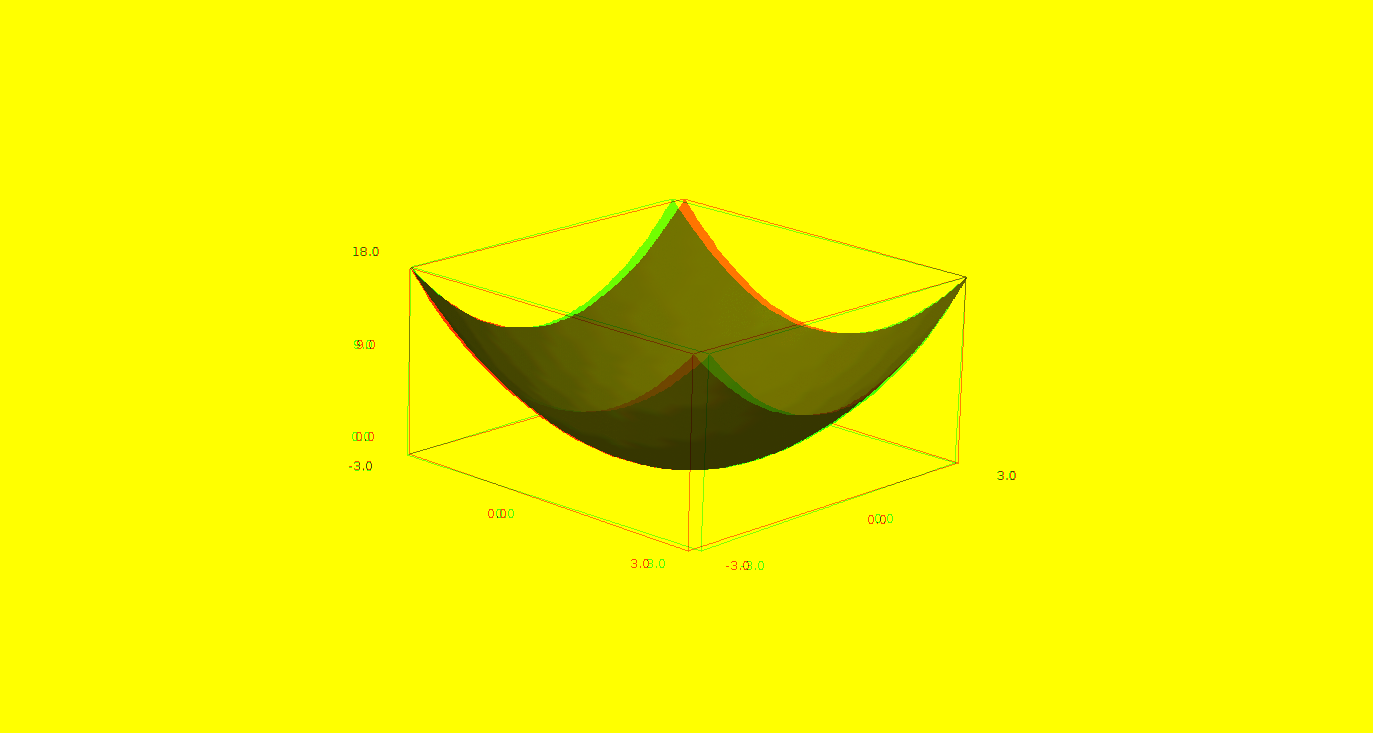
\includegraphics[width=15cm]{coupe.png}
        \else
            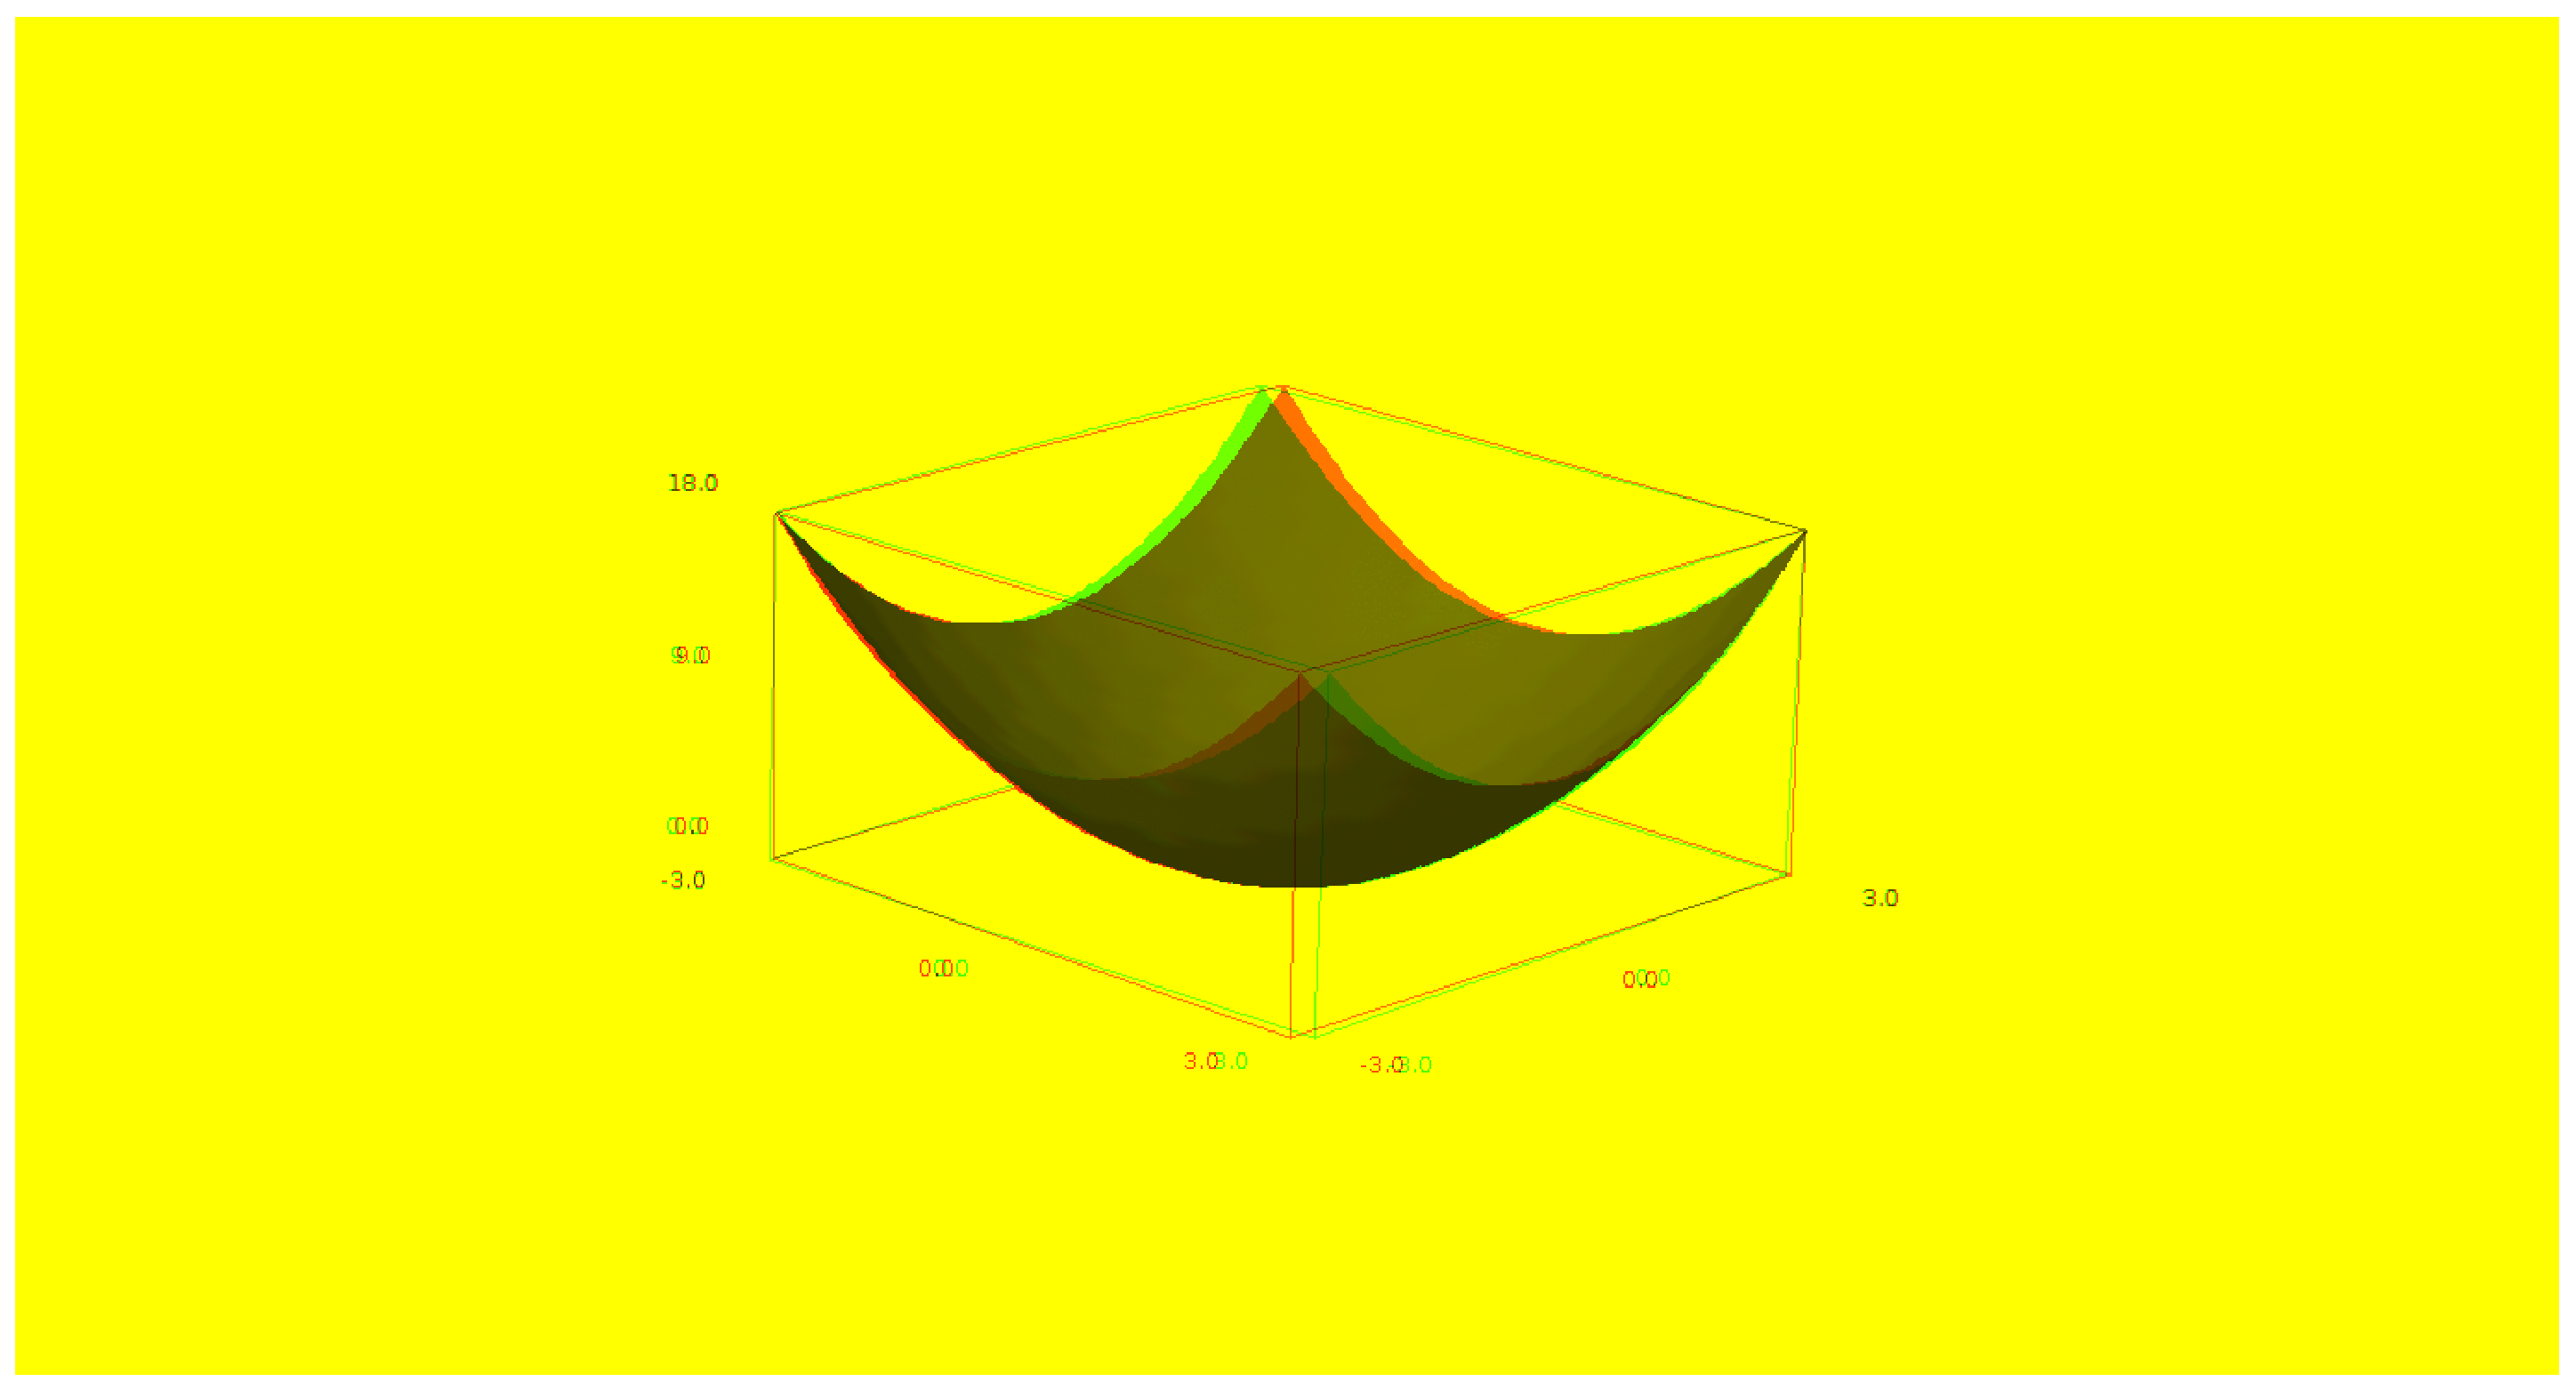
\includegraphics[width=15cm]{coupe.eps}
        \fi
    \end{center}
    À part que l'ordinateur l'a dit, est-ce qu'on peut comprendre pourquoi le graphe de la fonction $x^2+y^2$ ressemble à un bol ? En coordonnées cylindriques, le graphe s'écrit
    \begin{equation}
        z=r^2.
    \end{equation}
    Donc il se fait que plus on s'éloigne du point $(0,0)$ dans le plan $XY$, plus le graphe va monter. Et il monte à quelle vitesse ? Il monte à la vitesse $r^2$. Il s'agit donc de dessiner la fonction $z=r^2$ dans le plan et de la «faire tourner».

\end{example}

%+++++++++++++++++++++++++++++++++++++++++++++++++++++++++++++++++++++++++++++++++++++++++++++++++++++++++++++++++++++++++++
\section{Courbes de niveau}
%+++++++++++++++++++++++++++++++++++++++++++++++++++++++++++++++++++++++++++++++++++++++++++++++++++++++++++++++++++++++++++

Une technique utile pour se faire une idée de la forme d'une fonction en trois dimensions est de tracer les \defe{courbes de niveau}{courbe de niveau}. La courbe de niveau de hauteur $h$ est la courbe dans le plan donnée par l'équation
\begin{equation}
    f(x,y)=h.
\end{equation}

\begin{example}

    Dessinons par exemple les courbes de niveau de la fonction
    \begin{equation}
        f(x,y)=x+y+2.
    \end{equation}
    La courbe de niveau $h$ est donnée par l'équation $x+y+2=h$, c'est à dire
    \begin{equation}
        y(x)=-x+h-2.
    \end{equation}
    Par conséquent la courbe de niveau de hauteur $0$ est $y=-x-2$, celle de hauteur $5$ est $y=-x+3$, etc.
    
    Nous pouvons également nous aider de Sage pour ce faire :
    \begin{verbatim}
----------------------------------------------------------------------
| Sage Version 4.6.1, Release Date: 2011-01-11                       |
| Type notebook() for the GUI, and license() for information.        |
----------------------------------------------------------------------
sage: f(x,y)=x+y+2
sage: var('h')                   
h
sage: niveau(h,x)=solve(f(x,y)==h,y)[0].rhs()
sage: g1(x)=niveau(1,x)
sage: g1
x |--> -x - 1
    \end{verbatim}
    Ici la fonction \verb+g1+ est la courbe de niveau $1$. 

    Si on veut faire tracer une courbe de niveau, Sage peut le faire :
    \begin{verbatim}
        sage: implicit_plot(f(x,y)==1,(x,-3,3),(y,-4,4))
    \end{verbatim}
    Cela tracera la courbe de niveau $h=1$ dans la partie du plan $x\in\mathopen[ -3 , 3 \mathclose]$ et $y\in\mathopen[ -4,4 ,  \mathclose]$.
    
\end{example}

Il est bien entendu possible de créer automatiquement $50$ courbes de niveau et de demander de les tracer toutes sur le même graphe.
\VerbatimInput[tabsize=3]{courbeNiveau.py}

Le résultat est :

\begin{center}
    \ifpdf
        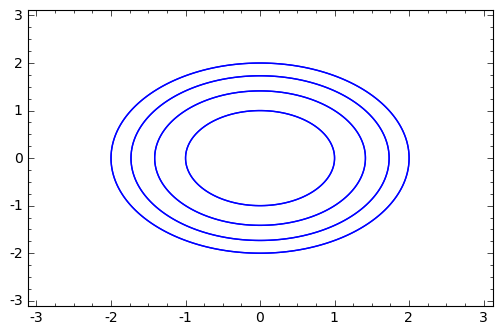
\includegraphics[width=8cm]{niveauCercles.png}
    \else
        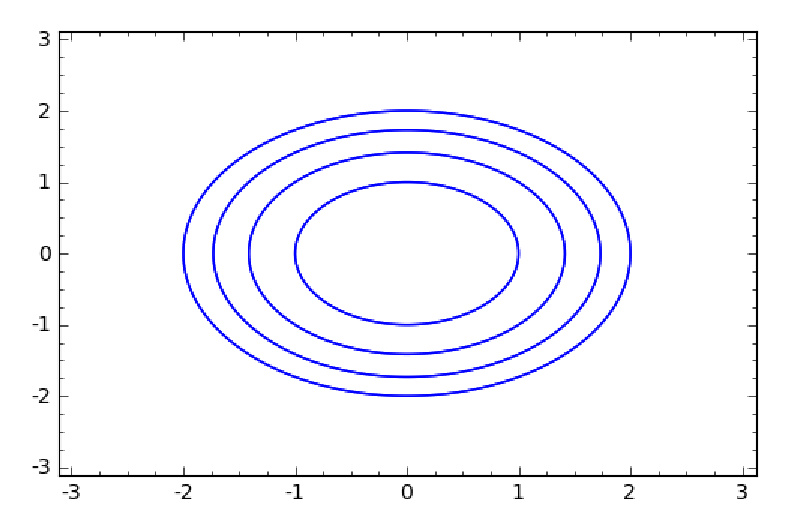
\includegraphics[width=8cm]{niveauCercles.eps}
    \fi
\end{center}
Notez que les courbes sont censées être des cercles : les axes $X$ et $Y$ n'ont pas la même échèle. Vous trouverez sur \href{http://uw.sagenb.org/home/pub/23/}{cette page} tout ce qu'il vous faudra pour créer des courbes de niveau avec Sage.

\begin{example}
    Un exemple plus riche en enseignements est celui de la fonction
    \begin{equation}
        f(x,y)=x^2-y^2.
    \end{equation}
    La courbe de niveau $h$ est donnée par l'équation $x^2-y^2=h$.

    Commençons par $h=0$. Dans ce cas nous avons $(x+y)(x-y)=0$ et par conséquent les courbes de niveau de hauteur zéro sont les deux droites $x+y=0$ et $x-y=0$.

    Voyons ensuite la courbe de niveau $h=1$. Cela est l'équation $x^2-y^2=1$, c'est à dire
    \begin{equation}
        y(x)=\pm\sqrt{x^2-1}.
    \end{equation}
    C'est une fonction qui n'est définie que pour $| x |\geq 1$. Avec $x=1$ nous avons $y=1$. Ensuite, lorsque $x$ grandit, $y$ grandit également, mais la courbe ne peut pas croiser la courbe de niveau $h=0$. Donc, suivant les notations de la figure \ref{LabelFigNiveauHyperbole}, la courbe de niveau «part» de $P$ et doit monter sans croiser les diagonales.

    \newcommand{\CaptionFigNiveauHyperbole}{La courbe de niveau $h=1$ de $x^2-y^2$. Notez qu'elle est en deux morceaux.}
    \input{Fig_NiveauHyperbole.pstricks}

    En ce qui concerne la courbe de niveau $h=-1$, elle correspond à la courbe $y=\pm\sqrt{1+x^2}$ qui est définie pour tous les $x\in\eR$. Le même raisonnement que précédemment nous amène à la figure \ref{LabelFigNiveauHyperboleDeux}.
\newcommand{\CaptionFigNiveauHyperboleDeux}{La courbe de niveau $x^2-y^2=-1$.}
\input{Fig_NiveauHyperboleDeux.pstricks}


\end{example}

Une autre façon de voir les courbe de niveau est de dire que la courbe de niveau de hauteur $h$ est la projection dans le plan $XY$ de la section du graphe de $f$ par le plan $z=h$.

On peut également définir le graphe de fonctions de trois (ou plus) variables. Le graphe de la fonction $f\colon D\subset\eR^3\to \eR$ est l'ensemble
\begin{equation}
    \big\{ \big( x,y,z,f(x,y,z) \big)\tq (x,y,z)\in D \big\}\subset \eR^4.
\end{equation}
De tels graphes ne peuvent pas être représentés sur une feuille de papier. Il est toutefois possible de définir les ensembles de niveaux :
\begin{equation}
    E_h=\big\{ (x,y,z)\in D\tq  f(x,y,z)=h\big\}.
\end{equation}
Ce sont des surfaces dans $\eR^3$ que l'on peut dessiner.

\begin{example}
    Les surfaces de niveau de la fonction $f(x,y,z)=x^2+y^2+z^2$ sont des sphères. Il n'y a pas de surfaces de niveau pour les «hauteurs» négatives.
\end{example}

\begin{example}
    Considérons la fonction $f(x,y,z)=x^2+y^2-z^2$. En coordonnées cylindrique, cette fonction s'écrit
    \begin{equation}
        f(r,\theta,z)=r^2-z^2.
    \end{equation}
    La surface de niveau $0$ est donnée par l'équation $r=| z |$. Cela fait un cercle à chaque hauteur, dont le rayon grandit linéairement avec la hauteur; le tout est donc un cône. C'est d'ailleurs le cône obtenu par rotation de la courbe de niveau $h=0$ que nous avions obtenue pour la fonction $x^2-y^2$.

    En ce qui concerne les ensembles de niveau positifs, ils sont donnés par
    \begin{equation}
        z=\pm\sqrt{x^2+y^2-h}.
    \end{equation}
    Notez qu'ils ne sont pas définis pour $r\geq h$. Cela pose un petit problème quand on veut le tracer à l'ordinateur :
    \begin{verbatim}
----------------------------------------------------------------------
| Sage Version 4.6.1, Release Date: 2011-01-11                       |
| Type notebook() for the GUI, and license() for information.        |
----------------------------------------------------------------------
sage: var('x,y')
(x, y)
sage: f(x,y)=sqrt(x**2+y**2-3)
sage: F=plot3d(f(x,y),(x,-5,5),(y,-5,5)) 
sage: G=plot3d(-f(x,y),(x,-5,5),(y,-5,5))    
sage: F+G
    \end{verbatim}
Le résultat est\footnote{Encore une fois : ça donne mieux à l'écran, et vous pouvez le faire bouger; je vous encourage à le faire !} :
    \begin{center}
        \ifpdf
            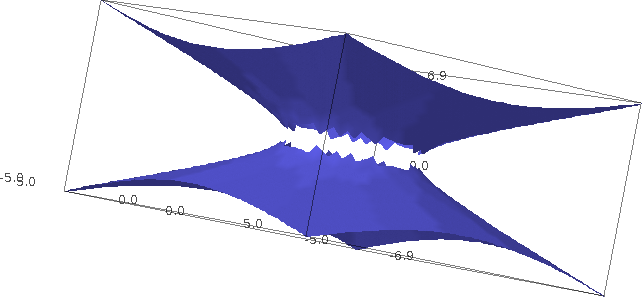
\includegraphics[width=15cm]{AdSmauvais.png}
        \else
            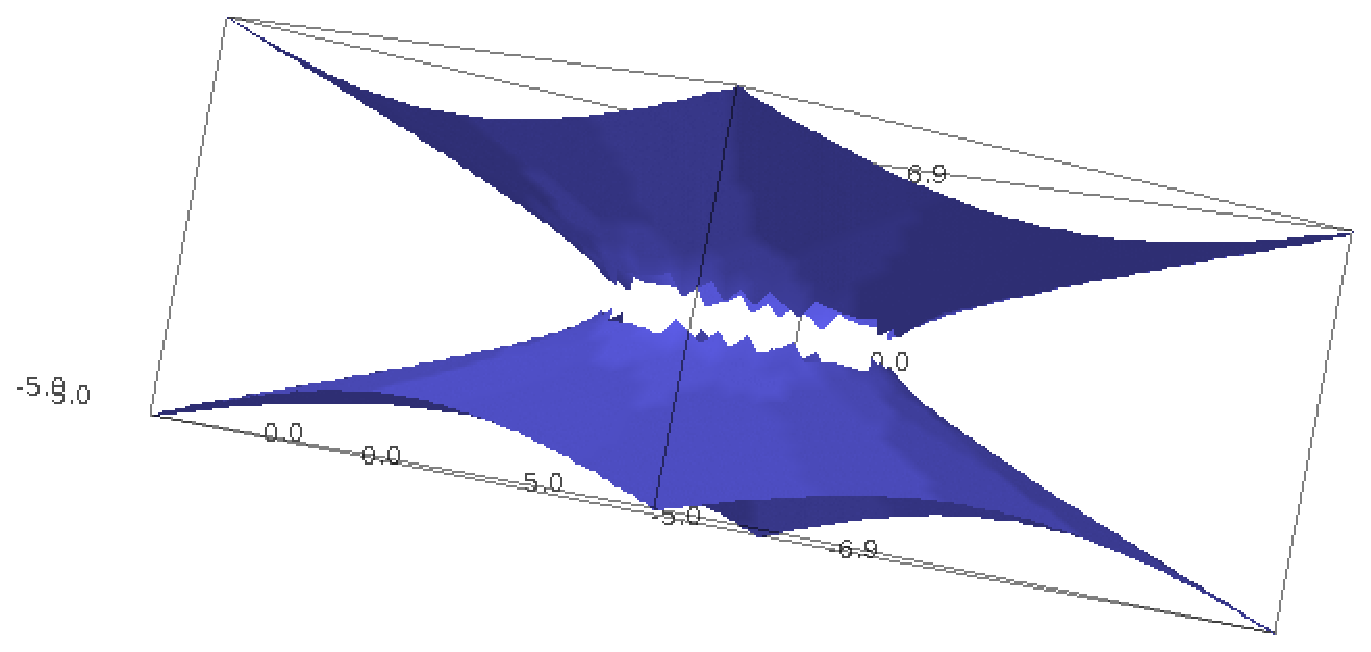
\includegraphics[width=15cm]{AdSmauvais.eps}
        \fi
    \end{center}
    On voit qu'il y a un grand trou au centre correspondant aux $z$ proches de zéro. Or d'après l'équation, il n'en est rien : en $z=0$ il y a bel et bien tout un cercle. Afin d'obtenir une meilleur image, il faut demander de tracer avec un maillage plus fin :
    \begin{verbatim}
----------------------------------------------------------------------
| Sage Version 4.6.1, Release Date: 2011-01-11                       |
| Type notebook() for the GUI, and license() for information.        |
----------------------------------------------------------------------
sage: var('x,y')
(x, y)
sage: f(x,y)=sqrt(x**2+y**2-3)
sage: F=plot3d(f(x,y),(x,-5,5),(y,-5,5),plot_points=300) 
sage: G=plot3d(-f(x,y),(x,-5,5),(y,-5,5),plot_points=300)
sage: F+G
    \end{verbatim}
    Le temps de calcul est un peu plus long, mais le résultat est meilleur :
    \begin{center}
        \ifpdf
            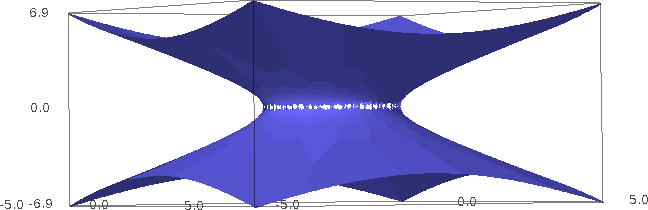
\includegraphics[width=15cm]{AdSbon.png}
        \else
            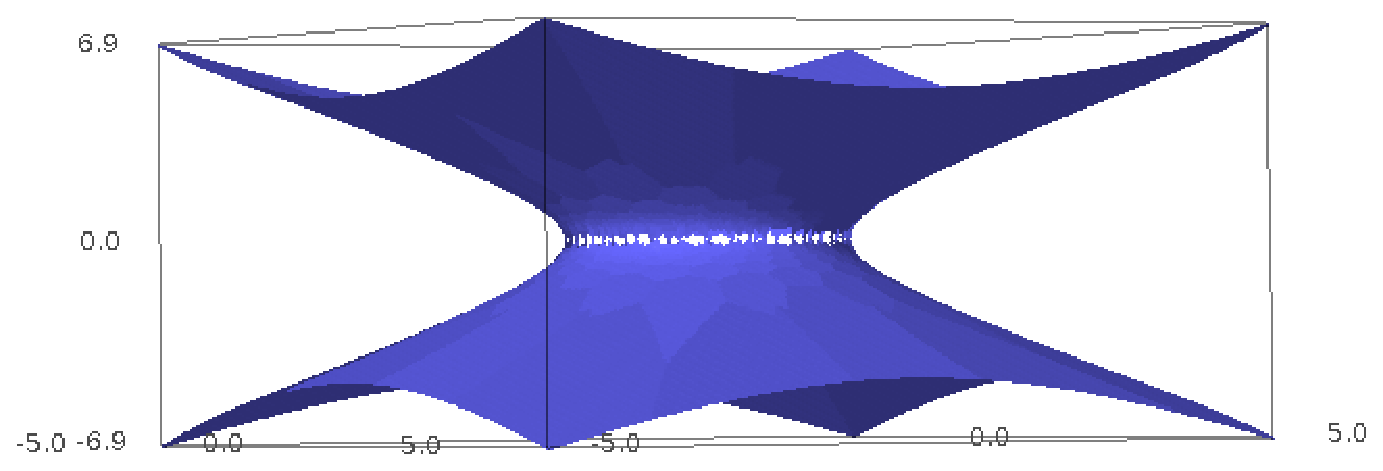
\includegraphics[width=15cm]{AdSbon.eps}
        \fi
    \end{center}
\end{example}

%+++++++++++++++++++++++++++++++++++++++++++++++++++++++++++++++++++++++++++++++++++++++++++++++++++++++++++++++++++++++++++
\section{Dérivées partielles}
%+++++++++++++++++++++++++++++++++++++++++++++++++++++++++++++++++++++++++++++++++++++++++++++++++++++++++++++++++++++++++++

Soit $f\colon \eR^2\to \eR$ une fonction de deux variables et soit $(a,b)\in\eR^2$. La façon la plus naturelle de définir une dérivée à deux variables est de considérer les \defe{dérivées partielles}{dérivée!partielle} définies par
\begin{equation}
    \begin{aligned}[]
        \frac{ \partial f }{ \partial x }(a,b)&=\lim_{x\to a} \frac{ f(x,b)-f(a,b) }{ x-a }\\
        \frac{ \partial f }{ \partial y }(a,b)&=\lim_{y\to b} \frac{ f(a,y)-f(a,b) }{y-b}.
    \end{aligned}
\end{equation}
Ces nombres représentent la façon dont le nombre $f(x,y)$ varie lorsque soit seul $x$ varie soit seul $y$ varie. Les dérivées partielles se calculent de la même façon que les dérivées normales. Pour calculer $\partial_xf$, on fait «comme si» $y$ était une constante, et pour calculer $\partial_yf$, on fait comme si $x$ était une constante.

\begin{example}
    Considérons $f(x,y)=x^2y+y^2 e^{x}$. Les dérivées partielles sont
    \begin{equation}
        \begin{aligned}[]
            \frac{ \partial f }{ \partial x }&=2xy+y^2e^x\\
            \frac{ \partial f }{ \partial y }&=x^2+2ye^x.
        \end{aligned}
    \end{equation}
\end{example}

Cet exemple était l'exemple facile où tout se passe bien.

\begin{example}
    Les choses sont moins simples lorsqu'on considère la fonction suivante :
    \begin{equation}
        f(x,y)=\begin{cases}
            \frac{ xy }{ x^2+y^2 }    &   \text{si $(x,y)\neq(0,0)$}\\
            0    &    \text{si $(x,y)=(0,0)$}.
        \end{cases}
    \end{equation}
    On voit que pour tout $x$ et tout $y$, nous avons $f(x,0)=f(0,y)=0$. Donc cette fonction est nulle sur les axes horizontaux et verticaux. Nous avons en particulier
    \begin{equation}
        \begin{aligned}[]
            \frac{ \partial f }{ \partial x }(0,0)&=0\\
            \frac{ \partial f }{ \partial y }(0,0)&=0.
        \end{aligned}
    \end{equation}
    Donc ces dérivées partielles existe.

    Il n'est par contre pas question de dire que cette fonction «va bien» autour du point $(0,0)$. En effet si nous regardons sa valeur sur la droite diagonale $y=x$, nous avons
    \begin{equation}
        f(x,x)=\frac{ x^2 }{ 2x^2 }=\frac{ 1 }{2}.
    \end{equation}
    Par conséquent si nous suivons la fonction le long de la droite $y=x$, la hauteur vaut $\frac{ 1 }{2}$ en permanence, saut juste en $(0,0)$ où la fonction fait un grand plongeon !
    \begin{verbatim}
    sage: var('x,y')
    (x, y)
    sage: f(x,y)=(x*y)/(x**2+y**2)
    sage: plot3d(f,(x,-2,2),y(-2,2))
    \end{verbatim}

    D'ailleurs elle fait un plongeon le long de toutes les droites (sauf verticale et horizontale). En effet si nous regardons la fonction le long de la droite $y=mx$, nous avons
    \begin{equation}
        f(x,mx)=\frac{ mx^2 }{ x^2+m^2x^2 }=\frac{ m }{ 1+m^2 }.
    \end{equation}
    La fonction est donc \emph{constante} sur chacune de ces droites. Il n'est donc pas question de dire que cette fonction est «dérivable» en $(0,0)$, vu qu'elle fait des grands sauts dans presque toutes les directions.
\end{example}

Nous devons donc trouver mieux que les dérivées partielles pour étudier le comportement des fonctions un peu problématiques.

Nous nous souvenons de l'équation \eqref{EqCodeDerviffxam} qui nous dis que pour une fonction d'une variable la dérivabilité signifiait qu'il existait un nombre $\ell$ et une fonction $\alpha$ tels
\begin{equation}
    f(x)=f(a)+\ell(x-a)+(x-a)\alpha(x-a)
\end{equation}
et $\lim_{t\to 0} \alpha(t)=0$. 

En nous inspirant de cela, nous posons la définition suivante.
\begin{definition}      \label{DefDiffabel}
    Une fonction $f\colon \eR^2\to \eR$ est \defe{différentiable}{différentiable} au point $(a,b)\in\eR^2$ si il existe deux nombres $\ell_1$, $\ell_2$ ainsi qu'une fonction $\alpha$ tels que
    \begin{equation}\label{EqCondDiffabel}
        \begin{aligned}[]
            f(x,y)=f(a,b)&+\ell_1(x-a)+\ell_2(y-b)\\
                    &+\sqrt{(x-a)^2+(y-b)^2}\alpha\big( \sqrt{(x-a)^2+(y-b)^2} \big).
        \end{aligned}
    \end{equation}
\end{definition}

En utilisant la notation vectorielle, cela peut être écrite sous forme très compacte. Posons
\begin{equation}
    \begin{aligned}[]
        \ell&=\begin{pmatrix}
            \ell_1    \\ 
            \ell_2    
        \end{pmatrix},&
        X&=\begin{pmatrix}
            x    \\ 
            y    
        \end{pmatrix},&
        P&=\begin{pmatrix}
            a    \\ 
            b    
        \end{pmatrix}.
    \end{aligned}
\end{equation}
Alors la condition \eqref{EqCondDiffabel} s'écrit
\begin{equation}
    f(X)=f(P)+\ell\cdot(X-P)+\| X-P \|\alpha\big( \| X-P \| \big).
\end{equation}

\begin{proposition}
    Si $f$ est différentiable en $(a,b)$, alors les nombres $\partial_xf(a,b)$ et $\partial_yf(a,b)$ existent et valent respectivement $\ell_1$ et $\ell_2$.
\end{proposition}

\begin{proof}
    Afin de calculer la dérivée partielle dans la direction de $x$, nous posons $y=b$ dans la condition \eqref{EqCondDiffabel} :
    \begin{equation}
        f(x,b)=f(a,b)+\ell_1(x-a)+| x-a |\alpha\big( | x-a | \big),
    \end{equation}
    et donc
    \begin{equation}
        \frac{ f(x,b)-f(a,b) }{ x-a }=\ell_1\pm\alpha\big( | x-a | \big).
    \end{equation}
    Ici le $\pm$ est parce que nous avons divisé $(x-a)$ par $| x-a |$. Quel que soit ce signe, de toutes façons la limite du membre de droite lorsque $x$ tend vers $a$ est $\ell_1$ parce que $\lim_{x\to a} \alpha(| x-a |)=0$.

    Afin de prouver l'existence de la dérivée dans la direction de $y$, nous procédons de la même manière, mais en partant de $f(a,y)$.
\end{proof}

\begin{proposition}
    Si $f$ est différentiable au point $(a,b)$, alors elle y est continue, c'est à dire que
    \begin{equation}
        \lim_{(x,y)\to(a,b)}f(x,y)=f(a,b).
    \end{equation}
\end{proposition}

\begin{proof}
    Si nous considérons la différence entre $f(x,y)$ et $f(a,b)$, nous avons (en notations matricielle) :
    \begin{equation}
        | f(X)-f(P) |=| \ell\cdot(X-P)+\| X-P \|\alpha(\| X-P \|) |.
    \end{equation}
    Le membre de droite tend évidemment vers zéro lorsque $X$ tend vers $P$.
\end{proof}
    \begin{remark}
        Attention : ceci n'est pas une preuve. En effet, dans la mesure où nous n'avons même pas donné de définition de la limite, il n'est pas possible de donner une \emph{vraie} preuve de quoi que ce soit. 
    \end{remark}

Nous avons vu que l'existence des deux dérivées partielles ne permettait pas de conclure à la différentiabilité. La différentiabilité d'une fonction peut néanmoins être déduites d'une étude plus précise des dérivées partielles. Nous avons pour cela les propositions \ref{PropExistDiffUn} et \ref{PropExistDiffDeux}

\begin{proposition} \label{PropExistDiffUn}
    Soit $f$ une fonction de $x$ et $y$ et un point $(a,b)\in\eR^2$. Si les nombres $\partial_xf(a,b)$ et $\partial_yf(a,b)$ existent et si il existe une fonction $\alpha\colon \eR\to \eR$ telle que
    \begin{equation}        \label{eqCritDifffabsrt}
        \begin{aligned}[]
            f(x,y)=f(a,b)&+\frac{ \partial f }{ \partial x }(a,b)(x-a)+\frac{ \partial f }{ \partial y }(a,b)(y-b)\\
            &+\| (x,y)-(a,b) \| \alpha\Big( \| (x,y)-(a,b) \| \Big)
        \end{aligned}
    \end{equation}
    et
    \begin{equation}
        \lim_{t\to 0} \alpha(t)=0,
    \end{equation}
    alors $f$ est différentiable en $(a,b)$.
\end{proposition}
Dans cet énoncé nous avons écrit $d\big( (x,y),(a,b) \big)$ la distance entre $(x,y)$ et $(a,b)$, c'est à dire le nombre $\sqrt{(x-a)^2+(y-b)^2}$. Afin d'écrire l'équation \eqref{eqCritDifffabsrt} sous forme plus compacte, nous introduisons le vecteur
\begin{equation}
    \nabla f(a,b)=\begin{pmatrix}
        \frac{ \partial f }{ \partial x }(a,b)    \\ 
        \frac{ \partial f }{ \partial y }(a,b).    
    \end{pmatrix}
\end{equation}
L'équation \eqref{eqCritDifffabsrt} devient alors
\begin{equation}        \label{EqdiffComp}
    f(X)=f(P)+\nabla f(a,b)\cdot (X-P)+\| X-P \|\alpha\big( \| X-P \| \big).
\end{equation}
Le vecteur $\nabla f(a,b)$ est appelé le \defe{gradient}{gradient} de $f$ au point $(a,b)$.


\begin{proposition} \label{PropExistDiffDeux}
    Soit $f$ une fonction de deux variables admettant des dérivées partielles $\partial_xf(x,y)$ et $\partial_yf(x,y)$ qui sont elles-mêmes des fonctions continues de $x$ et $y$. Alors la fonction $f$ est différentiable partout.
\end{proposition}

\begin{remark}
    Tout ce qui a été dit, et tout ce qui sera dit, sur les fonctions a deux variables se généralise immédiatement aux fonctions à plus de variables. C'est dans ce but que la notation «compacte» utilisant les vecteurs est très pratique.
\end{remark}

Si nous remplaçons les accroissements $x-a$ et $y-b$ par $h$ et $k$, le critère de différentiabilité s'écrit
\begin{equation}
    \begin{aligned}[]
        f(a+h,b+k)=f(a,b)+\frac{ \partial f }{ \partial x }(a,b)h&+\frac{ \partial f }{ \partial y }(a,b)k\\
        &+\sqrt{h^2+k^2}\alpha\big( \sqrt{h^2+k^2} \big).
    \end{aligned}
\end{equation}
Le dernier terme du membre de droite tend vers zéro à une vitesse double lorsque $h$ et $k$ tendent vers zéro : d'une part parce que $\sqrt{h^2+k^2}$ tend vers zéro et d'autre part parce que $\alpha\big( \sqrt{h^2+k^2} \big)$ tend vers zéro. Nous avons donc la «bonne» approximation
\begin{equation}        \label{EqFormApproxfxyab}
    f(x,y)\simeq f(a,b)+\frac{ \partial f }{ \partial x }(a,b)(x-a)+\frac{ \partial f }{ \partial y }(a,b)(y-b).
\end{equation}
lorsque $(x,y)$ n'est pas trop loin de $(a,b)$. Cette expression est évidemment une généralisation immédiate de l'équation \eqref{EqfxdxSimeqfxfpx}. Elle exprime que l'on peut obtenir des information sur la valeur d'une fonction en $(x,y)$ si on peut calculer la fonction et ses dérivées en un point $(a,b)$ non loin de $(x,y)$.

Cette formule peut aussi être vue sous la forme suivante, plus pratique dans certains calculs :
\begin{equation}        \label{EqFormApproxfxyabDF}
    f(a+\Delta x,b+\Delta y)\simeq f(a,b)+\Delta x\frac{ \partial f }{ \partial x }(a,b)+\Delta y\frac{ \partial f }{ \partial y }(a,b).
\end{equation}

\begin{example}
    Prenons la fonction $f(x,y)=\cos(x)\sin(y)$ et calculons une approximation de
    \begin{equation}
        f\big( \frac{ \pi }{ 3 }+0.01,\frac{ \pi }{ 2 }+0.03 \big).
    \end{equation}
    D'abord les dérivées partielles sont
    \begin{equation}
        \begin{aligned}[]
            \frac{ \partial f }{ \partial x }(x,y)=-\sin(x)\sin(y)\\
            \frac{ \partial f }{ \partial y }(x,y)=\cos(x)\cos(y).
        \end{aligned}
    \end{equation}
    Nous allons utiliser l'approximation
    \begin{equation}
        f\big( \frac{ \pi }{ 3 }+0.01,\frac{ \pi }{ 2 }+0.03 \big)\simeq f\big( \frac{ \pi }{ 3 },\frac{ \pi }{2} \big)+0.01\frac{ \partial f }{ \partial x }\big( \frac{ \pi }{ 3 },\frac{ \pi }{2} \big)+0.03\frac{ \partial f }{ \partial y }\big( \frac{ \pi }{ 3 },\frac{ \pi }{2} \big).
    \end{equation}
    Nous avons
    \begin{equation}
        \begin{aligned}[]
            \frac{ \partial f }{ \partial x }\big( \frac{ \pi }{ 3 },\frac{ \pi }{2} \big)&=-\sin\frac{ \pi }{ 3 }\sin\frac{ \pi }{ 2 }=-\frac{ \sqrt{3} }{2}\\
            \frac{ \partial f }{ \partial y }\big( \frac{ \pi }{ 3 },\frac{ \pi }{2} \big)&=\cos\frac{ \pi }{ 3 }\cos\frac{ \pi }{ 2 }=0.
        \end{aligned}
    \end{equation}
    Par conséquent
    \begin{equation}
        f\big( \frac{ \pi }{ 3 }+0.01,\frac{ \pi }{ 2 }+0.03 \big)\simeq \frac{ 1 }{2}-0.01\frac{ \sqrt{3} }{2}=\frac{ 1 }{2}-\frac{ \sqrt{3} }{ 200 }. 
    \end{equation}
    
    \begin{verbatim}
sage: var('x,y')
(x, y)
sage: f(x,y)=cos(x)*sin(y)
sage: a=f(pi/3+0.01,pi/2+0.03)
sage: numerical_approx(a)
0.491093815387986
sage: b=1/2-sqrt(3)/200
sage: numerical_approx(b)
0.491339745962156
sage: numerical_approx(a-b)
-0.000245930574169814
    \end{verbatim}
    Cela fait une erreur de l'ordre du dix millième. 
    
\end{example}

\begin{remark}
    Les esprits les plus critiques diront que cette vérification pas Sage n'en est pas une parce que Sage a certainement utilisé un algorithme d'approximation qui se base sur la même idée que ce que nous venons de faire, et que par conséquent le fait qu'il obtienne le même résultat que nous est un peu tautologique. 
    
    Ils n'auront pas tord. Cependant, le code source de Sage est disponible publiquement\footnote{Voir \url{http://www.sagemath.org}}; vous pouvez aller le lire et vérifier qu'il y a effectivement une \emph{preuve} que le résultat fourni par Sage possède une bonne dizaine de décimales correctes. 
    
    Cette disponibilité publique du code source est une des nombreuses différence fondamentale entre Sage et votre calculatrice\footnote{et les autres logiciels de type fenêtre, pomme ou feuille d'érable.}. Dois-je vous rappeler qu'un des principes fondamentaux de l'éthique scientifique est que les résultats et les méthodes utilisées doivent être absolument ouverts à la vérification et à la critique de tous ?
\end{remark}

%---------------------------------------------------------------------------------------------------------------------------
\subsection{Différentielle}
%---------------------------------------------------------------------------------------------------------------------------

\begin{definition}      \label{DefDiffrdrr}
    Lorsque $f$ est différentiable au point $(a,b)$, on appelle \defe{différentielle}{différentielle} de $f$ l'application linéaire
    \begin{equation}        \label{EqDefDiffmapdf}
        \begin{aligned}
            df_{(a,b)}\colon \eR^2&\to \eR \\
            \begin{pmatrix}
                u_1    \\ 
                u_2    
            \end{pmatrix}&\mapsto \frac{ \partial f }{ \partial x }(a,b)u_1+\frac{ \partial f }{ \partial y }(a,b)u_2. 
        \end{aligned}
    \end{equation}
    En notations compacte :
    \begin{equation}        \label{EqdfUPnable}
        df_{P}(U)=\nabla f(P)\cdot U.
    \end{equation}
\end{definition}

Note : dans la suite nous allons rendre notre «notation compacte» plus agréable à lire en abandonnant les majuscules. L'équation \eqref{EqdfUPnable} s'écrira donc
\begin{equation}        \label{Eqdfpunfpdu}
    df_p(u)=\nabla f(p)\cdot u.
\end{equation}


%+++++++++++++++++++++++++++++++++++++++++++++++++++++++++++++++++++++++++++++++++++++++++++++++++++++++++++++++++++++++++++
\section{Plan tangent au graphe d'une fonction}
%+++++++++++++++++++++++++++++++++++++++++++++++++++++++++++++++++++++++++++++++++++++++++++++++++++++++++++++++++++++++++++

Nous avons vu que, de la même façon qu'en deux dimensions nous avions l'approximation \eqref{Eqfxsimesfa} d'une fonction par sa tangente, en trois dimensions nous avons l'approximation suivante d'une fonction de deux variables :
\begin{equation}
    f(x,y)\simeq f(a,b)+\frac{ \partial f }{ \partial x }(a,b)(x-a)+\frac{ \partial f }{ \partial y }(a,b)(y-b)
\end{equation}
lorsque $(x,y)$ n'est pas trop loin de $(a,b)$. Cela signifie que le graphe de $f$ ressemble au graphe de la fonction $T_{(a,b)}$ donnée par
\begin{equation}
    T_{(a,b)}(x,y)=f(a,b)+\frac{ \partial f }{ \partial x }(a,b)(x-a)+\frac{ \partial f }{ \partial y }(a,b)(x-a).
\end{equation}
En notations compactes :
\begin{equation}
    T_p(x)=f(p)+\nabla f(p)\cdot (x-p).
\end{equation}
Le graphe de la fonction $T_p$ sera le \defe{plan tangent}{plan tangent} au graphe de $f$ au point $p$. L'équation du plan tangent sera donc
\begin{equation}
    z-f(p)=\nabla f(p)\cdot (x-p).
\end{equation}

\begin{remark}
    Lorsque nous utilisons la notation vectorielle, la lettre «$x$» désigne le vecteur $(x,y)$. Il faut être attentif. Dans un cas $x$ est un vecteur dans l'autre c'est une composante d'un vecteur.
\end{remark}




%+++++++++++++++++++++++++++++++++++++++++++++++++++++++++++++++++++++++++++++++++++++++++++++++++++++++++++++++++++++++++++
\section{Dérivée directionnelle}
%+++++++++++++++++++++++++++++++++++++++++++++++++++++++++++++++++++++++++++++++++++++++++++++++++++++++++++++++++++++++++++

Nous sommes capables de dériver une fonction de deux variables $f(x,y)$ par rapport à $x$ et par rapport à $y$. C'est à dire que nous sommes capables de donner la variation de la fonction lorsqu'on bouge le long des axes horizontal et vertical. Il est évidemment souhaitable de parler de la variation de la fonction lorsqu'on se déplace le long d'autre droites.

Soit donc $u=\begin{pmatrix}
    u_1    \\ 
    u_2    
\end{pmatrix}$ un vecteur unitaire (c'est à dire $u_1^2+u_2^2=1$), et considérons la fonction de une variable
\begin{equation}
    \begin{aligned}
        \varphi\colon \eR&\to \eR \\
        t&\mapsto f(a+tu_1,b+tu_2). 
    \end{aligned}
\end{equation}
La fonction $\varphi$ n'est rien d'autre que la fonction $f$ vue le long de la droite de direction donnée par le vecteur $u$. Nous pouvons aussi l'écrire $\varphi(t)=f(p+tu)$.

\begin{proposition}
    Si $f$ est différentiable en $(a,b)$ alors la fonction $\varphi$ est dérivable en $0$ et on a
    \begin{equation}
        \varphi'(0)=\nabla f(p)\cdot u
    \end{equation}
    où nous avons noté $p=(a,b)$.
\end{proposition}

\begin{proof}
    Récrivons la formule \eqref{EqdiffComp} sous la forme
    \begin{equation}
        f(x)=f(p)+\nabla f(p)\cdot (x-p)+\| x-p \|\alpha(\| x-p \|).
    \end{equation}
    Cela étant vrai pour tout $x$, nous l'écrivons en particulier pour $x=p+tu$ où $t$ est un réel et $u$ est le vecteur unitaire choisi. Nous avons donc
    \begin{equation}
        f(p+tu)=f(p)+t\nabla f(p)\cdot u+\| tu \|\alpha(\| tu \|).
    \end{equation}
    En utilisant le fait que $u$ est unitaire, $\| tu \|=| t |\| u \|=| t |$. La dérivée de $\varphi$ en $0$ est alors donnée par
    \begin{equation}
        \lim_{t\to 0} \frac{ f(p+tu)-f(p) }{ t }=\lim_{t\to 0} \nabla f(p)\cdot u+\alpha(| t |).    
    \end{equation}
    Lorsque nous prenons la limite, le membre de gauche devient $\varphi'(0)$ tandis que dans le membre de droite, le second terme disparaît. Nous avons finalement
    \begin{equation}
        \varphi'(0)=\nabla f(p)\cdot u
    \end{equation}
\end{proof}

\begin{definition}
    Le nombre
    \begin{equation}
        \lim_{t\to 0} \frac{ f\big( a+tu_1,b+tu_2 \big)-f(a,b) }{ t }
    \end{equation}
    est la \defe{dérivée directionnelle}{dérivée!directionnelle} de $f$ dans la direction de $u$ au point $(a,b)$. Il sera noté
    \begin{equation}
        \frac{ \partial f }{ \partial u }(a,b),
    \end{equation}
    ou plus simplement $\partial_uf(a,b)$.
\end{definition}

Lorsque $f$ est différentiable, la dérivée directionnelle est donnée par
\begin{equation}        \label{EqDerDirnablau}
    \frac{ \partial f }{ \partial u }(p)=\nabla f(p)\cdot u.
\end{equation}

En combinant avec l'équation \eqref{Eqdfpunfpdu}, nous avons la suite d'égalités
\begin{equation}        \label{Eqsuitedfnfdsdfu}
    df_p(u)=\nabla f(p)\cdot u=\frac{ \partial f }{ \partial x }(p)u_1+\frac{ \partial f }{ \partial y }(p)u_2+\frac{ \partial f }{ \partial z }(p)u_3=\frac{ \partial f }{ \partial u }(p).
\end{equation}
La dernière équation est seulement vraie si $\| u \|=1$.

%---------------------------------------------------------------------------------------------------------------------------
\subsection{Gradient : direction de plus grande pente}
%---------------------------------------------------------------------------------------------------------------------------

Étant donné que $u$ est de norme $1$, l'inégalité de Cauchy-Schwartz donne
\begin{equation}
    \big| \nabla f(a,b)\cdot \begin{pmatrix}
        u_1    \\ 
        u_2    
    \end{pmatrix}\big|\leq \| \nabla f(a,b) \|.
\end{equation}
Donc
\begin{equation}
    -\| \nabla f(p) \|\leq \nabla f(p)\cdot u\leq\| \nabla f(p) \|.
\end{equation}
La norme de la dérivée directionnelle (qui est la valeur absolue du nombre au centre) est donc «coincée» entre $-\| \nabla f(p) \|$ et $\| \nabla f(p) \|$. Prenons par exemple
\begin{equation}
    u=\frac{ \nabla f(p) }{ \| \nabla f(p) \| }.
\end{equation}
Dans ce cas, nous avons exactement
\begin{equation}
    \nabla f(p)\cdot u=\| \nabla f(p) \|,
\end{equation}
qui est la valeur maximale que la dérivée directionnelle peut prendre.

La direction du gradient est donc la direction suivant laquelle la dérivée directionnelle est la plus grande. Pour la même raison, la dérivée directionnelle est la plus petite dans le sens opposé au gradient.

En termes bien clairs : lorsqu'on veut aller le plus vite possible au ski, on prend la direction du gradient de la piste de ski. C'est dans cette direction que ça descend le plus vite. Dans quelle direction vont les débutants ? Ils vont perpendiculairement à la pente (ce qui ennuie tout le monde, mais c'est un autre problème). Les débutants vont donc dans la direction perpendiculaire au gradient. Prenons donc $u\perp \nabla f(p)$ et calculons la dérivée directionnelle de $f$ dans la direction $u$ en utilisant la formule \ref{EqDerDirnablau} :
\begin{equation}
    \frac{ \partial f }{ \partial u }(p)=\nabla f(p)\cdot u=0
\end{equation}
parce que nous avons choisit $u\perp \nabla f(p)$. Nous voyons donc que les débutants en ski ont eu la bonne intuition que la direction dans laquelle la piste ne descend pas, c'est la direction perpendiculaire au gradient.

C'est aussi pour cela que l'on a tendance à faire du zig-zag à vélo lorsqu'on monte une pente très forte et qu'on est fatigué. C'est toujours pour cela que les routes de montagne font de longs lacets. La montée est moins rude en suivant une direction proche d'être perpendiculaire au gradient !

\begin{theorem}
    Le gradient des fonction suit à peu près les mêmes règles que les dérivées. Soient $f$ et $g$ deux fonctions différentiables. Nous avons entre autres
    \begin{enumerate}
        \item
            $\nabla(f+g)=\nabla f+\nabla g$;
        \item
            $\nabla(fg)(a,b)=g(a,b)\nabla f(a,b)+f(a,b)\nabla g(a,b)$;
        \item
            Dès que $g(a,b)\neq 0$, nous avons
            \begin{equation}
                \nabla\frac{ f }{ g }=\frac{ g(a,b)\nabla f(a,b)-f(a,b)\nabla g(a,b) }{ g(a,b)^2 }.
            \end{equation}
    \end{enumerate}
\end{theorem}



\chapter{Champs de vecteurs}
% This is part of Mes notes de mathématique
% Copyright (c) 2011-2012,2015
%   Laurent Claessens
% See the file fdl-1.3.txt for copying conditions.

Les champs de vecteurs et tout ce qui s'y rapportent jouent un rôle crucial en électromagnétisme. Voir par exemple \cite{Schomblond_em}.

%+++++++++++++++++++++++++++++++++++++++++++++++++++++++++++++++++++++++++++++++++++++++++++++++++++++++++++++++++++++++++++
\section{Les fonctions à valeurs vectorielles}
%+++++++++++++++++++++++++++++++++++++++++++++++++++++++++++++++++++++++++++++++++++++++++++++++++++++++++++++++++++++++++++

Jusqu'à présent nous avons vu des fonctions de plusieurs variables qui prenaient leurs valeurs dans $\eR$. Nous allons maintenant voir ce qu'il se passe lorsque les fonctions prennent leurs valeurs dans $\eR^3$.

Une fonction d'une variable est dite \defe{à valeurs vectorielles}{fonction!valeurs vectorielles} lorsque
\begin{equation}
    \begin{aligned}
        f\colon I\subset \eR&\to \eR^3 \\
        f(x)&=\begin{pmatrix}
            f_1(x)    \\ 
            f_2(x)    \\ 
            f_3(x)    
        \end{pmatrix}.
    \end{aligned}
\end{equation}
Les fonctions $f_i\colon \eR\to \eR$ sont les \defe{composantes}{composante} de $f$. Ce que nous avons raconté à propos des dérivées passe facilement :
\begin{equation}
    \frac{ f(a+\epsilon)-f(a) }{ \epsilon }=
    \begin{pmatrix}
        \frac{ f_1(a+\epsilon)-f_1(a) }{ \epsilon }    \\ 
        \frac{ f_2(a+\epsilon)-f_2(a) }{ \epsilon }    \\ 
        \frac{ f_3(a+\epsilon)-f_3(a) }{ \epsilon }    
    \end{pmatrix}.
\end{equation}
En particulier dès que les fonctions $f_i$ sont dérivables, nous avons
\begin{equation}
    f'(a)=\begin{pmatrix}
        f_1'(a)    \\ 
        f_2'(a)    \\ 
        f_3'(a)    
    \end{pmatrix}
\end{equation}
comme dérivée de la fonction. Cette dérivée est un vecteur.

\begin{example}
    Si
    \begin{equation}
        f\colon x\in\eR\mapsto \begin{pmatrix}
            x^2 e^{x}    \\ 
            \cos(x^2)    \\ 
            x^3+x    
        \end{pmatrix},
    \end{equation}
    alors
    \begin{equation}
        f'(x)=\begin{pmatrix}
            2xe^x+x^2e^x    \\ 
            -2x\sin(x^2)    \\ 
            3x^2+1    
        \end{pmatrix}.
    \end{equation}
\end{example}

%+++++++++++++++++++++++++++++++++++++++++++++++++++++++++++++++++++++++++++++++++++++++++++++++++++++++++++++++++++++++++++
\section{Fonctions vectorielles de plusieurs variables}
%+++++++++++++++++++++++++++++++++++++++++++++++++++++++++++++++++++++++++++++++++++++++++++++++++++++++++++++++++++++++++++

Ce sont les fonctions de la forme
\begin{equation}
    \begin{aligned}
        f\colon \eR^3&\to \eR^3 \\
        \begin{pmatrix}
            x    \\ 
            y    \\ 
            z    
        \end{pmatrix}&\mapsto \begin{pmatrix}
            f_1(x,y,z)\\
            f_2(x,y,z)\\
            f_3(x,y,z)
        \end{pmatrix}.
    \end{aligned}
\end{equation}

En ce qui concerne les dérivées, tout se passe comme avant. Si les dérivées partielles des composantes $f_i$ existent au point $a\in\eR^3$, alors
\begin{equation}
    \begin{aligned}[]
        \frac{ \partial f }{ \partial x }(a)&=\begin{pmatrix}
            \partial_xf_1(a)    \\ 
            \partial_xf_2(a)    \\ 
            \partial_xf_3(a)    \\ 
        \end{pmatrix},&
        \frac{ \partial f }{ \partial y }(a)&=\begin{pmatrix}
            \partial_yf_1(a)    \\ 
            \partial_yf_2(a)    \\ 
            \partial_yf_3(a)    \\ 
        \end{pmatrix},&
        \frac{ \partial f }{ \partial z }(a)&=\begin{pmatrix}
            \partial_zf_1(a)    \\ 
            \partial_zf_2(a)    \\ 
            \partial_zf_3(a)    \\ 
        \end{pmatrix}.
    \end{aligned}
\end{equation}

%+++++++++++++++++++++++++++++++++++++++++++++++++++++++++++++++++++++++++++++++++++++++++++++++++++++++++++++++++++++++++++
\section{Champs de vecteurs}
%+++++++++++++++++++++++++++++++++++++++++++++++++++++++++++++++++++++++++++++++++++++++++++++++++++++++++++++++++++++++++++

Un champ de vecteur est une fonction $f\colon \eR^3\to \eR^3$. Géométriquement, il s'agit simplement de mettre un vecteur en chaque point de l'espace. Cela arrive très souvent en physique.

\begin{example}
    Si un fluide (eau, gaz) coule dans un tube, en tout point le point a une vitesse, qui sera un vecteur généralement dirigé le long du tube.
\end{example}

\begin{example}
    La force d'attraction de la Terre sur une masse $m$ située au point $r=(x,y,z)$ est donnée par
    \begin{equation}
        F(r)=-G\frac{ Mmr }{ \| r \|^3 }.
    \end{equation}
    Dans cette expression, tant $r$ que $F(r)$ sont des vecteurs. Nous l'avons représenté sur la figure \ref{LabelFigChampGraviation}.
    \newcommand{\CaptionFigChampGraviation}{Le champ de gravitation de la Terre.}
    \input{Fig_ChampGraviation.pstricks}

    L'application
    \begin{equation}
        \begin{aligned}
            F\colon \eR^3&\to \eR^3 \\
            r&\mapsto F(r) 
        \end{aligned}
    \end{equation}
    est le champ gravitationnel de la Terre.
\end{example}

%---------------------------------------------------------------------------------------------------------------------------
\subsection{Matrice jacobienne}
%---------------------------------------------------------------------------------------------------------------------------

La \defe{matrice jacobienne}{jacobien} de la fonction $f\colon \eR^3\to \eR^3$ au point $a\in\eR^3$ est la matrice dont les colonnes sont les vecteurs $\frac{ \partial f }{ \partial x }(a)$, $\frac{ \partial f }{ \partial y }(a)$ et $\frac{ \partial f }{ \partial z }(a)$, c'est à dire
\begin{equation}
    J_f(a)=\begin{pmatrix}
        \frac{ \partial f_1 }{ \partial x }(a)   &   \frac{ \partial f_1 }{ \partial y }(a)    &   \frac{ \partial f_1 }{ \partial z }(a)    \\
        \frac{ \partial f_2 }{ \partial x }(a)   &   \frac{ \partial f_2 }{ \partial y }(a)    &   \frac{ \partial f_2 }{ \partial z }(a)    \\
        \frac{ \partial f_3 }{ \partial x }(a)   &   \frac{ \partial f_3 }{ \partial y }(a)    &   \frac{ \partial f_3 }{ \partial z }(a)    
    \end{pmatrix}.
\end{equation}

\begin{example}
    Si 
    \begin{equation}
        f(x,y,z)=\begin{pmatrix}
            xy e^{z}    \\ 
            x^2+\cos(yz)    \\ 
            xyz    
        \end{pmatrix},
    \end{equation}
    alors
    \begin{equation}
        J_f(x,y,z)=\begin{pmatrix}
            ye^z    &   xe^z    &   xye^z    \\
            2x    &   -z\sin(yz)    &   -y\sin(yz)    \\
            yz    &   xz    &   xy
        \end{pmatrix}.
    \end{equation}
\end{example}

%+++++++++++++++++++++++++++++++++++++++++++++++++++++++++++++++++++++++++++++++++++++++++++++++++++++++++++++++++++++++++++
\section{Courbes paramétrés}
%+++++++++++++++++++++++++++++++++++++++++++++++++++++++++++++++++++++++++++++++++++++++++++++++++++++++++++++++++++++++++++

%---------------------------------------------------------------------------------------------------------------------------
\subsection{Définitions et exemples}
%---------------------------------------------------------------------------------------------------------------------------

\begin{definition}
    Un \defe{chemin}{chemin} dans $\eR$ est une application continue
    \begin{equation}
        \begin{aligned}
            \sigma\colon [a,b]&\to \eR^3 \\
            t&\mapsto \sigma(t). 
        \end{aligned}
    \end{equation}
\end{definition}

La fonction $\sigma'(t)$ est la \defe{vitesse}{vitesse d'un chemin} du chemin $\sigma$. Si la fonction $t\mapsto\sigma(t)$ est dérivable, on dit que $\sigma''(t)$ est l'\defe{accélération}{accélération d'un chemin}. Les points $\sigma(a)$ et $\sigma(b)$ sont les extrémités du chemin. L'ensemble
\begin{equation}
    \{ \sigma(t)\tq t\in\mathopen[ a , b \mathclose] \}
\end{equation}
est la \defe{courbe}{courbe} $\sigma$.

\begin{example}
    Soit $v\in\eR^3$ et $x_0\in\eR^3$. Le chemin
    \begin{equation}
        \sigma(t)=x_0+tv
    \end{equation}
    est une droite. Sa vitesse est $\sigma'(t)=v$.    
\end{example}

\begin{example}
    La courbe
    \begin{equation}
        \sigma(t)=\begin{pmatrix}
            \cos(t)    \\ 
            \sin(t)    
        \end{pmatrix}\in\eR^2
    \end{equation}
    avec $t\in\mathopen[ 0 , 2\pi [$ est le cercle unité parcouru une fois dans le sens trigonométrique.

    Notez que si on prend $t\in\mathopen[ 0 , 4\pi [$, nous avons un \emph{autre} chemin; c'est le même cercle unité, mais parcouru \emph{deux} fois. Même si le «dessin» (le graphe) des deux est le même, le chemin n'est pas le même.

    Le chemin
    \begin{equation}
        \gamma(t)=\begin{pmatrix}
            \cos(2\pi-t)    \\ 
            \sin(2\pi-t)    
        \end{pmatrix}
    \end{equation}
    est le cercle unité parcouru une fois dans le sens inverse. Encore une fois le «dessin» est le même, mais le chemin n'est pas le même.
\end{example}

\begin{example}
    Le chemin
    \begin{equation}
        \sigma(t)=\begin{pmatrix}
            t    \\ 
            t^2    
        \end{pmatrix}
    \end{equation}
    est un chemin dont l'image est la parabole d'équation $y=x^2$.
\end{example}

L'importance de la dérivée du chemin réside en le fait qu'elle donne la tangente. En effet le vecteur $\sigma'(t)$ est tangent au graphe de $\sigma$ au point $\sigma(t)$.
\begin{example}
    Pour le cercle,
    \begin{equation}
        \sigma(t)=\begin{pmatrix}
            \cos(t)    \\ 
            \sin(t)    
        \end{pmatrix},
    \end{equation}
    la dérivée est donnée par
    \begin{equation}
        \sigma'(t)=\begin{pmatrix}
            -\sin(t)    \\ 
            \cos(t).    
        \end{pmatrix}
    \end{equation}
    Le produit scalaire $\sigma(t)\cdot \sigma'(t)$ est nul. Le vecteur $\sigma'(t)$ est donc bien tangent (voir exercice \ref{exoDerive-0003}).
\end{example}

\begin{example}
    Le courbe donnée par le chemin
    \begin{equation}
        \sigma(t)=\begin{pmatrix}
            \cos(t)    \\ 
            \sin(t)    \\ 
            t    
        \end{pmatrix}
    \end{equation}
    est une hélice. Sa vitesse est
    \begin{equation}
        \sigma'(t)=\begin{pmatrix}
            -\sin(t)    \\ 
            \cos(t)    \\ 
            1    
        \end{pmatrix}.
    \end{equation}
    Notez que pour tout $t\in\eR$, nous avons $\| \sigma'(t) \|=\sqrt{2}$.
\end{example}

\begin{remark}
    Lorsqu'on parle d'une courbe dans l'espace, l'intervalle sur lequel on considère la variation du paramètre est une donné fondamentale. Elle fait partie intégrante de la définition de la courbe.
\end{remark}

%---------------------------------------------------------------------------------------------------------------------------
\subsection{Longueur d'une courbe paramétrée}
%---------------------------------------------------------------------------------------------------------------------------

Nous pouvons voir un chemin $\sigma$ comme étant la trajectoire d'une particule en fonction du temps. Sa vitesse à l'instant $t$ est le vecteur $\sigma'(t)$, tandis que sa vitesse \emph{scalaire} est le nombre $\| \sigma'(t) \|$. Une question naturelle est de savoir quelle est la longueur de la trajectoire parcourue entre $t=a$ et $t=b$.

Si nous prenons un petit intervalle de temps $dt$, nous pouvons supposer que le mobile avance à la vitesse constante $\| \sigma'(t) \|$. Cela ferait un trajet parcouru de longueur $\| \sigma'(t) \|dt$. Nous prenons donc la définition suivante pour la longueur.

\begin{definition}
    Soit $\sigma\colon \mathopen[ a , b \mathclose]\to \eR^3$ un chemin. La \defe{longueur}{longueur!d'un chemin} du chemin $\sigma$ est le nombre
    \begin{equation}        \label{EqDefLongueurCheminOM}
        l(\sigma)=\int_a^b\| \sigma'(t) \|dt.
    \end{equation}
    Plus explicitement, si $\sigma(t)=\big( x(t),y(t),z(t) \big)$, alors nous avons la formule
    \begin{equation}
        l(\sigma)=\int_a^b\sqrt{x'(t)^2+y'(t)^2+z'(t)^2}dt.
    \end{equation}
\end{definition}

\begin{example}
    Considérons l'arc de cercle de rayon $R$ interceptée par l'angle $\theta$ présenté sur la figure \ref{LabelFigooIHLPooKLIxcH}.
    \newcommand{CaptionFigooIHLPooKLIxcH}{Quelle est la longueur de la partie bleue de ce cercle de rayon $R$ ?}
    \input{Fig_ooIHLPooKLIxcH.pstricks}

    Par définition, cette longueur sera
    \begin{equation}
        \int_{\theta_0}^{\theta_1}\sqrt{R^2\sin^2(t)+R^2\cos^2(t)}dt=R(\theta_1-\theta_0).
    \end{equation}
    Le radian comme unité de mesure d'angle est donc l'unité parfaite : elle est la longueur d'arc interceptée (si le rayon est $R=1$).

\end{example}

\begin{example}
    La longueur de l'hélice
    \begin{equation}
        \sigma(t)=\begin{pmatrix}
            \cos(2t)    \\ 
            \sin(2t)    \\ 
            \sqrt{5}t    
        \end{pmatrix}
    \end{equation}
    pour $t\in\mathopen[ 0 , 2\pi \mathclose]$ est donnée par
    \begin{equation}
        l(\sigma)=\int_0^{4\pi}\sqrt{4\sin^2(2t)+4\cos^2(2t)+5}dt=\int_0^{4\pi}\sqrt{9}=12\pi.
    \end{equation}
\end{example}

\begin{definition}
    Soit $\sigma_1\colon \mathopen[ a , b \mathclose]\to \eR^3$, un chemin et $\sigma_2\colon \mathopen[ c , d \mathclose]\to \eR^3$, un autre chemin. On dit que ces chemins sont \defe{équivalents}{equivalence@équivalence!chemin} si il existe une fonction $\varphi\colon \mathopen[ a , b \mathclose]\to \mathopen[ c , d \mathclose]$ strictement croissante telle que $\sigma_1(t)=\sigma_2\big( \varphi(t) \big)$.
\end{definition}

Deux chemins équivalents parcourent la même courbe dans le même sens. Ils ne le parcourent toutefois pas à la même vitesse. On dit que les chemins sont \defe{opposée}{opposés!chemins} si la fonction $\varphi$ de la définition est strictement décroissante. Dans ce cas, ils ont la même image, mais parcourue dans le sens opposés. Nous disons que deux chemins équivalents sont un \defe{changement de paramétrisation}{paramétrisation} pour la même courbe.

 Dans le cas d'une paramétrisation équivalente, nous avons $\varphi(a)=c$ et $\varphi(b)=d$. Les points de départ et d'arrivée des deux paramètres coïncident. Dans le cas d'un paramètre qui va dans le sens opposé par contre nous avons automatiquement $\varphi(a)=d$ et $\varphi(b)=c$.

\begin{proposition}
    La longueur d'une courbe ne dépend pas du paramètre (équivalent ou opposé) choisi.
\end{proposition}

\begin{proof}
    Soient $\sigma_1\colon \mathopen[ a , b \mathclose]\to \eR^3$ et $\sigma_2\colon \mathopen[ c , d \mathclose]\to \eR^3$ tels que
    \begin{equation}     \label{EqChmsigmaundeuxvpOM}
        \sigma_1(t)=\sigma_2\big( \varphi(t) \big)
    \end{equation}
    où $\varphi\colon \mathopen[ a , b \mathclose]\to \mathopen[ a , d \mathclose]$ est une bijection strictement monotone. Par définition on a
    \begin{equation}
        l(\sigma_1)=\int_a^b\| \sigma_1'(t) \|dt.
    \end{equation}
    Nous pouvons exprimer la dérivée de $\sigma_1$ en termes de celle de $\sigma_2$ en dérivant la relation \eqref{EqChmsigmaundeuxvpOM} :
    \begin{equation}
        \sigma_1'(t)=\varphi'(t)\sigma_2'\big( \varphi(t) \big).
    \end{equation}
    En ce qui concerne la norme,
    \begin{equation}
        \| \sigma_1'(t) \|=| \varphi'(t) |\| \sigma_2'(t) \|.
    \end{equation}
    Notez dans cette relation que $\varphi'(t)$ est un nombre (et non un vecteur). Étant donné que nous avons supposé que $\varphi$ était monotone, soit elle est monotone croissante et $\| \varphi'(t) \|=\varphi'(t)$ pour tout $t$, soit elle est monotone décroissante et $\| \varphi'(t) \|='\varphi(t)$ pour tout $t$.

    Considérons d'abord le premier cas, c'est à dire $\| \varphi'(t) \|=\varphi'(t)$. Nous posons $s=\varphi(t)$, $ds=\varphi'(t)dt$. En remplaçant cela dans la formule de la longueur est
    \begin{equation}
        \begin{aligned}[]
            l(\sigma_1)&=\int_a^b\varphi'(t)\| \sigma_2\big( \varphi(t) \big) \|dt\\
            &=\int_{\varphi(a)}^{\varphi(b)}\| \sigma_2'(s) \|ds\\
            &=\int_c^d\| \sigma_2'(s) \|ds\\
            &=l(\sigma_2).
        \end{aligned}
    \end{equation}
    
    Si nous considérons maintenant une paramétrisation strictement décroissante. Dans ce cas, $\varphi'(t)\leq 0$ et $\| \varphi'(t) \|=-\varphi'(t)$. Nous posons encore une fois $s=\varphi(t)$, $ds=\varphi'(t)ds$. Ici il ne faut pas oublier que $\varphi(a)=d$ et $\varphi(b)=c$. Le calcul est à part cela le même en faisant attention au singe :
    \begin{equation}
        \begin{aligned}[]
            l(\sigma_1)&=\int_a^b\varphi'(t)\| \sigma_2\big( \varphi(t) \big) \|dt\\
            &=-\int_{\varphi(a)}^{\varphi(b)}\| \sigma_2'(s) \|ds\\
            &=-\int_d^c\| \sigma_2'(s) \|ds\\
            &=\int_c^d\| \sigma_2'(s) \|ds\\
            &=l(\sigma_2).
        \end{aligned}
    \end{equation}
    Nous avons changé le signe en changeant l'ordre des bornes.
\end{proof}

%+++++++++++++++++++++++++++++++++++++++++++++++++++++++++++++++++++++++++++++++++++++++++++++++++++++++++++++++++++++++++++
\section{Intégrales le long de chemins}
%+++++++++++++++++++++++++++++++++++++++++++++++++++++++++++++++++++++++++++++++++++++++++++++++++++++++++++++++++++++++++++

%---------------------------------------------------------------------------------------------------------------------------
\subsection{Circulation d'un champ de vecteur}
%---------------------------------------------------------------------------------------------------------------------------

\begin{definition}
    Soit $F\colon \eR^3\to \eR^3$ un champ de vecteurs et un chemin $\sigma\colon \mathopen[ a , b \mathclose]\to \eR^3$. On appelle \defe{circulation}{circulation} de $F$ le long du chemin $\sigma$ le scalaire
    \begin{equation}        \label{EqDeffvkZwhOM}
        \int_a^b F\big( \sigma(t) \big)\cdot \sigma'(t)dt.
    \end{equation}
    Il existe de nombreuses notations pour cela; entre autres :
    \begin{equation}
        \int_{\sigma}F=\int_{\sigma} F\cdot ds.
    \end{equation}
\end{definition}

En physique, la circulation de la force le long d'un chemin est la travail de la force.

\begin{example}
    À la surface de la Terre, le champ de gravitation est donné par
    \begin{equation}
        G(x,y,z)=-mg\begin{pmatrix}
            0    \\ 
            0    \\ 
            1    
        \end{pmatrix}.
    \end{equation}
    Si nous considérons un mobile qui monte à vitesse constante jusqu'à la hauteur $h$, c'est à dire le chemin
    \begin{equation}
        \sigma(t)=\begin{pmatrix}
            0    \\ 
            0    \\ 
            t    
        \end{pmatrix}
    \end{equation}
    avec $t\in\mathopen[ 0 , h \mathclose]$. Le travail de la gravitation est alors donné par
    \begin{equation}
        W=\int_0^hG\big( \sigma(t) \big)\cdot\begin{pmatrix}
            0    \\ 
            0    \\ 
            1    
        \end{pmatrix}=
        -mg\int_0^h\begin{pmatrix}
            0    \\ 
            0    \\ 
            1    
        \end{pmatrix}\cdot\begin{pmatrix}
            0    \\ 
            0    \\ 
            1    
        \end{pmatrix}=-mgh.
    \end{equation}
    Cela est bien le résultat usuel de l'énergie potentielle. Nous allons voir bientôt que nous nommons la fonction $mgh$ énergie \emph{potentielle} précisément parce que la force dérive de ce potentiel.
\end{example}

\begin{example}
    Soit le chemin
    \begin{equation}
        \begin{aligned}
            \sigma\colon \mathopen[ 0 , 2\pi \mathclose]&\to \eR^3 \\
            t&\mapsto \begin{pmatrix}
                \sin(t)    \\ 
                \cos(t)    \\ 
                t    
            \end{pmatrix}.
        \end{aligned}
    \end{equation}
    et le champ de vecteurs
    \begin{equation}
        F\begin{pmatrix}
            x    \\ 
            y    \\ 
            z    
        \end{pmatrix}=\begin{pmatrix}
            x    \\ 
            y    \\ 
            z    
        \end{pmatrix}.
    \end{equation}
    La circulation de ce champ de vecteur le long de l'hélice $\sigma$ est
    \begin{equation}
        \begin{aligned}[]
            \int_{\sigma}F\cdot ds&=\int_0^{2\pi}(F\circ \sigma)(t)\cdot \sigma'(t)dt\\
            &=\int_0^{2\pi}\begin{pmatrix}
                \sin(t)    \\ 
                \cos(t)    \\ 
                t    
            \end{pmatrix}\cdot
            \begin{pmatrix}
                \cos(t)    \\ 
                \sin(t)    \\ 
                1    
            \end{pmatrix}dt\\
            &=\int_0^{2\pi}tdt\\
            &=\left[ \frac{ t^2 }{2} \right]_0^{2\pi}\\
            &=2\pi^2.
        \end{aligned}
    \end{equation}
    
\end{example}

\begin{proposition}
    La circulation d'un champ de vecteurs le long d'un chemin ne dépend pas de la paramétrisation. En d'autres termes, si $\sigma_1$ et $\sigma_2$ sont deux chemins équivalents, alors
    \begin{equation}
        \int_{\sigma_1}F=\int_{\sigma_2}F.
    \end{equation}
\end{proposition}

\begin{proof}
    Soient deux chemins $\sigma_1\colon \mathopen[ a , b \mathclose]\to \eR^3$ et $\sigma_2\colon \mathopen[ c , d \mathclose]\to \eR^3$ équivalents, c'est à dire tels que
    \begin{equation}
        \sigma_1(t)=\sigma_2\big( \varphi(t) \big)
    \end{equation}
    où $\varphi\colon \mathopen[ a , b \mathclose]\to \mathopen[ c , d \mathclose]$ strictement croissante. En utilisant le fait que $\sigma_1(t)=\varphi'(t)\sigma_2'\big( \varphi(t) \big)$, nous avons
    \begin{equation}
        \begin{aligned}[]
            \int_{\sigma_1}F\cdot ds&=\int_a^bF\big( \sigma_1(t) \big)\cdot\sigma_1'(t)dt\\
            &=\int_a^bF\Big( \sigma_2\big( \varphi(t) \big) \Big)\cdot\sigma_2'\big( \varphi(t) \big)\varphi'(t)dt\\
            &=\int_{\varphi(a)}^{\varphi(b)}F\big( \sigma_2(s) \big)\cdot\sigma_2(s)ds\\
            &=\int_c^dF\big( \sigma_2(s) \big)\cdot \sigma_2'(s)ds\\
            &=\int_{\sigma_2}F\cdot ds.
        \end{aligned}
    \end{equation}
    où nous avons effectué le changement de variables $s=\varphi(t)$, $ds=\varphi'(t)dt$.
\end{proof}

\begin{remark}
    Si $\sigma_2$ est le chemin opposé de $\sigma$, alors
    \begin{equation}
        \int_{\sigma_2}F=-\int_{\sigma_1}F.
    \end{equation}
\end{remark}

%+++++++++++++++++++++++++++++++++++++++++++++++++++++++++++++++++++++++++++++++++++++++++++++++++++++++++++++++++++++++++++
\section{Circulation d'un champ conservatif}
%+++++++++++++++++++++++++++++++++++++++++++++++++++++++++++++++++++++++++++++++++++++++++++++++++++++++++++++++++++++++++++

Si nous avons une fonction scalaire $V\colon \eR^3\to \eR$, nous pouvons construire un champ de vecteur en prenant le gradient :
\begin{equation}
    F(x)=\nabla V(x).
\end{equation}
On dit que le champ de vecteur $F$ \defe{dérive}{champ dérivant d'un potentiel} de $V$, et on dit que $V$ est le \defe{potentiel}{potentiel} de $F$. Nous posons la définition suivante :
\begin{definition}
    Un champ de vecteurs $F\colon \eR^3\to \eR^3$ est un champ \defe{conservatif}{champ!conservatif} si il existe une fonction $V\colon \eR^3\to \eR$ telle que
    \begin{equation}
        F(x)=\nabla V(x).
    \end{equation}
    Nous disons aussi parfois que le champ $V$ \emph{dérive d'un potentiel} ou bien qu'il s'agit d'un \emph{champ de gradient}.
\end{definition}

Les champs de vecteurs conservatifs sont particulièrement importants parce que presque toutes les forces connues en physiques dérivent d'un potentiel. Nous verrons que la terminologie «conservatif» provient du fait que les forces de ce type conservent l'énergie associée.


\begin{proposition}
    Considérons une fonction $V\colon \eR^3\to \eR$ (que nous appellerons \emph{potentiel}) et le champ de vecteur qui en dérive :
    \begin{equation}
        F=\nabla V.
    \end{equation}
    Alors 
    \begin{equation}
        \int_{\sigma}F\cdot ds=V\big( \sigma(b) \big)-V\big( \sigma(a) \big).
    \end{equation}
    Autrement dit, le travail nécessaires pour déplacer un objet d'un point à un autre dans un champ de force conservatif vaut la différence de potentiel entre le point de départ et le point d'arrivée.
\end{proposition}

\begin{proof}
    Par définition,
    \begin{equation}        \label{EqintparddeftravOM}
        \int_{\sigma} F\cdot ds=\int_a^b F\big( \sigma(t) \big)\cdot \sigma'(t)dt.
    \end{equation}
    Nous pouvons transformer l'intégrante de la façon suivante :
    \begin{equation}
        \begin{aligned}[]
            F\big( \sigma(t) \big)\cdot\sigma'(t)&=\nabla V\big( \sigma(t) \big)\cdot\sigma'(t)\\
            &=\frac{ \partial V }{ \partial x }\big( \sigma(t) \big)\sigma_x'(t) +\frac{ \partial V }{ \partial y }\big( \sigma(t) \big)\sigma_y'(t) +\frac{ \partial V }{ \partial z }\big( \sigma(t) \big)\sigma_z'(t)\\
            &=\frac{ d }{ dt }\Big[ V\big( \sigma(t) \big) \Big]
        \end{aligned}
    \end{equation}
    où nous avons posé
    \begin{equation}
        \sigma(t)=\begin{pmatrix}
            \sigma_x(t)    \\ 
            \sigma_y(t)    \\ 
            \sigma_z(t)    
        \end{pmatrix}
    \end{equation}
    et utilisé à l'envers la formule de dérivation de fonction composée pour
    \begin{equation}
             \frac{ d }{ dt }\Big[ V\big( \sigma(t) \big) \Big]=\Big( (V\circ\sigma)(t) \Big)'.
    \end{equation}
    En remettant ces expressions dans l'intégrale \eqref{EqintparddeftravOM},
    \begin{equation}
        \int_{\sigma}F\cdot ds=\int_a^b\frac{ d }{ dt }\Big[ V\big( \sigma(t) \big) \Big]dt=V\big( \sigma(b) \big)-V\big( \sigma(a) \big).
    \end{equation}
\end{proof}

\begin{example}
    Nous savons que le champ de gravitation dérive d'un potentiel. À la surface de la Terre, le potentiel de gravitation vu par une masse $m$ est donné par la fonction $V(x,y,z)=mgz$. Si nous voulons soulever cette masse d'une hauteur $h$, cela demandera toujours une énergie $mgh$, quel que soit le chemin suivit : en ligne droite vertical, en diagonal, en hélice, \ldots
\end{example}

\begin{example}
    À plus grande échelle, le champ de gravitation est encore un champ qui dérive d'un potentiel. En coordonnées sphériques,
    \begin{equation}
        V(\rho,\theta,\varphi)=k\frac{ m }{ \rho }
    \end{equation}
    Lorsqu'un satellite a une orbite de rayon $R$ autour la Terre, il reste sur la sphère $\rho=R$. Donc il reste sur une surface sur laquelle $V$ est constante. Il n'y a donc pas de travail de la force de gravitation ! C'est pour cela qu'un satellite peut tourner pendant des siècles sans apport énergétique.
\end{example}

\begin{example}
    Soit le champ de vecteurs
    \begin{equation}
        F\begin{pmatrix}
            x    \\ 
            y    
        \end{pmatrix}=\begin{pmatrix}
            y    \\ 
            x    
        \end{pmatrix}
    \end{equation}
    et le chemin
    \begin{equation}
        \sigma(t)=\begin{pmatrix}
            t^4/4    \\ 
            \sin^3(t\frac{ \pi }{2}).    
        \end{pmatrix}
    \end{equation}
    Nous voulons calculer la circulation de $F$ le long du chemin $\sigma$ entre $t=0$ et $t=1$.

    La première chose à voir est que $F=\nabla V$ avec $V(x,y)=xy$. Donc la circulation sera donnée par
    \begin{equation}
        \int_{\sigma}F\cdot ds=V\big( \sigma(1) \big)-V\big( \sigma(0) \big)=V\big( \frac{1}{ 4 },1 \big)-V(0,0)=\frac{1}{ 4 }-0=\frac{1}{ 4 }.
    \end{equation}
    Nous n'avons pas réellement calculé l'intégrale.
\end{example}

%+++++++++++++++++++++++++++++++++++++++++++++++++++++++++++++++++++++++++++++++++++++++++++++++++++++++++++++++++++++++++++
\section{Divergence, rotationnel et l'opérateur nabla}
%+++++++++++++++++++++++++++++++++++++++++++++++++++++++++++++++++++++++++++++++++++++++++++++++++++++++++++++++++++++++++++

Nous avons déjà vu le gradient d'une fonction $f\colon \eR^3\to \eR$
\begin{equation}        \label{EqDefNablafOM}
    \nabla f(x,y,z)=\begin{pmatrix}
        \partial_xf(x,y,z)    \\ 
        \partial_yf(x,y,z)    \\ 
        \partial_zf(x,y,z)    
    \end{pmatrix}
\end{equation}
Afin de définir la divergence et le rotationnel, nous introduisons $\nabla$ sous une forme un peu plus abstraite comme le «vecteur»
\begin{equation}
    \nabla=\begin{pmatrix}
        \partial_x    \\ 
        \partial_y    \\ 
        \partial_z
    \end{pmatrix}.
\end{equation}
Vue comme ça, la formule \eqref{EqDefNablafOM} est claire.

Si $F$ est un champ de vecteurs, nous introduisons la \defe{divergence}{divergence} de $F$ par
\begin{equation}
    \nabla\cdot F=\frac{ \partial F_x }{ \partial x }+\frac{ \partial F_y }{ \partial y }+\frac{ \partial F_z }{ \partial z }.
\end{equation}
Cela est une fonction. Et nous introduisons le rotationnel du champ de vecteur $F$ par
\begin{equation}
    \begin{aligned}[]
        \nabla\times F&=\begin{vmatrix}
              e_x  &   e_y    &   e_z    \\
            \partial_x    &   \partial_y    &   \partial_z    \\
            F_x    &   F_y    &   F_z
        \end{vmatrix}\\
        &=
        \left( \frac{ \partial F_z }{ \partial y }-\frac{ \partial F_y }{ \partial z } \right)e_x
        -\left( \frac{ \partial F_z }{ \partial x }-\frac{ \partial F_x }{ \partial z } \right)e_y
        +\left( \frac{ \partial F_y }{ \partial x }-\frac{ \partial F_x }{ \partial y } \right)e_z.
    \end{aligned}
\end{equation}
Cela est un champ de vecteur. Conformément à la formule \eqref{EqProdVectEspilonijkOM}, le rotationnel d'un champ de vecteur peut s'écrire
\begin{equation}
    \nabla\times F=\sum_{ijk}\partial_i F_j 1_k.
\end{equation}

Le gradient, la divergence et le rotationnel consistent à appliquer simplement à $\nabla$ est trois produits qu'on peut effectuer sur un vecteur:
\begin{enumerate}
    \item
        Le produit d'un vecteur par un scalaire multiplie chacune des composantes :
        \begin{equation}
            \begin{pmatrix}
                \partial_x    \\ 
                \partial_y    \\ 
                \partial_z    
            \end{pmatrix}f
            =\begin{pmatrix}
                \partial_xf    \\ 
                \partial_yf    \\ 
                \partial_zf    
            \end{pmatrix}.
        \end{equation}
    \item
        Le produit scalaire d'un vecteur avec un autre vecteur donne lieu à la divergence :
        \begin{equation}
            \begin{pmatrix}
                \partial_x    \\ 
                \partial_y    \\ 
                \partial_z    
            \end{pmatrix}\cdot
            \begin{pmatrix}
                F_x    \\ 
                F_y    \\ 
                F_z    
            \end{pmatrix}=
            \frac{ \partial F_x }{ \partial x }+\frac{ \partial F_y }{ \partial y }+\frac{ \partial F_z }{ \partial z }.
        \end{equation}
    \item
        Le produit vectoriel de deux vecteurs :
        \begin{equation}
            \begin{pmatrix}
                \partial_x    \\ 
                \partial_y    \\ 
                \partial_z    
            \end{pmatrix}\times\begin{pmatrix}
                F_x    \\ 
                F_y    \\ 
                F_z    
            \end{pmatrix}=
            \begin{vmatrix}
                e_x    &   e_y    &   e_z    \\
                \partial_x    &   \partial_y    &   \partial_z    \\
                F_x    &   F_y    &   F_z
            \end{vmatrix}.
        \end{equation}
\end{enumerate}
Ces trois opérations joueront un rôle central en électromagnétisme dans les équations de Maxwell.

\begin{example}
    Soit $F(x,y,z)=x e_x+xy e_y+e_z$, c'est à dire
    \begin{equation}
        F(x,y,z)=\begin{pmatrix}
            x    \\ 
            xy    \\ 
            1    
        \end{pmatrix}.
    \end{equation}
    Son rotationnel est donné par
    \begin{equation}
        \nabla\times F=\begin{vmatrix}
            e_x    &   e_y    &   e_z    \\
            \frac{ \partial  }{ \partial x }    &   \frac{ \partial  }{ \partial y }    &   \frac{ \partial  }{ \partial y }    \\
            x    &   xy    &   1
        \end{vmatrix}=
        (0-0)e_x-(0-0)e_y+(y-0)e_z=ye_z=\begin{pmatrix}
            0    \\ 
            0    \\ 
            y    
        \end{pmatrix}.
    \end{equation}
\end{example}

Afin d'étudier comment se comporte la composition de ces opérateurs, nous aurons besoin de ce lemme que nous n'énoncerons pas précisément.
\begin{lemma}       \label{LemPermDerrxyzOM}
    Si $f\colon \eR^3\to \eR$ est une fonction de classe $C^2$, alors on peut permuter l'ordre des dérivées:
    \begin{equation}
        \begin{aligned}[]
            \frac{ \partial  }{ \partial x }\left( \frac{ \partial f }{ \partial y } \right)&=\frac{ \partial  }{ \partial y }\left( \frac{ \partial f }{ \partial x } \right)\\
            \frac{ \partial  }{ \partial x }\left( \frac{ \partial f }{ \partial z } \right)&=\frac{ \partial  }{ \partial z }\left( \frac{ \partial f }{ \partial x } \right)\\
            \frac{ \partial  }{ \partial z }\left( \frac{ \partial f }{ \partial y } \right)&=\frac{ \partial  }{ \partial y }\left( \frac{ \partial f }{ \partial z } \right)
        \end{aligned}
    \end{equation}
\end{lemma}
La fonction
\begin{equation}
    (x,y,z)\mapsto\frac{ \partial  }{ \partial x }\left( \frac{ \partial f }{ \partial y } \right)(x,y,z)
\end{equation}
sera notée
\begin{equation}
    \frac{ \partial^2f }{ \partial x\partial y }.
\end{equation}

Il y a deux propriétés importantes :
\begin{theorem}
    Soit $f\colon \eR^3\to \eR$ une fonction de classe $C^2$. Alors
    \begin{equation}
        \nabla\times(\nabla f)=0.
    \end{equation}
    Si $F\colon \eR^3\to \eR^3$ est un champ de vecteurs de classe $C^2$, alors
    \begin{equation}
        \nabla\cdot(\nabla\times F)=0.
    \end{equation}
\end{theorem}

\begin{proof}
    Ce sont seulement deux calculs qui manipulent les définitions. Pour le premier, la divergence de $f$ est le champ de vecteurs
    \begin{equation}
        \nabla f=\frac{ \partial f }{ \partial x }e_x+\frac{ \partial f }{ \partial y }e_y+\frac{ \partial f }{ \partial z }e_z.
    \end{equation}
    En mettant ce champ dans la définition du rotationnel,
    \begin{equation}
        \begin{aligned}[]
            \nabla\times(\nabla f)=\begin{vmatrix}
                 e_x   &   e_y    &   e_z    \\
                 \frac{ \partial  }{ \partial x }    &   \frac{ \partial  }{ \partial y }    &   \frac{ \partial  }{ \partial z }    \\
                 \frac{ \partial f }{ \partial x }    &   \frac{ \partial f }{ \partial y }    &   \frac{ \partial f }{ \partial z }
            \end{vmatrix}
            &=\left[ \frac{ \partial  }{ \partial y }\left( \frac{ \partial f }{ \partial z } \right)-\frac{ \partial  }{ \partial z }\left( \frac{ \partial f }{ \partial y } \right) \right]e_x\\
            &\quad-\left[ \frac{ \partial  }{ \partial x }\left( \frac{ \partial f }{ \partial z } \right)-\frac{ \partial  }{ \partial z }\left( \frac{ \partial f }{ \partial x } \right) \right]e_y\\
            &\quad+\left[ \frac{ \partial  }{ \partial x }\left( \frac{ \partial f }{ \partial y } \right)-\frac{ \partial  }{ \partial y }\left( \frac{ \partial f }{ \partial x } \right) \right]e_z.
        \end{aligned}
    \end{equation}
    En utilisant le lemme \ref{LemPermDerrxyzOM}, chacun des termes fait zéro.

    La seconde propriété se démontre en utilisant le même type de calcul.
\end{proof}

\begin{remark}
    Il n'y a pas de propriétés du même style pour la combinaison $\nabla\times(\nabla\cdot F)$ pour le rotationnel de la divergence. En effet la divergence d'un champ de vecteur est une fonction, et il n'y a pas de rotationnel pour une fonction.
\end{remark}

\begin{center}
           \ifpdf
            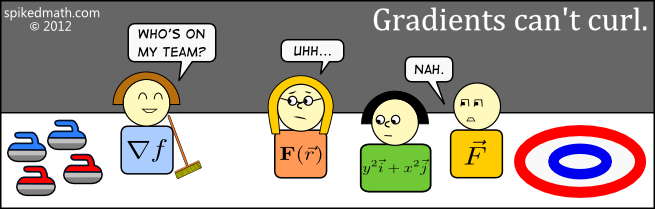
\includegraphics[width=10cm]{501-curling-with-gradients.png}
        \else
            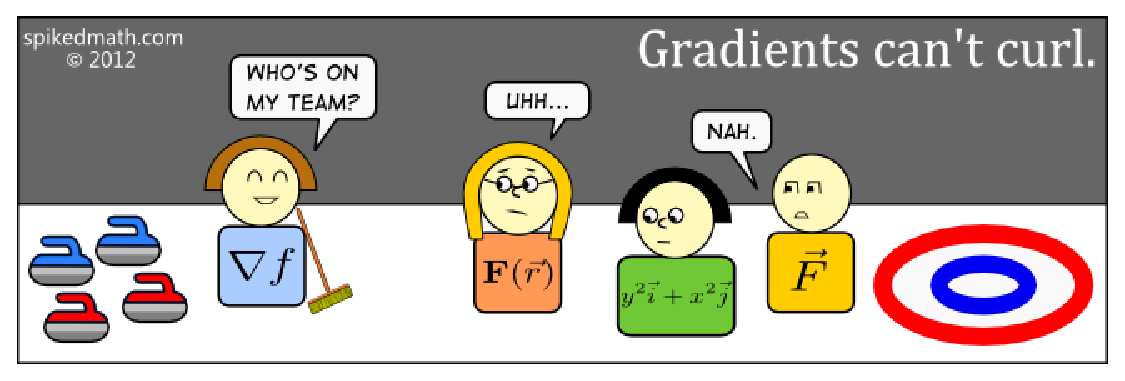
\includegraphics[width=10cm]{501-curling-with-gradients.eps}
        \fi

        {\tiny De \href{http://spikedmath.com/501.html}{Spiked math}, publié sous \href{http://creativecommons.org/licenses/by-nc-sa/2.5/ca/}{licence Creative Commons}.}
\end{center}


%+++++++++++++++++++++++++++++++++++++++++++++++++++++++++++++++++++++++++++++++++++++++++++++++++++++++++++++++++++++++++++
\section[Interprétation de la divergence]{Interprétation géométrique et physique de la divergence}
%+++++++++++++++++++++++++++++++++++++++++++++++++++++++++++++++++++++++++++++++++++++++++++++++++++++++++++++++++++++++++++


En physique, on dit qu'un champ de vecteurs à divergence nulle est \defe{incompressible}{incompressible!champ de vecteur}. Nous allons essayer de comprendre pourquoi. Lorsqu'un fluide incompressible se déplace, il faut qu'en chaque point il y autant de fluide qui rentre que de fluide qui sort. Nous allons voir sur quelques exemples que la divergence d'un champ de vecteurs est le «bilan de masse» d'un fluide qui se déplace selon le champ de vecteurs.

Si en un point la divergence est positive, cela signifie qu'il y a une perte de masse et si la divergence est négative, cela signifie qu'il y a une accumulation de masse.

Prenons par exemple un fluide qui se déplace selon le champ de vitesse montré à figure \ref{LabelFigDivergenceUn}.
\newcommand{\CaptionFigDivergenceUn}{Le champ de vecteurs $F(x,y)=\frac{1}{ x }(1,0)$.}
\input{Fig_DivergenceUn.pstricks}

Étant donné que la vitesse diminue lorsque $x$ avance, il y a une accumulation de fluide. Regardez en effet la quantité de fluide qui rentre dans le rectangle par rapport à la quantité de fluide qui en sort. Ce champ de vecteurs a pour équation :
\begin{equation}
    F(x,y)=\frac{1}{ x }\begin{pmatrix}
        1    \\ 
        0    
    \end{pmatrix}=\begin{pmatrix}
        1/x    \\ 
        0    
    \end{pmatrix}.
\end{equation}
Sa divergence vaut donc
\begin{equation}
    (\nabla\cdot F)(x,y)=\frac{ \partial F_x }{ \partial x }(x,y)+\underbrace{\frac{ \partial F_y }{ \partial y }(x,y)}_{=0}=-\frac{1}{ x^2 }.
\end{equation}
Cette divergence étant négative, il y a bien accumulation de fluide en tout point, et d'autant plus que $x$ est petit.

\begin{example}     \label{ExamDivFrotOM}

    Prenons le champ de vecteurs tournant
    \begin{equation}
        F(x,y)=\frac{1}{ \sqrt{x^2+y^2} }\begin{pmatrix}
            y    \\ 
            -x    
        \end{pmatrix}
    \end{equation}
    représenté à la figure \ref{LabelFigDivergenceDeux}. Cela est un vecteur qui est constamment perpendiculaire au rayon.

    \newcommand{\CaptionFigDivergenceDeux}{Le champ de vecteurs $F(x,y)=(y,-x)$.}
    \input{Fig_DivergenceDeux.pstricks}

    Un fluide dont la vitesse serait donné par ce champ de vecteur se contente de tourner. Intuitivement il ne devrait pas y avoir de divergence parce qu'il n'y a aucune accumulation de fluide. En effet,
    \begin{equation}
        \nabla\cdot F(x,y)=\frac{ -2xy }{ (x^2+y^2)^2 }+\frac{ 2xy }{ (x^2+y^2)^2 }=0.
    \end{equation}
\end{example}

\begin{example}
    Prenons le cas du champ de force de gravitation :
    \begin{equation}
        F(x,y,z)=\frac{1}{ (x^2+y^2+z^2)^{3/2} }\begin{pmatrix}
            x    \\ 
            y   \\
            z
        \end{pmatrix}.
    \end{equation}
    Nous pouvons rapidement remarquer que $\nabla\cdot F=0$. Est-ce que cela peut se comprendre sur le dessin de la figure \ref{LabelFigDivergenceTrois} ?
    \newcommand{\CaptionFigDivergenceTrois}{Le champ de vecteur de la gravité. Nous avons tracé, sur les deux cercles la même densité de vecteurs, c'est à dire le même nombre de vecteurs par unité de surface.}
    \input{Fig_DivergenceTrois.pstricks}

    Essayons de voir combien de fluide entre dans la zone bleue et combien en sort. D'abord, il est certain que les vecteurs qui sortent sont plus courts que ceux qui rentrent, ce qui voudrait dire qu'il y a plus de fluide qui rentre. Mais on voit également que le \emph{nombre} de vecteurs qui sortent est plus grand parce que la seconde sphère est plus grande et qu'il y a un vecteur en chaque point de la sphère.

    Intuitivement nous pouvons dire que la quantité qui rentre dans la sphère de rayon $r_1$ donnée par la taille des vecteurs entrants multiplié par la surface de la sphère, c'est à dire
    \begin{equation}        \label{EqQpinormeVectoOM}
        4\pi r_1^2\| F(x,y,z) \|,
    \end{equation}
    mais $\| F(x,y,z) \|=\frac{1}{ r_1^2 }$, donc la quantité de fluide entrant est $4\pi$. La quantité de fluide sortant sera la même.

    Cela explique deux choses
    \begin{enumerate}
        \item
            Pourquoi les forces de gravitation et électromagnétiques sont en $1/r^2$; c'est parce que nous vivons dans un monde avec trois dimensions d'espace. En étudiant très précisément le champ de gravitation, certains physiciens espèrent trouver des déviations expérimentales par rapport à la règle du \( 1/r^2\); cela \emph{pourrait} être un signe que l'espace contient des dimensions supplémentaires.
        \item
            Pourquoi il y a un $4\pi$ comme coefficient dans beaucoup d'équations en électromagnétisme; en particulier dans certaines anciennes unités de flux.
    \end{enumerate}
    
\end{example}

\begin{remark}
    Nous allons voir plus loin comment s'assurer que l'équation \eqref{EqQpinormeVectoOM} représente bien la «quantité de fluide» qui rentre dans la zone délimitée
\end{remark}


%+++++++++++++++++++++++++++++++++++++++++++++++++++++++++++++++++++++++++++++++++++++++++++++++++++++++++++++++++++++++++++
\section{Quelques formules de Leibnitz}
%+++++++++++++++++++++++++++++++++++++++++++++++++++++++++++++++++++++++++++++++++++++++++++++++++++++++++++++++++++++++++++

La divergence étant une combinaison de dérivées, il n'est pas tellement étonnant que la divergence de produits donne lieux à des formules en deux termes. Si $f$ est une fonction et si $F$ et $G$ sont des champs de vecteurs, nous avons (sans démonstrations) :
\begin{equation}        \label{EqLeinDivNablRotOM}
    \begin{aligned}[]
        \nabla\cdot(fF)&=f\nabla\cdot F+F\cdot\nabla f\\
        \nabla\cdot(F\times G)&=G\cdot\nabla\times F-F\cdot\nabla\times G.
    \end{aligned}
\end{equation}
Nous avons aussi, pour le rotationnel,
\begin{equation}        \label{EqLeinRotfFFOM}
    \nabla\times(fF)=f\nabla\times F+\nabla f\times F.
\end{equation}


\chapter{Coordonnées curvilignes orthogonales}
% This is part of Mes notes de mathématique
% Copyright (c) 2011-2012,2015
%   Laurent Claessens
% See the file fdl-1.3.txt for copying conditions.

%+++++++++++++++++++++++++++++++++++++++++++++++++++++++++++++++++++++++++++++++++++++++++++++++++++++++++++++++++++++++++++
\section{La différentielle revisitée}
%+++++++++++++++++++++++++++++++++++++++++++++++++++++++++++++++++++++++++++++++++++++++++++++++++++++++++++++++++++++++++++

%---------------------------------------------------------------------------------------------------------------------------
\subsection{Les formes différentielles de base}
%---------------------------------------------------------------------------------------------------------------------------

Si la fonction $f\colon \eR^n\to \eR$ est différentiable alors la différentielle en $a\in\eR^n$ est l'application
\begin{equation}        \label{EqFormDiffdfahOM}
    \begin{aligned}
        df_a\colon \eR^n&\to \eR \\
        u&\mapsto \frac{ \partial f }{ \partial x_1 }(a)u_1+\cdots+\frac{ \partial f }{ \partial x_n }(a)u_n.
    \end{aligned}
\end{equation}
Considérons en particulier la fonction qui à $x\in\eR^n$ fait correspondre $x_i\in\eR$. Par abus de notations,  nous la noterons $x_i$. Nous avons 
\begin{equation}
    \frac{ \partial x_i }{ \partial x_j }=\delta_{ij}.
\end{equation}
Par exemple $\partial_yx=0$ et $\partial_xx=1$. Toutes les dérivées partielles de $x_i$ s'annulent sauf la $i$ème qui vaut $1$. Par conséquent
\begin{equation}
    \begin{aligned}
        dx_i\colon \eR^n&\to \eR \\
        u&\mapsto u_i. 
    \end{aligned}
\end{equation}

\begin{remark}
    En toute rigueur nous devrions écrire $(dx_i)_a$. Mais étant donné que
    \begin{equation}
        (dx_i)_a(u)=(dx_i)_b(u)
    \end{equation}
    pour tout points $a$, $b$ et pour tout vecteurs $u$, nous nous permettons de simplifier la notation en ne précisant pas en quel point nous calculons la différentielle de $x_i$.
\end{remark}

Étant donné que $dx_i(u)=u_i$, nous pouvons récrire la formule \eqref{EqFormDiffdfahOM} en remplaçant $u_i$ par $dx_i(u)$ :
\begin{equation}
    df_a(u)=\frac{ \partial f }{ \partial x_1 }(a)dx_1(u)+\cdots+\frac{ \partial f }{ \partial x_n }(a)dx_n(u).
\end{equation}
En tant que application linéaire, $df_a$ est une combinaison linéaire des $dx_i$. En notations compacte :
\begin{equation}
    df_a=\sum_{i=1}^n\frac{ \partial f }{ \partial x_i }(a)dx_i.
\end{equation}

%---------------------------------------------------------------------------------------------------------------------------
\subsection{Différentielles de fonctions composées}
%---------------------------------------------------------------------------------------------------------------------------

Cette façon de voir la différentielle nous permet de jeter un nouveau regard sur la formule de différentiation des fonctions composées. Soient
\begin{equation}
    \begin{aligned}[]
        f\colon \eR^p&\to \eR^n\\
        g\colon \eR^n&\to \eR,
    \end{aligned}
\end{equation}
et $h\colon \eR^p\to \eR$ définie par 
\begin{equation}
    h(u)=h\big( f(u) \big)=(g\circ f)(u).
\end{equation}
Nous allons noter $x$ les coordonnées de $\eR^p$, $a$ un point de $\eR^p$ et $u$, un vecteur de $\eR^p$ accroché au point $a$. Pour $\eR^n$, les notations seront que les coordonnées sont $y$, $b$ est un point de $\eR^n$ et $v$ est un vecteur «accroché» au point $b$.

Nous avons
\begin{equation}
    dg_b(v)=\sum_{i=1}^n\frac{ \partial g }{ \partial y_i }(b)dy_i(v).
\end{equation}
Ici $dy_i(v)$ signifie la $i$ème composante de $v$. C'est simplement $v_i$. Cette formule étant valable pour tout point $b\in\eR^n$ et pour tout vecteur $v$, nous pouvons l'écrire en particulier pour
\begin{subequations}
    \begin{numcases}{}
        b=f(a)\\
        v=df_a(u).
    \end{numcases}
\end{subequations}
Cela donne
\begin{equation}        \label{EqdgfadfauOM}
    dg_{f(a)}\big( df_a(u) \big)=\sum_{i=1}^n\frac{ \partial g }{ \partial y_i }\big( f(a) \big)dy_i\big( df_a(u) \big).
\end{equation}
Mais 
\begin{equation}
    df_a(u)=\sum_{j=1}^p\frac{ \partial f }{ \partial x_j }(a)dx_j(u),
\end{equation}
donc la $i$ème composante de ce vecteur est
\begin{equation}
     \big( df_a(u)\big)_i=\sum_{j=1}^p\frac{ \partial f_i }{ \partial x_j }(a)dx_j(u).
\end{equation}
En remplaçant $dy_i\big( df_a(u) \big)$ par cela dans l'expression \eqref{EqdgfadfauOM}, nous trouvons
\begin{equation}
    dg_{f(a)}\big( df_a(u) \big)=\sum_{i=1}^n\frac{ \partial g }{ \partial y_i }\big( f(a) \big)\sum_{j=1}^p\frac{ \partial f_i }{ \partial x_j }(a)dx_j(u).
\end{equation}
Nous pouvons vérifier que cela est la différentielle de $g\circ f$ au point $a$ appliquée au vecteur $u$. En effet
\begin{equation}
    d(g\circ f)_a(u)=\sum_{j=1}^p\frac{ \partial (g\circ f) }{ \partial x_j }(a)dx_j(u),
\end{equation}
tandis que, par la dérivation de fonctions composées, 
\begin{equation}        \label{EqDerCompofgOM}
    \frac{ \partial (g\circ f) }{ \partial x_j }(a)=\sum_{i=1}^n\frac{ \partial g }{ \partial y_i }\big( f(a) \big)\frac{ \partial f_i }{ \partial x_j }(a).
\end{equation}
Au final, ce que nous avons prouvé est que
\begin{equation}
    d(g\circ f)_a(u)=dg_{f(a)}\big( df_a(u) \big).
\end{equation}

%---------------------------------------------------------------------------------------------------------------------------
\subsection{Passage aux coordonnées polaires}
%---------------------------------------------------------------------------------------------------------------------------

Le changement de coordonnées pour les polaires est la fonction
\begin{equation}
    f\begin{pmatrix}
        r    \\ 
        \theta    
    \end{pmatrix}=\begin{pmatrix}
        x    \\ 
        y    
    \end{pmatrix}=\begin{pmatrix}
        r\cos\theta    \\ 
        r\sin\theta    
    \end{pmatrix}.
\end{equation}
Considérons une fonction $g$ sur $\eR^2$, et définissons la fonction $\tilde g$ par
\begin{equation}
    \tilde g(r,\theta)=g(r\cos\theta,r\sin\theta).
\end{equation}
La formule \eqref{EqDerCompofgOM} permet de trouver les dérivées partielles de $g$ par rapport à $r$ et $\theta$ en termes de celles par rapport à $x$ et $y$ de $g$.

Pour faire le lien avec les notations du point précédent, nous avons
\begin{equation}
    \begin{aligned}[]
        f_1(r,\theta)&=r\cos(\theta)\\
        f_2(r,\theta)&=r\sin(\theta)\\
        (x_1,x_2)&\to(r,\theta)\\
        (y_1,y_2)&\to(x,y).
    \end{aligned}
\end{equation}
Nous avons donc 
\begin{equation}
    \begin{aligned}[]
        \frac{ \partial \tilde g }{ \partial r }(r,\theta)&=\sum_{i=1}^2\frac{ \partial g }{ \partial x_i }\big( f(r,\theta) \big)\frac{ \partial f_i }{ \partial r }(r,\theta)\\
        &=\frac{ \partial g }{ \partial x }(r\cos\theta,r\sin\theta)\frac{ \partial \big( r\cos\theta \big) }{ \partial r }(r,\theta)\\
        &\quad+\frac{ \partial g }{ \partial y }(r\cos\theta,r\sin\theta)\frac{ \partial \big( r\sin\theta\big) }{ \partial r }(r,\theta)\\
        &=\cos\theta\frac{ \partial g }{ \partial x }(r\cos\theta,r\sin\theta)+\sin\theta\frac{ \partial g }{ \partial y }(r\cos\theta,r\sin\theta).
    \end{aligned}
\end{equation}

Prenons par exemple $g(x,y)=\frac{1}{ x^2+y^2 }$. Étant donné que
\begin{equation}
    \frac{ \partial g }{ \partial x }=\frac{ -2x }{ (x^2+y^2)^2 },
\end{equation}
nous avons
\begin{equation}
    \frac{ \partial g }{ \partial x }(r\cos\theta,r\sin\theta)=\frac{ -2\cos\theta }{ r^3 }.
\end{equation}
En utilisant la formule,
\begin{equation}
    \frac{ \partial \tilde g }{ \partial r }(r,\theta)=\cos(\theta)\left( \frac{ -2\cos\theta }{ r^3 } \right)+\sin(\theta)\left( \frac{ -2\sin\theta }{ r^3 } \right)=-\frac{ 2 }{ r^3 }.
\end{equation}
Nous pouvons vérifier directement que cela est correct. En effet
\begin{equation}
    \tilde g(r,\theta)=g(r\cos\theta,r\sin\theta)=\frac{1}{ r^2 },
\end{equation}
dont la dérivée par rapport à $r$ vaut $-2/r^3$.

En ce qui concerne la dérivée par rapport à $\theta$, nous avons
\begin{equation}
    \begin{aligned}[]
    \frac{ \partial \tilde g }{ \partial \theta }&=\frac{ \partial g }{ \partial x }(r\cos\theta,r\sin\theta)\frac{ \partial \big( r\cos(\theta) \big) }{ \partial \theta }+\frac{ \partial g }{ \partial y }(r\cos\theta,r\sin\theta)\frac{ \partial \big( r\sin(\theta) \big) }{ \partial \theta }\\
    &=\left( \frac{ -2\cos\theta }{ r^3 } \right)(-r\sin\theta)+\left( \frac{ -2\sin\theta }{ r^3 } \right)(r\cos\theta)\\
    &=0.
    \end{aligned}
\end{equation}

En résumé et avec quelques abus de notations :
\begin{equation}
    \begin{aligned}[]
        \frac{ \partial \tilde g }{ \partial r }&=\cos(\theta)\frac{ \partial g }{ \partial x }+\sin(\theta)\frac{ \partial g }{ \partial y }\\
        \frac{ \partial \tilde g }{ \partial \theta }&=-r\sin(\theta)\frac{ \partial g }{ \partial x }+r\cos(\theta)\frac{ \partial g }{ \partial y }\\
    \end{aligned}
\end{equation}

%+++++++++++++++++++++++++++++++++++++++++++++++++++++++++++++++++++++++++++++++++++++++++++++++++++++++++++++++++++++++++++
\section{Théorie générale}
%+++++++++++++++++++++++++++++++++++++++++++++++++++++++++++++++++++++++++++++++++++++++++++++++++++++++++++++++++++++++++++

%---------------------------------------------------------------------------------------------------------------------------
\subsection{Base locale}
%---------------------------------------------------------------------------------------------------------------------------

Les coordonnées sphériques et cylindriques sont deux systèmes de coordonnées «un peu courbe» qui existent sur $\eR^3$. Il en existe de nombreux autres, que nous appelons \defe{coordonnées curvilignes}{coordonnées!curvilignes}. Des coordonnées curvilignes sur $\eR^3$ est n'importe quel\footnote{Nous n'entrons pas dans les détails de régularité.} système qui permet de repérer un point de $\eR^3$ à partir de trois nombres.

Il s'agit donc d'un ensemble de trois applications 
\begin{equation}
    x_i\colon \eR^3\to \eR.
\end{equation}
Les coordonnées cylindriques sont
\begin{subequations}
    \begin{numcases}{}
        x_1(r,\theta,z)=r\cos\theta\\
        x_2(r,\theta,z)=r\sin\theta\\
        x_3(r,\theta,z)=z
    \end{numcases}
\end{subequations}

Soit donc un système général $q=(q_1,q_2,q_3)$ et 
\begin{equation}
    M(q)=\begin{pmatrix}
        x_1(q)    \\ 
        x_2(q)    \\ 
        x_3(q)    
    \end{pmatrix}.
\end{equation}
Si nous fixons $q_2$ et $q_3$ et que nous laissons varier $q_1$, nous obtenons une courbe\footnote{Dans le cas des sphériques, c'est une demi-droite horizontale d'angle $q_2$ et de hauteur $q_3$.} dont nous pouvons considérer le vecteur vitesse, c'est à dire le vecteur tangent. En chaque point nous avons ainsi trois vecteurs
\begin{equation}
    \frac{ \partial M }{ \partial q_i }(q).
\end{equation}
Nous disons que le système de coordonnées curviligne est \defe{orthogonal}{orthogonal!coordonnées curviligne} si ces trois vecteurs sont orthogonaux. Dans la suite nous supposerons que c'est toujours le cas.

Nous posons
\begin{equation}
    h_i=\left\| \frac{ \partial M }{ \partial q_i } \right\|
\end{equation}
et nous considérons les trois vecteurs normés
\begin{equation}        \label{EqDefeihMqOM}
    e_i=h_i^{-1}\frac{ \partial M }{ \partial q_i }.
\end{equation}
Les trois vecteurs $\{ e_1,e_2,e_3 \}$ forment une base orthonormée dite \defe{base locale}{base!locale}. Ce sont des vecteurs liés\footnote{En géométrie différentielle on dira que ce sont des élément de l'espace tangent, mais c'est une toute autre histoire.} au point $M$.

%---------------------------------------------------------------------------------------------------------------------------
\subsection{Importance de l'orthogonalité}
%---------------------------------------------------------------------------------------------------------------------------

Nous avons dit que nous nous restreignons au cas où les vecteurs $e_i$ sont orthogonaux. En termes de produits scalaires, cela signifie
\begin{equation}
    e_i\cdot e_j=\delta_{ij}.
\end{equation}
Nous en étudions maintenant quelque conséquence. L'équation \eqref{EqDefeihMqOM} peut s'écrire plus explicitement sous la forme
\begin{equation}
    e_i=\sum_k h_i^{-1}\frac{ \partial x_k }{ \partial q_i }1_k.
\end{equation}
Notez que pour chaque $k$ et $i$, la quantité $h_i^{-1}\frac{ \partial x_k }{ \partial q_i }$ est un simple nombre. Nous allons les mettre dans une matrice :
\begin{equation}
    A_{ki}=h_i^{-1}\frac{ \partial x_k }{ \partial q_i }.
\end{equation}
Cela nous donne le changement de base
\begin{equation}        \label{EqChmBaseeisAkiAkOM}
    e_i=\sum_kA_{ki}1_k.
\end{equation}
Le produit $e_i\cdot e_j$ s'écrit alors
\begin{equation}
    \begin{aligned}[]
        e_i\cdot e_j&=\sum_{kl}A_{ki}A_{lj}\underbrace{1_k\cdot 1_l}_{=\delta_{kl}}\\
        &=\sum_{kl}A_{ki}A_{lj}\delta_{kl}\\
        &=\sum_kA_{ki}A_{kj}\\
        &=\sum_k(A^T)_{ik}A_{kj}.
    \end{aligned}
\end{equation}
Or cela doit valoir $\delta_{ij}$. Par conséquent 
\begin{equation}
    A^T=A^{-1}.
\end{equation}
Le fait que les coordonnées curvilignes considérées soient orthogonales s'exprime donc par la fait que la matrice de changement de base est une matrice orthogonale.

Cette circonstance nous permet d'inverser le changement de base \eqref{EqChmBaseeisAkiAkOM} en multipliant cette équation par $(A^{-1})_{il}$ des deux côtés et en faisant la somme sur $i$ :
\begin{equation}
    \sum_i (A^{-1})_{il}e_i=\sum_{kl}\underbrace{A_{ki}(A^{-1})_{il}}_{=\delta_{kl}}1_k,
\end{equation}
par conséquent
\begin{equation}
    \sum_i(A^T)_{il}e_i=1_l,    
\end{equation}
et
\begin{equation}        \label{EqChamvarunlAeiOM}
    1_l=\sum_iA_{li}e_i=\sum_ih_i^{-1}\frac{ \partial x_l }{ \partial q_i }e_i.
\end{equation}
Armés de cette importante formule, nous pouvons exprimer les quantités que nous connaissons dans la base canonique en termes de la base locale.

Une autre conséquence du fait que $e_1$, $e_2$ et $e_3$ est une base orthonormée est que, éventuellement en réordonnant les vecteurs, on a
\begin{equation}
    \begin{aligned}[]
        e_1\times e_2&=e_3\\
        e_2\times e_3&=e_1\\
        e_3\times e_1&=e_2
    \end{aligned}
\end{equation}
Ces trois relations s'écrivent en une seule avec
\begin{equation}
    e_i\times e_j=\sum_{k}\epsilon_{ijk}e_k
\end{equation}
où 
\begin{equation}
    \epsilon_{ijk}=\begin{cases}
        0    &   \text{si} i,j,k \text{ne sont pas tous différents}\\
        1    &    \text{si } ijk \text{ se ramène à 123 par un nombre pair de permutations}\\
        -1    &    \text{si }ijk \text{ se ramène à 123 par un nombre impair de permutations}
    \end{cases}
\end{equation}
est le \defe{symbole de Levi-Civita}{Levi-Civita}. La formule du produit vectoriel peut également être utilisée à l'envers sous la forme
\begin{equation}        \label{EqekeitimesejOM}
    e_k=\frac{ 1 }{2}\sum_{ij}\epsilon_{ijk}\,e_i\times e_j.
\end{equation}

Le symbole de Levi-Civita possède de nombreuses formules. En voici certaines, facilement démontrables en considérant tous les cas :
\begin{equation}
    \epsilon_{ijk}\epsilon_{ijl}=\delta_{kl}| \epsilon_{ijk} |.
\end{equation}
Grâce au symboles de Levi-Civita, le produit mixte des vecteurs de base a une belle forme :
\begin{equation}        \label{EqProdMixteepsilonCicivrOM}
    e_l\cdot(e_i\times e_j)=\sum_k\epsilon_{ijk}e_l\times e_k=\sum_k\epsilon_{ijk}\delta_{lk}=\epsilon_{ijl}.
\end{equation}

%+++++++++++++++++++++++++++++++++++++++++++++++++++++++++++++++++++++++++++++++++++++++++++++++++++++++++++++++++++++++++++
\section{Gradient en coordonnées curvilignes}
%+++++++++++++++++++++++++++++++++++++++++++++++++++++++++++++++++++++++++++++++++++++++++++++++++++++++++++++++++++++++++++

Soit $(x,y,z)\mapsto f(x,y,z)$ une fonction sur $\eR^3$. Nous pouvons la composer avec les coordonnées curvilignes $q$ pour obtenir la fonction
\begin{equation}
    \tilde f(q_1,q_2,q_3)=f\big( x_1(q),x_2(x),x_3(q) \big).
\end{equation}
Nous disons que $\tilde f$ est l'expression de $f$ dans les coordonnées $q$. Nous savons déjà comment calculer le gradient de $f$ en coordonnées cartésiennes :
\begin{equation}
    F(x,y, z)=\nabla f(x,y,z)=\begin{pmatrix}
        \partial_xf(x,y,z)    \\ 
        \partial_yf(x,y,z)    \\ 
        \partial_zf(x,y,z)    \
    \end{pmatrix}.
\end{equation}
Cela est un vecteur lié au point $(x,y,z)$. Nous voudrions exprimer ce vecteur dans la base $\{ e_1,e_2,e_3 \}$. En d'autres termes, nous voudrions trouver les nombres $\tilde F_1$, $\tilde F_2$ et $\tilde F_3$ tels que
\begin{equation}
    F(x,y,z)=F\big( x(q),y(q),z(q) \big)=\tilde F_1e_1+\tilde F_2e_2+\tilde F_3e_3.
\end{equation}
Ces nombres seront des fonctions de $(q_1,q_2,q_3)$.

Par définition,
\begin{equation}
    \nabla f=\sum_l\frac{ \partial f }{ \partial x_l }1_l.
\end{equation}
En remplaçant $1_l$ par sa valeur en termes des $e_i$ par la formule \eqref{EqChamvarunlAeiOM},
\begin{equation}
    \begin{aligned}[]
        \nabla f&=\sum_l\frac{ \partial f }{ \partial x_l }1_l\\
        &=\sum_l\frac{ \partial f }{ \partial x_l }\sum_ih_i^{-1}\frac{ \partial x_l }{ \partial q_i }e_i\\
        &=\sum_{il}\frac{1}{ h_i }\frac{ \partial f }{ \partial x_l }\frac{ \partial x_l }{ \partial q_i }e_i\\
        &=\sum_i\frac{1}{ h_i }\frac{ \partial \tilde f }{ \partial q_i }e_i.
    \end{aligned}
\end{equation}

Plus explicitement,
\begin{equation}        \label{EqGradientenCurviligneOM}
    \nabla f\big( x(q),y(q),z(q) \big)=\sum_i \frac{1}{ h_i(q) }\frac{ \partial \tilde f }{ \partial q_i }(q)e_i
\end{equation}
où
\begin{equation}
    h_i(q)=\left\| \frac{ \partial M }{ \partial q_i }(q) \right\|.
\end{equation}
Le plus souvent nous n'allons pas noter explicitement la dépendance de $h_i$ en $q$.

Quelques formulaires intéressants sont en appendice de \cite{Schomblond_em}.

%---------------------------------------------------------------------------------------------------------------------------
\subsection{Coordonnées polaires}
%---------------------------------------------------------------------------------------------------------------------------

Les coordonnées curvilignes polaires sont données par
\begin{equation}
    M(r,\theta)=\begin{pmatrix}
        r\cos(\theta)    \\ 
        r\sin(\theta)    
    \end{pmatrix},
\end{equation}
et par conséquent
\begin{equation}
    \begin{aligned}[]
        \frac{ \partial M }{ \partial r }&=\begin{pmatrix}
            \cos(\theta)    \\ 
            \sin(\theta)    
        \end{pmatrix},&\frac{ \partial M }{ \partial \theta }=\begin{pmatrix}
            -r\sin(\theta)    \\ 
            r\cos(\theta)    
        \end{pmatrix}.
    \end{aligned}
\end{equation}
Nous avons les normes $h_r=1$ et $h_{\theta}=r$, et donc les vecteurs de la base locale en $(r,\theta)$ sont
\begin{equation}
    e_r=\begin{pmatrix}
        \cos(\theta)    \\ 
        \sin(\theta)    
    \end{pmatrix}=\cos(\theta)e_x+\sin(\theta)e_y
\end{equation}
ainsi que
\begin{equation}
    e_{\theta}=\begin{pmatrix}
        -\sin(\theta)    \\ 
        \cos(\theta)    
    \end{pmatrix}=-\sin(\theta)e_x+\cos(\theta)e_y.
\end{equation}


Ces vecteurs sont représentés à la figure \ref{LabelFigCurvilignesPolaires}. Notez qu'il y en a une paire différente en chaque point.
\newcommand{\CaptionFigCurvilignesPolaires}{En brun, les lignes que le point suivrait si on ne variait qu'une coordonnées polaire à la fois. Les vecteurs rouges sont les vecteurs $e_{r}$ et $e_{\theta}$.}
\input{pictures_tex/Fig_CurvilignesPolaires.pstricks}


%---------------------------------------------------------------------------------------------------------------------------
\subsection{Coordonnées cylindriques}
%---------------------------------------------------------------------------------------------------------------------------

Les coordonnées cylindriques sont les mêmes que les coordonnées polaires à part qu'il faut écrire
\begin{equation}
    M(r,\theta,z)=\begin{pmatrix}
        r\cos(\theta)    \\ 
        r\sin(\theta)    \\ 
        z    
    \end{pmatrix},
\end{equation}
et nous avons le vecteur de base supplémentaire
\begin{equation}
    e_z=\frac{ \partial M }{ \partial z }=\begin{pmatrix}
        0    \\ 
        0    \\ 
        1    
    \end{pmatrix}
\end{equation}
parce que $h_z=1$.

%---------------------------------------------------------------------------------------------------------------------------
\subsection{Coordonnées sphériques}
%---------------------------------------------------------------------------------------------------------------------------

Les coordonnées curvilignes sphériques sont données par
\begin{equation}
    M(\rho,\theta,\varphi)=
    \begin{pmatrix}
        \rho\sin(\theta)\cos(\varphi)    \\ 
        \rho\sin(\theta)\sin(\varphi)    \\ 
        \rho\cos(\theta)
    \end{pmatrix},
\end{equation}
dont les dérivées sont données par
\begin{equation}
    \begin{aligned}[]
        \frac{ \partial M }{ \partial r }&=\begin{pmatrix}
        \sin(\theta)\cos(\varphi)    \\ 
        \sin(\theta)\sin(\varphi)    \\ 
        \cos(\theta)
    \end{pmatrix},
    &\frac{ \partial M }{ \partial \theta }&=
    \begin{pmatrix}
        \rho\cos(\theta)\cos(\varphi)    \\ 
        \rho\cos(\theta)\sin(\varphi)    \\ 
        -\rho\sin(\theta)
    \end{pmatrix},\\
    \frac{ \partial M }{ \partial \varphi }&=
    \begin{pmatrix}
        -\rho\sin(\theta)\sin(\varphi)    \\ 
        \rho\sin(\theta)\cos(\varphi)    \\ 
        0
    \end{pmatrix}
    \end{aligned}
\end{equation}
Les normes de ces vecteurs sont $h_{\rho}=1$, $h_{\theta}=\rho$ et $h_{\varphi}=\rho\sin(\theta)$. Les vecteurs de la base locale en $(\rho,\theta,\varphi)$ sont donc
\begin{equation}
    \begin{aligned}[]
        e_r&=\begin{pmatrix}
        \sin(\theta)\cos(\varphi)    \\ 
        \sin(\theta)\sin(\varphi)    \\ 
        \cos(\theta)
    \end{pmatrix},
    &e_{\theta}&=
    \begin{pmatrix}
        \cos(\theta)\cos(\varphi)    \\ 
        \cos(\theta)\sin(\varphi)    \\ 
        -\sin(\theta)
    \end{pmatrix},\\
    e_{\varphi}&=
    \begin{pmatrix}
        -\sin(\varphi)    \\ 
        \cos(\varphi)    \\ 
        0
    \end{pmatrix}
    \end{aligned}
\end{equation}

Nous pouvons exprimer le gradient d'une fonction en coordonnées sphériques en utilisant la formule \eqref{EqGradientenCurviligneOM} :
\begin{equation}        \label{EqGradientSpheriqueOM}
    \nabla\tilde f(\rho,\theta,\varphi)=\frac{ \partial \tilde f }{ \partial \rho }e_{\rho}+\frac{1}{ \rho }\frac{ \partial \tilde f }{ \partial \theta }e_{\theta}+\frac{1}{ \rho\sin(\theta) }\frac{ \partial \tilde f }{ \partial \varphi }r_{\varphi}.
\end{equation}
Cette expression peut paraître peu pratique parce que les vecteurs $e_{\rho}$, $e_{\theta}$ et $e_{\varphi}$ eux-mêmes changent en chaque point. Elle est effectivement peu adaptée au dessin, mais elle est très pratique pour des fonctions ayant des symétries.

\begin{example}
    Le potentiel de la gravitation est la fonction
    \begin{equation}
        V(x,y,z)=\frac{1}{ \sqrt{x^2+y^2+z^2} }.
    \end{equation}
    En coordonnées sphériques elle s'écrit
    \begin{equation}
        \tilde V(\rho,\theta,\varphi)=\frac{1}{ \rho }.
    \end{equation}
    En voila une fonction qu'elle est facile à dériver, contrairement à $V$ ! En suivant la formule \eqref{EqGradientSpheriqueOM}, nous avons immédiatement
    \begin{equation}
        \nabla\tilde V=-\frac{1}{ \rho^2 }e_{\rho}.
    \end{equation}
    Nous voyons immédiatement que cela est un champ de vecteurs dont la norme diminue comme le carré de la distance à l'origine et qui est en permanence dirigé vers l'origine.
\end{example}


%+++++++++++++++++++++++++++++++++++++++++++++++++++++++++++++++++++++++++++++++++++++++++++++++++++++++++++++++++++++++++++
\section{Divergence en coordonnées curvilignes}
%+++++++++++++++++++++++++++++++++++++++++++++++++++++++++++++++++++++++++++++++++++++++++++++++++++++++++++++++++++++++++++

Nous savons que 
\begin{equation}
    \nabla\tilde f=\sum_j\frac{1}{ h_j }\frac{ \partial \tilde f }{ \partial q_j }e_j.
\end{equation}
Nous pouvons en particulier considérer la fonction $f(q)=q_i$. De la même manière que nous avions noté $x_i$ la fonction $x\mapsto x_i$, nous notons $q_i$ la fonction $q\mapsto q_i$. Le gradient de cette fonction est donné par
\begin{equation}
    \nabla q_i=\sum_j\frac{1}{ h_j }\frac{ \partial q_i }{ \partial q_j }e_j,
\end{equation}
mais $\frac{ \partial q_i }{ \partial q_j }=\delta_{ij}$, donc
\begin{equation}
    \nabla q_i=\frac{ e_i }{ h_i },
\end{equation}
ou encore
\begin{equation}
    e_i=h_i\nabla q_i.
\end{equation}
Cela n'est pas étonnant : la direction dans laquelle la coordonnées $q_i$ varie le plus est le vecteur $e_i$ qui donne la tangente à la courbe obtenue lorsque \emph{seul} $q_i$ varie.

Commençons par calculer la divergence de $e_i$. En utilisant la formule \eqref{EqekeitimesejOM},
\begin{equation}
    \nabla\cdot e_k=\frac{ 1 }{2}\sum_{ij}\epsilon_{ijk}\,\nabla\cdot (e_i\times e_j).
\end{equation}
Nous avons, en utilisant les règles de Leibnitz \eqref{EqLeinDivNablRotOM}, 
\begin{equation}
    \begin{aligned}[]
        \nabla\cdot(e_i\times e_j)&=\nabla\cdot(h_i\nabla q_i\times h_j\nabla q_j)\\
        &=\nabla(h_ih_j)\cdot\big( \nabla q_i\times\nabla q_j \big)+h_ih_j\nabla\cdot\big( \nabla q_i\times\nabla q_j \big)\\
        &=\nabla(h_ih_j)\cdot\big( \nabla q_i\times\nabla q_j \big)\\
        &\quad+h_ih_j\nabla q_j\cdot\big( \underbrace{\nabla\times\nabla q_i}_{=0} \big)\\
        &\quad+h_ih_j\nabla q_i\cdot\big( \underbrace{\nabla\times\nabla q_j}_{=0} \big)
    \end{aligned}
\end{equation}
Cela nous fait
\begin{equation}
    \nabla\cdot e_k=\sum_{ij}\epsilon_{ijk}\frac{ \nabla(h_ih_j) }{ h_ih_j }\cdot (e_i\times e_j).
\end{equation}
parce que $\nabla q_i=h_i^{-1}e_i$. Nous pouvons développer le gradient qui intervient :
\begin{equation}
    \nabla(h_ih_j)=\sum_l\frac{1}{ h_l }\frac{ \partial  }{ \partial q_l }(h_ih_j)e_l.
\end{equation}
Nous voyons donc arriver le produit mixte $e_l\cdot (e_i\times e_j)$. En utilisant la formule \eqref{EqProdMixteepsilonCicivrOM}, cela s'exprime directement sous la forme $\epsilon_{ijl}$.

Nous avons alors
\begin{equation}        \label{EqFragradekdviOM}
    \begin{aligned}[]
        \nabla\cdot e_k&=\frac{ 1 }{2}\sum_{ijl}\frac{1}{ h_ih_jh_l }\frac{ \partial  }{ \partial q_l }(h_ih_j)\epsilon_{ijk}\epsilon_{ijl}\\
        &=\frac{ 1 }{2}\sum_{ijl}\delta_{kl}| \epsilon_{ijk} |\frac{ \partial  }{ \partial q_l }(h_ih_j)\\
        &=\frac{ 1 }{2}\sum_{ij}\frac{| \epsilon_{ijk} |}{ h_ih_jh_k }\frac{ \partial  }{ \partial q_k }(h_ih_j).
    \end{aligned}
\end{equation}
Par exemple,
\begin{equation}
    \nabla\cdot e_1=\frac{1}{ h_1h_2h_3 }\frac{ \partial  }{ \partial q_1 }(h_2h_3).
\end{equation}

Nous devons maintenant chercher le gradient d'un champ général
\begin{equation}
    F(q)=\sum_kF_k(q)e_k.
\end{equation}
La première chose à faire est d'utiliser la formule de Leibnitz :
\begin{equation}        \label{EqLeibnbablaFekOM}
    \nabla\cdot F=\sum_k\nabla F_k(q)\cdot e_k+\sum_kF_k(q)\nabla\cdot e_k.
\end{equation}
Afin d'alléger les notations, nous allons nous concentrer sur le terme numéro $k$ et ne pas écrire la somme. Si $i$ et $j$ sont les nombres tels que $\epsilon_{ijk}=1$, alors ce que la formule \eqref{EqFragradekdviOM} signifie, c'est que
\begin{equation}
    \nabla\cdot e_k=\frac{1}{ h_1h_2h_3 }\frac{ \partial  }{ \partial q_k }(h_ih_j).
\end{equation}
Nous savons déjà par la formule \eqref{EqGradientenCurviligneOM} que
\begin{equation}
    \nabla F_k=\sum_l\frac{1}{ h_l }\frac{ \partial F_k }{ \partial q_l }e_l,
\end{equation}
par conséquent
\begin{equation}
    \nabla F_k\cdot e_k=\sum_l\frac{1}{ h_l }\frac{ \partial F_k }{ \partial q_l }\delta_{kl}=\frac{1}{ h_k }\frac{ \partial F_k }{ \partial q_k }.
\end{equation}
Pour obtenir cela nous avons utilisé le fait que $e_l\cdot e_k=\delta_{lk}$. Le terme numéro $k$ de la somme \eqref{EqLeibnbablaFekOM} est donc
\begin{equation}
    \frac{1}{ h_k }\frac{ \partial F_k }{ \partial q_k }+\frac{ F_k }{ h_kh_ih_j }\frac{ \partial (h_ih_j) }{ \partial q_k }=\frac{1}{ h_ih_jh_k }\frac{ \partial (F_kh_ih_j) }{ \partial q_k }
\end{equation}
où il est entendu que $i$ et $j$ représentent les nombres tels que $\epsilon_{ijk}=1$.

Au final, nous avons
\begin{equation}
    \nabla\cdot F=\frac{1}{ h_1h_2h_3 }\sum_{ijk}| \epsilon_{ijk} |\frac{ \partial (F_kh_ih_j) }{ \partial q_k }.
\end{equation}
Ici, la somme sur $i$ et $j$ consiste seulement à sélectionner les termes tels que $i$ et $j$ ne sont pas $k$. En écrivant la somme explicitement,
\begin{equation}
    \begin{aligned}[]
        \nabla\cdot F=\frac{1}{ h_1h_2h_3 }\left[ \frac{ \partial  }{ \partial q_1 }(F_1h_2h_3)+\frac{ \partial  }{ \partial q_2 }(F_2h_1h_3)+\frac{ \partial  }{ \partial q_3 }(F_3h_1h_2) \right].
    \end{aligned}
\end{equation}

%---------------------------------------------------------------------------------------------------------------------------
\subsection{Coordonnées cylindriques}
%---------------------------------------------------------------------------------------------------------------------------

En coordonnées cylindriques, nous avons déjà vu que $h_r=1$, $h_{\theta}=r$ et $h_z=1$. La divergence est donc donnée par
\begin{equation}        \label{EqDivEnCylonfOM}
    \nabla\cdot F=\frac{1}{ r }\left[ \frac{ \partial  }{ \partial r }(rF_r)+\frac{ \partial  }{ \partial \theta }(F_{\theta})+\frac{ \partial  }{ \partial z }(rF_z) \right].
\end{equation}
Par exemple si
\begin{equation}
    F(r,\theta,z)=re_{\theta}+e_z,
\end{equation}
nous avons
\begin{equation}
    (\nabla\cdot F)(r,\theta,z)=\frac{1}{ r }\left[ \frac{ \partial  }{ \partial \theta }(r)+\frac{ \partial  }{ \partial z }(r) \right]=0.
\end{equation}
Cela est logique parce que $re_{\theta}$ est à peu près le champ dont nous avons parlé dans l'exemple \eqref{ExamDivFrotOM}, qui était à divergence nulle. En réalité, le champ dont on parlait dans cet exemple était exactement $-e_{\theta}$. Le champ $e_z$ est également à divergence nulle parce qu'il est constant.

%---------------------------------------------------------------------------------------------------------------------------
\subsection{Coordonnées sphériques}
%---------------------------------------------------------------------------------------------------------------------------

En coordonnées sphériques, nous avons $h_{\rho}=1$, $h_{\theta}=r$ et $h_{\varphi}=r\sin\theta$, donc
\begin{equation}
    \nabla\cdot F=\frac{1}{ r^2\sin\theta }\left[ \frac{ \partial  }{ \partial \rho }(\rho^2\sin\theta F_{\rho})+\frac{ \partial  }{ \partial \theta }(\rho\sin\theta F_{\theta})+\frac{ \partial  }{ \partial \varphi }(\rho F_{\varphi}) \right].
\end{equation}
si $F(\rho,\theta,\varphi)=F_{\rho}e_{\rho}+F_{\theta}e_{\theta}+F_{\varphi}e_{\varphi}$.

%+++++++++++++++++++++++++++++++++++++++++++++++++++++++++++++++++++++++++++++++++++++++++++++++++++++++++++++++++++++++++++
\section{Laplacien en coordonnées curvilignes orthogonales}
%+++++++++++++++++++++++++++++++++++++++++++++++++++++++++++++++++++++++++++++++++++++++++++++++++++++++++++++++++++++++++++

Soit une fonction $f\colon \eR^3\to \eR$. Le \defe{Laplacien}{Laplacien} de $f$ est donné par
\begin{equation}
    \Delta f=\nabla\cdot(\nabla f).
\end{equation}
En utilisant les formules données, nous avons
\begin{equation}
    \Delta f=\frac{1}{ h_1h_2h_3 }\left[ \frac{ \partial  }{ \partial q_1 }\left( \frac{ h_2h_3 }{ h_1 }\frac{ \partial f }{ \partial q_1 } \right)  +\frac{ \partial  }{ \partial q_2 }\left( \frac{ h_1h_3 }{ h_2 }\frac{ \partial f }{ \partial q_2 } \right)  +\frac{ \partial  }{ \partial q_3 }\left( \frac{ h_1h_2 }{ h_3 }\frac{ \partial f }{ \partial q_3 } \right)     \right].
\end{equation}
Dans cette expression, la fonction $f$ est donnée comme fonction de $q_1$, $q_2$ et $q_3$.

En coordonnées cylindriques, cela s'écrit
\begin{equation}
    \begin{aligned}[]
        \Delta f&=\frac{1}{ r }\left[ \frac{ \partial  }{ \partial r }\left( r\frac{ \partial f }{ \partial r } \right)+\frac{ \partial  }{ \partial \theta }\left( \frac{1}{ r }\frac{ \partial f }{ \partial \theta } \right)+\frac{ \partial  }{ \partial z }\left( r\frac{ \partial f }{ \partial z } \right) \right]\\
        &=\frac{ \partial^2f  }{ \partial r^2 }+\frac{1}{ r }\frac{ \partial f }{ \partial r }+\frac{1}{ r^2 }\frac{ \partial^2f }{ \partial \theta^2 }+\frac{ \partial^2f }{ \partial z^2 }.
    \end{aligned}
\end{equation}
Dans cette expression, $f$ est fonction de $r$, $\theta$ et $z$.

En coordonnées sphériques, cela devient
\begin{equation}        \label{EqLaplaceSpheOM}
    \Delta f=\frac{1}{ \rho^2\sin\theta }\left[ \frac{ \partial  }{ \partial \rho }\left( \rho^2\sin\theta\frac{ \partial f }{ \partial \rho } \right)+\frac{ \partial  }{ \partial \theta }\left( \sin\theta\frac{ \partial f }{ \partial \theta } \right)+\frac{ \partial  }{ \partial \varphi }\left( \frac{1}{ \sin\theta }\frac{ \partial f }{ \partial \varphi } \right) \right].
\end{equation}
Dans cette expression, $f$ est fonction de $\rho$, $\theta$ et $\varphi$.

%+++++++++++++++++++++++++++++++++++++++++++++++++++++++++++++++++++++++++++++++++++++++++++++++++++++++++++++++++++++++++++
\section{Rotationnel en coordonnées curvilignes orthogonales}
%+++++++++++++++++++++++++++++++++++++++++++++++++++++++++++++++++++++++++++++++++++++++++++++++++++++++++++++++++++++++++++

Nous voulons calculer le rotationnel de $F(q)=\sum_kF_k(q)e_k$. Pour cela nous commençons par écrire $e_k=h_k\nabla q_k$ et nous utilisons la formule \eqref{EqLeinRotfFFOM} avec $F_kh_k$ en guise de $f$ :
\begin{equation}
    \begin{aligned}[]
        \nabla\times F_ke_k&=\nabla\times(F_kh_k\nabla q_k)\\
        &=F_kh_k\underbrace{\nabla\times(\nabla q_k)}_{=0}+\nabla(F_kh_k)\times\nabla q_k\\
        &=\frac{1}{ h_k }\nabla(F_kh_k)\times e_k.
    \end{aligned}
\end{equation}
Nous utilisons à présent la formule \eqref{EqGradientenCurviligneOM} du gradient et le formule $e_j\times e_k=\sum_l\epsilon_{jkl}e_l$ :
\begin{equation}
    \begin{aligned}[]
        \nabla\times(F_ke_k)&=\sum_{j}\frac{1}{ h_jh_k }\frac{ \partial  }{ \partial q_j }(F_kh_k)e_j\times e_k\\
        &=\sum_{jl}\frac{1}{ h_jh_k }\epsilon_{jkl}\frac{ \partial  }{ \partial q_j }(F_kh_k)e_l.
    \end{aligned}
\end{equation}
Le rotationnel s'écrit donc
\begin{equation}
    \nabla\times F=\sum_{jkl}\frac{1}{ h_jh_k }\epsilon_{jkl}\frac{ \partial  }{ \partial q_j }(F_kh_k)e_l.
\end{equation}
Devant $e_1$ par exemple nous avons seulement les termes $j=2$, $k=3$ et $j=3$, $k=2$. Étant donné que $\epsilon_{231}=1$ et $\epsilon_{321}=-1$, le coefficient de $e_1$ sera simplement
\begin{equation}
    \frac{1}{ h_2h_3 }\left( \frac{ \partial  }{ \partial q_2 }(F_3h_3)-\frac{ \partial  }{ \partial q_3 }(F_2h_2) \right).
\end{equation}
La formule complète devient
\begin{equation}
    \begin{aligned}[]
        \nabla\times\sum_k F_ke_k&=\frac{1}{ h_2h_3 }\left( \frac{ \partial  }{ \partial q_2 }(F_3h_3)-\frac{ \partial  }{ \partial q_3 }(F_2h_2) \right)\\
            &\quad+\frac{1}{ h_1h_3 }\left( \frac{ \partial  }{ \partial q_3 }(F_1h_1)-\frac{ \partial  }{ \partial q_1 }(F_3h_3) \right)\\
            &\quad+\frac{1}{ h_2h_1 }\left( \frac{ \partial  }{ \partial q_1 }(F_2h_2)-\frac{ \partial  }{ \partial q_2 }(F_1h_1) \right).  
    \end{aligned} 
\end{equation} 

%---------------------------------------------------------------------------------------------------------------------------
\subsection{Coordonnées cylindriques}
%---------------------------------------------------------------------------------------------------------------------------

En utilisant $h_r=1$, $h_{\theta}=r$ et $h_z=1$, nous trouvons
\begin{equation}        \label{EqRotationnelCylinOM}
    \begin{aligned}[]
        \nabla\times(F_re_r+F_{\theta}e_{\theta}+F_ze_z)&=\frac{1}{ r }\left( \frac{ \partial F_z }{ \partial \theta }-\frac{ \partial (F_{\theta}r) }{ \partial z } \right)e_r\\
        &\quad+\left( \frac{ \partial F_r }{ \partial z }-\frac{ \partial F_z }{ \partial r } \right)e_{\theta}\\
        &\quad+\left( \frac{ \partial (F_{\theta} r) }{ \partial r }-\frac{ \partial F_r }{ \partial \theta } \right)e_z.
    \end{aligned}
\end{equation}

%---------------------------------------------------------------------------------------------------------------------------
\subsection{Coordonnées sphériques}
%---------------------------------------------------------------------------------------------------------------------------

En utilisant $h_{\rho}=1$, $h_{\theta}=\rho$ et $h_{\varphi}=\rho\sin\theta$, nous trouvons
\begin{equation}
    \begin{aligned}[]
        \nabla\times(F_{\rho}e_{\rho}+F_{\theta}e_{\theta}+F_{\varphi}e_{\varphi})&=\frac{1}{ \rho\sin\theta }\left( \frac{ \partial (F_{\varphi})\sin\theta }{ \partial \theta }-\frac{ \partial F_{\theta} }{ \partial \varphi } \right)e_{\rho}\\
        &\quad+\frac{1}{ \rho\sin\theta }\left( \frac{ \partial F_{\rho} }{ \partial \varphi }-\frac{ \partial (F_{\varphi}\rho\sin\theta) }{ \partial \rho } \right)e_{\theta}\\
        &\quad+\frac{1}{ \rho }\left( \frac{ \partial F_{\theta}\rho }{ \partial \rho }-\frac{ \partial F_r }{ \partial \theta } \right)e_{\varphi}.
    \end{aligned}
\end{equation}
Note : dans le premier terme, il y a une simplification par $\rho$.

%+++++++++++++++++++++++++++++++++++++++++++++++++++++++++++++++++++++++++++++++++++++++++++++++++++++++++++++++++++++++++++
\section{Les formules}
%+++++++++++++++++++++++++++++++++++++++++++++++++++++++++++++++++++++++++++++++++++++++++++++++++++++++++++++++++++++++++++

%---------------------------------------------------------------------------------------------------------------------------
\subsection{Coordonnées polaires}
%---------------------------------------------------------------------------------------------------------------------------

Les vecteurs de base :
\begin{subequations}
    \begin{align}
    e_r=\begin{pmatrix}
        \cos(\theta)    \\ 
        \sin(\theta)    
    \end{pmatrix}=\cos(\theta)e_x+\sin(\theta)e_y\\
    e_{\theta}=\begin{pmatrix}
        -\sin(\theta)    \\ 
        \cos(\theta)    
    \end{pmatrix}=-\sin(\theta)e_x+\cos(\theta)e_y.
    \end{align}
\end{subequations}

Le gradient :
\begin{equation}
    \nabla\tilde f(r,\theta)=\frac{ \partial \tilde f }{ \partial r }(r,\theta)e_r+\frac{1}{ r }\frac{ \partial \tilde f }{ \partial \theta }(r,\theta)e_{\theta}.
\end{equation}

La divergence :
\begin{equation}    \label{EqgRxJKdOM}
    \nabla\cdot F=\frac{1}{ r }\left[ \frac{ \partial  }{ \partial r }(rF_r)+\frac{ \partial  }{ \partial \theta }(F_{\theta}) \right].
\end{equation}

Le rotationnel :
\begin{equation}    \label{EqtBnoCwOM}
    \nabla\times(F_re_r+F_{\theta}e_{\theta})=\left( \frac{ \partial (F_{\theta} r) }{ \partial r }-\frac{ \partial F_r }{ \partial \theta } \right)e_z.
\end{equation}
Notons que le rotationnel n'existe pas vraiment en deux dimensions. Ici nous avons vu le champ \( F(r,\theta)\) comme un champs dans \( \eR^3\) ne dépendant pas de \( z\) et n'ayant pas de composante \( z\). Le résultat est un rotationnel qui est dirigé selon l'axe \( z\).


%---------------------------------------------------------------------------------------------------------------------------
\subsection{Coordonnées cylindriques}
%---------------------------------------------------------------------------------------------------------------------------

Les vecteurs de base : idem qu'en coordonnées polaires, et on ajoute \( e_z\) sans modifications.

Le gradient :
\begin{equation}
    \nabla\tilde f(r,\theta,z)=\frac{ \partial \tilde f }{ \partial r }(r,\theta,z)e_r+\frac{1}{ r }\frac{ \partial \tilde f }{ \partial \theta }(r,\theta,z)e_{\theta}+\frac{ \partial \tilde f }{ \partial z }(r,\theta,z)e_z.
\end{equation}

La divergence :
\begin{equation} 
    \nabla\cdot F=\frac{1}{ r }\left[ \frac{ \partial  }{ \partial r }(rF_r)+\frac{ \partial  }{ \partial \theta }(F_{\theta})+\frac{ \partial  }{ \partial z }(rF_z) \right].
\end{equation}

Le rotationnel :
\begin{equation}    
    \begin{aligned}[]
        \nabla\times(F_re_r+F_{\theta}e_{\theta}+F_ze_z)&=\frac{1}{ r }\left( \frac{ \partial F_z }{ \partial \theta }-\frac{ \partial (F_{\theta}r) }{ \partial z } \right)e_r\\
        &\quad+\left( \frac{ \partial F_r }{ \partial z }-\frac{ \partial F_z }{ \partial r } \right)e_{\theta}\\
        &\quad+\left( \frac{ \partial (F_{\theta} r) }{ \partial r }-\frac{ \partial F_r }{ \partial \theta } \right)e_z.
    \end{aligned}
\end{equation}

Note : les formules concernant les coordonnées polaires se réduisent de celles-ci en enlevant toutes les références à \( z\).

%---------------------------------------------------------------------------------------------------------------------------
\subsection{Coordonnées sphériques}
%---------------------------------------------------------------------------------------------------------------------------

Les vecteurs de base :
\begin{equation}
    \begin{aligned}[]
        e_r&=\begin{pmatrix}
        \sin(\theta)\cos(\varphi)    \\ 
        \sin(\theta)\sin(\varphi)    \\ 
        \cos(\theta)
    \end{pmatrix},
    &e_{\theta}&=
    \begin{pmatrix}
        \cos(\theta)\cos(\varphi)    \\ 
        \cos(\theta)\sin(\varphi)    \\ 
        -\sin(\theta)
    \end{pmatrix},\\
    e_{\varphi}&=
    \begin{pmatrix}
        -\sin(\varphi)    \\ 
        \cos(\varphi)    \\ 
        0
    \end{pmatrix}
    \end{aligned}
\end{equation}


Le gradient :
\begin{equation}
    \nabla\tilde f(\rho,\theta,\varphi)=\frac{ \partial \tilde f }{ \partial \rho }e_{\rho}+\frac{1}{ \rho }\frac{ \partial \tilde f }{ \partial \theta }e_{\theta}+\frac{1}{ \rho\sin(\theta) }\frac{ \partial \tilde f }{ \partial \varphi }r_{\varphi}.
\end{equation}


La divergence :
\begin{equation}
    \nabla\cdot F=\frac{1}{ \rho^2\sin\theta }\left[ \frac{ \partial  }{ \partial \rho }(\rho^2\sin\theta F_{\rho})+\frac{ \partial  }{ \partial \theta }(\rho\sin\theta F_{\theta})+\frac{ \partial  }{ \partial \varphi }(\rho F_{\varphi}) \right].
\end{equation}

Le rotationnel :
\begin{equation}
    \begin{aligned}[]
        \nabla\times(F_{\rho}e_{\rho}+F_{\theta}e_{\theta}+F_{\varphi}e_{\varphi})&=\frac{1}{ \rho\sin\theta }\left( \frac{ \partial (F_{\varphi})\sin\theta }{ \partial \theta }-\frac{ \partial F_{\theta} }{ \partial \varphi } \right)e_{\rho}\\
        &\quad+\frac{1}{ \rho\sin\theta }\left( \frac{ \partial F_{\rho} }{ \partial \varphi }-\frac{ \partial (F_{\varphi}\rho\sin\theta) }{ \partial \rho } \right)e_{\theta}\\
        &\quad+\frac{1}{ \rho }\left( \frac{ \partial F_{\theta}\rho }{ \partial \rho }-\frac{ \partial F_r }{ \partial \theta } \right)e_{\varphi}.
    \end{aligned}
\end{equation}


\chapter{Intégrales multiples et de surface}
% This is part of Mes notes de mathématique
% Copyright (c) 2011-2015
%   Laurent Claessens
% See the file fdl-1.3.txt for copying conditions.

%+++++++++++++++++++++++++++++++++++++++++++++++++++++++++++++++++++++++++++++++++++++++++++++++++++++++++++++++++++++++++++
\section{Rappel sur les intégrales usuelles}
%+++++++++++++++++++++++++++++++++++++++++++++++++++++++++++++++++++++++++++++++++++++++++++++++++++++++++++++++++++++++++++

%TODO : l'utilisation des macros \og et \fg ne se justifie plus : les enlever.

Soit une fonction
\begin{equation}
    \begin{aligned}
        f\colon \mathopen[ a , b \mathclose]\subset\eR&\to \eR^+ \\
        x&\mapsto f(x) .
    \end{aligned}
\end{equation}
L'intégrale de $f$ sur le segment $\mathopen[ a , b \mathclose]$, notée $\int_a^bf(x)dx$ est le nombre égal à l'aire de la surface située entre le graphe de $f$ et l'axe des $x$, comme indiqué à la figure \ref{LabelFigIntegraleSimple}.
\newcommand{\CaptionFigIntegraleSimple}{L'intégrale de $f$ entre $a$ et $b$ représente la surface sous la fonction.}
\input{pictures_tex/Fig_IntegraleSimple.pstricks}

\begin{definition}
    Si $f$ est une fonction de une variable à valeurs réelles, une \defe{primitive}{primitive} de $f$ est une fonction $F$ telle que $F'=f$.
\end{definition}

Toute fonction continue admet une primitive.

\begin{theorem}[Théorème fondamental du caclul intégral]
    Si $f$ est une fonction positive et continue, et si $F$ est une primitive de $f$, alors
    \begin{equation}
        \int_a^bf(x)dx=F(b)-F(a).
    \end{equation}
\end{theorem}

\begin{remark}
    Si $f$ est une fonction continue par morceaux, l'intégrale de $f$ se calcule comme la somme des intégrales de ses morceaux. Plus précisément si nous avons $a=x_0<x_1<\ldots<x_n=b$ et si $f$ est continue sur $\mathopen] x_i , x_{i+1} \mathclose[$ pour tout $i$, alors nous posons
    \begin{equation}
        \int_a^bf(x)dx=\int_{x_0}^{x_1}f(x)dx+\int_{x_1}^{x_2}f(x)dx+\cdots+\int_{x_{n-1}}^{n_n}f(x)dx.
    \end{equation}
    Sur chacun des morceaux, l'intégrale se calcule normalement en passant par une primitive.
\end{remark}

%+++++++++++++++++++++++++++++++++++++++++++++++++++++++++++++++++++++++++++++++++++++++++++++++++++++++++++++++++++++++++++
\section{Intégration de fonction à deux variables}
%+++++++++++++++++++++++++++++++++++++++++++++++++++++++++++++++++++++++++++++++++++++++++++++++++++++++++++++++++++++++++++

%---------------------------------------------------------------------------------------------------------------------------
\subsection{Intégration sur un domaine rectangulaire}
%---------------------------------------------------------------------------------------------------------------------------
\label{PgRapIntMultFubiniRectOM}

Soit une fonction positive
\begin{equation}
    \begin{aligned}
        f\colon \mathopen[ a , b \mathclose]\times\mathopen[ c , d \mathclose]&\to \eR^+ \\
        (x,y)&\mapsto f(x,y). 
    \end{aligned}
\end{equation}

L'intégrale de $f$ sur le rectangle $\mathopen[ a , b \mathclose]\times\mathopen[ c , d \mathclose]$ est le volume sous le graphe de la fonction. C'est à dire le volume de l'ensemble
\begin{equation}
    \{ (x,y,z)\tq (x,y)\in\mathopen[ a , b \mathclose]\times\mathopen[ c , d \mathclose], z\leq f(x,y) \}.
\end{equation}

\begin{theorem}[Théorème de Fubini]
    Soit une fonction $f\colon \eR^2\to \eR$ une fonction continue par morceaux sur $\mR=\mathopen[ a , b \mathclose]\times\mathopen[ c , d \mathclose]$. Alors
    \begin{equation}
        \int_{\mR}f(x,y)dxdy=\int_a^b\left[ \int_c^df(x,y)dy \right]dx=\int_c^d\left[ \int_a^bf(x,y)dx \right]dy.
    \end{equation}
\end{theorem}
\index{théorème!Fubini!version compacte dans \( \eR^2\)}

En pratique, nous utilisons le théorème de Fubini pour calculer les intégrales sur des rectangles.


\begin{example}
    
    Nous voudrions intégrer la fonction $f(x,y)-4+x^2+y^2$ sur le rectangle de la figure \ref{LabelFigIntRectangle}.
    \newcommand{\CaptionFigIntRectangle}{Intégration sur un rectangle.}
    \input{pictures_tex/Fig_IntRectangle.pstricks}
    L'ensemble sur lequel nous intégrons est donné par le produit cartésien d'intervalles $E=[0,1]\times[0,2]$. Le théorème de Fubini montre que nous pouvons intégrer séparément sur l'intervalle horizontal et vertical :
    \begin{equation}
    	\int_{E=[0,1]\times[0,2]}f=\int_{[0,1]}\left( \int_{[0,2]}(4-x^2-y^2)dy \right)dx.
    \end{equation}
    Ces intégrales sont maintenant des intégrales usuelles qui s'effectuent en calculant des primitives :
    \begin{equation}
        \begin{aligned}[]
            \int_0^1\int_0^2(4-x^2-y^2)dy\,dx&=\int_0^1\left[ 4y-x^2y-\frac{ y^3 }{ 3 } \right]_0^2dx\\
            &=\int_0^1(8-2x^2-\frac{ 8 }{ 3 })dx\\
            &=\left[ \frac{ 16x }{ 3 }-\frac{ 2x^3 }{ 3 } \right]_0^1\\
            &=\frac{ 14 }{ 3 }.
        \end{aligned}
    \end{equation}
    Avec Sage, on peut faire comme ceci :

    \begin{verbatim}
----------------------------------------------------------------------
| Sage Version 4.6.1, Release Date: 2011-01-11                       |
| Type notebook() for the GUI, and license() for information.        |
----------------------------------------------------------------------
sage: f(x,y)=4-x**2-y**2                  
sage: f.integrate(y,0,2).integrate(x,0,1)
(x, y) |--> 14/3

    \end{verbatim}

\end{example}

%---------------------------------------------------------------------------------------------------------------------------
\subsection{Intégration sur un domaine non rectangulaire}
%---------------------------------------------------------------------------------------------------------------------------
\label{PgRapIntMultFubiniTriOM}


Nous voulons maintenant intégrer la fonction $f(x,y)=x^2+y^2$ sur le triangle de la figure \ref{LabelFigIntTriangle}.
\newcommand{\CaptionFigIntTriangle}{Intégration sur un triangle.}
\input{pictures_tex/Fig_IntTriangle.pstricks}

Étant donné que $y$ varie de $0$ à $2$ et que \emph{pour chaque $y$}, la variable $x$ varie de $0$ à $y$, nous écrivons l'intégrale sur le triangle sous la forme :
\begin{equation}
	\int_{\text{triangle}}(x^2+y^2)dx dy=\int_0^2\left( \int_0^y(x^2+y^2)dx \right)dy.
\end{equation}

Il existe principalement deux types de domaines non rectangulaires : les «horizontales» et les «verticales», voir figure \ref{LabelFigSurfaceHorizVerti}.

\newcommand{\CaptionFigSurfaceHorizVerti}{Deux types de surfaces. Nous avons tracé un rectangle qui contient chacune des deux surfaces. L'intégrale sur un domaine sera l'intégrale sur le rectangle de la fonction qui vaut zéro en dehors du domaine.}
\input{pictures_tex/Fig_SurfaceHorizVerti.pstricks}
%See also the subfigure \ref{LabelFigSurfaceHorizVertissLabelSubFigSurfaceHorizVerti0}
%See also the subfigure \ref{LabelFigSurfaceHorizVertissLabelSubFigSurfaceHorizVerti1}

Les surfaces horizontales sont de la forme 
\begin{equation}
    D=\{ (x,y)\tq x\in\mathopen[ a , b \mathclose],\varphi_1(x)\leq y\leq \varphi_2(x) \}
\end{equation}
où $\varphi_1$ et $\varphi_2$ sont les deux fonctions qui bornent le domaine. Le domaine $D$ est la région comprise entre les graphes de $\varphi_1$ et $\varphi_2$. Pour un tel domaine nous avons
\begin{equation}
    \iint_Df(x,y)dxdy=\int_a^bdx\int_{\varphi_1(x)}^{\varphi_2(x)}f(x,y)dy.
\end{equation}

Les surfaces verticales sont de la forme 
\begin{equation}
    D=\{ (x,y)\tq y\in\mathopen[ c , d \mathclose],\psi_1(y)\leq x\leq \psi_2(y) \}
\end{equation}
où $\varphi_1$ et $\varphi_2$ sont les deux fonctions qui bornent le domaine. Le domaine $D$ est la région comprise entre les graphes de $\varphi_1$ et $\varphi_2$. Dans ces cas nous avons
\begin{equation}
    \iint_Df=\int_c^d dy\int_{\psi_1(y)}^{\psi_2(y)} f(x,y)dx.
\end{equation}

\begin{proposition}
    L'aire du domaine $D$ vaut l'intégrable de la fonction $f(x,y)=1$ sur $D$ :
    \begin{equation}
        Aire(D)=\iint_Ddxdy.
    \end{equation}
\end{proposition}

\begin{proof}
    Supposons que le domaine soit du type «horizontal». En utilisant le théorème de Fubini avec $f(x,y)=1$ nous avons
    \begin{equation}
        \iint_Ddxdy=\int_a^b\left[ \int_{\varphi_1(x)}^{\varphi_2(x)}dy \right]dx=\int_a^b\big[ \varphi_2(x)-\varphi_1(x) \big].
    \end{equation}
    Cela représente la surface sous $\varphi_2$ moins la surface sous $\varphi_1$, et par conséquent la surface contenue entre les deux.
\end{proof}

\begin{example}
    Cherchons la surface du disque de centre $(0,0)$ et de rayon $1$ dessinée à la figure \ref{LabelFigSurfaceCercle}.
    \newcommand{\CaptionFigSurfaceCercle}{En bleu, la fonction $\sqrt{r^2-x^2}$ et en rouge, la fonction $-\sqrt{r^2-x^2}$.}
    \input{pictures_tex/Fig_SurfaceCercle.pstricks}

    Le domaine est donné par $\varphi_1(x)\leq y\leq \varphi_2(x)$ et $x\in\mathopen[ -r ,r \mathclose]$ où $\varphi_1(x)=-\sqrt{r^2-x^2}$ et $\varphi_2(x)=\sqrt{r^2-x^2}$. L'aire est donc donnée par
    \begin{equation}
        A=\int_{-r}^r\big[ \varphi_2(x)-\varphi_1(x) \big]dx=2\int_{-r}^r\sqrt{r^2-x^2}dx=4\int_0^r\sqrt{r^2-x^2}.
    \end{equation}
    Nous effectuons le premier changement de variables $x=ru$, donc $dx=rdu$. En ce qui concerne les bornes, si $x=0$, alors $u=0$ et si $x=r$, alors $u=1$. L'intégrale à calculer devient
    \begin{equation}
        A=4\int_0^1\sqrt{r^2-r^2u^2}rdu=4r^2\int_0^1\sqrt{1-u^2}du.
    \end{equation}
    Cette dernière intégrale se calcule en posant
    \begin{equation}
        \begin{aligned}[]
            u&=\sin(t)&du&=\cos(t)dt\\
            u&=0&t&=0\\
            u&=1&t&=\pi/2.
        \end{aligned}
    \end{equation}
    Nous avons
    \begin{equation}
        A=4r^2\int_0^{\pi/2}\sqrt{1-\sin^2(t)}\cos(t)dt=4r^2\int_0^{\pi/2}\cos^2(t)dt.
    \end{equation}
    En utilisant la formule $2\cos^2(x)=1+\cos(2x)$, nous avons
    \begin{equation}
        A=4r^2\int_0^{\pi/2}\frac{ 1+\cos(2t) }{ 2 }dt=\pi r^2.
    \end{equation}
\end{example}

%---------------------------------------------------------------------------------------------------------------------------
\subsection{Changement de variables}
%---------------------------------------------------------------------------------------------------------------------------

Comme dans les intégrales simples, il y a souvent moyen de trouver un changement de variables qui simplifie les expressions.  Le domaine $E=\{ (x,y)\in\eR^2\tq x^2+y^2<1 \}$ par exemple s'écrit plus facilement $E=\{ (r,\theta)\tq r<1 \}$ en coordonnées polaires. Le passage aux coordonnées polaire permet de transformer une intégration sur un domaine rond à une intégration sur le domaine rectangulaire $\mathopen]0,2\pi\mathclose[\times\mathopen]0,1\mathclose[$. La question est évidement de savoir si nous pouvons écrire
\begin{equation}
	\int_Ef=\int_{0}^{2\pi}\int_0^1f(r\cos\theta,r\sin\theta)drd\theta.
\end{equation}
Hélas ce n'est pas le cas. Il faut tenir compte du fait que le changement de base dilate ou contracte certaines surfaces.

Soit $\varphi\colon D_1\subset\eR^2\to D_2\subset \eR^2$ une fonction bijective de classe $C^1$ dont l'inverse est également de classe $C^1$. On désigne par $x$ et $y$ ses composantes, c'est à dire que
\begin{equation}
    \varphi(u,v)=\begin{pmatrix}
        x(u,v)    \\ 
        y(u,v)    
    \end{pmatrix}
\end{equation}
avec $(u,v)\in D_1$.

\begin{theorem}     \label{ThoChamDeVarIntDDfOM}
    Soit une fonction continue $f\colon D_2\to \eR$. Alors
    \begin{equation}
        \iint_{\varphi(D_1)}f(x,y)dxdy=\iint_{D_1}f\big( x(u,v),y(u,v) \big)| J_{\varphi}(u,v) |dudv
    \end{equation}
    où $J_{\varphi}$ est le Jacobien de $\varphi$.
\end{theorem}
Pour rappel,
\begin{equation}
    J_{\varphi}(u,v)=\det\begin{pmatrix}
        \frac{ \partial x }{ \partial u }    &   \frac{ \partial x }{ \partial v }    \\ 
        \frac{ \partial y }{ \partial u }    &   \frac{ \partial u }{ \partial v }    
    \end{pmatrix}.
\end{equation}
Ne pas oublier de prendre la valeur absolue lorsqu'on utilise le Jacobien dans un changement de variables.

%///////////////////////////////////////////////////////////////////////////////////////////////////////////////////////////
\subsubsection{Le cas des coordonnées polaires}
%///////////////////////////////////////////////////////////////////////////////////////////////////////////////////////////

La fonction qui donne les coordonnées polaires est
\begin{equation}
    \begin{aligned}
        \varphi\colon \eR^+\times\mathopen] 0 , 2\pi \mathclose[&\to \eR^2 \\
        (r,\theta)&\mapsto\begin{pmatrix}
            r\cos(\theta)    \\ 
            r\sin(\theta)    
        \end{pmatrix}.
    \end{aligned}
\end{equation}
Son Jacobien vaut
\begin{equation}
    J_{\varphi}(r,\theta)=\det\begin{pmatrix}
        \frac{ \partial x(r,\theta) }{ \partial r }    &   \frac{ \partial x(r,\theta) }{ \partial \theta }    \\ 
        \frac{ \partial y(r,\theta) }{ \partial r }    &   \frac{ \partial y(r,\theta) }{ \partial \theta }    
    \end{pmatrix}=
    \begin{vmatrix}
        \cos(\theta)    &   -r\sin(\theta)    \\ 
        \sin(\theta)    &   r\cos(\theta)    
    \end{vmatrix}=r.
\end{equation}

\begin{example}
    Calculons la surface du disque $D$ de rayon $R$. Nous devons calculer
    \begin{equation}
        \iint_Ddxdy.
    \end{equation}
    Pour passer au polaires, nous savons que le disque est décrit par 
    \begin{equation}
        D=\{ (r,\theta)\tq 0\leq r\leq R,0\leq\theta\leq 2\pi \}.
    \end{equation}
    Nous avons donc
    \begin{equation}
        \iint_Ddxdy=\iint_{D}r\,drd\theta=\int_0^{2\pi}\int_0^Rr\,drd\theta=2\pi\int_0^Rr\,dr=\pi R^2.
    \end{equation}
\end{example}

\begin{example}     \label{ExpmfDtAtVOM}
    Montrons comment intégrer la fonction $f(x,y)=\sqrt{1-x^2-y^2}$ sur le domaine délimité par la droite $y=x$ et le cercle $x^2+y^2=y$, représenté sur la figure \ref{LabelFigIntBoutCercle}. Pour trouver le centre et le rayon du cercle $x^2+y^2=y$, nous commençons par écrire $x^2+y^2-y=0$, et ensuite nous reformons le carré : $y^2-y=(y-\frac{ 1 }{2})^2-\frac{1}{ 4 }$.
    \newcommand{\CaptionFigIntBoutCercle}{Passage en polaire pour intégrer sur un morceau de cercle.}
    \input{pictures_tex/Fig_IntBoutCercle.pstricks}
    %TODO : il faudra dupliquer cette figure parce qu'elle est utilisée autre part aussi.
    Le passage en polaire transforme les équations du bord du domaine en
    \begin{equation}
        \begin{aligned}[]
            \cos(\theta)&=\sin(\theta)\\
            r^2&=r\sin(\theta).
        \end{aligned}
    \end{equation}
    L'angle $\theta$ parcours donc $\mathopen] 0 , \pi/4 \mathclose[$, et le rayon, pour chacun de ces $\theta$ parcours $\mathopen] 0 , \sin(\theta) \mathclose[$. La fonction à intégrer se note maintenant $f(r,\theta)=\sqrt{1-r^2}$. Donc l'intégrale à calculer est
    \begin{equation}		\label{PgOMRapIntMultFubiniBoutCercleOM}
        \int_{0}^{\pi/4}\left( \int_0^{\sin(\theta)}\sqrt{1-r^2}r\,rd \right).
    \end{equation}
    Remarquez la présence d'un $r$ supplémentaire pour le jacobien.

    Notez que les coordonnées du point $P$ sont $(1,1)$.
\end{example}

En pratique, lors du passage en coordonnées polaires, le «$dxdy$» devient «$r\,drd\theta$».

%///////////////////////////////////////////////////////////////////////////////////////////////////////////////////////////
\subsubsection{Les coordonnées cylindriques}
%///////////////////////////////////////////////////////////////////////////////////////////////////////////////////////////

En ce qui concerne les coordonnées cylindriques, le Jacobien est donné par
\begin{equation}
    J(r,\theta,z)=\begin{vmatrix}
        \frac{ \partial x }{ \partial r }    &   \frac{ \partial x }{ \partial \theta }    &   \frac{ \partial x }{ \partial z }    \\
        \frac{ \partial y }{ \partial r }    &   \frac{ \partial y }{ \partial \theta }    &   \frac{ \partial y }{ \partial z }    \\
        \frac{ \partial z }{ \partial r }    &   \frac{ \partial z }{ \partial \theta }    &   \frac{ \partial z }{ \partial z }    
    \end{vmatrix}=
    \begin{vmatrix}
        \cos\theta    &   -r\sin\theta    &   0    \\
        \sin\theta    &   r\cos\theta    &   0    \\
        0    &   0    &   1
    \end{vmatrix}=r.
\end{equation}
Nous avons donc $dx\,dy\,dz=r\,dr\,d\theta\,dz$.

%///////////////////////////////////////////////////////////////////////////////////////////////////////////////////////////
\subsubsection{Coordonnées sphériques}
%///////////////////////////////////////////////////////////////////////////////////////////////////////////////////////////

Le calcul est un peu plus long :
\begin{equation}
    \begin{aligned}[]
        J(\rho,\theta,\varphi)&=\begin{vmatrix}
            \frac{ \partial x }{ \partial \rho }    &   \frac{ \partial x }{ \partial \theta }    &   \frac{ \partial x }{ \partial \varphi }    \\
            \frac{ \partial y }{ \partial \rho }    &   \frac{ \partial y }{ \partial \theta }    &   \frac{ \partial y }{ \partial \varphi }    \\
            \frac{ \partial z }{ \partial \rho }    &   \frac{ \partial z }{ \partial \theta }    &   \frac{ \partial z }{ \partial \varphi }    
        \end{vmatrix}\\ 
        &=
        \begin{vmatrix}
            \sin\theta\cos\varphi    &   \rho\cos\theta\cos\varphi    &   -\rho\sin\theta\sin\varphi    \\
            \sin\theta\sin\varphi    &   \rho\cos\theta\sin\varphi    &   -\rho\sin\theta\cos\varphi    \\
            \cos\theta               &   -\rho\sin\theta              &   0
        \end{vmatrix}\\
        &=\rho^2\sin\theta.
    \end{aligned}
\end{equation}
Donc 
\begin{equation}
    dx\,dy\,dz=\rho^2\sin(\theta)\,d\rho\,d\theta\,d\varphi.
\end{equation}

%///////////////////////////////////////////////////////////////////////////////////////////////////////////////////////////
\subsubsection{Un autre système utile}
%///////////////////////////////////////////////////////////////////////////////////////////////////////////////////////////

Un changement de variables que l'on voit assez souvent est
\begin{subequations}
    \begin{numcases}{}
        u=x+y\\
        v=x-y.
    \end{numcases}
\end{subequations}
Afin de calculer son jacobien, il faut d'abord exprimer $x$ et $y$ en fonctions de $u$ et $v$ :
\begin{subequations}
    \begin{numcases}{}
        x=(u+v)/2\\
        y=(u-v)/2.
    \end{numcases}
\end{subequations}
La matrice jacobienne est
\begin{equation}
    \begin{pmatrix}
        \frac{ \partial x }{ \partial u }    &   \frac{ \partial x }{ \partial v }    \\ 
        \frac{ \partial y }{ \partial u }    &   \frac{ \partial y }{ \partial v }    
    \end{pmatrix}=
    \begin{pmatrix}
        \frac{ 1 }{2}    &   \frac{ 1 }{2}    \\ 
        \frac{ 1 }{2}    &   -\frac{ 1 }{2}    
    \end{pmatrix}.
\end{equation}
Le déterminant vaut $-\frac{1}{ 2 }$. Nous avons donc
\begin{equation}
    dxdy=\frac{ 1 }{2}dudv.
\end{equation}
Nous insistons sur le fait que c'est $\frac{ 1 }{2}$ et non $-\frac{ 1 }{2}$ qui intervient parce que que la formule du changement de variable demande d'introduire la \emph{valeur absolue} du jacobien.

\begin{example}
    Calculer l'intégrale de la fonction $f(x,y)=x^2-y^2$ sur le domaine représenté sur la figure \ref{LabelFigExPolygone}.
    \newcommand{\CaptionFigExPolygone}{Un domaine qui s'écrit étonnament bien avec un bon changement de coordonnées.}
    \input{pictures_tex/Fig_ExPolygone.pstricks}

    Les droites qui délimitent le domaine d'intégration sont
    \begin{equation}
        \begin{aligned}[]
            y&=-x+2\\
            y&=x-2\\
            y&=x\\
            y&=-x
        \end{aligned}
    \end{equation}
    Le domaine est donc donné par les équations
    \begin{subequations}
        \begin{numcases}{}
            y+x<2\\
            y-x>-2\\
            y-x<0 \\
            y+x>0.
        \end{numcases}
    \end{subequations}
    En utilisant le changement de variables $u=x+y$, $v=x-y$ nous trouvons le domaine $0<u<2$, $0<v<2$. En ce qui concerne la fonction, $f(x,y)=(x+y)(x-y)$ et par conséquent
    \begin{equation}
        f(u,v)=uv.
    \end{equation}
    L'intégrale à calculer est simplement
    \begin{equation}
        \int_0^2\int_0^2 uv\,dudv=\int_0^2 u\,du\left[ \frac{ v^2 }{ 2 } \right]_0^2=2\int_0^2u\,du=4.
    \end{equation}
    
\end{example}




%+++++++++++++++++++++++++++++++++++++++++++++++++++++++++++++++++++++++++++++++++++++++++++++++++++++++++++++++++++++++++++
\section{Les intégrales triples}
%+++++++++++++++++++++++++++++++++++++++++++++++++++++++++++++++++++++++++++++++++++++++++++++++++++++++++++++++++++++++++++

Les intégrales triples fonctionnent exactement de la même manière que les intégrales doubles. Il s'agit de déterminer sur quelle domaine les variables varient et d'intégrer successivement par rapport à $x$, $y$ et $z$. Il est autorisé de permuter l'ordre d'intégration\footnote{En toute rigueur, cela n'est pas vrai, mais nous ne considérons seulement des cas où cela est autorisé.} à condition d'adapter les domaines d'intégration. 

\begin{example}
    Soit le domaine parallélépipédique rectangle 
    \begin{equation}
        R=\mathopen[ 0 , 1 \mathclose]\times \mathopen[ 1 , 2 \mathclose]\times\mathopen[ 0 , 4 \mathclose].
    \end{equation}
    Pour intégrer la fonction $f(x,y,z)=x^2y\sin(z)$ sur $R$, nous faisons
    \begin{equation}
        \begin{aligned}[]
            I&=\iiint_Rx^2y\sin(z)\,dxdydz\\
            &=\int_0^1dx\int_1^2dy\int_0^4x^2y\sin(z)dz\\
            &=\int_0^1dx\int_1^2 x^2y(1-\cos(4))dy\\
            &=\int_0^1\frac{ 3 }{2}(1-\cos(4))x^2dx\\
            &=\frac{ 1 }{2}\big( 1-\cos(4) \big).
        \end{aligned}
    \end{equation}
    
    \begin{verbatim}
----------------------------------------------------------------------
| Sage Version 4.6.1, Release Date: 2011-01-11                       |
| Type notebook() for the GUI, and license() for information.        |
----------------------------------------------------------------------
sage: f(x,y,z)=x**2*y*sin(z)                                                                                                                                                            
sage: f.integrate(x,0,1).integrate(y,1,2).integrate(z,0,4)                                                                                                                               
(x, y, z) |--> -1/2*cos(4) + 1/2
    \end{verbatim}
\end{example}


\begin{example}
    Soit $D$ la région délimitée par le plan $x=0$, $y=0$, $z=2$ et la surface d'équation
    \begin{equation}
        z=x^2+y^2.
    \end{equation}
    Cherchons à calculer $\iiint_Dx\,dx\,dy\,dz$. Ici, un dessin indique que le volume considéré est $z\geq x^2+y^2$. Il y a plusieurs façon de décrire cet ensemble. Une est celle-ci :
    \begin{equation}
        \begin{aligned}[]
            z&\colon 0\to 2\\
            x&\colon 0\to \sqrt{z}\\
            y&\colon 0\to \sqrt{z-x^2}.
        \end{aligned}
    \end{equation}
    Cela revient à dire que $z$ peut prendre toutes les valeurs de $0$ à $2$, puis que pour chaque $z$, la variable $x$ peut aller de $0$ à $\sqrt{z}$, mais que pour chaque $z$ et $x$ fixés, la variable $y$ ne peut pas dépasser $\sqrt{z-x^2}$. En suivant cette méthode, l'intégrale à calculer est
    \begin{equation}
        \int_0^2dz\int_0^{\sqrt{z}}dx\int_0^{\sqrt{z-x^2}}f(x,y,z)dy.
    \end{equation}
    \begin{verbatim}
----------------------------------------------------------------------
| Sage Version 4.6.1, Release Date: 2011-01-11                       |
| Type notebook() for the GUI, and license() for information.        |
----------------------------------------------------------------------
sage: f(x,y,z)=x
sage: assume(z>0)
sage: assume(z-x**2>0)
sage: f.integrate(y,0,sqrt(z-x**2)).integrate(x,0,sqrt(z)).integrate(z,0,2)
(x, y, z) |--> 8/15*sqrt(2)
    \end{verbatim}
    Notez qu'il a fallu aider Sage en lui indiquant que $z>0$ et $z-x^2>0$.

    Une autre paramétrisation serait
    \begin{equation}
        \begin{aligned}[]
            x&\colon 0\to \sqrt{2}\\
            y&\colon 0\to \sqrt{2-x^2}\\
            z&\colon x^2+y^2\to 2.
        \end{aligned}
    \end{equation}
    \begin{verbatim}
----------------------------------------------------------------------
| Sage Version 4.6.1, Release Date: 2011-01-11                       |
| Type notebook() for the GUI, and license() for information.        |
----------------------------------------------------------------------
sage: f(x,y,z)=x
sage: assume(2-x**2>0)
sage: f.integrate(y,0,sqrt(z-x**2)).integrate(x,0,sqrt(z)).integrate(z,0,2)
(x, y, z) |--> 8/15*sqrt(2)
    \end{verbatim}

    Écrivons le détail de cette dernière intégrale :
    \begin{equation}
        \begin{aligned}[]
            I&=\int_0^{\sqrt{2}}dx\int_0^{\sqrt{2-x^2}}dy\int_{x^2+y^2}^2xdz\\
            &=\int_0^{\sqrt{2}}dx\int_0^{\sqrt{2-x^2}}x(2-x^2-y^2)dy\\
            &=\int_0^{\sqrt{2}}dx\,x\left[ (2-x^2)y-\frac{ y^3 }{ 3 } \right]_0^{\sqrt{2-x^2}}\\
            &=\int_0^{\sqrt{2}}\frac{ 2 }{ 3 }x(2-x^2)^{3/2}dx.
        \end{aligned}
    \end{equation}
    Ici nous effectuons le changement de variable $u=x^2$, $du=2xdx$. Ne pas oublier de changer les bornes de l'intégrale :
    \begin{equation}
        I=\frac{1}{ 3 }\int_0^2(2-u)^{3/2}du.
    \end{equation}
    Le changement de variable $t=2-u$, $dt=-du$ fait venir (attention aux bornes !!)
    \begin{equation}
        I=-\frac{1}{ 3 }\int_2^0t^{3/2}dt=\frac{1}{ 3 }\left[ \frac{ t^{5/2} }{ 5/2 } \right]_0^2=\frac{ 8 }{ 15 }\sqrt{2}.
    \end{equation}
       
\end{example}

%---------------------------------------------------------------------------------------------------------------------------
\subsection{Volume}
%---------------------------------------------------------------------------------------------------------------------------

Parmi le nombreuses interprétations géométriques de l'intégrale triple, notons celle-ci :
\begin{proposition}
    Soit $D\subset \eR^3$. Le volume de $D$ est donné par 
    \begin{equation}
        Vol(D)=\iiint_D dxdydz.
    \end{equation}
    C'est à dire l'intégrale de la fonction $f(x,y,z)=1$ sur $D$.
\end{proposition}
Suivant les points de vue, cette proposition peut être considérée comme une \emph{définition}] du volume.

\begin{example}     \label{ExemVolSphCartOM}
    Calculons le volume de la sphère de rayon $R$. Le domaine de variation des variables $x$, $y$ et $z$ pour la sphère est
    \begin{equation}
        \begin{aligned}[]
            x&\colon -R\to R\\
            y&\colon -\sqrt{R^2-x^2}\to \sqrt{R^2-x^2}\\
            z&\colon -\sqrt{R^2-x^2-y^2}\to \sqrt{R^2-x^2-y^2}.
        \end{aligned}
    \end{equation}
    Par conséquent nous devons calculer l'intégrale
    \begin{equation}
        V=\int_{-R}^Rdx\int_{-\sqrt{R^2-x^2}}^{\sqrt{R^2-x^2}}dy\int_{-\sqrt{R^2-x^2-y^2}}^{\sqrt{R^2-x^2-y^2}}dz.
    \end{equation}
    La première intégrale est simple :
    \begin{equation}
        V=2\int_{-R}^Rdx\int_{-\sqrt{R^2-x^2}}^{\sqrt{R^2-x^2}}\sqrt{R^2-x^2-y^2}dy.
    \end{equation}
    Afin de simplifier la notation, nous posons $a=R^2-x^2$. Ceci n'est pas un changement de variables : juste une notation provisoire le temps d'effectuer l'intégration sur $y$. Étudions donc
    \begin{equation}
        I=\int_{-\sqrt{a}}^{\sqrt{a}}\sqrt{a-y^2}dy,
    \end{equation}
    ce qui est la surface du demi-disque de rayon $\sqrt{a}$. Nous avons donc
    \begin{equation}
        I=\frac{ \pi a }{ 2 }=\frac{ \pi }{ 2 }(R^2-x^2),
    \end{equation}
    et
    \begin{equation}
        V=2\int_{-R}^R\frac{ \pi }{ 2 }(R^2-x^2)dx=\pi\left[ R^2x-\frac{ x^3 }{ 3 } \right]_{-R}^R=\frac{ 4 }{ 3 }\pi R^3.
    \end{equation}    
\end{example}

\begin{example}
    Nous pouvons calculer le volume de la sphère en utilisant les coordonnées sphériques. Les bornes des variables pour la sphère de rayon $R$ sont
    \begin{equation}
        \begin{aligned}[]
            \rho&\colon 0\to R\\
            \theta&\colon 0\to \pi\\
            \varphi&\colon 0\to 2\pi.
        \end{aligned}
    \end{equation}
    En n'oubliant pas le jacobien $\rho^2\sin(\theta)$, l'intégrale à calculer est
    \begin{equation}
        V=\int_0^Rd\rho\int_0^{2\pi}d\varphi\int_0^{\pi}\rho^2\sin(\theta)d\theta
    \end{equation}
    L'intégrale sur $\varphi$ fait juste une multiplication par $2\pi$. Celle sur $\rho$ vaut
    \begin{equation}
        \int_0^R\rho^2d\rho=\frac{ R^3 }{ 3 }.
    \end{equation}
    L'intégrale sur $\theta$ donne
    \begin{equation}
        \int_0^{\pi}\sin(\theta)d\theta=[-\cos(\theta)]_{0}^{\pi}=2.
    \end{equation}
    Le tout fait par conséquent
    \begin{equation}
        V=\frac{ 4 }{ 3 }\pi R^3.
    \end{equation}
    Sans contestes, le passage aux coordonnées sphériques a considérablement simplifié le calcul par rapport à celui de l'exemple \ref{ExemVolSphCartOM}.
\end{example}


%+++++++++++++++++++++++++++++++++++++++++++++++++++++++++++++++++++++++++++++++++++++++++++++++++++++++++++++++++++++++++++
\section{Un petit peu plus formel}
%+++++++++++++++++++++++++++++++++++++++++++++++++++++++++++++++++++++++++++++++++++++++++++++++++++++++++++++++++++++++++++

%---------------------------------------------------------------------------------------------------------------------------
\subsection{Intégration sur un domaine non rectangulaire}
%---------------------------------------------------------------------------------------------------------------------------

\newcommand{\CaptionFigIntEcourbe}{Intégrer sur des domaines plus complexes.}
\input{pictures_tex/Fig_IntEcourbe.pstricks}

La méthode de Fubini ne fonctionne plus sur un domaine non rectangulaire tel que celui de la figure \ref{LabelFigIntEcourbe}. Nous allons donc utiliser une astuce. Considérons le domaine \begin{equation}
	E=\{ (x,y)\in\eR^2\tq a<x<b\text{ et } \alpha(x)<y<\beta(x) \}
\end{equation}
représenté sur la figure \ref{LabelFigIntEcourbe}. Nous considérons la fonction
\begin{equation}
	\tilde f(x,y)=\begin{cases}
	f(x,y)	&	\text{si $(x,y)\in E$}\\
	0	&	 \text{sinon.}
\end{cases}
\end{equation}
Ensuite intégrons $\tilde f$ sur un rectangle qui englobe la surface à intégrer à l'aide de Fubini. Étant donné que $\tilde f=f$ sur la surface et que $\tilde f$ est nulle en dehors, nous avons
\begin{equation}
	\int_Ef=\int_E\tilde f=\int_{\text{rectangle}}\tilde f=\int_a^b\left( \int_{\alpha(x)}^{\beta(x)}f(x,y)dy \right)dx.
\end{equation}

Dans le cas de l'intégrale de $f(x,y)=x^2+y^2$ sur le triangle de la figure \ref{LabelFigIntTriangle}, nous avons
\begin{equation}
	\int_{\text{triangle}}(x^2+y^2)dx dy=\int_0^2\left( \int_0^y(x^2+y^2)dx \right)dy.
\end{equation}

\begin{remark}
    Le nombre $\iint_{D}f(x,y)dxdy$ ne dépend pas du choix du rectangle englobant $D$.
\end{remark}

En pratique, nous calculons l'intégrale en utilisant une extension du théorème de Fubini :
\begin{theorem}
    Soit $f\colon D\subset\eR^2\to \eR$ une fonction continue où $D$ est un domaine de type vertical ou horizontal.
    \begin{enumerate}
        \item
            Si $D$ est vertical, alors
            \begin{equation}
                \iint_Df=\int_a^b\left[ \int_{\varphi_1(x)}^{\varphi_2(x)}f(x,y)dy \right]dx.
            \end{equation}
        \item
            Si $D$ est horizontal, alors
            \begin{equation}
                \iint_Df=\int_c^d\left[ \int_{\psi_1(y)}^{\psi_2(y)}f(x,y)dx \right]dy.
            \end{equation}
    \end{enumerate}
    
\end{theorem}

%---------------------------------------------------------------------------------------------------------------------------
\subsection{Changement de variables}
%---------------------------------------------------------------------------------------------------------------------------


Le théorème du changement de variable est le suivant.
\begin{theorem}
Soit $g\colon A\to B$ un difféomorphisme. Soient $F\subset B$ un ensemble mesurable et borné et $f\colon F\to \eR$ une fonction bornée et intégrable. Supposons que $g^{-1}(F)$ soit borné et que $Jg$ soit borné sur $g^{-1}(F)$. Alors
\begin{equation}
    \int_Ff(x)dy=\int_{g^{-1}(F)}f\big( g(x) \big)| Jg(x) |dx
\end{equation}
\end{theorem}
Pour rappel, $Jg$ est le déterminant de la matrice \href{http://fr.wikipedia.org/wiki/Matrice_jacobienne}{jacobienne} (aucun lien de \href{http://fr.wikipedia.org/wiki/Jacob}{parenté}) donnée par
\begin{equation}
	Jg=\det\begin{pmatrix}
	\partial_xg_1	&	\partial_yg_1	\\ 
	\partial_xg_2	&	\partial_tg_2	
\end{pmatrix}.
\end{equation}
Un \defe{difféomorphisme}{difféomorphisme} est une application $g\colon A\to B$ telle que $g$ et $g^{-1}\colon B\to A$ soient de classe $C^1$.

%///////////////////////////////////////////////////////////////////////////////////////////////////////////////////////////
					\subsubsection{Coordonnées polaires}
%///////////////////////////////////////////////////////////////////////////////////////////////////////////////////////////

Les coordonnées polaires sont données par le difféomorphisme
\begin{equation}
	\begin{aligned}
		g\colon \mathopen]0,\infty\mathclose[\times\mathopen]0,2\pi\mathclose[ &\to\eR^2\setminus D\\
		(r,\theta)&\mapsto \big( r\cos(\theta),r\sin(\theta) \big)
	\end{aligned}
\end{equation}
où $D$ est la demi droite $y=0$, $x\geq 0$. Le fait que les coordonnées polaires ne soient pas un difféomorphisme sur tout $\eR^2$ n'est pas un problème pour l'intégration parce que le manque de difféomorphisme est de mesure nulle dans $\eR^2$. Le jacobien est donné par
\begin{equation}
	Jg=\det\begin{pmatrix}
	\partial_rx	&	\partial_{\theta}x	\\ 
	\partial_ry	&	\partial_{\theta}y
\end{pmatrix}=\det\begin{pmatrix}
	\cos(\theta)	&	-r\sin(\theta)	\\ 
	\sin(\theta)	&	r\cos(\theta)	
\end{pmatrix}=r.
\end{equation}

%///////////////////////////////////////////////////////////////////////////////////////////////////////////////////////////
					\subsubsection{Coordonnées sphériques}
%///////////////////////////////////////////////////////////////////////////////////////////////////////////////////////////
\label{SubSubCoordSpJxhMwmOM}

Les coordonnées sphériques sont données par
\begin{equation}		\label{OMEqChmVarSpheriqueOM}
	\left\{
\begin{array}{lllll}
x=r\cos\theta\sin\varphi	&			&r\in\mathopen] 0 , \infty \mathclose[\\
y=r\sin\theta\sin\varphi	&	\text{avec}	&\theta\in\mathopen] 0 , 2\pi \mathclose[\\
z=r\cos\varphi			&			&\phi\in\mathopen] 0 , \pi \mathclose[.
\end{array}
\right.
\end{equation}
Le jacobien associé est $Jg(r,\theta,\varphi)=-r^2\sin\varphi$. Rappelons que ce qui rentre dans l'intégrale est la valeur absolue du jacobien.

Si nous voulons calculer le volume de la sphère de rayon $R$, nous écrivons donc
\begin{equation}
	\int_0^Rdr\int_{0}^{2\pi}d\theta\int_0^{\pi}r^2 \sin(\phi)d\phi=4\pi R=\frac{ 4 }{ 3 }\pi R^3.
\end{equation}
Ici, la valeur absolue n'est pas importante parce que lorsque $\phi\in\mathopen] 0,\pi ,  \mathclose[$, le sinus de $\phi$ est positif.

Des petits malins pourraient remarquer que le changement de variable \eqref{OMEqChmVarSpheriqueOM} est encore une paramétrisation de $\eR^3$ si on intervertit le domaine des angles : 
\begin{equation}
	\begin{aligned}[]
		\theta&\colon 0 \to \pi\\
		\phi	&\colon 0\to 2\pi,
	\end{aligned}
\end{equation}
alors nous paramétrons encore parfaitement bien la sphère, mais hélas
\begin{equation}		\label{EqOMVolumeIncorrectSphereOM}
	\int_0^Rdr\int_{0}^{\pi}d\theta\int_0^{2\pi}r^2 \sin(\phi)d\phi=0.
\end{equation}
Pourquoi ces «nouvelles» coordonnées sphériques sont-elles mauvaises ? Il y a que quand l'angle $\phi$ parcours $\mathopen] 0 , 2\pi \mathclose[$, son sinus n'est plus toujours positif, donc la \emph{valeur absolue} du jacobien n'est plus $r^2\sin(\phi)$, mais $r^2\sin(\phi)$ pour les $\phi$ entre $0$ et $\pi$, puis $-r^2\sin(\phi)$ pour $\phi$ entre $\pi$ et $2\pi$. Donc l'intégrale \eqref{EqOMVolumeIncorrectSphereOM} n'est pas correcte. Il faut la remplacer par
\begin{equation}
	\int_0^Rdr\int_{0}^{\pi}d\theta\int_0^{\pi}r^2 \sin(\phi)d\phi- \int_0^Rdr\int_{0}^{\pi}d\theta\int_{\pi}^{2\pi}r^2 \sin(\phi)d\phi = \frac{ 4 }{ 3 }\pi R^3
\end{equation}

%+++++++++++++++++++++++++++++++++++++++++++++++++++++++++++++++++++++++++++++++++++++++++++++++++++++++++++++++++++++++++++
\section{Intégrales curvilignes}
%+++++++++++++++++++++++++++++++++++++++++++++++++++++++++++++++++++++++++++++++++++++++++++++++++++++++++++++++++++++++++++

Nous savons maintenant commet intégrer des fonctions sur des volumes dans $\eR^3$ et sur des surfaces dans $\eR^2$. Nous savons également intégrer des champs de vecteurs sur des lignes dans $\eR^3$. Nous allons maintenant voir comment on intègre des fonctions sur des lignes et surfaces dans $\eR^3$.

Soit un chemin $\sigma\colon \mathopen[ a , b \mathclose]\to \eR^3$, et une fonction $f\colon \eR^3 \to \eR$ définie au moins sur l'image de $\sigma$. Nous définissons l'intégrale de $f$ sur $\sigma$ par
\begin{equation}
    \int_{\sigma}f\,ds=\int_a^bf\big( \sigma(t) \big)\| \sigma'(t) \|dt.
\end{equation}

\begin{remark}
    Nous désignons par «$\sigma$» autant la fonction que son image dans $\eR^3$.
\end{remark}


\begin{example}
    Soit l'hélice
    \begin{equation}
        \begin{aligned}
            \sigma\colon \mathopen[ 0 , 2\pi \mathclose]&\to \eR^3 \\
            t&\mapsto \begin{pmatrix}
                \cos(t)    \\ 
                \sin(t)    \\ 
                t    
            \end{pmatrix},
        \end{aligned}
    \end{equation}
    et la fonction $f(x,y,z)=x^2+y^2+z^2$. L'intégrale de $f$ sur $\sigma$ est
    \begin{equation}
        \begin{aligned}[]
            \int_{\sigma}f&=\int_0^{2\pi}(\cos^2t+\sin^2t+t^2)\| \sigma'(t) \|dt\\
            &=\int_0^{2\pi}(1+t^2)\sqrt{2}dt\\
            &=\sqrt{2}\left[ t+\frac{ t^3 }{ 3 } \right]_0^{2\pi}\\
            &=\sqrt{2}\left( 2\pi+\frac{ 8\pi^3 }{ 8 } \right).
        \end{aligned}
    \end{equation}
    
\end{example}

\begin{remark}
    Si $f=1$, alors nous tombons sur
    \begin{equation}
        \int_{\sigma}ds=\int_a^b\| \sigma'(t) \|dt,
    \end{equation}
    qui n'est autre que la longueur de la courbe. Encore une fois, l'intégrale de la fonction $1$ donne la «mesure» de l'ensemble.
\end{remark}

\begin{proposition}
    La valeur de l'intégrale de $f$ sur $\sigma$ ne dépend pas du paramétrage (équivalent ou pas) choisi.
\end{proposition}

\begin{proof}
    Soit $\varphi\colon \mathopen[ c , d \mathclose]\to \mathopen[ a , b \mathclose]$, une reparamétrisation de classe $C^1$, strictement monotone et $\gamma(s)=\sigma\big( \varphi(s) \big)$ avec $s\in\mathopen[ c , d \mathclose]$. En supposant que $\varphi'(s)\geq 0$, nous avons
    \begin{equation}
        \begin{aligned}[]
            I=\int_{\gamma}f&=\int_c^df\big( \gamma(s) \big)\| \gamma'(s) \|ds\\
            &=\int_c^df\Big( \sigma\big( \varphi(s) \big) \Big)\| \sigma'\big( \varphi(s) \big) \| |\varphi'(s) |ds.
        \end{aligned}
    \end{equation}
    Pour cette intégrale, nous posons $t=\varphi(s)$, et par conséquent $dt=\varphi'(s)ds$. Étant donné que $\varphi'(s)\geq 0$, nous pouvons supprimer les valeurs absolues, et obtenir
    \begin{equation}
        \begin{aligned}[]
            I&=\int_{\varphi(c)}^{\varphi(d)}f\big( \sigma(t) \big)\| \sigma'(t) \|dt\\
            &=\int_a^bf\big( \sigma(t) \big)\| \sigma'(t) \|dt\\
            &=\int_{\sigma}f.
        \end{aligned}
    \end{equation}

    Essayez de fait le cas $\varphi'(s)\leq 0$. 
\end{proof}

\begin{remark}
    Si $\sigma'(t)\neq 0$, nous pouvons considérer le vecteur unitaire tangent à la courbe :
    \begin{equation}
        T(t)=\frac{ \sigma'(t) }{ \| \sigma'(t) \| }.
    \end{equation}
    Si $F$ est un champ de vecteurs sur $\eR^3$, la circulation de $F$ le long de $\sigma$ sera donnée par 
    \begin{equation}
        \int_{\sigma}F\cdot ds=\int_a^b F\big( \sigma(t) \big)\cdot \sigma'(t)dt=\int_{a}^bF\big( \sigma(t) \big)\cdot\frac{ \sigma'(t) }{ \| \sigma'(t) \| }dt=\int_{\sigma} F\cdot T ds
    \end{equation}
    où dans la dernière expression, $F\cdot T$ est vu comme fonction $(x,y,z)\mapsto F(x,y,z)\cdot T(x,y,z)$. L'intégrale d'un champ de vecteurs sur une courbe n'est donc rien d'autre que l'intégrale de la composante tangentielle du champ de vecteurs.
\end{remark}

%+++++++++++++++++++++++++++++++++++++++++++++++++++++++++++++++++++++++++++++++++++++++++++++++++++++++++++++++++++++++++++
\section{Surfaces paramétrées}
%+++++++++++++++++++++++++++++++++++++++++++++++++++++++++++++++++++++++++++++++++++++++++++++++++++++++++++++++++++++++++++

De la même façon qu'un chemin dans $\eR^3$ est décrit comme une application $\sigma\colon \eR\to \eR^3$, une surface dans $\eR^3$ sera vue comme une application $\varphi\colon \eR^2\to \eR^3$. Une \defe{surface paramétrée}{surface paramétrée} dans $\eR^3$ est une application
\begin{equation}
    \begin{aligned}
        \varphi\colon D\subset\eR^2&\to \eR^3 \\
        (u,v)&\mapsto \varphi(u,v)=\begin{pmatrix}
            x(u,v)    \\ 
            y(u,v)    \\ 
            z(u,z)    
        \end{pmatrix}.
    \end{aligned}
\end{equation}
Nous allons parler de la «surface $\varphi$» pour désigner l'image de $\varphi$ dans $\eR^3$.

Si on fixe le paramètre $u-u_0$, alors l'application
\begin{equation}
    v\mapsto\varphi(u_0,v)
\end{equation}
est un chemin dans la surface. Un vecteur tangent à ce chemin sera tangent à la courbe :
\begin{equation}
    \frac{ \partial \varphi }{ \partial v }(u_0,v_0)=
    \begin{pmatrix}
        \frac{ \partial x }{ \partial v }(u_0,v_O)    \\ 
        \frac{ \partial y }{ \partial v }(u_0,v_O)    \\ 
        \frac{ \partial z }{ \partial v }(u_0,v_O)    
    \end{pmatrix}.
\end{equation}
De même, en fixant $v_0$, on considère le chemin
\begin{equation}
    u\mapsto\varphi(u,v_0).
\end{equation}
Le vecteur tangent à ce chemin est égalent tangent à la surface :
\begin{equation}
    \frac{ \partial \varphi }{ \partial u }=
    \begin{pmatrix}
        \frac{ \partial x }{ \partial u }(u_0,v_O)    \\ 
        \frac{ \partial y }{ \partial u }(u_0,v_O)    \\ 
        \frac{ \partial z }{ \partial u }(u_0,v_O)    
    \end{pmatrix}
\end{equation}

\begin{definition}      \label{DefSurfReguliereOM}
    Nous disons que la surface est \defe{régulière}{régulière!surface} si les vecteurs $\partial_u\varphi(u_0,v_0)$ et $\partial_v\varphi(u_0,v_0)$ sont non nuls et non colinéaires. 
\end{definition}
Si la surface est régulière, les vecteurs tangents à la paramétrisation forment le plan tangent à la surface au point $\varphi(u_0,v_0)$.

Un vecteur orthogonal à la surface (et donc au plan tangent) est donc donné par le produit vectoriel :
\begin{equation}
    n(u_0,v_0)=\frac{ \partial \varphi }{ \partial u }(u_0,v_0)  \times \frac{ \partial \varphi }{ \partial v }(u_0,v_0).
\end{equation}
L'équation du plan tangent est alors obtenue par
\begin{equation}        \label{EqPlanTgSurfaceParmOM}
    \begin{pmatrix}
        x-x_0    \\ 
        y-y_0    \\ 
        z-z_0    
    \end{pmatrix}\cdot n(u_0,v_0)=0
\end{equation}
où $x_0=x(u_0,v_0)$, $y_0=y(u_0,v_0)$, $z_0=z(u_0,v_0)$.

%---------------------------------------------------------------------------------------------------------------------------
\subsection{Graphe d'une fonction}
%---------------------------------------------------------------------------------------------------------------------------

Soit la fonction $f\colon D\subset\eR^2\to \eR$. Le graphe de $f$ est l'ensemble des points de la forme
\begin{equation}
    \big( x,y,f(x,y) \big)
\end{equation}
tels que $(x,y)\in D$. Cela est une surface paramétrée par
\begin{equation}
    \begin{aligned}
        \varphi\colon D&\to \eR^3 \\
        (x,y)&\mapsto \begin{pmatrix}
            x    \\ 
            y    \\ 
            f(x,y)    
        \end{pmatrix}.
    \end{aligned}
\end{equation}
Les vecteurs tangents sont
\begin{equation}
    \begin{aligned}[]
        \frac{ \partial \varphi }{ \partial x }&=\begin{pmatrix}
            1    \\ 
            0    \\ 
            \frac{ \partial f }{ \partial x }    
        \end{pmatrix},
        &\frac{ \partial \varphi }{ \partial y }&=\begin{pmatrix}
            0    \\ 
            1    \\ 
            \frac{ \partial \varphi }{ \partial y }    
        \end{pmatrix}.
    \end{aligned}
\end{equation}
La surface est donc partout régulière parce que ces deux vecteurs ne sont jamais nuls ou colinéaires. Un vecteur normal à cette surface au point $(x_0,y_0,f(x_0,y_0))$ est donné par le produit vectoriel
\begin{equation}
    n=\begin{vmatrix}
         e_x   &   e_y    &   e_z    \\
        1    &   0    &   \partial_xf(x_0,y_0)    \\
        0    & 1    &   \partial_yf(x_0,y_0)    
    \end{vmatrix}
    =-\frac{ \partial f }{ \partial x }(x_0,y_0)e_x-\frac{ \partial f }{ \partial y }(x_0,y_0)e_y+e_z.
\end{equation}
En suivant l'équation \eqref{EqPlanTgSurfaceParmOM}, nous avons l'équation suivante pour le plan :
\begin{equation}      
    \begin{pmatrix}
        x-x_0    \\ 
        y-y_0    \\ 
        z-z_0    
    \end{pmatrix}\cdot
    \begin{pmatrix}
        -\frac{ \partial f }{ \partial x }(x_0,y_0)    \\ 
        -\frac{ \partial f }{ \partial y }(x_0,y_0)    \\ 
        1
    \end{pmatrix}=0,
\end{equation}
c'est à dire
\begin{equation}
    -(x-x_0)\frac{ \partial f }{ \partial x }(x_0,y_0)-(y-y_0)\frac{ \partial f }{ \partial y }(x_0,y_0)+z-f(x_0,y_0)=0,
\end{equation}
ce qui revient à
\begin{equation}
    z-f(x_0,y_0)=\frac{ \partial f }{ \partial x }(x_0,y_0)(x-x_0)+\frac{ \partial f }{ \partial y }(x_0,y_0)(y-y_0).
\end{equation}
Nous retrouvons donc l'équation du plan tangent à un graphe.

\begin{example}
    La sphère de rayon $R$ peut être paramétrée par les angles sphériques :
    \begin{equation}
        \phi(\theta,\varphi)=\begin{pmatrix}
            R\sin\theta\cos\varphi    \\ 
            R\sin\theta\sin\varphi    \\ 
            R\cos\theta    
        \end{pmatrix}
    \end{equation}
    avec $(\theta,\varphi)\in\mathopen[ 0 , \pi \mathclose]\times \mathopen[ 0 , 2\pi \mathclose]$.

    Tentons d'en trouver le plan tangent au point $(x,y,z)=(R,0,0)$. Un petit dessin nous montre que c'est un plan vertical d'équation $x=R$. Montrons cela en utilisant la théorie que nous venons de découvrir. D'abord le point $(R,0,0)$ correspond à $\theta_0=\frac{ \pi }{ 2 }$ et $\varphi=0$. Les vecteurs tangents sont
    \begin{equation}        \label{EqTthetaSphOM}
        T_{\theta}=\frac{ \partial \phi }{ \partial \theta }(R,\frac{ \pi }{2},0)=\begin{pmatrix}
            R\cos\theta\cos\varphi    \\ 
            R\cos\theta\sin\varphi    \\ 
            -R\sin\theta    
        \end{pmatrix}=\begin{pmatrix}
            0    \\ 
            0    \\ 
            -R    
        \end{pmatrix},
    \end{equation}
    et
    \begin{equation}    \label{EqTvarphiSphOM}
        T_{\varphi}=\frac{ \partial \phi }{ \partial \varphi }(R,\frac{ \pi }{2},0)=\begin{pmatrix}
            -R\sin\theta\sin\varphi\\
            R\sin\theta\cos\varphi\\
            0
        \end{pmatrix}=\begin{pmatrix}
            0    \\ 
            R    \\ 
            0    
        \end{pmatrix}.
    \end{equation}
    Cela sont de toute évidence bien les deux vecteurs tangents à la sphère au point $(x,y,z)=(R,0,0)$. Le vecteur normal est
    \begin{equation}
        \begin{vmatrix}
            e_x    &   e_y    &   e_z    \\
            0    &   0    &   -R    \\
            0    &   R    &   0
        \end{vmatrix}=R^2e_x.
    \end{equation}
    Ici encore, nous avons le vecteur que nous attendions sur un dessin. L'équation du plan tangent est maintenant
    \begin{equation}
        \begin{pmatrix}
            x-R    \\ 
            y    \\ 
            z    
        \end{pmatrix}\cdot
        \begin{pmatrix}
            R^2    \\ 
            0    \\ 
            0    
        \end{pmatrix}=0,
    \end{equation}
    c'est à dire $R^2(x-R)=0$ et donc $x=R$.
\end{example}

%+++++++++++++++++++++++++++++++++++++++++++++++++++++++++++++++++++++++++++++++++++++++++++++++++++++++++++++++++++++++++++
\section{Intégrales de surface}
%+++++++++++++++++++++++++++++++++++++++++++++++++++++++++++++++++++++++++++++++++++++++++++++++++++++++++++++++++++++++++++

%---------------------------------------------------------------------------------------------------------------------------
\subsection{Aire d'une surface paramétrée}
%---------------------------------------------------------------------------------------------------------------------------

Lorsque nous avions vu la longueur d'une courbe paramétrée, nous avions pris comme «élément de longueur» la norme du vecteur tangent. Il est donc naturel de prendre comme «élément de surface» une petite surface que l'on peut construire à partir des deux vecteurs tangents à la surface.

Au point $\varphi(u_0,v_0)$, nous avons les deux vecteurs tangents
\begin{equation}
    \begin{aligned}[]
        T_u&=\frac{ \partial \varphi }{ \partial u }(u_0,v_0)&T_v&=\frac{ \partial \varphi }{ \partial v }(u_0,v_0).
    \end{aligned}
\end{equation}
L'élément de surface que nous pouvons construire à partir de ces deux vecteurs est la surface du parallélogramme, donnée par la norme du produit vectoriel :
\begin{equation}
    dS=\| T_u\times T_v \|.
\end{equation}

L'aire de la surface donné par $\varphi\colon D\subset\eR^2\to \eR^3$ sera donc donnée par
\begin{equation}
    Aire\big( \varphi(D) \big)=\iint_D\| T_u\times T_v \|du\,dv.
\end{equation}

\begin{example}
    Calculons l'aire de la sphère. Les vecteurs tangents ont déjà été calculés aux équations \eqref{EqTthetaSphOM} et \eqref{EqTvarphiSphOM} :
    \begin{equation}
        \begin{aligned}[]
            T_{\theta}&=\begin{pmatrix}
                R\cos\theta\cos\varphi    \\ 
                R\cos\theta\sin\varphi    \\ 
                -R\sin\theta    
            \end{pmatrix},
            &T_{\varphi}&=\begin{pmatrix}
                -R\sin\theta\sin\varphi    \\ 
                R\sin\theta\cos\varphi    \\ 
                0    
            \end{pmatrix}.
        \end{aligned}
    \end{equation}
    Le produit vectoriel vaut
    \begin{equation}
        \begin{aligned}[]
            T_{\theta}\times T_{\varphi}&=
            \begin{vmatrix}
                e_x    &   e_y    &   e_z    \\
             R\cos\theta\cos\varphi   &   R\cos\theta\sin\varphi    &   -R\sin\theta    \\
            -R\sin\theta\sin\varphi    &   R\sin\theta\cos\varphi    &   0
            \end{vmatrix}\\
            &=(R^2\sin^2\theta\cos\varphi)e_x+(R^2\sin^2\theta\sin\varphi)e_y\\
            &\quad +(R^2\cos\theta\sin\theta\cos^2\varphi+R^2\sin\theta\cos\theta \sin^2\varphi)e_z.
        \end{aligned}
    \end{equation}
    La norme demande quelques calculs et mises en évidences. Le résultat est :
    \begin{equation}        \label{EqProdVectTTSPhOM}
        \| T_{\theta}\times T_{\varphi} \|=R^2\sin\theta.
    \end{equation}
    L'aire de la sphère est donc donnée par
    \begin{equation}
        Aire=\int_0^{2\pi}d\varphi\int_0^{\pi} R^2\sin\theta d\theta=2\pi R^2[-\cos\theta]_0^{\pi}=4\pi R^2.
    \end{equation}
    
    Il est bon de se souvenir que, en coordonnées sphériques, 
    \begin{equation}
        \| T_{\theta}\times T_{\varphi} \|=R^2\sin\theta.
    \end{equation}
    Or nous savons que ce vecteur est dirigé dans le sens de $e_r$ parce que ce dernier est le vecteur qui est constamment dirigé radialement. En coordonnées sphériques nous avons donc
    \begin{equation}        \label{EqNormalEnSpehOM}
        T_{\theta}\times T_{\varphi}=R^2\sin(\theta)e_r.
    \end{equation}
    
\end{example}

\begin{remark}
    L'équation \eqref{EqProdVectTTSPhOM} donne l'élément de surface pour la sphère. Notez que cela est justement l'expression du jacobien des coordonnées sphériques. Cela n'est évidemment pas une coïncidence.
\end{remark}

\begin{example}
    Nous pouvons donner l'aire du graphe d'une fonction quelconque. La surface est paramétrée par
    \begin{equation}
        \varphi(x,y)=\begin{pmatrix}
            x    \\ 
            y    \\ 
            f(x,y)    
        \end{pmatrix}.
    \end{equation}
    Les vecteurs tangents sont
    \begin{equation}
        \begin{aligned}[]
            T_x&=\begin{pmatrix}
                1    \\ 
                0    \\ 
                \partial_xf    
            \end{pmatrix},&T_y&=\begin{pmatrix}
                0    \\ 
                1    \\ 
                \partial_yf    
            \end{pmatrix}.
        \end{aligned}
    \end{equation}
    Le produit vectoriel est donné par
    \begin{equation}
        T_x\times T_y=\begin{vmatrix}
             e_x   &   e_y    &   e_z    \\
            1    &   0    &   \partial_xf    \\
            0    &   1    &   \partial_yf
        \end{vmatrix}=(-\partial_xf)e_x-(\partial_yf)e_y+e_z.
    \end{equation}
    L'élément de surface est par conséquent
    \begin{equation}
        dS=\sqrt{\left( \frac{ \partial f }{ \partial x } \right)^2+\left( \frac{ \partial f }{ \partial y } \right)^2+1},
    \end{equation}
    et la surface du graphe sera
    \begin{equation}
        Aire=\iint_D\sqrt{\left( \frac{ \partial f }{ \partial x }(x,y) \right)^2+\left( \frac{ \partial f }{ \partial y }(x,y) \right)^2+1}\,dx\,dy
    \end{equation}
    
\end{example}

%---------------------------------------------------------------------------------------------------------------------------
\subsection{Intégrale d'une fonction sur une surface}
%---------------------------------------------------------------------------------------------------------------------------

Si $S$ est une surface dans $\eR^3$ paramétrée par
\begin{equation}
    \begin{aligned}
        \varphi\colon D&\to \eR^3 \\
        (u,v)&\mapsto \varphi(u,v)\in S,
    \end{aligned}
\end{equation}
et si $f$ est une fonction $f\colon \eR^3\to \eR$ définie au moins sur $S$, l'intégrale de $f$ sur $S$ est logiquement définie par
\begin{equation}
    \int_S f\,dS=\iint_D f\big( \varphi(u,v) \big)\| T_u(u,v)\times T_v(u,v) \|dudv
\end{equation}
où $T_u=\frac{ \partial \varphi }{ \partial u }$ et $Y_v=\frac{ \partial \varphi }{ \partial v }$. La quantité
\begin{equation}
    \| T_u(u,v)\times T_v(u,v) \|dudv
\end{equation}
est appelé \defe{élément de surface}{element@élément!de surface}.

Encore une fois, si on prend $f=1$, alors on retrouve la surface de $S$ :
\begin{equation}
    \int_SdS=Aire(S).
\end{equation}

\begin{remark}
    Le nombre $\int_SfdS$ ne dépend pas de la paramétrisation choisie pour $S$.
\end{remark}

%---------------------------------------------------------------------------------------------------------------------------
\subsection{Aire d'une surface de révolution}
%---------------------------------------------------------------------------------------------------------------------------

Soit $\gamma$ une courbe dans le plan $xy$, paramétrée par
\begin{equation}
    \gamma(u)=\begin{pmatrix}
        x(u)    \\ 
        y(u)    \\ 
        0    
    \end{pmatrix}
\end{equation}
avec $u\in\mathopen[ a , b \mathclose]$. Nous supposons que la courbe est toujours positive, c'est à dire $y(u)>0$ pour tout $u$.

Nous voulons considérer la surface obtenue en effectuant une rotation de cette ligne autour de l'axe $X$. Chaque point de la courbe va parcourir un cercle de rayon $y(u)$ dans le plan $YX$ et centré en $(x(u),0,0)$. La surface est donc donnée par
\begin{equation}
    \varphi(u,\theta)=\begin{pmatrix}
        x(u)    \\ 
        y(u)\cos\theta    \\ 
        y(u)\sin\theta    
    \end{pmatrix}
\end{equation}
avec $(u,\theta)\in\mathopen[ a , b \mathclose]\times \mathopen[ 0 , 2\pi \mathclose]$. Notez que la courbe de départ correspond à $\theta=0$.

Les vecteurs tangents à la surface pour cette paramétrisation sont
\begin{equation}
    \begin{aligned}[]
        T_u&=\frac{ \partial \varphi }{ \partial u }=\begin{pmatrix}
            x'(u)    \\ 
            y'(u)\cos\theta    \\ 
            y'(u)\sin\theta    
        \end{pmatrix}&
        T_{\theta}&=\frac{ \partial \varphi }{ \partial \theta }=\begin{pmatrix}
            0    \\ 
            -y(u)\sin\theta    \\ 
            y(u)\cos\theta    
        \end{pmatrix}.
    \end{aligned}
\end{equation}
Le produit vectoriel de ces deux vecteurs vaut
\begin{equation}
    \begin{aligned}[]
        T_u\times T_{\theta}&=\begin{vmatrix}
            e_x    &   e_y    &   e_z    \\
            x'    &   y'\cos\theta    &   y'\sin\theta    \\
            0    &   -y\sin\theta    &   y\cos\theta
        \end{vmatrix}\\
        &=y'(u)y(u)\,e_x-x'(u)y(u)\cos\theta\, e_y+x'(u)y(u)\sin\theta\, e_z.
    \end{aligned}
\end{equation}
En ce qui concerne la norme :
\begin{equation}
    dS=\| T_u\times T_{\theta} \|=\sqrt{(y'y)^2+(x'y)^2}=| y(u) |\sqrt{y'(u)^2+x'(u)^2}.
\end{equation}
Étant donné que nous avons supposé que $y(u)>0$, nous pouvons supprimer les valeurs absolues, et l'aire de la surface de révolution devient :
\begin{equation}
    \begin{aligned}[]
        Aire(S)&=\int_0^{2\pi}d\theta\int_a^b y(u)\sqrt{x'(u)^2+y'(u)^2}du\\
        &=2\pi\int_a^b y(u)\sqrt{x'(u)^2+y'(u)^2}du.
    \end{aligned}
\end{equation}

\begin{example}
    Calculons la surface du cône de révolution de rayon (à la base) $R$ et de hauteur $h$. La courbe de départ est le segment droite qui part de $(0,0)$ et qui termine en $(R,h)$ de la figure \ref{LabelFigConeRevolution}.
    \newcommand{\CaptionFigConeRevolution}{En faisant tourner cette droite autour de l'axe $X$, nous obtenons un cône.}
    \input{pictures_tex/Fig_ConeRevolution.pstricks}
    Ce segment peut être paramétré par
    \begin{equation}
        \gamma(u)=\begin{pmatrix}
            Ru    \\ 
            hu    \\ 
            0    
        \end{pmatrix}
    \end{equation}
    avec $u\in\mathopen[ 0 , 1 \mathclose]$. Cela donne $x(u)=Ru$, $y(u)=hu$ et par conséquent
    \begin{equation}
        Aire=2\pi\int_0^1hu\sqrt{R^2+h^2}=\pi h\sqrt{R^2+h^2}.
    \end{equation}
    Nous pouvons aussi exprimer ce résultat en fonction de l'angle, en sachant que $h=\sqrt{h^2+R^2}\sin(\alpha)$ :
    \begin{equation}
        Aire=\pi(R^2+h^2)\sin(\alpha).
    \end{equation}
    
\end{example}

\begin{example}
    Calculons la surface latérale du tore obtenu par révolution du cercle de la figure \ref{LabelFigToreRevolution}.                                                                                           
    \newcommand{\CaptionFigToreRevolution}{Si nous tournons ce cercle autour de l'axe $X$, nous obtenons un tore de rayon «externe» $a$ et de rayon «interne» $R$.}
    \input{pictures_tex/Fig_ToreRevolution.pstricks}

    Le chemin qui détermine le cercle de départ est
    \begin{equation}
        \gamma(u)=\begin{pmatrix}
            R\cos(u)    \\ 
            a+R\sin(u)    \\ 
            0    
        \end{pmatrix},
    \end{equation}
    c'est à dire $x(u)=R\cos(u)$, $y(u)=a+R\sin(u)$ avec $u\in\mathopen[ 0 , 2\pi \mathclose]$. Nous avons donc l'aire
    \begin{equation}
        \begin{aligned}[]
            Aire&=2\pi\int_0^{2\pi}\big( a+R\sin(u) \big)R\,du\\
            &=2\pi R\big( 2\pi a+R[-\cos(u)]_0^{2\pi} \big)\\
            &=4\pi^2aR.
        \end{aligned}
    \end{equation}
\end{example}

%+++++++++++++++++++++++++++++++++++++++++++++++++++++++++++++++++++++++++++++++++++++++++++++++++++++++++++++++++++++++++++
\section{Flux d'un champ de vecteurs à travers une surface}
%+++++++++++++++++++++++++++++++++++++++++++++++++++++++++++++++++++++++++++++++++++++++++++++++++++++++++++++++++++++++++++

Nous voulons construire un moulin à eau. Comment placer les pales pour maximiser le travail de la pression de l'eau ? On n'a pas attendu l'invention du calcul intégral pour répondre à cette question. Trois paramètres rentrent en ligne de compte :
\begin{enumerate}
    \item
        plus il y a d'eau, plus ça pousse;
    \item
        plus la surface de la palle est grande, plus on va utiliser d'eau;
    \item
        plus la palle est perpendiculaire au courant, plus on va en profiter.
\end{enumerate}
Nous voyons sur la figure \ref{LabelFigMoulinEau} que lorsque la palle du moulin est inclinée, non seulement elle prend moins d'eau sur elle, mais qu'en plus elle la prend avec un moins bon angle : une partie de la force ne sert pas à la faire tourner.
\newcommand{\CaptionFigMoulinEau}{La partie rouge de la force est perdue si l'eau ne pousse pas perpendiculairement. De plus lorsque la palle est inclinée, elle prend moins d'eau sur elle.}
\input{pictures_tex/Fig_MoulinEau.pstricks}
%See also the subfigure \ref{LabelFigMoulinEaussLabelSubFigMoulinEau0}
%See also the subfigure \ref{LabelFigMoulinEaussLabelSubFigMoulinEau1}


L'idée du flux d'un champ de vecteurs à travers une surface est de savoir quelle est la quantité «utile» de vecteurs qui traverse la surface. Ce sera simplement l'intégrale sur la surface de la composante du champ de vecteurs normale à la surface. Il reste deux problèmes à régler : le premier est de savoir quel est le vecteur normal à la surface, et le second est de savoir comment «sélectionner» la composante normale d'un champ de vecteurs $F$.

Le problème de trouver un vecteur normal est résolu par le produit vectoriel des vecteurs tangents. Si la surface est donnée par $\varphi\colon D\subset\eR^2\to \eR^3$, les vecteurs tangents sont $T_u=\partial_u\varphi(u,v)$ et  $T_v=\partial_v\varphi(u,v)$. Le normal de norme $1$ est donné par :
\begin{equation}
    n(u,v)=\frac{ T_u\times T_v }{ \| T_u\times T_v \| }.
\end{equation}

Si $p$ est un point de la surface $\varphi(D)$, la composante de $F(p)$ qui est normale à la surface au point $p$ est donnée par le produit scalaire
\begin{equation}
    F(p)_{\perp}=F(p)\cdot n(p).
\end{equation}
C'est ce nombre là que nous intégrons sur la surface. 

\begin{definition}
    Le \defe{flux du champ de vecteurs}{flux d'un champ de vecteurs} à travers la surface $S=\varphi(D)$ est
    \begin{equation}
        \int F\cdot dS=\int F \cdot n\,dudv.
    \end{equation}
\end{definition}

Une petite simplification se produit lorsqu'on veut calculer effectivement cette intégrale. En effet $F\cdot n$ est, en soi, une fonction sur $S$. Pour l'intégrer, il faut donc la multiplier par $\| T_u\times T_v \|$ (c'est la définition de l'intégrale d'une fonction sur une surface). Donc, étant donné que $n=(T_u\times T_v)/\| T_u\times T_v \|$, nous avons
\begin{equation}
    \int F\cdot dS=\iint_D F\big( \varphi(u,v) \big)\cdot (T_u\times T_v)\,dudv
\end{equation}
où $T_u=\frac{ \partial \phi }{ \partial u }$ et $T_v=\frac{ \partial \varphi }{ \partial v }$.


\begin{example}
    Soit le champ de vecteurs
    \begin{equation}
        F=\begin{pmatrix}
            2x    \\ 
            2y    \\ 
            2z    
        \end{pmatrix}.
    \end{equation}
    Calculons son flux au travers de la sphère de rayon $R$.

    Nous choisissons de paramétrer la sphère en coordonnées sphériques avec $\phi(\theta,\varphi)$. Nous pouvons reprendre le résultat \eqref{EqNormalEnSpehOM} :
    \begin{equation}
        T_{\theta}\times T_{\varphi}=R^2\sin(\theta).
    \end{equation}
    Nous savons aussi que
    \begin{equation}
        F\big( \phi(\theta,\varphi) \big)=2e_r.
    \end{equation}
    L'intégrale à calculer est donc
    \begin{equation}
        I=\int_0^{\pi}d\theta\int_0^{2\pi}d\varphi\, 2e_r\cdot\big( R^2\sin(\theta)e_r \big).
    \end{equation}
    Vu que le produit scalaire $e_r\cdot e_r$ vaut $1$, nous calculons
    \begin{equation}
        \begin{aligned}[]
            I=4\pi R^2\int_0^{\pi}\sin(\theta)d\theta=8\pi R^2.
        \end{aligned}
    \end{equation}
    
\end{example}

\begin{example}
    Calculons le flux du champ de force de gravitation d'une masse au travers de la sphère de centre $R$ centrée autour la masse. À un coefficient constant près, le champ vaut
    \begin{equation}
        G(r,\theta,\varphi)=\frac{1}{ r^2 }e_r.
    \end{equation}
    Sur la sphère de rayon $R$, nous avons
    \begin{equation}
        G\big( \phi(\theta,\varphi) \big)=\frac{1}{ R^2 }e_r.
    \end{equation}
    L'intégrale est donc
    \begin{equation}
        \int_0^{\pi}d\theta\int_0^{2\pi}\frac{1}{ R^2 }e_r\cdot \big( R^2\sin(\theta)e_r \big)d\varphi=8\pi.
    \end{equation}
    Ce flux ne dépend pas de $R$.
\end{example}

\begin{example}
    Soit $S$ le disque de rayon $5$ placé horizontalement à la hauteur $12$. Calculer le flux du champ de vecteurs
    \begin{equation}
        F(x,y,z)=xe_x+ye_y+ze_z.
    \end{equation}
    Les équations de la surface sont $z=12$, $x^2+y^2\leq 25$. Nous prenons le paramétrage en coordonnées cylindriques :
    \begin{equation}
        \varphi(r,\theta)=\begin{pmatrix}
            r\cos(\theta)    \\ 
            r\sin(\theta)    \\ 
            12    
        \end{pmatrix}.
    \end{equation}
    Les vecteurs tangents sont
    \begin{equation}
        \begin{aligned}[]
            T_r=\frac{ \partial \varphi }{ \partial r }&=\begin{pmatrix}
                \cos\theta    \\ 
                \sin\theta    \\ 
                0    
            \end{pmatrix}&T_{\theta}=\frac{ \partial \varphi }{ \partial \theta }&=\begin{pmatrix}
                -r\sin\theta    \\ 
                r\cos\theta    \\ 
                0    
            \end{pmatrix}.
        \end{aligned}
    \end{equation}
    Le vecteur normal est alors
    \begin{equation}
        T_r\times T_{\theta}=re_z.
    \end{equation}
    Sur la surface, le champ de vecteurs s'écrit
    \begin{equation}
        F\big( \varphi(r,\theta) \big)=r\cos(\theta)e_x+r\sin(\theta)e_y+12e_z.
    \end{equation}
    Par conséquent
    \begin{equation}
        F\cdot(T_r\times T_{\theta})=12r.
    \end{equation}
    L'intégrale à calculer est
    \begin{equation}
        \begin{aligned}[]
            \int_0^5dr\int_0^{2\pi}12r\,d\theta&=12\cdot 2\pi\int_0^5r\,dr\\
            &=\frac{ 25 }{ 2 }24\pi\\
            &=300\pi.
        \end{aligned}
    \end{equation}
    
\end{example}

\clearpage

%+++++++++++++++++++++++++++++++++++++++++++++++++++++++++++++++++++++++++++++++++++++++++++++++++++++++++++++++++++++++++++
\section{Résumé des intégrales vues}
%+++++++++++++++++++++++++++++++++++++++++++++++++++++++++++++++++++++++++++++++++++++++++++++++++++++++++++++++++++++++++++

Nous sommes maintenant capables de revoir tous les types d'intégrales vues jusqu'ici de façon très cohérentes. Nous commencerons par les intégrales de fonctions et nous ferons ensuite les intégrales de champs de vecteurs.

%---------------------------------------------------------------------------------------------------------------------------
\subsection{L'intégrale d'une fonction sur les réels}
%---------------------------------------------------------------------------------------------------------------------------

Si $f\colon \mathopen[ a , b \mathclose]\subset\eR\to \eR$ est une fonction usuelle, sont intégrale est
\begin{equation}
    \int_a^bf(x)dx=F(b)-F(a)
\end{equation}
où $F$ est une primitive de $f$.

%---------------------------------------------------------------------------------------------------------------------------
\subsection{Intégrale d'une fonction sur un chemin}
%---------------------------------------------------------------------------------------------------------------------------

Si $f$ est une fonction sur $\eR^3$ et si $\sigma\colon \mathopen[ a , b \mathclose]\to \eR^3$ est un chemin dans $\eR^3$, l'intégrale de $f$ sur $\sigma$ est, par définition, 
\begin{equation}
    \int f\,d\sigma=\int_a^b f\big( \sigma(t) \big)\| \sigma'(t) \|dt.
\end{equation}

%---------------------------------------------------------------------------------------------------------------------------
\subsection{Intégrale d'une fonction sur une surface}
%---------------------------------------------------------------------------------------------------------------------------

Nous devons paramétrer la surface $S$ par une application $\varphi\colon D\subset\eR^2\to \eR^3$. À partir d'une telle paramétrisation, nous construisons un élément de surface en prenant le produit vectoriel des deux vecteurs tangents :
\begin{equation}
    dS=\frac{ \partial \varphi }{ \partial u }\times\frac{ \partial \varphi }{ \partial v }dudv.
\end{equation}
L'intégrale est
\begin{equation}        \label{EqDefIntSurffSOM}
    \int f\,dS=\iint_Df\big( \varphi(u,v) \big)\left\| \frac{ \partial \varphi }{ \partial u }\times\frac{ \partial \varphi }{ \partial v } \right\|dudv.
\end{equation}

Il ne faut pas rajouter de jacobien : la norme du produit vectoriel \emph{est} le jacobien.

\begin{remark}
    La formule \eqref{EqDefIntSurffSOM} est autant valable pour des surfaces dans $\eR^2$ que dans $\eR^3$. Si nous considérons une surface dans $\eR^2$, nous la voyons dans $\eR^3$ en ajoutant un zéro comme troisième composante.
\end{remark}

\begin{example}
    Les coordonnées polaires sont données par
    \begin{equation}
        \varphi(r,\theta)=\begin{pmatrix}
            r\cos\theta    \\ 
            r\sin\theta    \\ 
            0    
        \end{pmatrix}.
    \end{equation}
    Les vecteurs tangents à cette paramétrisation sont
    \begin{equation}
        \begin{aligned}[]
            T_r&=\frac{ \partial \varphi }{ \partial r }=\begin{pmatrix}
                \cos\theta    \\ 
                \sin\theta    \\ 
                0    
            \end{pmatrix},&T_{\theta}&=\frac{ \partial \varphi }{ \partial \theta }=\begin{pmatrix}
                -r\sin\theta    \\ 
                r\cos\theta    \\ 
                0    
            \end{pmatrix}.
        \end{aligned}
    \end{equation}
    Le vecteur normal est
    \begin{equation}
        \frac{ \partial \varphi }{ \partial r }\times\frac{ \partial \varphi }{ \partial \theta }=\begin{vmatrix}
            e_x    &   e_y    &   e_z    \\
            \cos\theta    &   \sin\theta    &   0    \\
            -r\sin\theta    &   r\cos\theta    &   0
        \end{vmatrix}=re_z.
    \end{equation}
    Nous trouvons donc que l'élément de surface est la norme de $re_z$, c'est à dire $r$, le jacobien connu.
\end{example}

%---------------------------------------------------------------------------------------------------------------------------
\subsection{Intégrale d'une fonction sur un volume}
%---------------------------------------------------------------------------------------------------------------------------

Si $V$ est un volume dans $\eR^3$, nous effectuons la même procédure : nous trouvons une paramétrisation, et nous formons un élément de volume avec les vecteurs tangents de la paramétrisation. Nous avons donc un volume déterminé par l'application
\begin{equation}
    \varphi\colon D\subset\eR^3\to \eR^3,
\end{equation}
et ses trois vecteurs tangents
\begin{equation}
    \begin{aligned}[]
        T_u&=\frac{ \partial \varphi }{ \partial u }\\
        T_v&=\frac{ \partial \varphi }{ \partial v }\\
        T_w&=\frac{ \partial \varphi }{ \partial w }.
    \end{aligned}
\end{equation}
Comment former un volume avec trois vecteurs ? Réponse : le produit mixte. L'intégrale de $f$ sur $V$ sera
\begin{equation}
    \int f\,dV=\iiint_D f\big( \varphi(u,v,w) \big)\left\| \frac{ \partial \varphi }{ \partial u }\cdot \left( \frac{ \partial \varphi }{ \partial v }\times\frac{ \partial \varphi }{ \partial w }\right) \right\|dudv.
\end{equation}

Encore une fois, le produit mixte \emph{est} le jacobien. Prenons les coordonnées sphériques :
\begin{equation}
    \begin{aligned}[]
        x(r,\theta,\varphi)&=r\sin(\theta)\cos(\varphi)\\
        y(r,\theta,\varphi)&=r\sin(\theta)\sin(\varphi)\\
        z(r,\theta,\varphi)&=r\cos(\theta)
    \end{aligned}
\end{equation}
Les trois vecteurs tangents seront
\begin{subequations}
    \begin{align}
        T_r&=\begin{pmatrix}
            \frac{ \partial x }{ \partial r }    \\ 
            \frac{ \partial y }{ \partial r }    \\ 
            \frac{ \partial z }{ \partial r }    
        \end{pmatrix}=\begin{pmatrix}
            \sin(\theta)\cos(\varphi)    \\ 
            \sin(\theta)\sin(\varphi)    \\ 
            \cos(\theta)    
        \end{pmatrix}\\
        T_{\theta}&=\begin{pmatrix}
            \frac{ \partial x }{ \partial \theta }    \\ 
            \frac{ \partial y }{ \partial \theta }    \\ 
            \frac{ \partial z }{ \partial \theta }    
        \end{pmatrix}=\begin{pmatrix}
            r\cos(\theta)\cos(\varphi)    \\ 
            r\cos(\theta)\sin(\varphi)    \\ 
            -r\sin(\theta)    
        \end{pmatrix}\\
        T_{\varphi}&=\begin{pmatrix}
            \frac{ \partial x }{ \partial \varphi }    \\ 
            \frac{ \partial y }{ \partial \varphi }    \\ 
            \frac{ \partial z }{ \partial \varphi }    
        \end{pmatrix}=\begin{pmatrix}
            -r\sin(\theta)\sin(\varphi)    \\ 
            r\sin(\theta)\cos(\varphi)    \\ 
            0
        \end{pmatrix}
        \end{align}
\end{subequations}
Nous avons vu que le produit mixte revient à mettre toutes les composantes dans une matrice. Ici nous avons donc
\begin{equation}
    \frac{ \partial \phi }{ \partial r }\cdot\left( \frac{ \partial \phi }{ \partial \theta }\times\frac{ \partial \phi }{ \partial \varphi } \right)=\begin{vmatrix}
        \frac{ \partial x }{ \partial r }    &   \frac{ \partial y }{ \partial r }    &   \frac{ \partial z }{ \partial r }    \\
        \frac{ \partial x }{ \partial \theta }    &   \frac{ \partial y }{ \partial \theta }    &   \frac{ \partial z }{ \partial \theta }    \\
        \frac{ \partial x }{ \partial \varphi }    &   \frac{ \partial y }{ \partial \varphi }    &   \frac{ \partial z }{ \partial \varphi }    
    \end{vmatrix}
\end{equation}
Cela est précisément le jacobien dont nous parlions plus haut.

%---------------------------------------------------------------------------------------------------------------------------
\subsection{Conclusion pour les fonctions}
%---------------------------------------------------------------------------------------------------------------------------

Lorsque nous intégrons une fonction sur un chemin, une surface ou un volume, la technique est toujours la même :
\begin{enumerate}
    \item
        Trouver une paramétrisation à une, deux ou trois variables.
    \item
        Dériver la paramétrisation par rapport à ses variables.
    \item
        Construire un élément de longueur, surface ou volume à partir des vecteurs que l'on a. Cela se fait en prenant la norme, le produit vectoriel ou le produit mixte.
\end{enumerate}

%---------------------------------------------------------------------------------------------------------------------------
\subsection{Circulation d'un champ de vecteurs}
%---------------------------------------------------------------------------------------------------------------------------

Pour les champs de vecteurs, nous faisons la même chose, mais au lieu de \emph{multiplier} par l'élément de longueur ou de surface, nous prenons le produit scalaire. Si nous considérons la courbe paramétrée $\sigma\colon \mathopen[ a , b \mathclose]\to \eR^3$ et le champ de vecteurs $F$, nous avons donc
\begin{equation}
    \int_{\sigma}F=\int F\cdot d\sigma=\int_a^bF\big( \sigma(t) \big)\cdot\sigma'(t)dt.
\end{equation}

%---------------------------------------------------------------------------------------------------------------------------
\subsection{Flux d'un champ de vecteurs}
%---------------------------------------------------------------------------------------------------------------------------

Si la surface $S\subset\eR^3$ est paramétrée par
\begin{equation}
    \begin{aligned}
        \phi\colon D\subset\eR^2&\to \eR^3 \\
        (u,v)&\mapsto \phi(u,v), 
    \end{aligned}
\end{equation}
et si $F$ est un champ de vecteurs, alors on a
\begin{equation}        \label{EqResIntFluxPhiOM}
    \int_SF=\int_S F\cdot dS=\iint_D F\big( \phi(u,v) \big)\cdot\left( \frac{ \partial \phi }{ \partial u }\times\frac{ \partial \phi }{ \partial v } \right)\,dudv.
\end{equation}

%---------------------------------------------------------------------------------------------------------------------------
\subsection{Conclusion pour les champs de vecteurs}
%---------------------------------------------------------------------------------------------------------------------------

La circulation et le flux ne représentent pas tout à fait la même chose. En effet pour la circulation, nous sélectionnons la composante \emph{tangente} à la courbe, c'est à dire la partie du vecteurs qui «circule» le long de la courbe. Une force perpendiculaire au mouvement ne travaille pas.

La situation est exactement le contraire pour le flux. Étant donné que le vecteur
\begin{equation}
    \frac{ \partial \phi }{ \partial u }\times\frac{ \partial \phi }{ \partial v }
\end{equation}
est normal à la surface, le fait de prendre le produit scalaire du champ de vecteurs avec lui sélectionne la composante \emph{normale} à la surface, c'est à dire la partie du vecteur qui traverse la surface.

%---------------------------------------------------------------------------------------------------------------------------
\subsection{Attention pour les surfaces fermées !}
%---------------------------------------------------------------------------------------------------------------------------

Si nous considérons une surface fermée, il faut faire attention à choisir une \emph{orientation}. Les vecteurs normaux doivent soit tous pointer vers l'intérieur soit tous vers l'extérieur. En effet, en tant que vecteur normal, nous avons choisi de prendre
\begin{equation}
    T_u\times T_v.
\end{equation}
Mais le vecteur $T_v\times T_u$ est tout aussi normal ! Il n'y a pas a priori de façon standard pour choisir l'un ou l'autre. Il faut juste être cohérent : il faut que si on divise la surface en plusieurs morceaux, tous les vecteurs pointent dans le même sens.

Notez que si vous faites un choix et que votre voisin fait le choix inverse, vous obtiendrez des réponses qui diffèrent d'un signe. Sans plus de précisions\footnote{Il faudrait définir ce qu'est une surface \emph{orientable} et choisir une orientation.}, les deux réponses sont correctes.

Un exemple de ce problème est donné dans l'exercice \ref{exoOutilsMath-0110}.


\chapter{Les théorèmes intégraux de l'analyse vectorielle}
%+++++++++++++++++++++++++++++++++++++++++++++++++++++++++++++++++++++++++++++++++++++++++++++++++++++++++++++++++++++++++++
\section{Le théorème de Green}
%+++++++++++++++++++++++++++++++++++++++++++++++++++++++++++++++++++++++++++++++++++++++++++++++++++++++++++++++++++++++++++

Soit un champ de vecteurs
\begin{equation}
    F(x,y,z)=\begin{pmatrix}
        F_1(x,y,z)    \\ 
        F_2(x,y,z)    \\ 
        F_2(x,y,z)    
    \end{pmatrix}
\end{equation}
et un chemin $\sigma\colon \mathopen[ a , b \mathclose]\to \eR^3$ donné par
\begin{equation}
    \sigma(t)=\begin{pmatrix}
        x(t)    \\ 
        y(t)    \\ 
        z(t)    
    \end{pmatrix}.
\end{equation}
Nous avons défini la circulation de $F$ le long de $\sigma$ par
\begin{equation}
    \begin{aligned}[]
        \int_{\sigma}F\cdot d\sigma&=\int_a^bF\big( \sigma(t) \big)\cdot\sigma'(t)dt\\
        &=\int_a^b\Big[ F_1\big( \sigma(t) \big)x'(t)+F_2\big( \sigma(t) \big)y'(y)+F_3\big( \sigma(t) \big)z'(t)\Big]dt\\
        &=\int_{\sigma} F_1dx +F_2dy+F_3dz.
    \end{aligned}
\end{equation}
La dernière ligne est juste une notation compacte\footnote{Il y aurai beaucoup de choses à dire là-dessus, mais la vie est trop courte pour parler de formes différentielles, et c'est dommage.}. Elle sert à se souvenir qu'on va mettre $x'$ à côté de $F_1$, $y'$ à côté de $F_2$ et $z'$ à côté de $F_3$. L'avantage de cette notation est qu'on peut écrire d'autres combinaisons.

Si $f$ et $g$ sont deux fonctions sur $\eR^3$, nous pouvons écrire
\begin{equation}
    \int_{\sigma} fdy+gdz.
\end{equation}
Cela signifie
\begin{equation}
    \int_a^b \Big[ f\big( \sigma(t) \big)y'(t)+g\big( \sigma(t) \big)z'(t)\Big]dt.
\end{equation}

Soit $D$ une région du plan et $\sigma$, son contour que nous prenons, par convention\footnote{Il y aurait beaucoup de choses à dire sur ça aussi, mais\ldots}, dans l'orientation trigonométrique, comme indiqué sur la figure \ref{LabelFigContourGreen}. Nous supposons également que le domaine $D$ n'a pas de trous intérieurs.
\newcommand{\CaptionFigContourGreen}{Un contour avec son orientation.}
\input{Fig_ContourGreen.pstricks}

Nous notons par $\sigma=\partial D$ le bord de $D$, c'est à dire le contour dont nous venons de parler.

\begin{theorem}[Théorème de Green]
    Soient $P,Q\colon D\to \eR$ deux fonctions de classe $C^1$. Alors
    \begin{equation}        \label{EqThoGreen}
        \int_{\partial D} Pdx+Qdy=\iint_D\left( \frac{ \partial Q }{ \partial x }-\frac{ \partial P }{ \partial y } \right)dxdy.
    \end{equation}
\end{theorem}
Pour rappel, l'intégrale du membre de gauche signifie
\begin{equation}
    \int_a^b \Big[P\big( \sigma(t) \big)\sigma_x'(t)+Q\big( \sigma(t) \big)\sigma_y'(t)\Big]dt.
\end{equation}
Ce n'est d'ailleurs rien d'autre que l'intégrale du champ de vecteurs $\begin{pmatrix}
    P    \\ 
    Q    
\end{pmatrix}$.

\begin{corollary}
    L'aire du domaine $D$ est donnée par
    \begin{equation}
        A=\frac{ 1 }{2}\int_{\partial D}(xdy-ydx).
    \end{equation}
\end{corollary}

\begin{proof}
    L'intégrale $\int_{\partial D}(xdy-ydx)$ se traite avec le théorème de Green où l'on pose $P=-y$ et $Q=x$. Nous avons donc
    \begin{equation}
        \begin{aligned}[]
            \int_{\partial D} -ydx+xdy&=\iint_D\left( \frac{ \partial x }{ \partial x }-\frac{ \partial (-y) }{ \partial y } \right)dxdy\\
            &=\iint_D2\,dxdy.
        \end{aligned}
    \end{equation}
    La dernière ligne est bien le double de la surface.
\end{proof}

\begin{example}
    Calculons (encore une fois) l'aire du disque de rayon $R$. Il s'agit de calculer l'intégrale
    \begin{equation}
        I=\frac{ 1 }{2}\int_{\sigma}(xdt-ydx)
    \end{equation}
    où $\sigma$ est le cercle donné par
    \begin{equation}
        \sigma(t)=\begin{pmatrix}
            x(t)    \\ 
            y(t)    
        \end{pmatrix}=\begin{pmatrix}
            R\cos(t)    \\ 
            R\sin(t)    
        \end{pmatrix}
    \end{equation}
    Le calcul est
    \begin{equation}
        \begin{aligned}[]
            I&=\frac{ 1 }{2}\int_{0}^{2\pi} \underbrace{R\cos(\theta)}_{x}\underbrace{R\cos(\theta)}_{y'}-\underbrace{R\sin(\theta)}_{y}\underbrace{(-R\sin(\theta))}_{x'}\,d\theta\\
            &=\frac{ R^2 }{2}\int_{0}^{\pi}d\theta\\
            &=\pi R^2.
        \end{aligned}
    \end{equation}
\end{example}

\begin{example}
    Calculons l'aire de l'ellipse 
    \begin{equation}
        \frac{ x^2 }{ a^2 }+\frac{ y^2 }{ b^2 }\leq 1
    \end{equation}
    dont le bord est donné par
    \begin{subequations}
        \begin{numcases}{}
            x(t)=a\cos(t)\\
            y(t)=b\sin(t).
        \end{numcases}
    \end{subequations}
    Le terme $xdy$ devient $a\cos(t)b\cos(t)=ab\cos^2(t)$ et le terme $ydx$ devient $b\sin(t)(-a\sin(t))=-ab\sin^2(t)$. L'intégrale qui donne la surface est donc
    \begin{equation}
        \frac{ 1 }{2}\int_{\partial D}(xdy-ydx)=\frac{ 1 }{2}\int_0^{2\pi}ab=\pi ab.
    \end{equation}
\end{example}


Le théorème de Green peut être mis sous une autre forme.

\begin{theorem}[Théorème de Green, forme vectorielle]       \label{ThoGreenVecto}
    Si $G$ est un champ de vecteurs sur $D$, nous avons
    \begin{equation}        \label{EqGreenVecto}
        \int_{\partial D}G\cdot d\sigma=\iint_D(\nabla\times G)\cdot dS
    \end{equation}
    où le second membre est le flux de $\nabla\times G$ sur la surface $D$.
\end{theorem}

\begin{proof}
    Analysons le membre de droite. Nous savons que $D$ est une surface dans le plan $\eR^2$. Le vecteur normal à la surface est donc simplement le vecteur (constant) $e_z$. Le produit scalaire $(\nabla\times F)\cdot dS$ est donc $(\nabla\times F)\cdot e_z$ et se réduit à la troisième composante du rotationnel, c'est à dire
    \begin{equation}
        \frac{ \partial F_2 }{ \partial x }-\frac{ \partial F_1 }{ \partial y }.
    \end{equation}
    Cela est bien le membre de droite de l'équation \eqref{EqThoGreen}. Le membre de gauche de cette dernière est bien le membre de gauche de \eqref{EqGreenVecto}.
\end{proof}

\begin{example}     \label{ExempleGreenSqL}
    Soit le champ de vecteurs $F(x,y)=\begin{pmatrix}
        xy^2    \\ 
        y+x    
    \end{pmatrix}$, et soit à calculer
    \begin{equation}
        \iint_D\nabla\times F\cdot dS
    \end{equation}
    où $D$ est la région comprise entre les courbes $y=x^2$ et $y=x$ pour $x\geq 0$ (voir la figure \ref{LabelFigContourSqL}).
    \newcommand{\CaptionFigContourSqL}{Le contour d'intégration pour l'exemple \ref{ExempleGreenSqL}.}
    \input{Fig_ContourSqL.pstricks}

    Nous pouvons calculer cette intégrale directement en calculant le rotationnel de $F$:
    \begin{equation}
        \nabla\times F=\begin{pmatrix}
            0    \\ 
            0    \\ 
            1-2xy    
        \end{pmatrix}.
    \end{equation}
    Par conséquent l'intégrale à effectuer est
    \begin{equation}
        I=\int_0^1 dx\int_{x^2}^x(1-2xy)dy=\frac{1}{ 12 }.
    \end{equation}
    \begin{verbatim}
 ----------------------------------------------------------------------
| Sage Version 4.6.1, Release Date: 2011-01-11                       |
| Type notebook() for the GUI, and license() for information.        |
----------------------------------------------------------------------
sage: f(x,y)=1-2*x*y
sage: f.integrate(y,x**2,x).integrate(x,0,1)
(x, y) |--> 1/12
    \end{verbatim}
    
    L'autre façon de calculer l'intégrale est d'utiliser le théorème de Green et de calculer la circulation de $F$ le long de $\partial D$ :
    \begin{equation}
        I=\int_{\partial D}F\cdot \sigma.
    \end{equation}
    Le chemin $\sigma=\partial D$ est composé de la parabole $y=x^2$ et du segment de droite $x=y$. Attention : il faut respecter l'orientation. Nous avons
    \begin{equation}
        \sigma_1(t)=(t,t^2)
    \end{equation}
    et
    \begin{equation}
        \sigma_2(t)=(1-t,1-t).
    \end{equation}
    Notez bien que le second chemin est $(1-t,1-t)$ et non $(t,t)$ parce qu'il faut le parcourir dans le bon sens (voir le dessin).

    Commençons par le premier chemin :
    \begin{equation}
        \begin{aligned}[]
            \sigma_1(t)&=(t,t^2)\\
            \sigma_1'(t)&=(1,2t)\\
            F\big( \sigma_1(t) \big)&=\begin{pmatrix}
                t^5    \\ 
                t+t^2    
            \end{pmatrix},
        \end{aligned}
    \end{equation}
    et par conséquent
    \begin{equation}
        F\big( \sigma_1(t) \big)\cdot \sigma_1'(t)=t^5+2t^2+2t^3,
    \end{equation}
    et le premier morceau de la circulation vaut
    \begin{equation}
        \int_{\sigma_1} F\cdot d\sigma_1=\int_0^1 t^5+2t^2+2t^3=\frac{ 4 }{ 3 }.
    \end{equation}
    
    Pour le second chemin :
    \begin{equation}
        \begin{aligned}[]
            \sigma_2(t)=(1-t,1-t)\\
            \sigma_2'(t)=(-1,-1)\\
            F\big( \sigma_2(t) \big)=\begin{pmatrix}
                (1-t)^3    \\ 
                2(1-t)    
            \end{pmatrix}.
        \end{aligned}
    \end{equation}
    Par conséquent
    \begin{equation}
        F\big( \sigma_2(t) \big)\cdot \sigma_2(t)=-(1-t)^2-2(1-t).
    \end{equation}
    Le second morceau de la circulation est par conséquent
    \begin{equation}
        \int_0^1-(1-t)^2-2(1-t)dt=-\frac{ 5 }{ 4 }.
    \end{equation}
    La circulation de $F$ le long de $\sigma$ est donc égale à
    \begin{equation}
        \frac{ 4 }{ 3 }-\frac{ 5 }{ 4 }=\frac{1}{ 12 }.
    \end{equation}
    Comme prévu, nous obtenons le même résultat.
\end{example}


%+++++++++++++++++++++++++++++++++++++++++++++++++++++++++++++++++++++++++++++++++++++++++++++++++++++++++++++++++++++++++++
\section{Théorème de la divergence dans le plan}
%+++++++++++++++++++++++++++++++++++++++++++++++++++++++++++++++++++++++++++++++++++++++++++++++++++++++++++++++++++++++++++

%---------------------------------------------------------------------------------------------------------------------------
\subsection{La convention de sens de parcours}
%---------------------------------------------------------------------------------------------------------------------------

Soient $D$, un domaine dans le plan et une paramétrisation
\begin{equation}
    \begin{aligned}
        \sigma\colon \mathopen[ a , b \mathclose]&\to \eR^2 \\
        t&\mapsto \begin{pmatrix}
            x(t)    \\ 
            y(t)    
        \end{pmatrix},
    \end{aligned}
\end{equation}
une paramétrisation du bord $\partial D$ de $D$. La normale à $\sigma$ est perpendiculaire à la tangente, donc la normale extérieure de norme $1$ vaut
\begin{equation}
    \begin{aligned}[]
        n&=\frac{ \big( y'(t),-x'(t) \big) }{ \sqrt{ \big( x'(t)\big)^2+\big( y'(t) \big)^2  } }&\text{ou}&&n&-=\frac{ \big( y'(t),-x'(t) \big) }{ \sqrt{ \big( x'(t)\big)^2+\big( y'(t) \big)^2  } }.
    \end{aligned}
\end{equation}
Comment faire le choix ?

Nous prenons comme convention que le sens \emph{du chemin} doit être tel que le vecteur normal extérieur soit
\begin{equation}
        n=\frac{ \big( y'(t),-x'(t) \big) }{ \sqrt{ \big( x'(t)\big)^2+\big( y'(t) \big)^2  } }.
\end{equation}
Donc si le chemin $\sigma$ donne lieu à un vecteur $n$ pointant vers l'intérieur, il faut utiliser le chemin qui va dans le sens contraire : $\tilde \sigma(t)=\sigma(1-t)$.

Les vecteurs tangents et normaux d'un contour sont dessinés sur la figure \ref{LabelFigContourTgNDivergence}.
\newcommand{\CaptionFigContourTgNDivergence}{Le champ de vecteurs tangents est dessiné en rouge tandis qu'en vert nous avons le champ de vecteurs normaux extérieurs.}
\input{Fig_ContourTgNDivergence.pstricks}

%---------------------------------------------------------------------------------------------------------------------------
\subsection{Théorème de la divergence}
%---------------------------------------------------------------------------------------------------------------------------

\begin{theorem}[Théorème de la divergence]
    Soit $F$ un champ de vecteurs sur $\eR^2$. Le flux de $F$ à travers le bord de $D$ est égal à l'intégrale de la divergence de $F$ sur $D$. En formule :
    \begin{equation}
        \int_{\partial D} F\cdot n\,d\sigma=\iint_D\nabla\cdot F\,dxdy.
    \end{equation}
\end{theorem}

\begin{remark}
    Tant $F\cdot n$ que $\nabla\times F$ sont des fonctions. Le membre de gauche est donc l'intégrale d'une fonction sur un chemin et le membre de droite est l'intégrale d'une fonction sur une surface.
\end{remark}

\begin{proof}
    Notre convention de sens de parcours du chemin permet d'écrire le produit scalaire $F\cdot n$ sous la forme suivante :
    \begin{equation}
        \begin{aligned}[]
            F\cdot n&=\frac{1}{ \| \sigma' \| }\begin{pmatrix}
                F_x    \\ 
                F_y    
            \end{pmatrix}\cdot \begin{pmatrix}
                y'    \\ 
                -x'    
            \end{pmatrix}\\
            &=\frac{1}{ \| \sigma' \| }(F_xy'-F_yx')\\
            &=\frac{1}{ \| \sigma' \| }\begin{pmatrix}
                -F_y    \\ 
                F_x    
            \end{pmatrix}\cdot \begin{pmatrix}
                x'    \\ 
                y'    
            \end{pmatrix}\\
            &=\frac{1}{ \| \sigma' \| }\begin{pmatrix}
                -F_y    \\ 
                F_x    
            \end{pmatrix}\cdot \sigma'.
        \end{aligned}
    \end{equation}

    Par conséquent, la \emph{fonction}
    \begin{equation}
        F\cdot n
    \end{equation}
    est la même que la \emph{fonction} 
    \begin{equation}
        \frac{1}{ \| \sigma' \| }\begin{pmatrix}
            -F_y    \\ 
            F_x    
        \end{pmatrix}\cdot \sigma'.
    \end{equation}
    L'intégrale de cette dernière fonction sur le chemin $\sigma$ est 
    \begin{equation}
        \begin{aligned}[]
            I&=\int_{\sigma} F\cdot n\\
            &=\int_{\sigma}\frac{1}{ \| \sigma' \| }\begin{pmatrix}
                -F_y    \\ 
                F_x    
            \end{pmatrix}\cdot \sigma'\\
            &=  \int_a^b\frac{1}{ \| \sigma'(t)\| }\begin{pmatrix}
                -F_y\big( \sigma(t) \big)    \\ 
                F_x\big( \sigma(t) \big)
            \end{pmatrix}
            \cdot\sigma'(t)\| \sigma'(t) \|dt\\
            &=
            \int_a^b\begin{pmatrix}
                -F_y    \\ 
                F_x    
            \end{pmatrix}\cdot \sigma'(t)dt.
        \end{aligned}
    \end{equation}
    Cette dernière intégrale est la circulation du champ de vecteurs $\begin{pmatrix}
        -F_y    \\ 
        F_x    
    \end{pmatrix}$ sur le chemin $\sigma$. Le théorème de Green \ref{ThoGreenVecto} nous enseigne que la circulation le long d'un chemin est égale au flux du rotationnel à travers la surface. Par conséquent,
    \begin{equation}
        I=\iint_D\left( \nabla\times\begin{pmatrix}
            -F_y    \\ 
            F_x    
        \end{pmatrix}\right)\cdot dS=\iint_D\nabla\cdot F\, dxdy
    \end{equation}
    

\end{proof}

%+++++++++++++++++++++++++++++++++++++++++++++++++++++++++++++++++++++++++++++++++++++++++++++++++++++++++++++++++++++++++++
\section{Théorème de Stockes}
%+++++++++++++++++++++++++++++++++++++++++++++++++++++++++++++++++++++++++++++++++++++++++++++++++++++++++++++++++++++++++++

Nous nous mettons maintenant dans $\eR^3$, et nous y considérons une surface paramétrée $S$ donc le bord est $\partial S$. 

\begin{theorem}[Théorème de Stockes]
    Alors le flux du rotationnel de $F$ à travers $S$ est égal à la circulation de $F$ le long du bord. En formule :
    \begin{equation}
        \iint_S\nabla\times F\cdot dS=\int_{\partial S} F\cdot d\sigma.
    \end{equation}
\end{theorem}

Nous pouvons nous donner une idée du pourquoi ce théorème est vrai. D'abord, si la surface est plate, cela est exactement le théorème de Green \ref{ThoGreenVecto}. Supposons maintenant que le bord reste plat, mais que la surface se déforme un petit peu. Le chemin
\begin{equation}
    \sigma(t)=\begin{pmatrix}
        \cos(t)    \\ 
        \sin(t)    \\ 
        0    
    \end{pmatrix}
\end{equation}
est tout autant le bord du disque plat de rayon $1$ que celui de la demi-sphère
\begin{equation}
    \phi(x,y)=\begin{pmatrix}
        x    \\ 
        y    \\ 
        \sqrt{1-x^2-y^2}    
    \end{pmatrix}.
\end{equation}
Le champ de vecteur que nous considérons est $G=\nabla\times F$. Il a un certain flux à travers le disque plat, et ce plus est égal à la circulation de $F$ sur $\sigma$. Quel est le flux de $G$ à travers la demi-sphère ? Étant donné que $\nabla\cdot G=\nabla\cdot(\nabla\times F)=0$, le champ de vecteurs $G$ est incompressible, de telle façon à ce que tout ce qui rentre dans la demi-sphère doit en sortir. Le flux de $G$ à travers la demi-sphère doit par conséquent être égal à celui à travers le disque plat.


\begin{example}

    Soit $C$ l'intersection entre le cylindre $x^2+y^2=1$ et le plan $x+y+z=1$. Calculer la circulation de
    \begin{equation}
        F(x,y,z)=\begin{pmatrix}
            -y^3    \\ 
            x^3    \\ 
            -z^3    
        \end{pmatrix}
    \end{equation}
    le long de $C$. 

    Au lieu de calculer directement
    \begin{equation}
        \int_{C}F\cdot d\sigma,
    \end{equation}
    nous allons calculer
    \begin{equation}
        \int_S\nabla\times F\cdot dS
    \end{equation}
    où $S$ est une surface dont $C$ est le bord. Cette intégrale est à calculer avec la formule \eqref{EqResIntFluxPhi}.

    La première chose à faire est de trouver une surface dont le bord est $C$ et en trouver une paramétrisation $\phi$. Le plus simple est de prendre le graphe du plan sur le cercle $x^2+y^2+1$. Une paramétrisation de cette surface est simplement
    \begin{equation}
        \begin{aligned}
            \phi\colon D&\to \eR^3 \\
            (x,y)&\mapsto \begin{pmatrix}
                x    \\ 
                y    \\ 
                1-x-y    
            \end{pmatrix}
        \end{aligned}
    \end{equation}
    où $D$ est le disque de rayon $1$. Étant donné que cela paramètre le plan $x+y+z-1=0$, le vecteur normal est $n=e_x+e_y+z_z$. Nous pouvons cependant calculer ce vecteur normal en suivant la recette usuelle. D'abord les vecteurs tangents sont
    \begin{equation}
        \begin{aligned}[]
            \frac{ \partial \phi }{ \partial x }&=\begin{pmatrix}
                1    \\ 
                0    \\ 
                -1    
            \end{pmatrix},
            &\frac{ \partial \phi }{ \partial y }&=\begin{pmatrix}
                0    \\ 
                1    \\ 
                -1    
            \end{pmatrix}.
        \end{aligned}
    \end{equation}
    Et le vecteur normal est donné par le produit vectoriel :
    \begin{equation}
        \begin{aligned}[]
            n&=\frac{ \partial \phi }{ \partial x }\times\frac{ \partial \phi }{ \partial y }\\
            &=\begin{vmatrix}
                e_x    &   e_y    &   e_z    \\
                1    &   0    &   -1    \\
                0    &   1    &   -1
            \end{vmatrix}\\
            &=e_x+e_y+z_z.
        \end{aligned}
    \end{equation}

    Ensuite, le rotationnel de $F$ est donné par
    \begin{equation}
        \nabla\times F=3(x^2+y^2)e_z.
    \end{equation}
    Par conséquent,
    \begin{equation}
        \nabla\times F\cdot\left( \frac{ \partial \phi }{ \partial x }\times\frac{ \partial \phi }{ \partial y } \right)=3(x^2+y^2).
    \end{equation}
    L'intégrale à calculer est donc
    \begin{equation}
        \begin{aligned}[]
            \iint_S\nabla\times F\cdot dS&=\iint_D(\nabla\times F)\big( \phi(x,y) \big)\cdot\left( \frac{ \partial \phi }{ \partial x }\times\frac{ \partial \phi }{ \partial y } \right)dxdy\\
            &=3\int_D(x^2+y^2)dxdy.
        \end{aligned}
    \end{equation}
    Cette dernière intégrale est l'intégrale d'une fonction sur le disque de rayon $1$. Elle s'effectue en passant aux coordonnées polaires :
    \begin{equation}
        3\int_D(x^2+y^2)dxdy=\int_0^{2\pi}d\theta\int_0^1(r^2)r\,dr=\frac{ 3\pi }{2}.
    \end{equation}
\end{example}

%+++++++++++++++++++++++++++++++++++++++++++++++++++++++++++++++++++++++++++++++++++++++++++++++++++++++++++++++++++++++++++
\section{Théorème de Gauss}
%+++++++++++++++++++++++++++++++++++++++++++++++++++++++++++++++++++++++++++++++++++++++++++++++++++++++++++++++++++++++++++

Soit $V$ une partie de $\eR^3$ délimitée par une surface $S$ sur laquelle nous considérons la normale extérieure. Soit $F$ un champ de vecteurs sur $\eR^3$.

\begin{theorem}[Théorème de la divergence ou de Gauss]
    Le flux d'un champ de vecteur $F$ à travers une surface fermée est égale à l'intégrale de la divergence sur le volume correspondant :
    \begin{equation}
        \int_{\partial V} F\cdot dS=\iiint_V\nabla\cdot F\,dxdydz.
    \end{equation}
\end{theorem}

Ce théorème signifie que la quantité de fluide qui s'accumule dans le volume (le flux est ce qui rentre moins ce qui sort) est égal à l'intégrale de $\nabla\cdot F$ sur le volume, alors que nous savons que, localement, la quantité $\nabla\cdot F(x,y,z)$ est la quantité de fluide qui s'accumule au point $(x,y,z)$.

\begin{remark}
    Ce théorème ne fonctionne qu'avec des surfaces fermées. Essayer de l'appliquer au calcul de flux à travers des surfaces ouvertes n'a pas de sens parce qu'une surface ouverte ne délimite pas un volume.
\end{remark}

\begin{example}
    Calculer le flux du champ de vecteurs
    \begin{equation}
        F(x,y,z)=\begin{pmatrix}
            2x    \\ 
            y^2    \\ 
            z^2    
        \end{pmatrix}
    \end{equation}
    à travers la sphère de rayon $1$ centrée à l'origine. Nous utilisons le théorème de la divergence
    \begin{equation}
        \iint_S F\cdot n\,dS=\iiint_B\nabla \cdot F\,dxdydz
    \end{equation}
    où $S$ est la sphère et $B$ est la boule (la sphère pleine). La divergence de $F$ se calcule :
    \begin{equation}
        \nabla\cdot F=\frac{ \partial F_x }{ \partial x }+\frac{ \partial F_y }{ \partial y }+\frac{ \partial F_z }{ \partial z }=2+2x+2y.
    \end{equation}
    L'intégrale est donc en trois termes :
    \begin{equation}
        \begin{aligned}[]
            \iiint_B2=2\text{Volume(B)}=\frac{ 8\pi }{ 3 }\\
            \iiint_By\,dxdydz=0\\
            \iiint_Bz\,dxdydz=0.
        \end{aligned}
    \end{equation}
\end{example}

Dans certains cas le théorème de Gauss permet de simplifier le calcul de l'intégrale d'une fonction sur une surface.

\begin{example}
    Soit à calculer l'intégrale
    \begin{equation}
        I=\iint_{\partial B}(x^2+y+z)dS,
    \end{equation}
    c'est à dire l'intégrale de la fonction $x^2+y+z$ sur la sphère. Le vecteur normal à la sphère est
    \begin{equation}
        n=xe_x+ye_y+ze_z.
    \end{equation}
    Étant donné que nous sommes sur la sphère de rayon $1$, ce vecteur est même normé. La fonction que nous regardons n'est rien d'autre que $F\cdot n$ avec
    \begin{equation}
        F=\begin{pmatrix}
            x    \\ 
            1    \\ 
            1    
        \end{pmatrix}.
    \end{equation}
    Nous pouvons donc simplement intégrer $\nabla\cdot F$ sur toute la boule :
    \begin{equation}
        I=\iiint_{B}\nabla\cdot F\,dxdydz=\iiint_B 1\,dxdudz=\frac{ 4\pi }{ 3 }.
    \end{equation}
\end{example}


\chapter{Exercices outils math}
% This is part of Mes notes de mathématique
% Copyright (c) 2011-2012
%   Laurent Claessens
% See the file fdl-1.3.txt for copying conditions.

%---------------------------------------------------------------------------------------------------------------------------
\subsection{Trigonométrie}
%---------------------------------------------------------------------------------------------------------------------------

\Exo{OutilsMath-0003}
\Exo{OutilsMath-0004}

%---------------------------------------------------------------------------------------------------------------------------
\subsection{Dérivées de fonctions de une variable}
%---------------------------------------------------------------------------------------------------------------------------

\Exo{Derive-0001}  
\Exo{Derive-0002}  
\Exo{Derive-0004}  
\Exo{Derive-0005}  
\Exo{Derive-0006}  
\Exo{Derive-0007}  
\Exo{OutilsMath-0027}
\Exo{OutilsMath-0028}
\Exo{OutilsMath-0029}
\Exo{OutilsMath-0048}
\Exo{OutilsMath-0056}
\Exo{OutilsMath-0039}
\Exo{OutilsMath-0088}

% Maximisation
\Exo{OutilsMath-0040}
\Exo{OutilsMath-0050}

%---------------------------------------------------------------------------------------------------------------------------
\subsection{Vecteurs}
%---------------------------------------------------------------------------------------------------------------------------

\Exo{Derive-0003}  
\Exo{OutilsMath-0047}
\Exo{OutilsMath-0001}
\Exo{OutilsMath-0002} 
\Exo{OutilsMath-0016}
\Exo{OutilsMath-0017}
\Exo{OutilsMath-0069}
\Exo{OutilsMath-0071}
\Exo{OutilsMath-0072}
\Exo{OutilsMath-0074}

%---------------------------------------------------------------------------------------------------------------------------
\subsection{Conversions entre les systèmes de coordonnées}
%---------------------------------------------------------------------------------------------------------------------------

\Exo{OutilsMath-0018}
\Exo{OutilsMath-0019}
\Exo{OutilsMath-0014}
\Exo{OutilsMath-0023}
\Exo{OutilsMath-0005}
\Exo{OutilsMath-0008}
\Exo{OutilsMath-0007}
\Exo{OutilsMath-0006}
\Exo{OutilsMath-0009}
\Exo{OutilsMath-0010}
\Exo{OutilsMath-0011}

\Exo{OutilsMath-0049}
\Exo{OutilsMath-0038}
\Exo{OutilsMath-0020}
\Exo{OutilsMath-0021}


\Exo{OutilsMath-0012}
\Exo{OutilsMath-0013}
\Exo{OutilsMath-0015}

\Exo{OutilsMath-0024}
\Exo{OutilsMath-0025}
\Exo{OutilsMath-0026}

%---------------------------------------------------------------------------------------------------------------------------
\subsection{Gradients, dérivées et différentielles}
%---------------------------------------------------------------------------------------------------------------------------

\Exo{OutilsMath-0030}
\Exo{OutilsMath-0031}
\Exo{OutilsMath-0032}
\Exo{OutilsMath-0033}
\Exo{OutilsMath-0054}

\Exo{OutilsMath-0037}
\Exo{OutilsMath-0130}
\Exo{OutilsMath-0059}
\Exo{OutilsMath-0022}

\Exo{OutilsMath-0041}
\Exo{OutilsMath-0042}
\Exo{OutilsMath-0043}
\Exo{OutilsMath-0055}
\Exo{OutilsMath-0044}
\Exo{OutilsMath-0045}
\Exo{OutilsMath-0089}


\Exo{Derive-0008}  

%---------------------------------------------------------------------------------------------------------------------------
\subsection{Plans tangents}
%---------------------------------------------------------------------------------------------------------------------------

\Exo{OutilsMath-0046}
\Exo{OutilsMath-0057}

%---------------------------------------------------------------------------------------------------------------------------
\subsection{Travail, circulation, intégration sur un chemin}
%---------------------------------------------------------------------------------------------------------------------------

\Exo{OutilsMath-0051}
\Exo{OutilsMath-0052}
\Exo{OutilsMath-0061}
\Exo{OutilsMath-0063}
\Exo{OutilsMath-0098}
\Exo{OutilsMath-0064}
\Exo{OutilsMath-0062}
\Exo{OutilsMath-0060}
\Exo{OutilsMath-0090}
\Exo{OutilsMath-0095}
\Exo{OutilsMath-0096}

\Exo{OutilsMath-0143}

%---------------------------------------------------------------------------------------------------------------------------
\subsection{Rotationnel}
%---------------------------------------------------------------------------------------------------------------------------

\Exo{OutilsMath-0034}
\Exo{OutilsMath-0035}
\Exo{OutilsMath-0036}
\Exo{OutilsMath-0053}
\Exo{OutilsMath-0058}
\Exo{OutilsMath-0065}
\Exo{OutilsMath-0066}
\Exo{OutilsMath-0067}
\Exo{OutilsMath-0068}
\Exo{OutilsMath-0091}
\Exo{OutilsMath-0097}

%---------------------------------------------------------------------------------------------------------------------------
\subsection{Produit vectoriel, déterminants, surfaces et volumes}
%---------------------------------------------------------------------------------------------------------------------------

\Exo{OutilsMath-0070}
\Exo{OutilsMath-0099}
\Exo{OutilsMath-0075}
\Exo{OutilsMath-0076}
\Exo{OutilsMath-0073}

%---------------------------------------------------------------------------------------------------------------------------
\subsection{Coordonnées curvilignes}
%---------------------------------------------------------------------------------------------------------------------------

\Exo{OutilsMath-0077}
\Exo{OutilsMath-0078}
\Exo{OutilsMath-0079}
\Exo{OutilsMath-0080}
\Exo{OutilsMath-0081}
\Exo{OutilsMath-0082}
\Exo{OutilsMath-0083}
\Exo{OutilsMath-0084}

%---------------------------------------------------------------------------------------------------------------------------
\subsection{Intégrales de fonctions}
%---------------------------------------------------------------------------------------------------------------------------

\Exo{OutilsMath-0115}
\Exo{OutilsMath-0092}
\Exo{OutilsMath-0093}
\Exo{OutilsMath-0094}
\Exo{OutilsMath-0101}

\Exo{OutilsMath-0102}
\Exo{OutilsMath-0103}
\Exo{OutilsMath-0104}
\Exo{OutilsMath-0105}
\Exo{OutilsMath-0106}
\Exo{OutilsMath-0107}
\Exo{OutilsMath-0108}
\Exo{OutilsMath-0116}
\Exo{OutilsMath-0117}
\Exo{OutilsMath-0118}

\Exo{OutilsMath-0144}
\Exo{OutilsMath-0145}

%---------------------------------------------------------------------------------------------------------------------------
\subsection{Intégration de champs de vecteurs}
%---------------------------------------------------------------------------------------------------------------------------

\Exo{OutilsMath-0113}
\Exo{OutilsMath-0114}
\Exo{OutilsMath-0109}
\Exo{OutilsMath-0110}
\Exo{OutilsMath-0111}
\Exo{OutilsMath-0112}


%---------------------------------------------------------------------------------------------------------------------------
\subsection{Interrogations, DS, examens 2010-2011}
%---------------------------------------------------------------------------------------------------------------------------

Les questions suivantes ont été posées durant l'année 2010-2011.

\Exo{OutilsMath-0119}
\Exo{OutilsMath-0120}
\Exo{OutilsMath-0121}
\Exo{OutilsMath-0122}
\Exo{OutilsMath-0123}
\Exo{OutilsMath-0124}
\Exo{OutilsMath-0125}
\Exo{OutilsMath-0126}
\Exo{OutilsMath-0127}
\Exo{OutilsMath-0128}
\Exo{OutilsMath-0129}
\Exo{OutilsMath-0085}
\Exo{OutilsMath-0100}
\Exo{OutilsMath-0086}
\Exo{OutilsMath-0087}
\Exo{OutilsMath-0137}
\Exo{OutilsMath-0138}


%---------------------------------------------------------------------------------------------------------------------------
\subsection{DM 2011-2012}
%---------------------------------------------------------------------------------------------------------------------------

\Exo{OutilsMath-0131}
\Exo{OutilsMath-0132}
\Exo{OutilsMath-0133}
\Exo{OutilsMath-0134}
\Exo{OutilsMath-0135}
\Exo{OutilsMath-0136}

%---------------------------------------------------------------------------------------------------------------------------
\subsection{Interrogation mars 2012}
%---------------------------------------------------------------------------------------------------------------------------

\Exo{reserve0007}
\Exo{reserve0008}
\Exo{reserve0009}
\Exo{reserve0010}

%---------------------------------------------------------------------------------------------------------------------------
\subsection{DS avril 2012}
%---------------------------------------------------------------------------------------------------------------------------

\Exo{examens-0002}
\Exo{examens-0003}
\Exo{examens-0004}
\Exo{examens-0005}

%---------------------------------------------------------------------------------------------------------------------------
\subsection{Interrogation mai 2012}
%---------------------------------------------------------------------------------------------------------------------------

\Exo{OutilsMath-0139}
\Exo{OutilsMath-0140}
\Exo{OutilsMath-0141}
\Exo{OutilsMath-0142}


%-------------------- Mathématique générale
\part{Mathématique générale}
% This is part of the Exercices et corrigés de mathématique générale.
% Copyright (C) 2009-2011
%   Laurent Claessens
% See the file fdl-1.3.txt for copying conditions.


\chapter{Rappels théoriques}
% This is part of the Exercices et corrigés de mathématique générale.
% Copyright (C) 2009-2011
%   Laurent Claessens
% See the file fdl-1.3.txt for copying conditions.


%+++++++++++++++++++++++++++++++++++++++++++++++++++++++++++++++++++++++++++++++++++++++++++++++++++++++++++++++++++++++++++
\section{Techniques d'intégration}
%+++++++++++++++++++++++++++++++++++++++++++++++++++++++++++++++++++++++++++++++++++++++++++++++++++++++++++++++++++++++++++

%---------------------------------------------------------------------------------------------------------------------------
\subsection{Reformer un carré au dénominateur}
%---------------------------------------------------------------------------------------------------------------------------
\label{subsecCarreDenoPar}

Lorsqu'on a un second degré au dénominateur, le bon plan est de reformer un carré parfait. Par exemple : 
\begin{equation}
	x^2+2x+2=(x+1)^2+1.
\end{equation}
Ensuite, le changement de variable $t=x+1$ est pratique parce que cela donne $t^2+1$ au dénominateur.

Cherchons
\begin{equation}
	I=\int \frac{ 1-x }{ x^2+2x+2 }dx=\int\frac{ 1-x }{ (x+1)^2+1 }dx=\int\frac{ 1-(t-1) }{ t^2+1 }
\end{equation}
où nous avons fait le changement de variable $t=x+1$, $dt=dx$. L'intégrale se coupe maintenant en deux parties :
\begin{equation}
	I=\int\frac{ -t }{ t^2+1 }+\int \frac{ 2 }{ t^2+1 }.
\end{equation}
La seconde est dans les formulaires et vaut 
\begin{equation}
	2\arctan(t)=2\arctan(x+1),
\end{equation}
tandis que la seconde est presque de la forme $f'/f$ :
\begin{equation}
	\int\frac{ t }{ t^2+1 }=\frac{ 1 }{2}\int \frac{ 2t }{ t^2+1 }=\frac{ 1 }{2}\ln(t^1+1)=\frac{ 1 }{2}\ln(u^2+2u+2).
\end{equation}

%+++++++++++++++++++++++++++++++++++++++++++++++++++++++++++++++++++++++++++++++++++++++++++++++++++++++++++++++++++++++++++
					\section{Primitives et surfaces}
%+++++++++++++++++++++++++++++++++++++++++++++++++++++++++++++++++++++++++++++++++++++++++++++++++++++++++++++++++++++++++++

Soit $f\colon \eR\to \eR$, une fonction continue, et $x\in\eR$. Pour chaque $x\in\eR$, nous pouvons considérer le nombre $F(x)$ défini par
\begin{equation}
	F(x)=\int_a^x f(t)dt.
\end{equation}


\newcommand{\CaptionFigSurfacePrimiteGeog}{Surface sous une courbe.}
\input{Fig_SurfacePrimiteGeog.pstricks}

La fonction $F$ ainsi définie a deux importantes propriétés :
\begin{enumerate}

\item
C'est une primitive de $f$,
\item
Elle donne la surface en dessous de $f$ entre les points $a$ et $x$, voir la figure \ref{LabelFigSurfacePrimiteGeog}.

\end{enumerate}

Notons que tant que $f$ est positive, la surface est croissante.

La manière de calculer la surface comprise entre deux fonctions est dessinée à la figure \ref{LabelFigSurfaceEntreCourbes}.
\newcommand{\CaptionFigSurfaceEntreCourbes}{Le calcul de la surface comprise entre deux fonctions.}
\input{Fig_SurfaceEntreCourbes.pstricks}

La surface entre les deux fonctions $y_1(x)$ et $y_2(x)$ se calcule comme suit.
\begin{enumerate}

\item
On calcule les intersections entre $y1$ et $y_2$. Notons $a$ et $b$ les ordonnées obtenues.
\item
La surface demandée est la différence entre la surface sous la fonction $y_1$ (la plus grande) et la surface sous la fonction $y_2$ (la plus petite), donc
\begin{equation}
	S=\int_{a}^by_1-\int_a^by_1.
\end{equation}

\end{enumerate}

%---------------------------------------------------------------------------------------------------------------------------
					\subsection{Longueur d'arc de courbe}
%---------------------------------------------------------------------------------------------------------------------------

La longueur de l'arc de courbe de la fonction $y=f(x)$ entre les abscisses $x_0$ et $x_1$ est donné par la formule
\begin{equation}		\label{EqLongArcCourbe}
	l(x_0,x_1)=\int_{x_0}^{x_1}\sqrt{1+y'(t)^2}dt.
\end{equation}

Lorsque la courbe est donnée sous forme paramétrique
\begin{subequations}
\begin{numcases}{}
	x=x(t)\\
	y=y(t),
\end{numcases}
\end{subequations}
alors la formule devient
\begin{equation}		\label{EqLongArcParam}
	l(t_1,t_2)=\int_{t_1}^{t_2}\sqrt{\dot x(t)^2+\dot y(t)^2}dt,
\end{equation}
où $\dot x(t)=x'(t)$.

%---------------------------------------------------------------------------------------------------------------------------
					\subsection{Aire de révolution}
%---------------------------------------------------------------------------------------------------------------------------

Pour savoir l'aire engendrée par la ligne $y=f(x)$ entre $a$ et $b$ autour de l'axe $Ox$, on utilise la formule
\begin{equation}
	S=2\pi\int_a^b\sqrt{1+f'(x)^2}f(x)dx.
\end{equation}


%+++++++++++++++++++++++++++++++++++++++++++++++++++++++++++++++++++++++++++++++++++++++++++++++++++++++++++++++++++++++++++
					\section{Équations différentielles}
%+++++++++++++++++++++++++++++++++++++++++++++++++++++++++++++++++++++++++++++++++++++++++++++++++++++++++++++++++++++++++++

%---------------------------------------------------------------------------------------------------------------------------
					\subsection{Équations à variables séparées}
%---------------------------------------------------------------------------------------------------------------------------

Ce sont les équations pour lesquelles on peut mettre tous les $y$ d'un côté. Elles se présentent sous la forme
\begin{equation}
	y'=u(x)f(y).
\end{equation}
On peut évidement mettre tous les $y$ et $y'$ d'un côté :
\begin{equation}
	\frac{ y' }{ f(y) }=u(x).
\end{equation}
Une fois que cela est fait, on écrit $y'=\frac{ dy }{ dx }$, et on envoie le $dx$ du côté des $x$ :
\begin{equation}
	\frac{ dy }{ f(y) }=u(x)dx.
\end{equation}
Maintenant il suffit de prendre l'intégrale des deux côtés : comme la position des $dx$ et $dy$ l'indiquent, il faut intégrer par rapport à $y$ d'un côté et par rapport à $dx$ de l'autre côté.

L'intégrale à gauche est facile : c'est $\ln(y)$. À droite, par contre, ça dépend tout à fait de $u$.

%---------------------------------------------------------------------------------------------------------------------------
					\subsection{Équations homogènes}
%---------------------------------------------------------------------------------------------------------------------------

Une équation différentielle homogène se présente sous la forme
\begin{equation}
	y'=\frac{ \text{degré $n$ en $x,y$} }{  \text{degré $n$ en $x,y$}  },
\end{equation}
avec pas de $y'$ à droite : juste du $y$ et du $x$.

Pour traiter une équation différentielle homogène, le bon plan est de changer de fonction inconnue et poser
\begin{equation}		\label{EqSubstHomouyp}
	u(x)=\frac{ y(x) }{ x },
\end{equation}
ce qui fait $y=ux$ et $y'(x)=u(x)+xu'(x)$, à replacer dans l'équation de départ.


%---------------------------------------------------------------------------------------------------------------------------
					\subsection{Équations linéaires}
%---------------------------------------------------------------------------------------------------------------------------

Tant qu'il n'y a pas de second membre, c'est facile. Prenons l'exemple suivant :
\begin{equation}
	y'+2xy=0.
\end{equation}
Nous mettons tous les $x$ d'un côté et tous les $y$ et $y'$ de l'autre :
\begin{equation}
	\frac{ y' }{ y }=-2x,
\end{equation}
et puis on intègre sans oublier la constante d'intégration :
\begin{equation}
	\ln(y)=-x^2+C,
\end{equation}
et donc $y(x)=K e^{-x^2}$.

Lorsqu'il y a un second membre, il y a une astuce. Prenons par exemple
\begin{equation}		\label{EqDiffExLin}
	y'+2xy=4x.
\end{equation}
L'astuce est de commencer par résoudre l'équation sans le second membre (l'équation homogène associée). Nous notons $y_H$ la solution. Ici, la réponse est
\begin{equation}
	y_H(x)=K e^{-x^2}.
\end{equation}
Ensuite le truc est d'essayer de trouver la solution de l'équation \eqref{EqDiffExLin} sous la forme
\begin{equation}		\label{EqEssaiLin}
	y(x)=K(x) e^{x^2}.
\end{equation}
L'idée est de prendre la même que la solution de l'équation homogène (sans second membre), mais en disant que $K$ est une fonction. Afin de trouver la fonction $K$ qui donne la solution, il suffit de remettre l'essai \eqref{EqEssaiLin} dans l'équation \eqref{EqDiffExLin} :
\begin{equation}
	\underbrace{K' e^{-x^2}-2xK e^{-x^2}}_{y'(x)}+\underbrace{2xK e^{-x^2}}_{2xy(x)}=4x
\end{equation}
Les deux termes avec $K$ se simplifient et il reste
\begin{equation}
	K'(x)=4x e^{x^2},
\end{equation}
ce qui signifie $K(x)=2 e^{x^2+C}$. Nous avons donc déterminé la fonction qui fait fonctionner l'essai, et la solution à l'équation est
\begin{equation}
	y(x)=\big( 2 e^{x^2}+C \big) e^{-x^2}=2+C e^{-x^2}.
\end{equation}

%+++++++++++++++++++++++++++++++++++++++++++++++++++++++++++++++++++++++++++++++++++++++++++++++++++++++++++++++++++++++++++
\section{Équations différentielles du second ordre}
%+++++++++++++++++++++++++++++++++++++++++++++++++++++++++++++++++++++++++++++++++++++++++++++++++++++++++++++++++++++++++++

%---------------------------------------------------------------------------------------------------------------------------
\subsection{Avec second membre}
%---------------------------------------------------------------------------------------------------------------------------

Une équation différentielle du second ordre avec un second membre se présente sous la forme
\begin{equation}
	ay''(x)+by'(x)+cy(x)=v(x)
\end{equation}
où $v(x)$ est une fonction donnée. Le truc est de commencer par résoudre l'équation différentielle sans second membre, c'est à dire trouver la fonction $y_H(x)$ telle que
\begin{equation}
	ay''_H(x)+by_H'(x)+cy_H(x)=0.
\end{equation}
Cela se fait en utilisant la méthode du polynôme caractéristique.

Ensuite, il faut trouver une solution particulière $y_P(x)$ de l'équation avec le second membre. Une seule. Pour y parvenir, il faut du doigté et un peu de technique. Il faut faire des essais en fonction de ce à quoi ressemble le $v(t)$ :
\begin{enumerate}

	\item
		Si $v(x)$ est un polynôme, alors il faut essayer un polynôme,

	\item
		Si $v(x)=\cos(\omega x)$ ou bien $v(x)=\sin(\omega x)$, alors essayer $y_P(x)=A\cos(x)+B\sin(\omega x)$,

	\item
		Si $v(x)= e^{\omega x}$, alors essayer $y_P(x)=A e^{\omega x}$.

\end{enumerate}


\section{Fonctions réelles de deux variables réelles}

Une \textbf{fonction réelle de 2 variables réelles} est une fonction $f : A \subset \eR^2 \to \eR : (x,y) \mapsto z = f(x,y)$.

Le \textbf{graphe de $f$}, noté $\Graphe f$, est un sous-ensemble de $\eR^3$:\[\Graphe f = \{(x,y,z) \in \eR^3 \mid (x,y) \in A \text{ et } z = f(x,y)\}\]

Les \textbf{courbes de niveau} de la fonction $f$ sont obtenues en posant $f(x,y)=\lambda$.

%---------------------------------------------------------------------------------------------------------------------------
\subsection{Limites de fonctions à deux variables}
%---------------------------------------------------------------------------------------------------------------------------

À peu près tout ce qu'une personne de ton âge peut savoir sur les limites à deux variables se trouve dans la référence \cite{ExoCdI1}. Ici nous n'allons pas entrer dans tous les détails, mais simplement mentionner les quelque techniques les plus courantes. 

\begin{theorem}		\label{ThoLimiteCompose}
	Soient deux fonctions $f\colon \eR^n\to \eR^p$ et $g\colon \eR^p\to \eR^q$. Si $a$ est un point adhérent au domaine de $g\circ f$ et si
	\begin{equation}
		\begin{aligned}[]
			\lim_{x\to a}f(x)&=b\\
			\lim_{y\to b}g(y)&=c,
		\end{aligned}
	\end{equation}
	alors 
	\begin{equation}
		\lim_{x\to a}(g\circ f)(x)=c.
	\end{equation}
\end{theorem}



Les techniques usuelles sont
\begin{enumerate}

	\item
		La règle de l'étau. Cette technique demande un peu plus d'imagination parce qu'il faut penser à un «truc» différent pour chaque exercice. En revanche, la justification est facile : il y a un théorème qui dit que ça marche.

	\item
		Lorsqu'on applique la règle de l'étau, penser à
		\begin{equation}
			| x |=\sqrt{x^2}\leq\sqrt{x^2+y^2}.
		\end{equation}
		Cela permet de majorer le numérateur. Attention : ce genre de majoration ne fonctionnent qu'au numérateur : agrandir le dénominateur ferait diminuer la fraction.

	\item
		Il n'est pas vrai que
		\begin{equation}
			| x |=\sqrt{x^2}\leq\sqrt{x^4}\leq\sqrt{x^4+2y^4}.
		\end{equation}
		En effet, si $x$ est petit, alors $x^2>x^4$, et non le contraire.

\end{enumerate}

Une technique très efficace pour les limites $(x,y)\to (0,0)$ est le passage aux coordonnées polaires. Il s'agit de poser
\begin{subequations}
	\begin{numcases}{}
		x=r\cos(\theta)\\
		y=r\sin(\theta)
	\end{numcases}
\end{subequations}
et puis de faire la limite $r\to 0$.

Si la limite obtenue {\bf ne dépend pas de $\theta$}, alors c'est la limite cherchée. Des exemples sont donnés dans les corrections de l'exercice \ref{exoFoncDeuxVar0010}.

%---------------------------------------------------------------------------------------------------------------------------
\subsection{Dérivées partielles}
%---------------------------------------------------------------------------------------------------------------------------


La \defe{dérivée partielle}{Dérivée partielle} par rapport à $x$ au point $(x,y)$ est notée
\begin{equation}
	\frac{\partial f}{\partial x}(x,y) 
\end{equation}
et se calcule en dérivant $f$ par rapport  à $x$ en considérant que $y$ est constante.

De la même manière, la dérivée partielle par rapport à $y$ au point $(x,y)$ est notée
\begin{equation}
	\frac{\partial f}{\partial y}(x,y) 
\end{equation}
et se calcule en dérivant $f$ par rapport  à $y$ en considérant que $x$ est constante.



Pour les dérivées partielles secondes,
\begin{itemize}
\item $f''_{xx} (x,y) = (f'_x)'_x = \frac{\partial^2 f}{\partial x^2}(x,y) = \frac{\partial}{\partial x}(\frac{\partial f}{\partial x})$.
\item $f''_{yy} (x,y) = (f'_y)'_y = \frac{\partial^2 f}{\partial y^2}(x,y) = \frac{\partial}{\partial y}(\frac{\partial f}{\partial y})$.
\item $f''_{xy} (x,y) = (f'_x)'_y  = (f'_y)'_x = f''_{yx} (x,y) \text{ ou } \frac{\partial^2 f}{\partial x \partial y}(x,y) = \frac{\partial}{\partial x}(\frac{\partial f}{\partial y})  = \frac{\partial}{\partial y}(\frac{\partial f}{\partial x}) =\frac{\partial^2 f}{\partial y \partial x}(x,y)$.
\end{itemize}

%---------------------------------------------------------------------------------------------------------------------------
\subsection{Différentielle et accroissement}
%---------------------------------------------------------------------------------------------------------------------------

La \defe{différentielle totale}{Différentielle!totale} de $f$ au point $(a,b)$ est donnée, quand elle existe (!), par la formule
\begin{equation}
	df(a,b) = \frac{\partial f}{\partial x}(a,b)dx + \frac{\partial f}{\partial y}(a,b) dy.
\end{equation}

De la même façon que la formule des accroissements finis disait que $f(x+a)\simeq f(x)+af'(x)$, en deux dimensions nous avons que l'\defe{accroissement}{Accroissement} approximatif de $f$ au point $(a,b)$ pour des accroissements $\Delta x$ et $\Delta y$ est 
\begin{equation}
	f(x+\Delta x,y+\Delta y)=f(x,y)+\Delta x\frac{ \partial f }{ \partial x }(x,y)+\Delta y\frac{ \partial f }{ \partial y }(x,y).
\end{equation}


Le \defe{plan tangent}{Plan tangent} au graphe de $f$ au point $\big(a,b,f(a,b)\big)$ est 
\begin{equation}
	T_{(a,b)}(x,y) = f(a,b) + \frac{\partial f}{\partial x}(a,b) (x-a) + \frac{\partial f}{\partial y}(a,b) (y-b)
\end{equation}
Essayez d'écrire l'équation de la droite tangente au graphe de $f(x)$ au point $x=a$ en terme de la dérivée de $f$, et comparez votre résultat à cette formule.

Un des principaux théorèmes pour tester la différentiabilité d'une fonction est le suivant.

\begin{theorem}		\label{ThoProuverDiffable}
	Soit une fonction $f\colon \eR^m\to \eR^p$. Si les dérivées partielles existent dans un voisinage de $a$ et donc continues en $a$, alors $f$ est différentiable en $a$.
\end{theorem}
Le plus souvent, nous prouvons qu'une fonction est différentiable en calculant les dérivées partielles et en montrant qu'elles sont continues.

%---------------------------------------------------------------------------------------------------------------------------
\subsection{Recherche d'extrema locaux}
%---------------------------------------------------------------------------------------------------------------------------

(ULB : Théorème 13.8.3 p. 168)
\begin{enumerate}
\item Rechercher les points critiques, càd les $(x,y)$ tels que
\[\begin{cases} \frac{\partial f}{\partial x}(x,y) = 0 \\ \frac{\partial f}{\partial y}(x,y) = 0 \end{cases} \]
En effet, si $(x_0,y_0)$ est un extrémum local de $f$, alors $\frac{\partial f}{\partial x}(x_0,y_0) = 0 = \frac{\partial f}{\partial y}(x_0,y_0)$.
\item Déterminer la nature des points critiques: «test» des dérivées secondes:
\[\text{On pose }H(x_0,y_0) = \frac{\partial^2 f}{\partial x^2}(x_0,y_0)\frac{\partial f^2}{\partial y^2}(x_0,y_0) - \left(\frac{\partial^2 f}{\partial x\partial y}(x_0,y_0)\right)^2\]
\begin{enumerate}
\item Si $H(x_0,y_0) > 0$ et $\frac{\partial^2 f}{\partial x^2}(x_0,y_0) > 0 \Longrightarrow (x_0,y_0)$ est un minimum local de $f$.
\item Si $H(x_0,y_0) > 0$ et $\frac{\partial^2 f}{\partial x^2}(x_0,y_0) < 0 \Longrightarrow (x_0,y_0)$ est un maximum local de $f$.
\item Si $H(x_0,y_0) < 0 \Longrightarrow f$ a un point de selle en $(x_0,y_0)$.
\item Si $H(x_0,y_0) = 0 \Longrightarrow$ on ne peut rien conclure.
\end{enumerate}
\end{enumerate}

\textbf{Dérivation implicite:} Soit $F(x,f(x)) = 0$ la représentation implicite d'une fonction $y=f(x)$ alors \[y' = f'(x) = - \frac{F'_x}{F'_y}.\]

%+++++++++++++++++++++++++++++++++++++++++++++++++++++++++++++++++++++++++++++++++++++++++++++++++++++++++++++++++++++++++++
\section{Méthode de Gauss pour résoudre des systèmes d'équations linéaires}
%+++++++++++++++++++++++++++++++++++++++++++++++++++++++++++++++++++++++++++++++++++++++++++++++++++++++++++++++++++++++++++


Pour résoudre un système d'équations linéaires, on procède comme suit:
\begin{enumerate}
\item Écrire le système sous forme matricielle. \[\text{p.ex. } \begin{cases} 2x+3y &= 5 \\ x+2y &= 4 \end{cases} \Leftrightarrow \left(\begin{array}{cc|c} 2 & 3 & 5 \\ 1 & 2 & 4 \end{array}\right) \]
\item Se ramener à une matrice avec un maximum de $0$ dans la partie de gauche en utilisant les transformations admissibles:
\begin{enumerate}
\item Remplacer une ligne par elle-même + un multiple d'une autre;
\[\text{p.ex. } \left(\begin{array}{cc|c} 2 & 3 & 5 \\ 1 & 2 & 4 \end{array}\right)  \stackrel{L_1  - 2. L_2 \mapsto L_1'}{\Longrightarrow} \left(\begin{array}{cc|c} 0 & -1 & -3 \\ 1 & 2 & 4 \end{array}\right) \]
\item Remplacer une ligne par un multiple d'elle-même;
\[\text{p.ex. } \left(\begin{array}{cc|c} 0 & -1 & -3 \\ 1 & 2 & 4 \end{array}\right)  \stackrel{-L_1  \mapsto L_1'}{\Longrightarrow} \left(\begin{array}{cc|c} 0 & 1 & 3 \\ 1 & 2 & 4 \end{array}\right) \]
\item Permuter des lignes.
\[\text{p.ex. } \left(\begin{array}{cc|c} 0 & 1 & 3 \\ 1 & 0 & -2 \end{array}\right)  \stackrel{L_1  \mapsto L_2' \text{ et } L_2  \mapsto L_1'}{\Longrightarrow} \left(\begin{array}{cc|c} 1 & 0 & -2 \\ 0 & 1 & 3  \end{array}\right) \]
\end{enumerate}
\item Retransformer la matrice obtenue en système d'équations.
\[\text{p.ex. }  \left(\begin{array}{cc|c} 1 & 0 & -2 \\ 0 & 1 & 3  \end{array}\right) \Leftrightarrow \begin{cases} x &= -2 \\ y &= 3 \end{cases}  \]
\end{enumerate}

\textbf{Remarques :} 
\begin{itemize}
\item Si on obtient une ligne de zéros, on peut l'enlever:
\[\text{p.ex. }  \left(\begin{array}{ccc|c} 3 & 4 & -2 & 2 \\ 4 & -1 & 3 & 0 \\ 0 & 0 & 0 & 0 \end{array}\right) \Leftrightarrow  \left(\begin{array}{ccc|c} 3 & 4 & -2 & 2 \\ 4 & -1 & 3 & 0 \end{array}\right) \]
\item Si on obtient une ligne de zéros suivie d'un nombre non-nul, le système d'équations n'a pas de solution:
\[\text{p.ex. }  \left(\begin{array}{ccc|c} 3 & 4 & -2 & 2 \\ 4 & -1 & 3 & 0 \\ 0 & 0 & 0 & 7 \end{array}\right) \Leftrightarrow  \begin{cases} \cdots \\ \cdots \\ 0x + 0y + 0z = 7 \end{cases} \Rightarrow \textbf{Impossible} \]
\item Si on moins d'équations que d'inconnues, alors il y a une infinité de solutions qui dépendent d'un ou plusieurs paramètres:
\[\text{p.ex. }  \left(\begin{array}{ccc|c} 1 & 0 & -2 & 2 \\ 0 & 1 & 3 & 0 \end{array}\right) \Leftrightarrow  \begin{cases} x - 2z = 2 \\ y + 3z = 0 \end{cases} \Leftrightarrow  \begin{cases} x = 2 + 2\lambda \\ y = -3\lambda \\ z = \lambda \end{cases} \]
\end{itemize}

%+++++++++++++++++++++++++++++++++++++++++++++++++++++++++++++++++++++++++++++++++++++++++++++++++++++++++++++++++++++++++++
\section{Matrices, applications linéaires et directions conservées}
%+++++++++++++++++++++++++++++++++++++++++++++++++++++++++++++++++++++++++++++++++++++++++++++++++++++++++++++++++++++++++++

Nous savons qu'une application \emph{linéaire} $A\colon \eR^3\to \eR^3$ est complètement définie par la donnée de son action sur les trois vecteurs de base, c'est à dire par la donnée de
\begin{equation}
	\begin{aligned}[]
		Ae_1,&&Ae_2&&\text{et}&&Ae_3.
	\end{aligned}
\end{equation}
Nous allons former la matrice de $A$ en mettant simplement les vecteurs $Ae_1$, $Ae_2$ et $Ae_3$ en colonne. Donc la matrice
\begin{equation}		\label{EqExempleALin}
	A=\begin{pmatrix}
		3	&	0	&	0	\\
		0	&	1	&	0	\\
		0	&	1	&	0
	\end{pmatrix}
\end{equation}
signifie que l'application linéaire $A$ envoie le vecteur $e_1$ sur $\begin{pmatrix}
	3	\\ 
	0	\\ 
	0	
\end{pmatrix}$, le vecteur $e_2$ sur $\begin{pmatrix}
	0	\\ 
	0	\\ 
	1	
\end{pmatrix}$ et le vecteur $e_3$ sur $\begin{pmatrix}
	0	\\ 
	1	\\ 
	0	
\end{pmatrix}$.
Pour savoir comment $A$ agit sur n'importe quel vecteur, on applique la règle de produit vecteur$\times$matrice :
\begin{equation}
	\begin{pmatrix}
		1	&	2	&	3	\\
		4	&	5	&	6	\\
		7	&	8	&	9
	\end{pmatrix}\begin{pmatrix}
		x	\\ 
		y	\\ 
		z	
	\end{pmatrix}=
	\begin{pmatrix}
		x+2y+3z	\\ 
		4x+5y+6z	\\ 
		7x+8y+9z	
	\end{pmatrix}.
\end{equation}

Une chose intéressante est de savoir quelles sont les directions invariantes de la transformation linéaire. Par exemple, on peut lire sur la matrice \eqref{EqExempleALin} que la direction $\begin{pmatrix}
	1	\\ 
	0	\\ 
	0	
\end{pmatrix}$ est invariante : elle est simplement multipliée par $3$. Dans cette direction, la transformation est juste une dilatation. Affin de savoir si $v$ est un vecteur d'une direction conservée, il faut voir si il existe un nombre $\lambda$ tel que $Av=\lambda v$, c'est à dire voir si $v$ est simplement dilaté.

L'équation $Av=\lambda v$ se récrit $(A-\lambda\mtu)v=0$, c'est à dire qu'il faut résoudre l'équation
\begin{equation}
	(A-\lambda\mtu)\begin{pmatrix}
		x	\\ 
		y	\\ 
		z	
	\end{pmatrix}=
	\begin{pmatrix}
		0	\\ 
		0	\\ 
		0	
	\end{pmatrix}.
\end{equation}
Nous savons qu'une telle équation ne peut avoir de solutions que si $\det(A-\lambda\mtu)=0$. La première étape est donc de trouver les $\lambda$ qui vérifient cette condition.


%---------------------------------------------------------------------------------------------------------------------------
\subsection{Comment trouver la matrice d'une symétrie donnée ?}
%---------------------------------------------------------------------------------------------------------------------------
\label{SubSecMtrSym}

Ceci est une FAQ (Faut Avoir Quompri). 

%///////////////////////////////////////////////////////////////////////////////////////////////////////////////////////////
\subsubsection{Symétrie par rapport à un plan}
%///////////////////////////////////////////////////////////////////////////////////////////////////////////////////////////

Comment trouver par exemple la matrice $A$ qui donne la symétrie autour du plan $z=0$ ? La définition d'une telle symétrie est que les vecteurs du plan $z=0$ ne bougent pas, tandis que les vecteurs perpendiculaires changent de signe. Ces informations vont permettre de trouver comment $A$ agit sur une base de $\eR^3$. En effet :
\begin{enumerate}

	\item
		Le vecteur $\begin{pmatrix}
			1	\\ 
			0	\\ 
			0	
		\end{pmatrix}$ est dans le plan $z=0$, donc il ne bouge pas,

	\item
		le vecteur $\begin{pmatrix}
			0	\\ 
			1	\\ 
			0	
		\end{pmatrix}$ est également dans le plan, donc il ne bouge pas non plus,

	\item
		et le vecteur $\begin{pmatrix}
			0	\\ 
			0	\\ 
			1	
		\end{pmatrix}$ est perpendiculaire au plan $z=0$, donc il va changer de signe.

\end{enumerate}
Cela nous donne directement les valeurs de $A$ sur la base canonique et nous permet d'écrire 
\begin{equation}
	A=\begin{pmatrix}
		1	&	0	&	0	\\
		0	&	1	&	0	\\
		0	&	0	&	-1
	\end{pmatrix}.
\end{equation}
Pour écrire cela, nous avons juste mit en colonne les images des vecteurs de base. Les deux premiers n'ont pas changé et le troisième a changé.

Et si maintenant on donne un plan moins facile que $z=0$ ? Le principe reste le même : il faudra trouver deux vecteurs qui sont dans le plan (et dire qu'ils ne bougent pas), et puis un vecteur qui est perpendiculaire au plan\footnote{Pour le trouver, penser au produit vectoriel.}, et dire qu'il change de signe.

Voyons ce qu'il en est pour le plan $x=-z$. Il faut trouver deux vecteurs linéairement indépendants dans ce plan. Prenons par exemple
\begin{equation}		\label{EqffudE}
	\begin{aligned}[]
		f_1&=\begin{pmatrix}
			0	\\ 
			1	\\ 
			0	
		\end{pmatrix},&f_2&=\begin{pmatrix}
			1	\\ 
			0	\\ 
			-1	
		\end{pmatrix}.
	\end{aligned}
\end{equation}
Nous avons 
\begin{equation}
	\begin{aligned}[]
		Af_1&=f_1\\
		Af_2&=f_2.
	\end{aligned}
\end{equation}
Afin de trouver un vecteur perpendiculaire au plan, calculons le produit vectoriel :
\begin{equation}
	f_3=f_1\times f_2=\begin{vmatrix}
		e_1	&	e_2	&	e_3	\\
		0	&	1	&	0	\\
		1	&	0	&	-1
	\end{vmatrix}=-e_1-e_3=\begin{pmatrix}
		-1	\\ 
		0	\\ 
		-1	
	\end{pmatrix}.
\end{equation}
Nous avons 
\begin{equation}
	Af_3=-f_3.
\end{equation}
Afin de trouver la matrice $A$, il faut trouver $Ae_1$, $Ae_2$ et $Ae_3$. Pour ce faire, il faut d'abord écrire $\{ e_1,e_2,e_3 \}$ en fonction de $\{ f_1,f_2,f_3 \}$. La première des équation \eqref{EqffudE} dit que 
\begin{equation}
	f_1=e_2.
\end{equation}
Ensuite, nous avons
\begin{equation}
	\begin{aligned}[]
		f_2&=e_1-e_3\\
		f_3&=-e_1-e_3.
	\end{aligned}
\end{equation}
La somme de ces deux équations donne $-2e_3=f_2+f_3$, c'est à dire
\begin{equation}
	e_3=-\frac{ f_2+f_3 }{ 2 }
\end{equation}
Et enfin, nous avons
\begin{equation}
	e_1=\frac{ f_2-f_3 }{ 2 }.
\end{equation}

Maintenant nous pouvons calculer les images de $e_1$, $e_2$ et $e_3$ en faisant
\begin{equation}
	\begin{aligned}[]
		Ae_1&=\frac{ Af_2-Af_3 }{ 2 }=\frac{1 }{2}\begin{pmatrix}
			0	\\ 
			0	\\ 
			-2	
		\end{pmatrix}=\begin{pmatrix}
			0	\\ 
			0	\\ 
			-1	
		\end{pmatrix},\\
		Ae_2&=Af_1=f_1=\begin{pmatrix}
			0	\\ 
			1	\\ 
			0	
		\end{pmatrix},\\
		Ae_3&=-\frac{ f_2-f_3 }{ 2 }=-\frac{ 1 }{2}\begin{pmatrix}
			2	\\ 
			0	\\ 
			0	
		\end{pmatrix}=\begin{pmatrix}
			-1	\\ 
			0	\\ 
			0	
		\end{pmatrix}.
	\end{aligned}
\end{equation}
La matrice $A$ s'écrit maintenant en mettant les trois images trouvées en colonnes :
\begin{equation}
	A=\begin{pmatrix}
		0	&	0	&	-1	\\
		0	&	1	&	0	\\
		-1	&	0	&	0
	\end{pmatrix}.
\end{equation}

%///////////////////////////////////////////////////////////////////////////////////////////////////////////////////////////
\subsubsection{Symétrie par rapport à une droite}
%///////////////////////////////////////////////////////////////////////////////////////////////////////////////////////////

Le principe est exactement le même : il faut trouver trois vecteurs $f_1$, $f_2$ et $f_3$ sur lesquels on connaît l'action de la symétrie. Ensuite il faudra exprimer $e_1$, $e_2$ et $e_3$ en termes de $f_1$, $f_2$ et $f_3$.

Le seul problème est de trouver les trois vecteurs $f_i$. Le premier est tout trouvé : c'est n'importe quel vecteur sur la droite. Pour les deux autres, il faut un peu ruser parce qu'il faut impérativement qu'ils soient perpendiculaire à la droite. Pour trouver $f_2$, on peut écrire
\begin{equation}
	f_2=\begin{pmatrix}
		1	\\ 
		0	\\ 
		x	
	\end{pmatrix},
\end{equation}
et puis fixer le $x$ pour que le produit scalaire de $f_2$ avec $f_1$ soit nul. Si il n'y a pas moyen (genre si $f_1$ a sa troisième composante nulle), essayer avec $\begin{pmatrix}
	x	\\ 
	1	\\ 
	0	
\end{pmatrix}$. Une fois que $f_2$ est trouvé (il y a des milliards de choix possibles), trouver $f_3$ est super facile : prendre le produit vectoriel entre $f_1$ et $f_2$.

%///////////////////////////////////////////////////////////////////////////////////////////////////////////////////////////
\subsubsection{En résumé}
%///////////////////////////////////////////////////////////////////////////////////////////////////////////////////////////


La marche à suivre est

\begin{enumerate}

	\item
		Trouver trois vecteurs $f_1$, $f_2$ et $f_3$ sur lesquels on connaît l'action de la symétrie. Typiquement : des vecteurs qui sont sur l'axe ou le plan de symétrie, et puis des perpendiculaires. Pour la perpendiculaire, penser au produit scalaire et au produit vectoriel.

	\item
		Exprimer la base canonique $e_1$, $e_2$ et $e_3$ en termes de $f_1$, $f_2$, $f_3$.

	\item
		Trouver $Ae_1$, $Ae_2$ et $Ae_3$ en utilisant leur expression en termes des $f_i$, et le fait que l'on connaisse l'action de $A$ sur les $f_i$.

	\item
		La matrice s'obtient en mettant les images des $e_i$ en colonnes.

\end{enumerate}

%+++++++++++++++++++++++++++++++++++++++++++++++++++++++++++++++++++++++++++++++++++++++++++++++++++++++++++++++++++++++++++
\section{Orthogonalité}
%+++++++++++++++++++++++++++++++++++++++++++++++++++++++++++++++++++++++++++++++++++++++++++++++++++++++++++++++++++++++++++

\begin{proposition}			\label{PropVectsOrthLibres}
	si $v_1,\cdots,v_k$ sont des vecteurs non nuls, orthogonaux deux à deux, alors ces vecteurs forment une famille libre.
\end{proposition}



\chapter{Analyse}
% This is part of the Exercices et corrigés de mathématique générale.
% Copyright (C) 2009-2011
%   Laurent Claessens
% See the file fdl-1.3.txt for copying conditions.
%+++++++++++++++++++++++++++++++++++++++++++++++++++++++++++++++++++++++++++++++++++++++++++++++++++++++++++++++++++++++++++
					\section{Limites}
%+++++++++++++++++++++++++++++++++++++++++++++++++++++++++++++++++++++++++++++++++++++++++++++++++++++++++++++++++++++++++++

\Exo{General0010}
\Exo{General0011}
\Exo{0013}
\Exo{0017}
\Exo{0016}
\Exo{0024}

%+++++++++++++++++++++++++++++++++++++++++++++++++++++++++++++++++++++++++++++++++++++++++++++++++++++++++++++++++++++++++++
					\section{Dérivées et optimisation}
%+++++++++++++++++++++++++++++++++++++++++++++++++++++++++++++++++++++++++++++++++++++++++++++++++++++++++++++++++++++++++++

\Exo{General0012}
\Exo{General0013}
\Exo{General0014}
\Exo{General0015}
\Exo{General0016}

%+++++++++++++++++++++++++++++++++++++++++++++++++++++++++++++++++++++++++++++++++++++++++++++++++++++++++++++++++++++++++++
					\section{Primitives et intégration}
%+++++++++++++++++++++++++++++++++++++++++++++++++++++++++++++++++++++++++++++++++++++++++++++++++++++++++++++++++++++++++++

\Exo{General0017}
\Exo{General0018}
\Exo{General0019}
\Exo{General0020}
\Exo{General0021}
\Exo{General0022}
\Exo{General0023}
\Exo{General0024}
\Exo{General0025}
\Exo{General0026}
\Exo{General0027}

%---------------------------------------------------------------------------------------------------------------------------
					\subsection{Longueur d'un arc de courbe}
%---------------------------------------------------------------------------------------------------------------------------

\Exo{Inter0012}
\Exo{Inter0013}

%---------------------------------------------------------------------------------------------------------------------------
					\subsection{Aire d'une surface de révolution}
%---------------------------------------------------------------------------------------------------------------------------

\Exo{Inter0015}
\Exo{Inter0014}
\Exo{Inter0016}


% This is part of the Exercices et corrigés de mathématique générale.
% Copyright (C) 2009
%   Laurent Claessens
% See the file fdl-1.3.txt for copying conditions.
%+++++++++++++++++++++++++++++++++++++++++++++++++++++++++++++++++++++++++++++++++++++++++++++++++++++++++++++++++++++++++++
					\section{Équations différentielles}
%+++++++++++++++++++++++++++++++++++++++++++++++++++++++++++++++++++++++++++++++++++++++++++++++++++++++++++++++++++++++++++

%---------------------------------------------------------------------------------------------------------------------------
					\subsection{Équations à variables séparées}
%---------------------------------------------------------------------------------------------------------------------------

\Exo{EquaDiff0001}

%---------------------------------------------------------------------------------------------------------------------------
					\subsection{Équations homogènes}
%---------------------------------------------------------------------------------------------------------------------------

\Exo{EquaDiff0002}

%---------------------------------------------------------------------------------------------------------------------------
					\subsection{Équations linéaires}
%---------------------------------------------------------------------------------------------------------------------------

\Exo{EquaDiff0003}

%---------------------------------------------------------------------------------------------------------------------------
					\subsection{Problèmes divers}
%---------------------------------------------------------------------------------------------------------------------------

\Exo{EquaDiff0004}
\Exo{EquaDiff0005}
\Exo{EquaDiff0006}
\Exo{EquaDiff0007}
\Exo{EquaDiff0008}
\Exo{EquaDiff0009}

%---------------------------------------------------------------------------------------------------------------------------
					\subsection{Équations différentielles du second ordre}
%---------------------------------------------------------------------------------------------------------------------------

\Exo{EquaDiff0010}
\Exo{EquaDiff0011}
\Exo{EquaDiff0012}


\Exo{EquaDiff0013}
\Exo{EquaDiff0015}
\Exo{EquaDiff0014}
\Exo{EquaDiff0016}



% This is part of the Exercices et corrigés de mathématique générale.
% Copyright (C) 2009-2010
%   Laurent Claessens
% See the file fdl-1.3.txt for copying conditions.
%+++++++++++++++++++++++++++++++++++++++++++++++++++++++++++++++++++++++++++++++++++++++++++++++++++++++++++++++++++++++++++
					\section{Fonctions de deux variables réelles}
%+++++++++++++++++++++++++++++++++++++++++++++++++++++++++++++++++++++++++++++++++++++++++++++++++++++++++++++++++++++++++++

%---------------------------------------------------------------------------------------------------------------------------
					\subsection{Tracer}
%---------------------------------------------------------------------------------------------------------------------------

\Exo{FoncDeuxVar0001}

%---------------------------------------------------------------------------------------------------------------------------
\subsection{Limites à deux variables}
%---------------------------------------------------------------------------------------------------------------------------

\Exo{FoncDeuxVar0010}
\Exo{FoncDeuxVar0011}
\Exo{FoncDeuxVar0012}
\Exo{FoncDeuxVar0013}
\Exo{FoncDeuxVar0014}
\Exo{FoncDeuxVar0015}

\Exo{FoncDeuxVar0016}
\Exo{FoncDeuxVar0018}	

%---------------------------------------------------------------------------------------------------------------------------
\subsection{Dérivées partielles, différentielles totales}
%---------------------------------------------------------------------------------------------------------------------------
\Exo{FoncDeuxVar0002}
\Exo{FoncDeuxVar0003}

%---------------------------------------------------------------------------------------------------------------------------
\subsection{Différentiabilité, accroissements finis}
%---------------------------------------------------------------------------------------------------------------------------

\Exo{FoncDeuxVar0019}
\Exo{Maximisation-0001}
\Exo{FoncDeuxVar0026}
\Exo{FoncDeuxVar0021}
\Exo{FoncDeuxVar0022}
\Exo{FoncDeuxVar0023}
\Exo{DerrivePartielle-0000}
\Exo{DerrivePartielle-0001}
\Exo{FoncDeuxVar0025}

%---------------------------------------------------------------------------------------------------------------------------
\subsection{Plan tangent}
%---------------------------------------------------------------------------------------------------------------------------

\Exo{FoncDeuxVar0027}
\Exo{DerrivePartielle-0002}

%---------------------------------------------------------------------------------------------------------------------------
\subsection{Dérivées de fonctions composées}
%---------------------------------------------------------------------------------------------------------------------------

\Exo{DerrivePartielle-0003}
\Exo{FoncDeuxVar0017}
\Exo{DerrivePartielle-0004}
\Exo{DerrivePartielle-0005}
\Exo{FoncDeuxVar0030}
\Exo{FoncDeuxVar0024}
\Exo{FoncDeuxVar0020}
\Exo{DerrivePartielle-0006}

%---------------------------------------------------------------------------------------------------------------------------
\subsection{Dérivées de fonctions implicites}
%---------------------------------------------------------------------------------------------------------------------------
\Exo{FoncDeuxVar0004}
\Exo{FoncDeuxVar0005}
\Exo{FoncDeuxVar0006}
\Exo{FoncDeuxVar0007}

%---------------------------------------------------------------------------------------------------------------------------
\subsection{Extrema}
%---------------------------------------------------------------------------------------------------------------------------

\Exo{FoncDeuxVar0008}
\Exo{FoncDeuxVar0009}
\Exo{FoncDeuxVar0029}
\Exo{FoncDeuxVar0028}
\Exo{DerrivePartielle-0007}
\Exo{Maximisation-0002}
\Exo{DerrivePartielle-0008}
\Exo{DerrivePartielle-0009}
\Exo{DerrivePartielle-0010}
\Exo{Maximisation-0000}



\chapter{Algèbre linéaire, vecteur et matrices}
% This is part of the Exercices et corrigés de mathématique générale.
% Copyright (C) 2009-2010
%   Laurent Claessens
% See the file fdl-1.3.txt for copying conditions.
%+++++++++++++++++++++++++++++++++++++++++++++++++++++++++++++++++++++++++++++++++++++++++++++++++++++++++++++++++++++++++++
					\section{Déterminants et systèmes d'équations}
%+++++++++++++++++++++++++++++++++++++++++++++++++++++++++++++++++++++++++++++++++++++++++++++++++++++++++++++++++++++++++++

\Exo{INGE1121La0007}
\Exo{Lineraire0029}
\Exo{Lineraire0030}
\Exo{Lineraire0031}
\Exo{INGE1121La0006}
\Exo{Lineraire0001}
\Exo{INGE1121La0016}
\Exo{Lineraire0002}
\Exo{INGE1121La0010}
\Exo{INGE1121La0009}

\paragraph{Un problème de Bachet (XVIIème siècle)}
\Exo{Lineraire0003}

\paragraph{Un problème stupide (XXième siècle)}
\Exo{Lineraire0004}

%+++++++++++++++++++++++++++++++++++++++++++++++++++++++++++++++++++++++++++++++++++++++++++++++++++++++++++++++++++++++++++
					\section{Opérations sur les matrices}
%+++++++++++++++++++++++++++++++++++++++++++++++++++++++++++++++++++++++++++++++++++++++++++++++++++++++++++++++++++++++++++

\Exo{Lineraire0005}
\Exo{Lineraire0006}
\Exo{Lineraire0007}
\Exo{Lineraire0008}
\Exo{Lineraire0009}
\Exo{Lineraire0010}
\Exo{Lineraire0011}
\Exo{Lineraire0012}
\Exo{INGE1121La0008}

%+++++++++++++++++++++++++++++++++++++++++++++++++++++++++++++++++++++++++++++++++++++++++++++++++++++++++++++++++++++++++++
					\section{Espaces vectoriels}
%+++++++++++++++++++++++++++++++++++++++++++++++++++++++++++++++++++++++++++++++++++++++++++++++++++++++++++++++++++++++++++

\Exo{Lineraire0013}
\Exo{Lineraire0014}
\Exo{Lineraire0018}
\Exo{Lineraire0015}
\Exo{Lineraire0016}
\Exo{Lineraire0017}
\Exo{Lineraire0019}
\Exo{Lineraire0020}
\Exo{Lineraire0021}
\Exo{Lineraire0022}
\Exo{Lineraire0023}
\Exo{Lineraire0024}
\Exo{Lineraire0025}
\Exo{Lineraire0026}
\Exo{Lineraire0027}

%---------------------------------------------------------------------------------------------------------------------------
					\subsection{Orthogonalité}
%---------------------------------------------------------------------------------------------------------------------------

\Exo{Lineraire0028}
\Exo{INGE1121La0001}
\Exo{INGE1121La0002}
\Exo{INGE1121La0003}
\Exo{INGE1121La0004}
\Exo{INGE1121La0005}

%+++++++++++++++++++++++++++++++++++++++++++++++++++++++++++++++++++++++++++++++++++++++++++++++++++++++++++++++++++++++++++
					\section{Valeurs propres et vecteurs propres}
%+++++++++++++++++++++++++++++++++++++++++++++++++++++++++++++++++++++++++++++++++++++++++++++++++++++++++++++++++++++++++++

\Exo{Lineraire0032}
\Exo{Lineraire0033}
\Exo{Lineraire0034}
\Exo{Lineraire0035}
\Exo{Lineraire0036}
\Exo{Lineraire0037}
\Exo{Lineraire0038}
\Exo{Lineraire0039}
\Exo{Lineraire0040}
\Exo{Lineraire0041}
\Exo{Lineraire0042}
\Exo{INGE1121La0020}
\Exo{exoMatrices-0001}

%+++++++++++++++++++++++++++++++++++++++++++++++++++++++++++++++++++++++++++++++++++++++++++++++++++++++++++++++++++++++++++
					\section{Triangularisation}
%+++++++++++++++++++++++++++++++++++++++++++++++++++++++++++++++++++++++++++++++++++++++++++++++++++++++++++++++++++++++++++

\Exo{INGE1121La0021}
\Exo{INGE1121La0011}

%+++++++++++++++++++++++++++++++++++++++++++++++++++++++++++++++++++++++++++++++++++++++++++++++++++++++++++++++++++++++++++
					\section{Formes quadratiques}
%+++++++++++++++++++++++++++++++++++++++++++++++++++++++++++++++++++++++++++++++++++++++++++++++++++++++++++++++++++++++++++

\Exo{INGE1121La0012}
\Exo{INGE1121La0013}
\Exo{INGE1121La0017}
\Exo{INGE1121La0014}
\Exo{INGE1121La0018}
\Exo{INGE1121La0015}
\Exo{INGE1121La0019}



\chapter{Interrogation de janvier 2009 (ULB)}
% This is part of the Exercices et corrigés de mathématique générale.
% Copyright (C) 2009
%   Laurent Claessens
% See the file fdl-1.3.txt for copying conditions.
\Exo{Janvier001}
\Exo{Janvier002}
\Exo{Janvier003}
\Exo{Janvier004}
\Exo{Janvier005}
\Exo{Janvier006}
\Exo{Janvier007}
\Exo{Janvier008}
\Exo{Janvier009}
\Exo{Janvier010}
\Exo{Janvier011}
\Exo{Janvier012}
\Exo{Janvier013}
\Exo{Janvier014}


\chapter{Interrogation de mars 2010 (UCL)}
% This is part of the Exercices et corrigés de mathématique générale.
% Copyright (C) 2010,2014
%   Laurent Claessens
% See the file fdl-1.3.txt for copying conditions.

%+++++++++++++++++++++++++++++++++++++++++++++++++++++++++++++++++++++++++++++++++++++++++++++++++++++++++++++++++++++++++++ 
\section{Interrogation de mars 2010}
%+++++++++++++++++++++++++++++++++++++++++++++++++++++++++++++++++++++++++++++++++++++++++++++++++++++++++++++++++++++++++++

\Exo{Mars20100001}
\Exo{Mars20100002}
\Exo{Mars20100003}
\Exo{Mars20100004}


\chapter{Travaux personnels 2009 (ULB)}
% This is part of the Exercices et corrigés de mathématique générale.
% Copyright (C) 2009-2011
%   Laurent Claessens
% See the file fdl-1.3.txt for copying conditions.
Lorsque nous demandons d'étudier une fonction, nous demandons les éléments suivants : domaine de définition, croissance, extrema, points d'inflexion, asymptote et dessiner le graphe.

\section{TP-1}
\section{TP-2}
\section{TP-3}

\Exo{III-1}
\Exo{III-2}
\Exo{III-3}


\Exo{III-4}
\Exo{III-5}


\section{TP-4}

\Exo{TP40001}

\Exo{TP40002}
\Exo{TP40003}
\Exo{TP40004}
\Exo{TP40005}

%---------------------------------------------------------------------------------------------------------------------------
\subsection{Quelque fautes usuelles}
%---------------------------------------------------------------------------------------------------------------------------

Pour l'exercice \ref{exoTP40001}, les fautes les plus souvent commises sont
\begin{enumerate}

	\item
		$f'= e^{2x}$ implique $f=\frac{1}{ 2 } e^{x}$. Cela n'est pas vrai. La dérivée de $ e^{2x}$ est $2 e^{2x}$. Le $2$ reste dans l'exponentielle.

	\item
		Lorsqu'on intègre par partie, il faut aussi mettre les bornes pour le morceau qui n'est pas dans la nouvelle intégrale :
		\begin{equation}
			\int_a^b fg'=[fg]_a^b-\int_a^bf'g.
		\end{equation}
\end{enumerate}

Pour l'exercice \ref{exoTP40002}, les fautes les plus souvent commises sont
\begin{enumerate}

	\item
		Lorsqu'on a trouvé la solution générale $y_k(x)$ qui dépend du paramètre $k$ (ou $C$), il faut encore trouver la valeur du paramètre $k$ telle que $y_k(\pi)=0$.

\end{enumerate}


Pour l'exercice \ref{exoTP40003}, les fautes les plus souvent commises sont
\begin{enumerate}

	\item
		Ne pas oublier que $e^0=1$.

\end{enumerate}


\section{TP-5}
\Exo{TP50001}
\Exo{TP50002}
\Exo{TP50003}
\Exo{TP50004}


\chapter{Autres exercices}
% This is part of the Exercices et corrigés de mathématique générale.
% Copyright (C) 2009-2010,2015
%   Laurent Claessens
% See the file fdl-1.3.txt for copying conditions.

%+++++++++++++++++++++++++++++++++++++++++++++++++++++++++++++++++++++++++++++++++++++++++++++++++++++++++++++++++++++++++++ 
\section{Pré(?)-requis}
%+++++++++++++++++++++++++++++++++++++++++++++++++++++++++++++++++++++++++++++++++++++++++++++++++++++++++++++++++++++++++++

Cette section contient quelque exercices du type de ce qui est plus ou moins censé être connu à l'entrée de l'université dans diverses sections scientifiques\footnote{Ils proviennent surtout d'un cours pour ingénieur de Louvain-la-Neuve.}.

\Exo{INGE1114-0006}
\Exo{INGE1114-0008}
\Exo{INGE1114-0009}

\Exo{INGE1114-0010}
\Exo{INGE1114-0011}
\Exo{INGE1114-0012}
%\Exo{INGE1114-0013}
%\Exo{INGE1114-0014}
%\Exo{INGE1114-0015}
\Exo{INGE1114-0016}
\Exo{INGE1114-0017}
\Exo{INGE1114-0018}
%\Exo{INGE1114-0019}
%\Exo{INGE1114-0020}


\Exo{INGE11140023}
\Exo{INGE11140024}
\Exo{INGE11140025}
\Exo{INGE11140027}

%+++++++++++++++++++++++++++++++++++++++++++++++++++++++++++++++++++++++++++++++++++++++++++++++++++++++++++++++++++++++++++
\section{Limites et continuité}
%+++++++++++++++++++++++++++++++++++++++++++++++++++++++++++++++++++++++++++++++++++++++++++++++++++++++++++++++++++++++++++

\Exo{INGE11140028}
\Exo{INGE11140029}
\Exo{INGE11140030}
\Exo{INGE11140031}
\Exo{INGE11140032}

%+++++++++++++++++++++++++++++++++++++++++++++++++++++++++++++++++++++++++++++++++++++++++++++++++++++++++++++++++++++++++++
\section{Suites numériques}
%+++++++++++++++++++++++++++++++++++++++++++++++++++++++++++++++++++++++++++++++++++++++++++++++++++++++++++++++++++++++++++

\Exo{INGE11140033}
\Exo{INGE11140034}
\Exo{INGE11140035}
\Exo{INGE11140036}
\Exo{INGE11140037}
% This is part of the Exercices et corrigés de mathématique générale.
% Copyright (C) 2009-2011
%   Laurent Claessens
% See the file fdl-1.3.txt for copying conditions.
%+++++++++++++++++++++++++++++++++++++++++++++++++++++++++++++++++++++++++++++++++++++++++++++++++++++++++++++++++++++++++++
					\section{Limites}
%+++++++++++++++++++++++++++++++++++++++++++++++++++++++++++++++++++++++++++++++++++++++++++++++++++++++++++++++++++++++++++

\Exo{General0010}
\Exo{General0011}
\Exo{0013}
\Exo{0017}
\Exo{0016}
\Exo{0024}

%+++++++++++++++++++++++++++++++++++++++++++++++++++++++++++++++++++++++++++++++++++++++++++++++++++++++++++++++++++++++++++
					\section{Dérivées et optimisation}
%+++++++++++++++++++++++++++++++++++++++++++++++++++++++++++++++++++++++++++++++++++++++++++++++++++++++++++++++++++++++++++

\Exo{General0012}
\Exo{General0013}
\Exo{General0014}
\Exo{General0015}
\Exo{General0016}

%+++++++++++++++++++++++++++++++++++++++++++++++++++++++++++++++++++++++++++++++++++++++++++++++++++++++++++++++++++++++++++
					\section{Primitives et intégration}
%+++++++++++++++++++++++++++++++++++++++++++++++++++++++++++++++++++++++++++++++++++++++++++++++++++++++++++++++++++++++++++

\Exo{General0017}
\Exo{General0018}
\Exo{General0019}
\Exo{General0020}
\Exo{General0021}
\Exo{General0022}
\Exo{General0023}
\Exo{General0024}
\Exo{General0025}
\Exo{General0026}
\Exo{General0027}

%---------------------------------------------------------------------------------------------------------------------------
					\subsection{Longueur d'un arc de courbe}
%---------------------------------------------------------------------------------------------------------------------------

\Exo{Inter0012}
\Exo{Inter0013}

%---------------------------------------------------------------------------------------------------------------------------
					\subsection{Aire d'une surface de révolution}
%---------------------------------------------------------------------------------------------------------------------------

\Exo{Inter0015}
\Exo{Inter0014}
\Exo{Inter0016}

% This is part of the Exercices et corrigés de mathématique générale.
% Copyright (C) 2009
%   Laurent Claessens
% See the file fdl-1.3.txt for copying conditions.
%+++++++++++++++++++++++++++++++++++++++++++++++++++++++++++++++++++++++++++++++++++++++++++++++++++++++++++++++++++++++++++
					\section{Équations différentielles}
%+++++++++++++++++++++++++++++++++++++++++++++++++++++++++++++++++++++++++++++++++++++++++++++++++++++++++++++++++++++++++++

%---------------------------------------------------------------------------------------------------------------------------
					\subsection{Équations à variables séparées}
%---------------------------------------------------------------------------------------------------------------------------

\Exo{EquaDiff0001}

%---------------------------------------------------------------------------------------------------------------------------
					\subsection{Équations homogènes}
%---------------------------------------------------------------------------------------------------------------------------

\Exo{EquaDiff0002}

%---------------------------------------------------------------------------------------------------------------------------
					\subsection{Équations linéaires}
%---------------------------------------------------------------------------------------------------------------------------

\Exo{EquaDiff0003}

%---------------------------------------------------------------------------------------------------------------------------
					\subsection{Problèmes divers}
%---------------------------------------------------------------------------------------------------------------------------

\Exo{EquaDiff0004}
\Exo{EquaDiff0005}
\Exo{EquaDiff0006}
\Exo{EquaDiff0007}
\Exo{EquaDiff0008}
\Exo{EquaDiff0009}

%---------------------------------------------------------------------------------------------------------------------------
					\subsection{Équations différentielles du second ordre}
%---------------------------------------------------------------------------------------------------------------------------

\Exo{EquaDiff0010}
\Exo{EquaDiff0011}
\Exo{EquaDiff0012}


\Exo{EquaDiff0013}
\Exo{EquaDiff0015}
\Exo{EquaDiff0014}
\Exo{EquaDiff0016}


% This is part of the Exercices et corrigés de mathématique générale.
% Copyright (C) 2009-2010
%   Laurent Claessens
% See the file fdl-1.3.txt for copying conditions.
%+++++++++++++++++++++++++++++++++++++++++++++++++++++++++++++++++++++++++++++++++++++++++++++++++++++++++++++++++++++++++++
					\section{Fonctions de deux variables réelles}
%+++++++++++++++++++++++++++++++++++++++++++++++++++++++++++++++++++++++++++++++++++++++++++++++++++++++++++++++++++++++++++

%---------------------------------------------------------------------------------------------------------------------------
					\subsection{Tracer}
%---------------------------------------------------------------------------------------------------------------------------

\Exo{FoncDeuxVar0001}

%---------------------------------------------------------------------------------------------------------------------------
\subsection{Limites à deux variables}
%---------------------------------------------------------------------------------------------------------------------------

\Exo{FoncDeuxVar0010}
\Exo{FoncDeuxVar0011}
\Exo{FoncDeuxVar0012}
\Exo{FoncDeuxVar0013}
\Exo{FoncDeuxVar0014}
\Exo{FoncDeuxVar0015}

\Exo{FoncDeuxVar0016}
\Exo{FoncDeuxVar0018}	

%---------------------------------------------------------------------------------------------------------------------------
\subsection{Dérivées partielles, différentielles totales}
%---------------------------------------------------------------------------------------------------------------------------
\Exo{FoncDeuxVar0002}
\Exo{FoncDeuxVar0003}

%---------------------------------------------------------------------------------------------------------------------------
\subsection{Différentiabilité, accroissements finis}
%---------------------------------------------------------------------------------------------------------------------------

\Exo{FoncDeuxVar0019}
\Exo{Maximisation-0001}
\Exo{FoncDeuxVar0026}
\Exo{FoncDeuxVar0021}
\Exo{FoncDeuxVar0022}
\Exo{FoncDeuxVar0023}
\Exo{DerrivePartielle-0000}
\Exo{DerrivePartielle-0001}
\Exo{FoncDeuxVar0025}

%---------------------------------------------------------------------------------------------------------------------------
\subsection{Plan tangent}
%---------------------------------------------------------------------------------------------------------------------------

\Exo{FoncDeuxVar0027}
\Exo{DerrivePartielle-0002}

%---------------------------------------------------------------------------------------------------------------------------
\subsection{Dérivées de fonctions composées}
%---------------------------------------------------------------------------------------------------------------------------

\Exo{DerrivePartielle-0003}
\Exo{FoncDeuxVar0017}
\Exo{DerrivePartielle-0004}
\Exo{DerrivePartielle-0005}
\Exo{FoncDeuxVar0030}
\Exo{FoncDeuxVar0024}
\Exo{FoncDeuxVar0020}
\Exo{DerrivePartielle-0006}

%---------------------------------------------------------------------------------------------------------------------------
\subsection{Dérivées de fonctions implicites}
%---------------------------------------------------------------------------------------------------------------------------
\Exo{FoncDeuxVar0004}
\Exo{FoncDeuxVar0005}
\Exo{FoncDeuxVar0006}
\Exo{FoncDeuxVar0007}

%---------------------------------------------------------------------------------------------------------------------------
\subsection{Extrema}
%---------------------------------------------------------------------------------------------------------------------------

\Exo{FoncDeuxVar0008}
\Exo{FoncDeuxVar0009}
\Exo{FoncDeuxVar0029}
\Exo{FoncDeuxVar0028}
\Exo{DerrivePartielle-0007}
\Exo{Maximisation-0002}
\Exo{DerrivePartielle-0008}
\Exo{DerrivePartielle-0009}
\Exo{DerrivePartielle-0010}
\Exo{Maximisation-0000}

% This is part of the Exercices et corrigés de mathématique générale.
% Copyright (C) 2009-2011,2014
%   Laurent Claessens
% See the file fdl-1.3.txt for copying conditions.
Lorsque nous demandons d'étudier une fonction, nous demandons les éléments suivants : domaine de définition, croissance, extrema, points d'inflexion, asymptote et dessiner le graphe.


\Exo{III-1}
\Exo{III-2}
\Exo{III-3}
\Exo{III-4}
\Exo{III-5}
\Exo{TP40001}
\Exo{TP40002}
\Exo{TP40003}
\Exo{TP40004}
\Exo{TP40005}
\Exo{TP50001}
\Exo{TP50002}
\Exo{TP50003}
\Exo{TP50004}

%---------------------------------------------------------------------------------------------------------------------------
\subsection{Quelque fautes usuelles}
%---------------------------------------------------------------------------------------------------------------------------

Pour l'exercice \ref{exoTP40001}, les fautes les plus souvent commises sont
\begin{enumerate}

	\item
		$f'= e^{2x}$ implique $f=\frac{1}{ 2 } e^{x}$. Cela n'est pas vrai. La dérivée de $ e^{2x}$ est $2 e^{2x}$. Le $2$ reste dans l'exponentielle.

	\item
		Lorsqu'on intègre par partie, il faut aussi mettre les bornes pour le morceau qui n'est pas dans la nouvelle intégrale :
		\begin{equation}
			\int_a^b fg'=[fg]_a^b-\int_a^bf'g.
		\end{equation}
\end{enumerate}

Pour l'exercice \ref{exoTP40002}, les fautes les plus souvent commises sont
\begin{enumerate}

	\item
		Lorsqu'on a trouvé la solution générale $y_k(x)$ qui dépend du paramètre $k$ (ou $C$), il faut encore trouver la valeur du paramètre $k$ telle que $y_k(\pi)=0$.

\end{enumerate}

Pour l'exercice \ref{exoTP40003}, les fautes les plus souvent commises sont
\begin{enumerate}

	\item
		Ne pas oublier que $e^0=1$.
\end{enumerate}


% This is part of Exercices et corrigés de CdI-1
% Copyright (c) 2011,2014
%   Laurent Claessens
% See the file fdl-1.3.txt for copying conditions.

\section{Intégrales de surface, Stokes et Green}


\setcounter{CountExercice}{0}


\noindent{\bf Exercice 6}\\

{\bf $(a)$ La suite $[k\rightarrow \f{1}{k}]$ est convergente.}\\

\noindent Nous allons montrer que cette suite converge vers $0$. Il faut donc prouver la chose suivante: 
   \begin{equation}\label{eqn1}\forall \epsilon >0 \hspace{0,3cm} \exists K_\epsilon \in \eN \hspace{0,3cm} {\rm tq}  \hspace{0,3cm}  \forall k\geq K_\epsilon, \hspace{0,3cm}  |x_k-x|<\epsilon\end{equation}
{Remarque}: On pourrait également montrer que cette suite est {\it de Cauchy} pour prouver qu'elle est convergente sans devoir déterminer sa limite.\\

\noindent Pour prouver que (\ref{eqn1}) s'applique bien à la suite des $\f{1}{k}$ il nous faut montrer que

   \begin{equation}\label{eqn2}\forall \epsilon >0 \hspace{0,3cm} \exists K_\epsilon \in \eN \hspace{0,3cm} {\rm tq}  \hspace{0,3cm}  \forall k\geq K_\epsilon,  \hspace{0,3cm} \f{1}{k}<\epsilon\end{equation}

   \noindent Ceci est une conséquence immédiate de l'exercice précédent. On peut également le montrer de la manière suivante: à $\epsilon$ positif donné, si nous arrivons à déterminer l'indice $K_\epsilon$ de \eqref{eqn2} tel que $\forall k\geq K_\epsilon,  \hspace{0,3cm} \f{1}{k}<\epsilon$, il est clair que la suite satisfait à la définition. Or, $\f{1}{k} < \epsilon \leftrightarrow \f{1}{\epsilon} <k$. Donc si nous prenons $K_\epsilon := \ulcorner  1/\epsilon \urcorner+1$, on a bien que $\forall k\geq K_\epsilon$, $\f{1}{k}<\epsilon$, ce qui est ce qu'il fallait démontrer.

\vspace{1cm}
{\bf $(b)$ La suite $(1, \f{1}{2}, -\f{1}{3},  \f{1}{4}, -\f{1}{5}, \ldots )$ est convergente.}\\

\noindent On remarque que cette suite tend vers zéro. (Il suffit de voir que le numérateur est borné et que le dénominateur  tend vers l'infini). Si on l'écrit  sous la forme standard, on obtient:                 
              \[x_1 = 1, x_k = \f{(-1)^k}{k} \hspace{0.3cm} \forall k\geq 2\] 
Donc, ce que nous voulons voir est que $x_k \longrightarrow_{k\rightarrow  \infty} 0$, i.e.: 
   \begin{equation}\label{eqn3}\forall \epsilon >0 \hspace{0,3cm} \exists K_\epsilon \in \eN \hspace{0,3cm} {\rm tq}                       
       \hspace{0,3cm}  \forall k\geq K_\epsilon,  \hspace{0,3cm} |\f{(-1)^k}{k}|<\epsilon\end{equation}
       
\noindent Étant donné que $|(-1)^k| = 1 \, \forall k$, il est clair que l'équation (\ref{eqn3}) est la même que l'équation (\ref{eqn2}), et donc que l'on peut affirmer que pour tout $\epsilon > 0$, il suffit de prendre $K\geq \f{1}{\epsilon}$ et la condition est satisfaite.

\noindent{\bf Exercice 7}\\

Ici il est demandé de prouver de nouvelles règles de calcul en repartant de la définition de la convergence vers l'infini:
\begin{equation}
 \label{eqnconvinfGene} x_k \longrightarrow \infty \hspace{0.3cm} {\rm si} \hspace{0.3cm}  \forall M > 0 \hspace{0.3cm} \exists K_M \in \eN \hspace{0.3cm} {\rm tq} \hspace{0.3cm} \forall k \geq K_M, x_k \geq M \end{equation}
{\bf (a) $ \lim(x_k+y_k) = +\infty$.}\\

\noindent On veut voir  la chose suivante:
\begin{equation}\label{eqnconvinfCasA}
   \forall M > 0 \hspace{0.3cm} \exists K_M \in \eN \hspace{0.3cm} {\rm tq} \hspace{0.3cm} \forall k \geq K_M, x_k + y_k \geq M 
  \end{equation}

\noindent Soit $M> 0$. Comme $x_k$ et $y_k$ convergent à l'infini, on sait que 
\[\left\{\begin{array}{c}   
         \exists K^x_M \in \eN \hspace{0.3cm} {\rm tq} \hspace{0.3cm} \forall k \geq K^x_M, x_k \geq \f{M}{2}\\																		 
        \exists K^y_M \in \eN \hspace{0.3cm} {\rm tq} \hspace{0.3cm} \forall k \geq K^y_M, y_k \geq \f{M}{2},																		
\end{array}\right.\]
et donc il suffit de prendre $K_M = \max(K_M^x, K_M^y)$ dans (\ref{eqnconvinfCasA}) pour s'assurer que la définition est satisfaite.


\vspace{0.5cm}
\noindent{\bf (b) $ \lim(x_ky_k) = +\infty$.}\\

\noindent On veut voir la chose suivante:
\begin{equation}
 \label{eqnconvinfprod}  \forall M > 0 \hspace{0.3cm} \exists K_M \in \eN \hspace{0.3cm} {\rm tq} \hspace{0.3cm} \forall k \geq K_M, x_k  y_k \geq M \end{equation}

\noindent Soit $M> 0$. Comme $x_k$ et $y_k$ convergent à l'infini, on sait que 
\[\left\{\begin{array}{c}   
         \exists K^x_M \in \eN \hspace{0.3cm} {\rm tq} \hspace{0.3cm} \forall k \geq K^x_M, x_k \geq \sqrt M\\																		 
        \exists K^y_M \in \eN \hspace{0.3cm} {\rm tq} \hspace{0.3cm} \forall k \geq K^y_M, y_k \geq \sqrt M,																		
\end{array}\right.\]

\noindent et donc il suffit  de prendre  $K_M = \max(K_M^x, K_M^y)$ dans (\ref{eqnconvinfprod}) pour s'assurer que la définition est satisfaite.

\vspace{0.5cm}
\noindent{\bf (d) Soit $z_k$ une suite tendant vers un réel $a$ strictement positif. Prouvez que $\lim(x_k  z_k) = +\infty$.}\\

Le but de l'exercice est toujours le même, c'est à dire de prouver que 
\begin{equation}		\label{eqnconvinfz}
  \forall M > 0 \hspace{0.3cm} \exists K_M \in \eN \hspace{0.3cm} {\rm tq} \hspace{0.3cm} \forall k \geq K_M, \;x_k  z_k \geq M 
\end{equation}

\noindent Soit $M>0$. On sait  que:

\begin{equation}
\label{eqn12}\left\{\begin{array}{l}   
        \forall \tilde{M} >0 \;\exists K^x_{\tilde{M}} \in \eN \hspace{0.3cm} {\rm tq} \hspace{0.3cm} \forall k \geq K^x_{\tilde{M}},\; x_k \geq  \tilde{M} \\																		 
       \forall \epsilon >0\;\exists K^z_\epsilon \in \eN \hspace{0.3cm} {\rm tq} \hspace{0.3cm} \forall k \geq K^z_\epsilon,\; |z_k-a| <\epsilon,																		
\end{array}\right.\end{equation}

\noindent Prenons un $\epsilon$ tel que $a-\epsilon>0$. Par la deuxième partie de (\ref{eqn12}) on voit qu'il existe un indice $ K^z_\epsilon$ tel que $ \forall k \geq K^z_\epsilon,\; z_k > a-\epsilon >0$.

\noindent Prenons un $\tilde{M}$ tel que $M= \tilde{M}(a-\epsilon)$. Par la première partie de (\ref{eqn12}) on voit qu'il existe un indice $ K^x_{\tilde{M}} $ tel que $\forall k \geq K^x_{\tilde{M}},\; x_k \geq  \tilde{M} $.

												
\noindent et donc il suffit  de prendre  $K_M = \max(K_{\tilde{M}}^x, K^z_\epsilon)$ dans (\ref{eqnconvinfz}) pour avoir que 
\[ \forall k \geq K_M, \;x_k  z_k \geq \tilde{M}(a-\epsilon)=M.\]


\noindent{\bf Exercice 8}\\

\noindent Une suite $x_k$ est bornée si $\exists N>0$ tel que $\forall k$, $|x_k| < N$.

\noindent On veut voir que $\f{x_k}{y_k}\longrightarrow 0$, i.e.

\begin{equation} 
\label{eqnconvborne}  \forall  \epsilon > 0 \hspace{0.3cm} \exists K_\epsilon \in \eN \hspace{0.3cm} {\rm tq} \hspace{0.3cm} \forall k \geq K_\epsilon, \; |\f{x_k}{y_k}| < \epsilon \end{equation}

\noindent Soit $\epsilon >0$. Comme la suite $x_k$ est bornée, on a que  $|\f{x_k}{y_k}|<\f{N}{|y_k|}\; \forall k$. On utilise maintenant le fait que $y_k \longrightarrow \infty$. Prenons $M=\f{N}{\epsilon}$. On peut écrire que $\exists K_M$ tel que $\forall k \geq K_M, \; y_k \geq M=\f{N}{\epsilon}$, et donc si dans (\ref{eqnconvborne}) on prend $K_\epsilon= K_M$ on a:\[\forall k \geq K_\epsilon,\; \; |\f{x_k}{y_k}|<\f{N}{|y_k|}<\f{N}{N/\epsilon}=\epsilon.\]



\noindent{\bf Exercice 9}\\

\noindent Pour cet exercice, on peut utiliser les règles de calcul. Il faut faire attention que ces règles ne s'appliquent que si toutes les limites existent!

\vspace{0.5cm}
\noindent{ (a)} $x_k = \f{k+2}{k}\cos(k\pi)$\\

\noindent On voit que cette suite va dans deux directions différentes, $+1$ et $-1$ à cause du facteur $\cos(k\pi)=(-1)^k$. Elle ne converge donc pas. Pour le prouver, on peut prendre deux suites partielles de la suite $x_k$ qui convergent vers des limites différentes. 

\noindent Choisissons \[\left\{ \begin{array}{rcl} y_k &= x_{2k}&= \f{(2k)+2}{2k}(-1)^{2k}\\
 							  z_k &= x_{2k+1} &= \f{(2k+1)+2}{2k+1} (-1)^{2k+1}\end{array}\right.\]

\noindent Comme $x_k =\f{k+1}{k}= 1+\f{1}{k}$	et que $\f{1}{k} \rightarrow  0$, nous pouvons appliquer les règles de calcul et en déduire que $x_k \rightarrow  1$. On fait la même chose pour $y_k$.				  


\vspace{0.5cm}
\noindent{ (c)} $x_k = \f{k^3+k+1}{5k^3+2}$\\

\noindent Nous avons que \[\forall k, \;\;\;\;x_k =\; (\f{k^3}{k^3})\f{1+\f{1}{k} +\f{1}{k^3}}{5+\f{2}{k^3}}=\;\f{1+\f{1}{k} +\f{1}{k^3}}{5+\f{2}{k^3}} \]
Comme \[\forall k \geq 1\;\; \f{1}{k^3} \; \leq \;\f{1}{k^2}\; \leq \; \f{1}{k}\] et comme $\f{1}{k}\rightarrow 0$, nous pouvons appliquer la règle de l'étau pour voir que \[\f{1}{k^3} \rightarrow 0 \; \; \; {\rm et } \;\; \;\f{1}{k^2} \rightarrow 0.\]
En appliquant les règles de calcul à la suite $x_k$ transformée, on voit donc que $x_k \rightarrow  \f{1}{5}$.

\vspace{0.5cm}
\noindent{ (d)} $x_k = \f{k+(-1)^k}{k-(-1)^k}$\\

\noindent On peut le voir par exemple par la règle de l'étau:
\[\forall k \geq 0, \;\;\; \f{k-1}{k+1} \leq \f{k+(-1)^k}{k-(-1)^k} \leq \f{k+1}{k-1}. \]
Or, comme les deux suites qui bornent la suite $x_k$ convergent toutes les deux vers $1$, il est clair que $x_k$ converge aussi vers $1$.


\vspace{0.5cm}
\noindent{ (d)} $x_k = x_{k-1}^2\;+\;1,\, x_1=1$\\

\noindent Suite définie par récurrence. Ses premiers éléments sont \[1, \; 2, \; 5, \;  26, \; 677, \; \ldots\]
Toute  limite admissible réelle finie $l$  de cette suite doit satisfaire à \[l=l^2+1\] ce qui implique qu'elle ne peut avoir de limite réelle finie. En regardant ses premiers éléments, on remarque immédiatement qu'elle semble converger à l'infini. Nous allons le prouver en utilisant la définition.

\noindent Soit $M> 0$. On a que \[x_k \geq k \, \forall k.\] En effet (par récurrence sur $k$): il est clair que $x_1 \geq 1$. Supposons que $x_k \geq k$. Ceci implique t-il que $x_{k+1}\geq k+1$? Par définition des $x_k$, $x_{k+1} = x_k^2+1$. Par l'hypothèse de récurrence, on a donc $x_{k+1}\geq (k)^2 +1\geq k+1$ ce qui prouve le résultat. Comme la suite $y_k=k$ converge à l'infini, il en est de même pour la suite $x_k$.



\section{Continuité de fonctions réelles}


\begin{center}
\LARGE \bf
Travaux Personnels 
\end{center}

\begin{bf}
\begin{center}
BAC2 en sciences mathématiques et physiques
\end{center}
\end{bf}

{\bf Exercice 1.} Calculer les limites suivantes

\b
a) $\displaystyle \lim_{n \to \infty} \left( 1+ \frac{2}{n-4} \right)^n$

\medskip
b) 
$\displaystyle \lim_{n \to \infty} 
         \left( 1+ \frac 1n \right)^{\sqrt{n}}$

\medskip
c) $\displaystyle \lim_{x \to \infty} 
    \left( 1+ \frac \alpha x \right)^x$

\medskip
d) 
$\displaystyle \lim_{x \to 0} \frac{\log \left( 1+ \alpha x \right)}{x}$


\medskip
e) 
$\displaystyle \lim_{x \to \infty} 
\frac{a_0+a_1x + \dots +a_nx^n}{b_0+b_1x + \dots +b_mx^m}$
\quad où\, $a_j, b_j \in \eC$ \,et\, $n,m \ge 0$

\medskip
f) 
$\displaystyle \lim_{x \to 0} \frac{\sqrt{1-\cos x}}{x}$  




{\bf Exercice 2.} Prouver que

\medskip
a)
$\displaystyle \lim_{x \to \infty} x^{\frac 1x} = \lim_{x \to 0^+} x^x = 1$

\medskip
b)
$\displaystyle \lim_{x \to \infty} \frac{x^{\ln x}}{{\mathrm e}^x} =0$
\quad
càd ${\mathrm e}^x$ croit plus vite que $x^{\ln x}$


{\bf Exercice 3.} Prouver que
$$
\cosh 2x \,=\, \cosh^2 x + \sinh^2 x,
\qquad
\sinh 2x \,=\, 2 \sinh x \cosh x
$$


{\bf Exercice 4.} Prouver que

a)
$1 + \cos z + \cos 2z + \dots + \cos nz = \displaystyle \cos \frac{nz}{2} \cdot \frac{\sin (n+1)z/2}{\sin z/2}$

b)
$1 + \sin z + \sin 2z + \dots + \sin nz = \displaystyle \sin \frac{nz}{2} \cdot \frac{\sin (n+1)z/2}{\sin z/2}$

{\it Aide:}\;
$\displaystyle \sum_{k=0}^n 
\euler^{\sii kz} 
= 
\frac{1-\euler^{\sii (n+1)z}}{1-\euler^{\sii z}}
= \euler^{\sii nz/2} \cdot \frac{\euler^{\sii (n+1)z/2} - \euler^{-\sii (n+1)z/2}}{
\euler^{\sii z/2}-\euler^{-\sii z/2}}
$

Rappelons qu'une fonction $f \colon \mathbb{C} \supset D \to \eC$ est {\bf uniformément continue} si pour tout $\epsilon >0$ il existe un \( \delta>0\) tel que 
$$
|x-y| < \delta \,\Longrightarrow\, |f(x)-f(y)| < \epsilon 
\quad \text{ pour tout }\, x,y \in D.
$$
Prouver que la fonction $f \colon \eR \to \eR$, $x \mapsto x^2$ est continue, mais n'est pas uniformément continue.


\section{Intégrales, longueur de courbes, EDO's linéaires}


\exerNico 
Soient $n,m \in \eN \cup \{0\}$.
Calculer
$$
\int_0^1 x^n (1-x)^m \,dx
\quad \text{ et } \quad
\int_{-1}^1 (1+x)^n (1-x)^m \,dx
$$

{\bf Solution:}
Posons $I_{n,m} := \int_0^1 x^n (1-x)^m \,dx$.
Intégration par partie donne
la formule récursive
$$
I_{n,m} \,=\, \frac {m}{n+1} I_{n+1,m-1}.
$$
Avec $I_{n+m,0} = \frac{1}{n+m+1}$ nous obtenons
$$
I_{n,m} \,=\, \frac{n!\,m!}{(n+m+1)!}
$$
La substitution $x := 2t-1$ fournit
$$
\int_{-1}^1 (1+x)^n (1-x)^m \,dx
\,=\, 2^{n+m+1} \int_0^1 t^n (1-t)^m \,dt \,=\,  2^{n+m+1} 
\cdot I_{n,m}. 
$$




\exerNico 
Soient $a,b >0$. 
Calculer
$$
\int_0^{\pi /2} \displaystyle \frac{d \varphi}{a^2 \sin^2 \varphi + b^2 \cos^2 \varphi}
$$

{\bf Solution:}
$$
\,=\, \int_0^{\pi /2} \frac{1 / \cos^2 \varphi}{a^2 \tan^2 \varphi+b^2} d\varphi \,=\, \int_0^\infty \frac {dt}{a^2t^2 + b^2} \,=\, \frac{\pi}{2ab}  
$$


\exerNico  
Calculer la longueur de l'arc de la parabole $y = x^2,\;x \in [0,b]$.

\medskip
{\bf Solution:}
$$
s \,=\, \int_0^b \sqrt{1+4x^2} \,dx \,=\, \frac b 2 \sqrt{1+4b^2}+ \frac 14 \ln \left(2b+ \sqrt{1+4b^2} \right)
$$


\exerNico  
La {\bf parabole de Neil} $\nu$ est la courbe définie par $\nu (t) = (t^2,t^3)$, pour  $t \in \eR$.

\medskip
a)
Esquisser la parabole de Neil.

\medskip
b)
Quelle est la signification du paramètre $t$?

\medskip
{\bf Solution:} $t = \tan \alpha$

\medskip
c)
Calculer la longueur de l'arc 
$\left\{ \nu (t) \mid t \in [0,\tau] \right\}$.


\medskip
{\bf Solution:}
$$
s \,=\, \int_0^\tau \sqrt{4 t^2+9t^4} \,d\tau \,=\, \frac{8}{27} \left( \left(1+ \frac 94 \tau^2\right)^{3/2}-1 \right)
$$



\exerNico  
La {\bf hélice} $\gamma$ de pas $2 \pi h$ est la courbe dans $\eR^3$ définie par
$$
\gamma(t) \,=\, \left( r \cos t , r \sin t , h t \right)  .
$$


\medskip
a)
Esquisser la hélice.

\medskip
b)
Expliquer le mot ``pas''.


\medskip
c)
Calculer la longueur de l'arc sur la hélice si on fait un tour.

\medskip
{\bf Solution:} 
$\int_0^{2\pi} \sqrt{r^2+h^2} \,dt \,=\, 2 \pi \sqrt{r^2+h^2}$


\bigskip
\exerNico 
Calculer un système fondamental réel pour

\medskip
a) $y^{(4)}-y = 0$,

\medskip
b) $y^{(4)} +4y'' +4y = 0$,

\medskip
c) $y^{(4)} -2y^{(3)} +5y'' = 0$.


\bigskip
{\bf Solution:}

\medskip
a) ${\rm e}^x, {\rm e}^{-x}, \cos x, \sin x$

\medskip
b) $\cos \sqrt{2} x, x \cos \sqrt{2}x, \sin \sqrt{2}x, x \sin \sqrt{2}x$

\medskip
c)
$1, x, {\rm e}^x \cos 2x, {\rm e}^x \sin 2x$



\bigskip
\exerNico 
Déterminer une solution particulière de l'équation
$y''+y=q$ pour

\medskip
a) $q = x^3$,

\medskip
b) $q = \sinh x$,

\medskip
c) $q = 1/\sin x$.
 

\bigskip
{\bf Solution:}

\medskip
a) $x^3 - 6 x$

\medskip
b) $\frac 12 \sinh x$

\medskip
c) $\sin x \cdot \ln |\sin x| - x \cos x$


\bigskip
\exerNico  
L'équation différentielle $m \ddot y = mg - k\dot y$ 
décrit la chute d'un corps soumit
à la gravitation si la friction est proportionnelle à la vitesse (``un homme tombant de l'avion'').

\medskip
Calculer la solution avec $y(0) =0, \dot y(0) = 0$.
Calculer la ``vitesse finale'' $v_\infty = \displaystyle \lim_{t \to \infty} \dot y (t)$.



\bigskip
{\bf Solution:}

\medskip
L'équation homogène $\ddot y + k/m \cdot y = 0$
possède les solutions $c_1+c_2 {\rm e}^{-k/m \cdot t}$,
où $c_1, c_2 \in \eR$.
 
L'équation inhomogène $\ddot y + k/m \cdot y = g$
possède comme solution particulière une fonction lineaire, càd 
$y_p = (mg/k)t)$.
En tenant compte des conditions initiales nous obtenons
$$
y(t) \,=\, \frac{mg}{k} \left( t-\frac mk (1-{\rm e}^{-k/m \cdot t})\right).
$$
En particulier, $v_\infty = mg/k$. 

 




\bigskip
\exerNico  
Regardons l'ensemble des solutions de l'équation différentielle $P({\rm D})y =0$.

Montrer l'équivalence entre les propositions suivantes :
\begin{enumerate}

\item
Pour toute solution $y$ on a $\displaystyle \lim_{t \to \infty} y(t) = 0$

\item
Pour toute racine $z$ du polynôme caractéristique on a ${\rm Re}\, z <0$.

\end{enumerate}
Dans ce cas, l'équation différentielle est appelé  \defe{asymptotiquement stable}{asymptotiquement stable}.

\bigskip
{\bf Solution:}
On a 
$\displaystyle \lim_{t \to \infty} y(t) = 0$ pour toute solution $y$ ssi c'est vrai pour tout élément d'un système fondamental.
On a $\displaystyle \lim_{t \to \infty} t^k {\rm e}^{\gl t}=0$ ssi ${\rm Re }\,\gl <0$,
d'où l'affirmation suit.






\section{Calcul de limites}

\exerNico Déterminez si les limites suivantes existent et dans
l'affirmative calculez les en utilisant, s'il y a lieu, la règle de
l'Hospital ou la règle de l'étau.
\begin{enumerate}
\item $  \lim_{x \rightarrow  +\infty} \frac{x+1}{x^2+2} $
\item $  \lim_{x \rightarrow  +\infty} \frac{\sin(x)}{x} $
\item $  \lim_{x \rightarrow  0} \frac{\sin(x)}{x} $
\item $  \lim_{x \rightarrow  +\infty}  \frac{x ^n}{e ^x} $
\item $  \lim_{x \rightarrow  +\infty} (1 + \frac{a}{x})^x $
\item $  \lim_{x \rightarrow  0} (\frac{1}{\sin(x)} - \frac{1}{x} )$
\item $  \lim_{x \rightarrow  +\infty} \cos( 2 \pi x) $
\item $  \lim_{x \rightarrow  +\infty} \frac{1}{\sin(x)+2}(x) +\ln(x)\cos(x) $
\item $  \lim_{x \rightarrow  +\infty} \frac{ \ln(x)(\sin(x) +2)}{x} $
\item $  \lim_{x \rightarrow  +\infty} x ^\frac{1}{x} $
\end{enumerate}

\exerNico Déterminez si les limites suivantes existent et dans
l'affirmative calculez-les.
\begin{enumerate}
\item $  \lim_{x \rightarrow  0} x \sin(\frac{1}{x}) $
\item $  \lim_{x \rightarrow  0} \frac{\sin(\sin(x))}{x} $
\item $  \lim_{x \rightarrow  +\infty} (\ln(x))^\frac{1}{1 - \ln(x)}$
\end{enumerate}

\exerNico Calculez les limites suivantes:
\begin{enumerate}
\item $  \lim_{x \rightarrow  +\infty} \frac{\ln(x)}{x ^a} $
\item $  \lim_{x \rightarrow  +\infty} \frac{\ln(x)^a}{x ^b} $
\item $  \lim_{x \rightarrow  +\infty} a ^x $
\item $  \lim_{x \rightarrow  +\infty} a ^\frac{1}{x} $
\end{enumerate}
où $a$ et $b$ sont des réels positifs.
%

%

\exerNico Déterminez, pour chacune des suites suivantes, si elle converge
et dans l'affirmative calculez sa limite.
\begin{enumerate}
\item $  k \rightarrow  \cos( 2 \pi k) $
\item $  k \rightarrow  \cos(\frac{\pi}{3} k) $
\item $  k \rightarrow  k(a ^\frac{1}{k} -1 ) $
\end{enumerate}
où $a$ est une réel.\\



\exerNico Calculez  les limites suivantes si elles existent.
\begin{enumerate}
\item $  \lim_{x \rightarrow  +\infty} \cos x $
\item $  \lim_{x \rightarrow  \pm \infty }\sqrt{2x^4+3}-x^2 $

\end{enumerate}

\exerNico Déterminez si la limite de chacune des suites suivantes
existe et dans l'affirmative calculez la.
\begin{enumerate}
\item $  \lim_{k \rightarrow  +\infty }(\frac{a k +1}{k})^k $
\item $  \lim_{k \rightarrow  +\infty}\frac{1}{\sin(\frac{\pi}{6}k)+1}(k) + \ln(k)\cos(\frac{\pi}{5}k)$
\item $  \lim_{k \rightarrow  +\infty} \frac{\ln(k)(\sin(\frac{\pi}{3}k) +1)}{k} $
\item $  \lim_{k \rightarrow  +\infty } \sqrt[3k]{k} (1 +
\frac{1}{3k})^{3k} $
\end{enumerate}
où $a$ est un réel. 

\section{Dérivabilité}



\exerNico Déterminez l'ensemble des points où les fonctions suivantes
sont continues et celui où elles sont dérivables. Prouvez soigneusement
vos résultats.
\begin{enumerate}
\item $ x \rightarrow x]$
\item $ x \rightarrow |x| $
\item $ x \rightarrow
	\left\{ \begin{array}{ll}
	\frac{1}{x} & \mbox{si } x \not= 0 \\
	0 & \mbox{sinon}
	\end{array} \right. $
\item $ x \rightarrow x^2  $
\end{enumerate}




\exerNico Étudiez la dérivabilité et la continuité
de la dérivée de chacune des fonctions suivantes:
\begin{enumerate}
\item $ x \rightarrow
\left\{ \begin{array}{ll}
0 & \mbox{si } x \not= 0 \\
1 & \mbox{sinon}
\end{array} \right.$
%
\item $ x \rightarrow
\left\{ \begin{array}{ll}
\sin(\frac{1}{x}) & \mbox{si } x \not= 0 \\
0 & \mbox{sinon}
\end{array} \right.$
%
\item $ x \rightarrow
\left\{ \begin{array}{ll}
x \sin(\frac{1}{x}) & \mbox{si } x \not= 0 \\
0 & \mbox{sinon}
\end{array} \right.$
%
\item $ x \rightarrow
\left\{ \begin{array}{ll}
x^2 \sin(\frac{1}{x}) & \mbox{si } x \not= 0 \\
0 & \mbox{sinon}
\end{array} \right.$
\end{enumerate}

Le but de cet exercice est aussi d'exhiber des exemples illustrant les
différents types de comportements possibles, relativement à la
continuité et la dérivabilité, d'une fonction en un point.

\exerNico Étudiez la dérivabilité et la continuité
de la dérivée de chacune des fonctions suivantes:
\begin{enumerate}
\item $ x \rightarrow
\left\{ \begin{array}{ll}
\frac{2x+a}{1+e^{\frac{1}{x}}} & \mbox{si } x \not= 0 \\
0 & \mbox{sinon}
\end{array} \right.$
%
\item $ x \rightarrow
\left\{ \begin{array}{ll}
\frac{\sin(x)}{x} & \mbox{si } x \not= 0 \\
1 & \mbox{sinon}
\end{array} \right.$
%
\item $ x \rightarrow
\left\{ \begin{array}{ll}
e^{\frac{-1}{x}} & \mbox{si } x > 0 \\
0 & \mbox{sinon}
\end{array} \right.$
%
\item $ [-\frac{1}{2}, \frac{1}{2}] \rightarrow \eR: x \rightarrow
\left\{ \begin{array}{ll}
(\frac{\sin(2x)}{x})^{x+1} & \mbox{si } x \not= 0 \\
1 & \mbox{sinon}
\end{array} \right.$
\end{enumerate}
où $a$ et $b$ sont des réels.


 \exerNico Considérons la fonction
$$f:\mathbb{R}\rightarrow\mathbb{R}:x\mapsto f(x)=\left\{
\begin{array}{ll}
x&\text{si }x\text{ est rationnel}\\
0&\text{si }x\text{ est irrationnel}
\end{array}
\right.$$

Vérifiez que $f$ est continue en $0$ mais n'est ni dérivable à  gauche ni dérivable à droite en
$0$.

\exerNico 
\begin{enumerate}
\item Soit $(X,d)$ un espace métrique et $f \colon (X,d) \to \eR$ une application continue.
Montrer que l'ensemble $$\left\{ x \mid f(x) = 0 \right\}$$ est fermé.

\item Soit $f \colon \eR \to \eR$ une application continue.
Montrer que l'ensemble 
$$
\{ x \in \eR \mid f(x) = x\}
$$
des points fixes de $f$ est fermé.

\end{enumerate}

\exerNico  Soit $A$ un sous ensemble de l'espace métrique $(X,d)$.
Montrer que la fonction
$$
\dist_A \colon X \to \eR,
\quad x \mapsto \inf_{a \in A} d(a,x)
$$ 
est continue.


\exerNico  Soient $(X,d_X)$, $(Y,d_Y)$ deux espaces métriques.
Une application $f \colon X \to Y$ est {\bf Lipschitzienne}
s'il existe une constante $L \ge 0$ telle que
$$
d_Y \bigl( f(x), f(x') \bigr) \,\le\, L \,d_X (x,x') 
\quad \text{ pour tout } x,x' \in X.
$$
Dans ce cas, on dit que $f$ est {\bf $L$-Lipschitzienne}.


\begin{enumerate}
\item
Montrer qu'une application Lipschitzienne est continue.
\item Montrer qu'une application $f \colon \eR \to \eR$, $x \mapsto ax+b$
est Lipschitzienne.
Quelle est la plus petite constante $L$ qui convienne?

\item Montrer que les fonctions $z \mapsto |z|$, 
$z \mapsto \overline z$,
$z \mapsto {\rm Re\,} z$ et $z \mapsto {\rm Im\,} z$ 
de $\eC$ dans $\eR$ sont Lipschitziennes.
Quelle sont les plus petites constantes $L$ qui conviennent?
\item Montrer que la fonction $\dist_A \colon X \to \eR$ de l'Exercice~13 est Lipschitzienne.

\end{enumerate}

% This is part of Exercices et corrigés de CdI-1
% Copyright (c) 2011,2014
%   Laurent Claessens
% See the file fdl-1.3.txt for copying conditions.




\section{Intégration}

\exerNico 
Soient $n,m \in \eN \cup \{0\}$.
Calculer
$$
\int_0^1 x^n (1-x)^m \,dx
\quad \text{ et } \quad
\int_{-1}^1 (1+x)^n (1-x)^m \,dx
$$



\exerNico 
Soient $a,b >0$. 
Calculer
$$
\int_0^{\pi /2} \displaystyle \frac{d \varphi}{a^2 \sin^2 \varphi + b^2 \cos^2 \varphi}
$$


\exerNico  
Calculer la longueur de l'arc de la parabole $y = x^2,\;x \in [0,b]$.

\exerNico  
La {\bf parabole de Neil} $\nu$ est la courbe définie par
$\nu (t) = (t^2,t^3), \, t \in \eR^n$.
\begin{enumerate}
\item Esquisser la parabole de Neil.

\item Quelle est la signification du paramètre $t$?

\item Calculer la longueur de l'arc 
$\left\{ \nu (t) \mid t \in [0,\tau] \right\}$.
\end{enumerate}

\exerNico  
Une {\bf hélice} $\gamma$ de pas $2 \pi h$ est une courbe dans $(\eR^n)^3$ définie par
$$
\gamma (t) \,=\, \left( r \cos t , r \sin t , h t \right)  .
$$

\begin{enumerate}
\item Esquisser $\gamma$ et expliquer le mot ``pas''.

\item Calculer la longueur de l'arc sur la hélice si on fait un tour.
\end{enumerate}

\exerNico Calculez la longueur des arcs de courbe suivants:
\begin{enumerate}
\item $y= \ln(1-x^2)  \hspace{3.5cm} 0\leq x\leq \f{1}{2}$
\item  $y= x^{3/2}  \hspace{4.57cm} 0\leq x\leq 5$
\item $y = 1-\ln(\cos x) \hspace{3cm} 0\leq x \leq \f{\pi}{4}$
\item l'arc de cubique déterminé par $y=x^3+x^2+x+1$ avec $0\leq x \leq 1$.
\end{enumerate}

% This is part of Exercices et corrigés de CdI-1
% Copyright (c) 2011,2013-2014
%   Laurent Claessens
% See the file fdl-1.3.txt for copying conditions.

%+++++++++++++++++++++++++++++++++++++++++++++++++++++++++++++++++++++++++++++++++++++++++++++++++++++++++++++++++++++++++++
                    \section{Quelque corrections}
%+++++++++++++++++++++++++++++++++++++++++++++++++++++++++++++++++++++++++++++++++++++++++++++++++++++++++++++++++++++++++++

Ce qui suit sont des corrections d'exercices donnée sur les feuilles distribuées au début de l'année.

\noindent 31.
\begin{enumerate}
\item $df_{(1,1)}$ et $dg_{(\sqrt2,\frac{\pi}{4})}$\\
    \[\begin{array}{l}\frac{ \partial f }{ \partial x }(x,y) = \frac{1}{y}\ln(\frac{x}{y})e^{\frac{x}{y}}+\frac{1}{x}e^{\frac{x}{y}}\\
            \frac{ \partial f }{ \partial x }(1,1)=e\\
            \frac{ \partial f }{ \partial y }(x,y)=-\frac{x}{y^2}\ln(\frac{x}{y})e^{\frac{x}{y}}-xe^{\frac{x}{y}}\\
        \frac{ \partial f }{ \partial x }(1,1)=e\end{array}\]
            
 \noindent Par les règles de calcul, $f$ est différentiable en $(1,1)$. la différentielle $df_{(1,1)}$ est donc représentée dans les bases canoniques de $\eR^2$ et $\eR$ par la matrice jacobienne (ici gradient):\[df_{(1,1)}=(e \;\; -e)\]
 
 \[\begin{array}{lclllllcl}\frac{ \partial g_1 }{ \partial r }(r,\theta) &=&\cos(\theta)& & & & \frac{ \partial g_1 }{ \partial \theta }(r,\theta)   & =&-r\sin(\theta)\\
         \frac{ \partial g_1 }{ \partial r }(\sqrt2, \frac{\pi}{4})&=&\frac{\sqrt2}{2}& & &&\frac{ \partial g_1 }{ \partial \theta }(\sqrt2, \frac{\pi}{4})& =&-1 \\
         \frac{ \partial g_2 }{ \partial r }(r,\theta) &=&\sin(\theta)&  && &\frac{ \partial g_2 }{ \partial \theta }(r,\theta)  &=&r\cos(\theta) \\
     \frac{ \partial g_2 }{ \partial r }(\sqrt2, \frac{\pi}{4})&=&-\frac{\sqrt2}{2}&& & &\frac{ \partial g_2 }{ \partial \theta }(\sqrt2, \frac{\pi}{4})& = &1\end{array}\]

La fonction $g$ est également différentiable en $(\sqrt2, \frac{\pi}{4})$ et sa matrice Jacobienne est:
\[dg_{(\sqrt2, \frac{\pi}{4})}=\left(\begin{array}{cc} \frac{\sqrt2}{2} & -1\\
    \frac{\sqrt2}{2}&1\end{array}\right)\]  


\item $\tilde{f} \;=\;e^{\cos(\theta)}\ln(\cos(\theta))$.
\item On voit d'abord que $g(\sqrt2, \frac{\pi}{4})\;=\;(1,1)$. Donc
    \[\begin{array}{cccc} d\tilde{f}_{(\sqrt2, \frac{\pi}{4})} & = & df_{g(\sqrt2, \frac{\pi}{4})}\circ dg_{(\sqrt2, \frac{\pi}{4})}\\
        & =& df_{(1,1)}\circ dg_{(\sqrt2, \frac{\pi}{4})} \end{array}\]
                                et  la matrice jacobienne de la différentielle de la composée est donc:\[d\tilde{f}_{(\sqrt2, \frac{\pi}{4})}=(e\;\;-e)\left(\begin{array}{cc} \frac{\sqrt2}{2} & -1\\
                                    \frac{\sqrt2}{2}&1\end{array}\right)=(0\;\;-2e)\]

                                        

\end{enumerate}


\noindent 32.
\begin{enumerate}
    \item $\frac{ \partial g }{ \partial u } = e^v\frac{ \partial f }{ \partial x }(\star,\star)+2uv\frac{ \partial f }{ \partial y }(\star,\star)$
    \item $\frac{ \partial g }{ \partial v } = ue^v\frac{ \partial f }{ \partial x }(\star,\star)+(1+u^2)\frac{ \partial f }{ \partial y }(\star,\star)$
\end{enumerate}
où $(\star,\star) = (ue^v,v(1+u^2))$.

\vspace{1cm}

\noindent 33. \\

\noindent Soit $g:\eR^2\rightarrow \eR:(x,y)\rightarrow  f(x^2-y^2)$. Dérivées partielles de:\[(x,y)\rightarrow  y(\partial_xg)(x,y)+x(\partial_yg)(x,y)?\]
Nommons cette fonction $h$. 
\begin{enumerate}
\item $\partial_xg(x,y) = 2xf'(x^2-y^2)$
\item$\partial_yg(x,y) = -2yf'(x^2-y^2)$
\end{enumerate}
et donc $h(x,y) = 0 \, \forall (x,y)\in \eR^2$.

\vspace{1cm}


\noindent 34. \\

\noindent $h(t)=f(t,g(t^2))$.\\

\begin{enumerate}
    \item $h'(t)=\frac{ \partial f }{ \partial x }(\star,\star)+\frac{ \partial f }{ \partial y }(\star,\star)2tg'(t^2)$
    \item $ \begin{array}{rl} h''(t)=     &   \frac{ \partial^2f }{ \partial x }(\star,\star)+4tg'(t^2)\frac{ \partial^2f }{ \partial x\partial y }(\star,\star)+4t^2(g'(t^2))^2\frac{ \partial^2f }{ \partial y^2 }(\star,\star) \\           
        & +[2g'(t^2)+4t^2g''(t^2)]\frac{ \partial f }{ \partial y }(\star,\star)\end{array}$

\end{enumerate}
où $(\star,\star) = (t,g(t^2))$.

\vspace{1cm}

\noindent 35.
\[h:\eR^2\rightarrow \eR:(u,v)\rightarrow  f(g(ue^v),g(v)(1+u^2))^{g(u+v)}\]

\noindent Comme toujours il vaut mieux faire ce genre d'exercices prudemment. Renommons donc les diverses composantes de cette fonction.\\

\noindent Soit $l(u,v)=f(g(ue^v),g(v)(1+u^2))$. On a alors:
\begin{enumerate}
    \item $\frac{ \partial l }{ \partial u }(u,v) = \frac{ \partial f }{ \partial x }(\star,\star)g'(ue^v)e^v + \frac{ \partial f }{ \partial y }(\star,\star)g(v)2u$
    \item $\frac{ \partial l }{ \partial v }(u,v) = \frac{ \partial f }{ \partial x }(\star,\star)g'(ue^v)ue^v+\frac{ \partial f }{ \partial y }(\star,\star)g'(v)(1+u^2)$
\end{enumerate}
o\`{u} $(\star,\star)=(g(ue^v),g(v)(1+u^2))$.\\

\noindent Alors $h(u,v)=l(u,v)^{g(u+v)} = e^{g(u+v)\ln(l(u,v))}$ qui est facile à dériver:

\begin{enumerate}
    \item $\frac{ \partial h }{ \partial u } = [g'(u+v)\ln(l(u,v))+\frac{g(u+v)}{l(u,v)}\frac{ \partial l }{ \partial u }(u,v)] l(u,v)^{g(u+v)}$
    \item $\frac{ \partial h }{ \partial v } = [g'(u+v)\ln(l(u,v))+\frac{g(u+v)}{l(u,v)}\frac{ \partial l }{ \partial v }(u,v)] l(u,v)^{g(u+v)}$
\end{enumerate}



\noindent 26.
\begin{enumerate}
\item $(x,y)\rightarrow  3x^2+x^3y+x$.\\
Combinaison linéaire de fonctions continues et différentiables sur $\eR^2$ (Exercice: prouver rigoureusement que les polynômes sont bien des fonctions continues et différentiables sur $\eR^2$).


\item \(  (x,y)\rightarrow\begin{cases}
        e    &   \text{si $ xy\neq 0$}\\
        e^{x+y}    &    \text{sinon}
    \end{cases}\)
N.B.: Il est toujours utile de se représenter le domaine de chacune des fonctions.

\noindent La première remarque est que cette fonction est clairement continue et différentiable en tout point hors de $\{xy=0\}$ (fonction constante). Sur $\{xy=0\}$?
\begin{enumerate}
\item Continuité:\\
Prenons un point dans $\{xy=0\}$, par exemple le point $(a,0)$ (Remarquez que le cas $(0,b)$ est réglé par symétrie). Pour voir si la fonction est continue en ce point il faut voir si \[\lim_{(x,y)\rightarrow (0,0)}f(x,y)=f(0,0)=e^a.\] Si on prend deux manières différentes d'aller vers $(a,0)$ ($y=0$ puis $x=a$) on voit que si $a \neq1$ la fonction ne peut pas être continue. Et en $(1,0)$? Si on $(x,y)\rightarrow (1,0)$ avec d'abord $y=0$ puis $y\neq0$ on aura regardé toutes les manières de tendre vers $(1,0)$. Or dans les deux cas les limites valent $e = f(1,0)$, ce qui prouve que la fonction est continue en $(1,0)$ (et $(0,1)$ par symétrie).

\item Différentiabilité:\\
Comme la fonction est discontinue en tout point $(a,0)$ et $(0,b)$ avec $a\neq1$ et $b\neq1$ elle est aussi non différentiable en chacun de ces points. Il reste donc les points $(1,0)$ et $(0,1)$. Comme toujours, nous regardons d'abord les dérivées directionnelles en $(1,0)$:
\[\frac{ \partial f }{ \partial u }(1,0) \;=\;\lim_{t\rightarrow 0}\frac{f(1+tu_1,tu_2)-e}{t}\]
Il y a deux possibilités: $u_2=0$ et donc $u=(\pm1.0)$ ou$u_2\neq0$ (pourquoi ne regarde-t-on que ces deux cas?).

\begin{enumerate}
\item si $u\neq(\pm1,0)$.\\
    $\frac{ \partial f }{ \partial u }(1,0) \;=\;\lim_{t\rightarrow 0}\frac{e-e}{t}\;=\;0$.
\item si $u=(\pm1,0)$, i.e. si $u=(1,0) = e_1$\\
    $\frac{ \partial f }{ \partial u }(1,0) = \frac{ \partial f }{ \partial x }(1,0)=\lim_{t\rightarrow 0}\frac{f(1+t,0)-e}{t}=\lim_{t\rightarrow 0}\frac{e^{1+t}-e}{t} =^H0$.
\end{enumerate}
\end{enumerate}
\underline{Conclusion}:\\
Si $f$ était différentiable en $(1,0)$, on aurait que sa différentielle prendrait la forme suivante:
\[\begin{array}{cc} df_{(1,0)}u& = \frac{ \partial f }{ \partial x }(1,0)u_1+\frac{ \partial f }{ \partial y }(1,0)u_2\\
    & = eu_1\;\;\forall u\in\eR^2 \end{array} \]
Sa différentielle satisferait également à:
\[  df_{(1,0)}u = \frac{ \partial f }{ \partial u }(1,0) = 0 \;\; \forall u \neq (\pm1,0) \in \eR^2\]
Les deux propriétés étant contradictoires, la fonction $f$ ne peut être différentiable en $(1,0)$ (ni en $(0,1)$ par symétrie).               

\item \( \rightarrow  \begin{cases}
        \frac{ x }{ y }    &   \text{si \( y\neq 0\)}\\
        0    &    \text{sinon}
    \end{cases}\)

Continue et différentiable sur $\eR-\{y=0\}$. Sur l'axe $y=0$ elle n'est pas continue.        
\item \( \rightarrow  \begin{cases}
        x+ay    &   \text{si \( x>0\)}\\
        x    &    \text{sinon}
    \end{cases}\)
Si $a=0$ fonction continue et différentiable sur $\eR^2$. Si $a\neq0$, fonction continue et différentiable partout en dehors de l'axe $x=0$. Sur cet axe, elle est discontinue en tout point sauf en $(0,0)$ où elle est continue. Mais elle n'est pas différentiable en $(0,0)$ car toutes ses dérivées directionnelles  n'y sont pas définies.
\item \(  \rightarrow\begin{cases}
        \frac{ xy^5 }{ x^6+y^6 }    &   \text{si \( x\neq y\)}\\
        0    &    \text{sinon}
    \end{cases}\)
Fonction continue et différentiable partout en dehors de la droite $x=y$.  La fonction est discontinue en chacun des points de cette droite.

\end{enumerate}

30.
\begin{enumerate}
\item $(u,v)\rightarrow  u^3+12u^2v-5v^3$\\
\begin{enumerate}
    \item $\frac{ \partial f }{ \partial u } = 3u^2+24uv$
    \item $\frac{ \partial f }{ \partial v } = 12u^2-15v^2$
\end{enumerate}
\item $(u,v)\rightarrow  f(u^2)\ln(v)$\\
\begin{enumerate}
    \item $\frac{ \partial f }{ \partial u } = 2uf'(u^2)\ln(v)$
    \item $\frac{ \partial f }{ \partial v } = \frac{f(u^2)}{v}$
\end{enumerate}
\item $(x,y)\rightarrow \tan(x+y^2)$\\
\begin{enumerate}
    \item $\frac{ \partial f }{ \partial x } =\frac{1}{cos^2(x+y^2)}$
    \item $\frac{ \partial f }{ \partial v } = \frac{2y}{cos^2(x+y^2)}$
\end{enumerate} 
\item $(r,\theta)\rightarrow  r^\theta$
\begin{enumerate}
    \item $\frac{ \partial f }{ \partial r } =\theta r^{\theta-1}$
    \item $\frac{ \partial f }{ \partial \theta }<++> =\ln(r)r^\theta$
\end{enumerate}
\item $(x,y)\rightarrow (x+3)e^x$
\begin{enumerate}
    \item $\frac{ \partial f }{ \partial x } =e^x(x+4)$
    \item $\frac{ \partial f }{ \partial y } =0$
\end{enumerate}
\item $(u,v)\rightarrow  \ln(f(uv)) $\\

\begin{enumerate}
    \item $\frac{ \partial f }{ \partial u } = \frac{vf'(uv)}{f(uv)}$
    \item $\frac{ \partial f }{ \partial v } = \frac{uf'(uv)}{f(uv)}$
\end{enumerate}\pagebreak
\end{enumerate}

\noindent 32.
\begin{enumerate}
    \item $\frac{ \partial g }{ \partial u } = e^v\frac{ \partial f }{ \partial x }(\star,\star)+2uv\frac{ \partial f }{ \partial y }(\star,\star)$
    \item $\frac{ \partial g }{ \partial v } = ue^v\frac{ \partial f }{ \partial x }(\star,\star)+(1+u^2)\frac{ \partial f }{ \partial y }(\star,\star)$
\end{enumerate}
o\`{u} $\frac{ \partial f }{ \partial x }(\star,\star) = \frac{ \partial f }{ \partial x }(ue^v,v(1+u^2))$ et $\frac{ \partial f }{ \partial y }(\star,\star) = \frac{ \partial f }{ \partial y }(ue^v,v(1+u^2))$.

\noindent 34. $h(t)=f(t,g(t^2))$.\\

\begin{enumerate}
    \item $h'(t)=\frac{ \partial f }{ \partial x }(\star,\star)+\frac{ \partial f }{ \partial y }(\star,\star)2tg'(t^2)$
    \item $ \begin{array}{rl} h''(t)=     &   \frac{ \partial^2f }{ \partial x^2 }(\star,\star)+4tg'(t^2)\frac{ \partial^2f }{ \partial x\partial y }(\star,\star)+4t^2(g'(t^2))^2\frac{ \partial^2f }{ \partial y^2 }(\star,\star) \\           
        & +[2g'(t^2)+4t^2g''(t^2)]\frac{ \partial f }{ \partial y }(\star,\star)\end{array}$

\end{enumerate}
où $(\star,\star) = (t,g(t^2))$.




 \section{Intégration}
 \subsection{Série A}
 Exercice 11
 \begin{enumerate}
   \exr $\int \frac{x^3+3x+1}{x} d x = \frac{x^3}3 + 3x + \ln(x)$%
   \exr $\int x^2d x = \frac{x^3}3$%
   \exr $\int 3(x^2+1)^2 d x = \int 3 x^4 + 6 x^2 + 3 d x = \frac 35
   x^5 + 2 x^3 + 3x$%
   \exr $\int (3x^2 - 6x)^3 (x-1) d x = \frac1{12} (3x^2 - 6x)^4$
 \end{enumerate}

 Exercice 12
 \begin{enumerate}
   \exr $\int \sin^2(x^2+1) \cos(x^2+1) x d x = \frac16
   \sin(x^2+1)^3$%
   \exr $\int \tan(x) d x = -\ln\abs{\cos(x)}$%
   \exr $\int \frac{1}{(2+\sqrt{x})\sqrt x} d x= 2 \ln(2+\sqrt{x})$%
   \exr $\int \frac{\ln(x)}{x(1- \ln^2(x)} d x = \frac12
   \ln\abs{1-\ln^2(x)}$%
 \end{enumerate}



   Travaux perso 2 ---------------

   1. Soit deux réels $x$ et $y$ vérifiant $0 < x < y$. On veut montrer
   que pour tout naturel $k \geq 2$, on a
   \[0 < \sqrt[k]{y} - \sqrt[k]{x} < \sqrt[k]{y-x}.\]

   La première inégalité vient de l'inégalité $x < y$ élevée à la
   puissance $\frac1k$.

   On peut ré-écrire la deuxième, sachant que $x > 0$, en divisant par
   $\sqrt[k]{x}$ pour obtenir
   \[\sqrt[k]{\frac yx} - 1 - \sqrt[k]{\frac yx-1} < 0 \quad \text{
     avec $\frac xy > 1$}\] ce qui s'écrit encore $f(t) < 0$ en posant
   $f(t) \pardef \sqrt[k]t - \sqrt[k]{t-1} - 1$. On peut alors étudier
   la fonction $f$. Étant donné que $f(1) = 0$, il suffirait que $f$
   soit strictement décroissante sur $]1;\infty[$ pour qu'on ait
   l'inégalité voulue, à savoir $f(t) < 0$ dès que $t > 1$.

   Pour le montrer, on voit que
   \[f^\prime(t) = \frac 1k \left(t^{\frac{1-k}k} -
     ({t-1})^{\frac{1-k}k}\right)\] d'où on tire les équivalences
   suivantes
   \begin{align}
     & & f^\prime(t) < 0\\
     &\ssi& t^{\frac{1-k}k} < ({t-1})^{\frac{1-k}k}\\
     &\ssi& t^{1-k} < ({t-1})^{1-k}\\
     &\ssi& t > t-1\\
     &\ssi& 0 > -1
   \end{align}
   où la dernière inégalité est manifestement vraie, ce qui prouve la
   première inégalité et achève l'exercice.

   2.


 \paragraph{Exercice 1}
 \begin{enumerate}
 \item Par exemple, $B(x,r)$ avec $x \in \eR^n$ et $r > 0$.

 \item On utilise la densité de $\eQ$ dans $\eR$ pour voir que $B(q,r)$
   ($q \in \eQ^n$ et $r > 0$) est également une base.

   On observe ensuite que seuls les $r$ \og petits\fg{} sont utiles,
   donc on se restreint aux boules de la forme $B(q,1/n)$ ($q \in
   \eQ^n$ et $n \in \eN_0$). Cet ensemble de boules est une base
   dénombrable\marginpar{Pourquoi ?} de la topologie usuelle sur
   $\eR^n$.
 \end{enumerate}

 \paragraph{Exercice 2}
 \emph{Principe.} L'idée est de considérer une propriété topologique
 (invariante par homéomorphisme) et de voir qu'elle est vérifiée par
 les ouverts de $\eR^2$ mais pas ceux du cône.

 \begin{lem}Si $V$ est un voisinage de $0$ sur le cône $C$, alors
   $V\setminus\{0\}$ n'est pas connexe, donc n'est pas connexe par
   arc.\end{lem}
 \begin{proof}Le cône $C$ est la réunion de $C^+ = C \cap
   \left(\eR^2\times \eR_0^+\right)$ et $C^- = C \cap \left(\eR^2\times
     \eR_0^-\right)$ car le seul point à cote nulle est la singularité
   $0$. Dès lors, $V$ s'écrit comme l'union disjointe de $V\cap C^+$
   et $V\cap C^-$, qui sont non-vides. Donc $V$ n'est pas
   connexe.\end{proof}

On procède en deux étapes, en montrant d'abord qu'il
   existe des points en \og dessous\fg{} et au \og dessus\fg{} de
   $0$, puis en essayant de les relier.
     Comme $V$ est un voisinage de $0$, il existe un ouvert $U$ du
     cône centré en $0$ inclut à $V$. Donc par définition de la
     topologie induite, et puisque les boules forment une base de la
     topologie de $\eR^3$, il existe une boule $B$ centrée en $0$ dont
     $U$ est la trace sur $C$, telle que $0 \in (B \cap C) \subset
     V$. On choisit $p = (p_x,p_y,p_z) \in (B \cap C)$, et en
     considérant $p^\prime = (p_x, p_y, -p_z)$ on a ainsi trouvé deux
     points qui vérifient $p_z > 0$ et $p^\prime_z < 0$ (au besoin,
     on les échange).

   \begin{enumerate}
   \item Supposons que $V\setminus\{0\}$ soit connexe par arc. Donc
     il existe un chemin
     \[\gamma : [0;1] \to V\setminus\{0\} : t \mapsto
     (\gamma_x(t),\gamma_y(t),\gamma_z(t))\] qui relie $p$ à
     $p^\prime$ et qui vérifie $\gamma_z(0) = p_z > 0$ et
     $\gamma_z(1) = -p_z < 0$. Or $\gamma_z(t)$ est une fonction
     continue (car $\gamma$ est continu), donc par le théorème des
     valeurs intermédiaires, il existe $\bar t$ qui vérifie
     $\gamma_z(\bar t) = 0$. Or le seul point de $C$ dont la cote
     (coordonnée en $z$) soit nulle est le sommet $0$ qui n'est pas
     dans $V\setminus\{0\}$, d'où la contradiction.
   \end{enumerate}

 \begin{rem}Soient deux espaces topologiques $E$ et $F$, et $f :
   E\to F$ un homéomorphisme. Pour toute partie $A$ de $E$,
   l'espace $E\setminus A$ est homéomorphe au sous-espace $F\setminus
   f(A)$ via la restriction $f_{\vert E\setminus A}$.\end{rem}

 \begin{lem}Soient deux espaces topologiques $E$ et $F$, et $f :
   E\to F$ un homéomorphisme. $E$ est connexe par arc si et
   seulement si $F$ l'est.\end{lem}
 \begin{proof}On montre en réalité que l'image d'un connexe par arc
   par une application continue est un connexe par arc, ce qui
   implique chaque sens de l'équivalence de l'énoncé.

   Soient $p$ et $q$ des points de $F$. Il existe un chemin reliant
   un antécédent de $p$ et un antécédent de $q$ (dans $E$). L'image
   de ce chemin est un chemin reliant $p$ et $q$ (dans $F$) puisque
   composé d'applications continues.
 \end{proof}

 \begin{lem}Une sphère de $\eR^n$ est connexe par arc si $n >
   1$\end{lem}
 \begin{proof}On voit qu'un cercle est connexe par arc car on a une
   paramétrisation en sinus et cosinus. Pour une sphère $S$ de centre
   $a$ en dimension $n > 2$, on se donne $p$ et $q$ sur $S$ et on
   définit $P$ le plan affine passant par $a$, $p$ et $q$. Alors $P
   \cap S$ est un cercle, donc on peut relier $p$ à $q$ par un chemin
   dans cette intersection.

   Pour voir sur une formule que $P \cap S$ est un cercle, on peut
   écrire $x - a = \lambda(a-p) + \mu(a-q)$ l'équation (en $x$) du
   plan $P$, et $\module{x-a}^2 = R^2$ l'équation (en $x$) de la
   sphère. En injectant, on obtient une équation du second degré en
   $\lambda,\mu$ qui se révèle être l'équation d'un cercle à une
   transformation affine près.
 \end{proof}

 \begin{lem}Un ouvert connexe par arc dans $\eR^n$ ($n \geq 2$) reste
   connexe par arc même si on lui enlève un point.\end{lem}
 \begin{proof}
   En effet, soit $U$ un tel ouvert connexe par arc, et $p$ un point
   de $U$. Soient $x$ et $y$ sur $U\setminus\{p\}$. Il existe un
   chemin $\gamma$ de $x$ à $y$. Si le chemin ne passe pas par $p$,
   c'est gagné. Si il passe par $p$, on choisit une boule $B$ fermée
   (de rayon non-nul) centrée en $p$ qui ne contient ni $x$ ni
   $y$. On note
   \[E = \gamma^{-1}(B) \subset [0;1]\] c'est un ensemble compact
   (fermé, par continuité de $\gamma$, et borné) dont on regarde le
   maximum $\bar t$ et le minimum $\underline t$.

   Il reste enfin à définir un chemin entre $p$ et $q$ par morceaux
   \begin{enumerate}
   \item Les points $p$ et $\gamma(\underline t)$ sont reliés par
     $\gamma$,
   \item Par connexité par arc, il existe un chemin sur la sphère qui
     relie $\gamma(\underline t)$ à $\gamma(\bar t)$,
   \item et enfin $\gamma(\bar t)$ et $q$ sont reliés via $\gamma$;
   \end{enumerate}
   ce qui achève la construction d'un chemin continu entre $p$ et
   $q$.
 \end{proof}
 Pour conclure l'exercice, par l'absurde, on prend un voisinage
 connexe et ouvert $V$ de $0$ dans le cône, homéomorphe à un ouvert
 connexe $U$ de $\eR^2$. Or $V\setminus\{0\}$ n'est pas connexe par
 arc, alors que l'ouvert dont on retire un point reste connexe par
 arc. C'est impossible, donc l'homéomorphisme n'existe pas, et le
 cône n'est pas une variété de dimension $2$.


\chapter{Des corrections pour les pharmaciens (ULB)}
% This is part of the Exercices et corrigés de mathématique générale.
% Copyright (C) 2009
%   Laurent Claessens
% See the file fdl-1.3.txt for copying conditions.
\paragraph{page 33, 2e quadri, séance 3}

\subparagraph{ex 23}
D'après la page 16bis, une \emph{fonction sinusoïdale} est une fonction de la forme $f(x) = a \sin(\omega x + \varphi)$. Pour avoir $f(0) = 0$, on peut par exemple choisir $\varphi = 0$. Par ailleurs, le maximum de la fonction sinus est $1$, donc la maximum de $f(x)$ est $a$ ; choisissons donc $a = 2$. Reste à déterminer $\omega$ pour qu'un maximum soit atteint en $x = 1$. Or on sait qu'un maximum de la fonction sinus est atteint en $\frac\pi2$ par exemple ; choisissons donc $\omega = \frac\pi2$, de sorte que si $x = 1$, on obtient $2 \sin(\frac\pi2) = 2$ qui est bien le maximum de $f$.

La fonction choisie est donc $f$ définie par $f(x) = 2 \sin(\frac \pi 2 x)$.

\subparagraph{ex 25}
Notons $f$ la fonction définie par
\begin{equation*}
	f(x) = \frac{x2+px+q2}{x}
\end{equation*}
et calculons
\begin{equation*}
	f^\prime(x) = \frac{x2-q2}{x2}
\end{equation*}
de sorte que $f^\prime(x) = 0$ si et seulement si $x = \pm q$ (avec $q \neq 0$, pour que la dérivée ait un sens). On remarque également, par le signe de la dérivée, que l'extrémum obtenu en $-| q |$ est un maximum, l'autre étant un minimum.

Dès lors nous aurons deux cas possibles : si on impose $f(-q) = 0$ et
$f(q) = 4$, on obtient $q = 1$ et $p = 2$, et si on impose $f(-q) = 4$
et $f(q) = 0$, on obtient $q = -1$ et $p = 2$.

Dans les deux cas, les extrémas sont $(-1,0)$ (maximum) et $(1,4)$
(minimum).

\subparagraph{ex 29}
Si le carton fait $a$ de largeur et $b$ de hauteur, alors la surface
imprimable --tenant compte des marges-- est $(a-3)(b-2)$ et est fixée
à $54$. On veut donc minimiser la surface de carton, donnée par $ab$,
sachant que $a = 3 + \frac{54}{b-2}$.

Définissons $f(b) = 3b + \frac{54b}{b-2}$, et trouvons-en le
minimum. Sa dérivée est
\begin{equation*}
  f^\prime(b) = 3 + \frac{54(b-2) - 54b}{(b-2)2} = \frac{3 (b-2)2 - 108}{(b-2)2}
\end{equation*}
et s'annule pour $b = -4$ (à rejeter, n'a pas de sens pour une
longueur) ou $b = 8$. D'après le signe de la dérivée, $b = 8$ fournit
bien un minimum.

En conclusion, $b = 8$ et $a = 12$.

\subparagraph{ex 30} Soient $a$ et $b$ ces nombres. On sait $a, b \geq
0$ et $a+b = 12$, donc $b = 12 - a$.
\begin{enumerate}
\item On veut minimiser $a2+ b2 = a2 + (12-a)2 = f(a)$. La dérivée
  $f^\prime(a) = 2a - 2 (12 - a)$ s'annule pour $a = 6$. La solution
  est donc $a = b = 6$.

\item On veut maximiser $a b2$ (ou $ba2$, mais il suffit d'échanger
  les nombres pour retomber sur le premier cas). On définit $f(a) = a
  (12-a)2$, et la dérivée
  \begin{equation*}
    f^\prime(a) = (12-a)2 - 2 a (12-a)
  \end{equation*}
  s'annule lorsque $a = 12$ (mais alors $b = 0$, à rejeter, ceci n'est
  pas un maximum) ou lorsque $a = 4$ ; les solutions sont donc $(4,8)$
  et le symétrique $(8,4)$.

\item On veut maximiser $ba3$ (même remarque que ci-dessus), donc on
  définit
  \begin{math}
    f(a) = (12-a) a3
  \end{math}
  dont la dérivée est
  \begin{equation*}
    f^\prime(a) = -a3 + 3 (12-a)a2
  \end{equation*}
  et s'annule pour $a = 0$ (pas un maximum) ou $9 = a$ ; donc les
  solutions sont $(9,3)$ et $(3,9)$.
\end{enumerate}

\subparagraph{ex 32}
On cherche $(x,y)$ tel que $y2 = 4ax$ et minimisant la distance
\begin{equation*}
d = \| (x,y)-(2a,a) \| = \sqrt{(x-2a)2 + (y-a)2} =
\sqrt{\left(\frac{y2}{4a}-2a\right)2 + (y-a)2}
\end{equation*}

Remarquons que minimiser $d$ revient à minimiser $d2$, donc posons
\begin{equation*}
f_a(y) = \left(\frac{y2}{4a}-2a\right)2 + (y-a)2
\end{equation*}
et calculons la dérivée
\begin{equation*}
  f_a^\prime(y)  = 2 \left(\frac{y2}{4a}-2a\right) \frac y a + 2
  (y-a) = \frac{y3}{4a2}-2a
\end{equation*}
qui s'annule lorsque $y = 2a$. Donc la solution est $(x,y) = (a,2a)$

\subparagraph{ex 33}
Soit $x$ la distance ``sur le rivage'' par rapport au premier bâteau
où sera débarqué le passager ($x$ est entre $0$ et $5$). Alors il
s'agit de minimiser
\begin{equation*}
  d(x) = \sqrt{9+x2} + \sqrt{(5-x)2 + 81}
\end{equation*}
donc on calcule la dérivée
\begin{equation*}
  d^\prime(x) = \frac{x}{\sqrt{9+x2}} - \frac{5-x}{\sqrt{(5-x)2 + 81}}
 = \frac{x\sqrt{(5-x)2 + 81} + (x-5)\sqrt{9+x2}}{\sqrt{9+x2}\sqrt{(5-x)2 + 81}}
\end{equation*}
qui s'annule lorsque $3 |x| = |x-5|$ càd lorsque $3x = 5 - x$
(car $x \in [0,5]$), donc $x = \frac{5}{4}$.

Le trajet minimal du bâteau est donc $d(\frac{5}{4}) = 13$.

Une autre de manière de voir le problème est de considérer le principe
de réflexion : le trajet minimal est alors donné par $\sqrt{52 +
  122} = 13$.




%------------------- Exercices
\part{Exercices divers} 
\chapter{Exercices d'analyse}
% This is part of the Exercices et corrigés de mathématique générale.
% Copyright (C) 2009-2011
%   Laurent Claessens
% See the file fdl-1.3.txt for copying conditions.
%+++++++++++++++++++++++++++++++++++++++++++++++++++++++++++++++++++++++++++++++++++++++++++++++++++++++++++++++++++++++++++
					\section{Limites}
%+++++++++++++++++++++++++++++++++++++++++++++++++++++++++++++++++++++++++++++++++++++++++++++++++++++++++++++++++++++++++++

\Exo{General0010}
\Exo{General0011}
\Exo{0013}
\Exo{0017}
\Exo{0016}
\Exo{0024}

%+++++++++++++++++++++++++++++++++++++++++++++++++++++++++++++++++++++++++++++++++++++++++++++++++++++++++++++++++++++++++++
					\section{Dérivées et optimisation}
%+++++++++++++++++++++++++++++++++++++++++++++++++++++++++++++++++++++++++++++++++++++++++++++++++++++++++++++++++++++++++++

\Exo{General0012}
\Exo{General0013}
\Exo{General0014}
\Exo{General0015}
\Exo{General0016}

%+++++++++++++++++++++++++++++++++++++++++++++++++++++++++++++++++++++++++++++++++++++++++++++++++++++++++++++++++++++++++++
					\section{Primitives et intégration}
%+++++++++++++++++++++++++++++++++++++++++++++++++++++++++++++++++++++++++++++++++++++++++++++++++++++++++++++++++++++++++++

\Exo{General0017}
\Exo{General0018}
\Exo{General0019}
\Exo{General0020}
\Exo{General0021}
\Exo{General0022}
\Exo{General0023}
\Exo{General0024}
\Exo{General0025}
\Exo{General0026}
\Exo{General0027}

%---------------------------------------------------------------------------------------------------------------------------
					\subsection{Longueur d'un arc de courbe}
%---------------------------------------------------------------------------------------------------------------------------

\Exo{Inter0012}
\Exo{Inter0013}

%---------------------------------------------------------------------------------------------------------------------------
					\subsection{Aire d'une surface de révolution}
%---------------------------------------------------------------------------------------------------------------------------

\Exo{Inter0015}
\Exo{Inter0014}
\Exo{Inter0016}


% This is part of the Exercices et corrigés de mathématique générale.
% Copyright (C) 2009
%   Laurent Claessens
% See the file fdl-1.3.txt for copying conditions.
%+++++++++++++++++++++++++++++++++++++++++++++++++++++++++++++++++++++++++++++++++++++++++++++++++++++++++++++++++++++++++++
					\section{Équations différentielles}
%+++++++++++++++++++++++++++++++++++++++++++++++++++++++++++++++++++++++++++++++++++++++++++++++++++++++++++++++++++++++++++

%---------------------------------------------------------------------------------------------------------------------------
					\subsection{Équations à variables séparées}
%---------------------------------------------------------------------------------------------------------------------------

\Exo{EquaDiff0001}

%---------------------------------------------------------------------------------------------------------------------------
					\subsection{Équations homogènes}
%---------------------------------------------------------------------------------------------------------------------------

\Exo{EquaDiff0002}

%---------------------------------------------------------------------------------------------------------------------------
					\subsection{Équations linéaires}
%---------------------------------------------------------------------------------------------------------------------------

\Exo{EquaDiff0003}

%---------------------------------------------------------------------------------------------------------------------------
					\subsection{Problèmes divers}
%---------------------------------------------------------------------------------------------------------------------------

\Exo{EquaDiff0004}
\Exo{EquaDiff0005}
\Exo{EquaDiff0006}
\Exo{EquaDiff0007}
\Exo{EquaDiff0008}
\Exo{EquaDiff0009}

%---------------------------------------------------------------------------------------------------------------------------
					\subsection{Équations différentielles du second ordre}
%---------------------------------------------------------------------------------------------------------------------------

\Exo{EquaDiff0010}
\Exo{EquaDiff0011}
\Exo{EquaDiff0012}


\Exo{EquaDiff0013}
\Exo{EquaDiff0015}
\Exo{EquaDiff0014}
\Exo{EquaDiff0016}



% This is part of the Exercices et corrigés de mathématique générale.
% Copyright (C) 2009-2010
%   Laurent Claessens
% See the file fdl-1.3.txt for copying conditions.
%+++++++++++++++++++++++++++++++++++++++++++++++++++++++++++++++++++++++++++++++++++++++++++++++++++++++++++++++++++++++++++
					\section{Fonctions de deux variables réelles}
%+++++++++++++++++++++++++++++++++++++++++++++++++++++++++++++++++++++++++++++++++++++++++++++++++++++++++++++++++++++++++++

%---------------------------------------------------------------------------------------------------------------------------
					\subsection{Tracer}
%---------------------------------------------------------------------------------------------------------------------------

\Exo{FoncDeuxVar0001}

%---------------------------------------------------------------------------------------------------------------------------
\subsection{Limites à deux variables}
%---------------------------------------------------------------------------------------------------------------------------

\Exo{FoncDeuxVar0010}
\Exo{FoncDeuxVar0011}
\Exo{FoncDeuxVar0012}
\Exo{FoncDeuxVar0013}
\Exo{FoncDeuxVar0014}
\Exo{FoncDeuxVar0015}

\Exo{FoncDeuxVar0016}
\Exo{FoncDeuxVar0018}	

%---------------------------------------------------------------------------------------------------------------------------
\subsection{Dérivées partielles, différentielles totales}
%---------------------------------------------------------------------------------------------------------------------------
\Exo{FoncDeuxVar0002}
\Exo{FoncDeuxVar0003}

%---------------------------------------------------------------------------------------------------------------------------
\subsection{Différentiabilité, accroissements finis}
%---------------------------------------------------------------------------------------------------------------------------

\Exo{FoncDeuxVar0019}
\Exo{Maximisation-0001}
\Exo{FoncDeuxVar0026}
\Exo{FoncDeuxVar0021}
\Exo{FoncDeuxVar0022}
\Exo{FoncDeuxVar0023}
\Exo{DerrivePartielle-0000}
\Exo{DerrivePartielle-0001}
\Exo{FoncDeuxVar0025}

%---------------------------------------------------------------------------------------------------------------------------
\subsection{Plan tangent}
%---------------------------------------------------------------------------------------------------------------------------

\Exo{FoncDeuxVar0027}
\Exo{DerrivePartielle-0002}

%---------------------------------------------------------------------------------------------------------------------------
\subsection{Dérivées de fonctions composées}
%---------------------------------------------------------------------------------------------------------------------------

\Exo{DerrivePartielle-0003}
\Exo{FoncDeuxVar0017}
\Exo{DerrivePartielle-0004}
\Exo{DerrivePartielle-0005}
\Exo{FoncDeuxVar0030}
\Exo{FoncDeuxVar0024}
\Exo{FoncDeuxVar0020}
\Exo{DerrivePartielle-0006}

%---------------------------------------------------------------------------------------------------------------------------
\subsection{Dérivées de fonctions implicites}
%---------------------------------------------------------------------------------------------------------------------------
\Exo{FoncDeuxVar0004}
\Exo{FoncDeuxVar0005}
\Exo{FoncDeuxVar0006}
\Exo{FoncDeuxVar0007}

%---------------------------------------------------------------------------------------------------------------------------
\subsection{Extrema}
%---------------------------------------------------------------------------------------------------------------------------

\Exo{FoncDeuxVar0008}
\Exo{FoncDeuxVar0009}
\Exo{FoncDeuxVar0029}
\Exo{FoncDeuxVar0028}
\Exo{DerrivePartielle-0007}
\Exo{Maximisation-0002}
\Exo{DerrivePartielle-0008}
\Exo{DerrivePartielle-0009}
\Exo{DerrivePartielle-0010}
\Exo{Maximisation-0000}



\chapter{Exercices d'algèbre linéaire, vecteur et matrices}
% This is part of the Exercices et corrigés de mathématique générale.
% Copyright (C) 2009-2010
%   Laurent Claessens
% See the file fdl-1.3.txt for copying conditions.
%+++++++++++++++++++++++++++++++++++++++++++++++++++++++++++++++++++++++++++++++++++++++++++++++++++++++++++++++++++++++++++
					\section{Déterminants et systèmes d'équations}
%+++++++++++++++++++++++++++++++++++++++++++++++++++++++++++++++++++++++++++++++++++++++++++++++++++++++++++++++++++++++++++

\Exo{INGE1121La0007}
\Exo{Lineraire0029}
\Exo{Lineraire0030}
\Exo{Lineraire0031}
\Exo{INGE1121La0006}
\Exo{Lineraire0001}
\Exo{INGE1121La0016}
\Exo{Lineraire0002}
\Exo{INGE1121La0010}
\Exo{INGE1121La0009}

\paragraph{Un problème de Bachet (XVIIème siècle)}
\Exo{Lineraire0003}

\paragraph{Un problème stupide (XXième siècle)}
\Exo{Lineraire0004}

%+++++++++++++++++++++++++++++++++++++++++++++++++++++++++++++++++++++++++++++++++++++++++++++++++++++++++++++++++++++++++++
					\section{Opérations sur les matrices}
%+++++++++++++++++++++++++++++++++++++++++++++++++++++++++++++++++++++++++++++++++++++++++++++++++++++++++++++++++++++++++++

\Exo{Lineraire0005}
\Exo{Lineraire0006}
\Exo{Lineraire0007}
\Exo{Lineraire0008}
\Exo{Lineraire0009}
\Exo{Lineraire0010}
\Exo{Lineraire0011}
\Exo{Lineraire0012}
\Exo{INGE1121La0008}

%+++++++++++++++++++++++++++++++++++++++++++++++++++++++++++++++++++++++++++++++++++++++++++++++++++++++++++++++++++++++++++
					\section{Espaces vectoriels}
%+++++++++++++++++++++++++++++++++++++++++++++++++++++++++++++++++++++++++++++++++++++++++++++++++++++++++++++++++++++++++++

\Exo{Lineraire0013}
\Exo{Lineraire0014}
\Exo{Lineraire0018}
\Exo{Lineraire0015}
\Exo{Lineraire0016}
\Exo{Lineraire0017}
\Exo{Lineraire0019}
\Exo{Lineraire0020}
\Exo{Lineraire0021}
\Exo{Lineraire0022}
\Exo{Lineraire0023}
\Exo{Lineraire0024}
\Exo{Lineraire0025}
\Exo{Lineraire0026}
\Exo{Lineraire0027}

%---------------------------------------------------------------------------------------------------------------------------
					\subsection{Orthogonalité}
%---------------------------------------------------------------------------------------------------------------------------

\Exo{Lineraire0028}
\Exo{INGE1121La0001}
\Exo{INGE1121La0002}
\Exo{INGE1121La0003}
\Exo{INGE1121La0004}
\Exo{INGE1121La0005}

%+++++++++++++++++++++++++++++++++++++++++++++++++++++++++++++++++++++++++++++++++++++++++++++++++++++++++++++++++++++++++++
					\section{Valeurs propres et vecteurs propres}
%+++++++++++++++++++++++++++++++++++++++++++++++++++++++++++++++++++++++++++++++++++++++++++++++++++++++++++++++++++++++++++

\Exo{Lineraire0032}
\Exo{Lineraire0033}
\Exo{Lineraire0034}
\Exo{Lineraire0035}
\Exo{Lineraire0036}
\Exo{Lineraire0037}
\Exo{Lineraire0038}
\Exo{Lineraire0039}
\Exo{Lineraire0040}
\Exo{Lineraire0041}
\Exo{Lineraire0042}
\Exo{INGE1121La0020}
\Exo{exoMatrices-0001}

%+++++++++++++++++++++++++++++++++++++++++++++++++++++++++++++++++++++++++++++++++++++++++++++++++++++++++++++++++++++++++++
					\section{Triangularisation}
%+++++++++++++++++++++++++++++++++++++++++++++++++++++++++++++++++++++++++++++++++++++++++++++++++++++++++++++++++++++++++++

\Exo{INGE1121La0021}
\Exo{INGE1121La0011}

%+++++++++++++++++++++++++++++++++++++++++++++++++++++++++++++++++++++++++++++++++++++++++++++++++++++++++++++++++++++++++++
					\section{Formes quadratiques}
%+++++++++++++++++++++++++++++++++++++++++++++++++++++++++++++++++++++++++++++++++++++++++++++++++++++++++++++++++++++++++++

\Exo{INGE1121La0012}
\Exo{INGE1121La0013}
\Exo{INGE1121La0017}
\Exo{INGE1121La0014}
\Exo{INGE1121La0018}
\Exo{INGE1121La0015}
\Exo{INGE1121La0019}



\chapter{Interrogation de janvier 2009 (ULB)}
% This is part of the Exercices et corrigés de mathématique générale.
% Copyright (C) 2009
%   Laurent Claessens
% See the file fdl-1.3.txt for copying conditions.
\Exo{Janvier001}
\Exo{Janvier002}
\Exo{Janvier003}
\Exo{Janvier004}
\Exo{Janvier005}
\Exo{Janvier006}
\Exo{Janvier007}
\Exo{Janvier008}
\Exo{Janvier009}
\Exo{Janvier010}
\Exo{Janvier011}
\Exo{Janvier012}
\Exo{Janvier013}
\Exo{Janvier014}


\chapter{Interrogation de mars 2010 (UCL)}
% This is part of the Exercices et corrigés de mathématique générale.
% Copyright (C) 2010,2014
%   Laurent Claessens
% See the file fdl-1.3.txt for copying conditions.

%+++++++++++++++++++++++++++++++++++++++++++++++++++++++++++++++++++++++++++++++++++++++++++++++++++++++++++++++++++++++++++ 
\section{Interrogation de mars 2010}
%+++++++++++++++++++++++++++++++++++++++++++++++++++++++++++++++++++++++++++++++++++++++++++++++++++++++++++++++++++++++++++

\Exo{Mars20100001}
\Exo{Mars20100002}
\Exo{Mars20100003}
\Exo{Mars20100004}


\chapter{Travaux personnels 2009 (ULB)}
% This is part of the Exercices et corrigés de mathématique générale.
% Copyright (C) 2009-2011
%   Laurent Claessens
% See the file fdl-1.3.txt for copying conditions.
Lorsque nous demandons d'étudier une fonction, nous demandons les éléments suivants : domaine de définition, croissance, extrema, points d'inflexion, asymptote et dessiner le graphe.

\section{TP-1}
\section{TP-2}
\section{TP-3}

\Exo{III-1}
\Exo{III-2}
\Exo{III-3}


\Exo{III-4}
\Exo{III-5}


\section{TP-4}

\Exo{TP40001}

\Exo{TP40002}
\Exo{TP40003}
\Exo{TP40004}
\Exo{TP40005}

%---------------------------------------------------------------------------------------------------------------------------
\subsection{Quelque fautes usuelles}
%---------------------------------------------------------------------------------------------------------------------------

Pour l'exercice \ref{exoTP40001}, les fautes les plus souvent commises sont
\begin{enumerate}

	\item
		$f'= e^{2x}$ implique $f=\frac{1}{ 2 } e^{x}$. Cela n'est pas vrai. La dérivée de $ e^{2x}$ est $2 e^{2x}$. Le $2$ reste dans l'exponentielle.

	\item
		Lorsqu'on intègre par partie, il faut aussi mettre les bornes pour le morceau qui n'est pas dans la nouvelle intégrale :
		\begin{equation}
			\int_a^b fg'=[fg]_a^b-\int_a^bf'g.
		\end{equation}
\end{enumerate}

Pour l'exercice \ref{exoTP40002}, les fautes les plus souvent commises sont
\begin{enumerate}

	\item
		Lorsqu'on a trouvé la solution générale $y_k(x)$ qui dépend du paramètre $k$ (ou $C$), il faut encore trouver la valeur du paramètre $k$ telle que $y_k(\pi)=0$.

\end{enumerate}


Pour l'exercice \ref{exoTP40003}, les fautes les plus souvent commises sont
\begin{enumerate}

	\item
		Ne pas oublier que $e^0=1$.

\end{enumerate}


\section{TP-5}
\Exo{TP50001}
\Exo{TP50002}
\Exo{TP50003}
\Exo{TP50004}


\chapter{Autres exercices}
% This is part of the Exercices et corrigés de mathématique générale.
% Copyright (C) 2009-2010,2015
%   Laurent Claessens
% See the file fdl-1.3.txt for copying conditions.

%+++++++++++++++++++++++++++++++++++++++++++++++++++++++++++++++++++++++++++++++++++++++++++++++++++++++++++++++++++++++++++ 
\section{Pré(?)-requis}
%+++++++++++++++++++++++++++++++++++++++++++++++++++++++++++++++++++++++++++++++++++++++++++++++++++++++++++++++++++++++++++

Cette section contient quelque exercices du type de ce qui est plus ou moins censé être connu à l'entrée de l'université dans diverses sections scientifiques\footnote{Ils proviennent surtout d'un cours pour ingénieur de Louvain-la-Neuve.}.

\Exo{INGE1114-0006}
\Exo{INGE1114-0008}
\Exo{INGE1114-0009}

\Exo{INGE1114-0010}
\Exo{INGE1114-0011}
\Exo{INGE1114-0012}
%\Exo{INGE1114-0013}
%\Exo{INGE1114-0014}
%\Exo{INGE1114-0015}
\Exo{INGE1114-0016}
\Exo{INGE1114-0017}
\Exo{INGE1114-0018}
%\Exo{INGE1114-0019}
%\Exo{INGE1114-0020}


\Exo{INGE11140023}
\Exo{INGE11140024}
\Exo{INGE11140025}
\Exo{INGE11140027}

%+++++++++++++++++++++++++++++++++++++++++++++++++++++++++++++++++++++++++++++++++++++++++++++++++++++++++++++++++++++++++++
\section{Limites et continuité}
%+++++++++++++++++++++++++++++++++++++++++++++++++++++++++++++++++++++++++++++++++++++++++++++++++++++++++++++++++++++++++++

\Exo{INGE11140028}
\Exo{INGE11140029}
\Exo{INGE11140030}
\Exo{INGE11140031}
\Exo{INGE11140032}

%+++++++++++++++++++++++++++++++++++++++++++++++++++++++++++++++++++++++++++++++++++++++++++++++++++++++++++++++++++++++++++
\section{Suites numériques}
%+++++++++++++++++++++++++++++++++++++++++++++++++++++++++++++++++++++++++++++++++++++++++++++++++++++++++++++++++++++++++++

\Exo{INGE11140033}
\Exo{INGE11140034}
\Exo{INGE11140035}
\Exo{INGE11140036}
\Exo{INGE11140037}
% This is part of the Exercices et corrigés de mathématique générale.
% Copyright (C) 2009-2011
%   Laurent Claessens
% See the file fdl-1.3.txt for copying conditions.
%+++++++++++++++++++++++++++++++++++++++++++++++++++++++++++++++++++++++++++++++++++++++++++++++++++++++++++++++++++++++++++
					\section{Limites}
%+++++++++++++++++++++++++++++++++++++++++++++++++++++++++++++++++++++++++++++++++++++++++++++++++++++++++++++++++++++++++++

\Exo{General0010}
\Exo{General0011}
\Exo{0013}
\Exo{0017}
\Exo{0016}
\Exo{0024}

%+++++++++++++++++++++++++++++++++++++++++++++++++++++++++++++++++++++++++++++++++++++++++++++++++++++++++++++++++++++++++++
					\section{Dérivées et optimisation}
%+++++++++++++++++++++++++++++++++++++++++++++++++++++++++++++++++++++++++++++++++++++++++++++++++++++++++++++++++++++++++++

\Exo{General0012}
\Exo{General0013}
\Exo{General0014}
\Exo{General0015}
\Exo{General0016}

%+++++++++++++++++++++++++++++++++++++++++++++++++++++++++++++++++++++++++++++++++++++++++++++++++++++++++++++++++++++++++++
					\section{Primitives et intégration}
%+++++++++++++++++++++++++++++++++++++++++++++++++++++++++++++++++++++++++++++++++++++++++++++++++++++++++++++++++++++++++++

\Exo{General0017}
\Exo{General0018}
\Exo{General0019}
\Exo{General0020}
\Exo{General0021}
\Exo{General0022}
\Exo{General0023}
\Exo{General0024}
\Exo{General0025}
\Exo{General0026}
\Exo{General0027}

%---------------------------------------------------------------------------------------------------------------------------
					\subsection{Longueur d'un arc de courbe}
%---------------------------------------------------------------------------------------------------------------------------

\Exo{Inter0012}
\Exo{Inter0013}

%---------------------------------------------------------------------------------------------------------------------------
					\subsection{Aire d'une surface de révolution}
%---------------------------------------------------------------------------------------------------------------------------

\Exo{Inter0015}
\Exo{Inter0014}
\Exo{Inter0016}

% This is part of the Exercices et corrigés de mathématique générale.
% Copyright (C) 2009
%   Laurent Claessens
% See the file fdl-1.3.txt for copying conditions.
%+++++++++++++++++++++++++++++++++++++++++++++++++++++++++++++++++++++++++++++++++++++++++++++++++++++++++++++++++++++++++++
					\section{Équations différentielles}
%+++++++++++++++++++++++++++++++++++++++++++++++++++++++++++++++++++++++++++++++++++++++++++++++++++++++++++++++++++++++++++

%---------------------------------------------------------------------------------------------------------------------------
					\subsection{Équations à variables séparées}
%---------------------------------------------------------------------------------------------------------------------------

\Exo{EquaDiff0001}

%---------------------------------------------------------------------------------------------------------------------------
					\subsection{Équations homogènes}
%---------------------------------------------------------------------------------------------------------------------------

\Exo{EquaDiff0002}

%---------------------------------------------------------------------------------------------------------------------------
					\subsection{Équations linéaires}
%---------------------------------------------------------------------------------------------------------------------------

\Exo{EquaDiff0003}

%---------------------------------------------------------------------------------------------------------------------------
					\subsection{Problèmes divers}
%---------------------------------------------------------------------------------------------------------------------------

\Exo{EquaDiff0004}
\Exo{EquaDiff0005}
\Exo{EquaDiff0006}
\Exo{EquaDiff0007}
\Exo{EquaDiff0008}
\Exo{EquaDiff0009}

%---------------------------------------------------------------------------------------------------------------------------
					\subsection{Équations différentielles du second ordre}
%---------------------------------------------------------------------------------------------------------------------------

\Exo{EquaDiff0010}
\Exo{EquaDiff0011}
\Exo{EquaDiff0012}


\Exo{EquaDiff0013}
\Exo{EquaDiff0015}
\Exo{EquaDiff0014}
\Exo{EquaDiff0016}


% This is part of the Exercices et corrigés de mathématique générale.
% Copyright (C) 2009-2010
%   Laurent Claessens
% See the file fdl-1.3.txt for copying conditions.
%+++++++++++++++++++++++++++++++++++++++++++++++++++++++++++++++++++++++++++++++++++++++++++++++++++++++++++++++++++++++++++
					\section{Fonctions de deux variables réelles}
%+++++++++++++++++++++++++++++++++++++++++++++++++++++++++++++++++++++++++++++++++++++++++++++++++++++++++++++++++++++++++++

%---------------------------------------------------------------------------------------------------------------------------
					\subsection{Tracer}
%---------------------------------------------------------------------------------------------------------------------------

\Exo{FoncDeuxVar0001}

%---------------------------------------------------------------------------------------------------------------------------
\subsection{Limites à deux variables}
%---------------------------------------------------------------------------------------------------------------------------

\Exo{FoncDeuxVar0010}
\Exo{FoncDeuxVar0011}
\Exo{FoncDeuxVar0012}
\Exo{FoncDeuxVar0013}
\Exo{FoncDeuxVar0014}
\Exo{FoncDeuxVar0015}

\Exo{FoncDeuxVar0016}
\Exo{FoncDeuxVar0018}	

%---------------------------------------------------------------------------------------------------------------------------
\subsection{Dérivées partielles, différentielles totales}
%---------------------------------------------------------------------------------------------------------------------------
\Exo{FoncDeuxVar0002}
\Exo{FoncDeuxVar0003}

%---------------------------------------------------------------------------------------------------------------------------
\subsection{Différentiabilité, accroissements finis}
%---------------------------------------------------------------------------------------------------------------------------

\Exo{FoncDeuxVar0019}
\Exo{Maximisation-0001}
\Exo{FoncDeuxVar0026}
\Exo{FoncDeuxVar0021}
\Exo{FoncDeuxVar0022}
\Exo{FoncDeuxVar0023}
\Exo{DerrivePartielle-0000}
\Exo{DerrivePartielle-0001}
\Exo{FoncDeuxVar0025}

%---------------------------------------------------------------------------------------------------------------------------
\subsection{Plan tangent}
%---------------------------------------------------------------------------------------------------------------------------

\Exo{FoncDeuxVar0027}
\Exo{DerrivePartielle-0002}

%---------------------------------------------------------------------------------------------------------------------------
\subsection{Dérivées de fonctions composées}
%---------------------------------------------------------------------------------------------------------------------------

\Exo{DerrivePartielle-0003}
\Exo{FoncDeuxVar0017}
\Exo{DerrivePartielle-0004}
\Exo{DerrivePartielle-0005}
\Exo{FoncDeuxVar0030}
\Exo{FoncDeuxVar0024}
\Exo{FoncDeuxVar0020}
\Exo{DerrivePartielle-0006}

%---------------------------------------------------------------------------------------------------------------------------
\subsection{Dérivées de fonctions implicites}
%---------------------------------------------------------------------------------------------------------------------------
\Exo{FoncDeuxVar0004}
\Exo{FoncDeuxVar0005}
\Exo{FoncDeuxVar0006}
\Exo{FoncDeuxVar0007}

%---------------------------------------------------------------------------------------------------------------------------
\subsection{Extrema}
%---------------------------------------------------------------------------------------------------------------------------

\Exo{FoncDeuxVar0008}
\Exo{FoncDeuxVar0009}
\Exo{FoncDeuxVar0029}
\Exo{FoncDeuxVar0028}
\Exo{DerrivePartielle-0007}
\Exo{Maximisation-0002}
\Exo{DerrivePartielle-0008}
\Exo{DerrivePartielle-0009}
\Exo{DerrivePartielle-0010}
\Exo{Maximisation-0000}

% This is part of the Exercices et corrigés de mathématique générale.
% Copyright (C) 2009-2011,2014
%   Laurent Claessens
% See the file fdl-1.3.txt for copying conditions.
Lorsque nous demandons d'étudier une fonction, nous demandons les éléments suivants : domaine de définition, croissance, extrema, points d'inflexion, asymptote et dessiner le graphe.


\Exo{III-1}
\Exo{III-2}
\Exo{III-3}
\Exo{III-4}
\Exo{III-5}
\Exo{TP40001}
\Exo{TP40002}
\Exo{TP40003}
\Exo{TP40004}
\Exo{TP40005}
\Exo{TP50001}
\Exo{TP50002}
\Exo{TP50003}
\Exo{TP50004}

%---------------------------------------------------------------------------------------------------------------------------
\subsection{Quelque fautes usuelles}
%---------------------------------------------------------------------------------------------------------------------------

Pour l'exercice \ref{exoTP40001}, les fautes les plus souvent commises sont
\begin{enumerate}

	\item
		$f'= e^{2x}$ implique $f=\frac{1}{ 2 } e^{x}$. Cela n'est pas vrai. La dérivée de $ e^{2x}$ est $2 e^{2x}$. Le $2$ reste dans l'exponentielle.

	\item
		Lorsqu'on intègre par partie, il faut aussi mettre les bornes pour le morceau qui n'est pas dans la nouvelle intégrale :
		\begin{equation}
			\int_a^b fg'=[fg]_a^b-\int_a^bf'g.
		\end{equation}
\end{enumerate}

Pour l'exercice \ref{exoTP40002}, les fautes les plus souvent commises sont
\begin{enumerate}

	\item
		Lorsqu'on a trouvé la solution générale $y_k(x)$ qui dépend du paramètre $k$ (ou $C$), il faut encore trouver la valeur du paramètre $k$ telle que $y_k(\pi)=0$.

\end{enumerate}

Pour l'exercice \ref{exoTP40003}, les fautes les plus souvent commises sont
\begin{enumerate}

	\item
		Ne pas oublier que $e^0=1$.
\end{enumerate}


% This is part of Exercices et corrigés de CdI-1
% Copyright (c) 2011,2014
%   Laurent Claessens
% See the file fdl-1.3.txt for copying conditions.

\section{Intégrales de surface, Stokes et Green}


\setcounter{CountExercice}{0}


\noindent{\bf Exercice 6}\\

{\bf $(a)$ La suite $[k\rightarrow \f{1}{k}]$ est convergente.}\\

\noindent Nous allons montrer que cette suite converge vers $0$. Il faut donc prouver la chose suivante: 
   \begin{equation}\label{eqn1}\forall \epsilon >0 \hspace{0,3cm} \exists K_\epsilon \in \eN \hspace{0,3cm} {\rm tq}  \hspace{0,3cm}  \forall k\geq K_\epsilon, \hspace{0,3cm}  |x_k-x|<\epsilon\end{equation}
{Remarque}: On pourrait également montrer que cette suite est {\it de Cauchy} pour prouver qu'elle est convergente sans devoir déterminer sa limite.\\

\noindent Pour prouver que (\ref{eqn1}) s'applique bien à la suite des $\f{1}{k}$ il nous faut montrer que

   \begin{equation}\label{eqn2}\forall \epsilon >0 \hspace{0,3cm} \exists K_\epsilon \in \eN \hspace{0,3cm} {\rm tq}  \hspace{0,3cm}  \forall k\geq K_\epsilon,  \hspace{0,3cm} \f{1}{k}<\epsilon\end{equation}

   \noindent Ceci est une conséquence immédiate de l'exercice précédent. On peut également le montrer de la manière suivante: à $\epsilon$ positif donné, si nous arrivons à déterminer l'indice $K_\epsilon$ de \eqref{eqn2} tel que $\forall k\geq K_\epsilon,  \hspace{0,3cm} \f{1}{k}<\epsilon$, il est clair que la suite satisfait à la définition. Or, $\f{1}{k} < \epsilon \leftrightarrow \f{1}{\epsilon} <k$. Donc si nous prenons $K_\epsilon := \ulcorner  1/\epsilon \urcorner+1$, on a bien que $\forall k\geq K_\epsilon$, $\f{1}{k}<\epsilon$, ce qui est ce qu'il fallait démontrer.

\vspace{1cm}
{\bf $(b)$ La suite $(1, \f{1}{2}, -\f{1}{3},  \f{1}{4}, -\f{1}{5}, \ldots )$ est convergente.}\\

\noindent On remarque que cette suite tend vers zéro. (Il suffit de voir que le numérateur est borné et que le dénominateur  tend vers l'infini). Si on l'écrit  sous la forme standard, on obtient:                 
              \[x_1 = 1, x_k = \f{(-1)^k}{k} \hspace{0.3cm} \forall k\geq 2\] 
Donc, ce que nous voulons voir est que $x_k \longrightarrow_{k\rightarrow  \infty} 0$, i.e.: 
   \begin{equation}\label{eqn3}\forall \epsilon >0 \hspace{0,3cm} \exists K_\epsilon \in \eN \hspace{0,3cm} {\rm tq}                       
       \hspace{0,3cm}  \forall k\geq K_\epsilon,  \hspace{0,3cm} |\f{(-1)^k}{k}|<\epsilon\end{equation}
       
\noindent Étant donné que $|(-1)^k| = 1 \, \forall k$, il est clair que l'équation (\ref{eqn3}) est la même que l'équation (\ref{eqn2}), et donc que l'on peut affirmer que pour tout $\epsilon > 0$, il suffit de prendre $K\geq \f{1}{\epsilon}$ et la condition est satisfaite.

\noindent{\bf Exercice 7}\\

Ici il est demandé de prouver de nouvelles règles de calcul en repartant de la définition de la convergence vers l'infini:
\begin{equation}
 \label{eqnconvinfGene} x_k \longrightarrow \infty \hspace{0.3cm} {\rm si} \hspace{0.3cm}  \forall M > 0 \hspace{0.3cm} \exists K_M \in \eN \hspace{0.3cm} {\rm tq} \hspace{0.3cm} \forall k \geq K_M, x_k \geq M \end{equation}
{\bf (a) $ \lim(x_k+y_k) = +\infty$.}\\

\noindent On veut voir  la chose suivante:
\begin{equation}\label{eqnconvinfCasA}
   \forall M > 0 \hspace{0.3cm} \exists K_M \in \eN \hspace{0.3cm} {\rm tq} \hspace{0.3cm} \forall k \geq K_M, x_k + y_k \geq M 
  \end{equation}

\noindent Soit $M> 0$. Comme $x_k$ et $y_k$ convergent à l'infini, on sait que 
\[\left\{\begin{array}{c}   
         \exists K^x_M \in \eN \hspace{0.3cm} {\rm tq} \hspace{0.3cm} \forall k \geq K^x_M, x_k \geq \f{M}{2}\\																		 
        \exists K^y_M \in \eN \hspace{0.3cm} {\rm tq} \hspace{0.3cm} \forall k \geq K^y_M, y_k \geq \f{M}{2},																		
\end{array}\right.\]
et donc il suffit de prendre $K_M = \max(K_M^x, K_M^y)$ dans (\ref{eqnconvinfCasA}) pour s'assurer que la définition est satisfaite.


\vspace{0.5cm}
\noindent{\bf (b) $ \lim(x_ky_k) = +\infty$.}\\

\noindent On veut voir la chose suivante:
\begin{equation}
 \label{eqnconvinfprod}  \forall M > 0 \hspace{0.3cm} \exists K_M \in \eN \hspace{0.3cm} {\rm tq} \hspace{0.3cm} \forall k \geq K_M, x_k  y_k \geq M \end{equation}

\noindent Soit $M> 0$. Comme $x_k$ et $y_k$ convergent à l'infini, on sait que 
\[\left\{\begin{array}{c}   
         \exists K^x_M \in \eN \hspace{0.3cm} {\rm tq} \hspace{0.3cm} \forall k \geq K^x_M, x_k \geq \sqrt M\\																		 
        \exists K^y_M \in \eN \hspace{0.3cm} {\rm tq} \hspace{0.3cm} \forall k \geq K^y_M, y_k \geq \sqrt M,																		
\end{array}\right.\]

\noindent et donc il suffit  de prendre  $K_M = \max(K_M^x, K_M^y)$ dans (\ref{eqnconvinfprod}) pour s'assurer que la définition est satisfaite.

\vspace{0.5cm}
\noindent{\bf (d) Soit $z_k$ une suite tendant vers un réel $a$ strictement positif. Prouvez que $\lim(x_k  z_k) = +\infty$.}\\

Le but de l'exercice est toujours le même, c'est à dire de prouver que 
\begin{equation}		\label{eqnconvinfz}
  \forall M > 0 \hspace{0.3cm} \exists K_M \in \eN \hspace{0.3cm} {\rm tq} \hspace{0.3cm} \forall k \geq K_M, \;x_k  z_k \geq M 
\end{equation}

\noindent Soit $M>0$. On sait  que:

\begin{equation}
\label{eqn12}\left\{\begin{array}{l}   
        \forall \tilde{M} >0 \;\exists K^x_{\tilde{M}} \in \eN \hspace{0.3cm} {\rm tq} \hspace{0.3cm} \forall k \geq K^x_{\tilde{M}},\; x_k \geq  \tilde{M} \\																		 
       \forall \epsilon >0\;\exists K^z_\epsilon \in \eN \hspace{0.3cm} {\rm tq} \hspace{0.3cm} \forall k \geq K^z_\epsilon,\; |z_k-a| <\epsilon,																		
\end{array}\right.\end{equation}

\noindent Prenons un $\epsilon$ tel que $a-\epsilon>0$. Par la deuxième partie de (\ref{eqn12}) on voit qu'il existe un indice $ K^z_\epsilon$ tel que $ \forall k \geq K^z_\epsilon,\; z_k > a-\epsilon >0$.

\noindent Prenons un $\tilde{M}$ tel que $M= \tilde{M}(a-\epsilon)$. Par la première partie de (\ref{eqn12}) on voit qu'il existe un indice $ K^x_{\tilde{M}} $ tel que $\forall k \geq K^x_{\tilde{M}},\; x_k \geq  \tilde{M} $.

												
\noindent et donc il suffit  de prendre  $K_M = \max(K_{\tilde{M}}^x, K^z_\epsilon)$ dans (\ref{eqnconvinfz}) pour avoir que 
\[ \forall k \geq K_M, \;x_k  z_k \geq \tilde{M}(a-\epsilon)=M.\]


\noindent{\bf Exercice 8}\\

\noindent Une suite $x_k$ est bornée si $\exists N>0$ tel que $\forall k$, $|x_k| < N$.

\noindent On veut voir que $\f{x_k}{y_k}\longrightarrow 0$, i.e.

\begin{equation} 
\label{eqnconvborne}  \forall  \epsilon > 0 \hspace{0.3cm} \exists K_\epsilon \in \eN \hspace{0.3cm} {\rm tq} \hspace{0.3cm} \forall k \geq K_\epsilon, \; |\f{x_k}{y_k}| < \epsilon \end{equation}

\noindent Soit $\epsilon >0$. Comme la suite $x_k$ est bornée, on a que  $|\f{x_k}{y_k}|<\f{N}{|y_k|}\; \forall k$. On utilise maintenant le fait que $y_k \longrightarrow \infty$. Prenons $M=\f{N}{\epsilon}$. On peut écrire que $\exists K_M$ tel que $\forall k \geq K_M, \; y_k \geq M=\f{N}{\epsilon}$, et donc si dans (\ref{eqnconvborne}) on prend $K_\epsilon= K_M$ on a:\[\forall k \geq K_\epsilon,\; \; |\f{x_k}{y_k}|<\f{N}{|y_k|}<\f{N}{N/\epsilon}=\epsilon.\]



\noindent{\bf Exercice 9}\\

\noindent Pour cet exercice, on peut utiliser les règles de calcul. Il faut faire attention que ces règles ne s'appliquent que si toutes les limites existent!

\vspace{0.5cm}
\noindent{ (a)} $x_k = \f{k+2}{k}\cos(k\pi)$\\

\noindent On voit que cette suite va dans deux directions différentes, $+1$ et $-1$ à cause du facteur $\cos(k\pi)=(-1)^k$. Elle ne converge donc pas. Pour le prouver, on peut prendre deux suites partielles de la suite $x_k$ qui convergent vers des limites différentes. 

\noindent Choisissons \[\left\{ \begin{array}{rcl} y_k &= x_{2k}&= \f{(2k)+2}{2k}(-1)^{2k}\\
 							  z_k &= x_{2k+1} &= \f{(2k+1)+2}{2k+1} (-1)^{2k+1}\end{array}\right.\]

\noindent Comme $x_k =\f{k+1}{k}= 1+\f{1}{k}$	et que $\f{1}{k} \rightarrow  0$, nous pouvons appliquer les règles de calcul et en déduire que $x_k \rightarrow  1$. On fait la même chose pour $y_k$.				  


\vspace{0.5cm}
\noindent{ (c)} $x_k = \f{k^3+k+1}{5k^3+2}$\\

\noindent Nous avons que \[\forall k, \;\;\;\;x_k =\; (\f{k^3}{k^3})\f{1+\f{1}{k} +\f{1}{k^3}}{5+\f{2}{k^3}}=\;\f{1+\f{1}{k} +\f{1}{k^3}}{5+\f{2}{k^3}} \]
Comme \[\forall k \geq 1\;\; \f{1}{k^3} \; \leq \;\f{1}{k^2}\; \leq \; \f{1}{k}\] et comme $\f{1}{k}\rightarrow 0$, nous pouvons appliquer la règle de l'étau pour voir que \[\f{1}{k^3} \rightarrow 0 \; \; \; {\rm et } \;\; \;\f{1}{k^2} \rightarrow 0.\]
En appliquant les règles de calcul à la suite $x_k$ transformée, on voit donc que $x_k \rightarrow  \f{1}{5}$.

\vspace{0.5cm}
\noindent{ (d)} $x_k = \f{k+(-1)^k}{k-(-1)^k}$\\

\noindent On peut le voir par exemple par la règle de l'étau:
\[\forall k \geq 0, \;\;\; \f{k-1}{k+1} \leq \f{k+(-1)^k}{k-(-1)^k} \leq \f{k+1}{k-1}. \]
Or, comme les deux suites qui bornent la suite $x_k$ convergent toutes les deux vers $1$, il est clair que $x_k$ converge aussi vers $1$.


\vspace{0.5cm}
\noindent{ (d)} $x_k = x_{k-1}^2\;+\;1,\, x_1=1$\\

\noindent Suite définie par récurrence. Ses premiers éléments sont \[1, \; 2, \; 5, \;  26, \; 677, \; \ldots\]
Toute  limite admissible réelle finie $l$  de cette suite doit satisfaire à \[l=l^2+1\] ce qui implique qu'elle ne peut avoir de limite réelle finie. En regardant ses premiers éléments, on remarque immédiatement qu'elle semble converger à l'infini. Nous allons le prouver en utilisant la définition.

\noindent Soit $M> 0$. On a que \[x_k \geq k \, \forall k.\] En effet (par récurrence sur $k$): il est clair que $x_1 \geq 1$. Supposons que $x_k \geq k$. Ceci implique t-il que $x_{k+1}\geq k+1$? Par définition des $x_k$, $x_{k+1} = x_k^2+1$. Par l'hypothèse de récurrence, on a donc $x_{k+1}\geq (k)^2 +1\geq k+1$ ce qui prouve le résultat. Comme la suite $y_k=k$ converge à l'infini, il en est de même pour la suite $x_k$.



\section{Continuité de fonctions réelles}


\begin{center}
\LARGE \bf
Travaux Personnels 
\end{center}

\begin{bf}
\begin{center}
BAC2 en sciences mathématiques et physiques
\end{center}
\end{bf}

{\bf Exercice 1.} Calculer les limites suivantes

\b
a) $\displaystyle \lim_{n \to \infty} \left( 1+ \frac{2}{n-4} \right)^n$

\medskip
b) 
$\displaystyle \lim_{n \to \infty} 
         \left( 1+ \frac 1n \right)^{\sqrt{n}}$

\medskip
c) $\displaystyle \lim_{x \to \infty} 
    \left( 1+ \frac \alpha x \right)^x$

\medskip
d) 
$\displaystyle \lim_{x \to 0} \frac{\log \left( 1+ \alpha x \right)}{x}$


\medskip
e) 
$\displaystyle \lim_{x \to \infty} 
\frac{a_0+a_1x + \dots +a_nx^n}{b_0+b_1x + \dots +b_mx^m}$
\quad où\, $a_j, b_j \in \eC$ \,et\, $n,m \ge 0$

\medskip
f) 
$\displaystyle \lim_{x \to 0} \frac{\sqrt{1-\cos x}}{x}$  




{\bf Exercice 2.} Prouver que

\medskip
a)
$\displaystyle \lim_{x \to \infty} x^{\frac 1x} = \lim_{x \to 0^+} x^x = 1$

\medskip
b)
$\displaystyle \lim_{x \to \infty} \frac{x^{\ln x}}{{\mathrm e}^x} =0$
\quad
càd ${\mathrm e}^x$ croit plus vite que $x^{\ln x}$


{\bf Exercice 3.} Prouver que
$$
\cosh 2x \,=\, \cosh^2 x + \sinh^2 x,
\qquad
\sinh 2x \,=\, 2 \sinh x \cosh x
$$


{\bf Exercice 4.} Prouver que

a)
$1 + \cos z + \cos 2z + \dots + \cos nz = \displaystyle \cos \frac{nz}{2} \cdot \frac{\sin (n+1)z/2}{\sin z/2}$

b)
$1 + \sin z + \sin 2z + \dots + \sin nz = \displaystyle \sin \frac{nz}{2} \cdot \frac{\sin (n+1)z/2}{\sin z/2}$

{\it Aide:}\;
$\displaystyle \sum_{k=0}^n 
\euler^{\sii kz} 
= 
\frac{1-\euler^{\sii (n+1)z}}{1-\euler^{\sii z}}
= \euler^{\sii nz/2} \cdot \frac{\euler^{\sii (n+1)z/2} - \euler^{-\sii (n+1)z/2}}{
\euler^{\sii z/2}-\euler^{-\sii z/2}}
$

Rappelons qu'une fonction $f \colon \mathbb{C} \supset D \to \eC$ est {\bf uniformément continue} si pour tout $\epsilon >0$ il existe un \( \delta>0\) tel que 
$$
|x-y| < \delta \,\Longrightarrow\, |f(x)-f(y)| < \epsilon 
\quad \text{ pour tout }\, x,y \in D.
$$
Prouver que la fonction $f \colon \eR \to \eR$, $x \mapsto x^2$ est continue, mais n'est pas uniformément continue.


\section{Intégrales, longueur de courbes, EDO's linéaires}


\exerNico 
Soient $n,m \in \eN \cup \{0\}$.
Calculer
$$
\int_0^1 x^n (1-x)^m \,dx
\quad \text{ et } \quad
\int_{-1}^1 (1+x)^n (1-x)^m \,dx
$$

{\bf Solution:}
Posons $I_{n,m} := \int_0^1 x^n (1-x)^m \,dx$.
Intégration par partie donne
la formule récursive
$$
I_{n,m} \,=\, \frac {m}{n+1} I_{n+1,m-1}.
$$
Avec $I_{n+m,0} = \frac{1}{n+m+1}$ nous obtenons
$$
I_{n,m} \,=\, \frac{n!\,m!}{(n+m+1)!}
$$
La substitution $x := 2t-1$ fournit
$$
\int_{-1}^1 (1+x)^n (1-x)^m \,dx
\,=\, 2^{n+m+1} \int_0^1 t^n (1-t)^m \,dt \,=\,  2^{n+m+1} 
\cdot I_{n,m}. 
$$




\exerNico 
Soient $a,b >0$. 
Calculer
$$
\int_0^{\pi /2} \displaystyle \frac{d \varphi}{a^2 \sin^2 \varphi + b^2 \cos^2 \varphi}
$$

{\bf Solution:}
$$
\,=\, \int_0^{\pi /2} \frac{1 / \cos^2 \varphi}{a^2 \tan^2 \varphi+b^2} d\varphi \,=\, \int_0^\infty \frac {dt}{a^2t^2 + b^2} \,=\, \frac{\pi}{2ab}  
$$


\exerNico  
Calculer la longueur de l'arc de la parabole $y = x^2,\;x \in [0,b]$.

\medskip
{\bf Solution:}
$$
s \,=\, \int_0^b \sqrt{1+4x^2} \,dx \,=\, \frac b 2 \sqrt{1+4b^2}+ \frac 14 \ln \left(2b+ \sqrt{1+4b^2} \right)
$$


\exerNico  
La {\bf parabole de Neil} $\nu$ est la courbe définie par $\nu (t) = (t^2,t^3)$, pour  $t \in \eR$.

\medskip
a)
Esquisser la parabole de Neil.

\medskip
b)
Quelle est la signification du paramètre $t$?

\medskip
{\bf Solution:} $t = \tan \alpha$

\medskip
c)
Calculer la longueur de l'arc 
$\left\{ \nu (t) \mid t \in [0,\tau] \right\}$.


\medskip
{\bf Solution:}
$$
s \,=\, \int_0^\tau \sqrt{4 t^2+9t^4} \,d\tau \,=\, \frac{8}{27} \left( \left(1+ \frac 94 \tau^2\right)^{3/2}-1 \right)
$$



\exerNico  
La {\bf hélice} $\gamma$ de pas $2 \pi h$ est la courbe dans $\eR^3$ définie par
$$
\gamma(t) \,=\, \left( r \cos t , r \sin t , h t \right)  .
$$


\medskip
a)
Esquisser la hélice.

\medskip
b)
Expliquer le mot ``pas''.


\medskip
c)
Calculer la longueur de l'arc sur la hélice si on fait un tour.

\medskip
{\bf Solution:} 
$\int_0^{2\pi} \sqrt{r^2+h^2} \,dt \,=\, 2 \pi \sqrt{r^2+h^2}$


\bigskip
\exerNico 
Calculer un système fondamental réel pour

\medskip
a) $y^{(4)}-y = 0$,

\medskip
b) $y^{(4)} +4y'' +4y = 0$,

\medskip
c) $y^{(4)} -2y^{(3)} +5y'' = 0$.


\bigskip
{\bf Solution:}

\medskip
a) ${\rm e}^x, {\rm e}^{-x}, \cos x, \sin x$

\medskip
b) $\cos \sqrt{2} x, x \cos \sqrt{2}x, \sin \sqrt{2}x, x \sin \sqrt{2}x$

\medskip
c)
$1, x, {\rm e}^x \cos 2x, {\rm e}^x \sin 2x$



\bigskip
\exerNico 
Déterminer une solution particulière de l'équation
$y''+y=q$ pour

\medskip
a) $q = x^3$,

\medskip
b) $q = \sinh x$,

\medskip
c) $q = 1/\sin x$.
 

\bigskip
{\bf Solution:}

\medskip
a) $x^3 - 6 x$

\medskip
b) $\frac 12 \sinh x$

\medskip
c) $\sin x \cdot \ln |\sin x| - x \cos x$


\bigskip
\exerNico  
L'équation différentielle $m \ddot y = mg - k\dot y$ 
décrit la chute d'un corps soumit
à la gravitation si la friction est proportionnelle à la vitesse (``un homme tombant de l'avion'').

\medskip
Calculer la solution avec $y(0) =0, \dot y(0) = 0$.
Calculer la ``vitesse finale'' $v_\infty = \displaystyle \lim_{t \to \infty} \dot y (t)$.



\bigskip
{\bf Solution:}

\medskip
L'équation homogène $\ddot y + k/m \cdot y = 0$
possède les solutions $c_1+c_2 {\rm e}^{-k/m \cdot t}$,
où $c_1, c_2 \in \eR$.
 
L'équation inhomogène $\ddot y + k/m \cdot y = g$
possède comme solution particulière une fonction lineaire, càd 
$y_p = (mg/k)t)$.
En tenant compte des conditions initiales nous obtenons
$$
y(t) \,=\, \frac{mg}{k} \left( t-\frac mk (1-{\rm e}^{-k/m \cdot t})\right).
$$
En particulier, $v_\infty = mg/k$. 

 




\bigskip
\exerNico  
Regardons l'ensemble des solutions de l'équation différentielle $P({\rm D})y =0$.

Montrer l'équivalence entre les propositions suivantes :
\begin{enumerate}

\item
Pour toute solution $y$ on a $\displaystyle \lim_{t \to \infty} y(t) = 0$

\item
Pour toute racine $z$ du polynôme caractéristique on a ${\rm Re}\, z <0$.

\end{enumerate}
Dans ce cas, l'équation différentielle est appelé  \defe{asymptotiquement stable}{asymptotiquement stable}.

\bigskip
{\bf Solution:}
On a 
$\displaystyle \lim_{t \to \infty} y(t) = 0$ pour toute solution $y$ ssi c'est vrai pour tout élément d'un système fondamental.
On a $\displaystyle \lim_{t \to \infty} t^k {\rm e}^{\gl t}=0$ ssi ${\rm Re }\,\gl <0$,
d'où l'affirmation suit.






\section{Calcul de limites}

\exerNico Déterminez si les limites suivantes existent et dans
l'affirmative calculez les en utilisant, s'il y a lieu, la règle de
l'Hospital ou la règle de l'étau.
\begin{enumerate}
\item $  \lim_{x \rightarrow  +\infty} \frac{x+1}{x^2+2} $
\item $  \lim_{x \rightarrow  +\infty} \frac{\sin(x)}{x} $
\item $  \lim_{x \rightarrow  0} \frac{\sin(x)}{x} $
\item $  \lim_{x \rightarrow  +\infty}  \frac{x ^n}{e ^x} $
\item $  \lim_{x \rightarrow  +\infty} (1 + \frac{a}{x})^x $
\item $  \lim_{x \rightarrow  0} (\frac{1}{\sin(x)} - \frac{1}{x} )$
\item $  \lim_{x \rightarrow  +\infty} \cos( 2 \pi x) $
\item $  \lim_{x \rightarrow  +\infty} \frac{1}{\sin(x)+2}(x) +\ln(x)\cos(x) $
\item $  \lim_{x \rightarrow  +\infty} \frac{ \ln(x)(\sin(x) +2)}{x} $
\item $  \lim_{x \rightarrow  +\infty} x ^\frac{1}{x} $
\end{enumerate}

\exerNico Déterminez si les limites suivantes existent et dans
l'affirmative calculez-les.
\begin{enumerate}
\item $  \lim_{x \rightarrow  0} x \sin(\frac{1}{x}) $
\item $  \lim_{x \rightarrow  0} \frac{\sin(\sin(x))}{x} $
\item $  \lim_{x \rightarrow  +\infty} (\ln(x))^\frac{1}{1 - \ln(x)}$
\end{enumerate}

\exerNico Calculez les limites suivantes:
\begin{enumerate}
\item $  \lim_{x \rightarrow  +\infty} \frac{\ln(x)}{x ^a} $
\item $  \lim_{x \rightarrow  +\infty} \frac{\ln(x)^a}{x ^b} $
\item $  \lim_{x \rightarrow  +\infty} a ^x $
\item $  \lim_{x \rightarrow  +\infty} a ^\frac{1}{x} $
\end{enumerate}
où $a$ et $b$ sont des réels positifs.
%

%

\exerNico Déterminez, pour chacune des suites suivantes, si elle converge
et dans l'affirmative calculez sa limite.
\begin{enumerate}
\item $  k \rightarrow  \cos( 2 \pi k) $
\item $  k \rightarrow  \cos(\frac{\pi}{3} k) $
\item $  k \rightarrow  k(a ^\frac{1}{k} -1 ) $
\end{enumerate}
où $a$ est une réel.\\



\exerNico Calculez  les limites suivantes si elles existent.
\begin{enumerate}
\item $  \lim_{x \rightarrow  +\infty} \cos x $
\item $  \lim_{x \rightarrow  \pm \infty }\sqrt{2x^4+3}-x^2 $

\end{enumerate}

\exerNico Déterminez si la limite de chacune des suites suivantes
existe et dans l'affirmative calculez la.
\begin{enumerate}
\item $  \lim_{k \rightarrow  +\infty }(\frac{a k +1}{k})^k $
\item $  \lim_{k \rightarrow  +\infty}\frac{1}{\sin(\frac{\pi}{6}k)+1}(k) + \ln(k)\cos(\frac{\pi}{5}k)$
\item $  \lim_{k \rightarrow  +\infty} \frac{\ln(k)(\sin(\frac{\pi}{3}k) +1)}{k} $
\item $  \lim_{k \rightarrow  +\infty } \sqrt[3k]{k} (1 +
\frac{1}{3k})^{3k} $
\end{enumerate}
où $a$ est un réel. 

\section{Dérivabilité}



\exerNico Déterminez l'ensemble des points où les fonctions suivantes
sont continues et celui où elles sont dérivables. Prouvez soigneusement
vos résultats.
\begin{enumerate}
\item $ x \rightarrow x]$
\item $ x \rightarrow |x| $
\item $ x \rightarrow
	\left\{ \begin{array}{ll}
	\frac{1}{x} & \mbox{si } x \not= 0 \\
	0 & \mbox{sinon}
	\end{array} \right. $
\item $ x \rightarrow x^2  $
\end{enumerate}




\exerNico Étudiez la dérivabilité et la continuité
de la dérivée de chacune des fonctions suivantes:
\begin{enumerate}
\item $ x \rightarrow
\left\{ \begin{array}{ll}
0 & \mbox{si } x \not= 0 \\
1 & \mbox{sinon}
\end{array} \right.$
%
\item $ x \rightarrow
\left\{ \begin{array}{ll}
\sin(\frac{1}{x}) & \mbox{si } x \not= 0 \\
0 & \mbox{sinon}
\end{array} \right.$
%
\item $ x \rightarrow
\left\{ \begin{array}{ll}
x \sin(\frac{1}{x}) & \mbox{si } x \not= 0 \\
0 & \mbox{sinon}
\end{array} \right.$
%
\item $ x \rightarrow
\left\{ \begin{array}{ll}
x^2 \sin(\frac{1}{x}) & \mbox{si } x \not= 0 \\
0 & \mbox{sinon}
\end{array} \right.$
\end{enumerate}

Le but de cet exercice est aussi d'exhiber des exemples illustrant les
différents types de comportements possibles, relativement à la
continuité et la dérivabilité, d'une fonction en un point.

\exerNico Étudiez la dérivabilité et la continuité
de la dérivée de chacune des fonctions suivantes:
\begin{enumerate}
\item $ x \rightarrow
\left\{ \begin{array}{ll}
\frac{2x+a}{1+e^{\frac{1}{x}}} & \mbox{si } x \not= 0 \\
0 & \mbox{sinon}
\end{array} \right.$
%
\item $ x \rightarrow
\left\{ \begin{array}{ll}
\frac{\sin(x)}{x} & \mbox{si } x \not= 0 \\
1 & \mbox{sinon}
\end{array} \right.$
%
\item $ x \rightarrow
\left\{ \begin{array}{ll}
e^{\frac{-1}{x}} & \mbox{si } x > 0 \\
0 & \mbox{sinon}
\end{array} \right.$
%
\item $ [-\frac{1}{2}, \frac{1}{2}] \rightarrow \eR: x \rightarrow
\left\{ \begin{array}{ll}
(\frac{\sin(2x)}{x})^{x+1} & \mbox{si } x \not= 0 \\
1 & \mbox{sinon}
\end{array} \right.$
\end{enumerate}
où $a$ et $b$ sont des réels.


 \exerNico Considérons la fonction
$$f:\mathbb{R}\rightarrow\mathbb{R}:x\mapsto f(x)=\left\{
\begin{array}{ll}
x&\text{si }x\text{ est rationnel}\\
0&\text{si }x\text{ est irrationnel}
\end{array}
\right.$$

Vérifiez que $f$ est continue en $0$ mais n'est ni dérivable à  gauche ni dérivable à droite en
$0$.

\exerNico 
\begin{enumerate}
\item Soit $(X,d)$ un espace métrique et $f \colon (X,d) \to \eR$ une application continue.
Montrer que l'ensemble $$\left\{ x \mid f(x) = 0 \right\}$$ est fermé.

\item Soit $f \colon \eR \to \eR$ une application continue.
Montrer que l'ensemble 
$$
\{ x \in \eR \mid f(x) = x\}
$$
des points fixes de $f$ est fermé.

\end{enumerate}

\exerNico  Soit $A$ un sous ensemble de l'espace métrique $(X,d)$.
Montrer que la fonction
$$
\dist_A \colon X \to \eR,
\quad x \mapsto \inf_{a \in A} d(a,x)
$$ 
est continue.


\exerNico  Soient $(X,d_X)$, $(Y,d_Y)$ deux espaces métriques.
Une application $f \colon X \to Y$ est {\bf Lipschitzienne}
s'il existe une constante $L \ge 0$ telle que
$$
d_Y \bigl( f(x), f(x') \bigr) \,\le\, L \,d_X (x,x') 
\quad \text{ pour tout } x,x' \in X.
$$
Dans ce cas, on dit que $f$ est {\bf $L$-Lipschitzienne}.


\begin{enumerate}
\item
Montrer qu'une application Lipschitzienne est continue.
\item Montrer qu'une application $f \colon \eR \to \eR$, $x \mapsto ax+b$
est Lipschitzienne.
Quelle est la plus petite constante $L$ qui convienne?

\item Montrer que les fonctions $z \mapsto |z|$, 
$z \mapsto \overline z$,
$z \mapsto {\rm Re\,} z$ et $z \mapsto {\rm Im\,} z$ 
de $\eC$ dans $\eR$ sont Lipschitziennes.
Quelle sont les plus petites constantes $L$ qui conviennent?
\item Montrer que la fonction $\dist_A \colon X \to \eR$ de l'Exercice~13 est Lipschitzienne.

\end{enumerate}

% This is part of Exercices et corrigés de CdI-1
% Copyright (c) 2011,2014
%   Laurent Claessens
% See the file fdl-1.3.txt for copying conditions.




\section{Intégration}

\exerNico 
Soient $n,m \in \eN \cup \{0\}$.
Calculer
$$
\int_0^1 x^n (1-x)^m \,dx
\quad \text{ et } \quad
\int_{-1}^1 (1+x)^n (1-x)^m \,dx
$$



\exerNico 
Soient $a,b >0$. 
Calculer
$$
\int_0^{\pi /2} \displaystyle \frac{d \varphi}{a^2 \sin^2 \varphi + b^2 \cos^2 \varphi}
$$


\exerNico  
Calculer la longueur de l'arc de la parabole $y = x^2,\;x \in [0,b]$.

\exerNico  
La {\bf parabole de Neil} $\nu$ est la courbe définie par
$\nu (t) = (t^2,t^3), \, t \in \eR^n$.
\begin{enumerate}
\item Esquisser la parabole de Neil.

\item Quelle est la signification du paramètre $t$?

\item Calculer la longueur de l'arc 
$\left\{ \nu (t) \mid t \in [0,\tau] \right\}$.
\end{enumerate}

\exerNico  
Une {\bf hélice} $\gamma$ de pas $2 \pi h$ est une courbe dans $(\eR^n)^3$ définie par
$$
\gamma (t) \,=\, \left( r \cos t , r \sin t , h t \right)  .
$$

\begin{enumerate}
\item Esquisser $\gamma$ et expliquer le mot ``pas''.

\item Calculer la longueur de l'arc sur la hélice si on fait un tour.
\end{enumerate}

\exerNico Calculez la longueur des arcs de courbe suivants:
\begin{enumerate}
\item $y= \ln(1-x^2)  \hspace{3.5cm} 0\leq x\leq \f{1}{2}$
\item  $y= x^{3/2}  \hspace{4.57cm} 0\leq x\leq 5$
\item $y = 1-\ln(\cos x) \hspace{3cm} 0\leq x \leq \f{\pi}{4}$
\item l'arc de cubique déterminé par $y=x^3+x^2+x+1$ avec $0\leq x \leq 1$.
\end{enumerate}

% This is part of Exercices et corrigés de CdI-1
% Copyright (c) 2011,2013-2014
%   Laurent Claessens
% See the file fdl-1.3.txt for copying conditions.

%+++++++++++++++++++++++++++++++++++++++++++++++++++++++++++++++++++++++++++++++++++++++++++++++++++++++++++++++++++++++++++
                    \section{Quelque corrections}
%+++++++++++++++++++++++++++++++++++++++++++++++++++++++++++++++++++++++++++++++++++++++++++++++++++++++++++++++++++++++++++

Ce qui suit sont des corrections d'exercices donnée sur les feuilles distribuées au début de l'année.

\noindent 31.
\begin{enumerate}
\item $df_{(1,1)}$ et $dg_{(\sqrt2,\frac{\pi}{4})}$\\
    \[\begin{array}{l}\frac{ \partial f }{ \partial x }(x,y) = \frac{1}{y}\ln(\frac{x}{y})e^{\frac{x}{y}}+\frac{1}{x}e^{\frac{x}{y}}\\
            \frac{ \partial f }{ \partial x }(1,1)=e\\
            \frac{ \partial f }{ \partial y }(x,y)=-\frac{x}{y^2}\ln(\frac{x}{y})e^{\frac{x}{y}}-xe^{\frac{x}{y}}\\
        \frac{ \partial f }{ \partial x }(1,1)=e\end{array}\]
            
 \noindent Par les règles de calcul, $f$ est différentiable en $(1,1)$. la différentielle $df_{(1,1)}$ est donc représentée dans les bases canoniques de $\eR^2$ et $\eR$ par la matrice jacobienne (ici gradient):\[df_{(1,1)}=(e \;\; -e)\]
 
 \[\begin{array}{lclllllcl}\frac{ \partial g_1 }{ \partial r }(r,\theta) &=&\cos(\theta)& & & & \frac{ \partial g_1 }{ \partial \theta }(r,\theta)   & =&-r\sin(\theta)\\
         \frac{ \partial g_1 }{ \partial r }(\sqrt2, \frac{\pi}{4})&=&\frac{\sqrt2}{2}& & &&\frac{ \partial g_1 }{ \partial \theta }(\sqrt2, \frac{\pi}{4})& =&-1 \\
         \frac{ \partial g_2 }{ \partial r }(r,\theta) &=&\sin(\theta)&  && &\frac{ \partial g_2 }{ \partial \theta }(r,\theta)  &=&r\cos(\theta) \\
     \frac{ \partial g_2 }{ \partial r }(\sqrt2, \frac{\pi}{4})&=&-\frac{\sqrt2}{2}&& & &\frac{ \partial g_2 }{ \partial \theta }(\sqrt2, \frac{\pi}{4})& = &1\end{array}\]

La fonction $g$ est également différentiable en $(\sqrt2, \frac{\pi}{4})$ et sa matrice Jacobienne est:
\[dg_{(\sqrt2, \frac{\pi}{4})}=\left(\begin{array}{cc} \frac{\sqrt2}{2} & -1\\
    \frac{\sqrt2}{2}&1\end{array}\right)\]  


\item $\tilde{f} \;=\;e^{\cos(\theta)}\ln(\cos(\theta))$.
\item On voit d'abord que $g(\sqrt2, \frac{\pi}{4})\;=\;(1,1)$. Donc
    \[\begin{array}{cccc} d\tilde{f}_{(\sqrt2, \frac{\pi}{4})} & = & df_{g(\sqrt2, \frac{\pi}{4})}\circ dg_{(\sqrt2, \frac{\pi}{4})}\\
        & =& df_{(1,1)}\circ dg_{(\sqrt2, \frac{\pi}{4})} \end{array}\]
                                et  la matrice jacobienne de la différentielle de la composée est donc:\[d\tilde{f}_{(\sqrt2, \frac{\pi}{4})}=(e\;\;-e)\left(\begin{array}{cc} \frac{\sqrt2}{2} & -1\\
                                    \frac{\sqrt2}{2}&1\end{array}\right)=(0\;\;-2e)\]

                                        

\end{enumerate}


\noindent 32.
\begin{enumerate}
    \item $\frac{ \partial g }{ \partial u } = e^v\frac{ \partial f }{ \partial x }(\star,\star)+2uv\frac{ \partial f }{ \partial y }(\star,\star)$
    \item $\frac{ \partial g }{ \partial v } = ue^v\frac{ \partial f }{ \partial x }(\star,\star)+(1+u^2)\frac{ \partial f }{ \partial y }(\star,\star)$
\end{enumerate}
où $(\star,\star) = (ue^v,v(1+u^2))$.

\vspace{1cm}

\noindent 33. \\

\noindent Soit $g:\eR^2\rightarrow \eR:(x,y)\rightarrow  f(x^2-y^2)$. Dérivées partielles de:\[(x,y)\rightarrow  y(\partial_xg)(x,y)+x(\partial_yg)(x,y)?\]
Nommons cette fonction $h$. 
\begin{enumerate}
\item $\partial_xg(x,y) = 2xf'(x^2-y^2)$
\item$\partial_yg(x,y) = -2yf'(x^2-y^2)$
\end{enumerate}
et donc $h(x,y) = 0 \, \forall (x,y)\in \eR^2$.

\vspace{1cm}


\noindent 34. \\

\noindent $h(t)=f(t,g(t^2))$.\\

\begin{enumerate}
    \item $h'(t)=\frac{ \partial f }{ \partial x }(\star,\star)+\frac{ \partial f }{ \partial y }(\star,\star)2tg'(t^2)$
    \item $ \begin{array}{rl} h''(t)=     &   \frac{ \partial^2f }{ \partial x }(\star,\star)+4tg'(t^2)\frac{ \partial^2f }{ \partial x\partial y }(\star,\star)+4t^2(g'(t^2))^2\frac{ \partial^2f }{ \partial y^2 }(\star,\star) \\           
        & +[2g'(t^2)+4t^2g''(t^2)]\frac{ \partial f }{ \partial y }(\star,\star)\end{array}$

\end{enumerate}
où $(\star,\star) = (t,g(t^2))$.

\vspace{1cm}

\noindent 35.
\[h:\eR^2\rightarrow \eR:(u,v)\rightarrow  f(g(ue^v),g(v)(1+u^2))^{g(u+v)}\]

\noindent Comme toujours il vaut mieux faire ce genre d'exercices prudemment. Renommons donc les diverses composantes de cette fonction.\\

\noindent Soit $l(u,v)=f(g(ue^v),g(v)(1+u^2))$. On a alors:
\begin{enumerate}
    \item $\frac{ \partial l }{ \partial u }(u,v) = \frac{ \partial f }{ \partial x }(\star,\star)g'(ue^v)e^v + \frac{ \partial f }{ \partial y }(\star,\star)g(v)2u$
    \item $\frac{ \partial l }{ \partial v }(u,v) = \frac{ \partial f }{ \partial x }(\star,\star)g'(ue^v)ue^v+\frac{ \partial f }{ \partial y }(\star,\star)g'(v)(1+u^2)$
\end{enumerate}
o\`{u} $(\star,\star)=(g(ue^v),g(v)(1+u^2))$.\\

\noindent Alors $h(u,v)=l(u,v)^{g(u+v)} = e^{g(u+v)\ln(l(u,v))}$ qui est facile à dériver:

\begin{enumerate}
    \item $\frac{ \partial h }{ \partial u } = [g'(u+v)\ln(l(u,v))+\frac{g(u+v)}{l(u,v)}\frac{ \partial l }{ \partial u }(u,v)] l(u,v)^{g(u+v)}$
    \item $\frac{ \partial h }{ \partial v } = [g'(u+v)\ln(l(u,v))+\frac{g(u+v)}{l(u,v)}\frac{ \partial l }{ \partial v }(u,v)] l(u,v)^{g(u+v)}$
\end{enumerate}



\noindent 26.
\begin{enumerate}
\item $(x,y)\rightarrow  3x^2+x^3y+x$.\\
Combinaison linéaire de fonctions continues et différentiables sur $\eR^2$ (Exercice: prouver rigoureusement que les polynômes sont bien des fonctions continues et différentiables sur $\eR^2$).


\item \(  (x,y)\rightarrow\begin{cases}
        e    &   \text{si $ xy\neq 0$}\\
        e^{x+y}    &    \text{sinon}
    \end{cases}\)
N.B.: Il est toujours utile de se représenter le domaine de chacune des fonctions.

\noindent La première remarque est que cette fonction est clairement continue et différentiable en tout point hors de $\{xy=0\}$ (fonction constante). Sur $\{xy=0\}$?
\begin{enumerate}
\item Continuité:\\
Prenons un point dans $\{xy=0\}$, par exemple le point $(a,0)$ (Remarquez que le cas $(0,b)$ est réglé par symétrie). Pour voir si la fonction est continue en ce point il faut voir si \[\lim_{(x,y)\rightarrow (0,0)}f(x,y)=f(0,0)=e^a.\] Si on prend deux manières différentes d'aller vers $(a,0)$ ($y=0$ puis $x=a$) on voit que si $a \neq1$ la fonction ne peut pas être continue. Et en $(1,0)$? Si on $(x,y)\rightarrow (1,0)$ avec d'abord $y=0$ puis $y\neq0$ on aura regardé toutes les manières de tendre vers $(1,0)$. Or dans les deux cas les limites valent $e = f(1,0)$, ce qui prouve que la fonction est continue en $(1,0)$ (et $(0,1)$ par symétrie).

\item Différentiabilité:\\
Comme la fonction est discontinue en tout point $(a,0)$ et $(0,b)$ avec $a\neq1$ et $b\neq1$ elle est aussi non différentiable en chacun de ces points. Il reste donc les points $(1,0)$ et $(0,1)$. Comme toujours, nous regardons d'abord les dérivées directionnelles en $(1,0)$:
\[\frac{ \partial f }{ \partial u }(1,0) \;=\;\lim_{t\rightarrow 0}\frac{f(1+tu_1,tu_2)-e}{t}\]
Il y a deux possibilités: $u_2=0$ et donc $u=(\pm1.0)$ ou$u_2\neq0$ (pourquoi ne regarde-t-on que ces deux cas?).

\begin{enumerate}
\item si $u\neq(\pm1,0)$.\\
    $\frac{ \partial f }{ \partial u }(1,0) \;=\;\lim_{t\rightarrow 0}\frac{e-e}{t}\;=\;0$.
\item si $u=(\pm1,0)$, i.e. si $u=(1,0) = e_1$\\
    $\frac{ \partial f }{ \partial u }(1,0) = \frac{ \partial f }{ \partial x }(1,0)=\lim_{t\rightarrow 0}\frac{f(1+t,0)-e}{t}=\lim_{t\rightarrow 0}\frac{e^{1+t}-e}{t} =^H0$.
\end{enumerate}
\end{enumerate}
\underline{Conclusion}:\\
Si $f$ était différentiable en $(1,0)$, on aurait que sa différentielle prendrait la forme suivante:
\[\begin{array}{cc} df_{(1,0)}u& = \frac{ \partial f }{ \partial x }(1,0)u_1+\frac{ \partial f }{ \partial y }(1,0)u_2\\
    & = eu_1\;\;\forall u\in\eR^2 \end{array} \]
Sa différentielle satisferait également à:
\[  df_{(1,0)}u = \frac{ \partial f }{ \partial u }(1,0) = 0 \;\; \forall u \neq (\pm1,0) \in \eR^2\]
Les deux propriétés étant contradictoires, la fonction $f$ ne peut être différentiable en $(1,0)$ (ni en $(0,1)$ par symétrie).               

\item \( \rightarrow  \begin{cases}
        \frac{ x }{ y }    &   \text{si \( y\neq 0\)}\\
        0    &    \text{sinon}
    \end{cases}\)

Continue et différentiable sur $\eR-\{y=0\}$. Sur l'axe $y=0$ elle n'est pas continue.        
\item \( \rightarrow  \begin{cases}
        x+ay    &   \text{si \( x>0\)}\\
        x    &    \text{sinon}
    \end{cases}\)
Si $a=0$ fonction continue et différentiable sur $\eR^2$. Si $a\neq0$, fonction continue et différentiable partout en dehors de l'axe $x=0$. Sur cet axe, elle est discontinue en tout point sauf en $(0,0)$ où elle est continue. Mais elle n'est pas différentiable en $(0,0)$ car toutes ses dérivées directionnelles  n'y sont pas définies.
\item \(  \rightarrow\begin{cases}
        \frac{ xy^5 }{ x^6+y^6 }    &   \text{si \( x\neq y\)}\\
        0    &    \text{sinon}
    \end{cases}\)
Fonction continue et différentiable partout en dehors de la droite $x=y$.  La fonction est discontinue en chacun des points de cette droite.

\end{enumerate}

30.
\begin{enumerate}
\item $(u,v)\rightarrow  u^3+12u^2v-5v^3$\\
\begin{enumerate}
    \item $\frac{ \partial f }{ \partial u } = 3u^2+24uv$
    \item $\frac{ \partial f }{ \partial v } = 12u^2-15v^2$
\end{enumerate}
\item $(u,v)\rightarrow  f(u^2)\ln(v)$\\
\begin{enumerate}
    \item $\frac{ \partial f }{ \partial u } = 2uf'(u^2)\ln(v)$
    \item $\frac{ \partial f }{ \partial v } = \frac{f(u^2)}{v}$
\end{enumerate}
\item $(x,y)\rightarrow \tan(x+y^2)$\\
\begin{enumerate}
    \item $\frac{ \partial f }{ \partial x } =\frac{1}{cos^2(x+y^2)}$
    \item $\frac{ \partial f }{ \partial v } = \frac{2y}{cos^2(x+y^2)}$
\end{enumerate} 
\item $(r,\theta)\rightarrow  r^\theta$
\begin{enumerate}
    \item $\frac{ \partial f }{ \partial r } =\theta r^{\theta-1}$
    \item $\frac{ \partial f }{ \partial \theta }<++> =\ln(r)r^\theta$
\end{enumerate}
\item $(x,y)\rightarrow (x+3)e^x$
\begin{enumerate}
    \item $\frac{ \partial f }{ \partial x } =e^x(x+4)$
    \item $\frac{ \partial f }{ \partial y } =0$
\end{enumerate}
\item $(u,v)\rightarrow  \ln(f(uv)) $\\

\begin{enumerate}
    \item $\frac{ \partial f }{ \partial u } = \frac{vf'(uv)}{f(uv)}$
    \item $\frac{ \partial f }{ \partial v } = \frac{uf'(uv)}{f(uv)}$
\end{enumerate}\pagebreak
\end{enumerate}

\noindent 32.
\begin{enumerate}
    \item $\frac{ \partial g }{ \partial u } = e^v\frac{ \partial f }{ \partial x }(\star,\star)+2uv\frac{ \partial f }{ \partial y }(\star,\star)$
    \item $\frac{ \partial g }{ \partial v } = ue^v\frac{ \partial f }{ \partial x }(\star,\star)+(1+u^2)\frac{ \partial f }{ \partial y }(\star,\star)$
\end{enumerate}
o\`{u} $\frac{ \partial f }{ \partial x }(\star,\star) = \frac{ \partial f }{ \partial x }(ue^v,v(1+u^2))$ et $\frac{ \partial f }{ \partial y }(\star,\star) = \frac{ \partial f }{ \partial y }(ue^v,v(1+u^2))$.

\noindent 34. $h(t)=f(t,g(t^2))$.\\

\begin{enumerate}
    \item $h'(t)=\frac{ \partial f }{ \partial x }(\star,\star)+\frac{ \partial f }{ \partial y }(\star,\star)2tg'(t^2)$
    \item $ \begin{array}{rl} h''(t)=     &   \frac{ \partial^2f }{ \partial x^2 }(\star,\star)+4tg'(t^2)\frac{ \partial^2f }{ \partial x\partial y }(\star,\star)+4t^2(g'(t^2))^2\frac{ \partial^2f }{ \partial y^2 }(\star,\star) \\           
        & +[2g'(t^2)+4t^2g''(t^2)]\frac{ \partial f }{ \partial y }(\star,\star)\end{array}$

\end{enumerate}
où $(\star,\star) = (t,g(t^2))$.




 \section{Intégration}
 \subsection{Série A}
 Exercice 11
 \begin{enumerate}
   \exr $\int \frac{x^3+3x+1}{x} d x = \frac{x^3}3 + 3x + \ln(x)$%
   \exr $\int x^2d x = \frac{x^3}3$%
   \exr $\int 3(x^2+1)^2 d x = \int 3 x^4 + 6 x^2 + 3 d x = \frac 35
   x^5 + 2 x^3 + 3x$%
   \exr $\int (3x^2 - 6x)^3 (x-1) d x = \frac1{12} (3x^2 - 6x)^4$
 \end{enumerate}

 Exercice 12
 \begin{enumerate}
   \exr $\int \sin^2(x^2+1) \cos(x^2+1) x d x = \frac16
   \sin(x^2+1)^3$%
   \exr $\int \tan(x) d x = -\ln\abs{\cos(x)}$%
   \exr $\int \frac{1}{(2+\sqrt{x})\sqrt x} d x= 2 \ln(2+\sqrt{x})$%
   \exr $\int \frac{\ln(x)}{x(1- \ln^2(x)} d x = \frac12
   \ln\abs{1-\ln^2(x)}$%
 \end{enumerate}



   Travaux perso 2 ---------------

   1. Soit deux réels $x$ et $y$ vérifiant $0 < x < y$. On veut montrer
   que pour tout naturel $k \geq 2$, on a
   \[0 < \sqrt[k]{y} - \sqrt[k]{x} < \sqrt[k]{y-x}.\]

   La première inégalité vient de l'inégalité $x < y$ élevée à la
   puissance $\frac1k$.

   On peut ré-écrire la deuxième, sachant que $x > 0$, en divisant par
   $\sqrt[k]{x}$ pour obtenir
   \[\sqrt[k]{\frac yx} - 1 - \sqrt[k]{\frac yx-1} < 0 \quad \text{
     avec $\frac xy > 1$}\] ce qui s'écrit encore $f(t) < 0$ en posant
   $f(t) \pardef \sqrt[k]t - \sqrt[k]{t-1} - 1$. On peut alors étudier
   la fonction $f$. Étant donné que $f(1) = 0$, il suffirait que $f$
   soit strictement décroissante sur $]1;\infty[$ pour qu'on ait
   l'inégalité voulue, à savoir $f(t) < 0$ dès que $t > 1$.

   Pour le montrer, on voit que
   \[f^\prime(t) = \frac 1k \left(t^{\frac{1-k}k} -
     ({t-1})^{\frac{1-k}k}\right)\] d'où on tire les équivalences
   suivantes
   \begin{align}
     & & f^\prime(t) < 0\\
     &\ssi& t^{\frac{1-k}k} < ({t-1})^{\frac{1-k}k}\\
     &\ssi& t^{1-k} < ({t-1})^{1-k}\\
     &\ssi& t > t-1\\
     &\ssi& 0 > -1
   \end{align}
   où la dernière inégalité est manifestement vraie, ce qui prouve la
   première inégalité et achève l'exercice.

   2.


 \paragraph{Exercice 1}
 \begin{enumerate}
 \item Par exemple, $B(x,r)$ avec $x \in \eR^n$ et $r > 0$.

 \item On utilise la densité de $\eQ$ dans $\eR$ pour voir que $B(q,r)$
   ($q \in \eQ^n$ et $r > 0$) est également une base.

   On observe ensuite que seuls les $r$ \og petits\fg{} sont utiles,
   donc on se restreint aux boules de la forme $B(q,1/n)$ ($q \in
   \eQ^n$ et $n \in \eN_0$). Cet ensemble de boules est une base
   dénombrable\marginpar{Pourquoi ?} de la topologie usuelle sur
   $\eR^n$.
 \end{enumerate}

 \paragraph{Exercice 2}
 \emph{Principe.} L'idée est de considérer une propriété topologique
 (invariante par homéomorphisme) et de voir qu'elle est vérifiée par
 les ouverts de $\eR^2$ mais pas ceux du cône.

 \begin{lem}Si $V$ est un voisinage de $0$ sur le cône $C$, alors
   $V\setminus\{0\}$ n'est pas connexe, donc n'est pas connexe par
   arc.\end{lem}
 \begin{proof}Le cône $C$ est la réunion de $C^+ = C \cap
   \left(\eR^2\times \eR_0^+\right)$ et $C^- = C \cap \left(\eR^2\times
     \eR_0^-\right)$ car le seul point à cote nulle est la singularité
   $0$. Dès lors, $V$ s'écrit comme l'union disjointe de $V\cap C^+$
   et $V\cap C^-$, qui sont non-vides. Donc $V$ n'est pas
   connexe.\end{proof}

On procède en deux étapes, en montrant d'abord qu'il
   existe des points en \og dessous\fg{} et au \og dessus\fg{} de
   $0$, puis en essayant de les relier.
     Comme $V$ est un voisinage de $0$, il existe un ouvert $U$ du
     cône centré en $0$ inclut à $V$. Donc par définition de la
     topologie induite, et puisque les boules forment une base de la
     topologie de $\eR^3$, il existe une boule $B$ centrée en $0$ dont
     $U$ est la trace sur $C$, telle que $0 \in (B \cap C) \subset
     V$. On choisit $p = (p_x,p_y,p_z) \in (B \cap C)$, et en
     considérant $p^\prime = (p_x, p_y, -p_z)$ on a ainsi trouvé deux
     points qui vérifient $p_z > 0$ et $p^\prime_z < 0$ (au besoin,
     on les échange).

   \begin{enumerate}
   \item Supposons que $V\setminus\{0\}$ soit connexe par arc. Donc
     il existe un chemin
     \[\gamma : [0;1] \to V\setminus\{0\} : t \mapsto
     (\gamma_x(t),\gamma_y(t),\gamma_z(t))\] qui relie $p$ à
     $p^\prime$ et qui vérifie $\gamma_z(0) = p_z > 0$ et
     $\gamma_z(1) = -p_z < 0$. Or $\gamma_z(t)$ est une fonction
     continue (car $\gamma$ est continu), donc par le théorème des
     valeurs intermédiaires, il existe $\bar t$ qui vérifie
     $\gamma_z(\bar t) = 0$. Or le seul point de $C$ dont la cote
     (coordonnée en $z$) soit nulle est le sommet $0$ qui n'est pas
     dans $V\setminus\{0\}$, d'où la contradiction.
   \end{enumerate}

 \begin{rem}Soient deux espaces topologiques $E$ et $F$, et $f :
   E\to F$ un homéomorphisme. Pour toute partie $A$ de $E$,
   l'espace $E\setminus A$ est homéomorphe au sous-espace $F\setminus
   f(A)$ via la restriction $f_{\vert E\setminus A}$.\end{rem}

 \begin{lem}Soient deux espaces topologiques $E$ et $F$, et $f :
   E\to F$ un homéomorphisme. $E$ est connexe par arc si et
   seulement si $F$ l'est.\end{lem}
 \begin{proof}On montre en réalité que l'image d'un connexe par arc
   par une application continue est un connexe par arc, ce qui
   implique chaque sens de l'équivalence de l'énoncé.

   Soient $p$ et $q$ des points de $F$. Il existe un chemin reliant
   un antécédent de $p$ et un antécédent de $q$ (dans $E$). L'image
   de ce chemin est un chemin reliant $p$ et $q$ (dans $F$) puisque
   composé d'applications continues.
 \end{proof}

 \begin{lem}Une sphère de $\eR^n$ est connexe par arc si $n >
   1$\end{lem}
 \begin{proof}On voit qu'un cercle est connexe par arc car on a une
   paramétrisation en sinus et cosinus. Pour une sphère $S$ de centre
   $a$ en dimension $n > 2$, on se donne $p$ et $q$ sur $S$ et on
   définit $P$ le plan affine passant par $a$, $p$ et $q$. Alors $P
   \cap S$ est un cercle, donc on peut relier $p$ à $q$ par un chemin
   dans cette intersection.

   Pour voir sur une formule que $P \cap S$ est un cercle, on peut
   écrire $x - a = \lambda(a-p) + \mu(a-q)$ l'équation (en $x$) du
   plan $P$, et $\module{x-a}^2 = R^2$ l'équation (en $x$) de la
   sphère. En injectant, on obtient une équation du second degré en
   $\lambda,\mu$ qui se révèle être l'équation d'un cercle à une
   transformation affine près.
 \end{proof}

 \begin{lem}Un ouvert connexe par arc dans $\eR^n$ ($n \geq 2$) reste
   connexe par arc même si on lui enlève un point.\end{lem}
 \begin{proof}
   En effet, soit $U$ un tel ouvert connexe par arc, et $p$ un point
   de $U$. Soient $x$ et $y$ sur $U\setminus\{p\}$. Il existe un
   chemin $\gamma$ de $x$ à $y$. Si le chemin ne passe pas par $p$,
   c'est gagné. Si il passe par $p$, on choisit une boule $B$ fermée
   (de rayon non-nul) centrée en $p$ qui ne contient ni $x$ ni
   $y$. On note
   \[E = \gamma^{-1}(B) \subset [0;1]\] c'est un ensemble compact
   (fermé, par continuité de $\gamma$, et borné) dont on regarde le
   maximum $\bar t$ et le minimum $\underline t$.

   Il reste enfin à définir un chemin entre $p$ et $q$ par morceaux
   \begin{enumerate}
   \item Les points $p$ et $\gamma(\underline t)$ sont reliés par
     $\gamma$,
   \item Par connexité par arc, il existe un chemin sur la sphère qui
     relie $\gamma(\underline t)$ à $\gamma(\bar t)$,
   \item et enfin $\gamma(\bar t)$ et $q$ sont reliés via $\gamma$;
   \end{enumerate}
   ce qui achève la construction d'un chemin continu entre $p$ et
   $q$.
 \end{proof}
 Pour conclure l'exercice, par l'absurde, on prend un voisinage
 connexe et ouvert $V$ de $0$ dans le cône, homéomorphe à un ouvert
 connexe $U$ de $\eR^2$. Or $V\setminus\{0\}$ n'est pas connexe par
 arc, alors que l'ouvert dont on retire un point reste connexe par
 arc. C'est impossible, donc l'homéomorphisme n'existe pas, et le
 cône n'est pas une variété de dimension $2$.


\chapter{Des corrections pour les pharmaciens (ULB)}
% This is part of the Exercices et corrigés de mathématique générale.
% Copyright (C) 2009
%   Laurent Claessens
% See the file fdl-1.3.txt for copying conditions.
\paragraph{page 33, 2e quadri, séance 3}

\subparagraph{ex 23}
D'après la page 16bis, une \emph{fonction sinusoïdale} est une fonction de la forme $f(x) = a \sin(\omega x + \varphi)$. Pour avoir $f(0) = 0$, on peut par exemple choisir $\varphi = 0$. Par ailleurs, le maximum de la fonction sinus est $1$, donc la maximum de $f(x)$ est $a$ ; choisissons donc $a = 2$. Reste à déterminer $\omega$ pour qu'un maximum soit atteint en $x = 1$. Or on sait qu'un maximum de la fonction sinus est atteint en $\frac\pi2$ par exemple ; choisissons donc $\omega = \frac\pi2$, de sorte que si $x = 1$, on obtient $2 \sin(\frac\pi2) = 2$ qui est bien le maximum de $f$.

La fonction choisie est donc $f$ définie par $f(x) = 2 \sin(\frac \pi 2 x)$.

\subparagraph{ex 25}
Notons $f$ la fonction définie par
\begin{equation*}
	f(x) = \frac{x2+px+q2}{x}
\end{equation*}
et calculons
\begin{equation*}
	f^\prime(x) = \frac{x2-q2}{x2}
\end{equation*}
de sorte que $f^\prime(x) = 0$ si et seulement si $x = \pm q$ (avec $q \neq 0$, pour que la dérivée ait un sens). On remarque également, par le signe de la dérivée, que l'extrémum obtenu en $-| q |$ est un maximum, l'autre étant un minimum.

Dès lors nous aurons deux cas possibles : si on impose $f(-q) = 0$ et
$f(q) = 4$, on obtient $q = 1$ et $p = 2$, et si on impose $f(-q) = 4$
et $f(q) = 0$, on obtient $q = -1$ et $p = 2$.

Dans les deux cas, les extrémas sont $(-1,0)$ (maximum) et $(1,4)$
(minimum).

\subparagraph{ex 29}
Si le carton fait $a$ de largeur et $b$ de hauteur, alors la surface
imprimable --tenant compte des marges-- est $(a-3)(b-2)$ et est fixée
à $54$. On veut donc minimiser la surface de carton, donnée par $ab$,
sachant que $a = 3 + \frac{54}{b-2}$.

Définissons $f(b) = 3b + \frac{54b}{b-2}$, et trouvons-en le
minimum. Sa dérivée est
\begin{equation*}
  f^\prime(b) = 3 + \frac{54(b-2) - 54b}{(b-2)2} = \frac{3 (b-2)2 - 108}{(b-2)2}
\end{equation*}
et s'annule pour $b = -4$ (à rejeter, n'a pas de sens pour une
longueur) ou $b = 8$. D'après le signe de la dérivée, $b = 8$ fournit
bien un minimum.

En conclusion, $b = 8$ et $a = 12$.

\subparagraph{ex 30} Soient $a$ et $b$ ces nombres. On sait $a, b \geq
0$ et $a+b = 12$, donc $b = 12 - a$.
\begin{enumerate}
\item On veut minimiser $a2+ b2 = a2 + (12-a)2 = f(a)$. La dérivée
  $f^\prime(a) = 2a - 2 (12 - a)$ s'annule pour $a = 6$. La solution
  est donc $a = b = 6$.

\item On veut maximiser $a b2$ (ou $ba2$, mais il suffit d'échanger
  les nombres pour retomber sur le premier cas). On définit $f(a) = a
  (12-a)2$, et la dérivée
  \begin{equation*}
    f^\prime(a) = (12-a)2 - 2 a (12-a)
  \end{equation*}
  s'annule lorsque $a = 12$ (mais alors $b = 0$, à rejeter, ceci n'est
  pas un maximum) ou lorsque $a = 4$ ; les solutions sont donc $(4,8)$
  et le symétrique $(8,4)$.

\item On veut maximiser $ba3$ (même remarque que ci-dessus), donc on
  définit
  \begin{math}
    f(a) = (12-a) a3
  \end{math}
  dont la dérivée est
  \begin{equation*}
    f^\prime(a) = -a3 + 3 (12-a)a2
  \end{equation*}
  et s'annule pour $a = 0$ (pas un maximum) ou $9 = a$ ; donc les
  solutions sont $(9,3)$ et $(3,9)$.
\end{enumerate}

\subparagraph{ex 32}
On cherche $(x,y)$ tel que $y2 = 4ax$ et minimisant la distance
\begin{equation*}
d = \| (x,y)-(2a,a) \| = \sqrt{(x-2a)2 + (y-a)2} =
\sqrt{\left(\frac{y2}{4a}-2a\right)2 + (y-a)2}
\end{equation*}

Remarquons que minimiser $d$ revient à minimiser $d2$, donc posons
\begin{equation*}
f_a(y) = \left(\frac{y2}{4a}-2a\right)2 + (y-a)2
\end{equation*}
et calculons la dérivée
\begin{equation*}
  f_a^\prime(y)  = 2 \left(\frac{y2}{4a}-2a\right) \frac y a + 2
  (y-a) = \frac{y3}{4a2}-2a
\end{equation*}
qui s'annule lorsque $y = 2a$. Donc la solution est $(x,y) = (a,2a)$

\subparagraph{ex 33}
Soit $x$ la distance ``sur le rivage'' par rapport au premier bâteau
où sera débarqué le passager ($x$ est entre $0$ et $5$). Alors il
s'agit de minimiser
\begin{equation*}
  d(x) = \sqrt{9+x2} + \sqrt{(5-x)2 + 81}
\end{equation*}
donc on calcule la dérivée
\begin{equation*}
  d^\prime(x) = \frac{x}{\sqrt{9+x2}} - \frac{5-x}{\sqrt{(5-x)2 + 81}}
 = \frac{x\sqrt{(5-x)2 + 81} + (x-5)\sqrt{9+x2}}{\sqrt{9+x2}\sqrt{(5-x)2 + 81}}
\end{equation*}
qui s'annule lorsque $3 |x| = |x-5|$ càd lorsque $3x = 5 - x$
(car $x \in [0,5]$), donc $x = \frac{5}{4}$.

Le trajet minimal du bâteau est donc $d(\frac{5}{4}) = 13$.

Une autre de manière de voir le problème est de considérer le principe
de réflexion : le trajet minimal est alors donné par $\sqrt{52 +
  122} = 13$.



\chapter{Correction des exercices de rappel}    % Correspond à CdI1
Ces corrections correspondent à des énoncés que je ne suis pas certain d'encore avoir.
% This is part of Exercices et corrigés de CdI-1
% Copyright (c) 2011-2012,2014
%   Laurent Claessens
% See the file fdl-1.3.txt for copying conditions.

%\usepackage{graphicx}
%\newcommand{\e}{\'{e}}
%\newcommand{\ee}{\`{e}}
%\newcommand{\ac}{\`{a} }
%\newcommand{\f}{\frac}
%\newcommand{\arcth}{{\rm arctanh}}
%\newcommand{\arcsh}{{\rm arcsinh}}
%\newcommand{\arcch}{{\rm arccosh}}
%\newcommand{\csec}{{\rm cosec}}
%\newcommand{\cotan}{{\rm cotg}}
%\newcommand{\cis}{(\cos+i\sin)( }
%\newcommand{\Rn}{\rm {I\!\!\, R}} 

%+++++++++++++++++++++++++++++++++++++++++++++++++++++++++++++++++++++++++++++++++++++++++++++++++++++++++++++++++++++++++++
					\section{Nombres complexes}
%+++++++++++++++++++++++++++++++++++++++++++++++++++++++++++++++++++++++++++++++++++++++++++++++++++++++++++++++++++++++++++

\[ \begin{tabular}{| c || c || | c | | c | | c | | c | c | }
\hline  no &         ${ 1}                                                         $    & no     &        ${ 2}  $                           	         & no         &      ${ 3}  $            \\    \hline \hline
           a   &      $4+5i                      $  				            & a  &   $4\cis{\frac{5\pi}{6}})$     		                  &a&  $\pm(\frac{\sqrt 2}{2}+ \frac{\sqrt 2}{2}i)$  \\ \hline 
           b  &      $11i                                        $   			   & b  &  $\frac{-1+i\sqrt 3}{4}=\frac{ 1 }{2} e^{\frac{ 2i\pi }{ 3 }}      $          		          &b & $3\cis \frac{\pi}{6}+\frac{2k\pi}{6})$ \\ \hline
           c   &      $\frac{31}{21}-\frac{7}{20}i                      $   		   & c  & $\cis\frac{\pi}{6})	 $   				   &c&  $\cis \frac{\pi}{6}+\frac{2k\pi}{6})$  \\ \hline 
           d   &      $-1+7i                                  $   			   & d &   $\sqrt 2\cis\frac{-3\pi}{4})$ 			        &d&  $ 2\cis -\frac{\pi}{6}+\frac{2k\pi}{6}) $\\ \hline 
           e   &      $58          $   						   & e &  $4   	\cis\frac{\pi}{6})	 $			&e& $\cis \frac{2k\pi}{3})$ \\ \hline
           f   &      $\frac{23}{30}-\frac{2}{15}i   $    			            & f  & $16      $       		 
& &  \\ \hline
           g   &      $\frac{12+5i}{13}   			 $   			   & g  & $8i$                  					 & &  \\ \hline
           h   &    $\frac{5-7i}{74}  			 $ 			    	   & h  & $\frac{-1-\sqrt3 i}{2}= e^{\frac{ 2i\pi }{ 3 }}$                                         & & \\ \hline
           i    &      $      	\frac{6+2\sqrt 7 i}{64}         $  			   & i  & $ \frac{1}{8}$                &          &                           \\  \hline
           j    &      $      	1				         $    		  & j  & $ \sqrt 2 \cis \frac{-\pi}{4} )$                &          &                           \\  \hline
          k   &      $      	1-12i				         $    		  &  &                 &          &                           \\  \hline           
\end{tabular} \]


\noindent{ Exercice $4$}\\
$(a)$ { Montrer que si $(x+iy)$ est une racine carrée de $(a+ib)$ o\`{u} $x, y, a, b \in \eR^n$, alors $x$ et $y$ sont solutions des équations }
\[ \begin{array}{c} x^2-y^2=a\\ 
             			2xy=b \end{array}\]
\\


\noindent Pour le voir il suffit d'écrire $(x+iy)^2 = a+ib$ et d'égaliser partie réelle à partie réelle, partie imaginaire à partie imaginaire.\\
$(b)$\hspace{0,3cm} $\pm(\frac{\sqrt 2 }{2}(3+i))$

\[ \begin{tabular}{| c || c || | c | | c | |}
\hline  no &         ${ 5}                                                         $ 		   & no     &                            	           \\    \hline \hline
           a   &  $    \frac{1\pm i}{2}                    $  				            & f 	 	&   		                    \\ \hline 
           b  &      $ \frac{3i \pm \sqrt23}{4}                                       $   	   & g  &            		          \\ \hline
           c   &      $\frac{2i}{1-i}$,$-2\frac{1+i}{1-i}                      $   		   & h  & $-2+2^{1/5} \cis\frac{\pi}{15}+\frac{2k\pi}{5})	 $   				    \\ \hline 
           d   &      $                             $   			  	   & i &   		    \\ \hline 
         e   &      $\pm\sqrt{1+\sqrt2}\cis \frac{\pi}{4}) $ ,    						   &   &     	 	\\
              &      $\pm\sqrt{\sqrt2-1}\cis \frac{-\pi}{4})   $   						   &   &                \\ \hline
          \end{tabular} \]
          
\noindent{ Exercice $6$. 
Par application de la formule donnant $z^n$, exprimez $\cos2x$, $\cos3x$ et $\cos4x$ en fonction de puissances de $\cos x$.}
          \\
          
          
\noindent Poser $z=\cos x + i\sin x$. On sait alors que \[z^n=\underbrace{(\cos x+i\sin x)^n}_*=\cos nx + i \sin nx.\] Il faut donc développer $*$ par la formule du binôme et égaler les deux membres. Par exemple:\[\begin{array}{cccrcc}
               						z^2= & (\cos x+i\sin x)^2 & = & \cos^2 x-\sin^2 x+2i\cos x\sin x &   & \\
							          & 	\Longrightarrow    &    &          \cos^2 x-\sin^2 x       	&= &	\cos2x \\
							           & 	\Longrightarrow    &      &          \cos2x    	&= &	 2\cos^2x-1\end{array}\]

\noindent On trouvera alors: \[ \begin{array} {rl}
					\cos3x&=4\cos^3x--3\cos x\\
					\cos4x&=8\cos^4x-8\cos^2x+1\end{array}\]


\noindent{ Exercice $7$}\\
$a=2$, $b=-\frac{\sqrt2}{4}$.


\section{Graphes de quelques fonctions qu'il est bon de connaître}

% TODO: refaire les dessins manquants.

Les exponentielles sont à la figure \ref{LabelFigDessinExp}.
\newcommand{\CaptionFigDessinExp}{Des exponentielles}
\input{auto/pictures_tex/Fig_DessinExp.pstricks}

%Les exponentielles sont à la figure \ref{LabelFigDessinExp}, 
%\newcommand{\CaptionFigDessinExp}{Des exponentielles}
%\input{auto/pictures_tex/Fig_DessinExp.pstricks}

%Les logarithmes sont à la figure \ref{LabelFigDessinLog}
%\newcommand{\CaptionFigDessinLog}{Des logarithmes. Aucune des deux ne monte très vite, et plus la base augmente, moins ça monte vite.}
%\input{auto/pictures_tex/Fig_DessinLog.pstricks}

%À la figure \ref{LabelFigDessinAbs} se trouvent mes valeurs absolues
%\newcommand{\CaptionFigDessinAbs}{Des graphiques de valeurs absolues}
%\input{auto/pictures_tex/Fig_DessinAbs.pstricks}

%À la figure \ref{LabelFigDessinHyperbolique} se trouvent mes fonctions hyperboliques
%\newcommand{\CaptionFigDessinHyperbolique}{Des graphiques de fonctions hyperboliques}
%\input{auto/pictures_tex/Fig_DessinHyperbolique.pstricks}

%Le graphe de $\sin(x)/x$ est sur la figure \ref{LabelFigSinxx}
%\newcommand{\CaptionFigSinxx}{La fonction $x\mapsto\frac{ \sin(x) }{ x }$}
%\input{auto/pictures_tex/Fig_Sinxx.pstricks}

%Le graphe de $\cos(x)/x$ est à la figure \ref{LabelFigCosxx}.
%\newcommand{\CaptionFigCosxx}{La fonction $x\mapsto\frac{ \cos(x) }{ x }$}
%\input{auto/pictures_tex/Fig_Cosxx.pstricks}

%D'autres valeurs absolues à la figure \ref{LabelFigAbsx}
%\newcommand{\CaptionFigAbsx}{La fonction valeur absolue et quelque autres.}
%\input{auto/pictures_tex/Fig_Absx.pstricks}

\section{Intégration}

Petite note stratégique pour l'intégration par partie. Une partie de l'art est de choisir correctement que $u$ et quel $dv$ on prend. Il y a une petite règle qui permet de choisir assez souvent : l'ordre de priorité du choix pour $u$ est
\let\OldTheEnumi\theenumi
\renewcommand{\theenumi}{\arabic{enumi}}
\begin{enumerate}
\item $\ln x$
\item $x^n$
\item $ e^{kx}$,
\end{enumerate}
\let\theenumi\OldTheEnumi
c'est à dire que s'il y a un logarithme, il faut le choisir comme $u$; s'il n'y a pas de logarithme, mais une puissance de $x$, alors il faut choisir la puissance de $x$; et s'il n'y a ni logarithme ni puissance, alors on choisit l'exponentielle s'il y en a.

%--------------------------------------------------------------------------------------------------------------------------- 
\subsection{Un exemple d'intégrale pas simple}
%---------------------------------------------------------------------------------------------------------------------------



Dans la méthode de l'intégration de fraction rationnelles, l'apothéose est de devoir intégrer 
\begin{equation}
	K_s=\int \frac{ dt }{ (1+t^2)^s }.
\end{equation}
Afin de prouver la formule de récurrence, nous commençons par écrire le numérateur sous la forme $(1+t^2-t^2)dt$ :
\begin{equation}
	K_s=\int \frac{ 1 }{ (1+t^2)^{s-1} }-\int \frac{ t^2 }{ (1+t^2)^s }.
\end{equation}
Le premier terme vaut $K_{s-1}$, tandis que nous intégrons le second par partie en posant
\begin{equation}
	\begin{aligned}[]
		u&=t		&	dv&=\frac{ t }{ (1+t^2)^s }\\
		du&=dt		&	v=&\frac{1}{ 2(s-1) }\cdot \frac{1}{ (1+t^2)^{s-1} }.
	\end{aligned}
\end{equation}
Nous tombons sur
\begin{equation}
	K_{s}=K_{s-1}-\left( \frac{ t }{ 2(1-s)(1+t^2)^{s-1} } - \frac{1}{ 2(1-s) }\int \frac{ dt }{ (1+t)^{s-1} } \right)
\end{equation}
Le dernier terme donne encore un multiple de $K_{s-1}$.

\[ \begin{tabular}{| c || c || | c | | c | | c | | c | c | }
\hline  no &         ${ 11}                                                         $    & no     &        ${ 12}  $                           	         &          &       \\    \hline \hline
           $1$   &      $\frac{x^3}{3}+3x+\ln(x)                        $  & $1$  &   $\frac{\sin^3(x^2+1)}{6}$     		&$10$&  $\frac{2}{3}(2+t)^{3/2}$  \\ \hline 
           $2$   &      $ \frac{x^3}{3}                                              $   & $2$  &  $(t^2+6)^{3/2}       $          		&$11$&  $\frac{2}{3}(1+e^x)^{3/2}$ \\ \hline
           $3$   &      $3\frac{x^5}{5} + 2x^3+3x                         $   & $3$  & $\sin(4+y^3)	 $      &$12$&  $\frac{1}{9}(1+e^{3x})^3$  \\ \hline
           $4$   &      $\frac{4x^{7/2}}{7}                                       $   &  $4$ & $\ln| x+2|$    					&$13$&  $ 2\ln  | 2+\sqrt x | $\\ \hline 
           $5$   &      $\frac{y^5}{5}+2y-\frac{y^{-3}}{3}                   $   &  $5$ &  $-\ln| \cos x|$       		&$14$		&$-\frac{1}{ 2 }\ln\big( 1-\ln(x)^2 \big)$ \\ \hline
           $6$   &      $\frac{x^2}{2}+\frac{x^3}{3}-\frac{4x^{5/2}}{5}	 $    & $6$  & $\frac{-1}{14}\ln| 2 - 7 x^2|       $        &$15$& $\ln  |x+ \sin x | $ \\ \hline
           $7$   &      $\frac{3x^2-6x)^4}{24}   			 $    & $7$  & $ \ln |1 + \ln x|  $                  &$16$& $\frac{\sin^2x}{2}$  \\ \hline
                     &                        					      & $8$  & $-\frac{1}{\sin( x )}$                         &$17$ & $2e^{\sqrt x} + \frac{2}{3}x^{3/2} $\\ \hline
                     &      $      					         $     & $9$  & $ \frac{1}{16}\ln  | b+4x^4 | $                &          &                           \\  \hline
                 
             
\end{tabular} \]


\[ \begin{tabular}{| c || c || | c | | c |c | | c | }
\hline  no &         ${ 13}                                          $    & no    &  ${ 14}  $                                                              & no & ${ 17}  $       \\    \hline \hline
           $1$   &      $      \frac{5^{2x}}{2\ln 5}                  $        & $1$  &  $ -\frac{1}{3} \arctan\frac{x-1}{3}$                               & $1$ & $2\sin \sqrt x$			  \\ \hline 
           $2$   &      $        \frac{e^{\sin 2t}}{2}                  $       & $2$  &  $\frac{1}{2\sqrt 5 }\ln | \frac{x-\sqrt 5 }{x+\sqrt 5} |  $ & $2$ & $\tan (x) - x$         		\\ \hline
           $3$   &      $2e^{\sqrt x }                              $        & $3$  &  $\frac{1}{5}\ln | \frac{x }{x- 5} |$                                     & $3$ &  $\frac{2\sin(\frac{3x}{2})}{3(\cos(\frac{3x}{2})-\sin(\frac{3x}{2}))}$	\\ \hline  
           $4$   &      $ e^{\tan y}                                   $      &  $4$ &  $\frac{1}{2}\arctan \frac{x}{2}$    	                                & $4$ &	 $\frac{1}{\pi}\sin(\pi x)$					\\ \hline 
           $5$   &      $\frac{e^{4x}-e^{-4x}}{4}-2x               $        &  $5$ &  $\frac{1}{6}\ln|\frac{-1+3x}{1+3x} |$       		    &         &		 \\ \hline
                   &              							   & $6$  &  $\frac{4}{\sqrt 26}\arctan\frac{5x+3}{\sqrt 26} $ &         &       \\ \hline
                   &       			                                      & $7$  &  $\frac{4}{13}\ln|\frac{-2+x}{3+5x} | $                           &          &      \\ \hline
                        
\end{tabular} \]

\[ \begin{tabular}{| c || c || | c | | c | | }
\hline       no &         ${ 15}                                          $                                   &  no    &  ${ 16}  $                                                                                              \\    \hline \hline
             $1$   &      $      \frac{1}{3}\arcsin \left(\frac{x-1}{3}\right)                  $          & $1$  &  $ -\frac{x^4}{4} \arctan x - \frac{x^3}{12}+\frac{x}{4}-\frac{1}{4}\arctan x$    \\ \hline 
            $2$   &      $      \arcch(x+1)              $                                                     & $2$  &  $\frac{x^4\ln| x|}{4}-\frac{x^4}{16} $          						\\ \hline
                      &   and           $   2\arcsh(\sqrt{\frac{x}{2}}) $         			        & $3$  &  $\frac{e^x}{1+x}$       									\\ \hline 
           $4$   &        $  7^{-1/2}\arcsh\left( \frac{-4+7x}{\sqrt 47} \right)               $                               &  $4$ &  $-\frac{1}{4}(-1+2y^2)\cos 2y + \frac{y}{2}$    					\\ \hline 
         $4$   &      $ \arcch(2x+3)     $       							&  $5$ &  $\frac{1}{27}e^{3x}(2-6x+9x^2)$       				 \\ \hline
           $5$&       $\frac{2\sqrt{-2+x} \ln |\sqrt{-2 + x} +\sqrt{x}| }{\sqrt{2-x}}   $               & $6$  &  $\frac{\cos^2 x}{2}-\frac{1}{8}\cos 4x $        \\ \hline
            $6$   &      $-2\sqrt{3}\arcsin\left(\frac{-2-3x}{\sqrt{19}}\right)$                & $7$  &  $\frac{1}{4}(x^2-2\cos x -2x\sin x) $                \\ \hline
                $7$      &       			     $\frac{6}{\sqrt{7}}\arcsh\left(\frac{-4+7x}{\sqrt 45}\right)$                                                                      & $8$  &  Pas exprimable comme fonction élémentaire             \\ \hline
                   &       			                                                                         & $9$  &   $-x\cos x +\sin x$           \\ \hline
                    &       			                                                                         & $10$ &  $(x-1)e^x$            \\ \hline
                    &       			                                                                         & $11$ &  $2x\cos x + (x^2-2)\sin x$            \\ \hline
  \end{tabular} \]

 
\[ \begin{tabular}{| c || c ||  }
\hline       no &         ${ 18}                                          $                                                                                                               \\    \hline \hline
             $1$   & $\frac{1}{12}(4x^3+6\arctan x +3\ln(\frac{x-1}{x+1})      $            \\ \hline 
            $2$   &  $ x+\frac{4}{\sqrt 3}\arctan(\frac{1+2x}{\sqrt 3})+ \frac{2}{3}\ln(x-1)- \frac{1}{3}\ln(1+x+x^2) +\frac{4}{3}\ln(x^3-1)$                 \\ \hline

           $3$   &      $  - \frac{1}{\sqrt 3}\arctan(\frac{1+2x}{\sqrt 3})     +\ln(x)- \frac{1}{2}\ln(1+x+x^2)       $ 						\\ \hline 
           $4$   &      $   \frac{1}{4\sqrt 2}(-2\arctan(1-\sqrt2x)+2\arctan(1+\sqrt2x)+\ln(\frac{1+\sqrt2x+x^2}{-1+\sqrt2x-x^2})             $                                                 				\\ \hline 
              $5$   &      $   -3\arctan x+\frac{1}{2}\ln(1+x^2)$   				 \\ \hline
               $6$  &      $-\frac{2}{x}-\sqrt2\arctan(\frac{x}{\sqrt2})+\frac{1}{2}\ln(2+x^2)$                       \\ \hline
              $7$ &      $\frac{1}{3\sqrt5}\arctan(\frac{-2+3x}{\sqrt5}) -\frac{1}{6}\ln(3-4x+3x^2) $                        \\ \hline
               $8$ &     $-2x+\frac{x^2}{2}+4\ln(3+2x)$  			                                                                                \\ \hline
              $9$     &     $\frac{1}{2}\ln x -\frac{1}{2}\ln(2+x)$  			                                                                       \\ \hline
               $10$  &  A voir...     			                                                               \\ \hline
              $11$  &  $\frac{3}{2}\arctan(2x)+\frac{1}{4}\ln(1+4x^2)$			                                                               \\ \hline   
               $12$ &  $2\sqrt2\arctan(\frac{-4+x}{\sqrt2})+\frac{1}{2}\ln(18-8x+x^2)$			                                                               \\ \hline   
              $13$  &  $-\frac{1}{22}(11+3\sqrt11)\ln(3+\sqrt{11}+x)+-\frac{1}{22}(11-3\sqrt11)\ln(-3+\sqrt{11}-x)$			                                                               \\ \hline   
              $14$  &  $\frac{9}{5\sqrt{14}}\arctan(\frac{-1+5x}{\sqrt{14}})-\frac{1}{10}\ln(3-2x+5x^2)$			                                                               \\ \hline   
              $15$  &  $\frac{x^2}{2}+\arctan x-\frac{1}{2}\ln(1+x^2)$			                                                               \\ \hline   
              $16$  &  $4x-\frac{15}{2}\arctan(\frac{x}{2})$			                                                               \\ \hline   
              $17$  & A voir...		                                                               \\ \hline   
              $18$  &  $-\ln x +3\ln(-1+3x)-\ln(1+3x)$			                                                               \\ \hline   
              $19$  &  $\ln(-1+ x) +3\ln(x)-2\ln(2+x)$			                                                               \\ \hline   
              $20$  & A voir...	                                                               \\ \hline   
              $21$  &  $\frac{1}{4\sqrt2}(-2\arctan(1-\sqrt2 x)+2\arctan(1+\sqrt2x)+\ln(\frac{-1+\sqrt2x-x^2}{1+\sqrt2x+x^2})$			                                                               \\ \hline   
\end{tabular} \]


\[ \begin{tabular}{| c || c ||  }
\hline       no &         ${ 18}                              $       mal classés                                                                                                        \\    \hline \hline
             $1$   & $-\frac{\cos x}{2}-\frac{1}{10}\cos(5x)      $            \\ \hline 
            $2$   &  $ \frac{x}{2}-\frac{1}{4}\sin(2x)$                 \\ \hline

           $3$   &      $  \arctan(\ln(x)) $ 						\\ \hline 
           $4$   &      $   \frac{1}{2}\ln[\frac{-1+\ln x}{1+\ln x}]            $                                                 				\\ \hline 
           $5$	  &      $x$                                                       \\ \hline   
\end{tabular} \]





\[ \begin{tabular}{| c || c ||  }
\hline       no &         ${ 19}                                          $                                                                                                               \\    \hline \hline
             $1$   & $-x+\frac{1}{3}\tan(3x)$            \\ \hline 
            $2$   &  $ \ln(\cos x)+\frac{1}{2}\sec^2(x)$                 \\ \hline
           $3$   &   A voir...						\\ \hline 
           $4$   &      $   \frac{1}{ab}\arctan(\frac{b\tan y}{a})             $     \\ \hline 
              $5$   &      $  \frac{x}{5}+\frac{4}{15}\ln(3\cos x-\sin x) + \frac{1}{3}\ln(\sin x)    $   				 \\ \hline
               $6$  &      $-\frac{2}{\sqrt{-a^2+b^2}}\arcth(\frac{(a-b)\tan(\frac{x}{2})}{\sqrt{-a^2+b^2})}$                \\ \hline
              $7$ &     A voir...                       \\ \hline
               $8$ &     $\ln(-7 + \cos(2 x))$  			                                                                                \\ \hline
              $9$     &     $\frac{\tan[x]}{2}$  			                                                                       \\ \hline
               $10$  &  $x - \frac{1}{3}\tan(\frac{3x}{2})$  			                                                               \\ \hline
              $11$  &  $\frac{3\sin(x)}{4}+\frac{1}{12}\sin(3x)$			                                                               \\ \hline   
               $12$ &  $\frac{1}{2440}[1225\sin x +245\sin 3x+49\sin 5x + 5\sin 7x]$			                                                               \\ \hline   
              $13$  &  $\frac{1}{192}[-60+60x -\sin(6-6x) -9\sin(4-4x)+45\sin(2-2x)]$			                                                               \\ \hline   
              $14$  &  $\frac{1}{384}[24x -3\sin(4x) -3\sin(8x)+\sin(12x)]$			                                                               \\ \hline   
              $15$  &  $\frac{1}{\sqrt{-b^2+ac}}\arctan[\frac{b+c\tan x}{\sqrt{-b^2+ac}}]$ + discussion			                                                               \\ \hline   
              $16$  &  $5\csec^2(\frac{x}{5})-\frac{5}{4}\csec^4( \frac{x}{5})+5\ln(\sin \frac{x}{5})$			                                                               \\ \hline   
              $17$  & $\frac{1}{35}[6+\cos(2x)]\sec^2(x)\tan^5(x)$		                                                               \\ \hline   
              $18$  &  A voir...                                                               \\ \hline   
              $19$  &  $25[\cos(x)+\frac{1}{3}\cos(3x)-\ln(\cos(\frac{x}{2}))+\ln(\sin(\frac{x}{2}))]$			                                                               \\ \hline   
              $20$  & $-\ln[\cos(\frac{x}{2} )]+\ln[\cos(\frac{x}{2})+\sin(\frac{x}{2})]$                                                          \\ \hline   
              $21$  &  $-\ln[\cos(\frac{x}{2} )]+\frac{1}{2} \ln[\sin(\frac{x}{2})]-\frac{1}{4} \sec^2(\frac{x}{2})]$			                                                               \\ \hline   
              $22$  &  $-\frac{2}{3}\arctan[3\cotg(\frac{x}{2})]$			                                                               \\ \hline   
              $23$  &  $\frac{x}{5}-\frac{8}{15}\arcth[\frac{1}{3}\tan(\frac{x}{2})]$			                                                               \\ \hline   
              $24$  &  $-\arctan[\cos(x)]$			                                                               \\ \hline   
              $25$  &  $(2+\sec^2[\frac{x}{3}])\tan(\frac{x}{3})$			                                                               \\ \hline   

\end{tabular} \]


\[ \begin{tabular}{| c || c ||  }
\hline       no &         ${ 20}                              $                                                                                        \\    \hline \hline
             $1$   & $2\arctan(\sqrt x)   $            \\ \hline 
            $2$   &  $ \ln\frac{\sqrt z +1}{\sqrt z -1}$                 \\ \hline

           $3$   &      $\frac{3}{2}\ln(-3+\sqrt x)+\frac{1}{2}\ln(1+\sqrt x)$ 						\\ \hline 
           $4$   &      $  \frac{1}{2}   \ln\frac{\sqrt{1+ x} -2}{\sqrt{1+x} +2}       $                                                 				\\ \hline 
           $5$	  &      $-3\ln(-1+x^{1/3})+\ln x$                                                       \\ \hline   
           $6$	  &      $\frac{2}{3}\sqrt{3+2x}-\frac{2}{3}\sqrt{\frac{5}{3}}\arcth[\sqrt{\frac{3}{5}}\sqrt{3+2x}]$                                                       \\ \hline   

\end{tabular} \]


La suite viendra.


\chapter{Exercices de CdI}
% This is part of Exercices et corrigés de CdI-1
% Copyright (c) 2011
%   Laurent Claessens
% See the file fdl-1.3.txt for copying conditions.

%+++++++++++++++++++++++++++++++++++++++++++++++++++++
\section{Supremum, maximum}

\Exo{0001}
\Exo{0002}
\Exo{0003}
\Exo{00035}


\Exo{0004}
\Exo{0005}


%++++++++++++++++++++++++++++++++++++++++++++++++++++
\section{Suites}

\Exo{0006}
\Exo{0007}
\Exo{0008}
\Exo{0009}
\Exo{0010}
\Exo{0011}
\Exo{0012}
\Exo{0014}

\Exo{0015}
\Exo{0018}
\Exo{0019}
\Exo{0020}


\subsection{Suites définies par récurrence}

\Exo{0021}
\Exo{0022}


\section{Calcul de limites}
\label{SecCalcLimFHtQNu}

\Exo{0023}
\Exo{0025}
\Exo{0026}
\Exo{0027}

\subsection{Limites à deux variables}

\Exo{0028}
\Exo{0029}
\Exo{0030}

\Exo{LimSup0001}

%+++++++++++++++++++++++++++++++++++++++++++++++++++++++++++++++++++++++++++++++++++++++++++++++++++++++++++++++++++++++++++
					\section{Limite et continuité}
%+++++++++++++++++++++++++++++++++++++++++++++++++++++++++++++++++++++++++++++++++++++++++++++++++++++++++++++++++++++++++++

\Exo{continueSupl1}
\Exo{continueSupl2}


\Exo{0031}
\Exo{0032}
\Exo{0033}
\Exo{0034}
\Exo{0035}


\Exo{0036}
\Exo{reserve0001}
\Exo{0037}
\Exo{0038}
\Exo{0039}
\Exo{0040}

\Exo{continueSup0003}
\Exo{continueSup0004}
\Exo{continueSup0005}


%+++++++++++++++++++++++++++++++++++++++++++++++++++++++++++++++++++++++++++++++++++++++++++++++++++++++++++++++++++++++++++
					\section{Dérivées partielles et différentiabilité}
%+++++++++++++++++++++++++++++++++++++++++++++++++++++++++++++++++++++++++++++++++++++++++++++++++++++++++++++++++++++++++++


\Exo{0041}
\Exo{0042}
\Exo{0043}
\Exo{0044}
\Exo{0045}
\Exo{0046}
\Exo{0047}
\Exo{0048}
\Exo{0049}
\Exo{0050}
\Exo{0051}
\Exo{0052}
\Exo{0053}
\Exo{0054}
\Exo{0055}
\Exo{0056}
\Exo{0057}
\Exo{0058}
\Exo{0059}
\Exo{0060}
\Exo{0061}

%+++++++++++++++++++++++++++++++++++++++++++++++++++++++++++++++++++++++++++++++++++++++++++++++++++++++++++++++++++++++++++
					\section{Séries et séries de puissances}
%+++++++++++++++++++++++++++++++++++++++++++++++++++++++++++++++++++++++++++++++++++++++++++++++++++++++++++++++++++++++++++

\Exo{0062}
\Exo{0063}
\Exo{0064}
\Exo{0065}
\Exo{0066}
\Exo{0067}


%+++++++++++++++++++++++++++++++++++++++++++++++++++++++++++++++++++++++++++++++++++++++++++++++++++++++++++++++++++++++++++
					\section{Exercices de topologie}
%+++++++++++++++++++++++++++++++++++++++++++++++++++++++++++++++++++++++++++++++++++++++++++++++++++++++++++++++++++++++++++

Si $A_n$ est une suite d'ensemble, le symbole
\begin{equation}
	\bigcap_{n=1}^{\infty}A_n
\end{equation}
désigne l'ensemble des éléments qui sont dans $A_n$ pour tout $n\in\eN$. Remarquez que l'infini \emph{n'est pas} un élément de $\eN$ ! L'intersection se fait donc de $n=1$ à l'infini; l'infini non compris.

Prenons comme exemple le cas du point \ref{ItemF0072} de l'exercice \ref{exo0072}. Étant donné que $A_n=\mathopen]-\frac{1}{ n },\frac{1}{ n }\mathclose[$, on pourrait croire que $A_{\infty}=\mathopen]0,0\mathclose[=\emptyset$, et que par conséquent, l'intersection $\cap_{n=1}^{\infty}$ est vide.

%---------------------------------------------------------------------------------------------------------------------------
					\subsection{Exercices ultra basiques}
%---------------------------------------------------------------------------------------------------------------------------


\Exo{0071}
\Exo{0072}
\Exo{0073}
\Exo{0074}
\Exo{0075}
\Exo{0076}
\Exo{0077}
\Exo{0078}
\Exo{0079}
\Exo{0080}

%---------------------------------------------------------------------------------------------------------------------------
					\subsection{Exercices simplement basiques}
%---------------------------------------------------------------------------------------------------------------------------

Les exercices qui suivent ne seront en principe pas vus aux séances (faute de temps, plus que faute d'envie), mais ils sont certainement très intéressants à regarder pour celles et ceux qui désirent en savoir un peu plus sur la topologie.

\Exo{0081}
\Exo{0082}
\Exo{0083}
\Exo{0084}
\Exo{0085}
\Exo{0086}
\Exo{0087}
\Exo{0088}
\Exo{0089}


%+++++++++++++++++++++++++++++++++++++++++++++++++++++++++++++++++++++++++++++++++++++++++++++++++++++++++++++++++++++++++++
					\section{Fonctions d'une variable réelle (suite)}
%+++++++++++++++++++++++++++++++++++++++++++++++++++++++++++++++++++++++++++++++++++++++++++++++++++++++++++++++++++++++++++

\Exo{0090}
\Exo{0091}
\Exo{0092}
\Exo{0093}
\Exo{0094}
\Exo{0095}
\Exo{0096}
\Exo{0097}
\Exo{0098}
\Exo{0099}
\Exo{0100}


%+++++++++++++++++++++++++++++++++++++++++++++++++++++++++++++++++++++++++++++++++++++++++++++++++++++++++++++++++++++++++++
					\section{Développements de Taylor et Maclaurin}
%+++++++++++++++++++++++++++++++++++++++++++++++++++++++++++++++++++++++++++++++++++++++++++++++++++++++++++++++++++++++++++

\Exo{Devel0001}
\Exo{Devel0002}
\Exo{Devel0003}
\Exo{Devel0004}

\Exo{Devel0009}

\Exo{Devel0005}
\Exo{Devel0006}
\Exo{Devel0007}
\Exo{Devel0008}


\Exo{reserve0002}

%+++++++++++++++++++++++++++++++++++++++++++++++++++++++++++++++++++++++++++++++++++++++++++++++++++++++++++++++++++++++++++
					\section{Optimisation sans contraintes}
%+++++++++++++++++++++++++++++++++++++++++++++++++++++++++++++++++++++++++++++++++++++++++++++++++++++++++++++++++++++++++++

\Exo{OptimSS0001}
\Exo{OptimSS0002}
\Exo{OptimSS0003}
\Exo{OptimSS0004}
\Exo{OptimSS0005}
\Exo{OptimSS0006}


%+++++++++++++++++++++++++++++++++++++++++++++++++++++++++++++++++++++++++++++++++++++++++++++++++++++++++++++++++++++++++++
					\section{Équations différentielles}
%+++++++++++++++++++++++++++++++++++++++++++++++++++++++++++++++++++++++++++++++++++++++++++++++++++++++++++++++++++++++++++


%---------------------------------------------------------------------------------------------------------------------------
					\subsection{Équations différentielles du premier ordre}
%---------------------------------------------------------------------------------------------------------------------------

\Exo{EqsDiff0001}
\Exo{EqsDiff0002}
\Exo{EqsDiff0003}
\Exo{EqsDiff0004}
\Exo{EqsDiff0005}

%---------------------------------------------------------------------------------------------------------------------------
					\subsection{Équations différentielles du second ordre}
%---------------------------------------------------------------------------------------------------------------------------

\Exo{EqsDiff0006}
\Exo{EqsDiff0007}
\Exo{EqsDiff0008}
\Exo{EqsDiff0009}

%---------------------------------------------------------------------------------------------------------------------------
					\subsection{Équations différentielles : modélisation}
%---------------------------------------------------------------------------------------------------------------------------

\Exo{EqsDiff0010}
\Exo{EqsDiff0011}
\Exo{EqsDiff0012}

\Exo{EqsDiff0013}
\Exo{EqsDiff0014}
\Exo{EqsDiff0015}
\Exo{EqsDiff0016}



%+++++++++++++++++++++++++++++++++++++++++++++++++++++++++++++++++++++++++++++++++++++++++++++++++++++++++++++++++++++++++++
					\section{Intégrales multiples}
%+++++++++++++++++++++++++++++++++++++++++++++++++++++++++++++++++++++++++++++++++++++++++++++++++++++++++++++++++++++++++++

%%%%%%%%%%%%%%%%%%%%%%%%%
%
% Tous les exercices de cette section ont été repris dans OutilsMath le 3 avril 2011.
%
%%%%%%%%%%%%%%%%%%%%%%%%

\Exo{IntMult0001}
\Exo{IntMult0002}

Calculer le volume ou la surface d'un domaine revient à intégrer la fonction constante $1$ sur le domaine. Si nous effectuons un changement de variables, le jacobien intervient toutefois.

\Exo{IntMult0003}
\Exo{IntMult0004}
\Exo{IntMult0005}
\Exo{IntMult0006}
\Exo{IntMult0007}
\Exo{IntMult0008}
\Exo{IntMult0009}
% Il n'y a plus de IntMult0010 parce qu'il traitait de l'intégrale gausienne et a été 
% intégré aux notes d'agrégation. 4 août 2012.

\Exo{IntMult0011}
\Exo{IntMult0012}
\Exo{IntMult0013}


%+++++++++++++++++++++++++++++++++++++++++++++++++++++++++++++++++++++++++++++++++++++++++++++++++++++++++++++++++++++++++++
					\section{Théorème de la fonction implicite}
%+++++++++++++++++++++++++++++++++++++++++++++++++++++++++++++++++++++++++++++++++++++++++++++++++++++++++++++++++++++++++++


\Exo{Implicite0001}                                                                
\Exo{Implicite0002}                                                                
\Exo{Implicite0003}                                                                
\Exo{Implicite0004}                                                                
\Exo{Implicite0005}                                                                
\Exo{Implicite0006}                                                                
\Exo{Implicite0007}                                                                
\Exo{Implicite0008}                                                                
\Exo{Implicite0009}                                                                


%+++++++++++++++++++++++++++++++++++++++++++++++++++++++++++++++++++++++++++++++++++++++++++++++++++++++++++++++++++++++++++
\section{Variétés et extrema liés}
%+++++++++++++++++++++++++++++++++++++++++++++++++++++++++++++++++++++++++++++++++++++++++++++++++++++++++++++++++++++++++++

\Exo{Variete0001}                                                                
\Exo{Variete0002}                                                                
\Exo{Variete0003}                                                                
\Exo{Variete0004}                                                                
\Exo{Variete0005}                                                                

%+++++++++++++++++++++++++++++++++++++++++++++++++++++++++++++++++++++++++++++++++++++++++++++++++++++++++++++++++++++++++++
\section{Intégrales curvilignes}
%+++++++++++++++++++++++++++++++++++++++++++++++++++++++++++++++++++++++++++++++++++++++++++++++++++++++++++++++++++++++++++


\Exo{Variete0006}
\Exo{Variete0007}                                                                
\Exo{Variete0008}                                                                
\Exo{Variete0009}                                                                


\Exo{Variete0010}       % repris en version très allégée dans OutilsMath. Dans OutilsMath, il y aura un corrigé                                                              
\Exo{Variete0011}                                                                


%+++++++++++++++++++++++++++++++++++++++++++++++++++++++++++++++++++++++++++++++++++++++++++++++++++++++++++++++++++++++++++
\section{Intégrales de surface, Stokes et Green}
%+++++++++++++++++++++++++++++++++++++++++++++++++++++++++++++++++++++++++++++++++++++++++++++++++++++++++++++++++++++++++++

\Exo{Variete0012}                                                                
\Exo{Variete0013}                                                                
\Exo{Variete0014}                                                                
\Exo{Variete0015}                                                                
\Exo{Variete0016}                                                                
\Exo{Variete0017}                                                                



\Exo{Variete0018}                                                                
\Exo{Variete0019}                                                                
\Exo{Variete0020}         

\begin{center}
	Bonnes vacances !
\end{center}

\chapter{Exercices}
% This is part of the Exercices et corrigés de CdI-2.
% Copyright (C) 2008, 2009
%   Laurent Claessens
% See the file fdl-1.3.txt for copying conditions.

%+++++++++++++++++++++++++++++++++++++++++++++++++++++++++++++++++++++++++++++++++++++++++++++++++++++++++++++++++++++++++++
					\section{Suites de fonctions}
%+++++++++++++++++++++++++++++++++++++++++++++++++++++++++++++++++++++++++++++++++++++++++++++++++++++++++++++++++++++++++++

	\Exo{_I-1-1}
	\Exo{_I-1-2}
	\Exo{_I-1-3}
	\Exo{_I-1-4}
	\Exo{_I-1-5}
	\Exo{_I-1-6}
	\Exo{_I-1-7}
	\Exo{_I-1-8}
	\Exo{_I-1-8b}
	\Exo{_I-1-9}

%+++++++++++++++++++++++++++++++++++++++++++++++++++++++++++++++++++++++++++++++++++++++++++++++++++++++++++++++++++++++++++
					\section{Séries de fonctions}
%+++++++++++++++++++++++++++++++++++++++++++++++++++++++++++++++++++++++++++++++++++++++++++++++++++++++++++++++++++++++++++

	\Exo{_I-1-10}
	\Exo{_I-1-11}
	\Exo{_I-1-12}
	\Exo{_I-1-13}
	\Exo{_I-1-14}
	\Exo{_I-1-15}
	\Exo{_I-1-16}

Après avoir fait le théorème de Borel, essayons de voir ce qu'il dit. Le théorème de la page I.29 nous donne facilement, sous forme de séries de puissances, une fonction $ C^{\infty}$ sur un intervalle dont les dérivées en zéro sont données à l'avance. L'exercice que nous venons de faire nous permet de trouver une fonction $ C^{\infty}$ sur tout $\eR$ dont les dérivées sont données à l'avance.

% TODO : La ligne suivante m'a l'air un peu trop simple pour être vraie ... y réfléchir encore un peu avant de décommenter :
%De plus, la fonction $u$ ainsi définie est à support compact, contenu dans le support de $f$, parce que $t_n\leq 1$. Nous obtenons ainsi des fonctions $ C^{\infty}$ à support compact dont les dérivées en un point sont données à l'avance.

%+++++++++++++++++++++++++++++++++++++++++++++++++++++++++++++++++++++++++++++++++++++++++++++++++++++++++++++++++++++++++++
					\section{Existence d'intégrales}
%+++++++++++++++++++++++++++++++++++++++++++++++++++++++++++++++++++++++++++++++++++++++++++++++++++++++++++++++++++++++++++

En vertu des différents théorèmes, l'étude de la convergence et de l'existence d'une intégrale d'une fonction sur $[a,\infty[$ se fait dans l'ordre suivant :
\begin{itemize}
\item si l'intégrale de $f$ existe, alors elle converge,
\item si la fonction est positive et que son intégrale n'existe pas, alors elle ne converge pas,
\item si le signe de la fonction est variable et que l'intégrale n'existe pas, alors elle peut converger ou non, selon les cas.
\end{itemize}

	\Exo{_I-2-1}
	\Exo{_I-2-2}
	\Exo{_I-2-3}
	\Exo{_I-2-4}
	
%+++++++++++++++++++++++++++++++++++++++++++++++++++++++++++++++++++++++++++++++++++++++++++++++++++++++++++++++++++++++++++
					\section{Fonctions définies par des intégrales}
%+++++++++++++++++++++++++++++++++++++++++++++++++++++++++++++++++++++++++++++++++++++++++++++++++++++++++++++++++++++++++++


	\Exo{_I-3-1}
	\Exo{_I-3-2}
	\Exo{CourbesSurfaces0017}


%+++++++++++++++++++++++++++++++++++++++++++++++++++++++++++++++++++++++++++++++++++++++++++++++++++++++++++++++++++++++++++
					\section{Convergence, continuité et dérivation sous le signe intégral}
%+++++++++++++++++++++++++++++++++++++++++++++++++++++++++++++++++++++++++++++++++++++++++++++++++++++++++++++++++++++++++++

	\Exo{_I-3-4}
	\Exo{_I-3-5}
	\Exo{_I-3-6}
	\Exo{_I-3-7}
	\Exo{_I-3-8}
	\Exo{_I-3-9}
	\Exo{_I-3-10}
	\Exo{_I-3-11}
%+++++++++++++++++++++++++++++++++++++++++++++++++++++++++++++++++++++++++++++++++++++++++++++++++++++++++++++++++++++++++++
					\section{Quelque propriétés des espaces fonctionnels}
%+++++++++++++++++++++++++++++++++++++++++++++++++++++++++++++++++++++++++++++++++++++++++++++++++++++++++++++++++++++++++++

	\Exo{_I-4-1}
	\Exo{_I-4-2}
	\Exo{_I-4-3}


% This is part of the Exercices et corrigés de CdI-2.
% Copyright (C) 2008, 2009
%   Laurent Claessens
% See the file fdl-1.3.txt for copying conditions.


%+++++++++++++++++++++++++++++++++++++++++++++++++++++++++++++++++++++++++++++++++++++++++++++++++++++++++++++++++++++++++++
					\section{Équations différentielles}
%+++++++++++++++++++++++++++++++++++++++++++++++++++++++++++++++++++++++++++++++++++++++++++++++++++++++++++++++++++++++++++

%---------------------------------------------------------------------------------------------------------------------------
					\subsection{Équations différentielles résolubles}
%---------------------------------------------------------------------------------------------------------------------------

\Exo{_II-1-01}
\Exo{_II-1-02}
\Exo{_II-1-03}
\Exo{_II-1-04}
\Exo{_II-1-05}
\Exo{_II-1-06}

%---------------------------------------------------------------------------------------------------------------------------
					\subsection{Équation de Bernoulli}
%---------------------------------------------------------------------------------------------------------------------------

\Exo{reserve0004}
\Exo{_II-1-08}

%TODO : changer tous les noms de fichiers contenant «_».

%---------------------------------------------------------------------------------------------------------------------------
					\subsection{Équations de Ricatti}
%---------------------------------------------------------------------------------------------------------------------------


\Exo{_II-1-09}

%---------------------------------------------------------------------------------------------------------------------------
					\subsection{Équations homogènes}
%---------------------------------------------------------------------------------------------------------------------------


\Exo{_II-1-10}

%---------------------------------------------------------------------------------------------------------------------------
					\subsection{Équations différentielles exactes. Facteurs intégrants}
%---------------------------------------------------------------------------------------------------------------------------


\Exo{_II-1-11}
\Exo{_II-1-12}


%---------------------------------------------------------------------------------------------------------------------------
					\subsection{L'équation \texorpdfstring{$y'=f\left( \frac{ at+by+c }{ a't+b'y+c' } \right)$}{yat}}
%---------------------------------------------------------------------------------------------------------------------------

\Exo{_II-1-13}

%---------------------------------------------------------------------------------------------------------------------------
					\subsection{Équation d'Euler}
%---------------------------------------------------------------------------------------------------------------------------

\Exo{_II-1-14}

%---------------------------------------------------------------------------------------------------------------------------
					\subsection{Équation dont on peut réduire l'ordre}
%---------------------------------------------------------------------------------------------------------------------------

\Exo{_II-1-15}
\Exo{_II-1-16}

%---------------------------------------------------------------------------------------------------------------------------
					\subsection{Quelque exemples d'équations résolubles}
%---------------------------------------------------------------------------------------------------------------------------

\Exo{_II-1-17}

%---------------------------------------------------------------------------------------------------------------------------
					\subsection{L'équation différentielle linéaire du second ordre}
%---------------------------------------------------------------------------------------------------------------------------

\Exo{_II-1-20}
\Exo{_II-1-21}
\Exo{_II-1-22}
\Exo{_II-1-23}
\Exo{_II-1-24}

%---------------------------------------------------------------------------------------------------------------------------
					\subsection{Équation différentielle implicite du premier ordre}
%---------------------------------------------------------------------------------------------------------------------------

\Exo{_II-1-18}
\Exo{_II-1-19}
\Exo{_II-1-28}
\Exo{_II-1-25}
\Exo{_II-1-26}
\Exo{_II-1-27}

%+++++++++++++++++++++++++++++++++++++++++++++++++++++++++++++++++++++++++++++++++++++++++++++++++++++++++++++++++++++++++++
					\section{Systèmes différentiels linéaires à coefficients constants}
%+++++++++++++++++++++++++++++++++++++++++++++++++++++++++++++++++++++++++++++++++++++++++++++++++++++++++++++++++++++++++++


\Exo{_II-2-01}
\Exo{_II-2-02}
\Exo{_II-2-03}
\Exo{_II-2-04}
\Exo{_II-2-05}
\Exo{_II-2-06}
\Exo{_II-2-07}



\chapter{Exercices en vrac} % Ce sont des exercices de CdI-1
% This is part of Exercices et corrigés de CdI-1
% Copyright (c) 2011
%   Laurent Claessens
% See the file fdl-1.3.txt for copying conditions.




% This is part of Exercices et corrigés de CdI-1
% Copyright (c) 2011
%   Laurent Claessens
% See the file fdl-1.3.txt for copying conditions.

\setcounter{CountExercice}{1}

%+++++++++++page de garde+++++++++++++++++++++++++++++++



\section{Intégrales de surface, Stokes et Green}




\setcounter{CountExercice}{0}


\noindent{\bf Exercice 6}\\

{\bf $(a)$ La suite $[k\rightarrow \f{1}{k}]$ est convergente.}\\

\noindent Nous allons montrer que cette suite converge vers $0$. Il faut donc prouver la chose suivante: 
   \begin{equation}\label{eqn1}\forall \epsilon >0 \hspace{0,3cm} \exists K_\eps \in \N \hspace{0,3cm} {\rm tq}  \hspace{0,3cm}  \forall k\geq K_\eps, \hspace{0,3cm}  |x_k-x|<\eps\end{equation}
{Remarque}: On pourrait également montrer que cette suite est {\it de Cauchy} pour prouver qu'elle est convergente sans devoir déterminer sa limite.\\

\noindent Pour prouver que (\ref{eqn1}) s'applique bien à la suite des $\f{1}{k}$ il nous faut montrer que

   \begin{equation}\label{eqn2}\forall \epsilon >0 \hspace{0,3cm} \exists K_\eps \in \N \hspace{0,3cm} {\rm tq}  \hspace{0,3cm}  \forall k\geq K_\eps,  \hspace{0,3cm} \f{1}{k}<\eps\end{equation}

\noindent Ceci est une conséquence immédiate de l'exercice précédent. On peut également le montrer de la manière suivante: à $\epsilon$ positif donné, si nous arrivons à déterminer l'indice $K_\eps$ de (\ref{eqn2}) tel que $\forall k\geq K_\eps,  \hspace{0,3cm} \f{1}{k}<\eps$, il est clair que la suite satisfait à la définition. Or, $\f{1}{k} < \eps \leftrightarrow \f{1}{\eps} <k$. Donc si nous prenons $K_\eps := \ceil\f{1}{\eps})+1$, on a bien que $\forall k\geq K_\eps$, $\f{1}{k}<\eps$, ce qui est ce qu'il fallait démontrer.


\vspace{1cm}
{\bf $(b)$ La suite $(1, \f{1}{2}, -\f{1}{3},  \f{1}{4}, -\f{1}{5}, \ldots )$ est convergente.}\\

\noindent On remarque que cette suite tend vers zéro. (Il suffit de voir que le numérateur est borné et que le dénominateur  tend vers l'infini). Si on l'écrit  sous la forme standard, on obtient:                 
              \[x_1 = 1, x_k = \f{(-1)^k}{k} \hspace{0.3cm} \forall k\geq 2\] 
Donc, ce que nous voulons voir est que $x_k \lra_{k\rightarrow  \infty} 0$, i.e.: 
   \begin{equation}\label{eqn3}\forall \epsilon >0 \hspace{0,3cm} \exists K_\eps \in \N \hspace{0,3cm} {\rm tq}                       
       \hspace{0,3cm}  \forall k\geq K_\eps,  \hspace{0,3cm} |\f{(-1)^k}{k}|<\eps\end{equation}
       
\noindent Étant donné que $|(-1)^k| = 1 \hs \forall k$, il est clair que l'équation (\ref{eqn3}) est la même que l'équation (\ref{eqn2}), et donc que l'on peut affirmer que pour tout $\epsilon > 0$, il suffit de prendre $K\geq \f{1}{\epsilon}$ et la condition est satisfaite.

\noindent{\bf Exercice 7}\\

Ici il est demandé de prouver de nouvelles règles de calcul en repartant de la définition de la convergence vers l'infini:
\begin{equation}
 \label{eqnconvinfGene} x_k \lra \infty \hspace{0.3cm} {\rm si} \hspace{0.3cm}  \forall M > 0 \hspace{0.3cm} \exists K_M \in \N \hspace{0.3cm} {\rm tq} \hspace{0.3cm} \forall k \geq K_M, x_k \geq M \end{equation}
{\bf (a) $ \lim(x_k+y_k) = +\infty$.}\\

\noindent On veut voir  la chose suivante:
\begin{equation}
 \label{eqnconvinfCasA}  \forall M > 0 \hspace{0.3cm} \exists K_M \in \N \hspace{0.3cm} {\rm tq} \hspace{0.3cm} \forall k \geq K_M, x_k + y_k \geq M \end{equation}

\noindent Soit $M> 0$. Comme $x_k$ et $y_k$ convergent à l'infini, on sait que 
\[\left\{\begin{array}{c}   
         \exists K^x_M \in \N \hspace{0.3cm} {\rm tq} \hspace{0.3cm} \forall k \geq K^x_M, x_k \geq \f{M}{2}\\																		 
        \exists K^y_M \in \N \hspace{0.3cm} {\rm tq} \hspace{0.3cm} \forall k \geq K^y_M, y_k \geq \f{M}{2},																		
\end{array}\right.\]
et donc il suffit de prendre $K_M = \max(K_M^x, K_M^y)$ dans (\ref{eqnconvinfCasA}) pour s'assurer que la définition est satisfaite.


\vspace{0.5cm}
\noindent{\bf (b) $ \lim(x_ky_k) = +\infty$.}\\

\noindent On veut voir la chose suivante:
\begin{equation}
 \label{eqnconvinfprod}  \forall M > 0 \hspace{0.3cm} \exists K_M \in \N \hspace{0.3cm} {\rm tq} \hspace{0.3cm} \forall k \geq K_M, x_k  y_k \geq M \end{equation}

\noindent Soit $M> 0$. Comme $x_k$ et $y_k$ convergent à l'infini, on sait que 
\[\left\{\begin{array}{c}   
         \exists K^x_M \in \N \hspace{0.3cm} {\rm tq} \hspace{0.3cm} \forall k \geq K^x_M, x_k \geq \sqrt M\\																		 
        \exists K^y_M \in \N \hspace{0.3cm} {\rm tq} \hspace{0.3cm} \forall k \geq K^y_M, y_k \geq \sqrt M,																		
\end{array}\right.\]

\noindent et donc il suffit  de prendre  $K_M = \max(K_M^x, K_M^y)$ dans (\ref{eqnconvinfprod}) pour s'assurer que la définition est satisfaite.

\vspace{0.5cm}
\noindent{\bf (d) Soit $z_k$ une suite tendant vers un réel $a$ strictement positif. Prouvez que $\lim(x_k  z_k) = +\infty$.}\\

Le but de l'exercice est toujours le même, c'est à dire de prouver que 
\begin{equation}		\label{eqnconvinfz}
  \forall M > 0 \hspace{0.3cm} \exists K_M \in \N \hspace{0.3cm} {\rm tq} \hspace{0.3cm} \forall k \geq K_M, \;x_k  z_k \geq M 
\end{equation}

\noindent Soit $M>0$. On sait  que:

\begin{equation}
\label{eqn12}\left\{\begin{array}{l}   
        \forall \tilde{M} >0 \;\exists K^x_{\tilde{M}} \in \N \hspace{0.3cm} {\rm tq} \hspace{0.3cm} \forall k \geq K^x_{\tilde{M}},\; x_k \geq  \tilde{M} \\																		 
       \forall \epsilon >0\;\exists K^z_\eps \in \N \hspace{0.3cm} {\rm tq} \hspace{0.3cm} \forall k \geq K^z_\eps,\; |z_k-a| <\epsilon,																		
\end{array}\right.\end{equation}

\noindent Prenons un $\epsilon$ tel que $a-\epsilon>0$. Par la deuxième partie de (\ref{eqn12}) on voit qu'il existe un indice $ K^z_\eps$ tel que $ \forall k \geq K^z_\eps,\; z_k > a-\epsilon >0$.

\noindent Prenons un $\tilde{M}$ tel que $M= \tilde{M}(a-\epsilon)$. Par la première partie de (\ref{eqn12}) on voit qu'il existe un indice $ K^x_{\tilde{M}} $ tel que $\forall k \geq K^x_{\tilde{M}},\; x_k \geq  \tilde{M} $.

												
\noindent et donc il suffit  de prendre  $K_M = \max(K_{\tilde{M}}^x, K^z_\eps)$ dans (\ref{eqnconvinfz}) pour avoir que 
\[ \forall k \geq K_M, \;x_k  z_k \geq \tilde{M}(a-\epsilon)=M.\]


\noindent{\bf Exercice 8}\\

\noindent Une suite $x_k$ est bornée si $\exists N>0$ tel que $\forall k$, $|x_k| < N$.

\noindent On veut voir que $\f{x_k}{y_k}\lra 0$, i.e.

\begin{equation} 
\label{eqnconvborne}  \forall  \epsilon > 0 \hspace{0.3cm} \exists K_\epsilon \in \N \hspace{0.3cm} {\rm tq} \hspace{0.3cm} \forall k \geq K_\epsilon, \; |\f{x_k}{y_k}| < \epsilon \end{equation}

\noindent Soit $\epsilon >0$. Comme la suite $x_k$ est bornée, on a que  $|\f{x_k}{y_k}|<\f{N}{|y_k|}\; \forall k$. On utilise maintenant le fait que $y_k \lra \infty$. Prenons $M=\f{N}{\epsilon}$. On peut écrire que $\exists K_M$ tel que $\forall k \geq K_M, \; y_k \geq M=\f{N}{\epsilon}$, et donc si dans (\ref{eqnconvborne}) on prend $K_\epsilon= K_M$ on a:\[\forall k \geq K_\eps,\; \; |\f{x_k}{y_k}|<\f{N}{|y_k|}<\f{N}{N/\epsilon}=\epsilon.\]



\noindent{\bf Exercice 9}\\

\noindent Pour cet exercice, on peut utiliser les règles de calcul. Il faut faire attention que ces règles ne s'appliquent que si toutes les limites existent!

\vspace{0.5cm}
\noindent{ (a)} $x_k = \f{k+2}{k}\cos(k\pi)$\\

\noindent On voit que cette suite va dans deux directions différentes, $+1$ et $-1$ à cause du facteur $\cos(k\pi)=(-1)^k$. Elle ne converge donc pas. Pour le prouver, on peut prendre deux suites partielles de la suite $x_k$ qui convergent vers des limites différentes. 

\noindent Choisissons \[\left\{ \begin{array}{rcl} y_k &= x_{2k}&= \f{(2k)+2}{2k}(-1)^{2k}\\
 							  z_k &= x_{2k+1} &= \f{(2k+1)+2}{2k+1} (-1)^{2k+1}\end{array}\right.\]

\noindent Comme $x_k =\f{k+1}{k}= 1+\f{1}{k}$	et que $\f{1}{k} \rightarrow  0$, nous pouvons appliquer les règles de calcul et en déduire que $x_k \rightarrow  1$. On fait la même chose pour $y_k$.				  


\vspace{0.5cm}
\noindent{ (c)} $x_k = \f{k^3+k+1}{5k^3+2}$\\

\noindent Nous avons que \[\forall k, \;\;\;\;x_k =\; (\f{k^3}{k^3})\f{1+\f{1}{k} +\f{1}{k^3}}{5+\f{2}{k^3}}=\;\f{1+\f{1}{k} +\f{1}{k^3}}{5+\f{2}{k^3}} \]
Comme \[\forall k \geq 1\;\; \f{1}{k^3} \; \leq \;\f{1}{k^2}\; \leq \; \f{1}{k}\] et comme $\f{1}{k}\rightarrow 0$, nous pouvons appliquer la règle de l'étau pour voir que \[\f{1}{k^3} \rightarrow 0 \; \; \; {\rm et } \;\; \;\f{1}{k^2} \rightarrow 0.\]
En appliquant les règles de calcul à la suite $x_k$ transformée, on voit donc que $x_k \rightarrow  \f{1}{5}$.

\vspace{0.5cm}
\noindent{ (d)} $x_k = \f{k+(-1)^k}{k-(-1)^k}$\\

\noindent On peut le voir par exemple par la règle de l'étau:
\[\forall k \geq 0, \;\;\; \f{k-1}{k+1} \leq \f{k+(-1)^k}{k-(-1)^k} \leq \f{k+1}{k-1}. \]
Or, comme les deux suites qui bornent la suite $x_k$ convergent toutes les deux vers $1$, il est clair que $x_k$ converge aussi vers $1$.


\vspace{0.5cm}
\noindent{ (d)} $x_k = x_{k-1}^2\;+\;1,\hs x_1=1$\\

\noindent Suite définie par récurrence. Ses premiers éléments sont \[1, \; 2, \; 5, \;  26, \; 677, \; \ldots\]
Toute  limite admissible réelle finie $l$  de cette suite doit satisfaire à \[l=l^2+1\] ce qui implique qu'elle ne peut avoir de limite réelle finie. En regardant ses premiers éléments, on remarque immédiatement qu'elle semble converger à l'infini. Nous allons le prouver en utilisant la définition.

\noindent Soit $M> 0$. On a que \[x_k \geq k \hs \forall k.\] En effet (par récurrence sur $k$): il est clair que $x_1 \geq 1$. Supposons que $x_k \geq k$. Ceci implique t-il que $x_{k+1}\geq k+1$? Par définition des $x_k$, $x_{k+1} = x_k^2+1$. Par l'hypothèse de récurrence, on a donc $x_{k+1}\geq (k)^2 +1\geq k+1$ ce qui prouve le résultat. Comme la suite $y_k=k$ converge à l'infini, il en est de même pour la suite $x_k$.



\section{Continuité de fonctions réelles}


\begin{center}
\LARGE \bf
Travaux Personnels 
\end{center}

\begin{bf}
\begin{center}
BAC2 en sciences mathématiques et physiques
\end{center}
\end{bf}

{\bf Exercice 1.} Calculer les limites suivantes

\b
a) $\displaystyle \lim_{n \to \infty} \left( 1+ \frac{2}{n-4} \right)^n$

\medskip
b) 
$\displaystyle \lim_{n \to \infty} 
         \left( 1+ \frac 1n \right)^{\sqrt{n}}$

\medskip
c) $\displaystyle \lim_{x \to \infty} 
    \left( 1+ \frac \ga x \right)^x$

\medskip
d) 
$\displaystyle \lim_{x \to 0} \frac{\log \left( 1+ \ga x \right)}{x}$


\medskip
e) 
$\displaystyle \lim_{x \to \infty} 
\frac{a_0+a_1x + \dots +a_nx^n}{b_0+b_1x + \dots +b_mx^m}$
\quad où\, $a_j, b_j \in \eC$ \,et\, $n,m \ge 0$

\medskip
f) 
$\displaystyle \lim_{x \to 0} \frac{\sqrt{1-\cos x}}{x}$  




{\bf Exercice 2.} Prouver que

\medskip
a)
$\displaystyle \lim_{x \to \infty} x^{\frac 1x} = \lim_{x \to 0^+} x^x = 1$

\medskip
b)
$\displaystyle \lim_{x \to \infty} \frac{x^{\ln x}}{{\mathrm e}^x} =0$
\quad
càd ${\mathrm e}^x$ croit plus vite que $x^{\ln x}$


{\bf Exercice 3.} Prouver que
$$
\cosh 2x \,=\, \cosh^2 x + \sinh^2 x,
\qquad
\sinh 2x \,=\, 2 \sinh x \cosh x
$$


{\bf Exercice 4.} Prouver que

a)
$1 + \cos z + \cos 2z + \dots + \cos nz = \displaystyle \cos \frac{nz}{2} \cdot \frac{\sin (n+1)z/2}{\sin z/2}$

b)
$1 + \sin z + \sin 2z + \dots + \sin nz = \displaystyle \sin \frac{nz}{2} \cdot \frac{\sin (n+1)z/2}{\sin z/2}$

{\it Aide:}\;
$\displaystyle \sum_{k=0}^n 
\euler^{\sii kz} 
= 
\frac{1-\euler^{\sii (n+1)z}}{1-\euler^{\sii z}}
= \euler^{\sii nz/2} \cdot \frac{\euler^{\sii (n+1)z/2} - \euler^{-\sii (n+1)z/2}}{
\euler^{\sii z/2}-\euler^{-\sii z/2}}
$

Rappelons qu'une fonction $f \colon \mathbb{C} \supset D \to \eC$ est {\bf uniformément continue} si pour tout $\eps >0$ il existe un $\gd >0$ tel que 
$$
|x-y| < \gd \,\Longrightarrow\, |f(x)-f(y)| < \eps 
\quad \text{ pour tout }\, x,y \in D.
$$
Prouver que la fonction $f \colon \eR \to \eR$, $x \mapsto x^2$ est continue, mais n'est pas uniformément continue.


\section{Intégrales, longueur de courbes, EDO's linéaires}


\exerNico 
Soient $n,m \in \NN \cup \{0\}$.
Calculer
$$
\int_0^1 x^n (1-x)^m \,dx
\quad \text{ et } \quad
\int_{-1}^1 (1+x)^n (1-x)^m \,dx
$$

{\bf Solution:}
Posons $I_{n,m} := \int_0^1 x^n (1-x)^m \,dx$.
Intégration par partie donne
la formule récursive
$$
I_{n,m} \,=\, \frac {m}{n+1} I_{n+1,m-1}.
$$
Avec $I_{n+m,0} = \frac{1}{n+m+1}$ nous obtenons
$$
I_{n,m} \,=\, \frac{n!\,m!}{(n+m+1)!}
$$
La substitution $x := 2t-1$ fournit
$$
\int_{-1}^1 (1+x)^n (1-x)^m \,dx
\,=\, 2^{n+m+1} \int_0^1 t^n (1-t)^m \,dt \,=\,  2^{n+m+1} 
\cdot I_{n,m}. 
$$




\exerNico 
Soient $a,b >0$. 
Calculer
$$
\int_0^{\pi /2} \displaystyle \frac{d \gf}{a^2 \sin^2 \gf + b^2 \cos^2 \gf}
$$

{\bf Solution:}
$$
\,=\, \int_0^{\pi /2} \frac{1 / \cos^2 \gf}{a^2 \tan^2 \gf+b^2} d\gf \,=\, \int_0^\infty \frac {dt}{a^2t^2 + b^2} \,=\, \frac{\pi}{2ab}  
$$


\exerNico  
Calculer la longueur de l'arc de la parabole $y = x^2,\;x \in [0,b]$.

\medskip
{\bf Solution:}
$$
s \,=\, \int_0^b \sqrt{1+4x^2} \,dx \,=\, \frac b 2 \sqrt{1+4b^2}+ \frac 14 \ln \left(2b+ \sqrt{1+4b^2} \right)
$$


\exerNico  
La {\bf parabole de Neil} $\nu$ est la courbe définie par $\nu (t) = (t^2,t^3)$, pour  $t \in \eR$.

\medskip
a)
Esquisser la parabole de Neil.

\medskip
b)
Quelle est la signification du paramètre $t$?

\medskip
{\bf Solution:} $t = \tan \ga$

\medskip
c)
Calculer la longueur de l'arc 
$\left\{ \nu (t) \mid t \in [0,\tau] \right\}$.


\medskip
{\bf Solution:}
$$
s \,=\, \int_0^\tau \sqrt{4 t^2+9t^4} \,d\tau \,=\, \frac{8}{27} \left( \left(1+ \frac 94 \tau^2\right)^{3/2}-1 \right)
$$



\exerNico  
La {\bf hélice} $\gamma$ de pas $2 \pi h$ est la courbe dans $\RR^3$ définie par
$$
\gamma(t) \,=\, \left( r \cos t , r \sin t , h t \right)  .
$$


\medskip
a)
Esquisser la hélice.

\medskip
b)
Expliquer le mot ``pas''.


\medskip
c)
Calculer la longueur de l'arc sur la hélice si on fait un tour.

\medskip
{\bf Solution:} 
$\int_0^{2\pi} \sqrt{r^2+h^2} \,dt \,=\, 2 \pi \sqrt{r^2+h^2}$


\bigskip
\exerNico 
Calculer un système fondamental réel pour

\medskip
a) $y^{(4)}-y = 0$,

\medskip
b) $y^{(4)} +4y'' +4y = 0$,

\medskip
c) $y^{(4)} -2y^{(3)} +5y'' = 0$.


\bigskip
{\bf Solution:}

\medskip
a) ${\rm e}^x, {\rm e}^{-x}, \cos x, \sin x$

\medskip
b) $\cos \sqrt{2} x, x \cos \sqrt{2}x, \sin \sqrt{2}x, x \sin \sqrt{2}x$

\medskip
c)
$1, x, {\rm e}^x \cos 2x, {\rm e}^x \sin 2x$



\bigskip
\exerNico 
Déterminer une solution particulière de l'équation
$y''+y=q$ pour

\medskip
a) $q = x^3$,

\medskip
b) $q = \sinh x$,

\medskip
c) $q = 1/\sin x$.
 

\bigskip
{\bf Solution:}

\medskip
a) $x^3 - 6 x$

\medskip
b) $\frac 12 \sinh x$

\medskip
c) $\sin x \cdot \ln |\sin x| - x \cos x$


\bigskip
\exerNico  
L'équation différentielle $m \ddot y = mg - k\dot y$ 
décrit la chute d'un corps soumit
à la gravitation si la friction est proportionnelle à la vitesse (``un homme tombant de l'avion'').

\medskip
Calculer la solution avec $y(0) =0, \dot y(0) = 0$.
Calculer la ``vitesse finale'' $v_\infty = \displaystyle \lim_{t \to \infty} \dot y (t)$.



\bigskip
{\bf Solution:}

\medskip
L'équation homogène $\ddot y + k/m \cdot y = 0$
possède les solutions $c_1+c_2 {\rm e}^{-k/m \cdot t}$,
où $c_1, c_2 \in \RR$.
 
L'équation inhomogène $\ddot y + k/m \cdot y = g$
possède comme solution particulière une fonction lineaire, càd 
$y_p = (mg/k)t)$.
En tenant compte des conditions initiales nous obtenons
$$
y(t) \,=\, \frac{mg}{k} \left( t-\frac mk (1-{\rm e}^{-k/m \cdot t})\right).
$$
En particulier, $v_\infty = mg/k$. 

 




\bigskip
\exerNico  
Regardons l'ensemble des solutions de l'équation différentielle $P({\rm D})y =0$.

Montrer l'équivalence entre les propositions suivantes :
\begin{enumerate}

\item
Pour toute solution $y$ on a $\displaystyle \lim_{t \to \infty} y(t) = 0$

\item
Pour toute racine $z$ du polynôme caractéristique on a ${\rm Re}\, z <0$.

\end{enumerate}
Dans ce cas, l'équation différentielle est appelé  \defe{asymptotiquement stable}{Asymptotiquement stable}.

\bigskip
{\bf Solution:}
On a 
$\displaystyle \lim_{t \to \infty} y(t) = 0$ pour toute solution $y$ ssi c'est vrai pour tout élément d'un système fondamental.
On a $\displaystyle \lim_{t \to \infty} t^k {\rm e}^{\gl t}=0$ ssi ${\rm Re }\,\gl <0$,
d'où l'affirmation suit.






\section{Calcul de limites}

\exerNico Déterminez si les limites suivantes existent et dans
l'affirmative calculez les en utilisant, s'il y a lieu, la règle de
l'Hospital ou la règle de l'étau.
\begin{enumerate}
\item $  \lim_{x \rightarrow  +\infty} \frac{x+1}{x^2+2} $
\item $  \lim_{x \rightarrow  +\infty} \frac{\sin(x)}{x} $
\item $  \lim_{x \rightarrow  0} \frac{\sin(x)}{x} $
\item $  \lim_{x \rightarrow  +\infty}  \frac{x ^n}{e ^x} $
\item $  \lim_{x \rightarrow  +\infty} (1 + \frac{a}{x})^x $
\item $  \lim_{x \rightarrow  0} (\frac{1}{\sin(x)} - \frac{1}{x} )$
\item $  \lim_{x \rightarrow  +\infty} \cos( 2 \pi x) $
\item $  \lim_{x \rightarrow  +\infty} \frac{1}{\sin(x)+2}(x) +\ln(x)\cos(x) $
\item $  \lim_{x \rightarrow  +\infty} \frac{ \ln(x)(\sin(x) +2)}{x} $
\item $  \lim_{x \rightarrow  +\infty} x ^\frac{1}{x} $
\end{enumerate}

\exerNico Déterminez si les limites suivantes existent et dans
l'affirmative calculez-les.
\begin{enumerate}
\item $  \lim_{x \rightarrow  0} x \sin(\frac{1}{x}) $
\item $  \lim_{x \rightarrow  0} \frac{\sin(\sin(x))}{x} $
\item $  \lim_{x \rightarrow  +\infty} (\ln(x))^\frac{1}{1 - \ln(x)}$
\end{enumerate}

\exerNico Calculez les limites suivantes:
\begin{enumerate}
\item $  \lim_{x \rightarrow  +\infty} \frac{\ln(x)}{x ^a} $
\item $  \lim_{x \rightarrow  +\infty} \frac{\ln(x)^a}{x ^b} $
\item $  \lim_{x \rightarrow  +\infty} a ^x $
\item $  \lim_{x \rightarrow  +\infty} a ^\frac{1}{x} $
\end{enumerate}
où $a$ et $b$ sont des réels positifs.
%

%

\exerNico Déterminez, pour chacune des suites suivantes, si elle converge
et dans l'affirmative calculez sa limite.
\begin{enumerate}
\item $  k \rightarrow  \cos( 2 \pi k) $
\item $  k \rightarrow  \cos(\frac{\pi}{3} k) $
\item $  k \rightarrow  k(a ^\frac{1}{k} -1 ) $
\end{enumerate}
où $a$ est une réel.\\



\exerNico Calculez  les limites suivantes si elles existent.
\begin{enumerate}
\item $  \lim_{x \rightarrow  +\infty} \cos x $
\item $  \lim_{x \rightarrow  \pm \infty }\sqrt{2x^4+3}-x^2 $

\end{enumerate}

\exerNico Déterminez si la limite de chacune des suites suivantes
existe et dans l'affirmative calculez la.
\begin{enumerate}
\item $  \lim_{k \rightarrow  +\infty }(\frac{a k +1}{k})^k $
\item $  \lim_{k \rightarrow  +\infty}\frac{1}{\sin(\frac{\pi}{6}k)+1}(k) + \ln(k)\cos(\frac{\pi}{5}k)$
\item $  \lim_{k \rightarrow  +\infty} \frac{\ln(k)(\sin(\frac{\pi}{3}k) +1)}{k} $
\item $  \lim_{k \rightarrow  +\infty } \sqrt[3k]{k} (1 +
\frac{1}{3k})^{3k} $
\end{enumerate}
où $a$ est un réel. 

\section{Dérivabilité}



\exerNico Déterminez l'ensemble des points où les fonctions suivantes
sont continues et celui où elles sont dérivables. Prouvez soigneusement
vos résultats.
\begin{enumerate}
\item $ x \rightarrow x]$
\item $ x \rightarrow |x| $
\item $ x \rightarrow
	\left\{ \begin{array}{ll}
	\frac{1}{x} & \mbox{si } x \not= 0 \\
	0 & \mbox{sinon}
	\end{array} \right. $
\item $ x \rightarrow x^2  $
\end{enumerate}




\exerNico Étudiez la dérivabilité et la continuité
de la dérivée de chacune des fonctions suivantes:
\begin{enumerate}
\item $ x \rightarrow
\left\{ \begin{array}{ll}
0 & \mbox{si } x \not= 0 \\
1 & \mbox{sinon}
\end{array} \right.$
%
\item $ x \rightarrow
\left\{ \begin{array}{ll}
\sin(\frac{1}{x}) & \mbox{si } x \not= 0 \\
0 & \mbox{sinon}
\end{array} \right.$
%
\item $ x \rightarrow
\left\{ \begin{array}{ll}
x \sin(\frac{1}{x}) & \mbox{si } x \not= 0 \\
0 & \mbox{sinon}
\end{array} \right.$
%
\item $ x \rightarrow
\left\{ \begin{array}{ll}
x^2 \sin(\frac{1}{x}) & \mbox{si } x \not= 0 \\
0 & \mbox{sinon}
\end{array} \right.$
\end{enumerate}

Le but de cet exercice est aussi d'exhiber des exemples illustrant les
différents types de comportements possibles, relativement à la
continuité et la dérivabilité, d'une fonction en un point.

\exerNico Étudiez la dérivabilité et la continuité
de la dérivée de chacune des fonctions suivantes:
\begin{enumerate}
\item $ x \rightarrow
\left\{ \begin{array}{ll}
\frac{2x+a}{1+e^{\frac{1}{x}}} & \mbox{si } x \not= 0 \\
0 & \mbox{sinon}
\end{array} \right.$
%
\item $ x \rightarrow
\left\{ \begin{array}{ll}
\frac{\sin(x)}{x} & \mbox{si } x \not= 0 \\
1 & \mbox{sinon}
\end{array} \right.$
%
\item $ x \rightarrow
\left\{ \begin{array}{ll}
e^{\frac{-1}{x}} & \mbox{si } x > 0 \\
0 & \mbox{sinon}
\end{array} \right.$
%
\item $ [-\frac{1}{2}, \frac{1}{2}] \rightarrow \R: x \rightarrow
\left\{ \begin{array}{ll}
(\frac{\sin(2x)}{x})^{x+1} & \mbox{si } x \not= 0 \\
1 & \mbox{sinon}
\end{array} \right.$
\end{enumerate}
où $a$ et $b$ sont des réels.


 \exerNico Considérons la fonction
$$f:\mathbb{R}\rightarrow\mathbb{R}:x\mapsto f(x)=\left\{
\begin{array}{ll}
x&\text{si }x\text{ est rationnel}\\
0&\text{si }x\text{ est irrationnel}
\end{array}
\right.$$

Vérifiez que $f$ est continue en $0$ mais n'est ni dérivable à  gauche ni dérivable à droite en
$0$.

\exerNico 
\begin{enumerate}
\item Soit $(X,d)$ un espace métrique et $f \colon (X,d) \to \RR$ une application continue.
Montrer que l'ensemble $$\left\{ x \mid f(x) = 0 \right\}$$ est fermé.

\item Soit $f \colon \RR \to \RR$ une application continue.
Montrer que l'ensemble 
$$
\{ x \in \RR \mid f(x) = x\}
$$
des points fixes de $f$ est fermé.

\end{enumerate}

\exerNico  Soit $A$ un sous ensemble de l'espace métrique $(X,d)$.
Montrer que la fonction
$$
\dist_A \colon X \to \RR,
\quad x \mapsto \inf_{a \in A} d(a,x)
$$ 
est continue.


\exerNico  Soient $(X,d_X)$, $(Y,d_Y)$ deux espaces métriques.
Une application $f \colon X \to Y$ est {\bf Lipschitzienne}
s'il existe une constante $L \ge 0$ telle que
$$
d_Y \bigl( f(x), f(x') \bigr) \,\le\, L \,d_X (x,x') 
\quad \text{ pour tout } x,x' \in X.
$$
Dans ce cas, on dit que $f$ est {\bf $L$-Lipschitzienne}.


\begin{enumerate}
\item
Montrer qu'une application Lipschitzienne est continue.
\item Montrer qu'une application $f \colon \RR \to \RR$, $x \mapsto ax+b$
est Lipschitzienne.
Quelle est la plus petite constante $L$ qui convienne?

\item Montrer que les fonctions $z \mapsto |z|$, 
$z \mapsto \overline z$,
$z \mapsto {\rm Re\,} z$ et $z \mapsto {\rm Im\,} z$ 
de $\eC$ dans $\eR$ sont Lipschitziennes.
Quelle sont les plus petites constantes $L$ qui conviennent?
\item Montrer que la fonction $\dist_A \colon X \to \RR$ de l'Exercice~13 est Lipschitzienne.

\end{enumerate}


% This is part of Exercices et corrigés de CdI-1
% Copyright (c) 2011,2014
%   Laurent Claessens
% See the file fdl-1.3.txt for copying conditions.




\section{Intégration}

\exerNico 
Soient $n,m \in \eN \cup \{0\}$.
Calculer
$$
\int_0^1 x^n (1-x)^m \,dx
\quad \text{ et } \quad
\int_{-1}^1 (1+x)^n (1-x)^m \,dx
$$



\exerNico 
Soient $a,b >0$. 
Calculer
$$
\int_0^{\pi /2} \displaystyle \frac{d \varphi}{a^2 \sin^2 \varphi + b^2 \cos^2 \varphi}
$$


\exerNico  
Calculer la longueur de l'arc de la parabole $y = x^2,\;x \in [0,b]$.

\exerNico  
La {\bf parabole de Neil} $\nu$ est la courbe définie par
$\nu (t) = (t^2,t^3), \, t \in \Rn$.
\begin{enumerate}
\item Esquisser la parabole de Neil.

\item Quelle est la signification du paramètre $t$?

\item Calculer la longueur de l'arc 
$\left\{ \nu (t) \mid t \in [0,\tau] \right\}$.
\end{enumerate}

\exerNico  
Une {\bf hélice} $\gamma$ de pas $2 \pi h$ est une courbe dans $\Rn^3$ définie par
$$
\gamma (t) \,=\, \left( r \cos t , r \sin t , h t \right)  .
$$

\begin{enumerate}
\item Esquisser $\gamma$ et expliquer le mot ``pas''.

\item Calculer la longueur de l'arc sur la hélice si on fait un tour.
\end{enumerate}

\exerNico Calculez la longueur des arcs de courbe suivants:
\begin{enumerate}
\item $y= \ln(1-x^2)  \hspace{3.5cm} 0\leq x\leq \f{1}{2}$
\item  $y= x^{3/2}  \hspace{4.57cm} 0\leq x\leq 5$
\item $y = 1-\ln(\cos x) \hspace{3cm} 0\leq x \leq \f{\pi}{4}$
\item l'arc de cubique déterminé par $y=x^3+x^2+x+1$ avec $0\leq x \leq 1$.
\end{enumerate}


 
\chapter{Corrections en vrac}   % Ce sont des corrections de CdI-1
% This is part of Exercices et corrigés de CdI-1
% Copyright (c) 2011
%   Laurent Claessens
% See the file fdl-1.3.txt for copying conditions.

%+++++++++++++++++++++++++++++++++++++++++++++++++++++++++++++++++++++++++++++++++++++++++++++++++++++++++++++++++++++++++++
					\section{Quelque corrections}
%+++++++++++++++++++++++++++++++++++++++++++++++++++++++++++++++++++++++++++++++++++++++++++++++++++++++++++++++++++++++++++



\noindent 31.
\begin{enumerate}
\item $\dst{df_{(1,1)}}$ et $\dst{dg_{(\sqrt2,\frac{\pi}{4})}}$\\
\[\ba{l}\dst{\dfdx(x,y) = \f{1}{y}\ln(\f{x}{y})e^{\f{x}{y}}+\f{1}{x}e^{\f{x}{y}}}\\
            \dst{\dfdx(1,1)=e}\\
            \dst{\dfdy(x,y)=-\f{x}{y^2}\ln(\f{x}{y})e^{\f{x}{y}}-xe^{\f{x}{y}}}\\
            \dst{\dfdx(1,1)=e}\ea\]
            
 \noindent Par les règles de calcul, $f$ est différentiable en $(1,1)$. la différentielle $df_{(1,1)}$ est donc représentée dans les bases canoniques de $\eR^2$ et $\eR$ par la matrice jacobienne (ici gradient):\[df_{(1,1)}=(e \;\; -e)\]
 
\[\ba{lclllllcl}\dst{\dgudr(r,\theta)} &=&\cos(\theta)& & & & \dst{\dgudth(r,\theta)}   & =&-r\sin(\theta)\\
            \dst{\dgudr(\sqrt2, \f{\pi}{4})}&=&\f{\sqrt2}{2}& & &&\dst{\dgudth(\sqrt2, \f{\pi}{4})}& =&-1 \\
            \dst{\dgddr(r,\theta)} &=&\sin(\theta)&  && &\dst{\dgddth(r,\theta)}  &=&r\cos(\theta) \\
            \dst{\dgddr(\sqrt2, \f{\pi}{4})}&=&-\f{\sqrt2}{2}&& & &\dst{\dgddth(\sqrt2, \f{\pi}{4})}& = &1\ea\]

La fonction $g$ est également différentiable en $(\sqrt2, \f{\pi}{4})$ et sa matrice Jacobienne est:
\[dg_{(\sqrt2, \f{\pi}{4})}=\left(\ba{cc} \f{\sqrt2}{2} & -1\\
							\f{\sqrt2}{2}&1\ea\right)\]	


\item $\dst{\tilde{f} \;=\;e^{\cos(\theta)}\ln(\cos(\theta))}$.
\item On voit d'abord que $g(\sqrt2, \f{\pi}{4})\;=\;(1,1)$. Donc
\[\ba{cccc} d\tilde{f}_{(\sqrt2, \f{\pi}{4})} & = & df_{g(\sqrt2, \f{\pi}{4})}\circ dg_{(\sqrt2, \f{\pi}{4})}\\
							    & =& df_{(1,1)}\circ dg_{(\sqrt2, \f{\pi}{4})} \ea\]
et  la matrice jacobienne de la différentielle de la composée est donc:\[d\tilde{f}_{(\sqrt2, \f{\pi}{4})}=(e\;\;-e)\left(\ba{cc} \f{\sqrt2}{2} & -1\\
							\f{\sqrt2}{2}&1\ea\right)=(0\;\;-2e)\]

							    		

\end{enumerate}


\noindent 32.
\begin{enumerate}
\item $\dst{\dgdu = e^v\dfdx(\star,\star)+2uv\dfdy(\star,\star)}$
\item $\dst{\dgdv = ue^v\dfdx(\star,\star)+(1+u^2)\dfdy(\star,\star)}$
\end{enumerate}
où $\dst{(\star,\star) = (ue^v,v(1+u^2))}$.

\vspace{1cm}

\noindent 33. \\

\noindent Soit $\dst{g:\eR^2\rightarrow \eR:(x,y)\rightarrow  f(x^2-y^2)}$. Dérivées partielles de:\[(x,y)\rightarrow  y(\partial_xg)(x,y)+x(\partial_yg)(x,y)?\]
Nommons cette fonction $h$. 
\begin{enumerate}
\item $\dst{\partial_xg(x,y) = 2xf'(x^2-y^2)}$
\item$\dst{\partial_yg(x,y) = -2yf'(x^2-y^2)}$
\end{enumerate}
et donc $\dst{h(x,y) = 0 \hs \forall (x,y)\in \eR^2}$.

\vspace{1cm}


\noindent 34. \\

\noindent $\dst{h(t)=f(t,g(t^2))}$.\\

\begin{enumerate}
\item $\dst{h'(t)=\dfdx(\star,\star)+\dfdy(\star,\star)2tg'(t^2)}$
\item $ \ba{rl} h''(t)=     &  \dst{ \ddfdx(\star,\star)+4tg'(t^2)\ddfdxy(\star,\star)+4t^2(g'(t^2))^2\ddfdy(\star,\star) }\\     		
				    & \dst{+[2g'(t^2)+4t^2g''(t^2)]\dfdy(\star,\star)}\ea$

\end{enumerate}
où $(\star,\star) = (t,g(t^2))$.

\vspace{1cm}

\noindent 35.
\[h:\eR^2\rightarrow \eR:(u,v)\rightarrow  f(g(ue^v),g(v)(1+u^2))^{g(u+v)}\]

\noindent Comme toujours il vaut mieux faire ce genre d'exercices prudemment. Renommons donc les diverses composantes de cette fonction.\\

\noindent Soit $l(u,v)=f(g(ue^v),g(v)(1+u^2))$. On a alors:
\begin{enumerate}
\item $\dst{\dldu(u,v) = \dfdx(\star,\star)g'(ue^v)e^v + \dfdy(\star,\star)g(v)2u}$
\item $\dst{\dldv(u,v) = \dfdx(\star,\star)g'(ue^v)ue^v+\dfdy(\star,\star)g'(v)(1+u^2)}$
\end{enumerate}
o\`{u} $(\star,\star)=(g(ue^v),g(v)(1+u^2))$.\\

\noindent Alors $\dst{h(u,v)=l(u,v)^{g(u+v)} = e^{g(u+v)\ln(l(u,v))}}$ qui est facile à dériver:

\begin{enumerate}
\item $\dst{\dhdu = [g'(u+v)\ln(l(u,v))+\f{g(u+v)}{l(u,v)}\dldu(u,v)] l(u,v)^{g(u+v)}}$
\item $\dst{\dhdv = [g'(u+v)\ln(l(u,v))+\f{g(u+v)}{l(u,v)}\dldv(u,v)] l(u,v)^{g(u+v)}}$
\end{enumerate}



\noindent 26.
\begin{enumerate}
\item $(x,y)\rightarrow  3x^2+x^3y+x$.\\
Combinaison linéaire de fonctions continues et différentiables sur $\eR^2$ (Exercice: prouver rigoureusement que les polyn\^{o}mes sont bien des fonctions continues et différentiables sur $\eR^2$).

\item  $\dst{x\rightarrow \left\{\ba{c}e \; {\rm si}\;xy\neq0\\
              			        e^{x+y}\;{\rm sinon} \ea\right.}$\\
N.B.: Il est toujours utile de se représenter le domaine de chacune des fonctions. 

\noindent La première remarque est que cette fonction est clairement continue et différentiable en tout point hors de $\{xy=0\}$ (fonction constante). Sur $\{xy=0\}$?
\begin{enumerate}
\item Continuité:\\
Prenons un point dans $\{xy=0\}$, par exemple le point $(a,0)$ (Remarquez que le cas $(0,b)$ est réglé par symétrie). Pour voir si la fonction est continue en ce point il faut voir si \[\dst{\lim_{(x,y)\rightarrow (0,0)}f(x,y)=f(0,0)=e^a}.\] Si on prend deux manières différentes d'aller vers $(a,0)$ ($y=0$ puis $x=a$) on voit que si $a \neq1$ la fonction ne peut pas \^{e}tre continue. Et en $(1,0)$? Si on $(x,y)\rightarrow (1,0)$ avec d'abord $y=0$ puis $y\neq0$ on aura regardétoutes les manières de tendre vers $(1,0)$. Or dans les deux cas les limites valent $e = f(1,0)$, ce qui prouve que la fonction est continue en $(1,0)$ (et $(0,1)$ par symétrie).

\item Différentiabilité:\\
Comme la fonction est discontinue en tout point $(a,0)$ et $(0,b)$ avec $a\neq1$ et $b\neq1$ elle est aussi non différentiable en chacun de ces points. Il reste donc les points $(1,0)$ et $(0,1)$. Comme toujours, nous regardons d'abord les dérivées directionnelles en $(1,0)$:
\[\dfdu(1,0) \;=\;\lim_{t\rightarrow 0}\f{f(1+tu_1,tu_2)-e}{t}\]
Il y a deux possibilités: $u_2=0$ et donc $u=(\pm1.0)$ ou$u_2\neq0$ (pourquoi ne regarde-t-on que ces deux cas?).

\begin{enumerate}
\item si $u\neq(\pm1,0)$.\\
$\dst{\dfdu(1,0) \;=\;\lim_{t\rightarrow 0}\f{e-e}{t}\;=\;0}$.
\item si $u=(\pm1,0)$, i.e. si $u=(1,0) = e_1$\\
$\dst{\dfdu(1,0) = \dfdx(1,0)=\lim_{t\rightarrow 0}\f{f(1+t,0)-e}{t}=\lim_{t\rightarrow 0}\f{e^{1+t}-e}{t} =^H0}$.
\end{enumerate}
\end{enumerate}
\underline{Conclusion}:\\
Si $f$ était différentiable en $(1,0)$, on aurait que sa différentielle prendrait la forme suivante:
\[\ba{cc} df_{(1,0)}u& = \dfdx(1,0)u_1+\dfdy(1,0)u_2\\
			      & = eu_1\;\;\forall u\in\eR^2 \ea \]
Sa différentielle satisferait également \ac:
\[	df_{(1,0)}u = \dfdu(1,0) = 0 \;\; \forall u \neq (\pm1,0) \in \eR^2\]
Les deux propriétés étant contradictoires, la fonction $f$ ne peut \^{e}tre différentiable en $(1,0)$ (ni en $(0,1)$ par symétrie). 		      
\item		  $\dst{x\rightarrow \left\{\ba{c}\f{x}{y} \; {\rm si}\;y\neq0\\
              			       0\;{\rm sinon} \ea\right.}$\\
			       
Continue et différentiable sur $\eR-\{y=0\}$. Sur l'axe $y=0$ elle n'est pas continue.	       
			       
\item		  $\dst{x\rightarrow \left\{\ba{l}x+ay \; {\rm si}\;x>0\\
              			                       x\;{\rm sinon} \ea\right.}$\\
Si $a=0$ fonction continue et différentiable sur $\eR^2$. Si $a\neq0$, fonction continue et différentiable partout en dehors de l'axe $x=0$. Sur cet axe, elle est discontinue en tout point sauf en $(0,0)$ o\`{u} elle est continue. Mais elle n'est pas différentiable en $(0,0)$ car toutes ses dérivées directionnelles  n'y sont pas définies.
	      
\item     $\dst{x\rightarrow \left\{\ba{c}\f{xy^5}{x^6+y^6} \; {\rm si}\;x\neq y\\
              			       0\;{\rm sinon} \ea\right.}$\\
Fonction continue et différentiable partout en dehors de la droite $x=y$.  La fonction est discontinue en chacun des points de cette droite.

\end{enumerate}

30.
\begin{enumerate}
\item $(u,v)\rightarrow  u^3+12u^2v-5v^3$\\
\begin{enumerate}
\item $\dst{\dfdu = 3u^2+24uv}$
\item $\dst{\dfdv = 12u^2-15v^2}$
\end{enumerate}
\item $(u,v)\rightarrow  f(u^2)\ln(v)$\\
\begin{enumerate}
\item $\dst{\dfdu = 2uf'(u^2)\ln(v)}$
\item $\dst{\dfdv = \f{f(u^2)}{v}}$
\end{enumerate}
\item $(x,y)\rightarrow \tan(x+y^2)$\\
\begin{enumerate}
\item $\dst{\dfdx =\f{1}{cos^2(x+y^2)}}$
\item $\dst{\dfdv = \f{2y}{cos^2(x+y^2)}}$
\end{enumerate}
\item $(r,\theta)\rightarrow  r^\theta$
\begin{enumerate}
\item $\dst{\dfdr =\theta r^{\theta-1}}$
\item $\dst{\dfdth =\ln(r)r^\theta}$
\end{enumerate}
\item $(x,y)\rightarrow (x+3)e^x$
\begin{enumerate}
\item $\dst{\dfdx =e^x(x+4)}$
\item $\dst{\dfdy =0}$
\end{enumerate}
\item $(u,v)\rightarrow  \ln(f(uv)) $\\

\begin{enumerate}
\item $\dst{\dfdu = \f{vf'(uv)}{f(uv)}}$
\item $\dst{\dfdv = \f{uf'(uv)}{f(uv)}}$
\end{enumerate}\pagebreak
\end{enumerate}

\noindent 32.
\begin{enumerate}
\item $\dst{\dgdu = e^v\dfdx(\star,\star)+2uv\dfdy(\star,\star)}$
\item $\dst{\dgdv = ue^v\dfdx(\star,\star)+(1+u^2)\dfdy(\star,\star)}$
\end{enumerate}
o\`{u} $\dst{\dfdx(\star,\star) = \dfdx(ue^v,v(1+u^2))}$ et $\dst{\dfdy(\star,\star) = \dfdy(ue^v,v(1+u^2))}$.

\noindent 34. $\dst{h(t)=f(t,g(t^2))}$.\\

\begin{enumerate}
\item $\dst{h'(t)=\dfdx(\star,\star)+\dfdy(\star,\star)2tg'(t^2)}$
\item $ \ba{rl} h''(t)=     &  \dst{ \ddfdx(\star,\star)+4tg'(t^2)\ddfdxy(\star,\star)+4t^2(g'(t^2))^2\ddfdy(\star,\star) }\\     		
				    & \dst{+[2g'(t^2)+4t^2g''(t^2)]\dfdy(\star,\star)}\ea$

\end{enumerate}
où $(\star,\star) = (t,g(t^2))$.




 \section{Intégration}
 \subsection{Série A}
 Exercice 11
 \begin{enumerate}
   \exr $\int \frac{x^3+3x+1}{x} d x = \frac{x^3}3 + 3x + \ln(x)$%
   \exr $\int x^2d x = \frac{x^3}3$%
   \exr $\int 3(x^2+1)^2 d x = \int 3 x^4 + 6 x^2 + 3 d x = \frac 35
   x^5 + 2 x^3 + 3x$%
   \exr $\int (3x^2 - 6x)^3 (x-1) d x = \frac1{12} (3x^2 - 6x)^4$
 \end{enumerate}

 Exercice 12
 \begin{enumerate}
   \exr $\int \sin^2(x^2+1) \cos(x^2+1) x d x = \frac16
   \sin(x^2+1)^3$%
   \exr $\int \tan(x) d x = -\ln\abs{\cos(x)}$%
   \exr $\int \frac{1}{(2+\sqrt{x})\sqrt x} d x= 2 \ln(2+\sqrt{x})$%
   \exr $\int \frac{\ln(x)}{x(1- \ln^2(x)} d x = \frac12
   \ln\abs{1-\ln^2(x)}$%
 \end{enumerate}



   Travaux perso 2 ---------------

   1. Soit deux réels $x$ et $y$ vérifiant $0 < x < y$. On veut montrer
   que pour tout naturel $k \geq 2$, on a
   \[0 < \sqrt[k]{y} - \sqrt[k]{x} < \sqrt[k]{y-x}.\]

   La première inégalité vient de l'inégalité $x < y$ élevée à la
   puissance $\frac1k$.

   On peut ré-écrire la deuxième, sachant que $x > 0$, en divisant par
   $\sqrt[k]{x}$ pour obtenir
   \[\sqrt[k]{\frac yx} - 1 - \sqrt[k]{\frac yx-1} < 0 \quad \text{
     avec $\frac xy > 1$}\] ce qui s'écrit encore $f(t) < 0$ en posant
   $f(t) \pardef \sqrt[k]t - \sqrt[k]{t-1} - 1$. On peut alors étudier
   la fonction $f$. Étant donné que $f(1) = 0$, il suffirait que $f$
   soit strictement décroissante sur $]1;\infty[$ pour qu'on ait
   l'inégalité voulue, à savoir $f(t) < 0$ dès que $t > 1$.

   Pour le montrer, on voit que
   \[f^\prime(t) = \frac 1k \left(t^{\frac{1-k}k} -
     ({t-1})^{\frac{1-k}k}\right)\] d'où on tire les équivalences
   suivantes
   \begin{align}
     & & f^\prime(t) < 0\\
     &\ssi& t^{\frac{1-k}k} < ({t-1})^{\frac{1-k}k}\\
     &\ssi& t^{1-k} < ({t-1})^{1-k}\\
     &\ssi& t > t-1\\
     &\ssi& 0 > -1
   \end{align}
   où la dernière inégalité est manifestement vraie, ce qui prouve la
   première inégalité et achève l'exercice.

   2.


 \paragraph{Exercice 1}
 \begin{enumerate}
 \item Par exemple, $B(x,r)$ avec $x \in \R^n$ et $r > 0$.

 \item On utilise la densité de $\Q$ dans $\R$ pour voir que $B(q,r)$
   ($q \in \Q^n$ et $r > 0$) est également une base.

   On observe ensuite que seuls les $r$ \og petits\fg{} sont utiles,
   donc on se restreint aux boules de la forme $B(q,1/n)$ ($q \in
   \Q^n$ et $n \in \N_0$). Cet ensemble de boules est une base
   dénombrable\marginpar{Pourquoi ?} de la topologie usuelle sur
   $\R^n$.
 \end{enumerate}

 \paragraph{Exercice 2}
 \emph{Principe.} L'idée est de considérer une propriété topologique
 (invariante par homéomorphisme) et de voir qu'elle est vérifiée par
 les ouverts de $\R^2$ mais pas ceux du cône.

 \begin{lem}Si $V$ est un voisinage de $0$ sur le cône $C$, alors
   $V\setminus\{0\}$ n'est pas connexe, donc n'est pas connexe par
   arc.\end{lem}
 \begin{proof}Le cône $C$ est la réunion de $C^+ = C \cap
   \left(\R^2\times \R_0^+\right)$ et $C^- = C \cap \left(\R^2\times
     \R_0^-\right)$ car le seul point à cote nulle est la singularité
   $0$. Dès lors, $V$ s'écrit comme l'union disjointe de $V\cap C^+$
   et $V\cap C^-$, qui sont non-vides. Donc $V$ n'est pas
   connexe.\end{proof}

On procède en deux étapes, en montrant d'abord qu'il
   existe des points en \og dessous\fg{} et au \og dessus\fg{} de
   $0$, puis en essyant de les relier.
     Comme $V$ est un voisinage de $0$, il existe un ouvert $U$ du
     cône centré en $0$ inclu à $V$. Donc par définition de la
     topologie induite, et puisque les boules forment une base de la
     topologie de $\R^3$, il existe une boule $B$ centrée en $0$ dont
     $U$ est la trace sur $C$, telle que $0 \in (B \cap C) \subset
     V$. On choisit $p = (p_x,p_y,p_z) \in (B \cap C)$, et en
     considérant $p^\prime = (p_x, p_y, -p_z)$ on a ainsi trouvé deux
     points qui vérifient $p_z > 0$ et $p^\prime_z < 0$ (au besoin,
     on les échange).

   \begin{enumerate}
   \item Supposons que $V\setminus\{0\}$ soit connexe par arc. Donc
     il existe un chemin
     \[\gamma : [0;1] \to V\setminus\{0\} : t \mapsto
     (\gamma_x(t),\gamma_y(t),\gamma_z(t))\] qui relie $p$ à
     $p^\prime$ et qui vérifie $\gamma_z(0) = p_z > 0$ et
     $\gamma_z(1) = -p_z < 0$. Or $\gamma_z(t)$ est une fonction
     continue (car $\gamma$ est continu), donc par le théorème des
     valeurs intermédiaires, il existe $\bar t$ qui vérifie
     $\gamma_z(\bar t) = 0$. Or le seul point de $C$ dont la cote
     (coordonnée en $z$) soit nulle est le sommet $0$ qui n'est pas
     dans $V\setminus\{0\}$, d'où la contradiction.
   \end{enumerate}

 \begin{rem}Soient deux espaces topologiques $E$ et $F$, et $f :
   E\to F$ un homéomorphisme. Pour toute partie $A$ de $E$,
   l'espace $E\setminus A$ est homéomorphe au sous-espace $F\setminus
   f(A)$ via la restriction $f_{\vert E\setminus A}$.\end{rem}

 \begin{lem}Soient deux espaces topologiques $E$ et $F$, et $f :
   E\to F$ un homéomorphisme. $E$ est connexe par arc si et
   seulement si $F$ l'est.\end{lem}
 \begin{proof}On montre en réalité que l'image d'un connexe par arc
   par une application continue est un connexe par arc, ce qui
   implique chaque sens de l'équivalence de l'énoncé.

   Soient $p$ et $q$ des points de $F$. Il existe un chemin reliant
   un antécédant de $p$ et un antécédant de $q$ (dans $E$). L'image
   de ce chemin est un chemin reliant $p$ et $q$ (dans $F$) puisque
   composé d'applications continues.
 \end{proof}

 \begin{lem}Une sphère de $\R^n$ est connexe par arc si $n >
   1$\end{lem}
 \begin{proof}On voit qu'un cercle est connexe par arc car on a une
   paramétrisation en sinus et cosinus. Pour une sphère $S$ de centre
   $a$ en dimension $n > 2$, on se donne $p$ et $q$ sur $S$ et on
   définit $P$ le plan affin passant par $a$, $p$ et $q$. Alors $P
   \cap S$ est un cercle, donc on peut relier $p$ à $q$ par un chemin
   dans cette intersection.

   Pour voir sur une formule que $P \cap S$ est un cercle, on peut
   écrire $x - a = \lambda(a-p) + \mu(a-q)$ l'équation (en $x$) du
   plan $P$, et $\module{x-a}^2 = R^2$ l'équation (en $x$) de la
   sphère. En injectant, on obtient une équation du second degré en
   $\lambda,\mu$ qui se révèle être l'équation d'un cercle à une
   transformation affine près.
 \end{proof}

 \begin{lem}Un ouvert connexe par arc dans $\R^n$ ($n \geq 2$) reste
   connexe par arc même si on lui enlève un point.\end{lem}
 \begin{proof}
   En effet, soit $U$ un tel ouvert connexe par arc, et $p$ un point
   de $U$. Soient $x$ et $y$ sur $U\setminus\{p\}$. Il existe un
   chemin $\gamma$ de $x$ à $y$. Si le chemin ne passe pas par $p$,
   c'est gagné. Si il passe par $p$, on choisit une boule $B$ fermée
   (de rayon non-nul) centrée en $p$ qui ne contient ni $x$ ni
   $y$. On note
   \[E = \gamma^{-1}(B) \subset [0;1]\] c'est un ensemble compact
   (fermé, par continuité de $\gamma$, et borné) dont on regarde le
   maximum $\bar t$ et le minimum $\underline t$.

   Il reste enfin à définir un chemin entre $p$ et $q$ par morceaux
   \begin{enumerate}
   \item Les points $p$ et $\gamma(\underline t)$ sont reliés par
     $\gamma$,
   \item Par connexité par arc, il existe un chemin sur la sphère qui
     relie $\gamma(\underline t)$ à $\gamma(\bar t)$,
   \item et enfin $\gamma(\bar t)$ et $q$ sont reliés via $\gamma$;
   \end{enumerate}
   ce qui achève la construction d'un chemin continu entre $p$ et
   $q$.
 \end{proof}
 Pour conclure l'exercice, par l'absurde, on prend un voisinage
 connexe et ouvert $V$ de $0$ dans le cône, homéomorphe à un ouvert
 connexe $U$ de $\R^2$. Or $V\setminus\{0\}$ n'est pas connexe par
 arc, alors que l'ouvert dont on retire un point reste connexe par
 arc. C'est impossible, donc l'homéomorphisme n'existe pas, et le
 cône n'est pas une variété de dimension $2$.

% This is part of Exercices et corrigés de CdI-1
% Copyright (c) 2011,2013-2014
%   Laurent Claessens
% See the file fdl-1.3.txt for copying conditions.

\section{Équations différentielles du premier ordre}

\subsection{Exercices}

\paragraph{Exercice 104.}
En remplaçant $y$ dans l'équation par $f(t) = t^4 e^{2t}$,
l'équation devient, après simplifications
\begin{equation*}
\left( \left( b+4\,a+4\right) \,{t}^{4}+\left( 8\,a+16\right)
\,{t}^{3}\right) = 0 
\end{equation*}
qui doit être vraie pour toute valeur de $t$. Un polynôme est nul si
et seulement chacun des coefficients est nul, donc l'équation se
ramène au système
\begin{equation*}
\begin{cases}
b + 4a + 4 = 0\\
8a + 16 = 0
\end{cases}
\end{equation*}
dont l'unique est solution est $(a,b) = (-2,4)$.

\paragraph{Exercice 105.}
\begin{enumerate}
\item $y(t) = \ln(\frac{t^4}{4} + \frac{t^2}{2} + K)$
\item $y(t) = \tan(t + K)$
\item L'intégration directe donne la relation
\begin{equation}\label{eqyplusexpy}
y(t) + e^{y(t)} = \sin(t) + K
\end{equation}
et il faut encore justifier l'éventuelle existence et/ou unicité
d'un tel $y(t)$. Pour ce faire, nous aurons besoin du lemme suivant.

\begin{lemma}
La fonction $f : \eR \to \eR : z \mapsto z + e^z$ est une
bijection.
\end{lemma}
\begin{proof}
La dérivée de $f$ est strictement positive, donc $f$ est strictement
croissante, donc $f$ est injective.

Par ailleurs, étant donné que
\begin{equation*}
\limite z {-\infty} f(z) = -\infty \quad\text{et}\quad \limite z
{+\infty} f(z) = +\infty,
\end{equation*}
le théorème des valeurs intermédiaires (qui affirme que l'image
d'une fonction continue est un intervalle) dit que l'image de $f$
contient n'importe quel intervalle arbitrairement grand, donc
contient $\eR$ entier. Ceci prouve la surjectivité de $f$.
\end{proof}

Ce lemme montre qu'il existe une (unique) fonction $g : \eR \to \eR$
qui est réciproque de $f$. On en déduit, en récrivant l'équation
(\ref{eqyplusexpy}) sous la forme
\begin{equation*}
f(y(t)) = \sin(t) + K
\end{equation*}
et en lui appliquant $g$, que $y(t) = g(\sin(t) + K)$ existe et est
univoquement définie.

\item L'équation $y^\prime = y^2$ pourrait poser un problème pour
trouver des solutions $y$ pour lesquelles il existe $t$ tel que
$y(t) = 0$, car on ne peut alors pas diviser par $y^2$.

On commence par remarquer que $y(t) = 0$ (fonction identiquement
nulle) est une solution de l'équation.

Si $y$ ne s'annule pas sur un certain intervalle fixé, l'équation
s'y écrit
\begin{equation*}
\frac{y^\prime}{y^2} = 1
\end{equation*}
dont les solutions sont de la forme $y(t) = \frac{-1}{t + K}$ (où
$K$ est une constante). Une telle solution ne peut pas tendre vers
$0$, dès lors une solution définie sur un intervalle est soit
identiquement nulle, soit ne s'annule pas du tout.

Si on ne s'intéresse qu'à des fonctions définies sur des
intervalles, il n'y a donc que ces solutions : soit $y(t) = 0$, soit
$y(t)$ est de la forme $\frac{-1}{t + K}$ pour une certaine
constante $K$.

La solution générale sur un domaine quelconque s'obtient en prenant
l'union sur des intervalles disjoints de solutions du type
précédent.

\item L'équation $y^\prime = y^{\frac13}$ pose le même problème que
l'équation précédente, mais la solution est différente.

On remarque à nouveau que la fonction nulle est solution, et on
s'intéresse aux autres solutions.

Si $y$ est une solution qui ne s'annule pas sur un certain
intervalle fixé, elle satisfait
\begin{equation*}
\frac{y^\prime}{y^{\sfrac13}} = 1
\end{equation*}
et donc est de la forme $y(t) = \pm (\frac{2x}{3} +
K)^{\sfrac23}$. Une telle solution est définie pour $x \geq
\sfrac{3K}2$ et tend vers $0$ lorsque $x \to \sfrac{3K}2$, et donc
peut se recoller avec une solution nulle \og sur le bord gauche de
l'intervalle\fg{} (sur le bord droit, la solution tend vers $\pm
\infty$).

La solution générale sur un intervalle est donc une solution de la
forme
\begin{equation*}
y(t) =
\begin{cases}
0& \text{si $x \leq \sfrac{3K}2$}\\
\pm (\frac{2x}{3} + K)^{\sfrac23}& \text{si $x >
\sfrac{3K}2$}\end{cases}
\end{equation*}
pour un certaine constante $K$, ou alors $y(t)$ est identiquement
nulle.

\item L'équation est équivalente à
\begin{equation*}
\frac{yy^\prime}{y^2+1} = - \sin(t)
\end{equation*}
ce qu'on intègre pour obtenir
\begin{equation*}
\frac12\ln(y^2 + 1) = - \cos(t) + K
\end{equation*}
c'est-à-dire $y^2 = -1 + K e^{-2 \cos(t)}$ pour une certaine
constante (positive) $K$. Selon la valeur de $K$, ces solutions sont
définies ou non sur tout $\eR$ :
\begin{enumerate}
\item Si $K > e^{2}$, le membre de droite est strictement positif
pour tout $t$ et on peut en prendre la racine (solution sur $\eR$)
\item Si $K < e^{2}$, le membre de droite est négatif pour
certaines valeurs de $t$ et on ne peut pas en prendre la racine.
\item Si $K = e^{2}$, le choix d'une racine du membre de droite
(positive ou négative) donne une fonction qui n'est pas dérivable
aux points où elle est nulle (car la racine n'est pas dérivable en
ces points). Par contre, si on change de choix de signe pour la
racine à chaque fois que le membre de droite s'annule, la fonction
obtenue est dérivable.
\end{enumerate}

Ces trois cas seraient plus clairs sur une illustration.
% % \psset{unit=1pt,yunit=20pt,plotpoints=300,plotstyle=curve}
% \psaxes{<->}(2,2)(0,0)(4,3)
% \psplot[linecolor=green]{-3.14}{3.14}{x cos}
% % \psplot[linecolor=red]{-360}{360}{-1 9 2.73 2 x cos mul exp mul
% %   add sqrt}%

% $y^2 = -1 + 6*exp(2 cos(x))$ $y^2 = -1 + 9*exp(2 cos(x))$ $y^2 =
% -1 + exp(2 + 2 cos(x))$

% % \begin{mfpic}

% % \end{mfpic}
\end{enumerate}

\paragraph{Exercice 106.}
Il s'agit ici de reprendre les solutions générales de l'exercice
ci-dessus en sélectionnant la ou les solutions qui satisfont au
problème de Cauchy. Dans les cas agréables cela revient simplement à
déterminer la constante. Dans les autres cas, il faut vérifier
l'existence et l'unicité de la solution.


\paragraph{Exercice 116.}
Dans chacun de ces exercices, il s'agit d'intégrer la fonction donnée
sur un domaine précisé.

\begin{enumerate}
\item Le domaine d'intégration est un rectangle, le choix des bornes
est donc simple~:
\begin{equation*}\begin{split}
\int_0^2 \left(\int_0^1 (4 - x^2 - y^2) d x\right) d y%
& = \int_0^2 \left[ 4x - \frac{x^3}3 - y^2x \right]_{x=0}^{x=1}
d y\\%
& = \int_0^2 4 - \frac13 - y^2 d y\\
& =\left[\left(4 - \frac13 \right)y - \frac{y^3}3 \right]_0^2\\
& = 8 - \frac{10}3
\end{split}\end{equation*}
\item
\end{enumerate}

\section{Théorème de la fonction implicite}




\subsection{Exercices}

\paragraph{Exercice 129.}
\begin{enumerate}
\item Une telle fonction $Z$ doit vérifier $F(1,1,Z(1,1)) = 0$, donc
en particulier, en notant $z_0 = Z(1,1)$, il faut $z_0 + \ln(z_0) =
1$. Une solution évidente est $z_0 = 1$.

Montrons que cette solution est unique : la fonction auxiliaire $g :
\eR_0^+ \to \eR : z \mapsto z + \ln(z)$ est strictement croissante
(sa dérivée est strictement positive sur son domaine) et en
particulier injective. L'équation en $z_0$ se réécrit sous la forme
$g(z_0) = 1$, et l'injectivité nous assure l'unicité de la solution.

Au point $(x_0,y_0,z_0) = (1,1,1)$ on peut appliquer le théorème de
la fonction implicite puisque $\pder F z(1,1,1) = 1 + 1 = 2 \neq 0$,
et donc on a un voisinage $U$ de $(1,1)$ et une unique fonction $Z :
U \to \eR$ satisfaisant à la condition énoncée.

\item Notons $Z = Z(x,y)$ pour la simplicité. Pour tout $(x,y)$ dans
$U$, nous avons donc $Z + \ln(Z) - xy = 0$. En particulier on peut
dériver cette identité par rapport à $x$ et à $y$, d'où
\begin{equation*}
\begin{split}
\pder Z x + \frac 1Z \pder Z x - y = 0\\
\pder Z y + \frac 1Z \pder Z y - x = 0
\end{split}
\end{equation*}
pour tout $(x,y) \in U$, et on en tire (on note $\partial_x$ au lieu
de $\pder {} x$)
\begin{equation*}
\partial_x Z = \frac y {1+\frac1Z} = \frac{y Z}{1+Z}
\quad\text{et}\quad   \partial_y Z = \frac x {1+\frac1Z} = \frac {x Z} {1+Z}
\end{equation*}

On peut enfin dériver l'une ou l'autre de ces égalités pour obtenir
les dérivées secondes, en remplaçant ensuite les occurrences de
$\partial_x Z$ et $\partial_y Z$ par leur expression ci-dessus, par
exemple
\begin{equation*}
\begin{split}
\partial^2_{xy} Z &= \frac{(x \partial_x Z + Z)(1+Z) - x
Z \partial_x Z}{(1+Z)^2}\\
&= \frac{(x y Z + Z (1+Z)^2)}{(1+Z)^3}
\end{split}
\end{equation*}
où $\partial^2_{xy}$ désigne la dérivée partielle seconde par
rapport à $y$ puis par rapport à $x$.
\end{enumerate}
\paragraph{Exercice 130.}
Si $x = 1$, l'équation nous donne $1 = y$, donc la fonction doit
vérifier $Y(1) = 1$. Montrons d'abord qu'une telle fonction existe :
on considère
\begin{equation*}
F : \eR_0^+ \to \eR_0^+ : (x,y) \mapsto x^y - y^x
\end{equation*}
et on vérifie que $\partial_y F(1,1) = - 1 \neq 0$. Le théorème de la
fonction implicite s'applique, et fournit effectivement un voisinage
$U$ de $1$ et une unique fonction $Y : U\subset \eR \to \eR$
vérifiant $Y(1) = 1$ et vérifiant l'équation $x^{Y(x)} - {Y(x)}^x$.

Pour calculer la dérivée, on peut ré-écrire l'équation (en notant $Y =
Y(x)$ pour simplifier la notation) sous la forme
\begin{equation*}
Y \ln(x) = x \ln(Y)
\end{equation*}
et en dérivant par rapport à $x$ on obtient
\begin{equation*}
Y^\prime \ln(x) + Y\frac1x = \ln(Y) + x \frac {Y^\prime} Y
\end{equation*}
d'où on tire en réarrangeant les termes
\begin{equation*}
Y^\prime(x) =   \frac Y x \frac{x \ln(Y) - Y}{Y \ln(x) - x} =
\frac{\ln(Y) - \frac Y x}{\ln(x) - \frac x Y}
\end{equation*}

\paragraph{Exercice 131.}
L'équation implicite pour $(x,y) = (0,0)$ devient $z e^z = 0$ dont
l'unique solution est $z = 0$, donc une telle fonction $Z$ doit
vérifier $Z(0,0) = 0$. Pour vérifier l'existence et l'unicité de la
fonction $Z$, on considère la fonction
\begin{equation*}
F : \eR^3 \to \eR : (x,y,z) \mapsto z e^z - x - y.
\end{equation*}
On calcule $\partial_z F(0,0,0) = 1 \neq 0$, de sorte que le théorème
de la fonction implicite s'applique et fournit une unique fonction $Z$
telle que demandée.

Pour écrire le polynôme de Taylor il suffit de calculer les dérivées
de $Z$, ce qu'on fait en utilisant la relation $Z e^Z = x+y$~:
\begin{equation*}
\begin{split}
\partial_x Z (1 + Z) e^Z = 1 \Rightarrow \partial_x Z = \frac{e^{-Z}}{1+Z}\\
\partial_y Z (1 + Z) e^Z = 1 \Rightarrow \partial_y Z = \frac{e^{-Z}}{1+Z}\\
\end{split}
\end{equation*}
où on note comme toujours $Z = Z(x,y)$ pour simplifier l'écriture. On
calcule également les dérivées secondes~:
\begin{equation*}
\partial^2_{xx} Z = \partial^2_{yx} Z = \partial^2_{yy} Z =%
-\frac{Z+2}{(1+Z)^3} e^{-2 Z}
\end{equation*}
et donc le polynôme de Taylor à l'ordre $2$ s'écrit
\begin{equation*}
Z(x,y) = x + y - x^2 - 2 xy - y^2 + o(\norme{(x,y)}^2)
\end{equation*}

\paragraph{Exercice 132.}
Pour $x = \sfrac34$, l'équation $F(\sfrac34,y,z) = 0$ devient le
système
\begin{equation*}
\begin{cases}
\frac9{16} + y^2 + z^2 - 1 = 0\\
\frac9{16} + y^2 - \frac3{4} = 0
\end{cases}
\end{equation*}
qui a exactement les quatre solutions $(y,z) = (\pm
\frac{\sqrt3}4,\pm\frac12)$.

Le jacobien partiel de $F$ par rapport à $(y,z)$ est donné par
\begin{equation}\label{exo132-jacobienpartiel}\tag{*}
\begin{vmatrix}
2 y & 2z\\
2 y & 0
\end{vmatrix} = -4 y z
\end{equation}
et donc est non-nul en chacun des quatre points $(\pm
\frac{\sqrt3}4,\pm\frac12)$, ce qui permet d'appliquer le théorème de
la fonction implicite. Ceci prouve l'existence des quatre fonctions
$\varphi$ demandées, correspondant chacune à un des points ci-dessus.

Pour calculer les dérivées, on sait que ces fonctions vérifient
\begin{equation*}
\begin{cases}
x^2 + Y(x)^2 + Z(x)^2 = 1\\
x^2 + Y(x)^2 = x
\end{cases}
\end{equation*}
pour tout $x$ dans un voisinage de $\sfrac34$. En particulier on peut
dériver ces deux équations pour obtenir (on note $Y = Y(x)$ et $Z =
Z(x)$ pour alléger la notation)~:
\begin{equation*}
\begin{cases}
2 x + 2 Y Y^\prime + 2 Z Z^\prime = 0\\
2 x + 2 Y Y^\prime = 1
\end{cases}
\end{equation*}
d'où on tire
\begin{equation*}
\begin{cases}
Z^\prime = \frac {-1}{2Z}\\
Y^\prime = \frac{1 - 2 x}{2 Y}
\end{cases}
\end{equation*}
où on remarque que la division par $Y$ et par $Z$ est bien définie si
$x$ est assez proche de $\sfrac34$ puisque le jacobien partiel
(\ref{exo132-jacobienpartiel}) est non nul.

\begin{remark}
La formule donnant la dérivée ne dépend pas explicitement du point
autour duquel on fait le calcul, mais dépend bien sûr encore de la
valeur de $Z$ en ce point.
\end{remark}

\paragraph{Exercice 133.}
Étant donnée la relation, on vérifie que la fonction $Y$ définie
implicitement par
\begin{equation*}
e^{yx} - 1 = x^2 + y
\end{equation*}
doit satisfaire à $Y(0) = 0$. Une première tentative montre que la
limite demandée est donc du type indéterminé \og $\frac00$\fg{}. Afin
d'appliquer la \emph{règle de L'hospital} on veut d'abord vérifier que
la fonction $Y$ est bien dérivable autour de $0$.

Pour ce faire, on considère
\begin{equation*}
F : \eR^2 \to \eR : (x,y) \mapsto e^{xy} - 1 - x^2 - y
\end{equation*}
et on a $\partial_y F(0,0) = - 1 \neq 0$, donc le théorème de la
fonction implicite s'applique et assure l'existence d'une fonction $Y$
de classe $C^\infty$ autour de $0$ vérifiant
\begin{equation*}
e^{x Y} - 1 = x^2 + Y
\end{equation*}
où on note $Y = Y(x)$ pour alléger la notation. En particulier sa
dérivée doit satisfaire à l'équation
\begin{equation*}
e^{x Y} (Y + x Y^\prime) = 2 x + Y^\prime
\end{equation*}
et donc, pour $x = 0$ on obtient
\begin{equation*}
Y(0) = Y^\prime(0)
\end{equation*}
ce qui montre que la dérivée s'annule en $0$.

La limite devient donc
\begin{equation*}
\limite x 0 \frac{Y(x)}{\cos(x) - 1} = \limite x 0 \frac{Y^\prime(x)}{-\sin(x)}
\end{equation*}
et est à nouveau du type indéterminé \og $\frac00$\fg{}.

Dérivons à nouveau l'équation satisfaite par $Y^\prime$ pour obtenir
\begin{equation*}
e^{x Y} (Y + x Y^\prime)^2 + e^{x Y} (Y^\prime + Y^\prime + x
Y^{\prime\prime}) = 2 + Y^{\prime\prime}
\end{equation*}
ce qui, pour $x = 0$, donne
\begin{equation*}
Y(0)^2 + 2 Y^\prime(0) = 2 + Y^{\prime\prime}(0)
\end{equation*}
et donc $Y^{\prime\prime}(0) = -2$ puisque $Y(0) = Y^\prime(0) = 0$.

La limite devient donc
\begin{equation*}
\limite x 0 \frac{Y(x)}{\cos(x) - 1} = \limite x 0
\frac{Y^{\prime\prime}(x)}{-\cos(x)} = 2
\end{equation*}
et la réponse attendue est donc $2$.

\paragraph{Exercice 134.}
Au voisinage du point $(0,1)$ la courbe peut s'écrire sous la forme $y
= Y(x)$ par application du théorème de la fonction implicite (le
vérifier !). La tangente à la courbe est alors donnée par l'équation
\begin{equation*}
y - 1 = Y^\prime(0) (x - 0)
\end{equation*}
ce qui implique de calculer $Y^\prime(0)$.

Par définition $Y(x)$ vérifie $Y(x)^2 + \sin(x Y(x))  = 1$ et donc sa
dérivée vérifie
\begin{equation*}
2 Y(x) Y^\prime(x) + \cos(x Y(x)) (Y(x) + x Y^\prime(x)) = 0
\end{equation*}
et donc en $x = 0$, on obtient
\begin{equation*}
2 Y(0) Y^\prime(0) + Y(0) = 0
\end{equation*}
ce qui donne $Y^\prime(0) = -\sfrac{1}{2}$ puisque sachant que $Y(0) =
1$.

\paragraph{Exercice 135.}

Nous savons que pour une surface donnée sous forme implicite $F(x,y,z) =
k$, le vecteur gradient $\nabla F$ en un point de la surface est normal
à cette surface.

Dans le cadre de cet exercice, on est donc ramené à chercher les
points sur la surface dont le gradient est un multiple de $(1,-2,2)$
(qui est le vecteur normal au plan donné).

Le gradient au point $(x,y,z)$ est donné par $(8x,32y,16z)$, et on
veut qu'il existe $\lambda \neq 0$ tel que $(8x,32y,16z) =
(\lambda,-2\lambda,2\lambda)$. Cette condition combinée à la condition
d'appartenance à la surface fournit une équation pour $\lambda$ qu'il
suffit de résoudre.

La fin de l'exercice dépend de la manière de compléter l'énoncé,
puisqu'il faut expliciter l'équation des plans tangents.

\paragraph{Exercice 136.}
\begin{enumerate}
\item Étant donné que $ M = F^{-1}(0,0)$ et que $\{(0,0)\}$ est un
ensemble fermé (ne contient qu'un seul point !), on en déduit que
$ M$ est l'image réciproque par une fonction continue d'un
fermé, donc $ M$ est un ensemble fermé (vérifier !).  Par
ailleurs, $ M$ est complètement contenue dans la sphère de rayon
$1$, donc est bornée. Ces deux propriétés fournissent la compacité.

L'ensemble $ M$ est donné sous forme implicite par l'annulation
de deux fonctions, dont les gradients sont $(1,1,1)$ et $(2x,
2y,2z)$. Ces deux vecteurs linéairement dépendant si et seulement si
$x = y = z$, ce qui n'est pas possible pour un point de $ M$. On
en déduit que les gradients sont indépendants sur $ M$, et donc
que $ M$ est une variété $C^1$ de dimension $3 - 2 = 1$.

En fait, c'est l'intersection d'une sphère et d'un plan, c'est donc
un cercle.

\item Pour $y = 0$, on observe qu'il faut que $X(0) + Z(0) = 0$ et
$X(0)^2 + Z(0)^2 = 1$. On en déduit que $(X(0),Z(0))$ vaut soit
$\frac{\sqrt2}{2},-\frac{\sqrt2}{2})$, soit
$(-\frac{\sqrt2}{2},\frac{\sqrt2}{2})$. Pour chacun de ces points le
théorème de la fonction implicite s'applique et fournit donc deux
paires de fonctions $(X_1,Z_1)$ (avec $X_1(0) = \frac{\sqrt2}{2}$) et
$(X_2,Z_2)$ (avec $X_2(0) = -\frac{\sqrt2}{2}$).

\item La meilleure approximation polynômiale de degré $1$ est donnée
par le polynôme de Mc Laurin d'ordre $1$, donc on calcule la dérivée
première des fonctions $X_1$ et $X_2$.

En dérivant les équations qui définissent $X_1$ et $Z_1$ (et $X_2$
et $Z_2$ également, ce sont les mêmes !), on obtient les relations
\begin{equation*}
\begin{cases}
X_1^\prime + 1 + Z_1^\prime = 0\\
2 X_1 X_1^\prime + 2 y + 2 Z_1 Z_1^\prime = 0
\end{cases}
\end{equation*}
ce qui, pour $y = 0$, fournit $X_1^\prime(0) = Z_1^\prime(0) =
-\sfrac12$. Et en mettant un indice ${}_2$ partout, on obtient la
même chose $X_2^\prime(0) = Z_2^\prime(0) = -\sfrac12$.

Le polynôme de Mc Laurin pour $X_1$ et $X_2$ s'écrit donc
\begin{equation*}
\begin{split}
X_1(y) &= \frac{\sqrt2}{2} - \frac12 y + o(\abs y)\\
X_2(y) &= -\frac{\sqrt2}{2} - \frac12 y + o(\abs y)\\
\end{split}
\end{equation*}
\end{enumerate}

\paragraph{Exercice 137.}
\begin{enumerate}
\item Considérons l'application $F : \eR\times\eR^2 \to \eR^2 :
(t,v) \mapsto v - \varphi_t(v)$.  On sait que $F(0,v_0) = 0$ par
définition de $v_0$. On sait également que pour $t = 0$, la
différentielle de l'application partielle $\eR^2 \to \eR^2 : v
\mapsto F(v)$ vaut $\Id - d\varphi_0$ et est donc inversible par
hypothèse sur le spectre. On en déduit que le théorème de la
fonction implicite s'applique, et qu'il existe un voisinage
$\mathopen\rbrack-\epsilon,\epsilon\mathclose\lbrack$ de $t = 0$, un
voisinage $U$ de $v = v_0$ et une unique application
\begin{equation*}
V : \mathopen\rbrack-\epsilon,\epsilon\mathclose\lbrack \to U
\end{equation*}
telle que $F(t,V(t)) = 0$ pour tout $t \in
\mathopen\rbrack-\epsilon,\epsilon\mathclose\lbrack$. C'est-à-dire
$V(t) = \varphi_t(V(t))$ pour $t \in
\mathopen\rbrack-\epsilon,\epsilon\mathclose\lbrack$, et donc $V(t)$
est un point fixe de $\varphi_t$.

\item Les applications $\varphi_t : (x,y) \mapsto (x+t,y)$ n'ont pas
de point fixe, sauf pour $t = 0$. A titre d'information, on dit que
c'est une action (la variable $t$ \og agit\fg{} puisqu'elle
translate vers la droite) \emph{libre} (sans point fixe autre que $t
= 0$) de la droite $\eR$ sur le plan $\eR^2$.
\end{enumerate}

\section{Intégrales curvilignes}

\subsection{Exercices}
\paragraph{Exercice 144$^\prime$}
\begin{enumerate}
\item Une paramétrisation est donnée, il reste à intégrer
\begin{equation*}
\int_0^{2\pi} \norme{\gamma^\prime(t)} d t
\end{equation*}
où $\gamma^\prime(t) = (a (1 - \cos(t)), a \sin(t))$, c'est-à-dire
\begin{equation*}
\int_0^{2\pi} a \sqrt{2 - 2 \cos(t)} d t = 8a
\end{equation*}
où on a utilisé l'égalité trigonométrique
\begin{equation*}
1 - \cos(t) = 2\sin^2\left(\frac t2\right).
\end{equation*}

\item On sait qu'on peut paramétriser cet astroïde par
\begin{equation*}
\begin{cases}
\sqrt[3]x = \sqrt[3]a \cos(t)\\
\sqrt[3]y = \sqrt[3]a \sin(t)
\end{cases}
\end{equation*}
ce qui donne le chemin
\begin{equation*}
\gamma(t) = (a \cos^3(t), a \sin^3(t)) \donc \gamma^\prime(t) = (-
3 a \cos^2(t) \sin(t), 3 a \sin^2(t) \cos(t))
\end{equation*}
et l'intégrale devient, grace aux relations trigonométriques,
\begin{equation*}
\int_0^{2\pi} 3 a \sqrt{\sin^2(t)\cos^2(t)} d t = \frac{3a}2 \int_0^{2\pi} \abs{\sin(2t)} d t
\end{equation*}
où il faut encore faire attention au signe. Par périodicité et par
symétrie, on se ramène à 
\begin{equation*}
6a \int_0^{\frac\pi2} \sin(2t) d t = 6 a
\end{equation*}

\item Le chemin peut être paramétrisé de la manière suivante
\begin{equation*}
\gamma(t) =%
\begin{cases}
(t+1,0) & -1 \leq t \leq 0\\
(1-t,t) & 0 \leq t \leq 1\\
(0,2-t) & 1 \leq t \leq 2
\end{cases}
\end{equation*}
c'est un chemin $C^1$ par morceaux% , où les morceaux sont
%   $\mathopen\rbrack-1,0\mathopen\lbrack$,
%   $\mathopen\rbrack0,1\mathopen\lbrack$ et
%   $\mathopen\rbrack1,2\mathopen\lbrack$
. On a
\begin{equation*}
\gamma^\prime(t) =%
\begin{cases}
(1,0) & -1 < t < 0\\
(-1,1) & 0 < t < 1\\
(0,-1) & 1 < t < 2
\end{cases}%
\quad\text{et donc}\quad%
\norme{\gamma^\prime(t)} =%
\begin{cases}
1 & -1 < t < 0\\
\sqrt2 & 0 < t < 1\\
1 & 1 < t < 2
\end{cases}%
\end{equation*}
et l'intégrale devient donc
\begin{equation*}
\int_{-1}^0 (t+1) d t + \int_0^1 \sqrt2 d t + \int_1^2 (2-t) \d
t = 1+\sqrt2
\end{equation*}
\end{enumerate}


\paragraph{Exercice 143 = 145$^\prime$.}
\begin{enumerate}
\item Il faut calculer
\begin{equation*}
\int_0^{\frac{1}{2}} \sqrt{1 + \frac{4 x^2}{(1-x^2)^2}} d x
\end{equation*}

\item Calculer
\begin{equation*}
\int_0^{5} \sqrt{1 + \frac94 x} d x
\end{equation*}

\item Calculer
\begin{equation*}
\int_0^{\frac\pi4} \sqrt{1 + \tan^2(x)}\ d x = \int_0^{\frac\pi4} \frac{1}{\cos(x)} d x
\end{equation*}
\end{enumerate}

\paragraph{Exercice 146$^\prime$}
\begin{enumerate}
\item On paramétrise ce cercle de la façon usuelle mais en prenant
attention au sens
\begin{equation*}
\gamma(t) = (\cos(-t),\sin(-t)) = (\cos(t),-\sin(t)) \qquad t \in [0,2\pi]
\end{equation*}
d'où on tire $\gamma^\prime(t) = (-\sin(t),-\cos(t))$ et l'intégrale
devient
\begin{equation*}
\int_0^{2\pi} (-\sin^3(t) - \cos^3(t)) d t = 0.
\end{equation*}
L'intégrale est nulle parce que ces deux fonctions ($\sin^3$ et
$\cos^3$) possèdent un centre de symétrie, et qu'on les intègre sur
une période complète.

\item Le chemin se paramétrise par 
\begin{equation*}
\gamma(t) = (\cos(t),\sin(t)) \donc \gamma^\prime(t) = (-\sin(t),\cos(t))
\end{equation*}
et donc l'intégrale devient
\begin{equation*}
\int_0^{2\pi} \scalprod{G(\gamma(t))}{\gamma^\prime(t)}d t =
\int_0^{2\pi} \left(-\sin^3(t) + \cos^3(t)\right)d t = 0
\end{equation*}
Cette intégrale est nulle pour les même raisons que ci-dessus.

\item
La paramétrisation est donnée, et on a 
\begin{equation*}
	\gamma^\prime(t) = (-a \sin(t), a \cos(t), b)
\end{equation*}
donc l'intégrale devient
\begin{equation}
	\begin{aligned}[]
		\int_0^{2\pi} \Big[ \big(a \sin(t) - b t\big) (-a\sin(t)) &+ \big(bt - a \sin(t)\big) a \cos(t) \\
		&+ ab(\cos(t)-\sin(t)) \Big] dt
	\end{aligned}
\end{equation}
et vaut $- \pi a (a+ 2b)$ après calculs.

\item
Sur le chemin donné, l'intégrale vaut
\begin{equation*}
	\int_\gamma -x d x - y d y - z d z = \int_\gamma - \frac12 d f
\end{equation*}
où $f(x,y,z) = x^2+y^2+z^2$. Cette intégrale est donc nulle puisque le chemin $\gamma$ est fermé (c'est un cercle).

On peut même aller plus loin : sur la sphère $f \equiv 1$ donc $df= 0$.
\end{enumerate}

\paragraph{Exercice 144 = 147$^\prime$.}
Ayant $y = x^3 + x^2 + x + 1$ on a $d y = (3 x^2 + 2 x + 1)d x$ donc
il faut calculer
\begin{equation*}
\int_0^1 (x (3 x^2 + 2 x + 1) + x^3 + x^2 + x + 1)d x
\end{equation*}

\paragraph{Exercice 145 = 148$^\prime$.}
Il faut calculer
\begin{enumerate}
\item
\begin{equation*}
\int_0^2 (x^2 + \frac{x^2}{2}) d x
\end{equation*}
\item
\begin{equation*}
\int_0^2 (\frac{x^3}{2} + \frac{x^3}{2}) d x
\end{equation*}
\item 
\begin{equation*}
\int_0^1  (16 y^4 + 4 y^4)d y
\end{equation*}
\item La ligne brisée est un peu inutile...
\end{enumerate}
Ces quatres résultats sont identiques, ce qui laisse penser qu'en
réalité la $1$-forme $\omega = 2 x y d x + x^2 d y$ est une forme
exacte. En effet, on vérifie aisément que $\omega = d (x^2 y)$.

\paragraph{Exercice 146 = 149$^\prime$.}
On peut paramétriser l'hélice par
les équations
\begin{equation*}
\begin{cases}
x = \cos(2 \pi t)\\
y = \sin(2 \pi t)\\
z = t
\end{cases}\qquad t \in [0;1]
\end{equation*}
et l'intégrale devient
\begin{equation*}
\int_0^1 \left(-2\pi \sin^2(2\pi t) + 2\pi \cos^2(2\pi t) +
t^2\right) d t = \frac13  
\end{equation*}

On pouvait aussi remarquer que
\begin{equation*}
y d x + x d y + z^2 d z = d f \quad\text{où $f(x,y,z) = xy + \frac13 z^3$}
\end{equation*}
et donc l'intégrale vaut bien $f(1,0,1) - f(1,0,0) = \sfrac13$.

\section{Intégrales de surface}





\paragraph{Exercice 147.}
\begin{enumerate}
\item La sphère est paramétrisée en coordonnées sphériques (avec un
rayon $r$ constant) par
\begin{equation*}
\begin{cases}
x = r \cos(u)\sin(v)\\
y = r \sin(u)\sin(v)\\
z = r \cos(v)
\end{cases}\qquad\text{avec}\quad
\begin{cases}
u \in \llbrack{0;2\pi}\\
v \in \llbrack{0;\pi}
\end{cases}
\end{equation*}
c'est-à-dire la paramétrisation est
\begin{equation*}
F : \llbrack{0;2\pi} \times \llbrack{0;\pi} \to \eR^3 : (u,v)
\mapsto (r \cos(u)\sin(v), r\sin(u)\sin(v), r\cos(v))
\end{equation*}
et on calcule que l'élément de surface vaut
\begin{equation*}
\norme{\pder F u \wedge \pder F v} d u d v = r^2 \sin (v) d u d v
\end{equation*}
Dès lors, la surface de la sphère vaut
\begin{equation*}
\int_0^\pi \int_0^{2\pi} r^2 \sin(v) d u d v = 2r^2 \pi \crochets{-\cos(v)}_0^\pi = 4 \pi r^2
\end{equation*}

\item En coordonnées cylindriques $(\rho,\theta,z)$, le cylindre plein
de rayon $r$ tel qu'il est décrit a pour équation
\begin{equation*}
\rho \leq r \cos(\theta)
\end{equation*}
et la sphère s'écrit $\rho^2 + z^2 = r^2$. On peut donc paramétriser
la surface demandée via
\begin{equation*}
\begin{split}
F_1 \equiv x &= \rho \cos \theta\\
F_2 \equiv y &= \rho \sin \theta\\
F_3 \equiv z &= \pm \sqrt{r^2 - \rho^2}
\end{split}
\end{equation*}
où le signe $\pm$ indique qu'il y a deux morceaux de surface.

On peut calculer le produit vectoriel
\begin{equation*}
\pder F \theta \wedge \pder F \rho =
\begin{vmatrix}
\vect{e_x} & \vect{e_y} & \vect{e_z}\\
-\rho\sin\theta & \rho\cos\theta & 0\\
\cos\theta & \sin\theta & \pm \frac{-\rho}{r^2-\rho^2}
\end{vmatrix} = (\pm\frac{-\rho^2 \cos\theta}{r^2-\rho^2}, \pm
\frac{- \rho^2 \sin\theta}{r^2-\rho^2}, -\rho)
\end{equation*}
dont la norme donne l'élément de surface
\begin{equation*}
d \sigma = \frac{r \rho}{\sqrt{r^2-\rho^2}} d \rho d \theta
\end{equation*}
ce qui permet de calculer l'intégrale sur l'un des morceaux :
\begin{equation*}
\begin{split}
\int_{-\frac\pi2}^{\frac\pi2} \int_0^{r\cos\theta}\frac{r
\rho}{\sqrt{r^2-\rho^2}} d \rho d \theta %
&= r \int_{-\frac\pi2}^{\frac\pi2} \crochets{- \sqrt{r^2-\rho^2}}_0^{r\cos\theta} \theta\\
&= r \int_{-\frac\pi2}^{\frac\pi2} (- r \abs{\sin\theta} + r)\\
	&=d\theta = \pi r^2 - 2 r^2 = r^2 (\pi - 2)
\end{split}
\end{equation*}

\item Le morceau de cône se accepte la paramétrisation suivante en coordonnées cylindriques :
\begin{equation*}
\rho = \abs z \quad 0 < z < b
\end{equation*}
et puisque $z > 0$, on a $z = \rho$. On peut donc expliciter le
changement de coordonnées~:
\begin{equation*}
\begin{cases}
F_1 \equiv x = \rho \cos \theta\\
F_2 \equiv y = \rho \cos \theta\\
F_3 \equiv \rho = \rho
\end{cases} \qquad \text{avec $0 < \rho < b$}
\end{equation*}
l'élément de surface peut alors se calculer comme suit
\begin{equation*}
\pder F \rho \wedge \pder F \theta = %
\begin{vmatrix}
\vect{e_x} & \vect{e_y} & \vect{e_z}\\
\cos\theta & \sin\theta & 1\\
-\rho \sin\theta & \rho \cos \theta & 0
\end{vmatrix} = (- \rho \cos\theta, - \rho \sin\theta, \rho),
\end{equation*}
donc $d\sigma = \abs \rho \sqrt2 = \rho \sqrt 2$, et l'intégrale devient
\begin{equation*}
\int_0^b \int_0^{2\pi} \rho^2 \sqrt 2 d \theta \rho = \frac {2\sqrt2
\pi}3 b^3
\end{equation*}

\item La sphère se paramétrise en coordonnées sphériques par
\begin{equation*}
\begin{cases}
x = \cos u \sin v\\
y = \sin u \sin v\\
z = \cos v
\end{cases} \qquad\text{avec }%
\begin{cases}
u \in \llbrack {0, 2\pi}\\
v \in \llbrack {0, \pi}
\end{cases}
\end{equation*}
dont l'élément de volume a déjà été calculé et vaut $\sin(v) d u \d
v$.

L'équation du cône devient
\begin{equation*}
\cos^2 v = \sin^2 v
\end{equation*}
c'est-à-dire $\sin v = \abs{\cos v}$ (car $\sin v \geq 0$), donc les
choix possibles sont
\begin{equation*}
v = \frac\pi4 \qquad\text{ou}\qquad v = \frac{3\pi}4
\end{equation*}
Étant donné qu'on veut être \emph{dans} le cône, il faut
\begin{equation*}
v \in \lrbrack{0, \frac\pi4}\cup \llbrack{\frac{3\pi}4, \pi}
\end{equation*}
et donc l'intégrale devient
\begin{equation*}
\int_0^{2\pi} \left(\int_0^{\frac\pi4} \sin(v)d v +
\int_{\frac{3\pi}4}^\pi \sin(v) d v\right)d u =
\int_{0}^{2\pi} (2 - \sqrt 2) d u = 2 \pi (2 - \sqrt 2).
\end{equation*}

\item En coupant le cylindre le long de la droite
\begin{equation*}
\begin{cases}
x = 0\\ y = 1
\end{cases}
\end{equation*}
on remarque que la surface limitée par l'hélice
\begin{equation*}
\begin{cases}
x = \sin t\\
y = \cos t\\
z = \frac t {2\pi}
\end{cases}
\end{equation*}
est un triangle dont la base est la circonférence du cylindre et la
hauteur est le pas de l'hélice, c'est-à-dire son aire vaut $\frac12
(2\pi \cdot 1) = \pi$.
\end{enumerate}

\paragraph{Exercice 150.}
\begin{enumerate}
\item Si $P(x,y) = 2 (x^2 + y^2)$ et $Q(x,y) = (x+y)^2$, l'intégrale
demandée rentre dans les conditions du théorème de Green, puisque le
domaine est le périmètre $\gamma$ d'un triangle plein $T$, dont le bord
admet clairement en chaque point un vecteur normal extérieur. Dès
lors
\begin{equation*}
\begin{split}
\int_\gamma 2 (x^2 + y^2) d x + (x+y)^2 d y &= \iint_T (2 x -
2 y )d x d y\\
&= \int_1^2\int_1^y 2 (x-y) d x d y\\
&= \int_1^2 \crochets{x^2 - 2 x y}_1^y d y\\
&= \int_1^2 (- y^2 - 1 + 2 y) d y = - \frac13
\end{split}
\end{equation*}

\item Le théorème de Green s'applique, et il s'agit donc d'intégrer
\begin{equation*}
- \iint_S 4 x y d x d y
\end{equation*}
où $S$ est le disque de rayon $R$. Par passage en coordonnées polaires, on trouve
\begin{equation*}
- \int_0^{2\pi} \int_0^R 4\rho^3 \sin\theta \cos\theta d \rho d\theta = - R^4 \frac12 \crochets{\sin^2(\theta)}_0^{2\pi} = 0
\end{equation*}
ce qu'on aurait pu deviner en utilisant les symétries du problème.

\item D'après le théorème de Green, on a
\begin{equation*}
\int_\gamma d x + x d y = \int_0^1 \int_{y^2}^{\sqrt y} d x
d y = \frac13
\end{equation*}

\item Tout le monde sait que l'ellipse $E$ a pour aire $\pi a b$. On
peut aussi le calculer en utilisant le théorème de Green~:
\begin{equation*}
\iint_E d x d y = \int_\gamma (d x + x d y)
\end{equation*}
mais c'est plus compliqué.

\item Par le théorème de Green, cette intégrale vaut
\begin{equation*}
-\iint_D x^2 + y^2 = -\int_0^{2\pi}\int_0^1 \rho^3 d\rho d \theta
= -\frac\pi2
\end{equation*}
où $D$ est le disque unité. Ne pas oublier le signe qui vient du fait que l'on demande de tourner dans le sens horloger, alors que $\int_{\partial D}\omega$ n'est égal à $\int_{\gamma}\omega$ que lorsque $\gamma$ parcours $\partial D$ dans le sens trigonométrique, c'est à dire dans l'autre sens.
\end{enumerate}

\paragraph{Exercice 151.}
\begin{enumerate}

\item Si on applique le théorème de Stokes dans le plan $z = 0$, cela revient en fait à appliquer le théorème de Green, en effet le rotationnel vaut $(0, 0, 2 x - 2 y)$ et le vecteur normal vaut $(0,0,1)$. L'intégrale devient donc une intégrale sur le disque $D$ unité dans le plan $z = 0$
\begin{equation*}
\iint_D \nabla\times G \cdot d S = \iint_D (2x - 2 y) d x d y
\end{equation*}
et elle vaut zéro par les symétries (ou par calcul).

Si on applique le théorème de Stokes à la demi sphère unité, on se rappelle que le rotationnel vaut
\begin{equation*}
\nabla\times G = (0, 0, 2x - 2 y)
\end{equation*}
et que pour calculer le flux de $\nabla\times G$ au travers de la demi sphère $S$, on peut utiliser le théorème de la divergence. En effet, celui-ci établit que
\begin{equation*}
\iint_D \nabla\times G \cdot d S + \iint_S \nabla\times G \cdot d S = \iiint_V
\nabla\cdot \nabla\times G
\end{equation*}
où $V$ est la demi sphère unité pleine. Or $\nabla\cdot\nabla\times G = 0$. On en
déduit que l'intégrale est nulle. D'après le calcul ci-dessous, nous
avons donc
\begin{equation*}
\iint_S \nabla\times \cdot d S = 0 - 0 = 0.
\end{equation*}

\item Soit $\gamma(t) = (\cos(t), \sin(t), 0)$. L'intégrale demandée
est
\begin{equation*}
\int_0^{2\pi} (\cos^3(t) \sin(t) + \sin^3(t) \cos(t)) d t = 0
\end{equation*}
ou, par la formule de stokes~:
\begin{equation*}
\iint_D \scalprod{(0,2,0)}{(0,0,1)} d x d y = 0
\end{equation*}
où $(0,0,1)$ représente le vecteur normal au disque unité $D$ dans
le plan $z = 0$.

\item Utilisons le théorème de Stokes. Le rotationnel de $G =
(y+z,z+x,x+y)$ vaut $\nabla\times G = (0,0,0)$. Voilà qui est réglé.

\item 
Le rotationnel de $G = (y,z,x)$ vaut $(-1,-1,-1)$. Le vecteur normal au disque $x^2 + z^2 = a^2$ dans le plan $y = 0$ (ordre des paramètres~: $(x,z)$)vaut $(1,0,0) \wedge (0,0,1) = (0,-1,0)$. On peut donc calculer l'intégrale de
\begin{equation*}
\iint_D d x d y = \pi a^2
\end{equation*}
puisque $\iint_D d x d y$ est l'aire du disque de rayon $a$. On en conclut que
\begin{equation*}
\int_\gamma y d x + z d y + x d z = \pi a^2
\end{equation*}
où $\gamma$ est le cercle donné, orienté par le vecteur $(0,0,1)$ au point $(1,0,0)$.
\end{enumerate}






\appendix
\setcounter{chapter}{0}
\setcounter{section}{0}
\renewcommand{\theequation}{\Alph{chapter}.\arabic{equation}}
\renewcommand{\thenumtho}{\Alph{chapter}.\arabic{numtho}}
\renewcommand{\thechapter}{\Alph{chapter}}


\corrChapitre{Corrigés systématiques}

\chapter{Développements possibles}
% This is part of Mes notes de mathématique
% Copyright (c) 2012-2013
%   Laurent Claessens
% See the file fdl-1.3.txt for copying conditions.

Nous donnons ici quelque idées de développements associés aux leçons. Parfois, il est bon d'ajouter quelque lemmes au développement proposé, si il est trop court. Si l'un ou l'autre ne vous semble pas adapté à l'énoncé de la leçon, faites le moi savoir.

%+++++++++++++++++++++++++++++++++++++++++++++++++++++++++++++++++++++++++++++++++++++++++++++++++++++++++++++++++++++++++++
\section{Algèbre et géométrie}
%+++++++++++++++++++++++++++++++++++++++++++++++++++++++++++++++++++++++++++++++++++++++++++++++++++++++++++++++++++++++++++

%---------------------------------------------------------------------------------------------------------------------------------------------
\paragraph{101 - Groupe opérant sur un ensemble. Exemples et applications.}
\begin{itemize}
    \item Action du groupe modulaire sur le demi-plan de Poincaré, théorème \ref{ThoItqXCm}.
    \item Polynômes semi-symétriques, proposition \ref{PropUDqXax}.
    \item Lemme de Morse, lemme \ref{LemNQAmCLo}.
    \item Générateurs du groupe diédral, proposition \ref{PropLDIPoZ}.
    \item Sous-groupes compacts de \( \GL(n,\eR)\), lemme \ref{LemOCtdiaE} ou proposition \ref{PropQZkeHeG}.
\end{itemize}
%---------------------------------------------------------------------------------------------------------------------------------------------
\paragraph{103 - Exemples et applications des notions de sous-groupe distingué et de groupe quotient.}
\begin{itemize}
    \item Suites de décomposition et théorème de Jordan-Hölder \ref{ThoLgxWIC}.
    \item Groupes d'ordre \( pq\), théorème \ref{ThoLnTMBy}.
    \item Le groupe alterné est simple, théorème \ref{ThoURfSUXP}.
\end{itemize}

%---------------------------------------------------------------------------------------------------------------------------------------------
\paragraph{104 - Groupes finis. Exemples et applications.}
\begin{itemize}
    \item RSA, section \ref{subSecEVaFYi}.
    \item Théorème de Wedderburn \ref{ThoMncIWA}.
    \item Théorème de Sylow \ref{ThoUkPDXf}. Tout le théorème, c'est un peu long. On peut se contenter de la partie qui dit que \( G\) contient un \( p\)-Sylow.
    \item Coloriage de roulette (\ref{pTqJLY}) et composition de colliers (\ref{siOQlG}).
    \item Suites de décomposition et théorème de Jordan-Hölder \ref{ThoLgxWIC}.
    \item Théorème de Burnside sur les sous groupes d'exposant fini de \( \GL(n,\eC)\), théorème \ref{ThooJLTit}.
    \item \( (\eZ/p\eZ)^*\simeq \eZ/(p-1)\eZ\), corollaire \ref{CorpRUndR}.
    \item Groupes d'ordre \( pq\), théorème \ref{ThoLnTMBy}.
    \item Générateurs du groupe diédral, proposition \ref{PropLDIPoZ}.
    \item Le groupe alterné est simple, théorème \ref{ThoURfSUXP}.
\end{itemize}

%---------------------------------------------------------------------------------------------------------------------------------------------
\paragraph{105 - Groupe des permutations d’un ensemble fini. Applications.}
\begin{itemize}
    \item RSA, section \ref{subSecEVaFYi}. Parce que RSA est une permutation de \( \eF_n\).
    \item Coloriage de roulette (\ref{pTqJLY}) et composition de colliers (\ref{siOQlG}).
    \item Forme alternées de degré maximum, proposition \ref{ProprbjihK}.
    \item Décomposition de Bruhat, théorème \ref{ThoizlYJO}.
    \item Polynômes semi-symétriques, proposition \ref{PropUDqXax}.
    \item Table des caractères du groupe diédral, section \ref{SecWMzheKf}.
\end{itemize}

%---------------------------------------------------------------------------------------------------------------------------------------------
\paragraph{106 - Groupe linéaire d’un espace vectoriel de dimension finie $E$ , sous-groupes de $\GL(E)$. Applications.}
%\index{groupe!linéaire}
\begin{itemize}
    \item Théorème de Burnside sur les sous groupes d'exposant fini de \( \GL(n,\eC)\), théorème \ref{ThooJLTit}.
    \item Décomposition de Bruhat, théorème \ref{ThoizlYJO}.
    \item Le lemme au lemme de Morse, lemme \ref{LemWLCvLXe}.
    \item Décomposition polaire \ref{ThoLHebUAU}.
    \item Enveloppe convexe du groupe orthogonal \ref{ThoVBzqUpy}.
    \item Sous-groupes compacts de \( \GL(n,\eR)\), lemme \ref{LemOCtdiaE} ou proposition \ref{PropQZkeHeG}.
    \item Théorème de Von Neumann \ref{ThoOBriEoe}.
\end{itemize}
%---------------------------------------------------------------------------------------------------------------------------------------------
\paragraph{107 - Représentations et caractères d’un groupe fini sur un \( \eC\)-espace vectoriel.}
\begin{itemize}
    \item Table des caractères du groupe diédral, section \ref{SecWMzheKf}.
\end{itemize}
%---------------------------------------------------------------------------------------------------------------------------------------------
\paragraph{108 - Exemples de parties génératrices d’un groupe. Applications.}
\begin{itemize}
    \item RSA, section \ref{subSecEVaFYi}. Assez indirect : la système RSA se base sur la formule \( \varphi(pq)=(p-1)(q-1)\), laquelle se base sur l'isomorphisme \( \eZ/p\eZ\times \eZ/q\eZ\simeq \eZ/pq\eZ\) et leurs générateurs.
    \item Action du groupe modulaire sur le demi-plan de Poincaré, théorème \ref{ThoItqXCm}, parce que c'est avec lui qu'on montre les générateurs du groupe modulaire dans le corollaire \ref{CorJQwgNp}.
    \item Générateurs du groupe diédral, proposition \ref{PropLDIPoZ}
    \item Table des caractères du groupe diédral, section \ref{SecWMzheKf}.
    \item Le groupe alterné est simple, théorème \ref{ThoURfSUXP}.
\end{itemize}

%---------------------------------------------------------------------------------------------------------------------------------------------
\paragraph{109 - Anneaux $\eZ/n\eZ$. Applications.}
\begin{itemize}
    \item RSA, section \ref{subSecEVaFYi}.
    \item Forme faible du théorème de Dirichlet (avec ses deux lemmes) \ref{ThoxwTjcl}.
    \item \( (\eZ/p\eZ)^*\simeq \eZ/(p-1)\eZ\), corollaire \ref{CorpRUndR}.
    \item Groupes d'ordre \( pq\), théorème \ref{ThoLnTMBy}.
    \item Irréductibilité des polynômes cyclotomiques, proposition \ref{PropoIeOVh}.
\end{itemize}

%---------------------------------------------------------------------------------------------------------------------------------------------
\paragraph{110 - Nombres premiers. Applications.}
\begin{itemize}
    \item Structure des groupes d'ordre \( pq\), théorème \ref{ThoLnTMBy}.
    \item Divergence de la somme des inverses des nombres premiers, théorème \ref{ThonfVruT}.
    \item RSA, section \ref{subSecEVaFYi}. Ce développement est redondant avec la structure des groupes d'ordre \( pq\).
    \item Forme faible du théorème de Dirichlet (avec ses deux lemmes) \ref{ThoxwTjcl}.
    \item \( (\eZ/p\eZ)^*\simeq \eZ/(p-1)\eZ\), corollaire \ref{CorpRUndR}, peut-être redondant avec les groupes d'ordre \( pq\).
    \item Irréductibilité des polynômes cyclotomiques, proposition \ref{PropoIeOVh}.
    \item Théorème des deux carrés, théorème \ref{ThospaAEI}.
\end{itemize}

%---------------------------------------------------------------------------------------------------------------------------------------------
\paragraph{111 - Anneaux principaux. Applications}
\begin{itemize}
    \item Polynôme minimal d'endomorphisme semi-simple, théorème \ref{ThoFgsxCE}.
    \item Théorème de Bézout, corollaire \ref{CorimHyXy}.
    \item Théorème des deux carrés, théorème \ref{ThospaAEI}.
\end{itemize}
%---------------------------------------------------------------------------------------------------------------------------------------------
\paragraph{112 - Corps finis. Applications.}
\begin{itemize}
    \item Théorème de Chevalley-Warning \ref{ThoLTcYKk}.
    \item Loi de réciprocité quadratique \ref{ThoMiEiUm}.
    \item \( (\eZ/p\eZ)^*\simeq \eZ/(p-1)\eZ\), corollaire \ref{CorpRUndR}.
    \item Polynômes irréductibles sur \( \eF_q\).
\end{itemize}
%---------------------------------------------------------------------------------------------------------------------------------------------
\paragraph{113 - Groupe des nombres complexes de module 1. Sous-groupes des racines de l’unité. Applications.}
\begin{itemize}
    \item Théorème de Burnside sur les sous groupes d'exposant fini de \( \GL(n,\eC)\), théorème \ref{ThooJLTit}.
    \item Forme faible du théorème de Dirichlet (avec ses deux lemmes) \ref{ThoxwTjcl} (parce qu'on parle de polynômes cyclotomiques qui sont basés sur les racines de l'unité).
    \item Action du groupe modulaire sur le demi-plan de Poincaré, théorème \ref{ThoItqXCm}, parce qu'on y utilise un peu les propriétés des nombres dy type \( | z |=1\).
    \item Générateurs du groupe diédral, proposition \ref{PropLDIPoZ}.
    \item Irréductibilité des polynômes cyclotomiques, proposition \ref{PropoIeOVh}.
\end{itemize}
%---------------------------------------------------------------------------------------------------------------------------------------------
\paragraph{114 - Anneau de séries formelles. Applications.}
\begin{itemize}
    \item Nombres de Bell, théorème \ref{ThoYFAzwSg}.
    \item Partitions d'un entier en parts fixes, proposition \ref{PropWUFpuBR}.
\end{itemize}
%---------------------------------------------------------------------------------------------------------------------------------------------
\paragraph{115 - Corps des fractions rationnelles à une indéterminée sur un corps commutatif. Applications.}
\begin{itemize}
    \item Théorème de Rothstein-Trager \ref{ThoXJFatfu}.
    \item Partitions d'un entier en parts fixes, proposition \ref{PropWUFpuBR}.
\end{itemize}
%---------------------------------------------------------------------------------------------------------------------------------------------
\paragraph{116 - Polynômes irréductibles à une indéterminée. Corps de rupture. Exemples et applications.}
\begin{itemize}
    \item Irréductibilité des polynômes cyclotomiques, proposition \ref{PropoIeOVh}.
    \item Polynômes irréductibles sur \( \eF_q\).
\end{itemize}
%---------------------------------------------------------------------------------------------------------------------------------------------
\paragraph{117 - Algèbre des polynômes à \( n\) indéterminées (\( n\geq 2\)). Polynômes symétriques. Applications.}
\begin{itemize}
    \item À propos d'extensions de \( \eQ\), le lemme \ref{LemSoXCQH}.
    \item Polynômes semi-symétriques, proposition \ref{PropUDqXax}.
    \item Théorème de Chevalley-Warning \ref{ThoLTcYKk}.
    \item Théorème de Kronecker \ref{ThoOWMNAVp}.
\end{itemize}
%---------------------------------------------------------------------------------------------------------------------------------------------
\paragraph{118 - Exemples d’utilisation de la notion de dimension d’un espace vectoriel.}
%\index{espace!vectoriel!dimension}
\begin{itemize}
    \item Forme alternées de degré maximum, proposition \ref{ProprbjihK}, parce que c'est ce théorème qui donne l'unicité du déterminant du fait que l'espace est de dimension un.
    \item Théorème de la dimension \ref{ThonmnWKs}, bien que ce soit plutôt dans la définition de la dimension que dans l'utilisation.
    \item Théorème de Carathéodory \ref{ThoJLDjXLe}.
\end{itemize}
%---------------------------------------------------------------------------------------------------------------------------------------------
\paragraph{119 - Exemples d’actions de groupes sur les espaces de matrices.}
\begin{itemize}
    \item Action du groupe modulaire sur le demi-plan de Poincaré, théorème \ref{ThoItqXCm}.
    \item Lemme de Morse, lemme \ref{LemNQAmCLo}.
    \item Sous-groupes compacts de \( \GL(n,\eR)\), lemme \ref{LemOCtdiaE} ou proposition \ref{PropQZkeHeG}.
\end{itemize}
%---------------------------------------------------------------------------------------------------------------------------------------------
\paragraph{120 - Dimension d’un espace vectoriel (on se limitera au cas de la dimension finie). Rang. Exemples et applications.}
%\index{rang}
\begin{itemize}
    \item Forme alternées de degré maximum, proposition \ref{ProprbjihK}, parce que c'est ce théorème qui donne l'unicité du déterminant du fait que l'espace est de dimension un.
    \item Théorème de la dimension \ref{ThonmnWKs}.
        %Ici on peut mettre le théorème de Sylvester.
    \item Extrema liés, théorème \ref{ThoRGJosS}.
    \item Théorème \ref{ThoeTMXla} sur la diagonalisation de matrices symétriques.
\end{itemize}
%---------------------------------------------------------------------------------------------------------------------------------------------
\paragraph{121 - Matrices équivalentes. Matrices semblables. Applications.}
\begin{itemize}
    \item Racine carré d'une matrice hermitienne positive, proposition \ref{PropVZvCWn}.
    \item Sous-groupes compacts de \( \GL(n,\eR)\), lemme \ref{LemOCtdiaE} ou proposition \ref{PropQZkeHeG}.
        %Ici on peut mettre le théorème de Sylvester.
\end{itemize}
%---------------------------------------------------------------------------------------------------------------------------------------------
\paragraph{122 - Opérations élémentaires sur les lignes et les colonnes d’une matrice. Exemples et applications.}
%\index{matrice!lignes et colonnes}
\begin{itemize}
    \item Décomposition de Bruhat, théorème \ref{ThoizlYJO}.
\end{itemize}
%---------------------------------------------------------------------------------------------------------------------------------------------
\paragraph{123 - Déterminant. Exemples et applications.}
\begin{itemize}
    \item Forme alternées de degré maximum, proposition \ref{ProprbjihK}, parce que c'est ce théorème qui donne l'unicité du déterminant du fait que l'espace est de dimension un.
    \item Théorème de Rothstein-Trager \ref{ThoXJFatfu} parce que le résultant est est un.
\end{itemize}
%---------------------------------------------------------------------------------------------------------------------------------------------
\paragraph{124 - Polynômes d’endomorphisme en dimension finie. Réduction d’un endomorphisme en dimension finie. Applications.}
\begin{itemize}
    \item Racine carré d'une matrice hermitienne positive, proposition \ref{PropVZvCWn}.
    \item Théorème de Burnside sur les sous groupes d'exposant fini de \( \GL(n,\eC)\), théorème \ref{ThooJLTit}.
    \item Décomposition de Dunford, théorème \ref{ThoRURcpW}. 
\end{itemize}
%---------------------------------------------------------------------------------------------------------------------------------------------
\paragraph{125 - Sous-espaces stables d’un endomorphisme ou d'une famille d’un espace vectoriel de dimension finie. Applications.}
%\index{endomorphisme!sous-espace stable}
\begin{itemize}
    \item Équation de Hill \( y''+qy=0\), proposition \ref{PropGJCZcjR}.
    \item Décomposition de Dunford, théorème \ref{ThoRURcpW}. 
\end{itemize}
%---------------------------------------------------------------------------------------------------------------------------------------------
\paragraph{126 - Endomorphismes diagonalisables en dimension finie.}
\begin{itemize}
    \item Théorème de Burnside sur les sous groupes d'exposant fini de \( \GL(n,\eC)\), théorème \ref{ThooJLTit}.
    \item Racine carré d'une matrice hermitienne positive, proposition \ref{PropVZvCWn}, parce qu'un utilise le résultat de diagonalisation simultanée.
    \item Équation de Hill \( y''+qy=0\), proposition \ref{PropGJCZcjR}.
    \item Décomposition de Dunford, théorème \ref{ThoRURcpW}. 
\end{itemize}
%---------------------------------------------------------------------------------------------------------------------------------------------
\paragraph{127 - Exponentielle de matrices. Applications.}
\begin{itemize}
    \item Décomposition de Dunford, théorème \ref{ThoRURcpW}.
    \item Théorème de Von Neumann \ref{ThoOBriEoe}.
\end{itemize}
%---------------------------------------------------------------------------------------------------------------------------------------------
\paragraph{128 - Endomorphismes trigonalisables. Endomorphismes nilpotents.}
\begin{itemize}
    \item Théorème de Burnside sur les sous groupes d'exposant fini de \( \GL(n,\eC)\), théorème \ref{ThooJLTit}.
    \item Décomposition de Dunford, théorème \ref{ThoRURcpW}. 
\end{itemize}
%---------------------------------------------------------------------------------------------------------------------------------------------
\paragraph{129 - Algèbre des polynômes d’un endomorphisme en dimension finie. Applications.}
\begin{itemize}
    \item Racine carré d'une matrice hermitienne positive, proposition \ref{PropVZvCWn}.
\end{itemize}
%---------------------------------------------------------------------------------------------------------------------------------------------
\paragraph{130 - Matrices symétriques réelles, matrices hermitiennes.}
\begin{itemize}
    \item Racine carré d'une matrice hermitienne positive, proposition \ref{PropVZvCWn}.
    \item Le lemme au lemme de Morse, lemme \ref{LemWLCvLXe}.
    \item Connexité des formes quadratiques de signature donnée, proposition \ref{PropNPbnsMd}.
    \item Théorème \ref{ThoeTMXla} sur la diagonalisation de matrices symétriques.
\end{itemize}
%---------------------------------------------------------------------------------------------------------------------------------------------
\paragraph{131 - Formes quadratiques sur un espace vectoriel de dimension finie. Orthogonalité, isotropie. Applications.}
\begin{itemize}
    \item Le lemme au lemme de Morse, lemme \ref{LemWLCvLXe}, voir le lemme de Morse lui-même \ref{LemNQAmCLo}.
    \item Connexité des formes quadratiques de signature donnée, proposition \ref{PropNPbnsMd}.
    \item Sous-groupes compacts de \( \GL(n,\eR)\), lemme \ref{LemOCtdiaE} ou proposition \ref{PropQZkeHeG}.
\end{itemize}
%---------------------------------------------------------------------------------------------------------------------------------------------
\paragraph{132 - Formes linéaires et hyperplans en dimension finie. Exemples et applications.}
\begin{itemize}
    \item Extrema liés, théorème \ref{ThoRGJosS}.
\end{itemize}
%---------------------------------------------------------------------------------------------------------------------------------------------
\paragraph{133 - Endomorphismes remarquables d’un espace vectoriel euclidien (de dimension finie).}
%\index{endomorphisme!décomposition!polaire}
\begin{itemize}
    \item Décomposition polaire \ref{ThoLHebUAU}.
    \item Sous-groupes compacts de \( \GL(n,\eR)\), lemme \ref{LemOCtdiaE} ou proposition \ref{PropQZkeHeG}.
    \item Théorème \ref{ThoeTMXla} sur la diagonalisation de matrices symétriques.
\end{itemize}
%---------------------------------------------------------------------------------------------------------------------------------------------
\paragraph{135 - Isométries d’un espace affine euclidien de dimension finie. Forme réduite. Applications en dimensions $2$ et $3$.}
\begin{itemize}
    \item Points extrémaux de la boule unité dans \( \aL(E)\), théorème \ref{ThoBALmoQw}.
\end{itemize}
\paragraph{136 - Coniques. Applications.}
%---------------------------------------------------------------------------------------------------------------------------------------------
\paragraph{137 - Barycentres dans un espace affine réel de dimension finie ; convexité. Applications.}
\begin{itemize}
    \item Théorème de Carathéodory \ref{ThoJLDjXLe}.
    \item Points extrémaux de la boule unité dans \( \aL(E)\), théorème \ref{ThoBALmoQw}.
        % Il faudrait peut-être un autre développement ici.
\end{itemize}
%---------------------------------------------------------------------------------------------------------------------------------------------
\paragraph{138 - Homographies de la droite projective complexe. Applications.}
\begin{itemize}
    \item Action du groupe modulaire sur le demi-plan de Poincaré, théorème \ref{ThoItqXCm}. Parce que l'action est avec des homographies.
\end{itemize}
%---------------------------------------------------------------------------------------------------------------------------------------------
\paragraph{139 - Applications des nombres complexes à la géométrie.}
\begin{itemize}
    \item Action du groupe modulaire sur le demi-plan de Poincaré, théorème \ref{ThoItqXCm}.
    \item Générateurs du groupe diédral, proposition \ref{PropLDIPoZ}
\end{itemize}
%---------------------------------------------------------------------------------------------------------------------------------------------
\paragraph{140 - Systèmes d’équations linéaires. Systèmes échelonnés. Résolution. Exemples et applications.}
%---------------------------------------------------------------------------------------------------------------------------------------------
\paragraph{141 - Utilisation des groupes en géométrie.}
\begin{itemize}
    \item Coloriage de roulette (\ref{pTqJLY}) et composition de colliers (\ref{siOQlG}).
    \item Forme alternées de degré maximum, proposition \ref{ProprbjihK}, parce que c'est ce théorème qui donne l'unicité du déterminant du fait que l'espace est de dimension un.
    \item Action du groupe modulaire sur le demi-plan de Poincaré, théorème \ref{ThoItqXCm}.
    \item Générateurs du groupe diédral, proposition \ref{PropLDIPoZ}
\end{itemize}
%---------------------------------------------------------------------------------------------------------------------------------------------
\paragraph{144 - Problèmes d’angles et de distances en dimension $2$ ou $3$.}
%---------------------------------------------------------------------------------------------------------------------------------------------
\paragraph{145 - Méthodes combinatoires, problèmes de dénombrement.}
\begin{itemize}
    \item Coloriage de roulette (\ref{pTqJLY}) et composition de colliers (\ref{siOQlG}).
    \item Nombres de Bell, théorème \ref{ThoYFAzwSg}.
\end{itemize}
%---------------------------------------------------------------------------------------------------------------------------------------------
\paragraph{146 - Résultant. Applications.}
\begin{itemize}
    \item Théorème de Rothstein-Trager \ref{ThoXJFatfu}.
    \item Théorème de Kronecker \ref{ThoOWMNAVp}.
\end{itemize}
%---------------------------------------------------------------------------------------------------------------------------------------------
\paragraph{148 - Formes quadratiques réelles. Exemples et applications.}
\begin{itemize}
    \item Le lemme au lemme de Morse, lemme \ref{LemWLCvLXe}.
    \item Connexité des formes quadratiques de signature donnée, proposition \ref{PropNPbnsMd}.
    \item Sous-groupes compacts de \( \GL(n,\eR)\), lemme \ref{LemOCtdiaE} ou proposition \ref{PropQZkeHeG}.
% On pourra mettre le théorème de Sylvester.
\end{itemize}
%---------------------------------------------------------------------------------------------------------------------------------------------
\paragraph{149 - Représentations de groupes finis de petit cardinal.}
\begin{itemize}
    \item Table des caractères du groupe diédral, section \ref{SecWMzheKf}.
\end{itemize}
%---------------------------------------------------------------------------------------------------------------------------------------------
\paragraph{150 - Racines d’un polynômes. Fonctions symétriques élémentaires. Localisation des racines dans les cas réel et complexe.}
\begin{itemize}
    \item À propos d'extensions de \( \eQ\), le lemme \ref{LemSoXCQH}.
\end{itemize}
%---------------------------------------------------------------------------------------------------------------------------------------------
\paragraph{151 - Extensions de corps. Exemples et applications.}
\begin{itemize}
    \item Polynômes séparables, proposition \ref{PropolyeZff}.
    \item Lien entre les racines (multiples) de \( P\) et \( P'\), proposition \ref{PropolyeZff}.
    \item Théorème de l'élément primitif \ref{ThoORxgBC}.
    \item À propos d'extensions de \( \eQ\), le lemme \ref{LemSoXCQH}.
    \item Polynômes irréductibles sur \( \eF_q\).
\end{itemize}
%---------------------------------------------------------------------------------------------------------------------------------------------
\paragraph{Exemples de décompositions remarquables dans le groupe linéaire. Applications}
\begin{itemize}
    \item Décomposition polaire \ref{ThoLHebUAU}.
    \item Décomposition de Dunford, théorème \ref{ThoRURcpW}. 
\end{itemize}

%+++++++++++++++++++++++++++++++++++++++++++++++++++++++++++++++++++++++++++++++++++++++++++++++++++++++++++++++++++++++++++
\section{Analyse}
%+++++++++++++++++++++++++++++++++++++++++++++++++++++++++++++++++++++++++++++++++++++++++++++++++++++++++++++++++++++++++++

%---------------------------------------------------------------------------------------------------------------------------------------------
\paragraph{201 - Espaces de fonctions : exemples et applications.}
\begin{itemize}
    \item Théorème de Fischer-Riesz \ref{ThoGVmqOro}.
    \item Espace de Sobolev \( H^1(I)\), théorème \ref{ThoESIyxfU}.
\end{itemize}
%---------------------------------------------------------------------------------------------------------------------------------------------
\paragraph{202 - Exemples de parties denses et applications.}
\begin{itemize}
    \item Prolongement de fonction définie sur une partie dense, théorème \ref{ThoPVFQMi}
    \item Complétion d'un espace métrique, théorème \ref{ThoKHTQJXZ}.
    \item Points extrémaux de la boule unité dans \( \aL(E)\), théorème \ref{ThoBALmoQw}.
    \item Critère de Weyl, proposition \ref{PropDMvPDc}.
\end{itemize}
%---------------------------------------------------------------------------------------------------------------------------------------------
\paragraph{203 - Utilisation de la notion de compacité.}
\begin{itemize}
    \item Le théorème de Weierstrass sur la limite uniforme de fonctions holomorphes, théorème \ref{ThoArYtQO}.
    \item Suite telle que \( \lim_{k\to \infty} d(u_{k+1},u_k)=0\), théorème \ref{PropLHWACDU}.
    \item Sous-groupes compacts de \( \GL(n,\eR)\), lemme \ref{LemOCtdiaE} ou proposition \ref{PropQZkeHeG}.
\end{itemize}
%---------------------------------------------------------------------------------------------------------------------------------------------
\paragraph{204 - Connexité. Exemples et applications.}
\begin{itemize}
    \item Théorème de Runge \ref{ThoMvMCci}.
    \item Suite telle que \( \lim_{k\to \infty} d(u_{k+1},u_k)=0\), théorème \ref{PropLHWACDU}.
\end{itemize}
%---------------------------------------------------------------------------------------------------------------------------------------------
\paragraph{205 - Espaces complets. Exemples et applications.}
\begin{itemize}
    \item La proposition \ref{PropWoywYG} qui donne des indications sur la notion de classes dans \( L^p\).
    \item Prolongement de fonction définie sur une partie dense, théorème \ref{ThoPVFQMi}
    \item Complétion d'un espace métrique, théorème \ref{ThoKHTQJXZ}.
    \item Théorème de Fischer-Riesz \ref{ThoGVmqOro}.
\end{itemize}
%---------------------------------------------------------------------------------------------------------------------------------------------
\paragraph{206 - Théorèmes de point fixe. Exemples et applications.}
\begin{itemize}
    \item Processus de Galton-Watson, théorème \ref{ThoJZnAOA}.
    \item Théorème d'inversion local, théorème \ref{ThoXWpzqCn}.
\end{itemize}
%---------------------------------------------------------------------------------------------------------------------------------------------
\paragraph{207 - Prolongement de fonctions. Exemples et applications.}
\begin{itemize}
    \item Prolongement de fonction définie sur une partie dense, théorème \ref{ThoPVFQMi}
    \item Lemme de Borel \ref{LemRENlIEL}.
\end{itemize}
%---------------------------------------------------------------------------------------------------------------------------------------------
\paragraph{208 - Espaces vectoriels normés, applications linéaires continues. Exemples.}
\begin{itemize}
    \item Théorème de Fischer-Riesz \ref{ThoGVmqOro}.
\end{itemize}
%---------------------------------------------------------------------------------------------------------------------------------------------
\paragraph{213 - Espaces de Hilbert . Bases hilbertiennes. Exemples et applications.}
\begin{itemize}
    \item Espace de Sobolev \( H^1(I)\), théorème \ref{ThoESIyxfU}.
    \item Inégalité isopérimétrique, théorème \ref{ThoIXyctPo}.
\end{itemize}
%---------------------------------------------------------------------------------------------------------------------------------------------
\paragraph{214 - Théorème d’inversion locale, théorème des fonctions implicites. Exemples et applications.}
\begin{itemize}
    \item Extrema liés, théorème \ref{ThoRGJosS}.
    \item Théorème d'inversion local, théorème \ref{ThoXWpzqCn}.
    \item Lemme de Morse, lemme \ref{LemNQAmCLo}.
    \item Théorème de Von Neumann \ref{ThoOBriEoe}.
\end{itemize}
%---------------------------------------------------------------------------------------------------------------------------------------------
\paragraph{215 - Applications différentiables définies sur un ouvert de $\eR^n$ . Exemples et applications.}
\begin{itemize}
    \item Extrema liés, théorème \ref{ThoRGJosS}.
    \item Théorème d'inversion local, théorème \ref{ThoXWpzqCn}.
    \item Lemme de Morse, lemme \ref{LemNQAmCLo}.
\end{itemize}
%---------------------------------------------------------------------------------------------------------------------------------------------
\paragraph{216 - Étude métrique des courbes. Exemples.}
\begin{itemize}
    \item Inégalité isopérimétrique, théorème \ref{ThoIXyctPo}.
\end{itemize}
%---------------------------------------------------------------------------------------------------------------------------------------------
\paragraph{217 - Sous-variétés de \( \eR^n\). Exemples.}
\begin{itemize}
    \item Extrema liés, théorème \ref{ThoRGJosS}.
    \item Théorème de Von Neumann \ref{ThoOBriEoe}.
\end{itemize}
%---------------------------------------------------------------------------------------------------------------------------------------------
\paragraph{218 - Applications des formules de Taylor.}
\begin{itemize}
    \item Méthode de Newton, théorème \ref{ThoHGpGwXk}
    \item Lemme de Morse, lemme \ref{LemNQAmCLo}.
\end{itemize}
%---------------------------------------------------------------------------------------------------------------------------------------------
\paragraph{219 - Problèmes d’extrema.}
\begin{itemize}
    \item Extrema liés, théorème \ref{ThoRGJosS}.
    \item Lemme de Morse, lemme \ref{LemNQAmCLo}.
\end{itemize}
%---------------------------------------------------------------------------------------------------------------------------------------------
\paragraph{220 - Équations différentielles $X' = f (t , X )$. Exemples d’études qualitatives des solutions.}
%\index{équation!différentielle!étude qualitative}
\begin{itemize}
    \item Équation de Hill \( y''+qy=0\), proposition \ref{PropGJCZcjR}.
\end{itemize}
%---------------------------------------------------------------------------------------------------------------------------------------------
\paragraph{221 - Équations différentielles linéaires. Systèmes d’équations différentielles linéaires. Exemples et applications.}
\begin{itemize}
    \item Équation de Hill \( y''+qy=0\), proposition \ref{PropGJCZcjR}.
\end{itemize}
%---------------------------------------------------------------------------------------------------------------------------------------------
\paragraph{222 - Exemples d’équations différentielles. Solutions exactes ou approchées.}
\begin{itemize}
    \item Équation \( y''+qy=0\), \ref{subsecSyTwyM}.
\end{itemize}
%---------------------------------------------------------------------------------------------------------------------------------------------
\paragraph{223 - Convergence des suites numériques. Exemples et applications.}
\begin{itemize}
    \item Calcul d'intégrale par suite équirépartie \ref{PropDMvPDc}.
    \item Théorème taubérien de Hardy-Littlewood \ref{ThoPdDxgP}.
    \item Méthode de Newton, théorème \ref{ThoHGpGwXk}
\end{itemize}
%---------------------------------------------------------------------------------------------------------------------------------------------
\paragraph{224 - Comportement asymptotique de suites numériques. Rapidité de convergence. Exemples.}
\begin{itemize}
    \item Divergence de la somme des inverses des nombres premiers, théorème \ref{ThonfVruT}.
    \item Formule sommatoire de Poisson, proposition \ref{ProprPbkoQ}, grâce à l'exemple \ref{ExDLjesf}.
    \item Méthode de Newton, théorème \ref{ThoHGpGwXk}
    \item Estimation des grands écarts, théorème \ref{ThoYYaBXkU}.
\end{itemize}
%---------------------------------------------------------------------------------------------------------------------------------------------
\paragraph{225 - Étude locale de surfaces. Exemples.}
\begin{itemize}
    \item Lemme de Morse, lemme \ref{LemNQAmCLo}.
\end{itemize}
%---------------------------------------------------------------------------------------------------------------------------------------------
\paragraph{226 - Comportement d’une suite réelle ou vectorielle définie par une itération \( u_{n+1}=f(u_n)\). Exemples.}
%---------------------------------------------------------------------------------------------------------------------------------------------
\begin{itemize}
    \item Processus de Galton-Watson, section \ref{SecBPmrPdtGalton}.
    \item Méthode de Newton, théorème \ref{ThoHGpGwXk}
\end{itemize}
\paragraph{227 - Exemples de développements asymptotiques.}
%---------------------------------------------------------------------------------------------------------------------------------------------
\paragraph{228 - Continuité et dérivabilité des fonctions réelles d’une variable réelle. Exemples et contre-exemples.}
\begin{itemize}
    \item Les théorèmes sur les fonctions définies par des intégrales, section \ref{SecCHwnBDj}.
    \item Lemme de Borel \ref{LemRENlIEL}.
\end{itemize}
%---------------------------------------------------------------------------------------------------------------------------------------------
\paragraph{229 - Fonctions monotones. Fonctions convexes. Exemples et applications.}
\begin{itemize}
    \item La proposition \ref{PropMYskGa} donne un résultat sur \( y''+qy=0\) à partir d'une hypothèse de croissance.
    %\item Méthode de Newton, théorème \ref{ThoHGpGwXk}      Arnaud Girand la mets, mais je ne vois pas pourquoi.
\end{itemize}
%---------------------------------------------------------------------------------------------------------------------------------------------
\paragraph{230 - Séries de nombres réels ou complexes. Comportement des restes ou des sommes partielles des séries numériques. Exemples.}
%\index{série!numérique}
\begin{itemize}
    \item Divergence de la somme des inverses des nombres premiers, théorème \ref{ThonfVruT}.
    \item Formule sommatoire de Poisson, proposition \ref{ProprPbkoQ}.
    \item Théorème taubérien de Hardy-Littlewood \ref{ThoPdDxgP}.
    \item Nombres de Bell, théorème \ref{ThoYFAzwSg}.
    \item Partitions d'un entier en parts fixes, proposition \ref{PropWUFpuBR}.
\end{itemize}
%---------------------------------------------------------------------------------------------------------------------------------------------
\paragraph{231 - Illustrer par des exemples et des contre-exemples la théorie des séries numériques.}
%---------------------------------------------------------------------------------------------------------------------------------------------
\paragraph{232 - Méthodes d'approximation des solutions d’une équation $F (X ) = 0$. Exemples.}
\begin{itemize}
    \item Méthode de Newton, théorème \ref{ThoHGpGwXk}
\end{itemize}
%---------------------------------------------------------------------------------------------------------------------------------------------
\paragraph{234 - Espaces \( L^p\), \( 1\leq p\leq\infty\)}
\begin{itemize}
    \item La proposition \ref{PropWoywYG} qui donne des indications sur la notion de classes dans \( L^p\).
    \item Théorème de Fischer-Riesz \ref{ThoGVmqOro}.
    \item Espace de Sobolev \( H^1(I)\), théorème \ref{ThoESIyxfU}.
\end{itemize}
%---------------------------------------------------------------------------------------------------------------------------------------------
\paragraph{235 - Suites et séries de fonctions intégrables. Exemples et applications.}
\begin{itemize}
    \item La proposition \ref{PropWoywYG} qui donne des indications sur la notion de classes dans \( L^p\).
    \item Le théorème de Weierstrass sur la limite uniforme de fonctions holomorphes, théorème \ref{ThoArYtQO}.
    \item Les théorèmes sur les fonctions définies par des intégrales, section \ref{SecCHwnBDj}.
    \item Théorème de Fischer-Riesz \ref{ThoGVmqOro}.
\end{itemize}
%---------------------------------------------------------------------------------------------------------------------------------------------
\paragraph{236 - Illustrer par des exemples quelques méthodes de calcul d’intégrales de fonctions d’une ou plusieurs variables réelles.}
\begin{itemize}
    \item Calcul d'intégrale par suite équirépartie \ref{PropDMvPDc}.
    \item Théorème de Rothstein-Trager \ref{ThoXJFatfu}.
\end{itemize}
%---------------------------------------------------------------------------------------------------------------------------------------------
\paragraph{238 - Méthodes de calcul approché d’intégrales et de solutions d’équations différentielles.}
\begin{itemize}
    \item Calcul d'intégrale par suite équirépartie \ref{PropDMvPDc}.
\end{itemize}
%---------------------------------------------------------------------------------------------------------------------------------------------
\paragraph{239 - Fonctions définies par une intégrale dépendant d’un paramètre. Exemples et applications.}
\begin{itemize}
    \item Le théorème de Weierstrass sur la limite uniforme de fonctions holomorphes, théorème \ref{ThoArYtQO}.
    \item Les théorèmes sur les fonctions définies par des intégrales, section \ref{SecCHwnBDj}.
    \item Lemme de Morse, lemme \ref{LemNQAmCLo}.
\end{itemize}
%---------------------------------------------------------------------------------------------------------------------------------------------
\paragraph{240 - Transformation de Fourier. Applications.}
\begin{itemize}
    \item Formule sommatoire de Poisson, proposition \ref{ProprPbkoQ}.
\end{itemize}

%---------------------------------------------------------------------------------------------------------------------------------------------
\paragraph{241 - Suites et séries de fonctions. Exemples et contre-exemples.}
\begin{itemize}
    \item Formule sommatoire de Poisson, proposition \ref{ProprPbkoQ}.
    \item Théorème taubérien de Hardy-Littlewood \ref{ThoPdDxgP}.
    \item Le théorème de Weierstrass sur la limite uniforme de fonctions holomorphes, théorème \ref{ThoArYtQO}.
    \item La proposition \ref{PropWoywYG} qui donne des indications sur la notion de classes dans \( L^p\).
\end{itemize}
%---------------------------------------------------------------------------------------------------------------------------------------------
\paragraph{242 - Utilisation en probabilités du produit de convolution et de la transformation de Fourier ou de Laplace.}
\begin{itemize}
    \item Processus de Galton-Watson, lemme \ref{LemezrOiI} et théorème \ref{ThoJZnAOA}.
    \item Fonction caractéristique \ref{PropDerFnCaract}.
    \item Théorème central limite \ref{ThoOWodAi}.
\end{itemize}

%---------------------------------------------------------------------------------------------------------------------------------------------
\paragraph{243 - Convergence des séries entières, propriétés de la somme. Exemples et applications.}
\begin{itemize}
    \item Processus de Galton-Watson, théorème \ref{ThoJZnAOA}.
    \item Formule sommatoire de Poisson, proposition \ref{ProprPbkoQ}.
    \item Nombres de Bell, théorème \ref{ThoYFAzwSg}.
\end{itemize}
%---------------------------------------------------------------------------------------------------------------------------------------------
\paragraph{245 - Fonctions holomorphes et méromorphes sur un ouvert de \( \eC\). Exemples et applications.}
\begin{itemize}
    \item Le théorème de Weierstrass sur la limite uniforme de fonctions holomorphes, théorème \ref{ThoArYtQO}.
\end{itemize}
%---------------------------------------------------------------------------------------------------------------------------------------------
\paragraph{246 - Séries de Fourier. Exemples et applications.}
\begin{itemize}
    \item Formule sommatoire de Poisson, proposition \ref{ProprPbkoQ}.
    \item Inégalité isopérimétrique, théorème \ref{ThoIXyctPo}.
\end{itemize}
%---------------------------------------------------------------------------------------------------------------------------------------------
\paragraph{247 - Exemples de problèmes d’interversion de limites.}
%\index{limite!inversion}
\begin{itemize}
    \item Théorème taubérien de Hardy-Littlewood \ref{ThoPdDxgP} parce que l'énoncé revient à dire que \( \lim_{x\to 1^-} \sum_{n\in \eN}a_nx^n=\sum_{n\in \eN}a_n\).
    \item Le théorème de Weierstrass sur la limite uniforme de fonctions holomorphes, théorème \ref{ThoArYtQO}.
    \item La proposition \ref{PropWoywYG} qui donne des indications sur la notion de classes dans \( L^p\). Ça utilise la convergence monotone pour  pour permuter une somme et une intégrale.
    \item Les théorèmes sur les fonctions définies par des intégrales, section \ref{SecCHwnBDj}.
    \item Nombres de Bell, théorème \ref{ThoYFAzwSg}.
\end{itemize}
%---------------------------------------------------------------------------------------------------------------------------------------------
\paragraph{248 - Approximation des fonctions numériques par des fonctions polynomiales. Exemples.}
\begin{itemize}
    \item Théorème taubérien de Hardy-Littlewood \ref{ThoPdDxgP}.
    \item Théorème de Runge \ref{ThoMvMCci}.
\end{itemize}
%---------------------------------------------------------------------------------------------------------------------------------------------
\paragraph{249 - Suites de variables de Bernoulli indépendantes.}
\begin{itemize}
    \item Processus de Galton-Watson, section \ref{SecBPmrPdtGalton}.
    \item Estimation des grands écarts, théorème \ref{ThoYYaBXkU}.
\end{itemize}
%---------------------------------------------------------------------------------------------------------------------------------------------
\paragraph{250 - Loi des grands nombres. Théorème de la limite centrale. Applications.}
\begin{itemize}
    \item Presque tous les nombres sont normaux, proposition \ref{PropEEOXLae}.
    \item Estimation des grands écarts, théorème \ref{ThoYYaBXkU}.
\end{itemize}
%---------------------------------------------------------------------------------------------------------------------------------------------
\paragraph{251 - Indépendance d’événements et de variables aléatoires. Exemples.}
\begin{itemize}
    \item Presque tous les nombres sont normaux, proposition \ref{PropEEOXLae}.
    \item Estimation des grands écarts, théorème \ref{ThoYYaBXkU}.
\end{itemize}
%---------------------------------------------------------------------------------------------------------------------------------------------
\paragraph{252 - Loi binomiale. Loi de Poisson. Applications.}
\begin{itemize}
    \item Estimation des grands écarts, théorème \ref{ThoYYaBXkU}.
\end{itemize}
%---------------------------------------------------------------------------------------------------------------------------------------------
\paragraph{253 - Utilisation de la notion de convexité en analyse.}
    %\item Méthode de Newton, théorème \ref{ThoHGpGwXk}     Je ne vois pas trop pourquoi \ldots
%---------------------------------------------------------------------------------------------------------------------------------------------
\paragraph{254 - Espaces de Schwartz et distributions tempérées.}
\begin{itemize}
    \item Formule sommatoire de Poisson, proposition \ref{ProprPbkoQ}.
\end{itemize}
%---------------------------------------------------------------------------------------------------------------------------------------------
\paragraph{255 - Dérivation au sens des distributions. Exemples et applications.}
\begin{itemize}
    \item Espace de Sobolev \( H^1(I)\), théorème \ref{ThoESIyxfU}.
\end{itemize}
%---------------------------------------------------------------------------------------------------------------------------------------------
\paragraph{256 - Transformation de Fourier dans \( \swS(\eR^d)\) et \( \swS'(\eR^d)\).}
\begin{itemize}
    \item Formule sommatoire de Poisson, proposition \ref{ProprPbkoQ}.
\end{itemize}


	\chapter{GNU Free Documentation License}

 \begin{center}

       Version 1.3, 3 November 2008


 Copyright \copyright{} 2000, 2001, 2002, 2007, 2008  Free Software Foundation, Inc.
 
 \bigskip

 \href{http://fsf.org/}{http://fsf.org/} 

 \bigskip
 
 Everyone is permitted to copy and distribute verbatim copies
 of this license document, but changing it is not allowed.
\end{center}

%---------------------------------------------------------------------------------------------------------------------------
\section{Preamble}
%---------------------------------------------------------------------------------------------------------------------------

The purpose of this License is to make a manual, textbook, or other
functional and useful document ``free'' in the sense of freedom: to
assure everyone the effective freedom to copy and redistribute it,
with or without modifying it, either commercially or noncommercially.
Secondarily, this License preserves for the author and publisher a way
to get credit for their work, while not being considered responsible
for modifications made by others.

This License is a kind of ``copyleft'', which means that derivative
works of the document must themselves be free in the same sense.  It
complements the GNU General Public License, which is a copyleft
license designed for free software.

We have designed this License in order to use it for manuals for free
software, because free software needs free documentation: a free
program should come with manuals providing the same freedoms that the
software does.  But this License is not limited to software manuals;
it can be used for any textual work, regardless of subject matter or
whether it is published as a printed book.  We recommend this License
principally for works whose purpose is instruction or reference.

%---------------------------------------------------------------------------------------------------------------------------
\section{APPLICABILITY AND DEFINITIONS}
%---------------------------------------------------------------------------------------------------------------------------

This License applies to any manual or other work, in any medium, that
contains a notice placed by the copyright holder saying it can be
distributed under the terms of this License.  Such a notice grants a
world-wide, royalty-free license, unlimited in duration, to use that
work under the conditions stated herein.  The ``\textbf{Document}'', below,
refers to any such manual or work.  Any member of the public is a
licensee, and is addressed as ``\textbf{you}''.  You accept the license if you
copy, modify or distribute the work in a way requiring permission
under copyright law.

A ``\textbf{Modified Version}'' of the Document means any work containing the
Document or a portion of it, either copied verbatim, or with
modifications and/or translated into another language.

A ``\textbf{Secondary Section}'' is a named appendix or a front-matter section of
the Document that deals exclusively with the relationship of the
publishers or authors of the Document to the Document's overall subject
(or to related matters) and contains nothing that could fall directly
within that overall subject.  (Thus, if the Document is in part a
textbook of mathematics, a Secondary Section may not explain any
mathematics.)  The relationship could be a matter of historical
connection with the subject or with related matters, or of legal,
commercial, philosophical, ethical or political position regarding
them.

The ``\textbf{Invariant Sections}'' are certain Secondary Sections whose titles
are designated, as being those of Invariant Sections, in the notice
that says that the Document is released under this License.  If a
section does not fit the above definition of Secondary then it is not
allowed to be designated as Invariant.  The Document may contain zero
Invariant Sections.  If the Document does not identify any Invariant
Sections then there are none.

The ``\textbf{Cover Texts}'' are certain short passages of text that are listed,
as Front-Cover Texts or Back-Cover Texts, in the notice that says that
the Document is released under this License.  A Front-Cover Text may
be at most 5 words, and a Back-Cover Text may be at most 25 words.

A ``\textbf{Transparent}'' copy of the Document means a machine-readable copy,
represented in a format whose specification is available to the
general public, that is suitable for revising the document
straightforwardly with generic text editors or (for images composed of
pixels) generic paint programs or (for drawings) some widely available
drawing editor, and that is suitable for input to text formatters or
for automatic translation to a variety of formats suitable for input
to text formatters.  A copy made in an otherwise Transparent file
format whose markup, or absence of markup, has been arranged to thwart
or discourage subsequent modification by readers is not Transparent.
An image format is not Transparent if used for any substantial amount
of text.  A copy that is not ``Transparent'' is called ``\textbf{Opaque}''.

Examples of suitable formats for Transparent copies include plain
ASCII without markup, Texinfo input format, LaTeX input format, SGML
or XML using a publicly available DTD, and standard-conforming simple
HTML, PostScript or PDF designed for human modification.  Examples of
transparent image formats include PNG, XCF and JPG.  Opaque formats
include proprietary formats that can be read and edited only by
proprietary word processors, SGML or XML for which the DTD and/or
processing tools are not generally available, and the
machine-generated HTML, PostScript or PDF produced by some word
processors for output purposes only.

The ``\textbf{Title Page}'' means, for a printed book, the title page itself,
plus such following pages as are needed to hold, legibly, the material
this License requires to appear in the title page.  For works in
formats which do not have any title page as such, ``Title Page'' means
the text near the most prominent appearance of the work's title,
preceding the beginning of the body of the text.

The ``\textbf{publisher}'' means any person or entity that distributes
copies of the Document to the public.

A section ``\textbf{Entitled XYZ}'' means a named subunit of the Document whose
title either is precisely XYZ or contains XYZ in parentheses following
text that translates XYZ in another language.  (Here XYZ stands for a
specific section name mentioned below, such as ``\textbf{Acknowledgements}'',
``\textbf{Dedications}'', ``\textbf{Endorsements}'', or ``\textbf{History}''.)  
To ``\textbf{Preserve the Title}''
of such a section when you modify the Document means that it remains a
section ``Entitled XYZ'' according to this definition.

The Document may include Warranty Disclaimers next to the notice which
states that this License applies to the Document.  These Warranty
Disclaimers are considered to be included by reference in this
License, but only as regards disclaiming warranties: any other
implication that these Warranty Disclaimers may have is void and has
no effect on the meaning of this License.

%---------------------------------------------------------------------------------------------------------------------------
\section{VERBATIM COPYING}
%---------------------------------------------------------------------------------------------------------------------------

You may copy and distribute the Document in any medium, either
commercially or noncommercially, provided that this License, the
copyright notices, and the license notice saying this License applies
to the Document are reproduced in all copies, and that you add no other
conditions whatsoever to those of this License.  You may not use
technical measures to obstruct or control the reading or further
copying of the copies you make or distribute.  However, you may accept
compensation in exchange for copies.  If you distribute a large enough
number of copies you must also follow the conditions in section~3.

You may also lend copies, under the same conditions stated above, and
you may publicly display copies.

%---------------------------------------------------------------------------------------------------------------------------
\section{COPYING IN QUANTITY}
%---------------------------------------------------------------------------------------------------------------------------


If you publish printed copies (or copies in media that commonly have
printed covers) of the Document, numbering more than 100, and the
Document's license notice requires Cover Texts, you must enclose the
copies in covers that carry, clearly and legibly, all these Cover
Texts: Front-Cover Texts on the front cover, and Back-Cover Texts on
the back cover.  Both covers must also clearly and legibly identify
you as the publisher of these copies.  The front cover must present
the full title with all words of the title equally prominent and
visible.  You may add other material on the covers in addition.
Copying with changes limited to the covers, as long as they preserve
the title of the Document and satisfy these conditions, can be treated
as verbatim copying in other respects.

If the required texts for either cover are too voluminous to fit
legibly, you should put the first ones listed (as many as fit
reasonably) on the actual cover, and continue the rest onto adjacent
pages.

If you publish or distribute Opaque copies of the Document numbering
more than 100, you must either include a machine-readable Transparent
copy along with each Opaque copy, or state in or with each Opaque copy
a computer-network location from which the general network-using
public has access to download using public-standard network protocols
a complete Transparent copy of the Document, free of added material.
If you use the latter option, you must take reasonably prudent steps,
when you begin distribution of Opaque copies in quantity, to ensure
that this Transparent copy will remain thus accessible at the stated
location until at least one year after the last time you distribute an
Opaque copy (directly or through your agents or retailers) of that
edition to the public.

It is requested, but not required, that you contact the authors of the
Document well before redistributing any large number of copies, to give
them a chance to provide you with an updated version of the Document.

%---------------------------------------------------------------------------------------------------------------------------
\section{MODIFICATIONS}
%---------------------------------------------------------------------------------------------------------------------------

You may copy and distribute a Modified Version of the Document under
the conditions of sections 2 and 3 above, provided that you release
the Modified Version under precisely this License, with the Modified
Version filling the role of the Document, thus licensing distribution
and modification of the Modified Version to whoever possesses a copy
of it.  In addition, you must do these things in the Modified Version:

\begin{itemize}
\item[A.] 
   Use in the Title Page (and on the covers, if any) a title distinct
   from that of the Document, and from those of previous versions
   (which should, if there were any, be listed in the History section
   of the Document).  You may use the same title as a previous version
   if the original publisher of that version gives permission.
   
\item[B.]
   List on the Title Page, as authors, one or more persons or entities
   responsible for authorship of the modifications in the Modified
   Version, together with at least five of the principal authors of the
   Document (all of its principal authors, if it has fewer than five),
   unless they release you from this requirement.
   
\item[C.]
   State on the Title page the name of the publisher of the
   Modified Version, as the publisher.
   
\item[D.]
   Preserve all the copyright notices of the Document.
   
\item[E.]
   Add an appropriate copyright notice for your modifications
   adjacent to the other copyright notices.
   
\item[F.]
   Include, immediately after the copyright notices, a license notice
   giving the public permission to use the Modified Version under the
   terms of this License, in the form shown in the Addendum below.
   
\item[G.]
   Preserve in that license notice the full lists of Invariant Sections
   and required Cover Texts given in the Document's license notice.
   
\item[H.]
   Include an unaltered copy of this License.
   
\item[I.]
   Preserve the section Entitled ``History'', Preserve its Title, and add
   to it an item stating at least the title, year, new authors, and
   publisher of the Modified Version as given on the Title Page.  If
   there is no section Entitled ``History'' in the Document, create one
   stating the title, year, authors, and publisher of the Document as
   given on its Title Page, then add an item describing the Modified
   Version as stated in the previous sentence.
   
\item[J.]
   Preserve the network location, if any, given in the Document for
   public access to a Transparent copy of the Document, and likewise
   the network locations given in the Document for previous versions
   it was based on.  These may be placed in the ``History'' section.
   You may omit a network location for a work that was published at
   least four years before the Document itself, or if the original
   publisher of the version it refers to gives permission.
   
\item[K.]
   For any section Entitled ``Acknowledgements'' or ``Dedications'',
   Preserve the Title of the section, and preserve in the section all
   the substance and tone of each of the contributor acknowledgements
   and/or dedications given therein.
   
\item[L.]
   Preserve all the Invariant Sections of the Document,
   unaltered in their text and in their titles.  Section numbers
   or the equivalent are not considered part of the section titles.
   
\item[M.]
   Delete any section Entitled ``Endorsements''.  Such a section
   may not be included in the Modified Version.
   
\item[N.]
   Do not retitle any existing section to be Entitled ``Endorsements''
   or to conflict in title with any Invariant Section.
   
\item[O.]
   Preserve any Warranty Disclaimers.
\end{itemize}

If the Modified Version includes new front-matter sections or
appendices that qualify as Secondary Sections and contain no material
copied from the Document, you may at your option designate some or all
of these sections as invariant.  To do this, add their titles to the
list of Invariant Sections in the Modified Version's license notice.
These titles must be distinct from any other section titles.

You may add a section Entitled ``Endorsements'', provided it contains
nothing but endorsements of your Modified Version by various
parties---for example, statements of peer review or that the text has
been approved by an organization as the authoritative definition of a
standard.

You may add a passage of up to five words as a Front-Cover Text, and a
passage of up to 25 words as a Back-Cover Text, to the end of the list
of Cover Texts in the Modified Version.  Only one passage of
Front-Cover Text and one of Back-Cover Text may be added by (or
through arrangements made by) any one entity.  If the Document already
includes a cover text for the same cover, previously added by you or
by arrangement made by the same entity you are acting on behalf of,
you may not add another; but you may replace the old one, on explicit
permission from the previous publisher that added the old one.

The author(s) and publisher(s) of the Document do not by this License
give permission to use their names for publicity for or to assert or
imply endorsement of any Modified Version.

%---------------------------------------------------------------------------------------------------------------------------
\section{COMBINING DOCUMENTS}
%---------------------------------------------------------------------------------------------------------------------------

You may combine the Document with other documents released under this
License, under the terms defined in section~4 above for modified
versions, provided that you include in the combination all of the
Invariant Sections of all of the original documents, unmodified, and
list them all as Invariant Sections of your combined work in its
license notice, and that you preserve all their Warranty Disclaimers.

The combined work need only contain one copy of this License, and
multiple identical Invariant Sections may be replaced with a single
copy.  If there are multiple Invariant Sections with the same name but
different contents, make the title of each such section unique by
adding at the end of it, in parentheses, the name of the original
author or publisher of that section if known, or else a unique number.
Make the same adjustment to the section titles in the list of
Invariant Sections in the license notice of the combined work.

In the combination, you must combine any sections Entitled ``History''
in the various original documents, forming one section Entitled
``History''; likewise combine any sections Entitled ``Acknowledgements'',
and any sections Entitled ``Dedications''.  You must delete all sections
Entitled ``Endorsements''.

%---------------------------------------------------------------------------------------------------------------------------
\section{COLLECTIONS OF DOCUMENTS}
%---------------------------------------------------------------------------------------------------------------------------

You may make a collection consisting of the Document and other documents
released under this License, and replace the individual copies of this
License in the various documents with a single copy that is included in
the collection, provided that you follow the rules of this License for
verbatim copying of each of the documents in all other respects.

You may extract a single document from such a collection, and distribute
it individually under this License, provided you insert a copy of this
License into the extracted document, and follow this License in all
other respects regarding verbatim copying of that document.

%---------------------------------------------------------------------------------------------------------------------------
\section{AGGREGATION WITH INDEPENDENT WORKS}
%---------------------------------------------------------------------------------------------------------------------------

A compilation of the Document or its derivatives with other separate
and independent documents or works, in or on a volume of a storage or
distribution medium, is called an ``aggregate'' if the copyright
resulting from the compilation is not used to limit the legal rights
of the compilation's users beyond what the individual works permit.
When the Document is included in an aggregate, this License does not
apply to the other works in the aggregate which are not themselves
derivative works of the Document.

If the Cover Text requirement of section~3 is applicable to these
copies of the Document, then if the Document is less than one half of
the entire aggregate, the Document's Cover Texts may be placed on
covers that bracket the Document within the aggregate, or the
electronic equivalent of covers if the Document is in electronic form.
Otherwise they must appear on printed covers that bracket the whole
aggregate.

%---------------------------------------------------------------------------------------------------------------------------
\section{TRANSLATION}
%---------------------------------------------------------------------------------------------------------------------------

Translation is considered a kind of modification, so you may
distribute translations of the Document under the terms of section~4.
Replacing Invariant Sections with translations requires special
permission from their copyright holders, but you may include
translations of some or all Invariant Sections in addition to the
original versions of these Invariant Sections.  You may include a
translation of this License, and all the license notices in the
Document, and any Warranty Disclaimers, provided that you also include
the original English version of this License and the original versions
of those notices and disclaimers.  In case of a disagreement between
the translation and the original version of this License or a notice
or disclaimer, the original version will prevail.

If a section in the Document is Entitled ``Acknowledgements'',
``Dedications'', or ``History'', the requirement (section~4) to Preserve
its Title (section~1) will typically require changing the actual
title.

%---------------------------------------------------------------------------------------------------------------------------
\section{TERMINATION}
%---------------------------------------------------------------------------------------------------------------------------

You may not copy, modify, sublicense, or distribute the Document
except as expressly provided under this License.  Any attempt
otherwise to copy, modify, sublicense, or distribute it is void, and
will automatically terminate your rights under this License.

However, if you cease all violation of this License, then your license
from a particular copyright holder is reinstated (a) provisionally,
unless and until the copyright holder explicitly and finally
terminates your license, and (b) permanently, if the copyright holder
fails to notify you of the violation by some reasonable means prior to
60 days after the cessation.

Moreover, your license from a particular copyright holder is
reinstated permanently if the copyright holder notifies you of the
violation by some reasonable means, this is the first time you have
received notice of violation of this License (for any work) from that
copyright holder, and you cure the violation prior to 30 days after
your receipt of the notice.

Termination of your rights under this section does not terminate the
licenses of parties who have received copies or rights from you under
this License.  If your rights have been terminated and not permanently
reinstated, receipt of a copy of some or all of the same material does
not give you any rights to use it.


%---------------------------------------------------------------------------------------------------------------------------
\section{FUTURE REVISIONS OF THIS LICENSE}
%---------------------------------------------------------------------------------------------------------------------------

The Free Software Foundation may publish new, revised versions
of the GNU Free Documentation License from time to time.  Such new
versions will be similar in spirit to the present version, but may
differ in detail to address new problems or concerns.  See
\href{http://www.gnu.org/copyleft/}{http://www.gnu.org/copyleft/} .

Each version of the License is given a distinguishing version number.
If the Document specifies that a particular numbered version of this
License ``or any later version'' applies to it, you have the option of
following the terms and conditions either of that specified version or
of any later version that has been published (not as a draft) by the
Free Software Foundation.  If the Document does not specify a version
number of this License, you may choose any version ever published (not
as a draft) by the Free Software Foundation.  If the Document
specifies that a proxy can decide which future versions of this
License can be used, that proxy's public statement of acceptance of a
version permanently authorizes you to choose that version for the
Document.

%---------------------------------------------------------------------------------------------------------------------------
\section{RELICENSING}
%---------------------------------------------------------------------------------------------------------------------------


``Massive Multiauthor Collaboration Site'' (or ``MMC Site'') means any
World Wide Web server that publishes copyrightable works and also
provides prominent facilities for anybody to edit those works.  A
public wiki that anybody can edit is an example of such a server.  A
``Massive Multiauthor Collaboration'' (or ``MMC'') contained in the
site means any set of copyrightable works thus published on the MMC
site.

``CC-BY-SA'' means the Creative Commons Attribution-Share Alike 3.0
license published by Creative Commons Corporation, a not-for-profit
corporation with a principal place of business in San Francisco,
California, as well as future copyleft versions of that license
published by that same organization.

``Incorporate'' means to publish or republish a Document, in whole or
in part, as part of another Document.

An MMC is ``eligible for relicensing'' if it is licensed under this
License, and if all works that were first published under this License
somewhere other than this MMC, and subsequently incorporated in whole
or in part into the MMC, (1) had no cover texts or invariant sections,
and (2) were thus incorporated prior to November 1, 2008.

The operator of an MMC Site may republish an MMC contained in the site
under CC-BY-SA on the same site at any time before August 1, 2009,
provided the MMC is eligible for relicensing.

%---------------------------------------------------------------------------------------------------------------------------
\section{ADDENDUM: How to use this License for your documents}
%---------------------------------------------------------------------------------------------------------------------------

To use this License in a document you have written, include a copy of
the License in the document and put the following copyright and
license notices just after the title page:

\bigskip
\begin{quote}
    Copyright \copyright{}  YEAR  YOUR NAME.
    Permission is granted to copy, distribute and/or modify this document
    under the terms of the GNU Free Documentation License, Version 1.3
    or any later version published by the Free Software Foundation;
    with no Invariant Sections, no Front-Cover Texts, and no Back-Cover Texts.
    A copy of the license is included in the section entitled ``GNU
    Free Documentation License''.
\end{quote}
\bigskip
    
If you have Invariant Sections, Front-Cover Texts and Back-Cover Texts,
replace the ``with \dots\ Texts.'' line with this:

\bigskip
\begin{quote}
    with the Invariant Sections being LIST THEIR TITLES, with the
    Front-Cover Texts being LIST, and with the Back-Cover Texts being LIST.
\end{quote}
\bigskip
    
If you have Invariant Sections without Cover Texts, or some other
combination of the three, merge those two alternatives to suit the
situation.

If your document contains nontrivial examples of program code, we
recommend releasing these examples in parallel under your choice of
free software license, such as the GNU General Public License,
to permit their use in free software.



\bibliographystyle{unsrt}           % unsrt fait que la biblio arrive dans l'ordre de citation au lieu de l'ordre alphabétique.
\bibliography{mazhe}

    \addcontentsline{toc}{chapter}{Liste des notations}
    \printnomenclature
    \printindex


\end{document}


\Exo{Derive-0010}  
\Exo{Derive-0011}  
\Exo{Derive-0012}  
\Exo{Derive-0013}  
\Exo{Derive-0014}  
\Exo{Derive-0015}  
\Exo{Derive-0016}  
\Exo{Derive-0017}  
\Exo{Derive-0018}  
\Exo{Derive-0019}  
\Exo{Derive-0020}.
\Exo{Model-0009}
\Exo{Model-0010}
\Exo{Model-0011}
\Exo{Model-0012}
\Exo{Model-0013}
\Exo{Model-0014}
\Exo{Model-0015}
\Exo{Model-0016}
\Exo{Model-0017}
\Exo{Model-0018}
\Exo{Model-0019}
\Exo{Model-0020}
\Exo{Model-0021}
\Exo{Model-0022}
\Exo{Model-0023}
\Exo{Model-0024}
\Exo{Model-0025}
\Exo{Model-0026}
\Exo{Model-0027}
\Exo{Model-0028}
\Exo{Model-0029}
\Exo{Model-0030}

\Exo{OutilsMath-0148}
\Exo{OutilsMath-0149}
\Exo{OutilsMath-0150}
\Exo{OutilsMath-0151}
\Exo{OutilsMath-0152}
\Exo{OutilsMath-0153}
\Exo{OutilsMath-0154}
\Exo{OutilsMath-0155}
\Exo{OutilsMath-0156}
\Exo{OutilsMath-0157}
\Exo{OutilsMath-0158}
\Exo{OutilsMath-0159}
\Exo{OutilsMath-0160}
\Exo{OutilsMath-0161}
\Exo{OutilsMath-0162}
\Exo{OutilsMath-0163}
\Exo{OutilsMath-0164}
\Exo{OutilsMath-0165}
\Exo{OutilsMath-0166}
\Exo{OutilsMath-0167}
\Exo{OutilsMath-0168}
\Exo{OutilsMath-0169}
\Exo{OutilsMath-0170}
\Exo{OutilsMath-0171}
\Exo{OutilsMath-0172}
\Exo{OutilsMath-0173}
\Exo{OutilsMath-0174}
\Exo{OutilsMath-0175}
\Exo{OutilsMath-0176}
\Exo{OutilsMath-0177}
\Exo{OutilsMath-0178}
\Exo{OutilsMath-0179}
\Exo{OutilsMath-0180}
\Exo{OutilsMath-0181}
\Exo{OutilsMath-0182}
\Exo{OutilsMath-0183}
\Exo{OutilsMath-0184}
\Exo{OutilsMath-0185}
\Exo{OutilsMath-0186}
\Exo{OutilsMath-0187}
\Exo{OutilsMath-0188}
\Exo{OutilsMath-0189}
\Exo{OutilsMath-0190}
\Exo{OutilsMath-0191}
\Exo{OutilsMath-0192}
\Exo{OutilsMath-0193}
\Exo{OutilsMath-0194}
\Exo{OutilsMath-0195}
\Exo{OutilsMath-0196}
\Exo{OutilsMath-0197}
\Exo{OutilsMath-0198}
\Exo{OutilsMath-0199}
\Exo{OutilsMath-0200}

